\subsection{Exercise 5: Comparing against an established modeling framework}
Since structural uncertainty persists regardless of the number of objectives
used, it's important to check the near-optimal objective space for alternative
solutions. In this benchmark exercise, I used \ac{temoa} to calculate the
least-cost solution. Then I generated 30 alternative solutions with \ac{mga} as
described in Section \ref{section:mga} with a 10\% slack variable added to
\ac{temoa}'s objective function. Figure \ref{fig:temoa-benchmark-01} shows the
points from \ac{temoa} in red and \ac{osier}'s Pareto-front for the same problem
in black. The red- and gray-shaded regions are the sub-optimal spaces (i.e.,
within 10\% of any objective) for \ac{temoa} and \ac{osier}, respectively. The
solid black points indicate solutions along the Pareto-front, while the open black
points are solutions tested in early generations of the \ac{osier}
simulation.\footnote{There are many more tested points than shown in Figure
\ref{fig:temoa-benchmark-01}. For simplicity and clarity, Figure
\ref{fig:temoa-benchmark-01} shows a random subset of points.}

\begin{figure}[h]
  \centering
  % \resizebox{0.6\columnwidth}{!}{%% Creator: Matplotlib, PGF backend
%%
%% To include the figure in your LaTeX document, write
%%   \input{<filename>.pgf}
%%
%% Make sure the required packages are loaded in your preamble
%%   \usepackage{pgf}
%%
%% and, on pdftex
%%   \usepackage[utf8]{inputenc}\DeclareUnicodeCharacter{2212}{-}
%%
%% or, on luatex and xetex
%%   \usepackage{unicode-math}
%%
%% Figures using additional raster images can only be included by \input if
%% they are in the same directory as the main LaTeX file. For loading figures
%% from other directories you can use the `import` package
%%   \usepackage{import}
%%
%% and then include the figures with
%%   \import{<path to file>}{<filename>.pgf}
%%
%% Matplotlib used the following preamble
%%
\begingroup%
\makeatletter%
\begin{pgfpicture}%
\pgfpathrectangle{\pgfpointorigin}{\pgfqpoint{6.055556in}{4.437439in}}%
\pgfusepath{use as bounding box, clip}%
\begin{pgfscope}%
\pgfsetbuttcap%
\pgfsetmiterjoin%
\definecolor{currentfill}{rgb}{1.000000,1.000000,1.000000}%
\pgfsetfillcolor{currentfill}%
\pgfsetlinewidth{0.000000pt}%
\definecolor{currentstroke}{rgb}{1.000000,1.000000,1.000000}%
\pgfsetstrokecolor{currentstroke}%
\pgfsetdash{}{0pt}%
\pgfpathmoveto{\pgfqpoint{0.000000in}{0.000000in}}%
\pgfpathlineto{\pgfqpoint{6.055556in}{0.000000in}}%
\pgfpathlineto{\pgfqpoint{6.055556in}{4.437439in}}%
\pgfpathlineto{\pgfqpoint{0.000000in}{4.437439in}}%
\pgfpathclose%
\pgfusepath{fill}%
\end{pgfscope}%
\begin{pgfscope}%
\pgfsetbuttcap%
\pgfsetmiterjoin%
\definecolor{currentfill}{rgb}{1.000000,1.000000,1.000000}%
\pgfsetfillcolor{currentfill}%
\pgfsetlinewidth{0.000000pt}%
\definecolor{currentstroke}{rgb}{0.000000,0.000000,0.000000}%
\pgfsetstrokecolor{currentstroke}%
\pgfsetstrokeopacity{0.000000}%
\pgfsetdash{}{0pt}%
\pgfpathmoveto{\pgfqpoint{0.530556in}{0.515123in}}%
\pgfpathlineto{\pgfqpoint{5.955556in}{0.515123in}}%
\pgfpathlineto{\pgfqpoint{5.955556in}{4.290123in}}%
\pgfpathlineto{\pgfqpoint{0.530556in}{4.290123in}}%
\pgfpathclose%
\pgfusepath{fill}%
\end{pgfscope}%
\begin{pgfscope}%
\pgfpathrectangle{\pgfqpoint{0.530556in}{0.515123in}}{\pgfqpoint{5.425000in}{3.775000in}}%
\pgfusepath{clip}%
\pgfsetbuttcap%
\pgfsetroundjoin%
\pgfsetlinewidth{1.003750pt}%
\definecolor{currentstroke}{rgb}{1.000000,0.000000,0.000000}%
\pgfsetstrokecolor{currentstroke}%
\pgfsetdash{}{0pt}%
\pgfpathmoveto{\pgfqpoint{1.136162in}{3.905981in}}%
\pgfpathcurveto{\pgfqpoint{1.144398in}{3.905981in}}{\pgfqpoint{1.152298in}{3.909253in}}{\pgfqpoint{1.158122in}{3.915077in}}%
\pgfpathcurveto{\pgfqpoint{1.163946in}{3.920901in}}{\pgfqpoint{1.167218in}{3.928801in}}{\pgfqpoint{1.167218in}{3.937037in}}%
\pgfpathcurveto{\pgfqpoint{1.167218in}{3.945274in}}{\pgfqpoint{1.163946in}{3.953174in}}{\pgfqpoint{1.158122in}{3.958998in}}%
\pgfpathcurveto{\pgfqpoint{1.152298in}{3.964822in}}{\pgfqpoint{1.144398in}{3.968094in}}{\pgfqpoint{1.136162in}{3.968094in}}%
\pgfpathcurveto{\pgfqpoint{1.127925in}{3.968094in}}{\pgfqpoint{1.120025in}{3.964822in}}{\pgfqpoint{1.114201in}{3.958998in}}%
\pgfpathcurveto{\pgfqpoint{1.108377in}{3.953174in}}{\pgfqpoint{1.105105in}{3.945274in}}{\pgfqpoint{1.105105in}{3.937037in}}%
\pgfpathcurveto{\pgfqpoint{1.105105in}{3.928801in}}{\pgfqpoint{1.108377in}{3.920901in}}{\pgfqpoint{1.114201in}{3.915077in}}%
\pgfpathcurveto{\pgfqpoint{1.120025in}{3.909253in}}{\pgfqpoint{1.127925in}{3.905981in}}{\pgfqpoint{1.136162in}{3.905981in}}%
\pgfpathclose%
\pgfusepath{stroke}%
\end{pgfscope}%
\begin{pgfscope}%
\pgfpathrectangle{\pgfqpoint{0.530556in}{0.515123in}}{\pgfqpoint{5.425000in}{3.775000in}}%
\pgfusepath{clip}%
\pgfsetbuttcap%
\pgfsetroundjoin%
\pgfsetlinewidth{1.003750pt}%
\definecolor{currentstroke}{rgb}{1.000000,0.000000,0.000000}%
\pgfsetstrokecolor{currentstroke}%
\pgfsetdash{}{0pt}%
\pgfpathmoveto{\pgfqpoint{0.894193in}{1.791746in}}%
\pgfpathcurveto{\pgfqpoint{0.902429in}{1.791746in}}{\pgfqpoint{0.910329in}{1.795018in}}{\pgfqpoint{0.916153in}{1.800842in}}%
\pgfpathcurveto{\pgfqpoint{0.921977in}{1.806666in}}{\pgfqpoint{0.925249in}{1.814566in}}{\pgfqpoint{0.925249in}{1.822802in}}%
\pgfpathcurveto{\pgfqpoint{0.925249in}{1.831038in}}{\pgfqpoint{0.921977in}{1.838938in}}{\pgfqpoint{0.916153in}{1.844762in}}%
\pgfpathcurveto{\pgfqpoint{0.910329in}{1.850586in}}{\pgfqpoint{0.902429in}{1.853859in}}{\pgfqpoint{0.894193in}{1.853859in}}%
\pgfpathcurveto{\pgfqpoint{0.885956in}{1.853859in}}{\pgfqpoint{0.878056in}{1.850586in}}{\pgfqpoint{0.872232in}{1.844762in}}%
\pgfpathcurveto{\pgfqpoint{0.866408in}{1.838938in}}{\pgfqpoint{0.863136in}{1.831038in}}{\pgfqpoint{0.863136in}{1.822802in}}%
\pgfpathcurveto{\pgfqpoint{0.863136in}{1.814566in}}{\pgfqpoint{0.866408in}{1.806666in}}{\pgfqpoint{0.872232in}{1.800842in}}%
\pgfpathcurveto{\pgfqpoint{0.878056in}{1.795018in}}{\pgfqpoint{0.885956in}{1.791746in}}{\pgfqpoint{0.894193in}{1.791746in}}%
\pgfpathclose%
\pgfusepath{stroke}%
\end{pgfscope}%
\begin{pgfscope}%
\pgfpathrectangle{\pgfqpoint{0.530556in}{0.515123in}}{\pgfqpoint{5.425000in}{3.775000in}}%
\pgfusepath{clip}%
\pgfsetbuttcap%
\pgfsetroundjoin%
\pgfsetlinewidth{1.003750pt}%
\definecolor{currentstroke}{rgb}{1.000000,0.000000,0.000000}%
\pgfsetstrokecolor{currentstroke}%
\pgfsetdash{}{0pt}%
\pgfpathmoveto{\pgfqpoint{0.931397in}{1.849095in}}%
\pgfpathcurveto{\pgfqpoint{0.939633in}{1.849095in}}{\pgfqpoint{0.947533in}{1.852367in}}{\pgfqpoint{0.953357in}{1.858191in}}%
\pgfpathcurveto{\pgfqpoint{0.959181in}{1.864015in}}{\pgfqpoint{0.962453in}{1.871915in}}{\pgfqpoint{0.962453in}{1.880152in}}%
\pgfpathcurveto{\pgfqpoint{0.962453in}{1.888388in}}{\pgfqpoint{0.959181in}{1.896288in}}{\pgfqpoint{0.953357in}{1.902112in}}%
\pgfpathcurveto{\pgfqpoint{0.947533in}{1.907936in}}{\pgfqpoint{0.939633in}{1.911208in}}{\pgfqpoint{0.931397in}{1.911208in}}%
\pgfpathcurveto{\pgfqpoint{0.923160in}{1.911208in}}{\pgfqpoint{0.915260in}{1.907936in}}{\pgfqpoint{0.909436in}{1.902112in}}%
\pgfpathcurveto{\pgfqpoint{0.903612in}{1.896288in}}{\pgfqpoint{0.900340in}{1.888388in}}{\pgfqpoint{0.900340in}{1.880152in}}%
\pgfpathcurveto{\pgfqpoint{0.900340in}{1.871915in}}{\pgfqpoint{0.903612in}{1.864015in}}{\pgfqpoint{0.909436in}{1.858191in}}%
\pgfpathcurveto{\pgfqpoint{0.915260in}{1.852367in}}{\pgfqpoint{0.923160in}{1.849095in}}{\pgfqpoint{0.931397in}{1.849095in}}%
\pgfpathclose%
\pgfusepath{stroke}%
\end{pgfscope}%
\begin{pgfscope}%
\pgfpathrectangle{\pgfqpoint{0.530556in}{0.515123in}}{\pgfqpoint{5.425000in}{3.775000in}}%
\pgfusepath{clip}%
\pgfsetbuttcap%
\pgfsetroundjoin%
\pgfsetlinewidth{1.003750pt}%
\definecolor{currentstroke}{rgb}{1.000000,0.000000,0.000000}%
\pgfsetstrokecolor{currentstroke}%
\pgfsetdash{}{0pt}%
\pgfpathmoveto{\pgfqpoint{1.051864in}{1.871669in}}%
\pgfpathcurveto{\pgfqpoint{1.060100in}{1.871669in}}{\pgfqpoint{1.068000in}{1.874941in}}{\pgfqpoint{1.073824in}{1.880765in}}%
\pgfpathcurveto{\pgfqpoint{1.079648in}{1.886589in}}{\pgfqpoint{1.082920in}{1.894489in}}{\pgfqpoint{1.082920in}{1.902726in}}%
\pgfpathcurveto{\pgfqpoint{1.082920in}{1.910962in}}{\pgfqpoint{1.079648in}{1.918862in}}{\pgfqpoint{1.073824in}{1.924686in}}%
\pgfpathcurveto{\pgfqpoint{1.068000in}{1.930510in}}{\pgfqpoint{1.060100in}{1.933782in}}{\pgfqpoint{1.051864in}{1.933782in}}%
\pgfpathcurveto{\pgfqpoint{1.043627in}{1.933782in}}{\pgfqpoint{1.035727in}{1.930510in}}{\pgfqpoint{1.029903in}{1.924686in}}%
\pgfpathcurveto{\pgfqpoint{1.024079in}{1.918862in}}{\pgfqpoint{1.020807in}{1.910962in}}{\pgfqpoint{1.020807in}{1.902726in}}%
\pgfpathcurveto{\pgfqpoint{1.020807in}{1.894489in}}{\pgfqpoint{1.024079in}{1.886589in}}{\pgfqpoint{1.029903in}{1.880765in}}%
\pgfpathcurveto{\pgfqpoint{1.035727in}{1.874941in}}{\pgfqpoint{1.043627in}{1.871669in}}{\pgfqpoint{1.051864in}{1.871669in}}%
\pgfpathclose%
\pgfusepath{stroke}%
\end{pgfscope}%
\begin{pgfscope}%
\pgfpathrectangle{\pgfqpoint{0.530556in}{0.515123in}}{\pgfqpoint{5.425000in}{3.775000in}}%
\pgfusepath{clip}%
\pgfsetbuttcap%
\pgfsetroundjoin%
\pgfsetlinewidth{1.003750pt}%
\definecolor{currentstroke}{rgb}{1.000000,0.000000,0.000000}%
\pgfsetstrokecolor{currentstroke}%
\pgfsetdash{}{0pt}%
\pgfpathmoveto{\pgfqpoint{0.973177in}{1.971224in}}%
\pgfpathcurveto{\pgfqpoint{0.981413in}{1.971224in}}{\pgfqpoint{0.989313in}{1.974497in}}{\pgfqpoint{0.995137in}{1.980321in}}%
\pgfpathcurveto{\pgfqpoint{1.000961in}{1.986144in}}{\pgfqpoint{1.004234in}{1.994045in}}{\pgfqpoint{1.004234in}{2.002281in}}%
\pgfpathcurveto{\pgfqpoint{1.004234in}{2.010517in}}{\pgfqpoint{1.000961in}{2.018417in}}{\pgfqpoint{0.995137in}{2.024241in}}%
\pgfpathcurveto{\pgfqpoint{0.989313in}{2.030065in}}{\pgfqpoint{0.981413in}{2.033337in}}{\pgfqpoint{0.973177in}{2.033337in}}%
\pgfpathcurveto{\pgfqpoint{0.964941in}{2.033337in}}{\pgfqpoint{0.957041in}{2.030065in}}{\pgfqpoint{0.951217in}{2.024241in}}%
\pgfpathcurveto{\pgfqpoint{0.945393in}{2.018417in}}{\pgfqpoint{0.942121in}{2.010517in}}{\pgfqpoint{0.942121in}{2.002281in}}%
\pgfpathcurveto{\pgfqpoint{0.942121in}{1.994045in}}{\pgfqpoint{0.945393in}{1.986144in}}{\pgfqpoint{0.951217in}{1.980321in}}%
\pgfpathcurveto{\pgfqpoint{0.957041in}{1.974497in}}{\pgfqpoint{0.964941in}{1.971224in}}{\pgfqpoint{0.973177in}{1.971224in}}%
\pgfpathclose%
\pgfusepath{stroke}%
\end{pgfscope}%
\begin{pgfscope}%
\pgfpathrectangle{\pgfqpoint{0.530556in}{0.515123in}}{\pgfqpoint{5.425000in}{3.775000in}}%
\pgfusepath{clip}%
\pgfsetbuttcap%
\pgfsetroundjoin%
\pgfsetlinewidth{1.003750pt}%
\definecolor{currentstroke}{rgb}{1.000000,0.000000,0.000000}%
\pgfsetstrokecolor{currentstroke}%
\pgfsetdash{}{0pt}%
\pgfpathmoveto{\pgfqpoint{0.913775in}{1.628439in}}%
\pgfpathcurveto{\pgfqpoint{0.922011in}{1.628439in}}{\pgfqpoint{0.929911in}{1.631711in}}{\pgfqpoint{0.935735in}{1.637535in}}%
\pgfpathcurveto{\pgfqpoint{0.941559in}{1.643359in}}{\pgfqpoint{0.944831in}{1.651259in}}{\pgfqpoint{0.944831in}{1.659496in}}%
\pgfpathcurveto{\pgfqpoint{0.944831in}{1.667732in}}{\pgfqpoint{0.941559in}{1.675632in}}{\pgfqpoint{0.935735in}{1.681456in}}%
\pgfpathcurveto{\pgfqpoint{0.929911in}{1.687280in}}{\pgfqpoint{0.922011in}{1.690552in}}{\pgfqpoint{0.913775in}{1.690552in}}%
\pgfpathcurveto{\pgfqpoint{0.905539in}{1.690552in}}{\pgfqpoint{0.897639in}{1.687280in}}{\pgfqpoint{0.891815in}{1.681456in}}%
\pgfpathcurveto{\pgfqpoint{0.885991in}{1.675632in}}{\pgfqpoint{0.882718in}{1.667732in}}{\pgfqpoint{0.882718in}{1.659496in}}%
\pgfpathcurveto{\pgfqpoint{0.882718in}{1.651259in}}{\pgfqpoint{0.885991in}{1.643359in}}{\pgfqpoint{0.891815in}{1.637535in}}%
\pgfpathcurveto{\pgfqpoint{0.897639in}{1.631711in}}{\pgfqpoint{0.905539in}{1.628439in}}{\pgfqpoint{0.913775in}{1.628439in}}%
\pgfpathclose%
\pgfusepath{stroke}%
\end{pgfscope}%
\begin{pgfscope}%
\pgfpathrectangle{\pgfqpoint{0.530556in}{0.515123in}}{\pgfqpoint{5.425000in}{3.775000in}}%
\pgfusepath{clip}%
\pgfsetbuttcap%
\pgfsetroundjoin%
\pgfsetlinewidth{1.003750pt}%
\definecolor{currentstroke}{rgb}{1.000000,0.000000,0.000000}%
\pgfsetstrokecolor{currentstroke}%
\pgfsetdash{}{0pt}%
\pgfpathmoveto{\pgfqpoint{0.867949in}{1.380729in}}%
\pgfpathcurveto{\pgfqpoint{0.876185in}{1.380729in}}{\pgfqpoint{0.884085in}{1.384001in}}{\pgfqpoint{0.889909in}{1.389825in}}%
\pgfpathcurveto{\pgfqpoint{0.895733in}{1.395649in}}{\pgfqpoint{0.899005in}{1.403549in}}{\pgfqpoint{0.899005in}{1.411785in}}%
\pgfpathcurveto{\pgfqpoint{0.899005in}{1.420021in}}{\pgfqpoint{0.895733in}{1.427921in}}{\pgfqpoint{0.889909in}{1.433745in}}%
\pgfpathcurveto{\pgfqpoint{0.884085in}{1.439569in}}{\pgfqpoint{0.876185in}{1.442842in}}{\pgfqpoint{0.867949in}{1.442842in}}%
\pgfpathcurveto{\pgfqpoint{0.859713in}{1.442842in}}{\pgfqpoint{0.851813in}{1.439569in}}{\pgfqpoint{0.845989in}{1.433745in}}%
\pgfpathcurveto{\pgfqpoint{0.840165in}{1.427921in}}{\pgfqpoint{0.836892in}{1.420021in}}{\pgfqpoint{0.836892in}{1.411785in}}%
\pgfpathcurveto{\pgfqpoint{0.836892in}{1.403549in}}{\pgfqpoint{0.840165in}{1.395649in}}{\pgfqpoint{0.845989in}{1.389825in}}%
\pgfpathcurveto{\pgfqpoint{0.851813in}{1.384001in}}{\pgfqpoint{0.859713in}{1.380729in}}{\pgfqpoint{0.867949in}{1.380729in}}%
\pgfpathclose%
\pgfusepath{stroke}%
\end{pgfscope}%
\begin{pgfscope}%
\pgfpathrectangle{\pgfqpoint{0.530556in}{0.515123in}}{\pgfqpoint{5.425000in}{3.775000in}}%
\pgfusepath{clip}%
\pgfsetbuttcap%
\pgfsetroundjoin%
\pgfsetlinewidth{1.003750pt}%
\definecolor{currentstroke}{rgb}{1.000000,0.000000,0.000000}%
\pgfsetstrokecolor{currentstroke}%
\pgfsetdash{}{0pt}%
\pgfpathmoveto{\pgfqpoint{0.865820in}{1.370196in}}%
\pgfpathcurveto{\pgfqpoint{0.874056in}{1.370196in}}{\pgfqpoint{0.881956in}{1.373469in}}{\pgfqpoint{0.887780in}{1.379293in}}%
\pgfpathcurveto{\pgfqpoint{0.893604in}{1.385116in}}{\pgfqpoint{0.896876in}{1.393017in}}{\pgfqpoint{0.896876in}{1.401253in}}%
\pgfpathcurveto{\pgfqpoint{0.896876in}{1.409489in}}{\pgfqpoint{0.893604in}{1.417389in}}{\pgfqpoint{0.887780in}{1.423213in}}%
\pgfpathcurveto{\pgfqpoint{0.881956in}{1.429037in}}{\pgfqpoint{0.874056in}{1.432309in}}{\pgfqpoint{0.865820in}{1.432309in}}%
\pgfpathcurveto{\pgfqpoint{0.857583in}{1.432309in}}{\pgfqpoint{0.849683in}{1.429037in}}{\pgfqpoint{0.843859in}{1.423213in}}%
\pgfpathcurveto{\pgfqpoint{0.838035in}{1.417389in}}{\pgfqpoint{0.834763in}{1.409489in}}{\pgfqpoint{0.834763in}{1.401253in}}%
\pgfpathcurveto{\pgfqpoint{0.834763in}{1.393017in}}{\pgfqpoint{0.838035in}{1.385116in}}{\pgfqpoint{0.843859in}{1.379293in}}%
\pgfpathcurveto{\pgfqpoint{0.849683in}{1.373469in}}{\pgfqpoint{0.857583in}{1.370196in}}{\pgfqpoint{0.865820in}{1.370196in}}%
\pgfpathclose%
\pgfusepath{stroke}%
\end{pgfscope}%
\begin{pgfscope}%
\pgfpathrectangle{\pgfqpoint{0.530556in}{0.515123in}}{\pgfqpoint{5.425000in}{3.775000in}}%
\pgfusepath{clip}%
\pgfsetbuttcap%
\pgfsetroundjoin%
\pgfsetlinewidth{1.003750pt}%
\definecolor{currentstroke}{rgb}{1.000000,0.000000,0.000000}%
\pgfsetstrokecolor{currentstroke}%
\pgfsetdash{}{0pt}%
\pgfpathmoveto{\pgfqpoint{0.957946in}{1.749675in}}%
\pgfpathcurveto{\pgfqpoint{0.966183in}{1.749675in}}{\pgfqpoint{0.974083in}{1.752947in}}{\pgfqpoint{0.979907in}{1.758771in}}%
\pgfpathcurveto{\pgfqpoint{0.985730in}{1.764595in}}{\pgfqpoint{0.989003in}{1.772495in}}{\pgfqpoint{0.989003in}{1.780731in}}%
\pgfpathcurveto{\pgfqpoint{0.989003in}{1.788968in}}{\pgfqpoint{0.985730in}{1.796868in}}{\pgfqpoint{0.979907in}{1.802692in}}%
\pgfpathcurveto{\pgfqpoint{0.974083in}{1.808516in}}{\pgfqpoint{0.966183in}{1.811788in}}{\pgfqpoint{0.957946in}{1.811788in}}%
\pgfpathcurveto{\pgfqpoint{0.949710in}{1.811788in}}{\pgfqpoint{0.941810in}{1.808516in}}{\pgfqpoint{0.935986in}{1.802692in}}%
\pgfpathcurveto{\pgfqpoint{0.930162in}{1.796868in}}{\pgfqpoint{0.926890in}{1.788968in}}{\pgfqpoint{0.926890in}{1.780731in}}%
\pgfpathcurveto{\pgfqpoint{0.926890in}{1.772495in}}{\pgfqpoint{0.930162in}{1.764595in}}{\pgfqpoint{0.935986in}{1.758771in}}%
\pgfpathcurveto{\pgfqpoint{0.941810in}{1.752947in}}{\pgfqpoint{0.949710in}{1.749675in}}{\pgfqpoint{0.957946in}{1.749675in}}%
\pgfpathclose%
\pgfusepath{stroke}%
\end{pgfscope}%
\begin{pgfscope}%
\pgfpathrectangle{\pgfqpoint{0.530556in}{0.515123in}}{\pgfqpoint{5.425000in}{3.775000in}}%
\pgfusepath{clip}%
\pgfsetbuttcap%
\pgfsetroundjoin%
\pgfsetlinewidth{1.003750pt}%
\definecolor{currentstroke}{rgb}{1.000000,0.000000,0.000000}%
\pgfsetstrokecolor{currentstroke}%
\pgfsetdash{}{0pt}%
\pgfpathmoveto{\pgfqpoint{0.943620in}{1.546531in}}%
\pgfpathcurveto{\pgfqpoint{0.951856in}{1.546531in}}{\pgfqpoint{0.959756in}{1.549804in}}{\pgfqpoint{0.965580in}{1.555627in}}%
\pgfpathcurveto{\pgfqpoint{0.971404in}{1.561451in}}{\pgfqpoint{0.974677in}{1.569351in}}{\pgfqpoint{0.974677in}{1.577588in}}%
\pgfpathcurveto{\pgfqpoint{0.974677in}{1.585824in}}{\pgfqpoint{0.971404in}{1.593724in}}{\pgfqpoint{0.965580in}{1.599548in}}%
\pgfpathcurveto{\pgfqpoint{0.959756in}{1.605372in}}{\pgfqpoint{0.951856in}{1.608644in}}{\pgfqpoint{0.943620in}{1.608644in}}%
\pgfpathcurveto{\pgfqpoint{0.935384in}{1.608644in}}{\pgfqpoint{0.927484in}{1.605372in}}{\pgfqpoint{0.921660in}{1.599548in}}%
\pgfpathcurveto{\pgfqpoint{0.915836in}{1.593724in}}{\pgfqpoint{0.912564in}{1.585824in}}{\pgfqpoint{0.912564in}{1.577588in}}%
\pgfpathcurveto{\pgfqpoint{0.912564in}{1.569351in}}{\pgfqpoint{0.915836in}{1.561451in}}{\pgfqpoint{0.921660in}{1.555627in}}%
\pgfpathcurveto{\pgfqpoint{0.927484in}{1.549804in}}{\pgfqpoint{0.935384in}{1.546531in}}{\pgfqpoint{0.943620in}{1.546531in}}%
\pgfpathclose%
\pgfusepath{stroke}%
\end{pgfscope}%
\begin{pgfscope}%
\pgfpathrectangle{\pgfqpoint{0.530556in}{0.515123in}}{\pgfqpoint{5.425000in}{3.775000in}}%
\pgfusepath{clip}%
\pgfsetbuttcap%
\pgfsetroundjoin%
\pgfsetlinewidth{1.003750pt}%
\definecolor{currentstroke}{rgb}{1.000000,0.000000,0.000000}%
\pgfsetstrokecolor{currentstroke}%
\pgfsetdash{}{0pt}%
\pgfpathmoveto{\pgfqpoint{0.943435in}{1.543698in}}%
\pgfpathcurveto{\pgfqpoint{0.951671in}{1.543698in}}{\pgfqpoint{0.959571in}{1.546971in}}{\pgfqpoint{0.965395in}{1.552795in}}%
\pgfpathcurveto{\pgfqpoint{0.971219in}{1.558619in}}{\pgfqpoint{0.974491in}{1.566519in}}{\pgfqpoint{0.974491in}{1.574755in}}%
\pgfpathcurveto{\pgfqpoint{0.974491in}{1.582991in}}{\pgfqpoint{0.971219in}{1.590891in}}{\pgfqpoint{0.965395in}{1.596715in}}%
\pgfpathcurveto{\pgfqpoint{0.959571in}{1.602539in}}{\pgfqpoint{0.951671in}{1.605811in}}{\pgfqpoint{0.943435in}{1.605811in}}%
\pgfpathcurveto{\pgfqpoint{0.935198in}{1.605811in}}{\pgfqpoint{0.927298in}{1.602539in}}{\pgfqpoint{0.921474in}{1.596715in}}%
\pgfpathcurveto{\pgfqpoint{0.915650in}{1.590891in}}{\pgfqpoint{0.912378in}{1.582991in}}{\pgfqpoint{0.912378in}{1.574755in}}%
\pgfpathcurveto{\pgfqpoint{0.912378in}{1.566519in}}{\pgfqpoint{0.915650in}{1.558619in}}{\pgfqpoint{0.921474in}{1.552795in}}%
\pgfpathcurveto{\pgfqpoint{0.927298in}{1.546971in}}{\pgfqpoint{0.935198in}{1.543698in}}{\pgfqpoint{0.943435in}{1.543698in}}%
\pgfpathclose%
\pgfusepath{stroke}%
\end{pgfscope}%
\begin{pgfscope}%
\pgfpathrectangle{\pgfqpoint{0.530556in}{0.515123in}}{\pgfqpoint{5.425000in}{3.775000in}}%
\pgfusepath{clip}%
\pgfsetbuttcap%
\pgfsetroundjoin%
\pgfsetlinewidth{1.003750pt}%
\definecolor{currentstroke}{rgb}{1.000000,0.000000,0.000000}%
\pgfsetstrokecolor{currentstroke}%
\pgfsetdash{}{0pt}%
\pgfpathmoveto{\pgfqpoint{0.941627in}{1.277565in}}%
\pgfpathcurveto{\pgfqpoint{0.949863in}{1.277565in}}{\pgfqpoint{0.957763in}{1.280838in}}{\pgfqpoint{0.963587in}{1.286662in}}%
\pgfpathcurveto{\pgfqpoint{0.969411in}{1.292486in}}{\pgfqpoint{0.972683in}{1.300386in}}{\pgfqpoint{0.972683in}{1.308622in}}%
\pgfpathcurveto{\pgfqpoint{0.972683in}{1.316858in}}{\pgfqpoint{0.969411in}{1.324758in}}{\pgfqpoint{0.963587in}{1.330582in}}%
\pgfpathcurveto{\pgfqpoint{0.957763in}{1.336406in}}{\pgfqpoint{0.949863in}{1.339678in}}{\pgfqpoint{0.941627in}{1.339678in}}%
\pgfpathcurveto{\pgfqpoint{0.933390in}{1.339678in}}{\pgfqpoint{0.925490in}{1.336406in}}{\pgfqpoint{0.919666in}{1.330582in}}%
\pgfpathcurveto{\pgfqpoint{0.913842in}{1.324758in}}{\pgfqpoint{0.910570in}{1.316858in}}{\pgfqpoint{0.910570in}{1.308622in}}%
\pgfpathcurveto{\pgfqpoint{0.910570in}{1.300386in}}{\pgfqpoint{0.913842in}{1.292486in}}{\pgfqpoint{0.919666in}{1.286662in}}%
\pgfpathcurveto{\pgfqpoint{0.925490in}{1.280838in}}{\pgfqpoint{0.933390in}{1.277565in}}{\pgfqpoint{0.941627in}{1.277565in}}%
\pgfpathclose%
\pgfusepath{stroke}%
\end{pgfscope}%
\begin{pgfscope}%
\pgfpathrectangle{\pgfqpoint{0.530556in}{0.515123in}}{\pgfqpoint{5.425000in}{3.775000in}}%
\pgfusepath{clip}%
\pgfsetbuttcap%
\pgfsetroundjoin%
\pgfsetlinewidth{1.003750pt}%
\definecolor{currentstroke}{rgb}{1.000000,0.000000,0.000000}%
\pgfsetstrokecolor{currentstroke}%
\pgfsetdash{}{0pt}%
\pgfpathmoveto{\pgfqpoint{0.939712in}{1.279652in}}%
\pgfpathcurveto{\pgfqpoint{0.947948in}{1.279652in}}{\pgfqpoint{0.955848in}{1.282925in}}{\pgfqpoint{0.961672in}{1.288749in}}%
\pgfpathcurveto{\pgfqpoint{0.967496in}{1.294572in}}{\pgfqpoint{0.970768in}{1.302473in}}{\pgfqpoint{0.970768in}{1.310709in}}%
\pgfpathcurveto{\pgfqpoint{0.970768in}{1.318945in}}{\pgfqpoint{0.967496in}{1.326845in}}{\pgfqpoint{0.961672in}{1.332669in}}%
\pgfpathcurveto{\pgfqpoint{0.955848in}{1.338493in}}{\pgfqpoint{0.947948in}{1.341765in}}{\pgfqpoint{0.939712in}{1.341765in}}%
\pgfpathcurveto{\pgfqpoint{0.931476in}{1.341765in}}{\pgfqpoint{0.923576in}{1.338493in}}{\pgfqpoint{0.917752in}{1.332669in}}%
\pgfpathcurveto{\pgfqpoint{0.911928in}{1.326845in}}{\pgfqpoint{0.908655in}{1.318945in}}{\pgfqpoint{0.908655in}{1.310709in}}%
\pgfpathcurveto{\pgfqpoint{0.908655in}{1.302473in}}{\pgfqpoint{0.911928in}{1.294572in}}{\pgfqpoint{0.917752in}{1.288749in}}%
\pgfpathcurveto{\pgfqpoint{0.923576in}{1.282925in}}{\pgfqpoint{0.931476in}{1.279652in}}{\pgfqpoint{0.939712in}{1.279652in}}%
\pgfpathclose%
\pgfusepath{stroke}%
\end{pgfscope}%
\begin{pgfscope}%
\pgfpathrectangle{\pgfqpoint{0.530556in}{0.515123in}}{\pgfqpoint{5.425000in}{3.775000in}}%
\pgfusepath{clip}%
\pgfsetbuttcap%
\pgfsetroundjoin%
\pgfsetlinewidth{1.003750pt}%
\definecolor{currentstroke}{rgb}{1.000000,0.000000,0.000000}%
\pgfsetstrokecolor{currentstroke}%
\pgfsetdash{}{0pt}%
\pgfpathmoveto{\pgfqpoint{1.061817in}{1.510422in}}%
\pgfpathcurveto{\pgfqpoint{1.070053in}{1.510422in}}{\pgfqpoint{1.077953in}{1.513694in}}{\pgfqpoint{1.083777in}{1.519518in}}%
\pgfpathcurveto{\pgfqpoint{1.089601in}{1.525342in}}{\pgfqpoint{1.092873in}{1.533242in}}{\pgfqpoint{1.092873in}{1.541478in}}%
\pgfpathcurveto{\pgfqpoint{1.092873in}{1.549714in}}{\pgfqpoint{1.089601in}{1.557614in}}{\pgfqpoint{1.083777in}{1.563438in}}%
\pgfpathcurveto{\pgfqpoint{1.077953in}{1.569262in}}{\pgfqpoint{1.070053in}{1.572535in}}{\pgfqpoint{1.061817in}{1.572535in}}%
\pgfpathcurveto{\pgfqpoint{1.053581in}{1.572535in}}{\pgfqpoint{1.045681in}{1.569262in}}{\pgfqpoint{1.039857in}{1.563438in}}%
\pgfpathcurveto{\pgfqpoint{1.034033in}{1.557614in}}{\pgfqpoint{1.030760in}{1.549714in}}{\pgfqpoint{1.030760in}{1.541478in}}%
\pgfpathcurveto{\pgfqpoint{1.030760in}{1.533242in}}{\pgfqpoint{1.034033in}{1.525342in}}{\pgfqpoint{1.039857in}{1.519518in}}%
\pgfpathcurveto{\pgfqpoint{1.045681in}{1.513694in}}{\pgfqpoint{1.053581in}{1.510422in}}{\pgfqpoint{1.061817in}{1.510422in}}%
\pgfpathclose%
\pgfusepath{stroke}%
\end{pgfscope}%
\begin{pgfscope}%
\pgfpathrectangle{\pgfqpoint{0.530556in}{0.515123in}}{\pgfqpoint{5.425000in}{3.775000in}}%
\pgfusepath{clip}%
\pgfsetbuttcap%
\pgfsetroundjoin%
\pgfsetlinewidth{1.003750pt}%
\definecolor{currentstroke}{rgb}{1.000000,0.000000,0.000000}%
\pgfsetstrokecolor{currentstroke}%
\pgfsetdash{}{0pt}%
\pgfpathmoveto{\pgfqpoint{0.943857in}{1.265482in}}%
\pgfpathcurveto{\pgfqpoint{0.952093in}{1.265482in}}{\pgfqpoint{0.959993in}{1.268754in}}{\pgfqpoint{0.965817in}{1.274578in}}%
\pgfpathcurveto{\pgfqpoint{0.971641in}{1.280402in}}{\pgfqpoint{0.974913in}{1.288302in}}{\pgfqpoint{0.974913in}{1.296538in}}%
\pgfpathcurveto{\pgfqpoint{0.974913in}{1.304775in}}{\pgfqpoint{0.971641in}{1.312675in}}{\pgfqpoint{0.965817in}{1.318499in}}%
\pgfpathcurveto{\pgfqpoint{0.959993in}{1.324323in}}{\pgfqpoint{0.952093in}{1.327595in}}{\pgfqpoint{0.943857in}{1.327595in}}%
\pgfpathcurveto{\pgfqpoint{0.935621in}{1.327595in}}{\pgfqpoint{0.927721in}{1.324323in}}{\pgfqpoint{0.921897in}{1.318499in}}%
\pgfpathcurveto{\pgfqpoint{0.916073in}{1.312675in}}{\pgfqpoint{0.912800in}{1.304775in}}{\pgfqpoint{0.912800in}{1.296538in}}%
\pgfpathcurveto{\pgfqpoint{0.912800in}{1.288302in}}{\pgfqpoint{0.916073in}{1.280402in}}{\pgfqpoint{0.921897in}{1.274578in}}%
\pgfpathcurveto{\pgfqpoint{0.927721in}{1.268754in}}{\pgfqpoint{0.935621in}{1.265482in}}{\pgfqpoint{0.943857in}{1.265482in}}%
\pgfpathclose%
\pgfusepath{stroke}%
\end{pgfscope}%
\begin{pgfscope}%
\pgfpathrectangle{\pgfqpoint{0.530556in}{0.515123in}}{\pgfqpoint{5.425000in}{3.775000in}}%
\pgfusepath{clip}%
\pgfsetbuttcap%
\pgfsetroundjoin%
\pgfsetlinewidth{1.003750pt}%
\definecolor{currentstroke}{rgb}{1.000000,0.000000,0.000000}%
\pgfsetstrokecolor{currentstroke}%
\pgfsetdash{}{0pt}%
\pgfpathmoveto{\pgfqpoint{1.035763in}{1.343834in}}%
\pgfpathcurveto{\pgfqpoint{1.043999in}{1.343834in}}{\pgfqpoint{1.051899in}{1.347106in}}{\pgfqpoint{1.057723in}{1.352930in}}%
\pgfpathcurveto{\pgfqpoint{1.063547in}{1.358754in}}{\pgfqpoint{1.066819in}{1.366654in}}{\pgfqpoint{1.066819in}{1.374890in}}%
\pgfpathcurveto{\pgfqpoint{1.066819in}{1.383126in}}{\pgfqpoint{1.063547in}{1.391026in}}{\pgfqpoint{1.057723in}{1.396850in}}%
\pgfpathcurveto{\pgfqpoint{1.051899in}{1.402674in}}{\pgfqpoint{1.043999in}{1.405947in}}{\pgfqpoint{1.035763in}{1.405947in}}%
\pgfpathcurveto{\pgfqpoint{1.027527in}{1.405947in}}{\pgfqpoint{1.019627in}{1.402674in}}{\pgfqpoint{1.013803in}{1.396850in}}%
\pgfpathcurveto{\pgfqpoint{1.007979in}{1.391026in}}{\pgfqpoint{1.004706in}{1.383126in}}{\pgfqpoint{1.004706in}{1.374890in}}%
\pgfpathcurveto{\pgfqpoint{1.004706in}{1.366654in}}{\pgfqpoint{1.007979in}{1.358754in}}{\pgfqpoint{1.013803in}{1.352930in}}%
\pgfpathcurveto{\pgfqpoint{1.019627in}{1.347106in}}{\pgfqpoint{1.027527in}{1.343834in}}{\pgfqpoint{1.035763in}{1.343834in}}%
\pgfpathclose%
\pgfusepath{stroke}%
\end{pgfscope}%
\begin{pgfscope}%
\pgfpathrectangle{\pgfqpoint{0.530556in}{0.515123in}}{\pgfqpoint{5.425000in}{3.775000in}}%
\pgfusepath{clip}%
\pgfsetbuttcap%
\pgfsetroundjoin%
\pgfsetlinewidth{1.003750pt}%
\definecolor{currentstroke}{rgb}{1.000000,0.000000,0.000000}%
\pgfsetstrokecolor{currentstroke}%
\pgfsetdash{}{0pt}%
\pgfpathmoveto{\pgfqpoint{1.063900in}{1.299424in}}%
\pgfpathcurveto{\pgfqpoint{1.072136in}{1.299424in}}{\pgfqpoint{1.080036in}{1.302696in}}{\pgfqpoint{1.085860in}{1.308520in}}%
\pgfpathcurveto{\pgfqpoint{1.091684in}{1.314344in}}{\pgfqpoint{1.094957in}{1.322244in}}{\pgfqpoint{1.094957in}{1.330481in}}%
\pgfpathcurveto{\pgfqpoint{1.094957in}{1.338717in}}{\pgfqpoint{1.091684in}{1.346617in}}{\pgfqpoint{1.085860in}{1.352441in}}%
\pgfpathcurveto{\pgfqpoint{1.080036in}{1.358265in}}{\pgfqpoint{1.072136in}{1.361537in}}{\pgfqpoint{1.063900in}{1.361537in}}%
\pgfpathcurveto{\pgfqpoint{1.055664in}{1.361537in}}{\pgfqpoint{1.047764in}{1.358265in}}{\pgfqpoint{1.041940in}{1.352441in}}%
\pgfpathcurveto{\pgfqpoint{1.036116in}{1.346617in}}{\pgfqpoint{1.032844in}{1.338717in}}{\pgfqpoint{1.032844in}{1.330481in}}%
\pgfpathcurveto{\pgfqpoint{1.032844in}{1.322244in}}{\pgfqpoint{1.036116in}{1.314344in}}{\pgfqpoint{1.041940in}{1.308520in}}%
\pgfpathcurveto{\pgfqpoint{1.047764in}{1.302696in}}{\pgfqpoint{1.055664in}{1.299424in}}{\pgfqpoint{1.063900in}{1.299424in}}%
\pgfpathclose%
\pgfusepath{stroke}%
\end{pgfscope}%
\begin{pgfscope}%
\pgfpathrectangle{\pgfqpoint{0.530556in}{0.515123in}}{\pgfqpoint{5.425000in}{3.775000in}}%
\pgfusepath{clip}%
\pgfsetbuttcap%
\pgfsetroundjoin%
\pgfsetlinewidth{1.003750pt}%
\definecolor{currentstroke}{rgb}{1.000000,0.000000,0.000000}%
\pgfsetstrokecolor{currentstroke}%
\pgfsetdash{}{0pt}%
\pgfpathmoveto{\pgfqpoint{0.932169in}{1.379178in}}%
\pgfpathcurveto{\pgfqpoint{0.940406in}{1.379178in}}{\pgfqpoint{0.948306in}{1.382451in}}{\pgfqpoint{0.954130in}{1.388275in}}%
\pgfpathcurveto{\pgfqpoint{0.959954in}{1.394098in}}{\pgfqpoint{0.963226in}{1.401999in}}{\pgfqpoint{0.963226in}{1.410235in}}%
\pgfpathcurveto{\pgfqpoint{0.963226in}{1.418471in}}{\pgfqpoint{0.959954in}{1.426371in}}{\pgfqpoint{0.954130in}{1.432195in}}%
\pgfpathcurveto{\pgfqpoint{0.948306in}{1.438019in}}{\pgfqpoint{0.940406in}{1.441291in}}{\pgfqpoint{0.932169in}{1.441291in}}%
\pgfpathcurveto{\pgfqpoint{0.923933in}{1.441291in}}{\pgfqpoint{0.916033in}{1.438019in}}{\pgfqpoint{0.910209in}{1.432195in}}%
\pgfpathcurveto{\pgfqpoint{0.904385in}{1.426371in}}{\pgfqpoint{0.901113in}{1.418471in}}{\pgfqpoint{0.901113in}{1.410235in}}%
\pgfpathcurveto{\pgfqpoint{0.901113in}{1.401999in}}{\pgfqpoint{0.904385in}{1.394098in}}{\pgfqpoint{0.910209in}{1.388275in}}%
\pgfpathcurveto{\pgfqpoint{0.916033in}{1.382451in}}{\pgfqpoint{0.923933in}{1.379178in}}{\pgfqpoint{0.932169in}{1.379178in}}%
\pgfpathclose%
\pgfusepath{stroke}%
\end{pgfscope}%
\begin{pgfscope}%
\pgfpathrectangle{\pgfqpoint{0.530556in}{0.515123in}}{\pgfqpoint{5.425000in}{3.775000in}}%
\pgfusepath{clip}%
\pgfsetbuttcap%
\pgfsetroundjoin%
\pgfsetlinewidth{1.003750pt}%
\definecolor{currentstroke}{rgb}{1.000000,0.000000,0.000000}%
\pgfsetstrokecolor{currentstroke}%
\pgfsetdash{}{0pt}%
\pgfpathmoveto{\pgfqpoint{1.013474in}{1.228039in}}%
\pgfpathcurveto{\pgfqpoint{1.021710in}{1.228039in}}{\pgfqpoint{1.029610in}{1.231311in}}{\pgfqpoint{1.035434in}{1.237135in}}%
\pgfpathcurveto{\pgfqpoint{1.041258in}{1.242959in}}{\pgfqpoint{1.044530in}{1.250859in}}{\pgfqpoint{1.044530in}{1.259095in}}%
\pgfpathcurveto{\pgfqpoint{1.044530in}{1.267332in}}{\pgfqpoint{1.041258in}{1.275232in}}{\pgfqpoint{1.035434in}{1.281056in}}%
\pgfpathcurveto{\pgfqpoint{1.029610in}{1.286880in}}{\pgfqpoint{1.021710in}{1.290152in}}{\pgfqpoint{1.013474in}{1.290152in}}%
\pgfpathcurveto{\pgfqpoint{1.005237in}{1.290152in}}{\pgfqpoint{0.997337in}{1.286880in}}{\pgfqpoint{0.991513in}{1.281056in}}%
\pgfpathcurveto{\pgfqpoint{0.985689in}{1.275232in}}{\pgfqpoint{0.982417in}{1.267332in}}{\pgfqpoint{0.982417in}{1.259095in}}%
\pgfpathcurveto{\pgfqpoint{0.982417in}{1.250859in}}{\pgfqpoint{0.985689in}{1.242959in}}{\pgfqpoint{0.991513in}{1.237135in}}%
\pgfpathcurveto{\pgfqpoint{0.997337in}{1.231311in}}{\pgfqpoint{1.005237in}{1.228039in}}{\pgfqpoint{1.013474in}{1.228039in}}%
\pgfpathclose%
\pgfusepath{stroke}%
\end{pgfscope}%
\begin{pgfscope}%
\pgfpathrectangle{\pgfqpoint{0.530556in}{0.515123in}}{\pgfqpoint{5.425000in}{3.775000in}}%
\pgfusepath{clip}%
\pgfsetbuttcap%
\pgfsetroundjoin%
\pgfsetlinewidth{1.003750pt}%
\definecolor{currentstroke}{rgb}{1.000000,0.000000,0.000000}%
\pgfsetstrokecolor{currentstroke}%
\pgfsetdash{}{0pt}%
\pgfpathmoveto{\pgfqpoint{1.044028in}{1.166578in}}%
\pgfpathcurveto{\pgfqpoint{1.052264in}{1.166578in}}{\pgfqpoint{1.060164in}{1.169850in}}{\pgfqpoint{1.065988in}{1.175674in}}%
\pgfpathcurveto{\pgfqpoint{1.071812in}{1.181498in}}{\pgfqpoint{1.075084in}{1.189398in}}{\pgfqpoint{1.075084in}{1.197635in}}%
\pgfpathcurveto{\pgfqpoint{1.075084in}{1.205871in}}{\pgfqpoint{1.071812in}{1.213771in}}{\pgfqpoint{1.065988in}{1.219595in}}%
\pgfpathcurveto{\pgfqpoint{1.060164in}{1.225419in}}{\pgfqpoint{1.052264in}{1.228691in}}{\pgfqpoint{1.044028in}{1.228691in}}%
\pgfpathcurveto{\pgfqpoint{1.035792in}{1.228691in}}{\pgfqpoint{1.027892in}{1.225419in}}{\pgfqpoint{1.022068in}{1.219595in}}%
\pgfpathcurveto{\pgfqpoint{1.016244in}{1.213771in}}{\pgfqpoint{1.012971in}{1.205871in}}{\pgfqpoint{1.012971in}{1.197635in}}%
\pgfpathcurveto{\pgfqpoint{1.012971in}{1.189398in}}{\pgfqpoint{1.016244in}{1.181498in}}{\pgfqpoint{1.022068in}{1.175674in}}%
\pgfpathcurveto{\pgfqpoint{1.027892in}{1.169850in}}{\pgfqpoint{1.035792in}{1.166578in}}{\pgfqpoint{1.044028in}{1.166578in}}%
\pgfpathclose%
\pgfusepath{stroke}%
\end{pgfscope}%
\begin{pgfscope}%
\pgfpathrectangle{\pgfqpoint{0.530556in}{0.515123in}}{\pgfqpoint{5.425000in}{3.775000in}}%
\pgfusepath{clip}%
\pgfsetbuttcap%
\pgfsetroundjoin%
\pgfsetlinewidth{1.003750pt}%
\definecolor{currentstroke}{rgb}{1.000000,0.000000,0.000000}%
\pgfsetstrokecolor{currentstroke}%
\pgfsetdash{}{0pt}%
\pgfpathmoveto{\pgfqpoint{1.043199in}{1.192860in}}%
\pgfpathcurveto{\pgfqpoint{1.051436in}{1.192860in}}{\pgfqpoint{1.059336in}{1.196133in}}{\pgfqpoint{1.065160in}{1.201957in}}%
\pgfpathcurveto{\pgfqpoint{1.070983in}{1.207780in}}{\pgfqpoint{1.074256in}{1.215680in}}{\pgfqpoint{1.074256in}{1.223917in}}%
\pgfpathcurveto{\pgfqpoint{1.074256in}{1.232153in}}{\pgfqpoint{1.070983in}{1.240053in}}{\pgfqpoint{1.065160in}{1.245877in}}%
\pgfpathcurveto{\pgfqpoint{1.059336in}{1.251701in}}{\pgfqpoint{1.051436in}{1.254973in}}{\pgfqpoint{1.043199in}{1.254973in}}%
\pgfpathcurveto{\pgfqpoint{1.034963in}{1.254973in}}{\pgfqpoint{1.027063in}{1.251701in}}{\pgfqpoint{1.021239in}{1.245877in}}%
\pgfpathcurveto{\pgfqpoint{1.015415in}{1.240053in}}{\pgfqpoint{1.012143in}{1.232153in}}{\pgfqpoint{1.012143in}{1.223917in}}%
\pgfpathcurveto{\pgfqpoint{1.012143in}{1.215680in}}{\pgfqpoint{1.015415in}{1.207780in}}{\pgfqpoint{1.021239in}{1.201957in}}%
\pgfpathcurveto{\pgfqpoint{1.027063in}{1.196133in}}{\pgfqpoint{1.034963in}{1.192860in}}{\pgfqpoint{1.043199in}{1.192860in}}%
\pgfpathclose%
\pgfusepath{stroke}%
\end{pgfscope}%
\begin{pgfscope}%
\pgfpathrectangle{\pgfqpoint{0.530556in}{0.515123in}}{\pgfqpoint{5.425000in}{3.775000in}}%
\pgfusepath{clip}%
\pgfsetbuttcap%
\pgfsetroundjoin%
\pgfsetlinewidth{1.003750pt}%
\definecolor{currentstroke}{rgb}{1.000000,0.000000,0.000000}%
\pgfsetstrokecolor{currentstroke}%
\pgfsetdash{}{0pt}%
\pgfpathmoveto{\pgfqpoint{0.932485in}{1.369711in}}%
\pgfpathcurveto{\pgfqpoint{0.940721in}{1.369711in}}{\pgfqpoint{0.948621in}{1.372983in}}{\pgfqpoint{0.954445in}{1.378807in}}%
\pgfpathcurveto{\pgfqpoint{0.960269in}{1.384631in}}{\pgfqpoint{0.963541in}{1.392531in}}{\pgfqpoint{0.963541in}{1.400768in}}%
\pgfpathcurveto{\pgfqpoint{0.963541in}{1.409004in}}{\pgfqpoint{0.960269in}{1.416904in}}{\pgfqpoint{0.954445in}{1.422728in}}%
\pgfpathcurveto{\pgfqpoint{0.948621in}{1.428552in}}{\pgfqpoint{0.940721in}{1.431824in}}{\pgfqpoint{0.932485in}{1.431824in}}%
\pgfpathcurveto{\pgfqpoint{0.924248in}{1.431824in}}{\pgfqpoint{0.916348in}{1.428552in}}{\pgfqpoint{0.910524in}{1.422728in}}%
\pgfpathcurveto{\pgfqpoint{0.904700in}{1.416904in}}{\pgfqpoint{0.901428in}{1.409004in}}{\pgfqpoint{0.901428in}{1.400768in}}%
\pgfpathcurveto{\pgfqpoint{0.901428in}{1.392531in}}{\pgfqpoint{0.904700in}{1.384631in}}{\pgfqpoint{0.910524in}{1.378807in}}%
\pgfpathcurveto{\pgfqpoint{0.916348in}{1.372983in}}{\pgfqpoint{0.924248in}{1.369711in}}{\pgfqpoint{0.932485in}{1.369711in}}%
\pgfpathclose%
\pgfusepath{stroke}%
\end{pgfscope}%
\begin{pgfscope}%
\pgfpathrectangle{\pgfqpoint{0.530556in}{0.515123in}}{\pgfqpoint{5.425000in}{3.775000in}}%
\pgfusepath{clip}%
\pgfsetbuttcap%
\pgfsetroundjoin%
\pgfsetlinewidth{1.003750pt}%
\definecolor{currentstroke}{rgb}{1.000000,0.000000,0.000000}%
\pgfsetstrokecolor{currentstroke}%
\pgfsetdash{}{0pt}%
\pgfpathmoveto{\pgfqpoint{0.973979in}{1.510324in}}%
\pgfpathcurveto{\pgfqpoint{0.982215in}{1.510324in}}{\pgfqpoint{0.990115in}{1.513597in}}{\pgfqpoint{0.995939in}{1.519421in}}%
\pgfpathcurveto{\pgfqpoint{1.001763in}{1.525245in}}{\pgfqpoint{1.005035in}{1.533145in}}{\pgfqpoint{1.005035in}{1.541381in}}%
\pgfpathcurveto{\pgfqpoint{1.005035in}{1.549617in}}{\pgfqpoint{1.001763in}{1.557517in}}{\pgfqpoint{0.995939in}{1.563341in}}%
\pgfpathcurveto{\pgfqpoint{0.990115in}{1.569165in}}{\pgfqpoint{0.982215in}{1.572437in}}{\pgfqpoint{0.973979in}{1.572437in}}%
\pgfpathcurveto{\pgfqpoint{0.965742in}{1.572437in}}{\pgfqpoint{0.957842in}{1.569165in}}{\pgfqpoint{0.952018in}{1.563341in}}%
\pgfpathcurveto{\pgfqpoint{0.946194in}{1.557517in}}{\pgfqpoint{0.942922in}{1.549617in}}{\pgfqpoint{0.942922in}{1.541381in}}%
\pgfpathcurveto{\pgfqpoint{0.942922in}{1.533145in}}{\pgfqpoint{0.946194in}{1.525245in}}{\pgfqpoint{0.952018in}{1.519421in}}%
\pgfpathcurveto{\pgfqpoint{0.957842in}{1.513597in}}{\pgfqpoint{0.965742in}{1.510324in}}{\pgfqpoint{0.973979in}{1.510324in}}%
\pgfpathclose%
\pgfusepath{stroke}%
\end{pgfscope}%
\begin{pgfscope}%
\pgfpathrectangle{\pgfqpoint{0.530556in}{0.515123in}}{\pgfqpoint{5.425000in}{3.775000in}}%
\pgfusepath{clip}%
\pgfsetbuttcap%
\pgfsetroundjoin%
\pgfsetlinewidth{1.003750pt}%
\definecolor{currentstroke}{rgb}{1.000000,0.000000,0.000000}%
\pgfsetstrokecolor{currentstroke}%
\pgfsetdash{}{0pt}%
\pgfpathmoveto{\pgfqpoint{0.947569in}{1.519245in}}%
\pgfpathcurveto{\pgfqpoint{0.955806in}{1.519245in}}{\pgfqpoint{0.963706in}{1.522518in}}{\pgfqpoint{0.969530in}{1.528341in}}%
\pgfpathcurveto{\pgfqpoint{0.975354in}{1.534165in}}{\pgfqpoint{0.978626in}{1.542065in}}{\pgfqpoint{0.978626in}{1.550302in}}%
\pgfpathcurveto{\pgfqpoint{0.978626in}{1.558538in}}{\pgfqpoint{0.975354in}{1.566438in}}{\pgfqpoint{0.969530in}{1.572262in}}%
\pgfpathcurveto{\pgfqpoint{0.963706in}{1.578086in}}{\pgfqpoint{0.955806in}{1.581358in}}{\pgfqpoint{0.947569in}{1.581358in}}%
\pgfpathcurveto{\pgfqpoint{0.939333in}{1.581358in}}{\pgfqpoint{0.931433in}{1.578086in}}{\pgfqpoint{0.925609in}{1.572262in}}%
\pgfpathcurveto{\pgfqpoint{0.919785in}{1.566438in}}{\pgfqpoint{0.916513in}{1.558538in}}{\pgfqpoint{0.916513in}{1.550302in}}%
\pgfpathcurveto{\pgfqpoint{0.916513in}{1.542065in}}{\pgfqpoint{0.919785in}{1.534165in}}{\pgfqpoint{0.925609in}{1.528341in}}%
\pgfpathcurveto{\pgfqpoint{0.931433in}{1.522518in}}{\pgfqpoint{0.939333in}{1.519245in}}{\pgfqpoint{0.947569in}{1.519245in}}%
\pgfpathclose%
\pgfusepath{stroke}%
\end{pgfscope}%
\begin{pgfscope}%
\pgfpathrectangle{\pgfqpoint{0.530556in}{0.515123in}}{\pgfqpoint{5.425000in}{3.775000in}}%
\pgfusepath{clip}%
\pgfsetbuttcap%
\pgfsetroundjoin%
\pgfsetlinewidth{1.003750pt}%
\definecolor{currentstroke}{rgb}{1.000000,0.000000,0.000000}%
\pgfsetstrokecolor{currentstroke}%
\pgfsetdash{}{0pt}%
\pgfpathmoveto{\pgfqpoint{0.929300in}{1.376922in}}%
\pgfpathcurveto{\pgfqpoint{0.937536in}{1.376922in}}{\pgfqpoint{0.945436in}{1.380194in}}{\pgfqpoint{0.951260in}{1.386018in}}%
\pgfpathcurveto{\pgfqpoint{0.957084in}{1.391842in}}{\pgfqpoint{0.960357in}{1.399742in}}{\pgfqpoint{0.960357in}{1.407978in}}%
\pgfpathcurveto{\pgfqpoint{0.960357in}{1.416215in}}{\pgfqpoint{0.957084in}{1.424115in}}{\pgfqpoint{0.951260in}{1.429939in}}%
\pgfpathcurveto{\pgfqpoint{0.945436in}{1.435763in}}{\pgfqpoint{0.937536in}{1.439035in}}{\pgfqpoint{0.929300in}{1.439035in}}%
\pgfpathcurveto{\pgfqpoint{0.921064in}{1.439035in}}{\pgfqpoint{0.913164in}{1.435763in}}{\pgfqpoint{0.907340in}{1.429939in}}%
\pgfpathcurveto{\pgfqpoint{0.901516in}{1.424115in}}{\pgfqpoint{0.898244in}{1.416215in}}{\pgfqpoint{0.898244in}{1.407978in}}%
\pgfpathcurveto{\pgfqpoint{0.898244in}{1.399742in}}{\pgfqpoint{0.901516in}{1.391842in}}{\pgfqpoint{0.907340in}{1.386018in}}%
\pgfpathcurveto{\pgfqpoint{0.913164in}{1.380194in}}{\pgfqpoint{0.921064in}{1.376922in}}{\pgfqpoint{0.929300in}{1.376922in}}%
\pgfpathclose%
\pgfusepath{stroke}%
\end{pgfscope}%
\begin{pgfscope}%
\pgfpathrectangle{\pgfqpoint{0.530556in}{0.515123in}}{\pgfqpoint{5.425000in}{3.775000in}}%
\pgfusepath{clip}%
\pgfsetbuttcap%
\pgfsetroundjoin%
\pgfsetlinewidth{1.003750pt}%
\definecolor{currentstroke}{rgb}{1.000000,0.000000,0.000000}%
\pgfsetstrokecolor{currentstroke}%
\pgfsetdash{}{0pt}%
\pgfpathmoveto{\pgfqpoint{0.530556in}{0.963397in}}%
\pgfpathcurveto{\pgfqpoint{0.538792in}{0.963397in}}{\pgfqpoint{0.546692in}{0.966669in}}{\pgfqpoint{0.552516in}{0.972493in}}%
\pgfpathcurveto{\pgfqpoint{0.558340in}{0.978317in}}{\pgfqpoint{0.561612in}{0.986217in}}{\pgfqpoint{0.561612in}{0.994454in}}%
\pgfpathcurveto{\pgfqpoint{0.561612in}{1.002690in}}{\pgfqpoint{0.558340in}{1.010590in}}{\pgfqpoint{0.552516in}{1.016414in}}%
\pgfpathcurveto{\pgfqpoint{0.546692in}{1.022238in}}{\pgfqpoint{0.538792in}{1.025510in}}{\pgfqpoint{0.530556in}{1.025510in}}%
\pgfpathcurveto{\pgfqpoint{0.522320in}{1.025510in}}{\pgfqpoint{0.514420in}{1.022238in}}{\pgfqpoint{0.508596in}{1.016414in}}%
\pgfpathcurveto{\pgfqpoint{0.502772in}{1.010590in}}{\pgfqpoint{0.499499in}{1.002690in}}{\pgfqpoint{0.499499in}{0.994454in}}%
\pgfpathcurveto{\pgfqpoint{0.499499in}{0.986217in}}{\pgfqpoint{0.502772in}{0.978317in}}{\pgfqpoint{0.508596in}{0.972493in}}%
\pgfpathcurveto{\pgfqpoint{0.514420in}{0.966669in}}{\pgfqpoint{0.522320in}{0.963397in}}{\pgfqpoint{0.530556in}{0.963397in}}%
\pgfpathclose%
\pgfusepath{stroke}%
\end{pgfscope}%
\begin{pgfscope}%
\pgfpathrectangle{\pgfqpoint{0.530556in}{0.515123in}}{\pgfqpoint{5.425000in}{3.775000in}}%
\pgfusepath{clip}%
\pgfsetbuttcap%
\pgfsetmiterjoin%
\definecolor{currentfill}{rgb}{0.121569,0.466667,0.705882}%
\pgfsetfillcolor{currentfill}%
\pgfsetfillopacity{0.500000}%
\pgfsetlinewidth{1.003750pt}%
\definecolor{currentstroke}{rgb}{0.121569,0.466667,0.705882}%
\pgfsetstrokecolor{currentstroke}%
\pgfsetstrokeopacity{0.500000}%
\pgfsetdash{}{0pt}%
\pgfpathmoveto{\pgfqpoint{0.577135in}{1.093144in}}%
\pgfpathlineto{\pgfqpoint{0.592254in}{0.747910in}}%
\pgfpathlineto{\pgfqpoint{0.600561in}{0.682543in}}%
\pgfpathlineto{\pgfqpoint{0.606291in}{0.644750in}}%
\pgfpathlineto{\pgfqpoint{0.609351in}{0.639614in}}%
\pgfpathlineto{\pgfqpoint{0.612777in}{0.612745in}}%
\pgfpathlineto{\pgfqpoint{0.616590in}{0.604794in}}%
\pgfpathlineto{\pgfqpoint{0.621859in}{0.604193in}}%
\pgfpathlineto{\pgfqpoint{0.623723in}{0.586961in}}%
\pgfpathlineto{\pgfqpoint{0.628246in}{0.582773in}}%
\pgfpathlineto{\pgfqpoint{0.636587in}{0.581995in}}%
\pgfpathlineto{\pgfqpoint{0.639439in}{0.575455in}}%
\pgfpathlineto{\pgfqpoint{0.642364in}{0.574311in}}%
\pgfpathlineto{\pgfqpoint{0.648502in}{0.570963in}}%
\pgfpathlineto{\pgfqpoint{0.653610in}{0.568071in}}%
\pgfpathlineto{\pgfqpoint{0.653951in}{0.566749in}}%
\pgfpathlineto{\pgfqpoint{0.657302in}{0.564738in}}%
\pgfpathlineto{\pgfqpoint{0.670790in}{0.561037in}}%
\pgfpathlineto{\pgfqpoint{0.685135in}{0.555881in}}%
\pgfpathlineto{\pgfqpoint{0.704605in}{0.552202in}}%
\pgfpathlineto{\pgfqpoint{0.722433in}{0.550967in}}%
\pgfpathlineto{\pgfqpoint{0.723160in}{0.549335in}}%
\pgfpathlineto{\pgfqpoint{0.724212in}{0.546489in}}%
\pgfpathlineto{\pgfqpoint{0.727036in}{0.545475in}}%
\pgfpathlineto{\pgfqpoint{0.733774in}{0.545017in}}%
\pgfpathlineto{\pgfqpoint{0.738350in}{0.543803in}}%
\pgfpathlineto{\pgfqpoint{0.758678in}{0.541918in}}%
\pgfpathlineto{\pgfqpoint{0.761341in}{0.540918in}}%
\pgfpathlineto{\pgfqpoint{0.761419in}{0.539843in}}%
\pgfpathlineto{\pgfqpoint{0.765788in}{0.539665in}}%
\pgfpathlineto{\pgfqpoint{0.776113in}{0.537859in}}%
\pgfpathlineto{\pgfqpoint{0.780999in}{0.537675in}}%
\pgfpathlineto{\pgfqpoint{0.781754in}{0.537002in}}%
\pgfpathlineto{\pgfqpoint{0.822435in}{0.535270in}}%
\pgfpathlineto{\pgfqpoint{0.825620in}{0.531890in}}%
\pgfpathlineto{\pgfqpoint{0.827429in}{0.531629in}}%
\pgfpathlineto{\pgfqpoint{0.833871in}{0.531176in}}%
\pgfpathlineto{\pgfqpoint{0.846619in}{0.529453in}}%
\pgfpathlineto{\pgfqpoint{0.851263in}{0.529014in}}%
\pgfpathlineto{\pgfqpoint{0.855554in}{0.528466in}}%
\pgfpathlineto{\pgfqpoint{0.866512in}{0.527331in}}%
\pgfpathlineto{\pgfqpoint{0.884071in}{0.526788in}}%
\pgfpathlineto{\pgfqpoint{0.904196in}{0.526541in}}%
\pgfpathlineto{\pgfqpoint{0.918743in}{0.526508in}}%
\pgfpathlineto{\pgfqpoint{0.936938in}{0.526498in}}%
\pgfpathlineto{\pgfqpoint{1.023286in}{0.525848in}}%
\pgfpathlineto{\pgfqpoint{1.046180in}{0.525763in}}%
\pgfpathlineto{\pgfqpoint{1.078899in}{0.525514in}}%
\pgfpathlineto{\pgfqpoint{1.126485in}{0.525433in}}%
\pgfpathlineto{\pgfqpoint{1.152240in}{0.525051in}}%
\pgfpathlineto{\pgfqpoint{1.212759in}{0.524925in}}%
\pgfpathlineto{\pgfqpoint{1.290786in}{0.524555in}}%
\pgfpathlineto{\pgfqpoint{1.352225in}{0.523928in}}%
\pgfpathlineto{\pgfqpoint{1.448900in}{0.523572in}}%
\pgfpathlineto{\pgfqpoint{1.579545in}{0.522863in}}%
\pgfpathlineto{\pgfqpoint{1.711185in}{0.522222in}}%
\pgfpathlineto{\pgfqpoint{1.904443in}{0.521336in}}%
\pgfpathlineto{\pgfqpoint{2.226434in}{0.520208in}}%
\pgfpathlineto{\pgfqpoint{2.784200in}{0.518567in}}%
\pgfpathlineto{\pgfqpoint{4.585839in}{0.515123in}}%
\pgfpathlineto{\pgfqpoint{5.955556in}{0.526018in}}%
\pgfpathlineto{\pgfqpoint{3.973753in}{0.529806in}}%
\pgfpathlineto{\pgfqpoint{3.360211in}{0.531611in}}%
\pgfpathlineto{\pgfqpoint{3.006021in}{0.532852in}}%
\pgfpathlineto{\pgfqpoint{2.793436in}{0.533827in}}%
\pgfpathlineto{\pgfqpoint{2.648633in}{0.534532in}}%
\pgfpathlineto{\pgfqpoint{2.504924in}{0.535311in}}%
\pgfpathlineto{\pgfqpoint{2.398581in}{0.535703in}}%
\pgfpathlineto{\pgfqpoint{2.330998in}{0.536392in}}%
\pgfpathlineto{\pgfqpoint{2.245168in}{0.536800in}}%
\pgfpathlineto{\pgfqpoint{2.178597in}{0.536938in}}%
\pgfpathlineto{\pgfqpoint{2.150267in}{0.537359in}}%
\pgfpathlineto{\pgfqpoint{2.097923in}{0.537448in}}%
\pgfpathlineto{\pgfqpoint{2.061931in}{0.537721in}}%
\pgfpathlineto{\pgfqpoint{2.036748in}{0.537815in}}%
\pgfpathlineto{\pgfqpoint{1.941766in}{0.538530in}}%
\pgfpathlineto{\pgfqpoint{1.921751in}{0.538541in}}%
\pgfpathlineto{\pgfqpoint{1.905750in}{0.538577in}}%
\pgfpathlineto{\pgfqpoint{1.883611in}{0.538849in}}%
\pgfpathlineto{\pgfqpoint{1.864297in}{0.539446in}}%
\pgfpathlineto{\pgfqpoint{1.852242in}{0.540695in}}%
\pgfpathlineto{\pgfqpoint{1.847523in}{0.541298in}}%
\pgfpathlineto{\pgfqpoint{1.842414in}{0.541781in}}%
\pgfpathlineto{\pgfqpoint{1.828391in}{0.543676in}}%
\pgfpathlineto{\pgfqpoint{1.821305in}{0.544174in}}%
\pgfpathlineto{\pgfqpoint{1.819315in}{0.544461in}}%
\pgfpathlineto{\pgfqpoint{1.815812in}{0.548180in}}%
\pgfpathlineto{\pgfqpoint{1.771063in}{0.550084in}}%
\pgfpathlineto{\pgfqpoint{1.770232in}{0.550825in}}%
\pgfpathlineto{\pgfqpoint{1.764858in}{0.551027in}}%
\pgfpathlineto{\pgfqpoint{1.753501in}{0.553014in}}%
\pgfpathlineto{\pgfqpoint{1.748694in}{0.553209in}}%
\pgfpathlineto{\pgfqpoint{1.748608in}{0.554392in}}%
\pgfpathlineto{\pgfqpoint{1.745679in}{0.555493in}}%
\pgfpathlineto{\pgfqpoint{1.723318in}{0.557566in}}%
\pgfpathlineto{\pgfqpoint{1.718284in}{0.558901in}}%
\pgfpathlineto{\pgfqpoint{1.710873in}{0.559405in}}%
\pgfpathlineto{\pgfqpoint{1.707767in}{0.560521in}}%
\pgfpathlineto{\pgfqpoint{1.706609in}{0.563651in}}%
\pgfpathlineto{\pgfqpoint{1.705809in}{0.565445in}}%
\pgfpathlineto{\pgfqpoint{1.686198in}{0.566805in}}%
\pgfpathlineto{\pgfqpoint{1.664782in}{0.570851in}}%
\pgfpathlineto{\pgfqpoint{1.649003in}{0.576523in}}%
\pgfpathlineto{\pgfqpoint{1.634165in}{0.580594in}}%
\pgfpathlineto{\pgfqpoint{1.630479in}{0.582806in}}%
\pgfpathlineto{\pgfqpoint{1.630105in}{0.584260in}}%
\pgfpathlineto{\pgfqpoint{1.624486in}{0.587442in}}%
\pgfpathlineto{\pgfqpoint{1.617734in}{0.591125in}}%
\pgfpathlineto{\pgfqpoint{1.614516in}{0.592383in}}%
\pgfpathlineto{\pgfqpoint{1.611379in}{0.599577in}}%
\pgfpathlineto{\pgfqpoint{1.602204in}{0.600432in}}%
\pgfpathlineto{\pgfqpoint{1.597229in}{0.605040in}}%
\pgfpathlineto{\pgfqpoint{1.595178in}{0.623995in}}%
\pgfpathlineto{\pgfqpoint{1.589382in}{0.624656in}}%
\pgfpathlineto{\pgfqpoint{1.585189in}{0.633401in}}%
\pgfpathlineto{\pgfqpoint{1.581419in}{0.662957in}}%
\pgfpathlineto{\pgfqpoint{1.578053in}{0.668607in}}%
\pgfpathlineto{\pgfqpoint{1.571751in}{0.710179in}}%
\pgfpathlineto{\pgfqpoint{1.562612in}{0.782083in}}%
\pgfpathlineto{\pgfqpoint{1.545982in}{1.161840in}}%
\pgfpathclose%
\pgfusepath{stroke,fill}%
\end{pgfscope}%
\begin{pgfscope}%
\pgfpathrectangle{\pgfqpoint{0.530556in}{0.515123in}}{\pgfqpoint{5.425000in}{3.775000in}}%
\pgfusepath{clip}%
\pgfsetbuttcap%
\pgfsetmiterjoin%
\definecolor{currentfill}{rgb}{0.839216,0.152941,0.156863}%
\pgfsetfillcolor{currentfill}%
\pgfsetfillopacity{0.200000}%
\pgfsetlinewidth{1.003750pt}%
\definecolor{currentstroke}{rgb}{0.839216,0.152941,0.156863}%
\pgfsetstrokecolor{currentstroke}%
\pgfsetstrokeopacity{0.200000}%
\pgfsetdash{}{0pt}%
\pgfpathmoveto{\pgfqpoint{0.530556in}{0.515123in}}%
\pgfpathlineto{\pgfqpoint{0.530556in}{4.290123in}}%
\pgfpathlineto{\pgfqpoint{1.494745in}{4.290123in}}%
\pgfpathlineto{\pgfqpoint{1.494745in}{0.515123in}}%
\pgfpathclose%
\pgfusepath{stroke,fill}%
\end{pgfscope}%
\begin{pgfscope}%
\pgfsetbuttcap%
\pgfsetmiterjoin%
\definecolor{currentfill}{rgb}{0.839216,0.152941,0.156863}%
\pgfsetfillcolor{currentfill}%
\pgfsetfillopacity{0.200000}%
\pgfsetlinewidth{1.003750pt}%
\definecolor{currentstroke}{rgb}{0.839216,0.152941,0.156863}%
\pgfsetstrokecolor{currentstroke}%
\pgfsetstrokeopacity{0.200000}%
\pgfsetdash{}{0pt}%
\pgfpathrectangle{\pgfqpoint{0.530556in}{0.515123in}}{\pgfqpoint{5.425000in}{3.775000in}}%
\pgfusepath{clip}%
\pgfpathmoveto{\pgfqpoint{0.530556in}{0.515123in}}%
\pgfpathlineto{\pgfqpoint{0.530556in}{4.290123in}}%
\pgfpathlineto{\pgfqpoint{1.494745in}{4.290123in}}%
\pgfpathlineto{\pgfqpoint{1.494745in}{0.515123in}}%
\pgfpathclose%
\pgfusepath{clip}%
\pgfsys@defobject{currentpattern}{\pgfqpoint{0in}{0in}}{\pgfqpoint{1in}{1in}}{%
\begin{pgfscope}%
\pgfpathrectangle{\pgfqpoint{0in}{0in}}{\pgfqpoint{1in}{1in}}%
\pgfusepath{clip}%
\pgfpathmoveto{\pgfqpoint{-0.500000in}{0.500000in}}%
\pgfpathlineto{\pgfqpoint{0.500000in}{1.500000in}}%
\pgfpathmoveto{\pgfqpoint{-0.333333in}{0.333333in}}%
\pgfpathlineto{\pgfqpoint{0.666667in}{1.333333in}}%
\pgfpathmoveto{\pgfqpoint{-0.166667in}{0.166667in}}%
\pgfpathlineto{\pgfqpoint{0.833333in}{1.166667in}}%
\pgfpathmoveto{\pgfqpoint{0.000000in}{0.000000in}}%
\pgfpathlineto{\pgfqpoint{1.000000in}{1.000000in}}%
\pgfpathmoveto{\pgfqpoint{0.166667in}{-0.166667in}}%
\pgfpathlineto{\pgfqpoint{1.166667in}{0.833333in}}%
\pgfpathmoveto{\pgfqpoint{0.333333in}{-0.333333in}}%
\pgfpathlineto{\pgfqpoint{1.333333in}{0.666667in}}%
\pgfpathmoveto{\pgfqpoint{0.500000in}{-0.500000in}}%
\pgfpathlineto{\pgfqpoint{1.500000in}{0.500000in}}%
\pgfusepath{stroke}%
\end{pgfscope}%
}%
\pgfsys@transformshift{0.530556in}{0.515123in}%
\pgfsys@useobject{currentpattern}{}%
\pgfsys@transformshift{1in}{0in}%
\pgfsys@transformshift{-1in}{0in}%
\pgfsys@transformshift{0in}{1in}%
\pgfsys@useobject{currentpattern}{}%
\pgfsys@transformshift{1in}{0in}%
\pgfsys@transformshift{-1in}{0in}%
\pgfsys@transformshift{0in}{1in}%
\pgfsys@useobject{currentpattern}{}%
\pgfsys@transformshift{1in}{0in}%
\pgfsys@transformshift{-1in}{0in}%
\pgfsys@transformshift{0in}{1in}%
\pgfsys@useobject{currentpattern}{}%
\pgfsys@transformshift{1in}{0in}%
\pgfsys@transformshift{-1in}{0in}%
\pgfsys@transformshift{0in}{1in}%
\end{pgfscope}%
\begin{pgfscope}%
\pgfsetbuttcap%
\pgfsetroundjoin%
\definecolor{currentfill}{rgb}{0.000000,0.000000,0.000000}%
\pgfsetfillcolor{currentfill}%
\pgfsetlinewidth{0.803000pt}%
\definecolor{currentstroke}{rgb}{0.000000,0.000000,0.000000}%
\pgfsetstrokecolor{currentstroke}%
\pgfsetdash{}{0pt}%
\pgfsys@defobject{currentmarker}{\pgfqpoint{0.000000in}{-0.048611in}}{\pgfqpoint{0.000000in}{0.000000in}}{%
\pgfpathmoveto{\pgfqpoint{0.000000in}{0.000000in}}%
\pgfpathlineto{\pgfqpoint{0.000000in}{-0.048611in}}%
\pgfusepath{stroke,fill}%
}%
\begin{pgfscope}%
\pgfsys@transformshift{0.910553in}{0.515123in}%
\pgfsys@useobject{currentmarker}{}%
\end{pgfscope}%
\end{pgfscope}%
\begin{pgfscope}%
\definecolor{textcolor}{rgb}{0.000000,0.000000,0.000000}%
\pgfsetstrokecolor{textcolor}%
\pgfsetfillcolor{textcolor}%
\pgftext[x=0.910553in,y=0.417901in,,top]{\color{textcolor}\rmfamily\fontsize{10.000000}{12.000000}\selectfont \(\displaystyle {5500}\)}%
\end{pgfscope}%
\begin{pgfscope}%
\pgfsetbuttcap%
\pgfsetroundjoin%
\definecolor{currentfill}{rgb}{0.000000,0.000000,0.000000}%
\pgfsetfillcolor{currentfill}%
\pgfsetlinewidth{0.803000pt}%
\definecolor{currentstroke}{rgb}{0.000000,0.000000,0.000000}%
\pgfsetstrokecolor{currentstroke}%
\pgfsetdash{}{0pt}%
\pgfsys@defobject{currentmarker}{\pgfqpoint{0.000000in}{-0.048611in}}{\pgfqpoint{0.000000in}{0.000000in}}{%
\pgfpathmoveto{\pgfqpoint{0.000000in}{0.000000in}}%
\pgfpathlineto{\pgfqpoint{0.000000in}{-0.048611in}}%
\pgfusepath{stroke,fill}%
}%
\begin{pgfscope}%
\pgfsys@transformshift{1.821634in}{0.515123in}%
\pgfsys@useobject{currentmarker}{}%
\end{pgfscope}%
\end{pgfscope}%
\begin{pgfscope}%
\definecolor{textcolor}{rgb}{0.000000,0.000000,0.000000}%
\pgfsetstrokecolor{textcolor}%
\pgfsetfillcolor{textcolor}%
\pgftext[x=1.821634in,y=0.417901in,,top]{\color{textcolor}\rmfamily\fontsize{10.000000}{12.000000}\selectfont \(\displaystyle {6000}\)}%
\end{pgfscope}%
\begin{pgfscope}%
\pgfsetbuttcap%
\pgfsetroundjoin%
\definecolor{currentfill}{rgb}{0.000000,0.000000,0.000000}%
\pgfsetfillcolor{currentfill}%
\pgfsetlinewidth{0.803000pt}%
\definecolor{currentstroke}{rgb}{0.000000,0.000000,0.000000}%
\pgfsetstrokecolor{currentstroke}%
\pgfsetdash{}{0pt}%
\pgfsys@defobject{currentmarker}{\pgfqpoint{0.000000in}{-0.048611in}}{\pgfqpoint{0.000000in}{0.000000in}}{%
\pgfpathmoveto{\pgfqpoint{0.000000in}{0.000000in}}%
\pgfpathlineto{\pgfqpoint{0.000000in}{-0.048611in}}%
\pgfusepath{stroke,fill}%
}%
\begin{pgfscope}%
\pgfsys@transformshift{2.732714in}{0.515123in}%
\pgfsys@useobject{currentmarker}{}%
\end{pgfscope}%
\end{pgfscope}%
\begin{pgfscope}%
\definecolor{textcolor}{rgb}{0.000000,0.000000,0.000000}%
\pgfsetstrokecolor{textcolor}%
\pgfsetfillcolor{textcolor}%
\pgftext[x=2.732714in,y=0.417901in,,top]{\color{textcolor}\rmfamily\fontsize{10.000000}{12.000000}\selectfont \(\displaystyle {6500}\)}%
\end{pgfscope}%
\begin{pgfscope}%
\pgfsetbuttcap%
\pgfsetroundjoin%
\definecolor{currentfill}{rgb}{0.000000,0.000000,0.000000}%
\pgfsetfillcolor{currentfill}%
\pgfsetlinewidth{0.803000pt}%
\definecolor{currentstroke}{rgb}{0.000000,0.000000,0.000000}%
\pgfsetstrokecolor{currentstroke}%
\pgfsetdash{}{0pt}%
\pgfsys@defobject{currentmarker}{\pgfqpoint{0.000000in}{-0.048611in}}{\pgfqpoint{0.000000in}{0.000000in}}{%
\pgfpathmoveto{\pgfqpoint{0.000000in}{0.000000in}}%
\pgfpathlineto{\pgfqpoint{0.000000in}{-0.048611in}}%
\pgfusepath{stroke,fill}%
}%
\begin{pgfscope}%
\pgfsys@transformshift{3.643795in}{0.515123in}%
\pgfsys@useobject{currentmarker}{}%
\end{pgfscope}%
\end{pgfscope}%
\begin{pgfscope}%
\definecolor{textcolor}{rgb}{0.000000,0.000000,0.000000}%
\pgfsetstrokecolor{textcolor}%
\pgfsetfillcolor{textcolor}%
\pgftext[x=3.643795in,y=0.417901in,,top]{\color{textcolor}\rmfamily\fontsize{10.000000}{12.000000}\selectfont \(\displaystyle {7000}\)}%
\end{pgfscope}%
\begin{pgfscope}%
\pgfsetbuttcap%
\pgfsetroundjoin%
\definecolor{currentfill}{rgb}{0.000000,0.000000,0.000000}%
\pgfsetfillcolor{currentfill}%
\pgfsetlinewidth{0.803000pt}%
\definecolor{currentstroke}{rgb}{0.000000,0.000000,0.000000}%
\pgfsetstrokecolor{currentstroke}%
\pgfsetdash{}{0pt}%
\pgfsys@defobject{currentmarker}{\pgfqpoint{0.000000in}{-0.048611in}}{\pgfqpoint{0.000000in}{0.000000in}}{%
\pgfpathmoveto{\pgfqpoint{0.000000in}{0.000000in}}%
\pgfpathlineto{\pgfqpoint{0.000000in}{-0.048611in}}%
\pgfusepath{stroke,fill}%
}%
\begin{pgfscope}%
\pgfsys@transformshift{4.554876in}{0.515123in}%
\pgfsys@useobject{currentmarker}{}%
\end{pgfscope}%
\end{pgfscope}%
\begin{pgfscope}%
\definecolor{textcolor}{rgb}{0.000000,0.000000,0.000000}%
\pgfsetstrokecolor{textcolor}%
\pgfsetfillcolor{textcolor}%
\pgftext[x=4.554876in,y=0.417901in,,top]{\color{textcolor}\rmfamily\fontsize{10.000000}{12.000000}\selectfont \(\displaystyle {7500}\)}%
\end{pgfscope}%
\begin{pgfscope}%
\pgfsetbuttcap%
\pgfsetroundjoin%
\definecolor{currentfill}{rgb}{0.000000,0.000000,0.000000}%
\pgfsetfillcolor{currentfill}%
\pgfsetlinewidth{0.803000pt}%
\definecolor{currentstroke}{rgb}{0.000000,0.000000,0.000000}%
\pgfsetstrokecolor{currentstroke}%
\pgfsetdash{}{0pt}%
\pgfsys@defobject{currentmarker}{\pgfqpoint{0.000000in}{-0.048611in}}{\pgfqpoint{0.000000in}{0.000000in}}{%
\pgfpathmoveto{\pgfqpoint{0.000000in}{0.000000in}}%
\pgfpathlineto{\pgfqpoint{0.000000in}{-0.048611in}}%
\pgfusepath{stroke,fill}%
}%
\begin{pgfscope}%
\pgfsys@transformshift{5.465956in}{0.515123in}%
\pgfsys@useobject{currentmarker}{}%
\end{pgfscope}%
\end{pgfscope}%
\begin{pgfscope}%
\definecolor{textcolor}{rgb}{0.000000,0.000000,0.000000}%
\pgfsetstrokecolor{textcolor}%
\pgfsetfillcolor{textcolor}%
\pgftext[x=5.465956in,y=0.417901in,,top]{\color{textcolor}\rmfamily\fontsize{10.000000}{12.000000}\selectfont \(\displaystyle {8000}\)}%
\end{pgfscope}%
\begin{pgfscope}%
\definecolor{textcolor}{rgb}{0.000000,0.000000,0.000000}%
\pgfsetstrokecolor{textcolor}%
\pgfsetfillcolor{textcolor}%
\pgftext[x=3.243056in,y=0.238889in,,top]{\color{textcolor}\rmfamily\fontsize{10.000000}{12.000000}\selectfont Total Cost (M\$)}%
\end{pgfscope}%
\begin{pgfscope}%
\pgfsetbuttcap%
\pgfsetroundjoin%
\definecolor{currentfill}{rgb}{0.000000,0.000000,0.000000}%
\pgfsetfillcolor{currentfill}%
\pgfsetlinewidth{0.803000pt}%
\definecolor{currentstroke}{rgb}{0.000000,0.000000,0.000000}%
\pgfsetstrokecolor{currentstroke}%
\pgfsetdash{}{0pt}%
\pgfsys@defobject{currentmarker}{\pgfqpoint{-0.048611in}{0.000000in}}{\pgfqpoint{0.000000in}{0.000000in}}{%
\pgfpathmoveto{\pgfqpoint{0.000000in}{0.000000in}}%
\pgfpathlineto{\pgfqpoint{-0.048611in}{0.000000in}}%
\pgfusepath{stroke,fill}%
}%
\begin{pgfscope}%
\pgfsys@transformshift{0.530556in}{0.891557in}%
\pgfsys@useobject{currentmarker}{}%
\end{pgfscope}%
\end{pgfscope}%
\begin{pgfscope}%
\definecolor{textcolor}{rgb}{0.000000,0.000000,0.000000}%
\pgfsetstrokecolor{textcolor}%
\pgfsetfillcolor{textcolor}%
\pgftext[x=0.294444in, y=0.843332in, left, base]{\color{textcolor}\rmfamily\fontsize{10.000000}{12.000000}\selectfont \(\displaystyle {10}\)}%
\end{pgfscope}%
\begin{pgfscope}%
\pgfsetbuttcap%
\pgfsetroundjoin%
\definecolor{currentfill}{rgb}{0.000000,0.000000,0.000000}%
\pgfsetfillcolor{currentfill}%
\pgfsetlinewidth{0.803000pt}%
\definecolor{currentstroke}{rgb}{0.000000,0.000000,0.000000}%
\pgfsetstrokecolor{currentstroke}%
\pgfsetdash{}{0pt}%
\pgfsys@defobject{currentmarker}{\pgfqpoint{-0.048611in}{0.000000in}}{\pgfqpoint{0.000000in}{0.000000in}}{%
\pgfpathmoveto{\pgfqpoint{0.000000in}{0.000000in}}%
\pgfpathlineto{\pgfqpoint{-0.048611in}{0.000000in}}%
\pgfusepath{stroke,fill}%
}%
\begin{pgfscope}%
\pgfsys@transformshift{0.530556in}{1.376937in}%
\pgfsys@useobject{currentmarker}{}%
\end{pgfscope}%
\end{pgfscope}%
\begin{pgfscope}%
\definecolor{textcolor}{rgb}{0.000000,0.000000,0.000000}%
\pgfsetstrokecolor{textcolor}%
\pgfsetfillcolor{textcolor}%
\pgftext[x=0.294444in, y=1.328711in, left, base]{\color{textcolor}\rmfamily\fontsize{10.000000}{12.000000}\selectfont \(\displaystyle {20}\)}%
\end{pgfscope}%
\begin{pgfscope}%
\pgfsetbuttcap%
\pgfsetroundjoin%
\definecolor{currentfill}{rgb}{0.000000,0.000000,0.000000}%
\pgfsetfillcolor{currentfill}%
\pgfsetlinewidth{0.803000pt}%
\definecolor{currentstroke}{rgb}{0.000000,0.000000,0.000000}%
\pgfsetstrokecolor{currentstroke}%
\pgfsetdash{}{0pt}%
\pgfsys@defobject{currentmarker}{\pgfqpoint{-0.048611in}{0.000000in}}{\pgfqpoint{0.000000in}{0.000000in}}{%
\pgfpathmoveto{\pgfqpoint{0.000000in}{0.000000in}}%
\pgfpathlineto{\pgfqpoint{-0.048611in}{0.000000in}}%
\pgfusepath{stroke,fill}%
}%
\begin{pgfscope}%
\pgfsys@transformshift{0.530556in}{1.862316in}%
\pgfsys@useobject{currentmarker}{}%
\end{pgfscope}%
\end{pgfscope}%
\begin{pgfscope}%
\definecolor{textcolor}{rgb}{0.000000,0.000000,0.000000}%
\pgfsetstrokecolor{textcolor}%
\pgfsetfillcolor{textcolor}%
\pgftext[x=0.294444in, y=1.814091in, left, base]{\color{textcolor}\rmfamily\fontsize{10.000000}{12.000000}\selectfont \(\displaystyle {30}\)}%
\end{pgfscope}%
\begin{pgfscope}%
\pgfsetbuttcap%
\pgfsetroundjoin%
\definecolor{currentfill}{rgb}{0.000000,0.000000,0.000000}%
\pgfsetfillcolor{currentfill}%
\pgfsetlinewidth{0.803000pt}%
\definecolor{currentstroke}{rgb}{0.000000,0.000000,0.000000}%
\pgfsetstrokecolor{currentstroke}%
\pgfsetdash{}{0pt}%
\pgfsys@defobject{currentmarker}{\pgfqpoint{-0.048611in}{0.000000in}}{\pgfqpoint{0.000000in}{0.000000in}}{%
\pgfpathmoveto{\pgfqpoint{0.000000in}{0.000000in}}%
\pgfpathlineto{\pgfqpoint{-0.048611in}{0.000000in}}%
\pgfusepath{stroke,fill}%
}%
\begin{pgfscope}%
\pgfsys@transformshift{0.530556in}{2.347696in}%
\pgfsys@useobject{currentmarker}{}%
\end{pgfscope}%
\end{pgfscope}%
\begin{pgfscope}%
\definecolor{textcolor}{rgb}{0.000000,0.000000,0.000000}%
\pgfsetstrokecolor{textcolor}%
\pgfsetfillcolor{textcolor}%
\pgftext[x=0.294444in, y=2.299470in, left, base]{\color{textcolor}\rmfamily\fontsize{10.000000}{12.000000}\selectfont \(\displaystyle {40}\)}%
\end{pgfscope}%
\begin{pgfscope}%
\pgfsetbuttcap%
\pgfsetroundjoin%
\definecolor{currentfill}{rgb}{0.000000,0.000000,0.000000}%
\pgfsetfillcolor{currentfill}%
\pgfsetlinewidth{0.803000pt}%
\definecolor{currentstroke}{rgb}{0.000000,0.000000,0.000000}%
\pgfsetstrokecolor{currentstroke}%
\pgfsetdash{}{0pt}%
\pgfsys@defobject{currentmarker}{\pgfqpoint{-0.048611in}{0.000000in}}{\pgfqpoint{0.000000in}{0.000000in}}{%
\pgfpathmoveto{\pgfqpoint{0.000000in}{0.000000in}}%
\pgfpathlineto{\pgfqpoint{-0.048611in}{0.000000in}}%
\pgfusepath{stroke,fill}%
}%
\begin{pgfscope}%
\pgfsys@transformshift{0.530556in}{2.833075in}%
\pgfsys@useobject{currentmarker}{}%
\end{pgfscope}%
\end{pgfscope}%
\begin{pgfscope}%
\definecolor{textcolor}{rgb}{0.000000,0.000000,0.000000}%
\pgfsetstrokecolor{textcolor}%
\pgfsetfillcolor{textcolor}%
\pgftext[x=0.294444in, y=2.784850in, left, base]{\color{textcolor}\rmfamily\fontsize{10.000000}{12.000000}\selectfont \(\displaystyle {50}\)}%
\end{pgfscope}%
\begin{pgfscope}%
\pgfsetbuttcap%
\pgfsetroundjoin%
\definecolor{currentfill}{rgb}{0.000000,0.000000,0.000000}%
\pgfsetfillcolor{currentfill}%
\pgfsetlinewidth{0.803000pt}%
\definecolor{currentstroke}{rgb}{0.000000,0.000000,0.000000}%
\pgfsetstrokecolor{currentstroke}%
\pgfsetdash{}{0pt}%
\pgfsys@defobject{currentmarker}{\pgfqpoint{-0.048611in}{0.000000in}}{\pgfqpoint{0.000000in}{0.000000in}}{%
\pgfpathmoveto{\pgfqpoint{0.000000in}{0.000000in}}%
\pgfpathlineto{\pgfqpoint{-0.048611in}{0.000000in}}%
\pgfusepath{stroke,fill}%
}%
\begin{pgfscope}%
\pgfsys@transformshift{0.530556in}{3.318455in}%
\pgfsys@useobject{currentmarker}{}%
\end{pgfscope}%
\end{pgfscope}%
\begin{pgfscope}%
\definecolor{textcolor}{rgb}{0.000000,0.000000,0.000000}%
\pgfsetstrokecolor{textcolor}%
\pgfsetfillcolor{textcolor}%
\pgftext[x=0.294444in, y=3.270230in, left, base]{\color{textcolor}\rmfamily\fontsize{10.000000}{12.000000}\selectfont \(\displaystyle {60}\)}%
\end{pgfscope}%
\begin{pgfscope}%
\pgfsetbuttcap%
\pgfsetroundjoin%
\definecolor{currentfill}{rgb}{0.000000,0.000000,0.000000}%
\pgfsetfillcolor{currentfill}%
\pgfsetlinewidth{0.803000pt}%
\definecolor{currentstroke}{rgb}{0.000000,0.000000,0.000000}%
\pgfsetstrokecolor{currentstroke}%
\pgfsetdash{}{0pt}%
\pgfsys@defobject{currentmarker}{\pgfqpoint{-0.048611in}{0.000000in}}{\pgfqpoint{0.000000in}{0.000000in}}{%
\pgfpathmoveto{\pgfqpoint{0.000000in}{0.000000in}}%
\pgfpathlineto{\pgfqpoint{-0.048611in}{0.000000in}}%
\pgfusepath{stroke,fill}%
}%
\begin{pgfscope}%
\pgfsys@transformshift{0.530556in}{3.803834in}%
\pgfsys@useobject{currentmarker}{}%
\end{pgfscope}%
\end{pgfscope}%
\begin{pgfscope}%
\definecolor{textcolor}{rgb}{0.000000,0.000000,0.000000}%
\pgfsetstrokecolor{textcolor}%
\pgfsetfillcolor{textcolor}%
\pgftext[x=0.294444in, y=3.755609in, left, base]{\color{textcolor}\rmfamily\fontsize{10.000000}{12.000000}\selectfont \(\displaystyle {70}\)}%
\end{pgfscope}%
\begin{pgfscope}%
\pgfsetbuttcap%
\pgfsetroundjoin%
\definecolor{currentfill}{rgb}{0.000000,0.000000,0.000000}%
\pgfsetfillcolor{currentfill}%
\pgfsetlinewidth{0.803000pt}%
\definecolor{currentstroke}{rgb}{0.000000,0.000000,0.000000}%
\pgfsetstrokecolor{currentstroke}%
\pgfsetdash{}{0pt}%
\pgfsys@defobject{currentmarker}{\pgfqpoint{-0.048611in}{0.000000in}}{\pgfqpoint{0.000000in}{0.000000in}}{%
\pgfpathmoveto{\pgfqpoint{0.000000in}{0.000000in}}%
\pgfpathlineto{\pgfqpoint{-0.048611in}{0.000000in}}%
\pgfusepath{stroke,fill}%
}%
\begin{pgfscope}%
\pgfsys@transformshift{0.530556in}{4.289214in}%
\pgfsys@useobject{currentmarker}{}%
\end{pgfscope}%
\end{pgfscope}%
\begin{pgfscope}%
\definecolor{textcolor}{rgb}{0.000000,0.000000,0.000000}%
\pgfsetstrokecolor{textcolor}%
\pgfsetfillcolor{textcolor}%
\pgftext[x=0.294444in, y=4.240989in, left, base]{\color{textcolor}\rmfamily\fontsize{10.000000}{12.000000}\selectfont \(\displaystyle {80}\)}%
\end{pgfscope}%
\begin{pgfscope}%
\definecolor{textcolor}{rgb}{0.000000,0.000000,0.000000}%
\pgfsetstrokecolor{textcolor}%
\pgfsetfillcolor{textcolor}%
\pgftext[x=0.238889in,y=2.402623in,,bottom,rotate=90.000000]{\color{textcolor}\rmfamily\fontsize{10.000000}{12.000000}\selectfont CO2 emissions (MT CO2)}%
\end{pgfscope}%
\begin{pgfscope}%
\pgfpathrectangle{\pgfqpoint{0.530556in}{0.515123in}}{\pgfqpoint{5.425000in}{3.775000in}}%
\pgfusepath{clip}%
\pgfsetrectcap%
\pgfsetroundjoin%
\pgfsetlinewidth{1.505625pt}%
\definecolor{currentstroke}{rgb}{0.000000,0.000000,1.000000}%
\pgfsetstrokecolor{currentstroke}%
\pgfsetdash{}{0pt}%
\pgfpathmoveto{\pgfqpoint{0.577135in}{1.093144in}}%
\pgfpathlineto{\pgfqpoint{0.592254in}{0.747910in}}%
\pgfpathlineto{\pgfqpoint{0.600561in}{0.682543in}}%
\pgfpathlineto{\pgfqpoint{0.606291in}{0.644750in}}%
\pgfpathlineto{\pgfqpoint{0.609351in}{0.639614in}}%
\pgfpathlineto{\pgfqpoint{0.612777in}{0.612745in}}%
\pgfpathlineto{\pgfqpoint{0.616590in}{0.604794in}}%
\pgfpathlineto{\pgfqpoint{0.621859in}{0.604193in}}%
\pgfpathlineto{\pgfqpoint{0.623723in}{0.586961in}}%
\pgfpathlineto{\pgfqpoint{0.628246in}{0.582773in}}%
\pgfpathlineto{\pgfqpoint{0.636587in}{0.581995in}}%
\pgfpathlineto{\pgfqpoint{0.639439in}{0.575455in}}%
\pgfpathlineto{\pgfqpoint{0.642364in}{0.574311in}}%
\pgfpathlineto{\pgfqpoint{0.648502in}{0.570963in}}%
\pgfpathlineto{\pgfqpoint{0.653610in}{0.568071in}}%
\pgfpathlineto{\pgfqpoint{0.653951in}{0.566749in}}%
\pgfpathlineto{\pgfqpoint{0.657302in}{0.564738in}}%
\pgfpathlineto{\pgfqpoint{0.670790in}{0.561037in}}%
\pgfpathlineto{\pgfqpoint{0.685135in}{0.555881in}}%
\pgfpathlineto{\pgfqpoint{0.704605in}{0.552202in}}%
\pgfpathlineto{\pgfqpoint{0.722433in}{0.550967in}}%
\pgfpathlineto{\pgfqpoint{0.723160in}{0.549335in}}%
\pgfpathlineto{\pgfqpoint{0.724212in}{0.546489in}}%
\pgfpathlineto{\pgfqpoint{0.727036in}{0.545475in}}%
\pgfpathlineto{\pgfqpoint{0.733774in}{0.545017in}}%
\pgfpathlineto{\pgfqpoint{0.738350in}{0.543803in}}%
\pgfpathlineto{\pgfqpoint{0.758678in}{0.541918in}}%
\pgfpathlineto{\pgfqpoint{0.761341in}{0.540918in}}%
\pgfpathlineto{\pgfqpoint{0.761419in}{0.539843in}}%
\pgfpathlineto{\pgfqpoint{0.765788in}{0.539665in}}%
\pgfpathlineto{\pgfqpoint{0.776113in}{0.537859in}}%
\pgfpathlineto{\pgfqpoint{0.780999in}{0.537675in}}%
\pgfpathlineto{\pgfqpoint{0.781754in}{0.537002in}}%
\pgfpathlineto{\pgfqpoint{0.822435in}{0.535270in}}%
\pgfpathlineto{\pgfqpoint{0.825620in}{0.531890in}}%
\pgfpathlineto{\pgfqpoint{0.827429in}{0.531629in}}%
\pgfpathlineto{\pgfqpoint{0.833871in}{0.531176in}}%
\pgfpathlineto{\pgfqpoint{0.846619in}{0.529453in}}%
\pgfpathlineto{\pgfqpoint{0.851263in}{0.529014in}}%
\pgfpathlineto{\pgfqpoint{0.855554in}{0.528466in}}%
\pgfpathlineto{\pgfqpoint{0.866512in}{0.527331in}}%
\pgfpathlineto{\pgfqpoint{0.884071in}{0.526788in}}%
\pgfpathlineto{\pgfqpoint{0.904196in}{0.526541in}}%
\pgfpathlineto{\pgfqpoint{0.918743in}{0.526508in}}%
\pgfpathlineto{\pgfqpoint{0.936938in}{0.526498in}}%
\pgfpathlineto{\pgfqpoint{1.023286in}{0.525848in}}%
\pgfpathlineto{\pgfqpoint{1.046180in}{0.525763in}}%
\pgfpathlineto{\pgfqpoint{1.078899in}{0.525514in}}%
\pgfpathlineto{\pgfqpoint{1.126485in}{0.525433in}}%
\pgfpathlineto{\pgfqpoint{1.152240in}{0.525051in}}%
\pgfpathlineto{\pgfqpoint{1.212759in}{0.524925in}}%
\pgfpathlineto{\pgfqpoint{1.290786in}{0.524555in}}%
\pgfpathlineto{\pgfqpoint{1.352225in}{0.523928in}}%
\pgfpathlineto{\pgfqpoint{1.448900in}{0.523572in}}%
\pgfpathlineto{\pgfqpoint{1.579545in}{0.522863in}}%
\pgfpathlineto{\pgfqpoint{1.711185in}{0.522222in}}%
\pgfpathlineto{\pgfqpoint{1.904443in}{0.521336in}}%
\pgfpathlineto{\pgfqpoint{2.226434in}{0.520208in}}%
\pgfpathlineto{\pgfqpoint{2.784200in}{0.518567in}}%
\pgfpathlineto{\pgfqpoint{4.585839in}{0.515123in}}%
\pgfusepath{stroke}%
\end{pgfscope}%
\begin{pgfscope}%
\pgfpathrectangle{\pgfqpoint{0.530556in}{0.515123in}}{\pgfqpoint{5.425000in}{3.775000in}}%
\pgfusepath{clip}%
\pgfsetbuttcap%
\pgfsetroundjoin%
\definecolor{currentfill}{rgb}{0.000000,0.000000,1.000000}%
\pgfsetfillcolor{currentfill}%
\pgfsetlinewidth{1.003750pt}%
\definecolor{currentstroke}{rgb}{0.000000,0.000000,1.000000}%
\pgfsetstrokecolor{currentstroke}%
\pgfsetdash{}{0pt}%
\pgfsys@defobject{currentmarker}{\pgfqpoint{-0.006944in}{-0.006944in}}{\pgfqpoint{0.006944in}{0.006944in}}{%
\pgfpathmoveto{\pgfqpoint{0.000000in}{-0.006944in}}%
\pgfpathcurveto{\pgfqpoint{0.001842in}{-0.006944in}}{\pgfqpoint{0.003608in}{-0.006213in}}{\pgfqpoint{0.004910in}{-0.004910in}}%
\pgfpathcurveto{\pgfqpoint{0.006213in}{-0.003608in}}{\pgfqpoint{0.006944in}{-0.001842in}}{\pgfqpoint{0.006944in}{0.000000in}}%
\pgfpathcurveto{\pgfqpoint{0.006944in}{0.001842in}}{\pgfqpoint{0.006213in}{0.003608in}}{\pgfqpoint{0.004910in}{0.004910in}}%
\pgfpathcurveto{\pgfqpoint{0.003608in}{0.006213in}}{\pgfqpoint{0.001842in}{0.006944in}}{\pgfqpoint{0.000000in}{0.006944in}}%
\pgfpathcurveto{\pgfqpoint{-0.001842in}{0.006944in}}{\pgfqpoint{-0.003608in}{0.006213in}}{\pgfqpoint{-0.004910in}{0.004910in}}%
\pgfpathcurveto{\pgfqpoint{-0.006213in}{0.003608in}}{\pgfqpoint{-0.006944in}{0.001842in}}{\pgfqpoint{-0.006944in}{0.000000in}}%
\pgfpathcurveto{\pgfqpoint{-0.006944in}{-0.001842in}}{\pgfqpoint{-0.006213in}{-0.003608in}}{\pgfqpoint{-0.004910in}{-0.004910in}}%
\pgfpathcurveto{\pgfqpoint{-0.003608in}{-0.006213in}}{\pgfqpoint{-0.001842in}{-0.006944in}}{\pgfqpoint{0.000000in}{-0.006944in}}%
\pgfpathclose%
\pgfusepath{stroke,fill}%
}%
\begin{pgfscope}%
\pgfsys@transformshift{0.577135in}{1.093144in}%
\pgfsys@useobject{currentmarker}{}%
\end{pgfscope}%
\begin{pgfscope}%
\pgfsys@transformshift{0.592254in}{0.747910in}%
\pgfsys@useobject{currentmarker}{}%
\end{pgfscope}%
\begin{pgfscope}%
\pgfsys@transformshift{0.600561in}{0.682543in}%
\pgfsys@useobject{currentmarker}{}%
\end{pgfscope}%
\begin{pgfscope}%
\pgfsys@transformshift{0.606291in}{0.644750in}%
\pgfsys@useobject{currentmarker}{}%
\end{pgfscope}%
\begin{pgfscope}%
\pgfsys@transformshift{0.609351in}{0.639614in}%
\pgfsys@useobject{currentmarker}{}%
\end{pgfscope}%
\begin{pgfscope}%
\pgfsys@transformshift{0.612777in}{0.612745in}%
\pgfsys@useobject{currentmarker}{}%
\end{pgfscope}%
\begin{pgfscope}%
\pgfsys@transformshift{0.616590in}{0.604794in}%
\pgfsys@useobject{currentmarker}{}%
\end{pgfscope}%
\begin{pgfscope}%
\pgfsys@transformshift{0.621859in}{0.604193in}%
\pgfsys@useobject{currentmarker}{}%
\end{pgfscope}%
\begin{pgfscope}%
\pgfsys@transformshift{0.623723in}{0.586961in}%
\pgfsys@useobject{currentmarker}{}%
\end{pgfscope}%
\begin{pgfscope}%
\pgfsys@transformshift{0.628246in}{0.582773in}%
\pgfsys@useobject{currentmarker}{}%
\end{pgfscope}%
\begin{pgfscope}%
\pgfsys@transformshift{0.636587in}{0.581995in}%
\pgfsys@useobject{currentmarker}{}%
\end{pgfscope}%
\begin{pgfscope}%
\pgfsys@transformshift{0.639439in}{0.575455in}%
\pgfsys@useobject{currentmarker}{}%
\end{pgfscope}%
\begin{pgfscope}%
\pgfsys@transformshift{0.642364in}{0.574311in}%
\pgfsys@useobject{currentmarker}{}%
\end{pgfscope}%
\begin{pgfscope}%
\pgfsys@transformshift{0.648502in}{0.570963in}%
\pgfsys@useobject{currentmarker}{}%
\end{pgfscope}%
\begin{pgfscope}%
\pgfsys@transformshift{0.653610in}{0.568071in}%
\pgfsys@useobject{currentmarker}{}%
\end{pgfscope}%
\begin{pgfscope}%
\pgfsys@transformshift{0.653951in}{0.566749in}%
\pgfsys@useobject{currentmarker}{}%
\end{pgfscope}%
\begin{pgfscope}%
\pgfsys@transformshift{0.657302in}{0.564738in}%
\pgfsys@useobject{currentmarker}{}%
\end{pgfscope}%
\begin{pgfscope}%
\pgfsys@transformshift{0.670790in}{0.561037in}%
\pgfsys@useobject{currentmarker}{}%
\end{pgfscope}%
\begin{pgfscope}%
\pgfsys@transformshift{0.685135in}{0.555881in}%
\pgfsys@useobject{currentmarker}{}%
\end{pgfscope}%
\begin{pgfscope}%
\pgfsys@transformshift{0.704605in}{0.552202in}%
\pgfsys@useobject{currentmarker}{}%
\end{pgfscope}%
\begin{pgfscope}%
\pgfsys@transformshift{0.722433in}{0.550967in}%
\pgfsys@useobject{currentmarker}{}%
\end{pgfscope}%
\begin{pgfscope}%
\pgfsys@transformshift{0.723160in}{0.549335in}%
\pgfsys@useobject{currentmarker}{}%
\end{pgfscope}%
\begin{pgfscope}%
\pgfsys@transformshift{0.724212in}{0.546489in}%
\pgfsys@useobject{currentmarker}{}%
\end{pgfscope}%
\begin{pgfscope}%
\pgfsys@transformshift{0.727036in}{0.545475in}%
\pgfsys@useobject{currentmarker}{}%
\end{pgfscope}%
\begin{pgfscope}%
\pgfsys@transformshift{0.733774in}{0.545017in}%
\pgfsys@useobject{currentmarker}{}%
\end{pgfscope}%
\begin{pgfscope}%
\pgfsys@transformshift{0.738350in}{0.543803in}%
\pgfsys@useobject{currentmarker}{}%
\end{pgfscope}%
\begin{pgfscope}%
\pgfsys@transformshift{0.758678in}{0.541918in}%
\pgfsys@useobject{currentmarker}{}%
\end{pgfscope}%
\begin{pgfscope}%
\pgfsys@transformshift{0.761341in}{0.540918in}%
\pgfsys@useobject{currentmarker}{}%
\end{pgfscope}%
\begin{pgfscope}%
\pgfsys@transformshift{0.761419in}{0.539843in}%
\pgfsys@useobject{currentmarker}{}%
\end{pgfscope}%
\begin{pgfscope}%
\pgfsys@transformshift{0.765788in}{0.539665in}%
\pgfsys@useobject{currentmarker}{}%
\end{pgfscope}%
\begin{pgfscope}%
\pgfsys@transformshift{0.776113in}{0.537859in}%
\pgfsys@useobject{currentmarker}{}%
\end{pgfscope}%
\begin{pgfscope}%
\pgfsys@transformshift{0.780999in}{0.537675in}%
\pgfsys@useobject{currentmarker}{}%
\end{pgfscope}%
\begin{pgfscope}%
\pgfsys@transformshift{0.781754in}{0.537002in}%
\pgfsys@useobject{currentmarker}{}%
\end{pgfscope}%
\begin{pgfscope}%
\pgfsys@transformshift{0.822435in}{0.535270in}%
\pgfsys@useobject{currentmarker}{}%
\end{pgfscope}%
\begin{pgfscope}%
\pgfsys@transformshift{0.825620in}{0.531890in}%
\pgfsys@useobject{currentmarker}{}%
\end{pgfscope}%
\begin{pgfscope}%
\pgfsys@transformshift{0.827429in}{0.531629in}%
\pgfsys@useobject{currentmarker}{}%
\end{pgfscope}%
\begin{pgfscope}%
\pgfsys@transformshift{0.833871in}{0.531176in}%
\pgfsys@useobject{currentmarker}{}%
\end{pgfscope}%
\begin{pgfscope}%
\pgfsys@transformshift{0.846619in}{0.529453in}%
\pgfsys@useobject{currentmarker}{}%
\end{pgfscope}%
\begin{pgfscope}%
\pgfsys@transformshift{0.851263in}{0.529014in}%
\pgfsys@useobject{currentmarker}{}%
\end{pgfscope}%
\begin{pgfscope}%
\pgfsys@transformshift{0.855554in}{0.528466in}%
\pgfsys@useobject{currentmarker}{}%
\end{pgfscope}%
\begin{pgfscope}%
\pgfsys@transformshift{0.866512in}{0.527331in}%
\pgfsys@useobject{currentmarker}{}%
\end{pgfscope}%
\begin{pgfscope}%
\pgfsys@transformshift{0.884071in}{0.526788in}%
\pgfsys@useobject{currentmarker}{}%
\end{pgfscope}%
\begin{pgfscope}%
\pgfsys@transformshift{0.904196in}{0.526541in}%
\pgfsys@useobject{currentmarker}{}%
\end{pgfscope}%
\begin{pgfscope}%
\pgfsys@transformshift{0.918743in}{0.526508in}%
\pgfsys@useobject{currentmarker}{}%
\end{pgfscope}%
\begin{pgfscope}%
\pgfsys@transformshift{0.936938in}{0.526498in}%
\pgfsys@useobject{currentmarker}{}%
\end{pgfscope}%
\begin{pgfscope}%
\pgfsys@transformshift{1.023286in}{0.525848in}%
\pgfsys@useobject{currentmarker}{}%
\end{pgfscope}%
\begin{pgfscope}%
\pgfsys@transformshift{1.046180in}{0.525763in}%
\pgfsys@useobject{currentmarker}{}%
\end{pgfscope}%
\begin{pgfscope}%
\pgfsys@transformshift{1.078899in}{0.525514in}%
\pgfsys@useobject{currentmarker}{}%
\end{pgfscope}%
\begin{pgfscope}%
\pgfsys@transformshift{1.126485in}{0.525433in}%
\pgfsys@useobject{currentmarker}{}%
\end{pgfscope}%
\begin{pgfscope}%
\pgfsys@transformshift{1.152240in}{0.525051in}%
\pgfsys@useobject{currentmarker}{}%
\end{pgfscope}%
\begin{pgfscope}%
\pgfsys@transformshift{1.212759in}{0.524925in}%
\pgfsys@useobject{currentmarker}{}%
\end{pgfscope}%
\begin{pgfscope}%
\pgfsys@transformshift{1.290786in}{0.524555in}%
\pgfsys@useobject{currentmarker}{}%
\end{pgfscope}%
\begin{pgfscope}%
\pgfsys@transformshift{1.352225in}{0.523928in}%
\pgfsys@useobject{currentmarker}{}%
\end{pgfscope}%
\begin{pgfscope}%
\pgfsys@transformshift{1.448900in}{0.523572in}%
\pgfsys@useobject{currentmarker}{}%
\end{pgfscope}%
\begin{pgfscope}%
\pgfsys@transformshift{1.579545in}{0.522863in}%
\pgfsys@useobject{currentmarker}{}%
\end{pgfscope}%
\begin{pgfscope}%
\pgfsys@transformshift{1.711185in}{0.522222in}%
\pgfsys@useobject{currentmarker}{}%
\end{pgfscope}%
\begin{pgfscope}%
\pgfsys@transformshift{1.904443in}{0.521336in}%
\pgfsys@useobject{currentmarker}{}%
\end{pgfscope}%
\begin{pgfscope}%
\pgfsys@transformshift{2.226434in}{0.520208in}%
\pgfsys@useobject{currentmarker}{}%
\end{pgfscope}%
\begin{pgfscope}%
\pgfsys@transformshift{2.784200in}{0.518567in}%
\pgfsys@useobject{currentmarker}{}%
\end{pgfscope}%
\begin{pgfscope}%
\pgfsys@transformshift{4.585839in}{0.515123in}%
\pgfsys@useobject{currentmarker}{}%
\end{pgfscope}%
\end{pgfscope}%
\begin{pgfscope}%
\pgfpathrectangle{\pgfqpoint{0.530556in}{0.515123in}}{\pgfqpoint{5.425000in}{3.775000in}}%
\pgfusepath{clip}%
\pgfsetrectcap%
\pgfsetroundjoin%
\pgfsetlinewidth{1.505625pt}%
\definecolor{currentstroke}{rgb}{0.121569,0.466667,0.705882}%
\pgfsetstrokecolor{currentstroke}%
\pgfsetstrokeopacity{0.500000}%
\pgfsetdash{}{0pt}%
\pgfpathmoveto{\pgfqpoint{1.545982in}{1.161840in}}%
\pgfpathlineto{\pgfqpoint{1.562612in}{0.782083in}}%
\pgfpathlineto{\pgfqpoint{1.571751in}{0.710179in}}%
\pgfpathlineto{\pgfqpoint{1.578053in}{0.668607in}}%
\pgfpathlineto{\pgfqpoint{1.581419in}{0.662957in}}%
\pgfpathlineto{\pgfqpoint{1.585189in}{0.633401in}}%
\pgfpathlineto{\pgfqpoint{1.589382in}{0.624656in}}%
\pgfpathlineto{\pgfqpoint{1.595178in}{0.623995in}}%
\pgfpathlineto{\pgfqpoint{1.597229in}{0.605040in}}%
\pgfpathlineto{\pgfqpoint{1.602204in}{0.600432in}}%
\pgfpathlineto{\pgfqpoint{1.611379in}{0.599577in}}%
\pgfpathlineto{\pgfqpoint{1.614516in}{0.592383in}}%
\pgfpathlineto{\pgfqpoint{1.617734in}{0.591125in}}%
\pgfpathlineto{\pgfqpoint{1.624486in}{0.587442in}}%
\pgfpathlineto{\pgfqpoint{1.630105in}{0.584260in}}%
\pgfpathlineto{\pgfqpoint{1.630479in}{0.582806in}}%
\pgfpathlineto{\pgfqpoint{1.634165in}{0.580594in}}%
\pgfpathlineto{\pgfqpoint{1.649003in}{0.576523in}}%
\pgfpathlineto{\pgfqpoint{1.664782in}{0.570851in}}%
\pgfpathlineto{\pgfqpoint{1.686198in}{0.566805in}}%
\pgfpathlineto{\pgfqpoint{1.705809in}{0.565445in}}%
\pgfpathlineto{\pgfqpoint{1.706609in}{0.563651in}}%
\pgfpathlineto{\pgfqpoint{1.707767in}{0.560521in}}%
\pgfpathlineto{\pgfqpoint{1.710873in}{0.559405in}}%
\pgfpathlineto{\pgfqpoint{1.718284in}{0.558901in}}%
\pgfpathlineto{\pgfqpoint{1.723318in}{0.557566in}}%
\pgfpathlineto{\pgfqpoint{1.745679in}{0.555493in}}%
\pgfpathlineto{\pgfqpoint{1.748608in}{0.554392in}}%
\pgfpathlineto{\pgfqpoint{1.748694in}{0.553209in}}%
\pgfpathlineto{\pgfqpoint{1.753501in}{0.553014in}}%
\pgfpathlineto{\pgfqpoint{1.764858in}{0.551027in}}%
\pgfpathlineto{\pgfqpoint{1.770232in}{0.550825in}}%
\pgfpathlineto{\pgfqpoint{1.771063in}{0.550084in}}%
\pgfpathlineto{\pgfqpoint{1.815812in}{0.548180in}}%
\pgfpathlineto{\pgfqpoint{1.819315in}{0.544461in}}%
\pgfpathlineto{\pgfqpoint{1.821305in}{0.544174in}}%
\pgfpathlineto{\pgfqpoint{1.828391in}{0.543676in}}%
\pgfpathlineto{\pgfqpoint{1.842414in}{0.541781in}}%
\pgfpathlineto{\pgfqpoint{1.847523in}{0.541298in}}%
\pgfpathlineto{\pgfqpoint{1.852242in}{0.540695in}}%
\pgfpathlineto{\pgfqpoint{1.864297in}{0.539446in}}%
\pgfpathlineto{\pgfqpoint{1.883611in}{0.538849in}}%
\pgfpathlineto{\pgfqpoint{1.905750in}{0.538577in}}%
\pgfpathlineto{\pgfqpoint{1.921751in}{0.538541in}}%
\pgfpathlineto{\pgfqpoint{1.941766in}{0.538530in}}%
\pgfpathlineto{\pgfqpoint{2.036748in}{0.537815in}}%
\pgfpathlineto{\pgfqpoint{2.061931in}{0.537721in}}%
\pgfpathlineto{\pgfqpoint{2.097923in}{0.537448in}}%
\pgfpathlineto{\pgfqpoint{2.150267in}{0.537359in}}%
\pgfpathlineto{\pgfqpoint{2.178597in}{0.536938in}}%
\pgfpathlineto{\pgfqpoint{2.245168in}{0.536800in}}%
\pgfpathlineto{\pgfqpoint{2.330998in}{0.536392in}}%
\pgfpathlineto{\pgfqpoint{2.398581in}{0.535703in}}%
\pgfpathlineto{\pgfqpoint{2.504924in}{0.535311in}}%
\pgfpathlineto{\pgfqpoint{2.648633in}{0.534532in}}%
\pgfpathlineto{\pgfqpoint{2.793436in}{0.533827in}}%
\pgfpathlineto{\pgfqpoint{3.006021in}{0.532852in}}%
\pgfpathlineto{\pgfqpoint{3.360211in}{0.531611in}}%
\pgfpathlineto{\pgfqpoint{3.973753in}{0.529806in}}%
\pgfpathlineto{\pgfqpoint{5.955556in}{0.526018in}}%
\pgfusepath{stroke}%
\end{pgfscope}%
\begin{pgfscope}%
\pgfsetrectcap%
\pgfsetmiterjoin%
\pgfsetlinewidth{0.803000pt}%
\definecolor{currentstroke}{rgb}{0.000000,0.000000,0.000000}%
\pgfsetstrokecolor{currentstroke}%
\pgfsetdash{}{0pt}%
\pgfpathmoveto{\pgfqpoint{0.530556in}{0.515123in}}%
\pgfpathlineto{\pgfqpoint{0.530556in}{4.290123in}}%
\pgfusepath{stroke}%
\end{pgfscope}%
\begin{pgfscope}%
\pgfsetrectcap%
\pgfsetmiterjoin%
\pgfsetlinewidth{0.803000pt}%
\definecolor{currentstroke}{rgb}{0.000000,0.000000,0.000000}%
\pgfsetstrokecolor{currentstroke}%
\pgfsetdash{}{0pt}%
\pgfpathmoveto{\pgfqpoint{5.955556in}{0.515123in}}%
\pgfpathlineto{\pgfqpoint{5.955556in}{4.290123in}}%
\pgfusepath{stroke}%
\end{pgfscope}%
\begin{pgfscope}%
\pgfsetrectcap%
\pgfsetmiterjoin%
\pgfsetlinewidth{0.803000pt}%
\definecolor{currentstroke}{rgb}{0.000000,0.000000,0.000000}%
\pgfsetstrokecolor{currentstroke}%
\pgfsetdash{}{0pt}%
\pgfpathmoveto{\pgfqpoint{0.530556in}{0.515123in}}%
\pgfpathlineto{\pgfqpoint{5.955556in}{0.515123in}}%
\pgfusepath{stroke}%
\end{pgfscope}%
\begin{pgfscope}%
\pgfsetrectcap%
\pgfsetmiterjoin%
\pgfsetlinewidth{0.803000pt}%
\definecolor{currentstroke}{rgb}{0.000000,0.000000,0.000000}%
\pgfsetstrokecolor{currentstroke}%
\pgfsetdash{}{0pt}%
\pgfpathmoveto{\pgfqpoint{0.530556in}{4.290123in}}%
\pgfpathlineto{\pgfqpoint{5.955556in}{4.290123in}}%
\pgfusepath{stroke}%
\end{pgfscope}%
\begin{pgfscope}%
\pgfpathrectangle{\pgfqpoint{0.530556in}{0.515123in}}{\pgfqpoint{5.425000in}{3.775000in}}%
\pgfusepath{clip}%
\pgfsetbuttcap%
\pgfsetmiterjoin%
\pgfsetlinewidth{1.003750pt}%
\definecolor{currentstroke}{rgb}{0.000000,0.000000,0.000000}%
\pgfsetstrokecolor{currentstroke}%
\pgfsetstrokeopacity{0.500000}%
\pgfsetdash{}{0pt}%
\pgfpathmoveto{\pgfqpoint{0.494113in}{0.843019in}}%
\pgfpathlineto{\pgfqpoint{0.637229in}{0.843019in}}%
\pgfpathlineto{\pgfqpoint{0.637229in}{1.140067in}}%
\pgfpathlineto{\pgfqpoint{0.494113in}{1.140067in}}%
\pgfpathclose%
\pgfusepath{stroke}%
\end{pgfscope}%
\begin{pgfscope}%
\pgfsetroundcap%
\pgfsetroundjoin%
\pgfsetlinewidth{1.003750pt}%
\definecolor{currentstroke}{rgb}{0.000000,0.000000,0.000000}%
\pgfsetstrokecolor{currentstroke}%
\pgfsetstrokeopacity{0.500000}%
\pgfsetdash{}{0pt}%
\pgfpathmoveto{\pgfqpoint{3.243056in}{4.176873in}}%
\pgfpathquadraticcurveto{\pgfqpoint{1.868584in}{2.658470in}}{\pgfqpoint{0.494113in}{1.140067in}}%
\pgfusepath{stroke}%
\end{pgfscope}%
\begin{pgfscope}%
\pgfsetroundcap%
\pgfsetroundjoin%
\pgfsetlinewidth{1.003750pt}%
\definecolor{currentstroke}{rgb}{0.000000,0.000000,0.000000}%
\pgfsetstrokecolor{currentstroke}%
\pgfsetstrokeopacity{0.500000}%
\pgfsetdash{}{0pt}%
\pgfpathmoveto{\pgfqpoint{5.792806in}{2.402623in}}%
\pgfpathquadraticcurveto{\pgfqpoint{3.215017in}{1.622821in}}{\pgfqpoint{0.637229in}{0.843019in}}%
\pgfusepath{stroke}%
\end{pgfscope}%
\begin{pgfscope}%
\pgfsetbuttcap%
\pgfsetmiterjoin%
\definecolor{currentfill}{rgb}{1.000000,1.000000,1.000000}%
\pgfsetfillcolor{currentfill}%
\pgfsetlinewidth{0.000000pt}%
\definecolor{currentstroke}{rgb}{0.000000,0.000000,0.000000}%
\pgfsetstrokecolor{currentstroke}%
\pgfsetstrokeopacity{0.000000}%
\pgfsetdash{}{0pt}%
\pgfpathmoveto{\pgfqpoint{3.243056in}{2.402623in}}%
\pgfpathlineto{\pgfqpoint{5.792806in}{2.402623in}}%
\pgfpathlineto{\pgfqpoint{5.792806in}{4.176873in}}%
\pgfpathlineto{\pgfqpoint{3.243056in}{4.176873in}}%
\pgfpathclose%
\pgfusepath{fill}%
\end{pgfscope}%
\begin{pgfscope}%
\pgfpathrectangle{\pgfqpoint{3.243056in}{2.402623in}}{\pgfqpoint{2.549750in}{1.774250in}}%
\pgfusepath{clip}%
\pgfsetbuttcap%
\pgfsetroundjoin%
\pgfsetlinewidth{1.003750pt}%
\definecolor{currentstroke}{rgb}{1.000000,0.000000,0.000000}%
\pgfsetstrokecolor{currentstroke}%
\pgfsetdash{}{0pt}%
\pgfpathmoveto{\pgfqpoint{14.681766in}{20.851927in}}%
\pgfpathcurveto{\pgfqpoint{14.690003in}{20.851927in}}{\pgfqpoint{14.697903in}{20.855199in}}{\pgfqpoint{14.703727in}{20.861023in}}%
\pgfpathcurveto{\pgfqpoint{14.709551in}{20.866847in}}{\pgfqpoint{14.712823in}{20.874747in}}{\pgfqpoint{14.712823in}{20.882983in}}%
\pgfpathcurveto{\pgfqpoint{14.712823in}{20.891219in}}{\pgfqpoint{14.709551in}{20.899119in}}{\pgfqpoint{14.703727in}{20.904943in}}%
\pgfpathcurveto{\pgfqpoint{14.697903in}{20.910767in}}{\pgfqpoint{14.690003in}{20.914040in}}{\pgfqpoint{14.681766in}{20.914040in}}%
\pgfpathcurveto{\pgfqpoint{14.673530in}{20.914040in}}{\pgfqpoint{14.665630in}{20.910767in}}{\pgfqpoint{14.659806in}{20.904943in}}%
\pgfpathcurveto{\pgfqpoint{14.653982in}{20.899119in}}{\pgfqpoint{14.650710in}{20.891219in}}{\pgfqpoint{14.650710in}{20.882983in}}%
\pgfpathcurveto{\pgfqpoint{14.650710in}{20.874747in}}{\pgfqpoint{14.653982in}{20.866847in}}{\pgfqpoint{14.659806in}{20.861023in}}%
\pgfpathcurveto{\pgfqpoint{14.665630in}{20.855199in}}{\pgfqpoint{14.673530in}{20.851927in}}{\pgfqpoint{14.681766in}{20.851927in}}%
\pgfpathclose%
\pgfusepath{stroke}%
\end{pgfscope}%
\begin{pgfscope}%
\pgfpathrectangle{\pgfqpoint{3.243056in}{2.402623in}}{\pgfqpoint{2.549750in}{1.774250in}}%
\pgfusepath{clip}%
\pgfsetbuttcap%
\pgfsetroundjoin%
\pgfsetlinewidth{1.003750pt}%
\definecolor{currentstroke}{rgb}{1.000000,0.000000,0.000000}%
\pgfsetstrokecolor{currentstroke}%
\pgfsetdash{}{0pt}%
\pgfpathmoveto{\pgfqpoint{10.370860in}{8.223745in}}%
\pgfpathcurveto{\pgfqpoint{10.379096in}{8.223745in}}{\pgfqpoint{10.386996in}{8.227017in}}{\pgfqpoint{10.392820in}{8.232841in}}%
\pgfpathcurveto{\pgfqpoint{10.398644in}{8.238665in}}{\pgfqpoint{10.401916in}{8.246565in}}{\pgfqpoint{10.401916in}{8.254801in}}%
\pgfpathcurveto{\pgfqpoint{10.401916in}{8.263037in}}{\pgfqpoint{10.398644in}{8.270938in}}{\pgfqpoint{10.392820in}{8.276761in}}%
\pgfpathcurveto{\pgfqpoint{10.386996in}{8.282585in}}{\pgfqpoint{10.379096in}{8.285858in}}{\pgfqpoint{10.370860in}{8.285858in}}%
\pgfpathcurveto{\pgfqpoint{10.362623in}{8.285858in}}{\pgfqpoint{10.354723in}{8.282585in}}{\pgfqpoint{10.348899in}{8.276761in}}%
\pgfpathcurveto{\pgfqpoint{10.343075in}{8.270938in}}{\pgfqpoint{10.339803in}{8.263037in}}{\pgfqpoint{10.339803in}{8.254801in}}%
\pgfpathcurveto{\pgfqpoint{10.339803in}{8.246565in}}{\pgfqpoint{10.343075in}{8.238665in}}{\pgfqpoint{10.348899in}{8.232841in}}%
\pgfpathcurveto{\pgfqpoint{10.354723in}{8.227017in}}{\pgfqpoint{10.362623in}{8.223745in}}{\pgfqpoint{10.370860in}{8.223745in}}%
\pgfpathclose%
\pgfusepath{stroke}%
\end{pgfscope}%
\begin{pgfscope}%
\pgfpathrectangle{\pgfqpoint{3.243056in}{2.402623in}}{\pgfqpoint{2.549750in}{1.774250in}}%
\pgfusepath{clip}%
\pgfsetbuttcap%
\pgfsetroundjoin%
\pgfsetlinewidth{1.003750pt}%
\definecolor{currentstroke}{rgb}{1.000000,0.000000,0.000000}%
\pgfsetstrokecolor{currentstroke}%
\pgfsetdash{}{0pt}%
\pgfpathmoveto{\pgfqpoint{11.033684in}{8.566290in}}%
\pgfpathcurveto{\pgfqpoint{11.041921in}{8.566290in}}{\pgfqpoint{11.049821in}{8.569562in}}{\pgfqpoint{11.055645in}{8.575386in}}%
\pgfpathcurveto{\pgfqpoint{11.061468in}{8.581210in}}{\pgfqpoint{11.064741in}{8.589110in}}{\pgfqpoint{11.064741in}{8.597346in}}%
\pgfpathcurveto{\pgfqpoint{11.064741in}{8.605582in}}{\pgfqpoint{11.061468in}{8.613482in}}{\pgfqpoint{11.055645in}{8.619306in}}%
\pgfpathcurveto{\pgfqpoint{11.049821in}{8.625130in}}{\pgfqpoint{11.041921in}{8.628403in}}{\pgfqpoint{11.033684in}{8.628403in}}%
\pgfpathcurveto{\pgfqpoint{11.025448in}{8.628403in}}{\pgfqpoint{11.017548in}{8.625130in}}{\pgfqpoint{11.011724in}{8.619306in}}%
\pgfpathcurveto{\pgfqpoint{11.005900in}{8.613482in}}{\pgfqpoint{11.002628in}{8.605582in}}{\pgfqpoint{11.002628in}{8.597346in}}%
\pgfpathcurveto{\pgfqpoint{11.002628in}{8.589110in}}{\pgfqpoint{11.005900in}{8.581210in}}{\pgfqpoint{11.011724in}{8.575386in}}%
\pgfpathcurveto{\pgfqpoint{11.017548in}{8.569562in}}{\pgfqpoint{11.025448in}{8.566290in}}{\pgfqpoint{11.033684in}{8.566290in}}%
\pgfpathclose%
\pgfusepath{stroke}%
\end{pgfscope}%
\begin{pgfscope}%
\pgfpathrectangle{\pgfqpoint{3.243056in}{2.402623in}}{\pgfqpoint{2.549750in}{1.774250in}}%
\pgfusepath{clip}%
\pgfsetbuttcap%
\pgfsetroundjoin%
\pgfsetlinewidth{1.003750pt}%
\definecolor{currentstroke}{rgb}{1.000000,0.000000,0.000000}%
\pgfsetstrokecolor{currentstroke}%
\pgfsetdash{}{0pt}%
\pgfpathmoveto{\pgfqpoint{13.179917in}{8.701122in}}%
\pgfpathcurveto{\pgfqpoint{13.188153in}{8.701122in}}{\pgfqpoint{13.196054in}{8.704394in}}{\pgfqpoint{13.201877in}{8.710218in}}%
\pgfpathcurveto{\pgfqpoint{13.207701in}{8.716042in}}{\pgfqpoint{13.210974in}{8.723942in}}{\pgfqpoint{13.210974in}{8.732178in}}%
\pgfpathcurveto{\pgfqpoint{13.210974in}{8.740414in}}{\pgfqpoint{13.207701in}{8.748314in}}{\pgfqpoint{13.201877in}{8.754138in}}%
\pgfpathcurveto{\pgfqpoint{13.196054in}{8.759962in}}{\pgfqpoint{13.188153in}{8.763235in}}{\pgfqpoint{13.179917in}{8.763235in}}%
\pgfpathcurveto{\pgfqpoint{13.171681in}{8.763235in}}{\pgfqpoint{13.163781in}{8.759962in}}{\pgfqpoint{13.157957in}{8.754138in}}%
\pgfpathcurveto{\pgfqpoint{13.152133in}{8.748314in}}{\pgfqpoint{13.148861in}{8.740414in}}{\pgfqpoint{13.148861in}{8.732178in}}%
\pgfpathcurveto{\pgfqpoint{13.148861in}{8.723942in}}{\pgfqpoint{13.152133in}{8.716042in}}{\pgfqpoint{13.157957in}{8.710218in}}%
\pgfpathcurveto{\pgfqpoint{13.163781in}{8.704394in}}{\pgfqpoint{13.171681in}{8.701122in}}{\pgfqpoint{13.179917in}{8.701122in}}%
\pgfpathclose%
\pgfusepath{stroke}%
\end{pgfscope}%
\begin{pgfscope}%
\pgfpathrectangle{\pgfqpoint{3.243056in}{2.402623in}}{\pgfqpoint{2.549750in}{1.774250in}}%
\pgfusepath{clip}%
\pgfsetbuttcap%
\pgfsetroundjoin%
\pgfsetlinewidth{1.003750pt}%
\definecolor{currentstroke}{rgb}{1.000000,0.000000,0.000000}%
\pgfsetstrokecolor{currentstroke}%
\pgfsetdash{}{0pt}%
\pgfpathmoveto{\pgfqpoint{11.778043in}{9.295758in}}%
\pgfpathcurveto{\pgfqpoint{11.786280in}{9.295758in}}{\pgfqpoint{11.794180in}{9.299031in}}{\pgfqpoint{11.800004in}{9.304855in}}%
\pgfpathcurveto{\pgfqpoint{11.805828in}{9.310678in}}{\pgfqpoint{11.809100in}{9.318579in}}{\pgfqpoint{11.809100in}{9.326815in}}%
\pgfpathcurveto{\pgfqpoint{11.809100in}{9.335051in}}{\pgfqpoint{11.805828in}{9.342951in}}{\pgfqpoint{11.800004in}{9.348775in}}%
\pgfpathcurveto{\pgfqpoint{11.794180in}{9.354599in}}{\pgfqpoint{11.786280in}{9.357871in}}{\pgfqpoint{11.778043in}{9.357871in}}%
\pgfpathcurveto{\pgfqpoint{11.769807in}{9.357871in}}{\pgfqpoint{11.761907in}{9.354599in}}{\pgfqpoint{11.756083in}{9.348775in}}%
\pgfpathcurveto{\pgfqpoint{11.750259in}{9.342951in}}{\pgfqpoint{11.746987in}{9.335051in}}{\pgfqpoint{11.746987in}{9.326815in}}%
\pgfpathcurveto{\pgfqpoint{11.746987in}{9.318579in}}{\pgfqpoint{11.750259in}{9.310678in}}{\pgfqpoint{11.756083in}{9.304855in}}%
\pgfpathcurveto{\pgfqpoint{11.761907in}{9.299031in}}{\pgfqpoint{11.769807in}{9.295758in}}{\pgfqpoint{11.778043in}{9.295758in}}%
\pgfpathclose%
\pgfusepath{stroke}%
\end{pgfscope}%
\begin{pgfscope}%
\pgfpathrectangle{\pgfqpoint{3.243056in}{2.402623in}}{\pgfqpoint{2.549750in}{1.774250in}}%
\pgfusepath{clip}%
\pgfsetbuttcap%
\pgfsetroundjoin%
\pgfsetlinewidth{1.003750pt}%
\definecolor{currentstroke}{rgb}{1.000000,0.000000,0.000000}%
\pgfsetstrokecolor{currentstroke}%
\pgfsetdash{}{0pt}%
\pgfpathmoveto{\pgfqpoint{10.719735in}{7.248326in}}%
\pgfpathcurveto{\pgfqpoint{10.727972in}{7.248326in}}{\pgfqpoint{10.735872in}{7.251599in}}{\pgfqpoint{10.741696in}{7.257423in}}%
\pgfpathcurveto{\pgfqpoint{10.747520in}{7.263246in}}{\pgfqpoint{10.750792in}{7.271147in}}{\pgfqpoint{10.750792in}{7.279383in}}%
\pgfpathcurveto{\pgfqpoint{10.750792in}{7.287619in}}{\pgfqpoint{10.747520in}{7.295519in}}{\pgfqpoint{10.741696in}{7.301343in}}%
\pgfpathcurveto{\pgfqpoint{10.735872in}{7.307167in}}{\pgfqpoint{10.727972in}{7.310439in}}{\pgfqpoint{10.719735in}{7.310439in}}%
\pgfpathcurveto{\pgfqpoint{10.711499in}{7.310439in}}{\pgfqpoint{10.703599in}{7.307167in}}{\pgfqpoint{10.697775in}{7.301343in}}%
\pgfpathcurveto{\pgfqpoint{10.691951in}{7.295519in}}{\pgfqpoint{10.688679in}{7.287619in}}{\pgfqpoint{10.688679in}{7.279383in}}%
\pgfpathcurveto{\pgfqpoint{10.688679in}{7.271147in}}{\pgfqpoint{10.691951in}{7.263246in}}{\pgfqpoint{10.697775in}{7.257423in}}%
\pgfpathcurveto{\pgfqpoint{10.703599in}{7.251599in}}{\pgfqpoint{10.711499in}{7.248326in}}{\pgfqpoint{10.719735in}{7.248326in}}%
\pgfpathclose%
\pgfusepath{stroke}%
\end{pgfscope}%
\begin{pgfscope}%
\pgfpathrectangle{\pgfqpoint{3.243056in}{2.402623in}}{\pgfqpoint{2.549750in}{1.774250in}}%
\pgfusepath{clip}%
\pgfsetbuttcap%
\pgfsetroundjoin%
\pgfsetlinewidth{1.003750pt}%
\definecolor{currentstroke}{rgb}{1.000000,0.000000,0.000000}%
\pgfsetstrokecolor{currentstroke}%
\pgfsetdash{}{0pt}%
\pgfpathmoveto{\pgfqpoint{9.903303in}{5.768768in}}%
\pgfpathcurveto{\pgfqpoint{9.911539in}{5.768768in}}{\pgfqpoint{9.919439in}{5.772041in}}{\pgfqpoint{9.925263in}{5.777864in}}%
\pgfpathcurveto{\pgfqpoint{9.931087in}{5.783688in}}{\pgfqpoint{9.934359in}{5.791588in}}{\pgfqpoint{9.934359in}{5.799825in}}%
\pgfpathcurveto{\pgfqpoint{9.934359in}{5.808061in}}{\pgfqpoint{9.931087in}{5.815961in}}{\pgfqpoint{9.925263in}{5.821785in}}%
\pgfpathcurveto{\pgfqpoint{9.919439in}{5.827609in}}{\pgfqpoint{9.911539in}{5.830881in}}{\pgfqpoint{9.903303in}{5.830881in}}%
\pgfpathcurveto{\pgfqpoint{9.895067in}{5.830881in}}{\pgfqpoint{9.887167in}{5.827609in}}{\pgfqpoint{9.881343in}{5.821785in}}%
\pgfpathcurveto{\pgfqpoint{9.875519in}{5.815961in}}{\pgfqpoint{9.872246in}{5.808061in}}{\pgfqpoint{9.872246in}{5.799825in}}%
\pgfpathcurveto{\pgfqpoint{9.872246in}{5.791588in}}{\pgfqpoint{9.875519in}{5.783688in}}{\pgfqpoint{9.881343in}{5.777864in}}%
\pgfpathcurveto{\pgfqpoint{9.887167in}{5.772041in}}{\pgfqpoint{9.895067in}{5.768768in}}{\pgfqpoint{9.903303in}{5.768768in}}%
\pgfpathclose%
\pgfusepath{stroke}%
\end{pgfscope}%
\begin{pgfscope}%
\pgfpathrectangle{\pgfqpoint{3.243056in}{2.402623in}}{\pgfqpoint{2.549750in}{1.774250in}}%
\pgfusepath{clip}%
\pgfsetbuttcap%
\pgfsetroundjoin%
\pgfsetlinewidth{1.003750pt}%
\definecolor{currentstroke}{rgb}{1.000000,0.000000,0.000000}%
\pgfsetstrokecolor{currentstroke}%
\pgfsetdash{}{0pt}%
\pgfpathmoveto{\pgfqpoint{9.865369in}{5.705859in}}%
\pgfpathcurveto{\pgfqpoint{9.873605in}{5.705859in}}{\pgfqpoint{9.881505in}{5.709132in}}{\pgfqpoint{9.887329in}{5.714956in}}%
\pgfpathcurveto{\pgfqpoint{9.893153in}{5.720779in}}{\pgfqpoint{9.896425in}{5.728680in}}{\pgfqpoint{9.896425in}{5.736916in}}%
\pgfpathcurveto{\pgfqpoint{9.896425in}{5.745152in}}{\pgfqpoint{9.893153in}{5.753052in}}{\pgfqpoint{9.887329in}{5.758876in}}%
\pgfpathcurveto{\pgfqpoint{9.881505in}{5.764700in}}{\pgfqpoint{9.873605in}{5.767972in}}{\pgfqpoint{9.865369in}{5.767972in}}%
\pgfpathcurveto{\pgfqpoint{9.857132in}{5.767972in}}{\pgfqpoint{9.849232in}{5.764700in}}{\pgfqpoint{9.843408in}{5.758876in}}%
\pgfpathcurveto{\pgfqpoint{9.837584in}{5.753052in}}{\pgfqpoint{9.834312in}{5.745152in}}{\pgfqpoint{9.834312in}{5.736916in}}%
\pgfpathcurveto{\pgfqpoint{9.834312in}{5.728680in}}{\pgfqpoint{9.837584in}{5.720779in}}{\pgfqpoint{9.843408in}{5.714956in}}%
\pgfpathcurveto{\pgfqpoint{9.849232in}{5.709132in}}{\pgfqpoint{9.857132in}{5.705859in}}{\pgfqpoint{9.865369in}{5.705859in}}%
\pgfpathclose%
\pgfusepath{stroke}%
\end{pgfscope}%
\begin{pgfscope}%
\pgfpathrectangle{\pgfqpoint{3.243056in}{2.402623in}}{\pgfqpoint{2.549750in}{1.774250in}}%
\pgfusepath{clip}%
\pgfsetbuttcap%
\pgfsetroundjoin%
\pgfsetlinewidth{1.003750pt}%
\definecolor{currentstroke}{rgb}{1.000000,0.000000,0.000000}%
\pgfsetstrokecolor{currentstroke}%
\pgfsetdash{}{0pt}%
\pgfpathmoveto{\pgfqpoint{11.506691in}{7.972459in}}%
\pgfpathcurveto{\pgfqpoint{11.514927in}{7.972459in}}{\pgfqpoint{11.522827in}{7.975731in}}{\pgfqpoint{11.528651in}{7.981555in}}%
\pgfpathcurveto{\pgfqpoint{11.534475in}{7.987379in}}{\pgfqpoint{11.537748in}{7.995279in}}{\pgfqpoint{11.537748in}{8.003516in}}%
\pgfpathcurveto{\pgfqpoint{11.537748in}{8.011752in}}{\pgfqpoint{11.534475in}{8.019652in}}{\pgfqpoint{11.528651in}{8.025476in}}%
\pgfpathcurveto{\pgfqpoint{11.522827in}{8.031300in}}{\pgfqpoint{11.514927in}{8.034572in}}{\pgfqpoint{11.506691in}{8.034572in}}%
\pgfpathcurveto{\pgfqpoint{11.498455in}{8.034572in}}{\pgfqpoint{11.490555in}{8.031300in}}{\pgfqpoint{11.484731in}{8.025476in}}%
\pgfpathcurveto{\pgfqpoint{11.478907in}{8.019652in}}{\pgfqpoint{11.475635in}{8.011752in}}{\pgfqpoint{11.475635in}{8.003516in}}%
\pgfpathcurveto{\pgfqpoint{11.475635in}{7.995279in}}{\pgfqpoint{11.478907in}{7.987379in}}{\pgfqpoint{11.484731in}{7.981555in}}%
\pgfpathcurveto{\pgfqpoint{11.490555in}{7.975731in}}{\pgfqpoint{11.498455in}{7.972459in}}{\pgfqpoint{11.506691in}{7.972459in}}%
\pgfpathclose%
\pgfusepath{stroke}%
\end{pgfscope}%
\begin{pgfscope}%
\pgfpathrectangle{\pgfqpoint{3.243056in}{2.402623in}}{\pgfqpoint{2.549750in}{1.774250in}}%
\pgfusepath{clip}%
\pgfsetbuttcap%
\pgfsetroundjoin%
\pgfsetlinewidth{1.003750pt}%
\definecolor{currentstroke}{rgb}{1.000000,0.000000,0.000000}%
\pgfsetstrokecolor{currentstroke}%
\pgfsetdash{}{0pt}%
\pgfpathmoveto{\pgfqpoint{11.251458in}{6.759096in}}%
\pgfpathcurveto{\pgfqpoint{11.259695in}{6.759096in}}{\pgfqpoint{11.267595in}{6.762368in}}{\pgfqpoint{11.273419in}{6.768192in}}%
\pgfpathcurveto{\pgfqpoint{11.279243in}{6.774016in}}{\pgfqpoint{11.282515in}{6.781916in}}{\pgfqpoint{11.282515in}{6.790152in}}%
\pgfpathcurveto{\pgfqpoint{11.282515in}{6.798388in}}{\pgfqpoint{11.279243in}{6.806288in}}{\pgfqpoint{11.273419in}{6.812112in}}%
\pgfpathcurveto{\pgfqpoint{11.267595in}{6.817936in}}{\pgfqpoint{11.259695in}{6.821209in}}{\pgfqpoint{11.251458in}{6.821209in}}%
\pgfpathcurveto{\pgfqpoint{11.243222in}{6.821209in}}{\pgfqpoint{11.235322in}{6.817936in}}{\pgfqpoint{11.229498in}{6.812112in}}%
\pgfpathcurveto{\pgfqpoint{11.223674in}{6.806288in}}{\pgfqpoint{11.220402in}{6.798388in}}{\pgfqpoint{11.220402in}{6.790152in}}%
\pgfpathcurveto{\pgfqpoint{11.220402in}{6.781916in}}{\pgfqpoint{11.223674in}{6.774016in}}{\pgfqpoint{11.229498in}{6.768192in}}%
\pgfpathcurveto{\pgfqpoint{11.235322in}{6.762368in}}{\pgfqpoint{11.243222in}{6.759096in}}{\pgfqpoint{11.251458in}{6.759096in}}%
\pgfpathclose%
\pgfusepath{stroke}%
\end{pgfscope}%
\begin{pgfscope}%
\pgfpathrectangle{\pgfqpoint{3.243056in}{2.402623in}}{\pgfqpoint{2.549750in}{1.774250in}}%
\pgfusepath{clip}%
\pgfsetbuttcap%
\pgfsetroundjoin%
\pgfsetlinewidth{1.003750pt}%
\definecolor{currentstroke}{rgb}{1.000000,0.000000,0.000000}%
\pgfsetstrokecolor{currentstroke}%
\pgfsetdash{}{0pt}%
\pgfpathmoveto{\pgfqpoint{11.248152in}{6.742175in}}%
\pgfpathcurveto{\pgfqpoint{11.256389in}{6.742175in}}{\pgfqpoint{11.264289in}{6.745448in}}{\pgfqpoint{11.270113in}{6.751272in}}%
\pgfpathcurveto{\pgfqpoint{11.275936in}{6.757096in}}{\pgfqpoint{11.279209in}{6.764996in}}{\pgfqpoint{11.279209in}{6.773232in}}%
\pgfpathcurveto{\pgfqpoint{11.279209in}{6.781468in}}{\pgfqpoint{11.275936in}{6.789368in}}{\pgfqpoint{11.270113in}{6.795192in}}%
\pgfpathcurveto{\pgfqpoint{11.264289in}{6.801016in}}{\pgfqpoint{11.256389in}{6.804288in}}{\pgfqpoint{11.248152in}{6.804288in}}%
\pgfpathcurveto{\pgfqpoint{11.239916in}{6.804288in}}{\pgfqpoint{11.232016in}{6.801016in}}{\pgfqpoint{11.226192in}{6.795192in}}%
\pgfpathcurveto{\pgfqpoint{11.220368in}{6.789368in}}{\pgfqpoint{11.217096in}{6.781468in}}{\pgfqpoint{11.217096in}{6.773232in}}%
\pgfpathcurveto{\pgfqpoint{11.217096in}{6.764996in}}{\pgfqpoint{11.220368in}{6.757096in}}{\pgfqpoint{11.226192in}{6.751272in}}%
\pgfpathcurveto{\pgfqpoint{11.232016in}{6.745448in}}{\pgfqpoint{11.239916in}{6.742175in}}{\pgfqpoint{11.248152in}{6.742175in}}%
\pgfpathclose%
\pgfusepath{stroke}%
\end{pgfscope}%
\begin{pgfscope}%
\pgfpathrectangle{\pgfqpoint{3.243056in}{2.402623in}}{\pgfqpoint{2.549750in}{1.774250in}}%
\pgfusepath{clip}%
\pgfsetbuttcap%
\pgfsetroundjoin%
\pgfsetlinewidth{1.003750pt}%
\definecolor{currentstroke}{rgb}{1.000000,0.000000,0.000000}%
\pgfsetstrokecolor{currentstroke}%
\pgfsetdash{}{0pt}%
\pgfpathmoveto{\pgfqpoint{11.215941in}{5.152582in}}%
\pgfpathcurveto{\pgfqpoint{11.224177in}{5.152582in}}{\pgfqpoint{11.232077in}{5.155854in}}{\pgfqpoint{11.237901in}{5.161678in}}%
\pgfpathcurveto{\pgfqpoint{11.243725in}{5.167502in}}{\pgfqpoint{11.246997in}{5.175402in}}{\pgfqpoint{11.246997in}{5.183638in}}%
\pgfpathcurveto{\pgfqpoint{11.246997in}{5.191874in}}{\pgfqpoint{11.243725in}{5.199774in}}{\pgfqpoint{11.237901in}{5.205598in}}%
\pgfpathcurveto{\pgfqpoint{11.232077in}{5.211422in}}{\pgfqpoint{11.224177in}{5.214695in}}{\pgfqpoint{11.215941in}{5.214695in}}%
\pgfpathcurveto{\pgfqpoint{11.207704in}{5.214695in}}{\pgfqpoint{11.199804in}{5.211422in}}{\pgfqpoint{11.193980in}{5.205598in}}%
\pgfpathcurveto{\pgfqpoint{11.188156in}{5.199774in}}{\pgfqpoint{11.184884in}{5.191874in}}{\pgfqpoint{11.184884in}{5.183638in}}%
\pgfpathcurveto{\pgfqpoint{11.184884in}{5.175402in}}{\pgfqpoint{11.188156in}{5.167502in}}{\pgfqpoint{11.193980in}{5.161678in}}%
\pgfpathcurveto{\pgfqpoint{11.199804in}{5.155854in}}{\pgfqpoint{11.207704in}{5.152582in}}{\pgfqpoint{11.215941in}{5.152582in}}%
\pgfpathclose%
\pgfusepath{stroke}%
\end{pgfscope}%
\begin{pgfscope}%
\pgfpathrectangle{\pgfqpoint{3.243056in}{2.402623in}}{\pgfqpoint{2.549750in}{1.774250in}}%
\pgfusepath{clip}%
\pgfsetbuttcap%
\pgfsetroundjoin%
\pgfsetlinewidth{1.003750pt}%
\definecolor{currentstroke}{rgb}{1.000000,0.000000,0.000000}%
\pgfsetstrokecolor{currentstroke}%
\pgfsetdash{}{0pt}%
\pgfpathmoveto{\pgfqpoint{11.181829in}{5.165046in}}%
\pgfpathcurveto{\pgfqpoint{11.190065in}{5.165046in}}{\pgfqpoint{11.197965in}{5.168318in}}{\pgfqpoint{11.203789in}{5.174142in}}%
\pgfpathcurveto{\pgfqpoint{11.209613in}{5.179966in}}{\pgfqpoint{11.212885in}{5.187866in}}{\pgfqpoint{11.212885in}{5.196103in}}%
\pgfpathcurveto{\pgfqpoint{11.212885in}{5.204339in}}{\pgfqpoint{11.209613in}{5.212239in}}{\pgfqpoint{11.203789in}{5.218063in}}%
\pgfpathcurveto{\pgfqpoint{11.197965in}{5.223887in}}{\pgfqpoint{11.190065in}{5.227159in}}{\pgfqpoint{11.181829in}{5.227159in}}%
\pgfpathcurveto{\pgfqpoint{11.173592in}{5.227159in}}{\pgfqpoint{11.165692in}{5.223887in}}{\pgfqpoint{11.159868in}{5.218063in}}%
\pgfpathcurveto{\pgfqpoint{11.154045in}{5.212239in}}{\pgfqpoint{11.150772in}{5.204339in}}{\pgfqpoint{11.150772in}{5.196103in}}%
\pgfpathcurveto{\pgfqpoint{11.150772in}{5.187866in}}{\pgfqpoint{11.154045in}{5.179966in}}{\pgfqpoint{11.159868in}{5.174142in}}%
\pgfpathcurveto{\pgfqpoint{11.165692in}{5.168318in}}{\pgfqpoint{11.173592in}{5.165046in}}{\pgfqpoint{11.181829in}{5.165046in}}%
\pgfpathclose%
\pgfusepath{stroke}%
\end{pgfscope}%
\begin{pgfscope}%
\pgfpathrectangle{\pgfqpoint{3.243056in}{2.402623in}}{\pgfqpoint{2.549750in}{1.774250in}}%
\pgfusepath{clip}%
\pgfsetbuttcap%
\pgfsetroundjoin%
\pgfsetlinewidth{1.003750pt}%
\definecolor{currentstroke}{rgb}{1.000000,0.000000,0.000000}%
\pgfsetstrokecolor{currentstroke}%
\pgfsetdash{}{0pt}%
\pgfpathmoveto{\pgfqpoint{13.357246in}{6.543416in}}%
\pgfpathcurveto{\pgfqpoint{13.365483in}{6.543416in}}{\pgfqpoint{13.373383in}{6.546688in}}{\pgfqpoint{13.379207in}{6.552512in}}%
\pgfpathcurveto{\pgfqpoint{13.385030in}{6.558336in}}{\pgfqpoint{13.388303in}{6.566236in}}{\pgfqpoint{13.388303in}{6.574472in}}%
\pgfpathcurveto{\pgfqpoint{13.388303in}{6.582709in}}{\pgfqpoint{13.385030in}{6.590609in}}{\pgfqpoint{13.379207in}{6.596432in}}%
\pgfpathcurveto{\pgfqpoint{13.373383in}{6.602256in}}{\pgfqpoint{13.365483in}{6.605529in}}{\pgfqpoint{13.357246in}{6.605529in}}%
\pgfpathcurveto{\pgfqpoint{13.349010in}{6.605529in}}{\pgfqpoint{13.341110in}{6.602256in}}{\pgfqpoint{13.335286in}{6.596432in}}%
\pgfpathcurveto{\pgfqpoint{13.329462in}{6.590609in}}{\pgfqpoint{13.326190in}{6.582709in}}{\pgfqpoint{13.326190in}{6.574472in}}%
\pgfpathcurveto{\pgfqpoint{13.326190in}{6.566236in}}{\pgfqpoint{13.329462in}{6.558336in}}{\pgfqpoint{13.335286in}{6.552512in}}%
\pgfpathcurveto{\pgfqpoint{13.341110in}{6.546688in}}{\pgfqpoint{13.349010in}{6.543416in}}{\pgfqpoint{13.357246in}{6.543416in}}%
\pgfpathclose%
\pgfusepath{stroke}%
\end{pgfscope}%
\begin{pgfscope}%
\pgfpathrectangle{\pgfqpoint{3.243056in}{2.402623in}}{\pgfqpoint{2.549750in}{1.774250in}}%
\pgfusepath{clip}%
\pgfsetbuttcap%
\pgfsetroundjoin%
\pgfsetlinewidth{1.003750pt}%
\definecolor{currentstroke}{rgb}{1.000000,0.000000,0.000000}%
\pgfsetstrokecolor{currentstroke}%
\pgfsetdash{}{0pt}%
\pgfpathmoveto{\pgfqpoint{11.255676in}{5.080408in}}%
\pgfpathcurveto{\pgfqpoint{11.263913in}{5.080408in}}{\pgfqpoint{11.271813in}{5.083680in}}{\pgfqpoint{11.277637in}{5.089504in}}%
\pgfpathcurveto{\pgfqpoint{11.283461in}{5.095328in}}{\pgfqpoint{11.286733in}{5.103228in}}{\pgfqpoint{11.286733in}{5.111464in}}%
\pgfpathcurveto{\pgfqpoint{11.286733in}{5.119701in}}{\pgfqpoint{11.283461in}{5.127601in}}{\pgfqpoint{11.277637in}{5.133425in}}%
\pgfpathcurveto{\pgfqpoint{11.271813in}{5.139249in}}{\pgfqpoint{11.263913in}{5.142521in}}{\pgfqpoint{11.255676in}{5.142521in}}%
\pgfpathcurveto{\pgfqpoint{11.247440in}{5.142521in}}{\pgfqpoint{11.239540in}{5.139249in}}{\pgfqpoint{11.233716in}{5.133425in}}%
\pgfpathcurveto{\pgfqpoint{11.227892in}{5.127601in}}{\pgfqpoint{11.224620in}{5.119701in}}{\pgfqpoint{11.224620in}{5.111464in}}%
\pgfpathcurveto{\pgfqpoint{11.224620in}{5.103228in}}{\pgfqpoint{11.227892in}{5.095328in}}{\pgfqpoint{11.233716in}{5.089504in}}%
\pgfpathcurveto{\pgfqpoint{11.239540in}{5.083680in}}{\pgfqpoint{11.247440in}{5.080408in}}{\pgfqpoint{11.255676in}{5.080408in}}%
\pgfpathclose%
\pgfusepath{stroke}%
\end{pgfscope}%
\begin{pgfscope}%
\pgfpathrectangle{\pgfqpoint{3.243056in}{2.402623in}}{\pgfqpoint{2.549750in}{1.774250in}}%
\pgfusepath{clip}%
\pgfsetbuttcap%
\pgfsetroundjoin%
\pgfsetlinewidth{1.003750pt}%
\definecolor{currentstroke}{rgb}{1.000000,0.000000,0.000000}%
\pgfsetstrokecolor{currentstroke}%
\pgfsetdash{}{0pt}%
\pgfpathmoveto{\pgfqpoint{12.893070in}{5.548396in}}%
\pgfpathcurveto{\pgfqpoint{12.901307in}{5.548396in}}{\pgfqpoint{12.909207in}{5.551669in}}{\pgfqpoint{12.915031in}{5.557493in}}%
\pgfpathcurveto{\pgfqpoint{12.920855in}{5.563317in}}{\pgfqpoint{12.924127in}{5.571217in}}{\pgfqpoint{12.924127in}{5.579453in}}%
\pgfpathcurveto{\pgfqpoint{12.924127in}{5.587689in}}{\pgfqpoint{12.920855in}{5.595589in}}{\pgfqpoint{12.915031in}{5.601413in}}%
\pgfpathcurveto{\pgfqpoint{12.909207in}{5.607237in}}{\pgfqpoint{12.901307in}{5.610509in}}{\pgfqpoint{12.893070in}{5.610509in}}%
\pgfpathcurveto{\pgfqpoint{12.884834in}{5.610509in}}{\pgfqpoint{12.876934in}{5.607237in}}{\pgfqpoint{12.871110in}{5.601413in}}%
\pgfpathcurveto{\pgfqpoint{12.865286in}{5.595589in}}{\pgfqpoint{12.862014in}{5.587689in}}{\pgfqpoint{12.862014in}{5.579453in}}%
\pgfpathcurveto{\pgfqpoint{12.862014in}{5.571217in}}{\pgfqpoint{12.865286in}{5.563317in}}{\pgfqpoint{12.871110in}{5.557493in}}%
\pgfpathcurveto{\pgfqpoint{12.876934in}{5.551669in}}{\pgfqpoint{12.884834in}{5.548396in}}{\pgfqpoint{12.893070in}{5.548396in}}%
\pgfpathclose%
\pgfusepath{stroke}%
\end{pgfscope}%
\begin{pgfscope}%
\pgfpathrectangle{\pgfqpoint{3.243056in}{2.402623in}}{\pgfqpoint{2.549750in}{1.774250in}}%
\pgfusepath{clip}%
\pgfsetbuttcap%
\pgfsetroundjoin%
\pgfsetlinewidth{1.003750pt}%
\definecolor{currentstroke}{rgb}{1.000000,0.000000,0.000000}%
\pgfsetstrokecolor{currentstroke}%
\pgfsetdash{}{0pt}%
\pgfpathmoveto{\pgfqpoint{13.394359in}{5.283142in}}%
\pgfpathcurveto{\pgfqpoint{13.402596in}{5.283142in}}{\pgfqpoint{13.410496in}{5.286414in}}{\pgfqpoint{13.416320in}{5.292238in}}%
\pgfpathcurveto{\pgfqpoint{13.422143in}{5.298062in}}{\pgfqpoint{13.425416in}{5.305962in}}{\pgfqpoint{13.425416in}{5.314198in}}%
\pgfpathcurveto{\pgfqpoint{13.425416in}{5.322435in}}{\pgfqpoint{13.422143in}{5.330335in}}{\pgfqpoint{13.416320in}{5.336159in}}%
\pgfpathcurveto{\pgfqpoint{13.410496in}{5.341982in}}{\pgfqpoint{13.402596in}{5.345255in}}{\pgfqpoint{13.394359in}{5.345255in}}%
\pgfpathcurveto{\pgfqpoint{13.386123in}{5.345255in}}{\pgfqpoint{13.378223in}{5.341982in}}{\pgfqpoint{13.372399in}{5.336159in}}%
\pgfpathcurveto{\pgfqpoint{13.366575in}{5.330335in}}{\pgfqpoint{13.363303in}{5.322435in}}{\pgfqpoint{13.363303in}{5.314198in}}%
\pgfpathcurveto{\pgfqpoint{13.363303in}{5.305962in}}{\pgfqpoint{13.366575in}{5.298062in}}{\pgfqpoint{13.372399in}{5.292238in}}%
\pgfpathcurveto{\pgfqpoint{13.378223in}{5.286414in}}{\pgfqpoint{13.386123in}{5.283142in}}{\pgfqpoint{13.394359in}{5.283142in}}%
\pgfpathclose%
\pgfusepath{stroke}%
\end{pgfscope}%
\begin{pgfscope}%
\pgfpathrectangle{\pgfqpoint{3.243056in}{2.402623in}}{\pgfqpoint{2.549750in}{1.774250in}}%
\pgfusepath{clip}%
\pgfsetbuttcap%
\pgfsetroundjoin%
\pgfsetlinewidth{1.003750pt}%
\definecolor{currentstroke}{rgb}{1.000000,0.000000,0.000000}%
\pgfsetstrokecolor{currentstroke}%
\pgfsetdash{}{0pt}%
\pgfpathmoveto{\pgfqpoint{11.047452in}{5.759508in}}%
\pgfpathcurveto{\pgfqpoint{11.055688in}{5.759508in}}{\pgfqpoint{11.063588in}{5.762780in}}{\pgfqpoint{11.069412in}{5.768604in}}%
\pgfpathcurveto{\pgfqpoint{11.075236in}{5.774428in}}{\pgfqpoint{11.078508in}{5.782328in}}{\pgfqpoint{11.078508in}{5.790565in}}%
\pgfpathcurveto{\pgfqpoint{11.078508in}{5.798801in}}{\pgfqpoint{11.075236in}{5.806701in}}{\pgfqpoint{11.069412in}{5.812525in}}%
\pgfpathcurveto{\pgfqpoint{11.063588in}{5.818349in}}{\pgfqpoint{11.055688in}{5.821621in}}{\pgfqpoint{11.047452in}{5.821621in}}%
\pgfpathcurveto{\pgfqpoint{11.039215in}{5.821621in}}{\pgfqpoint{11.031315in}{5.818349in}}{\pgfqpoint{11.025491in}{5.812525in}}%
\pgfpathcurveto{\pgfqpoint{11.019668in}{5.806701in}}{\pgfqpoint{11.016395in}{5.798801in}}{\pgfqpoint{11.016395in}{5.790565in}}%
\pgfpathcurveto{\pgfqpoint{11.016395in}{5.782328in}}{\pgfqpoint{11.019668in}{5.774428in}}{\pgfqpoint{11.025491in}{5.768604in}}%
\pgfpathcurveto{\pgfqpoint{11.031315in}{5.762780in}}{\pgfqpoint{11.039215in}{5.759508in}}{\pgfqpoint{11.047452in}{5.759508in}}%
\pgfpathclose%
\pgfusepath{stroke}%
\end{pgfscope}%
\begin{pgfscope}%
\pgfpathrectangle{\pgfqpoint{3.243056in}{2.402623in}}{\pgfqpoint{2.549750in}{1.774250in}}%
\pgfusepath{clip}%
\pgfsetbuttcap%
\pgfsetroundjoin%
\pgfsetlinewidth{1.003750pt}%
\definecolor{currentstroke}{rgb}{1.000000,0.000000,0.000000}%
\pgfsetstrokecolor{currentstroke}%
\pgfsetdash{}{0pt}%
\pgfpathmoveto{\pgfqpoint{12.495962in}{4.856762in}}%
\pgfpathcurveto{\pgfqpoint{12.504199in}{4.856762in}}{\pgfqpoint{12.512099in}{4.860035in}}{\pgfqpoint{12.517923in}{4.865859in}}%
\pgfpathcurveto{\pgfqpoint{12.523747in}{4.871683in}}{\pgfqpoint{12.527019in}{4.879583in}}{\pgfqpoint{12.527019in}{4.887819in}}%
\pgfpathcurveto{\pgfqpoint{12.527019in}{4.896055in}}{\pgfqpoint{12.523747in}{4.903955in}}{\pgfqpoint{12.517923in}{4.909779in}}%
\pgfpathcurveto{\pgfqpoint{12.512099in}{4.915603in}}{\pgfqpoint{12.504199in}{4.918875in}}{\pgfqpoint{12.495962in}{4.918875in}}%
\pgfpathcurveto{\pgfqpoint{12.487726in}{4.918875in}}{\pgfqpoint{12.479826in}{4.915603in}}{\pgfqpoint{12.474002in}{4.909779in}}%
\pgfpathcurveto{\pgfqpoint{12.468178in}{4.903955in}}{\pgfqpoint{12.464906in}{4.896055in}}{\pgfqpoint{12.464906in}{4.887819in}}%
\pgfpathcurveto{\pgfqpoint{12.464906in}{4.879583in}}{\pgfqpoint{12.468178in}{4.871683in}}{\pgfqpoint{12.474002in}{4.865859in}}%
\pgfpathcurveto{\pgfqpoint{12.479826in}{4.860035in}}{\pgfqpoint{12.487726in}{4.856762in}}{\pgfqpoint{12.495962in}{4.856762in}}%
\pgfpathclose%
\pgfusepath{stroke}%
\end{pgfscope}%
\begin{pgfscope}%
\pgfpathrectangle{\pgfqpoint{3.243056in}{2.402623in}}{\pgfqpoint{2.549750in}{1.774250in}}%
\pgfusepath{clip}%
\pgfsetbuttcap%
\pgfsetroundjoin%
\pgfsetlinewidth{1.003750pt}%
\definecolor{currentstroke}{rgb}{1.000000,0.000000,0.000000}%
\pgfsetstrokecolor{currentstroke}%
\pgfsetdash{}{0pt}%
\pgfpathmoveto{\pgfqpoint{13.040317in}{4.489662in}}%
\pgfpathcurveto{\pgfqpoint{13.048553in}{4.489662in}}{\pgfqpoint{13.056453in}{4.492934in}}{\pgfqpoint{13.062277in}{4.498758in}}%
\pgfpathcurveto{\pgfqpoint{13.068101in}{4.504582in}}{\pgfqpoint{13.071373in}{4.512482in}}{\pgfqpoint{13.071373in}{4.520718in}}%
\pgfpathcurveto{\pgfqpoint{13.071373in}{4.528955in}}{\pgfqpoint{13.068101in}{4.536855in}}{\pgfqpoint{13.062277in}{4.542679in}}%
\pgfpathcurveto{\pgfqpoint{13.056453in}{4.548503in}}{\pgfqpoint{13.048553in}{4.551775in}}{\pgfqpoint{13.040317in}{4.551775in}}%
\pgfpathcurveto{\pgfqpoint{13.032081in}{4.551775in}}{\pgfqpoint{13.024181in}{4.548503in}}{\pgfqpoint{13.018357in}{4.542679in}}%
\pgfpathcurveto{\pgfqpoint{13.012533in}{4.536855in}}{\pgfqpoint{13.009260in}{4.528955in}}{\pgfqpoint{13.009260in}{4.520718in}}%
\pgfpathcurveto{\pgfqpoint{13.009260in}{4.512482in}}{\pgfqpoint{13.012533in}{4.504582in}}{\pgfqpoint{13.018357in}{4.498758in}}%
\pgfpathcurveto{\pgfqpoint{13.024181in}{4.492934in}}{\pgfqpoint{13.032081in}{4.489662in}}{\pgfqpoint{13.040317in}{4.489662in}}%
\pgfpathclose%
\pgfusepath{stroke}%
\end{pgfscope}%
\begin{pgfscope}%
\pgfpathrectangle{\pgfqpoint{3.243056in}{2.402623in}}{\pgfqpoint{2.549750in}{1.774250in}}%
\pgfusepath{clip}%
\pgfsetbuttcap%
\pgfsetroundjoin%
\pgfsetlinewidth{1.003750pt}%
\definecolor{currentstroke}{rgb}{1.000000,0.000000,0.000000}%
\pgfsetstrokecolor{currentstroke}%
\pgfsetdash{}{0pt}%
\pgfpathmoveto{\pgfqpoint{13.025554in}{4.646643in}}%
\pgfpathcurveto{\pgfqpoint{13.033791in}{4.646643in}}{\pgfqpoint{13.041691in}{4.649916in}}{\pgfqpoint{13.047515in}{4.655740in}}%
\pgfpathcurveto{\pgfqpoint{13.053339in}{4.661563in}}{\pgfqpoint{13.056611in}{4.669464in}}{\pgfqpoint{13.056611in}{4.677700in}}%
\pgfpathcurveto{\pgfqpoint{13.056611in}{4.685936in}}{\pgfqpoint{13.053339in}{4.693836in}}{\pgfqpoint{13.047515in}{4.699660in}}%
\pgfpathcurveto{\pgfqpoint{13.041691in}{4.705484in}}{\pgfqpoint{13.033791in}{4.708756in}}{\pgfqpoint{13.025554in}{4.708756in}}%
\pgfpathcurveto{\pgfqpoint{13.017318in}{4.708756in}}{\pgfqpoint{13.009418in}{4.705484in}}{\pgfqpoint{13.003594in}{4.699660in}}%
\pgfpathcurveto{\pgfqpoint{12.997770in}{4.693836in}}{\pgfqpoint{12.994498in}{4.685936in}}{\pgfqpoint{12.994498in}{4.677700in}}%
\pgfpathcurveto{\pgfqpoint{12.994498in}{4.669464in}}{\pgfqpoint{12.997770in}{4.661563in}}{\pgfqpoint{13.003594in}{4.655740in}}%
\pgfpathcurveto{\pgfqpoint{13.009418in}{4.649916in}}{\pgfqpoint{13.017318in}{4.646643in}}{\pgfqpoint{13.025554in}{4.646643in}}%
\pgfpathclose%
\pgfusepath{stroke}%
\end{pgfscope}%
\begin{pgfscope}%
\pgfpathrectangle{\pgfqpoint{3.243056in}{2.402623in}}{\pgfqpoint{2.549750in}{1.774250in}}%
\pgfusepath{clip}%
\pgfsetbuttcap%
\pgfsetroundjoin%
\pgfsetlinewidth{1.003750pt}%
\definecolor{currentstroke}{rgb}{1.000000,0.000000,0.000000}%
\pgfsetstrokecolor{currentstroke}%
\pgfsetdash{}{0pt}%
\pgfpathmoveto{\pgfqpoint{11.053066in}{5.702961in}}%
\pgfpathcurveto{\pgfqpoint{11.061302in}{5.702961in}}{\pgfqpoint{11.069202in}{5.706234in}}{\pgfqpoint{11.075026in}{5.712057in}}%
\pgfpathcurveto{\pgfqpoint{11.080850in}{5.717881in}}{\pgfqpoint{11.084122in}{5.725781in}}{\pgfqpoint{11.084122in}{5.734018in}}%
\pgfpathcurveto{\pgfqpoint{11.084122in}{5.742254in}}{\pgfqpoint{11.080850in}{5.750154in}}{\pgfqpoint{11.075026in}{5.755978in}}%
\pgfpathcurveto{\pgfqpoint{11.069202in}{5.761802in}}{\pgfqpoint{11.061302in}{5.765074in}}{\pgfqpoint{11.053066in}{5.765074in}}%
\pgfpathcurveto{\pgfqpoint{11.044830in}{5.765074in}}{\pgfqpoint{11.036930in}{5.761802in}}{\pgfqpoint{11.031106in}{5.755978in}}%
\pgfpathcurveto{\pgfqpoint{11.025282in}{5.750154in}}{\pgfqpoint{11.022009in}{5.742254in}}{\pgfqpoint{11.022009in}{5.734018in}}%
\pgfpathcurveto{\pgfqpoint{11.022009in}{5.725781in}}{\pgfqpoint{11.025282in}{5.717881in}}{\pgfqpoint{11.031106in}{5.712057in}}%
\pgfpathcurveto{\pgfqpoint{11.036930in}{5.706234in}}{\pgfqpoint{11.044830in}{5.702961in}}{\pgfqpoint{11.053066in}{5.702961in}}%
\pgfpathclose%
\pgfusepath{stroke}%
\end{pgfscope}%
\begin{pgfscope}%
\pgfpathrectangle{\pgfqpoint{3.243056in}{2.402623in}}{\pgfqpoint{2.549750in}{1.774250in}}%
\pgfusepath{clip}%
\pgfsetbuttcap%
\pgfsetroundjoin%
\pgfsetlinewidth{1.003750pt}%
\definecolor{currentstroke}{rgb}{1.000000,0.000000,0.000000}%
\pgfsetstrokecolor{currentstroke}%
\pgfsetdash{}{0pt}%
\pgfpathmoveto{\pgfqpoint{11.792324in}{6.542835in}}%
\pgfpathcurveto{\pgfqpoint{11.800561in}{6.542835in}}{\pgfqpoint{11.808461in}{6.546108in}}{\pgfqpoint{11.814285in}{6.551932in}}%
\pgfpathcurveto{\pgfqpoint{11.820109in}{6.557755in}}{\pgfqpoint{11.823381in}{6.565656in}}{\pgfqpoint{11.823381in}{6.573892in}}%
\pgfpathcurveto{\pgfqpoint{11.823381in}{6.582128in}}{\pgfqpoint{11.820109in}{6.590028in}}{\pgfqpoint{11.814285in}{6.595852in}}%
\pgfpathcurveto{\pgfqpoint{11.808461in}{6.601676in}}{\pgfqpoint{11.800561in}{6.604948in}}{\pgfqpoint{11.792324in}{6.604948in}}%
\pgfpathcurveto{\pgfqpoint{11.784088in}{6.604948in}}{\pgfqpoint{11.776188in}{6.601676in}}{\pgfqpoint{11.770364in}{6.595852in}}%
\pgfpathcurveto{\pgfqpoint{11.764540in}{6.590028in}}{\pgfqpoint{11.761268in}{6.582128in}}{\pgfqpoint{11.761268in}{6.573892in}}%
\pgfpathcurveto{\pgfqpoint{11.761268in}{6.565656in}}{\pgfqpoint{11.764540in}{6.557755in}}{\pgfqpoint{11.770364in}{6.551932in}}%
\pgfpathcurveto{\pgfqpoint{11.776188in}{6.546108in}}{\pgfqpoint{11.784088in}{6.542835in}}{\pgfqpoint{11.792324in}{6.542835in}}%
\pgfpathclose%
\pgfusepath{stroke}%
\end{pgfscope}%
\begin{pgfscope}%
\pgfpathrectangle{\pgfqpoint{3.243056in}{2.402623in}}{\pgfqpoint{2.549750in}{1.774250in}}%
\pgfusepath{clip}%
\pgfsetbuttcap%
\pgfsetroundjoin%
\pgfsetlinewidth{1.003750pt}%
\definecolor{currentstroke}{rgb}{1.000000,0.000000,0.000000}%
\pgfsetstrokecolor{currentstroke}%
\pgfsetdash{}{0pt}%
\pgfpathmoveto{\pgfqpoint{11.321817in}{6.596118in}}%
\pgfpathcurveto{\pgfqpoint{11.330053in}{6.596118in}}{\pgfqpoint{11.337953in}{6.599390in}}{\pgfqpoint{11.343777in}{6.605214in}}%
\pgfpathcurveto{\pgfqpoint{11.349601in}{6.611038in}}{\pgfqpoint{11.352873in}{6.618938in}}{\pgfqpoint{11.352873in}{6.627175in}}%
\pgfpathcurveto{\pgfqpoint{11.352873in}{6.635411in}}{\pgfqpoint{11.349601in}{6.643311in}}{\pgfqpoint{11.343777in}{6.649135in}}%
\pgfpathcurveto{\pgfqpoint{11.337953in}{6.654959in}}{\pgfqpoint{11.330053in}{6.658231in}}{\pgfqpoint{11.321817in}{6.658231in}}%
\pgfpathcurveto{\pgfqpoint{11.313580in}{6.658231in}}{\pgfqpoint{11.305680in}{6.654959in}}{\pgfqpoint{11.299856in}{6.649135in}}%
\pgfpathcurveto{\pgfqpoint{11.294033in}{6.643311in}}{\pgfqpoint{11.290760in}{6.635411in}}{\pgfqpoint{11.290760in}{6.627175in}}%
\pgfpathcurveto{\pgfqpoint{11.290760in}{6.618938in}}{\pgfqpoint{11.294033in}{6.611038in}}{\pgfqpoint{11.299856in}{6.605214in}}%
\pgfpathcurveto{\pgfqpoint{11.305680in}{6.599390in}}{\pgfqpoint{11.313580in}{6.596118in}}{\pgfqpoint{11.321817in}{6.596118in}}%
\pgfpathclose%
\pgfusepath{stroke}%
\end{pgfscope}%
\begin{pgfscope}%
\pgfpathrectangle{\pgfqpoint{3.243056in}{2.402623in}}{\pgfqpoint{2.549750in}{1.774250in}}%
\pgfusepath{clip}%
\pgfsetbuttcap%
\pgfsetroundjoin%
\pgfsetlinewidth{1.003750pt}%
\definecolor{currentstroke}{rgb}{1.000000,0.000000,0.000000}%
\pgfsetstrokecolor{currentstroke}%
\pgfsetdash{}{0pt}%
\pgfpathmoveto{\pgfqpoint{10.996333in}{5.746031in}}%
\pgfpathcurveto{\pgfqpoint{11.004569in}{5.746031in}}{\pgfqpoint{11.012469in}{5.749303in}}{\pgfqpoint{11.018293in}{5.755127in}}%
\pgfpathcurveto{\pgfqpoint{11.024117in}{5.760951in}}{\pgfqpoint{11.027389in}{5.768851in}}{\pgfqpoint{11.027389in}{5.777087in}}%
\pgfpathcurveto{\pgfqpoint{11.027389in}{5.785324in}}{\pgfqpoint{11.024117in}{5.793224in}}{\pgfqpoint{11.018293in}{5.799048in}}%
\pgfpathcurveto{\pgfqpoint{11.012469in}{5.804872in}}{\pgfqpoint{11.004569in}{5.808144in}}{\pgfqpoint{10.996333in}{5.808144in}}%
\pgfpathcurveto{\pgfqpoint{10.988097in}{5.808144in}}{\pgfqpoint{10.980197in}{5.804872in}}{\pgfqpoint{10.974373in}{5.799048in}}%
\pgfpathcurveto{\pgfqpoint{10.968549in}{5.793224in}}{\pgfqpoint{10.965276in}{5.785324in}}{\pgfqpoint{10.965276in}{5.777087in}}%
\pgfpathcurveto{\pgfqpoint{10.965276in}{5.768851in}}{\pgfqpoint{10.968549in}{5.760951in}}{\pgfqpoint{10.974373in}{5.755127in}}%
\pgfpathcurveto{\pgfqpoint{10.980197in}{5.749303in}}{\pgfqpoint{10.988097in}{5.746031in}}{\pgfqpoint{10.996333in}{5.746031in}}%
\pgfpathclose%
\pgfusepath{stroke}%
\end{pgfscope}%
\begin{pgfscope}%
\pgfpathrectangle{\pgfqpoint{3.243056in}{2.402623in}}{\pgfqpoint{2.549750in}{1.774250in}}%
\pgfusepath{clip}%
\pgfsetbuttcap%
\pgfsetroundjoin%
\pgfsetlinewidth{1.003750pt}%
\definecolor{currentstroke}{rgb}{1.000000,0.000000,0.000000}%
\pgfsetstrokecolor{currentstroke}%
\pgfsetdash{}{0pt}%
\pgfpathmoveto{\pgfqpoint{3.892327in}{3.276075in}}%
\pgfpathcurveto{\pgfqpoint{3.900563in}{3.276075in}}{\pgfqpoint{3.908463in}{3.279347in}}{\pgfqpoint{3.914287in}{3.285171in}}%
\pgfpathcurveto{\pgfqpoint{3.920111in}{3.290995in}}{\pgfqpoint{3.923383in}{3.298895in}}{\pgfqpoint{3.923383in}{3.307132in}}%
\pgfpathcurveto{\pgfqpoint{3.923383in}{3.315368in}}{\pgfqpoint{3.920111in}{3.323268in}}{\pgfqpoint{3.914287in}{3.329092in}}%
\pgfpathcurveto{\pgfqpoint{3.908463in}{3.334916in}}{\pgfqpoint{3.900563in}{3.338188in}}{\pgfqpoint{3.892327in}{3.338188in}}%
\pgfpathcurveto{\pgfqpoint{3.884090in}{3.338188in}}{\pgfqpoint{3.876190in}{3.334916in}}{\pgfqpoint{3.870366in}{3.329092in}}%
\pgfpathcurveto{\pgfqpoint{3.864543in}{3.323268in}}{\pgfqpoint{3.861270in}{3.315368in}}{\pgfqpoint{3.861270in}{3.307132in}}%
\pgfpathcurveto{\pgfqpoint{3.861270in}{3.298895in}}{\pgfqpoint{3.864543in}{3.290995in}}{\pgfqpoint{3.870366in}{3.285171in}}%
\pgfpathcurveto{\pgfqpoint{3.876190in}{3.279347in}}{\pgfqpoint{3.884090in}{3.276075in}}{\pgfqpoint{3.892327in}{3.276075in}}%
\pgfpathclose%
\pgfusepath{stroke}%
\end{pgfscope}%
\begin{pgfscope}%
\pgfpathrectangle{\pgfqpoint{3.243056in}{2.402623in}}{\pgfqpoint{2.549750in}{1.774250in}}%
\pgfusepath{clip}%
\pgfsetbuttcap%
\pgfsetmiterjoin%
\definecolor{currentfill}{rgb}{0.121569,0.466667,0.705882}%
\pgfsetfillcolor{currentfill}%
\pgfsetfillopacity{0.500000}%
\pgfsetlinewidth{1.003750pt}%
\definecolor{currentstroke}{rgb}{0.121569,0.466667,0.705882}%
\pgfsetstrokecolor{currentstroke}%
\pgfsetstrokeopacity{0.500000}%
\pgfsetdash{}{0pt}%
\pgfpathmoveto{\pgfqpoint{4.722183in}{3.896601in}}%
\pgfpathlineto{\pgfqpoint{4.991527in}{1.834542in}}%
\pgfpathlineto{\pgfqpoint{5.139540in}{1.444110in}}%
\pgfpathlineto{\pgfqpoint{5.241614in}{1.218377in}}%
\pgfpathlineto{\pgfqpoint{5.296129in}{1.187698in}}%
\pgfpathlineto{\pgfqpoint{5.357181in}{1.027211in}}%
\pgfpathlineto{\pgfqpoint{5.425101in}{0.979723in}}%
\pgfpathlineto{\pgfqpoint{5.518973in}{0.976134in}}%
\pgfpathlineto{\pgfqpoint{5.552189in}{0.873208in}}%
\pgfpathlineto{\pgfqpoint{5.632762in}{0.848191in}}%
\pgfpathlineto{\pgfqpoint{5.781372in}{0.843544in}}%
\pgfpathlineto{\pgfqpoint{5.832180in}{0.804484in}}%
\pgfpathlineto{\pgfqpoint{5.884295in}{0.797651in}}%
\pgfpathlineto{\pgfqpoint{5.993652in}{0.777652in}}%
\pgfpathlineto{\pgfqpoint{6.084655in}{0.760376in}}%
\pgfpathlineto{\pgfqpoint{6.090718in}{0.752479in}}%
\pgfpathlineto{\pgfqpoint{6.150423in}{0.740469in}}%
\pgfpathlineto{\pgfqpoint{6.390736in}{0.718366in}}%
\pgfpathlineto{\pgfqpoint{6.646308in}{0.687568in}}%
\pgfpathlineto{\pgfqpoint{6.993167in}{0.665594in}}%
\pgfpathlineto{\pgfqpoint{7.310795in}{0.658214in}}%
\pgfpathlineto{\pgfqpoint{7.323742in}{0.648470in}}%
\pgfpathlineto{\pgfqpoint{7.342500in}{0.631473in}}%
\pgfpathlineto{\pgfqpoint{7.392802in}{0.625415in}}%
\pgfpathlineto{\pgfqpoint{7.512841in}{0.622677in}}%
\pgfpathlineto{\pgfqpoint{7.594376in}{0.615429in}}%
\pgfpathlineto{\pgfqpoint{7.956542in}{0.604171in}}%
\pgfpathlineto{\pgfqpoint{8.003975in}{0.598196in}}%
\pgfpathlineto{\pgfqpoint{8.005369in}{0.591773in}}%
\pgfpathlineto{\pgfqpoint{8.083216in}{0.590712in}}%
\pgfpathlineto{\pgfqpoint{8.267163in}{0.579924in}}%
\pgfpathlineto{\pgfqpoint{8.354203in}{0.578827in}}%
\pgfpathlineto{\pgfqpoint{8.367665in}{0.574803in}}%
\pgfpathlineto{\pgfqpoint{9.092424in}{0.564462in}}%
\pgfpathlineto{\pgfqpoint{9.149168in}{0.544270in}}%
\pgfpathlineto{\pgfqpoint{9.181405in}{0.542713in}}%
\pgfpathlineto{\pgfqpoint{9.296165in}{0.540008in}}%
\pgfpathlineto{\pgfqpoint{9.523290in}{0.529717in}}%
\pgfpathlineto{\pgfqpoint{9.606036in}{0.527095in}}%
\pgfpathlineto{\pgfqpoint{9.682467in}{0.523820in}}%
\pgfpathlineto{\pgfqpoint{9.877703in}{0.517040in}}%
\pgfpathlineto{\pgfqpoint{10.190527in}{0.513796in}}%
\pgfpathlineto{\pgfqpoint{10.549088in}{0.512322in}}%
\pgfpathlineto{\pgfqpoint{10.808252in}{0.512125in}}%
\pgfpathlineto{\pgfqpoint{11.132415in}{0.512066in}}%
\pgfpathlineto{\pgfqpoint{12.670785in}{0.508182in}}%
\pgfpathlineto{\pgfqpoint{13.078652in}{0.507675in}}%
\pgfpathlineto{\pgfqpoint{13.661586in}{0.506189in}}%
\pgfpathlineto{\pgfqpoint{14.509368in}{0.505706in}}%
\pgfpathlineto{\pgfqpoint{14.968215in}{0.503422in}}%
\pgfpathlineto{\pgfqpoint{16.046418in}{0.502671in}}%
\pgfpathlineto{\pgfqpoint{17.436553in}{0.500457in}}%
\pgfpathlineto{\pgfqpoint{18.531151in}{0.496714in}}%
\pgfpathlineto{\pgfqpoint{20.253502in}{0.494588in}}%
\pgfpathlineto{\pgfqpoint{22.581062in}{0.490354in}}%
\pgfpathlineto{\pgfqpoint{24.926349in}{0.486527in}}%
\pgfpathlineto{\pgfqpoint{28.369433in}{0.481233in}}%
\pgfpathlineto{\pgfqpoint{34.106007in}{0.474495in}}%
\pgfpathlineto{\pgfqpoint{44.043135in}{0.464692in}}%
\pgfpathlineto{\pgfqpoint{76.141048in}{0.444125in}}%
\pgfpathlineto{\pgfqpoint{100.543865in}{0.509198in}}%
\pgfpathlineto{\pgfqpoint{65.236160in}{0.531822in}}%
\pgfpathlineto{\pgfqpoint{54.305319in}{0.542604in}}%
\pgfpathlineto{\pgfqpoint{47.995088in}{0.550017in}}%
\pgfpathlineto{\pgfqpoint{44.207695in}{0.555840in}}%
\pgfpathlineto{\pgfqpoint{41.627880in}{0.560050in}}%
\pgfpathlineto{\pgfqpoint{39.067564in}{0.564707in}}%
\pgfpathlineto{\pgfqpoint{37.172978in}{0.567045in}}%
\pgfpathlineto{\pgfqpoint{35.968921in}{0.571163in}}%
\pgfpathlineto{\pgfqpoint{34.439772in}{0.573598in}}%
\pgfpathlineto{\pgfqpoint{33.253748in}{0.574425in}}%
\pgfpathlineto{\pgfqpoint{32.749017in}{0.576936in}}%
\pgfpathlineto{\pgfqpoint{31.816457in}{0.577468in}}%
\pgfpathlineto{\pgfqpoint{31.175229in}{0.579102in}}%
\pgfpathlineto{\pgfqpoint{30.726576in}{0.579660in}}%
\pgfpathlineto{\pgfqpoint{29.034368in}{0.583933in}}%
\pgfpathlineto{\pgfqpoint{28.677789in}{0.583997in}}%
\pgfpathlineto{\pgfqpoint{28.392709in}{0.584214in}}%
\pgfpathlineto{\pgfqpoint{27.998292in}{0.585836in}}%
\pgfpathlineto{\pgfqpoint{27.654185in}{0.589404in}}%
\pgfpathlineto{\pgfqpoint{27.439426in}{0.596862in}}%
\pgfpathlineto{\pgfqpoint{27.355352in}{0.600465in}}%
\pgfpathlineto{\pgfqpoint{27.264331in}{0.603349in}}%
\pgfpathlineto{\pgfqpoint{27.014493in}{0.614669in}}%
\pgfpathlineto{\pgfqpoint{26.888257in}{0.617644in}}%
\pgfpathlineto{\pgfqpoint{26.852796in}{0.619357in}}%
\pgfpathlineto{\pgfqpoint{26.790379in}{0.641568in}}%
\pgfpathlineto{\pgfqpoint{25.993144in}{0.652943in}}%
\pgfpathlineto{\pgfqpoint{25.978335in}{0.657370in}}%
\pgfpathlineto{\pgfqpoint{25.882591in}{0.658577in}}%
\pgfpathlineto{\pgfqpoint{25.680250in}{0.670443in}}%
\pgfpathlineto{\pgfqpoint{25.594618in}{0.671611in}}%
\pgfpathlineto{\pgfqpoint{25.593084in}{0.678676in}}%
\pgfpathlineto{\pgfqpoint{25.540908in}{0.685248in}}%
\pgfpathlineto{\pgfqpoint{25.142526in}{0.697632in}}%
\pgfpathlineto{\pgfqpoint{25.052837in}{0.705605in}}%
\pgfpathlineto{\pgfqpoint{24.920794in}{0.708617in}}%
\pgfpathlineto{\pgfqpoint{24.865462in}{0.715280in}}%
\pgfpathlineto{\pgfqpoint{24.844828in}{0.733977in}}%
\pgfpathlineto{\pgfqpoint{24.830587in}{0.744696in}}%
\pgfpathlineto{\pgfqpoint{24.481196in}{0.752814in}}%
\pgfpathlineto{\pgfqpoint{24.099650in}{0.776984in}}%
\pgfpathlineto{\pgfqpoint{23.818522in}{0.810862in}}%
\pgfpathlineto{\pgfqpoint{23.554177in}{0.835176in}}%
\pgfpathlineto{\pgfqpoint{23.488502in}{0.848387in}}%
\pgfpathlineto{\pgfqpoint{23.481833in}{0.857073in}}%
\pgfpathlineto{\pgfqpoint{23.381730in}{0.876077in}}%
\pgfpathlineto{\pgfqpoint{23.261436in}{0.898076in}}%
\pgfpathlineto{\pgfqpoint{23.204109in}{0.905593in}}%
\pgfpathlineto{\pgfqpoint{23.148221in}{0.948559in}}%
\pgfpathlineto{\pgfqpoint{22.984751in}{0.953670in}}%
\pgfpathlineto{\pgfqpoint{22.896120in}{0.981189in}}%
\pgfpathlineto{\pgfqpoint{22.859582in}{1.094407in}}%
\pgfpathlineto{\pgfqpoint{22.756323in}{1.098355in}}%
\pgfpathlineto{\pgfqpoint{22.681611in}{1.150592in}}%
\pgfpathlineto{\pgfqpoint{22.614454in}{1.327128in}}%
\pgfpathlineto{\pgfqpoint{22.554487in}{1.360875in}}%
\pgfpathlineto{\pgfqpoint{22.442206in}{1.609181in}}%
\pgfpathlineto{\pgfqpoint{22.279392in}{2.038657in}}%
\pgfpathlineto{\pgfqpoint{21.983113in}{4.306921in}}%
\pgfpathclose%
\pgfusepath{stroke,fill}%
\end{pgfscope}%
\begin{pgfscope}%
\pgfpathrectangle{\pgfqpoint{3.243056in}{2.402623in}}{\pgfqpoint{2.549750in}{1.774250in}}%
\pgfusepath{clip}%
\pgfsetbuttcap%
\pgfsetmiterjoin%
\definecolor{currentfill}{rgb}{0.839216,0.152941,0.156863}%
\pgfsetfillcolor{currentfill}%
\pgfsetfillopacity{0.200000}%
\pgfsetlinewidth{1.003750pt}%
\definecolor{currentstroke}{rgb}{0.839216,0.152941,0.156863}%
\pgfsetstrokecolor{currentstroke}%
\pgfsetstrokeopacity{0.200000}%
\pgfsetdash{}{0pt}%
\pgfpathmoveto{\pgfqpoint{3.892327in}{2.402623in}}%
\pgfpathlineto{\pgfqpoint{3.892327in}{4.176873in}}%
\pgfpathlineto{\pgfqpoint{21.070271in}{4.176873in}}%
\pgfpathlineto{\pgfqpoint{21.070271in}{2.402623in}}%
\pgfpathclose%
\pgfusepath{stroke,fill}%
\end{pgfscope}%
\begin{pgfscope}%
\pgfsetbuttcap%
\pgfsetmiterjoin%
\definecolor{currentfill}{rgb}{0.839216,0.152941,0.156863}%
\pgfsetfillcolor{currentfill}%
\pgfsetfillopacity{0.200000}%
\pgfsetlinewidth{1.003750pt}%
\definecolor{currentstroke}{rgb}{0.839216,0.152941,0.156863}%
\pgfsetstrokecolor{currentstroke}%
\pgfsetstrokeopacity{0.200000}%
\pgfsetdash{}{0pt}%
\pgfpathrectangle{\pgfqpoint{3.243056in}{2.402623in}}{\pgfqpoint{2.549750in}{1.774250in}}%
\pgfusepath{clip}%
\pgfpathmoveto{\pgfqpoint{3.892327in}{2.402623in}}%
\pgfpathlineto{\pgfqpoint{3.892327in}{4.176873in}}%
\pgfpathlineto{\pgfqpoint{21.070271in}{4.176873in}}%
\pgfpathlineto{\pgfqpoint{21.070271in}{2.402623in}}%
\pgfpathclose%
\pgfusepath{clip}%
\pgfsys@defobject{currentpattern}{\pgfqpoint{0in}{0in}}{\pgfqpoint{1in}{1in}}{%
\begin{pgfscope}%
\pgfpathrectangle{\pgfqpoint{0in}{0in}}{\pgfqpoint{1in}{1in}}%
\pgfusepath{clip}%
\pgfpathmoveto{\pgfqpoint{-0.500000in}{0.500000in}}%
\pgfpathlineto{\pgfqpoint{0.500000in}{1.500000in}}%
\pgfpathmoveto{\pgfqpoint{-0.333333in}{0.333333in}}%
\pgfpathlineto{\pgfqpoint{0.666667in}{1.333333in}}%
\pgfpathmoveto{\pgfqpoint{-0.166667in}{0.166667in}}%
\pgfpathlineto{\pgfqpoint{0.833333in}{1.166667in}}%
\pgfpathmoveto{\pgfqpoint{0.000000in}{0.000000in}}%
\pgfpathlineto{\pgfqpoint{1.000000in}{1.000000in}}%
\pgfpathmoveto{\pgfqpoint{0.166667in}{-0.166667in}}%
\pgfpathlineto{\pgfqpoint{1.166667in}{0.833333in}}%
\pgfpathmoveto{\pgfqpoint{0.333333in}{-0.333333in}}%
\pgfpathlineto{\pgfqpoint{1.333333in}{0.666667in}}%
\pgfpathmoveto{\pgfqpoint{0.500000in}{-0.500000in}}%
\pgfpathlineto{\pgfqpoint{1.500000in}{0.500000in}}%
\pgfusepath{stroke}%
\end{pgfscope}%
}%
\pgfsys@transformshift{3.892327in}{2.402623in}%
\pgfsys@useobject{currentpattern}{}%
\pgfsys@transformshift{1in}{0in}%
\pgfsys@useobject{currentpattern}{}%
\pgfsys@transformshift{1in}{0in}%
\pgfsys@useobject{currentpattern}{}%
\pgfsys@transformshift{1in}{0in}%
\pgfsys@useobject{currentpattern}{}%
\pgfsys@transformshift{1in}{0in}%
\pgfsys@useobject{currentpattern}{}%
\pgfsys@transformshift{1in}{0in}%
\pgfsys@useobject{currentpattern}{}%
\pgfsys@transformshift{1in}{0in}%
\pgfsys@useobject{currentpattern}{}%
\pgfsys@transformshift{1in}{0in}%
\pgfsys@useobject{currentpattern}{}%
\pgfsys@transformshift{1in}{0in}%
\pgfsys@useobject{currentpattern}{}%
\pgfsys@transformshift{1in}{0in}%
\pgfsys@useobject{currentpattern}{}%
\pgfsys@transformshift{1in}{0in}%
\pgfsys@useobject{currentpattern}{}%
\pgfsys@transformshift{1in}{0in}%
\pgfsys@useobject{currentpattern}{}%
\pgfsys@transformshift{1in}{0in}%
\pgfsys@useobject{currentpattern}{}%
\pgfsys@transformshift{1in}{0in}%
\pgfsys@useobject{currentpattern}{}%
\pgfsys@transformshift{1in}{0in}%
\pgfsys@useobject{currentpattern}{}%
\pgfsys@transformshift{1in}{0in}%
\pgfsys@useobject{currentpattern}{}%
\pgfsys@transformshift{1in}{0in}%
\pgfsys@useobject{currentpattern}{}%
\pgfsys@transformshift{1in}{0in}%
\pgfsys@useobject{currentpattern}{}%
\pgfsys@transformshift{1in}{0in}%
\pgfsys@transformshift{-18in}{0in}%
\pgfsys@transformshift{0in}{1in}%
\pgfsys@useobject{currentpattern}{}%
\pgfsys@transformshift{1in}{0in}%
\pgfsys@useobject{currentpattern}{}%
\pgfsys@transformshift{1in}{0in}%
\pgfsys@useobject{currentpattern}{}%
\pgfsys@transformshift{1in}{0in}%
\pgfsys@useobject{currentpattern}{}%
\pgfsys@transformshift{1in}{0in}%
\pgfsys@useobject{currentpattern}{}%
\pgfsys@transformshift{1in}{0in}%
\pgfsys@useobject{currentpattern}{}%
\pgfsys@transformshift{1in}{0in}%
\pgfsys@useobject{currentpattern}{}%
\pgfsys@transformshift{1in}{0in}%
\pgfsys@useobject{currentpattern}{}%
\pgfsys@transformshift{1in}{0in}%
\pgfsys@useobject{currentpattern}{}%
\pgfsys@transformshift{1in}{0in}%
\pgfsys@useobject{currentpattern}{}%
\pgfsys@transformshift{1in}{0in}%
\pgfsys@useobject{currentpattern}{}%
\pgfsys@transformshift{1in}{0in}%
\pgfsys@useobject{currentpattern}{}%
\pgfsys@transformshift{1in}{0in}%
\pgfsys@useobject{currentpattern}{}%
\pgfsys@transformshift{1in}{0in}%
\pgfsys@useobject{currentpattern}{}%
\pgfsys@transformshift{1in}{0in}%
\pgfsys@useobject{currentpattern}{}%
\pgfsys@transformshift{1in}{0in}%
\pgfsys@useobject{currentpattern}{}%
\pgfsys@transformshift{1in}{0in}%
\pgfsys@useobject{currentpattern}{}%
\pgfsys@transformshift{1in}{0in}%
\pgfsys@useobject{currentpattern}{}%
\pgfsys@transformshift{1in}{0in}%
\pgfsys@transformshift{-18in}{0in}%
\pgfsys@transformshift{0in}{1in}%
\end{pgfscope}%
\begin{pgfscope}%
\pgfsetbuttcap%
\pgfsetroundjoin%
\definecolor{currentfill}{rgb}{0.000000,0.000000,0.000000}%
\pgfsetfillcolor{currentfill}%
\pgfsetlinewidth{0.803000pt}%
\definecolor{currentstroke}{rgb}{0.000000,0.000000,0.000000}%
\pgfsetstrokecolor{currentstroke}%
\pgfsetdash{}{0pt}%
\pgfsys@defobject{currentmarker}{\pgfqpoint{0.000000in}{-0.048611in}}{\pgfqpoint{0.000000in}{0.000000in}}{%
\pgfpathmoveto{\pgfqpoint{0.000000in}{0.000000in}}%
\pgfpathlineto{\pgfqpoint{0.000000in}{-0.048611in}}%
\pgfusepath{stroke,fill}%
}%
\begin{pgfscope}%
\pgfsys@transformshift{3.520358in}{2.402623in}%
\pgfsys@useobject{currentmarker}{}%
\end{pgfscope}%
\end{pgfscope}%
\begin{pgfscope}%
\definecolor{textcolor}{rgb}{0.000000,0.000000,0.000000}%
\pgfsetstrokecolor{textcolor}%
\pgfsetfillcolor{textcolor}%
\pgftext[x=3.520358in,y=2.305401in,,top]{\color{textcolor}\rmfamily\fontsize{10.000000}{12.000000}\selectfont \(\displaystyle {5280}\)}%
\end{pgfscope}%
\begin{pgfscope}%
\pgfsetbuttcap%
\pgfsetroundjoin%
\definecolor{currentfill}{rgb}{0.000000,0.000000,0.000000}%
\pgfsetfillcolor{currentfill}%
\pgfsetlinewidth{0.803000pt}%
\definecolor{currentstroke}{rgb}{0.000000,0.000000,0.000000}%
\pgfsetstrokecolor{currentstroke}%
\pgfsetdash{}{0pt}%
\pgfsys@defobject{currentmarker}{\pgfqpoint{0.000000in}{-0.048611in}}{\pgfqpoint{0.000000in}{0.000000in}}{%
\pgfpathmoveto{\pgfqpoint{0.000000in}{0.000000in}}%
\pgfpathlineto{\pgfqpoint{0.000000in}{-0.048611in}}%
\pgfusepath{stroke,fill}%
}%
\begin{pgfscope}%
\pgfsys@transformshift{4.169629in}{2.402623in}%
\pgfsys@useobject{currentmarker}{}%
\end{pgfscope}%
\end{pgfscope}%
\begin{pgfscope}%
\definecolor{textcolor}{rgb}{0.000000,0.000000,0.000000}%
\pgfsetstrokecolor{textcolor}%
\pgfsetfillcolor{textcolor}%
\pgftext[x=4.169629in,y=2.305401in,,top]{\color{textcolor}\rmfamily\fontsize{10.000000}{12.000000}\selectfont \(\displaystyle {5300}\)}%
\end{pgfscope}%
\begin{pgfscope}%
\pgfsetbuttcap%
\pgfsetroundjoin%
\definecolor{currentfill}{rgb}{0.000000,0.000000,0.000000}%
\pgfsetfillcolor{currentfill}%
\pgfsetlinewidth{0.803000pt}%
\definecolor{currentstroke}{rgb}{0.000000,0.000000,0.000000}%
\pgfsetstrokecolor{currentstroke}%
\pgfsetdash{}{0pt}%
\pgfsys@defobject{currentmarker}{\pgfqpoint{0.000000in}{-0.048611in}}{\pgfqpoint{0.000000in}{0.000000in}}{%
\pgfpathmoveto{\pgfqpoint{0.000000in}{0.000000in}}%
\pgfpathlineto{\pgfqpoint{0.000000in}{-0.048611in}}%
\pgfusepath{stroke,fill}%
}%
\begin{pgfscope}%
\pgfsys@transformshift{4.818900in}{2.402623in}%
\pgfsys@useobject{currentmarker}{}%
\end{pgfscope}%
\end{pgfscope}%
\begin{pgfscope}%
\definecolor{textcolor}{rgb}{0.000000,0.000000,0.000000}%
\pgfsetstrokecolor{textcolor}%
\pgfsetfillcolor{textcolor}%
\pgftext[x=4.818900in,y=2.305401in,,top]{\color{textcolor}\rmfamily\fontsize{10.000000}{12.000000}\selectfont \(\displaystyle {5320}\)}%
\end{pgfscope}%
\begin{pgfscope}%
\pgfsetbuttcap%
\pgfsetroundjoin%
\definecolor{currentfill}{rgb}{0.000000,0.000000,0.000000}%
\pgfsetfillcolor{currentfill}%
\pgfsetlinewidth{0.803000pt}%
\definecolor{currentstroke}{rgb}{0.000000,0.000000,0.000000}%
\pgfsetstrokecolor{currentstroke}%
\pgfsetdash{}{0pt}%
\pgfsys@defobject{currentmarker}{\pgfqpoint{0.000000in}{-0.048611in}}{\pgfqpoint{0.000000in}{0.000000in}}{%
\pgfpathmoveto{\pgfqpoint{0.000000in}{0.000000in}}%
\pgfpathlineto{\pgfqpoint{0.000000in}{-0.048611in}}%
\pgfusepath{stroke,fill}%
}%
\begin{pgfscope}%
\pgfsys@transformshift{5.468171in}{2.402623in}%
\pgfsys@useobject{currentmarker}{}%
\end{pgfscope}%
\end{pgfscope}%
\begin{pgfscope}%
\definecolor{textcolor}{rgb}{0.000000,0.000000,0.000000}%
\pgfsetstrokecolor{textcolor}%
\pgfsetfillcolor{textcolor}%
\pgftext[x=5.468171in,y=2.305401in,,top]{\color{textcolor}\rmfamily\fontsize{10.000000}{12.000000}\selectfont \(\displaystyle {5340}\)}%
\end{pgfscope}%
\begin{pgfscope}%
\pgfsetbuttcap%
\pgfsetroundjoin%
\definecolor{currentfill}{rgb}{0.000000,0.000000,0.000000}%
\pgfsetfillcolor{currentfill}%
\pgfsetlinewidth{0.803000pt}%
\definecolor{currentstroke}{rgb}{0.000000,0.000000,0.000000}%
\pgfsetstrokecolor{currentstroke}%
\pgfsetdash{}{0pt}%
\pgfsys@defobject{currentmarker}{\pgfqpoint{-0.048611in}{0.000000in}}{\pgfqpoint{0.000000in}{0.000000in}}{%
\pgfpathmoveto{\pgfqpoint{0.000000in}{0.000000in}}%
\pgfpathlineto{\pgfqpoint{-0.048611in}{0.000000in}}%
\pgfusepath{stroke,fill}%
}%
\begin{pgfscope}%
\pgfsys@transformshift{3.243056in}{2.692537in}%
\pgfsys@useobject{currentmarker}{}%
\end{pgfscope}%
\end{pgfscope}%
\begin{pgfscope}%
\definecolor{textcolor}{rgb}{0.000000,0.000000,0.000000}%
\pgfsetstrokecolor{textcolor}%
\pgfsetfillcolor{textcolor}%
\pgftext[x=3.006944in, y=2.644312in, left, base]{\color{textcolor}\rmfamily\fontsize{10.000000}{12.000000}\selectfont \(\displaystyle {10}\)}%
\end{pgfscope}%
\begin{pgfscope}%
\pgfsetbuttcap%
\pgfsetroundjoin%
\definecolor{currentfill}{rgb}{0.000000,0.000000,0.000000}%
\pgfsetfillcolor{currentfill}%
\pgfsetlinewidth{0.803000pt}%
\definecolor{currentstroke}{rgb}{0.000000,0.000000,0.000000}%
\pgfsetstrokecolor{currentstroke}%
\pgfsetdash{}{0pt}%
\pgfsys@defobject{currentmarker}{\pgfqpoint{-0.048611in}{0.000000in}}{\pgfqpoint{0.000000in}{0.000000in}}{%
\pgfpathmoveto{\pgfqpoint{0.000000in}{0.000000in}}%
\pgfpathlineto{\pgfqpoint{-0.048611in}{0.000000in}}%
\pgfusepath{stroke,fill}%
}%
\begin{pgfscope}%
\pgfsys@transformshift{3.243056in}{3.272365in}%
\pgfsys@useobject{currentmarker}{}%
\end{pgfscope}%
\end{pgfscope}%
\begin{pgfscope}%
\definecolor{textcolor}{rgb}{0.000000,0.000000,0.000000}%
\pgfsetstrokecolor{textcolor}%
\pgfsetfillcolor{textcolor}%
\pgftext[x=3.006944in, y=3.224140in, left, base]{\color{textcolor}\rmfamily\fontsize{10.000000}{12.000000}\selectfont \(\displaystyle {12}\)}%
\end{pgfscope}%
\begin{pgfscope}%
\pgfsetbuttcap%
\pgfsetroundjoin%
\definecolor{currentfill}{rgb}{0.000000,0.000000,0.000000}%
\pgfsetfillcolor{currentfill}%
\pgfsetlinewidth{0.803000pt}%
\definecolor{currentstroke}{rgb}{0.000000,0.000000,0.000000}%
\pgfsetstrokecolor{currentstroke}%
\pgfsetdash{}{0pt}%
\pgfsys@defobject{currentmarker}{\pgfqpoint{-0.048611in}{0.000000in}}{\pgfqpoint{0.000000in}{0.000000in}}{%
\pgfpathmoveto{\pgfqpoint{0.000000in}{0.000000in}}%
\pgfpathlineto{\pgfqpoint{-0.048611in}{0.000000in}}%
\pgfusepath{stroke,fill}%
}%
\begin{pgfscope}%
\pgfsys@transformshift{3.243056in}{3.852193in}%
\pgfsys@useobject{currentmarker}{}%
\end{pgfscope}%
\end{pgfscope}%
\begin{pgfscope}%
\definecolor{textcolor}{rgb}{0.000000,0.000000,0.000000}%
\pgfsetstrokecolor{textcolor}%
\pgfsetfillcolor{textcolor}%
\pgftext[x=3.006944in, y=3.803968in, left, base]{\color{textcolor}\rmfamily\fontsize{10.000000}{12.000000}\selectfont \(\displaystyle {14}\)}%
\end{pgfscope}%
\begin{pgfscope}%
\pgfpathrectangle{\pgfqpoint{3.243056in}{2.402623in}}{\pgfqpoint{2.549750in}{1.774250in}}%
\pgfusepath{clip}%
\pgfsetrectcap%
\pgfsetroundjoin%
\pgfsetlinewidth{1.505625pt}%
\definecolor{currentstroke}{rgb}{0.000000,0.000000,1.000000}%
\pgfsetstrokecolor{currentstroke}%
\pgfsetdash{}{0pt}%
\pgfpathmoveto{\pgfqpoint{4.722183in}{3.896601in}}%
\pgfpathlineto{\pgfqpoint{4.917651in}{2.400123in}}%
\pgfusepath{stroke}%
\end{pgfscope}%
\begin{pgfscope}%
\pgfpathrectangle{\pgfqpoint{3.243056in}{2.402623in}}{\pgfqpoint{2.549750in}{1.774250in}}%
\pgfusepath{clip}%
\pgfsetbuttcap%
\pgfsetroundjoin%
\definecolor{currentfill}{rgb}{0.000000,0.000000,1.000000}%
\pgfsetfillcolor{currentfill}%
\pgfsetlinewidth{1.003750pt}%
\definecolor{currentstroke}{rgb}{0.000000,0.000000,1.000000}%
\pgfsetstrokecolor{currentstroke}%
\pgfsetdash{}{0pt}%
\pgfsys@defobject{currentmarker}{\pgfqpoint{-0.041667in}{-0.041667in}}{\pgfqpoint{0.041667in}{0.041667in}}{%
\pgfpathmoveto{\pgfqpoint{0.000000in}{-0.041667in}}%
\pgfpathcurveto{\pgfqpoint{0.011050in}{-0.041667in}}{\pgfqpoint{0.021649in}{-0.037276in}}{\pgfqpoint{0.029463in}{-0.029463in}}%
\pgfpathcurveto{\pgfqpoint{0.037276in}{-0.021649in}}{\pgfqpoint{0.041667in}{-0.011050in}}{\pgfqpoint{0.041667in}{0.000000in}}%
\pgfpathcurveto{\pgfqpoint{0.041667in}{0.011050in}}{\pgfqpoint{0.037276in}{0.021649in}}{\pgfqpoint{0.029463in}{0.029463in}}%
\pgfpathcurveto{\pgfqpoint{0.021649in}{0.037276in}}{\pgfqpoint{0.011050in}{0.041667in}}{\pgfqpoint{0.000000in}{0.041667in}}%
\pgfpathcurveto{\pgfqpoint{-0.011050in}{0.041667in}}{\pgfqpoint{-0.021649in}{0.037276in}}{\pgfqpoint{-0.029463in}{0.029463in}}%
\pgfpathcurveto{\pgfqpoint{-0.037276in}{0.021649in}}{\pgfqpoint{-0.041667in}{0.011050in}}{\pgfqpoint{-0.041667in}{0.000000in}}%
\pgfpathcurveto{\pgfqpoint{-0.041667in}{-0.011050in}}{\pgfqpoint{-0.037276in}{-0.021649in}}{\pgfqpoint{-0.029463in}{-0.029463in}}%
\pgfpathcurveto{\pgfqpoint{-0.021649in}{-0.037276in}}{\pgfqpoint{-0.011050in}{-0.041667in}}{\pgfqpoint{0.000000in}{-0.041667in}}%
\pgfpathclose%
\pgfusepath{stroke,fill}%
}%
\begin{pgfscope}%
\pgfsys@transformshift{4.722183in}{3.896601in}%
\pgfsys@useobject{currentmarker}{}%
\end{pgfscope}%
\begin{pgfscope}%
\pgfsys@transformshift{4.991527in}{1.834542in}%
\pgfsys@useobject{currentmarker}{}%
\end{pgfscope}%
\begin{pgfscope}%
\pgfsys@transformshift{5.139540in}{1.444110in}%
\pgfsys@useobject{currentmarker}{}%
\end{pgfscope}%
\begin{pgfscope}%
\pgfsys@transformshift{5.241614in}{1.218377in}%
\pgfsys@useobject{currentmarker}{}%
\end{pgfscope}%
\begin{pgfscope}%
\pgfsys@transformshift{5.296129in}{1.187698in}%
\pgfsys@useobject{currentmarker}{}%
\end{pgfscope}%
\begin{pgfscope}%
\pgfsys@transformshift{5.357181in}{1.027211in}%
\pgfsys@useobject{currentmarker}{}%
\end{pgfscope}%
\begin{pgfscope}%
\pgfsys@transformshift{5.425101in}{0.979723in}%
\pgfsys@useobject{currentmarker}{}%
\end{pgfscope}%
\begin{pgfscope}%
\pgfsys@transformshift{5.518973in}{0.976134in}%
\pgfsys@useobject{currentmarker}{}%
\end{pgfscope}%
\begin{pgfscope}%
\pgfsys@transformshift{5.552189in}{0.873208in}%
\pgfsys@useobject{currentmarker}{}%
\end{pgfscope}%
\begin{pgfscope}%
\pgfsys@transformshift{5.632762in}{0.848191in}%
\pgfsys@useobject{currentmarker}{}%
\end{pgfscope}%
\begin{pgfscope}%
\pgfsys@transformshift{5.781372in}{0.843544in}%
\pgfsys@useobject{currentmarker}{}%
\end{pgfscope}%
\begin{pgfscope}%
\pgfsys@transformshift{5.832180in}{0.804484in}%
\pgfsys@useobject{currentmarker}{}%
\end{pgfscope}%
\begin{pgfscope}%
\pgfsys@transformshift{5.884295in}{0.797651in}%
\pgfsys@useobject{currentmarker}{}%
\end{pgfscope}%
\begin{pgfscope}%
\pgfsys@transformshift{5.993652in}{0.777652in}%
\pgfsys@useobject{currentmarker}{}%
\end{pgfscope}%
\begin{pgfscope}%
\pgfsys@transformshift{6.084655in}{0.760376in}%
\pgfsys@useobject{currentmarker}{}%
\end{pgfscope}%
\begin{pgfscope}%
\pgfsys@transformshift{6.090718in}{0.752479in}%
\pgfsys@useobject{currentmarker}{}%
\end{pgfscope}%
\begin{pgfscope}%
\pgfsys@transformshift{6.150423in}{0.740469in}%
\pgfsys@useobject{currentmarker}{}%
\end{pgfscope}%
\begin{pgfscope}%
\pgfsys@transformshift{6.390736in}{0.718366in}%
\pgfsys@useobject{currentmarker}{}%
\end{pgfscope}%
\begin{pgfscope}%
\pgfsys@transformshift{6.646308in}{0.687568in}%
\pgfsys@useobject{currentmarker}{}%
\end{pgfscope}%
\begin{pgfscope}%
\pgfsys@transformshift{6.993167in}{0.665594in}%
\pgfsys@useobject{currentmarker}{}%
\end{pgfscope}%
\begin{pgfscope}%
\pgfsys@transformshift{7.310795in}{0.658214in}%
\pgfsys@useobject{currentmarker}{}%
\end{pgfscope}%
\begin{pgfscope}%
\pgfsys@transformshift{7.323742in}{0.648470in}%
\pgfsys@useobject{currentmarker}{}%
\end{pgfscope}%
\begin{pgfscope}%
\pgfsys@transformshift{7.342500in}{0.631473in}%
\pgfsys@useobject{currentmarker}{}%
\end{pgfscope}%
\begin{pgfscope}%
\pgfsys@transformshift{7.392802in}{0.625415in}%
\pgfsys@useobject{currentmarker}{}%
\end{pgfscope}%
\begin{pgfscope}%
\pgfsys@transformshift{7.512841in}{0.622677in}%
\pgfsys@useobject{currentmarker}{}%
\end{pgfscope}%
\begin{pgfscope}%
\pgfsys@transformshift{7.594376in}{0.615429in}%
\pgfsys@useobject{currentmarker}{}%
\end{pgfscope}%
\begin{pgfscope}%
\pgfsys@transformshift{7.956542in}{0.604171in}%
\pgfsys@useobject{currentmarker}{}%
\end{pgfscope}%
\begin{pgfscope}%
\pgfsys@transformshift{8.003975in}{0.598196in}%
\pgfsys@useobject{currentmarker}{}%
\end{pgfscope}%
\begin{pgfscope}%
\pgfsys@transformshift{8.005369in}{0.591773in}%
\pgfsys@useobject{currentmarker}{}%
\end{pgfscope}%
\begin{pgfscope}%
\pgfsys@transformshift{8.083216in}{0.590712in}%
\pgfsys@useobject{currentmarker}{}%
\end{pgfscope}%
\begin{pgfscope}%
\pgfsys@transformshift{8.267163in}{0.579924in}%
\pgfsys@useobject{currentmarker}{}%
\end{pgfscope}%
\begin{pgfscope}%
\pgfsys@transformshift{8.354203in}{0.578827in}%
\pgfsys@useobject{currentmarker}{}%
\end{pgfscope}%
\begin{pgfscope}%
\pgfsys@transformshift{8.367665in}{0.574803in}%
\pgfsys@useobject{currentmarker}{}%
\end{pgfscope}%
\begin{pgfscope}%
\pgfsys@transformshift{9.092424in}{0.564462in}%
\pgfsys@useobject{currentmarker}{}%
\end{pgfscope}%
\begin{pgfscope}%
\pgfsys@transformshift{9.149168in}{0.544270in}%
\pgfsys@useobject{currentmarker}{}%
\end{pgfscope}%
\begin{pgfscope}%
\pgfsys@transformshift{9.181405in}{0.542713in}%
\pgfsys@useobject{currentmarker}{}%
\end{pgfscope}%
\begin{pgfscope}%
\pgfsys@transformshift{9.296165in}{0.540008in}%
\pgfsys@useobject{currentmarker}{}%
\end{pgfscope}%
\begin{pgfscope}%
\pgfsys@transformshift{9.523290in}{0.529717in}%
\pgfsys@useobject{currentmarker}{}%
\end{pgfscope}%
\begin{pgfscope}%
\pgfsys@transformshift{9.606036in}{0.527095in}%
\pgfsys@useobject{currentmarker}{}%
\end{pgfscope}%
\begin{pgfscope}%
\pgfsys@transformshift{9.682467in}{0.523820in}%
\pgfsys@useobject{currentmarker}{}%
\end{pgfscope}%
\begin{pgfscope}%
\pgfsys@transformshift{9.877703in}{0.517040in}%
\pgfsys@useobject{currentmarker}{}%
\end{pgfscope}%
\begin{pgfscope}%
\pgfsys@transformshift{10.190527in}{0.513796in}%
\pgfsys@useobject{currentmarker}{}%
\end{pgfscope}%
\begin{pgfscope}%
\pgfsys@transformshift{10.549088in}{0.512322in}%
\pgfsys@useobject{currentmarker}{}%
\end{pgfscope}%
\begin{pgfscope}%
\pgfsys@transformshift{10.808252in}{0.512125in}%
\pgfsys@useobject{currentmarker}{}%
\end{pgfscope}%
\begin{pgfscope}%
\pgfsys@transformshift{11.132415in}{0.512066in}%
\pgfsys@useobject{currentmarker}{}%
\end{pgfscope}%
\begin{pgfscope}%
\pgfsys@transformshift{12.670785in}{0.508182in}%
\pgfsys@useobject{currentmarker}{}%
\end{pgfscope}%
\begin{pgfscope}%
\pgfsys@transformshift{13.078652in}{0.507675in}%
\pgfsys@useobject{currentmarker}{}%
\end{pgfscope}%
\begin{pgfscope}%
\pgfsys@transformshift{13.661586in}{0.506189in}%
\pgfsys@useobject{currentmarker}{}%
\end{pgfscope}%
\begin{pgfscope}%
\pgfsys@transformshift{14.509368in}{0.505706in}%
\pgfsys@useobject{currentmarker}{}%
\end{pgfscope}%
\begin{pgfscope}%
\pgfsys@transformshift{14.968215in}{0.503422in}%
\pgfsys@useobject{currentmarker}{}%
\end{pgfscope}%
\begin{pgfscope}%
\pgfsys@transformshift{16.046418in}{0.502671in}%
\pgfsys@useobject{currentmarker}{}%
\end{pgfscope}%
\begin{pgfscope}%
\pgfsys@transformshift{17.436553in}{0.500457in}%
\pgfsys@useobject{currentmarker}{}%
\end{pgfscope}%
\begin{pgfscope}%
\pgfsys@transformshift{18.531151in}{0.496714in}%
\pgfsys@useobject{currentmarker}{}%
\end{pgfscope}%
\begin{pgfscope}%
\pgfsys@transformshift{20.253502in}{0.494588in}%
\pgfsys@useobject{currentmarker}{}%
\end{pgfscope}%
\begin{pgfscope}%
\pgfsys@transformshift{22.581062in}{0.490354in}%
\pgfsys@useobject{currentmarker}{}%
\end{pgfscope}%
\begin{pgfscope}%
\pgfsys@transformshift{24.926349in}{0.486527in}%
\pgfsys@useobject{currentmarker}{}%
\end{pgfscope}%
\begin{pgfscope}%
\pgfsys@transformshift{28.369433in}{0.481233in}%
\pgfsys@useobject{currentmarker}{}%
\end{pgfscope}%
\begin{pgfscope}%
\pgfsys@transformshift{34.106007in}{0.474495in}%
\pgfsys@useobject{currentmarker}{}%
\end{pgfscope}%
\begin{pgfscope}%
\pgfsys@transformshift{44.043135in}{0.464692in}%
\pgfsys@useobject{currentmarker}{}%
\end{pgfscope}%
\begin{pgfscope}%
\pgfsys@transformshift{76.141048in}{0.444125in}%
\pgfsys@useobject{currentmarker}{}%
\end{pgfscope}%
\end{pgfscope}%
\begin{pgfscope}%
\pgfpathrectangle{\pgfqpoint{3.243056in}{2.402623in}}{\pgfqpoint{2.549750in}{1.774250in}}%
\pgfusepath{clip}%
\pgfsetrectcap%
\pgfsetroundjoin%
\pgfsetlinewidth{1.505625pt}%
\definecolor{currentstroke}{rgb}{0.121569,0.466667,0.705882}%
\pgfsetstrokecolor{currentstroke}%
\pgfsetstrokeopacity{0.500000}%
\pgfsetdash{}{0pt}%
\pgfusepath{stroke}%
\end{pgfscope}%
\begin{pgfscope}%
\pgfsetrectcap%
\pgfsetmiterjoin%
\pgfsetlinewidth{0.803000pt}%
\definecolor{currentstroke}{rgb}{0.000000,0.000000,0.000000}%
\pgfsetstrokecolor{currentstroke}%
\pgfsetdash{}{0pt}%
\pgfpathmoveto{\pgfqpoint{3.243056in}{2.402623in}}%
\pgfpathlineto{\pgfqpoint{3.243056in}{4.176873in}}%
\pgfusepath{stroke}%
\end{pgfscope}%
\begin{pgfscope}%
\pgfsetrectcap%
\pgfsetmiterjoin%
\pgfsetlinewidth{0.803000pt}%
\definecolor{currentstroke}{rgb}{0.000000,0.000000,0.000000}%
\pgfsetstrokecolor{currentstroke}%
\pgfsetdash{}{0pt}%
\pgfpathmoveto{\pgfqpoint{5.792806in}{2.402623in}}%
\pgfpathlineto{\pgfqpoint{5.792806in}{4.176873in}}%
\pgfusepath{stroke}%
\end{pgfscope}%
\begin{pgfscope}%
\pgfsetrectcap%
\pgfsetmiterjoin%
\pgfsetlinewidth{0.803000pt}%
\definecolor{currentstroke}{rgb}{0.000000,0.000000,0.000000}%
\pgfsetstrokecolor{currentstroke}%
\pgfsetdash{}{0pt}%
\pgfpathmoveto{\pgfqpoint{3.243056in}{2.402623in}}%
\pgfpathlineto{\pgfqpoint{5.792806in}{2.402623in}}%
\pgfusepath{stroke}%
\end{pgfscope}%
\begin{pgfscope}%
\pgfsetrectcap%
\pgfsetmiterjoin%
\pgfsetlinewidth{0.803000pt}%
\definecolor{currentstroke}{rgb}{0.000000,0.000000,0.000000}%
\pgfsetstrokecolor{currentstroke}%
\pgfsetdash{}{0pt}%
\pgfpathmoveto{\pgfqpoint{3.243056in}{4.176873in}}%
\pgfpathlineto{\pgfqpoint{5.792806in}{4.176873in}}%
\pgfusepath{stroke}%
\end{pgfscope}%
\begin{pgfscope}%
\pgfsetbuttcap%
\pgfsetmiterjoin%
\definecolor{currentfill}{rgb}{1.000000,1.000000,1.000000}%
\pgfsetfillcolor{currentfill}%
\pgfsetfillopacity{0.800000}%
\pgfsetlinewidth{1.003750pt}%
\definecolor{currentstroke}{rgb}{0.800000,0.800000,0.800000}%
\pgfsetstrokecolor{currentstroke}%
\pgfsetstrokeopacity{0.800000}%
\pgfsetdash{}{0pt}%
\pgfpathmoveto{\pgfqpoint{3.711340in}{0.584568in}}%
\pgfpathlineto{\pgfqpoint{5.858334in}{0.584568in}}%
\pgfpathquadraticcurveto{\pgfqpoint{5.886112in}{0.584568in}}{\pgfqpoint{5.886112in}{0.612346in}}%
\pgfpathlineto{\pgfqpoint{5.886112in}{1.402469in}}%
\pgfpathquadraticcurveto{\pgfqpoint{5.886112in}{1.430247in}}{\pgfqpoint{5.858334in}{1.430247in}}%
\pgfpathlineto{\pgfqpoint{3.711340in}{1.430247in}}%
\pgfpathquadraticcurveto{\pgfqpoint{3.683562in}{1.430247in}}{\pgfqpoint{3.683562in}{1.402469in}}%
\pgfpathlineto{\pgfqpoint{3.683562in}{0.612346in}}%
\pgfpathquadraticcurveto{\pgfqpoint{3.683562in}{0.584568in}}{\pgfqpoint{3.711340in}{0.584568in}}%
\pgfpathclose%
\pgfusepath{stroke,fill}%
\end{pgfscope}%
\begin{pgfscope}%
\pgfsetrectcap%
\pgfsetroundjoin%
\pgfsetlinewidth{1.505625pt}%
\definecolor{currentstroke}{rgb}{0.000000,0.000000,1.000000}%
\pgfsetstrokecolor{currentstroke}%
\pgfsetdash{}{0pt}%
\pgfpathmoveto{\pgfqpoint{3.739118in}{1.326080in}}%
\pgfpathlineto{\pgfqpoint{4.016895in}{1.326080in}}%
\pgfusepath{stroke}%
\end{pgfscope}%
\begin{pgfscope}%
\pgfsetbuttcap%
\pgfsetroundjoin%
\definecolor{currentfill}{rgb}{0.000000,0.000000,1.000000}%
\pgfsetfillcolor{currentfill}%
\pgfsetlinewidth{1.003750pt}%
\definecolor{currentstroke}{rgb}{0.000000,0.000000,1.000000}%
\pgfsetstrokecolor{currentstroke}%
\pgfsetdash{}{0pt}%
\pgfsys@defobject{currentmarker}{\pgfqpoint{-0.006944in}{-0.006944in}}{\pgfqpoint{0.006944in}{0.006944in}}{%
\pgfpathmoveto{\pgfqpoint{0.000000in}{-0.006944in}}%
\pgfpathcurveto{\pgfqpoint{0.001842in}{-0.006944in}}{\pgfqpoint{0.003608in}{-0.006213in}}{\pgfqpoint{0.004910in}{-0.004910in}}%
\pgfpathcurveto{\pgfqpoint{0.006213in}{-0.003608in}}{\pgfqpoint{0.006944in}{-0.001842in}}{\pgfqpoint{0.006944in}{0.000000in}}%
\pgfpathcurveto{\pgfqpoint{0.006944in}{0.001842in}}{\pgfqpoint{0.006213in}{0.003608in}}{\pgfqpoint{0.004910in}{0.004910in}}%
\pgfpathcurveto{\pgfqpoint{0.003608in}{0.006213in}}{\pgfqpoint{0.001842in}{0.006944in}}{\pgfqpoint{0.000000in}{0.006944in}}%
\pgfpathcurveto{\pgfqpoint{-0.001842in}{0.006944in}}{\pgfqpoint{-0.003608in}{0.006213in}}{\pgfqpoint{-0.004910in}{0.004910in}}%
\pgfpathcurveto{\pgfqpoint{-0.006213in}{0.003608in}}{\pgfqpoint{-0.006944in}{0.001842in}}{\pgfqpoint{-0.006944in}{0.000000in}}%
\pgfpathcurveto{\pgfqpoint{-0.006944in}{-0.001842in}}{\pgfqpoint{-0.006213in}{-0.003608in}}{\pgfqpoint{-0.004910in}{-0.004910in}}%
\pgfpathcurveto{\pgfqpoint{-0.003608in}{-0.006213in}}{\pgfqpoint{-0.001842in}{-0.006944in}}{\pgfqpoint{0.000000in}{-0.006944in}}%
\pgfpathclose%
\pgfusepath{stroke,fill}%
}%
\begin{pgfscope}%
\pgfsys@transformshift{3.878007in}{1.326080in}%
\pgfsys@useobject{currentmarker}{}%
\end{pgfscope}%
\end{pgfscope}%
\begin{pgfscope}%
\definecolor{textcolor}{rgb}{0.000000,0.000000,0.000000}%
\pgfsetstrokecolor{textcolor}%
\pgfsetfillcolor{textcolor}%
\pgftext[x=4.128007in,y=1.277469in,left,base]{\color{textcolor}\rmfamily\fontsize{10.000000}{12.000000}\selectfont osier}%
\end{pgfscope}%
\begin{pgfscope}%
\pgfsetrectcap%
\pgfsetroundjoin%
\pgfsetlinewidth{1.505625pt}%
\definecolor{currentstroke}{rgb}{0.121569,0.466667,0.705882}%
\pgfsetstrokecolor{currentstroke}%
\pgfsetstrokeopacity{0.500000}%
\pgfsetdash{}{0pt}%
\pgfpathmoveto{\pgfqpoint{3.739118in}{1.125463in}}%
\pgfpathlineto{\pgfqpoint{4.016895in}{1.125463in}}%
\pgfusepath{stroke}%
\end{pgfscope}%
\begin{pgfscope}%
\definecolor{textcolor}{rgb}{0.000000,0.000000,0.000000}%
\pgfsetstrokecolor{textcolor}%
\pgfsetfillcolor{textcolor}%
\pgftext[x=4.128007in,y=1.076852in,left,base]{\color{textcolor}\rmfamily\fontsize{10.000000}{12.000000}\selectfont near-optimal space (osier)}%
\end{pgfscope}%
\begin{pgfscope}%
\pgfsetbuttcap%
\pgfsetmiterjoin%
\definecolor{currentfill}{rgb}{0.839216,0.152941,0.156863}%
\pgfsetfillcolor{currentfill}%
\pgfsetfillopacity{0.200000}%
\pgfsetlinewidth{1.003750pt}%
\definecolor{currentstroke}{rgb}{0.839216,0.152941,0.156863}%
\pgfsetstrokecolor{currentstroke}%
\pgfsetstrokeopacity{0.200000}%
\pgfsetdash{}{0pt}%
\pgfpathmoveto{\pgfqpoint{3.739118in}{0.868518in}}%
\pgfpathlineto{\pgfqpoint{4.016895in}{0.868518in}}%
\pgfpathlineto{\pgfqpoint{4.016895in}{0.965741in}}%
\pgfpathlineto{\pgfqpoint{3.739118in}{0.965741in}}%
\pgfpathclose%
\pgfusepath{stroke,fill}%
\end{pgfscope}%
\begin{pgfscope}%
\pgfsetbuttcap%
\pgfsetmiterjoin%
\definecolor{currentfill}{rgb}{0.839216,0.152941,0.156863}%
\pgfsetfillcolor{currentfill}%
\pgfsetfillopacity{0.200000}%
\pgfsetlinewidth{1.003750pt}%
\definecolor{currentstroke}{rgb}{0.839216,0.152941,0.156863}%
\pgfsetstrokecolor{currentstroke}%
\pgfsetstrokeopacity{0.200000}%
\pgfsetdash{}{0pt}%
\pgfpathmoveto{\pgfqpoint{3.739118in}{0.868518in}}%
\pgfpathlineto{\pgfqpoint{4.016895in}{0.868518in}}%
\pgfpathlineto{\pgfqpoint{4.016895in}{0.965741in}}%
\pgfpathlineto{\pgfqpoint{3.739118in}{0.965741in}}%
\pgfpathclose%
\pgfusepath{clip}%
\pgfsys@defobject{currentpattern}{\pgfqpoint{0in}{0in}}{\pgfqpoint{1in}{1in}}{%
\begin{pgfscope}%
\pgfpathrectangle{\pgfqpoint{0in}{0in}}{\pgfqpoint{1in}{1in}}%
\pgfusepath{clip}%
\pgfpathmoveto{\pgfqpoint{-0.500000in}{0.500000in}}%
\pgfpathlineto{\pgfqpoint{0.500000in}{1.500000in}}%
\pgfpathmoveto{\pgfqpoint{-0.333333in}{0.333333in}}%
\pgfpathlineto{\pgfqpoint{0.666667in}{1.333333in}}%
\pgfpathmoveto{\pgfqpoint{-0.166667in}{0.166667in}}%
\pgfpathlineto{\pgfqpoint{0.833333in}{1.166667in}}%
\pgfpathmoveto{\pgfqpoint{0.000000in}{0.000000in}}%
\pgfpathlineto{\pgfqpoint{1.000000in}{1.000000in}}%
\pgfpathmoveto{\pgfqpoint{0.166667in}{-0.166667in}}%
\pgfpathlineto{\pgfqpoint{1.166667in}{0.833333in}}%
\pgfpathmoveto{\pgfqpoint{0.333333in}{-0.333333in}}%
\pgfpathlineto{\pgfqpoint{1.333333in}{0.666667in}}%
\pgfpathmoveto{\pgfqpoint{0.500000in}{-0.500000in}}%
\pgfpathlineto{\pgfqpoint{1.500000in}{0.500000in}}%
\pgfusepath{stroke}%
\end{pgfscope}%
}%
\pgfsys@transformshift{3.739118in}{0.868518in}%
\pgfsys@useobject{currentpattern}{}%
\pgfsys@transformshift{1in}{0in}%
\pgfsys@transformshift{-1in}{0in}%
\pgfsys@transformshift{0in}{1in}%
\end{pgfscope}%
\begin{pgfscope}%
\definecolor{textcolor}{rgb}{0.000000,0.000000,0.000000}%
\pgfsetstrokecolor{textcolor}%
\pgfsetfillcolor{textcolor}%
\pgftext[x=4.128007in,y=0.868518in,left,base]{\color{textcolor}\rmfamily\fontsize{10.000000}{12.000000}\selectfont near-optimal space (Temoa)}%
\end{pgfscope}%
\begin{pgfscope}%
\pgfsetbuttcap%
\pgfsetroundjoin%
\pgfsetlinewidth{1.003750pt}%
\definecolor{currentstroke}{rgb}{1.000000,0.000000,0.000000}%
\pgfsetstrokecolor{currentstroke}%
\pgfsetdash{}{0pt}%
\pgfpathmoveto{\pgfqpoint{3.878007in}{0.672531in}}%
\pgfpathcurveto{\pgfqpoint{3.886243in}{0.672531in}}{\pgfqpoint{3.894143in}{0.675804in}}{\pgfqpoint{3.899967in}{0.681628in}}%
\pgfpathcurveto{\pgfqpoint{3.905791in}{0.687451in}}{\pgfqpoint{3.909063in}{0.695351in}}{\pgfqpoint{3.909063in}{0.703588in}}%
\pgfpathcurveto{\pgfqpoint{3.909063in}{0.711824in}}{\pgfqpoint{3.905791in}{0.719724in}}{\pgfqpoint{3.899967in}{0.725548in}}%
\pgfpathcurveto{\pgfqpoint{3.894143in}{0.731372in}}{\pgfqpoint{3.886243in}{0.734644in}}{\pgfqpoint{3.878007in}{0.734644in}}%
\pgfpathcurveto{\pgfqpoint{3.869770in}{0.734644in}}{\pgfqpoint{3.861870in}{0.731372in}}{\pgfqpoint{3.856046in}{0.725548in}}%
\pgfpathcurveto{\pgfqpoint{3.850222in}{0.719724in}}{\pgfqpoint{3.846950in}{0.711824in}}{\pgfqpoint{3.846950in}{0.703588in}}%
\pgfpathcurveto{\pgfqpoint{3.846950in}{0.695351in}}{\pgfqpoint{3.850222in}{0.687451in}}{\pgfqpoint{3.856046in}{0.681628in}}%
\pgfpathcurveto{\pgfqpoint{3.861870in}{0.675804in}}{\pgfqpoint{3.869770in}{0.672531in}}{\pgfqpoint{3.878007in}{0.672531in}}%
\pgfpathclose%
\pgfusepath{stroke}%
\end{pgfscope}%
\begin{pgfscope}%
\definecolor{textcolor}{rgb}{0.000000,0.000000,0.000000}%
\pgfsetstrokecolor{textcolor}%
\pgfsetfillcolor{textcolor}%
\pgftext[x=4.128007in,y=0.667129in,left,base]{\color{textcolor}\rmfamily\fontsize{10.000000}{12.000000}\selectfont temoa+mga}%
\end{pgfscope}%
\end{pgfpicture}%
\makeatother%
\endgroup%
}
  \resizebox{0.75\columnwidth}{!}{%% Creator: Matplotlib, PGF backend
%%
%% To include the figure in your LaTeX document, write
%%   \input{<filename>.pgf}
%%
%% Make sure the required packages are loaded in your preamble
%%   \usepackage{pgf}
%%
%% and, on pdftex
%%   \usepackage[utf8]{inputenc}\DeclareUnicodeCharacter{2212}{-}
%%
%% or, on luatex and xetex
%%   \usepackage{unicode-math}
%%
%% Figures using additional raster images can only be included by \input if
%% they are in the same directory as the main LaTeX file. For loading figures
%% from other directories you can use the `import` package
%%   \usepackage{import}
%%
%% and then include the figures with
%%   \import{<path to file>}{<filename>.pgf}
%%
%% Matplotlib used the following preamble
%%
\begingroup%
\makeatletter%
\begin{pgfpicture}%
\pgfpathrectangle{\pgfpointorigin}{\pgfqpoint{6.055556in}{4.437439in}}%
\pgfusepath{use as bounding box, clip}%
\begin{pgfscope}%
\pgfsetbuttcap%
\pgfsetmiterjoin%
\definecolor{currentfill}{rgb}{1.000000,1.000000,1.000000}%
\pgfsetfillcolor{currentfill}%
\pgfsetlinewidth{0.000000pt}%
\definecolor{currentstroke}{rgb}{1.000000,1.000000,1.000000}%
\pgfsetstrokecolor{currentstroke}%
\pgfsetdash{}{0pt}%
\pgfpathmoveto{\pgfqpoint{0.000000in}{0.000000in}}%
\pgfpathlineto{\pgfqpoint{6.055556in}{0.000000in}}%
\pgfpathlineto{\pgfqpoint{6.055556in}{4.437439in}}%
\pgfpathlineto{\pgfqpoint{0.000000in}{4.437439in}}%
\pgfpathclose%
\pgfusepath{fill}%
\end{pgfscope}%
\begin{pgfscope}%
\pgfsetbuttcap%
\pgfsetmiterjoin%
\definecolor{currentfill}{rgb}{1.000000,1.000000,1.000000}%
\pgfsetfillcolor{currentfill}%
\pgfsetlinewidth{0.000000pt}%
\definecolor{currentstroke}{rgb}{0.000000,0.000000,0.000000}%
\pgfsetstrokecolor{currentstroke}%
\pgfsetstrokeopacity{0.000000}%
\pgfsetdash{}{0pt}%
\pgfpathmoveto{\pgfqpoint{0.530556in}{0.515123in}}%
\pgfpathlineto{\pgfqpoint{5.955556in}{0.515123in}}%
\pgfpathlineto{\pgfqpoint{5.955556in}{4.290123in}}%
\pgfpathlineto{\pgfqpoint{0.530556in}{4.290123in}}%
\pgfpathclose%
\pgfusepath{fill}%
\end{pgfscope}%
\begin{pgfscope}%
\pgfpathrectangle{\pgfqpoint{0.530556in}{0.515123in}}{\pgfqpoint{5.425000in}{3.775000in}}%
\pgfusepath{clip}%
\pgfsetbuttcap%
\pgfsetroundjoin%
\pgfsetlinewidth{1.003750pt}%
\definecolor{currentstroke}{rgb}{1.000000,0.000000,0.000000}%
\pgfsetstrokecolor{currentstroke}%
\pgfsetdash{}{0pt}%
\pgfpathmoveto{\pgfqpoint{1.136162in}{3.905981in}}%
\pgfpathcurveto{\pgfqpoint{1.144398in}{3.905981in}}{\pgfqpoint{1.152298in}{3.909253in}}{\pgfqpoint{1.158122in}{3.915077in}}%
\pgfpathcurveto{\pgfqpoint{1.163946in}{3.920901in}}{\pgfqpoint{1.167218in}{3.928801in}}{\pgfqpoint{1.167218in}{3.937037in}}%
\pgfpathcurveto{\pgfqpoint{1.167218in}{3.945274in}}{\pgfqpoint{1.163946in}{3.953174in}}{\pgfqpoint{1.158122in}{3.958998in}}%
\pgfpathcurveto{\pgfqpoint{1.152298in}{3.964822in}}{\pgfqpoint{1.144398in}{3.968094in}}{\pgfqpoint{1.136162in}{3.968094in}}%
\pgfpathcurveto{\pgfqpoint{1.127925in}{3.968094in}}{\pgfqpoint{1.120025in}{3.964822in}}{\pgfqpoint{1.114201in}{3.958998in}}%
\pgfpathcurveto{\pgfqpoint{1.108377in}{3.953174in}}{\pgfqpoint{1.105105in}{3.945274in}}{\pgfqpoint{1.105105in}{3.937037in}}%
\pgfpathcurveto{\pgfqpoint{1.105105in}{3.928801in}}{\pgfqpoint{1.108377in}{3.920901in}}{\pgfqpoint{1.114201in}{3.915077in}}%
\pgfpathcurveto{\pgfqpoint{1.120025in}{3.909253in}}{\pgfqpoint{1.127925in}{3.905981in}}{\pgfqpoint{1.136162in}{3.905981in}}%
\pgfpathclose%
\pgfusepath{stroke}%
\end{pgfscope}%
\begin{pgfscope}%
\pgfpathrectangle{\pgfqpoint{0.530556in}{0.515123in}}{\pgfqpoint{5.425000in}{3.775000in}}%
\pgfusepath{clip}%
\pgfsetbuttcap%
\pgfsetroundjoin%
\pgfsetlinewidth{1.003750pt}%
\definecolor{currentstroke}{rgb}{1.000000,0.000000,0.000000}%
\pgfsetstrokecolor{currentstroke}%
\pgfsetdash{}{0pt}%
\pgfpathmoveto{\pgfqpoint{0.894193in}{1.791746in}}%
\pgfpathcurveto{\pgfqpoint{0.902429in}{1.791746in}}{\pgfqpoint{0.910329in}{1.795018in}}{\pgfqpoint{0.916153in}{1.800842in}}%
\pgfpathcurveto{\pgfqpoint{0.921977in}{1.806666in}}{\pgfqpoint{0.925249in}{1.814566in}}{\pgfqpoint{0.925249in}{1.822802in}}%
\pgfpathcurveto{\pgfqpoint{0.925249in}{1.831038in}}{\pgfqpoint{0.921977in}{1.838938in}}{\pgfqpoint{0.916153in}{1.844762in}}%
\pgfpathcurveto{\pgfqpoint{0.910329in}{1.850586in}}{\pgfqpoint{0.902429in}{1.853859in}}{\pgfqpoint{0.894193in}{1.853859in}}%
\pgfpathcurveto{\pgfqpoint{0.885956in}{1.853859in}}{\pgfqpoint{0.878056in}{1.850586in}}{\pgfqpoint{0.872232in}{1.844762in}}%
\pgfpathcurveto{\pgfqpoint{0.866408in}{1.838938in}}{\pgfqpoint{0.863136in}{1.831038in}}{\pgfqpoint{0.863136in}{1.822802in}}%
\pgfpathcurveto{\pgfqpoint{0.863136in}{1.814566in}}{\pgfqpoint{0.866408in}{1.806666in}}{\pgfqpoint{0.872232in}{1.800842in}}%
\pgfpathcurveto{\pgfqpoint{0.878056in}{1.795018in}}{\pgfqpoint{0.885956in}{1.791746in}}{\pgfqpoint{0.894193in}{1.791746in}}%
\pgfpathclose%
\pgfusepath{stroke}%
\end{pgfscope}%
\begin{pgfscope}%
\pgfpathrectangle{\pgfqpoint{0.530556in}{0.515123in}}{\pgfqpoint{5.425000in}{3.775000in}}%
\pgfusepath{clip}%
\pgfsetbuttcap%
\pgfsetroundjoin%
\pgfsetlinewidth{1.003750pt}%
\definecolor{currentstroke}{rgb}{1.000000,0.000000,0.000000}%
\pgfsetstrokecolor{currentstroke}%
\pgfsetdash{}{0pt}%
\pgfpathmoveto{\pgfqpoint{0.931397in}{1.849095in}}%
\pgfpathcurveto{\pgfqpoint{0.939633in}{1.849095in}}{\pgfqpoint{0.947533in}{1.852367in}}{\pgfqpoint{0.953357in}{1.858191in}}%
\pgfpathcurveto{\pgfqpoint{0.959181in}{1.864015in}}{\pgfqpoint{0.962453in}{1.871915in}}{\pgfqpoint{0.962453in}{1.880152in}}%
\pgfpathcurveto{\pgfqpoint{0.962453in}{1.888388in}}{\pgfqpoint{0.959181in}{1.896288in}}{\pgfqpoint{0.953357in}{1.902112in}}%
\pgfpathcurveto{\pgfqpoint{0.947533in}{1.907936in}}{\pgfqpoint{0.939633in}{1.911208in}}{\pgfqpoint{0.931397in}{1.911208in}}%
\pgfpathcurveto{\pgfqpoint{0.923160in}{1.911208in}}{\pgfqpoint{0.915260in}{1.907936in}}{\pgfqpoint{0.909436in}{1.902112in}}%
\pgfpathcurveto{\pgfqpoint{0.903612in}{1.896288in}}{\pgfqpoint{0.900340in}{1.888388in}}{\pgfqpoint{0.900340in}{1.880152in}}%
\pgfpathcurveto{\pgfqpoint{0.900340in}{1.871915in}}{\pgfqpoint{0.903612in}{1.864015in}}{\pgfqpoint{0.909436in}{1.858191in}}%
\pgfpathcurveto{\pgfqpoint{0.915260in}{1.852367in}}{\pgfqpoint{0.923160in}{1.849095in}}{\pgfqpoint{0.931397in}{1.849095in}}%
\pgfpathclose%
\pgfusepath{stroke}%
\end{pgfscope}%
\begin{pgfscope}%
\pgfpathrectangle{\pgfqpoint{0.530556in}{0.515123in}}{\pgfqpoint{5.425000in}{3.775000in}}%
\pgfusepath{clip}%
\pgfsetbuttcap%
\pgfsetroundjoin%
\pgfsetlinewidth{1.003750pt}%
\definecolor{currentstroke}{rgb}{1.000000,0.000000,0.000000}%
\pgfsetstrokecolor{currentstroke}%
\pgfsetdash{}{0pt}%
\pgfpathmoveto{\pgfqpoint{1.051864in}{1.871669in}}%
\pgfpathcurveto{\pgfqpoint{1.060100in}{1.871669in}}{\pgfqpoint{1.068000in}{1.874941in}}{\pgfqpoint{1.073824in}{1.880765in}}%
\pgfpathcurveto{\pgfqpoint{1.079648in}{1.886589in}}{\pgfqpoint{1.082920in}{1.894489in}}{\pgfqpoint{1.082920in}{1.902726in}}%
\pgfpathcurveto{\pgfqpoint{1.082920in}{1.910962in}}{\pgfqpoint{1.079648in}{1.918862in}}{\pgfqpoint{1.073824in}{1.924686in}}%
\pgfpathcurveto{\pgfqpoint{1.068000in}{1.930510in}}{\pgfqpoint{1.060100in}{1.933782in}}{\pgfqpoint{1.051864in}{1.933782in}}%
\pgfpathcurveto{\pgfqpoint{1.043627in}{1.933782in}}{\pgfqpoint{1.035727in}{1.930510in}}{\pgfqpoint{1.029903in}{1.924686in}}%
\pgfpathcurveto{\pgfqpoint{1.024079in}{1.918862in}}{\pgfqpoint{1.020807in}{1.910962in}}{\pgfqpoint{1.020807in}{1.902726in}}%
\pgfpathcurveto{\pgfqpoint{1.020807in}{1.894489in}}{\pgfqpoint{1.024079in}{1.886589in}}{\pgfqpoint{1.029903in}{1.880765in}}%
\pgfpathcurveto{\pgfqpoint{1.035727in}{1.874941in}}{\pgfqpoint{1.043627in}{1.871669in}}{\pgfqpoint{1.051864in}{1.871669in}}%
\pgfpathclose%
\pgfusepath{stroke}%
\end{pgfscope}%
\begin{pgfscope}%
\pgfpathrectangle{\pgfqpoint{0.530556in}{0.515123in}}{\pgfqpoint{5.425000in}{3.775000in}}%
\pgfusepath{clip}%
\pgfsetbuttcap%
\pgfsetroundjoin%
\pgfsetlinewidth{1.003750pt}%
\definecolor{currentstroke}{rgb}{1.000000,0.000000,0.000000}%
\pgfsetstrokecolor{currentstroke}%
\pgfsetdash{}{0pt}%
\pgfpathmoveto{\pgfqpoint{0.973177in}{1.971224in}}%
\pgfpathcurveto{\pgfqpoint{0.981413in}{1.971224in}}{\pgfqpoint{0.989313in}{1.974497in}}{\pgfqpoint{0.995137in}{1.980321in}}%
\pgfpathcurveto{\pgfqpoint{1.000961in}{1.986144in}}{\pgfqpoint{1.004234in}{1.994045in}}{\pgfqpoint{1.004234in}{2.002281in}}%
\pgfpathcurveto{\pgfqpoint{1.004234in}{2.010517in}}{\pgfqpoint{1.000961in}{2.018417in}}{\pgfqpoint{0.995137in}{2.024241in}}%
\pgfpathcurveto{\pgfqpoint{0.989313in}{2.030065in}}{\pgfqpoint{0.981413in}{2.033337in}}{\pgfqpoint{0.973177in}{2.033337in}}%
\pgfpathcurveto{\pgfqpoint{0.964941in}{2.033337in}}{\pgfqpoint{0.957041in}{2.030065in}}{\pgfqpoint{0.951217in}{2.024241in}}%
\pgfpathcurveto{\pgfqpoint{0.945393in}{2.018417in}}{\pgfqpoint{0.942121in}{2.010517in}}{\pgfqpoint{0.942121in}{2.002281in}}%
\pgfpathcurveto{\pgfqpoint{0.942121in}{1.994045in}}{\pgfqpoint{0.945393in}{1.986144in}}{\pgfqpoint{0.951217in}{1.980321in}}%
\pgfpathcurveto{\pgfqpoint{0.957041in}{1.974497in}}{\pgfqpoint{0.964941in}{1.971224in}}{\pgfqpoint{0.973177in}{1.971224in}}%
\pgfpathclose%
\pgfusepath{stroke}%
\end{pgfscope}%
\begin{pgfscope}%
\pgfpathrectangle{\pgfqpoint{0.530556in}{0.515123in}}{\pgfqpoint{5.425000in}{3.775000in}}%
\pgfusepath{clip}%
\pgfsetbuttcap%
\pgfsetroundjoin%
\pgfsetlinewidth{1.003750pt}%
\definecolor{currentstroke}{rgb}{1.000000,0.000000,0.000000}%
\pgfsetstrokecolor{currentstroke}%
\pgfsetdash{}{0pt}%
\pgfpathmoveto{\pgfqpoint{0.913775in}{1.628439in}}%
\pgfpathcurveto{\pgfqpoint{0.922011in}{1.628439in}}{\pgfqpoint{0.929911in}{1.631711in}}{\pgfqpoint{0.935735in}{1.637535in}}%
\pgfpathcurveto{\pgfqpoint{0.941559in}{1.643359in}}{\pgfqpoint{0.944831in}{1.651259in}}{\pgfqpoint{0.944831in}{1.659496in}}%
\pgfpathcurveto{\pgfqpoint{0.944831in}{1.667732in}}{\pgfqpoint{0.941559in}{1.675632in}}{\pgfqpoint{0.935735in}{1.681456in}}%
\pgfpathcurveto{\pgfqpoint{0.929911in}{1.687280in}}{\pgfqpoint{0.922011in}{1.690552in}}{\pgfqpoint{0.913775in}{1.690552in}}%
\pgfpathcurveto{\pgfqpoint{0.905539in}{1.690552in}}{\pgfqpoint{0.897639in}{1.687280in}}{\pgfqpoint{0.891815in}{1.681456in}}%
\pgfpathcurveto{\pgfqpoint{0.885991in}{1.675632in}}{\pgfqpoint{0.882718in}{1.667732in}}{\pgfqpoint{0.882718in}{1.659496in}}%
\pgfpathcurveto{\pgfqpoint{0.882718in}{1.651259in}}{\pgfqpoint{0.885991in}{1.643359in}}{\pgfqpoint{0.891815in}{1.637535in}}%
\pgfpathcurveto{\pgfqpoint{0.897639in}{1.631711in}}{\pgfqpoint{0.905539in}{1.628439in}}{\pgfqpoint{0.913775in}{1.628439in}}%
\pgfpathclose%
\pgfusepath{stroke}%
\end{pgfscope}%
\begin{pgfscope}%
\pgfpathrectangle{\pgfqpoint{0.530556in}{0.515123in}}{\pgfqpoint{5.425000in}{3.775000in}}%
\pgfusepath{clip}%
\pgfsetbuttcap%
\pgfsetroundjoin%
\pgfsetlinewidth{1.003750pt}%
\definecolor{currentstroke}{rgb}{1.000000,0.000000,0.000000}%
\pgfsetstrokecolor{currentstroke}%
\pgfsetdash{}{0pt}%
\pgfpathmoveto{\pgfqpoint{0.867949in}{1.380729in}}%
\pgfpathcurveto{\pgfqpoint{0.876185in}{1.380729in}}{\pgfqpoint{0.884085in}{1.384001in}}{\pgfqpoint{0.889909in}{1.389825in}}%
\pgfpathcurveto{\pgfqpoint{0.895733in}{1.395649in}}{\pgfqpoint{0.899005in}{1.403549in}}{\pgfqpoint{0.899005in}{1.411785in}}%
\pgfpathcurveto{\pgfqpoint{0.899005in}{1.420021in}}{\pgfqpoint{0.895733in}{1.427921in}}{\pgfqpoint{0.889909in}{1.433745in}}%
\pgfpathcurveto{\pgfqpoint{0.884085in}{1.439569in}}{\pgfqpoint{0.876185in}{1.442842in}}{\pgfqpoint{0.867949in}{1.442842in}}%
\pgfpathcurveto{\pgfqpoint{0.859713in}{1.442842in}}{\pgfqpoint{0.851813in}{1.439569in}}{\pgfqpoint{0.845989in}{1.433745in}}%
\pgfpathcurveto{\pgfqpoint{0.840165in}{1.427921in}}{\pgfqpoint{0.836892in}{1.420021in}}{\pgfqpoint{0.836892in}{1.411785in}}%
\pgfpathcurveto{\pgfqpoint{0.836892in}{1.403549in}}{\pgfqpoint{0.840165in}{1.395649in}}{\pgfqpoint{0.845989in}{1.389825in}}%
\pgfpathcurveto{\pgfqpoint{0.851813in}{1.384001in}}{\pgfqpoint{0.859713in}{1.380729in}}{\pgfqpoint{0.867949in}{1.380729in}}%
\pgfpathclose%
\pgfusepath{stroke}%
\end{pgfscope}%
\begin{pgfscope}%
\pgfpathrectangle{\pgfqpoint{0.530556in}{0.515123in}}{\pgfqpoint{5.425000in}{3.775000in}}%
\pgfusepath{clip}%
\pgfsetbuttcap%
\pgfsetroundjoin%
\pgfsetlinewidth{1.003750pt}%
\definecolor{currentstroke}{rgb}{1.000000,0.000000,0.000000}%
\pgfsetstrokecolor{currentstroke}%
\pgfsetdash{}{0pt}%
\pgfpathmoveto{\pgfqpoint{0.865820in}{1.370196in}}%
\pgfpathcurveto{\pgfqpoint{0.874056in}{1.370196in}}{\pgfqpoint{0.881956in}{1.373469in}}{\pgfqpoint{0.887780in}{1.379293in}}%
\pgfpathcurveto{\pgfqpoint{0.893604in}{1.385116in}}{\pgfqpoint{0.896876in}{1.393017in}}{\pgfqpoint{0.896876in}{1.401253in}}%
\pgfpathcurveto{\pgfqpoint{0.896876in}{1.409489in}}{\pgfqpoint{0.893604in}{1.417389in}}{\pgfqpoint{0.887780in}{1.423213in}}%
\pgfpathcurveto{\pgfqpoint{0.881956in}{1.429037in}}{\pgfqpoint{0.874056in}{1.432309in}}{\pgfqpoint{0.865820in}{1.432309in}}%
\pgfpathcurveto{\pgfqpoint{0.857583in}{1.432309in}}{\pgfqpoint{0.849683in}{1.429037in}}{\pgfqpoint{0.843859in}{1.423213in}}%
\pgfpathcurveto{\pgfqpoint{0.838035in}{1.417389in}}{\pgfqpoint{0.834763in}{1.409489in}}{\pgfqpoint{0.834763in}{1.401253in}}%
\pgfpathcurveto{\pgfqpoint{0.834763in}{1.393017in}}{\pgfqpoint{0.838035in}{1.385116in}}{\pgfqpoint{0.843859in}{1.379293in}}%
\pgfpathcurveto{\pgfqpoint{0.849683in}{1.373469in}}{\pgfqpoint{0.857583in}{1.370196in}}{\pgfqpoint{0.865820in}{1.370196in}}%
\pgfpathclose%
\pgfusepath{stroke}%
\end{pgfscope}%
\begin{pgfscope}%
\pgfpathrectangle{\pgfqpoint{0.530556in}{0.515123in}}{\pgfqpoint{5.425000in}{3.775000in}}%
\pgfusepath{clip}%
\pgfsetbuttcap%
\pgfsetroundjoin%
\pgfsetlinewidth{1.003750pt}%
\definecolor{currentstroke}{rgb}{1.000000,0.000000,0.000000}%
\pgfsetstrokecolor{currentstroke}%
\pgfsetdash{}{0pt}%
\pgfpathmoveto{\pgfqpoint{0.957946in}{1.749675in}}%
\pgfpathcurveto{\pgfqpoint{0.966183in}{1.749675in}}{\pgfqpoint{0.974083in}{1.752947in}}{\pgfqpoint{0.979907in}{1.758771in}}%
\pgfpathcurveto{\pgfqpoint{0.985730in}{1.764595in}}{\pgfqpoint{0.989003in}{1.772495in}}{\pgfqpoint{0.989003in}{1.780731in}}%
\pgfpathcurveto{\pgfqpoint{0.989003in}{1.788968in}}{\pgfqpoint{0.985730in}{1.796868in}}{\pgfqpoint{0.979907in}{1.802692in}}%
\pgfpathcurveto{\pgfqpoint{0.974083in}{1.808516in}}{\pgfqpoint{0.966183in}{1.811788in}}{\pgfqpoint{0.957946in}{1.811788in}}%
\pgfpathcurveto{\pgfqpoint{0.949710in}{1.811788in}}{\pgfqpoint{0.941810in}{1.808516in}}{\pgfqpoint{0.935986in}{1.802692in}}%
\pgfpathcurveto{\pgfqpoint{0.930162in}{1.796868in}}{\pgfqpoint{0.926890in}{1.788968in}}{\pgfqpoint{0.926890in}{1.780731in}}%
\pgfpathcurveto{\pgfqpoint{0.926890in}{1.772495in}}{\pgfqpoint{0.930162in}{1.764595in}}{\pgfqpoint{0.935986in}{1.758771in}}%
\pgfpathcurveto{\pgfqpoint{0.941810in}{1.752947in}}{\pgfqpoint{0.949710in}{1.749675in}}{\pgfqpoint{0.957946in}{1.749675in}}%
\pgfpathclose%
\pgfusepath{stroke}%
\end{pgfscope}%
\begin{pgfscope}%
\pgfpathrectangle{\pgfqpoint{0.530556in}{0.515123in}}{\pgfqpoint{5.425000in}{3.775000in}}%
\pgfusepath{clip}%
\pgfsetbuttcap%
\pgfsetroundjoin%
\pgfsetlinewidth{1.003750pt}%
\definecolor{currentstroke}{rgb}{1.000000,0.000000,0.000000}%
\pgfsetstrokecolor{currentstroke}%
\pgfsetdash{}{0pt}%
\pgfpathmoveto{\pgfqpoint{0.943620in}{1.546531in}}%
\pgfpathcurveto{\pgfqpoint{0.951856in}{1.546531in}}{\pgfqpoint{0.959756in}{1.549804in}}{\pgfqpoint{0.965580in}{1.555627in}}%
\pgfpathcurveto{\pgfqpoint{0.971404in}{1.561451in}}{\pgfqpoint{0.974677in}{1.569351in}}{\pgfqpoint{0.974677in}{1.577588in}}%
\pgfpathcurveto{\pgfqpoint{0.974677in}{1.585824in}}{\pgfqpoint{0.971404in}{1.593724in}}{\pgfqpoint{0.965580in}{1.599548in}}%
\pgfpathcurveto{\pgfqpoint{0.959756in}{1.605372in}}{\pgfqpoint{0.951856in}{1.608644in}}{\pgfqpoint{0.943620in}{1.608644in}}%
\pgfpathcurveto{\pgfqpoint{0.935384in}{1.608644in}}{\pgfqpoint{0.927484in}{1.605372in}}{\pgfqpoint{0.921660in}{1.599548in}}%
\pgfpathcurveto{\pgfqpoint{0.915836in}{1.593724in}}{\pgfqpoint{0.912564in}{1.585824in}}{\pgfqpoint{0.912564in}{1.577588in}}%
\pgfpathcurveto{\pgfqpoint{0.912564in}{1.569351in}}{\pgfqpoint{0.915836in}{1.561451in}}{\pgfqpoint{0.921660in}{1.555627in}}%
\pgfpathcurveto{\pgfqpoint{0.927484in}{1.549804in}}{\pgfqpoint{0.935384in}{1.546531in}}{\pgfqpoint{0.943620in}{1.546531in}}%
\pgfpathclose%
\pgfusepath{stroke}%
\end{pgfscope}%
\begin{pgfscope}%
\pgfpathrectangle{\pgfqpoint{0.530556in}{0.515123in}}{\pgfqpoint{5.425000in}{3.775000in}}%
\pgfusepath{clip}%
\pgfsetbuttcap%
\pgfsetroundjoin%
\pgfsetlinewidth{1.003750pt}%
\definecolor{currentstroke}{rgb}{1.000000,0.000000,0.000000}%
\pgfsetstrokecolor{currentstroke}%
\pgfsetdash{}{0pt}%
\pgfpathmoveto{\pgfqpoint{0.943435in}{1.543698in}}%
\pgfpathcurveto{\pgfqpoint{0.951671in}{1.543698in}}{\pgfqpoint{0.959571in}{1.546971in}}{\pgfqpoint{0.965395in}{1.552795in}}%
\pgfpathcurveto{\pgfqpoint{0.971219in}{1.558619in}}{\pgfqpoint{0.974491in}{1.566519in}}{\pgfqpoint{0.974491in}{1.574755in}}%
\pgfpathcurveto{\pgfqpoint{0.974491in}{1.582991in}}{\pgfqpoint{0.971219in}{1.590891in}}{\pgfqpoint{0.965395in}{1.596715in}}%
\pgfpathcurveto{\pgfqpoint{0.959571in}{1.602539in}}{\pgfqpoint{0.951671in}{1.605811in}}{\pgfqpoint{0.943435in}{1.605811in}}%
\pgfpathcurveto{\pgfqpoint{0.935198in}{1.605811in}}{\pgfqpoint{0.927298in}{1.602539in}}{\pgfqpoint{0.921474in}{1.596715in}}%
\pgfpathcurveto{\pgfqpoint{0.915650in}{1.590891in}}{\pgfqpoint{0.912378in}{1.582991in}}{\pgfqpoint{0.912378in}{1.574755in}}%
\pgfpathcurveto{\pgfqpoint{0.912378in}{1.566519in}}{\pgfqpoint{0.915650in}{1.558619in}}{\pgfqpoint{0.921474in}{1.552795in}}%
\pgfpathcurveto{\pgfqpoint{0.927298in}{1.546971in}}{\pgfqpoint{0.935198in}{1.543698in}}{\pgfqpoint{0.943435in}{1.543698in}}%
\pgfpathclose%
\pgfusepath{stroke}%
\end{pgfscope}%
\begin{pgfscope}%
\pgfpathrectangle{\pgfqpoint{0.530556in}{0.515123in}}{\pgfqpoint{5.425000in}{3.775000in}}%
\pgfusepath{clip}%
\pgfsetbuttcap%
\pgfsetroundjoin%
\pgfsetlinewidth{1.003750pt}%
\definecolor{currentstroke}{rgb}{1.000000,0.000000,0.000000}%
\pgfsetstrokecolor{currentstroke}%
\pgfsetdash{}{0pt}%
\pgfpathmoveto{\pgfqpoint{0.941627in}{1.277565in}}%
\pgfpathcurveto{\pgfqpoint{0.949863in}{1.277565in}}{\pgfqpoint{0.957763in}{1.280838in}}{\pgfqpoint{0.963587in}{1.286662in}}%
\pgfpathcurveto{\pgfqpoint{0.969411in}{1.292486in}}{\pgfqpoint{0.972683in}{1.300386in}}{\pgfqpoint{0.972683in}{1.308622in}}%
\pgfpathcurveto{\pgfqpoint{0.972683in}{1.316858in}}{\pgfqpoint{0.969411in}{1.324758in}}{\pgfqpoint{0.963587in}{1.330582in}}%
\pgfpathcurveto{\pgfqpoint{0.957763in}{1.336406in}}{\pgfqpoint{0.949863in}{1.339678in}}{\pgfqpoint{0.941627in}{1.339678in}}%
\pgfpathcurveto{\pgfqpoint{0.933390in}{1.339678in}}{\pgfqpoint{0.925490in}{1.336406in}}{\pgfqpoint{0.919666in}{1.330582in}}%
\pgfpathcurveto{\pgfqpoint{0.913842in}{1.324758in}}{\pgfqpoint{0.910570in}{1.316858in}}{\pgfqpoint{0.910570in}{1.308622in}}%
\pgfpathcurveto{\pgfqpoint{0.910570in}{1.300386in}}{\pgfqpoint{0.913842in}{1.292486in}}{\pgfqpoint{0.919666in}{1.286662in}}%
\pgfpathcurveto{\pgfqpoint{0.925490in}{1.280838in}}{\pgfqpoint{0.933390in}{1.277565in}}{\pgfqpoint{0.941627in}{1.277565in}}%
\pgfpathclose%
\pgfusepath{stroke}%
\end{pgfscope}%
\begin{pgfscope}%
\pgfpathrectangle{\pgfqpoint{0.530556in}{0.515123in}}{\pgfqpoint{5.425000in}{3.775000in}}%
\pgfusepath{clip}%
\pgfsetbuttcap%
\pgfsetroundjoin%
\pgfsetlinewidth{1.003750pt}%
\definecolor{currentstroke}{rgb}{1.000000,0.000000,0.000000}%
\pgfsetstrokecolor{currentstroke}%
\pgfsetdash{}{0pt}%
\pgfpathmoveto{\pgfqpoint{0.939712in}{1.279652in}}%
\pgfpathcurveto{\pgfqpoint{0.947948in}{1.279652in}}{\pgfqpoint{0.955848in}{1.282925in}}{\pgfqpoint{0.961672in}{1.288749in}}%
\pgfpathcurveto{\pgfqpoint{0.967496in}{1.294572in}}{\pgfqpoint{0.970768in}{1.302473in}}{\pgfqpoint{0.970768in}{1.310709in}}%
\pgfpathcurveto{\pgfqpoint{0.970768in}{1.318945in}}{\pgfqpoint{0.967496in}{1.326845in}}{\pgfqpoint{0.961672in}{1.332669in}}%
\pgfpathcurveto{\pgfqpoint{0.955848in}{1.338493in}}{\pgfqpoint{0.947948in}{1.341765in}}{\pgfqpoint{0.939712in}{1.341765in}}%
\pgfpathcurveto{\pgfqpoint{0.931476in}{1.341765in}}{\pgfqpoint{0.923576in}{1.338493in}}{\pgfqpoint{0.917752in}{1.332669in}}%
\pgfpathcurveto{\pgfqpoint{0.911928in}{1.326845in}}{\pgfqpoint{0.908655in}{1.318945in}}{\pgfqpoint{0.908655in}{1.310709in}}%
\pgfpathcurveto{\pgfqpoint{0.908655in}{1.302473in}}{\pgfqpoint{0.911928in}{1.294572in}}{\pgfqpoint{0.917752in}{1.288749in}}%
\pgfpathcurveto{\pgfqpoint{0.923576in}{1.282925in}}{\pgfqpoint{0.931476in}{1.279652in}}{\pgfqpoint{0.939712in}{1.279652in}}%
\pgfpathclose%
\pgfusepath{stroke}%
\end{pgfscope}%
\begin{pgfscope}%
\pgfpathrectangle{\pgfqpoint{0.530556in}{0.515123in}}{\pgfqpoint{5.425000in}{3.775000in}}%
\pgfusepath{clip}%
\pgfsetbuttcap%
\pgfsetroundjoin%
\pgfsetlinewidth{1.003750pt}%
\definecolor{currentstroke}{rgb}{1.000000,0.000000,0.000000}%
\pgfsetstrokecolor{currentstroke}%
\pgfsetdash{}{0pt}%
\pgfpathmoveto{\pgfqpoint{1.061817in}{1.510422in}}%
\pgfpathcurveto{\pgfqpoint{1.070053in}{1.510422in}}{\pgfqpoint{1.077953in}{1.513694in}}{\pgfqpoint{1.083777in}{1.519518in}}%
\pgfpathcurveto{\pgfqpoint{1.089601in}{1.525342in}}{\pgfqpoint{1.092873in}{1.533242in}}{\pgfqpoint{1.092873in}{1.541478in}}%
\pgfpathcurveto{\pgfqpoint{1.092873in}{1.549714in}}{\pgfqpoint{1.089601in}{1.557614in}}{\pgfqpoint{1.083777in}{1.563438in}}%
\pgfpathcurveto{\pgfqpoint{1.077953in}{1.569262in}}{\pgfqpoint{1.070053in}{1.572535in}}{\pgfqpoint{1.061817in}{1.572535in}}%
\pgfpathcurveto{\pgfqpoint{1.053581in}{1.572535in}}{\pgfqpoint{1.045681in}{1.569262in}}{\pgfqpoint{1.039857in}{1.563438in}}%
\pgfpathcurveto{\pgfqpoint{1.034033in}{1.557614in}}{\pgfqpoint{1.030760in}{1.549714in}}{\pgfqpoint{1.030760in}{1.541478in}}%
\pgfpathcurveto{\pgfqpoint{1.030760in}{1.533242in}}{\pgfqpoint{1.034033in}{1.525342in}}{\pgfqpoint{1.039857in}{1.519518in}}%
\pgfpathcurveto{\pgfqpoint{1.045681in}{1.513694in}}{\pgfqpoint{1.053581in}{1.510422in}}{\pgfqpoint{1.061817in}{1.510422in}}%
\pgfpathclose%
\pgfusepath{stroke}%
\end{pgfscope}%
\begin{pgfscope}%
\pgfpathrectangle{\pgfqpoint{0.530556in}{0.515123in}}{\pgfqpoint{5.425000in}{3.775000in}}%
\pgfusepath{clip}%
\pgfsetbuttcap%
\pgfsetroundjoin%
\pgfsetlinewidth{1.003750pt}%
\definecolor{currentstroke}{rgb}{1.000000,0.000000,0.000000}%
\pgfsetstrokecolor{currentstroke}%
\pgfsetdash{}{0pt}%
\pgfpathmoveto{\pgfqpoint{0.943857in}{1.265482in}}%
\pgfpathcurveto{\pgfqpoint{0.952093in}{1.265482in}}{\pgfqpoint{0.959993in}{1.268754in}}{\pgfqpoint{0.965817in}{1.274578in}}%
\pgfpathcurveto{\pgfqpoint{0.971641in}{1.280402in}}{\pgfqpoint{0.974913in}{1.288302in}}{\pgfqpoint{0.974913in}{1.296538in}}%
\pgfpathcurveto{\pgfqpoint{0.974913in}{1.304775in}}{\pgfqpoint{0.971641in}{1.312675in}}{\pgfqpoint{0.965817in}{1.318499in}}%
\pgfpathcurveto{\pgfqpoint{0.959993in}{1.324323in}}{\pgfqpoint{0.952093in}{1.327595in}}{\pgfqpoint{0.943857in}{1.327595in}}%
\pgfpathcurveto{\pgfqpoint{0.935621in}{1.327595in}}{\pgfqpoint{0.927721in}{1.324323in}}{\pgfqpoint{0.921897in}{1.318499in}}%
\pgfpathcurveto{\pgfqpoint{0.916073in}{1.312675in}}{\pgfqpoint{0.912800in}{1.304775in}}{\pgfqpoint{0.912800in}{1.296538in}}%
\pgfpathcurveto{\pgfqpoint{0.912800in}{1.288302in}}{\pgfqpoint{0.916073in}{1.280402in}}{\pgfqpoint{0.921897in}{1.274578in}}%
\pgfpathcurveto{\pgfqpoint{0.927721in}{1.268754in}}{\pgfqpoint{0.935621in}{1.265482in}}{\pgfqpoint{0.943857in}{1.265482in}}%
\pgfpathclose%
\pgfusepath{stroke}%
\end{pgfscope}%
\begin{pgfscope}%
\pgfpathrectangle{\pgfqpoint{0.530556in}{0.515123in}}{\pgfqpoint{5.425000in}{3.775000in}}%
\pgfusepath{clip}%
\pgfsetbuttcap%
\pgfsetroundjoin%
\pgfsetlinewidth{1.003750pt}%
\definecolor{currentstroke}{rgb}{1.000000,0.000000,0.000000}%
\pgfsetstrokecolor{currentstroke}%
\pgfsetdash{}{0pt}%
\pgfpathmoveto{\pgfqpoint{1.035763in}{1.343834in}}%
\pgfpathcurveto{\pgfqpoint{1.043999in}{1.343834in}}{\pgfqpoint{1.051899in}{1.347106in}}{\pgfqpoint{1.057723in}{1.352930in}}%
\pgfpathcurveto{\pgfqpoint{1.063547in}{1.358754in}}{\pgfqpoint{1.066819in}{1.366654in}}{\pgfqpoint{1.066819in}{1.374890in}}%
\pgfpathcurveto{\pgfqpoint{1.066819in}{1.383126in}}{\pgfqpoint{1.063547in}{1.391026in}}{\pgfqpoint{1.057723in}{1.396850in}}%
\pgfpathcurveto{\pgfqpoint{1.051899in}{1.402674in}}{\pgfqpoint{1.043999in}{1.405947in}}{\pgfqpoint{1.035763in}{1.405947in}}%
\pgfpathcurveto{\pgfqpoint{1.027527in}{1.405947in}}{\pgfqpoint{1.019627in}{1.402674in}}{\pgfqpoint{1.013803in}{1.396850in}}%
\pgfpathcurveto{\pgfqpoint{1.007979in}{1.391026in}}{\pgfqpoint{1.004706in}{1.383126in}}{\pgfqpoint{1.004706in}{1.374890in}}%
\pgfpathcurveto{\pgfqpoint{1.004706in}{1.366654in}}{\pgfqpoint{1.007979in}{1.358754in}}{\pgfqpoint{1.013803in}{1.352930in}}%
\pgfpathcurveto{\pgfqpoint{1.019627in}{1.347106in}}{\pgfqpoint{1.027527in}{1.343834in}}{\pgfqpoint{1.035763in}{1.343834in}}%
\pgfpathclose%
\pgfusepath{stroke}%
\end{pgfscope}%
\begin{pgfscope}%
\pgfpathrectangle{\pgfqpoint{0.530556in}{0.515123in}}{\pgfqpoint{5.425000in}{3.775000in}}%
\pgfusepath{clip}%
\pgfsetbuttcap%
\pgfsetroundjoin%
\pgfsetlinewidth{1.003750pt}%
\definecolor{currentstroke}{rgb}{1.000000,0.000000,0.000000}%
\pgfsetstrokecolor{currentstroke}%
\pgfsetdash{}{0pt}%
\pgfpathmoveto{\pgfqpoint{1.063900in}{1.299424in}}%
\pgfpathcurveto{\pgfqpoint{1.072136in}{1.299424in}}{\pgfqpoint{1.080036in}{1.302696in}}{\pgfqpoint{1.085860in}{1.308520in}}%
\pgfpathcurveto{\pgfqpoint{1.091684in}{1.314344in}}{\pgfqpoint{1.094957in}{1.322244in}}{\pgfqpoint{1.094957in}{1.330481in}}%
\pgfpathcurveto{\pgfqpoint{1.094957in}{1.338717in}}{\pgfqpoint{1.091684in}{1.346617in}}{\pgfqpoint{1.085860in}{1.352441in}}%
\pgfpathcurveto{\pgfqpoint{1.080036in}{1.358265in}}{\pgfqpoint{1.072136in}{1.361537in}}{\pgfqpoint{1.063900in}{1.361537in}}%
\pgfpathcurveto{\pgfqpoint{1.055664in}{1.361537in}}{\pgfqpoint{1.047764in}{1.358265in}}{\pgfqpoint{1.041940in}{1.352441in}}%
\pgfpathcurveto{\pgfqpoint{1.036116in}{1.346617in}}{\pgfqpoint{1.032844in}{1.338717in}}{\pgfqpoint{1.032844in}{1.330481in}}%
\pgfpathcurveto{\pgfqpoint{1.032844in}{1.322244in}}{\pgfqpoint{1.036116in}{1.314344in}}{\pgfqpoint{1.041940in}{1.308520in}}%
\pgfpathcurveto{\pgfqpoint{1.047764in}{1.302696in}}{\pgfqpoint{1.055664in}{1.299424in}}{\pgfqpoint{1.063900in}{1.299424in}}%
\pgfpathclose%
\pgfusepath{stroke}%
\end{pgfscope}%
\begin{pgfscope}%
\pgfpathrectangle{\pgfqpoint{0.530556in}{0.515123in}}{\pgfqpoint{5.425000in}{3.775000in}}%
\pgfusepath{clip}%
\pgfsetbuttcap%
\pgfsetroundjoin%
\pgfsetlinewidth{1.003750pt}%
\definecolor{currentstroke}{rgb}{1.000000,0.000000,0.000000}%
\pgfsetstrokecolor{currentstroke}%
\pgfsetdash{}{0pt}%
\pgfpathmoveto{\pgfqpoint{0.932169in}{1.379178in}}%
\pgfpathcurveto{\pgfqpoint{0.940406in}{1.379178in}}{\pgfqpoint{0.948306in}{1.382451in}}{\pgfqpoint{0.954130in}{1.388275in}}%
\pgfpathcurveto{\pgfqpoint{0.959954in}{1.394098in}}{\pgfqpoint{0.963226in}{1.401999in}}{\pgfqpoint{0.963226in}{1.410235in}}%
\pgfpathcurveto{\pgfqpoint{0.963226in}{1.418471in}}{\pgfqpoint{0.959954in}{1.426371in}}{\pgfqpoint{0.954130in}{1.432195in}}%
\pgfpathcurveto{\pgfqpoint{0.948306in}{1.438019in}}{\pgfqpoint{0.940406in}{1.441291in}}{\pgfqpoint{0.932169in}{1.441291in}}%
\pgfpathcurveto{\pgfqpoint{0.923933in}{1.441291in}}{\pgfqpoint{0.916033in}{1.438019in}}{\pgfqpoint{0.910209in}{1.432195in}}%
\pgfpathcurveto{\pgfqpoint{0.904385in}{1.426371in}}{\pgfqpoint{0.901113in}{1.418471in}}{\pgfqpoint{0.901113in}{1.410235in}}%
\pgfpathcurveto{\pgfqpoint{0.901113in}{1.401999in}}{\pgfqpoint{0.904385in}{1.394098in}}{\pgfqpoint{0.910209in}{1.388275in}}%
\pgfpathcurveto{\pgfqpoint{0.916033in}{1.382451in}}{\pgfqpoint{0.923933in}{1.379178in}}{\pgfqpoint{0.932169in}{1.379178in}}%
\pgfpathclose%
\pgfusepath{stroke}%
\end{pgfscope}%
\begin{pgfscope}%
\pgfpathrectangle{\pgfqpoint{0.530556in}{0.515123in}}{\pgfqpoint{5.425000in}{3.775000in}}%
\pgfusepath{clip}%
\pgfsetbuttcap%
\pgfsetroundjoin%
\pgfsetlinewidth{1.003750pt}%
\definecolor{currentstroke}{rgb}{1.000000,0.000000,0.000000}%
\pgfsetstrokecolor{currentstroke}%
\pgfsetdash{}{0pt}%
\pgfpathmoveto{\pgfqpoint{1.013474in}{1.228039in}}%
\pgfpathcurveto{\pgfqpoint{1.021710in}{1.228039in}}{\pgfqpoint{1.029610in}{1.231311in}}{\pgfqpoint{1.035434in}{1.237135in}}%
\pgfpathcurveto{\pgfqpoint{1.041258in}{1.242959in}}{\pgfqpoint{1.044530in}{1.250859in}}{\pgfqpoint{1.044530in}{1.259095in}}%
\pgfpathcurveto{\pgfqpoint{1.044530in}{1.267332in}}{\pgfqpoint{1.041258in}{1.275232in}}{\pgfqpoint{1.035434in}{1.281056in}}%
\pgfpathcurveto{\pgfqpoint{1.029610in}{1.286880in}}{\pgfqpoint{1.021710in}{1.290152in}}{\pgfqpoint{1.013474in}{1.290152in}}%
\pgfpathcurveto{\pgfqpoint{1.005237in}{1.290152in}}{\pgfqpoint{0.997337in}{1.286880in}}{\pgfqpoint{0.991513in}{1.281056in}}%
\pgfpathcurveto{\pgfqpoint{0.985689in}{1.275232in}}{\pgfqpoint{0.982417in}{1.267332in}}{\pgfqpoint{0.982417in}{1.259095in}}%
\pgfpathcurveto{\pgfqpoint{0.982417in}{1.250859in}}{\pgfqpoint{0.985689in}{1.242959in}}{\pgfqpoint{0.991513in}{1.237135in}}%
\pgfpathcurveto{\pgfqpoint{0.997337in}{1.231311in}}{\pgfqpoint{1.005237in}{1.228039in}}{\pgfqpoint{1.013474in}{1.228039in}}%
\pgfpathclose%
\pgfusepath{stroke}%
\end{pgfscope}%
\begin{pgfscope}%
\pgfpathrectangle{\pgfqpoint{0.530556in}{0.515123in}}{\pgfqpoint{5.425000in}{3.775000in}}%
\pgfusepath{clip}%
\pgfsetbuttcap%
\pgfsetroundjoin%
\pgfsetlinewidth{1.003750pt}%
\definecolor{currentstroke}{rgb}{1.000000,0.000000,0.000000}%
\pgfsetstrokecolor{currentstroke}%
\pgfsetdash{}{0pt}%
\pgfpathmoveto{\pgfqpoint{1.044028in}{1.166578in}}%
\pgfpathcurveto{\pgfqpoint{1.052264in}{1.166578in}}{\pgfqpoint{1.060164in}{1.169850in}}{\pgfqpoint{1.065988in}{1.175674in}}%
\pgfpathcurveto{\pgfqpoint{1.071812in}{1.181498in}}{\pgfqpoint{1.075084in}{1.189398in}}{\pgfqpoint{1.075084in}{1.197635in}}%
\pgfpathcurveto{\pgfqpoint{1.075084in}{1.205871in}}{\pgfqpoint{1.071812in}{1.213771in}}{\pgfqpoint{1.065988in}{1.219595in}}%
\pgfpathcurveto{\pgfqpoint{1.060164in}{1.225419in}}{\pgfqpoint{1.052264in}{1.228691in}}{\pgfqpoint{1.044028in}{1.228691in}}%
\pgfpathcurveto{\pgfqpoint{1.035792in}{1.228691in}}{\pgfqpoint{1.027892in}{1.225419in}}{\pgfqpoint{1.022068in}{1.219595in}}%
\pgfpathcurveto{\pgfqpoint{1.016244in}{1.213771in}}{\pgfqpoint{1.012971in}{1.205871in}}{\pgfqpoint{1.012971in}{1.197635in}}%
\pgfpathcurveto{\pgfqpoint{1.012971in}{1.189398in}}{\pgfqpoint{1.016244in}{1.181498in}}{\pgfqpoint{1.022068in}{1.175674in}}%
\pgfpathcurveto{\pgfqpoint{1.027892in}{1.169850in}}{\pgfqpoint{1.035792in}{1.166578in}}{\pgfqpoint{1.044028in}{1.166578in}}%
\pgfpathclose%
\pgfusepath{stroke}%
\end{pgfscope}%
\begin{pgfscope}%
\pgfpathrectangle{\pgfqpoint{0.530556in}{0.515123in}}{\pgfqpoint{5.425000in}{3.775000in}}%
\pgfusepath{clip}%
\pgfsetbuttcap%
\pgfsetroundjoin%
\pgfsetlinewidth{1.003750pt}%
\definecolor{currentstroke}{rgb}{1.000000,0.000000,0.000000}%
\pgfsetstrokecolor{currentstroke}%
\pgfsetdash{}{0pt}%
\pgfpathmoveto{\pgfqpoint{1.043199in}{1.192860in}}%
\pgfpathcurveto{\pgfqpoint{1.051436in}{1.192860in}}{\pgfqpoint{1.059336in}{1.196133in}}{\pgfqpoint{1.065160in}{1.201957in}}%
\pgfpathcurveto{\pgfqpoint{1.070983in}{1.207780in}}{\pgfqpoint{1.074256in}{1.215680in}}{\pgfqpoint{1.074256in}{1.223917in}}%
\pgfpathcurveto{\pgfqpoint{1.074256in}{1.232153in}}{\pgfqpoint{1.070983in}{1.240053in}}{\pgfqpoint{1.065160in}{1.245877in}}%
\pgfpathcurveto{\pgfqpoint{1.059336in}{1.251701in}}{\pgfqpoint{1.051436in}{1.254973in}}{\pgfqpoint{1.043199in}{1.254973in}}%
\pgfpathcurveto{\pgfqpoint{1.034963in}{1.254973in}}{\pgfqpoint{1.027063in}{1.251701in}}{\pgfqpoint{1.021239in}{1.245877in}}%
\pgfpathcurveto{\pgfqpoint{1.015415in}{1.240053in}}{\pgfqpoint{1.012143in}{1.232153in}}{\pgfqpoint{1.012143in}{1.223917in}}%
\pgfpathcurveto{\pgfqpoint{1.012143in}{1.215680in}}{\pgfqpoint{1.015415in}{1.207780in}}{\pgfqpoint{1.021239in}{1.201957in}}%
\pgfpathcurveto{\pgfqpoint{1.027063in}{1.196133in}}{\pgfqpoint{1.034963in}{1.192860in}}{\pgfqpoint{1.043199in}{1.192860in}}%
\pgfpathclose%
\pgfusepath{stroke}%
\end{pgfscope}%
\begin{pgfscope}%
\pgfpathrectangle{\pgfqpoint{0.530556in}{0.515123in}}{\pgfqpoint{5.425000in}{3.775000in}}%
\pgfusepath{clip}%
\pgfsetbuttcap%
\pgfsetroundjoin%
\pgfsetlinewidth{1.003750pt}%
\definecolor{currentstroke}{rgb}{1.000000,0.000000,0.000000}%
\pgfsetstrokecolor{currentstroke}%
\pgfsetdash{}{0pt}%
\pgfpathmoveto{\pgfqpoint{0.932485in}{1.369711in}}%
\pgfpathcurveto{\pgfqpoint{0.940721in}{1.369711in}}{\pgfqpoint{0.948621in}{1.372983in}}{\pgfqpoint{0.954445in}{1.378807in}}%
\pgfpathcurveto{\pgfqpoint{0.960269in}{1.384631in}}{\pgfqpoint{0.963541in}{1.392531in}}{\pgfqpoint{0.963541in}{1.400768in}}%
\pgfpathcurveto{\pgfqpoint{0.963541in}{1.409004in}}{\pgfqpoint{0.960269in}{1.416904in}}{\pgfqpoint{0.954445in}{1.422728in}}%
\pgfpathcurveto{\pgfqpoint{0.948621in}{1.428552in}}{\pgfqpoint{0.940721in}{1.431824in}}{\pgfqpoint{0.932485in}{1.431824in}}%
\pgfpathcurveto{\pgfqpoint{0.924248in}{1.431824in}}{\pgfqpoint{0.916348in}{1.428552in}}{\pgfqpoint{0.910524in}{1.422728in}}%
\pgfpathcurveto{\pgfqpoint{0.904700in}{1.416904in}}{\pgfqpoint{0.901428in}{1.409004in}}{\pgfqpoint{0.901428in}{1.400768in}}%
\pgfpathcurveto{\pgfqpoint{0.901428in}{1.392531in}}{\pgfqpoint{0.904700in}{1.384631in}}{\pgfqpoint{0.910524in}{1.378807in}}%
\pgfpathcurveto{\pgfqpoint{0.916348in}{1.372983in}}{\pgfqpoint{0.924248in}{1.369711in}}{\pgfqpoint{0.932485in}{1.369711in}}%
\pgfpathclose%
\pgfusepath{stroke}%
\end{pgfscope}%
\begin{pgfscope}%
\pgfpathrectangle{\pgfqpoint{0.530556in}{0.515123in}}{\pgfqpoint{5.425000in}{3.775000in}}%
\pgfusepath{clip}%
\pgfsetbuttcap%
\pgfsetroundjoin%
\pgfsetlinewidth{1.003750pt}%
\definecolor{currentstroke}{rgb}{1.000000,0.000000,0.000000}%
\pgfsetstrokecolor{currentstroke}%
\pgfsetdash{}{0pt}%
\pgfpathmoveto{\pgfqpoint{0.973979in}{1.510324in}}%
\pgfpathcurveto{\pgfqpoint{0.982215in}{1.510324in}}{\pgfqpoint{0.990115in}{1.513597in}}{\pgfqpoint{0.995939in}{1.519421in}}%
\pgfpathcurveto{\pgfqpoint{1.001763in}{1.525245in}}{\pgfqpoint{1.005035in}{1.533145in}}{\pgfqpoint{1.005035in}{1.541381in}}%
\pgfpathcurveto{\pgfqpoint{1.005035in}{1.549617in}}{\pgfqpoint{1.001763in}{1.557517in}}{\pgfqpoint{0.995939in}{1.563341in}}%
\pgfpathcurveto{\pgfqpoint{0.990115in}{1.569165in}}{\pgfqpoint{0.982215in}{1.572437in}}{\pgfqpoint{0.973979in}{1.572437in}}%
\pgfpathcurveto{\pgfqpoint{0.965742in}{1.572437in}}{\pgfqpoint{0.957842in}{1.569165in}}{\pgfqpoint{0.952018in}{1.563341in}}%
\pgfpathcurveto{\pgfqpoint{0.946194in}{1.557517in}}{\pgfqpoint{0.942922in}{1.549617in}}{\pgfqpoint{0.942922in}{1.541381in}}%
\pgfpathcurveto{\pgfqpoint{0.942922in}{1.533145in}}{\pgfqpoint{0.946194in}{1.525245in}}{\pgfqpoint{0.952018in}{1.519421in}}%
\pgfpathcurveto{\pgfqpoint{0.957842in}{1.513597in}}{\pgfqpoint{0.965742in}{1.510324in}}{\pgfqpoint{0.973979in}{1.510324in}}%
\pgfpathclose%
\pgfusepath{stroke}%
\end{pgfscope}%
\begin{pgfscope}%
\pgfpathrectangle{\pgfqpoint{0.530556in}{0.515123in}}{\pgfqpoint{5.425000in}{3.775000in}}%
\pgfusepath{clip}%
\pgfsetbuttcap%
\pgfsetroundjoin%
\pgfsetlinewidth{1.003750pt}%
\definecolor{currentstroke}{rgb}{1.000000,0.000000,0.000000}%
\pgfsetstrokecolor{currentstroke}%
\pgfsetdash{}{0pt}%
\pgfpathmoveto{\pgfqpoint{0.947569in}{1.519245in}}%
\pgfpathcurveto{\pgfqpoint{0.955806in}{1.519245in}}{\pgfqpoint{0.963706in}{1.522518in}}{\pgfqpoint{0.969530in}{1.528341in}}%
\pgfpathcurveto{\pgfqpoint{0.975354in}{1.534165in}}{\pgfqpoint{0.978626in}{1.542065in}}{\pgfqpoint{0.978626in}{1.550302in}}%
\pgfpathcurveto{\pgfqpoint{0.978626in}{1.558538in}}{\pgfqpoint{0.975354in}{1.566438in}}{\pgfqpoint{0.969530in}{1.572262in}}%
\pgfpathcurveto{\pgfqpoint{0.963706in}{1.578086in}}{\pgfqpoint{0.955806in}{1.581358in}}{\pgfqpoint{0.947569in}{1.581358in}}%
\pgfpathcurveto{\pgfqpoint{0.939333in}{1.581358in}}{\pgfqpoint{0.931433in}{1.578086in}}{\pgfqpoint{0.925609in}{1.572262in}}%
\pgfpathcurveto{\pgfqpoint{0.919785in}{1.566438in}}{\pgfqpoint{0.916513in}{1.558538in}}{\pgfqpoint{0.916513in}{1.550302in}}%
\pgfpathcurveto{\pgfqpoint{0.916513in}{1.542065in}}{\pgfqpoint{0.919785in}{1.534165in}}{\pgfqpoint{0.925609in}{1.528341in}}%
\pgfpathcurveto{\pgfqpoint{0.931433in}{1.522518in}}{\pgfqpoint{0.939333in}{1.519245in}}{\pgfqpoint{0.947569in}{1.519245in}}%
\pgfpathclose%
\pgfusepath{stroke}%
\end{pgfscope}%
\begin{pgfscope}%
\pgfpathrectangle{\pgfqpoint{0.530556in}{0.515123in}}{\pgfqpoint{5.425000in}{3.775000in}}%
\pgfusepath{clip}%
\pgfsetbuttcap%
\pgfsetroundjoin%
\pgfsetlinewidth{1.003750pt}%
\definecolor{currentstroke}{rgb}{1.000000,0.000000,0.000000}%
\pgfsetstrokecolor{currentstroke}%
\pgfsetdash{}{0pt}%
\pgfpathmoveto{\pgfqpoint{0.929300in}{1.376922in}}%
\pgfpathcurveto{\pgfqpoint{0.937536in}{1.376922in}}{\pgfqpoint{0.945436in}{1.380194in}}{\pgfqpoint{0.951260in}{1.386018in}}%
\pgfpathcurveto{\pgfqpoint{0.957084in}{1.391842in}}{\pgfqpoint{0.960357in}{1.399742in}}{\pgfqpoint{0.960357in}{1.407978in}}%
\pgfpathcurveto{\pgfqpoint{0.960357in}{1.416215in}}{\pgfqpoint{0.957084in}{1.424115in}}{\pgfqpoint{0.951260in}{1.429939in}}%
\pgfpathcurveto{\pgfqpoint{0.945436in}{1.435763in}}{\pgfqpoint{0.937536in}{1.439035in}}{\pgfqpoint{0.929300in}{1.439035in}}%
\pgfpathcurveto{\pgfqpoint{0.921064in}{1.439035in}}{\pgfqpoint{0.913164in}{1.435763in}}{\pgfqpoint{0.907340in}{1.429939in}}%
\pgfpathcurveto{\pgfqpoint{0.901516in}{1.424115in}}{\pgfqpoint{0.898244in}{1.416215in}}{\pgfqpoint{0.898244in}{1.407978in}}%
\pgfpathcurveto{\pgfqpoint{0.898244in}{1.399742in}}{\pgfqpoint{0.901516in}{1.391842in}}{\pgfqpoint{0.907340in}{1.386018in}}%
\pgfpathcurveto{\pgfqpoint{0.913164in}{1.380194in}}{\pgfqpoint{0.921064in}{1.376922in}}{\pgfqpoint{0.929300in}{1.376922in}}%
\pgfpathclose%
\pgfusepath{stroke}%
\end{pgfscope}%
\begin{pgfscope}%
\pgfpathrectangle{\pgfqpoint{0.530556in}{0.515123in}}{\pgfqpoint{5.425000in}{3.775000in}}%
\pgfusepath{clip}%
\pgfsetbuttcap%
\pgfsetroundjoin%
\pgfsetlinewidth{1.003750pt}%
\definecolor{currentstroke}{rgb}{1.000000,0.000000,0.000000}%
\pgfsetstrokecolor{currentstroke}%
\pgfsetdash{}{0pt}%
\pgfpathmoveto{\pgfqpoint{0.530556in}{0.963397in}}%
\pgfpathcurveto{\pgfqpoint{0.538792in}{0.963397in}}{\pgfqpoint{0.546692in}{0.966669in}}{\pgfqpoint{0.552516in}{0.972493in}}%
\pgfpathcurveto{\pgfqpoint{0.558340in}{0.978317in}}{\pgfqpoint{0.561612in}{0.986217in}}{\pgfqpoint{0.561612in}{0.994454in}}%
\pgfpathcurveto{\pgfqpoint{0.561612in}{1.002690in}}{\pgfqpoint{0.558340in}{1.010590in}}{\pgfqpoint{0.552516in}{1.016414in}}%
\pgfpathcurveto{\pgfqpoint{0.546692in}{1.022238in}}{\pgfqpoint{0.538792in}{1.025510in}}{\pgfqpoint{0.530556in}{1.025510in}}%
\pgfpathcurveto{\pgfqpoint{0.522320in}{1.025510in}}{\pgfqpoint{0.514420in}{1.022238in}}{\pgfqpoint{0.508596in}{1.016414in}}%
\pgfpathcurveto{\pgfqpoint{0.502772in}{1.010590in}}{\pgfqpoint{0.499499in}{1.002690in}}{\pgfqpoint{0.499499in}{0.994454in}}%
\pgfpathcurveto{\pgfqpoint{0.499499in}{0.986217in}}{\pgfqpoint{0.502772in}{0.978317in}}{\pgfqpoint{0.508596in}{0.972493in}}%
\pgfpathcurveto{\pgfqpoint{0.514420in}{0.966669in}}{\pgfqpoint{0.522320in}{0.963397in}}{\pgfqpoint{0.530556in}{0.963397in}}%
\pgfpathclose%
\pgfusepath{stroke}%
\end{pgfscope}%
\begin{pgfscope}%
\pgfpathrectangle{\pgfqpoint{0.530556in}{0.515123in}}{\pgfqpoint{5.425000in}{3.775000in}}%
\pgfusepath{clip}%
\pgfsetbuttcap%
\pgfsetmiterjoin%
\definecolor{currentfill}{rgb}{0.121569,0.466667,0.705882}%
\pgfsetfillcolor{currentfill}%
\pgfsetfillopacity{0.500000}%
\pgfsetlinewidth{1.003750pt}%
\definecolor{currentstroke}{rgb}{0.121569,0.466667,0.705882}%
\pgfsetstrokecolor{currentstroke}%
\pgfsetstrokeopacity{0.500000}%
\pgfsetdash{}{0pt}%
\pgfpathmoveto{\pgfqpoint{0.577135in}{1.093144in}}%
\pgfpathlineto{\pgfqpoint{0.592254in}{0.747910in}}%
\pgfpathlineto{\pgfqpoint{0.600561in}{0.682543in}}%
\pgfpathlineto{\pgfqpoint{0.606291in}{0.644750in}}%
\pgfpathlineto{\pgfqpoint{0.609351in}{0.639614in}}%
\pgfpathlineto{\pgfqpoint{0.612777in}{0.612745in}}%
\pgfpathlineto{\pgfqpoint{0.616590in}{0.604794in}}%
\pgfpathlineto{\pgfqpoint{0.621859in}{0.604193in}}%
\pgfpathlineto{\pgfqpoint{0.623723in}{0.586961in}}%
\pgfpathlineto{\pgfqpoint{0.628246in}{0.582773in}}%
\pgfpathlineto{\pgfqpoint{0.636587in}{0.581995in}}%
\pgfpathlineto{\pgfqpoint{0.639439in}{0.575455in}}%
\pgfpathlineto{\pgfqpoint{0.642364in}{0.574311in}}%
\pgfpathlineto{\pgfqpoint{0.648502in}{0.570963in}}%
\pgfpathlineto{\pgfqpoint{0.653610in}{0.568071in}}%
\pgfpathlineto{\pgfqpoint{0.653951in}{0.566749in}}%
\pgfpathlineto{\pgfqpoint{0.657302in}{0.564738in}}%
\pgfpathlineto{\pgfqpoint{0.670790in}{0.561037in}}%
\pgfpathlineto{\pgfqpoint{0.685135in}{0.555881in}}%
\pgfpathlineto{\pgfqpoint{0.704605in}{0.552202in}}%
\pgfpathlineto{\pgfqpoint{0.722433in}{0.550967in}}%
\pgfpathlineto{\pgfqpoint{0.723160in}{0.549335in}}%
\pgfpathlineto{\pgfqpoint{0.724212in}{0.546489in}}%
\pgfpathlineto{\pgfqpoint{0.727036in}{0.545475in}}%
\pgfpathlineto{\pgfqpoint{0.733774in}{0.545017in}}%
\pgfpathlineto{\pgfqpoint{0.738350in}{0.543803in}}%
\pgfpathlineto{\pgfqpoint{0.758678in}{0.541918in}}%
\pgfpathlineto{\pgfqpoint{0.761341in}{0.540918in}}%
\pgfpathlineto{\pgfqpoint{0.761419in}{0.539843in}}%
\pgfpathlineto{\pgfqpoint{0.765788in}{0.539665in}}%
\pgfpathlineto{\pgfqpoint{0.776113in}{0.537859in}}%
\pgfpathlineto{\pgfqpoint{0.780999in}{0.537675in}}%
\pgfpathlineto{\pgfqpoint{0.781754in}{0.537002in}}%
\pgfpathlineto{\pgfqpoint{0.822435in}{0.535270in}}%
\pgfpathlineto{\pgfqpoint{0.825620in}{0.531890in}}%
\pgfpathlineto{\pgfqpoint{0.827429in}{0.531629in}}%
\pgfpathlineto{\pgfqpoint{0.833871in}{0.531176in}}%
\pgfpathlineto{\pgfqpoint{0.846619in}{0.529453in}}%
\pgfpathlineto{\pgfqpoint{0.851263in}{0.529014in}}%
\pgfpathlineto{\pgfqpoint{0.855554in}{0.528466in}}%
\pgfpathlineto{\pgfqpoint{0.866512in}{0.527331in}}%
\pgfpathlineto{\pgfqpoint{0.884071in}{0.526788in}}%
\pgfpathlineto{\pgfqpoint{0.904196in}{0.526541in}}%
\pgfpathlineto{\pgfqpoint{0.918743in}{0.526508in}}%
\pgfpathlineto{\pgfqpoint{0.936938in}{0.526498in}}%
\pgfpathlineto{\pgfqpoint{1.023286in}{0.525848in}}%
\pgfpathlineto{\pgfqpoint{1.046180in}{0.525763in}}%
\pgfpathlineto{\pgfqpoint{1.078899in}{0.525514in}}%
\pgfpathlineto{\pgfqpoint{1.126485in}{0.525433in}}%
\pgfpathlineto{\pgfqpoint{1.152240in}{0.525051in}}%
\pgfpathlineto{\pgfqpoint{1.212759in}{0.524925in}}%
\pgfpathlineto{\pgfqpoint{1.290786in}{0.524555in}}%
\pgfpathlineto{\pgfqpoint{1.352225in}{0.523928in}}%
\pgfpathlineto{\pgfqpoint{1.448900in}{0.523572in}}%
\pgfpathlineto{\pgfqpoint{1.579545in}{0.522863in}}%
\pgfpathlineto{\pgfqpoint{1.711185in}{0.522222in}}%
\pgfpathlineto{\pgfqpoint{1.904443in}{0.521336in}}%
\pgfpathlineto{\pgfqpoint{2.226434in}{0.520208in}}%
\pgfpathlineto{\pgfqpoint{2.784200in}{0.518567in}}%
\pgfpathlineto{\pgfqpoint{4.585839in}{0.515123in}}%
\pgfpathlineto{\pgfqpoint{5.955556in}{0.526018in}}%
\pgfpathlineto{\pgfqpoint{3.973753in}{0.529806in}}%
\pgfpathlineto{\pgfqpoint{3.360211in}{0.531611in}}%
\pgfpathlineto{\pgfqpoint{3.006021in}{0.532852in}}%
\pgfpathlineto{\pgfqpoint{2.793436in}{0.533827in}}%
\pgfpathlineto{\pgfqpoint{2.648633in}{0.534532in}}%
\pgfpathlineto{\pgfqpoint{2.504924in}{0.535311in}}%
\pgfpathlineto{\pgfqpoint{2.398581in}{0.535703in}}%
\pgfpathlineto{\pgfqpoint{2.330998in}{0.536392in}}%
\pgfpathlineto{\pgfqpoint{2.245168in}{0.536800in}}%
\pgfpathlineto{\pgfqpoint{2.178597in}{0.536938in}}%
\pgfpathlineto{\pgfqpoint{2.150267in}{0.537359in}}%
\pgfpathlineto{\pgfqpoint{2.097923in}{0.537448in}}%
\pgfpathlineto{\pgfqpoint{2.061931in}{0.537721in}}%
\pgfpathlineto{\pgfqpoint{2.036748in}{0.537815in}}%
\pgfpathlineto{\pgfqpoint{1.941766in}{0.538530in}}%
\pgfpathlineto{\pgfqpoint{1.921751in}{0.538541in}}%
\pgfpathlineto{\pgfqpoint{1.905750in}{0.538577in}}%
\pgfpathlineto{\pgfqpoint{1.883611in}{0.538849in}}%
\pgfpathlineto{\pgfqpoint{1.864297in}{0.539446in}}%
\pgfpathlineto{\pgfqpoint{1.852242in}{0.540695in}}%
\pgfpathlineto{\pgfqpoint{1.847523in}{0.541298in}}%
\pgfpathlineto{\pgfqpoint{1.842414in}{0.541781in}}%
\pgfpathlineto{\pgfqpoint{1.828391in}{0.543676in}}%
\pgfpathlineto{\pgfqpoint{1.821305in}{0.544174in}}%
\pgfpathlineto{\pgfqpoint{1.819315in}{0.544461in}}%
\pgfpathlineto{\pgfqpoint{1.815812in}{0.548180in}}%
\pgfpathlineto{\pgfqpoint{1.771063in}{0.550084in}}%
\pgfpathlineto{\pgfqpoint{1.770232in}{0.550825in}}%
\pgfpathlineto{\pgfqpoint{1.764858in}{0.551027in}}%
\pgfpathlineto{\pgfqpoint{1.753501in}{0.553014in}}%
\pgfpathlineto{\pgfqpoint{1.748694in}{0.553209in}}%
\pgfpathlineto{\pgfqpoint{1.748608in}{0.554392in}}%
\pgfpathlineto{\pgfqpoint{1.745679in}{0.555493in}}%
\pgfpathlineto{\pgfqpoint{1.723318in}{0.557566in}}%
\pgfpathlineto{\pgfqpoint{1.718284in}{0.558901in}}%
\pgfpathlineto{\pgfqpoint{1.710873in}{0.559405in}}%
\pgfpathlineto{\pgfqpoint{1.707767in}{0.560521in}}%
\pgfpathlineto{\pgfqpoint{1.706609in}{0.563651in}}%
\pgfpathlineto{\pgfqpoint{1.705809in}{0.565445in}}%
\pgfpathlineto{\pgfqpoint{1.686198in}{0.566805in}}%
\pgfpathlineto{\pgfqpoint{1.664782in}{0.570851in}}%
\pgfpathlineto{\pgfqpoint{1.649003in}{0.576523in}}%
\pgfpathlineto{\pgfqpoint{1.634165in}{0.580594in}}%
\pgfpathlineto{\pgfqpoint{1.630479in}{0.582806in}}%
\pgfpathlineto{\pgfqpoint{1.630105in}{0.584260in}}%
\pgfpathlineto{\pgfqpoint{1.624486in}{0.587442in}}%
\pgfpathlineto{\pgfqpoint{1.617734in}{0.591125in}}%
\pgfpathlineto{\pgfqpoint{1.614516in}{0.592383in}}%
\pgfpathlineto{\pgfqpoint{1.611379in}{0.599577in}}%
\pgfpathlineto{\pgfqpoint{1.602204in}{0.600432in}}%
\pgfpathlineto{\pgfqpoint{1.597229in}{0.605040in}}%
\pgfpathlineto{\pgfqpoint{1.595178in}{0.623995in}}%
\pgfpathlineto{\pgfqpoint{1.589382in}{0.624656in}}%
\pgfpathlineto{\pgfqpoint{1.585189in}{0.633401in}}%
\pgfpathlineto{\pgfqpoint{1.581419in}{0.662957in}}%
\pgfpathlineto{\pgfqpoint{1.578053in}{0.668607in}}%
\pgfpathlineto{\pgfqpoint{1.571751in}{0.710179in}}%
\pgfpathlineto{\pgfqpoint{1.562612in}{0.782083in}}%
\pgfpathlineto{\pgfqpoint{1.545982in}{1.161840in}}%
\pgfpathclose%
\pgfusepath{stroke,fill}%
\end{pgfscope}%
\begin{pgfscope}%
\pgfpathrectangle{\pgfqpoint{0.530556in}{0.515123in}}{\pgfqpoint{5.425000in}{3.775000in}}%
\pgfusepath{clip}%
\pgfsetbuttcap%
\pgfsetmiterjoin%
\definecolor{currentfill}{rgb}{0.839216,0.152941,0.156863}%
\pgfsetfillcolor{currentfill}%
\pgfsetfillopacity{0.200000}%
\pgfsetlinewidth{1.003750pt}%
\definecolor{currentstroke}{rgb}{0.839216,0.152941,0.156863}%
\pgfsetstrokecolor{currentstroke}%
\pgfsetstrokeopacity{0.200000}%
\pgfsetdash{}{0pt}%
\pgfpathmoveto{\pgfqpoint{0.530556in}{0.515123in}}%
\pgfpathlineto{\pgfqpoint{0.530556in}{4.290123in}}%
\pgfpathlineto{\pgfqpoint{1.494745in}{4.290123in}}%
\pgfpathlineto{\pgfqpoint{1.494745in}{0.515123in}}%
\pgfpathclose%
\pgfusepath{stroke,fill}%
\end{pgfscope}%
\begin{pgfscope}%
\pgfsetbuttcap%
\pgfsetmiterjoin%
\definecolor{currentfill}{rgb}{0.839216,0.152941,0.156863}%
\pgfsetfillcolor{currentfill}%
\pgfsetfillopacity{0.200000}%
\pgfsetlinewidth{1.003750pt}%
\definecolor{currentstroke}{rgb}{0.839216,0.152941,0.156863}%
\pgfsetstrokecolor{currentstroke}%
\pgfsetstrokeopacity{0.200000}%
\pgfsetdash{}{0pt}%
\pgfpathrectangle{\pgfqpoint{0.530556in}{0.515123in}}{\pgfqpoint{5.425000in}{3.775000in}}%
\pgfusepath{clip}%
\pgfpathmoveto{\pgfqpoint{0.530556in}{0.515123in}}%
\pgfpathlineto{\pgfqpoint{0.530556in}{4.290123in}}%
\pgfpathlineto{\pgfqpoint{1.494745in}{4.290123in}}%
\pgfpathlineto{\pgfqpoint{1.494745in}{0.515123in}}%
\pgfpathclose%
\pgfusepath{clip}%
\pgfsys@defobject{currentpattern}{\pgfqpoint{0in}{0in}}{\pgfqpoint{1in}{1in}}{%
\begin{pgfscope}%
\pgfpathrectangle{\pgfqpoint{0in}{0in}}{\pgfqpoint{1in}{1in}}%
\pgfusepath{clip}%
\pgfpathmoveto{\pgfqpoint{-0.500000in}{0.500000in}}%
\pgfpathlineto{\pgfqpoint{0.500000in}{1.500000in}}%
\pgfpathmoveto{\pgfqpoint{-0.333333in}{0.333333in}}%
\pgfpathlineto{\pgfqpoint{0.666667in}{1.333333in}}%
\pgfpathmoveto{\pgfqpoint{-0.166667in}{0.166667in}}%
\pgfpathlineto{\pgfqpoint{0.833333in}{1.166667in}}%
\pgfpathmoveto{\pgfqpoint{0.000000in}{0.000000in}}%
\pgfpathlineto{\pgfqpoint{1.000000in}{1.000000in}}%
\pgfpathmoveto{\pgfqpoint{0.166667in}{-0.166667in}}%
\pgfpathlineto{\pgfqpoint{1.166667in}{0.833333in}}%
\pgfpathmoveto{\pgfqpoint{0.333333in}{-0.333333in}}%
\pgfpathlineto{\pgfqpoint{1.333333in}{0.666667in}}%
\pgfpathmoveto{\pgfqpoint{0.500000in}{-0.500000in}}%
\pgfpathlineto{\pgfqpoint{1.500000in}{0.500000in}}%
\pgfusepath{stroke}%
\end{pgfscope}%
}%
\pgfsys@transformshift{0.530556in}{0.515123in}%
\pgfsys@useobject{currentpattern}{}%
\pgfsys@transformshift{1in}{0in}%
\pgfsys@transformshift{-1in}{0in}%
\pgfsys@transformshift{0in}{1in}%
\pgfsys@useobject{currentpattern}{}%
\pgfsys@transformshift{1in}{0in}%
\pgfsys@transformshift{-1in}{0in}%
\pgfsys@transformshift{0in}{1in}%
\pgfsys@useobject{currentpattern}{}%
\pgfsys@transformshift{1in}{0in}%
\pgfsys@transformshift{-1in}{0in}%
\pgfsys@transformshift{0in}{1in}%
\pgfsys@useobject{currentpattern}{}%
\pgfsys@transformshift{1in}{0in}%
\pgfsys@transformshift{-1in}{0in}%
\pgfsys@transformshift{0in}{1in}%
\end{pgfscope}%
\begin{pgfscope}%
\pgfsetbuttcap%
\pgfsetroundjoin%
\definecolor{currentfill}{rgb}{0.000000,0.000000,0.000000}%
\pgfsetfillcolor{currentfill}%
\pgfsetlinewidth{0.803000pt}%
\definecolor{currentstroke}{rgb}{0.000000,0.000000,0.000000}%
\pgfsetstrokecolor{currentstroke}%
\pgfsetdash{}{0pt}%
\pgfsys@defobject{currentmarker}{\pgfqpoint{0.000000in}{-0.048611in}}{\pgfqpoint{0.000000in}{0.000000in}}{%
\pgfpathmoveto{\pgfqpoint{0.000000in}{0.000000in}}%
\pgfpathlineto{\pgfqpoint{0.000000in}{-0.048611in}}%
\pgfusepath{stroke,fill}%
}%
\begin{pgfscope}%
\pgfsys@transformshift{0.910553in}{0.515123in}%
\pgfsys@useobject{currentmarker}{}%
\end{pgfscope}%
\end{pgfscope}%
\begin{pgfscope}%
\definecolor{textcolor}{rgb}{0.000000,0.000000,0.000000}%
\pgfsetstrokecolor{textcolor}%
\pgfsetfillcolor{textcolor}%
\pgftext[x=0.910553in,y=0.417901in,,top]{\color{textcolor}\rmfamily\fontsize{10.000000}{12.000000}\selectfont \(\displaystyle {5500}\)}%
\end{pgfscope}%
\begin{pgfscope}%
\pgfsetbuttcap%
\pgfsetroundjoin%
\definecolor{currentfill}{rgb}{0.000000,0.000000,0.000000}%
\pgfsetfillcolor{currentfill}%
\pgfsetlinewidth{0.803000pt}%
\definecolor{currentstroke}{rgb}{0.000000,0.000000,0.000000}%
\pgfsetstrokecolor{currentstroke}%
\pgfsetdash{}{0pt}%
\pgfsys@defobject{currentmarker}{\pgfqpoint{0.000000in}{-0.048611in}}{\pgfqpoint{0.000000in}{0.000000in}}{%
\pgfpathmoveto{\pgfqpoint{0.000000in}{0.000000in}}%
\pgfpathlineto{\pgfqpoint{0.000000in}{-0.048611in}}%
\pgfusepath{stroke,fill}%
}%
\begin{pgfscope}%
\pgfsys@transformshift{1.821634in}{0.515123in}%
\pgfsys@useobject{currentmarker}{}%
\end{pgfscope}%
\end{pgfscope}%
\begin{pgfscope}%
\definecolor{textcolor}{rgb}{0.000000,0.000000,0.000000}%
\pgfsetstrokecolor{textcolor}%
\pgfsetfillcolor{textcolor}%
\pgftext[x=1.821634in,y=0.417901in,,top]{\color{textcolor}\rmfamily\fontsize{10.000000}{12.000000}\selectfont \(\displaystyle {6000}\)}%
\end{pgfscope}%
\begin{pgfscope}%
\pgfsetbuttcap%
\pgfsetroundjoin%
\definecolor{currentfill}{rgb}{0.000000,0.000000,0.000000}%
\pgfsetfillcolor{currentfill}%
\pgfsetlinewidth{0.803000pt}%
\definecolor{currentstroke}{rgb}{0.000000,0.000000,0.000000}%
\pgfsetstrokecolor{currentstroke}%
\pgfsetdash{}{0pt}%
\pgfsys@defobject{currentmarker}{\pgfqpoint{0.000000in}{-0.048611in}}{\pgfqpoint{0.000000in}{0.000000in}}{%
\pgfpathmoveto{\pgfqpoint{0.000000in}{0.000000in}}%
\pgfpathlineto{\pgfqpoint{0.000000in}{-0.048611in}}%
\pgfusepath{stroke,fill}%
}%
\begin{pgfscope}%
\pgfsys@transformshift{2.732714in}{0.515123in}%
\pgfsys@useobject{currentmarker}{}%
\end{pgfscope}%
\end{pgfscope}%
\begin{pgfscope}%
\definecolor{textcolor}{rgb}{0.000000,0.000000,0.000000}%
\pgfsetstrokecolor{textcolor}%
\pgfsetfillcolor{textcolor}%
\pgftext[x=2.732714in,y=0.417901in,,top]{\color{textcolor}\rmfamily\fontsize{10.000000}{12.000000}\selectfont \(\displaystyle {6500}\)}%
\end{pgfscope}%
\begin{pgfscope}%
\pgfsetbuttcap%
\pgfsetroundjoin%
\definecolor{currentfill}{rgb}{0.000000,0.000000,0.000000}%
\pgfsetfillcolor{currentfill}%
\pgfsetlinewidth{0.803000pt}%
\definecolor{currentstroke}{rgb}{0.000000,0.000000,0.000000}%
\pgfsetstrokecolor{currentstroke}%
\pgfsetdash{}{0pt}%
\pgfsys@defobject{currentmarker}{\pgfqpoint{0.000000in}{-0.048611in}}{\pgfqpoint{0.000000in}{0.000000in}}{%
\pgfpathmoveto{\pgfqpoint{0.000000in}{0.000000in}}%
\pgfpathlineto{\pgfqpoint{0.000000in}{-0.048611in}}%
\pgfusepath{stroke,fill}%
}%
\begin{pgfscope}%
\pgfsys@transformshift{3.643795in}{0.515123in}%
\pgfsys@useobject{currentmarker}{}%
\end{pgfscope}%
\end{pgfscope}%
\begin{pgfscope}%
\definecolor{textcolor}{rgb}{0.000000,0.000000,0.000000}%
\pgfsetstrokecolor{textcolor}%
\pgfsetfillcolor{textcolor}%
\pgftext[x=3.643795in,y=0.417901in,,top]{\color{textcolor}\rmfamily\fontsize{10.000000}{12.000000}\selectfont \(\displaystyle {7000}\)}%
\end{pgfscope}%
\begin{pgfscope}%
\pgfsetbuttcap%
\pgfsetroundjoin%
\definecolor{currentfill}{rgb}{0.000000,0.000000,0.000000}%
\pgfsetfillcolor{currentfill}%
\pgfsetlinewidth{0.803000pt}%
\definecolor{currentstroke}{rgb}{0.000000,0.000000,0.000000}%
\pgfsetstrokecolor{currentstroke}%
\pgfsetdash{}{0pt}%
\pgfsys@defobject{currentmarker}{\pgfqpoint{0.000000in}{-0.048611in}}{\pgfqpoint{0.000000in}{0.000000in}}{%
\pgfpathmoveto{\pgfqpoint{0.000000in}{0.000000in}}%
\pgfpathlineto{\pgfqpoint{0.000000in}{-0.048611in}}%
\pgfusepath{stroke,fill}%
}%
\begin{pgfscope}%
\pgfsys@transformshift{4.554876in}{0.515123in}%
\pgfsys@useobject{currentmarker}{}%
\end{pgfscope}%
\end{pgfscope}%
\begin{pgfscope}%
\definecolor{textcolor}{rgb}{0.000000,0.000000,0.000000}%
\pgfsetstrokecolor{textcolor}%
\pgfsetfillcolor{textcolor}%
\pgftext[x=4.554876in,y=0.417901in,,top]{\color{textcolor}\rmfamily\fontsize{10.000000}{12.000000}\selectfont \(\displaystyle {7500}\)}%
\end{pgfscope}%
\begin{pgfscope}%
\pgfsetbuttcap%
\pgfsetroundjoin%
\definecolor{currentfill}{rgb}{0.000000,0.000000,0.000000}%
\pgfsetfillcolor{currentfill}%
\pgfsetlinewidth{0.803000pt}%
\definecolor{currentstroke}{rgb}{0.000000,0.000000,0.000000}%
\pgfsetstrokecolor{currentstroke}%
\pgfsetdash{}{0pt}%
\pgfsys@defobject{currentmarker}{\pgfqpoint{0.000000in}{-0.048611in}}{\pgfqpoint{0.000000in}{0.000000in}}{%
\pgfpathmoveto{\pgfqpoint{0.000000in}{0.000000in}}%
\pgfpathlineto{\pgfqpoint{0.000000in}{-0.048611in}}%
\pgfusepath{stroke,fill}%
}%
\begin{pgfscope}%
\pgfsys@transformshift{5.465956in}{0.515123in}%
\pgfsys@useobject{currentmarker}{}%
\end{pgfscope}%
\end{pgfscope}%
\begin{pgfscope}%
\definecolor{textcolor}{rgb}{0.000000,0.000000,0.000000}%
\pgfsetstrokecolor{textcolor}%
\pgfsetfillcolor{textcolor}%
\pgftext[x=5.465956in,y=0.417901in,,top]{\color{textcolor}\rmfamily\fontsize{10.000000}{12.000000}\selectfont \(\displaystyle {8000}\)}%
\end{pgfscope}%
\begin{pgfscope}%
\definecolor{textcolor}{rgb}{0.000000,0.000000,0.000000}%
\pgfsetstrokecolor{textcolor}%
\pgfsetfillcolor{textcolor}%
\pgftext[x=3.243056in,y=0.238889in,,top]{\color{textcolor}\rmfamily\fontsize{10.000000}{12.000000}\selectfont Total Cost (M\$)}%
\end{pgfscope}%
\begin{pgfscope}%
\pgfsetbuttcap%
\pgfsetroundjoin%
\definecolor{currentfill}{rgb}{0.000000,0.000000,0.000000}%
\pgfsetfillcolor{currentfill}%
\pgfsetlinewidth{0.803000pt}%
\definecolor{currentstroke}{rgb}{0.000000,0.000000,0.000000}%
\pgfsetstrokecolor{currentstroke}%
\pgfsetdash{}{0pt}%
\pgfsys@defobject{currentmarker}{\pgfqpoint{-0.048611in}{0.000000in}}{\pgfqpoint{0.000000in}{0.000000in}}{%
\pgfpathmoveto{\pgfqpoint{0.000000in}{0.000000in}}%
\pgfpathlineto{\pgfqpoint{-0.048611in}{0.000000in}}%
\pgfusepath{stroke,fill}%
}%
\begin{pgfscope}%
\pgfsys@transformshift{0.530556in}{0.891557in}%
\pgfsys@useobject{currentmarker}{}%
\end{pgfscope}%
\end{pgfscope}%
\begin{pgfscope}%
\definecolor{textcolor}{rgb}{0.000000,0.000000,0.000000}%
\pgfsetstrokecolor{textcolor}%
\pgfsetfillcolor{textcolor}%
\pgftext[x=0.294444in, y=0.843332in, left, base]{\color{textcolor}\rmfamily\fontsize{10.000000}{12.000000}\selectfont \(\displaystyle {10}\)}%
\end{pgfscope}%
\begin{pgfscope}%
\pgfsetbuttcap%
\pgfsetroundjoin%
\definecolor{currentfill}{rgb}{0.000000,0.000000,0.000000}%
\pgfsetfillcolor{currentfill}%
\pgfsetlinewidth{0.803000pt}%
\definecolor{currentstroke}{rgb}{0.000000,0.000000,0.000000}%
\pgfsetstrokecolor{currentstroke}%
\pgfsetdash{}{0pt}%
\pgfsys@defobject{currentmarker}{\pgfqpoint{-0.048611in}{0.000000in}}{\pgfqpoint{0.000000in}{0.000000in}}{%
\pgfpathmoveto{\pgfqpoint{0.000000in}{0.000000in}}%
\pgfpathlineto{\pgfqpoint{-0.048611in}{0.000000in}}%
\pgfusepath{stroke,fill}%
}%
\begin{pgfscope}%
\pgfsys@transformshift{0.530556in}{1.376937in}%
\pgfsys@useobject{currentmarker}{}%
\end{pgfscope}%
\end{pgfscope}%
\begin{pgfscope}%
\definecolor{textcolor}{rgb}{0.000000,0.000000,0.000000}%
\pgfsetstrokecolor{textcolor}%
\pgfsetfillcolor{textcolor}%
\pgftext[x=0.294444in, y=1.328711in, left, base]{\color{textcolor}\rmfamily\fontsize{10.000000}{12.000000}\selectfont \(\displaystyle {20}\)}%
\end{pgfscope}%
\begin{pgfscope}%
\pgfsetbuttcap%
\pgfsetroundjoin%
\definecolor{currentfill}{rgb}{0.000000,0.000000,0.000000}%
\pgfsetfillcolor{currentfill}%
\pgfsetlinewidth{0.803000pt}%
\definecolor{currentstroke}{rgb}{0.000000,0.000000,0.000000}%
\pgfsetstrokecolor{currentstroke}%
\pgfsetdash{}{0pt}%
\pgfsys@defobject{currentmarker}{\pgfqpoint{-0.048611in}{0.000000in}}{\pgfqpoint{0.000000in}{0.000000in}}{%
\pgfpathmoveto{\pgfqpoint{0.000000in}{0.000000in}}%
\pgfpathlineto{\pgfqpoint{-0.048611in}{0.000000in}}%
\pgfusepath{stroke,fill}%
}%
\begin{pgfscope}%
\pgfsys@transformshift{0.530556in}{1.862316in}%
\pgfsys@useobject{currentmarker}{}%
\end{pgfscope}%
\end{pgfscope}%
\begin{pgfscope}%
\definecolor{textcolor}{rgb}{0.000000,0.000000,0.000000}%
\pgfsetstrokecolor{textcolor}%
\pgfsetfillcolor{textcolor}%
\pgftext[x=0.294444in, y=1.814091in, left, base]{\color{textcolor}\rmfamily\fontsize{10.000000}{12.000000}\selectfont \(\displaystyle {30}\)}%
\end{pgfscope}%
\begin{pgfscope}%
\pgfsetbuttcap%
\pgfsetroundjoin%
\definecolor{currentfill}{rgb}{0.000000,0.000000,0.000000}%
\pgfsetfillcolor{currentfill}%
\pgfsetlinewidth{0.803000pt}%
\definecolor{currentstroke}{rgb}{0.000000,0.000000,0.000000}%
\pgfsetstrokecolor{currentstroke}%
\pgfsetdash{}{0pt}%
\pgfsys@defobject{currentmarker}{\pgfqpoint{-0.048611in}{0.000000in}}{\pgfqpoint{0.000000in}{0.000000in}}{%
\pgfpathmoveto{\pgfqpoint{0.000000in}{0.000000in}}%
\pgfpathlineto{\pgfqpoint{-0.048611in}{0.000000in}}%
\pgfusepath{stroke,fill}%
}%
\begin{pgfscope}%
\pgfsys@transformshift{0.530556in}{2.347696in}%
\pgfsys@useobject{currentmarker}{}%
\end{pgfscope}%
\end{pgfscope}%
\begin{pgfscope}%
\definecolor{textcolor}{rgb}{0.000000,0.000000,0.000000}%
\pgfsetstrokecolor{textcolor}%
\pgfsetfillcolor{textcolor}%
\pgftext[x=0.294444in, y=2.299470in, left, base]{\color{textcolor}\rmfamily\fontsize{10.000000}{12.000000}\selectfont \(\displaystyle {40}\)}%
\end{pgfscope}%
\begin{pgfscope}%
\pgfsetbuttcap%
\pgfsetroundjoin%
\definecolor{currentfill}{rgb}{0.000000,0.000000,0.000000}%
\pgfsetfillcolor{currentfill}%
\pgfsetlinewidth{0.803000pt}%
\definecolor{currentstroke}{rgb}{0.000000,0.000000,0.000000}%
\pgfsetstrokecolor{currentstroke}%
\pgfsetdash{}{0pt}%
\pgfsys@defobject{currentmarker}{\pgfqpoint{-0.048611in}{0.000000in}}{\pgfqpoint{0.000000in}{0.000000in}}{%
\pgfpathmoveto{\pgfqpoint{0.000000in}{0.000000in}}%
\pgfpathlineto{\pgfqpoint{-0.048611in}{0.000000in}}%
\pgfusepath{stroke,fill}%
}%
\begin{pgfscope}%
\pgfsys@transformshift{0.530556in}{2.833075in}%
\pgfsys@useobject{currentmarker}{}%
\end{pgfscope}%
\end{pgfscope}%
\begin{pgfscope}%
\definecolor{textcolor}{rgb}{0.000000,0.000000,0.000000}%
\pgfsetstrokecolor{textcolor}%
\pgfsetfillcolor{textcolor}%
\pgftext[x=0.294444in, y=2.784850in, left, base]{\color{textcolor}\rmfamily\fontsize{10.000000}{12.000000}\selectfont \(\displaystyle {50}\)}%
\end{pgfscope}%
\begin{pgfscope}%
\pgfsetbuttcap%
\pgfsetroundjoin%
\definecolor{currentfill}{rgb}{0.000000,0.000000,0.000000}%
\pgfsetfillcolor{currentfill}%
\pgfsetlinewidth{0.803000pt}%
\definecolor{currentstroke}{rgb}{0.000000,0.000000,0.000000}%
\pgfsetstrokecolor{currentstroke}%
\pgfsetdash{}{0pt}%
\pgfsys@defobject{currentmarker}{\pgfqpoint{-0.048611in}{0.000000in}}{\pgfqpoint{0.000000in}{0.000000in}}{%
\pgfpathmoveto{\pgfqpoint{0.000000in}{0.000000in}}%
\pgfpathlineto{\pgfqpoint{-0.048611in}{0.000000in}}%
\pgfusepath{stroke,fill}%
}%
\begin{pgfscope}%
\pgfsys@transformshift{0.530556in}{3.318455in}%
\pgfsys@useobject{currentmarker}{}%
\end{pgfscope}%
\end{pgfscope}%
\begin{pgfscope}%
\definecolor{textcolor}{rgb}{0.000000,0.000000,0.000000}%
\pgfsetstrokecolor{textcolor}%
\pgfsetfillcolor{textcolor}%
\pgftext[x=0.294444in, y=3.270230in, left, base]{\color{textcolor}\rmfamily\fontsize{10.000000}{12.000000}\selectfont \(\displaystyle {60}\)}%
\end{pgfscope}%
\begin{pgfscope}%
\pgfsetbuttcap%
\pgfsetroundjoin%
\definecolor{currentfill}{rgb}{0.000000,0.000000,0.000000}%
\pgfsetfillcolor{currentfill}%
\pgfsetlinewidth{0.803000pt}%
\definecolor{currentstroke}{rgb}{0.000000,0.000000,0.000000}%
\pgfsetstrokecolor{currentstroke}%
\pgfsetdash{}{0pt}%
\pgfsys@defobject{currentmarker}{\pgfqpoint{-0.048611in}{0.000000in}}{\pgfqpoint{0.000000in}{0.000000in}}{%
\pgfpathmoveto{\pgfqpoint{0.000000in}{0.000000in}}%
\pgfpathlineto{\pgfqpoint{-0.048611in}{0.000000in}}%
\pgfusepath{stroke,fill}%
}%
\begin{pgfscope}%
\pgfsys@transformshift{0.530556in}{3.803834in}%
\pgfsys@useobject{currentmarker}{}%
\end{pgfscope}%
\end{pgfscope}%
\begin{pgfscope}%
\definecolor{textcolor}{rgb}{0.000000,0.000000,0.000000}%
\pgfsetstrokecolor{textcolor}%
\pgfsetfillcolor{textcolor}%
\pgftext[x=0.294444in, y=3.755609in, left, base]{\color{textcolor}\rmfamily\fontsize{10.000000}{12.000000}\selectfont \(\displaystyle {70}\)}%
\end{pgfscope}%
\begin{pgfscope}%
\pgfsetbuttcap%
\pgfsetroundjoin%
\definecolor{currentfill}{rgb}{0.000000,0.000000,0.000000}%
\pgfsetfillcolor{currentfill}%
\pgfsetlinewidth{0.803000pt}%
\definecolor{currentstroke}{rgb}{0.000000,0.000000,0.000000}%
\pgfsetstrokecolor{currentstroke}%
\pgfsetdash{}{0pt}%
\pgfsys@defobject{currentmarker}{\pgfqpoint{-0.048611in}{0.000000in}}{\pgfqpoint{0.000000in}{0.000000in}}{%
\pgfpathmoveto{\pgfqpoint{0.000000in}{0.000000in}}%
\pgfpathlineto{\pgfqpoint{-0.048611in}{0.000000in}}%
\pgfusepath{stroke,fill}%
}%
\begin{pgfscope}%
\pgfsys@transformshift{0.530556in}{4.289214in}%
\pgfsys@useobject{currentmarker}{}%
\end{pgfscope}%
\end{pgfscope}%
\begin{pgfscope}%
\definecolor{textcolor}{rgb}{0.000000,0.000000,0.000000}%
\pgfsetstrokecolor{textcolor}%
\pgfsetfillcolor{textcolor}%
\pgftext[x=0.294444in, y=4.240989in, left, base]{\color{textcolor}\rmfamily\fontsize{10.000000}{12.000000}\selectfont \(\displaystyle {80}\)}%
\end{pgfscope}%
\begin{pgfscope}%
\definecolor{textcolor}{rgb}{0.000000,0.000000,0.000000}%
\pgfsetstrokecolor{textcolor}%
\pgfsetfillcolor{textcolor}%
\pgftext[x=0.238889in,y=2.402623in,,bottom,rotate=90.000000]{\color{textcolor}\rmfamily\fontsize{10.000000}{12.000000}\selectfont CO2 emissions (MT CO2)}%
\end{pgfscope}%
\begin{pgfscope}%
\pgfpathrectangle{\pgfqpoint{0.530556in}{0.515123in}}{\pgfqpoint{5.425000in}{3.775000in}}%
\pgfusepath{clip}%
\pgfsetrectcap%
\pgfsetroundjoin%
\pgfsetlinewidth{1.505625pt}%
\definecolor{currentstroke}{rgb}{0.000000,0.000000,1.000000}%
\pgfsetstrokecolor{currentstroke}%
\pgfsetdash{}{0pt}%
\pgfpathmoveto{\pgfqpoint{0.577135in}{1.093144in}}%
\pgfpathlineto{\pgfqpoint{0.592254in}{0.747910in}}%
\pgfpathlineto{\pgfqpoint{0.600561in}{0.682543in}}%
\pgfpathlineto{\pgfqpoint{0.606291in}{0.644750in}}%
\pgfpathlineto{\pgfqpoint{0.609351in}{0.639614in}}%
\pgfpathlineto{\pgfqpoint{0.612777in}{0.612745in}}%
\pgfpathlineto{\pgfqpoint{0.616590in}{0.604794in}}%
\pgfpathlineto{\pgfqpoint{0.621859in}{0.604193in}}%
\pgfpathlineto{\pgfqpoint{0.623723in}{0.586961in}}%
\pgfpathlineto{\pgfqpoint{0.628246in}{0.582773in}}%
\pgfpathlineto{\pgfqpoint{0.636587in}{0.581995in}}%
\pgfpathlineto{\pgfqpoint{0.639439in}{0.575455in}}%
\pgfpathlineto{\pgfqpoint{0.642364in}{0.574311in}}%
\pgfpathlineto{\pgfqpoint{0.648502in}{0.570963in}}%
\pgfpathlineto{\pgfqpoint{0.653610in}{0.568071in}}%
\pgfpathlineto{\pgfqpoint{0.653951in}{0.566749in}}%
\pgfpathlineto{\pgfqpoint{0.657302in}{0.564738in}}%
\pgfpathlineto{\pgfqpoint{0.670790in}{0.561037in}}%
\pgfpathlineto{\pgfqpoint{0.685135in}{0.555881in}}%
\pgfpathlineto{\pgfqpoint{0.704605in}{0.552202in}}%
\pgfpathlineto{\pgfqpoint{0.722433in}{0.550967in}}%
\pgfpathlineto{\pgfqpoint{0.723160in}{0.549335in}}%
\pgfpathlineto{\pgfqpoint{0.724212in}{0.546489in}}%
\pgfpathlineto{\pgfqpoint{0.727036in}{0.545475in}}%
\pgfpathlineto{\pgfqpoint{0.733774in}{0.545017in}}%
\pgfpathlineto{\pgfqpoint{0.738350in}{0.543803in}}%
\pgfpathlineto{\pgfqpoint{0.758678in}{0.541918in}}%
\pgfpathlineto{\pgfqpoint{0.761341in}{0.540918in}}%
\pgfpathlineto{\pgfqpoint{0.761419in}{0.539843in}}%
\pgfpathlineto{\pgfqpoint{0.765788in}{0.539665in}}%
\pgfpathlineto{\pgfqpoint{0.776113in}{0.537859in}}%
\pgfpathlineto{\pgfqpoint{0.780999in}{0.537675in}}%
\pgfpathlineto{\pgfqpoint{0.781754in}{0.537002in}}%
\pgfpathlineto{\pgfqpoint{0.822435in}{0.535270in}}%
\pgfpathlineto{\pgfqpoint{0.825620in}{0.531890in}}%
\pgfpathlineto{\pgfqpoint{0.827429in}{0.531629in}}%
\pgfpathlineto{\pgfqpoint{0.833871in}{0.531176in}}%
\pgfpathlineto{\pgfqpoint{0.846619in}{0.529453in}}%
\pgfpathlineto{\pgfqpoint{0.851263in}{0.529014in}}%
\pgfpathlineto{\pgfqpoint{0.855554in}{0.528466in}}%
\pgfpathlineto{\pgfqpoint{0.866512in}{0.527331in}}%
\pgfpathlineto{\pgfqpoint{0.884071in}{0.526788in}}%
\pgfpathlineto{\pgfqpoint{0.904196in}{0.526541in}}%
\pgfpathlineto{\pgfqpoint{0.918743in}{0.526508in}}%
\pgfpathlineto{\pgfqpoint{0.936938in}{0.526498in}}%
\pgfpathlineto{\pgfqpoint{1.023286in}{0.525848in}}%
\pgfpathlineto{\pgfqpoint{1.046180in}{0.525763in}}%
\pgfpathlineto{\pgfqpoint{1.078899in}{0.525514in}}%
\pgfpathlineto{\pgfqpoint{1.126485in}{0.525433in}}%
\pgfpathlineto{\pgfqpoint{1.152240in}{0.525051in}}%
\pgfpathlineto{\pgfqpoint{1.212759in}{0.524925in}}%
\pgfpathlineto{\pgfqpoint{1.290786in}{0.524555in}}%
\pgfpathlineto{\pgfqpoint{1.352225in}{0.523928in}}%
\pgfpathlineto{\pgfqpoint{1.448900in}{0.523572in}}%
\pgfpathlineto{\pgfqpoint{1.579545in}{0.522863in}}%
\pgfpathlineto{\pgfqpoint{1.711185in}{0.522222in}}%
\pgfpathlineto{\pgfqpoint{1.904443in}{0.521336in}}%
\pgfpathlineto{\pgfqpoint{2.226434in}{0.520208in}}%
\pgfpathlineto{\pgfqpoint{2.784200in}{0.518567in}}%
\pgfpathlineto{\pgfqpoint{4.585839in}{0.515123in}}%
\pgfusepath{stroke}%
\end{pgfscope}%
\begin{pgfscope}%
\pgfpathrectangle{\pgfqpoint{0.530556in}{0.515123in}}{\pgfqpoint{5.425000in}{3.775000in}}%
\pgfusepath{clip}%
\pgfsetbuttcap%
\pgfsetroundjoin%
\definecolor{currentfill}{rgb}{0.000000,0.000000,1.000000}%
\pgfsetfillcolor{currentfill}%
\pgfsetlinewidth{1.003750pt}%
\definecolor{currentstroke}{rgb}{0.000000,0.000000,1.000000}%
\pgfsetstrokecolor{currentstroke}%
\pgfsetdash{}{0pt}%
\pgfsys@defobject{currentmarker}{\pgfqpoint{-0.006944in}{-0.006944in}}{\pgfqpoint{0.006944in}{0.006944in}}{%
\pgfpathmoveto{\pgfqpoint{0.000000in}{-0.006944in}}%
\pgfpathcurveto{\pgfqpoint{0.001842in}{-0.006944in}}{\pgfqpoint{0.003608in}{-0.006213in}}{\pgfqpoint{0.004910in}{-0.004910in}}%
\pgfpathcurveto{\pgfqpoint{0.006213in}{-0.003608in}}{\pgfqpoint{0.006944in}{-0.001842in}}{\pgfqpoint{0.006944in}{0.000000in}}%
\pgfpathcurveto{\pgfqpoint{0.006944in}{0.001842in}}{\pgfqpoint{0.006213in}{0.003608in}}{\pgfqpoint{0.004910in}{0.004910in}}%
\pgfpathcurveto{\pgfqpoint{0.003608in}{0.006213in}}{\pgfqpoint{0.001842in}{0.006944in}}{\pgfqpoint{0.000000in}{0.006944in}}%
\pgfpathcurveto{\pgfqpoint{-0.001842in}{0.006944in}}{\pgfqpoint{-0.003608in}{0.006213in}}{\pgfqpoint{-0.004910in}{0.004910in}}%
\pgfpathcurveto{\pgfqpoint{-0.006213in}{0.003608in}}{\pgfqpoint{-0.006944in}{0.001842in}}{\pgfqpoint{-0.006944in}{0.000000in}}%
\pgfpathcurveto{\pgfqpoint{-0.006944in}{-0.001842in}}{\pgfqpoint{-0.006213in}{-0.003608in}}{\pgfqpoint{-0.004910in}{-0.004910in}}%
\pgfpathcurveto{\pgfqpoint{-0.003608in}{-0.006213in}}{\pgfqpoint{-0.001842in}{-0.006944in}}{\pgfqpoint{0.000000in}{-0.006944in}}%
\pgfpathclose%
\pgfusepath{stroke,fill}%
}%
\begin{pgfscope}%
\pgfsys@transformshift{0.577135in}{1.093144in}%
\pgfsys@useobject{currentmarker}{}%
\end{pgfscope}%
\begin{pgfscope}%
\pgfsys@transformshift{0.592254in}{0.747910in}%
\pgfsys@useobject{currentmarker}{}%
\end{pgfscope}%
\begin{pgfscope}%
\pgfsys@transformshift{0.600561in}{0.682543in}%
\pgfsys@useobject{currentmarker}{}%
\end{pgfscope}%
\begin{pgfscope}%
\pgfsys@transformshift{0.606291in}{0.644750in}%
\pgfsys@useobject{currentmarker}{}%
\end{pgfscope}%
\begin{pgfscope}%
\pgfsys@transformshift{0.609351in}{0.639614in}%
\pgfsys@useobject{currentmarker}{}%
\end{pgfscope}%
\begin{pgfscope}%
\pgfsys@transformshift{0.612777in}{0.612745in}%
\pgfsys@useobject{currentmarker}{}%
\end{pgfscope}%
\begin{pgfscope}%
\pgfsys@transformshift{0.616590in}{0.604794in}%
\pgfsys@useobject{currentmarker}{}%
\end{pgfscope}%
\begin{pgfscope}%
\pgfsys@transformshift{0.621859in}{0.604193in}%
\pgfsys@useobject{currentmarker}{}%
\end{pgfscope}%
\begin{pgfscope}%
\pgfsys@transformshift{0.623723in}{0.586961in}%
\pgfsys@useobject{currentmarker}{}%
\end{pgfscope}%
\begin{pgfscope}%
\pgfsys@transformshift{0.628246in}{0.582773in}%
\pgfsys@useobject{currentmarker}{}%
\end{pgfscope}%
\begin{pgfscope}%
\pgfsys@transformshift{0.636587in}{0.581995in}%
\pgfsys@useobject{currentmarker}{}%
\end{pgfscope}%
\begin{pgfscope}%
\pgfsys@transformshift{0.639439in}{0.575455in}%
\pgfsys@useobject{currentmarker}{}%
\end{pgfscope}%
\begin{pgfscope}%
\pgfsys@transformshift{0.642364in}{0.574311in}%
\pgfsys@useobject{currentmarker}{}%
\end{pgfscope}%
\begin{pgfscope}%
\pgfsys@transformshift{0.648502in}{0.570963in}%
\pgfsys@useobject{currentmarker}{}%
\end{pgfscope}%
\begin{pgfscope}%
\pgfsys@transformshift{0.653610in}{0.568071in}%
\pgfsys@useobject{currentmarker}{}%
\end{pgfscope}%
\begin{pgfscope}%
\pgfsys@transformshift{0.653951in}{0.566749in}%
\pgfsys@useobject{currentmarker}{}%
\end{pgfscope}%
\begin{pgfscope}%
\pgfsys@transformshift{0.657302in}{0.564738in}%
\pgfsys@useobject{currentmarker}{}%
\end{pgfscope}%
\begin{pgfscope}%
\pgfsys@transformshift{0.670790in}{0.561037in}%
\pgfsys@useobject{currentmarker}{}%
\end{pgfscope}%
\begin{pgfscope}%
\pgfsys@transformshift{0.685135in}{0.555881in}%
\pgfsys@useobject{currentmarker}{}%
\end{pgfscope}%
\begin{pgfscope}%
\pgfsys@transformshift{0.704605in}{0.552202in}%
\pgfsys@useobject{currentmarker}{}%
\end{pgfscope}%
\begin{pgfscope}%
\pgfsys@transformshift{0.722433in}{0.550967in}%
\pgfsys@useobject{currentmarker}{}%
\end{pgfscope}%
\begin{pgfscope}%
\pgfsys@transformshift{0.723160in}{0.549335in}%
\pgfsys@useobject{currentmarker}{}%
\end{pgfscope}%
\begin{pgfscope}%
\pgfsys@transformshift{0.724212in}{0.546489in}%
\pgfsys@useobject{currentmarker}{}%
\end{pgfscope}%
\begin{pgfscope}%
\pgfsys@transformshift{0.727036in}{0.545475in}%
\pgfsys@useobject{currentmarker}{}%
\end{pgfscope}%
\begin{pgfscope}%
\pgfsys@transformshift{0.733774in}{0.545017in}%
\pgfsys@useobject{currentmarker}{}%
\end{pgfscope}%
\begin{pgfscope}%
\pgfsys@transformshift{0.738350in}{0.543803in}%
\pgfsys@useobject{currentmarker}{}%
\end{pgfscope}%
\begin{pgfscope}%
\pgfsys@transformshift{0.758678in}{0.541918in}%
\pgfsys@useobject{currentmarker}{}%
\end{pgfscope}%
\begin{pgfscope}%
\pgfsys@transformshift{0.761341in}{0.540918in}%
\pgfsys@useobject{currentmarker}{}%
\end{pgfscope}%
\begin{pgfscope}%
\pgfsys@transformshift{0.761419in}{0.539843in}%
\pgfsys@useobject{currentmarker}{}%
\end{pgfscope}%
\begin{pgfscope}%
\pgfsys@transformshift{0.765788in}{0.539665in}%
\pgfsys@useobject{currentmarker}{}%
\end{pgfscope}%
\begin{pgfscope}%
\pgfsys@transformshift{0.776113in}{0.537859in}%
\pgfsys@useobject{currentmarker}{}%
\end{pgfscope}%
\begin{pgfscope}%
\pgfsys@transformshift{0.780999in}{0.537675in}%
\pgfsys@useobject{currentmarker}{}%
\end{pgfscope}%
\begin{pgfscope}%
\pgfsys@transformshift{0.781754in}{0.537002in}%
\pgfsys@useobject{currentmarker}{}%
\end{pgfscope}%
\begin{pgfscope}%
\pgfsys@transformshift{0.822435in}{0.535270in}%
\pgfsys@useobject{currentmarker}{}%
\end{pgfscope}%
\begin{pgfscope}%
\pgfsys@transformshift{0.825620in}{0.531890in}%
\pgfsys@useobject{currentmarker}{}%
\end{pgfscope}%
\begin{pgfscope}%
\pgfsys@transformshift{0.827429in}{0.531629in}%
\pgfsys@useobject{currentmarker}{}%
\end{pgfscope}%
\begin{pgfscope}%
\pgfsys@transformshift{0.833871in}{0.531176in}%
\pgfsys@useobject{currentmarker}{}%
\end{pgfscope}%
\begin{pgfscope}%
\pgfsys@transformshift{0.846619in}{0.529453in}%
\pgfsys@useobject{currentmarker}{}%
\end{pgfscope}%
\begin{pgfscope}%
\pgfsys@transformshift{0.851263in}{0.529014in}%
\pgfsys@useobject{currentmarker}{}%
\end{pgfscope}%
\begin{pgfscope}%
\pgfsys@transformshift{0.855554in}{0.528466in}%
\pgfsys@useobject{currentmarker}{}%
\end{pgfscope}%
\begin{pgfscope}%
\pgfsys@transformshift{0.866512in}{0.527331in}%
\pgfsys@useobject{currentmarker}{}%
\end{pgfscope}%
\begin{pgfscope}%
\pgfsys@transformshift{0.884071in}{0.526788in}%
\pgfsys@useobject{currentmarker}{}%
\end{pgfscope}%
\begin{pgfscope}%
\pgfsys@transformshift{0.904196in}{0.526541in}%
\pgfsys@useobject{currentmarker}{}%
\end{pgfscope}%
\begin{pgfscope}%
\pgfsys@transformshift{0.918743in}{0.526508in}%
\pgfsys@useobject{currentmarker}{}%
\end{pgfscope}%
\begin{pgfscope}%
\pgfsys@transformshift{0.936938in}{0.526498in}%
\pgfsys@useobject{currentmarker}{}%
\end{pgfscope}%
\begin{pgfscope}%
\pgfsys@transformshift{1.023286in}{0.525848in}%
\pgfsys@useobject{currentmarker}{}%
\end{pgfscope}%
\begin{pgfscope}%
\pgfsys@transformshift{1.046180in}{0.525763in}%
\pgfsys@useobject{currentmarker}{}%
\end{pgfscope}%
\begin{pgfscope}%
\pgfsys@transformshift{1.078899in}{0.525514in}%
\pgfsys@useobject{currentmarker}{}%
\end{pgfscope}%
\begin{pgfscope}%
\pgfsys@transformshift{1.126485in}{0.525433in}%
\pgfsys@useobject{currentmarker}{}%
\end{pgfscope}%
\begin{pgfscope}%
\pgfsys@transformshift{1.152240in}{0.525051in}%
\pgfsys@useobject{currentmarker}{}%
\end{pgfscope}%
\begin{pgfscope}%
\pgfsys@transformshift{1.212759in}{0.524925in}%
\pgfsys@useobject{currentmarker}{}%
\end{pgfscope}%
\begin{pgfscope}%
\pgfsys@transformshift{1.290786in}{0.524555in}%
\pgfsys@useobject{currentmarker}{}%
\end{pgfscope}%
\begin{pgfscope}%
\pgfsys@transformshift{1.352225in}{0.523928in}%
\pgfsys@useobject{currentmarker}{}%
\end{pgfscope}%
\begin{pgfscope}%
\pgfsys@transformshift{1.448900in}{0.523572in}%
\pgfsys@useobject{currentmarker}{}%
\end{pgfscope}%
\begin{pgfscope}%
\pgfsys@transformshift{1.579545in}{0.522863in}%
\pgfsys@useobject{currentmarker}{}%
\end{pgfscope}%
\begin{pgfscope}%
\pgfsys@transformshift{1.711185in}{0.522222in}%
\pgfsys@useobject{currentmarker}{}%
\end{pgfscope}%
\begin{pgfscope}%
\pgfsys@transformshift{1.904443in}{0.521336in}%
\pgfsys@useobject{currentmarker}{}%
\end{pgfscope}%
\begin{pgfscope}%
\pgfsys@transformshift{2.226434in}{0.520208in}%
\pgfsys@useobject{currentmarker}{}%
\end{pgfscope}%
\begin{pgfscope}%
\pgfsys@transformshift{2.784200in}{0.518567in}%
\pgfsys@useobject{currentmarker}{}%
\end{pgfscope}%
\begin{pgfscope}%
\pgfsys@transformshift{4.585839in}{0.515123in}%
\pgfsys@useobject{currentmarker}{}%
\end{pgfscope}%
\end{pgfscope}%
\begin{pgfscope}%
\pgfpathrectangle{\pgfqpoint{0.530556in}{0.515123in}}{\pgfqpoint{5.425000in}{3.775000in}}%
\pgfusepath{clip}%
\pgfsetrectcap%
\pgfsetroundjoin%
\pgfsetlinewidth{1.505625pt}%
\definecolor{currentstroke}{rgb}{0.121569,0.466667,0.705882}%
\pgfsetstrokecolor{currentstroke}%
\pgfsetstrokeopacity{0.500000}%
\pgfsetdash{}{0pt}%
\pgfpathmoveto{\pgfqpoint{1.545982in}{1.161840in}}%
\pgfpathlineto{\pgfqpoint{1.562612in}{0.782083in}}%
\pgfpathlineto{\pgfqpoint{1.571751in}{0.710179in}}%
\pgfpathlineto{\pgfqpoint{1.578053in}{0.668607in}}%
\pgfpathlineto{\pgfqpoint{1.581419in}{0.662957in}}%
\pgfpathlineto{\pgfqpoint{1.585189in}{0.633401in}}%
\pgfpathlineto{\pgfqpoint{1.589382in}{0.624656in}}%
\pgfpathlineto{\pgfqpoint{1.595178in}{0.623995in}}%
\pgfpathlineto{\pgfqpoint{1.597229in}{0.605040in}}%
\pgfpathlineto{\pgfqpoint{1.602204in}{0.600432in}}%
\pgfpathlineto{\pgfqpoint{1.611379in}{0.599577in}}%
\pgfpathlineto{\pgfqpoint{1.614516in}{0.592383in}}%
\pgfpathlineto{\pgfqpoint{1.617734in}{0.591125in}}%
\pgfpathlineto{\pgfqpoint{1.624486in}{0.587442in}}%
\pgfpathlineto{\pgfqpoint{1.630105in}{0.584260in}}%
\pgfpathlineto{\pgfqpoint{1.630479in}{0.582806in}}%
\pgfpathlineto{\pgfqpoint{1.634165in}{0.580594in}}%
\pgfpathlineto{\pgfqpoint{1.649003in}{0.576523in}}%
\pgfpathlineto{\pgfqpoint{1.664782in}{0.570851in}}%
\pgfpathlineto{\pgfqpoint{1.686198in}{0.566805in}}%
\pgfpathlineto{\pgfqpoint{1.705809in}{0.565445in}}%
\pgfpathlineto{\pgfqpoint{1.706609in}{0.563651in}}%
\pgfpathlineto{\pgfqpoint{1.707767in}{0.560521in}}%
\pgfpathlineto{\pgfqpoint{1.710873in}{0.559405in}}%
\pgfpathlineto{\pgfqpoint{1.718284in}{0.558901in}}%
\pgfpathlineto{\pgfqpoint{1.723318in}{0.557566in}}%
\pgfpathlineto{\pgfqpoint{1.745679in}{0.555493in}}%
\pgfpathlineto{\pgfqpoint{1.748608in}{0.554392in}}%
\pgfpathlineto{\pgfqpoint{1.748694in}{0.553209in}}%
\pgfpathlineto{\pgfqpoint{1.753501in}{0.553014in}}%
\pgfpathlineto{\pgfqpoint{1.764858in}{0.551027in}}%
\pgfpathlineto{\pgfqpoint{1.770232in}{0.550825in}}%
\pgfpathlineto{\pgfqpoint{1.771063in}{0.550084in}}%
\pgfpathlineto{\pgfqpoint{1.815812in}{0.548180in}}%
\pgfpathlineto{\pgfqpoint{1.819315in}{0.544461in}}%
\pgfpathlineto{\pgfqpoint{1.821305in}{0.544174in}}%
\pgfpathlineto{\pgfqpoint{1.828391in}{0.543676in}}%
\pgfpathlineto{\pgfqpoint{1.842414in}{0.541781in}}%
\pgfpathlineto{\pgfqpoint{1.847523in}{0.541298in}}%
\pgfpathlineto{\pgfqpoint{1.852242in}{0.540695in}}%
\pgfpathlineto{\pgfqpoint{1.864297in}{0.539446in}}%
\pgfpathlineto{\pgfqpoint{1.883611in}{0.538849in}}%
\pgfpathlineto{\pgfqpoint{1.905750in}{0.538577in}}%
\pgfpathlineto{\pgfqpoint{1.921751in}{0.538541in}}%
\pgfpathlineto{\pgfqpoint{1.941766in}{0.538530in}}%
\pgfpathlineto{\pgfqpoint{2.036748in}{0.537815in}}%
\pgfpathlineto{\pgfqpoint{2.061931in}{0.537721in}}%
\pgfpathlineto{\pgfqpoint{2.097923in}{0.537448in}}%
\pgfpathlineto{\pgfqpoint{2.150267in}{0.537359in}}%
\pgfpathlineto{\pgfqpoint{2.178597in}{0.536938in}}%
\pgfpathlineto{\pgfqpoint{2.245168in}{0.536800in}}%
\pgfpathlineto{\pgfqpoint{2.330998in}{0.536392in}}%
\pgfpathlineto{\pgfqpoint{2.398581in}{0.535703in}}%
\pgfpathlineto{\pgfqpoint{2.504924in}{0.535311in}}%
\pgfpathlineto{\pgfqpoint{2.648633in}{0.534532in}}%
\pgfpathlineto{\pgfqpoint{2.793436in}{0.533827in}}%
\pgfpathlineto{\pgfqpoint{3.006021in}{0.532852in}}%
\pgfpathlineto{\pgfqpoint{3.360211in}{0.531611in}}%
\pgfpathlineto{\pgfqpoint{3.973753in}{0.529806in}}%
\pgfpathlineto{\pgfqpoint{5.955556in}{0.526018in}}%
\pgfusepath{stroke}%
\end{pgfscope}%
\begin{pgfscope}%
\pgfsetrectcap%
\pgfsetmiterjoin%
\pgfsetlinewidth{0.803000pt}%
\definecolor{currentstroke}{rgb}{0.000000,0.000000,0.000000}%
\pgfsetstrokecolor{currentstroke}%
\pgfsetdash{}{0pt}%
\pgfpathmoveto{\pgfqpoint{0.530556in}{0.515123in}}%
\pgfpathlineto{\pgfqpoint{0.530556in}{4.290123in}}%
\pgfusepath{stroke}%
\end{pgfscope}%
\begin{pgfscope}%
\pgfsetrectcap%
\pgfsetmiterjoin%
\pgfsetlinewidth{0.803000pt}%
\definecolor{currentstroke}{rgb}{0.000000,0.000000,0.000000}%
\pgfsetstrokecolor{currentstroke}%
\pgfsetdash{}{0pt}%
\pgfpathmoveto{\pgfqpoint{5.955556in}{0.515123in}}%
\pgfpathlineto{\pgfqpoint{5.955556in}{4.290123in}}%
\pgfusepath{stroke}%
\end{pgfscope}%
\begin{pgfscope}%
\pgfsetrectcap%
\pgfsetmiterjoin%
\pgfsetlinewidth{0.803000pt}%
\definecolor{currentstroke}{rgb}{0.000000,0.000000,0.000000}%
\pgfsetstrokecolor{currentstroke}%
\pgfsetdash{}{0pt}%
\pgfpathmoveto{\pgfqpoint{0.530556in}{0.515123in}}%
\pgfpathlineto{\pgfqpoint{5.955556in}{0.515123in}}%
\pgfusepath{stroke}%
\end{pgfscope}%
\begin{pgfscope}%
\pgfsetrectcap%
\pgfsetmiterjoin%
\pgfsetlinewidth{0.803000pt}%
\definecolor{currentstroke}{rgb}{0.000000,0.000000,0.000000}%
\pgfsetstrokecolor{currentstroke}%
\pgfsetdash{}{0pt}%
\pgfpathmoveto{\pgfqpoint{0.530556in}{4.290123in}}%
\pgfpathlineto{\pgfqpoint{5.955556in}{4.290123in}}%
\pgfusepath{stroke}%
\end{pgfscope}%
\begin{pgfscope}%
\pgfpathrectangle{\pgfqpoint{0.530556in}{0.515123in}}{\pgfqpoint{5.425000in}{3.775000in}}%
\pgfusepath{clip}%
\pgfsetbuttcap%
\pgfsetmiterjoin%
\pgfsetlinewidth{1.003750pt}%
\definecolor{currentstroke}{rgb}{0.000000,0.000000,0.000000}%
\pgfsetstrokecolor{currentstroke}%
\pgfsetstrokeopacity{0.500000}%
\pgfsetdash{}{0pt}%
\pgfpathmoveto{\pgfqpoint{0.494113in}{0.843019in}}%
\pgfpathlineto{\pgfqpoint{0.637229in}{0.843019in}}%
\pgfpathlineto{\pgfqpoint{0.637229in}{1.140067in}}%
\pgfpathlineto{\pgfqpoint{0.494113in}{1.140067in}}%
\pgfpathclose%
\pgfusepath{stroke}%
\end{pgfscope}%
\begin{pgfscope}%
\pgfsetroundcap%
\pgfsetroundjoin%
\pgfsetlinewidth{1.003750pt}%
\definecolor{currentstroke}{rgb}{0.000000,0.000000,0.000000}%
\pgfsetstrokecolor{currentstroke}%
\pgfsetstrokeopacity{0.500000}%
\pgfsetdash{}{0pt}%
\pgfpathmoveto{\pgfqpoint{3.243056in}{4.176873in}}%
\pgfpathquadraticcurveto{\pgfqpoint{1.868584in}{2.658470in}}{\pgfqpoint{0.494113in}{1.140067in}}%
\pgfusepath{stroke}%
\end{pgfscope}%
\begin{pgfscope}%
\pgfsetroundcap%
\pgfsetroundjoin%
\pgfsetlinewidth{1.003750pt}%
\definecolor{currentstroke}{rgb}{0.000000,0.000000,0.000000}%
\pgfsetstrokecolor{currentstroke}%
\pgfsetstrokeopacity{0.500000}%
\pgfsetdash{}{0pt}%
\pgfpathmoveto{\pgfqpoint{5.792806in}{2.402623in}}%
\pgfpathquadraticcurveto{\pgfqpoint{3.215017in}{1.622821in}}{\pgfqpoint{0.637229in}{0.843019in}}%
\pgfusepath{stroke}%
\end{pgfscope}%
\begin{pgfscope}%
\pgfsetbuttcap%
\pgfsetmiterjoin%
\definecolor{currentfill}{rgb}{1.000000,1.000000,1.000000}%
\pgfsetfillcolor{currentfill}%
\pgfsetlinewidth{0.000000pt}%
\definecolor{currentstroke}{rgb}{0.000000,0.000000,0.000000}%
\pgfsetstrokecolor{currentstroke}%
\pgfsetstrokeopacity{0.000000}%
\pgfsetdash{}{0pt}%
\pgfpathmoveto{\pgfqpoint{3.243056in}{2.402623in}}%
\pgfpathlineto{\pgfqpoint{5.792806in}{2.402623in}}%
\pgfpathlineto{\pgfqpoint{5.792806in}{4.176873in}}%
\pgfpathlineto{\pgfqpoint{3.243056in}{4.176873in}}%
\pgfpathclose%
\pgfusepath{fill}%
\end{pgfscope}%
\begin{pgfscope}%
\pgfpathrectangle{\pgfqpoint{3.243056in}{2.402623in}}{\pgfqpoint{2.549750in}{1.774250in}}%
\pgfusepath{clip}%
\pgfsetbuttcap%
\pgfsetroundjoin%
\pgfsetlinewidth{1.003750pt}%
\definecolor{currentstroke}{rgb}{1.000000,0.000000,0.000000}%
\pgfsetstrokecolor{currentstroke}%
\pgfsetdash{}{0pt}%
\pgfpathmoveto{\pgfqpoint{14.681766in}{20.851927in}}%
\pgfpathcurveto{\pgfqpoint{14.690003in}{20.851927in}}{\pgfqpoint{14.697903in}{20.855199in}}{\pgfqpoint{14.703727in}{20.861023in}}%
\pgfpathcurveto{\pgfqpoint{14.709551in}{20.866847in}}{\pgfqpoint{14.712823in}{20.874747in}}{\pgfqpoint{14.712823in}{20.882983in}}%
\pgfpathcurveto{\pgfqpoint{14.712823in}{20.891219in}}{\pgfqpoint{14.709551in}{20.899119in}}{\pgfqpoint{14.703727in}{20.904943in}}%
\pgfpathcurveto{\pgfqpoint{14.697903in}{20.910767in}}{\pgfqpoint{14.690003in}{20.914040in}}{\pgfqpoint{14.681766in}{20.914040in}}%
\pgfpathcurveto{\pgfqpoint{14.673530in}{20.914040in}}{\pgfqpoint{14.665630in}{20.910767in}}{\pgfqpoint{14.659806in}{20.904943in}}%
\pgfpathcurveto{\pgfqpoint{14.653982in}{20.899119in}}{\pgfqpoint{14.650710in}{20.891219in}}{\pgfqpoint{14.650710in}{20.882983in}}%
\pgfpathcurveto{\pgfqpoint{14.650710in}{20.874747in}}{\pgfqpoint{14.653982in}{20.866847in}}{\pgfqpoint{14.659806in}{20.861023in}}%
\pgfpathcurveto{\pgfqpoint{14.665630in}{20.855199in}}{\pgfqpoint{14.673530in}{20.851927in}}{\pgfqpoint{14.681766in}{20.851927in}}%
\pgfpathclose%
\pgfusepath{stroke}%
\end{pgfscope}%
\begin{pgfscope}%
\pgfpathrectangle{\pgfqpoint{3.243056in}{2.402623in}}{\pgfqpoint{2.549750in}{1.774250in}}%
\pgfusepath{clip}%
\pgfsetbuttcap%
\pgfsetroundjoin%
\pgfsetlinewidth{1.003750pt}%
\definecolor{currentstroke}{rgb}{1.000000,0.000000,0.000000}%
\pgfsetstrokecolor{currentstroke}%
\pgfsetdash{}{0pt}%
\pgfpathmoveto{\pgfqpoint{10.370860in}{8.223745in}}%
\pgfpathcurveto{\pgfqpoint{10.379096in}{8.223745in}}{\pgfqpoint{10.386996in}{8.227017in}}{\pgfqpoint{10.392820in}{8.232841in}}%
\pgfpathcurveto{\pgfqpoint{10.398644in}{8.238665in}}{\pgfqpoint{10.401916in}{8.246565in}}{\pgfqpoint{10.401916in}{8.254801in}}%
\pgfpathcurveto{\pgfqpoint{10.401916in}{8.263037in}}{\pgfqpoint{10.398644in}{8.270938in}}{\pgfqpoint{10.392820in}{8.276761in}}%
\pgfpathcurveto{\pgfqpoint{10.386996in}{8.282585in}}{\pgfqpoint{10.379096in}{8.285858in}}{\pgfqpoint{10.370860in}{8.285858in}}%
\pgfpathcurveto{\pgfqpoint{10.362623in}{8.285858in}}{\pgfqpoint{10.354723in}{8.282585in}}{\pgfqpoint{10.348899in}{8.276761in}}%
\pgfpathcurveto{\pgfqpoint{10.343075in}{8.270938in}}{\pgfqpoint{10.339803in}{8.263037in}}{\pgfqpoint{10.339803in}{8.254801in}}%
\pgfpathcurveto{\pgfqpoint{10.339803in}{8.246565in}}{\pgfqpoint{10.343075in}{8.238665in}}{\pgfqpoint{10.348899in}{8.232841in}}%
\pgfpathcurveto{\pgfqpoint{10.354723in}{8.227017in}}{\pgfqpoint{10.362623in}{8.223745in}}{\pgfqpoint{10.370860in}{8.223745in}}%
\pgfpathclose%
\pgfusepath{stroke}%
\end{pgfscope}%
\begin{pgfscope}%
\pgfpathrectangle{\pgfqpoint{3.243056in}{2.402623in}}{\pgfqpoint{2.549750in}{1.774250in}}%
\pgfusepath{clip}%
\pgfsetbuttcap%
\pgfsetroundjoin%
\pgfsetlinewidth{1.003750pt}%
\definecolor{currentstroke}{rgb}{1.000000,0.000000,0.000000}%
\pgfsetstrokecolor{currentstroke}%
\pgfsetdash{}{0pt}%
\pgfpathmoveto{\pgfqpoint{11.033684in}{8.566290in}}%
\pgfpathcurveto{\pgfqpoint{11.041921in}{8.566290in}}{\pgfqpoint{11.049821in}{8.569562in}}{\pgfqpoint{11.055645in}{8.575386in}}%
\pgfpathcurveto{\pgfqpoint{11.061468in}{8.581210in}}{\pgfqpoint{11.064741in}{8.589110in}}{\pgfqpoint{11.064741in}{8.597346in}}%
\pgfpathcurveto{\pgfqpoint{11.064741in}{8.605582in}}{\pgfqpoint{11.061468in}{8.613482in}}{\pgfqpoint{11.055645in}{8.619306in}}%
\pgfpathcurveto{\pgfqpoint{11.049821in}{8.625130in}}{\pgfqpoint{11.041921in}{8.628403in}}{\pgfqpoint{11.033684in}{8.628403in}}%
\pgfpathcurveto{\pgfqpoint{11.025448in}{8.628403in}}{\pgfqpoint{11.017548in}{8.625130in}}{\pgfqpoint{11.011724in}{8.619306in}}%
\pgfpathcurveto{\pgfqpoint{11.005900in}{8.613482in}}{\pgfqpoint{11.002628in}{8.605582in}}{\pgfqpoint{11.002628in}{8.597346in}}%
\pgfpathcurveto{\pgfqpoint{11.002628in}{8.589110in}}{\pgfqpoint{11.005900in}{8.581210in}}{\pgfqpoint{11.011724in}{8.575386in}}%
\pgfpathcurveto{\pgfqpoint{11.017548in}{8.569562in}}{\pgfqpoint{11.025448in}{8.566290in}}{\pgfqpoint{11.033684in}{8.566290in}}%
\pgfpathclose%
\pgfusepath{stroke}%
\end{pgfscope}%
\begin{pgfscope}%
\pgfpathrectangle{\pgfqpoint{3.243056in}{2.402623in}}{\pgfqpoint{2.549750in}{1.774250in}}%
\pgfusepath{clip}%
\pgfsetbuttcap%
\pgfsetroundjoin%
\pgfsetlinewidth{1.003750pt}%
\definecolor{currentstroke}{rgb}{1.000000,0.000000,0.000000}%
\pgfsetstrokecolor{currentstroke}%
\pgfsetdash{}{0pt}%
\pgfpathmoveto{\pgfqpoint{13.179917in}{8.701122in}}%
\pgfpathcurveto{\pgfqpoint{13.188153in}{8.701122in}}{\pgfqpoint{13.196054in}{8.704394in}}{\pgfqpoint{13.201877in}{8.710218in}}%
\pgfpathcurveto{\pgfqpoint{13.207701in}{8.716042in}}{\pgfqpoint{13.210974in}{8.723942in}}{\pgfqpoint{13.210974in}{8.732178in}}%
\pgfpathcurveto{\pgfqpoint{13.210974in}{8.740414in}}{\pgfqpoint{13.207701in}{8.748314in}}{\pgfqpoint{13.201877in}{8.754138in}}%
\pgfpathcurveto{\pgfqpoint{13.196054in}{8.759962in}}{\pgfqpoint{13.188153in}{8.763235in}}{\pgfqpoint{13.179917in}{8.763235in}}%
\pgfpathcurveto{\pgfqpoint{13.171681in}{8.763235in}}{\pgfqpoint{13.163781in}{8.759962in}}{\pgfqpoint{13.157957in}{8.754138in}}%
\pgfpathcurveto{\pgfqpoint{13.152133in}{8.748314in}}{\pgfqpoint{13.148861in}{8.740414in}}{\pgfqpoint{13.148861in}{8.732178in}}%
\pgfpathcurveto{\pgfqpoint{13.148861in}{8.723942in}}{\pgfqpoint{13.152133in}{8.716042in}}{\pgfqpoint{13.157957in}{8.710218in}}%
\pgfpathcurveto{\pgfqpoint{13.163781in}{8.704394in}}{\pgfqpoint{13.171681in}{8.701122in}}{\pgfqpoint{13.179917in}{8.701122in}}%
\pgfpathclose%
\pgfusepath{stroke}%
\end{pgfscope}%
\begin{pgfscope}%
\pgfpathrectangle{\pgfqpoint{3.243056in}{2.402623in}}{\pgfqpoint{2.549750in}{1.774250in}}%
\pgfusepath{clip}%
\pgfsetbuttcap%
\pgfsetroundjoin%
\pgfsetlinewidth{1.003750pt}%
\definecolor{currentstroke}{rgb}{1.000000,0.000000,0.000000}%
\pgfsetstrokecolor{currentstroke}%
\pgfsetdash{}{0pt}%
\pgfpathmoveto{\pgfqpoint{11.778043in}{9.295758in}}%
\pgfpathcurveto{\pgfqpoint{11.786280in}{9.295758in}}{\pgfqpoint{11.794180in}{9.299031in}}{\pgfqpoint{11.800004in}{9.304855in}}%
\pgfpathcurveto{\pgfqpoint{11.805828in}{9.310678in}}{\pgfqpoint{11.809100in}{9.318579in}}{\pgfqpoint{11.809100in}{9.326815in}}%
\pgfpathcurveto{\pgfqpoint{11.809100in}{9.335051in}}{\pgfqpoint{11.805828in}{9.342951in}}{\pgfqpoint{11.800004in}{9.348775in}}%
\pgfpathcurveto{\pgfqpoint{11.794180in}{9.354599in}}{\pgfqpoint{11.786280in}{9.357871in}}{\pgfqpoint{11.778043in}{9.357871in}}%
\pgfpathcurveto{\pgfqpoint{11.769807in}{9.357871in}}{\pgfqpoint{11.761907in}{9.354599in}}{\pgfqpoint{11.756083in}{9.348775in}}%
\pgfpathcurveto{\pgfqpoint{11.750259in}{9.342951in}}{\pgfqpoint{11.746987in}{9.335051in}}{\pgfqpoint{11.746987in}{9.326815in}}%
\pgfpathcurveto{\pgfqpoint{11.746987in}{9.318579in}}{\pgfqpoint{11.750259in}{9.310678in}}{\pgfqpoint{11.756083in}{9.304855in}}%
\pgfpathcurveto{\pgfqpoint{11.761907in}{9.299031in}}{\pgfqpoint{11.769807in}{9.295758in}}{\pgfqpoint{11.778043in}{9.295758in}}%
\pgfpathclose%
\pgfusepath{stroke}%
\end{pgfscope}%
\begin{pgfscope}%
\pgfpathrectangle{\pgfqpoint{3.243056in}{2.402623in}}{\pgfqpoint{2.549750in}{1.774250in}}%
\pgfusepath{clip}%
\pgfsetbuttcap%
\pgfsetroundjoin%
\pgfsetlinewidth{1.003750pt}%
\definecolor{currentstroke}{rgb}{1.000000,0.000000,0.000000}%
\pgfsetstrokecolor{currentstroke}%
\pgfsetdash{}{0pt}%
\pgfpathmoveto{\pgfqpoint{10.719735in}{7.248326in}}%
\pgfpathcurveto{\pgfqpoint{10.727972in}{7.248326in}}{\pgfqpoint{10.735872in}{7.251599in}}{\pgfqpoint{10.741696in}{7.257423in}}%
\pgfpathcurveto{\pgfqpoint{10.747520in}{7.263246in}}{\pgfqpoint{10.750792in}{7.271147in}}{\pgfqpoint{10.750792in}{7.279383in}}%
\pgfpathcurveto{\pgfqpoint{10.750792in}{7.287619in}}{\pgfqpoint{10.747520in}{7.295519in}}{\pgfqpoint{10.741696in}{7.301343in}}%
\pgfpathcurveto{\pgfqpoint{10.735872in}{7.307167in}}{\pgfqpoint{10.727972in}{7.310439in}}{\pgfqpoint{10.719735in}{7.310439in}}%
\pgfpathcurveto{\pgfqpoint{10.711499in}{7.310439in}}{\pgfqpoint{10.703599in}{7.307167in}}{\pgfqpoint{10.697775in}{7.301343in}}%
\pgfpathcurveto{\pgfqpoint{10.691951in}{7.295519in}}{\pgfqpoint{10.688679in}{7.287619in}}{\pgfqpoint{10.688679in}{7.279383in}}%
\pgfpathcurveto{\pgfqpoint{10.688679in}{7.271147in}}{\pgfqpoint{10.691951in}{7.263246in}}{\pgfqpoint{10.697775in}{7.257423in}}%
\pgfpathcurveto{\pgfqpoint{10.703599in}{7.251599in}}{\pgfqpoint{10.711499in}{7.248326in}}{\pgfqpoint{10.719735in}{7.248326in}}%
\pgfpathclose%
\pgfusepath{stroke}%
\end{pgfscope}%
\begin{pgfscope}%
\pgfpathrectangle{\pgfqpoint{3.243056in}{2.402623in}}{\pgfqpoint{2.549750in}{1.774250in}}%
\pgfusepath{clip}%
\pgfsetbuttcap%
\pgfsetroundjoin%
\pgfsetlinewidth{1.003750pt}%
\definecolor{currentstroke}{rgb}{1.000000,0.000000,0.000000}%
\pgfsetstrokecolor{currentstroke}%
\pgfsetdash{}{0pt}%
\pgfpathmoveto{\pgfqpoint{9.903303in}{5.768768in}}%
\pgfpathcurveto{\pgfqpoint{9.911539in}{5.768768in}}{\pgfqpoint{9.919439in}{5.772041in}}{\pgfqpoint{9.925263in}{5.777864in}}%
\pgfpathcurveto{\pgfqpoint{9.931087in}{5.783688in}}{\pgfqpoint{9.934359in}{5.791588in}}{\pgfqpoint{9.934359in}{5.799825in}}%
\pgfpathcurveto{\pgfqpoint{9.934359in}{5.808061in}}{\pgfqpoint{9.931087in}{5.815961in}}{\pgfqpoint{9.925263in}{5.821785in}}%
\pgfpathcurveto{\pgfqpoint{9.919439in}{5.827609in}}{\pgfqpoint{9.911539in}{5.830881in}}{\pgfqpoint{9.903303in}{5.830881in}}%
\pgfpathcurveto{\pgfqpoint{9.895067in}{5.830881in}}{\pgfqpoint{9.887167in}{5.827609in}}{\pgfqpoint{9.881343in}{5.821785in}}%
\pgfpathcurveto{\pgfqpoint{9.875519in}{5.815961in}}{\pgfqpoint{9.872246in}{5.808061in}}{\pgfqpoint{9.872246in}{5.799825in}}%
\pgfpathcurveto{\pgfqpoint{9.872246in}{5.791588in}}{\pgfqpoint{9.875519in}{5.783688in}}{\pgfqpoint{9.881343in}{5.777864in}}%
\pgfpathcurveto{\pgfqpoint{9.887167in}{5.772041in}}{\pgfqpoint{9.895067in}{5.768768in}}{\pgfqpoint{9.903303in}{5.768768in}}%
\pgfpathclose%
\pgfusepath{stroke}%
\end{pgfscope}%
\begin{pgfscope}%
\pgfpathrectangle{\pgfqpoint{3.243056in}{2.402623in}}{\pgfqpoint{2.549750in}{1.774250in}}%
\pgfusepath{clip}%
\pgfsetbuttcap%
\pgfsetroundjoin%
\pgfsetlinewidth{1.003750pt}%
\definecolor{currentstroke}{rgb}{1.000000,0.000000,0.000000}%
\pgfsetstrokecolor{currentstroke}%
\pgfsetdash{}{0pt}%
\pgfpathmoveto{\pgfqpoint{9.865369in}{5.705859in}}%
\pgfpathcurveto{\pgfqpoint{9.873605in}{5.705859in}}{\pgfqpoint{9.881505in}{5.709132in}}{\pgfqpoint{9.887329in}{5.714956in}}%
\pgfpathcurveto{\pgfqpoint{9.893153in}{5.720779in}}{\pgfqpoint{9.896425in}{5.728680in}}{\pgfqpoint{9.896425in}{5.736916in}}%
\pgfpathcurveto{\pgfqpoint{9.896425in}{5.745152in}}{\pgfqpoint{9.893153in}{5.753052in}}{\pgfqpoint{9.887329in}{5.758876in}}%
\pgfpathcurveto{\pgfqpoint{9.881505in}{5.764700in}}{\pgfqpoint{9.873605in}{5.767972in}}{\pgfqpoint{9.865369in}{5.767972in}}%
\pgfpathcurveto{\pgfqpoint{9.857132in}{5.767972in}}{\pgfqpoint{9.849232in}{5.764700in}}{\pgfqpoint{9.843408in}{5.758876in}}%
\pgfpathcurveto{\pgfqpoint{9.837584in}{5.753052in}}{\pgfqpoint{9.834312in}{5.745152in}}{\pgfqpoint{9.834312in}{5.736916in}}%
\pgfpathcurveto{\pgfqpoint{9.834312in}{5.728680in}}{\pgfqpoint{9.837584in}{5.720779in}}{\pgfqpoint{9.843408in}{5.714956in}}%
\pgfpathcurveto{\pgfqpoint{9.849232in}{5.709132in}}{\pgfqpoint{9.857132in}{5.705859in}}{\pgfqpoint{9.865369in}{5.705859in}}%
\pgfpathclose%
\pgfusepath{stroke}%
\end{pgfscope}%
\begin{pgfscope}%
\pgfpathrectangle{\pgfqpoint{3.243056in}{2.402623in}}{\pgfqpoint{2.549750in}{1.774250in}}%
\pgfusepath{clip}%
\pgfsetbuttcap%
\pgfsetroundjoin%
\pgfsetlinewidth{1.003750pt}%
\definecolor{currentstroke}{rgb}{1.000000,0.000000,0.000000}%
\pgfsetstrokecolor{currentstroke}%
\pgfsetdash{}{0pt}%
\pgfpathmoveto{\pgfqpoint{11.506691in}{7.972459in}}%
\pgfpathcurveto{\pgfqpoint{11.514927in}{7.972459in}}{\pgfqpoint{11.522827in}{7.975731in}}{\pgfqpoint{11.528651in}{7.981555in}}%
\pgfpathcurveto{\pgfqpoint{11.534475in}{7.987379in}}{\pgfqpoint{11.537748in}{7.995279in}}{\pgfqpoint{11.537748in}{8.003516in}}%
\pgfpathcurveto{\pgfqpoint{11.537748in}{8.011752in}}{\pgfqpoint{11.534475in}{8.019652in}}{\pgfqpoint{11.528651in}{8.025476in}}%
\pgfpathcurveto{\pgfqpoint{11.522827in}{8.031300in}}{\pgfqpoint{11.514927in}{8.034572in}}{\pgfqpoint{11.506691in}{8.034572in}}%
\pgfpathcurveto{\pgfqpoint{11.498455in}{8.034572in}}{\pgfqpoint{11.490555in}{8.031300in}}{\pgfqpoint{11.484731in}{8.025476in}}%
\pgfpathcurveto{\pgfqpoint{11.478907in}{8.019652in}}{\pgfqpoint{11.475635in}{8.011752in}}{\pgfqpoint{11.475635in}{8.003516in}}%
\pgfpathcurveto{\pgfqpoint{11.475635in}{7.995279in}}{\pgfqpoint{11.478907in}{7.987379in}}{\pgfqpoint{11.484731in}{7.981555in}}%
\pgfpathcurveto{\pgfqpoint{11.490555in}{7.975731in}}{\pgfqpoint{11.498455in}{7.972459in}}{\pgfqpoint{11.506691in}{7.972459in}}%
\pgfpathclose%
\pgfusepath{stroke}%
\end{pgfscope}%
\begin{pgfscope}%
\pgfpathrectangle{\pgfqpoint{3.243056in}{2.402623in}}{\pgfqpoint{2.549750in}{1.774250in}}%
\pgfusepath{clip}%
\pgfsetbuttcap%
\pgfsetroundjoin%
\pgfsetlinewidth{1.003750pt}%
\definecolor{currentstroke}{rgb}{1.000000,0.000000,0.000000}%
\pgfsetstrokecolor{currentstroke}%
\pgfsetdash{}{0pt}%
\pgfpathmoveto{\pgfqpoint{11.251458in}{6.759096in}}%
\pgfpathcurveto{\pgfqpoint{11.259695in}{6.759096in}}{\pgfqpoint{11.267595in}{6.762368in}}{\pgfqpoint{11.273419in}{6.768192in}}%
\pgfpathcurveto{\pgfqpoint{11.279243in}{6.774016in}}{\pgfqpoint{11.282515in}{6.781916in}}{\pgfqpoint{11.282515in}{6.790152in}}%
\pgfpathcurveto{\pgfqpoint{11.282515in}{6.798388in}}{\pgfqpoint{11.279243in}{6.806288in}}{\pgfqpoint{11.273419in}{6.812112in}}%
\pgfpathcurveto{\pgfqpoint{11.267595in}{6.817936in}}{\pgfqpoint{11.259695in}{6.821209in}}{\pgfqpoint{11.251458in}{6.821209in}}%
\pgfpathcurveto{\pgfqpoint{11.243222in}{6.821209in}}{\pgfqpoint{11.235322in}{6.817936in}}{\pgfqpoint{11.229498in}{6.812112in}}%
\pgfpathcurveto{\pgfqpoint{11.223674in}{6.806288in}}{\pgfqpoint{11.220402in}{6.798388in}}{\pgfqpoint{11.220402in}{6.790152in}}%
\pgfpathcurveto{\pgfqpoint{11.220402in}{6.781916in}}{\pgfqpoint{11.223674in}{6.774016in}}{\pgfqpoint{11.229498in}{6.768192in}}%
\pgfpathcurveto{\pgfqpoint{11.235322in}{6.762368in}}{\pgfqpoint{11.243222in}{6.759096in}}{\pgfqpoint{11.251458in}{6.759096in}}%
\pgfpathclose%
\pgfusepath{stroke}%
\end{pgfscope}%
\begin{pgfscope}%
\pgfpathrectangle{\pgfqpoint{3.243056in}{2.402623in}}{\pgfqpoint{2.549750in}{1.774250in}}%
\pgfusepath{clip}%
\pgfsetbuttcap%
\pgfsetroundjoin%
\pgfsetlinewidth{1.003750pt}%
\definecolor{currentstroke}{rgb}{1.000000,0.000000,0.000000}%
\pgfsetstrokecolor{currentstroke}%
\pgfsetdash{}{0pt}%
\pgfpathmoveto{\pgfqpoint{11.248152in}{6.742175in}}%
\pgfpathcurveto{\pgfqpoint{11.256389in}{6.742175in}}{\pgfqpoint{11.264289in}{6.745448in}}{\pgfqpoint{11.270113in}{6.751272in}}%
\pgfpathcurveto{\pgfqpoint{11.275936in}{6.757096in}}{\pgfqpoint{11.279209in}{6.764996in}}{\pgfqpoint{11.279209in}{6.773232in}}%
\pgfpathcurveto{\pgfqpoint{11.279209in}{6.781468in}}{\pgfqpoint{11.275936in}{6.789368in}}{\pgfqpoint{11.270113in}{6.795192in}}%
\pgfpathcurveto{\pgfqpoint{11.264289in}{6.801016in}}{\pgfqpoint{11.256389in}{6.804288in}}{\pgfqpoint{11.248152in}{6.804288in}}%
\pgfpathcurveto{\pgfqpoint{11.239916in}{6.804288in}}{\pgfqpoint{11.232016in}{6.801016in}}{\pgfqpoint{11.226192in}{6.795192in}}%
\pgfpathcurveto{\pgfqpoint{11.220368in}{6.789368in}}{\pgfqpoint{11.217096in}{6.781468in}}{\pgfqpoint{11.217096in}{6.773232in}}%
\pgfpathcurveto{\pgfqpoint{11.217096in}{6.764996in}}{\pgfqpoint{11.220368in}{6.757096in}}{\pgfqpoint{11.226192in}{6.751272in}}%
\pgfpathcurveto{\pgfqpoint{11.232016in}{6.745448in}}{\pgfqpoint{11.239916in}{6.742175in}}{\pgfqpoint{11.248152in}{6.742175in}}%
\pgfpathclose%
\pgfusepath{stroke}%
\end{pgfscope}%
\begin{pgfscope}%
\pgfpathrectangle{\pgfqpoint{3.243056in}{2.402623in}}{\pgfqpoint{2.549750in}{1.774250in}}%
\pgfusepath{clip}%
\pgfsetbuttcap%
\pgfsetroundjoin%
\pgfsetlinewidth{1.003750pt}%
\definecolor{currentstroke}{rgb}{1.000000,0.000000,0.000000}%
\pgfsetstrokecolor{currentstroke}%
\pgfsetdash{}{0pt}%
\pgfpathmoveto{\pgfqpoint{11.215941in}{5.152582in}}%
\pgfpathcurveto{\pgfqpoint{11.224177in}{5.152582in}}{\pgfqpoint{11.232077in}{5.155854in}}{\pgfqpoint{11.237901in}{5.161678in}}%
\pgfpathcurveto{\pgfqpoint{11.243725in}{5.167502in}}{\pgfqpoint{11.246997in}{5.175402in}}{\pgfqpoint{11.246997in}{5.183638in}}%
\pgfpathcurveto{\pgfqpoint{11.246997in}{5.191874in}}{\pgfqpoint{11.243725in}{5.199774in}}{\pgfqpoint{11.237901in}{5.205598in}}%
\pgfpathcurveto{\pgfqpoint{11.232077in}{5.211422in}}{\pgfqpoint{11.224177in}{5.214695in}}{\pgfqpoint{11.215941in}{5.214695in}}%
\pgfpathcurveto{\pgfqpoint{11.207704in}{5.214695in}}{\pgfqpoint{11.199804in}{5.211422in}}{\pgfqpoint{11.193980in}{5.205598in}}%
\pgfpathcurveto{\pgfqpoint{11.188156in}{5.199774in}}{\pgfqpoint{11.184884in}{5.191874in}}{\pgfqpoint{11.184884in}{5.183638in}}%
\pgfpathcurveto{\pgfqpoint{11.184884in}{5.175402in}}{\pgfqpoint{11.188156in}{5.167502in}}{\pgfqpoint{11.193980in}{5.161678in}}%
\pgfpathcurveto{\pgfqpoint{11.199804in}{5.155854in}}{\pgfqpoint{11.207704in}{5.152582in}}{\pgfqpoint{11.215941in}{5.152582in}}%
\pgfpathclose%
\pgfusepath{stroke}%
\end{pgfscope}%
\begin{pgfscope}%
\pgfpathrectangle{\pgfqpoint{3.243056in}{2.402623in}}{\pgfqpoint{2.549750in}{1.774250in}}%
\pgfusepath{clip}%
\pgfsetbuttcap%
\pgfsetroundjoin%
\pgfsetlinewidth{1.003750pt}%
\definecolor{currentstroke}{rgb}{1.000000,0.000000,0.000000}%
\pgfsetstrokecolor{currentstroke}%
\pgfsetdash{}{0pt}%
\pgfpathmoveto{\pgfqpoint{11.181829in}{5.165046in}}%
\pgfpathcurveto{\pgfqpoint{11.190065in}{5.165046in}}{\pgfqpoint{11.197965in}{5.168318in}}{\pgfqpoint{11.203789in}{5.174142in}}%
\pgfpathcurveto{\pgfqpoint{11.209613in}{5.179966in}}{\pgfqpoint{11.212885in}{5.187866in}}{\pgfqpoint{11.212885in}{5.196103in}}%
\pgfpathcurveto{\pgfqpoint{11.212885in}{5.204339in}}{\pgfqpoint{11.209613in}{5.212239in}}{\pgfqpoint{11.203789in}{5.218063in}}%
\pgfpathcurveto{\pgfqpoint{11.197965in}{5.223887in}}{\pgfqpoint{11.190065in}{5.227159in}}{\pgfqpoint{11.181829in}{5.227159in}}%
\pgfpathcurveto{\pgfqpoint{11.173592in}{5.227159in}}{\pgfqpoint{11.165692in}{5.223887in}}{\pgfqpoint{11.159868in}{5.218063in}}%
\pgfpathcurveto{\pgfqpoint{11.154045in}{5.212239in}}{\pgfqpoint{11.150772in}{5.204339in}}{\pgfqpoint{11.150772in}{5.196103in}}%
\pgfpathcurveto{\pgfqpoint{11.150772in}{5.187866in}}{\pgfqpoint{11.154045in}{5.179966in}}{\pgfqpoint{11.159868in}{5.174142in}}%
\pgfpathcurveto{\pgfqpoint{11.165692in}{5.168318in}}{\pgfqpoint{11.173592in}{5.165046in}}{\pgfqpoint{11.181829in}{5.165046in}}%
\pgfpathclose%
\pgfusepath{stroke}%
\end{pgfscope}%
\begin{pgfscope}%
\pgfpathrectangle{\pgfqpoint{3.243056in}{2.402623in}}{\pgfqpoint{2.549750in}{1.774250in}}%
\pgfusepath{clip}%
\pgfsetbuttcap%
\pgfsetroundjoin%
\pgfsetlinewidth{1.003750pt}%
\definecolor{currentstroke}{rgb}{1.000000,0.000000,0.000000}%
\pgfsetstrokecolor{currentstroke}%
\pgfsetdash{}{0pt}%
\pgfpathmoveto{\pgfqpoint{13.357246in}{6.543416in}}%
\pgfpathcurveto{\pgfqpoint{13.365483in}{6.543416in}}{\pgfqpoint{13.373383in}{6.546688in}}{\pgfqpoint{13.379207in}{6.552512in}}%
\pgfpathcurveto{\pgfqpoint{13.385030in}{6.558336in}}{\pgfqpoint{13.388303in}{6.566236in}}{\pgfqpoint{13.388303in}{6.574472in}}%
\pgfpathcurveto{\pgfqpoint{13.388303in}{6.582709in}}{\pgfqpoint{13.385030in}{6.590609in}}{\pgfqpoint{13.379207in}{6.596432in}}%
\pgfpathcurveto{\pgfqpoint{13.373383in}{6.602256in}}{\pgfqpoint{13.365483in}{6.605529in}}{\pgfqpoint{13.357246in}{6.605529in}}%
\pgfpathcurveto{\pgfqpoint{13.349010in}{6.605529in}}{\pgfqpoint{13.341110in}{6.602256in}}{\pgfqpoint{13.335286in}{6.596432in}}%
\pgfpathcurveto{\pgfqpoint{13.329462in}{6.590609in}}{\pgfqpoint{13.326190in}{6.582709in}}{\pgfqpoint{13.326190in}{6.574472in}}%
\pgfpathcurveto{\pgfqpoint{13.326190in}{6.566236in}}{\pgfqpoint{13.329462in}{6.558336in}}{\pgfqpoint{13.335286in}{6.552512in}}%
\pgfpathcurveto{\pgfqpoint{13.341110in}{6.546688in}}{\pgfqpoint{13.349010in}{6.543416in}}{\pgfqpoint{13.357246in}{6.543416in}}%
\pgfpathclose%
\pgfusepath{stroke}%
\end{pgfscope}%
\begin{pgfscope}%
\pgfpathrectangle{\pgfqpoint{3.243056in}{2.402623in}}{\pgfqpoint{2.549750in}{1.774250in}}%
\pgfusepath{clip}%
\pgfsetbuttcap%
\pgfsetroundjoin%
\pgfsetlinewidth{1.003750pt}%
\definecolor{currentstroke}{rgb}{1.000000,0.000000,0.000000}%
\pgfsetstrokecolor{currentstroke}%
\pgfsetdash{}{0pt}%
\pgfpathmoveto{\pgfqpoint{11.255676in}{5.080408in}}%
\pgfpathcurveto{\pgfqpoint{11.263913in}{5.080408in}}{\pgfqpoint{11.271813in}{5.083680in}}{\pgfqpoint{11.277637in}{5.089504in}}%
\pgfpathcurveto{\pgfqpoint{11.283461in}{5.095328in}}{\pgfqpoint{11.286733in}{5.103228in}}{\pgfqpoint{11.286733in}{5.111464in}}%
\pgfpathcurveto{\pgfqpoint{11.286733in}{5.119701in}}{\pgfqpoint{11.283461in}{5.127601in}}{\pgfqpoint{11.277637in}{5.133425in}}%
\pgfpathcurveto{\pgfqpoint{11.271813in}{5.139249in}}{\pgfqpoint{11.263913in}{5.142521in}}{\pgfqpoint{11.255676in}{5.142521in}}%
\pgfpathcurveto{\pgfqpoint{11.247440in}{5.142521in}}{\pgfqpoint{11.239540in}{5.139249in}}{\pgfqpoint{11.233716in}{5.133425in}}%
\pgfpathcurveto{\pgfqpoint{11.227892in}{5.127601in}}{\pgfqpoint{11.224620in}{5.119701in}}{\pgfqpoint{11.224620in}{5.111464in}}%
\pgfpathcurveto{\pgfqpoint{11.224620in}{5.103228in}}{\pgfqpoint{11.227892in}{5.095328in}}{\pgfqpoint{11.233716in}{5.089504in}}%
\pgfpathcurveto{\pgfqpoint{11.239540in}{5.083680in}}{\pgfqpoint{11.247440in}{5.080408in}}{\pgfqpoint{11.255676in}{5.080408in}}%
\pgfpathclose%
\pgfusepath{stroke}%
\end{pgfscope}%
\begin{pgfscope}%
\pgfpathrectangle{\pgfqpoint{3.243056in}{2.402623in}}{\pgfqpoint{2.549750in}{1.774250in}}%
\pgfusepath{clip}%
\pgfsetbuttcap%
\pgfsetroundjoin%
\pgfsetlinewidth{1.003750pt}%
\definecolor{currentstroke}{rgb}{1.000000,0.000000,0.000000}%
\pgfsetstrokecolor{currentstroke}%
\pgfsetdash{}{0pt}%
\pgfpathmoveto{\pgfqpoint{12.893070in}{5.548396in}}%
\pgfpathcurveto{\pgfqpoint{12.901307in}{5.548396in}}{\pgfqpoint{12.909207in}{5.551669in}}{\pgfqpoint{12.915031in}{5.557493in}}%
\pgfpathcurveto{\pgfqpoint{12.920855in}{5.563317in}}{\pgfqpoint{12.924127in}{5.571217in}}{\pgfqpoint{12.924127in}{5.579453in}}%
\pgfpathcurveto{\pgfqpoint{12.924127in}{5.587689in}}{\pgfqpoint{12.920855in}{5.595589in}}{\pgfqpoint{12.915031in}{5.601413in}}%
\pgfpathcurveto{\pgfqpoint{12.909207in}{5.607237in}}{\pgfqpoint{12.901307in}{5.610509in}}{\pgfqpoint{12.893070in}{5.610509in}}%
\pgfpathcurveto{\pgfqpoint{12.884834in}{5.610509in}}{\pgfqpoint{12.876934in}{5.607237in}}{\pgfqpoint{12.871110in}{5.601413in}}%
\pgfpathcurveto{\pgfqpoint{12.865286in}{5.595589in}}{\pgfqpoint{12.862014in}{5.587689in}}{\pgfqpoint{12.862014in}{5.579453in}}%
\pgfpathcurveto{\pgfqpoint{12.862014in}{5.571217in}}{\pgfqpoint{12.865286in}{5.563317in}}{\pgfqpoint{12.871110in}{5.557493in}}%
\pgfpathcurveto{\pgfqpoint{12.876934in}{5.551669in}}{\pgfqpoint{12.884834in}{5.548396in}}{\pgfqpoint{12.893070in}{5.548396in}}%
\pgfpathclose%
\pgfusepath{stroke}%
\end{pgfscope}%
\begin{pgfscope}%
\pgfpathrectangle{\pgfqpoint{3.243056in}{2.402623in}}{\pgfqpoint{2.549750in}{1.774250in}}%
\pgfusepath{clip}%
\pgfsetbuttcap%
\pgfsetroundjoin%
\pgfsetlinewidth{1.003750pt}%
\definecolor{currentstroke}{rgb}{1.000000,0.000000,0.000000}%
\pgfsetstrokecolor{currentstroke}%
\pgfsetdash{}{0pt}%
\pgfpathmoveto{\pgfqpoint{13.394359in}{5.283142in}}%
\pgfpathcurveto{\pgfqpoint{13.402596in}{5.283142in}}{\pgfqpoint{13.410496in}{5.286414in}}{\pgfqpoint{13.416320in}{5.292238in}}%
\pgfpathcurveto{\pgfqpoint{13.422143in}{5.298062in}}{\pgfqpoint{13.425416in}{5.305962in}}{\pgfqpoint{13.425416in}{5.314198in}}%
\pgfpathcurveto{\pgfqpoint{13.425416in}{5.322435in}}{\pgfqpoint{13.422143in}{5.330335in}}{\pgfqpoint{13.416320in}{5.336159in}}%
\pgfpathcurveto{\pgfqpoint{13.410496in}{5.341982in}}{\pgfqpoint{13.402596in}{5.345255in}}{\pgfqpoint{13.394359in}{5.345255in}}%
\pgfpathcurveto{\pgfqpoint{13.386123in}{5.345255in}}{\pgfqpoint{13.378223in}{5.341982in}}{\pgfqpoint{13.372399in}{5.336159in}}%
\pgfpathcurveto{\pgfqpoint{13.366575in}{5.330335in}}{\pgfqpoint{13.363303in}{5.322435in}}{\pgfqpoint{13.363303in}{5.314198in}}%
\pgfpathcurveto{\pgfqpoint{13.363303in}{5.305962in}}{\pgfqpoint{13.366575in}{5.298062in}}{\pgfqpoint{13.372399in}{5.292238in}}%
\pgfpathcurveto{\pgfqpoint{13.378223in}{5.286414in}}{\pgfqpoint{13.386123in}{5.283142in}}{\pgfqpoint{13.394359in}{5.283142in}}%
\pgfpathclose%
\pgfusepath{stroke}%
\end{pgfscope}%
\begin{pgfscope}%
\pgfpathrectangle{\pgfqpoint{3.243056in}{2.402623in}}{\pgfqpoint{2.549750in}{1.774250in}}%
\pgfusepath{clip}%
\pgfsetbuttcap%
\pgfsetroundjoin%
\pgfsetlinewidth{1.003750pt}%
\definecolor{currentstroke}{rgb}{1.000000,0.000000,0.000000}%
\pgfsetstrokecolor{currentstroke}%
\pgfsetdash{}{0pt}%
\pgfpathmoveto{\pgfqpoint{11.047452in}{5.759508in}}%
\pgfpathcurveto{\pgfqpoint{11.055688in}{5.759508in}}{\pgfqpoint{11.063588in}{5.762780in}}{\pgfqpoint{11.069412in}{5.768604in}}%
\pgfpathcurveto{\pgfqpoint{11.075236in}{5.774428in}}{\pgfqpoint{11.078508in}{5.782328in}}{\pgfqpoint{11.078508in}{5.790565in}}%
\pgfpathcurveto{\pgfqpoint{11.078508in}{5.798801in}}{\pgfqpoint{11.075236in}{5.806701in}}{\pgfqpoint{11.069412in}{5.812525in}}%
\pgfpathcurveto{\pgfqpoint{11.063588in}{5.818349in}}{\pgfqpoint{11.055688in}{5.821621in}}{\pgfqpoint{11.047452in}{5.821621in}}%
\pgfpathcurveto{\pgfqpoint{11.039215in}{5.821621in}}{\pgfqpoint{11.031315in}{5.818349in}}{\pgfqpoint{11.025491in}{5.812525in}}%
\pgfpathcurveto{\pgfqpoint{11.019668in}{5.806701in}}{\pgfqpoint{11.016395in}{5.798801in}}{\pgfqpoint{11.016395in}{5.790565in}}%
\pgfpathcurveto{\pgfqpoint{11.016395in}{5.782328in}}{\pgfqpoint{11.019668in}{5.774428in}}{\pgfqpoint{11.025491in}{5.768604in}}%
\pgfpathcurveto{\pgfqpoint{11.031315in}{5.762780in}}{\pgfqpoint{11.039215in}{5.759508in}}{\pgfqpoint{11.047452in}{5.759508in}}%
\pgfpathclose%
\pgfusepath{stroke}%
\end{pgfscope}%
\begin{pgfscope}%
\pgfpathrectangle{\pgfqpoint{3.243056in}{2.402623in}}{\pgfqpoint{2.549750in}{1.774250in}}%
\pgfusepath{clip}%
\pgfsetbuttcap%
\pgfsetroundjoin%
\pgfsetlinewidth{1.003750pt}%
\definecolor{currentstroke}{rgb}{1.000000,0.000000,0.000000}%
\pgfsetstrokecolor{currentstroke}%
\pgfsetdash{}{0pt}%
\pgfpathmoveto{\pgfqpoint{12.495962in}{4.856762in}}%
\pgfpathcurveto{\pgfqpoint{12.504199in}{4.856762in}}{\pgfqpoint{12.512099in}{4.860035in}}{\pgfqpoint{12.517923in}{4.865859in}}%
\pgfpathcurveto{\pgfqpoint{12.523747in}{4.871683in}}{\pgfqpoint{12.527019in}{4.879583in}}{\pgfqpoint{12.527019in}{4.887819in}}%
\pgfpathcurveto{\pgfqpoint{12.527019in}{4.896055in}}{\pgfqpoint{12.523747in}{4.903955in}}{\pgfqpoint{12.517923in}{4.909779in}}%
\pgfpathcurveto{\pgfqpoint{12.512099in}{4.915603in}}{\pgfqpoint{12.504199in}{4.918875in}}{\pgfqpoint{12.495962in}{4.918875in}}%
\pgfpathcurveto{\pgfqpoint{12.487726in}{4.918875in}}{\pgfqpoint{12.479826in}{4.915603in}}{\pgfqpoint{12.474002in}{4.909779in}}%
\pgfpathcurveto{\pgfqpoint{12.468178in}{4.903955in}}{\pgfqpoint{12.464906in}{4.896055in}}{\pgfqpoint{12.464906in}{4.887819in}}%
\pgfpathcurveto{\pgfqpoint{12.464906in}{4.879583in}}{\pgfqpoint{12.468178in}{4.871683in}}{\pgfqpoint{12.474002in}{4.865859in}}%
\pgfpathcurveto{\pgfqpoint{12.479826in}{4.860035in}}{\pgfqpoint{12.487726in}{4.856762in}}{\pgfqpoint{12.495962in}{4.856762in}}%
\pgfpathclose%
\pgfusepath{stroke}%
\end{pgfscope}%
\begin{pgfscope}%
\pgfpathrectangle{\pgfqpoint{3.243056in}{2.402623in}}{\pgfqpoint{2.549750in}{1.774250in}}%
\pgfusepath{clip}%
\pgfsetbuttcap%
\pgfsetroundjoin%
\pgfsetlinewidth{1.003750pt}%
\definecolor{currentstroke}{rgb}{1.000000,0.000000,0.000000}%
\pgfsetstrokecolor{currentstroke}%
\pgfsetdash{}{0pt}%
\pgfpathmoveto{\pgfqpoint{13.040317in}{4.489662in}}%
\pgfpathcurveto{\pgfqpoint{13.048553in}{4.489662in}}{\pgfqpoint{13.056453in}{4.492934in}}{\pgfqpoint{13.062277in}{4.498758in}}%
\pgfpathcurveto{\pgfqpoint{13.068101in}{4.504582in}}{\pgfqpoint{13.071373in}{4.512482in}}{\pgfqpoint{13.071373in}{4.520718in}}%
\pgfpathcurveto{\pgfqpoint{13.071373in}{4.528955in}}{\pgfqpoint{13.068101in}{4.536855in}}{\pgfqpoint{13.062277in}{4.542679in}}%
\pgfpathcurveto{\pgfqpoint{13.056453in}{4.548503in}}{\pgfqpoint{13.048553in}{4.551775in}}{\pgfqpoint{13.040317in}{4.551775in}}%
\pgfpathcurveto{\pgfqpoint{13.032081in}{4.551775in}}{\pgfqpoint{13.024181in}{4.548503in}}{\pgfqpoint{13.018357in}{4.542679in}}%
\pgfpathcurveto{\pgfqpoint{13.012533in}{4.536855in}}{\pgfqpoint{13.009260in}{4.528955in}}{\pgfqpoint{13.009260in}{4.520718in}}%
\pgfpathcurveto{\pgfqpoint{13.009260in}{4.512482in}}{\pgfqpoint{13.012533in}{4.504582in}}{\pgfqpoint{13.018357in}{4.498758in}}%
\pgfpathcurveto{\pgfqpoint{13.024181in}{4.492934in}}{\pgfqpoint{13.032081in}{4.489662in}}{\pgfqpoint{13.040317in}{4.489662in}}%
\pgfpathclose%
\pgfusepath{stroke}%
\end{pgfscope}%
\begin{pgfscope}%
\pgfpathrectangle{\pgfqpoint{3.243056in}{2.402623in}}{\pgfqpoint{2.549750in}{1.774250in}}%
\pgfusepath{clip}%
\pgfsetbuttcap%
\pgfsetroundjoin%
\pgfsetlinewidth{1.003750pt}%
\definecolor{currentstroke}{rgb}{1.000000,0.000000,0.000000}%
\pgfsetstrokecolor{currentstroke}%
\pgfsetdash{}{0pt}%
\pgfpathmoveto{\pgfqpoint{13.025554in}{4.646643in}}%
\pgfpathcurveto{\pgfqpoint{13.033791in}{4.646643in}}{\pgfqpoint{13.041691in}{4.649916in}}{\pgfqpoint{13.047515in}{4.655740in}}%
\pgfpathcurveto{\pgfqpoint{13.053339in}{4.661563in}}{\pgfqpoint{13.056611in}{4.669464in}}{\pgfqpoint{13.056611in}{4.677700in}}%
\pgfpathcurveto{\pgfqpoint{13.056611in}{4.685936in}}{\pgfqpoint{13.053339in}{4.693836in}}{\pgfqpoint{13.047515in}{4.699660in}}%
\pgfpathcurveto{\pgfqpoint{13.041691in}{4.705484in}}{\pgfqpoint{13.033791in}{4.708756in}}{\pgfqpoint{13.025554in}{4.708756in}}%
\pgfpathcurveto{\pgfqpoint{13.017318in}{4.708756in}}{\pgfqpoint{13.009418in}{4.705484in}}{\pgfqpoint{13.003594in}{4.699660in}}%
\pgfpathcurveto{\pgfqpoint{12.997770in}{4.693836in}}{\pgfqpoint{12.994498in}{4.685936in}}{\pgfqpoint{12.994498in}{4.677700in}}%
\pgfpathcurveto{\pgfqpoint{12.994498in}{4.669464in}}{\pgfqpoint{12.997770in}{4.661563in}}{\pgfqpoint{13.003594in}{4.655740in}}%
\pgfpathcurveto{\pgfqpoint{13.009418in}{4.649916in}}{\pgfqpoint{13.017318in}{4.646643in}}{\pgfqpoint{13.025554in}{4.646643in}}%
\pgfpathclose%
\pgfusepath{stroke}%
\end{pgfscope}%
\begin{pgfscope}%
\pgfpathrectangle{\pgfqpoint{3.243056in}{2.402623in}}{\pgfqpoint{2.549750in}{1.774250in}}%
\pgfusepath{clip}%
\pgfsetbuttcap%
\pgfsetroundjoin%
\pgfsetlinewidth{1.003750pt}%
\definecolor{currentstroke}{rgb}{1.000000,0.000000,0.000000}%
\pgfsetstrokecolor{currentstroke}%
\pgfsetdash{}{0pt}%
\pgfpathmoveto{\pgfqpoint{11.053066in}{5.702961in}}%
\pgfpathcurveto{\pgfqpoint{11.061302in}{5.702961in}}{\pgfqpoint{11.069202in}{5.706234in}}{\pgfqpoint{11.075026in}{5.712057in}}%
\pgfpathcurveto{\pgfqpoint{11.080850in}{5.717881in}}{\pgfqpoint{11.084122in}{5.725781in}}{\pgfqpoint{11.084122in}{5.734018in}}%
\pgfpathcurveto{\pgfqpoint{11.084122in}{5.742254in}}{\pgfqpoint{11.080850in}{5.750154in}}{\pgfqpoint{11.075026in}{5.755978in}}%
\pgfpathcurveto{\pgfqpoint{11.069202in}{5.761802in}}{\pgfqpoint{11.061302in}{5.765074in}}{\pgfqpoint{11.053066in}{5.765074in}}%
\pgfpathcurveto{\pgfqpoint{11.044830in}{5.765074in}}{\pgfqpoint{11.036930in}{5.761802in}}{\pgfqpoint{11.031106in}{5.755978in}}%
\pgfpathcurveto{\pgfqpoint{11.025282in}{5.750154in}}{\pgfqpoint{11.022009in}{5.742254in}}{\pgfqpoint{11.022009in}{5.734018in}}%
\pgfpathcurveto{\pgfqpoint{11.022009in}{5.725781in}}{\pgfqpoint{11.025282in}{5.717881in}}{\pgfqpoint{11.031106in}{5.712057in}}%
\pgfpathcurveto{\pgfqpoint{11.036930in}{5.706234in}}{\pgfqpoint{11.044830in}{5.702961in}}{\pgfqpoint{11.053066in}{5.702961in}}%
\pgfpathclose%
\pgfusepath{stroke}%
\end{pgfscope}%
\begin{pgfscope}%
\pgfpathrectangle{\pgfqpoint{3.243056in}{2.402623in}}{\pgfqpoint{2.549750in}{1.774250in}}%
\pgfusepath{clip}%
\pgfsetbuttcap%
\pgfsetroundjoin%
\pgfsetlinewidth{1.003750pt}%
\definecolor{currentstroke}{rgb}{1.000000,0.000000,0.000000}%
\pgfsetstrokecolor{currentstroke}%
\pgfsetdash{}{0pt}%
\pgfpathmoveto{\pgfqpoint{11.792324in}{6.542835in}}%
\pgfpathcurveto{\pgfqpoint{11.800561in}{6.542835in}}{\pgfqpoint{11.808461in}{6.546108in}}{\pgfqpoint{11.814285in}{6.551932in}}%
\pgfpathcurveto{\pgfqpoint{11.820109in}{6.557755in}}{\pgfqpoint{11.823381in}{6.565656in}}{\pgfqpoint{11.823381in}{6.573892in}}%
\pgfpathcurveto{\pgfqpoint{11.823381in}{6.582128in}}{\pgfqpoint{11.820109in}{6.590028in}}{\pgfqpoint{11.814285in}{6.595852in}}%
\pgfpathcurveto{\pgfqpoint{11.808461in}{6.601676in}}{\pgfqpoint{11.800561in}{6.604948in}}{\pgfqpoint{11.792324in}{6.604948in}}%
\pgfpathcurveto{\pgfqpoint{11.784088in}{6.604948in}}{\pgfqpoint{11.776188in}{6.601676in}}{\pgfqpoint{11.770364in}{6.595852in}}%
\pgfpathcurveto{\pgfqpoint{11.764540in}{6.590028in}}{\pgfqpoint{11.761268in}{6.582128in}}{\pgfqpoint{11.761268in}{6.573892in}}%
\pgfpathcurveto{\pgfqpoint{11.761268in}{6.565656in}}{\pgfqpoint{11.764540in}{6.557755in}}{\pgfqpoint{11.770364in}{6.551932in}}%
\pgfpathcurveto{\pgfqpoint{11.776188in}{6.546108in}}{\pgfqpoint{11.784088in}{6.542835in}}{\pgfqpoint{11.792324in}{6.542835in}}%
\pgfpathclose%
\pgfusepath{stroke}%
\end{pgfscope}%
\begin{pgfscope}%
\pgfpathrectangle{\pgfqpoint{3.243056in}{2.402623in}}{\pgfqpoint{2.549750in}{1.774250in}}%
\pgfusepath{clip}%
\pgfsetbuttcap%
\pgfsetroundjoin%
\pgfsetlinewidth{1.003750pt}%
\definecolor{currentstroke}{rgb}{1.000000,0.000000,0.000000}%
\pgfsetstrokecolor{currentstroke}%
\pgfsetdash{}{0pt}%
\pgfpathmoveto{\pgfqpoint{11.321817in}{6.596118in}}%
\pgfpathcurveto{\pgfqpoint{11.330053in}{6.596118in}}{\pgfqpoint{11.337953in}{6.599390in}}{\pgfqpoint{11.343777in}{6.605214in}}%
\pgfpathcurveto{\pgfqpoint{11.349601in}{6.611038in}}{\pgfqpoint{11.352873in}{6.618938in}}{\pgfqpoint{11.352873in}{6.627175in}}%
\pgfpathcurveto{\pgfqpoint{11.352873in}{6.635411in}}{\pgfqpoint{11.349601in}{6.643311in}}{\pgfqpoint{11.343777in}{6.649135in}}%
\pgfpathcurveto{\pgfqpoint{11.337953in}{6.654959in}}{\pgfqpoint{11.330053in}{6.658231in}}{\pgfqpoint{11.321817in}{6.658231in}}%
\pgfpathcurveto{\pgfqpoint{11.313580in}{6.658231in}}{\pgfqpoint{11.305680in}{6.654959in}}{\pgfqpoint{11.299856in}{6.649135in}}%
\pgfpathcurveto{\pgfqpoint{11.294033in}{6.643311in}}{\pgfqpoint{11.290760in}{6.635411in}}{\pgfqpoint{11.290760in}{6.627175in}}%
\pgfpathcurveto{\pgfqpoint{11.290760in}{6.618938in}}{\pgfqpoint{11.294033in}{6.611038in}}{\pgfqpoint{11.299856in}{6.605214in}}%
\pgfpathcurveto{\pgfqpoint{11.305680in}{6.599390in}}{\pgfqpoint{11.313580in}{6.596118in}}{\pgfqpoint{11.321817in}{6.596118in}}%
\pgfpathclose%
\pgfusepath{stroke}%
\end{pgfscope}%
\begin{pgfscope}%
\pgfpathrectangle{\pgfqpoint{3.243056in}{2.402623in}}{\pgfqpoint{2.549750in}{1.774250in}}%
\pgfusepath{clip}%
\pgfsetbuttcap%
\pgfsetroundjoin%
\pgfsetlinewidth{1.003750pt}%
\definecolor{currentstroke}{rgb}{1.000000,0.000000,0.000000}%
\pgfsetstrokecolor{currentstroke}%
\pgfsetdash{}{0pt}%
\pgfpathmoveto{\pgfqpoint{10.996333in}{5.746031in}}%
\pgfpathcurveto{\pgfqpoint{11.004569in}{5.746031in}}{\pgfqpoint{11.012469in}{5.749303in}}{\pgfqpoint{11.018293in}{5.755127in}}%
\pgfpathcurveto{\pgfqpoint{11.024117in}{5.760951in}}{\pgfqpoint{11.027389in}{5.768851in}}{\pgfqpoint{11.027389in}{5.777087in}}%
\pgfpathcurveto{\pgfqpoint{11.027389in}{5.785324in}}{\pgfqpoint{11.024117in}{5.793224in}}{\pgfqpoint{11.018293in}{5.799048in}}%
\pgfpathcurveto{\pgfqpoint{11.012469in}{5.804872in}}{\pgfqpoint{11.004569in}{5.808144in}}{\pgfqpoint{10.996333in}{5.808144in}}%
\pgfpathcurveto{\pgfqpoint{10.988097in}{5.808144in}}{\pgfqpoint{10.980197in}{5.804872in}}{\pgfqpoint{10.974373in}{5.799048in}}%
\pgfpathcurveto{\pgfqpoint{10.968549in}{5.793224in}}{\pgfqpoint{10.965276in}{5.785324in}}{\pgfqpoint{10.965276in}{5.777087in}}%
\pgfpathcurveto{\pgfqpoint{10.965276in}{5.768851in}}{\pgfqpoint{10.968549in}{5.760951in}}{\pgfqpoint{10.974373in}{5.755127in}}%
\pgfpathcurveto{\pgfqpoint{10.980197in}{5.749303in}}{\pgfqpoint{10.988097in}{5.746031in}}{\pgfqpoint{10.996333in}{5.746031in}}%
\pgfpathclose%
\pgfusepath{stroke}%
\end{pgfscope}%
\begin{pgfscope}%
\pgfpathrectangle{\pgfqpoint{3.243056in}{2.402623in}}{\pgfqpoint{2.549750in}{1.774250in}}%
\pgfusepath{clip}%
\pgfsetbuttcap%
\pgfsetroundjoin%
\pgfsetlinewidth{1.003750pt}%
\definecolor{currentstroke}{rgb}{1.000000,0.000000,0.000000}%
\pgfsetstrokecolor{currentstroke}%
\pgfsetdash{}{0pt}%
\pgfpathmoveto{\pgfqpoint{3.892327in}{3.276075in}}%
\pgfpathcurveto{\pgfqpoint{3.900563in}{3.276075in}}{\pgfqpoint{3.908463in}{3.279347in}}{\pgfqpoint{3.914287in}{3.285171in}}%
\pgfpathcurveto{\pgfqpoint{3.920111in}{3.290995in}}{\pgfqpoint{3.923383in}{3.298895in}}{\pgfqpoint{3.923383in}{3.307132in}}%
\pgfpathcurveto{\pgfqpoint{3.923383in}{3.315368in}}{\pgfqpoint{3.920111in}{3.323268in}}{\pgfqpoint{3.914287in}{3.329092in}}%
\pgfpathcurveto{\pgfqpoint{3.908463in}{3.334916in}}{\pgfqpoint{3.900563in}{3.338188in}}{\pgfqpoint{3.892327in}{3.338188in}}%
\pgfpathcurveto{\pgfqpoint{3.884090in}{3.338188in}}{\pgfqpoint{3.876190in}{3.334916in}}{\pgfqpoint{3.870366in}{3.329092in}}%
\pgfpathcurveto{\pgfqpoint{3.864543in}{3.323268in}}{\pgfqpoint{3.861270in}{3.315368in}}{\pgfqpoint{3.861270in}{3.307132in}}%
\pgfpathcurveto{\pgfqpoint{3.861270in}{3.298895in}}{\pgfqpoint{3.864543in}{3.290995in}}{\pgfqpoint{3.870366in}{3.285171in}}%
\pgfpathcurveto{\pgfqpoint{3.876190in}{3.279347in}}{\pgfqpoint{3.884090in}{3.276075in}}{\pgfqpoint{3.892327in}{3.276075in}}%
\pgfpathclose%
\pgfusepath{stroke}%
\end{pgfscope}%
\begin{pgfscope}%
\pgfpathrectangle{\pgfqpoint{3.243056in}{2.402623in}}{\pgfqpoint{2.549750in}{1.774250in}}%
\pgfusepath{clip}%
\pgfsetbuttcap%
\pgfsetmiterjoin%
\definecolor{currentfill}{rgb}{0.121569,0.466667,0.705882}%
\pgfsetfillcolor{currentfill}%
\pgfsetfillopacity{0.500000}%
\pgfsetlinewidth{1.003750pt}%
\definecolor{currentstroke}{rgb}{0.121569,0.466667,0.705882}%
\pgfsetstrokecolor{currentstroke}%
\pgfsetstrokeopacity{0.500000}%
\pgfsetdash{}{0pt}%
\pgfpathmoveto{\pgfqpoint{4.722183in}{3.896601in}}%
\pgfpathlineto{\pgfqpoint{4.991527in}{1.834542in}}%
\pgfpathlineto{\pgfqpoint{5.139540in}{1.444110in}}%
\pgfpathlineto{\pgfqpoint{5.241614in}{1.218377in}}%
\pgfpathlineto{\pgfqpoint{5.296129in}{1.187698in}}%
\pgfpathlineto{\pgfqpoint{5.357181in}{1.027211in}}%
\pgfpathlineto{\pgfqpoint{5.425101in}{0.979723in}}%
\pgfpathlineto{\pgfqpoint{5.518973in}{0.976134in}}%
\pgfpathlineto{\pgfqpoint{5.552189in}{0.873208in}}%
\pgfpathlineto{\pgfqpoint{5.632762in}{0.848191in}}%
\pgfpathlineto{\pgfqpoint{5.781372in}{0.843544in}}%
\pgfpathlineto{\pgfqpoint{5.832180in}{0.804484in}}%
\pgfpathlineto{\pgfqpoint{5.884295in}{0.797651in}}%
\pgfpathlineto{\pgfqpoint{5.993652in}{0.777652in}}%
\pgfpathlineto{\pgfqpoint{6.084655in}{0.760376in}}%
\pgfpathlineto{\pgfqpoint{6.090718in}{0.752479in}}%
\pgfpathlineto{\pgfqpoint{6.150423in}{0.740469in}}%
\pgfpathlineto{\pgfqpoint{6.390736in}{0.718366in}}%
\pgfpathlineto{\pgfqpoint{6.646308in}{0.687568in}}%
\pgfpathlineto{\pgfqpoint{6.993167in}{0.665594in}}%
\pgfpathlineto{\pgfqpoint{7.310795in}{0.658214in}}%
\pgfpathlineto{\pgfqpoint{7.323742in}{0.648470in}}%
\pgfpathlineto{\pgfqpoint{7.342500in}{0.631473in}}%
\pgfpathlineto{\pgfqpoint{7.392802in}{0.625415in}}%
\pgfpathlineto{\pgfqpoint{7.512841in}{0.622677in}}%
\pgfpathlineto{\pgfqpoint{7.594376in}{0.615429in}}%
\pgfpathlineto{\pgfqpoint{7.956542in}{0.604171in}}%
\pgfpathlineto{\pgfqpoint{8.003975in}{0.598196in}}%
\pgfpathlineto{\pgfqpoint{8.005369in}{0.591773in}}%
\pgfpathlineto{\pgfqpoint{8.083216in}{0.590712in}}%
\pgfpathlineto{\pgfqpoint{8.267163in}{0.579924in}}%
\pgfpathlineto{\pgfqpoint{8.354203in}{0.578827in}}%
\pgfpathlineto{\pgfqpoint{8.367665in}{0.574803in}}%
\pgfpathlineto{\pgfqpoint{9.092424in}{0.564462in}}%
\pgfpathlineto{\pgfqpoint{9.149168in}{0.544270in}}%
\pgfpathlineto{\pgfqpoint{9.181405in}{0.542713in}}%
\pgfpathlineto{\pgfqpoint{9.296165in}{0.540008in}}%
\pgfpathlineto{\pgfqpoint{9.523290in}{0.529717in}}%
\pgfpathlineto{\pgfqpoint{9.606036in}{0.527095in}}%
\pgfpathlineto{\pgfqpoint{9.682467in}{0.523820in}}%
\pgfpathlineto{\pgfqpoint{9.877703in}{0.517040in}}%
\pgfpathlineto{\pgfqpoint{10.190527in}{0.513796in}}%
\pgfpathlineto{\pgfqpoint{10.549088in}{0.512322in}}%
\pgfpathlineto{\pgfqpoint{10.808252in}{0.512125in}}%
\pgfpathlineto{\pgfqpoint{11.132415in}{0.512066in}}%
\pgfpathlineto{\pgfqpoint{12.670785in}{0.508182in}}%
\pgfpathlineto{\pgfqpoint{13.078652in}{0.507675in}}%
\pgfpathlineto{\pgfqpoint{13.661586in}{0.506189in}}%
\pgfpathlineto{\pgfqpoint{14.509368in}{0.505706in}}%
\pgfpathlineto{\pgfqpoint{14.968215in}{0.503422in}}%
\pgfpathlineto{\pgfqpoint{16.046418in}{0.502671in}}%
\pgfpathlineto{\pgfqpoint{17.436553in}{0.500457in}}%
\pgfpathlineto{\pgfqpoint{18.531151in}{0.496714in}}%
\pgfpathlineto{\pgfqpoint{20.253502in}{0.494588in}}%
\pgfpathlineto{\pgfqpoint{22.581062in}{0.490354in}}%
\pgfpathlineto{\pgfqpoint{24.926349in}{0.486527in}}%
\pgfpathlineto{\pgfqpoint{28.369433in}{0.481233in}}%
\pgfpathlineto{\pgfqpoint{34.106007in}{0.474495in}}%
\pgfpathlineto{\pgfqpoint{44.043135in}{0.464692in}}%
\pgfpathlineto{\pgfqpoint{76.141048in}{0.444125in}}%
\pgfpathlineto{\pgfqpoint{100.543865in}{0.509198in}}%
\pgfpathlineto{\pgfqpoint{65.236160in}{0.531822in}}%
\pgfpathlineto{\pgfqpoint{54.305319in}{0.542604in}}%
\pgfpathlineto{\pgfqpoint{47.995088in}{0.550017in}}%
\pgfpathlineto{\pgfqpoint{44.207695in}{0.555840in}}%
\pgfpathlineto{\pgfqpoint{41.627880in}{0.560050in}}%
\pgfpathlineto{\pgfqpoint{39.067564in}{0.564707in}}%
\pgfpathlineto{\pgfqpoint{37.172978in}{0.567045in}}%
\pgfpathlineto{\pgfqpoint{35.968921in}{0.571163in}}%
\pgfpathlineto{\pgfqpoint{34.439772in}{0.573598in}}%
\pgfpathlineto{\pgfqpoint{33.253748in}{0.574425in}}%
\pgfpathlineto{\pgfqpoint{32.749017in}{0.576936in}}%
\pgfpathlineto{\pgfqpoint{31.816457in}{0.577468in}}%
\pgfpathlineto{\pgfqpoint{31.175229in}{0.579102in}}%
\pgfpathlineto{\pgfqpoint{30.726576in}{0.579660in}}%
\pgfpathlineto{\pgfqpoint{29.034368in}{0.583933in}}%
\pgfpathlineto{\pgfqpoint{28.677789in}{0.583997in}}%
\pgfpathlineto{\pgfqpoint{28.392709in}{0.584214in}}%
\pgfpathlineto{\pgfqpoint{27.998292in}{0.585836in}}%
\pgfpathlineto{\pgfqpoint{27.654185in}{0.589404in}}%
\pgfpathlineto{\pgfqpoint{27.439426in}{0.596862in}}%
\pgfpathlineto{\pgfqpoint{27.355352in}{0.600465in}}%
\pgfpathlineto{\pgfqpoint{27.264331in}{0.603349in}}%
\pgfpathlineto{\pgfqpoint{27.014493in}{0.614669in}}%
\pgfpathlineto{\pgfqpoint{26.888257in}{0.617644in}}%
\pgfpathlineto{\pgfqpoint{26.852796in}{0.619357in}}%
\pgfpathlineto{\pgfqpoint{26.790379in}{0.641568in}}%
\pgfpathlineto{\pgfqpoint{25.993144in}{0.652943in}}%
\pgfpathlineto{\pgfqpoint{25.978335in}{0.657370in}}%
\pgfpathlineto{\pgfqpoint{25.882591in}{0.658577in}}%
\pgfpathlineto{\pgfqpoint{25.680250in}{0.670443in}}%
\pgfpathlineto{\pgfqpoint{25.594618in}{0.671611in}}%
\pgfpathlineto{\pgfqpoint{25.593084in}{0.678676in}}%
\pgfpathlineto{\pgfqpoint{25.540908in}{0.685248in}}%
\pgfpathlineto{\pgfqpoint{25.142526in}{0.697632in}}%
\pgfpathlineto{\pgfqpoint{25.052837in}{0.705605in}}%
\pgfpathlineto{\pgfqpoint{24.920794in}{0.708617in}}%
\pgfpathlineto{\pgfqpoint{24.865462in}{0.715280in}}%
\pgfpathlineto{\pgfqpoint{24.844828in}{0.733977in}}%
\pgfpathlineto{\pgfqpoint{24.830587in}{0.744696in}}%
\pgfpathlineto{\pgfqpoint{24.481196in}{0.752814in}}%
\pgfpathlineto{\pgfqpoint{24.099650in}{0.776984in}}%
\pgfpathlineto{\pgfqpoint{23.818522in}{0.810862in}}%
\pgfpathlineto{\pgfqpoint{23.554177in}{0.835176in}}%
\pgfpathlineto{\pgfqpoint{23.488502in}{0.848387in}}%
\pgfpathlineto{\pgfqpoint{23.481833in}{0.857073in}}%
\pgfpathlineto{\pgfqpoint{23.381730in}{0.876077in}}%
\pgfpathlineto{\pgfqpoint{23.261436in}{0.898076in}}%
\pgfpathlineto{\pgfqpoint{23.204109in}{0.905593in}}%
\pgfpathlineto{\pgfqpoint{23.148221in}{0.948559in}}%
\pgfpathlineto{\pgfqpoint{22.984751in}{0.953670in}}%
\pgfpathlineto{\pgfqpoint{22.896120in}{0.981189in}}%
\pgfpathlineto{\pgfqpoint{22.859582in}{1.094407in}}%
\pgfpathlineto{\pgfqpoint{22.756323in}{1.098355in}}%
\pgfpathlineto{\pgfqpoint{22.681611in}{1.150592in}}%
\pgfpathlineto{\pgfqpoint{22.614454in}{1.327128in}}%
\pgfpathlineto{\pgfqpoint{22.554487in}{1.360875in}}%
\pgfpathlineto{\pgfqpoint{22.442206in}{1.609181in}}%
\pgfpathlineto{\pgfqpoint{22.279392in}{2.038657in}}%
\pgfpathlineto{\pgfqpoint{21.983113in}{4.306921in}}%
\pgfpathclose%
\pgfusepath{stroke,fill}%
\end{pgfscope}%
\begin{pgfscope}%
\pgfpathrectangle{\pgfqpoint{3.243056in}{2.402623in}}{\pgfqpoint{2.549750in}{1.774250in}}%
\pgfusepath{clip}%
\pgfsetbuttcap%
\pgfsetmiterjoin%
\definecolor{currentfill}{rgb}{0.839216,0.152941,0.156863}%
\pgfsetfillcolor{currentfill}%
\pgfsetfillopacity{0.200000}%
\pgfsetlinewidth{1.003750pt}%
\definecolor{currentstroke}{rgb}{0.839216,0.152941,0.156863}%
\pgfsetstrokecolor{currentstroke}%
\pgfsetstrokeopacity{0.200000}%
\pgfsetdash{}{0pt}%
\pgfpathmoveto{\pgfqpoint{3.892327in}{2.402623in}}%
\pgfpathlineto{\pgfqpoint{3.892327in}{4.176873in}}%
\pgfpathlineto{\pgfqpoint{21.070271in}{4.176873in}}%
\pgfpathlineto{\pgfqpoint{21.070271in}{2.402623in}}%
\pgfpathclose%
\pgfusepath{stroke,fill}%
\end{pgfscope}%
\begin{pgfscope}%
\pgfsetbuttcap%
\pgfsetmiterjoin%
\definecolor{currentfill}{rgb}{0.839216,0.152941,0.156863}%
\pgfsetfillcolor{currentfill}%
\pgfsetfillopacity{0.200000}%
\pgfsetlinewidth{1.003750pt}%
\definecolor{currentstroke}{rgb}{0.839216,0.152941,0.156863}%
\pgfsetstrokecolor{currentstroke}%
\pgfsetstrokeopacity{0.200000}%
\pgfsetdash{}{0pt}%
\pgfpathrectangle{\pgfqpoint{3.243056in}{2.402623in}}{\pgfqpoint{2.549750in}{1.774250in}}%
\pgfusepath{clip}%
\pgfpathmoveto{\pgfqpoint{3.892327in}{2.402623in}}%
\pgfpathlineto{\pgfqpoint{3.892327in}{4.176873in}}%
\pgfpathlineto{\pgfqpoint{21.070271in}{4.176873in}}%
\pgfpathlineto{\pgfqpoint{21.070271in}{2.402623in}}%
\pgfpathclose%
\pgfusepath{clip}%
\pgfsys@defobject{currentpattern}{\pgfqpoint{0in}{0in}}{\pgfqpoint{1in}{1in}}{%
\begin{pgfscope}%
\pgfpathrectangle{\pgfqpoint{0in}{0in}}{\pgfqpoint{1in}{1in}}%
\pgfusepath{clip}%
\pgfpathmoveto{\pgfqpoint{-0.500000in}{0.500000in}}%
\pgfpathlineto{\pgfqpoint{0.500000in}{1.500000in}}%
\pgfpathmoveto{\pgfqpoint{-0.333333in}{0.333333in}}%
\pgfpathlineto{\pgfqpoint{0.666667in}{1.333333in}}%
\pgfpathmoveto{\pgfqpoint{-0.166667in}{0.166667in}}%
\pgfpathlineto{\pgfqpoint{0.833333in}{1.166667in}}%
\pgfpathmoveto{\pgfqpoint{0.000000in}{0.000000in}}%
\pgfpathlineto{\pgfqpoint{1.000000in}{1.000000in}}%
\pgfpathmoveto{\pgfqpoint{0.166667in}{-0.166667in}}%
\pgfpathlineto{\pgfqpoint{1.166667in}{0.833333in}}%
\pgfpathmoveto{\pgfqpoint{0.333333in}{-0.333333in}}%
\pgfpathlineto{\pgfqpoint{1.333333in}{0.666667in}}%
\pgfpathmoveto{\pgfqpoint{0.500000in}{-0.500000in}}%
\pgfpathlineto{\pgfqpoint{1.500000in}{0.500000in}}%
\pgfusepath{stroke}%
\end{pgfscope}%
}%
\pgfsys@transformshift{3.892327in}{2.402623in}%
\pgfsys@useobject{currentpattern}{}%
\pgfsys@transformshift{1in}{0in}%
\pgfsys@useobject{currentpattern}{}%
\pgfsys@transformshift{1in}{0in}%
\pgfsys@useobject{currentpattern}{}%
\pgfsys@transformshift{1in}{0in}%
\pgfsys@useobject{currentpattern}{}%
\pgfsys@transformshift{1in}{0in}%
\pgfsys@useobject{currentpattern}{}%
\pgfsys@transformshift{1in}{0in}%
\pgfsys@useobject{currentpattern}{}%
\pgfsys@transformshift{1in}{0in}%
\pgfsys@useobject{currentpattern}{}%
\pgfsys@transformshift{1in}{0in}%
\pgfsys@useobject{currentpattern}{}%
\pgfsys@transformshift{1in}{0in}%
\pgfsys@useobject{currentpattern}{}%
\pgfsys@transformshift{1in}{0in}%
\pgfsys@useobject{currentpattern}{}%
\pgfsys@transformshift{1in}{0in}%
\pgfsys@useobject{currentpattern}{}%
\pgfsys@transformshift{1in}{0in}%
\pgfsys@useobject{currentpattern}{}%
\pgfsys@transformshift{1in}{0in}%
\pgfsys@useobject{currentpattern}{}%
\pgfsys@transformshift{1in}{0in}%
\pgfsys@useobject{currentpattern}{}%
\pgfsys@transformshift{1in}{0in}%
\pgfsys@useobject{currentpattern}{}%
\pgfsys@transformshift{1in}{0in}%
\pgfsys@useobject{currentpattern}{}%
\pgfsys@transformshift{1in}{0in}%
\pgfsys@useobject{currentpattern}{}%
\pgfsys@transformshift{1in}{0in}%
\pgfsys@useobject{currentpattern}{}%
\pgfsys@transformshift{1in}{0in}%
\pgfsys@transformshift{-18in}{0in}%
\pgfsys@transformshift{0in}{1in}%
\pgfsys@useobject{currentpattern}{}%
\pgfsys@transformshift{1in}{0in}%
\pgfsys@useobject{currentpattern}{}%
\pgfsys@transformshift{1in}{0in}%
\pgfsys@useobject{currentpattern}{}%
\pgfsys@transformshift{1in}{0in}%
\pgfsys@useobject{currentpattern}{}%
\pgfsys@transformshift{1in}{0in}%
\pgfsys@useobject{currentpattern}{}%
\pgfsys@transformshift{1in}{0in}%
\pgfsys@useobject{currentpattern}{}%
\pgfsys@transformshift{1in}{0in}%
\pgfsys@useobject{currentpattern}{}%
\pgfsys@transformshift{1in}{0in}%
\pgfsys@useobject{currentpattern}{}%
\pgfsys@transformshift{1in}{0in}%
\pgfsys@useobject{currentpattern}{}%
\pgfsys@transformshift{1in}{0in}%
\pgfsys@useobject{currentpattern}{}%
\pgfsys@transformshift{1in}{0in}%
\pgfsys@useobject{currentpattern}{}%
\pgfsys@transformshift{1in}{0in}%
\pgfsys@useobject{currentpattern}{}%
\pgfsys@transformshift{1in}{0in}%
\pgfsys@useobject{currentpattern}{}%
\pgfsys@transformshift{1in}{0in}%
\pgfsys@useobject{currentpattern}{}%
\pgfsys@transformshift{1in}{0in}%
\pgfsys@useobject{currentpattern}{}%
\pgfsys@transformshift{1in}{0in}%
\pgfsys@useobject{currentpattern}{}%
\pgfsys@transformshift{1in}{0in}%
\pgfsys@useobject{currentpattern}{}%
\pgfsys@transformshift{1in}{0in}%
\pgfsys@useobject{currentpattern}{}%
\pgfsys@transformshift{1in}{0in}%
\pgfsys@transformshift{-18in}{0in}%
\pgfsys@transformshift{0in}{1in}%
\end{pgfscope}%
\begin{pgfscope}%
\pgfsetbuttcap%
\pgfsetroundjoin%
\definecolor{currentfill}{rgb}{0.000000,0.000000,0.000000}%
\pgfsetfillcolor{currentfill}%
\pgfsetlinewidth{0.803000pt}%
\definecolor{currentstroke}{rgb}{0.000000,0.000000,0.000000}%
\pgfsetstrokecolor{currentstroke}%
\pgfsetdash{}{0pt}%
\pgfsys@defobject{currentmarker}{\pgfqpoint{0.000000in}{-0.048611in}}{\pgfqpoint{0.000000in}{0.000000in}}{%
\pgfpathmoveto{\pgfqpoint{0.000000in}{0.000000in}}%
\pgfpathlineto{\pgfqpoint{0.000000in}{-0.048611in}}%
\pgfusepath{stroke,fill}%
}%
\begin{pgfscope}%
\pgfsys@transformshift{3.520358in}{2.402623in}%
\pgfsys@useobject{currentmarker}{}%
\end{pgfscope}%
\end{pgfscope}%
\begin{pgfscope}%
\definecolor{textcolor}{rgb}{0.000000,0.000000,0.000000}%
\pgfsetstrokecolor{textcolor}%
\pgfsetfillcolor{textcolor}%
\pgftext[x=3.520358in,y=2.305401in,,top]{\color{textcolor}\rmfamily\fontsize{10.000000}{12.000000}\selectfont \(\displaystyle {5280}\)}%
\end{pgfscope}%
\begin{pgfscope}%
\pgfsetbuttcap%
\pgfsetroundjoin%
\definecolor{currentfill}{rgb}{0.000000,0.000000,0.000000}%
\pgfsetfillcolor{currentfill}%
\pgfsetlinewidth{0.803000pt}%
\definecolor{currentstroke}{rgb}{0.000000,0.000000,0.000000}%
\pgfsetstrokecolor{currentstroke}%
\pgfsetdash{}{0pt}%
\pgfsys@defobject{currentmarker}{\pgfqpoint{0.000000in}{-0.048611in}}{\pgfqpoint{0.000000in}{0.000000in}}{%
\pgfpathmoveto{\pgfqpoint{0.000000in}{0.000000in}}%
\pgfpathlineto{\pgfqpoint{0.000000in}{-0.048611in}}%
\pgfusepath{stroke,fill}%
}%
\begin{pgfscope}%
\pgfsys@transformshift{4.169629in}{2.402623in}%
\pgfsys@useobject{currentmarker}{}%
\end{pgfscope}%
\end{pgfscope}%
\begin{pgfscope}%
\definecolor{textcolor}{rgb}{0.000000,0.000000,0.000000}%
\pgfsetstrokecolor{textcolor}%
\pgfsetfillcolor{textcolor}%
\pgftext[x=4.169629in,y=2.305401in,,top]{\color{textcolor}\rmfamily\fontsize{10.000000}{12.000000}\selectfont \(\displaystyle {5300}\)}%
\end{pgfscope}%
\begin{pgfscope}%
\pgfsetbuttcap%
\pgfsetroundjoin%
\definecolor{currentfill}{rgb}{0.000000,0.000000,0.000000}%
\pgfsetfillcolor{currentfill}%
\pgfsetlinewidth{0.803000pt}%
\definecolor{currentstroke}{rgb}{0.000000,0.000000,0.000000}%
\pgfsetstrokecolor{currentstroke}%
\pgfsetdash{}{0pt}%
\pgfsys@defobject{currentmarker}{\pgfqpoint{0.000000in}{-0.048611in}}{\pgfqpoint{0.000000in}{0.000000in}}{%
\pgfpathmoveto{\pgfqpoint{0.000000in}{0.000000in}}%
\pgfpathlineto{\pgfqpoint{0.000000in}{-0.048611in}}%
\pgfusepath{stroke,fill}%
}%
\begin{pgfscope}%
\pgfsys@transformshift{4.818900in}{2.402623in}%
\pgfsys@useobject{currentmarker}{}%
\end{pgfscope}%
\end{pgfscope}%
\begin{pgfscope}%
\definecolor{textcolor}{rgb}{0.000000,0.000000,0.000000}%
\pgfsetstrokecolor{textcolor}%
\pgfsetfillcolor{textcolor}%
\pgftext[x=4.818900in,y=2.305401in,,top]{\color{textcolor}\rmfamily\fontsize{10.000000}{12.000000}\selectfont \(\displaystyle {5320}\)}%
\end{pgfscope}%
\begin{pgfscope}%
\pgfsetbuttcap%
\pgfsetroundjoin%
\definecolor{currentfill}{rgb}{0.000000,0.000000,0.000000}%
\pgfsetfillcolor{currentfill}%
\pgfsetlinewidth{0.803000pt}%
\definecolor{currentstroke}{rgb}{0.000000,0.000000,0.000000}%
\pgfsetstrokecolor{currentstroke}%
\pgfsetdash{}{0pt}%
\pgfsys@defobject{currentmarker}{\pgfqpoint{0.000000in}{-0.048611in}}{\pgfqpoint{0.000000in}{0.000000in}}{%
\pgfpathmoveto{\pgfqpoint{0.000000in}{0.000000in}}%
\pgfpathlineto{\pgfqpoint{0.000000in}{-0.048611in}}%
\pgfusepath{stroke,fill}%
}%
\begin{pgfscope}%
\pgfsys@transformshift{5.468171in}{2.402623in}%
\pgfsys@useobject{currentmarker}{}%
\end{pgfscope}%
\end{pgfscope}%
\begin{pgfscope}%
\definecolor{textcolor}{rgb}{0.000000,0.000000,0.000000}%
\pgfsetstrokecolor{textcolor}%
\pgfsetfillcolor{textcolor}%
\pgftext[x=5.468171in,y=2.305401in,,top]{\color{textcolor}\rmfamily\fontsize{10.000000}{12.000000}\selectfont \(\displaystyle {5340}\)}%
\end{pgfscope}%
\begin{pgfscope}%
\pgfsetbuttcap%
\pgfsetroundjoin%
\definecolor{currentfill}{rgb}{0.000000,0.000000,0.000000}%
\pgfsetfillcolor{currentfill}%
\pgfsetlinewidth{0.803000pt}%
\definecolor{currentstroke}{rgb}{0.000000,0.000000,0.000000}%
\pgfsetstrokecolor{currentstroke}%
\pgfsetdash{}{0pt}%
\pgfsys@defobject{currentmarker}{\pgfqpoint{-0.048611in}{0.000000in}}{\pgfqpoint{0.000000in}{0.000000in}}{%
\pgfpathmoveto{\pgfqpoint{0.000000in}{0.000000in}}%
\pgfpathlineto{\pgfqpoint{-0.048611in}{0.000000in}}%
\pgfusepath{stroke,fill}%
}%
\begin{pgfscope}%
\pgfsys@transformshift{3.243056in}{2.692537in}%
\pgfsys@useobject{currentmarker}{}%
\end{pgfscope}%
\end{pgfscope}%
\begin{pgfscope}%
\definecolor{textcolor}{rgb}{0.000000,0.000000,0.000000}%
\pgfsetstrokecolor{textcolor}%
\pgfsetfillcolor{textcolor}%
\pgftext[x=3.006944in, y=2.644312in, left, base]{\color{textcolor}\rmfamily\fontsize{10.000000}{12.000000}\selectfont \(\displaystyle {10}\)}%
\end{pgfscope}%
\begin{pgfscope}%
\pgfsetbuttcap%
\pgfsetroundjoin%
\definecolor{currentfill}{rgb}{0.000000,0.000000,0.000000}%
\pgfsetfillcolor{currentfill}%
\pgfsetlinewidth{0.803000pt}%
\definecolor{currentstroke}{rgb}{0.000000,0.000000,0.000000}%
\pgfsetstrokecolor{currentstroke}%
\pgfsetdash{}{0pt}%
\pgfsys@defobject{currentmarker}{\pgfqpoint{-0.048611in}{0.000000in}}{\pgfqpoint{0.000000in}{0.000000in}}{%
\pgfpathmoveto{\pgfqpoint{0.000000in}{0.000000in}}%
\pgfpathlineto{\pgfqpoint{-0.048611in}{0.000000in}}%
\pgfusepath{stroke,fill}%
}%
\begin{pgfscope}%
\pgfsys@transformshift{3.243056in}{3.272365in}%
\pgfsys@useobject{currentmarker}{}%
\end{pgfscope}%
\end{pgfscope}%
\begin{pgfscope}%
\definecolor{textcolor}{rgb}{0.000000,0.000000,0.000000}%
\pgfsetstrokecolor{textcolor}%
\pgfsetfillcolor{textcolor}%
\pgftext[x=3.006944in, y=3.224140in, left, base]{\color{textcolor}\rmfamily\fontsize{10.000000}{12.000000}\selectfont \(\displaystyle {12}\)}%
\end{pgfscope}%
\begin{pgfscope}%
\pgfsetbuttcap%
\pgfsetroundjoin%
\definecolor{currentfill}{rgb}{0.000000,0.000000,0.000000}%
\pgfsetfillcolor{currentfill}%
\pgfsetlinewidth{0.803000pt}%
\definecolor{currentstroke}{rgb}{0.000000,0.000000,0.000000}%
\pgfsetstrokecolor{currentstroke}%
\pgfsetdash{}{0pt}%
\pgfsys@defobject{currentmarker}{\pgfqpoint{-0.048611in}{0.000000in}}{\pgfqpoint{0.000000in}{0.000000in}}{%
\pgfpathmoveto{\pgfqpoint{0.000000in}{0.000000in}}%
\pgfpathlineto{\pgfqpoint{-0.048611in}{0.000000in}}%
\pgfusepath{stroke,fill}%
}%
\begin{pgfscope}%
\pgfsys@transformshift{3.243056in}{3.852193in}%
\pgfsys@useobject{currentmarker}{}%
\end{pgfscope}%
\end{pgfscope}%
\begin{pgfscope}%
\definecolor{textcolor}{rgb}{0.000000,0.000000,0.000000}%
\pgfsetstrokecolor{textcolor}%
\pgfsetfillcolor{textcolor}%
\pgftext[x=3.006944in, y=3.803968in, left, base]{\color{textcolor}\rmfamily\fontsize{10.000000}{12.000000}\selectfont \(\displaystyle {14}\)}%
\end{pgfscope}%
\begin{pgfscope}%
\pgfpathrectangle{\pgfqpoint{3.243056in}{2.402623in}}{\pgfqpoint{2.549750in}{1.774250in}}%
\pgfusepath{clip}%
\pgfsetrectcap%
\pgfsetroundjoin%
\pgfsetlinewidth{1.505625pt}%
\definecolor{currentstroke}{rgb}{0.000000,0.000000,1.000000}%
\pgfsetstrokecolor{currentstroke}%
\pgfsetdash{}{0pt}%
\pgfpathmoveto{\pgfqpoint{4.722183in}{3.896601in}}%
\pgfpathlineto{\pgfqpoint{4.917651in}{2.400123in}}%
\pgfusepath{stroke}%
\end{pgfscope}%
\begin{pgfscope}%
\pgfpathrectangle{\pgfqpoint{3.243056in}{2.402623in}}{\pgfqpoint{2.549750in}{1.774250in}}%
\pgfusepath{clip}%
\pgfsetbuttcap%
\pgfsetroundjoin%
\definecolor{currentfill}{rgb}{0.000000,0.000000,1.000000}%
\pgfsetfillcolor{currentfill}%
\pgfsetlinewidth{1.003750pt}%
\definecolor{currentstroke}{rgb}{0.000000,0.000000,1.000000}%
\pgfsetstrokecolor{currentstroke}%
\pgfsetdash{}{0pt}%
\pgfsys@defobject{currentmarker}{\pgfqpoint{-0.041667in}{-0.041667in}}{\pgfqpoint{0.041667in}{0.041667in}}{%
\pgfpathmoveto{\pgfqpoint{0.000000in}{-0.041667in}}%
\pgfpathcurveto{\pgfqpoint{0.011050in}{-0.041667in}}{\pgfqpoint{0.021649in}{-0.037276in}}{\pgfqpoint{0.029463in}{-0.029463in}}%
\pgfpathcurveto{\pgfqpoint{0.037276in}{-0.021649in}}{\pgfqpoint{0.041667in}{-0.011050in}}{\pgfqpoint{0.041667in}{0.000000in}}%
\pgfpathcurveto{\pgfqpoint{0.041667in}{0.011050in}}{\pgfqpoint{0.037276in}{0.021649in}}{\pgfqpoint{0.029463in}{0.029463in}}%
\pgfpathcurveto{\pgfqpoint{0.021649in}{0.037276in}}{\pgfqpoint{0.011050in}{0.041667in}}{\pgfqpoint{0.000000in}{0.041667in}}%
\pgfpathcurveto{\pgfqpoint{-0.011050in}{0.041667in}}{\pgfqpoint{-0.021649in}{0.037276in}}{\pgfqpoint{-0.029463in}{0.029463in}}%
\pgfpathcurveto{\pgfqpoint{-0.037276in}{0.021649in}}{\pgfqpoint{-0.041667in}{0.011050in}}{\pgfqpoint{-0.041667in}{0.000000in}}%
\pgfpathcurveto{\pgfqpoint{-0.041667in}{-0.011050in}}{\pgfqpoint{-0.037276in}{-0.021649in}}{\pgfqpoint{-0.029463in}{-0.029463in}}%
\pgfpathcurveto{\pgfqpoint{-0.021649in}{-0.037276in}}{\pgfqpoint{-0.011050in}{-0.041667in}}{\pgfqpoint{0.000000in}{-0.041667in}}%
\pgfpathclose%
\pgfusepath{stroke,fill}%
}%
\begin{pgfscope}%
\pgfsys@transformshift{4.722183in}{3.896601in}%
\pgfsys@useobject{currentmarker}{}%
\end{pgfscope}%
\begin{pgfscope}%
\pgfsys@transformshift{4.991527in}{1.834542in}%
\pgfsys@useobject{currentmarker}{}%
\end{pgfscope}%
\begin{pgfscope}%
\pgfsys@transformshift{5.139540in}{1.444110in}%
\pgfsys@useobject{currentmarker}{}%
\end{pgfscope}%
\begin{pgfscope}%
\pgfsys@transformshift{5.241614in}{1.218377in}%
\pgfsys@useobject{currentmarker}{}%
\end{pgfscope}%
\begin{pgfscope}%
\pgfsys@transformshift{5.296129in}{1.187698in}%
\pgfsys@useobject{currentmarker}{}%
\end{pgfscope}%
\begin{pgfscope}%
\pgfsys@transformshift{5.357181in}{1.027211in}%
\pgfsys@useobject{currentmarker}{}%
\end{pgfscope}%
\begin{pgfscope}%
\pgfsys@transformshift{5.425101in}{0.979723in}%
\pgfsys@useobject{currentmarker}{}%
\end{pgfscope}%
\begin{pgfscope}%
\pgfsys@transformshift{5.518973in}{0.976134in}%
\pgfsys@useobject{currentmarker}{}%
\end{pgfscope}%
\begin{pgfscope}%
\pgfsys@transformshift{5.552189in}{0.873208in}%
\pgfsys@useobject{currentmarker}{}%
\end{pgfscope}%
\begin{pgfscope}%
\pgfsys@transformshift{5.632762in}{0.848191in}%
\pgfsys@useobject{currentmarker}{}%
\end{pgfscope}%
\begin{pgfscope}%
\pgfsys@transformshift{5.781372in}{0.843544in}%
\pgfsys@useobject{currentmarker}{}%
\end{pgfscope}%
\begin{pgfscope}%
\pgfsys@transformshift{5.832180in}{0.804484in}%
\pgfsys@useobject{currentmarker}{}%
\end{pgfscope}%
\begin{pgfscope}%
\pgfsys@transformshift{5.884295in}{0.797651in}%
\pgfsys@useobject{currentmarker}{}%
\end{pgfscope}%
\begin{pgfscope}%
\pgfsys@transformshift{5.993652in}{0.777652in}%
\pgfsys@useobject{currentmarker}{}%
\end{pgfscope}%
\begin{pgfscope}%
\pgfsys@transformshift{6.084655in}{0.760376in}%
\pgfsys@useobject{currentmarker}{}%
\end{pgfscope}%
\begin{pgfscope}%
\pgfsys@transformshift{6.090718in}{0.752479in}%
\pgfsys@useobject{currentmarker}{}%
\end{pgfscope}%
\begin{pgfscope}%
\pgfsys@transformshift{6.150423in}{0.740469in}%
\pgfsys@useobject{currentmarker}{}%
\end{pgfscope}%
\begin{pgfscope}%
\pgfsys@transformshift{6.390736in}{0.718366in}%
\pgfsys@useobject{currentmarker}{}%
\end{pgfscope}%
\begin{pgfscope}%
\pgfsys@transformshift{6.646308in}{0.687568in}%
\pgfsys@useobject{currentmarker}{}%
\end{pgfscope}%
\begin{pgfscope}%
\pgfsys@transformshift{6.993167in}{0.665594in}%
\pgfsys@useobject{currentmarker}{}%
\end{pgfscope}%
\begin{pgfscope}%
\pgfsys@transformshift{7.310795in}{0.658214in}%
\pgfsys@useobject{currentmarker}{}%
\end{pgfscope}%
\begin{pgfscope}%
\pgfsys@transformshift{7.323742in}{0.648470in}%
\pgfsys@useobject{currentmarker}{}%
\end{pgfscope}%
\begin{pgfscope}%
\pgfsys@transformshift{7.342500in}{0.631473in}%
\pgfsys@useobject{currentmarker}{}%
\end{pgfscope}%
\begin{pgfscope}%
\pgfsys@transformshift{7.392802in}{0.625415in}%
\pgfsys@useobject{currentmarker}{}%
\end{pgfscope}%
\begin{pgfscope}%
\pgfsys@transformshift{7.512841in}{0.622677in}%
\pgfsys@useobject{currentmarker}{}%
\end{pgfscope}%
\begin{pgfscope}%
\pgfsys@transformshift{7.594376in}{0.615429in}%
\pgfsys@useobject{currentmarker}{}%
\end{pgfscope}%
\begin{pgfscope}%
\pgfsys@transformshift{7.956542in}{0.604171in}%
\pgfsys@useobject{currentmarker}{}%
\end{pgfscope}%
\begin{pgfscope}%
\pgfsys@transformshift{8.003975in}{0.598196in}%
\pgfsys@useobject{currentmarker}{}%
\end{pgfscope}%
\begin{pgfscope}%
\pgfsys@transformshift{8.005369in}{0.591773in}%
\pgfsys@useobject{currentmarker}{}%
\end{pgfscope}%
\begin{pgfscope}%
\pgfsys@transformshift{8.083216in}{0.590712in}%
\pgfsys@useobject{currentmarker}{}%
\end{pgfscope}%
\begin{pgfscope}%
\pgfsys@transformshift{8.267163in}{0.579924in}%
\pgfsys@useobject{currentmarker}{}%
\end{pgfscope}%
\begin{pgfscope}%
\pgfsys@transformshift{8.354203in}{0.578827in}%
\pgfsys@useobject{currentmarker}{}%
\end{pgfscope}%
\begin{pgfscope}%
\pgfsys@transformshift{8.367665in}{0.574803in}%
\pgfsys@useobject{currentmarker}{}%
\end{pgfscope}%
\begin{pgfscope}%
\pgfsys@transformshift{9.092424in}{0.564462in}%
\pgfsys@useobject{currentmarker}{}%
\end{pgfscope}%
\begin{pgfscope}%
\pgfsys@transformshift{9.149168in}{0.544270in}%
\pgfsys@useobject{currentmarker}{}%
\end{pgfscope}%
\begin{pgfscope}%
\pgfsys@transformshift{9.181405in}{0.542713in}%
\pgfsys@useobject{currentmarker}{}%
\end{pgfscope}%
\begin{pgfscope}%
\pgfsys@transformshift{9.296165in}{0.540008in}%
\pgfsys@useobject{currentmarker}{}%
\end{pgfscope}%
\begin{pgfscope}%
\pgfsys@transformshift{9.523290in}{0.529717in}%
\pgfsys@useobject{currentmarker}{}%
\end{pgfscope}%
\begin{pgfscope}%
\pgfsys@transformshift{9.606036in}{0.527095in}%
\pgfsys@useobject{currentmarker}{}%
\end{pgfscope}%
\begin{pgfscope}%
\pgfsys@transformshift{9.682467in}{0.523820in}%
\pgfsys@useobject{currentmarker}{}%
\end{pgfscope}%
\begin{pgfscope}%
\pgfsys@transformshift{9.877703in}{0.517040in}%
\pgfsys@useobject{currentmarker}{}%
\end{pgfscope}%
\begin{pgfscope}%
\pgfsys@transformshift{10.190527in}{0.513796in}%
\pgfsys@useobject{currentmarker}{}%
\end{pgfscope}%
\begin{pgfscope}%
\pgfsys@transformshift{10.549088in}{0.512322in}%
\pgfsys@useobject{currentmarker}{}%
\end{pgfscope}%
\begin{pgfscope}%
\pgfsys@transformshift{10.808252in}{0.512125in}%
\pgfsys@useobject{currentmarker}{}%
\end{pgfscope}%
\begin{pgfscope}%
\pgfsys@transformshift{11.132415in}{0.512066in}%
\pgfsys@useobject{currentmarker}{}%
\end{pgfscope}%
\begin{pgfscope}%
\pgfsys@transformshift{12.670785in}{0.508182in}%
\pgfsys@useobject{currentmarker}{}%
\end{pgfscope}%
\begin{pgfscope}%
\pgfsys@transformshift{13.078652in}{0.507675in}%
\pgfsys@useobject{currentmarker}{}%
\end{pgfscope}%
\begin{pgfscope}%
\pgfsys@transformshift{13.661586in}{0.506189in}%
\pgfsys@useobject{currentmarker}{}%
\end{pgfscope}%
\begin{pgfscope}%
\pgfsys@transformshift{14.509368in}{0.505706in}%
\pgfsys@useobject{currentmarker}{}%
\end{pgfscope}%
\begin{pgfscope}%
\pgfsys@transformshift{14.968215in}{0.503422in}%
\pgfsys@useobject{currentmarker}{}%
\end{pgfscope}%
\begin{pgfscope}%
\pgfsys@transformshift{16.046418in}{0.502671in}%
\pgfsys@useobject{currentmarker}{}%
\end{pgfscope}%
\begin{pgfscope}%
\pgfsys@transformshift{17.436553in}{0.500457in}%
\pgfsys@useobject{currentmarker}{}%
\end{pgfscope}%
\begin{pgfscope}%
\pgfsys@transformshift{18.531151in}{0.496714in}%
\pgfsys@useobject{currentmarker}{}%
\end{pgfscope}%
\begin{pgfscope}%
\pgfsys@transformshift{20.253502in}{0.494588in}%
\pgfsys@useobject{currentmarker}{}%
\end{pgfscope}%
\begin{pgfscope}%
\pgfsys@transformshift{22.581062in}{0.490354in}%
\pgfsys@useobject{currentmarker}{}%
\end{pgfscope}%
\begin{pgfscope}%
\pgfsys@transformshift{24.926349in}{0.486527in}%
\pgfsys@useobject{currentmarker}{}%
\end{pgfscope}%
\begin{pgfscope}%
\pgfsys@transformshift{28.369433in}{0.481233in}%
\pgfsys@useobject{currentmarker}{}%
\end{pgfscope}%
\begin{pgfscope}%
\pgfsys@transformshift{34.106007in}{0.474495in}%
\pgfsys@useobject{currentmarker}{}%
\end{pgfscope}%
\begin{pgfscope}%
\pgfsys@transformshift{44.043135in}{0.464692in}%
\pgfsys@useobject{currentmarker}{}%
\end{pgfscope}%
\begin{pgfscope}%
\pgfsys@transformshift{76.141048in}{0.444125in}%
\pgfsys@useobject{currentmarker}{}%
\end{pgfscope}%
\end{pgfscope}%
\begin{pgfscope}%
\pgfpathrectangle{\pgfqpoint{3.243056in}{2.402623in}}{\pgfqpoint{2.549750in}{1.774250in}}%
\pgfusepath{clip}%
\pgfsetrectcap%
\pgfsetroundjoin%
\pgfsetlinewidth{1.505625pt}%
\definecolor{currentstroke}{rgb}{0.121569,0.466667,0.705882}%
\pgfsetstrokecolor{currentstroke}%
\pgfsetstrokeopacity{0.500000}%
\pgfsetdash{}{0pt}%
\pgfusepath{stroke}%
\end{pgfscope}%
\begin{pgfscope}%
\pgfsetrectcap%
\pgfsetmiterjoin%
\pgfsetlinewidth{0.803000pt}%
\definecolor{currentstroke}{rgb}{0.000000,0.000000,0.000000}%
\pgfsetstrokecolor{currentstroke}%
\pgfsetdash{}{0pt}%
\pgfpathmoveto{\pgfqpoint{3.243056in}{2.402623in}}%
\pgfpathlineto{\pgfqpoint{3.243056in}{4.176873in}}%
\pgfusepath{stroke}%
\end{pgfscope}%
\begin{pgfscope}%
\pgfsetrectcap%
\pgfsetmiterjoin%
\pgfsetlinewidth{0.803000pt}%
\definecolor{currentstroke}{rgb}{0.000000,0.000000,0.000000}%
\pgfsetstrokecolor{currentstroke}%
\pgfsetdash{}{0pt}%
\pgfpathmoveto{\pgfqpoint{5.792806in}{2.402623in}}%
\pgfpathlineto{\pgfqpoint{5.792806in}{4.176873in}}%
\pgfusepath{stroke}%
\end{pgfscope}%
\begin{pgfscope}%
\pgfsetrectcap%
\pgfsetmiterjoin%
\pgfsetlinewidth{0.803000pt}%
\definecolor{currentstroke}{rgb}{0.000000,0.000000,0.000000}%
\pgfsetstrokecolor{currentstroke}%
\pgfsetdash{}{0pt}%
\pgfpathmoveto{\pgfqpoint{3.243056in}{2.402623in}}%
\pgfpathlineto{\pgfqpoint{5.792806in}{2.402623in}}%
\pgfusepath{stroke}%
\end{pgfscope}%
\begin{pgfscope}%
\pgfsetrectcap%
\pgfsetmiterjoin%
\pgfsetlinewidth{0.803000pt}%
\definecolor{currentstroke}{rgb}{0.000000,0.000000,0.000000}%
\pgfsetstrokecolor{currentstroke}%
\pgfsetdash{}{0pt}%
\pgfpathmoveto{\pgfqpoint{3.243056in}{4.176873in}}%
\pgfpathlineto{\pgfqpoint{5.792806in}{4.176873in}}%
\pgfusepath{stroke}%
\end{pgfscope}%
\begin{pgfscope}%
\pgfsetbuttcap%
\pgfsetmiterjoin%
\definecolor{currentfill}{rgb}{1.000000,1.000000,1.000000}%
\pgfsetfillcolor{currentfill}%
\pgfsetfillopacity{0.800000}%
\pgfsetlinewidth{1.003750pt}%
\definecolor{currentstroke}{rgb}{0.800000,0.800000,0.800000}%
\pgfsetstrokecolor{currentstroke}%
\pgfsetstrokeopacity{0.800000}%
\pgfsetdash{}{0pt}%
\pgfpathmoveto{\pgfqpoint{3.711340in}{0.584568in}}%
\pgfpathlineto{\pgfqpoint{5.858334in}{0.584568in}}%
\pgfpathquadraticcurveto{\pgfqpoint{5.886112in}{0.584568in}}{\pgfqpoint{5.886112in}{0.612346in}}%
\pgfpathlineto{\pgfqpoint{5.886112in}{1.402469in}}%
\pgfpathquadraticcurveto{\pgfqpoint{5.886112in}{1.430247in}}{\pgfqpoint{5.858334in}{1.430247in}}%
\pgfpathlineto{\pgfqpoint{3.711340in}{1.430247in}}%
\pgfpathquadraticcurveto{\pgfqpoint{3.683562in}{1.430247in}}{\pgfqpoint{3.683562in}{1.402469in}}%
\pgfpathlineto{\pgfqpoint{3.683562in}{0.612346in}}%
\pgfpathquadraticcurveto{\pgfqpoint{3.683562in}{0.584568in}}{\pgfqpoint{3.711340in}{0.584568in}}%
\pgfpathclose%
\pgfusepath{stroke,fill}%
\end{pgfscope}%
\begin{pgfscope}%
\pgfsetrectcap%
\pgfsetroundjoin%
\pgfsetlinewidth{1.505625pt}%
\definecolor{currentstroke}{rgb}{0.000000,0.000000,1.000000}%
\pgfsetstrokecolor{currentstroke}%
\pgfsetdash{}{0pt}%
\pgfpathmoveto{\pgfqpoint{3.739118in}{1.326080in}}%
\pgfpathlineto{\pgfqpoint{4.016895in}{1.326080in}}%
\pgfusepath{stroke}%
\end{pgfscope}%
\begin{pgfscope}%
\pgfsetbuttcap%
\pgfsetroundjoin%
\definecolor{currentfill}{rgb}{0.000000,0.000000,1.000000}%
\pgfsetfillcolor{currentfill}%
\pgfsetlinewidth{1.003750pt}%
\definecolor{currentstroke}{rgb}{0.000000,0.000000,1.000000}%
\pgfsetstrokecolor{currentstroke}%
\pgfsetdash{}{0pt}%
\pgfsys@defobject{currentmarker}{\pgfqpoint{-0.006944in}{-0.006944in}}{\pgfqpoint{0.006944in}{0.006944in}}{%
\pgfpathmoveto{\pgfqpoint{0.000000in}{-0.006944in}}%
\pgfpathcurveto{\pgfqpoint{0.001842in}{-0.006944in}}{\pgfqpoint{0.003608in}{-0.006213in}}{\pgfqpoint{0.004910in}{-0.004910in}}%
\pgfpathcurveto{\pgfqpoint{0.006213in}{-0.003608in}}{\pgfqpoint{0.006944in}{-0.001842in}}{\pgfqpoint{0.006944in}{0.000000in}}%
\pgfpathcurveto{\pgfqpoint{0.006944in}{0.001842in}}{\pgfqpoint{0.006213in}{0.003608in}}{\pgfqpoint{0.004910in}{0.004910in}}%
\pgfpathcurveto{\pgfqpoint{0.003608in}{0.006213in}}{\pgfqpoint{0.001842in}{0.006944in}}{\pgfqpoint{0.000000in}{0.006944in}}%
\pgfpathcurveto{\pgfqpoint{-0.001842in}{0.006944in}}{\pgfqpoint{-0.003608in}{0.006213in}}{\pgfqpoint{-0.004910in}{0.004910in}}%
\pgfpathcurveto{\pgfqpoint{-0.006213in}{0.003608in}}{\pgfqpoint{-0.006944in}{0.001842in}}{\pgfqpoint{-0.006944in}{0.000000in}}%
\pgfpathcurveto{\pgfqpoint{-0.006944in}{-0.001842in}}{\pgfqpoint{-0.006213in}{-0.003608in}}{\pgfqpoint{-0.004910in}{-0.004910in}}%
\pgfpathcurveto{\pgfqpoint{-0.003608in}{-0.006213in}}{\pgfqpoint{-0.001842in}{-0.006944in}}{\pgfqpoint{0.000000in}{-0.006944in}}%
\pgfpathclose%
\pgfusepath{stroke,fill}%
}%
\begin{pgfscope}%
\pgfsys@transformshift{3.878007in}{1.326080in}%
\pgfsys@useobject{currentmarker}{}%
\end{pgfscope}%
\end{pgfscope}%
\begin{pgfscope}%
\definecolor{textcolor}{rgb}{0.000000,0.000000,0.000000}%
\pgfsetstrokecolor{textcolor}%
\pgfsetfillcolor{textcolor}%
\pgftext[x=4.128007in,y=1.277469in,left,base]{\color{textcolor}\rmfamily\fontsize{10.000000}{12.000000}\selectfont osier}%
\end{pgfscope}%
\begin{pgfscope}%
\pgfsetrectcap%
\pgfsetroundjoin%
\pgfsetlinewidth{1.505625pt}%
\definecolor{currentstroke}{rgb}{0.121569,0.466667,0.705882}%
\pgfsetstrokecolor{currentstroke}%
\pgfsetstrokeopacity{0.500000}%
\pgfsetdash{}{0pt}%
\pgfpathmoveto{\pgfqpoint{3.739118in}{1.125463in}}%
\pgfpathlineto{\pgfqpoint{4.016895in}{1.125463in}}%
\pgfusepath{stroke}%
\end{pgfscope}%
\begin{pgfscope}%
\definecolor{textcolor}{rgb}{0.000000,0.000000,0.000000}%
\pgfsetstrokecolor{textcolor}%
\pgfsetfillcolor{textcolor}%
\pgftext[x=4.128007in,y=1.076852in,left,base]{\color{textcolor}\rmfamily\fontsize{10.000000}{12.000000}\selectfont near-optimal space (osier)}%
\end{pgfscope}%
\begin{pgfscope}%
\pgfsetbuttcap%
\pgfsetmiterjoin%
\definecolor{currentfill}{rgb}{0.839216,0.152941,0.156863}%
\pgfsetfillcolor{currentfill}%
\pgfsetfillopacity{0.200000}%
\pgfsetlinewidth{1.003750pt}%
\definecolor{currentstroke}{rgb}{0.839216,0.152941,0.156863}%
\pgfsetstrokecolor{currentstroke}%
\pgfsetstrokeopacity{0.200000}%
\pgfsetdash{}{0pt}%
\pgfpathmoveto{\pgfqpoint{3.739118in}{0.868518in}}%
\pgfpathlineto{\pgfqpoint{4.016895in}{0.868518in}}%
\pgfpathlineto{\pgfqpoint{4.016895in}{0.965741in}}%
\pgfpathlineto{\pgfqpoint{3.739118in}{0.965741in}}%
\pgfpathclose%
\pgfusepath{stroke,fill}%
\end{pgfscope}%
\begin{pgfscope}%
\pgfsetbuttcap%
\pgfsetmiterjoin%
\definecolor{currentfill}{rgb}{0.839216,0.152941,0.156863}%
\pgfsetfillcolor{currentfill}%
\pgfsetfillopacity{0.200000}%
\pgfsetlinewidth{1.003750pt}%
\definecolor{currentstroke}{rgb}{0.839216,0.152941,0.156863}%
\pgfsetstrokecolor{currentstroke}%
\pgfsetstrokeopacity{0.200000}%
\pgfsetdash{}{0pt}%
\pgfpathmoveto{\pgfqpoint{3.739118in}{0.868518in}}%
\pgfpathlineto{\pgfqpoint{4.016895in}{0.868518in}}%
\pgfpathlineto{\pgfqpoint{4.016895in}{0.965741in}}%
\pgfpathlineto{\pgfqpoint{3.739118in}{0.965741in}}%
\pgfpathclose%
\pgfusepath{clip}%
\pgfsys@defobject{currentpattern}{\pgfqpoint{0in}{0in}}{\pgfqpoint{1in}{1in}}{%
\begin{pgfscope}%
\pgfpathrectangle{\pgfqpoint{0in}{0in}}{\pgfqpoint{1in}{1in}}%
\pgfusepath{clip}%
\pgfpathmoveto{\pgfqpoint{-0.500000in}{0.500000in}}%
\pgfpathlineto{\pgfqpoint{0.500000in}{1.500000in}}%
\pgfpathmoveto{\pgfqpoint{-0.333333in}{0.333333in}}%
\pgfpathlineto{\pgfqpoint{0.666667in}{1.333333in}}%
\pgfpathmoveto{\pgfqpoint{-0.166667in}{0.166667in}}%
\pgfpathlineto{\pgfqpoint{0.833333in}{1.166667in}}%
\pgfpathmoveto{\pgfqpoint{0.000000in}{0.000000in}}%
\pgfpathlineto{\pgfqpoint{1.000000in}{1.000000in}}%
\pgfpathmoveto{\pgfqpoint{0.166667in}{-0.166667in}}%
\pgfpathlineto{\pgfqpoint{1.166667in}{0.833333in}}%
\pgfpathmoveto{\pgfqpoint{0.333333in}{-0.333333in}}%
\pgfpathlineto{\pgfqpoint{1.333333in}{0.666667in}}%
\pgfpathmoveto{\pgfqpoint{0.500000in}{-0.500000in}}%
\pgfpathlineto{\pgfqpoint{1.500000in}{0.500000in}}%
\pgfusepath{stroke}%
\end{pgfscope}%
}%
\pgfsys@transformshift{3.739118in}{0.868518in}%
\pgfsys@useobject{currentpattern}{}%
\pgfsys@transformshift{1in}{0in}%
\pgfsys@transformshift{-1in}{0in}%
\pgfsys@transformshift{0in}{1in}%
\end{pgfscope}%
\begin{pgfscope}%
\definecolor{textcolor}{rgb}{0.000000,0.000000,0.000000}%
\pgfsetstrokecolor{textcolor}%
\pgfsetfillcolor{textcolor}%
\pgftext[x=4.128007in,y=0.868518in,left,base]{\color{textcolor}\rmfamily\fontsize{10.000000}{12.000000}\selectfont near-optimal space (Temoa)}%
\end{pgfscope}%
\begin{pgfscope}%
\pgfsetbuttcap%
\pgfsetroundjoin%
\pgfsetlinewidth{1.003750pt}%
\definecolor{currentstroke}{rgb}{1.000000,0.000000,0.000000}%
\pgfsetstrokecolor{currentstroke}%
\pgfsetdash{}{0pt}%
\pgfpathmoveto{\pgfqpoint{3.878007in}{0.672531in}}%
\pgfpathcurveto{\pgfqpoint{3.886243in}{0.672531in}}{\pgfqpoint{3.894143in}{0.675804in}}{\pgfqpoint{3.899967in}{0.681628in}}%
\pgfpathcurveto{\pgfqpoint{3.905791in}{0.687451in}}{\pgfqpoint{3.909063in}{0.695351in}}{\pgfqpoint{3.909063in}{0.703588in}}%
\pgfpathcurveto{\pgfqpoint{3.909063in}{0.711824in}}{\pgfqpoint{3.905791in}{0.719724in}}{\pgfqpoint{3.899967in}{0.725548in}}%
\pgfpathcurveto{\pgfqpoint{3.894143in}{0.731372in}}{\pgfqpoint{3.886243in}{0.734644in}}{\pgfqpoint{3.878007in}{0.734644in}}%
\pgfpathcurveto{\pgfqpoint{3.869770in}{0.734644in}}{\pgfqpoint{3.861870in}{0.731372in}}{\pgfqpoint{3.856046in}{0.725548in}}%
\pgfpathcurveto{\pgfqpoint{3.850222in}{0.719724in}}{\pgfqpoint{3.846950in}{0.711824in}}{\pgfqpoint{3.846950in}{0.703588in}}%
\pgfpathcurveto{\pgfqpoint{3.846950in}{0.695351in}}{\pgfqpoint{3.850222in}{0.687451in}}{\pgfqpoint{3.856046in}{0.681628in}}%
\pgfpathcurveto{\pgfqpoint{3.861870in}{0.675804in}}{\pgfqpoint{3.869770in}{0.672531in}}{\pgfqpoint{3.878007in}{0.672531in}}%
\pgfpathclose%
\pgfusepath{stroke}%
\end{pgfscope}%
\begin{pgfscope}%
\definecolor{textcolor}{rgb}{0.000000,0.000000,0.000000}%
\pgfsetstrokecolor{textcolor}%
\pgfsetfillcolor{textcolor}%
\pgftext[x=4.128007in,y=0.667129in,left,base]{\color{textcolor}\rmfamily\fontsize{10.000000}{12.000000}\selectfont temoa+mga}%
\end{pgfscope}%
\end{pgfpicture}%
\makeatother%
\endgroup%
}
  \caption{Compares the least-cost solutions between \acs{temoa}
  and \acs{osier} as well as their sub-optimal spaces. The least-cost solutions
  for \ac{osier} and \ac{temoa} are within 0.5\% of each other.}
  \label{fig:temoa-benchmark-01}
\end{figure}

First, \ac{temoa}'s least-cost solution is slightly better (within 0.5\%) than
\ac{osier}'s in terms of both cost and emissions. This happens because
\ac{temoa} optimizes energy dispatch slightly differently than \ac{osier}. In
particular, the initial storage value for energy storage technologies is a
decision variable in \ac{temoa} and not in \ac{osier}. A second reason for this
discrepancy has to do with convergence. \ac{osier}'s Pareto-front could likely
be improved with a lower convergence tolerance, but this would use additional
computational resources. Although, \ac{temoa} calculated an optimal solution
with slightly lower cost than \ac{osier}, modelers should not place too much
importance on this fact because \acp{esom} should be used to generate insight
rather than answers, due to the nature of the systems being modeled
\cite{decarolis_using_2011}.

Next, the sub-optimal spaces mostly overlap, indicating that \ac{temoa} could
find a solution with lower carbon emissions after sufficient iterations.
However, none of \ac{temoa}'s \ac{mga} solutions fall within \ac{osier}'s
sub-optimal space. This point highlights the necessity for \acl{moo}. The
purpose of \ac{mga} is to produce a \textit{diverse subset} of points in the
sub-optimal region. \ac{mga} may capture appealing alternatives for some
unmodeled objective in the original problem, but it cannot guarantee that those
solutions will be an improvement along any other objective axis. This is
especially apparent here, where the least-cost solution happens also to be the
lowest carbon solution, for \ac{temoa}. The relatively small area where the two
\acp{esom} do not overlap is fully explained by the difference in their
least-cost solutions.

Even though \ac{moo} reduces structural uncertainty, it will always exist, as
discussed in Section \ref{section:uncertainty}. Therefore, identifying
alternative solutions by sampling points in the inferior region is still useful.
Figure \ref{fig:temoa-benchmark-02} focuses on the near-optimal space presented
in \ref{fig:temoa-benchmark-01} and shows both the complete set of near-optimal
solutions (green) and a subset of points, highlighted in red, chosen with the
novel \ac{mga} procedure described in Section \ref{section:mga-moo}.

\begin{figure}[h]
  \centering
  \resizebox{0.75\columnwidth}{!}{%% Creator: Matplotlib, PGF backend
%%
%% To include the figure in your LaTeX document, write
%%   \input{<filename>.pgf}
%%
%% Make sure the required packages are loaded in your preamble
%%   \usepackage{pgf}
%%
%% Also ensure that all the required font packages are loaded; for instance,
%% the lmodern package is sometimes necessary when using math font.
%%   \usepackage{lmodern}
%%
%% Figures using additional raster images can only be included by \input if
%% they are in the same directory as the main LaTeX file. For loading figures
%% from other directories you can use the `import` package
%%   \usepackage{import}
%%
%% and then include the figures with
%%   \import{<path to file>}{<filename>.pgf}
%%
%% Matplotlib used the following preamble
%%   \def\mathdefault#1{#1}
%%   \everymath=\expandafter{\the\everymath\displaystyle}
%%   \IfFileExists{scrextend.sty}{
%%     \usepackage[fontsize=10.000000pt]{scrextend}
%%   }{
%%     \renewcommand{\normalsize}{\fontsize{10.000000}{12.000000}\selectfont}
%%     \normalsize
%%   }
%%   
%%   \makeatletter\@ifpackageloaded{underscore}{}{\usepackage[strings]{underscore}}\makeatother
%%
\begingroup%
\makeatletter%
\begin{pgfpicture}%
\pgfpathrectangle{\pgfpointorigin}{\pgfqpoint{7.900000in}{5.900000in}}%
\pgfusepath{use as bounding box, clip}%
\begin{pgfscope}%
\pgfsetbuttcap%
\pgfsetmiterjoin%
\definecolor{currentfill}{rgb}{1.000000,1.000000,1.000000}%
\pgfsetfillcolor{currentfill}%
\pgfsetlinewidth{0.000000pt}%
\definecolor{currentstroke}{rgb}{0.000000,0.000000,0.000000}%
\pgfsetstrokecolor{currentstroke}%
\pgfsetdash{}{0pt}%
\pgfpathmoveto{\pgfqpoint{0.000000in}{0.000000in}}%
\pgfpathlineto{\pgfqpoint{7.900000in}{0.000000in}}%
\pgfpathlineto{\pgfqpoint{7.900000in}{5.900000in}}%
\pgfpathlineto{\pgfqpoint{0.000000in}{5.900000in}}%
\pgfpathlineto{\pgfqpoint{0.000000in}{0.000000in}}%
\pgfpathclose%
\pgfusepath{fill}%
\end{pgfscope}%
\begin{pgfscope}%
\pgfsetbuttcap%
\pgfsetmiterjoin%
\definecolor{currentfill}{rgb}{1.000000,1.000000,1.000000}%
\pgfsetfillcolor{currentfill}%
\pgfsetlinewidth{0.000000pt}%
\definecolor{currentstroke}{rgb}{0.000000,0.000000,0.000000}%
\pgfsetstrokecolor{currentstroke}%
\pgfsetstrokeopacity{0.000000}%
\pgfsetdash{}{0pt}%
\pgfpathmoveto{\pgfqpoint{0.688192in}{0.670138in}}%
\pgfpathlineto{\pgfqpoint{7.800000in}{0.670138in}}%
\pgfpathlineto{\pgfqpoint{7.800000in}{5.800000in}}%
\pgfpathlineto{\pgfqpoint{0.688192in}{5.800000in}}%
\pgfpathlineto{\pgfqpoint{0.688192in}{0.670138in}}%
\pgfpathclose%
\pgfusepath{fill}%
\end{pgfscope}%
\begin{pgfscope}%
\pgfpathrectangle{\pgfqpoint{0.688192in}{0.670138in}}{\pgfqpoint{7.111808in}{5.129862in}}%
\pgfusepath{clip}%
\pgfsetbuttcap%
\pgfsetroundjoin%
\pgfsetlinewidth{1.003750pt}%
\definecolor{currentstroke}{rgb}{0.000000,0.000000,0.000000}%
\pgfsetstrokecolor{currentstroke}%
\pgfsetdash{}{0pt}%
\pgfpathmoveto{\pgfqpoint{5.329102in}{5.309073in}}%
\pgfpathcurveto{\pgfqpoint{5.339998in}{5.309073in}}{\pgfqpoint{5.350449in}{5.313402in}}{\pgfqpoint{5.358153in}{5.321106in}}%
\pgfpathcurveto{\pgfqpoint{5.365857in}{5.328811in}}{\pgfqpoint{5.370186in}{5.339261in}}{\pgfqpoint{5.370186in}{5.350157in}}%
\pgfpathcurveto{\pgfqpoint{5.370186in}{5.361052in}}{\pgfqpoint{5.365857in}{5.371503in}}{\pgfqpoint{5.358153in}{5.379208in}}%
\pgfpathcurveto{\pgfqpoint{5.350449in}{5.386912in}}{\pgfqpoint{5.339998in}{5.391241in}}{\pgfqpoint{5.329102in}{5.391241in}}%
\pgfpathcurveto{\pgfqpoint{5.318207in}{5.391241in}}{\pgfqpoint{5.307756in}{5.386912in}}{\pgfqpoint{5.300052in}{5.379208in}}%
\pgfpathcurveto{\pgfqpoint{5.292347in}{5.371503in}}{\pgfqpoint{5.288018in}{5.361052in}}{\pgfqpoint{5.288018in}{5.350157in}}%
\pgfpathcurveto{\pgfqpoint{5.288018in}{5.339261in}}{\pgfqpoint{5.292347in}{5.328811in}}{\pgfqpoint{5.300052in}{5.321106in}}%
\pgfpathcurveto{\pgfqpoint{5.307756in}{5.313402in}}{\pgfqpoint{5.318207in}{5.309073in}}{\pgfqpoint{5.329102in}{5.309073in}}%
\pgfpathlineto{\pgfqpoint{5.329102in}{5.309073in}}%
\pgfpathclose%
\pgfusepath{stroke}%
\end{pgfscope}%
\begin{pgfscope}%
\pgfpathrectangle{\pgfqpoint{0.688192in}{0.670138in}}{\pgfqpoint{7.111808in}{5.129862in}}%
\pgfusepath{clip}%
\pgfsetbuttcap%
\pgfsetroundjoin%
\pgfsetlinewidth{1.003750pt}%
\definecolor{currentstroke}{rgb}{0.000000,0.000000,0.000000}%
\pgfsetstrokecolor{currentstroke}%
\pgfsetdash{}{0pt}%
\pgfpathmoveto{\pgfqpoint{1.840914in}{0.696069in}}%
\pgfpathcurveto{\pgfqpoint{1.851809in}{0.696069in}}{\pgfqpoint{1.862260in}{0.700398in}}{\pgfqpoint{1.869964in}{0.708103in}}%
\pgfpathcurveto{\pgfqpoint{1.877669in}{0.715807in}}{\pgfqpoint{1.881997in}{0.726258in}}{\pgfqpoint{1.881997in}{0.737153in}}%
\pgfpathcurveto{\pgfqpoint{1.881997in}{0.748049in}}{\pgfqpoint{1.877669in}{0.758500in}}{\pgfqpoint{1.869964in}{0.766204in}}%
\pgfpathcurveto{\pgfqpoint{1.862260in}{0.773908in}}{\pgfqpoint{1.851809in}{0.778237in}}{\pgfqpoint{1.840914in}{0.778237in}}%
\pgfpathcurveto{\pgfqpoint{1.830018in}{0.778237in}}{\pgfqpoint{1.819567in}{0.773908in}}{\pgfqpoint{1.811863in}{0.766204in}}%
\pgfpathcurveto{\pgfqpoint{1.804159in}{0.758500in}}{\pgfqpoint{1.799830in}{0.748049in}}{\pgfqpoint{1.799830in}{0.737153in}}%
\pgfpathcurveto{\pgfqpoint{1.799830in}{0.726258in}}{\pgfqpoint{1.804159in}{0.715807in}}{\pgfqpoint{1.811863in}{0.708103in}}%
\pgfpathcurveto{\pgfqpoint{1.819567in}{0.700398in}}{\pgfqpoint{1.830018in}{0.696069in}}{\pgfqpoint{1.840914in}{0.696069in}}%
\pgfpathlineto{\pgfqpoint{1.840914in}{0.696069in}}%
\pgfpathclose%
\pgfusepath{stroke}%
\end{pgfscope}%
\begin{pgfscope}%
\pgfpathrectangle{\pgfqpoint{0.688192in}{0.670138in}}{\pgfqpoint{7.111808in}{5.129862in}}%
\pgfusepath{clip}%
\pgfsetbuttcap%
\pgfsetroundjoin%
\pgfsetlinewidth{1.003750pt}%
\definecolor{currentstroke}{rgb}{0.000000,0.000000,0.000000}%
\pgfsetstrokecolor{currentstroke}%
\pgfsetdash{}{0pt}%
\pgfpathmoveto{\pgfqpoint{1.101880in}{0.720677in}}%
\pgfpathcurveto{\pgfqpoint{1.112775in}{0.720677in}}{\pgfqpoint{1.123226in}{0.725006in}}{\pgfqpoint{1.130930in}{0.732710in}}%
\pgfpathcurveto{\pgfqpoint{1.138635in}{0.740415in}}{\pgfqpoint{1.142964in}{0.750865in}}{\pgfqpoint{1.142964in}{0.761761in}}%
\pgfpathcurveto{\pgfqpoint{1.142964in}{0.772656in}}{\pgfqpoint{1.138635in}{0.783107in}}{\pgfqpoint{1.130930in}{0.790812in}}%
\pgfpathcurveto{\pgfqpoint{1.123226in}{0.798516in}}{\pgfqpoint{1.112775in}{0.802845in}}{\pgfqpoint{1.101880in}{0.802845in}}%
\pgfpathcurveto{\pgfqpoint{1.090984in}{0.802845in}}{\pgfqpoint{1.080533in}{0.798516in}}{\pgfqpoint{1.072829in}{0.790812in}}%
\pgfpathcurveto{\pgfqpoint{1.065125in}{0.783107in}}{\pgfqpoint{1.060796in}{0.772656in}}{\pgfqpoint{1.060796in}{0.761761in}}%
\pgfpathcurveto{\pgfqpoint{1.060796in}{0.750865in}}{\pgfqpoint{1.065125in}{0.740415in}}{\pgfqpoint{1.072829in}{0.732710in}}%
\pgfpathcurveto{\pgfqpoint{1.080533in}{0.725006in}}{\pgfqpoint{1.090984in}{0.720677in}}{\pgfqpoint{1.101880in}{0.720677in}}%
\pgfpathlineto{\pgfqpoint{1.101880in}{0.720677in}}%
\pgfpathclose%
\pgfusepath{stroke}%
\end{pgfscope}%
\begin{pgfscope}%
\pgfpathrectangle{\pgfqpoint{0.688192in}{0.670138in}}{\pgfqpoint{7.111808in}{5.129862in}}%
\pgfusepath{clip}%
\pgfsetbuttcap%
\pgfsetroundjoin%
\pgfsetlinewidth{1.003750pt}%
\definecolor{currentstroke}{rgb}{0.000000,0.000000,0.000000}%
\pgfsetstrokecolor{currentstroke}%
\pgfsetdash{}{0pt}%
\pgfpathmoveto{\pgfqpoint{1.840914in}{0.696069in}}%
\pgfpathcurveto{\pgfqpoint{1.851809in}{0.696069in}}{\pgfqpoint{1.862260in}{0.700398in}}{\pgfqpoint{1.869964in}{0.708103in}}%
\pgfpathcurveto{\pgfqpoint{1.877669in}{0.715807in}}{\pgfqpoint{1.881997in}{0.726258in}}{\pgfqpoint{1.881997in}{0.737153in}}%
\pgfpathcurveto{\pgfqpoint{1.881997in}{0.748049in}}{\pgfqpoint{1.877669in}{0.758500in}}{\pgfqpoint{1.869964in}{0.766204in}}%
\pgfpathcurveto{\pgfqpoint{1.862260in}{0.773908in}}{\pgfqpoint{1.851809in}{0.778237in}}{\pgfqpoint{1.840914in}{0.778237in}}%
\pgfpathcurveto{\pgfqpoint{1.830018in}{0.778237in}}{\pgfqpoint{1.819567in}{0.773908in}}{\pgfqpoint{1.811863in}{0.766204in}}%
\pgfpathcurveto{\pgfqpoint{1.804159in}{0.758500in}}{\pgfqpoint{1.799830in}{0.748049in}}{\pgfqpoint{1.799830in}{0.737153in}}%
\pgfpathcurveto{\pgfqpoint{1.799830in}{0.726258in}}{\pgfqpoint{1.804159in}{0.715807in}}{\pgfqpoint{1.811863in}{0.708103in}}%
\pgfpathcurveto{\pgfqpoint{1.819567in}{0.700398in}}{\pgfqpoint{1.830018in}{0.696069in}}{\pgfqpoint{1.840914in}{0.696069in}}%
\pgfpathlineto{\pgfqpoint{1.840914in}{0.696069in}}%
\pgfpathclose%
\pgfusepath{stroke}%
\end{pgfscope}%
\begin{pgfscope}%
\pgfpathrectangle{\pgfqpoint{0.688192in}{0.670138in}}{\pgfqpoint{7.111808in}{5.129862in}}%
\pgfusepath{clip}%
\pgfsetbuttcap%
\pgfsetroundjoin%
\pgfsetlinewidth{1.003750pt}%
\definecolor{currentstroke}{rgb}{0.000000,0.000000,0.000000}%
\pgfsetstrokecolor{currentstroke}%
\pgfsetdash{}{0pt}%
\pgfpathmoveto{\pgfqpoint{2.869035in}{0.669385in}}%
\pgfpathcurveto{\pgfqpoint{2.879931in}{0.669385in}}{\pgfqpoint{2.890382in}{0.673714in}}{\pgfqpoint{2.898086in}{0.681419in}}%
\pgfpathcurveto{\pgfqpoint{2.905790in}{0.689123in}}{\pgfqpoint{2.910119in}{0.699574in}}{\pgfqpoint{2.910119in}{0.710469in}}%
\pgfpathcurveto{\pgfqpoint{2.910119in}{0.721365in}}{\pgfqpoint{2.905790in}{0.731816in}}{\pgfqpoint{2.898086in}{0.739520in}}%
\pgfpathcurveto{\pgfqpoint{2.890382in}{0.747224in}}{\pgfqpoint{2.879931in}{0.751553in}}{\pgfqpoint{2.869035in}{0.751553in}}%
\pgfpathcurveto{\pgfqpoint{2.858140in}{0.751553in}}{\pgfqpoint{2.847689in}{0.747224in}}{\pgfqpoint{2.839985in}{0.739520in}}%
\pgfpathcurveto{\pgfqpoint{2.832280in}{0.731816in}}{\pgfqpoint{2.827952in}{0.721365in}}{\pgfqpoint{2.827952in}{0.710469in}}%
\pgfpathcurveto{\pgfqpoint{2.827952in}{0.699574in}}{\pgfqpoint{2.832280in}{0.689123in}}{\pgfqpoint{2.839985in}{0.681419in}}%
\pgfpathcurveto{\pgfqpoint{2.847689in}{0.673714in}}{\pgfqpoint{2.858140in}{0.669385in}}{\pgfqpoint{2.869035in}{0.669385in}}%
\pgfpathlineto{\pgfqpoint{2.869035in}{0.669385in}}%
\pgfpathclose%
\pgfusepath{stroke}%
\end{pgfscope}%
\begin{pgfscope}%
\pgfpathrectangle{\pgfqpoint{0.688192in}{0.670138in}}{\pgfqpoint{7.111808in}{5.129862in}}%
\pgfusepath{clip}%
\pgfsetbuttcap%
\pgfsetroundjoin%
\pgfsetlinewidth{1.003750pt}%
\definecolor{currentstroke}{rgb}{0.000000,0.000000,0.000000}%
\pgfsetstrokecolor{currentstroke}%
\pgfsetdash{}{0pt}%
\pgfpathmoveto{\pgfqpoint{0.789763in}{1.038554in}}%
\pgfpathcurveto{\pgfqpoint{0.800659in}{1.038554in}}{\pgfqpoint{0.811109in}{1.042883in}}{\pgfqpoint{0.818814in}{1.050587in}}%
\pgfpathcurveto{\pgfqpoint{0.826518in}{1.058291in}}{\pgfqpoint{0.830847in}{1.068742in}}{\pgfqpoint{0.830847in}{1.079638in}}%
\pgfpathcurveto{\pgfqpoint{0.830847in}{1.090533in}}{\pgfqpoint{0.826518in}{1.100984in}}{\pgfqpoint{0.818814in}{1.108688in}}%
\pgfpathcurveto{\pgfqpoint{0.811109in}{1.116393in}}{\pgfqpoint{0.800659in}{1.120722in}}{\pgfqpoint{0.789763in}{1.120722in}}%
\pgfpathcurveto{\pgfqpoint{0.778868in}{1.120722in}}{\pgfqpoint{0.768417in}{1.116393in}}{\pgfqpoint{0.760712in}{1.108688in}}%
\pgfpathcurveto{\pgfqpoint{0.753008in}{1.100984in}}{\pgfqpoint{0.748679in}{1.090533in}}{\pgfqpoint{0.748679in}{1.079638in}}%
\pgfpathcurveto{\pgfqpoint{0.748679in}{1.068742in}}{\pgfqpoint{0.753008in}{1.058291in}}{\pgfqpoint{0.760712in}{1.050587in}}%
\pgfpathcurveto{\pgfqpoint{0.768417in}{1.042883in}}{\pgfqpoint{0.778868in}{1.038554in}}{\pgfqpoint{0.789763in}{1.038554in}}%
\pgfpathlineto{\pgfqpoint{0.789763in}{1.038554in}}%
\pgfpathclose%
\pgfusepath{stroke}%
\end{pgfscope}%
\begin{pgfscope}%
\pgfpathrectangle{\pgfqpoint{0.688192in}{0.670138in}}{\pgfqpoint{7.111808in}{5.129862in}}%
\pgfusepath{clip}%
\pgfsetbuttcap%
\pgfsetroundjoin%
\pgfsetlinewidth{1.003750pt}%
\definecolor{currentstroke}{rgb}{0.000000,0.000000,0.000000}%
\pgfsetstrokecolor{currentstroke}%
\pgfsetdash{}{0pt}%
\pgfpathmoveto{\pgfqpoint{1.679564in}{0.702362in}}%
\pgfpathcurveto{\pgfqpoint{1.690460in}{0.702362in}}{\pgfqpoint{1.700911in}{0.706691in}}{\pgfqpoint{1.708615in}{0.714395in}}%
\pgfpathcurveto{\pgfqpoint{1.716319in}{0.722099in}}{\pgfqpoint{1.720648in}{0.732550in}}{\pgfqpoint{1.720648in}{0.743446in}}%
\pgfpathcurveto{\pgfqpoint{1.720648in}{0.754341in}}{\pgfqpoint{1.716319in}{0.764792in}}{\pgfqpoint{1.708615in}{0.772496in}}%
\pgfpathcurveto{\pgfqpoint{1.700911in}{0.780201in}}{\pgfqpoint{1.690460in}{0.784529in}}{\pgfqpoint{1.679564in}{0.784529in}}%
\pgfpathcurveto{\pgfqpoint{1.668669in}{0.784529in}}{\pgfqpoint{1.658218in}{0.780201in}}{\pgfqpoint{1.650514in}{0.772496in}}%
\pgfpathcurveto{\pgfqpoint{1.642809in}{0.764792in}}{\pgfqpoint{1.638480in}{0.754341in}}{\pgfqpoint{1.638480in}{0.743446in}}%
\pgfpathcurveto{\pgfqpoint{1.638480in}{0.732550in}}{\pgfqpoint{1.642809in}{0.722099in}}{\pgfqpoint{1.650514in}{0.714395in}}%
\pgfpathcurveto{\pgfqpoint{1.658218in}{0.706691in}}{\pgfqpoint{1.668669in}{0.702362in}}{\pgfqpoint{1.679564in}{0.702362in}}%
\pgfpathlineto{\pgfqpoint{1.679564in}{0.702362in}}%
\pgfpathclose%
\pgfusepath{stroke}%
\end{pgfscope}%
\begin{pgfscope}%
\pgfpathrectangle{\pgfqpoint{0.688192in}{0.670138in}}{\pgfqpoint{7.111808in}{5.129862in}}%
\pgfusepath{clip}%
\pgfsetbuttcap%
\pgfsetroundjoin%
\pgfsetlinewidth{1.003750pt}%
\definecolor{currentstroke}{rgb}{0.000000,0.000000,0.000000}%
\pgfsetstrokecolor{currentstroke}%
\pgfsetdash{}{0pt}%
\pgfpathmoveto{\pgfqpoint{1.045306in}{0.741536in}}%
\pgfpathcurveto{\pgfqpoint{1.056202in}{0.741536in}}{\pgfqpoint{1.066653in}{0.745865in}}{\pgfqpoint{1.074357in}{0.753569in}}%
\pgfpathcurveto{\pgfqpoint{1.082061in}{0.761274in}}{\pgfqpoint{1.086390in}{0.771725in}}{\pgfqpoint{1.086390in}{0.782620in}}%
\pgfpathcurveto{\pgfqpoint{1.086390in}{0.793516in}}{\pgfqpoint{1.082061in}{0.803967in}}{\pgfqpoint{1.074357in}{0.811671in}}%
\pgfpathcurveto{\pgfqpoint{1.066653in}{0.819375in}}{\pgfqpoint{1.056202in}{0.823704in}}{\pgfqpoint{1.045306in}{0.823704in}}%
\pgfpathcurveto{\pgfqpoint{1.034411in}{0.823704in}}{\pgfqpoint{1.023960in}{0.819375in}}{\pgfqpoint{1.016256in}{0.811671in}}%
\pgfpathcurveto{\pgfqpoint{1.008551in}{0.803967in}}{\pgfqpoint{1.004222in}{0.793516in}}{\pgfqpoint{1.004222in}{0.782620in}}%
\pgfpathcurveto{\pgfqpoint{1.004222in}{0.771725in}}{\pgfqpoint{1.008551in}{0.761274in}}{\pgfqpoint{1.016256in}{0.753569in}}%
\pgfpathcurveto{\pgfqpoint{1.023960in}{0.745865in}}{\pgfqpoint{1.034411in}{0.741536in}}{\pgfqpoint{1.045306in}{0.741536in}}%
\pgfpathlineto{\pgfqpoint{1.045306in}{0.741536in}}%
\pgfpathclose%
\pgfusepath{stroke}%
\end{pgfscope}%
\begin{pgfscope}%
\pgfpathrectangle{\pgfqpoint{0.688192in}{0.670138in}}{\pgfqpoint{7.111808in}{5.129862in}}%
\pgfusepath{clip}%
\pgfsetbuttcap%
\pgfsetroundjoin%
\pgfsetlinewidth{1.003750pt}%
\definecolor{currentstroke}{rgb}{0.000000,0.000000,0.000000}%
\pgfsetstrokecolor{currentstroke}%
\pgfsetdash{}{0pt}%
\pgfpathmoveto{\pgfqpoint{2.013663in}{0.690447in}}%
\pgfpathcurveto{\pgfqpoint{2.024559in}{0.690447in}}{\pgfqpoint{2.035010in}{0.694776in}}{\pgfqpoint{2.042714in}{0.702480in}}%
\pgfpathcurveto{\pgfqpoint{2.050418in}{0.710184in}}{\pgfqpoint{2.054747in}{0.720635in}}{\pgfqpoint{2.054747in}{0.731531in}}%
\pgfpathcurveto{\pgfqpoint{2.054747in}{0.742426in}}{\pgfqpoint{2.050418in}{0.752877in}}{\pgfqpoint{2.042714in}{0.760582in}}%
\pgfpathcurveto{\pgfqpoint{2.035010in}{0.768286in}}{\pgfqpoint{2.024559in}{0.772615in}}{\pgfqpoint{2.013663in}{0.772615in}}%
\pgfpathcurveto{\pgfqpoint{2.002768in}{0.772615in}}{\pgfqpoint{1.992317in}{0.768286in}}{\pgfqpoint{1.984613in}{0.760582in}}%
\pgfpathcurveto{\pgfqpoint{1.976908in}{0.752877in}}{\pgfqpoint{1.972579in}{0.742426in}}{\pgfqpoint{1.972579in}{0.731531in}}%
\pgfpathcurveto{\pgfqpoint{1.972579in}{0.720635in}}{\pgfqpoint{1.976908in}{0.710184in}}{\pgfqpoint{1.984613in}{0.702480in}}%
\pgfpathcurveto{\pgfqpoint{1.992317in}{0.694776in}}{\pgfqpoint{2.002768in}{0.690447in}}{\pgfqpoint{2.013663in}{0.690447in}}%
\pgfpathlineto{\pgfqpoint{2.013663in}{0.690447in}}%
\pgfpathclose%
\pgfusepath{stroke}%
\end{pgfscope}%
\begin{pgfscope}%
\pgfpathrectangle{\pgfqpoint{0.688192in}{0.670138in}}{\pgfqpoint{7.111808in}{5.129862in}}%
\pgfusepath{clip}%
\pgfsetbuttcap%
\pgfsetroundjoin%
\pgfsetlinewidth{1.003750pt}%
\definecolor{currentstroke}{rgb}{0.000000,0.000000,0.000000}%
\pgfsetstrokecolor{currentstroke}%
\pgfsetdash{}{0pt}%
\pgfpathmoveto{\pgfqpoint{0.895312in}{0.866174in}}%
\pgfpathcurveto{\pgfqpoint{0.906208in}{0.866174in}}{\pgfqpoint{0.916658in}{0.870503in}}{\pgfqpoint{0.924363in}{0.878207in}}%
\pgfpathcurveto{\pgfqpoint{0.932067in}{0.885911in}}{\pgfqpoint{0.936396in}{0.896362in}}{\pgfqpoint{0.936396in}{0.907258in}}%
\pgfpathcurveto{\pgfqpoint{0.936396in}{0.918153in}}{\pgfqpoint{0.932067in}{0.928604in}}{\pgfqpoint{0.924363in}{0.936308in}}%
\pgfpathcurveto{\pgfqpoint{0.916658in}{0.944013in}}{\pgfqpoint{0.906208in}{0.948341in}}{\pgfqpoint{0.895312in}{0.948341in}}%
\pgfpathcurveto{\pgfqpoint{0.884416in}{0.948341in}}{\pgfqpoint{0.873966in}{0.944013in}}{\pgfqpoint{0.866261in}{0.936308in}}%
\pgfpathcurveto{\pgfqpoint{0.858557in}{0.928604in}}{\pgfqpoint{0.854228in}{0.918153in}}{\pgfqpoint{0.854228in}{0.907258in}}%
\pgfpathcurveto{\pgfqpoint{0.854228in}{0.896362in}}{\pgfqpoint{0.858557in}{0.885911in}}{\pgfqpoint{0.866261in}{0.878207in}}%
\pgfpathcurveto{\pgfqpoint{0.873966in}{0.870503in}}{\pgfqpoint{0.884416in}{0.866174in}}{\pgfqpoint{0.895312in}{0.866174in}}%
\pgfpathlineto{\pgfqpoint{0.895312in}{0.866174in}}%
\pgfpathclose%
\pgfusepath{stroke}%
\end{pgfscope}%
\begin{pgfscope}%
\pgfpathrectangle{\pgfqpoint{0.688192in}{0.670138in}}{\pgfqpoint{7.111808in}{5.129862in}}%
\pgfusepath{clip}%
\pgfsetbuttcap%
\pgfsetroundjoin%
\pgfsetlinewidth{1.003750pt}%
\definecolor{currentstroke}{rgb}{0.000000,0.000000,0.000000}%
\pgfsetstrokecolor{currentstroke}%
\pgfsetdash{}{0pt}%
\pgfpathmoveto{\pgfqpoint{0.794194in}{1.022605in}}%
\pgfpathcurveto{\pgfqpoint{0.805090in}{1.022605in}}{\pgfqpoint{0.815541in}{1.026933in}}{\pgfqpoint{0.823245in}{1.034638in}}%
\pgfpathcurveto{\pgfqpoint{0.830949in}{1.042342in}}{\pgfqpoint{0.835278in}{1.052793in}}{\pgfqpoint{0.835278in}{1.063688in}}%
\pgfpathcurveto{\pgfqpoint{0.835278in}{1.074584in}}{\pgfqpoint{0.830949in}{1.085035in}}{\pgfqpoint{0.823245in}{1.092739in}}%
\pgfpathcurveto{\pgfqpoint{0.815541in}{1.100443in}}{\pgfqpoint{0.805090in}{1.104772in}}{\pgfqpoint{0.794194in}{1.104772in}}%
\pgfpathcurveto{\pgfqpoint{0.783299in}{1.104772in}}{\pgfqpoint{0.772848in}{1.100443in}}{\pgfqpoint{0.765144in}{1.092739in}}%
\pgfpathcurveto{\pgfqpoint{0.757439in}{1.085035in}}{\pgfqpoint{0.753110in}{1.074584in}}{\pgfqpoint{0.753110in}{1.063688in}}%
\pgfpathcurveto{\pgfqpoint{0.753110in}{1.052793in}}{\pgfqpoint{0.757439in}{1.042342in}}{\pgfqpoint{0.765144in}{1.034638in}}%
\pgfpathcurveto{\pgfqpoint{0.772848in}{1.026933in}}{\pgfqpoint{0.783299in}{1.022605in}}{\pgfqpoint{0.794194in}{1.022605in}}%
\pgfpathlineto{\pgfqpoint{0.794194in}{1.022605in}}%
\pgfpathclose%
\pgfusepath{stroke}%
\end{pgfscope}%
\begin{pgfscope}%
\pgfpathrectangle{\pgfqpoint{0.688192in}{0.670138in}}{\pgfqpoint{7.111808in}{5.129862in}}%
\pgfusepath{clip}%
\pgfsetbuttcap%
\pgfsetroundjoin%
\pgfsetlinewidth{1.003750pt}%
\definecolor{currentstroke}{rgb}{0.000000,0.000000,0.000000}%
\pgfsetstrokecolor{currentstroke}%
\pgfsetdash{}{0pt}%
\pgfpathmoveto{\pgfqpoint{1.019140in}{0.759981in}}%
\pgfpathcurveto{\pgfqpoint{1.030035in}{0.759981in}}{\pgfqpoint{1.040486in}{0.764309in}}{\pgfqpoint{1.048191in}{0.772014in}}%
\pgfpathcurveto{\pgfqpoint{1.055895in}{0.779718in}}{\pgfqpoint{1.060224in}{0.790169in}}{\pgfqpoint{1.060224in}{0.801064in}}%
\pgfpathcurveto{\pgfqpoint{1.060224in}{0.811960in}}{\pgfqpoint{1.055895in}{0.822411in}}{\pgfqpoint{1.048191in}{0.830115in}}%
\pgfpathcurveto{\pgfqpoint{1.040486in}{0.837820in}}{\pgfqpoint{1.030035in}{0.842148in}}{\pgfqpoint{1.019140in}{0.842148in}}%
\pgfpathcurveto{\pgfqpoint{1.008244in}{0.842148in}}{\pgfqpoint{0.997794in}{0.837820in}}{\pgfqpoint{0.990089in}{0.830115in}}%
\pgfpathcurveto{\pgfqpoint{0.982385in}{0.822411in}}{\pgfqpoint{0.978056in}{0.811960in}}{\pgfqpoint{0.978056in}{0.801064in}}%
\pgfpathcurveto{\pgfqpoint{0.978056in}{0.790169in}}{\pgfqpoint{0.982385in}{0.779718in}}{\pgfqpoint{0.990089in}{0.772014in}}%
\pgfpathcurveto{\pgfqpoint{0.997794in}{0.764309in}}{\pgfqpoint{1.008244in}{0.759981in}}{\pgfqpoint{1.019140in}{0.759981in}}%
\pgfpathlineto{\pgfqpoint{1.019140in}{0.759981in}}%
\pgfpathclose%
\pgfusepath{stroke}%
\end{pgfscope}%
\begin{pgfscope}%
\pgfpathrectangle{\pgfqpoint{0.688192in}{0.670138in}}{\pgfqpoint{7.111808in}{5.129862in}}%
\pgfusepath{clip}%
\pgfsetbuttcap%
\pgfsetroundjoin%
\pgfsetlinewidth{1.003750pt}%
\definecolor{currentstroke}{rgb}{0.000000,0.000000,0.000000}%
\pgfsetstrokecolor{currentstroke}%
\pgfsetdash{}{0pt}%
\pgfpathmoveto{\pgfqpoint{1.050667in}{0.739240in}}%
\pgfpathcurveto{\pgfqpoint{1.061563in}{0.739240in}}{\pgfqpoint{1.072014in}{0.743568in}}{\pgfqpoint{1.079718in}{0.751273in}}%
\pgfpathcurveto{\pgfqpoint{1.087422in}{0.758977in}}{\pgfqpoint{1.091751in}{0.769428in}}{\pgfqpoint{1.091751in}{0.780323in}}%
\pgfpathcurveto{\pgfqpoint{1.091751in}{0.791219in}}{\pgfqpoint{1.087422in}{0.801670in}}{\pgfqpoint{1.079718in}{0.809374in}}%
\pgfpathcurveto{\pgfqpoint{1.072014in}{0.817078in}}{\pgfqpoint{1.061563in}{0.821407in}}{\pgfqpoint{1.050667in}{0.821407in}}%
\pgfpathcurveto{\pgfqpoint{1.039772in}{0.821407in}}{\pgfqpoint{1.029321in}{0.817078in}}{\pgfqpoint{1.021617in}{0.809374in}}%
\pgfpathcurveto{\pgfqpoint{1.013912in}{0.801670in}}{\pgfqpoint{1.009583in}{0.791219in}}{\pgfqpoint{1.009583in}{0.780323in}}%
\pgfpathcurveto{\pgfqpoint{1.009583in}{0.769428in}}{\pgfqpoint{1.013912in}{0.758977in}}{\pgfqpoint{1.021617in}{0.751273in}}%
\pgfpathcurveto{\pgfqpoint{1.029321in}{0.743568in}}{\pgfqpoint{1.039772in}{0.739240in}}{\pgfqpoint{1.050667in}{0.739240in}}%
\pgfpathlineto{\pgfqpoint{1.050667in}{0.739240in}}%
\pgfpathclose%
\pgfusepath{stroke}%
\end{pgfscope}%
\begin{pgfscope}%
\pgfpathrectangle{\pgfqpoint{0.688192in}{0.670138in}}{\pgfqpoint{7.111808in}{5.129862in}}%
\pgfusepath{clip}%
\pgfsetbuttcap%
\pgfsetroundjoin%
\pgfsetlinewidth{1.003750pt}%
\definecolor{currentstroke}{rgb}{0.000000,0.000000,0.000000}%
\pgfsetstrokecolor{currentstroke}%
\pgfsetdash{}{0pt}%
\pgfpathmoveto{\pgfqpoint{0.881277in}{0.900428in}}%
\pgfpathcurveto{\pgfqpoint{0.892173in}{0.900428in}}{\pgfqpoint{0.902624in}{0.904756in}}{\pgfqpoint{0.910328in}{0.912461in}}%
\pgfpathcurveto{\pgfqpoint{0.918032in}{0.920165in}}{\pgfqpoint{0.922361in}{0.930616in}}{\pgfqpoint{0.922361in}{0.941511in}}%
\pgfpathcurveto{\pgfqpoint{0.922361in}{0.952407in}}{\pgfqpoint{0.918032in}{0.962858in}}{\pgfqpoint{0.910328in}{0.970562in}}%
\pgfpathcurveto{\pgfqpoint{0.902624in}{0.978266in}}{\pgfqpoint{0.892173in}{0.982595in}}{\pgfqpoint{0.881277in}{0.982595in}}%
\pgfpathcurveto{\pgfqpoint{0.870382in}{0.982595in}}{\pgfqpoint{0.859931in}{0.978266in}}{\pgfqpoint{0.852226in}{0.970562in}}%
\pgfpathcurveto{\pgfqpoint{0.844522in}{0.962858in}}{\pgfqpoint{0.840193in}{0.952407in}}{\pgfqpoint{0.840193in}{0.941511in}}%
\pgfpathcurveto{\pgfqpoint{0.840193in}{0.930616in}}{\pgfqpoint{0.844522in}{0.920165in}}{\pgfqpoint{0.852226in}{0.912461in}}%
\pgfpathcurveto{\pgfqpoint{0.859931in}{0.904756in}}{\pgfqpoint{0.870382in}{0.900428in}}{\pgfqpoint{0.881277in}{0.900428in}}%
\pgfpathlineto{\pgfqpoint{0.881277in}{0.900428in}}%
\pgfpathclose%
\pgfusepath{stroke}%
\end{pgfscope}%
\begin{pgfscope}%
\pgfpathrectangle{\pgfqpoint{0.688192in}{0.670138in}}{\pgfqpoint{7.111808in}{5.129862in}}%
\pgfusepath{clip}%
\pgfsetbuttcap%
\pgfsetroundjoin%
\pgfsetlinewidth{1.003750pt}%
\definecolor{currentstroke}{rgb}{0.000000,0.000000,0.000000}%
\pgfsetstrokecolor{currentstroke}%
\pgfsetdash{}{0pt}%
\pgfpathmoveto{\pgfqpoint{0.721104in}{1.921896in}}%
\pgfpathcurveto{\pgfqpoint{0.732000in}{1.921896in}}{\pgfqpoint{0.742451in}{1.926225in}}{\pgfqpoint{0.750155in}{1.933929in}}%
\pgfpathcurveto{\pgfqpoint{0.757859in}{1.941634in}}{\pgfqpoint{0.762188in}{1.952084in}}{\pgfqpoint{0.762188in}{1.962980in}}%
\pgfpathcurveto{\pgfqpoint{0.762188in}{1.973876in}}{\pgfqpoint{0.757859in}{1.984326in}}{\pgfqpoint{0.750155in}{1.992031in}}%
\pgfpathcurveto{\pgfqpoint{0.742451in}{1.999735in}}{\pgfqpoint{0.732000in}{2.004064in}}{\pgfqpoint{0.721104in}{2.004064in}}%
\pgfpathcurveto{\pgfqpoint{0.710209in}{2.004064in}}{\pgfqpoint{0.699758in}{1.999735in}}{\pgfqpoint{0.692054in}{1.992031in}}%
\pgfpathcurveto{\pgfqpoint{0.684349in}{1.984326in}}{\pgfqpoint{0.680020in}{1.973876in}}{\pgfqpoint{0.680020in}{1.962980in}}%
\pgfpathcurveto{\pgfqpoint{0.680020in}{1.952084in}}{\pgfqpoint{0.684349in}{1.941634in}}{\pgfqpoint{0.692054in}{1.933929in}}%
\pgfpathcurveto{\pgfqpoint{0.699758in}{1.926225in}}{\pgfqpoint{0.710209in}{1.921896in}}{\pgfqpoint{0.721104in}{1.921896in}}%
\pgfpathlineto{\pgfqpoint{0.721104in}{1.921896in}}%
\pgfpathclose%
\pgfusepath{stroke}%
\end{pgfscope}%
\begin{pgfscope}%
\pgfpathrectangle{\pgfqpoint{0.688192in}{0.670138in}}{\pgfqpoint{7.111808in}{5.129862in}}%
\pgfusepath{clip}%
\pgfsetbuttcap%
\pgfsetroundjoin%
\pgfsetlinewidth{1.003750pt}%
\definecolor{currentstroke}{rgb}{0.000000,0.000000,0.000000}%
\pgfsetstrokecolor{currentstroke}%
\pgfsetdash{}{0pt}%
\pgfpathmoveto{\pgfqpoint{1.351667in}{0.711476in}}%
\pgfpathcurveto{\pgfqpoint{1.362562in}{0.711476in}}{\pgfqpoint{1.373013in}{0.715805in}}{\pgfqpoint{1.380718in}{0.723510in}}%
\pgfpathcurveto{\pgfqpoint{1.388422in}{0.731214in}}{\pgfqpoint{1.392751in}{0.741665in}}{\pgfqpoint{1.392751in}{0.752560in}}%
\pgfpathcurveto{\pgfqpoint{1.392751in}{0.763456in}}{\pgfqpoint{1.388422in}{0.773907in}}{\pgfqpoint{1.380718in}{0.781611in}}%
\pgfpathcurveto{\pgfqpoint{1.373013in}{0.789315in}}{\pgfqpoint{1.362562in}{0.793644in}}{\pgfqpoint{1.351667in}{0.793644in}}%
\pgfpathcurveto{\pgfqpoint{1.340771in}{0.793644in}}{\pgfqpoint{1.330321in}{0.789315in}}{\pgfqpoint{1.322616in}{0.781611in}}%
\pgfpathcurveto{\pgfqpoint{1.314912in}{0.773907in}}{\pgfqpoint{1.310583in}{0.763456in}}{\pgfqpoint{1.310583in}{0.752560in}}%
\pgfpathcurveto{\pgfqpoint{1.310583in}{0.741665in}}{\pgfqpoint{1.314912in}{0.731214in}}{\pgfqpoint{1.322616in}{0.723510in}}%
\pgfpathcurveto{\pgfqpoint{1.330321in}{0.715805in}}{\pgfqpoint{1.340771in}{0.711476in}}{\pgfqpoint{1.351667in}{0.711476in}}%
\pgfpathlineto{\pgfqpoint{1.351667in}{0.711476in}}%
\pgfpathclose%
\pgfusepath{stroke}%
\end{pgfscope}%
\begin{pgfscope}%
\pgfpathrectangle{\pgfqpoint{0.688192in}{0.670138in}}{\pgfqpoint{7.111808in}{5.129862in}}%
\pgfusepath{clip}%
\pgfsetbuttcap%
\pgfsetroundjoin%
\pgfsetlinewidth{1.003750pt}%
\definecolor{currentstroke}{rgb}{0.000000,0.000000,0.000000}%
\pgfsetstrokecolor{currentstroke}%
\pgfsetdash{}{0pt}%
\pgfpathmoveto{\pgfqpoint{0.928243in}{0.841597in}}%
\pgfpathcurveto{\pgfqpoint{0.939139in}{0.841597in}}{\pgfqpoint{0.949589in}{0.845926in}}{\pgfqpoint{0.957294in}{0.853631in}}%
\pgfpathcurveto{\pgfqpoint{0.964998in}{0.861335in}}{\pgfqpoint{0.969327in}{0.871786in}}{\pgfqpoint{0.969327in}{0.882681in}}%
\pgfpathcurveto{\pgfqpoint{0.969327in}{0.893577in}}{\pgfqpoint{0.964998in}{0.904028in}}{\pgfqpoint{0.957294in}{0.911732in}}%
\pgfpathcurveto{\pgfqpoint{0.949589in}{0.919436in}}{\pgfqpoint{0.939139in}{0.923765in}}{\pgfqpoint{0.928243in}{0.923765in}}%
\pgfpathcurveto{\pgfqpoint{0.917347in}{0.923765in}}{\pgfqpoint{0.906897in}{0.919436in}}{\pgfqpoint{0.899192in}{0.911732in}}%
\pgfpathcurveto{\pgfqpoint{0.891488in}{0.904028in}}{\pgfqpoint{0.887159in}{0.893577in}}{\pgfqpoint{0.887159in}{0.882681in}}%
\pgfpathcurveto{\pgfqpoint{0.887159in}{0.871786in}}{\pgfqpoint{0.891488in}{0.861335in}}{\pgfqpoint{0.899192in}{0.853631in}}%
\pgfpathcurveto{\pgfqpoint{0.906897in}{0.845926in}}{\pgfqpoint{0.917347in}{0.841597in}}{\pgfqpoint{0.928243in}{0.841597in}}%
\pgfpathlineto{\pgfqpoint{0.928243in}{0.841597in}}%
\pgfpathclose%
\pgfusepath{stroke}%
\end{pgfscope}%
\begin{pgfscope}%
\pgfpathrectangle{\pgfqpoint{0.688192in}{0.670138in}}{\pgfqpoint{7.111808in}{5.129862in}}%
\pgfusepath{clip}%
\pgfsetbuttcap%
\pgfsetroundjoin%
\pgfsetlinewidth{1.003750pt}%
\definecolor{currentstroke}{rgb}{0.000000,0.000000,0.000000}%
\pgfsetstrokecolor{currentstroke}%
\pgfsetdash{}{0pt}%
\pgfpathmoveto{\pgfqpoint{6.014792in}{1.437812in}}%
\pgfpathcurveto{\pgfqpoint{6.025688in}{1.437812in}}{\pgfqpoint{6.036139in}{1.442141in}}{\pgfqpoint{6.043843in}{1.449845in}}%
\pgfpathcurveto{\pgfqpoint{6.051547in}{1.457549in}}{\pgfqpoint{6.055876in}{1.468000in}}{\pgfqpoint{6.055876in}{1.478896in}}%
\pgfpathcurveto{\pgfqpoint{6.055876in}{1.489791in}}{\pgfqpoint{6.051547in}{1.500242in}}{\pgfqpoint{6.043843in}{1.507947in}}%
\pgfpathcurveto{\pgfqpoint{6.036139in}{1.515651in}}{\pgfqpoint{6.025688in}{1.519980in}}{\pgfqpoint{6.014792in}{1.519980in}}%
\pgfpathcurveto{\pgfqpoint{6.003897in}{1.519980in}}{\pgfqpoint{5.993446in}{1.515651in}}{\pgfqpoint{5.985741in}{1.507947in}}%
\pgfpathcurveto{\pgfqpoint{5.978037in}{1.500242in}}{\pgfqpoint{5.973708in}{1.489791in}}{\pgfqpoint{5.973708in}{1.478896in}}%
\pgfpathcurveto{\pgfqpoint{5.973708in}{1.468000in}}{\pgfqpoint{5.978037in}{1.457549in}}{\pgfqpoint{5.985741in}{1.449845in}}%
\pgfpathcurveto{\pgfqpoint{5.993446in}{1.442141in}}{\pgfqpoint{6.003897in}{1.437812in}}{\pgfqpoint{6.014792in}{1.437812in}}%
\pgfpathlineto{\pgfqpoint{6.014792in}{1.437812in}}%
\pgfpathclose%
\pgfusepath{stroke}%
\end{pgfscope}%
\begin{pgfscope}%
\pgfpathrectangle{\pgfqpoint{0.688192in}{0.670138in}}{\pgfqpoint{7.111808in}{5.129862in}}%
\pgfusepath{clip}%
\pgfsetbuttcap%
\pgfsetroundjoin%
\pgfsetlinewidth{1.003750pt}%
\definecolor{currentstroke}{rgb}{0.000000,0.000000,0.000000}%
\pgfsetstrokecolor{currentstroke}%
\pgfsetdash{}{0pt}%
\pgfpathmoveto{\pgfqpoint{0.895312in}{0.866174in}}%
\pgfpathcurveto{\pgfqpoint{0.906208in}{0.866174in}}{\pgfqpoint{0.916658in}{0.870503in}}{\pgfqpoint{0.924363in}{0.878207in}}%
\pgfpathcurveto{\pgfqpoint{0.932067in}{0.885911in}}{\pgfqpoint{0.936396in}{0.896362in}}{\pgfqpoint{0.936396in}{0.907258in}}%
\pgfpathcurveto{\pgfqpoint{0.936396in}{0.918153in}}{\pgfqpoint{0.932067in}{0.928604in}}{\pgfqpoint{0.924363in}{0.936308in}}%
\pgfpathcurveto{\pgfqpoint{0.916658in}{0.944013in}}{\pgfqpoint{0.906208in}{0.948341in}}{\pgfqpoint{0.895312in}{0.948341in}}%
\pgfpathcurveto{\pgfqpoint{0.884416in}{0.948341in}}{\pgfqpoint{0.873966in}{0.944013in}}{\pgfqpoint{0.866261in}{0.936308in}}%
\pgfpathcurveto{\pgfqpoint{0.858557in}{0.928604in}}{\pgfqpoint{0.854228in}{0.918153in}}{\pgfqpoint{0.854228in}{0.907258in}}%
\pgfpathcurveto{\pgfqpoint{0.854228in}{0.896362in}}{\pgfqpoint{0.858557in}{0.885911in}}{\pgfqpoint{0.866261in}{0.878207in}}%
\pgfpathcurveto{\pgfqpoint{0.873966in}{0.870503in}}{\pgfqpoint{0.884416in}{0.866174in}}{\pgfqpoint{0.895312in}{0.866174in}}%
\pgfpathlineto{\pgfqpoint{0.895312in}{0.866174in}}%
\pgfpathclose%
\pgfusepath{stroke}%
\end{pgfscope}%
\begin{pgfscope}%
\pgfpathrectangle{\pgfqpoint{0.688192in}{0.670138in}}{\pgfqpoint{7.111808in}{5.129862in}}%
\pgfusepath{clip}%
\pgfsetbuttcap%
\pgfsetroundjoin%
\pgfsetlinewidth{1.003750pt}%
\definecolor{currentstroke}{rgb}{0.000000,0.000000,0.000000}%
\pgfsetstrokecolor{currentstroke}%
\pgfsetdash{}{0pt}%
\pgfpathmoveto{\pgfqpoint{1.759569in}{0.698796in}}%
\pgfpathcurveto{\pgfqpoint{1.770464in}{0.698796in}}{\pgfqpoint{1.780915in}{0.703125in}}{\pgfqpoint{1.788619in}{0.710830in}}%
\pgfpathcurveto{\pgfqpoint{1.796324in}{0.718534in}}{\pgfqpoint{1.800652in}{0.728985in}}{\pgfqpoint{1.800652in}{0.739880in}}%
\pgfpathcurveto{\pgfqpoint{1.800652in}{0.750776in}}{\pgfqpoint{1.796324in}{0.761227in}}{\pgfqpoint{1.788619in}{0.768931in}}%
\pgfpathcurveto{\pgfqpoint{1.780915in}{0.776635in}}{\pgfqpoint{1.770464in}{0.780964in}}{\pgfqpoint{1.759569in}{0.780964in}}%
\pgfpathcurveto{\pgfqpoint{1.748673in}{0.780964in}}{\pgfqpoint{1.738222in}{0.776635in}}{\pgfqpoint{1.730518in}{0.768931in}}%
\pgfpathcurveto{\pgfqpoint{1.722814in}{0.761227in}}{\pgfqpoint{1.718485in}{0.750776in}}{\pgfqpoint{1.718485in}{0.739880in}}%
\pgfpathcurveto{\pgfqpoint{1.718485in}{0.728985in}}{\pgfqpoint{1.722814in}{0.718534in}}{\pgfqpoint{1.730518in}{0.710830in}}%
\pgfpathcurveto{\pgfqpoint{1.738222in}{0.703125in}}{\pgfqpoint{1.748673in}{0.698796in}}{\pgfqpoint{1.759569in}{0.698796in}}%
\pgfpathlineto{\pgfqpoint{1.759569in}{0.698796in}}%
\pgfpathclose%
\pgfusepath{stroke}%
\end{pgfscope}%
\begin{pgfscope}%
\pgfpathrectangle{\pgfqpoint{0.688192in}{0.670138in}}{\pgfqpoint{7.111808in}{5.129862in}}%
\pgfusepath{clip}%
\pgfsetbuttcap%
\pgfsetroundjoin%
\pgfsetlinewidth{1.003750pt}%
\definecolor{currentstroke}{rgb}{0.000000,0.000000,0.000000}%
\pgfsetstrokecolor{currentstroke}%
\pgfsetdash{}{0pt}%
\pgfpathmoveto{\pgfqpoint{1.351667in}{0.711476in}}%
\pgfpathcurveto{\pgfqpoint{1.362562in}{0.711476in}}{\pgfqpoint{1.373013in}{0.715805in}}{\pgfqpoint{1.380718in}{0.723510in}}%
\pgfpathcurveto{\pgfqpoint{1.388422in}{0.731214in}}{\pgfqpoint{1.392751in}{0.741665in}}{\pgfqpoint{1.392751in}{0.752560in}}%
\pgfpathcurveto{\pgfqpoint{1.392751in}{0.763456in}}{\pgfqpoint{1.388422in}{0.773907in}}{\pgfqpoint{1.380718in}{0.781611in}}%
\pgfpathcurveto{\pgfqpoint{1.373013in}{0.789315in}}{\pgfqpoint{1.362562in}{0.793644in}}{\pgfqpoint{1.351667in}{0.793644in}}%
\pgfpathcurveto{\pgfqpoint{1.340771in}{0.793644in}}{\pgfqpoint{1.330321in}{0.789315in}}{\pgfqpoint{1.322616in}{0.781611in}}%
\pgfpathcurveto{\pgfqpoint{1.314912in}{0.773907in}}{\pgfqpoint{1.310583in}{0.763456in}}{\pgfqpoint{1.310583in}{0.752560in}}%
\pgfpathcurveto{\pgfqpoint{1.310583in}{0.741665in}}{\pgfqpoint{1.314912in}{0.731214in}}{\pgfqpoint{1.322616in}{0.723510in}}%
\pgfpathcurveto{\pgfqpoint{1.330321in}{0.715805in}}{\pgfqpoint{1.340771in}{0.711476in}}{\pgfqpoint{1.351667in}{0.711476in}}%
\pgfpathlineto{\pgfqpoint{1.351667in}{0.711476in}}%
\pgfpathclose%
\pgfusepath{stroke}%
\end{pgfscope}%
\begin{pgfscope}%
\pgfpathrectangle{\pgfqpoint{0.688192in}{0.670138in}}{\pgfqpoint{7.111808in}{5.129862in}}%
\pgfusepath{clip}%
\pgfsetbuttcap%
\pgfsetroundjoin%
\pgfsetlinewidth{1.003750pt}%
\definecolor{currentstroke}{rgb}{0.000000,0.000000,0.000000}%
\pgfsetstrokecolor{currentstroke}%
\pgfsetdash{}{0pt}%
\pgfpathmoveto{\pgfqpoint{1.631842in}{0.703864in}}%
\pgfpathcurveto{\pgfqpoint{1.642737in}{0.703864in}}{\pgfqpoint{1.653188in}{0.708193in}}{\pgfqpoint{1.660893in}{0.715897in}}%
\pgfpathcurveto{\pgfqpoint{1.668597in}{0.723601in}}{\pgfqpoint{1.672926in}{0.734052in}}{\pgfqpoint{1.672926in}{0.744948in}}%
\pgfpathcurveto{\pgfqpoint{1.672926in}{0.755843in}}{\pgfqpoint{1.668597in}{0.766294in}}{\pgfqpoint{1.660893in}{0.773998in}}%
\pgfpathcurveto{\pgfqpoint{1.653188in}{0.781703in}}{\pgfqpoint{1.642737in}{0.786032in}}{\pgfqpoint{1.631842in}{0.786032in}}%
\pgfpathcurveto{\pgfqpoint{1.620946in}{0.786032in}}{\pgfqpoint{1.610496in}{0.781703in}}{\pgfqpoint{1.602791in}{0.773998in}}%
\pgfpathcurveto{\pgfqpoint{1.595087in}{0.766294in}}{\pgfqpoint{1.590758in}{0.755843in}}{\pgfqpoint{1.590758in}{0.744948in}}%
\pgfpathcurveto{\pgfqpoint{1.590758in}{0.734052in}}{\pgfqpoint{1.595087in}{0.723601in}}{\pgfqpoint{1.602791in}{0.715897in}}%
\pgfpathcurveto{\pgfqpoint{1.610496in}{0.708193in}}{\pgfqpoint{1.620946in}{0.703864in}}{\pgfqpoint{1.631842in}{0.703864in}}%
\pgfpathlineto{\pgfqpoint{1.631842in}{0.703864in}}%
\pgfpathclose%
\pgfusepath{stroke}%
\end{pgfscope}%
\begin{pgfscope}%
\pgfpathrectangle{\pgfqpoint{0.688192in}{0.670138in}}{\pgfqpoint{7.111808in}{5.129862in}}%
\pgfusepath{clip}%
\pgfsetbuttcap%
\pgfsetroundjoin%
\pgfsetlinewidth{1.003750pt}%
\definecolor{currentstroke}{rgb}{0.000000,0.000000,0.000000}%
\pgfsetstrokecolor{currentstroke}%
\pgfsetdash{}{0pt}%
\pgfpathmoveto{\pgfqpoint{6.024600in}{3.448401in}}%
\pgfpathcurveto{\pgfqpoint{6.035496in}{3.448401in}}{\pgfqpoint{6.045947in}{3.452730in}}{\pgfqpoint{6.053651in}{3.460434in}}%
\pgfpathcurveto{\pgfqpoint{6.061355in}{3.468139in}}{\pgfqpoint{6.065684in}{3.478589in}}{\pgfqpoint{6.065684in}{3.489485in}}%
\pgfpathcurveto{\pgfqpoint{6.065684in}{3.500381in}}{\pgfqpoint{6.061355in}{3.510831in}}{\pgfqpoint{6.053651in}{3.518536in}}%
\pgfpathcurveto{\pgfqpoint{6.045947in}{3.526240in}}{\pgfqpoint{6.035496in}{3.530569in}}{\pgfqpoint{6.024600in}{3.530569in}}%
\pgfpathcurveto{\pgfqpoint{6.013705in}{3.530569in}}{\pgfqpoint{6.003254in}{3.526240in}}{\pgfqpoint{5.995550in}{3.518536in}}%
\pgfpathcurveto{\pgfqpoint{5.987845in}{3.510831in}}{\pgfqpoint{5.983517in}{3.500381in}}{\pgfqpoint{5.983517in}{3.489485in}}%
\pgfpathcurveto{\pgfqpoint{5.983517in}{3.478589in}}{\pgfqpoint{5.987845in}{3.468139in}}{\pgfqpoint{5.995550in}{3.460434in}}%
\pgfpathcurveto{\pgfqpoint{6.003254in}{3.452730in}}{\pgfqpoint{6.013705in}{3.448401in}}{\pgfqpoint{6.024600in}{3.448401in}}%
\pgfpathlineto{\pgfqpoint{6.024600in}{3.448401in}}%
\pgfpathclose%
\pgfusepath{stroke}%
\end{pgfscope}%
\begin{pgfscope}%
\pgfpathrectangle{\pgfqpoint{0.688192in}{0.670138in}}{\pgfqpoint{7.111808in}{5.129862in}}%
\pgfusepath{clip}%
\pgfsetbuttcap%
\pgfsetroundjoin%
\pgfsetlinewidth{1.003750pt}%
\definecolor{currentstroke}{rgb}{0.000000,0.000000,0.000000}%
\pgfsetstrokecolor{currentstroke}%
\pgfsetdash{}{0pt}%
\pgfpathmoveto{\pgfqpoint{0.721104in}{1.921896in}}%
\pgfpathcurveto{\pgfqpoint{0.732000in}{1.921896in}}{\pgfqpoint{0.742451in}{1.926225in}}{\pgfqpoint{0.750155in}{1.933929in}}%
\pgfpathcurveto{\pgfqpoint{0.757859in}{1.941634in}}{\pgfqpoint{0.762188in}{1.952084in}}{\pgfqpoint{0.762188in}{1.962980in}}%
\pgfpathcurveto{\pgfqpoint{0.762188in}{1.973876in}}{\pgfqpoint{0.757859in}{1.984326in}}{\pgfqpoint{0.750155in}{1.992031in}}%
\pgfpathcurveto{\pgfqpoint{0.742451in}{1.999735in}}{\pgfqpoint{0.732000in}{2.004064in}}{\pgfqpoint{0.721104in}{2.004064in}}%
\pgfpathcurveto{\pgfqpoint{0.710209in}{2.004064in}}{\pgfqpoint{0.699758in}{1.999735in}}{\pgfqpoint{0.692054in}{1.992031in}}%
\pgfpathcurveto{\pgfqpoint{0.684349in}{1.984326in}}{\pgfqpoint{0.680020in}{1.973876in}}{\pgfqpoint{0.680020in}{1.962980in}}%
\pgfpathcurveto{\pgfqpoint{0.680020in}{1.952084in}}{\pgfqpoint{0.684349in}{1.941634in}}{\pgfqpoint{0.692054in}{1.933929in}}%
\pgfpathcurveto{\pgfqpoint{0.699758in}{1.926225in}}{\pgfqpoint{0.710209in}{1.921896in}}{\pgfqpoint{0.721104in}{1.921896in}}%
\pgfpathlineto{\pgfqpoint{0.721104in}{1.921896in}}%
\pgfpathclose%
\pgfusepath{stroke}%
\end{pgfscope}%
\begin{pgfscope}%
\pgfpathrectangle{\pgfqpoint{0.688192in}{0.670138in}}{\pgfqpoint{7.111808in}{5.129862in}}%
\pgfusepath{clip}%
\pgfsetbuttcap%
\pgfsetroundjoin%
\pgfsetlinewidth{1.003750pt}%
\definecolor{currentstroke}{rgb}{0.000000,0.000000,0.000000}%
\pgfsetstrokecolor{currentstroke}%
\pgfsetdash{}{0pt}%
\pgfpathmoveto{\pgfqpoint{2.751273in}{1.008701in}}%
\pgfpathcurveto{\pgfqpoint{2.762169in}{1.008701in}}{\pgfqpoint{2.772620in}{1.013030in}}{\pgfqpoint{2.780324in}{1.020734in}}%
\pgfpathcurveto{\pgfqpoint{2.788028in}{1.028439in}}{\pgfqpoint{2.792357in}{1.038890in}}{\pgfqpoint{2.792357in}{1.049785in}}%
\pgfpathcurveto{\pgfqpoint{2.792357in}{1.060681in}}{\pgfqpoint{2.788028in}{1.071131in}}{\pgfqpoint{2.780324in}{1.078836in}}%
\pgfpathcurveto{\pgfqpoint{2.772620in}{1.086540in}}{\pgfqpoint{2.762169in}{1.090869in}}{\pgfqpoint{2.751273in}{1.090869in}}%
\pgfpathcurveto{\pgfqpoint{2.740378in}{1.090869in}}{\pgfqpoint{2.729927in}{1.086540in}}{\pgfqpoint{2.722223in}{1.078836in}}%
\pgfpathcurveto{\pgfqpoint{2.714518in}{1.071131in}}{\pgfqpoint{2.710189in}{1.060681in}}{\pgfqpoint{2.710189in}{1.049785in}}%
\pgfpathcurveto{\pgfqpoint{2.710189in}{1.038890in}}{\pgfqpoint{2.714518in}{1.028439in}}{\pgfqpoint{2.722223in}{1.020734in}}%
\pgfpathcurveto{\pgfqpoint{2.729927in}{1.013030in}}{\pgfqpoint{2.740378in}{1.008701in}}{\pgfqpoint{2.751273in}{1.008701in}}%
\pgfpathlineto{\pgfqpoint{2.751273in}{1.008701in}}%
\pgfpathclose%
\pgfusepath{stroke}%
\end{pgfscope}%
\begin{pgfscope}%
\pgfpathrectangle{\pgfqpoint{0.688192in}{0.670138in}}{\pgfqpoint{7.111808in}{5.129862in}}%
\pgfusepath{clip}%
\pgfsetbuttcap%
\pgfsetroundjoin%
\pgfsetlinewidth{1.003750pt}%
\definecolor{currentstroke}{rgb}{0.000000,0.000000,0.000000}%
\pgfsetstrokecolor{currentstroke}%
\pgfsetdash{}{0pt}%
\pgfpathmoveto{\pgfqpoint{1.625190in}{0.704414in}}%
\pgfpathcurveto{\pgfqpoint{1.636086in}{0.704414in}}{\pgfqpoint{1.646537in}{0.708742in}}{\pgfqpoint{1.654241in}{0.716447in}}%
\pgfpathcurveto{\pgfqpoint{1.661945in}{0.724151in}}{\pgfqpoint{1.666274in}{0.734602in}}{\pgfqpoint{1.666274in}{0.745498in}}%
\pgfpathcurveto{\pgfqpoint{1.666274in}{0.756393in}}{\pgfqpoint{1.661945in}{0.766844in}}{\pgfqpoint{1.654241in}{0.774548in}}%
\pgfpathcurveto{\pgfqpoint{1.646537in}{0.782253in}}{\pgfqpoint{1.636086in}{0.786581in}}{\pgfqpoint{1.625190in}{0.786581in}}%
\pgfpathcurveto{\pgfqpoint{1.614295in}{0.786581in}}{\pgfqpoint{1.603844in}{0.782253in}}{\pgfqpoint{1.596140in}{0.774548in}}%
\pgfpathcurveto{\pgfqpoint{1.588435in}{0.766844in}}{\pgfqpoint{1.584107in}{0.756393in}}{\pgfqpoint{1.584107in}{0.745498in}}%
\pgfpathcurveto{\pgfqpoint{1.584107in}{0.734602in}}{\pgfqpoint{1.588435in}{0.724151in}}{\pgfqpoint{1.596140in}{0.716447in}}%
\pgfpathcurveto{\pgfqpoint{1.603844in}{0.708742in}}{\pgfqpoint{1.614295in}{0.704414in}}{\pgfqpoint{1.625190in}{0.704414in}}%
\pgfpathlineto{\pgfqpoint{1.625190in}{0.704414in}}%
\pgfpathclose%
\pgfusepath{stroke}%
\end{pgfscope}%
\begin{pgfscope}%
\pgfpathrectangle{\pgfqpoint{0.688192in}{0.670138in}}{\pgfqpoint{7.111808in}{5.129862in}}%
\pgfusepath{clip}%
\pgfsetbuttcap%
\pgfsetroundjoin%
\pgfsetlinewidth{1.003750pt}%
\definecolor{currentstroke}{rgb}{0.000000,0.000000,0.000000}%
\pgfsetstrokecolor{currentstroke}%
\pgfsetdash{}{0pt}%
\pgfpathmoveto{\pgfqpoint{0.880316in}{0.913368in}}%
\pgfpathcurveto{\pgfqpoint{0.891212in}{0.913368in}}{\pgfqpoint{0.901663in}{0.917697in}}{\pgfqpoint{0.909367in}{0.925401in}}%
\pgfpathcurveto{\pgfqpoint{0.917071in}{0.933106in}}{\pgfqpoint{0.921400in}{0.943557in}}{\pgfqpoint{0.921400in}{0.954452in}}%
\pgfpathcurveto{\pgfqpoint{0.921400in}{0.965348in}}{\pgfqpoint{0.917071in}{0.975799in}}{\pgfqpoint{0.909367in}{0.983503in}}%
\pgfpathcurveto{\pgfqpoint{0.901663in}{0.991207in}}{\pgfqpoint{0.891212in}{0.995536in}}{\pgfqpoint{0.880316in}{0.995536in}}%
\pgfpathcurveto{\pgfqpoint{0.869421in}{0.995536in}}{\pgfqpoint{0.858970in}{0.991207in}}{\pgfqpoint{0.851266in}{0.983503in}}%
\pgfpathcurveto{\pgfqpoint{0.843561in}{0.975799in}}{\pgfqpoint{0.839232in}{0.965348in}}{\pgfqpoint{0.839232in}{0.954452in}}%
\pgfpathcurveto{\pgfqpoint{0.839232in}{0.943557in}}{\pgfqpoint{0.843561in}{0.933106in}}{\pgfqpoint{0.851266in}{0.925401in}}%
\pgfpathcurveto{\pgfqpoint{0.858970in}{0.917697in}}{\pgfqpoint{0.869421in}{0.913368in}}{\pgfqpoint{0.880316in}{0.913368in}}%
\pgfpathlineto{\pgfqpoint{0.880316in}{0.913368in}}%
\pgfpathclose%
\pgfusepath{stroke}%
\end{pgfscope}%
\begin{pgfscope}%
\pgfpathrectangle{\pgfqpoint{0.688192in}{0.670138in}}{\pgfqpoint{7.111808in}{5.129862in}}%
\pgfusepath{clip}%
\pgfsetbuttcap%
\pgfsetroundjoin%
\pgfsetlinewidth{1.003750pt}%
\definecolor{currentstroke}{rgb}{0.000000,0.000000,0.000000}%
\pgfsetstrokecolor{currentstroke}%
\pgfsetdash{}{0pt}%
\pgfpathmoveto{\pgfqpoint{1.631842in}{0.703864in}}%
\pgfpathcurveto{\pgfqpoint{1.642737in}{0.703864in}}{\pgfqpoint{1.653188in}{0.708193in}}{\pgfqpoint{1.660893in}{0.715897in}}%
\pgfpathcurveto{\pgfqpoint{1.668597in}{0.723601in}}{\pgfqpoint{1.672926in}{0.734052in}}{\pgfqpoint{1.672926in}{0.744948in}}%
\pgfpathcurveto{\pgfqpoint{1.672926in}{0.755843in}}{\pgfqpoint{1.668597in}{0.766294in}}{\pgfqpoint{1.660893in}{0.773998in}}%
\pgfpathcurveto{\pgfqpoint{1.653188in}{0.781703in}}{\pgfqpoint{1.642737in}{0.786032in}}{\pgfqpoint{1.631842in}{0.786032in}}%
\pgfpathcurveto{\pgfqpoint{1.620946in}{0.786032in}}{\pgfqpoint{1.610496in}{0.781703in}}{\pgfqpoint{1.602791in}{0.773998in}}%
\pgfpathcurveto{\pgfqpoint{1.595087in}{0.766294in}}{\pgfqpoint{1.590758in}{0.755843in}}{\pgfqpoint{1.590758in}{0.744948in}}%
\pgfpathcurveto{\pgfqpoint{1.590758in}{0.734052in}}{\pgfqpoint{1.595087in}{0.723601in}}{\pgfqpoint{1.602791in}{0.715897in}}%
\pgfpathcurveto{\pgfqpoint{1.610496in}{0.708193in}}{\pgfqpoint{1.620946in}{0.703864in}}{\pgfqpoint{1.631842in}{0.703864in}}%
\pgfpathlineto{\pgfqpoint{1.631842in}{0.703864in}}%
\pgfpathclose%
\pgfusepath{stroke}%
\end{pgfscope}%
\begin{pgfscope}%
\pgfpathrectangle{\pgfqpoint{0.688192in}{0.670138in}}{\pgfqpoint{7.111808in}{5.129862in}}%
\pgfusepath{clip}%
\pgfsetbuttcap%
\pgfsetroundjoin%
\pgfsetlinewidth{1.003750pt}%
\definecolor{currentstroke}{rgb}{0.000000,0.000000,0.000000}%
\pgfsetstrokecolor{currentstroke}%
\pgfsetdash{}{0pt}%
\pgfpathmoveto{\pgfqpoint{1.044526in}{0.742721in}}%
\pgfpathcurveto{\pgfqpoint{1.055421in}{0.742721in}}{\pgfqpoint{1.065872in}{0.747050in}}{\pgfqpoint{1.073577in}{0.754754in}}%
\pgfpathcurveto{\pgfqpoint{1.081281in}{0.762459in}}{\pgfqpoint{1.085610in}{0.772909in}}{\pgfqpoint{1.085610in}{0.783805in}}%
\pgfpathcurveto{\pgfqpoint{1.085610in}{0.794701in}}{\pgfqpoint{1.081281in}{0.805151in}}{\pgfqpoint{1.073577in}{0.812856in}}%
\pgfpathcurveto{\pgfqpoint{1.065872in}{0.820560in}}{\pgfqpoint{1.055421in}{0.824889in}}{\pgfqpoint{1.044526in}{0.824889in}}%
\pgfpathcurveto{\pgfqpoint{1.033630in}{0.824889in}}{\pgfqpoint{1.023179in}{0.820560in}}{\pgfqpoint{1.015475in}{0.812856in}}%
\pgfpathcurveto{\pgfqpoint{1.007771in}{0.805151in}}{\pgfqpoint{1.003442in}{0.794701in}}{\pgfqpoint{1.003442in}{0.783805in}}%
\pgfpathcurveto{\pgfqpoint{1.003442in}{0.772909in}}{\pgfqpoint{1.007771in}{0.762459in}}{\pgfqpoint{1.015475in}{0.754754in}}%
\pgfpathcurveto{\pgfqpoint{1.023179in}{0.747050in}}{\pgfqpoint{1.033630in}{0.742721in}}{\pgfqpoint{1.044526in}{0.742721in}}%
\pgfpathlineto{\pgfqpoint{1.044526in}{0.742721in}}%
\pgfpathclose%
\pgfusepath{stroke}%
\end{pgfscope}%
\begin{pgfscope}%
\pgfpathrectangle{\pgfqpoint{0.688192in}{0.670138in}}{\pgfqpoint{7.111808in}{5.129862in}}%
\pgfusepath{clip}%
\pgfsetbuttcap%
\pgfsetroundjoin%
\pgfsetlinewidth{1.003750pt}%
\definecolor{currentstroke}{rgb}{0.000000,0.000000,0.000000}%
\pgfsetstrokecolor{currentstroke}%
\pgfsetdash{}{0pt}%
\pgfpathmoveto{\pgfqpoint{6.048059in}{5.126928in}}%
\pgfpathcurveto{\pgfqpoint{6.058955in}{5.126928in}}{\pgfqpoint{6.069405in}{5.131257in}}{\pgfqpoint{6.077110in}{5.138961in}}%
\pgfpathcurveto{\pgfqpoint{6.084814in}{5.146665in}}{\pgfqpoint{6.089143in}{5.157116in}}{\pgfqpoint{6.089143in}{5.168012in}}%
\pgfpathcurveto{\pgfqpoint{6.089143in}{5.178907in}}{\pgfqpoint{6.084814in}{5.189358in}}{\pgfqpoint{6.077110in}{5.197062in}}%
\pgfpathcurveto{\pgfqpoint{6.069405in}{5.204767in}}{\pgfqpoint{6.058955in}{5.209096in}}{\pgfqpoint{6.048059in}{5.209096in}}%
\pgfpathcurveto{\pgfqpoint{6.037164in}{5.209096in}}{\pgfqpoint{6.026713in}{5.204767in}}{\pgfqpoint{6.019008in}{5.197062in}}%
\pgfpathcurveto{\pgfqpoint{6.011304in}{5.189358in}}{\pgfqpoint{6.006975in}{5.178907in}}{\pgfqpoint{6.006975in}{5.168012in}}%
\pgfpathcurveto{\pgfqpoint{6.006975in}{5.157116in}}{\pgfqpoint{6.011304in}{5.146665in}}{\pgfqpoint{6.019008in}{5.138961in}}%
\pgfpathcurveto{\pgfqpoint{6.026713in}{5.131257in}}{\pgfqpoint{6.037164in}{5.126928in}}{\pgfqpoint{6.048059in}{5.126928in}}%
\pgfpathlineto{\pgfqpoint{6.048059in}{5.126928in}}%
\pgfpathclose%
\pgfusepath{stroke}%
\end{pgfscope}%
\begin{pgfscope}%
\pgfpathrectangle{\pgfqpoint{0.688192in}{0.670138in}}{\pgfqpoint{7.111808in}{5.129862in}}%
\pgfusepath{clip}%
\pgfsetbuttcap%
\pgfsetroundjoin%
\pgfsetlinewidth{1.003750pt}%
\definecolor{currentstroke}{rgb}{0.000000,0.000000,0.000000}%
\pgfsetstrokecolor{currentstroke}%
\pgfsetdash{}{0pt}%
\pgfpathmoveto{\pgfqpoint{1.050667in}{0.739240in}}%
\pgfpathcurveto{\pgfqpoint{1.061563in}{0.739240in}}{\pgfqpoint{1.072014in}{0.743568in}}{\pgfqpoint{1.079718in}{0.751273in}}%
\pgfpathcurveto{\pgfqpoint{1.087422in}{0.758977in}}{\pgfqpoint{1.091751in}{0.769428in}}{\pgfqpoint{1.091751in}{0.780323in}}%
\pgfpathcurveto{\pgfqpoint{1.091751in}{0.791219in}}{\pgfqpoint{1.087422in}{0.801670in}}{\pgfqpoint{1.079718in}{0.809374in}}%
\pgfpathcurveto{\pgfqpoint{1.072014in}{0.817078in}}{\pgfqpoint{1.061563in}{0.821407in}}{\pgfqpoint{1.050667in}{0.821407in}}%
\pgfpathcurveto{\pgfqpoint{1.039772in}{0.821407in}}{\pgfqpoint{1.029321in}{0.817078in}}{\pgfqpoint{1.021617in}{0.809374in}}%
\pgfpathcurveto{\pgfqpoint{1.013912in}{0.801670in}}{\pgfqpoint{1.009583in}{0.791219in}}{\pgfqpoint{1.009583in}{0.780323in}}%
\pgfpathcurveto{\pgfqpoint{1.009583in}{0.769428in}}{\pgfqpoint{1.013912in}{0.758977in}}{\pgfqpoint{1.021617in}{0.751273in}}%
\pgfpathcurveto{\pgfqpoint{1.029321in}{0.743568in}}{\pgfqpoint{1.039772in}{0.739240in}}{\pgfqpoint{1.050667in}{0.739240in}}%
\pgfpathlineto{\pgfqpoint{1.050667in}{0.739240in}}%
\pgfpathclose%
\pgfusepath{stroke}%
\end{pgfscope}%
\begin{pgfscope}%
\pgfpathrectangle{\pgfqpoint{0.688192in}{0.670138in}}{\pgfqpoint{7.111808in}{5.129862in}}%
\pgfusepath{clip}%
\pgfsetbuttcap%
\pgfsetroundjoin%
\pgfsetlinewidth{1.003750pt}%
\definecolor{currentstroke}{rgb}{0.000000,0.000000,0.000000}%
\pgfsetstrokecolor{currentstroke}%
\pgfsetdash{}{0pt}%
\pgfpathmoveto{\pgfqpoint{1.259457in}{0.716052in}}%
\pgfpathcurveto{\pgfqpoint{1.270352in}{0.716052in}}{\pgfqpoint{1.280803in}{0.720381in}}{\pgfqpoint{1.288507in}{0.728085in}}%
\pgfpathcurveto{\pgfqpoint{1.296212in}{0.735789in}}{\pgfqpoint{1.300541in}{0.746240in}}{\pgfqpoint{1.300541in}{0.757136in}}%
\pgfpathcurveto{\pgfqpoint{1.300541in}{0.768031in}}{\pgfqpoint{1.296212in}{0.778482in}}{\pgfqpoint{1.288507in}{0.786187in}}%
\pgfpathcurveto{\pgfqpoint{1.280803in}{0.793891in}}{\pgfqpoint{1.270352in}{0.798220in}}{\pgfqpoint{1.259457in}{0.798220in}}%
\pgfpathcurveto{\pgfqpoint{1.248561in}{0.798220in}}{\pgfqpoint{1.238110in}{0.793891in}}{\pgfqpoint{1.230406in}{0.786187in}}%
\pgfpathcurveto{\pgfqpoint{1.222702in}{0.778482in}}{\pgfqpoint{1.218373in}{0.768031in}}{\pgfqpoint{1.218373in}{0.757136in}}%
\pgfpathcurveto{\pgfqpoint{1.218373in}{0.746240in}}{\pgfqpoint{1.222702in}{0.735789in}}{\pgfqpoint{1.230406in}{0.728085in}}%
\pgfpathcurveto{\pgfqpoint{1.238110in}{0.720381in}}{\pgfqpoint{1.248561in}{0.716052in}}{\pgfqpoint{1.259457in}{0.716052in}}%
\pgfpathlineto{\pgfqpoint{1.259457in}{0.716052in}}%
\pgfpathclose%
\pgfusepath{stroke}%
\end{pgfscope}%
\begin{pgfscope}%
\pgfpathrectangle{\pgfqpoint{0.688192in}{0.670138in}}{\pgfqpoint{7.111808in}{5.129862in}}%
\pgfusepath{clip}%
\pgfsetbuttcap%
\pgfsetroundjoin%
\pgfsetlinewidth{1.003750pt}%
\definecolor{currentstroke}{rgb}{0.000000,0.000000,0.000000}%
\pgfsetstrokecolor{currentstroke}%
\pgfsetdash{}{0pt}%
\pgfpathmoveto{\pgfqpoint{5.928879in}{0.732232in}}%
\pgfpathcurveto{\pgfqpoint{5.939775in}{0.732232in}}{\pgfqpoint{5.950225in}{0.736560in}}{\pgfqpoint{5.957930in}{0.744265in}}%
\pgfpathcurveto{\pgfqpoint{5.965634in}{0.751969in}}{\pgfqpoint{5.969963in}{0.762420in}}{\pgfqpoint{5.969963in}{0.773315in}}%
\pgfpathcurveto{\pgfqpoint{5.969963in}{0.784211in}}{\pgfqpoint{5.965634in}{0.794662in}}{\pgfqpoint{5.957930in}{0.802366in}}%
\pgfpathcurveto{\pgfqpoint{5.950225in}{0.810071in}}{\pgfqpoint{5.939775in}{0.814399in}}{\pgfqpoint{5.928879in}{0.814399in}}%
\pgfpathcurveto{\pgfqpoint{5.917983in}{0.814399in}}{\pgfqpoint{5.907533in}{0.810071in}}{\pgfqpoint{5.899828in}{0.802366in}}%
\pgfpathcurveto{\pgfqpoint{5.892124in}{0.794662in}}{\pgfqpoint{5.887795in}{0.784211in}}{\pgfqpoint{5.887795in}{0.773315in}}%
\pgfpathcurveto{\pgfqpoint{5.887795in}{0.762420in}}{\pgfqpoint{5.892124in}{0.751969in}}{\pgfqpoint{5.899828in}{0.744265in}}%
\pgfpathcurveto{\pgfqpoint{5.907533in}{0.736560in}}{\pgfqpoint{5.917983in}{0.732232in}}{\pgfqpoint{5.928879in}{0.732232in}}%
\pgfpathlineto{\pgfqpoint{5.928879in}{0.732232in}}%
\pgfpathclose%
\pgfusepath{stroke}%
\end{pgfscope}%
\begin{pgfscope}%
\pgfpathrectangle{\pgfqpoint{0.688192in}{0.670138in}}{\pgfqpoint{7.111808in}{5.129862in}}%
\pgfusepath{clip}%
\pgfsetbuttcap%
\pgfsetroundjoin%
\pgfsetlinewidth{1.003750pt}%
\definecolor{currentstroke}{rgb}{0.000000,0.000000,0.000000}%
\pgfsetstrokecolor{currentstroke}%
\pgfsetdash{}{0pt}%
\pgfpathmoveto{\pgfqpoint{1.414589in}{0.710834in}}%
\pgfpathcurveto{\pgfqpoint{1.425484in}{0.710834in}}{\pgfqpoint{1.435935in}{0.715163in}}{\pgfqpoint{1.443639in}{0.722867in}}%
\pgfpathcurveto{\pgfqpoint{1.451344in}{0.730572in}}{\pgfqpoint{1.455672in}{0.741022in}}{\pgfqpoint{1.455672in}{0.751918in}}%
\pgfpathcurveto{\pgfqpoint{1.455672in}{0.762814in}}{\pgfqpoint{1.451344in}{0.773264in}}{\pgfqpoint{1.443639in}{0.780969in}}%
\pgfpathcurveto{\pgfqpoint{1.435935in}{0.788673in}}{\pgfqpoint{1.425484in}{0.793002in}}{\pgfqpoint{1.414589in}{0.793002in}}%
\pgfpathcurveto{\pgfqpoint{1.403693in}{0.793002in}}{\pgfqpoint{1.393242in}{0.788673in}}{\pgfqpoint{1.385538in}{0.780969in}}%
\pgfpathcurveto{\pgfqpoint{1.377834in}{0.773264in}}{\pgfqpoint{1.373505in}{0.762814in}}{\pgfqpoint{1.373505in}{0.751918in}}%
\pgfpathcurveto{\pgfqpoint{1.373505in}{0.741022in}}{\pgfqpoint{1.377834in}{0.730572in}}{\pgfqpoint{1.385538in}{0.722867in}}%
\pgfpathcurveto{\pgfqpoint{1.393242in}{0.715163in}}{\pgfqpoint{1.403693in}{0.710834in}}{\pgfqpoint{1.414589in}{0.710834in}}%
\pgfpathlineto{\pgfqpoint{1.414589in}{0.710834in}}%
\pgfpathclose%
\pgfusepath{stroke}%
\end{pgfscope}%
\begin{pgfscope}%
\pgfpathrectangle{\pgfqpoint{0.688192in}{0.670138in}}{\pgfqpoint{7.111808in}{5.129862in}}%
\pgfusepath{clip}%
\pgfsetbuttcap%
\pgfsetroundjoin%
\pgfsetlinewidth{1.003750pt}%
\definecolor{currentstroke}{rgb}{0.000000,0.000000,0.000000}%
\pgfsetstrokecolor{currentstroke}%
\pgfsetdash{}{0pt}%
\pgfpathmoveto{\pgfqpoint{2.331314in}{0.681791in}}%
\pgfpathcurveto{\pgfqpoint{2.342210in}{0.681791in}}{\pgfqpoint{2.352661in}{0.686120in}}{\pgfqpoint{2.360365in}{0.693824in}}%
\pgfpathcurveto{\pgfqpoint{2.368069in}{0.701529in}}{\pgfqpoint{2.372398in}{0.711979in}}{\pgfqpoint{2.372398in}{0.722875in}}%
\pgfpathcurveto{\pgfqpoint{2.372398in}{0.733771in}}{\pgfqpoint{2.368069in}{0.744221in}}{\pgfqpoint{2.360365in}{0.751926in}}%
\pgfpathcurveto{\pgfqpoint{2.352661in}{0.759630in}}{\pgfqpoint{2.342210in}{0.763959in}}{\pgfqpoint{2.331314in}{0.763959in}}%
\pgfpathcurveto{\pgfqpoint{2.320419in}{0.763959in}}{\pgfqpoint{2.309968in}{0.759630in}}{\pgfqpoint{2.302264in}{0.751926in}}%
\pgfpathcurveto{\pgfqpoint{2.294559in}{0.744221in}}{\pgfqpoint{2.290231in}{0.733771in}}{\pgfqpoint{2.290231in}{0.722875in}}%
\pgfpathcurveto{\pgfqpoint{2.290231in}{0.711979in}}{\pgfqpoint{2.294559in}{0.701529in}}{\pgfqpoint{2.302264in}{0.693824in}}%
\pgfpathcurveto{\pgfqpoint{2.309968in}{0.686120in}}{\pgfqpoint{2.320419in}{0.681791in}}{\pgfqpoint{2.331314in}{0.681791in}}%
\pgfpathlineto{\pgfqpoint{2.331314in}{0.681791in}}%
\pgfpathclose%
\pgfusepath{stroke}%
\end{pgfscope}%
\begin{pgfscope}%
\pgfpathrectangle{\pgfqpoint{0.688192in}{0.670138in}}{\pgfqpoint{7.111808in}{5.129862in}}%
\pgfusepath{clip}%
\pgfsetbuttcap%
\pgfsetroundjoin%
\pgfsetlinewidth{1.003750pt}%
\definecolor{currentstroke}{rgb}{0.000000,0.000000,0.000000}%
\pgfsetstrokecolor{currentstroke}%
\pgfsetdash{}{0pt}%
\pgfpathmoveto{\pgfqpoint{0.782559in}{1.071983in}}%
\pgfpathcurveto{\pgfqpoint{0.793455in}{1.071983in}}{\pgfqpoint{0.803905in}{1.076312in}}{\pgfqpoint{0.811610in}{1.084017in}}%
\pgfpathcurveto{\pgfqpoint{0.819314in}{1.091721in}}{\pgfqpoint{0.823643in}{1.102172in}}{\pgfqpoint{0.823643in}{1.113067in}}%
\pgfpathcurveto{\pgfqpoint{0.823643in}{1.123963in}}{\pgfqpoint{0.819314in}{1.134414in}}{\pgfqpoint{0.811610in}{1.142118in}}%
\pgfpathcurveto{\pgfqpoint{0.803905in}{1.149822in}}{\pgfqpoint{0.793455in}{1.154151in}}{\pgfqpoint{0.782559in}{1.154151in}}%
\pgfpathcurveto{\pgfqpoint{0.771663in}{1.154151in}}{\pgfqpoint{0.761213in}{1.149822in}}{\pgfqpoint{0.753508in}{1.142118in}}%
\pgfpathcurveto{\pgfqpoint{0.745804in}{1.134414in}}{\pgfqpoint{0.741475in}{1.123963in}}{\pgfqpoint{0.741475in}{1.113067in}}%
\pgfpathcurveto{\pgfqpoint{0.741475in}{1.102172in}}{\pgfqpoint{0.745804in}{1.091721in}}{\pgfqpoint{0.753508in}{1.084017in}}%
\pgfpathcurveto{\pgfqpoint{0.761213in}{1.076312in}}{\pgfqpoint{0.771663in}{1.071983in}}{\pgfqpoint{0.782559in}{1.071983in}}%
\pgfpathlineto{\pgfqpoint{0.782559in}{1.071983in}}%
\pgfpathclose%
\pgfusepath{stroke}%
\end{pgfscope}%
\begin{pgfscope}%
\pgfpathrectangle{\pgfqpoint{0.688192in}{0.670138in}}{\pgfqpoint{7.111808in}{5.129862in}}%
\pgfusepath{clip}%
\pgfsetbuttcap%
\pgfsetroundjoin%
\pgfsetlinewidth{1.003750pt}%
\definecolor{currentstroke}{rgb}{0.000000,0.000000,0.000000}%
\pgfsetstrokecolor{currentstroke}%
\pgfsetdash{}{0pt}%
\pgfpathmoveto{\pgfqpoint{5.507614in}{0.631795in}}%
\pgfpathcurveto{\pgfqpoint{5.518510in}{0.631795in}}{\pgfqpoint{5.528960in}{0.636124in}}{\pgfqpoint{5.536665in}{0.643829in}}%
\pgfpathcurveto{\pgfqpoint{5.544369in}{0.651533in}}{\pgfqpoint{5.548698in}{0.661984in}}{\pgfqpoint{5.548698in}{0.672879in}}%
\pgfpathcurveto{\pgfqpoint{5.548698in}{0.683775in}}{\pgfqpoint{5.544369in}{0.694226in}}{\pgfqpoint{5.536665in}{0.701930in}}%
\pgfpathcurveto{\pgfqpoint{5.528960in}{0.709634in}}{\pgfqpoint{5.518510in}{0.713963in}}{\pgfqpoint{5.507614in}{0.713963in}}%
\pgfpathcurveto{\pgfqpoint{5.496718in}{0.713963in}}{\pgfqpoint{5.486268in}{0.709634in}}{\pgfqpoint{5.478563in}{0.701930in}}%
\pgfpathcurveto{\pgfqpoint{5.470859in}{0.694226in}}{\pgfqpoint{5.466530in}{0.683775in}}{\pgfqpoint{5.466530in}{0.672879in}}%
\pgfpathcurveto{\pgfqpoint{5.466530in}{0.661984in}}{\pgfqpoint{5.470859in}{0.651533in}}{\pgfqpoint{5.478563in}{0.643829in}}%
\pgfpathcurveto{\pgfqpoint{5.486268in}{0.636124in}}{\pgfqpoint{5.496718in}{0.631795in}}{\pgfqpoint{5.507614in}{0.631795in}}%
\pgfusepath{stroke}%
\end{pgfscope}%
\begin{pgfscope}%
\pgfpathrectangle{\pgfqpoint{0.688192in}{0.670138in}}{\pgfqpoint{7.111808in}{5.129862in}}%
\pgfusepath{clip}%
\pgfsetbuttcap%
\pgfsetroundjoin%
\pgfsetlinewidth{1.003750pt}%
\definecolor{currentstroke}{rgb}{0.000000,0.000000,0.000000}%
\pgfsetstrokecolor{currentstroke}%
\pgfsetdash{}{0pt}%
\pgfpathmoveto{\pgfqpoint{1.759569in}{0.698796in}}%
\pgfpathcurveto{\pgfqpoint{1.770464in}{0.698796in}}{\pgfqpoint{1.780915in}{0.703125in}}{\pgfqpoint{1.788619in}{0.710830in}}%
\pgfpathcurveto{\pgfqpoint{1.796324in}{0.718534in}}{\pgfqpoint{1.800652in}{0.728985in}}{\pgfqpoint{1.800652in}{0.739880in}}%
\pgfpathcurveto{\pgfqpoint{1.800652in}{0.750776in}}{\pgfqpoint{1.796324in}{0.761227in}}{\pgfqpoint{1.788619in}{0.768931in}}%
\pgfpathcurveto{\pgfqpoint{1.780915in}{0.776635in}}{\pgfqpoint{1.770464in}{0.780964in}}{\pgfqpoint{1.759569in}{0.780964in}}%
\pgfpathcurveto{\pgfqpoint{1.748673in}{0.780964in}}{\pgfqpoint{1.738222in}{0.776635in}}{\pgfqpoint{1.730518in}{0.768931in}}%
\pgfpathcurveto{\pgfqpoint{1.722814in}{0.761227in}}{\pgfqpoint{1.718485in}{0.750776in}}{\pgfqpoint{1.718485in}{0.739880in}}%
\pgfpathcurveto{\pgfqpoint{1.718485in}{0.728985in}}{\pgfqpoint{1.722814in}{0.718534in}}{\pgfqpoint{1.730518in}{0.710830in}}%
\pgfpathcurveto{\pgfqpoint{1.738222in}{0.703125in}}{\pgfqpoint{1.748673in}{0.698796in}}{\pgfqpoint{1.759569in}{0.698796in}}%
\pgfpathlineto{\pgfqpoint{1.759569in}{0.698796in}}%
\pgfpathclose%
\pgfusepath{stroke}%
\end{pgfscope}%
\begin{pgfscope}%
\pgfpathrectangle{\pgfqpoint{0.688192in}{0.670138in}}{\pgfqpoint{7.111808in}{5.129862in}}%
\pgfusepath{clip}%
\pgfsetbuttcap%
\pgfsetroundjoin%
\pgfsetlinewidth{1.003750pt}%
\definecolor{currentstroke}{rgb}{0.000000,0.000000,0.000000}%
\pgfsetstrokecolor{currentstroke}%
\pgfsetdash{}{0pt}%
\pgfpathmoveto{\pgfqpoint{1.045306in}{0.741536in}}%
\pgfpathcurveto{\pgfqpoint{1.056202in}{0.741536in}}{\pgfqpoint{1.066653in}{0.745865in}}{\pgfqpoint{1.074357in}{0.753569in}}%
\pgfpathcurveto{\pgfqpoint{1.082061in}{0.761274in}}{\pgfqpoint{1.086390in}{0.771725in}}{\pgfqpoint{1.086390in}{0.782620in}}%
\pgfpathcurveto{\pgfqpoint{1.086390in}{0.793516in}}{\pgfqpoint{1.082061in}{0.803967in}}{\pgfqpoint{1.074357in}{0.811671in}}%
\pgfpathcurveto{\pgfqpoint{1.066653in}{0.819375in}}{\pgfqpoint{1.056202in}{0.823704in}}{\pgfqpoint{1.045306in}{0.823704in}}%
\pgfpathcurveto{\pgfqpoint{1.034411in}{0.823704in}}{\pgfqpoint{1.023960in}{0.819375in}}{\pgfqpoint{1.016256in}{0.811671in}}%
\pgfpathcurveto{\pgfqpoint{1.008551in}{0.803967in}}{\pgfqpoint{1.004222in}{0.793516in}}{\pgfqpoint{1.004222in}{0.782620in}}%
\pgfpathcurveto{\pgfqpoint{1.004222in}{0.771725in}}{\pgfqpoint{1.008551in}{0.761274in}}{\pgfqpoint{1.016256in}{0.753569in}}%
\pgfpathcurveto{\pgfqpoint{1.023960in}{0.745865in}}{\pgfqpoint{1.034411in}{0.741536in}}{\pgfqpoint{1.045306in}{0.741536in}}%
\pgfpathlineto{\pgfqpoint{1.045306in}{0.741536in}}%
\pgfpathclose%
\pgfusepath{stroke}%
\end{pgfscope}%
\begin{pgfscope}%
\pgfpathrectangle{\pgfqpoint{0.688192in}{0.670138in}}{\pgfqpoint{7.111808in}{5.129862in}}%
\pgfusepath{clip}%
\pgfsetbuttcap%
\pgfsetroundjoin%
\pgfsetlinewidth{1.003750pt}%
\definecolor{currentstroke}{rgb}{0.000000,0.000000,0.000000}%
\pgfsetstrokecolor{currentstroke}%
\pgfsetdash{}{0pt}%
\pgfpathmoveto{\pgfqpoint{5.556869in}{1.422817in}}%
\pgfpathcurveto{\pgfqpoint{5.567765in}{1.422817in}}{\pgfqpoint{5.578216in}{1.427145in}}{\pgfqpoint{5.585920in}{1.434850in}}%
\pgfpathcurveto{\pgfqpoint{5.593624in}{1.442554in}}{\pgfqpoint{5.597953in}{1.453005in}}{\pgfqpoint{5.597953in}{1.463900in}}%
\pgfpathcurveto{\pgfqpoint{5.597953in}{1.474796in}}{\pgfqpoint{5.593624in}{1.485247in}}{\pgfqpoint{5.585920in}{1.492951in}}%
\pgfpathcurveto{\pgfqpoint{5.578216in}{1.500655in}}{\pgfqpoint{5.567765in}{1.504984in}}{\pgfqpoint{5.556869in}{1.504984in}}%
\pgfpathcurveto{\pgfqpoint{5.545974in}{1.504984in}}{\pgfqpoint{5.535523in}{1.500655in}}{\pgfqpoint{5.527819in}{1.492951in}}%
\pgfpathcurveto{\pgfqpoint{5.520114in}{1.485247in}}{\pgfqpoint{5.515785in}{1.474796in}}{\pgfqpoint{5.515785in}{1.463900in}}%
\pgfpathcurveto{\pgfqpoint{5.515785in}{1.453005in}}{\pgfqpoint{5.520114in}{1.442554in}}{\pgfqpoint{5.527819in}{1.434850in}}%
\pgfpathcurveto{\pgfqpoint{5.535523in}{1.427145in}}{\pgfqpoint{5.545974in}{1.422817in}}{\pgfqpoint{5.556869in}{1.422817in}}%
\pgfpathlineto{\pgfqpoint{5.556869in}{1.422817in}}%
\pgfpathclose%
\pgfusepath{stroke}%
\end{pgfscope}%
\begin{pgfscope}%
\pgfpathrectangle{\pgfqpoint{0.688192in}{0.670138in}}{\pgfqpoint{7.111808in}{5.129862in}}%
\pgfusepath{clip}%
\pgfsetbuttcap%
\pgfsetroundjoin%
\pgfsetlinewidth{1.003750pt}%
\definecolor{currentstroke}{rgb}{0.000000,0.000000,0.000000}%
\pgfsetstrokecolor{currentstroke}%
\pgfsetdash{}{0pt}%
\pgfpathmoveto{\pgfqpoint{1.759569in}{0.698796in}}%
\pgfpathcurveto{\pgfqpoint{1.770464in}{0.698796in}}{\pgfqpoint{1.780915in}{0.703125in}}{\pgfqpoint{1.788619in}{0.710830in}}%
\pgfpathcurveto{\pgfqpoint{1.796324in}{0.718534in}}{\pgfqpoint{1.800652in}{0.728985in}}{\pgfqpoint{1.800652in}{0.739880in}}%
\pgfpathcurveto{\pgfqpoint{1.800652in}{0.750776in}}{\pgfqpoint{1.796324in}{0.761227in}}{\pgfqpoint{1.788619in}{0.768931in}}%
\pgfpathcurveto{\pgfqpoint{1.780915in}{0.776635in}}{\pgfqpoint{1.770464in}{0.780964in}}{\pgfqpoint{1.759569in}{0.780964in}}%
\pgfpathcurveto{\pgfqpoint{1.748673in}{0.780964in}}{\pgfqpoint{1.738222in}{0.776635in}}{\pgfqpoint{1.730518in}{0.768931in}}%
\pgfpathcurveto{\pgfqpoint{1.722814in}{0.761227in}}{\pgfqpoint{1.718485in}{0.750776in}}{\pgfqpoint{1.718485in}{0.739880in}}%
\pgfpathcurveto{\pgfqpoint{1.718485in}{0.728985in}}{\pgfqpoint{1.722814in}{0.718534in}}{\pgfqpoint{1.730518in}{0.710830in}}%
\pgfpathcurveto{\pgfqpoint{1.738222in}{0.703125in}}{\pgfqpoint{1.748673in}{0.698796in}}{\pgfqpoint{1.759569in}{0.698796in}}%
\pgfpathlineto{\pgfqpoint{1.759569in}{0.698796in}}%
\pgfpathclose%
\pgfusepath{stroke}%
\end{pgfscope}%
\begin{pgfscope}%
\pgfpathrectangle{\pgfqpoint{0.688192in}{0.670138in}}{\pgfqpoint{7.111808in}{5.129862in}}%
\pgfusepath{clip}%
\pgfsetbuttcap%
\pgfsetroundjoin%
\pgfsetlinewidth{1.003750pt}%
\definecolor{currentstroke}{rgb}{0.000000,0.000000,0.000000}%
\pgfsetstrokecolor{currentstroke}%
\pgfsetdash{}{0pt}%
\pgfpathmoveto{\pgfqpoint{6.235447in}{1.342252in}}%
\pgfpathcurveto{\pgfqpoint{6.246343in}{1.342252in}}{\pgfqpoint{6.256793in}{1.346580in}}{\pgfqpoint{6.264498in}{1.354285in}}%
\pgfpathcurveto{\pgfqpoint{6.272202in}{1.361989in}}{\pgfqpoint{6.276531in}{1.372440in}}{\pgfqpoint{6.276531in}{1.383336in}}%
\pgfpathcurveto{\pgfqpoint{6.276531in}{1.394231in}}{\pgfqpoint{6.272202in}{1.404682in}}{\pgfqpoint{6.264498in}{1.412386in}}%
\pgfpathcurveto{\pgfqpoint{6.256793in}{1.420091in}}{\pgfqpoint{6.246343in}{1.424419in}}{\pgfqpoint{6.235447in}{1.424419in}}%
\pgfpathcurveto{\pgfqpoint{6.224551in}{1.424419in}}{\pgfqpoint{6.214101in}{1.420091in}}{\pgfqpoint{6.206396in}{1.412386in}}%
\pgfpathcurveto{\pgfqpoint{6.198692in}{1.404682in}}{\pgfqpoint{6.194363in}{1.394231in}}{\pgfqpoint{6.194363in}{1.383336in}}%
\pgfpathcurveto{\pgfqpoint{6.194363in}{1.372440in}}{\pgfqpoint{6.198692in}{1.361989in}}{\pgfqpoint{6.206396in}{1.354285in}}%
\pgfpathcurveto{\pgfqpoint{6.214101in}{1.346580in}}{\pgfqpoint{6.224551in}{1.342252in}}{\pgfqpoint{6.235447in}{1.342252in}}%
\pgfpathlineto{\pgfqpoint{6.235447in}{1.342252in}}%
\pgfpathclose%
\pgfusepath{stroke}%
\end{pgfscope}%
\begin{pgfscope}%
\pgfpathrectangle{\pgfqpoint{0.688192in}{0.670138in}}{\pgfqpoint{7.111808in}{5.129862in}}%
\pgfusepath{clip}%
\pgfsetbuttcap%
\pgfsetroundjoin%
\pgfsetlinewidth{1.003750pt}%
\definecolor{currentstroke}{rgb}{0.000000,0.000000,0.000000}%
\pgfsetstrokecolor{currentstroke}%
\pgfsetdash{}{0pt}%
\pgfpathmoveto{\pgfqpoint{0.886861in}{0.869726in}}%
\pgfpathcurveto{\pgfqpoint{0.897756in}{0.869726in}}{\pgfqpoint{0.908207in}{0.874055in}}{\pgfqpoint{0.915911in}{0.881759in}}%
\pgfpathcurveto{\pgfqpoint{0.923616in}{0.889463in}}{\pgfqpoint{0.927945in}{0.899914in}}{\pgfqpoint{0.927945in}{0.910810in}}%
\pgfpathcurveto{\pgfqpoint{0.927945in}{0.921705in}}{\pgfqpoint{0.923616in}{0.932156in}}{\pgfqpoint{0.915911in}{0.939861in}}%
\pgfpathcurveto{\pgfqpoint{0.908207in}{0.947565in}}{\pgfqpoint{0.897756in}{0.951894in}}{\pgfqpoint{0.886861in}{0.951894in}}%
\pgfpathcurveto{\pgfqpoint{0.875965in}{0.951894in}}{\pgfqpoint{0.865514in}{0.947565in}}{\pgfqpoint{0.857810in}{0.939861in}}%
\pgfpathcurveto{\pgfqpoint{0.850106in}{0.932156in}}{\pgfqpoint{0.845777in}{0.921705in}}{\pgfqpoint{0.845777in}{0.910810in}}%
\pgfpathcurveto{\pgfqpoint{0.845777in}{0.899914in}}{\pgfqpoint{0.850106in}{0.889463in}}{\pgfqpoint{0.857810in}{0.881759in}}%
\pgfpathcurveto{\pgfqpoint{0.865514in}{0.874055in}}{\pgfqpoint{0.875965in}{0.869726in}}{\pgfqpoint{0.886861in}{0.869726in}}%
\pgfpathlineto{\pgfqpoint{0.886861in}{0.869726in}}%
\pgfpathclose%
\pgfusepath{stroke}%
\end{pgfscope}%
\begin{pgfscope}%
\pgfpathrectangle{\pgfqpoint{0.688192in}{0.670138in}}{\pgfqpoint{7.111808in}{5.129862in}}%
\pgfusepath{clip}%
\pgfsetbuttcap%
\pgfsetroundjoin%
\pgfsetlinewidth{1.003750pt}%
\definecolor{currentstroke}{rgb}{0.000000,0.000000,0.000000}%
\pgfsetstrokecolor{currentstroke}%
\pgfsetdash{}{0pt}%
\pgfpathmoveto{\pgfqpoint{1.120660in}{0.719620in}}%
\pgfpathcurveto{\pgfqpoint{1.131555in}{0.719620in}}{\pgfqpoint{1.142006in}{0.723949in}}{\pgfqpoint{1.149710in}{0.731653in}}%
\pgfpathcurveto{\pgfqpoint{1.157415in}{0.739358in}}{\pgfqpoint{1.161744in}{0.749809in}}{\pgfqpoint{1.161744in}{0.760704in}}%
\pgfpathcurveto{\pgfqpoint{1.161744in}{0.771600in}}{\pgfqpoint{1.157415in}{0.782051in}}{\pgfqpoint{1.149710in}{0.789755in}}%
\pgfpathcurveto{\pgfqpoint{1.142006in}{0.797459in}}{\pgfqpoint{1.131555in}{0.801788in}}{\pgfqpoint{1.120660in}{0.801788in}}%
\pgfpathcurveto{\pgfqpoint{1.109764in}{0.801788in}}{\pgfqpoint{1.099313in}{0.797459in}}{\pgfqpoint{1.091609in}{0.789755in}}%
\pgfpathcurveto{\pgfqpoint{1.083905in}{0.782051in}}{\pgfqpoint{1.079576in}{0.771600in}}{\pgfqpoint{1.079576in}{0.760704in}}%
\pgfpathcurveto{\pgfqpoint{1.079576in}{0.749809in}}{\pgfqpoint{1.083905in}{0.739358in}}{\pgfqpoint{1.091609in}{0.731653in}}%
\pgfpathcurveto{\pgfqpoint{1.099313in}{0.723949in}}{\pgfqpoint{1.109764in}{0.719620in}}{\pgfqpoint{1.120660in}{0.719620in}}%
\pgfpathlineto{\pgfqpoint{1.120660in}{0.719620in}}%
\pgfpathclose%
\pgfusepath{stroke}%
\end{pgfscope}%
\begin{pgfscope}%
\pgfpathrectangle{\pgfqpoint{0.688192in}{0.670138in}}{\pgfqpoint{7.111808in}{5.129862in}}%
\pgfusepath{clip}%
\pgfsetbuttcap%
\pgfsetroundjoin%
\pgfsetlinewidth{1.003750pt}%
\definecolor{currentstroke}{rgb}{0.000000,0.000000,0.000000}%
\pgfsetstrokecolor{currentstroke}%
\pgfsetdash{}{0pt}%
\pgfpathmoveto{\pgfqpoint{6.103052in}{1.273456in}}%
\pgfpathcurveto{\pgfqpoint{6.113948in}{1.273456in}}{\pgfqpoint{6.124398in}{1.277785in}}{\pgfqpoint{6.132103in}{1.285489in}}%
\pgfpathcurveto{\pgfqpoint{6.139807in}{1.293194in}}{\pgfqpoint{6.144136in}{1.303644in}}{\pgfqpoint{6.144136in}{1.314540in}}%
\pgfpathcurveto{\pgfqpoint{6.144136in}{1.325435in}}{\pgfqpoint{6.139807in}{1.335886in}}{\pgfqpoint{6.132103in}{1.343591in}}%
\pgfpathcurveto{\pgfqpoint{6.124398in}{1.351295in}}{\pgfqpoint{6.113948in}{1.355624in}}{\pgfqpoint{6.103052in}{1.355624in}}%
\pgfpathcurveto{\pgfqpoint{6.092157in}{1.355624in}}{\pgfqpoint{6.081706in}{1.351295in}}{\pgfqpoint{6.074001in}{1.343591in}}%
\pgfpathcurveto{\pgfqpoint{6.066297in}{1.335886in}}{\pgfqpoint{6.061968in}{1.325435in}}{\pgfqpoint{6.061968in}{1.314540in}}%
\pgfpathcurveto{\pgfqpoint{6.061968in}{1.303644in}}{\pgfqpoint{6.066297in}{1.293194in}}{\pgfqpoint{6.074001in}{1.285489in}}%
\pgfpathcurveto{\pgfqpoint{6.081706in}{1.277785in}}{\pgfqpoint{6.092157in}{1.273456in}}{\pgfqpoint{6.103052in}{1.273456in}}%
\pgfpathlineto{\pgfqpoint{6.103052in}{1.273456in}}%
\pgfpathclose%
\pgfusepath{stroke}%
\end{pgfscope}%
\begin{pgfscope}%
\pgfpathrectangle{\pgfqpoint{0.688192in}{0.670138in}}{\pgfqpoint{7.111808in}{5.129862in}}%
\pgfusepath{clip}%
\pgfsetbuttcap%
\pgfsetroundjoin%
\pgfsetlinewidth{1.003750pt}%
\definecolor{currentstroke}{rgb}{0.000000,0.000000,0.000000}%
\pgfsetstrokecolor{currentstroke}%
\pgfsetdash{}{0pt}%
\pgfpathmoveto{\pgfqpoint{1.759569in}{0.698796in}}%
\pgfpathcurveto{\pgfqpoint{1.770464in}{0.698796in}}{\pgfqpoint{1.780915in}{0.703125in}}{\pgfqpoint{1.788619in}{0.710830in}}%
\pgfpathcurveto{\pgfqpoint{1.796324in}{0.718534in}}{\pgfqpoint{1.800652in}{0.728985in}}{\pgfqpoint{1.800652in}{0.739880in}}%
\pgfpathcurveto{\pgfqpoint{1.800652in}{0.750776in}}{\pgfqpoint{1.796324in}{0.761227in}}{\pgfqpoint{1.788619in}{0.768931in}}%
\pgfpathcurveto{\pgfqpoint{1.780915in}{0.776635in}}{\pgfqpoint{1.770464in}{0.780964in}}{\pgfqpoint{1.759569in}{0.780964in}}%
\pgfpathcurveto{\pgfqpoint{1.748673in}{0.780964in}}{\pgfqpoint{1.738222in}{0.776635in}}{\pgfqpoint{1.730518in}{0.768931in}}%
\pgfpathcurveto{\pgfqpoint{1.722814in}{0.761227in}}{\pgfqpoint{1.718485in}{0.750776in}}{\pgfqpoint{1.718485in}{0.739880in}}%
\pgfpathcurveto{\pgfqpoint{1.718485in}{0.728985in}}{\pgfqpoint{1.722814in}{0.718534in}}{\pgfqpoint{1.730518in}{0.710830in}}%
\pgfpathcurveto{\pgfqpoint{1.738222in}{0.703125in}}{\pgfqpoint{1.748673in}{0.698796in}}{\pgfqpoint{1.759569in}{0.698796in}}%
\pgfpathlineto{\pgfqpoint{1.759569in}{0.698796in}}%
\pgfpathclose%
\pgfusepath{stroke}%
\end{pgfscope}%
\begin{pgfscope}%
\pgfpathrectangle{\pgfqpoint{0.688192in}{0.670138in}}{\pgfqpoint{7.111808in}{5.129862in}}%
\pgfusepath{clip}%
\pgfsetbuttcap%
\pgfsetroundjoin%
\pgfsetlinewidth{1.003750pt}%
\definecolor{currentstroke}{rgb}{0.000000,0.000000,0.000000}%
\pgfsetstrokecolor{currentstroke}%
\pgfsetdash{}{0pt}%
\pgfpathmoveto{\pgfqpoint{0.901363in}{0.856548in}}%
\pgfpathcurveto{\pgfqpoint{0.912259in}{0.856548in}}{\pgfqpoint{0.922710in}{0.860877in}}{\pgfqpoint{0.930414in}{0.868582in}}%
\pgfpathcurveto{\pgfqpoint{0.938118in}{0.876286in}}{\pgfqpoint{0.942447in}{0.886737in}}{\pgfqpoint{0.942447in}{0.897632in}}%
\pgfpathcurveto{\pgfqpoint{0.942447in}{0.908528in}}{\pgfqpoint{0.938118in}{0.918979in}}{\pgfqpoint{0.930414in}{0.926683in}}%
\pgfpathcurveto{\pgfqpoint{0.922710in}{0.934387in}}{\pgfqpoint{0.912259in}{0.938716in}}{\pgfqpoint{0.901363in}{0.938716in}}%
\pgfpathcurveto{\pgfqpoint{0.890468in}{0.938716in}}{\pgfqpoint{0.880017in}{0.934387in}}{\pgfqpoint{0.872313in}{0.926683in}}%
\pgfpathcurveto{\pgfqpoint{0.864608in}{0.918979in}}{\pgfqpoint{0.860280in}{0.908528in}}{\pgfqpoint{0.860280in}{0.897632in}}%
\pgfpathcurveto{\pgfqpoint{0.860280in}{0.886737in}}{\pgfqpoint{0.864608in}{0.876286in}}{\pgfqpoint{0.872313in}{0.868582in}}%
\pgfpathcurveto{\pgfqpoint{0.880017in}{0.860877in}}{\pgfqpoint{0.890468in}{0.856548in}}{\pgfqpoint{0.901363in}{0.856548in}}%
\pgfpathlineto{\pgfqpoint{0.901363in}{0.856548in}}%
\pgfpathclose%
\pgfusepath{stroke}%
\end{pgfscope}%
\begin{pgfscope}%
\pgfpathrectangle{\pgfqpoint{0.688192in}{0.670138in}}{\pgfqpoint{7.111808in}{5.129862in}}%
\pgfusepath{clip}%
\pgfsetbuttcap%
\pgfsetroundjoin%
\pgfsetlinewidth{1.003750pt}%
\definecolor{currentstroke}{rgb}{0.000000,0.000000,0.000000}%
\pgfsetstrokecolor{currentstroke}%
\pgfsetdash{}{0pt}%
\pgfpathmoveto{\pgfqpoint{0.789763in}{1.038554in}}%
\pgfpathcurveto{\pgfqpoint{0.800659in}{1.038554in}}{\pgfqpoint{0.811109in}{1.042883in}}{\pgfqpoint{0.818814in}{1.050587in}}%
\pgfpathcurveto{\pgfqpoint{0.826518in}{1.058291in}}{\pgfqpoint{0.830847in}{1.068742in}}{\pgfqpoint{0.830847in}{1.079638in}}%
\pgfpathcurveto{\pgfqpoint{0.830847in}{1.090533in}}{\pgfqpoint{0.826518in}{1.100984in}}{\pgfqpoint{0.818814in}{1.108688in}}%
\pgfpathcurveto{\pgfqpoint{0.811109in}{1.116393in}}{\pgfqpoint{0.800659in}{1.120722in}}{\pgfqpoint{0.789763in}{1.120722in}}%
\pgfpathcurveto{\pgfqpoint{0.778868in}{1.120722in}}{\pgfqpoint{0.768417in}{1.116393in}}{\pgfqpoint{0.760712in}{1.108688in}}%
\pgfpathcurveto{\pgfqpoint{0.753008in}{1.100984in}}{\pgfqpoint{0.748679in}{1.090533in}}{\pgfqpoint{0.748679in}{1.079638in}}%
\pgfpathcurveto{\pgfqpoint{0.748679in}{1.068742in}}{\pgfqpoint{0.753008in}{1.058291in}}{\pgfqpoint{0.760712in}{1.050587in}}%
\pgfpathcurveto{\pgfqpoint{0.768417in}{1.042883in}}{\pgfqpoint{0.778868in}{1.038554in}}{\pgfqpoint{0.789763in}{1.038554in}}%
\pgfpathlineto{\pgfqpoint{0.789763in}{1.038554in}}%
\pgfpathclose%
\pgfusepath{stroke}%
\end{pgfscope}%
\begin{pgfscope}%
\pgfpathrectangle{\pgfqpoint{0.688192in}{0.670138in}}{\pgfqpoint{7.111808in}{5.129862in}}%
\pgfusepath{clip}%
\pgfsetbuttcap%
\pgfsetroundjoin%
\pgfsetlinewidth{1.003750pt}%
\definecolor{currentstroke}{rgb}{0.000000,0.000000,0.000000}%
\pgfsetstrokecolor{currentstroke}%
\pgfsetdash{}{0pt}%
\pgfpathmoveto{\pgfqpoint{1.050667in}{0.739240in}}%
\pgfpathcurveto{\pgfqpoint{1.061563in}{0.739240in}}{\pgfqpoint{1.072014in}{0.743568in}}{\pgfqpoint{1.079718in}{0.751273in}}%
\pgfpathcurveto{\pgfqpoint{1.087422in}{0.758977in}}{\pgfqpoint{1.091751in}{0.769428in}}{\pgfqpoint{1.091751in}{0.780323in}}%
\pgfpathcurveto{\pgfqpoint{1.091751in}{0.791219in}}{\pgfqpoint{1.087422in}{0.801670in}}{\pgfqpoint{1.079718in}{0.809374in}}%
\pgfpathcurveto{\pgfqpoint{1.072014in}{0.817078in}}{\pgfqpoint{1.061563in}{0.821407in}}{\pgfqpoint{1.050667in}{0.821407in}}%
\pgfpathcurveto{\pgfqpoint{1.039772in}{0.821407in}}{\pgfqpoint{1.029321in}{0.817078in}}{\pgfqpoint{1.021617in}{0.809374in}}%
\pgfpathcurveto{\pgfqpoint{1.013912in}{0.801670in}}{\pgfqpoint{1.009583in}{0.791219in}}{\pgfqpoint{1.009583in}{0.780323in}}%
\pgfpathcurveto{\pgfqpoint{1.009583in}{0.769428in}}{\pgfqpoint{1.013912in}{0.758977in}}{\pgfqpoint{1.021617in}{0.751273in}}%
\pgfpathcurveto{\pgfqpoint{1.029321in}{0.743568in}}{\pgfqpoint{1.039772in}{0.739240in}}{\pgfqpoint{1.050667in}{0.739240in}}%
\pgfpathlineto{\pgfqpoint{1.050667in}{0.739240in}}%
\pgfpathclose%
\pgfusepath{stroke}%
\end{pgfscope}%
\begin{pgfscope}%
\pgfpathrectangle{\pgfqpoint{0.688192in}{0.670138in}}{\pgfqpoint{7.111808in}{5.129862in}}%
\pgfusepath{clip}%
\pgfsetbuttcap%
\pgfsetroundjoin%
\pgfsetlinewidth{1.003750pt}%
\definecolor{currentstroke}{rgb}{0.000000,0.000000,0.000000}%
\pgfsetstrokecolor{currentstroke}%
\pgfsetdash{}{0pt}%
\pgfpathmoveto{\pgfqpoint{0.732629in}{1.453719in}}%
\pgfpathcurveto{\pgfqpoint{0.743524in}{1.453719in}}{\pgfqpoint{0.753975in}{1.458048in}}{\pgfqpoint{0.761679in}{1.465752in}}%
\pgfpathcurveto{\pgfqpoint{0.769384in}{1.473457in}}{\pgfqpoint{0.773713in}{1.483907in}}{\pgfqpoint{0.773713in}{1.494803in}}%
\pgfpathcurveto{\pgfqpoint{0.773713in}{1.505698in}}{\pgfqpoint{0.769384in}{1.516149in}}{\pgfqpoint{0.761679in}{1.523854in}}%
\pgfpathcurveto{\pgfqpoint{0.753975in}{1.531558in}}{\pgfqpoint{0.743524in}{1.535887in}}{\pgfqpoint{0.732629in}{1.535887in}}%
\pgfpathcurveto{\pgfqpoint{0.721733in}{1.535887in}}{\pgfqpoint{0.711282in}{1.531558in}}{\pgfqpoint{0.703578in}{1.523854in}}%
\pgfpathcurveto{\pgfqpoint{0.695874in}{1.516149in}}{\pgfqpoint{0.691545in}{1.505698in}}{\pgfqpoint{0.691545in}{1.494803in}}%
\pgfpathcurveto{\pgfqpoint{0.691545in}{1.483907in}}{\pgfqpoint{0.695874in}{1.473457in}}{\pgfqpoint{0.703578in}{1.465752in}}%
\pgfpathcurveto{\pgfqpoint{0.711282in}{1.458048in}}{\pgfqpoint{0.721733in}{1.453719in}}{\pgfqpoint{0.732629in}{1.453719in}}%
\pgfpathlineto{\pgfqpoint{0.732629in}{1.453719in}}%
\pgfpathclose%
\pgfusepath{stroke}%
\end{pgfscope}%
\begin{pgfscope}%
\pgfpathrectangle{\pgfqpoint{0.688192in}{0.670138in}}{\pgfqpoint{7.111808in}{5.129862in}}%
\pgfusepath{clip}%
\pgfsetbuttcap%
\pgfsetroundjoin%
\pgfsetlinewidth{1.003750pt}%
\definecolor{currentstroke}{rgb}{0.000000,0.000000,0.000000}%
\pgfsetstrokecolor{currentstroke}%
\pgfsetdash{}{0pt}%
\pgfpathmoveto{\pgfqpoint{3.523301in}{0.651040in}}%
\pgfpathcurveto{\pgfqpoint{3.534196in}{0.651040in}}{\pgfqpoint{3.544647in}{0.655369in}}{\pgfqpoint{3.552351in}{0.663073in}}%
\pgfpathcurveto{\pgfqpoint{3.560056in}{0.670778in}}{\pgfqpoint{3.564385in}{0.681229in}}{\pgfqpoint{3.564385in}{0.692124in}}%
\pgfpathcurveto{\pgfqpoint{3.564385in}{0.703020in}}{\pgfqpoint{3.560056in}{0.713470in}}{\pgfqpoint{3.552351in}{0.721175in}}%
\pgfpathcurveto{\pgfqpoint{3.544647in}{0.728879in}}{\pgfqpoint{3.534196in}{0.733208in}}{\pgfqpoint{3.523301in}{0.733208in}}%
\pgfpathcurveto{\pgfqpoint{3.512405in}{0.733208in}}{\pgfqpoint{3.501954in}{0.728879in}}{\pgfqpoint{3.494250in}{0.721175in}}%
\pgfpathcurveto{\pgfqpoint{3.486546in}{0.713470in}}{\pgfqpoint{3.482217in}{0.703020in}}{\pgfqpoint{3.482217in}{0.692124in}}%
\pgfpathcurveto{\pgfqpoint{3.482217in}{0.681229in}}{\pgfqpoint{3.486546in}{0.670778in}}{\pgfqpoint{3.494250in}{0.663073in}}%
\pgfpathcurveto{\pgfqpoint{3.501954in}{0.655369in}}{\pgfqpoint{3.512405in}{0.651040in}}{\pgfqpoint{3.523301in}{0.651040in}}%
\pgfusepath{stroke}%
\end{pgfscope}%
\begin{pgfscope}%
\pgfpathrectangle{\pgfqpoint{0.688192in}{0.670138in}}{\pgfqpoint{7.111808in}{5.129862in}}%
\pgfusepath{clip}%
\pgfsetbuttcap%
\pgfsetroundjoin%
\pgfsetlinewidth{1.003750pt}%
\definecolor{currentstroke}{rgb}{0.000000,0.000000,0.000000}%
\pgfsetstrokecolor{currentstroke}%
\pgfsetdash{}{0pt}%
\pgfpathmoveto{\pgfqpoint{0.881277in}{0.900428in}}%
\pgfpathcurveto{\pgfqpoint{0.892173in}{0.900428in}}{\pgfqpoint{0.902624in}{0.904756in}}{\pgfqpoint{0.910328in}{0.912461in}}%
\pgfpathcurveto{\pgfqpoint{0.918032in}{0.920165in}}{\pgfqpoint{0.922361in}{0.930616in}}{\pgfqpoint{0.922361in}{0.941511in}}%
\pgfpathcurveto{\pgfqpoint{0.922361in}{0.952407in}}{\pgfqpoint{0.918032in}{0.962858in}}{\pgfqpoint{0.910328in}{0.970562in}}%
\pgfpathcurveto{\pgfqpoint{0.902624in}{0.978266in}}{\pgfqpoint{0.892173in}{0.982595in}}{\pgfqpoint{0.881277in}{0.982595in}}%
\pgfpathcurveto{\pgfqpoint{0.870382in}{0.982595in}}{\pgfqpoint{0.859931in}{0.978266in}}{\pgfqpoint{0.852226in}{0.970562in}}%
\pgfpathcurveto{\pgfqpoint{0.844522in}{0.962858in}}{\pgfqpoint{0.840193in}{0.952407in}}{\pgfqpoint{0.840193in}{0.941511in}}%
\pgfpathcurveto{\pgfqpoint{0.840193in}{0.930616in}}{\pgfqpoint{0.844522in}{0.920165in}}{\pgfqpoint{0.852226in}{0.912461in}}%
\pgfpathcurveto{\pgfqpoint{0.859931in}{0.904756in}}{\pgfqpoint{0.870382in}{0.900428in}}{\pgfqpoint{0.881277in}{0.900428in}}%
\pgfpathlineto{\pgfqpoint{0.881277in}{0.900428in}}%
\pgfpathclose%
\pgfusepath{stroke}%
\end{pgfscope}%
\begin{pgfscope}%
\pgfpathrectangle{\pgfqpoint{0.688192in}{0.670138in}}{\pgfqpoint{7.111808in}{5.129862in}}%
\pgfusepath{clip}%
\pgfsetbuttcap%
\pgfsetroundjoin%
\pgfsetlinewidth{1.003750pt}%
\definecolor{currentstroke}{rgb}{0.000000,0.000000,0.000000}%
\pgfsetstrokecolor{currentstroke}%
\pgfsetdash{}{0pt}%
\pgfpathmoveto{\pgfqpoint{0.790083in}{1.032876in}}%
\pgfpathcurveto{\pgfqpoint{0.800978in}{1.032876in}}{\pgfqpoint{0.811429in}{1.037204in}}{\pgfqpoint{0.819133in}{1.044909in}}%
\pgfpathcurveto{\pgfqpoint{0.826838in}{1.052613in}}{\pgfqpoint{0.831167in}{1.063064in}}{\pgfqpoint{0.831167in}{1.073959in}}%
\pgfpathcurveto{\pgfqpoint{0.831167in}{1.084855in}}{\pgfqpoint{0.826838in}{1.095306in}}{\pgfqpoint{0.819133in}{1.103010in}}%
\pgfpathcurveto{\pgfqpoint{0.811429in}{1.110715in}}{\pgfqpoint{0.800978in}{1.115043in}}{\pgfqpoint{0.790083in}{1.115043in}}%
\pgfpathcurveto{\pgfqpoint{0.779187in}{1.115043in}}{\pgfqpoint{0.768736in}{1.110715in}}{\pgfqpoint{0.761032in}{1.103010in}}%
\pgfpathcurveto{\pgfqpoint{0.753328in}{1.095306in}}{\pgfqpoint{0.748999in}{1.084855in}}{\pgfqpoint{0.748999in}{1.073959in}}%
\pgfpathcurveto{\pgfqpoint{0.748999in}{1.063064in}}{\pgfqpoint{0.753328in}{1.052613in}}{\pgfqpoint{0.761032in}{1.044909in}}%
\pgfpathcurveto{\pgfqpoint{0.768736in}{1.037204in}}{\pgfqpoint{0.779187in}{1.032876in}}{\pgfqpoint{0.790083in}{1.032876in}}%
\pgfpathlineto{\pgfqpoint{0.790083in}{1.032876in}}%
\pgfpathclose%
\pgfusepath{stroke}%
\end{pgfscope}%
\begin{pgfscope}%
\pgfpathrectangle{\pgfqpoint{0.688192in}{0.670138in}}{\pgfqpoint{7.111808in}{5.129862in}}%
\pgfusepath{clip}%
\pgfsetbuttcap%
\pgfsetroundjoin%
\pgfsetlinewidth{1.003750pt}%
\definecolor{currentstroke}{rgb}{0.000000,0.000000,0.000000}%
\pgfsetstrokecolor{currentstroke}%
\pgfsetdash{}{0pt}%
\pgfpathmoveto{\pgfqpoint{1.341138in}{0.712313in}}%
\pgfpathcurveto{\pgfqpoint{1.352034in}{0.712313in}}{\pgfqpoint{1.362484in}{0.716642in}}{\pgfqpoint{1.370189in}{0.724347in}}%
\pgfpathcurveto{\pgfqpoint{1.377893in}{0.732051in}}{\pgfqpoint{1.382222in}{0.742502in}}{\pgfqpoint{1.382222in}{0.753397in}}%
\pgfpathcurveto{\pgfqpoint{1.382222in}{0.764293in}}{\pgfqpoint{1.377893in}{0.774744in}}{\pgfqpoint{1.370189in}{0.782448in}}%
\pgfpathcurveto{\pgfqpoint{1.362484in}{0.790152in}}{\pgfqpoint{1.352034in}{0.794481in}}{\pgfqpoint{1.341138in}{0.794481in}}%
\pgfpathcurveto{\pgfqpoint{1.330243in}{0.794481in}}{\pgfqpoint{1.319792in}{0.790152in}}{\pgfqpoint{1.312087in}{0.782448in}}%
\pgfpathcurveto{\pgfqpoint{1.304383in}{0.774744in}}{\pgfqpoint{1.300054in}{0.764293in}}{\pgfqpoint{1.300054in}{0.753397in}}%
\pgfpathcurveto{\pgfqpoint{1.300054in}{0.742502in}}{\pgfqpoint{1.304383in}{0.732051in}}{\pgfqpoint{1.312087in}{0.724347in}}%
\pgfpathcurveto{\pgfqpoint{1.319792in}{0.716642in}}{\pgfqpoint{1.330243in}{0.712313in}}{\pgfqpoint{1.341138in}{0.712313in}}%
\pgfpathlineto{\pgfqpoint{1.341138in}{0.712313in}}%
\pgfpathclose%
\pgfusepath{stroke}%
\end{pgfscope}%
\begin{pgfscope}%
\pgfpathrectangle{\pgfqpoint{0.688192in}{0.670138in}}{\pgfqpoint{7.111808in}{5.129862in}}%
\pgfusepath{clip}%
\pgfsetbuttcap%
\pgfsetroundjoin%
\pgfsetlinewidth{1.003750pt}%
\definecolor{currentstroke}{rgb}{0.000000,0.000000,0.000000}%
\pgfsetstrokecolor{currentstroke}%
\pgfsetdash{}{0pt}%
\pgfpathmoveto{\pgfqpoint{0.957757in}{0.807940in}}%
\pgfpathcurveto{\pgfqpoint{0.968653in}{0.807940in}}{\pgfqpoint{0.979103in}{0.812269in}}{\pgfqpoint{0.986808in}{0.819974in}}%
\pgfpathcurveto{\pgfqpoint{0.994512in}{0.827678in}}{\pgfqpoint{0.998841in}{0.838129in}}{\pgfqpoint{0.998841in}{0.849024in}}%
\pgfpathcurveto{\pgfqpoint{0.998841in}{0.859920in}}{\pgfqpoint{0.994512in}{0.870371in}}{\pgfqpoint{0.986808in}{0.878075in}}%
\pgfpathcurveto{\pgfqpoint{0.979103in}{0.885779in}}{\pgfqpoint{0.968653in}{0.890108in}}{\pgfqpoint{0.957757in}{0.890108in}}%
\pgfpathcurveto{\pgfqpoint{0.946862in}{0.890108in}}{\pgfqpoint{0.936411in}{0.885779in}}{\pgfqpoint{0.928706in}{0.878075in}}%
\pgfpathcurveto{\pgfqpoint{0.921002in}{0.870371in}}{\pgfqpoint{0.916673in}{0.859920in}}{\pgfqpoint{0.916673in}{0.849024in}}%
\pgfpathcurveto{\pgfqpoint{0.916673in}{0.838129in}}{\pgfqpoint{0.921002in}{0.827678in}}{\pgfqpoint{0.928706in}{0.819974in}}%
\pgfpathcurveto{\pgfqpoint{0.936411in}{0.812269in}}{\pgfqpoint{0.946862in}{0.807940in}}{\pgfqpoint{0.957757in}{0.807940in}}%
\pgfpathlineto{\pgfqpoint{0.957757in}{0.807940in}}%
\pgfpathclose%
\pgfusepath{stroke}%
\end{pgfscope}%
\begin{pgfscope}%
\pgfpathrectangle{\pgfqpoint{0.688192in}{0.670138in}}{\pgfqpoint{7.111808in}{5.129862in}}%
\pgfusepath{clip}%
\pgfsetbuttcap%
\pgfsetroundjoin%
\pgfsetlinewidth{1.003750pt}%
\definecolor{currentstroke}{rgb}{0.000000,0.000000,0.000000}%
\pgfsetstrokecolor{currentstroke}%
\pgfsetdash{}{0pt}%
\pgfpathmoveto{\pgfqpoint{4.954913in}{0.636044in}}%
\pgfpathcurveto{\pgfqpoint{4.965809in}{0.636044in}}{\pgfqpoint{4.976259in}{0.640373in}}{\pgfqpoint{4.983964in}{0.648077in}}%
\pgfpathcurveto{\pgfqpoint{4.991668in}{0.655781in}}{\pgfqpoint{4.995997in}{0.666232in}}{\pgfqpoint{4.995997in}{0.677128in}}%
\pgfpathcurveto{\pgfqpoint{4.995997in}{0.688023in}}{\pgfqpoint{4.991668in}{0.698474in}}{\pgfqpoint{4.983964in}{0.706179in}}%
\pgfpathcurveto{\pgfqpoint{4.976259in}{0.713883in}}{\pgfqpoint{4.965809in}{0.718212in}}{\pgfqpoint{4.954913in}{0.718212in}}%
\pgfpathcurveto{\pgfqpoint{4.944017in}{0.718212in}}{\pgfqpoint{4.933567in}{0.713883in}}{\pgfqpoint{4.925862in}{0.706179in}}%
\pgfpathcurveto{\pgfqpoint{4.918158in}{0.698474in}}{\pgfqpoint{4.913829in}{0.688023in}}{\pgfqpoint{4.913829in}{0.677128in}}%
\pgfpathcurveto{\pgfqpoint{4.913829in}{0.666232in}}{\pgfqpoint{4.918158in}{0.655781in}}{\pgfqpoint{4.925862in}{0.648077in}}%
\pgfpathcurveto{\pgfqpoint{4.933567in}{0.640373in}}{\pgfqpoint{4.944017in}{0.636044in}}{\pgfqpoint{4.954913in}{0.636044in}}%
\pgfusepath{stroke}%
\end{pgfscope}%
\begin{pgfscope}%
\pgfpathrectangle{\pgfqpoint{0.688192in}{0.670138in}}{\pgfqpoint{7.111808in}{5.129862in}}%
\pgfusepath{clip}%
\pgfsetbuttcap%
\pgfsetroundjoin%
\pgfsetlinewidth{1.003750pt}%
\definecolor{currentstroke}{rgb}{0.000000,0.000000,0.000000}%
\pgfsetstrokecolor{currentstroke}%
\pgfsetdash{}{0pt}%
\pgfpathmoveto{\pgfqpoint{1.069116in}{0.729808in}}%
\pgfpathcurveto{\pgfqpoint{1.080011in}{0.729808in}}{\pgfqpoint{1.090462in}{0.734137in}}{\pgfqpoint{1.098166in}{0.741841in}}%
\pgfpathcurveto{\pgfqpoint{1.105871in}{0.749545in}}{\pgfqpoint{1.110200in}{0.759996in}}{\pgfqpoint{1.110200in}{0.770892in}}%
\pgfpathcurveto{\pgfqpoint{1.110200in}{0.781787in}}{\pgfqpoint{1.105871in}{0.792238in}}{\pgfqpoint{1.098166in}{0.799942in}}%
\pgfpathcurveto{\pgfqpoint{1.090462in}{0.807647in}}{\pgfqpoint{1.080011in}{0.811976in}}{\pgfqpoint{1.069116in}{0.811976in}}%
\pgfpathcurveto{\pgfqpoint{1.058220in}{0.811976in}}{\pgfqpoint{1.047769in}{0.807647in}}{\pgfqpoint{1.040065in}{0.799942in}}%
\pgfpathcurveto{\pgfqpoint{1.032361in}{0.792238in}}{\pgfqpoint{1.028032in}{0.781787in}}{\pgfqpoint{1.028032in}{0.770892in}}%
\pgfpathcurveto{\pgfqpoint{1.028032in}{0.759996in}}{\pgfqpoint{1.032361in}{0.749545in}}{\pgfqpoint{1.040065in}{0.741841in}}%
\pgfpathcurveto{\pgfqpoint{1.047769in}{0.734137in}}{\pgfqpoint{1.058220in}{0.729808in}}{\pgfqpoint{1.069116in}{0.729808in}}%
\pgfpathlineto{\pgfqpoint{1.069116in}{0.729808in}}%
\pgfpathclose%
\pgfusepath{stroke}%
\end{pgfscope}%
\begin{pgfscope}%
\pgfpathrectangle{\pgfqpoint{0.688192in}{0.670138in}}{\pgfqpoint{7.111808in}{5.129862in}}%
\pgfusepath{clip}%
\pgfsetbuttcap%
\pgfsetroundjoin%
\pgfsetlinewidth{1.003750pt}%
\definecolor{currentstroke}{rgb}{0.000000,0.000000,0.000000}%
\pgfsetstrokecolor{currentstroke}%
\pgfsetdash{}{0pt}%
\pgfpathmoveto{\pgfqpoint{2.443271in}{0.678334in}}%
\pgfpathcurveto{\pgfqpoint{2.454167in}{0.678334in}}{\pgfqpoint{2.464618in}{0.682663in}}{\pgfqpoint{2.472322in}{0.690367in}}%
\pgfpathcurveto{\pgfqpoint{2.480026in}{0.698072in}}{\pgfqpoint{2.484355in}{0.708523in}}{\pgfqpoint{2.484355in}{0.719418in}}%
\pgfpathcurveto{\pgfqpoint{2.484355in}{0.730314in}}{\pgfqpoint{2.480026in}{0.740764in}}{\pgfqpoint{2.472322in}{0.748469in}}%
\pgfpathcurveto{\pgfqpoint{2.464618in}{0.756173in}}{\pgfqpoint{2.454167in}{0.760502in}}{\pgfqpoint{2.443271in}{0.760502in}}%
\pgfpathcurveto{\pgfqpoint{2.432376in}{0.760502in}}{\pgfqpoint{2.421925in}{0.756173in}}{\pgfqpoint{2.414221in}{0.748469in}}%
\pgfpathcurveto{\pgfqpoint{2.406516in}{0.740764in}}{\pgfqpoint{2.402188in}{0.730314in}}{\pgfqpoint{2.402188in}{0.719418in}}%
\pgfpathcurveto{\pgfqpoint{2.402188in}{0.708523in}}{\pgfqpoint{2.406516in}{0.698072in}}{\pgfqpoint{2.414221in}{0.690367in}}%
\pgfpathcurveto{\pgfqpoint{2.421925in}{0.682663in}}{\pgfqpoint{2.432376in}{0.678334in}}{\pgfqpoint{2.443271in}{0.678334in}}%
\pgfpathlineto{\pgfqpoint{2.443271in}{0.678334in}}%
\pgfpathclose%
\pgfusepath{stroke}%
\end{pgfscope}%
\begin{pgfscope}%
\pgfpathrectangle{\pgfqpoint{0.688192in}{0.670138in}}{\pgfqpoint{7.111808in}{5.129862in}}%
\pgfusepath{clip}%
\pgfsetbuttcap%
\pgfsetroundjoin%
\pgfsetlinewidth{1.003750pt}%
\definecolor{currentstroke}{rgb}{0.000000,0.000000,0.000000}%
\pgfsetstrokecolor{currentstroke}%
\pgfsetdash{}{0pt}%
\pgfpathmoveto{\pgfqpoint{0.880316in}{0.913368in}}%
\pgfpathcurveto{\pgfqpoint{0.891212in}{0.913368in}}{\pgfqpoint{0.901663in}{0.917697in}}{\pgfqpoint{0.909367in}{0.925401in}}%
\pgfpathcurveto{\pgfqpoint{0.917071in}{0.933106in}}{\pgfqpoint{0.921400in}{0.943557in}}{\pgfqpoint{0.921400in}{0.954452in}}%
\pgfpathcurveto{\pgfqpoint{0.921400in}{0.965348in}}{\pgfqpoint{0.917071in}{0.975799in}}{\pgfqpoint{0.909367in}{0.983503in}}%
\pgfpathcurveto{\pgfqpoint{0.901663in}{0.991207in}}{\pgfqpoint{0.891212in}{0.995536in}}{\pgfqpoint{0.880316in}{0.995536in}}%
\pgfpathcurveto{\pgfqpoint{0.869421in}{0.995536in}}{\pgfqpoint{0.858970in}{0.991207in}}{\pgfqpoint{0.851266in}{0.983503in}}%
\pgfpathcurveto{\pgfqpoint{0.843561in}{0.975799in}}{\pgfqpoint{0.839232in}{0.965348in}}{\pgfqpoint{0.839232in}{0.954452in}}%
\pgfpathcurveto{\pgfqpoint{0.839232in}{0.943557in}}{\pgfqpoint{0.843561in}{0.933106in}}{\pgfqpoint{0.851266in}{0.925401in}}%
\pgfpathcurveto{\pgfqpoint{0.858970in}{0.917697in}}{\pgfqpoint{0.869421in}{0.913368in}}{\pgfqpoint{0.880316in}{0.913368in}}%
\pgfpathlineto{\pgfqpoint{0.880316in}{0.913368in}}%
\pgfpathclose%
\pgfusepath{stroke}%
\end{pgfscope}%
\begin{pgfscope}%
\pgfpathrectangle{\pgfqpoint{0.688192in}{0.670138in}}{\pgfqpoint{7.111808in}{5.129862in}}%
\pgfusepath{clip}%
\pgfsetbuttcap%
\pgfsetroundjoin%
\pgfsetlinewidth{1.003750pt}%
\definecolor{currentstroke}{rgb}{0.000000,0.000000,0.000000}%
\pgfsetstrokecolor{currentstroke}%
\pgfsetdash{}{0pt}%
\pgfpathmoveto{\pgfqpoint{0.951297in}{0.809397in}}%
\pgfpathcurveto{\pgfqpoint{0.962193in}{0.809397in}}{\pgfqpoint{0.972643in}{0.813726in}}{\pgfqpoint{0.980348in}{0.821431in}}%
\pgfpathcurveto{\pgfqpoint{0.988052in}{0.829135in}}{\pgfqpoint{0.992381in}{0.839586in}}{\pgfqpoint{0.992381in}{0.850481in}}%
\pgfpathcurveto{\pgfqpoint{0.992381in}{0.861377in}}{\pgfqpoint{0.988052in}{0.871828in}}{\pgfqpoint{0.980348in}{0.879532in}}%
\pgfpathcurveto{\pgfqpoint{0.972643in}{0.887236in}}{\pgfqpoint{0.962193in}{0.891565in}}{\pgfqpoint{0.951297in}{0.891565in}}%
\pgfpathcurveto{\pgfqpoint{0.940402in}{0.891565in}}{\pgfqpoint{0.929951in}{0.887236in}}{\pgfqpoint{0.922246in}{0.879532in}}%
\pgfpathcurveto{\pgfqpoint{0.914542in}{0.871828in}}{\pgfqpoint{0.910213in}{0.861377in}}{\pgfqpoint{0.910213in}{0.850481in}}%
\pgfpathcurveto{\pgfqpoint{0.910213in}{0.839586in}}{\pgfqpoint{0.914542in}{0.829135in}}{\pgfqpoint{0.922246in}{0.821431in}}%
\pgfpathcurveto{\pgfqpoint{0.929951in}{0.813726in}}{\pgfqpoint{0.940402in}{0.809397in}}{\pgfqpoint{0.951297in}{0.809397in}}%
\pgfpathlineto{\pgfqpoint{0.951297in}{0.809397in}}%
\pgfpathclose%
\pgfusepath{stroke}%
\end{pgfscope}%
\begin{pgfscope}%
\pgfpathrectangle{\pgfqpoint{0.688192in}{0.670138in}}{\pgfqpoint{7.111808in}{5.129862in}}%
\pgfusepath{clip}%
\pgfsetbuttcap%
\pgfsetroundjoin%
\pgfsetlinewidth{1.003750pt}%
\definecolor{currentstroke}{rgb}{0.000000,0.000000,0.000000}%
\pgfsetstrokecolor{currentstroke}%
\pgfsetdash{}{0pt}%
\pgfpathmoveto{\pgfqpoint{6.226527in}{1.339270in}}%
\pgfpathcurveto{\pgfqpoint{6.237423in}{1.339270in}}{\pgfqpoint{6.247873in}{1.343599in}}{\pgfqpoint{6.255578in}{1.351303in}}%
\pgfpathcurveto{\pgfqpoint{6.263282in}{1.359007in}}{\pgfqpoint{6.267611in}{1.369458in}}{\pgfqpoint{6.267611in}{1.380354in}}%
\pgfpathcurveto{\pgfqpoint{6.267611in}{1.391249in}}{\pgfqpoint{6.263282in}{1.401700in}}{\pgfqpoint{6.255578in}{1.409404in}}%
\pgfpathcurveto{\pgfqpoint{6.247873in}{1.417109in}}{\pgfqpoint{6.237423in}{1.421438in}}{\pgfqpoint{6.226527in}{1.421438in}}%
\pgfpathcurveto{\pgfqpoint{6.215631in}{1.421438in}}{\pgfqpoint{6.205181in}{1.417109in}}{\pgfqpoint{6.197476in}{1.409404in}}%
\pgfpathcurveto{\pgfqpoint{6.189772in}{1.401700in}}{\pgfqpoint{6.185443in}{1.391249in}}{\pgfqpoint{6.185443in}{1.380354in}}%
\pgfpathcurveto{\pgfqpoint{6.185443in}{1.369458in}}{\pgfqpoint{6.189772in}{1.359007in}}{\pgfqpoint{6.197476in}{1.351303in}}%
\pgfpathcurveto{\pgfqpoint{6.205181in}{1.343599in}}{\pgfqpoint{6.215631in}{1.339270in}}{\pgfqpoint{6.226527in}{1.339270in}}%
\pgfpathlineto{\pgfqpoint{6.226527in}{1.339270in}}%
\pgfpathclose%
\pgfusepath{stroke}%
\end{pgfscope}%
\begin{pgfscope}%
\pgfpathrectangle{\pgfqpoint{0.688192in}{0.670138in}}{\pgfqpoint{7.111808in}{5.129862in}}%
\pgfusepath{clip}%
\pgfsetbuttcap%
\pgfsetroundjoin%
\pgfsetlinewidth{1.003750pt}%
\definecolor{currentstroke}{rgb}{0.000000,0.000000,0.000000}%
\pgfsetstrokecolor{currentstroke}%
\pgfsetdash{}{0pt}%
\pgfpathmoveto{\pgfqpoint{1.044526in}{0.742721in}}%
\pgfpathcurveto{\pgfqpoint{1.055421in}{0.742721in}}{\pgfqpoint{1.065872in}{0.747050in}}{\pgfqpoint{1.073577in}{0.754754in}}%
\pgfpathcurveto{\pgfqpoint{1.081281in}{0.762459in}}{\pgfqpoint{1.085610in}{0.772909in}}{\pgfqpoint{1.085610in}{0.783805in}}%
\pgfpathcurveto{\pgfqpoint{1.085610in}{0.794701in}}{\pgfqpoint{1.081281in}{0.805151in}}{\pgfqpoint{1.073577in}{0.812856in}}%
\pgfpathcurveto{\pgfqpoint{1.065872in}{0.820560in}}{\pgfqpoint{1.055421in}{0.824889in}}{\pgfqpoint{1.044526in}{0.824889in}}%
\pgfpathcurveto{\pgfqpoint{1.033630in}{0.824889in}}{\pgfqpoint{1.023179in}{0.820560in}}{\pgfqpoint{1.015475in}{0.812856in}}%
\pgfpathcurveto{\pgfqpoint{1.007771in}{0.805151in}}{\pgfqpoint{1.003442in}{0.794701in}}{\pgfqpoint{1.003442in}{0.783805in}}%
\pgfpathcurveto{\pgfqpoint{1.003442in}{0.772909in}}{\pgfqpoint{1.007771in}{0.762459in}}{\pgfqpoint{1.015475in}{0.754754in}}%
\pgfpathcurveto{\pgfqpoint{1.023179in}{0.747050in}}{\pgfqpoint{1.033630in}{0.742721in}}{\pgfqpoint{1.044526in}{0.742721in}}%
\pgfpathlineto{\pgfqpoint{1.044526in}{0.742721in}}%
\pgfpathclose%
\pgfusepath{stroke}%
\end{pgfscope}%
\begin{pgfscope}%
\pgfpathrectangle{\pgfqpoint{0.688192in}{0.670138in}}{\pgfqpoint{7.111808in}{5.129862in}}%
\pgfusepath{clip}%
\pgfsetbuttcap%
\pgfsetroundjoin%
\pgfsetlinewidth{1.003750pt}%
\definecolor{currentstroke}{rgb}{0.000000,0.000000,0.000000}%
\pgfsetstrokecolor{currentstroke}%
\pgfsetdash{}{0pt}%
\pgfpathmoveto{\pgfqpoint{2.629436in}{1.010748in}}%
\pgfpathcurveto{\pgfqpoint{2.640332in}{1.010748in}}{\pgfqpoint{2.650782in}{1.015076in}}{\pgfqpoint{2.658487in}{1.022781in}}%
\pgfpathcurveto{\pgfqpoint{2.666191in}{1.030485in}}{\pgfqpoint{2.670520in}{1.040936in}}{\pgfqpoint{2.670520in}{1.051831in}}%
\pgfpathcurveto{\pgfqpoint{2.670520in}{1.062727in}}{\pgfqpoint{2.666191in}{1.073178in}}{\pgfqpoint{2.658487in}{1.080882in}}%
\pgfpathcurveto{\pgfqpoint{2.650782in}{1.088586in}}{\pgfqpoint{2.640332in}{1.092915in}}{\pgfqpoint{2.629436in}{1.092915in}}%
\pgfpathcurveto{\pgfqpoint{2.618540in}{1.092915in}}{\pgfqpoint{2.608090in}{1.088586in}}{\pgfqpoint{2.600385in}{1.080882in}}%
\pgfpathcurveto{\pgfqpoint{2.592681in}{1.073178in}}{\pgfqpoint{2.588352in}{1.062727in}}{\pgfqpoint{2.588352in}{1.051831in}}%
\pgfpathcurveto{\pgfqpoint{2.588352in}{1.040936in}}{\pgfqpoint{2.592681in}{1.030485in}}{\pgfqpoint{2.600385in}{1.022781in}}%
\pgfpathcurveto{\pgfqpoint{2.608090in}{1.015076in}}{\pgfqpoint{2.618540in}{1.010748in}}{\pgfqpoint{2.629436in}{1.010748in}}%
\pgfpathlineto{\pgfqpoint{2.629436in}{1.010748in}}%
\pgfpathclose%
\pgfusepath{stroke}%
\end{pgfscope}%
\begin{pgfscope}%
\pgfpathrectangle{\pgfqpoint{0.688192in}{0.670138in}}{\pgfqpoint{7.111808in}{5.129862in}}%
\pgfusepath{clip}%
\pgfsetbuttcap%
\pgfsetroundjoin%
\pgfsetlinewidth{1.003750pt}%
\definecolor{currentstroke}{rgb}{0.000000,0.000000,0.000000}%
\pgfsetstrokecolor{currentstroke}%
\pgfsetdash{}{0pt}%
\pgfpathmoveto{\pgfqpoint{1.414589in}{0.710834in}}%
\pgfpathcurveto{\pgfqpoint{1.425484in}{0.710834in}}{\pgfqpoint{1.435935in}{0.715163in}}{\pgfqpoint{1.443639in}{0.722867in}}%
\pgfpathcurveto{\pgfqpoint{1.451344in}{0.730572in}}{\pgfqpoint{1.455672in}{0.741022in}}{\pgfqpoint{1.455672in}{0.751918in}}%
\pgfpathcurveto{\pgfqpoint{1.455672in}{0.762814in}}{\pgfqpoint{1.451344in}{0.773264in}}{\pgfqpoint{1.443639in}{0.780969in}}%
\pgfpathcurveto{\pgfqpoint{1.435935in}{0.788673in}}{\pgfqpoint{1.425484in}{0.793002in}}{\pgfqpoint{1.414589in}{0.793002in}}%
\pgfpathcurveto{\pgfqpoint{1.403693in}{0.793002in}}{\pgfqpoint{1.393242in}{0.788673in}}{\pgfqpoint{1.385538in}{0.780969in}}%
\pgfpathcurveto{\pgfqpoint{1.377834in}{0.773264in}}{\pgfqpoint{1.373505in}{0.762814in}}{\pgfqpoint{1.373505in}{0.751918in}}%
\pgfpathcurveto{\pgfqpoint{1.373505in}{0.741022in}}{\pgfqpoint{1.377834in}{0.730572in}}{\pgfqpoint{1.385538in}{0.722867in}}%
\pgfpathcurveto{\pgfqpoint{1.393242in}{0.715163in}}{\pgfqpoint{1.403693in}{0.710834in}}{\pgfqpoint{1.414589in}{0.710834in}}%
\pgfpathlineto{\pgfqpoint{1.414589in}{0.710834in}}%
\pgfpathclose%
\pgfusepath{stroke}%
\end{pgfscope}%
\begin{pgfscope}%
\pgfpathrectangle{\pgfqpoint{0.688192in}{0.670138in}}{\pgfqpoint{7.111808in}{5.129862in}}%
\pgfusepath{clip}%
\pgfsetbuttcap%
\pgfsetroundjoin%
\pgfsetlinewidth{1.003750pt}%
\definecolor{currentstroke}{rgb}{0.000000,0.000000,0.000000}%
\pgfsetstrokecolor{currentstroke}%
\pgfsetdash{}{0pt}%
\pgfpathmoveto{\pgfqpoint{1.610058in}{0.705530in}}%
\pgfpathcurveto{\pgfqpoint{1.620954in}{0.705530in}}{\pgfqpoint{1.631404in}{0.709859in}}{\pgfqpoint{1.639109in}{0.717563in}}%
\pgfpathcurveto{\pgfqpoint{1.646813in}{0.725267in}}{\pgfqpoint{1.651142in}{0.735718in}}{\pgfqpoint{1.651142in}{0.746614in}}%
\pgfpathcurveto{\pgfqpoint{1.651142in}{0.757509in}}{\pgfqpoint{1.646813in}{0.767960in}}{\pgfqpoint{1.639109in}{0.775664in}}%
\pgfpathcurveto{\pgfqpoint{1.631404in}{0.783369in}}{\pgfqpoint{1.620954in}{0.787697in}}{\pgfqpoint{1.610058in}{0.787697in}}%
\pgfpathcurveto{\pgfqpoint{1.599163in}{0.787697in}}{\pgfqpoint{1.588712in}{0.783369in}}{\pgfqpoint{1.581007in}{0.775664in}}%
\pgfpathcurveto{\pgfqpoint{1.573303in}{0.767960in}}{\pgfqpoint{1.568974in}{0.757509in}}{\pgfqpoint{1.568974in}{0.746614in}}%
\pgfpathcurveto{\pgfqpoint{1.568974in}{0.735718in}}{\pgfqpoint{1.573303in}{0.725267in}}{\pgfqpoint{1.581007in}{0.717563in}}%
\pgfpathcurveto{\pgfqpoint{1.588712in}{0.709859in}}{\pgfqpoint{1.599163in}{0.705530in}}{\pgfqpoint{1.610058in}{0.705530in}}%
\pgfpathlineto{\pgfqpoint{1.610058in}{0.705530in}}%
\pgfpathclose%
\pgfusepath{stroke}%
\end{pgfscope}%
\begin{pgfscope}%
\pgfpathrectangle{\pgfqpoint{0.688192in}{0.670138in}}{\pgfqpoint{7.111808in}{5.129862in}}%
\pgfusepath{clip}%
\pgfsetbuttcap%
\pgfsetroundjoin%
\pgfsetlinewidth{1.003750pt}%
\definecolor{currentstroke}{rgb}{0.000000,0.000000,0.000000}%
\pgfsetstrokecolor{currentstroke}%
\pgfsetdash{}{0pt}%
\pgfpathmoveto{\pgfqpoint{1.840914in}{0.696069in}}%
\pgfpathcurveto{\pgfqpoint{1.851809in}{0.696069in}}{\pgfqpoint{1.862260in}{0.700398in}}{\pgfqpoint{1.869964in}{0.708103in}}%
\pgfpathcurveto{\pgfqpoint{1.877669in}{0.715807in}}{\pgfqpoint{1.881997in}{0.726258in}}{\pgfqpoint{1.881997in}{0.737153in}}%
\pgfpathcurveto{\pgfqpoint{1.881997in}{0.748049in}}{\pgfqpoint{1.877669in}{0.758500in}}{\pgfqpoint{1.869964in}{0.766204in}}%
\pgfpathcurveto{\pgfqpoint{1.862260in}{0.773908in}}{\pgfqpoint{1.851809in}{0.778237in}}{\pgfqpoint{1.840914in}{0.778237in}}%
\pgfpathcurveto{\pgfqpoint{1.830018in}{0.778237in}}{\pgfqpoint{1.819567in}{0.773908in}}{\pgfqpoint{1.811863in}{0.766204in}}%
\pgfpathcurveto{\pgfqpoint{1.804159in}{0.758500in}}{\pgfqpoint{1.799830in}{0.748049in}}{\pgfqpoint{1.799830in}{0.737153in}}%
\pgfpathcurveto{\pgfqpoint{1.799830in}{0.726258in}}{\pgfqpoint{1.804159in}{0.715807in}}{\pgfqpoint{1.811863in}{0.708103in}}%
\pgfpathcurveto{\pgfqpoint{1.819567in}{0.700398in}}{\pgfqpoint{1.830018in}{0.696069in}}{\pgfqpoint{1.840914in}{0.696069in}}%
\pgfpathlineto{\pgfqpoint{1.840914in}{0.696069in}}%
\pgfpathclose%
\pgfusepath{stroke}%
\end{pgfscope}%
\begin{pgfscope}%
\pgfpathrectangle{\pgfqpoint{0.688192in}{0.670138in}}{\pgfqpoint{7.111808in}{5.129862in}}%
\pgfusepath{clip}%
\pgfsetbuttcap%
\pgfsetroundjoin%
\pgfsetlinewidth{1.003750pt}%
\definecolor{currentstroke}{rgb}{0.000000,0.000000,0.000000}%
\pgfsetstrokecolor{currentstroke}%
\pgfsetdash{}{0pt}%
\pgfpathmoveto{\pgfqpoint{1.069116in}{0.729808in}}%
\pgfpathcurveto{\pgfqpoint{1.080011in}{0.729808in}}{\pgfqpoint{1.090462in}{0.734137in}}{\pgfqpoint{1.098166in}{0.741841in}}%
\pgfpathcurveto{\pgfqpoint{1.105871in}{0.749545in}}{\pgfqpoint{1.110200in}{0.759996in}}{\pgfqpoint{1.110200in}{0.770892in}}%
\pgfpathcurveto{\pgfqpoint{1.110200in}{0.781787in}}{\pgfqpoint{1.105871in}{0.792238in}}{\pgfqpoint{1.098166in}{0.799942in}}%
\pgfpathcurveto{\pgfqpoint{1.090462in}{0.807647in}}{\pgfqpoint{1.080011in}{0.811976in}}{\pgfqpoint{1.069116in}{0.811976in}}%
\pgfpathcurveto{\pgfqpoint{1.058220in}{0.811976in}}{\pgfqpoint{1.047769in}{0.807647in}}{\pgfqpoint{1.040065in}{0.799942in}}%
\pgfpathcurveto{\pgfqpoint{1.032361in}{0.792238in}}{\pgfqpoint{1.028032in}{0.781787in}}{\pgfqpoint{1.028032in}{0.770892in}}%
\pgfpathcurveto{\pgfqpoint{1.028032in}{0.759996in}}{\pgfqpoint{1.032361in}{0.749545in}}{\pgfqpoint{1.040065in}{0.741841in}}%
\pgfpathcurveto{\pgfqpoint{1.047769in}{0.734137in}}{\pgfqpoint{1.058220in}{0.729808in}}{\pgfqpoint{1.069116in}{0.729808in}}%
\pgfpathlineto{\pgfqpoint{1.069116in}{0.729808in}}%
\pgfpathclose%
\pgfusepath{stroke}%
\end{pgfscope}%
\begin{pgfscope}%
\pgfpathrectangle{\pgfqpoint{0.688192in}{0.670138in}}{\pgfqpoint{7.111808in}{5.129862in}}%
\pgfusepath{clip}%
\pgfsetbuttcap%
\pgfsetroundjoin%
\pgfsetlinewidth{1.003750pt}%
\definecolor{currentstroke}{rgb}{0.000000,0.000000,0.000000}%
\pgfsetstrokecolor{currentstroke}%
\pgfsetdash{}{0pt}%
\pgfpathmoveto{\pgfqpoint{0.886861in}{0.869726in}}%
\pgfpathcurveto{\pgfqpoint{0.897756in}{0.869726in}}{\pgfqpoint{0.908207in}{0.874055in}}{\pgfqpoint{0.915911in}{0.881759in}}%
\pgfpathcurveto{\pgfqpoint{0.923616in}{0.889463in}}{\pgfqpoint{0.927945in}{0.899914in}}{\pgfqpoint{0.927945in}{0.910810in}}%
\pgfpathcurveto{\pgfqpoint{0.927945in}{0.921705in}}{\pgfqpoint{0.923616in}{0.932156in}}{\pgfqpoint{0.915911in}{0.939861in}}%
\pgfpathcurveto{\pgfqpoint{0.908207in}{0.947565in}}{\pgfqpoint{0.897756in}{0.951894in}}{\pgfqpoint{0.886861in}{0.951894in}}%
\pgfpathcurveto{\pgfqpoint{0.875965in}{0.951894in}}{\pgfqpoint{0.865514in}{0.947565in}}{\pgfqpoint{0.857810in}{0.939861in}}%
\pgfpathcurveto{\pgfqpoint{0.850106in}{0.932156in}}{\pgfqpoint{0.845777in}{0.921705in}}{\pgfqpoint{0.845777in}{0.910810in}}%
\pgfpathcurveto{\pgfqpoint{0.845777in}{0.899914in}}{\pgfqpoint{0.850106in}{0.889463in}}{\pgfqpoint{0.857810in}{0.881759in}}%
\pgfpathcurveto{\pgfqpoint{0.865514in}{0.874055in}}{\pgfqpoint{0.875965in}{0.869726in}}{\pgfqpoint{0.886861in}{0.869726in}}%
\pgfpathlineto{\pgfqpoint{0.886861in}{0.869726in}}%
\pgfpathclose%
\pgfusepath{stroke}%
\end{pgfscope}%
\begin{pgfscope}%
\pgfpathrectangle{\pgfqpoint{0.688192in}{0.670138in}}{\pgfqpoint{7.111808in}{5.129862in}}%
\pgfusepath{clip}%
\pgfsetbuttcap%
\pgfsetroundjoin%
\pgfsetlinewidth{1.003750pt}%
\definecolor{currentstroke}{rgb}{0.000000,0.000000,0.000000}%
\pgfsetstrokecolor{currentstroke}%
\pgfsetdash{}{0pt}%
\pgfpathmoveto{\pgfqpoint{2.443271in}{0.678334in}}%
\pgfpathcurveto{\pgfqpoint{2.454167in}{0.678334in}}{\pgfqpoint{2.464618in}{0.682663in}}{\pgfqpoint{2.472322in}{0.690367in}}%
\pgfpathcurveto{\pgfqpoint{2.480026in}{0.698072in}}{\pgfqpoint{2.484355in}{0.708523in}}{\pgfqpoint{2.484355in}{0.719418in}}%
\pgfpathcurveto{\pgfqpoint{2.484355in}{0.730314in}}{\pgfqpoint{2.480026in}{0.740764in}}{\pgfqpoint{2.472322in}{0.748469in}}%
\pgfpathcurveto{\pgfqpoint{2.464618in}{0.756173in}}{\pgfqpoint{2.454167in}{0.760502in}}{\pgfqpoint{2.443271in}{0.760502in}}%
\pgfpathcurveto{\pgfqpoint{2.432376in}{0.760502in}}{\pgfqpoint{2.421925in}{0.756173in}}{\pgfqpoint{2.414221in}{0.748469in}}%
\pgfpathcurveto{\pgfqpoint{2.406516in}{0.740764in}}{\pgfqpoint{2.402188in}{0.730314in}}{\pgfqpoint{2.402188in}{0.719418in}}%
\pgfpathcurveto{\pgfqpoint{2.402188in}{0.708523in}}{\pgfqpoint{2.406516in}{0.698072in}}{\pgfqpoint{2.414221in}{0.690367in}}%
\pgfpathcurveto{\pgfqpoint{2.421925in}{0.682663in}}{\pgfqpoint{2.432376in}{0.678334in}}{\pgfqpoint{2.443271in}{0.678334in}}%
\pgfpathlineto{\pgfqpoint{2.443271in}{0.678334in}}%
\pgfpathclose%
\pgfusepath{stroke}%
\end{pgfscope}%
\begin{pgfscope}%
\pgfpathrectangle{\pgfqpoint{0.688192in}{0.670138in}}{\pgfqpoint{7.111808in}{5.129862in}}%
\pgfusepath{clip}%
\pgfsetbuttcap%
\pgfsetroundjoin%
\pgfsetlinewidth{1.003750pt}%
\definecolor{currentstroke}{rgb}{0.000000,0.000000,0.000000}%
\pgfsetstrokecolor{currentstroke}%
\pgfsetdash{}{0pt}%
\pgfpathmoveto{\pgfqpoint{2.443271in}{0.678334in}}%
\pgfpathcurveto{\pgfqpoint{2.454167in}{0.678334in}}{\pgfqpoint{2.464618in}{0.682663in}}{\pgfqpoint{2.472322in}{0.690367in}}%
\pgfpathcurveto{\pgfqpoint{2.480026in}{0.698072in}}{\pgfqpoint{2.484355in}{0.708523in}}{\pgfqpoint{2.484355in}{0.719418in}}%
\pgfpathcurveto{\pgfqpoint{2.484355in}{0.730314in}}{\pgfqpoint{2.480026in}{0.740764in}}{\pgfqpoint{2.472322in}{0.748469in}}%
\pgfpathcurveto{\pgfqpoint{2.464618in}{0.756173in}}{\pgfqpoint{2.454167in}{0.760502in}}{\pgfqpoint{2.443271in}{0.760502in}}%
\pgfpathcurveto{\pgfqpoint{2.432376in}{0.760502in}}{\pgfqpoint{2.421925in}{0.756173in}}{\pgfqpoint{2.414221in}{0.748469in}}%
\pgfpathcurveto{\pgfqpoint{2.406516in}{0.740764in}}{\pgfqpoint{2.402188in}{0.730314in}}{\pgfqpoint{2.402188in}{0.719418in}}%
\pgfpathcurveto{\pgfqpoint{2.402188in}{0.708523in}}{\pgfqpoint{2.406516in}{0.698072in}}{\pgfqpoint{2.414221in}{0.690367in}}%
\pgfpathcurveto{\pgfqpoint{2.421925in}{0.682663in}}{\pgfqpoint{2.432376in}{0.678334in}}{\pgfqpoint{2.443271in}{0.678334in}}%
\pgfpathlineto{\pgfqpoint{2.443271in}{0.678334in}}%
\pgfpathclose%
\pgfusepath{stroke}%
\end{pgfscope}%
\begin{pgfscope}%
\pgfpathrectangle{\pgfqpoint{0.688192in}{0.670138in}}{\pgfqpoint{7.111808in}{5.129862in}}%
\pgfusepath{clip}%
\pgfsetbuttcap%
\pgfsetroundjoin%
\pgfsetlinewidth{1.003750pt}%
\definecolor{currentstroke}{rgb}{0.000000,0.000000,0.000000}%
\pgfsetstrokecolor{currentstroke}%
\pgfsetdash{}{0pt}%
\pgfpathmoveto{\pgfqpoint{1.448644in}{0.707802in}}%
\pgfpathcurveto{\pgfqpoint{1.459539in}{0.707802in}}{\pgfqpoint{1.469990in}{0.712131in}}{\pgfqpoint{1.477694in}{0.719835in}}%
\pgfpathcurveto{\pgfqpoint{1.485399in}{0.727539in}}{\pgfqpoint{1.489728in}{0.737990in}}{\pgfqpoint{1.489728in}{0.748886in}}%
\pgfpathcurveto{\pgfqpoint{1.489728in}{0.759781in}}{\pgfqpoint{1.485399in}{0.770232in}}{\pgfqpoint{1.477694in}{0.777936in}}%
\pgfpathcurveto{\pgfqpoint{1.469990in}{0.785641in}}{\pgfqpoint{1.459539in}{0.789970in}}{\pgfqpoint{1.448644in}{0.789970in}}%
\pgfpathcurveto{\pgfqpoint{1.437748in}{0.789970in}}{\pgfqpoint{1.427297in}{0.785641in}}{\pgfqpoint{1.419593in}{0.777936in}}%
\pgfpathcurveto{\pgfqpoint{1.411889in}{0.770232in}}{\pgfqpoint{1.407560in}{0.759781in}}{\pgfqpoint{1.407560in}{0.748886in}}%
\pgfpathcurveto{\pgfqpoint{1.407560in}{0.737990in}}{\pgfqpoint{1.411889in}{0.727539in}}{\pgfqpoint{1.419593in}{0.719835in}}%
\pgfpathcurveto{\pgfqpoint{1.427297in}{0.712131in}}{\pgfqpoint{1.437748in}{0.707802in}}{\pgfqpoint{1.448644in}{0.707802in}}%
\pgfpathlineto{\pgfqpoint{1.448644in}{0.707802in}}%
\pgfpathclose%
\pgfusepath{stroke}%
\end{pgfscope}%
\begin{pgfscope}%
\pgfpathrectangle{\pgfqpoint{0.688192in}{0.670138in}}{\pgfqpoint{7.111808in}{5.129862in}}%
\pgfusepath{clip}%
\pgfsetbuttcap%
\pgfsetroundjoin%
\pgfsetlinewidth{1.003750pt}%
\definecolor{currentstroke}{rgb}{0.000000,0.000000,0.000000}%
\pgfsetstrokecolor{currentstroke}%
\pgfsetdash{}{0pt}%
\pgfpathmoveto{\pgfqpoint{1.308402in}{0.713449in}}%
\pgfpathcurveto{\pgfqpoint{1.319298in}{0.713449in}}{\pgfqpoint{1.329748in}{0.717778in}}{\pgfqpoint{1.337453in}{0.725482in}}%
\pgfpathcurveto{\pgfqpoint{1.345157in}{0.733187in}}{\pgfqpoint{1.349486in}{0.743637in}}{\pgfqpoint{1.349486in}{0.754533in}}%
\pgfpathcurveto{\pgfqpoint{1.349486in}{0.765429in}}{\pgfqpoint{1.345157in}{0.775879in}}{\pgfqpoint{1.337453in}{0.783584in}}%
\pgfpathcurveto{\pgfqpoint{1.329748in}{0.791288in}}{\pgfqpoint{1.319298in}{0.795617in}}{\pgfqpoint{1.308402in}{0.795617in}}%
\pgfpathcurveto{\pgfqpoint{1.297506in}{0.795617in}}{\pgfqpoint{1.287056in}{0.791288in}}{\pgfqpoint{1.279351in}{0.783584in}}%
\pgfpathcurveto{\pgfqpoint{1.271647in}{0.775879in}}{\pgfqpoint{1.267318in}{0.765429in}}{\pgfqpoint{1.267318in}{0.754533in}}%
\pgfpathcurveto{\pgfqpoint{1.267318in}{0.743637in}}{\pgfqpoint{1.271647in}{0.733187in}}{\pgfqpoint{1.279351in}{0.725482in}}%
\pgfpathcurveto{\pgfqpoint{1.287056in}{0.717778in}}{\pgfqpoint{1.297506in}{0.713449in}}{\pgfqpoint{1.308402in}{0.713449in}}%
\pgfpathlineto{\pgfqpoint{1.308402in}{0.713449in}}%
\pgfpathclose%
\pgfusepath{stroke}%
\end{pgfscope}%
\begin{pgfscope}%
\pgfpathrectangle{\pgfqpoint{0.688192in}{0.670138in}}{\pgfqpoint{7.111808in}{5.129862in}}%
\pgfusepath{clip}%
\pgfsetbuttcap%
\pgfsetroundjoin%
\pgfsetlinewidth{1.003750pt}%
\definecolor{currentstroke}{rgb}{0.000000,0.000000,0.000000}%
\pgfsetstrokecolor{currentstroke}%
\pgfsetdash{}{0pt}%
\pgfpathmoveto{\pgfqpoint{1.685511in}{0.701118in}}%
\pgfpathcurveto{\pgfqpoint{1.696407in}{0.701118in}}{\pgfqpoint{1.706857in}{0.705447in}}{\pgfqpoint{1.714562in}{0.713151in}}%
\pgfpathcurveto{\pgfqpoint{1.722266in}{0.720855in}}{\pgfqpoint{1.726595in}{0.731306in}}{\pgfqpoint{1.726595in}{0.742202in}}%
\pgfpathcurveto{\pgfqpoint{1.726595in}{0.753097in}}{\pgfqpoint{1.722266in}{0.763548in}}{\pgfqpoint{1.714562in}{0.771252in}}%
\pgfpathcurveto{\pgfqpoint{1.706857in}{0.778957in}}{\pgfqpoint{1.696407in}{0.783286in}}{\pgfqpoint{1.685511in}{0.783286in}}%
\pgfpathcurveto{\pgfqpoint{1.674615in}{0.783286in}}{\pgfqpoint{1.664165in}{0.778957in}}{\pgfqpoint{1.656460in}{0.771252in}}%
\pgfpathcurveto{\pgfqpoint{1.648756in}{0.763548in}}{\pgfqpoint{1.644427in}{0.753097in}}{\pgfqpoint{1.644427in}{0.742202in}}%
\pgfpathcurveto{\pgfqpoint{1.644427in}{0.731306in}}{\pgfqpoint{1.648756in}{0.720855in}}{\pgfqpoint{1.656460in}{0.713151in}}%
\pgfpathcurveto{\pgfqpoint{1.664165in}{0.705447in}}{\pgfqpoint{1.674615in}{0.701118in}}{\pgfqpoint{1.685511in}{0.701118in}}%
\pgfpathlineto{\pgfqpoint{1.685511in}{0.701118in}}%
\pgfpathclose%
\pgfusepath{stroke}%
\end{pgfscope}%
\begin{pgfscope}%
\pgfpathrectangle{\pgfqpoint{0.688192in}{0.670138in}}{\pgfqpoint{7.111808in}{5.129862in}}%
\pgfusepath{clip}%
\pgfsetbuttcap%
\pgfsetroundjoin%
\pgfsetlinewidth{1.003750pt}%
\definecolor{currentstroke}{rgb}{0.000000,0.000000,0.000000}%
\pgfsetstrokecolor{currentstroke}%
\pgfsetdash{}{0pt}%
\pgfpathmoveto{\pgfqpoint{1.351667in}{0.711476in}}%
\pgfpathcurveto{\pgfqpoint{1.362562in}{0.711476in}}{\pgfqpoint{1.373013in}{0.715805in}}{\pgfqpoint{1.380718in}{0.723510in}}%
\pgfpathcurveto{\pgfqpoint{1.388422in}{0.731214in}}{\pgfqpoint{1.392751in}{0.741665in}}{\pgfqpoint{1.392751in}{0.752560in}}%
\pgfpathcurveto{\pgfqpoint{1.392751in}{0.763456in}}{\pgfqpoint{1.388422in}{0.773907in}}{\pgfqpoint{1.380718in}{0.781611in}}%
\pgfpathcurveto{\pgfqpoint{1.373013in}{0.789315in}}{\pgfqpoint{1.362562in}{0.793644in}}{\pgfqpoint{1.351667in}{0.793644in}}%
\pgfpathcurveto{\pgfqpoint{1.340771in}{0.793644in}}{\pgfqpoint{1.330321in}{0.789315in}}{\pgfqpoint{1.322616in}{0.781611in}}%
\pgfpathcurveto{\pgfqpoint{1.314912in}{0.773907in}}{\pgfqpoint{1.310583in}{0.763456in}}{\pgfqpoint{1.310583in}{0.752560in}}%
\pgfpathcurveto{\pgfqpoint{1.310583in}{0.741665in}}{\pgfqpoint{1.314912in}{0.731214in}}{\pgfqpoint{1.322616in}{0.723510in}}%
\pgfpathcurveto{\pgfqpoint{1.330321in}{0.715805in}}{\pgfqpoint{1.340771in}{0.711476in}}{\pgfqpoint{1.351667in}{0.711476in}}%
\pgfpathlineto{\pgfqpoint{1.351667in}{0.711476in}}%
\pgfpathclose%
\pgfusepath{stroke}%
\end{pgfscope}%
\begin{pgfscope}%
\pgfpathrectangle{\pgfqpoint{0.688192in}{0.670138in}}{\pgfqpoint{7.111808in}{5.129862in}}%
\pgfusepath{clip}%
\pgfsetbuttcap%
\pgfsetroundjoin%
\pgfsetlinewidth{1.003750pt}%
\definecolor{currentstroke}{rgb}{0.000000,0.000000,0.000000}%
\pgfsetstrokecolor{currentstroke}%
\pgfsetdash{}{0pt}%
\pgfpathmoveto{\pgfqpoint{0.928243in}{0.841597in}}%
\pgfpathcurveto{\pgfqpoint{0.939139in}{0.841597in}}{\pgfqpoint{0.949589in}{0.845926in}}{\pgfqpoint{0.957294in}{0.853631in}}%
\pgfpathcurveto{\pgfqpoint{0.964998in}{0.861335in}}{\pgfqpoint{0.969327in}{0.871786in}}{\pgfqpoint{0.969327in}{0.882681in}}%
\pgfpathcurveto{\pgfqpoint{0.969327in}{0.893577in}}{\pgfqpoint{0.964998in}{0.904028in}}{\pgfqpoint{0.957294in}{0.911732in}}%
\pgfpathcurveto{\pgfqpoint{0.949589in}{0.919436in}}{\pgfqpoint{0.939139in}{0.923765in}}{\pgfqpoint{0.928243in}{0.923765in}}%
\pgfpathcurveto{\pgfqpoint{0.917347in}{0.923765in}}{\pgfqpoint{0.906897in}{0.919436in}}{\pgfqpoint{0.899192in}{0.911732in}}%
\pgfpathcurveto{\pgfqpoint{0.891488in}{0.904028in}}{\pgfqpoint{0.887159in}{0.893577in}}{\pgfqpoint{0.887159in}{0.882681in}}%
\pgfpathcurveto{\pgfqpoint{0.887159in}{0.871786in}}{\pgfqpoint{0.891488in}{0.861335in}}{\pgfqpoint{0.899192in}{0.853631in}}%
\pgfpathcurveto{\pgfqpoint{0.906897in}{0.845926in}}{\pgfqpoint{0.917347in}{0.841597in}}{\pgfqpoint{0.928243in}{0.841597in}}%
\pgfpathlineto{\pgfqpoint{0.928243in}{0.841597in}}%
\pgfpathclose%
\pgfusepath{stroke}%
\end{pgfscope}%
\begin{pgfscope}%
\pgfpathrectangle{\pgfqpoint{0.688192in}{0.670138in}}{\pgfqpoint{7.111808in}{5.129862in}}%
\pgfusepath{clip}%
\pgfsetbuttcap%
\pgfsetroundjoin%
\pgfsetlinewidth{1.003750pt}%
\definecolor{currentstroke}{rgb}{0.000000,0.000000,0.000000}%
\pgfsetstrokecolor{currentstroke}%
\pgfsetdash{}{0pt}%
\pgfpathmoveto{\pgfqpoint{5.988842in}{0.629054in}}%
\pgfpathcurveto{\pgfqpoint{5.999738in}{0.629054in}}{\pgfqpoint{6.010189in}{0.633383in}}{\pgfqpoint{6.017893in}{0.641087in}}%
\pgfpathcurveto{\pgfqpoint{6.025598in}{0.648792in}}{\pgfqpoint{6.029926in}{0.659242in}}{\pgfqpoint{6.029926in}{0.670138in}}%
\pgfpathcurveto{\pgfqpoint{6.029926in}{0.681034in}}{\pgfqpoint{6.025598in}{0.691484in}}{\pgfqpoint{6.017893in}{0.699189in}}%
\pgfpathcurveto{\pgfqpoint{6.010189in}{0.706893in}}{\pgfqpoint{5.999738in}{0.711222in}}{\pgfqpoint{5.988842in}{0.711222in}}%
\pgfpathcurveto{\pgfqpoint{5.977947in}{0.711222in}}{\pgfqpoint{5.967496in}{0.706893in}}{\pgfqpoint{5.959792in}{0.699189in}}%
\pgfpathcurveto{\pgfqpoint{5.952087in}{0.691484in}}{\pgfqpoint{5.947759in}{0.681034in}}{\pgfqpoint{5.947759in}{0.670138in}}%
\pgfpathcurveto{\pgfqpoint{5.947759in}{0.659242in}}{\pgfqpoint{5.952087in}{0.648792in}}{\pgfqpoint{5.959792in}{0.641087in}}%
\pgfpathcurveto{\pgfqpoint{5.967496in}{0.633383in}}{\pgfqpoint{5.977947in}{0.629054in}}{\pgfqpoint{5.988842in}{0.629054in}}%
\pgfusepath{stroke}%
\end{pgfscope}%
\begin{pgfscope}%
\pgfpathrectangle{\pgfqpoint{0.688192in}{0.670138in}}{\pgfqpoint{7.111808in}{5.129862in}}%
\pgfusepath{clip}%
\pgfsetbuttcap%
\pgfsetroundjoin%
\pgfsetlinewidth{1.003750pt}%
\definecolor{currentstroke}{rgb}{0.000000,0.000000,0.000000}%
\pgfsetstrokecolor{currentstroke}%
\pgfsetdash{}{0pt}%
\pgfpathmoveto{\pgfqpoint{5.621788in}{3.919132in}}%
\pgfpathcurveto{\pgfqpoint{5.632683in}{3.919132in}}{\pgfqpoint{5.643134in}{3.923461in}}{\pgfqpoint{5.650838in}{3.931165in}}%
\pgfpathcurveto{\pgfqpoint{5.658543in}{3.938870in}}{\pgfqpoint{5.662872in}{3.949321in}}{\pgfqpoint{5.662872in}{3.960216in}}%
\pgfpathcurveto{\pgfqpoint{5.662872in}{3.971112in}}{\pgfqpoint{5.658543in}{3.981563in}}{\pgfqpoint{5.650838in}{3.989267in}}%
\pgfpathcurveto{\pgfqpoint{5.643134in}{3.996971in}}{\pgfqpoint{5.632683in}{4.001300in}}{\pgfqpoint{5.621788in}{4.001300in}}%
\pgfpathcurveto{\pgfqpoint{5.610892in}{4.001300in}}{\pgfqpoint{5.600441in}{3.996971in}}{\pgfqpoint{5.592737in}{3.989267in}}%
\pgfpathcurveto{\pgfqpoint{5.585033in}{3.981563in}}{\pgfqpoint{5.580704in}{3.971112in}}{\pgfqpoint{5.580704in}{3.960216in}}%
\pgfpathcurveto{\pgfqpoint{5.580704in}{3.949321in}}{\pgfqpoint{5.585033in}{3.938870in}}{\pgfqpoint{5.592737in}{3.931165in}}%
\pgfpathcurveto{\pgfqpoint{5.600441in}{3.923461in}}{\pgfqpoint{5.610892in}{3.919132in}}{\pgfqpoint{5.621788in}{3.919132in}}%
\pgfpathlineto{\pgfqpoint{5.621788in}{3.919132in}}%
\pgfpathclose%
\pgfusepath{stroke}%
\end{pgfscope}%
\begin{pgfscope}%
\pgfpathrectangle{\pgfqpoint{0.688192in}{0.670138in}}{\pgfqpoint{7.111808in}{5.129862in}}%
\pgfusepath{clip}%
\pgfsetbuttcap%
\pgfsetroundjoin%
\pgfsetlinewidth{1.003750pt}%
\definecolor{currentstroke}{rgb}{0.000000,0.000000,0.000000}%
\pgfsetstrokecolor{currentstroke}%
\pgfsetdash{}{0pt}%
\pgfpathmoveto{\pgfqpoint{4.176025in}{0.641739in}}%
\pgfpathcurveto{\pgfqpoint{4.186921in}{0.641739in}}{\pgfqpoint{4.197371in}{0.646068in}}{\pgfqpoint{4.205076in}{0.653772in}}%
\pgfpathcurveto{\pgfqpoint{4.212780in}{0.661476in}}{\pgfqpoint{4.217109in}{0.671927in}}{\pgfqpoint{4.217109in}{0.682823in}}%
\pgfpathcurveto{\pgfqpoint{4.217109in}{0.693718in}}{\pgfqpoint{4.212780in}{0.704169in}}{\pgfqpoint{4.205076in}{0.711873in}}%
\pgfpathcurveto{\pgfqpoint{4.197371in}{0.719578in}}{\pgfqpoint{4.186921in}{0.723906in}}{\pgfqpoint{4.176025in}{0.723906in}}%
\pgfpathcurveto{\pgfqpoint{4.165129in}{0.723906in}}{\pgfqpoint{4.154679in}{0.719578in}}{\pgfqpoint{4.146974in}{0.711873in}}%
\pgfpathcurveto{\pgfqpoint{4.139270in}{0.704169in}}{\pgfqpoint{4.134941in}{0.693718in}}{\pgfqpoint{4.134941in}{0.682823in}}%
\pgfpathcurveto{\pgfqpoint{4.134941in}{0.671927in}}{\pgfqpoint{4.139270in}{0.661476in}}{\pgfqpoint{4.146974in}{0.653772in}}%
\pgfpathcurveto{\pgfqpoint{4.154679in}{0.646068in}}{\pgfqpoint{4.165129in}{0.641739in}}{\pgfqpoint{4.176025in}{0.641739in}}%
\pgfusepath{stroke}%
\end{pgfscope}%
\begin{pgfscope}%
\pgfpathrectangle{\pgfqpoint{0.688192in}{0.670138in}}{\pgfqpoint{7.111808in}{5.129862in}}%
\pgfusepath{clip}%
\pgfsetbuttcap%
\pgfsetroundjoin%
\pgfsetlinewidth{1.003750pt}%
\definecolor{currentstroke}{rgb}{0.000000,0.000000,0.000000}%
\pgfsetstrokecolor{currentstroke}%
\pgfsetdash{}{0pt}%
\pgfpathmoveto{\pgfqpoint{1.044526in}{0.742721in}}%
\pgfpathcurveto{\pgfqpoint{1.055421in}{0.742721in}}{\pgfqpoint{1.065872in}{0.747050in}}{\pgfqpoint{1.073577in}{0.754754in}}%
\pgfpathcurveto{\pgfqpoint{1.081281in}{0.762459in}}{\pgfqpoint{1.085610in}{0.772909in}}{\pgfqpoint{1.085610in}{0.783805in}}%
\pgfpathcurveto{\pgfqpoint{1.085610in}{0.794701in}}{\pgfqpoint{1.081281in}{0.805151in}}{\pgfqpoint{1.073577in}{0.812856in}}%
\pgfpathcurveto{\pgfqpoint{1.065872in}{0.820560in}}{\pgfqpoint{1.055421in}{0.824889in}}{\pgfqpoint{1.044526in}{0.824889in}}%
\pgfpathcurveto{\pgfqpoint{1.033630in}{0.824889in}}{\pgfqpoint{1.023179in}{0.820560in}}{\pgfqpoint{1.015475in}{0.812856in}}%
\pgfpathcurveto{\pgfqpoint{1.007771in}{0.805151in}}{\pgfqpoint{1.003442in}{0.794701in}}{\pgfqpoint{1.003442in}{0.783805in}}%
\pgfpathcurveto{\pgfqpoint{1.003442in}{0.772909in}}{\pgfqpoint{1.007771in}{0.762459in}}{\pgfqpoint{1.015475in}{0.754754in}}%
\pgfpathcurveto{\pgfqpoint{1.023179in}{0.747050in}}{\pgfqpoint{1.033630in}{0.742721in}}{\pgfqpoint{1.044526in}{0.742721in}}%
\pgfpathlineto{\pgfqpoint{1.044526in}{0.742721in}}%
\pgfpathclose%
\pgfusepath{stroke}%
\end{pgfscope}%
\begin{pgfscope}%
\pgfpathrectangle{\pgfqpoint{0.688192in}{0.670138in}}{\pgfqpoint{7.111808in}{5.129862in}}%
\pgfusepath{clip}%
\pgfsetbuttcap%
\pgfsetroundjoin%
\pgfsetlinewidth{1.003750pt}%
\definecolor{currentstroke}{rgb}{0.000000,0.000000,0.000000}%
\pgfsetstrokecolor{currentstroke}%
\pgfsetdash{}{0pt}%
\pgfpathmoveto{\pgfqpoint{4.954913in}{0.636044in}}%
\pgfpathcurveto{\pgfqpoint{4.965809in}{0.636044in}}{\pgfqpoint{4.976259in}{0.640373in}}{\pgfqpoint{4.983964in}{0.648077in}}%
\pgfpathcurveto{\pgfqpoint{4.991668in}{0.655781in}}{\pgfqpoint{4.995997in}{0.666232in}}{\pgfqpoint{4.995997in}{0.677128in}}%
\pgfpathcurveto{\pgfqpoint{4.995997in}{0.688023in}}{\pgfqpoint{4.991668in}{0.698474in}}{\pgfqpoint{4.983964in}{0.706179in}}%
\pgfpathcurveto{\pgfqpoint{4.976259in}{0.713883in}}{\pgfqpoint{4.965809in}{0.718212in}}{\pgfqpoint{4.954913in}{0.718212in}}%
\pgfpathcurveto{\pgfqpoint{4.944017in}{0.718212in}}{\pgfqpoint{4.933567in}{0.713883in}}{\pgfqpoint{4.925862in}{0.706179in}}%
\pgfpathcurveto{\pgfqpoint{4.918158in}{0.698474in}}{\pgfqpoint{4.913829in}{0.688023in}}{\pgfqpoint{4.913829in}{0.677128in}}%
\pgfpathcurveto{\pgfqpoint{4.913829in}{0.666232in}}{\pgfqpoint{4.918158in}{0.655781in}}{\pgfqpoint{4.925862in}{0.648077in}}%
\pgfpathcurveto{\pgfqpoint{4.933567in}{0.640373in}}{\pgfqpoint{4.944017in}{0.636044in}}{\pgfqpoint{4.954913in}{0.636044in}}%
\pgfusepath{stroke}%
\end{pgfscope}%
\begin{pgfscope}%
\pgfpathrectangle{\pgfqpoint{0.688192in}{0.670138in}}{\pgfqpoint{7.111808in}{5.129862in}}%
\pgfusepath{clip}%
\pgfsetbuttcap%
\pgfsetroundjoin%
\pgfsetlinewidth{1.003750pt}%
\definecolor{currentstroke}{rgb}{0.000000,0.000000,0.000000}%
\pgfsetstrokecolor{currentstroke}%
\pgfsetdash{}{0pt}%
\pgfpathmoveto{\pgfqpoint{4.279209in}{1.434102in}}%
\pgfpathcurveto{\pgfqpoint{4.290104in}{1.434102in}}{\pgfqpoint{4.300555in}{1.438430in}}{\pgfqpoint{4.308259in}{1.446135in}}%
\pgfpathcurveto{\pgfqpoint{4.315964in}{1.453839in}}{\pgfqpoint{4.320293in}{1.464290in}}{\pgfqpoint{4.320293in}{1.475185in}}%
\pgfpathcurveto{\pgfqpoint{4.320293in}{1.486081in}}{\pgfqpoint{4.315964in}{1.496532in}}{\pgfqpoint{4.308259in}{1.504236in}}%
\pgfpathcurveto{\pgfqpoint{4.300555in}{1.511940in}}{\pgfqpoint{4.290104in}{1.516269in}}{\pgfqpoint{4.279209in}{1.516269in}}%
\pgfpathcurveto{\pgfqpoint{4.268313in}{1.516269in}}{\pgfqpoint{4.257862in}{1.511940in}}{\pgfqpoint{4.250158in}{1.504236in}}%
\pgfpathcurveto{\pgfqpoint{4.242454in}{1.496532in}}{\pgfqpoint{4.238125in}{1.486081in}}{\pgfqpoint{4.238125in}{1.475185in}}%
\pgfpathcurveto{\pgfqpoint{4.238125in}{1.464290in}}{\pgfqpoint{4.242454in}{1.453839in}}{\pgfqpoint{4.250158in}{1.446135in}}%
\pgfpathcurveto{\pgfqpoint{4.257862in}{1.438430in}}{\pgfqpoint{4.268313in}{1.434102in}}{\pgfqpoint{4.279209in}{1.434102in}}%
\pgfpathlineto{\pgfqpoint{4.279209in}{1.434102in}}%
\pgfpathclose%
\pgfusepath{stroke}%
\end{pgfscope}%
\begin{pgfscope}%
\pgfpathrectangle{\pgfqpoint{0.688192in}{0.670138in}}{\pgfqpoint{7.111808in}{5.129862in}}%
\pgfusepath{clip}%
\pgfsetbuttcap%
\pgfsetroundjoin%
\pgfsetlinewidth{1.003750pt}%
\definecolor{currentstroke}{rgb}{0.000000,0.000000,0.000000}%
\pgfsetstrokecolor{currentstroke}%
\pgfsetdash{}{0pt}%
\pgfpathmoveto{\pgfqpoint{2.346054in}{0.680598in}}%
\pgfpathcurveto{\pgfqpoint{2.356949in}{0.680598in}}{\pgfqpoint{2.367400in}{0.684927in}}{\pgfqpoint{2.375104in}{0.692631in}}%
\pgfpathcurveto{\pgfqpoint{2.382809in}{0.700336in}}{\pgfqpoint{2.387137in}{0.710787in}}{\pgfqpoint{2.387137in}{0.721682in}}%
\pgfpathcurveto{\pgfqpoint{2.387137in}{0.732578in}}{\pgfqpoint{2.382809in}{0.743028in}}{\pgfqpoint{2.375104in}{0.750733in}}%
\pgfpathcurveto{\pgfqpoint{2.367400in}{0.758437in}}{\pgfqpoint{2.356949in}{0.762766in}}{\pgfqpoint{2.346054in}{0.762766in}}%
\pgfpathcurveto{\pgfqpoint{2.335158in}{0.762766in}}{\pgfqpoint{2.324707in}{0.758437in}}{\pgfqpoint{2.317003in}{0.750733in}}%
\pgfpathcurveto{\pgfqpoint{2.309299in}{0.743028in}}{\pgfqpoint{2.304970in}{0.732578in}}{\pgfqpoint{2.304970in}{0.721682in}}%
\pgfpathcurveto{\pgfqpoint{2.304970in}{0.710787in}}{\pgfqpoint{2.309299in}{0.700336in}}{\pgfqpoint{2.317003in}{0.692631in}}%
\pgfpathcurveto{\pgfqpoint{2.324707in}{0.684927in}}{\pgfqpoint{2.335158in}{0.680598in}}{\pgfqpoint{2.346054in}{0.680598in}}%
\pgfpathlineto{\pgfqpoint{2.346054in}{0.680598in}}%
\pgfpathclose%
\pgfusepath{stroke}%
\end{pgfscope}%
\begin{pgfscope}%
\pgfpathrectangle{\pgfqpoint{0.688192in}{0.670138in}}{\pgfqpoint{7.111808in}{5.129862in}}%
\pgfusepath{clip}%
\pgfsetbuttcap%
\pgfsetroundjoin%
\pgfsetlinewidth{1.003750pt}%
\definecolor{currentstroke}{rgb}{0.000000,0.000000,0.000000}%
\pgfsetstrokecolor{currentstroke}%
\pgfsetdash{}{0pt}%
\pgfpathmoveto{\pgfqpoint{0.886861in}{0.869726in}}%
\pgfpathcurveto{\pgfqpoint{0.897756in}{0.869726in}}{\pgfqpoint{0.908207in}{0.874055in}}{\pgfqpoint{0.915911in}{0.881759in}}%
\pgfpathcurveto{\pgfqpoint{0.923616in}{0.889463in}}{\pgfqpoint{0.927945in}{0.899914in}}{\pgfqpoint{0.927945in}{0.910810in}}%
\pgfpathcurveto{\pgfqpoint{0.927945in}{0.921705in}}{\pgfqpoint{0.923616in}{0.932156in}}{\pgfqpoint{0.915911in}{0.939861in}}%
\pgfpathcurveto{\pgfqpoint{0.908207in}{0.947565in}}{\pgfqpoint{0.897756in}{0.951894in}}{\pgfqpoint{0.886861in}{0.951894in}}%
\pgfpathcurveto{\pgfqpoint{0.875965in}{0.951894in}}{\pgfqpoint{0.865514in}{0.947565in}}{\pgfqpoint{0.857810in}{0.939861in}}%
\pgfpathcurveto{\pgfqpoint{0.850106in}{0.932156in}}{\pgfqpoint{0.845777in}{0.921705in}}{\pgfqpoint{0.845777in}{0.910810in}}%
\pgfpathcurveto{\pgfqpoint{0.845777in}{0.899914in}}{\pgfqpoint{0.850106in}{0.889463in}}{\pgfqpoint{0.857810in}{0.881759in}}%
\pgfpathcurveto{\pgfqpoint{0.865514in}{0.874055in}}{\pgfqpoint{0.875965in}{0.869726in}}{\pgfqpoint{0.886861in}{0.869726in}}%
\pgfpathlineto{\pgfqpoint{0.886861in}{0.869726in}}%
\pgfpathclose%
\pgfusepath{stroke}%
\end{pgfscope}%
\begin{pgfscope}%
\pgfpathrectangle{\pgfqpoint{0.688192in}{0.670138in}}{\pgfqpoint{7.111808in}{5.129862in}}%
\pgfusepath{clip}%
\pgfsetbuttcap%
\pgfsetroundjoin%
\pgfsetlinewidth{1.003750pt}%
\definecolor{currentstroke}{rgb}{0.000000,0.000000,0.000000}%
\pgfsetstrokecolor{currentstroke}%
\pgfsetdash{}{0pt}%
\pgfpathmoveto{\pgfqpoint{2.371204in}{0.938172in}}%
\pgfpathcurveto{\pgfqpoint{2.382100in}{0.938172in}}{\pgfqpoint{2.392551in}{0.942501in}}{\pgfqpoint{2.400255in}{0.950205in}}%
\pgfpathcurveto{\pgfqpoint{2.407959in}{0.957910in}}{\pgfqpoint{2.412288in}{0.968361in}}{\pgfqpoint{2.412288in}{0.979256in}}%
\pgfpathcurveto{\pgfqpoint{2.412288in}{0.990152in}}{\pgfqpoint{2.407959in}{1.000602in}}{\pgfqpoint{2.400255in}{1.008307in}}%
\pgfpathcurveto{\pgfqpoint{2.392551in}{1.016011in}}{\pgfqpoint{2.382100in}{1.020340in}}{\pgfqpoint{2.371204in}{1.020340in}}%
\pgfpathcurveto{\pgfqpoint{2.360309in}{1.020340in}}{\pgfqpoint{2.349858in}{1.016011in}}{\pgfqpoint{2.342153in}{1.008307in}}%
\pgfpathcurveto{\pgfqpoint{2.334449in}{1.000602in}}{\pgfqpoint{2.330120in}{0.990152in}}{\pgfqpoint{2.330120in}{0.979256in}}%
\pgfpathcurveto{\pgfqpoint{2.330120in}{0.968361in}}{\pgfqpoint{2.334449in}{0.957910in}}{\pgfqpoint{2.342153in}{0.950205in}}%
\pgfpathcurveto{\pgfqpoint{2.349858in}{0.942501in}}{\pgfqpoint{2.360309in}{0.938172in}}{\pgfqpoint{2.371204in}{0.938172in}}%
\pgfpathlineto{\pgfqpoint{2.371204in}{0.938172in}}%
\pgfpathclose%
\pgfusepath{stroke}%
\end{pgfscope}%
\begin{pgfscope}%
\pgfpathrectangle{\pgfqpoint{0.688192in}{0.670138in}}{\pgfqpoint{7.111808in}{5.129862in}}%
\pgfusepath{clip}%
\pgfsetbuttcap%
\pgfsetroundjoin%
\pgfsetlinewidth{1.003750pt}%
\definecolor{currentstroke}{rgb}{0.000000,0.000000,0.000000}%
\pgfsetstrokecolor{currentstroke}%
\pgfsetdash{}{0pt}%
\pgfpathmoveto{\pgfqpoint{0.881277in}{0.900428in}}%
\pgfpathcurveto{\pgfqpoint{0.892173in}{0.900428in}}{\pgfqpoint{0.902624in}{0.904756in}}{\pgfqpoint{0.910328in}{0.912461in}}%
\pgfpathcurveto{\pgfqpoint{0.918032in}{0.920165in}}{\pgfqpoint{0.922361in}{0.930616in}}{\pgfqpoint{0.922361in}{0.941511in}}%
\pgfpathcurveto{\pgfqpoint{0.922361in}{0.952407in}}{\pgfqpoint{0.918032in}{0.962858in}}{\pgfqpoint{0.910328in}{0.970562in}}%
\pgfpathcurveto{\pgfqpoint{0.902624in}{0.978266in}}{\pgfqpoint{0.892173in}{0.982595in}}{\pgfqpoint{0.881277in}{0.982595in}}%
\pgfpathcurveto{\pgfqpoint{0.870382in}{0.982595in}}{\pgfqpoint{0.859931in}{0.978266in}}{\pgfqpoint{0.852226in}{0.970562in}}%
\pgfpathcurveto{\pgfqpoint{0.844522in}{0.962858in}}{\pgfqpoint{0.840193in}{0.952407in}}{\pgfqpoint{0.840193in}{0.941511in}}%
\pgfpathcurveto{\pgfqpoint{0.840193in}{0.930616in}}{\pgfqpoint{0.844522in}{0.920165in}}{\pgfqpoint{0.852226in}{0.912461in}}%
\pgfpathcurveto{\pgfqpoint{0.859931in}{0.904756in}}{\pgfqpoint{0.870382in}{0.900428in}}{\pgfqpoint{0.881277in}{0.900428in}}%
\pgfpathlineto{\pgfqpoint{0.881277in}{0.900428in}}%
\pgfpathclose%
\pgfusepath{stroke}%
\end{pgfscope}%
\begin{pgfscope}%
\pgfpathrectangle{\pgfqpoint{0.688192in}{0.670138in}}{\pgfqpoint{7.111808in}{5.129862in}}%
\pgfusepath{clip}%
\pgfsetbuttcap%
\pgfsetroundjoin%
\pgfsetlinewidth{1.003750pt}%
\definecolor{currentstroke}{rgb}{0.000000,0.000000,0.000000}%
\pgfsetstrokecolor{currentstroke}%
\pgfsetdash{}{0pt}%
\pgfpathmoveto{\pgfqpoint{0.931763in}{0.833664in}}%
\pgfpathcurveto{\pgfqpoint{0.942659in}{0.833664in}}{\pgfqpoint{0.953110in}{0.837992in}}{\pgfqpoint{0.960814in}{0.845697in}}%
\pgfpathcurveto{\pgfqpoint{0.968519in}{0.853401in}}{\pgfqpoint{0.972847in}{0.863852in}}{\pgfqpoint{0.972847in}{0.874747in}}%
\pgfpathcurveto{\pgfqpoint{0.972847in}{0.885643in}}{\pgfqpoint{0.968519in}{0.896094in}}{\pgfqpoint{0.960814in}{0.903798in}}%
\pgfpathcurveto{\pgfqpoint{0.953110in}{0.911502in}}{\pgfqpoint{0.942659in}{0.915831in}}{\pgfqpoint{0.931763in}{0.915831in}}%
\pgfpathcurveto{\pgfqpoint{0.920868in}{0.915831in}}{\pgfqpoint{0.910417in}{0.911502in}}{\pgfqpoint{0.902713in}{0.903798in}}%
\pgfpathcurveto{\pgfqpoint{0.895008in}{0.896094in}}{\pgfqpoint{0.890680in}{0.885643in}}{\pgfqpoint{0.890680in}{0.874747in}}%
\pgfpathcurveto{\pgfqpoint{0.890680in}{0.863852in}}{\pgfqpoint{0.895008in}{0.853401in}}{\pgfqpoint{0.902713in}{0.845697in}}%
\pgfpathcurveto{\pgfqpoint{0.910417in}{0.837992in}}{\pgfqpoint{0.920868in}{0.833664in}}{\pgfqpoint{0.931763in}{0.833664in}}%
\pgfpathlineto{\pgfqpoint{0.931763in}{0.833664in}}%
\pgfpathclose%
\pgfusepath{stroke}%
\end{pgfscope}%
\begin{pgfscope}%
\pgfpathrectangle{\pgfqpoint{0.688192in}{0.670138in}}{\pgfqpoint{7.111808in}{5.129862in}}%
\pgfusepath{clip}%
\pgfsetbuttcap%
\pgfsetroundjoin%
\pgfsetlinewidth{1.003750pt}%
\definecolor{currentstroke}{rgb}{0.000000,0.000000,0.000000}%
\pgfsetstrokecolor{currentstroke}%
\pgfsetdash{}{0pt}%
\pgfpathmoveto{\pgfqpoint{0.794194in}{1.022605in}}%
\pgfpathcurveto{\pgfqpoint{0.805090in}{1.022605in}}{\pgfqpoint{0.815541in}{1.026933in}}{\pgfqpoint{0.823245in}{1.034638in}}%
\pgfpathcurveto{\pgfqpoint{0.830949in}{1.042342in}}{\pgfqpoint{0.835278in}{1.052793in}}{\pgfqpoint{0.835278in}{1.063688in}}%
\pgfpathcurveto{\pgfqpoint{0.835278in}{1.074584in}}{\pgfqpoint{0.830949in}{1.085035in}}{\pgfqpoint{0.823245in}{1.092739in}}%
\pgfpathcurveto{\pgfqpoint{0.815541in}{1.100443in}}{\pgfqpoint{0.805090in}{1.104772in}}{\pgfqpoint{0.794194in}{1.104772in}}%
\pgfpathcurveto{\pgfqpoint{0.783299in}{1.104772in}}{\pgfqpoint{0.772848in}{1.100443in}}{\pgfqpoint{0.765144in}{1.092739in}}%
\pgfpathcurveto{\pgfqpoint{0.757439in}{1.085035in}}{\pgfqpoint{0.753110in}{1.074584in}}{\pgfqpoint{0.753110in}{1.063688in}}%
\pgfpathcurveto{\pgfqpoint{0.753110in}{1.052793in}}{\pgfqpoint{0.757439in}{1.042342in}}{\pgfqpoint{0.765144in}{1.034638in}}%
\pgfpathcurveto{\pgfqpoint{0.772848in}{1.026933in}}{\pgfqpoint{0.783299in}{1.022605in}}{\pgfqpoint{0.794194in}{1.022605in}}%
\pgfpathlineto{\pgfqpoint{0.794194in}{1.022605in}}%
\pgfpathclose%
\pgfusepath{stroke}%
\end{pgfscope}%
\begin{pgfscope}%
\pgfpathrectangle{\pgfqpoint{0.688192in}{0.670138in}}{\pgfqpoint{7.111808in}{5.129862in}}%
\pgfusepath{clip}%
\pgfsetbuttcap%
\pgfsetroundjoin%
\pgfsetlinewidth{1.003750pt}%
\definecolor{currentstroke}{rgb}{0.000000,0.000000,0.000000}%
\pgfsetstrokecolor{currentstroke}%
\pgfsetdash{}{0pt}%
\pgfpathmoveto{\pgfqpoint{1.101880in}{0.720677in}}%
\pgfpathcurveto{\pgfqpoint{1.112775in}{0.720677in}}{\pgfqpoint{1.123226in}{0.725006in}}{\pgfqpoint{1.130930in}{0.732710in}}%
\pgfpathcurveto{\pgfqpoint{1.138635in}{0.740415in}}{\pgfqpoint{1.142964in}{0.750865in}}{\pgfqpoint{1.142964in}{0.761761in}}%
\pgfpathcurveto{\pgfqpoint{1.142964in}{0.772656in}}{\pgfqpoint{1.138635in}{0.783107in}}{\pgfqpoint{1.130930in}{0.790812in}}%
\pgfpathcurveto{\pgfqpoint{1.123226in}{0.798516in}}{\pgfqpoint{1.112775in}{0.802845in}}{\pgfqpoint{1.101880in}{0.802845in}}%
\pgfpathcurveto{\pgfqpoint{1.090984in}{0.802845in}}{\pgfqpoint{1.080533in}{0.798516in}}{\pgfqpoint{1.072829in}{0.790812in}}%
\pgfpathcurveto{\pgfqpoint{1.065125in}{0.783107in}}{\pgfqpoint{1.060796in}{0.772656in}}{\pgfqpoint{1.060796in}{0.761761in}}%
\pgfpathcurveto{\pgfqpoint{1.060796in}{0.750865in}}{\pgfqpoint{1.065125in}{0.740415in}}{\pgfqpoint{1.072829in}{0.732710in}}%
\pgfpathcurveto{\pgfqpoint{1.080533in}{0.725006in}}{\pgfqpoint{1.090984in}{0.720677in}}{\pgfqpoint{1.101880in}{0.720677in}}%
\pgfpathlineto{\pgfqpoint{1.101880in}{0.720677in}}%
\pgfpathclose%
\pgfusepath{stroke}%
\end{pgfscope}%
\begin{pgfscope}%
\pgfpathrectangle{\pgfqpoint{0.688192in}{0.670138in}}{\pgfqpoint{7.111808in}{5.129862in}}%
\pgfusepath{clip}%
\pgfsetbuttcap%
\pgfsetroundjoin%
\pgfsetlinewidth{1.003750pt}%
\definecolor{currentstroke}{rgb}{0.000000,0.000000,0.000000}%
\pgfsetstrokecolor{currentstroke}%
\pgfsetdash{}{0pt}%
\pgfpathmoveto{\pgfqpoint{2.272359in}{3.391657in}}%
\pgfpathcurveto{\pgfqpoint{2.283254in}{3.391657in}}{\pgfqpoint{2.293705in}{3.395986in}}{\pgfqpoint{2.301409in}{3.403690in}}%
\pgfpathcurveto{\pgfqpoint{2.309114in}{3.411395in}}{\pgfqpoint{2.313443in}{3.421845in}}{\pgfqpoint{2.313443in}{3.432741in}}%
\pgfpathcurveto{\pgfqpoint{2.313443in}{3.443637in}}{\pgfqpoint{2.309114in}{3.454087in}}{\pgfqpoint{2.301409in}{3.461792in}}%
\pgfpathcurveto{\pgfqpoint{2.293705in}{3.469496in}}{\pgfqpoint{2.283254in}{3.473825in}}{\pgfqpoint{2.272359in}{3.473825in}}%
\pgfpathcurveto{\pgfqpoint{2.261463in}{3.473825in}}{\pgfqpoint{2.251012in}{3.469496in}}{\pgfqpoint{2.243308in}{3.461792in}}%
\pgfpathcurveto{\pgfqpoint{2.235604in}{3.454087in}}{\pgfqpoint{2.231275in}{3.443637in}}{\pgfqpoint{2.231275in}{3.432741in}}%
\pgfpathcurveto{\pgfqpoint{2.231275in}{3.421845in}}{\pgfqpoint{2.235604in}{3.411395in}}{\pgfqpoint{2.243308in}{3.403690in}}%
\pgfpathcurveto{\pgfqpoint{2.251012in}{3.395986in}}{\pgfqpoint{2.261463in}{3.391657in}}{\pgfqpoint{2.272359in}{3.391657in}}%
\pgfpathlineto{\pgfqpoint{2.272359in}{3.391657in}}%
\pgfpathclose%
\pgfusepath{stroke}%
\end{pgfscope}%
\begin{pgfscope}%
\pgfpathrectangle{\pgfqpoint{0.688192in}{0.670138in}}{\pgfqpoint{7.111808in}{5.129862in}}%
\pgfusepath{clip}%
\pgfsetbuttcap%
\pgfsetroundjoin%
\pgfsetlinewidth{1.003750pt}%
\definecolor{currentstroke}{rgb}{0.000000,0.000000,0.000000}%
\pgfsetstrokecolor{currentstroke}%
\pgfsetdash{}{0pt}%
\pgfpathmoveto{\pgfqpoint{0.957757in}{0.807940in}}%
\pgfpathcurveto{\pgfqpoint{0.968653in}{0.807940in}}{\pgfqpoint{0.979103in}{0.812269in}}{\pgfqpoint{0.986808in}{0.819974in}}%
\pgfpathcurveto{\pgfqpoint{0.994512in}{0.827678in}}{\pgfqpoint{0.998841in}{0.838129in}}{\pgfqpoint{0.998841in}{0.849024in}}%
\pgfpathcurveto{\pgfqpoint{0.998841in}{0.859920in}}{\pgfqpoint{0.994512in}{0.870371in}}{\pgfqpoint{0.986808in}{0.878075in}}%
\pgfpathcurveto{\pgfqpoint{0.979103in}{0.885779in}}{\pgfqpoint{0.968653in}{0.890108in}}{\pgfqpoint{0.957757in}{0.890108in}}%
\pgfpathcurveto{\pgfqpoint{0.946862in}{0.890108in}}{\pgfqpoint{0.936411in}{0.885779in}}{\pgfqpoint{0.928706in}{0.878075in}}%
\pgfpathcurveto{\pgfqpoint{0.921002in}{0.870371in}}{\pgfqpoint{0.916673in}{0.859920in}}{\pgfqpoint{0.916673in}{0.849024in}}%
\pgfpathcurveto{\pgfqpoint{0.916673in}{0.838129in}}{\pgfqpoint{0.921002in}{0.827678in}}{\pgfqpoint{0.928706in}{0.819974in}}%
\pgfpathcurveto{\pgfqpoint{0.936411in}{0.812269in}}{\pgfqpoint{0.946862in}{0.807940in}}{\pgfqpoint{0.957757in}{0.807940in}}%
\pgfpathlineto{\pgfqpoint{0.957757in}{0.807940in}}%
\pgfpathclose%
\pgfusepath{stroke}%
\end{pgfscope}%
\begin{pgfscope}%
\pgfpathrectangle{\pgfqpoint{0.688192in}{0.670138in}}{\pgfqpoint{7.111808in}{5.129862in}}%
\pgfusepath{clip}%
\pgfsetbuttcap%
\pgfsetroundjoin%
\pgfsetlinewidth{1.003750pt}%
\definecolor{currentstroke}{rgb}{0.000000,0.000000,0.000000}%
\pgfsetstrokecolor{currentstroke}%
\pgfsetdash{}{0pt}%
\pgfpathmoveto{\pgfqpoint{1.120660in}{0.719620in}}%
\pgfpathcurveto{\pgfqpoint{1.131555in}{0.719620in}}{\pgfqpoint{1.142006in}{0.723949in}}{\pgfqpoint{1.149710in}{0.731653in}}%
\pgfpathcurveto{\pgfqpoint{1.157415in}{0.739358in}}{\pgfqpoint{1.161744in}{0.749809in}}{\pgfqpoint{1.161744in}{0.760704in}}%
\pgfpathcurveto{\pgfqpoint{1.161744in}{0.771600in}}{\pgfqpoint{1.157415in}{0.782051in}}{\pgfqpoint{1.149710in}{0.789755in}}%
\pgfpathcurveto{\pgfqpoint{1.142006in}{0.797459in}}{\pgfqpoint{1.131555in}{0.801788in}}{\pgfqpoint{1.120660in}{0.801788in}}%
\pgfpathcurveto{\pgfqpoint{1.109764in}{0.801788in}}{\pgfqpoint{1.099313in}{0.797459in}}{\pgfqpoint{1.091609in}{0.789755in}}%
\pgfpathcurveto{\pgfqpoint{1.083905in}{0.782051in}}{\pgfqpoint{1.079576in}{0.771600in}}{\pgfqpoint{1.079576in}{0.760704in}}%
\pgfpathcurveto{\pgfqpoint{1.079576in}{0.749809in}}{\pgfqpoint{1.083905in}{0.739358in}}{\pgfqpoint{1.091609in}{0.731653in}}%
\pgfpathcurveto{\pgfqpoint{1.099313in}{0.723949in}}{\pgfqpoint{1.109764in}{0.719620in}}{\pgfqpoint{1.120660in}{0.719620in}}%
\pgfpathlineto{\pgfqpoint{1.120660in}{0.719620in}}%
\pgfpathclose%
\pgfusepath{stroke}%
\end{pgfscope}%
\begin{pgfscope}%
\pgfpathrectangle{\pgfqpoint{0.688192in}{0.670138in}}{\pgfqpoint{7.111808in}{5.129862in}}%
\pgfusepath{clip}%
\pgfsetbuttcap%
\pgfsetroundjoin%
\pgfsetlinewidth{1.003750pt}%
\definecolor{currentstroke}{rgb}{0.000000,0.000000,0.000000}%
\pgfsetstrokecolor{currentstroke}%
\pgfsetdash{}{0pt}%
\pgfpathmoveto{\pgfqpoint{1.679564in}{0.702362in}}%
\pgfpathcurveto{\pgfqpoint{1.690460in}{0.702362in}}{\pgfqpoint{1.700911in}{0.706691in}}{\pgfqpoint{1.708615in}{0.714395in}}%
\pgfpathcurveto{\pgfqpoint{1.716319in}{0.722099in}}{\pgfqpoint{1.720648in}{0.732550in}}{\pgfqpoint{1.720648in}{0.743446in}}%
\pgfpathcurveto{\pgfqpoint{1.720648in}{0.754341in}}{\pgfqpoint{1.716319in}{0.764792in}}{\pgfqpoint{1.708615in}{0.772496in}}%
\pgfpathcurveto{\pgfqpoint{1.700911in}{0.780201in}}{\pgfqpoint{1.690460in}{0.784529in}}{\pgfqpoint{1.679564in}{0.784529in}}%
\pgfpathcurveto{\pgfqpoint{1.668669in}{0.784529in}}{\pgfqpoint{1.658218in}{0.780201in}}{\pgfqpoint{1.650514in}{0.772496in}}%
\pgfpathcurveto{\pgfqpoint{1.642809in}{0.764792in}}{\pgfqpoint{1.638480in}{0.754341in}}{\pgfqpoint{1.638480in}{0.743446in}}%
\pgfpathcurveto{\pgfqpoint{1.638480in}{0.732550in}}{\pgfqpoint{1.642809in}{0.722099in}}{\pgfqpoint{1.650514in}{0.714395in}}%
\pgfpathcurveto{\pgfqpoint{1.658218in}{0.706691in}}{\pgfqpoint{1.668669in}{0.702362in}}{\pgfqpoint{1.679564in}{0.702362in}}%
\pgfpathlineto{\pgfqpoint{1.679564in}{0.702362in}}%
\pgfpathclose%
\pgfusepath{stroke}%
\end{pgfscope}%
\begin{pgfscope}%
\pgfpathrectangle{\pgfqpoint{0.688192in}{0.670138in}}{\pgfqpoint{7.111808in}{5.129862in}}%
\pgfusepath{clip}%
\pgfsetbuttcap%
\pgfsetroundjoin%
\pgfsetlinewidth{1.003750pt}%
\definecolor{currentstroke}{rgb}{0.000000,0.000000,0.000000}%
\pgfsetstrokecolor{currentstroke}%
\pgfsetdash{}{0pt}%
\pgfpathmoveto{\pgfqpoint{5.261268in}{0.632886in}}%
\pgfpathcurveto{\pgfqpoint{5.272163in}{0.632886in}}{\pgfqpoint{5.282614in}{0.637215in}}{\pgfqpoint{5.290319in}{0.644920in}}%
\pgfpathcurveto{\pgfqpoint{5.298023in}{0.652624in}}{\pgfqpoint{5.302352in}{0.663075in}}{\pgfqpoint{5.302352in}{0.673970in}}%
\pgfpathcurveto{\pgfqpoint{5.302352in}{0.684866in}}{\pgfqpoint{5.298023in}{0.695317in}}{\pgfqpoint{5.290319in}{0.703021in}}%
\pgfpathcurveto{\pgfqpoint{5.282614in}{0.710725in}}{\pgfqpoint{5.272163in}{0.715054in}}{\pgfqpoint{5.261268in}{0.715054in}}%
\pgfpathcurveto{\pgfqpoint{5.250372in}{0.715054in}}{\pgfqpoint{5.239921in}{0.710725in}}{\pgfqpoint{5.232217in}{0.703021in}}%
\pgfpathcurveto{\pgfqpoint{5.224513in}{0.695317in}}{\pgfqpoint{5.220184in}{0.684866in}}{\pgfqpoint{5.220184in}{0.673970in}}%
\pgfpathcurveto{\pgfqpoint{5.220184in}{0.663075in}}{\pgfqpoint{5.224513in}{0.652624in}}{\pgfqpoint{5.232217in}{0.644920in}}%
\pgfpathcurveto{\pgfqpoint{5.239921in}{0.637215in}}{\pgfqpoint{5.250372in}{0.632886in}}{\pgfqpoint{5.261268in}{0.632886in}}%
\pgfusepath{stroke}%
\end{pgfscope}%
\begin{pgfscope}%
\pgfpathrectangle{\pgfqpoint{0.688192in}{0.670138in}}{\pgfqpoint{7.111808in}{5.129862in}}%
\pgfusepath{clip}%
\pgfsetbuttcap%
\pgfsetroundjoin%
\pgfsetlinewidth{1.003750pt}%
\definecolor{currentstroke}{rgb}{0.000000,0.000000,0.000000}%
\pgfsetstrokecolor{currentstroke}%
\pgfsetdash{}{0pt}%
\pgfpathmoveto{\pgfqpoint{0.881277in}{0.900428in}}%
\pgfpathcurveto{\pgfqpoint{0.892173in}{0.900428in}}{\pgfqpoint{0.902624in}{0.904756in}}{\pgfqpoint{0.910328in}{0.912461in}}%
\pgfpathcurveto{\pgfqpoint{0.918032in}{0.920165in}}{\pgfqpoint{0.922361in}{0.930616in}}{\pgfqpoint{0.922361in}{0.941511in}}%
\pgfpathcurveto{\pgfqpoint{0.922361in}{0.952407in}}{\pgfqpoint{0.918032in}{0.962858in}}{\pgfqpoint{0.910328in}{0.970562in}}%
\pgfpathcurveto{\pgfqpoint{0.902624in}{0.978266in}}{\pgfqpoint{0.892173in}{0.982595in}}{\pgfqpoint{0.881277in}{0.982595in}}%
\pgfpathcurveto{\pgfqpoint{0.870382in}{0.982595in}}{\pgfqpoint{0.859931in}{0.978266in}}{\pgfqpoint{0.852226in}{0.970562in}}%
\pgfpathcurveto{\pgfqpoint{0.844522in}{0.962858in}}{\pgfqpoint{0.840193in}{0.952407in}}{\pgfqpoint{0.840193in}{0.941511in}}%
\pgfpathcurveto{\pgfqpoint{0.840193in}{0.930616in}}{\pgfqpoint{0.844522in}{0.920165in}}{\pgfqpoint{0.852226in}{0.912461in}}%
\pgfpathcurveto{\pgfqpoint{0.859931in}{0.904756in}}{\pgfqpoint{0.870382in}{0.900428in}}{\pgfqpoint{0.881277in}{0.900428in}}%
\pgfpathlineto{\pgfqpoint{0.881277in}{0.900428in}}%
\pgfpathclose%
\pgfusepath{stroke}%
\end{pgfscope}%
\begin{pgfscope}%
\pgfpathrectangle{\pgfqpoint{0.688192in}{0.670138in}}{\pgfqpoint{7.111808in}{5.129862in}}%
\pgfusepath{clip}%
\pgfsetbuttcap%
\pgfsetroundjoin%
\pgfsetlinewidth{1.003750pt}%
\definecolor{currentstroke}{rgb}{0.000000,0.000000,0.000000}%
\pgfsetstrokecolor{currentstroke}%
\pgfsetdash{}{0pt}%
\pgfpathmoveto{\pgfqpoint{0.899610in}{0.859043in}}%
\pgfpathcurveto{\pgfqpoint{0.910506in}{0.859043in}}{\pgfqpoint{0.920957in}{0.863371in}}{\pgfqpoint{0.928661in}{0.871076in}}%
\pgfpathcurveto{\pgfqpoint{0.936365in}{0.878780in}}{\pgfqpoint{0.940694in}{0.889231in}}{\pgfqpoint{0.940694in}{0.900126in}}%
\pgfpathcurveto{\pgfqpoint{0.940694in}{0.911022in}}{\pgfqpoint{0.936365in}{0.921473in}}{\pgfqpoint{0.928661in}{0.929177in}}%
\pgfpathcurveto{\pgfqpoint{0.920957in}{0.936881in}}{\pgfqpoint{0.910506in}{0.941210in}}{\pgfqpoint{0.899610in}{0.941210in}}%
\pgfpathcurveto{\pgfqpoint{0.888715in}{0.941210in}}{\pgfqpoint{0.878264in}{0.936881in}}{\pgfqpoint{0.870560in}{0.929177in}}%
\pgfpathcurveto{\pgfqpoint{0.862855in}{0.921473in}}{\pgfqpoint{0.858526in}{0.911022in}}{\pgfqpoint{0.858526in}{0.900126in}}%
\pgfpathcurveto{\pgfqpoint{0.858526in}{0.889231in}}{\pgfqpoint{0.862855in}{0.878780in}}{\pgfqpoint{0.870560in}{0.871076in}}%
\pgfpathcurveto{\pgfqpoint{0.878264in}{0.863371in}}{\pgfqpoint{0.888715in}{0.859043in}}{\pgfqpoint{0.899610in}{0.859043in}}%
\pgfpathlineto{\pgfqpoint{0.899610in}{0.859043in}}%
\pgfpathclose%
\pgfusepath{stroke}%
\end{pgfscope}%
\begin{pgfscope}%
\pgfpathrectangle{\pgfqpoint{0.688192in}{0.670138in}}{\pgfqpoint{7.111808in}{5.129862in}}%
\pgfusepath{clip}%
\pgfsetbuttcap%
\pgfsetroundjoin%
\pgfsetlinewidth{1.003750pt}%
\definecolor{currentstroke}{rgb}{0.000000,0.000000,0.000000}%
\pgfsetstrokecolor{currentstroke}%
\pgfsetdash{}{0pt}%
\pgfpathmoveto{\pgfqpoint{4.832581in}{0.867024in}}%
\pgfpathcurveto{\pgfqpoint{4.843476in}{0.867024in}}{\pgfqpoint{4.853927in}{0.871353in}}{\pgfqpoint{4.861631in}{0.879057in}}%
\pgfpathcurveto{\pgfqpoint{4.869336in}{0.886762in}}{\pgfqpoint{4.873665in}{0.897212in}}{\pgfqpoint{4.873665in}{0.908108in}}%
\pgfpathcurveto{\pgfqpoint{4.873665in}{0.919003in}}{\pgfqpoint{4.869336in}{0.929454in}}{\pgfqpoint{4.861631in}{0.937159in}}%
\pgfpathcurveto{\pgfqpoint{4.853927in}{0.944863in}}{\pgfqpoint{4.843476in}{0.949192in}}{\pgfqpoint{4.832581in}{0.949192in}}%
\pgfpathcurveto{\pgfqpoint{4.821685in}{0.949192in}}{\pgfqpoint{4.811234in}{0.944863in}}{\pgfqpoint{4.803530in}{0.937159in}}%
\pgfpathcurveto{\pgfqpoint{4.795826in}{0.929454in}}{\pgfqpoint{4.791497in}{0.919003in}}{\pgfqpoint{4.791497in}{0.908108in}}%
\pgfpathcurveto{\pgfqpoint{4.791497in}{0.897212in}}{\pgfqpoint{4.795826in}{0.886762in}}{\pgfqpoint{4.803530in}{0.879057in}}%
\pgfpathcurveto{\pgfqpoint{4.811234in}{0.871353in}}{\pgfqpoint{4.821685in}{0.867024in}}{\pgfqpoint{4.832581in}{0.867024in}}%
\pgfpathlineto{\pgfqpoint{4.832581in}{0.867024in}}%
\pgfpathclose%
\pgfusepath{stroke}%
\end{pgfscope}%
\begin{pgfscope}%
\pgfpathrectangle{\pgfqpoint{0.688192in}{0.670138in}}{\pgfqpoint{7.111808in}{5.129862in}}%
\pgfusepath{clip}%
\pgfsetbuttcap%
\pgfsetroundjoin%
\pgfsetlinewidth{1.003750pt}%
\definecolor{currentstroke}{rgb}{0.000000,0.000000,0.000000}%
\pgfsetstrokecolor{currentstroke}%
\pgfsetdash{}{0pt}%
\pgfpathmoveto{\pgfqpoint{1.341138in}{0.712313in}}%
\pgfpathcurveto{\pgfqpoint{1.352034in}{0.712313in}}{\pgfqpoint{1.362484in}{0.716642in}}{\pgfqpoint{1.370189in}{0.724347in}}%
\pgfpathcurveto{\pgfqpoint{1.377893in}{0.732051in}}{\pgfqpoint{1.382222in}{0.742502in}}{\pgfqpoint{1.382222in}{0.753397in}}%
\pgfpathcurveto{\pgfqpoint{1.382222in}{0.764293in}}{\pgfqpoint{1.377893in}{0.774744in}}{\pgfqpoint{1.370189in}{0.782448in}}%
\pgfpathcurveto{\pgfqpoint{1.362484in}{0.790152in}}{\pgfqpoint{1.352034in}{0.794481in}}{\pgfqpoint{1.341138in}{0.794481in}}%
\pgfpathcurveto{\pgfqpoint{1.330243in}{0.794481in}}{\pgfqpoint{1.319792in}{0.790152in}}{\pgfqpoint{1.312087in}{0.782448in}}%
\pgfpathcurveto{\pgfqpoint{1.304383in}{0.774744in}}{\pgfqpoint{1.300054in}{0.764293in}}{\pgfqpoint{1.300054in}{0.753397in}}%
\pgfpathcurveto{\pgfqpoint{1.300054in}{0.742502in}}{\pgfqpoint{1.304383in}{0.732051in}}{\pgfqpoint{1.312087in}{0.724347in}}%
\pgfpathcurveto{\pgfqpoint{1.319792in}{0.716642in}}{\pgfqpoint{1.330243in}{0.712313in}}{\pgfqpoint{1.341138in}{0.712313in}}%
\pgfpathlineto{\pgfqpoint{1.341138in}{0.712313in}}%
\pgfpathclose%
\pgfusepath{stroke}%
\end{pgfscope}%
\begin{pgfscope}%
\pgfpathrectangle{\pgfqpoint{0.688192in}{0.670138in}}{\pgfqpoint{7.111808in}{5.129862in}}%
\pgfusepath{clip}%
\pgfsetbuttcap%
\pgfsetroundjoin%
\pgfsetlinewidth{1.003750pt}%
\definecolor{currentstroke}{rgb}{0.000000,0.000000,0.000000}%
\pgfsetstrokecolor{currentstroke}%
\pgfsetdash{}{0pt}%
\pgfpathmoveto{\pgfqpoint{4.634758in}{0.639654in}}%
\pgfpathcurveto{\pgfqpoint{4.645653in}{0.639654in}}{\pgfqpoint{4.656104in}{0.643983in}}{\pgfqpoint{4.663808in}{0.651687in}}%
\pgfpathcurveto{\pgfqpoint{4.671513in}{0.659391in}}{\pgfqpoint{4.675841in}{0.669842in}}{\pgfqpoint{4.675841in}{0.680738in}}%
\pgfpathcurveto{\pgfqpoint{4.675841in}{0.691633in}}{\pgfqpoint{4.671513in}{0.702084in}}{\pgfqpoint{4.663808in}{0.709789in}}%
\pgfpathcurveto{\pgfqpoint{4.656104in}{0.717493in}}{\pgfqpoint{4.645653in}{0.721822in}}{\pgfqpoint{4.634758in}{0.721822in}}%
\pgfpathcurveto{\pgfqpoint{4.623862in}{0.721822in}}{\pgfqpoint{4.613411in}{0.717493in}}{\pgfqpoint{4.605707in}{0.709789in}}%
\pgfpathcurveto{\pgfqpoint{4.598003in}{0.702084in}}{\pgfqpoint{4.593674in}{0.691633in}}{\pgfqpoint{4.593674in}{0.680738in}}%
\pgfpathcurveto{\pgfqpoint{4.593674in}{0.669842in}}{\pgfqpoint{4.598003in}{0.659391in}}{\pgfqpoint{4.605707in}{0.651687in}}%
\pgfpathcurveto{\pgfqpoint{4.613411in}{0.643983in}}{\pgfqpoint{4.623862in}{0.639654in}}{\pgfqpoint{4.634758in}{0.639654in}}%
\pgfusepath{stroke}%
\end{pgfscope}%
\begin{pgfscope}%
\pgfpathrectangle{\pgfqpoint{0.688192in}{0.670138in}}{\pgfqpoint{7.111808in}{5.129862in}}%
\pgfusepath{clip}%
\pgfsetbuttcap%
\pgfsetroundjoin%
\pgfsetlinewidth{1.003750pt}%
\definecolor{currentstroke}{rgb}{0.000000,0.000000,0.000000}%
\pgfsetstrokecolor{currentstroke}%
\pgfsetdash{}{0pt}%
\pgfpathmoveto{\pgfqpoint{3.248690in}{4.902676in}}%
\pgfpathcurveto{\pgfqpoint{3.259585in}{4.902676in}}{\pgfqpoint{3.270036in}{4.907005in}}{\pgfqpoint{3.277741in}{4.914709in}}%
\pgfpathcurveto{\pgfqpoint{3.285445in}{4.922413in}}{\pgfqpoint{3.289774in}{4.932864in}}{\pgfqpoint{3.289774in}{4.943760in}}%
\pgfpathcurveto{\pgfqpoint{3.289774in}{4.954655in}}{\pgfqpoint{3.285445in}{4.965106in}}{\pgfqpoint{3.277741in}{4.972810in}}%
\pgfpathcurveto{\pgfqpoint{3.270036in}{4.980515in}}{\pgfqpoint{3.259585in}{4.984844in}}{\pgfqpoint{3.248690in}{4.984844in}}%
\pgfpathcurveto{\pgfqpoint{3.237794in}{4.984844in}}{\pgfqpoint{3.227343in}{4.980515in}}{\pgfqpoint{3.219639in}{4.972810in}}%
\pgfpathcurveto{\pgfqpoint{3.211935in}{4.965106in}}{\pgfqpoint{3.207606in}{4.954655in}}{\pgfqpoint{3.207606in}{4.943760in}}%
\pgfpathcurveto{\pgfqpoint{3.207606in}{4.932864in}}{\pgfqpoint{3.211935in}{4.922413in}}{\pgfqpoint{3.219639in}{4.914709in}}%
\pgfpathcurveto{\pgfqpoint{3.227343in}{4.907005in}}{\pgfqpoint{3.237794in}{4.902676in}}{\pgfqpoint{3.248690in}{4.902676in}}%
\pgfpathlineto{\pgfqpoint{3.248690in}{4.902676in}}%
\pgfpathclose%
\pgfusepath{stroke}%
\end{pgfscope}%
\begin{pgfscope}%
\pgfpathrectangle{\pgfqpoint{0.688192in}{0.670138in}}{\pgfqpoint{7.111808in}{5.129862in}}%
\pgfusepath{clip}%
\pgfsetbuttcap%
\pgfsetroundjoin%
\pgfsetlinewidth{1.003750pt}%
\definecolor{currentstroke}{rgb}{0.000000,0.000000,0.000000}%
\pgfsetstrokecolor{currentstroke}%
\pgfsetdash{}{0pt}%
\pgfpathmoveto{\pgfqpoint{0.790083in}{1.032876in}}%
\pgfpathcurveto{\pgfqpoint{0.800978in}{1.032876in}}{\pgfqpoint{0.811429in}{1.037204in}}{\pgfqpoint{0.819133in}{1.044909in}}%
\pgfpathcurveto{\pgfqpoint{0.826838in}{1.052613in}}{\pgfqpoint{0.831167in}{1.063064in}}{\pgfqpoint{0.831167in}{1.073959in}}%
\pgfpathcurveto{\pgfqpoint{0.831167in}{1.084855in}}{\pgfqpoint{0.826838in}{1.095306in}}{\pgfqpoint{0.819133in}{1.103010in}}%
\pgfpathcurveto{\pgfqpoint{0.811429in}{1.110715in}}{\pgfqpoint{0.800978in}{1.115043in}}{\pgfqpoint{0.790083in}{1.115043in}}%
\pgfpathcurveto{\pgfqpoint{0.779187in}{1.115043in}}{\pgfqpoint{0.768736in}{1.110715in}}{\pgfqpoint{0.761032in}{1.103010in}}%
\pgfpathcurveto{\pgfqpoint{0.753328in}{1.095306in}}{\pgfqpoint{0.748999in}{1.084855in}}{\pgfqpoint{0.748999in}{1.073959in}}%
\pgfpathcurveto{\pgfqpoint{0.748999in}{1.063064in}}{\pgfqpoint{0.753328in}{1.052613in}}{\pgfqpoint{0.761032in}{1.044909in}}%
\pgfpathcurveto{\pgfqpoint{0.768736in}{1.037204in}}{\pgfqpoint{0.779187in}{1.032876in}}{\pgfqpoint{0.790083in}{1.032876in}}%
\pgfpathlineto{\pgfqpoint{0.790083in}{1.032876in}}%
\pgfpathclose%
\pgfusepath{stroke}%
\end{pgfscope}%
\begin{pgfscope}%
\pgfpathrectangle{\pgfqpoint{0.688192in}{0.670138in}}{\pgfqpoint{7.111808in}{5.129862in}}%
\pgfusepath{clip}%
\pgfsetbuttcap%
\pgfsetroundjoin%
\pgfsetlinewidth{1.003750pt}%
\definecolor{currentstroke}{rgb}{0.000000,0.000000,0.000000}%
\pgfsetstrokecolor{currentstroke}%
\pgfsetdash{}{0pt}%
\pgfpathmoveto{\pgfqpoint{1.441321in}{0.708382in}}%
\pgfpathcurveto{\pgfqpoint{1.452217in}{0.708382in}}{\pgfqpoint{1.462667in}{0.712711in}}{\pgfqpoint{1.470372in}{0.720416in}}%
\pgfpathcurveto{\pgfqpoint{1.478076in}{0.728120in}}{\pgfqpoint{1.482405in}{0.738571in}}{\pgfqpoint{1.482405in}{0.749466in}}%
\pgfpathcurveto{\pgfqpoint{1.482405in}{0.760362in}}{\pgfqpoint{1.478076in}{0.770813in}}{\pgfqpoint{1.470372in}{0.778517in}}%
\pgfpathcurveto{\pgfqpoint{1.462667in}{0.786221in}}{\pgfqpoint{1.452217in}{0.790550in}}{\pgfqpoint{1.441321in}{0.790550in}}%
\pgfpathcurveto{\pgfqpoint{1.430425in}{0.790550in}}{\pgfqpoint{1.419975in}{0.786221in}}{\pgfqpoint{1.412270in}{0.778517in}}%
\pgfpathcurveto{\pgfqpoint{1.404566in}{0.770813in}}{\pgfqpoint{1.400237in}{0.760362in}}{\pgfqpoint{1.400237in}{0.749466in}}%
\pgfpathcurveto{\pgfqpoint{1.400237in}{0.738571in}}{\pgfqpoint{1.404566in}{0.728120in}}{\pgfqpoint{1.412270in}{0.720416in}}%
\pgfpathcurveto{\pgfqpoint{1.419975in}{0.712711in}}{\pgfqpoint{1.430425in}{0.708382in}}{\pgfqpoint{1.441321in}{0.708382in}}%
\pgfpathlineto{\pgfqpoint{1.441321in}{0.708382in}}%
\pgfpathclose%
\pgfusepath{stroke}%
\end{pgfscope}%
\begin{pgfscope}%
\pgfpathrectangle{\pgfqpoint{0.688192in}{0.670138in}}{\pgfqpoint{7.111808in}{5.129862in}}%
\pgfusepath{clip}%
\pgfsetbuttcap%
\pgfsetroundjoin%
\pgfsetlinewidth{1.003750pt}%
\definecolor{currentstroke}{rgb}{0.000000,0.000000,0.000000}%
\pgfsetstrokecolor{currentstroke}%
\pgfsetdash{}{0pt}%
\pgfpathmoveto{\pgfqpoint{3.523301in}{0.651040in}}%
\pgfpathcurveto{\pgfqpoint{3.534196in}{0.651040in}}{\pgfqpoint{3.544647in}{0.655369in}}{\pgfqpoint{3.552351in}{0.663073in}}%
\pgfpathcurveto{\pgfqpoint{3.560056in}{0.670778in}}{\pgfqpoint{3.564385in}{0.681229in}}{\pgfqpoint{3.564385in}{0.692124in}}%
\pgfpathcurveto{\pgfqpoint{3.564385in}{0.703020in}}{\pgfqpoint{3.560056in}{0.713470in}}{\pgfqpoint{3.552351in}{0.721175in}}%
\pgfpathcurveto{\pgfqpoint{3.544647in}{0.728879in}}{\pgfqpoint{3.534196in}{0.733208in}}{\pgfqpoint{3.523301in}{0.733208in}}%
\pgfpathcurveto{\pgfqpoint{3.512405in}{0.733208in}}{\pgfqpoint{3.501954in}{0.728879in}}{\pgfqpoint{3.494250in}{0.721175in}}%
\pgfpathcurveto{\pgfqpoint{3.486546in}{0.713470in}}{\pgfqpoint{3.482217in}{0.703020in}}{\pgfqpoint{3.482217in}{0.692124in}}%
\pgfpathcurveto{\pgfqpoint{3.482217in}{0.681229in}}{\pgfqpoint{3.486546in}{0.670778in}}{\pgfqpoint{3.494250in}{0.663073in}}%
\pgfpathcurveto{\pgfqpoint{3.501954in}{0.655369in}}{\pgfqpoint{3.512405in}{0.651040in}}{\pgfqpoint{3.523301in}{0.651040in}}%
\pgfusepath{stroke}%
\end{pgfscope}%
\begin{pgfscope}%
\pgfpathrectangle{\pgfqpoint{0.688192in}{0.670138in}}{\pgfqpoint{7.111808in}{5.129862in}}%
\pgfusepath{clip}%
\pgfsetbuttcap%
\pgfsetroundjoin%
\pgfsetlinewidth{1.003750pt}%
\definecolor{currentstroke}{rgb}{0.000000,0.000000,0.000000}%
\pgfsetstrokecolor{currentstroke}%
\pgfsetdash{}{0pt}%
\pgfpathmoveto{\pgfqpoint{2.934581in}{0.664746in}}%
\pgfpathcurveto{\pgfqpoint{2.945476in}{0.664746in}}{\pgfqpoint{2.955927in}{0.669075in}}{\pgfqpoint{2.963631in}{0.676779in}}%
\pgfpathcurveto{\pgfqpoint{2.971336in}{0.684484in}}{\pgfqpoint{2.975665in}{0.694934in}}{\pgfqpoint{2.975665in}{0.705830in}}%
\pgfpathcurveto{\pgfqpoint{2.975665in}{0.716726in}}{\pgfqpoint{2.971336in}{0.727176in}}{\pgfqpoint{2.963631in}{0.734881in}}%
\pgfpathcurveto{\pgfqpoint{2.955927in}{0.742585in}}{\pgfqpoint{2.945476in}{0.746914in}}{\pgfqpoint{2.934581in}{0.746914in}}%
\pgfpathcurveto{\pgfqpoint{2.923685in}{0.746914in}}{\pgfqpoint{2.913234in}{0.742585in}}{\pgfqpoint{2.905530in}{0.734881in}}%
\pgfpathcurveto{\pgfqpoint{2.897826in}{0.727176in}}{\pgfqpoint{2.893497in}{0.716726in}}{\pgfqpoint{2.893497in}{0.705830in}}%
\pgfpathcurveto{\pgfqpoint{2.893497in}{0.694934in}}{\pgfqpoint{2.897826in}{0.684484in}}{\pgfqpoint{2.905530in}{0.676779in}}%
\pgfpathcurveto{\pgfqpoint{2.913234in}{0.669075in}}{\pgfqpoint{2.923685in}{0.664746in}}{\pgfqpoint{2.934581in}{0.664746in}}%
\pgfusepath{stroke}%
\end{pgfscope}%
\begin{pgfscope}%
\pgfpathrectangle{\pgfqpoint{0.688192in}{0.670138in}}{\pgfqpoint{7.111808in}{5.129862in}}%
\pgfusepath{clip}%
\pgfsetbuttcap%
\pgfsetroundjoin%
\pgfsetlinewidth{1.003750pt}%
\definecolor{currentstroke}{rgb}{0.000000,0.000000,0.000000}%
\pgfsetstrokecolor{currentstroke}%
\pgfsetdash{}{0pt}%
\pgfpathmoveto{\pgfqpoint{2.934581in}{0.664746in}}%
\pgfpathcurveto{\pgfqpoint{2.945476in}{0.664746in}}{\pgfqpoint{2.955927in}{0.669075in}}{\pgfqpoint{2.963631in}{0.676779in}}%
\pgfpathcurveto{\pgfqpoint{2.971336in}{0.684484in}}{\pgfqpoint{2.975665in}{0.694934in}}{\pgfqpoint{2.975665in}{0.705830in}}%
\pgfpathcurveto{\pgfqpoint{2.975665in}{0.716726in}}{\pgfqpoint{2.971336in}{0.727176in}}{\pgfqpoint{2.963631in}{0.734881in}}%
\pgfpathcurveto{\pgfqpoint{2.955927in}{0.742585in}}{\pgfqpoint{2.945476in}{0.746914in}}{\pgfqpoint{2.934581in}{0.746914in}}%
\pgfpathcurveto{\pgfqpoint{2.923685in}{0.746914in}}{\pgfqpoint{2.913234in}{0.742585in}}{\pgfqpoint{2.905530in}{0.734881in}}%
\pgfpathcurveto{\pgfqpoint{2.897826in}{0.727176in}}{\pgfqpoint{2.893497in}{0.716726in}}{\pgfqpoint{2.893497in}{0.705830in}}%
\pgfpathcurveto{\pgfqpoint{2.893497in}{0.694934in}}{\pgfqpoint{2.897826in}{0.684484in}}{\pgfqpoint{2.905530in}{0.676779in}}%
\pgfpathcurveto{\pgfqpoint{2.913234in}{0.669075in}}{\pgfqpoint{2.923685in}{0.664746in}}{\pgfqpoint{2.934581in}{0.664746in}}%
\pgfusepath{stroke}%
\end{pgfscope}%
\begin{pgfscope}%
\pgfpathrectangle{\pgfqpoint{0.688192in}{0.670138in}}{\pgfqpoint{7.111808in}{5.129862in}}%
\pgfusepath{clip}%
\pgfsetbuttcap%
\pgfsetroundjoin%
\pgfsetlinewidth{1.003750pt}%
\definecolor{currentstroke}{rgb}{0.000000,0.000000,0.000000}%
\pgfsetstrokecolor{currentstroke}%
\pgfsetdash{}{0pt}%
\pgfpathmoveto{\pgfqpoint{2.890311in}{0.666323in}}%
\pgfpathcurveto{\pgfqpoint{2.901207in}{0.666323in}}{\pgfqpoint{2.911658in}{0.670651in}}{\pgfqpoint{2.919362in}{0.678356in}}%
\pgfpathcurveto{\pgfqpoint{2.927066in}{0.686060in}}{\pgfqpoint{2.931395in}{0.696511in}}{\pgfqpoint{2.931395in}{0.707406in}}%
\pgfpathcurveto{\pgfqpoint{2.931395in}{0.718302in}}{\pgfqpoint{2.927066in}{0.728753in}}{\pgfqpoint{2.919362in}{0.736457in}}%
\pgfpathcurveto{\pgfqpoint{2.911658in}{0.744162in}}{\pgfqpoint{2.901207in}{0.748490in}}{\pgfqpoint{2.890311in}{0.748490in}}%
\pgfpathcurveto{\pgfqpoint{2.879416in}{0.748490in}}{\pgfqpoint{2.868965in}{0.744162in}}{\pgfqpoint{2.861260in}{0.736457in}}%
\pgfpathcurveto{\pgfqpoint{2.853556in}{0.728753in}}{\pgfqpoint{2.849227in}{0.718302in}}{\pgfqpoint{2.849227in}{0.707406in}}%
\pgfpathcurveto{\pgfqpoint{2.849227in}{0.696511in}}{\pgfqpoint{2.853556in}{0.686060in}}{\pgfqpoint{2.861260in}{0.678356in}}%
\pgfpathcurveto{\pgfqpoint{2.868965in}{0.670651in}}{\pgfqpoint{2.879416in}{0.666323in}}{\pgfqpoint{2.890311in}{0.666323in}}%
\pgfusepath{stroke}%
\end{pgfscope}%
\begin{pgfscope}%
\pgfpathrectangle{\pgfqpoint{0.688192in}{0.670138in}}{\pgfqpoint{7.111808in}{5.129862in}}%
\pgfusepath{clip}%
\pgfsetbuttcap%
\pgfsetroundjoin%
\pgfsetlinewidth{1.003750pt}%
\definecolor{currentstroke}{rgb}{0.000000,0.000000,0.000000}%
\pgfsetstrokecolor{currentstroke}%
\pgfsetdash{}{0pt}%
\pgfpathmoveto{\pgfqpoint{1.050667in}{0.739240in}}%
\pgfpathcurveto{\pgfqpoint{1.061563in}{0.739240in}}{\pgfqpoint{1.072014in}{0.743568in}}{\pgfqpoint{1.079718in}{0.751273in}}%
\pgfpathcurveto{\pgfqpoint{1.087422in}{0.758977in}}{\pgfqpoint{1.091751in}{0.769428in}}{\pgfqpoint{1.091751in}{0.780323in}}%
\pgfpathcurveto{\pgfqpoint{1.091751in}{0.791219in}}{\pgfqpoint{1.087422in}{0.801670in}}{\pgfqpoint{1.079718in}{0.809374in}}%
\pgfpathcurveto{\pgfqpoint{1.072014in}{0.817078in}}{\pgfqpoint{1.061563in}{0.821407in}}{\pgfqpoint{1.050667in}{0.821407in}}%
\pgfpathcurveto{\pgfqpoint{1.039772in}{0.821407in}}{\pgfqpoint{1.029321in}{0.817078in}}{\pgfqpoint{1.021617in}{0.809374in}}%
\pgfpathcurveto{\pgfqpoint{1.013912in}{0.801670in}}{\pgfqpoint{1.009583in}{0.791219in}}{\pgfqpoint{1.009583in}{0.780323in}}%
\pgfpathcurveto{\pgfqpoint{1.009583in}{0.769428in}}{\pgfqpoint{1.013912in}{0.758977in}}{\pgfqpoint{1.021617in}{0.751273in}}%
\pgfpathcurveto{\pgfqpoint{1.029321in}{0.743568in}}{\pgfqpoint{1.039772in}{0.739240in}}{\pgfqpoint{1.050667in}{0.739240in}}%
\pgfpathlineto{\pgfqpoint{1.050667in}{0.739240in}}%
\pgfpathclose%
\pgfusepath{stroke}%
\end{pgfscope}%
\begin{pgfscope}%
\pgfpathrectangle{\pgfqpoint{0.688192in}{0.670138in}}{\pgfqpoint{7.111808in}{5.129862in}}%
\pgfusepath{clip}%
\pgfsetbuttcap%
\pgfsetroundjoin%
\pgfsetlinewidth{1.003750pt}%
\definecolor{currentstroke}{rgb}{0.000000,0.000000,0.000000}%
\pgfsetstrokecolor{currentstroke}%
\pgfsetdash{}{0pt}%
\pgfpathmoveto{\pgfqpoint{0.880316in}{0.913368in}}%
\pgfpathcurveto{\pgfqpoint{0.891212in}{0.913368in}}{\pgfqpoint{0.901663in}{0.917697in}}{\pgfqpoint{0.909367in}{0.925401in}}%
\pgfpathcurveto{\pgfqpoint{0.917071in}{0.933106in}}{\pgfqpoint{0.921400in}{0.943557in}}{\pgfqpoint{0.921400in}{0.954452in}}%
\pgfpathcurveto{\pgfqpoint{0.921400in}{0.965348in}}{\pgfqpoint{0.917071in}{0.975799in}}{\pgfqpoint{0.909367in}{0.983503in}}%
\pgfpathcurveto{\pgfqpoint{0.901663in}{0.991207in}}{\pgfqpoint{0.891212in}{0.995536in}}{\pgfqpoint{0.880316in}{0.995536in}}%
\pgfpathcurveto{\pgfqpoint{0.869421in}{0.995536in}}{\pgfqpoint{0.858970in}{0.991207in}}{\pgfqpoint{0.851266in}{0.983503in}}%
\pgfpathcurveto{\pgfqpoint{0.843561in}{0.975799in}}{\pgfqpoint{0.839232in}{0.965348in}}{\pgfqpoint{0.839232in}{0.954452in}}%
\pgfpathcurveto{\pgfqpoint{0.839232in}{0.943557in}}{\pgfqpoint{0.843561in}{0.933106in}}{\pgfqpoint{0.851266in}{0.925401in}}%
\pgfpathcurveto{\pgfqpoint{0.858970in}{0.917697in}}{\pgfqpoint{0.869421in}{0.913368in}}{\pgfqpoint{0.880316in}{0.913368in}}%
\pgfpathlineto{\pgfqpoint{0.880316in}{0.913368in}}%
\pgfpathclose%
\pgfusepath{stroke}%
\end{pgfscope}%
\begin{pgfscope}%
\pgfpathrectangle{\pgfqpoint{0.688192in}{0.670138in}}{\pgfqpoint{7.111808in}{5.129862in}}%
\pgfusepath{clip}%
\pgfsetbuttcap%
\pgfsetroundjoin%
\pgfsetlinewidth{1.003750pt}%
\definecolor{currentstroke}{rgb}{0.000000,0.000000,0.000000}%
\pgfsetstrokecolor{currentstroke}%
\pgfsetdash{}{0pt}%
\pgfpathmoveto{\pgfqpoint{0.899610in}{0.859043in}}%
\pgfpathcurveto{\pgfqpoint{0.910506in}{0.859043in}}{\pgfqpoint{0.920957in}{0.863371in}}{\pgfqpoint{0.928661in}{0.871076in}}%
\pgfpathcurveto{\pgfqpoint{0.936365in}{0.878780in}}{\pgfqpoint{0.940694in}{0.889231in}}{\pgfqpoint{0.940694in}{0.900126in}}%
\pgfpathcurveto{\pgfqpoint{0.940694in}{0.911022in}}{\pgfqpoint{0.936365in}{0.921473in}}{\pgfqpoint{0.928661in}{0.929177in}}%
\pgfpathcurveto{\pgfqpoint{0.920957in}{0.936881in}}{\pgfqpoint{0.910506in}{0.941210in}}{\pgfqpoint{0.899610in}{0.941210in}}%
\pgfpathcurveto{\pgfqpoint{0.888715in}{0.941210in}}{\pgfqpoint{0.878264in}{0.936881in}}{\pgfqpoint{0.870560in}{0.929177in}}%
\pgfpathcurveto{\pgfqpoint{0.862855in}{0.921473in}}{\pgfqpoint{0.858526in}{0.911022in}}{\pgfqpoint{0.858526in}{0.900126in}}%
\pgfpathcurveto{\pgfqpoint{0.858526in}{0.889231in}}{\pgfqpoint{0.862855in}{0.878780in}}{\pgfqpoint{0.870560in}{0.871076in}}%
\pgfpathcurveto{\pgfqpoint{0.878264in}{0.863371in}}{\pgfqpoint{0.888715in}{0.859043in}}{\pgfqpoint{0.899610in}{0.859043in}}%
\pgfpathlineto{\pgfqpoint{0.899610in}{0.859043in}}%
\pgfpathclose%
\pgfusepath{stroke}%
\end{pgfscope}%
\begin{pgfscope}%
\pgfpathrectangle{\pgfqpoint{0.688192in}{0.670138in}}{\pgfqpoint{7.111808in}{5.129862in}}%
\pgfusepath{clip}%
\pgfsetbuttcap%
\pgfsetroundjoin%
\pgfsetlinewidth{1.003750pt}%
\definecolor{currentstroke}{rgb}{0.000000,0.000000,0.000000}%
\pgfsetstrokecolor{currentstroke}%
\pgfsetdash{}{0pt}%
\pgfpathmoveto{\pgfqpoint{2.869035in}{0.669385in}}%
\pgfpathcurveto{\pgfqpoint{2.879931in}{0.669385in}}{\pgfqpoint{2.890382in}{0.673714in}}{\pgfqpoint{2.898086in}{0.681419in}}%
\pgfpathcurveto{\pgfqpoint{2.905790in}{0.689123in}}{\pgfqpoint{2.910119in}{0.699574in}}{\pgfqpoint{2.910119in}{0.710469in}}%
\pgfpathcurveto{\pgfqpoint{2.910119in}{0.721365in}}{\pgfqpoint{2.905790in}{0.731816in}}{\pgfqpoint{2.898086in}{0.739520in}}%
\pgfpathcurveto{\pgfqpoint{2.890382in}{0.747224in}}{\pgfqpoint{2.879931in}{0.751553in}}{\pgfqpoint{2.869035in}{0.751553in}}%
\pgfpathcurveto{\pgfqpoint{2.858140in}{0.751553in}}{\pgfqpoint{2.847689in}{0.747224in}}{\pgfqpoint{2.839985in}{0.739520in}}%
\pgfpathcurveto{\pgfqpoint{2.832280in}{0.731816in}}{\pgfqpoint{2.827952in}{0.721365in}}{\pgfqpoint{2.827952in}{0.710469in}}%
\pgfpathcurveto{\pgfqpoint{2.827952in}{0.699574in}}{\pgfqpoint{2.832280in}{0.689123in}}{\pgfqpoint{2.839985in}{0.681419in}}%
\pgfpathcurveto{\pgfqpoint{2.847689in}{0.673714in}}{\pgfqpoint{2.858140in}{0.669385in}}{\pgfqpoint{2.869035in}{0.669385in}}%
\pgfpathlineto{\pgfqpoint{2.869035in}{0.669385in}}%
\pgfpathclose%
\pgfusepath{stroke}%
\end{pgfscope}%
\begin{pgfscope}%
\pgfpathrectangle{\pgfqpoint{0.688192in}{0.670138in}}{\pgfqpoint{7.111808in}{5.129862in}}%
\pgfusepath{clip}%
\pgfsetbuttcap%
\pgfsetroundjoin%
\pgfsetlinewidth{1.003750pt}%
\definecolor{currentstroke}{rgb}{0.000000,0.000000,0.000000}%
\pgfsetstrokecolor{currentstroke}%
\pgfsetdash{}{0pt}%
\pgfpathmoveto{\pgfqpoint{4.946549in}{3.101874in}}%
\pgfpathcurveto{\pgfqpoint{4.957445in}{3.101874in}}{\pgfqpoint{4.967896in}{3.106203in}}{\pgfqpoint{4.975600in}{3.113907in}}%
\pgfpathcurveto{\pgfqpoint{4.983304in}{3.121612in}}{\pgfqpoint{4.987633in}{3.132062in}}{\pgfqpoint{4.987633in}{3.142958in}}%
\pgfpathcurveto{\pgfqpoint{4.987633in}{3.153854in}}{\pgfqpoint{4.983304in}{3.164304in}}{\pgfqpoint{4.975600in}{3.172009in}}%
\pgfpathcurveto{\pgfqpoint{4.967896in}{3.179713in}}{\pgfqpoint{4.957445in}{3.184042in}}{\pgfqpoint{4.946549in}{3.184042in}}%
\pgfpathcurveto{\pgfqpoint{4.935654in}{3.184042in}}{\pgfqpoint{4.925203in}{3.179713in}}{\pgfqpoint{4.917499in}{3.172009in}}%
\pgfpathcurveto{\pgfqpoint{4.909794in}{3.164304in}}{\pgfqpoint{4.905465in}{3.153854in}}{\pgfqpoint{4.905465in}{3.142958in}}%
\pgfpathcurveto{\pgfqpoint{4.905465in}{3.132062in}}{\pgfqpoint{4.909794in}{3.121612in}}{\pgfqpoint{4.917499in}{3.113907in}}%
\pgfpathcurveto{\pgfqpoint{4.925203in}{3.106203in}}{\pgfqpoint{4.935654in}{3.101874in}}{\pgfqpoint{4.946549in}{3.101874in}}%
\pgfpathlineto{\pgfqpoint{4.946549in}{3.101874in}}%
\pgfpathclose%
\pgfusepath{stroke}%
\end{pgfscope}%
\begin{pgfscope}%
\pgfpathrectangle{\pgfqpoint{0.688192in}{0.670138in}}{\pgfqpoint{7.111808in}{5.129862in}}%
\pgfusepath{clip}%
\pgfsetbuttcap%
\pgfsetroundjoin%
\pgfsetlinewidth{1.003750pt}%
\definecolor{currentstroke}{rgb}{0.000000,0.000000,0.000000}%
\pgfsetstrokecolor{currentstroke}%
\pgfsetdash{}{0pt}%
\pgfpathmoveto{\pgfqpoint{0.901363in}{0.856548in}}%
\pgfpathcurveto{\pgfqpoint{0.912259in}{0.856548in}}{\pgfqpoint{0.922710in}{0.860877in}}{\pgfqpoint{0.930414in}{0.868582in}}%
\pgfpathcurveto{\pgfqpoint{0.938118in}{0.876286in}}{\pgfqpoint{0.942447in}{0.886737in}}{\pgfqpoint{0.942447in}{0.897632in}}%
\pgfpathcurveto{\pgfqpoint{0.942447in}{0.908528in}}{\pgfqpoint{0.938118in}{0.918979in}}{\pgfqpoint{0.930414in}{0.926683in}}%
\pgfpathcurveto{\pgfqpoint{0.922710in}{0.934387in}}{\pgfqpoint{0.912259in}{0.938716in}}{\pgfqpoint{0.901363in}{0.938716in}}%
\pgfpathcurveto{\pgfqpoint{0.890468in}{0.938716in}}{\pgfqpoint{0.880017in}{0.934387in}}{\pgfqpoint{0.872313in}{0.926683in}}%
\pgfpathcurveto{\pgfqpoint{0.864608in}{0.918979in}}{\pgfqpoint{0.860280in}{0.908528in}}{\pgfqpoint{0.860280in}{0.897632in}}%
\pgfpathcurveto{\pgfqpoint{0.860280in}{0.886737in}}{\pgfqpoint{0.864608in}{0.876286in}}{\pgfqpoint{0.872313in}{0.868582in}}%
\pgfpathcurveto{\pgfqpoint{0.880017in}{0.860877in}}{\pgfqpoint{0.890468in}{0.856548in}}{\pgfqpoint{0.901363in}{0.856548in}}%
\pgfpathlineto{\pgfqpoint{0.901363in}{0.856548in}}%
\pgfpathclose%
\pgfusepath{stroke}%
\end{pgfscope}%
\begin{pgfscope}%
\pgfpathrectangle{\pgfqpoint{0.688192in}{0.670138in}}{\pgfqpoint{7.111808in}{5.129862in}}%
\pgfusepath{clip}%
\pgfsetbuttcap%
\pgfsetroundjoin%
\pgfsetlinewidth{1.003750pt}%
\definecolor{currentstroke}{rgb}{0.000000,0.000000,0.000000}%
\pgfsetstrokecolor{currentstroke}%
\pgfsetdash{}{0pt}%
\pgfpathmoveto{\pgfqpoint{2.821283in}{0.839158in}}%
\pgfpathcurveto{\pgfqpoint{2.832179in}{0.839158in}}{\pgfqpoint{2.842630in}{0.843486in}}{\pgfqpoint{2.850334in}{0.851191in}}%
\pgfpathcurveto{\pgfqpoint{2.858038in}{0.858895in}}{\pgfqpoint{2.862367in}{0.869346in}}{\pgfqpoint{2.862367in}{0.880241in}}%
\pgfpathcurveto{\pgfqpoint{2.862367in}{0.891137in}}{\pgfqpoint{2.858038in}{0.901588in}}{\pgfqpoint{2.850334in}{0.909292in}}%
\pgfpathcurveto{\pgfqpoint{2.842630in}{0.916996in}}{\pgfqpoint{2.832179in}{0.921325in}}{\pgfqpoint{2.821283in}{0.921325in}}%
\pgfpathcurveto{\pgfqpoint{2.810388in}{0.921325in}}{\pgfqpoint{2.799937in}{0.916996in}}{\pgfqpoint{2.792232in}{0.909292in}}%
\pgfpathcurveto{\pgfqpoint{2.784528in}{0.901588in}}{\pgfqpoint{2.780199in}{0.891137in}}{\pgfqpoint{2.780199in}{0.880241in}}%
\pgfpathcurveto{\pgfqpoint{2.780199in}{0.869346in}}{\pgfqpoint{2.784528in}{0.858895in}}{\pgfqpoint{2.792232in}{0.851191in}}%
\pgfpathcurveto{\pgfqpoint{2.799937in}{0.843486in}}{\pgfqpoint{2.810388in}{0.839158in}}{\pgfqpoint{2.821283in}{0.839158in}}%
\pgfpathlineto{\pgfqpoint{2.821283in}{0.839158in}}%
\pgfpathclose%
\pgfusepath{stroke}%
\end{pgfscope}%
\begin{pgfscope}%
\pgfpathrectangle{\pgfqpoint{0.688192in}{0.670138in}}{\pgfqpoint{7.111808in}{5.129862in}}%
\pgfusepath{clip}%
\pgfsetbuttcap%
\pgfsetroundjoin%
\pgfsetlinewidth{1.003750pt}%
\definecolor{currentstroke}{rgb}{0.000000,0.000000,0.000000}%
\pgfsetstrokecolor{currentstroke}%
\pgfsetdash{}{0pt}%
\pgfpathmoveto{\pgfqpoint{0.782559in}{1.071983in}}%
\pgfpathcurveto{\pgfqpoint{0.793455in}{1.071983in}}{\pgfqpoint{0.803905in}{1.076312in}}{\pgfqpoint{0.811610in}{1.084017in}}%
\pgfpathcurveto{\pgfqpoint{0.819314in}{1.091721in}}{\pgfqpoint{0.823643in}{1.102172in}}{\pgfqpoint{0.823643in}{1.113067in}}%
\pgfpathcurveto{\pgfqpoint{0.823643in}{1.123963in}}{\pgfqpoint{0.819314in}{1.134414in}}{\pgfqpoint{0.811610in}{1.142118in}}%
\pgfpathcurveto{\pgfqpoint{0.803905in}{1.149822in}}{\pgfqpoint{0.793455in}{1.154151in}}{\pgfqpoint{0.782559in}{1.154151in}}%
\pgfpathcurveto{\pgfqpoint{0.771663in}{1.154151in}}{\pgfqpoint{0.761213in}{1.149822in}}{\pgfqpoint{0.753508in}{1.142118in}}%
\pgfpathcurveto{\pgfqpoint{0.745804in}{1.134414in}}{\pgfqpoint{0.741475in}{1.123963in}}{\pgfqpoint{0.741475in}{1.113067in}}%
\pgfpathcurveto{\pgfqpoint{0.741475in}{1.102172in}}{\pgfqpoint{0.745804in}{1.091721in}}{\pgfqpoint{0.753508in}{1.084017in}}%
\pgfpathcurveto{\pgfqpoint{0.761213in}{1.076312in}}{\pgfqpoint{0.771663in}{1.071983in}}{\pgfqpoint{0.782559in}{1.071983in}}%
\pgfpathlineto{\pgfqpoint{0.782559in}{1.071983in}}%
\pgfpathclose%
\pgfusepath{stroke}%
\end{pgfscope}%
\begin{pgfscope}%
\pgfpathrectangle{\pgfqpoint{0.688192in}{0.670138in}}{\pgfqpoint{7.111808in}{5.129862in}}%
\pgfusepath{clip}%
\pgfsetbuttcap%
\pgfsetroundjoin%
\pgfsetlinewidth{1.003750pt}%
\definecolor{currentstroke}{rgb}{0.000000,0.000000,0.000000}%
\pgfsetstrokecolor{currentstroke}%
\pgfsetdash{}{0pt}%
\pgfpathmoveto{\pgfqpoint{2.360638in}{2.745826in}}%
\pgfpathcurveto{\pgfqpoint{2.371534in}{2.745826in}}{\pgfqpoint{2.381985in}{2.750155in}}{\pgfqpoint{2.389689in}{2.757859in}}%
\pgfpathcurveto{\pgfqpoint{2.397393in}{2.765564in}}{\pgfqpoint{2.401722in}{2.776014in}}{\pgfqpoint{2.401722in}{2.786910in}}%
\pgfpathcurveto{\pgfqpoint{2.401722in}{2.797806in}}{\pgfqpoint{2.397393in}{2.808256in}}{\pgfqpoint{2.389689in}{2.815961in}}%
\pgfpathcurveto{\pgfqpoint{2.381985in}{2.823665in}}{\pgfqpoint{2.371534in}{2.827994in}}{\pgfqpoint{2.360638in}{2.827994in}}%
\pgfpathcurveto{\pgfqpoint{2.349743in}{2.827994in}}{\pgfqpoint{2.339292in}{2.823665in}}{\pgfqpoint{2.331588in}{2.815961in}}%
\pgfpathcurveto{\pgfqpoint{2.323883in}{2.808256in}}{\pgfqpoint{2.319554in}{2.797806in}}{\pgfqpoint{2.319554in}{2.786910in}}%
\pgfpathcurveto{\pgfqpoint{2.319554in}{2.776014in}}{\pgfqpoint{2.323883in}{2.765564in}}{\pgfqpoint{2.331588in}{2.757859in}}%
\pgfpathcurveto{\pgfqpoint{2.339292in}{2.750155in}}{\pgfqpoint{2.349743in}{2.745826in}}{\pgfqpoint{2.360638in}{2.745826in}}%
\pgfpathlineto{\pgfqpoint{2.360638in}{2.745826in}}%
\pgfpathclose%
\pgfusepath{stroke}%
\end{pgfscope}%
\begin{pgfscope}%
\pgfpathrectangle{\pgfqpoint{0.688192in}{0.670138in}}{\pgfqpoint{7.111808in}{5.129862in}}%
\pgfusepath{clip}%
\pgfsetbuttcap%
\pgfsetroundjoin%
\pgfsetlinewidth{1.003750pt}%
\definecolor{currentstroke}{rgb}{0.000000,0.000000,0.000000}%
\pgfsetstrokecolor{currentstroke}%
\pgfsetdash{}{0pt}%
\pgfpathmoveto{\pgfqpoint{3.139880in}{0.960028in}}%
\pgfpathcurveto{\pgfqpoint{3.150775in}{0.960028in}}{\pgfqpoint{3.161226in}{0.964357in}}{\pgfqpoint{3.168930in}{0.972061in}}%
\pgfpathcurveto{\pgfqpoint{3.176635in}{0.979766in}}{\pgfqpoint{3.180964in}{0.990217in}}{\pgfqpoint{3.180964in}{1.001112in}}%
\pgfpathcurveto{\pgfqpoint{3.180964in}{1.012008in}}{\pgfqpoint{3.176635in}{1.022458in}}{\pgfqpoint{3.168930in}{1.030163in}}%
\pgfpathcurveto{\pgfqpoint{3.161226in}{1.037867in}}{\pgfqpoint{3.150775in}{1.042196in}}{\pgfqpoint{3.139880in}{1.042196in}}%
\pgfpathcurveto{\pgfqpoint{3.128984in}{1.042196in}}{\pgfqpoint{3.118533in}{1.037867in}}{\pgfqpoint{3.110829in}{1.030163in}}%
\pgfpathcurveto{\pgfqpoint{3.103125in}{1.022458in}}{\pgfqpoint{3.098796in}{1.012008in}}{\pgfqpoint{3.098796in}{1.001112in}}%
\pgfpathcurveto{\pgfqpoint{3.098796in}{0.990217in}}{\pgfqpoint{3.103125in}{0.979766in}}{\pgfqpoint{3.110829in}{0.972061in}}%
\pgfpathcurveto{\pgfqpoint{3.118533in}{0.964357in}}{\pgfqpoint{3.128984in}{0.960028in}}{\pgfqpoint{3.139880in}{0.960028in}}%
\pgfpathlineto{\pgfqpoint{3.139880in}{0.960028in}}%
\pgfpathclose%
\pgfusepath{stroke}%
\end{pgfscope}%
\begin{pgfscope}%
\pgfpathrectangle{\pgfqpoint{0.688192in}{0.670138in}}{\pgfqpoint{7.111808in}{5.129862in}}%
\pgfusepath{clip}%
\pgfsetbuttcap%
\pgfsetroundjoin%
\pgfsetlinewidth{1.003750pt}%
\definecolor{currentstroke}{rgb}{0.000000,0.000000,0.000000}%
\pgfsetstrokecolor{currentstroke}%
\pgfsetdash{}{0pt}%
\pgfpathmoveto{\pgfqpoint{1.840914in}{0.696069in}}%
\pgfpathcurveto{\pgfqpoint{1.851809in}{0.696069in}}{\pgfqpoint{1.862260in}{0.700398in}}{\pgfqpoint{1.869964in}{0.708103in}}%
\pgfpathcurveto{\pgfqpoint{1.877669in}{0.715807in}}{\pgfqpoint{1.881997in}{0.726258in}}{\pgfqpoint{1.881997in}{0.737153in}}%
\pgfpathcurveto{\pgfqpoint{1.881997in}{0.748049in}}{\pgfqpoint{1.877669in}{0.758500in}}{\pgfqpoint{1.869964in}{0.766204in}}%
\pgfpathcurveto{\pgfqpoint{1.862260in}{0.773908in}}{\pgfqpoint{1.851809in}{0.778237in}}{\pgfqpoint{1.840914in}{0.778237in}}%
\pgfpathcurveto{\pgfqpoint{1.830018in}{0.778237in}}{\pgfqpoint{1.819567in}{0.773908in}}{\pgfqpoint{1.811863in}{0.766204in}}%
\pgfpathcurveto{\pgfqpoint{1.804159in}{0.758500in}}{\pgfqpoint{1.799830in}{0.748049in}}{\pgfqpoint{1.799830in}{0.737153in}}%
\pgfpathcurveto{\pgfqpoint{1.799830in}{0.726258in}}{\pgfqpoint{1.804159in}{0.715807in}}{\pgfqpoint{1.811863in}{0.708103in}}%
\pgfpathcurveto{\pgfqpoint{1.819567in}{0.700398in}}{\pgfqpoint{1.830018in}{0.696069in}}{\pgfqpoint{1.840914in}{0.696069in}}%
\pgfpathlineto{\pgfqpoint{1.840914in}{0.696069in}}%
\pgfpathclose%
\pgfusepath{stroke}%
\end{pgfscope}%
\begin{pgfscope}%
\pgfpathrectangle{\pgfqpoint{0.688192in}{0.670138in}}{\pgfqpoint{7.111808in}{5.129862in}}%
\pgfusepath{clip}%
\pgfsetbuttcap%
\pgfsetroundjoin%
\pgfsetlinewidth{1.003750pt}%
\definecolor{currentstroke}{rgb}{0.000000,0.000000,0.000000}%
\pgfsetstrokecolor{currentstroke}%
\pgfsetdash{}{0pt}%
\pgfpathmoveto{\pgfqpoint{0.882669in}{0.877855in}}%
\pgfpathcurveto{\pgfqpoint{0.893565in}{0.877855in}}{\pgfqpoint{0.904016in}{0.882184in}}{\pgfqpoint{0.911720in}{0.889888in}}%
\pgfpathcurveto{\pgfqpoint{0.919424in}{0.897592in}}{\pgfqpoint{0.923753in}{0.908043in}}{\pgfqpoint{0.923753in}{0.918939in}}%
\pgfpathcurveto{\pgfqpoint{0.923753in}{0.929834in}}{\pgfqpoint{0.919424in}{0.940285in}}{\pgfqpoint{0.911720in}{0.947989in}}%
\pgfpathcurveto{\pgfqpoint{0.904016in}{0.955694in}}{\pgfqpoint{0.893565in}{0.960023in}}{\pgfqpoint{0.882669in}{0.960023in}}%
\pgfpathcurveto{\pgfqpoint{0.871774in}{0.960023in}}{\pgfqpoint{0.861323in}{0.955694in}}{\pgfqpoint{0.853619in}{0.947989in}}%
\pgfpathcurveto{\pgfqpoint{0.845914in}{0.940285in}}{\pgfqpoint{0.841585in}{0.929834in}}{\pgfqpoint{0.841585in}{0.918939in}}%
\pgfpathcurveto{\pgfqpoint{0.841585in}{0.908043in}}{\pgfqpoint{0.845914in}{0.897592in}}{\pgfqpoint{0.853619in}{0.889888in}}%
\pgfpathcurveto{\pgfqpoint{0.861323in}{0.882184in}}{\pgfqpoint{0.871774in}{0.877855in}}{\pgfqpoint{0.882669in}{0.877855in}}%
\pgfpathlineto{\pgfqpoint{0.882669in}{0.877855in}}%
\pgfpathclose%
\pgfusepath{stroke}%
\end{pgfscope}%
\begin{pgfscope}%
\pgfpathrectangle{\pgfqpoint{0.688192in}{0.670138in}}{\pgfqpoint{7.111808in}{5.129862in}}%
\pgfusepath{clip}%
\pgfsetbuttcap%
\pgfsetroundjoin%
\pgfsetlinewidth{1.003750pt}%
\definecolor{currentstroke}{rgb}{0.000000,0.000000,0.000000}%
\pgfsetstrokecolor{currentstroke}%
\pgfsetdash{}{0pt}%
\pgfpathmoveto{\pgfqpoint{0.885952in}{0.873580in}}%
\pgfpathcurveto{\pgfqpoint{0.896848in}{0.873580in}}{\pgfqpoint{0.907298in}{0.877909in}}{\pgfqpoint{0.915003in}{0.885613in}}%
\pgfpathcurveto{\pgfqpoint{0.922707in}{0.893317in}}{\pgfqpoint{0.927036in}{0.903768in}}{\pgfqpoint{0.927036in}{0.914664in}}%
\pgfpathcurveto{\pgfqpoint{0.927036in}{0.925559in}}{\pgfqpoint{0.922707in}{0.936010in}}{\pgfqpoint{0.915003in}{0.943714in}}%
\pgfpathcurveto{\pgfqpoint{0.907298in}{0.951419in}}{\pgfqpoint{0.896848in}{0.955748in}}{\pgfqpoint{0.885952in}{0.955748in}}%
\pgfpathcurveto{\pgfqpoint{0.875056in}{0.955748in}}{\pgfqpoint{0.864606in}{0.951419in}}{\pgfqpoint{0.856901in}{0.943714in}}%
\pgfpathcurveto{\pgfqpoint{0.849197in}{0.936010in}}{\pgfqpoint{0.844868in}{0.925559in}}{\pgfqpoint{0.844868in}{0.914664in}}%
\pgfpathcurveto{\pgfqpoint{0.844868in}{0.903768in}}{\pgfqpoint{0.849197in}{0.893317in}}{\pgfqpoint{0.856901in}{0.885613in}}%
\pgfpathcurveto{\pgfqpoint{0.864606in}{0.877909in}}{\pgfqpoint{0.875056in}{0.873580in}}{\pgfqpoint{0.885952in}{0.873580in}}%
\pgfpathlineto{\pgfqpoint{0.885952in}{0.873580in}}%
\pgfpathclose%
\pgfusepath{stroke}%
\end{pgfscope}%
\begin{pgfscope}%
\pgfpathrectangle{\pgfqpoint{0.688192in}{0.670138in}}{\pgfqpoint{7.111808in}{5.129862in}}%
\pgfusepath{clip}%
\pgfsetbuttcap%
\pgfsetroundjoin%
\pgfsetlinewidth{1.003750pt}%
\definecolor{currentstroke}{rgb}{0.000000,0.000000,0.000000}%
\pgfsetstrokecolor{currentstroke}%
\pgfsetdash{}{0pt}%
\pgfpathmoveto{\pgfqpoint{3.583057in}{0.870778in}}%
\pgfpathcurveto{\pgfqpoint{3.593952in}{0.870778in}}{\pgfqpoint{3.604403in}{0.875107in}}{\pgfqpoint{3.612108in}{0.882811in}}%
\pgfpathcurveto{\pgfqpoint{3.619812in}{0.890516in}}{\pgfqpoint{3.624141in}{0.900966in}}{\pgfqpoint{3.624141in}{0.911862in}}%
\pgfpathcurveto{\pgfqpoint{3.624141in}{0.922758in}}{\pgfqpoint{3.619812in}{0.933208in}}{\pgfqpoint{3.612108in}{0.940913in}}%
\pgfpathcurveto{\pgfqpoint{3.604403in}{0.948617in}}{\pgfqpoint{3.593952in}{0.952946in}}{\pgfqpoint{3.583057in}{0.952946in}}%
\pgfpathcurveto{\pgfqpoint{3.572161in}{0.952946in}}{\pgfqpoint{3.561710in}{0.948617in}}{\pgfqpoint{3.554006in}{0.940913in}}%
\pgfpathcurveto{\pgfqpoint{3.546302in}{0.933208in}}{\pgfqpoint{3.541973in}{0.922758in}}{\pgfqpoint{3.541973in}{0.911862in}}%
\pgfpathcurveto{\pgfqpoint{3.541973in}{0.900966in}}{\pgfqpoint{3.546302in}{0.890516in}}{\pgfqpoint{3.554006in}{0.882811in}}%
\pgfpathcurveto{\pgfqpoint{3.561710in}{0.875107in}}{\pgfqpoint{3.572161in}{0.870778in}}{\pgfqpoint{3.583057in}{0.870778in}}%
\pgfpathlineto{\pgfqpoint{3.583057in}{0.870778in}}%
\pgfpathclose%
\pgfusepath{stroke}%
\end{pgfscope}%
\begin{pgfscope}%
\pgfpathrectangle{\pgfqpoint{0.688192in}{0.670138in}}{\pgfqpoint{7.111808in}{5.129862in}}%
\pgfusepath{clip}%
\pgfsetbuttcap%
\pgfsetroundjoin%
\pgfsetlinewidth{1.003750pt}%
\definecolor{currentstroke}{rgb}{0.000000,0.000000,0.000000}%
\pgfsetstrokecolor{currentstroke}%
\pgfsetdash{}{0pt}%
\pgfpathmoveto{\pgfqpoint{0.931763in}{0.833664in}}%
\pgfpathcurveto{\pgfqpoint{0.942659in}{0.833664in}}{\pgfqpoint{0.953110in}{0.837992in}}{\pgfqpoint{0.960814in}{0.845697in}}%
\pgfpathcurveto{\pgfqpoint{0.968519in}{0.853401in}}{\pgfqpoint{0.972847in}{0.863852in}}{\pgfqpoint{0.972847in}{0.874747in}}%
\pgfpathcurveto{\pgfqpoint{0.972847in}{0.885643in}}{\pgfqpoint{0.968519in}{0.896094in}}{\pgfqpoint{0.960814in}{0.903798in}}%
\pgfpathcurveto{\pgfqpoint{0.953110in}{0.911502in}}{\pgfqpoint{0.942659in}{0.915831in}}{\pgfqpoint{0.931763in}{0.915831in}}%
\pgfpathcurveto{\pgfqpoint{0.920868in}{0.915831in}}{\pgfqpoint{0.910417in}{0.911502in}}{\pgfqpoint{0.902713in}{0.903798in}}%
\pgfpathcurveto{\pgfqpoint{0.895008in}{0.896094in}}{\pgfqpoint{0.890680in}{0.885643in}}{\pgfqpoint{0.890680in}{0.874747in}}%
\pgfpathcurveto{\pgfqpoint{0.890680in}{0.863852in}}{\pgfqpoint{0.895008in}{0.853401in}}{\pgfqpoint{0.902713in}{0.845697in}}%
\pgfpathcurveto{\pgfqpoint{0.910417in}{0.837992in}}{\pgfqpoint{0.920868in}{0.833664in}}{\pgfqpoint{0.931763in}{0.833664in}}%
\pgfpathlineto{\pgfqpoint{0.931763in}{0.833664in}}%
\pgfpathclose%
\pgfusepath{stroke}%
\end{pgfscope}%
\begin{pgfscope}%
\pgfpathrectangle{\pgfqpoint{0.688192in}{0.670138in}}{\pgfqpoint{7.111808in}{5.129862in}}%
\pgfusepath{clip}%
\pgfsetbuttcap%
\pgfsetroundjoin%
\pgfsetlinewidth{1.003750pt}%
\definecolor{currentstroke}{rgb}{0.000000,0.000000,0.000000}%
\pgfsetstrokecolor{currentstroke}%
\pgfsetdash{}{0pt}%
\pgfpathmoveto{\pgfqpoint{6.014792in}{1.437812in}}%
\pgfpathcurveto{\pgfqpoint{6.025688in}{1.437812in}}{\pgfqpoint{6.036139in}{1.442141in}}{\pgfqpoint{6.043843in}{1.449845in}}%
\pgfpathcurveto{\pgfqpoint{6.051547in}{1.457549in}}{\pgfqpoint{6.055876in}{1.468000in}}{\pgfqpoint{6.055876in}{1.478896in}}%
\pgfpathcurveto{\pgfqpoint{6.055876in}{1.489791in}}{\pgfqpoint{6.051547in}{1.500242in}}{\pgfqpoint{6.043843in}{1.507947in}}%
\pgfpathcurveto{\pgfqpoint{6.036139in}{1.515651in}}{\pgfqpoint{6.025688in}{1.519980in}}{\pgfqpoint{6.014792in}{1.519980in}}%
\pgfpathcurveto{\pgfqpoint{6.003897in}{1.519980in}}{\pgfqpoint{5.993446in}{1.515651in}}{\pgfqpoint{5.985741in}{1.507947in}}%
\pgfpathcurveto{\pgfqpoint{5.978037in}{1.500242in}}{\pgfqpoint{5.973708in}{1.489791in}}{\pgfqpoint{5.973708in}{1.478896in}}%
\pgfpathcurveto{\pgfqpoint{5.973708in}{1.468000in}}{\pgfqpoint{5.978037in}{1.457549in}}{\pgfqpoint{5.985741in}{1.449845in}}%
\pgfpathcurveto{\pgfqpoint{5.993446in}{1.442141in}}{\pgfqpoint{6.003897in}{1.437812in}}{\pgfqpoint{6.014792in}{1.437812in}}%
\pgfpathlineto{\pgfqpoint{6.014792in}{1.437812in}}%
\pgfpathclose%
\pgfusepath{stroke}%
\end{pgfscope}%
\begin{pgfscope}%
\pgfpathrectangle{\pgfqpoint{0.688192in}{0.670138in}}{\pgfqpoint{7.111808in}{5.129862in}}%
\pgfusepath{clip}%
\pgfsetbuttcap%
\pgfsetroundjoin%
\pgfsetlinewidth{1.003750pt}%
\definecolor{currentstroke}{rgb}{0.000000,0.000000,0.000000}%
\pgfsetstrokecolor{currentstroke}%
\pgfsetdash{}{0pt}%
\pgfpathmoveto{\pgfqpoint{4.549016in}{0.640923in}}%
\pgfpathcurveto{\pgfqpoint{4.559912in}{0.640923in}}{\pgfqpoint{4.570362in}{0.645252in}}{\pgfqpoint{4.578067in}{0.652956in}}%
\pgfpathcurveto{\pgfqpoint{4.585771in}{0.660660in}}{\pgfqpoint{4.590100in}{0.671111in}}{\pgfqpoint{4.590100in}{0.682007in}}%
\pgfpathcurveto{\pgfqpoint{4.590100in}{0.692902in}}{\pgfqpoint{4.585771in}{0.703353in}}{\pgfqpoint{4.578067in}{0.711057in}}%
\pgfpathcurveto{\pgfqpoint{4.570362in}{0.718762in}}{\pgfqpoint{4.559912in}{0.723090in}}{\pgfqpoint{4.549016in}{0.723090in}}%
\pgfpathcurveto{\pgfqpoint{4.538120in}{0.723090in}}{\pgfqpoint{4.527670in}{0.718762in}}{\pgfqpoint{4.519965in}{0.711057in}}%
\pgfpathcurveto{\pgfqpoint{4.512261in}{0.703353in}}{\pgfqpoint{4.507932in}{0.692902in}}{\pgfqpoint{4.507932in}{0.682007in}}%
\pgfpathcurveto{\pgfqpoint{4.507932in}{0.671111in}}{\pgfqpoint{4.512261in}{0.660660in}}{\pgfqpoint{4.519965in}{0.652956in}}%
\pgfpathcurveto{\pgfqpoint{4.527670in}{0.645252in}}{\pgfqpoint{4.538120in}{0.640923in}}{\pgfqpoint{4.549016in}{0.640923in}}%
\pgfusepath{stroke}%
\end{pgfscope}%
\begin{pgfscope}%
\pgfpathrectangle{\pgfqpoint{0.688192in}{0.670138in}}{\pgfqpoint{7.111808in}{5.129862in}}%
\pgfusepath{clip}%
\pgfsetbuttcap%
\pgfsetroundjoin%
\pgfsetlinewidth{1.003750pt}%
\definecolor{currentstroke}{rgb}{0.000000,0.000000,0.000000}%
\pgfsetstrokecolor{currentstroke}%
\pgfsetdash{}{0pt}%
\pgfpathmoveto{\pgfqpoint{5.112107in}{0.634839in}}%
\pgfpathcurveto{\pgfqpoint{5.123002in}{0.634839in}}{\pgfqpoint{5.133453in}{0.639168in}}{\pgfqpoint{5.141158in}{0.646872in}}%
\pgfpathcurveto{\pgfqpoint{5.148862in}{0.654577in}}{\pgfqpoint{5.153191in}{0.665027in}}{\pgfqpoint{5.153191in}{0.675923in}}%
\pgfpathcurveto{\pgfqpoint{5.153191in}{0.686819in}}{\pgfqpoint{5.148862in}{0.697269in}}{\pgfqpoint{5.141158in}{0.704974in}}%
\pgfpathcurveto{\pgfqpoint{5.133453in}{0.712678in}}{\pgfqpoint{5.123002in}{0.717007in}}{\pgfqpoint{5.112107in}{0.717007in}}%
\pgfpathcurveto{\pgfqpoint{5.101211in}{0.717007in}}{\pgfqpoint{5.090761in}{0.712678in}}{\pgfqpoint{5.083056in}{0.704974in}}%
\pgfpathcurveto{\pgfqpoint{5.075352in}{0.697269in}}{\pgfqpoint{5.071023in}{0.686819in}}{\pgfqpoint{5.071023in}{0.675923in}}%
\pgfpathcurveto{\pgfqpoint{5.071023in}{0.665027in}}{\pgfqpoint{5.075352in}{0.654577in}}{\pgfqpoint{5.083056in}{0.646872in}}%
\pgfpathcurveto{\pgfqpoint{5.090761in}{0.639168in}}{\pgfqpoint{5.101211in}{0.634839in}}{\pgfqpoint{5.112107in}{0.634839in}}%
\pgfusepath{stroke}%
\end{pgfscope}%
\begin{pgfscope}%
\pgfpathrectangle{\pgfqpoint{0.688192in}{0.670138in}}{\pgfqpoint{7.111808in}{5.129862in}}%
\pgfusepath{clip}%
\pgfsetbuttcap%
\pgfsetroundjoin%
\pgfsetlinewidth{1.003750pt}%
\definecolor{currentstroke}{rgb}{0.000000,0.000000,0.000000}%
\pgfsetstrokecolor{currentstroke}%
\pgfsetdash{}{0pt}%
\pgfpathmoveto{\pgfqpoint{0.774443in}{1.098542in}}%
\pgfpathcurveto{\pgfqpoint{0.785338in}{1.098542in}}{\pgfqpoint{0.795789in}{1.102871in}}{\pgfqpoint{0.803493in}{1.110576in}}%
\pgfpathcurveto{\pgfqpoint{0.811198in}{1.118280in}}{\pgfqpoint{0.815526in}{1.128731in}}{\pgfqpoint{0.815526in}{1.139626in}}%
\pgfpathcurveto{\pgfqpoint{0.815526in}{1.150522in}}{\pgfqpoint{0.811198in}{1.160973in}}{\pgfqpoint{0.803493in}{1.168677in}}%
\pgfpathcurveto{\pgfqpoint{0.795789in}{1.176381in}}{\pgfqpoint{0.785338in}{1.180710in}}{\pgfqpoint{0.774443in}{1.180710in}}%
\pgfpathcurveto{\pgfqpoint{0.763547in}{1.180710in}}{\pgfqpoint{0.753096in}{1.176381in}}{\pgfqpoint{0.745392in}{1.168677in}}%
\pgfpathcurveto{\pgfqpoint{0.737688in}{1.160973in}}{\pgfqpoint{0.733359in}{1.150522in}}{\pgfqpoint{0.733359in}{1.139626in}}%
\pgfpathcurveto{\pgfqpoint{0.733359in}{1.128731in}}{\pgfqpoint{0.737688in}{1.118280in}}{\pgfqpoint{0.745392in}{1.110576in}}%
\pgfpathcurveto{\pgfqpoint{0.753096in}{1.102871in}}{\pgfqpoint{0.763547in}{1.098542in}}{\pgfqpoint{0.774443in}{1.098542in}}%
\pgfpathlineto{\pgfqpoint{0.774443in}{1.098542in}}%
\pgfpathclose%
\pgfusepath{stroke}%
\end{pgfscope}%
\begin{pgfscope}%
\pgfpathrectangle{\pgfqpoint{0.688192in}{0.670138in}}{\pgfqpoint{7.111808in}{5.129862in}}%
\pgfusepath{clip}%
\pgfsetbuttcap%
\pgfsetroundjoin%
\pgfsetlinewidth{1.003750pt}%
\definecolor{currentstroke}{rgb}{0.000000,0.000000,0.000000}%
\pgfsetstrokecolor{currentstroke}%
\pgfsetdash{}{0pt}%
\pgfpathmoveto{\pgfqpoint{1.106601in}{0.720443in}}%
\pgfpathcurveto{\pgfqpoint{1.117497in}{0.720443in}}{\pgfqpoint{1.127948in}{0.724772in}}{\pgfqpoint{1.135652in}{0.732476in}}%
\pgfpathcurveto{\pgfqpoint{1.143357in}{0.740180in}}{\pgfqpoint{1.147685in}{0.750631in}}{\pgfqpoint{1.147685in}{0.761527in}}%
\pgfpathcurveto{\pgfqpoint{1.147685in}{0.772422in}}{\pgfqpoint{1.143357in}{0.782873in}}{\pgfqpoint{1.135652in}{0.790577in}}%
\pgfpathcurveto{\pgfqpoint{1.127948in}{0.798282in}}{\pgfqpoint{1.117497in}{0.802611in}}{\pgfqpoint{1.106601in}{0.802611in}}%
\pgfpathcurveto{\pgfqpoint{1.095706in}{0.802611in}}{\pgfqpoint{1.085255in}{0.798282in}}{\pgfqpoint{1.077551in}{0.790577in}}%
\pgfpathcurveto{\pgfqpoint{1.069846in}{0.782873in}}{\pgfqpoint{1.065518in}{0.772422in}}{\pgfqpoint{1.065518in}{0.761527in}}%
\pgfpathcurveto{\pgfqpoint{1.065518in}{0.750631in}}{\pgfqpoint{1.069846in}{0.740180in}}{\pgfqpoint{1.077551in}{0.732476in}}%
\pgfpathcurveto{\pgfqpoint{1.085255in}{0.724772in}}{\pgfqpoint{1.095706in}{0.720443in}}{\pgfqpoint{1.106601in}{0.720443in}}%
\pgfpathlineto{\pgfqpoint{1.106601in}{0.720443in}}%
\pgfpathclose%
\pgfusepath{stroke}%
\end{pgfscope}%
\begin{pgfscope}%
\pgfpathrectangle{\pgfqpoint{0.688192in}{0.670138in}}{\pgfqpoint{7.111808in}{5.129862in}}%
\pgfusepath{clip}%
\pgfsetbuttcap%
\pgfsetroundjoin%
\pgfsetlinewidth{1.003750pt}%
\definecolor{currentstroke}{rgb}{0.000000,0.000000,0.000000}%
\pgfsetstrokecolor{currentstroke}%
\pgfsetdash{}{0pt}%
\pgfpathmoveto{\pgfqpoint{0.880316in}{0.913368in}}%
\pgfpathcurveto{\pgfqpoint{0.891212in}{0.913368in}}{\pgfqpoint{0.901663in}{0.917697in}}{\pgfqpoint{0.909367in}{0.925401in}}%
\pgfpathcurveto{\pgfqpoint{0.917071in}{0.933106in}}{\pgfqpoint{0.921400in}{0.943557in}}{\pgfqpoint{0.921400in}{0.954452in}}%
\pgfpathcurveto{\pgfqpoint{0.921400in}{0.965348in}}{\pgfqpoint{0.917071in}{0.975799in}}{\pgfqpoint{0.909367in}{0.983503in}}%
\pgfpathcurveto{\pgfqpoint{0.901663in}{0.991207in}}{\pgfqpoint{0.891212in}{0.995536in}}{\pgfqpoint{0.880316in}{0.995536in}}%
\pgfpathcurveto{\pgfqpoint{0.869421in}{0.995536in}}{\pgfqpoint{0.858970in}{0.991207in}}{\pgfqpoint{0.851266in}{0.983503in}}%
\pgfpathcurveto{\pgfqpoint{0.843561in}{0.975799in}}{\pgfqpoint{0.839232in}{0.965348in}}{\pgfqpoint{0.839232in}{0.954452in}}%
\pgfpathcurveto{\pgfqpoint{0.839232in}{0.943557in}}{\pgfqpoint{0.843561in}{0.933106in}}{\pgfqpoint{0.851266in}{0.925401in}}%
\pgfpathcurveto{\pgfqpoint{0.858970in}{0.917697in}}{\pgfqpoint{0.869421in}{0.913368in}}{\pgfqpoint{0.880316in}{0.913368in}}%
\pgfpathlineto{\pgfqpoint{0.880316in}{0.913368in}}%
\pgfpathclose%
\pgfusepath{stroke}%
\end{pgfscope}%
\begin{pgfscope}%
\pgfpathrectangle{\pgfqpoint{0.688192in}{0.670138in}}{\pgfqpoint{7.111808in}{5.129862in}}%
\pgfusepath{clip}%
\pgfsetbuttcap%
\pgfsetroundjoin%
\pgfsetlinewidth{1.003750pt}%
\definecolor{currentstroke}{rgb}{0.000000,0.000000,0.000000}%
\pgfsetstrokecolor{currentstroke}%
\pgfsetdash{}{0pt}%
\pgfpathmoveto{\pgfqpoint{5.988842in}{0.629054in}}%
\pgfpathcurveto{\pgfqpoint{5.999738in}{0.629054in}}{\pgfqpoint{6.010189in}{0.633383in}}{\pgfqpoint{6.017893in}{0.641087in}}%
\pgfpathcurveto{\pgfqpoint{6.025598in}{0.648792in}}{\pgfqpoint{6.029926in}{0.659242in}}{\pgfqpoint{6.029926in}{0.670138in}}%
\pgfpathcurveto{\pgfqpoint{6.029926in}{0.681034in}}{\pgfqpoint{6.025598in}{0.691484in}}{\pgfqpoint{6.017893in}{0.699189in}}%
\pgfpathcurveto{\pgfqpoint{6.010189in}{0.706893in}}{\pgfqpoint{5.999738in}{0.711222in}}{\pgfqpoint{5.988842in}{0.711222in}}%
\pgfpathcurveto{\pgfqpoint{5.977947in}{0.711222in}}{\pgfqpoint{5.967496in}{0.706893in}}{\pgfqpoint{5.959792in}{0.699189in}}%
\pgfpathcurveto{\pgfqpoint{5.952087in}{0.691484in}}{\pgfqpoint{5.947759in}{0.681034in}}{\pgfqpoint{5.947759in}{0.670138in}}%
\pgfpathcurveto{\pgfqpoint{5.947759in}{0.659242in}}{\pgfqpoint{5.952087in}{0.648792in}}{\pgfqpoint{5.959792in}{0.641087in}}%
\pgfpathcurveto{\pgfqpoint{5.967496in}{0.633383in}}{\pgfqpoint{5.977947in}{0.629054in}}{\pgfqpoint{5.988842in}{0.629054in}}%
\pgfusepath{stroke}%
\end{pgfscope}%
\begin{pgfscope}%
\pgfpathrectangle{\pgfqpoint{0.688192in}{0.670138in}}{\pgfqpoint{7.111808in}{5.129862in}}%
\pgfusepath{clip}%
\pgfsetbuttcap%
\pgfsetroundjoin%
\pgfsetlinewidth{1.003750pt}%
\definecolor{currentstroke}{rgb}{0.000000,0.000000,0.000000}%
\pgfsetstrokecolor{currentstroke}%
\pgfsetdash{}{0pt}%
\pgfpathmoveto{\pgfqpoint{0.688192in}{5.214003in}}%
\pgfpathcurveto{\pgfqpoint{0.699087in}{5.214003in}}{\pgfqpoint{0.709538in}{5.218332in}}{\pgfqpoint{0.717242in}{5.226037in}}%
\pgfpathcurveto{\pgfqpoint{0.724947in}{5.233741in}}{\pgfqpoint{0.729275in}{5.244192in}}{\pgfqpoint{0.729275in}{5.255087in}}%
\pgfpathcurveto{\pgfqpoint{0.729275in}{5.265983in}}{\pgfqpoint{0.724947in}{5.276434in}}{\pgfqpoint{0.717242in}{5.284138in}}%
\pgfpathcurveto{\pgfqpoint{0.709538in}{5.291842in}}{\pgfqpoint{0.699087in}{5.296171in}}{\pgfqpoint{0.688192in}{5.296171in}}%
\pgfpathcurveto{\pgfqpoint{0.677296in}{5.296171in}}{\pgfqpoint{0.666845in}{5.291842in}}{\pgfqpoint{0.659141in}{5.284138in}}%
\pgfpathcurveto{\pgfqpoint{0.651436in}{5.276434in}}{\pgfqpoint{0.647108in}{5.265983in}}{\pgfqpoint{0.647108in}{5.255087in}}%
\pgfpathcurveto{\pgfqpoint{0.647108in}{5.244192in}}{\pgfqpoint{0.651436in}{5.233741in}}{\pgfqpoint{0.659141in}{5.226037in}}%
\pgfpathcurveto{\pgfqpoint{0.666845in}{5.218332in}}{\pgfqpoint{0.677296in}{5.214003in}}{\pgfqpoint{0.688192in}{5.214003in}}%
\pgfpathlineto{\pgfqpoint{0.688192in}{5.214003in}}%
\pgfpathclose%
\pgfusepath{stroke}%
\end{pgfscope}%
\begin{pgfscope}%
\pgfpathrectangle{\pgfqpoint{0.688192in}{0.670138in}}{\pgfqpoint{7.111808in}{5.129862in}}%
\pgfusepath{clip}%
\pgfsetbuttcap%
\pgfsetroundjoin%
\pgfsetlinewidth{1.003750pt}%
\definecolor{currentstroke}{rgb}{0.000000,0.000000,0.000000}%
\pgfsetstrokecolor{currentstroke}%
\pgfsetdash{}{0pt}%
\pgfpathmoveto{\pgfqpoint{0.882669in}{0.877855in}}%
\pgfpathcurveto{\pgfqpoint{0.893565in}{0.877855in}}{\pgfqpoint{0.904016in}{0.882184in}}{\pgfqpoint{0.911720in}{0.889888in}}%
\pgfpathcurveto{\pgfqpoint{0.919424in}{0.897592in}}{\pgfqpoint{0.923753in}{0.908043in}}{\pgfqpoint{0.923753in}{0.918939in}}%
\pgfpathcurveto{\pgfqpoint{0.923753in}{0.929834in}}{\pgfqpoint{0.919424in}{0.940285in}}{\pgfqpoint{0.911720in}{0.947989in}}%
\pgfpathcurveto{\pgfqpoint{0.904016in}{0.955694in}}{\pgfqpoint{0.893565in}{0.960023in}}{\pgfqpoint{0.882669in}{0.960023in}}%
\pgfpathcurveto{\pgfqpoint{0.871774in}{0.960023in}}{\pgfqpoint{0.861323in}{0.955694in}}{\pgfqpoint{0.853619in}{0.947989in}}%
\pgfpathcurveto{\pgfqpoint{0.845914in}{0.940285in}}{\pgfqpoint{0.841585in}{0.929834in}}{\pgfqpoint{0.841585in}{0.918939in}}%
\pgfpathcurveto{\pgfqpoint{0.841585in}{0.908043in}}{\pgfqpoint{0.845914in}{0.897592in}}{\pgfqpoint{0.853619in}{0.889888in}}%
\pgfpathcurveto{\pgfqpoint{0.861323in}{0.882184in}}{\pgfqpoint{0.871774in}{0.877855in}}{\pgfqpoint{0.882669in}{0.877855in}}%
\pgfpathlineto{\pgfqpoint{0.882669in}{0.877855in}}%
\pgfpathclose%
\pgfusepath{stroke}%
\end{pgfscope}%
\begin{pgfscope}%
\pgfpathrectangle{\pgfqpoint{0.688192in}{0.670138in}}{\pgfqpoint{7.111808in}{5.129862in}}%
\pgfusepath{clip}%
\pgfsetbuttcap%
\pgfsetroundjoin%
\pgfsetlinewidth{1.003750pt}%
\definecolor{currentstroke}{rgb}{0.000000,0.000000,0.000000}%
\pgfsetstrokecolor{currentstroke}%
\pgfsetdash{}{0pt}%
\pgfpathmoveto{\pgfqpoint{1.141797in}{0.719357in}}%
\pgfpathcurveto{\pgfqpoint{1.152693in}{0.719357in}}{\pgfqpoint{1.163143in}{0.723686in}}{\pgfqpoint{1.170848in}{0.731391in}}%
\pgfpathcurveto{\pgfqpoint{1.178552in}{0.739095in}}{\pgfqpoint{1.182881in}{0.749546in}}{\pgfqpoint{1.182881in}{0.760441in}}%
\pgfpathcurveto{\pgfqpoint{1.182881in}{0.771337in}}{\pgfqpoint{1.178552in}{0.781788in}}{\pgfqpoint{1.170848in}{0.789492in}}%
\pgfpathcurveto{\pgfqpoint{1.163143in}{0.797196in}}{\pgfqpoint{1.152693in}{0.801525in}}{\pgfqpoint{1.141797in}{0.801525in}}%
\pgfpathcurveto{\pgfqpoint{1.130902in}{0.801525in}}{\pgfqpoint{1.120451in}{0.797196in}}{\pgfqpoint{1.112746in}{0.789492in}}%
\pgfpathcurveto{\pgfqpoint{1.105042in}{0.781788in}}{\pgfqpoint{1.100713in}{0.771337in}}{\pgfqpoint{1.100713in}{0.760441in}}%
\pgfpathcurveto{\pgfqpoint{1.100713in}{0.749546in}}{\pgfqpoint{1.105042in}{0.739095in}}{\pgfqpoint{1.112746in}{0.731391in}}%
\pgfpathcurveto{\pgfqpoint{1.120451in}{0.723686in}}{\pgfqpoint{1.130902in}{0.719357in}}{\pgfqpoint{1.141797in}{0.719357in}}%
\pgfpathlineto{\pgfqpoint{1.141797in}{0.719357in}}%
\pgfpathclose%
\pgfusepath{stroke}%
\end{pgfscope}%
\begin{pgfscope}%
\pgfpathrectangle{\pgfqpoint{0.688192in}{0.670138in}}{\pgfqpoint{7.111808in}{5.129862in}}%
\pgfusepath{clip}%
\pgfsetbuttcap%
\pgfsetroundjoin%
\pgfsetlinewidth{1.003750pt}%
\definecolor{currentstroke}{rgb}{0.000000,0.000000,0.000000}%
\pgfsetstrokecolor{currentstroke}%
\pgfsetdash{}{0pt}%
\pgfpathmoveto{\pgfqpoint{0.886861in}{0.869726in}}%
\pgfpathcurveto{\pgfqpoint{0.897756in}{0.869726in}}{\pgfqpoint{0.908207in}{0.874055in}}{\pgfqpoint{0.915911in}{0.881759in}}%
\pgfpathcurveto{\pgfqpoint{0.923616in}{0.889463in}}{\pgfqpoint{0.927945in}{0.899914in}}{\pgfqpoint{0.927945in}{0.910810in}}%
\pgfpathcurveto{\pgfqpoint{0.927945in}{0.921705in}}{\pgfqpoint{0.923616in}{0.932156in}}{\pgfqpoint{0.915911in}{0.939861in}}%
\pgfpathcurveto{\pgfqpoint{0.908207in}{0.947565in}}{\pgfqpoint{0.897756in}{0.951894in}}{\pgfqpoint{0.886861in}{0.951894in}}%
\pgfpathcurveto{\pgfqpoint{0.875965in}{0.951894in}}{\pgfqpoint{0.865514in}{0.947565in}}{\pgfqpoint{0.857810in}{0.939861in}}%
\pgfpathcurveto{\pgfqpoint{0.850106in}{0.932156in}}{\pgfqpoint{0.845777in}{0.921705in}}{\pgfqpoint{0.845777in}{0.910810in}}%
\pgfpathcurveto{\pgfqpoint{0.845777in}{0.899914in}}{\pgfqpoint{0.850106in}{0.889463in}}{\pgfqpoint{0.857810in}{0.881759in}}%
\pgfpathcurveto{\pgfqpoint{0.865514in}{0.874055in}}{\pgfqpoint{0.875965in}{0.869726in}}{\pgfqpoint{0.886861in}{0.869726in}}%
\pgfpathlineto{\pgfqpoint{0.886861in}{0.869726in}}%
\pgfpathclose%
\pgfusepath{stroke}%
\end{pgfscope}%
\begin{pgfscope}%
\pgfpathrectangle{\pgfqpoint{0.688192in}{0.670138in}}{\pgfqpoint{7.111808in}{5.129862in}}%
\pgfusepath{clip}%
\pgfsetbuttcap%
\pgfsetroundjoin%
\pgfsetlinewidth{1.003750pt}%
\definecolor{currentstroke}{rgb}{0.000000,0.000000,0.000000}%
\pgfsetstrokecolor{currentstroke}%
\pgfsetdash{}{0pt}%
\pgfpathmoveto{\pgfqpoint{1.090088in}{0.725570in}}%
\pgfpathcurveto{\pgfqpoint{1.100984in}{0.725570in}}{\pgfqpoint{1.111434in}{0.729898in}}{\pgfqpoint{1.119139in}{0.737603in}}%
\pgfpathcurveto{\pgfqpoint{1.126843in}{0.745307in}}{\pgfqpoint{1.131172in}{0.755758in}}{\pgfqpoint{1.131172in}{0.766654in}}%
\pgfpathcurveto{\pgfqpoint{1.131172in}{0.777549in}}{\pgfqpoint{1.126843in}{0.788000in}}{\pgfqpoint{1.119139in}{0.795704in}}%
\pgfpathcurveto{\pgfqpoint{1.111434in}{0.803409in}}{\pgfqpoint{1.100984in}{0.807737in}}{\pgfqpoint{1.090088in}{0.807737in}}%
\pgfpathcurveto{\pgfqpoint{1.079192in}{0.807737in}}{\pgfqpoint{1.068742in}{0.803409in}}{\pgfqpoint{1.061037in}{0.795704in}}%
\pgfpathcurveto{\pgfqpoint{1.053333in}{0.788000in}}{\pgfqpoint{1.049004in}{0.777549in}}{\pgfqpoint{1.049004in}{0.766654in}}%
\pgfpathcurveto{\pgfqpoint{1.049004in}{0.755758in}}{\pgfqpoint{1.053333in}{0.745307in}}{\pgfqpoint{1.061037in}{0.737603in}}%
\pgfpathcurveto{\pgfqpoint{1.068742in}{0.729898in}}{\pgfqpoint{1.079192in}{0.725570in}}{\pgfqpoint{1.090088in}{0.725570in}}%
\pgfpathlineto{\pgfqpoint{1.090088in}{0.725570in}}%
\pgfpathclose%
\pgfusepath{stroke}%
\end{pgfscope}%
\begin{pgfscope}%
\pgfpathrectangle{\pgfqpoint{0.688192in}{0.670138in}}{\pgfqpoint{7.111808in}{5.129862in}}%
\pgfusepath{clip}%
\pgfsetbuttcap%
\pgfsetroundjoin%
\pgfsetlinewidth{1.003750pt}%
\definecolor{currentstroke}{rgb}{0.000000,0.000000,0.000000}%
\pgfsetstrokecolor{currentstroke}%
\pgfsetdash{}{0pt}%
\pgfpathmoveto{\pgfqpoint{4.923457in}{0.834585in}}%
\pgfpathcurveto{\pgfqpoint{4.934352in}{0.834585in}}{\pgfqpoint{4.944803in}{0.838914in}}{\pgfqpoint{4.952507in}{0.846618in}}%
\pgfpathcurveto{\pgfqpoint{4.960212in}{0.854323in}}{\pgfqpoint{4.964540in}{0.864773in}}{\pgfqpoint{4.964540in}{0.875669in}}%
\pgfpathcurveto{\pgfqpoint{4.964540in}{0.886565in}}{\pgfqpoint{4.960212in}{0.897015in}}{\pgfqpoint{4.952507in}{0.904720in}}%
\pgfpathcurveto{\pgfqpoint{4.944803in}{0.912424in}}{\pgfqpoint{4.934352in}{0.916753in}}{\pgfqpoint{4.923457in}{0.916753in}}%
\pgfpathcurveto{\pgfqpoint{4.912561in}{0.916753in}}{\pgfqpoint{4.902110in}{0.912424in}}{\pgfqpoint{4.894406in}{0.904720in}}%
\pgfpathcurveto{\pgfqpoint{4.886702in}{0.897015in}}{\pgfqpoint{4.882373in}{0.886565in}}{\pgfqpoint{4.882373in}{0.875669in}}%
\pgfpathcurveto{\pgfqpoint{4.882373in}{0.864773in}}{\pgfqpoint{4.886702in}{0.854323in}}{\pgfqpoint{4.894406in}{0.846618in}}%
\pgfpathcurveto{\pgfqpoint{4.902110in}{0.838914in}}{\pgfqpoint{4.912561in}{0.834585in}}{\pgfqpoint{4.923457in}{0.834585in}}%
\pgfpathlineto{\pgfqpoint{4.923457in}{0.834585in}}%
\pgfpathclose%
\pgfusepath{stroke}%
\end{pgfscope}%
\begin{pgfscope}%
\pgfpathrectangle{\pgfqpoint{0.688192in}{0.670138in}}{\pgfqpoint{7.111808in}{5.129862in}}%
\pgfusepath{clip}%
\pgfsetbuttcap%
\pgfsetroundjoin%
\pgfsetlinewidth{1.003750pt}%
\definecolor{currentstroke}{rgb}{0.000000,0.000000,0.000000}%
\pgfsetstrokecolor{currentstroke}%
\pgfsetdash{}{0pt}%
\pgfpathmoveto{\pgfqpoint{1.351667in}{0.711476in}}%
\pgfpathcurveto{\pgfqpoint{1.362562in}{0.711476in}}{\pgfqpoint{1.373013in}{0.715805in}}{\pgfqpoint{1.380718in}{0.723510in}}%
\pgfpathcurveto{\pgfqpoint{1.388422in}{0.731214in}}{\pgfqpoint{1.392751in}{0.741665in}}{\pgfqpoint{1.392751in}{0.752560in}}%
\pgfpathcurveto{\pgfqpoint{1.392751in}{0.763456in}}{\pgfqpoint{1.388422in}{0.773907in}}{\pgfqpoint{1.380718in}{0.781611in}}%
\pgfpathcurveto{\pgfqpoint{1.373013in}{0.789315in}}{\pgfqpoint{1.362562in}{0.793644in}}{\pgfqpoint{1.351667in}{0.793644in}}%
\pgfpathcurveto{\pgfqpoint{1.340771in}{0.793644in}}{\pgfqpoint{1.330321in}{0.789315in}}{\pgfqpoint{1.322616in}{0.781611in}}%
\pgfpathcurveto{\pgfqpoint{1.314912in}{0.773907in}}{\pgfqpoint{1.310583in}{0.763456in}}{\pgfqpoint{1.310583in}{0.752560in}}%
\pgfpathcurveto{\pgfqpoint{1.310583in}{0.741665in}}{\pgfqpoint{1.314912in}{0.731214in}}{\pgfqpoint{1.322616in}{0.723510in}}%
\pgfpathcurveto{\pgfqpoint{1.330321in}{0.715805in}}{\pgfqpoint{1.340771in}{0.711476in}}{\pgfqpoint{1.351667in}{0.711476in}}%
\pgfpathlineto{\pgfqpoint{1.351667in}{0.711476in}}%
\pgfpathclose%
\pgfusepath{stroke}%
\end{pgfscope}%
\begin{pgfscope}%
\pgfpathrectangle{\pgfqpoint{0.688192in}{0.670138in}}{\pgfqpoint{7.111808in}{5.129862in}}%
\pgfusepath{clip}%
\pgfsetbuttcap%
\pgfsetroundjoin%
\pgfsetlinewidth{1.003750pt}%
\definecolor{currentstroke}{rgb}{0.000000,0.000000,0.000000}%
\pgfsetstrokecolor{currentstroke}%
\pgfsetdash{}{0pt}%
\pgfpathmoveto{\pgfqpoint{0.899610in}{0.859043in}}%
\pgfpathcurveto{\pgfqpoint{0.910506in}{0.859043in}}{\pgfqpoint{0.920957in}{0.863371in}}{\pgfqpoint{0.928661in}{0.871076in}}%
\pgfpathcurveto{\pgfqpoint{0.936365in}{0.878780in}}{\pgfqpoint{0.940694in}{0.889231in}}{\pgfqpoint{0.940694in}{0.900126in}}%
\pgfpathcurveto{\pgfqpoint{0.940694in}{0.911022in}}{\pgfqpoint{0.936365in}{0.921473in}}{\pgfqpoint{0.928661in}{0.929177in}}%
\pgfpathcurveto{\pgfqpoint{0.920957in}{0.936881in}}{\pgfqpoint{0.910506in}{0.941210in}}{\pgfqpoint{0.899610in}{0.941210in}}%
\pgfpathcurveto{\pgfqpoint{0.888715in}{0.941210in}}{\pgfqpoint{0.878264in}{0.936881in}}{\pgfqpoint{0.870560in}{0.929177in}}%
\pgfpathcurveto{\pgfqpoint{0.862855in}{0.921473in}}{\pgfqpoint{0.858526in}{0.911022in}}{\pgfqpoint{0.858526in}{0.900126in}}%
\pgfpathcurveto{\pgfqpoint{0.858526in}{0.889231in}}{\pgfqpoint{0.862855in}{0.878780in}}{\pgfqpoint{0.870560in}{0.871076in}}%
\pgfpathcurveto{\pgfqpoint{0.878264in}{0.863371in}}{\pgfqpoint{0.888715in}{0.859043in}}{\pgfqpoint{0.899610in}{0.859043in}}%
\pgfpathlineto{\pgfqpoint{0.899610in}{0.859043in}}%
\pgfpathclose%
\pgfusepath{stroke}%
\end{pgfscope}%
\begin{pgfscope}%
\pgfpathrectangle{\pgfqpoint{0.688192in}{0.670138in}}{\pgfqpoint{7.111808in}{5.129862in}}%
\pgfusepath{clip}%
\pgfsetbuttcap%
\pgfsetroundjoin%
\pgfsetlinewidth{1.003750pt}%
\definecolor{currentstroke}{rgb}{0.000000,0.000000,0.000000}%
\pgfsetstrokecolor{currentstroke}%
\pgfsetdash{}{0pt}%
\pgfpathmoveto{\pgfqpoint{1.421141in}{0.710539in}}%
\pgfpathcurveto{\pgfqpoint{1.432036in}{0.710539in}}{\pgfqpoint{1.442487in}{0.714867in}}{\pgfqpoint{1.450191in}{0.722572in}}%
\pgfpathcurveto{\pgfqpoint{1.457896in}{0.730276in}}{\pgfqpoint{1.462225in}{0.740727in}}{\pgfqpoint{1.462225in}{0.751622in}}%
\pgfpathcurveto{\pgfqpoint{1.462225in}{0.762518in}}{\pgfqpoint{1.457896in}{0.772969in}}{\pgfqpoint{1.450191in}{0.780673in}}%
\pgfpathcurveto{\pgfqpoint{1.442487in}{0.788377in}}{\pgfqpoint{1.432036in}{0.792706in}}{\pgfqpoint{1.421141in}{0.792706in}}%
\pgfpathcurveto{\pgfqpoint{1.410245in}{0.792706in}}{\pgfqpoint{1.399794in}{0.788377in}}{\pgfqpoint{1.392090in}{0.780673in}}%
\pgfpathcurveto{\pgfqpoint{1.384386in}{0.772969in}}{\pgfqpoint{1.380057in}{0.762518in}}{\pgfqpoint{1.380057in}{0.751622in}}%
\pgfpathcurveto{\pgfqpoint{1.380057in}{0.740727in}}{\pgfqpoint{1.384386in}{0.730276in}}{\pgfqpoint{1.392090in}{0.722572in}}%
\pgfpathcurveto{\pgfqpoint{1.399794in}{0.714867in}}{\pgfqpoint{1.410245in}{0.710539in}}{\pgfqpoint{1.421141in}{0.710539in}}%
\pgfpathlineto{\pgfqpoint{1.421141in}{0.710539in}}%
\pgfpathclose%
\pgfusepath{stroke}%
\end{pgfscope}%
\begin{pgfscope}%
\pgfpathrectangle{\pgfqpoint{0.688192in}{0.670138in}}{\pgfqpoint{7.111808in}{5.129862in}}%
\pgfusepath{clip}%
\pgfsetbuttcap%
\pgfsetroundjoin%
\pgfsetlinewidth{1.003750pt}%
\definecolor{currentstroke}{rgb}{0.000000,0.000000,0.000000}%
\pgfsetstrokecolor{currentstroke}%
\pgfsetdash{}{0pt}%
\pgfpathmoveto{\pgfqpoint{4.603680in}{0.639749in}}%
\pgfpathcurveto{\pgfqpoint{4.614576in}{0.639749in}}{\pgfqpoint{4.625026in}{0.644077in}}{\pgfqpoint{4.632731in}{0.651782in}}%
\pgfpathcurveto{\pgfqpoint{4.640435in}{0.659486in}}{\pgfqpoint{4.644764in}{0.669937in}}{\pgfqpoint{4.644764in}{0.680832in}}%
\pgfpathcurveto{\pgfqpoint{4.644764in}{0.691728in}}{\pgfqpoint{4.640435in}{0.702179in}}{\pgfqpoint{4.632731in}{0.709883in}}%
\pgfpathcurveto{\pgfqpoint{4.625026in}{0.717587in}}{\pgfqpoint{4.614576in}{0.721916in}}{\pgfqpoint{4.603680in}{0.721916in}}%
\pgfpathcurveto{\pgfqpoint{4.592784in}{0.721916in}}{\pgfqpoint{4.582334in}{0.717587in}}{\pgfqpoint{4.574629in}{0.709883in}}%
\pgfpathcurveto{\pgfqpoint{4.566925in}{0.702179in}}{\pgfqpoint{4.562596in}{0.691728in}}{\pgfqpoint{4.562596in}{0.680832in}}%
\pgfpathcurveto{\pgfqpoint{4.562596in}{0.669937in}}{\pgfqpoint{4.566925in}{0.659486in}}{\pgfqpoint{4.574629in}{0.651782in}}%
\pgfpathcurveto{\pgfqpoint{4.582334in}{0.644077in}}{\pgfqpoint{4.592784in}{0.639749in}}{\pgfqpoint{4.603680in}{0.639749in}}%
\pgfusepath{stroke}%
\end{pgfscope}%
\begin{pgfscope}%
\pgfpathrectangle{\pgfqpoint{0.688192in}{0.670138in}}{\pgfqpoint{7.111808in}{5.129862in}}%
\pgfusepath{clip}%
\pgfsetbuttcap%
\pgfsetroundjoin%
\pgfsetlinewidth{1.003750pt}%
\definecolor{currentstroke}{rgb}{0.000000,0.000000,0.000000}%
\pgfsetstrokecolor{currentstroke}%
\pgfsetdash{}{0pt}%
\pgfpathmoveto{\pgfqpoint{2.821283in}{0.839158in}}%
\pgfpathcurveto{\pgfqpoint{2.832179in}{0.839158in}}{\pgfqpoint{2.842630in}{0.843486in}}{\pgfqpoint{2.850334in}{0.851191in}}%
\pgfpathcurveto{\pgfqpoint{2.858038in}{0.858895in}}{\pgfqpoint{2.862367in}{0.869346in}}{\pgfqpoint{2.862367in}{0.880241in}}%
\pgfpathcurveto{\pgfqpoint{2.862367in}{0.891137in}}{\pgfqpoint{2.858038in}{0.901588in}}{\pgfqpoint{2.850334in}{0.909292in}}%
\pgfpathcurveto{\pgfqpoint{2.842630in}{0.916996in}}{\pgfqpoint{2.832179in}{0.921325in}}{\pgfqpoint{2.821283in}{0.921325in}}%
\pgfpathcurveto{\pgfqpoint{2.810388in}{0.921325in}}{\pgfqpoint{2.799937in}{0.916996in}}{\pgfqpoint{2.792232in}{0.909292in}}%
\pgfpathcurveto{\pgfqpoint{2.784528in}{0.901588in}}{\pgfqpoint{2.780199in}{0.891137in}}{\pgfqpoint{2.780199in}{0.880241in}}%
\pgfpathcurveto{\pgfqpoint{2.780199in}{0.869346in}}{\pgfqpoint{2.784528in}{0.858895in}}{\pgfqpoint{2.792232in}{0.851191in}}%
\pgfpathcurveto{\pgfqpoint{2.799937in}{0.843486in}}{\pgfqpoint{2.810388in}{0.839158in}}{\pgfqpoint{2.821283in}{0.839158in}}%
\pgfpathlineto{\pgfqpoint{2.821283in}{0.839158in}}%
\pgfpathclose%
\pgfusepath{stroke}%
\end{pgfscope}%
\begin{pgfscope}%
\pgfpathrectangle{\pgfqpoint{0.688192in}{0.670138in}}{\pgfqpoint{7.111808in}{5.129862in}}%
\pgfusepath{clip}%
\pgfsetbuttcap%
\pgfsetroundjoin%
\pgfsetlinewidth{1.003750pt}%
\definecolor{currentstroke}{rgb}{0.000000,0.000000,0.000000}%
\pgfsetstrokecolor{currentstroke}%
\pgfsetdash{}{0pt}%
\pgfpathmoveto{\pgfqpoint{3.482566in}{1.154944in}}%
\pgfpathcurveto{\pgfqpoint{3.493461in}{1.154944in}}{\pgfqpoint{3.503912in}{1.159273in}}{\pgfqpoint{3.511616in}{1.166977in}}%
\pgfpathcurveto{\pgfqpoint{3.519321in}{1.174682in}}{\pgfqpoint{3.523650in}{1.185132in}}{\pgfqpoint{3.523650in}{1.196028in}}%
\pgfpathcurveto{\pgfqpoint{3.523650in}{1.206924in}}{\pgfqpoint{3.519321in}{1.217374in}}{\pgfqpoint{3.511616in}{1.225079in}}%
\pgfpathcurveto{\pgfqpoint{3.503912in}{1.232783in}}{\pgfqpoint{3.493461in}{1.237112in}}{\pgfqpoint{3.482566in}{1.237112in}}%
\pgfpathcurveto{\pgfqpoint{3.471670in}{1.237112in}}{\pgfqpoint{3.461219in}{1.232783in}}{\pgfqpoint{3.453515in}{1.225079in}}%
\pgfpathcurveto{\pgfqpoint{3.445811in}{1.217374in}}{\pgfqpoint{3.441482in}{1.206924in}}{\pgfqpoint{3.441482in}{1.196028in}}%
\pgfpathcurveto{\pgfqpoint{3.441482in}{1.185132in}}{\pgfqpoint{3.445811in}{1.174682in}}{\pgfqpoint{3.453515in}{1.166977in}}%
\pgfpathcurveto{\pgfqpoint{3.461219in}{1.159273in}}{\pgfqpoint{3.471670in}{1.154944in}}{\pgfqpoint{3.482566in}{1.154944in}}%
\pgfpathlineto{\pgfqpoint{3.482566in}{1.154944in}}%
\pgfpathclose%
\pgfusepath{stroke}%
\end{pgfscope}%
\begin{pgfscope}%
\pgfpathrectangle{\pgfqpoint{0.688192in}{0.670138in}}{\pgfqpoint{7.111808in}{5.129862in}}%
\pgfusepath{clip}%
\pgfsetbuttcap%
\pgfsetroundjoin%
\pgfsetlinewidth{1.003750pt}%
\definecolor{currentstroke}{rgb}{0.000000,0.000000,0.000000}%
\pgfsetstrokecolor{currentstroke}%
\pgfsetdash{}{0pt}%
\pgfpathmoveto{\pgfqpoint{4.176025in}{0.641739in}}%
\pgfpathcurveto{\pgfqpoint{4.186921in}{0.641739in}}{\pgfqpoint{4.197371in}{0.646068in}}{\pgfqpoint{4.205076in}{0.653772in}}%
\pgfpathcurveto{\pgfqpoint{4.212780in}{0.661476in}}{\pgfqpoint{4.217109in}{0.671927in}}{\pgfqpoint{4.217109in}{0.682823in}}%
\pgfpathcurveto{\pgfqpoint{4.217109in}{0.693718in}}{\pgfqpoint{4.212780in}{0.704169in}}{\pgfqpoint{4.205076in}{0.711873in}}%
\pgfpathcurveto{\pgfqpoint{4.197371in}{0.719578in}}{\pgfqpoint{4.186921in}{0.723906in}}{\pgfqpoint{4.176025in}{0.723906in}}%
\pgfpathcurveto{\pgfqpoint{4.165129in}{0.723906in}}{\pgfqpoint{4.154679in}{0.719578in}}{\pgfqpoint{4.146974in}{0.711873in}}%
\pgfpathcurveto{\pgfqpoint{4.139270in}{0.704169in}}{\pgfqpoint{4.134941in}{0.693718in}}{\pgfqpoint{4.134941in}{0.682823in}}%
\pgfpathcurveto{\pgfqpoint{4.134941in}{0.671927in}}{\pgfqpoint{4.139270in}{0.661476in}}{\pgfqpoint{4.146974in}{0.653772in}}%
\pgfpathcurveto{\pgfqpoint{4.154679in}{0.646068in}}{\pgfqpoint{4.165129in}{0.641739in}}{\pgfqpoint{4.176025in}{0.641739in}}%
\pgfusepath{stroke}%
\end{pgfscope}%
\begin{pgfscope}%
\pgfpathrectangle{\pgfqpoint{0.688192in}{0.670138in}}{\pgfqpoint{7.111808in}{5.129862in}}%
\pgfusepath{clip}%
\pgfsetbuttcap%
\pgfsetroundjoin%
\pgfsetlinewidth{1.003750pt}%
\definecolor{currentstroke}{rgb}{0.000000,0.000000,0.000000}%
\pgfsetstrokecolor{currentstroke}%
\pgfsetdash{}{0pt}%
\pgfpathmoveto{\pgfqpoint{0.789763in}{1.038554in}}%
\pgfpathcurveto{\pgfqpoint{0.800659in}{1.038554in}}{\pgfqpoint{0.811109in}{1.042883in}}{\pgfqpoint{0.818814in}{1.050587in}}%
\pgfpathcurveto{\pgfqpoint{0.826518in}{1.058291in}}{\pgfqpoint{0.830847in}{1.068742in}}{\pgfqpoint{0.830847in}{1.079638in}}%
\pgfpathcurveto{\pgfqpoint{0.830847in}{1.090533in}}{\pgfqpoint{0.826518in}{1.100984in}}{\pgfqpoint{0.818814in}{1.108688in}}%
\pgfpathcurveto{\pgfqpoint{0.811109in}{1.116393in}}{\pgfqpoint{0.800659in}{1.120722in}}{\pgfqpoint{0.789763in}{1.120722in}}%
\pgfpathcurveto{\pgfqpoint{0.778868in}{1.120722in}}{\pgfqpoint{0.768417in}{1.116393in}}{\pgfqpoint{0.760712in}{1.108688in}}%
\pgfpathcurveto{\pgfqpoint{0.753008in}{1.100984in}}{\pgfqpoint{0.748679in}{1.090533in}}{\pgfqpoint{0.748679in}{1.079638in}}%
\pgfpathcurveto{\pgfqpoint{0.748679in}{1.068742in}}{\pgfqpoint{0.753008in}{1.058291in}}{\pgfqpoint{0.760712in}{1.050587in}}%
\pgfpathcurveto{\pgfqpoint{0.768417in}{1.042883in}}{\pgfqpoint{0.778868in}{1.038554in}}{\pgfqpoint{0.789763in}{1.038554in}}%
\pgfpathlineto{\pgfqpoint{0.789763in}{1.038554in}}%
\pgfpathclose%
\pgfusepath{stroke}%
\end{pgfscope}%
\begin{pgfscope}%
\pgfpathrectangle{\pgfqpoint{0.688192in}{0.670138in}}{\pgfqpoint{7.111808in}{5.129862in}}%
\pgfusepath{clip}%
\pgfsetbuttcap%
\pgfsetroundjoin%
\pgfsetlinewidth{1.003750pt}%
\definecolor{currentstroke}{rgb}{0.000000,0.000000,0.000000}%
\pgfsetstrokecolor{currentstroke}%
\pgfsetdash{}{0pt}%
\pgfpathmoveto{\pgfqpoint{4.182175in}{0.641642in}}%
\pgfpathcurveto{\pgfqpoint{4.193071in}{0.641642in}}{\pgfqpoint{4.203522in}{0.645971in}}{\pgfqpoint{4.211226in}{0.653675in}}%
\pgfpathcurveto{\pgfqpoint{4.218930in}{0.661380in}}{\pgfqpoint{4.223259in}{0.671830in}}{\pgfqpoint{4.223259in}{0.682726in}}%
\pgfpathcurveto{\pgfqpoint{4.223259in}{0.693621in}}{\pgfqpoint{4.218930in}{0.704072in}}{\pgfqpoint{4.211226in}{0.711777in}}%
\pgfpathcurveto{\pgfqpoint{4.203522in}{0.719481in}}{\pgfqpoint{4.193071in}{0.723810in}}{\pgfqpoint{4.182175in}{0.723810in}}%
\pgfpathcurveto{\pgfqpoint{4.171280in}{0.723810in}}{\pgfqpoint{4.160829in}{0.719481in}}{\pgfqpoint{4.153125in}{0.711777in}}%
\pgfpathcurveto{\pgfqpoint{4.145420in}{0.704072in}}{\pgfqpoint{4.141091in}{0.693621in}}{\pgfqpoint{4.141091in}{0.682726in}}%
\pgfpathcurveto{\pgfqpoint{4.141091in}{0.671830in}}{\pgfqpoint{4.145420in}{0.661380in}}{\pgfqpoint{4.153125in}{0.653675in}}%
\pgfpathcurveto{\pgfqpoint{4.160829in}{0.645971in}}{\pgfqpoint{4.171280in}{0.641642in}}{\pgfqpoint{4.182175in}{0.641642in}}%
\pgfusepath{stroke}%
\end{pgfscope}%
\begin{pgfscope}%
\pgfpathrectangle{\pgfqpoint{0.688192in}{0.670138in}}{\pgfqpoint{7.111808in}{5.129862in}}%
\pgfusepath{clip}%
\pgfsetbuttcap%
\pgfsetroundjoin%
\pgfsetlinewidth{1.003750pt}%
\definecolor{currentstroke}{rgb}{0.000000,0.000000,0.000000}%
\pgfsetstrokecolor{currentstroke}%
\pgfsetdash{}{0pt}%
\pgfpathmoveto{\pgfqpoint{2.497167in}{0.675229in}}%
\pgfpathcurveto{\pgfqpoint{2.508063in}{0.675229in}}{\pgfqpoint{2.518514in}{0.679557in}}{\pgfqpoint{2.526218in}{0.687262in}}%
\pgfpathcurveto{\pgfqpoint{2.533922in}{0.694966in}}{\pgfqpoint{2.538251in}{0.705417in}}{\pgfqpoint{2.538251in}{0.716312in}}%
\pgfpathcurveto{\pgfqpoint{2.538251in}{0.727208in}}{\pgfqpoint{2.533922in}{0.737659in}}{\pgfqpoint{2.526218in}{0.745363in}}%
\pgfpathcurveto{\pgfqpoint{2.518514in}{0.753067in}}{\pgfqpoint{2.508063in}{0.757396in}}{\pgfqpoint{2.497167in}{0.757396in}}%
\pgfpathcurveto{\pgfqpoint{2.486272in}{0.757396in}}{\pgfqpoint{2.475821in}{0.753067in}}{\pgfqpoint{2.468117in}{0.745363in}}%
\pgfpathcurveto{\pgfqpoint{2.460412in}{0.737659in}}{\pgfqpoint{2.456084in}{0.727208in}}{\pgfqpoint{2.456084in}{0.716312in}}%
\pgfpathcurveto{\pgfqpoint{2.456084in}{0.705417in}}{\pgfqpoint{2.460412in}{0.694966in}}{\pgfqpoint{2.468117in}{0.687262in}}%
\pgfpathcurveto{\pgfqpoint{2.475821in}{0.679557in}}{\pgfqpoint{2.486272in}{0.675229in}}{\pgfqpoint{2.497167in}{0.675229in}}%
\pgfpathlineto{\pgfqpoint{2.497167in}{0.675229in}}%
\pgfpathclose%
\pgfusepath{stroke}%
\end{pgfscope}%
\begin{pgfscope}%
\pgfpathrectangle{\pgfqpoint{0.688192in}{0.670138in}}{\pgfqpoint{7.111808in}{5.129862in}}%
\pgfusepath{clip}%
\pgfsetbuttcap%
\pgfsetroundjoin%
\pgfsetlinewidth{1.003750pt}%
\definecolor{currentstroke}{rgb}{0.000000,0.000000,0.000000}%
\pgfsetstrokecolor{currentstroke}%
\pgfsetdash{}{0pt}%
\pgfpathmoveto{\pgfqpoint{1.920423in}{0.692661in}}%
\pgfpathcurveto{\pgfqpoint{1.931318in}{0.692661in}}{\pgfqpoint{1.941769in}{0.696990in}}{\pgfqpoint{1.949473in}{0.704695in}}%
\pgfpathcurveto{\pgfqpoint{1.957178in}{0.712399in}}{\pgfqpoint{1.961506in}{0.722850in}}{\pgfqpoint{1.961506in}{0.733745in}}%
\pgfpathcurveto{\pgfqpoint{1.961506in}{0.744641in}}{\pgfqpoint{1.957178in}{0.755092in}}{\pgfqpoint{1.949473in}{0.762796in}}%
\pgfpathcurveto{\pgfqpoint{1.941769in}{0.770500in}}{\pgfqpoint{1.931318in}{0.774829in}}{\pgfqpoint{1.920423in}{0.774829in}}%
\pgfpathcurveto{\pgfqpoint{1.909527in}{0.774829in}}{\pgfqpoint{1.899076in}{0.770500in}}{\pgfqpoint{1.891372in}{0.762796in}}%
\pgfpathcurveto{\pgfqpoint{1.883668in}{0.755092in}}{\pgfqpoint{1.879339in}{0.744641in}}{\pgfqpoint{1.879339in}{0.733745in}}%
\pgfpathcurveto{\pgfqpoint{1.879339in}{0.722850in}}{\pgfqpoint{1.883668in}{0.712399in}}{\pgfqpoint{1.891372in}{0.704695in}}%
\pgfpathcurveto{\pgfqpoint{1.899076in}{0.696990in}}{\pgfqpoint{1.909527in}{0.692661in}}{\pgfqpoint{1.920423in}{0.692661in}}%
\pgfpathlineto{\pgfqpoint{1.920423in}{0.692661in}}%
\pgfpathclose%
\pgfusepath{stroke}%
\end{pgfscope}%
\begin{pgfscope}%
\pgfpathrectangle{\pgfqpoint{0.688192in}{0.670138in}}{\pgfqpoint{7.111808in}{5.129862in}}%
\pgfusepath{clip}%
\pgfsetbuttcap%
\pgfsetroundjoin%
\pgfsetlinewidth{1.003750pt}%
\definecolor{currentstroke}{rgb}{0.000000,0.000000,0.000000}%
\pgfsetstrokecolor{currentstroke}%
\pgfsetdash{}{0pt}%
\pgfpathmoveto{\pgfqpoint{1.666551in}{0.703510in}}%
\pgfpathcurveto{\pgfqpoint{1.677446in}{0.703510in}}{\pgfqpoint{1.687897in}{0.707839in}}{\pgfqpoint{1.695601in}{0.715543in}}%
\pgfpathcurveto{\pgfqpoint{1.703306in}{0.723248in}}{\pgfqpoint{1.707635in}{0.733698in}}{\pgfqpoint{1.707635in}{0.744594in}}%
\pgfpathcurveto{\pgfqpoint{1.707635in}{0.755489in}}{\pgfqpoint{1.703306in}{0.765940in}}{\pgfqpoint{1.695601in}{0.773645in}}%
\pgfpathcurveto{\pgfqpoint{1.687897in}{0.781349in}}{\pgfqpoint{1.677446in}{0.785678in}}{\pgfqpoint{1.666551in}{0.785678in}}%
\pgfpathcurveto{\pgfqpoint{1.655655in}{0.785678in}}{\pgfqpoint{1.645204in}{0.781349in}}{\pgfqpoint{1.637500in}{0.773645in}}%
\pgfpathcurveto{\pgfqpoint{1.629796in}{0.765940in}}{\pgfqpoint{1.625467in}{0.755489in}}{\pgfqpoint{1.625467in}{0.744594in}}%
\pgfpathcurveto{\pgfqpoint{1.625467in}{0.733698in}}{\pgfqpoint{1.629796in}{0.723248in}}{\pgfqpoint{1.637500in}{0.715543in}}%
\pgfpathcurveto{\pgfqpoint{1.645204in}{0.707839in}}{\pgfqpoint{1.655655in}{0.703510in}}{\pgfqpoint{1.666551in}{0.703510in}}%
\pgfpathlineto{\pgfqpoint{1.666551in}{0.703510in}}%
\pgfpathclose%
\pgfusepath{stroke}%
\end{pgfscope}%
\begin{pgfscope}%
\pgfpathrectangle{\pgfqpoint{0.688192in}{0.670138in}}{\pgfqpoint{7.111808in}{5.129862in}}%
\pgfusepath{clip}%
\pgfsetbuttcap%
\pgfsetroundjoin%
\pgfsetlinewidth{1.003750pt}%
\definecolor{currentstroke}{rgb}{0.000000,0.000000,0.000000}%
\pgfsetstrokecolor{currentstroke}%
\pgfsetdash{}{0pt}%
\pgfpathmoveto{\pgfqpoint{1.141797in}{0.719357in}}%
\pgfpathcurveto{\pgfqpoint{1.152693in}{0.719357in}}{\pgfqpoint{1.163143in}{0.723686in}}{\pgfqpoint{1.170848in}{0.731391in}}%
\pgfpathcurveto{\pgfqpoint{1.178552in}{0.739095in}}{\pgfqpoint{1.182881in}{0.749546in}}{\pgfqpoint{1.182881in}{0.760441in}}%
\pgfpathcurveto{\pgfqpoint{1.182881in}{0.771337in}}{\pgfqpoint{1.178552in}{0.781788in}}{\pgfqpoint{1.170848in}{0.789492in}}%
\pgfpathcurveto{\pgfqpoint{1.163143in}{0.797196in}}{\pgfqpoint{1.152693in}{0.801525in}}{\pgfqpoint{1.141797in}{0.801525in}}%
\pgfpathcurveto{\pgfqpoint{1.130902in}{0.801525in}}{\pgfqpoint{1.120451in}{0.797196in}}{\pgfqpoint{1.112746in}{0.789492in}}%
\pgfpathcurveto{\pgfqpoint{1.105042in}{0.781788in}}{\pgfqpoint{1.100713in}{0.771337in}}{\pgfqpoint{1.100713in}{0.760441in}}%
\pgfpathcurveto{\pgfqpoint{1.100713in}{0.749546in}}{\pgfqpoint{1.105042in}{0.739095in}}{\pgfqpoint{1.112746in}{0.731391in}}%
\pgfpathcurveto{\pgfqpoint{1.120451in}{0.723686in}}{\pgfqpoint{1.130902in}{0.719357in}}{\pgfqpoint{1.141797in}{0.719357in}}%
\pgfpathlineto{\pgfqpoint{1.141797in}{0.719357in}}%
\pgfpathclose%
\pgfusepath{stroke}%
\end{pgfscope}%
\begin{pgfscope}%
\pgfpathrectangle{\pgfqpoint{0.688192in}{0.670138in}}{\pgfqpoint{7.111808in}{5.129862in}}%
\pgfusepath{clip}%
\pgfsetbuttcap%
\pgfsetroundjoin%
\pgfsetlinewidth{1.003750pt}%
\definecolor{currentstroke}{rgb}{0.000000,0.000000,0.000000}%
\pgfsetstrokecolor{currentstroke}%
\pgfsetdash{}{0pt}%
\pgfpathmoveto{\pgfqpoint{0.715926in}{2.236095in}}%
\pgfpathcurveto{\pgfqpoint{0.726821in}{2.236095in}}{\pgfqpoint{0.737272in}{2.240424in}}{\pgfqpoint{0.744976in}{2.248129in}}%
\pgfpathcurveto{\pgfqpoint{0.752681in}{2.255833in}}{\pgfqpoint{0.757010in}{2.266284in}}{\pgfqpoint{0.757010in}{2.277179in}}%
\pgfpathcurveto{\pgfqpoint{0.757010in}{2.288075in}}{\pgfqpoint{0.752681in}{2.298526in}}{\pgfqpoint{0.744976in}{2.306230in}}%
\pgfpathcurveto{\pgfqpoint{0.737272in}{2.313934in}}{\pgfqpoint{0.726821in}{2.318263in}}{\pgfqpoint{0.715926in}{2.318263in}}%
\pgfpathcurveto{\pgfqpoint{0.705030in}{2.318263in}}{\pgfqpoint{0.694579in}{2.313934in}}{\pgfqpoint{0.686875in}{2.306230in}}%
\pgfpathcurveto{\pgfqpoint{0.679171in}{2.298526in}}{\pgfqpoint{0.674842in}{2.288075in}}{\pgfqpoint{0.674842in}{2.277179in}}%
\pgfpathcurveto{\pgfqpoint{0.674842in}{2.266284in}}{\pgfqpoint{0.679171in}{2.255833in}}{\pgfqpoint{0.686875in}{2.248129in}}%
\pgfpathcurveto{\pgfqpoint{0.694579in}{2.240424in}}{\pgfqpoint{0.705030in}{2.236095in}}{\pgfqpoint{0.715926in}{2.236095in}}%
\pgfpathlineto{\pgfqpoint{0.715926in}{2.236095in}}%
\pgfpathclose%
\pgfusepath{stroke}%
\end{pgfscope}%
\begin{pgfscope}%
\pgfpathrectangle{\pgfqpoint{0.688192in}{0.670138in}}{\pgfqpoint{7.111808in}{5.129862in}}%
\pgfusepath{clip}%
\pgfsetbuttcap%
\pgfsetroundjoin%
\pgfsetlinewidth{1.003750pt}%
\definecolor{currentstroke}{rgb}{0.000000,0.000000,0.000000}%
\pgfsetstrokecolor{currentstroke}%
\pgfsetdash{}{0pt}%
\pgfpathmoveto{\pgfqpoint{1.091394in}{0.722252in}}%
\pgfpathcurveto{\pgfqpoint{1.102290in}{0.722252in}}{\pgfqpoint{1.112741in}{0.726581in}}{\pgfqpoint{1.120445in}{0.734285in}}%
\pgfpathcurveto{\pgfqpoint{1.128149in}{0.741989in}}{\pgfqpoint{1.132478in}{0.752440in}}{\pgfqpoint{1.132478in}{0.763336in}}%
\pgfpathcurveto{\pgfqpoint{1.132478in}{0.774231in}}{\pgfqpoint{1.128149in}{0.784682in}}{\pgfqpoint{1.120445in}{0.792386in}}%
\pgfpathcurveto{\pgfqpoint{1.112741in}{0.800091in}}{\pgfqpoint{1.102290in}{0.804420in}}{\pgfqpoint{1.091394in}{0.804420in}}%
\pgfpathcurveto{\pgfqpoint{1.080499in}{0.804420in}}{\pgfqpoint{1.070048in}{0.800091in}}{\pgfqpoint{1.062344in}{0.792386in}}%
\pgfpathcurveto{\pgfqpoint{1.054639in}{0.784682in}}{\pgfqpoint{1.050310in}{0.774231in}}{\pgfqpoint{1.050310in}{0.763336in}}%
\pgfpathcurveto{\pgfqpoint{1.050310in}{0.752440in}}{\pgfqpoint{1.054639in}{0.741989in}}{\pgfqpoint{1.062344in}{0.734285in}}%
\pgfpathcurveto{\pgfqpoint{1.070048in}{0.726581in}}{\pgfqpoint{1.080499in}{0.722252in}}{\pgfqpoint{1.091394in}{0.722252in}}%
\pgfpathlineto{\pgfqpoint{1.091394in}{0.722252in}}%
\pgfpathclose%
\pgfusepath{stroke}%
\end{pgfscope}%
\begin{pgfscope}%
\pgfpathrectangle{\pgfqpoint{0.688192in}{0.670138in}}{\pgfqpoint{7.111808in}{5.129862in}}%
\pgfusepath{clip}%
\pgfsetbuttcap%
\pgfsetroundjoin%
\pgfsetlinewidth{1.003750pt}%
\definecolor{currentstroke}{rgb}{0.000000,0.000000,0.000000}%
\pgfsetstrokecolor{currentstroke}%
\pgfsetdash{}{0pt}%
\pgfpathmoveto{\pgfqpoint{2.333738in}{3.417663in}}%
\pgfpathcurveto{\pgfqpoint{2.344634in}{3.417663in}}{\pgfqpoint{2.355085in}{3.421992in}}{\pgfqpoint{2.362789in}{3.429696in}}%
\pgfpathcurveto{\pgfqpoint{2.370493in}{3.437401in}}{\pgfqpoint{2.374822in}{3.447852in}}{\pgfqpoint{2.374822in}{3.458747in}}%
\pgfpathcurveto{\pgfqpoint{2.374822in}{3.469643in}}{\pgfqpoint{2.370493in}{3.480093in}}{\pgfqpoint{2.362789in}{3.487798in}}%
\pgfpathcurveto{\pgfqpoint{2.355085in}{3.495502in}}{\pgfqpoint{2.344634in}{3.499831in}}{\pgfqpoint{2.333738in}{3.499831in}}%
\pgfpathcurveto{\pgfqpoint{2.322843in}{3.499831in}}{\pgfqpoint{2.312392in}{3.495502in}}{\pgfqpoint{2.304688in}{3.487798in}}%
\pgfpathcurveto{\pgfqpoint{2.296983in}{3.480093in}}{\pgfqpoint{2.292655in}{3.469643in}}{\pgfqpoint{2.292655in}{3.458747in}}%
\pgfpathcurveto{\pgfqpoint{2.292655in}{3.447852in}}{\pgfqpoint{2.296983in}{3.437401in}}{\pgfqpoint{2.304688in}{3.429696in}}%
\pgfpathcurveto{\pgfqpoint{2.312392in}{3.421992in}}{\pgfqpoint{2.322843in}{3.417663in}}{\pgfqpoint{2.333738in}{3.417663in}}%
\pgfpathlineto{\pgfqpoint{2.333738in}{3.417663in}}%
\pgfpathclose%
\pgfusepath{stroke}%
\end{pgfscope}%
\begin{pgfscope}%
\pgfpathrectangle{\pgfqpoint{0.688192in}{0.670138in}}{\pgfqpoint{7.111808in}{5.129862in}}%
\pgfusepath{clip}%
\pgfsetbuttcap%
\pgfsetroundjoin%
\pgfsetlinewidth{1.003750pt}%
\definecolor{currentstroke}{rgb}{0.000000,0.000000,0.000000}%
\pgfsetstrokecolor{currentstroke}%
\pgfsetdash{}{0pt}%
\pgfpathmoveto{\pgfqpoint{0.928243in}{0.841597in}}%
\pgfpathcurveto{\pgfqpoint{0.939139in}{0.841597in}}{\pgfqpoint{0.949589in}{0.845926in}}{\pgfqpoint{0.957294in}{0.853631in}}%
\pgfpathcurveto{\pgfqpoint{0.964998in}{0.861335in}}{\pgfqpoint{0.969327in}{0.871786in}}{\pgfqpoint{0.969327in}{0.882681in}}%
\pgfpathcurveto{\pgfqpoint{0.969327in}{0.893577in}}{\pgfqpoint{0.964998in}{0.904028in}}{\pgfqpoint{0.957294in}{0.911732in}}%
\pgfpathcurveto{\pgfqpoint{0.949589in}{0.919436in}}{\pgfqpoint{0.939139in}{0.923765in}}{\pgfqpoint{0.928243in}{0.923765in}}%
\pgfpathcurveto{\pgfqpoint{0.917347in}{0.923765in}}{\pgfqpoint{0.906897in}{0.919436in}}{\pgfqpoint{0.899192in}{0.911732in}}%
\pgfpathcurveto{\pgfqpoint{0.891488in}{0.904028in}}{\pgfqpoint{0.887159in}{0.893577in}}{\pgfqpoint{0.887159in}{0.882681in}}%
\pgfpathcurveto{\pgfqpoint{0.887159in}{0.871786in}}{\pgfqpoint{0.891488in}{0.861335in}}{\pgfqpoint{0.899192in}{0.853631in}}%
\pgfpathcurveto{\pgfqpoint{0.906897in}{0.845926in}}{\pgfqpoint{0.917347in}{0.841597in}}{\pgfqpoint{0.928243in}{0.841597in}}%
\pgfpathlineto{\pgfqpoint{0.928243in}{0.841597in}}%
\pgfpathclose%
\pgfusepath{stroke}%
\end{pgfscope}%
\begin{pgfscope}%
\pgfpathrectangle{\pgfqpoint{0.688192in}{0.670138in}}{\pgfqpoint{7.111808in}{5.129862in}}%
\pgfusepath{clip}%
\pgfsetbuttcap%
\pgfsetroundjoin%
\pgfsetlinewidth{1.003750pt}%
\definecolor{currentstroke}{rgb}{0.000000,0.000000,0.000000}%
\pgfsetstrokecolor{currentstroke}%
\pgfsetdash{}{0pt}%
\pgfpathmoveto{\pgfqpoint{1.389197in}{0.711266in}}%
\pgfpathcurveto{\pgfqpoint{1.400093in}{0.711266in}}{\pgfqpoint{1.410544in}{0.715595in}}{\pgfqpoint{1.418248in}{0.723299in}}%
\pgfpathcurveto{\pgfqpoint{1.425952in}{0.731004in}}{\pgfqpoint{1.430281in}{0.741454in}}{\pgfqpoint{1.430281in}{0.752350in}}%
\pgfpathcurveto{\pgfqpoint{1.430281in}{0.763246in}}{\pgfqpoint{1.425952in}{0.773696in}}{\pgfqpoint{1.418248in}{0.781401in}}%
\pgfpathcurveto{\pgfqpoint{1.410544in}{0.789105in}}{\pgfqpoint{1.400093in}{0.793434in}}{\pgfqpoint{1.389197in}{0.793434in}}%
\pgfpathcurveto{\pgfqpoint{1.378302in}{0.793434in}}{\pgfqpoint{1.367851in}{0.789105in}}{\pgfqpoint{1.360147in}{0.781401in}}%
\pgfpathcurveto{\pgfqpoint{1.352442in}{0.773696in}}{\pgfqpoint{1.348113in}{0.763246in}}{\pgfqpoint{1.348113in}{0.752350in}}%
\pgfpathcurveto{\pgfqpoint{1.348113in}{0.741454in}}{\pgfqpoint{1.352442in}{0.731004in}}{\pgfqpoint{1.360147in}{0.723299in}}%
\pgfpathcurveto{\pgfqpoint{1.367851in}{0.715595in}}{\pgfqpoint{1.378302in}{0.711266in}}{\pgfqpoint{1.389197in}{0.711266in}}%
\pgfpathlineto{\pgfqpoint{1.389197in}{0.711266in}}%
\pgfpathclose%
\pgfusepath{stroke}%
\end{pgfscope}%
\begin{pgfscope}%
\pgfpathrectangle{\pgfqpoint{0.688192in}{0.670138in}}{\pgfqpoint{7.111808in}{5.129862in}}%
\pgfusepath{clip}%
\pgfsetbuttcap%
\pgfsetroundjoin%
\pgfsetlinewidth{1.003750pt}%
\definecolor{currentstroke}{rgb}{0.000000,0.000000,0.000000}%
\pgfsetstrokecolor{currentstroke}%
\pgfsetdash{}{0pt}%
\pgfpathmoveto{\pgfqpoint{4.586127in}{0.640844in}}%
\pgfpathcurveto{\pgfqpoint{4.597023in}{0.640844in}}{\pgfqpoint{4.607473in}{0.645173in}}{\pgfqpoint{4.615178in}{0.652877in}}%
\pgfpathcurveto{\pgfqpoint{4.622882in}{0.660582in}}{\pgfqpoint{4.627211in}{0.671032in}}{\pgfqpoint{4.627211in}{0.681928in}}%
\pgfpathcurveto{\pgfqpoint{4.627211in}{0.692824in}}{\pgfqpoint{4.622882in}{0.703274in}}{\pgfqpoint{4.615178in}{0.710979in}}%
\pgfpathcurveto{\pgfqpoint{4.607473in}{0.718683in}}{\pgfqpoint{4.597023in}{0.723012in}}{\pgfqpoint{4.586127in}{0.723012in}}%
\pgfpathcurveto{\pgfqpoint{4.575231in}{0.723012in}}{\pgfqpoint{4.564781in}{0.718683in}}{\pgfqpoint{4.557076in}{0.710979in}}%
\pgfpathcurveto{\pgfqpoint{4.549372in}{0.703274in}}{\pgfqpoint{4.545043in}{0.692824in}}{\pgfqpoint{4.545043in}{0.681928in}}%
\pgfpathcurveto{\pgfqpoint{4.545043in}{0.671032in}}{\pgfqpoint{4.549372in}{0.660582in}}{\pgfqpoint{4.557076in}{0.652877in}}%
\pgfpathcurveto{\pgfqpoint{4.564781in}{0.645173in}}{\pgfqpoint{4.575231in}{0.640844in}}{\pgfqpoint{4.586127in}{0.640844in}}%
\pgfusepath{stroke}%
\end{pgfscope}%
\begin{pgfscope}%
\pgfpathrectangle{\pgfqpoint{0.688192in}{0.670138in}}{\pgfqpoint{7.111808in}{5.129862in}}%
\pgfusepath{clip}%
\pgfsetbuttcap%
\pgfsetroundjoin%
\pgfsetlinewidth{1.003750pt}%
\definecolor{currentstroke}{rgb}{0.000000,0.000000,0.000000}%
\pgfsetstrokecolor{currentstroke}%
\pgfsetdash{}{0pt}%
\pgfpathmoveto{\pgfqpoint{0.901363in}{0.856548in}}%
\pgfpathcurveto{\pgfqpoint{0.912259in}{0.856548in}}{\pgfqpoint{0.922710in}{0.860877in}}{\pgfqpoint{0.930414in}{0.868582in}}%
\pgfpathcurveto{\pgfqpoint{0.938118in}{0.876286in}}{\pgfqpoint{0.942447in}{0.886737in}}{\pgfqpoint{0.942447in}{0.897632in}}%
\pgfpathcurveto{\pgfqpoint{0.942447in}{0.908528in}}{\pgfqpoint{0.938118in}{0.918979in}}{\pgfqpoint{0.930414in}{0.926683in}}%
\pgfpathcurveto{\pgfqpoint{0.922710in}{0.934387in}}{\pgfqpoint{0.912259in}{0.938716in}}{\pgfqpoint{0.901363in}{0.938716in}}%
\pgfpathcurveto{\pgfqpoint{0.890468in}{0.938716in}}{\pgfqpoint{0.880017in}{0.934387in}}{\pgfqpoint{0.872313in}{0.926683in}}%
\pgfpathcurveto{\pgfqpoint{0.864608in}{0.918979in}}{\pgfqpoint{0.860280in}{0.908528in}}{\pgfqpoint{0.860280in}{0.897632in}}%
\pgfpathcurveto{\pgfqpoint{0.860280in}{0.886737in}}{\pgfqpoint{0.864608in}{0.876286in}}{\pgfqpoint{0.872313in}{0.868582in}}%
\pgfpathcurveto{\pgfqpoint{0.880017in}{0.860877in}}{\pgfqpoint{0.890468in}{0.856548in}}{\pgfqpoint{0.901363in}{0.856548in}}%
\pgfpathlineto{\pgfqpoint{0.901363in}{0.856548in}}%
\pgfpathclose%
\pgfusepath{stroke}%
\end{pgfscope}%
\begin{pgfscope}%
\pgfpathrectangle{\pgfqpoint{0.688192in}{0.670138in}}{\pgfqpoint{7.111808in}{5.129862in}}%
\pgfusepath{clip}%
\pgfsetbuttcap%
\pgfsetroundjoin%
\pgfsetlinewidth{1.003750pt}%
\definecolor{currentstroke}{rgb}{0.000000,0.000000,0.000000}%
\pgfsetstrokecolor{currentstroke}%
\pgfsetdash{}{0pt}%
\pgfpathmoveto{\pgfqpoint{1.389197in}{0.711266in}}%
\pgfpathcurveto{\pgfqpoint{1.400093in}{0.711266in}}{\pgfqpoint{1.410544in}{0.715595in}}{\pgfqpoint{1.418248in}{0.723299in}}%
\pgfpathcurveto{\pgfqpoint{1.425952in}{0.731004in}}{\pgfqpoint{1.430281in}{0.741454in}}{\pgfqpoint{1.430281in}{0.752350in}}%
\pgfpathcurveto{\pgfqpoint{1.430281in}{0.763246in}}{\pgfqpoint{1.425952in}{0.773696in}}{\pgfqpoint{1.418248in}{0.781401in}}%
\pgfpathcurveto{\pgfqpoint{1.410544in}{0.789105in}}{\pgfqpoint{1.400093in}{0.793434in}}{\pgfqpoint{1.389197in}{0.793434in}}%
\pgfpathcurveto{\pgfqpoint{1.378302in}{0.793434in}}{\pgfqpoint{1.367851in}{0.789105in}}{\pgfqpoint{1.360147in}{0.781401in}}%
\pgfpathcurveto{\pgfqpoint{1.352442in}{0.773696in}}{\pgfqpoint{1.348113in}{0.763246in}}{\pgfqpoint{1.348113in}{0.752350in}}%
\pgfpathcurveto{\pgfqpoint{1.348113in}{0.741454in}}{\pgfqpoint{1.352442in}{0.731004in}}{\pgfqpoint{1.360147in}{0.723299in}}%
\pgfpathcurveto{\pgfqpoint{1.367851in}{0.715595in}}{\pgfqpoint{1.378302in}{0.711266in}}{\pgfqpoint{1.389197in}{0.711266in}}%
\pgfpathlineto{\pgfqpoint{1.389197in}{0.711266in}}%
\pgfpathclose%
\pgfusepath{stroke}%
\end{pgfscope}%
\begin{pgfscope}%
\pgfpathrectangle{\pgfqpoint{0.688192in}{0.670138in}}{\pgfqpoint{7.111808in}{5.129862in}}%
\pgfusepath{clip}%
\pgfsetbuttcap%
\pgfsetroundjoin%
\pgfsetlinewidth{1.003750pt}%
\definecolor{currentstroke}{rgb}{0.000000,0.000000,0.000000}%
\pgfsetstrokecolor{currentstroke}%
\pgfsetdash{}{0pt}%
\pgfpathmoveto{\pgfqpoint{2.628270in}{0.672002in}}%
\pgfpathcurveto{\pgfqpoint{2.639166in}{0.672002in}}{\pgfqpoint{2.649617in}{0.676331in}}{\pgfqpoint{2.657321in}{0.684035in}}%
\pgfpathcurveto{\pgfqpoint{2.665025in}{0.691739in}}{\pgfqpoint{2.669354in}{0.702190in}}{\pgfqpoint{2.669354in}{0.713086in}}%
\pgfpathcurveto{\pgfqpoint{2.669354in}{0.723981in}}{\pgfqpoint{2.665025in}{0.734432in}}{\pgfqpoint{2.657321in}{0.742137in}}%
\pgfpathcurveto{\pgfqpoint{2.649617in}{0.749841in}}{\pgfqpoint{2.639166in}{0.754170in}}{\pgfqpoint{2.628270in}{0.754170in}}%
\pgfpathcurveto{\pgfqpoint{2.617375in}{0.754170in}}{\pgfqpoint{2.606924in}{0.749841in}}{\pgfqpoint{2.599220in}{0.742137in}}%
\pgfpathcurveto{\pgfqpoint{2.591515in}{0.734432in}}{\pgfqpoint{2.587186in}{0.723981in}}{\pgfqpoint{2.587186in}{0.713086in}}%
\pgfpathcurveto{\pgfqpoint{2.587186in}{0.702190in}}{\pgfqpoint{2.591515in}{0.691739in}}{\pgfqpoint{2.599220in}{0.684035in}}%
\pgfpathcurveto{\pgfqpoint{2.606924in}{0.676331in}}{\pgfqpoint{2.617375in}{0.672002in}}{\pgfqpoint{2.628270in}{0.672002in}}%
\pgfpathlineto{\pgfqpoint{2.628270in}{0.672002in}}%
\pgfpathclose%
\pgfusepath{stroke}%
\end{pgfscope}%
\begin{pgfscope}%
\pgfpathrectangle{\pgfqpoint{0.688192in}{0.670138in}}{\pgfqpoint{7.111808in}{5.129862in}}%
\pgfusepath{clip}%
\pgfsetbuttcap%
\pgfsetroundjoin%
\pgfsetlinewidth{1.003750pt}%
\definecolor{currentstroke}{rgb}{0.000000,0.000000,0.000000}%
\pgfsetstrokecolor{currentstroke}%
\pgfsetdash{}{0pt}%
\pgfpathmoveto{\pgfqpoint{2.758352in}{1.055333in}}%
\pgfpathcurveto{\pgfqpoint{2.769248in}{1.055333in}}{\pgfqpoint{2.779699in}{1.059662in}}{\pgfqpoint{2.787403in}{1.067366in}}%
\pgfpathcurveto{\pgfqpoint{2.795107in}{1.075070in}}{\pgfqpoint{2.799436in}{1.085521in}}{\pgfqpoint{2.799436in}{1.096417in}}%
\pgfpathcurveto{\pgfqpoint{2.799436in}{1.107312in}}{\pgfqpoint{2.795107in}{1.117763in}}{\pgfqpoint{2.787403in}{1.125467in}}%
\pgfpathcurveto{\pgfqpoint{2.779699in}{1.133172in}}{\pgfqpoint{2.769248in}{1.137501in}}{\pgfqpoint{2.758352in}{1.137501in}}%
\pgfpathcurveto{\pgfqpoint{2.747457in}{1.137501in}}{\pgfqpoint{2.737006in}{1.133172in}}{\pgfqpoint{2.729301in}{1.125467in}}%
\pgfpathcurveto{\pgfqpoint{2.721597in}{1.117763in}}{\pgfqpoint{2.717268in}{1.107312in}}{\pgfqpoint{2.717268in}{1.096417in}}%
\pgfpathcurveto{\pgfqpoint{2.717268in}{1.085521in}}{\pgfqpoint{2.721597in}{1.075070in}}{\pgfqpoint{2.729301in}{1.067366in}}%
\pgfpathcurveto{\pgfqpoint{2.737006in}{1.059662in}}{\pgfqpoint{2.747457in}{1.055333in}}{\pgfqpoint{2.758352in}{1.055333in}}%
\pgfpathlineto{\pgfqpoint{2.758352in}{1.055333in}}%
\pgfpathclose%
\pgfusepath{stroke}%
\end{pgfscope}%
\begin{pgfscope}%
\pgfpathrectangle{\pgfqpoint{0.688192in}{0.670138in}}{\pgfqpoint{7.111808in}{5.129862in}}%
\pgfusepath{clip}%
\pgfsetbuttcap%
\pgfsetroundjoin%
\pgfsetlinewidth{1.003750pt}%
\definecolor{currentstroke}{rgb}{0.000000,0.000000,0.000000}%
\pgfsetstrokecolor{currentstroke}%
\pgfsetdash{}{0pt}%
\pgfpathmoveto{\pgfqpoint{0.937645in}{0.823724in}}%
\pgfpathcurveto{\pgfqpoint{0.948540in}{0.823724in}}{\pgfqpoint{0.958991in}{0.828053in}}{\pgfqpoint{0.966695in}{0.835757in}}%
\pgfpathcurveto{\pgfqpoint{0.974400in}{0.843462in}}{\pgfqpoint{0.978729in}{0.853912in}}{\pgfqpoint{0.978729in}{0.864808in}}%
\pgfpathcurveto{\pgfqpoint{0.978729in}{0.875703in}}{\pgfqpoint{0.974400in}{0.886154in}}{\pgfqpoint{0.966695in}{0.893859in}}%
\pgfpathcurveto{\pgfqpoint{0.958991in}{0.901563in}}{\pgfqpoint{0.948540in}{0.905892in}}{\pgfqpoint{0.937645in}{0.905892in}}%
\pgfpathcurveto{\pgfqpoint{0.926749in}{0.905892in}}{\pgfqpoint{0.916298in}{0.901563in}}{\pgfqpoint{0.908594in}{0.893859in}}%
\pgfpathcurveto{\pgfqpoint{0.900890in}{0.886154in}}{\pgfqpoint{0.896561in}{0.875703in}}{\pgfqpoint{0.896561in}{0.864808in}}%
\pgfpathcurveto{\pgfqpoint{0.896561in}{0.853912in}}{\pgfqpoint{0.900890in}{0.843462in}}{\pgfqpoint{0.908594in}{0.835757in}}%
\pgfpathcurveto{\pgfqpoint{0.916298in}{0.828053in}}{\pgfqpoint{0.926749in}{0.823724in}}{\pgfqpoint{0.937645in}{0.823724in}}%
\pgfpathlineto{\pgfqpoint{0.937645in}{0.823724in}}%
\pgfpathclose%
\pgfusepath{stroke}%
\end{pgfscope}%
\begin{pgfscope}%
\pgfpathrectangle{\pgfqpoint{0.688192in}{0.670138in}}{\pgfqpoint{7.111808in}{5.129862in}}%
\pgfusepath{clip}%
\pgfsetbuttcap%
\pgfsetroundjoin%
\pgfsetlinewidth{1.003750pt}%
\definecolor{currentstroke}{rgb}{0.000000,0.000000,0.000000}%
\pgfsetstrokecolor{currentstroke}%
\pgfsetdash{}{0pt}%
\pgfpathmoveto{\pgfqpoint{1.707667in}{0.699316in}}%
\pgfpathcurveto{\pgfqpoint{1.718562in}{0.699316in}}{\pgfqpoint{1.729013in}{0.703645in}}{\pgfqpoint{1.736717in}{0.711350in}}%
\pgfpathcurveto{\pgfqpoint{1.744422in}{0.719054in}}{\pgfqpoint{1.748751in}{0.729505in}}{\pgfqpoint{1.748751in}{0.740400in}}%
\pgfpathcurveto{\pgfqpoint{1.748751in}{0.751296in}}{\pgfqpoint{1.744422in}{0.761747in}}{\pgfqpoint{1.736717in}{0.769451in}}%
\pgfpathcurveto{\pgfqpoint{1.729013in}{0.777155in}}{\pgfqpoint{1.718562in}{0.781484in}}{\pgfqpoint{1.707667in}{0.781484in}}%
\pgfpathcurveto{\pgfqpoint{1.696771in}{0.781484in}}{\pgfqpoint{1.686320in}{0.777155in}}{\pgfqpoint{1.678616in}{0.769451in}}%
\pgfpathcurveto{\pgfqpoint{1.670912in}{0.761747in}}{\pgfqpoint{1.666583in}{0.751296in}}{\pgfqpoint{1.666583in}{0.740400in}}%
\pgfpathcurveto{\pgfqpoint{1.666583in}{0.729505in}}{\pgfqpoint{1.670912in}{0.719054in}}{\pgfqpoint{1.678616in}{0.711350in}}%
\pgfpathcurveto{\pgfqpoint{1.686320in}{0.703645in}}{\pgfqpoint{1.696771in}{0.699316in}}{\pgfqpoint{1.707667in}{0.699316in}}%
\pgfpathlineto{\pgfqpoint{1.707667in}{0.699316in}}%
\pgfpathclose%
\pgfusepath{stroke}%
\end{pgfscope}%
\begin{pgfscope}%
\pgfpathrectangle{\pgfqpoint{0.688192in}{0.670138in}}{\pgfqpoint{7.111808in}{5.129862in}}%
\pgfusepath{clip}%
\pgfsetbuttcap%
\pgfsetroundjoin%
\pgfsetlinewidth{1.003750pt}%
\definecolor{currentstroke}{rgb}{0.000000,0.000000,0.000000}%
\pgfsetstrokecolor{currentstroke}%
\pgfsetdash{}{0pt}%
\pgfpathmoveto{\pgfqpoint{1.389197in}{0.711266in}}%
\pgfpathcurveto{\pgfqpoint{1.400093in}{0.711266in}}{\pgfqpoint{1.410544in}{0.715595in}}{\pgfqpoint{1.418248in}{0.723299in}}%
\pgfpathcurveto{\pgfqpoint{1.425952in}{0.731004in}}{\pgfqpoint{1.430281in}{0.741454in}}{\pgfqpoint{1.430281in}{0.752350in}}%
\pgfpathcurveto{\pgfqpoint{1.430281in}{0.763246in}}{\pgfqpoint{1.425952in}{0.773696in}}{\pgfqpoint{1.418248in}{0.781401in}}%
\pgfpathcurveto{\pgfqpoint{1.410544in}{0.789105in}}{\pgfqpoint{1.400093in}{0.793434in}}{\pgfqpoint{1.389197in}{0.793434in}}%
\pgfpathcurveto{\pgfqpoint{1.378302in}{0.793434in}}{\pgfqpoint{1.367851in}{0.789105in}}{\pgfqpoint{1.360147in}{0.781401in}}%
\pgfpathcurveto{\pgfqpoint{1.352442in}{0.773696in}}{\pgfqpoint{1.348113in}{0.763246in}}{\pgfqpoint{1.348113in}{0.752350in}}%
\pgfpathcurveto{\pgfqpoint{1.348113in}{0.741454in}}{\pgfqpoint{1.352442in}{0.731004in}}{\pgfqpoint{1.360147in}{0.723299in}}%
\pgfpathcurveto{\pgfqpoint{1.367851in}{0.715595in}}{\pgfqpoint{1.378302in}{0.711266in}}{\pgfqpoint{1.389197in}{0.711266in}}%
\pgfpathlineto{\pgfqpoint{1.389197in}{0.711266in}}%
\pgfpathclose%
\pgfusepath{stroke}%
\end{pgfscope}%
\begin{pgfscope}%
\pgfpathrectangle{\pgfqpoint{0.688192in}{0.670138in}}{\pgfqpoint{7.111808in}{5.129862in}}%
\pgfusepath{clip}%
\pgfsetbuttcap%
\pgfsetroundjoin%
\pgfsetlinewidth{1.003750pt}%
\definecolor{currentstroke}{rgb}{0.000000,0.000000,0.000000}%
\pgfsetstrokecolor{currentstroke}%
\pgfsetdash{}{0pt}%
\pgfpathmoveto{\pgfqpoint{1.106601in}{0.720443in}}%
\pgfpathcurveto{\pgfqpoint{1.117497in}{0.720443in}}{\pgfqpoint{1.127948in}{0.724772in}}{\pgfqpoint{1.135652in}{0.732476in}}%
\pgfpathcurveto{\pgfqpoint{1.143357in}{0.740180in}}{\pgfqpoint{1.147685in}{0.750631in}}{\pgfqpoint{1.147685in}{0.761527in}}%
\pgfpathcurveto{\pgfqpoint{1.147685in}{0.772422in}}{\pgfqpoint{1.143357in}{0.782873in}}{\pgfqpoint{1.135652in}{0.790577in}}%
\pgfpathcurveto{\pgfqpoint{1.127948in}{0.798282in}}{\pgfqpoint{1.117497in}{0.802611in}}{\pgfqpoint{1.106601in}{0.802611in}}%
\pgfpathcurveto{\pgfqpoint{1.095706in}{0.802611in}}{\pgfqpoint{1.085255in}{0.798282in}}{\pgfqpoint{1.077551in}{0.790577in}}%
\pgfpathcurveto{\pgfqpoint{1.069846in}{0.782873in}}{\pgfqpoint{1.065518in}{0.772422in}}{\pgfqpoint{1.065518in}{0.761527in}}%
\pgfpathcurveto{\pgfqpoint{1.065518in}{0.750631in}}{\pgfqpoint{1.069846in}{0.740180in}}{\pgfqpoint{1.077551in}{0.732476in}}%
\pgfpathcurveto{\pgfqpoint{1.085255in}{0.724772in}}{\pgfqpoint{1.095706in}{0.720443in}}{\pgfqpoint{1.106601in}{0.720443in}}%
\pgfpathlineto{\pgfqpoint{1.106601in}{0.720443in}}%
\pgfpathclose%
\pgfusepath{stroke}%
\end{pgfscope}%
\begin{pgfscope}%
\pgfpathrectangle{\pgfqpoint{0.688192in}{0.670138in}}{\pgfqpoint{7.111808in}{5.129862in}}%
\pgfusepath{clip}%
\pgfsetbuttcap%
\pgfsetroundjoin%
\pgfsetlinewidth{1.003750pt}%
\definecolor{currentstroke}{rgb}{0.000000,0.000000,0.000000}%
\pgfsetstrokecolor{currentstroke}%
\pgfsetdash{}{0pt}%
\pgfpathmoveto{\pgfqpoint{1.419139in}{0.710712in}}%
\pgfpathcurveto{\pgfqpoint{1.430035in}{0.710712in}}{\pgfqpoint{1.440485in}{0.715041in}}{\pgfqpoint{1.448190in}{0.722745in}}%
\pgfpathcurveto{\pgfqpoint{1.455894in}{0.730450in}}{\pgfqpoint{1.460223in}{0.740900in}}{\pgfqpoint{1.460223in}{0.751796in}}%
\pgfpathcurveto{\pgfqpoint{1.460223in}{0.762691in}}{\pgfqpoint{1.455894in}{0.773142in}}{\pgfqpoint{1.448190in}{0.780847in}}%
\pgfpathcurveto{\pgfqpoint{1.440485in}{0.788551in}}{\pgfqpoint{1.430035in}{0.792880in}}{\pgfqpoint{1.419139in}{0.792880in}}%
\pgfpathcurveto{\pgfqpoint{1.408244in}{0.792880in}}{\pgfqpoint{1.397793in}{0.788551in}}{\pgfqpoint{1.390088in}{0.780847in}}%
\pgfpathcurveto{\pgfqpoint{1.382384in}{0.773142in}}{\pgfqpoint{1.378055in}{0.762691in}}{\pgfqpoint{1.378055in}{0.751796in}}%
\pgfpathcurveto{\pgfqpoint{1.378055in}{0.740900in}}{\pgfqpoint{1.382384in}{0.730450in}}{\pgfqpoint{1.390088in}{0.722745in}}%
\pgfpathcurveto{\pgfqpoint{1.397793in}{0.715041in}}{\pgfqpoint{1.408244in}{0.710712in}}{\pgfqpoint{1.419139in}{0.710712in}}%
\pgfpathlineto{\pgfqpoint{1.419139in}{0.710712in}}%
\pgfpathclose%
\pgfusepath{stroke}%
\end{pgfscope}%
\begin{pgfscope}%
\pgfpathrectangle{\pgfqpoint{0.688192in}{0.670138in}}{\pgfqpoint{7.111808in}{5.129862in}}%
\pgfusepath{clip}%
\pgfsetbuttcap%
\pgfsetroundjoin%
\pgfsetlinewidth{1.003750pt}%
\definecolor{currentstroke}{rgb}{0.000000,0.000000,0.000000}%
\pgfsetstrokecolor{currentstroke}%
\pgfsetdash{}{0pt}%
\pgfpathmoveto{\pgfqpoint{0.856742in}{0.923169in}}%
\pgfpathcurveto{\pgfqpoint{0.867638in}{0.923169in}}{\pgfqpoint{0.878089in}{0.927498in}}{\pgfqpoint{0.885793in}{0.935202in}}%
\pgfpathcurveto{\pgfqpoint{0.893497in}{0.942907in}}{\pgfqpoint{0.897826in}{0.953357in}}{\pgfqpoint{0.897826in}{0.964253in}}%
\pgfpathcurveto{\pgfqpoint{0.897826in}{0.975149in}}{\pgfqpoint{0.893497in}{0.985599in}}{\pgfqpoint{0.885793in}{0.993304in}}%
\pgfpathcurveto{\pgfqpoint{0.878089in}{1.001008in}}{\pgfqpoint{0.867638in}{1.005337in}}{\pgfqpoint{0.856742in}{1.005337in}}%
\pgfpathcurveto{\pgfqpoint{0.845847in}{1.005337in}}{\pgfqpoint{0.835396in}{1.001008in}}{\pgfqpoint{0.827691in}{0.993304in}}%
\pgfpathcurveto{\pgfqpoint{0.819987in}{0.985599in}}{\pgfqpoint{0.815658in}{0.975149in}}{\pgfqpoint{0.815658in}{0.964253in}}%
\pgfpathcurveto{\pgfqpoint{0.815658in}{0.953357in}}{\pgfqpoint{0.819987in}{0.942907in}}{\pgfqpoint{0.827691in}{0.935202in}}%
\pgfpathcurveto{\pgfqpoint{0.835396in}{0.927498in}}{\pgfqpoint{0.845847in}{0.923169in}}{\pgfqpoint{0.856742in}{0.923169in}}%
\pgfpathlineto{\pgfqpoint{0.856742in}{0.923169in}}%
\pgfpathclose%
\pgfusepath{stroke}%
\end{pgfscope}%
\begin{pgfscope}%
\pgfpathrectangle{\pgfqpoint{0.688192in}{0.670138in}}{\pgfqpoint{7.111808in}{5.129862in}}%
\pgfusepath{clip}%
\pgfsetbuttcap%
\pgfsetroundjoin%
\pgfsetlinewidth{1.003750pt}%
\definecolor{currentstroke}{rgb}{0.000000,0.000000,0.000000}%
\pgfsetstrokecolor{currentstroke}%
\pgfsetdash{}{0pt}%
\pgfpathmoveto{\pgfqpoint{1.666551in}{0.703510in}}%
\pgfpathcurveto{\pgfqpoint{1.677446in}{0.703510in}}{\pgfqpoint{1.687897in}{0.707839in}}{\pgfqpoint{1.695601in}{0.715543in}}%
\pgfpathcurveto{\pgfqpoint{1.703306in}{0.723248in}}{\pgfqpoint{1.707635in}{0.733698in}}{\pgfqpoint{1.707635in}{0.744594in}}%
\pgfpathcurveto{\pgfqpoint{1.707635in}{0.755489in}}{\pgfqpoint{1.703306in}{0.765940in}}{\pgfqpoint{1.695601in}{0.773645in}}%
\pgfpathcurveto{\pgfqpoint{1.687897in}{0.781349in}}{\pgfqpoint{1.677446in}{0.785678in}}{\pgfqpoint{1.666551in}{0.785678in}}%
\pgfpathcurveto{\pgfqpoint{1.655655in}{0.785678in}}{\pgfqpoint{1.645204in}{0.781349in}}{\pgfqpoint{1.637500in}{0.773645in}}%
\pgfpathcurveto{\pgfqpoint{1.629796in}{0.765940in}}{\pgfqpoint{1.625467in}{0.755489in}}{\pgfqpoint{1.625467in}{0.744594in}}%
\pgfpathcurveto{\pgfqpoint{1.625467in}{0.733698in}}{\pgfqpoint{1.629796in}{0.723248in}}{\pgfqpoint{1.637500in}{0.715543in}}%
\pgfpathcurveto{\pgfqpoint{1.645204in}{0.707839in}}{\pgfqpoint{1.655655in}{0.703510in}}{\pgfqpoint{1.666551in}{0.703510in}}%
\pgfpathlineto{\pgfqpoint{1.666551in}{0.703510in}}%
\pgfpathclose%
\pgfusepath{stroke}%
\end{pgfscope}%
\begin{pgfscope}%
\pgfpathrectangle{\pgfqpoint{0.688192in}{0.670138in}}{\pgfqpoint{7.111808in}{5.129862in}}%
\pgfusepath{clip}%
\pgfsetbuttcap%
\pgfsetroundjoin%
\pgfsetlinewidth{1.003750pt}%
\definecolor{currentstroke}{rgb}{0.000000,0.000000,0.000000}%
\pgfsetstrokecolor{currentstroke}%
\pgfsetdash{}{0pt}%
\pgfpathmoveto{\pgfqpoint{3.789959in}{1.083285in}}%
\pgfpathcurveto{\pgfqpoint{3.800855in}{1.083285in}}{\pgfqpoint{3.811306in}{1.087614in}}{\pgfqpoint{3.819010in}{1.095318in}}%
\pgfpathcurveto{\pgfqpoint{3.826714in}{1.103022in}}{\pgfqpoint{3.831043in}{1.113473in}}{\pgfqpoint{3.831043in}{1.124369in}}%
\pgfpathcurveto{\pgfqpoint{3.831043in}{1.135264in}}{\pgfqpoint{3.826714in}{1.145715in}}{\pgfqpoint{3.819010in}{1.153419in}}%
\pgfpathcurveto{\pgfqpoint{3.811306in}{1.161124in}}{\pgfqpoint{3.800855in}{1.165453in}}{\pgfqpoint{3.789959in}{1.165453in}}%
\pgfpathcurveto{\pgfqpoint{3.779064in}{1.165453in}}{\pgfqpoint{3.768613in}{1.161124in}}{\pgfqpoint{3.760909in}{1.153419in}}%
\pgfpathcurveto{\pgfqpoint{3.753204in}{1.145715in}}{\pgfqpoint{3.748876in}{1.135264in}}{\pgfqpoint{3.748876in}{1.124369in}}%
\pgfpathcurveto{\pgfqpoint{3.748876in}{1.113473in}}{\pgfqpoint{3.753204in}{1.103022in}}{\pgfqpoint{3.760909in}{1.095318in}}%
\pgfpathcurveto{\pgfqpoint{3.768613in}{1.087614in}}{\pgfqpoint{3.779064in}{1.083285in}}{\pgfqpoint{3.789959in}{1.083285in}}%
\pgfpathlineto{\pgfqpoint{3.789959in}{1.083285in}}%
\pgfpathclose%
\pgfusepath{stroke}%
\end{pgfscope}%
\begin{pgfscope}%
\pgfpathrectangle{\pgfqpoint{0.688192in}{0.670138in}}{\pgfqpoint{7.111808in}{5.129862in}}%
\pgfusepath{clip}%
\pgfsetbuttcap%
\pgfsetroundjoin%
\pgfsetlinewidth{1.003750pt}%
\definecolor{currentstroke}{rgb}{0.000000,0.000000,0.000000}%
\pgfsetstrokecolor{currentstroke}%
\pgfsetdash{}{0pt}%
\pgfpathmoveto{\pgfqpoint{0.895312in}{0.866174in}}%
\pgfpathcurveto{\pgfqpoint{0.906208in}{0.866174in}}{\pgfqpoint{0.916658in}{0.870503in}}{\pgfqpoint{0.924363in}{0.878207in}}%
\pgfpathcurveto{\pgfqpoint{0.932067in}{0.885911in}}{\pgfqpoint{0.936396in}{0.896362in}}{\pgfqpoint{0.936396in}{0.907258in}}%
\pgfpathcurveto{\pgfqpoint{0.936396in}{0.918153in}}{\pgfqpoint{0.932067in}{0.928604in}}{\pgfqpoint{0.924363in}{0.936308in}}%
\pgfpathcurveto{\pgfqpoint{0.916658in}{0.944013in}}{\pgfqpoint{0.906208in}{0.948341in}}{\pgfqpoint{0.895312in}{0.948341in}}%
\pgfpathcurveto{\pgfqpoint{0.884416in}{0.948341in}}{\pgfqpoint{0.873966in}{0.944013in}}{\pgfqpoint{0.866261in}{0.936308in}}%
\pgfpathcurveto{\pgfqpoint{0.858557in}{0.928604in}}{\pgfqpoint{0.854228in}{0.918153in}}{\pgfqpoint{0.854228in}{0.907258in}}%
\pgfpathcurveto{\pgfqpoint{0.854228in}{0.896362in}}{\pgfqpoint{0.858557in}{0.885911in}}{\pgfqpoint{0.866261in}{0.878207in}}%
\pgfpathcurveto{\pgfqpoint{0.873966in}{0.870503in}}{\pgfqpoint{0.884416in}{0.866174in}}{\pgfqpoint{0.895312in}{0.866174in}}%
\pgfpathlineto{\pgfqpoint{0.895312in}{0.866174in}}%
\pgfpathclose%
\pgfusepath{stroke}%
\end{pgfscope}%
\begin{pgfscope}%
\pgfpathrectangle{\pgfqpoint{0.688192in}{0.670138in}}{\pgfqpoint{7.111808in}{5.129862in}}%
\pgfusepath{clip}%
\pgfsetbuttcap%
\pgfsetroundjoin%
\pgfsetlinewidth{1.003750pt}%
\definecolor{currentstroke}{rgb}{0.000000,0.000000,0.000000}%
\pgfsetstrokecolor{currentstroke}%
\pgfsetdash{}{0pt}%
\pgfpathmoveto{\pgfqpoint{2.217170in}{0.684781in}}%
\pgfpathcurveto{\pgfqpoint{2.228066in}{0.684781in}}{\pgfqpoint{2.238517in}{0.689109in}}{\pgfqpoint{2.246221in}{0.696814in}}%
\pgfpathcurveto{\pgfqpoint{2.253925in}{0.704518in}}{\pgfqpoint{2.258254in}{0.714969in}}{\pgfqpoint{2.258254in}{0.725864in}}%
\pgfpathcurveto{\pgfqpoint{2.258254in}{0.736760in}}{\pgfqpoint{2.253925in}{0.747211in}}{\pgfqpoint{2.246221in}{0.754915in}}%
\pgfpathcurveto{\pgfqpoint{2.238517in}{0.762620in}}{\pgfqpoint{2.228066in}{0.766948in}}{\pgfqpoint{2.217170in}{0.766948in}}%
\pgfpathcurveto{\pgfqpoint{2.206275in}{0.766948in}}{\pgfqpoint{2.195824in}{0.762620in}}{\pgfqpoint{2.188120in}{0.754915in}}%
\pgfpathcurveto{\pgfqpoint{2.180415in}{0.747211in}}{\pgfqpoint{2.176087in}{0.736760in}}{\pgfqpoint{2.176087in}{0.725864in}}%
\pgfpathcurveto{\pgfqpoint{2.176087in}{0.714969in}}{\pgfqpoint{2.180415in}{0.704518in}}{\pgfqpoint{2.188120in}{0.696814in}}%
\pgfpathcurveto{\pgfqpoint{2.195824in}{0.689109in}}{\pgfqpoint{2.206275in}{0.684781in}}{\pgfqpoint{2.217170in}{0.684781in}}%
\pgfpathlineto{\pgfqpoint{2.217170in}{0.684781in}}%
\pgfpathclose%
\pgfusepath{stroke}%
\end{pgfscope}%
\begin{pgfscope}%
\pgfpathrectangle{\pgfqpoint{0.688192in}{0.670138in}}{\pgfqpoint{7.111808in}{5.129862in}}%
\pgfusepath{clip}%
\pgfsetbuttcap%
\pgfsetroundjoin%
\pgfsetlinewidth{1.003750pt}%
\definecolor{currentstroke}{rgb}{0.000000,0.000000,0.000000}%
\pgfsetstrokecolor{currentstroke}%
\pgfsetdash{}{0pt}%
\pgfpathmoveto{\pgfqpoint{1.070830in}{0.725886in}}%
\pgfpathcurveto{\pgfqpoint{1.081726in}{0.725886in}}{\pgfqpoint{1.092176in}{0.730215in}}{\pgfqpoint{1.099881in}{0.737920in}}%
\pgfpathcurveto{\pgfqpoint{1.107585in}{0.745624in}}{\pgfqpoint{1.111914in}{0.756075in}}{\pgfqpoint{1.111914in}{0.766970in}}%
\pgfpathcurveto{\pgfqpoint{1.111914in}{0.777866in}}{\pgfqpoint{1.107585in}{0.788317in}}{\pgfqpoint{1.099881in}{0.796021in}}%
\pgfpathcurveto{\pgfqpoint{1.092176in}{0.803725in}}{\pgfqpoint{1.081726in}{0.808054in}}{\pgfqpoint{1.070830in}{0.808054in}}%
\pgfpathcurveto{\pgfqpoint{1.059934in}{0.808054in}}{\pgfqpoint{1.049484in}{0.803725in}}{\pgfqpoint{1.041779in}{0.796021in}}%
\pgfpathcurveto{\pgfqpoint{1.034075in}{0.788317in}}{\pgfqpoint{1.029746in}{0.777866in}}{\pgfqpoint{1.029746in}{0.766970in}}%
\pgfpathcurveto{\pgfqpoint{1.029746in}{0.756075in}}{\pgfqpoint{1.034075in}{0.745624in}}{\pgfqpoint{1.041779in}{0.737920in}}%
\pgfpathcurveto{\pgfqpoint{1.049484in}{0.730215in}}{\pgfqpoint{1.059934in}{0.725886in}}{\pgfqpoint{1.070830in}{0.725886in}}%
\pgfpathlineto{\pgfqpoint{1.070830in}{0.725886in}}%
\pgfpathclose%
\pgfusepath{stroke}%
\end{pgfscope}%
\begin{pgfscope}%
\pgfpathrectangle{\pgfqpoint{0.688192in}{0.670138in}}{\pgfqpoint{7.111808in}{5.129862in}}%
\pgfusepath{clip}%
\pgfsetbuttcap%
\pgfsetroundjoin%
\pgfsetlinewidth{1.003750pt}%
\definecolor{currentstroke}{rgb}{0.000000,0.000000,0.000000}%
\pgfsetstrokecolor{currentstroke}%
\pgfsetdash{}{0pt}%
\pgfpathmoveto{\pgfqpoint{0.688192in}{5.214003in}}%
\pgfpathcurveto{\pgfqpoint{0.699087in}{5.214003in}}{\pgfqpoint{0.709538in}{5.218332in}}{\pgfqpoint{0.717242in}{5.226037in}}%
\pgfpathcurveto{\pgfqpoint{0.724947in}{5.233741in}}{\pgfqpoint{0.729275in}{5.244192in}}{\pgfqpoint{0.729275in}{5.255087in}}%
\pgfpathcurveto{\pgfqpoint{0.729275in}{5.265983in}}{\pgfqpoint{0.724947in}{5.276434in}}{\pgfqpoint{0.717242in}{5.284138in}}%
\pgfpathcurveto{\pgfqpoint{0.709538in}{5.291842in}}{\pgfqpoint{0.699087in}{5.296171in}}{\pgfqpoint{0.688192in}{5.296171in}}%
\pgfpathcurveto{\pgfqpoint{0.677296in}{5.296171in}}{\pgfqpoint{0.666845in}{5.291842in}}{\pgfqpoint{0.659141in}{5.284138in}}%
\pgfpathcurveto{\pgfqpoint{0.651436in}{5.276434in}}{\pgfqpoint{0.647108in}{5.265983in}}{\pgfqpoint{0.647108in}{5.255087in}}%
\pgfpathcurveto{\pgfqpoint{0.647108in}{5.244192in}}{\pgfqpoint{0.651436in}{5.233741in}}{\pgfqpoint{0.659141in}{5.226037in}}%
\pgfpathcurveto{\pgfqpoint{0.666845in}{5.218332in}}{\pgfqpoint{0.677296in}{5.214003in}}{\pgfqpoint{0.688192in}{5.214003in}}%
\pgfpathlineto{\pgfqpoint{0.688192in}{5.214003in}}%
\pgfpathclose%
\pgfusepath{stroke}%
\end{pgfscope}%
\begin{pgfscope}%
\pgfpathrectangle{\pgfqpoint{0.688192in}{0.670138in}}{\pgfqpoint{7.111808in}{5.129862in}}%
\pgfusepath{clip}%
\pgfsetbuttcap%
\pgfsetroundjoin%
\pgfsetlinewidth{1.003750pt}%
\definecolor{currentstroke}{rgb}{0.000000,0.000000,0.000000}%
\pgfsetstrokecolor{currentstroke}%
\pgfsetdash{}{0pt}%
\pgfpathmoveto{\pgfqpoint{0.957757in}{0.807940in}}%
\pgfpathcurveto{\pgfqpoint{0.968653in}{0.807940in}}{\pgfqpoint{0.979103in}{0.812269in}}{\pgfqpoint{0.986808in}{0.819974in}}%
\pgfpathcurveto{\pgfqpoint{0.994512in}{0.827678in}}{\pgfqpoint{0.998841in}{0.838129in}}{\pgfqpoint{0.998841in}{0.849024in}}%
\pgfpathcurveto{\pgfqpoint{0.998841in}{0.859920in}}{\pgfqpoint{0.994512in}{0.870371in}}{\pgfqpoint{0.986808in}{0.878075in}}%
\pgfpathcurveto{\pgfqpoint{0.979103in}{0.885779in}}{\pgfqpoint{0.968653in}{0.890108in}}{\pgfqpoint{0.957757in}{0.890108in}}%
\pgfpathcurveto{\pgfqpoint{0.946862in}{0.890108in}}{\pgfqpoint{0.936411in}{0.885779in}}{\pgfqpoint{0.928706in}{0.878075in}}%
\pgfpathcurveto{\pgfqpoint{0.921002in}{0.870371in}}{\pgfqpoint{0.916673in}{0.859920in}}{\pgfqpoint{0.916673in}{0.849024in}}%
\pgfpathcurveto{\pgfqpoint{0.916673in}{0.838129in}}{\pgfqpoint{0.921002in}{0.827678in}}{\pgfqpoint{0.928706in}{0.819974in}}%
\pgfpathcurveto{\pgfqpoint{0.936411in}{0.812269in}}{\pgfqpoint{0.946862in}{0.807940in}}{\pgfqpoint{0.957757in}{0.807940in}}%
\pgfpathlineto{\pgfqpoint{0.957757in}{0.807940in}}%
\pgfpathclose%
\pgfusepath{stroke}%
\end{pgfscope}%
\begin{pgfscope}%
\pgfpathrectangle{\pgfqpoint{0.688192in}{0.670138in}}{\pgfqpoint{7.111808in}{5.129862in}}%
\pgfusepath{clip}%
\pgfsetbuttcap%
\pgfsetroundjoin%
\pgfsetlinewidth{1.003750pt}%
\definecolor{currentstroke}{rgb}{0.000000,0.000000,0.000000}%
\pgfsetstrokecolor{currentstroke}%
\pgfsetdash{}{0pt}%
\pgfpathmoveto{\pgfqpoint{6.235447in}{1.342252in}}%
\pgfpathcurveto{\pgfqpoint{6.246343in}{1.342252in}}{\pgfqpoint{6.256793in}{1.346580in}}{\pgfqpoint{6.264498in}{1.354285in}}%
\pgfpathcurveto{\pgfqpoint{6.272202in}{1.361989in}}{\pgfqpoint{6.276531in}{1.372440in}}{\pgfqpoint{6.276531in}{1.383336in}}%
\pgfpathcurveto{\pgfqpoint{6.276531in}{1.394231in}}{\pgfqpoint{6.272202in}{1.404682in}}{\pgfqpoint{6.264498in}{1.412386in}}%
\pgfpathcurveto{\pgfqpoint{6.256793in}{1.420091in}}{\pgfqpoint{6.246343in}{1.424419in}}{\pgfqpoint{6.235447in}{1.424419in}}%
\pgfpathcurveto{\pgfqpoint{6.224551in}{1.424419in}}{\pgfqpoint{6.214101in}{1.420091in}}{\pgfqpoint{6.206396in}{1.412386in}}%
\pgfpathcurveto{\pgfqpoint{6.198692in}{1.404682in}}{\pgfqpoint{6.194363in}{1.394231in}}{\pgfqpoint{6.194363in}{1.383336in}}%
\pgfpathcurveto{\pgfqpoint{6.194363in}{1.372440in}}{\pgfqpoint{6.198692in}{1.361989in}}{\pgfqpoint{6.206396in}{1.354285in}}%
\pgfpathcurveto{\pgfqpoint{6.214101in}{1.346580in}}{\pgfqpoint{6.224551in}{1.342252in}}{\pgfqpoint{6.235447in}{1.342252in}}%
\pgfpathlineto{\pgfqpoint{6.235447in}{1.342252in}}%
\pgfpathclose%
\pgfusepath{stroke}%
\end{pgfscope}%
\begin{pgfscope}%
\pgfpathrectangle{\pgfqpoint{0.688192in}{0.670138in}}{\pgfqpoint{7.111808in}{5.129862in}}%
\pgfusepath{clip}%
\pgfsetbuttcap%
\pgfsetroundjoin%
\pgfsetlinewidth{1.003750pt}%
\definecolor{currentstroke}{rgb}{0.000000,0.000000,0.000000}%
\pgfsetstrokecolor{currentstroke}%
\pgfsetdash{}{0pt}%
\pgfpathmoveto{\pgfqpoint{0.895312in}{0.866174in}}%
\pgfpathcurveto{\pgfqpoint{0.906208in}{0.866174in}}{\pgfqpoint{0.916658in}{0.870503in}}{\pgfqpoint{0.924363in}{0.878207in}}%
\pgfpathcurveto{\pgfqpoint{0.932067in}{0.885911in}}{\pgfqpoint{0.936396in}{0.896362in}}{\pgfqpoint{0.936396in}{0.907258in}}%
\pgfpathcurveto{\pgfqpoint{0.936396in}{0.918153in}}{\pgfqpoint{0.932067in}{0.928604in}}{\pgfqpoint{0.924363in}{0.936308in}}%
\pgfpathcurveto{\pgfqpoint{0.916658in}{0.944013in}}{\pgfqpoint{0.906208in}{0.948341in}}{\pgfqpoint{0.895312in}{0.948341in}}%
\pgfpathcurveto{\pgfqpoint{0.884416in}{0.948341in}}{\pgfqpoint{0.873966in}{0.944013in}}{\pgfqpoint{0.866261in}{0.936308in}}%
\pgfpathcurveto{\pgfqpoint{0.858557in}{0.928604in}}{\pgfqpoint{0.854228in}{0.918153in}}{\pgfqpoint{0.854228in}{0.907258in}}%
\pgfpathcurveto{\pgfqpoint{0.854228in}{0.896362in}}{\pgfqpoint{0.858557in}{0.885911in}}{\pgfqpoint{0.866261in}{0.878207in}}%
\pgfpathcurveto{\pgfqpoint{0.873966in}{0.870503in}}{\pgfqpoint{0.884416in}{0.866174in}}{\pgfqpoint{0.895312in}{0.866174in}}%
\pgfpathlineto{\pgfqpoint{0.895312in}{0.866174in}}%
\pgfpathclose%
\pgfusepath{stroke}%
\end{pgfscope}%
\begin{pgfscope}%
\pgfpathrectangle{\pgfqpoint{0.688192in}{0.670138in}}{\pgfqpoint{7.111808in}{5.129862in}}%
\pgfusepath{clip}%
\pgfsetbuttcap%
\pgfsetroundjoin%
\pgfsetlinewidth{1.003750pt}%
\definecolor{currentstroke}{rgb}{0.000000,0.000000,0.000000}%
\pgfsetstrokecolor{currentstroke}%
\pgfsetdash{}{0pt}%
\pgfpathmoveto{\pgfqpoint{4.634758in}{0.639654in}}%
\pgfpathcurveto{\pgfqpoint{4.645653in}{0.639654in}}{\pgfqpoint{4.656104in}{0.643983in}}{\pgfqpoint{4.663808in}{0.651687in}}%
\pgfpathcurveto{\pgfqpoint{4.671513in}{0.659391in}}{\pgfqpoint{4.675841in}{0.669842in}}{\pgfqpoint{4.675841in}{0.680738in}}%
\pgfpathcurveto{\pgfqpoint{4.675841in}{0.691633in}}{\pgfqpoint{4.671513in}{0.702084in}}{\pgfqpoint{4.663808in}{0.709789in}}%
\pgfpathcurveto{\pgfqpoint{4.656104in}{0.717493in}}{\pgfqpoint{4.645653in}{0.721822in}}{\pgfqpoint{4.634758in}{0.721822in}}%
\pgfpathcurveto{\pgfqpoint{4.623862in}{0.721822in}}{\pgfqpoint{4.613411in}{0.717493in}}{\pgfqpoint{4.605707in}{0.709789in}}%
\pgfpathcurveto{\pgfqpoint{4.598003in}{0.702084in}}{\pgfqpoint{4.593674in}{0.691633in}}{\pgfqpoint{4.593674in}{0.680738in}}%
\pgfpathcurveto{\pgfqpoint{4.593674in}{0.669842in}}{\pgfqpoint{4.598003in}{0.659391in}}{\pgfqpoint{4.605707in}{0.651687in}}%
\pgfpathcurveto{\pgfqpoint{4.613411in}{0.643983in}}{\pgfqpoint{4.623862in}{0.639654in}}{\pgfqpoint{4.634758in}{0.639654in}}%
\pgfusepath{stroke}%
\end{pgfscope}%
\begin{pgfscope}%
\pgfpathrectangle{\pgfqpoint{0.688192in}{0.670138in}}{\pgfqpoint{7.111808in}{5.129862in}}%
\pgfusepath{clip}%
\pgfsetbuttcap%
\pgfsetroundjoin%
\pgfsetlinewidth{1.003750pt}%
\definecolor{currentstroke}{rgb}{0.000000,0.000000,0.000000}%
\pgfsetstrokecolor{currentstroke}%
\pgfsetdash{}{0pt}%
\pgfpathmoveto{\pgfqpoint{1.141797in}{0.719357in}}%
\pgfpathcurveto{\pgfqpoint{1.152693in}{0.719357in}}{\pgfqpoint{1.163143in}{0.723686in}}{\pgfqpoint{1.170848in}{0.731391in}}%
\pgfpathcurveto{\pgfqpoint{1.178552in}{0.739095in}}{\pgfqpoint{1.182881in}{0.749546in}}{\pgfqpoint{1.182881in}{0.760441in}}%
\pgfpathcurveto{\pgfqpoint{1.182881in}{0.771337in}}{\pgfqpoint{1.178552in}{0.781788in}}{\pgfqpoint{1.170848in}{0.789492in}}%
\pgfpathcurveto{\pgfqpoint{1.163143in}{0.797196in}}{\pgfqpoint{1.152693in}{0.801525in}}{\pgfqpoint{1.141797in}{0.801525in}}%
\pgfpathcurveto{\pgfqpoint{1.130902in}{0.801525in}}{\pgfqpoint{1.120451in}{0.797196in}}{\pgfqpoint{1.112746in}{0.789492in}}%
\pgfpathcurveto{\pgfqpoint{1.105042in}{0.781788in}}{\pgfqpoint{1.100713in}{0.771337in}}{\pgfqpoint{1.100713in}{0.760441in}}%
\pgfpathcurveto{\pgfqpoint{1.100713in}{0.749546in}}{\pgfqpoint{1.105042in}{0.739095in}}{\pgfqpoint{1.112746in}{0.731391in}}%
\pgfpathcurveto{\pgfqpoint{1.120451in}{0.723686in}}{\pgfqpoint{1.130902in}{0.719357in}}{\pgfqpoint{1.141797in}{0.719357in}}%
\pgfpathlineto{\pgfqpoint{1.141797in}{0.719357in}}%
\pgfpathclose%
\pgfusepath{stroke}%
\end{pgfscope}%
\begin{pgfscope}%
\pgfpathrectangle{\pgfqpoint{0.688192in}{0.670138in}}{\pgfqpoint{7.111808in}{5.129862in}}%
\pgfusepath{clip}%
\pgfsetbuttcap%
\pgfsetroundjoin%
\pgfsetlinewidth{1.003750pt}%
\definecolor{currentstroke}{rgb}{0.000000,0.000000,0.000000}%
\pgfsetstrokecolor{currentstroke}%
\pgfsetdash{}{0pt}%
\pgfpathmoveto{\pgfqpoint{1.389197in}{0.711266in}}%
\pgfpathcurveto{\pgfqpoint{1.400093in}{0.711266in}}{\pgfqpoint{1.410544in}{0.715595in}}{\pgfqpoint{1.418248in}{0.723299in}}%
\pgfpathcurveto{\pgfqpoint{1.425952in}{0.731004in}}{\pgfqpoint{1.430281in}{0.741454in}}{\pgfqpoint{1.430281in}{0.752350in}}%
\pgfpathcurveto{\pgfqpoint{1.430281in}{0.763246in}}{\pgfqpoint{1.425952in}{0.773696in}}{\pgfqpoint{1.418248in}{0.781401in}}%
\pgfpathcurveto{\pgfqpoint{1.410544in}{0.789105in}}{\pgfqpoint{1.400093in}{0.793434in}}{\pgfqpoint{1.389197in}{0.793434in}}%
\pgfpathcurveto{\pgfqpoint{1.378302in}{0.793434in}}{\pgfqpoint{1.367851in}{0.789105in}}{\pgfqpoint{1.360147in}{0.781401in}}%
\pgfpathcurveto{\pgfqpoint{1.352442in}{0.773696in}}{\pgfqpoint{1.348113in}{0.763246in}}{\pgfqpoint{1.348113in}{0.752350in}}%
\pgfpathcurveto{\pgfqpoint{1.348113in}{0.741454in}}{\pgfqpoint{1.352442in}{0.731004in}}{\pgfqpoint{1.360147in}{0.723299in}}%
\pgfpathcurveto{\pgfqpoint{1.367851in}{0.715595in}}{\pgfqpoint{1.378302in}{0.711266in}}{\pgfqpoint{1.389197in}{0.711266in}}%
\pgfpathlineto{\pgfqpoint{1.389197in}{0.711266in}}%
\pgfpathclose%
\pgfusepath{stroke}%
\end{pgfscope}%
\begin{pgfscope}%
\pgfpathrectangle{\pgfqpoint{0.688192in}{0.670138in}}{\pgfqpoint{7.111808in}{5.129862in}}%
\pgfusepath{clip}%
\pgfsetbuttcap%
\pgfsetroundjoin%
\pgfsetlinewidth{1.003750pt}%
\definecolor{currentstroke}{rgb}{0.000000,0.000000,0.000000}%
\pgfsetstrokecolor{currentstroke}%
\pgfsetdash{}{0pt}%
\pgfpathmoveto{\pgfqpoint{2.333738in}{3.417663in}}%
\pgfpathcurveto{\pgfqpoint{2.344634in}{3.417663in}}{\pgfqpoint{2.355085in}{3.421992in}}{\pgfqpoint{2.362789in}{3.429696in}}%
\pgfpathcurveto{\pgfqpoint{2.370493in}{3.437401in}}{\pgfqpoint{2.374822in}{3.447852in}}{\pgfqpoint{2.374822in}{3.458747in}}%
\pgfpathcurveto{\pgfqpoint{2.374822in}{3.469643in}}{\pgfqpoint{2.370493in}{3.480093in}}{\pgfqpoint{2.362789in}{3.487798in}}%
\pgfpathcurveto{\pgfqpoint{2.355085in}{3.495502in}}{\pgfqpoint{2.344634in}{3.499831in}}{\pgfqpoint{2.333738in}{3.499831in}}%
\pgfpathcurveto{\pgfqpoint{2.322843in}{3.499831in}}{\pgfqpoint{2.312392in}{3.495502in}}{\pgfqpoint{2.304688in}{3.487798in}}%
\pgfpathcurveto{\pgfqpoint{2.296983in}{3.480093in}}{\pgfqpoint{2.292655in}{3.469643in}}{\pgfqpoint{2.292655in}{3.458747in}}%
\pgfpathcurveto{\pgfqpoint{2.292655in}{3.447852in}}{\pgfqpoint{2.296983in}{3.437401in}}{\pgfqpoint{2.304688in}{3.429696in}}%
\pgfpathcurveto{\pgfqpoint{2.312392in}{3.421992in}}{\pgfqpoint{2.322843in}{3.417663in}}{\pgfqpoint{2.333738in}{3.417663in}}%
\pgfpathlineto{\pgfqpoint{2.333738in}{3.417663in}}%
\pgfpathclose%
\pgfusepath{stroke}%
\end{pgfscope}%
\begin{pgfscope}%
\pgfpathrectangle{\pgfqpoint{0.688192in}{0.670138in}}{\pgfqpoint{7.111808in}{5.129862in}}%
\pgfusepath{clip}%
\pgfsetbuttcap%
\pgfsetroundjoin%
\pgfsetlinewidth{1.003750pt}%
\definecolor{currentstroke}{rgb}{0.000000,0.000000,0.000000}%
\pgfsetstrokecolor{currentstroke}%
\pgfsetdash{}{0pt}%
\pgfpathmoveto{\pgfqpoint{5.112107in}{0.634839in}}%
\pgfpathcurveto{\pgfqpoint{5.123002in}{0.634839in}}{\pgfqpoint{5.133453in}{0.639168in}}{\pgfqpoint{5.141158in}{0.646872in}}%
\pgfpathcurveto{\pgfqpoint{5.148862in}{0.654577in}}{\pgfqpoint{5.153191in}{0.665027in}}{\pgfqpoint{5.153191in}{0.675923in}}%
\pgfpathcurveto{\pgfqpoint{5.153191in}{0.686819in}}{\pgfqpoint{5.148862in}{0.697269in}}{\pgfqpoint{5.141158in}{0.704974in}}%
\pgfpathcurveto{\pgfqpoint{5.133453in}{0.712678in}}{\pgfqpoint{5.123002in}{0.717007in}}{\pgfqpoint{5.112107in}{0.717007in}}%
\pgfpathcurveto{\pgfqpoint{5.101211in}{0.717007in}}{\pgfqpoint{5.090761in}{0.712678in}}{\pgfqpoint{5.083056in}{0.704974in}}%
\pgfpathcurveto{\pgfqpoint{5.075352in}{0.697269in}}{\pgfqpoint{5.071023in}{0.686819in}}{\pgfqpoint{5.071023in}{0.675923in}}%
\pgfpathcurveto{\pgfqpoint{5.071023in}{0.665027in}}{\pgfqpoint{5.075352in}{0.654577in}}{\pgfqpoint{5.083056in}{0.646872in}}%
\pgfpathcurveto{\pgfqpoint{5.090761in}{0.639168in}}{\pgfqpoint{5.101211in}{0.634839in}}{\pgfqpoint{5.112107in}{0.634839in}}%
\pgfusepath{stroke}%
\end{pgfscope}%
\begin{pgfscope}%
\pgfpathrectangle{\pgfqpoint{0.688192in}{0.670138in}}{\pgfqpoint{7.111808in}{5.129862in}}%
\pgfusepath{clip}%
\pgfsetbuttcap%
\pgfsetroundjoin%
\pgfsetlinewidth{1.003750pt}%
\definecolor{currentstroke}{rgb}{0.000000,0.000000,0.000000}%
\pgfsetstrokecolor{currentstroke}%
\pgfsetdash{}{0pt}%
\pgfpathmoveto{\pgfqpoint{5.530080in}{5.911460in}}%
\pgfpathcurveto{\pgfqpoint{5.540975in}{5.911460in}}{\pgfqpoint{5.551426in}{5.915789in}}{\pgfqpoint{5.559130in}{5.923493in}}%
\pgfpathcurveto{\pgfqpoint{5.566835in}{5.931197in}}{\pgfqpoint{5.571163in}{5.941648in}}{\pgfqpoint{5.571163in}{5.952544in}}%
\pgfpathcurveto{\pgfqpoint{5.571163in}{5.963439in}}{\pgfqpoint{5.566835in}{5.973890in}}{\pgfqpoint{5.559130in}{5.981595in}}%
\pgfpathcurveto{\pgfqpoint{5.551426in}{5.989299in}}{\pgfqpoint{5.540975in}{5.993628in}}{\pgfqpoint{5.530080in}{5.993628in}}%
\pgfpathcurveto{\pgfqpoint{5.519184in}{5.993628in}}{\pgfqpoint{5.508733in}{5.989299in}}{\pgfqpoint{5.501029in}{5.981595in}}%
\pgfpathcurveto{\pgfqpoint{5.493324in}{5.973890in}}{\pgfqpoint{5.488996in}{5.963439in}}{\pgfqpoint{5.488996in}{5.952544in}}%
\pgfpathcurveto{\pgfqpoint{5.488996in}{5.941648in}}{\pgfqpoint{5.493324in}{5.931197in}}{\pgfqpoint{5.501029in}{5.923493in}}%
\pgfpathcurveto{\pgfqpoint{5.508733in}{5.915789in}}{\pgfqpoint{5.519184in}{5.911460in}}{\pgfqpoint{5.530080in}{5.911460in}}%
\pgfusepath{stroke}%
\end{pgfscope}%
\begin{pgfscope}%
\pgfpathrectangle{\pgfqpoint{0.688192in}{0.670138in}}{\pgfqpoint{7.111808in}{5.129862in}}%
\pgfusepath{clip}%
\pgfsetbuttcap%
\pgfsetroundjoin%
\pgfsetlinewidth{1.003750pt}%
\definecolor{currentstroke}{rgb}{0.000000,0.000000,0.000000}%
\pgfsetstrokecolor{currentstroke}%
\pgfsetdash{}{0pt}%
\pgfpathmoveto{\pgfqpoint{0.886403in}{0.869810in}}%
\pgfpathcurveto{\pgfqpoint{0.897298in}{0.869810in}}{\pgfqpoint{0.907749in}{0.874139in}}{\pgfqpoint{0.915453in}{0.881844in}}%
\pgfpathcurveto{\pgfqpoint{0.923158in}{0.889548in}}{\pgfqpoint{0.927487in}{0.899999in}}{\pgfqpoint{0.927487in}{0.910894in}}%
\pgfpathcurveto{\pgfqpoint{0.927487in}{0.921790in}}{\pgfqpoint{0.923158in}{0.932241in}}{\pgfqpoint{0.915453in}{0.939945in}}%
\pgfpathcurveto{\pgfqpoint{0.907749in}{0.947649in}}{\pgfqpoint{0.897298in}{0.951978in}}{\pgfqpoint{0.886403in}{0.951978in}}%
\pgfpathcurveto{\pgfqpoint{0.875507in}{0.951978in}}{\pgfqpoint{0.865056in}{0.947649in}}{\pgfqpoint{0.857352in}{0.939945in}}%
\pgfpathcurveto{\pgfqpoint{0.849648in}{0.932241in}}{\pgfqpoint{0.845319in}{0.921790in}}{\pgfqpoint{0.845319in}{0.910894in}}%
\pgfpathcurveto{\pgfqpoint{0.845319in}{0.899999in}}{\pgfqpoint{0.849648in}{0.889548in}}{\pgfqpoint{0.857352in}{0.881844in}}%
\pgfpathcurveto{\pgfqpoint{0.865056in}{0.874139in}}{\pgfqpoint{0.875507in}{0.869810in}}{\pgfqpoint{0.886403in}{0.869810in}}%
\pgfpathlineto{\pgfqpoint{0.886403in}{0.869810in}}%
\pgfpathclose%
\pgfusepath{stroke}%
\end{pgfscope}%
\begin{pgfscope}%
\pgfpathrectangle{\pgfqpoint{0.688192in}{0.670138in}}{\pgfqpoint{7.111808in}{5.129862in}}%
\pgfusepath{clip}%
\pgfsetbuttcap%
\pgfsetroundjoin%
\pgfsetlinewidth{1.003750pt}%
\definecolor{currentstroke}{rgb}{0.000000,0.000000,0.000000}%
\pgfsetstrokecolor{currentstroke}%
\pgfsetdash{}{0pt}%
\pgfpathmoveto{\pgfqpoint{0.931867in}{0.825133in}}%
\pgfpathcurveto{\pgfqpoint{0.942763in}{0.825133in}}{\pgfqpoint{0.953213in}{0.829462in}}{\pgfqpoint{0.960918in}{0.837167in}}%
\pgfpathcurveto{\pgfqpoint{0.968622in}{0.844871in}}{\pgfqpoint{0.972951in}{0.855322in}}{\pgfqpoint{0.972951in}{0.866217in}}%
\pgfpathcurveto{\pgfqpoint{0.972951in}{0.877113in}}{\pgfqpoint{0.968622in}{0.887564in}}{\pgfqpoint{0.960918in}{0.895268in}}%
\pgfpathcurveto{\pgfqpoint{0.953213in}{0.902972in}}{\pgfqpoint{0.942763in}{0.907301in}}{\pgfqpoint{0.931867in}{0.907301in}}%
\pgfpathcurveto{\pgfqpoint{0.920971in}{0.907301in}}{\pgfqpoint{0.910521in}{0.902972in}}{\pgfqpoint{0.902816in}{0.895268in}}%
\pgfpathcurveto{\pgfqpoint{0.895112in}{0.887564in}}{\pgfqpoint{0.890783in}{0.877113in}}{\pgfqpoint{0.890783in}{0.866217in}}%
\pgfpathcurveto{\pgfqpoint{0.890783in}{0.855322in}}{\pgfqpoint{0.895112in}{0.844871in}}{\pgfqpoint{0.902816in}{0.837167in}}%
\pgfpathcurveto{\pgfqpoint{0.910521in}{0.829462in}}{\pgfqpoint{0.920971in}{0.825133in}}{\pgfqpoint{0.931867in}{0.825133in}}%
\pgfpathlineto{\pgfqpoint{0.931867in}{0.825133in}}%
\pgfpathclose%
\pgfusepath{stroke}%
\end{pgfscope}%
\begin{pgfscope}%
\pgfpathrectangle{\pgfqpoint{0.688192in}{0.670138in}}{\pgfqpoint{7.111808in}{5.129862in}}%
\pgfusepath{clip}%
\pgfsetbuttcap%
\pgfsetroundjoin%
\pgfsetlinewidth{1.003750pt}%
\definecolor{currentstroke}{rgb}{0.000000,0.000000,0.000000}%
\pgfsetstrokecolor{currentstroke}%
\pgfsetdash{}{0pt}%
\pgfpathmoveto{\pgfqpoint{1.141797in}{0.719357in}}%
\pgfpathcurveto{\pgfqpoint{1.152693in}{0.719357in}}{\pgfqpoint{1.163143in}{0.723686in}}{\pgfqpoint{1.170848in}{0.731391in}}%
\pgfpathcurveto{\pgfqpoint{1.178552in}{0.739095in}}{\pgfqpoint{1.182881in}{0.749546in}}{\pgfqpoint{1.182881in}{0.760441in}}%
\pgfpathcurveto{\pgfqpoint{1.182881in}{0.771337in}}{\pgfqpoint{1.178552in}{0.781788in}}{\pgfqpoint{1.170848in}{0.789492in}}%
\pgfpathcurveto{\pgfqpoint{1.163143in}{0.797196in}}{\pgfqpoint{1.152693in}{0.801525in}}{\pgfqpoint{1.141797in}{0.801525in}}%
\pgfpathcurveto{\pgfqpoint{1.130902in}{0.801525in}}{\pgfqpoint{1.120451in}{0.797196in}}{\pgfqpoint{1.112746in}{0.789492in}}%
\pgfpathcurveto{\pgfqpoint{1.105042in}{0.781788in}}{\pgfqpoint{1.100713in}{0.771337in}}{\pgfqpoint{1.100713in}{0.760441in}}%
\pgfpathcurveto{\pgfqpoint{1.100713in}{0.749546in}}{\pgfqpoint{1.105042in}{0.739095in}}{\pgfqpoint{1.112746in}{0.731391in}}%
\pgfpathcurveto{\pgfqpoint{1.120451in}{0.723686in}}{\pgfqpoint{1.130902in}{0.719357in}}{\pgfqpoint{1.141797in}{0.719357in}}%
\pgfpathlineto{\pgfqpoint{1.141797in}{0.719357in}}%
\pgfpathclose%
\pgfusepath{stroke}%
\end{pgfscope}%
\begin{pgfscope}%
\pgfpathrectangle{\pgfqpoint{0.688192in}{0.670138in}}{\pgfqpoint{7.111808in}{5.129862in}}%
\pgfusepath{clip}%
\pgfsetbuttcap%
\pgfsetroundjoin%
\pgfsetlinewidth{1.003750pt}%
\definecolor{currentstroke}{rgb}{0.000000,0.000000,0.000000}%
\pgfsetstrokecolor{currentstroke}%
\pgfsetdash{}{0pt}%
\pgfpathmoveto{\pgfqpoint{0.782559in}{1.071983in}}%
\pgfpathcurveto{\pgfqpoint{0.793455in}{1.071983in}}{\pgfqpoint{0.803905in}{1.076312in}}{\pgfqpoint{0.811610in}{1.084017in}}%
\pgfpathcurveto{\pgfqpoint{0.819314in}{1.091721in}}{\pgfqpoint{0.823643in}{1.102172in}}{\pgfqpoint{0.823643in}{1.113067in}}%
\pgfpathcurveto{\pgfqpoint{0.823643in}{1.123963in}}{\pgfqpoint{0.819314in}{1.134414in}}{\pgfqpoint{0.811610in}{1.142118in}}%
\pgfpathcurveto{\pgfqpoint{0.803905in}{1.149822in}}{\pgfqpoint{0.793455in}{1.154151in}}{\pgfqpoint{0.782559in}{1.154151in}}%
\pgfpathcurveto{\pgfqpoint{0.771663in}{1.154151in}}{\pgfqpoint{0.761213in}{1.149822in}}{\pgfqpoint{0.753508in}{1.142118in}}%
\pgfpathcurveto{\pgfqpoint{0.745804in}{1.134414in}}{\pgfqpoint{0.741475in}{1.123963in}}{\pgfqpoint{0.741475in}{1.113067in}}%
\pgfpathcurveto{\pgfqpoint{0.741475in}{1.102172in}}{\pgfqpoint{0.745804in}{1.091721in}}{\pgfqpoint{0.753508in}{1.084017in}}%
\pgfpathcurveto{\pgfqpoint{0.761213in}{1.076312in}}{\pgfqpoint{0.771663in}{1.071983in}}{\pgfqpoint{0.782559in}{1.071983in}}%
\pgfpathlineto{\pgfqpoint{0.782559in}{1.071983in}}%
\pgfpathclose%
\pgfusepath{stroke}%
\end{pgfscope}%
\begin{pgfscope}%
\pgfpathrectangle{\pgfqpoint{0.688192in}{0.670138in}}{\pgfqpoint{7.111808in}{5.129862in}}%
\pgfusepath{clip}%
\pgfsetbuttcap%
\pgfsetroundjoin%
\pgfsetlinewidth{1.003750pt}%
\definecolor{currentstroke}{rgb}{0.000000,0.000000,0.000000}%
\pgfsetstrokecolor{currentstroke}%
\pgfsetdash{}{0pt}%
\pgfpathmoveto{\pgfqpoint{5.696293in}{0.630769in}}%
\pgfpathcurveto{\pgfqpoint{5.707189in}{0.630769in}}{\pgfqpoint{5.717639in}{0.635098in}}{\pgfqpoint{5.725344in}{0.642802in}}%
\pgfpathcurveto{\pgfqpoint{5.733048in}{0.650507in}}{\pgfqpoint{5.737377in}{0.660958in}}{\pgfqpoint{5.737377in}{0.671853in}}%
\pgfpathcurveto{\pgfqpoint{5.737377in}{0.682749in}}{\pgfqpoint{5.733048in}{0.693200in}}{\pgfqpoint{5.725344in}{0.700904in}}%
\pgfpathcurveto{\pgfqpoint{5.717639in}{0.708608in}}{\pgfqpoint{5.707189in}{0.712937in}}{\pgfqpoint{5.696293in}{0.712937in}}%
\pgfpathcurveto{\pgfqpoint{5.685397in}{0.712937in}}{\pgfqpoint{5.674947in}{0.708608in}}{\pgfqpoint{5.667242in}{0.700904in}}%
\pgfpathcurveto{\pgfqpoint{5.659538in}{0.693200in}}{\pgfqpoint{5.655209in}{0.682749in}}{\pgfqpoint{5.655209in}{0.671853in}}%
\pgfpathcurveto{\pgfqpoint{5.655209in}{0.660958in}}{\pgfqpoint{5.659538in}{0.650507in}}{\pgfqpoint{5.667242in}{0.642802in}}%
\pgfpathcurveto{\pgfqpoint{5.674947in}{0.635098in}}{\pgfqpoint{5.685397in}{0.630769in}}{\pgfqpoint{5.696293in}{0.630769in}}%
\pgfusepath{stroke}%
\end{pgfscope}%
\begin{pgfscope}%
\pgfpathrectangle{\pgfqpoint{0.688192in}{0.670138in}}{\pgfqpoint{7.111808in}{5.129862in}}%
\pgfusepath{clip}%
\pgfsetbuttcap%
\pgfsetroundjoin%
\pgfsetlinewidth{1.003750pt}%
\definecolor{currentstroke}{rgb}{0.000000,0.000000,0.000000}%
\pgfsetstrokecolor{currentstroke}%
\pgfsetdash{}{0pt}%
\pgfpathmoveto{\pgfqpoint{1.351667in}{0.711476in}}%
\pgfpathcurveto{\pgfqpoint{1.362562in}{0.711476in}}{\pgfqpoint{1.373013in}{0.715805in}}{\pgfqpoint{1.380718in}{0.723510in}}%
\pgfpathcurveto{\pgfqpoint{1.388422in}{0.731214in}}{\pgfqpoint{1.392751in}{0.741665in}}{\pgfqpoint{1.392751in}{0.752560in}}%
\pgfpathcurveto{\pgfqpoint{1.392751in}{0.763456in}}{\pgfqpoint{1.388422in}{0.773907in}}{\pgfqpoint{1.380718in}{0.781611in}}%
\pgfpathcurveto{\pgfqpoint{1.373013in}{0.789315in}}{\pgfqpoint{1.362562in}{0.793644in}}{\pgfqpoint{1.351667in}{0.793644in}}%
\pgfpathcurveto{\pgfqpoint{1.340771in}{0.793644in}}{\pgfqpoint{1.330321in}{0.789315in}}{\pgfqpoint{1.322616in}{0.781611in}}%
\pgfpathcurveto{\pgfqpoint{1.314912in}{0.773907in}}{\pgfqpoint{1.310583in}{0.763456in}}{\pgfqpoint{1.310583in}{0.752560in}}%
\pgfpathcurveto{\pgfqpoint{1.310583in}{0.741665in}}{\pgfqpoint{1.314912in}{0.731214in}}{\pgfqpoint{1.322616in}{0.723510in}}%
\pgfpathcurveto{\pgfqpoint{1.330321in}{0.715805in}}{\pgfqpoint{1.340771in}{0.711476in}}{\pgfqpoint{1.351667in}{0.711476in}}%
\pgfpathlineto{\pgfqpoint{1.351667in}{0.711476in}}%
\pgfpathclose%
\pgfusepath{stroke}%
\end{pgfscope}%
\begin{pgfscope}%
\pgfpathrectangle{\pgfqpoint{0.688192in}{0.670138in}}{\pgfqpoint{7.111808in}{5.129862in}}%
\pgfusepath{clip}%
\pgfsetbuttcap%
\pgfsetroundjoin%
\pgfsetlinewidth{1.003750pt}%
\definecolor{currentstroke}{rgb}{0.000000,0.000000,0.000000}%
\pgfsetstrokecolor{currentstroke}%
\pgfsetdash{}{0pt}%
\pgfpathmoveto{\pgfqpoint{0.755774in}{1.165660in}}%
\pgfpathcurveto{\pgfqpoint{0.766670in}{1.165660in}}{\pgfqpoint{0.777120in}{1.169989in}}{\pgfqpoint{0.784825in}{1.177693in}}%
\pgfpathcurveto{\pgfqpoint{0.792529in}{1.185398in}}{\pgfqpoint{0.796858in}{1.195848in}}{\pgfqpoint{0.796858in}{1.206744in}}%
\pgfpathcurveto{\pgfqpoint{0.796858in}{1.217640in}}{\pgfqpoint{0.792529in}{1.228090in}}{\pgfqpoint{0.784825in}{1.235795in}}%
\pgfpathcurveto{\pgfqpoint{0.777120in}{1.243499in}}{\pgfqpoint{0.766670in}{1.247828in}}{\pgfqpoint{0.755774in}{1.247828in}}%
\pgfpathcurveto{\pgfqpoint{0.744878in}{1.247828in}}{\pgfqpoint{0.734428in}{1.243499in}}{\pgfqpoint{0.726723in}{1.235795in}}%
\pgfpathcurveto{\pgfqpoint{0.719019in}{1.228090in}}{\pgfqpoint{0.714690in}{1.217640in}}{\pgfqpoint{0.714690in}{1.206744in}}%
\pgfpathcurveto{\pgfqpoint{0.714690in}{1.195848in}}{\pgfqpoint{0.719019in}{1.185398in}}{\pgfqpoint{0.726723in}{1.177693in}}%
\pgfpathcurveto{\pgfqpoint{0.734428in}{1.169989in}}{\pgfqpoint{0.744878in}{1.165660in}}{\pgfqpoint{0.755774in}{1.165660in}}%
\pgfpathlineto{\pgfqpoint{0.755774in}{1.165660in}}%
\pgfpathclose%
\pgfusepath{stroke}%
\end{pgfscope}%
\begin{pgfscope}%
\pgfpathrectangle{\pgfqpoint{0.688192in}{0.670138in}}{\pgfqpoint{7.111808in}{5.129862in}}%
\pgfusepath{clip}%
\pgfsetbuttcap%
\pgfsetroundjoin%
\pgfsetlinewidth{1.003750pt}%
\definecolor{currentstroke}{rgb}{0.000000,0.000000,0.000000}%
\pgfsetstrokecolor{currentstroke}%
\pgfsetdash{}{0pt}%
\pgfpathmoveto{\pgfqpoint{2.887549in}{5.756388in}}%
\pgfpathcurveto{\pgfqpoint{2.898445in}{5.756388in}}{\pgfqpoint{2.908896in}{5.760716in}}{\pgfqpoint{2.916600in}{5.768421in}}%
\pgfpathcurveto{\pgfqpoint{2.924305in}{5.776125in}}{\pgfqpoint{2.928633in}{5.786576in}}{\pgfqpoint{2.928633in}{5.797472in}}%
\pgfpathcurveto{\pgfqpoint{2.928633in}{5.808367in}}{\pgfqpoint{2.924305in}{5.818818in}}{\pgfqpoint{2.916600in}{5.826522in}}%
\pgfpathcurveto{\pgfqpoint{2.908896in}{5.834227in}}{\pgfqpoint{2.898445in}{5.838555in}}{\pgfqpoint{2.887549in}{5.838555in}}%
\pgfpathcurveto{\pgfqpoint{2.876654in}{5.838555in}}{\pgfqpoint{2.866203in}{5.834227in}}{\pgfqpoint{2.858499in}{5.826522in}}%
\pgfpathcurveto{\pgfqpoint{2.850794in}{5.818818in}}{\pgfqpoint{2.846466in}{5.808367in}}{\pgfqpoint{2.846466in}{5.797472in}}%
\pgfpathcurveto{\pgfqpoint{2.846466in}{5.786576in}}{\pgfqpoint{2.850794in}{5.776125in}}{\pgfqpoint{2.858499in}{5.768421in}}%
\pgfpathcurveto{\pgfqpoint{2.866203in}{5.760716in}}{\pgfqpoint{2.876654in}{5.756388in}}{\pgfqpoint{2.887549in}{5.756388in}}%
\pgfpathlineto{\pgfqpoint{2.887549in}{5.756388in}}%
\pgfpathclose%
\pgfusepath{stroke}%
\end{pgfscope}%
\begin{pgfscope}%
\pgfpathrectangle{\pgfqpoint{0.688192in}{0.670138in}}{\pgfqpoint{7.111808in}{5.129862in}}%
\pgfusepath{clip}%
\pgfsetbuttcap%
\pgfsetroundjoin%
\pgfsetlinewidth{1.003750pt}%
\definecolor{currentstroke}{rgb}{0.000000,0.000000,0.000000}%
\pgfsetstrokecolor{currentstroke}%
\pgfsetdash{}{0pt}%
\pgfpathmoveto{\pgfqpoint{5.556869in}{1.422817in}}%
\pgfpathcurveto{\pgfqpoint{5.567765in}{1.422817in}}{\pgfqpoint{5.578216in}{1.427145in}}{\pgfqpoint{5.585920in}{1.434850in}}%
\pgfpathcurveto{\pgfqpoint{5.593624in}{1.442554in}}{\pgfqpoint{5.597953in}{1.453005in}}{\pgfqpoint{5.597953in}{1.463900in}}%
\pgfpathcurveto{\pgfqpoint{5.597953in}{1.474796in}}{\pgfqpoint{5.593624in}{1.485247in}}{\pgfqpoint{5.585920in}{1.492951in}}%
\pgfpathcurveto{\pgfqpoint{5.578216in}{1.500655in}}{\pgfqpoint{5.567765in}{1.504984in}}{\pgfqpoint{5.556869in}{1.504984in}}%
\pgfpathcurveto{\pgfqpoint{5.545974in}{1.504984in}}{\pgfqpoint{5.535523in}{1.500655in}}{\pgfqpoint{5.527819in}{1.492951in}}%
\pgfpathcurveto{\pgfqpoint{5.520114in}{1.485247in}}{\pgfqpoint{5.515785in}{1.474796in}}{\pgfqpoint{5.515785in}{1.463900in}}%
\pgfpathcurveto{\pgfqpoint{5.515785in}{1.453005in}}{\pgfqpoint{5.520114in}{1.442554in}}{\pgfqpoint{5.527819in}{1.434850in}}%
\pgfpathcurveto{\pgfqpoint{5.535523in}{1.427145in}}{\pgfqpoint{5.545974in}{1.422817in}}{\pgfqpoint{5.556869in}{1.422817in}}%
\pgfpathlineto{\pgfqpoint{5.556869in}{1.422817in}}%
\pgfpathclose%
\pgfusepath{stroke}%
\end{pgfscope}%
\begin{pgfscope}%
\pgfpathrectangle{\pgfqpoint{0.688192in}{0.670138in}}{\pgfqpoint{7.111808in}{5.129862in}}%
\pgfusepath{clip}%
\pgfsetbuttcap%
\pgfsetroundjoin%
\pgfsetlinewidth{1.003750pt}%
\definecolor{currentstroke}{rgb}{0.000000,0.000000,0.000000}%
\pgfsetstrokecolor{currentstroke}%
\pgfsetdash{}{0pt}%
\pgfpathmoveto{\pgfqpoint{2.406189in}{0.678386in}}%
\pgfpathcurveto{\pgfqpoint{2.417084in}{0.678386in}}{\pgfqpoint{2.427535in}{0.682715in}}{\pgfqpoint{2.435240in}{0.690419in}}%
\pgfpathcurveto{\pgfqpoint{2.442944in}{0.698123in}}{\pgfqpoint{2.447273in}{0.708574in}}{\pgfqpoint{2.447273in}{0.719470in}}%
\pgfpathcurveto{\pgfqpoint{2.447273in}{0.730365in}}{\pgfqpoint{2.442944in}{0.740816in}}{\pgfqpoint{2.435240in}{0.748521in}}%
\pgfpathcurveto{\pgfqpoint{2.427535in}{0.756225in}}{\pgfqpoint{2.417084in}{0.760554in}}{\pgfqpoint{2.406189in}{0.760554in}}%
\pgfpathcurveto{\pgfqpoint{2.395293in}{0.760554in}}{\pgfqpoint{2.384843in}{0.756225in}}{\pgfqpoint{2.377138in}{0.748521in}}%
\pgfpathcurveto{\pgfqpoint{2.369434in}{0.740816in}}{\pgfqpoint{2.365105in}{0.730365in}}{\pgfqpoint{2.365105in}{0.719470in}}%
\pgfpathcurveto{\pgfqpoint{2.365105in}{0.708574in}}{\pgfqpoint{2.369434in}{0.698123in}}{\pgfqpoint{2.377138in}{0.690419in}}%
\pgfpathcurveto{\pgfqpoint{2.384843in}{0.682715in}}{\pgfqpoint{2.395293in}{0.678386in}}{\pgfqpoint{2.406189in}{0.678386in}}%
\pgfpathlineto{\pgfqpoint{2.406189in}{0.678386in}}%
\pgfpathclose%
\pgfusepath{stroke}%
\end{pgfscope}%
\begin{pgfscope}%
\pgfpathrectangle{\pgfqpoint{0.688192in}{0.670138in}}{\pgfqpoint{7.111808in}{5.129862in}}%
\pgfusepath{clip}%
\pgfsetbuttcap%
\pgfsetroundjoin%
\pgfsetlinewidth{1.003750pt}%
\definecolor{currentstroke}{rgb}{0.000000,0.000000,0.000000}%
\pgfsetstrokecolor{currentstroke}%
\pgfsetdash{}{0pt}%
\pgfpathmoveto{\pgfqpoint{1.441321in}{0.708382in}}%
\pgfpathcurveto{\pgfqpoint{1.452217in}{0.708382in}}{\pgfqpoint{1.462667in}{0.712711in}}{\pgfqpoint{1.470372in}{0.720416in}}%
\pgfpathcurveto{\pgfqpoint{1.478076in}{0.728120in}}{\pgfqpoint{1.482405in}{0.738571in}}{\pgfqpoint{1.482405in}{0.749466in}}%
\pgfpathcurveto{\pgfqpoint{1.482405in}{0.760362in}}{\pgfqpoint{1.478076in}{0.770813in}}{\pgfqpoint{1.470372in}{0.778517in}}%
\pgfpathcurveto{\pgfqpoint{1.462667in}{0.786221in}}{\pgfqpoint{1.452217in}{0.790550in}}{\pgfqpoint{1.441321in}{0.790550in}}%
\pgfpathcurveto{\pgfqpoint{1.430425in}{0.790550in}}{\pgfqpoint{1.419975in}{0.786221in}}{\pgfqpoint{1.412270in}{0.778517in}}%
\pgfpathcurveto{\pgfqpoint{1.404566in}{0.770813in}}{\pgfqpoint{1.400237in}{0.760362in}}{\pgfqpoint{1.400237in}{0.749466in}}%
\pgfpathcurveto{\pgfqpoint{1.400237in}{0.738571in}}{\pgfqpoint{1.404566in}{0.728120in}}{\pgfqpoint{1.412270in}{0.720416in}}%
\pgfpathcurveto{\pgfqpoint{1.419975in}{0.712711in}}{\pgfqpoint{1.430425in}{0.708382in}}{\pgfqpoint{1.441321in}{0.708382in}}%
\pgfpathlineto{\pgfqpoint{1.441321in}{0.708382in}}%
\pgfpathclose%
\pgfusepath{stroke}%
\end{pgfscope}%
\begin{pgfscope}%
\pgfpathrectangle{\pgfqpoint{0.688192in}{0.670138in}}{\pgfqpoint{7.111808in}{5.129862in}}%
\pgfusepath{clip}%
\pgfsetbuttcap%
\pgfsetroundjoin%
\pgfsetlinewidth{1.003750pt}%
\definecolor{currentstroke}{rgb}{0.000000,0.000000,0.000000}%
\pgfsetstrokecolor{currentstroke}%
\pgfsetdash{}{0pt}%
\pgfpathmoveto{\pgfqpoint{0.722061in}{1.890620in}}%
\pgfpathcurveto{\pgfqpoint{0.732957in}{1.890620in}}{\pgfqpoint{0.743408in}{1.894949in}}{\pgfqpoint{0.751112in}{1.902653in}}%
\pgfpathcurveto{\pgfqpoint{0.758816in}{1.910357in}}{\pgfqpoint{0.763145in}{1.920808in}}{\pgfqpoint{0.763145in}{1.931704in}}%
\pgfpathcurveto{\pgfqpoint{0.763145in}{1.942599in}}{\pgfqpoint{0.758816in}{1.953050in}}{\pgfqpoint{0.751112in}{1.960754in}}%
\pgfpathcurveto{\pgfqpoint{0.743408in}{1.968459in}}{\pgfqpoint{0.732957in}{1.972788in}}{\pgfqpoint{0.722061in}{1.972788in}}%
\pgfpathcurveto{\pgfqpoint{0.711166in}{1.972788in}}{\pgfqpoint{0.700715in}{1.968459in}}{\pgfqpoint{0.693011in}{1.960754in}}%
\pgfpathcurveto{\pgfqpoint{0.685306in}{1.953050in}}{\pgfqpoint{0.680977in}{1.942599in}}{\pgfqpoint{0.680977in}{1.931704in}}%
\pgfpathcurveto{\pgfqpoint{0.680977in}{1.920808in}}{\pgfqpoint{0.685306in}{1.910357in}}{\pgfqpoint{0.693011in}{1.902653in}}%
\pgfpathcurveto{\pgfqpoint{0.700715in}{1.894949in}}{\pgfqpoint{0.711166in}{1.890620in}}{\pgfqpoint{0.722061in}{1.890620in}}%
\pgfpathlineto{\pgfqpoint{0.722061in}{1.890620in}}%
\pgfpathclose%
\pgfusepath{stroke}%
\end{pgfscope}%
\begin{pgfscope}%
\pgfpathrectangle{\pgfqpoint{0.688192in}{0.670138in}}{\pgfqpoint{7.111808in}{5.129862in}}%
\pgfusepath{clip}%
\pgfsetbuttcap%
\pgfsetroundjoin%
\pgfsetlinewidth{1.003750pt}%
\definecolor{currentstroke}{rgb}{0.000000,0.000000,0.000000}%
\pgfsetstrokecolor{currentstroke}%
\pgfsetdash{}{0pt}%
\pgfpathmoveto{\pgfqpoint{3.916062in}{0.893951in}}%
\pgfpathcurveto{\pgfqpoint{3.926957in}{0.893951in}}{\pgfqpoint{3.937408in}{0.898280in}}{\pgfqpoint{3.945112in}{0.905984in}}%
\pgfpathcurveto{\pgfqpoint{3.952817in}{0.913688in}}{\pgfqpoint{3.957146in}{0.924139in}}{\pgfqpoint{3.957146in}{0.935035in}}%
\pgfpathcurveto{\pgfqpoint{3.957146in}{0.945930in}}{\pgfqpoint{3.952817in}{0.956381in}}{\pgfqpoint{3.945112in}{0.964085in}}%
\pgfpathcurveto{\pgfqpoint{3.937408in}{0.971790in}}{\pgfqpoint{3.926957in}{0.976118in}}{\pgfqpoint{3.916062in}{0.976118in}}%
\pgfpathcurveto{\pgfqpoint{3.905166in}{0.976118in}}{\pgfqpoint{3.894715in}{0.971790in}}{\pgfqpoint{3.887011in}{0.964085in}}%
\pgfpathcurveto{\pgfqpoint{3.879307in}{0.956381in}}{\pgfqpoint{3.874978in}{0.945930in}}{\pgfqpoint{3.874978in}{0.935035in}}%
\pgfpathcurveto{\pgfqpoint{3.874978in}{0.924139in}}{\pgfqpoint{3.879307in}{0.913688in}}{\pgfqpoint{3.887011in}{0.905984in}}%
\pgfpathcurveto{\pgfqpoint{3.894715in}{0.898280in}}{\pgfqpoint{3.905166in}{0.893951in}}{\pgfqpoint{3.916062in}{0.893951in}}%
\pgfpathlineto{\pgfqpoint{3.916062in}{0.893951in}}%
\pgfpathclose%
\pgfusepath{stroke}%
\end{pgfscope}%
\begin{pgfscope}%
\pgfpathrectangle{\pgfqpoint{0.688192in}{0.670138in}}{\pgfqpoint{7.111808in}{5.129862in}}%
\pgfusepath{clip}%
\pgfsetbuttcap%
\pgfsetroundjoin%
\pgfsetlinewidth{1.003750pt}%
\definecolor{currentstroke}{rgb}{0.000000,0.000000,0.000000}%
\pgfsetstrokecolor{currentstroke}%
\pgfsetdash{}{0pt}%
\pgfpathmoveto{\pgfqpoint{4.391763in}{0.641577in}}%
\pgfpathcurveto{\pgfqpoint{4.402658in}{0.641577in}}{\pgfqpoint{4.413109in}{0.645906in}}{\pgfqpoint{4.420813in}{0.653610in}}%
\pgfpathcurveto{\pgfqpoint{4.428518in}{0.661315in}}{\pgfqpoint{4.432846in}{0.671766in}}{\pgfqpoint{4.432846in}{0.682661in}}%
\pgfpathcurveto{\pgfqpoint{4.432846in}{0.693557in}}{\pgfqpoint{4.428518in}{0.704007in}}{\pgfqpoint{4.420813in}{0.711712in}}%
\pgfpathcurveto{\pgfqpoint{4.413109in}{0.719416in}}{\pgfqpoint{4.402658in}{0.723745in}}{\pgfqpoint{4.391763in}{0.723745in}}%
\pgfpathcurveto{\pgfqpoint{4.380867in}{0.723745in}}{\pgfqpoint{4.370416in}{0.719416in}}{\pgfqpoint{4.362712in}{0.711712in}}%
\pgfpathcurveto{\pgfqpoint{4.355007in}{0.704007in}}{\pgfqpoint{4.350679in}{0.693557in}}{\pgfqpoint{4.350679in}{0.682661in}}%
\pgfpathcurveto{\pgfqpoint{4.350679in}{0.671766in}}{\pgfqpoint{4.355007in}{0.661315in}}{\pgfqpoint{4.362712in}{0.653610in}}%
\pgfpathcurveto{\pgfqpoint{4.370416in}{0.645906in}}{\pgfqpoint{4.380867in}{0.641577in}}{\pgfqpoint{4.391763in}{0.641577in}}%
\pgfusepath{stroke}%
\end{pgfscope}%
\begin{pgfscope}%
\pgfpathrectangle{\pgfqpoint{0.688192in}{0.670138in}}{\pgfqpoint{7.111808in}{5.129862in}}%
\pgfusepath{clip}%
\pgfsetbuttcap%
\pgfsetroundjoin%
\pgfsetlinewidth{1.003750pt}%
\definecolor{currentstroke}{rgb}{0.000000,0.000000,0.000000}%
\pgfsetstrokecolor{currentstroke}%
\pgfsetdash{}{0pt}%
\pgfpathmoveto{\pgfqpoint{2.497167in}{0.675229in}}%
\pgfpathcurveto{\pgfqpoint{2.508063in}{0.675229in}}{\pgfqpoint{2.518514in}{0.679557in}}{\pgfqpoint{2.526218in}{0.687262in}}%
\pgfpathcurveto{\pgfqpoint{2.533922in}{0.694966in}}{\pgfqpoint{2.538251in}{0.705417in}}{\pgfqpoint{2.538251in}{0.716312in}}%
\pgfpathcurveto{\pgfqpoint{2.538251in}{0.727208in}}{\pgfqpoint{2.533922in}{0.737659in}}{\pgfqpoint{2.526218in}{0.745363in}}%
\pgfpathcurveto{\pgfqpoint{2.518514in}{0.753067in}}{\pgfqpoint{2.508063in}{0.757396in}}{\pgfqpoint{2.497167in}{0.757396in}}%
\pgfpathcurveto{\pgfqpoint{2.486272in}{0.757396in}}{\pgfqpoint{2.475821in}{0.753067in}}{\pgfqpoint{2.468117in}{0.745363in}}%
\pgfpathcurveto{\pgfqpoint{2.460412in}{0.737659in}}{\pgfqpoint{2.456084in}{0.727208in}}{\pgfqpoint{2.456084in}{0.716312in}}%
\pgfpathcurveto{\pgfqpoint{2.456084in}{0.705417in}}{\pgfqpoint{2.460412in}{0.694966in}}{\pgfqpoint{2.468117in}{0.687262in}}%
\pgfpathcurveto{\pgfqpoint{2.475821in}{0.679557in}}{\pgfqpoint{2.486272in}{0.675229in}}{\pgfqpoint{2.497167in}{0.675229in}}%
\pgfpathlineto{\pgfqpoint{2.497167in}{0.675229in}}%
\pgfpathclose%
\pgfusepath{stroke}%
\end{pgfscope}%
\begin{pgfscope}%
\pgfpathrectangle{\pgfqpoint{0.688192in}{0.670138in}}{\pgfqpoint{7.111808in}{5.129862in}}%
\pgfusepath{clip}%
\pgfsetbuttcap%
\pgfsetroundjoin%
\pgfsetlinewidth{1.003750pt}%
\definecolor{currentstroke}{rgb}{0.000000,0.000000,0.000000}%
\pgfsetstrokecolor{currentstroke}%
\pgfsetdash{}{0pt}%
\pgfpathmoveto{\pgfqpoint{1.351667in}{0.711476in}}%
\pgfpathcurveto{\pgfqpoint{1.362562in}{0.711476in}}{\pgfqpoint{1.373013in}{0.715805in}}{\pgfqpoint{1.380718in}{0.723510in}}%
\pgfpathcurveto{\pgfqpoint{1.388422in}{0.731214in}}{\pgfqpoint{1.392751in}{0.741665in}}{\pgfqpoint{1.392751in}{0.752560in}}%
\pgfpathcurveto{\pgfqpoint{1.392751in}{0.763456in}}{\pgfqpoint{1.388422in}{0.773907in}}{\pgfqpoint{1.380718in}{0.781611in}}%
\pgfpathcurveto{\pgfqpoint{1.373013in}{0.789315in}}{\pgfqpoint{1.362562in}{0.793644in}}{\pgfqpoint{1.351667in}{0.793644in}}%
\pgfpathcurveto{\pgfqpoint{1.340771in}{0.793644in}}{\pgfqpoint{1.330321in}{0.789315in}}{\pgfqpoint{1.322616in}{0.781611in}}%
\pgfpathcurveto{\pgfqpoint{1.314912in}{0.773907in}}{\pgfqpoint{1.310583in}{0.763456in}}{\pgfqpoint{1.310583in}{0.752560in}}%
\pgfpathcurveto{\pgfqpoint{1.310583in}{0.741665in}}{\pgfqpoint{1.314912in}{0.731214in}}{\pgfqpoint{1.322616in}{0.723510in}}%
\pgfpathcurveto{\pgfqpoint{1.330321in}{0.715805in}}{\pgfqpoint{1.340771in}{0.711476in}}{\pgfqpoint{1.351667in}{0.711476in}}%
\pgfpathlineto{\pgfqpoint{1.351667in}{0.711476in}}%
\pgfpathclose%
\pgfusepath{stroke}%
\end{pgfscope}%
\begin{pgfscope}%
\pgfpathrectangle{\pgfqpoint{0.688192in}{0.670138in}}{\pgfqpoint{7.111808in}{5.129862in}}%
\pgfusepath{clip}%
\pgfsetbuttcap%
\pgfsetroundjoin%
\pgfsetlinewidth{1.003750pt}%
\definecolor{currentstroke}{rgb}{0.000000,0.000000,0.000000}%
\pgfsetstrokecolor{currentstroke}%
\pgfsetdash{}{0pt}%
\pgfpathmoveto{\pgfqpoint{0.881277in}{0.900428in}}%
\pgfpathcurveto{\pgfqpoint{0.892173in}{0.900428in}}{\pgfqpoint{0.902624in}{0.904756in}}{\pgfqpoint{0.910328in}{0.912461in}}%
\pgfpathcurveto{\pgfqpoint{0.918032in}{0.920165in}}{\pgfqpoint{0.922361in}{0.930616in}}{\pgfqpoint{0.922361in}{0.941511in}}%
\pgfpathcurveto{\pgfqpoint{0.922361in}{0.952407in}}{\pgfqpoint{0.918032in}{0.962858in}}{\pgfqpoint{0.910328in}{0.970562in}}%
\pgfpathcurveto{\pgfqpoint{0.902624in}{0.978266in}}{\pgfqpoint{0.892173in}{0.982595in}}{\pgfqpoint{0.881277in}{0.982595in}}%
\pgfpathcurveto{\pgfqpoint{0.870382in}{0.982595in}}{\pgfqpoint{0.859931in}{0.978266in}}{\pgfqpoint{0.852226in}{0.970562in}}%
\pgfpathcurveto{\pgfqpoint{0.844522in}{0.962858in}}{\pgfqpoint{0.840193in}{0.952407in}}{\pgfqpoint{0.840193in}{0.941511in}}%
\pgfpathcurveto{\pgfqpoint{0.840193in}{0.930616in}}{\pgfqpoint{0.844522in}{0.920165in}}{\pgfqpoint{0.852226in}{0.912461in}}%
\pgfpathcurveto{\pgfqpoint{0.859931in}{0.904756in}}{\pgfqpoint{0.870382in}{0.900428in}}{\pgfqpoint{0.881277in}{0.900428in}}%
\pgfpathlineto{\pgfqpoint{0.881277in}{0.900428in}}%
\pgfpathclose%
\pgfusepath{stroke}%
\end{pgfscope}%
\begin{pgfscope}%
\pgfpathrectangle{\pgfqpoint{0.688192in}{0.670138in}}{\pgfqpoint{7.111808in}{5.129862in}}%
\pgfusepath{clip}%
\pgfsetbuttcap%
\pgfsetroundjoin%
\pgfsetlinewidth{1.003750pt}%
\definecolor{currentstroke}{rgb}{0.000000,0.000000,0.000000}%
\pgfsetstrokecolor{currentstroke}%
\pgfsetdash{}{0pt}%
\pgfpathmoveto{\pgfqpoint{4.462854in}{0.641380in}}%
\pgfpathcurveto{\pgfqpoint{4.473749in}{0.641380in}}{\pgfqpoint{4.484200in}{0.645709in}}{\pgfqpoint{4.491904in}{0.653414in}}%
\pgfpathcurveto{\pgfqpoint{4.499609in}{0.661118in}}{\pgfqpoint{4.503938in}{0.671569in}}{\pgfqpoint{4.503938in}{0.682464in}}%
\pgfpathcurveto{\pgfqpoint{4.503938in}{0.693360in}}{\pgfqpoint{4.499609in}{0.703811in}}{\pgfqpoint{4.491904in}{0.711515in}}%
\pgfpathcurveto{\pgfqpoint{4.484200in}{0.719219in}}{\pgfqpoint{4.473749in}{0.723548in}}{\pgfqpoint{4.462854in}{0.723548in}}%
\pgfpathcurveto{\pgfqpoint{4.451958in}{0.723548in}}{\pgfqpoint{4.441507in}{0.719219in}}{\pgfqpoint{4.433803in}{0.711515in}}%
\pgfpathcurveto{\pgfqpoint{4.426099in}{0.703811in}}{\pgfqpoint{4.421770in}{0.693360in}}{\pgfqpoint{4.421770in}{0.682464in}}%
\pgfpathcurveto{\pgfqpoint{4.421770in}{0.671569in}}{\pgfqpoint{4.426099in}{0.661118in}}{\pgfqpoint{4.433803in}{0.653414in}}%
\pgfpathcurveto{\pgfqpoint{4.441507in}{0.645709in}}{\pgfqpoint{4.451958in}{0.641380in}}{\pgfqpoint{4.462854in}{0.641380in}}%
\pgfusepath{stroke}%
\end{pgfscope}%
\begin{pgfscope}%
\pgfpathrectangle{\pgfqpoint{0.688192in}{0.670138in}}{\pgfqpoint{7.111808in}{5.129862in}}%
\pgfusepath{clip}%
\pgfsetbuttcap%
\pgfsetroundjoin%
\pgfsetlinewidth{1.003750pt}%
\definecolor{currentstroke}{rgb}{0.000000,0.000000,0.000000}%
\pgfsetstrokecolor{currentstroke}%
\pgfsetdash{}{0pt}%
\pgfpathmoveto{\pgfqpoint{1.050628in}{0.739811in}}%
\pgfpathcurveto{\pgfqpoint{1.061524in}{0.739811in}}{\pgfqpoint{1.071974in}{0.744140in}}{\pgfqpoint{1.079679in}{0.751844in}}%
\pgfpathcurveto{\pgfqpoint{1.087383in}{0.759549in}}{\pgfqpoint{1.091712in}{0.769999in}}{\pgfqpoint{1.091712in}{0.780895in}}%
\pgfpathcurveto{\pgfqpoint{1.091712in}{0.791790in}}{\pgfqpoint{1.087383in}{0.802241in}}{\pgfqpoint{1.079679in}{0.809946in}}%
\pgfpathcurveto{\pgfqpoint{1.071974in}{0.817650in}}{\pgfqpoint{1.061524in}{0.821979in}}{\pgfqpoint{1.050628in}{0.821979in}}%
\pgfpathcurveto{\pgfqpoint{1.039732in}{0.821979in}}{\pgfqpoint{1.029282in}{0.817650in}}{\pgfqpoint{1.021577in}{0.809946in}}%
\pgfpathcurveto{\pgfqpoint{1.013873in}{0.802241in}}{\pgfqpoint{1.009544in}{0.791790in}}{\pgfqpoint{1.009544in}{0.780895in}}%
\pgfpathcurveto{\pgfqpoint{1.009544in}{0.769999in}}{\pgfqpoint{1.013873in}{0.759549in}}{\pgfqpoint{1.021577in}{0.751844in}}%
\pgfpathcurveto{\pgfqpoint{1.029282in}{0.744140in}}{\pgfqpoint{1.039732in}{0.739811in}}{\pgfqpoint{1.050628in}{0.739811in}}%
\pgfpathlineto{\pgfqpoint{1.050628in}{0.739811in}}%
\pgfpathclose%
\pgfusepath{stroke}%
\end{pgfscope}%
\begin{pgfscope}%
\pgfpathrectangle{\pgfqpoint{0.688192in}{0.670138in}}{\pgfqpoint{7.111808in}{5.129862in}}%
\pgfusepath{clip}%
\pgfsetbuttcap%
\pgfsetroundjoin%
\pgfsetlinewidth{1.003750pt}%
\definecolor{currentstroke}{rgb}{0.000000,0.000000,0.000000}%
\pgfsetstrokecolor{currentstroke}%
\pgfsetdash{}{0pt}%
\pgfpathmoveto{\pgfqpoint{0.885952in}{0.873580in}}%
\pgfpathcurveto{\pgfqpoint{0.896848in}{0.873580in}}{\pgfqpoint{0.907298in}{0.877909in}}{\pgfqpoint{0.915003in}{0.885613in}}%
\pgfpathcurveto{\pgfqpoint{0.922707in}{0.893317in}}{\pgfqpoint{0.927036in}{0.903768in}}{\pgfqpoint{0.927036in}{0.914664in}}%
\pgfpathcurveto{\pgfqpoint{0.927036in}{0.925559in}}{\pgfqpoint{0.922707in}{0.936010in}}{\pgfqpoint{0.915003in}{0.943714in}}%
\pgfpathcurveto{\pgfqpoint{0.907298in}{0.951419in}}{\pgfqpoint{0.896848in}{0.955748in}}{\pgfqpoint{0.885952in}{0.955748in}}%
\pgfpathcurveto{\pgfqpoint{0.875056in}{0.955748in}}{\pgfqpoint{0.864606in}{0.951419in}}{\pgfqpoint{0.856901in}{0.943714in}}%
\pgfpathcurveto{\pgfqpoint{0.849197in}{0.936010in}}{\pgfqpoint{0.844868in}{0.925559in}}{\pgfqpoint{0.844868in}{0.914664in}}%
\pgfpathcurveto{\pgfqpoint{0.844868in}{0.903768in}}{\pgfqpoint{0.849197in}{0.893317in}}{\pgfqpoint{0.856901in}{0.885613in}}%
\pgfpathcurveto{\pgfqpoint{0.864606in}{0.877909in}}{\pgfqpoint{0.875056in}{0.873580in}}{\pgfqpoint{0.885952in}{0.873580in}}%
\pgfpathlineto{\pgfqpoint{0.885952in}{0.873580in}}%
\pgfpathclose%
\pgfusepath{stroke}%
\end{pgfscope}%
\begin{pgfscope}%
\pgfpathrectangle{\pgfqpoint{0.688192in}{0.670138in}}{\pgfqpoint{7.111808in}{5.129862in}}%
\pgfusepath{clip}%
\pgfsetbuttcap%
\pgfsetroundjoin%
\pgfsetlinewidth{1.003750pt}%
\definecolor{currentstroke}{rgb}{0.000000,0.000000,0.000000}%
\pgfsetstrokecolor{currentstroke}%
\pgfsetdash{}{0pt}%
\pgfpathmoveto{\pgfqpoint{0.782559in}{1.071983in}}%
\pgfpathcurveto{\pgfqpoint{0.793455in}{1.071983in}}{\pgfqpoint{0.803905in}{1.076312in}}{\pgfqpoint{0.811610in}{1.084017in}}%
\pgfpathcurveto{\pgfqpoint{0.819314in}{1.091721in}}{\pgfqpoint{0.823643in}{1.102172in}}{\pgfqpoint{0.823643in}{1.113067in}}%
\pgfpathcurveto{\pgfqpoint{0.823643in}{1.123963in}}{\pgfqpoint{0.819314in}{1.134414in}}{\pgfqpoint{0.811610in}{1.142118in}}%
\pgfpathcurveto{\pgfqpoint{0.803905in}{1.149822in}}{\pgfqpoint{0.793455in}{1.154151in}}{\pgfqpoint{0.782559in}{1.154151in}}%
\pgfpathcurveto{\pgfqpoint{0.771663in}{1.154151in}}{\pgfqpoint{0.761213in}{1.149822in}}{\pgfqpoint{0.753508in}{1.142118in}}%
\pgfpathcurveto{\pgfqpoint{0.745804in}{1.134414in}}{\pgfqpoint{0.741475in}{1.123963in}}{\pgfqpoint{0.741475in}{1.113067in}}%
\pgfpathcurveto{\pgfqpoint{0.741475in}{1.102172in}}{\pgfqpoint{0.745804in}{1.091721in}}{\pgfqpoint{0.753508in}{1.084017in}}%
\pgfpathcurveto{\pgfqpoint{0.761213in}{1.076312in}}{\pgfqpoint{0.771663in}{1.071983in}}{\pgfqpoint{0.782559in}{1.071983in}}%
\pgfpathlineto{\pgfqpoint{0.782559in}{1.071983in}}%
\pgfpathclose%
\pgfusepath{stroke}%
\end{pgfscope}%
\begin{pgfscope}%
\pgfpathrectangle{\pgfqpoint{0.688192in}{0.670138in}}{\pgfqpoint{7.111808in}{5.129862in}}%
\pgfusepath{clip}%
\pgfsetbuttcap%
\pgfsetroundjoin%
\pgfsetlinewidth{1.003750pt}%
\definecolor{currentstroke}{rgb}{0.000000,0.000000,0.000000}%
\pgfsetstrokecolor{currentstroke}%
\pgfsetdash{}{0pt}%
\pgfpathmoveto{\pgfqpoint{1.027669in}{0.756388in}}%
\pgfpathcurveto{\pgfqpoint{1.038564in}{0.756388in}}{\pgfqpoint{1.049015in}{0.760717in}}{\pgfqpoint{1.056719in}{0.768422in}}%
\pgfpathcurveto{\pgfqpoint{1.064424in}{0.776126in}}{\pgfqpoint{1.068753in}{0.786577in}}{\pgfqpoint{1.068753in}{0.797472in}}%
\pgfpathcurveto{\pgfqpoint{1.068753in}{0.808368in}}{\pgfqpoint{1.064424in}{0.818819in}}{\pgfqpoint{1.056719in}{0.826523in}}%
\pgfpathcurveto{\pgfqpoint{1.049015in}{0.834227in}}{\pgfqpoint{1.038564in}{0.838556in}}{\pgfqpoint{1.027669in}{0.838556in}}%
\pgfpathcurveto{\pgfqpoint{1.016773in}{0.838556in}}{\pgfqpoint{1.006322in}{0.834227in}}{\pgfqpoint{0.998618in}{0.826523in}}%
\pgfpathcurveto{\pgfqpoint{0.990914in}{0.818819in}}{\pgfqpoint{0.986585in}{0.808368in}}{\pgfqpoint{0.986585in}{0.797472in}}%
\pgfpathcurveto{\pgfqpoint{0.986585in}{0.786577in}}{\pgfqpoint{0.990914in}{0.776126in}}{\pgfqpoint{0.998618in}{0.768422in}}%
\pgfpathcurveto{\pgfqpoint{1.006322in}{0.760717in}}{\pgfqpoint{1.016773in}{0.756388in}}{\pgfqpoint{1.027669in}{0.756388in}}%
\pgfpathlineto{\pgfqpoint{1.027669in}{0.756388in}}%
\pgfpathclose%
\pgfusepath{stroke}%
\end{pgfscope}%
\begin{pgfscope}%
\pgfpathrectangle{\pgfqpoint{0.688192in}{0.670138in}}{\pgfqpoint{7.111808in}{5.129862in}}%
\pgfusepath{clip}%
\pgfsetbuttcap%
\pgfsetroundjoin%
\pgfsetlinewidth{1.003750pt}%
\definecolor{currentstroke}{rgb}{0.000000,0.000000,0.000000}%
\pgfsetstrokecolor{currentstroke}%
\pgfsetdash{}{0pt}%
\pgfpathmoveto{\pgfqpoint{5.696293in}{0.630769in}}%
\pgfpathcurveto{\pgfqpoint{5.707189in}{0.630769in}}{\pgfqpoint{5.717639in}{0.635098in}}{\pgfqpoint{5.725344in}{0.642802in}}%
\pgfpathcurveto{\pgfqpoint{5.733048in}{0.650507in}}{\pgfqpoint{5.737377in}{0.660958in}}{\pgfqpoint{5.737377in}{0.671853in}}%
\pgfpathcurveto{\pgfqpoint{5.737377in}{0.682749in}}{\pgfqpoint{5.733048in}{0.693200in}}{\pgfqpoint{5.725344in}{0.700904in}}%
\pgfpathcurveto{\pgfqpoint{5.717639in}{0.708608in}}{\pgfqpoint{5.707189in}{0.712937in}}{\pgfqpoint{5.696293in}{0.712937in}}%
\pgfpathcurveto{\pgfqpoint{5.685397in}{0.712937in}}{\pgfqpoint{5.674947in}{0.708608in}}{\pgfqpoint{5.667242in}{0.700904in}}%
\pgfpathcurveto{\pgfqpoint{5.659538in}{0.693200in}}{\pgfqpoint{5.655209in}{0.682749in}}{\pgfqpoint{5.655209in}{0.671853in}}%
\pgfpathcurveto{\pgfqpoint{5.655209in}{0.660958in}}{\pgfqpoint{5.659538in}{0.650507in}}{\pgfqpoint{5.667242in}{0.642802in}}%
\pgfpathcurveto{\pgfqpoint{5.674947in}{0.635098in}}{\pgfqpoint{5.685397in}{0.630769in}}{\pgfqpoint{5.696293in}{0.630769in}}%
\pgfusepath{stroke}%
\end{pgfscope}%
\begin{pgfscope}%
\pgfpathrectangle{\pgfqpoint{0.688192in}{0.670138in}}{\pgfqpoint{7.111808in}{5.129862in}}%
\pgfusepath{clip}%
\pgfsetbuttcap%
\pgfsetroundjoin%
\pgfsetlinewidth{1.003750pt}%
\definecolor{currentstroke}{rgb}{0.000000,0.000000,0.000000}%
\pgfsetstrokecolor{currentstroke}%
\pgfsetdash{}{0pt}%
\pgfpathmoveto{\pgfqpoint{1.713082in}{0.698892in}}%
\pgfpathcurveto{\pgfqpoint{1.723978in}{0.698892in}}{\pgfqpoint{1.734428in}{0.703221in}}{\pgfqpoint{1.742133in}{0.710926in}}%
\pgfpathcurveto{\pgfqpoint{1.749837in}{0.718630in}}{\pgfqpoint{1.754166in}{0.729081in}}{\pgfqpoint{1.754166in}{0.739976in}}%
\pgfpathcurveto{\pgfqpoint{1.754166in}{0.750872in}}{\pgfqpoint{1.749837in}{0.761323in}}{\pgfqpoint{1.742133in}{0.769027in}}%
\pgfpathcurveto{\pgfqpoint{1.734428in}{0.776731in}}{\pgfqpoint{1.723978in}{0.781060in}}{\pgfqpoint{1.713082in}{0.781060in}}%
\pgfpathcurveto{\pgfqpoint{1.702186in}{0.781060in}}{\pgfqpoint{1.691736in}{0.776731in}}{\pgfqpoint{1.684031in}{0.769027in}}%
\pgfpathcurveto{\pgfqpoint{1.676327in}{0.761323in}}{\pgfqpoint{1.671998in}{0.750872in}}{\pgfqpoint{1.671998in}{0.739976in}}%
\pgfpathcurveto{\pgfqpoint{1.671998in}{0.729081in}}{\pgfqpoint{1.676327in}{0.718630in}}{\pgfqpoint{1.684031in}{0.710926in}}%
\pgfpathcurveto{\pgfqpoint{1.691736in}{0.703221in}}{\pgfqpoint{1.702186in}{0.698892in}}{\pgfqpoint{1.713082in}{0.698892in}}%
\pgfpathlineto{\pgfqpoint{1.713082in}{0.698892in}}%
\pgfpathclose%
\pgfusepath{stroke}%
\end{pgfscope}%
\begin{pgfscope}%
\pgfpathrectangle{\pgfqpoint{0.688192in}{0.670138in}}{\pgfqpoint{7.111808in}{5.129862in}}%
\pgfusepath{clip}%
\pgfsetbuttcap%
\pgfsetroundjoin%
\pgfsetlinewidth{1.003750pt}%
\definecolor{currentstroke}{rgb}{0.000000,0.000000,0.000000}%
\pgfsetstrokecolor{currentstroke}%
\pgfsetdash{}{0pt}%
\pgfpathmoveto{\pgfqpoint{5.802873in}{1.509242in}}%
\pgfpathcurveto{\pgfqpoint{5.813768in}{1.509242in}}{\pgfqpoint{5.824219in}{1.513571in}}{\pgfqpoint{5.831923in}{1.521275in}}%
\pgfpathcurveto{\pgfqpoint{5.839628in}{1.528979in}}{\pgfqpoint{5.843956in}{1.539430in}}{\pgfqpoint{5.843956in}{1.550326in}}%
\pgfpathcurveto{\pgfqpoint{5.843956in}{1.561221in}}{\pgfqpoint{5.839628in}{1.571672in}}{\pgfqpoint{5.831923in}{1.579376in}}%
\pgfpathcurveto{\pgfqpoint{5.824219in}{1.587081in}}{\pgfqpoint{5.813768in}{1.591410in}}{\pgfqpoint{5.802873in}{1.591410in}}%
\pgfpathcurveto{\pgfqpoint{5.791977in}{1.591410in}}{\pgfqpoint{5.781526in}{1.587081in}}{\pgfqpoint{5.773822in}{1.579376in}}%
\pgfpathcurveto{\pgfqpoint{5.766118in}{1.571672in}}{\pgfqpoint{5.761789in}{1.561221in}}{\pgfqpoint{5.761789in}{1.550326in}}%
\pgfpathcurveto{\pgfqpoint{5.761789in}{1.539430in}}{\pgfqpoint{5.766118in}{1.528979in}}{\pgfqpoint{5.773822in}{1.521275in}}%
\pgfpathcurveto{\pgfqpoint{5.781526in}{1.513571in}}{\pgfqpoint{5.791977in}{1.509242in}}{\pgfqpoint{5.802873in}{1.509242in}}%
\pgfpathlineto{\pgfqpoint{5.802873in}{1.509242in}}%
\pgfpathclose%
\pgfusepath{stroke}%
\end{pgfscope}%
\begin{pgfscope}%
\pgfpathrectangle{\pgfqpoint{0.688192in}{0.670138in}}{\pgfqpoint{7.111808in}{5.129862in}}%
\pgfusepath{clip}%
\pgfsetbuttcap%
\pgfsetroundjoin%
\pgfsetlinewidth{1.003750pt}%
\definecolor{currentstroke}{rgb}{0.000000,0.000000,0.000000}%
\pgfsetstrokecolor{currentstroke}%
\pgfsetdash{}{0pt}%
\pgfpathmoveto{\pgfqpoint{0.715926in}{2.236095in}}%
\pgfpathcurveto{\pgfqpoint{0.726821in}{2.236095in}}{\pgfqpoint{0.737272in}{2.240424in}}{\pgfqpoint{0.744976in}{2.248129in}}%
\pgfpathcurveto{\pgfqpoint{0.752681in}{2.255833in}}{\pgfqpoint{0.757010in}{2.266284in}}{\pgfqpoint{0.757010in}{2.277179in}}%
\pgfpathcurveto{\pgfqpoint{0.757010in}{2.288075in}}{\pgfqpoint{0.752681in}{2.298526in}}{\pgfqpoint{0.744976in}{2.306230in}}%
\pgfpathcurveto{\pgfqpoint{0.737272in}{2.313934in}}{\pgfqpoint{0.726821in}{2.318263in}}{\pgfqpoint{0.715926in}{2.318263in}}%
\pgfpathcurveto{\pgfqpoint{0.705030in}{2.318263in}}{\pgfqpoint{0.694579in}{2.313934in}}{\pgfqpoint{0.686875in}{2.306230in}}%
\pgfpathcurveto{\pgfqpoint{0.679171in}{2.298526in}}{\pgfqpoint{0.674842in}{2.288075in}}{\pgfqpoint{0.674842in}{2.277179in}}%
\pgfpathcurveto{\pgfqpoint{0.674842in}{2.266284in}}{\pgfqpoint{0.679171in}{2.255833in}}{\pgfqpoint{0.686875in}{2.248129in}}%
\pgfpathcurveto{\pgfqpoint{0.694579in}{2.240424in}}{\pgfqpoint{0.705030in}{2.236095in}}{\pgfqpoint{0.715926in}{2.236095in}}%
\pgfpathlineto{\pgfqpoint{0.715926in}{2.236095in}}%
\pgfpathclose%
\pgfusepath{stroke}%
\end{pgfscope}%
\begin{pgfscope}%
\pgfpathrectangle{\pgfqpoint{0.688192in}{0.670138in}}{\pgfqpoint{7.111808in}{5.129862in}}%
\pgfusepath{clip}%
\pgfsetbuttcap%
\pgfsetroundjoin%
\pgfsetlinewidth{1.003750pt}%
\definecolor{currentstroke}{rgb}{0.000000,0.000000,0.000000}%
\pgfsetstrokecolor{currentstroke}%
\pgfsetdash{}{0pt}%
\pgfpathmoveto{\pgfqpoint{0.886403in}{0.869810in}}%
\pgfpathcurveto{\pgfqpoint{0.897298in}{0.869810in}}{\pgfqpoint{0.907749in}{0.874139in}}{\pgfqpoint{0.915453in}{0.881844in}}%
\pgfpathcurveto{\pgfqpoint{0.923158in}{0.889548in}}{\pgfqpoint{0.927487in}{0.899999in}}{\pgfqpoint{0.927487in}{0.910894in}}%
\pgfpathcurveto{\pgfqpoint{0.927487in}{0.921790in}}{\pgfqpoint{0.923158in}{0.932241in}}{\pgfqpoint{0.915453in}{0.939945in}}%
\pgfpathcurveto{\pgfqpoint{0.907749in}{0.947649in}}{\pgfqpoint{0.897298in}{0.951978in}}{\pgfqpoint{0.886403in}{0.951978in}}%
\pgfpathcurveto{\pgfqpoint{0.875507in}{0.951978in}}{\pgfqpoint{0.865056in}{0.947649in}}{\pgfqpoint{0.857352in}{0.939945in}}%
\pgfpathcurveto{\pgfqpoint{0.849648in}{0.932241in}}{\pgfqpoint{0.845319in}{0.921790in}}{\pgfqpoint{0.845319in}{0.910894in}}%
\pgfpathcurveto{\pgfqpoint{0.845319in}{0.899999in}}{\pgfqpoint{0.849648in}{0.889548in}}{\pgfqpoint{0.857352in}{0.881844in}}%
\pgfpathcurveto{\pgfqpoint{0.865056in}{0.874139in}}{\pgfqpoint{0.875507in}{0.869810in}}{\pgfqpoint{0.886403in}{0.869810in}}%
\pgfpathlineto{\pgfqpoint{0.886403in}{0.869810in}}%
\pgfpathclose%
\pgfusepath{stroke}%
\end{pgfscope}%
\begin{pgfscope}%
\pgfpathrectangle{\pgfqpoint{0.688192in}{0.670138in}}{\pgfqpoint{7.111808in}{5.129862in}}%
\pgfusepath{clip}%
\pgfsetbuttcap%
\pgfsetroundjoin%
\pgfsetlinewidth{1.003750pt}%
\definecolor{currentstroke}{rgb}{0.000000,0.000000,0.000000}%
\pgfsetstrokecolor{currentstroke}%
\pgfsetdash{}{0pt}%
\pgfpathmoveto{\pgfqpoint{1.120660in}{0.719620in}}%
\pgfpathcurveto{\pgfqpoint{1.131555in}{0.719620in}}{\pgfqpoint{1.142006in}{0.723949in}}{\pgfqpoint{1.149710in}{0.731653in}}%
\pgfpathcurveto{\pgfqpoint{1.157415in}{0.739358in}}{\pgfqpoint{1.161744in}{0.749809in}}{\pgfqpoint{1.161744in}{0.760704in}}%
\pgfpathcurveto{\pgfqpoint{1.161744in}{0.771600in}}{\pgfqpoint{1.157415in}{0.782051in}}{\pgfqpoint{1.149710in}{0.789755in}}%
\pgfpathcurveto{\pgfqpoint{1.142006in}{0.797459in}}{\pgfqpoint{1.131555in}{0.801788in}}{\pgfqpoint{1.120660in}{0.801788in}}%
\pgfpathcurveto{\pgfqpoint{1.109764in}{0.801788in}}{\pgfqpoint{1.099313in}{0.797459in}}{\pgfqpoint{1.091609in}{0.789755in}}%
\pgfpathcurveto{\pgfqpoint{1.083905in}{0.782051in}}{\pgfqpoint{1.079576in}{0.771600in}}{\pgfqpoint{1.079576in}{0.760704in}}%
\pgfpathcurveto{\pgfqpoint{1.079576in}{0.749809in}}{\pgfqpoint{1.083905in}{0.739358in}}{\pgfqpoint{1.091609in}{0.731653in}}%
\pgfpathcurveto{\pgfqpoint{1.099313in}{0.723949in}}{\pgfqpoint{1.109764in}{0.719620in}}{\pgfqpoint{1.120660in}{0.719620in}}%
\pgfpathlineto{\pgfqpoint{1.120660in}{0.719620in}}%
\pgfpathclose%
\pgfusepath{stroke}%
\end{pgfscope}%
\begin{pgfscope}%
\pgfpathrectangle{\pgfqpoint{0.688192in}{0.670138in}}{\pgfqpoint{7.111808in}{5.129862in}}%
\pgfusepath{clip}%
\pgfsetbuttcap%
\pgfsetroundjoin%
\pgfsetlinewidth{1.003750pt}%
\definecolor{currentstroke}{rgb}{0.000000,0.000000,0.000000}%
\pgfsetstrokecolor{currentstroke}%
\pgfsetdash{}{0pt}%
\pgfpathmoveto{\pgfqpoint{1.852165in}{0.694984in}}%
\pgfpathcurveto{\pgfqpoint{1.863060in}{0.694984in}}{\pgfqpoint{1.873511in}{0.699313in}}{\pgfqpoint{1.881215in}{0.707017in}}%
\pgfpathcurveto{\pgfqpoint{1.888920in}{0.714722in}}{\pgfqpoint{1.893248in}{0.725173in}}{\pgfqpoint{1.893248in}{0.736068in}}%
\pgfpathcurveto{\pgfqpoint{1.893248in}{0.746964in}}{\pgfqpoint{1.888920in}{0.757415in}}{\pgfqpoint{1.881215in}{0.765119in}}%
\pgfpathcurveto{\pgfqpoint{1.873511in}{0.772823in}}{\pgfqpoint{1.863060in}{0.777152in}}{\pgfqpoint{1.852165in}{0.777152in}}%
\pgfpathcurveto{\pgfqpoint{1.841269in}{0.777152in}}{\pgfqpoint{1.830818in}{0.772823in}}{\pgfqpoint{1.823114in}{0.765119in}}%
\pgfpathcurveto{\pgfqpoint{1.815410in}{0.757415in}}{\pgfqpoint{1.811081in}{0.746964in}}{\pgfqpoint{1.811081in}{0.736068in}}%
\pgfpathcurveto{\pgfqpoint{1.811081in}{0.725173in}}{\pgfqpoint{1.815410in}{0.714722in}}{\pgfqpoint{1.823114in}{0.707017in}}%
\pgfpathcurveto{\pgfqpoint{1.830818in}{0.699313in}}{\pgfqpoint{1.841269in}{0.694984in}}{\pgfqpoint{1.852165in}{0.694984in}}%
\pgfpathlineto{\pgfqpoint{1.852165in}{0.694984in}}%
\pgfpathclose%
\pgfusepath{stroke}%
\end{pgfscope}%
\begin{pgfscope}%
\pgfpathrectangle{\pgfqpoint{0.688192in}{0.670138in}}{\pgfqpoint{7.111808in}{5.129862in}}%
\pgfusepath{clip}%
\pgfsetbuttcap%
\pgfsetroundjoin%
\pgfsetlinewidth{1.003750pt}%
\definecolor{currentstroke}{rgb}{0.000000,0.000000,0.000000}%
\pgfsetstrokecolor{currentstroke}%
\pgfsetdash{}{0pt}%
\pgfpathmoveto{\pgfqpoint{5.927705in}{1.360343in}}%
\pgfpathcurveto{\pgfqpoint{5.938601in}{1.360343in}}{\pgfqpoint{5.949052in}{1.364672in}}{\pgfqpoint{5.956756in}{1.372376in}}%
\pgfpathcurveto{\pgfqpoint{5.964460in}{1.380080in}}{\pgfqpoint{5.968789in}{1.390531in}}{\pgfqpoint{5.968789in}{1.401427in}}%
\pgfpathcurveto{\pgfqpoint{5.968789in}{1.412322in}}{\pgfqpoint{5.964460in}{1.422773in}}{\pgfqpoint{5.956756in}{1.430477in}}%
\pgfpathcurveto{\pgfqpoint{5.949052in}{1.438182in}}{\pgfqpoint{5.938601in}{1.442511in}}{\pgfqpoint{5.927705in}{1.442511in}}%
\pgfpathcurveto{\pgfqpoint{5.916810in}{1.442511in}}{\pgfqpoint{5.906359in}{1.438182in}}{\pgfqpoint{5.898654in}{1.430477in}}%
\pgfpathcurveto{\pgfqpoint{5.890950in}{1.422773in}}{\pgfqpoint{5.886621in}{1.412322in}}{\pgfqpoint{5.886621in}{1.401427in}}%
\pgfpathcurveto{\pgfqpoint{5.886621in}{1.390531in}}{\pgfqpoint{5.890950in}{1.380080in}}{\pgfqpoint{5.898654in}{1.372376in}}%
\pgfpathcurveto{\pgfqpoint{5.906359in}{1.364672in}}{\pgfqpoint{5.916810in}{1.360343in}}{\pgfqpoint{5.927705in}{1.360343in}}%
\pgfpathlineto{\pgfqpoint{5.927705in}{1.360343in}}%
\pgfpathclose%
\pgfusepath{stroke}%
\end{pgfscope}%
\begin{pgfscope}%
\pgfpathrectangle{\pgfqpoint{0.688192in}{0.670138in}}{\pgfqpoint{7.111808in}{5.129862in}}%
\pgfusepath{clip}%
\pgfsetbuttcap%
\pgfsetroundjoin%
\pgfsetlinewidth{1.003750pt}%
\definecolor{currentstroke}{rgb}{0.000000,0.000000,0.000000}%
\pgfsetstrokecolor{currentstroke}%
\pgfsetdash{}{0pt}%
\pgfpathmoveto{\pgfqpoint{1.050667in}{0.739240in}}%
\pgfpathcurveto{\pgfqpoint{1.061563in}{0.739240in}}{\pgfqpoint{1.072014in}{0.743568in}}{\pgfqpoint{1.079718in}{0.751273in}}%
\pgfpathcurveto{\pgfqpoint{1.087422in}{0.758977in}}{\pgfqpoint{1.091751in}{0.769428in}}{\pgfqpoint{1.091751in}{0.780323in}}%
\pgfpathcurveto{\pgfqpoint{1.091751in}{0.791219in}}{\pgfqpoint{1.087422in}{0.801670in}}{\pgfqpoint{1.079718in}{0.809374in}}%
\pgfpathcurveto{\pgfqpoint{1.072014in}{0.817078in}}{\pgfqpoint{1.061563in}{0.821407in}}{\pgfqpoint{1.050667in}{0.821407in}}%
\pgfpathcurveto{\pgfqpoint{1.039772in}{0.821407in}}{\pgfqpoint{1.029321in}{0.817078in}}{\pgfqpoint{1.021617in}{0.809374in}}%
\pgfpathcurveto{\pgfqpoint{1.013912in}{0.801670in}}{\pgfqpoint{1.009583in}{0.791219in}}{\pgfqpoint{1.009583in}{0.780323in}}%
\pgfpathcurveto{\pgfqpoint{1.009583in}{0.769428in}}{\pgfqpoint{1.013912in}{0.758977in}}{\pgfqpoint{1.021617in}{0.751273in}}%
\pgfpathcurveto{\pgfqpoint{1.029321in}{0.743568in}}{\pgfqpoint{1.039772in}{0.739240in}}{\pgfqpoint{1.050667in}{0.739240in}}%
\pgfpathlineto{\pgfqpoint{1.050667in}{0.739240in}}%
\pgfpathclose%
\pgfusepath{stroke}%
\end{pgfscope}%
\begin{pgfscope}%
\pgfpathrectangle{\pgfqpoint{0.688192in}{0.670138in}}{\pgfqpoint{7.111808in}{5.129862in}}%
\pgfusepath{clip}%
\pgfsetbuttcap%
\pgfsetroundjoin%
\pgfsetlinewidth{1.003750pt}%
\definecolor{currentstroke}{rgb}{0.000000,0.000000,0.000000}%
\pgfsetstrokecolor{currentstroke}%
\pgfsetdash{}{0pt}%
\pgfpathmoveto{\pgfqpoint{5.988842in}{0.629054in}}%
\pgfpathcurveto{\pgfqpoint{5.999738in}{0.629054in}}{\pgfqpoint{6.010189in}{0.633383in}}{\pgfqpoint{6.017893in}{0.641087in}}%
\pgfpathcurveto{\pgfqpoint{6.025598in}{0.648792in}}{\pgfqpoint{6.029926in}{0.659242in}}{\pgfqpoint{6.029926in}{0.670138in}}%
\pgfpathcurveto{\pgfqpoint{6.029926in}{0.681034in}}{\pgfqpoint{6.025598in}{0.691484in}}{\pgfqpoint{6.017893in}{0.699189in}}%
\pgfpathcurveto{\pgfqpoint{6.010189in}{0.706893in}}{\pgfqpoint{5.999738in}{0.711222in}}{\pgfqpoint{5.988842in}{0.711222in}}%
\pgfpathcurveto{\pgfqpoint{5.977947in}{0.711222in}}{\pgfqpoint{5.967496in}{0.706893in}}{\pgfqpoint{5.959792in}{0.699189in}}%
\pgfpathcurveto{\pgfqpoint{5.952087in}{0.691484in}}{\pgfqpoint{5.947759in}{0.681034in}}{\pgfqpoint{5.947759in}{0.670138in}}%
\pgfpathcurveto{\pgfqpoint{5.947759in}{0.659242in}}{\pgfqpoint{5.952087in}{0.648792in}}{\pgfqpoint{5.959792in}{0.641087in}}%
\pgfpathcurveto{\pgfqpoint{5.967496in}{0.633383in}}{\pgfqpoint{5.977947in}{0.629054in}}{\pgfqpoint{5.988842in}{0.629054in}}%
\pgfusepath{stroke}%
\end{pgfscope}%
\begin{pgfscope}%
\pgfpathrectangle{\pgfqpoint{0.688192in}{0.670138in}}{\pgfqpoint{7.111808in}{5.129862in}}%
\pgfusepath{clip}%
\pgfsetbuttcap%
\pgfsetroundjoin%
\pgfsetlinewidth{1.003750pt}%
\definecolor{currentstroke}{rgb}{0.000000,0.000000,0.000000}%
\pgfsetstrokecolor{currentstroke}%
\pgfsetdash{}{0pt}%
\pgfpathmoveto{\pgfqpoint{4.920836in}{0.872575in}}%
\pgfpathcurveto{\pgfqpoint{4.931732in}{0.872575in}}{\pgfqpoint{4.942183in}{0.876904in}}{\pgfqpoint{4.949887in}{0.884609in}}%
\pgfpathcurveto{\pgfqpoint{4.957591in}{0.892313in}}{\pgfqpoint{4.961920in}{0.902764in}}{\pgfqpoint{4.961920in}{0.913659in}}%
\pgfpathcurveto{\pgfqpoint{4.961920in}{0.924555in}}{\pgfqpoint{4.957591in}{0.935006in}}{\pgfqpoint{4.949887in}{0.942710in}}%
\pgfpathcurveto{\pgfqpoint{4.942183in}{0.950414in}}{\pgfqpoint{4.931732in}{0.954743in}}{\pgfqpoint{4.920836in}{0.954743in}}%
\pgfpathcurveto{\pgfqpoint{4.909941in}{0.954743in}}{\pgfqpoint{4.899490in}{0.950414in}}{\pgfqpoint{4.891786in}{0.942710in}}%
\pgfpathcurveto{\pgfqpoint{4.884081in}{0.935006in}}{\pgfqpoint{4.879753in}{0.924555in}}{\pgfqpoint{4.879753in}{0.913659in}}%
\pgfpathcurveto{\pgfqpoint{4.879753in}{0.902764in}}{\pgfqpoint{4.884081in}{0.892313in}}{\pgfqpoint{4.891786in}{0.884609in}}%
\pgfpathcurveto{\pgfqpoint{4.899490in}{0.876904in}}{\pgfqpoint{4.909941in}{0.872575in}}{\pgfqpoint{4.920836in}{0.872575in}}%
\pgfpathlineto{\pgfqpoint{4.920836in}{0.872575in}}%
\pgfpathclose%
\pgfusepath{stroke}%
\end{pgfscope}%
\begin{pgfscope}%
\pgfpathrectangle{\pgfqpoint{0.688192in}{0.670138in}}{\pgfqpoint{7.111808in}{5.129862in}}%
\pgfusepath{clip}%
\pgfsetbuttcap%
\pgfsetroundjoin%
\pgfsetlinewidth{1.003750pt}%
\definecolor{currentstroke}{rgb}{0.000000,0.000000,0.000000}%
\pgfsetstrokecolor{currentstroke}%
\pgfsetdash{}{0pt}%
\pgfpathmoveto{\pgfqpoint{1.685511in}{0.701118in}}%
\pgfpathcurveto{\pgfqpoint{1.696407in}{0.701118in}}{\pgfqpoint{1.706857in}{0.705447in}}{\pgfqpoint{1.714562in}{0.713151in}}%
\pgfpathcurveto{\pgfqpoint{1.722266in}{0.720855in}}{\pgfqpoint{1.726595in}{0.731306in}}{\pgfqpoint{1.726595in}{0.742202in}}%
\pgfpathcurveto{\pgfqpoint{1.726595in}{0.753097in}}{\pgfqpoint{1.722266in}{0.763548in}}{\pgfqpoint{1.714562in}{0.771252in}}%
\pgfpathcurveto{\pgfqpoint{1.706857in}{0.778957in}}{\pgfqpoint{1.696407in}{0.783286in}}{\pgfqpoint{1.685511in}{0.783286in}}%
\pgfpathcurveto{\pgfqpoint{1.674615in}{0.783286in}}{\pgfqpoint{1.664165in}{0.778957in}}{\pgfqpoint{1.656460in}{0.771252in}}%
\pgfpathcurveto{\pgfqpoint{1.648756in}{0.763548in}}{\pgfqpoint{1.644427in}{0.753097in}}{\pgfqpoint{1.644427in}{0.742202in}}%
\pgfpathcurveto{\pgfqpoint{1.644427in}{0.731306in}}{\pgfqpoint{1.648756in}{0.720855in}}{\pgfqpoint{1.656460in}{0.713151in}}%
\pgfpathcurveto{\pgfqpoint{1.664165in}{0.705447in}}{\pgfqpoint{1.674615in}{0.701118in}}{\pgfqpoint{1.685511in}{0.701118in}}%
\pgfpathlineto{\pgfqpoint{1.685511in}{0.701118in}}%
\pgfpathclose%
\pgfusepath{stroke}%
\end{pgfscope}%
\begin{pgfscope}%
\pgfpathrectangle{\pgfqpoint{0.688192in}{0.670138in}}{\pgfqpoint{7.111808in}{5.129862in}}%
\pgfusepath{clip}%
\pgfsetbuttcap%
\pgfsetroundjoin%
\pgfsetlinewidth{1.003750pt}%
\definecolor{currentstroke}{rgb}{0.000000,0.000000,0.000000}%
\pgfsetstrokecolor{currentstroke}%
\pgfsetdash{}{0pt}%
\pgfpathmoveto{\pgfqpoint{1.019140in}{0.759981in}}%
\pgfpathcurveto{\pgfqpoint{1.030035in}{0.759981in}}{\pgfqpoint{1.040486in}{0.764309in}}{\pgfqpoint{1.048191in}{0.772014in}}%
\pgfpathcurveto{\pgfqpoint{1.055895in}{0.779718in}}{\pgfqpoint{1.060224in}{0.790169in}}{\pgfqpoint{1.060224in}{0.801064in}}%
\pgfpathcurveto{\pgfqpoint{1.060224in}{0.811960in}}{\pgfqpoint{1.055895in}{0.822411in}}{\pgfqpoint{1.048191in}{0.830115in}}%
\pgfpathcurveto{\pgfqpoint{1.040486in}{0.837820in}}{\pgfqpoint{1.030035in}{0.842148in}}{\pgfqpoint{1.019140in}{0.842148in}}%
\pgfpathcurveto{\pgfqpoint{1.008244in}{0.842148in}}{\pgfqpoint{0.997794in}{0.837820in}}{\pgfqpoint{0.990089in}{0.830115in}}%
\pgfpathcurveto{\pgfqpoint{0.982385in}{0.822411in}}{\pgfqpoint{0.978056in}{0.811960in}}{\pgfqpoint{0.978056in}{0.801064in}}%
\pgfpathcurveto{\pgfqpoint{0.978056in}{0.790169in}}{\pgfqpoint{0.982385in}{0.779718in}}{\pgfqpoint{0.990089in}{0.772014in}}%
\pgfpathcurveto{\pgfqpoint{0.997794in}{0.764309in}}{\pgfqpoint{1.008244in}{0.759981in}}{\pgfqpoint{1.019140in}{0.759981in}}%
\pgfpathlineto{\pgfqpoint{1.019140in}{0.759981in}}%
\pgfpathclose%
\pgfusepath{stroke}%
\end{pgfscope}%
\begin{pgfscope}%
\pgfpathrectangle{\pgfqpoint{0.688192in}{0.670138in}}{\pgfqpoint{7.111808in}{5.129862in}}%
\pgfusepath{clip}%
\pgfsetbuttcap%
\pgfsetroundjoin%
\pgfsetlinewidth{1.003750pt}%
\definecolor{currentstroke}{rgb}{0.000000,0.000000,0.000000}%
\pgfsetstrokecolor{currentstroke}%
\pgfsetdash{}{0pt}%
\pgfpathmoveto{\pgfqpoint{0.688192in}{5.214003in}}%
\pgfpathcurveto{\pgfqpoint{0.699087in}{5.214003in}}{\pgfqpoint{0.709538in}{5.218332in}}{\pgfqpoint{0.717242in}{5.226037in}}%
\pgfpathcurveto{\pgfqpoint{0.724947in}{5.233741in}}{\pgfqpoint{0.729275in}{5.244192in}}{\pgfqpoint{0.729275in}{5.255087in}}%
\pgfpathcurveto{\pgfqpoint{0.729275in}{5.265983in}}{\pgfqpoint{0.724947in}{5.276434in}}{\pgfqpoint{0.717242in}{5.284138in}}%
\pgfpathcurveto{\pgfqpoint{0.709538in}{5.291842in}}{\pgfqpoint{0.699087in}{5.296171in}}{\pgfqpoint{0.688192in}{5.296171in}}%
\pgfpathcurveto{\pgfqpoint{0.677296in}{5.296171in}}{\pgfqpoint{0.666845in}{5.291842in}}{\pgfqpoint{0.659141in}{5.284138in}}%
\pgfpathcurveto{\pgfqpoint{0.651436in}{5.276434in}}{\pgfqpoint{0.647108in}{5.265983in}}{\pgfqpoint{0.647108in}{5.255087in}}%
\pgfpathcurveto{\pgfqpoint{0.647108in}{5.244192in}}{\pgfqpoint{0.651436in}{5.233741in}}{\pgfqpoint{0.659141in}{5.226037in}}%
\pgfpathcurveto{\pgfqpoint{0.666845in}{5.218332in}}{\pgfqpoint{0.677296in}{5.214003in}}{\pgfqpoint{0.688192in}{5.214003in}}%
\pgfpathlineto{\pgfqpoint{0.688192in}{5.214003in}}%
\pgfpathclose%
\pgfusepath{stroke}%
\end{pgfscope}%
\begin{pgfscope}%
\pgfpathrectangle{\pgfqpoint{0.688192in}{0.670138in}}{\pgfqpoint{7.111808in}{5.129862in}}%
\pgfusepath{clip}%
\pgfsetbuttcap%
\pgfsetroundjoin%
\pgfsetlinewidth{1.003750pt}%
\definecolor{currentstroke}{rgb}{0.000000,0.000000,0.000000}%
\pgfsetstrokecolor{currentstroke}%
\pgfsetdash{}{0pt}%
\pgfpathmoveto{\pgfqpoint{0.886861in}{0.869726in}}%
\pgfpathcurveto{\pgfqpoint{0.897756in}{0.869726in}}{\pgfqpoint{0.908207in}{0.874055in}}{\pgfqpoint{0.915911in}{0.881759in}}%
\pgfpathcurveto{\pgfqpoint{0.923616in}{0.889463in}}{\pgfqpoint{0.927945in}{0.899914in}}{\pgfqpoint{0.927945in}{0.910810in}}%
\pgfpathcurveto{\pgfqpoint{0.927945in}{0.921705in}}{\pgfqpoint{0.923616in}{0.932156in}}{\pgfqpoint{0.915911in}{0.939861in}}%
\pgfpathcurveto{\pgfqpoint{0.908207in}{0.947565in}}{\pgfqpoint{0.897756in}{0.951894in}}{\pgfqpoint{0.886861in}{0.951894in}}%
\pgfpathcurveto{\pgfqpoint{0.875965in}{0.951894in}}{\pgfqpoint{0.865514in}{0.947565in}}{\pgfqpoint{0.857810in}{0.939861in}}%
\pgfpathcurveto{\pgfqpoint{0.850106in}{0.932156in}}{\pgfqpoint{0.845777in}{0.921705in}}{\pgfqpoint{0.845777in}{0.910810in}}%
\pgfpathcurveto{\pgfqpoint{0.845777in}{0.899914in}}{\pgfqpoint{0.850106in}{0.889463in}}{\pgfqpoint{0.857810in}{0.881759in}}%
\pgfpathcurveto{\pgfqpoint{0.865514in}{0.874055in}}{\pgfqpoint{0.875965in}{0.869726in}}{\pgfqpoint{0.886861in}{0.869726in}}%
\pgfpathlineto{\pgfqpoint{0.886861in}{0.869726in}}%
\pgfpathclose%
\pgfusepath{stroke}%
\end{pgfscope}%
\begin{pgfscope}%
\pgfpathrectangle{\pgfqpoint{0.688192in}{0.670138in}}{\pgfqpoint{7.111808in}{5.129862in}}%
\pgfusepath{clip}%
\pgfsetbuttcap%
\pgfsetroundjoin%
\pgfsetlinewidth{1.003750pt}%
\definecolor{currentstroke}{rgb}{0.000000,0.000000,0.000000}%
\pgfsetstrokecolor{currentstroke}%
\pgfsetdash{}{0pt}%
\pgfpathmoveto{\pgfqpoint{0.755774in}{1.165660in}}%
\pgfpathcurveto{\pgfqpoint{0.766670in}{1.165660in}}{\pgfqpoint{0.777120in}{1.169989in}}{\pgfqpoint{0.784825in}{1.177693in}}%
\pgfpathcurveto{\pgfqpoint{0.792529in}{1.185398in}}{\pgfqpoint{0.796858in}{1.195848in}}{\pgfqpoint{0.796858in}{1.206744in}}%
\pgfpathcurveto{\pgfqpoint{0.796858in}{1.217640in}}{\pgfqpoint{0.792529in}{1.228090in}}{\pgfqpoint{0.784825in}{1.235795in}}%
\pgfpathcurveto{\pgfqpoint{0.777120in}{1.243499in}}{\pgfqpoint{0.766670in}{1.247828in}}{\pgfqpoint{0.755774in}{1.247828in}}%
\pgfpathcurveto{\pgfqpoint{0.744878in}{1.247828in}}{\pgfqpoint{0.734428in}{1.243499in}}{\pgfqpoint{0.726723in}{1.235795in}}%
\pgfpathcurveto{\pgfqpoint{0.719019in}{1.228090in}}{\pgfqpoint{0.714690in}{1.217640in}}{\pgfqpoint{0.714690in}{1.206744in}}%
\pgfpathcurveto{\pgfqpoint{0.714690in}{1.195848in}}{\pgfqpoint{0.719019in}{1.185398in}}{\pgfqpoint{0.726723in}{1.177693in}}%
\pgfpathcurveto{\pgfqpoint{0.734428in}{1.169989in}}{\pgfqpoint{0.744878in}{1.165660in}}{\pgfqpoint{0.755774in}{1.165660in}}%
\pgfpathlineto{\pgfqpoint{0.755774in}{1.165660in}}%
\pgfpathclose%
\pgfusepath{stroke}%
\end{pgfscope}%
\begin{pgfscope}%
\pgfpathrectangle{\pgfqpoint{0.688192in}{0.670138in}}{\pgfqpoint{7.111808in}{5.129862in}}%
\pgfusepath{clip}%
\pgfsetbuttcap%
\pgfsetroundjoin%
\pgfsetlinewidth{1.003750pt}%
\definecolor{currentstroke}{rgb}{0.000000,0.000000,0.000000}%
\pgfsetstrokecolor{currentstroke}%
\pgfsetdash{}{0pt}%
\pgfpathmoveto{\pgfqpoint{4.970414in}{0.635715in}}%
\pgfpathcurveto{\pgfqpoint{4.981310in}{0.635715in}}{\pgfqpoint{4.991761in}{0.640044in}}{\pgfqpoint{4.999465in}{0.647748in}}%
\pgfpathcurveto{\pgfqpoint{5.007169in}{0.655453in}}{\pgfqpoint{5.011498in}{0.665904in}}{\pgfqpoint{5.011498in}{0.676799in}}%
\pgfpathcurveto{\pgfqpoint{5.011498in}{0.687695in}}{\pgfqpoint{5.007169in}{0.698146in}}{\pgfqpoint{4.999465in}{0.705850in}}%
\pgfpathcurveto{\pgfqpoint{4.991761in}{0.713554in}}{\pgfqpoint{4.981310in}{0.717883in}}{\pgfqpoint{4.970414in}{0.717883in}}%
\pgfpathcurveto{\pgfqpoint{4.959519in}{0.717883in}}{\pgfqpoint{4.949068in}{0.713554in}}{\pgfqpoint{4.941363in}{0.705850in}}%
\pgfpathcurveto{\pgfqpoint{4.933659in}{0.698146in}}{\pgfqpoint{4.929330in}{0.687695in}}{\pgfqpoint{4.929330in}{0.676799in}}%
\pgfpathcurveto{\pgfqpoint{4.929330in}{0.665904in}}{\pgfqpoint{4.933659in}{0.655453in}}{\pgfqpoint{4.941363in}{0.647748in}}%
\pgfpathcurveto{\pgfqpoint{4.949068in}{0.640044in}}{\pgfqpoint{4.959519in}{0.635715in}}{\pgfqpoint{4.970414in}{0.635715in}}%
\pgfusepath{stroke}%
\end{pgfscope}%
\begin{pgfscope}%
\pgfpathrectangle{\pgfqpoint{0.688192in}{0.670138in}}{\pgfqpoint{7.111808in}{5.129862in}}%
\pgfusepath{clip}%
\pgfsetbuttcap%
\pgfsetroundjoin%
\pgfsetlinewidth{1.003750pt}%
\definecolor{currentstroke}{rgb}{0.000000,0.000000,0.000000}%
\pgfsetstrokecolor{currentstroke}%
\pgfsetdash{}{0pt}%
\pgfpathmoveto{\pgfqpoint{3.387640in}{0.994225in}}%
\pgfpathcurveto{\pgfqpoint{3.398535in}{0.994225in}}{\pgfqpoint{3.408986in}{0.998554in}}{\pgfqpoint{3.416690in}{1.006258in}}%
\pgfpathcurveto{\pgfqpoint{3.424395in}{1.013963in}}{\pgfqpoint{3.428724in}{1.024413in}}{\pgfqpoint{3.428724in}{1.035309in}}%
\pgfpathcurveto{\pgfqpoint{3.428724in}{1.046205in}}{\pgfqpoint{3.424395in}{1.056655in}}{\pgfqpoint{3.416690in}{1.064360in}}%
\pgfpathcurveto{\pgfqpoint{3.408986in}{1.072064in}}{\pgfqpoint{3.398535in}{1.076393in}}{\pgfqpoint{3.387640in}{1.076393in}}%
\pgfpathcurveto{\pgfqpoint{3.376744in}{1.076393in}}{\pgfqpoint{3.366293in}{1.072064in}}{\pgfqpoint{3.358589in}{1.064360in}}%
\pgfpathcurveto{\pgfqpoint{3.350885in}{1.056655in}}{\pgfqpoint{3.346556in}{1.046205in}}{\pgfqpoint{3.346556in}{1.035309in}}%
\pgfpathcurveto{\pgfqpoint{3.346556in}{1.024413in}}{\pgfqpoint{3.350885in}{1.013963in}}{\pgfqpoint{3.358589in}{1.006258in}}%
\pgfpathcurveto{\pgfqpoint{3.366293in}{0.998554in}}{\pgfqpoint{3.376744in}{0.994225in}}{\pgfqpoint{3.387640in}{0.994225in}}%
\pgfpathlineto{\pgfqpoint{3.387640in}{0.994225in}}%
\pgfpathclose%
\pgfusepath{stroke}%
\end{pgfscope}%
\begin{pgfscope}%
\pgfpathrectangle{\pgfqpoint{0.688192in}{0.670138in}}{\pgfqpoint{7.111808in}{5.129862in}}%
\pgfusepath{clip}%
\pgfsetbuttcap%
\pgfsetroundjoin%
\pgfsetlinewidth{1.003750pt}%
\definecolor{currentstroke}{rgb}{0.000000,0.000000,0.000000}%
\pgfsetstrokecolor{currentstroke}%
\pgfsetdash{}{0pt}%
\pgfpathmoveto{\pgfqpoint{0.881277in}{0.900428in}}%
\pgfpathcurveto{\pgfqpoint{0.892173in}{0.900428in}}{\pgfqpoint{0.902624in}{0.904756in}}{\pgfqpoint{0.910328in}{0.912461in}}%
\pgfpathcurveto{\pgfqpoint{0.918032in}{0.920165in}}{\pgfqpoint{0.922361in}{0.930616in}}{\pgfqpoint{0.922361in}{0.941511in}}%
\pgfpathcurveto{\pgfqpoint{0.922361in}{0.952407in}}{\pgfqpoint{0.918032in}{0.962858in}}{\pgfqpoint{0.910328in}{0.970562in}}%
\pgfpathcurveto{\pgfqpoint{0.902624in}{0.978266in}}{\pgfqpoint{0.892173in}{0.982595in}}{\pgfqpoint{0.881277in}{0.982595in}}%
\pgfpathcurveto{\pgfqpoint{0.870382in}{0.982595in}}{\pgfqpoint{0.859931in}{0.978266in}}{\pgfqpoint{0.852226in}{0.970562in}}%
\pgfpathcurveto{\pgfqpoint{0.844522in}{0.962858in}}{\pgfqpoint{0.840193in}{0.952407in}}{\pgfqpoint{0.840193in}{0.941511in}}%
\pgfpathcurveto{\pgfqpoint{0.840193in}{0.930616in}}{\pgfqpoint{0.844522in}{0.920165in}}{\pgfqpoint{0.852226in}{0.912461in}}%
\pgfpathcurveto{\pgfqpoint{0.859931in}{0.904756in}}{\pgfqpoint{0.870382in}{0.900428in}}{\pgfqpoint{0.881277in}{0.900428in}}%
\pgfpathlineto{\pgfqpoint{0.881277in}{0.900428in}}%
\pgfpathclose%
\pgfusepath{stroke}%
\end{pgfscope}%
\begin{pgfscope}%
\pgfpathrectangle{\pgfqpoint{0.688192in}{0.670138in}}{\pgfqpoint{7.111808in}{5.129862in}}%
\pgfusepath{clip}%
\pgfsetbuttcap%
\pgfsetroundjoin%
\pgfsetlinewidth{1.003750pt}%
\definecolor{currentstroke}{rgb}{0.000000,0.000000,0.000000}%
\pgfsetstrokecolor{currentstroke}%
\pgfsetdash{}{0pt}%
\pgfpathmoveto{\pgfqpoint{0.794194in}{1.022605in}}%
\pgfpathcurveto{\pgfqpoint{0.805090in}{1.022605in}}{\pgfqpoint{0.815541in}{1.026933in}}{\pgfqpoint{0.823245in}{1.034638in}}%
\pgfpathcurveto{\pgfqpoint{0.830949in}{1.042342in}}{\pgfqpoint{0.835278in}{1.052793in}}{\pgfqpoint{0.835278in}{1.063688in}}%
\pgfpathcurveto{\pgfqpoint{0.835278in}{1.074584in}}{\pgfqpoint{0.830949in}{1.085035in}}{\pgfqpoint{0.823245in}{1.092739in}}%
\pgfpathcurveto{\pgfqpoint{0.815541in}{1.100443in}}{\pgfqpoint{0.805090in}{1.104772in}}{\pgfqpoint{0.794194in}{1.104772in}}%
\pgfpathcurveto{\pgfqpoint{0.783299in}{1.104772in}}{\pgfqpoint{0.772848in}{1.100443in}}{\pgfqpoint{0.765144in}{1.092739in}}%
\pgfpathcurveto{\pgfqpoint{0.757439in}{1.085035in}}{\pgfqpoint{0.753110in}{1.074584in}}{\pgfqpoint{0.753110in}{1.063688in}}%
\pgfpathcurveto{\pgfqpoint{0.753110in}{1.052793in}}{\pgfqpoint{0.757439in}{1.042342in}}{\pgfqpoint{0.765144in}{1.034638in}}%
\pgfpathcurveto{\pgfqpoint{0.772848in}{1.026933in}}{\pgfqpoint{0.783299in}{1.022605in}}{\pgfqpoint{0.794194in}{1.022605in}}%
\pgfpathlineto{\pgfqpoint{0.794194in}{1.022605in}}%
\pgfpathclose%
\pgfusepath{stroke}%
\end{pgfscope}%
\begin{pgfscope}%
\pgfpathrectangle{\pgfqpoint{0.688192in}{0.670138in}}{\pgfqpoint{7.111808in}{5.129862in}}%
\pgfusepath{clip}%
\pgfsetbuttcap%
\pgfsetroundjoin%
\pgfsetlinewidth{1.003750pt}%
\definecolor{currentstroke}{rgb}{0.000000,0.000000,0.000000}%
\pgfsetstrokecolor{currentstroke}%
\pgfsetdash{}{0pt}%
\pgfpathmoveto{\pgfqpoint{1.320633in}{0.712781in}}%
\pgfpathcurveto{\pgfqpoint{1.331529in}{0.712781in}}{\pgfqpoint{1.341980in}{0.717110in}}{\pgfqpoint{1.349684in}{0.724814in}}%
\pgfpathcurveto{\pgfqpoint{1.357388in}{0.732518in}}{\pgfqpoint{1.361717in}{0.742969in}}{\pgfqpoint{1.361717in}{0.753865in}}%
\pgfpathcurveto{\pgfqpoint{1.361717in}{0.764760in}}{\pgfqpoint{1.357388in}{0.775211in}}{\pgfqpoint{1.349684in}{0.782915in}}%
\pgfpathcurveto{\pgfqpoint{1.341980in}{0.790620in}}{\pgfqpoint{1.331529in}{0.794949in}}{\pgfqpoint{1.320633in}{0.794949in}}%
\pgfpathcurveto{\pgfqpoint{1.309738in}{0.794949in}}{\pgfqpoint{1.299287in}{0.790620in}}{\pgfqpoint{1.291583in}{0.782915in}}%
\pgfpathcurveto{\pgfqpoint{1.283878in}{0.775211in}}{\pgfqpoint{1.279549in}{0.764760in}}{\pgfqpoint{1.279549in}{0.753865in}}%
\pgfpathcurveto{\pgfqpoint{1.279549in}{0.742969in}}{\pgfqpoint{1.283878in}{0.732518in}}{\pgfqpoint{1.291583in}{0.724814in}}%
\pgfpathcurveto{\pgfqpoint{1.299287in}{0.717110in}}{\pgfqpoint{1.309738in}{0.712781in}}{\pgfqpoint{1.320633in}{0.712781in}}%
\pgfpathlineto{\pgfqpoint{1.320633in}{0.712781in}}%
\pgfpathclose%
\pgfusepath{stroke}%
\end{pgfscope}%
\begin{pgfscope}%
\pgfpathrectangle{\pgfqpoint{0.688192in}{0.670138in}}{\pgfqpoint{7.111808in}{5.129862in}}%
\pgfusepath{clip}%
\pgfsetbuttcap%
\pgfsetroundjoin%
\pgfsetlinewidth{1.003750pt}%
\definecolor{currentstroke}{rgb}{0.000000,0.000000,0.000000}%
\pgfsetstrokecolor{currentstroke}%
\pgfsetdash{}{0pt}%
\pgfpathmoveto{\pgfqpoint{2.983194in}{0.663522in}}%
\pgfpathcurveto{\pgfqpoint{2.994090in}{0.663522in}}{\pgfqpoint{3.004540in}{0.667850in}}{\pgfqpoint{3.012245in}{0.675555in}}%
\pgfpathcurveto{\pgfqpoint{3.019949in}{0.683259in}}{\pgfqpoint{3.024278in}{0.693710in}}{\pgfqpoint{3.024278in}{0.704605in}}%
\pgfpathcurveto{\pgfqpoint{3.024278in}{0.715501in}}{\pgfqpoint{3.019949in}{0.725952in}}{\pgfqpoint{3.012245in}{0.733656in}}%
\pgfpathcurveto{\pgfqpoint{3.004540in}{0.741360in}}{\pgfqpoint{2.994090in}{0.745689in}}{\pgfqpoint{2.983194in}{0.745689in}}%
\pgfpathcurveto{\pgfqpoint{2.972299in}{0.745689in}}{\pgfqpoint{2.961848in}{0.741360in}}{\pgfqpoint{2.954143in}{0.733656in}}%
\pgfpathcurveto{\pgfqpoint{2.946439in}{0.725952in}}{\pgfqpoint{2.942110in}{0.715501in}}{\pgfqpoint{2.942110in}{0.704605in}}%
\pgfpathcurveto{\pgfqpoint{2.942110in}{0.693710in}}{\pgfqpoint{2.946439in}{0.683259in}}{\pgfqpoint{2.954143in}{0.675555in}}%
\pgfpathcurveto{\pgfqpoint{2.961848in}{0.667850in}}{\pgfqpoint{2.972299in}{0.663522in}}{\pgfqpoint{2.983194in}{0.663522in}}%
\pgfusepath{stroke}%
\end{pgfscope}%
\begin{pgfscope}%
\pgfpathrectangle{\pgfqpoint{0.688192in}{0.670138in}}{\pgfqpoint{7.111808in}{5.129862in}}%
\pgfusepath{clip}%
\pgfsetbuttcap%
\pgfsetroundjoin%
\pgfsetlinewidth{1.003750pt}%
\definecolor{currentstroke}{rgb}{0.000000,0.000000,0.000000}%
\pgfsetstrokecolor{currentstroke}%
\pgfsetdash{}{0pt}%
\pgfpathmoveto{\pgfqpoint{4.549016in}{0.640923in}}%
\pgfpathcurveto{\pgfqpoint{4.559912in}{0.640923in}}{\pgfqpoint{4.570362in}{0.645252in}}{\pgfqpoint{4.578067in}{0.652956in}}%
\pgfpathcurveto{\pgfqpoint{4.585771in}{0.660660in}}{\pgfqpoint{4.590100in}{0.671111in}}{\pgfqpoint{4.590100in}{0.682007in}}%
\pgfpathcurveto{\pgfqpoint{4.590100in}{0.692902in}}{\pgfqpoint{4.585771in}{0.703353in}}{\pgfqpoint{4.578067in}{0.711057in}}%
\pgfpathcurveto{\pgfqpoint{4.570362in}{0.718762in}}{\pgfqpoint{4.559912in}{0.723090in}}{\pgfqpoint{4.549016in}{0.723090in}}%
\pgfpathcurveto{\pgfqpoint{4.538120in}{0.723090in}}{\pgfqpoint{4.527670in}{0.718762in}}{\pgfqpoint{4.519965in}{0.711057in}}%
\pgfpathcurveto{\pgfqpoint{4.512261in}{0.703353in}}{\pgfqpoint{4.507932in}{0.692902in}}{\pgfqpoint{4.507932in}{0.682007in}}%
\pgfpathcurveto{\pgfqpoint{4.507932in}{0.671111in}}{\pgfqpoint{4.512261in}{0.660660in}}{\pgfqpoint{4.519965in}{0.652956in}}%
\pgfpathcurveto{\pgfqpoint{4.527670in}{0.645252in}}{\pgfqpoint{4.538120in}{0.640923in}}{\pgfqpoint{4.549016in}{0.640923in}}%
\pgfusepath{stroke}%
\end{pgfscope}%
\begin{pgfscope}%
\pgfpathrectangle{\pgfqpoint{0.688192in}{0.670138in}}{\pgfqpoint{7.111808in}{5.129862in}}%
\pgfusepath{clip}%
\pgfsetbuttcap%
\pgfsetroundjoin%
\pgfsetlinewidth{1.003750pt}%
\definecolor{currentstroke}{rgb}{0.000000,0.000000,0.000000}%
\pgfsetstrokecolor{currentstroke}%
\pgfsetdash{}{0pt}%
\pgfpathmoveto{\pgfqpoint{2.247280in}{1.187256in}}%
\pgfpathcurveto{\pgfqpoint{2.258176in}{1.187256in}}{\pgfqpoint{2.268627in}{1.191585in}}{\pgfqpoint{2.276331in}{1.199290in}}%
\pgfpathcurveto{\pgfqpoint{2.284035in}{1.206994in}}{\pgfqpoint{2.288364in}{1.217445in}}{\pgfqpoint{2.288364in}{1.228340in}}%
\pgfpathcurveto{\pgfqpoint{2.288364in}{1.239236in}}{\pgfqpoint{2.284035in}{1.249687in}}{\pgfqpoint{2.276331in}{1.257391in}}%
\pgfpathcurveto{\pgfqpoint{2.268627in}{1.265095in}}{\pgfqpoint{2.258176in}{1.269424in}}{\pgfqpoint{2.247280in}{1.269424in}}%
\pgfpathcurveto{\pgfqpoint{2.236385in}{1.269424in}}{\pgfqpoint{2.225934in}{1.265095in}}{\pgfqpoint{2.218230in}{1.257391in}}%
\pgfpathcurveto{\pgfqpoint{2.210525in}{1.249687in}}{\pgfqpoint{2.206196in}{1.239236in}}{\pgfqpoint{2.206196in}{1.228340in}}%
\pgfpathcurveto{\pgfqpoint{2.206196in}{1.217445in}}{\pgfqpoint{2.210525in}{1.206994in}}{\pgfqpoint{2.218230in}{1.199290in}}%
\pgfpathcurveto{\pgfqpoint{2.225934in}{1.191585in}}{\pgfqpoint{2.236385in}{1.187256in}}{\pgfqpoint{2.247280in}{1.187256in}}%
\pgfpathlineto{\pgfqpoint{2.247280in}{1.187256in}}%
\pgfpathclose%
\pgfusepath{stroke}%
\end{pgfscope}%
\begin{pgfscope}%
\pgfpathrectangle{\pgfqpoint{0.688192in}{0.670138in}}{\pgfqpoint{7.111808in}{5.129862in}}%
\pgfusepath{clip}%
\pgfsetbuttcap%
\pgfsetroundjoin%
\pgfsetlinewidth{1.003750pt}%
\definecolor{currentstroke}{rgb}{0.000000,0.000000,0.000000}%
\pgfsetstrokecolor{currentstroke}%
\pgfsetdash{}{0pt}%
\pgfpathmoveto{\pgfqpoint{1.044526in}{0.742721in}}%
\pgfpathcurveto{\pgfqpoint{1.055421in}{0.742721in}}{\pgfqpoint{1.065872in}{0.747050in}}{\pgfqpoint{1.073577in}{0.754754in}}%
\pgfpathcurveto{\pgfqpoint{1.081281in}{0.762459in}}{\pgfqpoint{1.085610in}{0.772909in}}{\pgfqpoint{1.085610in}{0.783805in}}%
\pgfpathcurveto{\pgfqpoint{1.085610in}{0.794701in}}{\pgfqpoint{1.081281in}{0.805151in}}{\pgfqpoint{1.073577in}{0.812856in}}%
\pgfpathcurveto{\pgfqpoint{1.065872in}{0.820560in}}{\pgfqpoint{1.055421in}{0.824889in}}{\pgfqpoint{1.044526in}{0.824889in}}%
\pgfpathcurveto{\pgfqpoint{1.033630in}{0.824889in}}{\pgfqpoint{1.023179in}{0.820560in}}{\pgfqpoint{1.015475in}{0.812856in}}%
\pgfpathcurveto{\pgfqpoint{1.007771in}{0.805151in}}{\pgfqpoint{1.003442in}{0.794701in}}{\pgfqpoint{1.003442in}{0.783805in}}%
\pgfpathcurveto{\pgfqpoint{1.003442in}{0.772909in}}{\pgfqpoint{1.007771in}{0.762459in}}{\pgfqpoint{1.015475in}{0.754754in}}%
\pgfpathcurveto{\pgfqpoint{1.023179in}{0.747050in}}{\pgfqpoint{1.033630in}{0.742721in}}{\pgfqpoint{1.044526in}{0.742721in}}%
\pgfpathlineto{\pgfqpoint{1.044526in}{0.742721in}}%
\pgfpathclose%
\pgfusepath{stroke}%
\end{pgfscope}%
\begin{pgfscope}%
\pgfpathrectangle{\pgfqpoint{0.688192in}{0.670138in}}{\pgfqpoint{7.111808in}{5.129862in}}%
\pgfusepath{clip}%
\pgfsetbuttcap%
\pgfsetroundjoin%
\pgfsetlinewidth{1.003750pt}%
\definecolor{currentstroke}{rgb}{0.000000,0.000000,0.000000}%
\pgfsetstrokecolor{currentstroke}%
\pgfsetdash{}{0pt}%
\pgfpathmoveto{\pgfqpoint{0.901363in}{0.856548in}}%
\pgfpathcurveto{\pgfqpoint{0.912259in}{0.856548in}}{\pgfqpoint{0.922710in}{0.860877in}}{\pgfqpoint{0.930414in}{0.868582in}}%
\pgfpathcurveto{\pgfqpoint{0.938118in}{0.876286in}}{\pgfqpoint{0.942447in}{0.886737in}}{\pgfqpoint{0.942447in}{0.897632in}}%
\pgfpathcurveto{\pgfqpoint{0.942447in}{0.908528in}}{\pgfqpoint{0.938118in}{0.918979in}}{\pgfqpoint{0.930414in}{0.926683in}}%
\pgfpathcurveto{\pgfqpoint{0.922710in}{0.934387in}}{\pgfqpoint{0.912259in}{0.938716in}}{\pgfqpoint{0.901363in}{0.938716in}}%
\pgfpathcurveto{\pgfqpoint{0.890468in}{0.938716in}}{\pgfqpoint{0.880017in}{0.934387in}}{\pgfqpoint{0.872313in}{0.926683in}}%
\pgfpathcurveto{\pgfqpoint{0.864608in}{0.918979in}}{\pgfqpoint{0.860280in}{0.908528in}}{\pgfqpoint{0.860280in}{0.897632in}}%
\pgfpathcurveto{\pgfqpoint{0.860280in}{0.886737in}}{\pgfqpoint{0.864608in}{0.876286in}}{\pgfqpoint{0.872313in}{0.868582in}}%
\pgfpathcurveto{\pgfqpoint{0.880017in}{0.860877in}}{\pgfqpoint{0.890468in}{0.856548in}}{\pgfqpoint{0.901363in}{0.856548in}}%
\pgfpathlineto{\pgfqpoint{0.901363in}{0.856548in}}%
\pgfpathclose%
\pgfusepath{stroke}%
\end{pgfscope}%
\begin{pgfscope}%
\pgfpathrectangle{\pgfqpoint{0.688192in}{0.670138in}}{\pgfqpoint{7.111808in}{5.129862in}}%
\pgfusepath{clip}%
\pgfsetbuttcap%
\pgfsetroundjoin%
\pgfsetlinewidth{1.003750pt}%
\definecolor{currentstroke}{rgb}{0.000000,0.000000,0.000000}%
\pgfsetstrokecolor{currentstroke}%
\pgfsetdash{}{0pt}%
\pgfpathmoveto{\pgfqpoint{1.050628in}{0.739811in}}%
\pgfpathcurveto{\pgfqpoint{1.061524in}{0.739811in}}{\pgfqpoint{1.071974in}{0.744140in}}{\pgfqpoint{1.079679in}{0.751844in}}%
\pgfpathcurveto{\pgfqpoint{1.087383in}{0.759549in}}{\pgfqpoint{1.091712in}{0.769999in}}{\pgfqpoint{1.091712in}{0.780895in}}%
\pgfpathcurveto{\pgfqpoint{1.091712in}{0.791790in}}{\pgfqpoint{1.087383in}{0.802241in}}{\pgfqpoint{1.079679in}{0.809946in}}%
\pgfpathcurveto{\pgfqpoint{1.071974in}{0.817650in}}{\pgfqpoint{1.061524in}{0.821979in}}{\pgfqpoint{1.050628in}{0.821979in}}%
\pgfpathcurveto{\pgfqpoint{1.039732in}{0.821979in}}{\pgfqpoint{1.029282in}{0.817650in}}{\pgfqpoint{1.021577in}{0.809946in}}%
\pgfpathcurveto{\pgfqpoint{1.013873in}{0.802241in}}{\pgfqpoint{1.009544in}{0.791790in}}{\pgfqpoint{1.009544in}{0.780895in}}%
\pgfpathcurveto{\pgfqpoint{1.009544in}{0.769999in}}{\pgfqpoint{1.013873in}{0.759549in}}{\pgfqpoint{1.021577in}{0.751844in}}%
\pgfpathcurveto{\pgfqpoint{1.029282in}{0.744140in}}{\pgfqpoint{1.039732in}{0.739811in}}{\pgfqpoint{1.050628in}{0.739811in}}%
\pgfpathlineto{\pgfqpoint{1.050628in}{0.739811in}}%
\pgfpathclose%
\pgfusepath{stroke}%
\end{pgfscope}%
\begin{pgfscope}%
\pgfpathrectangle{\pgfqpoint{0.688192in}{0.670138in}}{\pgfqpoint{7.111808in}{5.129862in}}%
\pgfusepath{clip}%
\pgfsetbuttcap%
\pgfsetroundjoin%
\pgfsetlinewidth{1.003750pt}%
\definecolor{currentstroke}{rgb}{0.000000,0.000000,0.000000}%
\pgfsetstrokecolor{currentstroke}%
\pgfsetdash{}{0pt}%
\pgfpathmoveto{\pgfqpoint{0.895312in}{0.866174in}}%
\pgfpathcurveto{\pgfqpoint{0.906208in}{0.866174in}}{\pgfqpoint{0.916658in}{0.870503in}}{\pgfqpoint{0.924363in}{0.878207in}}%
\pgfpathcurveto{\pgfqpoint{0.932067in}{0.885911in}}{\pgfqpoint{0.936396in}{0.896362in}}{\pgfqpoint{0.936396in}{0.907258in}}%
\pgfpathcurveto{\pgfqpoint{0.936396in}{0.918153in}}{\pgfqpoint{0.932067in}{0.928604in}}{\pgfqpoint{0.924363in}{0.936308in}}%
\pgfpathcurveto{\pgfqpoint{0.916658in}{0.944013in}}{\pgfqpoint{0.906208in}{0.948341in}}{\pgfqpoint{0.895312in}{0.948341in}}%
\pgfpathcurveto{\pgfqpoint{0.884416in}{0.948341in}}{\pgfqpoint{0.873966in}{0.944013in}}{\pgfqpoint{0.866261in}{0.936308in}}%
\pgfpathcurveto{\pgfqpoint{0.858557in}{0.928604in}}{\pgfqpoint{0.854228in}{0.918153in}}{\pgfqpoint{0.854228in}{0.907258in}}%
\pgfpathcurveto{\pgfqpoint{0.854228in}{0.896362in}}{\pgfqpoint{0.858557in}{0.885911in}}{\pgfqpoint{0.866261in}{0.878207in}}%
\pgfpathcurveto{\pgfqpoint{0.873966in}{0.870503in}}{\pgfqpoint{0.884416in}{0.866174in}}{\pgfqpoint{0.895312in}{0.866174in}}%
\pgfpathlineto{\pgfqpoint{0.895312in}{0.866174in}}%
\pgfpathclose%
\pgfusepath{stroke}%
\end{pgfscope}%
\begin{pgfscope}%
\pgfpathrectangle{\pgfqpoint{0.688192in}{0.670138in}}{\pgfqpoint{7.111808in}{5.129862in}}%
\pgfusepath{clip}%
\pgfsetbuttcap%
\pgfsetroundjoin%
\pgfsetlinewidth{1.003750pt}%
\definecolor{currentstroke}{rgb}{0.000000,0.000000,0.000000}%
\pgfsetstrokecolor{currentstroke}%
\pgfsetdash{}{0pt}%
\pgfpathmoveto{\pgfqpoint{1.045306in}{0.741536in}}%
\pgfpathcurveto{\pgfqpoint{1.056202in}{0.741536in}}{\pgfqpoint{1.066653in}{0.745865in}}{\pgfqpoint{1.074357in}{0.753569in}}%
\pgfpathcurveto{\pgfqpoint{1.082061in}{0.761274in}}{\pgfqpoint{1.086390in}{0.771725in}}{\pgfqpoint{1.086390in}{0.782620in}}%
\pgfpathcurveto{\pgfqpoint{1.086390in}{0.793516in}}{\pgfqpoint{1.082061in}{0.803967in}}{\pgfqpoint{1.074357in}{0.811671in}}%
\pgfpathcurveto{\pgfqpoint{1.066653in}{0.819375in}}{\pgfqpoint{1.056202in}{0.823704in}}{\pgfqpoint{1.045306in}{0.823704in}}%
\pgfpathcurveto{\pgfqpoint{1.034411in}{0.823704in}}{\pgfqpoint{1.023960in}{0.819375in}}{\pgfqpoint{1.016256in}{0.811671in}}%
\pgfpathcurveto{\pgfqpoint{1.008551in}{0.803967in}}{\pgfqpoint{1.004222in}{0.793516in}}{\pgfqpoint{1.004222in}{0.782620in}}%
\pgfpathcurveto{\pgfqpoint{1.004222in}{0.771725in}}{\pgfqpoint{1.008551in}{0.761274in}}{\pgfqpoint{1.016256in}{0.753569in}}%
\pgfpathcurveto{\pgfqpoint{1.023960in}{0.745865in}}{\pgfqpoint{1.034411in}{0.741536in}}{\pgfqpoint{1.045306in}{0.741536in}}%
\pgfpathlineto{\pgfqpoint{1.045306in}{0.741536in}}%
\pgfpathclose%
\pgfusepath{stroke}%
\end{pgfscope}%
\begin{pgfscope}%
\pgfpathrectangle{\pgfqpoint{0.688192in}{0.670138in}}{\pgfqpoint{7.111808in}{5.129862in}}%
\pgfusepath{clip}%
\pgfsetbuttcap%
\pgfsetroundjoin%
\pgfsetlinewidth{1.003750pt}%
\definecolor{currentstroke}{rgb}{0.000000,0.000000,0.000000}%
\pgfsetstrokecolor{currentstroke}%
\pgfsetdash{}{0pt}%
\pgfpathmoveto{\pgfqpoint{1.448644in}{0.707802in}}%
\pgfpathcurveto{\pgfqpoint{1.459539in}{0.707802in}}{\pgfqpoint{1.469990in}{0.712131in}}{\pgfqpoint{1.477694in}{0.719835in}}%
\pgfpathcurveto{\pgfqpoint{1.485399in}{0.727539in}}{\pgfqpoint{1.489728in}{0.737990in}}{\pgfqpoint{1.489728in}{0.748886in}}%
\pgfpathcurveto{\pgfqpoint{1.489728in}{0.759781in}}{\pgfqpoint{1.485399in}{0.770232in}}{\pgfqpoint{1.477694in}{0.777936in}}%
\pgfpathcurveto{\pgfqpoint{1.469990in}{0.785641in}}{\pgfqpoint{1.459539in}{0.789970in}}{\pgfqpoint{1.448644in}{0.789970in}}%
\pgfpathcurveto{\pgfqpoint{1.437748in}{0.789970in}}{\pgfqpoint{1.427297in}{0.785641in}}{\pgfqpoint{1.419593in}{0.777936in}}%
\pgfpathcurveto{\pgfqpoint{1.411889in}{0.770232in}}{\pgfqpoint{1.407560in}{0.759781in}}{\pgfqpoint{1.407560in}{0.748886in}}%
\pgfpathcurveto{\pgfqpoint{1.407560in}{0.737990in}}{\pgfqpoint{1.411889in}{0.727539in}}{\pgfqpoint{1.419593in}{0.719835in}}%
\pgfpathcurveto{\pgfqpoint{1.427297in}{0.712131in}}{\pgfqpoint{1.437748in}{0.707802in}}{\pgfqpoint{1.448644in}{0.707802in}}%
\pgfpathlineto{\pgfqpoint{1.448644in}{0.707802in}}%
\pgfpathclose%
\pgfusepath{stroke}%
\end{pgfscope}%
\begin{pgfscope}%
\pgfpathrectangle{\pgfqpoint{0.688192in}{0.670138in}}{\pgfqpoint{7.111808in}{5.129862in}}%
\pgfusepath{clip}%
\pgfsetbuttcap%
\pgfsetroundjoin%
\pgfsetlinewidth{1.003750pt}%
\definecolor{currentstroke}{rgb}{0.000000,0.000000,0.000000}%
\pgfsetstrokecolor{currentstroke}%
\pgfsetdash{}{0pt}%
\pgfpathmoveto{\pgfqpoint{1.120660in}{0.719620in}}%
\pgfpathcurveto{\pgfqpoint{1.131555in}{0.719620in}}{\pgfqpoint{1.142006in}{0.723949in}}{\pgfqpoint{1.149710in}{0.731653in}}%
\pgfpathcurveto{\pgfqpoint{1.157415in}{0.739358in}}{\pgfqpoint{1.161744in}{0.749809in}}{\pgfqpoint{1.161744in}{0.760704in}}%
\pgfpathcurveto{\pgfqpoint{1.161744in}{0.771600in}}{\pgfqpoint{1.157415in}{0.782051in}}{\pgfqpoint{1.149710in}{0.789755in}}%
\pgfpathcurveto{\pgfqpoint{1.142006in}{0.797459in}}{\pgfqpoint{1.131555in}{0.801788in}}{\pgfqpoint{1.120660in}{0.801788in}}%
\pgfpathcurveto{\pgfqpoint{1.109764in}{0.801788in}}{\pgfqpoint{1.099313in}{0.797459in}}{\pgfqpoint{1.091609in}{0.789755in}}%
\pgfpathcurveto{\pgfqpoint{1.083905in}{0.782051in}}{\pgfqpoint{1.079576in}{0.771600in}}{\pgfqpoint{1.079576in}{0.760704in}}%
\pgfpathcurveto{\pgfqpoint{1.079576in}{0.749809in}}{\pgfqpoint{1.083905in}{0.739358in}}{\pgfqpoint{1.091609in}{0.731653in}}%
\pgfpathcurveto{\pgfqpoint{1.099313in}{0.723949in}}{\pgfqpoint{1.109764in}{0.719620in}}{\pgfqpoint{1.120660in}{0.719620in}}%
\pgfpathlineto{\pgfqpoint{1.120660in}{0.719620in}}%
\pgfpathclose%
\pgfusepath{stroke}%
\end{pgfscope}%
\begin{pgfscope}%
\pgfpathrectangle{\pgfqpoint{0.688192in}{0.670138in}}{\pgfqpoint{7.111808in}{5.129862in}}%
\pgfusepath{clip}%
\pgfsetbuttcap%
\pgfsetroundjoin%
\pgfsetlinewidth{1.003750pt}%
\definecolor{currentstroke}{rgb}{0.000000,0.000000,0.000000}%
\pgfsetstrokecolor{currentstroke}%
\pgfsetdash{}{0pt}%
\pgfpathmoveto{\pgfqpoint{5.349103in}{4.629873in}}%
\pgfpathcurveto{\pgfqpoint{5.359999in}{4.629873in}}{\pgfqpoint{5.370450in}{4.634201in}}{\pgfqpoint{5.378154in}{4.641906in}}%
\pgfpathcurveto{\pgfqpoint{5.385858in}{4.649610in}}{\pgfqpoint{5.390187in}{4.660061in}}{\pgfqpoint{5.390187in}{4.670956in}}%
\pgfpathcurveto{\pgfqpoint{5.390187in}{4.681852in}}{\pgfqpoint{5.385858in}{4.692303in}}{\pgfqpoint{5.378154in}{4.700007in}}%
\pgfpathcurveto{\pgfqpoint{5.370450in}{4.707712in}}{\pgfqpoint{5.359999in}{4.712040in}}{\pgfqpoint{5.349103in}{4.712040in}}%
\pgfpathcurveto{\pgfqpoint{5.338208in}{4.712040in}}{\pgfqpoint{5.327757in}{4.707712in}}{\pgfqpoint{5.320053in}{4.700007in}}%
\pgfpathcurveto{\pgfqpoint{5.312348in}{4.692303in}}{\pgfqpoint{5.308019in}{4.681852in}}{\pgfqpoint{5.308019in}{4.670956in}}%
\pgfpathcurveto{\pgfqpoint{5.308019in}{4.660061in}}{\pgfqpoint{5.312348in}{4.649610in}}{\pgfqpoint{5.320053in}{4.641906in}}%
\pgfpathcurveto{\pgfqpoint{5.327757in}{4.634201in}}{\pgfqpoint{5.338208in}{4.629873in}}{\pgfqpoint{5.349103in}{4.629873in}}%
\pgfpathlineto{\pgfqpoint{5.349103in}{4.629873in}}%
\pgfpathclose%
\pgfusepath{stroke}%
\end{pgfscope}%
\begin{pgfscope}%
\pgfpathrectangle{\pgfqpoint{0.688192in}{0.670138in}}{\pgfqpoint{7.111808in}{5.129862in}}%
\pgfusepath{clip}%
\pgfsetbuttcap%
\pgfsetroundjoin%
\pgfsetlinewidth{1.003750pt}%
\definecolor{currentstroke}{rgb}{0.000000,0.000000,0.000000}%
\pgfsetstrokecolor{currentstroke}%
\pgfsetdash{}{0pt}%
\pgfpathmoveto{\pgfqpoint{1.070830in}{0.725886in}}%
\pgfpathcurveto{\pgfqpoint{1.081726in}{0.725886in}}{\pgfqpoint{1.092176in}{0.730215in}}{\pgfqpoint{1.099881in}{0.737920in}}%
\pgfpathcurveto{\pgfqpoint{1.107585in}{0.745624in}}{\pgfqpoint{1.111914in}{0.756075in}}{\pgfqpoint{1.111914in}{0.766970in}}%
\pgfpathcurveto{\pgfqpoint{1.111914in}{0.777866in}}{\pgfqpoint{1.107585in}{0.788317in}}{\pgfqpoint{1.099881in}{0.796021in}}%
\pgfpathcurveto{\pgfqpoint{1.092176in}{0.803725in}}{\pgfqpoint{1.081726in}{0.808054in}}{\pgfqpoint{1.070830in}{0.808054in}}%
\pgfpathcurveto{\pgfqpoint{1.059934in}{0.808054in}}{\pgfqpoint{1.049484in}{0.803725in}}{\pgfqpoint{1.041779in}{0.796021in}}%
\pgfpathcurveto{\pgfqpoint{1.034075in}{0.788317in}}{\pgfqpoint{1.029746in}{0.777866in}}{\pgfqpoint{1.029746in}{0.766970in}}%
\pgfpathcurveto{\pgfqpoint{1.029746in}{0.756075in}}{\pgfqpoint{1.034075in}{0.745624in}}{\pgfqpoint{1.041779in}{0.737920in}}%
\pgfpathcurveto{\pgfqpoint{1.049484in}{0.730215in}}{\pgfqpoint{1.059934in}{0.725886in}}{\pgfqpoint{1.070830in}{0.725886in}}%
\pgfpathlineto{\pgfqpoint{1.070830in}{0.725886in}}%
\pgfpathclose%
\pgfusepath{stroke}%
\end{pgfscope}%
\begin{pgfscope}%
\pgfpathrectangle{\pgfqpoint{0.688192in}{0.670138in}}{\pgfqpoint{7.111808in}{5.129862in}}%
\pgfusepath{clip}%
\pgfsetbuttcap%
\pgfsetroundjoin%
\pgfsetlinewidth{1.003750pt}%
\definecolor{currentstroke}{rgb}{0.000000,0.000000,0.000000}%
\pgfsetstrokecolor{currentstroke}%
\pgfsetdash{}{0pt}%
\pgfpathmoveto{\pgfqpoint{5.988842in}{0.629054in}}%
\pgfpathcurveto{\pgfqpoint{5.999738in}{0.629054in}}{\pgfqpoint{6.010189in}{0.633383in}}{\pgfqpoint{6.017893in}{0.641087in}}%
\pgfpathcurveto{\pgfqpoint{6.025598in}{0.648792in}}{\pgfqpoint{6.029926in}{0.659242in}}{\pgfqpoint{6.029926in}{0.670138in}}%
\pgfpathcurveto{\pgfqpoint{6.029926in}{0.681034in}}{\pgfqpoint{6.025598in}{0.691484in}}{\pgfqpoint{6.017893in}{0.699189in}}%
\pgfpathcurveto{\pgfqpoint{6.010189in}{0.706893in}}{\pgfqpoint{5.999738in}{0.711222in}}{\pgfqpoint{5.988842in}{0.711222in}}%
\pgfpathcurveto{\pgfqpoint{5.977947in}{0.711222in}}{\pgfqpoint{5.967496in}{0.706893in}}{\pgfqpoint{5.959792in}{0.699189in}}%
\pgfpathcurveto{\pgfqpoint{5.952087in}{0.691484in}}{\pgfqpoint{5.947759in}{0.681034in}}{\pgfqpoint{5.947759in}{0.670138in}}%
\pgfpathcurveto{\pgfqpoint{5.947759in}{0.659242in}}{\pgfqpoint{5.952087in}{0.648792in}}{\pgfqpoint{5.959792in}{0.641087in}}%
\pgfpathcurveto{\pgfqpoint{5.967496in}{0.633383in}}{\pgfqpoint{5.977947in}{0.629054in}}{\pgfqpoint{5.988842in}{0.629054in}}%
\pgfusepath{stroke}%
\end{pgfscope}%
\begin{pgfscope}%
\pgfpathrectangle{\pgfqpoint{0.688192in}{0.670138in}}{\pgfqpoint{7.111808in}{5.129862in}}%
\pgfusepath{clip}%
\pgfsetbuttcap%
\pgfsetroundjoin%
\pgfsetlinewidth{1.003750pt}%
\definecolor{currentstroke}{rgb}{0.000000,0.000000,0.000000}%
\pgfsetstrokecolor{currentstroke}%
\pgfsetdash{}{0pt}%
\pgfpathmoveto{\pgfqpoint{2.331314in}{0.681791in}}%
\pgfpathcurveto{\pgfqpoint{2.342210in}{0.681791in}}{\pgfqpoint{2.352661in}{0.686120in}}{\pgfqpoint{2.360365in}{0.693824in}}%
\pgfpathcurveto{\pgfqpoint{2.368069in}{0.701529in}}{\pgfqpoint{2.372398in}{0.711979in}}{\pgfqpoint{2.372398in}{0.722875in}}%
\pgfpathcurveto{\pgfqpoint{2.372398in}{0.733771in}}{\pgfqpoint{2.368069in}{0.744221in}}{\pgfqpoint{2.360365in}{0.751926in}}%
\pgfpathcurveto{\pgfqpoint{2.352661in}{0.759630in}}{\pgfqpoint{2.342210in}{0.763959in}}{\pgfqpoint{2.331314in}{0.763959in}}%
\pgfpathcurveto{\pgfqpoint{2.320419in}{0.763959in}}{\pgfqpoint{2.309968in}{0.759630in}}{\pgfqpoint{2.302264in}{0.751926in}}%
\pgfpathcurveto{\pgfqpoint{2.294559in}{0.744221in}}{\pgfqpoint{2.290231in}{0.733771in}}{\pgfqpoint{2.290231in}{0.722875in}}%
\pgfpathcurveto{\pgfqpoint{2.290231in}{0.711979in}}{\pgfqpoint{2.294559in}{0.701529in}}{\pgfqpoint{2.302264in}{0.693824in}}%
\pgfpathcurveto{\pgfqpoint{2.309968in}{0.686120in}}{\pgfqpoint{2.320419in}{0.681791in}}{\pgfqpoint{2.331314in}{0.681791in}}%
\pgfpathlineto{\pgfqpoint{2.331314in}{0.681791in}}%
\pgfpathclose%
\pgfusepath{stroke}%
\end{pgfscope}%
\begin{pgfscope}%
\pgfpathrectangle{\pgfqpoint{0.688192in}{0.670138in}}{\pgfqpoint{7.111808in}{5.129862in}}%
\pgfusepath{clip}%
\pgfsetbuttcap%
\pgfsetroundjoin%
\pgfsetlinewidth{1.003750pt}%
\definecolor{currentstroke}{rgb}{0.000000,0.000000,0.000000}%
\pgfsetstrokecolor{currentstroke}%
\pgfsetdash{}{0pt}%
\pgfpathmoveto{\pgfqpoint{0.931867in}{0.825133in}}%
\pgfpathcurveto{\pgfqpoint{0.942763in}{0.825133in}}{\pgfqpoint{0.953213in}{0.829462in}}{\pgfqpoint{0.960918in}{0.837167in}}%
\pgfpathcurveto{\pgfqpoint{0.968622in}{0.844871in}}{\pgfqpoint{0.972951in}{0.855322in}}{\pgfqpoint{0.972951in}{0.866217in}}%
\pgfpathcurveto{\pgfqpoint{0.972951in}{0.877113in}}{\pgfqpoint{0.968622in}{0.887564in}}{\pgfqpoint{0.960918in}{0.895268in}}%
\pgfpathcurveto{\pgfqpoint{0.953213in}{0.902972in}}{\pgfqpoint{0.942763in}{0.907301in}}{\pgfqpoint{0.931867in}{0.907301in}}%
\pgfpathcurveto{\pgfqpoint{0.920971in}{0.907301in}}{\pgfqpoint{0.910521in}{0.902972in}}{\pgfqpoint{0.902816in}{0.895268in}}%
\pgfpathcurveto{\pgfqpoint{0.895112in}{0.887564in}}{\pgfqpoint{0.890783in}{0.877113in}}{\pgfqpoint{0.890783in}{0.866217in}}%
\pgfpathcurveto{\pgfqpoint{0.890783in}{0.855322in}}{\pgfqpoint{0.895112in}{0.844871in}}{\pgfqpoint{0.902816in}{0.837167in}}%
\pgfpathcurveto{\pgfqpoint{0.910521in}{0.829462in}}{\pgfqpoint{0.920971in}{0.825133in}}{\pgfqpoint{0.931867in}{0.825133in}}%
\pgfpathlineto{\pgfqpoint{0.931867in}{0.825133in}}%
\pgfpathclose%
\pgfusepath{stroke}%
\end{pgfscope}%
\begin{pgfscope}%
\pgfpathrectangle{\pgfqpoint{0.688192in}{0.670138in}}{\pgfqpoint{7.111808in}{5.129862in}}%
\pgfusepath{clip}%
\pgfsetbuttcap%
\pgfsetroundjoin%
\pgfsetlinewidth{1.003750pt}%
\definecolor{currentstroke}{rgb}{0.000000,0.000000,0.000000}%
\pgfsetstrokecolor{currentstroke}%
\pgfsetdash{}{0pt}%
\pgfpathmoveto{\pgfqpoint{1.050667in}{0.739240in}}%
\pgfpathcurveto{\pgfqpoint{1.061563in}{0.739240in}}{\pgfqpoint{1.072014in}{0.743568in}}{\pgfqpoint{1.079718in}{0.751273in}}%
\pgfpathcurveto{\pgfqpoint{1.087422in}{0.758977in}}{\pgfqpoint{1.091751in}{0.769428in}}{\pgfqpoint{1.091751in}{0.780323in}}%
\pgfpathcurveto{\pgfqpoint{1.091751in}{0.791219in}}{\pgfqpoint{1.087422in}{0.801670in}}{\pgfqpoint{1.079718in}{0.809374in}}%
\pgfpathcurveto{\pgfqpoint{1.072014in}{0.817078in}}{\pgfqpoint{1.061563in}{0.821407in}}{\pgfqpoint{1.050667in}{0.821407in}}%
\pgfpathcurveto{\pgfqpoint{1.039772in}{0.821407in}}{\pgfqpoint{1.029321in}{0.817078in}}{\pgfqpoint{1.021617in}{0.809374in}}%
\pgfpathcurveto{\pgfqpoint{1.013912in}{0.801670in}}{\pgfqpoint{1.009583in}{0.791219in}}{\pgfqpoint{1.009583in}{0.780323in}}%
\pgfpathcurveto{\pgfqpoint{1.009583in}{0.769428in}}{\pgfqpoint{1.013912in}{0.758977in}}{\pgfqpoint{1.021617in}{0.751273in}}%
\pgfpathcurveto{\pgfqpoint{1.029321in}{0.743568in}}{\pgfqpoint{1.039772in}{0.739240in}}{\pgfqpoint{1.050667in}{0.739240in}}%
\pgfpathlineto{\pgfqpoint{1.050667in}{0.739240in}}%
\pgfpathclose%
\pgfusepath{stroke}%
\end{pgfscope}%
\begin{pgfscope}%
\pgfpathrectangle{\pgfqpoint{0.688192in}{0.670138in}}{\pgfqpoint{7.111808in}{5.129862in}}%
\pgfusepath{clip}%
\pgfsetbuttcap%
\pgfsetroundjoin%
\pgfsetlinewidth{1.003750pt}%
\definecolor{currentstroke}{rgb}{0.000000,0.000000,0.000000}%
\pgfsetstrokecolor{currentstroke}%
\pgfsetdash{}{0pt}%
\pgfpathmoveto{\pgfqpoint{1.417824in}{0.710820in}}%
\pgfpathcurveto{\pgfqpoint{1.428720in}{0.710820in}}{\pgfqpoint{1.439170in}{0.715149in}}{\pgfqpoint{1.446875in}{0.722854in}}%
\pgfpathcurveto{\pgfqpoint{1.454579in}{0.730558in}}{\pgfqpoint{1.458908in}{0.741009in}}{\pgfqpoint{1.458908in}{0.751904in}}%
\pgfpathcurveto{\pgfqpoint{1.458908in}{0.762800in}}{\pgfqpoint{1.454579in}{0.773251in}}{\pgfqpoint{1.446875in}{0.780955in}}%
\pgfpathcurveto{\pgfqpoint{1.439170in}{0.788659in}}{\pgfqpoint{1.428720in}{0.792988in}}{\pgfqpoint{1.417824in}{0.792988in}}%
\pgfpathcurveto{\pgfqpoint{1.406928in}{0.792988in}}{\pgfqpoint{1.396478in}{0.788659in}}{\pgfqpoint{1.388773in}{0.780955in}}%
\pgfpathcurveto{\pgfqpoint{1.381069in}{0.773251in}}{\pgfqpoint{1.376740in}{0.762800in}}{\pgfqpoint{1.376740in}{0.751904in}}%
\pgfpathcurveto{\pgfqpoint{1.376740in}{0.741009in}}{\pgfqpoint{1.381069in}{0.730558in}}{\pgfqpoint{1.388773in}{0.722854in}}%
\pgfpathcurveto{\pgfqpoint{1.396478in}{0.715149in}}{\pgfqpoint{1.406928in}{0.710820in}}{\pgfqpoint{1.417824in}{0.710820in}}%
\pgfpathlineto{\pgfqpoint{1.417824in}{0.710820in}}%
\pgfpathclose%
\pgfusepath{stroke}%
\end{pgfscope}%
\begin{pgfscope}%
\pgfpathrectangle{\pgfqpoint{0.688192in}{0.670138in}}{\pgfqpoint{7.111808in}{5.129862in}}%
\pgfusepath{clip}%
\pgfsetbuttcap%
\pgfsetroundjoin%
\pgfsetlinewidth{1.003750pt}%
\definecolor{currentstroke}{rgb}{0.000000,0.000000,0.000000}%
\pgfsetstrokecolor{currentstroke}%
\pgfsetdash{}{0pt}%
\pgfpathmoveto{\pgfqpoint{0.790083in}{1.032876in}}%
\pgfpathcurveto{\pgfqpoint{0.800978in}{1.032876in}}{\pgfqpoint{0.811429in}{1.037204in}}{\pgfqpoint{0.819133in}{1.044909in}}%
\pgfpathcurveto{\pgfqpoint{0.826838in}{1.052613in}}{\pgfqpoint{0.831167in}{1.063064in}}{\pgfqpoint{0.831167in}{1.073959in}}%
\pgfpathcurveto{\pgfqpoint{0.831167in}{1.084855in}}{\pgfqpoint{0.826838in}{1.095306in}}{\pgfqpoint{0.819133in}{1.103010in}}%
\pgfpathcurveto{\pgfqpoint{0.811429in}{1.110715in}}{\pgfqpoint{0.800978in}{1.115043in}}{\pgfqpoint{0.790083in}{1.115043in}}%
\pgfpathcurveto{\pgfqpoint{0.779187in}{1.115043in}}{\pgfqpoint{0.768736in}{1.110715in}}{\pgfqpoint{0.761032in}{1.103010in}}%
\pgfpathcurveto{\pgfqpoint{0.753328in}{1.095306in}}{\pgfqpoint{0.748999in}{1.084855in}}{\pgfqpoint{0.748999in}{1.073959in}}%
\pgfpathcurveto{\pgfqpoint{0.748999in}{1.063064in}}{\pgfqpoint{0.753328in}{1.052613in}}{\pgfqpoint{0.761032in}{1.044909in}}%
\pgfpathcurveto{\pgfqpoint{0.768736in}{1.037204in}}{\pgfqpoint{0.779187in}{1.032876in}}{\pgfqpoint{0.790083in}{1.032876in}}%
\pgfpathlineto{\pgfqpoint{0.790083in}{1.032876in}}%
\pgfpathclose%
\pgfusepath{stroke}%
\end{pgfscope}%
\begin{pgfscope}%
\pgfpathrectangle{\pgfqpoint{0.688192in}{0.670138in}}{\pgfqpoint{7.111808in}{5.129862in}}%
\pgfusepath{clip}%
\pgfsetbuttcap%
\pgfsetroundjoin%
\pgfsetlinewidth{1.003750pt}%
\definecolor{currentstroke}{rgb}{0.000000,0.000000,0.000000}%
\pgfsetstrokecolor{currentstroke}%
\pgfsetdash{}{0pt}%
\pgfpathmoveto{\pgfqpoint{0.856742in}{0.923169in}}%
\pgfpathcurveto{\pgfqpoint{0.867638in}{0.923169in}}{\pgfqpoint{0.878089in}{0.927498in}}{\pgfqpoint{0.885793in}{0.935202in}}%
\pgfpathcurveto{\pgfqpoint{0.893497in}{0.942907in}}{\pgfqpoint{0.897826in}{0.953357in}}{\pgfqpoint{0.897826in}{0.964253in}}%
\pgfpathcurveto{\pgfqpoint{0.897826in}{0.975149in}}{\pgfqpoint{0.893497in}{0.985599in}}{\pgfqpoint{0.885793in}{0.993304in}}%
\pgfpathcurveto{\pgfqpoint{0.878089in}{1.001008in}}{\pgfqpoint{0.867638in}{1.005337in}}{\pgfqpoint{0.856742in}{1.005337in}}%
\pgfpathcurveto{\pgfqpoint{0.845847in}{1.005337in}}{\pgfqpoint{0.835396in}{1.001008in}}{\pgfqpoint{0.827691in}{0.993304in}}%
\pgfpathcurveto{\pgfqpoint{0.819987in}{0.985599in}}{\pgfqpoint{0.815658in}{0.975149in}}{\pgfqpoint{0.815658in}{0.964253in}}%
\pgfpathcurveto{\pgfqpoint{0.815658in}{0.953357in}}{\pgfqpoint{0.819987in}{0.942907in}}{\pgfqpoint{0.827691in}{0.935202in}}%
\pgfpathcurveto{\pgfqpoint{0.835396in}{0.927498in}}{\pgfqpoint{0.845847in}{0.923169in}}{\pgfqpoint{0.856742in}{0.923169in}}%
\pgfpathlineto{\pgfqpoint{0.856742in}{0.923169in}}%
\pgfpathclose%
\pgfusepath{stroke}%
\end{pgfscope}%
\begin{pgfscope}%
\pgfpathrectangle{\pgfqpoint{0.688192in}{0.670138in}}{\pgfqpoint{7.111808in}{5.129862in}}%
\pgfusepath{clip}%
\pgfsetbuttcap%
\pgfsetroundjoin%
\pgfsetlinewidth{1.003750pt}%
\definecolor{currentstroke}{rgb}{0.000000,0.000000,0.000000}%
\pgfsetstrokecolor{currentstroke}%
\pgfsetdash{}{0pt}%
\pgfpathmoveto{\pgfqpoint{3.252817in}{0.657352in}}%
\pgfpathcurveto{\pgfqpoint{3.263712in}{0.657352in}}{\pgfqpoint{3.274163in}{0.661681in}}{\pgfqpoint{3.281868in}{0.669385in}}%
\pgfpathcurveto{\pgfqpoint{3.289572in}{0.677089in}}{\pgfqpoint{3.293901in}{0.687540in}}{\pgfqpoint{3.293901in}{0.698436in}}%
\pgfpathcurveto{\pgfqpoint{3.293901in}{0.709331in}}{\pgfqpoint{3.289572in}{0.719782in}}{\pgfqpoint{3.281868in}{0.727486in}}%
\pgfpathcurveto{\pgfqpoint{3.274163in}{0.735191in}}{\pgfqpoint{3.263712in}{0.739520in}}{\pgfqpoint{3.252817in}{0.739520in}}%
\pgfpathcurveto{\pgfqpoint{3.241921in}{0.739520in}}{\pgfqpoint{3.231470in}{0.735191in}}{\pgfqpoint{3.223766in}{0.727486in}}%
\pgfpathcurveto{\pgfqpoint{3.216062in}{0.719782in}}{\pgfqpoint{3.211733in}{0.709331in}}{\pgfqpoint{3.211733in}{0.698436in}}%
\pgfpathcurveto{\pgfqpoint{3.211733in}{0.687540in}}{\pgfqpoint{3.216062in}{0.677089in}}{\pgfqpoint{3.223766in}{0.669385in}}%
\pgfpathcurveto{\pgfqpoint{3.231470in}{0.661681in}}{\pgfqpoint{3.241921in}{0.657352in}}{\pgfqpoint{3.252817in}{0.657352in}}%
\pgfusepath{stroke}%
\end{pgfscope}%
\begin{pgfscope}%
\pgfpathrectangle{\pgfqpoint{0.688192in}{0.670138in}}{\pgfqpoint{7.111808in}{5.129862in}}%
\pgfusepath{clip}%
\pgfsetbuttcap%
\pgfsetroundjoin%
\pgfsetlinewidth{1.003750pt}%
\definecolor{currentstroke}{rgb}{0.000000,0.000000,0.000000}%
\pgfsetstrokecolor{currentstroke}%
\pgfsetdash{}{0pt}%
\pgfpathmoveto{\pgfqpoint{1.019140in}{0.759981in}}%
\pgfpathcurveto{\pgfqpoint{1.030035in}{0.759981in}}{\pgfqpoint{1.040486in}{0.764309in}}{\pgfqpoint{1.048191in}{0.772014in}}%
\pgfpathcurveto{\pgfqpoint{1.055895in}{0.779718in}}{\pgfqpoint{1.060224in}{0.790169in}}{\pgfqpoint{1.060224in}{0.801064in}}%
\pgfpathcurveto{\pgfqpoint{1.060224in}{0.811960in}}{\pgfqpoint{1.055895in}{0.822411in}}{\pgfqpoint{1.048191in}{0.830115in}}%
\pgfpathcurveto{\pgfqpoint{1.040486in}{0.837820in}}{\pgfqpoint{1.030035in}{0.842148in}}{\pgfqpoint{1.019140in}{0.842148in}}%
\pgfpathcurveto{\pgfqpoint{1.008244in}{0.842148in}}{\pgfqpoint{0.997794in}{0.837820in}}{\pgfqpoint{0.990089in}{0.830115in}}%
\pgfpathcurveto{\pgfqpoint{0.982385in}{0.822411in}}{\pgfqpoint{0.978056in}{0.811960in}}{\pgfqpoint{0.978056in}{0.801064in}}%
\pgfpathcurveto{\pgfqpoint{0.978056in}{0.790169in}}{\pgfqpoint{0.982385in}{0.779718in}}{\pgfqpoint{0.990089in}{0.772014in}}%
\pgfpathcurveto{\pgfqpoint{0.997794in}{0.764309in}}{\pgfqpoint{1.008244in}{0.759981in}}{\pgfqpoint{1.019140in}{0.759981in}}%
\pgfpathlineto{\pgfqpoint{1.019140in}{0.759981in}}%
\pgfpathclose%
\pgfusepath{stroke}%
\end{pgfscope}%
\begin{pgfscope}%
\pgfpathrectangle{\pgfqpoint{0.688192in}{0.670138in}}{\pgfqpoint{7.111808in}{5.129862in}}%
\pgfusepath{clip}%
\pgfsetbuttcap%
\pgfsetroundjoin%
\pgfsetlinewidth{1.003750pt}%
\definecolor{currentstroke}{rgb}{0.000000,0.000000,0.000000}%
\pgfsetstrokecolor{currentstroke}%
\pgfsetdash{}{0pt}%
\pgfpathmoveto{\pgfqpoint{1.441321in}{0.708382in}}%
\pgfpathcurveto{\pgfqpoint{1.452217in}{0.708382in}}{\pgfqpoint{1.462667in}{0.712711in}}{\pgfqpoint{1.470372in}{0.720416in}}%
\pgfpathcurveto{\pgfqpoint{1.478076in}{0.728120in}}{\pgfqpoint{1.482405in}{0.738571in}}{\pgfqpoint{1.482405in}{0.749466in}}%
\pgfpathcurveto{\pgfqpoint{1.482405in}{0.760362in}}{\pgfqpoint{1.478076in}{0.770813in}}{\pgfqpoint{1.470372in}{0.778517in}}%
\pgfpathcurveto{\pgfqpoint{1.462667in}{0.786221in}}{\pgfqpoint{1.452217in}{0.790550in}}{\pgfqpoint{1.441321in}{0.790550in}}%
\pgfpathcurveto{\pgfqpoint{1.430425in}{0.790550in}}{\pgfqpoint{1.419975in}{0.786221in}}{\pgfqpoint{1.412270in}{0.778517in}}%
\pgfpathcurveto{\pgfqpoint{1.404566in}{0.770813in}}{\pgfqpoint{1.400237in}{0.760362in}}{\pgfqpoint{1.400237in}{0.749466in}}%
\pgfpathcurveto{\pgfqpoint{1.400237in}{0.738571in}}{\pgfqpoint{1.404566in}{0.728120in}}{\pgfqpoint{1.412270in}{0.720416in}}%
\pgfpathcurveto{\pgfqpoint{1.419975in}{0.712711in}}{\pgfqpoint{1.430425in}{0.708382in}}{\pgfqpoint{1.441321in}{0.708382in}}%
\pgfpathlineto{\pgfqpoint{1.441321in}{0.708382in}}%
\pgfpathclose%
\pgfusepath{stroke}%
\end{pgfscope}%
\begin{pgfscope}%
\pgfpathrectangle{\pgfqpoint{0.688192in}{0.670138in}}{\pgfqpoint{7.111808in}{5.129862in}}%
\pgfusepath{clip}%
\pgfsetbuttcap%
\pgfsetroundjoin%
\pgfsetlinewidth{1.003750pt}%
\definecolor{currentstroke}{rgb}{0.000000,0.000000,0.000000}%
\pgfsetstrokecolor{currentstroke}%
\pgfsetdash{}{0pt}%
\pgfpathmoveto{\pgfqpoint{4.462854in}{0.641380in}}%
\pgfpathcurveto{\pgfqpoint{4.473749in}{0.641380in}}{\pgfqpoint{4.484200in}{0.645709in}}{\pgfqpoint{4.491904in}{0.653414in}}%
\pgfpathcurveto{\pgfqpoint{4.499609in}{0.661118in}}{\pgfqpoint{4.503938in}{0.671569in}}{\pgfqpoint{4.503938in}{0.682464in}}%
\pgfpathcurveto{\pgfqpoint{4.503938in}{0.693360in}}{\pgfqpoint{4.499609in}{0.703811in}}{\pgfqpoint{4.491904in}{0.711515in}}%
\pgfpathcurveto{\pgfqpoint{4.484200in}{0.719219in}}{\pgfqpoint{4.473749in}{0.723548in}}{\pgfqpoint{4.462854in}{0.723548in}}%
\pgfpathcurveto{\pgfqpoint{4.451958in}{0.723548in}}{\pgfqpoint{4.441507in}{0.719219in}}{\pgfqpoint{4.433803in}{0.711515in}}%
\pgfpathcurveto{\pgfqpoint{4.426099in}{0.703811in}}{\pgfqpoint{4.421770in}{0.693360in}}{\pgfqpoint{4.421770in}{0.682464in}}%
\pgfpathcurveto{\pgfqpoint{4.421770in}{0.671569in}}{\pgfqpoint{4.426099in}{0.661118in}}{\pgfqpoint{4.433803in}{0.653414in}}%
\pgfpathcurveto{\pgfqpoint{4.441507in}{0.645709in}}{\pgfqpoint{4.451958in}{0.641380in}}{\pgfqpoint{4.462854in}{0.641380in}}%
\pgfusepath{stroke}%
\end{pgfscope}%
\begin{pgfscope}%
\pgfpathrectangle{\pgfqpoint{0.688192in}{0.670138in}}{\pgfqpoint{7.111808in}{5.129862in}}%
\pgfusepath{clip}%
\pgfsetbuttcap%
\pgfsetroundjoin%
\pgfsetlinewidth{1.003750pt}%
\definecolor{currentstroke}{rgb}{0.000000,0.000000,0.000000}%
\pgfsetstrokecolor{currentstroke}%
\pgfsetdash{}{0pt}%
\pgfpathmoveto{\pgfqpoint{3.252817in}{0.657352in}}%
\pgfpathcurveto{\pgfqpoint{3.263712in}{0.657352in}}{\pgfqpoint{3.274163in}{0.661681in}}{\pgfqpoint{3.281868in}{0.669385in}}%
\pgfpathcurveto{\pgfqpoint{3.289572in}{0.677089in}}{\pgfqpoint{3.293901in}{0.687540in}}{\pgfqpoint{3.293901in}{0.698436in}}%
\pgfpathcurveto{\pgfqpoint{3.293901in}{0.709331in}}{\pgfqpoint{3.289572in}{0.719782in}}{\pgfqpoint{3.281868in}{0.727486in}}%
\pgfpathcurveto{\pgfqpoint{3.274163in}{0.735191in}}{\pgfqpoint{3.263712in}{0.739520in}}{\pgfqpoint{3.252817in}{0.739520in}}%
\pgfpathcurveto{\pgfqpoint{3.241921in}{0.739520in}}{\pgfqpoint{3.231470in}{0.735191in}}{\pgfqpoint{3.223766in}{0.727486in}}%
\pgfpathcurveto{\pgfqpoint{3.216062in}{0.719782in}}{\pgfqpoint{3.211733in}{0.709331in}}{\pgfqpoint{3.211733in}{0.698436in}}%
\pgfpathcurveto{\pgfqpoint{3.211733in}{0.687540in}}{\pgfqpoint{3.216062in}{0.677089in}}{\pgfqpoint{3.223766in}{0.669385in}}%
\pgfpathcurveto{\pgfqpoint{3.231470in}{0.661681in}}{\pgfqpoint{3.241921in}{0.657352in}}{\pgfqpoint{3.252817in}{0.657352in}}%
\pgfusepath{stroke}%
\end{pgfscope}%
\begin{pgfscope}%
\pgfpathrectangle{\pgfqpoint{0.688192in}{0.670138in}}{\pgfqpoint{7.111808in}{5.129862in}}%
\pgfusepath{clip}%
\pgfsetbuttcap%
\pgfsetroundjoin%
\pgfsetlinewidth{1.003750pt}%
\definecolor{currentstroke}{rgb}{0.000000,0.000000,0.000000}%
\pgfsetstrokecolor{currentstroke}%
\pgfsetdash{}{0pt}%
\pgfpathmoveto{\pgfqpoint{1.120660in}{0.719620in}}%
\pgfpathcurveto{\pgfqpoint{1.131555in}{0.719620in}}{\pgfqpoint{1.142006in}{0.723949in}}{\pgfqpoint{1.149710in}{0.731653in}}%
\pgfpathcurveto{\pgfqpoint{1.157415in}{0.739358in}}{\pgfqpoint{1.161744in}{0.749809in}}{\pgfqpoint{1.161744in}{0.760704in}}%
\pgfpathcurveto{\pgfqpoint{1.161744in}{0.771600in}}{\pgfqpoint{1.157415in}{0.782051in}}{\pgfqpoint{1.149710in}{0.789755in}}%
\pgfpathcurveto{\pgfqpoint{1.142006in}{0.797459in}}{\pgfqpoint{1.131555in}{0.801788in}}{\pgfqpoint{1.120660in}{0.801788in}}%
\pgfpathcurveto{\pgfqpoint{1.109764in}{0.801788in}}{\pgfqpoint{1.099313in}{0.797459in}}{\pgfqpoint{1.091609in}{0.789755in}}%
\pgfpathcurveto{\pgfqpoint{1.083905in}{0.782051in}}{\pgfqpoint{1.079576in}{0.771600in}}{\pgfqpoint{1.079576in}{0.760704in}}%
\pgfpathcurveto{\pgfqpoint{1.079576in}{0.749809in}}{\pgfqpoint{1.083905in}{0.739358in}}{\pgfqpoint{1.091609in}{0.731653in}}%
\pgfpathcurveto{\pgfqpoint{1.099313in}{0.723949in}}{\pgfqpoint{1.109764in}{0.719620in}}{\pgfqpoint{1.120660in}{0.719620in}}%
\pgfpathlineto{\pgfqpoint{1.120660in}{0.719620in}}%
\pgfpathclose%
\pgfusepath{stroke}%
\end{pgfscope}%
\begin{pgfscope}%
\pgfpathrectangle{\pgfqpoint{0.688192in}{0.670138in}}{\pgfqpoint{7.111808in}{5.129862in}}%
\pgfusepath{clip}%
\pgfsetbuttcap%
\pgfsetroundjoin%
\pgfsetlinewidth{1.003750pt}%
\definecolor{currentstroke}{rgb}{0.000000,0.000000,0.000000}%
\pgfsetstrokecolor{currentstroke}%
\pgfsetdash{}{0pt}%
\pgfpathmoveto{\pgfqpoint{0.782053in}{1.073732in}}%
\pgfpathcurveto{\pgfqpoint{0.792949in}{1.073732in}}{\pgfqpoint{0.803400in}{1.078061in}}{\pgfqpoint{0.811104in}{1.085765in}}%
\pgfpathcurveto{\pgfqpoint{0.818808in}{1.093469in}}{\pgfqpoint{0.823137in}{1.103920in}}{\pgfqpoint{0.823137in}{1.114816in}}%
\pgfpathcurveto{\pgfqpoint{0.823137in}{1.125711in}}{\pgfqpoint{0.818808in}{1.136162in}}{\pgfqpoint{0.811104in}{1.143866in}}%
\pgfpathcurveto{\pgfqpoint{0.803400in}{1.151571in}}{\pgfqpoint{0.792949in}{1.155899in}}{\pgfqpoint{0.782053in}{1.155899in}}%
\pgfpathcurveto{\pgfqpoint{0.771158in}{1.155899in}}{\pgfqpoint{0.760707in}{1.151571in}}{\pgfqpoint{0.753003in}{1.143866in}}%
\pgfpathcurveto{\pgfqpoint{0.745298in}{1.136162in}}{\pgfqpoint{0.740969in}{1.125711in}}{\pgfqpoint{0.740969in}{1.114816in}}%
\pgfpathcurveto{\pgfqpoint{0.740969in}{1.103920in}}{\pgfqpoint{0.745298in}{1.093469in}}{\pgfqpoint{0.753003in}{1.085765in}}%
\pgfpathcurveto{\pgfqpoint{0.760707in}{1.078061in}}{\pgfqpoint{0.771158in}{1.073732in}}{\pgfqpoint{0.782053in}{1.073732in}}%
\pgfpathlineto{\pgfqpoint{0.782053in}{1.073732in}}%
\pgfpathclose%
\pgfusepath{stroke}%
\end{pgfscope}%
\begin{pgfscope}%
\pgfpathrectangle{\pgfqpoint{0.688192in}{0.670138in}}{\pgfqpoint{7.111808in}{5.129862in}}%
\pgfusepath{clip}%
\pgfsetbuttcap%
\pgfsetroundjoin%
\pgfsetlinewidth{1.003750pt}%
\definecolor{currentstroke}{rgb}{0.000000,0.000000,0.000000}%
\pgfsetstrokecolor{currentstroke}%
\pgfsetdash{}{0pt}%
\pgfpathmoveto{\pgfqpoint{0.895312in}{0.866174in}}%
\pgfpathcurveto{\pgfqpoint{0.906208in}{0.866174in}}{\pgfqpoint{0.916658in}{0.870503in}}{\pgfqpoint{0.924363in}{0.878207in}}%
\pgfpathcurveto{\pgfqpoint{0.932067in}{0.885911in}}{\pgfqpoint{0.936396in}{0.896362in}}{\pgfqpoint{0.936396in}{0.907258in}}%
\pgfpathcurveto{\pgfqpoint{0.936396in}{0.918153in}}{\pgfqpoint{0.932067in}{0.928604in}}{\pgfqpoint{0.924363in}{0.936308in}}%
\pgfpathcurveto{\pgfqpoint{0.916658in}{0.944013in}}{\pgfqpoint{0.906208in}{0.948341in}}{\pgfqpoint{0.895312in}{0.948341in}}%
\pgfpathcurveto{\pgfqpoint{0.884416in}{0.948341in}}{\pgfqpoint{0.873966in}{0.944013in}}{\pgfqpoint{0.866261in}{0.936308in}}%
\pgfpathcurveto{\pgfqpoint{0.858557in}{0.928604in}}{\pgfqpoint{0.854228in}{0.918153in}}{\pgfqpoint{0.854228in}{0.907258in}}%
\pgfpathcurveto{\pgfqpoint{0.854228in}{0.896362in}}{\pgfqpoint{0.858557in}{0.885911in}}{\pgfqpoint{0.866261in}{0.878207in}}%
\pgfpathcurveto{\pgfqpoint{0.873966in}{0.870503in}}{\pgfqpoint{0.884416in}{0.866174in}}{\pgfqpoint{0.895312in}{0.866174in}}%
\pgfpathlineto{\pgfqpoint{0.895312in}{0.866174in}}%
\pgfpathclose%
\pgfusepath{stroke}%
\end{pgfscope}%
\begin{pgfscope}%
\pgfpathrectangle{\pgfqpoint{0.688192in}{0.670138in}}{\pgfqpoint{7.111808in}{5.129862in}}%
\pgfusepath{clip}%
\pgfsetbuttcap%
\pgfsetroundjoin%
\pgfsetlinewidth{1.003750pt}%
\definecolor{currentstroke}{rgb}{0.000000,0.000000,0.000000}%
\pgfsetstrokecolor{currentstroke}%
\pgfsetdash{}{0pt}%
\pgfpathmoveto{\pgfqpoint{4.914884in}{0.636560in}}%
\pgfpathcurveto{\pgfqpoint{4.925780in}{0.636560in}}{\pgfqpoint{4.936230in}{0.640889in}}{\pgfqpoint{4.943935in}{0.648593in}}%
\pgfpathcurveto{\pgfqpoint{4.951639in}{0.656297in}}{\pgfqpoint{4.955968in}{0.666748in}}{\pgfqpoint{4.955968in}{0.677644in}}%
\pgfpathcurveto{\pgfqpoint{4.955968in}{0.688539in}}{\pgfqpoint{4.951639in}{0.698990in}}{\pgfqpoint{4.943935in}{0.706694in}}%
\pgfpathcurveto{\pgfqpoint{4.936230in}{0.714399in}}{\pgfqpoint{4.925780in}{0.718728in}}{\pgfqpoint{4.914884in}{0.718728in}}%
\pgfpathcurveto{\pgfqpoint{4.903989in}{0.718728in}}{\pgfqpoint{4.893538in}{0.714399in}}{\pgfqpoint{4.885833in}{0.706694in}}%
\pgfpathcurveto{\pgfqpoint{4.878129in}{0.698990in}}{\pgfqpoint{4.873800in}{0.688539in}}{\pgfqpoint{4.873800in}{0.677644in}}%
\pgfpathcurveto{\pgfqpoint{4.873800in}{0.666748in}}{\pgfqpoint{4.878129in}{0.656297in}}{\pgfqpoint{4.885833in}{0.648593in}}%
\pgfpathcurveto{\pgfqpoint{4.893538in}{0.640889in}}{\pgfqpoint{4.903989in}{0.636560in}}{\pgfqpoint{4.914884in}{0.636560in}}%
\pgfusepath{stroke}%
\end{pgfscope}%
\begin{pgfscope}%
\pgfpathrectangle{\pgfqpoint{0.688192in}{0.670138in}}{\pgfqpoint{7.111808in}{5.129862in}}%
\pgfusepath{clip}%
\pgfsetbuttcap%
\pgfsetroundjoin%
\pgfsetlinewidth{1.003750pt}%
\definecolor{currentstroke}{rgb}{0.000000,0.000000,0.000000}%
\pgfsetstrokecolor{currentstroke}%
\pgfsetdash{}{0pt}%
\pgfpathmoveto{\pgfqpoint{2.195614in}{0.685221in}}%
\pgfpathcurveto{\pgfqpoint{2.206509in}{0.685221in}}{\pgfqpoint{2.216960in}{0.689550in}}{\pgfqpoint{2.224664in}{0.697254in}}%
\pgfpathcurveto{\pgfqpoint{2.232369in}{0.704959in}}{\pgfqpoint{2.236697in}{0.715409in}}{\pgfqpoint{2.236697in}{0.726305in}}%
\pgfpathcurveto{\pgfqpoint{2.236697in}{0.737200in}}{\pgfqpoint{2.232369in}{0.747651in}}{\pgfqpoint{2.224664in}{0.755356in}}%
\pgfpathcurveto{\pgfqpoint{2.216960in}{0.763060in}}{\pgfqpoint{2.206509in}{0.767389in}}{\pgfqpoint{2.195614in}{0.767389in}}%
\pgfpathcurveto{\pgfqpoint{2.184718in}{0.767389in}}{\pgfqpoint{2.174267in}{0.763060in}}{\pgfqpoint{2.166563in}{0.755356in}}%
\pgfpathcurveto{\pgfqpoint{2.158859in}{0.747651in}}{\pgfqpoint{2.154530in}{0.737200in}}{\pgfqpoint{2.154530in}{0.726305in}}%
\pgfpathcurveto{\pgfqpoint{2.154530in}{0.715409in}}{\pgfqpoint{2.158859in}{0.704959in}}{\pgfqpoint{2.166563in}{0.697254in}}%
\pgfpathcurveto{\pgfqpoint{2.174267in}{0.689550in}}{\pgfqpoint{2.184718in}{0.685221in}}{\pgfqpoint{2.195614in}{0.685221in}}%
\pgfpathlineto{\pgfqpoint{2.195614in}{0.685221in}}%
\pgfpathclose%
\pgfusepath{stroke}%
\end{pgfscope}%
\begin{pgfscope}%
\pgfpathrectangle{\pgfqpoint{0.688192in}{0.670138in}}{\pgfqpoint{7.111808in}{5.129862in}}%
\pgfusepath{clip}%
\pgfsetbuttcap%
\pgfsetroundjoin%
\pgfsetlinewidth{1.003750pt}%
\definecolor{currentstroke}{rgb}{0.000000,0.000000,0.000000}%
\pgfsetstrokecolor{currentstroke}%
\pgfsetdash{}{0pt}%
\pgfpathmoveto{\pgfqpoint{4.603680in}{0.639749in}}%
\pgfpathcurveto{\pgfqpoint{4.614576in}{0.639749in}}{\pgfqpoint{4.625026in}{0.644077in}}{\pgfqpoint{4.632731in}{0.651782in}}%
\pgfpathcurveto{\pgfqpoint{4.640435in}{0.659486in}}{\pgfqpoint{4.644764in}{0.669937in}}{\pgfqpoint{4.644764in}{0.680832in}}%
\pgfpathcurveto{\pgfqpoint{4.644764in}{0.691728in}}{\pgfqpoint{4.640435in}{0.702179in}}{\pgfqpoint{4.632731in}{0.709883in}}%
\pgfpathcurveto{\pgfqpoint{4.625026in}{0.717587in}}{\pgfqpoint{4.614576in}{0.721916in}}{\pgfqpoint{4.603680in}{0.721916in}}%
\pgfpathcurveto{\pgfqpoint{4.592784in}{0.721916in}}{\pgfqpoint{4.582334in}{0.717587in}}{\pgfqpoint{4.574629in}{0.709883in}}%
\pgfpathcurveto{\pgfqpoint{4.566925in}{0.702179in}}{\pgfqpoint{4.562596in}{0.691728in}}{\pgfqpoint{4.562596in}{0.680832in}}%
\pgfpathcurveto{\pgfqpoint{4.562596in}{0.669937in}}{\pgfqpoint{4.566925in}{0.659486in}}{\pgfqpoint{4.574629in}{0.651782in}}%
\pgfpathcurveto{\pgfqpoint{4.582334in}{0.644077in}}{\pgfqpoint{4.592784in}{0.639749in}}{\pgfqpoint{4.603680in}{0.639749in}}%
\pgfusepath{stroke}%
\end{pgfscope}%
\begin{pgfscope}%
\pgfpathrectangle{\pgfqpoint{0.688192in}{0.670138in}}{\pgfqpoint{7.111808in}{5.129862in}}%
\pgfusepath{clip}%
\pgfsetbuttcap%
\pgfsetroundjoin%
\pgfsetlinewidth{1.003750pt}%
\definecolor{currentstroke}{rgb}{0.000000,0.000000,0.000000}%
\pgfsetstrokecolor{currentstroke}%
\pgfsetdash{}{0pt}%
\pgfpathmoveto{\pgfqpoint{1.344495in}{0.711949in}}%
\pgfpathcurveto{\pgfqpoint{1.355391in}{0.711949in}}{\pgfqpoint{1.365842in}{0.716278in}}{\pgfqpoint{1.373546in}{0.723982in}}%
\pgfpathcurveto{\pgfqpoint{1.381250in}{0.731686in}}{\pgfqpoint{1.385579in}{0.742137in}}{\pgfqpoint{1.385579in}{0.753033in}}%
\pgfpathcurveto{\pgfqpoint{1.385579in}{0.763928in}}{\pgfqpoint{1.381250in}{0.774379in}}{\pgfqpoint{1.373546in}{0.782084in}}%
\pgfpathcurveto{\pgfqpoint{1.365842in}{0.789788in}}{\pgfqpoint{1.355391in}{0.794117in}}{\pgfqpoint{1.344495in}{0.794117in}}%
\pgfpathcurveto{\pgfqpoint{1.333600in}{0.794117in}}{\pgfqpoint{1.323149in}{0.789788in}}{\pgfqpoint{1.315444in}{0.782084in}}%
\pgfpathcurveto{\pgfqpoint{1.307740in}{0.774379in}}{\pgfqpoint{1.303411in}{0.763928in}}{\pgfqpoint{1.303411in}{0.753033in}}%
\pgfpathcurveto{\pgfqpoint{1.303411in}{0.742137in}}{\pgfqpoint{1.307740in}{0.731686in}}{\pgfqpoint{1.315444in}{0.723982in}}%
\pgfpathcurveto{\pgfqpoint{1.323149in}{0.716278in}}{\pgfqpoint{1.333600in}{0.711949in}}{\pgfqpoint{1.344495in}{0.711949in}}%
\pgfpathlineto{\pgfqpoint{1.344495in}{0.711949in}}%
\pgfpathclose%
\pgfusepath{stroke}%
\end{pgfscope}%
\begin{pgfscope}%
\pgfpathrectangle{\pgfqpoint{0.688192in}{0.670138in}}{\pgfqpoint{7.111808in}{5.129862in}}%
\pgfusepath{clip}%
\pgfsetbuttcap%
\pgfsetroundjoin%
\pgfsetlinewidth{1.003750pt}%
\definecolor{currentstroke}{rgb}{0.000000,0.000000,0.000000}%
\pgfsetstrokecolor{currentstroke}%
\pgfsetdash{}{0pt}%
\pgfpathmoveto{\pgfqpoint{5.537814in}{0.631347in}}%
\pgfpathcurveto{\pgfqpoint{5.548710in}{0.631347in}}{\pgfqpoint{5.559161in}{0.635676in}}{\pgfqpoint{5.566865in}{0.643380in}}%
\pgfpathcurveto{\pgfqpoint{5.574569in}{0.651084in}}{\pgfqpoint{5.578898in}{0.661535in}}{\pgfqpoint{5.578898in}{0.672431in}}%
\pgfpathcurveto{\pgfqpoint{5.578898in}{0.683326in}}{\pgfqpoint{5.574569in}{0.693777in}}{\pgfqpoint{5.566865in}{0.701481in}}%
\pgfpathcurveto{\pgfqpoint{5.559161in}{0.709186in}}{\pgfqpoint{5.548710in}{0.713515in}}{\pgfqpoint{5.537814in}{0.713515in}}%
\pgfpathcurveto{\pgfqpoint{5.526919in}{0.713515in}}{\pgfqpoint{5.516468in}{0.709186in}}{\pgfqpoint{5.508764in}{0.701481in}}%
\pgfpathcurveto{\pgfqpoint{5.501059in}{0.693777in}}{\pgfqpoint{5.496731in}{0.683326in}}{\pgfqpoint{5.496731in}{0.672431in}}%
\pgfpathcurveto{\pgfqpoint{5.496731in}{0.661535in}}{\pgfqpoint{5.501059in}{0.651084in}}{\pgfqpoint{5.508764in}{0.643380in}}%
\pgfpathcurveto{\pgfqpoint{5.516468in}{0.635676in}}{\pgfqpoint{5.526919in}{0.631347in}}{\pgfqpoint{5.537814in}{0.631347in}}%
\pgfusepath{stroke}%
\end{pgfscope}%
\begin{pgfscope}%
\pgfpathrectangle{\pgfqpoint{0.688192in}{0.670138in}}{\pgfqpoint{7.111808in}{5.129862in}}%
\pgfusepath{clip}%
\pgfsetbuttcap%
\pgfsetroundjoin%
\pgfsetlinewidth{1.003750pt}%
\definecolor{currentstroke}{rgb}{0.000000,0.000000,0.000000}%
\pgfsetstrokecolor{currentstroke}%
\pgfsetdash{}{0pt}%
\pgfpathmoveto{\pgfqpoint{1.920423in}{0.692661in}}%
\pgfpathcurveto{\pgfqpoint{1.931318in}{0.692661in}}{\pgfqpoint{1.941769in}{0.696990in}}{\pgfqpoint{1.949473in}{0.704695in}}%
\pgfpathcurveto{\pgfqpoint{1.957178in}{0.712399in}}{\pgfqpoint{1.961506in}{0.722850in}}{\pgfqpoint{1.961506in}{0.733745in}}%
\pgfpathcurveto{\pgfqpoint{1.961506in}{0.744641in}}{\pgfqpoint{1.957178in}{0.755092in}}{\pgfqpoint{1.949473in}{0.762796in}}%
\pgfpathcurveto{\pgfqpoint{1.941769in}{0.770500in}}{\pgfqpoint{1.931318in}{0.774829in}}{\pgfqpoint{1.920423in}{0.774829in}}%
\pgfpathcurveto{\pgfqpoint{1.909527in}{0.774829in}}{\pgfqpoint{1.899076in}{0.770500in}}{\pgfqpoint{1.891372in}{0.762796in}}%
\pgfpathcurveto{\pgfqpoint{1.883668in}{0.755092in}}{\pgfqpoint{1.879339in}{0.744641in}}{\pgfqpoint{1.879339in}{0.733745in}}%
\pgfpathcurveto{\pgfqpoint{1.879339in}{0.722850in}}{\pgfqpoint{1.883668in}{0.712399in}}{\pgfqpoint{1.891372in}{0.704695in}}%
\pgfpathcurveto{\pgfqpoint{1.899076in}{0.696990in}}{\pgfqpoint{1.909527in}{0.692661in}}{\pgfqpoint{1.920423in}{0.692661in}}%
\pgfpathlineto{\pgfqpoint{1.920423in}{0.692661in}}%
\pgfpathclose%
\pgfusepath{stroke}%
\end{pgfscope}%
\begin{pgfscope}%
\pgfpathrectangle{\pgfqpoint{0.688192in}{0.670138in}}{\pgfqpoint{7.111808in}{5.129862in}}%
\pgfusepath{clip}%
\pgfsetbuttcap%
\pgfsetroundjoin%
\pgfsetlinewidth{1.003750pt}%
\definecolor{currentstroke}{rgb}{0.000000,0.000000,0.000000}%
\pgfsetstrokecolor{currentstroke}%
\pgfsetdash{}{0pt}%
\pgfpathmoveto{\pgfqpoint{1.069116in}{0.729808in}}%
\pgfpathcurveto{\pgfqpoint{1.080011in}{0.729808in}}{\pgfqpoint{1.090462in}{0.734137in}}{\pgfqpoint{1.098166in}{0.741841in}}%
\pgfpathcurveto{\pgfqpoint{1.105871in}{0.749545in}}{\pgfqpoint{1.110200in}{0.759996in}}{\pgfqpoint{1.110200in}{0.770892in}}%
\pgfpathcurveto{\pgfqpoint{1.110200in}{0.781787in}}{\pgfqpoint{1.105871in}{0.792238in}}{\pgfqpoint{1.098166in}{0.799942in}}%
\pgfpathcurveto{\pgfqpoint{1.090462in}{0.807647in}}{\pgfqpoint{1.080011in}{0.811976in}}{\pgfqpoint{1.069116in}{0.811976in}}%
\pgfpathcurveto{\pgfqpoint{1.058220in}{0.811976in}}{\pgfqpoint{1.047769in}{0.807647in}}{\pgfqpoint{1.040065in}{0.799942in}}%
\pgfpathcurveto{\pgfqpoint{1.032361in}{0.792238in}}{\pgfqpoint{1.028032in}{0.781787in}}{\pgfqpoint{1.028032in}{0.770892in}}%
\pgfpathcurveto{\pgfqpoint{1.028032in}{0.759996in}}{\pgfqpoint{1.032361in}{0.749545in}}{\pgfqpoint{1.040065in}{0.741841in}}%
\pgfpathcurveto{\pgfqpoint{1.047769in}{0.734137in}}{\pgfqpoint{1.058220in}{0.729808in}}{\pgfqpoint{1.069116in}{0.729808in}}%
\pgfpathlineto{\pgfqpoint{1.069116in}{0.729808in}}%
\pgfpathclose%
\pgfusepath{stroke}%
\end{pgfscope}%
\begin{pgfscope}%
\pgfpathrectangle{\pgfqpoint{0.688192in}{0.670138in}}{\pgfqpoint{7.111808in}{5.129862in}}%
\pgfusepath{clip}%
\pgfsetbuttcap%
\pgfsetroundjoin%
\pgfsetlinewidth{1.003750pt}%
\definecolor{currentstroke}{rgb}{0.000000,0.000000,0.000000}%
\pgfsetstrokecolor{currentstroke}%
\pgfsetdash{}{0pt}%
\pgfpathmoveto{\pgfqpoint{2.346054in}{0.680598in}}%
\pgfpathcurveto{\pgfqpoint{2.356949in}{0.680598in}}{\pgfqpoint{2.367400in}{0.684927in}}{\pgfqpoint{2.375104in}{0.692631in}}%
\pgfpathcurveto{\pgfqpoint{2.382809in}{0.700336in}}{\pgfqpoint{2.387137in}{0.710787in}}{\pgfqpoint{2.387137in}{0.721682in}}%
\pgfpathcurveto{\pgfqpoint{2.387137in}{0.732578in}}{\pgfqpoint{2.382809in}{0.743028in}}{\pgfqpoint{2.375104in}{0.750733in}}%
\pgfpathcurveto{\pgfqpoint{2.367400in}{0.758437in}}{\pgfqpoint{2.356949in}{0.762766in}}{\pgfqpoint{2.346054in}{0.762766in}}%
\pgfpathcurveto{\pgfqpoint{2.335158in}{0.762766in}}{\pgfqpoint{2.324707in}{0.758437in}}{\pgfqpoint{2.317003in}{0.750733in}}%
\pgfpathcurveto{\pgfqpoint{2.309299in}{0.743028in}}{\pgfqpoint{2.304970in}{0.732578in}}{\pgfqpoint{2.304970in}{0.721682in}}%
\pgfpathcurveto{\pgfqpoint{2.304970in}{0.710787in}}{\pgfqpoint{2.309299in}{0.700336in}}{\pgfqpoint{2.317003in}{0.692631in}}%
\pgfpathcurveto{\pgfqpoint{2.324707in}{0.684927in}}{\pgfqpoint{2.335158in}{0.680598in}}{\pgfqpoint{2.346054in}{0.680598in}}%
\pgfpathlineto{\pgfqpoint{2.346054in}{0.680598in}}%
\pgfpathclose%
\pgfusepath{stroke}%
\end{pgfscope}%
\begin{pgfscope}%
\pgfpathrectangle{\pgfqpoint{0.688192in}{0.670138in}}{\pgfqpoint{7.111808in}{5.129862in}}%
\pgfusepath{clip}%
\pgfsetbuttcap%
\pgfsetroundjoin%
\pgfsetlinewidth{1.003750pt}%
\definecolor{currentstroke}{rgb}{0.000000,0.000000,0.000000}%
\pgfsetstrokecolor{currentstroke}%
\pgfsetdash{}{0pt}%
\pgfpathmoveto{\pgfqpoint{1.351667in}{0.711476in}}%
\pgfpathcurveto{\pgfqpoint{1.362562in}{0.711476in}}{\pgfqpoint{1.373013in}{0.715805in}}{\pgfqpoint{1.380718in}{0.723510in}}%
\pgfpathcurveto{\pgfqpoint{1.388422in}{0.731214in}}{\pgfqpoint{1.392751in}{0.741665in}}{\pgfqpoint{1.392751in}{0.752560in}}%
\pgfpathcurveto{\pgfqpoint{1.392751in}{0.763456in}}{\pgfqpoint{1.388422in}{0.773907in}}{\pgfqpoint{1.380718in}{0.781611in}}%
\pgfpathcurveto{\pgfqpoint{1.373013in}{0.789315in}}{\pgfqpoint{1.362562in}{0.793644in}}{\pgfqpoint{1.351667in}{0.793644in}}%
\pgfpathcurveto{\pgfqpoint{1.340771in}{0.793644in}}{\pgfqpoint{1.330321in}{0.789315in}}{\pgfqpoint{1.322616in}{0.781611in}}%
\pgfpathcurveto{\pgfqpoint{1.314912in}{0.773907in}}{\pgfqpoint{1.310583in}{0.763456in}}{\pgfqpoint{1.310583in}{0.752560in}}%
\pgfpathcurveto{\pgfqpoint{1.310583in}{0.741665in}}{\pgfqpoint{1.314912in}{0.731214in}}{\pgfqpoint{1.322616in}{0.723510in}}%
\pgfpathcurveto{\pgfqpoint{1.330321in}{0.715805in}}{\pgfqpoint{1.340771in}{0.711476in}}{\pgfqpoint{1.351667in}{0.711476in}}%
\pgfpathlineto{\pgfqpoint{1.351667in}{0.711476in}}%
\pgfpathclose%
\pgfusepath{stroke}%
\end{pgfscope}%
\begin{pgfscope}%
\pgfpathrectangle{\pgfqpoint{0.688192in}{0.670138in}}{\pgfqpoint{7.111808in}{5.129862in}}%
\pgfusepath{clip}%
\pgfsetbuttcap%
\pgfsetroundjoin%
\pgfsetlinewidth{1.003750pt}%
\definecolor{currentstroke}{rgb}{0.000000,0.000000,0.000000}%
\pgfsetstrokecolor{currentstroke}%
\pgfsetdash{}{0pt}%
\pgfpathmoveto{\pgfqpoint{1.141797in}{0.719357in}}%
\pgfpathcurveto{\pgfqpoint{1.152693in}{0.719357in}}{\pgfqpoint{1.163143in}{0.723686in}}{\pgfqpoint{1.170848in}{0.731391in}}%
\pgfpathcurveto{\pgfqpoint{1.178552in}{0.739095in}}{\pgfqpoint{1.182881in}{0.749546in}}{\pgfqpoint{1.182881in}{0.760441in}}%
\pgfpathcurveto{\pgfqpoint{1.182881in}{0.771337in}}{\pgfqpoint{1.178552in}{0.781788in}}{\pgfqpoint{1.170848in}{0.789492in}}%
\pgfpathcurveto{\pgfqpoint{1.163143in}{0.797196in}}{\pgfqpoint{1.152693in}{0.801525in}}{\pgfqpoint{1.141797in}{0.801525in}}%
\pgfpathcurveto{\pgfqpoint{1.130902in}{0.801525in}}{\pgfqpoint{1.120451in}{0.797196in}}{\pgfqpoint{1.112746in}{0.789492in}}%
\pgfpathcurveto{\pgfqpoint{1.105042in}{0.781788in}}{\pgfqpoint{1.100713in}{0.771337in}}{\pgfqpoint{1.100713in}{0.760441in}}%
\pgfpathcurveto{\pgfqpoint{1.100713in}{0.749546in}}{\pgfqpoint{1.105042in}{0.739095in}}{\pgfqpoint{1.112746in}{0.731391in}}%
\pgfpathcurveto{\pgfqpoint{1.120451in}{0.723686in}}{\pgfqpoint{1.130902in}{0.719357in}}{\pgfqpoint{1.141797in}{0.719357in}}%
\pgfpathlineto{\pgfqpoint{1.141797in}{0.719357in}}%
\pgfpathclose%
\pgfusepath{stroke}%
\end{pgfscope}%
\begin{pgfscope}%
\pgfpathrectangle{\pgfqpoint{0.688192in}{0.670138in}}{\pgfqpoint{7.111808in}{5.129862in}}%
\pgfusepath{clip}%
\pgfsetbuttcap%
\pgfsetroundjoin%
\pgfsetlinewidth{1.003750pt}%
\definecolor{currentstroke}{rgb}{0.000000,0.000000,0.000000}%
\pgfsetstrokecolor{currentstroke}%
\pgfsetdash{}{0pt}%
\pgfpathmoveto{\pgfqpoint{2.497167in}{0.675229in}}%
\pgfpathcurveto{\pgfqpoint{2.508063in}{0.675229in}}{\pgfqpoint{2.518514in}{0.679557in}}{\pgfqpoint{2.526218in}{0.687262in}}%
\pgfpathcurveto{\pgfqpoint{2.533922in}{0.694966in}}{\pgfqpoint{2.538251in}{0.705417in}}{\pgfqpoint{2.538251in}{0.716312in}}%
\pgfpathcurveto{\pgfqpoint{2.538251in}{0.727208in}}{\pgfqpoint{2.533922in}{0.737659in}}{\pgfqpoint{2.526218in}{0.745363in}}%
\pgfpathcurveto{\pgfqpoint{2.518514in}{0.753067in}}{\pgfqpoint{2.508063in}{0.757396in}}{\pgfqpoint{2.497167in}{0.757396in}}%
\pgfpathcurveto{\pgfqpoint{2.486272in}{0.757396in}}{\pgfqpoint{2.475821in}{0.753067in}}{\pgfqpoint{2.468117in}{0.745363in}}%
\pgfpathcurveto{\pgfqpoint{2.460412in}{0.737659in}}{\pgfqpoint{2.456084in}{0.727208in}}{\pgfqpoint{2.456084in}{0.716312in}}%
\pgfpathcurveto{\pgfqpoint{2.456084in}{0.705417in}}{\pgfqpoint{2.460412in}{0.694966in}}{\pgfqpoint{2.468117in}{0.687262in}}%
\pgfpathcurveto{\pgfqpoint{2.475821in}{0.679557in}}{\pgfqpoint{2.486272in}{0.675229in}}{\pgfqpoint{2.497167in}{0.675229in}}%
\pgfpathlineto{\pgfqpoint{2.497167in}{0.675229in}}%
\pgfpathclose%
\pgfusepath{stroke}%
\end{pgfscope}%
\begin{pgfscope}%
\pgfpathrectangle{\pgfqpoint{0.688192in}{0.670138in}}{\pgfqpoint{7.111808in}{5.129862in}}%
\pgfusepath{clip}%
\pgfsetbuttcap%
\pgfsetroundjoin%
\pgfsetlinewidth{1.003750pt}%
\definecolor{currentstroke}{rgb}{0.000000,0.000000,0.000000}%
\pgfsetstrokecolor{currentstroke}%
\pgfsetdash{}{0pt}%
\pgfpathmoveto{\pgfqpoint{4.042326in}{1.604690in}}%
\pgfpathcurveto{\pgfqpoint{4.053222in}{1.604690in}}{\pgfqpoint{4.063673in}{1.609019in}}{\pgfqpoint{4.071377in}{1.616723in}}%
\pgfpathcurveto{\pgfqpoint{4.079081in}{1.624427in}}{\pgfqpoint{4.083410in}{1.634878in}}{\pgfqpoint{4.083410in}{1.645774in}}%
\pgfpathcurveto{\pgfqpoint{4.083410in}{1.656669in}}{\pgfqpoint{4.079081in}{1.667120in}}{\pgfqpoint{4.071377in}{1.674824in}}%
\pgfpathcurveto{\pgfqpoint{4.063673in}{1.682529in}}{\pgfqpoint{4.053222in}{1.686857in}}{\pgfqpoint{4.042326in}{1.686857in}}%
\pgfpathcurveto{\pgfqpoint{4.031431in}{1.686857in}}{\pgfqpoint{4.020980in}{1.682529in}}{\pgfqpoint{4.013276in}{1.674824in}}%
\pgfpathcurveto{\pgfqpoint{4.005571in}{1.667120in}}{\pgfqpoint{4.001242in}{1.656669in}}{\pgfqpoint{4.001242in}{1.645774in}}%
\pgfpathcurveto{\pgfqpoint{4.001242in}{1.634878in}}{\pgfqpoint{4.005571in}{1.624427in}}{\pgfqpoint{4.013276in}{1.616723in}}%
\pgfpathcurveto{\pgfqpoint{4.020980in}{1.609019in}}{\pgfqpoint{4.031431in}{1.604690in}}{\pgfqpoint{4.042326in}{1.604690in}}%
\pgfpathlineto{\pgfqpoint{4.042326in}{1.604690in}}%
\pgfpathclose%
\pgfusepath{stroke}%
\end{pgfscope}%
\begin{pgfscope}%
\pgfpathrectangle{\pgfqpoint{0.688192in}{0.670138in}}{\pgfqpoint{7.111808in}{5.129862in}}%
\pgfusepath{clip}%
\pgfsetbuttcap%
\pgfsetroundjoin%
\pgfsetlinewidth{1.003750pt}%
\definecolor{currentstroke}{rgb}{0.000000,0.000000,0.000000}%
\pgfsetstrokecolor{currentstroke}%
\pgfsetdash{}{0pt}%
\pgfpathmoveto{\pgfqpoint{3.173632in}{0.915058in}}%
\pgfpathcurveto{\pgfqpoint{3.184527in}{0.915058in}}{\pgfqpoint{3.194978in}{0.919387in}}{\pgfqpoint{3.202683in}{0.927091in}}%
\pgfpathcurveto{\pgfqpoint{3.210387in}{0.934795in}}{\pgfqpoint{3.214716in}{0.945246in}}{\pgfqpoint{3.214716in}{0.956142in}}%
\pgfpathcurveto{\pgfqpoint{3.214716in}{0.967037in}}{\pgfqpoint{3.210387in}{0.977488in}}{\pgfqpoint{3.202683in}{0.985192in}}%
\pgfpathcurveto{\pgfqpoint{3.194978in}{0.992897in}}{\pgfqpoint{3.184527in}{0.997226in}}{\pgfqpoint{3.173632in}{0.997226in}}%
\pgfpathcurveto{\pgfqpoint{3.162736in}{0.997226in}}{\pgfqpoint{3.152286in}{0.992897in}}{\pgfqpoint{3.144581in}{0.985192in}}%
\pgfpathcurveto{\pgfqpoint{3.136877in}{0.977488in}}{\pgfqpoint{3.132548in}{0.967037in}}{\pgfqpoint{3.132548in}{0.956142in}}%
\pgfpathcurveto{\pgfqpoint{3.132548in}{0.945246in}}{\pgfqpoint{3.136877in}{0.934795in}}{\pgfqpoint{3.144581in}{0.927091in}}%
\pgfpathcurveto{\pgfqpoint{3.152286in}{0.919387in}}{\pgfqpoint{3.162736in}{0.915058in}}{\pgfqpoint{3.173632in}{0.915058in}}%
\pgfpathlineto{\pgfqpoint{3.173632in}{0.915058in}}%
\pgfpathclose%
\pgfusepath{stroke}%
\end{pgfscope}%
\begin{pgfscope}%
\pgfpathrectangle{\pgfqpoint{0.688192in}{0.670138in}}{\pgfqpoint{7.111808in}{5.129862in}}%
\pgfusepath{clip}%
\pgfsetbuttcap%
\pgfsetroundjoin%
\pgfsetlinewidth{1.003750pt}%
\definecolor{currentstroke}{rgb}{0.000000,0.000000,0.000000}%
\pgfsetstrokecolor{currentstroke}%
\pgfsetdash{}{0pt}%
\pgfpathmoveto{\pgfqpoint{1.351667in}{0.711476in}}%
\pgfpathcurveto{\pgfqpoint{1.362562in}{0.711476in}}{\pgfqpoint{1.373013in}{0.715805in}}{\pgfqpoint{1.380718in}{0.723510in}}%
\pgfpathcurveto{\pgfqpoint{1.388422in}{0.731214in}}{\pgfqpoint{1.392751in}{0.741665in}}{\pgfqpoint{1.392751in}{0.752560in}}%
\pgfpathcurveto{\pgfqpoint{1.392751in}{0.763456in}}{\pgfqpoint{1.388422in}{0.773907in}}{\pgfqpoint{1.380718in}{0.781611in}}%
\pgfpathcurveto{\pgfqpoint{1.373013in}{0.789315in}}{\pgfqpoint{1.362562in}{0.793644in}}{\pgfqpoint{1.351667in}{0.793644in}}%
\pgfpathcurveto{\pgfqpoint{1.340771in}{0.793644in}}{\pgfqpoint{1.330321in}{0.789315in}}{\pgfqpoint{1.322616in}{0.781611in}}%
\pgfpathcurveto{\pgfqpoint{1.314912in}{0.773907in}}{\pgfqpoint{1.310583in}{0.763456in}}{\pgfqpoint{1.310583in}{0.752560in}}%
\pgfpathcurveto{\pgfqpoint{1.310583in}{0.741665in}}{\pgfqpoint{1.314912in}{0.731214in}}{\pgfqpoint{1.322616in}{0.723510in}}%
\pgfpathcurveto{\pgfqpoint{1.330321in}{0.715805in}}{\pgfqpoint{1.340771in}{0.711476in}}{\pgfqpoint{1.351667in}{0.711476in}}%
\pgfpathlineto{\pgfqpoint{1.351667in}{0.711476in}}%
\pgfpathclose%
\pgfusepath{stroke}%
\end{pgfscope}%
\begin{pgfscope}%
\pgfpathrectangle{\pgfqpoint{0.688192in}{0.670138in}}{\pgfqpoint{7.111808in}{5.129862in}}%
\pgfusepath{clip}%
\pgfsetbuttcap%
\pgfsetroundjoin%
\pgfsetlinewidth{1.003750pt}%
\definecolor{currentstroke}{rgb}{0.000000,0.000000,0.000000}%
\pgfsetstrokecolor{currentstroke}%
\pgfsetdash{}{0pt}%
\pgfpathmoveto{\pgfqpoint{5.119938in}{0.809659in}}%
\pgfpathcurveto{\pgfqpoint{5.130833in}{0.809659in}}{\pgfqpoint{5.141284in}{0.813988in}}{\pgfqpoint{5.148988in}{0.821692in}}%
\pgfpathcurveto{\pgfqpoint{5.156693in}{0.829396in}}{\pgfqpoint{5.161022in}{0.839847in}}{\pgfqpoint{5.161022in}{0.850743in}}%
\pgfpathcurveto{\pgfqpoint{5.161022in}{0.861638in}}{\pgfqpoint{5.156693in}{0.872089in}}{\pgfqpoint{5.148988in}{0.879793in}}%
\pgfpathcurveto{\pgfqpoint{5.141284in}{0.887498in}}{\pgfqpoint{5.130833in}{0.891826in}}{\pgfqpoint{5.119938in}{0.891826in}}%
\pgfpathcurveto{\pgfqpoint{5.109042in}{0.891826in}}{\pgfqpoint{5.098591in}{0.887498in}}{\pgfqpoint{5.090887in}{0.879793in}}%
\pgfpathcurveto{\pgfqpoint{5.083183in}{0.872089in}}{\pgfqpoint{5.078854in}{0.861638in}}{\pgfqpoint{5.078854in}{0.850743in}}%
\pgfpathcurveto{\pgfqpoint{5.078854in}{0.839847in}}{\pgfqpoint{5.083183in}{0.829396in}}{\pgfqpoint{5.090887in}{0.821692in}}%
\pgfpathcurveto{\pgfqpoint{5.098591in}{0.813988in}}{\pgfqpoint{5.109042in}{0.809659in}}{\pgfqpoint{5.119938in}{0.809659in}}%
\pgfpathlineto{\pgfqpoint{5.119938in}{0.809659in}}%
\pgfpathclose%
\pgfusepath{stroke}%
\end{pgfscope}%
\begin{pgfscope}%
\pgfpathrectangle{\pgfqpoint{0.688192in}{0.670138in}}{\pgfqpoint{7.111808in}{5.129862in}}%
\pgfusepath{clip}%
\pgfsetbuttcap%
\pgfsetroundjoin%
\pgfsetlinewidth{1.003750pt}%
\definecolor{currentstroke}{rgb}{0.000000,0.000000,0.000000}%
\pgfsetstrokecolor{currentstroke}%
\pgfsetdash{}{0pt}%
\pgfpathmoveto{\pgfqpoint{1.071092in}{0.725847in}}%
\pgfpathcurveto{\pgfqpoint{1.081988in}{0.725847in}}{\pgfqpoint{1.092438in}{0.730176in}}{\pgfqpoint{1.100143in}{0.737880in}}%
\pgfpathcurveto{\pgfqpoint{1.107847in}{0.745585in}}{\pgfqpoint{1.112176in}{0.756035in}}{\pgfqpoint{1.112176in}{0.766931in}}%
\pgfpathcurveto{\pgfqpoint{1.112176in}{0.777826in}}{\pgfqpoint{1.107847in}{0.788277in}}{\pgfqpoint{1.100143in}{0.795982in}}%
\pgfpathcurveto{\pgfqpoint{1.092438in}{0.803686in}}{\pgfqpoint{1.081988in}{0.808015in}}{\pgfqpoint{1.071092in}{0.808015in}}%
\pgfpathcurveto{\pgfqpoint{1.060196in}{0.808015in}}{\pgfqpoint{1.049746in}{0.803686in}}{\pgfqpoint{1.042041in}{0.795982in}}%
\pgfpathcurveto{\pgfqpoint{1.034337in}{0.788277in}}{\pgfqpoint{1.030008in}{0.777826in}}{\pgfqpoint{1.030008in}{0.766931in}}%
\pgfpathcurveto{\pgfqpoint{1.030008in}{0.756035in}}{\pgfqpoint{1.034337in}{0.745585in}}{\pgfqpoint{1.042041in}{0.737880in}}%
\pgfpathcurveto{\pgfqpoint{1.049746in}{0.730176in}}{\pgfqpoint{1.060196in}{0.725847in}}{\pgfqpoint{1.071092in}{0.725847in}}%
\pgfpathlineto{\pgfqpoint{1.071092in}{0.725847in}}%
\pgfpathclose%
\pgfusepath{stroke}%
\end{pgfscope}%
\begin{pgfscope}%
\pgfpathrectangle{\pgfqpoint{0.688192in}{0.670138in}}{\pgfqpoint{7.111808in}{5.129862in}}%
\pgfusepath{clip}%
\pgfsetbuttcap%
\pgfsetroundjoin%
\pgfsetlinewidth{1.003750pt}%
\definecolor{currentstroke}{rgb}{0.000000,0.000000,0.000000}%
\pgfsetstrokecolor{currentstroke}%
\pgfsetdash{}{0pt}%
\pgfpathmoveto{\pgfqpoint{2.869035in}{0.669385in}}%
\pgfpathcurveto{\pgfqpoint{2.879931in}{0.669385in}}{\pgfqpoint{2.890382in}{0.673714in}}{\pgfqpoint{2.898086in}{0.681419in}}%
\pgfpathcurveto{\pgfqpoint{2.905790in}{0.689123in}}{\pgfqpoint{2.910119in}{0.699574in}}{\pgfqpoint{2.910119in}{0.710469in}}%
\pgfpathcurveto{\pgfqpoint{2.910119in}{0.721365in}}{\pgfqpoint{2.905790in}{0.731816in}}{\pgfqpoint{2.898086in}{0.739520in}}%
\pgfpathcurveto{\pgfqpoint{2.890382in}{0.747224in}}{\pgfqpoint{2.879931in}{0.751553in}}{\pgfqpoint{2.869035in}{0.751553in}}%
\pgfpathcurveto{\pgfqpoint{2.858140in}{0.751553in}}{\pgfqpoint{2.847689in}{0.747224in}}{\pgfqpoint{2.839985in}{0.739520in}}%
\pgfpathcurveto{\pgfqpoint{2.832280in}{0.731816in}}{\pgfqpoint{2.827952in}{0.721365in}}{\pgfqpoint{2.827952in}{0.710469in}}%
\pgfpathcurveto{\pgfqpoint{2.827952in}{0.699574in}}{\pgfqpoint{2.832280in}{0.689123in}}{\pgfqpoint{2.839985in}{0.681419in}}%
\pgfpathcurveto{\pgfqpoint{2.847689in}{0.673714in}}{\pgfqpoint{2.858140in}{0.669385in}}{\pgfqpoint{2.869035in}{0.669385in}}%
\pgfpathlineto{\pgfqpoint{2.869035in}{0.669385in}}%
\pgfpathclose%
\pgfusepath{stroke}%
\end{pgfscope}%
\begin{pgfscope}%
\pgfpathrectangle{\pgfqpoint{0.688192in}{0.670138in}}{\pgfqpoint{7.111808in}{5.129862in}}%
\pgfusepath{clip}%
\pgfsetbuttcap%
\pgfsetroundjoin%
\pgfsetlinewidth{1.003750pt}%
\definecolor{currentstroke}{rgb}{0.000000,0.000000,0.000000}%
\pgfsetstrokecolor{currentstroke}%
\pgfsetdash{}{0pt}%
\pgfpathmoveto{\pgfqpoint{0.899610in}{0.859043in}}%
\pgfpathcurveto{\pgfqpoint{0.910506in}{0.859043in}}{\pgfqpoint{0.920957in}{0.863371in}}{\pgfqpoint{0.928661in}{0.871076in}}%
\pgfpathcurveto{\pgfqpoint{0.936365in}{0.878780in}}{\pgfqpoint{0.940694in}{0.889231in}}{\pgfqpoint{0.940694in}{0.900126in}}%
\pgfpathcurveto{\pgfqpoint{0.940694in}{0.911022in}}{\pgfqpoint{0.936365in}{0.921473in}}{\pgfqpoint{0.928661in}{0.929177in}}%
\pgfpathcurveto{\pgfqpoint{0.920957in}{0.936881in}}{\pgfqpoint{0.910506in}{0.941210in}}{\pgfqpoint{0.899610in}{0.941210in}}%
\pgfpathcurveto{\pgfqpoint{0.888715in}{0.941210in}}{\pgfqpoint{0.878264in}{0.936881in}}{\pgfqpoint{0.870560in}{0.929177in}}%
\pgfpathcurveto{\pgfqpoint{0.862855in}{0.921473in}}{\pgfqpoint{0.858526in}{0.911022in}}{\pgfqpoint{0.858526in}{0.900126in}}%
\pgfpathcurveto{\pgfqpoint{0.858526in}{0.889231in}}{\pgfqpoint{0.862855in}{0.878780in}}{\pgfqpoint{0.870560in}{0.871076in}}%
\pgfpathcurveto{\pgfqpoint{0.878264in}{0.863371in}}{\pgfqpoint{0.888715in}{0.859043in}}{\pgfqpoint{0.899610in}{0.859043in}}%
\pgfpathlineto{\pgfqpoint{0.899610in}{0.859043in}}%
\pgfpathclose%
\pgfusepath{stroke}%
\end{pgfscope}%
\begin{pgfscope}%
\pgfpathrectangle{\pgfqpoint{0.688192in}{0.670138in}}{\pgfqpoint{7.111808in}{5.129862in}}%
\pgfusepath{clip}%
\pgfsetbuttcap%
\pgfsetroundjoin%
\pgfsetlinewidth{1.003750pt}%
\definecolor{currentstroke}{rgb}{0.000000,0.000000,0.000000}%
\pgfsetstrokecolor{currentstroke}%
\pgfsetdash{}{0pt}%
\pgfpathmoveto{\pgfqpoint{4.440732in}{1.890898in}}%
\pgfpathcurveto{\pgfqpoint{4.451628in}{1.890898in}}{\pgfqpoint{4.462078in}{1.895227in}}{\pgfqpoint{4.469783in}{1.902931in}}%
\pgfpathcurveto{\pgfqpoint{4.477487in}{1.910636in}}{\pgfqpoint{4.481816in}{1.921086in}}{\pgfqpoint{4.481816in}{1.931982in}}%
\pgfpathcurveto{\pgfqpoint{4.481816in}{1.942878in}}{\pgfqpoint{4.477487in}{1.953328in}}{\pgfqpoint{4.469783in}{1.961033in}}%
\pgfpathcurveto{\pgfqpoint{4.462078in}{1.968737in}}{\pgfqpoint{4.451628in}{1.973066in}}{\pgfqpoint{4.440732in}{1.973066in}}%
\pgfpathcurveto{\pgfqpoint{4.429837in}{1.973066in}}{\pgfqpoint{4.419386in}{1.968737in}}{\pgfqpoint{4.411681in}{1.961033in}}%
\pgfpathcurveto{\pgfqpoint{4.403977in}{1.953328in}}{\pgfqpoint{4.399648in}{1.942878in}}{\pgfqpoint{4.399648in}{1.931982in}}%
\pgfpathcurveto{\pgfqpoint{4.399648in}{1.921086in}}{\pgfqpoint{4.403977in}{1.910636in}}{\pgfqpoint{4.411681in}{1.902931in}}%
\pgfpathcurveto{\pgfqpoint{4.419386in}{1.895227in}}{\pgfqpoint{4.429837in}{1.890898in}}{\pgfqpoint{4.440732in}{1.890898in}}%
\pgfpathlineto{\pgfqpoint{4.440732in}{1.890898in}}%
\pgfpathclose%
\pgfusepath{stroke}%
\end{pgfscope}%
\begin{pgfscope}%
\pgfpathrectangle{\pgfqpoint{0.688192in}{0.670138in}}{\pgfqpoint{7.111808in}{5.129862in}}%
\pgfusepath{clip}%
\pgfsetbuttcap%
\pgfsetroundjoin%
\pgfsetlinewidth{1.003750pt}%
\definecolor{currentstroke}{rgb}{0.000000,0.000000,0.000000}%
\pgfsetstrokecolor{currentstroke}%
\pgfsetdash{}{0pt}%
\pgfpathmoveto{\pgfqpoint{1.050628in}{0.739811in}}%
\pgfpathcurveto{\pgfqpoint{1.061524in}{0.739811in}}{\pgfqpoint{1.071974in}{0.744140in}}{\pgfqpoint{1.079679in}{0.751844in}}%
\pgfpathcurveto{\pgfqpoint{1.087383in}{0.759549in}}{\pgfqpoint{1.091712in}{0.769999in}}{\pgfqpoint{1.091712in}{0.780895in}}%
\pgfpathcurveto{\pgfqpoint{1.091712in}{0.791790in}}{\pgfqpoint{1.087383in}{0.802241in}}{\pgfqpoint{1.079679in}{0.809946in}}%
\pgfpathcurveto{\pgfqpoint{1.071974in}{0.817650in}}{\pgfqpoint{1.061524in}{0.821979in}}{\pgfqpoint{1.050628in}{0.821979in}}%
\pgfpathcurveto{\pgfqpoint{1.039732in}{0.821979in}}{\pgfqpoint{1.029282in}{0.817650in}}{\pgfqpoint{1.021577in}{0.809946in}}%
\pgfpathcurveto{\pgfqpoint{1.013873in}{0.802241in}}{\pgfqpoint{1.009544in}{0.791790in}}{\pgfqpoint{1.009544in}{0.780895in}}%
\pgfpathcurveto{\pgfqpoint{1.009544in}{0.769999in}}{\pgfqpoint{1.013873in}{0.759549in}}{\pgfqpoint{1.021577in}{0.751844in}}%
\pgfpathcurveto{\pgfqpoint{1.029282in}{0.744140in}}{\pgfqpoint{1.039732in}{0.739811in}}{\pgfqpoint{1.050628in}{0.739811in}}%
\pgfpathlineto{\pgfqpoint{1.050628in}{0.739811in}}%
\pgfpathclose%
\pgfusepath{stroke}%
\end{pgfscope}%
\begin{pgfscope}%
\pgfpathrectangle{\pgfqpoint{0.688192in}{0.670138in}}{\pgfqpoint{7.111808in}{5.129862in}}%
\pgfusepath{clip}%
\pgfsetbuttcap%
\pgfsetroundjoin%
\pgfsetlinewidth{1.003750pt}%
\definecolor{currentstroke}{rgb}{0.000000,0.000000,0.000000}%
\pgfsetstrokecolor{currentstroke}%
\pgfsetdash{}{0pt}%
\pgfpathmoveto{\pgfqpoint{1.308402in}{0.713449in}}%
\pgfpathcurveto{\pgfqpoint{1.319298in}{0.713449in}}{\pgfqpoint{1.329748in}{0.717778in}}{\pgfqpoint{1.337453in}{0.725482in}}%
\pgfpathcurveto{\pgfqpoint{1.345157in}{0.733187in}}{\pgfqpoint{1.349486in}{0.743637in}}{\pgfqpoint{1.349486in}{0.754533in}}%
\pgfpathcurveto{\pgfqpoint{1.349486in}{0.765429in}}{\pgfqpoint{1.345157in}{0.775879in}}{\pgfqpoint{1.337453in}{0.783584in}}%
\pgfpathcurveto{\pgfqpoint{1.329748in}{0.791288in}}{\pgfqpoint{1.319298in}{0.795617in}}{\pgfqpoint{1.308402in}{0.795617in}}%
\pgfpathcurveto{\pgfqpoint{1.297506in}{0.795617in}}{\pgfqpoint{1.287056in}{0.791288in}}{\pgfqpoint{1.279351in}{0.783584in}}%
\pgfpathcurveto{\pgfqpoint{1.271647in}{0.775879in}}{\pgfqpoint{1.267318in}{0.765429in}}{\pgfqpoint{1.267318in}{0.754533in}}%
\pgfpathcurveto{\pgfqpoint{1.267318in}{0.743637in}}{\pgfqpoint{1.271647in}{0.733187in}}{\pgfqpoint{1.279351in}{0.725482in}}%
\pgfpathcurveto{\pgfqpoint{1.287056in}{0.717778in}}{\pgfqpoint{1.297506in}{0.713449in}}{\pgfqpoint{1.308402in}{0.713449in}}%
\pgfpathlineto{\pgfqpoint{1.308402in}{0.713449in}}%
\pgfpathclose%
\pgfusepath{stroke}%
\end{pgfscope}%
\begin{pgfscope}%
\pgfpathrectangle{\pgfqpoint{0.688192in}{0.670138in}}{\pgfqpoint{7.111808in}{5.129862in}}%
\pgfusepath{clip}%
\pgfsetbuttcap%
\pgfsetroundjoin%
\pgfsetlinewidth{1.003750pt}%
\definecolor{currentstroke}{rgb}{0.000000,0.000000,0.000000}%
\pgfsetstrokecolor{currentstroke}%
\pgfsetdash{}{0pt}%
\pgfpathmoveto{\pgfqpoint{3.526992in}{0.944388in}}%
\pgfpathcurveto{\pgfqpoint{3.537887in}{0.944388in}}{\pgfqpoint{3.548338in}{0.948717in}}{\pgfqpoint{3.556042in}{0.956421in}}%
\pgfpathcurveto{\pgfqpoint{3.563747in}{0.964125in}}{\pgfqpoint{3.568076in}{0.974576in}}{\pgfqpoint{3.568076in}{0.985472in}}%
\pgfpathcurveto{\pgfqpoint{3.568076in}{0.996367in}}{\pgfqpoint{3.563747in}{1.006818in}}{\pgfqpoint{3.556042in}{1.014522in}}%
\pgfpathcurveto{\pgfqpoint{3.548338in}{1.022227in}}{\pgfqpoint{3.537887in}{1.026556in}}{\pgfqpoint{3.526992in}{1.026556in}}%
\pgfpathcurveto{\pgfqpoint{3.516096in}{1.026556in}}{\pgfqpoint{3.505645in}{1.022227in}}{\pgfqpoint{3.497941in}{1.014522in}}%
\pgfpathcurveto{\pgfqpoint{3.490237in}{1.006818in}}{\pgfqpoint{3.485908in}{0.996367in}}{\pgfqpoint{3.485908in}{0.985472in}}%
\pgfpathcurveto{\pgfqpoint{3.485908in}{0.974576in}}{\pgfqpoint{3.490237in}{0.964125in}}{\pgfqpoint{3.497941in}{0.956421in}}%
\pgfpathcurveto{\pgfqpoint{3.505645in}{0.948717in}}{\pgfqpoint{3.516096in}{0.944388in}}{\pgfqpoint{3.526992in}{0.944388in}}%
\pgfpathlineto{\pgfqpoint{3.526992in}{0.944388in}}%
\pgfpathclose%
\pgfusepath{stroke}%
\end{pgfscope}%
\begin{pgfscope}%
\pgfpathrectangle{\pgfqpoint{0.688192in}{0.670138in}}{\pgfqpoint{7.111808in}{5.129862in}}%
\pgfusepath{clip}%
\pgfsetbuttcap%
\pgfsetroundjoin%
\pgfsetlinewidth{1.003750pt}%
\definecolor{currentstroke}{rgb}{0.000000,0.000000,0.000000}%
\pgfsetstrokecolor{currentstroke}%
\pgfsetdash{}{0pt}%
\pgfpathmoveto{\pgfqpoint{1.606745in}{0.705897in}}%
\pgfpathcurveto{\pgfqpoint{1.617640in}{0.705897in}}{\pgfqpoint{1.628091in}{0.710226in}}{\pgfqpoint{1.635796in}{0.717930in}}%
\pgfpathcurveto{\pgfqpoint{1.643500in}{0.725635in}}{\pgfqpoint{1.647829in}{0.736085in}}{\pgfqpoint{1.647829in}{0.746981in}}%
\pgfpathcurveto{\pgfqpoint{1.647829in}{0.757877in}}{\pgfqpoint{1.643500in}{0.768327in}}{\pgfqpoint{1.635796in}{0.776032in}}%
\pgfpathcurveto{\pgfqpoint{1.628091in}{0.783736in}}{\pgfqpoint{1.617640in}{0.788065in}}{\pgfqpoint{1.606745in}{0.788065in}}%
\pgfpathcurveto{\pgfqpoint{1.595849in}{0.788065in}}{\pgfqpoint{1.585399in}{0.783736in}}{\pgfqpoint{1.577694in}{0.776032in}}%
\pgfpathcurveto{\pgfqpoint{1.569990in}{0.768327in}}{\pgfqpoint{1.565661in}{0.757877in}}{\pgfqpoint{1.565661in}{0.746981in}}%
\pgfpathcurveto{\pgfqpoint{1.565661in}{0.736085in}}{\pgfqpoint{1.569990in}{0.725635in}}{\pgfqpoint{1.577694in}{0.717930in}}%
\pgfpathcurveto{\pgfqpoint{1.585399in}{0.710226in}}{\pgfqpoint{1.595849in}{0.705897in}}{\pgfqpoint{1.606745in}{0.705897in}}%
\pgfpathlineto{\pgfqpoint{1.606745in}{0.705897in}}%
\pgfpathclose%
\pgfusepath{stroke}%
\end{pgfscope}%
\begin{pgfscope}%
\pgfpathrectangle{\pgfqpoint{0.688192in}{0.670138in}}{\pgfqpoint{7.111808in}{5.129862in}}%
\pgfusepath{clip}%
\pgfsetbuttcap%
\pgfsetroundjoin%
\pgfsetlinewidth{1.003750pt}%
\definecolor{currentstroke}{rgb}{0.000000,0.000000,0.000000}%
\pgfsetstrokecolor{currentstroke}%
\pgfsetdash{}{0pt}%
\pgfpathmoveto{\pgfqpoint{2.382807in}{0.678670in}}%
\pgfpathcurveto{\pgfqpoint{2.393703in}{0.678670in}}{\pgfqpoint{2.404154in}{0.682999in}}{\pgfqpoint{2.411858in}{0.690703in}}%
\pgfpathcurveto{\pgfqpoint{2.419562in}{0.698407in}}{\pgfqpoint{2.423891in}{0.708858in}}{\pgfqpoint{2.423891in}{0.719754in}}%
\pgfpathcurveto{\pgfqpoint{2.423891in}{0.730649in}}{\pgfqpoint{2.419562in}{0.741100in}}{\pgfqpoint{2.411858in}{0.748804in}}%
\pgfpathcurveto{\pgfqpoint{2.404154in}{0.756509in}}{\pgfqpoint{2.393703in}{0.760838in}}{\pgfqpoint{2.382807in}{0.760838in}}%
\pgfpathcurveto{\pgfqpoint{2.371912in}{0.760838in}}{\pgfqpoint{2.361461in}{0.756509in}}{\pgfqpoint{2.353757in}{0.748804in}}%
\pgfpathcurveto{\pgfqpoint{2.346052in}{0.741100in}}{\pgfqpoint{2.341724in}{0.730649in}}{\pgfqpoint{2.341724in}{0.719754in}}%
\pgfpathcurveto{\pgfqpoint{2.341724in}{0.708858in}}{\pgfqpoint{2.346052in}{0.698407in}}{\pgfqpoint{2.353757in}{0.690703in}}%
\pgfpathcurveto{\pgfqpoint{2.361461in}{0.682999in}}{\pgfqpoint{2.371912in}{0.678670in}}{\pgfqpoint{2.382807in}{0.678670in}}%
\pgfpathlineto{\pgfqpoint{2.382807in}{0.678670in}}%
\pgfpathclose%
\pgfusepath{stroke}%
\end{pgfscope}%
\begin{pgfscope}%
\pgfpathrectangle{\pgfqpoint{0.688192in}{0.670138in}}{\pgfqpoint{7.111808in}{5.129862in}}%
\pgfusepath{clip}%
\pgfsetbuttcap%
\pgfsetroundjoin%
\pgfsetlinewidth{1.003750pt}%
\definecolor{currentstroke}{rgb}{0.000000,0.000000,0.000000}%
\pgfsetstrokecolor{currentstroke}%
\pgfsetdash{}{0pt}%
\pgfpathmoveto{\pgfqpoint{1.679156in}{0.702407in}}%
\pgfpathcurveto{\pgfqpoint{1.690051in}{0.702407in}}{\pgfqpoint{1.700502in}{0.706736in}}{\pgfqpoint{1.708206in}{0.714440in}}%
\pgfpathcurveto{\pgfqpoint{1.715911in}{0.722145in}}{\pgfqpoint{1.720240in}{0.732595in}}{\pgfqpoint{1.720240in}{0.743491in}}%
\pgfpathcurveto{\pgfqpoint{1.720240in}{0.754387in}}{\pgfqpoint{1.715911in}{0.764837in}}{\pgfqpoint{1.708206in}{0.772542in}}%
\pgfpathcurveto{\pgfqpoint{1.700502in}{0.780246in}}{\pgfqpoint{1.690051in}{0.784575in}}{\pgfqpoint{1.679156in}{0.784575in}}%
\pgfpathcurveto{\pgfqpoint{1.668260in}{0.784575in}}{\pgfqpoint{1.657809in}{0.780246in}}{\pgfqpoint{1.650105in}{0.772542in}}%
\pgfpathcurveto{\pgfqpoint{1.642401in}{0.764837in}}{\pgfqpoint{1.638072in}{0.754387in}}{\pgfqpoint{1.638072in}{0.743491in}}%
\pgfpathcurveto{\pgfqpoint{1.638072in}{0.732595in}}{\pgfqpoint{1.642401in}{0.722145in}}{\pgfqpoint{1.650105in}{0.714440in}}%
\pgfpathcurveto{\pgfqpoint{1.657809in}{0.706736in}}{\pgfqpoint{1.668260in}{0.702407in}}{\pgfqpoint{1.679156in}{0.702407in}}%
\pgfpathlineto{\pgfqpoint{1.679156in}{0.702407in}}%
\pgfpathclose%
\pgfusepath{stroke}%
\end{pgfscope}%
\begin{pgfscope}%
\pgfpathrectangle{\pgfqpoint{0.688192in}{0.670138in}}{\pgfqpoint{7.111808in}{5.129862in}}%
\pgfusepath{clip}%
\pgfsetbuttcap%
\pgfsetroundjoin%
\pgfsetlinewidth{1.003750pt}%
\definecolor{currentstroke}{rgb}{0.000000,0.000000,0.000000}%
\pgfsetstrokecolor{currentstroke}%
\pgfsetdash{}{0pt}%
\pgfpathmoveto{\pgfqpoint{4.586127in}{0.640844in}}%
\pgfpathcurveto{\pgfqpoint{4.597023in}{0.640844in}}{\pgfqpoint{4.607473in}{0.645173in}}{\pgfqpoint{4.615178in}{0.652877in}}%
\pgfpathcurveto{\pgfqpoint{4.622882in}{0.660582in}}{\pgfqpoint{4.627211in}{0.671032in}}{\pgfqpoint{4.627211in}{0.681928in}}%
\pgfpathcurveto{\pgfqpoint{4.627211in}{0.692824in}}{\pgfqpoint{4.622882in}{0.703274in}}{\pgfqpoint{4.615178in}{0.710979in}}%
\pgfpathcurveto{\pgfqpoint{4.607473in}{0.718683in}}{\pgfqpoint{4.597023in}{0.723012in}}{\pgfqpoint{4.586127in}{0.723012in}}%
\pgfpathcurveto{\pgfqpoint{4.575231in}{0.723012in}}{\pgfqpoint{4.564781in}{0.718683in}}{\pgfqpoint{4.557076in}{0.710979in}}%
\pgfpathcurveto{\pgfqpoint{4.549372in}{0.703274in}}{\pgfqpoint{4.545043in}{0.692824in}}{\pgfqpoint{4.545043in}{0.681928in}}%
\pgfpathcurveto{\pgfqpoint{4.545043in}{0.671032in}}{\pgfqpoint{4.549372in}{0.660582in}}{\pgfqpoint{4.557076in}{0.652877in}}%
\pgfpathcurveto{\pgfqpoint{4.564781in}{0.645173in}}{\pgfqpoint{4.575231in}{0.640844in}}{\pgfqpoint{4.586127in}{0.640844in}}%
\pgfusepath{stroke}%
\end{pgfscope}%
\begin{pgfscope}%
\pgfpathrectangle{\pgfqpoint{0.688192in}{0.670138in}}{\pgfqpoint{7.111808in}{5.129862in}}%
\pgfusepath{clip}%
\pgfsetbuttcap%
\pgfsetroundjoin%
\pgfsetlinewidth{1.003750pt}%
\definecolor{currentstroke}{rgb}{0.000000,0.000000,0.000000}%
\pgfsetstrokecolor{currentstroke}%
\pgfsetdash{}{0pt}%
\pgfpathmoveto{\pgfqpoint{1.441321in}{0.708382in}}%
\pgfpathcurveto{\pgfqpoint{1.452217in}{0.708382in}}{\pgfqpoint{1.462667in}{0.712711in}}{\pgfqpoint{1.470372in}{0.720416in}}%
\pgfpathcurveto{\pgfqpoint{1.478076in}{0.728120in}}{\pgfqpoint{1.482405in}{0.738571in}}{\pgfqpoint{1.482405in}{0.749466in}}%
\pgfpathcurveto{\pgfqpoint{1.482405in}{0.760362in}}{\pgfqpoint{1.478076in}{0.770813in}}{\pgfqpoint{1.470372in}{0.778517in}}%
\pgfpathcurveto{\pgfqpoint{1.462667in}{0.786221in}}{\pgfqpoint{1.452217in}{0.790550in}}{\pgfqpoint{1.441321in}{0.790550in}}%
\pgfpathcurveto{\pgfqpoint{1.430425in}{0.790550in}}{\pgfqpoint{1.419975in}{0.786221in}}{\pgfqpoint{1.412270in}{0.778517in}}%
\pgfpathcurveto{\pgfqpoint{1.404566in}{0.770813in}}{\pgfqpoint{1.400237in}{0.760362in}}{\pgfqpoint{1.400237in}{0.749466in}}%
\pgfpathcurveto{\pgfqpoint{1.400237in}{0.738571in}}{\pgfqpoint{1.404566in}{0.728120in}}{\pgfqpoint{1.412270in}{0.720416in}}%
\pgfpathcurveto{\pgfqpoint{1.419975in}{0.712711in}}{\pgfqpoint{1.430425in}{0.708382in}}{\pgfqpoint{1.441321in}{0.708382in}}%
\pgfpathlineto{\pgfqpoint{1.441321in}{0.708382in}}%
\pgfpathclose%
\pgfusepath{stroke}%
\end{pgfscope}%
\begin{pgfscope}%
\pgfpathrectangle{\pgfqpoint{0.688192in}{0.670138in}}{\pgfqpoint{7.111808in}{5.129862in}}%
\pgfusepath{clip}%
\pgfsetbuttcap%
\pgfsetroundjoin%
\pgfsetlinewidth{1.003750pt}%
\definecolor{currentstroke}{rgb}{0.000000,0.000000,0.000000}%
\pgfsetstrokecolor{currentstroke}%
\pgfsetdash{}{0pt}%
\pgfpathmoveto{\pgfqpoint{1.278130in}{0.714122in}}%
\pgfpathcurveto{\pgfqpoint{1.289026in}{0.714122in}}{\pgfqpoint{1.299477in}{0.718451in}}{\pgfqpoint{1.307181in}{0.726155in}}%
\pgfpathcurveto{\pgfqpoint{1.314885in}{0.733860in}}{\pgfqpoint{1.319214in}{0.744311in}}{\pgfqpoint{1.319214in}{0.755206in}}%
\pgfpathcurveto{\pgfqpoint{1.319214in}{0.766102in}}{\pgfqpoint{1.314885in}{0.776553in}}{\pgfqpoint{1.307181in}{0.784257in}}%
\pgfpathcurveto{\pgfqpoint{1.299477in}{0.791961in}}{\pgfqpoint{1.289026in}{0.796290in}}{\pgfqpoint{1.278130in}{0.796290in}}%
\pgfpathcurveto{\pgfqpoint{1.267235in}{0.796290in}}{\pgfqpoint{1.256784in}{0.791961in}}{\pgfqpoint{1.249080in}{0.784257in}}%
\pgfpathcurveto{\pgfqpoint{1.241375in}{0.776553in}}{\pgfqpoint{1.237047in}{0.766102in}}{\pgfqpoint{1.237047in}{0.755206in}}%
\pgfpathcurveto{\pgfqpoint{1.237047in}{0.744311in}}{\pgfqpoint{1.241375in}{0.733860in}}{\pgfqpoint{1.249080in}{0.726155in}}%
\pgfpathcurveto{\pgfqpoint{1.256784in}{0.718451in}}{\pgfqpoint{1.267235in}{0.714122in}}{\pgfqpoint{1.278130in}{0.714122in}}%
\pgfpathlineto{\pgfqpoint{1.278130in}{0.714122in}}%
\pgfpathclose%
\pgfusepath{stroke}%
\end{pgfscope}%
\begin{pgfscope}%
\pgfpathrectangle{\pgfqpoint{0.688192in}{0.670138in}}{\pgfqpoint{7.111808in}{5.129862in}}%
\pgfusepath{clip}%
\pgfsetbuttcap%
\pgfsetroundjoin%
\pgfsetlinewidth{1.003750pt}%
\definecolor{currentstroke}{rgb}{0.000000,0.000000,0.000000}%
\pgfsetstrokecolor{currentstroke}%
\pgfsetdash{}{0pt}%
\pgfpathmoveto{\pgfqpoint{6.308571in}{3.902956in}}%
\pgfpathcurveto{\pgfqpoint{6.319467in}{3.902956in}}{\pgfqpoint{6.329918in}{3.907285in}}{\pgfqpoint{6.337622in}{3.914989in}}%
\pgfpathcurveto{\pgfqpoint{6.345326in}{3.922694in}}{\pgfqpoint{6.349655in}{3.933144in}}{\pgfqpoint{6.349655in}{3.944040in}}%
\pgfpathcurveto{\pgfqpoint{6.349655in}{3.954936in}}{\pgfqpoint{6.345326in}{3.965386in}}{\pgfqpoint{6.337622in}{3.973091in}}%
\pgfpathcurveto{\pgfqpoint{6.329918in}{3.980795in}}{\pgfqpoint{6.319467in}{3.985124in}}{\pgfqpoint{6.308571in}{3.985124in}}%
\pgfpathcurveto{\pgfqpoint{6.297676in}{3.985124in}}{\pgfqpoint{6.287225in}{3.980795in}}{\pgfqpoint{6.279520in}{3.973091in}}%
\pgfpathcurveto{\pgfqpoint{6.271816in}{3.965386in}}{\pgfqpoint{6.267487in}{3.954936in}}{\pgfqpoint{6.267487in}{3.944040in}}%
\pgfpathcurveto{\pgfqpoint{6.267487in}{3.933144in}}{\pgfqpoint{6.271816in}{3.922694in}}{\pgfqpoint{6.279520in}{3.914989in}}%
\pgfpathcurveto{\pgfqpoint{6.287225in}{3.907285in}}{\pgfqpoint{6.297676in}{3.902956in}}{\pgfqpoint{6.308571in}{3.902956in}}%
\pgfpathlineto{\pgfqpoint{6.308571in}{3.902956in}}%
\pgfpathclose%
\pgfusepath{stroke}%
\end{pgfscope}%
\begin{pgfscope}%
\pgfpathrectangle{\pgfqpoint{0.688192in}{0.670138in}}{\pgfqpoint{7.111808in}{5.129862in}}%
\pgfusepath{clip}%
\pgfsetbuttcap%
\pgfsetroundjoin%
\pgfsetlinewidth{1.003750pt}%
\definecolor{currentstroke}{rgb}{0.000000,0.000000,0.000000}%
\pgfsetstrokecolor{currentstroke}%
\pgfsetdash{}{0pt}%
\pgfpathmoveto{\pgfqpoint{1.840914in}{0.696069in}}%
\pgfpathcurveto{\pgfqpoint{1.851809in}{0.696069in}}{\pgfqpoint{1.862260in}{0.700398in}}{\pgfqpoint{1.869964in}{0.708103in}}%
\pgfpathcurveto{\pgfqpoint{1.877669in}{0.715807in}}{\pgfqpoint{1.881997in}{0.726258in}}{\pgfqpoint{1.881997in}{0.737153in}}%
\pgfpathcurveto{\pgfqpoint{1.881997in}{0.748049in}}{\pgfqpoint{1.877669in}{0.758500in}}{\pgfqpoint{1.869964in}{0.766204in}}%
\pgfpathcurveto{\pgfqpoint{1.862260in}{0.773908in}}{\pgfqpoint{1.851809in}{0.778237in}}{\pgfqpoint{1.840914in}{0.778237in}}%
\pgfpathcurveto{\pgfqpoint{1.830018in}{0.778237in}}{\pgfqpoint{1.819567in}{0.773908in}}{\pgfqpoint{1.811863in}{0.766204in}}%
\pgfpathcurveto{\pgfqpoint{1.804159in}{0.758500in}}{\pgfqpoint{1.799830in}{0.748049in}}{\pgfqpoint{1.799830in}{0.737153in}}%
\pgfpathcurveto{\pgfqpoint{1.799830in}{0.726258in}}{\pgfqpoint{1.804159in}{0.715807in}}{\pgfqpoint{1.811863in}{0.708103in}}%
\pgfpathcurveto{\pgfqpoint{1.819567in}{0.700398in}}{\pgfqpoint{1.830018in}{0.696069in}}{\pgfqpoint{1.840914in}{0.696069in}}%
\pgfpathlineto{\pgfqpoint{1.840914in}{0.696069in}}%
\pgfpathclose%
\pgfusepath{stroke}%
\end{pgfscope}%
\begin{pgfscope}%
\pgfpathrectangle{\pgfqpoint{0.688192in}{0.670138in}}{\pgfqpoint{7.111808in}{5.129862in}}%
\pgfusepath{clip}%
\pgfsetbuttcap%
\pgfsetroundjoin%
\pgfsetlinewidth{1.003750pt}%
\definecolor{currentstroke}{rgb}{0.000000,0.000000,0.000000}%
\pgfsetstrokecolor{currentstroke}%
\pgfsetdash{}{0pt}%
\pgfpathmoveto{\pgfqpoint{5.261268in}{0.632886in}}%
\pgfpathcurveto{\pgfqpoint{5.272163in}{0.632886in}}{\pgfqpoint{5.282614in}{0.637215in}}{\pgfqpoint{5.290319in}{0.644920in}}%
\pgfpathcurveto{\pgfqpoint{5.298023in}{0.652624in}}{\pgfqpoint{5.302352in}{0.663075in}}{\pgfqpoint{5.302352in}{0.673970in}}%
\pgfpathcurveto{\pgfqpoint{5.302352in}{0.684866in}}{\pgfqpoint{5.298023in}{0.695317in}}{\pgfqpoint{5.290319in}{0.703021in}}%
\pgfpathcurveto{\pgfqpoint{5.282614in}{0.710725in}}{\pgfqpoint{5.272163in}{0.715054in}}{\pgfqpoint{5.261268in}{0.715054in}}%
\pgfpathcurveto{\pgfqpoint{5.250372in}{0.715054in}}{\pgfqpoint{5.239921in}{0.710725in}}{\pgfqpoint{5.232217in}{0.703021in}}%
\pgfpathcurveto{\pgfqpoint{5.224513in}{0.695317in}}{\pgfqpoint{5.220184in}{0.684866in}}{\pgfqpoint{5.220184in}{0.673970in}}%
\pgfpathcurveto{\pgfqpoint{5.220184in}{0.663075in}}{\pgfqpoint{5.224513in}{0.652624in}}{\pgfqpoint{5.232217in}{0.644920in}}%
\pgfpathcurveto{\pgfqpoint{5.239921in}{0.637215in}}{\pgfqpoint{5.250372in}{0.632886in}}{\pgfqpoint{5.261268in}{0.632886in}}%
\pgfusepath{stroke}%
\end{pgfscope}%
\begin{pgfscope}%
\pgfpathrectangle{\pgfqpoint{0.688192in}{0.670138in}}{\pgfqpoint{7.111808in}{5.129862in}}%
\pgfusepath{clip}%
\pgfsetbuttcap%
\pgfsetroundjoin%
\pgfsetlinewidth{1.003750pt}%
\definecolor{currentstroke}{rgb}{0.000000,0.000000,0.000000}%
\pgfsetstrokecolor{currentstroke}%
\pgfsetdash{}{0pt}%
\pgfpathmoveto{\pgfqpoint{0.886403in}{0.869810in}}%
\pgfpathcurveto{\pgfqpoint{0.897298in}{0.869810in}}{\pgfqpoint{0.907749in}{0.874139in}}{\pgfqpoint{0.915453in}{0.881844in}}%
\pgfpathcurveto{\pgfqpoint{0.923158in}{0.889548in}}{\pgfqpoint{0.927487in}{0.899999in}}{\pgfqpoint{0.927487in}{0.910894in}}%
\pgfpathcurveto{\pgfqpoint{0.927487in}{0.921790in}}{\pgfqpoint{0.923158in}{0.932241in}}{\pgfqpoint{0.915453in}{0.939945in}}%
\pgfpathcurveto{\pgfqpoint{0.907749in}{0.947649in}}{\pgfqpoint{0.897298in}{0.951978in}}{\pgfqpoint{0.886403in}{0.951978in}}%
\pgfpathcurveto{\pgfqpoint{0.875507in}{0.951978in}}{\pgfqpoint{0.865056in}{0.947649in}}{\pgfqpoint{0.857352in}{0.939945in}}%
\pgfpathcurveto{\pgfqpoint{0.849648in}{0.932241in}}{\pgfqpoint{0.845319in}{0.921790in}}{\pgfqpoint{0.845319in}{0.910894in}}%
\pgfpathcurveto{\pgfqpoint{0.845319in}{0.899999in}}{\pgfqpoint{0.849648in}{0.889548in}}{\pgfqpoint{0.857352in}{0.881844in}}%
\pgfpathcurveto{\pgfqpoint{0.865056in}{0.874139in}}{\pgfqpoint{0.875507in}{0.869810in}}{\pgfqpoint{0.886403in}{0.869810in}}%
\pgfpathlineto{\pgfqpoint{0.886403in}{0.869810in}}%
\pgfpathclose%
\pgfusepath{stroke}%
\end{pgfscope}%
\begin{pgfscope}%
\pgfpathrectangle{\pgfqpoint{0.688192in}{0.670138in}}{\pgfqpoint{7.111808in}{5.129862in}}%
\pgfusepath{clip}%
\pgfsetbuttcap%
\pgfsetroundjoin%
\pgfsetlinewidth{1.003750pt}%
\definecolor{currentstroke}{rgb}{0.000000,0.000000,0.000000}%
\pgfsetstrokecolor{currentstroke}%
\pgfsetdash{}{0pt}%
\pgfpathmoveto{\pgfqpoint{1.419139in}{0.710712in}}%
\pgfpathcurveto{\pgfqpoint{1.430035in}{0.710712in}}{\pgfqpoint{1.440485in}{0.715041in}}{\pgfqpoint{1.448190in}{0.722745in}}%
\pgfpathcurveto{\pgfqpoint{1.455894in}{0.730450in}}{\pgfqpoint{1.460223in}{0.740900in}}{\pgfqpoint{1.460223in}{0.751796in}}%
\pgfpathcurveto{\pgfqpoint{1.460223in}{0.762691in}}{\pgfqpoint{1.455894in}{0.773142in}}{\pgfqpoint{1.448190in}{0.780847in}}%
\pgfpathcurveto{\pgfqpoint{1.440485in}{0.788551in}}{\pgfqpoint{1.430035in}{0.792880in}}{\pgfqpoint{1.419139in}{0.792880in}}%
\pgfpathcurveto{\pgfqpoint{1.408244in}{0.792880in}}{\pgfqpoint{1.397793in}{0.788551in}}{\pgfqpoint{1.390088in}{0.780847in}}%
\pgfpathcurveto{\pgfqpoint{1.382384in}{0.773142in}}{\pgfqpoint{1.378055in}{0.762691in}}{\pgfqpoint{1.378055in}{0.751796in}}%
\pgfpathcurveto{\pgfqpoint{1.378055in}{0.740900in}}{\pgfqpoint{1.382384in}{0.730450in}}{\pgfqpoint{1.390088in}{0.722745in}}%
\pgfpathcurveto{\pgfqpoint{1.397793in}{0.715041in}}{\pgfqpoint{1.408244in}{0.710712in}}{\pgfqpoint{1.419139in}{0.710712in}}%
\pgfpathlineto{\pgfqpoint{1.419139in}{0.710712in}}%
\pgfpathclose%
\pgfusepath{stroke}%
\end{pgfscope}%
\begin{pgfscope}%
\pgfpathrectangle{\pgfqpoint{0.688192in}{0.670138in}}{\pgfqpoint{7.111808in}{5.129862in}}%
\pgfusepath{clip}%
\pgfsetbuttcap%
\pgfsetroundjoin%
\pgfsetlinewidth{1.003750pt}%
\definecolor{currentstroke}{rgb}{0.000000,0.000000,0.000000}%
\pgfsetstrokecolor{currentstroke}%
\pgfsetdash{}{0pt}%
\pgfpathmoveto{\pgfqpoint{1.417824in}{0.710820in}}%
\pgfpathcurveto{\pgfqpoint{1.428720in}{0.710820in}}{\pgfqpoint{1.439170in}{0.715149in}}{\pgfqpoint{1.446875in}{0.722854in}}%
\pgfpathcurveto{\pgfqpoint{1.454579in}{0.730558in}}{\pgfqpoint{1.458908in}{0.741009in}}{\pgfqpoint{1.458908in}{0.751904in}}%
\pgfpathcurveto{\pgfqpoint{1.458908in}{0.762800in}}{\pgfqpoint{1.454579in}{0.773251in}}{\pgfqpoint{1.446875in}{0.780955in}}%
\pgfpathcurveto{\pgfqpoint{1.439170in}{0.788659in}}{\pgfqpoint{1.428720in}{0.792988in}}{\pgfqpoint{1.417824in}{0.792988in}}%
\pgfpathcurveto{\pgfqpoint{1.406928in}{0.792988in}}{\pgfqpoint{1.396478in}{0.788659in}}{\pgfqpoint{1.388773in}{0.780955in}}%
\pgfpathcurveto{\pgfqpoint{1.381069in}{0.773251in}}{\pgfqpoint{1.376740in}{0.762800in}}{\pgfqpoint{1.376740in}{0.751904in}}%
\pgfpathcurveto{\pgfqpoint{1.376740in}{0.741009in}}{\pgfqpoint{1.381069in}{0.730558in}}{\pgfqpoint{1.388773in}{0.722854in}}%
\pgfpathcurveto{\pgfqpoint{1.396478in}{0.715149in}}{\pgfqpoint{1.406928in}{0.710820in}}{\pgfqpoint{1.417824in}{0.710820in}}%
\pgfpathlineto{\pgfqpoint{1.417824in}{0.710820in}}%
\pgfpathclose%
\pgfusepath{stroke}%
\end{pgfscope}%
\begin{pgfscope}%
\pgfpathrectangle{\pgfqpoint{0.688192in}{0.670138in}}{\pgfqpoint{7.111808in}{5.129862in}}%
\pgfusepath{clip}%
\pgfsetbuttcap%
\pgfsetroundjoin%
\pgfsetlinewidth{1.003750pt}%
\definecolor{currentstroke}{rgb}{0.000000,0.000000,0.000000}%
\pgfsetstrokecolor{currentstroke}%
\pgfsetdash{}{0pt}%
\pgfpathmoveto{\pgfqpoint{2.217170in}{0.684781in}}%
\pgfpathcurveto{\pgfqpoint{2.228066in}{0.684781in}}{\pgfqpoint{2.238517in}{0.689109in}}{\pgfqpoint{2.246221in}{0.696814in}}%
\pgfpathcurveto{\pgfqpoint{2.253925in}{0.704518in}}{\pgfqpoint{2.258254in}{0.714969in}}{\pgfqpoint{2.258254in}{0.725864in}}%
\pgfpathcurveto{\pgfqpoint{2.258254in}{0.736760in}}{\pgfqpoint{2.253925in}{0.747211in}}{\pgfqpoint{2.246221in}{0.754915in}}%
\pgfpathcurveto{\pgfqpoint{2.238517in}{0.762620in}}{\pgfqpoint{2.228066in}{0.766948in}}{\pgfqpoint{2.217170in}{0.766948in}}%
\pgfpathcurveto{\pgfqpoint{2.206275in}{0.766948in}}{\pgfqpoint{2.195824in}{0.762620in}}{\pgfqpoint{2.188120in}{0.754915in}}%
\pgfpathcurveto{\pgfqpoint{2.180415in}{0.747211in}}{\pgfqpoint{2.176087in}{0.736760in}}{\pgfqpoint{2.176087in}{0.725864in}}%
\pgfpathcurveto{\pgfqpoint{2.176087in}{0.714969in}}{\pgfqpoint{2.180415in}{0.704518in}}{\pgfqpoint{2.188120in}{0.696814in}}%
\pgfpathcurveto{\pgfqpoint{2.195824in}{0.689109in}}{\pgfqpoint{2.206275in}{0.684781in}}{\pgfqpoint{2.217170in}{0.684781in}}%
\pgfpathlineto{\pgfqpoint{2.217170in}{0.684781in}}%
\pgfpathclose%
\pgfusepath{stroke}%
\end{pgfscope}%
\begin{pgfscope}%
\pgfpathrectangle{\pgfqpoint{0.688192in}{0.670138in}}{\pgfqpoint{7.111808in}{5.129862in}}%
\pgfusepath{clip}%
\pgfsetbuttcap%
\pgfsetroundjoin%
\pgfsetlinewidth{1.003750pt}%
\definecolor{currentstroke}{rgb}{0.000000,0.000000,0.000000}%
\pgfsetstrokecolor{currentstroke}%
\pgfsetdash{}{0pt}%
\pgfpathmoveto{\pgfqpoint{4.549016in}{0.640923in}}%
\pgfpathcurveto{\pgfqpoint{4.559912in}{0.640923in}}{\pgfqpoint{4.570362in}{0.645252in}}{\pgfqpoint{4.578067in}{0.652956in}}%
\pgfpathcurveto{\pgfqpoint{4.585771in}{0.660660in}}{\pgfqpoint{4.590100in}{0.671111in}}{\pgfqpoint{4.590100in}{0.682007in}}%
\pgfpathcurveto{\pgfqpoint{4.590100in}{0.692902in}}{\pgfqpoint{4.585771in}{0.703353in}}{\pgfqpoint{4.578067in}{0.711057in}}%
\pgfpathcurveto{\pgfqpoint{4.570362in}{0.718762in}}{\pgfqpoint{4.559912in}{0.723090in}}{\pgfqpoint{4.549016in}{0.723090in}}%
\pgfpathcurveto{\pgfqpoint{4.538120in}{0.723090in}}{\pgfqpoint{4.527670in}{0.718762in}}{\pgfqpoint{4.519965in}{0.711057in}}%
\pgfpathcurveto{\pgfqpoint{4.512261in}{0.703353in}}{\pgfqpoint{4.507932in}{0.692902in}}{\pgfqpoint{4.507932in}{0.682007in}}%
\pgfpathcurveto{\pgfqpoint{4.507932in}{0.671111in}}{\pgfqpoint{4.512261in}{0.660660in}}{\pgfqpoint{4.519965in}{0.652956in}}%
\pgfpathcurveto{\pgfqpoint{4.527670in}{0.645252in}}{\pgfqpoint{4.538120in}{0.640923in}}{\pgfqpoint{4.549016in}{0.640923in}}%
\pgfusepath{stroke}%
\end{pgfscope}%
\begin{pgfscope}%
\pgfpathrectangle{\pgfqpoint{0.688192in}{0.670138in}}{\pgfqpoint{7.111808in}{5.129862in}}%
\pgfusepath{clip}%
\pgfsetbuttcap%
\pgfsetroundjoin%
\pgfsetlinewidth{1.003750pt}%
\definecolor{currentstroke}{rgb}{0.000000,0.000000,0.000000}%
\pgfsetstrokecolor{currentstroke}%
\pgfsetdash{}{0pt}%
\pgfpathmoveto{\pgfqpoint{7.327961in}{4.325583in}}%
\pgfpathcurveto{\pgfqpoint{7.338857in}{4.325583in}}{\pgfqpoint{7.349308in}{4.329911in}}{\pgfqpoint{7.357012in}{4.337616in}}%
\pgfpathcurveto{\pgfqpoint{7.364716in}{4.345320in}}{\pgfqpoint{7.369045in}{4.355771in}}{\pgfqpoint{7.369045in}{4.366667in}}%
\pgfpathcurveto{\pgfqpoint{7.369045in}{4.377562in}}{\pgfqpoint{7.364716in}{4.388013in}}{\pgfqpoint{7.357012in}{4.395717in}}%
\pgfpathcurveto{\pgfqpoint{7.349308in}{4.403422in}}{\pgfqpoint{7.338857in}{4.407750in}}{\pgfqpoint{7.327961in}{4.407750in}}%
\pgfpathcurveto{\pgfqpoint{7.317066in}{4.407750in}}{\pgfqpoint{7.306615in}{4.403422in}}{\pgfqpoint{7.298911in}{4.395717in}}%
\pgfpathcurveto{\pgfqpoint{7.291206in}{4.388013in}}{\pgfqpoint{7.286877in}{4.377562in}}{\pgfqpoint{7.286877in}{4.366667in}}%
\pgfpathcurveto{\pgfqpoint{7.286877in}{4.355771in}}{\pgfqpoint{7.291206in}{4.345320in}}{\pgfqpoint{7.298911in}{4.337616in}}%
\pgfpathcurveto{\pgfqpoint{7.306615in}{4.329911in}}{\pgfqpoint{7.317066in}{4.325583in}}{\pgfqpoint{7.327961in}{4.325583in}}%
\pgfpathlineto{\pgfqpoint{7.327961in}{4.325583in}}%
\pgfpathclose%
\pgfusepath{stroke}%
\end{pgfscope}%
\begin{pgfscope}%
\pgfpathrectangle{\pgfqpoint{0.688192in}{0.670138in}}{\pgfqpoint{7.111808in}{5.129862in}}%
\pgfusepath{clip}%
\pgfsetbuttcap%
\pgfsetroundjoin%
\pgfsetlinewidth{1.003750pt}%
\definecolor{currentstroke}{rgb}{0.000000,0.000000,0.000000}%
\pgfsetstrokecolor{currentstroke}%
\pgfsetdash{}{0pt}%
\pgfpathmoveto{\pgfqpoint{1.920423in}{0.692661in}}%
\pgfpathcurveto{\pgfqpoint{1.931318in}{0.692661in}}{\pgfqpoint{1.941769in}{0.696990in}}{\pgfqpoint{1.949473in}{0.704695in}}%
\pgfpathcurveto{\pgfqpoint{1.957178in}{0.712399in}}{\pgfqpoint{1.961506in}{0.722850in}}{\pgfqpoint{1.961506in}{0.733745in}}%
\pgfpathcurveto{\pgfqpoint{1.961506in}{0.744641in}}{\pgfqpoint{1.957178in}{0.755092in}}{\pgfqpoint{1.949473in}{0.762796in}}%
\pgfpathcurveto{\pgfqpoint{1.941769in}{0.770500in}}{\pgfqpoint{1.931318in}{0.774829in}}{\pgfqpoint{1.920423in}{0.774829in}}%
\pgfpathcurveto{\pgfqpoint{1.909527in}{0.774829in}}{\pgfqpoint{1.899076in}{0.770500in}}{\pgfqpoint{1.891372in}{0.762796in}}%
\pgfpathcurveto{\pgfqpoint{1.883668in}{0.755092in}}{\pgfqpoint{1.879339in}{0.744641in}}{\pgfqpoint{1.879339in}{0.733745in}}%
\pgfpathcurveto{\pgfqpoint{1.879339in}{0.722850in}}{\pgfqpoint{1.883668in}{0.712399in}}{\pgfqpoint{1.891372in}{0.704695in}}%
\pgfpathcurveto{\pgfqpoint{1.899076in}{0.696990in}}{\pgfqpoint{1.909527in}{0.692661in}}{\pgfqpoint{1.920423in}{0.692661in}}%
\pgfpathlineto{\pgfqpoint{1.920423in}{0.692661in}}%
\pgfpathclose%
\pgfusepath{stroke}%
\end{pgfscope}%
\begin{pgfscope}%
\pgfpathrectangle{\pgfqpoint{0.688192in}{0.670138in}}{\pgfqpoint{7.111808in}{5.129862in}}%
\pgfusepath{clip}%
\pgfsetbuttcap%
\pgfsetroundjoin%
\pgfsetlinewidth{1.003750pt}%
\definecolor{currentstroke}{rgb}{0.000000,0.000000,0.000000}%
\pgfsetstrokecolor{currentstroke}%
\pgfsetdash{}{0pt}%
\pgfpathmoveto{\pgfqpoint{6.308571in}{3.902956in}}%
\pgfpathcurveto{\pgfqpoint{6.319467in}{3.902956in}}{\pgfqpoint{6.329918in}{3.907285in}}{\pgfqpoint{6.337622in}{3.914989in}}%
\pgfpathcurveto{\pgfqpoint{6.345326in}{3.922694in}}{\pgfqpoint{6.349655in}{3.933144in}}{\pgfqpoint{6.349655in}{3.944040in}}%
\pgfpathcurveto{\pgfqpoint{6.349655in}{3.954936in}}{\pgfqpoint{6.345326in}{3.965386in}}{\pgfqpoint{6.337622in}{3.973091in}}%
\pgfpathcurveto{\pgfqpoint{6.329918in}{3.980795in}}{\pgfqpoint{6.319467in}{3.985124in}}{\pgfqpoint{6.308571in}{3.985124in}}%
\pgfpathcurveto{\pgfqpoint{6.297676in}{3.985124in}}{\pgfqpoint{6.287225in}{3.980795in}}{\pgfqpoint{6.279520in}{3.973091in}}%
\pgfpathcurveto{\pgfqpoint{6.271816in}{3.965386in}}{\pgfqpoint{6.267487in}{3.954936in}}{\pgfqpoint{6.267487in}{3.944040in}}%
\pgfpathcurveto{\pgfqpoint{6.267487in}{3.933144in}}{\pgfqpoint{6.271816in}{3.922694in}}{\pgfqpoint{6.279520in}{3.914989in}}%
\pgfpathcurveto{\pgfqpoint{6.287225in}{3.907285in}}{\pgfqpoint{6.297676in}{3.902956in}}{\pgfqpoint{6.308571in}{3.902956in}}%
\pgfpathlineto{\pgfqpoint{6.308571in}{3.902956in}}%
\pgfpathclose%
\pgfusepath{stroke}%
\end{pgfscope}%
\begin{pgfscope}%
\pgfpathrectangle{\pgfqpoint{0.688192in}{0.670138in}}{\pgfqpoint{7.111808in}{5.129862in}}%
\pgfusepath{clip}%
\pgfsetbuttcap%
\pgfsetroundjoin%
\pgfsetlinewidth{1.003750pt}%
\definecolor{currentstroke}{rgb}{0.000000,0.000000,0.000000}%
\pgfsetstrokecolor{currentstroke}%
\pgfsetdash{}{0pt}%
\pgfpathmoveto{\pgfqpoint{1.351667in}{0.711476in}}%
\pgfpathcurveto{\pgfqpoint{1.362562in}{0.711476in}}{\pgfqpoint{1.373013in}{0.715805in}}{\pgfqpoint{1.380718in}{0.723510in}}%
\pgfpathcurveto{\pgfqpoint{1.388422in}{0.731214in}}{\pgfqpoint{1.392751in}{0.741665in}}{\pgfqpoint{1.392751in}{0.752560in}}%
\pgfpathcurveto{\pgfqpoint{1.392751in}{0.763456in}}{\pgfqpoint{1.388422in}{0.773907in}}{\pgfqpoint{1.380718in}{0.781611in}}%
\pgfpathcurveto{\pgfqpoint{1.373013in}{0.789315in}}{\pgfqpoint{1.362562in}{0.793644in}}{\pgfqpoint{1.351667in}{0.793644in}}%
\pgfpathcurveto{\pgfqpoint{1.340771in}{0.793644in}}{\pgfqpoint{1.330321in}{0.789315in}}{\pgfqpoint{1.322616in}{0.781611in}}%
\pgfpathcurveto{\pgfqpoint{1.314912in}{0.773907in}}{\pgfqpoint{1.310583in}{0.763456in}}{\pgfqpoint{1.310583in}{0.752560in}}%
\pgfpathcurveto{\pgfqpoint{1.310583in}{0.741665in}}{\pgfqpoint{1.314912in}{0.731214in}}{\pgfqpoint{1.322616in}{0.723510in}}%
\pgfpathcurveto{\pgfqpoint{1.330321in}{0.715805in}}{\pgfqpoint{1.340771in}{0.711476in}}{\pgfqpoint{1.351667in}{0.711476in}}%
\pgfpathlineto{\pgfqpoint{1.351667in}{0.711476in}}%
\pgfpathclose%
\pgfusepath{stroke}%
\end{pgfscope}%
\begin{pgfscope}%
\pgfpathrectangle{\pgfqpoint{0.688192in}{0.670138in}}{\pgfqpoint{7.111808in}{5.129862in}}%
\pgfusepath{clip}%
\pgfsetbuttcap%
\pgfsetroundjoin%
\pgfsetlinewidth{1.003750pt}%
\definecolor{currentstroke}{rgb}{0.000000,0.000000,0.000000}%
\pgfsetstrokecolor{currentstroke}%
\pgfsetdash{}{0pt}%
\pgfpathmoveto{\pgfqpoint{0.886861in}{0.869726in}}%
\pgfpathcurveto{\pgfqpoint{0.897756in}{0.869726in}}{\pgfqpoint{0.908207in}{0.874055in}}{\pgfqpoint{0.915911in}{0.881759in}}%
\pgfpathcurveto{\pgfqpoint{0.923616in}{0.889463in}}{\pgfqpoint{0.927945in}{0.899914in}}{\pgfqpoint{0.927945in}{0.910810in}}%
\pgfpathcurveto{\pgfqpoint{0.927945in}{0.921705in}}{\pgfqpoint{0.923616in}{0.932156in}}{\pgfqpoint{0.915911in}{0.939861in}}%
\pgfpathcurveto{\pgfqpoint{0.908207in}{0.947565in}}{\pgfqpoint{0.897756in}{0.951894in}}{\pgfqpoint{0.886861in}{0.951894in}}%
\pgfpathcurveto{\pgfqpoint{0.875965in}{0.951894in}}{\pgfqpoint{0.865514in}{0.947565in}}{\pgfqpoint{0.857810in}{0.939861in}}%
\pgfpathcurveto{\pgfqpoint{0.850106in}{0.932156in}}{\pgfqpoint{0.845777in}{0.921705in}}{\pgfqpoint{0.845777in}{0.910810in}}%
\pgfpathcurveto{\pgfqpoint{0.845777in}{0.899914in}}{\pgfqpoint{0.850106in}{0.889463in}}{\pgfqpoint{0.857810in}{0.881759in}}%
\pgfpathcurveto{\pgfqpoint{0.865514in}{0.874055in}}{\pgfqpoint{0.875965in}{0.869726in}}{\pgfqpoint{0.886861in}{0.869726in}}%
\pgfpathlineto{\pgfqpoint{0.886861in}{0.869726in}}%
\pgfpathclose%
\pgfusepath{stroke}%
\end{pgfscope}%
\begin{pgfscope}%
\pgfpathrectangle{\pgfqpoint{0.688192in}{0.670138in}}{\pgfqpoint{7.111808in}{5.129862in}}%
\pgfusepath{clip}%
\pgfsetbuttcap%
\pgfsetroundjoin%
\pgfsetlinewidth{1.003750pt}%
\definecolor{currentstroke}{rgb}{0.000000,0.000000,0.000000}%
\pgfsetstrokecolor{currentstroke}%
\pgfsetdash{}{0pt}%
\pgfpathmoveto{\pgfqpoint{2.497167in}{0.675229in}}%
\pgfpathcurveto{\pgfqpoint{2.508063in}{0.675229in}}{\pgfqpoint{2.518514in}{0.679557in}}{\pgfqpoint{2.526218in}{0.687262in}}%
\pgfpathcurveto{\pgfqpoint{2.533922in}{0.694966in}}{\pgfqpoint{2.538251in}{0.705417in}}{\pgfqpoint{2.538251in}{0.716312in}}%
\pgfpathcurveto{\pgfqpoint{2.538251in}{0.727208in}}{\pgfqpoint{2.533922in}{0.737659in}}{\pgfqpoint{2.526218in}{0.745363in}}%
\pgfpathcurveto{\pgfqpoint{2.518514in}{0.753067in}}{\pgfqpoint{2.508063in}{0.757396in}}{\pgfqpoint{2.497167in}{0.757396in}}%
\pgfpathcurveto{\pgfqpoint{2.486272in}{0.757396in}}{\pgfqpoint{2.475821in}{0.753067in}}{\pgfqpoint{2.468117in}{0.745363in}}%
\pgfpathcurveto{\pgfqpoint{2.460412in}{0.737659in}}{\pgfqpoint{2.456084in}{0.727208in}}{\pgfqpoint{2.456084in}{0.716312in}}%
\pgfpathcurveto{\pgfqpoint{2.456084in}{0.705417in}}{\pgfqpoint{2.460412in}{0.694966in}}{\pgfqpoint{2.468117in}{0.687262in}}%
\pgfpathcurveto{\pgfqpoint{2.475821in}{0.679557in}}{\pgfqpoint{2.486272in}{0.675229in}}{\pgfqpoint{2.497167in}{0.675229in}}%
\pgfpathlineto{\pgfqpoint{2.497167in}{0.675229in}}%
\pgfpathclose%
\pgfusepath{stroke}%
\end{pgfscope}%
\begin{pgfscope}%
\pgfpathrectangle{\pgfqpoint{0.688192in}{0.670138in}}{\pgfqpoint{7.111808in}{5.129862in}}%
\pgfusepath{clip}%
\pgfsetbuttcap%
\pgfsetroundjoin%
\pgfsetlinewidth{1.003750pt}%
\definecolor{currentstroke}{rgb}{0.000000,0.000000,0.000000}%
\pgfsetstrokecolor{currentstroke}%
\pgfsetdash{}{0pt}%
\pgfpathmoveto{\pgfqpoint{0.952302in}{0.807998in}}%
\pgfpathcurveto{\pgfqpoint{0.963197in}{0.807998in}}{\pgfqpoint{0.973648in}{0.812326in}}{\pgfqpoint{0.981352in}{0.820031in}}%
\pgfpathcurveto{\pgfqpoint{0.989057in}{0.827735in}}{\pgfqpoint{0.993385in}{0.838186in}}{\pgfqpoint{0.993385in}{0.849081in}}%
\pgfpathcurveto{\pgfqpoint{0.993385in}{0.859977in}}{\pgfqpoint{0.989057in}{0.870428in}}{\pgfqpoint{0.981352in}{0.878132in}}%
\pgfpathcurveto{\pgfqpoint{0.973648in}{0.885836in}}{\pgfqpoint{0.963197in}{0.890165in}}{\pgfqpoint{0.952302in}{0.890165in}}%
\pgfpathcurveto{\pgfqpoint{0.941406in}{0.890165in}}{\pgfqpoint{0.930955in}{0.885836in}}{\pgfqpoint{0.923251in}{0.878132in}}%
\pgfpathcurveto{\pgfqpoint{0.915547in}{0.870428in}}{\pgfqpoint{0.911218in}{0.859977in}}{\pgfqpoint{0.911218in}{0.849081in}}%
\pgfpathcurveto{\pgfqpoint{0.911218in}{0.838186in}}{\pgfqpoint{0.915547in}{0.827735in}}{\pgfqpoint{0.923251in}{0.820031in}}%
\pgfpathcurveto{\pgfqpoint{0.930955in}{0.812326in}}{\pgfqpoint{0.941406in}{0.807998in}}{\pgfqpoint{0.952302in}{0.807998in}}%
\pgfpathlineto{\pgfqpoint{0.952302in}{0.807998in}}%
\pgfpathclose%
\pgfusepath{stroke}%
\end{pgfscope}%
\begin{pgfscope}%
\pgfpathrectangle{\pgfqpoint{0.688192in}{0.670138in}}{\pgfqpoint{7.111808in}{5.129862in}}%
\pgfusepath{clip}%
\pgfsetbuttcap%
\pgfsetroundjoin%
\pgfsetlinewidth{1.003750pt}%
\definecolor{currentstroke}{rgb}{0.000000,0.000000,0.000000}%
\pgfsetstrokecolor{currentstroke}%
\pgfsetdash{}{0pt}%
\pgfpathmoveto{\pgfqpoint{1.528667in}{0.706804in}}%
\pgfpathcurveto{\pgfqpoint{1.539563in}{0.706804in}}{\pgfqpoint{1.550014in}{0.711133in}}{\pgfqpoint{1.557718in}{0.718837in}}%
\pgfpathcurveto{\pgfqpoint{1.565422in}{0.726541in}}{\pgfqpoint{1.569751in}{0.736992in}}{\pgfqpoint{1.569751in}{0.747888in}}%
\pgfpathcurveto{\pgfqpoint{1.569751in}{0.758783in}}{\pgfqpoint{1.565422in}{0.769234in}}{\pgfqpoint{1.557718in}{0.776938in}}%
\pgfpathcurveto{\pgfqpoint{1.550014in}{0.784643in}}{\pgfqpoint{1.539563in}{0.788972in}}{\pgfqpoint{1.528667in}{0.788972in}}%
\pgfpathcurveto{\pgfqpoint{1.517772in}{0.788972in}}{\pgfqpoint{1.507321in}{0.784643in}}{\pgfqpoint{1.499616in}{0.776938in}}%
\pgfpathcurveto{\pgfqpoint{1.491912in}{0.769234in}}{\pgfqpoint{1.487583in}{0.758783in}}{\pgfqpoint{1.487583in}{0.747888in}}%
\pgfpathcurveto{\pgfqpoint{1.487583in}{0.736992in}}{\pgfqpoint{1.491912in}{0.726541in}}{\pgfqpoint{1.499616in}{0.718837in}}%
\pgfpathcurveto{\pgfqpoint{1.507321in}{0.711133in}}{\pgfqpoint{1.517772in}{0.706804in}}{\pgfqpoint{1.528667in}{0.706804in}}%
\pgfpathlineto{\pgfqpoint{1.528667in}{0.706804in}}%
\pgfpathclose%
\pgfusepath{stroke}%
\end{pgfscope}%
\begin{pgfscope}%
\pgfpathrectangle{\pgfqpoint{0.688192in}{0.670138in}}{\pgfqpoint{7.111808in}{5.129862in}}%
\pgfusepath{clip}%
\pgfsetbuttcap%
\pgfsetroundjoin%
\pgfsetlinewidth{1.003750pt}%
\definecolor{currentstroke}{rgb}{0.000000,0.000000,0.000000}%
\pgfsetstrokecolor{currentstroke}%
\pgfsetdash{}{0pt}%
\pgfpathmoveto{\pgfqpoint{4.305764in}{5.745541in}}%
\pgfpathcurveto{\pgfqpoint{4.316660in}{5.745541in}}{\pgfqpoint{4.327110in}{5.749870in}}{\pgfqpoint{4.334815in}{5.757575in}}%
\pgfpathcurveto{\pgfqpoint{4.342519in}{5.765279in}}{\pgfqpoint{4.346848in}{5.775730in}}{\pgfqpoint{4.346848in}{5.786625in}}%
\pgfpathcurveto{\pgfqpoint{4.346848in}{5.797521in}}{\pgfqpoint{4.342519in}{5.807972in}}{\pgfqpoint{4.334815in}{5.815676in}}%
\pgfpathcurveto{\pgfqpoint{4.327110in}{5.823380in}}{\pgfqpoint{4.316660in}{5.827709in}}{\pgfqpoint{4.305764in}{5.827709in}}%
\pgfpathcurveto{\pgfqpoint{4.294868in}{5.827709in}}{\pgfqpoint{4.284418in}{5.823380in}}{\pgfqpoint{4.276713in}{5.815676in}}%
\pgfpathcurveto{\pgfqpoint{4.269009in}{5.807972in}}{\pgfqpoint{4.264680in}{5.797521in}}{\pgfqpoint{4.264680in}{5.786625in}}%
\pgfpathcurveto{\pgfqpoint{4.264680in}{5.775730in}}{\pgfqpoint{4.269009in}{5.765279in}}{\pgfqpoint{4.276713in}{5.757575in}}%
\pgfpathcurveto{\pgfqpoint{4.284418in}{5.749870in}}{\pgfqpoint{4.294868in}{5.745541in}}{\pgfqpoint{4.305764in}{5.745541in}}%
\pgfpathlineto{\pgfqpoint{4.305764in}{5.745541in}}%
\pgfpathclose%
\pgfusepath{stroke}%
\end{pgfscope}%
\begin{pgfscope}%
\pgfpathrectangle{\pgfqpoint{0.688192in}{0.670138in}}{\pgfqpoint{7.111808in}{5.129862in}}%
\pgfusepath{clip}%
\pgfsetbuttcap%
\pgfsetroundjoin%
\pgfsetlinewidth{1.003750pt}%
\definecolor{currentstroke}{rgb}{0.000000,0.000000,0.000000}%
\pgfsetstrokecolor{currentstroke}%
\pgfsetdash{}{0pt}%
\pgfpathmoveto{\pgfqpoint{0.882669in}{0.877855in}}%
\pgfpathcurveto{\pgfqpoint{0.893565in}{0.877855in}}{\pgfqpoint{0.904016in}{0.882184in}}{\pgfqpoint{0.911720in}{0.889888in}}%
\pgfpathcurveto{\pgfqpoint{0.919424in}{0.897592in}}{\pgfqpoint{0.923753in}{0.908043in}}{\pgfqpoint{0.923753in}{0.918939in}}%
\pgfpathcurveto{\pgfqpoint{0.923753in}{0.929834in}}{\pgfqpoint{0.919424in}{0.940285in}}{\pgfqpoint{0.911720in}{0.947989in}}%
\pgfpathcurveto{\pgfqpoint{0.904016in}{0.955694in}}{\pgfqpoint{0.893565in}{0.960023in}}{\pgfqpoint{0.882669in}{0.960023in}}%
\pgfpathcurveto{\pgfqpoint{0.871774in}{0.960023in}}{\pgfqpoint{0.861323in}{0.955694in}}{\pgfqpoint{0.853619in}{0.947989in}}%
\pgfpathcurveto{\pgfqpoint{0.845914in}{0.940285in}}{\pgfqpoint{0.841585in}{0.929834in}}{\pgfqpoint{0.841585in}{0.918939in}}%
\pgfpathcurveto{\pgfqpoint{0.841585in}{0.908043in}}{\pgfqpoint{0.845914in}{0.897592in}}{\pgfqpoint{0.853619in}{0.889888in}}%
\pgfpathcurveto{\pgfqpoint{0.861323in}{0.882184in}}{\pgfqpoint{0.871774in}{0.877855in}}{\pgfqpoint{0.882669in}{0.877855in}}%
\pgfpathlineto{\pgfqpoint{0.882669in}{0.877855in}}%
\pgfpathclose%
\pgfusepath{stroke}%
\end{pgfscope}%
\begin{pgfscope}%
\pgfpathrectangle{\pgfqpoint{0.688192in}{0.670138in}}{\pgfqpoint{7.111808in}{5.129862in}}%
\pgfusepath{clip}%
\pgfsetbuttcap%
\pgfsetroundjoin%
\pgfsetlinewidth{1.003750pt}%
\definecolor{currentstroke}{rgb}{0.000000,0.000000,0.000000}%
\pgfsetstrokecolor{currentstroke}%
\pgfsetdash{}{0pt}%
\pgfpathmoveto{\pgfqpoint{0.928243in}{0.841597in}}%
\pgfpathcurveto{\pgfqpoint{0.939139in}{0.841597in}}{\pgfqpoint{0.949589in}{0.845926in}}{\pgfqpoint{0.957294in}{0.853631in}}%
\pgfpathcurveto{\pgfqpoint{0.964998in}{0.861335in}}{\pgfqpoint{0.969327in}{0.871786in}}{\pgfqpoint{0.969327in}{0.882681in}}%
\pgfpathcurveto{\pgfqpoint{0.969327in}{0.893577in}}{\pgfqpoint{0.964998in}{0.904028in}}{\pgfqpoint{0.957294in}{0.911732in}}%
\pgfpathcurveto{\pgfqpoint{0.949589in}{0.919436in}}{\pgfqpoint{0.939139in}{0.923765in}}{\pgfqpoint{0.928243in}{0.923765in}}%
\pgfpathcurveto{\pgfqpoint{0.917347in}{0.923765in}}{\pgfqpoint{0.906897in}{0.919436in}}{\pgfqpoint{0.899192in}{0.911732in}}%
\pgfpathcurveto{\pgfqpoint{0.891488in}{0.904028in}}{\pgfqpoint{0.887159in}{0.893577in}}{\pgfqpoint{0.887159in}{0.882681in}}%
\pgfpathcurveto{\pgfqpoint{0.887159in}{0.871786in}}{\pgfqpoint{0.891488in}{0.861335in}}{\pgfqpoint{0.899192in}{0.853631in}}%
\pgfpathcurveto{\pgfqpoint{0.906897in}{0.845926in}}{\pgfqpoint{0.917347in}{0.841597in}}{\pgfqpoint{0.928243in}{0.841597in}}%
\pgfpathlineto{\pgfqpoint{0.928243in}{0.841597in}}%
\pgfpathclose%
\pgfusepath{stroke}%
\end{pgfscope}%
\begin{pgfscope}%
\pgfpathrectangle{\pgfqpoint{0.688192in}{0.670138in}}{\pgfqpoint{7.111808in}{5.129862in}}%
\pgfusepath{clip}%
\pgfsetbuttcap%
\pgfsetroundjoin%
\pgfsetlinewidth{1.003750pt}%
\definecolor{currentstroke}{rgb}{0.000000,0.000000,0.000000}%
\pgfsetstrokecolor{currentstroke}%
\pgfsetdash{}{0pt}%
\pgfpathmoveto{\pgfqpoint{5.261268in}{0.632886in}}%
\pgfpathcurveto{\pgfqpoint{5.272163in}{0.632886in}}{\pgfqpoint{5.282614in}{0.637215in}}{\pgfqpoint{5.290319in}{0.644920in}}%
\pgfpathcurveto{\pgfqpoint{5.298023in}{0.652624in}}{\pgfqpoint{5.302352in}{0.663075in}}{\pgfqpoint{5.302352in}{0.673970in}}%
\pgfpathcurveto{\pgfqpoint{5.302352in}{0.684866in}}{\pgfqpoint{5.298023in}{0.695317in}}{\pgfqpoint{5.290319in}{0.703021in}}%
\pgfpathcurveto{\pgfqpoint{5.282614in}{0.710725in}}{\pgfqpoint{5.272163in}{0.715054in}}{\pgfqpoint{5.261268in}{0.715054in}}%
\pgfpathcurveto{\pgfqpoint{5.250372in}{0.715054in}}{\pgfqpoint{5.239921in}{0.710725in}}{\pgfqpoint{5.232217in}{0.703021in}}%
\pgfpathcurveto{\pgfqpoint{5.224513in}{0.695317in}}{\pgfqpoint{5.220184in}{0.684866in}}{\pgfqpoint{5.220184in}{0.673970in}}%
\pgfpathcurveto{\pgfqpoint{5.220184in}{0.663075in}}{\pgfqpoint{5.224513in}{0.652624in}}{\pgfqpoint{5.232217in}{0.644920in}}%
\pgfpathcurveto{\pgfqpoint{5.239921in}{0.637215in}}{\pgfqpoint{5.250372in}{0.632886in}}{\pgfqpoint{5.261268in}{0.632886in}}%
\pgfusepath{stroke}%
\end{pgfscope}%
\begin{pgfscope}%
\pgfpathrectangle{\pgfqpoint{0.688192in}{0.670138in}}{\pgfqpoint{7.111808in}{5.129862in}}%
\pgfusepath{clip}%
\pgfsetbuttcap%
\pgfsetroundjoin%
\pgfsetlinewidth{1.003750pt}%
\definecolor{currentstroke}{rgb}{0.000000,0.000000,0.000000}%
\pgfsetstrokecolor{currentstroke}%
\pgfsetdash{}{0pt}%
\pgfpathmoveto{\pgfqpoint{2.983194in}{0.663522in}}%
\pgfpathcurveto{\pgfqpoint{2.994090in}{0.663522in}}{\pgfqpoint{3.004540in}{0.667850in}}{\pgfqpoint{3.012245in}{0.675555in}}%
\pgfpathcurveto{\pgfqpoint{3.019949in}{0.683259in}}{\pgfqpoint{3.024278in}{0.693710in}}{\pgfqpoint{3.024278in}{0.704605in}}%
\pgfpathcurveto{\pgfqpoint{3.024278in}{0.715501in}}{\pgfqpoint{3.019949in}{0.725952in}}{\pgfqpoint{3.012245in}{0.733656in}}%
\pgfpathcurveto{\pgfqpoint{3.004540in}{0.741360in}}{\pgfqpoint{2.994090in}{0.745689in}}{\pgfqpoint{2.983194in}{0.745689in}}%
\pgfpathcurveto{\pgfqpoint{2.972299in}{0.745689in}}{\pgfqpoint{2.961848in}{0.741360in}}{\pgfqpoint{2.954143in}{0.733656in}}%
\pgfpathcurveto{\pgfqpoint{2.946439in}{0.725952in}}{\pgfqpoint{2.942110in}{0.715501in}}{\pgfqpoint{2.942110in}{0.704605in}}%
\pgfpathcurveto{\pgfqpoint{2.942110in}{0.693710in}}{\pgfqpoint{2.946439in}{0.683259in}}{\pgfqpoint{2.954143in}{0.675555in}}%
\pgfpathcurveto{\pgfqpoint{2.961848in}{0.667850in}}{\pgfqpoint{2.972299in}{0.663522in}}{\pgfqpoint{2.983194in}{0.663522in}}%
\pgfusepath{stroke}%
\end{pgfscope}%
\begin{pgfscope}%
\pgfpathrectangle{\pgfqpoint{0.688192in}{0.670138in}}{\pgfqpoint{7.111808in}{5.129862in}}%
\pgfusepath{clip}%
\pgfsetbuttcap%
\pgfsetroundjoin%
\pgfsetlinewidth{1.003750pt}%
\definecolor{currentstroke}{rgb}{0.000000,0.000000,0.000000}%
\pgfsetstrokecolor{currentstroke}%
\pgfsetdash{}{0pt}%
\pgfpathmoveto{\pgfqpoint{5.485912in}{5.828484in}}%
\pgfpathcurveto{\pgfqpoint{5.496807in}{5.828484in}}{\pgfqpoint{5.507258in}{5.832813in}}{\pgfqpoint{5.514962in}{5.840517in}}%
\pgfpathcurveto{\pgfqpoint{5.522667in}{5.848222in}}{\pgfqpoint{5.526995in}{5.858672in}}{\pgfqpoint{5.526995in}{5.869568in}}%
\pgfpathcurveto{\pgfqpoint{5.526995in}{5.880463in}}{\pgfqpoint{5.522667in}{5.890914in}}{\pgfqpoint{5.514962in}{5.898619in}}%
\pgfpathcurveto{\pgfqpoint{5.507258in}{5.906323in}}{\pgfqpoint{5.496807in}{5.910652in}}{\pgfqpoint{5.485912in}{5.910652in}}%
\pgfpathcurveto{\pgfqpoint{5.475016in}{5.910652in}}{\pgfqpoint{5.464565in}{5.906323in}}{\pgfqpoint{5.456861in}{5.898619in}}%
\pgfpathcurveto{\pgfqpoint{5.449156in}{5.890914in}}{\pgfqpoint{5.444828in}{5.880463in}}{\pgfqpoint{5.444828in}{5.869568in}}%
\pgfpathcurveto{\pgfqpoint{5.444828in}{5.858672in}}{\pgfqpoint{5.449156in}{5.848222in}}{\pgfqpoint{5.456861in}{5.840517in}}%
\pgfpathcurveto{\pgfqpoint{5.464565in}{5.832813in}}{\pgfqpoint{5.475016in}{5.828484in}}{\pgfqpoint{5.485912in}{5.828484in}}%
\pgfusepath{stroke}%
\end{pgfscope}%
\begin{pgfscope}%
\pgfpathrectangle{\pgfqpoint{0.688192in}{0.670138in}}{\pgfqpoint{7.111808in}{5.129862in}}%
\pgfusepath{clip}%
\pgfsetbuttcap%
\pgfsetroundjoin%
\pgfsetlinewidth{1.003750pt}%
\definecolor{currentstroke}{rgb}{0.000000,0.000000,0.000000}%
\pgfsetstrokecolor{currentstroke}%
\pgfsetdash{}{0pt}%
\pgfpathmoveto{\pgfqpoint{1.106601in}{0.720443in}}%
\pgfpathcurveto{\pgfqpoint{1.117497in}{0.720443in}}{\pgfqpoint{1.127948in}{0.724772in}}{\pgfqpoint{1.135652in}{0.732476in}}%
\pgfpathcurveto{\pgfqpoint{1.143357in}{0.740180in}}{\pgfqpoint{1.147685in}{0.750631in}}{\pgfqpoint{1.147685in}{0.761527in}}%
\pgfpathcurveto{\pgfqpoint{1.147685in}{0.772422in}}{\pgfqpoint{1.143357in}{0.782873in}}{\pgfqpoint{1.135652in}{0.790577in}}%
\pgfpathcurveto{\pgfqpoint{1.127948in}{0.798282in}}{\pgfqpoint{1.117497in}{0.802611in}}{\pgfqpoint{1.106601in}{0.802611in}}%
\pgfpathcurveto{\pgfqpoint{1.095706in}{0.802611in}}{\pgfqpoint{1.085255in}{0.798282in}}{\pgfqpoint{1.077551in}{0.790577in}}%
\pgfpathcurveto{\pgfqpoint{1.069846in}{0.782873in}}{\pgfqpoint{1.065518in}{0.772422in}}{\pgfqpoint{1.065518in}{0.761527in}}%
\pgfpathcurveto{\pgfqpoint{1.065518in}{0.750631in}}{\pgfqpoint{1.069846in}{0.740180in}}{\pgfqpoint{1.077551in}{0.732476in}}%
\pgfpathcurveto{\pgfqpoint{1.085255in}{0.724772in}}{\pgfqpoint{1.095706in}{0.720443in}}{\pgfqpoint{1.106601in}{0.720443in}}%
\pgfpathlineto{\pgfqpoint{1.106601in}{0.720443in}}%
\pgfpathclose%
\pgfusepath{stroke}%
\end{pgfscope}%
\begin{pgfscope}%
\pgfpathrectangle{\pgfqpoint{0.688192in}{0.670138in}}{\pgfqpoint{7.111808in}{5.129862in}}%
\pgfusepath{clip}%
\pgfsetbuttcap%
\pgfsetroundjoin%
\pgfsetlinewidth{1.003750pt}%
\definecolor{currentstroke}{rgb}{0.000000,0.000000,0.000000}%
\pgfsetstrokecolor{currentstroke}%
\pgfsetdash{}{0pt}%
\pgfpathmoveto{\pgfqpoint{1.775222in}{0.697735in}}%
\pgfpathcurveto{\pgfqpoint{1.786118in}{0.697735in}}{\pgfqpoint{1.796569in}{0.702064in}}{\pgfqpoint{1.804273in}{0.709768in}}%
\pgfpathcurveto{\pgfqpoint{1.811977in}{0.717473in}}{\pgfqpoint{1.816306in}{0.727923in}}{\pgfqpoint{1.816306in}{0.738819in}}%
\pgfpathcurveto{\pgfqpoint{1.816306in}{0.749715in}}{\pgfqpoint{1.811977in}{0.760165in}}{\pgfqpoint{1.804273in}{0.767870in}}%
\pgfpathcurveto{\pgfqpoint{1.796569in}{0.775574in}}{\pgfqpoint{1.786118in}{0.779903in}}{\pgfqpoint{1.775222in}{0.779903in}}%
\pgfpathcurveto{\pgfqpoint{1.764327in}{0.779903in}}{\pgfqpoint{1.753876in}{0.775574in}}{\pgfqpoint{1.746172in}{0.767870in}}%
\pgfpathcurveto{\pgfqpoint{1.738467in}{0.760165in}}{\pgfqpoint{1.734139in}{0.749715in}}{\pgfqpoint{1.734139in}{0.738819in}}%
\pgfpathcurveto{\pgfqpoint{1.734139in}{0.727923in}}{\pgfqpoint{1.738467in}{0.717473in}}{\pgfqpoint{1.746172in}{0.709768in}}%
\pgfpathcurveto{\pgfqpoint{1.753876in}{0.702064in}}{\pgfqpoint{1.764327in}{0.697735in}}{\pgfqpoint{1.775222in}{0.697735in}}%
\pgfpathlineto{\pgfqpoint{1.775222in}{0.697735in}}%
\pgfpathclose%
\pgfusepath{stroke}%
\end{pgfscope}%
\begin{pgfscope}%
\pgfpathrectangle{\pgfqpoint{0.688192in}{0.670138in}}{\pgfqpoint{7.111808in}{5.129862in}}%
\pgfusepath{clip}%
\pgfsetbuttcap%
\pgfsetroundjoin%
\pgfsetlinewidth{1.003750pt}%
\definecolor{currentstroke}{rgb}{0.000000,0.000000,0.000000}%
\pgfsetstrokecolor{currentstroke}%
\pgfsetdash{}{0pt}%
\pgfpathmoveto{\pgfqpoint{3.322669in}{5.217613in}}%
\pgfpathcurveto{\pgfqpoint{3.333565in}{5.217613in}}{\pgfqpoint{3.344016in}{5.221942in}}{\pgfqpoint{3.351720in}{5.229646in}}%
\pgfpathcurveto{\pgfqpoint{3.359424in}{5.237351in}}{\pgfqpoint{3.363753in}{5.247801in}}{\pgfqpoint{3.363753in}{5.258697in}}%
\pgfpathcurveto{\pgfqpoint{3.363753in}{5.269593in}}{\pgfqpoint{3.359424in}{5.280043in}}{\pgfqpoint{3.351720in}{5.287748in}}%
\pgfpathcurveto{\pgfqpoint{3.344016in}{5.295452in}}{\pgfqpoint{3.333565in}{5.299781in}}{\pgfqpoint{3.322669in}{5.299781in}}%
\pgfpathcurveto{\pgfqpoint{3.311774in}{5.299781in}}{\pgfqpoint{3.301323in}{5.295452in}}{\pgfqpoint{3.293619in}{5.287748in}}%
\pgfpathcurveto{\pgfqpoint{3.285914in}{5.280043in}}{\pgfqpoint{3.281585in}{5.269593in}}{\pgfqpoint{3.281585in}{5.258697in}}%
\pgfpathcurveto{\pgfqpoint{3.281585in}{5.247801in}}{\pgfqpoint{3.285914in}{5.237351in}}{\pgfqpoint{3.293619in}{5.229646in}}%
\pgfpathcurveto{\pgfqpoint{3.301323in}{5.221942in}}{\pgfqpoint{3.311774in}{5.217613in}}{\pgfqpoint{3.322669in}{5.217613in}}%
\pgfpathlineto{\pgfqpoint{3.322669in}{5.217613in}}%
\pgfpathclose%
\pgfusepath{stroke}%
\end{pgfscope}%
\begin{pgfscope}%
\pgfpathrectangle{\pgfqpoint{0.688192in}{0.670138in}}{\pgfqpoint{7.111808in}{5.129862in}}%
\pgfusepath{clip}%
\pgfsetbuttcap%
\pgfsetroundjoin%
\pgfsetlinewidth{1.003750pt}%
\definecolor{currentstroke}{rgb}{0.000000,0.000000,0.000000}%
\pgfsetstrokecolor{currentstroke}%
\pgfsetdash{}{0pt}%
\pgfpathmoveto{\pgfqpoint{1.685511in}{0.701118in}}%
\pgfpathcurveto{\pgfqpoint{1.696407in}{0.701118in}}{\pgfqpoint{1.706857in}{0.705447in}}{\pgfqpoint{1.714562in}{0.713151in}}%
\pgfpathcurveto{\pgfqpoint{1.722266in}{0.720855in}}{\pgfqpoint{1.726595in}{0.731306in}}{\pgfqpoint{1.726595in}{0.742202in}}%
\pgfpathcurveto{\pgfqpoint{1.726595in}{0.753097in}}{\pgfqpoint{1.722266in}{0.763548in}}{\pgfqpoint{1.714562in}{0.771252in}}%
\pgfpathcurveto{\pgfqpoint{1.706857in}{0.778957in}}{\pgfqpoint{1.696407in}{0.783286in}}{\pgfqpoint{1.685511in}{0.783286in}}%
\pgfpathcurveto{\pgfqpoint{1.674615in}{0.783286in}}{\pgfqpoint{1.664165in}{0.778957in}}{\pgfqpoint{1.656460in}{0.771252in}}%
\pgfpathcurveto{\pgfqpoint{1.648756in}{0.763548in}}{\pgfqpoint{1.644427in}{0.753097in}}{\pgfqpoint{1.644427in}{0.742202in}}%
\pgfpathcurveto{\pgfqpoint{1.644427in}{0.731306in}}{\pgfqpoint{1.648756in}{0.720855in}}{\pgfqpoint{1.656460in}{0.713151in}}%
\pgfpathcurveto{\pgfqpoint{1.664165in}{0.705447in}}{\pgfqpoint{1.674615in}{0.701118in}}{\pgfqpoint{1.685511in}{0.701118in}}%
\pgfpathlineto{\pgfqpoint{1.685511in}{0.701118in}}%
\pgfpathclose%
\pgfusepath{stroke}%
\end{pgfscope}%
\begin{pgfscope}%
\pgfpathrectangle{\pgfqpoint{0.688192in}{0.670138in}}{\pgfqpoint{7.111808in}{5.129862in}}%
\pgfusepath{clip}%
\pgfsetbuttcap%
\pgfsetroundjoin%
\pgfsetlinewidth{1.003750pt}%
\definecolor{currentstroke}{rgb}{0.000000,0.000000,0.000000}%
\pgfsetstrokecolor{currentstroke}%
\pgfsetdash{}{0pt}%
\pgfpathmoveto{\pgfqpoint{2.751273in}{1.008701in}}%
\pgfpathcurveto{\pgfqpoint{2.762169in}{1.008701in}}{\pgfqpoint{2.772620in}{1.013030in}}{\pgfqpoint{2.780324in}{1.020734in}}%
\pgfpathcurveto{\pgfqpoint{2.788028in}{1.028439in}}{\pgfqpoint{2.792357in}{1.038890in}}{\pgfqpoint{2.792357in}{1.049785in}}%
\pgfpathcurveto{\pgfqpoint{2.792357in}{1.060681in}}{\pgfqpoint{2.788028in}{1.071131in}}{\pgfqpoint{2.780324in}{1.078836in}}%
\pgfpathcurveto{\pgfqpoint{2.772620in}{1.086540in}}{\pgfqpoint{2.762169in}{1.090869in}}{\pgfqpoint{2.751273in}{1.090869in}}%
\pgfpathcurveto{\pgfqpoint{2.740378in}{1.090869in}}{\pgfqpoint{2.729927in}{1.086540in}}{\pgfqpoint{2.722223in}{1.078836in}}%
\pgfpathcurveto{\pgfqpoint{2.714518in}{1.071131in}}{\pgfqpoint{2.710189in}{1.060681in}}{\pgfqpoint{2.710189in}{1.049785in}}%
\pgfpathcurveto{\pgfqpoint{2.710189in}{1.038890in}}{\pgfqpoint{2.714518in}{1.028439in}}{\pgfqpoint{2.722223in}{1.020734in}}%
\pgfpathcurveto{\pgfqpoint{2.729927in}{1.013030in}}{\pgfqpoint{2.740378in}{1.008701in}}{\pgfqpoint{2.751273in}{1.008701in}}%
\pgfpathlineto{\pgfqpoint{2.751273in}{1.008701in}}%
\pgfpathclose%
\pgfusepath{stroke}%
\end{pgfscope}%
\begin{pgfscope}%
\pgfpathrectangle{\pgfqpoint{0.688192in}{0.670138in}}{\pgfqpoint{7.111808in}{5.129862in}}%
\pgfusepath{clip}%
\pgfsetbuttcap%
\pgfsetroundjoin%
\pgfsetlinewidth{1.003750pt}%
\definecolor{currentstroke}{rgb}{0.000000,0.000000,0.000000}%
\pgfsetstrokecolor{currentstroke}%
\pgfsetdash{}{0pt}%
\pgfpathmoveto{\pgfqpoint{1.852165in}{0.694984in}}%
\pgfpathcurveto{\pgfqpoint{1.863060in}{0.694984in}}{\pgfqpoint{1.873511in}{0.699313in}}{\pgfqpoint{1.881215in}{0.707017in}}%
\pgfpathcurveto{\pgfqpoint{1.888920in}{0.714722in}}{\pgfqpoint{1.893248in}{0.725173in}}{\pgfqpoint{1.893248in}{0.736068in}}%
\pgfpathcurveto{\pgfqpoint{1.893248in}{0.746964in}}{\pgfqpoint{1.888920in}{0.757415in}}{\pgfqpoint{1.881215in}{0.765119in}}%
\pgfpathcurveto{\pgfqpoint{1.873511in}{0.772823in}}{\pgfqpoint{1.863060in}{0.777152in}}{\pgfqpoint{1.852165in}{0.777152in}}%
\pgfpathcurveto{\pgfqpoint{1.841269in}{0.777152in}}{\pgfqpoint{1.830818in}{0.772823in}}{\pgfqpoint{1.823114in}{0.765119in}}%
\pgfpathcurveto{\pgfqpoint{1.815410in}{0.757415in}}{\pgfqpoint{1.811081in}{0.746964in}}{\pgfqpoint{1.811081in}{0.736068in}}%
\pgfpathcurveto{\pgfqpoint{1.811081in}{0.725173in}}{\pgfqpoint{1.815410in}{0.714722in}}{\pgfqpoint{1.823114in}{0.707017in}}%
\pgfpathcurveto{\pgfqpoint{1.830818in}{0.699313in}}{\pgfqpoint{1.841269in}{0.694984in}}{\pgfqpoint{1.852165in}{0.694984in}}%
\pgfpathlineto{\pgfqpoint{1.852165in}{0.694984in}}%
\pgfpathclose%
\pgfusepath{stroke}%
\end{pgfscope}%
\begin{pgfscope}%
\pgfpathrectangle{\pgfqpoint{0.688192in}{0.670138in}}{\pgfqpoint{7.111808in}{5.129862in}}%
\pgfusepath{clip}%
\pgfsetbuttcap%
\pgfsetroundjoin%
\pgfsetlinewidth{1.003750pt}%
\definecolor{currentstroke}{rgb}{0.000000,0.000000,0.000000}%
\pgfsetstrokecolor{currentstroke}%
\pgfsetdash{}{0pt}%
\pgfpathmoveto{\pgfqpoint{0.931867in}{0.825133in}}%
\pgfpathcurveto{\pgfqpoint{0.942763in}{0.825133in}}{\pgfqpoint{0.953213in}{0.829462in}}{\pgfqpoint{0.960918in}{0.837167in}}%
\pgfpathcurveto{\pgfqpoint{0.968622in}{0.844871in}}{\pgfqpoint{0.972951in}{0.855322in}}{\pgfqpoint{0.972951in}{0.866217in}}%
\pgfpathcurveto{\pgfqpoint{0.972951in}{0.877113in}}{\pgfqpoint{0.968622in}{0.887564in}}{\pgfqpoint{0.960918in}{0.895268in}}%
\pgfpathcurveto{\pgfqpoint{0.953213in}{0.902972in}}{\pgfqpoint{0.942763in}{0.907301in}}{\pgfqpoint{0.931867in}{0.907301in}}%
\pgfpathcurveto{\pgfqpoint{0.920971in}{0.907301in}}{\pgfqpoint{0.910521in}{0.902972in}}{\pgfqpoint{0.902816in}{0.895268in}}%
\pgfpathcurveto{\pgfqpoint{0.895112in}{0.887564in}}{\pgfqpoint{0.890783in}{0.877113in}}{\pgfqpoint{0.890783in}{0.866217in}}%
\pgfpathcurveto{\pgfqpoint{0.890783in}{0.855322in}}{\pgfqpoint{0.895112in}{0.844871in}}{\pgfqpoint{0.902816in}{0.837167in}}%
\pgfpathcurveto{\pgfqpoint{0.910521in}{0.829462in}}{\pgfqpoint{0.920971in}{0.825133in}}{\pgfqpoint{0.931867in}{0.825133in}}%
\pgfpathlineto{\pgfqpoint{0.931867in}{0.825133in}}%
\pgfpathclose%
\pgfusepath{stroke}%
\end{pgfscope}%
\begin{pgfscope}%
\pgfpathrectangle{\pgfqpoint{0.688192in}{0.670138in}}{\pgfqpoint{7.111808in}{5.129862in}}%
\pgfusepath{clip}%
\pgfsetbuttcap%
\pgfsetroundjoin%
\pgfsetlinewidth{1.003750pt}%
\definecolor{currentstroke}{rgb}{0.000000,0.000000,0.000000}%
\pgfsetstrokecolor{currentstroke}%
\pgfsetdash{}{0pt}%
\pgfpathmoveto{\pgfqpoint{1.448644in}{0.707802in}}%
\pgfpathcurveto{\pgfqpoint{1.459539in}{0.707802in}}{\pgfqpoint{1.469990in}{0.712131in}}{\pgfqpoint{1.477694in}{0.719835in}}%
\pgfpathcurveto{\pgfqpoint{1.485399in}{0.727539in}}{\pgfqpoint{1.489728in}{0.737990in}}{\pgfqpoint{1.489728in}{0.748886in}}%
\pgfpathcurveto{\pgfqpoint{1.489728in}{0.759781in}}{\pgfqpoint{1.485399in}{0.770232in}}{\pgfqpoint{1.477694in}{0.777936in}}%
\pgfpathcurveto{\pgfqpoint{1.469990in}{0.785641in}}{\pgfqpoint{1.459539in}{0.789970in}}{\pgfqpoint{1.448644in}{0.789970in}}%
\pgfpathcurveto{\pgfqpoint{1.437748in}{0.789970in}}{\pgfqpoint{1.427297in}{0.785641in}}{\pgfqpoint{1.419593in}{0.777936in}}%
\pgfpathcurveto{\pgfqpoint{1.411889in}{0.770232in}}{\pgfqpoint{1.407560in}{0.759781in}}{\pgfqpoint{1.407560in}{0.748886in}}%
\pgfpathcurveto{\pgfqpoint{1.407560in}{0.737990in}}{\pgfqpoint{1.411889in}{0.727539in}}{\pgfqpoint{1.419593in}{0.719835in}}%
\pgfpathcurveto{\pgfqpoint{1.427297in}{0.712131in}}{\pgfqpoint{1.437748in}{0.707802in}}{\pgfqpoint{1.448644in}{0.707802in}}%
\pgfpathlineto{\pgfqpoint{1.448644in}{0.707802in}}%
\pgfpathclose%
\pgfusepath{stroke}%
\end{pgfscope}%
\begin{pgfscope}%
\pgfpathrectangle{\pgfqpoint{0.688192in}{0.670138in}}{\pgfqpoint{7.111808in}{5.129862in}}%
\pgfusepath{clip}%
\pgfsetbuttcap%
\pgfsetroundjoin%
\pgfsetlinewidth{1.003750pt}%
\definecolor{currentstroke}{rgb}{0.000000,0.000000,0.000000}%
\pgfsetstrokecolor{currentstroke}%
\pgfsetdash{}{0pt}%
\pgfpathmoveto{\pgfqpoint{3.791217in}{0.647523in}}%
\pgfpathcurveto{\pgfqpoint{3.802112in}{0.647523in}}{\pgfqpoint{3.812563in}{0.651852in}}{\pgfqpoint{3.820267in}{0.659557in}}%
\pgfpathcurveto{\pgfqpoint{3.827972in}{0.667261in}}{\pgfqpoint{3.832300in}{0.677712in}}{\pgfqpoint{3.832300in}{0.688607in}}%
\pgfpathcurveto{\pgfqpoint{3.832300in}{0.699503in}}{\pgfqpoint{3.827972in}{0.709954in}}{\pgfqpoint{3.820267in}{0.717658in}}%
\pgfpathcurveto{\pgfqpoint{3.812563in}{0.725362in}}{\pgfqpoint{3.802112in}{0.729691in}}{\pgfqpoint{3.791217in}{0.729691in}}%
\pgfpathcurveto{\pgfqpoint{3.780321in}{0.729691in}}{\pgfqpoint{3.769870in}{0.725362in}}{\pgfqpoint{3.762166in}{0.717658in}}%
\pgfpathcurveto{\pgfqpoint{3.754462in}{0.709954in}}{\pgfqpoint{3.750133in}{0.699503in}}{\pgfqpoint{3.750133in}{0.688607in}}%
\pgfpathcurveto{\pgfqpoint{3.750133in}{0.677712in}}{\pgfqpoint{3.754462in}{0.667261in}}{\pgfqpoint{3.762166in}{0.659557in}}%
\pgfpathcurveto{\pgfqpoint{3.769870in}{0.651852in}}{\pgfqpoint{3.780321in}{0.647523in}}{\pgfqpoint{3.791217in}{0.647523in}}%
\pgfusepath{stroke}%
\end{pgfscope}%
\begin{pgfscope}%
\pgfpathrectangle{\pgfqpoint{0.688192in}{0.670138in}}{\pgfqpoint{7.111808in}{5.129862in}}%
\pgfusepath{clip}%
\pgfsetbuttcap%
\pgfsetroundjoin%
\pgfsetlinewidth{1.003750pt}%
\definecolor{currentstroke}{rgb}{0.000000,0.000000,0.000000}%
\pgfsetstrokecolor{currentstroke}%
\pgfsetdash{}{0pt}%
\pgfpathmoveto{\pgfqpoint{0.931763in}{0.833664in}}%
\pgfpathcurveto{\pgfqpoint{0.942659in}{0.833664in}}{\pgfqpoint{0.953110in}{0.837992in}}{\pgfqpoint{0.960814in}{0.845697in}}%
\pgfpathcurveto{\pgfqpoint{0.968519in}{0.853401in}}{\pgfqpoint{0.972847in}{0.863852in}}{\pgfqpoint{0.972847in}{0.874747in}}%
\pgfpathcurveto{\pgfqpoint{0.972847in}{0.885643in}}{\pgfqpoint{0.968519in}{0.896094in}}{\pgfqpoint{0.960814in}{0.903798in}}%
\pgfpathcurveto{\pgfqpoint{0.953110in}{0.911502in}}{\pgfqpoint{0.942659in}{0.915831in}}{\pgfqpoint{0.931763in}{0.915831in}}%
\pgfpathcurveto{\pgfqpoint{0.920868in}{0.915831in}}{\pgfqpoint{0.910417in}{0.911502in}}{\pgfqpoint{0.902713in}{0.903798in}}%
\pgfpathcurveto{\pgfqpoint{0.895008in}{0.896094in}}{\pgfqpoint{0.890680in}{0.885643in}}{\pgfqpoint{0.890680in}{0.874747in}}%
\pgfpathcurveto{\pgfqpoint{0.890680in}{0.863852in}}{\pgfqpoint{0.895008in}{0.853401in}}{\pgfqpoint{0.902713in}{0.845697in}}%
\pgfpathcurveto{\pgfqpoint{0.910417in}{0.837992in}}{\pgfqpoint{0.920868in}{0.833664in}}{\pgfqpoint{0.931763in}{0.833664in}}%
\pgfpathlineto{\pgfqpoint{0.931763in}{0.833664in}}%
\pgfpathclose%
\pgfusepath{stroke}%
\end{pgfscope}%
\begin{pgfscope}%
\pgfpathrectangle{\pgfqpoint{0.688192in}{0.670138in}}{\pgfqpoint{7.111808in}{5.129862in}}%
\pgfusepath{clip}%
\pgfsetbuttcap%
\pgfsetroundjoin%
\pgfsetlinewidth{1.003750pt}%
\definecolor{currentstroke}{rgb}{0.000000,0.000000,0.000000}%
\pgfsetstrokecolor{currentstroke}%
\pgfsetdash{}{0pt}%
\pgfpathmoveto{\pgfqpoint{4.737940in}{0.637018in}}%
\pgfpathcurveto{\pgfqpoint{4.748836in}{0.637018in}}{\pgfqpoint{4.759287in}{0.641347in}}{\pgfqpoint{4.766991in}{0.649051in}}%
\pgfpathcurveto{\pgfqpoint{4.774695in}{0.656756in}}{\pgfqpoint{4.779024in}{0.667207in}}{\pgfqpoint{4.779024in}{0.678102in}}%
\pgfpathcurveto{\pgfqpoint{4.779024in}{0.688998in}}{\pgfqpoint{4.774695in}{0.699448in}}{\pgfqpoint{4.766991in}{0.707153in}}%
\pgfpathcurveto{\pgfqpoint{4.759287in}{0.714857in}}{\pgfqpoint{4.748836in}{0.719186in}}{\pgfqpoint{4.737940in}{0.719186in}}%
\pgfpathcurveto{\pgfqpoint{4.727045in}{0.719186in}}{\pgfqpoint{4.716594in}{0.714857in}}{\pgfqpoint{4.708890in}{0.707153in}}%
\pgfpathcurveto{\pgfqpoint{4.701185in}{0.699448in}}{\pgfqpoint{4.696856in}{0.688998in}}{\pgfqpoint{4.696856in}{0.678102in}}%
\pgfpathcurveto{\pgfqpoint{4.696856in}{0.667207in}}{\pgfqpoint{4.701185in}{0.656756in}}{\pgfqpoint{4.708890in}{0.649051in}}%
\pgfpathcurveto{\pgfqpoint{4.716594in}{0.641347in}}{\pgfqpoint{4.727045in}{0.637018in}}{\pgfqpoint{4.737940in}{0.637018in}}%
\pgfusepath{stroke}%
\end{pgfscope}%
\begin{pgfscope}%
\pgfpathrectangle{\pgfqpoint{0.688192in}{0.670138in}}{\pgfqpoint{7.111808in}{5.129862in}}%
\pgfusepath{clip}%
\pgfsetbuttcap%
\pgfsetroundjoin%
\pgfsetlinewidth{1.003750pt}%
\definecolor{currentstroke}{rgb}{0.000000,0.000000,0.000000}%
\pgfsetstrokecolor{currentstroke}%
\pgfsetdash{}{0pt}%
\pgfpathmoveto{\pgfqpoint{5.794967in}{1.746278in}}%
\pgfpathcurveto{\pgfqpoint{5.805862in}{1.746278in}}{\pgfqpoint{5.816313in}{1.750607in}}{\pgfqpoint{5.824018in}{1.758311in}}%
\pgfpathcurveto{\pgfqpoint{5.831722in}{1.766015in}}{\pgfqpoint{5.836051in}{1.776466in}}{\pgfqpoint{5.836051in}{1.787362in}}%
\pgfpathcurveto{\pgfqpoint{5.836051in}{1.798257in}}{\pgfqpoint{5.831722in}{1.808708in}}{\pgfqpoint{5.824018in}{1.816412in}}%
\pgfpathcurveto{\pgfqpoint{5.816313in}{1.824117in}}{\pgfqpoint{5.805862in}{1.828445in}}{\pgfqpoint{5.794967in}{1.828445in}}%
\pgfpathcurveto{\pgfqpoint{5.784071in}{1.828445in}}{\pgfqpoint{5.773621in}{1.824117in}}{\pgfqpoint{5.765916in}{1.816412in}}%
\pgfpathcurveto{\pgfqpoint{5.758212in}{1.808708in}}{\pgfqpoint{5.753883in}{1.798257in}}{\pgfqpoint{5.753883in}{1.787362in}}%
\pgfpathcurveto{\pgfqpoint{5.753883in}{1.776466in}}{\pgfqpoint{5.758212in}{1.766015in}}{\pgfqpoint{5.765916in}{1.758311in}}%
\pgfpathcurveto{\pgfqpoint{5.773621in}{1.750607in}}{\pgfqpoint{5.784071in}{1.746278in}}{\pgfqpoint{5.794967in}{1.746278in}}%
\pgfpathlineto{\pgfqpoint{5.794967in}{1.746278in}}%
\pgfpathclose%
\pgfusepath{stroke}%
\end{pgfscope}%
\begin{pgfscope}%
\pgfpathrectangle{\pgfqpoint{0.688192in}{0.670138in}}{\pgfqpoint{7.111808in}{5.129862in}}%
\pgfusepath{clip}%
\pgfsetbuttcap%
\pgfsetroundjoin%
\pgfsetlinewidth{1.003750pt}%
\definecolor{currentstroke}{rgb}{0.000000,0.000000,0.000000}%
\pgfsetstrokecolor{currentstroke}%
\pgfsetdash{}{0pt}%
\pgfpathmoveto{\pgfqpoint{7.658486in}{3.930259in}}%
\pgfpathcurveto{\pgfqpoint{7.669381in}{3.930259in}}{\pgfqpoint{7.679832in}{3.934588in}}{\pgfqpoint{7.687536in}{3.942292in}}%
\pgfpathcurveto{\pgfqpoint{7.695241in}{3.949997in}}{\pgfqpoint{7.699569in}{3.960447in}}{\pgfqpoint{7.699569in}{3.971343in}}%
\pgfpathcurveto{\pgfqpoint{7.699569in}{3.982239in}}{\pgfqpoint{7.695241in}{3.992689in}}{\pgfqpoint{7.687536in}{4.000394in}}%
\pgfpathcurveto{\pgfqpoint{7.679832in}{4.008098in}}{\pgfqpoint{7.669381in}{4.012427in}}{\pgfqpoint{7.658486in}{4.012427in}}%
\pgfpathcurveto{\pgfqpoint{7.647590in}{4.012427in}}{\pgfqpoint{7.637139in}{4.008098in}}{\pgfqpoint{7.629435in}{4.000394in}}%
\pgfpathcurveto{\pgfqpoint{7.621731in}{3.992689in}}{\pgfqpoint{7.617402in}{3.982239in}}{\pgfqpoint{7.617402in}{3.971343in}}%
\pgfpathcurveto{\pgfqpoint{7.617402in}{3.960447in}}{\pgfqpoint{7.621731in}{3.949997in}}{\pgfqpoint{7.629435in}{3.942292in}}%
\pgfpathcurveto{\pgfqpoint{7.637139in}{3.934588in}}{\pgfqpoint{7.647590in}{3.930259in}}{\pgfqpoint{7.658486in}{3.930259in}}%
\pgfpathlineto{\pgfqpoint{7.658486in}{3.930259in}}%
\pgfpathclose%
\pgfusepath{stroke}%
\end{pgfscope}%
\begin{pgfscope}%
\pgfpathrectangle{\pgfqpoint{0.688192in}{0.670138in}}{\pgfqpoint{7.111808in}{5.129862in}}%
\pgfusepath{clip}%
\pgfsetbuttcap%
\pgfsetroundjoin%
\pgfsetlinewidth{1.003750pt}%
\definecolor{currentstroke}{rgb}{0.000000,0.000000,0.000000}%
\pgfsetstrokecolor{currentstroke}%
\pgfsetdash{}{0pt}%
\pgfpathmoveto{\pgfqpoint{1.389197in}{0.711266in}}%
\pgfpathcurveto{\pgfqpoint{1.400093in}{0.711266in}}{\pgfqpoint{1.410544in}{0.715595in}}{\pgfqpoint{1.418248in}{0.723299in}}%
\pgfpathcurveto{\pgfqpoint{1.425952in}{0.731004in}}{\pgfqpoint{1.430281in}{0.741454in}}{\pgfqpoint{1.430281in}{0.752350in}}%
\pgfpathcurveto{\pgfqpoint{1.430281in}{0.763246in}}{\pgfqpoint{1.425952in}{0.773696in}}{\pgfqpoint{1.418248in}{0.781401in}}%
\pgfpathcurveto{\pgfqpoint{1.410544in}{0.789105in}}{\pgfqpoint{1.400093in}{0.793434in}}{\pgfqpoint{1.389197in}{0.793434in}}%
\pgfpathcurveto{\pgfqpoint{1.378302in}{0.793434in}}{\pgfqpoint{1.367851in}{0.789105in}}{\pgfqpoint{1.360147in}{0.781401in}}%
\pgfpathcurveto{\pgfqpoint{1.352442in}{0.773696in}}{\pgfqpoint{1.348113in}{0.763246in}}{\pgfqpoint{1.348113in}{0.752350in}}%
\pgfpathcurveto{\pgfqpoint{1.348113in}{0.741454in}}{\pgfqpoint{1.352442in}{0.731004in}}{\pgfqpoint{1.360147in}{0.723299in}}%
\pgfpathcurveto{\pgfqpoint{1.367851in}{0.715595in}}{\pgfqpoint{1.378302in}{0.711266in}}{\pgfqpoint{1.389197in}{0.711266in}}%
\pgfpathlineto{\pgfqpoint{1.389197in}{0.711266in}}%
\pgfpathclose%
\pgfusepath{stroke}%
\end{pgfscope}%
\begin{pgfscope}%
\pgfpathrectangle{\pgfqpoint{0.688192in}{0.670138in}}{\pgfqpoint{7.111808in}{5.129862in}}%
\pgfusepath{clip}%
\pgfsetbuttcap%
\pgfsetroundjoin%
\pgfsetlinewidth{1.003750pt}%
\definecolor{currentstroke}{rgb}{0.000000,0.000000,0.000000}%
\pgfsetstrokecolor{currentstroke}%
\pgfsetdash{}{0pt}%
\pgfpathmoveto{\pgfqpoint{0.957757in}{0.807940in}}%
\pgfpathcurveto{\pgfqpoint{0.968653in}{0.807940in}}{\pgfqpoint{0.979103in}{0.812269in}}{\pgfqpoint{0.986808in}{0.819974in}}%
\pgfpathcurveto{\pgfqpoint{0.994512in}{0.827678in}}{\pgfqpoint{0.998841in}{0.838129in}}{\pgfqpoint{0.998841in}{0.849024in}}%
\pgfpathcurveto{\pgfqpoint{0.998841in}{0.859920in}}{\pgfqpoint{0.994512in}{0.870371in}}{\pgfqpoint{0.986808in}{0.878075in}}%
\pgfpathcurveto{\pgfqpoint{0.979103in}{0.885779in}}{\pgfqpoint{0.968653in}{0.890108in}}{\pgfqpoint{0.957757in}{0.890108in}}%
\pgfpathcurveto{\pgfqpoint{0.946862in}{0.890108in}}{\pgfqpoint{0.936411in}{0.885779in}}{\pgfqpoint{0.928706in}{0.878075in}}%
\pgfpathcurveto{\pgfqpoint{0.921002in}{0.870371in}}{\pgfqpoint{0.916673in}{0.859920in}}{\pgfqpoint{0.916673in}{0.849024in}}%
\pgfpathcurveto{\pgfqpoint{0.916673in}{0.838129in}}{\pgfqpoint{0.921002in}{0.827678in}}{\pgfqpoint{0.928706in}{0.819974in}}%
\pgfpathcurveto{\pgfqpoint{0.936411in}{0.812269in}}{\pgfqpoint{0.946862in}{0.807940in}}{\pgfqpoint{0.957757in}{0.807940in}}%
\pgfpathlineto{\pgfqpoint{0.957757in}{0.807940in}}%
\pgfpathclose%
\pgfusepath{stroke}%
\end{pgfscope}%
\begin{pgfscope}%
\pgfpathrectangle{\pgfqpoint{0.688192in}{0.670138in}}{\pgfqpoint{7.111808in}{5.129862in}}%
\pgfusepath{clip}%
\pgfsetbuttcap%
\pgfsetroundjoin%
\pgfsetlinewidth{1.003750pt}%
\definecolor{currentstroke}{rgb}{0.000000,0.000000,0.000000}%
\pgfsetstrokecolor{currentstroke}%
\pgfsetdash{}{0pt}%
\pgfpathmoveto{\pgfqpoint{0.899610in}{0.859043in}}%
\pgfpathcurveto{\pgfqpoint{0.910506in}{0.859043in}}{\pgfqpoint{0.920957in}{0.863371in}}{\pgfqpoint{0.928661in}{0.871076in}}%
\pgfpathcurveto{\pgfqpoint{0.936365in}{0.878780in}}{\pgfqpoint{0.940694in}{0.889231in}}{\pgfqpoint{0.940694in}{0.900126in}}%
\pgfpathcurveto{\pgfqpoint{0.940694in}{0.911022in}}{\pgfqpoint{0.936365in}{0.921473in}}{\pgfqpoint{0.928661in}{0.929177in}}%
\pgfpathcurveto{\pgfqpoint{0.920957in}{0.936881in}}{\pgfqpoint{0.910506in}{0.941210in}}{\pgfqpoint{0.899610in}{0.941210in}}%
\pgfpathcurveto{\pgfqpoint{0.888715in}{0.941210in}}{\pgfqpoint{0.878264in}{0.936881in}}{\pgfqpoint{0.870560in}{0.929177in}}%
\pgfpathcurveto{\pgfqpoint{0.862855in}{0.921473in}}{\pgfqpoint{0.858526in}{0.911022in}}{\pgfqpoint{0.858526in}{0.900126in}}%
\pgfpathcurveto{\pgfqpoint{0.858526in}{0.889231in}}{\pgfqpoint{0.862855in}{0.878780in}}{\pgfqpoint{0.870560in}{0.871076in}}%
\pgfpathcurveto{\pgfqpoint{0.878264in}{0.863371in}}{\pgfqpoint{0.888715in}{0.859043in}}{\pgfqpoint{0.899610in}{0.859043in}}%
\pgfpathlineto{\pgfqpoint{0.899610in}{0.859043in}}%
\pgfpathclose%
\pgfusepath{stroke}%
\end{pgfscope}%
\begin{pgfscope}%
\pgfpathrectangle{\pgfqpoint{0.688192in}{0.670138in}}{\pgfqpoint{7.111808in}{5.129862in}}%
\pgfusepath{clip}%
\pgfsetbuttcap%
\pgfsetroundjoin%
\pgfsetlinewidth{1.003750pt}%
\definecolor{currentstroke}{rgb}{0.000000,0.000000,0.000000}%
\pgfsetstrokecolor{currentstroke}%
\pgfsetdash{}{0pt}%
\pgfpathmoveto{\pgfqpoint{3.745627in}{2.077577in}}%
\pgfpathcurveto{\pgfqpoint{3.756522in}{2.077577in}}{\pgfqpoint{3.766973in}{2.081906in}}{\pgfqpoint{3.774677in}{2.089610in}}%
\pgfpathcurveto{\pgfqpoint{3.782382in}{2.097315in}}{\pgfqpoint{3.786710in}{2.107765in}}{\pgfqpoint{3.786710in}{2.118661in}}%
\pgfpathcurveto{\pgfqpoint{3.786710in}{2.129556in}}{\pgfqpoint{3.782382in}{2.140007in}}{\pgfqpoint{3.774677in}{2.147712in}}%
\pgfpathcurveto{\pgfqpoint{3.766973in}{2.155416in}}{\pgfqpoint{3.756522in}{2.159745in}}{\pgfqpoint{3.745627in}{2.159745in}}%
\pgfpathcurveto{\pgfqpoint{3.734731in}{2.159745in}}{\pgfqpoint{3.724280in}{2.155416in}}{\pgfqpoint{3.716576in}{2.147712in}}%
\pgfpathcurveto{\pgfqpoint{3.708872in}{2.140007in}}{\pgfqpoint{3.704543in}{2.129556in}}{\pgfqpoint{3.704543in}{2.118661in}}%
\pgfpathcurveto{\pgfqpoint{3.704543in}{2.107765in}}{\pgfqpoint{3.708872in}{2.097315in}}{\pgfqpoint{3.716576in}{2.089610in}}%
\pgfpathcurveto{\pgfqpoint{3.724280in}{2.081906in}}{\pgfqpoint{3.734731in}{2.077577in}}{\pgfqpoint{3.745627in}{2.077577in}}%
\pgfpathlineto{\pgfqpoint{3.745627in}{2.077577in}}%
\pgfpathclose%
\pgfusepath{stroke}%
\end{pgfscope}%
\begin{pgfscope}%
\pgfpathrectangle{\pgfqpoint{0.688192in}{0.670138in}}{\pgfqpoint{7.111808in}{5.129862in}}%
\pgfusepath{clip}%
\pgfsetbuttcap%
\pgfsetroundjoin%
\pgfsetlinewidth{1.003750pt}%
\definecolor{currentstroke}{rgb}{0.000000,0.000000,0.000000}%
\pgfsetstrokecolor{currentstroke}%
\pgfsetdash{}{0pt}%
\pgfpathmoveto{\pgfqpoint{1.278130in}{0.714122in}}%
\pgfpathcurveto{\pgfqpoint{1.289026in}{0.714122in}}{\pgfqpoint{1.299477in}{0.718451in}}{\pgfqpoint{1.307181in}{0.726155in}}%
\pgfpathcurveto{\pgfqpoint{1.314885in}{0.733860in}}{\pgfqpoint{1.319214in}{0.744311in}}{\pgfqpoint{1.319214in}{0.755206in}}%
\pgfpathcurveto{\pgfqpoint{1.319214in}{0.766102in}}{\pgfqpoint{1.314885in}{0.776553in}}{\pgfqpoint{1.307181in}{0.784257in}}%
\pgfpathcurveto{\pgfqpoint{1.299477in}{0.791961in}}{\pgfqpoint{1.289026in}{0.796290in}}{\pgfqpoint{1.278130in}{0.796290in}}%
\pgfpathcurveto{\pgfqpoint{1.267235in}{0.796290in}}{\pgfqpoint{1.256784in}{0.791961in}}{\pgfqpoint{1.249080in}{0.784257in}}%
\pgfpathcurveto{\pgfqpoint{1.241375in}{0.776553in}}{\pgfqpoint{1.237047in}{0.766102in}}{\pgfqpoint{1.237047in}{0.755206in}}%
\pgfpathcurveto{\pgfqpoint{1.237047in}{0.744311in}}{\pgfqpoint{1.241375in}{0.733860in}}{\pgfqpoint{1.249080in}{0.726155in}}%
\pgfpathcurveto{\pgfqpoint{1.256784in}{0.718451in}}{\pgfqpoint{1.267235in}{0.714122in}}{\pgfqpoint{1.278130in}{0.714122in}}%
\pgfpathlineto{\pgfqpoint{1.278130in}{0.714122in}}%
\pgfpathclose%
\pgfusepath{stroke}%
\end{pgfscope}%
\begin{pgfscope}%
\pgfpathrectangle{\pgfqpoint{0.688192in}{0.670138in}}{\pgfqpoint{7.111808in}{5.129862in}}%
\pgfusepath{clip}%
\pgfsetbuttcap%
\pgfsetroundjoin%
\pgfsetlinewidth{1.003750pt}%
\definecolor{currentstroke}{rgb}{0.000000,0.000000,0.000000}%
\pgfsetstrokecolor{currentstroke}%
\pgfsetdash{}{0pt}%
\pgfpathmoveto{\pgfqpoint{2.497167in}{0.675229in}}%
\pgfpathcurveto{\pgfqpoint{2.508063in}{0.675229in}}{\pgfqpoint{2.518514in}{0.679557in}}{\pgfqpoint{2.526218in}{0.687262in}}%
\pgfpathcurveto{\pgfqpoint{2.533922in}{0.694966in}}{\pgfqpoint{2.538251in}{0.705417in}}{\pgfqpoint{2.538251in}{0.716312in}}%
\pgfpathcurveto{\pgfqpoint{2.538251in}{0.727208in}}{\pgfqpoint{2.533922in}{0.737659in}}{\pgfqpoint{2.526218in}{0.745363in}}%
\pgfpathcurveto{\pgfqpoint{2.518514in}{0.753067in}}{\pgfqpoint{2.508063in}{0.757396in}}{\pgfqpoint{2.497167in}{0.757396in}}%
\pgfpathcurveto{\pgfqpoint{2.486272in}{0.757396in}}{\pgfqpoint{2.475821in}{0.753067in}}{\pgfqpoint{2.468117in}{0.745363in}}%
\pgfpathcurveto{\pgfqpoint{2.460412in}{0.737659in}}{\pgfqpoint{2.456084in}{0.727208in}}{\pgfqpoint{2.456084in}{0.716312in}}%
\pgfpathcurveto{\pgfqpoint{2.456084in}{0.705417in}}{\pgfqpoint{2.460412in}{0.694966in}}{\pgfqpoint{2.468117in}{0.687262in}}%
\pgfpathcurveto{\pgfqpoint{2.475821in}{0.679557in}}{\pgfqpoint{2.486272in}{0.675229in}}{\pgfqpoint{2.497167in}{0.675229in}}%
\pgfpathlineto{\pgfqpoint{2.497167in}{0.675229in}}%
\pgfpathclose%
\pgfusepath{stroke}%
\end{pgfscope}%
\begin{pgfscope}%
\pgfpathrectangle{\pgfqpoint{0.688192in}{0.670138in}}{\pgfqpoint{7.111808in}{5.129862in}}%
\pgfusepath{clip}%
\pgfsetbuttcap%
\pgfsetroundjoin%
\pgfsetlinewidth{1.003750pt}%
\definecolor{currentstroke}{rgb}{0.000000,0.000000,0.000000}%
\pgfsetstrokecolor{currentstroke}%
\pgfsetdash{}{0pt}%
\pgfpathmoveto{\pgfqpoint{1.016759in}{0.762048in}}%
\pgfpathcurveto{\pgfqpoint{1.027654in}{0.762048in}}{\pgfqpoint{1.038105in}{0.766376in}}{\pgfqpoint{1.045809in}{0.774081in}}%
\pgfpathcurveto{\pgfqpoint{1.053514in}{0.781785in}}{\pgfqpoint{1.057843in}{0.792236in}}{\pgfqpoint{1.057843in}{0.803132in}}%
\pgfpathcurveto{\pgfqpoint{1.057843in}{0.814027in}}{\pgfqpoint{1.053514in}{0.824478in}}{\pgfqpoint{1.045809in}{0.832182in}}%
\pgfpathcurveto{\pgfqpoint{1.038105in}{0.839887in}}{\pgfqpoint{1.027654in}{0.844215in}}{\pgfqpoint{1.016759in}{0.844215in}}%
\pgfpathcurveto{\pgfqpoint{1.005863in}{0.844215in}}{\pgfqpoint{0.995412in}{0.839887in}}{\pgfqpoint{0.987708in}{0.832182in}}%
\pgfpathcurveto{\pgfqpoint{0.980004in}{0.824478in}}{\pgfqpoint{0.975675in}{0.814027in}}{\pgfqpoint{0.975675in}{0.803132in}}%
\pgfpathcurveto{\pgfqpoint{0.975675in}{0.792236in}}{\pgfqpoint{0.980004in}{0.781785in}}{\pgfqpoint{0.987708in}{0.774081in}}%
\pgfpathcurveto{\pgfqpoint{0.995412in}{0.766376in}}{\pgfqpoint{1.005863in}{0.762048in}}{\pgfqpoint{1.016759in}{0.762048in}}%
\pgfpathlineto{\pgfqpoint{1.016759in}{0.762048in}}%
\pgfpathclose%
\pgfusepath{stroke}%
\end{pgfscope}%
\begin{pgfscope}%
\pgfpathrectangle{\pgfqpoint{0.688192in}{0.670138in}}{\pgfqpoint{7.111808in}{5.129862in}}%
\pgfusepath{clip}%
\pgfsetbuttcap%
\pgfsetroundjoin%
\pgfsetlinewidth{1.003750pt}%
\definecolor{currentstroke}{rgb}{0.000000,0.000000,0.000000}%
\pgfsetstrokecolor{currentstroke}%
\pgfsetdash{}{0pt}%
\pgfpathmoveto{\pgfqpoint{1.419139in}{0.710712in}}%
\pgfpathcurveto{\pgfqpoint{1.430035in}{0.710712in}}{\pgfqpoint{1.440485in}{0.715041in}}{\pgfqpoint{1.448190in}{0.722745in}}%
\pgfpathcurveto{\pgfqpoint{1.455894in}{0.730450in}}{\pgfqpoint{1.460223in}{0.740900in}}{\pgfqpoint{1.460223in}{0.751796in}}%
\pgfpathcurveto{\pgfqpoint{1.460223in}{0.762691in}}{\pgfqpoint{1.455894in}{0.773142in}}{\pgfqpoint{1.448190in}{0.780847in}}%
\pgfpathcurveto{\pgfqpoint{1.440485in}{0.788551in}}{\pgfqpoint{1.430035in}{0.792880in}}{\pgfqpoint{1.419139in}{0.792880in}}%
\pgfpathcurveto{\pgfqpoint{1.408244in}{0.792880in}}{\pgfqpoint{1.397793in}{0.788551in}}{\pgfqpoint{1.390088in}{0.780847in}}%
\pgfpathcurveto{\pgfqpoint{1.382384in}{0.773142in}}{\pgfqpoint{1.378055in}{0.762691in}}{\pgfqpoint{1.378055in}{0.751796in}}%
\pgfpathcurveto{\pgfqpoint{1.378055in}{0.740900in}}{\pgfqpoint{1.382384in}{0.730450in}}{\pgfqpoint{1.390088in}{0.722745in}}%
\pgfpathcurveto{\pgfqpoint{1.397793in}{0.715041in}}{\pgfqpoint{1.408244in}{0.710712in}}{\pgfqpoint{1.419139in}{0.710712in}}%
\pgfpathlineto{\pgfqpoint{1.419139in}{0.710712in}}%
\pgfpathclose%
\pgfusepath{stroke}%
\end{pgfscope}%
\begin{pgfscope}%
\pgfpathrectangle{\pgfqpoint{0.688192in}{0.670138in}}{\pgfqpoint{7.111808in}{5.129862in}}%
\pgfusepath{clip}%
\pgfsetbuttcap%
\pgfsetroundjoin%
\pgfsetlinewidth{1.003750pt}%
\definecolor{currentstroke}{rgb}{0.000000,0.000000,0.000000}%
\pgfsetstrokecolor{currentstroke}%
\pgfsetdash{}{0pt}%
\pgfpathmoveto{\pgfqpoint{0.790083in}{1.032876in}}%
\pgfpathcurveto{\pgfqpoint{0.800978in}{1.032876in}}{\pgfqpoint{0.811429in}{1.037204in}}{\pgfqpoint{0.819133in}{1.044909in}}%
\pgfpathcurveto{\pgfqpoint{0.826838in}{1.052613in}}{\pgfqpoint{0.831167in}{1.063064in}}{\pgfqpoint{0.831167in}{1.073959in}}%
\pgfpathcurveto{\pgfqpoint{0.831167in}{1.084855in}}{\pgfqpoint{0.826838in}{1.095306in}}{\pgfqpoint{0.819133in}{1.103010in}}%
\pgfpathcurveto{\pgfqpoint{0.811429in}{1.110715in}}{\pgfqpoint{0.800978in}{1.115043in}}{\pgfqpoint{0.790083in}{1.115043in}}%
\pgfpathcurveto{\pgfqpoint{0.779187in}{1.115043in}}{\pgfqpoint{0.768736in}{1.110715in}}{\pgfqpoint{0.761032in}{1.103010in}}%
\pgfpathcurveto{\pgfqpoint{0.753328in}{1.095306in}}{\pgfqpoint{0.748999in}{1.084855in}}{\pgfqpoint{0.748999in}{1.073959in}}%
\pgfpathcurveto{\pgfqpoint{0.748999in}{1.063064in}}{\pgfqpoint{0.753328in}{1.052613in}}{\pgfqpoint{0.761032in}{1.044909in}}%
\pgfpathcurveto{\pgfqpoint{0.768736in}{1.037204in}}{\pgfqpoint{0.779187in}{1.032876in}}{\pgfqpoint{0.790083in}{1.032876in}}%
\pgfpathlineto{\pgfqpoint{0.790083in}{1.032876in}}%
\pgfpathclose%
\pgfusepath{stroke}%
\end{pgfscope}%
\begin{pgfscope}%
\pgfpathrectangle{\pgfqpoint{0.688192in}{0.670138in}}{\pgfqpoint{7.111808in}{5.129862in}}%
\pgfusepath{clip}%
\pgfsetbuttcap%
\pgfsetroundjoin%
\pgfsetlinewidth{1.003750pt}%
\definecolor{currentstroke}{rgb}{0.000000,0.000000,0.000000}%
\pgfsetstrokecolor{currentstroke}%
\pgfsetdash{}{0pt}%
\pgfpathmoveto{\pgfqpoint{5.261268in}{0.632886in}}%
\pgfpathcurveto{\pgfqpoint{5.272163in}{0.632886in}}{\pgfqpoint{5.282614in}{0.637215in}}{\pgfqpoint{5.290319in}{0.644920in}}%
\pgfpathcurveto{\pgfqpoint{5.298023in}{0.652624in}}{\pgfqpoint{5.302352in}{0.663075in}}{\pgfqpoint{5.302352in}{0.673970in}}%
\pgfpathcurveto{\pgfqpoint{5.302352in}{0.684866in}}{\pgfqpoint{5.298023in}{0.695317in}}{\pgfqpoint{5.290319in}{0.703021in}}%
\pgfpathcurveto{\pgfqpoint{5.282614in}{0.710725in}}{\pgfqpoint{5.272163in}{0.715054in}}{\pgfqpoint{5.261268in}{0.715054in}}%
\pgfpathcurveto{\pgfqpoint{5.250372in}{0.715054in}}{\pgfqpoint{5.239921in}{0.710725in}}{\pgfqpoint{5.232217in}{0.703021in}}%
\pgfpathcurveto{\pgfqpoint{5.224513in}{0.695317in}}{\pgfqpoint{5.220184in}{0.684866in}}{\pgfqpoint{5.220184in}{0.673970in}}%
\pgfpathcurveto{\pgfqpoint{5.220184in}{0.663075in}}{\pgfqpoint{5.224513in}{0.652624in}}{\pgfqpoint{5.232217in}{0.644920in}}%
\pgfpathcurveto{\pgfqpoint{5.239921in}{0.637215in}}{\pgfqpoint{5.250372in}{0.632886in}}{\pgfqpoint{5.261268in}{0.632886in}}%
\pgfusepath{stroke}%
\end{pgfscope}%
\begin{pgfscope}%
\pgfpathrectangle{\pgfqpoint{0.688192in}{0.670138in}}{\pgfqpoint{7.111808in}{5.129862in}}%
\pgfusepath{clip}%
\pgfsetbuttcap%
\pgfsetroundjoin%
\pgfsetlinewidth{1.003750pt}%
\definecolor{currentstroke}{rgb}{0.000000,0.000000,0.000000}%
\pgfsetstrokecolor{currentstroke}%
\pgfsetdash{}{0pt}%
\pgfpathmoveto{\pgfqpoint{5.696293in}{0.630769in}}%
\pgfpathcurveto{\pgfqpoint{5.707189in}{0.630769in}}{\pgfqpoint{5.717639in}{0.635098in}}{\pgfqpoint{5.725344in}{0.642802in}}%
\pgfpathcurveto{\pgfqpoint{5.733048in}{0.650507in}}{\pgfqpoint{5.737377in}{0.660958in}}{\pgfqpoint{5.737377in}{0.671853in}}%
\pgfpathcurveto{\pgfqpoint{5.737377in}{0.682749in}}{\pgfqpoint{5.733048in}{0.693200in}}{\pgfqpoint{5.725344in}{0.700904in}}%
\pgfpathcurveto{\pgfqpoint{5.717639in}{0.708608in}}{\pgfqpoint{5.707189in}{0.712937in}}{\pgfqpoint{5.696293in}{0.712937in}}%
\pgfpathcurveto{\pgfqpoint{5.685397in}{0.712937in}}{\pgfqpoint{5.674947in}{0.708608in}}{\pgfqpoint{5.667242in}{0.700904in}}%
\pgfpathcurveto{\pgfqpoint{5.659538in}{0.693200in}}{\pgfqpoint{5.655209in}{0.682749in}}{\pgfqpoint{5.655209in}{0.671853in}}%
\pgfpathcurveto{\pgfqpoint{5.655209in}{0.660958in}}{\pgfqpoint{5.659538in}{0.650507in}}{\pgfqpoint{5.667242in}{0.642802in}}%
\pgfpathcurveto{\pgfqpoint{5.674947in}{0.635098in}}{\pgfqpoint{5.685397in}{0.630769in}}{\pgfqpoint{5.696293in}{0.630769in}}%
\pgfusepath{stroke}%
\end{pgfscope}%
\begin{pgfscope}%
\pgfpathrectangle{\pgfqpoint{0.688192in}{0.670138in}}{\pgfqpoint{7.111808in}{5.129862in}}%
\pgfusepath{clip}%
\pgfsetbuttcap%
\pgfsetroundjoin%
\pgfsetlinewidth{1.003750pt}%
\definecolor{currentstroke}{rgb}{0.000000,0.000000,0.000000}%
\pgfsetstrokecolor{currentstroke}%
\pgfsetdash{}{0pt}%
\pgfpathmoveto{\pgfqpoint{1.091394in}{0.722252in}}%
\pgfpathcurveto{\pgfqpoint{1.102290in}{0.722252in}}{\pgfqpoint{1.112741in}{0.726581in}}{\pgfqpoint{1.120445in}{0.734285in}}%
\pgfpathcurveto{\pgfqpoint{1.128149in}{0.741989in}}{\pgfqpoint{1.132478in}{0.752440in}}{\pgfqpoint{1.132478in}{0.763336in}}%
\pgfpathcurveto{\pgfqpoint{1.132478in}{0.774231in}}{\pgfqpoint{1.128149in}{0.784682in}}{\pgfqpoint{1.120445in}{0.792386in}}%
\pgfpathcurveto{\pgfqpoint{1.112741in}{0.800091in}}{\pgfqpoint{1.102290in}{0.804420in}}{\pgfqpoint{1.091394in}{0.804420in}}%
\pgfpathcurveto{\pgfqpoint{1.080499in}{0.804420in}}{\pgfqpoint{1.070048in}{0.800091in}}{\pgfqpoint{1.062344in}{0.792386in}}%
\pgfpathcurveto{\pgfqpoint{1.054639in}{0.784682in}}{\pgfqpoint{1.050310in}{0.774231in}}{\pgfqpoint{1.050310in}{0.763336in}}%
\pgfpathcurveto{\pgfqpoint{1.050310in}{0.752440in}}{\pgfqpoint{1.054639in}{0.741989in}}{\pgfqpoint{1.062344in}{0.734285in}}%
\pgfpathcurveto{\pgfqpoint{1.070048in}{0.726581in}}{\pgfqpoint{1.080499in}{0.722252in}}{\pgfqpoint{1.091394in}{0.722252in}}%
\pgfpathlineto{\pgfqpoint{1.091394in}{0.722252in}}%
\pgfpathclose%
\pgfusepath{stroke}%
\end{pgfscope}%
\begin{pgfscope}%
\pgfpathrectangle{\pgfqpoint{0.688192in}{0.670138in}}{\pgfqpoint{7.111808in}{5.129862in}}%
\pgfusepath{clip}%
\pgfsetbuttcap%
\pgfsetroundjoin%
\pgfsetlinewidth{1.003750pt}%
\definecolor{currentstroke}{rgb}{0.000000,0.000000,0.000000}%
\pgfsetstrokecolor{currentstroke}%
\pgfsetdash{}{0pt}%
\pgfpathmoveto{\pgfqpoint{1.045306in}{0.741536in}}%
\pgfpathcurveto{\pgfqpoint{1.056202in}{0.741536in}}{\pgfqpoint{1.066653in}{0.745865in}}{\pgfqpoint{1.074357in}{0.753569in}}%
\pgfpathcurveto{\pgfqpoint{1.082061in}{0.761274in}}{\pgfqpoint{1.086390in}{0.771725in}}{\pgfqpoint{1.086390in}{0.782620in}}%
\pgfpathcurveto{\pgfqpoint{1.086390in}{0.793516in}}{\pgfqpoint{1.082061in}{0.803967in}}{\pgfqpoint{1.074357in}{0.811671in}}%
\pgfpathcurveto{\pgfqpoint{1.066653in}{0.819375in}}{\pgfqpoint{1.056202in}{0.823704in}}{\pgfqpoint{1.045306in}{0.823704in}}%
\pgfpathcurveto{\pgfqpoint{1.034411in}{0.823704in}}{\pgfqpoint{1.023960in}{0.819375in}}{\pgfqpoint{1.016256in}{0.811671in}}%
\pgfpathcurveto{\pgfqpoint{1.008551in}{0.803967in}}{\pgfqpoint{1.004222in}{0.793516in}}{\pgfqpoint{1.004222in}{0.782620in}}%
\pgfpathcurveto{\pgfqpoint{1.004222in}{0.771725in}}{\pgfqpoint{1.008551in}{0.761274in}}{\pgfqpoint{1.016256in}{0.753569in}}%
\pgfpathcurveto{\pgfqpoint{1.023960in}{0.745865in}}{\pgfqpoint{1.034411in}{0.741536in}}{\pgfqpoint{1.045306in}{0.741536in}}%
\pgfpathlineto{\pgfqpoint{1.045306in}{0.741536in}}%
\pgfpathclose%
\pgfusepath{stroke}%
\end{pgfscope}%
\begin{pgfscope}%
\pgfpathrectangle{\pgfqpoint{0.688192in}{0.670138in}}{\pgfqpoint{7.111808in}{5.129862in}}%
\pgfusepath{clip}%
\pgfsetbuttcap%
\pgfsetroundjoin%
\pgfsetlinewidth{1.003750pt}%
\definecolor{currentstroke}{rgb}{0.000000,0.000000,0.000000}%
\pgfsetstrokecolor{currentstroke}%
\pgfsetdash{}{0pt}%
\pgfpathmoveto{\pgfqpoint{1.320633in}{0.712781in}}%
\pgfpathcurveto{\pgfqpoint{1.331529in}{0.712781in}}{\pgfqpoint{1.341980in}{0.717110in}}{\pgfqpoint{1.349684in}{0.724814in}}%
\pgfpathcurveto{\pgfqpoint{1.357388in}{0.732518in}}{\pgfqpoint{1.361717in}{0.742969in}}{\pgfqpoint{1.361717in}{0.753865in}}%
\pgfpathcurveto{\pgfqpoint{1.361717in}{0.764760in}}{\pgfqpoint{1.357388in}{0.775211in}}{\pgfqpoint{1.349684in}{0.782915in}}%
\pgfpathcurveto{\pgfqpoint{1.341980in}{0.790620in}}{\pgfqpoint{1.331529in}{0.794949in}}{\pgfqpoint{1.320633in}{0.794949in}}%
\pgfpathcurveto{\pgfqpoint{1.309738in}{0.794949in}}{\pgfqpoint{1.299287in}{0.790620in}}{\pgfqpoint{1.291583in}{0.782915in}}%
\pgfpathcurveto{\pgfqpoint{1.283878in}{0.775211in}}{\pgfqpoint{1.279549in}{0.764760in}}{\pgfqpoint{1.279549in}{0.753865in}}%
\pgfpathcurveto{\pgfqpoint{1.279549in}{0.742969in}}{\pgfqpoint{1.283878in}{0.732518in}}{\pgfqpoint{1.291583in}{0.724814in}}%
\pgfpathcurveto{\pgfqpoint{1.299287in}{0.717110in}}{\pgfqpoint{1.309738in}{0.712781in}}{\pgfqpoint{1.320633in}{0.712781in}}%
\pgfpathlineto{\pgfqpoint{1.320633in}{0.712781in}}%
\pgfpathclose%
\pgfusepath{stroke}%
\end{pgfscope}%
\begin{pgfscope}%
\pgfpathrectangle{\pgfqpoint{0.688192in}{0.670138in}}{\pgfqpoint{7.111808in}{5.129862in}}%
\pgfusepath{clip}%
\pgfsetbuttcap%
\pgfsetroundjoin%
\pgfsetlinewidth{1.003750pt}%
\definecolor{currentstroke}{rgb}{0.000000,0.000000,0.000000}%
\pgfsetstrokecolor{currentstroke}%
\pgfsetdash{}{0pt}%
\pgfpathmoveto{\pgfqpoint{2.869035in}{0.669385in}}%
\pgfpathcurveto{\pgfqpoint{2.879931in}{0.669385in}}{\pgfqpoint{2.890382in}{0.673714in}}{\pgfqpoint{2.898086in}{0.681419in}}%
\pgfpathcurveto{\pgfqpoint{2.905790in}{0.689123in}}{\pgfqpoint{2.910119in}{0.699574in}}{\pgfqpoint{2.910119in}{0.710469in}}%
\pgfpathcurveto{\pgfqpoint{2.910119in}{0.721365in}}{\pgfqpoint{2.905790in}{0.731816in}}{\pgfqpoint{2.898086in}{0.739520in}}%
\pgfpathcurveto{\pgfqpoint{2.890382in}{0.747224in}}{\pgfqpoint{2.879931in}{0.751553in}}{\pgfqpoint{2.869035in}{0.751553in}}%
\pgfpathcurveto{\pgfqpoint{2.858140in}{0.751553in}}{\pgfqpoint{2.847689in}{0.747224in}}{\pgfqpoint{2.839985in}{0.739520in}}%
\pgfpathcurveto{\pgfqpoint{2.832280in}{0.731816in}}{\pgfqpoint{2.827952in}{0.721365in}}{\pgfqpoint{2.827952in}{0.710469in}}%
\pgfpathcurveto{\pgfqpoint{2.827952in}{0.699574in}}{\pgfqpoint{2.832280in}{0.689123in}}{\pgfqpoint{2.839985in}{0.681419in}}%
\pgfpathcurveto{\pgfqpoint{2.847689in}{0.673714in}}{\pgfqpoint{2.858140in}{0.669385in}}{\pgfqpoint{2.869035in}{0.669385in}}%
\pgfpathlineto{\pgfqpoint{2.869035in}{0.669385in}}%
\pgfpathclose%
\pgfusepath{stroke}%
\end{pgfscope}%
\begin{pgfscope}%
\pgfpathrectangle{\pgfqpoint{0.688192in}{0.670138in}}{\pgfqpoint{7.111808in}{5.129862in}}%
\pgfusepath{clip}%
\pgfsetbuttcap%
\pgfsetroundjoin%
\pgfsetlinewidth{1.003750pt}%
\definecolor{currentstroke}{rgb}{0.000000,0.000000,0.000000}%
\pgfsetstrokecolor{currentstroke}%
\pgfsetdash{}{0pt}%
\pgfpathmoveto{\pgfqpoint{0.899610in}{0.859043in}}%
\pgfpathcurveto{\pgfqpoint{0.910506in}{0.859043in}}{\pgfqpoint{0.920957in}{0.863371in}}{\pgfqpoint{0.928661in}{0.871076in}}%
\pgfpathcurveto{\pgfqpoint{0.936365in}{0.878780in}}{\pgfqpoint{0.940694in}{0.889231in}}{\pgfqpoint{0.940694in}{0.900126in}}%
\pgfpathcurveto{\pgfqpoint{0.940694in}{0.911022in}}{\pgfqpoint{0.936365in}{0.921473in}}{\pgfqpoint{0.928661in}{0.929177in}}%
\pgfpathcurveto{\pgfqpoint{0.920957in}{0.936881in}}{\pgfqpoint{0.910506in}{0.941210in}}{\pgfqpoint{0.899610in}{0.941210in}}%
\pgfpathcurveto{\pgfqpoint{0.888715in}{0.941210in}}{\pgfqpoint{0.878264in}{0.936881in}}{\pgfqpoint{0.870560in}{0.929177in}}%
\pgfpathcurveto{\pgfqpoint{0.862855in}{0.921473in}}{\pgfqpoint{0.858526in}{0.911022in}}{\pgfqpoint{0.858526in}{0.900126in}}%
\pgfpathcurveto{\pgfqpoint{0.858526in}{0.889231in}}{\pgfqpoint{0.862855in}{0.878780in}}{\pgfqpoint{0.870560in}{0.871076in}}%
\pgfpathcurveto{\pgfqpoint{0.878264in}{0.863371in}}{\pgfqpoint{0.888715in}{0.859043in}}{\pgfqpoint{0.899610in}{0.859043in}}%
\pgfpathlineto{\pgfqpoint{0.899610in}{0.859043in}}%
\pgfpathclose%
\pgfusepath{stroke}%
\end{pgfscope}%
\begin{pgfscope}%
\pgfpathrectangle{\pgfqpoint{0.688192in}{0.670138in}}{\pgfqpoint{7.111808in}{5.129862in}}%
\pgfusepath{clip}%
\pgfsetbuttcap%
\pgfsetroundjoin%
\pgfsetlinewidth{1.003750pt}%
\definecolor{currentstroke}{rgb}{0.000000,0.000000,0.000000}%
\pgfsetstrokecolor{currentstroke}%
\pgfsetdash{}{0pt}%
\pgfpathmoveto{\pgfqpoint{1.120660in}{0.719620in}}%
\pgfpathcurveto{\pgfqpoint{1.131555in}{0.719620in}}{\pgfqpoint{1.142006in}{0.723949in}}{\pgfqpoint{1.149710in}{0.731653in}}%
\pgfpathcurveto{\pgfqpoint{1.157415in}{0.739358in}}{\pgfqpoint{1.161744in}{0.749809in}}{\pgfqpoint{1.161744in}{0.760704in}}%
\pgfpathcurveto{\pgfqpoint{1.161744in}{0.771600in}}{\pgfqpoint{1.157415in}{0.782051in}}{\pgfqpoint{1.149710in}{0.789755in}}%
\pgfpathcurveto{\pgfqpoint{1.142006in}{0.797459in}}{\pgfqpoint{1.131555in}{0.801788in}}{\pgfqpoint{1.120660in}{0.801788in}}%
\pgfpathcurveto{\pgfqpoint{1.109764in}{0.801788in}}{\pgfqpoint{1.099313in}{0.797459in}}{\pgfqpoint{1.091609in}{0.789755in}}%
\pgfpathcurveto{\pgfqpoint{1.083905in}{0.782051in}}{\pgfqpoint{1.079576in}{0.771600in}}{\pgfqpoint{1.079576in}{0.760704in}}%
\pgfpathcurveto{\pgfqpoint{1.079576in}{0.749809in}}{\pgfqpoint{1.083905in}{0.739358in}}{\pgfqpoint{1.091609in}{0.731653in}}%
\pgfpathcurveto{\pgfqpoint{1.099313in}{0.723949in}}{\pgfqpoint{1.109764in}{0.719620in}}{\pgfqpoint{1.120660in}{0.719620in}}%
\pgfpathlineto{\pgfqpoint{1.120660in}{0.719620in}}%
\pgfpathclose%
\pgfusepath{stroke}%
\end{pgfscope}%
\begin{pgfscope}%
\pgfpathrectangle{\pgfqpoint{0.688192in}{0.670138in}}{\pgfqpoint{7.111808in}{5.129862in}}%
\pgfusepath{clip}%
\pgfsetbuttcap%
\pgfsetroundjoin%
\pgfsetlinewidth{1.003750pt}%
\definecolor{currentstroke}{rgb}{0.000000,0.000000,0.000000}%
\pgfsetstrokecolor{currentstroke}%
\pgfsetdash{}{0pt}%
\pgfpathmoveto{\pgfqpoint{2.497167in}{0.675229in}}%
\pgfpathcurveto{\pgfqpoint{2.508063in}{0.675229in}}{\pgfqpoint{2.518514in}{0.679557in}}{\pgfqpoint{2.526218in}{0.687262in}}%
\pgfpathcurveto{\pgfqpoint{2.533922in}{0.694966in}}{\pgfqpoint{2.538251in}{0.705417in}}{\pgfqpoint{2.538251in}{0.716312in}}%
\pgfpathcurveto{\pgfqpoint{2.538251in}{0.727208in}}{\pgfqpoint{2.533922in}{0.737659in}}{\pgfqpoint{2.526218in}{0.745363in}}%
\pgfpathcurveto{\pgfqpoint{2.518514in}{0.753067in}}{\pgfqpoint{2.508063in}{0.757396in}}{\pgfqpoint{2.497167in}{0.757396in}}%
\pgfpathcurveto{\pgfqpoint{2.486272in}{0.757396in}}{\pgfqpoint{2.475821in}{0.753067in}}{\pgfqpoint{2.468117in}{0.745363in}}%
\pgfpathcurveto{\pgfqpoint{2.460412in}{0.737659in}}{\pgfqpoint{2.456084in}{0.727208in}}{\pgfqpoint{2.456084in}{0.716312in}}%
\pgfpathcurveto{\pgfqpoint{2.456084in}{0.705417in}}{\pgfqpoint{2.460412in}{0.694966in}}{\pgfqpoint{2.468117in}{0.687262in}}%
\pgfpathcurveto{\pgfqpoint{2.475821in}{0.679557in}}{\pgfqpoint{2.486272in}{0.675229in}}{\pgfqpoint{2.497167in}{0.675229in}}%
\pgfpathlineto{\pgfqpoint{2.497167in}{0.675229in}}%
\pgfpathclose%
\pgfusepath{stroke}%
\end{pgfscope}%
\begin{pgfscope}%
\pgfpathrectangle{\pgfqpoint{0.688192in}{0.670138in}}{\pgfqpoint{7.111808in}{5.129862in}}%
\pgfusepath{clip}%
\pgfsetbuttcap%
\pgfsetroundjoin%
\pgfsetlinewidth{1.003750pt}%
\definecolor{currentstroke}{rgb}{0.000000,0.000000,0.000000}%
\pgfsetstrokecolor{currentstroke}%
\pgfsetdash{}{0pt}%
\pgfpathmoveto{\pgfqpoint{3.134854in}{1.222230in}}%
\pgfpathcurveto{\pgfqpoint{3.145749in}{1.222230in}}{\pgfqpoint{3.156200in}{1.226558in}}{\pgfqpoint{3.163905in}{1.234263in}}%
\pgfpathcurveto{\pgfqpoint{3.171609in}{1.241967in}}{\pgfqpoint{3.175938in}{1.252418in}}{\pgfqpoint{3.175938in}{1.263314in}}%
\pgfpathcurveto{\pgfqpoint{3.175938in}{1.274209in}}{\pgfqpoint{3.171609in}{1.284660in}}{\pgfqpoint{3.163905in}{1.292364in}}%
\pgfpathcurveto{\pgfqpoint{3.156200in}{1.300069in}}{\pgfqpoint{3.145749in}{1.304397in}}{\pgfqpoint{3.134854in}{1.304397in}}%
\pgfpathcurveto{\pgfqpoint{3.123958in}{1.304397in}}{\pgfqpoint{3.113507in}{1.300069in}}{\pgfqpoint{3.105803in}{1.292364in}}%
\pgfpathcurveto{\pgfqpoint{3.098099in}{1.284660in}}{\pgfqpoint{3.093770in}{1.274209in}}{\pgfqpoint{3.093770in}{1.263314in}}%
\pgfpathcurveto{\pgfqpoint{3.093770in}{1.252418in}}{\pgfqpoint{3.098099in}{1.241967in}}{\pgfqpoint{3.105803in}{1.234263in}}%
\pgfpathcurveto{\pgfqpoint{3.113507in}{1.226558in}}{\pgfqpoint{3.123958in}{1.222230in}}{\pgfqpoint{3.134854in}{1.222230in}}%
\pgfpathlineto{\pgfqpoint{3.134854in}{1.222230in}}%
\pgfpathclose%
\pgfusepath{stroke}%
\end{pgfscope}%
\begin{pgfscope}%
\pgfpathrectangle{\pgfqpoint{0.688192in}{0.670138in}}{\pgfqpoint{7.111808in}{5.129862in}}%
\pgfusepath{clip}%
\pgfsetbuttcap%
\pgfsetroundjoin%
\pgfsetlinewidth{1.003750pt}%
\definecolor{currentstroke}{rgb}{0.000000,0.000000,0.000000}%
\pgfsetstrokecolor{currentstroke}%
\pgfsetdash{}{0pt}%
\pgfpathmoveto{\pgfqpoint{1.091394in}{0.722252in}}%
\pgfpathcurveto{\pgfqpoint{1.102290in}{0.722252in}}{\pgfqpoint{1.112741in}{0.726581in}}{\pgfqpoint{1.120445in}{0.734285in}}%
\pgfpathcurveto{\pgfqpoint{1.128149in}{0.741989in}}{\pgfqpoint{1.132478in}{0.752440in}}{\pgfqpoint{1.132478in}{0.763336in}}%
\pgfpathcurveto{\pgfqpoint{1.132478in}{0.774231in}}{\pgfqpoint{1.128149in}{0.784682in}}{\pgfqpoint{1.120445in}{0.792386in}}%
\pgfpathcurveto{\pgfqpoint{1.112741in}{0.800091in}}{\pgfqpoint{1.102290in}{0.804420in}}{\pgfqpoint{1.091394in}{0.804420in}}%
\pgfpathcurveto{\pgfqpoint{1.080499in}{0.804420in}}{\pgfqpoint{1.070048in}{0.800091in}}{\pgfqpoint{1.062344in}{0.792386in}}%
\pgfpathcurveto{\pgfqpoint{1.054639in}{0.784682in}}{\pgfqpoint{1.050310in}{0.774231in}}{\pgfqpoint{1.050310in}{0.763336in}}%
\pgfpathcurveto{\pgfqpoint{1.050310in}{0.752440in}}{\pgfqpoint{1.054639in}{0.741989in}}{\pgfqpoint{1.062344in}{0.734285in}}%
\pgfpathcurveto{\pgfqpoint{1.070048in}{0.726581in}}{\pgfqpoint{1.080499in}{0.722252in}}{\pgfqpoint{1.091394in}{0.722252in}}%
\pgfpathlineto{\pgfqpoint{1.091394in}{0.722252in}}%
\pgfpathclose%
\pgfusepath{stroke}%
\end{pgfscope}%
\begin{pgfscope}%
\pgfpathrectangle{\pgfqpoint{0.688192in}{0.670138in}}{\pgfqpoint{7.111808in}{5.129862in}}%
\pgfusepath{clip}%
\pgfsetbuttcap%
\pgfsetroundjoin%
\pgfsetlinewidth{1.003750pt}%
\definecolor{currentstroke}{rgb}{0.000000,0.000000,0.000000}%
\pgfsetstrokecolor{currentstroke}%
\pgfsetdash{}{0pt}%
\pgfpathmoveto{\pgfqpoint{0.732621in}{1.454102in}}%
\pgfpathcurveto{\pgfqpoint{0.743517in}{1.454102in}}{\pgfqpoint{0.753967in}{1.458430in}}{\pgfqpoint{0.761672in}{1.466135in}}%
\pgfpathcurveto{\pgfqpoint{0.769376in}{1.473839in}}{\pgfqpoint{0.773705in}{1.484290in}}{\pgfqpoint{0.773705in}{1.495185in}}%
\pgfpathcurveto{\pgfqpoint{0.773705in}{1.506081in}}{\pgfqpoint{0.769376in}{1.516532in}}{\pgfqpoint{0.761672in}{1.524236in}}%
\pgfpathcurveto{\pgfqpoint{0.753967in}{1.531941in}}{\pgfqpoint{0.743517in}{1.536269in}}{\pgfqpoint{0.732621in}{1.536269in}}%
\pgfpathcurveto{\pgfqpoint{0.721726in}{1.536269in}}{\pgfqpoint{0.711275in}{1.531941in}}{\pgfqpoint{0.703570in}{1.524236in}}%
\pgfpathcurveto{\pgfqpoint{0.695866in}{1.516532in}}{\pgfqpoint{0.691537in}{1.506081in}}{\pgfqpoint{0.691537in}{1.495185in}}%
\pgfpathcurveto{\pgfqpoint{0.691537in}{1.484290in}}{\pgfqpoint{0.695866in}{1.473839in}}{\pgfqpoint{0.703570in}{1.466135in}}%
\pgfpathcurveto{\pgfqpoint{0.711275in}{1.458430in}}{\pgfqpoint{0.721726in}{1.454102in}}{\pgfqpoint{0.732621in}{1.454102in}}%
\pgfpathlineto{\pgfqpoint{0.732621in}{1.454102in}}%
\pgfpathclose%
\pgfusepath{stroke}%
\end{pgfscope}%
\begin{pgfscope}%
\pgfpathrectangle{\pgfqpoint{0.688192in}{0.670138in}}{\pgfqpoint{7.111808in}{5.129862in}}%
\pgfusepath{clip}%
\pgfsetbuttcap%
\pgfsetroundjoin%
\pgfsetlinewidth{1.003750pt}%
\definecolor{currentstroke}{rgb}{0.000000,0.000000,0.000000}%
\pgfsetstrokecolor{currentstroke}%
\pgfsetdash{}{0pt}%
\pgfpathmoveto{\pgfqpoint{0.928243in}{0.841597in}}%
\pgfpathcurveto{\pgfqpoint{0.939139in}{0.841597in}}{\pgfqpoint{0.949589in}{0.845926in}}{\pgfqpoint{0.957294in}{0.853631in}}%
\pgfpathcurveto{\pgfqpoint{0.964998in}{0.861335in}}{\pgfqpoint{0.969327in}{0.871786in}}{\pgfqpoint{0.969327in}{0.882681in}}%
\pgfpathcurveto{\pgfqpoint{0.969327in}{0.893577in}}{\pgfqpoint{0.964998in}{0.904028in}}{\pgfqpoint{0.957294in}{0.911732in}}%
\pgfpathcurveto{\pgfqpoint{0.949589in}{0.919436in}}{\pgfqpoint{0.939139in}{0.923765in}}{\pgfqpoint{0.928243in}{0.923765in}}%
\pgfpathcurveto{\pgfqpoint{0.917347in}{0.923765in}}{\pgfqpoint{0.906897in}{0.919436in}}{\pgfqpoint{0.899192in}{0.911732in}}%
\pgfpathcurveto{\pgfqpoint{0.891488in}{0.904028in}}{\pgfqpoint{0.887159in}{0.893577in}}{\pgfqpoint{0.887159in}{0.882681in}}%
\pgfpathcurveto{\pgfqpoint{0.887159in}{0.871786in}}{\pgfqpoint{0.891488in}{0.861335in}}{\pgfqpoint{0.899192in}{0.853631in}}%
\pgfpathcurveto{\pgfqpoint{0.906897in}{0.845926in}}{\pgfqpoint{0.917347in}{0.841597in}}{\pgfqpoint{0.928243in}{0.841597in}}%
\pgfpathlineto{\pgfqpoint{0.928243in}{0.841597in}}%
\pgfpathclose%
\pgfusepath{stroke}%
\end{pgfscope}%
\begin{pgfscope}%
\pgfpathrectangle{\pgfqpoint{0.688192in}{0.670138in}}{\pgfqpoint{7.111808in}{5.129862in}}%
\pgfusepath{clip}%
\pgfsetbuttcap%
\pgfsetroundjoin%
\pgfsetlinewidth{1.003750pt}%
\definecolor{currentstroke}{rgb}{0.000000,0.000000,0.000000}%
\pgfsetstrokecolor{currentstroke}%
\pgfsetdash{}{0pt}%
\pgfpathmoveto{\pgfqpoint{1.045306in}{0.741536in}}%
\pgfpathcurveto{\pgfqpoint{1.056202in}{0.741536in}}{\pgfqpoint{1.066653in}{0.745865in}}{\pgfqpoint{1.074357in}{0.753569in}}%
\pgfpathcurveto{\pgfqpoint{1.082061in}{0.761274in}}{\pgfqpoint{1.086390in}{0.771725in}}{\pgfqpoint{1.086390in}{0.782620in}}%
\pgfpathcurveto{\pgfqpoint{1.086390in}{0.793516in}}{\pgfqpoint{1.082061in}{0.803967in}}{\pgfqpoint{1.074357in}{0.811671in}}%
\pgfpathcurveto{\pgfqpoint{1.066653in}{0.819375in}}{\pgfqpoint{1.056202in}{0.823704in}}{\pgfqpoint{1.045306in}{0.823704in}}%
\pgfpathcurveto{\pgfqpoint{1.034411in}{0.823704in}}{\pgfqpoint{1.023960in}{0.819375in}}{\pgfqpoint{1.016256in}{0.811671in}}%
\pgfpathcurveto{\pgfqpoint{1.008551in}{0.803967in}}{\pgfqpoint{1.004222in}{0.793516in}}{\pgfqpoint{1.004222in}{0.782620in}}%
\pgfpathcurveto{\pgfqpoint{1.004222in}{0.771725in}}{\pgfqpoint{1.008551in}{0.761274in}}{\pgfqpoint{1.016256in}{0.753569in}}%
\pgfpathcurveto{\pgfqpoint{1.023960in}{0.745865in}}{\pgfqpoint{1.034411in}{0.741536in}}{\pgfqpoint{1.045306in}{0.741536in}}%
\pgfpathlineto{\pgfqpoint{1.045306in}{0.741536in}}%
\pgfpathclose%
\pgfusepath{stroke}%
\end{pgfscope}%
\begin{pgfscope}%
\pgfpathrectangle{\pgfqpoint{0.688192in}{0.670138in}}{\pgfqpoint{7.111808in}{5.129862in}}%
\pgfusepath{clip}%
\pgfsetbuttcap%
\pgfsetroundjoin%
\pgfsetlinewidth{1.003750pt}%
\definecolor{currentstroke}{rgb}{0.000000,0.000000,0.000000}%
\pgfsetstrokecolor{currentstroke}%
\pgfsetdash{}{0pt}%
\pgfpathmoveto{\pgfqpoint{1.678976in}{0.702425in}}%
\pgfpathcurveto{\pgfqpoint{1.689871in}{0.702425in}}{\pgfqpoint{1.700322in}{0.706753in}}{\pgfqpoint{1.708027in}{0.714458in}}%
\pgfpathcurveto{\pgfqpoint{1.715731in}{0.722162in}}{\pgfqpoint{1.720060in}{0.732613in}}{\pgfqpoint{1.720060in}{0.743508in}}%
\pgfpathcurveto{\pgfqpoint{1.720060in}{0.754404in}}{\pgfqpoint{1.715731in}{0.764855in}}{\pgfqpoint{1.708027in}{0.772559in}}%
\pgfpathcurveto{\pgfqpoint{1.700322in}{0.780264in}}{\pgfqpoint{1.689871in}{0.784592in}}{\pgfqpoint{1.678976in}{0.784592in}}%
\pgfpathcurveto{\pgfqpoint{1.668080in}{0.784592in}}{\pgfqpoint{1.657630in}{0.780264in}}{\pgfqpoint{1.649925in}{0.772559in}}%
\pgfpathcurveto{\pgfqpoint{1.642221in}{0.764855in}}{\pgfqpoint{1.637892in}{0.754404in}}{\pgfqpoint{1.637892in}{0.743508in}}%
\pgfpathcurveto{\pgfqpoint{1.637892in}{0.732613in}}{\pgfqpoint{1.642221in}{0.722162in}}{\pgfqpoint{1.649925in}{0.714458in}}%
\pgfpathcurveto{\pgfqpoint{1.657630in}{0.706753in}}{\pgfqpoint{1.668080in}{0.702425in}}{\pgfqpoint{1.678976in}{0.702425in}}%
\pgfpathlineto{\pgfqpoint{1.678976in}{0.702425in}}%
\pgfpathclose%
\pgfusepath{stroke}%
\end{pgfscope}%
\begin{pgfscope}%
\pgfpathrectangle{\pgfqpoint{0.688192in}{0.670138in}}{\pgfqpoint{7.111808in}{5.129862in}}%
\pgfusepath{clip}%
\pgfsetbuttcap%
\pgfsetroundjoin%
\pgfsetlinewidth{1.003750pt}%
\definecolor{currentstroke}{rgb}{0.000000,0.000000,0.000000}%
\pgfsetstrokecolor{currentstroke}%
\pgfsetdash{}{0pt}%
\pgfpathmoveto{\pgfqpoint{4.909318in}{0.860401in}}%
\pgfpathcurveto{\pgfqpoint{4.920213in}{0.860401in}}{\pgfqpoint{4.930664in}{0.864730in}}{\pgfqpoint{4.938368in}{0.872434in}}%
\pgfpathcurveto{\pgfqpoint{4.946073in}{0.880138in}}{\pgfqpoint{4.950402in}{0.890589in}}{\pgfqpoint{4.950402in}{0.901485in}}%
\pgfpathcurveto{\pgfqpoint{4.950402in}{0.912380in}}{\pgfqpoint{4.946073in}{0.922831in}}{\pgfqpoint{4.938368in}{0.930535in}}%
\pgfpathcurveto{\pgfqpoint{4.930664in}{0.938240in}}{\pgfqpoint{4.920213in}{0.942569in}}{\pgfqpoint{4.909318in}{0.942569in}}%
\pgfpathcurveto{\pgfqpoint{4.898422in}{0.942569in}}{\pgfqpoint{4.887971in}{0.938240in}}{\pgfqpoint{4.880267in}{0.930535in}}%
\pgfpathcurveto{\pgfqpoint{4.872563in}{0.922831in}}{\pgfqpoint{4.868234in}{0.912380in}}{\pgfqpoint{4.868234in}{0.901485in}}%
\pgfpathcurveto{\pgfqpoint{4.868234in}{0.890589in}}{\pgfqpoint{4.872563in}{0.880138in}}{\pgfqpoint{4.880267in}{0.872434in}}%
\pgfpathcurveto{\pgfqpoint{4.887971in}{0.864730in}}{\pgfqpoint{4.898422in}{0.860401in}}{\pgfqpoint{4.909318in}{0.860401in}}%
\pgfpathlineto{\pgfqpoint{4.909318in}{0.860401in}}%
\pgfpathclose%
\pgfusepath{stroke}%
\end{pgfscope}%
\begin{pgfscope}%
\pgfpathrectangle{\pgfqpoint{0.688192in}{0.670138in}}{\pgfqpoint{7.111808in}{5.129862in}}%
\pgfusepath{clip}%
\pgfsetbuttcap%
\pgfsetroundjoin%
\pgfsetlinewidth{1.003750pt}%
\definecolor{currentstroke}{rgb}{0.000000,0.000000,0.000000}%
\pgfsetstrokecolor{currentstroke}%
\pgfsetdash{}{0pt}%
\pgfpathmoveto{\pgfqpoint{5.252737in}{0.633161in}}%
\pgfpathcurveto{\pgfqpoint{5.263632in}{0.633161in}}{\pgfqpoint{5.274083in}{0.637490in}}{\pgfqpoint{5.281788in}{0.645194in}}%
\pgfpathcurveto{\pgfqpoint{5.289492in}{0.652898in}}{\pgfqpoint{5.293821in}{0.663349in}}{\pgfqpoint{5.293821in}{0.674245in}}%
\pgfpathcurveto{\pgfqpoint{5.293821in}{0.685140in}}{\pgfqpoint{5.289492in}{0.695591in}}{\pgfqpoint{5.281788in}{0.703295in}}%
\pgfpathcurveto{\pgfqpoint{5.274083in}{0.711000in}}{\pgfqpoint{5.263632in}{0.715328in}}{\pgfqpoint{5.252737in}{0.715328in}}%
\pgfpathcurveto{\pgfqpoint{5.241841in}{0.715328in}}{\pgfqpoint{5.231390in}{0.711000in}}{\pgfqpoint{5.223686in}{0.703295in}}%
\pgfpathcurveto{\pgfqpoint{5.215982in}{0.695591in}}{\pgfqpoint{5.211653in}{0.685140in}}{\pgfqpoint{5.211653in}{0.674245in}}%
\pgfpathcurveto{\pgfqpoint{5.211653in}{0.663349in}}{\pgfqpoint{5.215982in}{0.652898in}}{\pgfqpoint{5.223686in}{0.645194in}}%
\pgfpathcurveto{\pgfqpoint{5.231390in}{0.637490in}}{\pgfqpoint{5.241841in}{0.633161in}}{\pgfqpoint{5.252737in}{0.633161in}}%
\pgfusepath{stroke}%
\end{pgfscope}%
\begin{pgfscope}%
\pgfpathrectangle{\pgfqpoint{0.688192in}{0.670138in}}{\pgfqpoint{7.111808in}{5.129862in}}%
\pgfusepath{clip}%
\pgfsetbuttcap%
\pgfsetroundjoin%
\pgfsetlinewidth{1.003750pt}%
\definecolor{currentstroke}{rgb}{0.000000,0.000000,0.000000}%
\pgfsetstrokecolor{currentstroke}%
\pgfsetdash{}{0pt}%
\pgfpathmoveto{\pgfqpoint{2.360638in}{2.745826in}}%
\pgfpathcurveto{\pgfqpoint{2.371534in}{2.745826in}}{\pgfqpoint{2.381985in}{2.750155in}}{\pgfqpoint{2.389689in}{2.757859in}}%
\pgfpathcurveto{\pgfqpoint{2.397393in}{2.765564in}}{\pgfqpoint{2.401722in}{2.776014in}}{\pgfqpoint{2.401722in}{2.786910in}}%
\pgfpathcurveto{\pgfqpoint{2.401722in}{2.797806in}}{\pgfqpoint{2.397393in}{2.808256in}}{\pgfqpoint{2.389689in}{2.815961in}}%
\pgfpathcurveto{\pgfqpoint{2.381985in}{2.823665in}}{\pgfqpoint{2.371534in}{2.827994in}}{\pgfqpoint{2.360638in}{2.827994in}}%
\pgfpathcurveto{\pgfqpoint{2.349743in}{2.827994in}}{\pgfqpoint{2.339292in}{2.823665in}}{\pgfqpoint{2.331588in}{2.815961in}}%
\pgfpathcurveto{\pgfqpoint{2.323883in}{2.808256in}}{\pgfqpoint{2.319554in}{2.797806in}}{\pgfqpoint{2.319554in}{2.786910in}}%
\pgfpathcurveto{\pgfqpoint{2.319554in}{2.776014in}}{\pgfqpoint{2.323883in}{2.765564in}}{\pgfqpoint{2.331588in}{2.757859in}}%
\pgfpathcurveto{\pgfqpoint{2.339292in}{2.750155in}}{\pgfqpoint{2.349743in}{2.745826in}}{\pgfqpoint{2.360638in}{2.745826in}}%
\pgfpathlineto{\pgfqpoint{2.360638in}{2.745826in}}%
\pgfpathclose%
\pgfusepath{stroke}%
\end{pgfscope}%
\begin{pgfscope}%
\pgfpathrectangle{\pgfqpoint{0.688192in}{0.670138in}}{\pgfqpoint{7.111808in}{5.129862in}}%
\pgfusepath{clip}%
\pgfsetbuttcap%
\pgfsetroundjoin%
\pgfsetlinewidth{1.003750pt}%
\definecolor{currentstroke}{rgb}{0.000000,0.000000,0.000000}%
\pgfsetstrokecolor{currentstroke}%
\pgfsetdash{}{0pt}%
\pgfpathmoveto{\pgfqpoint{1.091394in}{0.722252in}}%
\pgfpathcurveto{\pgfqpoint{1.102290in}{0.722252in}}{\pgfqpoint{1.112741in}{0.726581in}}{\pgfqpoint{1.120445in}{0.734285in}}%
\pgfpathcurveto{\pgfqpoint{1.128149in}{0.741989in}}{\pgfqpoint{1.132478in}{0.752440in}}{\pgfqpoint{1.132478in}{0.763336in}}%
\pgfpathcurveto{\pgfqpoint{1.132478in}{0.774231in}}{\pgfqpoint{1.128149in}{0.784682in}}{\pgfqpoint{1.120445in}{0.792386in}}%
\pgfpathcurveto{\pgfqpoint{1.112741in}{0.800091in}}{\pgfqpoint{1.102290in}{0.804420in}}{\pgfqpoint{1.091394in}{0.804420in}}%
\pgfpathcurveto{\pgfqpoint{1.080499in}{0.804420in}}{\pgfqpoint{1.070048in}{0.800091in}}{\pgfqpoint{1.062344in}{0.792386in}}%
\pgfpathcurveto{\pgfqpoint{1.054639in}{0.784682in}}{\pgfqpoint{1.050310in}{0.774231in}}{\pgfqpoint{1.050310in}{0.763336in}}%
\pgfpathcurveto{\pgfqpoint{1.050310in}{0.752440in}}{\pgfqpoint{1.054639in}{0.741989in}}{\pgfqpoint{1.062344in}{0.734285in}}%
\pgfpathcurveto{\pgfqpoint{1.070048in}{0.726581in}}{\pgfqpoint{1.080499in}{0.722252in}}{\pgfqpoint{1.091394in}{0.722252in}}%
\pgfpathlineto{\pgfqpoint{1.091394in}{0.722252in}}%
\pgfpathclose%
\pgfusepath{stroke}%
\end{pgfscope}%
\begin{pgfscope}%
\pgfpathrectangle{\pgfqpoint{0.688192in}{0.670138in}}{\pgfqpoint{7.111808in}{5.129862in}}%
\pgfusepath{clip}%
\pgfsetbuttcap%
\pgfsetroundjoin%
\pgfsetlinewidth{1.003750pt}%
\definecolor{currentstroke}{rgb}{0.000000,0.000000,0.000000}%
\pgfsetstrokecolor{currentstroke}%
\pgfsetdash{}{0pt}%
\pgfpathmoveto{\pgfqpoint{4.586127in}{0.640844in}}%
\pgfpathcurveto{\pgfqpoint{4.597023in}{0.640844in}}{\pgfqpoint{4.607473in}{0.645173in}}{\pgfqpoint{4.615178in}{0.652877in}}%
\pgfpathcurveto{\pgfqpoint{4.622882in}{0.660582in}}{\pgfqpoint{4.627211in}{0.671032in}}{\pgfqpoint{4.627211in}{0.681928in}}%
\pgfpathcurveto{\pgfqpoint{4.627211in}{0.692824in}}{\pgfqpoint{4.622882in}{0.703274in}}{\pgfqpoint{4.615178in}{0.710979in}}%
\pgfpathcurveto{\pgfqpoint{4.607473in}{0.718683in}}{\pgfqpoint{4.597023in}{0.723012in}}{\pgfqpoint{4.586127in}{0.723012in}}%
\pgfpathcurveto{\pgfqpoint{4.575231in}{0.723012in}}{\pgfqpoint{4.564781in}{0.718683in}}{\pgfqpoint{4.557076in}{0.710979in}}%
\pgfpathcurveto{\pgfqpoint{4.549372in}{0.703274in}}{\pgfqpoint{4.545043in}{0.692824in}}{\pgfqpoint{4.545043in}{0.681928in}}%
\pgfpathcurveto{\pgfqpoint{4.545043in}{0.671032in}}{\pgfqpoint{4.549372in}{0.660582in}}{\pgfqpoint{4.557076in}{0.652877in}}%
\pgfpathcurveto{\pgfqpoint{4.564781in}{0.645173in}}{\pgfqpoint{4.575231in}{0.640844in}}{\pgfqpoint{4.586127in}{0.640844in}}%
\pgfusepath{stroke}%
\end{pgfscope}%
\begin{pgfscope}%
\pgfpathrectangle{\pgfqpoint{0.688192in}{0.670138in}}{\pgfqpoint{7.111808in}{5.129862in}}%
\pgfusepath{clip}%
\pgfsetbuttcap%
\pgfsetroundjoin%
\pgfsetlinewidth{1.003750pt}%
\definecolor{currentstroke}{rgb}{0.000000,0.000000,0.000000}%
\pgfsetstrokecolor{currentstroke}%
\pgfsetdash{}{0pt}%
\pgfpathmoveto{\pgfqpoint{2.869035in}{0.669385in}}%
\pgfpathcurveto{\pgfqpoint{2.879931in}{0.669385in}}{\pgfqpoint{2.890382in}{0.673714in}}{\pgfqpoint{2.898086in}{0.681419in}}%
\pgfpathcurveto{\pgfqpoint{2.905790in}{0.689123in}}{\pgfqpoint{2.910119in}{0.699574in}}{\pgfqpoint{2.910119in}{0.710469in}}%
\pgfpathcurveto{\pgfqpoint{2.910119in}{0.721365in}}{\pgfqpoint{2.905790in}{0.731816in}}{\pgfqpoint{2.898086in}{0.739520in}}%
\pgfpathcurveto{\pgfqpoint{2.890382in}{0.747224in}}{\pgfqpoint{2.879931in}{0.751553in}}{\pgfqpoint{2.869035in}{0.751553in}}%
\pgfpathcurveto{\pgfqpoint{2.858140in}{0.751553in}}{\pgfqpoint{2.847689in}{0.747224in}}{\pgfqpoint{2.839985in}{0.739520in}}%
\pgfpathcurveto{\pgfqpoint{2.832280in}{0.731816in}}{\pgfqpoint{2.827952in}{0.721365in}}{\pgfqpoint{2.827952in}{0.710469in}}%
\pgfpathcurveto{\pgfqpoint{2.827952in}{0.699574in}}{\pgfqpoint{2.832280in}{0.689123in}}{\pgfqpoint{2.839985in}{0.681419in}}%
\pgfpathcurveto{\pgfqpoint{2.847689in}{0.673714in}}{\pgfqpoint{2.858140in}{0.669385in}}{\pgfqpoint{2.869035in}{0.669385in}}%
\pgfpathlineto{\pgfqpoint{2.869035in}{0.669385in}}%
\pgfpathclose%
\pgfusepath{stroke}%
\end{pgfscope}%
\begin{pgfscope}%
\pgfpathrectangle{\pgfqpoint{0.688192in}{0.670138in}}{\pgfqpoint{7.111808in}{5.129862in}}%
\pgfusepath{clip}%
\pgfsetbuttcap%
\pgfsetroundjoin%
\pgfsetlinewidth{1.003750pt}%
\definecolor{currentstroke}{rgb}{0.000000,0.000000,0.000000}%
\pgfsetstrokecolor{currentstroke}%
\pgfsetdash{}{0pt}%
\pgfpathmoveto{\pgfqpoint{1.351667in}{0.711476in}}%
\pgfpathcurveto{\pgfqpoint{1.362562in}{0.711476in}}{\pgfqpoint{1.373013in}{0.715805in}}{\pgfqpoint{1.380718in}{0.723510in}}%
\pgfpathcurveto{\pgfqpoint{1.388422in}{0.731214in}}{\pgfqpoint{1.392751in}{0.741665in}}{\pgfqpoint{1.392751in}{0.752560in}}%
\pgfpathcurveto{\pgfqpoint{1.392751in}{0.763456in}}{\pgfqpoint{1.388422in}{0.773907in}}{\pgfqpoint{1.380718in}{0.781611in}}%
\pgfpathcurveto{\pgfqpoint{1.373013in}{0.789315in}}{\pgfqpoint{1.362562in}{0.793644in}}{\pgfqpoint{1.351667in}{0.793644in}}%
\pgfpathcurveto{\pgfqpoint{1.340771in}{0.793644in}}{\pgfqpoint{1.330321in}{0.789315in}}{\pgfqpoint{1.322616in}{0.781611in}}%
\pgfpathcurveto{\pgfqpoint{1.314912in}{0.773907in}}{\pgfqpoint{1.310583in}{0.763456in}}{\pgfqpoint{1.310583in}{0.752560in}}%
\pgfpathcurveto{\pgfqpoint{1.310583in}{0.741665in}}{\pgfqpoint{1.314912in}{0.731214in}}{\pgfqpoint{1.322616in}{0.723510in}}%
\pgfpathcurveto{\pgfqpoint{1.330321in}{0.715805in}}{\pgfqpoint{1.340771in}{0.711476in}}{\pgfqpoint{1.351667in}{0.711476in}}%
\pgfpathlineto{\pgfqpoint{1.351667in}{0.711476in}}%
\pgfpathclose%
\pgfusepath{stroke}%
\end{pgfscope}%
\begin{pgfscope}%
\pgfpathrectangle{\pgfqpoint{0.688192in}{0.670138in}}{\pgfqpoint{7.111808in}{5.129862in}}%
\pgfusepath{clip}%
\pgfsetbuttcap%
\pgfsetroundjoin%
\pgfsetlinewidth{1.003750pt}%
\definecolor{currentstroke}{rgb}{0.000000,0.000000,0.000000}%
\pgfsetstrokecolor{currentstroke}%
\pgfsetdash{}{0pt}%
\pgfpathmoveto{\pgfqpoint{0.881277in}{0.900428in}}%
\pgfpathcurveto{\pgfqpoint{0.892173in}{0.900428in}}{\pgfqpoint{0.902624in}{0.904756in}}{\pgfqpoint{0.910328in}{0.912461in}}%
\pgfpathcurveto{\pgfqpoint{0.918032in}{0.920165in}}{\pgfqpoint{0.922361in}{0.930616in}}{\pgfqpoint{0.922361in}{0.941511in}}%
\pgfpathcurveto{\pgfqpoint{0.922361in}{0.952407in}}{\pgfqpoint{0.918032in}{0.962858in}}{\pgfqpoint{0.910328in}{0.970562in}}%
\pgfpathcurveto{\pgfqpoint{0.902624in}{0.978266in}}{\pgfqpoint{0.892173in}{0.982595in}}{\pgfqpoint{0.881277in}{0.982595in}}%
\pgfpathcurveto{\pgfqpoint{0.870382in}{0.982595in}}{\pgfqpoint{0.859931in}{0.978266in}}{\pgfqpoint{0.852226in}{0.970562in}}%
\pgfpathcurveto{\pgfqpoint{0.844522in}{0.962858in}}{\pgfqpoint{0.840193in}{0.952407in}}{\pgfqpoint{0.840193in}{0.941511in}}%
\pgfpathcurveto{\pgfqpoint{0.840193in}{0.930616in}}{\pgfqpoint{0.844522in}{0.920165in}}{\pgfqpoint{0.852226in}{0.912461in}}%
\pgfpathcurveto{\pgfqpoint{0.859931in}{0.904756in}}{\pgfqpoint{0.870382in}{0.900428in}}{\pgfqpoint{0.881277in}{0.900428in}}%
\pgfpathlineto{\pgfqpoint{0.881277in}{0.900428in}}%
\pgfpathclose%
\pgfusepath{stroke}%
\end{pgfscope}%
\begin{pgfscope}%
\pgfpathrectangle{\pgfqpoint{0.688192in}{0.670138in}}{\pgfqpoint{7.111808in}{5.129862in}}%
\pgfusepath{clip}%
\pgfsetbuttcap%
\pgfsetroundjoin%
\pgfsetlinewidth{1.003750pt}%
\definecolor{currentstroke}{rgb}{0.000000,0.000000,0.000000}%
\pgfsetstrokecolor{currentstroke}%
\pgfsetdash{}{0pt}%
\pgfpathmoveto{\pgfqpoint{1.628853in}{0.704118in}}%
\pgfpathcurveto{\pgfqpoint{1.639749in}{0.704118in}}{\pgfqpoint{1.650199in}{0.708447in}}{\pgfqpoint{1.657904in}{0.716151in}}%
\pgfpathcurveto{\pgfqpoint{1.665608in}{0.723856in}}{\pgfqpoint{1.669937in}{0.734306in}}{\pgfqpoint{1.669937in}{0.745202in}}%
\pgfpathcurveto{\pgfqpoint{1.669937in}{0.756098in}}{\pgfqpoint{1.665608in}{0.766548in}}{\pgfqpoint{1.657904in}{0.774253in}}%
\pgfpathcurveto{\pgfqpoint{1.650199in}{0.781957in}}{\pgfqpoint{1.639749in}{0.786286in}}{\pgfqpoint{1.628853in}{0.786286in}}%
\pgfpathcurveto{\pgfqpoint{1.617958in}{0.786286in}}{\pgfqpoint{1.607507in}{0.781957in}}{\pgfqpoint{1.599802in}{0.774253in}}%
\pgfpathcurveto{\pgfqpoint{1.592098in}{0.766548in}}{\pgfqpoint{1.587769in}{0.756098in}}{\pgfqpoint{1.587769in}{0.745202in}}%
\pgfpathcurveto{\pgfqpoint{1.587769in}{0.734306in}}{\pgfqpoint{1.592098in}{0.723856in}}{\pgfqpoint{1.599802in}{0.716151in}}%
\pgfpathcurveto{\pgfqpoint{1.607507in}{0.708447in}}{\pgfqpoint{1.617958in}{0.704118in}}{\pgfqpoint{1.628853in}{0.704118in}}%
\pgfpathlineto{\pgfqpoint{1.628853in}{0.704118in}}%
\pgfpathclose%
\pgfusepath{stroke}%
\end{pgfscope}%
\begin{pgfscope}%
\pgfpathrectangle{\pgfqpoint{0.688192in}{0.670138in}}{\pgfqpoint{7.111808in}{5.129862in}}%
\pgfusepath{clip}%
\pgfsetbuttcap%
\pgfsetroundjoin%
\pgfsetlinewidth{1.003750pt}%
\definecolor{currentstroke}{rgb}{0.000000,0.000000,0.000000}%
\pgfsetstrokecolor{currentstroke}%
\pgfsetdash{}{0pt}%
\pgfpathmoveto{\pgfqpoint{4.603680in}{0.639749in}}%
\pgfpathcurveto{\pgfqpoint{4.614576in}{0.639749in}}{\pgfqpoint{4.625026in}{0.644077in}}{\pgfqpoint{4.632731in}{0.651782in}}%
\pgfpathcurveto{\pgfqpoint{4.640435in}{0.659486in}}{\pgfqpoint{4.644764in}{0.669937in}}{\pgfqpoint{4.644764in}{0.680832in}}%
\pgfpathcurveto{\pgfqpoint{4.644764in}{0.691728in}}{\pgfqpoint{4.640435in}{0.702179in}}{\pgfqpoint{4.632731in}{0.709883in}}%
\pgfpathcurveto{\pgfqpoint{4.625026in}{0.717587in}}{\pgfqpoint{4.614576in}{0.721916in}}{\pgfqpoint{4.603680in}{0.721916in}}%
\pgfpathcurveto{\pgfqpoint{4.592784in}{0.721916in}}{\pgfqpoint{4.582334in}{0.717587in}}{\pgfqpoint{4.574629in}{0.709883in}}%
\pgfpathcurveto{\pgfqpoint{4.566925in}{0.702179in}}{\pgfqpoint{4.562596in}{0.691728in}}{\pgfqpoint{4.562596in}{0.680832in}}%
\pgfpathcurveto{\pgfqpoint{4.562596in}{0.669937in}}{\pgfqpoint{4.566925in}{0.659486in}}{\pgfqpoint{4.574629in}{0.651782in}}%
\pgfpathcurveto{\pgfqpoint{4.582334in}{0.644077in}}{\pgfqpoint{4.592784in}{0.639749in}}{\pgfqpoint{4.603680in}{0.639749in}}%
\pgfusepath{stroke}%
\end{pgfscope}%
\begin{pgfscope}%
\pgfpathrectangle{\pgfqpoint{0.688192in}{0.670138in}}{\pgfqpoint{7.111808in}{5.129862in}}%
\pgfusepath{clip}%
\pgfsetbuttcap%
\pgfsetroundjoin%
\pgfsetlinewidth{1.003750pt}%
\definecolor{currentstroke}{rgb}{0.000000,0.000000,0.000000}%
\pgfsetstrokecolor{currentstroke}%
\pgfsetdash{}{0pt}%
\pgfpathmoveto{\pgfqpoint{6.581792in}{5.491980in}}%
\pgfpathcurveto{\pgfqpoint{6.592688in}{5.491980in}}{\pgfqpoint{6.603139in}{5.496309in}}{\pgfqpoint{6.610843in}{5.504013in}}%
\pgfpathcurveto{\pgfqpoint{6.618547in}{5.511718in}}{\pgfqpoint{6.622876in}{5.522168in}}{\pgfqpoint{6.622876in}{5.533064in}}%
\pgfpathcurveto{\pgfqpoint{6.622876in}{5.543959in}}{\pgfqpoint{6.618547in}{5.554410in}}{\pgfqpoint{6.610843in}{5.562115in}}%
\pgfpathcurveto{\pgfqpoint{6.603139in}{5.569819in}}{\pgfqpoint{6.592688in}{5.574148in}}{\pgfqpoint{6.581792in}{5.574148in}}%
\pgfpathcurveto{\pgfqpoint{6.570897in}{5.574148in}}{\pgfqpoint{6.560446in}{5.569819in}}{\pgfqpoint{6.552741in}{5.562115in}}%
\pgfpathcurveto{\pgfqpoint{6.545037in}{5.554410in}}{\pgfqpoint{6.540708in}{5.543959in}}{\pgfqpoint{6.540708in}{5.533064in}}%
\pgfpathcurveto{\pgfqpoint{6.540708in}{5.522168in}}{\pgfqpoint{6.545037in}{5.511718in}}{\pgfqpoint{6.552741in}{5.504013in}}%
\pgfpathcurveto{\pgfqpoint{6.560446in}{5.496309in}}{\pgfqpoint{6.570897in}{5.491980in}}{\pgfqpoint{6.581792in}{5.491980in}}%
\pgfpathlineto{\pgfqpoint{6.581792in}{5.491980in}}%
\pgfpathclose%
\pgfusepath{stroke}%
\end{pgfscope}%
\begin{pgfscope}%
\pgfpathrectangle{\pgfqpoint{0.688192in}{0.670138in}}{\pgfqpoint{7.111808in}{5.129862in}}%
\pgfusepath{clip}%
\pgfsetbuttcap%
\pgfsetroundjoin%
\pgfsetlinewidth{1.003750pt}%
\definecolor{currentstroke}{rgb}{0.000000,0.000000,0.000000}%
\pgfsetstrokecolor{currentstroke}%
\pgfsetdash{}{0pt}%
\pgfpathmoveto{\pgfqpoint{1.448644in}{0.707802in}}%
\pgfpathcurveto{\pgfqpoint{1.459539in}{0.707802in}}{\pgfqpoint{1.469990in}{0.712131in}}{\pgfqpoint{1.477694in}{0.719835in}}%
\pgfpathcurveto{\pgfqpoint{1.485399in}{0.727539in}}{\pgfqpoint{1.489728in}{0.737990in}}{\pgfqpoint{1.489728in}{0.748886in}}%
\pgfpathcurveto{\pgfqpoint{1.489728in}{0.759781in}}{\pgfqpoint{1.485399in}{0.770232in}}{\pgfqpoint{1.477694in}{0.777936in}}%
\pgfpathcurveto{\pgfqpoint{1.469990in}{0.785641in}}{\pgfqpoint{1.459539in}{0.789970in}}{\pgfqpoint{1.448644in}{0.789970in}}%
\pgfpathcurveto{\pgfqpoint{1.437748in}{0.789970in}}{\pgfqpoint{1.427297in}{0.785641in}}{\pgfqpoint{1.419593in}{0.777936in}}%
\pgfpathcurveto{\pgfqpoint{1.411889in}{0.770232in}}{\pgfqpoint{1.407560in}{0.759781in}}{\pgfqpoint{1.407560in}{0.748886in}}%
\pgfpathcurveto{\pgfqpoint{1.407560in}{0.737990in}}{\pgfqpoint{1.411889in}{0.727539in}}{\pgfqpoint{1.419593in}{0.719835in}}%
\pgfpathcurveto{\pgfqpoint{1.427297in}{0.712131in}}{\pgfqpoint{1.437748in}{0.707802in}}{\pgfqpoint{1.448644in}{0.707802in}}%
\pgfpathlineto{\pgfqpoint{1.448644in}{0.707802in}}%
\pgfpathclose%
\pgfusepath{stroke}%
\end{pgfscope}%
\begin{pgfscope}%
\pgfpathrectangle{\pgfqpoint{0.688192in}{0.670138in}}{\pgfqpoint{7.111808in}{5.129862in}}%
\pgfusepath{clip}%
\pgfsetbuttcap%
\pgfsetroundjoin%
\pgfsetlinewidth{1.003750pt}%
\definecolor{currentstroke}{rgb}{0.000000,0.000000,0.000000}%
\pgfsetstrokecolor{currentstroke}%
\pgfsetdash{}{0pt}%
\pgfpathmoveto{\pgfqpoint{4.634758in}{0.639654in}}%
\pgfpathcurveto{\pgfqpoint{4.645653in}{0.639654in}}{\pgfqpoint{4.656104in}{0.643983in}}{\pgfqpoint{4.663808in}{0.651687in}}%
\pgfpathcurveto{\pgfqpoint{4.671513in}{0.659391in}}{\pgfqpoint{4.675841in}{0.669842in}}{\pgfqpoint{4.675841in}{0.680738in}}%
\pgfpathcurveto{\pgfqpoint{4.675841in}{0.691633in}}{\pgfqpoint{4.671513in}{0.702084in}}{\pgfqpoint{4.663808in}{0.709789in}}%
\pgfpathcurveto{\pgfqpoint{4.656104in}{0.717493in}}{\pgfqpoint{4.645653in}{0.721822in}}{\pgfqpoint{4.634758in}{0.721822in}}%
\pgfpathcurveto{\pgfqpoint{4.623862in}{0.721822in}}{\pgfqpoint{4.613411in}{0.717493in}}{\pgfqpoint{4.605707in}{0.709789in}}%
\pgfpathcurveto{\pgfqpoint{4.598003in}{0.702084in}}{\pgfqpoint{4.593674in}{0.691633in}}{\pgfqpoint{4.593674in}{0.680738in}}%
\pgfpathcurveto{\pgfqpoint{4.593674in}{0.669842in}}{\pgfqpoint{4.598003in}{0.659391in}}{\pgfqpoint{4.605707in}{0.651687in}}%
\pgfpathcurveto{\pgfqpoint{4.613411in}{0.643983in}}{\pgfqpoint{4.623862in}{0.639654in}}{\pgfqpoint{4.634758in}{0.639654in}}%
\pgfusepath{stroke}%
\end{pgfscope}%
\begin{pgfscope}%
\pgfpathrectangle{\pgfqpoint{0.688192in}{0.670138in}}{\pgfqpoint{7.111808in}{5.129862in}}%
\pgfusepath{clip}%
\pgfsetbuttcap%
\pgfsetroundjoin%
\pgfsetlinewidth{1.003750pt}%
\definecolor{currentstroke}{rgb}{0.000000,0.000000,0.000000}%
\pgfsetstrokecolor{currentstroke}%
\pgfsetdash{}{0pt}%
\pgfpathmoveto{\pgfqpoint{4.549016in}{0.640923in}}%
\pgfpathcurveto{\pgfqpoint{4.559912in}{0.640923in}}{\pgfqpoint{4.570362in}{0.645252in}}{\pgfqpoint{4.578067in}{0.652956in}}%
\pgfpathcurveto{\pgfqpoint{4.585771in}{0.660660in}}{\pgfqpoint{4.590100in}{0.671111in}}{\pgfqpoint{4.590100in}{0.682007in}}%
\pgfpathcurveto{\pgfqpoint{4.590100in}{0.692902in}}{\pgfqpoint{4.585771in}{0.703353in}}{\pgfqpoint{4.578067in}{0.711057in}}%
\pgfpathcurveto{\pgfqpoint{4.570362in}{0.718762in}}{\pgfqpoint{4.559912in}{0.723090in}}{\pgfqpoint{4.549016in}{0.723090in}}%
\pgfpathcurveto{\pgfqpoint{4.538120in}{0.723090in}}{\pgfqpoint{4.527670in}{0.718762in}}{\pgfqpoint{4.519965in}{0.711057in}}%
\pgfpathcurveto{\pgfqpoint{4.512261in}{0.703353in}}{\pgfqpoint{4.507932in}{0.692902in}}{\pgfqpoint{4.507932in}{0.682007in}}%
\pgfpathcurveto{\pgfqpoint{4.507932in}{0.671111in}}{\pgfqpoint{4.512261in}{0.660660in}}{\pgfqpoint{4.519965in}{0.652956in}}%
\pgfpathcurveto{\pgfqpoint{4.527670in}{0.645252in}}{\pgfqpoint{4.538120in}{0.640923in}}{\pgfqpoint{4.549016in}{0.640923in}}%
\pgfusepath{stroke}%
\end{pgfscope}%
\begin{pgfscope}%
\pgfpathrectangle{\pgfqpoint{0.688192in}{0.670138in}}{\pgfqpoint{7.111808in}{5.129862in}}%
\pgfusepath{clip}%
\pgfsetbuttcap%
\pgfsetroundjoin%
\pgfsetlinewidth{1.003750pt}%
\definecolor{currentstroke}{rgb}{0.000000,0.000000,0.000000}%
\pgfsetstrokecolor{currentstroke}%
\pgfsetdash{}{0pt}%
\pgfpathmoveto{\pgfqpoint{1.026002in}{0.758093in}}%
\pgfpathcurveto{\pgfqpoint{1.036898in}{0.758093in}}{\pgfqpoint{1.047348in}{0.762422in}}{\pgfqpoint{1.055053in}{0.770127in}}%
\pgfpathcurveto{\pgfqpoint{1.062757in}{0.777831in}}{\pgfqpoint{1.067086in}{0.788282in}}{\pgfqpoint{1.067086in}{0.799177in}}%
\pgfpathcurveto{\pgfqpoint{1.067086in}{0.810073in}}{\pgfqpoint{1.062757in}{0.820524in}}{\pgfqpoint{1.055053in}{0.828228in}}%
\pgfpathcurveto{\pgfqpoint{1.047348in}{0.835932in}}{\pgfqpoint{1.036898in}{0.840261in}}{\pgfqpoint{1.026002in}{0.840261in}}%
\pgfpathcurveto{\pgfqpoint{1.015106in}{0.840261in}}{\pgfqpoint{1.004656in}{0.835932in}}{\pgfqpoint{0.996951in}{0.828228in}}%
\pgfpathcurveto{\pgfqpoint{0.989247in}{0.820524in}}{\pgfqpoint{0.984918in}{0.810073in}}{\pgfqpoint{0.984918in}{0.799177in}}%
\pgfpathcurveto{\pgfqpoint{0.984918in}{0.788282in}}{\pgfqpoint{0.989247in}{0.777831in}}{\pgfqpoint{0.996951in}{0.770127in}}%
\pgfpathcurveto{\pgfqpoint{1.004656in}{0.762422in}}{\pgfqpoint{1.015106in}{0.758093in}}{\pgfqpoint{1.026002in}{0.758093in}}%
\pgfpathlineto{\pgfqpoint{1.026002in}{0.758093in}}%
\pgfpathclose%
\pgfusepath{stroke}%
\end{pgfscope}%
\begin{pgfscope}%
\pgfpathrectangle{\pgfqpoint{0.688192in}{0.670138in}}{\pgfqpoint{7.111808in}{5.129862in}}%
\pgfusepath{clip}%
\pgfsetbuttcap%
\pgfsetroundjoin%
\pgfsetlinewidth{1.003750pt}%
\definecolor{currentstroke}{rgb}{0.000000,0.000000,0.000000}%
\pgfsetstrokecolor{currentstroke}%
\pgfsetdash{}{0pt}%
\pgfpathmoveto{\pgfqpoint{2.196830in}{0.685120in}}%
\pgfpathcurveto{\pgfqpoint{2.207726in}{0.685120in}}{\pgfqpoint{2.218177in}{0.689449in}}{\pgfqpoint{2.225881in}{0.697153in}}%
\pgfpathcurveto{\pgfqpoint{2.233585in}{0.704857in}}{\pgfqpoint{2.237914in}{0.715308in}}{\pgfqpoint{2.237914in}{0.726204in}}%
\pgfpathcurveto{\pgfqpoint{2.237914in}{0.737099in}}{\pgfqpoint{2.233585in}{0.747550in}}{\pgfqpoint{2.225881in}{0.755254in}}%
\pgfpathcurveto{\pgfqpoint{2.218177in}{0.762959in}}{\pgfqpoint{2.207726in}{0.767287in}}{\pgfqpoint{2.196830in}{0.767287in}}%
\pgfpathcurveto{\pgfqpoint{2.185935in}{0.767287in}}{\pgfqpoint{2.175484in}{0.762959in}}{\pgfqpoint{2.167780in}{0.755254in}}%
\pgfpathcurveto{\pgfqpoint{2.160075in}{0.747550in}}{\pgfqpoint{2.155746in}{0.737099in}}{\pgfqpoint{2.155746in}{0.726204in}}%
\pgfpathcurveto{\pgfqpoint{2.155746in}{0.715308in}}{\pgfqpoint{2.160075in}{0.704857in}}{\pgfqpoint{2.167780in}{0.697153in}}%
\pgfpathcurveto{\pgfqpoint{2.175484in}{0.689449in}}{\pgfqpoint{2.185935in}{0.685120in}}{\pgfqpoint{2.196830in}{0.685120in}}%
\pgfpathlineto{\pgfqpoint{2.196830in}{0.685120in}}%
\pgfpathclose%
\pgfusepath{stroke}%
\end{pgfscope}%
\begin{pgfscope}%
\pgfpathrectangle{\pgfqpoint{0.688192in}{0.670138in}}{\pgfqpoint{7.111808in}{5.129862in}}%
\pgfusepath{clip}%
\pgfsetbuttcap%
\pgfsetroundjoin%
\pgfsetlinewidth{1.003750pt}%
\definecolor{currentstroke}{rgb}{0.000000,0.000000,0.000000}%
\pgfsetstrokecolor{currentstroke}%
\pgfsetdash{}{0pt}%
\pgfpathmoveto{\pgfqpoint{1.713082in}{0.698892in}}%
\pgfpathcurveto{\pgfqpoint{1.723978in}{0.698892in}}{\pgfqpoint{1.734428in}{0.703221in}}{\pgfqpoint{1.742133in}{0.710926in}}%
\pgfpathcurveto{\pgfqpoint{1.749837in}{0.718630in}}{\pgfqpoint{1.754166in}{0.729081in}}{\pgfqpoint{1.754166in}{0.739976in}}%
\pgfpathcurveto{\pgfqpoint{1.754166in}{0.750872in}}{\pgfqpoint{1.749837in}{0.761323in}}{\pgfqpoint{1.742133in}{0.769027in}}%
\pgfpathcurveto{\pgfqpoint{1.734428in}{0.776731in}}{\pgfqpoint{1.723978in}{0.781060in}}{\pgfqpoint{1.713082in}{0.781060in}}%
\pgfpathcurveto{\pgfqpoint{1.702186in}{0.781060in}}{\pgfqpoint{1.691736in}{0.776731in}}{\pgfqpoint{1.684031in}{0.769027in}}%
\pgfpathcurveto{\pgfqpoint{1.676327in}{0.761323in}}{\pgfqpoint{1.671998in}{0.750872in}}{\pgfqpoint{1.671998in}{0.739976in}}%
\pgfpathcurveto{\pgfqpoint{1.671998in}{0.729081in}}{\pgfqpoint{1.676327in}{0.718630in}}{\pgfqpoint{1.684031in}{0.710926in}}%
\pgfpathcurveto{\pgfqpoint{1.691736in}{0.703221in}}{\pgfqpoint{1.702186in}{0.698892in}}{\pgfqpoint{1.713082in}{0.698892in}}%
\pgfpathlineto{\pgfqpoint{1.713082in}{0.698892in}}%
\pgfpathclose%
\pgfusepath{stroke}%
\end{pgfscope}%
\begin{pgfscope}%
\pgfpathrectangle{\pgfqpoint{0.688192in}{0.670138in}}{\pgfqpoint{7.111808in}{5.129862in}}%
\pgfusepath{clip}%
\pgfsetbuttcap%
\pgfsetroundjoin%
\pgfsetlinewidth{1.003750pt}%
\definecolor{currentstroke}{rgb}{0.000000,0.000000,0.000000}%
\pgfsetstrokecolor{currentstroke}%
\pgfsetdash{}{0pt}%
\pgfpathmoveto{\pgfqpoint{1.775222in}{0.697735in}}%
\pgfpathcurveto{\pgfqpoint{1.786118in}{0.697735in}}{\pgfqpoint{1.796569in}{0.702064in}}{\pgfqpoint{1.804273in}{0.709768in}}%
\pgfpathcurveto{\pgfqpoint{1.811977in}{0.717473in}}{\pgfqpoint{1.816306in}{0.727923in}}{\pgfqpoint{1.816306in}{0.738819in}}%
\pgfpathcurveto{\pgfqpoint{1.816306in}{0.749715in}}{\pgfqpoint{1.811977in}{0.760165in}}{\pgfqpoint{1.804273in}{0.767870in}}%
\pgfpathcurveto{\pgfqpoint{1.796569in}{0.775574in}}{\pgfqpoint{1.786118in}{0.779903in}}{\pgfqpoint{1.775222in}{0.779903in}}%
\pgfpathcurveto{\pgfqpoint{1.764327in}{0.779903in}}{\pgfqpoint{1.753876in}{0.775574in}}{\pgfqpoint{1.746172in}{0.767870in}}%
\pgfpathcurveto{\pgfqpoint{1.738467in}{0.760165in}}{\pgfqpoint{1.734139in}{0.749715in}}{\pgfqpoint{1.734139in}{0.738819in}}%
\pgfpathcurveto{\pgfqpoint{1.734139in}{0.727923in}}{\pgfqpoint{1.738467in}{0.717473in}}{\pgfqpoint{1.746172in}{0.709768in}}%
\pgfpathcurveto{\pgfqpoint{1.753876in}{0.702064in}}{\pgfqpoint{1.764327in}{0.697735in}}{\pgfqpoint{1.775222in}{0.697735in}}%
\pgfpathlineto{\pgfqpoint{1.775222in}{0.697735in}}%
\pgfpathclose%
\pgfusepath{stroke}%
\end{pgfscope}%
\begin{pgfscope}%
\pgfpathrectangle{\pgfqpoint{0.688192in}{0.670138in}}{\pgfqpoint{7.111808in}{5.129862in}}%
\pgfusepath{clip}%
\pgfsetbuttcap%
\pgfsetroundjoin%
\pgfsetlinewidth{1.003750pt}%
\definecolor{currentstroke}{rgb}{0.000000,0.000000,0.000000}%
\pgfsetstrokecolor{currentstroke}%
\pgfsetdash{}{0pt}%
\pgfpathmoveto{\pgfqpoint{5.261268in}{0.632886in}}%
\pgfpathcurveto{\pgfqpoint{5.272163in}{0.632886in}}{\pgfqpoint{5.282614in}{0.637215in}}{\pgfqpoint{5.290319in}{0.644920in}}%
\pgfpathcurveto{\pgfqpoint{5.298023in}{0.652624in}}{\pgfqpoint{5.302352in}{0.663075in}}{\pgfqpoint{5.302352in}{0.673970in}}%
\pgfpathcurveto{\pgfqpoint{5.302352in}{0.684866in}}{\pgfqpoint{5.298023in}{0.695317in}}{\pgfqpoint{5.290319in}{0.703021in}}%
\pgfpathcurveto{\pgfqpoint{5.282614in}{0.710725in}}{\pgfqpoint{5.272163in}{0.715054in}}{\pgfqpoint{5.261268in}{0.715054in}}%
\pgfpathcurveto{\pgfqpoint{5.250372in}{0.715054in}}{\pgfqpoint{5.239921in}{0.710725in}}{\pgfqpoint{5.232217in}{0.703021in}}%
\pgfpathcurveto{\pgfqpoint{5.224513in}{0.695317in}}{\pgfqpoint{5.220184in}{0.684866in}}{\pgfqpoint{5.220184in}{0.673970in}}%
\pgfpathcurveto{\pgfqpoint{5.220184in}{0.663075in}}{\pgfqpoint{5.224513in}{0.652624in}}{\pgfqpoint{5.232217in}{0.644920in}}%
\pgfpathcurveto{\pgfqpoint{5.239921in}{0.637215in}}{\pgfqpoint{5.250372in}{0.632886in}}{\pgfqpoint{5.261268in}{0.632886in}}%
\pgfusepath{stroke}%
\end{pgfscope}%
\begin{pgfscope}%
\pgfpathrectangle{\pgfqpoint{0.688192in}{0.670138in}}{\pgfqpoint{7.111808in}{5.129862in}}%
\pgfusepath{clip}%
\pgfsetbuttcap%
\pgfsetroundjoin%
\pgfsetlinewidth{1.003750pt}%
\definecolor{currentstroke}{rgb}{0.000000,0.000000,0.000000}%
\pgfsetstrokecolor{currentstroke}%
\pgfsetdash{}{0pt}%
\pgfpathmoveto{\pgfqpoint{1.679564in}{0.702362in}}%
\pgfpathcurveto{\pgfqpoint{1.690460in}{0.702362in}}{\pgfqpoint{1.700911in}{0.706691in}}{\pgfqpoint{1.708615in}{0.714395in}}%
\pgfpathcurveto{\pgfqpoint{1.716319in}{0.722099in}}{\pgfqpoint{1.720648in}{0.732550in}}{\pgfqpoint{1.720648in}{0.743446in}}%
\pgfpathcurveto{\pgfqpoint{1.720648in}{0.754341in}}{\pgfqpoint{1.716319in}{0.764792in}}{\pgfqpoint{1.708615in}{0.772496in}}%
\pgfpathcurveto{\pgfqpoint{1.700911in}{0.780201in}}{\pgfqpoint{1.690460in}{0.784529in}}{\pgfqpoint{1.679564in}{0.784529in}}%
\pgfpathcurveto{\pgfqpoint{1.668669in}{0.784529in}}{\pgfqpoint{1.658218in}{0.780201in}}{\pgfqpoint{1.650514in}{0.772496in}}%
\pgfpathcurveto{\pgfqpoint{1.642809in}{0.764792in}}{\pgfqpoint{1.638480in}{0.754341in}}{\pgfqpoint{1.638480in}{0.743446in}}%
\pgfpathcurveto{\pgfqpoint{1.638480in}{0.732550in}}{\pgfqpoint{1.642809in}{0.722099in}}{\pgfqpoint{1.650514in}{0.714395in}}%
\pgfpathcurveto{\pgfqpoint{1.658218in}{0.706691in}}{\pgfqpoint{1.668669in}{0.702362in}}{\pgfqpoint{1.679564in}{0.702362in}}%
\pgfpathlineto{\pgfqpoint{1.679564in}{0.702362in}}%
\pgfpathclose%
\pgfusepath{stroke}%
\end{pgfscope}%
\begin{pgfscope}%
\pgfpathrectangle{\pgfqpoint{0.688192in}{0.670138in}}{\pgfqpoint{7.111808in}{5.129862in}}%
\pgfusepath{clip}%
\pgfsetbuttcap%
\pgfsetroundjoin%
\pgfsetlinewidth{1.003750pt}%
\definecolor{currentstroke}{rgb}{0.000000,0.000000,0.000000}%
\pgfsetstrokecolor{currentstroke}%
\pgfsetdash{}{0pt}%
\pgfpathmoveto{\pgfqpoint{1.400715in}{0.710979in}}%
\pgfpathcurveto{\pgfqpoint{1.411611in}{0.710979in}}{\pgfqpoint{1.422062in}{0.715308in}}{\pgfqpoint{1.429766in}{0.723012in}}%
\pgfpathcurveto{\pgfqpoint{1.437470in}{0.730717in}}{\pgfqpoint{1.441799in}{0.741167in}}{\pgfqpoint{1.441799in}{0.752063in}}%
\pgfpathcurveto{\pgfqpoint{1.441799in}{0.762959in}}{\pgfqpoint{1.437470in}{0.773409in}}{\pgfqpoint{1.429766in}{0.781114in}}%
\pgfpathcurveto{\pgfqpoint{1.422062in}{0.788818in}}{\pgfqpoint{1.411611in}{0.793147in}}{\pgfqpoint{1.400715in}{0.793147in}}%
\pgfpathcurveto{\pgfqpoint{1.389820in}{0.793147in}}{\pgfqpoint{1.379369in}{0.788818in}}{\pgfqpoint{1.371665in}{0.781114in}}%
\pgfpathcurveto{\pgfqpoint{1.363960in}{0.773409in}}{\pgfqpoint{1.359632in}{0.762959in}}{\pgfqpoint{1.359632in}{0.752063in}}%
\pgfpathcurveto{\pgfqpoint{1.359632in}{0.741167in}}{\pgfqpoint{1.363960in}{0.730717in}}{\pgfqpoint{1.371665in}{0.723012in}}%
\pgfpathcurveto{\pgfqpoint{1.379369in}{0.715308in}}{\pgfqpoint{1.389820in}{0.710979in}}{\pgfqpoint{1.400715in}{0.710979in}}%
\pgfpathlineto{\pgfqpoint{1.400715in}{0.710979in}}%
\pgfpathclose%
\pgfusepath{stroke}%
\end{pgfscope}%
\begin{pgfscope}%
\pgfpathrectangle{\pgfqpoint{0.688192in}{0.670138in}}{\pgfqpoint{7.111808in}{5.129862in}}%
\pgfusepath{clip}%
\pgfsetbuttcap%
\pgfsetroundjoin%
\pgfsetlinewidth{1.003750pt}%
\definecolor{currentstroke}{rgb}{0.000000,0.000000,0.000000}%
\pgfsetstrokecolor{currentstroke}%
\pgfsetdash{}{0pt}%
\pgfpathmoveto{\pgfqpoint{1.389197in}{0.711266in}}%
\pgfpathcurveto{\pgfqpoint{1.400093in}{0.711266in}}{\pgfqpoint{1.410544in}{0.715595in}}{\pgfqpoint{1.418248in}{0.723299in}}%
\pgfpathcurveto{\pgfqpoint{1.425952in}{0.731004in}}{\pgfqpoint{1.430281in}{0.741454in}}{\pgfqpoint{1.430281in}{0.752350in}}%
\pgfpathcurveto{\pgfqpoint{1.430281in}{0.763246in}}{\pgfqpoint{1.425952in}{0.773696in}}{\pgfqpoint{1.418248in}{0.781401in}}%
\pgfpathcurveto{\pgfqpoint{1.410544in}{0.789105in}}{\pgfqpoint{1.400093in}{0.793434in}}{\pgfqpoint{1.389197in}{0.793434in}}%
\pgfpathcurveto{\pgfqpoint{1.378302in}{0.793434in}}{\pgfqpoint{1.367851in}{0.789105in}}{\pgfqpoint{1.360147in}{0.781401in}}%
\pgfpathcurveto{\pgfqpoint{1.352442in}{0.773696in}}{\pgfqpoint{1.348113in}{0.763246in}}{\pgfqpoint{1.348113in}{0.752350in}}%
\pgfpathcurveto{\pgfqpoint{1.348113in}{0.741454in}}{\pgfqpoint{1.352442in}{0.731004in}}{\pgfqpoint{1.360147in}{0.723299in}}%
\pgfpathcurveto{\pgfqpoint{1.367851in}{0.715595in}}{\pgfqpoint{1.378302in}{0.711266in}}{\pgfqpoint{1.389197in}{0.711266in}}%
\pgfpathlineto{\pgfqpoint{1.389197in}{0.711266in}}%
\pgfpathclose%
\pgfusepath{stroke}%
\end{pgfscope}%
\begin{pgfscope}%
\pgfpathrectangle{\pgfqpoint{0.688192in}{0.670138in}}{\pgfqpoint{7.111808in}{5.129862in}}%
\pgfusepath{clip}%
\pgfsetbuttcap%
\pgfsetroundjoin%
\pgfsetlinewidth{1.003750pt}%
\definecolor{currentstroke}{rgb}{0.000000,0.000000,0.000000}%
\pgfsetstrokecolor{currentstroke}%
\pgfsetdash{}{0pt}%
\pgfpathmoveto{\pgfqpoint{2.869035in}{0.669385in}}%
\pgfpathcurveto{\pgfqpoint{2.879931in}{0.669385in}}{\pgfqpoint{2.890382in}{0.673714in}}{\pgfqpoint{2.898086in}{0.681419in}}%
\pgfpathcurveto{\pgfqpoint{2.905790in}{0.689123in}}{\pgfqpoint{2.910119in}{0.699574in}}{\pgfqpoint{2.910119in}{0.710469in}}%
\pgfpathcurveto{\pgfqpoint{2.910119in}{0.721365in}}{\pgfqpoint{2.905790in}{0.731816in}}{\pgfqpoint{2.898086in}{0.739520in}}%
\pgfpathcurveto{\pgfqpoint{2.890382in}{0.747224in}}{\pgfqpoint{2.879931in}{0.751553in}}{\pgfqpoint{2.869035in}{0.751553in}}%
\pgfpathcurveto{\pgfqpoint{2.858140in}{0.751553in}}{\pgfqpoint{2.847689in}{0.747224in}}{\pgfqpoint{2.839985in}{0.739520in}}%
\pgfpathcurveto{\pgfqpoint{2.832280in}{0.731816in}}{\pgfqpoint{2.827952in}{0.721365in}}{\pgfqpoint{2.827952in}{0.710469in}}%
\pgfpathcurveto{\pgfqpoint{2.827952in}{0.699574in}}{\pgfqpoint{2.832280in}{0.689123in}}{\pgfqpoint{2.839985in}{0.681419in}}%
\pgfpathcurveto{\pgfqpoint{2.847689in}{0.673714in}}{\pgfqpoint{2.858140in}{0.669385in}}{\pgfqpoint{2.869035in}{0.669385in}}%
\pgfpathlineto{\pgfqpoint{2.869035in}{0.669385in}}%
\pgfpathclose%
\pgfusepath{stroke}%
\end{pgfscope}%
\begin{pgfscope}%
\pgfpathrectangle{\pgfqpoint{0.688192in}{0.670138in}}{\pgfqpoint{7.111808in}{5.129862in}}%
\pgfusepath{clip}%
\pgfsetbuttcap%
\pgfsetroundjoin%
\pgfsetlinewidth{1.003750pt}%
\definecolor{currentstroke}{rgb}{0.000000,0.000000,0.000000}%
\pgfsetstrokecolor{currentstroke}%
\pgfsetdash{}{0pt}%
\pgfpathmoveto{\pgfqpoint{3.953911in}{0.644492in}}%
\pgfpathcurveto{\pgfqpoint{3.964806in}{0.644492in}}{\pgfqpoint{3.975257in}{0.648821in}}{\pgfqpoint{3.982961in}{0.656525in}}%
\pgfpathcurveto{\pgfqpoint{3.990666in}{0.664229in}}{\pgfqpoint{3.994994in}{0.674680in}}{\pgfqpoint{3.994994in}{0.685576in}}%
\pgfpathcurveto{\pgfqpoint{3.994994in}{0.696471in}}{\pgfqpoint{3.990666in}{0.706922in}}{\pgfqpoint{3.982961in}{0.714626in}}%
\pgfpathcurveto{\pgfqpoint{3.975257in}{0.722331in}}{\pgfqpoint{3.964806in}{0.726659in}}{\pgfqpoint{3.953911in}{0.726659in}}%
\pgfpathcurveto{\pgfqpoint{3.943015in}{0.726659in}}{\pgfqpoint{3.932564in}{0.722331in}}{\pgfqpoint{3.924860in}{0.714626in}}%
\pgfpathcurveto{\pgfqpoint{3.917156in}{0.706922in}}{\pgfqpoint{3.912827in}{0.696471in}}{\pgfqpoint{3.912827in}{0.685576in}}%
\pgfpathcurveto{\pgfqpoint{3.912827in}{0.674680in}}{\pgfqpoint{3.917156in}{0.664229in}}{\pgfqpoint{3.924860in}{0.656525in}}%
\pgfpathcurveto{\pgfqpoint{3.932564in}{0.648821in}}{\pgfqpoint{3.943015in}{0.644492in}}{\pgfqpoint{3.953911in}{0.644492in}}%
\pgfusepath{stroke}%
\end{pgfscope}%
\begin{pgfscope}%
\pgfpathrectangle{\pgfqpoint{0.688192in}{0.670138in}}{\pgfqpoint{7.111808in}{5.129862in}}%
\pgfusepath{clip}%
\pgfsetbuttcap%
\pgfsetroundjoin%
\pgfsetlinewidth{1.003750pt}%
\definecolor{currentstroke}{rgb}{0.000000,0.000000,0.000000}%
\pgfsetstrokecolor{currentstroke}%
\pgfsetdash{}{0pt}%
\pgfpathmoveto{\pgfqpoint{1.979583in}{4.073012in}}%
\pgfpathcurveto{\pgfqpoint{1.990479in}{4.073012in}}{\pgfqpoint{2.000930in}{4.077341in}}{\pgfqpoint{2.008634in}{4.085046in}}%
\pgfpathcurveto{\pgfqpoint{2.016338in}{4.092750in}}{\pgfqpoint{2.020667in}{4.103201in}}{\pgfqpoint{2.020667in}{4.114096in}}%
\pgfpathcurveto{\pgfqpoint{2.020667in}{4.124992in}}{\pgfqpoint{2.016338in}{4.135443in}}{\pgfqpoint{2.008634in}{4.143147in}}%
\pgfpathcurveto{\pgfqpoint{2.000930in}{4.150851in}}{\pgfqpoint{1.990479in}{4.155180in}}{\pgfqpoint{1.979583in}{4.155180in}}%
\pgfpathcurveto{\pgfqpoint{1.968688in}{4.155180in}}{\pgfqpoint{1.958237in}{4.150851in}}{\pgfqpoint{1.950533in}{4.143147in}}%
\pgfpathcurveto{\pgfqpoint{1.942828in}{4.135443in}}{\pgfqpoint{1.938499in}{4.124992in}}{\pgfqpoint{1.938499in}{4.114096in}}%
\pgfpathcurveto{\pgfqpoint{1.938499in}{4.103201in}}{\pgfqpoint{1.942828in}{4.092750in}}{\pgfqpoint{1.950533in}{4.085046in}}%
\pgfpathcurveto{\pgfqpoint{1.958237in}{4.077341in}}{\pgfqpoint{1.968688in}{4.073012in}}{\pgfqpoint{1.979583in}{4.073012in}}%
\pgfpathlineto{\pgfqpoint{1.979583in}{4.073012in}}%
\pgfpathclose%
\pgfusepath{stroke}%
\end{pgfscope}%
\begin{pgfscope}%
\pgfpathrectangle{\pgfqpoint{0.688192in}{0.670138in}}{\pgfqpoint{7.111808in}{5.129862in}}%
\pgfusepath{clip}%
\pgfsetbuttcap%
\pgfsetroundjoin%
\pgfsetlinewidth{1.003750pt}%
\definecolor{currentstroke}{rgb}{0.000000,0.000000,0.000000}%
\pgfsetstrokecolor{currentstroke}%
\pgfsetdash{}{0pt}%
\pgfpathmoveto{\pgfqpoint{7.528370in}{1.287396in}}%
\pgfpathcurveto{\pgfqpoint{7.539266in}{1.287396in}}{\pgfqpoint{7.549716in}{1.291724in}}{\pgfqpoint{7.557421in}{1.299429in}}%
\pgfpathcurveto{\pgfqpoint{7.565125in}{1.307133in}}{\pgfqpoint{7.569454in}{1.317584in}}{\pgfqpoint{7.569454in}{1.328479in}}%
\pgfpathcurveto{\pgfqpoint{7.569454in}{1.339375in}}{\pgfqpoint{7.565125in}{1.349826in}}{\pgfqpoint{7.557421in}{1.357530in}}%
\pgfpathcurveto{\pgfqpoint{7.549716in}{1.365234in}}{\pgfqpoint{7.539266in}{1.369563in}}{\pgfqpoint{7.528370in}{1.369563in}}%
\pgfpathcurveto{\pgfqpoint{7.517474in}{1.369563in}}{\pgfqpoint{7.507024in}{1.365234in}}{\pgfqpoint{7.499319in}{1.357530in}}%
\pgfpathcurveto{\pgfqpoint{7.491615in}{1.349826in}}{\pgfqpoint{7.487286in}{1.339375in}}{\pgfqpoint{7.487286in}{1.328479in}}%
\pgfpathcurveto{\pgfqpoint{7.487286in}{1.317584in}}{\pgfqpoint{7.491615in}{1.307133in}}{\pgfqpoint{7.499319in}{1.299429in}}%
\pgfpathcurveto{\pgfqpoint{7.507024in}{1.291724in}}{\pgfqpoint{7.517474in}{1.287396in}}{\pgfqpoint{7.528370in}{1.287396in}}%
\pgfpathlineto{\pgfqpoint{7.528370in}{1.287396in}}%
\pgfpathclose%
\pgfusepath{stroke}%
\end{pgfscope}%
\begin{pgfscope}%
\pgfpathrectangle{\pgfqpoint{0.688192in}{0.670138in}}{\pgfqpoint{7.111808in}{5.129862in}}%
\pgfusepath{clip}%
\pgfsetbuttcap%
\pgfsetroundjoin%
\pgfsetlinewidth{1.003750pt}%
\definecolor{currentstroke}{rgb}{0.000000,0.000000,0.000000}%
\pgfsetstrokecolor{currentstroke}%
\pgfsetdash{}{0pt}%
\pgfpathmoveto{\pgfqpoint{1.389197in}{0.711266in}}%
\pgfpathcurveto{\pgfqpoint{1.400093in}{0.711266in}}{\pgfqpoint{1.410544in}{0.715595in}}{\pgfqpoint{1.418248in}{0.723299in}}%
\pgfpathcurveto{\pgfqpoint{1.425952in}{0.731004in}}{\pgfqpoint{1.430281in}{0.741454in}}{\pgfqpoint{1.430281in}{0.752350in}}%
\pgfpathcurveto{\pgfqpoint{1.430281in}{0.763246in}}{\pgfqpoint{1.425952in}{0.773696in}}{\pgfqpoint{1.418248in}{0.781401in}}%
\pgfpathcurveto{\pgfqpoint{1.410544in}{0.789105in}}{\pgfqpoint{1.400093in}{0.793434in}}{\pgfqpoint{1.389197in}{0.793434in}}%
\pgfpathcurveto{\pgfqpoint{1.378302in}{0.793434in}}{\pgfqpoint{1.367851in}{0.789105in}}{\pgfqpoint{1.360147in}{0.781401in}}%
\pgfpathcurveto{\pgfqpoint{1.352442in}{0.773696in}}{\pgfqpoint{1.348113in}{0.763246in}}{\pgfqpoint{1.348113in}{0.752350in}}%
\pgfpathcurveto{\pgfqpoint{1.348113in}{0.741454in}}{\pgfqpoint{1.352442in}{0.731004in}}{\pgfqpoint{1.360147in}{0.723299in}}%
\pgfpathcurveto{\pgfqpoint{1.367851in}{0.715595in}}{\pgfqpoint{1.378302in}{0.711266in}}{\pgfqpoint{1.389197in}{0.711266in}}%
\pgfpathlineto{\pgfqpoint{1.389197in}{0.711266in}}%
\pgfpathclose%
\pgfusepath{stroke}%
\end{pgfscope}%
\begin{pgfscope}%
\pgfpathrectangle{\pgfqpoint{0.688192in}{0.670138in}}{\pgfqpoint{7.111808in}{5.129862in}}%
\pgfusepath{clip}%
\pgfsetbuttcap%
\pgfsetroundjoin%
\pgfsetlinewidth{1.003750pt}%
\definecolor{currentstroke}{rgb}{0.000000,0.000000,0.000000}%
\pgfsetstrokecolor{currentstroke}%
\pgfsetdash{}{0pt}%
\pgfpathmoveto{\pgfqpoint{2.176728in}{0.687516in}}%
\pgfpathcurveto{\pgfqpoint{2.187623in}{0.687516in}}{\pgfqpoint{2.198074in}{0.691845in}}{\pgfqpoint{2.205778in}{0.699549in}}%
\pgfpathcurveto{\pgfqpoint{2.213483in}{0.707254in}}{\pgfqpoint{2.217812in}{0.717704in}}{\pgfqpoint{2.217812in}{0.728600in}}%
\pgfpathcurveto{\pgfqpoint{2.217812in}{0.739496in}}{\pgfqpoint{2.213483in}{0.749946in}}{\pgfqpoint{2.205778in}{0.757651in}}%
\pgfpathcurveto{\pgfqpoint{2.198074in}{0.765355in}}{\pgfqpoint{2.187623in}{0.769684in}}{\pgfqpoint{2.176728in}{0.769684in}}%
\pgfpathcurveto{\pgfqpoint{2.165832in}{0.769684in}}{\pgfqpoint{2.155381in}{0.765355in}}{\pgfqpoint{2.147677in}{0.757651in}}%
\pgfpathcurveto{\pgfqpoint{2.139973in}{0.749946in}}{\pgfqpoint{2.135644in}{0.739496in}}{\pgfqpoint{2.135644in}{0.728600in}}%
\pgfpathcurveto{\pgfqpoint{2.135644in}{0.717704in}}{\pgfqpoint{2.139973in}{0.707254in}}{\pgfqpoint{2.147677in}{0.699549in}}%
\pgfpathcurveto{\pgfqpoint{2.155381in}{0.691845in}}{\pgfqpoint{2.165832in}{0.687516in}}{\pgfqpoint{2.176728in}{0.687516in}}%
\pgfpathlineto{\pgfqpoint{2.176728in}{0.687516in}}%
\pgfpathclose%
\pgfusepath{stroke}%
\end{pgfscope}%
\begin{pgfscope}%
\pgfpathrectangle{\pgfqpoint{0.688192in}{0.670138in}}{\pgfqpoint{7.111808in}{5.129862in}}%
\pgfusepath{clip}%
\pgfsetbuttcap%
\pgfsetroundjoin%
\pgfsetlinewidth{1.003750pt}%
\definecolor{currentstroke}{rgb}{0.000000,0.000000,0.000000}%
\pgfsetstrokecolor{currentstroke}%
\pgfsetdash{}{0pt}%
\pgfpathmoveto{\pgfqpoint{1.090088in}{0.725570in}}%
\pgfpathcurveto{\pgfqpoint{1.100984in}{0.725570in}}{\pgfqpoint{1.111434in}{0.729898in}}{\pgfqpoint{1.119139in}{0.737603in}}%
\pgfpathcurveto{\pgfqpoint{1.126843in}{0.745307in}}{\pgfqpoint{1.131172in}{0.755758in}}{\pgfqpoint{1.131172in}{0.766654in}}%
\pgfpathcurveto{\pgfqpoint{1.131172in}{0.777549in}}{\pgfqpoint{1.126843in}{0.788000in}}{\pgfqpoint{1.119139in}{0.795704in}}%
\pgfpathcurveto{\pgfqpoint{1.111434in}{0.803409in}}{\pgfqpoint{1.100984in}{0.807737in}}{\pgfqpoint{1.090088in}{0.807737in}}%
\pgfpathcurveto{\pgfqpoint{1.079192in}{0.807737in}}{\pgfqpoint{1.068742in}{0.803409in}}{\pgfqpoint{1.061037in}{0.795704in}}%
\pgfpathcurveto{\pgfqpoint{1.053333in}{0.788000in}}{\pgfqpoint{1.049004in}{0.777549in}}{\pgfqpoint{1.049004in}{0.766654in}}%
\pgfpathcurveto{\pgfqpoint{1.049004in}{0.755758in}}{\pgfqpoint{1.053333in}{0.745307in}}{\pgfqpoint{1.061037in}{0.737603in}}%
\pgfpathcurveto{\pgfqpoint{1.068742in}{0.729898in}}{\pgfqpoint{1.079192in}{0.725570in}}{\pgfqpoint{1.090088in}{0.725570in}}%
\pgfpathlineto{\pgfqpoint{1.090088in}{0.725570in}}%
\pgfpathclose%
\pgfusepath{stroke}%
\end{pgfscope}%
\begin{pgfscope}%
\pgfpathrectangle{\pgfqpoint{0.688192in}{0.670138in}}{\pgfqpoint{7.111808in}{5.129862in}}%
\pgfusepath{clip}%
\pgfsetbuttcap%
\pgfsetroundjoin%
\pgfsetlinewidth{1.003750pt}%
\definecolor{currentstroke}{rgb}{0.000000,0.000000,0.000000}%
\pgfsetstrokecolor{currentstroke}%
\pgfsetdash{}{0pt}%
\pgfpathmoveto{\pgfqpoint{3.472431in}{3.781861in}}%
\pgfpathcurveto{\pgfqpoint{3.483327in}{3.781861in}}{\pgfqpoint{3.493777in}{3.786190in}}{\pgfqpoint{3.501482in}{3.793894in}}%
\pgfpathcurveto{\pgfqpoint{3.509186in}{3.801599in}}{\pgfqpoint{3.513515in}{3.812049in}}{\pgfqpoint{3.513515in}{3.822945in}}%
\pgfpathcurveto{\pgfqpoint{3.513515in}{3.833841in}}{\pgfqpoint{3.509186in}{3.844291in}}{\pgfqpoint{3.501482in}{3.851996in}}%
\pgfpathcurveto{\pgfqpoint{3.493777in}{3.859700in}}{\pgfqpoint{3.483327in}{3.864029in}}{\pgfqpoint{3.472431in}{3.864029in}}%
\pgfpathcurveto{\pgfqpoint{3.461536in}{3.864029in}}{\pgfqpoint{3.451085in}{3.859700in}}{\pgfqpoint{3.443380in}{3.851996in}}%
\pgfpathcurveto{\pgfqpoint{3.435676in}{3.844291in}}{\pgfqpoint{3.431347in}{3.833841in}}{\pgfqpoint{3.431347in}{3.822945in}}%
\pgfpathcurveto{\pgfqpoint{3.431347in}{3.812049in}}{\pgfqpoint{3.435676in}{3.801599in}}{\pgfqpoint{3.443380in}{3.793894in}}%
\pgfpathcurveto{\pgfqpoint{3.451085in}{3.786190in}}{\pgfqpoint{3.461536in}{3.781861in}}{\pgfqpoint{3.472431in}{3.781861in}}%
\pgfpathlineto{\pgfqpoint{3.472431in}{3.781861in}}%
\pgfpathclose%
\pgfusepath{stroke}%
\end{pgfscope}%
\begin{pgfscope}%
\pgfpathrectangle{\pgfqpoint{0.688192in}{0.670138in}}{\pgfqpoint{7.111808in}{5.129862in}}%
\pgfusepath{clip}%
\pgfsetbuttcap%
\pgfsetroundjoin%
\pgfsetlinewidth{1.003750pt}%
\definecolor{currentstroke}{rgb}{0.000000,0.000000,0.000000}%
\pgfsetstrokecolor{currentstroke}%
\pgfsetdash{}{0pt}%
\pgfpathmoveto{\pgfqpoint{1.058884in}{0.734763in}}%
\pgfpathcurveto{\pgfqpoint{1.069780in}{0.734763in}}{\pgfqpoint{1.080231in}{0.739091in}}{\pgfqpoint{1.087935in}{0.746796in}}%
\pgfpathcurveto{\pgfqpoint{1.095639in}{0.754500in}}{\pgfqpoint{1.099968in}{0.764951in}}{\pgfqpoint{1.099968in}{0.775846in}}%
\pgfpathcurveto{\pgfqpoint{1.099968in}{0.786742in}}{\pgfqpoint{1.095639in}{0.797193in}}{\pgfqpoint{1.087935in}{0.804897in}}%
\pgfpathcurveto{\pgfqpoint{1.080231in}{0.812601in}}{\pgfqpoint{1.069780in}{0.816930in}}{\pgfqpoint{1.058884in}{0.816930in}}%
\pgfpathcurveto{\pgfqpoint{1.047989in}{0.816930in}}{\pgfqpoint{1.037538in}{0.812601in}}{\pgfqpoint{1.029834in}{0.804897in}}%
\pgfpathcurveto{\pgfqpoint{1.022129in}{0.797193in}}{\pgfqpoint{1.017801in}{0.786742in}}{\pgfqpoint{1.017801in}{0.775846in}}%
\pgfpathcurveto{\pgfqpoint{1.017801in}{0.764951in}}{\pgfqpoint{1.022129in}{0.754500in}}{\pgfqpoint{1.029834in}{0.746796in}}%
\pgfpathcurveto{\pgfqpoint{1.037538in}{0.739091in}}{\pgfqpoint{1.047989in}{0.734763in}}{\pgfqpoint{1.058884in}{0.734763in}}%
\pgfpathlineto{\pgfqpoint{1.058884in}{0.734763in}}%
\pgfpathclose%
\pgfusepath{stroke}%
\end{pgfscope}%
\begin{pgfscope}%
\pgfpathrectangle{\pgfqpoint{0.688192in}{0.670138in}}{\pgfqpoint{7.111808in}{5.129862in}}%
\pgfusepath{clip}%
\pgfsetbuttcap%
\pgfsetroundjoin%
\pgfsetlinewidth{1.003750pt}%
\definecolor{currentstroke}{rgb}{0.000000,0.000000,0.000000}%
\pgfsetstrokecolor{currentstroke}%
\pgfsetdash{}{0pt}%
\pgfpathmoveto{\pgfqpoint{1.610058in}{0.705530in}}%
\pgfpathcurveto{\pgfqpoint{1.620954in}{0.705530in}}{\pgfqpoint{1.631404in}{0.709859in}}{\pgfqpoint{1.639109in}{0.717563in}}%
\pgfpathcurveto{\pgfqpoint{1.646813in}{0.725267in}}{\pgfqpoint{1.651142in}{0.735718in}}{\pgfqpoint{1.651142in}{0.746614in}}%
\pgfpathcurveto{\pgfqpoint{1.651142in}{0.757509in}}{\pgfqpoint{1.646813in}{0.767960in}}{\pgfqpoint{1.639109in}{0.775664in}}%
\pgfpathcurveto{\pgfqpoint{1.631404in}{0.783369in}}{\pgfqpoint{1.620954in}{0.787697in}}{\pgfqpoint{1.610058in}{0.787697in}}%
\pgfpathcurveto{\pgfqpoint{1.599163in}{0.787697in}}{\pgfqpoint{1.588712in}{0.783369in}}{\pgfqpoint{1.581007in}{0.775664in}}%
\pgfpathcurveto{\pgfqpoint{1.573303in}{0.767960in}}{\pgfqpoint{1.568974in}{0.757509in}}{\pgfqpoint{1.568974in}{0.746614in}}%
\pgfpathcurveto{\pgfqpoint{1.568974in}{0.735718in}}{\pgfqpoint{1.573303in}{0.725267in}}{\pgfqpoint{1.581007in}{0.717563in}}%
\pgfpathcurveto{\pgfqpoint{1.588712in}{0.709859in}}{\pgfqpoint{1.599163in}{0.705530in}}{\pgfqpoint{1.610058in}{0.705530in}}%
\pgfpathlineto{\pgfqpoint{1.610058in}{0.705530in}}%
\pgfpathclose%
\pgfusepath{stroke}%
\end{pgfscope}%
\begin{pgfscope}%
\pgfpathrectangle{\pgfqpoint{0.688192in}{0.670138in}}{\pgfqpoint{7.111808in}{5.129862in}}%
\pgfusepath{clip}%
\pgfsetbuttcap%
\pgfsetroundjoin%
\pgfsetlinewidth{1.003750pt}%
\definecolor{currentstroke}{rgb}{0.000000,0.000000,0.000000}%
\pgfsetstrokecolor{currentstroke}%
\pgfsetdash{}{0pt}%
\pgfpathmoveto{\pgfqpoint{0.766804in}{1.159490in}}%
\pgfpathcurveto{\pgfqpoint{0.777699in}{1.159490in}}{\pgfqpoint{0.788150in}{1.163819in}}{\pgfqpoint{0.795854in}{1.171523in}}%
\pgfpathcurveto{\pgfqpoint{0.803559in}{1.179228in}}{\pgfqpoint{0.807888in}{1.189678in}}{\pgfqpoint{0.807888in}{1.200574in}}%
\pgfpathcurveto{\pgfqpoint{0.807888in}{1.211469in}}{\pgfqpoint{0.803559in}{1.221920in}}{\pgfqpoint{0.795854in}{1.229625in}}%
\pgfpathcurveto{\pgfqpoint{0.788150in}{1.237329in}}{\pgfqpoint{0.777699in}{1.241658in}}{\pgfqpoint{0.766804in}{1.241658in}}%
\pgfpathcurveto{\pgfqpoint{0.755908in}{1.241658in}}{\pgfqpoint{0.745457in}{1.237329in}}{\pgfqpoint{0.737753in}{1.229625in}}%
\pgfpathcurveto{\pgfqpoint{0.730049in}{1.221920in}}{\pgfqpoint{0.725720in}{1.211469in}}{\pgfqpoint{0.725720in}{1.200574in}}%
\pgfpathcurveto{\pgfqpoint{0.725720in}{1.189678in}}{\pgfqpoint{0.730049in}{1.179228in}}{\pgfqpoint{0.737753in}{1.171523in}}%
\pgfpathcurveto{\pgfqpoint{0.745457in}{1.163819in}}{\pgfqpoint{0.755908in}{1.159490in}}{\pgfqpoint{0.766804in}{1.159490in}}%
\pgfpathlineto{\pgfqpoint{0.766804in}{1.159490in}}%
\pgfpathclose%
\pgfusepath{stroke}%
\end{pgfscope}%
\begin{pgfscope}%
\pgfpathrectangle{\pgfqpoint{0.688192in}{0.670138in}}{\pgfqpoint{7.111808in}{5.129862in}}%
\pgfusepath{clip}%
\pgfsetbuttcap%
\pgfsetroundjoin%
\pgfsetlinewidth{1.003750pt}%
\definecolor{currentstroke}{rgb}{0.000000,0.000000,0.000000}%
\pgfsetstrokecolor{currentstroke}%
\pgfsetdash{}{0pt}%
\pgfpathmoveto{\pgfqpoint{2.217170in}{0.684781in}}%
\pgfpathcurveto{\pgfqpoint{2.228066in}{0.684781in}}{\pgfqpoint{2.238517in}{0.689109in}}{\pgfqpoint{2.246221in}{0.696814in}}%
\pgfpathcurveto{\pgfqpoint{2.253925in}{0.704518in}}{\pgfqpoint{2.258254in}{0.714969in}}{\pgfqpoint{2.258254in}{0.725864in}}%
\pgfpathcurveto{\pgfqpoint{2.258254in}{0.736760in}}{\pgfqpoint{2.253925in}{0.747211in}}{\pgfqpoint{2.246221in}{0.754915in}}%
\pgfpathcurveto{\pgfqpoint{2.238517in}{0.762620in}}{\pgfqpoint{2.228066in}{0.766948in}}{\pgfqpoint{2.217170in}{0.766948in}}%
\pgfpathcurveto{\pgfqpoint{2.206275in}{0.766948in}}{\pgfqpoint{2.195824in}{0.762620in}}{\pgfqpoint{2.188120in}{0.754915in}}%
\pgfpathcurveto{\pgfqpoint{2.180415in}{0.747211in}}{\pgfqpoint{2.176087in}{0.736760in}}{\pgfqpoint{2.176087in}{0.725864in}}%
\pgfpathcurveto{\pgfqpoint{2.176087in}{0.714969in}}{\pgfqpoint{2.180415in}{0.704518in}}{\pgfqpoint{2.188120in}{0.696814in}}%
\pgfpathcurveto{\pgfqpoint{2.195824in}{0.689109in}}{\pgfqpoint{2.206275in}{0.684781in}}{\pgfqpoint{2.217170in}{0.684781in}}%
\pgfpathlineto{\pgfqpoint{2.217170in}{0.684781in}}%
\pgfpathclose%
\pgfusepath{stroke}%
\end{pgfscope}%
\begin{pgfscope}%
\pgfpathrectangle{\pgfqpoint{0.688192in}{0.670138in}}{\pgfqpoint{7.111808in}{5.129862in}}%
\pgfusepath{clip}%
\pgfsetbuttcap%
\pgfsetroundjoin%
\pgfsetlinewidth{1.003750pt}%
\definecolor{currentstroke}{rgb}{0.000000,0.000000,0.000000}%
\pgfsetstrokecolor{currentstroke}%
\pgfsetdash{}{0pt}%
\pgfpathmoveto{\pgfqpoint{3.852493in}{1.710376in}}%
\pgfpathcurveto{\pgfqpoint{3.863389in}{1.710376in}}{\pgfqpoint{3.873839in}{1.714705in}}{\pgfqpoint{3.881544in}{1.722409in}}%
\pgfpathcurveto{\pgfqpoint{3.889248in}{1.730113in}}{\pgfqpoint{3.893577in}{1.740564in}}{\pgfqpoint{3.893577in}{1.751460in}}%
\pgfpathcurveto{\pgfqpoint{3.893577in}{1.762355in}}{\pgfqpoint{3.889248in}{1.772806in}}{\pgfqpoint{3.881544in}{1.780511in}}%
\pgfpathcurveto{\pgfqpoint{3.873839in}{1.788215in}}{\pgfqpoint{3.863389in}{1.792544in}}{\pgfqpoint{3.852493in}{1.792544in}}%
\pgfpathcurveto{\pgfqpoint{3.841597in}{1.792544in}}{\pgfqpoint{3.831147in}{1.788215in}}{\pgfqpoint{3.823442in}{1.780511in}}%
\pgfpathcurveto{\pgfqpoint{3.815738in}{1.772806in}}{\pgfqpoint{3.811409in}{1.762355in}}{\pgfqpoint{3.811409in}{1.751460in}}%
\pgfpathcurveto{\pgfqpoint{3.811409in}{1.740564in}}{\pgfqpoint{3.815738in}{1.730113in}}{\pgfqpoint{3.823442in}{1.722409in}}%
\pgfpathcurveto{\pgfqpoint{3.831147in}{1.714705in}}{\pgfqpoint{3.841597in}{1.710376in}}{\pgfqpoint{3.852493in}{1.710376in}}%
\pgfpathlineto{\pgfqpoint{3.852493in}{1.710376in}}%
\pgfpathclose%
\pgfusepath{stroke}%
\end{pgfscope}%
\begin{pgfscope}%
\pgfpathrectangle{\pgfqpoint{0.688192in}{0.670138in}}{\pgfqpoint{7.111808in}{5.129862in}}%
\pgfusepath{clip}%
\pgfsetbuttcap%
\pgfsetroundjoin%
\pgfsetlinewidth{1.003750pt}%
\definecolor{currentstroke}{rgb}{0.000000,0.000000,0.000000}%
\pgfsetstrokecolor{currentstroke}%
\pgfsetdash{}{0pt}%
\pgfpathmoveto{\pgfqpoint{3.249297in}{4.404813in}}%
\pgfpathcurveto{\pgfqpoint{3.260192in}{4.404813in}}{\pgfqpoint{3.270643in}{4.409142in}}{\pgfqpoint{3.278347in}{4.416846in}}%
\pgfpathcurveto{\pgfqpoint{3.286052in}{4.424550in}}{\pgfqpoint{3.290380in}{4.435001in}}{\pgfqpoint{3.290380in}{4.445897in}}%
\pgfpathcurveto{\pgfqpoint{3.290380in}{4.456792in}}{\pgfqpoint{3.286052in}{4.467243in}}{\pgfqpoint{3.278347in}{4.474947in}}%
\pgfpathcurveto{\pgfqpoint{3.270643in}{4.482652in}}{\pgfqpoint{3.260192in}{4.486981in}}{\pgfqpoint{3.249297in}{4.486981in}}%
\pgfpathcurveto{\pgfqpoint{3.238401in}{4.486981in}}{\pgfqpoint{3.227950in}{4.482652in}}{\pgfqpoint{3.220246in}{4.474947in}}%
\pgfpathcurveto{\pgfqpoint{3.212542in}{4.467243in}}{\pgfqpoint{3.208213in}{4.456792in}}{\pgfqpoint{3.208213in}{4.445897in}}%
\pgfpathcurveto{\pgfqpoint{3.208213in}{4.435001in}}{\pgfqpoint{3.212542in}{4.424550in}}{\pgfqpoint{3.220246in}{4.416846in}}%
\pgfpathcurveto{\pgfqpoint{3.227950in}{4.409142in}}{\pgfqpoint{3.238401in}{4.404813in}}{\pgfqpoint{3.249297in}{4.404813in}}%
\pgfpathlineto{\pgfqpoint{3.249297in}{4.404813in}}%
\pgfpathclose%
\pgfusepath{stroke}%
\end{pgfscope}%
\begin{pgfscope}%
\pgfpathrectangle{\pgfqpoint{0.688192in}{0.670138in}}{\pgfqpoint{7.111808in}{5.129862in}}%
\pgfusepath{clip}%
\pgfsetbuttcap%
\pgfsetroundjoin%
\pgfsetlinewidth{1.003750pt}%
\definecolor{currentstroke}{rgb}{0.000000,0.000000,0.000000}%
\pgfsetstrokecolor{currentstroke}%
\pgfsetdash{}{0pt}%
\pgfpathmoveto{\pgfqpoint{0.931763in}{0.833664in}}%
\pgfpathcurveto{\pgfqpoint{0.942659in}{0.833664in}}{\pgfqpoint{0.953110in}{0.837992in}}{\pgfqpoint{0.960814in}{0.845697in}}%
\pgfpathcurveto{\pgfqpoint{0.968519in}{0.853401in}}{\pgfqpoint{0.972847in}{0.863852in}}{\pgfqpoint{0.972847in}{0.874747in}}%
\pgfpathcurveto{\pgfqpoint{0.972847in}{0.885643in}}{\pgfqpoint{0.968519in}{0.896094in}}{\pgfqpoint{0.960814in}{0.903798in}}%
\pgfpathcurveto{\pgfqpoint{0.953110in}{0.911502in}}{\pgfqpoint{0.942659in}{0.915831in}}{\pgfqpoint{0.931763in}{0.915831in}}%
\pgfpathcurveto{\pgfqpoint{0.920868in}{0.915831in}}{\pgfqpoint{0.910417in}{0.911502in}}{\pgfqpoint{0.902713in}{0.903798in}}%
\pgfpathcurveto{\pgfqpoint{0.895008in}{0.896094in}}{\pgfqpoint{0.890680in}{0.885643in}}{\pgfqpoint{0.890680in}{0.874747in}}%
\pgfpathcurveto{\pgfqpoint{0.890680in}{0.863852in}}{\pgfqpoint{0.895008in}{0.853401in}}{\pgfqpoint{0.902713in}{0.845697in}}%
\pgfpathcurveto{\pgfqpoint{0.910417in}{0.837992in}}{\pgfqpoint{0.920868in}{0.833664in}}{\pgfqpoint{0.931763in}{0.833664in}}%
\pgfpathlineto{\pgfqpoint{0.931763in}{0.833664in}}%
\pgfpathclose%
\pgfusepath{stroke}%
\end{pgfscope}%
\begin{pgfscope}%
\pgfpathrectangle{\pgfqpoint{0.688192in}{0.670138in}}{\pgfqpoint{7.111808in}{5.129862in}}%
\pgfusepath{clip}%
\pgfsetbuttcap%
\pgfsetroundjoin%
\pgfsetlinewidth{1.003750pt}%
\definecolor{currentstroke}{rgb}{0.000000,0.000000,0.000000}%
\pgfsetstrokecolor{currentstroke}%
\pgfsetdash{}{0pt}%
\pgfpathmoveto{\pgfqpoint{0.928243in}{0.841597in}}%
\pgfpathcurveto{\pgfqpoint{0.939139in}{0.841597in}}{\pgfqpoint{0.949589in}{0.845926in}}{\pgfqpoint{0.957294in}{0.853631in}}%
\pgfpathcurveto{\pgfqpoint{0.964998in}{0.861335in}}{\pgfqpoint{0.969327in}{0.871786in}}{\pgfqpoint{0.969327in}{0.882681in}}%
\pgfpathcurveto{\pgfqpoint{0.969327in}{0.893577in}}{\pgfqpoint{0.964998in}{0.904028in}}{\pgfqpoint{0.957294in}{0.911732in}}%
\pgfpathcurveto{\pgfqpoint{0.949589in}{0.919436in}}{\pgfqpoint{0.939139in}{0.923765in}}{\pgfqpoint{0.928243in}{0.923765in}}%
\pgfpathcurveto{\pgfqpoint{0.917347in}{0.923765in}}{\pgfqpoint{0.906897in}{0.919436in}}{\pgfqpoint{0.899192in}{0.911732in}}%
\pgfpathcurveto{\pgfqpoint{0.891488in}{0.904028in}}{\pgfqpoint{0.887159in}{0.893577in}}{\pgfqpoint{0.887159in}{0.882681in}}%
\pgfpathcurveto{\pgfqpoint{0.887159in}{0.871786in}}{\pgfqpoint{0.891488in}{0.861335in}}{\pgfqpoint{0.899192in}{0.853631in}}%
\pgfpathcurveto{\pgfqpoint{0.906897in}{0.845926in}}{\pgfqpoint{0.917347in}{0.841597in}}{\pgfqpoint{0.928243in}{0.841597in}}%
\pgfpathlineto{\pgfqpoint{0.928243in}{0.841597in}}%
\pgfpathclose%
\pgfusepath{stroke}%
\end{pgfscope}%
\begin{pgfscope}%
\pgfpathrectangle{\pgfqpoint{0.688192in}{0.670138in}}{\pgfqpoint{7.111808in}{5.129862in}}%
\pgfusepath{clip}%
\pgfsetbuttcap%
\pgfsetroundjoin%
\pgfsetlinewidth{1.003750pt}%
\definecolor{currentstroke}{rgb}{0.000000,0.000000,0.000000}%
\pgfsetstrokecolor{currentstroke}%
\pgfsetdash{}{0pt}%
\pgfpathmoveto{\pgfqpoint{2.443271in}{0.678334in}}%
\pgfpathcurveto{\pgfqpoint{2.454167in}{0.678334in}}{\pgfqpoint{2.464618in}{0.682663in}}{\pgfqpoint{2.472322in}{0.690367in}}%
\pgfpathcurveto{\pgfqpoint{2.480026in}{0.698072in}}{\pgfqpoint{2.484355in}{0.708523in}}{\pgfqpoint{2.484355in}{0.719418in}}%
\pgfpathcurveto{\pgfqpoint{2.484355in}{0.730314in}}{\pgfqpoint{2.480026in}{0.740764in}}{\pgfqpoint{2.472322in}{0.748469in}}%
\pgfpathcurveto{\pgfqpoint{2.464618in}{0.756173in}}{\pgfqpoint{2.454167in}{0.760502in}}{\pgfqpoint{2.443271in}{0.760502in}}%
\pgfpathcurveto{\pgfqpoint{2.432376in}{0.760502in}}{\pgfqpoint{2.421925in}{0.756173in}}{\pgfqpoint{2.414221in}{0.748469in}}%
\pgfpathcurveto{\pgfqpoint{2.406516in}{0.740764in}}{\pgfqpoint{2.402188in}{0.730314in}}{\pgfqpoint{2.402188in}{0.719418in}}%
\pgfpathcurveto{\pgfqpoint{2.402188in}{0.708523in}}{\pgfqpoint{2.406516in}{0.698072in}}{\pgfqpoint{2.414221in}{0.690367in}}%
\pgfpathcurveto{\pgfqpoint{2.421925in}{0.682663in}}{\pgfqpoint{2.432376in}{0.678334in}}{\pgfqpoint{2.443271in}{0.678334in}}%
\pgfpathlineto{\pgfqpoint{2.443271in}{0.678334in}}%
\pgfpathclose%
\pgfusepath{stroke}%
\end{pgfscope}%
\begin{pgfscope}%
\pgfpathrectangle{\pgfqpoint{0.688192in}{0.670138in}}{\pgfqpoint{7.111808in}{5.129862in}}%
\pgfusepath{clip}%
\pgfsetbuttcap%
\pgfsetroundjoin%
\pgfsetlinewidth{1.003750pt}%
\definecolor{currentstroke}{rgb}{0.000000,0.000000,0.000000}%
\pgfsetstrokecolor{currentstroke}%
\pgfsetdash{}{0pt}%
\pgfpathmoveto{\pgfqpoint{0.931867in}{0.825133in}}%
\pgfpathcurveto{\pgfqpoint{0.942763in}{0.825133in}}{\pgfqpoint{0.953213in}{0.829462in}}{\pgfqpoint{0.960918in}{0.837167in}}%
\pgfpathcurveto{\pgfqpoint{0.968622in}{0.844871in}}{\pgfqpoint{0.972951in}{0.855322in}}{\pgfqpoint{0.972951in}{0.866217in}}%
\pgfpathcurveto{\pgfqpoint{0.972951in}{0.877113in}}{\pgfqpoint{0.968622in}{0.887564in}}{\pgfqpoint{0.960918in}{0.895268in}}%
\pgfpathcurveto{\pgfqpoint{0.953213in}{0.902972in}}{\pgfqpoint{0.942763in}{0.907301in}}{\pgfqpoint{0.931867in}{0.907301in}}%
\pgfpathcurveto{\pgfqpoint{0.920971in}{0.907301in}}{\pgfqpoint{0.910521in}{0.902972in}}{\pgfqpoint{0.902816in}{0.895268in}}%
\pgfpathcurveto{\pgfqpoint{0.895112in}{0.887564in}}{\pgfqpoint{0.890783in}{0.877113in}}{\pgfqpoint{0.890783in}{0.866217in}}%
\pgfpathcurveto{\pgfqpoint{0.890783in}{0.855322in}}{\pgfqpoint{0.895112in}{0.844871in}}{\pgfqpoint{0.902816in}{0.837167in}}%
\pgfpathcurveto{\pgfqpoint{0.910521in}{0.829462in}}{\pgfqpoint{0.920971in}{0.825133in}}{\pgfqpoint{0.931867in}{0.825133in}}%
\pgfpathlineto{\pgfqpoint{0.931867in}{0.825133in}}%
\pgfpathclose%
\pgfusepath{stroke}%
\end{pgfscope}%
\begin{pgfscope}%
\pgfpathrectangle{\pgfqpoint{0.688192in}{0.670138in}}{\pgfqpoint{7.111808in}{5.129862in}}%
\pgfusepath{clip}%
\pgfsetbuttcap%
\pgfsetroundjoin%
\pgfsetlinewidth{1.003750pt}%
\definecolor{currentstroke}{rgb}{0.000000,0.000000,0.000000}%
\pgfsetstrokecolor{currentstroke}%
\pgfsetdash{}{0pt}%
\pgfpathmoveto{\pgfqpoint{1.441321in}{0.708382in}}%
\pgfpathcurveto{\pgfqpoint{1.452217in}{0.708382in}}{\pgfqpoint{1.462667in}{0.712711in}}{\pgfqpoint{1.470372in}{0.720416in}}%
\pgfpathcurveto{\pgfqpoint{1.478076in}{0.728120in}}{\pgfqpoint{1.482405in}{0.738571in}}{\pgfqpoint{1.482405in}{0.749466in}}%
\pgfpathcurveto{\pgfqpoint{1.482405in}{0.760362in}}{\pgfqpoint{1.478076in}{0.770813in}}{\pgfqpoint{1.470372in}{0.778517in}}%
\pgfpathcurveto{\pgfqpoint{1.462667in}{0.786221in}}{\pgfqpoint{1.452217in}{0.790550in}}{\pgfqpoint{1.441321in}{0.790550in}}%
\pgfpathcurveto{\pgfqpoint{1.430425in}{0.790550in}}{\pgfqpoint{1.419975in}{0.786221in}}{\pgfqpoint{1.412270in}{0.778517in}}%
\pgfpathcurveto{\pgfqpoint{1.404566in}{0.770813in}}{\pgfqpoint{1.400237in}{0.760362in}}{\pgfqpoint{1.400237in}{0.749466in}}%
\pgfpathcurveto{\pgfqpoint{1.400237in}{0.738571in}}{\pgfqpoint{1.404566in}{0.728120in}}{\pgfqpoint{1.412270in}{0.720416in}}%
\pgfpathcurveto{\pgfqpoint{1.419975in}{0.712711in}}{\pgfqpoint{1.430425in}{0.708382in}}{\pgfqpoint{1.441321in}{0.708382in}}%
\pgfpathlineto{\pgfqpoint{1.441321in}{0.708382in}}%
\pgfpathclose%
\pgfusepath{stroke}%
\end{pgfscope}%
\begin{pgfscope}%
\pgfpathrectangle{\pgfqpoint{0.688192in}{0.670138in}}{\pgfqpoint{7.111808in}{5.129862in}}%
\pgfusepath{clip}%
\pgfsetbuttcap%
\pgfsetroundjoin%
\pgfsetlinewidth{1.003750pt}%
\definecolor{currentstroke}{rgb}{0.000000,0.000000,0.000000}%
\pgfsetstrokecolor{currentstroke}%
\pgfsetdash{}{0pt}%
\pgfpathmoveto{\pgfqpoint{6.526448in}{3.569328in}}%
\pgfpathcurveto{\pgfqpoint{6.537344in}{3.569328in}}{\pgfqpoint{6.547794in}{3.573656in}}{\pgfqpoint{6.555499in}{3.581361in}}%
\pgfpathcurveto{\pgfqpoint{6.563203in}{3.589065in}}{\pgfqpoint{6.567532in}{3.599516in}}{\pgfqpoint{6.567532in}{3.610411in}}%
\pgfpathcurveto{\pgfqpoint{6.567532in}{3.621307in}}{\pgfqpoint{6.563203in}{3.631758in}}{\pgfqpoint{6.555499in}{3.639462in}}%
\pgfpathcurveto{\pgfqpoint{6.547794in}{3.647166in}}{\pgfqpoint{6.537344in}{3.651495in}}{\pgfqpoint{6.526448in}{3.651495in}}%
\pgfpathcurveto{\pgfqpoint{6.515552in}{3.651495in}}{\pgfqpoint{6.505102in}{3.647166in}}{\pgfqpoint{6.497397in}{3.639462in}}%
\pgfpathcurveto{\pgfqpoint{6.489693in}{3.631758in}}{\pgfqpoint{6.485364in}{3.621307in}}{\pgfqpoint{6.485364in}{3.610411in}}%
\pgfpathcurveto{\pgfqpoint{6.485364in}{3.599516in}}{\pgfqpoint{6.489693in}{3.589065in}}{\pgfqpoint{6.497397in}{3.581361in}}%
\pgfpathcurveto{\pgfqpoint{6.505102in}{3.573656in}}{\pgfqpoint{6.515552in}{3.569328in}}{\pgfqpoint{6.526448in}{3.569328in}}%
\pgfpathlineto{\pgfqpoint{6.526448in}{3.569328in}}%
\pgfpathclose%
\pgfusepath{stroke}%
\end{pgfscope}%
\begin{pgfscope}%
\pgfpathrectangle{\pgfqpoint{0.688192in}{0.670138in}}{\pgfqpoint{7.111808in}{5.129862in}}%
\pgfusepath{clip}%
\pgfsetbuttcap%
\pgfsetroundjoin%
\pgfsetlinewidth{1.003750pt}%
\definecolor{currentstroke}{rgb}{0.000000,0.000000,0.000000}%
\pgfsetstrokecolor{currentstroke}%
\pgfsetdash{}{0pt}%
\pgfpathmoveto{\pgfqpoint{1.610058in}{0.705530in}}%
\pgfpathcurveto{\pgfqpoint{1.620954in}{0.705530in}}{\pgfqpoint{1.631404in}{0.709859in}}{\pgfqpoint{1.639109in}{0.717563in}}%
\pgfpathcurveto{\pgfqpoint{1.646813in}{0.725267in}}{\pgfqpoint{1.651142in}{0.735718in}}{\pgfqpoint{1.651142in}{0.746614in}}%
\pgfpathcurveto{\pgfqpoint{1.651142in}{0.757509in}}{\pgfqpoint{1.646813in}{0.767960in}}{\pgfqpoint{1.639109in}{0.775664in}}%
\pgfpathcurveto{\pgfqpoint{1.631404in}{0.783369in}}{\pgfqpoint{1.620954in}{0.787697in}}{\pgfqpoint{1.610058in}{0.787697in}}%
\pgfpathcurveto{\pgfqpoint{1.599163in}{0.787697in}}{\pgfqpoint{1.588712in}{0.783369in}}{\pgfqpoint{1.581007in}{0.775664in}}%
\pgfpathcurveto{\pgfqpoint{1.573303in}{0.767960in}}{\pgfqpoint{1.568974in}{0.757509in}}{\pgfqpoint{1.568974in}{0.746614in}}%
\pgfpathcurveto{\pgfqpoint{1.568974in}{0.735718in}}{\pgfqpoint{1.573303in}{0.725267in}}{\pgfqpoint{1.581007in}{0.717563in}}%
\pgfpathcurveto{\pgfqpoint{1.588712in}{0.709859in}}{\pgfqpoint{1.599163in}{0.705530in}}{\pgfqpoint{1.610058in}{0.705530in}}%
\pgfpathlineto{\pgfqpoint{1.610058in}{0.705530in}}%
\pgfpathclose%
\pgfusepath{stroke}%
\end{pgfscope}%
\begin{pgfscope}%
\pgfpathrectangle{\pgfqpoint{0.688192in}{0.670138in}}{\pgfqpoint{7.111808in}{5.129862in}}%
\pgfusepath{clip}%
\pgfsetbuttcap%
\pgfsetroundjoin%
\pgfsetlinewidth{1.003750pt}%
\definecolor{currentstroke}{rgb}{0.000000,0.000000,0.000000}%
\pgfsetstrokecolor{currentstroke}%
\pgfsetdash{}{0pt}%
\pgfpathmoveto{\pgfqpoint{0.901363in}{0.856548in}}%
\pgfpathcurveto{\pgfqpoint{0.912259in}{0.856548in}}{\pgfqpoint{0.922710in}{0.860877in}}{\pgfqpoint{0.930414in}{0.868582in}}%
\pgfpathcurveto{\pgfqpoint{0.938118in}{0.876286in}}{\pgfqpoint{0.942447in}{0.886737in}}{\pgfqpoint{0.942447in}{0.897632in}}%
\pgfpathcurveto{\pgfqpoint{0.942447in}{0.908528in}}{\pgfqpoint{0.938118in}{0.918979in}}{\pgfqpoint{0.930414in}{0.926683in}}%
\pgfpathcurveto{\pgfqpoint{0.922710in}{0.934387in}}{\pgfqpoint{0.912259in}{0.938716in}}{\pgfqpoint{0.901363in}{0.938716in}}%
\pgfpathcurveto{\pgfqpoint{0.890468in}{0.938716in}}{\pgfqpoint{0.880017in}{0.934387in}}{\pgfqpoint{0.872313in}{0.926683in}}%
\pgfpathcurveto{\pgfqpoint{0.864608in}{0.918979in}}{\pgfqpoint{0.860280in}{0.908528in}}{\pgfqpoint{0.860280in}{0.897632in}}%
\pgfpathcurveto{\pgfqpoint{0.860280in}{0.886737in}}{\pgfqpoint{0.864608in}{0.876286in}}{\pgfqpoint{0.872313in}{0.868582in}}%
\pgfpathcurveto{\pgfqpoint{0.880017in}{0.860877in}}{\pgfqpoint{0.890468in}{0.856548in}}{\pgfqpoint{0.901363in}{0.856548in}}%
\pgfpathlineto{\pgfqpoint{0.901363in}{0.856548in}}%
\pgfpathclose%
\pgfusepath{stroke}%
\end{pgfscope}%
\begin{pgfscope}%
\pgfpathrectangle{\pgfqpoint{0.688192in}{0.670138in}}{\pgfqpoint{7.111808in}{5.129862in}}%
\pgfusepath{clip}%
\pgfsetbuttcap%
\pgfsetroundjoin%
\pgfsetlinewidth{1.003750pt}%
\definecolor{currentstroke}{rgb}{0.000000,0.000000,0.000000}%
\pgfsetstrokecolor{currentstroke}%
\pgfsetdash{}{0pt}%
\pgfpathmoveto{\pgfqpoint{2.831736in}{1.077947in}}%
\pgfpathcurveto{\pgfqpoint{2.842631in}{1.077947in}}{\pgfqpoint{2.853082in}{1.082276in}}{\pgfqpoint{2.860786in}{1.089980in}}%
\pgfpathcurveto{\pgfqpoint{2.868491in}{1.097685in}}{\pgfqpoint{2.872820in}{1.108136in}}{\pgfqpoint{2.872820in}{1.119031in}}%
\pgfpathcurveto{\pgfqpoint{2.872820in}{1.129927in}}{\pgfqpoint{2.868491in}{1.140378in}}{\pgfqpoint{2.860786in}{1.148082in}}%
\pgfpathcurveto{\pgfqpoint{2.853082in}{1.155786in}}{\pgfqpoint{2.842631in}{1.160115in}}{\pgfqpoint{2.831736in}{1.160115in}}%
\pgfpathcurveto{\pgfqpoint{2.820840in}{1.160115in}}{\pgfqpoint{2.810389in}{1.155786in}}{\pgfqpoint{2.802685in}{1.148082in}}%
\pgfpathcurveto{\pgfqpoint{2.794981in}{1.140378in}}{\pgfqpoint{2.790652in}{1.129927in}}{\pgfqpoint{2.790652in}{1.119031in}}%
\pgfpathcurveto{\pgfqpoint{2.790652in}{1.108136in}}{\pgfqpoint{2.794981in}{1.097685in}}{\pgfqpoint{2.802685in}{1.089980in}}%
\pgfpathcurveto{\pgfqpoint{2.810389in}{1.082276in}}{\pgfqpoint{2.820840in}{1.077947in}}{\pgfqpoint{2.831736in}{1.077947in}}%
\pgfpathlineto{\pgfqpoint{2.831736in}{1.077947in}}%
\pgfpathclose%
\pgfusepath{stroke}%
\end{pgfscope}%
\begin{pgfscope}%
\pgfpathrectangle{\pgfqpoint{0.688192in}{0.670138in}}{\pgfqpoint{7.111808in}{5.129862in}}%
\pgfusepath{clip}%
\pgfsetbuttcap%
\pgfsetroundjoin%
\pgfsetlinewidth{1.003750pt}%
\definecolor{currentstroke}{rgb}{0.000000,0.000000,0.000000}%
\pgfsetstrokecolor{currentstroke}%
\pgfsetdash{}{0pt}%
\pgfpathmoveto{\pgfqpoint{3.775225in}{1.090531in}}%
\pgfpathcurveto{\pgfqpoint{3.786120in}{1.090531in}}{\pgfqpoint{3.796571in}{1.094860in}}{\pgfqpoint{3.804275in}{1.102564in}}%
\pgfpathcurveto{\pgfqpoint{3.811980in}{1.110269in}}{\pgfqpoint{3.816309in}{1.120719in}}{\pgfqpoint{3.816309in}{1.131615in}}%
\pgfpathcurveto{\pgfqpoint{3.816309in}{1.142511in}}{\pgfqpoint{3.811980in}{1.152961in}}{\pgfqpoint{3.804275in}{1.160666in}}%
\pgfpathcurveto{\pgfqpoint{3.796571in}{1.168370in}}{\pgfqpoint{3.786120in}{1.172699in}}{\pgfqpoint{3.775225in}{1.172699in}}%
\pgfpathcurveto{\pgfqpoint{3.764329in}{1.172699in}}{\pgfqpoint{3.753878in}{1.168370in}}{\pgfqpoint{3.746174in}{1.160666in}}%
\pgfpathcurveto{\pgfqpoint{3.738470in}{1.152961in}}{\pgfqpoint{3.734141in}{1.142511in}}{\pgfqpoint{3.734141in}{1.131615in}}%
\pgfpathcurveto{\pgfqpoint{3.734141in}{1.120719in}}{\pgfqpoint{3.738470in}{1.110269in}}{\pgfqpoint{3.746174in}{1.102564in}}%
\pgfpathcurveto{\pgfqpoint{3.753878in}{1.094860in}}{\pgfqpoint{3.764329in}{1.090531in}}{\pgfqpoint{3.775225in}{1.090531in}}%
\pgfpathlineto{\pgfqpoint{3.775225in}{1.090531in}}%
\pgfpathclose%
\pgfusepath{stroke}%
\end{pgfscope}%
\begin{pgfscope}%
\pgfpathrectangle{\pgfqpoint{0.688192in}{0.670138in}}{\pgfqpoint{7.111808in}{5.129862in}}%
\pgfusepath{clip}%
\pgfsetbuttcap%
\pgfsetroundjoin%
\pgfsetlinewidth{1.003750pt}%
\definecolor{currentstroke}{rgb}{0.000000,0.000000,0.000000}%
\pgfsetstrokecolor{currentstroke}%
\pgfsetdash{}{0pt}%
\pgfpathmoveto{\pgfqpoint{0.881277in}{0.900428in}}%
\pgfpathcurveto{\pgfqpoint{0.892173in}{0.900428in}}{\pgfqpoint{0.902624in}{0.904756in}}{\pgfqpoint{0.910328in}{0.912461in}}%
\pgfpathcurveto{\pgfqpoint{0.918032in}{0.920165in}}{\pgfqpoint{0.922361in}{0.930616in}}{\pgfqpoint{0.922361in}{0.941511in}}%
\pgfpathcurveto{\pgfqpoint{0.922361in}{0.952407in}}{\pgfqpoint{0.918032in}{0.962858in}}{\pgfqpoint{0.910328in}{0.970562in}}%
\pgfpathcurveto{\pgfqpoint{0.902624in}{0.978266in}}{\pgfqpoint{0.892173in}{0.982595in}}{\pgfqpoint{0.881277in}{0.982595in}}%
\pgfpathcurveto{\pgfqpoint{0.870382in}{0.982595in}}{\pgfqpoint{0.859931in}{0.978266in}}{\pgfqpoint{0.852226in}{0.970562in}}%
\pgfpathcurveto{\pgfqpoint{0.844522in}{0.962858in}}{\pgfqpoint{0.840193in}{0.952407in}}{\pgfqpoint{0.840193in}{0.941511in}}%
\pgfpathcurveto{\pgfqpoint{0.840193in}{0.930616in}}{\pgfqpoint{0.844522in}{0.920165in}}{\pgfqpoint{0.852226in}{0.912461in}}%
\pgfpathcurveto{\pgfqpoint{0.859931in}{0.904756in}}{\pgfqpoint{0.870382in}{0.900428in}}{\pgfqpoint{0.881277in}{0.900428in}}%
\pgfpathlineto{\pgfqpoint{0.881277in}{0.900428in}}%
\pgfpathclose%
\pgfusepath{stroke}%
\end{pgfscope}%
\begin{pgfscope}%
\pgfpathrectangle{\pgfqpoint{0.688192in}{0.670138in}}{\pgfqpoint{7.111808in}{5.129862in}}%
\pgfusepath{clip}%
\pgfsetbuttcap%
\pgfsetroundjoin%
\pgfsetlinewidth{1.003750pt}%
\definecolor{currentstroke}{rgb}{0.000000,0.000000,0.000000}%
\pgfsetstrokecolor{currentstroke}%
\pgfsetdash{}{0pt}%
\pgfpathmoveto{\pgfqpoint{5.807370in}{0.906675in}}%
\pgfpathcurveto{\pgfqpoint{5.818266in}{0.906675in}}{\pgfqpoint{5.828717in}{0.911004in}}{\pgfqpoint{5.836421in}{0.918708in}}%
\pgfpathcurveto{\pgfqpoint{5.844125in}{0.926412in}}{\pgfqpoint{5.848454in}{0.936863in}}{\pgfqpoint{5.848454in}{0.947759in}}%
\pgfpathcurveto{\pgfqpoint{5.848454in}{0.958654in}}{\pgfqpoint{5.844125in}{0.969105in}}{\pgfqpoint{5.836421in}{0.976809in}}%
\pgfpathcurveto{\pgfqpoint{5.828717in}{0.984514in}}{\pgfqpoint{5.818266in}{0.988843in}}{\pgfqpoint{5.807370in}{0.988843in}}%
\pgfpathcurveto{\pgfqpoint{5.796475in}{0.988843in}}{\pgfqpoint{5.786024in}{0.984514in}}{\pgfqpoint{5.778320in}{0.976809in}}%
\pgfpathcurveto{\pgfqpoint{5.770615in}{0.969105in}}{\pgfqpoint{5.766286in}{0.958654in}}{\pgfqpoint{5.766286in}{0.947759in}}%
\pgfpathcurveto{\pgfqpoint{5.766286in}{0.936863in}}{\pgfqpoint{5.770615in}{0.926412in}}{\pgfqpoint{5.778320in}{0.918708in}}%
\pgfpathcurveto{\pgfqpoint{5.786024in}{0.911004in}}{\pgfqpoint{5.796475in}{0.906675in}}{\pgfqpoint{5.807370in}{0.906675in}}%
\pgfpathlineto{\pgfqpoint{5.807370in}{0.906675in}}%
\pgfpathclose%
\pgfusepath{stroke}%
\end{pgfscope}%
\begin{pgfscope}%
\pgfpathrectangle{\pgfqpoint{0.688192in}{0.670138in}}{\pgfqpoint{7.111808in}{5.129862in}}%
\pgfusepath{clip}%
\pgfsetbuttcap%
\pgfsetroundjoin%
\pgfsetlinewidth{1.003750pt}%
\definecolor{currentstroke}{rgb}{0.000000,0.000000,0.000000}%
\pgfsetstrokecolor{currentstroke}%
\pgfsetdash{}{0pt}%
\pgfpathmoveto{\pgfqpoint{1.610058in}{0.705530in}}%
\pgfpathcurveto{\pgfqpoint{1.620954in}{0.705530in}}{\pgfqpoint{1.631404in}{0.709859in}}{\pgfqpoint{1.639109in}{0.717563in}}%
\pgfpathcurveto{\pgfqpoint{1.646813in}{0.725267in}}{\pgfqpoint{1.651142in}{0.735718in}}{\pgfqpoint{1.651142in}{0.746614in}}%
\pgfpathcurveto{\pgfqpoint{1.651142in}{0.757509in}}{\pgfqpoint{1.646813in}{0.767960in}}{\pgfqpoint{1.639109in}{0.775664in}}%
\pgfpathcurveto{\pgfqpoint{1.631404in}{0.783369in}}{\pgfqpoint{1.620954in}{0.787697in}}{\pgfqpoint{1.610058in}{0.787697in}}%
\pgfpathcurveto{\pgfqpoint{1.599163in}{0.787697in}}{\pgfqpoint{1.588712in}{0.783369in}}{\pgfqpoint{1.581007in}{0.775664in}}%
\pgfpathcurveto{\pgfqpoint{1.573303in}{0.767960in}}{\pgfqpoint{1.568974in}{0.757509in}}{\pgfqpoint{1.568974in}{0.746614in}}%
\pgfpathcurveto{\pgfqpoint{1.568974in}{0.735718in}}{\pgfqpoint{1.573303in}{0.725267in}}{\pgfqpoint{1.581007in}{0.717563in}}%
\pgfpathcurveto{\pgfqpoint{1.588712in}{0.709859in}}{\pgfqpoint{1.599163in}{0.705530in}}{\pgfqpoint{1.610058in}{0.705530in}}%
\pgfpathlineto{\pgfqpoint{1.610058in}{0.705530in}}%
\pgfpathclose%
\pgfusepath{stroke}%
\end{pgfscope}%
\begin{pgfscope}%
\pgfpathrectangle{\pgfqpoint{0.688192in}{0.670138in}}{\pgfqpoint{7.111808in}{5.129862in}}%
\pgfusepath{clip}%
\pgfsetbuttcap%
\pgfsetroundjoin%
\pgfsetlinewidth{1.003750pt}%
\definecolor{currentstroke}{rgb}{0.000000,0.000000,0.000000}%
\pgfsetstrokecolor{currentstroke}%
\pgfsetdash{}{0pt}%
\pgfpathmoveto{\pgfqpoint{0.830999in}{0.952350in}}%
\pgfpathcurveto{\pgfqpoint{0.841894in}{0.952350in}}{\pgfqpoint{0.852345in}{0.956679in}}{\pgfqpoint{0.860049in}{0.964383in}}%
\pgfpathcurveto{\pgfqpoint{0.867754in}{0.972087in}}{\pgfqpoint{0.872082in}{0.982538in}}{\pgfqpoint{0.872082in}{0.993434in}}%
\pgfpathcurveto{\pgfqpoint{0.872082in}{1.004329in}}{\pgfqpoint{0.867754in}{1.014780in}}{\pgfqpoint{0.860049in}{1.022484in}}%
\pgfpathcurveto{\pgfqpoint{0.852345in}{1.030189in}}{\pgfqpoint{0.841894in}{1.034518in}}{\pgfqpoint{0.830999in}{1.034518in}}%
\pgfpathcurveto{\pgfqpoint{0.820103in}{1.034518in}}{\pgfqpoint{0.809652in}{1.030189in}}{\pgfqpoint{0.801948in}{1.022484in}}%
\pgfpathcurveto{\pgfqpoint{0.794243in}{1.014780in}}{\pgfqpoint{0.789915in}{1.004329in}}{\pgfqpoint{0.789915in}{0.993434in}}%
\pgfpathcurveto{\pgfqpoint{0.789915in}{0.982538in}}{\pgfqpoint{0.794243in}{0.972087in}}{\pgfqpoint{0.801948in}{0.964383in}}%
\pgfpathcurveto{\pgfqpoint{0.809652in}{0.956679in}}{\pgfqpoint{0.820103in}{0.952350in}}{\pgfqpoint{0.830999in}{0.952350in}}%
\pgfpathlineto{\pgfqpoint{0.830999in}{0.952350in}}%
\pgfpathclose%
\pgfusepath{stroke}%
\end{pgfscope}%
\begin{pgfscope}%
\pgfpathrectangle{\pgfqpoint{0.688192in}{0.670138in}}{\pgfqpoint{7.111808in}{5.129862in}}%
\pgfusepath{clip}%
\pgfsetbuttcap%
\pgfsetroundjoin%
\pgfsetlinewidth{1.003750pt}%
\definecolor{currentstroke}{rgb}{0.000000,0.000000,0.000000}%
\pgfsetstrokecolor{currentstroke}%
\pgfsetdash{}{0pt}%
\pgfpathmoveto{\pgfqpoint{1.920423in}{0.692661in}}%
\pgfpathcurveto{\pgfqpoint{1.931318in}{0.692661in}}{\pgfqpoint{1.941769in}{0.696990in}}{\pgfqpoint{1.949473in}{0.704695in}}%
\pgfpathcurveto{\pgfqpoint{1.957178in}{0.712399in}}{\pgfqpoint{1.961506in}{0.722850in}}{\pgfqpoint{1.961506in}{0.733745in}}%
\pgfpathcurveto{\pgfqpoint{1.961506in}{0.744641in}}{\pgfqpoint{1.957178in}{0.755092in}}{\pgfqpoint{1.949473in}{0.762796in}}%
\pgfpathcurveto{\pgfqpoint{1.941769in}{0.770500in}}{\pgfqpoint{1.931318in}{0.774829in}}{\pgfqpoint{1.920423in}{0.774829in}}%
\pgfpathcurveto{\pgfqpoint{1.909527in}{0.774829in}}{\pgfqpoint{1.899076in}{0.770500in}}{\pgfqpoint{1.891372in}{0.762796in}}%
\pgfpathcurveto{\pgfqpoint{1.883668in}{0.755092in}}{\pgfqpoint{1.879339in}{0.744641in}}{\pgfqpoint{1.879339in}{0.733745in}}%
\pgfpathcurveto{\pgfqpoint{1.879339in}{0.722850in}}{\pgfqpoint{1.883668in}{0.712399in}}{\pgfqpoint{1.891372in}{0.704695in}}%
\pgfpathcurveto{\pgfqpoint{1.899076in}{0.696990in}}{\pgfqpoint{1.909527in}{0.692661in}}{\pgfqpoint{1.920423in}{0.692661in}}%
\pgfpathlineto{\pgfqpoint{1.920423in}{0.692661in}}%
\pgfpathclose%
\pgfusepath{stroke}%
\end{pgfscope}%
\begin{pgfscope}%
\pgfpathrectangle{\pgfqpoint{0.688192in}{0.670138in}}{\pgfqpoint{7.111808in}{5.129862in}}%
\pgfusepath{clip}%
\pgfsetbuttcap%
\pgfsetroundjoin%
\pgfsetlinewidth{1.003750pt}%
\definecolor{currentstroke}{rgb}{0.000000,0.000000,0.000000}%
\pgfsetstrokecolor{currentstroke}%
\pgfsetdash{}{0pt}%
\pgfpathmoveto{\pgfqpoint{0.719167in}{1.957052in}}%
\pgfpathcurveto{\pgfqpoint{0.730063in}{1.957052in}}{\pgfqpoint{0.740514in}{1.961381in}}{\pgfqpoint{0.748218in}{1.969085in}}%
\pgfpathcurveto{\pgfqpoint{0.755922in}{1.976789in}}{\pgfqpoint{0.760251in}{1.987240in}}{\pgfqpoint{0.760251in}{1.998136in}}%
\pgfpathcurveto{\pgfqpoint{0.760251in}{2.009031in}}{\pgfqpoint{0.755922in}{2.019482in}}{\pgfqpoint{0.748218in}{2.027186in}}%
\pgfpathcurveto{\pgfqpoint{0.740514in}{2.034891in}}{\pgfqpoint{0.730063in}{2.039220in}}{\pgfqpoint{0.719167in}{2.039220in}}%
\pgfpathcurveto{\pgfqpoint{0.708272in}{2.039220in}}{\pgfqpoint{0.697821in}{2.034891in}}{\pgfqpoint{0.690117in}{2.027186in}}%
\pgfpathcurveto{\pgfqpoint{0.682412in}{2.019482in}}{\pgfqpoint{0.678084in}{2.009031in}}{\pgfqpoint{0.678084in}{1.998136in}}%
\pgfpathcurveto{\pgfqpoint{0.678084in}{1.987240in}}{\pgfqpoint{0.682412in}{1.976789in}}{\pgfqpoint{0.690117in}{1.969085in}}%
\pgfpathcurveto{\pgfqpoint{0.697821in}{1.961381in}}{\pgfqpoint{0.708272in}{1.957052in}}{\pgfqpoint{0.719167in}{1.957052in}}%
\pgfpathlineto{\pgfqpoint{0.719167in}{1.957052in}}%
\pgfpathclose%
\pgfusepath{stroke}%
\end{pgfscope}%
\begin{pgfscope}%
\pgfpathrectangle{\pgfqpoint{0.688192in}{0.670138in}}{\pgfqpoint{7.111808in}{5.129862in}}%
\pgfusepath{clip}%
\pgfsetbuttcap%
\pgfsetroundjoin%
\pgfsetlinewidth{1.003750pt}%
\definecolor{currentstroke}{rgb}{0.000000,0.000000,0.000000}%
\pgfsetstrokecolor{currentstroke}%
\pgfsetdash{}{0pt}%
\pgfpathmoveto{\pgfqpoint{2.443271in}{0.678334in}}%
\pgfpathcurveto{\pgfqpoint{2.454167in}{0.678334in}}{\pgfqpoint{2.464618in}{0.682663in}}{\pgfqpoint{2.472322in}{0.690367in}}%
\pgfpathcurveto{\pgfqpoint{2.480026in}{0.698072in}}{\pgfqpoint{2.484355in}{0.708523in}}{\pgfqpoint{2.484355in}{0.719418in}}%
\pgfpathcurveto{\pgfqpoint{2.484355in}{0.730314in}}{\pgfqpoint{2.480026in}{0.740764in}}{\pgfqpoint{2.472322in}{0.748469in}}%
\pgfpathcurveto{\pgfqpoint{2.464618in}{0.756173in}}{\pgfqpoint{2.454167in}{0.760502in}}{\pgfqpoint{2.443271in}{0.760502in}}%
\pgfpathcurveto{\pgfqpoint{2.432376in}{0.760502in}}{\pgfqpoint{2.421925in}{0.756173in}}{\pgfqpoint{2.414221in}{0.748469in}}%
\pgfpathcurveto{\pgfqpoint{2.406516in}{0.740764in}}{\pgfqpoint{2.402188in}{0.730314in}}{\pgfqpoint{2.402188in}{0.719418in}}%
\pgfpathcurveto{\pgfqpoint{2.402188in}{0.708523in}}{\pgfqpoint{2.406516in}{0.698072in}}{\pgfqpoint{2.414221in}{0.690367in}}%
\pgfpathcurveto{\pgfqpoint{2.421925in}{0.682663in}}{\pgfqpoint{2.432376in}{0.678334in}}{\pgfqpoint{2.443271in}{0.678334in}}%
\pgfpathlineto{\pgfqpoint{2.443271in}{0.678334in}}%
\pgfpathclose%
\pgfusepath{stroke}%
\end{pgfscope}%
\begin{pgfscope}%
\pgfpathrectangle{\pgfqpoint{0.688192in}{0.670138in}}{\pgfqpoint{7.111808in}{5.129862in}}%
\pgfusepath{clip}%
\pgfsetbuttcap%
\pgfsetroundjoin%
\pgfsetlinewidth{1.003750pt}%
\definecolor{currentstroke}{rgb}{0.000000,0.000000,0.000000}%
\pgfsetstrokecolor{currentstroke}%
\pgfsetdash{}{0pt}%
\pgfpathmoveto{\pgfqpoint{1.852165in}{0.694984in}}%
\pgfpathcurveto{\pgfqpoint{1.863060in}{0.694984in}}{\pgfqpoint{1.873511in}{0.699313in}}{\pgfqpoint{1.881215in}{0.707017in}}%
\pgfpathcurveto{\pgfqpoint{1.888920in}{0.714722in}}{\pgfqpoint{1.893248in}{0.725173in}}{\pgfqpoint{1.893248in}{0.736068in}}%
\pgfpathcurveto{\pgfqpoint{1.893248in}{0.746964in}}{\pgfqpoint{1.888920in}{0.757415in}}{\pgfqpoint{1.881215in}{0.765119in}}%
\pgfpathcurveto{\pgfqpoint{1.873511in}{0.772823in}}{\pgfqpoint{1.863060in}{0.777152in}}{\pgfqpoint{1.852165in}{0.777152in}}%
\pgfpathcurveto{\pgfqpoint{1.841269in}{0.777152in}}{\pgfqpoint{1.830818in}{0.772823in}}{\pgfqpoint{1.823114in}{0.765119in}}%
\pgfpathcurveto{\pgfqpoint{1.815410in}{0.757415in}}{\pgfqpoint{1.811081in}{0.746964in}}{\pgfqpoint{1.811081in}{0.736068in}}%
\pgfpathcurveto{\pgfqpoint{1.811081in}{0.725173in}}{\pgfqpoint{1.815410in}{0.714722in}}{\pgfqpoint{1.823114in}{0.707017in}}%
\pgfpathcurveto{\pgfqpoint{1.830818in}{0.699313in}}{\pgfqpoint{1.841269in}{0.694984in}}{\pgfqpoint{1.852165in}{0.694984in}}%
\pgfpathlineto{\pgfqpoint{1.852165in}{0.694984in}}%
\pgfpathclose%
\pgfusepath{stroke}%
\end{pgfscope}%
\begin{pgfscope}%
\pgfpathrectangle{\pgfqpoint{0.688192in}{0.670138in}}{\pgfqpoint{7.111808in}{5.129862in}}%
\pgfusepath{clip}%
\pgfsetbuttcap%
\pgfsetroundjoin%
\pgfsetlinewidth{1.003750pt}%
\definecolor{currentstroke}{rgb}{0.000000,0.000000,0.000000}%
\pgfsetstrokecolor{currentstroke}%
\pgfsetdash{}{0pt}%
\pgfpathmoveto{\pgfqpoint{0.901363in}{0.856548in}}%
\pgfpathcurveto{\pgfqpoint{0.912259in}{0.856548in}}{\pgfqpoint{0.922710in}{0.860877in}}{\pgfqpoint{0.930414in}{0.868582in}}%
\pgfpathcurveto{\pgfqpoint{0.938118in}{0.876286in}}{\pgfqpoint{0.942447in}{0.886737in}}{\pgfqpoint{0.942447in}{0.897632in}}%
\pgfpathcurveto{\pgfqpoint{0.942447in}{0.908528in}}{\pgfqpoint{0.938118in}{0.918979in}}{\pgfqpoint{0.930414in}{0.926683in}}%
\pgfpathcurveto{\pgfqpoint{0.922710in}{0.934387in}}{\pgfqpoint{0.912259in}{0.938716in}}{\pgfqpoint{0.901363in}{0.938716in}}%
\pgfpathcurveto{\pgfqpoint{0.890468in}{0.938716in}}{\pgfqpoint{0.880017in}{0.934387in}}{\pgfqpoint{0.872313in}{0.926683in}}%
\pgfpathcurveto{\pgfqpoint{0.864608in}{0.918979in}}{\pgfqpoint{0.860280in}{0.908528in}}{\pgfqpoint{0.860280in}{0.897632in}}%
\pgfpathcurveto{\pgfqpoint{0.860280in}{0.886737in}}{\pgfqpoint{0.864608in}{0.876286in}}{\pgfqpoint{0.872313in}{0.868582in}}%
\pgfpathcurveto{\pgfqpoint{0.880017in}{0.860877in}}{\pgfqpoint{0.890468in}{0.856548in}}{\pgfqpoint{0.901363in}{0.856548in}}%
\pgfpathlineto{\pgfqpoint{0.901363in}{0.856548in}}%
\pgfpathclose%
\pgfusepath{stroke}%
\end{pgfscope}%
\begin{pgfscope}%
\pgfpathrectangle{\pgfqpoint{0.688192in}{0.670138in}}{\pgfqpoint{7.111808in}{5.129862in}}%
\pgfusepath{clip}%
\pgfsetbuttcap%
\pgfsetroundjoin%
\pgfsetlinewidth{1.003750pt}%
\definecolor{currentstroke}{rgb}{0.000000,0.000000,0.000000}%
\pgfsetstrokecolor{currentstroke}%
\pgfsetdash{}{0pt}%
\pgfpathmoveto{\pgfqpoint{1.920423in}{0.692661in}}%
\pgfpathcurveto{\pgfqpoint{1.931318in}{0.692661in}}{\pgfqpoint{1.941769in}{0.696990in}}{\pgfqpoint{1.949473in}{0.704695in}}%
\pgfpathcurveto{\pgfqpoint{1.957178in}{0.712399in}}{\pgfqpoint{1.961506in}{0.722850in}}{\pgfqpoint{1.961506in}{0.733745in}}%
\pgfpathcurveto{\pgfqpoint{1.961506in}{0.744641in}}{\pgfqpoint{1.957178in}{0.755092in}}{\pgfqpoint{1.949473in}{0.762796in}}%
\pgfpathcurveto{\pgfqpoint{1.941769in}{0.770500in}}{\pgfqpoint{1.931318in}{0.774829in}}{\pgfqpoint{1.920423in}{0.774829in}}%
\pgfpathcurveto{\pgfqpoint{1.909527in}{0.774829in}}{\pgfqpoint{1.899076in}{0.770500in}}{\pgfqpoint{1.891372in}{0.762796in}}%
\pgfpathcurveto{\pgfqpoint{1.883668in}{0.755092in}}{\pgfqpoint{1.879339in}{0.744641in}}{\pgfqpoint{1.879339in}{0.733745in}}%
\pgfpathcurveto{\pgfqpoint{1.879339in}{0.722850in}}{\pgfqpoint{1.883668in}{0.712399in}}{\pgfqpoint{1.891372in}{0.704695in}}%
\pgfpathcurveto{\pgfqpoint{1.899076in}{0.696990in}}{\pgfqpoint{1.909527in}{0.692661in}}{\pgfqpoint{1.920423in}{0.692661in}}%
\pgfpathlineto{\pgfqpoint{1.920423in}{0.692661in}}%
\pgfpathclose%
\pgfusepath{stroke}%
\end{pgfscope}%
\begin{pgfscope}%
\pgfpathrectangle{\pgfqpoint{0.688192in}{0.670138in}}{\pgfqpoint{7.111808in}{5.129862in}}%
\pgfusepath{clip}%
\pgfsetbuttcap%
\pgfsetroundjoin%
\pgfsetlinewidth{1.003750pt}%
\definecolor{currentstroke}{rgb}{0.000000,0.000000,0.000000}%
\pgfsetstrokecolor{currentstroke}%
\pgfsetdash{}{0pt}%
\pgfpathmoveto{\pgfqpoint{1.070830in}{0.725886in}}%
\pgfpathcurveto{\pgfqpoint{1.081726in}{0.725886in}}{\pgfqpoint{1.092176in}{0.730215in}}{\pgfqpoint{1.099881in}{0.737920in}}%
\pgfpathcurveto{\pgfqpoint{1.107585in}{0.745624in}}{\pgfqpoint{1.111914in}{0.756075in}}{\pgfqpoint{1.111914in}{0.766970in}}%
\pgfpathcurveto{\pgfqpoint{1.111914in}{0.777866in}}{\pgfqpoint{1.107585in}{0.788317in}}{\pgfqpoint{1.099881in}{0.796021in}}%
\pgfpathcurveto{\pgfqpoint{1.092176in}{0.803725in}}{\pgfqpoint{1.081726in}{0.808054in}}{\pgfqpoint{1.070830in}{0.808054in}}%
\pgfpathcurveto{\pgfqpoint{1.059934in}{0.808054in}}{\pgfqpoint{1.049484in}{0.803725in}}{\pgfqpoint{1.041779in}{0.796021in}}%
\pgfpathcurveto{\pgfqpoint{1.034075in}{0.788317in}}{\pgfqpoint{1.029746in}{0.777866in}}{\pgfqpoint{1.029746in}{0.766970in}}%
\pgfpathcurveto{\pgfqpoint{1.029746in}{0.756075in}}{\pgfqpoint{1.034075in}{0.745624in}}{\pgfqpoint{1.041779in}{0.737920in}}%
\pgfpathcurveto{\pgfqpoint{1.049484in}{0.730215in}}{\pgfqpoint{1.059934in}{0.725886in}}{\pgfqpoint{1.070830in}{0.725886in}}%
\pgfpathlineto{\pgfqpoint{1.070830in}{0.725886in}}%
\pgfpathclose%
\pgfusepath{stroke}%
\end{pgfscope}%
\begin{pgfscope}%
\pgfpathrectangle{\pgfqpoint{0.688192in}{0.670138in}}{\pgfqpoint{7.111808in}{5.129862in}}%
\pgfusepath{clip}%
\pgfsetbuttcap%
\pgfsetroundjoin%
\pgfsetlinewidth{1.003750pt}%
\definecolor{currentstroke}{rgb}{0.000000,0.000000,0.000000}%
\pgfsetstrokecolor{currentstroke}%
\pgfsetdash{}{0pt}%
\pgfpathmoveto{\pgfqpoint{5.033938in}{1.555601in}}%
\pgfpathcurveto{\pgfqpoint{5.044833in}{1.555601in}}{\pgfqpoint{5.055284in}{1.559930in}}{\pgfqpoint{5.062988in}{1.567634in}}%
\pgfpathcurveto{\pgfqpoint{5.070693in}{1.575338in}}{\pgfqpoint{5.075022in}{1.585789in}}{\pgfqpoint{5.075022in}{1.596685in}}%
\pgfpathcurveto{\pgfqpoint{5.075022in}{1.607580in}}{\pgfqpoint{5.070693in}{1.618031in}}{\pgfqpoint{5.062988in}{1.625736in}}%
\pgfpathcurveto{\pgfqpoint{5.055284in}{1.633440in}}{\pgfqpoint{5.044833in}{1.637769in}}{\pgfqpoint{5.033938in}{1.637769in}}%
\pgfpathcurveto{\pgfqpoint{5.023042in}{1.637769in}}{\pgfqpoint{5.012591in}{1.633440in}}{\pgfqpoint{5.004887in}{1.625736in}}%
\pgfpathcurveto{\pgfqpoint{4.997183in}{1.618031in}}{\pgfqpoint{4.992854in}{1.607580in}}{\pgfqpoint{4.992854in}{1.596685in}}%
\pgfpathcurveto{\pgfqpoint{4.992854in}{1.585789in}}{\pgfqpoint{4.997183in}{1.575338in}}{\pgfqpoint{5.004887in}{1.567634in}}%
\pgfpathcurveto{\pgfqpoint{5.012591in}{1.559930in}}{\pgfqpoint{5.023042in}{1.555601in}}{\pgfqpoint{5.033938in}{1.555601in}}%
\pgfpathlineto{\pgfqpoint{5.033938in}{1.555601in}}%
\pgfpathclose%
\pgfusepath{stroke}%
\end{pgfscope}%
\begin{pgfscope}%
\pgfpathrectangle{\pgfqpoint{0.688192in}{0.670138in}}{\pgfqpoint{7.111808in}{5.129862in}}%
\pgfusepath{clip}%
\pgfsetbuttcap%
\pgfsetroundjoin%
\pgfsetlinewidth{1.003750pt}%
\definecolor{currentstroke}{rgb}{0.000000,0.000000,0.000000}%
\pgfsetstrokecolor{currentstroke}%
\pgfsetdash{}{0pt}%
\pgfpathmoveto{\pgfqpoint{0.899610in}{0.859043in}}%
\pgfpathcurveto{\pgfqpoint{0.910506in}{0.859043in}}{\pgfqpoint{0.920957in}{0.863371in}}{\pgfqpoint{0.928661in}{0.871076in}}%
\pgfpathcurveto{\pgfqpoint{0.936365in}{0.878780in}}{\pgfqpoint{0.940694in}{0.889231in}}{\pgfqpoint{0.940694in}{0.900126in}}%
\pgfpathcurveto{\pgfqpoint{0.940694in}{0.911022in}}{\pgfqpoint{0.936365in}{0.921473in}}{\pgfqpoint{0.928661in}{0.929177in}}%
\pgfpathcurveto{\pgfqpoint{0.920957in}{0.936881in}}{\pgfqpoint{0.910506in}{0.941210in}}{\pgfqpoint{0.899610in}{0.941210in}}%
\pgfpathcurveto{\pgfqpoint{0.888715in}{0.941210in}}{\pgfqpoint{0.878264in}{0.936881in}}{\pgfqpoint{0.870560in}{0.929177in}}%
\pgfpathcurveto{\pgfqpoint{0.862855in}{0.921473in}}{\pgfqpoint{0.858526in}{0.911022in}}{\pgfqpoint{0.858526in}{0.900126in}}%
\pgfpathcurveto{\pgfqpoint{0.858526in}{0.889231in}}{\pgfqpoint{0.862855in}{0.878780in}}{\pgfqpoint{0.870560in}{0.871076in}}%
\pgfpathcurveto{\pgfqpoint{0.878264in}{0.863371in}}{\pgfqpoint{0.888715in}{0.859043in}}{\pgfqpoint{0.899610in}{0.859043in}}%
\pgfpathlineto{\pgfqpoint{0.899610in}{0.859043in}}%
\pgfpathclose%
\pgfusepath{stroke}%
\end{pgfscope}%
\begin{pgfscope}%
\pgfpathrectangle{\pgfqpoint{0.688192in}{0.670138in}}{\pgfqpoint{7.111808in}{5.129862in}}%
\pgfusepath{clip}%
\pgfsetbuttcap%
\pgfsetroundjoin%
\pgfsetlinewidth{1.003750pt}%
\definecolor{currentstroke}{rgb}{0.000000,0.000000,0.000000}%
\pgfsetstrokecolor{currentstroke}%
\pgfsetdash{}{0pt}%
\pgfpathmoveto{\pgfqpoint{2.497167in}{0.675229in}}%
\pgfpathcurveto{\pgfqpoint{2.508063in}{0.675229in}}{\pgfqpoint{2.518514in}{0.679557in}}{\pgfqpoint{2.526218in}{0.687262in}}%
\pgfpathcurveto{\pgfqpoint{2.533922in}{0.694966in}}{\pgfqpoint{2.538251in}{0.705417in}}{\pgfqpoint{2.538251in}{0.716312in}}%
\pgfpathcurveto{\pgfqpoint{2.538251in}{0.727208in}}{\pgfqpoint{2.533922in}{0.737659in}}{\pgfqpoint{2.526218in}{0.745363in}}%
\pgfpathcurveto{\pgfqpoint{2.518514in}{0.753067in}}{\pgfqpoint{2.508063in}{0.757396in}}{\pgfqpoint{2.497167in}{0.757396in}}%
\pgfpathcurveto{\pgfqpoint{2.486272in}{0.757396in}}{\pgfqpoint{2.475821in}{0.753067in}}{\pgfqpoint{2.468117in}{0.745363in}}%
\pgfpathcurveto{\pgfqpoint{2.460412in}{0.737659in}}{\pgfqpoint{2.456084in}{0.727208in}}{\pgfqpoint{2.456084in}{0.716312in}}%
\pgfpathcurveto{\pgfqpoint{2.456084in}{0.705417in}}{\pgfqpoint{2.460412in}{0.694966in}}{\pgfqpoint{2.468117in}{0.687262in}}%
\pgfpathcurveto{\pgfqpoint{2.475821in}{0.679557in}}{\pgfqpoint{2.486272in}{0.675229in}}{\pgfqpoint{2.497167in}{0.675229in}}%
\pgfpathlineto{\pgfqpoint{2.497167in}{0.675229in}}%
\pgfpathclose%
\pgfusepath{stroke}%
\end{pgfscope}%
\begin{pgfscope}%
\pgfpathrectangle{\pgfqpoint{0.688192in}{0.670138in}}{\pgfqpoint{7.111808in}{5.129862in}}%
\pgfusepath{clip}%
\pgfsetbuttcap%
\pgfsetroundjoin%
\pgfsetlinewidth{1.003750pt}%
\definecolor{currentstroke}{rgb}{0.000000,0.000000,0.000000}%
\pgfsetstrokecolor{currentstroke}%
\pgfsetdash{}{0pt}%
\pgfpathmoveto{\pgfqpoint{1.019151in}{0.759981in}}%
\pgfpathcurveto{\pgfqpoint{1.030047in}{0.759981in}}{\pgfqpoint{1.040498in}{0.764309in}}{\pgfqpoint{1.048202in}{0.772014in}}%
\pgfpathcurveto{\pgfqpoint{1.055906in}{0.779718in}}{\pgfqpoint{1.060235in}{0.790169in}}{\pgfqpoint{1.060235in}{0.801064in}}%
\pgfpathcurveto{\pgfqpoint{1.060235in}{0.811960in}}{\pgfqpoint{1.055906in}{0.822411in}}{\pgfqpoint{1.048202in}{0.830115in}}%
\pgfpathcurveto{\pgfqpoint{1.040498in}{0.837819in}}{\pgfqpoint{1.030047in}{0.842148in}}{\pgfqpoint{1.019151in}{0.842148in}}%
\pgfpathcurveto{\pgfqpoint{1.008256in}{0.842148in}}{\pgfqpoint{0.997805in}{0.837819in}}{\pgfqpoint{0.990101in}{0.830115in}}%
\pgfpathcurveto{\pgfqpoint{0.982396in}{0.822411in}}{\pgfqpoint{0.978067in}{0.811960in}}{\pgfqpoint{0.978067in}{0.801064in}}%
\pgfpathcurveto{\pgfqpoint{0.978067in}{0.790169in}}{\pgfqpoint{0.982396in}{0.779718in}}{\pgfqpoint{0.990101in}{0.772014in}}%
\pgfpathcurveto{\pgfqpoint{0.997805in}{0.764309in}}{\pgfqpoint{1.008256in}{0.759981in}}{\pgfqpoint{1.019151in}{0.759981in}}%
\pgfpathlineto{\pgfqpoint{1.019151in}{0.759981in}}%
\pgfpathclose%
\pgfusepath{stroke}%
\end{pgfscope}%
\begin{pgfscope}%
\pgfpathrectangle{\pgfqpoint{0.688192in}{0.670138in}}{\pgfqpoint{7.111808in}{5.129862in}}%
\pgfusepath{clip}%
\pgfsetbuttcap%
\pgfsetroundjoin%
\pgfsetlinewidth{1.003750pt}%
\definecolor{currentstroke}{rgb}{0.000000,0.000000,0.000000}%
\pgfsetstrokecolor{currentstroke}%
\pgfsetdash{}{0pt}%
\pgfpathmoveto{\pgfqpoint{0.931763in}{0.833664in}}%
\pgfpathcurveto{\pgfqpoint{0.942659in}{0.833664in}}{\pgfqpoint{0.953110in}{0.837992in}}{\pgfqpoint{0.960814in}{0.845697in}}%
\pgfpathcurveto{\pgfqpoint{0.968519in}{0.853401in}}{\pgfqpoint{0.972847in}{0.863852in}}{\pgfqpoint{0.972847in}{0.874747in}}%
\pgfpathcurveto{\pgfqpoint{0.972847in}{0.885643in}}{\pgfqpoint{0.968519in}{0.896094in}}{\pgfqpoint{0.960814in}{0.903798in}}%
\pgfpathcurveto{\pgfqpoint{0.953110in}{0.911502in}}{\pgfqpoint{0.942659in}{0.915831in}}{\pgfqpoint{0.931763in}{0.915831in}}%
\pgfpathcurveto{\pgfqpoint{0.920868in}{0.915831in}}{\pgfqpoint{0.910417in}{0.911502in}}{\pgfqpoint{0.902713in}{0.903798in}}%
\pgfpathcurveto{\pgfqpoint{0.895008in}{0.896094in}}{\pgfqpoint{0.890680in}{0.885643in}}{\pgfqpoint{0.890680in}{0.874747in}}%
\pgfpathcurveto{\pgfqpoint{0.890680in}{0.863852in}}{\pgfqpoint{0.895008in}{0.853401in}}{\pgfqpoint{0.902713in}{0.845697in}}%
\pgfpathcurveto{\pgfqpoint{0.910417in}{0.837992in}}{\pgfqpoint{0.920868in}{0.833664in}}{\pgfqpoint{0.931763in}{0.833664in}}%
\pgfpathlineto{\pgfqpoint{0.931763in}{0.833664in}}%
\pgfpathclose%
\pgfusepath{stroke}%
\end{pgfscope}%
\begin{pgfscope}%
\pgfpathrectangle{\pgfqpoint{0.688192in}{0.670138in}}{\pgfqpoint{7.111808in}{5.129862in}}%
\pgfusepath{clip}%
\pgfsetbuttcap%
\pgfsetroundjoin%
\pgfsetlinewidth{1.003750pt}%
\definecolor{currentstroke}{rgb}{0.000000,0.000000,0.000000}%
\pgfsetstrokecolor{currentstroke}%
\pgfsetdash{}{0pt}%
\pgfpathmoveto{\pgfqpoint{0.782559in}{1.071983in}}%
\pgfpathcurveto{\pgfqpoint{0.793455in}{1.071983in}}{\pgfqpoint{0.803905in}{1.076312in}}{\pgfqpoint{0.811610in}{1.084017in}}%
\pgfpathcurveto{\pgfqpoint{0.819314in}{1.091721in}}{\pgfqpoint{0.823643in}{1.102172in}}{\pgfqpoint{0.823643in}{1.113067in}}%
\pgfpathcurveto{\pgfqpoint{0.823643in}{1.123963in}}{\pgfqpoint{0.819314in}{1.134414in}}{\pgfqpoint{0.811610in}{1.142118in}}%
\pgfpathcurveto{\pgfqpoint{0.803905in}{1.149822in}}{\pgfqpoint{0.793455in}{1.154151in}}{\pgfqpoint{0.782559in}{1.154151in}}%
\pgfpathcurveto{\pgfqpoint{0.771663in}{1.154151in}}{\pgfqpoint{0.761213in}{1.149822in}}{\pgfqpoint{0.753508in}{1.142118in}}%
\pgfpathcurveto{\pgfqpoint{0.745804in}{1.134414in}}{\pgfqpoint{0.741475in}{1.123963in}}{\pgfqpoint{0.741475in}{1.113067in}}%
\pgfpathcurveto{\pgfqpoint{0.741475in}{1.102172in}}{\pgfqpoint{0.745804in}{1.091721in}}{\pgfqpoint{0.753508in}{1.084017in}}%
\pgfpathcurveto{\pgfqpoint{0.761213in}{1.076312in}}{\pgfqpoint{0.771663in}{1.071983in}}{\pgfqpoint{0.782559in}{1.071983in}}%
\pgfpathlineto{\pgfqpoint{0.782559in}{1.071983in}}%
\pgfpathclose%
\pgfusepath{stroke}%
\end{pgfscope}%
\begin{pgfscope}%
\pgfpathrectangle{\pgfqpoint{0.688192in}{0.670138in}}{\pgfqpoint{7.111808in}{5.129862in}}%
\pgfusepath{clip}%
\pgfsetbuttcap%
\pgfsetroundjoin%
\pgfsetlinewidth{1.003750pt}%
\definecolor{currentstroke}{rgb}{0.000000,0.000000,0.000000}%
\pgfsetstrokecolor{currentstroke}%
\pgfsetdash{}{0pt}%
\pgfpathmoveto{\pgfqpoint{5.175445in}{0.803065in}}%
\pgfpathcurveto{\pgfqpoint{5.186341in}{0.803065in}}{\pgfqpoint{5.196792in}{0.807394in}}{\pgfqpoint{5.204496in}{0.815099in}}%
\pgfpathcurveto{\pgfqpoint{5.212200in}{0.822803in}}{\pgfqpoint{5.216529in}{0.833254in}}{\pgfqpoint{5.216529in}{0.844149in}}%
\pgfpathcurveto{\pgfqpoint{5.216529in}{0.855045in}}{\pgfqpoint{5.212200in}{0.865496in}}{\pgfqpoint{5.204496in}{0.873200in}}%
\pgfpathcurveto{\pgfqpoint{5.196792in}{0.880904in}}{\pgfqpoint{5.186341in}{0.885233in}}{\pgfqpoint{5.175445in}{0.885233in}}%
\pgfpathcurveto{\pgfqpoint{5.164550in}{0.885233in}}{\pgfqpoint{5.154099in}{0.880904in}}{\pgfqpoint{5.146395in}{0.873200in}}%
\pgfpathcurveto{\pgfqpoint{5.138690in}{0.865496in}}{\pgfqpoint{5.134361in}{0.855045in}}{\pgfqpoint{5.134361in}{0.844149in}}%
\pgfpathcurveto{\pgfqpoint{5.134361in}{0.833254in}}{\pgfqpoint{5.138690in}{0.822803in}}{\pgfqpoint{5.146395in}{0.815099in}}%
\pgfpathcurveto{\pgfqpoint{5.154099in}{0.807394in}}{\pgfqpoint{5.164550in}{0.803065in}}{\pgfqpoint{5.175445in}{0.803065in}}%
\pgfpathlineto{\pgfqpoint{5.175445in}{0.803065in}}%
\pgfpathclose%
\pgfusepath{stroke}%
\end{pgfscope}%
\begin{pgfscope}%
\pgfpathrectangle{\pgfqpoint{0.688192in}{0.670138in}}{\pgfqpoint{7.111808in}{5.129862in}}%
\pgfusepath{clip}%
\pgfsetbuttcap%
\pgfsetroundjoin%
\pgfsetlinewidth{1.003750pt}%
\definecolor{currentstroke}{rgb}{0.000000,0.000000,0.000000}%
\pgfsetstrokecolor{currentstroke}%
\pgfsetdash{}{0pt}%
\pgfpathmoveto{\pgfqpoint{1.308402in}{0.713449in}}%
\pgfpathcurveto{\pgfqpoint{1.319298in}{0.713449in}}{\pgfqpoint{1.329748in}{0.717778in}}{\pgfqpoint{1.337453in}{0.725482in}}%
\pgfpathcurveto{\pgfqpoint{1.345157in}{0.733187in}}{\pgfqpoint{1.349486in}{0.743637in}}{\pgfqpoint{1.349486in}{0.754533in}}%
\pgfpathcurveto{\pgfqpoint{1.349486in}{0.765429in}}{\pgfqpoint{1.345157in}{0.775879in}}{\pgfqpoint{1.337453in}{0.783584in}}%
\pgfpathcurveto{\pgfqpoint{1.329748in}{0.791288in}}{\pgfqpoint{1.319298in}{0.795617in}}{\pgfqpoint{1.308402in}{0.795617in}}%
\pgfpathcurveto{\pgfqpoint{1.297506in}{0.795617in}}{\pgfqpoint{1.287056in}{0.791288in}}{\pgfqpoint{1.279351in}{0.783584in}}%
\pgfpathcurveto{\pgfqpoint{1.271647in}{0.775879in}}{\pgfqpoint{1.267318in}{0.765429in}}{\pgfqpoint{1.267318in}{0.754533in}}%
\pgfpathcurveto{\pgfqpoint{1.267318in}{0.743637in}}{\pgfqpoint{1.271647in}{0.733187in}}{\pgfqpoint{1.279351in}{0.725482in}}%
\pgfpathcurveto{\pgfqpoint{1.287056in}{0.717778in}}{\pgfqpoint{1.297506in}{0.713449in}}{\pgfqpoint{1.308402in}{0.713449in}}%
\pgfpathlineto{\pgfqpoint{1.308402in}{0.713449in}}%
\pgfpathclose%
\pgfusepath{stroke}%
\end{pgfscope}%
\begin{pgfscope}%
\pgfpathrectangle{\pgfqpoint{0.688192in}{0.670138in}}{\pgfqpoint{7.111808in}{5.129862in}}%
\pgfusepath{clip}%
\pgfsetbuttcap%
\pgfsetroundjoin%
\pgfsetlinewidth{1.003750pt}%
\definecolor{currentstroke}{rgb}{0.000000,0.000000,0.000000}%
\pgfsetstrokecolor{currentstroke}%
\pgfsetdash{}{0pt}%
\pgfpathmoveto{\pgfqpoint{1.045306in}{0.741536in}}%
\pgfpathcurveto{\pgfqpoint{1.056202in}{0.741536in}}{\pgfqpoint{1.066653in}{0.745865in}}{\pgfqpoint{1.074357in}{0.753569in}}%
\pgfpathcurveto{\pgfqpoint{1.082061in}{0.761274in}}{\pgfqpoint{1.086390in}{0.771725in}}{\pgfqpoint{1.086390in}{0.782620in}}%
\pgfpathcurveto{\pgfqpoint{1.086390in}{0.793516in}}{\pgfqpoint{1.082061in}{0.803967in}}{\pgfqpoint{1.074357in}{0.811671in}}%
\pgfpathcurveto{\pgfqpoint{1.066653in}{0.819375in}}{\pgfqpoint{1.056202in}{0.823704in}}{\pgfqpoint{1.045306in}{0.823704in}}%
\pgfpathcurveto{\pgfqpoint{1.034411in}{0.823704in}}{\pgfqpoint{1.023960in}{0.819375in}}{\pgfqpoint{1.016256in}{0.811671in}}%
\pgfpathcurveto{\pgfqpoint{1.008551in}{0.803967in}}{\pgfqpoint{1.004222in}{0.793516in}}{\pgfqpoint{1.004222in}{0.782620in}}%
\pgfpathcurveto{\pgfqpoint{1.004222in}{0.771725in}}{\pgfqpoint{1.008551in}{0.761274in}}{\pgfqpoint{1.016256in}{0.753569in}}%
\pgfpathcurveto{\pgfqpoint{1.023960in}{0.745865in}}{\pgfqpoint{1.034411in}{0.741536in}}{\pgfqpoint{1.045306in}{0.741536in}}%
\pgfpathlineto{\pgfqpoint{1.045306in}{0.741536in}}%
\pgfpathclose%
\pgfusepath{stroke}%
\end{pgfscope}%
\begin{pgfscope}%
\pgfpathrectangle{\pgfqpoint{0.688192in}{0.670138in}}{\pgfqpoint{7.111808in}{5.129862in}}%
\pgfusepath{clip}%
\pgfsetbuttcap%
\pgfsetroundjoin%
\pgfsetlinewidth{1.003750pt}%
\definecolor{currentstroke}{rgb}{0.000000,0.000000,0.000000}%
\pgfsetstrokecolor{currentstroke}%
\pgfsetdash{}{0pt}%
\pgfpathmoveto{\pgfqpoint{3.248690in}{4.902676in}}%
\pgfpathcurveto{\pgfqpoint{3.259585in}{4.902676in}}{\pgfqpoint{3.270036in}{4.907005in}}{\pgfqpoint{3.277741in}{4.914709in}}%
\pgfpathcurveto{\pgfqpoint{3.285445in}{4.922413in}}{\pgfqpoint{3.289774in}{4.932864in}}{\pgfqpoint{3.289774in}{4.943760in}}%
\pgfpathcurveto{\pgfqpoint{3.289774in}{4.954655in}}{\pgfqpoint{3.285445in}{4.965106in}}{\pgfqpoint{3.277741in}{4.972810in}}%
\pgfpathcurveto{\pgfqpoint{3.270036in}{4.980515in}}{\pgfqpoint{3.259585in}{4.984844in}}{\pgfqpoint{3.248690in}{4.984844in}}%
\pgfpathcurveto{\pgfqpoint{3.237794in}{4.984844in}}{\pgfqpoint{3.227343in}{4.980515in}}{\pgfqpoint{3.219639in}{4.972810in}}%
\pgfpathcurveto{\pgfqpoint{3.211935in}{4.965106in}}{\pgfqpoint{3.207606in}{4.954655in}}{\pgfqpoint{3.207606in}{4.943760in}}%
\pgfpathcurveto{\pgfqpoint{3.207606in}{4.932864in}}{\pgfqpoint{3.211935in}{4.922413in}}{\pgfqpoint{3.219639in}{4.914709in}}%
\pgfpathcurveto{\pgfqpoint{3.227343in}{4.907005in}}{\pgfqpoint{3.237794in}{4.902676in}}{\pgfqpoint{3.248690in}{4.902676in}}%
\pgfpathlineto{\pgfqpoint{3.248690in}{4.902676in}}%
\pgfpathclose%
\pgfusepath{stroke}%
\end{pgfscope}%
\begin{pgfscope}%
\pgfpathrectangle{\pgfqpoint{0.688192in}{0.670138in}}{\pgfqpoint{7.111808in}{5.129862in}}%
\pgfusepath{clip}%
\pgfsetbuttcap%
\pgfsetroundjoin%
\pgfsetlinewidth{1.003750pt}%
\definecolor{currentstroke}{rgb}{0.000000,0.000000,0.000000}%
\pgfsetstrokecolor{currentstroke}%
\pgfsetdash{}{0pt}%
\pgfpathmoveto{\pgfqpoint{6.281907in}{1.400901in}}%
\pgfpathcurveto{\pgfqpoint{6.292803in}{1.400901in}}{\pgfqpoint{6.303254in}{1.405230in}}{\pgfqpoint{6.310958in}{1.412934in}}%
\pgfpathcurveto{\pgfqpoint{6.318662in}{1.420639in}}{\pgfqpoint{6.322991in}{1.431090in}}{\pgfqpoint{6.322991in}{1.441985in}}%
\pgfpathcurveto{\pgfqpoint{6.322991in}{1.452881in}}{\pgfqpoint{6.318662in}{1.463331in}}{\pgfqpoint{6.310958in}{1.471036in}}%
\pgfpathcurveto{\pgfqpoint{6.303254in}{1.478740in}}{\pgfqpoint{6.292803in}{1.483069in}}{\pgfqpoint{6.281907in}{1.483069in}}%
\pgfpathcurveto{\pgfqpoint{6.271012in}{1.483069in}}{\pgfqpoint{6.260561in}{1.478740in}}{\pgfqpoint{6.252856in}{1.471036in}}%
\pgfpathcurveto{\pgfqpoint{6.245152in}{1.463331in}}{\pgfqpoint{6.240823in}{1.452881in}}{\pgfqpoint{6.240823in}{1.441985in}}%
\pgfpathcurveto{\pgfqpoint{6.240823in}{1.431090in}}{\pgfqpoint{6.245152in}{1.420639in}}{\pgfqpoint{6.252856in}{1.412934in}}%
\pgfpathcurveto{\pgfqpoint{6.260561in}{1.405230in}}{\pgfqpoint{6.271012in}{1.400901in}}{\pgfqpoint{6.281907in}{1.400901in}}%
\pgfpathlineto{\pgfqpoint{6.281907in}{1.400901in}}%
\pgfpathclose%
\pgfusepath{stroke}%
\end{pgfscope}%
\begin{pgfscope}%
\pgfpathrectangle{\pgfqpoint{0.688192in}{0.670138in}}{\pgfqpoint{7.111808in}{5.129862in}}%
\pgfusepath{clip}%
\pgfsetbuttcap%
\pgfsetroundjoin%
\pgfsetlinewidth{1.003750pt}%
\definecolor{currentstroke}{rgb}{0.000000,0.000000,0.000000}%
\pgfsetstrokecolor{currentstroke}%
\pgfsetdash{}{0pt}%
\pgfpathmoveto{\pgfqpoint{2.389781in}{3.802540in}}%
\pgfpathcurveto{\pgfqpoint{2.400676in}{3.802540in}}{\pgfqpoint{2.411127in}{3.806869in}}{\pgfqpoint{2.418831in}{3.814573in}}%
\pgfpathcurveto{\pgfqpoint{2.426536in}{3.822278in}}{\pgfqpoint{2.430864in}{3.832729in}}{\pgfqpoint{2.430864in}{3.843624in}}%
\pgfpathcurveto{\pgfqpoint{2.430864in}{3.854520in}}{\pgfqpoint{2.426536in}{3.864971in}}{\pgfqpoint{2.418831in}{3.872675in}}%
\pgfpathcurveto{\pgfqpoint{2.411127in}{3.880379in}}{\pgfqpoint{2.400676in}{3.884708in}}{\pgfqpoint{2.389781in}{3.884708in}}%
\pgfpathcurveto{\pgfqpoint{2.378885in}{3.884708in}}{\pgfqpoint{2.368434in}{3.880379in}}{\pgfqpoint{2.360730in}{3.872675in}}%
\pgfpathcurveto{\pgfqpoint{2.353026in}{3.864971in}}{\pgfqpoint{2.348697in}{3.854520in}}{\pgfqpoint{2.348697in}{3.843624in}}%
\pgfpathcurveto{\pgfqpoint{2.348697in}{3.832729in}}{\pgfqpoint{2.353026in}{3.822278in}}{\pgfqpoint{2.360730in}{3.814573in}}%
\pgfpathcurveto{\pgfqpoint{2.368434in}{3.806869in}}{\pgfqpoint{2.378885in}{3.802540in}}{\pgfqpoint{2.389781in}{3.802540in}}%
\pgfpathlineto{\pgfqpoint{2.389781in}{3.802540in}}%
\pgfpathclose%
\pgfusepath{stroke}%
\end{pgfscope}%
\begin{pgfscope}%
\pgfpathrectangle{\pgfqpoint{0.688192in}{0.670138in}}{\pgfqpoint{7.111808in}{5.129862in}}%
\pgfusepath{clip}%
\pgfsetbuttcap%
\pgfsetroundjoin%
\pgfsetlinewidth{1.003750pt}%
\definecolor{currentstroke}{rgb}{0.000000,0.000000,0.000000}%
\pgfsetstrokecolor{currentstroke}%
\pgfsetdash{}{0pt}%
\pgfpathmoveto{\pgfqpoint{1.707667in}{0.699316in}}%
\pgfpathcurveto{\pgfqpoint{1.718562in}{0.699316in}}{\pgfqpoint{1.729013in}{0.703645in}}{\pgfqpoint{1.736717in}{0.711350in}}%
\pgfpathcurveto{\pgfqpoint{1.744422in}{0.719054in}}{\pgfqpoint{1.748751in}{0.729505in}}{\pgfqpoint{1.748751in}{0.740400in}}%
\pgfpathcurveto{\pgfqpoint{1.748751in}{0.751296in}}{\pgfqpoint{1.744422in}{0.761747in}}{\pgfqpoint{1.736717in}{0.769451in}}%
\pgfpathcurveto{\pgfqpoint{1.729013in}{0.777155in}}{\pgfqpoint{1.718562in}{0.781484in}}{\pgfqpoint{1.707667in}{0.781484in}}%
\pgfpathcurveto{\pgfqpoint{1.696771in}{0.781484in}}{\pgfqpoint{1.686320in}{0.777155in}}{\pgfqpoint{1.678616in}{0.769451in}}%
\pgfpathcurveto{\pgfqpoint{1.670912in}{0.761747in}}{\pgfqpoint{1.666583in}{0.751296in}}{\pgfqpoint{1.666583in}{0.740400in}}%
\pgfpathcurveto{\pgfqpoint{1.666583in}{0.729505in}}{\pgfqpoint{1.670912in}{0.719054in}}{\pgfqpoint{1.678616in}{0.711350in}}%
\pgfpathcurveto{\pgfqpoint{1.686320in}{0.703645in}}{\pgfqpoint{1.696771in}{0.699316in}}{\pgfqpoint{1.707667in}{0.699316in}}%
\pgfpathlineto{\pgfqpoint{1.707667in}{0.699316in}}%
\pgfpathclose%
\pgfusepath{stroke}%
\end{pgfscope}%
\begin{pgfscope}%
\pgfpathrectangle{\pgfqpoint{0.688192in}{0.670138in}}{\pgfqpoint{7.111808in}{5.129862in}}%
\pgfusepath{clip}%
\pgfsetbuttcap%
\pgfsetroundjoin%
\pgfsetlinewidth{1.003750pt}%
\definecolor{currentstroke}{rgb}{0.000000,0.000000,0.000000}%
\pgfsetstrokecolor{currentstroke}%
\pgfsetdash{}{0pt}%
\pgfpathmoveto{\pgfqpoint{1.419462in}{0.710676in}}%
\pgfpathcurveto{\pgfqpoint{1.430357in}{0.710676in}}{\pgfqpoint{1.440808in}{0.715005in}}{\pgfqpoint{1.448512in}{0.722709in}}%
\pgfpathcurveto{\pgfqpoint{1.456217in}{0.730414in}}{\pgfqpoint{1.460545in}{0.740865in}}{\pgfqpoint{1.460545in}{0.751760in}}%
\pgfpathcurveto{\pgfqpoint{1.460545in}{0.762656in}}{\pgfqpoint{1.456217in}{0.773107in}}{\pgfqpoint{1.448512in}{0.780811in}}%
\pgfpathcurveto{\pgfqpoint{1.440808in}{0.788515in}}{\pgfqpoint{1.430357in}{0.792844in}}{\pgfqpoint{1.419462in}{0.792844in}}%
\pgfpathcurveto{\pgfqpoint{1.408566in}{0.792844in}}{\pgfqpoint{1.398115in}{0.788515in}}{\pgfqpoint{1.390411in}{0.780811in}}%
\pgfpathcurveto{\pgfqpoint{1.382707in}{0.773107in}}{\pgfqpoint{1.378378in}{0.762656in}}{\pgfqpoint{1.378378in}{0.751760in}}%
\pgfpathcurveto{\pgfqpoint{1.378378in}{0.740865in}}{\pgfqpoint{1.382707in}{0.730414in}}{\pgfqpoint{1.390411in}{0.722709in}}%
\pgfpathcurveto{\pgfqpoint{1.398115in}{0.715005in}}{\pgfqpoint{1.408566in}{0.710676in}}{\pgfqpoint{1.419462in}{0.710676in}}%
\pgfpathlineto{\pgfqpoint{1.419462in}{0.710676in}}%
\pgfpathclose%
\pgfusepath{stroke}%
\end{pgfscope}%
\begin{pgfscope}%
\pgfpathrectangle{\pgfqpoint{0.688192in}{0.670138in}}{\pgfqpoint{7.111808in}{5.129862in}}%
\pgfusepath{clip}%
\pgfsetbuttcap%
\pgfsetroundjoin%
\pgfsetlinewidth{1.003750pt}%
\definecolor{currentstroke}{rgb}{0.000000,0.000000,0.000000}%
\pgfsetstrokecolor{currentstroke}%
\pgfsetdash{}{0pt}%
\pgfpathmoveto{\pgfqpoint{1.916797in}{0.693801in}}%
\pgfpathcurveto{\pgfqpoint{1.927692in}{0.693801in}}{\pgfqpoint{1.938143in}{0.698130in}}{\pgfqpoint{1.945847in}{0.705835in}}%
\pgfpathcurveto{\pgfqpoint{1.953552in}{0.713539in}}{\pgfqpoint{1.957880in}{0.723990in}}{\pgfqpoint{1.957880in}{0.734885in}}%
\pgfpathcurveto{\pgfqpoint{1.957880in}{0.745781in}}{\pgfqpoint{1.953552in}{0.756232in}}{\pgfqpoint{1.945847in}{0.763936in}}%
\pgfpathcurveto{\pgfqpoint{1.938143in}{0.771640in}}{\pgfqpoint{1.927692in}{0.775969in}}{\pgfqpoint{1.916797in}{0.775969in}}%
\pgfpathcurveto{\pgfqpoint{1.905901in}{0.775969in}}{\pgfqpoint{1.895450in}{0.771640in}}{\pgfqpoint{1.887746in}{0.763936in}}%
\pgfpathcurveto{\pgfqpoint{1.880042in}{0.756232in}}{\pgfqpoint{1.875713in}{0.745781in}}{\pgfqpoint{1.875713in}{0.734885in}}%
\pgfpathcurveto{\pgfqpoint{1.875713in}{0.723990in}}{\pgfqpoint{1.880042in}{0.713539in}}{\pgfqpoint{1.887746in}{0.705835in}}%
\pgfpathcurveto{\pgfqpoint{1.895450in}{0.698130in}}{\pgfqpoint{1.905901in}{0.693801in}}{\pgfqpoint{1.916797in}{0.693801in}}%
\pgfpathlineto{\pgfqpoint{1.916797in}{0.693801in}}%
\pgfpathclose%
\pgfusepath{stroke}%
\end{pgfscope}%
\begin{pgfscope}%
\pgfpathrectangle{\pgfqpoint{0.688192in}{0.670138in}}{\pgfqpoint{7.111808in}{5.129862in}}%
\pgfusepath{clip}%
\pgfsetbuttcap%
\pgfsetroundjoin%
\pgfsetlinewidth{1.003750pt}%
\definecolor{currentstroke}{rgb}{0.000000,0.000000,0.000000}%
\pgfsetstrokecolor{currentstroke}%
\pgfsetdash{}{0pt}%
\pgfpathmoveto{\pgfqpoint{0.881277in}{0.900428in}}%
\pgfpathcurveto{\pgfqpoint{0.892173in}{0.900428in}}{\pgfqpoint{0.902624in}{0.904756in}}{\pgfqpoint{0.910328in}{0.912461in}}%
\pgfpathcurveto{\pgfqpoint{0.918032in}{0.920165in}}{\pgfqpoint{0.922361in}{0.930616in}}{\pgfqpoint{0.922361in}{0.941511in}}%
\pgfpathcurveto{\pgfqpoint{0.922361in}{0.952407in}}{\pgfqpoint{0.918032in}{0.962858in}}{\pgfqpoint{0.910328in}{0.970562in}}%
\pgfpathcurveto{\pgfqpoint{0.902624in}{0.978266in}}{\pgfqpoint{0.892173in}{0.982595in}}{\pgfqpoint{0.881277in}{0.982595in}}%
\pgfpathcurveto{\pgfqpoint{0.870382in}{0.982595in}}{\pgfqpoint{0.859931in}{0.978266in}}{\pgfqpoint{0.852226in}{0.970562in}}%
\pgfpathcurveto{\pgfqpoint{0.844522in}{0.962858in}}{\pgfqpoint{0.840193in}{0.952407in}}{\pgfqpoint{0.840193in}{0.941511in}}%
\pgfpathcurveto{\pgfqpoint{0.840193in}{0.930616in}}{\pgfqpoint{0.844522in}{0.920165in}}{\pgfqpoint{0.852226in}{0.912461in}}%
\pgfpathcurveto{\pgfqpoint{0.859931in}{0.904756in}}{\pgfqpoint{0.870382in}{0.900428in}}{\pgfqpoint{0.881277in}{0.900428in}}%
\pgfpathlineto{\pgfqpoint{0.881277in}{0.900428in}}%
\pgfpathclose%
\pgfusepath{stroke}%
\end{pgfscope}%
\begin{pgfscope}%
\pgfpathrectangle{\pgfqpoint{0.688192in}{0.670138in}}{\pgfqpoint{7.111808in}{5.129862in}}%
\pgfusepath{clip}%
\pgfsetbuttcap%
\pgfsetroundjoin%
\pgfsetlinewidth{1.003750pt}%
\definecolor{currentstroke}{rgb}{0.000000,0.000000,0.000000}%
\pgfsetstrokecolor{currentstroke}%
\pgfsetdash{}{0pt}%
\pgfpathmoveto{\pgfqpoint{1.070830in}{0.725886in}}%
\pgfpathcurveto{\pgfqpoint{1.081726in}{0.725886in}}{\pgfqpoint{1.092176in}{0.730215in}}{\pgfqpoint{1.099881in}{0.737920in}}%
\pgfpathcurveto{\pgfqpoint{1.107585in}{0.745624in}}{\pgfqpoint{1.111914in}{0.756075in}}{\pgfqpoint{1.111914in}{0.766970in}}%
\pgfpathcurveto{\pgfqpoint{1.111914in}{0.777866in}}{\pgfqpoint{1.107585in}{0.788317in}}{\pgfqpoint{1.099881in}{0.796021in}}%
\pgfpathcurveto{\pgfqpoint{1.092176in}{0.803725in}}{\pgfqpoint{1.081726in}{0.808054in}}{\pgfqpoint{1.070830in}{0.808054in}}%
\pgfpathcurveto{\pgfqpoint{1.059934in}{0.808054in}}{\pgfqpoint{1.049484in}{0.803725in}}{\pgfqpoint{1.041779in}{0.796021in}}%
\pgfpathcurveto{\pgfqpoint{1.034075in}{0.788317in}}{\pgfqpoint{1.029746in}{0.777866in}}{\pgfqpoint{1.029746in}{0.766970in}}%
\pgfpathcurveto{\pgfqpoint{1.029746in}{0.756075in}}{\pgfqpoint{1.034075in}{0.745624in}}{\pgfqpoint{1.041779in}{0.737920in}}%
\pgfpathcurveto{\pgfqpoint{1.049484in}{0.730215in}}{\pgfqpoint{1.059934in}{0.725886in}}{\pgfqpoint{1.070830in}{0.725886in}}%
\pgfpathlineto{\pgfqpoint{1.070830in}{0.725886in}}%
\pgfpathclose%
\pgfusepath{stroke}%
\end{pgfscope}%
\begin{pgfscope}%
\pgfpathrectangle{\pgfqpoint{0.688192in}{0.670138in}}{\pgfqpoint{7.111808in}{5.129862in}}%
\pgfusepath{clip}%
\pgfsetbuttcap%
\pgfsetroundjoin%
\pgfsetlinewidth{1.003750pt}%
\definecolor{currentstroke}{rgb}{0.000000,0.000000,0.000000}%
\pgfsetstrokecolor{currentstroke}%
\pgfsetdash{}{0pt}%
\pgfpathmoveto{\pgfqpoint{0.881277in}{0.900428in}}%
\pgfpathcurveto{\pgfqpoint{0.892173in}{0.900428in}}{\pgfqpoint{0.902624in}{0.904756in}}{\pgfqpoint{0.910328in}{0.912461in}}%
\pgfpathcurveto{\pgfqpoint{0.918032in}{0.920165in}}{\pgfqpoint{0.922361in}{0.930616in}}{\pgfqpoint{0.922361in}{0.941511in}}%
\pgfpathcurveto{\pgfqpoint{0.922361in}{0.952407in}}{\pgfqpoint{0.918032in}{0.962858in}}{\pgfqpoint{0.910328in}{0.970562in}}%
\pgfpathcurveto{\pgfqpoint{0.902624in}{0.978266in}}{\pgfqpoint{0.892173in}{0.982595in}}{\pgfqpoint{0.881277in}{0.982595in}}%
\pgfpathcurveto{\pgfqpoint{0.870382in}{0.982595in}}{\pgfqpoint{0.859931in}{0.978266in}}{\pgfqpoint{0.852226in}{0.970562in}}%
\pgfpathcurveto{\pgfqpoint{0.844522in}{0.962858in}}{\pgfqpoint{0.840193in}{0.952407in}}{\pgfqpoint{0.840193in}{0.941511in}}%
\pgfpathcurveto{\pgfqpoint{0.840193in}{0.930616in}}{\pgfqpoint{0.844522in}{0.920165in}}{\pgfqpoint{0.852226in}{0.912461in}}%
\pgfpathcurveto{\pgfqpoint{0.859931in}{0.904756in}}{\pgfqpoint{0.870382in}{0.900428in}}{\pgfqpoint{0.881277in}{0.900428in}}%
\pgfpathlineto{\pgfqpoint{0.881277in}{0.900428in}}%
\pgfpathclose%
\pgfusepath{stroke}%
\end{pgfscope}%
\begin{pgfscope}%
\pgfpathrectangle{\pgfqpoint{0.688192in}{0.670138in}}{\pgfqpoint{7.111808in}{5.129862in}}%
\pgfusepath{clip}%
\pgfsetbuttcap%
\pgfsetroundjoin%
\pgfsetlinewidth{1.003750pt}%
\definecolor{currentstroke}{rgb}{0.000000,0.000000,0.000000}%
\pgfsetstrokecolor{currentstroke}%
\pgfsetdash{}{0pt}%
\pgfpathmoveto{\pgfqpoint{0.928243in}{0.841597in}}%
\pgfpathcurveto{\pgfqpoint{0.939139in}{0.841597in}}{\pgfqpoint{0.949589in}{0.845926in}}{\pgfqpoint{0.957294in}{0.853631in}}%
\pgfpathcurveto{\pgfqpoint{0.964998in}{0.861335in}}{\pgfqpoint{0.969327in}{0.871786in}}{\pgfqpoint{0.969327in}{0.882681in}}%
\pgfpathcurveto{\pgfqpoint{0.969327in}{0.893577in}}{\pgfqpoint{0.964998in}{0.904028in}}{\pgfqpoint{0.957294in}{0.911732in}}%
\pgfpathcurveto{\pgfqpoint{0.949589in}{0.919436in}}{\pgfqpoint{0.939139in}{0.923765in}}{\pgfqpoint{0.928243in}{0.923765in}}%
\pgfpathcurveto{\pgfqpoint{0.917347in}{0.923765in}}{\pgfqpoint{0.906897in}{0.919436in}}{\pgfqpoint{0.899192in}{0.911732in}}%
\pgfpathcurveto{\pgfqpoint{0.891488in}{0.904028in}}{\pgfqpoint{0.887159in}{0.893577in}}{\pgfqpoint{0.887159in}{0.882681in}}%
\pgfpathcurveto{\pgfqpoint{0.887159in}{0.871786in}}{\pgfqpoint{0.891488in}{0.861335in}}{\pgfqpoint{0.899192in}{0.853631in}}%
\pgfpathcurveto{\pgfqpoint{0.906897in}{0.845926in}}{\pgfqpoint{0.917347in}{0.841597in}}{\pgfqpoint{0.928243in}{0.841597in}}%
\pgfpathlineto{\pgfqpoint{0.928243in}{0.841597in}}%
\pgfpathclose%
\pgfusepath{stroke}%
\end{pgfscope}%
\begin{pgfscope}%
\pgfpathrectangle{\pgfqpoint{0.688192in}{0.670138in}}{\pgfqpoint{7.111808in}{5.129862in}}%
\pgfusepath{clip}%
\pgfsetbuttcap%
\pgfsetroundjoin%
\pgfsetlinewidth{1.003750pt}%
\definecolor{currentstroke}{rgb}{0.000000,0.000000,0.000000}%
\pgfsetstrokecolor{currentstroke}%
\pgfsetdash{}{0pt}%
\pgfpathmoveto{\pgfqpoint{0.895312in}{0.866174in}}%
\pgfpathcurveto{\pgfqpoint{0.906208in}{0.866174in}}{\pgfqpoint{0.916658in}{0.870503in}}{\pgfqpoint{0.924363in}{0.878207in}}%
\pgfpathcurveto{\pgfqpoint{0.932067in}{0.885911in}}{\pgfqpoint{0.936396in}{0.896362in}}{\pgfqpoint{0.936396in}{0.907258in}}%
\pgfpathcurveto{\pgfqpoint{0.936396in}{0.918153in}}{\pgfqpoint{0.932067in}{0.928604in}}{\pgfqpoint{0.924363in}{0.936308in}}%
\pgfpathcurveto{\pgfqpoint{0.916658in}{0.944013in}}{\pgfqpoint{0.906208in}{0.948341in}}{\pgfqpoint{0.895312in}{0.948341in}}%
\pgfpathcurveto{\pgfqpoint{0.884416in}{0.948341in}}{\pgfqpoint{0.873966in}{0.944013in}}{\pgfqpoint{0.866261in}{0.936308in}}%
\pgfpathcurveto{\pgfqpoint{0.858557in}{0.928604in}}{\pgfqpoint{0.854228in}{0.918153in}}{\pgfqpoint{0.854228in}{0.907258in}}%
\pgfpathcurveto{\pgfqpoint{0.854228in}{0.896362in}}{\pgfqpoint{0.858557in}{0.885911in}}{\pgfqpoint{0.866261in}{0.878207in}}%
\pgfpathcurveto{\pgfqpoint{0.873966in}{0.870503in}}{\pgfqpoint{0.884416in}{0.866174in}}{\pgfqpoint{0.895312in}{0.866174in}}%
\pgfpathlineto{\pgfqpoint{0.895312in}{0.866174in}}%
\pgfpathclose%
\pgfusepath{stroke}%
\end{pgfscope}%
\begin{pgfscope}%
\pgfpathrectangle{\pgfqpoint{0.688192in}{0.670138in}}{\pgfqpoint{7.111808in}{5.129862in}}%
\pgfusepath{clip}%
\pgfsetbuttcap%
\pgfsetroundjoin%
\pgfsetlinewidth{1.003750pt}%
\definecolor{currentstroke}{rgb}{0.000000,0.000000,0.000000}%
\pgfsetstrokecolor{currentstroke}%
\pgfsetdash{}{0pt}%
\pgfpathmoveto{\pgfqpoint{0.789763in}{1.038554in}}%
\pgfpathcurveto{\pgfqpoint{0.800659in}{1.038554in}}{\pgfqpoint{0.811109in}{1.042883in}}{\pgfqpoint{0.818814in}{1.050587in}}%
\pgfpathcurveto{\pgfqpoint{0.826518in}{1.058291in}}{\pgfqpoint{0.830847in}{1.068742in}}{\pgfqpoint{0.830847in}{1.079638in}}%
\pgfpathcurveto{\pgfqpoint{0.830847in}{1.090533in}}{\pgfqpoint{0.826518in}{1.100984in}}{\pgfqpoint{0.818814in}{1.108688in}}%
\pgfpathcurveto{\pgfqpoint{0.811109in}{1.116393in}}{\pgfqpoint{0.800659in}{1.120722in}}{\pgfqpoint{0.789763in}{1.120722in}}%
\pgfpathcurveto{\pgfqpoint{0.778868in}{1.120722in}}{\pgfqpoint{0.768417in}{1.116393in}}{\pgfqpoint{0.760712in}{1.108688in}}%
\pgfpathcurveto{\pgfqpoint{0.753008in}{1.100984in}}{\pgfqpoint{0.748679in}{1.090533in}}{\pgfqpoint{0.748679in}{1.079638in}}%
\pgfpathcurveto{\pgfqpoint{0.748679in}{1.068742in}}{\pgfqpoint{0.753008in}{1.058291in}}{\pgfqpoint{0.760712in}{1.050587in}}%
\pgfpathcurveto{\pgfqpoint{0.768417in}{1.042883in}}{\pgfqpoint{0.778868in}{1.038554in}}{\pgfqpoint{0.789763in}{1.038554in}}%
\pgfpathlineto{\pgfqpoint{0.789763in}{1.038554in}}%
\pgfpathclose%
\pgfusepath{stroke}%
\end{pgfscope}%
\begin{pgfscope}%
\pgfpathrectangle{\pgfqpoint{0.688192in}{0.670138in}}{\pgfqpoint{7.111808in}{5.129862in}}%
\pgfusepath{clip}%
\pgfsetbuttcap%
\pgfsetroundjoin%
\pgfsetlinewidth{1.003750pt}%
\definecolor{currentstroke}{rgb}{0.000000,0.000000,0.000000}%
\pgfsetstrokecolor{currentstroke}%
\pgfsetdash{}{0pt}%
\pgfpathmoveto{\pgfqpoint{0.812030in}{0.993250in}}%
\pgfpathcurveto{\pgfqpoint{0.822926in}{0.993250in}}{\pgfqpoint{0.833377in}{0.997579in}}{\pgfqpoint{0.841081in}{1.005284in}}%
\pgfpathcurveto{\pgfqpoint{0.848785in}{1.012988in}}{\pgfqpoint{0.853114in}{1.023439in}}{\pgfqpoint{0.853114in}{1.034334in}}%
\pgfpathcurveto{\pgfqpoint{0.853114in}{1.045230in}}{\pgfqpoint{0.848785in}{1.055681in}}{\pgfqpoint{0.841081in}{1.063385in}}%
\pgfpathcurveto{\pgfqpoint{0.833377in}{1.071089in}}{\pgfqpoint{0.822926in}{1.075418in}}{\pgfqpoint{0.812030in}{1.075418in}}%
\pgfpathcurveto{\pgfqpoint{0.801135in}{1.075418in}}{\pgfqpoint{0.790684in}{1.071089in}}{\pgfqpoint{0.782980in}{1.063385in}}%
\pgfpathcurveto{\pgfqpoint{0.775275in}{1.055681in}}{\pgfqpoint{0.770946in}{1.045230in}}{\pgfqpoint{0.770946in}{1.034334in}}%
\pgfpathcurveto{\pgfqpoint{0.770946in}{1.023439in}}{\pgfqpoint{0.775275in}{1.012988in}}{\pgfqpoint{0.782980in}{1.005284in}}%
\pgfpathcurveto{\pgfqpoint{0.790684in}{0.997579in}}{\pgfqpoint{0.801135in}{0.993250in}}{\pgfqpoint{0.812030in}{0.993250in}}%
\pgfpathlineto{\pgfqpoint{0.812030in}{0.993250in}}%
\pgfpathclose%
\pgfusepath{stroke}%
\end{pgfscope}%
\begin{pgfscope}%
\pgfpathrectangle{\pgfqpoint{0.688192in}{0.670138in}}{\pgfqpoint{7.111808in}{5.129862in}}%
\pgfusepath{clip}%
\pgfsetbuttcap%
\pgfsetroundjoin%
\pgfsetlinewidth{1.003750pt}%
\definecolor{currentstroke}{rgb}{0.000000,0.000000,0.000000}%
\pgfsetstrokecolor{currentstroke}%
\pgfsetdash{}{0pt}%
\pgfpathmoveto{\pgfqpoint{1.091394in}{0.722252in}}%
\pgfpathcurveto{\pgfqpoint{1.102290in}{0.722252in}}{\pgfqpoint{1.112741in}{0.726581in}}{\pgfqpoint{1.120445in}{0.734285in}}%
\pgfpathcurveto{\pgfqpoint{1.128149in}{0.741989in}}{\pgfqpoint{1.132478in}{0.752440in}}{\pgfqpoint{1.132478in}{0.763336in}}%
\pgfpathcurveto{\pgfqpoint{1.132478in}{0.774231in}}{\pgfqpoint{1.128149in}{0.784682in}}{\pgfqpoint{1.120445in}{0.792386in}}%
\pgfpathcurveto{\pgfqpoint{1.112741in}{0.800091in}}{\pgfqpoint{1.102290in}{0.804420in}}{\pgfqpoint{1.091394in}{0.804420in}}%
\pgfpathcurveto{\pgfqpoint{1.080499in}{0.804420in}}{\pgfqpoint{1.070048in}{0.800091in}}{\pgfqpoint{1.062344in}{0.792386in}}%
\pgfpathcurveto{\pgfqpoint{1.054639in}{0.784682in}}{\pgfqpoint{1.050310in}{0.774231in}}{\pgfqpoint{1.050310in}{0.763336in}}%
\pgfpathcurveto{\pgfqpoint{1.050310in}{0.752440in}}{\pgfqpoint{1.054639in}{0.741989in}}{\pgfqpoint{1.062344in}{0.734285in}}%
\pgfpathcurveto{\pgfqpoint{1.070048in}{0.726581in}}{\pgfqpoint{1.080499in}{0.722252in}}{\pgfqpoint{1.091394in}{0.722252in}}%
\pgfpathlineto{\pgfqpoint{1.091394in}{0.722252in}}%
\pgfpathclose%
\pgfusepath{stroke}%
\end{pgfscope}%
\begin{pgfscope}%
\pgfpathrectangle{\pgfqpoint{0.688192in}{0.670138in}}{\pgfqpoint{7.111808in}{5.129862in}}%
\pgfusepath{clip}%
\pgfsetbuttcap%
\pgfsetroundjoin%
\pgfsetlinewidth{1.003750pt}%
\definecolor{currentstroke}{rgb}{0.000000,0.000000,0.000000}%
\pgfsetstrokecolor{currentstroke}%
\pgfsetdash{}{0pt}%
\pgfpathmoveto{\pgfqpoint{1.120660in}{0.719620in}}%
\pgfpathcurveto{\pgfqpoint{1.131555in}{0.719620in}}{\pgfqpoint{1.142006in}{0.723949in}}{\pgfqpoint{1.149710in}{0.731653in}}%
\pgfpathcurveto{\pgfqpoint{1.157415in}{0.739358in}}{\pgfqpoint{1.161744in}{0.749809in}}{\pgfqpoint{1.161744in}{0.760704in}}%
\pgfpathcurveto{\pgfqpoint{1.161744in}{0.771600in}}{\pgfqpoint{1.157415in}{0.782051in}}{\pgfqpoint{1.149710in}{0.789755in}}%
\pgfpathcurveto{\pgfqpoint{1.142006in}{0.797459in}}{\pgfqpoint{1.131555in}{0.801788in}}{\pgfqpoint{1.120660in}{0.801788in}}%
\pgfpathcurveto{\pgfqpoint{1.109764in}{0.801788in}}{\pgfqpoint{1.099313in}{0.797459in}}{\pgfqpoint{1.091609in}{0.789755in}}%
\pgfpathcurveto{\pgfqpoint{1.083905in}{0.782051in}}{\pgfqpoint{1.079576in}{0.771600in}}{\pgfqpoint{1.079576in}{0.760704in}}%
\pgfpathcurveto{\pgfqpoint{1.079576in}{0.749809in}}{\pgfqpoint{1.083905in}{0.739358in}}{\pgfqpoint{1.091609in}{0.731653in}}%
\pgfpathcurveto{\pgfqpoint{1.099313in}{0.723949in}}{\pgfqpoint{1.109764in}{0.719620in}}{\pgfqpoint{1.120660in}{0.719620in}}%
\pgfpathlineto{\pgfqpoint{1.120660in}{0.719620in}}%
\pgfpathclose%
\pgfusepath{stroke}%
\end{pgfscope}%
\begin{pgfscope}%
\pgfpathrectangle{\pgfqpoint{0.688192in}{0.670138in}}{\pgfqpoint{7.111808in}{5.129862in}}%
\pgfusepath{clip}%
\pgfsetbuttcap%
\pgfsetroundjoin%
\pgfsetlinewidth{1.003750pt}%
\definecolor{currentstroke}{rgb}{0.000000,0.000000,0.000000}%
\pgfsetstrokecolor{currentstroke}%
\pgfsetdash{}{0pt}%
\pgfpathmoveto{\pgfqpoint{0.886861in}{0.869726in}}%
\pgfpathcurveto{\pgfqpoint{0.897756in}{0.869726in}}{\pgfqpoint{0.908207in}{0.874055in}}{\pgfqpoint{0.915911in}{0.881759in}}%
\pgfpathcurveto{\pgfqpoint{0.923616in}{0.889463in}}{\pgfqpoint{0.927945in}{0.899914in}}{\pgfqpoint{0.927945in}{0.910810in}}%
\pgfpathcurveto{\pgfqpoint{0.927945in}{0.921705in}}{\pgfqpoint{0.923616in}{0.932156in}}{\pgfqpoint{0.915911in}{0.939861in}}%
\pgfpathcurveto{\pgfqpoint{0.908207in}{0.947565in}}{\pgfqpoint{0.897756in}{0.951894in}}{\pgfqpoint{0.886861in}{0.951894in}}%
\pgfpathcurveto{\pgfqpoint{0.875965in}{0.951894in}}{\pgfqpoint{0.865514in}{0.947565in}}{\pgfqpoint{0.857810in}{0.939861in}}%
\pgfpathcurveto{\pgfqpoint{0.850106in}{0.932156in}}{\pgfqpoint{0.845777in}{0.921705in}}{\pgfqpoint{0.845777in}{0.910810in}}%
\pgfpathcurveto{\pgfqpoint{0.845777in}{0.899914in}}{\pgfqpoint{0.850106in}{0.889463in}}{\pgfqpoint{0.857810in}{0.881759in}}%
\pgfpathcurveto{\pgfqpoint{0.865514in}{0.874055in}}{\pgfqpoint{0.875965in}{0.869726in}}{\pgfqpoint{0.886861in}{0.869726in}}%
\pgfpathlineto{\pgfqpoint{0.886861in}{0.869726in}}%
\pgfpathclose%
\pgfusepath{stroke}%
\end{pgfscope}%
\begin{pgfscope}%
\pgfpathrectangle{\pgfqpoint{0.688192in}{0.670138in}}{\pgfqpoint{7.111808in}{5.129862in}}%
\pgfusepath{clip}%
\pgfsetbuttcap%
\pgfsetroundjoin%
\pgfsetlinewidth{1.003750pt}%
\definecolor{currentstroke}{rgb}{0.000000,0.000000,0.000000}%
\pgfsetstrokecolor{currentstroke}%
\pgfsetdash{}{0pt}%
\pgfpathmoveto{\pgfqpoint{1.389197in}{0.711266in}}%
\pgfpathcurveto{\pgfqpoint{1.400093in}{0.711266in}}{\pgfqpoint{1.410544in}{0.715595in}}{\pgfqpoint{1.418248in}{0.723299in}}%
\pgfpathcurveto{\pgfqpoint{1.425952in}{0.731004in}}{\pgfqpoint{1.430281in}{0.741454in}}{\pgfqpoint{1.430281in}{0.752350in}}%
\pgfpathcurveto{\pgfqpoint{1.430281in}{0.763246in}}{\pgfqpoint{1.425952in}{0.773696in}}{\pgfqpoint{1.418248in}{0.781401in}}%
\pgfpathcurveto{\pgfqpoint{1.410544in}{0.789105in}}{\pgfqpoint{1.400093in}{0.793434in}}{\pgfqpoint{1.389197in}{0.793434in}}%
\pgfpathcurveto{\pgfqpoint{1.378302in}{0.793434in}}{\pgfqpoint{1.367851in}{0.789105in}}{\pgfqpoint{1.360147in}{0.781401in}}%
\pgfpathcurveto{\pgfqpoint{1.352442in}{0.773696in}}{\pgfqpoint{1.348113in}{0.763246in}}{\pgfqpoint{1.348113in}{0.752350in}}%
\pgfpathcurveto{\pgfqpoint{1.348113in}{0.741454in}}{\pgfqpoint{1.352442in}{0.731004in}}{\pgfqpoint{1.360147in}{0.723299in}}%
\pgfpathcurveto{\pgfqpoint{1.367851in}{0.715595in}}{\pgfqpoint{1.378302in}{0.711266in}}{\pgfqpoint{1.389197in}{0.711266in}}%
\pgfpathlineto{\pgfqpoint{1.389197in}{0.711266in}}%
\pgfpathclose%
\pgfusepath{stroke}%
\end{pgfscope}%
\begin{pgfscope}%
\pgfpathrectangle{\pgfqpoint{0.688192in}{0.670138in}}{\pgfqpoint{7.111808in}{5.129862in}}%
\pgfusepath{clip}%
\pgfsetbuttcap%
\pgfsetroundjoin%
\pgfsetlinewidth{1.003750pt}%
\definecolor{currentstroke}{rgb}{0.000000,0.000000,0.000000}%
\pgfsetstrokecolor{currentstroke}%
\pgfsetdash{}{0pt}%
\pgfpathmoveto{\pgfqpoint{4.603680in}{0.639749in}}%
\pgfpathcurveto{\pgfqpoint{4.614576in}{0.639749in}}{\pgfqpoint{4.625026in}{0.644077in}}{\pgfqpoint{4.632731in}{0.651782in}}%
\pgfpathcurveto{\pgfqpoint{4.640435in}{0.659486in}}{\pgfqpoint{4.644764in}{0.669937in}}{\pgfqpoint{4.644764in}{0.680832in}}%
\pgfpathcurveto{\pgfqpoint{4.644764in}{0.691728in}}{\pgfqpoint{4.640435in}{0.702179in}}{\pgfqpoint{4.632731in}{0.709883in}}%
\pgfpathcurveto{\pgfqpoint{4.625026in}{0.717587in}}{\pgfqpoint{4.614576in}{0.721916in}}{\pgfqpoint{4.603680in}{0.721916in}}%
\pgfpathcurveto{\pgfqpoint{4.592784in}{0.721916in}}{\pgfqpoint{4.582334in}{0.717587in}}{\pgfqpoint{4.574629in}{0.709883in}}%
\pgfpathcurveto{\pgfqpoint{4.566925in}{0.702179in}}{\pgfqpoint{4.562596in}{0.691728in}}{\pgfqpoint{4.562596in}{0.680832in}}%
\pgfpathcurveto{\pgfqpoint{4.562596in}{0.669937in}}{\pgfqpoint{4.566925in}{0.659486in}}{\pgfqpoint{4.574629in}{0.651782in}}%
\pgfpathcurveto{\pgfqpoint{4.582334in}{0.644077in}}{\pgfqpoint{4.592784in}{0.639749in}}{\pgfqpoint{4.603680in}{0.639749in}}%
\pgfusepath{stroke}%
\end{pgfscope}%
\begin{pgfscope}%
\pgfpathrectangle{\pgfqpoint{0.688192in}{0.670138in}}{\pgfqpoint{7.111808in}{5.129862in}}%
\pgfusepath{clip}%
\pgfsetbuttcap%
\pgfsetroundjoin%
\pgfsetlinewidth{1.003750pt}%
\definecolor{currentstroke}{rgb}{0.000000,0.000000,0.000000}%
\pgfsetstrokecolor{currentstroke}%
\pgfsetdash{}{0pt}%
\pgfpathmoveto{\pgfqpoint{2.887549in}{5.756388in}}%
\pgfpathcurveto{\pgfqpoint{2.898445in}{5.756388in}}{\pgfqpoint{2.908896in}{5.760716in}}{\pgfqpoint{2.916600in}{5.768421in}}%
\pgfpathcurveto{\pgfqpoint{2.924305in}{5.776125in}}{\pgfqpoint{2.928633in}{5.786576in}}{\pgfqpoint{2.928633in}{5.797472in}}%
\pgfpathcurveto{\pgfqpoint{2.928633in}{5.808367in}}{\pgfqpoint{2.924305in}{5.818818in}}{\pgfqpoint{2.916600in}{5.826522in}}%
\pgfpathcurveto{\pgfqpoint{2.908896in}{5.834227in}}{\pgfqpoint{2.898445in}{5.838555in}}{\pgfqpoint{2.887549in}{5.838555in}}%
\pgfpathcurveto{\pgfqpoint{2.876654in}{5.838555in}}{\pgfqpoint{2.866203in}{5.834227in}}{\pgfqpoint{2.858499in}{5.826522in}}%
\pgfpathcurveto{\pgfqpoint{2.850794in}{5.818818in}}{\pgfqpoint{2.846466in}{5.808367in}}{\pgfqpoint{2.846466in}{5.797472in}}%
\pgfpathcurveto{\pgfqpoint{2.846466in}{5.786576in}}{\pgfqpoint{2.850794in}{5.776125in}}{\pgfqpoint{2.858499in}{5.768421in}}%
\pgfpathcurveto{\pgfqpoint{2.866203in}{5.760716in}}{\pgfqpoint{2.876654in}{5.756388in}}{\pgfqpoint{2.887549in}{5.756388in}}%
\pgfpathlineto{\pgfqpoint{2.887549in}{5.756388in}}%
\pgfpathclose%
\pgfusepath{stroke}%
\end{pgfscope}%
\begin{pgfscope}%
\pgfpathrectangle{\pgfqpoint{0.688192in}{0.670138in}}{\pgfqpoint{7.111808in}{5.129862in}}%
\pgfusepath{clip}%
\pgfsetbuttcap%
\pgfsetroundjoin%
\pgfsetlinewidth{1.003750pt}%
\definecolor{currentstroke}{rgb}{0.000000,0.000000,0.000000}%
\pgfsetstrokecolor{currentstroke}%
\pgfsetdash{}{0pt}%
\pgfpathmoveto{\pgfqpoint{0.794194in}{1.022605in}}%
\pgfpathcurveto{\pgfqpoint{0.805090in}{1.022605in}}{\pgfqpoint{0.815541in}{1.026933in}}{\pgfqpoint{0.823245in}{1.034638in}}%
\pgfpathcurveto{\pgfqpoint{0.830949in}{1.042342in}}{\pgfqpoint{0.835278in}{1.052793in}}{\pgfqpoint{0.835278in}{1.063688in}}%
\pgfpathcurveto{\pgfqpoint{0.835278in}{1.074584in}}{\pgfqpoint{0.830949in}{1.085035in}}{\pgfqpoint{0.823245in}{1.092739in}}%
\pgfpathcurveto{\pgfqpoint{0.815541in}{1.100443in}}{\pgfqpoint{0.805090in}{1.104772in}}{\pgfqpoint{0.794194in}{1.104772in}}%
\pgfpathcurveto{\pgfqpoint{0.783299in}{1.104772in}}{\pgfqpoint{0.772848in}{1.100443in}}{\pgfqpoint{0.765144in}{1.092739in}}%
\pgfpathcurveto{\pgfqpoint{0.757439in}{1.085035in}}{\pgfqpoint{0.753110in}{1.074584in}}{\pgfqpoint{0.753110in}{1.063688in}}%
\pgfpathcurveto{\pgfqpoint{0.753110in}{1.052793in}}{\pgfqpoint{0.757439in}{1.042342in}}{\pgfqpoint{0.765144in}{1.034638in}}%
\pgfpathcurveto{\pgfqpoint{0.772848in}{1.026933in}}{\pgfqpoint{0.783299in}{1.022605in}}{\pgfqpoint{0.794194in}{1.022605in}}%
\pgfpathlineto{\pgfqpoint{0.794194in}{1.022605in}}%
\pgfpathclose%
\pgfusepath{stroke}%
\end{pgfscope}%
\begin{pgfscope}%
\pgfpathrectangle{\pgfqpoint{0.688192in}{0.670138in}}{\pgfqpoint{7.111808in}{5.129862in}}%
\pgfusepath{clip}%
\pgfsetbuttcap%
\pgfsetroundjoin%
\pgfsetlinewidth{1.003750pt}%
\definecolor{currentstroke}{rgb}{0.000000,0.000000,0.000000}%
\pgfsetstrokecolor{currentstroke}%
\pgfsetdash{}{0pt}%
\pgfpathmoveto{\pgfqpoint{5.640247in}{5.623015in}}%
\pgfpathcurveto{\pgfqpoint{5.651142in}{5.623015in}}{\pgfqpoint{5.661593in}{5.627344in}}{\pgfqpoint{5.669297in}{5.635048in}}%
\pgfpathcurveto{\pgfqpoint{5.677002in}{5.642752in}}{\pgfqpoint{5.681331in}{5.653203in}}{\pgfqpoint{5.681331in}{5.664099in}}%
\pgfpathcurveto{\pgfqpoint{5.681331in}{5.674994in}}{\pgfqpoint{5.677002in}{5.685445in}}{\pgfqpoint{5.669297in}{5.693149in}}%
\pgfpathcurveto{\pgfqpoint{5.661593in}{5.700854in}}{\pgfqpoint{5.651142in}{5.705182in}}{\pgfqpoint{5.640247in}{5.705182in}}%
\pgfpathcurveto{\pgfqpoint{5.629351in}{5.705182in}}{\pgfqpoint{5.618900in}{5.700854in}}{\pgfqpoint{5.611196in}{5.693149in}}%
\pgfpathcurveto{\pgfqpoint{5.603492in}{5.685445in}}{\pgfqpoint{5.599163in}{5.674994in}}{\pgfqpoint{5.599163in}{5.664099in}}%
\pgfpathcurveto{\pgfqpoint{5.599163in}{5.653203in}}{\pgfqpoint{5.603492in}{5.642752in}}{\pgfqpoint{5.611196in}{5.635048in}}%
\pgfpathcurveto{\pgfqpoint{5.618900in}{5.627344in}}{\pgfqpoint{5.629351in}{5.623015in}}{\pgfqpoint{5.640247in}{5.623015in}}%
\pgfpathlineto{\pgfqpoint{5.640247in}{5.623015in}}%
\pgfpathclose%
\pgfusepath{stroke}%
\end{pgfscope}%
\begin{pgfscope}%
\pgfpathrectangle{\pgfqpoint{0.688192in}{0.670138in}}{\pgfqpoint{7.111808in}{5.129862in}}%
\pgfusepath{clip}%
\pgfsetbuttcap%
\pgfsetroundjoin%
\pgfsetlinewidth{1.003750pt}%
\definecolor{currentstroke}{rgb}{0.000000,0.000000,0.000000}%
\pgfsetstrokecolor{currentstroke}%
\pgfsetdash{}{0pt}%
\pgfpathmoveto{\pgfqpoint{1.916797in}{0.693801in}}%
\pgfpathcurveto{\pgfqpoint{1.927692in}{0.693801in}}{\pgfqpoint{1.938143in}{0.698130in}}{\pgfqpoint{1.945847in}{0.705835in}}%
\pgfpathcurveto{\pgfqpoint{1.953552in}{0.713539in}}{\pgfqpoint{1.957880in}{0.723990in}}{\pgfqpoint{1.957880in}{0.734885in}}%
\pgfpathcurveto{\pgfqpoint{1.957880in}{0.745781in}}{\pgfqpoint{1.953552in}{0.756232in}}{\pgfqpoint{1.945847in}{0.763936in}}%
\pgfpathcurveto{\pgfqpoint{1.938143in}{0.771640in}}{\pgfqpoint{1.927692in}{0.775969in}}{\pgfqpoint{1.916797in}{0.775969in}}%
\pgfpathcurveto{\pgfqpoint{1.905901in}{0.775969in}}{\pgfqpoint{1.895450in}{0.771640in}}{\pgfqpoint{1.887746in}{0.763936in}}%
\pgfpathcurveto{\pgfqpoint{1.880042in}{0.756232in}}{\pgfqpoint{1.875713in}{0.745781in}}{\pgfqpoint{1.875713in}{0.734885in}}%
\pgfpathcurveto{\pgfqpoint{1.875713in}{0.723990in}}{\pgfqpoint{1.880042in}{0.713539in}}{\pgfqpoint{1.887746in}{0.705835in}}%
\pgfpathcurveto{\pgfqpoint{1.895450in}{0.698130in}}{\pgfqpoint{1.905901in}{0.693801in}}{\pgfqpoint{1.916797in}{0.693801in}}%
\pgfpathlineto{\pgfqpoint{1.916797in}{0.693801in}}%
\pgfpathclose%
\pgfusepath{stroke}%
\end{pgfscope}%
\begin{pgfscope}%
\pgfpathrectangle{\pgfqpoint{0.688192in}{0.670138in}}{\pgfqpoint{7.111808in}{5.129862in}}%
\pgfusepath{clip}%
\pgfsetbuttcap%
\pgfsetroundjoin%
\pgfsetlinewidth{1.003750pt}%
\definecolor{currentstroke}{rgb}{0.000000,0.000000,0.000000}%
\pgfsetstrokecolor{currentstroke}%
\pgfsetdash{}{0pt}%
\pgfpathmoveto{\pgfqpoint{2.333738in}{3.417663in}}%
\pgfpathcurveto{\pgfqpoint{2.344634in}{3.417663in}}{\pgfqpoint{2.355085in}{3.421992in}}{\pgfqpoint{2.362789in}{3.429696in}}%
\pgfpathcurveto{\pgfqpoint{2.370493in}{3.437401in}}{\pgfqpoint{2.374822in}{3.447852in}}{\pgfqpoint{2.374822in}{3.458747in}}%
\pgfpathcurveto{\pgfqpoint{2.374822in}{3.469643in}}{\pgfqpoint{2.370493in}{3.480093in}}{\pgfqpoint{2.362789in}{3.487798in}}%
\pgfpathcurveto{\pgfqpoint{2.355085in}{3.495502in}}{\pgfqpoint{2.344634in}{3.499831in}}{\pgfqpoint{2.333738in}{3.499831in}}%
\pgfpathcurveto{\pgfqpoint{2.322843in}{3.499831in}}{\pgfqpoint{2.312392in}{3.495502in}}{\pgfqpoint{2.304688in}{3.487798in}}%
\pgfpathcurveto{\pgfqpoint{2.296983in}{3.480093in}}{\pgfqpoint{2.292655in}{3.469643in}}{\pgfqpoint{2.292655in}{3.458747in}}%
\pgfpathcurveto{\pgfqpoint{2.292655in}{3.447852in}}{\pgfqpoint{2.296983in}{3.437401in}}{\pgfqpoint{2.304688in}{3.429696in}}%
\pgfpathcurveto{\pgfqpoint{2.312392in}{3.421992in}}{\pgfqpoint{2.322843in}{3.417663in}}{\pgfqpoint{2.333738in}{3.417663in}}%
\pgfpathlineto{\pgfqpoint{2.333738in}{3.417663in}}%
\pgfpathclose%
\pgfusepath{stroke}%
\end{pgfscope}%
\begin{pgfscope}%
\pgfpathrectangle{\pgfqpoint{0.688192in}{0.670138in}}{\pgfqpoint{7.111808in}{5.129862in}}%
\pgfusepath{clip}%
\pgfsetbuttcap%
\pgfsetroundjoin%
\pgfsetlinewidth{1.003750pt}%
\definecolor{currentstroke}{rgb}{0.000000,0.000000,0.000000}%
\pgfsetstrokecolor{currentstroke}%
\pgfsetdash{}{0pt}%
\pgfpathmoveto{\pgfqpoint{1.101880in}{0.720677in}}%
\pgfpathcurveto{\pgfqpoint{1.112775in}{0.720677in}}{\pgfqpoint{1.123226in}{0.725006in}}{\pgfqpoint{1.130930in}{0.732710in}}%
\pgfpathcurveto{\pgfqpoint{1.138635in}{0.740415in}}{\pgfqpoint{1.142964in}{0.750865in}}{\pgfqpoint{1.142964in}{0.761761in}}%
\pgfpathcurveto{\pgfqpoint{1.142964in}{0.772656in}}{\pgfqpoint{1.138635in}{0.783107in}}{\pgfqpoint{1.130930in}{0.790812in}}%
\pgfpathcurveto{\pgfqpoint{1.123226in}{0.798516in}}{\pgfqpoint{1.112775in}{0.802845in}}{\pgfqpoint{1.101880in}{0.802845in}}%
\pgfpathcurveto{\pgfqpoint{1.090984in}{0.802845in}}{\pgfqpoint{1.080533in}{0.798516in}}{\pgfqpoint{1.072829in}{0.790812in}}%
\pgfpathcurveto{\pgfqpoint{1.065125in}{0.783107in}}{\pgfqpoint{1.060796in}{0.772656in}}{\pgfqpoint{1.060796in}{0.761761in}}%
\pgfpathcurveto{\pgfqpoint{1.060796in}{0.750865in}}{\pgfqpoint{1.065125in}{0.740415in}}{\pgfqpoint{1.072829in}{0.732710in}}%
\pgfpathcurveto{\pgfqpoint{1.080533in}{0.725006in}}{\pgfqpoint{1.090984in}{0.720677in}}{\pgfqpoint{1.101880in}{0.720677in}}%
\pgfpathlineto{\pgfqpoint{1.101880in}{0.720677in}}%
\pgfpathclose%
\pgfusepath{stroke}%
\end{pgfscope}%
\begin{pgfscope}%
\pgfpathrectangle{\pgfqpoint{0.688192in}{0.670138in}}{\pgfqpoint{7.111808in}{5.129862in}}%
\pgfusepath{clip}%
\pgfsetbuttcap%
\pgfsetroundjoin%
\pgfsetlinewidth{1.003750pt}%
\definecolor{currentstroke}{rgb}{0.000000,0.000000,0.000000}%
\pgfsetstrokecolor{currentstroke}%
\pgfsetdash{}{0pt}%
\pgfpathmoveto{\pgfqpoint{2.543341in}{0.834271in}}%
\pgfpathcurveto{\pgfqpoint{2.554237in}{0.834271in}}{\pgfqpoint{2.564688in}{0.838600in}}{\pgfqpoint{2.572392in}{0.846304in}}%
\pgfpathcurveto{\pgfqpoint{2.580096in}{0.854009in}}{\pgfqpoint{2.584425in}{0.864459in}}{\pgfqpoint{2.584425in}{0.875355in}}%
\pgfpathcurveto{\pgfqpoint{2.584425in}{0.886251in}}{\pgfqpoint{2.580096in}{0.896701in}}{\pgfqpoint{2.572392in}{0.904406in}}%
\pgfpathcurveto{\pgfqpoint{2.564688in}{0.912110in}}{\pgfqpoint{2.554237in}{0.916439in}}{\pgfqpoint{2.543341in}{0.916439in}}%
\pgfpathcurveto{\pgfqpoint{2.532446in}{0.916439in}}{\pgfqpoint{2.521995in}{0.912110in}}{\pgfqpoint{2.514291in}{0.904406in}}%
\pgfpathcurveto{\pgfqpoint{2.506586in}{0.896701in}}{\pgfqpoint{2.502258in}{0.886251in}}{\pgfqpoint{2.502258in}{0.875355in}}%
\pgfpathcurveto{\pgfqpoint{2.502258in}{0.864459in}}{\pgfqpoint{2.506586in}{0.854009in}}{\pgfqpoint{2.514291in}{0.846304in}}%
\pgfpathcurveto{\pgfqpoint{2.521995in}{0.838600in}}{\pgfqpoint{2.532446in}{0.834271in}}{\pgfqpoint{2.543341in}{0.834271in}}%
\pgfpathlineto{\pgfqpoint{2.543341in}{0.834271in}}%
\pgfpathclose%
\pgfusepath{stroke}%
\end{pgfscope}%
\begin{pgfscope}%
\pgfpathrectangle{\pgfqpoint{0.688192in}{0.670138in}}{\pgfqpoint{7.111808in}{5.129862in}}%
\pgfusepath{clip}%
\pgfsetbuttcap%
\pgfsetroundjoin%
\pgfsetlinewidth{1.003750pt}%
\definecolor{currentstroke}{rgb}{0.000000,0.000000,0.000000}%
\pgfsetstrokecolor{currentstroke}%
\pgfsetdash{}{0pt}%
\pgfpathmoveto{\pgfqpoint{1.702822in}{0.700770in}}%
\pgfpathcurveto{\pgfqpoint{1.713718in}{0.700770in}}{\pgfqpoint{1.724169in}{0.705099in}}{\pgfqpoint{1.731873in}{0.712803in}}%
\pgfpathcurveto{\pgfqpoint{1.739577in}{0.720508in}}{\pgfqpoint{1.743906in}{0.730958in}}{\pgfqpoint{1.743906in}{0.741854in}}%
\pgfpathcurveto{\pgfqpoint{1.743906in}{0.752750in}}{\pgfqpoint{1.739577in}{0.763200in}}{\pgfqpoint{1.731873in}{0.770905in}}%
\pgfpathcurveto{\pgfqpoint{1.724169in}{0.778609in}}{\pgfqpoint{1.713718in}{0.782938in}}{\pgfqpoint{1.702822in}{0.782938in}}%
\pgfpathcurveto{\pgfqpoint{1.691927in}{0.782938in}}{\pgfqpoint{1.681476in}{0.778609in}}{\pgfqpoint{1.673772in}{0.770905in}}%
\pgfpathcurveto{\pgfqpoint{1.666067in}{0.763200in}}{\pgfqpoint{1.661738in}{0.752750in}}{\pgfqpoint{1.661738in}{0.741854in}}%
\pgfpathcurveto{\pgfqpoint{1.661738in}{0.730958in}}{\pgfqpoint{1.666067in}{0.720508in}}{\pgfqpoint{1.673772in}{0.712803in}}%
\pgfpathcurveto{\pgfqpoint{1.681476in}{0.705099in}}{\pgfqpoint{1.691927in}{0.700770in}}{\pgfqpoint{1.702822in}{0.700770in}}%
\pgfpathlineto{\pgfqpoint{1.702822in}{0.700770in}}%
\pgfpathclose%
\pgfusepath{stroke}%
\end{pgfscope}%
\begin{pgfscope}%
\pgfpathrectangle{\pgfqpoint{0.688192in}{0.670138in}}{\pgfqpoint{7.111808in}{5.129862in}}%
\pgfusepath{clip}%
\pgfsetbuttcap%
\pgfsetroundjoin%
\pgfsetlinewidth{1.003750pt}%
\definecolor{currentstroke}{rgb}{0.000000,0.000000,0.000000}%
\pgfsetstrokecolor{currentstroke}%
\pgfsetdash{}{0pt}%
\pgfpathmoveto{\pgfqpoint{2.481642in}{4.039571in}}%
\pgfpathcurveto{\pgfqpoint{2.492537in}{4.039571in}}{\pgfqpoint{2.502988in}{4.043900in}}{\pgfqpoint{2.510692in}{4.051604in}}%
\pgfpathcurveto{\pgfqpoint{2.518397in}{4.059309in}}{\pgfqpoint{2.522726in}{4.069759in}}{\pgfqpoint{2.522726in}{4.080655in}}%
\pgfpathcurveto{\pgfqpoint{2.522726in}{4.091551in}}{\pgfqpoint{2.518397in}{4.102001in}}{\pgfqpoint{2.510692in}{4.109706in}}%
\pgfpathcurveto{\pgfqpoint{2.502988in}{4.117410in}}{\pgfqpoint{2.492537in}{4.121739in}}{\pgfqpoint{2.481642in}{4.121739in}}%
\pgfpathcurveto{\pgfqpoint{2.470746in}{4.121739in}}{\pgfqpoint{2.460295in}{4.117410in}}{\pgfqpoint{2.452591in}{4.109706in}}%
\pgfpathcurveto{\pgfqpoint{2.444887in}{4.102001in}}{\pgfqpoint{2.440558in}{4.091551in}}{\pgfqpoint{2.440558in}{4.080655in}}%
\pgfpathcurveto{\pgfqpoint{2.440558in}{4.069759in}}{\pgfqpoint{2.444887in}{4.059309in}}{\pgfqpoint{2.452591in}{4.051604in}}%
\pgfpathcurveto{\pgfqpoint{2.460295in}{4.043900in}}{\pgfqpoint{2.470746in}{4.039571in}}{\pgfqpoint{2.481642in}{4.039571in}}%
\pgfpathlineto{\pgfqpoint{2.481642in}{4.039571in}}%
\pgfpathclose%
\pgfusepath{stroke}%
\end{pgfscope}%
\begin{pgfscope}%
\pgfpathrectangle{\pgfqpoint{0.688192in}{0.670138in}}{\pgfqpoint{7.111808in}{5.129862in}}%
\pgfusepath{clip}%
\pgfsetbuttcap%
\pgfsetroundjoin%
\pgfsetlinewidth{1.003750pt}%
\definecolor{currentstroke}{rgb}{0.000000,0.000000,0.000000}%
\pgfsetstrokecolor{currentstroke}%
\pgfsetdash{}{0pt}%
\pgfpathmoveto{\pgfqpoint{1.278130in}{0.714122in}}%
\pgfpathcurveto{\pgfqpoint{1.289026in}{0.714122in}}{\pgfqpoint{1.299477in}{0.718451in}}{\pgfqpoint{1.307181in}{0.726155in}}%
\pgfpathcurveto{\pgfqpoint{1.314885in}{0.733860in}}{\pgfqpoint{1.319214in}{0.744311in}}{\pgfqpoint{1.319214in}{0.755206in}}%
\pgfpathcurveto{\pgfqpoint{1.319214in}{0.766102in}}{\pgfqpoint{1.314885in}{0.776553in}}{\pgfqpoint{1.307181in}{0.784257in}}%
\pgfpathcurveto{\pgfqpoint{1.299477in}{0.791961in}}{\pgfqpoint{1.289026in}{0.796290in}}{\pgfqpoint{1.278130in}{0.796290in}}%
\pgfpathcurveto{\pgfqpoint{1.267235in}{0.796290in}}{\pgfqpoint{1.256784in}{0.791961in}}{\pgfqpoint{1.249080in}{0.784257in}}%
\pgfpathcurveto{\pgfqpoint{1.241375in}{0.776553in}}{\pgfqpoint{1.237047in}{0.766102in}}{\pgfqpoint{1.237047in}{0.755206in}}%
\pgfpathcurveto{\pgfqpoint{1.237047in}{0.744311in}}{\pgfqpoint{1.241375in}{0.733860in}}{\pgfqpoint{1.249080in}{0.726155in}}%
\pgfpathcurveto{\pgfqpoint{1.256784in}{0.718451in}}{\pgfqpoint{1.267235in}{0.714122in}}{\pgfqpoint{1.278130in}{0.714122in}}%
\pgfpathlineto{\pgfqpoint{1.278130in}{0.714122in}}%
\pgfpathclose%
\pgfusepath{stroke}%
\end{pgfscope}%
\begin{pgfscope}%
\pgfpathrectangle{\pgfqpoint{0.688192in}{0.670138in}}{\pgfqpoint{7.111808in}{5.129862in}}%
\pgfusepath{clip}%
\pgfsetbuttcap%
\pgfsetroundjoin%
\pgfsetlinewidth{1.003750pt}%
\definecolor{currentstroke}{rgb}{0.000000,0.000000,0.000000}%
\pgfsetstrokecolor{currentstroke}%
\pgfsetdash{}{0pt}%
\pgfpathmoveto{\pgfqpoint{0.901363in}{0.856548in}}%
\pgfpathcurveto{\pgfqpoint{0.912259in}{0.856548in}}{\pgfqpoint{0.922710in}{0.860877in}}{\pgfqpoint{0.930414in}{0.868582in}}%
\pgfpathcurveto{\pgfqpoint{0.938118in}{0.876286in}}{\pgfqpoint{0.942447in}{0.886737in}}{\pgfqpoint{0.942447in}{0.897632in}}%
\pgfpathcurveto{\pgfqpoint{0.942447in}{0.908528in}}{\pgfqpoint{0.938118in}{0.918979in}}{\pgfqpoint{0.930414in}{0.926683in}}%
\pgfpathcurveto{\pgfqpoint{0.922710in}{0.934387in}}{\pgfqpoint{0.912259in}{0.938716in}}{\pgfqpoint{0.901363in}{0.938716in}}%
\pgfpathcurveto{\pgfqpoint{0.890468in}{0.938716in}}{\pgfqpoint{0.880017in}{0.934387in}}{\pgfqpoint{0.872313in}{0.926683in}}%
\pgfpathcurveto{\pgfqpoint{0.864608in}{0.918979in}}{\pgfqpoint{0.860280in}{0.908528in}}{\pgfqpoint{0.860280in}{0.897632in}}%
\pgfpathcurveto{\pgfqpoint{0.860280in}{0.886737in}}{\pgfqpoint{0.864608in}{0.876286in}}{\pgfqpoint{0.872313in}{0.868582in}}%
\pgfpathcurveto{\pgfqpoint{0.880017in}{0.860877in}}{\pgfqpoint{0.890468in}{0.856548in}}{\pgfqpoint{0.901363in}{0.856548in}}%
\pgfpathlineto{\pgfqpoint{0.901363in}{0.856548in}}%
\pgfpathclose%
\pgfusepath{stroke}%
\end{pgfscope}%
\begin{pgfscope}%
\pgfpathrectangle{\pgfqpoint{0.688192in}{0.670138in}}{\pgfqpoint{7.111808in}{5.129862in}}%
\pgfusepath{clip}%
\pgfsetbuttcap%
\pgfsetroundjoin%
\pgfsetlinewidth{1.003750pt}%
\definecolor{currentstroke}{rgb}{0.000000,0.000000,0.000000}%
\pgfsetstrokecolor{currentstroke}%
\pgfsetdash{}{0pt}%
\pgfpathmoveto{\pgfqpoint{1.307540in}{0.713537in}}%
\pgfpathcurveto{\pgfqpoint{1.318436in}{0.713537in}}{\pgfqpoint{1.328887in}{0.717866in}}{\pgfqpoint{1.336591in}{0.725570in}}%
\pgfpathcurveto{\pgfqpoint{1.344295in}{0.733275in}}{\pgfqpoint{1.348624in}{0.743725in}}{\pgfqpoint{1.348624in}{0.754621in}}%
\pgfpathcurveto{\pgfqpoint{1.348624in}{0.765517in}}{\pgfqpoint{1.344295in}{0.775967in}}{\pgfqpoint{1.336591in}{0.783672in}}%
\pgfpathcurveto{\pgfqpoint{1.328887in}{0.791376in}}{\pgfqpoint{1.318436in}{0.795705in}}{\pgfqpoint{1.307540in}{0.795705in}}%
\pgfpathcurveto{\pgfqpoint{1.296645in}{0.795705in}}{\pgfqpoint{1.286194in}{0.791376in}}{\pgfqpoint{1.278489in}{0.783672in}}%
\pgfpathcurveto{\pgfqpoint{1.270785in}{0.775967in}}{\pgfqpoint{1.266456in}{0.765517in}}{\pgfqpoint{1.266456in}{0.754621in}}%
\pgfpathcurveto{\pgfqpoint{1.266456in}{0.743725in}}{\pgfqpoint{1.270785in}{0.733275in}}{\pgfqpoint{1.278489in}{0.725570in}}%
\pgfpathcurveto{\pgfqpoint{1.286194in}{0.717866in}}{\pgfqpoint{1.296645in}{0.713537in}}{\pgfqpoint{1.307540in}{0.713537in}}%
\pgfpathlineto{\pgfqpoint{1.307540in}{0.713537in}}%
\pgfpathclose%
\pgfusepath{stroke}%
\end{pgfscope}%
\begin{pgfscope}%
\pgfpathrectangle{\pgfqpoint{0.688192in}{0.670138in}}{\pgfqpoint{7.111808in}{5.129862in}}%
\pgfusepath{clip}%
\pgfsetbuttcap%
\pgfsetroundjoin%
\pgfsetlinewidth{1.003750pt}%
\definecolor{currentstroke}{rgb}{0.000000,0.000000,0.000000}%
\pgfsetstrokecolor{currentstroke}%
\pgfsetdash{}{0pt}%
\pgfpathmoveto{\pgfqpoint{1.070830in}{0.725886in}}%
\pgfpathcurveto{\pgfqpoint{1.081726in}{0.725886in}}{\pgfqpoint{1.092176in}{0.730215in}}{\pgfqpoint{1.099881in}{0.737920in}}%
\pgfpathcurveto{\pgfqpoint{1.107585in}{0.745624in}}{\pgfqpoint{1.111914in}{0.756075in}}{\pgfqpoint{1.111914in}{0.766970in}}%
\pgfpathcurveto{\pgfqpoint{1.111914in}{0.777866in}}{\pgfqpoint{1.107585in}{0.788317in}}{\pgfqpoint{1.099881in}{0.796021in}}%
\pgfpathcurveto{\pgfqpoint{1.092176in}{0.803725in}}{\pgfqpoint{1.081726in}{0.808054in}}{\pgfqpoint{1.070830in}{0.808054in}}%
\pgfpathcurveto{\pgfqpoint{1.059934in}{0.808054in}}{\pgfqpoint{1.049484in}{0.803725in}}{\pgfqpoint{1.041779in}{0.796021in}}%
\pgfpathcurveto{\pgfqpoint{1.034075in}{0.788317in}}{\pgfqpoint{1.029746in}{0.777866in}}{\pgfqpoint{1.029746in}{0.766970in}}%
\pgfpathcurveto{\pgfqpoint{1.029746in}{0.756075in}}{\pgfqpoint{1.034075in}{0.745624in}}{\pgfqpoint{1.041779in}{0.737920in}}%
\pgfpathcurveto{\pgfqpoint{1.049484in}{0.730215in}}{\pgfqpoint{1.059934in}{0.725886in}}{\pgfqpoint{1.070830in}{0.725886in}}%
\pgfpathlineto{\pgfqpoint{1.070830in}{0.725886in}}%
\pgfpathclose%
\pgfusepath{stroke}%
\end{pgfscope}%
\begin{pgfscope}%
\pgfpathrectangle{\pgfqpoint{0.688192in}{0.670138in}}{\pgfqpoint{7.111808in}{5.129862in}}%
\pgfusepath{clip}%
\pgfsetbuttcap%
\pgfsetroundjoin%
\pgfsetlinewidth{1.003750pt}%
\definecolor{currentstroke}{rgb}{0.000000,0.000000,0.000000}%
\pgfsetstrokecolor{currentstroke}%
\pgfsetdash{}{0pt}%
\pgfpathmoveto{\pgfqpoint{2.497167in}{0.675229in}}%
\pgfpathcurveto{\pgfqpoint{2.508063in}{0.675229in}}{\pgfqpoint{2.518514in}{0.679557in}}{\pgfqpoint{2.526218in}{0.687262in}}%
\pgfpathcurveto{\pgfqpoint{2.533922in}{0.694966in}}{\pgfqpoint{2.538251in}{0.705417in}}{\pgfqpoint{2.538251in}{0.716312in}}%
\pgfpathcurveto{\pgfqpoint{2.538251in}{0.727208in}}{\pgfqpoint{2.533922in}{0.737659in}}{\pgfqpoint{2.526218in}{0.745363in}}%
\pgfpathcurveto{\pgfqpoint{2.518514in}{0.753067in}}{\pgfqpoint{2.508063in}{0.757396in}}{\pgfqpoint{2.497167in}{0.757396in}}%
\pgfpathcurveto{\pgfqpoint{2.486272in}{0.757396in}}{\pgfqpoint{2.475821in}{0.753067in}}{\pgfqpoint{2.468117in}{0.745363in}}%
\pgfpathcurveto{\pgfqpoint{2.460412in}{0.737659in}}{\pgfqpoint{2.456084in}{0.727208in}}{\pgfqpoint{2.456084in}{0.716312in}}%
\pgfpathcurveto{\pgfqpoint{2.456084in}{0.705417in}}{\pgfqpoint{2.460412in}{0.694966in}}{\pgfqpoint{2.468117in}{0.687262in}}%
\pgfpathcurveto{\pgfqpoint{2.475821in}{0.679557in}}{\pgfqpoint{2.486272in}{0.675229in}}{\pgfqpoint{2.497167in}{0.675229in}}%
\pgfpathlineto{\pgfqpoint{2.497167in}{0.675229in}}%
\pgfpathclose%
\pgfusepath{stroke}%
\end{pgfscope}%
\begin{pgfscope}%
\pgfpathrectangle{\pgfqpoint{0.688192in}{0.670138in}}{\pgfqpoint{7.111808in}{5.129862in}}%
\pgfusepath{clip}%
\pgfsetbuttcap%
\pgfsetroundjoin%
\pgfsetlinewidth{1.003750pt}%
\definecolor{currentstroke}{rgb}{0.000000,0.000000,0.000000}%
\pgfsetstrokecolor{currentstroke}%
\pgfsetdash{}{0pt}%
\pgfpathmoveto{\pgfqpoint{1.389197in}{0.711266in}}%
\pgfpathcurveto{\pgfqpoint{1.400093in}{0.711266in}}{\pgfqpoint{1.410544in}{0.715595in}}{\pgfqpoint{1.418248in}{0.723299in}}%
\pgfpathcurveto{\pgfqpoint{1.425952in}{0.731004in}}{\pgfqpoint{1.430281in}{0.741454in}}{\pgfqpoint{1.430281in}{0.752350in}}%
\pgfpathcurveto{\pgfqpoint{1.430281in}{0.763246in}}{\pgfqpoint{1.425952in}{0.773696in}}{\pgfqpoint{1.418248in}{0.781401in}}%
\pgfpathcurveto{\pgfqpoint{1.410544in}{0.789105in}}{\pgfqpoint{1.400093in}{0.793434in}}{\pgfqpoint{1.389197in}{0.793434in}}%
\pgfpathcurveto{\pgfqpoint{1.378302in}{0.793434in}}{\pgfqpoint{1.367851in}{0.789105in}}{\pgfqpoint{1.360147in}{0.781401in}}%
\pgfpathcurveto{\pgfqpoint{1.352442in}{0.773696in}}{\pgfqpoint{1.348113in}{0.763246in}}{\pgfqpoint{1.348113in}{0.752350in}}%
\pgfpathcurveto{\pgfqpoint{1.348113in}{0.741454in}}{\pgfqpoint{1.352442in}{0.731004in}}{\pgfqpoint{1.360147in}{0.723299in}}%
\pgfpathcurveto{\pgfqpoint{1.367851in}{0.715595in}}{\pgfqpoint{1.378302in}{0.711266in}}{\pgfqpoint{1.389197in}{0.711266in}}%
\pgfpathlineto{\pgfqpoint{1.389197in}{0.711266in}}%
\pgfpathclose%
\pgfusepath{stroke}%
\end{pgfscope}%
\begin{pgfscope}%
\pgfpathrectangle{\pgfqpoint{0.688192in}{0.670138in}}{\pgfqpoint{7.111808in}{5.129862in}}%
\pgfusepath{clip}%
\pgfsetbuttcap%
\pgfsetroundjoin%
\pgfsetlinewidth{1.003750pt}%
\definecolor{currentstroke}{rgb}{0.000000,0.000000,0.000000}%
\pgfsetstrokecolor{currentstroke}%
\pgfsetdash{}{0pt}%
\pgfpathmoveto{\pgfqpoint{4.462854in}{0.641380in}}%
\pgfpathcurveto{\pgfqpoint{4.473749in}{0.641380in}}{\pgfqpoint{4.484200in}{0.645709in}}{\pgfqpoint{4.491904in}{0.653414in}}%
\pgfpathcurveto{\pgfqpoint{4.499609in}{0.661118in}}{\pgfqpoint{4.503938in}{0.671569in}}{\pgfqpoint{4.503938in}{0.682464in}}%
\pgfpathcurveto{\pgfqpoint{4.503938in}{0.693360in}}{\pgfqpoint{4.499609in}{0.703811in}}{\pgfqpoint{4.491904in}{0.711515in}}%
\pgfpathcurveto{\pgfqpoint{4.484200in}{0.719219in}}{\pgfqpoint{4.473749in}{0.723548in}}{\pgfqpoint{4.462854in}{0.723548in}}%
\pgfpathcurveto{\pgfqpoint{4.451958in}{0.723548in}}{\pgfqpoint{4.441507in}{0.719219in}}{\pgfqpoint{4.433803in}{0.711515in}}%
\pgfpathcurveto{\pgfqpoint{4.426099in}{0.703811in}}{\pgfqpoint{4.421770in}{0.693360in}}{\pgfqpoint{4.421770in}{0.682464in}}%
\pgfpathcurveto{\pgfqpoint{4.421770in}{0.671569in}}{\pgfqpoint{4.426099in}{0.661118in}}{\pgfqpoint{4.433803in}{0.653414in}}%
\pgfpathcurveto{\pgfqpoint{4.441507in}{0.645709in}}{\pgfqpoint{4.451958in}{0.641380in}}{\pgfqpoint{4.462854in}{0.641380in}}%
\pgfusepath{stroke}%
\end{pgfscope}%
\begin{pgfscope}%
\pgfpathrectangle{\pgfqpoint{0.688192in}{0.670138in}}{\pgfqpoint{7.111808in}{5.129862in}}%
\pgfusepath{clip}%
\pgfsetbuttcap%
\pgfsetroundjoin%
\pgfsetlinewidth{1.003750pt}%
\definecolor{currentstroke}{rgb}{0.000000,0.000000,0.000000}%
\pgfsetstrokecolor{currentstroke}%
\pgfsetdash{}{0pt}%
\pgfpathmoveto{\pgfqpoint{0.774443in}{1.098542in}}%
\pgfpathcurveto{\pgfqpoint{0.785338in}{1.098542in}}{\pgfqpoint{0.795789in}{1.102871in}}{\pgfqpoint{0.803493in}{1.110576in}}%
\pgfpathcurveto{\pgfqpoint{0.811198in}{1.118280in}}{\pgfqpoint{0.815526in}{1.128731in}}{\pgfqpoint{0.815526in}{1.139626in}}%
\pgfpathcurveto{\pgfqpoint{0.815526in}{1.150522in}}{\pgfqpoint{0.811198in}{1.160973in}}{\pgfqpoint{0.803493in}{1.168677in}}%
\pgfpathcurveto{\pgfqpoint{0.795789in}{1.176381in}}{\pgfqpoint{0.785338in}{1.180710in}}{\pgfqpoint{0.774443in}{1.180710in}}%
\pgfpathcurveto{\pgfqpoint{0.763547in}{1.180710in}}{\pgfqpoint{0.753096in}{1.176381in}}{\pgfqpoint{0.745392in}{1.168677in}}%
\pgfpathcurveto{\pgfqpoint{0.737688in}{1.160973in}}{\pgfqpoint{0.733359in}{1.150522in}}{\pgfqpoint{0.733359in}{1.139626in}}%
\pgfpathcurveto{\pgfqpoint{0.733359in}{1.128731in}}{\pgfqpoint{0.737688in}{1.118280in}}{\pgfqpoint{0.745392in}{1.110576in}}%
\pgfpathcurveto{\pgfqpoint{0.753096in}{1.102871in}}{\pgfqpoint{0.763547in}{1.098542in}}{\pgfqpoint{0.774443in}{1.098542in}}%
\pgfpathlineto{\pgfqpoint{0.774443in}{1.098542in}}%
\pgfpathclose%
\pgfusepath{stroke}%
\end{pgfscope}%
\begin{pgfscope}%
\pgfpathrectangle{\pgfqpoint{0.688192in}{0.670138in}}{\pgfqpoint{7.111808in}{5.129862in}}%
\pgfusepath{clip}%
\pgfsetbuttcap%
\pgfsetroundjoin%
\pgfsetlinewidth{1.003750pt}%
\definecolor{currentstroke}{rgb}{0.000000,0.000000,0.000000}%
\pgfsetstrokecolor{currentstroke}%
\pgfsetdash{}{0pt}%
\pgfpathmoveto{\pgfqpoint{2.464002in}{0.676386in}}%
\pgfpathcurveto{\pgfqpoint{2.474898in}{0.676386in}}{\pgfqpoint{2.485348in}{0.680715in}}{\pgfqpoint{2.493053in}{0.688419in}}%
\pgfpathcurveto{\pgfqpoint{2.500757in}{0.696124in}}{\pgfqpoint{2.505086in}{0.706574in}}{\pgfqpoint{2.505086in}{0.717470in}}%
\pgfpathcurveto{\pgfqpoint{2.505086in}{0.728366in}}{\pgfqpoint{2.500757in}{0.738816in}}{\pgfqpoint{2.493053in}{0.746521in}}%
\pgfpathcurveto{\pgfqpoint{2.485348in}{0.754225in}}{\pgfqpoint{2.474898in}{0.758554in}}{\pgfqpoint{2.464002in}{0.758554in}}%
\pgfpathcurveto{\pgfqpoint{2.453107in}{0.758554in}}{\pgfqpoint{2.442656in}{0.754225in}}{\pgfqpoint{2.434951in}{0.746521in}}%
\pgfpathcurveto{\pgfqpoint{2.427247in}{0.738816in}}{\pgfqpoint{2.422918in}{0.728366in}}{\pgfqpoint{2.422918in}{0.717470in}}%
\pgfpathcurveto{\pgfqpoint{2.422918in}{0.706574in}}{\pgfqpoint{2.427247in}{0.696124in}}{\pgfqpoint{2.434951in}{0.688419in}}%
\pgfpathcurveto{\pgfqpoint{2.442656in}{0.680715in}}{\pgfqpoint{2.453107in}{0.676386in}}{\pgfqpoint{2.464002in}{0.676386in}}%
\pgfpathlineto{\pgfqpoint{2.464002in}{0.676386in}}%
\pgfpathclose%
\pgfusepath{stroke}%
\end{pgfscope}%
\begin{pgfscope}%
\pgfpathrectangle{\pgfqpoint{0.688192in}{0.670138in}}{\pgfqpoint{7.111808in}{5.129862in}}%
\pgfusepath{clip}%
\pgfsetbuttcap%
\pgfsetroundjoin%
\pgfsetlinewidth{1.003750pt}%
\definecolor{currentstroke}{rgb}{0.000000,0.000000,0.000000}%
\pgfsetstrokecolor{currentstroke}%
\pgfsetdash{}{0pt}%
\pgfpathmoveto{\pgfqpoint{4.462854in}{0.641380in}}%
\pgfpathcurveto{\pgfqpoint{4.473749in}{0.641380in}}{\pgfqpoint{4.484200in}{0.645709in}}{\pgfqpoint{4.491904in}{0.653414in}}%
\pgfpathcurveto{\pgfqpoint{4.499609in}{0.661118in}}{\pgfqpoint{4.503938in}{0.671569in}}{\pgfqpoint{4.503938in}{0.682464in}}%
\pgfpathcurveto{\pgfqpoint{4.503938in}{0.693360in}}{\pgfqpoint{4.499609in}{0.703811in}}{\pgfqpoint{4.491904in}{0.711515in}}%
\pgfpathcurveto{\pgfqpoint{4.484200in}{0.719219in}}{\pgfqpoint{4.473749in}{0.723548in}}{\pgfqpoint{4.462854in}{0.723548in}}%
\pgfpathcurveto{\pgfqpoint{4.451958in}{0.723548in}}{\pgfqpoint{4.441507in}{0.719219in}}{\pgfqpoint{4.433803in}{0.711515in}}%
\pgfpathcurveto{\pgfqpoint{4.426099in}{0.703811in}}{\pgfqpoint{4.421770in}{0.693360in}}{\pgfqpoint{4.421770in}{0.682464in}}%
\pgfpathcurveto{\pgfqpoint{4.421770in}{0.671569in}}{\pgfqpoint{4.426099in}{0.661118in}}{\pgfqpoint{4.433803in}{0.653414in}}%
\pgfpathcurveto{\pgfqpoint{4.441507in}{0.645709in}}{\pgfqpoint{4.451958in}{0.641380in}}{\pgfqpoint{4.462854in}{0.641380in}}%
\pgfusepath{stroke}%
\end{pgfscope}%
\begin{pgfscope}%
\pgfpathrectangle{\pgfqpoint{0.688192in}{0.670138in}}{\pgfqpoint{7.111808in}{5.129862in}}%
\pgfusepath{clip}%
\pgfsetbuttcap%
\pgfsetroundjoin%
\pgfsetlinewidth{1.003750pt}%
\definecolor{currentstroke}{rgb}{0.000000,0.000000,0.000000}%
\pgfsetstrokecolor{currentstroke}%
\pgfsetdash{}{0pt}%
\pgfpathmoveto{\pgfqpoint{0.895312in}{0.866174in}}%
\pgfpathcurveto{\pgfqpoint{0.906208in}{0.866174in}}{\pgfqpoint{0.916658in}{0.870503in}}{\pgfqpoint{0.924363in}{0.878207in}}%
\pgfpathcurveto{\pgfqpoint{0.932067in}{0.885911in}}{\pgfqpoint{0.936396in}{0.896362in}}{\pgfqpoint{0.936396in}{0.907258in}}%
\pgfpathcurveto{\pgfqpoint{0.936396in}{0.918153in}}{\pgfqpoint{0.932067in}{0.928604in}}{\pgfqpoint{0.924363in}{0.936308in}}%
\pgfpathcurveto{\pgfqpoint{0.916658in}{0.944013in}}{\pgfqpoint{0.906208in}{0.948341in}}{\pgfqpoint{0.895312in}{0.948341in}}%
\pgfpathcurveto{\pgfqpoint{0.884416in}{0.948341in}}{\pgfqpoint{0.873966in}{0.944013in}}{\pgfqpoint{0.866261in}{0.936308in}}%
\pgfpathcurveto{\pgfqpoint{0.858557in}{0.928604in}}{\pgfqpoint{0.854228in}{0.918153in}}{\pgfqpoint{0.854228in}{0.907258in}}%
\pgfpathcurveto{\pgfqpoint{0.854228in}{0.896362in}}{\pgfqpoint{0.858557in}{0.885911in}}{\pgfqpoint{0.866261in}{0.878207in}}%
\pgfpathcurveto{\pgfqpoint{0.873966in}{0.870503in}}{\pgfqpoint{0.884416in}{0.866174in}}{\pgfqpoint{0.895312in}{0.866174in}}%
\pgfpathlineto{\pgfqpoint{0.895312in}{0.866174in}}%
\pgfpathclose%
\pgfusepath{stroke}%
\end{pgfscope}%
\begin{pgfscope}%
\pgfpathrectangle{\pgfqpoint{0.688192in}{0.670138in}}{\pgfqpoint{7.111808in}{5.129862in}}%
\pgfusepath{clip}%
\pgfsetbuttcap%
\pgfsetroundjoin%
\pgfsetlinewidth{1.003750pt}%
\definecolor{currentstroke}{rgb}{0.000000,0.000000,0.000000}%
\pgfsetstrokecolor{currentstroke}%
\pgfsetdash{}{0pt}%
\pgfpathmoveto{\pgfqpoint{0.812030in}{0.993250in}}%
\pgfpathcurveto{\pgfqpoint{0.822926in}{0.993250in}}{\pgfqpoint{0.833377in}{0.997579in}}{\pgfqpoint{0.841081in}{1.005284in}}%
\pgfpathcurveto{\pgfqpoint{0.848785in}{1.012988in}}{\pgfqpoint{0.853114in}{1.023439in}}{\pgfqpoint{0.853114in}{1.034334in}}%
\pgfpathcurveto{\pgfqpoint{0.853114in}{1.045230in}}{\pgfqpoint{0.848785in}{1.055681in}}{\pgfqpoint{0.841081in}{1.063385in}}%
\pgfpathcurveto{\pgfqpoint{0.833377in}{1.071089in}}{\pgfqpoint{0.822926in}{1.075418in}}{\pgfqpoint{0.812030in}{1.075418in}}%
\pgfpathcurveto{\pgfqpoint{0.801135in}{1.075418in}}{\pgfqpoint{0.790684in}{1.071089in}}{\pgfqpoint{0.782980in}{1.063385in}}%
\pgfpathcurveto{\pgfqpoint{0.775275in}{1.055681in}}{\pgfqpoint{0.770946in}{1.045230in}}{\pgfqpoint{0.770946in}{1.034334in}}%
\pgfpathcurveto{\pgfqpoint{0.770946in}{1.023439in}}{\pgfqpoint{0.775275in}{1.012988in}}{\pgfqpoint{0.782980in}{1.005284in}}%
\pgfpathcurveto{\pgfqpoint{0.790684in}{0.997579in}}{\pgfqpoint{0.801135in}{0.993250in}}{\pgfqpoint{0.812030in}{0.993250in}}%
\pgfpathlineto{\pgfqpoint{0.812030in}{0.993250in}}%
\pgfpathclose%
\pgfusepath{stroke}%
\end{pgfscope}%
\begin{pgfscope}%
\pgfpathrectangle{\pgfqpoint{0.688192in}{0.670138in}}{\pgfqpoint{7.111808in}{5.129862in}}%
\pgfusepath{clip}%
\pgfsetbuttcap%
\pgfsetroundjoin%
\pgfsetlinewidth{1.003750pt}%
\definecolor{currentstroke}{rgb}{0.000000,0.000000,0.000000}%
\pgfsetstrokecolor{currentstroke}%
\pgfsetdash{}{0pt}%
\pgfpathmoveto{\pgfqpoint{1.389197in}{0.711266in}}%
\pgfpathcurveto{\pgfqpoint{1.400093in}{0.711266in}}{\pgfqpoint{1.410544in}{0.715595in}}{\pgfqpoint{1.418248in}{0.723299in}}%
\pgfpathcurveto{\pgfqpoint{1.425952in}{0.731004in}}{\pgfqpoint{1.430281in}{0.741454in}}{\pgfqpoint{1.430281in}{0.752350in}}%
\pgfpathcurveto{\pgfqpoint{1.430281in}{0.763246in}}{\pgfqpoint{1.425952in}{0.773696in}}{\pgfqpoint{1.418248in}{0.781401in}}%
\pgfpathcurveto{\pgfqpoint{1.410544in}{0.789105in}}{\pgfqpoint{1.400093in}{0.793434in}}{\pgfqpoint{1.389197in}{0.793434in}}%
\pgfpathcurveto{\pgfqpoint{1.378302in}{0.793434in}}{\pgfqpoint{1.367851in}{0.789105in}}{\pgfqpoint{1.360147in}{0.781401in}}%
\pgfpathcurveto{\pgfqpoint{1.352442in}{0.773696in}}{\pgfqpoint{1.348113in}{0.763246in}}{\pgfqpoint{1.348113in}{0.752350in}}%
\pgfpathcurveto{\pgfqpoint{1.348113in}{0.741454in}}{\pgfqpoint{1.352442in}{0.731004in}}{\pgfqpoint{1.360147in}{0.723299in}}%
\pgfpathcurveto{\pgfqpoint{1.367851in}{0.715595in}}{\pgfqpoint{1.378302in}{0.711266in}}{\pgfqpoint{1.389197in}{0.711266in}}%
\pgfpathlineto{\pgfqpoint{1.389197in}{0.711266in}}%
\pgfpathclose%
\pgfusepath{stroke}%
\end{pgfscope}%
\begin{pgfscope}%
\pgfpathrectangle{\pgfqpoint{0.688192in}{0.670138in}}{\pgfqpoint{7.111808in}{5.129862in}}%
\pgfusepath{clip}%
\pgfsetbuttcap%
\pgfsetroundjoin%
\pgfsetlinewidth{1.003750pt}%
\definecolor{currentstroke}{rgb}{0.000000,0.000000,0.000000}%
\pgfsetstrokecolor{currentstroke}%
\pgfsetdash{}{0pt}%
\pgfpathmoveto{\pgfqpoint{4.462854in}{0.641380in}}%
\pgfpathcurveto{\pgfqpoint{4.473749in}{0.641380in}}{\pgfqpoint{4.484200in}{0.645709in}}{\pgfqpoint{4.491904in}{0.653414in}}%
\pgfpathcurveto{\pgfqpoint{4.499609in}{0.661118in}}{\pgfqpoint{4.503938in}{0.671569in}}{\pgfqpoint{4.503938in}{0.682464in}}%
\pgfpathcurveto{\pgfqpoint{4.503938in}{0.693360in}}{\pgfqpoint{4.499609in}{0.703811in}}{\pgfqpoint{4.491904in}{0.711515in}}%
\pgfpathcurveto{\pgfqpoint{4.484200in}{0.719219in}}{\pgfqpoint{4.473749in}{0.723548in}}{\pgfqpoint{4.462854in}{0.723548in}}%
\pgfpathcurveto{\pgfqpoint{4.451958in}{0.723548in}}{\pgfqpoint{4.441507in}{0.719219in}}{\pgfqpoint{4.433803in}{0.711515in}}%
\pgfpathcurveto{\pgfqpoint{4.426099in}{0.703811in}}{\pgfqpoint{4.421770in}{0.693360in}}{\pgfqpoint{4.421770in}{0.682464in}}%
\pgfpathcurveto{\pgfqpoint{4.421770in}{0.671569in}}{\pgfqpoint{4.426099in}{0.661118in}}{\pgfqpoint{4.433803in}{0.653414in}}%
\pgfpathcurveto{\pgfqpoint{4.441507in}{0.645709in}}{\pgfqpoint{4.451958in}{0.641380in}}{\pgfqpoint{4.462854in}{0.641380in}}%
\pgfusepath{stroke}%
\end{pgfscope}%
\begin{pgfscope}%
\pgfpathrectangle{\pgfqpoint{0.688192in}{0.670138in}}{\pgfqpoint{7.111808in}{5.129862in}}%
\pgfusepath{clip}%
\pgfsetbuttcap%
\pgfsetroundjoin%
\pgfsetlinewidth{1.003750pt}%
\definecolor{currentstroke}{rgb}{0.000000,0.000000,0.000000}%
\pgfsetstrokecolor{currentstroke}%
\pgfsetdash{}{0pt}%
\pgfpathmoveto{\pgfqpoint{1.419139in}{0.710712in}}%
\pgfpathcurveto{\pgfqpoint{1.430035in}{0.710712in}}{\pgfqpoint{1.440485in}{0.715041in}}{\pgfqpoint{1.448190in}{0.722745in}}%
\pgfpathcurveto{\pgfqpoint{1.455894in}{0.730450in}}{\pgfqpoint{1.460223in}{0.740900in}}{\pgfqpoint{1.460223in}{0.751796in}}%
\pgfpathcurveto{\pgfqpoint{1.460223in}{0.762691in}}{\pgfqpoint{1.455894in}{0.773142in}}{\pgfqpoint{1.448190in}{0.780847in}}%
\pgfpathcurveto{\pgfqpoint{1.440485in}{0.788551in}}{\pgfqpoint{1.430035in}{0.792880in}}{\pgfqpoint{1.419139in}{0.792880in}}%
\pgfpathcurveto{\pgfqpoint{1.408244in}{0.792880in}}{\pgfqpoint{1.397793in}{0.788551in}}{\pgfqpoint{1.390088in}{0.780847in}}%
\pgfpathcurveto{\pgfqpoint{1.382384in}{0.773142in}}{\pgfqpoint{1.378055in}{0.762691in}}{\pgfqpoint{1.378055in}{0.751796in}}%
\pgfpathcurveto{\pgfqpoint{1.378055in}{0.740900in}}{\pgfqpoint{1.382384in}{0.730450in}}{\pgfqpoint{1.390088in}{0.722745in}}%
\pgfpathcurveto{\pgfqpoint{1.397793in}{0.715041in}}{\pgfqpoint{1.408244in}{0.710712in}}{\pgfqpoint{1.419139in}{0.710712in}}%
\pgfpathlineto{\pgfqpoint{1.419139in}{0.710712in}}%
\pgfpathclose%
\pgfusepath{stroke}%
\end{pgfscope}%
\begin{pgfscope}%
\pgfpathrectangle{\pgfqpoint{0.688192in}{0.670138in}}{\pgfqpoint{7.111808in}{5.129862in}}%
\pgfusepath{clip}%
\pgfsetbuttcap%
\pgfsetroundjoin%
\pgfsetlinewidth{1.003750pt}%
\definecolor{currentstroke}{rgb}{0.000000,0.000000,0.000000}%
\pgfsetstrokecolor{currentstroke}%
\pgfsetdash{}{0pt}%
\pgfpathmoveto{\pgfqpoint{1.101880in}{0.720677in}}%
\pgfpathcurveto{\pgfqpoint{1.112775in}{0.720677in}}{\pgfqpoint{1.123226in}{0.725006in}}{\pgfqpoint{1.130930in}{0.732710in}}%
\pgfpathcurveto{\pgfqpoint{1.138635in}{0.740415in}}{\pgfqpoint{1.142964in}{0.750865in}}{\pgfqpoint{1.142964in}{0.761761in}}%
\pgfpathcurveto{\pgfqpoint{1.142964in}{0.772656in}}{\pgfqpoint{1.138635in}{0.783107in}}{\pgfqpoint{1.130930in}{0.790812in}}%
\pgfpathcurveto{\pgfqpoint{1.123226in}{0.798516in}}{\pgfqpoint{1.112775in}{0.802845in}}{\pgfqpoint{1.101880in}{0.802845in}}%
\pgfpathcurveto{\pgfqpoint{1.090984in}{0.802845in}}{\pgfqpoint{1.080533in}{0.798516in}}{\pgfqpoint{1.072829in}{0.790812in}}%
\pgfpathcurveto{\pgfqpoint{1.065125in}{0.783107in}}{\pgfqpoint{1.060796in}{0.772656in}}{\pgfqpoint{1.060796in}{0.761761in}}%
\pgfpathcurveto{\pgfqpoint{1.060796in}{0.750865in}}{\pgfqpoint{1.065125in}{0.740415in}}{\pgfqpoint{1.072829in}{0.732710in}}%
\pgfpathcurveto{\pgfqpoint{1.080533in}{0.725006in}}{\pgfqpoint{1.090984in}{0.720677in}}{\pgfqpoint{1.101880in}{0.720677in}}%
\pgfpathlineto{\pgfqpoint{1.101880in}{0.720677in}}%
\pgfpathclose%
\pgfusepath{stroke}%
\end{pgfscope}%
\begin{pgfscope}%
\pgfpathrectangle{\pgfqpoint{0.688192in}{0.670138in}}{\pgfqpoint{7.111808in}{5.129862in}}%
\pgfusepath{clip}%
\pgfsetbuttcap%
\pgfsetroundjoin%
\pgfsetlinewidth{1.003750pt}%
\definecolor{currentstroke}{rgb}{0.000000,0.000000,0.000000}%
\pgfsetstrokecolor{currentstroke}%
\pgfsetdash{}{0pt}%
\pgfpathmoveto{\pgfqpoint{0.880316in}{0.913368in}}%
\pgfpathcurveto{\pgfqpoint{0.891212in}{0.913368in}}{\pgfqpoint{0.901663in}{0.917697in}}{\pgfqpoint{0.909367in}{0.925401in}}%
\pgfpathcurveto{\pgfqpoint{0.917071in}{0.933106in}}{\pgfqpoint{0.921400in}{0.943557in}}{\pgfqpoint{0.921400in}{0.954452in}}%
\pgfpathcurveto{\pgfqpoint{0.921400in}{0.965348in}}{\pgfqpoint{0.917071in}{0.975799in}}{\pgfqpoint{0.909367in}{0.983503in}}%
\pgfpathcurveto{\pgfqpoint{0.901663in}{0.991207in}}{\pgfqpoint{0.891212in}{0.995536in}}{\pgfqpoint{0.880316in}{0.995536in}}%
\pgfpathcurveto{\pgfqpoint{0.869421in}{0.995536in}}{\pgfqpoint{0.858970in}{0.991207in}}{\pgfqpoint{0.851266in}{0.983503in}}%
\pgfpathcurveto{\pgfqpoint{0.843561in}{0.975799in}}{\pgfqpoint{0.839232in}{0.965348in}}{\pgfqpoint{0.839232in}{0.954452in}}%
\pgfpathcurveto{\pgfqpoint{0.839232in}{0.943557in}}{\pgfqpoint{0.843561in}{0.933106in}}{\pgfqpoint{0.851266in}{0.925401in}}%
\pgfpathcurveto{\pgfqpoint{0.858970in}{0.917697in}}{\pgfqpoint{0.869421in}{0.913368in}}{\pgfqpoint{0.880316in}{0.913368in}}%
\pgfpathlineto{\pgfqpoint{0.880316in}{0.913368in}}%
\pgfpathclose%
\pgfusepath{stroke}%
\end{pgfscope}%
\begin{pgfscope}%
\pgfpathrectangle{\pgfqpoint{0.688192in}{0.670138in}}{\pgfqpoint{7.111808in}{5.129862in}}%
\pgfusepath{clip}%
\pgfsetbuttcap%
\pgfsetroundjoin%
\pgfsetlinewidth{1.003750pt}%
\definecolor{currentstroke}{rgb}{0.000000,0.000000,0.000000}%
\pgfsetstrokecolor{currentstroke}%
\pgfsetdash{}{0pt}%
\pgfpathmoveto{\pgfqpoint{3.828070in}{0.910178in}}%
\pgfpathcurveto{\pgfqpoint{3.838965in}{0.910178in}}{\pgfqpoint{3.849416in}{0.914507in}}{\pgfqpoint{3.857121in}{0.922211in}}%
\pgfpathcurveto{\pgfqpoint{3.864825in}{0.929915in}}{\pgfqpoint{3.869154in}{0.940366in}}{\pgfqpoint{3.869154in}{0.951262in}}%
\pgfpathcurveto{\pgfqpoint{3.869154in}{0.962157in}}{\pgfqpoint{3.864825in}{0.972608in}}{\pgfqpoint{3.857121in}{0.980312in}}%
\pgfpathcurveto{\pgfqpoint{3.849416in}{0.988017in}}{\pgfqpoint{3.838965in}{0.992346in}}{\pgfqpoint{3.828070in}{0.992346in}}%
\pgfpathcurveto{\pgfqpoint{3.817174in}{0.992346in}}{\pgfqpoint{3.806724in}{0.988017in}}{\pgfqpoint{3.799019in}{0.980312in}}%
\pgfpathcurveto{\pgfqpoint{3.791315in}{0.972608in}}{\pgfqpoint{3.786986in}{0.962157in}}{\pgfqpoint{3.786986in}{0.951262in}}%
\pgfpathcurveto{\pgfqpoint{3.786986in}{0.940366in}}{\pgfqpoint{3.791315in}{0.929915in}}{\pgfqpoint{3.799019in}{0.922211in}}%
\pgfpathcurveto{\pgfqpoint{3.806724in}{0.914507in}}{\pgfqpoint{3.817174in}{0.910178in}}{\pgfqpoint{3.828070in}{0.910178in}}%
\pgfpathlineto{\pgfqpoint{3.828070in}{0.910178in}}%
\pgfpathclose%
\pgfusepath{stroke}%
\end{pgfscope}%
\begin{pgfscope}%
\pgfpathrectangle{\pgfqpoint{0.688192in}{0.670138in}}{\pgfqpoint{7.111808in}{5.129862in}}%
\pgfusepath{clip}%
\pgfsetbuttcap%
\pgfsetroundjoin%
\pgfsetlinewidth{1.003750pt}%
\definecolor{currentstroke}{rgb}{0.000000,0.000000,0.000000}%
\pgfsetstrokecolor{currentstroke}%
\pgfsetdash{}{0pt}%
\pgfpathmoveto{\pgfqpoint{4.923457in}{0.834585in}}%
\pgfpathcurveto{\pgfqpoint{4.934352in}{0.834585in}}{\pgfqpoint{4.944803in}{0.838914in}}{\pgfqpoint{4.952507in}{0.846618in}}%
\pgfpathcurveto{\pgfqpoint{4.960212in}{0.854323in}}{\pgfqpoint{4.964540in}{0.864773in}}{\pgfqpoint{4.964540in}{0.875669in}}%
\pgfpathcurveto{\pgfqpoint{4.964540in}{0.886565in}}{\pgfqpoint{4.960212in}{0.897015in}}{\pgfqpoint{4.952507in}{0.904720in}}%
\pgfpathcurveto{\pgfqpoint{4.944803in}{0.912424in}}{\pgfqpoint{4.934352in}{0.916753in}}{\pgfqpoint{4.923457in}{0.916753in}}%
\pgfpathcurveto{\pgfqpoint{4.912561in}{0.916753in}}{\pgfqpoint{4.902110in}{0.912424in}}{\pgfqpoint{4.894406in}{0.904720in}}%
\pgfpathcurveto{\pgfqpoint{4.886702in}{0.897015in}}{\pgfqpoint{4.882373in}{0.886565in}}{\pgfqpoint{4.882373in}{0.875669in}}%
\pgfpathcurveto{\pgfqpoint{4.882373in}{0.864773in}}{\pgfqpoint{4.886702in}{0.854323in}}{\pgfqpoint{4.894406in}{0.846618in}}%
\pgfpathcurveto{\pgfqpoint{4.902110in}{0.838914in}}{\pgfqpoint{4.912561in}{0.834585in}}{\pgfqpoint{4.923457in}{0.834585in}}%
\pgfpathlineto{\pgfqpoint{4.923457in}{0.834585in}}%
\pgfpathclose%
\pgfusepath{stroke}%
\end{pgfscope}%
\begin{pgfscope}%
\pgfpathrectangle{\pgfqpoint{0.688192in}{0.670138in}}{\pgfqpoint{7.111808in}{5.129862in}}%
\pgfusepath{clip}%
\pgfsetbuttcap%
\pgfsetroundjoin%
\pgfsetlinewidth{1.003750pt}%
\definecolor{currentstroke}{rgb}{0.000000,0.000000,0.000000}%
\pgfsetstrokecolor{currentstroke}%
\pgfsetdash{}{0pt}%
\pgfpathmoveto{\pgfqpoint{1.091394in}{0.722252in}}%
\pgfpathcurveto{\pgfqpoint{1.102290in}{0.722252in}}{\pgfqpoint{1.112741in}{0.726581in}}{\pgfqpoint{1.120445in}{0.734285in}}%
\pgfpathcurveto{\pgfqpoint{1.128149in}{0.741989in}}{\pgfqpoint{1.132478in}{0.752440in}}{\pgfqpoint{1.132478in}{0.763336in}}%
\pgfpathcurveto{\pgfqpoint{1.132478in}{0.774231in}}{\pgfqpoint{1.128149in}{0.784682in}}{\pgfqpoint{1.120445in}{0.792386in}}%
\pgfpathcurveto{\pgfqpoint{1.112741in}{0.800091in}}{\pgfqpoint{1.102290in}{0.804420in}}{\pgfqpoint{1.091394in}{0.804420in}}%
\pgfpathcurveto{\pgfqpoint{1.080499in}{0.804420in}}{\pgfqpoint{1.070048in}{0.800091in}}{\pgfqpoint{1.062344in}{0.792386in}}%
\pgfpathcurveto{\pgfqpoint{1.054639in}{0.784682in}}{\pgfqpoint{1.050310in}{0.774231in}}{\pgfqpoint{1.050310in}{0.763336in}}%
\pgfpathcurveto{\pgfqpoint{1.050310in}{0.752440in}}{\pgfqpoint{1.054639in}{0.741989in}}{\pgfqpoint{1.062344in}{0.734285in}}%
\pgfpathcurveto{\pgfqpoint{1.070048in}{0.726581in}}{\pgfqpoint{1.080499in}{0.722252in}}{\pgfqpoint{1.091394in}{0.722252in}}%
\pgfpathlineto{\pgfqpoint{1.091394in}{0.722252in}}%
\pgfpathclose%
\pgfusepath{stroke}%
\end{pgfscope}%
\begin{pgfscope}%
\pgfpathrectangle{\pgfqpoint{0.688192in}{0.670138in}}{\pgfqpoint{7.111808in}{5.129862in}}%
\pgfusepath{clip}%
\pgfsetbuttcap%
\pgfsetroundjoin%
\pgfsetlinewidth{1.003750pt}%
\definecolor{currentstroke}{rgb}{0.000000,0.000000,0.000000}%
\pgfsetstrokecolor{currentstroke}%
\pgfsetdash{}{0pt}%
\pgfpathmoveto{\pgfqpoint{0.886861in}{0.869726in}}%
\pgfpathcurveto{\pgfqpoint{0.897756in}{0.869726in}}{\pgfqpoint{0.908207in}{0.874055in}}{\pgfqpoint{0.915911in}{0.881759in}}%
\pgfpathcurveto{\pgfqpoint{0.923616in}{0.889463in}}{\pgfqpoint{0.927945in}{0.899914in}}{\pgfqpoint{0.927945in}{0.910810in}}%
\pgfpathcurveto{\pgfqpoint{0.927945in}{0.921705in}}{\pgfqpoint{0.923616in}{0.932156in}}{\pgfqpoint{0.915911in}{0.939861in}}%
\pgfpathcurveto{\pgfqpoint{0.908207in}{0.947565in}}{\pgfqpoint{0.897756in}{0.951894in}}{\pgfqpoint{0.886861in}{0.951894in}}%
\pgfpathcurveto{\pgfqpoint{0.875965in}{0.951894in}}{\pgfqpoint{0.865514in}{0.947565in}}{\pgfqpoint{0.857810in}{0.939861in}}%
\pgfpathcurveto{\pgfqpoint{0.850106in}{0.932156in}}{\pgfqpoint{0.845777in}{0.921705in}}{\pgfqpoint{0.845777in}{0.910810in}}%
\pgfpathcurveto{\pgfqpoint{0.845777in}{0.899914in}}{\pgfqpoint{0.850106in}{0.889463in}}{\pgfqpoint{0.857810in}{0.881759in}}%
\pgfpathcurveto{\pgfqpoint{0.865514in}{0.874055in}}{\pgfqpoint{0.875965in}{0.869726in}}{\pgfqpoint{0.886861in}{0.869726in}}%
\pgfpathlineto{\pgfqpoint{0.886861in}{0.869726in}}%
\pgfpathclose%
\pgfusepath{stroke}%
\end{pgfscope}%
\begin{pgfscope}%
\pgfpathrectangle{\pgfqpoint{0.688192in}{0.670138in}}{\pgfqpoint{7.111808in}{5.129862in}}%
\pgfusepath{clip}%
\pgfsetbuttcap%
\pgfsetroundjoin%
\pgfsetlinewidth{1.003750pt}%
\definecolor{currentstroke}{rgb}{0.000000,0.000000,0.000000}%
\pgfsetstrokecolor{currentstroke}%
\pgfsetdash{}{0pt}%
\pgfpathmoveto{\pgfqpoint{1.920423in}{0.692661in}}%
\pgfpathcurveto{\pgfqpoint{1.931318in}{0.692661in}}{\pgfqpoint{1.941769in}{0.696990in}}{\pgfqpoint{1.949473in}{0.704695in}}%
\pgfpathcurveto{\pgfqpoint{1.957178in}{0.712399in}}{\pgfqpoint{1.961506in}{0.722850in}}{\pgfqpoint{1.961506in}{0.733745in}}%
\pgfpathcurveto{\pgfqpoint{1.961506in}{0.744641in}}{\pgfqpoint{1.957178in}{0.755092in}}{\pgfqpoint{1.949473in}{0.762796in}}%
\pgfpathcurveto{\pgfqpoint{1.941769in}{0.770500in}}{\pgfqpoint{1.931318in}{0.774829in}}{\pgfqpoint{1.920423in}{0.774829in}}%
\pgfpathcurveto{\pgfqpoint{1.909527in}{0.774829in}}{\pgfqpoint{1.899076in}{0.770500in}}{\pgfqpoint{1.891372in}{0.762796in}}%
\pgfpathcurveto{\pgfqpoint{1.883668in}{0.755092in}}{\pgfqpoint{1.879339in}{0.744641in}}{\pgfqpoint{1.879339in}{0.733745in}}%
\pgfpathcurveto{\pgfqpoint{1.879339in}{0.722850in}}{\pgfqpoint{1.883668in}{0.712399in}}{\pgfqpoint{1.891372in}{0.704695in}}%
\pgfpathcurveto{\pgfqpoint{1.899076in}{0.696990in}}{\pgfqpoint{1.909527in}{0.692661in}}{\pgfqpoint{1.920423in}{0.692661in}}%
\pgfpathlineto{\pgfqpoint{1.920423in}{0.692661in}}%
\pgfpathclose%
\pgfusepath{stroke}%
\end{pgfscope}%
\begin{pgfscope}%
\pgfpathrectangle{\pgfqpoint{0.688192in}{0.670138in}}{\pgfqpoint{7.111808in}{5.129862in}}%
\pgfusepath{clip}%
\pgfsetbuttcap%
\pgfsetroundjoin%
\pgfsetlinewidth{1.003750pt}%
\definecolor{currentstroke}{rgb}{0.000000,0.000000,0.000000}%
\pgfsetstrokecolor{currentstroke}%
\pgfsetdash{}{0pt}%
\pgfpathmoveto{\pgfqpoint{5.640247in}{5.623015in}}%
\pgfpathcurveto{\pgfqpoint{5.651142in}{5.623015in}}{\pgfqpoint{5.661593in}{5.627344in}}{\pgfqpoint{5.669297in}{5.635048in}}%
\pgfpathcurveto{\pgfqpoint{5.677002in}{5.642752in}}{\pgfqpoint{5.681331in}{5.653203in}}{\pgfqpoint{5.681331in}{5.664099in}}%
\pgfpathcurveto{\pgfqpoint{5.681331in}{5.674994in}}{\pgfqpoint{5.677002in}{5.685445in}}{\pgfqpoint{5.669297in}{5.693149in}}%
\pgfpathcurveto{\pgfqpoint{5.661593in}{5.700854in}}{\pgfqpoint{5.651142in}{5.705182in}}{\pgfqpoint{5.640247in}{5.705182in}}%
\pgfpathcurveto{\pgfqpoint{5.629351in}{5.705182in}}{\pgfqpoint{5.618900in}{5.700854in}}{\pgfqpoint{5.611196in}{5.693149in}}%
\pgfpathcurveto{\pgfqpoint{5.603492in}{5.685445in}}{\pgfqpoint{5.599163in}{5.674994in}}{\pgfqpoint{5.599163in}{5.664099in}}%
\pgfpathcurveto{\pgfqpoint{5.599163in}{5.653203in}}{\pgfqpoint{5.603492in}{5.642752in}}{\pgfqpoint{5.611196in}{5.635048in}}%
\pgfpathcurveto{\pgfqpoint{5.618900in}{5.627344in}}{\pgfqpoint{5.629351in}{5.623015in}}{\pgfqpoint{5.640247in}{5.623015in}}%
\pgfpathlineto{\pgfqpoint{5.640247in}{5.623015in}}%
\pgfpathclose%
\pgfusepath{stroke}%
\end{pgfscope}%
\begin{pgfscope}%
\pgfpathrectangle{\pgfqpoint{0.688192in}{0.670138in}}{\pgfqpoint{7.111808in}{5.129862in}}%
\pgfusepath{clip}%
\pgfsetbuttcap%
\pgfsetroundjoin%
\pgfsetlinewidth{1.003750pt}%
\definecolor{currentstroke}{rgb}{0.000000,0.000000,0.000000}%
\pgfsetstrokecolor{currentstroke}%
\pgfsetdash{}{0pt}%
\pgfpathmoveto{\pgfqpoint{1.610058in}{0.705530in}}%
\pgfpathcurveto{\pgfqpoint{1.620954in}{0.705530in}}{\pgfqpoint{1.631404in}{0.709859in}}{\pgfqpoint{1.639109in}{0.717563in}}%
\pgfpathcurveto{\pgfqpoint{1.646813in}{0.725267in}}{\pgfqpoint{1.651142in}{0.735718in}}{\pgfqpoint{1.651142in}{0.746614in}}%
\pgfpathcurveto{\pgfqpoint{1.651142in}{0.757509in}}{\pgfqpoint{1.646813in}{0.767960in}}{\pgfqpoint{1.639109in}{0.775664in}}%
\pgfpathcurveto{\pgfqpoint{1.631404in}{0.783369in}}{\pgfqpoint{1.620954in}{0.787697in}}{\pgfqpoint{1.610058in}{0.787697in}}%
\pgfpathcurveto{\pgfqpoint{1.599163in}{0.787697in}}{\pgfqpoint{1.588712in}{0.783369in}}{\pgfqpoint{1.581007in}{0.775664in}}%
\pgfpathcurveto{\pgfqpoint{1.573303in}{0.767960in}}{\pgfqpoint{1.568974in}{0.757509in}}{\pgfqpoint{1.568974in}{0.746614in}}%
\pgfpathcurveto{\pgfqpoint{1.568974in}{0.735718in}}{\pgfqpoint{1.573303in}{0.725267in}}{\pgfqpoint{1.581007in}{0.717563in}}%
\pgfpathcurveto{\pgfqpoint{1.588712in}{0.709859in}}{\pgfqpoint{1.599163in}{0.705530in}}{\pgfqpoint{1.610058in}{0.705530in}}%
\pgfpathlineto{\pgfqpoint{1.610058in}{0.705530in}}%
\pgfpathclose%
\pgfusepath{stroke}%
\end{pgfscope}%
\begin{pgfscope}%
\pgfpathrectangle{\pgfqpoint{0.688192in}{0.670138in}}{\pgfqpoint{7.111808in}{5.129862in}}%
\pgfusepath{clip}%
\pgfsetbuttcap%
\pgfsetroundjoin%
\pgfsetlinewidth{1.003750pt}%
\definecolor{currentstroke}{rgb}{0.000000,0.000000,0.000000}%
\pgfsetstrokecolor{currentstroke}%
\pgfsetdash{}{0pt}%
\pgfpathmoveto{\pgfqpoint{1.351667in}{0.711476in}}%
\pgfpathcurveto{\pgfqpoint{1.362562in}{0.711476in}}{\pgfqpoint{1.373013in}{0.715805in}}{\pgfqpoint{1.380718in}{0.723510in}}%
\pgfpathcurveto{\pgfqpoint{1.388422in}{0.731214in}}{\pgfqpoint{1.392751in}{0.741665in}}{\pgfqpoint{1.392751in}{0.752560in}}%
\pgfpathcurveto{\pgfqpoint{1.392751in}{0.763456in}}{\pgfqpoint{1.388422in}{0.773907in}}{\pgfqpoint{1.380718in}{0.781611in}}%
\pgfpathcurveto{\pgfqpoint{1.373013in}{0.789315in}}{\pgfqpoint{1.362562in}{0.793644in}}{\pgfqpoint{1.351667in}{0.793644in}}%
\pgfpathcurveto{\pgfqpoint{1.340771in}{0.793644in}}{\pgfqpoint{1.330321in}{0.789315in}}{\pgfqpoint{1.322616in}{0.781611in}}%
\pgfpathcurveto{\pgfqpoint{1.314912in}{0.773907in}}{\pgfqpoint{1.310583in}{0.763456in}}{\pgfqpoint{1.310583in}{0.752560in}}%
\pgfpathcurveto{\pgfqpoint{1.310583in}{0.741665in}}{\pgfqpoint{1.314912in}{0.731214in}}{\pgfqpoint{1.322616in}{0.723510in}}%
\pgfpathcurveto{\pgfqpoint{1.330321in}{0.715805in}}{\pgfqpoint{1.340771in}{0.711476in}}{\pgfqpoint{1.351667in}{0.711476in}}%
\pgfpathlineto{\pgfqpoint{1.351667in}{0.711476in}}%
\pgfpathclose%
\pgfusepath{stroke}%
\end{pgfscope}%
\begin{pgfscope}%
\pgfpathrectangle{\pgfqpoint{0.688192in}{0.670138in}}{\pgfqpoint{7.111808in}{5.129862in}}%
\pgfusepath{clip}%
\pgfsetbuttcap%
\pgfsetroundjoin%
\pgfsetlinewidth{1.003750pt}%
\definecolor{currentstroke}{rgb}{0.000000,0.000000,0.000000}%
\pgfsetstrokecolor{currentstroke}%
\pgfsetdash{}{0pt}%
\pgfpathmoveto{\pgfqpoint{0.789763in}{1.038554in}}%
\pgfpathcurveto{\pgfqpoint{0.800659in}{1.038554in}}{\pgfqpoint{0.811109in}{1.042883in}}{\pgfqpoint{0.818814in}{1.050587in}}%
\pgfpathcurveto{\pgfqpoint{0.826518in}{1.058291in}}{\pgfqpoint{0.830847in}{1.068742in}}{\pgfqpoint{0.830847in}{1.079638in}}%
\pgfpathcurveto{\pgfqpoint{0.830847in}{1.090533in}}{\pgfqpoint{0.826518in}{1.100984in}}{\pgfqpoint{0.818814in}{1.108688in}}%
\pgfpathcurveto{\pgfqpoint{0.811109in}{1.116393in}}{\pgfqpoint{0.800659in}{1.120722in}}{\pgfqpoint{0.789763in}{1.120722in}}%
\pgfpathcurveto{\pgfqpoint{0.778868in}{1.120722in}}{\pgfqpoint{0.768417in}{1.116393in}}{\pgfqpoint{0.760712in}{1.108688in}}%
\pgfpathcurveto{\pgfqpoint{0.753008in}{1.100984in}}{\pgfqpoint{0.748679in}{1.090533in}}{\pgfqpoint{0.748679in}{1.079638in}}%
\pgfpathcurveto{\pgfqpoint{0.748679in}{1.068742in}}{\pgfqpoint{0.753008in}{1.058291in}}{\pgfqpoint{0.760712in}{1.050587in}}%
\pgfpathcurveto{\pgfqpoint{0.768417in}{1.042883in}}{\pgfqpoint{0.778868in}{1.038554in}}{\pgfqpoint{0.789763in}{1.038554in}}%
\pgfpathlineto{\pgfqpoint{0.789763in}{1.038554in}}%
\pgfpathclose%
\pgfusepath{stroke}%
\end{pgfscope}%
\begin{pgfscope}%
\pgfpathrectangle{\pgfqpoint{0.688192in}{0.670138in}}{\pgfqpoint{7.111808in}{5.129862in}}%
\pgfusepath{clip}%
\pgfsetbuttcap%
\pgfsetroundjoin%
\pgfsetlinewidth{1.003750pt}%
\definecolor{currentstroke}{rgb}{0.000000,0.000000,0.000000}%
\pgfsetstrokecolor{currentstroke}%
\pgfsetdash{}{0pt}%
\pgfpathmoveto{\pgfqpoint{3.172874in}{1.181780in}}%
\pgfpathcurveto{\pgfqpoint{3.183770in}{1.181780in}}{\pgfqpoint{3.194221in}{1.186109in}}{\pgfqpoint{3.201925in}{1.193813in}}%
\pgfpathcurveto{\pgfqpoint{3.209629in}{1.201517in}}{\pgfqpoint{3.213958in}{1.211968in}}{\pgfqpoint{3.213958in}{1.222864in}}%
\pgfpathcurveto{\pgfqpoint{3.213958in}{1.233759in}}{\pgfqpoint{3.209629in}{1.244210in}}{\pgfqpoint{3.201925in}{1.251914in}}%
\pgfpathcurveto{\pgfqpoint{3.194221in}{1.259619in}}{\pgfqpoint{3.183770in}{1.263948in}}{\pgfqpoint{3.172874in}{1.263948in}}%
\pgfpathcurveto{\pgfqpoint{3.161979in}{1.263948in}}{\pgfqpoint{3.151528in}{1.259619in}}{\pgfqpoint{3.143824in}{1.251914in}}%
\pgfpathcurveto{\pgfqpoint{3.136119in}{1.244210in}}{\pgfqpoint{3.131790in}{1.233759in}}{\pgfqpoint{3.131790in}{1.222864in}}%
\pgfpathcurveto{\pgfqpoint{3.131790in}{1.211968in}}{\pgfqpoint{3.136119in}{1.201517in}}{\pgfqpoint{3.143824in}{1.193813in}}%
\pgfpathcurveto{\pgfqpoint{3.151528in}{1.186109in}}{\pgfqpoint{3.161979in}{1.181780in}}{\pgfqpoint{3.172874in}{1.181780in}}%
\pgfpathlineto{\pgfqpoint{3.172874in}{1.181780in}}%
\pgfpathclose%
\pgfusepath{stroke}%
\end{pgfscope}%
\begin{pgfscope}%
\pgfpathrectangle{\pgfqpoint{0.688192in}{0.670138in}}{\pgfqpoint{7.111808in}{5.129862in}}%
\pgfusepath{clip}%
\pgfsetbuttcap%
\pgfsetroundjoin%
\pgfsetlinewidth{1.003750pt}%
\definecolor{currentstroke}{rgb}{0.000000,0.000000,0.000000}%
\pgfsetstrokecolor{currentstroke}%
\pgfsetdash{}{0pt}%
\pgfpathmoveto{\pgfqpoint{1.606745in}{0.705897in}}%
\pgfpathcurveto{\pgfqpoint{1.617640in}{0.705897in}}{\pgfqpoint{1.628091in}{0.710226in}}{\pgfqpoint{1.635796in}{0.717930in}}%
\pgfpathcurveto{\pgfqpoint{1.643500in}{0.725635in}}{\pgfqpoint{1.647829in}{0.736085in}}{\pgfqpoint{1.647829in}{0.746981in}}%
\pgfpathcurveto{\pgfqpoint{1.647829in}{0.757877in}}{\pgfqpoint{1.643500in}{0.768327in}}{\pgfqpoint{1.635796in}{0.776032in}}%
\pgfpathcurveto{\pgfqpoint{1.628091in}{0.783736in}}{\pgfqpoint{1.617640in}{0.788065in}}{\pgfqpoint{1.606745in}{0.788065in}}%
\pgfpathcurveto{\pgfqpoint{1.595849in}{0.788065in}}{\pgfqpoint{1.585399in}{0.783736in}}{\pgfqpoint{1.577694in}{0.776032in}}%
\pgfpathcurveto{\pgfqpoint{1.569990in}{0.768327in}}{\pgfqpoint{1.565661in}{0.757877in}}{\pgfqpoint{1.565661in}{0.746981in}}%
\pgfpathcurveto{\pgfqpoint{1.565661in}{0.736085in}}{\pgfqpoint{1.569990in}{0.725635in}}{\pgfqpoint{1.577694in}{0.717930in}}%
\pgfpathcurveto{\pgfqpoint{1.585399in}{0.710226in}}{\pgfqpoint{1.595849in}{0.705897in}}{\pgfqpoint{1.606745in}{0.705897in}}%
\pgfpathlineto{\pgfqpoint{1.606745in}{0.705897in}}%
\pgfpathclose%
\pgfusepath{stroke}%
\end{pgfscope}%
\begin{pgfscope}%
\pgfpathrectangle{\pgfqpoint{0.688192in}{0.670138in}}{\pgfqpoint{7.111808in}{5.129862in}}%
\pgfusepath{clip}%
\pgfsetbuttcap%
\pgfsetroundjoin%
\pgfsetlinewidth{1.003750pt}%
\definecolor{currentstroke}{rgb}{0.000000,0.000000,0.000000}%
\pgfsetstrokecolor{currentstroke}%
\pgfsetdash{}{0pt}%
\pgfpathmoveto{\pgfqpoint{0.708182in}{2.475553in}}%
\pgfpathcurveto{\pgfqpoint{0.719078in}{2.475553in}}{\pgfqpoint{0.729528in}{2.479882in}}{\pgfqpoint{0.737233in}{2.487586in}}%
\pgfpathcurveto{\pgfqpoint{0.744937in}{2.495291in}}{\pgfqpoint{0.749266in}{2.505741in}}{\pgfqpoint{0.749266in}{2.516637in}}%
\pgfpathcurveto{\pgfqpoint{0.749266in}{2.527532in}}{\pgfqpoint{0.744937in}{2.537983in}}{\pgfqpoint{0.737233in}{2.545688in}}%
\pgfpathcurveto{\pgfqpoint{0.729528in}{2.553392in}}{\pgfqpoint{0.719078in}{2.557721in}}{\pgfqpoint{0.708182in}{2.557721in}}%
\pgfpathcurveto{\pgfqpoint{0.697286in}{2.557721in}}{\pgfqpoint{0.686836in}{2.553392in}}{\pgfqpoint{0.679131in}{2.545688in}}%
\pgfpathcurveto{\pgfqpoint{0.671427in}{2.537983in}}{\pgfqpoint{0.667098in}{2.527532in}}{\pgfqpoint{0.667098in}{2.516637in}}%
\pgfpathcurveto{\pgfqpoint{0.667098in}{2.505741in}}{\pgfqpoint{0.671427in}{2.495291in}}{\pgfqpoint{0.679131in}{2.487586in}}%
\pgfpathcurveto{\pgfqpoint{0.686836in}{2.479882in}}{\pgfqpoint{0.697286in}{2.475553in}}{\pgfqpoint{0.708182in}{2.475553in}}%
\pgfpathlineto{\pgfqpoint{0.708182in}{2.475553in}}%
\pgfpathclose%
\pgfusepath{stroke}%
\end{pgfscope}%
\begin{pgfscope}%
\pgfpathrectangle{\pgfqpoint{0.688192in}{0.670138in}}{\pgfqpoint{7.111808in}{5.129862in}}%
\pgfusepath{clip}%
\pgfsetbuttcap%
\pgfsetroundjoin%
\pgfsetlinewidth{1.003750pt}%
\definecolor{currentstroke}{rgb}{0.000000,0.000000,0.000000}%
\pgfsetstrokecolor{currentstroke}%
\pgfsetdash{}{0pt}%
\pgfpathmoveto{\pgfqpoint{4.586127in}{0.640844in}}%
\pgfpathcurveto{\pgfqpoint{4.597023in}{0.640844in}}{\pgfqpoint{4.607473in}{0.645173in}}{\pgfqpoint{4.615178in}{0.652877in}}%
\pgfpathcurveto{\pgfqpoint{4.622882in}{0.660582in}}{\pgfqpoint{4.627211in}{0.671032in}}{\pgfqpoint{4.627211in}{0.681928in}}%
\pgfpathcurveto{\pgfqpoint{4.627211in}{0.692824in}}{\pgfqpoint{4.622882in}{0.703274in}}{\pgfqpoint{4.615178in}{0.710979in}}%
\pgfpathcurveto{\pgfqpoint{4.607473in}{0.718683in}}{\pgfqpoint{4.597023in}{0.723012in}}{\pgfqpoint{4.586127in}{0.723012in}}%
\pgfpathcurveto{\pgfqpoint{4.575231in}{0.723012in}}{\pgfqpoint{4.564781in}{0.718683in}}{\pgfqpoint{4.557076in}{0.710979in}}%
\pgfpathcurveto{\pgfqpoint{4.549372in}{0.703274in}}{\pgfqpoint{4.545043in}{0.692824in}}{\pgfqpoint{4.545043in}{0.681928in}}%
\pgfpathcurveto{\pgfqpoint{4.545043in}{0.671032in}}{\pgfqpoint{4.549372in}{0.660582in}}{\pgfqpoint{4.557076in}{0.652877in}}%
\pgfpathcurveto{\pgfqpoint{4.564781in}{0.645173in}}{\pgfqpoint{4.575231in}{0.640844in}}{\pgfqpoint{4.586127in}{0.640844in}}%
\pgfusepath{stroke}%
\end{pgfscope}%
\begin{pgfscope}%
\pgfpathrectangle{\pgfqpoint{0.688192in}{0.670138in}}{\pgfqpoint{7.111808in}{5.129862in}}%
\pgfusepath{clip}%
\pgfsetbuttcap%
\pgfsetroundjoin%
\pgfsetlinewidth{1.003750pt}%
\definecolor{currentstroke}{rgb}{0.000000,0.000000,0.000000}%
\pgfsetstrokecolor{currentstroke}%
\pgfsetdash{}{0pt}%
\pgfpathmoveto{\pgfqpoint{1.307540in}{0.713537in}}%
\pgfpathcurveto{\pgfqpoint{1.318436in}{0.713537in}}{\pgfqpoint{1.328887in}{0.717866in}}{\pgfqpoint{1.336591in}{0.725570in}}%
\pgfpathcurveto{\pgfqpoint{1.344295in}{0.733275in}}{\pgfqpoint{1.348624in}{0.743725in}}{\pgfqpoint{1.348624in}{0.754621in}}%
\pgfpathcurveto{\pgfqpoint{1.348624in}{0.765517in}}{\pgfqpoint{1.344295in}{0.775967in}}{\pgfqpoint{1.336591in}{0.783672in}}%
\pgfpathcurveto{\pgfqpoint{1.328887in}{0.791376in}}{\pgfqpoint{1.318436in}{0.795705in}}{\pgfqpoint{1.307540in}{0.795705in}}%
\pgfpathcurveto{\pgfqpoint{1.296645in}{0.795705in}}{\pgfqpoint{1.286194in}{0.791376in}}{\pgfqpoint{1.278489in}{0.783672in}}%
\pgfpathcurveto{\pgfqpoint{1.270785in}{0.775967in}}{\pgfqpoint{1.266456in}{0.765517in}}{\pgfqpoint{1.266456in}{0.754621in}}%
\pgfpathcurveto{\pgfqpoint{1.266456in}{0.743725in}}{\pgfqpoint{1.270785in}{0.733275in}}{\pgfqpoint{1.278489in}{0.725570in}}%
\pgfpathcurveto{\pgfqpoint{1.286194in}{0.717866in}}{\pgfqpoint{1.296645in}{0.713537in}}{\pgfqpoint{1.307540in}{0.713537in}}%
\pgfpathlineto{\pgfqpoint{1.307540in}{0.713537in}}%
\pgfpathclose%
\pgfusepath{stroke}%
\end{pgfscope}%
\begin{pgfscope}%
\pgfpathrectangle{\pgfqpoint{0.688192in}{0.670138in}}{\pgfqpoint{7.111808in}{5.129862in}}%
\pgfusepath{clip}%
\pgfsetbuttcap%
\pgfsetroundjoin%
\pgfsetlinewidth{1.003750pt}%
\definecolor{currentstroke}{rgb}{0.000000,0.000000,0.000000}%
\pgfsetstrokecolor{currentstroke}%
\pgfsetdash{}{0pt}%
\pgfpathmoveto{\pgfqpoint{1.775222in}{0.697735in}}%
\pgfpathcurveto{\pgfqpoint{1.786118in}{0.697735in}}{\pgfqpoint{1.796569in}{0.702064in}}{\pgfqpoint{1.804273in}{0.709768in}}%
\pgfpathcurveto{\pgfqpoint{1.811977in}{0.717473in}}{\pgfqpoint{1.816306in}{0.727923in}}{\pgfqpoint{1.816306in}{0.738819in}}%
\pgfpathcurveto{\pgfqpoint{1.816306in}{0.749715in}}{\pgfqpoint{1.811977in}{0.760165in}}{\pgfqpoint{1.804273in}{0.767870in}}%
\pgfpathcurveto{\pgfqpoint{1.796569in}{0.775574in}}{\pgfqpoint{1.786118in}{0.779903in}}{\pgfqpoint{1.775222in}{0.779903in}}%
\pgfpathcurveto{\pgfqpoint{1.764327in}{0.779903in}}{\pgfqpoint{1.753876in}{0.775574in}}{\pgfqpoint{1.746172in}{0.767870in}}%
\pgfpathcurveto{\pgfqpoint{1.738467in}{0.760165in}}{\pgfqpoint{1.734139in}{0.749715in}}{\pgfqpoint{1.734139in}{0.738819in}}%
\pgfpathcurveto{\pgfqpoint{1.734139in}{0.727923in}}{\pgfqpoint{1.738467in}{0.717473in}}{\pgfqpoint{1.746172in}{0.709768in}}%
\pgfpathcurveto{\pgfqpoint{1.753876in}{0.702064in}}{\pgfqpoint{1.764327in}{0.697735in}}{\pgfqpoint{1.775222in}{0.697735in}}%
\pgfpathlineto{\pgfqpoint{1.775222in}{0.697735in}}%
\pgfpathclose%
\pgfusepath{stroke}%
\end{pgfscope}%
\begin{pgfscope}%
\pgfpathrectangle{\pgfqpoint{0.688192in}{0.670138in}}{\pgfqpoint{7.111808in}{5.129862in}}%
\pgfusepath{clip}%
\pgfsetbuttcap%
\pgfsetroundjoin%
\pgfsetlinewidth{1.003750pt}%
\definecolor{currentstroke}{rgb}{0.000000,0.000000,0.000000}%
\pgfsetstrokecolor{currentstroke}%
\pgfsetdash{}{0pt}%
\pgfpathmoveto{\pgfqpoint{1.920423in}{0.692661in}}%
\pgfpathcurveto{\pgfqpoint{1.931318in}{0.692661in}}{\pgfqpoint{1.941769in}{0.696990in}}{\pgfqpoint{1.949473in}{0.704695in}}%
\pgfpathcurveto{\pgfqpoint{1.957178in}{0.712399in}}{\pgfqpoint{1.961506in}{0.722850in}}{\pgfqpoint{1.961506in}{0.733745in}}%
\pgfpathcurveto{\pgfqpoint{1.961506in}{0.744641in}}{\pgfqpoint{1.957178in}{0.755092in}}{\pgfqpoint{1.949473in}{0.762796in}}%
\pgfpathcurveto{\pgfqpoint{1.941769in}{0.770500in}}{\pgfqpoint{1.931318in}{0.774829in}}{\pgfqpoint{1.920423in}{0.774829in}}%
\pgfpathcurveto{\pgfqpoint{1.909527in}{0.774829in}}{\pgfqpoint{1.899076in}{0.770500in}}{\pgfqpoint{1.891372in}{0.762796in}}%
\pgfpathcurveto{\pgfqpoint{1.883668in}{0.755092in}}{\pgfqpoint{1.879339in}{0.744641in}}{\pgfqpoint{1.879339in}{0.733745in}}%
\pgfpathcurveto{\pgfqpoint{1.879339in}{0.722850in}}{\pgfqpoint{1.883668in}{0.712399in}}{\pgfqpoint{1.891372in}{0.704695in}}%
\pgfpathcurveto{\pgfqpoint{1.899076in}{0.696990in}}{\pgfqpoint{1.909527in}{0.692661in}}{\pgfqpoint{1.920423in}{0.692661in}}%
\pgfpathlineto{\pgfqpoint{1.920423in}{0.692661in}}%
\pgfpathclose%
\pgfusepath{stroke}%
\end{pgfscope}%
\begin{pgfscope}%
\pgfpathrectangle{\pgfqpoint{0.688192in}{0.670138in}}{\pgfqpoint{7.111808in}{5.129862in}}%
\pgfusepath{clip}%
\pgfsetbuttcap%
\pgfsetroundjoin%
\pgfsetlinewidth{1.003750pt}%
\definecolor{currentstroke}{rgb}{0.000000,0.000000,0.000000}%
\pgfsetstrokecolor{currentstroke}%
\pgfsetdash{}{0pt}%
\pgfpathmoveto{\pgfqpoint{4.724535in}{0.637252in}}%
\pgfpathcurveto{\pgfqpoint{4.735431in}{0.637252in}}{\pgfqpoint{4.745882in}{0.641581in}}{\pgfqpoint{4.753586in}{0.649285in}}%
\pgfpathcurveto{\pgfqpoint{4.761290in}{0.656989in}}{\pgfqpoint{4.765619in}{0.667440in}}{\pgfqpoint{4.765619in}{0.678336in}}%
\pgfpathcurveto{\pgfqpoint{4.765619in}{0.689231in}}{\pgfqpoint{4.761290in}{0.699682in}}{\pgfqpoint{4.753586in}{0.707387in}}%
\pgfpathcurveto{\pgfqpoint{4.745882in}{0.715091in}}{\pgfqpoint{4.735431in}{0.719420in}}{\pgfqpoint{4.724535in}{0.719420in}}%
\pgfpathcurveto{\pgfqpoint{4.713640in}{0.719420in}}{\pgfqpoint{4.703189in}{0.715091in}}{\pgfqpoint{4.695485in}{0.707387in}}%
\pgfpathcurveto{\pgfqpoint{4.687780in}{0.699682in}}{\pgfqpoint{4.683451in}{0.689231in}}{\pgfqpoint{4.683451in}{0.678336in}}%
\pgfpathcurveto{\pgfqpoint{4.683451in}{0.667440in}}{\pgfqpoint{4.687780in}{0.656989in}}{\pgfqpoint{4.695485in}{0.649285in}}%
\pgfpathcurveto{\pgfqpoint{4.703189in}{0.641581in}}{\pgfqpoint{4.713640in}{0.637252in}}{\pgfqpoint{4.724535in}{0.637252in}}%
\pgfusepath{stroke}%
\end{pgfscope}%
\begin{pgfscope}%
\pgfpathrectangle{\pgfqpoint{0.688192in}{0.670138in}}{\pgfqpoint{7.111808in}{5.129862in}}%
\pgfusepath{clip}%
\pgfsetbuttcap%
\pgfsetroundjoin%
\pgfsetlinewidth{1.003750pt}%
\definecolor{currentstroke}{rgb}{0.000000,0.000000,0.000000}%
\pgfsetstrokecolor{currentstroke}%
\pgfsetdash{}{0pt}%
\pgfpathmoveto{\pgfqpoint{1.389197in}{0.711266in}}%
\pgfpathcurveto{\pgfqpoint{1.400093in}{0.711266in}}{\pgfqpoint{1.410544in}{0.715595in}}{\pgfqpoint{1.418248in}{0.723299in}}%
\pgfpathcurveto{\pgfqpoint{1.425952in}{0.731004in}}{\pgfqpoint{1.430281in}{0.741454in}}{\pgfqpoint{1.430281in}{0.752350in}}%
\pgfpathcurveto{\pgfqpoint{1.430281in}{0.763246in}}{\pgfqpoint{1.425952in}{0.773696in}}{\pgfqpoint{1.418248in}{0.781401in}}%
\pgfpathcurveto{\pgfqpoint{1.410544in}{0.789105in}}{\pgfqpoint{1.400093in}{0.793434in}}{\pgfqpoint{1.389197in}{0.793434in}}%
\pgfpathcurveto{\pgfqpoint{1.378302in}{0.793434in}}{\pgfqpoint{1.367851in}{0.789105in}}{\pgfqpoint{1.360147in}{0.781401in}}%
\pgfpathcurveto{\pgfqpoint{1.352442in}{0.773696in}}{\pgfqpoint{1.348113in}{0.763246in}}{\pgfqpoint{1.348113in}{0.752350in}}%
\pgfpathcurveto{\pgfqpoint{1.348113in}{0.741454in}}{\pgfqpoint{1.352442in}{0.731004in}}{\pgfqpoint{1.360147in}{0.723299in}}%
\pgfpathcurveto{\pgfqpoint{1.367851in}{0.715595in}}{\pgfqpoint{1.378302in}{0.711266in}}{\pgfqpoint{1.389197in}{0.711266in}}%
\pgfpathlineto{\pgfqpoint{1.389197in}{0.711266in}}%
\pgfpathclose%
\pgfusepath{stroke}%
\end{pgfscope}%
\begin{pgfscope}%
\pgfpathrectangle{\pgfqpoint{0.688192in}{0.670138in}}{\pgfqpoint{7.111808in}{5.129862in}}%
\pgfusepath{clip}%
\pgfsetbuttcap%
\pgfsetroundjoin%
\pgfsetlinewidth{1.003750pt}%
\definecolor{currentstroke}{rgb}{0.000000,0.000000,0.000000}%
\pgfsetstrokecolor{currentstroke}%
\pgfsetdash{}{0pt}%
\pgfpathmoveto{\pgfqpoint{1.775222in}{0.697735in}}%
\pgfpathcurveto{\pgfqpoint{1.786118in}{0.697735in}}{\pgfqpoint{1.796569in}{0.702064in}}{\pgfqpoint{1.804273in}{0.709768in}}%
\pgfpathcurveto{\pgfqpoint{1.811977in}{0.717473in}}{\pgfqpoint{1.816306in}{0.727923in}}{\pgfqpoint{1.816306in}{0.738819in}}%
\pgfpathcurveto{\pgfqpoint{1.816306in}{0.749715in}}{\pgfqpoint{1.811977in}{0.760165in}}{\pgfqpoint{1.804273in}{0.767870in}}%
\pgfpathcurveto{\pgfqpoint{1.796569in}{0.775574in}}{\pgfqpoint{1.786118in}{0.779903in}}{\pgfqpoint{1.775222in}{0.779903in}}%
\pgfpathcurveto{\pgfqpoint{1.764327in}{0.779903in}}{\pgfqpoint{1.753876in}{0.775574in}}{\pgfqpoint{1.746172in}{0.767870in}}%
\pgfpathcurveto{\pgfqpoint{1.738467in}{0.760165in}}{\pgfqpoint{1.734139in}{0.749715in}}{\pgfqpoint{1.734139in}{0.738819in}}%
\pgfpathcurveto{\pgfqpoint{1.734139in}{0.727923in}}{\pgfqpoint{1.738467in}{0.717473in}}{\pgfqpoint{1.746172in}{0.709768in}}%
\pgfpathcurveto{\pgfqpoint{1.753876in}{0.702064in}}{\pgfqpoint{1.764327in}{0.697735in}}{\pgfqpoint{1.775222in}{0.697735in}}%
\pgfpathlineto{\pgfqpoint{1.775222in}{0.697735in}}%
\pgfpathclose%
\pgfusepath{stroke}%
\end{pgfscope}%
\begin{pgfscope}%
\pgfpathrectangle{\pgfqpoint{0.688192in}{0.670138in}}{\pgfqpoint{7.111808in}{5.129862in}}%
\pgfusepath{clip}%
\pgfsetbuttcap%
\pgfsetroundjoin%
\pgfsetlinewidth{1.003750pt}%
\definecolor{currentstroke}{rgb}{0.000000,0.000000,0.000000}%
\pgfsetstrokecolor{currentstroke}%
\pgfsetdash{}{0pt}%
\pgfpathmoveto{\pgfqpoint{5.530080in}{5.911460in}}%
\pgfpathcurveto{\pgfqpoint{5.540975in}{5.911460in}}{\pgfqpoint{5.551426in}{5.915789in}}{\pgfqpoint{5.559130in}{5.923493in}}%
\pgfpathcurveto{\pgfqpoint{5.566835in}{5.931197in}}{\pgfqpoint{5.571163in}{5.941648in}}{\pgfqpoint{5.571163in}{5.952544in}}%
\pgfpathcurveto{\pgfqpoint{5.571163in}{5.963439in}}{\pgfqpoint{5.566835in}{5.973890in}}{\pgfqpoint{5.559130in}{5.981595in}}%
\pgfpathcurveto{\pgfqpoint{5.551426in}{5.989299in}}{\pgfqpoint{5.540975in}{5.993628in}}{\pgfqpoint{5.530080in}{5.993628in}}%
\pgfpathcurveto{\pgfqpoint{5.519184in}{5.993628in}}{\pgfqpoint{5.508733in}{5.989299in}}{\pgfqpoint{5.501029in}{5.981595in}}%
\pgfpathcurveto{\pgfqpoint{5.493324in}{5.973890in}}{\pgfqpoint{5.488996in}{5.963439in}}{\pgfqpoint{5.488996in}{5.952544in}}%
\pgfpathcurveto{\pgfqpoint{5.488996in}{5.941648in}}{\pgfqpoint{5.493324in}{5.931197in}}{\pgfqpoint{5.501029in}{5.923493in}}%
\pgfpathcurveto{\pgfqpoint{5.508733in}{5.915789in}}{\pgfqpoint{5.519184in}{5.911460in}}{\pgfqpoint{5.530080in}{5.911460in}}%
\pgfusepath{stroke}%
\end{pgfscope}%
\begin{pgfscope}%
\pgfpathrectangle{\pgfqpoint{0.688192in}{0.670138in}}{\pgfqpoint{7.111808in}{5.129862in}}%
\pgfusepath{clip}%
\pgfsetbuttcap%
\pgfsetroundjoin%
\pgfsetlinewidth{1.003750pt}%
\definecolor{currentstroke}{rgb}{0.000000,0.000000,0.000000}%
\pgfsetstrokecolor{currentstroke}%
\pgfsetdash{}{0pt}%
\pgfpathmoveto{\pgfqpoint{0.901363in}{0.856548in}}%
\pgfpathcurveto{\pgfqpoint{0.912259in}{0.856548in}}{\pgfqpoint{0.922710in}{0.860877in}}{\pgfqpoint{0.930414in}{0.868582in}}%
\pgfpathcurveto{\pgfqpoint{0.938118in}{0.876286in}}{\pgfqpoint{0.942447in}{0.886737in}}{\pgfqpoint{0.942447in}{0.897632in}}%
\pgfpathcurveto{\pgfqpoint{0.942447in}{0.908528in}}{\pgfqpoint{0.938118in}{0.918979in}}{\pgfqpoint{0.930414in}{0.926683in}}%
\pgfpathcurveto{\pgfqpoint{0.922710in}{0.934387in}}{\pgfqpoint{0.912259in}{0.938716in}}{\pgfqpoint{0.901363in}{0.938716in}}%
\pgfpathcurveto{\pgfqpoint{0.890468in}{0.938716in}}{\pgfqpoint{0.880017in}{0.934387in}}{\pgfqpoint{0.872313in}{0.926683in}}%
\pgfpathcurveto{\pgfqpoint{0.864608in}{0.918979in}}{\pgfqpoint{0.860280in}{0.908528in}}{\pgfqpoint{0.860280in}{0.897632in}}%
\pgfpathcurveto{\pgfqpoint{0.860280in}{0.886737in}}{\pgfqpoint{0.864608in}{0.876286in}}{\pgfqpoint{0.872313in}{0.868582in}}%
\pgfpathcurveto{\pgfqpoint{0.880017in}{0.860877in}}{\pgfqpoint{0.890468in}{0.856548in}}{\pgfqpoint{0.901363in}{0.856548in}}%
\pgfpathlineto{\pgfqpoint{0.901363in}{0.856548in}}%
\pgfpathclose%
\pgfusepath{stroke}%
\end{pgfscope}%
\begin{pgfscope}%
\pgfpathrectangle{\pgfqpoint{0.688192in}{0.670138in}}{\pgfqpoint{7.111808in}{5.129862in}}%
\pgfusepath{clip}%
\pgfsetbuttcap%
\pgfsetroundjoin%
\pgfsetlinewidth{1.003750pt}%
\definecolor{currentstroke}{rgb}{0.000000,0.000000,0.000000}%
\pgfsetstrokecolor{currentstroke}%
\pgfsetdash{}{0pt}%
\pgfpathmoveto{\pgfqpoint{3.828070in}{0.910178in}}%
\pgfpathcurveto{\pgfqpoint{3.838965in}{0.910178in}}{\pgfqpoint{3.849416in}{0.914507in}}{\pgfqpoint{3.857121in}{0.922211in}}%
\pgfpathcurveto{\pgfqpoint{3.864825in}{0.929915in}}{\pgfqpoint{3.869154in}{0.940366in}}{\pgfqpoint{3.869154in}{0.951262in}}%
\pgfpathcurveto{\pgfqpoint{3.869154in}{0.962157in}}{\pgfqpoint{3.864825in}{0.972608in}}{\pgfqpoint{3.857121in}{0.980312in}}%
\pgfpathcurveto{\pgfqpoint{3.849416in}{0.988017in}}{\pgfqpoint{3.838965in}{0.992346in}}{\pgfqpoint{3.828070in}{0.992346in}}%
\pgfpathcurveto{\pgfqpoint{3.817174in}{0.992346in}}{\pgfqpoint{3.806724in}{0.988017in}}{\pgfqpoint{3.799019in}{0.980312in}}%
\pgfpathcurveto{\pgfqpoint{3.791315in}{0.972608in}}{\pgfqpoint{3.786986in}{0.962157in}}{\pgfqpoint{3.786986in}{0.951262in}}%
\pgfpathcurveto{\pgfqpoint{3.786986in}{0.940366in}}{\pgfqpoint{3.791315in}{0.929915in}}{\pgfqpoint{3.799019in}{0.922211in}}%
\pgfpathcurveto{\pgfqpoint{3.806724in}{0.914507in}}{\pgfqpoint{3.817174in}{0.910178in}}{\pgfqpoint{3.828070in}{0.910178in}}%
\pgfpathlineto{\pgfqpoint{3.828070in}{0.910178in}}%
\pgfpathclose%
\pgfusepath{stroke}%
\end{pgfscope}%
\begin{pgfscope}%
\pgfpathrectangle{\pgfqpoint{0.688192in}{0.670138in}}{\pgfqpoint{7.111808in}{5.129862in}}%
\pgfusepath{clip}%
\pgfsetbuttcap%
\pgfsetroundjoin%
\pgfsetlinewidth{1.003750pt}%
\definecolor{currentstroke}{rgb}{0.000000,0.000000,0.000000}%
\pgfsetstrokecolor{currentstroke}%
\pgfsetdash{}{0pt}%
\pgfpathmoveto{\pgfqpoint{2.632948in}{0.671720in}}%
\pgfpathcurveto{\pgfqpoint{2.643844in}{0.671720in}}{\pgfqpoint{2.654295in}{0.676049in}}{\pgfqpoint{2.661999in}{0.683753in}}%
\pgfpathcurveto{\pgfqpoint{2.669703in}{0.691457in}}{\pgfqpoint{2.674032in}{0.701908in}}{\pgfqpoint{2.674032in}{0.712804in}}%
\pgfpathcurveto{\pgfqpoint{2.674032in}{0.723699in}}{\pgfqpoint{2.669703in}{0.734150in}}{\pgfqpoint{2.661999in}{0.741854in}}%
\pgfpathcurveto{\pgfqpoint{2.654295in}{0.749559in}}{\pgfqpoint{2.643844in}{0.753888in}}{\pgfqpoint{2.632948in}{0.753888in}}%
\pgfpathcurveto{\pgfqpoint{2.622053in}{0.753888in}}{\pgfqpoint{2.611602in}{0.749559in}}{\pgfqpoint{2.603898in}{0.741854in}}%
\pgfpathcurveto{\pgfqpoint{2.596193in}{0.734150in}}{\pgfqpoint{2.591864in}{0.723699in}}{\pgfqpoint{2.591864in}{0.712804in}}%
\pgfpathcurveto{\pgfqpoint{2.591864in}{0.701908in}}{\pgfqpoint{2.596193in}{0.691457in}}{\pgfqpoint{2.603898in}{0.683753in}}%
\pgfpathcurveto{\pgfqpoint{2.611602in}{0.676049in}}{\pgfqpoint{2.622053in}{0.671720in}}{\pgfqpoint{2.632948in}{0.671720in}}%
\pgfpathlineto{\pgfqpoint{2.632948in}{0.671720in}}%
\pgfpathclose%
\pgfusepath{stroke}%
\end{pgfscope}%
\begin{pgfscope}%
\pgfpathrectangle{\pgfqpoint{0.688192in}{0.670138in}}{\pgfqpoint{7.111808in}{5.129862in}}%
\pgfusepath{clip}%
\pgfsetbuttcap%
\pgfsetroundjoin%
\pgfsetlinewidth{1.003750pt}%
\definecolor{currentstroke}{rgb}{0.000000,0.000000,0.000000}%
\pgfsetstrokecolor{currentstroke}%
\pgfsetdash{}{0pt}%
\pgfpathmoveto{\pgfqpoint{2.869035in}{0.669385in}}%
\pgfpathcurveto{\pgfqpoint{2.879931in}{0.669385in}}{\pgfqpoint{2.890382in}{0.673714in}}{\pgfqpoint{2.898086in}{0.681419in}}%
\pgfpathcurveto{\pgfqpoint{2.905790in}{0.689123in}}{\pgfqpoint{2.910119in}{0.699574in}}{\pgfqpoint{2.910119in}{0.710469in}}%
\pgfpathcurveto{\pgfqpoint{2.910119in}{0.721365in}}{\pgfqpoint{2.905790in}{0.731816in}}{\pgfqpoint{2.898086in}{0.739520in}}%
\pgfpathcurveto{\pgfqpoint{2.890382in}{0.747224in}}{\pgfqpoint{2.879931in}{0.751553in}}{\pgfqpoint{2.869035in}{0.751553in}}%
\pgfpathcurveto{\pgfqpoint{2.858140in}{0.751553in}}{\pgfqpoint{2.847689in}{0.747224in}}{\pgfqpoint{2.839985in}{0.739520in}}%
\pgfpathcurveto{\pgfqpoint{2.832280in}{0.731816in}}{\pgfqpoint{2.827952in}{0.721365in}}{\pgfqpoint{2.827952in}{0.710469in}}%
\pgfpathcurveto{\pgfqpoint{2.827952in}{0.699574in}}{\pgfqpoint{2.832280in}{0.689123in}}{\pgfqpoint{2.839985in}{0.681419in}}%
\pgfpathcurveto{\pgfqpoint{2.847689in}{0.673714in}}{\pgfqpoint{2.858140in}{0.669385in}}{\pgfqpoint{2.869035in}{0.669385in}}%
\pgfpathlineto{\pgfqpoint{2.869035in}{0.669385in}}%
\pgfpathclose%
\pgfusepath{stroke}%
\end{pgfscope}%
\begin{pgfscope}%
\pgfpathrectangle{\pgfqpoint{0.688192in}{0.670138in}}{\pgfqpoint{7.111808in}{5.129862in}}%
\pgfusepath{clip}%
\pgfsetbuttcap%
\pgfsetroundjoin%
\pgfsetlinewidth{1.003750pt}%
\definecolor{currentstroke}{rgb}{0.000000,0.000000,0.000000}%
\pgfsetstrokecolor{currentstroke}%
\pgfsetdash{}{0pt}%
\pgfpathmoveto{\pgfqpoint{4.700040in}{0.638060in}}%
\pgfpathcurveto{\pgfqpoint{4.710936in}{0.638060in}}{\pgfqpoint{4.721387in}{0.642388in}}{\pgfqpoint{4.729091in}{0.650093in}}%
\pgfpathcurveto{\pgfqpoint{4.736795in}{0.657797in}}{\pgfqpoint{4.741124in}{0.668248in}}{\pgfqpoint{4.741124in}{0.679144in}}%
\pgfpathcurveto{\pgfqpoint{4.741124in}{0.690039in}}{\pgfqpoint{4.736795in}{0.700490in}}{\pgfqpoint{4.729091in}{0.708194in}}%
\pgfpathcurveto{\pgfqpoint{4.721387in}{0.715899in}}{\pgfqpoint{4.710936in}{0.720227in}}{\pgfqpoint{4.700040in}{0.720227in}}%
\pgfpathcurveto{\pgfqpoint{4.689145in}{0.720227in}}{\pgfqpoint{4.678694in}{0.715899in}}{\pgfqpoint{4.670990in}{0.708194in}}%
\pgfpathcurveto{\pgfqpoint{4.663285in}{0.700490in}}{\pgfqpoint{4.658956in}{0.690039in}}{\pgfqpoint{4.658956in}{0.679144in}}%
\pgfpathcurveto{\pgfqpoint{4.658956in}{0.668248in}}{\pgfqpoint{4.663285in}{0.657797in}}{\pgfqpoint{4.670990in}{0.650093in}}%
\pgfpathcurveto{\pgfqpoint{4.678694in}{0.642388in}}{\pgfqpoint{4.689145in}{0.638060in}}{\pgfqpoint{4.700040in}{0.638060in}}%
\pgfusepath{stroke}%
\end{pgfscope}%
\begin{pgfscope}%
\pgfpathrectangle{\pgfqpoint{0.688192in}{0.670138in}}{\pgfqpoint{7.111808in}{5.129862in}}%
\pgfusepath{clip}%
\pgfsetbuttcap%
\pgfsetroundjoin%
\pgfsetlinewidth{1.003750pt}%
\definecolor{currentstroke}{rgb}{0.000000,0.000000,0.000000}%
\pgfsetstrokecolor{currentstroke}%
\pgfsetdash{}{0pt}%
\pgfpathmoveto{\pgfqpoint{1.414589in}{0.710834in}}%
\pgfpathcurveto{\pgfqpoint{1.425484in}{0.710834in}}{\pgfqpoint{1.435935in}{0.715163in}}{\pgfqpoint{1.443639in}{0.722867in}}%
\pgfpathcurveto{\pgfqpoint{1.451344in}{0.730572in}}{\pgfqpoint{1.455672in}{0.741022in}}{\pgfqpoint{1.455672in}{0.751918in}}%
\pgfpathcurveto{\pgfqpoint{1.455672in}{0.762814in}}{\pgfqpoint{1.451344in}{0.773264in}}{\pgfqpoint{1.443639in}{0.780969in}}%
\pgfpathcurveto{\pgfqpoint{1.435935in}{0.788673in}}{\pgfqpoint{1.425484in}{0.793002in}}{\pgfqpoint{1.414589in}{0.793002in}}%
\pgfpathcurveto{\pgfqpoint{1.403693in}{0.793002in}}{\pgfqpoint{1.393242in}{0.788673in}}{\pgfqpoint{1.385538in}{0.780969in}}%
\pgfpathcurveto{\pgfqpoint{1.377834in}{0.773264in}}{\pgfqpoint{1.373505in}{0.762814in}}{\pgfqpoint{1.373505in}{0.751918in}}%
\pgfpathcurveto{\pgfqpoint{1.373505in}{0.741022in}}{\pgfqpoint{1.377834in}{0.730572in}}{\pgfqpoint{1.385538in}{0.722867in}}%
\pgfpathcurveto{\pgfqpoint{1.393242in}{0.715163in}}{\pgfqpoint{1.403693in}{0.710834in}}{\pgfqpoint{1.414589in}{0.710834in}}%
\pgfpathlineto{\pgfqpoint{1.414589in}{0.710834in}}%
\pgfpathclose%
\pgfusepath{stroke}%
\end{pgfscope}%
\begin{pgfscope}%
\pgfpathrectangle{\pgfqpoint{0.688192in}{0.670138in}}{\pgfqpoint{7.111808in}{5.129862in}}%
\pgfusepath{clip}%
\pgfsetbuttcap%
\pgfsetroundjoin%
\pgfsetlinewidth{1.003750pt}%
\definecolor{currentstroke}{rgb}{0.000000,0.000000,0.000000}%
\pgfsetstrokecolor{currentstroke}%
\pgfsetdash{}{0pt}%
\pgfpathmoveto{\pgfqpoint{1.056340in}{0.734890in}}%
\pgfpathcurveto{\pgfqpoint{1.067235in}{0.734890in}}{\pgfqpoint{1.077686in}{0.739219in}}{\pgfqpoint{1.085391in}{0.746923in}}%
\pgfpathcurveto{\pgfqpoint{1.093095in}{0.754628in}}{\pgfqpoint{1.097424in}{0.765079in}}{\pgfqpoint{1.097424in}{0.775974in}}%
\pgfpathcurveto{\pgfqpoint{1.097424in}{0.786870in}}{\pgfqpoint{1.093095in}{0.797321in}}{\pgfqpoint{1.085391in}{0.805025in}}%
\pgfpathcurveto{\pgfqpoint{1.077686in}{0.812729in}}{\pgfqpoint{1.067235in}{0.817058in}}{\pgfqpoint{1.056340in}{0.817058in}}%
\pgfpathcurveto{\pgfqpoint{1.045444in}{0.817058in}}{\pgfqpoint{1.034993in}{0.812729in}}{\pgfqpoint{1.027289in}{0.805025in}}%
\pgfpathcurveto{\pgfqpoint{1.019585in}{0.797321in}}{\pgfqpoint{1.015256in}{0.786870in}}{\pgfqpoint{1.015256in}{0.775974in}}%
\pgfpathcurveto{\pgfqpoint{1.015256in}{0.765079in}}{\pgfqpoint{1.019585in}{0.754628in}}{\pgfqpoint{1.027289in}{0.746923in}}%
\pgfpathcurveto{\pgfqpoint{1.034993in}{0.739219in}}{\pgfqpoint{1.045444in}{0.734890in}}{\pgfqpoint{1.056340in}{0.734890in}}%
\pgfpathlineto{\pgfqpoint{1.056340in}{0.734890in}}%
\pgfpathclose%
\pgfusepath{stroke}%
\end{pgfscope}%
\begin{pgfscope}%
\pgfpathrectangle{\pgfqpoint{0.688192in}{0.670138in}}{\pgfqpoint{7.111808in}{5.129862in}}%
\pgfusepath{clip}%
\pgfsetbuttcap%
\pgfsetroundjoin%
\pgfsetlinewidth{1.003750pt}%
\definecolor{currentstroke}{rgb}{0.000000,0.000000,0.000000}%
\pgfsetstrokecolor{currentstroke}%
\pgfsetdash{}{0pt}%
\pgfpathmoveto{\pgfqpoint{1.141797in}{0.719357in}}%
\pgfpathcurveto{\pgfqpoint{1.152693in}{0.719357in}}{\pgfqpoint{1.163143in}{0.723686in}}{\pgfqpoint{1.170848in}{0.731391in}}%
\pgfpathcurveto{\pgfqpoint{1.178552in}{0.739095in}}{\pgfqpoint{1.182881in}{0.749546in}}{\pgfqpoint{1.182881in}{0.760441in}}%
\pgfpathcurveto{\pgfqpoint{1.182881in}{0.771337in}}{\pgfqpoint{1.178552in}{0.781788in}}{\pgfqpoint{1.170848in}{0.789492in}}%
\pgfpathcurveto{\pgfqpoint{1.163143in}{0.797196in}}{\pgfqpoint{1.152693in}{0.801525in}}{\pgfqpoint{1.141797in}{0.801525in}}%
\pgfpathcurveto{\pgfqpoint{1.130902in}{0.801525in}}{\pgfqpoint{1.120451in}{0.797196in}}{\pgfqpoint{1.112746in}{0.789492in}}%
\pgfpathcurveto{\pgfqpoint{1.105042in}{0.781788in}}{\pgfqpoint{1.100713in}{0.771337in}}{\pgfqpoint{1.100713in}{0.760441in}}%
\pgfpathcurveto{\pgfqpoint{1.100713in}{0.749546in}}{\pgfqpoint{1.105042in}{0.739095in}}{\pgfqpoint{1.112746in}{0.731391in}}%
\pgfpathcurveto{\pgfqpoint{1.120451in}{0.723686in}}{\pgfqpoint{1.130902in}{0.719357in}}{\pgfqpoint{1.141797in}{0.719357in}}%
\pgfpathlineto{\pgfqpoint{1.141797in}{0.719357in}}%
\pgfpathclose%
\pgfusepath{stroke}%
\end{pgfscope}%
\begin{pgfscope}%
\pgfpathrectangle{\pgfqpoint{0.688192in}{0.670138in}}{\pgfqpoint{7.111808in}{5.129862in}}%
\pgfusepath{clip}%
\pgfsetbuttcap%
\pgfsetroundjoin%
\pgfsetlinewidth{1.003750pt}%
\definecolor{currentstroke}{rgb}{0.000000,0.000000,0.000000}%
\pgfsetstrokecolor{currentstroke}%
\pgfsetdash{}{0pt}%
\pgfpathmoveto{\pgfqpoint{5.537814in}{0.631347in}}%
\pgfpathcurveto{\pgfqpoint{5.548710in}{0.631347in}}{\pgfqpoint{5.559161in}{0.635676in}}{\pgfqpoint{5.566865in}{0.643380in}}%
\pgfpathcurveto{\pgfqpoint{5.574569in}{0.651084in}}{\pgfqpoint{5.578898in}{0.661535in}}{\pgfqpoint{5.578898in}{0.672431in}}%
\pgfpathcurveto{\pgfqpoint{5.578898in}{0.683326in}}{\pgfqpoint{5.574569in}{0.693777in}}{\pgfqpoint{5.566865in}{0.701481in}}%
\pgfpathcurveto{\pgfqpoint{5.559161in}{0.709186in}}{\pgfqpoint{5.548710in}{0.713515in}}{\pgfqpoint{5.537814in}{0.713515in}}%
\pgfpathcurveto{\pgfqpoint{5.526919in}{0.713515in}}{\pgfqpoint{5.516468in}{0.709186in}}{\pgfqpoint{5.508764in}{0.701481in}}%
\pgfpathcurveto{\pgfqpoint{5.501059in}{0.693777in}}{\pgfqpoint{5.496731in}{0.683326in}}{\pgfqpoint{5.496731in}{0.672431in}}%
\pgfpathcurveto{\pgfqpoint{5.496731in}{0.661535in}}{\pgfqpoint{5.501059in}{0.651084in}}{\pgfqpoint{5.508764in}{0.643380in}}%
\pgfpathcurveto{\pgfqpoint{5.516468in}{0.635676in}}{\pgfqpoint{5.526919in}{0.631347in}}{\pgfqpoint{5.537814in}{0.631347in}}%
\pgfusepath{stroke}%
\end{pgfscope}%
\begin{pgfscope}%
\pgfpathrectangle{\pgfqpoint{0.688192in}{0.670138in}}{\pgfqpoint{7.111808in}{5.129862in}}%
\pgfusepath{clip}%
\pgfsetbuttcap%
\pgfsetroundjoin%
\pgfsetlinewidth{1.003750pt}%
\definecolor{currentstroke}{rgb}{0.000000,0.000000,0.000000}%
\pgfsetstrokecolor{currentstroke}%
\pgfsetdash{}{0pt}%
\pgfpathmoveto{\pgfqpoint{1.775222in}{0.697735in}}%
\pgfpathcurveto{\pgfqpoint{1.786118in}{0.697735in}}{\pgfqpoint{1.796569in}{0.702064in}}{\pgfqpoint{1.804273in}{0.709768in}}%
\pgfpathcurveto{\pgfqpoint{1.811977in}{0.717473in}}{\pgfqpoint{1.816306in}{0.727923in}}{\pgfqpoint{1.816306in}{0.738819in}}%
\pgfpathcurveto{\pgfqpoint{1.816306in}{0.749715in}}{\pgfqpoint{1.811977in}{0.760165in}}{\pgfqpoint{1.804273in}{0.767870in}}%
\pgfpathcurveto{\pgfqpoint{1.796569in}{0.775574in}}{\pgfqpoint{1.786118in}{0.779903in}}{\pgfqpoint{1.775222in}{0.779903in}}%
\pgfpathcurveto{\pgfqpoint{1.764327in}{0.779903in}}{\pgfqpoint{1.753876in}{0.775574in}}{\pgfqpoint{1.746172in}{0.767870in}}%
\pgfpathcurveto{\pgfqpoint{1.738467in}{0.760165in}}{\pgfqpoint{1.734139in}{0.749715in}}{\pgfqpoint{1.734139in}{0.738819in}}%
\pgfpathcurveto{\pgfqpoint{1.734139in}{0.727923in}}{\pgfqpoint{1.738467in}{0.717473in}}{\pgfqpoint{1.746172in}{0.709768in}}%
\pgfpathcurveto{\pgfqpoint{1.753876in}{0.702064in}}{\pgfqpoint{1.764327in}{0.697735in}}{\pgfqpoint{1.775222in}{0.697735in}}%
\pgfpathlineto{\pgfqpoint{1.775222in}{0.697735in}}%
\pgfpathclose%
\pgfusepath{stroke}%
\end{pgfscope}%
\begin{pgfscope}%
\pgfpathrectangle{\pgfqpoint{0.688192in}{0.670138in}}{\pgfqpoint{7.111808in}{5.129862in}}%
\pgfusepath{clip}%
\pgfsetbuttcap%
\pgfsetroundjoin%
\pgfsetlinewidth{1.003750pt}%
\definecolor{currentstroke}{rgb}{0.000000,0.000000,0.000000}%
\pgfsetstrokecolor{currentstroke}%
\pgfsetdash{}{0pt}%
\pgfpathmoveto{\pgfqpoint{0.856742in}{0.923169in}}%
\pgfpathcurveto{\pgfqpoint{0.867638in}{0.923169in}}{\pgfqpoint{0.878089in}{0.927498in}}{\pgfqpoint{0.885793in}{0.935202in}}%
\pgfpathcurveto{\pgfqpoint{0.893497in}{0.942907in}}{\pgfqpoint{0.897826in}{0.953357in}}{\pgfqpoint{0.897826in}{0.964253in}}%
\pgfpathcurveto{\pgfqpoint{0.897826in}{0.975149in}}{\pgfqpoint{0.893497in}{0.985599in}}{\pgfqpoint{0.885793in}{0.993304in}}%
\pgfpathcurveto{\pgfqpoint{0.878089in}{1.001008in}}{\pgfqpoint{0.867638in}{1.005337in}}{\pgfqpoint{0.856742in}{1.005337in}}%
\pgfpathcurveto{\pgfqpoint{0.845847in}{1.005337in}}{\pgfqpoint{0.835396in}{1.001008in}}{\pgfqpoint{0.827691in}{0.993304in}}%
\pgfpathcurveto{\pgfqpoint{0.819987in}{0.985599in}}{\pgfqpoint{0.815658in}{0.975149in}}{\pgfqpoint{0.815658in}{0.964253in}}%
\pgfpathcurveto{\pgfqpoint{0.815658in}{0.953357in}}{\pgfqpoint{0.819987in}{0.942907in}}{\pgfqpoint{0.827691in}{0.935202in}}%
\pgfpathcurveto{\pgfqpoint{0.835396in}{0.927498in}}{\pgfqpoint{0.845847in}{0.923169in}}{\pgfqpoint{0.856742in}{0.923169in}}%
\pgfpathlineto{\pgfqpoint{0.856742in}{0.923169in}}%
\pgfpathclose%
\pgfusepath{stroke}%
\end{pgfscope}%
\begin{pgfscope}%
\pgfpathrectangle{\pgfqpoint{0.688192in}{0.670138in}}{\pgfqpoint{7.111808in}{5.129862in}}%
\pgfusepath{clip}%
\pgfsetbuttcap%
\pgfsetroundjoin%
\pgfsetlinewidth{1.003750pt}%
\definecolor{currentstroke}{rgb}{0.000000,0.000000,0.000000}%
\pgfsetstrokecolor{currentstroke}%
\pgfsetdash{}{0pt}%
\pgfpathmoveto{\pgfqpoint{1.840914in}{0.696069in}}%
\pgfpathcurveto{\pgfqpoint{1.851809in}{0.696069in}}{\pgfqpoint{1.862260in}{0.700398in}}{\pgfqpoint{1.869964in}{0.708103in}}%
\pgfpathcurveto{\pgfqpoint{1.877669in}{0.715807in}}{\pgfqpoint{1.881997in}{0.726258in}}{\pgfqpoint{1.881997in}{0.737153in}}%
\pgfpathcurveto{\pgfqpoint{1.881997in}{0.748049in}}{\pgfqpoint{1.877669in}{0.758500in}}{\pgfqpoint{1.869964in}{0.766204in}}%
\pgfpathcurveto{\pgfqpoint{1.862260in}{0.773908in}}{\pgfqpoint{1.851809in}{0.778237in}}{\pgfqpoint{1.840914in}{0.778237in}}%
\pgfpathcurveto{\pgfqpoint{1.830018in}{0.778237in}}{\pgfqpoint{1.819567in}{0.773908in}}{\pgfqpoint{1.811863in}{0.766204in}}%
\pgfpathcurveto{\pgfqpoint{1.804159in}{0.758500in}}{\pgfqpoint{1.799830in}{0.748049in}}{\pgfqpoint{1.799830in}{0.737153in}}%
\pgfpathcurveto{\pgfqpoint{1.799830in}{0.726258in}}{\pgfqpoint{1.804159in}{0.715807in}}{\pgfqpoint{1.811863in}{0.708103in}}%
\pgfpathcurveto{\pgfqpoint{1.819567in}{0.700398in}}{\pgfqpoint{1.830018in}{0.696069in}}{\pgfqpoint{1.840914in}{0.696069in}}%
\pgfpathlineto{\pgfqpoint{1.840914in}{0.696069in}}%
\pgfpathclose%
\pgfusepath{stroke}%
\end{pgfscope}%
\begin{pgfscope}%
\pgfpathrectangle{\pgfqpoint{0.688192in}{0.670138in}}{\pgfqpoint{7.111808in}{5.129862in}}%
\pgfusepath{clip}%
\pgfsetbuttcap%
\pgfsetroundjoin%
\pgfsetlinewidth{1.003750pt}%
\definecolor{currentstroke}{rgb}{0.000000,0.000000,0.000000}%
\pgfsetstrokecolor{currentstroke}%
\pgfsetdash{}{0pt}%
\pgfpathmoveto{\pgfqpoint{0.691952in}{4.075841in}}%
\pgfpathcurveto{\pgfqpoint{0.702848in}{4.075841in}}{\pgfqpoint{0.713299in}{4.080170in}}{\pgfqpoint{0.721003in}{4.087874in}}%
\pgfpathcurveto{\pgfqpoint{0.728708in}{4.095579in}}{\pgfqpoint{0.733036in}{4.106029in}}{\pgfqpoint{0.733036in}{4.116925in}}%
\pgfpathcurveto{\pgfqpoint{0.733036in}{4.127821in}}{\pgfqpoint{0.728708in}{4.138271in}}{\pgfqpoint{0.721003in}{4.145976in}}%
\pgfpathcurveto{\pgfqpoint{0.713299in}{4.153680in}}{\pgfqpoint{0.702848in}{4.158009in}}{\pgfqpoint{0.691952in}{4.158009in}}%
\pgfpathcurveto{\pgfqpoint{0.681057in}{4.158009in}}{\pgfqpoint{0.670606in}{4.153680in}}{\pgfqpoint{0.662902in}{4.145976in}}%
\pgfpathcurveto{\pgfqpoint{0.655197in}{4.138271in}}{\pgfqpoint{0.650869in}{4.127821in}}{\pgfqpoint{0.650869in}{4.116925in}}%
\pgfpathcurveto{\pgfqpoint{0.650869in}{4.106029in}}{\pgfqpoint{0.655197in}{4.095579in}}{\pgfqpoint{0.662902in}{4.087874in}}%
\pgfpathcurveto{\pgfqpoint{0.670606in}{4.080170in}}{\pgfqpoint{0.681057in}{4.075841in}}{\pgfqpoint{0.691952in}{4.075841in}}%
\pgfpathlineto{\pgfqpoint{0.691952in}{4.075841in}}%
\pgfpathclose%
\pgfusepath{stroke}%
\end{pgfscope}%
\begin{pgfscope}%
\pgfpathrectangle{\pgfqpoint{0.688192in}{0.670138in}}{\pgfqpoint{7.111808in}{5.129862in}}%
\pgfusepath{clip}%
\pgfsetbuttcap%
\pgfsetroundjoin%
\pgfsetlinewidth{1.003750pt}%
\definecolor{currentstroke}{rgb}{0.000000,0.000000,0.000000}%
\pgfsetstrokecolor{currentstroke}%
\pgfsetdash{}{0pt}%
\pgfpathmoveto{\pgfqpoint{1.019140in}{0.759981in}}%
\pgfpathcurveto{\pgfqpoint{1.030035in}{0.759981in}}{\pgfqpoint{1.040486in}{0.764309in}}{\pgfqpoint{1.048191in}{0.772014in}}%
\pgfpathcurveto{\pgfqpoint{1.055895in}{0.779718in}}{\pgfqpoint{1.060224in}{0.790169in}}{\pgfqpoint{1.060224in}{0.801064in}}%
\pgfpathcurveto{\pgfqpoint{1.060224in}{0.811960in}}{\pgfqpoint{1.055895in}{0.822411in}}{\pgfqpoint{1.048191in}{0.830115in}}%
\pgfpathcurveto{\pgfqpoint{1.040486in}{0.837820in}}{\pgfqpoint{1.030035in}{0.842148in}}{\pgfqpoint{1.019140in}{0.842148in}}%
\pgfpathcurveto{\pgfqpoint{1.008244in}{0.842148in}}{\pgfqpoint{0.997794in}{0.837820in}}{\pgfqpoint{0.990089in}{0.830115in}}%
\pgfpathcurveto{\pgfqpoint{0.982385in}{0.822411in}}{\pgfqpoint{0.978056in}{0.811960in}}{\pgfqpoint{0.978056in}{0.801064in}}%
\pgfpathcurveto{\pgfqpoint{0.978056in}{0.790169in}}{\pgfqpoint{0.982385in}{0.779718in}}{\pgfqpoint{0.990089in}{0.772014in}}%
\pgfpathcurveto{\pgfqpoint{0.997794in}{0.764309in}}{\pgfqpoint{1.008244in}{0.759981in}}{\pgfqpoint{1.019140in}{0.759981in}}%
\pgfpathlineto{\pgfqpoint{1.019140in}{0.759981in}}%
\pgfpathclose%
\pgfusepath{stroke}%
\end{pgfscope}%
\begin{pgfscope}%
\pgfpathrectangle{\pgfqpoint{0.688192in}{0.670138in}}{\pgfqpoint{7.111808in}{5.129862in}}%
\pgfusepath{clip}%
\pgfsetbuttcap%
\pgfsetroundjoin%
\pgfsetlinewidth{1.003750pt}%
\definecolor{currentstroke}{rgb}{0.000000,0.000000,0.000000}%
\pgfsetstrokecolor{currentstroke}%
\pgfsetdash{}{0pt}%
\pgfpathmoveto{\pgfqpoint{0.766804in}{1.159490in}}%
\pgfpathcurveto{\pgfqpoint{0.777699in}{1.159490in}}{\pgfqpoint{0.788150in}{1.163819in}}{\pgfqpoint{0.795854in}{1.171523in}}%
\pgfpathcurveto{\pgfqpoint{0.803559in}{1.179228in}}{\pgfqpoint{0.807888in}{1.189678in}}{\pgfqpoint{0.807888in}{1.200574in}}%
\pgfpathcurveto{\pgfqpoint{0.807888in}{1.211469in}}{\pgfqpoint{0.803559in}{1.221920in}}{\pgfqpoint{0.795854in}{1.229625in}}%
\pgfpathcurveto{\pgfqpoint{0.788150in}{1.237329in}}{\pgfqpoint{0.777699in}{1.241658in}}{\pgfqpoint{0.766804in}{1.241658in}}%
\pgfpathcurveto{\pgfqpoint{0.755908in}{1.241658in}}{\pgfqpoint{0.745457in}{1.237329in}}{\pgfqpoint{0.737753in}{1.229625in}}%
\pgfpathcurveto{\pgfqpoint{0.730049in}{1.221920in}}{\pgfqpoint{0.725720in}{1.211469in}}{\pgfqpoint{0.725720in}{1.200574in}}%
\pgfpathcurveto{\pgfqpoint{0.725720in}{1.189678in}}{\pgfqpoint{0.730049in}{1.179228in}}{\pgfqpoint{0.737753in}{1.171523in}}%
\pgfpathcurveto{\pgfqpoint{0.745457in}{1.163819in}}{\pgfqpoint{0.755908in}{1.159490in}}{\pgfqpoint{0.766804in}{1.159490in}}%
\pgfpathlineto{\pgfqpoint{0.766804in}{1.159490in}}%
\pgfpathclose%
\pgfusepath{stroke}%
\end{pgfscope}%
\begin{pgfscope}%
\pgfpathrectangle{\pgfqpoint{0.688192in}{0.670138in}}{\pgfqpoint{7.111808in}{5.129862in}}%
\pgfusepath{clip}%
\pgfsetbuttcap%
\pgfsetroundjoin%
\pgfsetlinewidth{1.003750pt}%
\definecolor{currentstroke}{rgb}{0.000000,0.000000,0.000000}%
\pgfsetstrokecolor{currentstroke}%
\pgfsetdash{}{0pt}%
\pgfpathmoveto{\pgfqpoint{5.696293in}{0.630769in}}%
\pgfpathcurveto{\pgfqpoint{5.707189in}{0.630769in}}{\pgfqpoint{5.717639in}{0.635098in}}{\pgfqpoint{5.725344in}{0.642802in}}%
\pgfpathcurveto{\pgfqpoint{5.733048in}{0.650507in}}{\pgfqpoint{5.737377in}{0.660958in}}{\pgfqpoint{5.737377in}{0.671853in}}%
\pgfpathcurveto{\pgfqpoint{5.737377in}{0.682749in}}{\pgfqpoint{5.733048in}{0.693200in}}{\pgfqpoint{5.725344in}{0.700904in}}%
\pgfpathcurveto{\pgfqpoint{5.717639in}{0.708608in}}{\pgfqpoint{5.707189in}{0.712937in}}{\pgfqpoint{5.696293in}{0.712937in}}%
\pgfpathcurveto{\pgfqpoint{5.685397in}{0.712937in}}{\pgfqpoint{5.674947in}{0.708608in}}{\pgfqpoint{5.667242in}{0.700904in}}%
\pgfpathcurveto{\pgfqpoint{5.659538in}{0.693200in}}{\pgfqpoint{5.655209in}{0.682749in}}{\pgfqpoint{5.655209in}{0.671853in}}%
\pgfpathcurveto{\pgfqpoint{5.655209in}{0.660958in}}{\pgfqpoint{5.659538in}{0.650507in}}{\pgfqpoint{5.667242in}{0.642802in}}%
\pgfpathcurveto{\pgfqpoint{5.674947in}{0.635098in}}{\pgfqpoint{5.685397in}{0.630769in}}{\pgfqpoint{5.696293in}{0.630769in}}%
\pgfusepath{stroke}%
\end{pgfscope}%
\begin{pgfscope}%
\pgfpathrectangle{\pgfqpoint{0.688192in}{0.670138in}}{\pgfqpoint{7.111808in}{5.129862in}}%
\pgfusepath{clip}%
\pgfsetbuttcap%
\pgfsetroundjoin%
\pgfsetlinewidth{1.003750pt}%
\definecolor{currentstroke}{rgb}{0.000000,0.000000,0.000000}%
\pgfsetstrokecolor{currentstroke}%
\pgfsetdash{}{0pt}%
\pgfpathmoveto{\pgfqpoint{1.012547in}{0.788863in}}%
\pgfpathcurveto{\pgfqpoint{1.023443in}{0.788863in}}{\pgfqpoint{1.033894in}{0.793192in}}{\pgfqpoint{1.041598in}{0.800896in}}%
\pgfpathcurveto{\pgfqpoint{1.049302in}{0.808601in}}{\pgfqpoint{1.053631in}{0.819051in}}{\pgfqpoint{1.053631in}{0.829947in}}%
\pgfpathcurveto{\pgfqpoint{1.053631in}{0.840843in}}{\pgfqpoint{1.049302in}{0.851293in}}{\pgfqpoint{1.041598in}{0.858998in}}%
\pgfpathcurveto{\pgfqpoint{1.033894in}{0.866702in}}{\pgfqpoint{1.023443in}{0.871031in}}{\pgfqpoint{1.012547in}{0.871031in}}%
\pgfpathcurveto{\pgfqpoint{1.001652in}{0.871031in}}{\pgfqpoint{0.991201in}{0.866702in}}{\pgfqpoint{0.983497in}{0.858998in}}%
\pgfpathcurveto{\pgfqpoint{0.975792in}{0.851293in}}{\pgfqpoint{0.971463in}{0.840843in}}{\pgfqpoint{0.971463in}{0.829947in}}%
\pgfpathcurveto{\pgfqpoint{0.971463in}{0.819051in}}{\pgfqpoint{0.975792in}{0.808601in}}{\pgfqpoint{0.983497in}{0.800896in}}%
\pgfpathcurveto{\pgfqpoint{0.991201in}{0.793192in}}{\pgfqpoint{1.001652in}{0.788863in}}{\pgfqpoint{1.012547in}{0.788863in}}%
\pgfpathlineto{\pgfqpoint{1.012547in}{0.788863in}}%
\pgfpathclose%
\pgfusepath{stroke}%
\end{pgfscope}%
\begin{pgfscope}%
\pgfpathrectangle{\pgfqpoint{0.688192in}{0.670138in}}{\pgfqpoint{7.111808in}{5.129862in}}%
\pgfusepath{clip}%
\pgfsetbuttcap%
\pgfsetroundjoin%
\pgfsetlinewidth{1.003750pt}%
\definecolor{currentstroke}{rgb}{0.000000,0.000000,0.000000}%
\pgfsetstrokecolor{currentstroke}%
\pgfsetdash{}{0pt}%
\pgfpathmoveto{\pgfqpoint{4.176025in}{0.641739in}}%
\pgfpathcurveto{\pgfqpoint{4.186921in}{0.641739in}}{\pgfqpoint{4.197371in}{0.646068in}}{\pgfqpoint{4.205076in}{0.653772in}}%
\pgfpathcurveto{\pgfqpoint{4.212780in}{0.661476in}}{\pgfqpoint{4.217109in}{0.671927in}}{\pgfqpoint{4.217109in}{0.682823in}}%
\pgfpathcurveto{\pgfqpoint{4.217109in}{0.693718in}}{\pgfqpoint{4.212780in}{0.704169in}}{\pgfqpoint{4.205076in}{0.711873in}}%
\pgfpathcurveto{\pgfqpoint{4.197371in}{0.719578in}}{\pgfqpoint{4.186921in}{0.723906in}}{\pgfqpoint{4.176025in}{0.723906in}}%
\pgfpathcurveto{\pgfqpoint{4.165129in}{0.723906in}}{\pgfqpoint{4.154679in}{0.719578in}}{\pgfqpoint{4.146974in}{0.711873in}}%
\pgfpathcurveto{\pgfqpoint{4.139270in}{0.704169in}}{\pgfqpoint{4.134941in}{0.693718in}}{\pgfqpoint{4.134941in}{0.682823in}}%
\pgfpathcurveto{\pgfqpoint{4.134941in}{0.671927in}}{\pgfqpoint{4.139270in}{0.661476in}}{\pgfqpoint{4.146974in}{0.653772in}}%
\pgfpathcurveto{\pgfqpoint{4.154679in}{0.646068in}}{\pgfqpoint{4.165129in}{0.641739in}}{\pgfqpoint{4.176025in}{0.641739in}}%
\pgfusepath{stroke}%
\end{pgfscope}%
\begin{pgfscope}%
\pgfpathrectangle{\pgfqpoint{0.688192in}{0.670138in}}{\pgfqpoint{7.111808in}{5.129862in}}%
\pgfusepath{clip}%
\pgfsetbuttcap%
\pgfsetroundjoin%
\pgfsetlinewidth{1.003750pt}%
\definecolor{currentstroke}{rgb}{0.000000,0.000000,0.000000}%
\pgfsetstrokecolor{currentstroke}%
\pgfsetdash{}{0pt}%
\pgfpathmoveto{\pgfqpoint{4.909318in}{0.860401in}}%
\pgfpathcurveto{\pgfqpoint{4.920213in}{0.860401in}}{\pgfqpoint{4.930664in}{0.864730in}}{\pgfqpoint{4.938368in}{0.872434in}}%
\pgfpathcurveto{\pgfqpoint{4.946073in}{0.880138in}}{\pgfqpoint{4.950402in}{0.890589in}}{\pgfqpoint{4.950402in}{0.901485in}}%
\pgfpathcurveto{\pgfqpoint{4.950402in}{0.912380in}}{\pgfqpoint{4.946073in}{0.922831in}}{\pgfqpoint{4.938368in}{0.930535in}}%
\pgfpathcurveto{\pgfqpoint{4.930664in}{0.938240in}}{\pgfqpoint{4.920213in}{0.942569in}}{\pgfqpoint{4.909318in}{0.942569in}}%
\pgfpathcurveto{\pgfqpoint{4.898422in}{0.942569in}}{\pgfqpoint{4.887971in}{0.938240in}}{\pgfqpoint{4.880267in}{0.930535in}}%
\pgfpathcurveto{\pgfqpoint{4.872563in}{0.922831in}}{\pgfqpoint{4.868234in}{0.912380in}}{\pgfqpoint{4.868234in}{0.901485in}}%
\pgfpathcurveto{\pgfqpoint{4.868234in}{0.890589in}}{\pgfqpoint{4.872563in}{0.880138in}}{\pgfqpoint{4.880267in}{0.872434in}}%
\pgfpathcurveto{\pgfqpoint{4.887971in}{0.864730in}}{\pgfqpoint{4.898422in}{0.860401in}}{\pgfqpoint{4.909318in}{0.860401in}}%
\pgfpathlineto{\pgfqpoint{4.909318in}{0.860401in}}%
\pgfpathclose%
\pgfusepath{stroke}%
\end{pgfscope}%
\begin{pgfscope}%
\pgfpathrectangle{\pgfqpoint{0.688192in}{0.670138in}}{\pgfqpoint{7.111808in}{5.129862in}}%
\pgfusepath{clip}%
\pgfsetbuttcap%
\pgfsetroundjoin%
\pgfsetlinewidth{1.003750pt}%
\definecolor{currentstroke}{rgb}{0.000000,0.000000,0.000000}%
\pgfsetstrokecolor{currentstroke}%
\pgfsetdash{}{0pt}%
\pgfpathmoveto{\pgfqpoint{1.019140in}{0.759981in}}%
\pgfpathcurveto{\pgfqpoint{1.030035in}{0.759981in}}{\pgfqpoint{1.040486in}{0.764309in}}{\pgfqpoint{1.048191in}{0.772014in}}%
\pgfpathcurveto{\pgfqpoint{1.055895in}{0.779718in}}{\pgfqpoint{1.060224in}{0.790169in}}{\pgfqpoint{1.060224in}{0.801064in}}%
\pgfpathcurveto{\pgfqpoint{1.060224in}{0.811960in}}{\pgfqpoint{1.055895in}{0.822411in}}{\pgfqpoint{1.048191in}{0.830115in}}%
\pgfpathcurveto{\pgfqpoint{1.040486in}{0.837820in}}{\pgfqpoint{1.030035in}{0.842148in}}{\pgfqpoint{1.019140in}{0.842148in}}%
\pgfpathcurveto{\pgfqpoint{1.008244in}{0.842148in}}{\pgfqpoint{0.997794in}{0.837820in}}{\pgfqpoint{0.990089in}{0.830115in}}%
\pgfpathcurveto{\pgfqpoint{0.982385in}{0.822411in}}{\pgfqpoint{0.978056in}{0.811960in}}{\pgfqpoint{0.978056in}{0.801064in}}%
\pgfpathcurveto{\pgfqpoint{0.978056in}{0.790169in}}{\pgfqpoint{0.982385in}{0.779718in}}{\pgfqpoint{0.990089in}{0.772014in}}%
\pgfpathcurveto{\pgfqpoint{0.997794in}{0.764309in}}{\pgfqpoint{1.008244in}{0.759981in}}{\pgfqpoint{1.019140in}{0.759981in}}%
\pgfpathlineto{\pgfqpoint{1.019140in}{0.759981in}}%
\pgfpathclose%
\pgfusepath{stroke}%
\end{pgfscope}%
\begin{pgfscope}%
\pgfpathrectangle{\pgfqpoint{0.688192in}{0.670138in}}{\pgfqpoint{7.111808in}{5.129862in}}%
\pgfusepath{clip}%
\pgfsetbuttcap%
\pgfsetroundjoin%
\pgfsetlinewidth{1.003750pt}%
\definecolor{currentstroke}{rgb}{0.000000,0.000000,0.000000}%
\pgfsetstrokecolor{currentstroke}%
\pgfsetdash{}{0pt}%
\pgfpathmoveto{\pgfqpoint{1.307540in}{0.713537in}}%
\pgfpathcurveto{\pgfqpoint{1.318436in}{0.713537in}}{\pgfqpoint{1.328887in}{0.717866in}}{\pgfqpoint{1.336591in}{0.725570in}}%
\pgfpathcurveto{\pgfqpoint{1.344295in}{0.733275in}}{\pgfqpoint{1.348624in}{0.743725in}}{\pgfqpoint{1.348624in}{0.754621in}}%
\pgfpathcurveto{\pgfqpoint{1.348624in}{0.765517in}}{\pgfqpoint{1.344295in}{0.775967in}}{\pgfqpoint{1.336591in}{0.783672in}}%
\pgfpathcurveto{\pgfqpoint{1.328887in}{0.791376in}}{\pgfqpoint{1.318436in}{0.795705in}}{\pgfqpoint{1.307540in}{0.795705in}}%
\pgfpathcurveto{\pgfqpoint{1.296645in}{0.795705in}}{\pgfqpoint{1.286194in}{0.791376in}}{\pgfqpoint{1.278489in}{0.783672in}}%
\pgfpathcurveto{\pgfqpoint{1.270785in}{0.775967in}}{\pgfqpoint{1.266456in}{0.765517in}}{\pgfqpoint{1.266456in}{0.754621in}}%
\pgfpathcurveto{\pgfqpoint{1.266456in}{0.743725in}}{\pgfqpoint{1.270785in}{0.733275in}}{\pgfqpoint{1.278489in}{0.725570in}}%
\pgfpathcurveto{\pgfqpoint{1.286194in}{0.717866in}}{\pgfqpoint{1.296645in}{0.713537in}}{\pgfqpoint{1.307540in}{0.713537in}}%
\pgfpathlineto{\pgfqpoint{1.307540in}{0.713537in}}%
\pgfpathclose%
\pgfusepath{stroke}%
\end{pgfscope}%
\begin{pgfscope}%
\pgfpathrectangle{\pgfqpoint{0.688192in}{0.670138in}}{\pgfqpoint{7.111808in}{5.129862in}}%
\pgfusepath{clip}%
\pgfsetbuttcap%
\pgfsetroundjoin%
\pgfsetlinewidth{1.003750pt}%
\definecolor{currentstroke}{rgb}{0.000000,0.000000,0.000000}%
\pgfsetstrokecolor{currentstroke}%
\pgfsetdash{}{0pt}%
\pgfpathmoveto{\pgfqpoint{0.886403in}{0.869810in}}%
\pgfpathcurveto{\pgfqpoint{0.897298in}{0.869810in}}{\pgfqpoint{0.907749in}{0.874139in}}{\pgfqpoint{0.915453in}{0.881844in}}%
\pgfpathcurveto{\pgfqpoint{0.923158in}{0.889548in}}{\pgfqpoint{0.927487in}{0.899999in}}{\pgfqpoint{0.927487in}{0.910894in}}%
\pgfpathcurveto{\pgfqpoint{0.927487in}{0.921790in}}{\pgfqpoint{0.923158in}{0.932241in}}{\pgfqpoint{0.915453in}{0.939945in}}%
\pgfpathcurveto{\pgfqpoint{0.907749in}{0.947649in}}{\pgfqpoint{0.897298in}{0.951978in}}{\pgfqpoint{0.886403in}{0.951978in}}%
\pgfpathcurveto{\pgfqpoint{0.875507in}{0.951978in}}{\pgfqpoint{0.865056in}{0.947649in}}{\pgfqpoint{0.857352in}{0.939945in}}%
\pgfpathcurveto{\pgfqpoint{0.849648in}{0.932241in}}{\pgfqpoint{0.845319in}{0.921790in}}{\pgfqpoint{0.845319in}{0.910894in}}%
\pgfpathcurveto{\pgfqpoint{0.845319in}{0.899999in}}{\pgfqpoint{0.849648in}{0.889548in}}{\pgfqpoint{0.857352in}{0.881844in}}%
\pgfpathcurveto{\pgfqpoint{0.865056in}{0.874139in}}{\pgfqpoint{0.875507in}{0.869810in}}{\pgfqpoint{0.886403in}{0.869810in}}%
\pgfpathlineto{\pgfqpoint{0.886403in}{0.869810in}}%
\pgfpathclose%
\pgfusepath{stroke}%
\end{pgfscope}%
\begin{pgfscope}%
\pgfpathrectangle{\pgfqpoint{0.688192in}{0.670138in}}{\pgfqpoint{7.111808in}{5.129862in}}%
\pgfusepath{clip}%
\pgfsetbuttcap%
\pgfsetroundjoin%
\pgfsetlinewidth{1.003750pt}%
\definecolor{currentstroke}{rgb}{0.000000,0.000000,0.000000}%
\pgfsetstrokecolor{currentstroke}%
\pgfsetdash{}{0pt}%
\pgfpathmoveto{\pgfqpoint{1.351667in}{0.711476in}}%
\pgfpathcurveto{\pgfqpoint{1.362562in}{0.711476in}}{\pgfqpoint{1.373013in}{0.715805in}}{\pgfqpoint{1.380718in}{0.723510in}}%
\pgfpathcurveto{\pgfqpoint{1.388422in}{0.731214in}}{\pgfqpoint{1.392751in}{0.741665in}}{\pgfqpoint{1.392751in}{0.752560in}}%
\pgfpathcurveto{\pgfqpoint{1.392751in}{0.763456in}}{\pgfqpoint{1.388422in}{0.773907in}}{\pgfqpoint{1.380718in}{0.781611in}}%
\pgfpathcurveto{\pgfqpoint{1.373013in}{0.789315in}}{\pgfqpoint{1.362562in}{0.793644in}}{\pgfqpoint{1.351667in}{0.793644in}}%
\pgfpathcurveto{\pgfqpoint{1.340771in}{0.793644in}}{\pgfqpoint{1.330321in}{0.789315in}}{\pgfqpoint{1.322616in}{0.781611in}}%
\pgfpathcurveto{\pgfqpoint{1.314912in}{0.773907in}}{\pgfqpoint{1.310583in}{0.763456in}}{\pgfqpoint{1.310583in}{0.752560in}}%
\pgfpathcurveto{\pgfqpoint{1.310583in}{0.741665in}}{\pgfqpoint{1.314912in}{0.731214in}}{\pgfqpoint{1.322616in}{0.723510in}}%
\pgfpathcurveto{\pgfqpoint{1.330321in}{0.715805in}}{\pgfqpoint{1.340771in}{0.711476in}}{\pgfqpoint{1.351667in}{0.711476in}}%
\pgfpathlineto{\pgfqpoint{1.351667in}{0.711476in}}%
\pgfpathclose%
\pgfusepath{stroke}%
\end{pgfscope}%
\begin{pgfscope}%
\pgfpathrectangle{\pgfqpoint{0.688192in}{0.670138in}}{\pgfqpoint{7.111808in}{5.129862in}}%
\pgfusepath{clip}%
\pgfsetbuttcap%
\pgfsetroundjoin%
\pgfsetlinewidth{1.003750pt}%
\definecolor{currentstroke}{rgb}{0.000000,0.000000,0.000000}%
\pgfsetstrokecolor{currentstroke}%
\pgfsetdash{}{0pt}%
\pgfpathmoveto{\pgfqpoint{1.441321in}{0.708382in}}%
\pgfpathcurveto{\pgfqpoint{1.452217in}{0.708382in}}{\pgfqpoint{1.462667in}{0.712711in}}{\pgfqpoint{1.470372in}{0.720416in}}%
\pgfpathcurveto{\pgfqpoint{1.478076in}{0.728120in}}{\pgfqpoint{1.482405in}{0.738571in}}{\pgfqpoint{1.482405in}{0.749466in}}%
\pgfpathcurveto{\pgfqpoint{1.482405in}{0.760362in}}{\pgfqpoint{1.478076in}{0.770813in}}{\pgfqpoint{1.470372in}{0.778517in}}%
\pgfpathcurveto{\pgfqpoint{1.462667in}{0.786221in}}{\pgfqpoint{1.452217in}{0.790550in}}{\pgfqpoint{1.441321in}{0.790550in}}%
\pgfpathcurveto{\pgfqpoint{1.430425in}{0.790550in}}{\pgfqpoint{1.419975in}{0.786221in}}{\pgfqpoint{1.412270in}{0.778517in}}%
\pgfpathcurveto{\pgfqpoint{1.404566in}{0.770813in}}{\pgfqpoint{1.400237in}{0.760362in}}{\pgfqpoint{1.400237in}{0.749466in}}%
\pgfpathcurveto{\pgfqpoint{1.400237in}{0.738571in}}{\pgfqpoint{1.404566in}{0.728120in}}{\pgfqpoint{1.412270in}{0.720416in}}%
\pgfpathcurveto{\pgfqpoint{1.419975in}{0.712711in}}{\pgfqpoint{1.430425in}{0.708382in}}{\pgfqpoint{1.441321in}{0.708382in}}%
\pgfpathlineto{\pgfqpoint{1.441321in}{0.708382in}}%
\pgfpathclose%
\pgfusepath{stroke}%
\end{pgfscope}%
\begin{pgfscope}%
\pgfpathrectangle{\pgfqpoint{0.688192in}{0.670138in}}{\pgfqpoint{7.111808in}{5.129862in}}%
\pgfusepath{clip}%
\pgfsetbuttcap%
\pgfsetroundjoin%
\pgfsetlinewidth{1.003750pt}%
\definecolor{currentstroke}{rgb}{0.000000,0.000000,0.000000}%
\pgfsetstrokecolor{currentstroke}%
\pgfsetdash{}{0pt}%
\pgfpathmoveto{\pgfqpoint{1.666551in}{0.703510in}}%
\pgfpathcurveto{\pgfqpoint{1.677446in}{0.703510in}}{\pgfqpoint{1.687897in}{0.707839in}}{\pgfqpoint{1.695601in}{0.715543in}}%
\pgfpathcurveto{\pgfqpoint{1.703306in}{0.723248in}}{\pgfqpoint{1.707635in}{0.733698in}}{\pgfqpoint{1.707635in}{0.744594in}}%
\pgfpathcurveto{\pgfqpoint{1.707635in}{0.755489in}}{\pgfqpoint{1.703306in}{0.765940in}}{\pgfqpoint{1.695601in}{0.773645in}}%
\pgfpathcurveto{\pgfqpoint{1.687897in}{0.781349in}}{\pgfqpoint{1.677446in}{0.785678in}}{\pgfqpoint{1.666551in}{0.785678in}}%
\pgfpathcurveto{\pgfqpoint{1.655655in}{0.785678in}}{\pgfqpoint{1.645204in}{0.781349in}}{\pgfqpoint{1.637500in}{0.773645in}}%
\pgfpathcurveto{\pgfqpoint{1.629796in}{0.765940in}}{\pgfqpoint{1.625467in}{0.755489in}}{\pgfqpoint{1.625467in}{0.744594in}}%
\pgfpathcurveto{\pgfqpoint{1.625467in}{0.733698in}}{\pgfqpoint{1.629796in}{0.723248in}}{\pgfqpoint{1.637500in}{0.715543in}}%
\pgfpathcurveto{\pgfqpoint{1.645204in}{0.707839in}}{\pgfqpoint{1.655655in}{0.703510in}}{\pgfqpoint{1.666551in}{0.703510in}}%
\pgfpathlineto{\pgfqpoint{1.666551in}{0.703510in}}%
\pgfpathclose%
\pgfusepath{stroke}%
\end{pgfscope}%
\begin{pgfscope}%
\pgfpathrectangle{\pgfqpoint{0.688192in}{0.670138in}}{\pgfqpoint{7.111808in}{5.129862in}}%
\pgfusepath{clip}%
\pgfsetbuttcap%
\pgfsetroundjoin%
\pgfsetlinewidth{1.003750pt}%
\definecolor{currentstroke}{rgb}{0.000000,0.000000,0.000000}%
\pgfsetstrokecolor{currentstroke}%
\pgfsetdash{}{0pt}%
\pgfpathmoveto{\pgfqpoint{2.333738in}{3.417663in}}%
\pgfpathcurveto{\pgfqpoint{2.344634in}{3.417663in}}{\pgfqpoint{2.355085in}{3.421992in}}{\pgfqpoint{2.362789in}{3.429696in}}%
\pgfpathcurveto{\pgfqpoint{2.370493in}{3.437401in}}{\pgfqpoint{2.374822in}{3.447852in}}{\pgfqpoint{2.374822in}{3.458747in}}%
\pgfpathcurveto{\pgfqpoint{2.374822in}{3.469643in}}{\pgfqpoint{2.370493in}{3.480093in}}{\pgfqpoint{2.362789in}{3.487798in}}%
\pgfpathcurveto{\pgfqpoint{2.355085in}{3.495502in}}{\pgfqpoint{2.344634in}{3.499831in}}{\pgfqpoint{2.333738in}{3.499831in}}%
\pgfpathcurveto{\pgfqpoint{2.322843in}{3.499831in}}{\pgfqpoint{2.312392in}{3.495502in}}{\pgfqpoint{2.304688in}{3.487798in}}%
\pgfpathcurveto{\pgfqpoint{2.296983in}{3.480093in}}{\pgfqpoint{2.292655in}{3.469643in}}{\pgfqpoint{2.292655in}{3.458747in}}%
\pgfpathcurveto{\pgfqpoint{2.292655in}{3.447852in}}{\pgfqpoint{2.296983in}{3.437401in}}{\pgfqpoint{2.304688in}{3.429696in}}%
\pgfpathcurveto{\pgfqpoint{2.312392in}{3.421992in}}{\pgfqpoint{2.322843in}{3.417663in}}{\pgfqpoint{2.333738in}{3.417663in}}%
\pgfpathlineto{\pgfqpoint{2.333738in}{3.417663in}}%
\pgfpathclose%
\pgfusepath{stroke}%
\end{pgfscope}%
\begin{pgfscope}%
\pgfpathrectangle{\pgfqpoint{0.688192in}{0.670138in}}{\pgfqpoint{7.111808in}{5.129862in}}%
\pgfusepath{clip}%
\pgfsetbuttcap%
\pgfsetroundjoin%
\pgfsetlinewidth{1.003750pt}%
\definecolor{currentstroke}{rgb}{0.000000,0.000000,0.000000}%
\pgfsetstrokecolor{currentstroke}%
\pgfsetdash{}{0pt}%
\pgfpathmoveto{\pgfqpoint{4.549016in}{0.640923in}}%
\pgfpathcurveto{\pgfqpoint{4.559912in}{0.640923in}}{\pgfqpoint{4.570362in}{0.645252in}}{\pgfqpoint{4.578067in}{0.652956in}}%
\pgfpathcurveto{\pgfqpoint{4.585771in}{0.660660in}}{\pgfqpoint{4.590100in}{0.671111in}}{\pgfqpoint{4.590100in}{0.682007in}}%
\pgfpathcurveto{\pgfqpoint{4.590100in}{0.692902in}}{\pgfqpoint{4.585771in}{0.703353in}}{\pgfqpoint{4.578067in}{0.711057in}}%
\pgfpathcurveto{\pgfqpoint{4.570362in}{0.718762in}}{\pgfqpoint{4.559912in}{0.723090in}}{\pgfqpoint{4.549016in}{0.723090in}}%
\pgfpathcurveto{\pgfqpoint{4.538120in}{0.723090in}}{\pgfqpoint{4.527670in}{0.718762in}}{\pgfqpoint{4.519965in}{0.711057in}}%
\pgfpathcurveto{\pgfqpoint{4.512261in}{0.703353in}}{\pgfqpoint{4.507932in}{0.692902in}}{\pgfqpoint{4.507932in}{0.682007in}}%
\pgfpathcurveto{\pgfqpoint{4.507932in}{0.671111in}}{\pgfqpoint{4.512261in}{0.660660in}}{\pgfqpoint{4.519965in}{0.652956in}}%
\pgfpathcurveto{\pgfqpoint{4.527670in}{0.645252in}}{\pgfqpoint{4.538120in}{0.640923in}}{\pgfqpoint{4.549016in}{0.640923in}}%
\pgfusepath{stroke}%
\end{pgfscope}%
\begin{pgfscope}%
\pgfpathrectangle{\pgfqpoint{0.688192in}{0.670138in}}{\pgfqpoint{7.111808in}{5.129862in}}%
\pgfusepath{clip}%
\pgfsetbuttcap%
\pgfsetroundjoin%
\pgfsetlinewidth{1.003750pt}%
\definecolor{currentstroke}{rgb}{0.000000,0.000000,0.000000}%
\pgfsetstrokecolor{currentstroke}%
\pgfsetdash{}{0pt}%
\pgfpathmoveto{\pgfqpoint{1.106601in}{0.720443in}}%
\pgfpathcurveto{\pgfqpoint{1.117497in}{0.720443in}}{\pgfqpoint{1.127948in}{0.724772in}}{\pgfqpoint{1.135652in}{0.732476in}}%
\pgfpathcurveto{\pgfqpoint{1.143357in}{0.740180in}}{\pgfqpoint{1.147685in}{0.750631in}}{\pgfqpoint{1.147685in}{0.761527in}}%
\pgfpathcurveto{\pgfqpoint{1.147685in}{0.772422in}}{\pgfqpoint{1.143357in}{0.782873in}}{\pgfqpoint{1.135652in}{0.790577in}}%
\pgfpathcurveto{\pgfqpoint{1.127948in}{0.798282in}}{\pgfqpoint{1.117497in}{0.802611in}}{\pgfqpoint{1.106601in}{0.802611in}}%
\pgfpathcurveto{\pgfqpoint{1.095706in}{0.802611in}}{\pgfqpoint{1.085255in}{0.798282in}}{\pgfqpoint{1.077551in}{0.790577in}}%
\pgfpathcurveto{\pgfqpoint{1.069846in}{0.782873in}}{\pgfqpoint{1.065518in}{0.772422in}}{\pgfqpoint{1.065518in}{0.761527in}}%
\pgfpathcurveto{\pgfqpoint{1.065518in}{0.750631in}}{\pgfqpoint{1.069846in}{0.740180in}}{\pgfqpoint{1.077551in}{0.732476in}}%
\pgfpathcurveto{\pgfqpoint{1.085255in}{0.724772in}}{\pgfqpoint{1.095706in}{0.720443in}}{\pgfqpoint{1.106601in}{0.720443in}}%
\pgfpathlineto{\pgfqpoint{1.106601in}{0.720443in}}%
\pgfpathclose%
\pgfusepath{stroke}%
\end{pgfscope}%
\begin{pgfscope}%
\pgfpathrectangle{\pgfqpoint{0.688192in}{0.670138in}}{\pgfqpoint{7.111808in}{5.129862in}}%
\pgfusepath{clip}%
\pgfsetbuttcap%
\pgfsetroundjoin%
\pgfsetlinewidth{1.003750pt}%
\definecolor{currentstroke}{rgb}{0.000000,0.000000,0.000000}%
\pgfsetstrokecolor{currentstroke}%
\pgfsetdash{}{0pt}%
\pgfpathmoveto{\pgfqpoint{0.721104in}{1.921896in}}%
\pgfpathcurveto{\pgfqpoint{0.732000in}{1.921896in}}{\pgfqpoint{0.742451in}{1.926225in}}{\pgfqpoint{0.750155in}{1.933929in}}%
\pgfpathcurveto{\pgfqpoint{0.757859in}{1.941634in}}{\pgfqpoint{0.762188in}{1.952084in}}{\pgfqpoint{0.762188in}{1.962980in}}%
\pgfpathcurveto{\pgfqpoint{0.762188in}{1.973876in}}{\pgfqpoint{0.757859in}{1.984326in}}{\pgfqpoint{0.750155in}{1.992031in}}%
\pgfpathcurveto{\pgfqpoint{0.742451in}{1.999735in}}{\pgfqpoint{0.732000in}{2.004064in}}{\pgfqpoint{0.721104in}{2.004064in}}%
\pgfpathcurveto{\pgfqpoint{0.710209in}{2.004064in}}{\pgfqpoint{0.699758in}{1.999735in}}{\pgfqpoint{0.692054in}{1.992031in}}%
\pgfpathcurveto{\pgfqpoint{0.684349in}{1.984326in}}{\pgfqpoint{0.680020in}{1.973876in}}{\pgfqpoint{0.680020in}{1.962980in}}%
\pgfpathcurveto{\pgfqpoint{0.680020in}{1.952084in}}{\pgfqpoint{0.684349in}{1.941634in}}{\pgfqpoint{0.692054in}{1.933929in}}%
\pgfpathcurveto{\pgfqpoint{0.699758in}{1.926225in}}{\pgfqpoint{0.710209in}{1.921896in}}{\pgfqpoint{0.721104in}{1.921896in}}%
\pgfpathlineto{\pgfqpoint{0.721104in}{1.921896in}}%
\pgfpathclose%
\pgfusepath{stroke}%
\end{pgfscope}%
\begin{pgfscope}%
\pgfpathrectangle{\pgfqpoint{0.688192in}{0.670138in}}{\pgfqpoint{7.111808in}{5.129862in}}%
\pgfusepath{clip}%
\pgfsetbuttcap%
\pgfsetroundjoin%
\pgfsetlinewidth{1.003750pt}%
\definecolor{currentstroke}{rgb}{0.000000,0.000000,0.000000}%
\pgfsetstrokecolor{currentstroke}%
\pgfsetdash{}{0pt}%
\pgfpathmoveto{\pgfqpoint{4.946549in}{3.101874in}}%
\pgfpathcurveto{\pgfqpoint{4.957445in}{3.101874in}}{\pgfqpoint{4.967896in}{3.106203in}}{\pgfqpoint{4.975600in}{3.113907in}}%
\pgfpathcurveto{\pgfqpoint{4.983304in}{3.121612in}}{\pgfqpoint{4.987633in}{3.132062in}}{\pgfqpoint{4.987633in}{3.142958in}}%
\pgfpathcurveto{\pgfqpoint{4.987633in}{3.153854in}}{\pgfqpoint{4.983304in}{3.164304in}}{\pgfqpoint{4.975600in}{3.172009in}}%
\pgfpathcurveto{\pgfqpoint{4.967896in}{3.179713in}}{\pgfqpoint{4.957445in}{3.184042in}}{\pgfqpoint{4.946549in}{3.184042in}}%
\pgfpathcurveto{\pgfqpoint{4.935654in}{3.184042in}}{\pgfqpoint{4.925203in}{3.179713in}}{\pgfqpoint{4.917499in}{3.172009in}}%
\pgfpathcurveto{\pgfqpoint{4.909794in}{3.164304in}}{\pgfqpoint{4.905465in}{3.153854in}}{\pgfqpoint{4.905465in}{3.142958in}}%
\pgfpathcurveto{\pgfqpoint{4.905465in}{3.132062in}}{\pgfqpoint{4.909794in}{3.121612in}}{\pgfqpoint{4.917499in}{3.113907in}}%
\pgfpathcurveto{\pgfqpoint{4.925203in}{3.106203in}}{\pgfqpoint{4.935654in}{3.101874in}}{\pgfqpoint{4.946549in}{3.101874in}}%
\pgfpathlineto{\pgfqpoint{4.946549in}{3.101874in}}%
\pgfpathclose%
\pgfusepath{stroke}%
\end{pgfscope}%
\begin{pgfscope}%
\pgfpathrectangle{\pgfqpoint{0.688192in}{0.670138in}}{\pgfqpoint{7.111808in}{5.129862in}}%
\pgfusepath{clip}%
\pgfsetbuttcap%
\pgfsetroundjoin%
\pgfsetlinewidth{1.003750pt}%
\definecolor{currentstroke}{rgb}{0.000000,0.000000,0.000000}%
\pgfsetstrokecolor{currentstroke}%
\pgfsetdash{}{0pt}%
\pgfpathmoveto{\pgfqpoint{0.886861in}{0.869726in}}%
\pgfpathcurveto{\pgfqpoint{0.897756in}{0.869726in}}{\pgfqpoint{0.908207in}{0.874055in}}{\pgfqpoint{0.915911in}{0.881759in}}%
\pgfpathcurveto{\pgfqpoint{0.923616in}{0.889463in}}{\pgfqpoint{0.927945in}{0.899914in}}{\pgfqpoint{0.927945in}{0.910810in}}%
\pgfpathcurveto{\pgfqpoint{0.927945in}{0.921705in}}{\pgfqpoint{0.923616in}{0.932156in}}{\pgfqpoint{0.915911in}{0.939861in}}%
\pgfpathcurveto{\pgfqpoint{0.908207in}{0.947565in}}{\pgfqpoint{0.897756in}{0.951894in}}{\pgfqpoint{0.886861in}{0.951894in}}%
\pgfpathcurveto{\pgfqpoint{0.875965in}{0.951894in}}{\pgfqpoint{0.865514in}{0.947565in}}{\pgfqpoint{0.857810in}{0.939861in}}%
\pgfpathcurveto{\pgfqpoint{0.850106in}{0.932156in}}{\pgfqpoint{0.845777in}{0.921705in}}{\pgfqpoint{0.845777in}{0.910810in}}%
\pgfpathcurveto{\pgfqpoint{0.845777in}{0.899914in}}{\pgfqpoint{0.850106in}{0.889463in}}{\pgfqpoint{0.857810in}{0.881759in}}%
\pgfpathcurveto{\pgfqpoint{0.865514in}{0.874055in}}{\pgfqpoint{0.875965in}{0.869726in}}{\pgfqpoint{0.886861in}{0.869726in}}%
\pgfpathlineto{\pgfqpoint{0.886861in}{0.869726in}}%
\pgfpathclose%
\pgfusepath{stroke}%
\end{pgfscope}%
\begin{pgfscope}%
\pgfpathrectangle{\pgfqpoint{0.688192in}{0.670138in}}{\pgfqpoint{7.111808in}{5.129862in}}%
\pgfusepath{clip}%
\pgfsetbuttcap%
\pgfsetroundjoin%
\pgfsetlinewidth{1.003750pt}%
\definecolor{currentstroke}{rgb}{0.000000,0.000000,0.000000}%
\pgfsetstrokecolor{currentstroke}%
\pgfsetdash{}{0pt}%
\pgfpathmoveto{\pgfqpoint{1.320633in}{0.712781in}}%
\pgfpathcurveto{\pgfqpoint{1.331529in}{0.712781in}}{\pgfqpoint{1.341980in}{0.717110in}}{\pgfqpoint{1.349684in}{0.724814in}}%
\pgfpathcurveto{\pgfqpoint{1.357388in}{0.732518in}}{\pgfqpoint{1.361717in}{0.742969in}}{\pgfqpoint{1.361717in}{0.753865in}}%
\pgfpathcurveto{\pgfqpoint{1.361717in}{0.764760in}}{\pgfqpoint{1.357388in}{0.775211in}}{\pgfqpoint{1.349684in}{0.782915in}}%
\pgfpathcurveto{\pgfqpoint{1.341980in}{0.790620in}}{\pgfqpoint{1.331529in}{0.794949in}}{\pgfqpoint{1.320633in}{0.794949in}}%
\pgfpathcurveto{\pgfqpoint{1.309738in}{0.794949in}}{\pgfqpoint{1.299287in}{0.790620in}}{\pgfqpoint{1.291583in}{0.782915in}}%
\pgfpathcurveto{\pgfqpoint{1.283878in}{0.775211in}}{\pgfqpoint{1.279549in}{0.764760in}}{\pgfqpoint{1.279549in}{0.753865in}}%
\pgfpathcurveto{\pgfqpoint{1.279549in}{0.742969in}}{\pgfqpoint{1.283878in}{0.732518in}}{\pgfqpoint{1.291583in}{0.724814in}}%
\pgfpathcurveto{\pgfqpoint{1.299287in}{0.717110in}}{\pgfqpoint{1.309738in}{0.712781in}}{\pgfqpoint{1.320633in}{0.712781in}}%
\pgfpathlineto{\pgfqpoint{1.320633in}{0.712781in}}%
\pgfpathclose%
\pgfusepath{stroke}%
\end{pgfscope}%
\begin{pgfscope}%
\pgfpathrectangle{\pgfqpoint{0.688192in}{0.670138in}}{\pgfqpoint{7.111808in}{5.129862in}}%
\pgfusepath{clip}%
\pgfsetbuttcap%
\pgfsetroundjoin%
\pgfsetlinewidth{1.003750pt}%
\definecolor{currentstroke}{rgb}{0.000000,0.000000,0.000000}%
\pgfsetstrokecolor{currentstroke}%
\pgfsetdash{}{0pt}%
\pgfpathmoveto{\pgfqpoint{1.070830in}{0.725886in}}%
\pgfpathcurveto{\pgfqpoint{1.081726in}{0.725886in}}{\pgfqpoint{1.092176in}{0.730215in}}{\pgfqpoint{1.099881in}{0.737920in}}%
\pgfpathcurveto{\pgfqpoint{1.107585in}{0.745624in}}{\pgfqpoint{1.111914in}{0.756075in}}{\pgfqpoint{1.111914in}{0.766970in}}%
\pgfpathcurveto{\pgfqpoint{1.111914in}{0.777866in}}{\pgfqpoint{1.107585in}{0.788317in}}{\pgfqpoint{1.099881in}{0.796021in}}%
\pgfpathcurveto{\pgfqpoint{1.092176in}{0.803725in}}{\pgfqpoint{1.081726in}{0.808054in}}{\pgfqpoint{1.070830in}{0.808054in}}%
\pgfpathcurveto{\pgfqpoint{1.059934in}{0.808054in}}{\pgfqpoint{1.049484in}{0.803725in}}{\pgfqpoint{1.041779in}{0.796021in}}%
\pgfpathcurveto{\pgfqpoint{1.034075in}{0.788317in}}{\pgfqpoint{1.029746in}{0.777866in}}{\pgfqpoint{1.029746in}{0.766970in}}%
\pgfpathcurveto{\pgfqpoint{1.029746in}{0.756075in}}{\pgfqpoint{1.034075in}{0.745624in}}{\pgfqpoint{1.041779in}{0.737920in}}%
\pgfpathcurveto{\pgfqpoint{1.049484in}{0.730215in}}{\pgfqpoint{1.059934in}{0.725886in}}{\pgfqpoint{1.070830in}{0.725886in}}%
\pgfpathlineto{\pgfqpoint{1.070830in}{0.725886in}}%
\pgfpathclose%
\pgfusepath{stroke}%
\end{pgfscope}%
\begin{pgfscope}%
\pgfpathrectangle{\pgfqpoint{0.688192in}{0.670138in}}{\pgfqpoint{7.111808in}{5.129862in}}%
\pgfusepath{clip}%
\pgfsetbuttcap%
\pgfsetroundjoin%
\pgfsetlinewidth{1.003750pt}%
\definecolor{currentstroke}{rgb}{0.000000,0.000000,0.000000}%
\pgfsetstrokecolor{currentstroke}%
\pgfsetdash{}{0pt}%
\pgfpathmoveto{\pgfqpoint{0.789763in}{1.038554in}}%
\pgfpathcurveto{\pgfqpoint{0.800659in}{1.038554in}}{\pgfqpoint{0.811109in}{1.042883in}}{\pgfqpoint{0.818814in}{1.050587in}}%
\pgfpathcurveto{\pgfqpoint{0.826518in}{1.058291in}}{\pgfqpoint{0.830847in}{1.068742in}}{\pgfqpoint{0.830847in}{1.079638in}}%
\pgfpathcurveto{\pgfqpoint{0.830847in}{1.090533in}}{\pgfqpoint{0.826518in}{1.100984in}}{\pgfqpoint{0.818814in}{1.108688in}}%
\pgfpathcurveto{\pgfqpoint{0.811109in}{1.116393in}}{\pgfqpoint{0.800659in}{1.120722in}}{\pgfqpoint{0.789763in}{1.120722in}}%
\pgfpathcurveto{\pgfqpoint{0.778868in}{1.120722in}}{\pgfqpoint{0.768417in}{1.116393in}}{\pgfqpoint{0.760712in}{1.108688in}}%
\pgfpathcurveto{\pgfqpoint{0.753008in}{1.100984in}}{\pgfqpoint{0.748679in}{1.090533in}}{\pgfqpoint{0.748679in}{1.079638in}}%
\pgfpathcurveto{\pgfqpoint{0.748679in}{1.068742in}}{\pgfqpoint{0.753008in}{1.058291in}}{\pgfqpoint{0.760712in}{1.050587in}}%
\pgfpathcurveto{\pgfqpoint{0.768417in}{1.042883in}}{\pgfqpoint{0.778868in}{1.038554in}}{\pgfqpoint{0.789763in}{1.038554in}}%
\pgfpathlineto{\pgfqpoint{0.789763in}{1.038554in}}%
\pgfpathclose%
\pgfusepath{stroke}%
\end{pgfscope}%
\begin{pgfscope}%
\pgfpathrectangle{\pgfqpoint{0.688192in}{0.670138in}}{\pgfqpoint{7.111808in}{5.129862in}}%
\pgfusepath{clip}%
\pgfsetbuttcap%
\pgfsetroundjoin%
\pgfsetlinewidth{1.003750pt}%
\definecolor{currentstroke}{rgb}{0.000000,0.000000,0.000000}%
\pgfsetstrokecolor{currentstroke}%
\pgfsetdash{}{0pt}%
\pgfpathmoveto{\pgfqpoint{1.141797in}{0.719357in}}%
\pgfpathcurveto{\pgfqpoint{1.152693in}{0.719357in}}{\pgfqpoint{1.163143in}{0.723686in}}{\pgfqpoint{1.170848in}{0.731391in}}%
\pgfpathcurveto{\pgfqpoint{1.178552in}{0.739095in}}{\pgfqpoint{1.182881in}{0.749546in}}{\pgfqpoint{1.182881in}{0.760441in}}%
\pgfpathcurveto{\pgfqpoint{1.182881in}{0.771337in}}{\pgfqpoint{1.178552in}{0.781788in}}{\pgfqpoint{1.170848in}{0.789492in}}%
\pgfpathcurveto{\pgfqpoint{1.163143in}{0.797196in}}{\pgfqpoint{1.152693in}{0.801525in}}{\pgfqpoint{1.141797in}{0.801525in}}%
\pgfpathcurveto{\pgfqpoint{1.130902in}{0.801525in}}{\pgfqpoint{1.120451in}{0.797196in}}{\pgfqpoint{1.112746in}{0.789492in}}%
\pgfpathcurveto{\pgfqpoint{1.105042in}{0.781788in}}{\pgfqpoint{1.100713in}{0.771337in}}{\pgfqpoint{1.100713in}{0.760441in}}%
\pgfpathcurveto{\pgfqpoint{1.100713in}{0.749546in}}{\pgfqpoint{1.105042in}{0.739095in}}{\pgfqpoint{1.112746in}{0.731391in}}%
\pgfpathcurveto{\pgfqpoint{1.120451in}{0.723686in}}{\pgfqpoint{1.130902in}{0.719357in}}{\pgfqpoint{1.141797in}{0.719357in}}%
\pgfpathlineto{\pgfqpoint{1.141797in}{0.719357in}}%
\pgfpathclose%
\pgfusepath{stroke}%
\end{pgfscope}%
\begin{pgfscope}%
\pgfpathrectangle{\pgfqpoint{0.688192in}{0.670138in}}{\pgfqpoint{7.111808in}{5.129862in}}%
\pgfusepath{clip}%
\pgfsetbuttcap%
\pgfsetroundjoin%
\pgfsetlinewidth{1.003750pt}%
\definecolor{currentstroke}{rgb}{0.000000,0.000000,0.000000}%
\pgfsetstrokecolor{currentstroke}%
\pgfsetdash{}{0pt}%
\pgfpathmoveto{\pgfqpoint{4.104319in}{3.684583in}}%
\pgfpathcurveto{\pgfqpoint{4.115215in}{3.684583in}}{\pgfqpoint{4.125666in}{3.688912in}}{\pgfqpoint{4.133370in}{3.696617in}}%
\pgfpathcurveto{\pgfqpoint{4.141074in}{3.704321in}}{\pgfqpoint{4.145403in}{3.714772in}}{\pgfqpoint{4.145403in}{3.725667in}}%
\pgfpathcurveto{\pgfqpoint{4.145403in}{3.736563in}}{\pgfqpoint{4.141074in}{3.747014in}}{\pgfqpoint{4.133370in}{3.754718in}}%
\pgfpathcurveto{\pgfqpoint{4.125666in}{3.762422in}}{\pgfqpoint{4.115215in}{3.766751in}}{\pgfqpoint{4.104319in}{3.766751in}}%
\pgfpathcurveto{\pgfqpoint{4.093424in}{3.766751in}}{\pgfqpoint{4.082973in}{3.762422in}}{\pgfqpoint{4.075269in}{3.754718in}}%
\pgfpathcurveto{\pgfqpoint{4.067564in}{3.747014in}}{\pgfqpoint{4.063235in}{3.736563in}}{\pgfqpoint{4.063235in}{3.725667in}}%
\pgfpathcurveto{\pgfqpoint{4.063235in}{3.714772in}}{\pgfqpoint{4.067564in}{3.704321in}}{\pgfqpoint{4.075269in}{3.696617in}}%
\pgfpathcurveto{\pgfqpoint{4.082973in}{3.688912in}}{\pgfqpoint{4.093424in}{3.684583in}}{\pgfqpoint{4.104319in}{3.684583in}}%
\pgfpathlineto{\pgfqpoint{4.104319in}{3.684583in}}%
\pgfpathclose%
\pgfusepath{stroke}%
\end{pgfscope}%
\begin{pgfscope}%
\pgfpathrectangle{\pgfqpoint{0.688192in}{0.670138in}}{\pgfqpoint{7.111808in}{5.129862in}}%
\pgfusepath{clip}%
\pgfsetbuttcap%
\pgfsetroundjoin%
\definecolor{currentfill}{rgb}{0.172549,0.627451,0.172549}%
\pgfsetfillcolor{currentfill}%
\pgfsetlinewidth{1.003750pt}%
\definecolor{currentstroke}{rgb}{0.172549,0.627451,0.172549}%
\pgfsetstrokecolor{currentstroke}%
\pgfsetdash{}{0pt}%
\pgfsys@defobject{currentmarker}{\pgfqpoint{-0.041084in}{-0.041084in}}{\pgfqpoint{0.041084in}{0.041084in}}{%
\pgfpathmoveto{\pgfqpoint{0.000000in}{-0.041084in}}%
\pgfpathcurveto{\pgfqpoint{0.010896in}{-0.041084in}}{\pgfqpoint{0.021346in}{-0.036755in}}{\pgfqpoint{0.029051in}{-0.029051in}}%
\pgfpathcurveto{\pgfqpoint{0.036755in}{-0.021346in}}{\pgfqpoint{0.041084in}{-0.010896in}}{\pgfqpoint{0.041084in}{0.000000in}}%
\pgfpathcurveto{\pgfqpoint{0.041084in}{0.010896in}}{\pgfqpoint{0.036755in}{0.021346in}}{\pgfqpoint{0.029051in}{0.029051in}}%
\pgfpathcurveto{\pgfqpoint{0.021346in}{0.036755in}}{\pgfqpoint{0.010896in}{0.041084in}}{\pgfqpoint{0.000000in}{0.041084in}}%
\pgfpathcurveto{\pgfqpoint{-0.010896in}{0.041084in}}{\pgfqpoint{-0.021346in}{0.036755in}}{\pgfqpoint{-0.029051in}{0.029051in}}%
\pgfpathcurveto{\pgfqpoint{-0.036755in}{0.021346in}}{\pgfqpoint{-0.041084in}{0.010896in}}{\pgfqpoint{-0.041084in}{0.000000in}}%
\pgfpathcurveto{\pgfqpoint{-0.041084in}{-0.010896in}}{\pgfqpoint{-0.036755in}{-0.021346in}}{\pgfqpoint{-0.029051in}{-0.029051in}}%
\pgfpathcurveto{\pgfqpoint{-0.021346in}{-0.036755in}}{\pgfqpoint{-0.010896in}{-0.041084in}}{\pgfqpoint{0.000000in}{-0.041084in}}%
\pgfpathlineto{\pgfqpoint{0.000000in}{-0.041084in}}%
\pgfpathclose%
\pgfusepath{stroke,fill}%
}%
\begin{pgfscope}%
\pgfsys@transformshift{2.002623in}{2.069732in}%
\pgfsys@useobject{currentmarker}{}%
\end{pgfscope}%
\begin{pgfscope}%
\pgfsys@transformshift{2.577113in}{0.834635in}%
\pgfsys@useobject{currentmarker}{}%
\end{pgfscope}%
\begin{pgfscope}%
\pgfsys@transformshift{2.133693in}{0.971398in}%
\pgfsys@useobject{currentmarker}{}%
\end{pgfscope}%
\begin{pgfscope}%
\pgfsys@transformshift{2.002623in}{2.069732in}%
\pgfsys@useobject{currentmarker}{}%
\end{pgfscope}%
\begin{pgfscope}%
\pgfsys@transformshift{2.675907in}{0.794786in}%
\pgfsys@useobject{currentmarker}{}%
\end{pgfscope}%
\begin{pgfscope}%
\pgfsys@transformshift{1.604618in}{2.442321in}%
\pgfsys@useobject{currentmarker}{}%
\end{pgfscope}%
\begin{pgfscope}%
\pgfsys@transformshift{1.811007in}{1.014178in}%
\pgfsys@useobject{currentmarker}{}%
\end{pgfscope}%
\begin{pgfscope}%
\pgfsys@transformshift{2.137452in}{0.960682in}%
\pgfsys@useobject{currentmarker}{}%
\end{pgfscope}%
\begin{pgfscope}%
\pgfsys@transformshift{3.749415in}{0.772617in}%
\pgfsys@useobject{currentmarker}{}%
\end{pgfscope}%
\begin{pgfscope}%
\pgfsys@transformshift{1.740224in}{2.152752in}%
\pgfsys@useobject{currentmarker}{}%
\end{pgfscope}%
\begin{pgfscope}%
\pgfsys@transformshift{1.970906in}{1.724284in}%
\pgfsys@useobject{currentmarker}{}%
\end{pgfscope}%
\begin{pgfscope}%
\pgfsys@transformshift{1.616200in}{1.119376in}%
\pgfsys@useobject{currentmarker}{}%
\end{pgfscope}%
\begin{pgfscope}%
\pgfsys@transformshift{1.861428in}{0.911984in}%
\pgfsys@useobject{currentmarker}{}%
\end{pgfscope}%
\begin{pgfscope}%
\pgfsys@transformshift{2.683832in}{0.767507in}%
\pgfsys@useobject{currentmarker}{}%
\end{pgfscope}%
\begin{pgfscope}%
\pgfsys@transformshift{2.342420in}{0.820679in}%
\pgfsys@useobject{currentmarker}{}%
\end{pgfscope}%
\begin{pgfscope}%
\pgfsys@transformshift{2.137256in}{0.859251in}%
\pgfsys@useobject{currentmarker}{}%
\end{pgfscope}%
\begin{pgfscope}%
\pgfsys@transformshift{3.712607in}{0.763798in}%
\pgfsys@useobject{currentmarker}{}%
\end{pgfscope}%
\begin{pgfscope}%
\pgfsys@transformshift{1.935478in}{1.140459in}%
\pgfsys@useobject{currentmarker}{}%
\end{pgfscope}%
\begin{pgfscope}%
\pgfsys@transformshift{2.071820in}{0.929985in}%
\pgfsys@useobject{currentmarker}{}%
\end{pgfscope}%
\begin{pgfscope}%
\pgfsys@transformshift{2.587886in}{0.820746in}%
\pgfsys@useobject{currentmarker}{}%
\end{pgfscope}%
\begin{pgfscope}%
\pgfsys@transformshift{2.167264in}{0.917009in}%
\pgfsys@useobject{currentmarker}{}%
\end{pgfscope}%
\begin{pgfscope}%
\pgfsys@transformshift{2.192481in}{0.875862in}%
\pgfsys@useobject{currentmarker}{}%
\end{pgfscope}%
\begin{pgfscope}%
\pgfsys@transformshift{3.756237in}{0.768003in}%
\pgfsys@useobject{currentmarker}{}%
\end{pgfscope}%
\begin{pgfscope}%
\pgfsys@transformshift{1.787712in}{4.620613in}%
\pgfsys@useobject{currentmarker}{}%
\end{pgfscope}%
\begin{pgfscope}%
\pgfsys@transformshift{2.075890in}{1.177972in}%
\pgfsys@useobject{currentmarker}{}%
\end{pgfscope}%
\begin{pgfscope}%
\pgfsys@transformshift{2.205888in}{0.937526in}%
\pgfsys@useobject{currentmarker}{}%
\end{pgfscope}%
\begin{pgfscope}%
\pgfsys@transformshift{2.015412in}{0.829361in}%
\pgfsys@useobject{currentmarker}{}%
\end{pgfscope}%
\begin{pgfscope}%
\pgfsys@transformshift{1.849559in}{0.924387in}%
\pgfsys@useobject{currentmarker}{}%
\end{pgfscope}%
\begin{pgfscope}%
\pgfsys@transformshift{1.784951in}{1.056501in}%
\pgfsys@useobject{currentmarker}{}%
\end{pgfscope}%
\begin{pgfscope}%
\pgfsys@transformshift{1.667281in}{2.086122in}%
\pgfsys@useobject{currentmarker}{}%
\end{pgfscope}%
\begin{pgfscope}%
\pgfsys@transformshift{3.510642in}{0.768394in}%
\pgfsys@useobject{currentmarker}{}%
\end{pgfscope}%
\begin{pgfscope}%
\pgfsys@transformshift{2.446699in}{0.828993in}%
\pgfsys@useobject{currentmarker}{}%
\end{pgfscope}%
\begin{pgfscope}%
\pgfsys@transformshift{2.206416in}{0.850354in}%
\pgfsys@useobject{currentmarker}{}%
\end{pgfscope}%
\begin{pgfscope}%
\pgfsys@transformshift{2.273390in}{0.838871in}%
\pgfsys@useobject{currentmarker}{}%
\end{pgfscope}%
\begin{pgfscope}%
\pgfsys@transformshift{3.669906in}{0.790604in}%
\pgfsys@useobject{currentmarker}{}%
\end{pgfscope}%
\begin{pgfscope}%
\pgfsys@transformshift{2.775958in}{0.823662in}%
\pgfsys@useobject{currentmarker}{}%
\end{pgfscope}%
\begin{pgfscope}%
\pgfsys@transformshift{2.467544in}{0.829862in}%
\pgfsys@useobject{currentmarker}{}%
\end{pgfscope}%
\begin{pgfscope}%
\pgfsys@transformshift{3.766705in}{0.770312in}%
\pgfsys@useobject{currentmarker}{}%
\end{pgfscope}%
\begin{pgfscope}%
\pgfsys@transformshift{2.366651in}{0.847901in}%
\pgfsys@useobject{currentmarker}{}%
\end{pgfscope}%
\begin{pgfscope}%
\pgfsys@transformshift{1.978908in}{1.268350in}%
\pgfsys@useobject{currentmarker}{}%
\end{pgfscope}%
\begin{pgfscope}%
\pgfsys@transformshift{1.892499in}{4.580764in}%
\pgfsys@useobject{currentmarker}{}%
\end{pgfscope}%
\begin{pgfscope}%
\pgfsys@transformshift{2.995479in}{0.832502in}%
\pgfsys@useobject{currentmarker}{}%
\end{pgfscope}%
\begin{pgfscope}%
\pgfsys@transformshift{2.181522in}{0.926521in}%
\pgfsys@useobject{currentmarker}{}%
\end{pgfscope}%
\begin{pgfscope}%
\pgfsys@transformshift{2.194737in}{0.876819in}%
\pgfsys@useobject{currentmarker}{}%
\end{pgfscope}%
\begin{pgfscope}%
\pgfsys@transformshift{2.733482in}{0.845260in}%
\pgfsys@useobject{currentmarker}{}%
\end{pgfscope}%
\begin{pgfscope}%
\pgfsys@transformshift{2.249355in}{0.887340in}%
\pgfsys@useobject{currentmarker}{}%
\end{pgfscope}%
\begin{pgfscope}%
\pgfsys@transformshift{2.352434in}{0.877033in}%
\pgfsys@useobject{currentmarker}{}%
\end{pgfscope}%
\begin{pgfscope}%
\pgfsys@transformshift{2.277300in}{0.915168in}%
\pgfsys@useobject{currentmarker}{}%
\end{pgfscope}%
\begin{pgfscope}%
\pgfsys@transformshift{2.267238in}{0.918308in}%
\pgfsys@useobject{currentmarker}{}%
\end{pgfscope}%
\begin{pgfscope}%
\pgfsys@transformshift{1.664089in}{0.873927in}%
\pgfsys@useobject{currentmarker}{}%
\end{pgfscope}%
\begin{pgfscope}%
\pgfsys@transformshift{2.255328in}{0.795472in}%
\pgfsys@useobject{currentmarker}{}%
\end{pgfscope}%
\begin{pgfscope}%
\pgfsys@transformshift{1.503539in}{1.099915in}%
\pgfsys@useobject{currentmarker}{}%
\end{pgfscope}%
\begin{pgfscope}%
\pgfsys@transformshift{2.297898in}{0.787808in}%
\pgfsys@useobject{currentmarker}{}%
\end{pgfscope}%
\begin{pgfscope}%
\pgfsys@transformshift{1.837877in}{0.855892in}%
\pgfsys@useobject{currentmarker}{}%
\end{pgfscope}%
\begin{pgfscope}%
\pgfsys@transformshift{2.189198in}{0.827103in}%
\pgfsys@useobject{currentmarker}{}%
\end{pgfscope}%
\begin{pgfscope}%
\pgfsys@transformshift{1.532482in}{0.938707in}%
\pgfsys@useobject{currentmarker}{}%
\end{pgfscope}%
\begin{pgfscope}%
\pgfsys@transformshift{2.927418in}{0.758622in}%
\pgfsys@useobject{currentmarker}{}%
\end{pgfscope}%
\begin{pgfscope}%
\pgfsys@transformshift{2.099349in}{0.908918in}%
\pgfsys@useobject{currentmarker}{}%
\end{pgfscope}%
\begin{pgfscope}%
\pgfsys@transformshift{2.284703in}{0.830771in}%
\pgfsys@useobject{currentmarker}{}%
\end{pgfscope}%
\begin{pgfscope}%
\pgfsys@transformshift{2.244732in}{0.834513in}%
\pgfsys@useobject{currentmarker}{}%
\end{pgfscope}%
\begin{pgfscope}%
\pgfsys@transformshift{1.788645in}{0.939743in}%
\pgfsys@useobject{currentmarker}{}%
\end{pgfscope}%
\begin{pgfscope}%
\pgfsys@transformshift{2.922604in}{0.814960in}%
\pgfsys@useobject{currentmarker}{}%
\end{pgfscope}%
\begin{pgfscope}%
\pgfsys@transformshift{3.570530in}{0.775415in}%
\pgfsys@useobject{currentmarker}{}%
\end{pgfscope}%
\begin{pgfscope}%
\pgfsys@transformshift{2.336380in}{0.863530in}%
\pgfsys@useobject{currentmarker}{}%
\end{pgfscope}%
\begin{pgfscope}%
\pgfsys@transformshift{1.738349in}{2.346587in}%
\pgfsys@useobject{currentmarker}{}%
\end{pgfscope}%
\begin{pgfscope}%
\pgfsys@transformshift{1.695335in}{3.279285in}%
\pgfsys@useobject{currentmarker}{}%
\end{pgfscope}%
\begin{pgfscope}%
\pgfsys@transformshift{1.725514in}{2.617826in}%
\pgfsys@useobject{currentmarker}{}%
\end{pgfscope}%
\begin{pgfscope}%
\pgfsys@transformshift{1.827708in}{1.655651in}%
\pgfsys@useobject{currentmarker}{}%
\end{pgfscope}%
\begin{pgfscope}%
\pgfsys@transformshift{1.840030in}{1.269677in}%
\pgfsys@useobject{currentmarker}{}%
\end{pgfscope}%
\begin{pgfscope}%
\pgfsys@transformshift{2.037379in}{1.137810in}%
\pgfsys@useobject{currentmarker}{}%
\end{pgfscope}%
\begin{pgfscope}%
\pgfsys@transformshift{2.227778in}{0.878597in}%
\pgfsys@useobject{currentmarker}{}%
\end{pgfscope}%
\begin{pgfscope}%
\pgfsys@transformshift{2.217038in}{0.885537in}%
\pgfsys@useobject{currentmarker}{}%
\end{pgfscope}%
\begin{pgfscope}%
\pgfsys@transformshift{2.365198in}{0.866975in}%
\pgfsys@useobject{currentmarker}{}%
\end{pgfscope}%
\begin{pgfscope}%
\pgfsys@transformshift{1.783431in}{2.158831in}%
\pgfsys@useobject{currentmarker}{}%
\end{pgfscope}%
\begin{pgfscope}%
\pgfsys@transformshift{1.963318in}{2.960990in}%
\pgfsys@useobject{currentmarker}{}%
\end{pgfscope}%
\begin{pgfscope}%
\pgfsys@transformshift{1.978908in}{1.268350in}%
\pgfsys@useobject{currentmarker}{}%
\end{pgfscope}%
\begin{pgfscope}%
\pgfsys@transformshift{1.991849in}{1.987682in}%
\pgfsys@useobject{currentmarker}{}%
\end{pgfscope}%
\begin{pgfscope}%
\pgfsys@transformshift{2.060920in}{0.809191in}%
\pgfsys@useobject{currentmarker}{}%
\end{pgfscope}%
\begin{pgfscope}%
\pgfsys@transformshift{3.085911in}{0.739993in}%
\pgfsys@useobject{currentmarker}{}%
\end{pgfscope}%
\begin{pgfscope}%
\pgfsys@transformshift{1.552132in}{0.929506in}%
\pgfsys@useobject{currentmarker}{}%
\end{pgfscope}%
\begin{pgfscope}%
\pgfsys@transformshift{2.140592in}{0.760749in}%
\pgfsys@useobject{currentmarker}{}%
\end{pgfscope}%
\begin{pgfscope}%
\pgfsys@transformshift{2.270983in}{0.744746in}%
\pgfsys@useobject{currentmarker}{}%
\end{pgfscope}%
\begin{pgfscope}%
\pgfsys@transformshift{1.720111in}{0.866854in}%
\pgfsys@useobject{currentmarker}{}%
\end{pgfscope}%
\begin{pgfscope}%
\pgfsys@transformshift{1.695009in}{0.869095in}%
\pgfsys@useobject{currentmarker}{}%
\end{pgfscope}%
\begin{pgfscope}%
\pgfsys@transformshift{2.109068in}{0.825245in}%
\pgfsys@useobject{currentmarker}{}%
\end{pgfscope}%
\begin{pgfscope}%
\pgfsys@transformshift{1.617522in}{0.952845in}%
\pgfsys@useobject{currentmarker}{}%
\end{pgfscope}%
\begin{pgfscope}%
\pgfsys@transformshift{1.846036in}{0.880155in}%
\pgfsys@useobject{currentmarker}{}%
\end{pgfscope}%
\begin{pgfscope}%
\pgfsys@transformshift{1.910835in}{0.876791in}%
\pgfsys@useobject{currentmarker}{}%
\end{pgfscope}%
\begin{pgfscope}%
\pgfsys@transformshift{1.651967in}{4.844526in}%
\pgfsys@useobject{currentmarker}{}%
\end{pgfscope}%
\begin{pgfscope}%
\pgfsys@transformshift{1.655078in}{0.991609in}%
\pgfsys@useobject{currentmarker}{}%
\end{pgfscope}%
\begin{pgfscope}%
\pgfsys@transformshift{2.342409in}{0.820679in}%
\pgfsys@useobject{currentmarker}{}%
\end{pgfscope}%
\begin{pgfscope}%
\pgfsys@transformshift{1.946479in}{0.880739in}%
\pgfsys@useobject{currentmarker}{}%
\end{pgfscope}%
\begin{pgfscope}%
\pgfsys@transformshift{2.330531in}{0.827424in}%
\pgfsys@useobject{currentmarker}{}%
\end{pgfscope}%
\begin{pgfscope}%
\pgfsys@transformshift{2.158419in}{0.867076in}%
\pgfsys@useobject{currentmarker}{}%
\end{pgfscope}%
\begin{pgfscope}%
\pgfsys@transformshift{1.682128in}{1.056486in}%
\pgfsys@useobject{currentmarker}{}%
\end{pgfscope}%
\begin{pgfscope}%
\pgfsys@transformshift{2.939814in}{0.806323in}%
\pgfsys@useobject{currentmarker}{}%
\end{pgfscope}%
\begin{pgfscope}%
\pgfsys@transformshift{1.943459in}{0.968599in}%
\pgfsys@useobject{currentmarker}{}%
\end{pgfscope}%
\begin{pgfscope}%
\pgfsys@transformshift{2.255999in}{0.843211in}%
\pgfsys@useobject{currentmarker}{}%
\end{pgfscope}%
\begin{pgfscope}%
\pgfsys@transformshift{1.767626in}{1.703387in}%
\pgfsys@useobject{currentmarker}{}%
\end{pgfscope}%
\begin{pgfscope}%
\pgfsys@transformshift{1.725514in}{2.617826in}%
\pgfsys@useobject{currentmarker}{}%
\end{pgfscope}%
\begin{pgfscope}%
\pgfsys@transformshift{3.286826in}{0.817718in}%
\pgfsys@useobject{currentmarker}{}%
\end{pgfscope}%
\begin{pgfscope}%
\pgfsys@transformshift{2.388018in}{0.829140in}%
\pgfsys@useobject{currentmarker}{}%
\end{pgfscope}%
\begin{pgfscope}%
\pgfsys@transformshift{3.766696in}{0.770312in}%
\pgfsys@useobject{currentmarker}{}%
\end{pgfscope}%
\begin{pgfscope}%
\pgfsys@transformshift{3.617724in}{0.808912in}%
\pgfsys@useobject{currentmarker}{}%
\end{pgfscope}%
\begin{pgfscope}%
\pgfsys@transformshift{1.988388in}{1.047137in}%
\pgfsys@useobject{currentmarker}{}%
\end{pgfscope}%
\begin{pgfscope}%
\pgfsys@transformshift{2.175748in}{0.913320in}%
\pgfsys@useobject{currentmarker}{}%
\end{pgfscope}%
\begin{pgfscope}%
\pgfsys@transformshift{2.100041in}{0.918554in}%
\pgfsys@useobject{currentmarker}{}%
\end{pgfscope}%
\begin{pgfscope}%
\pgfsys@transformshift{1.881504in}{1.085658in}%
\pgfsys@useobject{currentmarker}{}%
\end{pgfscope}%
\begin{pgfscope}%
\pgfsys@transformshift{2.280519in}{0.849267in}%
\pgfsys@useobject{currentmarker}{}%
\end{pgfscope}%
\begin{pgfscope}%
\pgfsys@transformshift{2.728892in}{0.829347in}%
\pgfsys@useobject{currentmarker}{}%
\end{pgfscope}%
\begin{pgfscope}%
\pgfsys@transformshift{2.287913in}{0.847018in}%
\pgfsys@useobject{currentmarker}{}%
\end{pgfscope}%
\begin{pgfscope}%
\pgfsys@transformshift{2.961132in}{0.737694in}%
\pgfsys@useobject{currentmarker}{}%
\end{pgfscope}%
\begin{pgfscope}%
\pgfsys@transformshift{2.124613in}{0.760739in}%
\pgfsys@useobject{currentmarker}{}%
\end{pgfscope}%
\begin{pgfscope}%
\pgfsys@transformshift{1.517354in}{0.946872in}%
\pgfsys@useobject{currentmarker}{}%
\end{pgfscope}%
\begin{pgfscope}%
\pgfsys@transformshift{1.499158in}{1.093120in}%
\pgfsys@useobject{currentmarker}{}%
\end{pgfscope}%
\begin{pgfscope}%
\pgfsys@transformshift{1.758242in}{0.778794in}%
\pgfsys@useobject{currentmarker}{}%
\end{pgfscope}%
\begin{pgfscope}%
\pgfsys@transformshift{2.262076in}{0.754203in}%
\pgfsys@useobject{currentmarker}{}%
\end{pgfscope}%
\begin{pgfscope}%
\pgfsys@transformshift{1.692340in}{0.886791in}%
\pgfsys@useobject{currentmarker}{}%
\end{pgfscope}%
\begin{pgfscope}%
\pgfsys@transformshift{1.629593in}{0.929750in}%
\pgfsys@useobject{currentmarker}{}%
\end{pgfscope}%
\begin{pgfscope}%
\pgfsys@transformshift{2.800523in}{0.748212in}%
\pgfsys@useobject{currentmarker}{}%
\end{pgfscope}%
\begin{pgfscope}%
\pgfsys@transformshift{1.897616in}{0.829063in}%
\pgfsys@useobject{currentmarker}{}%
\end{pgfscope}%
\begin{pgfscope}%
\pgfsys@transformshift{1.797237in}{0.865306in}%
\pgfsys@useobject{currentmarker}{}%
\end{pgfscope}%
\begin{pgfscope}%
\pgfsys@transformshift{2.112024in}{0.782981in}%
\pgfsys@useobject{currentmarker}{}%
\end{pgfscope}%
\begin{pgfscope}%
\pgfsys@transformshift{2.517645in}{0.760248in}%
\pgfsys@useobject{currentmarker}{}%
\end{pgfscope}%
\begin{pgfscope}%
\pgfsys@transformshift{3.695237in}{0.756982in}%
\pgfsys@useobject{currentmarker}{}%
\end{pgfscope}%
\begin{pgfscope}%
\pgfsys@transformshift{3.811388in}{0.750642in}%
\pgfsys@useobject{currentmarker}{}%
\end{pgfscope}%
\begin{pgfscope}%
\pgfsys@transformshift{1.645167in}{1.061311in}%
\pgfsys@useobject{currentmarker}{}%
\end{pgfscope}%
\begin{pgfscope}%
\pgfsys@transformshift{1.727289in}{0.959375in}%
\pgfsys@useobject{currentmarker}{}%
\end{pgfscope}%
\begin{pgfscope}%
\pgfsys@transformshift{1.594165in}{5.173601in}%
\pgfsys@useobject{currentmarker}{}%
\end{pgfscope}%
\begin{pgfscope}%
\pgfsys@transformshift{1.981719in}{0.860080in}%
\pgfsys@useobject{currentmarker}{}%
\end{pgfscope}%
\begin{pgfscope}%
\pgfsys@transformshift{1.942974in}{0.872299in}%
\pgfsys@useobject{currentmarker}{}%
\end{pgfscope}%
\begin{pgfscope}%
\pgfsys@transformshift{2.203924in}{0.815880in}%
\pgfsys@useobject{currentmarker}{}%
\end{pgfscope}%
\begin{pgfscope}%
\pgfsys@transformshift{2.157362in}{0.822947in}%
\pgfsys@useobject{currentmarker}{}%
\end{pgfscope}%
\begin{pgfscope}%
\pgfsys@transformshift{2.560471in}{0.777847in}%
\pgfsys@useobject{currentmarker}{}%
\end{pgfscope}%
\begin{pgfscope}%
\pgfsys@transformshift{1.749304in}{0.973315in}%
\pgfsys@useobject{currentmarker}{}%
\end{pgfscope}%
\begin{pgfscope}%
\pgfsys@transformshift{1.621914in}{2.849282in}%
\pgfsys@useobject{currentmarker}{}%
\end{pgfscope}%
\begin{pgfscope}%
\pgfsys@transformshift{2.069294in}{0.853687in}%
\pgfsys@useobject{currentmarker}{}%
\end{pgfscope}%
\begin{pgfscope}%
\pgfsys@transformshift{1.910835in}{0.876791in}%
\pgfsys@useobject{currentmarker}{}%
\end{pgfscope}%
\begin{pgfscope}%
\pgfsys@transformshift{2.263043in}{0.800003in}%
\pgfsys@useobject{currentmarker}{}%
\end{pgfscope}%
\begin{pgfscope}%
\pgfsys@transformshift{2.183472in}{0.833074in}%
\pgfsys@useobject{currentmarker}{}%
\end{pgfscope}%
\begin{pgfscope}%
\pgfsys@transformshift{3.446266in}{0.772074in}%
\pgfsys@useobject{currentmarker}{}%
\end{pgfscope}%
\begin{pgfscope}%
\pgfsys@transformshift{2.867703in}{0.793955in}%
\pgfsys@useobject{currentmarker}{}%
\end{pgfscope}%
\begin{pgfscope}%
\pgfsys@transformshift{1.766551in}{1.845080in}%
\pgfsys@useobject{currentmarker}{}%
\end{pgfscope}%
\begin{pgfscope}%
\pgfsys@transformshift{1.651967in}{4.844526in}%
\pgfsys@useobject{currentmarker}{}%
\end{pgfscope}%
\begin{pgfscope}%
\pgfsys@transformshift{2.131008in}{0.864968in}%
\pgfsys@useobject{currentmarker}{}%
\end{pgfscope}%
\begin{pgfscope}%
\pgfsys@transformshift{1.874659in}{0.927675in}%
\pgfsys@useobject{currentmarker}{}%
\end{pgfscope}%
\begin{pgfscope}%
\pgfsys@transformshift{1.923467in}{0.927051in}%
\pgfsys@useobject{currentmarker}{}%
\end{pgfscope}%
\begin{pgfscope}%
\pgfsys@transformshift{1.926437in}{0.886999in}%
\pgfsys@useobject{currentmarker}{}%
\end{pgfscope}%
\begin{pgfscope}%
\pgfsys@transformshift{2.554497in}{0.804258in}%
\pgfsys@useobject{currentmarker}{}%
\end{pgfscope}%
\begin{pgfscope}%
\pgfsys@transformshift{2.218618in}{0.832498in}%
\pgfsys@useobject{currentmarker}{}%
\end{pgfscope}%
\begin{pgfscope}%
\pgfsys@transformshift{2.229538in}{0.829645in}%
\pgfsys@useobject{currentmarker}{}%
\end{pgfscope}%
\begin{pgfscope}%
\pgfsys@transformshift{1.692065in}{0.776827in}%
\pgfsys@useobject{currentmarker}{}%
\end{pgfscope}%
\begin{pgfscope}%
\pgfsys@transformshift{1.655493in}{0.848984in}%
\pgfsys@useobject{currentmarker}{}%
\end{pgfscope}%
\begin{pgfscope}%
\pgfsys@transformshift{1.686007in}{0.828545in}%
\pgfsys@useobject{currentmarker}{}%
\end{pgfscope}%
\begin{pgfscope}%
\pgfsys@transformshift{1.164330in}{2.493998in}%
\pgfsys@useobject{currentmarker}{}%
\end{pgfscope}%
\begin{pgfscope}%
\pgfsys@transformshift{3.232918in}{0.731169in}%
\pgfsys@useobject{currentmarker}{}%
\end{pgfscope}%
\begin{pgfscope}%
\pgfsys@transformshift{2.142373in}{0.748218in}%
\pgfsys@useobject{currentmarker}{}%
\end{pgfscope}%
\begin{pgfscope}%
\pgfsys@transformshift{1.530195in}{0.951425in}%
\pgfsys@useobject{currentmarker}{}%
\end{pgfscope}%
\begin{pgfscope}%
\pgfsys@transformshift{1.656415in}{0.912514in}%
\pgfsys@useobject{currentmarker}{}%
\end{pgfscope}%
\begin{pgfscope}%
\pgfsys@transformshift{1.705245in}{0.832399in}%
\pgfsys@useobject{currentmarker}{}%
\end{pgfscope}%
\begin{pgfscope}%
\pgfsys@transformshift{1.704944in}{0.836479in}%
\pgfsys@useobject{currentmarker}{}%
\end{pgfscope}%
\begin{pgfscope}%
\pgfsys@transformshift{1.418224in}{2.523706in}%
\pgfsys@useobject{currentmarker}{}%
\end{pgfscope}%
\begin{pgfscope}%
\pgfsys@transformshift{3.877349in}{0.733001in}%
\pgfsys@useobject{currentmarker}{}%
\end{pgfscope}%
\begin{pgfscope}%
\pgfsys@transformshift{3.613289in}{0.740982in}%
\pgfsys@useobject{currentmarker}{}%
\end{pgfscope}%
\begin{pgfscope}%
\pgfsys@transformshift{2.202142in}{0.762267in}%
\pgfsys@useobject{currentmarker}{}%
\end{pgfscope}%
\begin{pgfscope}%
\pgfsys@transformshift{1.786256in}{0.808961in}%
\pgfsys@useobject{currentmarker}{}%
\end{pgfscope}%
\begin{pgfscope}%
\pgfsys@transformshift{2.112024in}{0.782981in}%
\pgfsys@useobject{currentmarker}{}%
\end{pgfscope}%
\begin{pgfscope}%
\pgfsys@transformshift{1.750298in}{0.865031in}%
\pgfsys@useobject{currentmarker}{}%
\end{pgfscope}%
\begin{pgfscope}%
\pgfsys@transformshift{1.590786in}{2.843134in}%
\pgfsys@useobject{currentmarker}{}%
\end{pgfscope}%
\begin{pgfscope}%
\pgfsys@transformshift{1.523544in}{4.790932in}%
\pgfsys@useobject{currentmarker}{}%
\end{pgfscope}%
\begin{pgfscope}%
\pgfsys@transformshift{2.895425in}{0.757664in}%
\pgfsys@useobject{currentmarker}{}%
\end{pgfscope}%
\begin{pgfscope}%
\pgfsys@transformshift{2.447740in}{0.758638in}%
\pgfsys@useobject{currentmarker}{}%
\end{pgfscope}%
\begin{pgfscope}%
\pgfsys@transformshift{2.300687in}{0.760315in}%
\pgfsys@useobject{currentmarker}{}%
\end{pgfscope}%
\begin{pgfscope}%
\pgfsys@transformshift{3.755727in}{0.751840in}%
\pgfsys@useobject{currentmarker}{}%
\end{pgfscope}%
\begin{pgfscope}%
\pgfsys@transformshift{1.655833in}{0.990553in}%
\pgfsys@useobject{currentmarker}{}%
\end{pgfscope}%
\begin{pgfscope}%
\pgfsys@transformshift{1.676509in}{0.958598in}%
\pgfsys@useobject{currentmarker}{}%
\end{pgfscope}%
\begin{pgfscope}%
\pgfsys@transformshift{1.618329in}{1.880186in}%
\pgfsys@useobject{currentmarker}{}%
\end{pgfscope}%
\begin{pgfscope}%
\pgfsys@transformshift{2.035321in}{0.822388in}%
\pgfsys@useobject{currentmarker}{}%
\end{pgfscope}%
\begin{pgfscope}%
\pgfsys@transformshift{2.009060in}{0.824090in}%
\pgfsys@useobject{currentmarker}{}%
\end{pgfscope}%
\begin{pgfscope}%
\pgfsys@transformshift{1.788081in}{0.862958in}%
\pgfsys@useobject{currentmarker}{}%
\end{pgfscope}%
\begin{pgfscope}%
\pgfsys@transformshift{2.293057in}{0.785866in}%
\pgfsys@useobject{currentmarker}{}%
\end{pgfscope}%
\begin{pgfscope}%
\pgfsys@transformshift{1.692475in}{0.887997in}%
\pgfsys@useobject{currentmarker}{}%
\end{pgfscope}%
\begin{pgfscope}%
\pgfsys@transformshift{1.735067in}{0.887705in}%
\pgfsys@useobject{currentmarker}{}%
\end{pgfscope}%
\begin{pgfscope}%
\pgfsys@transformshift{2.439268in}{0.760318in}%
\pgfsys@useobject{currentmarker}{}%
\end{pgfscope}%
\begin{pgfscope}%
\pgfsys@transformshift{1.664718in}{2.040292in}%
\pgfsys@useobject{currentmarker}{}%
\end{pgfscope}%
\begin{pgfscope}%
\pgfsys@transformshift{1.978941in}{0.855978in}%
\pgfsys@useobject{currentmarker}{}%
\end{pgfscope}%
\begin{pgfscope}%
\pgfsys@transformshift{1.699309in}{0.888503in}%
\pgfsys@useobject{currentmarker}{}%
\end{pgfscope}%
\begin{pgfscope}%
\pgfsys@transformshift{2.761865in}{0.761944in}%
\pgfsys@useobject{currentmarker}{}%
\end{pgfscope}%
\begin{pgfscope}%
\pgfsys@transformshift{1.666529in}{2.776429in}%
\pgfsys@useobject{currentmarker}{}%
\end{pgfscope}%
\begin{pgfscope}%
\pgfsys@transformshift{1.712564in}{0.891127in}%
\pgfsys@useobject{currentmarker}{}%
\end{pgfscope}%
\begin{pgfscope}%
\pgfsys@transformshift{1.502211in}{0.930798in}%
\pgfsys@useobject{currentmarker}{}%
\end{pgfscope}%
\begin{pgfscope}%
\pgfsys@transformshift{1.605281in}{0.852221in}%
\pgfsys@useobject{currentmarker}{}%
\end{pgfscope}%
\begin{pgfscope}%
\pgfsys@transformshift{1.628638in}{0.851570in}%
\pgfsys@useobject{currentmarker}{}%
\end{pgfscope}%
\begin{pgfscope}%
\pgfsys@transformshift{1.453530in}{2.135612in}%
\pgfsys@useobject{currentmarker}{}%
\end{pgfscope}%
\begin{pgfscope}%
\pgfsys@transformshift{1.710741in}{0.768842in}%
\pgfsys@useobject{currentmarker}{}%
\end{pgfscope}%
\begin{pgfscope}%
\pgfsys@transformshift{2.187608in}{0.747228in}%
\pgfsys@useobject{currentmarker}{}%
\end{pgfscope}%
\begin{pgfscope}%
\pgfsys@transformshift{0.855425in}{4.235940in}%
\pgfsys@useobject{currentmarker}{}%
\end{pgfscope}%
\begin{pgfscope}%
\pgfsys@transformshift{1.458133in}{1.695918in}%
\pgfsys@useobject{currentmarker}{}%
\end{pgfscope}%
\begin{pgfscope}%
\pgfsys@transformshift{1.453244in}{2.207777in}%
\pgfsys@useobject{currentmarker}{}%
\end{pgfscope}%
\begin{pgfscope}%
\pgfsys@transformshift{4.977495in}{0.679666in}%
\pgfsys@useobject{currentmarker}{}%
\end{pgfscope}%
\begin{pgfscope}%
\pgfsys@transformshift{1.691837in}{0.826259in}%
\pgfsys@useobject{currentmarker}{}%
\end{pgfscope}%
\begin{pgfscope}%
\pgfsys@transformshift{1.728425in}{0.761284in}%
\pgfsys@useobject{currentmarker}{}%
\end{pgfscope}%
\begin{pgfscope}%
\pgfsys@transformshift{1.701504in}{0.809033in}%
\pgfsys@useobject{currentmarker}{}%
\end{pgfscope}%
\begin{pgfscope}%
\pgfsys@transformshift{1.667425in}{0.849318in}%
\pgfsys@useobject{currentmarker}{}%
\end{pgfscope}%
\begin{pgfscope}%
\pgfsys@transformshift{1.503539in}{1.099915in}%
\pgfsys@useobject{currentmarker}{}%
\end{pgfscope}%
\begin{pgfscope}%
\pgfsys@transformshift{1.521160in}{0.936762in}%
\pgfsys@useobject{currentmarker}{}%
\end{pgfscope}%
\begin{pgfscope}%
\pgfsys@transformshift{1.606897in}{0.895152in}%
\pgfsys@useobject{currentmarker}{}%
\end{pgfscope}%
\begin{pgfscope}%
\pgfsys@transformshift{1.624763in}{0.886640in}%
\pgfsys@useobject{currentmarker}{}%
\end{pgfscope}%
\begin{pgfscope}%
\pgfsys@transformshift{1.647831in}{0.873933in}%
\pgfsys@useobject{currentmarker}{}%
\end{pgfscope}%
\begin{pgfscope}%
\pgfsys@transformshift{1.646747in}{0.876057in}%
\pgfsys@useobject{currentmarker}{}%
\end{pgfscope}%
\begin{pgfscope}%
\pgfsys@transformshift{1.659191in}{0.852467in}%
\pgfsys@useobject{currentmarker}{}%
\end{pgfscope}%
\begin{pgfscope}%
\pgfsys@transformshift{1.634871in}{0.880504in}%
\pgfsys@useobject{currentmarker}{}%
\end{pgfscope}%
\begin{pgfscope}%
\pgfsys@transformshift{1.282412in}{5.004304in}%
\pgfsys@useobject{currentmarker}{}%
\end{pgfscope}%
\begin{pgfscope}%
\pgfsys@transformshift{1.459500in}{2.447155in}%
\pgfsys@useobject{currentmarker}{}%
\end{pgfscope}%
\begin{pgfscope}%
\pgfsys@transformshift{2.117985in}{0.766159in}%
\pgfsys@useobject{currentmarker}{}%
\end{pgfscope}%
\begin{pgfscope}%
\pgfsys@transformshift{1.736052in}{0.777951in}%
\pgfsys@useobject{currentmarker}{}%
\end{pgfscope}%
\begin{pgfscope}%
\pgfsys@transformshift{1.676226in}{0.850144in}%
\pgfsys@useobject{currentmarker}{}%
\end{pgfscope}%
\begin{pgfscope}%
\pgfsys@transformshift{2.449430in}{0.758634in}%
\pgfsys@useobject{currentmarker}{}%
\end{pgfscope}%
\begin{pgfscope}%
\pgfsys@transformshift{1.350198in}{5.303139in}%
\pgfsys@useobject{currentmarker}{}%
\end{pgfscope}%
\begin{pgfscope}%
\pgfsys@transformshift{3.755727in}{0.751840in}%
\pgfsys@useobject{currentmarker}{}%
\end{pgfscope}%
\begin{pgfscope}%
\pgfsys@transformshift{1.521082in}{1.181628in}%
\pgfsys@useobject{currentmarker}{}%
\end{pgfscope}%
\begin{pgfscope}%
\pgfsys@transformshift{1.505288in}{3.007886in}%
\pgfsys@useobject{currentmarker}{}%
\end{pgfscope}%
\begin{pgfscope}%
\pgfsys@transformshift{1.627313in}{0.939675in}%
\pgfsys@useobject{currentmarker}{}%
\end{pgfscope}%
\begin{pgfscope}%
\pgfsys@transformshift{1.576114in}{1.159187in}%
\pgfsys@useobject{currentmarker}{}%
\end{pgfscope}%
\begin{pgfscope}%
\pgfsys@transformshift{1.688572in}{0.898820in}%
\pgfsys@useobject{currentmarker}{}%
\end{pgfscope}%
\begin{pgfscope}%
\pgfsys@transformshift{2.373971in}{0.770351in}%
\pgfsys@useobject{currentmarker}{}%
\end{pgfscope}%
\begin{pgfscope}%
\pgfsys@transformshift{1.881814in}{0.790413in}%
\pgfsys@useobject{currentmarker}{}%
\end{pgfscope}%
\begin{pgfscope}%
\pgfsys@transformshift{1.759480in}{0.835060in}%
\pgfsys@useobject{currentmarker}{}%
\end{pgfscope}%
\begin{pgfscope}%
\pgfsys@transformshift{1.774881in}{0.858971in}%
\pgfsys@useobject{currentmarker}{}%
\end{pgfscope}%
\begin{pgfscope}%
\pgfsys@transformshift{3.152914in}{0.716174in}%
\pgfsys@useobject{currentmarker}{}%
\end{pgfscope}%
\begin{pgfscope}%
\pgfsys@transformshift{1.603681in}{0.852343in}%
\pgfsys@useobject{currentmarker}{}%
\end{pgfscope}%
\begin{pgfscope}%
\pgfsys@transformshift{1.638089in}{0.802473in}%
\pgfsys@useobject{currentmarker}{}%
\end{pgfscope}%
\begin{pgfscope}%
\pgfsys@transformshift{4.315380in}{0.688043in}%
\pgfsys@useobject{currentmarker}{}%
\end{pgfscope}%
\begin{pgfscope}%
\pgfsys@transformshift{2.961132in}{0.737694in}%
\pgfsys@useobject{currentmarker}{}%
\end{pgfscope}%
\begin{pgfscope}%
\pgfsys@transformshift{0.855425in}{4.235940in}%
\pgfsys@useobject{currentmarker}{}%
\end{pgfscope}%
\begin{pgfscope}%
\pgfsys@transformshift{2.270816in}{0.744689in}%
\pgfsys@useobject{currentmarker}{}%
\end{pgfscope}%
\begin{pgfscope}%
\pgfsys@transformshift{0.806050in}{4.540760in}%
\pgfsys@useobject{currentmarker}{}%
\end{pgfscope}%
\begin{pgfscope}%
\pgfsys@transformshift{1.837252in}{0.760809in}%
\pgfsys@useobject{currentmarker}{}%
\end{pgfscope}%
\begin{pgfscope}%
\pgfsys@transformshift{1.375497in}{1.141330in}%
\pgfsys@useobject{currentmarker}{}%
\end{pgfscope}%
\begin{pgfscope}%
\pgfsys@transformshift{2.140099in}{0.760749in}%
\pgfsys@useobject{currentmarker}{}%
\end{pgfscope}%
\begin{pgfscope}%
\pgfsys@transformshift{1.499158in}{1.093120in}%
\pgfsys@useobject{currentmarker}{}%
\end{pgfscope}%
\begin{pgfscope}%
\pgfsys@transformshift{1.710028in}{0.788729in}%
\pgfsys@useobject{currentmarker}{}%
\end{pgfscope}%
\begin{pgfscope}%
\pgfsys@transformshift{1.328683in}{3.322299in}%
\pgfsys@useobject{currentmarker}{}%
\end{pgfscope}%
\begin{pgfscope}%
\pgfsys@transformshift{1.358634in}{3.045153in}%
\pgfsys@useobject{currentmarker}{}%
\end{pgfscope}%
\begin{pgfscope}%
\pgfsys@transformshift{1.507021in}{1.013929in}%
\pgfsys@useobject{currentmarker}{}%
\end{pgfscope}%
\begin{pgfscope}%
\pgfsys@transformshift{1.812651in}{0.764280in}%
\pgfsys@useobject{currentmarker}{}%
\end{pgfscope}%
\begin{pgfscope}%
\pgfsys@transformshift{1.754459in}{0.764869in}%
\pgfsys@useobject{currentmarker}{}%
\end{pgfscope}%
\begin{pgfscope}%
\pgfsys@transformshift{1.624754in}{0.859508in}%
\pgfsys@useobject{currentmarker}{}%
\end{pgfscope}%
\begin{pgfscope}%
\pgfsys@transformshift{1.454807in}{1.684553in}%
\pgfsys@useobject{currentmarker}{}%
\end{pgfscope}%
\begin{pgfscope}%
\pgfsys@transformshift{2.140838in}{0.760749in}%
\pgfsys@useobject{currentmarker}{}%
\end{pgfscope}%
\begin{pgfscope}%
\pgfsys@transformshift{1.724505in}{0.806842in}%
\pgfsys@useobject{currentmarker}{}%
\end{pgfscope}%
\begin{pgfscope}%
\pgfsys@transformshift{1.513300in}{1.068821in}%
\pgfsys@useobject{currentmarker}{}%
\end{pgfscope}%
\begin{pgfscope}%
\pgfsys@transformshift{1.615177in}{0.937936in}%
\pgfsys@useobject{currentmarker}{}%
\end{pgfscope}%
\begin{pgfscope}%
\pgfsys@transformshift{1.636005in}{0.880232in}%
\pgfsys@useobject{currentmarker}{}%
\end{pgfscope}%
\begin{pgfscope}%
\pgfsys@transformshift{1.655493in}{0.848984in}%
\pgfsys@useobject{currentmarker}{}%
\end{pgfscope}%
\begin{pgfscope}%
\pgfsys@transformshift{3.613289in}{0.740982in}%
\pgfsys@useobject{currentmarker}{}%
\end{pgfscope}%
\begin{pgfscope}%
\pgfsys@transformshift{1.223341in}{5.145058in}%
\pgfsys@useobject{currentmarker}{}%
\end{pgfscope}%
\begin{pgfscope}%
\pgfsys@transformshift{2.305225in}{0.760315in}%
\pgfsys@useobject{currentmarker}{}%
\end{pgfscope}%
\begin{pgfscope}%
\pgfsys@transformshift{1.431523in}{3.425771in}%
\pgfsys@useobject{currentmarker}{}%
\end{pgfscope}%
\begin{pgfscope}%
\pgfsys@transformshift{1.455073in}{2.467371in}%
\pgfsys@useobject{currentmarker}{}%
\end{pgfscope}%
\begin{pgfscope}%
\pgfsys@transformshift{1.760888in}{0.804325in}%
\pgfsys@useobject{currentmarker}{}%
\end{pgfscope}%
\begin{pgfscope}%
\pgfsys@transformshift{1.350198in}{5.303139in}%
\pgfsys@useobject{currentmarker}{}%
\end{pgfscope}%
\begin{pgfscope}%
\pgfsys@transformshift{1.578178in}{0.939952in}%
\pgfsys@useobject{currentmarker}{}%
\end{pgfscope}%
\begin{pgfscope}%
\pgfsys@transformshift{2.897084in}{0.756951in}%
\pgfsys@useobject{currentmarker}{}%
\end{pgfscope}%
\begin{pgfscope}%
\pgfsys@transformshift{1.627313in}{0.939675in}%
\pgfsys@useobject{currentmarker}{}%
\end{pgfscope}%
\begin{pgfscope}%
\pgfsys@transformshift{1.853469in}{0.788449in}%
\pgfsys@useobject{currentmarker}{}%
\end{pgfscope}%
\begin{pgfscope}%
\pgfsys@transformshift{1.725899in}{0.831142in}%
\pgfsys@useobject{currentmarker}{}%
\end{pgfscope}%
\begin{pgfscope}%
\pgfsys@transformshift{2.935095in}{0.738614in}%
\pgfsys@useobject{currentmarker}{}%
\end{pgfscope}%
\begin{pgfscope}%
\pgfsys@transformshift{1.366484in}{1.065376in}%
\pgfsys@useobject{currentmarker}{}%
\end{pgfscope}%
\begin{pgfscope}%
\pgfsys@transformshift{1.716135in}{0.760511in}%
\pgfsys@useobject{currentmarker}{}%
\end{pgfscope}%
\begin{pgfscope}%
\pgfsys@transformshift{1.941094in}{0.742563in}%
\pgfsys@useobject{currentmarker}{}%
\end{pgfscope}%
\begin{pgfscope}%
\pgfsys@transformshift{1.456240in}{0.760647in}%
\pgfsys@useobject{currentmarker}{}%
\end{pgfscope}%
\begin{pgfscope}%
\pgfsys@transformshift{1.381388in}{0.778752in}%
\pgfsys@useobject{currentmarker}{}%
\end{pgfscope}%
\begin{pgfscope}%
\pgfsys@transformshift{3.988018in}{0.689972in}%
\pgfsys@useobject{currentmarker}{}%
\end{pgfscope}%
\begin{pgfscope}%
\pgfsys@transformshift{1.247065in}{4.139937in}%
\pgfsys@useobject{currentmarker}{}%
\end{pgfscope}%
\begin{pgfscope}%
\pgfsys@transformshift{3.788060in}{0.726555in}%
\pgfsys@useobject{currentmarker}{}%
\end{pgfscope}%
\begin{pgfscope}%
\pgfsys@transformshift{2.015825in}{0.760476in}%
\pgfsys@useobject{currentmarker}{}%
\end{pgfscope}%
\begin{pgfscope}%
\pgfsys@transformshift{1.710336in}{0.768426in}%
\pgfsys@useobject{currentmarker}{}%
\end{pgfscope}%
\begin{pgfscope}%
\pgfsys@transformshift{1.736069in}{0.760934in}%
\pgfsys@useobject{currentmarker}{}%
\end{pgfscope}%
\begin{pgfscope}%
\pgfsys@transformshift{1.619986in}{0.817703in}%
\pgfsys@useobject{currentmarker}{}%
\end{pgfscope}%
\begin{pgfscope}%
\pgfsys@transformshift{1.488234in}{1.059782in}%
\pgfsys@useobject{currentmarker}{}%
\end{pgfscope}%
\begin{pgfscope}%
\pgfsys@transformshift{1.561278in}{0.859087in}%
\pgfsys@useobject{currentmarker}{}%
\end{pgfscope}%
\begin{pgfscope}%
\pgfsys@transformshift{1.591048in}{0.849700in}%
\pgfsys@useobject{currentmarker}{}%
\end{pgfscope}%
\begin{pgfscope}%
\pgfsys@transformshift{1.330153in}{3.334094in}%
\pgfsys@useobject{currentmarker}{}%
\end{pgfscope}%
\begin{pgfscope}%
\pgfsys@transformshift{1.281707in}{5.102503in}%
\pgfsys@useobject{currentmarker}{}%
\end{pgfscope}%
\begin{pgfscope}%
\pgfsys@transformshift{1.381216in}{2.187384in}%
\pgfsys@useobject{currentmarker}{}%
\end{pgfscope}%
\begin{pgfscope}%
\pgfsys@transformshift{2.194335in}{0.760491in}%
\pgfsys@useobject{currentmarker}{}%
\end{pgfscope}%
\begin{pgfscope}%
\pgfsys@transformshift{1.692417in}{0.777223in}%
\pgfsys@useobject{currentmarker}{}%
\end{pgfscope}%
\begin{pgfscope}%
\pgfsys@transformshift{1.897064in}{0.762405in}%
\pgfsys@useobject{currentmarker}{}%
\end{pgfscope}%
\begin{pgfscope}%
\pgfsys@transformshift{1.654490in}{0.822655in}%
\pgfsys@useobject{currentmarker}{}%
\end{pgfscope}%
\begin{pgfscope}%
\pgfsys@transformshift{1.582585in}{0.884303in}%
\pgfsys@useobject{currentmarker}{}%
\end{pgfscope}%
\begin{pgfscope}%
\pgfsys@transformshift{1.593295in}{0.852063in}%
\pgfsys@useobject{currentmarker}{}%
\end{pgfscope}%
\begin{pgfscope}%
\pgfsys@transformshift{1.235061in}{5.185253in}%
\pgfsys@useobject{currentmarker}{}%
\end{pgfscope}%
\begin{pgfscope}%
\pgfsys@transformshift{1.414276in}{2.451419in}%
\pgfsys@useobject{currentmarker}{}%
\end{pgfscope}%
\begin{pgfscope}%
\pgfsys@transformshift{2.353203in}{0.759353in}%
\pgfsys@useobject{currentmarker}{}%
\end{pgfscope}%
\begin{pgfscope}%
\pgfsys@transformshift{2.425962in}{0.758628in}%
\pgfsys@useobject{currentmarker}{}%
\end{pgfscope}%
\begin{pgfscope}%
\pgfsys@transformshift{1.833642in}{0.764298in}%
\pgfsys@useobject{currentmarker}{}%
\end{pgfscope}%
\begin{pgfscope}%
\pgfsys@transformshift{1.924369in}{0.762537in}%
\pgfsys@useobject{currentmarker}{}%
\end{pgfscope}%
\begin{pgfscope}%
\pgfsys@transformshift{1.531804in}{0.937313in}%
\pgfsys@useobject{currentmarker}{}%
\end{pgfscope}%
\begin{pgfscope}%
\pgfsys@transformshift{1.603681in}{0.852343in}%
\pgfsys@useobject{currentmarker}{}%
\end{pgfscope}%
\begin{pgfscope}%
\pgfsys@transformshift{1.321513in}{1.573984in}%
\pgfsys@useobject{currentmarker}{}%
\end{pgfscope}%
\begin{pgfscope}%
\pgfsys@transformshift{1.812598in}{0.760365in}%
\pgfsys@useobject{currentmarker}{}%
\end{pgfscope}%
\begin{pgfscope}%
\pgfsys@transformshift{1.140456in}{1.744378in}%
\pgfsys@useobject{currentmarker}{}%
\end{pgfscope}%
\begin{pgfscope}%
\pgfsys@transformshift{2.570547in}{0.734473in}%
\pgfsys@useobject{currentmarker}{}%
\end{pgfscope}%
\begin{pgfscope}%
\pgfsys@transformshift{2.912089in}{0.722754in}%
\pgfsys@useobject{currentmarker}{}%
\end{pgfscope}%
\begin{pgfscope}%
\pgfsys@transformshift{1.329451in}{1.187355in}%
\pgfsys@useobject{currentmarker}{}%
\end{pgfscope}%
\begin{pgfscope}%
\pgfsys@transformshift{3.152914in}{0.716174in}%
\pgfsys@useobject{currentmarker}{}%
\end{pgfscope}%
\begin{pgfscope}%
\pgfsys@transformshift{1.639350in}{0.779761in}%
\pgfsys@useobject{currentmarker}{}%
\end{pgfscope}%
\begin{pgfscope}%
\pgfsys@transformshift{1.404562in}{0.786943in}%
\pgfsys@useobject{currentmarker}{}%
\end{pgfscope}%
\begin{pgfscope}%
\pgfsys@transformshift{4.171915in}{0.691592in}%
\pgfsys@useobject{currentmarker}{}%
\end{pgfscope}%
\begin{pgfscope}%
\pgfsys@transformshift{2.107711in}{0.760365in}%
\pgfsys@useobject{currentmarker}{}%
\end{pgfscope}%
\begin{pgfscope}%
\pgfsys@transformshift{1.923385in}{0.760373in}%
\pgfsys@useobject{currentmarker}{}%
\end{pgfscope}%
\begin{pgfscope}%
\pgfsys@transformshift{3.184499in}{0.717898in}%
\pgfsys@useobject{currentmarker}{}%
\end{pgfscope}%
\begin{pgfscope}%
\pgfsys@transformshift{1.401484in}{1.773192in}%
\pgfsys@useobject{currentmarker}{}%
\end{pgfscope}%
\begin{pgfscope}%
\pgfsys@transformshift{1.738464in}{0.760942in}%
\pgfsys@useobject{currentmarker}{}%
\end{pgfscope}%
\begin{pgfscope}%
\pgfsys@transformshift{1.671803in}{0.797671in}%
\pgfsys@useobject{currentmarker}{}%
\end{pgfscope}%
\begin{pgfscope}%
\pgfsys@transformshift{1.441746in}{1.075567in}%
\pgfsys@useobject{currentmarker}{}%
\end{pgfscope}%
\begin{pgfscope}%
\pgfsys@transformshift{1.477721in}{0.986750in}%
\pgfsys@useobject{currentmarker}{}%
\end{pgfscope}%
\begin{pgfscope}%
\pgfsys@transformshift{4.302261in}{0.696497in}%
\pgfsys@useobject{currentmarker}{}%
\end{pgfscope}%
\begin{pgfscope}%
\pgfsys@transformshift{4.205305in}{0.702275in}%
\pgfsys@useobject{currentmarker}{}%
\end{pgfscope}%
\begin{pgfscope}%
\pgfsys@transformshift{1.968481in}{0.760473in}%
\pgfsys@useobject{currentmarker}{}%
\end{pgfscope}%
\begin{pgfscope}%
\pgfsys@transformshift{1.185642in}{2.698592in}%
\pgfsys@useobject{currentmarker}{}%
\end{pgfscope}%
\begin{pgfscope}%
\pgfsys@transformshift{3.391600in}{0.725006in}%
\pgfsys@useobject{currentmarker}{}%
\end{pgfscope}%
\begin{pgfscope}%
\pgfsys@transformshift{1.413795in}{2.440659in}%
\pgfsys@useobject{currentmarker}{}%
\end{pgfscope}%
\begin{pgfscope}%
\pgfsys@transformshift{1.441660in}{1.919189in}%
\pgfsys@useobject{currentmarker}{}%
\end{pgfscope}%
\begin{pgfscope}%
\pgfsys@transformshift{2.294593in}{0.760365in}%
\pgfsys@useobject{currentmarker}{}%
\end{pgfscope}%
\begin{pgfscope}%
\pgfsys@transformshift{1.753833in}{0.761274in}%
\pgfsys@useobject{currentmarker}{}%
\end{pgfscope}%
\begin{pgfscope}%
\pgfsys@transformshift{1.638832in}{0.802918in}%
\pgfsys@useobject{currentmarker}{}%
\end{pgfscope}%
\begin{pgfscope}%
\pgfsys@transformshift{1.633953in}{0.828154in}%
\pgfsys@useobject{currentmarker}{}%
\end{pgfscope}%
\begin{pgfscope}%
\pgfsys@transformshift{1.635392in}{0.824412in}%
\pgfsys@useobject{currentmarker}{}%
\end{pgfscope}%
\begin{pgfscope}%
\pgfsys@transformshift{1.568445in}{0.866847in}%
\pgfsys@useobject{currentmarker}{}%
\end{pgfscope}%
\begin{pgfscope}%
\pgfsys@transformshift{2.015550in}{0.761225in}%
\pgfsys@useobject{currentmarker}{}%
\end{pgfscope}%
\begin{pgfscope}%
\pgfsys@transformshift{1.203653in}{4.536276in}%
\pgfsys@useobject{currentmarker}{}%
\end{pgfscope}%
\begin{pgfscope}%
\pgfsys@transformshift{1.322665in}{2.741489in}%
\pgfsys@useobject{currentmarker}{}%
\end{pgfscope}%
\begin{pgfscope}%
\pgfsys@transformshift{1.582505in}{0.920701in}%
\pgfsys@useobject{currentmarker}{}%
\end{pgfscope}%
\begin{pgfscope}%
\pgfsys@transformshift{1.322153in}{1.007004in}%
\pgfsys@useobject{currentmarker}{}%
\end{pgfscope}%
\begin{pgfscope}%
\pgfsys@transformshift{3.065017in}{0.714262in}%
\pgfsys@useobject{currentmarker}{}%
\end{pgfscope}%
\begin{pgfscope}%
\pgfsys@transformshift{4.262232in}{0.687783in}%
\pgfsys@useobject{currentmarker}{}%
\end{pgfscope}%
\begin{pgfscope}%
\pgfsys@transformshift{2.834176in}{0.728030in}%
\pgfsys@useobject{currentmarker}{}%
\end{pgfscope}%
\begin{pgfscope}%
\pgfsys@transformshift{1.717019in}{0.762235in}%
\pgfsys@useobject{currentmarker}{}%
\end{pgfscope}%
\begin{pgfscope}%
\pgfsys@transformshift{1.728425in}{0.761284in}%
\pgfsys@useobject{currentmarker}{}%
\end{pgfscope}%
\begin{pgfscope}%
\pgfsys@transformshift{1.474418in}{0.762599in}%
\pgfsys@useobject{currentmarker}{}%
\end{pgfscope}%
\begin{pgfscope}%
\pgfsys@transformshift{1.862433in}{0.760516in}%
\pgfsys@useobject{currentmarker}{}%
\end{pgfscope}%
\begin{pgfscope}%
\pgfsys@transformshift{1.919336in}{0.760502in}%
\pgfsys@useobject{currentmarker}{}%
\end{pgfscope}%
\begin{pgfscope}%
\pgfsys@transformshift{1.323983in}{2.025039in}%
\pgfsys@useobject{currentmarker}{}%
\end{pgfscope}%
\begin{pgfscope}%
\pgfsys@transformshift{1.366484in}{1.065376in}%
\pgfsys@useobject{currentmarker}{}%
\end{pgfscope}%
\begin{pgfscope}%
\pgfsys@transformshift{2.884539in}{0.730679in}%
\pgfsys@useobject{currentmarker}{}%
\end{pgfscope}%
\begin{pgfscope}%
\pgfsys@transformshift{0.895562in}{4.733125in}%
\pgfsys@useobject{currentmarker}{}%
\end{pgfscope}%
\begin{pgfscope}%
\pgfsys@transformshift{1.629143in}{0.766369in}%
\pgfsys@useobject{currentmarker}{}%
\end{pgfscope}%
\begin{pgfscope}%
\pgfsys@transformshift{1.559740in}{0.820799in}%
\pgfsys@useobject{currentmarker}{}%
\end{pgfscope}%
\begin{pgfscope}%
\pgfsys@transformshift{4.287578in}{0.695796in}%
\pgfsys@useobject{currentmarker}{}%
\end{pgfscope}%
\begin{pgfscope}%
\pgfsys@transformshift{4.197802in}{0.697882in}%
\pgfsys@useobject{currentmarker}{}%
\end{pgfscope}%
\begin{pgfscope}%
\pgfsys@transformshift{4.188310in}{0.703577in}%
\pgfsys@useobject{currentmarker}{}%
\end{pgfscope}%
\begin{pgfscope}%
\pgfsys@transformshift{1.945682in}{0.760438in}%
\pgfsys@useobject{currentmarker}{}%
\end{pgfscope}%
\begin{pgfscope}%
\pgfsys@transformshift{1.349376in}{2.616030in}%
\pgfsys@useobject{currentmarker}{}%
\end{pgfscope}%
\begin{pgfscope}%
\pgfsys@transformshift{3.019476in}{0.733444in}%
\pgfsys@useobject{currentmarker}{}%
\end{pgfscope}%
\begin{pgfscope}%
\pgfsys@transformshift{2.908250in}{0.733629in}%
\pgfsys@useobject{currentmarker}{}%
\end{pgfscope}%
\begin{pgfscope}%
\pgfsys@transformshift{1.512580in}{0.931349in}%
\pgfsys@useobject{currentmarker}{}%
\end{pgfscope}%
\begin{pgfscope}%
\pgfsys@transformshift{0.986252in}{4.917088in}%
\pgfsys@useobject{currentmarker}{}%
\end{pgfscope}%
\begin{pgfscope}%
\pgfsys@transformshift{1.492423in}{1.033122in}%
\pgfsys@useobject{currentmarker}{}%
\end{pgfscope}%
\begin{pgfscope}%
\pgfsys@transformshift{1.655472in}{0.766668in}%
\pgfsys@useobject{currentmarker}{}%
\end{pgfscope}%
\begin{pgfscope}%
\pgfsys@transformshift{1.886240in}{0.761043in}%
\pgfsys@useobject{currentmarker}{}%
\end{pgfscope}%
\begin{pgfscope}%
\pgfsys@transformshift{4.221668in}{0.701383in}%
\pgfsys@useobject{currentmarker}{}%
\end{pgfscope}%
\begin{pgfscope}%
\pgfsys@transformshift{2.030755in}{0.760460in}%
\pgfsys@useobject{currentmarker}{}%
\end{pgfscope}%
\begin{pgfscope}%
\pgfsys@transformshift{1.786018in}{0.761272in}%
\pgfsys@useobject{currentmarker}{}%
\end{pgfscope}%
\begin{pgfscope}%
\pgfsys@transformshift{4.880326in}{0.678874in}%
\pgfsys@useobject{currentmarker}{}%
\end{pgfscope}%
\begin{pgfscope}%
\pgfsys@transformshift{1.315197in}{1.209442in}%
\pgfsys@useobject{currentmarker}{}%
\end{pgfscope}%
\begin{pgfscope}%
\pgfsys@transformshift{3.139249in}{0.712508in}%
\pgfsys@useobject{currentmarker}{}%
\end{pgfscope}%
\begin{pgfscope}%
\pgfsys@transformshift{2.669024in}{0.729291in}%
\pgfsys@useobject{currentmarker}{}%
\end{pgfscope}%
\begin{pgfscope}%
\pgfsys@transformshift{3.718347in}{0.705834in}%
\pgfsys@useobject{currentmarker}{}%
\end{pgfscope}%
\begin{pgfscope}%
\pgfsys@transformshift{1.770335in}{0.760392in}%
\pgfsys@useobject{currentmarker}{}%
\end{pgfscope}%
\begin{pgfscope}%
\pgfsys@transformshift{1.896120in}{0.759175in}%
\pgfsys@useobject{currentmarker}{}%
\end{pgfscope}%
\begin{pgfscope}%
\pgfsys@transformshift{1.377720in}{0.810630in}%
\pgfsys@useobject{currentmarker}{}%
\end{pgfscope}%
\begin{pgfscope}%
\pgfsys@transformshift{0.915186in}{2.502347in}%
\pgfsys@useobject{currentmarker}{}%
\end{pgfscope}%
\begin{pgfscope}%
\pgfsys@transformshift{2.684618in}{0.727799in}%
\pgfsys@useobject{currentmarker}{}%
\end{pgfscope}%
\begin{pgfscope}%
\pgfsys@transformshift{2.377744in}{0.743336in}%
\pgfsys@useobject{currentmarker}{}%
\end{pgfscope}%
\begin{pgfscope}%
\pgfsys@transformshift{1.381821in}{0.778772in}%
\pgfsys@useobject{currentmarker}{}%
\end{pgfscope}%
\begin{pgfscope}%
\pgfsys@transformshift{2.935419in}{0.727542in}%
\pgfsys@useobject{currentmarker}{}%
\end{pgfscope}%
\begin{pgfscope}%
\pgfsys@transformshift{1.838820in}{0.760401in}%
\pgfsys@useobject{currentmarker}{}%
\end{pgfscope}%
\begin{pgfscope}%
\pgfsys@transformshift{1.797506in}{0.760825in}%
\pgfsys@useobject{currentmarker}{}%
\end{pgfscope}%
\begin{pgfscope}%
\pgfsys@transformshift{0.920749in}{2.667901in}%
\pgfsys@useobject{currentmarker}{}%
\end{pgfscope}%
\begin{pgfscope}%
\pgfsys@transformshift{2.724601in}{0.732946in}%
\pgfsys@useobject{currentmarker}{}%
\end{pgfscope}%
\begin{pgfscope}%
\pgfsys@transformshift{1.176558in}{2.626014in}%
\pgfsys@useobject{currentmarker}{}%
\end{pgfscope}%
\begin{pgfscope}%
\pgfsys@transformshift{1.851383in}{0.760514in}%
\pgfsys@useobject{currentmarker}{}%
\end{pgfscope}%
\begin{pgfscope}%
\pgfsys@transformshift{2.137806in}{0.760407in}%
\pgfsys@useobject{currentmarker}{}%
\end{pgfscope}%
\begin{pgfscope}%
\pgfsys@transformshift{1.950538in}{0.760408in}%
\pgfsys@useobject{currentmarker}{}%
\end{pgfscope}%
\begin{pgfscope}%
\pgfsys@transformshift{2.849150in}{0.729064in}%
\pgfsys@useobject{currentmarker}{}%
\end{pgfscope}%
\begin{pgfscope}%
\pgfsys@transformshift{2.750129in}{0.733223in}%
\pgfsys@useobject{currentmarker}{}%
\end{pgfscope}%
\begin{pgfscope}%
\pgfsys@transformshift{1.409531in}{1.019656in}%
\pgfsys@useobject{currentmarker}{}%
\end{pgfscope}%
\begin{pgfscope}%
\pgfsys@transformshift{2.051306in}{0.760421in}%
\pgfsys@useobject{currentmarker}{}%
\end{pgfscope}%
\begin{pgfscope}%
\pgfsys@transformshift{2.273979in}{0.745756in}%
\pgfsys@useobject{currentmarker}{}%
\end{pgfscope}%
\begin{pgfscope}%
\pgfsys@transformshift{4.221668in}{0.701383in}%
\pgfsys@useobject{currentmarker}{}%
\end{pgfscope}%
\begin{pgfscope}%
\pgfsys@transformshift{1.857752in}{0.760898in}%
\pgfsys@useobject{currentmarker}{}%
\end{pgfscope}%
\begin{pgfscope}%
\pgfsys@transformshift{4.302261in}{0.696497in}%
\pgfsys@useobject{currentmarker}{}%
\end{pgfscope}%
\begin{pgfscope}%
\pgfsys@transformshift{3.163510in}{0.711079in}%
\pgfsys@useobject{currentmarker}{}%
\end{pgfscope}%
\begin{pgfscope}%
\pgfsys@transformshift{1.279415in}{1.307021in}%
\pgfsys@useobject{currentmarker}{}%
\end{pgfscope}%
\begin{pgfscope}%
\pgfsys@transformshift{1.596709in}{0.760365in}%
\pgfsys@useobject{currentmarker}{}%
\end{pgfscope}%
\begin{pgfscope}%
\pgfsys@transformshift{4.040923in}{0.689645in}%
\pgfsys@useobject{currentmarker}{}%
\end{pgfscope}%
\begin{pgfscope}%
\pgfsys@transformshift{3.601069in}{0.698686in}%
\pgfsys@useobject{currentmarker}{}%
\end{pgfscope}%
\begin{pgfscope}%
\pgfsys@transformshift{2.255002in}{0.738569in}%
\pgfsys@useobject{currentmarker}{}%
\end{pgfscope}%
\begin{pgfscope}%
\pgfsys@transformshift{1.315192in}{0.954092in}%
\pgfsys@useobject{currentmarker}{}%
\end{pgfscope}%
\begin{pgfscope}%
\pgfsys@transformshift{0.899971in}{2.890112in}%
\pgfsys@useobject{currentmarker}{}%
\end{pgfscope}%
\begin{pgfscope}%
\pgfsys@transformshift{4.502344in}{0.682867in}%
\pgfsys@useobject{currentmarker}{}%
\end{pgfscope}%
\begin{pgfscope}%
\pgfsys@transformshift{4.894142in}{0.678782in}%
\pgfsys@useobject{currentmarker}{}%
\end{pgfscope}%
\begin{pgfscope}%
\pgfsys@transformshift{4.254004in}{0.686723in}%
\pgfsys@useobject{currentmarker}{}%
\end{pgfscope}%
\begin{pgfscope}%
\pgfsys@transformshift{2.141630in}{0.748290in}%
\pgfsys@useobject{currentmarker}{}%
\end{pgfscope}%
\begin{pgfscope}%
\pgfsys@transformshift{1.223553in}{2.467283in}%
\pgfsys@useobject{currentmarker}{}%
\end{pgfscope}%
\begin{pgfscope}%
\pgfsys@transformshift{1.249254in}{1.991853in}%
\pgfsys@useobject{currentmarker}{}%
\end{pgfscope}%
\begin{pgfscope}%
\pgfsys@transformshift{0.920621in}{2.690734in}%
\pgfsys@useobject{currentmarker}{}%
\end{pgfscope}%
\begin{pgfscope}%
\pgfsys@transformshift{3.194389in}{0.713290in}%
\pgfsys@useobject{currentmarker}{}%
\end{pgfscope}%
\begin{pgfscope}%
\pgfsys@transformshift{1.638671in}{0.760370in}%
\pgfsys@useobject{currentmarker}{}%
\end{pgfscope}%
\begin{pgfscope}%
\pgfsys@transformshift{4.108851in}{0.699079in}%
\pgfsys@useobject{currentmarker}{}%
\end{pgfscope}%
\begin{pgfscope}%
\pgfsys@transformshift{0.977100in}{3.705133in}%
\pgfsys@useobject{currentmarker}{}%
\end{pgfscope}%
\begin{pgfscope}%
\pgfsys@transformshift{2.725023in}{0.735014in}%
\pgfsys@useobject{currentmarker}{}%
\end{pgfscope}%
\begin{pgfscope}%
\pgfsys@transformshift{2.088125in}{0.760365in}%
\pgfsys@useobject{currentmarker}{}%
\end{pgfscope}%
\begin{pgfscope}%
\pgfsys@transformshift{1.867319in}{0.760379in}%
\pgfsys@useobject{currentmarker}{}%
\end{pgfscope}%
\begin{pgfscope}%
\pgfsys@transformshift{1.644804in}{0.761589in}%
\pgfsys@useobject{currentmarker}{}%
\end{pgfscope}%
\begin{pgfscope}%
\pgfsys@transformshift{3.964837in}{0.713240in}%
\pgfsys@useobject{currentmarker}{}%
\end{pgfscope}%
\begin{pgfscope}%
\pgfsys@transformshift{4.121794in}{0.711387in}%
\pgfsys@useobject{currentmarker}{}%
\end{pgfscope}%
\begin{pgfscope}%
\pgfsys@transformshift{5.013182in}{0.682249in}%
\pgfsys@useobject{currentmarker}{}%
\end{pgfscope}%
\begin{pgfscope}%
\pgfsys@transformshift{1.433104in}{0.977339in}%
\pgfsys@useobject{currentmarker}{}%
\end{pgfscope}%
\begin{pgfscope}%
\pgfsys@transformshift{1.525496in}{0.928227in}%
\pgfsys@useobject{currentmarker}{}%
\end{pgfscope}%
\begin{pgfscope}%
\pgfsys@transformshift{1.555305in}{0.817400in}%
\pgfsys@useobject{currentmarker}{}%
\end{pgfscope}%
\begin{pgfscope}%
\pgfsys@transformshift{4.254004in}{0.686723in}%
\pgfsys@useobject{currentmarker}{}%
\end{pgfscope}%
\begin{pgfscope}%
\pgfsys@transformshift{3.937713in}{0.692229in}%
\pgfsys@useobject{currentmarker}{}%
\end{pgfscope}%
\begin{pgfscope}%
\pgfsys@transformshift{3.347584in}{0.709943in}%
\pgfsys@useobject{currentmarker}{}%
\end{pgfscope}%
\begin{pgfscope}%
\pgfsys@transformshift{3.122072in}{0.712849in}%
\pgfsys@useobject{currentmarker}{}%
\end{pgfscope}%
\begin{pgfscope}%
\pgfsys@transformshift{1.140369in}{1.708585in}%
\pgfsys@useobject{currentmarker}{}%
\end{pgfscope}%
\begin{pgfscope}%
\pgfsys@transformshift{1.747971in}{0.759574in}%
\pgfsys@useobject{currentmarker}{}%
\end{pgfscope}%
\begin{pgfscope}%
\pgfsys@transformshift{0.859978in}{3.351553in}%
\pgfsys@useobject{currentmarker}{}%
\end{pgfscope}%
\begin{pgfscope}%
\pgfsys@transformshift{3.199086in}{0.710195in}%
\pgfsys@useobject{currentmarker}{}%
\end{pgfscope}%
\begin{pgfscope}%
\pgfsys@transformshift{2.799509in}{0.722575in}%
\pgfsys@useobject{currentmarker}{}%
\end{pgfscope}%
\begin{pgfscope}%
\pgfsys@transformshift{3.134052in}{0.712059in}%
\pgfsys@useobject{currentmarker}{}%
\end{pgfscope}%
\begin{pgfscope}%
\pgfsys@transformshift{1.197643in}{0.760887in}%
\pgfsys@useobject{currentmarker}{}%
\end{pgfscope}%
\begin{pgfscope}%
\pgfsys@transformshift{2.471424in}{0.734248in}%
\pgfsys@useobject{currentmarker}{}%
\end{pgfscope}%
\begin{pgfscope}%
\pgfsys@transformshift{3.520337in}{0.701725in}%
\pgfsys@useobject{currentmarker}{}%
\end{pgfscope}%
\begin{pgfscope}%
\pgfsys@transformshift{3.086596in}{0.718189in}%
\pgfsys@useobject{currentmarker}{}%
\end{pgfscope}%
\begin{pgfscope}%
\pgfsys@transformshift{1.672893in}{0.760365in}%
\pgfsys@useobject{currentmarker}{}%
\end{pgfscope}%
\begin{pgfscope}%
\pgfsys@transformshift{4.983932in}{0.679499in}%
\pgfsys@useobject{currentmarker}{}%
\end{pgfscope}%
\begin{pgfscope}%
\pgfsys@transformshift{1.265451in}{1.234613in}%
\pgfsys@useobject{currentmarker}{}%
\end{pgfscope}%
\begin{pgfscope}%
\pgfsys@transformshift{1.347037in}{0.769447in}%
\pgfsys@useobject{currentmarker}{}%
\end{pgfscope}%
\begin{pgfscope}%
\pgfsys@transformshift{3.656201in}{0.703709in}%
\pgfsys@useobject{currentmarker}{}%
\end{pgfscope}%
\begin{pgfscope}%
\pgfsys@transformshift{3.662630in}{0.701879in}%
\pgfsys@useobject{currentmarker}{}%
\end{pgfscope}%
\begin{pgfscope}%
\pgfsys@transformshift{0.860233in}{4.546755in}%
\pgfsys@useobject{currentmarker}{}%
\end{pgfscope}%
\begin{pgfscope}%
\pgfsys@transformshift{1.019890in}{3.007344in}%
\pgfsys@useobject{currentmarker}{}%
\end{pgfscope}%
\begin{pgfscope}%
\pgfsys@transformshift{1.697392in}{0.760365in}%
\pgfsys@useobject{currentmarker}{}%
\end{pgfscope}%
\begin{pgfscope}%
\pgfsys@transformshift{1.690915in}{0.760456in}%
\pgfsys@useobject{currentmarker}{}%
\end{pgfscope}%
\begin{pgfscope}%
\pgfsys@transformshift{5.013182in}{0.682249in}%
\pgfsys@useobject{currentmarker}{}%
\end{pgfscope}%
\begin{pgfscope}%
\pgfsys@transformshift{4.170853in}{0.699814in}%
\pgfsys@useobject{currentmarker}{}%
\end{pgfscope}%
\begin{pgfscope}%
\pgfsys@transformshift{1.037336in}{3.718638in}%
\pgfsys@useobject{currentmarker}{}%
\end{pgfscope}%
\begin{pgfscope}%
\pgfsys@transformshift{1.362717in}{1.104240in}%
\pgfsys@useobject{currentmarker}{}%
\end{pgfscope}%
\begin{pgfscope}%
\pgfsys@transformshift{1.298438in}{2.171431in}%
\pgfsys@useobject{currentmarker}{}%
\end{pgfscope}%
\begin{pgfscope}%
\pgfsys@transformshift{0.915087in}{2.507359in}%
\pgfsys@useobject{currentmarker}{}%
\end{pgfscope}%
\begin{pgfscope}%
\pgfsys@transformshift{1.139205in}{0.998436in}%
\pgfsys@useobject{currentmarker}{}%
\end{pgfscope}%
\begin{pgfscope}%
\pgfsys@transformshift{2.669018in}{0.729297in}%
\pgfsys@useobject{currentmarker}{}%
\end{pgfscope}%
\begin{pgfscope}%
\pgfsys@transformshift{3.727447in}{0.695875in}%
\pgfsys@useobject{currentmarker}{}%
\end{pgfscope}%
\begin{pgfscope}%
\pgfsys@transformshift{2.737098in}{0.726935in}%
\pgfsys@useobject{currentmarker}{}%
\end{pgfscope}%
\begin{pgfscope}%
\pgfsys@transformshift{4.759263in}{0.680544in}%
\pgfsys@useobject{currentmarker}{}%
\end{pgfscope}%
\begin{pgfscope}%
\pgfsys@transformshift{4.126067in}{0.689336in}%
\pgfsys@useobject{currentmarker}{}%
\end{pgfscope}%
\begin{pgfscope}%
\pgfsys@transformshift{2.882162in}{0.718089in}%
\pgfsys@useobject{currentmarker}{}%
\end{pgfscope}%
\begin{pgfscope}%
\pgfsys@transformshift{3.133061in}{0.712115in}%
\pgfsys@useobject{currentmarker}{}%
\end{pgfscope}%
\begin{pgfscope}%
\pgfsys@transformshift{3.221206in}{0.708911in}%
\pgfsys@useobject{currentmarker}{}%
\end{pgfscope}%
\begin{pgfscope}%
\pgfsys@transformshift{0.930726in}{1.793232in}%
\pgfsys@useobject{currentmarker}{}%
\end{pgfscope}%
\begin{pgfscope}%
\pgfsys@transformshift{5.446554in}{0.673198in}%
\pgfsys@useobject{currentmarker}{}%
\end{pgfscope}%
\begin{pgfscope}%
\pgfsys@transformshift{3.122072in}{0.712849in}%
\pgfsys@useobject{currentmarker}{}%
\end{pgfscope}%
\begin{pgfscope}%
\pgfsys@transformshift{1.643248in}{0.760365in}%
\pgfsys@useobject{currentmarker}{}%
\end{pgfscope}%
\begin{pgfscope}%
\pgfsys@transformshift{4.515501in}{0.684941in}%
\pgfsys@useobject{currentmarker}{}%
\end{pgfscope}%
\begin{pgfscope}%
\pgfsys@transformshift{4.973784in}{0.679726in}%
\pgfsys@useobject{currentmarker}{}%
\end{pgfscope}%
\begin{pgfscope}%
\pgfsys@transformshift{2.062047in}{0.760323in}%
\pgfsys@useobject{currentmarker}{}%
\end{pgfscope}%
\begin{pgfscope}%
\pgfsys@transformshift{0.871077in}{4.215304in}%
\pgfsys@useobject{currentmarker}{}%
\end{pgfscope}%
\begin{pgfscope}%
\pgfsys@transformshift{0.893687in}{3.800578in}%
\pgfsys@useobject{currentmarker}{}%
\end{pgfscope}%
\begin{pgfscope}%
\pgfsys@transformshift{2.854306in}{0.723106in}%
\pgfsys@useobject{currentmarker}{}%
\end{pgfscope}%
\begin{pgfscope}%
\pgfsys@transformshift{1.519046in}{0.762396in}%
\pgfsys@useobject{currentmarker}{}%
\end{pgfscope}%
\begin{pgfscope}%
\pgfsys@transformshift{0.917319in}{2.588728in}%
\pgfsys@useobject{currentmarker}{}%
\end{pgfscope}%
\begin{pgfscope}%
\pgfsys@transformshift{1.168385in}{1.021684in}%
\pgfsys@useobject{currentmarker}{}%
\end{pgfscope}%
\begin{pgfscope}%
\pgfsys@transformshift{4.106087in}{0.700684in}%
\pgfsys@useobject{currentmarker}{}%
\end{pgfscope}%
\begin{pgfscope}%
\pgfsys@transformshift{2.786525in}{0.732160in}%
\pgfsys@useobject{currentmarker}{}%
\end{pgfscope}%
\begin{pgfscope}%
\pgfsys@transformshift{2.916184in}{0.718127in}%
\pgfsys@useobject{currentmarker}{}%
\end{pgfscope}%
\begin{pgfscope}%
\pgfsys@transformshift{0.935878in}{2.536224in}%
\pgfsys@useobject{currentmarker}{}%
\end{pgfscope}%
\begin{pgfscope}%
\pgfsys@transformshift{2.179218in}{0.760341in}%
\pgfsys@useobject{currentmarker}{}%
\end{pgfscope}%
\begin{pgfscope}%
\pgfsys@transformshift{0.883964in}{4.463218in}%
\pgfsys@useobject{currentmarker}{}%
\end{pgfscope}%
\begin{pgfscope}%
\pgfsys@transformshift{1.646514in}{0.761234in}%
\pgfsys@useobject{currentmarker}{}%
\end{pgfscope}%
\begin{pgfscope}%
\pgfsys@transformshift{2.223726in}{0.741535in}%
\pgfsys@useobject{currentmarker}{}%
\end{pgfscope}%
\begin{pgfscope}%
\pgfsys@transformshift{4.377325in}{0.683892in}%
\pgfsys@useobject{currentmarker}{}%
\end{pgfscope}%
\begin{pgfscope}%
\pgfsys@transformshift{4.903931in}{0.678500in}%
\pgfsys@useobject{currentmarker}{}%
\end{pgfscope}%
\begin{pgfscope}%
\pgfsys@transformshift{0.859907in}{1.935935in}%
\pgfsys@useobject{currentmarker}{}%
\end{pgfscope}%
\begin{pgfscope}%
\pgfsys@transformshift{2.796830in}{0.726185in}%
\pgfsys@useobject{currentmarker}{}%
\end{pgfscope}%
\begin{pgfscope}%
\pgfsys@transformshift{4.126067in}{0.689336in}%
\pgfsys@useobject{currentmarker}{}%
\end{pgfscope}%
\begin{pgfscope}%
\pgfsys@transformshift{3.138439in}{0.710507in}%
\pgfsys@useobject{currentmarker}{}%
\end{pgfscope}%
\begin{pgfscope}%
\pgfsys@transformshift{1.842051in}{0.752182in}%
\pgfsys@useobject{currentmarker}{}%
\end{pgfscope}%
\begin{pgfscope}%
\pgfsys@transformshift{2.562660in}{0.726292in}%
\pgfsys@useobject{currentmarker}{}%
\end{pgfscope}%
\begin{pgfscope}%
\pgfsys@transformshift{2.405826in}{0.734147in}%
\pgfsys@useobject{currentmarker}{}%
\end{pgfscope}%
\begin{pgfscope}%
\pgfsys@transformshift{2.132403in}{0.750165in}%
\pgfsys@useobject{currentmarker}{}%
\end{pgfscope}%
\begin{pgfscope}%
\pgfsys@transformshift{3.743105in}{0.700268in}%
\pgfsys@useobject{currentmarker}{}%
\end{pgfscope}%
\begin{pgfscope}%
\pgfsys@transformshift{3.642594in}{0.709425in}%
\pgfsys@useobject{currentmarker}{}%
\end{pgfscope}%
\begin{pgfscope}%
\pgfsys@transformshift{1.136062in}{1.831548in}%
\pgfsys@useobject{currentmarker}{}%
\end{pgfscope}%
\begin{pgfscope}%
\pgfsys@transformshift{1.636679in}{0.760369in}%
\pgfsys@useobject{currentmarker}{}%
\end{pgfscope}%
\begin{pgfscope}%
\pgfsys@transformshift{1.886998in}{0.755603in}%
\pgfsys@useobject{currentmarker}{}%
\end{pgfscope}%
\begin{pgfscope}%
\pgfsys@transformshift{1.182843in}{1.686948in}%
\pgfsys@useobject{currentmarker}{}%
\end{pgfscope}%
\begin{pgfscope}%
\pgfsys@transformshift{1.545493in}{0.764438in}%
\pgfsys@useobject{currentmarker}{}%
\end{pgfscope}%
\begin{pgfscope}%
\pgfsys@transformshift{2.219147in}{0.740923in}%
\pgfsys@useobject{currentmarker}{}%
\end{pgfscope}%
\begin{pgfscope}%
\pgfsys@transformshift{1.138803in}{0.764032in}%
\pgfsys@useobject{currentmarker}{}%
\end{pgfscope}%
\begin{pgfscope}%
\pgfsys@transformshift{3.326095in}{0.708109in}%
\pgfsys@useobject{currentmarker}{}%
\end{pgfscope}%
\begin{pgfscope}%
\pgfsys@transformshift{1.543908in}{0.760365in}%
\pgfsys@useobject{currentmarker}{}%
\end{pgfscope}%
\begin{pgfscope}%
\pgfsys@transformshift{2.487437in}{0.727715in}%
\pgfsys@useobject{currentmarker}{}%
\end{pgfscope}%
\begin{pgfscope}%
\pgfsys@transformshift{4.708229in}{0.680931in}%
\pgfsys@useobject{currentmarker}{}%
\end{pgfscope}%
\begin{pgfscope}%
\pgfsys@transformshift{2.256172in}{0.738485in}%
\pgfsys@useobject{currentmarker}{}%
\end{pgfscope}%
\begin{pgfscope}%
\pgfsys@transformshift{2.879949in}{0.716034in}%
\pgfsys@useobject{currentmarker}{}%
\end{pgfscope}%
\begin{pgfscope}%
\pgfsys@transformshift{4.285587in}{0.685337in}%
\pgfsys@useobject{currentmarker}{}%
\end{pgfscope}%
\begin{pgfscope}%
\pgfsys@transformshift{2.252254in}{0.740105in}%
\pgfsys@useobject{currentmarker}{}%
\end{pgfscope}%
\begin{pgfscope}%
\pgfsys@transformshift{0.833732in}{2.539080in}%
\pgfsys@useobject{currentmarker}{}%
\end{pgfscope}%
\begin{pgfscope}%
\pgfsys@transformshift{2.132403in}{0.750165in}%
\pgfsys@useobject{currentmarker}{}%
\end{pgfscope}%
\begin{pgfscope}%
\pgfsys@transformshift{3.604200in}{0.700650in}%
\pgfsys@useobject{currentmarker}{}%
\end{pgfscope}%
\begin{pgfscope}%
\pgfsys@transformshift{4.068539in}{0.692512in}%
\pgfsys@useobject{currentmarker}{}%
\end{pgfscope}%
\begin{pgfscope}%
\pgfsys@transformshift{3.559976in}{0.702263in}%
\pgfsys@useobject{currentmarker}{}%
\end{pgfscope}%
\begin{pgfscope}%
\pgfsys@transformshift{5.488746in}{0.676717in}%
\pgfsys@useobject{currentmarker}{}%
\end{pgfscope}%
\begin{pgfscope}%
\pgfsys@transformshift{2.412561in}{0.736240in}%
\pgfsys@useobject{currentmarker}{}%
\end{pgfscope}%
\begin{pgfscope}%
\pgfsys@transformshift{3.033137in}{0.716656in}%
\pgfsys@useobject{currentmarker}{}%
\end{pgfscope}%
\begin{pgfscope}%
\pgfsys@transformshift{0.889312in}{2.699977in}%
\pgfsys@useobject{currentmarker}{}%
\end{pgfscope}%
\begin{pgfscope}%
\pgfsys@transformshift{4.270591in}{0.686501in}%
\pgfsys@useobject{currentmarker}{}%
\end{pgfscope}%
\begin{pgfscope}%
\pgfsys@transformshift{4.759327in}{0.680543in}%
\pgfsys@useobject{currentmarker}{}%
\end{pgfscope}%
\begin{pgfscope}%
\pgfsys@transformshift{3.684201in}{0.696522in}%
\pgfsys@useobject{currentmarker}{}%
\end{pgfscope}%
\begin{pgfscope}%
\pgfsys@transformshift{1.120809in}{0.825085in}%
\pgfsys@useobject{currentmarker}{}%
\end{pgfscope}%
\begin{pgfscope}%
\pgfsys@transformshift{3.556217in}{0.698087in}%
\pgfsys@useobject{currentmarker}{}%
\end{pgfscope}%
\begin{pgfscope}%
\pgfsys@transformshift{1.912896in}{0.751539in}%
\pgfsys@useobject{currentmarker}{}%
\end{pgfscope}%
\begin{pgfscope}%
\pgfsys@transformshift{3.972308in}{0.691110in}%
\pgfsys@useobject{currentmarker}{}%
\end{pgfscope}%
\begin{pgfscope}%
\pgfsys@transformshift{1.178355in}{0.760737in}%
\pgfsys@useobject{currentmarker}{}%
\end{pgfscope}%
\begin{pgfscope}%
\pgfsys@transformshift{2.169104in}{0.742433in}%
\pgfsys@useobject{currentmarker}{}%
\end{pgfscope}%
\begin{pgfscope}%
\pgfsys@transformshift{3.990292in}{0.689307in}%
\pgfsys@useobject{currentmarker}{}%
\end{pgfscope}%
\begin{pgfscope}%
\pgfsys@transformshift{3.490967in}{0.704883in}%
\pgfsys@useobject{currentmarker}{}%
\end{pgfscope}%
\begin{pgfscope}%
\pgfsys@transformshift{3.052096in}{0.713679in}%
\pgfsys@useobject{currentmarker}{}%
\end{pgfscope}%
\begin{pgfscope}%
\pgfsys@transformshift{2.516127in}{0.726800in}%
\pgfsys@useobject{currentmarker}{}%
\end{pgfscope}%
\begin{pgfscope}%
\pgfsys@transformshift{3.326095in}{0.708109in}%
\pgfsys@useobject{currentmarker}{}%
\end{pgfscope}%
\begin{pgfscope}%
\pgfsys@transformshift{2.976458in}{0.714740in}%
\pgfsys@useobject{currentmarker}{}%
\end{pgfscope}%
\begin{pgfscope}%
\pgfsys@transformshift{1.105178in}{1.333261in}%
\pgfsys@useobject{currentmarker}{}%
\end{pgfscope}%
\begin{pgfscope}%
\pgfsys@transformshift{2.177804in}{0.741963in}%
\pgfsys@useobject{currentmarker}{}%
\end{pgfscope}%
\begin{pgfscope}%
\pgfsys@transformshift{1.135419in}{1.827875in}%
\pgfsys@useobject{currentmarker}{}%
\end{pgfscope}%
\begin{pgfscope}%
\pgfsys@transformshift{1.055716in}{2.424695in}%
\pgfsys@useobject{currentmarker}{}%
\end{pgfscope}%
\begin{pgfscope}%
\pgfsys@transformshift{1.061686in}{2.152152in}%
\pgfsys@useobject{currentmarker}{}%
\end{pgfscope}%
\begin{pgfscope}%
\pgfsys@transformshift{0.915186in}{2.502347in}%
\pgfsys@useobject{currentmarker}{}%
\end{pgfscope}%
\begin{pgfscope}%
\pgfsys@transformshift{1.591285in}{0.760365in}%
\pgfsys@useobject{currentmarker}{}%
\end{pgfscope}%
\begin{pgfscope}%
\pgfsys@transformshift{2.134778in}{0.748489in}%
\pgfsys@useobject{currentmarker}{}%
\end{pgfscope}%
\begin{pgfscope}%
\pgfsys@transformshift{2.202349in}{0.742691in}%
\pgfsys@useobject{currentmarker}{}%
\end{pgfscope}%
\begin{pgfscope}%
\pgfsys@transformshift{2.311552in}{0.738867in}%
\pgfsys@useobject{currentmarker}{}%
\end{pgfscope}%
\begin{pgfscope}%
\pgfsys@transformshift{3.989386in}{0.695303in}%
\pgfsys@useobject{currentmarker}{}%
\end{pgfscope}%
\begin{pgfscope}%
\pgfsys@transformshift{3.113620in}{0.711330in}%
\pgfsys@useobject{currentmarker}{}%
\end{pgfscope}%
\begin{pgfscope}%
\pgfsys@transformshift{0.842921in}{1.350641in}%
\pgfsys@useobject{currentmarker}{}%
\end{pgfscope}%
\begin{pgfscope}%
\pgfsys@transformshift{4.895182in}{0.678418in}%
\pgfsys@useobject{currentmarker}{}%
\end{pgfscope}%
\begin{pgfscope}%
\pgfsys@transformshift{2.250901in}{0.738948in}%
\pgfsys@useobject{currentmarker}{}%
\end{pgfscope}%
\begin{pgfscope}%
\pgfsys@transformshift{1.120809in}{0.825085in}%
\pgfsys@useobject{currentmarker}{}%
\end{pgfscope}%
\begin{pgfscope}%
\pgfsys@transformshift{4.891763in}{0.678790in}%
\pgfsys@useobject{currentmarker}{}%
\end{pgfscope}%
\begin{pgfscope}%
\pgfsys@transformshift{2.276518in}{0.738105in}%
\pgfsys@useobject{currentmarker}{}%
\end{pgfscope}%
\begin{pgfscope}%
\pgfsys@transformshift{4.081998in}{0.688611in}%
\pgfsys@useobject{currentmarker}{}%
\end{pgfscope}%
\begin{pgfscope}%
\pgfsys@transformshift{0.771168in}{2.360982in}%
\pgfsys@useobject{currentmarker}{}%
\end{pgfscope}%
\begin{pgfscope}%
\pgfsys@transformshift{3.186899in}{0.708705in}%
\pgfsys@useobject{currentmarker}{}%
\end{pgfscope}%
\begin{pgfscope}%
\pgfsys@transformshift{3.313201in}{0.707122in}%
\pgfsys@useobject{currentmarker}{}%
\end{pgfscope}%
\begin{pgfscope}%
\pgfsys@transformshift{1.105232in}{0.994898in}%
\pgfsys@useobject{currentmarker}{}%
\end{pgfscope}%
\begin{pgfscope}%
\pgfsys@transformshift{3.096474in}{0.711989in}%
\pgfsys@useobject{currentmarker}{}%
\end{pgfscope}%
\begin{pgfscope}%
\pgfsys@transformshift{2.075773in}{0.746894in}%
\pgfsys@useobject{currentmarker}{}%
\end{pgfscope}%
\begin{pgfscope}%
\pgfsys@transformshift{2.826684in}{0.726095in}%
\pgfsys@useobject{currentmarker}{}%
\end{pgfscope}%
\begin{pgfscope}%
\pgfsys@transformshift{2.647336in}{0.729936in}%
\pgfsys@useobject{currentmarker}{}%
\end{pgfscope}%
\begin{pgfscope}%
\pgfsys@transformshift{3.052096in}{0.713679in}%
\pgfsys@useobject{currentmarker}{}%
\end{pgfscope}%
\begin{pgfscope}%
\pgfsys@transformshift{3.025226in}{0.717294in}%
\pgfsys@useobject{currentmarker}{}%
\end{pgfscope}%
\begin{pgfscope}%
\pgfsys@transformshift{2.268250in}{0.739588in}%
\pgfsys@useobject{currentmarker}{}%
\end{pgfscope}%
\begin{pgfscope}%
\pgfsys@transformshift{3.942411in}{0.694768in}%
\pgfsys@useobject{currentmarker}{}%
\end{pgfscope}%
\begin{pgfscope}%
\pgfsys@transformshift{3.578353in}{0.699157in}%
\pgfsys@useobject{currentmarker}{}%
\end{pgfscope}%
\begin{pgfscope}%
\pgfsys@transformshift{3.857829in}{0.697034in}%
\pgfsys@useobject{currentmarker}{}%
\end{pgfscope}%
\begin{pgfscope}%
\pgfsys@transformshift{4.771562in}{0.679766in}%
\pgfsys@useobject{currentmarker}{}%
\end{pgfscope}%
\begin{pgfscope}%
\pgfsys@transformshift{1.743557in}{0.759225in}%
\pgfsys@useobject{currentmarker}{}%
\end{pgfscope}%
\begin{pgfscope}%
\pgfsys@transformshift{3.937909in}{0.692193in}%
\pgfsys@useobject{currentmarker}{}%
\end{pgfscope}%
\begin{pgfscope}%
\pgfsys@transformshift{3.512277in}{0.701194in}%
\pgfsys@useobject{currentmarker}{}%
\end{pgfscope}%
\begin{pgfscope}%
\pgfsys@transformshift{2.814998in}{0.719446in}%
\pgfsys@useobject{currentmarker}{}%
\end{pgfscope}%
\begin{pgfscope}%
\pgfsys@transformshift{2.010821in}{0.740200in}%
\pgfsys@useobject{currentmarker}{}%
\end{pgfscope}%
\begin{pgfscope}%
\pgfsys@transformshift{0.928308in}{0.908323in}%
\pgfsys@useobject{currentmarker}{}%
\end{pgfscope}%
\begin{pgfscope}%
\pgfsys@transformshift{3.361602in}{0.704425in}%
\pgfsys@useobject{currentmarker}{}%
\end{pgfscope}%
\begin{pgfscope}%
\pgfsys@transformshift{3.724340in}{0.695840in}%
\pgfsys@useobject{currentmarker}{}%
\end{pgfscope}%
\begin{pgfscope}%
\pgfsys@transformshift{3.036057in}{0.712769in}%
\pgfsys@useobject{currentmarker}{}%
\end{pgfscope}%
\begin{pgfscope}%
\pgfsys@transformshift{4.229070in}{0.686312in}%
\pgfsys@useobject{currentmarker}{}%
\end{pgfscope}%
\begin{pgfscope}%
\pgfsys@transformshift{1.075531in}{1.074992in}%
\pgfsys@useobject{currentmarker}{}%
\end{pgfscope}%
\begin{pgfscope}%
\pgfsys@transformshift{1.465709in}{0.760654in}%
\pgfsys@useobject{currentmarker}{}%
\end{pgfscope}%
\begin{pgfscope}%
\pgfsys@transformshift{1.196493in}{0.760878in}%
\pgfsys@useobject{currentmarker}{}%
\end{pgfscope}%
\begin{pgfscope}%
\pgfsys@transformshift{2.178453in}{0.741902in}%
\pgfsys@useobject{currentmarker}{}%
\end{pgfscope}%
\begin{pgfscope}%
\pgfsys@transformshift{2.057231in}{0.745712in}%
\pgfsys@useobject{currentmarker}{}%
\end{pgfscope}%
\begin{pgfscope}%
\pgfsys@transformshift{0.777953in}{2.379642in}%
\pgfsys@useobject{currentmarker}{}%
\end{pgfscope}%
\begin{pgfscope}%
\pgfsys@transformshift{1.912896in}{0.751539in}%
\pgfsys@useobject{currentmarker}{}%
\end{pgfscope}%
\begin{pgfscope}%
\pgfsys@transformshift{2.487557in}{0.727725in}%
\pgfsys@useobject{currentmarker}{}%
\end{pgfscope}%
\begin{pgfscope}%
\pgfsys@transformshift{2.258183in}{0.738751in}%
\pgfsys@useobject{currentmarker}{}%
\end{pgfscope}%
\begin{pgfscope}%
\pgfsys@transformshift{3.725407in}{0.696473in}%
\pgfsys@useobject{currentmarker}{}%
\end{pgfscope}%
\begin{pgfscope}%
\pgfsys@transformshift{3.134053in}{0.712058in}%
\pgfsys@useobject{currentmarker}{}%
\end{pgfscope}%
\begin{pgfscope}%
\pgfsys@transformshift{2.464724in}{0.729239in}%
\pgfsys@useobject{currentmarker}{}%
\end{pgfscope}%
\begin{pgfscope}%
\pgfsys@transformshift{5.309409in}{0.676533in}%
\pgfsys@useobject{currentmarker}{}%
\end{pgfscope}%
\begin{pgfscope}%
\pgfsys@transformshift{3.724340in}{0.695840in}%
\pgfsys@useobject{currentmarker}{}%
\end{pgfscope}%
\begin{pgfscope}%
\pgfsys@transformshift{1.509516in}{0.760365in}%
\pgfsys@useobject{currentmarker}{}%
\end{pgfscope}%
\begin{pgfscope}%
\pgfsys@transformshift{3.685465in}{0.696137in}%
\pgfsys@useobject{currentmarker}{}%
\end{pgfscope}%
\begin{pgfscope}%
\pgfsys@transformshift{3.289954in}{0.707382in}%
\pgfsys@useobject{currentmarker}{}%
\end{pgfscope}%
\begin{pgfscope}%
\pgfsys@transformshift{2.471994in}{0.721787in}%
\pgfsys@useobject{currentmarker}{}%
\end{pgfscope}%
\begin{pgfscope}%
\pgfsys@transformshift{1.195710in}{0.764490in}%
\pgfsys@useobject{currentmarker}{}%
\end{pgfscope}%
\begin{pgfscope}%
\pgfsys@transformshift{2.525123in}{0.726495in}%
\pgfsys@useobject{currentmarker}{}%
\end{pgfscope}%
\begin{pgfscope}%
\pgfsys@transformshift{1.965773in}{0.743067in}%
\pgfsys@useobject{currentmarker}{}%
\end{pgfscope}%
\begin{pgfscope}%
\pgfsys@transformshift{1.040670in}{1.071789in}%
\pgfsys@useobject{currentmarker}{}%
\end{pgfscope}%
\begin{pgfscope}%
\pgfsys@transformshift{3.442008in}{0.707315in}%
\pgfsys@useobject{currentmarker}{}%
\end{pgfscope}%
\begin{pgfscope}%
\pgfsys@transformshift{3.163926in}{0.711474in}%
\pgfsys@useobject{currentmarker}{}%
\end{pgfscope}%
\begin{pgfscope}%
\pgfsys@transformshift{3.134053in}{0.712058in}%
\pgfsys@useobject{currentmarker}{}%
\end{pgfscope}%
\begin{pgfscope}%
\pgfsys@transformshift{4.251185in}{0.695811in}%
\pgfsys@useobject{currentmarker}{}%
\end{pgfscope}%
\begin{pgfscope}%
\pgfsys@transformshift{1.372270in}{0.758133in}%
\pgfsys@useobject{currentmarker}{}%
\end{pgfscope}%
\begin{pgfscope}%
\pgfsys@transformshift{0.814313in}{2.295710in}%
\pgfsys@useobject{currentmarker}{}%
\end{pgfscope}%
\begin{pgfscope}%
\pgfsys@transformshift{1.998497in}{0.740627in}%
\pgfsys@useobject{currentmarker}{}%
\end{pgfscope}%
\begin{pgfscope}%
\pgfsys@transformshift{1.440390in}{0.757261in}%
\pgfsys@useobject{currentmarker}{}%
\end{pgfscope}%
\begin{pgfscope}%
\pgfsys@transformshift{5.282029in}{0.676454in}%
\pgfsys@useobject{currentmarker}{}%
\end{pgfscope}%
\begin{pgfscope}%
\pgfsys@transformshift{5.399390in}{0.673534in}%
\pgfsys@useobject{currentmarker}{}%
\end{pgfscope}%
\begin{pgfscope}%
\pgfsys@transformshift{1.188952in}{0.760521in}%
\pgfsys@useobject{currentmarker}{}%
\end{pgfscope}%
\begin{pgfscope}%
\pgfsys@transformshift{4.210720in}{0.685943in}%
\pgfsys@useobject{currentmarker}{}%
\end{pgfscope}%
\begin{pgfscope}%
\pgfsys@transformshift{3.436680in}{0.699423in}%
\pgfsys@useobject{currentmarker}{}%
\end{pgfscope}%
\begin{pgfscope}%
\pgfsys@transformshift{4.632477in}{0.681580in}%
\pgfsys@useobject{currentmarker}{}%
\end{pgfscope}%
\begin{pgfscope}%
\pgfsys@transformshift{1.683153in}{0.758395in}%
\pgfsys@useobject{currentmarker}{}%
\end{pgfscope}%
\begin{pgfscope}%
\pgfsys@transformshift{2.155861in}{0.742902in}%
\pgfsys@useobject{currentmarker}{}%
\end{pgfscope}%
\begin{pgfscope}%
\pgfsys@transformshift{2.503843in}{0.722619in}%
\pgfsys@useobject{currentmarker}{}%
\end{pgfscope}%
\begin{pgfscope}%
\pgfsys@transformshift{3.253656in}{0.710746in}%
\pgfsys@useobject{currentmarker}{}%
\end{pgfscope}%
\begin{pgfscope}%
\pgfsys@transformshift{1.381448in}{0.756360in}%
\pgfsys@useobject{currentmarker}{}%
\end{pgfscope}%
\begin{pgfscope}%
\pgfsys@transformshift{3.358572in}{0.705335in}%
\pgfsys@useobject{currentmarker}{}%
\end{pgfscope}%
\begin{pgfscope}%
\pgfsys@transformshift{4.387244in}{0.683535in}%
\pgfsys@useobject{currentmarker}{}%
\end{pgfscope}%
\begin{pgfscope}%
\pgfsys@transformshift{2.095839in}{0.738050in}%
\pgfsys@useobject{currentmarker}{}%
\end{pgfscope}%
\begin{pgfscope}%
\pgfsys@transformshift{5.179582in}{0.674428in}%
\pgfsys@useobject{currentmarker}{}%
\end{pgfscope}%
\begin{pgfscope}%
\pgfsys@transformshift{2.881181in}{0.713104in}%
\pgfsys@useobject{currentmarker}{}%
\end{pgfscope}%
\begin{pgfscope}%
\pgfsys@transformshift{4.501673in}{0.682880in}%
\pgfsys@useobject{currentmarker}{}%
\end{pgfscope}%
\begin{pgfscope}%
\pgfsys@transformshift{1.372270in}{0.758133in}%
\pgfsys@useobject{currentmarker}{}%
\end{pgfscope}%
\begin{pgfscope}%
\pgfsys@transformshift{0.771089in}{2.337889in}%
\pgfsys@useobject{currentmarker}{}%
\end{pgfscope}%
\begin{pgfscope}%
\pgfsys@transformshift{1.129633in}{0.762169in}%
\pgfsys@useobject{currentmarker}{}%
\end{pgfscope}%
\begin{pgfscope}%
\pgfsys@transformshift{3.197520in}{0.708685in}%
\pgfsys@useobject{currentmarker}{}%
\end{pgfscope}%
\begin{pgfscope}%
\pgfsys@transformshift{0.886280in}{0.952894in}%
\pgfsys@useobject{currentmarker}{}%
\end{pgfscope}%
\begin{pgfscope}%
\pgfsys@transformshift{0.788167in}{1.760259in}%
\pgfsys@useobject{currentmarker}{}%
\end{pgfscope}%
\begin{pgfscope}%
\pgfsys@transformshift{0.979912in}{1.125513in}%
\pgfsys@useobject{currentmarker}{}%
\end{pgfscope}%
\begin{pgfscope}%
\pgfsys@transformshift{1.899997in}{0.753475in}%
\pgfsys@useobject{currentmarker}{}%
\end{pgfscope}%
\begin{pgfscope}%
\pgfsys@transformshift{2.503843in}{0.722619in}%
\pgfsys@useobject{currentmarker}{}%
\end{pgfscope}%
\begin{pgfscope}%
\pgfsys@transformshift{1.191039in}{0.760884in}%
\pgfsys@useobject{currentmarker}{}%
\end{pgfscope}%
\begin{pgfscope}%
\pgfsys@transformshift{4.075152in}{0.688901in}%
\pgfsys@useobject{currentmarker}{}%
\end{pgfscope}%
\begin{pgfscope}%
\pgfsys@transformshift{3.817849in}{0.695246in}%
\pgfsys@useobject{currentmarker}{}%
\end{pgfscope}%
\begin{pgfscope}%
\pgfsys@transformshift{1.430673in}{0.755190in}%
\pgfsys@useobject{currentmarker}{}%
\end{pgfscope}%
\begin{pgfscope}%
\pgfsys@transformshift{0.771089in}{2.337889in}%
\pgfsys@useobject{currentmarker}{}%
\end{pgfscope}%
\begin{pgfscope}%
\pgfsys@transformshift{3.951026in}{0.691346in}%
\pgfsys@useobject{currentmarker}{}%
\end{pgfscope}%
\begin{pgfscope}%
\pgfsys@transformshift{4.632477in}{0.681580in}%
\pgfsys@useobject{currentmarker}{}%
\end{pgfscope}%
\begin{pgfscope}%
\pgfsys@transformshift{1.119491in}{0.867587in}%
\pgfsys@useobject{currentmarker}{}%
\end{pgfscope}%
\begin{pgfscope}%
\pgfsys@transformshift{4.864926in}{0.679393in}%
\pgfsys@useobject{currentmarker}{}%
\end{pgfscope}%
\begin{pgfscope}%
\pgfsys@transformshift{2.083820in}{0.739906in}%
\pgfsys@useobject{currentmarker}{}%
\end{pgfscope}%
\begin{pgfscope}%
\pgfsys@transformshift{1.146250in}{0.760697in}%
\pgfsys@useobject{currentmarker}{}%
\end{pgfscope}%
\begin{pgfscope}%
\pgfsys@transformshift{3.358572in}{0.705335in}%
\pgfsys@useobject{currentmarker}{}%
\end{pgfscope}%
\begin{pgfscope}%
\pgfsys@transformshift{3.186899in}{0.708705in}%
\pgfsys@useobject{currentmarker}{}%
\end{pgfscope}%
\begin{pgfscope}%
\pgfsys@transformshift{0.963545in}{1.051348in}%
\pgfsys@useobject{currentmarker}{}%
\end{pgfscope}%
\begin{pgfscope}%
\pgfsys@transformshift{1.897369in}{0.753938in}%
\pgfsys@useobject{currentmarker}{}%
\end{pgfscope}%
\begin{pgfscope}%
\pgfsys@transformshift{3.008571in}{0.721199in}%
\pgfsys@useobject{currentmarker}{}%
\end{pgfscope}%
\begin{pgfscope}%
\pgfsys@transformshift{3.978411in}{0.690945in}%
\pgfsys@useobject{currentmarker}{}%
\end{pgfscope}%
\begin{pgfscope}%
\pgfsys@transformshift{1.146250in}{0.760697in}%
\pgfsys@useobject{currentmarker}{}%
\end{pgfscope}%
\begin{pgfscope}%
\pgfsys@transformshift{2.830161in}{0.718368in}%
\pgfsys@useobject{currentmarker}{}%
\end{pgfscope}%
\begin{pgfscope}%
\pgfsys@transformshift{1.372256in}{0.758131in}%
\pgfsys@useobject{currentmarker}{}%
\end{pgfscope}%
\begin{pgfscope}%
\pgfsys@transformshift{2.341631in}{0.734401in}%
\pgfsys@useobject{currentmarker}{}%
\end{pgfscope}%
\begin{pgfscope}%
\pgfsys@transformshift{2.351490in}{0.726265in}%
\pgfsys@useobject{currentmarker}{}%
\end{pgfscope}%
\begin{pgfscope}%
\pgfsys@transformshift{2.200099in}{0.735003in}%
\pgfsys@useobject{currentmarker}{}%
\end{pgfscope}%
\begin{pgfscope}%
\pgfsys@transformshift{0.821138in}{1.610371in}%
\pgfsys@useobject{currentmarker}{}%
\end{pgfscope}%
\begin{pgfscope}%
\pgfsys@transformshift{1.126935in}{0.793771in}%
\pgfsys@useobject{currentmarker}{}%
\end{pgfscope}%
\begin{pgfscope}%
\pgfsys@transformshift{1.819412in}{0.755140in}%
\pgfsys@useobject{currentmarker}{}%
\end{pgfscope}%
\begin{pgfscope}%
\pgfsys@transformshift{2.830161in}{0.718368in}%
\pgfsys@useobject{currentmarker}{}%
\end{pgfscope}%
\begin{pgfscope}%
\pgfsys@transformshift{0.827060in}{1.312739in}%
\pgfsys@useobject{currentmarker}{}%
\end{pgfscope}%
\begin{pgfscope}%
\pgfsys@transformshift{1.902775in}{0.747794in}%
\pgfsys@useobject{currentmarker}{}%
\end{pgfscope}%
\begin{pgfscope}%
\pgfsys@transformshift{3.836730in}{0.694154in}%
\pgfsys@useobject{currentmarker}{}%
\end{pgfscope}%
\begin{pgfscope}%
\pgfsys@transformshift{0.730075in}{4.466539in}%
\pgfsys@useobject{currentmarker}{}%
\end{pgfscope}%
\begin{pgfscope}%
\pgfsys@transformshift{2.317795in}{0.730772in}%
\pgfsys@useobject{currentmarker}{}%
\end{pgfscope}%
\begin{pgfscope}%
\pgfsys@transformshift{4.127106in}{0.687914in}%
\pgfsys@useobject{currentmarker}{}%
\end{pgfscope}%
\begin{pgfscope}%
\pgfsys@transformshift{4.305784in}{0.684525in}%
\pgfsys@useobject{currentmarker}{}%
\end{pgfscope}%
\begin{pgfscope}%
\pgfsys@transformshift{4.406412in}{0.683297in}%
\pgfsys@useobject{currentmarker}{}%
\end{pgfscope}%
\begin{pgfscope}%
\pgfsys@transformshift{1.029352in}{0.986899in}%
\pgfsys@useobject{currentmarker}{}%
\end{pgfscope}%
\begin{pgfscope}%
\pgfsys@transformshift{1.372270in}{0.758133in}%
\pgfsys@useobject{currentmarker}{}%
\end{pgfscope}%
\begin{pgfscope}%
\pgfsys@transformshift{1.471674in}{0.753220in}%
\pgfsys@useobject{currentmarker}{}%
\end{pgfscope}%
\begin{pgfscope}%
\pgfsys@transformshift{1.122272in}{0.760790in}%
\pgfsys@useobject{currentmarker}{}%
\end{pgfscope}%
\begin{pgfscope}%
\pgfsys@transformshift{5.280664in}{0.674268in}%
\pgfsys@useobject{currentmarker}{}%
\end{pgfscope}%
\begin{pgfscope}%
\pgfsys@transformshift{1.050681in}{0.782877in}%
\pgfsys@useobject{currentmarker}{}%
\end{pgfscope}%
\begin{pgfscope}%
\pgfsys@transformshift{0.882145in}{1.044486in}%
\pgfsys@useobject{currentmarker}{}%
\end{pgfscope}%
\begin{pgfscope}%
\pgfsys@transformshift{3.817849in}{0.695246in}%
\pgfsys@useobject{currentmarker}{}%
\end{pgfscope}%
\begin{pgfscope}%
\pgfsys@transformshift{0.879112in}{1.071879in}%
\pgfsys@useobject{currentmarker}{}%
\end{pgfscope}%
\begin{pgfscope}%
\pgfsys@transformshift{1.779853in}{0.744154in}%
\pgfsys@useobject{currentmarker}{}%
\end{pgfscope}%
\begin{pgfscope}%
\pgfsys@transformshift{3.913035in}{0.693553in}%
\pgfsys@useobject{currentmarker}{}%
\end{pgfscope}%
\begin{pgfscope}%
\pgfsys@transformshift{3.186899in}{0.708705in}%
\pgfsys@useobject{currentmarker}{}%
\end{pgfscope}%
\begin{pgfscope}%
\pgfsys@transformshift{3.045610in}{0.709972in}%
\pgfsys@useobject{currentmarker}{}%
\end{pgfscope}%
\begin{pgfscope}%
\pgfsys@transformshift{1.262185in}{0.760445in}%
\pgfsys@useobject{currentmarker}{}%
\end{pgfscope}%
\begin{pgfscope}%
\pgfsys@transformshift{1.432247in}{0.753095in}%
\pgfsys@useobject{currentmarker}{}%
\end{pgfscope}%
\begin{pgfscope}%
\pgfsys@transformshift{1.126078in}{0.806133in}%
\pgfsys@useobject{currentmarker}{}%
\end{pgfscope}%
\begin{pgfscope}%
\pgfsys@transformshift{0.760059in}{1.435212in}%
\pgfsys@useobject{currentmarker}{}%
\end{pgfscope}%
\begin{pgfscope}%
\pgfsys@transformshift{3.358336in}{0.705412in}%
\pgfsys@useobject{currentmarker}{}%
\end{pgfscope}%
\begin{pgfscope}%
\pgfsys@transformshift{0.739757in}{2.476260in}%
\pgfsys@useobject{currentmarker}{}%
\end{pgfscope}%
\begin{pgfscope}%
\pgfsys@transformshift{0.936031in}{0.906638in}%
\pgfsys@useobject{currentmarker}{}%
\end{pgfscope}%
\begin{pgfscope}%
\pgfsys@transformshift{3.825589in}{0.694054in}%
\pgfsys@useobject{currentmarker}{}%
\end{pgfscope}%
\begin{pgfscope}%
\pgfsys@transformshift{4.797491in}{0.678682in}%
\pgfsys@useobject{currentmarker}{}%
\end{pgfscope}%
\begin{pgfscope}%
\pgfsys@transformshift{4.127106in}{0.687914in}%
\pgfsys@useobject{currentmarker}{}%
\end{pgfscope}%
\begin{pgfscope}%
\pgfsys@transformshift{0.827060in}{1.312739in}%
\pgfsys@useobject{currentmarker}{}%
\end{pgfscope}%
\begin{pgfscope}%
\pgfsys@transformshift{1.373750in}{0.754998in}%
\pgfsys@useobject{currentmarker}{}%
\end{pgfscope}%
\begin{pgfscope}%
\pgfsys@transformshift{3.332423in}{0.707000in}%
\pgfsys@useobject{currentmarker}{}%
\end{pgfscope}%
\begin{pgfscope}%
\pgfsys@transformshift{4.047672in}{0.689181in}%
\pgfsys@useobject{currentmarker}{}%
\end{pgfscope}%
\begin{pgfscope}%
\pgfsys@transformshift{3.938405in}{0.691049in}%
\pgfsys@useobject{currentmarker}{}%
\end{pgfscope}%
\begin{pgfscope}%
\pgfsys@transformshift{0.996072in}{0.919191in}%
\pgfsys@useobject{currentmarker}{}%
\end{pgfscope}%
\begin{pgfscope}%
\pgfsys@transformshift{4.831787in}{0.678580in}%
\pgfsys@useobject{currentmarker}{}%
\end{pgfscope}%
\begin{pgfscope}%
\pgfsys@transformshift{5.119000in}{0.675194in}%
\pgfsys@useobject{currentmarker}{}%
\end{pgfscope}%
\begin{pgfscope}%
\pgfsys@transformshift{0.749194in}{2.052763in}%
\pgfsys@useobject{currentmarker}{}%
\end{pgfscope}%
\begin{pgfscope}%
\pgfsys@transformshift{3.825589in}{0.694054in}%
\pgfsys@useobject{currentmarker}{}%
\end{pgfscope}%
\begin{pgfscope}%
\pgfsys@transformshift{4.049966in}{0.689133in}%
\pgfsys@useobject{currentmarker}{}%
\end{pgfscope}%
\begin{pgfscope}%
\pgfsys@transformshift{4.612516in}{0.681445in}%
\pgfsys@useobject{currentmarker}{}%
\end{pgfscope}%
\begin{pgfscope}%
\pgfsys@transformshift{3.936717in}{0.691189in}%
\pgfsys@useobject{currentmarker}{}%
\end{pgfscope}%
\begin{pgfscope}%
\pgfsys@transformshift{4.892716in}{0.678467in}%
\pgfsys@useobject{currentmarker}{}%
\end{pgfscope}%
\begin{pgfscope}%
\pgfsys@transformshift{2.372108in}{0.725674in}%
\pgfsys@useobject{currentmarker}{}%
\end{pgfscope}%
\begin{pgfscope}%
\pgfsys@transformshift{2.855153in}{0.717526in}%
\pgfsys@useobject{currentmarker}{}%
\end{pgfscope}%
\begin{pgfscope}%
\pgfsys@transformshift{3.677116in}{0.698076in}%
\pgfsys@useobject{currentmarker}{}%
\end{pgfscope}%
\begin{pgfscope}%
\pgfsys@transformshift{1.373750in}{0.754998in}%
\pgfsys@useobject{currentmarker}{}%
\end{pgfscope}%
\begin{pgfscope}%
\pgfsys@transformshift{0.732997in}{1.881291in}%
\pgfsys@useobject{currentmarker}{}%
\end{pgfscope}%
\begin{pgfscope}%
\pgfsys@transformshift{4.996933in}{0.677123in}%
\pgfsys@useobject{currentmarker}{}%
\end{pgfscope}%
\begin{pgfscope}%
\pgfsys@transformshift{3.802976in}{0.694822in}%
\pgfsys@useobject{currentmarker}{}%
\end{pgfscope}%
\begin{pgfscope}%
\pgfsys@transformshift{0.723046in}{4.433103in}%
\pgfsys@useobject{currentmarker}{}%
\end{pgfscope}%
\begin{pgfscope}%
\pgfsys@transformshift{1.981638in}{0.739805in}%
\pgfsys@useobject{currentmarker}{}%
\end{pgfscope}%
\begin{pgfscope}%
\pgfsys@transformshift{3.938405in}{0.691049in}%
\pgfsys@useobject{currentmarker}{}%
\end{pgfscope}%
\begin{pgfscope}%
\pgfsys@transformshift{1.295722in}{0.770137in}%
\pgfsys@useobject{currentmarker}{}%
\end{pgfscope}%
\begin{pgfscope}%
\pgfsys@transformshift{1.824146in}{0.748042in}%
\pgfsys@useobject{currentmarker}{}%
\end{pgfscope}%
\begin{pgfscope}%
\pgfsys@transformshift{2.642292in}{0.715544in}%
\pgfsys@useobject{currentmarker}{}%
\end{pgfscope}%
\begin{pgfscope}%
\pgfsys@transformshift{3.382797in}{0.704340in}%
\pgfsys@useobject{currentmarker}{}%
\end{pgfscope}%
\begin{pgfscope}%
\pgfsys@transformshift{3.431585in}{0.702553in}%
\pgfsys@useobject{currentmarker}{}%
\end{pgfscope}%
\begin{pgfscope}%
\pgfsys@transformshift{4.263302in}{0.685111in}%
\pgfsys@useobject{currentmarker}{}%
\end{pgfscope}%
\begin{pgfscope}%
\pgfsys@transformshift{1.373160in}{0.755067in}%
\pgfsys@useobject{currentmarker}{}%
\end{pgfscope}%
\begin{pgfscope}%
\pgfsys@transformshift{3.414019in}{0.704107in}%
\pgfsys@useobject{currentmarker}{}%
\end{pgfscope}%
\begin{pgfscope}%
\pgfsys@transformshift{0.721543in}{2.335608in}%
\pgfsys@useobject{currentmarker}{}%
\end{pgfscope}%
\begin{pgfscope}%
\pgfsys@transformshift{2.900952in}{0.710826in}%
\pgfsys@useobject{currentmarker}{}%
\end{pgfscope}%
\begin{pgfscope}%
\pgfsys@transformshift{2.354657in}{0.725828in}%
\pgfsys@useobject{currentmarker}{}%
\end{pgfscope}%
\begin{pgfscope}%
\pgfsys@transformshift{5.361313in}{0.673198in}%
\pgfsys@useobject{currentmarker}{}%
\end{pgfscope}%
\begin{pgfscope}%
\pgfsys@transformshift{1.779853in}{0.744154in}%
\pgfsys@useobject{currentmarker}{}%
\end{pgfscope}%
\begin{pgfscope}%
\pgfsys@transformshift{3.668907in}{0.696774in}%
\pgfsys@useobject{currentmarker}{}%
\end{pgfscope}%
\begin{pgfscope}%
\pgfsys@transformshift{1.980309in}{0.739838in}%
\pgfsys@useobject{currentmarker}{}%
\end{pgfscope}%
\begin{pgfscope}%
\pgfsys@transformshift{1.432247in}{0.753095in}%
\pgfsys@useobject{currentmarker}{}%
\end{pgfscope}%
\begin{pgfscope}%
\pgfsys@transformshift{0.873958in}{1.529654in}%
\pgfsys@useobject{currentmarker}{}%
\end{pgfscope}%
\begin{pgfscope}%
\pgfsys@transformshift{2.727274in}{0.728282in}%
\pgfsys@useobject{currentmarker}{}%
\end{pgfscope}%
\begin{pgfscope}%
\pgfsys@transformshift{1.283410in}{0.757460in}%
\pgfsys@useobject{currentmarker}{}%
\end{pgfscope}%
\begin{pgfscope}%
\pgfsys@transformshift{1.119344in}{0.769220in}%
\pgfsys@useobject{currentmarker}{}%
\end{pgfscope}%
\begin{pgfscope}%
\pgfsys@transformshift{1.382578in}{0.754118in}%
\pgfsys@useobject{currentmarker}{}%
\end{pgfscope}%
\begin{pgfscope}%
\pgfsys@transformshift{0.826230in}{1.166889in}%
\pgfsys@useobject{currentmarker}{}%
\end{pgfscope}%
\begin{pgfscope}%
\pgfsys@transformshift{3.257339in}{0.706534in}%
\pgfsys@useobject{currentmarker}{}%
\end{pgfscope}%
\begin{pgfscope}%
\pgfsys@transformshift{0.812485in}{1.389917in}%
\pgfsys@useobject{currentmarker}{}%
\end{pgfscope}%
\begin{pgfscope}%
\pgfsys@transformshift{0.760059in}{1.435212in}%
\pgfsys@useobject{currentmarker}{}%
\end{pgfscope}%
\begin{pgfscope}%
\pgfsys@transformshift{3.428164in}{0.699029in}%
\pgfsys@useobject{currentmarker}{}%
\end{pgfscope}%
\begin{pgfscope}%
\pgfsys@transformshift{0.752123in}{2.101971in}%
\pgfsys@useobject{currentmarker}{}%
\end{pgfscope}%
\begin{pgfscope}%
\pgfsys@transformshift{0.978794in}{1.180277in}%
\pgfsys@useobject{currentmarker}{}%
\end{pgfscope}%
\begin{pgfscope}%
\pgfsys@transformshift{2.095788in}{0.738065in}%
\pgfsys@useobject{currentmarker}{}%
\end{pgfscope}%
\begin{pgfscope}%
\pgfsys@transformshift{2.053359in}{0.738550in}%
\pgfsys@useobject{currentmarker}{}%
\end{pgfscope}%
\begin{pgfscope}%
\pgfsys@transformshift{2.716671in}{0.727451in}%
\pgfsys@useobject{currentmarker}{}%
\end{pgfscope}%
\begin{pgfscope}%
\pgfsys@transformshift{3.426509in}{0.701056in}%
\pgfsys@useobject{currentmarker}{}%
\end{pgfscope}%
\begin{pgfscope}%
\pgfsys@transformshift{3.259529in}{0.705792in}%
\pgfsys@useobject{currentmarker}{}%
\end{pgfscope}%
\begin{pgfscope}%
\pgfsys@transformshift{2.339813in}{0.728718in}%
\pgfsys@useobject{currentmarker}{}%
\end{pgfscope}%
\begin{pgfscope}%
\pgfsys@transformshift{1.328129in}{0.755826in}%
\pgfsys@useobject{currentmarker}{}%
\end{pgfscope}%
\begin{pgfscope}%
\pgfsys@transformshift{3.673598in}{0.696330in}%
\pgfsys@useobject{currentmarker}{}%
\end{pgfscope}%
\begin{pgfscope}%
\pgfsys@transformshift{5.361313in}{0.673198in}%
\pgfsys@useobject{currentmarker}{}%
\end{pgfscope}%
\begin{pgfscope}%
\pgfsys@transformshift{3.428164in}{0.699029in}%
\pgfsys@useobject{currentmarker}{}%
\end{pgfscope}%
\begin{pgfscope}%
\pgfsys@transformshift{0.805773in}{1.133025in}%
\pgfsys@useobject{currentmarker}{}%
\end{pgfscope}%
\begin{pgfscope}%
\pgfsys@transformshift{4.867356in}{0.678257in}%
\pgfsys@useobject{currentmarker}{}%
\end{pgfscope}%
\begin{pgfscope}%
\pgfsys@transformshift{4.121542in}{0.688308in}%
\pgfsys@useobject{currentmarker}{}%
\end{pgfscope}%
\begin{pgfscope}%
\pgfsys@transformshift{4.329088in}{0.684166in}%
\pgfsys@useobject{currentmarker}{}%
\end{pgfscope}%
\begin{pgfscope}%
\pgfsys@transformshift{1.258342in}{0.763373in}%
\pgfsys@useobject{currentmarker}{}%
\end{pgfscope}%
\begin{pgfscope}%
\pgfsys@transformshift{2.070930in}{0.734183in}%
\pgfsys@useobject{currentmarker}{}%
\end{pgfscope}%
\begin{pgfscope}%
\pgfsys@transformshift{1.362869in}{0.756367in}%
\pgfsys@useobject{currentmarker}{}%
\end{pgfscope}%
\begin{pgfscope}%
\pgfsys@transformshift{1.095131in}{0.801595in}%
\pgfsys@useobject{currentmarker}{}%
\end{pgfscope}%
\begin{pgfscope}%
\pgfsys@transformshift{1.092804in}{0.890399in}%
\pgfsys@useobject{currentmarker}{}%
\end{pgfscope}%
\begin{pgfscope}%
\pgfsys@transformshift{3.414966in}{0.702935in}%
\pgfsys@useobject{currentmarker}{}%
\end{pgfscope}%
\begin{pgfscope}%
\pgfsys@transformshift{2.979582in}{0.707638in}%
\pgfsys@useobject{currentmarker}{}%
\end{pgfscope}%
\begin{pgfscope}%
\pgfsys@transformshift{1.333570in}{0.755420in}%
\pgfsys@useobject{currentmarker}{}%
\end{pgfscope}%
\begin{pgfscope}%
\pgfsys@transformshift{3.604949in}{0.696951in}%
\pgfsys@useobject{currentmarker}{}%
\end{pgfscope}%
\begin{pgfscope}%
\pgfsys@transformshift{1.312416in}{0.757186in}%
\pgfsys@useobject{currentmarker}{}%
\end{pgfscope}%
\begin{pgfscope}%
\pgfsys@transformshift{2.324472in}{0.729307in}%
\pgfsys@useobject{currentmarker}{}%
\end{pgfscope}%
\begin{pgfscope}%
\pgfsys@transformshift{3.668513in}{0.696457in}%
\pgfsys@useobject{currentmarker}{}%
\end{pgfscope}%
\begin{pgfscope}%
\pgfsys@transformshift{2.869189in}{0.713321in}%
\pgfsys@useobject{currentmarker}{}%
\end{pgfscope}%
\begin{pgfscope}%
\pgfsys@transformshift{0.731393in}{2.126749in}%
\pgfsys@useobject{currentmarker}{}%
\end{pgfscope}%
\begin{pgfscope}%
\pgfsys@transformshift{0.938053in}{0.903613in}%
\pgfsys@useobject{currentmarker}{}%
\end{pgfscope}%
\begin{pgfscope}%
\pgfsys@transformshift{1.182438in}{0.760618in}%
\pgfsys@useobject{currentmarker}{}%
\end{pgfscope}%
\begin{pgfscope}%
\pgfsys@transformshift{0.930837in}{1.062002in}%
\pgfsys@useobject{currentmarker}{}%
\end{pgfscope}%
\begin{pgfscope}%
\pgfsys@transformshift{0.812485in}{1.389917in}%
\pgfsys@useobject{currentmarker}{}%
\end{pgfscope}%
\begin{pgfscope}%
\pgfsys@transformshift{1.098507in}{0.762751in}%
\pgfsys@useobject{currentmarker}{}%
\end{pgfscope}%
\begin{pgfscope}%
\pgfsys@transformshift{2.795879in}{0.714621in}%
\pgfsys@useobject{currentmarker}{}%
\end{pgfscope}%
\begin{pgfscope}%
\pgfsys@transformshift{0.805773in}{1.133025in}%
\pgfsys@useobject{currentmarker}{}%
\end{pgfscope}%
\begin{pgfscope}%
\pgfsys@transformshift{3.422862in}{0.700202in}%
\pgfsys@useobject{currentmarker}{}%
\end{pgfscope}%
\begin{pgfscope}%
\pgfsys@transformshift{2.385348in}{0.724281in}%
\pgfsys@useobject{currentmarker}{}%
\end{pgfscope}%
\begin{pgfscope}%
\pgfsys@transformshift{4.361802in}{0.683996in}%
\pgfsys@useobject{currentmarker}{}%
\end{pgfscope}%
\begin{pgfscope}%
\pgfsys@transformshift{3.351815in}{0.705738in}%
\pgfsys@useobject{currentmarker}{}%
\end{pgfscope}%
\begin{pgfscope}%
\pgfsys@transformshift{4.837497in}{0.678433in}%
\pgfsys@useobject{currentmarker}{}%
\end{pgfscope}%
\begin{pgfscope}%
\pgfsys@transformshift{4.837069in}{0.678443in}%
\pgfsys@useobject{currentmarker}{}%
\end{pgfscope}%
\begin{pgfscope}%
\pgfsys@transformshift{2.324472in}{0.729307in}%
\pgfsys@useobject{currentmarker}{}%
\end{pgfscope}%
\begin{pgfscope}%
\pgfsys@transformshift{3.663703in}{0.696271in}%
\pgfsys@useobject{currentmarker}{}%
\end{pgfscope}%
\begin{pgfscope}%
\pgfsys@transformshift{3.329899in}{0.701783in}%
\pgfsys@useobject{currentmarker}{}%
\end{pgfscope}%
\begin{pgfscope}%
\pgfsys@transformshift{4.832220in}{0.678568in}%
\pgfsys@useobject{currentmarker}{}%
\end{pgfscope}%
\begin{pgfscope}%
\pgfsys@transformshift{0.811790in}{1.074213in}%
\pgfsys@useobject{currentmarker}{}%
\end{pgfscope}%
\begin{pgfscope}%
\pgfsys@transformshift{1.033734in}{0.803801in}%
\pgfsys@useobject{currentmarker}{}%
\end{pgfscope}%
\begin{pgfscope}%
\pgfsys@transformshift{4.127106in}{0.687914in}%
\pgfsys@useobject{currentmarker}{}%
\end{pgfscope}%
\begin{pgfscope}%
\pgfsys@transformshift{1.153722in}{0.760516in}%
\pgfsys@useobject{currentmarker}{}%
\end{pgfscope}%
\begin{pgfscope}%
\pgfsys@transformshift{4.062461in}{0.694741in}%
\pgfsys@useobject{currentmarker}{}%
\end{pgfscope}%
\begin{pgfscope}%
\pgfsys@transformshift{5.031407in}{0.676882in}%
\pgfsys@useobject{currentmarker}{}%
\end{pgfscope}%
\begin{pgfscope}%
\pgfsys@transformshift{2.300667in}{0.727941in}%
\pgfsys@useobject{currentmarker}{}%
\end{pgfscope}%
\begin{pgfscope}%
\pgfsys@transformshift{2.207921in}{0.733621in}%
\pgfsys@useobject{currentmarker}{}%
\end{pgfscope}%
\begin{pgfscope}%
\pgfsys@transformshift{0.837266in}{1.050945in}%
\pgfsys@useobject{currentmarker}{}%
\end{pgfscope}%
\begin{pgfscope}%
\pgfsys@transformshift{0.811790in}{1.074213in}%
\pgfsys@useobject{currentmarker}{}%
\end{pgfscope}%
\begin{pgfscope}%
\pgfsys@transformshift{2.986378in}{0.707559in}%
\pgfsys@useobject{currentmarker}{}%
\end{pgfscope}%
\begin{pgfscope}%
\pgfsys@transformshift{2.795879in}{0.714621in}%
\pgfsys@useobject{currentmarker}{}%
\end{pgfscope}%
\begin{pgfscope}%
\pgfsys@transformshift{2.371871in}{0.722863in}%
\pgfsys@useobject{currentmarker}{}%
\end{pgfscope}%
\begin{pgfscope}%
\pgfsys@transformshift{1.121077in}{0.761098in}%
\pgfsys@useobject{currentmarker}{}%
\end{pgfscope}%
\begin{pgfscope}%
\pgfsys@transformshift{2.237687in}{0.731067in}%
\pgfsys@useobject{currentmarker}{}%
\end{pgfscope}%
\begin{pgfscope}%
\pgfsys@transformshift{4.303498in}{0.684586in}%
\pgfsys@useobject{currentmarker}{}%
\end{pgfscope}%
\begin{pgfscope}%
\pgfsys@transformshift{1.377391in}{0.754587in}%
\pgfsys@useobject{currentmarker}{}%
\end{pgfscope}%
\begin{pgfscope}%
\pgfsys@transformshift{3.686836in}{0.695848in}%
\pgfsys@useobject{currentmarker}{}%
\end{pgfscope}%
\begin{pgfscope}%
\pgfsys@transformshift{3.329899in}{0.701783in}%
\pgfsys@useobject{currentmarker}{}%
\end{pgfscope}%
\begin{pgfscope}%
\pgfsys@transformshift{5.031407in}{0.676882in}%
\pgfsys@useobject{currentmarker}{}%
\end{pgfscope}%
\begin{pgfscope}%
\pgfsys@transformshift{1.361052in}{0.753154in}%
\pgfsys@useobject{currentmarker}{}%
\end{pgfscope}%
\begin{pgfscope}%
\pgfsys@transformshift{3.388033in}{0.700409in}%
\pgfsys@useobject{currentmarker}{}%
\end{pgfscope}%
\begin{pgfscope}%
\pgfsys@transformshift{3.251221in}{0.705446in}%
\pgfsys@useobject{currentmarker}{}%
\end{pgfscope}%
\begin{pgfscope}%
\pgfsys@transformshift{3.773526in}{0.693714in}%
\pgfsys@useobject{currentmarker}{}%
\end{pgfscope}%
\begin{pgfscope}%
\pgfsys@transformshift{1.781575in}{0.742215in}%
\pgfsys@useobject{currentmarker}{}%
\end{pgfscope}%
\begin{pgfscope}%
\pgfsys@transformshift{2.416228in}{0.721021in}%
\pgfsys@useobject{currentmarker}{}%
\end{pgfscope}%
\begin{pgfscope}%
\pgfsys@transformshift{0.995536in}{0.934475in}%
\pgfsys@useobject{currentmarker}{}%
\end{pgfscope}%
\begin{pgfscope}%
\pgfsys@transformshift{0.864259in}{1.054629in}%
\pgfsys@useobject{currentmarker}{}%
\end{pgfscope}%
\begin{pgfscope}%
\pgfsys@transformshift{2.905054in}{0.710626in}%
\pgfsys@useobject{currentmarker}{}%
\end{pgfscope}%
\begin{pgfscope}%
\pgfsys@transformshift{3.251221in}{0.705446in}%
\pgfsys@useobject{currentmarker}{}%
\end{pgfscope}%
\begin{pgfscope}%
\pgfsys@transformshift{2.868522in}{0.714215in}%
\pgfsys@useobject{currentmarker}{}%
\end{pgfscope}%
\begin{pgfscope}%
\pgfsys@transformshift{1.170982in}{0.760497in}%
\pgfsys@useobject{currentmarker}{}%
\end{pgfscope}%
\begin{pgfscope}%
\pgfsys@transformshift{2.300667in}{0.727941in}%
\pgfsys@useobject{currentmarker}{}%
\end{pgfscope}%
\begin{pgfscope}%
\pgfsys@transformshift{1.957319in}{0.742293in}%
\pgfsys@useobject{currentmarker}{}%
\end{pgfscope}%
\begin{pgfscope}%
\pgfsys@transformshift{1.137094in}{0.801875in}%
\pgfsys@useobject{currentmarker}{}%
\end{pgfscope}%
\begin{pgfscope}%
\pgfsys@transformshift{1.699087in}{0.750586in}%
\pgfsys@useobject{currentmarker}{}%
\end{pgfscope}%
\begin{pgfscope}%
\pgfsys@transformshift{1.095304in}{0.883521in}%
\pgfsys@useobject{currentmarker}{}%
\end{pgfscope}%
\begin{pgfscope}%
\pgfsys@transformshift{4.683669in}{0.680143in}%
\pgfsys@useobject{currentmarker}{}%
\end{pgfscope}%
\begin{pgfscope}%
\pgfsys@transformshift{4.121499in}{0.688309in}%
\pgfsys@useobject{currentmarker}{}%
\end{pgfscope}%
\begin{pgfscope}%
\pgfsys@transformshift{1.823383in}{0.739501in}%
\pgfsys@useobject{currentmarker}{}%
\end{pgfscope}%
\begin{pgfscope}%
\pgfsys@transformshift{4.304771in}{0.684579in}%
\pgfsys@useobject{currentmarker}{}%
\end{pgfscope}%
\begin{pgfscope}%
\pgfsys@transformshift{2.859938in}{0.713419in}%
\pgfsys@useobject{currentmarker}{}%
\end{pgfscope}%
\begin{pgfscope}%
\pgfsys@transformshift{5.718003in}{0.672034in}%
\pgfsys@useobject{currentmarker}{}%
\end{pgfscope}%
\begin{pgfscope}%
\pgfsys@transformshift{2.261777in}{0.729497in}%
\pgfsys@useobject{currentmarker}{}%
\end{pgfscope}%
\begin{pgfscope}%
\pgfsys@transformshift{2.144108in}{0.740099in}%
\pgfsys@useobject{currentmarker}{}%
\end{pgfscope}%
\begin{pgfscope}%
\pgfsys@transformshift{0.864259in}{1.054629in}%
\pgfsys@useobject{currentmarker}{}%
\end{pgfscope}%
\begin{pgfscope}%
\pgfsys@transformshift{0.887344in}{0.931771in}%
\pgfsys@useobject{currentmarker}{}%
\end{pgfscope}%
\begin{pgfscope}%
\pgfsys@transformshift{1.581199in}{0.749564in}%
\pgfsys@useobject{currentmarker}{}%
\end{pgfscope}%
\begin{pgfscope}%
\pgfsys@transformshift{1.058140in}{0.776203in}%
\pgfsys@useobject{currentmarker}{}%
\end{pgfscope}%
\begin{pgfscope}%
\pgfsys@transformshift{1.699422in}{0.744529in}%
\pgfsys@useobject{currentmarker}{}%
\end{pgfscope}%
\begin{pgfscope}%
\pgfsys@transformshift{2.243656in}{0.728890in}%
\pgfsys@useobject{currentmarker}{}%
\end{pgfscope}%
\begin{pgfscope}%
\pgfsys@transformshift{0.726542in}{2.093137in}%
\pgfsys@useobject{currentmarker}{}%
\end{pgfscope}%
\begin{pgfscope}%
\pgfsys@transformshift{1.120003in}{0.761574in}%
\pgfsys@useobject{currentmarker}{}%
\end{pgfscope}%
\begin{pgfscope}%
\pgfsys@transformshift{4.118614in}{0.688354in}%
\pgfsys@useobject{currentmarker}{}%
\end{pgfscope}%
\begin{pgfscope}%
\pgfsys@transformshift{2.199954in}{0.730944in}%
\pgfsys@useobject{currentmarker}{}%
\end{pgfscope}%
\begin{pgfscope}%
\pgfsys@transformshift{3.846806in}{0.689688in}%
\pgfsys@useobject{currentmarker}{}%
\end{pgfscope}%
\begin{pgfscope}%
\pgfsys@transformshift{2.875974in}{0.712689in}%
\pgfsys@useobject{currentmarker}{}%
\end{pgfscope}%
\begin{pgfscope}%
\pgfsys@transformshift{2.365293in}{0.723451in}%
\pgfsys@useobject{currentmarker}{}%
\end{pgfscope}%
\begin{pgfscope}%
\pgfsys@transformshift{3.854410in}{0.689345in}%
\pgfsys@useobject{currentmarker}{}%
\end{pgfscope}%
\begin{pgfscope}%
\pgfsys@transformshift{0.723278in}{2.234686in}%
\pgfsys@useobject{currentmarker}{}%
\end{pgfscope}%
\begin{pgfscope}%
\pgfsys@transformshift{4.310365in}{0.684473in}%
\pgfsys@useobject{currentmarker}{}%
\end{pgfscope}%
\begin{pgfscope}%
\pgfsys@transformshift{2.253711in}{0.728381in}%
\pgfsys@useobject{currentmarker}{}%
\end{pgfscope}%
\begin{pgfscope}%
\pgfsys@transformshift{2.959661in}{0.709729in}%
\pgfsys@useobject{currentmarker}{}%
\end{pgfscope}%
\begin{pgfscope}%
\pgfsys@transformshift{4.107377in}{0.688677in}%
\pgfsys@useobject{currentmarker}{}%
\end{pgfscope}%
\begin{pgfscope}%
\pgfsys@transformshift{4.124248in}{0.687952in}%
\pgfsys@useobject{currentmarker}{}%
\end{pgfscope}%
\begin{pgfscope}%
\pgfsys@transformshift{2.316257in}{0.726716in}%
\pgfsys@useobject{currentmarker}{}%
\end{pgfscope}%
\begin{pgfscope}%
\pgfsys@transformshift{2.178291in}{0.733071in}%
\pgfsys@useobject{currentmarker}{}%
\end{pgfscope}%
\begin{pgfscope}%
\pgfsys@transformshift{0.757701in}{1.444369in}%
\pgfsys@useobject{currentmarker}{}%
\end{pgfscope}%
\begin{pgfscope}%
\pgfsys@transformshift{1.831046in}{0.738746in}%
\pgfsys@useobject{currentmarker}{}%
\end{pgfscope}%
\begin{pgfscope}%
\pgfsys@transformshift{3.854410in}{0.689345in}%
\pgfsys@useobject{currentmarker}{}%
\end{pgfscope}%
\begin{pgfscope}%
\pgfsys@transformshift{4.848450in}{0.678233in}%
\pgfsys@useobject{currentmarker}{}%
\end{pgfscope}%
\begin{pgfscope}%
\pgfsys@transformshift{0.729062in}{2.061187in}%
\pgfsys@useobject{currentmarker}{}%
\end{pgfscope}%
\begin{pgfscope}%
\pgfsys@transformshift{2.846360in}{0.714468in}%
\pgfsys@useobject{currentmarker}{}%
\end{pgfscope}%
\begin{pgfscope}%
\pgfsys@transformshift{4.108122in}{0.688661in}%
\pgfsys@useobject{currentmarker}{}%
\end{pgfscope}%
\begin{pgfscope}%
\pgfsys@transformshift{4.124248in}{0.687952in}%
\pgfsys@useobject{currentmarker}{}%
\end{pgfscope}%
\begin{pgfscope}%
\pgfsys@transformshift{4.136586in}{0.687753in}%
\pgfsys@useobject{currentmarker}{}%
\end{pgfscope}%
\begin{pgfscope}%
\pgfsys@transformshift{3.120443in}{0.707402in}%
\pgfsys@useobject{currentmarker}{}%
\end{pgfscope}%
\begin{pgfscope}%
\pgfsys@transformshift{5.859381in}{0.671999in}%
\pgfsys@useobject{currentmarker}{}%
\end{pgfscope}%
\begin{pgfscope}%
\pgfsys@transformshift{1.582315in}{0.749096in}%
\pgfsys@useobject{currentmarker}{}%
\end{pgfscope}%
\begin{pgfscope}%
\pgfsys@transformshift{0.750732in}{1.600285in}%
\pgfsys@useobject{currentmarker}{}%
\end{pgfscope}%
\begin{pgfscope}%
\pgfsys@transformshift{0.870738in}{1.029103in}%
\pgfsys@useobject{currentmarker}{}%
\end{pgfscope}%
\begin{pgfscope}%
\pgfsys@transformshift{2.199488in}{0.732818in}%
\pgfsys@useobject{currentmarker}{}%
\end{pgfscope}%
\begin{pgfscope}%
\pgfsys@transformshift{2.900819in}{0.710792in}%
\pgfsys@useobject{currentmarker}{}%
\end{pgfscope}%
\begin{pgfscope}%
\pgfsys@transformshift{0.729062in}{2.061187in}%
\pgfsys@useobject{currentmarker}{}%
\end{pgfscope}%
\begin{pgfscope}%
\pgfsys@transformshift{0.757652in}{1.446648in}%
\pgfsys@useobject{currentmarker}{}%
\end{pgfscope}%
\begin{pgfscope}%
\pgfsys@transformshift{0.871713in}{1.029070in}%
\pgfsys@useobject{currentmarker}{}%
\end{pgfscope}%
\begin{pgfscope}%
\pgfsys@transformshift{0.774650in}{1.239856in}%
\pgfsys@useobject{currentmarker}{}%
\end{pgfscope}%
\begin{pgfscope}%
\pgfsys@transformshift{5.713447in}{0.671993in}%
\pgfsys@useobject{currentmarker}{}%
\end{pgfscope}%
\begin{pgfscope}%
\pgfsys@transformshift{1.114966in}{0.761591in}%
\pgfsys@useobject{currentmarker}{}%
\end{pgfscope}%
\begin{pgfscope}%
\pgfsys@transformshift{0.757462in}{1.448292in}%
\pgfsys@useobject{currentmarker}{}%
\end{pgfscope}%
\begin{pgfscope}%
\pgfsys@transformshift{2.253711in}{0.728381in}%
\pgfsys@useobject{currentmarker}{}%
\end{pgfscope}%
\begin{pgfscope}%
\pgfsys@transformshift{0.774504in}{1.382015in}%
\pgfsys@useobject{currentmarker}{}%
\end{pgfscope}%
\begin{pgfscope}%
\pgfsys@transformshift{0.711064in}{3.586748in}%
\pgfsys@useobject{currentmarker}{}%
\end{pgfscope}%
\begin{pgfscope}%
\pgfsys@transformshift{0.747618in}{1.656351in}%
\pgfsys@useobject{currentmarker}{}%
\end{pgfscope}%
\begin{pgfscope}%
\pgfsys@transformshift{2.897206in}{0.712688in}%
\pgfsys@useobject{currentmarker}{}%
\end{pgfscope}%
\begin{pgfscope}%
\pgfsys@transformshift{2.220698in}{0.730122in}%
\pgfsys@useobject{currentmarker}{}%
\end{pgfscope}%
\begin{pgfscope}%
\pgfsys@transformshift{4.279999in}{0.685635in}%
\pgfsys@useobject{currentmarker}{}%
\end{pgfscope}%
\begin{pgfscope}%
\pgfsys@transformshift{2.814621in}{0.712998in}%
\pgfsys@useobject{currentmarker}{}%
\end{pgfscope}%
\begin{pgfscope}%
\pgfsys@transformshift{4.256090in}{0.686304in}%
\pgfsys@useobject{currentmarker}{}%
\end{pgfscope}%
\begin{pgfscope}%
\pgfsys@transformshift{0.708512in}{3.949312in}%
\pgfsys@useobject{currentmarker}{}%
\end{pgfscope}%
\begin{pgfscope}%
\pgfsys@transformshift{1.050911in}{0.780778in}%
\pgfsys@useobject{currentmarker}{}%
\end{pgfscope}%
\begin{pgfscope}%
\pgfsys@transformshift{2.313887in}{0.726899in}%
\pgfsys@useobject{currentmarker}{}%
\end{pgfscope}%
\begin{pgfscope}%
\pgfsys@transformshift{0.734643in}{1.835038in}%
\pgfsys@useobject{currentmarker}{}%
\end{pgfscope}%
\begin{pgfscope}%
\pgfsys@transformshift{1.000199in}{0.889293in}%
\pgfsys@useobject{currentmarker}{}%
\end{pgfscope}%
\begin{pgfscope}%
\pgfsys@transformshift{0.783599in}{1.171104in}%
\pgfsys@useobject{currentmarker}{}%
\end{pgfscope}%
\begin{pgfscope}%
\pgfsys@transformshift{1.098141in}{0.763527in}%
\pgfsys@useobject{currentmarker}{}%
\end{pgfscope}%
\begin{pgfscope}%
\pgfsys@transformshift{1.794970in}{0.741995in}%
\pgfsys@useobject{currentmarker}{}%
\end{pgfscope}%
\begin{pgfscope}%
\pgfsys@transformshift{1.869152in}{0.737136in}%
\pgfsys@useobject{currentmarker}{}%
\end{pgfscope}%
\begin{pgfscope}%
\pgfsys@transformshift{1.831046in}{0.738746in}%
\pgfsys@useobject{currentmarker}{}%
\end{pgfscope}%
\begin{pgfscope}%
\pgfsys@transformshift{2.178578in}{0.733058in}%
\pgfsys@useobject{currentmarker}{}%
\end{pgfscope}%
\begin{pgfscope}%
\pgfsys@transformshift{0.725895in}{2.126939in}%
\pgfsys@useobject{currentmarker}{}%
\end{pgfscope}%
\begin{pgfscope}%
\pgfsys@transformshift{3.212090in}{0.704793in}%
\pgfsys@useobject{currentmarker}{}%
\end{pgfscope}%
\begin{pgfscope}%
\pgfsys@transformshift{3.849406in}{0.689570in}%
\pgfsys@useobject{currentmarker}{}%
\end{pgfscope}%
\begin{pgfscope}%
\pgfsys@transformshift{1.085895in}{0.773659in}%
\pgfsys@useobject{currentmarker}{}%
\end{pgfscope}%
\begin{pgfscope}%
\pgfsys@transformshift{1.579966in}{0.748708in}%
\pgfsys@useobject{currentmarker}{}%
\end{pgfscope}%
\begin{pgfscope}%
\pgfsys@transformshift{0.757541in}{1.447062in}%
\pgfsys@useobject{currentmarker}{}%
\end{pgfscope}%
\begin{pgfscope}%
\pgfsys@transformshift{0.757622in}{1.445599in}%
\pgfsys@useobject{currentmarker}{}%
\end{pgfscope}%
\begin{pgfscope}%
\pgfsys@transformshift{2.193898in}{0.730612in}%
\pgfsys@useobject{currentmarker}{}%
\end{pgfscope}%
\begin{pgfscope}%
\pgfsys@transformshift{1.706461in}{0.743411in}%
\pgfsys@useobject{currentmarker}{}%
\end{pgfscope}%
\begin{pgfscope}%
\pgfsys@transformshift{3.868610in}{0.688845in}%
\pgfsys@useobject{currentmarker}{}%
\end{pgfscope}%
\begin{pgfscope}%
\pgfsys@transformshift{0.711105in}{3.569623in}%
\pgfsys@useobject{currentmarker}{}%
\end{pgfscope}%
\begin{pgfscope}%
\pgfsys@transformshift{2.131801in}{0.733311in}%
\pgfsys@useobject{currentmarker}{}%
\end{pgfscope}%
\begin{pgfscope}%
\pgfsys@transformshift{1.811959in}{0.739776in}%
\pgfsys@useobject{currentmarker}{}%
\end{pgfscope}%
\begin{pgfscope}%
\pgfsys@transformshift{1.035508in}{0.800095in}%
\pgfsys@useobject{currentmarker}{}%
\end{pgfscope}%
\begin{pgfscope}%
\pgfsys@transformshift{2.372554in}{0.722665in}%
\pgfsys@useobject{currentmarker}{}%
\end{pgfscope}%
\begin{pgfscope}%
\pgfsys@transformshift{1.018098in}{0.803363in}%
\pgfsys@useobject{currentmarker}{}%
\end{pgfscope}%
\begin{pgfscope}%
\pgfsys@transformshift{1.104345in}{0.762273in}%
\pgfsys@useobject{currentmarker}{}%
\end{pgfscope}%
\begin{pgfscope}%
\pgfsys@transformshift{1.331450in}{0.754282in}%
\pgfsys@useobject{currentmarker}{}%
\end{pgfscope}%
\begin{pgfscope}%
\pgfsys@transformshift{0.744591in}{1.695043in}%
\pgfsys@useobject{currentmarker}{}%
\end{pgfscope}%
\begin{pgfscope}%
\pgfsys@transformshift{0.710076in}{3.467627in}%
\pgfsys@useobject{currentmarker}{}%
\end{pgfscope}%
\begin{pgfscope}%
\pgfsys@transformshift{2.938944in}{0.707079in}%
\pgfsys@useobject{currentmarker}{}%
\end{pgfscope}%
\begin{pgfscope}%
\pgfsys@transformshift{1.842127in}{0.737834in}%
\pgfsys@useobject{currentmarker}{}%
\end{pgfscope}%
\begin{pgfscope}%
\pgfsys@transformshift{0.759918in}{1.437523in}%
\pgfsys@useobject{currentmarker}{}%
\end{pgfscope}%
\begin{pgfscope}%
\pgfsys@transformshift{0.754110in}{1.510704in}%
\pgfsys@useobject{currentmarker}{}%
\end{pgfscope}%
\begin{pgfscope}%
\pgfsys@transformshift{0.715473in}{2.770625in}%
\pgfsys@useobject{currentmarker}{}%
\end{pgfscope}%
\begin{pgfscope}%
\pgfsys@transformshift{2.297934in}{0.727444in}%
\pgfsys@useobject{currentmarker}{}%
\end{pgfscope}%
\begin{pgfscope}%
\pgfsys@transformshift{0.795350in}{1.153728in}%
\pgfsys@useobject{currentmarker}{}%
\end{pgfscope}%
\begin{pgfscope}%
\pgfsys@transformshift{0.766503in}{1.363338in}%
\pgfsys@useobject{currentmarker}{}%
\end{pgfscope}%
\begin{pgfscope}%
\pgfsys@transformshift{0.731254in}{1.946189in}%
\pgfsys@useobject{currentmarker}{}%
\end{pgfscope}%
\begin{pgfscope}%
\pgfsys@transformshift{0.760425in}{1.420282in}%
\pgfsys@useobject{currentmarker}{}%
\end{pgfscope}%
\begin{pgfscope}%
\pgfsys@transformshift{1.465829in}{0.749310in}%
\pgfsys@useobject{currentmarker}{}%
\end{pgfscope}%
\begin{pgfscope}%
\pgfsys@transformshift{0.841100in}{1.041658in}%
\pgfsys@useobject{currentmarker}{}%
\end{pgfscope}%
\begin{pgfscope}%
\pgfsys@transformshift{1.579043in}{0.748572in}%
\pgfsys@useobject{currentmarker}{}%
\end{pgfscope}%
\begin{pgfscope}%
\pgfsys@transformshift{0.745609in}{1.595483in}%
\pgfsys@useobject{currentmarker}{}%
\end{pgfscope}%
\begin{pgfscope}%
\pgfsys@transformshift{0.715071in}{2.758869in}%
\pgfsys@useobject{currentmarker}{}%
\end{pgfscope}%
\begin{pgfscope}%
\pgfsys@transformshift{0.703027in}{5.172624in}%
\pgfsys@useobject{currentmarker}{}%
\end{pgfscope}%
\begin{pgfscope}%
\pgfsys@transformshift{0.743747in}{1.743507in}%
\pgfsys@useobject{currentmarker}{}%
\end{pgfscope}%
\begin{pgfscope}%
\pgfsys@transformshift{0.709222in}{3.235282in}%
\pgfsys@useobject{currentmarker}{}%
\end{pgfscope}%
\begin{pgfscope}%
\pgfsys@transformshift{0.732410in}{1.890516in}%
\pgfsys@useobject{currentmarker}{}%
\end{pgfscope}%
\begin{pgfscope}%
\pgfsys@transformshift{0.750011in}{1.567536in}%
\pgfsys@useobject{currentmarker}{}%
\end{pgfscope}%
\begin{pgfscope}%
\pgfsys@transformshift{0.783190in}{1.169845in}%
\pgfsys@useobject{currentmarker}{}%
\end{pgfscope}%
\begin{pgfscope}%
\pgfsys@transformshift{0.739505in}{1.787144in}%
\pgfsys@useobject{currentmarker}{}%
\end{pgfscope}%
\begin{pgfscope}%
\pgfsys@transformshift{0.752421in}{1.414683in}%
\pgfsys@useobject{currentmarker}{}%
\end{pgfscope}%
\begin{pgfscope}%
\pgfsys@transformshift{0.807546in}{1.083680in}%
\pgfsys@useobject{currentmarker}{}%
\end{pgfscope}%
\begin{pgfscope}%
\pgfsys@transformshift{0.727085in}{1.902374in}%
\pgfsys@useobject{currentmarker}{}%
\end{pgfscope}%
\begin{pgfscope}%
\pgfsys@transformshift{0.723003in}{2.114260in}%
\pgfsys@useobject{currentmarker}{}%
\end{pgfscope}%
\begin{pgfscope}%
\pgfsys@transformshift{0.732661in}{1.882602in}%
\pgfsys@useobject{currentmarker}{}%
\end{pgfscope}%
\begin{pgfscope}%
\pgfsys@transformshift{2.233434in}{0.729073in}%
\pgfsys@useobject{currentmarker}{}%
\end{pgfscope}%
\begin{pgfscope}%
\pgfsys@transformshift{0.741455in}{1.772160in}%
\pgfsys@useobject{currentmarker}{}%
\end{pgfscope}%
\begin{pgfscope}%
\pgfsys@transformshift{5.516657in}{0.673454in}%
\pgfsys@useobject{currentmarker}{}%
\end{pgfscope}%
\begin{pgfscope}%
\pgfsys@transformshift{1.332663in}{0.754165in}%
\pgfsys@useobject{currentmarker}{}%
\end{pgfscope}%
\begin{pgfscope}%
\pgfsys@transformshift{5.436411in}{0.673461in}%
\pgfsys@useobject{currentmarker}{}%
\end{pgfscope}%
\begin{pgfscope}%
\pgfsys@transformshift{0.698207in}{3.915342in}%
\pgfsys@useobject{currentmarker}{}%
\end{pgfscope}%
\begin{pgfscope}%
\pgfsys@transformshift{0.752345in}{1.350208in}%
\pgfsys@useobject{currentmarker}{}%
\end{pgfscope}%
\begin{pgfscope}%
\pgfsys@transformshift{3.596288in}{0.692444in}%
\pgfsys@useobject{currentmarker}{}%
\end{pgfscope}%
\begin{pgfscope}%
\pgfsys@transformshift{0.750171in}{1.558245in}%
\pgfsys@useobject{currentmarker}{}%
\end{pgfscope}%
\begin{pgfscope}%
\pgfsys@transformshift{0.844482in}{0.999371in}%
\pgfsys@useobject{currentmarker}{}%
\end{pgfscope}%
\begin{pgfscope}%
\pgfsys@transformshift{0.877749in}{0.973866in}%
\pgfsys@useobject{currentmarker}{}%
\end{pgfscope}%
\begin{pgfscope}%
\pgfsys@transformshift{0.781838in}{1.219120in}%
\pgfsys@useobject{currentmarker}{}%
\end{pgfscope}%
\begin{pgfscope}%
\pgfsys@transformshift{0.721159in}{2.355097in}%
\pgfsys@useobject{currentmarker}{}%
\end{pgfscope}%
\begin{pgfscope}%
\pgfsys@transformshift{4.115327in}{0.687449in}%
\pgfsys@useobject{currentmarker}{}%
\end{pgfscope}%
\begin{pgfscope}%
\pgfsys@transformshift{0.715071in}{2.758869in}%
\pgfsys@useobject{currentmarker}{}%
\end{pgfscope}%
\begin{pgfscope}%
\pgfsys@transformshift{1.117508in}{0.761549in}%
\pgfsys@useobject{currentmarker}{}%
\end{pgfscope}%
\begin{pgfscope}%
\pgfsys@transformshift{1.331618in}{0.754264in}%
\pgfsys@useobject{currentmarker}{}%
\end{pgfscope}%
\begin{pgfscope}%
\pgfsys@transformshift{0.719105in}{2.488469in}%
\pgfsys@useobject{currentmarker}{}%
\end{pgfscope}%
\begin{pgfscope}%
\pgfsys@transformshift{1.071211in}{0.766943in}%
\pgfsys@useobject{currentmarker}{}%
\end{pgfscope}%
\begin{pgfscope}%
\pgfsys@transformshift{0.771866in}{1.335450in}%
\pgfsys@useobject{currentmarker}{}%
\end{pgfscope}%
\begin{pgfscope}%
\pgfsys@transformshift{0.930066in}{0.888254in}%
\pgfsys@useobject{currentmarker}{}%
\end{pgfscope}%
\begin{pgfscope}%
\pgfsys@transformshift{0.877065in}{0.997446in}%
\pgfsys@useobject{currentmarker}{}%
\end{pgfscope}%
\begin{pgfscope}%
\pgfsys@transformshift{0.781369in}{1.222616in}%
\pgfsys@useobject{currentmarker}{}%
\end{pgfscope}%
\begin{pgfscope}%
\pgfsys@transformshift{4.113921in}{0.687564in}%
\pgfsys@useobject{currentmarker}{}%
\end{pgfscope}%
\begin{pgfscope}%
\pgfsys@transformshift{1.332492in}{0.754183in}%
\pgfsys@useobject{currentmarker}{}%
\end{pgfscope}%
\begin{pgfscope}%
\pgfsys@transformshift{0.740035in}{1.631609in}%
\pgfsys@useobject{currentmarker}{}%
\end{pgfscope}%
\begin{pgfscope}%
\pgfsys@transformshift{0.867031in}{0.998078in}%
\pgfsys@useobject{currentmarker}{}%
\end{pgfscope}%
\begin{pgfscope}%
\pgfsys@transformshift{1.016164in}{0.852402in}%
\pgfsys@useobject{currentmarker}{}%
\end{pgfscope}%
\begin{pgfscope}%
\pgfsys@transformshift{0.885952in}{0.914664in}%
\pgfsys@useobject{currentmarker}{}%
\end{pgfscope}%
\begin{pgfscope}%
\pgfsys@transformshift{0.693161in}{4.369143in}%
\pgfsys@useobject{currentmarker}{}%
\end{pgfscope}%
\begin{pgfscope}%
\pgfsys@transformshift{1.341785in}{0.753847in}%
\pgfsys@useobject{currentmarker}{}%
\end{pgfscope}%
\begin{pgfscope}%
\pgfsys@transformshift{1.117032in}{0.761543in}%
\pgfsys@useobject{currentmarker}{}%
\end{pgfscope}%
\begin{pgfscope}%
\pgfsys@transformshift{0.764486in}{1.266983in}%
\pgfsys@useobject{currentmarker}{}%
\end{pgfscope}%
\begin{pgfscope}%
\pgfsys@transformshift{0.878473in}{0.973773in}%
\pgfsys@useobject{currentmarker}{}%
\end{pgfscope}%
\begin{pgfscope}%
\pgfsys@transformshift{0.697211in}{4.143571in}%
\pgfsys@useobject{currentmarker}{}%
\end{pgfscope}%
\begin{pgfscope}%
\pgfsys@transformshift{0.707681in}{3.425414in}%
\pgfsys@useobject{currentmarker}{}%
\end{pgfscope}%
\begin{pgfscope}%
\pgfsys@transformshift{1.271885in}{0.758240in}%
\pgfsys@useobject{currentmarker}{}%
\end{pgfscope}%
\begin{pgfscope}%
\pgfsys@transformshift{0.707456in}{3.522902in}%
\pgfsys@useobject{currentmarker}{}%
\end{pgfscope}%
\begin{pgfscope}%
\pgfsys@transformshift{3.691441in}{0.698225in}%
\pgfsys@useobject{currentmarker}{}%
\end{pgfscope}%
\begin{pgfscope}%
\pgfsys@transformshift{1.728224in}{0.740423in}%
\pgfsys@useobject{currentmarker}{}%
\end{pgfscope}%
\begin{pgfscope}%
\pgfsys@transformshift{5.449399in}{0.678586in}%
\pgfsys@useobject{currentmarker}{}%
\end{pgfscope}%
\begin{pgfscope}%
\pgfsys@transformshift{0.742517in}{1.541208in}%
\pgfsys@useobject{currentmarker}{}%
\end{pgfscope}%
\begin{pgfscope}%
\pgfsys@transformshift{0.734651in}{1.834867in}%
\pgfsys@useobject{currentmarker}{}%
\end{pgfscope}%
\begin{pgfscope}%
\pgfsys@transformshift{0.792193in}{1.084317in}%
\pgfsys@useobject{currentmarker}{}%
\end{pgfscope}%
\begin{pgfscope}%
\pgfsys@transformshift{0.844482in}{0.999371in}%
\pgfsys@useobject{currentmarker}{}%
\end{pgfscope}%
\begin{pgfscope}%
\pgfsys@transformshift{3.691441in}{0.698225in}%
\pgfsys@useobject{currentmarker}{}%
\end{pgfscope}%
\begin{pgfscope}%
\pgfsys@transformshift{0.709097in}{3.044923in}%
\pgfsys@useobject{currentmarker}{}%
\end{pgfscope}%
\begin{pgfscope}%
\pgfsys@transformshift{0.718884in}{2.307843in}%
\pgfsys@useobject{currentmarker}{}%
\end{pgfscope}%
\begin{pgfscope}%
\pgfsys@transformshift{0.841046in}{1.042660in}%
\pgfsys@useobject{currentmarker}{}%
\end{pgfscope}%
\begin{pgfscope}%
\pgfsys@transformshift{2.632031in}{0.713187in}%
\pgfsys@useobject{currentmarker}{}%
\end{pgfscope}%
\begin{pgfscope}%
\pgfsys@transformshift{0.730100in}{1.803435in}%
\pgfsys@useobject{currentmarker}{}%
\end{pgfscope}%
\begin{pgfscope}%
\pgfsys@transformshift{0.763926in}{1.272758in}%
\pgfsys@useobject{currentmarker}{}%
\end{pgfscope}%
\begin{pgfscope}%
\pgfsys@transformshift{0.811698in}{1.083530in}%
\pgfsys@useobject{currentmarker}{}%
\end{pgfscope}%
\begin{pgfscope}%
\pgfsys@transformshift{0.829996in}{1.038066in}%
\pgfsys@useobject{currentmarker}{}%
\end{pgfscope}%
\begin{pgfscope}%
\pgfsys@transformshift{0.740747in}{1.573135in}%
\pgfsys@useobject{currentmarker}{}%
\end{pgfscope}%
\begin{pgfscope}%
\pgfsys@transformshift{0.778642in}{1.235540in}%
\pgfsys@useobject{currentmarker}{}%
\end{pgfscope}%
\begin{pgfscope}%
\pgfsys@transformshift{2.486053in}{0.718875in}%
\pgfsys@useobject{currentmarker}{}%
\end{pgfscope}%
\begin{pgfscope}%
\pgfsys@transformshift{0.807836in}{1.080891in}%
\pgfsys@useobject{currentmarker}{}%
\end{pgfscope}%
\begin{pgfscope}%
\pgfsys@transformshift{1.761629in}{0.739916in}%
\pgfsys@useobject{currentmarker}{}%
\end{pgfscope}%
\begin{pgfscope}%
\pgfsys@transformshift{0.877749in}{0.973866in}%
\pgfsys@useobject{currentmarker}{}%
\end{pgfscope}%
\begin{pgfscope}%
\pgfsys@transformshift{0.730718in}{1.787783in}%
\pgfsys@useobject{currentmarker}{}%
\end{pgfscope}%
\begin{pgfscope}%
\pgfsys@transformshift{2.943992in}{0.707474in}%
\pgfsys@useobject{currentmarker}{}%
\end{pgfscope}%
\begin{pgfscope}%
\pgfsys@transformshift{0.740123in}{1.629871in}%
\pgfsys@useobject{currentmarker}{}%
\end{pgfscope}%
\begin{pgfscope}%
\pgfsys@transformshift{0.809594in}{1.075017in}%
\pgfsys@useobject{currentmarker}{}%
\end{pgfscope}%
\begin{pgfscope}%
\pgfsys@transformshift{0.832252in}{1.037367in}%
\pgfsys@useobject{currentmarker}{}%
\end{pgfscope}%
\begin{pgfscope}%
\pgfsys@transformshift{0.869014in}{0.980635in}%
\pgfsys@useobject{currentmarker}{}%
\end{pgfscope}%
\begin{pgfscope}%
\pgfsys@transformshift{1.160820in}{0.760431in}%
\pgfsys@useobject{currentmarker}{}%
\end{pgfscope}%
\begin{pgfscope}%
\pgfsys@transformshift{0.782005in}{1.139153in}%
\pgfsys@useobject{currentmarker}{}%
\end{pgfscope}%
\begin{pgfscope}%
\pgfsys@transformshift{0.745393in}{1.514732in}%
\pgfsys@useobject{currentmarker}{}%
\end{pgfscope}%
\begin{pgfscope}%
\pgfsys@transformshift{0.807474in}{1.083664in}%
\pgfsys@useobject{currentmarker}{}%
\end{pgfscope}%
\begin{pgfscope}%
\pgfsys@transformshift{0.778642in}{1.235540in}%
\pgfsys@useobject{currentmarker}{}%
\end{pgfscope}%
\begin{pgfscope}%
\pgfsys@transformshift{0.718884in}{2.307843in}%
\pgfsys@useobject{currentmarker}{}%
\end{pgfscope}%
\begin{pgfscope}%
\pgfsys@transformshift{4.091845in}{0.686381in}%
\pgfsys@useobject{currentmarker}{}%
\end{pgfscope}%
\begin{pgfscope}%
\pgfsys@transformshift{0.715397in}{2.625368in}%
\pgfsys@useobject{currentmarker}{}%
\end{pgfscope}%
\begin{pgfscope}%
\pgfsys@transformshift{2.016064in}{0.731737in}%
\pgfsys@useobject{currentmarker}{}%
\end{pgfscope}%
\begin{pgfscope}%
\pgfsys@transformshift{0.712353in}{2.840169in}%
\pgfsys@useobject{currentmarker}{}%
\end{pgfscope}%
\begin{pgfscope}%
\pgfsys@transformshift{0.773376in}{1.210624in}%
\pgfsys@useobject{currentmarker}{}%
\end{pgfscope}%
\begin{pgfscope}%
\pgfsys@transformshift{1.418191in}{0.752115in}%
\pgfsys@useobject{currentmarker}{}%
\end{pgfscope}%
\begin{pgfscope}%
\pgfsys@transformshift{0.746592in}{1.394000in}%
\pgfsys@useobject{currentmarker}{}%
\end{pgfscope}%
\begin{pgfscope}%
\pgfsys@transformshift{0.701345in}{3.558576in}%
\pgfsys@useobject{currentmarker}{}%
\end{pgfscope}%
\begin{pgfscope}%
\pgfsys@transformshift{1.288095in}{0.756782in}%
\pgfsys@useobject{currentmarker}{}%
\end{pgfscope}%
\begin{pgfscope}%
\pgfsys@transformshift{0.740008in}{1.632327in}%
\pgfsys@useobject{currentmarker}{}%
\end{pgfscope}%
\begin{pgfscope}%
\pgfsys@transformshift{0.742140in}{1.550546in}%
\pgfsys@useobject{currentmarker}{}%
\end{pgfscope}%
\begin{pgfscope}%
\pgfsys@transformshift{0.744933in}{1.420451in}%
\pgfsys@useobject{currentmarker}{}%
\end{pgfscope}%
\begin{pgfscope}%
\pgfsys@transformshift{0.805424in}{1.070407in}%
\pgfsys@useobject{currentmarker}{}%
\end{pgfscope}%
\begin{pgfscope}%
\pgfsys@transformshift{0.735486in}{1.652783in}%
\pgfsys@useobject{currentmarker}{}%
\end{pgfscope}%
\begin{pgfscope}%
\pgfsys@transformshift{0.739994in}{1.588559in}%
\pgfsys@useobject{currentmarker}{}%
\end{pgfscope}%
\begin{pgfscope}%
\pgfsys@transformshift{2.454263in}{0.719125in}%
\pgfsys@useobject{currentmarker}{}%
\end{pgfscope}%
\begin{pgfscope}%
\pgfsys@transformshift{0.717795in}{2.637385in}%
\pgfsys@useobject{currentmarker}{}%
\end{pgfscope}%
\begin{pgfscope}%
\pgfsys@transformshift{0.744933in}{1.420451in}%
\pgfsys@useobject{currentmarker}{}%
\end{pgfscope}%
\begin{pgfscope}%
\pgfsys@transformshift{0.832011in}{0.993452in}%
\pgfsys@useobject{currentmarker}{}%
\end{pgfscope}%
\begin{pgfscope}%
\pgfsys@transformshift{0.885524in}{0.921106in}%
\pgfsys@useobject{currentmarker}{}%
\end{pgfscope}%
\begin{pgfscope}%
\pgfsys@transformshift{0.734965in}{1.657799in}%
\pgfsys@useobject{currentmarker}{}%
\end{pgfscope}%
\begin{pgfscope}%
\pgfsys@transformshift{0.740126in}{1.588036in}%
\pgfsys@useobject{currentmarker}{}%
\end{pgfscope}%
\begin{pgfscope}%
\pgfsys@transformshift{3.695036in}{0.698033in}%
\pgfsys@useobject{currentmarker}{}%
\end{pgfscope}%
\begin{pgfscope}%
\pgfsys@transformshift{0.764859in}{1.263004in}%
\pgfsys@useobject{currentmarker}{}%
\end{pgfscope}%
\begin{pgfscope}%
\pgfsys@transformshift{2.423695in}{0.721311in}%
\pgfsys@useobject{currentmarker}{}%
\end{pgfscope}%
\begin{pgfscope}%
\pgfsys@transformshift{2.454263in}{0.719125in}%
\pgfsys@useobject{currentmarker}{}%
\end{pgfscope}%
\begin{pgfscope}%
\pgfsys@transformshift{3.448449in}{0.701321in}%
\pgfsys@useobject{currentmarker}{}%
\end{pgfscope}%
\begin{pgfscope}%
\pgfsys@transformshift{0.769210in}{1.220963in}%
\pgfsys@useobject{currentmarker}{}%
\end{pgfscope}%
\begin{pgfscope}%
\pgfsys@transformshift{0.772737in}{1.163625in}%
\pgfsys@useobject{currentmarker}{}%
\end{pgfscope}%
\begin{pgfscope}%
\pgfsys@transformshift{0.960727in}{0.854022in}%
\pgfsys@useobject{currentmarker}{}%
\end{pgfscope}%
\begin{pgfscope}%
\pgfsys@transformshift{0.782559in}{1.113067in}%
\pgfsys@useobject{currentmarker}{}%
\end{pgfscope}%
\begin{pgfscope}%
\pgfsys@transformshift{0.740120in}{1.578168in}%
\pgfsys@useobject{currentmarker}{}%
\end{pgfscope}%
\begin{pgfscope}%
\pgfsys@transformshift{1.018163in}{0.803247in}%
\pgfsys@useobject{currentmarker}{}%
\end{pgfscope}%
\begin{pgfscope}%
\pgfsys@transformshift{0.737495in}{1.636902in}%
\pgfsys@useobject{currentmarker}{}%
\end{pgfscope}%
\begin{pgfscope}%
\pgfsys@transformshift{0.718891in}{2.307604in}%
\pgfsys@useobject{currentmarker}{}%
\end{pgfscope}%
\begin{pgfscope}%
\pgfsys@transformshift{0.717795in}{2.637385in}%
\pgfsys@useobject{currentmarker}{}%
\end{pgfscope}%
\begin{pgfscope}%
\pgfsys@transformshift{0.751698in}{1.359672in}%
\pgfsys@useobject{currentmarker}{}%
\end{pgfscope}%
\begin{pgfscope}%
\pgfsys@transformshift{3.832567in}{0.688500in}%
\pgfsys@useobject{currentmarker}{}%
\end{pgfscope}%
\begin{pgfscope}%
\pgfsys@transformshift{0.752565in}{1.347576in}%
\pgfsys@useobject{currentmarker}{}%
\end{pgfscope}%
\begin{pgfscope}%
\pgfsys@transformshift{0.799897in}{1.065955in}%
\pgfsys@useobject{currentmarker}{}%
\end{pgfscope}%
\begin{pgfscope}%
\pgfsys@transformshift{0.869749in}{0.972392in}%
\pgfsys@useobject{currentmarker}{}%
\end{pgfscope}%
\begin{pgfscope}%
\pgfsys@transformshift{0.976203in}{0.852287in}%
\pgfsys@useobject{currentmarker}{}%
\end{pgfscope}%
\begin{pgfscope}%
\pgfsys@transformshift{0.730067in}{1.803444in}%
\pgfsys@useobject{currentmarker}{}%
\end{pgfscope}%
\begin{pgfscope}%
\pgfsys@transformshift{3.237089in}{0.706760in}%
\pgfsys@useobject{currentmarker}{}%
\end{pgfscope}%
\begin{pgfscope}%
\pgfsys@transformshift{0.734104in}{1.703731in}%
\pgfsys@useobject{currentmarker}{}%
\end{pgfscope}%
\begin{pgfscope}%
\pgfsys@transformshift{0.763777in}{1.274304in}%
\pgfsys@useobject{currentmarker}{}%
\end{pgfscope}%
\begin{pgfscope}%
\pgfsys@transformshift{1.186083in}{0.760404in}%
\pgfsys@useobject{currentmarker}{}%
\end{pgfscope}%
\begin{pgfscope}%
\pgfsys@transformshift{0.698224in}{3.764284in}%
\pgfsys@useobject{currentmarker}{}%
\end{pgfscope}%
\begin{pgfscope}%
\pgfsys@transformshift{0.794429in}{1.069044in}%
\pgfsys@useobject{currentmarker}{}%
\end{pgfscope}%
\begin{pgfscope}%
\pgfsys@transformshift{0.717795in}{2.637385in}%
\pgfsys@useobject{currentmarker}{}%
\end{pgfscope}%
\begin{pgfscope}%
\pgfsys@transformshift{2.202944in}{0.726283in}%
\pgfsys@useobject{currentmarker}{}%
\end{pgfscope}%
\begin{pgfscope}%
\pgfsys@transformshift{0.729875in}{1.721374in}%
\pgfsys@useobject{currentmarker}{}%
\end{pgfscope}%
\begin{pgfscope}%
\pgfsys@transformshift{0.767264in}{1.216158in}%
\pgfsys@useobject{currentmarker}{}%
\end{pgfscope}%
\begin{pgfscope}%
\pgfsys@transformshift{0.767383in}{1.202379in}%
\pgfsys@useobject{currentmarker}{}%
\end{pgfscope}%
\begin{pgfscope}%
\pgfsys@transformshift{0.704059in}{3.640385in}%
\pgfsys@useobject{currentmarker}{}%
\end{pgfscope}%
\begin{pgfscope}%
\pgfsys@transformshift{0.745963in}{1.403981in}%
\pgfsys@useobject{currentmarker}{}%
\end{pgfscope}%
\begin{pgfscope}%
\pgfsys@transformshift{0.772666in}{1.163577in}%
\pgfsys@useobject{currentmarker}{}%
\end{pgfscope}%
\begin{pgfscope}%
\pgfsys@transformshift{0.755119in}{1.302275in}%
\pgfsys@useobject{currentmarker}{}%
\end{pgfscope}%
\begin{pgfscope}%
\pgfsys@transformshift{0.728286in}{1.815927in}%
\pgfsys@useobject{currentmarker}{}%
\end{pgfscope}%
\begin{pgfscope}%
\pgfsys@transformshift{0.747500in}{1.381361in}%
\pgfsys@useobject{currentmarker}{}%
\end{pgfscope}%
\begin{pgfscope}%
\pgfsys@transformshift{0.717725in}{2.564130in}%
\pgfsys@useobject{currentmarker}{}%
\end{pgfscope}%
\begin{pgfscope}%
\pgfsys@transformshift{0.740008in}{1.584655in}%
\pgfsys@useobject{currentmarker}{}%
\end{pgfscope}%
\begin{pgfscope}%
\pgfsys@transformshift{3.691063in}{0.698193in}%
\pgfsys@useobject{currentmarker}{}%
\end{pgfscope}%
\begin{pgfscope}%
\pgfsys@transformshift{1.097731in}{0.762742in}%
\pgfsys@useobject{currentmarker}{}%
\end{pgfscope}%
\begin{pgfscope}%
\pgfsys@transformshift{0.740797in}{1.572352in}%
\pgfsys@useobject{currentmarker}{}%
\end{pgfscope}%
\begin{pgfscope}%
\pgfsys@transformshift{0.858076in}{0.976844in}%
\pgfsys@useobject{currentmarker}{}%
\end{pgfscope}%
\begin{pgfscope}%
\pgfsys@transformshift{0.717721in}{2.552563in}%
\pgfsys@useobject{currentmarker}{}%
\end{pgfscope}%
\begin{pgfscope}%
\pgfsys@transformshift{0.703669in}{3.580375in}%
\pgfsys@useobject{currentmarker}{}%
\end{pgfscope}%
\begin{pgfscope}%
\pgfsys@transformshift{1.071142in}{0.766933in}%
\pgfsys@useobject{currentmarker}{}%
\end{pgfscope}%
\begin{pgfscope}%
\pgfsys@transformshift{0.718712in}{2.318612in}%
\pgfsys@useobject{currentmarker}{}%
\end{pgfscope}%
\begin{pgfscope}%
\pgfsys@transformshift{3.717607in}{0.694013in}%
\pgfsys@useobject{currentmarker}{}%
\end{pgfscope}%
\begin{pgfscope}%
\pgfsys@transformshift{0.761956in}{1.275794in}%
\pgfsys@useobject{currentmarker}{}%
\end{pgfscope}%
\begin{pgfscope}%
\pgfsys@transformshift{1.577338in}{0.748397in}%
\pgfsys@useobject{currentmarker}{}%
\end{pgfscope}%
\begin{pgfscope}%
\pgfsys@transformshift{0.829378in}{1.058593in}%
\pgfsys@useobject{currentmarker}{}%
\end{pgfscope}%
\begin{pgfscope}%
\pgfsys@transformshift{0.760939in}{1.292936in}%
\pgfsys@useobject{currentmarker}{}%
\end{pgfscope}%
\begin{pgfscope}%
\pgfsys@transformshift{0.733582in}{1.692556in}%
\pgfsys@useobject{currentmarker}{}%
\end{pgfscope}%
\begin{pgfscope}%
\pgfsys@transformshift{0.770952in}{1.165703in}%
\pgfsys@useobject{currentmarker}{}%
\end{pgfscope}%
\begin{pgfscope}%
\pgfsys@transformshift{0.755119in}{1.302275in}%
\pgfsys@useobject{currentmarker}{}%
\end{pgfscope}%
\begin{pgfscope}%
\pgfsys@transformshift{0.829378in}{1.058593in}%
\pgfsys@useobject{currentmarker}{}%
\end{pgfscope}%
\begin{pgfscope}%
\pgfsys@transformshift{0.738103in}{1.566063in}%
\pgfsys@useobject{currentmarker}{}%
\end{pgfscope}%
\begin{pgfscope}%
\pgfsys@transformshift{0.757516in}{1.286210in}%
\pgfsys@useobject{currentmarker}{}%
\end{pgfscope}%
\begin{pgfscope}%
\pgfsys@transformshift{0.764491in}{1.230864in}%
\pgfsys@useobject{currentmarker}{}%
\end{pgfscope}%
\begin{pgfscope}%
\pgfsys@transformshift{1.322880in}{0.754149in}%
\pgfsys@useobject{currentmarker}{}%
\end{pgfscope}%
\begin{pgfscope}%
\pgfsys@transformshift{3.637762in}{0.701293in}%
\pgfsys@useobject{currentmarker}{}%
\end{pgfscope}%
\begin{pgfscope}%
\pgfsys@transformshift{0.816587in}{1.061960in}%
\pgfsys@useobject{currentmarker}{}%
\end{pgfscope}%
\begin{pgfscope}%
\pgfsys@transformshift{0.831546in}{0.995642in}%
\pgfsys@useobject{currentmarker}{}%
\end{pgfscope}%
\begin{pgfscope}%
\pgfsys@transformshift{1.158312in}{0.760421in}%
\pgfsys@useobject{currentmarker}{}%
\end{pgfscope}%
\begin{pgfscope}%
\pgfsys@transformshift{0.724158in}{1.873168in}%
\pgfsys@useobject{currentmarker}{}%
\end{pgfscope}%
\begin{pgfscope}%
\pgfsys@transformshift{0.746004in}{1.403857in}%
\pgfsys@useobject{currentmarker}{}%
\end{pgfscope}%
\begin{pgfscope}%
\pgfsys@transformshift{0.763584in}{1.235519in}%
\pgfsys@useobject{currentmarker}{}%
\end{pgfscope}%
\begin{pgfscope}%
\pgfsys@transformshift{0.745963in}{1.403981in}%
\pgfsys@useobject{currentmarker}{}%
\end{pgfscope}%
\begin{pgfscope}%
\pgfsys@transformshift{0.746552in}{1.394128in}%
\pgfsys@useobject{currentmarker}{}%
\end{pgfscope}%
\begin{pgfscope}%
\pgfsys@transformshift{3.310768in}{0.700522in}%
\pgfsys@useobject{currentmarker}{}%
\end{pgfscope}%
\begin{pgfscope}%
\pgfsys@transformshift{0.761177in}{1.264476in}%
\pgfsys@useobject{currentmarker}{}%
\end{pgfscope}%
\begin{pgfscope}%
\pgfsys@transformshift{0.779454in}{1.138820in}%
\pgfsys@useobject{currentmarker}{}%
\end{pgfscope}%
\begin{pgfscope}%
\pgfsys@transformshift{0.765536in}{1.212186in}%
\pgfsys@useobject{currentmarker}{}%
\end{pgfscope}%
\begin{pgfscope}%
\pgfsys@transformshift{0.770575in}{1.148701in}%
\pgfsys@useobject{currentmarker}{}%
\end{pgfscope}%
\begin{pgfscope}%
\pgfsys@transformshift{0.740471in}{1.540765in}%
\pgfsys@useobject{currentmarker}{}%
\end{pgfscope}%
\begin{pgfscope}%
\pgfsys@transformshift{0.742644in}{1.390871in}%
\pgfsys@useobject{currentmarker}{}%
\end{pgfscope}%
\begin{pgfscope}%
\pgfsys@transformshift{0.755402in}{1.299389in}%
\pgfsys@useobject{currentmarker}{}%
\end{pgfscope}%
\begin{pgfscope}%
\pgfsys@transformshift{3.236450in}{0.706811in}%
\pgfsys@useobject{currentmarker}{}%
\end{pgfscope}%
\begin{pgfscope}%
\pgfsys@transformshift{0.731615in}{1.718057in}%
\pgfsys@useobject{currentmarker}{}%
\end{pgfscope}%
\begin{pgfscope}%
\pgfsys@transformshift{0.750721in}{1.377509in}%
\pgfsys@useobject{currentmarker}{}%
\end{pgfscope}%
\begin{pgfscope}%
\pgfsys@transformshift{0.719947in}{2.056985in}%
\pgfsys@useobject{currentmarker}{}%
\end{pgfscope}%
\begin{pgfscope}%
\pgfsys@transformshift{1.144138in}{0.760401in}%
\pgfsys@useobject{currentmarker}{}%
\end{pgfscope}%
\begin{pgfscope}%
\pgfsys@transformshift{3.957078in}{0.690206in}%
\pgfsys@useobject{currentmarker}{}%
\end{pgfscope}%
\begin{pgfscope}%
\pgfsys@transformshift{0.709224in}{3.321499in}%
\pgfsys@useobject{currentmarker}{}%
\end{pgfscope}%
\begin{pgfscope}%
\pgfsys@transformshift{0.789313in}{1.090124in}%
\pgfsys@useobject{currentmarker}{}%
\end{pgfscope}%
\begin{pgfscope}%
\pgfsys@transformshift{0.740515in}{1.540129in}%
\pgfsys@useobject{currentmarker}{}%
\end{pgfscope}%
\begin{pgfscope}%
\pgfsys@transformshift{0.730038in}{1.775867in}%
\pgfsys@useobject{currentmarker}{}%
\end{pgfscope}%
\begin{pgfscope}%
\pgfsys@transformshift{1.096837in}{0.762701in}%
\pgfsys@useobject{currentmarker}{}%
\end{pgfscope}%
\begin{pgfscope}%
\pgfsys@transformshift{0.741102in}{1.405068in}%
\pgfsys@useobject{currentmarker}{}%
\end{pgfscope}%
\begin{pgfscope}%
\pgfsys@transformshift{2.376069in}{0.721870in}%
\pgfsys@useobject{currentmarker}{}%
\end{pgfscope}%
\begin{pgfscope}%
\pgfsys@transformshift{0.735574in}{1.634971in}%
\pgfsys@useobject{currentmarker}{}%
\end{pgfscope}%
\begin{pgfscope}%
\pgfsys@transformshift{0.760043in}{1.278793in}%
\pgfsys@useobject{currentmarker}{}%
\end{pgfscope}%
\begin{pgfscope}%
\pgfsys@transformshift{0.754784in}{1.317117in}%
\pgfsys@useobject{currentmarker}{}%
\end{pgfscope}%
\begin{pgfscope}%
\pgfsys@transformshift{0.730179in}{1.772193in}%
\pgfsys@useobject{currentmarker}{}%
\end{pgfscope}%
\begin{pgfscope}%
\pgfsys@transformshift{0.770575in}{1.148701in}%
\pgfsys@useobject{currentmarker}{}%
\end{pgfscope}%
\begin{pgfscope}%
\pgfsys@transformshift{1.018091in}{0.803361in}%
\pgfsys@useobject{currentmarker}{}%
\end{pgfscope}%
\begin{pgfscope}%
\pgfsys@transformshift{2.203012in}{0.726277in}%
\pgfsys@useobject{currentmarker}{}%
\end{pgfscope}%
\begin{pgfscope}%
\pgfsys@transformshift{0.763855in}{1.240586in}%
\pgfsys@useobject{currentmarker}{}%
\end{pgfscope}%
\begin{pgfscope}%
\pgfsys@transformshift{0.766842in}{1.200623in}%
\pgfsys@useobject{currentmarker}{}%
\end{pgfscope}%
\begin{pgfscope}%
\pgfsys@transformshift{0.708182in}{2.516637in}%
\pgfsys@useobject{currentmarker}{}%
\end{pgfscope}%
\begin{pgfscope}%
\pgfsys@transformshift{0.770575in}{1.148701in}%
\pgfsys@useobject{currentmarker}{}%
\end{pgfscope}%
\begin{pgfscope}%
\pgfsys@transformshift{0.764690in}{1.221460in}%
\pgfsys@useobject{currentmarker}{}%
\end{pgfscope}%
\begin{pgfscope}%
\pgfsys@transformshift{3.233861in}{0.706148in}%
\pgfsys@useobject{currentmarker}{}%
\end{pgfscope}%
\begin{pgfscope}%
\pgfsys@transformshift{0.729305in}{1.709215in}%
\pgfsys@useobject{currentmarker}{}%
\end{pgfscope}%
\begin{pgfscope}%
\pgfsys@transformshift{0.735880in}{1.634812in}%
\pgfsys@useobject{currentmarker}{}%
\end{pgfscope}%
\begin{pgfscope}%
\pgfsys@transformshift{0.698910in}{3.661788in}%
\pgfsys@useobject{currentmarker}{}%
\end{pgfscope}%
\begin{pgfscope}%
\pgfsys@transformshift{1.052902in}{0.777195in}%
\pgfsys@useobject{currentmarker}{}%
\end{pgfscope}%
\begin{pgfscope}%
\pgfsys@transformshift{0.717159in}{2.440212in}%
\pgfsys@useobject{currentmarker}{}%
\end{pgfscope}%
\begin{pgfscope}%
\pgfsys@transformshift{3.729259in}{0.696128in}%
\pgfsys@useobject{currentmarker}{}%
\end{pgfscope}%
\begin{pgfscope}%
\pgfsys@transformshift{3.308543in}{0.700863in}%
\pgfsys@useobject{currentmarker}{}%
\end{pgfscope}%
\begin{pgfscope}%
\pgfsys@transformshift{0.708182in}{2.516637in}%
\pgfsys@useobject{currentmarker}{}%
\end{pgfscope}%
\begin{pgfscope}%
\pgfsys@transformshift{3.606561in}{0.697452in}%
\pgfsys@useobject{currentmarker}{}%
\end{pgfscope}%
\begin{pgfscope}%
\pgfsys@transformshift{0.754748in}{1.317542in}%
\pgfsys@useobject{currentmarker}{}%
\end{pgfscope}%
\begin{pgfscope}%
\pgfsys@transformshift{0.747497in}{1.381404in}%
\pgfsys@useobject{currentmarker}{}%
\end{pgfscope}%
\begin{pgfscope}%
\pgfsys@transformshift{3.592753in}{0.700818in}%
\pgfsys@useobject{currentmarker}{}%
\end{pgfscope}%
\begin{pgfscope}%
\pgfsys@transformshift{0.726743in}{1.698359in}%
\pgfsys@useobject{currentmarker}{}%
\end{pgfscope}%
\begin{pgfscope}%
\pgfsys@transformshift{5.102941in}{0.679391in}%
\pgfsys@useobject{currentmarker}{}%
\end{pgfscope}%
\end{pgfscope}%
\begin{pgfscope}%
\pgfpathrectangle{\pgfqpoint{0.688192in}{0.670138in}}{\pgfqpoint{7.111808in}{5.129862in}}%
\pgfusepath{clip}%
\pgfsetbuttcap%
\pgfsetroundjoin%
\definecolor{currentfill}{rgb}{0.839216,0.152941,0.156863}%
\pgfsetfillcolor{currentfill}%
\pgfsetlinewidth{1.003750pt}%
\definecolor{currentstroke}{rgb}{0.839216,0.152941,0.156863}%
\pgfsetstrokecolor{currentstroke}%
\pgfsetdash{}{0pt}%
\pgfsys@defobject{currentmarker}{\pgfqpoint{-0.041084in}{-0.041084in}}{\pgfqpoint{0.041084in}{0.041084in}}{%
\pgfpathmoveto{\pgfqpoint{0.000000in}{-0.041084in}}%
\pgfpathcurveto{\pgfqpoint{0.010896in}{-0.041084in}}{\pgfqpoint{0.021346in}{-0.036755in}}{\pgfqpoint{0.029051in}{-0.029051in}}%
\pgfpathcurveto{\pgfqpoint{0.036755in}{-0.021346in}}{\pgfqpoint{0.041084in}{-0.010896in}}{\pgfqpoint{0.041084in}{0.000000in}}%
\pgfpathcurveto{\pgfqpoint{0.041084in}{0.010896in}}{\pgfqpoint{0.036755in}{0.021346in}}{\pgfqpoint{0.029051in}{0.029051in}}%
\pgfpathcurveto{\pgfqpoint{0.021346in}{0.036755in}}{\pgfqpoint{0.010896in}{0.041084in}}{\pgfqpoint{0.000000in}{0.041084in}}%
\pgfpathcurveto{\pgfqpoint{-0.010896in}{0.041084in}}{\pgfqpoint{-0.021346in}{0.036755in}}{\pgfqpoint{-0.029051in}{0.029051in}}%
\pgfpathcurveto{\pgfqpoint{-0.036755in}{0.021346in}}{\pgfqpoint{-0.041084in}{0.010896in}}{\pgfqpoint{-0.041084in}{0.000000in}}%
\pgfpathcurveto{\pgfqpoint{-0.041084in}{-0.010896in}}{\pgfqpoint{-0.036755in}{-0.021346in}}{\pgfqpoint{-0.029051in}{-0.029051in}}%
\pgfpathcurveto{\pgfqpoint{-0.021346in}{-0.036755in}}{\pgfqpoint{-0.010896in}{-0.041084in}}{\pgfqpoint{0.000000in}{-0.041084in}}%
\pgfpathlineto{\pgfqpoint{0.000000in}{-0.041084in}}%
\pgfpathclose%
\pgfusepath{stroke,fill}%
}%
\begin{pgfscope}%
\pgfsys@transformshift{1.050681in}{0.782877in}%
\pgfsys@useobject{currentmarker}{}%
\end{pgfscope}%
\begin{pgfscope}%
\pgfsys@transformshift{1.329451in}{1.187355in}%
\pgfsys@useobject{currentmarker}{}%
\end{pgfscope}%
\begin{pgfscope}%
\pgfsys@transformshift{3.617724in}{0.808912in}%
\pgfsys@useobject{currentmarker}{}%
\end{pgfscope}%
\begin{pgfscope}%
\pgfsys@transformshift{1.509516in}{0.760365in}%
\pgfsys@useobject{currentmarker}{}%
\end{pgfscope}%
\begin{pgfscope}%
\pgfsys@transformshift{2.927418in}{0.758622in}%
\pgfsys@useobject{currentmarker}{}%
\end{pgfscope}%
\begin{pgfscope}%
\pgfsys@transformshift{0.708182in}{2.516637in}%
\pgfsys@useobject{currentmarker}{}%
\end{pgfscope}%
\begin{pgfscope}%
\pgfsys@transformshift{2.294593in}{0.760365in}%
\pgfsys@useobject{currentmarker}{}%
\end{pgfscope}%
\begin{pgfscope}%
\pgfsys@transformshift{0.708182in}{2.516637in}%
\pgfsys@useobject{currentmarker}{}%
\end{pgfscope}%
\begin{pgfscope}%
\pgfsys@transformshift{4.205305in}{0.702275in}%
\pgfsys@useobject{currentmarker}{}%
\end{pgfscope}%
\begin{pgfscope}%
\pgfsys@transformshift{1.521082in}{1.181628in}%
\pgfsys@useobject{currentmarker}{}%
\end{pgfscope}%
\begin{pgfscope}%
\pgfsys@transformshift{1.543908in}{0.760365in}%
\pgfsys@useobject{currentmarker}{}%
\end{pgfscope}%
\begin{pgfscope}%
\pgfsys@transformshift{2.761865in}{0.761944in}%
\pgfsys@useobject{currentmarker}{}%
\end{pgfscope}%
\begin{pgfscope}%
\pgfsys@transformshift{0.751698in}{1.359672in}%
\pgfsys@useobject{currentmarker}{}%
\end{pgfscope}%
\begin{pgfscope}%
\pgfsys@transformshift{1.892499in}{4.580764in}%
\pgfsys@useobject{currentmarker}{}%
\end{pgfscope}%
\begin{pgfscope}%
\pgfsys@transformshift{1.596709in}{0.760365in}%
\pgfsys@useobject{currentmarker}{}%
\end{pgfscope}%
\begin{pgfscope}%
\pgfsys@transformshift{1.375497in}{1.141330in}%
\pgfsys@useobject{currentmarker}{}%
\end{pgfscope}%
\begin{pgfscope}%
\pgfsys@transformshift{2.895425in}{0.757664in}%
\pgfsys@useobject{currentmarker}{}%
\end{pgfscope}%
\begin{pgfscope}%
\pgfsys@transformshift{0.723046in}{4.433103in}%
\pgfsys@useobject{currentmarker}{}%
\end{pgfscope}%
\begin{pgfscope}%
\pgfsys@transformshift{3.691441in}{0.698225in}%
\pgfsys@useobject{currentmarker}{}%
\end{pgfscope}%
\begin{pgfscope}%
\pgfsys@transformshift{2.373971in}{0.770351in}%
\pgfsys@useobject{currentmarker}{}%
\end{pgfscope}%
\begin{pgfscope}%
\pgfsys@transformshift{0.719947in}{2.056985in}%
\pgfsys@useobject{currentmarker}{}%
\end{pgfscope}%
\begin{pgfscope}%
\pgfsys@transformshift{1.591285in}{0.760365in}%
\pgfsys@useobject{currentmarker}{}%
\end{pgfscope}%
\begin{pgfscope}%
\pgfsys@transformshift{0.871077in}{4.215304in}%
\pgfsys@useobject{currentmarker}{}%
\end{pgfscope}%
\begin{pgfscope}%
\pgfsys@transformshift{3.811388in}{0.750642in}%
\pgfsys@useobject{currentmarker}{}%
\end{pgfscope}%
\begin{pgfscope}%
\pgfsys@transformshift{0.737495in}{1.636902in}%
\pgfsys@useobject{currentmarker}{}%
\end{pgfscope}%
\begin{pgfscope}%
\pgfsys@transformshift{1.881814in}{0.790413in}%
\pgfsys@useobject{currentmarker}{}%
\end{pgfscope}%
\begin{pgfscope}%
\pgfsys@transformshift{1.576114in}{1.159187in}%
\pgfsys@useobject{currentmarker}{}%
\end{pgfscope}%
\begin{pgfscope}%
\pgfsys@transformshift{2.194335in}{0.760491in}%
\pgfsys@useobject{currentmarker}{}%
\end{pgfscope}%
\begin{pgfscope}%
\pgfsys@transformshift{4.188310in}{0.703577in}%
\pgfsys@useobject{currentmarker}{}%
\end{pgfscope}%
\begin{pgfscope}%
\pgfsys@transformshift{0.726743in}{1.698359in}%
\pgfsys@useobject{currentmarker}{}%
\end{pgfscope}%
\begin{pgfscope}%
\pgfsys@transformshift{1.697392in}{0.760365in}%
\pgfsys@useobject{currentmarker}{}%
\end{pgfscope}%
\end{pgfscope}%
\begin{pgfscope}%
\pgfpathrectangle{\pgfqpoint{0.688192in}{0.670138in}}{\pgfqpoint{7.111808in}{5.129862in}}%
\pgfusepath{clip}%
\pgfsetbuttcap%
\pgfsetmiterjoin%
\definecolor{currentfill}{rgb}{0.827451,0.827451,0.827451}%
\pgfsetfillcolor{currentfill}%
\pgfsetfillopacity{0.500000}%
\pgfsetlinewidth{1.003750pt}%
\definecolor{currentstroke}{rgb}{0.827451,0.827451,0.827451}%
\pgfsetstrokecolor{currentstroke}%
\pgfsetstrokeopacity{0.500000}%
\pgfsetdash{}{0pt}%
\pgfpathmoveto{\pgfqpoint{0.688192in}{5.255087in}}%
\pgfpathlineto{\pgfqpoint{0.691952in}{4.116925in}}%
\pgfpathlineto{\pgfqpoint{0.693069in}{3.535014in}}%
\pgfpathlineto{\pgfqpoint{0.699877in}{3.427816in}}%
\pgfpathlineto{\pgfqpoint{0.703696in}{2.711585in}}%
\pgfpathlineto{\pgfqpoint{0.708182in}{2.516637in}}%
\pgfpathlineto{\pgfqpoint{0.710424in}{2.515490in}}%
\pgfpathlineto{\pgfqpoint{0.715926in}{2.277179in}}%
\pgfpathlineto{\pgfqpoint{0.716194in}{2.143247in}}%
\pgfpathlineto{\pgfqpoint{0.719167in}{1.998136in}}%
\pgfpathlineto{\pgfqpoint{0.721104in}{1.962980in}}%
\pgfpathlineto{\pgfqpoint{0.722061in}{1.931704in}}%
\pgfpathlineto{\pgfqpoint{0.722141in}{1.928466in}}%
\pgfpathlineto{\pgfqpoint{0.722511in}{1.733351in}}%
\pgfpathlineto{\pgfqpoint{0.722511in}{1.733351in}}%
\pgfpathlineto{\pgfqpoint{0.726743in}{1.698359in}}%
\pgfpathlineto{\pgfqpoint{0.730789in}{1.657616in}}%
\pgfpathlineto{\pgfqpoint{0.732621in}{1.495185in}}%
\pgfpathlineto{\pgfqpoint{0.732629in}{1.494803in}}%
\pgfpathlineto{\pgfqpoint{0.735321in}{1.444486in}}%
\pgfpathlineto{\pgfqpoint{0.735501in}{1.401992in}}%
\pgfpathlineto{\pgfqpoint{0.740362in}{1.381421in}}%
\pgfpathlineto{\pgfqpoint{0.747329in}{1.376655in}}%
\pgfpathlineto{\pgfqpoint{0.749794in}{1.239967in}}%
\pgfpathlineto{\pgfqpoint{0.755774in}{1.206744in}}%
\pgfpathlineto{\pgfqpoint{0.766804in}{1.200574in}}%
\pgfpathlineto{\pgfqpoint{0.770575in}{1.148701in}}%
\pgfpathlineto{\pgfqpoint{0.774443in}{1.139626in}}%
\pgfpathlineto{\pgfqpoint{0.777060in}{1.132809in}}%
\pgfpathlineto{\pgfqpoint{0.782053in}{1.114816in}}%
\pgfpathlineto{\pgfqpoint{0.782443in}{1.113980in}}%
\pgfpathlineto{\pgfqpoint{0.782559in}{1.113067in}}%
\pgfpathlineto{\pgfqpoint{0.789241in}{1.084530in}}%
\pgfpathlineto{\pgfqpoint{0.789763in}{1.079638in}}%
\pgfpathlineto{\pgfqpoint{0.790083in}{1.073959in}}%
\pgfpathlineto{\pgfqpoint{0.794194in}{1.063688in}}%
\pgfpathlineto{\pgfqpoint{0.812030in}{1.034334in}}%
\pgfpathlineto{\pgfqpoint{0.830999in}{0.993434in}}%
\pgfpathlineto{\pgfqpoint{0.856742in}{0.964253in}}%
\pgfpathlineto{\pgfqpoint{0.880316in}{0.954452in}}%
\pgfpathlineto{\pgfqpoint{0.881277in}{0.941511in}}%
\pgfpathlineto{\pgfqpoint{0.882669in}{0.918939in}}%
\pgfpathlineto{\pgfqpoint{0.885952in}{0.914664in}}%
\pgfpathlineto{\pgfqpoint{0.886403in}{0.910894in}}%
\pgfpathlineto{\pgfqpoint{0.886861in}{0.910810in}}%
\pgfpathlineto{\pgfqpoint{0.895312in}{0.907258in}}%
\pgfpathlineto{\pgfqpoint{0.899610in}{0.900126in}}%
\pgfpathlineto{\pgfqpoint{0.901363in}{0.897632in}}%
\pgfpathlineto{\pgfqpoint{0.928243in}{0.882681in}}%
\pgfpathlineto{\pgfqpoint{0.931763in}{0.874747in}}%
\pgfpathlineto{\pgfqpoint{0.931867in}{0.866217in}}%
\pgfpathlineto{\pgfqpoint{0.937645in}{0.864808in}}%
\pgfpathlineto{\pgfqpoint{0.951297in}{0.850481in}}%
\pgfpathlineto{\pgfqpoint{0.952302in}{0.849081in}}%
\pgfpathlineto{\pgfqpoint{0.957757in}{0.849024in}}%
\pgfpathlineto{\pgfqpoint{0.958756in}{0.843680in}}%
\pgfpathlineto{\pgfqpoint{1.012547in}{0.829947in}}%
\pgfpathlineto{\pgfqpoint{1.016759in}{0.803132in}}%
\pgfpathlineto{\pgfqpoint{1.019140in}{0.801064in}}%
\pgfpathlineto{\pgfqpoint{1.019151in}{0.801064in}}%
\pgfpathlineto{\pgfqpoint{1.026002in}{0.799177in}}%
\pgfpathlineto{\pgfqpoint{1.027669in}{0.797472in}}%
\pgfpathlineto{\pgfqpoint{1.044526in}{0.783805in}}%
\pgfpathlineto{\pgfqpoint{1.045306in}{0.782620in}}%
\pgfpathlineto{\pgfqpoint{1.050628in}{0.780895in}}%
\pgfpathlineto{\pgfqpoint{1.050667in}{0.780323in}}%
\pgfpathlineto{\pgfqpoint{1.052060in}{0.777139in}}%
\pgfpathlineto{\pgfqpoint{1.056340in}{0.775974in}}%
\pgfpathlineto{\pgfqpoint{1.058884in}{0.775846in}}%
\pgfpathlineto{\pgfqpoint{1.069116in}{0.770892in}}%
\pgfpathlineto{\pgfqpoint{1.070830in}{0.766970in}}%
\pgfpathlineto{\pgfqpoint{1.071092in}{0.766931in}}%
\pgfpathlineto{\pgfqpoint{1.090088in}{0.766654in}}%
\pgfpathlineto{\pgfqpoint{1.091394in}{0.763336in}}%
\pgfpathlineto{\pgfqpoint{1.094048in}{0.762662in}}%
\pgfpathlineto{\pgfqpoint{1.101880in}{0.761761in}}%
\pgfpathlineto{\pgfqpoint{1.106601in}{0.761527in}}%
\pgfpathlineto{\pgfqpoint{1.120660in}{0.760704in}}%
\pgfpathlineto{\pgfqpoint{1.139895in}{0.760442in}}%
\pgfpathlineto{\pgfqpoint{1.141797in}{0.760441in}}%
\pgfpathlineto{\pgfqpoint{1.142999in}{0.760397in}}%
\pgfpathlineto{\pgfqpoint{1.163954in}{0.760365in}}%
\pgfpathlineto{\pgfqpoint{1.259457in}{0.757136in}}%
\pgfpathlineto{\pgfqpoint{1.278130in}{0.755206in}}%
\pgfpathlineto{\pgfqpoint{1.307540in}{0.754621in}}%
\pgfpathlineto{\pgfqpoint{1.308402in}{0.754533in}}%
\pgfpathlineto{\pgfqpoint{1.320633in}{0.753865in}}%
\pgfpathlineto{\pgfqpoint{1.341138in}{0.753397in}}%
\pgfpathlineto{\pgfqpoint{1.344495in}{0.753033in}}%
\pgfpathlineto{\pgfqpoint{1.351667in}{0.752560in}}%
\pgfpathlineto{\pgfqpoint{1.389197in}{0.752350in}}%
\pgfpathlineto{\pgfqpoint{1.400715in}{0.752063in}}%
\pgfpathlineto{\pgfqpoint{1.414589in}{0.751918in}}%
\pgfpathlineto{\pgfqpoint{1.417824in}{0.751904in}}%
\pgfpathlineto{\pgfqpoint{1.418761in}{0.751837in}}%
\pgfpathlineto{\pgfqpoint{1.419139in}{0.751796in}}%
\pgfpathlineto{\pgfqpoint{1.419462in}{0.751760in}}%
\pgfpathlineto{\pgfqpoint{1.421141in}{0.751622in}}%
\pgfpathlineto{\pgfqpoint{1.422574in}{0.751405in}}%
\pgfpathlineto{\pgfqpoint{1.441321in}{0.749466in}}%
\pgfpathlineto{\pgfqpoint{1.448644in}{0.748886in}}%
\pgfpathlineto{\pgfqpoint{1.528667in}{0.747888in}}%
\pgfpathlineto{\pgfqpoint{1.605641in}{0.747867in}}%
\pgfpathlineto{\pgfqpoint{1.606745in}{0.746981in}}%
\pgfpathlineto{\pgfqpoint{1.610058in}{0.746614in}}%
\pgfpathlineto{\pgfqpoint{1.622014in}{0.746220in}}%
\pgfpathlineto{\pgfqpoint{1.625190in}{0.745498in}}%
\pgfpathlineto{\pgfqpoint{1.628853in}{0.745202in}}%
\pgfpathlineto{\pgfqpoint{1.631842in}{0.744948in}}%
\pgfpathlineto{\pgfqpoint{1.666551in}{0.744594in}}%
\pgfpathlineto{\pgfqpoint{1.678503in}{0.743559in}}%
\pgfpathlineto{\pgfqpoint{1.678976in}{0.743508in}}%
\pgfpathlineto{\pgfqpoint{1.678976in}{0.743508in}}%
\pgfpathlineto{\pgfqpoint{1.679156in}{0.743491in}}%
\pgfpathlineto{\pgfqpoint{1.679564in}{0.743446in}}%
\pgfpathlineto{\pgfqpoint{1.685511in}{0.742202in}}%
\pgfpathlineto{\pgfqpoint{1.685511in}{0.742202in}}%
\pgfpathlineto{\pgfqpoint{1.702822in}{0.741854in}}%
\pgfpathlineto{\pgfqpoint{1.707667in}{0.740400in}}%
\pgfpathlineto{\pgfqpoint{1.708990in}{0.740247in}}%
\pgfpathlineto{\pgfqpoint{1.713082in}{0.739976in}}%
\pgfpathlineto{\pgfqpoint{1.759569in}{0.739880in}}%
\pgfpathlineto{\pgfqpoint{1.759569in}{0.739880in}}%
\pgfpathlineto{\pgfqpoint{1.763752in}{0.739729in}}%
\pgfpathlineto{\pgfqpoint{1.775222in}{0.738819in}}%
\pgfpathlineto{\pgfqpoint{1.800509in}{0.738014in}}%
\pgfpathlineto{\pgfqpoint{1.840914in}{0.737153in}}%
\pgfpathlineto{\pgfqpoint{1.852165in}{0.736068in}}%
\pgfpathlineto{\pgfqpoint{1.877664in}{0.735418in}}%
\pgfpathlineto{\pgfqpoint{1.916797in}{0.734885in}}%
\pgfpathlineto{\pgfqpoint{1.920423in}{0.733745in}}%
\pgfpathlineto{\pgfqpoint{2.013663in}{0.731531in}}%
\pgfpathlineto{\pgfqpoint{2.176728in}{0.728600in}}%
\pgfpathlineto{\pgfqpoint{2.187729in}{0.726449in}}%
\pgfpathlineto{\pgfqpoint{2.188963in}{0.726384in}}%
\pgfpathlineto{\pgfqpoint{2.195614in}{0.726305in}}%
\pgfpathlineto{\pgfqpoint{2.196830in}{0.726204in}}%
\pgfpathlineto{\pgfqpoint{2.217170in}{0.725864in}}%
\pgfpathlineto{\pgfqpoint{2.331314in}{0.722875in}}%
\pgfpathlineto{\pgfqpoint{2.346054in}{0.721682in}}%
\pgfpathlineto{\pgfqpoint{2.382807in}{0.719754in}}%
\pgfpathlineto{\pgfqpoint{2.406189in}{0.719470in}}%
\pgfpathlineto{\pgfqpoint{2.443271in}{0.719418in}}%
\pgfpathlineto{\pgfqpoint{2.448194in}{0.718998in}}%
\pgfpathlineto{\pgfqpoint{2.464002in}{0.717470in}}%
\pgfpathlineto{\pgfqpoint{2.464440in}{0.717412in}}%
\pgfpathlineto{\pgfqpoint{2.497167in}{0.716312in}}%
\pgfpathlineto{\pgfqpoint{2.563540in}{0.715743in}}%
\pgfpathlineto{\pgfqpoint{2.628270in}{0.713086in}}%
\pgfpathlineto{\pgfqpoint{2.632948in}{0.712804in}}%
\pgfpathlineto{\pgfqpoint{2.869035in}{0.710469in}}%
\pgfpathlineto{\pgfqpoint{2.890311in}{0.707406in}}%
\pgfpathlineto{\pgfqpoint{2.934581in}{0.705830in}}%
\pgfpathlineto{\pgfqpoint{2.983194in}{0.704605in}}%
\pgfpathlineto{\pgfqpoint{3.241809in}{0.699660in}}%
\pgfpathlineto{\pgfqpoint{3.252817in}{0.698436in}}%
\pgfpathlineto{\pgfqpoint{3.523301in}{0.692124in}}%
\pgfpathlineto{\pgfqpoint{3.755809in}{0.689503in}}%
\pgfpathlineto{\pgfqpoint{3.791217in}{0.688607in}}%
\pgfpathlineto{\pgfqpoint{3.829576in}{0.687811in}}%
\pgfpathlineto{\pgfqpoint{3.953911in}{0.685576in}}%
\pgfpathlineto{\pgfqpoint{3.963043in}{0.685366in}}%
\pgfpathlineto{\pgfqpoint{4.123628in}{0.683245in}}%
\pgfpathlineto{\pgfqpoint{4.176025in}{0.682823in}}%
\pgfpathlineto{\pgfqpoint{4.182175in}{0.682726in}}%
\pgfpathlineto{\pgfqpoint{4.391441in}{0.682670in}}%
\pgfpathlineto{\pgfqpoint{4.391763in}{0.682661in}}%
\pgfpathlineto{\pgfqpoint{4.462854in}{0.682464in}}%
\pgfpathlineto{\pgfqpoint{4.549016in}{0.682007in}}%
\pgfpathlineto{\pgfqpoint{4.586127in}{0.681928in}}%
\pgfpathlineto{\pgfqpoint{4.603680in}{0.680832in}}%
\pgfpathlineto{\pgfqpoint{4.634758in}{0.680738in}}%
\pgfpathlineto{\pgfqpoint{4.661601in}{0.679515in}}%
\pgfpathlineto{\pgfqpoint{4.700040in}{0.679144in}}%
\pgfpathlineto{\pgfqpoint{4.708661in}{0.678566in}}%
\pgfpathlineto{\pgfqpoint{4.724535in}{0.678336in}}%
\pgfpathlineto{\pgfqpoint{4.737940in}{0.678102in}}%
\pgfpathlineto{\pgfqpoint{4.889518in}{0.677863in}}%
\pgfpathlineto{\pgfqpoint{4.899791in}{0.677682in}}%
\pgfpathlineto{\pgfqpoint{4.914884in}{0.677644in}}%
\pgfpathlineto{\pgfqpoint{4.940575in}{0.677405in}}%
\pgfpathlineto{\pgfqpoint{4.954913in}{0.677128in}}%
\pgfpathlineto{\pgfqpoint{4.970414in}{0.676799in}}%
\pgfpathlineto{\pgfqpoint{5.061952in}{0.676153in}}%
\pgfpathlineto{\pgfqpoint{5.112107in}{0.675923in}}%
\pgfpathlineto{\pgfqpoint{5.117964in}{0.675193in}}%
\pgfpathlineto{\pgfqpoint{5.136924in}{0.674382in}}%
\pgfpathlineto{\pgfqpoint{5.252737in}{0.674245in}}%
\pgfpathlineto{\pgfqpoint{5.252737in}{0.674245in}}%
\pgfpathlineto{\pgfqpoint{5.261268in}{0.673970in}}%
\pgfpathlineto{\pgfqpoint{5.338744in}{0.673524in}}%
\pgfpathlineto{\pgfqpoint{5.349847in}{0.673027in}}%
\pgfpathlineto{\pgfqpoint{5.507614in}{0.672879in}}%
\pgfpathlineto{\pgfqpoint{5.537814in}{0.672431in}}%
\pgfpathlineto{\pgfqpoint{5.595362in}{0.672311in}}%
\pgfpathlineto{\pgfqpoint{5.638666in}{0.671980in}}%
\pgfpathlineto{\pgfqpoint{5.696293in}{0.671853in}}%
\pgfpathlineto{\pgfqpoint{5.823193in}{0.670783in}}%
\pgfpathlineto{\pgfqpoint{5.988842in}{0.670138in}}%
\pgfpathlineto{\pgfqpoint{7.800000in}{0.756556in}}%
\pgfpathlineto{\pgfqpoint{7.617785in}{0.757265in}}%
\pgfpathlineto{\pgfqpoint{7.478196in}{0.758442in}}%
\pgfpathlineto{\pgfqpoint{7.414806in}{0.758582in}}%
\pgfpathlineto{\pgfqpoint{7.367172in}{0.758946in}}%
\pgfpathlineto{\pgfqpoint{7.303869in}{0.759078in}}%
\pgfpathlineto{\pgfqpoint{7.270649in}{0.759571in}}%
\pgfpathlineto{\pgfqpoint{7.097105in}{0.759733in}}%
\pgfpathlineto{\pgfqpoint{7.084892in}{0.760280in}}%
\pgfpathlineto{\pgfqpoint{6.999668in}{0.760771in}}%
\pgfpathlineto{\pgfqpoint{6.990284in}{0.761073in}}%
\pgfpathlineto{\pgfqpoint{6.990284in}{0.761073in}}%
\pgfpathlineto{\pgfqpoint{6.862890in}{0.761224in}}%
\pgfpathlineto{\pgfqpoint{6.842034in}{0.762116in}}%
\pgfpathlineto{\pgfqpoint{6.835591in}{0.762919in}}%
\pgfpathlineto{\pgfqpoint{6.780420in}{0.763173in}}%
\pgfpathlineto{\pgfqpoint{6.679729in}{0.763883in}}%
\pgfpathlineto{\pgfqpoint{6.662678in}{0.764245in}}%
\pgfpathlineto{\pgfqpoint{6.646906in}{0.764550in}}%
\pgfpathlineto{\pgfqpoint{6.618646in}{0.764812in}}%
\pgfpathlineto{\pgfqpoint{6.602044in}{0.764854in}}%
\pgfpathlineto{\pgfqpoint{6.590743in}{0.765053in}}%
\pgfpathlineto{\pgfqpoint{6.424008in}{0.765316in}}%
\pgfpathlineto{\pgfqpoint{6.409262in}{0.765573in}}%
\pgfpathlineto{\pgfqpoint{6.391800in}{0.765827in}}%
\pgfpathlineto{\pgfqpoint{6.382318in}{0.766462in}}%
\pgfpathlineto{\pgfqpoint{6.340034in}{0.766870in}}%
\pgfpathlineto{\pgfqpoint{6.310507in}{0.768216in}}%
\pgfpathlineto{\pgfqpoint{6.276321in}{0.768320in}}%
\pgfpathlineto{\pgfqpoint{6.257013in}{0.769525in}}%
\pgfpathlineto{\pgfqpoint{6.216191in}{0.769611in}}%
\pgfpathlineto{\pgfqpoint{6.121412in}{0.770115in}}%
\pgfpathlineto{\pgfqpoint{6.043212in}{0.770331in}}%
\pgfpathlineto{\pgfqpoint{6.042858in}{0.770340in}}%
\pgfpathlineto{\pgfqpoint{5.812666in}{0.770402in}}%
\pgfpathlineto{\pgfqpoint{5.805901in}{0.770509in}}%
\pgfpathlineto{\pgfqpoint{5.748264in}{0.770973in}}%
\pgfpathlineto{\pgfqpoint{5.571620in}{0.773307in}}%
\pgfpathlineto{\pgfqpoint{5.561575in}{0.773537in}}%
\pgfpathlineto{\pgfqpoint{5.424807in}{0.775996in}}%
\pgfpathlineto{\pgfqpoint{5.382612in}{0.776872in}}%
\pgfpathlineto{\pgfqpoint{5.343664in}{0.777857in}}%
\pgfpathlineto{\pgfqpoint{5.087904in}{0.780740in}}%
\pgfpathlineto{\pgfqpoint{4.790372in}{0.787683in}}%
\pgfpathlineto{\pgfqpoint{4.778264in}{0.789030in}}%
\pgfpathlineto{\pgfqpoint{4.493787in}{0.794470in}}%
\pgfpathlineto{\pgfqpoint{4.440312in}{0.795817in}}%
\pgfpathlineto{\pgfqpoint{4.391616in}{0.797551in}}%
\pgfpathlineto{\pgfqpoint{4.368212in}{0.800920in}}%
\pgfpathlineto{\pgfqpoint{4.108516in}{0.803488in}}%
\pgfpathlineto{\pgfqpoint{4.103370in}{0.803798in}}%
\pgfpathlineto{\pgfqpoint{4.032167in}{0.806721in}}%
\pgfpathlineto{\pgfqpoint{3.959157in}{0.807348in}}%
\pgfpathlineto{\pgfqpoint{3.923158in}{0.808557in}}%
\pgfpathlineto{\pgfqpoint{3.922676in}{0.808621in}}%
\pgfpathlineto{\pgfqpoint{3.905287in}{0.810301in}}%
\pgfpathlineto{\pgfqpoint{3.899872in}{0.810764in}}%
\pgfpathlineto{\pgfqpoint{3.859081in}{0.810821in}}%
\pgfpathlineto{\pgfqpoint{3.833361in}{0.811133in}}%
\pgfpathlineto{\pgfqpoint{3.792932in}{0.813254in}}%
\pgfpathlineto{\pgfqpoint{3.776719in}{0.814566in}}%
\pgfpathlineto{\pgfqpoint{3.651161in}{0.817855in}}%
\pgfpathlineto{\pgfqpoint{3.628787in}{0.818228in}}%
\pgfpathlineto{\pgfqpoint{3.627448in}{0.818339in}}%
\pgfpathlineto{\pgfqpoint{3.620132in}{0.818426in}}%
\pgfpathlineto{\pgfqpoint{3.618775in}{0.818497in}}%
\pgfpathlineto{\pgfqpoint{3.606674in}{0.820864in}}%
\pgfpathlineto{\pgfqpoint{3.427303in}{0.824088in}}%
\pgfpathlineto{\pgfqpoint{3.324738in}{0.826524in}}%
\pgfpathlineto{\pgfqpoint{3.320750in}{0.827778in}}%
\pgfpathlineto{\pgfqpoint{3.277703in}{0.828363in}}%
\pgfpathlineto{\pgfqpoint{3.249654in}{0.829079in}}%
\pgfpathlineto{\pgfqpoint{3.237278in}{0.830273in}}%
\pgfpathlineto{\pgfqpoint{3.192834in}{0.831220in}}%
\pgfpathlineto{\pgfqpoint{3.165018in}{0.832105in}}%
\pgfpathlineto{\pgfqpoint{3.152400in}{0.833106in}}%
\pgfpathlineto{\pgfqpoint{3.147799in}{0.833272in}}%
\pgfpathlineto{\pgfqpoint{3.147799in}{0.833272in}}%
\pgfpathlineto{\pgfqpoint{3.096664in}{0.833378in}}%
\pgfpathlineto{\pgfqpoint{3.092163in}{0.833675in}}%
\pgfpathlineto{\pgfqpoint{3.090707in}{0.833844in}}%
\pgfpathlineto{\pgfqpoint{3.085378in}{0.835443in}}%
\pgfpathlineto{\pgfqpoint{3.066335in}{0.835826in}}%
\pgfpathlineto{\pgfqpoint{3.066335in}{0.835826in}}%
\pgfpathlineto{\pgfqpoint{3.059794in}{0.837194in}}%
\pgfpathlineto{\pgfqpoint{3.059344in}{0.837244in}}%
\pgfpathlineto{\pgfqpoint{3.059147in}{0.837263in}}%
\pgfpathlineto{\pgfqpoint{3.059147in}{0.837263in}}%
\pgfpathlineto{\pgfqpoint{3.058627in}{0.837319in}}%
\pgfpathlineto{\pgfqpoint{3.045479in}{0.838457in}}%
\pgfpathlineto{\pgfqpoint{3.007299in}{0.838846in}}%
\pgfpathlineto{\pgfqpoint{3.004012in}{0.839126in}}%
\pgfpathlineto{\pgfqpoint{2.999983in}{0.839451in}}%
\pgfpathlineto{\pgfqpoint{2.996489in}{0.840246in}}%
\pgfpathlineto{\pgfqpoint{2.983337in}{0.840679in}}%
\pgfpathlineto{\pgfqpoint{2.979693in}{0.841083in}}%
\pgfpathlineto{\pgfqpoint{2.978478in}{0.842058in}}%
\pgfpathlineto{\pgfqpoint{2.893807in}{0.842080in}}%
\pgfpathlineto{\pgfqpoint{2.805781in}{0.843178in}}%
\pgfpathlineto{\pgfqpoint{2.797726in}{0.843817in}}%
\pgfpathlineto{\pgfqpoint{2.777105in}{0.845949in}}%
\pgfpathlineto{\pgfqpoint{2.775528in}{0.846189in}}%
\pgfpathlineto{\pgfqpoint{2.773681in}{0.846340in}}%
\pgfpathlineto{\pgfqpoint{2.773326in}{0.846379in}}%
\pgfpathlineto{\pgfqpoint{2.772911in}{0.846425in}}%
\pgfpathlineto{\pgfqpoint{2.771880in}{0.846499in}}%
\pgfpathlineto{\pgfqpoint{2.768321in}{0.846514in}}%
\pgfpathlineto{\pgfqpoint{2.753060in}{0.846673in}}%
\pgfpathlineto{\pgfqpoint{2.740390in}{0.846989in}}%
\pgfpathlineto{\pgfqpoint{2.699107in}{0.847220in}}%
\pgfpathlineto{\pgfqpoint{2.691218in}{0.847740in}}%
\pgfpathlineto{\pgfqpoint{2.687525in}{0.848141in}}%
\pgfpathlineto{\pgfqpoint{2.664970in}{0.848655in}}%
\pgfpathlineto{\pgfqpoint{2.651515in}{0.849390in}}%
\pgfpathlineto{\pgfqpoint{2.650567in}{0.849487in}}%
\pgfpathlineto{\pgfqpoint{2.618217in}{0.850131in}}%
\pgfpathlineto{\pgfqpoint{2.597676in}{0.852253in}}%
\pgfpathlineto{\pgfqpoint{2.492622in}{0.855806in}}%
\pgfpathlineto{\pgfqpoint{2.469573in}{0.855840in}}%
\pgfpathlineto{\pgfqpoint{2.468250in}{0.855889in}}%
\pgfpathlineto{\pgfqpoint{2.466157in}{0.855891in}}%
\pgfpathlineto{\pgfqpoint{2.444999in}{0.856179in}}%
\pgfpathlineto{\pgfqpoint{2.429535in}{0.857083in}}%
\pgfpathlineto{\pgfqpoint{2.424341in}{0.857341in}}%
\pgfpathlineto{\pgfqpoint{2.415726in}{0.858332in}}%
\pgfpathlineto{\pgfqpoint{2.412807in}{0.859073in}}%
\pgfpathlineto{\pgfqpoint{2.411370in}{0.862723in}}%
\pgfpathlineto{\pgfqpoint{2.390474in}{0.863028in}}%
\pgfpathlineto{\pgfqpoint{2.390186in}{0.863071in}}%
\pgfpathlineto{\pgfqpoint{2.388301in}{0.867385in}}%
\pgfpathlineto{\pgfqpoint{2.377046in}{0.872835in}}%
\pgfpathlineto{\pgfqpoint{2.374247in}{0.872975in}}%
\pgfpathlineto{\pgfqpoint{2.369539in}{0.874257in}}%
\pgfpathlineto{\pgfqpoint{2.368007in}{0.877760in}}%
\pgfpathlineto{\pgfqpoint{2.367964in}{0.878388in}}%
\pgfpathlineto{\pgfqpoint{2.362110in}{0.880286in}}%
\pgfpathlineto{\pgfqpoint{2.361252in}{0.881589in}}%
\pgfpathlineto{\pgfqpoint{2.342709in}{0.896623in}}%
\pgfpathlineto{\pgfqpoint{2.340875in}{0.898499in}}%
\pgfpathlineto{\pgfqpoint{2.333340in}{0.900575in}}%
\pgfpathlineto{\pgfqpoint{2.333327in}{0.900575in}}%
\pgfpathlineto{\pgfqpoint{2.330708in}{0.902849in}}%
\pgfpathlineto{\pgfqpoint{2.326075in}{0.932346in}}%
\pgfpathlineto{\pgfqpoint{2.266905in}{0.947452in}}%
\pgfpathlineto{\pgfqpoint{2.265806in}{0.953331in}}%
\pgfpathlineto{\pgfqpoint{2.259805in}{0.953394in}}%
\pgfpathlineto{\pgfqpoint{2.258700in}{0.954933in}}%
\pgfpathlineto{\pgfqpoint{2.243682in}{0.970693in}}%
\pgfpathlineto{\pgfqpoint{2.237327in}{0.972243in}}%
\pgfpathlineto{\pgfqpoint{2.237213in}{0.981626in}}%
\pgfpathlineto{\pgfqpoint{2.233341in}{0.990353in}}%
\pgfpathlineto{\pgfqpoint{2.203773in}{1.006799in}}%
\pgfpathlineto{\pgfqpoint{2.201845in}{1.009543in}}%
\pgfpathlineto{\pgfqpoint{2.197116in}{1.017387in}}%
\pgfpathlineto{\pgfqpoint{2.187820in}{1.021295in}}%
\pgfpathlineto{\pgfqpoint{2.187316in}{1.021388in}}%
\pgfpathlineto{\pgfqpoint{2.186821in}{1.025534in}}%
\pgfpathlineto{\pgfqpoint{2.183210in}{1.030237in}}%
\pgfpathlineto{\pgfqpoint{2.181678in}{1.055066in}}%
\pgfpathlineto{\pgfqpoint{2.180621in}{1.069301in}}%
\pgfpathlineto{\pgfqpoint{2.154690in}{1.080082in}}%
\pgfpathlineto{\pgfqpoint{2.126372in}{1.112181in}}%
\pgfpathlineto{\pgfqpoint{2.105507in}{1.157172in}}%
\pgfpathlineto{\pgfqpoint{2.085887in}{1.189461in}}%
\pgfpathlineto{\pgfqpoint{2.081364in}{1.200759in}}%
\pgfpathlineto{\pgfqpoint{2.081013in}{1.207005in}}%
\pgfpathlineto{\pgfqpoint{2.080438in}{1.212387in}}%
\pgfpathlineto{\pgfqpoint{2.073088in}{1.243778in}}%
\pgfpathlineto{\pgfqpoint{2.072961in}{1.244782in}}%
\pgfpathlineto{\pgfqpoint{2.072532in}{1.245701in}}%
\pgfpathlineto{\pgfqpoint{2.067039in}{1.265494in}}%
\pgfpathlineto{\pgfqpoint{2.064160in}{1.272993in}}%
\pgfpathlineto{\pgfqpoint{2.059905in}{1.282975in}}%
\pgfpathlineto{\pgfqpoint{2.055757in}{1.340035in}}%
\pgfpathlineto{\pgfqpoint{2.043625in}{1.346822in}}%
\pgfpathlineto{\pgfqpoint{2.037047in}{1.383368in}}%
\pgfpathlineto{\pgfqpoint{2.034335in}{1.533724in}}%
\pgfpathlineto{\pgfqpoint{2.026671in}{1.538967in}}%
\pgfpathlineto{\pgfqpoint{2.021324in}{1.561595in}}%
\pgfpathlineto{\pgfqpoint{2.021126in}{1.608339in}}%
\pgfpathlineto{\pgfqpoint{2.018165in}{1.663687in}}%
\pgfpathlineto{\pgfqpoint{2.018157in}{1.664108in}}%
\pgfpathlineto{\pgfqpoint{2.016142in}{1.842782in}}%
\pgfpathlineto{\pgfqpoint{2.011691in}{1.887598in}}%
\pgfpathlineto{\pgfqpoint{2.007036in}{1.926090in}}%
\pgfpathlineto{\pgfqpoint{2.007036in}{1.926090in}}%
\pgfpathlineto{\pgfqpoint{2.006628in}{2.140716in}}%
\pgfpathlineto{\pgfqpoint{2.006541in}{2.144278in}}%
\pgfpathlineto{\pgfqpoint{2.005488in}{2.178682in}}%
\pgfpathlineto{\pgfqpoint{2.003357in}{2.217353in}}%
\pgfpathlineto{\pgfqpoint{2.000087in}{2.376976in}}%
\pgfpathlineto{\pgfqpoint{1.999791in}{2.524301in}}%
\pgfpathlineto{\pgfqpoint{1.993739in}{2.786443in}}%
\pgfpathlineto{\pgfqpoint{1.991273in}{2.787704in}}%
\pgfpathlineto{\pgfqpoint{1.986338in}{3.002147in}}%
\pgfpathlineto{\pgfqpoint{1.982138in}{3.790001in}}%
\pgfpathlineto{\pgfqpoint{1.974650in}{3.907920in}}%
\pgfpathlineto{\pgfqpoint{1.973421in}{4.548021in}}%
\pgfpathlineto{\pgfqpoint{1.969284in}{5.800000in}}%
\pgfpathlineto{\pgfqpoint{0.688192in}{5.255087in}}%
\pgfpathclose%
\pgfusepath{stroke,fill}%
\end{pgfscope}%
\begin{pgfscope}%
\pgfpathrectangle{\pgfqpoint{0.688192in}{0.670138in}}{\pgfqpoint{7.111808in}{5.129862in}}%
\pgfusepath{clip}%
\pgfsetrectcap%
\pgfsetroundjoin%
\pgfsetlinewidth{0.803000pt}%
\definecolor{currentstroke}{rgb}{0.690196,0.690196,0.690196}%
\pgfsetstrokecolor{currentstroke}%
\pgfsetdash{}{0pt}%
\pgfpathmoveto{\pgfqpoint{1.129065in}{0.670138in}}%
\pgfpathlineto{\pgfqpoint{1.129065in}{5.800000in}}%
\pgfusepath{stroke}%
\end{pgfscope}%
\begin{pgfscope}%
\pgfsetbuttcap%
\pgfsetroundjoin%
\definecolor{currentfill}{rgb}{0.000000,0.000000,0.000000}%
\pgfsetfillcolor{currentfill}%
\pgfsetlinewidth{0.803000pt}%
\definecolor{currentstroke}{rgb}{0.000000,0.000000,0.000000}%
\pgfsetstrokecolor{currentstroke}%
\pgfsetdash{}{0pt}%
\pgfsys@defobject{currentmarker}{\pgfqpoint{0.000000in}{-0.048611in}}{\pgfqpoint{0.000000in}{0.000000in}}{%
\pgfpathmoveto{\pgfqpoint{0.000000in}{0.000000in}}%
\pgfpathlineto{\pgfqpoint{0.000000in}{-0.048611in}}%
\pgfusepath{stroke,fill}%
}%
\begin{pgfscope}%
\pgfsys@transformshift{1.129065in}{0.670138in}%
\pgfsys@useobject{currentmarker}{}%
\end{pgfscope}%
\end{pgfscope}%
\begin{pgfscope}%
\definecolor{textcolor}{rgb}{0.000000,0.000000,0.000000}%
\pgfsetstrokecolor{textcolor}%
\pgfsetfillcolor{textcolor}%
\pgftext[x=1.129065in,y=0.572916in,,top]{\color{textcolor}{\rmfamily\fontsize{14.000000}{16.800000}\selectfont\catcode`\^=\active\def^{\ifmmode\sp\else\^{}\fi}\catcode`\%=\active\def%{\%}$\mathdefault{5500}$}}%
\end{pgfscope}%
\begin{pgfscope}%
\pgfpathrectangle{\pgfqpoint{0.688192in}{0.670138in}}{\pgfqpoint{7.111808in}{5.129862in}}%
\pgfusepath{clip}%
\pgfsetrectcap%
\pgfsetroundjoin%
\pgfsetlinewidth{0.803000pt}%
\definecolor{currentstroke}{rgb}{0.690196,0.690196,0.690196}%
\pgfsetstrokecolor{currentstroke}%
\pgfsetdash{}{0pt}%
\pgfpathmoveto{\pgfqpoint{2.333774in}{0.670138in}}%
\pgfpathlineto{\pgfqpoint{2.333774in}{5.800000in}}%
\pgfusepath{stroke}%
\end{pgfscope}%
\begin{pgfscope}%
\pgfsetbuttcap%
\pgfsetroundjoin%
\definecolor{currentfill}{rgb}{0.000000,0.000000,0.000000}%
\pgfsetfillcolor{currentfill}%
\pgfsetlinewidth{0.803000pt}%
\definecolor{currentstroke}{rgb}{0.000000,0.000000,0.000000}%
\pgfsetstrokecolor{currentstroke}%
\pgfsetdash{}{0pt}%
\pgfsys@defobject{currentmarker}{\pgfqpoint{0.000000in}{-0.048611in}}{\pgfqpoint{0.000000in}{0.000000in}}{%
\pgfpathmoveto{\pgfqpoint{0.000000in}{0.000000in}}%
\pgfpathlineto{\pgfqpoint{0.000000in}{-0.048611in}}%
\pgfusepath{stroke,fill}%
}%
\begin{pgfscope}%
\pgfsys@transformshift{2.333774in}{0.670138in}%
\pgfsys@useobject{currentmarker}{}%
\end{pgfscope}%
\end{pgfscope}%
\begin{pgfscope}%
\definecolor{textcolor}{rgb}{0.000000,0.000000,0.000000}%
\pgfsetstrokecolor{textcolor}%
\pgfsetfillcolor{textcolor}%
\pgftext[x=2.333774in,y=0.572916in,,top]{\color{textcolor}{\rmfamily\fontsize{14.000000}{16.800000}\selectfont\catcode`\^=\active\def^{\ifmmode\sp\else\^{}\fi}\catcode`\%=\active\def%{\%}$\mathdefault{6000}$}}%
\end{pgfscope}%
\begin{pgfscope}%
\pgfpathrectangle{\pgfqpoint{0.688192in}{0.670138in}}{\pgfqpoint{7.111808in}{5.129862in}}%
\pgfusepath{clip}%
\pgfsetrectcap%
\pgfsetroundjoin%
\pgfsetlinewidth{0.803000pt}%
\definecolor{currentstroke}{rgb}{0.690196,0.690196,0.690196}%
\pgfsetstrokecolor{currentstroke}%
\pgfsetdash{}{0pt}%
\pgfpathmoveto{\pgfqpoint{3.538483in}{0.670138in}}%
\pgfpathlineto{\pgfqpoint{3.538483in}{5.800000in}}%
\pgfusepath{stroke}%
\end{pgfscope}%
\begin{pgfscope}%
\pgfsetbuttcap%
\pgfsetroundjoin%
\definecolor{currentfill}{rgb}{0.000000,0.000000,0.000000}%
\pgfsetfillcolor{currentfill}%
\pgfsetlinewidth{0.803000pt}%
\definecolor{currentstroke}{rgb}{0.000000,0.000000,0.000000}%
\pgfsetstrokecolor{currentstroke}%
\pgfsetdash{}{0pt}%
\pgfsys@defobject{currentmarker}{\pgfqpoint{0.000000in}{-0.048611in}}{\pgfqpoint{0.000000in}{0.000000in}}{%
\pgfpathmoveto{\pgfqpoint{0.000000in}{0.000000in}}%
\pgfpathlineto{\pgfqpoint{0.000000in}{-0.048611in}}%
\pgfusepath{stroke,fill}%
}%
\begin{pgfscope}%
\pgfsys@transformshift{3.538483in}{0.670138in}%
\pgfsys@useobject{currentmarker}{}%
\end{pgfscope}%
\end{pgfscope}%
\begin{pgfscope}%
\definecolor{textcolor}{rgb}{0.000000,0.000000,0.000000}%
\pgfsetstrokecolor{textcolor}%
\pgfsetfillcolor{textcolor}%
\pgftext[x=3.538483in,y=0.572916in,,top]{\color{textcolor}{\rmfamily\fontsize{14.000000}{16.800000}\selectfont\catcode`\^=\active\def^{\ifmmode\sp\else\^{}\fi}\catcode`\%=\active\def%{\%}$\mathdefault{6500}$}}%
\end{pgfscope}%
\begin{pgfscope}%
\pgfpathrectangle{\pgfqpoint{0.688192in}{0.670138in}}{\pgfqpoint{7.111808in}{5.129862in}}%
\pgfusepath{clip}%
\pgfsetrectcap%
\pgfsetroundjoin%
\pgfsetlinewidth{0.803000pt}%
\definecolor{currentstroke}{rgb}{0.690196,0.690196,0.690196}%
\pgfsetstrokecolor{currentstroke}%
\pgfsetdash{}{0pt}%
\pgfpathmoveto{\pgfqpoint{4.743192in}{0.670138in}}%
\pgfpathlineto{\pgfqpoint{4.743192in}{5.800000in}}%
\pgfusepath{stroke}%
\end{pgfscope}%
\begin{pgfscope}%
\pgfsetbuttcap%
\pgfsetroundjoin%
\definecolor{currentfill}{rgb}{0.000000,0.000000,0.000000}%
\pgfsetfillcolor{currentfill}%
\pgfsetlinewidth{0.803000pt}%
\definecolor{currentstroke}{rgb}{0.000000,0.000000,0.000000}%
\pgfsetstrokecolor{currentstroke}%
\pgfsetdash{}{0pt}%
\pgfsys@defobject{currentmarker}{\pgfqpoint{0.000000in}{-0.048611in}}{\pgfqpoint{0.000000in}{0.000000in}}{%
\pgfpathmoveto{\pgfqpoint{0.000000in}{0.000000in}}%
\pgfpathlineto{\pgfqpoint{0.000000in}{-0.048611in}}%
\pgfusepath{stroke,fill}%
}%
\begin{pgfscope}%
\pgfsys@transformshift{4.743192in}{0.670138in}%
\pgfsys@useobject{currentmarker}{}%
\end{pgfscope}%
\end{pgfscope}%
\begin{pgfscope}%
\definecolor{textcolor}{rgb}{0.000000,0.000000,0.000000}%
\pgfsetstrokecolor{textcolor}%
\pgfsetfillcolor{textcolor}%
\pgftext[x=4.743192in,y=0.572916in,,top]{\color{textcolor}{\rmfamily\fontsize{14.000000}{16.800000}\selectfont\catcode`\^=\active\def^{\ifmmode\sp\else\^{}\fi}\catcode`\%=\active\def%{\%}$\mathdefault{7000}$}}%
\end{pgfscope}%
\begin{pgfscope}%
\pgfpathrectangle{\pgfqpoint{0.688192in}{0.670138in}}{\pgfqpoint{7.111808in}{5.129862in}}%
\pgfusepath{clip}%
\pgfsetrectcap%
\pgfsetroundjoin%
\pgfsetlinewidth{0.803000pt}%
\definecolor{currentstroke}{rgb}{0.690196,0.690196,0.690196}%
\pgfsetstrokecolor{currentstroke}%
\pgfsetdash{}{0pt}%
\pgfpathmoveto{\pgfqpoint{5.947900in}{0.670138in}}%
\pgfpathlineto{\pgfqpoint{5.947900in}{5.800000in}}%
\pgfusepath{stroke}%
\end{pgfscope}%
\begin{pgfscope}%
\pgfsetbuttcap%
\pgfsetroundjoin%
\definecolor{currentfill}{rgb}{0.000000,0.000000,0.000000}%
\pgfsetfillcolor{currentfill}%
\pgfsetlinewidth{0.803000pt}%
\definecolor{currentstroke}{rgb}{0.000000,0.000000,0.000000}%
\pgfsetstrokecolor{currentstroke}%
\pgfsetdash{}{0pt}%
\pgfsys@defobject{currentmarker}{\pgfqpoint{0.000000in}{-0.048611in}}{\pgfqpoint{0.000000in}{0.000000in}}{%
\pgfpathmoveto{\pgfqpoint{0.000000in}{0.000000in}}%
\pgfpathlineto{\pgfqpoint{0.000000in}{-0.048611in}}%
\pgfusepath{stroke,fill}%
}%
\begin{pgfscope}%
\pgfsys@transformshift{5.947900in}{0.670138in}%
\pgfsys@useobject{currentmarker}{}%
\end{pgfscope}%
\end{pgfscope}%
\begin{pgfscope}%
\definecolor{textcolor}{rgb}{0.000000,0.000000,0.000000}%
\pgfsetstrokecolor{textcolor}%
\pgfsetfillcolor{textcolor}%
\pgftext[x=5.947900in,y=0.572916in,,top]{\color{textcolor}{\rmfamily\fontsize{14.000000}{16.800000}\selectfont\catcode`\^=\active\def^{\ifmmode\sp\else\^{}\fi}\catcode`\%=\active\def%{\%}$\mathdefault{7500}$}}%
\end{pgfscope}%
\begin{pgfscope}%
\pgfpathrectangle{\pgfqpoint{0.688192in}{0.670138in}}{\pgfqpoint{7.111808in}{5.129862in}}%
\pgfusepath{clip}%
\pgfsetrectcap%
\pgfsetroundjoin%
\pgfsetlinewidth{0.803000pt}%
\definecolor{currentstroke}{rgb}{0.690196,0.690196,0.690196}%
\pgfsetstrokecolor{currentstroke}%
\pgfsetdash{}{0pt}%
\pgfpathmoveto{\pgfqpoint{7.152609in}{0.670138in}}%
\pgfpathlineto{\pgfqpoint{7.152609in}{5.800000in}}%
\pgfusepath{stroke}%
\end{pgfscope}%
\begin{pgfscope}%
\pgfsetbuttcap%
\pgfsetroundjoin%
\definecolor{currentfill}{rgb}{0.000000,0.000000,0.000000}%
\pgfsetfillcolor{currentfill}%
\pgfsetlinewidth{0.803000pt}%
\definecolor{currentstroke}{rgb}{0.000000,0.000000,0.000000}%
\pgfsetstrokecolor{currentstroke}%
\pgfsetdash{}{0pt}%
\pgfsys@defobject{currentmarker}{\pgfqpoint{0.000000in}{-0.048611in}}{\pgfqpoint{0.000000in}{0.000000in}}{%
\pgfpathmoveto{\pgfqpoint{0.000000in}{0.000000in}}%
\pgfpathlineto{\pgfqpoint{0.000000in}{-0.048611in}}%
\pgfusepath{stroke,fill}%
}%
\begin{pgfscope}%
\pgfsys@transformshift{7.152609in}{0.670138in}%
\pgfsys@useobject{currentmarker}{}%
\end{pgfscope}%
\end{pgfscope}%
\begin{pgfscope}%
\definecolor{textcolor}{rgb}{0.000000,0.000000,0.000000}%
\pgfsetstrokecolor{textcolor}%
\pgfsetfillcolor{textcolor}%
\pgftext[x=7.152609in,y=0.572916in,,top]{\color{textcolor}{\rmfamily\fontsize{14.000000}{16.800000}\selectfont\catcode`\^=\active\def^{\ifmmode\sp\else\^{}\fi}\catcode`\%=\active\def%{\%}$\mathdefault{8000}$}}%
\end{pgfscope}%
\begin{pgfscope}%
\definecolor{textcolor}{rgb}{0.000000,0.000000,0.000000}%
\pgfsetstrokecolor{textcolor}%
\pgfsetfillcolor{textcolor}%
\pgftext[x=4.244096in,y=0.339583in,,top]{\color{textcolor}{\rmfamily\fontsize{18.000000}{21.600000}\selectfont\catcode`\^=\active\def^{\ifmmode\sp\else\^{}\fi}\catcode`\%=\active\def%{\%}Total Cost [M\$]}}%
\end{pgfscope}%
\begin{pgfscope}%
\pgfpathrectangle{\pgfqpoint{0.688192in}{0.670138in}}{\pgfqpoint{7.111808in}{5.129862in}}%
\pgfusepath{clip}%
\pgfsetrectcap%
\pgfsetroundjoin%
\pgfsetlinewidth{0.803000pt}%
\definecolor{currentstroke}{rgb}{0.690196,0.690196,0.690196}%
\pgfsetstrokecolor{currentstroke}%
\pgfsetdash{}{0pt}%
\pgfpathmoveto{\pgfqpoint{0.688192in}{1.346004in}}%
\pgfpathlineto{\pgfqpoint{7.800000in}{1.346004in}}%
\pgfusepath{stroke}%
\end{pgfscope}%
\begin{pgfscope}%
\pgfsetbuttcap%
\pgfsetroundjoin%
\definecolor{currentfill}{rgb}{0.000000,0.000000,0.000000}%
\pgfsetfillcolor{currentfill}%
\pgfsetlinewidth{0.803000pt}%
\definecolor{currentstroke}{rgb}{0.000000,0.000000,0.000000}%
\pgfsetstrokecolor{currentstroke}%
\pgfsetdash{}{0pt}%
\pgfsys@defobject{currentmarker}{\pgfqpoint{-0.048611in}{0.000000in}}{\pgfqpoint{-0.000000in}{0.000000in}}{%
\pgfpathmoveto{\pgfqpoint{-0.000000in}{0.000000in}}%
\pgfpathlineto{\pgfqpoint{-0.048611in}{0.000000in}}%
\pgfusepath{stroke,fill}%
}%
\begin{pgfscope}%
\pgfsys@transformshift{0.688192in}{1.346004in}%
\pgfsys@useobject{currentmarker}{}%
\end{pgfscope}%
\end{pgfscope}%
\begin{pgfscope}%
\definecolor{textcolor}{rgb}{0.000000,0.000000,0.000000}%
\pgfsetstrokecolor{textcolor}%
\pgfsetfillcolor{textcolor}%
\pgftext[x=0.493054in, y=1.276560in, left, base]{\color{textcolor}{\rmfamily\fontsize{14.000000}{16.800000}\selectfont\catcode`\^=\active\def^{\ifmmode\sp\else\^{}\fi}\catcode`\%=\active\def%{\%}$\mathdefault{4}$}}%
\end{pgfscope}%
\begin{pgfscope}%
\pgfpathrectangle{\pgfqpoint{0.688192in}{0.670138in}}{\pgfqpoint{7.111808in}{5.129862in}}%
\pgfusepath{clip}%
\pgfsetrectcap%
\pgfsetroundjoin%
\pgfsetlinewidth{0.803000pt}%
\definecolor{currentstroke}{rgb}{0.690196,0.690196,0.690196}%
\pgfsetstrokecolor{currentstroke}%
\pgfsetdash{}{0pt}%
\pgfpathmoveto{\pgfqpoint{0.688192in}{2.116026in}}%
\pgfpathlineto{\pgfqpoint{7.800000in}{2.116026in}}%
\pgfusepath{stroke}%
\end{pgfscope}%
\begin{pgfscope}%
\pgfsetbuttcap%
\pgfsetroundjoin%
\definecolor{currentfill}{rgb}{0.000000,0.000000,0.000000}%
\pgfsetfillcolor{currentfill}%
\pgfsetlinewidth{0.803000pt}%
\definecolor{currentstroke}{rgb}{0.000000,0.000000,0.000000}%
\pgfsetstrokecolor{currentstroke}%
\pgfsetdash{}{0pt}%
\pgfsys@defobject{currentmarker}{\pgfqpoint{-0.048611in}{0.000000in}}{\pgfqpoint{-0.000000in}{0.000000in}}{%
\pgfpathmoveto{\pgfqpoint{-0.000000in}{0.000000in}}%
\pgfpathlineto{\pgfqpoint{-0.048611in}{0.000000in}}%
\pgfusepath{stroke,fill}%
}%
\begin{pgfscope}%
\pgfsys@transformshift{0.688192in}{2.116026in}%
\pgfsys@useobject{currentmarker}{}%
\end{pgfscope}%
\end{pgfscope}%
\begin{pgfscope}%
\definecolor{textcolor}{rgb}{0.000000,0.000000,0.000000}%
\pgfsetstrokecolor{textcolor}%
\pgfsetfillcolor{textcolor}%
\pgftext[x=0.493054in, y=2.046582in, left, base]{\color{textcolor}{\rmfamily\fontsize{14.000000}{16.800000}\selectfont\catcode`\^=\active\def^{\ifmmode\sp\else\^{}\fi}\catcode`\%=\active\def%{\%}$\mathdefault{6}$}}%
\end{pgfscope}%
\begin{pgfscope}%
\pgfpathrectangle{\pgfqpoint{0.688192in}{0.670138in}}{\pgfqpoint{7.111808in}{5.129862in}}%
\pgfusepath{clip}%
\pgfsetrectcap%
\pgfsetroundjoin%
\pgfsetlinewidth{0.803000pt}%
\definecolor{currentstroke}{rgb}{0.690196,0.690196,0.690196}%
\pgfsetstrokecolor{currentstroke}%
\pgfsetdash{}{0pt}%
\pgfpathmoveto{\pgfqpoint{0.688192in}{2.886048in}}%
\pgfpathlineto{\pgfqpoint{7.800000in}{2.886048in}}%
\pgfusepath{stroke}%
\end{pgfscope}%
\begin{pgfscope}%
\pgfsetbuttcap%
\pgfsetroundjoin%
\definecolor{currentfill}{rgb}{0.000000,0.000000,0.000000}%
\pgfsetfillcolor{currentfill}%
\pgfsetlinewidth{0.803000pt}%
\definecolor{currentstroke}{rgb}{0.000000,0.000000,0.000000}%
\pgfsetstrokecolor{currentstroke}%
\pgfsetdash{}{0pt}%
\pgfsys@defobject{currentmarker}{\pgfqpoint{-0.048611in}{0.000000in}}{\pgfqpoint{-0.000000in}{0.000000in}}{%
\pgfpathmoveto{\pgfqpoint{-0.000000in}{0.000000in}}%
\pgfpathlineto{\pgfqpoint{-0.048611in}{0.000000in}}%
\pgfusepath{stroke,fill}%
}%
\begin{pgfscope}%
\pgfsys@transformshift{0.688192in}{2.886048in}%
\pgfsys@useobject{currentmarker}{}%
\end{pgfscope}%
\end{pgfscope}%
\begin{pgfscope}%
\definecolor{textcolor}{rgb}{0.000000,0.000000,0.000000}%
\pgfsetstrokecolor{textcolor}%
\pgfsetfillcolor{textcolor}%
\pgftext[x=0.493054in, y=2.816603in, left, base]{\color{textcolor}{\rmfamily\fontsize{14.000000}{16.800000}\selectfont\catcode`\^=\active\def^{\ifmmode\sp\else\^{}\fi}\catcode`\%=\active\def%{\%}$\mathdefault{8}$}}%
\end{pgfscope}%
\begin{pgfscope}%
\pgfpathrectangle{\pgfqpoint{0.688192in}{0.670138in}}{\pgfqpoint{7.111808in}{5.129862in}}%
\pgfusepath{clip}%
\pgfsetrectcap%
\pgfsetroundjoin%
\pgfsetlinewidth{0.803000pt}%
\definecolor{currentstroke}{rgb}{0.690196,0.690196,0.690196}%
\pgfsetstrokecolor{currentstroke}%
\pgfsetdash{}{0pt}%
\pgfpathmoveto{\pgfqpoint{0.688192in}{3.656070in}}%
\pgfpathlineto{\pgfqpoint{7.800000in}{3.656070in}}%
\pgfusepath{stroke}%
\end{pgfscope}%
\begin{pgfscope}%
\pgfsetbuttcap%
\pgfsetroundjoin%
\definecolor{currentfill}{rgb}{0.000000,0.000000,0.000000}%
\pgfsetfillcolor{currentfill}%
\pgfsetlinewidth{0.803000pt}%
\definecolor{currentstroke}{rgb}{0.000000,0.000000,0.000000}%
\pgfsetstrokecolor{currentstroke}%
\pgfsetdash{}{0pt}%
\pgfsys@defobject{currentmarker}{\pgfqpoint{-0.048611in}{0.000000in}}{\pgfqpoint{-0.000000in}{0.000000in}}{%
\pgfpathmoveto{\pgfqpoint{-0.000000in}{0.000000in}}%
\pgfpathlineto{\pgfqpoint{-0.048611in}{0.000000in}}%
\pgfusepath{stroke,fill}%
}%
\begin{pgfscope}%
\pgfsys@transformshift{0.688192in}{3.656070in}%
\pgfsys@useobject{currentmarker}{}%
\end{pgfscope}%
\end{pgfscope}%
\begin{pgfscope}%
\definecolor{textcolor}{rgb}{0.000000,0.000000,0.000000}%
\pgfsetstrokecolor{textcolor}%
\pgfsetfillcolor{textcolor}%
\pgftext[x=0.395138in, y=3.586625in, left, base]{\color{textcolor}{\rmfamily\fontsize{14.000000}{16.800000}\selectfont\catcode`\^=\active\def^{\ifmmode\sp\else\^{}\fi}\catcode`\%=\active\def%{\%}$\mathdefault{10}$}}%
\end{pgfscope}%
\begin{pgfscope}%
\pgfpathrectangle{\pgfqpoint{0.688192in}{0.670138in}}{\pgfqpoint{7.111808in}{5.129862in}}%
\pgfusepath{clip}%
\pgfsetrectcap%
\pgfsetroundjoin%
\pgfsetlinewidth{0.803000pt}%
\definecolor{currentstroke}{rgb}{0.690196,0.690196,0.690196}%
\pgfsetstrokecolor{currentstroke}%
\pgfsetdash{}{0pt}%
\pgfpathmoveto{\pgfqpoint{0.688192in}{4.426091in}}%
\pgfpathlineto{\pgfqpoint{7.800000in}{4.426091in}}%
\pgfusepath{stroke}%
\end{pgfscope}%
\begin{pgfscope}%
\pgfsetbuttcap%
\pgfsetroundjoin%
\definecolor{currentfill}{rgb}{0.000000,0.000000,0.000000}%
\pgfsetfillcolor{currentfill}%
\pgfsetlinewidth{0.803000pt}%
\definecolor{currentstroke}{rgb}{0.000000,0.000000,0.000000}%
\pgfsetstrokecolor{currentstroke}%
\pgfsetdash{}{0pt}%
\pgfsys@defobject{currentmarker}{\pgfqpoint{-0.048611in}{0.000000in}}{\pgfqpoint{-0.000000in}{0.000000in}}{%
\pgfpathmoveto{\pgfqpoint{-0.000000in}{0.000000in}}%
\pgfpathlineto{\pgfqpoint{-0.048611in}{0.000000in}}%
\pgfusepath{stroke,fill}%
}%
\begin{pgfscope}%
\pgfsys@transformshift{0.688192in}{4.426091in}%
\pgfsys@useobject{currentmarker}{}%
\end{pgfscope}%
\end{pgfscope}%
\begin{pgfscope}%
\definecolor{textcolor}{rgb}{0.000000,0.000000,0.000000}%
\pgfsetstrokecolor{textcolor}%
\pgfsetfillcolor{textcolor}%
\pgftext[x=0.395138in, y=4.356647in, left, base]{\color{textcolor}{\rmfamily\fontsize{14.000000}{16.800000}\selectfont\catcode`\^=\active\def^{\ifmmode\sp\else\^{}\fi}\catcode`\%=\active\def%{\%}$\mathdefault{12}$}}%
\end{pgfscope}%
\begin{pgfscope}%
\pgfpathrectangle{\pgfqpoint{0.688192in}{0.670138in}}{\pgfqpoint{7.111808in}{5.129862in}}%
\pgfusepath{clip}%
\pgfsetrectcap%
\pgfsetroundjoin%
\pgfsetlinewidth{0.803000pt}%
\definecolor{currentstroke}{rgb}{0.690196,0.690196,0.690196}%
\pgfsetstrokecolor{currentstroke}%
\pgfsetdash{}{0pt}%
\pgfpathmoveto{\pgfqpoint{0.688192in}{5.196113in}}%
\pgfpathlineto{\pgfqpoint{7.800000in}{5.196113in}}%
\pgfusepath{stroke}%
\end{pgfscope}%
\begin{pgfscope}%
\pgfsetbuttcap%
\pgfsetroundjoin%
\definecolor{currentfill}{rgb}{0.000000,0.000000,0.000000}%
\pgfsetfillcolor{currentfill}%
\pgfsetlinewidth{0.803000pt}%
\definecolor{currentstroke}{rgb}{0.000000,0.000000,0.000000}%
\pgfsetstrokecolor{currentstroke}%
\pgfsetdash{}{0pt}%
\pgfsys@defobject{currentmarker}{\pgfqpoint{-0.048611in}{0.000000in}}{\pgfqpoint{-0.000000in}{0.000000in}}{%
\pgfpathmoveto{\pgfqpoint{-0.000000in}{0.000000in}}%
\pgfpathlineto{\pgfqpoint{-0.048611in}{0.000000in}}%
\pgfusepath{stroke,fill}%
}%
\begin{pgfscope}%
\pgfsys@transformshift{0.688192in}{5.196113in}%
\pgfsys@useobject{currentmarker}{}%
\end{pgfscope}%
\end{pgfscope}%
\begin{pgfscope}%
\definecolor{textcolor}{rgb}{0.000000,0.000000,0.000000}%
\pgfsetstrokecolor{textcolor}%
\pgfsetfillcolor{textcolor}%
\pgftext[x=0.395138in, y=5.126669in, left, base]{\color{textcolor}{\rmfamily\fontsize{14.000000}{16.800000}\selectfont\catcode`\^=\active\def^{\ifmmode\sp\else\^{}\fi}\catcode`\%=\active\def%{\%}$\mathdefault{14}$}}%
\end{pgfscope}%
\begin{pgfscope}%
\definecolor{textcolor}{rgb}{0.000000,0.000000,0.000000}%
\pgfsetstrokecolor{textcolor}%
\pgfsetfillcolor{textcolor}%
\pgftext[x=0.339583in,y=3.235069in,,bottom,rotate=90.000000]{\color{textcolor}{\rmfamily\fontsize{18.000000}{21.600000}\selectfont\catcode`\^=\active\def^{\ifmmode\sp\else\^{}\fi}\catcode`\%=\active\def%{\%}Emissions [MT CO$_2$eq]}}%
\end{pgfscope}%
\begin{pgfscope}%
\pgfpathrectangle{\pgfqpoint{0.688192in}{0.670138in}}{\pgfqpoint{7.111808in}{5.129862in}}%
\pgfusepath{clip}%
\pgfsetrectcap%
\pgfsetroundjoin%
\pgfsetlinewidth{2.509375pt}%
\definecolor{currentstroke}{rgb}{0.000000,0.000000,0.000000}%
\pgfsetstrokecolor{currentstroke}%
\pgfsetdash{}{0pt}%
\pgfpathmoveto{\pgfqpoint{0.688192in}{5.255087in}}%
\pgfpathlineto{\pgfqpoint{0.691952in}{4.116925in}}%
\pgfpathlineto{\pgfqpoint{0.693069in}{3.535014in}}%
\pgfpathlineto{\pgfqpoint{0.699877in}{3.427816in}}%
\pgfpathlineto{\pgfqpoint{0.703696in}{2.711585in}}%
\pgfpathlineto{\pgfqpoint{0.708182in}{2.516637in}}%
\pgfpathlineto{\pgfqpoint{0.710424in}{2.515490in}}%
\pgfpathlineto{\pgfqpoint{0.715926in}{2.277179in}}%
\pgfpathlineto{\pgfqpoint{0.716194in}{2.143247in}}%
\pgfpathlineto{\pgfqpoint{0.719167in}{1.998136in}}%
\pgfpathlineto{\pgfqpoint{0.721104in}{1.962980in}}%
\pgfpathlineto{\pgfqpoint{0.722141in}{1.928466in}}%
\pgfpathlineto{\pgfqpoint{0.722511in}{1.733351in}}%
\pgfpathlineto{\pgfqpoint{0.726743in}{1.698359in}}%
\pgfpathlineto{\pgfqpoint{0.730789in}{1.657616in}}%
\pgfpathlineto{\pgfqpoint{0.732629in}{1.494803in}}%
\pgfpathlineto{\pgfqpoint{0.735321in}{1.444486in}}%
\pgfpathlineto{\pgfqpoint{0.735501in}{1.401992in}}%
\pgfpathlineto{\pgfqpoint{0.740362in}{1.381421in}}%
\pgfpathlineto{\pgfqpoint{0.747329in}{1.376655in}}%
\pgfpathlineto{\pgfqpoint{0.749794in}{1.239967in}}%
\pgfpathlineto{\pgfqpoint{0.755774in}{1.206744in}}%
\pgfpathlineto{\pgfqpoint{0.766804in}{1.200574in}}%
\pgfpathlineto{\pgfqpoint{0.770575in}{1.148701in}}%
\pgfpathlineto{\pgfqpoint{0.777060in}{1.132809in}}%
\pgfpathlineto{\pgfqpoint{0.782559in}{1.113067in}}%
\pgfpathlineto{\pgfqpoint{0.789241in}{1.084530in}}%
\pgfpathlineto{\pgfqpoint{0.789763in}{1.079638in}}%
\pgfpathlineto{\pgfqpoint{0.790083in}{1.073959in}}%
\pgfpathlineto{\pgfqpoint{0.794194in}{1.063688in}}%
\pgfpathlineto{\pgfqpoint{0.812030in}{1.034334in}}%
\pgfpathlineto{\pgfqpoint{0.830999in}{0.993434in}}%
\pgfpathlineto{\pgfqpoint{0.856742in}{0.964253in}}%
\pgfpathlineto{\pgfqpoint{0.880316in}{0.954452in}}%
\pgfpathlineto{\pgfqpoint{0.881277in}{0.941511in}}%
\pgfpathlineto{\pgfqpoint{0.882669in}{0.918939in}}%
\pgfpathlineto{\pgfqpoint{0.885952in}{0.914664in}}%
\pgfpathlineto{\pgfqpoint{0.886403in}{0.910894in}}%
\pgfpathlineto{\pgfqpoint{0.886861in}{0.910810in}}%
\pgfpathlineto{\pgfqpoint{0.895312in}{0.907258in}}%
\pgfpathlineto{\pgfqpoint{0.901363in}{0.897632in}}%
\pgfpathlineto{\pgfqpoint{0.928243in}{0.882681in}}%
\pgfpathlineto{\pgfqpoint{0.931763in}{0.874747in}}%
\pgfpathlineto{\pgfqpoint{0.931867in}{0.866217in}}%
\pgfpathlineto{\pgfqpoint{0.937645in}{0.864808in}}%
\pgfpathlineto{\pgfqpoint{0.952302in}{0.849081in}}%
\pgfpathlineto{\pgfqpoint{0.957757in}{0.849024in}}%
\pgfpathlineto{\pgfqpoint{0.958756in}{0.843680in}}%
\pgfpathlineto{\pgfqpoint{1.012547in}{0.829947in}}%
\pgfpathlineto{\pgfqpoint{1.016759in}{0.803132in}}%
\pgfpathlineto{\pgfqpoint{1.019151in}{0.801064in}}%
\pgfpathlineto{\pgfqpoint{1.026002in}{0.799177in}}%
\pgfpathlineto{\pgfqpoint{1.027669in}{0.797472in}}%
\pgfpathlineto{\pgfqpoint{1.044526in}{0.783805in}}%
\pgfpathlineto{\pgfqpoint{1.045306in}{0.782620in}}%
\pgfpathlineto{\pgfqpoint{1.050628in}{0.780895in}}%
\pgfpathlineto{\pgfqpoint{1.050667in}{0.780323in}}%
\pgfpathlineto{\pgfqpoint{1.052060in}{0.777139in}}%
\pgfpathlineto{\pgfqpoint{1.056340in}{0.775974in}}%
\pgfpathlineto{\pgfqpoint{1.058884in}{0.775846in}}%
\pgfpathlineto{\pgfqpoint{1.069116in}{0.770892in}}%
\pgfpathlineto{\pgfqpoint{1.071092in}{0.766931in}}%
\pgfpathlineto{\pgfqpoint{1.090088in}{0.766654in}}%
\pgfpathlineto{\pgfqpoint{1.091394in}{0.763336in}}%
\pgfpathlineto{\pgfqpoint{1.094048in}{0.762662in}}%
\pgfpathlineto{\pgfqpoint{1.101880in}{0.761761in}}%
\pgfpathlineto{\pgfqpoint{1.120660in}{0.760704in}}%
\pgfpathlineto{\pgfqpoint{1.163954in}{0.760365in}}%
\pgfpathlineto{\pgfqpoint{1.259457in}{0.757136in}}%
\pgfpathlineto{\pgfqpoint{1.278130in}{0.755206in}}%
\pgfpathlineto{\pgfqpoint{1.308402in}{0.754533in}}%
\pgfpathlineto{\pgfqpoint{1.320633in}{0.753865in}}%
\pgfpathlineto{\pgfqpoint{1.341138in}{0.753397in}}%
\pgfpathlineto{\pgfqpoint{1.344495in}{0.753033in}}%
\pgfpathlineto{\pgfqpoint{1.351667in}{0.752560in}}%
\pgfpathlineto{\pgfqpoint{1.400715in}{0.752063in}}%
\pgfpathlineto{\pgfqpoint{1.421141in}{0.751622in}}%
\pgfpathlineto{\pgfqpoint{1.422574in}{0.751405in}}%
\pgfpathlineto{\pgfqpoint{1.448644in}{0.748886in}}%
\pgfpathlineto{\pgfqpoint{1.528667in}{0.747888in}}%
\pgfpathlineto{\pgfqpoint{1.605641in}{0.747867in}}%
\pgfpathlineto{\pgfqpoint{1.606745in}{0.746981in}}%
\pgfpathlineto{\pgfqpoint{1.610058in}{0.746614in}}%
\pgfpathlineto{\pgfqpoint{1.622014in}{0.746220in}}%
\pgfpathlineto{\pgfqpoint{1.625190in}{0.745498in}}%
\pgfpathlineto{\pgfqpoint{1.631842in}{0.744948in}}%
\pgfpathlineto{\pgfqpoint{1.666551in}{0.744594in}}%
\pgfpathlineto{\pgfqpoint{1.679564in}{0.743446in}}%
\pgfpathlineto{\pgfqpoint{1.685511in}{0.742202in}}%
\pgfpathlineto{\pgfqpoint{1.702822in}{0.741854in}}%
\pgfpathlineto{\pgfqpoint{1.708990in}{0.740247in}}%
\pgfpathlineto{\pgfqpoint{1.713082in}{0.739976in}}%
\pgfpathlineto{\pgfqpoint{1.763752in}{0.739729in}}%
\pgfpathlineto{\pgfqpoint{1.775222in}{0.738819in}}%
\pgfpathlineto{\pgfqpoint{1.800509in}{0.738014in}}%
\pgfpathlineto{\pgfqpoint{1.840914in}{0.737153in}}%
\pgfpathlineto{\pgfqpoint{1.852165in}{0.736068in}}%
\pgfpathlineto{\pgfqpoint{1.877664in}{0.735418in}}%
\pgfpathlineto{\pgfqpoint{1.916797in}{0.734885in}}%
\pgfpathlineto{\pgfqpoint{1.920423in}{0.733745in}}%
\pgfpathlineto{\pgfqpoint{2.013663in}{0.731531in}}%
\pgfpathlineto{\pgfqpoint{2.176728in}{0.728600in}}%
\pgfpathlineto{\pgfqpoint{2.188963in}{0.726384in}}%
\pgfpathlineto{\pgfqpoint{2.217170in}{0.725864in}}%
\pgfpathlineto{\pgfqpoint{2.331314in}{0.722875in}}%
\pgfpathlineto{\pgfqpoint{2.346054in}{0.721682in}}%
\pgfpathlineto{\pgfqpoint{2.382807in}{0.719754in}}%
\pgfpathlineto{\pgfqpoint{2.406189in}{0.719470in}}%
\pgfpathlineto{\pgfqpoint{2.443271in}{0.719418in}}%
\pgfpathlineto{\pgfqpoint{2.464440in}{0.717412in}}%
\pgfpathlineto{\pgfqpoint{2.497167in}{0.716312in}}%
\pgfpathlineto{\pgfqpoint{2.563540in}{0.715743in}}%
\pgfpathlineto{\pgfqpoint{2.632948in}{0.712804in}}%
\pgfpathlineto{\pgfqpoint{2.869035in}{0.710469in}}%
\pgfpathlineto{\pgfqpoint{2.890311in}{0.707406in}}%
\pgfpathlineto{\pgfqpoint{2.934581in}{0.705830in}}%
\pgfpathlineto{\pgfqpoint{2.983194in}{0.704605in}}%
\pgfpathlineto{\pgfqpoint{3.241809in}{0.699660in}}%
\pgfpathlineto{\pgfqpoint{3.252817in}{0.698436in}}%
\pgfpathlineto{\pgfqpoint{3.523301in}{0.692124in}}%
\pgfpathlineto{\pgfqpoint{3.755809in}{0.689503in}}%
\pgfpathlineto{\pgfqpoint{3.829576in}{0.687811in}}%
\pgfpathlineto{\pgfqpoint{3.963043in}{0.685366in}}%
\pgfpathlineto{\pgfqpoint{4.182175in}{0.682726in}}%
\pgfpathlineto{\pgfqpoint{4.462854in}{0.682464in}}%
\pgfpathlineto{\pgfqpoint{4.586127in}{0.681928in}}%
\pgfpathlineto{\pgfqpoint{4.603680in}{0.680832in}}%
\pgfpathlineto{\pgfqpoint{4.634758in}{0.680738in}}%
\pgfpathlineto{\pgfqpoint{4.661601in}{0.679515in}}%
\pgfpathlineto{\pgfqpoint{4.700040in}{0.679144in}}%
\pgfpathlineto{\pgfqpoint{4.708661in}{0.678566in}}%
\pgfpathlineto{\pgfqpoint{4.737940in}{0.678102in}}%
\pgfpathlineto{\pgfqpoint{4.914884in}{0.677644in}}%
\pgfpathlineto{\pgfqpoint{4.954913in}{0.677128in}}%
\pgfpathlineto{\pgfqpoint{4.970414in}{0.676799in}}%
\pgfpathlineto{\pgfqpoint{5.112107in}{0.675923in}}%
\pgfpathlineto{\pgfqpoint{5.117964in}{0.675193in}}%
\pgfpathlineto{\pgfqpoint{5.136924in}{0.674382in}}%
\pgfpathlineto{\pgfqpoint{5.261268in}{0.673970in}}%
\pgfpathlineto{\pgfqpoint{5.338744in}{0.673524in}}%
\pgfpathlineto{\pgfqpoint{5.349847in}{0.673027in}}%
\pgfpathlineto{\pgfqpoint{5.507614in}{0.672879in}}%
\pgfpathlineto{\pgfqpoint{5.537814in}{0.672431in}}%
\pgfpathlineto{\pgfqpoint{5.696293in}{0.671853in}}%
\pgfpathlineto{\pgfqpoint{5.823193in}{0.670783in}}%
\pgfpathlineto{\pgfqpoint{5.988842in}{0.670138in}}%
\pgfpathlineto{\pgfqpoint{5.988842in}{0.670138in}}%
\pgfusepath{stroke}%
\end{pgfscope}%
\begin{pgfscope}%
\pgfpathrectangle{\pgfqpoint{0.688192in}{0.670138in}}{\pgfqpoint{7.111808in}{5.129862in}}%
\pgfusepath{clip}%
\pgfsetbuttcap%
\pgfsetroundjoin%
\definecolor{currentfill}{rgb}{0.000000,0.000000,0.000000}%
\pgfsetfillcolor{currentfill}%
\pgfsetlinewidth{1.003750pt}%
\definecolor{currentstroke}{rgb}{0.000000,0.000000,0.000000}%
\pgfsetstrokecolor{currentstroke}%
\pgfsetdash{}{0pt}%
\pgfsys@defobject{currentmarker}{\pgfqpoint{-0.020833in}{-0.020833in}}{\pgfqpoint{0.020833in}{0.020833in}}{%
\pgfpathmoveto{\pgfqpoint{0.000000in}{-0.020833in}}%
\pgfpathcurveto{\pgfqpoint{0.005525in}{-0.020833in}}{\pgfqpoint{0.010825in}{-0.018638in}}{\pgfqpoint{0.014731in}{-0.014731in}}%
\pgfpathcurveto{\pgfqpoint{0.018638in}{-0.010825in}}{\pgfqpoint{0.020833in}{-0.005525in}}{\pgfqpoint{0.020833in}{0.000000in}}%
\pgfpathcurveto{\pgfqpoint{0.020833in}{0.005525in}}{\pgfqpoint{0.018638in}{0.010825in}}{\pgfqpoint{0.014731in}{0.014731in}}%
\pgfpathcurveto{\pgfqpoint{0.010825in}{0.018638in}}{\pgfqpoint{0.005525in}{0.020833in}}{\pgfqpoint{0.000000in}{0.020833in}}%
\pgfpathcurveto{\pgfqpoint{-0.005525in}{0.020833in}}{\pgfqpoint{-0.010825in}{0.018638in}}{\pgfqpoint{-0.014731in}{0.014731in}}%
\pgfpathcurveto{\pgfqpoint{-0.018638in}{0.010825in}}{\pgfqpoint{-0.020833in}{0.005525in}}{\pgfqpoint{-0.020833in}{0.000000in}}%
\pgfpathcurveto{\pgfqpoint{-0.020833in}{-0.005525in}}{\pgfqpoint{-0.018638in}{-0.010825in}}{\pgfqpoint{-0.014731in}{-0.014731in}}%
\pgfpathcurveto{\pgfqpoint{-0.010825in}{-0.018638in}}{\pgfqpoint{-0.005525in}{-0.020833in}}{\pgfqpoint{0.000000in}{-0.020833in}}%
\pgfpathlineto{\pgfqpoint{0.000000in}{-0.020833in}}%
\pgfpathclose%
\pgfusepath{stroke,fill}%
}%
\begin{pgfscope}%
\pgfsys@transformshift{0.688192in}{5.255087in}%
\pgfsys@useobject{currentmarker}{}%
\end{pgfscope}%
\begin{pgfscope}%
\pgfsys@transformshift{0.691952in}{4.116925in}%
\pgfsys@useobject{currentmarker}{}%
\end{pgfscope}%
\begin{pgfscope}%
\pgfsys@transformshift{0.693069in}{3.535014in}%
\pgfsys@useobject{currentmarker}{}%
\end{pgfscope}%
\begin{pgfscope}%
\pgfsys@transformshift{0.699877in}{3.427816in}%
\pgfsys@useobject{currentmarker}{}%
\end{pgfscope}%
\begin{pgfscope}%
\pgfsys@transformshift{0.703696in}{2.711585in}%
\pgfsys@useobject{currentmarker}{}%
\end{pgfscope}%
\begin{pgfscope}%
\pgfsys@transformshift{0.708182in}{2.516637in}%
\pgfsys@useobject{currentmarker}{}%
\end{pgfscope}%
\begin{pgfscope}%
\pgfsys@transformshift{0.710424in}{2.515490in}%
\pgfsys@useobject{currentmarker}{}%
\end{pgfscope}%
\begin{pgfscope}%
\pgfsys@transformshift{0.715926in}{2.277179in}%
\pgfsys@useobject{currentmarker}{}%
\end{pgfscope}%
\begin{pgfscope}%
\pgfsys@transformshift{0.716194in}{2.143247in}%
\pgfsys@useobject{currentmarker}{}%
\end{pgfscope}%
\begin{pgfscope}%
\pgfsys@transformshift{0.719167in}{1.998136in}%
\pgfsys@useobject{currentmarker}{}%
\end{pgfscope}%
\begin{pgfscope}%
\pgfsys@transformshift{0.721104in}{1.962980in}%
\pgfsys@useobject{currentmarker}{}%
\end{pgfscope}%
\begin{pgfscope}%
\pgfsys@transformshift{0.722061in}{1.931704in}%
\pgfsys@useobject{currentmarker}{}%
\end{pgfscope}%
\begin{pgfscope}%
\pgfsys@transformshift{0.722141in}{1.928466in}%
\pgfsys@useobject{currentmarker}{}%
\end{pgfscope}%
\begin{pgfscope}%
\pgfsys@transformshift{0.722511in}{1.733351in}%
\pgfsys@useobject{currentmarker}{}%
\end{pgfscope}%
\begin{pgfscope}%
\pgfsys@transformshift{0.722511in}{1.733351in}%
\pgfsys@useobject{currentmarker}{}%
\end{pgfscope}%
\begin{pgfscope}%
\pgfsys@transformshift{0.726743in}{1.698359in}%
\pgfsys@useobject{currentmarker}{}%
\end{pgfscope}%
\begin{pgfscope}%
\pgfsys@transformshift{0.730789in}{1.657616in}%
\pgfsys@useobject{currentmarker}{}%
\end{pgfscope}%
\begin{pgfscope}%
\pgfsys@transformshift{0.732621in}{1.495185in}%
\pgfsys@useobject{currentmarker}{}%
\end{pgfscope}%
\begin{pgfscope}%
\pgfsys@transformshift{0.732629in}{1.494803in}%
\pgfsys@useobject{currentmarker}{}%
\end{pgfscope}%
\begin{pgfscope}%
\pgfsys@transformshift{0.735321in}{1.444486in}%
\pgfsys@useobject{currentmarker}{}%
\end{pgfscope}%
\begin{pgfscope}%
\pgfsys@transformshift{0.735501in}{1.401992in}%
\pgfsys@useobject{currentmarker}{}%
\end{pgfscope}%
\begin{pgfscope}%
\pgfsys@transformshift{0.740362in}{1.381421in}%
\pgfsys@useobject{currentmarker}{}%
\end{pgfscope}%
\begin{pgfscope}%
\pgfsys@transformshift{0.747329in}{1.376655in}%
\pgfsys@useobject{currentmarker}{}%
\end{pgfscope}%
\begin{pgfscope}%
\pgfsys@transformshift{0.749794in}{1.239967in}%
\pgfsys@useobject{currentmarker}{}%
\end{pgfscope}%
\begin{pgfscope}%
\pgfsys@transformshift{0.755774in}{1.206744in}%
\pgfsys@useobject{currentmarker}{}%
\end{pgfscope}%
\begin{pgfscope}%
\pgfsys@transformshift{0.766804in}{1.200574in}%
\pgfsys@useobject{currentmarker}{}%
\end{pgfscope}%
\begin{pgfscope}%
\pgfsys@transformshift{0.770575in}{1.148701in}%
\pgfsys@useobject{currentmarker}{}%
\end{pgfscope}%
\begin{pgfscope}%
\pgfsys@transformshift{0.774443in}{1.139626in}%
\pgfsys@useobject{currentmarker}{}%
\end{pgfscope}%
\begin{pgfscope}%
\pgfsys@transformshift{0.777060in}{1.132809in}%
\pgfsys@useobject{currentmarker}{}%
\end{pgfscope}%
\begin{pgfscope}%
\pgfsys@transformshift{0.782053in}{1.114816in}%
\pgfsys@useobject{currentmarker}{}%
\end{pgfscope}%
\begin{pgfscope}%
\pgfsys@transformshift{0.782443in}{1.113980in}%
\pgfsys@useobject{currentmarker}{}%
\end{pgfscope}%
\begin{pgfscope}%
\pgfsys@transformshift{0.782559in}{1.113067in}%
\pgfsys@useobject{currentmarker}{}%
\end{pgfscope}%
\begin{pgfscope}%
\pgfsys@transformshift{0.789241in}{1.084530in}%
\pgfsys@useobject{currentmarker}{}%
\end{pgfscope}%
\begin{pgfscope}%
\pgfsys@transformshift{0.789763in}{1.079638in}%
\pgfsys@useobject{currentmarker}{}%
\end{pgfscope}%
\begin{pgfscope}%
\pgfsys@transformshift{0.790083in}{1.073959in}%
\pgfsys@useobject{currentmarker}{}%
\end{pgfscope}%
\begin{pgfscope}%
\pgfsys@transformshift{0.794194in}{1.063688in}%
\pgfsys@useobject{currentmarker}{}%
\end{pgfscope}%
\begin{pgfscope}%
\pgfsys@transformshift{0.812030in}{1.034334in}%
\pgfsys@useobject{currentmarker}{}%
\end{pgfscope}%
\begin{pgfscope}%
\pgfsys@transformshift{0.830999in}{0.993434in}%
\pgfsys@useobject{currentmarker}{}%
\end{pgfscope}%
\begin{pgfscope}%
\pgfsys@transformshift{0.856742in}{0.964253in}%
\pgfsys@useobject{currentmarker}{}%
\end{pgfscope}%
\begin{pgfscope}%
\pgfsys@transformshift{0.880316in}{0.954452in}%
\pgfsys@useobject{currentmarker}{}%
\end{pgfscope}%
\begin{pgfscope}%
\pgfsys@transformshift{0.881277in}{0.941511in}%
\pgfsys@useobject{currentmarker}{}%
\end{pgfscope}%
\begin{pgfscope}%
\pgfsys@transformshift{0.882669in}{0.918939in}%
\pgfsys@useobject{currentmarker}{}%
\end{pgfscope}%
\begin{pgfscope}%
\pgfsys@transformshift{0.885952in}{0.914664in}%
\pgfsys@useobject{currentmarker}{}%
\end{pgfscope}%
\begin{pgfscope}%
\pgfsys@transformshift{0.886403in}{0.910894in}%
\pgfsys@useobject{currentmarker}{}%
\end{pgfscope}%
\begin{pgfscope}%
\pgfsys@transformshift{0.886861in}{0.910810in}%
\pgfsys@useobject{currentmarker}{}%
\end{pgfscope}%
\begin{pgfscope}%
\pgfsys@transformshift{0.895312in}{0.907258in}%
\pgfsys@useobject{currentmarker}{}%
\end{pgfscope}%
\begin{pgfscope}%
\pgfsys@transformshift{0.899610in}{0.900126in}%
\pgfsys@useobject{currentmarker}{}%
\end{pgfscope}%
\begin{pgfscope}%
\pgfsys@transformshift{0.901363in}{0.897632in}%
\pgfsys@useobject{currentmarker}{}%
\end{pgfscope}%
\begin{pgfscope}%
\pgfsys@transformshift{0.928243in}{0.882681in}%
\pgfsys@useobject{currentmarker}{}%
\end{pgfscope}%
\begin{pgfscope}%
\pgfsys@transformshift{0.931763in}{0.874747in}%
\pgfsys@useobject{currentmarker}{}%
\end{pgfscope}%
\begin{pgfscope}%
\pgfsys@transformshift{0.931867in}{0.866217in}%
\pgfsys@useobject{currentmarker}{}%
\end{pgfscope}%
\begin{pgfscope}%
\pgfsys@transformshift{0.937645in}{0.864808in}%
\pgfsys@useobject{currentmarker}{}%
\end{pgfscope}%
\begin{pgfscope}%
\pgfsys@transformshift{0.951297in}{0.850481in}%
\pgfsys@useobject{currentmarker}{}%
\end{pgfscope}%
\begin{pgfscope}%
\pgfsys@transformshift{0.952302in}{0.849081in}%
\pgfsys@useobject{currentmarker}{}%
\end{pgfscope}%
\begin{pgfscope}%
\pgfsys@transformshift{0.957757in}{0.849024in}%
\pgfsys@useobject{currentmarker}{}%
\end{pgfscope}%
\begin{pgfscope}%
\pgfsys@transformshift{0.958756in}{0.843680in}%
\pgfsys@useobject{currentmarker}{}%
\end{pgfscope}%
\begin{pgfscope}%
\pgfsys@transformshift{1.012547in}{0.829947in}%
\pgfsys@useobject{currentmarker}{}%
\end{pgfscope}%
\begin{pgfscope}%
\pgfsys@transformshift{1.016759in}{0.803132in}%
\pgfsys@useobject{currentmarker}{}%
\end{pgfscope}%
\begin{pgfscope}%
\pgfsys@transformshift{1.019140in}{0.801064in}%
\pgfsys@useobject{currentmarker}{}%
\end{pgfscope}%
\begin{pgfscope}%
\pgfsys@transformshift{1.019151in}{0.801064in}%
\pgfsys@useobject{currentmarker}{}%
\end{pgfscope}%
\begin{pgfscope}%
\pgfsys@transformshift{1.026002in}{0.799177in}%
\pgfsys@useobject{currentmarker}{}%
\end{pgfscope}%
\begin{pgfscope}%
\pgfsys@transformshift{1.027669in}{0.797472in}%
\pgfsys@useobject{currentmarker}{}%
\end{pgfscope}%
\begin{pgfscope}%
\pgfsys@transformshift{1.044526in}{0.783805in}%
\pgfsys@useobject{currentmarker}{}%
\end{pgfscope}%
\begin{pgfscope}%
\pgfsys@transformshift{1.045306in}{0.782620in}%
\pgfsys@useobject{currentmarker}{}%
\end{pgfscope}%
\begin{pgfscope}%
\pgfsys@transformshift{1.050628in}{0.780895in}%
\pgfsys@useobject{currentmarker}{}%
\end{pgfscope}%
\begin{pgfscope}%
\pgfsys@transformshift{1.050667in}{0.780323in}%
\pgfsys@useobject{currentmarker}{}%
\end{pgfscope}%
\begin{pgfscope}%
\pgfsys@transformshift{1.052060in}{0.777139in}%
\pgfsys@useobject{currentmarker}{}%
\end{pgfscope}%
\begin{pgfscope}%
\pgfsys@transformshift{1.056340in}{0.775974in}%
\pgfsys@useobject{currentmarker}{}%
\end{pgfscope}%
\begin{pgfscope}%
\pgfsys@transformshift{1.058884in}{0.775846in}%
\pgfsys@useobject{currentmarker}{}%
\end{pgfscope}%
\begin{pgfscope}%
\pgfsys@transformshift{1.069116in}{0.770892in}%
\pgfsys@useobject{currentmarker}{}%
\end{pgfscope}%
\begin{pgfscope}%
\pgfsys@transformshift{1.070830in}{0.766970in}%
\pgfsys@useobject{currentmarker}{}%
\end{pgfscope}%
\begin{pgfscope}%
\pgfsys@transformshift{1.071092in}{0.766931in}%
\pgfsys@useobject{currentmarker}{}%
\end{pgfscope}%
\begin{pgfscope}%
\pgfsys@transformshift{1.090088in}{0.766654in}%
\pgfsys@useobject{currentmarker}{}%
\end{pgfscope}%
\begin{pgfscope}%
\pgfsys@transformshift{1.091394in}{0.763336in}%
\pgfsys@useobject{currentmarker}{}%
\end{pgfscope}%
\begin{pgfscope}%
\pgfsys@transformshift{1.094048in}{0.762662in}%
\pgfsys@useobject{currentmarker}{}%
\end{pgfscope}%
\begin{pgfscope}%
\pgfsys@transformshift{1.101880in}{0.761761in}%
\pgfsys@useobject{currentmarker}{}%
\end{pgfscope}%
\begin{pgfscope}%
\pgfsys@transformshift{1.106601in}{0.761527in}%
\pgfsys@useobject{currentmarker}{}%
\end{pgfscope}%
\begin{pgfscope}%
\pgfsys@transformshift{1.120660in}{0.760704in}%
\pgfsys@useobject{currentmarker}{}%
\end{pgfscope}%
\begin{pgfscope}%
\pgfsys@transformshift{1.139895in}{0.760442in}%
\pgfsys@useobject{currentmarker}{}%
\end{pgfscope}%
\begin{pgfscope}%
\pgfsys@transformshift{1.141797in}{0.760441in}%
\pgfsys@useobject{currentmarker}{}%
\end{pgfscope}%
\begin{pgfscope}%
\pgfsys@transformshift{1.142999in}{0.760397in}%
\pgfsys@useobject{currentmarker}{}%
\end{pgfscope}%
\begin{pgfscope}%
\pgfsys@transformshift{1.163954in}{0.760365in}%
\pgfsys@useobject{currentmarker}{}%
\end{pgfscope}%
\begin{pgfscope}%
\pgfsys@transformshift{1.259457in}{0.757136in}%
\pgfsys@useobject{currentmarker}{}%
\end{pgfscope}%
\begin{pgfscope}%
\pgfsys@transformshift{1.278130in}{0.755206in}%
\pgfsys@useobject{currentmarker}{}%
\end{pgfscope}%
\begin{pgfscope}%
\pgfsys@transformshift{1.307540in}{0.754621in}%
\pgfsys@useobject{currentmarker}{}%
\end{pgfscope}%
\begin{pgfscope}%
\pgfsys@transformshift{1.308402in}{0.754533in}%
\pgfsys@useobject{currentmarker}{}%
\end{pgfscope}%
\begin{pgfscope}%
\pgfsys@transformshift{1.320633in}{0.753865in}%
\pgfsys@useobject{currentmarker}{}%
\end{pgfscope}%
\begin{pgfscope}%
\pgfsys@transformshift{1.341138in}{0.753397in}%
\pgfsys@useobject{currentmarker}{}%
\end{pgfscope}%
\begin{pgfscope}%
\pgfsys@transformshift{1.344495in}{0.753033in}%
\pgfsys@useobject{currentmarker}{}%
\end{pgfscope}%
\begin{pgfscope}%
\pgfsys@transformshift{1.351667in}{0.752560in}%
\pgfsys@useobject{currentmarker}{}%
\end{pgfscope}%
\begin{pgfscope}%
\pgfsys@transformshift{1.389197in}{0.752350in}%
\pgfsys@useobject{currentmarker}{}%
\end{pgfscope}%
\begin{pgfscope}%
\pgfsys@transformshift{1.400715in}{0.752063in}%
\pgfsys@useobject{currentmarker}{}%
\end{pgfscope}%
\begin{pgfscope}%
\pgfsys@transformshift{1.414589in}{0.751918in}%
\pgfsys@useobject{currentmarker}{}%
\end{pgfscope}%
\begin{pgfscope}%
\pgfsys@transformshift{1.417824in}{0.751904in}%
\pgfsys@useobject{currentmarker}{}%
\end{pgfscope}%
\begin{pgfscope}%
\pgfsys@transformshift{1.418761in}{0.751837in}%
\pgfsys@useobject{currentmarker}{}%
\end{pgfscope}%
\begin{pgfscope}%
\pgfsys@transformshift{1.419139in}{0.751796in}%
\pgfsys@useobject{currentmarker}{}%
\end{pgfscope}%
\begin{pgfscope}%
\pgfsys@transformshift{1.419462in}{0.751760in}%
\pgfsys@useobject{currentmarker}{}%
\end{pgfscope}%
\begin{pgfscope}%
\pgfsys@transformshift{1.421141in}{0.751622in}%
\pgfsys@useobject{currentmarker}{}%
\end{pgfscope}%
\begin{pgfscope}%
\pgfsys@transformshift{1.422574in}{0.751405in}%
\pgfsys@useobject{currentmarker}{}%
\end{pgfscope}%
\begin{pgfscope}%
\pgfsys@transformshift{1.441321in}{0.749466in}%
\pgfsys@useobject{currentmarker}{}%
\end{pgfscope}%
\begin{pgfscope}%
\pgfsys@transformshift{1.448644in}{0.748886in}%
\pgfsys@useobject{currentmarker}{}%
\end{pgfscope}%
\begin{pgfscope}%
\pgfsys@transformshift{1.528667in}{0.747888in}%
\pgfsys@useobject{currentmarker}{}%
\end{pgfscope}%
\begin{pgfscope}%
\pgfsys@transformshift{1.605641in}{0.747867in}%
\pgfsys@useobject{currentmarker}{}%
\end{pgfscope}%
\begin{pgfscope}%
\pgfsys@transformshift{1.606745in}{0.746981in}%
\pgfsys@useobject{currentmarker}{}%
\end{pgfscope}%
\begin{pgfscope}%
\pgfsys@transformshift{1.610058in}{0.746614in}%
\pgfsys@useobject{currentmarker}{}%
\end{pgfscope}%
\begin{pgfscope}%
\pgfsys@transformshift{1.622014in}{0.746220in}%
\pgfsys@useobject{currentmarker}{}%
\end{pgfscope}%
\begin{pgfscope}%
\pgfsys@transformshift{1.625190in}{0.745498in}%
\pgfsys@useobject{currentmarker}{}%
\end{pgfscope}%
\begin{pgfscope}%
\pgfsys@transformshift{1.628853in}{0.745202in}%
\pgfsys@useobject{currentmarker}{}%
\end{pgfscope}%
\begin{pgfscope}%
\pgfsys@transformshift{1.631842in}{0.744948in}%
\pgfsys@useobject{currentmarker}{}%
\end{pgfscope}%
\begin{pgfscope}%
\pgfsys@transformshift{1.666551in}{0.744594in}%
\pgfsys@useobject{currentmarker}{}%
\end{pgfscope}%
\begin{pgfscope}%
\pgfsys@transformshift{1.678503in}{0.743559in}%
\pgfsys@useobject{currentmarker}{}%
\end{pgfscope}%
\begin{pgfscope}%
\pgfsys@transformshift{1.678976in}{0.743508in}%
\pgfsys@useobject{currentmarker}{}%
\end{pgfscope}%
\begin{pgfscope}%
\pgfsys@transformshift{1.678976in}{0.743508in}%
\pgfsys@useobject{currentmarker}{}%
\end{pgfscope}%
\begin{pgfscope}%
\pgfsys@transformshift{1.679156in}{0.743491in}%
\pgfsys@useobject{currentmarker}{}%
\end{pgfscope}%
\begin{pgfscope}%
\pgfsys@transformshift{1.679564in}{0.743446in}%
\pgfsys@useobject{currentmarker}{}%
\end{pgfscope}%
\begin{pgfscope}%
\pgfsys@transformshift{1.685511in}{0.742202in}%
\pgfsys@useobject{currentmarker}{}%
\end{pgfscope}%
\begin{pgfscope}%
\pgfsys@transformshift{1.685511in}{0.742202in}%
\pgfsys@useobject{currentmarker}{}%
\end{pgfscope}%
\begin{pgfscope}%
\pgfsys@transformshift{1.702822in}{0.741854in}%
\pgfsys@useobject{currentmarker}{}%
\end{pgfscope}%
\begin{pgfscope}%
\pgfsys@transformshift{1.707667in}{0.740400in}%
\pgfsys@useobject{currentmarker}{}%
\end{pgfscope}%
\begin{pgfscope}%
\pgfsys@transformshift{1.708990in}{0.740247in}%
\pgfsys@useobject{currentmarker}{}%
\end{pgfscope}%
\begin{pgfscope}%
\pgfsys@transformshift{1.713082in}{0.739976in}%
\pgfsys@useobject{currentmarker}{}%
\end{pgfscope}%
\begin{pgfscope}%
\pgfsys@transformshift{1.759569in}{0.739880in}%
\pgfsys@useobject{currentmarker}{}%
\end{pgfscope}%
\begin{pgfscope}%
\pgfsys@transformshift{1.759569in}{0.739880in}%
\pgfsys@useobject{currentmarker}{}%
\end{pgfscope}%
\begin{pgfscope}%
\pgfsys@transformshift{1.763752in}{0.739729in}%
\pgfsys@useobject{currentmarker}{}%
\end{pgfscope}%
\begin{pgfscope}%
\pgfsys@transformshift{1.775222in}{0.738819in}%
\pgfsys@useobject{currentmarker}{}%
\end{pgfscope}%
\begin{pgfscope}%
\pgfsys@transformshift{1.800509in}{0.738014in}%
\pgfsys@useobject{currentmarker}{}%
\end{pgfscope}%
\begin{pgfscope}%
\pgfsys@transformshift{1.840914in}{0.737153in}%
\pgfsys@useobject{currentmarker}{}%
\end{pgfscope}%
\begin{pgfscope}%
\pgfsys@transformshift{1.852165in}{0.736068in}%
\pgfsys@useobject{currentmarker}{}%
\end{pgfscope}%
\begin{pgfscope}%
\pgfsys@transformshift{1.877664in}{0.735418in}%
\pgfsys@useobject{currentmarker}{}%
\end{pgfscope}%
\begin{pgfscope}%
\pgfsys@transformshift{1.916797in}{0.734885in}%
\pgfsys@useobject{currentmarker}{}%
\end{pgfscope}%
\begin{pgfscope}%
\pgfsys@transformshift{1.920423in}{0.733745in}%
\pgfsys@useobject{currentmarker}{}%
\end{pgfscope}%
\begin{pgfscope}%
\pgfsys@transformshift{2.013663in}{0.731531in}%
\pgfsys@useobject{currentmarker}{}%
\end{pgfscope}%
\begin{pgfscope}%
\pgfsys@transformshift{2.176728in}{0.728600in}%
\pgfsys@useobject{currentmarker}{}%
\end{pgfscope}%
\begin{pgfscope}%
\pgfsys@transformshift{2.187729in}{0.726449in}%
\pgfsys@useobject{currentmarker}{}%
\end{pgfscope}%
\begin{pgfscope}%
\pgfsys@transformshift{2.188963in}{0.726384in}%
\pgfsys@useobject{currentmarker}{}%
\end{pgfscope}%
\begin{pgfscope}%
\pgfsys@transformshift{2.195614in}{0.726305in}%
\pgfsys@useobject{currentmarker}{}%
\end{pgfscope}%
\begin{pgfscope}%
\pgfsys@transformshift{2.196830in}{0.726204in}%
\pgfsys@useobject{currentmarker}{}%
\end{pgfscope}%
\begin{pgfscope}%
\pgfsys@transformshift{2.217170in}{0.725864in}%
\pgfsys@useobject{currentmarker}{}%
\end{pgfscope}%
\begin{pgfscope}%
\pgfsys@transformshift{2.331314in}{0.722875in}%
\pgfsys@useobject{currentmarker}{}%
\end{pgfscope}%
\begin{pgfscope}%
\pgfsys@transformshift{2.346054in}{0.721682in}%
\pgfsys@useobject{currentmarker}{}%
\end{pgfscope}%
\begin{pgfscope}%
\pgfsys@transformshift{2.382807in}{0.719754in}%
\pgfsys@useobject{currentmarker}{}%
\end{pgfscope}%
\begin{pgfscope}%
\pgfsys@transformshift{2.406189in}{0.719470in}%
\pgfsys@useobject{currentmarker}{}%
\end{pgfscope}%
\begin{pgfscope}%
\pgfsys@transformshift{2.443271in}{0.719418in}%
\pgfsys@useobject{currentmarker}{}%
\end{pgfscope}%
\begin{pgfscope}%
\pgfsys@transformshift{2.448194in}{0.718998in}%
\pgfsys@useobject{currentmarker}{}%
\end{pgfscope}%
\begin{pgfscope}%
\pgfsys@transformshift{2.464002in}{0.717470in}%
\pgfsys@useobject{currentmarker}{}%
\end{pgfscope}%
\begin{pgfscope}%
\pgfsys@transformshift{2.464440in}{0.717412in}%
\pgfsys@useobject{currentmarker}{}%
\end{pgfscope}%
\begin{pgfscope}%
\pgfsys@transformshift{2.497167in}{0.716312in}%
\pgfsys@useobject{currentmarker}{}%
\end{pgfscope}%
\begin{pgfscope}%
\pgfsys@transformshift{2.563540in}{0.715743in}%
\pgfsys@useobject{currentmarker}{}%
\end{pgfscope}%
\begin{pgfscope}%
\pgfsys@transformshift{2.628270in}{0.713086in}%
\pgfsys@useobject{currentmarker}{}%
\end{pgfscope}%
\begin{pgfscope}%
\pgfsys@transformshift{2.632948in}{0.712804in}%
\pgfsys@useobject{currentmarker}{}%
\end{pgfscope}%
\begin{pgfscope}%
\pgfsys@transformshift{2.869035in}{0.710469in}%
\pgfsys@useobject{currentmarker}{}%
\end{pgfscope}%
\begin{pgfscope}%
\pgfsys@transformshift{2.890311in}{0.707406in}%
\pgfsys@useobject{currentmarker}{}%
\end{pgfscope}%
\begin{pgfscope}%
\pgfsys@transformshift{2.934581in}{0.705830in}%
\pgfsys@useobject{currentmarker}{}%
\end{pgfscope}%
\begin{pgfscope}%
\pgfsys@transformshift{2.983194in}{0.704605in}%
\pgfsys@useobject{currentmarker}{}%
\end{pgfscope}%
\begin{pgfscope}%
\pgfsys@transformshift{3.241809in}{0.699660in}%
\pgfsys@useobject{currentmarker}{}%
\end{pgfscope}%
\begin{pgfscope}%
\pgfsys@transformshift{3.252817in}{0.698436in}%
\pgfsys@useobject{currentmarker}{}%
\end{pgfscope}%
\begin{pgfscope}%
\pgfsys@transformshift{3.523301in}{0.692124in}%
\pgfsys@useobject{currentmarker}{}%
\end{pgfscope}%
\begin{pgfscope}%
\pgfsys@transformshift{3.755809in}{0.689503in}%
\pgfsys@useobject{currentmarker}{}%
\end{pgfscope}%
\begin{pgfscope}%
\pgfsys@transformshift{3.791217in}{0.688607in}%
\pgfsys@useobject{currentmarker}{}%
\end{pgfscope}%
\begin{pgfscope}%
\pgfsys@transformshift{3.829576in}{0.687811in}%
\pgfsys@useobject{currentmarker}{}%
\end{pgfscope}%
\begin{pgfscope}%
\pgfsys@transformshift{3.953911in}{0.685576in}%
\pgfsys@useobject{currentmarker}{}%
\end{pgfscope}%
\begin{pgfscope}%
\pgfsys@transformshift{3.963043in}{0.685366in}%
\pgfsys@useobject{currentmarker}{}%
\end{pgfscope}%
\begin{pgfscope}%
\pgfsys@transformshift{4.123628in}{0.683245in}%
\pgfsys@useobject{currentmarker}{}%
\end{pgfscope}%
\begin{pgfscope}%
\pgfsys@transformshift{4.176025in}{0.682823in}%
\pgfsys@useobject{currentmarker}{}%
\end{pgfscope}%
\begin{pgfscope}%
\pgfsys@transformshift{4.182175in}{0.682726in}%
\pgfsys@useobject{currentmarker}{}%
\end{pgfscope}%
\begin{pgfscope}%
\pgfsys@transformshift{4.391441in}{0.682670in}%
\pgfsys@useobject{currentmarker}{}%
\end{pgfscope}%
\begin{pgfscope}%
\pgfsys@transformshift{4.391763in}{0.682661in}%
\pgfsys@useobject{currentmarker}{}%
\end{pgfscope}%
\begin{pgfscope}%
\pgfsys@transformshift{4.462854in}{0.682464in}%
\pgfsys@useobject{currentmarker}{}%
\end{pgfscope}%
\begin{pgfscope}%
\pgfsys@transformshift{4.549016in}{0.682007in}%
\pgfsys@useobject{currentmarker}{}%
\end{pgfscope}%
\begin{pgfscope}%
\pgfsys@transformshift{4.586127in}{0.681928in}%
\pgfsys@useobject{currentmarker}{}%
\end{pgfscope}%
\begin{pgfscope}%
\pgfsys@transformshift{4.603680in}{0.680832in}%
\pgfsys@useobject{currentmarker}{}%
\end{pgfscope}%
\begin{pgfscope}%
\pgfsys@transformshift{4.634758in}{0.680738in}%
\pgfsys@useobject{currentmarker}{}%
\end{pgfscope}%
\begin{pgfscope}%
\pgfsys@transformshift{4.661601in}{0.679515in}%
\pgfsys@useobject{currentmarker}{}%
\end{pgfscope}%
\begin{pgfscope}%
\pgfsys@transformshift{4.700040in}{0.679144in}%
\pgfsys@useobject{currentmarker}{}%
\end{pgfscope}%
\begin{pgfscope}%
\pgfsys@transformshift{4.708661in}{0.678566in}%
\pgfsys@useobject{currentmarker}{}%
\end{pgfscope}%
\begin{pgfscope}%
\pgfsys@transformshift{4.724535in}{0.678336in}%
\pgfsys@useobject{currentmarker}{}%
\end{pgfscope}%
\begin{pgfscope}%
\pgfsys@transformshift{4.737940in}{0.678102in}%
\pgfsys@useobject{currentmarker}{}%
\end{pgfscope}%
\begin{pgfscope}%
\pgfsys@transformshift{4.889518in}{0.677863in}%
\pgfsys@useobject{currentmarker}{}%
\end{pgfscope}%
\begin{pgfscope}%
\pgfsys@transformshift{4.899791in}{0.677682in}%
\pgfsys@useobject{currentmarker}{}%
\end{pgfscope}%
\begin{pgfscope}%
\pgfsys@transformshift{4.914884in}{0.677644in}%
\pgfsys@useobject{currentmarker}{}%
\end{pgfscope}%
\begin{pgfscope}%
\pgfsys@transformshift{4.940575in}{0.677405in}%
\pgfsys@useobject{currentmarker}{}%
\end{pgfscope}%
\begin{pgfscope}%
\pgfsys@transformshift{4.954913in}{0.677128in}%
\pgfsys@useobject{currentmarker}{}%
\end{pgfscope}%
\begin{pgfscope}%
\pgfsys@transformshift{4.970414in}{0.676799in}%
\pgfsys@useobject{currentmarker}{}%
\end{pgfscope}%
\begin{pgfscope}%
\pgfsys@transformshift{5.061952in}{0.676153in}%
\pgfsys@useobject{currentmarker}{}%
\end{pgfscope}%
\begin{pgfscope}%
\pgfsys@transformshift{5.112107in}{0.675923in}%
\pgfsys@useobject{currentmarker}{}%
\end{pgfscope}%
\begin{pgfscope}%
\pgfsys@transformshift{5.117964in}{0.675193in}%
\pgfsys@useobject{currentmarker}{}%
\end{pgfscope}%
\begin{pgfscope}%
\pgfsys@transformshift{5.136924in}{0.674382in}%
\pgfsys@useobject{currentmarker}{}%
\end{pgfscope}%
\begin{pgfscope}%
\pgfsys@transformshift{5.252737in}{0.674245in}%
\pgfsys@useobject{currentmarker}{}%
\end{pgfscope}%
\begin{pgfscope}%
\pgfsys@transformshift{5.252737in}{0.674245in}%
\pgfsys@useobject{currentmarker}{}%
\end{pgfscope}%
\begin{pgfscope}%
\pgfsys@transformshift{5.261268in}{0.673970in}%
\pgfsys@useobject{currentmarker}{}%
\end{pgfscope}%
\begin{pgfscope}%
\pgfsys@transformshift{5.338744in}{0.673524in}%
\pgfsys@useobject{currentmarker}{}%
\end{pgfscope}%
\begin{pgfscope}%
\pgfsys@transformshift{5.349847in}{0.673027in}%
\pgfsys@useobject{currentmarker}{}%
\end{pgfscope}%
\begin{pgfscope}%
\pgfsys@transformshift{5.507614in}{0.672879in}%
\pgfsys@useobject{currentmarker}{}%
\end{pgfscope}%
\begin{pgfscope}%
\pgfsys@transformshift{5.537814in}{0.672431in}%
\pgfsys@useobject{currentmarker}{}%
\end{pgfscope}%
\begin{pgfscope}%
\pgfsys@transformshift{5.595362in}{0.672311in}%
\pgfsys@useobject{currentmarker}{}%
\end{pgfscope}%
\begin{pgfscope}%
\pgfsys@transformshift{5.638666in}{0.671980in}%
\pgfsys@useobject{currentmarker}{}%
\end{pgfscope}%
\begin{pgfscope}%
\pgfsys@transformshift{5.696293in}{0.671853in}%
\pgfsys@useobject{currentmarker}{}%
\end{pgfscope}%
\begin{pgfscope}%
\pgfsys@transformshift{5.823193in}{0.670783in}%
\pgfsys@useobject{currentmarker}{}%
\end{pgfscope}%
\begin{pgfscope}%
\pgfsys@transformshift{5.988842in}{0.670138in}%
\pgfsys@useobject{currentmarker}{}%
\end{pgfscope}%
\end{pgfscope}%
\begin{pgfscope}%
\pgfpathrectangle{\pgfqpoint{0.688192in}{0.670138in}}{\pgfqpoint{7.111808in}{5.129862in}}%
\pgfusepath{clip}%
\pgfsetrectcap%
\pgfsetroundjoin%
\pgfsetlinewidth{1.505625pt}%
\definecolor{currentstroke}{rgb}{0.827451,0.827451,0.827451}%
\pgfsetstrokecolor{currentstroke}%
\pgfsetstrokeopacity{0.500000}%
\pgfsetdash{}{0pt}%
\pgfpathmoveto{\pgfqpoint{1.969284in}{5.800000in}}%
\pgfpathlineto{\pgfqpoint{1.973421in}{4.548021in}}%
\pgfpathlineto{\pgfqpoint{1.974650in}{3.907920in}}%
\pgfpathlineto{\pgfqpoint{1.982138in}{3.790001in}}%
\pgfpathlineto{\pgfqpoint{1.986338in}{3.002147in}}%
\pgfpathlineto{\pgfqpoint{1.991273in}{2.787704in}}%
\pgfpathlineto{\pgfqpoint{1.993739in}{2.786443in}}%
\pgfpathlineto{\pgfqpoint{1.999791in}{2.524301in}}%
\pgfpathlineto{\pgfqpoint{2.000087in}{2.376976in}}%
\pgfpathlineto{\pgfqpoint{2.003357in}{2.217353in}}%
\pgfpathlineto{\pgfqpoint{2.005488in}{2.178682in}}%
\pgfpathlineto{\pgfqpoint{2.006628in}{2.140716in}}%
\pgfpathlineto{\pgfqpoint{2.007036in}{1.926090in}}%
\pgfpathlineto{\pgfqpoint{2.011691in}{1.887598in}}%
\pgfpathlineto{\pgfqpoint{2.016142in}{1.842782in}}%
\pgfpathlineto{\pgfqpoint{2.018165in}{1.663687in}}%
\pgfpathlineto{\pgfqpoint{2.021126in}{1.608339in}}%
\pgfpathlineto{\pgfqpoint{2.021324in}{1.561595in}}%
\pgfpathlineto{\pgfqpoint{2.026671in}{1.538967in}}%
\pgfpathlineto{\pgfqpoint{2.034335in}{1.533724in}}%
\pgfpathlineto{\pgfqpoint{2.037047in}{1.383368in}}%
\pgfpathlineto{\pgfqpoint{2.043625in}{1.346822in}}%
\pgfpathlineto{\pgfqpoint{2.055757in}{1.340035in}}%
\pgfpathlineto{\pgfqpoint{2.059905in}{1.282975in}}%
\pgfpathlineto{\pgfqpoint{2.064160in}{1.272993in}}%
\pgfpathlineto{\pgfqpoint{2.067039in}{1.265494in}}%
\pgfpathlineto{\pgfqpoint{2.073088in}{1.243778in}}%
\pgfpathlineto{\pgfqpoint{2.080438in}{1.212387in}}%
\pgfpathlineto{\pgfqpoint{2.081013in}{1.207005in}}%
\pgfpathlineto{\pgfqpoint{2.081364in}{1.200759in}}%
\pgfpathlineto{\pgfqpoint{2.085887in}{1.189461in}}%
\pgfpathlineto{\pgfqpoint{2.105507in}{1.157172in}}%
\pgfpathlineto{\pgfqpoint{2.126372in}{1.112181in}}%
\pgfpathlineto{\pgfqpoint{2.154690in}{1.080082in}}%
\pgfpathlineto{\pgfqpoint{2.180621in}{1.069301in}}%
\pgfpathlineto{\pgfqpoint{2.181678in}{1.055066in}}%
\pgfpathlineto{\pgfqpoint{2.183210in}{1.030237in}}%
\pgfpathlineto{\pgfqpoint{2.186821in}{1.025534in}}%
\pgfpathlineto{\pgfqpoint{2.187316in}{1.021388in}}%
\pgfpathlineto{\pgfqpoint{2.187820in}{1.021295in}}%
\pgfpathlineto{\pgfqpoint{2.197116in}{1.017387in}}%
\pgfpathlineto{\pgfqpoint{2.203773in}{1.006799in}}%
\pgfpathlineto{\pgfqpoint{2.233341in}{0.990353in}}%
\pgfpathlineto{\pgfqpoint{2.237213in}{0.981626in}}%
\pgfpathlineto{\pgfqpoint{2.237327in}{0.972243in}}%
\pgfpathlineto{\pgfqpoint{2.243682in}{0.970693in}}%
\pgfpathlineto{\pgfqpoint{2.259805in}{0.953394in}}%
\pgfpathlineto{\pgfqpoint{2.265806in}{0.953331in}}%
\pgfpathlineto{\pgfqpoint{2.266905in}{0.947452in}}%
\pgfpathlineto{\pgfqpoint{2.326075in}{0.932346in}}%
\pgfpathlineto{\pgfqpoint{2.330708in}{0.902849in}}%
\pgfpathlineto{\pgfqpoint{2.333340in}{0.900575in}}%
\pgfpathlineto{\pgfqpoint{2.340875in}{0.898499in}}%
\pgfpathlineto{\pgfqpoint{2.342709in}{0.896623in}}%
\pgfpathlineto{\pgfqpoint{2.361252in}{0.881589in}}%
\pgfpathlineto{\pgfqpoint{2.362110in}{0.880286in}}%
\pgfpathlineto{\pgfqpoint{2.367964in}{0.878388in}}%
\pgfpathlineto{\pgfqpoint{2.368007in}{0.877760in}}%
\pgfpathlineto{\pgfqpoint{2.369539in}{0.874257in}}%
\pgfpathlineto{\pgfqpoint{2.374247in}{0.872975in}}%
\pgfpathlineto{\pgfqpoint{2.377046in}{0.872835in}}%
\pgfpathlineto{\pgfqpoint{2.388301in}{0.867385in}}%
\pgfpathlineto{\pgfqpoint{2.390474in}{0.863028in}}%
\pgfpathlineto{\pgfqpoint{2.411370in}{0.862723in}}%
\pgfpathlineto{\pgfqpoint{2.412807in}{0.859073in}}%
\pgfpathlineto{\pgfqpoint{2.415726in}{0.858332in}}%
\pgfpathlineto{\pgfqpoint{2.424341in}{0.857341in}}%
\pgfpathlineto{\pgfqpoint{2.444999in}{0.856179in}}%
\pgfpathlineto{\pgfqpoint{2.492622in}{0.855806in}}%
\pgfpathlineto{\pgfqpoint{2.597676in}{0.852253in}}%
\pgfpathlineto{\pgfqpoint{2.618217in}{0.850131in}}%
\pgfpathlineto{\pgfqpoint{2.651515in}{0.849390in}}%
\pgfpathlineto{\pgfqpoint{2.664970in}{0.848655in}}%
\pgfpathlineto{\pgfqpoint{2.687525in}{0.848141in}}%
\pgfpathlineto{\pgfqpoint{2.691218in}{0.847740in}}%
\pgfpathlineto{\pgfqpoint{2.699107in}{0.847220in}}%
\pgfpathlineto{\pgfqpoint{2.753060in}{0.846673in}}%
\pgfpathlineto{\pgfqpoint{2.775528in}{0.846189in}}%
\pgfpathlineto{\pgfqpoint{2.777105in}{0.845949in}}%
\pgfpathlineto{\pgfqpoint{2.805781in}{0.843178in}}%
\pgfpathlineto{\pgfqpoint{2.893807in}{0.842080in}}%
\pgfpathlineto{\pgfqpoint{2.978478in}{0.842058in}}%
\pgfpathlineto{\pgfqpoint{2.979693in}{0.841083in}}%
\pgfpathlineto{\pgfqpoint{2.983337in}{0.840679in}}%
\pgfpathlineto{\pgfqpoint{2.996489in}{0.840246in}}%
\pgfpathlineto{\pgfqpoint{2.999983in}{0.839451in}}%
\pgfpathlineto{\pgfqpoint{3.007299in}{0.838846in}}%
\pgfpathlineto{\pgfqpoint{3.045479in}{0.838457in}}%
\pgfpathlineto{\pgfqpoint{3.059794in}{0.837194in}}%
\pgfpathlineto{\pgfqpoint{3.066335in}{0.835826in}}%
\pgfpathlineto{\pgfqpoint{3.085378in}{0.835443in}}%
\pgfpathlineto{\pgfqpoint{3.092163in}{0.833675in}}%
\pgfpathlineto{\pgfqpoint{3.096664in}{0.833378in}}%
\pgfpathlineto{\pgfqpoint{3.152400in}{0.833106in}}%
\pgfpathlineto{\pgfqpoint{3.165018in}{0.832105in}}%
\pgfpathlineto{\pgfqpoint{3.192834in}{0.831220in}}%
\pgfpathlineto{\pgfqpoint{3.237278in}{0.830273in}}%
\pgfpathlineto{\pgfqpoint{3.249654in}{0.829079in}}%
\pgfpathlineto{\pgfqpoint{3.277703in}{0.828363in}}%
\pgfpathlineto{\pgfqpoint{3.320750in}{0.827778in}}%
\pgfpathlineto{\pgfqpoint{3.324738in}{0.826524in}}%
\pgfpathlineto{\pgfqpoint{3.427303in}{0.824088in}}%
\pgfpathlineto{\pgfqpoint{3.606674in}{0.820864in}}%
\pgfpathlineto{\pgfqpoint{3.620132in}{0.818426in}}%
\pgfpathlineto{\pgfqpoint{3.651161in}{0.817855in}}%
\pgfpathlineto{\pgfqpoint{3.776719in}{0.814566in}}%
\pgfpathlineto{\pgfqpoint{3.792932in}{0.813254in}}%
\pgfpathlineto{\pgfqpoint{3.833361in}{0.811133in}}%
\pgfpathlineto{\pgfqpoint{3.859081in}{0.810821in}}%
\pgfpathlineto{\pgfqpoint{3.899872in}{0.810764in}}%
\pgfpathlineto{\pgfqpoint{3.923158in}{0.808557in}}%
\pgfpathlineto{\pgfqpoint{3.959157in}{0.807348in}}%
\pgfpathlineto{\pgfqpoint{4.032167in}{0.806721in}}%
\pgfpathlineto{\pgfqpoint{4.108516in}{0.803488in}}%
\pgfpathlineto{\pgfqpoint{4.368212in}{0.800920in}}%
\pgfpathlineto{\pgfqpoint{4.391616in}{0.797551in}}%
\pgfpathlineto{\pgfqpoint{4.440312in}{0.795817in}}%
\pgfpathlineto{\pgfqpoint{4.493787in}{0.794470in}}%
\pgfpathlineto{\pgfqpoint{4.778264in}{0.789030in}}%
\pgfpathlineto{\pgfqpoint{4.790372in}{0.787683in}}%
\pgfpathlineto{\pgfqpoint{5.087904in}{0.780740in}}%
\pgfpathlineto{\pgfqpoint{5.343664in}{0.777857in}}%
\pgfpathlineto{\pgfqpoint{5.424807in}{0.775996in}}%
\pgfpathlineto{\pgfqpoint{5.571620in}{0.773307in}}%
\pgfpathlineto{\pgfqpoint{5.748264in}{0.770973in}}%
\pgfpathlineto{\pgfqpoint{5.812666in}{0.770402in}}%
\pgfpathlineto{\pgfqpoint{6.121412in}{0.770115in}}%
\pgfpathlineto{\pgfqpoint{6.257013in}{0.769525in}}%
\pgfpathlineto{\pgfqpoint{6.276321in}{0.768320in}}%
\pgfpathlineto{\pgfqpoint{6.310507in}{0.768216in}}%
\pgfpathlineto{\pgfqpoint{6.340034in}{0.766870in}}%
\pgfpathlineto{\pgfqpoint{6.382318in}{0.766462in}}%
\pgfpathlineto{\pgfqpoint{6.391800in}{0.765827in}}%
\pgfpathlineto{\pgfqpoint{6.424008in}{0.765316in}}%
\pgfpathlineto{\pgfqpoint{6.618646in}{0.764812in}}%
\pgfpathlineto{\pgfqpoint{6.662678in}{0.764245in}}%
\pgfpathlineto{\pgfqpoint{6.679729in}{0.763883in}}%
\pgfpathlineto{\pgfqpoint{6.835591in}{0.762919in}}%
\pgfpathlineto{\pgfqpoint{6.842034in}{0.762116in}}%
\pgfpathlineto{\pgfqpoint{6.862890in}{0.761224in}}%
\pgfpathlineto{\pgfqpoint{6.990284in}{0.761073in}}%
\pgfpathlineto{\pgfqpoint{6.999668in}{0.760771in}}%
\pgfpathlineto{\pgfqpoint{7.084892in}{0.760280in}}%
\pgfpathlineto{\pgfqpoint{7.097105in}{0.759733in}}%
\pgfpathlineto{\pgfqpoint{7.270649in}{0.759571in}}%
\pgfpathlineto{\pgfqpoint{7.303869in}{0.759078in}}%
\pgfpathlineto{\pgfqpoint{7.478196in}{0.758442in}}%
\pgfpathlineto{\pgfqpoint{7.617785in}{0.757265in}}%
\pgfpathlineto{\pgfqpoint{7.800000in}{0.756556in}}%
\pgfpathlineto{\pgfqpoint{7.800000in}{0.756556in}}%
\pgfusepath{stroke}%
\end{pgfscope}%
\begin{pgfscope}%
\pgfsetrectcap%
\pgfsetmiterjoin%
\pgfsetlinewidth{0.803000pt}%
\definecolor{currentstroke}{rgb}{0.000000,0.000000,0.000000}%
\pgfsetstrokecolor{currentstroke}%
\pgfsetdash{}{0pt}%
\pgfpathmoveto{\pgfqpoint{0.688192in}{0.670138in}}%
\pgfpathlineto{\pgfqpoint{0.688192in}{5.800000in}}%
\pgfusepath{stroke}%
\end{pgfscope}%
\begin{pgfscope}%
\pgfsetrectcap%
\pgfsetmiterjoin%
\pgfsetlinewidth{0.803000pt}%
\definecolor{currentstroke}{rgb}{0.000000,0.000000,0.000000}%
\pgfsetstrokecolor{currentstroke}%
\pgfsetdash{}{0pt}%
\pgfpathmoveto{\pgfqpoint{7.800000in}{0.670138in}}%
\pgfpathlineto{\pgfqpoint{7.800000in}{5.800000in}}%
\pgfusepath{stroke}%
\end{pgfscope}%
\begin{pgfscope}%
\pgfsetrectcap%
\pgfsetmiterjoin%
\pgfsetlinewidth{0.803000pt}%
\definecolor{currentstroke}{rgb}{0.000000,0.000000,0.000000}%
\pgfsetstrokecolor{currentstroke}%
\pgfsetdash{}{0pt}%
\pgfpathmoveto{\pgfqpoint{0.688192in}{0.670138in}}%
\pgfpathlineto{\pgfqpoint{7.800000in}{0.670138in}}%
\pgfusepath{stroke}%
\end{pgfscope}%
\begin{pgfscope}%
\pgfsetrectcap%
\pgfsetmiterjoin%
\pgfsetlinewidth{0.803000pt}%
\definecolor{currentstroke}{rgb}{0.000000,0.000000,0.000000}%
\pgfsetstrokecolor{currentstroke}%
\pgfsetdash{}{0pt}%
\pgfpathmoveto{\pgfqpoint{0.688192in}{5.800000in}}%
\pgfpathlineto{\pgfqpoint{7.800000in}{5.800000in}}%
\pgfusepath{stroke}%
\end{pgfscope}%
\begin{pgfscope}%
\pgfsetbuttcap%
\pgfsetmiterjoin%
\definecolor{currentfill}{rgb}{1.000000,1.000000,1.000000}%
\pgfsetfillcolor{currentfill}%
\pgfsetlinewidth{1.003750pt}%
\definecolor{currentstroke}{rgb}{0.800000,0.800000,0.800000}%
\pgfsetstrokecolor{currentstroke}%
\pgfsetdash{}{0pt}%
\pgfpathmoveto{\pgfqpoint{5.082600in}{3.999924in}}%
\pgfpathlineto{\pgfqpoint{7.644444in}{3.999924in}}%
\pgfpathquadraticcurveto{\pgfqpoint{7.688889in}{3.999924in}}{\pgfqpoint{7.688889in}{4.044368in}}%
\pgfpathlineto{\pgfqpoint{7.688889in}{5.644444in}}%
\pgfpathquadraticcurveto{\pgfqpoint{7.688889in}{5.688889in}}{\pgfqpoint{7.644444in}{5.688889in}}%
\pgfpathlineto{\pgfqpoint{5.082600in}{5.688889in}}%
\pgfpathquadraticcurveto{\pgfqpoint{5.038156in}{5.688889in}}{\pgfqpoint{5.038156in}{5.644444in}}%
\pgfpathlineto{\pgfqpoint{5.038156in}{4.044368in}}%
\pgfpathquadraticcurveto{\pgfqpoint{5.038156in}{3.999924in}}{\pgfqpoint{5.082600in}{3.999924in}}%
\pgfpathlineto{\pgfqpoint{5.082600in}{3.999924in}}%
\pgfpathclose%
\pgfusepath{stroke,fill}%
\end{pgfscope}%
\begin{pgfscope}%
\pgfsetbuttcap%
\pgfsetroundjoin%
\pgfsetlinewidth{1.003750pt}%
\definecolor{currentstroke}{rgb}{0.000000,0.000000,0.000000}%
\pgfsetstrokecolor{currentstroke}%
\pgfsetdash{}{0pt}%
\pgfpathmoveto{\pgfqpoint{5.349267in}{5.450583in}}%
\pgfpathcurveto{\pgfqpoint{5.360162in}{5.450583in}}{\pgfqpoint{5.370613in}{5.454912in}}{\pgfqpoint{5.378318in}{5.462616in}}%
\pgfpathcurveto{\pgfqpoint{5.386022in}{5.470320in}}{\pgfqpoint{5.390351in}{5.480771in}}{\pgfqpoint{5.390351in}{5.491667in}}%
\pgfpathcurveto{\pgfqpoint{5.390351in}{5.502562in}}{\pgfqpoint{5.386022in}{5.513013in}}{\pgfqpoint{5.378318in}{5.520717in}}%
\pgfpathcurveto{\pgfqpoint{5.370613in}{5.528422in}}{\pgfqpoint{5.360162in}{5.532751in}}{\pgfqpoint{5.349267in}{5.532751in}}%
\pgfpathcurveto{\pgfqpoint{5.338371in}{5.532751in}}{\pgfqpoint{5.327920in}{5.528422in}}{\pgfqpoint{5.320216in}{5.520717in}}%
\pgfpathcurveto{\pgfqpoint{5.312512in}{5.513013in}}{\pgfqpoint{5.308183in}{5.502562in}}{\pgfqpoint{5.308183in}{5.491667in}}%
\pgfpathcurveto{\pgfqpoint{5.308183in}{5.480771in}}{\pgfqpoint{5.312512in}{5.470320in}}{\pgfqpoint{5.320216in}{5.462616in}}%
\pgfpathcurveto{\pgfqpoint{5.327920in}{5.454912in}}{\pgfqpoint{5.338371in}{5.450583in}}{\pgfqpoint{5.349267in}{5.450583in}}%
\pgfpathlineto{\pgfqpoint{5.349267in}{5.450583in}}%
\pgfpathclose%
\pgfusepath{stroke}%
\end{pgfscope}%
\begin{pgfscope}%
\definecolor{textcolor}{rgb}{0.000000,0.000000,0.000000}%
\pgfsetstrokecolor{textcolor}%
\pgfsetfillcolor{textcolor}%
\pgftext[x=5.749267in,y=5.433333in,left,base]{\color{textcolor}{\rmfamily\fontsize{16.000000}{19.200000}\selectfont\catcode`\^=\active\def^{\ifmmode\sp\else\^{}\fi}\catcode`\%=\active\def%{\%}tested points}}%
\end{pgfscope}%
\begin{pgfscope}%
\pgfsetbuttcap%
\pgfsetroundjoin%
\definecolor{currentfill}{rgb}{0.172549,0.627451,0.172549}%
\pgfsetfillcolor{currentfill}%
\pgfsetlinewidth{1.003750pt}%
\definecolor{currentstroke}{rgb}{0.172549,0.627451,0.172549}%
\pgfsetstrokecolor{currentstroke}%
\pgfsetdash{}{0pt}%
\pgfsys@defobject{currentmarker}{\pgfqpoint{-0.041084in}{-0.041084in}}{\pgfqpoint{0.041084in}{0.041084in}}{%
\pgfpathmoveto{\pgfqpoint{0.000000in}{-0.041084in}}%
\pgfpathcurveto{\pgfqpoint{0.010896in}{-0.041084in}}{\pgfqpoint{0.021346in}{-0.036755in}}{\pgfqpoint{0.029051in}{-0.029051in}}%
\pgfpathcurveto{\pgfqpoint{0.036755in}{-0.021346in}}{\pgfqpoint{0.041084in}{-0.010896in}}{\pgfqpoint{0.041084in}{0.000000in}}%
\pgfpathcurveto{\pgfqpoint{0.041084in}{0.010896in}}{\pgfqpoint{0.036755in}{0.021346in}}{\pgfqpoint{0.029051in}{0.029051in}}%
\pgfpathcurveto{\pgfqpoint{0.021346in}{0.036755in}}{\pgfqpoint{0.010896in}{0.041084in}}{\pgfqpoint{0.000000in}{0.041084in}}%
\pgfpathcurveto{\pgfqpoint{-0.010896in}{0.041084in}}{\pgfqpoint{-0.021346in}{0.036755in}}{\pgfqpoint{-0.029051in}{0.029051in}}%
\pgfpathcurveto{\pgfqpoint{-0.036755in}{0.021346in}}{\pgfqpoint{-0.041084in}{0.010896in}}{\pgfqpoint{-0.041084in}{0.000000in}}%
\pgfpathcurveto{\pgfqpoint{-0.041084in}{-0.010896in}}{\pgfqpoint{-0.036755in}{-0.021346in}}{\pgfqpoint{-0.029051in}{-0.029051in}}%
\pgfpathcurveto{\pgfqpoint{-0.021346in}{-0.036755in}}{\pgfqpoint{-0.010896in}{-0.041084in}}{\pgfqpoint{0.000000in}{-0.041084in}}%
\pgfpathlineto{\pgfqpoint{0.000000in}{-0.041084in}}%
\pgfpathclose%
\pgfusepath{stroke,fill}%
}%
\begin{pgfscope}%
\pgfsys@transformshift{5.349267in}{5.167207in}%
\pgfsys@useobject{currentmarker}{}%
\end{pgfscope}%
\end{pgfscope}%
\begin{pgfscope}%
\definecolor{textcolor}{rgb}{0.000000,0.000000,0.000000}%
\pgfsetstrokecolor{textcolor}%
\pgfsetfillcolor{textcolor}%
\pgftext[x=5.749267in,y=5.108874in,left,base]{\color{textcolor}{\rmfamily\fontsize{16.000000}{19.200000}\selectfont\catcode`\^=\active\def^{\ifmmode\sp\else\^{}\fi}\catcode`\%=\active\def%{\%}sub-optimal}}%
\end{pgfscope}%
\begin{pgfscope}%
\pgfsetbuttcap%
\pgfsetroundjoin%
\definecolor{currentfill}{rgb}{0.839216,0.152941,0.156863}%
\pgfsetfillcolor{currentfill}%
\pgfsetlinewidth{1.003750pt}%
\definecolor{currentstroke}{rgb}{0.839216,0.152941,0.156863}%
\pgfsetstrokecolor{currentstroke}%
\pgfsetdash{}{0pt}%
\pgfsys@defobject{currentmarker}{\pgfqpoint{-0.041084in}{-0.041084in}}{\pgfqpoint{0.041084in}{0.041084in}}{%
\pgfpathmoveto{\pgfqpoint{0.000000in}{-0.041084in}}%
\pgfpathcurveto{\pgfqpoint{0.010896in}{-0.041084in}}{\pgfqpoint{0.021346in}{-0.036755in}}{\pgfqpoint{0.029051in}{-0.029051in}}%
\pgfpathcurveto{\pgfqpoint{0.036755in}{-0.021346in}}{\pgfqpoint{0.041084in}{-0.010896in}}{\pgfqpoint{0.041084in}{0.000000in}}%
\pgfpathcurveto{\pgfqpoint{0.041084in}{0.010896in}}{\pgfqpoint{0.036755in}{0.021346in}}{\pgfqpoint{0.029051in}{0.029051in}}%
\pgfpathcurveto{\pgfqpoint{0.021346in}{0.036755in}}{\pgfqpoint{0.010896in}{0.041084in}}{\pgfqpoint{0.000000in}{0.041084in}}%
\pgfpathcurveto{\pgfqpoint{-0.010896in}{0.041084in}}{\pgfqpoint{-0.021346in}{0.036755in}}{\pgfqpoint{-0.029051in}{0.029051in}}%
\pgfpathcurveto{\pgfqpoint{-0.036755in}{0.021346in}}{\pgfqpoint{-0.041084in}{0.010896in}}{\pgfqpoint{-0.041084in}{0.000000in}}%
\pgfpathcurveto{\pgfqpoint{-0.041084in}{-0.010896in}}{\pgfqpoint{-0.036755in}{-0.021346in}}{\pgfqpoint{-0.029051in}{-0.029051in}}%
\pgfpathcurveto{\pgfqpoint{-0.021346in}{-0.036755in}}{\pgfqpoint{-0.010896in}{-0.041084in}}{\pgfqpoint{0.000000in}{-0.041084in}}%
\pgfpathlineto{\pgfqpoint{0.000000in}{-0.041084in}}%
\pgfpathclose%
\pgfusepath{stroke,fill}%
}%
\begin{pgfscope}%
\pgfsys@transformshift{5.349267in}{4.842747in}%
\pgfsys@useobject{currentmarker}{}%
\end{pgfscope}%
\end{pgfscope}%
\begin{pgfscope}%
\definecolor{textcolor}{rgb}{0.000000,0.000000,0.000000}%
\pgfsetstrokecolor{textcolor}%
\pgfsetfillcolor{textcolor}%
\pgftext[x=5.749267in,y=4.784414in,left,base]{\color{textcolor}{\rmfamily\fontsize{16.000000}{19.200000}\selectfont\catcode`\^=\active\def^{\ifmmode\sp\else\^{}\fi}\catcode`\%=\active\def%{\%}selected points}}%
\end{pgfscope}%
\begin{pgfscope}%
\pgfsetrectcap%
\pgfsetroundjoin%
\pgfsetlinewidth{2.509375pt}%
\definecolor{currentstroke}{rgb}{0.000000,0.000000,0.000000}%
\pgfsetstrokecolor{currentstroke}%
\pgfsetdash{}{0pt}%
\pgfpathmoveto{\pgfqpoint{5.127045in}{4.537732in}}%
\pgfpathlineto{\pgfqpoint{5.349267in}{4.537732in}}%
\pgfpathlineto{\pgfqpoint{5.571489in}{4.537732in}}%
\pgfusepath{stroke}%
\end{pgfscope}%
\begin{pgfscope}%
\pgfsetbuttcap%
\pgfsetroundjoin%
\definecolor{currentfill}{rgb}{0.000000,0.000000,0.000000}%
\pgfsetfillcolor{currentfill}%
\pgfsetlinewidth{1.003750pt}%
\definecolor{currentstroke}{rgb}{0.000000,0.000000,0.000000}%
\pgfsetstrokecolor{currentstroke}%
\pgfsetdash{}{0pt}%
\pgfsys@defobject{currentmarker}{\pgfqpoint{-0.020833in}{-0.020833in}}{\pgfqpoint{0.020833in}{0.020833in}}{%
\pgfpathmoveto{\pgfqpoint{0.000000in}{-0.020833in}}%
\pgfpathcurveto{\pgfqpoint{0.005525in}{-0.020833in}}{\pgfqpoint{0.010825in}{-0.018638in}}{\pgfqpoint{0.014731in}{-0.014731in}}%
\pgfpathcurveto{\pgfqpoint{0.018638in}{-0.010825in}}{\pgfqpoint{0.020833in}{-0.005525in}}{\pgfqpoint{0.020833in}{0.000000in}}%
\pgfpathcurveto{\pgfqpoint{0.020833in}{0.005525in}}{\pgfqpoint{0.018638in}{0.010825in}}{\pgfqpoint{0.014731in}{0.014731in}}%
\pgfpathcurveto{\pgfqpoint{0.010825in}{0.018638in}}{\pgfqpoint{0.005525in}{0.020833in}}{\pgfqpoint{0.000000in}{0.020833in}}%
\pgfpathcurveto{\pgfqpoint{-0.005525in}{0.020833in}}{\pgfqpoint{-0.010825in}{0.018638in}}{\pgfqpoint{-0.014731in}{0.014731in}}%
\pgfpathcurveto{\pgfqpoint{-0.018638in}{0.010825in}}{\pgfqpoint{-0.020833in}{0.005525in}}{\pgfqpoint{-0.020833in}{0.000000in}}%
\pgfpathcurveto{\pgfqpoint{-0.020833in}{-0.005525in}}{\pgfqpoint{-0.018638in}{-0.010825in}}{\pgfqpoint{-0.014731in}{-0.014731in}}%
\pgfpathcurveto{\pgfqpoint{-0.010825in}{-0.018638in}}{\pgfqpoint{-0.005525in}{-0.020833in}}{\pgfqpoint{0.000000in}{-0.020833in}}%
\pgfpathlineto{\pgfqpoint{0.000000in}{-0.020833in}}%
\pgfpathclose%
\pgfusepath{stroke,fill}%
}%
\begin{pgfscope}%
\pgfsys@transformshift{5.349267in}{4.537732in}%
\pgfsys@useobject{currentmarker}{}%
\end{pgfscope}%
\end{pgfscope}%
\begin{pgfscope}%
\definecolor{textcolor}{rgb}{0.000000,0.000000,0.000000}%
\pgfsetstrokecolor{textcolor}%
\pgfsetfillcolor{textcolor}%
\pgftext[x=5.749267in,y=4.459954in,left,base]{\color{textcolor}{\rmfamily\fontsize{16.000000}{19.200000}\selectfont\catcode`\^=\active\def^{\ifmmode\sp\else\^{}\fi}\catcode`\%=\active\def%{\%}Pareto-front}}%
\end{pgfscope}%
\begin{pgfscope}%
\pgfsetrectcap%
\pgfsetroundjoin%
\pgfsetlinewidth{1.505625pt}%
\definecolor{currentstroke}{rgb}{0.827451,0.827451,0.827451}%
\pgfsetstrokecolor{currentstroke}%
\pgfsetstrokeopacity{0.500000}%
\pgfsetdash{}{0pt}%
\pgfpathmoveto{\pgfqpoint{5.127045in}{4.213272in}}%
\pgfpathlineto{\pgfqpoint{5.349267in}{4.213272in}}%
\pgfpathlineto{\pgfqpoint{5.571489in}{4.213272in}}%
\pgfusepath{stroke}%
\end{pgfscope}%
\begin{pgfscope}%
\definecolor{textcolor}{rgb}{0.000000,0.000000,0.000000}%
\pgfsetstrokecolor{textcolor}%
\pgfsetfillcolor{textcolor}%
\pgftext[x=5.749267in,y=4.135494in,left,base]{\color{textcolor}{\rmfamily\fontsize{16.000000}{19.200000}\selectfont\catcode`\^=\active\def^{\ifmmode\sp\else\^{}\fi}\catcode`\%=\active\def%{\%}Near-optimal space}}%
\end{pgfscope}%
\end{pgfpicture}%
\makeatother%
\endgroup%
}
  % 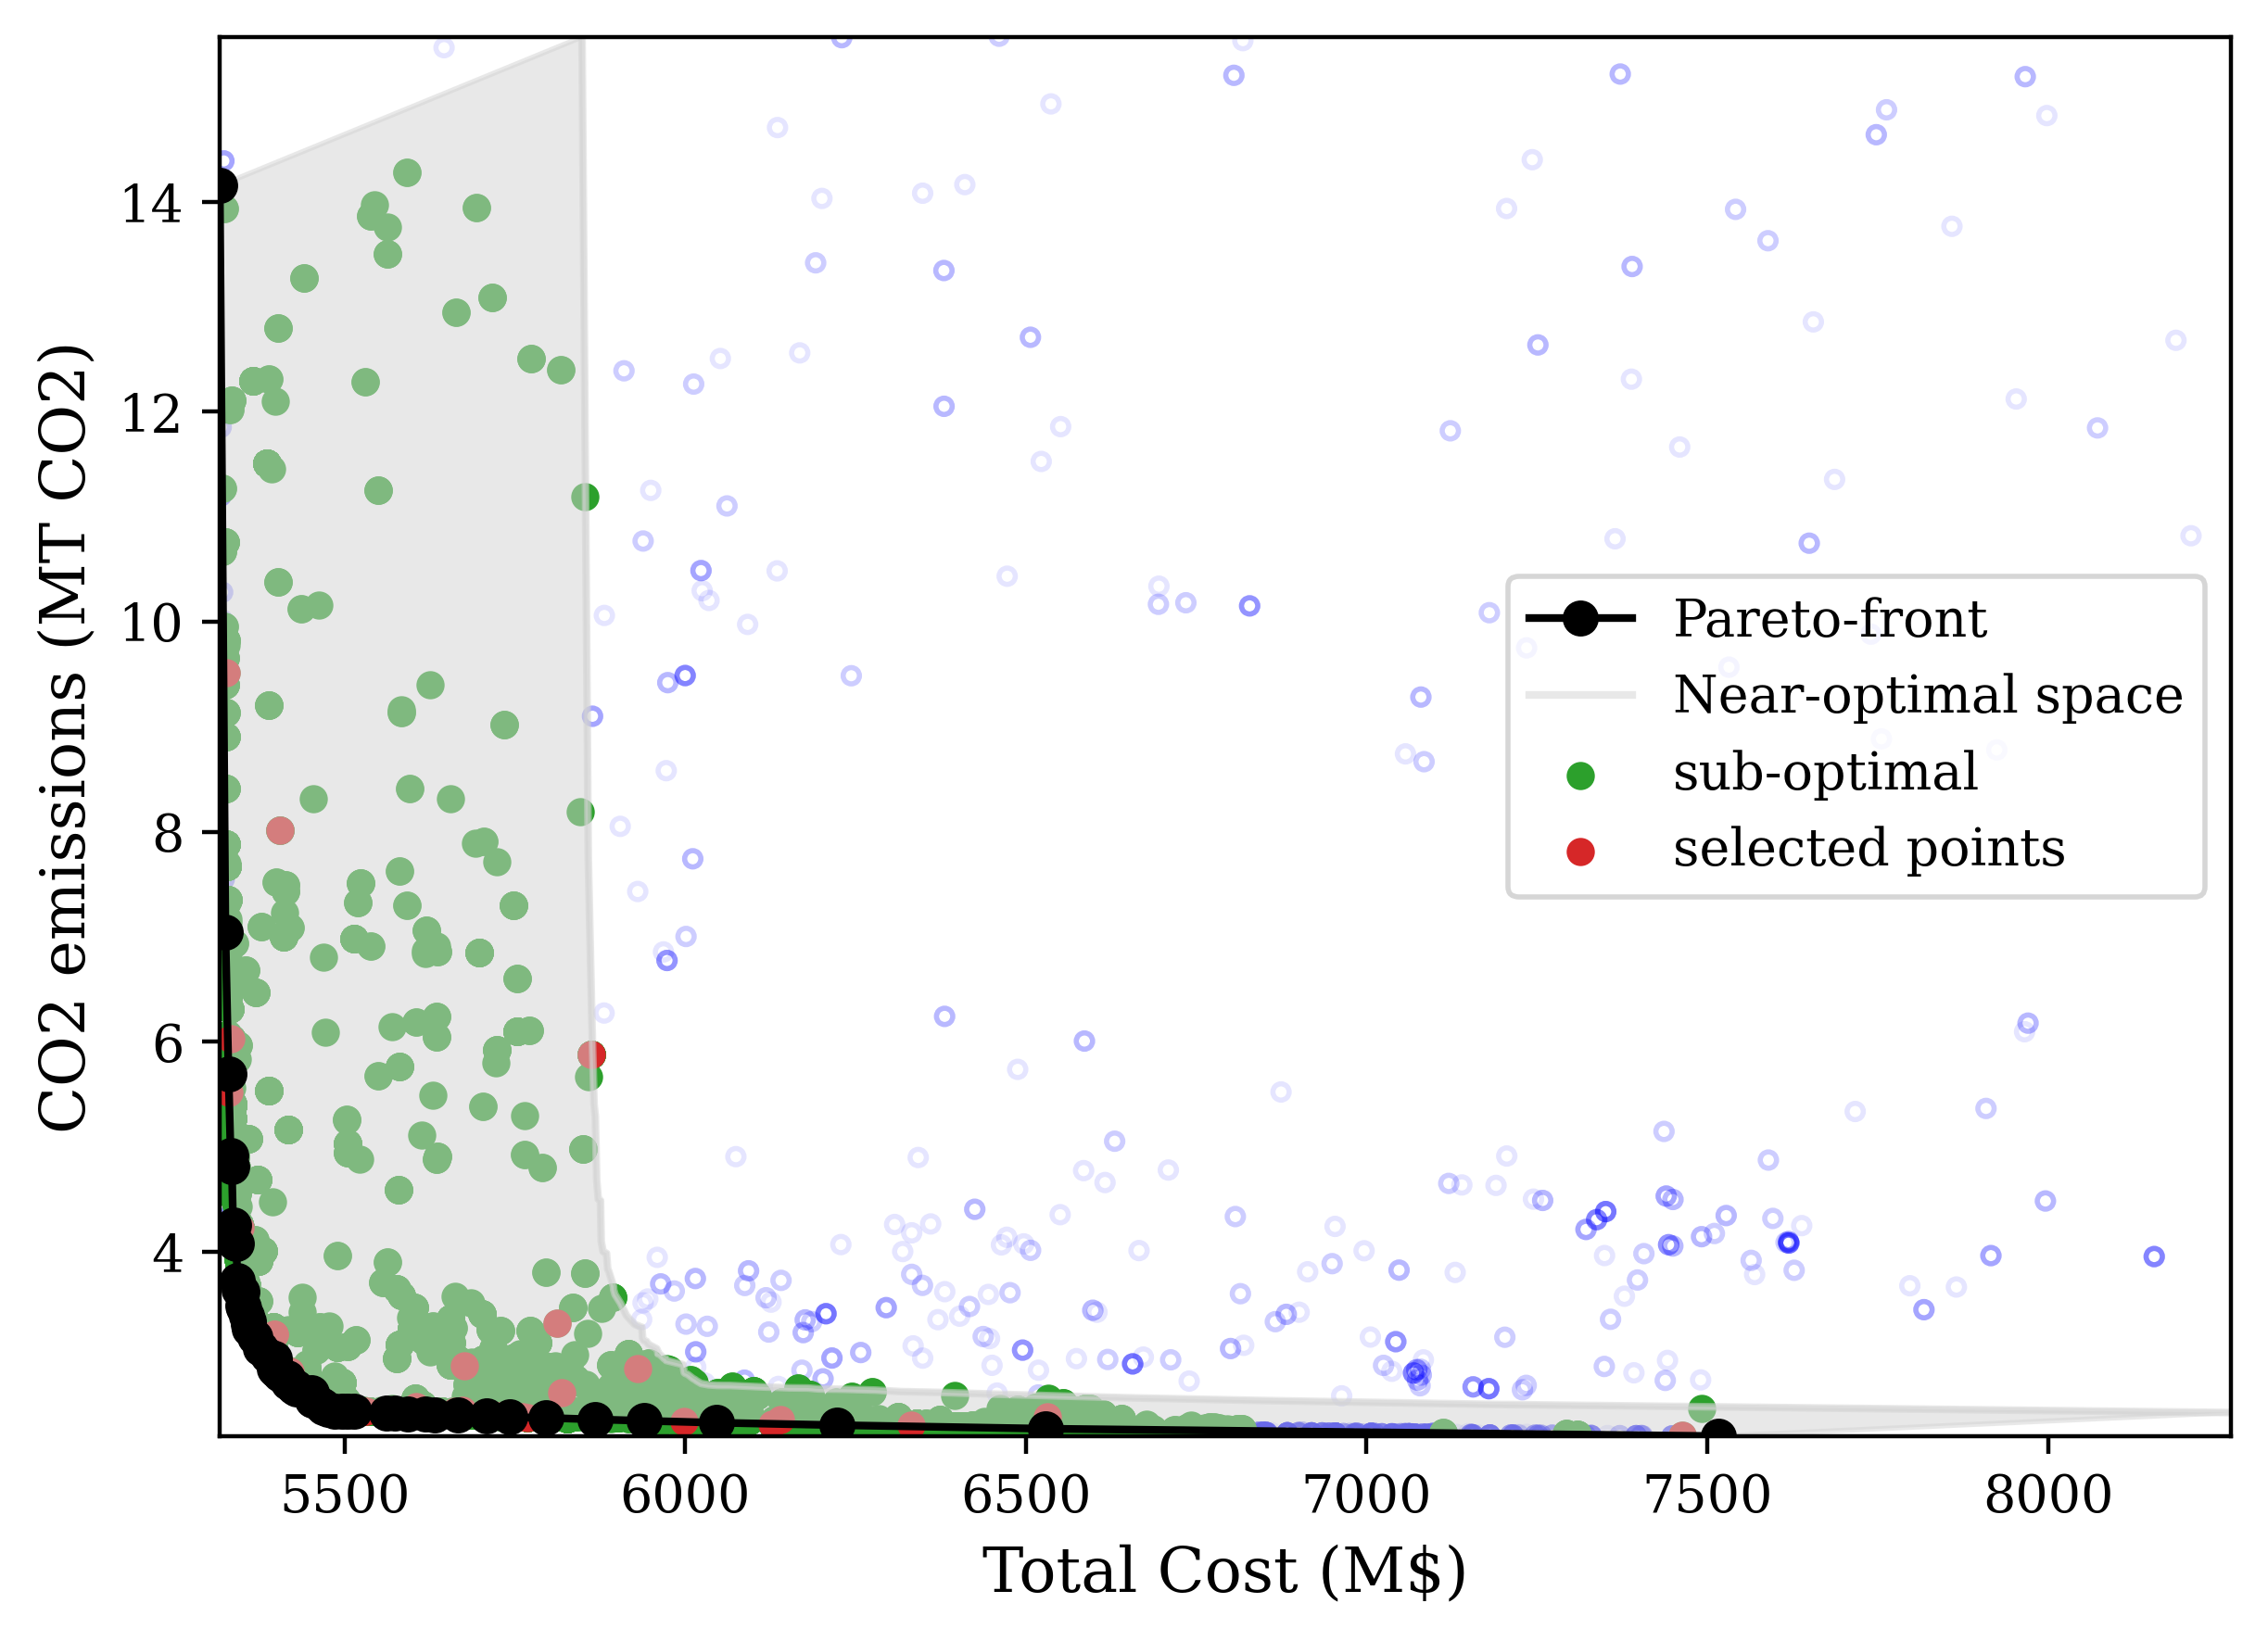
\includegraphics[width=0.6\columnwidth]{figures/results/osier_mga_subset_01.png}
  % \resizebox{0.6\columnwidth}{!}{%% Creator: Matplotlib, PGF backend
%%
%% To include the figure in your LaTeX document, write
%%   \input{<filename>.pgf}
%%
%% Make sure the required packages are loaded in your preamble
%%   \usepackage{pgf}
%%
%% Also ensure that all the required font packages are loaded; for instance,
%% the lmodern package is sometimes necessary when using math font.
%%   \usepackage{lmodern}
%%
%% Figures using additional raster images can only be included by \input if
%% they are in the same directory as the main LaTeX file. For loading figures
%% from other directories you can use the `import` package
%%   \usepackage{import}
%%
%% and then include the figures with
%%   \import{<path to file>}{<filename>.pgf}
%%
%% Matplotlib used the following preamble
%%   \def\mathdefault#1{#1}
%%   \everymath=\expandafter{\the\everymath\displaystyle}
%%   \IfFileExists{scrextend.sty}{
%%     \usepackage[fontsize=10.000000pt]{scrextend}
%%   }{
%%     \renewcommand{\normalsize}{\fontsize{10.000000}{12.000000}\selectfont}
%%     \normalsize
%%   }
%%   
%%   \makeatletter\@ifpackageloaded{underscore}{}{\usepackage[strings]{underscore}}\makeatother
%%
\begingroup%
\makeatletter%
\begin{pgfpicture}%
\pgfpathrectangle{\pgfpointorigin}{\pgfqpoint{7.900000in}{5.900000in}}%
\pgfusepath{use as bounding box, clip}%
\begin{pgfscope}%
\pgfsetbuttcap%
\pgfsetmiterjoin%
\definecolor{currentfill}{rgb}{1.000000,1.000000,1.000000}%
\pgfsetfillcolor{currentfill}%
\pgfsetlinewidth{0.000000pt}%
\definecolor{currentstroke}{rgb}{0.000000,0.000000,0.000000}%
\pgfsetstrokecolor{currentstroke}%
\pgfsetdash{}{0pt}%
\pgfpathmoveto{\pgfqpoint{0.000000in}{0.000000in}}%
\pgfpathlineto{\pgfqpoint{7.900000in}{0.000000in}}%
\pgfpathlineto{\pgfqpoint{7.900000in}{5.900000in}}%
\pgfpathlineto{\pgfqpoint{0.000000in}{5.900000in}}%
\pgfpathlineto{\pgfqpoint{0.000000in}{0.000000in}}%
\pgfpathclose%
\pgfusepath{fill}%
\end{pgfscope}%
\begin{pgfscope}%
\pgfsetbuttcap%
\pgfsetmiterjoin%
\definecolor{currentfill}{rgb}{1.000000,1.000000,1.000000}%
\pgfsetfillcolor{currentfill}%
\pgfsetlinewidth{0.000000pt}%
\definecolor{currentstroke}{rgb}{0.000000,0.000000,0.000000}%
\pgfsetstrokecolor{currentstroke}%
\pgfsetstrokeopacity{0.000000}%
\pgfsetdash{}{0pt}%
\pgfpathmoveto{\pgfqpoint{0.688192in}{0.670138in}}%
\pgfpathlineto{\pgfqpoint{7.800000in}{0.670138in}}%
\pgfpathlineto{\pgfqpoint{7.800000in}{5.800000in}}%
\pgfpathlineto{\pgfqpoint{0.688192in}{5.800000in}}%
\pgfpathlineto{\pgfqpoint{0.688192in}{0.670138in}}%
\pgfpathclose%
\pgfusepath{fill}%
\end{pgfscope}%
\begin{pgfscope}%
\pgfpathrectangle{\pgfqpoint{0.688192in}{0.670138in}}{\pgfqpoint{7.111808in}{5.129862in}}%
\pgfusepath{clip}%
\pgfsetbuttcap%
\pgfsetroundjoin%
\pgfsetlinewidth{1.003750pt}%
\definecolor{currentstroke}{rgb}{0.000000,0.000000,0.000000}%
\pgfsetstrokecolor{currentstroke}%
\pgfsetdash{}{0pt}%
\pgfpathmoveto{\pgfqpoint{5.329102in}{5.309073in}}%
\pgfpathcurveto{\pgfqpoint{5.339998in}{5.309073in}}{\pgfqpoint{5.350449in}{5.313402in}}{\pgfqpoint{5.358153in}{5.321106in}}%
\pgfpathcurveto{\pgfqpoint{5.365857in}{5.328811in}}{\pgfqpoint{5.370186in}{5.339261in}}{\pgfqpoint{5.370186in}{5.350157in}}%
\pgfpathcurveto{\pgfqpoint{5.370186in}{5.361052in}}{\pgfqpoint{5.365857in}{5.371503in}}{\pgfqpoint{5.358153in}{5.379208in}}%
\pgfpathcurveto{\pgfqpoint{5.350449in}{5.386912in}}{\pgfqpoint{5.339998in}{5.391241in}}{\pgfqpoint{5.329102in}{5.391241in}}%
\pgfpathcurveto{\pgfqpoint{5.318207in}{5.391241in}}{\pgfqpoint{5.307756in}{5.386912in}}{\pgfqpoint{5.300052in}{5.379208in}}%
\pgfpathcurveto{\pgfqpoint{5.292347in}{5.371503in}}{\pgfqpoint{5.288018in}{5.361052in}}{\pgfqpoint{5.288018in}{5.350157in}}%
\pgfpathcurveto{\pgfqpoint{5.288018in}{5.339261in}}{\pgfqpoint{5.292347in}{5.328811in}}{\pgfqpoint{5.300052in}{5.321106in}}%
\pgfpathcurveto{\pgfqpoint{5.307756in}{5.313402in}}{\pgfqpoint{5.318207in}{5.309073in}}{\pgfqpoint{5.329102in}{5.309073in}}%
\pgfpathlineto{\pgfqpoint{5.329102in}{5.309073in}}%
\pgfpathclose%
\pgfusepath{stroke}%
\end{pgfscope}%
\begin{pgfscope}%
\pgfpathrectangle{\pgfqpoint{0.688192in}{0.670138in}}{\pgfqpoint{7.111808in}{5.129862in}}%
\pgfusepath{clip}%
\pgfsetbuttcap%
\pgfsetroundjoin%
\pgfsetlinewidth{1.003750pt}%
\definecolor{currentstroke}{rgb}{0.000000,0.000000,0.000000}%
\pgfsetstrokecolor{currentstroke}%
\pgfsetdash{}{0pt}%
\pgfpathmoveto{\pgfqpoint{1.840914in}{0.696069in}}%
\pgfpathcurveto{\pgfqpoint{1.851809in}{0.696069in}}{\pgfqpoint{1.862260in}{0.700398in}}{\pgfqpoint{1.869964in}{0.708103in}}%
\pgfpathcurveto{\pgfqpoint{1.877669in}{0.715807in}}{\pgfqpoint{1.881997in}{0.726258in}}{\pgfqpoint{1.881997in}{0.737153in}}%
\pgfpathcurveto{\pgfqpoint{1.881997in}{0.748049in}}{\pgfqpoint{1.877669in}{0.758500in}}{\pgfqpoint{1.869964in}{0.766204in}}%
\pgfpathcurveto{\pgfqpoint{1.862260in}{0.773908in}}{\pgfqpoint{1.851809in}{0.778237in}}{\pgfqpoint{1.840914in}{0.778237in}}%
\pgfpathcurveto{\pgfqpoint{1.830018in}{0.778237in}}{\pgfqpoint{1.819567in}{0.773908in}}{\pgfqpoint{1.811863in}{0.766204in}}%
\pgfpathcurveto{\pgfqpoint{1.804159in}{0.758500in}}{\pgfqpoint{1.799830in}{0.748049in}}{\pgfqpoint{1.799830in}{0.737153in}}%
\pgfpathcurveto{\pgfqpoint{1.799830in}{0.726258in}}{\pgfqpoint{1.804159in}{0.715807in}}{\pgfqpoint{1.811863in}{0.708103in}}%
\pgfpathcurveto{\pgfqpoint{1.819567in}{0.700398in}}{\pgfqpoint{1.830018in}{0.696069in}}{\pgfqpoint{1.840914in}{0.696069in}}%
\pgfpathlineto{\pgfqpoint{1.840914in}{0.696069in}}%
\pgfpathclose%
\pgfusepath{stroke}%
\end{pgfscope}%
\begin{pgfscope}%
\pgfpathrectangle{\pgfqpoint{0.688192in}{0.670138in}}{\pgfqpoint{7.111808in}{5.129862in}}%
\pgfusepath{clip}%
\pgfsetbuttcap%
\pgfsetroundjoin%
\pgfsetlinewidth{1.003750pt}%
\definecolor{currentstroke}{rgb}{0.000000,0.000000,0.000000}%
\pgfsetstrokecolor{currentstroke}%
\pgfsetdash{}{0pt}%
\pgfpathmoveto{\pgfqpoint{1.101880in}{0.720677in}}%
\pgfpathcurveto{\pgfqpoint{1.112775in}{0.720677in}}{\pgfqpoint{1.123226in}{0.725006in}}{\pgfqpoint{1.130930in}{0.732710in}}%
\pgfpathcurveto{\pgfqpoint{1.138635in}{0.740415in}}{\pgfqpoint{1.142964in}{0.750865in}}{\pgfqpoint{1.142964in}{0.761761in}}%
\pgfpathcurveto{\pgfqpoint{1.142964in}{0.772656in}}{\pgfqpoint{1.138635in}{0.783107in}}{\pgfqpoint{1.130930in}{0.790812in}}%
\pgfpathcurveto{\pgfqpoint{1.123226in}{0.798516in}}{\pgfqpoint{1.112775in}{0.802845in}}{\pgfqpoint{1.101880in}{0.802845in}}%
\pgfpathcurveto{\pgfqpoint{1.090984in}{0.802845in}}{\pgfqpoint{1.080533in}{0.798516in}}{\pgfqpoint{1.072829in}{0.790812in}}%
\pgfpathcurveto{\pgfqpoint{1.065125in}{0.783107in}}{\pgfqpoint{1.060796in}{0.772656in}}{\pgfqpoint{1.060796in}{0.761761in}}%
\pgfpathcurveto{\pgfqpoint{1.060796in}{0.750865in}}{\pgfqpoint{1.065125in}{0.740415in}}{\pgfqpoint{1.072829in}{0.732710in}}%
\pgfpathcurveto{\pgfqpoint{1.080533in}{0.725006in}}{\pgfqpoint{1.090984in}{0.720677in}}{\pgfqpoint{1.101880in}{0.720677in}}%
\pgfpathlineto{\pgfqpoint{1.101880in}{0.720677in}}%
\pgfpathclose%
\pgfusepath{stroke}%
\end{pgfscope}%
\begin{pgfscope}%
\pgfpathrectangle{\pgfqpoint{0.688192in}{0.670138in}}{\pgfqpoint{7.111808in}{5.129862in}}%
\pgfusepath{clip}%
\pgfsetbuttcap%
\pgfsetroundjoin%
\pgfsetlinewidth{1.003750pt}%
\definecolor{currentstroke}{rgb}{0.000000,0.000000,0.000000}%
\pgfsetstrokecolor{currentstroke}%
\pgfsetdash{}{0pt}%
\pgfpathmoveto{\pgfqpoint{1.840914in}{0.696069in}}%
\pgfpathcurveto{\pgfqpoint{1.851809in}{0.696069in}}{\pgfqpoint{1.862260in}{0.700398in}}{\pgfqpoint{1.869964in}{0.708103in}}%
\pgfpathcurveto{\pgfqpoint{1.877669in}{0.715807in}}{\pgfqpoint{1.881997in}{0.726258in}}{\pgfqpoint{1.881997in}{0.737153in}}%
\pgfpathcurveto{\pgfqpoint{1.881997in}{0.748049in}}{\pgfqpoint{1.877669in}{0.758500in}}{\pgfqpoint{1.869964in}{0.766204in}}%
\pgfpathcurveto{\pgfqpoint{1.862260in}{0.773908in}}{\pgfqpoint{1.851809in}{0.778237in}}{\pgfqpoint{1.840914in}{0.778237in}}%
\pgfpathcurveto{\pgfqpoint{1.830018in}{0.778237in}}{\pgfqpoint{1.819567in}{0.773908in}}{\pgfqpoint{1.811863in}{0.766204in}}%
\pgfpathcurveto{\pgfqpoint{1.804159in}{0.758500in}}{\pgfqpoint{1.799830in}{0.748049in}}{\pgfqpoint{1.799830in}{0.737153in}}%
\pgfpathcurveto{\pgfqpoint{1.799830in}{0.726258in}}{\pgfqpoint{1.804159in}{0.715807in}}{\pgfqpoint{1.811863in}{0.708103in}}%
\pgfpathcurveto{\pgfqpoint{1.819567in}{0.700398in}}{\pgfqpoint{1.830018in}{0.696069in}}{\pgfqpoint{1.840914in}{0.696069in}}%
\pgfpathlineto{\pgfqpoint{1.840914in}{0.696069in}}%
\pgfpathclose%
\pgfusepath{stroke}%
\end{pgfscope}%
\begin{pgfscope}%
\pgfpathrectangle{\pgfqpoint{0.688192in}{0.670138in}}{\pgfqpoint{7.111808in}{5.129862in}}%
\pgfusepath{clip}%
\pgfsetbuttcap%
\pgfsetroundjoin%
\pgfsetlinewidth{1.003750pt}%
\definecolor{currentstroke}{rgb}{0.000000,0.000000,0.000000}%
\pgfsetstrokecolor{currentstroke}%
\pgfsetdash{}{0pt}%
\pgfpathmoveto{\pgfqpoint{2.869035in}{0.669385in}}%
\pgfpathcurveto{\pgfqpoint{2.879931in}{0.669385in}}{\pgfqpoint{2.890382in}{0.673714in}}{\pgfqpoint{2.898086in}{0.681419in}}%
\pgfpathcurveto{\pgfqpoint{2.905790in}{0.689123in}}{\pgfqpoint{2.910119in}{0.699574in}}{\pgfqpoint{2.910119in}{0.710469in}}%
\pgfpathcurveto{\pgfqpoint{2.910119in}{0.721365in}}{\pgfqpoint{2.905790in}{0.731816in}}{\pgfqpoint{2.898086in}{0.739520in}}%
\pgfpathcurveto{\pgfqpoint{2.890382in}{0.747224in}}{\pgfqpoint{2.879931in}{0.751553in}}{\pgfqpoint{2.869035in}{0.751553in}}%
\pgfpathcurveto{\pgfqpoint{2.858140in}{0.751553in}}{\pgfqpoint{2.847689in}{0.747224in}}{\pgfqpoint{2.839985in}{0.739520in}}%
\pgfpathcurveto{\pgfqpoint{2.832280in}{0.731816in}}{\pgfqpoint{2.827952in}{0.721365in}}{\pgfqpoint{2.827952in}{0.710469in}}%
\pgfpathcurveto{\pgfqpoint{2.827952in}{0.699574in}}{\pgfqpoint{2.832280in}{0.689123in}}{\pgfqpoint{2.839985in}{0.681419in}}%
\pgfpathcurveto{\pgfqpoint{2.847689in}{0.673714in}}{\pgfqpoint{2.858140in}{0.669385in}}{\pgfqpoint{2.869035in}{0.669385in}}%
\pgfpathlineto{\pgfqpoint{2.869035in}{0.669385in}}%
\pgfpathclose%
\pgfusepath{stroke}%
\end{pgfscope}%
\begin{pgfscope}%
\pgfpathrectangle{\pgfqpoint{0.688192in}{0.670138in}}{\pgfqpoint{7.111808in}{5.129862in}}%
\pgfusepath{clip}%
\pgfsetbuttcap%
\pgfsetroundjoin%
\pgfsetlinewidth{1.003750pt}%
\definecolor{currentstroke}{rgb}{0.000000,0.000000,0.000000}%
\pgfsetstrokecolor{currentstroke}%
\pgfsetdash{}{0pt}%
\pgfpathmoveto{\pgfqpoint{0.789763in}{1.038554in}}%
\pgfpathcurveto{\pgfqpoint{0.800659in}{1.038554in}}{\pgfqpoint{0.811109in}{1.042883in}}{\pgfqpoint{0.818814in}{1.050587in}}%
\pgfpathcurveto{\pgfqpoint{0.826518in}{1.058291in}}{\pgfqpoint{0.830847in}{1.068742in}}{\pgfqpoint{0.830847in}{1.079638in}}%
\pgfpathcurveto{\pgfqpoint{0.830847in}{1.090533in}}{\pgfqpoint{0.826518in}{1.100984in}}{\pgfqpoint{0.818814in}{1.108688in}}%
\pgfpathcurveto{\pgfqpoint{0.811109in}{1.116393in}}{\pgfqpoint{0.800659in}{1.120722in}}{\pgfqpoint{0.789763in}{1.120722in}}%
\pgfpathcurveto{\pgfqpoint{0.778868in}{1.120722in}}{\pgfqpoint{0.768417in}{1.116393in}}{\pgfqpoint{0.760712in}{1.108688in}}%
\pgfpathcurveto{\pgfqpoint{0.753008in}{1.100984in}}{\pgfqpoint{0.748679in}{1.090533in}}{\pgfqpoint{0.748679in}{1.079638in}}%
\pgfpathcurveto{\pgfqpoint{0.748679in}{1.068742in}}{\pgfqpoint{0.753008in}{1.058291in}}{\pgfqpoint{0.760712in}{1.050587in}}%
\pgfpathcurveto{\pgfqpoint{0.768417in}{1.042883in}}{\pgfqpoint{0.778868in}{1.038554in}}{\pgfqpoint{0.789763in}{1.038554in}}%
\pgfpathlineto{\pgfqpoint{0.789763in}{1.038554in}}%
\pgfpathclose%
\pgfusepath{stroke}%
\end{pgfscope}%
\begin{pgfscope}%
\pgfpathrectangle{\pgfqpoint{0.688192in}{0.670138in}}{\pgfqpoint{7.111808in}{5.129862in}}%
\pgfusepath{clip}%
\pgfsetbuttcap%
\pgfsetroundjoin%
\pgfsetlinewidth{1.003750pt}%
\definecolor{currentstroke}{rgb}{0.000000,0.000000,0.000000}%
\pgfsetstrokecolor{currentstroke}%
\pgfsetdash{}{0pt}%
\pgfpathmoveto{\pgfqpoint{1.679564in}{0.702362in}}%
\pgfpathcurveto{\pgfqpoint{1.690460in}{0.702362in}}{\pgfqpoint{1.700911in}{0.706691in}}{\pgfqpoint{1.708615in}{0.714395in}}%
\pgfpathcurveto{\pgfqpoint{1.716319in}{0.722099in}}{\pgfqpoint{1.720648in}{0.732550in}}{\pgfqpoint{1.720648in}{0.743446in}}%
\pgfpathcurveto{\pgfqpoint{1.720648in}{0.754341in}}{\pgfqpoint{1.716319in}{0.764792in}}{\pgfqpoint{1.708615in}{0.772496in}}%
\pgfpathcurveto{\pgfqpoint{1.700911in}{0.780201in}}{\pgfqpoint{1.690460in}{0.784529in}}{\pgfqpoint{1.679564in}{0.784529in}}%
\pgfpathcurveto{\pgfqpoint{1.668669in}{0.784529in}}{\pgfqpoint{1.658218in}{0.780201in}}{\pgfqpoint{1.650514in}{0.772496in}}%
\pgfpathcurveto{\pgfqpoint{1.642809in}{0.764792in}}{\pgfqpoint{1.638480in}{0.754341in}}{\pgfqpoint{1.638480in}{0.743446in}}%
\pgfpathcurveto{\pgfqpoint{1.638480in}{0.732550in}}{\pgfqpoint{1.642809in}{0.722099in}}{\pgfqpoint{1.650514in}{0.714395in}}%
\pgfpathcurveto{\pgfqpoint{1.658218in}{0.706691in}}{\pgfqpoint{1.668669in}{0.702362in}}{\pgfqpoint{1.679564in}{0.702362in}}%
\pgfpathlineto{\pgfqpoint{1.679564in}{0.702362in}}%
\pgfpathclose%
\pgfusepath{stroke}%
\end{pgfscope}%
\begin{pgfscope}%
\pgfpathrectangle{\pgfqpoint{0.688192in}{0.670138in}}{\pgfqpoint{7.111808in}{5.129862in}}%
\pgfusepath{clip}%
\pgfsetbuttcap%
\pgfsetroundjoin%
\pgfsetlinewidth{1.003750pt}%
\definecolor{currentstroke}{rgb}{0.000000,0.000000,0.000000}%
\pgfsetstrokecolor{currentstroke}%
\pgfsetdash{}{0pt}%
\pgfpathmoveto{\pgfqpoint{1.045306in}{0.741536in}}%
\pgfpathcurveto{\pgfqpoint{1.056202in}{0.741536in}}{\pgfqpoint{1.066653in}{0.745865in}}{\pgfqpoint{1.074357in}{0.753569in}}%
\pgfpathcurveto{\pgfqpoint{1.082061in}{0.761274in}}{\pgfqpoint{1.086390in}{0.771725in}}{\pgfqpoint{1.086390in}{0.782620in}}%
\pgfpathcurveto{\pgfqpoint{1.086390in}{0.793516in}}{\pgfqpoint{1.082061in}{0.803967in}}{\pgfqpoint{1.074357in}{0.811671in}}%
\pgfpathcurveto{\pgfqpoint{1.066653in}{0.819375in}}{\pgfqpoint{1.056202in}{0.823704in}}{\pgfqpoint{1.045306in}{0.823704in}}%
\pgfpathcurveto{\pgfqpoint{1.034411in}{0.823704in}}{\pgfqpoint{1.023960in}{0.819375in}}{\pgfqpoint{1.016256in}{0.811671in}}%
\pgfpathcurveto{\pgfqpoint{1.008551in}{0.803967in}}{\pgfqpoint{1.004222in}{0.793516in}}{\pgfqpoint{1.004222in}{0.782620in}}%
\pgfpathcurveto{\pgfqpoint{1.004222in}{0.771725in}}{\pgfqpoint{1.008551in}{0.761274in}}{\pgfqpoint{1.016256in}{0.753569in}}%
\pgfpathcurveto{\pgfqpoint{1.023960in}{0.745865in}}{\pgfqpoint{1.034411in}{0.741536in}}{\pgfqpoint{1.045306in}{0.741536in}}%
\pgfpathlineto{\pgfqpoint{1.045306in}{0.741536in}}%
\pgfpathclose%
\pgfusepath{stroke}%
\end{pgfscope}%
\begin{pgfscope}%
\pgfpathrectangle{\pgfqpoint{0.688192in}{0.670138in}}{\pgfqpoint{7.111808in}{5.129862in}}%
\pgfusepath{clip}%
\pgfsetbuttcap%
\pgfsetroundjoin%
\pgfsetlinewidth{1.003750pt}%
\definecolor{currentstroke}{rgb}{0.000000,0.000000,0.000000}%
\pgfsetstrokecolor{currentstroke}%
\pgfsetdash{}{0pt}%
\pgfpathmoveto{\pgfqpoint{2.013663in}{0.690447in}}%
\pgfpathcurveto{\pgfqpoint{2.024559in}{0.690447in}}{\pgfqpoint{2.035010in}{0.694776in}}{\pgfqpoint{2.042714in}{0.702480in}}%
\pgfpathcurveto{\pgfqpoint{2.050418in}{0.710184in}}{\pgfqpoint{2.054747in}{0.720635in}}{\pgfqpoint{2.054747in}{0.731531in}}%
\pgfpathcurveto{\pgfqpoint{2.054747in}{0.742426in}}{\pgfqpoint{2.050418in}{0.752877in}}{\pgfqpoint{2.042714in}{0.760582in}}%
\pgfpathcurveto{\pgfqpoint{2.035010in}{0.768286in}}{\pgfqpoint{2.024559in}{0.772615in}}{\pgfqpoint{2.013663in}{0.772615in}}%
\pgfpathcurveto{\pgfqpoint{2.002768in}{0.772615in}}{\pgfqpoint{1.992317in}{0.768286in}}{\pgfqpoint{1.984613in}{0.760582in}}%
\pgfpathcurveto{\pgfqpoint{1.976908in}{0.752877in}}{\pgfqpoint{1.972579in}{0.742426in}}{\pgfqpoint{1.972579in}{0.731531in}}%
\pgfpathcurveto{\pgfqpoint{1.972579in}{0.720635in}}{\pgfqpoint{1.976908in}{0.710184in}}{\pgfqpoint{1.984613in}{0.702480in}}%
\pgfpathcurveto{\pgfqpoint{1.992317in}{0.694776in}}{\pgfqpoint{2.002768in}{0.690447in}}{\pgfqpoint{2.013663in}{0.690447in}}%
\pgfpathlineto{\pgfqpoint{2.013663in}{0.690447in}}%
\pgfpathclose%
\pgfusepath{stroke}%
\end{pgfscope}%
\begin{pgfscope}%
\pgfpathrectangle{\pgfqpoint{0.688192in}{0.670138in}}{\pgfqpoint{7.111808in}{5.129862in}}%
\pgfusepath{clip}%
\pgfsetbuttcap%
\pgfsetroundjoin%
\pgfsetlinewidth{1.003750pt}%
\definecolor{currentstroke}{rgb}{0.000000,0.000000,0.000000}%
\pgfsetstrokecolor{currentstroke}%
\pgfsetdash{}{0pt}%
\pgfpathmoveto{\pgfqpoint{0.895312in}{0.866174in}}%
\pgfpathcurveto{\pgfqpoint{0.906208in}{0.866174in}}{\pgfqpoint{0.916658in}{0.870503in}}{\pgfqpoint{0.924363in}{0.878207in}}%
\pgfpathcurveto{\pgfqpoint{0.932067in}{0.885911in}}{\pgfqpoint{0.936396in}{0.896362in}}{\pgfqpoint{0.936396in}{0.907258in}}%
\pgfpathcurveto{\pgfqpoint{0.936396in}{0.918153in}}{\pgfqpoint{0.932067in}{0.928604in}}{\pgfqpoint{0.924363in}{0.936308in}}%
\pgfpathcurveto{\pgfqpoint{0.916658in}{0.944013in}}{\pgfqpoint{0.906208in}{0.948341in}}{\pgfqpoint{0.895312in}{0.948341in}}%
\pgfpathcurveto{\pgfqpoint{0.884416in}{0.948341in}}{\pgfqpoint{0.873966in}{0.944013in}}{\pgfqpoint{0.866261in}{0.936308in}}%
\pgfpathcurveto{\pgfqpoint{0.858557in}{0.928604in}}{\pgfqpoint{0.854228in}{0.918153in}}{\pgfqpoint{0.854228in}{0.907258in}}%
\pgfpathcurveto{\pgfqpoint{0.854228in}{0.896362in}}{\pgfqpoint{0.858557in}{0.885911in}}{\pgfqpoint{0.866261in}{0.878207in}}%
\pgfpathcurveto{\pgfqpoint{0.873966in}{0.870503in}}{\pgfqpoint{0.884416in}{0.866174in}}{\pgfqpoint{0.895312in}{0.866174in}}%
\pgfpathlineto{\pgfqpoint{0.895312in}{0.866174in}}%
\pgfpathclose%
\pgfusepath{stroke}%
\end{pgfscope}%
\begin{pgfscope}%
\pgfpathrectangle{\pgfqpoint{0.688192in}{0.670138in}}{\pgfqpoint{7.111808in}{5.129862in}}%
\pgfusepath{clip}%
\pgfsetbuttcap%
\pgfsetroundjoin%
\pgfsetlinewidth{1.003750pt}%
\definecolor{currentstroke}{rgb}{0.000000,0.000000,0.000000}%
\pgfsetstrokecolor{currentstroke}%
\pgfsetdash{}{0pt}%
\pgfpathmoveto{\pgfqpoint{0.794194in}{1.022605in}}%
\pgfpathcurveto{\pgfqpoint{0.805090in}{1.022605in}}{\pgfqpoint{0.815541in}{1.026933in}}{\pgfqpoint{0.823245in}{1.034638in}}%
\pgfpathcurveto{\pgfqpoint{0.830949in}{1.042342in}}{\pgfqpoint{0.835278in}{1.052793in}}{\pgfqpoint{0.835278in}{1.063688in}}%
\pgfpathcurveto{\pgfqpoint{0.835278in}{1.074584in}}{\pgfqpoint{0.830949in}{1.085035in}}{\pgfqpoint{0.823245in}{1.092739in}}%
\pgfpathcurveto{\pgfqpoint{0.815541in}{1.100443in}}{\pgfqpoint{0.805090in}{1.104772in}}{\pgfqpoint{0.794194in}{1.104772in}}%
\pgfpathcurveto{\pgfqpoint{0.783299in}{1.104772in}}{\pgfqpoint{0.772848in}{1.100443in}}{\pgfqpoint{0.765144in}{1.092739in}}%
\pgfpathcurveto{\pgfqpoint{0.757439in}{1.085035in}}{\pgfqpoint{0.753110in}{1.074584in}}{\pgfqpoint{0.753110in}{1.063688in}}%
\pgfpathcurveto{\pgfqpoint{0.753110in}{1.052793in}}{\pgfqpoint{0.757439in}{1.042342in}}{\pgfqpoint{0.765144in}{1.034638in}}%
\pgfpathcurveto{\pgfqpoint{0.772848in}{1.026933in}}{\pgfqpoint{0.783299in}{1.022605in}}{\pgfqpoint{0.794194in}{1.022605in}}%
\pgfpathlineto{\pgfqpoint{0.794194in}{1.022605in}}%
\pgfpathclose%
\pgfusepath{stroke}%
\end{pgfscope}%
\begin{pgfscope}%
\pgfpathrectangle{\pgfqpoint{0.688192in}{0.670138in}}{\pgfqpoint{7.111808in}{5.129862in}}%
\pgfusepath{clip}%
\pgfsetbuttcap%
\pgfsetroundjoin%
\pgfsetlinewidth{1.003750pt}%
\definecolor{currentstroke}{rgb}{0.000000,0.000000,0.000000}%
\pgfsetstrokecolor{currentstroke}%
\pgfsetdash{}{0pt}%
\pgfpathmoveto{\pgfqpoint{1.019140in}{0.759981in}}%
\pgfpathcurveto{\pgfqpoint{1.030035in}{0.759981in}}{\pgfqpoint{1.040486in}{0.764309in}}{\pgfqpoint{1.048191in}{0.772014in}}%
\pgfpathcurveto{\pgfqpoint{1.055895in}{0.779718in}}{\pgfqpoint{1.060224in}{0.790169in}}{\pgfqpoint{1.060224in}{0.801064in}}%
\pgfpathcurveto{\pgfqpoint{1.060224in}{0.811960in}}{\pgfqpoint{1.055895in}{0.822411in}}{\pgfqpoint{1.048191in}{0.830115in}}%
\pgfpathcurveto{\pgfqpoint{1.040486in}{0.837820in}}{\pgfqpoint{1.030035in}{0.842148in}}{\pgfqpoint{1.019140in}{0.842148in}}%
\pgfpathcurveto{\pgfqpoint{1.008244in}{0.842148in}}{\pgfqpoint{0.997794in}{0.837820in}}{\pgfqpoint{0.990089in}{0.830115in}}%
\pgfpathcurveto{\pgfqpoint{0.982385in}{0.822411in}}{\pgfqpoint{0.978056in}{0.811960in}}{\pgfqpoint{0.978056in}{0.801064in}}%
\pgfpathcurveto{\pgfqpoint{0.978056in}{0.790169in}}{\pgfqpoint{0.982385in}{0.779718in}}{\pgfqpoint{0.990089in}{0.772014in}}%
\pgfpathcurveto{\pgfqpoint{0.997794in}{0.764309in}}{\pgfqpoint{1.008244in}{0.759981in}}{\pgfqpoint{1.019140in}{0.759981in}}%
\pgfpathlineto{\pgfqpoint{1.019140in}{0.759981in}}%
\pgfpathclose%
\pgfusepath{stroke}%
\end{pgfscope}%
\begin{pgfscope}%
\pgfpathrectangle{\pgfqpoint{0.688192in}{0.670138in}}{\pgfqpoint{7.111808in}{5.129862in}}%
\pgfusepath{clip}%
\pgfsetbuttcap%
\pgfsetroundjoin%
\pgfsetlinewidth{1.003750pt}%
\definecolor{currentstroke}{rgb}{0.000000,0.000000,0.000000}%
\pgfsetstrokecolor{currentstroke}%
\pgfsetdash{}{0pt}%
\pgfpathmoveto{\pgfqpoint{1.050667in}{0.739240in}}%
\pgfpathcurveto{\pgfqpoint{1.061563in}{0.739240in}}{\pgfqpoint{1.072014in}{0.743568in}}{\pgfqpoint{1.079718in}{0.751273in}}%
\pgfpathcurveto{\pgfqpoint{1.087422in}{0.758977in}}{\pgfqpoint{1.091751in}{0.769428in}}{\pgfqpoint{1.091751in}{0.780323in}}%
\pgfpathcurveto{\pgfqpoint{1.091751in}{0.791219in}}{\pgfqpoint{1.087422in}{0.801670in}}{\pgfqpoint{1.079718in}{0.809374in}}%
\pgfpathcurveto{\pgfqpoint{1.072014in}{0.817078in}}{\pgfqpoint{1.061563in}{0.821407in}}{\pgfqpoint{1.050667in}{0.821407in}}%
\pgfpathcurveto{\pgfqpoint{1.039772in}{0.821407in}}{\pgfqpoint{1.029321in}{0.817078in}}{\pgfqpoint{1.021617in}{0.809374in}}%
\pgfpathcurveto{\pgfqpoint{1.013912in}{0.801670in}}{\pgfqpoint{1.009583in}{0.791219in}}{\pgfqpoint{1.009583in}{0.780323in}}%
\pgfpathcurveto{\pgfqpoint{1.009583in}{0.769428in}}{\pgfqpoint{1.013912in}{0.758977in}}{\pgfqpoint{1.021617in}{0.751273in}}%
\pgfpathcurveto{\pgfqpoint{1.029321in}{0.743568in}}{\pgfqpoint{1.039772in}{0.739240in}}{\pgfqpoint{1.050667in}{0.739240in}}%
\pgfpathlineto{\pgfqpoint{1.050667in}{0.739240in}}%
\pgfpathclose%
\pgfusepath{stroke}%
\end{pgfscope}%
\begin{pgfscope}%
\pgfpathrectangle{\pgfqpoint{0.688192in}{0.670138in}}{\pgfqpoint{7.111808in}{5.129862in}}%
\pgfusepath{clip}%
\pgfsetbuttcap%
\pgfsetroundjoin%
\pgfsetlinewidth{1.003750pt}%
\definecolor{currentstroke}{rgb}{0.000000,0.000000,0.000000}%
\pgfsetstrokecolor{currentstroke}%
\pgfsetdash{}{0pt}%
\pgfpathmoveto{\pgfqpoint{0.881277in}{0.900428in}}%
\pgfpathcurveto{\pgfqpoint{0.892173in}{0.900428in}}{\pgfqpoint{0.902624in}{0.904756in}}{\pgfqpoint{0.910328in}{0.912461in}}%
\pgfpathcurveto{\pgfqpoint{0.918032in}{0.920165in}}{\pgfqpoint{0.922361in}{0.930616in}}{\pgfqpoint{0.922361in}{0.941511in}}%
\pgfpathcurveto{\pgfqpoint{0.922361in}{0.952407in}}{\pgfqpoint{0.918032in}{0.962858in}}{\pgfqpoint{0.910328in}{0.970562in}}%
\pgfpathcurveto{\pgfqpoint{0.902624in}{0.978266in}}{\pgfqpoint{0.892173in}{0.982595in}}{\pgfqpoint{0.881277in}{0.982595in}}%
\pgfpathcurveto{\pgfqpoint{0.870382in}{0.982595in}}{\pgfqpoint{0.859931in}{0.978266in}}{\pgfqpoint{0.852226in}{0.970562in}}%
\pgfpathcurveto{\pgfqpoint{0.844522in}{0.962858in}}{\pgfqpoint{0.840193in}{0.952407in}}{\pgfqpoint{0.840193in}{0.941511in}}%
\pgfpathcurveto{\pgfqpoint{0.840193in}{0.930616in}}{\pgfqpoint{0.844522in}{0.920165in}}{\pgfqpoint{0.852226in}{0.912461in}}%
\pgfpathcurveto{\pgfqpoint{0.859931in}{0.904756in}}{\pgfqpoint{0.870382in}{0.900428in}}{\pgfqpoint{0.881277in}{0.900428in}}%
\pgfpathlineto{\pgfqpoint{0.881277in}{0.900428in}}%
\pgfpathclose%
\pgfusepath{stroke}%
\end{pgfscope}%
\begin{pgfscope}%
\pgfpathrectangle{\pgfqpoint{0.688192in}{0.670138in}}{\pgfqpoint{7.111808in}{5.129862in}}%
\pgfusepath{clip}%
\pgfsetbuttcap%
\pgfsetroundjoin%
\pgfsetlinewidth{1.003750pt}%
\definecolor{currentstroke}{rgb}{0.000000,0.000000,0.000000}%
\pgfsetstrokecolor{currentstroke}%
\pgfsetdash{}{0pt}%
\pgfpathmoveto{\pgfqpoint{0.721104in}{1.921896in}}%
\pgfpathcurveto{\pgfqpoint{0.732000in}{1.921896in}}{\pgfqpoint{0.742451in}{1.926225in}}{\pgfqpoint{0.750155in}{1.933929in}}%
\pgfpathcurveto{\pgfqpoint{0.757859in}{1.941634in}}{\pgfqpoint{0.762188in}{1.952084in}}{\pgfqpoint{0.762188in}{1.962980in}}%
\pgfpathcurveto{\pgfqpoint{0.762188in}{1.973876in}}{\pgfqpoint{0.757859in}{1.984326in}}{\pgfqpoint{0.750155in}{1.992031in}}%
\pgfpathcurveto{\pgfqpoint{0.742451in}{1.999735in}}{\pgfqpoint{0.732000in}{2.004064in}}{\pgfqpoint{0.721104in}{2.004064in}}%
\pgfpathcurveto{\pgfqpoint{0.710209in}{2.004064in}}{\pgfqpoint{0.699758in}{1.999735in}}{\pgfqpoint{0.692054in}{1.992031in}}%
\pgfpathcurveto{\pgfqpoint{0.684349in}{1.984326in}}{\pgfqpoint{0.680020in}{1.973876in}}{\pgfqpoint{0.680020in}{1.962980in}}%
\pgfpathcurveto{\pgfqpoint{0.680020in}{1.952084in}}{\pgfqpoint{0.684349in}{1.941634in}}{\pgfqpoint{0.692054in}{1.933929in}}%
\pgfpathcurveto{\pgfqpoint{0.699758in}{1.926225in}}{\pgfqpoint{0.710209in}{1.921896in}}{\pgfqpoint{0.721104in}{1.921896in}}%
\pgfpathlineto{\pgfqpoint{0.721104in}{1.921896in}}%
\pgfpathclose%
\pgfusepath{stroke}%
\end{pgfscope}%
\begin{pgfscope}%
\pgfpathrectangle{\pgfqpoint{0.688192in}{0.670138in}}{\pgfqpoint{7.111808in}{5.129862in}}%
\pgfusepath{clip}%
\pgfsetbuttcap%
\pgfsetroundjoin%
\pgfsetlinewidth{1.003750pt}%
\definecolor{currentstroke}{rgb}{0.000000,0.000000,0.000000}%
\pgfsetstrokecolor{currentstroke}%
\pgfsetdash{}{0pt}%
\pgfpathmoveto{\pgfqpoint{1.351667in}{0.711476in}}%
\pgfpathcurveto{\pgfqpoint{1.362562in}{0.711476in}}{\pgfqpoint{1.373013in}{0.715805in}}{\pgfqpoint{1.380718in}{0.723510in}}%
\pgfpathcurveto{\pgfqpoint{1.388422in}{0.731214in}}{\pgfqpoint{1.392751in}{0.741665in}}{\pgfqpoint{1.392751in}{0.752560in}}%
\pgfpathcurveto{\pgfqpoint{1.392751in}{0.763456in}}{\pgfqpoint{1.388422in}{0.773907in}}{\pgfqpoint{1.380718in}{0.781611in}}%
\pgfpathcurveto{\pgfqpoint{1.373013in}{0.789315in}}{\pgfqpoint{1.362562in}{0.793644in}}{\pgfqpoint{1.351667in}{0.793644in}}%
\pgfpathcurveto{\pgfqpoint{1.340771in}{0.793644in}}{\pgfqpoint{1.330321in}{0.789315in}}{\pgfqpoint{1.322616in}{0.781611in}}%
\pgfpathcurveto{\pgfqpoint{1.314912in}{0.773907in}}{\pgfqpoint{1.310583in}{0.763456in}}{\pgfqpoint{1.310583in}{0.752560in}}%
\pgfpathcurveto{\pgfqpoint{1.310583in}{0.741665in}}{\pgfqpoint{1.314912in}{0.731214in}}{\pgfqpoint{1.322616in}{0.723510in}}%
\pgfpathcurveto{\pgfqpoint{1.330321in}{0.715805in}}{\pgfqpoint{1.340771in}{0.711476in}}{\pgfqpoint{1.351667in}{0.711476in}}%
\pgfpathlineto{\pgfqpoint{1.351667in}{0.711476in}}%
\pgfpathclose%
\pgfusepath{stroke}%
\end{pgfscope}%
\begin{pgfscope}%
\pgfpathrectangle{\pgfqpoint{0.688192in}{0.670138in}}{\pgfqpoint{7.111808in}{5.129862in}}%
\pgfusepath{clip}%
\pgfsetbuttcap%
\pgfsetroundjoin%
\pgfsetlinewidth{1.003750pt}%
\definecolor{currentstroke}{rgb}{0.000000,0.000000,0.000000}%
\pgfsetstrokecolor{currentstroke}%
\pgfsetdash{}{0pt}%
\pgfpathmoveto{\pgfqpoint{0.928243in}{0.841597in}}%
\pgfpathcurveto{\pgfqpoint{0.939139in}{0.841597in}}{\pgfqpoint{0.949589in}{0.845926in}}{\pgfqpoint{0.957294in}{0.853631in}}%
\pgfpathcurveto{\pgfqpoint{0.964998in}{0.861335in}}{\pgfqpoint{0.969327in}{0.871786in}}{\pgfqpoint{0.969327in}{0.882681in}}%
\pgfpathcurveto{\pgfqpoint{0.969327in}{0.893577in}}{\pgfqpoint{0.964998in}{0.904028in}}{\pgfqpoint{0.957294in}{0.911732in}}%
\pgfpathcurveto{\pgfqpoint{0.949589in}{0.919436in}}{\pgfqpoint{0.939139in}{0.923765in}}{\pgfqpoint{0.928243in}{0.923765in}}%
\pgfpathcurveto{\pgfqpoint{0.917347in}{0.923765in}}{\pgfqpoint{0.906897in}{0.919436in}}{\pgfqpoint{0.899192in}{0.911732in}}%
\pgfpathcurveto{\pgfqpoint{0.891488in}{0.904028in}}{\pgfqpoint{0.887159in}{0.893577in}}{\pgfqpoint{0.887159in}{0.882681in}}%
\pgfpathcurveto{\pgfqpoint{0.887159in}{0.871786in}}{\pgfqpoint{0.891488in}{0.861335in}}{\pgfqpoint{0.899192in}{0.853631in}}%
\pgfpathcurveto{\pgfqpoint{0.906897in}{0.845926in}}{\pgfqpoint{0.917347in}{0.841597in}}{\pgfqpoint{0.928243in}{0.841597in}}%
\pgfpathlineto{\pgfqpoint{0.928243in}{0.841597in}}%
\pgfpathclose%
\pgfusepath{stroke}%
\end{pgfscope}%
\begin{pgfscope}%
\pgfpathrectangle{\pgfqpoint{0.688192in}{0.670138in}}{\pgfqpoint{7.111808in}{5.129862in}}%
\pgfusepath{clip}%
\pgfsetbuttcap%
\pgfsetroundjoin%
\pgfsetlinewidth{1.003750pt}%
\definecolor{currentstroke}{rgb}{0.000000,0.000000,0.000000}%
\pgfsetstrokecolor{currentstroke}%
\pgfsetdash{}{0pt}%
\pgfpathmoveto{\pgfqpoint{6.014792in}{1.437812in}}%
\pgfpathcurveto{\pgfqpoint{6.025688in}{1.437812in}}{\pgfqpoint{6.036139in}{1.442141in}}{\pgfqpoint{6.043843in}{1.449845in}}%
\pgfpathcurveto{\pgfqpoint{6.051547in}{1.457549in}}{\pgfqpoint{6.055876in}{1.468000in}}{\pgfqpoint{6.055876in}{1.478896in}}%
\pgfpathcurveto{\pgfqpoint{6.055876in}{1.489791in}}{\pgfqpoint{6.051547in}{1.500242in}}{\pgfqpoint{6.043843in}{1.507947in}}%
\pgfpathcurveto{\pgfqpoint{6.036139in}{1.515651in}}{\pgfqpoint{6.025688in}{1.519980in}}{\pgfqpoint{6.014792in}{1.519980in}}%
\pgfpathcurveto{\pgfqpoint{6.003897in}{1.519980in}}{\pgfqpoint{5.993446in}{1.515651in}}{\pgfqpoint{5.985741in}{1.507947in}}%
\pgfpathcurveto{\pgfqpoint{5.978037in}{1.500242in}}{\pgfqpoint{5.973708in}{1.489791in}}{\pgfqpoint{5.973708in}{1.478896in}}%
\pgfpathcurveto{\pgfqpoint{5.973708in}{1.468000in}}{\pgfqpoint{5.978037in}{1.457549in}}{\pgfqpoint{5.985741in}{1.449845in}}%
\pgfpathcurveto{\pgfqpoint{5.993446in}{1.442141in}}{\pgfqpoint{6.003897in}{1.437812in}}{\pgfqpoint{6.014792in}{1.437812in}}%
\pgfpathlineto{\pgfqpoint{6.014792in}{1.437812in}}%
\pgfpathclose%
\pgfusepath{stroke}%
\end{pgfscope}%
\begin{pgfscope}%
\pgfpathrectangle{\pgfqpoint{0.688192in}{0.670138in}}{\pgfqpoint{7.111808in}{5.129862in}}%
\pgfusepath{clip}%
\pgfsetbuttcap%
\pgfsetroundjoin%
\pgfsetlinewidth{1.003750pt}%
\definecolor{currentstroke}{rgb}{0.000000,0.000000,0.000000}%
\pgfsetstrokecolor{currentstroke}%
\pgfsetdash{}{0pt}%
\pgfpathmoveto{\pgfqpoint{0.895312in}{0.866174in}}%
\pgfpathcurveto{\pgfqpoint{0.906208in}{0.866174in}}{\pgfqpoint{0.916658in}{0.870503in}}{\pgfqpoint{0.924363in}{0.878207in}}%
\pgfpathcurveto{\pgfqpoint{0.932067in}{0.885911in}}{\pgfqpoint{0.936396in}{0.896362in}}{\pgfqpoint{0.936396in}{0.907258in}}%
\pgfpathcurveto{\pgfqpoint{0.936396in}{0.918153in}}{\pgfqpoint{0.932067in}{0.928604in}}{\pgfqpoint{0.924363in}{0.936308in}}%
\pgfpathcurveto{\pgfqpoint{0.916658in}{0.944013in}}{\pgfqpoint{0.906208in}{0.948341in}}{\pgfqpoint{0.895312in}{0.948341in}}%
\pgfpathcurveto{\pgfqpoint{0.884416in}{0.948341in}}{\pgfqpoint{0.873966in}{0.944013in}}{\pgfqpoint{0.866261in}{0.936308in}}%
\pgfpathcurveto{\pgfqpoint{0.858557in}{0.928604in}}{\pgfqpoint{0.854228in}{0.918153in}}{\pgfqpoint{0.854228in}{0.907258in}}%
\pgfpathcurveto{\pgfqpoint{0.854228in}{0.896362in}}{\pgfqpoint{0.858557in}{0.885911in}}{\pgfqpoint{0.866261in}{0.878207in}}%
\pgfpathcurveto{\pgfqpoint{0.873966in}{0.870503in}}{\pgfqpoint{0.884416in}{0.866174in}}{\pgfqpoint{0.895312in}{0.866174in}}%
\pgfpathlineto{\pgfqpoint{0.895312in}{0.866174in}}%
\pgfpathclose%
\pgfusepath{stroke}%
\end{pgfscope}%
\begin{pgfscope}%
\pgfpathrectangle{\pgfqpoint{0.688192in}{0.670138in}}{\pgfqpoint{7.111808in}{5.129862in}}%
\pgfusepath{clip}%
\pgfsetbuttcap%
\pgfsetroundjoin%
\pgfsetlinewidth{1.003750pt}%
\definecolor{currentstroke}{rgb}{0.000000,0.000000,0.000000}%
\pgfsetstrokecolor{currentstroke}%
\pgfsetdash{}{0pt}%
\pgfpathmoveto{\pgfqpoint{1.759569in}{0.698796in}}%
\pgfpathcurveto{\pgfqpoint{1.770464in}{0.698796in}}{\pgfqpoint{1.780915in}{0.703125in}}{\pgfqpoint{1.788619in}{0.710830in}}%
\pgfpathcurveto{\pgfqpoint{1.796324in}{0.718534in}}{\pgfqpoint{1.800652in}{0.728985in}}{\pgfqpoint{1.800652in}{0.739880in}}%
\pgfpathcurveto{\pgfqpoint{1.800652in}{0.750776in}}{\pgfqpoint{1.796324in}{0.761227in}}{\pgfqpoint{1.788619in}{0.768931in}}%
\pgfpathcurveto{\pgfqpoint{1.780915in}{0.776635in}}{\pgfqpoint{1.770464in}{0.780964in}}{\pgfqpoint{1.759569in}{0.780964in}}%
\pgfpathcurveto{\pgfqpoint{1.748673in}{0.780964in}}{\pgfqpoint{1.738222in}{0.776635in}}{\pgfqpoint{1.730518in}{0.768931in}}%
\pgfpathcurveto{\pgfqpoint{1.722814in}{0.761227in}}{\pgfqpoint{1.718485in}{0.750776in}}{\pgfqpoint{1.718485in}{0.739880in}}%
\pgfpathcurveto{\pgfqpoint{1.718485in}{0.728985in}}{\pgfqpoint{1.722814in}{0.718534in}}{\pgfqpoint{1.730518in}{0.710830in}}%
\pgfpathcurveto{\pgfqpoint{1.738222in}{0.703125in}}{\pgfqpoint{1.748673in}{0.698796in}}{\pgfqpoint{1.759569in}{0.698796in}}%
\pgfpathlineto{\pgfqpoint{1.759569in}{0.698796in}}%
\pgfpathclose%
\pgfusepath{stroke}%
\end{pgfscope}%
\begin{pgfscope}%
\pgfpathrectangle{\pgfqpoint{0.688192in}{0.670138in}}{\pgfqpoint{7.111808in}{5.129862in}}%
\pgfusepath{clip}%
\pgfsetbuttcap%
\pgfsetroundjoin%
\pgfsetlinewidth{1.003750pt}%
\definecolor{currentstroke}{rgb}{0.000000,0.000000,0.000000}%
\pgfsetstrokecolor{currentstroke}%
\pgfsetdash{}{0pt}%
\pgfpathmoveto{\pgfqpoint{1.351667in}{0.711476in}}%
\pgfpathcurveto{\pgfqpoint{1.362562in}{0.711476in}}{\pgfqpoint{1.373013in}{0.715805in}}{\pgfqpoint{1.380718in}{0.723510in}}%
\pgfpathcurveto{\pgfqpoint{1.388422in}{0.731214in}}{\pgfqpoint{1.392751in}{0.741665in}}{\pgfqpoint{1.392751in}{0.752560in}}%
\pgfpathcurveto{\pgfqpoint{1.392751in}{0.763456in}}{\pgfqpoint{1.388422in}{0.773907in}}{\pgfqpoint{1.380718in}{0.781611in}}%
\pgfpathcurveto{\pgfqpoint{1.373013in}{0.789315in}}{\pgfqpoint{1.362562in}{0.793644in}}{\pgfqpoint{1.351667in}{0.793644in}}%
\pgfpathcurveto{\pgfqpoint{1.340771in}{0.793644in}}{\pgfqpoint{1.330321in}{0.789315in}}{\pgfqpoint{1.322616in}{0.781611in}}%
\pgfpathcurveto{\pgfqpoint{1.314912in}{0.773907in}}{\pgfqpoint{1.310583in}{0.763456in}}{\pgfqpoint{1.310583in}{0.752560in}}%
\pgfpathcurveto{\pgfqpoint{1.310583in}{0.741665in}}{\pgfqpoint{1.314912in}{0.731214in}}{\pgfqpoint{1.322616in}{0.723510in}}%
\pgfpathcurveto{\pgfqpoint{1.330321in}{0.715805in}}{\pgfqpoint{1.340771in}{0.711476in}}{\pgfqpoint{1.351667in}{0.711476in}}%
\pgfpathlineto{\pgfqpoint{1.351667in}{0.711476in}}%
\pgfpathclose%
\pgfusepath{stroke}%
\end{pgfscope}%
\begin{pgfscope}%
\pgfpathrectangle{\pgfqpoint{0.688192in}{0.670138in}}{\pgfqpoint{7.111808in}{5.129862in}}%
\pgfusepath{clip}%
\pgfsetbuttcap%
\pgfsetroundjoin%
\pgfsetlinewidth{1.003750pt}%
\definecolor{currentstroke}{rgb}{0.000000,0.000000,0.000000}%
\pgfsetstrokecolor{currentstroke}%
\pgfsetdash{}{0pt}%
\pgfpathmoveto{\pgfqpoint{1.631842in}{0.703864in}}%
\pgfpathcurveto{\pgfqpoint{1.642737in}{0.703864in}}{\pgfqpoint{1.653188in}{0.708193in}}{\pgfqpoint{1.660893in}{0.715897in}}%
\pgfpathcurveto{\pgfqpoint{1.668597in}{0.723601in}}{\pgfqpoint{1.672926in}{0.734052in}}{\pgfqpoint{1.672926in}{0.744948in}}%
\pgfpathcurveto{\pgfqpoint{1.672926in}{0.755843in}}{\pgfqpoint{1.668597in}{0.766294in}}{\pgfqpoint{1.660893in}{0.773998in}}%
\pgfpathcurveto{\pgfqpoint{1.653188in}{0.781703in}}{\pgfqpoint{1.642737in}{0.786032in}}{\pgfqpoint{1.631842in}{0.786032in}}%
\pgfpathcurveto{\pgfqpoint{1.620946in}{0.786032in}}{\pgfqpoint{1.610496in}{0.781703in}}{\pgfqpoint{1.602791in}{0.773998in}}%
\pgfpathcurveto{\pgfqpoint{1.595087in}{0.766294in}}{\pgfqpoint{1.590758in}{0.755843in}}{\pgfqpoint{1.590758in}{0.744948in}}%
\pgfpathcurveto{\pgfqpoint{1.590758in}{0.734052in}}{\pgfqpoint{1.595087in}{0.723601in}}{\pgfqpoint{1.602791in}{0.715897in}}%
\pgfpathcurveto{\pgfqpoint{1.610496in}{0.708193in}}{\pgfqpoint{1.620946in}{0.703864in}}{\pgfqpoint{1.631842in}{0.703864in}}%
\pgfpathlineto{\pgfqpoint{1.631842in}{0.703864in}}%
\pgfpathclose%
\pgfusepath{stroke}%
\end{pgfscope}%
\begin{pgfscope}%
\pgfpathrectangle{\pgfqpoint{0.688192in}{0.670138in}}{\pgfqpoint{7.111808in}{5.129862in}}%
\pgfusepath{clip}%
\pgfsetbuttcap%
\pgfsetroundjoin%
\pgfsetlinewidth{1.003750pt}%
\definecolor{currentstroke}{rgb}{0.000000,0.000000,0.000000}%
\pgfsetstrokecolor{currentstroke}%
\pgfsetdash{}{0pt}%
\pgfpathmoveto{\pgfqpoint{6.024600in}{3.448401in}}%
\pgfpathcurveto{\pgfqpoint{6.035496in}{3.448401in}}{\pgfqpoint{6.045947in}{3.452730in}}{\pgfqpoint{6.053651in}{3.460434in}}%
\pgfpathcurveto{\pgfqpoint{6.061355in}{3.468139in}}{\pgfqpoint{6.065684in}{3.478589in}}{\pgfqpoint{6.065684in}{3.489485in}}%
\pgfpathcurveto{\pgfqpoint{6.065684in}{3.500381in}}{\pgfqpoint{6.061355in}{3.510831in}}{\pgfqpoint{6.053651in}{3.518536in}}%
\pgfpathcurveto{\pgfqpoint{6.045947in}{3.526240in}}{\pgfqpoint{6.035496in}{3.530569in}}{\pgfqpoint{6.024600in}{3.530569in}}%
\pgfpathcurveto{\pgfqpoint{6.013705in}{3.530569in}}{\pgfqpoint{6.003254in}{3.526240in}}{\pgfqpoint{5.995550in}{3.518536in}}%
\pgfpathcurveto{\pgfqpoint{5.987845in}{3.510831in}}{\pgfqpoint{5.983517in}{3.500381in}}{\pgfqpoint{5.983517in}{3.489485in}}%
\pgfpathcurveto{\pgfqpoint{5.983517in}{3.478589in}}{\pgfqpoint{5.987845in}{3.468139in}}{\pgfqpoint{5.995550in}{3.460434in}}%
\pgfpathcurveto{\pgfqpoint{6.003254in}{3.452730in}}{\pgfqpoint{6.013705in}{3.448401in}}{\pgfqpoint{6.024600in}{3.448401in}}%
\pgfpathlineto{\pgfqpoint{6.024600in}{3.448401in}}%
\pgfpathclose%
\pgfusepath{stroke}%
\end{pgfscope}%
\begin{pgfscope}%
\pgfpathrectangle{\pgfqpoint{0.688192in}{0.670138in}}{\pgfqpoint{7.111808in}{5.129862in}}%
\pgfusepath{clip}%
\pgfsetbuttcap%
\pgfsetroundjoin%
\pgfsetlinewidth{1.003750pt}%
\definecolor{currentstroke}{rgb}{0.000000,0.000000,0.000000}%
\pgfsetstrokecolor{currentstroke}%
\pgfsetdash{}{0pt}%
\pgfpathmoveto{\pgfqpoint{0.721104in}{1.921896in}}%
\pgfpathcurveto{\pgfqpoint{0.732000in}{1.921896in}}{\pgfqpoint{0.742451in}{1.926225in}}{\pgfqpoint{0.750155in}{1.933929in}}%
\pgfpathcurveto{\pgfqpoint{0.757859in}{1.941634in}}{\pgfqpoint{0.762188in}{1.952084in}}{\pgfqpoint{0.762188in}{1.962980in}}%
\pgfpathcurveto{\pgfqpoint{0.762188in}{1.973876in}}{\pgfqpoint{0.757859in}{1.984326in}}{\pgfqpoint{0.750155in}{1.992031in}}%
\pgfpathcurveto{\pgfqpoint{0.742451in}{1.999735in}}{\pgfqpoint{0.732000in}{2.004064in}}{\pgfqpoint{0.721104in}{2.004064in}}%
\pgfpathcurveto{\pgfqpoint{0.710209in}{2.004064in}}{\pgfqpoint{0.699758in}{1.999735in}}{\pgfqpoint{0.692054in}{1.992031in}}%
\pgfpathcurveto{\pgfqpoint{0.684349in}{1.984326in}}{\pgfqpoint{0.680020in}{1.973876in}}{\pgfqpoint{0.680020in}{1.962980in}}%
\pgfpathcurveto{\pgfqpoint{0.680020in}{1.952084in}}{\pgfqpoint{0.684349in}{1.941634in}}{\pgfqpoint{0.692054in}{1.933929in}}%
\pgfpathcurveto{\pgfqpoint{0.699758in}{1.926225in}}{\pgfqpoint{0.710209in}{1.921896in}}{\pgfqpoint{0.721104in}{1.921896in}}%
\pgfpathlineto{\pgfqpoint{0.721104in}{1.921896in}}%
\pgfpathclose%
\pgfusepath{stroke}%
\end{pgfscope}%
\begin{pgfscope}%
\pgfpathrectangle{\pgfqpoint{0.688192in}{0.670138in}}{\pgfqpoint{7.111808in}{5.129862in}}%
\pgfusepath{clip}%
\pgfsetbuttcap%
\pgfsetroundjoin%
\pgfsetlinewidth{1.003750pt}%
\definecolor{currentstroke}{rgb}{0.000000,0.000000,0.000000}%
\pgfsetstrokecolor{currentstroke}%
\pgfsetdash{}{0pt}%
\pgfpathmoveto{\pgfqpoint{2.751273in}{1.008701in}}%
\pgfpathcurveto{\pgfqpoint{2.762169in}{1.008701in}}{\pgfqpoint{2.772620in}{1.013030in}}{\pgfqpoint{2.780324in}{1.020734in}}%
\pgfpathcurveto{\pgfqpoint{2.788028in}{1.028439in}}{\pgfqpoint{2.792357in}{1.038890in}}{\pgfqpoint{2.792357in}{1.049785in}}%
\pgfpathcurveto{\pgfqpoint{2.792357in}{1.060681in}}{\pgfqpoint{2.788028in}{1.071131in}}{\pgfqpoint{2.780324in}{1.078836in}}%
\pgfpathcurveto{\pgfqpoint{2.772620in}{1.086540in}}{\pgfqpoint{2.762169in}{1.090869in}}{\pgfqpoint{2.751273in}{1.090869in}}%
\pgfpathcurveto{\pgfqpoint{2.740378in}{1.090869in}}{\pgfqpoint{2.729927in}{1.086540in}}{\pgfqpoint{2.722223in}{1.078836in}}%
\pgfpathcurveto{\pgfqpoint{2.714518in}{1.071131in}}{\pgfqpoint{2.710189in}{1.060681in}}{\pgfqpoint{2.710189in}{1.049785in}}%
\pgfpathcurveto{\pgfqpoint{2.710189in}{1.038890in}}{\pgfqpoint{2.714518in}{1.028439in}}{\pgfqpoint{2.722223in}{1.020734in}}%
\pgfpathcurveto{\pgfqpoint{2.729927in}{1.013030in}}{\pgfqpoint{2.740378in}{1.008701in}}{\pgfqpoint{2.751273in}{1.008701in}}%
\pgfpathlineto{\pgfqpoint{2.751273in}{1.008701in}}%
\pgfpathclose%
\pgfusepath{stroke}%
\end{pgfscope}%
\begin{pgfscope}%
\pgfpathrectangle{\pgfqpoint{0.688192in}{0.670138in}}{\pgfqpoint{7.111808in}{5.129862in}}%
\pgfusepath{clip}%
\pgfsetbuttcap%
\pgfsetroundjoin%
\pgfsetlinewidth{1.003750pt}%
\definecolor{currentstroke}{rgb}{0.000000,0.000000,0.000000}%
\pgfsetstrokecolor{currentstroke}%
\pgfsetdash{}{0pt}%
\pgfpathmoveto{\pgfqpoint{1.625190in}{0.704414in}}%
\pgfpathcurveto{\pgfqpoint{1.636086in}{0.704414in}}{\pgfqpoint{1.646537in}{0.708742in}}{\pgfqpoint{1.654241in}{0.716447in}}%
\pgfpathcurveto{\pgfqpoint{1.661945in}{0.724151in}}{\pgfqpoint{1.666274in}{0.734602in}}{\pgfqpoint{1.666274in}{0.745498in}}%
\pgfpathcurveto{\pgfqpoint{1.666274in}{0.756393in}}{\pgfqpoint{1.661945in}{0.766844in}}{\pgfqpoint{1.654241in}{0.774548in}}%
\pgfpathcurveto{\pgfqpoint{1.646537in}{0.782253in}}{\pgfqpoint{1.636086in}{0.786581in}}{\pgfqpoint{1.625190in}{0.786581in}}%
\pgfpathcurveto{\pgfqpoint{1.614295in}{0.786581in}}{\pgfqpoint{1.603844in}{0.782253in}}{\pgfqpoint{1.596140in}{0.774548in}}%
\pgfpathcurveto{\pgfqpoint{1.588435in}{0.766844in}}{\pgfqpoint{1.584107in}{0.756393in}}{\pgfqpoint{1.584107in}{0.745498in}}%
\pgfpathcurveto{\pgfqpoint{1.584107in}{0.734602in}}{\pgfqpoint{1.588435in}{0.724151in}}{\pgfqpoint{1.596140in}{0.716447in}}%
\pgfpathcurveto{\pgfqpoint{1.603844in}{0.708742in}}{\pgfqpoint{1.614295in}{0.704414in}}{\pgfqpoint{1.625190in}{0.704414in}}%
\pgfpathlineto{\pgfqpoint{1.625190in}{0.704414in}}%
\pgfpathclose%
\pgfusepath{stroke}%
\end{pgfscope}%
\begin{pgfscope}%
\pgfpathrectangle{\pgfqpoint{0.688192in}{0.670138in}}{\pgfqpoint{7.111808in}{5.129862in}}%
\pgfusepath{clip}%
\pgfsetbuttcap%
\pgfsetroundjoin%
\pgfsetlinewidth{1.003750pt}%
\definecolor{currentstroke}{rgb}{0.000000,0.000000,0.000000}%
\pgfsetstrokecolor{currentstroke}%
\pgfsetdash{}{0pt}%
\pgfpathmoveto{\pgfqpoint{0.880316in}{0.913368in}}%
\pgfpathcurveto{\pgfqpoint{0.891212in}{0.913368in}}{\pgfqpoint{0.901663in}{0.917697in}}{\pgfqpoint{0.909367in}{0.925401in}}%
\pgfpathcurveto{\pgfqpoint{0.917071in}{0.933106in}}{\pgfqpoint{0.921400in}{0.943557in}}{\pgfqpoint{0.921400in}{0.954452in}}%
\pgfpathcurveto{\pgfqpoint{0.921400in}{0.965348in}}{\pgfqpoint{0.917071in}{0.975799in}}{\pgfqpoint{0.909367in}{0.983503in}}%
\pgfpathcurveto{\pgfqpoint{0.901663in}{0.991207in}}{\pgfqpoint{0.891212in}{0.995536in}}{\pgfqpoint{0.880316in}{0.995536in}}%
\pgfpathcurveto{\pgfqpoint{0.869421in}{0.995536in}}{\pgfqpoint{0.858970in}{0.991207in}}{\pgfqpoint{0.851266in}{0.983503in}}%
\pgfpathcurveto{\pgfqpoint{0.843561in}{0.975799in}}{\pgfqpoint{0.839232in}{0.965348in}}{\pgfqpoint{0.839232in}{0.954452in}}%
\pgfpathcurveto{\pgfqpoint{0.839232in}{0.943557in}}{\pgfqpoint{0.843561in}{0.933106in}}{\pgfqpoint{0.851266in}{0.925401in}}%
\pgfpathcurveto{\pgfqpoint{0.858970in}{0.917697in}}{\pgfqpoint{0.869421in}{0.913368in}}{\pgfqpoint{0.880316in}{0.913368in}}%
\pgfpathlineto{\pgfqpoint{0.880316in}{0.913368in}}%
\pgfpathclose%
\pgfusepath{stroke}%
\end{pgfscope}%
\begin{pgfscope}%
\pgfpathrectangle{\pgfqpoint{0.688192in}{0.670138in}}{\pgfqpoint{7.111808in}{5.129862in}}%
\pgfusepath{clip}%
\pgfsetbuttcap%
\pgfsetroundjoin%
\pgfsetlinewidth{1.003750pt}%
\definecolor{currentstroke}{rgb}{0.000000,0.000000,0.000000}%
\pgfsetstrokecolor{currentstroke}%
\pgfsetdash{}{0pt}%
\pgfpathmoveto{\pgfqpoint{1.631842in}{0.703864in}}%
\pgfpathcurveto{\pgfqpoint{1.642737in}{0.703864in}}{\pgfqpoint{1.653188in}{0.708193in}}{\pgfqpoint{1.660893in}{0.715897in}}%
\pgfpathcurveto{\pgfqpoint{1.668597in}{0.723601in}}{\pgfqpoint{1.672926in}{0.734052in}}{\pgfqpoint{1.672926in}{0.744948in}}%
\pgfpathcurveto{\pgfqpoint{1.672926in}{0.755843in}}{\pgfqpoint{1.668597in}{0.766294in}}{\pgfqpoint{1.660893in}{0.773998in}}%
\pgfpathcurveto{\pgfqpoint{1.653188in}{0.781703in}}{\pgfqpoint{1.642737in}{0.786032in}}{\pgfqpoint{1.631842in}{0.786032in}}%
\pgfpathcurveto{\pgfqpoint{1.620946in}{0.786032in}}{\pgfqpoint{1.610496in}{0.781703in}}{\pgfqpoint{1.602791in}{0.773998in}}%
\pgfpathcurveto{\pgfqpoint{1.595087in}{0.766294in}}{\pgfqpoint{1.590758in}{0.755843in}}{\pgfqpoint{1.590758in}{0.744948in}}%
\pgfpathcurveto{\pgfqpoint{1.590758in}{0.734052in}}{\pgfqpoint{1.595087in}{0.723601in}}{\pgfqpoint{1.602791in}{0.715897in}}%
\pgfpathcurveto{\pgfqpoint{1.610496in}{0.708193in}}{\pgfqpoint{1.620946in}{0.703864in}}{\pgfqpoint{1.631842in}{0.703864in}}%
\pgfpathlineto{\pgfqpoint{1.631842in}{0.703864in}}%
\pgfpathclose%
\pgfusepath{stroke}%
\end{pgfscope}%
\begin{pgfscope}%
\pgfpathrectangle{\pgfqpoint{0.688192in}{0.670138in}}{\pgfqpoint{7.111808in}{5.129862in}}%
\pgfusepath{clip}%
\pgfsetbuttcap%
\pgfsetroundjoin%
\pgfsetlinewidth{1.003750pt}%
\definecolor{currentstroke}{rgb}{0.000000,0.000000,0.000000}%
\pgfsetstrokecolor{currentstroke}%
\pgfsetdash{}{0pt}%
\pgfpathmoveto{\pgfqpoint{1.044526in}{0.742721in}}%
\pgfpathcurveto{\pgfqpoint{1.055421in}{0.742721in}}{\pgfqpoint{1.065872in}{0.747050in}}{\pgfqpoint{1.073577in}{0.754754in}}%
\pgfpathcurveto{\pgfqpoint{1.081281in}{0.762459in}}{\pgfqpoint{1.085610in}{0.772909in}}{\pgfqpoint{1.085610in}{0.783805in}}%
\pgfpathcurveto{\pgfqpoint{1.085610in}{0.794701in}}{\pgfqpoint{1.081281in}{0.805151in}}{\pgfqpoint{1.073577in}{0.812856in}}%
\pgfpathcurveto{\pgfqpoint{1.065872in}{0.820560in}}{\pgfqpoint{1.055421in}{0.824889in}}{\pgfqpoint{1.044526in}{0.824889in}}%
\pgfpathcurveto{\pgfqpoint{1.033630in}{0.824889in}}{\pgfqpoint{1.023179in}{0.820560in}}{\pgfqpoint{1.015475in}{0.812856in}}%
\pgfpathcurveto{\pgfqpoint{1.007771in}{0.805151in}}{\pgfqpoint{1.003442in}{0.794701in}}{\pgfqpoint{1.003442in}{0.783805in}}%
\pgfpathcurveto{\pgfqpoint{1.003442in}{0.772909in}}{\pgfqpoint{1.007771in}{0.762459in}}{\pgfqpoint{1.015475in}{0.754754in}}%
\pgfpathcurveto{\pgfqpoint{1.023179in}{0.747050in}}{\pgfqpoint{1.033630in}{0.742721in}}{\pgfqpoint{1.044526in}{0.742721in}}%
\pgfpathlineto{\pgfqpoint{1.044526in}{0.742721in}}%
\pgfpathclose%
\pgfusepath{stroke}%
\end{pgfscope}%
\begin{pgfscope}%
\pgfpathrectangle{\pgfqpoint{0.688192in}{0.670138in}}{\pgfqpoint{7.111808in}{5.129862in}}%
\pgfusepath{clip}%
\pgfsetbuttcap%
\pgfsetroundjoin%
\pgfsetlinewidth{1.003750pt}%
\definecolor{currentstroke}{rgb}{0.000000,0.000000,0.000000}%
\pgfsetstrokecolor{currentstroke}%
\pgfsetdash{}{0pt}%
\pgfpathmoveto{\pgfqpoint{6.048059in}{5.126928in}}%
\pgfpathcurveto{\pgfqpoint{6.058955in}{5.126928in}}{\pgfqpoint{6.069405in}{5.131257in}}{\pgfqpoint{6.077110in}{5.138961in}}%
\pgfpathcurveto{\pgfqpoint{6.084814in}{5.146665in}}{\pgfqpoint{6.089143in}{5.157116in}}{\pgfqpoint{6.089143in}{5.168012in}}%
\pgfpathcurveto{\pgfqpoint{6.089143in}{5.178907in}}{\pgfqpoint{6.084814in}{5.189358in}}{\pgfqpoint{6.077110in}{5.197062in}}%
\pgfpathcurveto{\pgfqpoint{6.069405in}{5.204767in}}{\pgfqpoint{6.058955in}{5.209096in}}{\pgfqpoint{6.048059in}{5.209096in}}%
\pgfpathcurveto{\pgfqpoint{6.037164in}{5.209096in}}{\pgfqpoint{6.026713in}{5.204767in}}{\pgfqpoint{6.019008in}{5.197062in}}%
\pgfpathcurveto{\pgfqpoint{6.011304in}{5.189358in}}{\pgfqpoint{6.006975in}{5.178907in}}{\pgfqpoint{6.006975in}{5.168012in}}%
\pgfpathcurveto{\pgfqpoint{6.006975in}{5.157116in}}{\pgfqpoint{6.011304in}{5.146665in}}{\pgfqpoint{6.019008in}{5.138961in}}%
\pgfpathcurveto{\pgfqpoint{6.026713in}{5.131257in}}{\pgfqpoint{6.037164in}{5.126928in}}{\pgfqpoint{6.048059in}{5.126928in}}%
\pgfpathlineto{\pgfqpoint{6.048059in}{5.126928in}}%
\pgfpathclose%
\pgfusepath{stroke}%
\end{pgfscope}%
\begin{pgfscope}%
\pgfpathrectangle{\pgfqpoint{0.688192in}{0.670138in}}{\pgfqpoint{7.111808in}{5.129862in}}%
\pgfusepath{clip}%
\pgfsetbuttcap%
\pgfsetroundjoin%
\pgfsetlinewidth{1.003750pt}%
\definecolor{currentstroke}{rgb}{0.000000,0.000000,0.000000}%
\pgfsetstrokecolor{currentstroke}%
\pgfsetdash{}{0pt}%
\pgfpathmoveto{\pgfqpoint{1.050667in}{0.739240in}}%
\pgfpathcurveto{\pgfqpoint{1.061563in}{0.739240in}}{\pgfqpoint{1.072014in}{0.743568in}}{\pgfqpoint{1.079718in}{0.751273in}}%
\pgfpathcurveto{\pgfqpoint{1.087422in}{0.758977in}}{\pgfqpoint{1.091751in}{0.769428in}}{\pgfqpoint{1.091751in}{0.780323in}}%
\pgfpathcurveto{\pgfqpoint{1.091751in}{0.791219in}}{\pgfqpoint{1.087422in}{0.801670in}}{\pgfqpoint{1.079718in}{0.809374in}}%
\pgfpathcurveto{\pgfqpoint{1.072014in}{0.817078in}}{\pgfqpoint{1.061563in}{0.821407in}}{\pgfqpoint{1.050667in}{0.821407in}}%
\pgfpathcurveto{\pgfqpoint{1.039772in}{0.821407in}}{\pgfqpoint{1.029321in}{0.817078in}}{\pgfqpoint{1.021617in}{0.809374in}}%
\pgfpathcurveto{\pgfqpoint{1.013912in}{0.801670in}}{\pgfqpoint{1.009583in}{0.791219in}}{\pgfqpoint{1.009583in}{0.780323in}}%
\pgfpathcurveto{\pgfqpoint{1.009583in}{0.769428in}}{\pgfqpoint{1.013912in}{0.758977in}}{\pgfqpoint{1.021617in}{0.751273in}}%
\pgfpathcurveto{\pgfqpoint{1.029321in}{0.743568in}}{\pgfqpoint{1.039772in}{0.739240in}}{\pgfqpoint{1.050667in}{0.739240in}}%
\pgfpathlineto{\pgfqpoint{1.050667in}{0.739240in}}%
\pgfpathclose%
\pgfusepath{stroke}%
\end{pgfscope}%
\begin{pgfscope}%
\pgfpathrectangle{\pgfqpoint{0.688192in}{0.670138in}}{\pgfqpoint{7.111808in}{5.129862in}}%
\pgfusepath{clip}%
\pgfsetbuttcap%
\pgfsetroundjoin%
\pgfsetlinewidth{1.003750pt}%
\definecolor{currentstroke}{rgb}{0.000000,0.000000,0.000000}%
\pgfsetstrokecolor{currentstroke}%
\pgfsetdash{}{0pt}%
\pgfpathmoveto{\pgfqpoint{1.259457in}{0.716052in}}%
\pgfpathcurveto{\pgfqpoint{1.270352in}{0.716052in}}{\pgfqpoint{1.280803in}{0.720381in}}{\pgfqpoint{1.288507in}{0.728085in}}%
\pgfpathcurveto{\pgfqpoint{1.296212in}{0.735789in}}{\pgfqpoint{1.300541in}{0.746240in}}{\pgfqpoint{1.300541in}{0.757136in}}%
\pgfpathcurveto{\pgfqpoint{1.300541in}{0.768031in}}{\pgfqpoint{1.296212in}{0.778482in}}{\pgfqpoint{1.288507in}{0.786187in}}%
\pgfpathcurveto{\pgfqpoint{1.280803in}{0.793891in}}{\pgfqpoint{1.270352in}{0.798220in}}{\pgfqpoint{1.259457in}{0.798220in}}%
\pgfpathcurveto{\pgfqpoint{1.248561in}{0.798220in}}{\pgfqpoint{1.238110in}{0.793891in}}{\pgfqpoint{1.230406in}{0.786187in}}%
\pgfpathcurveto{\pgfqpoint{1.222702in}{0.778482in}}{\pgfqpoint{1.218373in}{0.768031in}}{\pgfqpoint{1.218373in}{0.757136in}}%
\pgfpathcurveto{\pgfqpoint{1.218373in}{0.746240in}}{\pgfqpoint{1.222702in}{0.735789in}}{\pgfqpoint{1.230406in}{0.728085in}}%
\pgfpathcurveto{\pgfqpoint{1.238110in}{0.720381in}}{\pgfqpoint{1.248561in}{0.716052in}}{\pgfqpoint{1.259457in}{0.716052in}}%
\pgfpathlineto{\pgfqpoint{1.259457in}{0.716052in}}%
\pgfpathclose%
\pgfusepath{stroke}%
\end{pgfscope}%
\begin{pgfscope}%
\pgfpathrectangle{\pgfqpoint{0.688192in}{0.670138in}}{\pgfqpoint{7.111808in}{5.129862in}}%
\pgfusepath{clip}%
\pgfsetbuttcap%
\pgfsetroundjoin%
\pgfsetlinewidth{1.003750pt}%
\definecolor{currentstroke}{rgb}{0.000000,0.000000,0.000000}%
\pgfsetstrokecolor{currentstroke}%
\pgfsetdash{}{0pt}%
\pgfpathmoveto{\pgfqpoint{5.928879in}{0.732232in}}%
\pgfpathcurveto{\pgfqpoint{5.939775in}{0.732232in}}{\pgfqpoint{5.950225in}{0.736560in}}{\pgfqpoint{5.957930in}{0.744265in}}%
\pgfpathcurveto{\pgfqpoint{5.965634in}{0.751969in}}{\pgfqpoint{5.969963in}{0.762420in}}{\pgfqpoint{5.969963in}{0.773315in}}%
\pgfpathcurveto{\pgfqpoint{5.969963in}{0.784211in}}{\pgfqpoint{5.965634in}{0.794662in}}{\pgfqpoint{5.957930in}{0.802366in}}%
\pgfpathcurveto{\pgfqpoint{5.950225in}{0.810071in}}{\pgfqpoint{5.939775in}{0.814399in}}{\pgfqpoint{5.928879in}{0.814399in}}%
\pgfpathcurveto{\pgfqpoint{5.917983in}{0.814399in}}{\pgfqpoint{5.907533in}{0.810071in}}{\pgfqpoint{5.899828in}{0.802366in}}%
\pgfpathcurveto{\pgfqpoint{5.892124in}{0.794662in}}{\pgfqpoint{5.887795in}{0.784211in}}{\pgfqpoint{5.887795in}{0.773315in}}%
\pgfpathcurveto{\pgfqpoint{5.887795in}{0.762420in}}{\pgfqpoint{5.892124in}{0.751969in}}{\pgfqpoint{5.899828in}{0.744265in}}%
\pgfpathcurveto{\pgfqpoint{5.907533in}{0.736560in}}{\pgfqpoint{5.917983in}{0.732232in}}{\pgfqpoint{5.928879in}{0.732232in}}%
\pgfpathlineto{\pgfqpoint{5.928879in}{0.732232in}}%
\pgfpathclose%
\pgfusepath{stroke}%
\end{pgfscope}%
\begin{pgfscope}%
\pgfpathrectangle{\pgfqpoint{0.688192in}{0.670138in}}{\pgfqpoint{7.111808in}{5.129862in}}%
\pgfusepath{clip}%
\pgfsetbuttcap%
\pgfsetroundjoin%
\pgfsetlinewidth{1.003750pt}%
\definecolor{currentstroke}{rgb}{0.000000,0.000000,0.000000}%
\pgfsetstrokecolor{currentstroke}%
\pgfsetdash{}{0pt}%
\pgfpathmoveto{\pgfqpoint{1.414589in}{0.710834in}}%
\pgfpathcurveto{\pgfqpoint{1.425484in}{0.710834in}}{\pgfqpoint{1.435935in}{0.715163in}}{\pgfqpoint{1.443639in}{0.722867in}}%
\pgfpathcurveto{\pgfqpoint{1.451344in}{0.730572in}}{\pgfqpoint{1.455672in}{0.741022in}}{\pgfqpoint{1.455672in}{0.751918in}}%
\pgfpathcurveto{\pgfqpoint{1.455672in}{0.762814in}}{\pgfqpoint{1.451344in}{0.773264in}}{\pgfqpoint{1.443639in}{0.780969in}}%
\pgfpathcurveto{\pgfqpoint{1.435935in}{0.788673in}}{\pgfqpoint{1.425484in}{0.793002in}}{\pgfqpoint{1.414589in}{0.793002in}}%
\pgfpathcurveto{\pgfqpoint{1.403693in}{0.793002in}}{\pgfqpoint{1.393242in}{0.788673in}}{\pgfqpoint{1.385538in}{0.780969in}}%
\pgfpathcurveto{\pgfqpoint{1.377834in}{0.773264in}}{\pgfqpoint{1.373505in}{0.762814in}}{\pgfqpoint{1.373505in}{0.751918in}}%
\pgfpathcurveto{\pgfqpoint{1.373505in}{0.741022in}}{\pgfqpoint{1.377834in}{0.730572in}}{\pgfqpoint{1.385538in}{0.722867in}}%
\pgfpathcurveto{\pgfqpoint{1.393242in}{0.715163in}}{\pgfqpoint{1.403693in}{0.710834in}}{\pgfqpoint{1.414589in}{0.710834in}}%
\pgfpathlineto{\pgfqpoint{1.414589in}{0.710834in}}%
\pgfpathclose%
\pgfusepath{stroke}%
\end{pgfscope}%
\begin{pgfscope}%
\pgfpathrectangle{\pgfqpoint{0.688192in}{0.670138in}}{\pgfqpoint{7.111808in}{5.129862in}}%
\pgfusepath{clip}%
\pgfsetbuttcap%
\pgfsetroundjoin%
\pgfsetlinewidth{1.003750pt}%
\definecolor{currentstroke}{rgb}{0.000000,0.000000,0.000000}%
\pgfsetstrokecolor{currentstroke}%
\pgfsetdash{}{0pt}%
\pgfpathmoveto{\pgfqpoint{2.331314in}{0.681791in}}%
\pgfpathcurveto{\pgfqpoint{2.342210in}{0.681791in}}{\pgfqpoint{2.352661in}{0.686120in}}{\pgfqpoint{2.360365in}{0.693824in}}%
\pgfpathcurveto{\pgfqpoint{2.368069in}{0.701529in}}{\pgfqpoint{2.372398in}{0.711979in}}{\pgfqpoint{2.372398in}{0.722875in}}%
\pgfpathcurveto{\pgfqpoint{2.372398in}{0.733771in}}{\pgfqpoint{2.368069in}{0.744221in}}{\pgfqpoint{2.360365in}{0.751926in}}%
\pgfpathcurveto{\pgfqpoint{2.352661in}{0.759630in}}{\pgfqpoint{2.342210in}{0.763959in}}{\pgfqpoint{2.331314in}{0.763959in}}%
\pgfpathcurveto{\pgfqpoint{2.320419in}{0.763959in}}{\pgfqpoint{2.309968in}{0.759630in}}{\pgfqpoint{2.302264in}{0.751926in}}%
\pgfpathcurveto{\pgfqpoint{2.294559in}{0.744221in}}{\pgfqpoint{2.290231in}{0.733771in}}{\pgfqpoint{2.290231in}{0.722875in}}%
\pgfpathcurveto{\pgfqpoint{2.290231in}{0.711979in}}{\pgfqpoint{2.294559in}{0.701529in}}{\pgfqpoint{2.302264in}{0.693824in}}%
\pgfpathcurveto{\pgfqpoint{2.309968in}{0.686120in}}{\pgfqpoint{2.320419in}{0.681791in}}{\pgfqpoint{2.331314in}{0.681791in}}%
\pgfpathlineto{\pgfqpoint{2.331314in}{0.681791in}}%
\pgfpathclose%
\pgfusepath{stroke}%
\end{pgfscope}%
\begin{pgfscope}%
\pgfpathrectangle{\pgfqpoint{0.688192in}{0.670138in}}{\pgfqpoint{7.111808in}{5.129862in}}%
\pgfusepath{clip}%
\pgfsetbuttcap%
\pgfsetroundjoin%
\pgfsetlinewidth{1.003750pt}%
\definecolor{currentstroke}{rgb}{0.000000,0.000000,0.000000}%
\pgfsetstrokecolor{currentstroke}%
\pgfsetdash{}{0pt}%
\pgfpathmoveto{\pgfqpoint{0.782559in}{1.071983in}}%
\pgfpathcurveto{\pgfqpoint{0.793455in}{1.071983in}}{\pgfqpoint{0.803905in}{1.076312in}}{\pgfqpoint{0.811610in}{1.084017in}}%
\pgfpathcurveto{\pgfqpoint{0.819314in}{1.091721in}}{\pgfqpoint{0.823643in}{1.102172in}}{\pgfqpoint{0.823643in}{1.113067in}}%
\pgfpathcurveto{\pgfqpoint{0.823643in}{1.123963in}}{\pgfqpoint{0.819314in}{1.134414in}}{\pgfqpoint{0.811610in}{1.142118in}}%
\pgfpathcurveto{\pgfqpoint{0.803905in}{1.149822in}}{\pgfqpoint{0.793455in}{1.154151in}}{\pgfqpoint{0.782559in}{1.154151in}}%
\pgfpathcurveto{\pgfqpoint{0.771663in}{1.154151in}}{\pgfqpoint{0.761213in}{1.149822in}}{\pgfqpoint{0.753508in}{1.142118in}}%
\pgfpathcurveto{\pgfqpoint{0.745804in}{1.134414in}}{\pgfqpoint{0.741475in}{1.123963in}}{\pgfqpoint{0.741475in}{1.113067in}}%
\pgfpathcurveto{\pgfqpoint{0.741475in}{1.102172in}}{\pgfqpoint{0.745804in}{1.091721in}}{\pgfqpoint{0.753508in}{1.084017in}}%
\pgfpathcurveto{\pgfqpoint{0.761213in}{1.076312in}}{\pgfqpoint{0.771663in}{1.071983in}}{\pgfqpoint{0.782559in}{1.071983in}}%
\pgfpathlineto{\pgfqpoint{0.782559in}{1.071983in}}%
\pgfpathclose%
\pgfusepath{stroke}%
\end{pgfscope}%
\begin{pgfscope}%
\pgfpathrectangle{\pgfqpoint{0.688192in}{0.670138in}}{\pgfqpoint{7.111808in}{5.129862in}}%
\pgfusepath{clip}%
\pgfsetbuttcap%
\pgfsetroundjoin%
\pgfsetlinewidth{1.003750pt}%
\definecolor{currentstroke}{rgb}{0.000000,0.000000,0.000000}%
\pgfsetstrokecolor{currentstroke}%
\pgfsetdash{}{0pt}%
\pgfpathmoveto{\pgfqpoint{5.507614in}{0.631795in}}%
\pgfpathcurveto{\pgfqpoint{5.518510in}{0.631795in}}{\pgfqpoint{5.528960in}{0.636124in}}{\pgfqpoint{5.536665in}{0.643829in}}%
\pgfpathcurveto{\pgfqpoint{5.544369in}{0.651533in}}{\pgfqpoint{5.548698in}{0.661984in}}{\pgfqpoint{5.548698in}{0.672879in}}%
\pgfpathcurveto{\pgfqpoint{5.548698in}{0.683775in}}{\pgfqpoint{5.544369in}{0.694226in}}{\pgfqpoint{5.536665in}{0.701930in}}%
\pgfpathcurveto{\pgfqpoint{5.528960in}{0.709634in}}{\pgfqpoint{5.518510in}{0.713963in}}{\pgfqpoint{5.507614in}{0.713963in}}%
\pgfpathcurveto{\pgfqpoint{5.496718in}{0.713963in}}{\pgfqpoint{5.486268in}{0.709634in}}{\pgfqpoint{5.478563in}{0.701930in}}%
\pgfpathcurveto{\pgfqpoint{5.470859in}{0.694226in}}{\pgfqpoint{5.466530in}{0.683775in}}{\pgfqpoint{5.466530in}{0.672879in}}%
\pgfpathcurveto{\pgfqpoint{5.466530in}{0.661984in}}{\pgfqpoint{5.470859in}{0.651533in}}{\pgfqpoint{5.478563in}{0.643829in}}%
\pgfpathcurveto{\pgfqpoint{5.486268in}{0.636124in}}{\pgfqpoint{5.496718in}{0.631795in}}{\pgfqpoint{5.507614in}{0.631795in}}%
\pgfusepath{stroke}%
\end{pgfscope}%
\begin{pgfscope}%
\pgfpathrectangle{\pgfqpoint{0.688192in}{0.670138in}}{\pgfqpoint{7.111808in}{5.129862in}}%
\pgfusepath{clip}%
\pgfsetbuttcap%
\pgfsetroundjoin%
\pgfsetlinewidth{1.003750pt}%
\definecolor{currentstroke}{rgb}{0.000000,0.000000,0.000000}%
\pgfsetstrokecolor{currentstroke}%
\pgfsetdash{}{0pt}%
\pgfpathmoveto{\pgfqpoint{1.759569in}{0.698796in}}%
\pgfpathcurveto{\pgfqpoint{1.770464in}{0.698796in}}{\pgfqpoint{1.780915in}{0.703125in}}{\pgfqpoint{1.788619in}{0.710830in}}%
\pgfpathcurveto{\pgfqpoint{1.796324in}{0.718534in}}{\pgfqpoint{1.800652in}{0.728985in}}{\pgfqpoint{1.800652in}{0.739880in}}%
\pgfpathcurveto{\pgfqpoint{1.800652in}{0.750776in}}{\pgfqpoint{1.796324in}{0.761227in}}{\pgfqpoint{1.788619in}{0.768931in}}%
\pgfpathcurveto{\pgfqpoint{1.780915in}{0.776635in}}{\pgfqpoint{1.770464in}{0.780964in}}{\pgfqpoint{1.759569in}{0.780964in}}%
\pgfpathcurveto{\pgfqpoint{1.748673in}{0.780964in}}{\pgfqpoint{1.738222in}{0.776635in}}{\pgfqpoint{1.730518in}{0.768931in}}%
\pgfpathcurveto{\pgfqpoint{1.722814in}{0.761227in}}{\pgfqpoint{1.718485in}{0.750776in}}{\pgfqpoint{1.718485in}{0.739880in}}%
\pgfpathcurveto{\pgfqpoint{1.718485in}{0.728985in}}{\pgfqpoint{1.722814in}{0.718534in}}{\pgfqpoint{1.730518in}{0.710830in}}%
\pgfpathcurveto{\pgfqpoint{1.738222in}{0.703125in}}{\pgfqpoint{1.748673in}{0.698796in}}{\pgfqpoint{1.759569in}{0.698796in}}%
\pgfpathlineto{\pgfqpoint{1.759569in}{0.698796in}}%
\pgfpathclose%
\pgfusepath{stroke}%
\end{pgfscope}%
\begin{pgfscope}%
\pgfpathrectangle{\pgfqpoint{0.688192in}{0.670138in}}{\pgfqpoint{7.111808in}{5.129862in}}%
\pgfusepath{clip}%
\pgfsetbuttcap%
\pgfsetroundjoin%
\pgfsetlinewidth{1.003750pt}%
\definecolor{currentstroke}{rgb}{0.000000,0.000000,0.000000}%
\pgfsetstrokecolor{currentstroke}%
\pgfsetdash{}{0pt}%
\pgfpathmoveto{\pgfqpoint{1.045306in}{0.741536in}}%
\pgfpathcurveto{\pgfqpoint{1.056202in}{0.741536in}}{\pgfqpoint{1.066653in}{0.745865in}}{\pgfqpoint{1.074357in}{0.753569in}}%
\pgfpathcurveto{\pgfqpoint{1.082061in}{0.761274in}}{\pgfqpoint{1.086390in}{0.771725in}}{\pgfqpoint{1.086390in}{0.782620in}}%
\pgfpathcurveto{\pgfqpoint{1.086390in}{0.793516in}}{\pgfqpoint{1.082061in}{0.803967in}}{\pgfqpoint{1.074357in}{0.811671in}}%
\pgfpathcurveto{\pgfqpoint{1.066653in}{0.819375in}}{\pgfqpoint{1.056202in}{0.823704in}}{\pgfqpoint{1.045306in}{0.823704in}}%
\pgfpathcurveto{\pgfqpoint{1.034411in}{0.823704in}}{\pgfqpoint{1.023960in}{0.819375in}}{\pgfqpoint{1.016256in}{0.811671in}}%
\pgfpathcurveto{\pgfqpoint{1.008551in}{0.803967in}}{\pgfqpoint{1.004222in}{0.793516in}}{\pgfqpoint{1.004222in}{0.782620in}}%
\pgfpathcurveto{\pgfqpoint{1.004222in}{0.771725in}}{\pgfqpoint{1.008551in}{0.761274in}}{\pgfqpoint{1.016256in}{0.753569in}}%
\pgfpathcurveto{\pgfqpoint{1.023960in}{0.745865in}}{\pgfqpoint{1.034411in}{0.741536in}}{\pgfqpoint{1.045306in}{0.741536in}}%
\pgfpathlineto{\pgfqpoint{1.045306in}{0.741536in}}%
\pgfpathclose%
\pgfusepath{stroke}%
\end{pgfscope}%
\begin{pgfscope}%
\pgfpathrectangle{\pgfqpoint{0.688192in}{0.670138in}}{\pgfqpoint{7.111808in}{5.129862in}}%
\pgfusepath{clip}%
\pgfsetbuttcap%
\pgfsetroundjoin%
\pgfsetlinewidth{1.003750pt}%
\definecolor{currentstroke}{rgb}{0.000000,0.000000,0.000000}%
\pgfsetstrokecolor{currentstroke}%
\pgfsetdash{}{0pt}%
\pgfpathmoveto{\pgfqpoint{5.556869in}{1.422817in}}%
\pgfpathcurveto{\pgfqpoint{5.567765in}{1.422817in}}{\pgfqpoint{5.578216in}{1.427145in}}{\pgfqpoint{5.585920in}{1.434850in}}%
\pgfpathcurveto{\pgfqpoint{5.593624in}{1.442554in}}{\pgfqpoint{5.597953in}{1.453005in}}{\pgfqpoint{5.597953in}{1.463900in}}%
\pgfpathcurveto{\pgfqpoint{5.597953in}{1.474796in}}{\pgfqpoint{5.593624in}{1.485247in}}{\pgfqpoint{5.585920in}{1.492951in}}%
\pgfpathcurveto{\pgfqpoint{5.578216in}{1.500655in}}{\pgfqpoint{5.567765in}{1.504984in}}{\pgfqpoint{5.556869in}{1.504984in}}%
\pgfpathcurveto{\pgfqpoint{5.545974in}{1.504984in}}{\pgfqpoint{5.535523in}{1.500655in}}{\pgfqpoint{5.527819in}{1.492951in}}%
\pgfpathcurveto{\pgfqpoint{5.520114in}{1.485247in}}{\pgfqpoint{5.515785in}{1.474796in}}{\pgfqpoint{5.515785in}{1.463900in}}%
\pgfpathcurveto{\pgfqpoint{5.515785in}{1.453005in}}{\pgfqpoint{5.520114in}{1.442554in}}{\pgfqpoint{5.527819in}{1.434850in}}%
\pgfpathcurveto{\pgfqpoint{5.535523in}{1.427145in}}{\pgfqpoint{5.545974in}{1.422817in}}{\pgfqpoint{5.556869in}{1.422817in}}%
\pgfpathlineto{\pgfqpoint{5.556869in}{1.422817in}}%
\pgfpathclose%
\pgfusepath{stroke}%
\end{pgfscope}%
\begin{pgfscope}%
\pgfpathrectangle{\pgfqpoint{0.688192in}{0.670138in}}{\pgfqpoint{7.111808in}{5.129862in}}%
\pgfusepath{clip}%
\pgfsetbuttcap%
\pgfsetroundjoin%
\pgfsetlinewidth{1.003750pt}%
\definecolor{currentstroke}{rgb}{0.000000,0.000000,0.000000}%
\pgfsetstrokecolor{currentstroke}%
\pgfsetdash{}{0pt}%
\pgfpathmoveto{\pgfqpoint{1.759569in}{0.698796in}}%
\pgfpathcurveto{\pgfqpoint{1.770464in}{0.698796in}}{\pgfqpoint{1.780915in}{0.703125in}}{\pgfqpoint{1.788619in}{0.710830in}}%
\pgfpathcurveto{\pgfqpoint{1.796324in}{0.718534in}}{\pgfqpoint{1.800652in}{0.728985in}}{\pgfqpoint{1.800652in}{0.739880in}}%
\pgfpathcurveto{\pgfqpoint{1.800652in}{0.750776in}}{\pgfqpoint{1.796324in}{0.761227in}}{\pgfqpoint{1.788619in}{0.768931in}}%
\pgfpathcurveto{\pgfqpoint{1.780915in}{0.776635in}}{\pgfqpoint{1.770464in}{0.780964in}}{\pgfqpoint{1.759569in}{0.780964in}}%
\pgfpathcurveto{\pgfqpoint{1.748673in}{0.780964in}}{\pgfqpoint{1.738222in}{0.776635in}}{\pgfqpoint{1.730518in}{0.768931in}}%
\pgfpathcurveto{\pgfqpoint{1.722814in}{0.761227in}}{\pgfqpoint{1.718485in}{0.750776in}}{\pgfqpoint{1.718485in}{0.739880in}}%
\pgfpathcurveto{\pgfqpoint{1.718485in}{0.728985in}}{\pgfqpoint{1.722814in}{0.718534in}}{\pgfqpoint{1.730518in}{0.710830in}}%
\pgfpathcurveto{\pgfqpoint{1.738222in}{0.703125in}}{\pgfqpoint{1.748673in}{0.698796in}}{\pgfqpoint{1.759569in}{0.698796in}}%
\pgfpathlineto{\pgfqpoint{1.759569in}{0.698796in}}%
\pgfpathclose%
\pgfusepath{stroke}%
\end{pgfscope}%
\begin{pgfscope}%
\pgfpathrectangle{\pgfqpoint{0.688192in}{0.670138in}}{\pgfqpoint{7.111808in}{5.129862in}}%
\pgfusepath{clip}%
\pgfsetbuttcap%
\pgfsetroundjoin%
\pgfsetlinewidth{1.003750pt}%
\definecolor{currentstroke}{rgb}{0.000000,0.000000,0.000000}%
\pgfsetstrokecolor{currentstroke}%
\pgfsetdash{}{0pt}%
\pgfpathmoveto{\pgfqpoint{6.235447in}{1.342252in}}%
\pgfpathcurveto{\pgfqpoint{6.246343in}{1.342252in}}{\pgfqpoint{6.256793in}{1.346580in}}{\pgfqpoint{6.264498in}{1.354285in}}%
\pgfpathcurveto{\pgfqpoint{6.272202in}{1.361989in}}{\pgfqpoint{6.276531in}{1.372440in}}{\pgfqpoint{6.276531in}{1.383336in}}%
\pgfpathcurveto{\pgfqpoint{6.276531in}{1.394231in}}{\pgfqpoint{6.272202in}{1.404682in}}{\pgfqpoint{6.264498in}{1.412386in}}%
\pgfpathcurveto{\pgfqpoint{6.256793in}{1.420091in}}{\pgfqpoint{6.246343in}{1.424419in}}{\pgfqpoint{6.235447in}{1.424419in}}%
\pgfpathcurveto{\pgfqpoint{6.224551in}{1.424419in}}{\pgfqpoint{6.214101in}{1.420091in}}{\pgfqpoint{6.206396in}{1.412386in}}%
\pgfpathcurveto{\pgfqpoint{6.198692in}{1.404682in}}{\pgfqpoint{6.194363in}{1.394231in}}{\pgfqpoint{6.194363in}{1.383336in}}%
\pgfpathcurveto{\pgfqpoint{6.194363in}{1.372440in}}{\pgfqpoint{6.198692in}{1.361989in}}{\pgfqpoint{6.206396in}{1.354285in}}%
\pgfpathcurveto{\pgfqpoint{6.214101in}{1.346580in}}{\pgfqpoint{6.224551in}{1.342252in}}{\pgfqpoint{6.235447in}{1.342252in}}%
\pgfpathlineto{\pgfqpoint{6.235447in}{1.342252in}}%
\pgfpathclose%
\pgfusepath{stroke}%
\end{pgfscope}%
\begin{pgfscope}%
\pgfpathrectangle{\pgfqpoint{0.688192in}{0.670138in}}{\pgfqpoint{7.111808in}{5.129862in}}%
\pgfusepath{clip}%
\pgfsetbuttcap%
\pgfsetroundjoin%
\pgfsetlinewidth{1.003750pt}%
\definecolor{currentstroke}{rgb}{0.000000,0.000000,0.000000}%
\pgfsetstrokecolor{currentstroke}%
\pgfsetdash{}{0pt}%
\pgfpathmoveto{\pgfqpoint{0.886861in}{0.869726in}}%
\pgfpathcurveto{\pgfqpoint{0.897756in}{0.869726in}}{\pgfqpoint{0.908207in}{0.874055in}}{\pgfqpoint{0.915911in}{0.881759in}}%
\pgfpathcurveto{\pgfqpoint{0.923616in}{0.889463in}}{\pgfqpoint{0.927945in}{0.899914in}}{\pgfqpoint{0.927945in}{0.910810in}}%
\pgfpathcurveto{\pgfqpoint{0.927945in}{0.921705in}}{\pgfqpoint{0.923616in}{0.932156in}}{\pgfqpoint{0.915911in}{0.939861in}}%
\pgfpathcurveto{\pgfqpoint{0.908207in}{0.947565in}}{\pgfqpoint{0.897756in}{0.951894in}}{\pgfqpoint{0.886861in}{0.951894in}}%
\pgfpathcurveto{\pgfqpoint{0.875965in}{0.951894in}}{\pgfqpoint{0.865514in}{0.947565in}}{\pgfqpoint{0.857810in}{0.939861in}}%
\pgfpathcurveto{\pgfqpoint{0.850106in}{0.932156in}}{\pgfqpoint{0.845777in}{0.921705in}}{\pgfqpoint{0.845777in}{0.910810in}}%
\pgfpathcurveto{\pgfqpoint{0.845777in}{0.899914in}}{\pgfqpoint{0.850106in}{0.889463in}}{\pgfqpoint{0.857810in}{0.881759in}}%
\pgfpathcurveto{\pgfqpoint{0.865514in}{0.874055in}}{\pgfqpoint{0.875965in}{0.869726in}}{\pgfqpoint{0.886861in}{0.869726in}}%
\pgfpathlineto{\pgfqpoint{0.886861in}{0.869726in}}%
\pgfpathclose%
\pgfusepath{stroke}%
\end{pgfscope}%
\begin{pgfscope}%
\pgfpathrectangle{\pgfqpoint{0.688192in}{0.670138in}}{\pgfqpoint{7.111808in}{5.129862in}}%
\pgfusepath{clip}%
\pgfsetbuttcap%
\pgfsetroundjoin%
\pgfsetlinewidth{1.003750pt}%
\definecolor{currentstroke}{rgb}{0.000000,0.000000,0.000000}%
\pgfsetstrokecolor{currentstroke}%
\pgfsetdash{}{0pt}%
\pgfpathmoveto{\pgfqpoint{1.120660in}{0.719620in}}%
\pgfpathcurveto{\pgfqpoint{1.131555in}{0.719620in}}{\pgfqpoint{1.142006in}{0.723949in}}{\pgfqpoint{1.149710in}{0.731653in}}%
\pgfpathcurveto{\pgfqpoint{1.157415in}{0.739358in}}{\pgfqpoint{1.161744in}{0.749809in}}{\pgfqpoint{1.161744in}{0.760704in}}%
\pgfpathcurveto{\pgfqpoint{1.161744in}{0.771600in}}{\pgfqpoint{1.157415in}{0.782051in}}{\pgfqpoint{1.149710in}{0.789755in}}%
\pgfpathcurveto{\pgfqpoint{1.142006in}{0.797459in}}{\pgfqpoint{1.131555in}{0.801788in}}{\pgfqpoint{1.120660in}{0.801788in}}%
\pgfpathcurveto{\pgfqpoint{1.109764in}{0.801788in}}{\pgfqpoint{1.099313in}{0.797459in}}{\pgfqpoint{1.091609in}{0.789755in}}%
\pgfpathcurveto{\pgfqpoint{1.083905in}{0.782051in}}{\pgfqpoint{1.079576in}{0.771600in}}{\pgfqpoint{1.079576in}{0.760704in}}%
\pgfpathcurveto{\pgfqpoint{1.079576in}{0.749809in}}{\pgfqpoint{1.083905in}{0.739358in}}{\pgfqpoint{1.091609in}{0.731653in}}%
\pgfpathcurveto{\pgfqpoint{1.099313in}{0.723949in}}{\pgfqpoint{1.109764in}{0.719620in}}{\pgfqpoint{1.120660in}{0.719620in}}%
\pgfpathlineto{\pgfqpoint{1.120660in}{0.719620in}}%
\pgfpathclose%
\pgfusepath{stroke}%
\end{pgfscope}%
\begin{pgfscope}%
\pgfpathrectangle{\pgfqpoint{0.688192in}{0.670138in}}{\pgfqpoint{7.111808in}{5.129862in}}%
\pgfusepath{clip}%
\pgfsetbuttcap%
\pgfsetroundjoin%
\pgfsetlinewidth{1.003750pt}%
\definecolor{currentstroke}{rgb}{0.000000,0.000000,0.000000}%
\pgfsetstrokecolor{currentstroke}%
\pgfsetdash{}{0pt}%
\pgfpathmoveto{\pgfqpoint{6.103052in}{1.273456in}}%
\pgfpathcurveto{\pgfqpoint{6.113948in}{1.273456in}}{\pgfqpoint{6.124398in}{1.277785in}}{\pgfqpoint{6.132103in}{1.285489in}}%
\pgfpathcurveto{\pgfqpoint{6.139807in}{1.293194in}}{\pgfqpoint{6.144136in}{1.303644in}}{\pgfqpoint{6.144136in}{1.314540in}}%
\pgfpathcurveto{\pgfqpoint{6.144136in}{1.325435in}}{\pgfqpoint{6.139807in}{1.335886in}}{\pgfqpoint{6.132103in}{1.343591in}}%
\pgfpathcurveto{\pgfqpoint{6.124398in}{1.351295in}}{\pgfqpoint{6.113948in}{1.355624in}}{\pgfqpoint{6.103052in}{1.355624in}}%
\pgfpathcurveto{\pgfqpoint{6.092157in}{1.355624in}}{\pgfqpoint{6.081706in}{1.351295in}}{\pgfqpoint{6.074001in}{1.343591in}}%
\pgfpathcurveto{\pgfqpoint{6.066297in}{1.335886in}}{\pgfqpoint{6.061968in}{1.325435in}}{\pgfqpoint{6.061968in}{1.314540in}}%
\pgfpathcurveto{\pgfqpoint{6.061968in}{1.303644in}}{\pgfqpoint{6.066297in}{1.293194in}}{\pgfqpoint{6.074001in}{1.285489in}}%
\pgfpathcurveto{\pgfqpoint{6.081706in}{1.277785in}}{\pgfqpoint{6.092157in}{1.273456in}}{\pgfqpoint{6.103052in}{1.273456in}}%
\pgfpathlineto{\pgfqpoint{6.103052in}{1.273456in}}%
\pgfpathclose%
\pgfusepath{stroke}%
\end{pgfscope}%
\begin{pgfscope}%
\pgfpathrectangle{\pgfqpoint{0.688192in}{0.670138in}}{\pgfqpoint{7.111808in}{5.129862in}}%
\pgfusepath{clip}%
\pgfsetbuttcap%
\pgfsetroundjoin%
\pgfsetlinewidth{1.003750pt}%
\definecolor{currentstroke}{rgb}{0.000000,0.000000,0.000000}%
\pgfsetstrokecolor{currentstroke}%
\pgfsetdash{}{0pt}%
\pgfpathmoveto{\pgfqpoint{1.759569in}{0.698796in}}%
\pgfpathcurveto{\pgfqpoint{1.770464in}{0.698796in}}{\pgfqpoint{1.780915in}{0.703125in}}{\pgfqpoint{1.788619in}{0.710830in}}%
\pgfpathcurveto{\pgfqpoint{1.796324in}{0.718534in}}{\pgfqpoint{1.800652in}{0.728985in}}{\pgfqpoint{1.800652in}{0.739880in}}%
\pgfpathcurveto{\pgfqpoint{1.800652in}{0.750776in}}{\pgfqpoint{1.796324in}{0.761227in}}{\pgfqpoint{1.788619in}{0.768931in}}%
\pgfpathcurveto{\pgfqpoint{1.780915in}{0.776635in}}{\pgfqpoint{1.770464in}{0.780964in}}{\pgfqpoint{1.759569in}{0.780964in}}%
\pgfpathcurveto{\pgfqpoint{1.748673in}{0.780964in}}{\pgfqpoint{1.738222in}{0.776635in}}{\pgfqpoint{1.730518in}{0.768931in}}%
\pgfpathcurveto{\pgfqpoint{1.722814in}{0.761227in}}{\pgfqpoint{1.718485in}{0.750776in}}{\pgfqpoint{1.718485in}{0.739880in}}%
\pgfpathcurveto{\pgfqpoint{1.718485in}{0.728985in}}{\pgfqpoint{1.722814in}{0.718534in}}{\pgfqpoint{1.730518in}{0.710830in}}%
\pgfpathcurveto{\pgfqpoint{1.738222in}{0.703125in}}{\pgfqpoint{1.748673in}{0.698796in}}{\pgfqpoint{1.759569in}{0.698796in}}%
\pgfpathlineto{\pgfqpoint{1.759569in}{0.698796in}}%
\pgfpathclose%
\pgfusepath{stroke}%
\end{pgfscope}%
\begin{pgfscope}%
\pgfpathrectangle{\pgfqpoint{0.688192in}{0.670138in}}{\pgfqpoint{7.111808in}{5.129862in}}%
\pgfusepath{clip}%
\pgfsetbuttcap%
\pgfsetroundjoin%
\pgfsetlinewidth{1.003750pt}%
\definecolor{currentstroke}{rgb}{0.000000,0.000000,0.000000}%
\pgfsetstrokecolor{currentstroke}%
\pgfsetdash{}{0pt}%
\pgfpathmoveto{\pgfqpoint{0.901363in}{0.856548in}}%
\pgfpathcurveto{\pgfqpoint{0.912259in}{0.856548in}}{\pgfqpoint{0.922710in}{0.860877in}}{\pgfqpoint{0.930414in}{0.868582in}}%
\pgfpathcurveto{\pgfqpoint{0.938118in}{0.876286in}}{\pgfqpoint{0.942447in}{0.886737in}}{\pgfqpoint{0.942447in}{0.897632in}}%
\pgfpathcurveto{\pgfqpoint{0.942447in}{0.908528in}}{\pgfqpoint{0.938118in}{0.918979in}}{\pgfqpoint{0.930414in}{0.926683in}}%
\pgfpathcurveto{\pgfqpoint{0.922710in}{0.934387in}}{\pgfqpoint{0.912259in}{0.938716in}}{\pgfqpoint{0.901363in}{0.938716in}}%
\pgfpathcurveto{\pgfqpoint{0.890468in}{0.938716in}}{\pgfqpoint{0.880017in}{0.934387in}}{\pgfqpoint{0.872313in}{0.926683in}}%
\pgfpathcurveto{\pgfqpoint{0.864608in}{0.918979in}}{\pgfqpoint{0.860280in}{0.908528in}}{\pgfqpoint{0.860280in}{0.897632in}}%
\pgfpathcurveto{\pgfqpoint{0.860280in}{0.886737in}}{\pgfqpoint{0.864608in}{0.876286in}}{\pgfqpoint{0.872313in}{0.868582in}}%
\pgfpathcurveto{\pgfqpoint{0.880017in}{0.860877in}}{\pgfqpoint{0.890468in}{0.856548in}}{\pgfqpoint{0.901363in}{0.856548in}}%
\pgfpathlineto{\pgfqpoint{0.901363in}{0.856548in}}%
\pgfpathclose%
\pgfusepath{stroke}%
\end{pgfscope}%
\begin{pgfscope}%
\pgfpathrectangle{\pgfqpoint{0.688192in}{0.670138in}}{\pgfqpoint{7.111808in}{5.129862in}}%
\pgfusepath{clip}%
\pgfsetbuttcap%
\pgfsetroundjoin%
\pgfsetlinewidth{1.003750pt}%
\definecolor{currentstroke}{rgb}{0.000000,0.000000,0.000000}%
\pgfsetstrokecolor{currentstroke}%
\pgfsetdash{}{0pt}%
\pgfpathmoveto{\pgfqpoint{0.789763in}{1.038554in}}%
\pgfpathcurveto{\pgfqpoint{0.800659in}{1.038554in}}{\pgfqpoint{0.811109in}{1.042883in}}{\pgfqpoint{0.818814in}{1.050587in}}%
\pgfpathcurveto{\pgfqpoint{0.826518in}{1.058291in}}{\pgfqpoint{0.830847in}{1.068742in}}{\pgfqpoint{0.830847in}{1.079638in}}%
\pgfpathcurveto{\pgfqpoint{0.830847in}{1.090533in}}{\pgfqpoint{0.826518in}{1.100984in}}{\pgfqpoint{0.818814in}{1.108688in}}%
\pgfpathcurveto{\pgfqpoint{0.811109in}{1.116393in}}{\pgfqpoint{0.800659in}{1.120722in}}{\pgfqpoint{0.789763in}{1.120722in}}%
\pgfpathcurveto{\pgfqpoint{0.778868in}{1.120722in}}{\pgfqpoint{0.768417in}{1.116393in}}{\pgfqpoint{0.760712in}{1.108688in}}%
\pgfpathcurveto{\pgfqpoint{0.753008in}{1.100984in}}{\pgfqpoint{0.748679in}{1.090533in}}{\pgfqpoint{0.748679in}{1.079638in}}%
\pgfpathcurveto{\pgfqpoint{0.748679in}{1.068742in}}{\pgfqpoint{0.753008in}{1.058291in}}{\pgfqpoint{0.760712in}{1.050587in}}%
\pgfpathcurveto{\pgfqpoint{0.768417in}{1.042883in}}{\pgfqpoint{0.778868in}{1.038554in}}{\pgfqpoint{0.789763in}{1.038554in}}%
\pgfpathlineto{\pgfqpoint{0.789763in}{1.038554in}}%
\pgfpathclose%
\pgfusepath{stroke}%
\end{pgfscope}%
\begin{pgfscope}%
\pgfpathrectangle{\pgfqpoint{0.688192in}{0.670138in}}{\pgfqpoint{7.111808in}{5.129862in}}%
\pgfusepath{clip}%
\pgfsetbuttcap%
\pgfsetroundjoin%
\pgfsetlinewidth{1.003750pt}%
\definecolor{currentstroke}{rgb}{0.000000,0.000000,0.000000}%
\pgfsetstrokecolor{currentstroke}%
\pgfsetdash{}{0pt}%
\pgfpathmoveto{\pgfqpoint{1.050667in}{0.739240in}}%
\pgfpathcurveto{\pgfqpoint{1.061563in}{0.739240in}}{\pgfqpoint{1.072014in}{0.743568in}}{\pgfqpoint{1.079718in}{0.751273in}}%
\pgfpathcurveto{\pgfqpoint{1.087422in}{0.758977in}}{\pgfqpoint{1.091751in}{0.769428in}}{\pgfqpoint{1.091751in}{0.780323in}}%
\pgfpathcurveto{\pgfqpoint{1.091751in}{0.791219in}}{\pgfqpoint{1.087422in}{0.801670in}}{\pgfqpoint{1.079718in}{0.809374in}}%
\pgfpathcurveto{\pgfqpoint{1.072014in}{0.817078in}}{\pgfqpoint{1.061563in}{0.821407in}}{\pgfqpoint{1.050667in}{0.821407in}}%
\pgfpathcurveto{\pgfqpoint{1.039772in}{0.821407in}}{\pgfqpoint{1.029321in}{0.817078in}}{\pgfqpoint{1.021617in}{0.809374in}}%
\pgfpathcurveto{\pgfqpoint{1.013912in}{0.801670in}}{\pgfqpoint{1.009583in}{0.791219in}}{\pgfqpoint{1.009583in}{0.780323in}}%
\pgfpathcurveto{\pgfqpoint{1.009583in}{0.769428in}}{\pgfqpoint{1.013912in}{0.758977in}}{\pgfqpoint{1.021617in}{0.751273in}}%
\pgfpathcurveto{\pgfqpoint{1.029321in}{0.743568in}}{\pgfqpoint{1.039772in}{0.739240in}}{\pgfqpoint{1.050667in}{0.739240in}}%
\pgfpathlineto{\pgfqpoint{1.050667in}{0.739240in}}%
\pgfpathclose%
\pgfusepath{stroke}%
\end{pgfscope}%
\begin{pgfscope}%
\pgfpathrectangle{\pgfqpoint{0.688192in}{0.670138in}}{\pgfqpoint{7.111808in}{5.129862in}}%
\pgfusepath{clip}%
\pgfsetbuttcap%
\pgfsetroundjoin%
\pgfsetlinewidth{1.003750pt}%
\definecolor{currentstroke}{rgb}{0.000000,0.000000,0.000000}%
\pgfsetstrokecolor{currentstroke}%
\pgfsetdash{}{0pt}%
\pgfpathmoveto{\pgfqpoint{0.732629in}{1.453719in}}%
\pgfpathcurveto{\pgfqpoint{0.743524in}{1.453719in}}{\pgfqpoint{0.753975in}{1.458048in}}{\pgfqpoint{0.761679in}{1.465752in}}%
\pgfpathcurveto{\pgfqpoint{0.769384in}{1.473457in}}{\pgfqpoint{0.773713in}{1.483907in}}{\pgfqpoint{0.773713in}{1.494803in}}%
\pgfpathcurveto{\pgfqpoint{0.773713in}{1.505698in}}{\pgfqpoint{0.769384in}{1.516149in}}{\pgfqpoint{0.761679in}{1.523854in}}%
\pgfpathcurveto{\pgfqpoint{0.753975in}{1.531558in}}{\pgfqpoint{0.743524in}{1.535887in}}{\pgfqpoint{0.732629in}{1.535887in}}%
\pgfpathcurveto{\pgfqpoint{0.721733in}{1.535887in}}{\pgfqpoint{0.711282in}{1.531558in}}{\pgfqpoint{0.703578in}{1.523854in}}%
\pgfpathcurveto{\pgfqpoint{0.695874in}{1.516149in}}{\pgfqpoint{0.691545in}{1.505698in}}{\pgfqpoint{0.691545in}{1.494803in}}%
\pgfpathcurveto{\pgfqpoint{0.691545in}{1.483907in}}{\pgfqpoint{0.695874in}{1.473457in}}{\pgfqpoint{0.703578in}{1.465752in}}%
\pgfpathcurveto{\pgfqpoint{0.711282in}{1.458048in}}{\pgfqpoint{0.721733in}{1.453719in}}{\pgfqpoint{0.732629in}{1.453719in}}%
\pgfpathlineto{\pgfqpoint{0.732629in}{1.453719in}}%
\pgfpathclose%
\pgfusepath{stroke}%
\end{pgfscope}%
\begin{pgfscope}%
\pgfpathrectangle{\pgfqpoint{0.688192in}{0.670138in}}{\pgfqpoint{7.111808in}{5.129862in}}%
\pgfusepath{clip}%
\pgfsetbuttcap%
\pgfsetroundjoin%
\pgfsetlinewidth{1.003750pt}%
\definecolor{currentstroke}{rgb}{0.000000,0.000000,0.000000}%
\pgfsetstrokecolor{currentstroke}%
\pgfsetdash{}{0pt}%
\pgfpathmoveto{\pgfqpoint{3.523301in}{0.651040in}}%
\pgfpathcurveto{\pgfqpoint{3.534196in}{0.651040in}}{\pgfqpoint{3.544647in}{0.655369in}}{\pgfqpoint{3.552351in}{0.663073in}}%
\pgfpathcurveto{\pgfqpoint{3.560056in}{0.670778in}}{\pgfqpoint{3.564385in}{0.681229in}}{\pgfqpoint{3.564385in}{0.692124in}}%
\pgfpathcurveto{\pgfqpoint{3.564385in}{0.703020in}}{\pgfqpoint{3.560056in}{0.713470in}}{\pgfqpoint{3.552351in}{0.721175in}}%
\pgfpathcurveto{\pgfqpoint{3.544647in}{0.728879in}}{\pgfqpoint{3.534196in}{0.733208in}}{\pgfqpoint{3.523301in}{0.733208in}}%
\pgfpathcurveto{\pgfqpoint{3.512405in}{0.733208in}}{\pgfqpoint{3.501954in}{0.728879in}}{\pgfqpoint{3.494250in}{0.721175in}}%
\pgfpathcurveto{\pgfqpoint{3.486546in}{0.713470in}}{\pgfqpoint{3.482217in}{0.703020in}}{\pgfqpoint{3.482217in}{0.692124in}}%
\pgfpathcurveto{\pgfqpoint{3.482217in}{0.681229in}}{\pgfqpoint{3.486546in}{0.670778in}}{\pgfqpoint{3.494250in}{0.663073in}}%
\pgfpathcurveto{\pgfqpoint{3.501954in}{0.655369in}}{\pgfqpoint{3.512405in}{0.651040in}}{\pgfqpoint{3.523301in}{0.651040in}}%
\pgfusepath{stroke}%
\end{pgfscope}%
\begin{pgfscope}%
\pgfpathrectangle{\pgfqpoint{0.688192in}{0.670138in}}{\pgfqpoint{7.111808in}{5.129862in}}%
\pgfusepath{clip}%
\pgfsetbuttcap%
\pgfsetroundjoin%
\pgfsetlinewidth{1.003750pt}%
\definecolor{currentstroke}{rgb}{0.000000,0.000000,0.000000}%
\pgfsetstrokecolor{currentstroke}%
\pgfsetdash{}{0pt}%
\pgfpathmoveto{\pgfqpoint{0.881277in}{0.900428in}}%
\pgfpathcurveto{\pgfqpoint{0.892173in}{0.900428in}}{\pgfqpoint{0.902624in}{0.904756in}}{\pgfqpoint{0.910328in}{0.912461in}}%
\pgfpathcurveto{\pgfqpoint{0.918032in}{0.920165in}}{\pgfqpoint{0.922361in}{0.930616in}}{\pgfqpoint{0.922361in}{0.941511in}}%
\pgfpathcurveto{\pgfqpoint{0.922361in}{0.952407in}}{\pgfqpoint{0.918032in}{0.962858in}}{\pgfqpoint{0.910328in}{0.970562in}}%
\pgfpathcurveto{\pgfqpoint{0.902624in}{0.978266in}}{\pgfqpoint{0.892173in}{0.982595in}}{\pgfqpoint{0.881277in}{0.982595in}}%
\pgfpathcurveto{\pgfqpoint{0.870382in}{0.982595in}}{\pgfqpoint{0.859931in}{0.978266in}}{\pgfqpoint{0.852226in}{0.970562in}}%
\pgfpathcurveto{\pgfqpoint{0.844522in}{0.962858in}}{\pgfqpoint{0.840193in}{0.952407in}}{\pgfqpoint{0.840193in}{0.941511in}}%
\pgfpathcurveto{\pgfqpoint{0.840193in}{0.930616in}}{\pgfqpoint{0.844522in}{0.920165in}}{\pgfqpoint{0.852226in}{0.912461in}}%
\pgfpathcurveto{\pgfqpoint{0.859931in}{0.904756in}}{\pgfqpoint{0.870382in}{0.900428in}}{\pgfqpoint{0.881277in}{0.900428in}}%
\pgfpathlineto{\pgfqpoint{0.881277in}{0.900428in}}%
\pgfpathclose%
\pgfusepath{stroke}%
\end{pgfscope}%
\begin{pgfscope}%
\pgfpathrectangle{\pgfqpoint{0.688192in}{0.670138in}}{\pgfqpoint{7.111808in}{5.129862in}}%
\pgfusepath{clip}%
\pgfsetbuttcap%
\pgfsetroundjoin%
\pgfsetlinewidth{1.003750pt}%
\definecolor{currentstroke}{rgb}{0.000000,0.000000,0.000000}%
\pgfsetstrokecolor{currentstroke}%
\pgfsetdash{}{0pt}%
\pgfpathmoveto{\pgfqpoint{0.790083in}{1.032876in}}%
\pgfpathcurveto{\pgfqpoint{0.800978in}{1.032876in}}{\pgfqpoint{0.811429in}{1.037204in}}{\pgfqpoint{0.819133in}{1.044909in}}%
\pgfpathcurveto{\pgfqpoint{0.826838in}{1.052613in}}{\pgfqpoint{0.831167in}{1.063064in}}{\pgfqpoint{0.831167in}{1.073959in}}%
\pgfpathcurveto{\pgfqpoint{0.831167in}{1.084855in}}{\pgfqpoint{0.826838in}{1.095306in}}{\pgfqpoint{0.819133in}{1.103010in}}%
\pgfpathcurveto{\pgfqpoint{0.811429in}{1.110715in}}{\pgfqpoint{0.800978in}{1.115043in}}{\pgfqpoint{0.790083in}{1.115043in}}%
\pgfpathcurveto{\pgfqpoint{0.779187in}{1.115043in}}{\pgfqpoint{0.768736in}{1.110715in}}{\pgfqpoint{0.761032in}{1.103010in}}%
\pgfpathcurveto{\pgfqpoint{0.753328in}{1.095306in}}{\pgfqpoint{0.748999in}{1.084855in}}{\pgfqpoint{0.748999in}{1.073959in}}%
\pgfpathcurveto{\pgfqpoint{0.748999in}{1.063064in}}{\pgfqpoint{0.753328in}{1.052613in}}{\pgfqpoint{0.761032in}{1.044909in}}%
\pgfpathcurveto{\pgfqpoint{0.768736in}{1.037204in}}{\pgfqpoint{0.779187in}{1.032876in}}{\pgfqpoint{0.790083in}{1.032876in}}%
\pgfpathlineto{\pgfqpoint{0.790083in}{1.032876in}}%
\pgfpathclose%
\pgfusepath{stroke}%
\end{pgfscope}%
\begin{pgfscope}%
\pgfpathrectangle{\pgfqpoint{0.688192in}{0.670138in}}{\pgfqpoint{7.111808in}{5.129862in}}%
\pgfusepath{clip}%
\pgfsetbuttcap%
\pgfsetroundjoin%
\pgfsetlinewidth{1.003750pt}%
\definecolor{currentstroke}{rgb}{0.000000,0.000000,0.000000}%
\pgfsetstrokecolor{currentstroke}%
\pgfsetdash{}{0pt}%
\pgfpathmoveto{\pgfqpoint{1.341138in}{0.712313in}}%
\pgfpathcurveto{\pgfqpoint{1.352034in}{0.712313in}}{\pgfqpoint{1.362484in}{0.716642in}}{\pgfqpoint{1.370189in}{0.724347in}}%
\pgfpathcurveto{\pgfqpoint{1.377893in}{0.732051in}}{\pgfqpoint{1.382222in}{0.742502in}}{\pgfqpoint{1.382222in}{0.753397in}}%
\pgfpathcurveto{\pgfqpoint{1.382222in}{0.764293in}}{\pgfqpoint{1.377893in}{0.774744in}}{\pgfqpoint{1.370189in}{0.782448in}}%
\pgfpathcurveto{\pgfqpoint{1.362484in}{0.790152in}}{\pgfqpoint{1.352034in}{0.794481in}}{\pgfqpoint{1.341138in}{0.794481in}}%
\pgfpathcurveto{\pgfqpoint{1.330243in}{0.794481in}}{\pgfqpoint{1.319792in}{0.790152in}}{\pgfqpoint{1.312087in}{0.782448in}}%
\pgfpathcurveto{\pgfqpoint{1.304383in}{0.774744in}}{\pgfqpoint{1.300054in}{0.764293in}}{\pgfqpoint{1.300054in}{0.753397in}}%
\pgfpathcurveto{\pgfqpoint{1.300054in}{0.742502in}}{\pgfqpoint{1.304383in}{0.732051in}}{\pgfqpoint{1.312087in}{0.724347in}}%
\pgfpathcurveto{\pgfqpoint{1.319792in}{0.716642in}}{\pgfqpoint{1.330243in}{0.712313in}}{\pgfqpoint{1.341138in}{0.712313in}}%
\pgfpathlineto{\pgfqpoint{1.341138in}{0.712313in}}%
\pgfpathclose%
\pgfusepath{stroke}%
\end{pgfscope}%
\begin{pgfscope}%
\pgfpathrectangle{\pgfqpoint{0.688192in}{0.670138in}}{\pgfqpoint{7.111808in}{5.129862in}}%
\pgfusepath{clip}%
\pgfsetbuttcap%
\pgfsetroundjoin%
\pgfsetlinewidth{1.003750pt}%
\definecolor{currentstroke}{rgb}{0.000000,0.000000,0.000000}%
\pgfsetstrokecolor{currentstroke}%
\pgfsetdash{}{0pt}%
\pgfpathmoveto{\pgfqpoint{0.957757in}{0.807940in}}%
\pgfpathcurveto{\pgfqpoint{0.968653in}{0.807940in}}{\pgfqpoint{0.979103in}{0.812269in}}{\pgfqpoint{0.986808in}{0.819974in}}%
\pgfpathcurveto{\pgfqpoint{0.994512in}{0.827678in}}{\pgfqpoint{0.998841in}{0.838129in}}{\pgfqpoint{0.998841in}{0.849024in}}%
\pgfpathcurveto{\pgfqpoint{0.998841in}{0.859920in}}{\pgfqpoint{0.994512in}{0.870371in}}{\pgfqpoint{0.986808in}{0.878075in}}%
\pgfpathcurveto{\pgfqpoint{0.979103in}{0.885779in}}{\pgfqpoint{0.968653in}{0.890108in}}{\pgfqpoint{0.957757in}{0.890108in}}%
\pgfpathcurveto{\pgfqpoint{0.946862in}{0.890108in}}{\pgfqpoint{0.936411in}{0.885779in}}{\pgfqpoint{0.928706in}{0.878075in}}%
\pgfpathcurveto{\pgfqpoint{0.921002in}{0.870371in}}{\pgfqpoint{0.916673in}{0.859920in}}{\pgfqpoint{0.916673in}{0.849024in}}%
\pgfpathcurveto{\pgfqpoint{0.916673in}{0.838129in}}{\pgfqpoint{0.921002in}{0.827678in}}{\pgfqpoint{0.928706in}{0.819974in}}%
\pgfpathcurveto{\pgfqpoint{0.936411in}{0.812269in}}{\pgfqpoint{0.946862in}{0.807940in}}{\pgfqpoint{0.957757in}{0.807940in}}%
\pgfpathlineto{\pgfqpoint{0.957757in}{0.807940in}}%
\pgfpathclose%
\pgfusepath{stroke}%
\end{pgfscope}%
\begin{pgfscope}%
\pgfpathrectangle{\pgfqpoint{0.688192in}{0.670138in}}{\pgfqpoint{7.111808in}{5.129862in}}%
\pgfusepath{clip}%
\pgfsetbuttcap%
\pgfsetroundjoin%
\pgfsetlinewidth{1.003750pt}%
\definecolor{currentstroke}{rgb}{0.000000,0.000000,0.000000}%
\pgfsetstrokecolor{currentstroke}%
\pgfsetdash{}{0pt}%
\pgfpathmoveto{\pgfqpoint{4.954913in}{0.636044in}}%
\pgfpathcurveto{\pgfqpoint{4.965809in}{0.636044in}}{\pgfqpoint{4.976259in}{0.640373in}}{\pgfqpoint{4.983964in}{0.648077in}}%
\pgfpathcurveto{\pgfqpoint{4.991668in}{0.655781in}}{\pgfqpoint{4.995997in}{0.666232in}}{\pgfqpoint{4.995997in}{0.677128in}}%
\pgfpathcurveto{\pgfqpoint{4.995997in}{0.688023in}}{\pgfqpoint{4.991668in}{0.698474in}}{\pgfqpoint{4.983964in}{0.706179in}}%
\pgfpathcurveto{\pgfqpoint{4.976259in}{0.713883in}}{\pgfqpoint{4.965809in}{0.718212in}}{\pgfqpoint{4.954913in}{0.718212in}}%
\pgfpathcurveto{\pgfqpoint{4.944017in}{0.718212in}}{\pgfqpoint{4.933567in}{0.713883in}}{\pgfqpoint{4.925862in}{0.706179in}}%
\pgfpathcurveto{\pgfqpoint{4.918158in}{0.698474in}}{\pgfqpoint{4.913829in}{0.688023in}}{\pgfqpoint{4.913829in}{0.677128in}}%
\pgfpathcurveto{\pgfqpoint{4.913829in}{0.666232in}}{\pgfqpoint{4.918158in}{0.655781in}}{\pgfqpoint{4.925862in}{0.648077in}}%
\pgfpathcurveto{\pgfqpoint{4.933567in}{0.640373in}}{\pgfqpoint{4.944017in}{0.636044in}}{\pgfqpoint{4.954913in}{0.636044in}}%
\pgfusepath{stroke}%
\end{pgfscope}%
\begin{pgfscope}%
\pgfpathrectangle{\pgfqpoint{0.688192in}{0.670138in}}{\pgfqpoint{7.111808in}{5.129862in}}%
\pgfusepath{clip}%
\pgfsetbuttcap%
\pgfsetroundjoin%
\pgfsetlinewidth{1.003750pt}%
\definecolor{currentstroke}{rgb}{0.000000,0.000000,0.000000}%
\pgfsetstrokecolor{currentstroke}%
\pgfsetdash{}{0pt}%
\pgfpathmoveto{\pgfqpoint{1.069116in}{0.729808in}}%
\pgfpathcurveto{\pgfqpoint{1.080011in}{0.729808in}}{\pgfqpoint{1.090462in}{0.734137in}}{\pgfqpoint{1.098166in}{0.741841in}}%
\pgfpathcurveto{\pgfqpoint{1.105871in}{0.749545in}}{\pgfqpoint{1.110200in}{0.759996in}}{\pgfqpoint{1.110200in}{0.770892in}}%
\pgfpathcurveto{\pgfqpoint{1.110200in}{0.781787in}}{\pgfqpoint{1.105871in}{0.792238in}}{\pgfqpoint{1.098166in}{0.799942in}}%
\pgfpathcurveto{\pgfqpoint{1.090462in}{0.807647in}}{\pgfqpoint{1.080011in}{0.811976in}}{\pgfqpoint{1.069116in}{0.811976in}}%
\pgfpathcurveto{\pgfqpoint{1.058220in}{0.811976in}}{\pgfqpoint{1.047769in}{0.807647in}}{\pgfqpoint{1.040065in}{0.799942in}}%
\pgfpathcurveto{\pgfqpoint{1.032361in}{0.792238in}}{\pgfqpoint{1.028032in}{0.781787in}}{\pgfqpoint{1.028032in}{0.770892in}}%
\pgfpathcurveto{\pgfqpoint{1.028032in}{0.759996in}}{\pgfqpoint{1.032361in}{0.749545in}}{\pgfqpoint{1.040065in}{0.741841in}}%
\pgfpathcurveto{\pgfqpoint{1.047769in}{0.734137in}}{\pgfqpoint{1.058220in}{0.729808in}}{\pgfqpoint{1.069116in}{0.729808in}}%
\pgfpathlineto{\pgfqpoint{1.069116in}{0.729808in}}%
\pgfpathclose%
\pgfusepath{stroke}%
\end{pgfscope}%
\begin{pgfscope}%
\pgfpathrectangle{\pgfqpoint{0.688192in}{0.670138in}}{\pgfqpoint{7.111808in}{5.129862in}}%
\pgfusepath{clip}%
\pgfsetbuttcap%
\pgfsetroundjoin%
\pgfsetlinewidth{1.003750pt}%
\definecolor{currentstroke}{rgb}{0.000000,0.000000,0.000000}%
\pgfsetstrokecolor{currentstroke}%
\pgfsetdash{}{0pt}%
\pgfpathmoveto{\pgfqpoint{2.443271in}{0.678334in}}%
\pgfpathcurveto{\pgfqpoint{2.454167in}{0.678334in}}{\pgfqpoint{2.464618in}{0.682663in}}{\pgfqpoint{2.472322in}{0.690367in}}%
\pgfpathcurveto{\pgfqpoint{2.480026in}{0.698072in}}{\pgfqpoint{2.484355in}{0.708523in}}{\pgfqpoint{2.484355in}{0.719418in}}%
\pgfpathcurveto{\pgfqpoint{2.484355in}{0.730314in}}{\pgfqpoint{2.480026in}{0.740764in}}{\pgfqpoint{2.472322in}{0.748469in}}%
\pgfpathcurveto{\pgfqpoint{2.464618in}{0.756173in}}{\pgfqpoint{2.454167in}{0.760502in}}{\pgfqpoint{2.443271in}{0.760502in}}%
\pgfpathcurveto{\pgfqpoint{2.432376in}{0.760502in}}{\pgfqpoint{2.421925in}{0.756173in}}{\pgfqpoint{2.414221in}{0.748469in}}%
\pgfpathcurveto{\pgfqpoint{2.406516in}{0.740764in}}{\pgfqpoint{2.402188in}{0.730314in}}{\pgfqpoint{2.402188in}{0.719418in}}%
\pgfpathcurveto{\pgfqpoint{2.402188in}{0.708523in}}{\pgfqpoint{2.406516in}{0.698072in}}{\pgfqpoint{2.414221in}{0.690367in}}%
\pgfpathcurveto{\pgfqpoint{2.421925in}{0.682663in}}{\pgfqpoint{2.432376in}{0.678334in}}{\pgfqpoint{2.443271in}{0.678334in}}%
\pgfpathlineto{\pgfqpoint{2.443271in}{0.678334in}}%
\pgfpathclose%
\pgfusepath{stroke}%
\end{pgfscope}%
\begin{pgfscope}%
\pgfpathrectangle{\pgfqpoint{0.688192in}{0.670138in}}{\pgfqpoint{7.111808in}{5.129862in}}%
\pgfusepath{clip}%
\pgfsetbuttcap%
\pgfsetroundjoin%
\pgfsetlinewidth{1.003750pt}%
\definecolor{currentstroke}{rgb}{0.000000,0.000000,0.000000}%
\pgfsetstrokecolor{currentstroke}%
\pgfsetdash{}{0pt}%
\pgfpathmoveto{\pgfqpoint{0.880316in}{0.913368in}}%
\pgfpathcurveto{\pgfqpoint{0.891212in}{0.913368in}}{\pgfqpoint{0.901663in}{0.917697in}}{\pgfqpoint{0.909367in}{0.925401in}}%
\pgfpathcurveto{\pgfqpoint{0.917071in}{0.933106in}}{\pgfqpoint{0.921400in}{0.943557in}}{\pgfqpoint{0.921400in}{0.954452in}}%
\pgfpathcurveto{\pgfqpoint{0.921400in}{0.965348in}}{\pgfqpoint{0.917071in}{0.975799in}}{\pgfqpoint{0.909367in}{0.983503in}}%
\pgfpathcurveto{\pgfqpoint{0.901663in}{0.991207in}}{\pgfqpoint{0.891212in}{0.995536in}}{\pgfqpoint{0.880316in}{0.995536in}}%
\pgfpathcurveto{\pgfqpoint{0.869421in}{0.995536in}}{\pgfqpoint{0.858970in}{0.991207in}}{\pgfqpoint{0.851266in}{0.983503in}}%
\pgfpathcurveto{\pgfqpoint{0.843561in}{0.975799in}}{\pgfqpoint{0.839232in}{0.965348in}}{\pgfqpoint{0.839232in}{0.954452in}}%
\pgfpathcurveto{\pgfqpoint{0.839232in}{0.943557in}}{\pgfqpoint{0.843561in}{0.933106in}}{\pgfqpoint{0.851266in}{0.925401in}}%
\pgfpathcurveto{\pgfqpoint{0.858970in}{0.917697in}}{\pgfqpoint{0.869421in}{0.913368in}}{\pgfqpoint{0.880316in}{0.913368in}}%
\pgfpathlineto{\pgfqpoint{0.880316in}{0.913368in}}%
\pgfpathclose%
\pgfusepath{stroke}%
\end{pgfscope}%
\begin{pgfscope}%
\pgfpathrectangle{\pgfqpoint{0.688192in}{0.670138in}}{\pgfqpoint{7.111808in}{5.129862in}}%
\pgfusepath{clip}%
\pgfsetbuttcap%
\pgfsetroundjoin%
\pgfsetlinewidth{1.003750pt}%
\definecolor{currentstroke}{rgb}{0.000000,0.000000,0.000000}%
\pgfsetstrokecolor{currentstroke}%
\pgfsetdash{}{0pt}%
\pgfpathmoveto{\pgfqpoint{0.951297in}{0.809397in}}%
\pgfpathcurveto{\pgfqpoint{0.962193in}{0.809397in}}{\pgfqpoint{0.972643in}{0.813726in}}{\pgfqpoint{0.980348in}{0.821431in}}%
\pgfpathcurveto{\pgfqpoint{0.988052in}{0.829135in}}{\pgfqpoint{0.992381in}{0.839586in}}{\pgfqpoint{0.992381in}{0.850481in}}%
\pgfpathcurveto{\pgfqpoint{0.992381in}{0.861377in}}{\pgfqpoint{0.988052in}{0.871828in}}{\pgfqpoint{0.980348in}{0.879532in}}%
\pgfpathcurveto{\pgfqpoint{0.972643in}{0.887236in}}{\pgfqpoint{0.962193in}{0.891565in}}{\pgfqpoint{0.951297in}{0.891565in}}%
\pgfpathcurveto{\pgfqpoint{0.940402in}{0.891565in}}{\pgfqpoint{0.929951in}{0.887236in}}{\pgfqpoint{0.922246in}{0.879532in}}%
\pgfpathcurveto{\pgfqpoint{0.914542in}{0.871828in}}{\pgfqpoint{0.910213in}{0.861377in}}{\pgfqpoint{0.910213in}{0.850481in}}%
\pgfpathcurveto{\pgfqpoint{0.910213in}{0.839586in}}{\pgfqpoint{0.914542in}{0.829135in}}{\pgfqpoint{0.922246in}{0.821431in}}%
\pgfpathcurveto{\pgfqpoint{0.929951in}{0.813726in}}{\pgfqpoint{0.940402in}{0.809397in}}{\pgfqpoint{0.951297in}{0.809397in}}%
\pgfpathlineto{\pgfqpoint{0.951297in}{0.809397in}}%
\pgfpathclose%
\pgfusepath{stroke}%
\end{pgfscope}%
\begin{pgfscope}%
\pgfpathrectangle{\pgfqpoint{0.688192in}{0.670138in}}{\pgfqpoint{7.111808in}{5.129862in}}%
\pgfusepath{clip}%
\pgfsetbuttcap%
\pgfsetroundjoin%
\pgfsetlinewidth{1.003750pt}%
\definecolor{currentstroke}{rgb}{0.000000,0.000000,0.000000}%
\pgfsetstrokecolor{currentstroke}%
\pgfsetdash{}{0pt}%
\pgfpathmoveto{\pgfqpoint{6.226527in}{1.339270in}}%
\pgfpathcurveto{\pgfqpoint{6.237423in}{1.339270in}}{\pgfqpoint{6.247873in}{1.343599in}}{\pgfqpoint{6.255578in}{1.351303in}}%
\pgfpathcurveto{\pgfqpoint{6.263282in}{1.359007in}}{\pgfqpoint{6.267611in}{1.369458in}}{\pgfqpoint{6.267611in}{1.380354in}}%
\pgfpathcurveto{\pgfqpoint{6.267611in}{1.391249in}}{\pgfqpoint{6.263282in}{1.401700in}}{\pgfqpoint{6.255578in}{1.409404in}}%
\pgfpathcurveto{\pgfqpoint{6.247873in}{1.417109in}}{\pgfqpoint{6.237423in}{1.421438in}}{\pgfqpoint{6.226527in}{1.421438in}}%
\pgfpathcurveto{\pgfqpoint{6.215631in}{1.421438in}}{\pgfqpoint{6.205181in}{1.417109in}}{\pgfqpoint{6.197476in}{1.409404in}}%
\pgfpathcurveto{\pgfqpoint{6.189772in}{1.401700in}}{\pgfqpoint{6.185443in}{1.391249in}}{\pgfqpoint{6.185443in}{1.380354in}}%
\pgfpathcurveto{\pgfqpoint{6.185443in}{1.369458in}}{\pgfqpoint{6.189772in}{1.359007in}}{\pgfqpoint{6.197476in}{1.351303in}}%
\pgfpathcurveto{\pgfqpoint{6.205181in}{1.343599in}}{\pgfqpoint{6.215631in}{1.339270in}}{\pgfqpoint{6.226527in}{1.339270in}}%
\pgfpathlineto{\pgfqpoint{6.226527in}{1.339270in}}%
\pgfpathclose%
\pgfusepath{stroke}%
\end{pgfscope}%
\begin{pgfscope}%
\pgfpathrectangle{\pgfqpoint{0.688192in}{0.670138in}}{\pgfqpoint{7.111808in}{5.129862in}}%
\pgfusepath{clip}%
\pgfsetbuttcap%
\pgfsetroundjoin%
\pgfsetlinewidth{1.003750pt}%
\definecolor{currentstroke}{rgb}{0.000000,0.000000,0.000000}%
\pgfsetstrokecolor{currentstroke}%
\pgfsetdash{}{0pt}%
\pgfpathmoveto{\pgfqpoint{1.044526in}{0.742721in}}%
\pgfpathcurveto{\pgfqpoint{1.055421in}{0.742721in}}{\pgfqpoint{1.065872in}{0.747050in}}{\pgfqpoint{1.073577in}{0.754754in}}%
\pgfpathcurveto{\pgfqpoint{1.081281in}{0.762459in}}{\pgfqpoint{1.085610in}{0.772909in}}{\pgfqpoint{1.085610in}{0.783805in}}%
\pgfpathcurveto{\pgfqpoint{1.085610in}{0.794701in}}{\pgfqpoint{1.081281in}{0.805151in}}{\pgfqpoint{1.073577in}{0.812856in}}%
\pgfpathcurveto{\pgfqpoint{1.065872in}{0.820560in}}{\pgfqpoint{1.055421in}{0.824889in}}{\pgfqpoint{1.044526in}{0.824889in}}%
\pgfpathcurveto{\pgfqpoint{1.033630in}{0.824889in}}{\pgfqpoint{1.023179in}{0.820560in}}{\pgfqpoint{1.015475in}{0.812856in}}%
\pgfpathcurveto{\pgfqpoint{1.007771in}{0.805151in}}{\pgfqpoint{1.003442in}{0.794701in}}{\pgfqpoint{1.003442in}{0.783805in}}%
\pgfpathcurveto{\pgfqpoint{1.003442in}{0.772909in}}{\pgfqpoint{1.007771in}{0.762459in}}{\pgfqpoint{1.015475in}{0.754754in}}%
\pgfpathcurveto{\pgfqpoint{1.023179in}{0.747050in}}{\pgfqpoint{1.033630in}{0.742721in}}{\pgfqpoint{1.044526in}{0.742721in}}%
\pgfpathlineto{\pgfqpoint{1.044526in}{0.742721in}}%
\pgfpathclose%
\pgfusepath{stroke}%
\end{pgfscope}%
\begin{pgfscope}%
\pgfpathrectangle{\pgfqpoint{0.688192in}{0.670138in}}{\pgfqpoint{7.111808in}{5.129862in}}%
\pgfusepath{clip}%
\pgfsetbuttcap%
\pgfsetroundjoin%
\pgfsetlinewidth{1.003750pt}%
\definecolor{currentstroke}{rgb}{0.000000,0.000000,0.000000}%
\pgfsetstrokecolor{currentstroke}%
\pgfsetdash{}{0pt}%
\pgfpathmoveto{\pgfqpoint{2.629436in}{1.010748in}}%
\pgfpathcurveto{\pgfqpoint{2.640332in}{1.010748in}}{\pgfqpoint{2.650782in}{1.015076in}}{\pgfqpoint{2.658487in}{1.022781in}}%
\pgfpathcurveto{\pgfqpoint{2.666191in}{1.030485in}}{\pgfqpoint{2.670520in}{1.040936in}}{\pgfqpoint{2.670520in}{1.051831in}}%
\pgfpathcurveto{\pgfqpoint{2.670520in}{1.062727in}}{\pgfqpoint{2.666191in}{1.073178in}}{\pgfqpoint{2.658487in}{1.080882in}}%
\pgfpathcurveto{\pgfqpoint{2.650782in}{1.088586in}}{\pgfqpoint{2.640332in}{1.092915in}}{\pgfqpoint{2.629436in}{1.092915in}}%
\pgfpathcurveto{\pgfqpoint{2.618540in}{1.092915in}}{\pgfqpoint{2.608090in}{1.088586in}}{\pgfqpoint{2.600385in}{1.080882in}}%
\pgfpathcurveto{\pgfqpoint{2.592681in}{1.073178in}}{\pgfqpoint{2.588352in}{1.062727in}}{\pgfqpoint{2.588352in}{1.051831in}}%
\pgfpathcurveto{\pgfqpoint{2.588352in}{1.040936in}}{\pgfqpoint{2.592681in}{1.030485in}}{\pgfqpoint{2.600385in}{1.022781in}}%
\pgfpathcurveto{\pgfqpoint{2.608090in}{1.015076in}}{\pgfqpoint{2.618540in}{1.010748in}}{\pgfqpoint{2.629436in}{1.010748in}}%
\pgfpathlineto{\pgfqpoint{2.629436in}{1.010748in}}%
\pgfpathclose%
\pgfusepath{stroke}%
\end{pgfscope}%
\begin{pgfscope}%
\pgfpathrectangle{\pgfqpoint{0.688192in}{0.670138in}}{\pgfqpoint{7.111808in}{5.129862in}}%
\pgfusepath{clip}%
\pgfsetbuttcap%
\pgfsetroundjoin%
\pgfsetlinewidth{1.003750pt}%
\definecolor{currentstroke}{rgb}{0.000000,0.000000,0.000000}%
\pgfsetstrokecolor{currentstroke}%
\pgfsetdash{}{0pt}%
\pgfpathmoveto{\pgfqpoint{1.414589in}{0.710834in}}%
\pgfpathcurveto{\pgfqpoint{1.425484in}{0.710834in}}{\pgfqpoint{1.435935in}{0.715163in}}{\pgfqpoint{1.443639in}{0.722867in}}%
\pgfpathcurveto{\pgfqpoint{1.451344in}{0.730572in}}{\pgfqpoint{1.455672in}{0.741022in}}{\pgfqpoint{1.455672in}{0.751918in}}%
\pgfpathcurveto{\pgfqpoint{1.455672in}{0.762814in}}{\pgfqpoint{1.451344in}{0.773264in}}{\pgfqpoint{1.443639in}{0.780969in}}%
\pgfpathcurveto{\pgfqpoint{1.435935in}{0.788673in}}{\pgfqpoint{1.425484in}{0.793002in}}{\pgfqpoint{1.414589in}{0.793002in}}%
\pgfpathcurveto{\pgfqpoint{1.403693in}{0.793002in}}{\pgfqpoint{1.393242in}{0.788673in}}{\pgfqpoint{1.385538in}{0.780969in}}%
\pgfpathcurveto{\pgfqpoint{1.377834in}{0.773264in}}{\pgfqpoint{1.373505in}{0.762814in}}{\pgfqpoint{1.373505in}{0.751918in}}%
\pgfpathcurveto{\pgfqpoint{1.373505in}{0.741022in}}{\pgfqpoint{1.377834in}{0.730572in}}{\pgfqpoint{1.385538in}{0.722867in}}%
\pgfpathcurveto{\pgfqpoint{1.393242in}{0.715163in}}{\pgfqpoint{1.403693in}{0.710834in}}{\pgfqpoint{1.414589in}{0.710834in}}%
\pgfpathlineto{\pgfqpoint{1.414589in}{0.710834in}}%
\pgfpathclose%
\pgfusepath{stroke}%
\end{pgfscope}%
\begin{pgfscope}%
\pgfpathrectangle{\pgfqpoint{0.688192in}{0.670138in}}{\pgfqpoint{7.111808in}{5.129862in}}%
\pgfusepath{clip}%
\pgfsetbuttcap%
\pgfsetroundjoin%
\pgfsetlinewidth{1.003750pt}%
\definecolor{currentstroke}{rgb}{0.000000,0.000000,0.000000}%
\pgfsetstrokecolor{currentstroke}%
\pgfsetdash{}{0pt}%
\pgfpathmoveto{\pgfqpoint{1.610058in}{0.705530in}}%
\pgfpathcurveto{\pgfqpoint{1.620954in}{0.705530in}}{\pgfqpoint{1.631404in}{0.709859in}}{\pgfqpoint{1.639109in}{0.717563in}}%
\pgfpathcurveto{\pgfqpoint{1.646813in}{0.725267in}}{\pgfqpoint{1.651142in}{0.735718in}}{\pgfqpoint{1.651142in}{0.746614in}}%
\pgfpathcurveto{\pgfqpoint{1.651142in}{0.757509in}}{\pgfqpoint{1.646813in}{0.767960in}}{\pgfqpoint{1.639109in}{0.775664in}}%
\pgfpathcurveto{\pgfqpoint{1.631404in}{0.783369in}}{\pgfqpoint{1.620954in}{0.787697in}}{\pgfqpoint{1.610058in}{0.787697in}}%
\pgfpathcurveto{\pgfqpoint{1.599163in}{0.787697in}}{\pgfqpoint{1.588712in}{0.783369in}}{\pgfqpoint{1.581007in}{0.775664in}}%
\pgfpathcurveto{\pgfqpoint{1.573303in}{0.767960in}}{\pgfqpoint{1.568974in}{0.757509in}}{\pgfqpoint{1.568974in}{0.746614in}}%
\pgfpathcurveto{\pgfqpoint{1.568974in}{0.735718in}}{\pgfqpoint{1.573303in}{0.725267in}}{\pgfqpoint{1.581007in}{0.717563in}}%
\pgfpathcurveto{\pgfqpoint{1.588712in}{0.709859in}}{\pgfqpoint{1.599163in}{0.705530in}}{\pgfqpoint{1.610058in}{0.705530in}}%
\pgfpathlineto{\pgfqpoint{1.610058in}{0.705530in}}%
\pgfpathclose%
\pgfusepath{stroke}%
\end{pgfscope}%
\begin{pgfscope}%
\pgfpathrectangle{\pgfqpoint{0.688192in}{0.670138in}}{\pgfqpoint{7.111808in}{5.129862in}}%
\pgfusepath{clip}%
\pgfsetbuttcap%
\pgfsetroundjoin%
\pgfsetlinewidth{1.003750pt}%
\definecolor{currentstroke}{rgb}{0.000000,0.000000,0.000000}%
\pgfsetstrokecolor{currentstroke}%
\pgfsetdash{}{0pt}%
\pgfpathmoveto{\pgfqpoint{1.840914in}{0.696069in}}%
\pgfpathcurveto{\pgfqpoint{1.851809in}{0.696069in}}{\pgfqpoint{1.862260in}{0.700398in}}{\pgfqpoint{1.869964in}{0.708103in}}%
\pgfpathcurveto{\pgfqpoint{1.877669in}{0.715807in}}{\pgfqpoint{1.881997in}{0.726258in}}{\pgfqpoint{1.881997in}{0.737153in}}%
\pgfpathcurveto{\pgfqpoint{1.881997in}{0.748049in}}{\pgfqpoint{1.877669in}{0.758500in}}{\pgfqpoint{1.869964in}{0.766204in}}%
\pgfpathcurveto{\pgfqpoint{1.862260in}{0.773908in}}{\pgfqpoint{1.851809in}{0.778237in}}{\pgfqpoint{1.840914in}{0.778237in}}%
\pgfpathcurveto{\pgfqpoint{1.830018in}{0.778237in}}{\pgfqpoint{1.819567in}{0.773908in}}{\pgfqpoint{1.811863in}{0.766204in}}%
\pgfpathcurveto{\pgfqpoint{1.804159in}{0.758500in}}{\pgfqpoint{1.799830in}{0.748049in}}{\pgfqpoint{1.799830in}{0.737153in}}%
\pgfpathcurveto{\pgfqpoint{1.799830in}{0.726258in}}{\pgfqpoint{1.804159in}{0.715807in}}{\pgfqpoint{1.811863in}{0.708103in}}%
\pgfpathcurveto{\pgfqpoint{1.819567in}{0.700398in}}{\pgfqpoint{1.830018in}{0.696069in}}{\pgfqpoint{1.840914in}{0.696069in}}%
\pgfpathlineto{\pgfqpoint{1.840914in}{0.696069in}}%
\pgfpathclose%
\pgfusepath{stroke}%
\end{pgfscope}%
\begin{pgfscope}%
\pgfpathrectangle{\pgfqpoint{0.688192in}{0.670138in}}{\pgfqpoint{7.111808in}{5.129862in}}%
\pgfusepath{clip}%
\pgfsetbuttcap%
\pgfsetroundjoin%
\pgfsetlinewidth{1.003750pt}%
\definecolor{currentstroke}{rgb}{0.000000,0.000000,0.000000}%
\pgfsetstrokecolor{currentstroke}%
\pgfsetdash{}{0pt}%
\pgfpathmoveto{\pgfqpoint{1.069116in}{0.729808in}}%
\pgfpathcurveto{\pgfqpoint{1.080011in}{0.729808in}}{\pgfqpoint{1.090462in}{0.734137in}}{\pgfqpoint{1.098166in}{0.741841in}}%
\pgfpathcurveto{\pgfqpoint{1.105871in}{0.749545in}}{\pgfqpoint{1.110200in}{0.759996in}}{\pgfqpoint{1.110200in}{0.770892in}}%
\pgfpathcurveto{\pgfqpoint{1.110200in}{0.781787in}}{\pgfqpoint{1.105871in}{0.792238in}}{\pgfqpoint{1.098166in}{0.799942in}}%
\pgfpathcurveto{\pgfqpoint{1.090462in}{0.807647in}}{\pgfqpoint{1.080011in}{0.811976in}}{\pgfqpoint{1.069116in}{0.811976in}}%
\pgfpathcurveto{\pgfqpoint{1.058220in}{0.811976in}}{\pgfqpoint{1.047769in}{0.807647in}}{\pgfqpoint{1.040065in}{0.799942in}}%
\pgfpathcurveto{\pgfqpoint{1.032361in}{0.792238in}}{\pgfqpoint{1.028032in}{0.781787in}}{\pgfqpoint{1.028032in}{0.770892in}}%
\pgfpathcurveto{\pgfqpoint{1.028032in}{0.759996in}}{\pgfqpoint{1.032361in}{0.749545in}}{\pgfqpoint{1.040065in}{0.741841in}}%
\pgfpathcurveto{\pgfqpoint{1.047769in}{0.734137in}}{\pgfqpoint{1.058220in}{0.729808in}}{\pgfqpoint{1.069116in}{0.729808in}}%
\pgfpathlineto{\pgfqpoint{1.069116in}{0.729808in}}%
\pgfpathclose%
\pgfusepath{stroke}%
\end{pgfscope}%
\begin{pgfscope}%
\pgfpathrectangle{\pgfqpoint{0.688192in}{0.670138in}}{\pgfqpoint{7.111808in}{5.129862in}}%
\pgfusepath{clip}%
\pgfsetbuttcap%
\pgfsetroundjoin%
\pgfsetlinewidth{1.003750pt}%
\definecolor{currentstroke}{rgb}{0.000000,0.000000,0.000000}%
\pgfsetstrokecolor{currentstroke}%
\pgfsetdash{}{0pt}%
\pgfpathmoveto{\pgfqpoint{0.886861in}{0.869726in}}%
\pgfpathcurveto{\pgfqpoint{0.897756in}{0.869726in}}{\pgfqpoint{0.908207in}{0.874055in}}{\pgfqpoint{0.915911in}{0.881759in}}%
\pgfpathcurveto{\pgfqpoint{0.923616in}{0.889463in}}{\pgfqpoint{0.927945in}{0.899914in}}{\pgfqpoint{0.927945in}{0.910810in}}%
\pgfpathcurveto{\pgfqpoint{0.927945in}{0.921705in}}{\pgfqpoint{0.923616in}{0.932156in}}{\pgfqpoint{0.915911in}{0.939861in}}%
\pgfpathcurveto{\pgfqpoint{0.908207in}{0.947565in}}{\pgfqpoint{0.897756in}{0.951894in}}{\pgfqpoint{0.886861in}{0.951894in}}%
\pgfpathcurveto{\pgfqpoint{0.875965in}{0.951894in}}{\pgfqpoint{0.865514in}{0.947565in}}{\pgfqpoint{0.857810in}{0.939861in}}%
\pgfpathcurveto{\pgfqpoint{0.850106in}{0.932156in}}{\pgfqpoint{0.845777in}{0.921705in}}{\pgfqpoint{0.845777in}{0.910810in}}%
\pgfpathcurveto{\pgfqpoint{0.845777in}{0.899914in}}{\pgfqpoint{0.850106in}{0.889463in}}{\pgfqpoint{0.857810in}{0.881759in}}%
\pgfpathcurveto{\pgfqpoint{0.865514in}{0.874055in}}{\pgfqpoint{0.875965in}{0.869726in}}{\pgfqpoint{0.886861in}{0.869726in}}%
\pgfpathlineto{\pgfqpoint{0.886861in}{0.869726in}}%
\pgfpathclose%
\pgfusepath{stroke}%
\end{pgfscope}%
\begin{pgfscope}%
\pgfpathrectangle{\pgfqpoint{0.688192in}{0.670138in}}{\pgfqpoint{7.111808in}{5.129862in}}%
\pgfusepath{clip}%
\pgfsetbuttcap%
\pgfsetroundjoin%
\pgfsetlinewidth{1.003750pt}%
\definecolor{currentstroke}{rgb}{0.000000,0.000000,0.000000}%
\pgfsetstrokecolor{currentstroke}%
\pgfsetdash{}{0pt}%
\pgfpathmoveto{\pgfqpoint{2.443271in}{0.678334in}}%
\pgfpathcurveto{\pgfqpoint{2.454167in}{0.678334in}}{\pgfqpoint{2.464618in}{0.682663in}}{\pgfqpoint{2.472322in}{0.690367in}}%
\pgfpathcurveto{\pgfqpoint{2.480026in}{0.698072in}}{\pgfqpoint{2.484355in}{0.708523in}}{\pgfqpoint{2.484355in}{0.719418in}}%
\pgfpathcurveto{\pgfqpoint{2.484355in}{0.730314in}}{\pgfqpoint{2.480026in}{0.740764in}}{\pgfqpoint{2.472322in}{0.748469in}}%
\pgfpathcurveto{\pgfqpoint{2.464618in}{0.756173in}}{\pgfqpoint{2.454167in}{0.760502in}}{\pgfqpoint{2.443271in}{0.760502in}}%
\pgfpathcurveto{\pgfqpoint{2.432376in}{0.760502in}}{\pgfqpoint{2.421925in}{0.756173in}}{\pgfqpoint{2.414221in}{0.748469in}}%
\pgfpathcurveto{\pgfqpoint{2.406516in}{0.740764in}}{\pgfqpoint{2.402188in}{0.730314in}}{\pgfqpoint{2.402188in}{0.719418in}}%
\pgfpathcurveto{\pgfqpoint{2.402188in}{0.708523in}}{\pgfqpoint{2.406516in}{0.698072in}}{\pgfqpoint{2.414221in}{0.690367in}}%
\pgfpathcurveto{\pgfqpoint{2.421925in}{0.682663in}}{\pgfqpoint{2.432376in}{0.678334in}}{\pgfqpoint{2.443271in}{0.678334in}}%
\pgfpathlineto{\pgfqpoint{2.443271in}{0.678334in}}%
\pgfpathclose%
\pgfusepath{stroke}%
\end{pgfscope}%
\begin{pgfscope}%
\pgfpathrectangle{\pgfqpoint{0.688192in}{0.670138in}}{\pgfqpoint{7.111808in}{5.129862in}}%
\pgfusepath{clip}%
\pgfsetbuttcap%
\pgfsetroundjoin%
\pgfsetlinewidth{1.003750pt}%
\definecolor{currentstroke}{rgb}{0.000000,0.000000,0.000000}%
\pgfsetstrokecolor{currentstroke}%
\pgfsetdash{}{0pt}%
\pgfpathmoveto{\pgfqpoint{2.443271in}{0.678334in}}%
\pgfpathcurveto{\pgfqpoint{2.454167in}{0.678334in}}{\pgfqpoint{2.464618in}{0.682663in}}{\pgfqpoint{2.472322in}{0.690367in}}%
\pgfpathcurveto{\pgfqpoint{2.480026in}{0.698072in}}{\pgfqpoint{2.484355in}{0.708523in}}{\pgfqpoint{2.484355in}{0.719418in}}%
\pgfpathcurveto{\pgfqpoint{2.484355in}{0.730314in}}{\pgfqpoint{2.480026in}{0.740764in}}{\pgfqpoint{2.472322in}{0.748469in}}%
\pgfpathcurveto{\pgfqpoint{2.464618in}{0.756173in}}{\pgfqpoint{2.454167in}{0.760502in}}{\pgfqpoint{2.443271in}{0.760502in}}%
\pgfpathcurveto{\pgfqpoint{2.432376in}{0.760502in}}{\pgfqpoint{2.421925in}{0.756173in}}{\pgfqpoint{2.414221in}{0.748469in}}%
\pgfpathcurveto{\pgfqpoint{2.406516in}{0.740764in}}{\pgfqpoint{2.402188in}{0.730314in}}{\pgfqpoint{2.402188in}{0.719418in}}%
\pgfpathcurveto{\pgfqpoint{2.402188in}{0.708523in}}{\pgfqpoint{2.406516in}{0.698072in}}{\pgfqpoint{2.414221in}{0.690367in}}%
\pgfpathcurveto{\pgfqpoint{2.421925in}{0.682663in}}{\pgfqpoint{2.432376in}{0.678334in}}{\pgfqpoint{2.443271in}{0.678334in}}%
\pgfpathlineto{\pgfqpoint{2.443271in}{0.678334in}}%
\pgfpathclose%
\pgfusepath{stroke}%
\end{pgfscope}%
\begin{pgfscope}%
\pgfpathrectangle{\pgfqpoint{0.688192in}{0.670138in}}{\pgfqpoint{7.111808in}{5.129862in}}%
\pgfusepath{clip}%
\pgfsetbuttcap%
\pgfsetroundjoin%
\pgfsetlinewidth{1.003750pt}%
\definecolor{currentstroke}{rgb}{0.000000,0.000000,0.000000}%
\pgfsetstrokecolor{currentstroke}%
\pgfsetdash{}{0pt}%
\pgfpathmoveto{\pgfqpoint{1.448644in}{0.707802in}}%
\pgfpathcurveto{\pgfqpoint{1.459539in}{0.707802in}}{\pgfqpoint{1.469990in}{0.712131in}}{\pgfqpoint{1.477694in}{0.719835in}}%
\pgfpathcurveto{\pgfqpoint{1.485399in}{0.727539in}}{\pgfqpoint{1.489728in}{0.737990in}}{\pgfqpoint{1.489728in}{0.748886in}}%
\pgfpathcurveto{\pgfqpoint{1.489728in}{0.759781in}}{\pgfqpoint{1.485399in}{0.770232in}}{\pgfqpoint{1.477694in}{0.777936in}}%
\pgfpathcurveto{\pgfqpoint{1.469990in}{0.785641in}}{\pgfqpoint{1.459539in}{0.789970in}}{\pgfqpoint{1.448644in}{0.789970in}}%
\pgfpathcurveto{\pgfqpoint{1.437748in}{0.789970in}}{\pgfqpoint{1.427297in}{0.785641in}}{\pgfqpoint{1.419593in}{0.777936in}}%
\pgfpathcurveto{\pgfqpoint{1.411889in}{0.770232in}}{\pgfqpoint{1.407560in}{0.759781in}}{\pgfqpoint{1.407560in}{0.748886in}}%
\pgfpathcurveto{\pgfqpoint{1.407560in}{0.737990in}}{\pgfqpoint{1.411889in}{0.727539in}}{\pgfqpoint{1.419593in}{0.719835in}}%
\pgfpathcurveto{\pgfqpoint{1.427297in}{0.712131in}}{\pgfqpoint{1.437748in}{0.707802in}}{\pgfqpoint{1.448644in}{0.707802in}}%
\pgfpathlineto{\pgfqpoint{1.448644in}{0.707802in}}%
\pgfpathclose%
\pgfusepath{stroke}%
\end{pgfscope}%
\begin{pgfscope}%
\pgfpathrectangle{\pgfqpoint{0.688192in}{0.670138in}}{\pgfqpoint{7.111808in}{5.129862in}}%
\pgfusepath{clip}%
\pgfsetbuttcap%
\pgfsetroundjoin%
\pgfsetlinewidth{1.003750pt}%
\definecolor{currentstroke}{rgb}{0.000000,0.000000,0.000000}%
\pgfsetstrokecolor{currentstroke}%
\pgfsetdash{}{0pt}%
\pgfpathmoveto{\pgfqpoint{1.308402in}{0.713449in}}%
\pgfpathcurveto{\pgfqpoint{1.319298in}{0.713449in}}{\pgfqpoint{1.329748in}{0.717778in}}{\pgfqpoint{1.337453in}{0.725482in}}%
\pgfpathcurveto{\pgfqpoint{1.345157in}{0.733187in}}{\pgfqpoint{1.349486in}{0.743637in}}{\pgfqpoint{1.349486in}{0.754533in}}%
\pgfpathcurveto{\pgfqpoint{1.349486in}{0.765429in}}{\pgfqpoint{1.345157in}{0.775879in}}{\pgfqpoint{1.337453in}{0.783584in}}%
\pgfpathcurveto{\pgfqpoint{1.329748in}{0.791288in}}{\pgfqpoint{1.319298in}{0.795617in}}{\pgfqpoint{1.308402in}{0.795617in}}%
\pgfpathcurveto{\pgfqpoint{1.297506in}{0.795617in}}{\pgfqpoint{1.287056in}{0.791288in}}{\pgfqpoint{1.279351in}{0.783584in}}%
\pgfpathcurveto{\pgfqpoint{1.271647in}{0.775879in}}{\pgfqpoint{1.267318in}{0.765429in}}{\pgfqpoint{1.267318in}{0.754533in}}%
\pgfpathcurveto{\pgfqpoint{1.267318in}{0.743637in}}{\pgfqpoint{1.271647in}{0.733187in}}{\pgfqpoint{1.279351in}{0.725482in}}%
\pgfpathcurveto{\pgfqpoint{1.287056in}{0.717778in}}{\pgfqpoint{1.297506in}{0.713449in}}{\pgfqpoint{1.308402in}{0.713449in}}%
\pgfpathlineto{\pgfqpoint{1.308402in}{0.713449in}}%
\pgfpathclose%
\pgfusepath{stroke}%
\end{pgfscope}%
\begin{pgfscope}%
\pgfpathrectangle{\pgfqpoint{0.688192in}{0.670138in}}{\pgfqpoint{7.111808in}{5.129862in}}%
\pgfusepath{clip}%
\pgfsetbuttcap%
\pgfsetroundjoin%
\pgfsetlinewidth{1.003750pt}%
\definecolor{currentstroke}{rgb}{0.000000,0.000000,0.000000}%
\pgfsetstrokecolor{currentstroke}%
\pgfsetdash{}{0pt}%
\pgfpathmoveto{\pgfqpoint{1.685511in}{0.701118in}}%
\pgfpathcurveto{\pgfqpoint{1.696407in}{0.701118in}}{\pgfqpoint{1.706857in}{0.705447in}}{\pgfqpoint{1.714562in}{0.713151in}}%
\pgfpathcurveto{\pgfqpoint{1.722266in}{0.720855in}}{\pgfqpoint{1.726595in}{0.731306in}}{\pgfqpoint{1.726595in}{0.742202in}}%
\pgfpathcurveto{\pgfqpoint{1.726595in}{0.753097in}}{\pgfqpoint{1.722266in}{0.763548in}}{\pgfqpoint{1.714562in}{0.771252in}}%
\pgfpathcurveto{\pgfqpoint{1.706857in}{0.778957in}}{\pgfqpoint{1.696407in}{0.783286in}}{\pgfqpoint{1.685511in}{0.783286in}}%
\pgfpathcurveto{\pgfqpoint{1.674615in}{0.783286in}}{\pgfqpoint{1.664165in}{0.778957in}}{\pgfqpoint{1.656460in}{0.771252in}}%
\pgfpathcurveto{\pgfqpoint{1.648756in}{0.763548in}}{\pgfqpoint{1.644427in}{0.753097in}}{\pgfqpoint{1.644427in}{0.742202in}}%
\pgfpathcurveto{\pgfqpoint{1.644427in}{0.731306in}}{\pgfqpoint{1.648756in}{0.720855in}}{\pgfqpoint{1.656460in}{0.713151in}}%
\pgfpathcurveto{\pgfqpoint{1.664165in}{0.705447in}}{\pgfqpoint{1.674615in}{0.701118in}}{\pgfqpoint{1.685511in}{0.701118in}}%
\pgfpathlineto{\pgfqpoint{1.685511in}{0.701118in}}%
\pgfpathclose%
\pgfusepath{stroke}%
\end{pgfscope}%
\begin{pgfscope}%
\pgfpathrectangle{\pgfqpoint{0.688192in}{0.670138in}}{\pgfqpoint{7.111808in}{5.129862in}}%
\pgfusepath{clip}%
\pgfsetbuttcap%
\pgfsetroundjoin%
\pgfsetlinewidth{1.003750pt}%
\definecolor{currentstroke}{rgb}{0.000000,0.000000,0.000000}%
\pgfsetstrokecolor{currentstroke}%
\pgfsetdash{}{0pt}%
\pgfpathmoveto{\pgfqpoint{1.351667in}{0.711476in}}%
\pgfpathcurveto{\pgfqpoint{1.362562in}{0.711476in}}{\pgfqpoint{1.373013in}{0.715805in}}{\pgfqpoint{1.380718in}{0.723510in}}%
\pgfpathcurveto{\pgfqpoint{1.388422in}{0.731214in}}{\pgfqpoint{1.392751in}{0.741665in}}{\pgfqpoint{1.392751in}{0.752560in}}%
\pgfpathcurveto{\pgfqpoint{1.392751in}{0.763456in}}{\pgfqpoint{1.388422in}{0.773907in}}{\pgfqpoint{1.380718in}{0.781611in}}%
\pgfpathcurveto{\pgfqpoint{1.373013in}{0.789315in}}{\pgfqpoint{1.362562in}{0.793644in}}{\pgfqpoint{1.351667in}{0.793644in}}%
\pgfpathcurveto{\pgfqpoint{1.340771in}{0.793644in}}{\pgfqpoint{1.330321in}{0.789315in}}{\pgfqpoint{1.322616in}{0.781611in}}%
\pgfpathcurveto{\pgfqpoint{1.314912in}{0.773907in}}{\pgfqpoint{1.310583in}{0.763456in}}{\pgfqpoint{1.310583in}{0.752560in}}%
\pgfpathcurveto{\pgfqpoint{1.310583in}{0.741665in}}{\pgfqpoint{1.314912in}{0.731214in}}{\pgfqpoint{1.322616in}{0.723510in}}%
\pgfpathcurveto{\pgfqpoint{1.330321in}{0.715805in}}{\pgfqpoint{1.340771in}{0.711476in}}{\pgfqpoint{1.351667in}{0.711476in}}%
\pgfpathlineto{\pgfqpoint{1.351667in}{0.711476in}}%
\pgfpathclose%
\pgfusepath{stroke}%
\end{pgfscope}%
\begin{pgfscope}%
\pgfpathrectangle{\pgfqpoint{0.688192in}{0.670138in}}{\pgfqpoint{7.111808in}{5.129862in}}%
\pgfusepath{clip}%
\pgfsetbuttcap%
\pgfsetroundjoin%
\pgfsetlinewidth{1.003750pt}%
\definecolor{currentstroke}{rgb}{0.000000,0.000000,0.000000}%
\pgfsetstrokecolor{currentstroke}%
\pgfsetdash{}{0pt}%
\pgfpathmoveto{\pgfqpoint{0.928243in}{0.841597in}}%
\pgfpathcurveto{\pgfqpoint{0.939139in}{0.841597in}}{\pgfqpoint{0.949589in}{0.845926in}}{\pgfqpoint{0.957294in}{0.853631in}}%
\pgfpathcurveto{\pgfqpoint{0.964998in}{0.861335in}}{\pgfqpoint{0.969327in}{0.871786in}}{\pgfqpoint{0.969327in}{0.882681in}}%
\pgfpathcurveto{\pgfqpoint{0.969327in}{0.893577in}}{\pgfqpoint{0.964998in}{0.904028in}}{\pgfqpoint{0.957294in}{0.911732in}}%
\pgfpathcurveto{\pgfqpoint{0.949589in}{0.919436in}}{\pgfqpoint{0.939139in}{0.923765in}}{\pgfqpoint{0.928243in}{0.923765in}}%
\pgfpathcurveto{\pgfqpoint{0.917347in}{0.923765in}}{\pgfqpoint{0.906897in}{0.919436in}}{\pgfqpoint{0.899192in}{0.911732in}}%
\pgfpathcurveto{\pgfqpoint{0.891488in}{0.904028in}}{\pgfqpoint{0.887159in}{0.893577in}}{\pgfqpoint{0.887159in}{0.882681in}}%
\pgfpathcurveto{\pgfqpoint{0.887159in}{0.871786in}}{\pgfqpoint{0.891488in}{0.861335in}}{\pgfqpoint{0.899192in}{0.853631in}}%
\pgfpathcurveto{\pgfqpoint{0.906897in}{0.845926in}}{\pgfqpoint{0.917347in}{0.841597in}}{\pgfqpoint{0.928243in}{0.841597in}}%
\pgfpathlineto{\pgfqpoint{0.928243in}{0.841597in}}%
\pgfpathclose%
\pgfusepath{stroke}%
\end{pgfscope}%
\begin{pgfscope}%
\pgfpathrectangle{\pgfqpoint{0.688192in}{0.670138in}}{\pgfqpoint{7.111808in}{5.129862in}}%
\pgfusepath{clip}%
\pgfsetbuttcap%
\pgfsetroundjoin%
\pgfsetlinewidth{1.003750pt}%
\definecolor{currentstroke}{rgb}{0.000000,0.000000,0.000000}%
\pgfsetstrokecolor{currentstroke}%
\pgfsetdash{}{0pt}%
\pgfpathmoveto{\pgfqpoint{5.988842in}{0.629054in}}%
\pgfpathcurveto{\pgfqpoint{5.999738in}{0.629054in}}{\pgfqpoint{6.010189in}{0.633383in}}{\pgfqpoint{6.017893in}{0.641087in}}%
\pgfpathcurveto{\pgfqpoint{6.025598in}{0.648792in}}{\pgfqpoint{6.029926in}{0.659242in}}{\pgfqpoint{6.029926in}{0.670138in}}%
\pgfpathcurveto{\pgfqpoint{6.029926in}{0.681034in}}{\pgfqpoint{6.025598in}{0.691484in}}{\pgfqpoint{6.017893in}{0.699189in}}%
\pgfpathcurveto{\pgfqpoint{6.010189in}{0.706893in}}{\pgfqpoint{5.999738in}{0.711222in}}{\pgfqpoint{5.988842in}{0.711222in}}%
\pgfpathcurveto{\pgfqpoint{5.977947in}{0.711222in}}{\pgfqpoint{5.967496in}{0.706893in}}{\pgfqpoint{5.959792in}{0.699189in}}%
\pgfpathcurveto{\pgfqpoint{5.952087in}{0.691484in}}{\pgfqpoint{5.947759in}{0.681034in}}{\pgfqpoint{5.947759in}{0.670138in}}%
\pgfpathcurveto{\pgfqpoint{5.947759in}{0.659242in}}{\pgfqpoint{5.952087in}{0.648792in}}{\pgfqpoint{5.959792in}{0.641087in}}%
\pgfpathcurveto{\pgfqpoint{5.967496in}{0.633383in}}{\pgfqpoint{5.977947in}{0.629054in}}{\pgfqpoint{5.988842in}{0.629054in}}%
\pgfusepath{stroke}%
\end{pgfscope}%
\begin{pgfscope}%
\pgfpathrectangle{\pgfqpoint{0.688192in}{0.670138in}}{\pgfqpoint{7.111808in}{5.129862in}}%
\pgfusepath{clip}%
\pgfsetbuttcap%
\pgfsetroundjoin%
\pgfsetlinewidth{1.003750pt}%
\definecolor{currentstroke}{rgb}{0.000000,0.000000,0.000000}%
\pgfsetstrokecolor{currentstroke}%
\pgfsetdash{}{0pt}%
\pgfpathmoveto{\pgfqpoint{5.621788in}{3.919132in}}%
\pgfpathcurveto{\pgfqpoint{5.632683in}{3.919132in}}{\pgfqpoint{5.643134in}{3.923461in}}{\pgfqpoint{5.650838in}{3.931165in}}%
\pgfpathcurveto{\pgfqpoint{5.658543in}{3.938870in}}{\pgfqpoint{5.662872in}{3.949321in}}{\pgfqpoint{5.662872in}{3.960216in}}%
\pgfpathcurveto{\pgfqpoint{5.662872in}{3.971112in}}{\pgfqpoint{5.658543in}{3.981563in}}{\pgfqpoint{5.650838in}{3.989267in}}%
\pgfpathcurveto{\pgfqpoint{5.643134in}{3.996971in}}{\pgfqpoint{5.632683in}{4.001300in}}{\pgfqpoint{5.621788in}{4.001300in}}%
\pgfpathcurveto{\pgfqpoint{5.610892in}{4.001300in}}{\pgfqpoint{5.600441in}{3.996971in}}{\pgfqpoint{5.592737in}{3.989267in}}%
\pgfpathcurveto{\pgfqpoint{5.585033in}{3.981563in}}{\pgfqpoint{5.580704in}{3.971112in}}{\pgfqpoint{5.580704in}{3.960216in}}%
\pgfpathcurveto{\pgfqpoint{5.580704in}{3.949321in}}{\pgfqpoint{5.585033in}{3.938870in}}{\pgfqpoint{5.592737in}{3.931165in}}%
\pgfpathcurveto{\pgfqpoint{5.600441in}{3.923461in}}{\pgfqpoint{5.610892in}{3.919132in}}{\pgfqpoint{5.621788in}{3.919132in}}%
\pgfpathlineto{\pgfqpoint{5.621788in}{3.919132in}}%
\pgfpathclose%
\pgfusepath{stroke}%
\end{pgfscope}%
\begin{pgfscope}%
\pgfpathrectangle{\pgfqpoint{0.688192in}{0.670138in}}{\pgfqpoint{7.111808in}{5.129862in}}%
\pgfusepath{clip}%
\pgfsetbuttcap%
\pgfsetroundjoin%
\pgfsetlinewidth{1.003750pt}%
\definecolor{currentstroke}{rgb}{0.000000,0.000000,0.000000}%
\pgfsetstrokecolor{currentstroke}%
\pgfsetdash{}{0pt}%
\pgfpathmoveto{\pgfqpoint{4.176025in}{0.641739in}}%
\pgfpathcurveto{\pgfqpoint{4.186921in}{0.641739in}}{\pgfqpoint{4.197371in}{0.646068in}}{\pgfqpoint{4.205076in}{0.653772in}}%
\pgfpathcurveto{\pgfqpoint{4.212780in}{0.661476in}}{\pgfqpoint{4.217109in}{0.671927in}}{\pgfqpoint{4.217109in}{0.682823in}}%
\pgfpathcurveto{\pgfqpoint{4.217109in}{0.693718in}}{\pgfqpoint{4.212780in}{0.704169in}}{\pgfqpoint{4.205076in}{0.711873in}}%
\pgfpathcurveto{\pgfqpoint{4.197371in}{0.719578in}}{\pgfqpoint{4.186921in}{0.723906in}}{\pgfqpoint{4.176025in}{0.723906in}}%
\pgfpathcurveto{\pgfqpoint{4.165129in}{0.723906in}}{\pgfqpoint{4.154679in}{0.719578in}}{\pgfqpoint{4.146974in}{0.711873in}}%
\pgfpathcurveto{\pgfqpoint{4.139270in}{0.704169in}}{\pgfqpoint{4.134941in}{0.693718in}}{\pgfqpoint{4.134941in}{0.682823in}}%
\pgfpathcurveto{\pgfqpoint{4.134941in}{0.671927in}}{\pgfqpoint{4.139270in}{0.661476in}}{\pgfqpoint{4.146974in}{0.653772in}}%
\pgfpathcurveto{\pgfqpoint{4.154679in}{0.646068in}}{\pgfqpoint{4.165129in}{0.641739in}}{\pgfqpoint{4.176025in}{0.641739in}}%
\pgfusepath{stroke}%
\end{pgfscope}%
\begin{pgfscope}%
\pgfpathrectangle{\pgfqpoint{0.688192in}{0.670138in}}{\pgfqpoint{7.111808in}{5.129862in}}%
\pgfusepath{clip}%
\pgfsetbuttcap%
\pgfsetroundjoin%
\pgfsetlinewidth{1.003750pt}%
\definecolor{currentstroke}{rgb}{0.000000,0.000000,0.000000}%
\pgfsetstrokecolor{currentstroke}%
\pgfsetdash{}{0pt}%
\pgfpathmoveto{\pgfqpoint{1.044526in}{0.742721in}}%
\pgfpathcurveto{\pgfqpoint{1.055421in}{0.742721in}}{\pgfqpoint{1.065872in}{0.747050in}}{\pgfqpoint{1.073577in}{0.754754in}}%
\pgfpathcurveto{\pgfqpoint{1.081281in}{0.762459in}}{\pgfqpoint{1.085610in}{0.772909in}}{\pgfqpoint{1.085610in}{0.783805in}}%
\pgfpathcurveto{\pgfqpoint{1.085610in}{0.794701in}}{\pgfqpoint{1.081281in}{0.805151in}}{\pgfqpoint{1.073577in}{0.812856in}}%
\pgfpathcurveto{\pgfqpoint{1.065872in}{0.820560in}}{\pgfqpoint{1.055421in}{0.824889in}}{\pgfqpoint{1.044526in}{0.824889in}}%
\pgfpathcurveto{\pgfqpoint{1.033630in}{0.824889in}}{\pgfqpoint{1.023179in}{0.820560in}}{\pgfqpoint{1.015475in}{0.812856in}}%
\pgfpathcurveto{\pgfqpoint{1.007771in}{0.805151in}}{\pgfqpoint{1.003442in}{0.794701in}}{\pgfqpoint{1.003442in}{0.783805in}}%
\pgfpathcurveto{\pgfqpoint{1.003442in}{0.772909in}}{\pgfqpoint{1.007771in}{0.762459in}}{\pgfqpoint{1.015475in}{0.754754in}}%
\pgfpathcurveto{\pgfqpoint{1.023179in}{0.747050in}}{\pgfqpoint{1.033630in}{0.742721in}}{\pgfqpoint{1.044526in}{0.742721in}}%
\pgfpathlineto{\pgfqpoint{1.044526in}{0.742721in}}%
\pgfpathclose%
\pgfusepath{stroke}%
\end{pgfscope}%
\begin{pgfscope}%
\pgfpathrectangle{\pgfqpoint{0.688192in}{0.670138in}}{\pgfqpoint{7.111808in}{5.129862in}}%
\pgfusepath{clip}%
\pgfsetbuttcap%
\pgfsetroundjoin%
\pgfsetlinewidth{1.003750pt}%
\definecolor{currentstroke}{rgb}{0.000000,0.000000,0.000000}%
\pgfsetstrokecolor{currentstroke}%
\pgfsetdash{}{0pt}%
\pgfpathmoveto{\pgfqpoint{4.954913in}{0.636044in}}%
\pgfpathcurveto{\pgfqpoint{4.965809in}{0.636044in}}{\pgfqpoint{4.976259in}{0.640373in}}{\pgfqpoint{4.983964in}{0.648077in}}%
\pgfpathcurveto{\pgfqpoint{4.991668in}{0.655781in}}{\pgfqpoint{4.995997in}{0.666232in}}{\pgfqpoint{4.995997in}{0.677128in}}%
\pgfpathcurveto{\pgfqpoint{4.995997in}{0.688023in}}{\pgfqpoint{4.991668in}{0.698474in}}{\pgfqpoint{4.983964in}{0.706179in}}%
\pgfpathcurveto{\pgfqpoint{4.976259in}{0.713883in}}{\pgfqpoint{4.965809in}{0.718212in}}{\pgfqpoint{4.954913in}{0.718212in}}%
\pgfpathcurveto{\pgfqpoint{4.944017in}{0.718212in}}{\pgfqpoint{4.933567in}{0.713883in}}{\pgfqpoint{4.925862in}{0.706179in}}%
\pgfpathcurveto{\pgfqpoint{4.918158in}{0.698474in}}{\pgfqpoint{4.913829in}{0.688023in}}{\pgfqpoint{4.913829in}{0.677128in}}%
\pgfpathcurveto{\pgfqpoint{4.913829in}{0.666232in}}{\pgfqpoint{4.918158in}{0.655781in}}{\pgfqpoint{4.925862in}{0.648077in}}%
\pgfpathcurveto{\pgfqpoint{4.933567in}{0.640373in}}{\pgfqpoint{4.944017in}{0.636044in}}{\pgfqpoint{4.954913in}{0.636044in}}%
\pgfusepath{stroke}%
\end{pgfscope}%
\begin{pgfscope}%
\pgfpathrectangle{\pgfqpoint{0.688192in}{0.670138in}}{\pgfqpoint{7.111808in}{5.129862in}}%
\pgfusepath{clip}%
\pgfsetbuttcap%
\pgfsetroundjoin%
\pgfsetlinewidth{1.003750pt}%
\definecolor{currentstroke}{rgb}{0.000000,0.000000,0.000000}%
\pgfsetstrokecolor{currentstroke}%
\pgfsetdash{}{0pt}%
\pgfpathmoveto{\pgfqpoint{4.279209in}{1.434102in}}%
\pgfpathcurveto{\pgfqpoint{4.290104in}{1.434102in}}{\pgfqpoint{4.300555in}{1.438430in}}{\pgfqpoint{4.308259in}{1.446135in}}%
\pgfpathcurveto{\pgfqpoint{4.315964in}{1.453839in}}{\pgfqpoint{4.320293in}{1.464290in}}{\pgfqpoint{4.320293in}{1.475185in}}%
\pgfpathcurveto{\pgfqpoint{4.320293in}{1.486081in}}{\pgfqpoint{4.315964in}{1.496532in}}{\pgfqpoint{4.308259in}{1.504236in}}%
\pgfpathcurveto{\pgfqpoint{4.300555in}{1.511940in}}{\pgfqpoint{4.290104in}{1.516269in}}{\pgfqpoint{4.279209in}{1.516269in}}%
\pgfpathcurveto{\pgfqpoint{4.268313in}{1.516269in}}{\pgfqpoint{4.257862in}{1.511940in}}{\pgfqpoint{4.250158in}{1.504236in}}%
\pgfpathcurveto{\pgfqpoint{4.242454in}{1.496532in}}{\pgfqpoint{4.238125in}{1.486081in}}{\pgfqpoint{4.238125in}{1.475185in}}%
\pgfpathcurveto{\pgfqpoint{4.238125in}{1.464290in}}{\pgfqpoint{4.242454in}{1.453839in}}{\pgfqpoint{4.250158in}{1.446135in}}%
\pgfpathcurveto{\pgfqpoint{4.257862in}{1.438430in}}{\pgfqpoint{4.268313in}{1.434102in}}{\pgfqpoint{4.279209in}{1.434102in}}%
\pgfpathlineto{\pgfqpoint{4.279209in}{1.434102in}}%
\pgfpathclose%
\pgfusepath{stroke}%
\end{pgfscope}%
\begin{pgfscope}%
\pgfpathrectangle{\pgfqpoint{0.688192in}{0.670138in}}{\pgfqpoint{7.111808in}{5.129862in}}%
\pgfusepath{clip}%
\pgfsetbuttcap%
\pgfsetroundjoin%
\pgfsetlinewidth{1.003750pt}%
\definecolor{currentstroke}{rgb}{0.000000,0.000000,0.000000}%
\pgfsetstrokecolor{currentstroke}%
\pgfsetdash{}{0pt}%
\pgfpathmoveto{\pgfqpoint{2.346054in}{0.680598in}}%
\pgfpathcurveto{\pgfqpoint{2.356949in}{0.680598in}}{\pgfqpoint{2.367400in}{0.684927in}}{\pgfqpoint{2.375104in}{0.692631in}}%
\pgfpathcurveto{\pgfqpoint{2.382809in}{0.700336in}}{\pgfqpoint{2.387137in}{0.710787in}}{\pgfqpoint{2.387137in}{0.721682in}}%
\pgfpathcurveto{\pgfqpoint{2.387137in}{0.732578in}}{\pgfqpoint{2.382809in}{0.743028in}}{\pgfqpoint{2.375104in}{0.750733in}}%
\pgfpathcurveto{\pgfqpoint{2.367400in}{0.758437in}}{\pgfqpoint{2.356949in}{0.762766in}}{\pgfqpoint{2.346054in}{0.762766in}}%
\pgfpathcurveto{\pgfqpoint{2.335158in}{0.762766in}}{\pgfqpoint{2.324707in}{0.758437in}}{\pgfqpoint{2.317003in}{0.750733in}}%
\pgfpathcurveto{\pgfqpoint{2.309299in}{0.743028in}}{\pgfqpoint{2.304970in}{0.732578in}}{\pgfqpoint{2.304970in}{0.721682in}}%
\pgfpathcurveto{\pgfqpoint{2.304970in}{0.710787in}}{\pgfqpoint{2.309299in}{0.700336in}}{\pgfqpoint{2.317003in}{0.692631in}}%
\pgfpathcurveto{\pgfqpoint{2.324707in}{0.684927in}}{\pgfqpoint{2.335158in}{0.680598in}}{\pgfqpoint{2.346054in}{0.680598in}}%
\pgfpathlineto{\pgfqpoint{2.346054in}{0.680598in}}%
\pgfpathclose%
\pgfusepath{stroke}%
\end{pgfscope}%
\begin{pgfscope}%
\pgfpathrectangle{\pgfqpoint{0.688192in}{0.670138in}}{\pgfqpoint{7.111808in}{5.129862in}}%
\pgfusepath{clip}%
\pgfsetbuttcap%
\pgfsetroundjoin%
\pgfsetlinewidth{1.003750pt}%
\definecolor{currentstroke}{rgb}{0.000000,0.000000,0.000000}%
\pgfsetstrokecolor{currentstroke}%
\pgfsetdash{}{0pt}%
\pgfpathmoveto{\pgfqpoint{0.886861in}{0.869726in}}%
\pgfpathcurveto{\pgfqpoint{0.897756in}{0.869726in}}{\pgfqpoint{0.908207in}{0.874055in}}{\pgfqpoint{0.915911in}{0.881759in}}%
\pgfpathcurveto{\pgfqpoint{0.923616in}{0.889463in}}{\pgfqpoint{0.927945in}{0.899914in}}{\pgfqpoint{0.927945in}{0.910810in}}%
\pgfpathcurveto{\pgfqpoint{0.927945in}{0.921705in}}{\pgfqpoint{0.923616in}{0.932156in}}{\pgfqpoint{0.915911in}{0.939861in}}%
\pgfpathcurveto{\pgfqpoint{0.908207in}{0.947565in}}{\pgfqpoint{0.897756in}{0.951894in}}{\pgfqpoint{0.886861in}{0.951894in}}%
\pgfpathcurveto{\pgfqpoint{0.875965in}{0.951894in}}{\pgfqpoint{0.865514in}{0.947565in}}{\pgfqpoint{0.857810in}{0.939861in}}%
\pgfpathcurveto{\pgfqpoint{0.850106in}{0.932156in}}{\pgfqpoint{0.845777in}{0.921705in}}{\pgfqpoint{0.845777in}{0.910810in}}%
\pgfpathcurveto{\pgfqpoint{0.845777in}{0.899914in}}{\pgfqpoint{0.850106in}{0.889463in}}{\pgfqpoint{0.857810in}{0.881759in}}%
\pgfpathcurveto{\pgfqpoint{0.865514in}{0.874055in}}{\pgfqpoint{0.875965in}{0.869726in}}{\pgfqpoint{0.886861in}{0.869726in}}%
\pgfpathlineto{\pgfqpoint{0.886861in}{0.869726in}}%
\pgfpathclose%
\pgfusepath{stroke}%
\end{pgfscope}%
\begin{pgfscope}%
\pgfpathrectangle{\pgfqpoint{0.688192in}{0.670138in}}{\pgfqpoint{7.111808in}{5.129862in}}%
\pgfusepath{clip}%
\pgfsetbuttcap%
\pgfsetroundjoin%
\pgfsetlinewidth{1.003750pt}%
\definecolor{currentstroke}{rgb}{0.000000,0.000000,0.000000}%
\pgfsetstrokecolor{currentstroke}%
\pgfsetdash{}{0pt}%
\pgfpathmoveto{\pgfqpoint{2.371204in}{0.938172in}}%
\pgfpathcurveto{\pgfqpoint{2.382100in}{0.938172in}}{\pgfqpoint{2.392551in}{0.942501in}}{\pgfqpoint{2.400255in}{0.950205in}}%
\pgfpathcurveto{\pgfqpoint{2.407959in}{0.957910in}}{\pgfqpoint{2.412288in}{0.968361in}}{\pgfqpoint{2.412288in}{0.979256in}}%
\pgfpathcurveto{\pgfqpoint{2.412288in}{0.990152in}}{\pgfqpoint{2.407959in}{1.000602in}}{\pgfqpoint{2.400255in}{1.008307in}}%
\pgfpathcurveto{\pgfqpoint{2.392551in}{1.016011in}}{\pgfqpoint{2.382100in}{1.020340in}}{\pgfqpoint{2.371204in}{1.020340in}}%
\pgfpathcurveto{\pgfqpoint{2.360309in}{1.020340in}}{\pgfqpoint{2.349858in}{1.016011in}}{\pgfqpoint{2.342153in}{1.008307in}}%
\pgfpathcurveto{\pgfqpoint{2.334449in}{1.000602in}}{\pgfqpoint{2.330120in}{0.990152in}}{\pgfqpoint{2.330120in}{0.979256in}}%
\pgfpathcurveto{\pgfqpoint{2.330120in}{0.968361in}}{\pgfqpoint{2.334449in}{0.957910in}}{\pgfqpoint{2.342153in}{0.950205in}}%
\pgfpathcurveto{\pgfqpoint{2.349858in}{0.942501in}}{\pgfqpoint{2.360309in}{0.938172in}}{\pgfqpoint{2.371204in}{0.938172in}}%
\pgfpathlineto{\pgfqpoint{2.371204in}{0.938172in}}%
\pgfpathclose%
\pgfusepath{stroke}%
\end{pgfscope}%
\begin{pgfscope}%
\pgfpathrectangle{\pgfqpoint{0.688192in}{0.670138in}}{\pgfqpoint{7.111808in}{5.129862in}}%
\pgfusepath{clip}%
\pgfsetbuttcap%
\pgfsetroundjoin%
\pgfsetlinewidth{1.003750pt}%
\definecolor{currentstroke}{rgb}{0.000000,0.000000,0.000000}%
\pgfsetstrokecolor{currentstroke}%
\pgfsetdash{}{0pt}%
\pgfpathmoveto{\pgfqpoint{0.881277in}{0.900428in}}%
\pgfpathcurveto{\pgfqpoint{0.892173in}{0.900428in}}{\pgfqpoint{0.902624in}{0.904756in}}{\pgfqpoint{0.910328in}{0.912461in}}%
\pgfpathcurveto{\pgfqpoint{0.918032in}{0.920165in}}{\pgfqpoint{0.922361in}{0.930616in}}{\pgfqpoint{0.922361in}{0.941511in}}%
\pgfpathcurveto{\pgfqpoint{0.922361in}{0.952407in}}{\pgfqpoint{0.918032in}{0.962858in}}{\pgfqpoint{0.910328in}{0.970562in}}%
\pgfpathcurveto{\pgfqpoint{0.902624in}{0.978266in}}{\pgfqpoint{0.892173in}{0.982595in}}{\pgfqpoint{0.881277in}{0.982595in}}%
\pgfpathcurveto{\pgfqpoint{0.870382in}{0.982595in}}{\pgfqpoint{0.859931in}{0.978266in}}{\pgfqpoint{0.852226in}{0.970562in}}%
\pgfpathcurveto{\pgfqpoint{0.844522in}{0.962858in}}{\pgfqpoint{0.840193in}{0.952407in}}{\pgfqpoint{0.840193in}{0.941511in}}%
\pgfpathcurveto{\pgfqpoint{0.840193in}{0.930616in}}{\pgfqpoint{0.844522in}{0.920165in}}{\pgfqpoint{0.852226in}{0.912461in}}%
\pgfpathcurveto{\pgfqpoint{0.859931in}{0.904756in}}{\pgfqpoint{0.870382in}{0.900428in}}{\pgfqpoint{0.881277in}{0.900428in}}%
\pgfpathlineto{\pgfqpoint{0.881277in}{0.900428in}}%
\pgfpathclose%
\pgfusepath{stroke}%
\end{pgfscope}%
\begin{pgfscope}%
\pgfpathrectangle{\pgfqpoint{0.688192in}{0.670138in}}{\pgfqpoint{7.111808in}{5.129862in}}%
\pgfusepath{clip}%
\pgfsetbuttcap%
\pgfsetroundjoin%
\pgfsetlinewidth{1.003750pt}%
\definecolor{currentstroke}{rgb}{0.000000,0.000000,0.000000}%
\pgfsetstrokecolor{currentstroke}%
\pgfsetdash{}{0pt}%
\pgfpathmoveto{\pgfqpoint{0.931763in}{0.833664in}}%
\pgfpathcurveto{\pgfqpoint{0.942659in}{0.833664in}}{\pgfqpoint{0.953110in}{0.837992in}}{\pgfqpoint{0.960814in}{0.845697in}}%
\pgfpathcurveto{\pgfqpoint{0.968519in}{0.853401in}}{\pgfqpoint{0.972847in}{0.863852in}}{\pgfqpoint{0.972847in}{0.874747in}}%
\pgfpathcurveto{\pgfqpoint{0.972847in}{0.885643in}}{\pgfqpoint{0.968519in}{0.896094in}}{\pgfqpoint{0.960814in}{0.903798in}}%
\pgfpathcurveto{\pgfqpoint{0.953110in}{0.911502in}}{\pgfqpoint{0.942659in}{0.915831in}}{\pgfqpoint{0.931763in}{0.915831in}}%
\pgfpathcurveto{\pgfqpoint{0.920868in}{0.915831in}}{\pgfqpoint{0.910417in}{0.911502in}}{\pgfqpoint{0.902713in}{0.903798in}}%
\pgfpathcurveto{\pgfqpoint{0.895008in}{0.896094in}}{\pgfqpoint{0.890680in}{0.885643in}}{\pgfqpoint{0.890680in}{0.874747in}}%
\pgfpathcurveto{\pgfqpoint{0.890680in}{0.863852in}}{\pgfqpoint{0.895008in}{0.853401in}}{\pgfqpoint{0.902713in}{0.845697in}}%
\pgfpathcurveto{\pgfqpoint{0.910417in}{0.837992in}}{\pgfqpoint{0.920868in}{0.833664in}}{\pgfqpoint{0.931763in}{0.833664in}}%
\pgfpathlineto{\pgfqpoint{0.931763in}{0.833664in}}%
\pgfpathclose%
\pgfusepath{stroke}%
\end{pgfscope}%
\begin{pgfscope}%
\pgfpathrectangle{\pgfqpoint{0.688192in}{0.670138in}}{\pgfqpoint{7.111808in}{5.129862in}}%
\pgfusepath{clip}%
\pgfsetbuttcap%
\pgfsetroundjoin%
\pgfsetlinewidth{1.003750pt}%
\definecolor{currentstroke}{rgb}{0.000000,0.000000,0.000000}%
\pgfsetstrokecolor{currentstroke}%
\pgfsetdash{}{0pt}%
\pgfpathmoveto{\pgfqpoint{0.794194in}{1.022605in}}%
\pgfpathcurveto{\pgfqpoint{0.805090in}{1.022605in}}{\pgfqpoint{0.815541in}{1.026933in}}{\pgfqpoint{0.823245in}{1.034638in}}%
\pgfpathcurveto{\pgfqpoint{0.830949in}{1.042342in}}{\pgfqpoint{0.835278in}{1.052793in}}{\pgfqpoint{0.835278in}{1.063688in}}%
\pgfpathcurveto{\pgfqpoint{0.835278in}{1.074584in}}{\pgfqpoint{0.830949in}{1.085035in}}{\pgfqpoint{0.823245in}{1.092739in}}%
\pgfpathcurveto{\pgfqpoint{0.815541in}{1.100443in}}{\pgfqpoint{0.805090in}{1.104772in}}{\pgfqpoint{0.794194in}{1.104772in}}%
\pgfpathcurveto{\pgfqpoint{0.783299in}{1.104772in}}{\pgfqpoint{0.772848in}{1.100443in}}{\pgfqpoint{0.765144in}{1.092739in}}%
\pgfpathcurveto{\pgfqpoint{0.757439in}{1.085035in}}{\pgfqpoint{0.753110in}{1.074584in}}{\pgfqpoint{0.753110in}{1.063688in}}%
\pgfpathcurveto{\pgfqpoint{0.753110in}{1.052793in}}{\pgfqpoint{0.757439in}{1.042342in}}{\pgfqpoint{0.765144in}{1.034638in}}%
\pgfpathcurveto{\pgfqpoint{0.772848in}{1.026933in}}{\pgfqpoint{0.783299in}{1.022605in}}{\pgfqpoint{0.794194in}{1.022605in}}%
\pgfpathlineto{\pgfqpoint{0.794194in}{1.022605in}}%
\pgfpathclose%
\pgfusepath{stroke}%
\end{pgfscope}%
\begin{pgfscope}%
\pgfpathrectangle{\pgfqpoint{0.688192in}{0.670138in}}{\pgfqpoint{7.111808in}{5.129862in}}%
\pgfusepath{clip}%
\pgfsetbuttcap%
\pgfsetroundjoin%
\pgfsetlinewidth{1.003750pt}%
\definecolor{currentstroke}{rgb}{0.000000,0.000000,0.000000}%
\pgfsetstrokecolor{currentstroke}%
\pgfsetdash{}{0pt}%
\pgfpathmoveto{\pgfqpoint{1.101880in}{0.720677in}}%
\pgfpathcurveto{\pgfqpoint{1.112775in}{0.720677in}}{\pgfqpoint{1.123226in}{0.725006in}}{\pgfqpoint{1.130930in}{0.732710in}}%
\pgfpathcurveto{\pgfqpoint{1.138635in}{0.740415in}}{\pgfqpoint{1.142964in}{0.750865in}}{\pgfqpoint{1.142964in}{0.761761in}}%
\pgfpathcurveto{\pgfqpoint{1.142964in}{0.772656in}}{\pgfqpoint{1.138635in}{0.783107in}}{\pgfqpoint{1.130930in}{0.790812in}}%
\pgfpathcurveto{\pgfqpoint{1.123226in}{0.798516in}}{\pgfqpoint{1.112775in}{0.802845in}}{\pgfqpoint{1.101880in}{0.802845in}}%
\pgfpathcurveto{\pgfqpoint{1.090984in}{0.802845in}}{\pgfqpoint{1.080533in}{0.798516in}}{\pgfqpoint{1.072829in}{0.790812in}}%
\pgfpathcurveto{\pgfqpoint{1.065125in}{0.783107in}}{\pgfqpoint{1.060796in}{0.772656in}}{\pgfqpoint{1.060796in}{0.761761in}}%
\pgfpathcurveto{\pgfqpoint{1.060796in}{0.750865in}}{\pgfqpoint{1.065125in}{0.740415in}}{\pgfqpoint{1.072829in}{0.732710in}}%
\pgfpathcurveto{\pgfqpoint{1.080533in}{0.725006in}}{\pgfqpoint{1.090984in}{0.720677in}}{\pgfqpoint{1.101880in}{0.720677in}}%
\pgfpathlineto{\pgfqpoint{1.101880in}{0.720677in}}%
\pgfpathclose%
\pgfusepath{stroke}%
\end{pgfscope}%
\begin{pgfscope}%
\pgfpathrectangle{\pgfqpoint{0.688192in}{0.670138in}}{\pgfqpoint{7.111808in}{5.129862in}}%
\pgfusepath{clip}%
\pgfsetbuttcap%
\pgfsetroundjoin%
\pgfsetlinewidth{1.003750pt}%
\definecolor{currentstroke}{rgb}{0.000000,0.000000,0.000000}%
\pgfsetstrokecolor{currentstroke}%
\pgfsetdash{}{0pt}%
\pgfpathmoveto{\pgfqpoint{2.272359in}{3.391657in}}%
\pgfpathcurveto{\pgfqpoint{2.283254in}{3.391657in}}{\pgfqpoint{2.293705in}{3.395986in}}{\pgfqpoint{2.301409in}{3.403690in}}%
\pgfpathcurveto{\pgfqpoint{2.309114in}{3.411395in}}{\pgfqpoint{2.313443in}{3.421845in}}{\pgfqpoint{2.313443in}{3.432741in}}%
\pgfpathcurveto{\pgfqpoint{2.313443in}{3.443637in}}{\pgfqpoint{2.309114in}{3.454087in}}{\pgfqpoint{2.301409in}{3.461792in}}%
\pgfpathcurveto{\pgfqpoint{2.293705in}{3.469496in}}{\pgfqpoint{2.283254in}{3.473825in}}{\pgfqpoint{2.272359in}{3.473825in}}%
\pgfpathcurveto{\pgfqpoint{2.261463in}{3.473825in}}{\pgfqpoint{2.251012in}{3.469496in}}{\pgfqpoint{2.243308in}{3.461792in}}%
\pgfpathcurveto{\pgfqpoint{2.235604in}{3.454087in}}{\pgfqpoint{2.231275in}{3.443637in}}{\pgfqpoint{2.231275in}{3.432741in}}%
\pgfpathcurveto{\pgfqpoint{2.231275in}{3.421845in}}{\pgfqpoint{2.235604in}{3.411395in}}{\pgfqpoint{2.243308in}{3.403690in}}%
\pgfpathcurveto{\pgfqpoint{2.251012in}{3.395986in}}{\pgfqpoint{2.261463in}{3.391657in}}{\pgfqpoint{2.272359in}{3.391657in}}%
\pgfpathlineto{\pgfqpoint{2.272359in}{3.391657in}}%
\pgfpathclose%
\pgfusepath{stroke}%
\end{pgfscope}%
\begin{pgfscope}%
\pgfpathrectangle{\pgfqpoint{0.688192in}{0.670138in}}{\pgfqpoint{7.111808in}{5.129862in}}%
\pgfusepath{clip}%
\pgfsetbuttcap%
\pgfsetroundjoin%
\pgfsetlinewidth{1.003750pt}%
\definecolor{currentstroke}{rgb}{0.000000,0.000000,0.000000}%
\pgfsetstrokecolor{currentstroke}%
\pgfsetdash{}{0pt}%
\pgfpathmoveto{\pgfqpoint{0.957757in}{0.807940in}}%
\pgfpathcurveto{\pgfqpoint{0.968653in}{0.807940in}}{\pgfqpoint{0.979103in}{0.812269in}}{\pgfqpoint{0.986808in}{0.819974in}}%
\pgfpathcurveto{\pgfqpoint{0.994512in}{0.827678in}}{\pgfqpoint{0.998841in}{0.838129in}}{\pgfqpoint{0.998841in}{0.849024in}}%
\pgfpathcurveto{\pgfqpoint{0.998841in}{0.859920in}}{\pgfqpoint{0.994512in}{0.870371in}}{\pgfqpoint{0.986808in}{0.878075in}}%
\pgfpathcurveto{\pgfqpoint{0.979103in}{0.885779in}}{\pgfqpoint{0.968653in}{0.890108in}}{\pgfqpoint{0.957757in}{0.890108in}}%
\pgfpathcurveto{\pgfqpoint{0.946862in}{0.890108in}}{\pgfqpoint{0.936411in}{0.885779in}}{\pgfqpoint{0.928706in}{0.878075in}}%
\pgfpathcurveto{\pgfqpoint{0.921002in}{0.870371in}}{\pgfqpoint{0.916673in}{0.859920in}}{\pgfqpoint{0.916673in}{0.849024in}}%
\pgfpathcurveto{\pgfqpoint{0.916673in}{0.838129in}}{\pgfqpoint{0.921002in}{0.827678in}}{\pgfqpoint{0.928706in}{0.819974in}}%
\pgfpathcurveto{\pgfqpoint{0.936411in}{0.812269in}}{\pgfqpoint{0.946862in}{0.807940in}}{\pgfqpoint{0.957757in}{0.807940in}}%
\pgfpathlineto{\pgfqpoint{0.957757in}{0.807940in}}%
\pgfpathclose%
\pgfusepath{stroke}%
\end{pgfscope}%
\begin{pgfscope}%
\pgfpathrectangle{\pgfqpoint{0.688192in}{0.670138in}}{\pgfqpoint{7.111808in}{5.129862in}}%
\pgfusepath{clip}%
\pgfsetbuttcap%
\pgfsetroundjoin%
\pgfsetlinewidth{1.003750pt}%
\definecolor{currentstroke}{rgb}{0.000000,0.000000,0.000000}%
\pgfsetstrokecolor{currentstroke}%
\pgfsetdash{}{0pt}%
\pgfpathmoveto{\pgfqpoint{1.120660in}{0.719620in}}%
\pgfpathcurveto{\pgfqpoint{1.131555in}{0.719620in}}{\pgfqpoint{1.142006in}{0.723949in}}{\pgfqpoint{1.149710in}{0.731653in}}%
\pgfpathcurveto{\pgfqpoint{1.157415in}{0.739358in}}{\pgfqpoint{1.161744in}{0.749809in}}{\pgfqpoint{1.161744in}{0.760704in}}%
\pgfpathcurveto{\pgfqpoint{1.161744in}{0.771600in}}{\pgfqpoint{1.157415in}{0.782051in}}{\pgfqpoint{1.149710in}{0.789755in}}%
\pgfpathcurveto{\pgfqpoint{1.142006in}{0.797459in}}{\pgfqpoint{1.131555in}{0.801788in}}{\pgfqpoint{1.120660in}{0.801788in}}%
\pgfpathcurveto{\pgfqpoint{1.109764in}{0.801788in}}{\pgfqpoint{1.099313in}{0.797459in}}{\pgfqpoint{1.091609in}{0.789755in}}%
\pgfpathcurveto{\pgfqpoint{1.083905in}{0.782051in}}{\pgfqpoint{1.079576in}{0.771600in}}{\pgfqpoint{1.079576in}{0.760704in}}%
\pgfpathcurveto{\pgfqpoint{1.079576in}{0.749809in}}{\pgfqpoint{1.083905in}{0.739358in}}{\pgfqpoint{1.091609in}{0.731653in}}%
\pgfpathcurveto{\pgfqpoint{1.099313in}{0.723949in}}{\pgfqpoint{1.109764in}{0.719620in}}{\pgfqpoint{1.120660in}{0.719620in}}%
\pgfpathlineto{\pgfqpoint{1.120660in}{0.719620in}}%
\pgfpathclose%
\pgfusepath{stroke}%
\end{pgfscope}%
\begin{pgfscope}%
\pgfpathrectangle{\pgfqpoint{0.688192in}{0.670138in}}{\pgfqpoint{7.111808in}{5.129862in}}%
\pgfusepath{clip}%
\pgfsetbuttcap%
\pgfsetroundjoin%
\pgfsetlinewidth{1.003750pt}%
\definecolor{currentstroke}{rgb}{0.000000,0.000000,0.000000}%
\pgfsetstrokecolor{currentstroke}%
\pgfsetdash{}{0pt}%
\pgfpathmoveto{\pgfqpoint{1.679564in}{0.702362in}}%
\pgfpathcurveto{\pgfqpoint{1.690460in}{0.702362in}}{\pgfqpoint{1.700911in}{0.706691in}}{\pgfqpoint{1.708615in}{0.714395in}}%
\pgfpathcurveto{\pgfqpoint{1.716319in}{0.722099in}}{\pgfqpoint{1.720648in}{0.732550in}}{\pgfqpoint{1.720648in}{0.743446in}}%
\pgfpathcurveto{\pgfqpoint{1.720648in}{0.754341in}}{\pgfqpoint{1.716319in}{0.764792in}}{\pgfqpoint{1.708615in}{0.772496in}}%
\pgfpathcurveto{\pgfqpoint{1.700911in}{0.780201in}}{\pgfqpoint{1.690460in}{0.784529in}}{\pgfqpoint{1.679564in}{0.784529in}}%
\pgfpathcurveto{\pgfqpoint{1.668669in}{0.784529in}}{\pgfqpoint{1.658218in}{0.780201in}}{\pgfqpoint{1.650514in}{0.772496in}}%
\pgfpathcurveto{\pgfqpoint{1.642809in}{0.764792in}}{\pgfqpoint{1.638480in}{0.754341in}}{\pgfqpoint{1.638480in}{0.743446in}}%
\pgfpathcurveto{\pgfqpoint{1.638480in}{0.732550in}}{\pgfqpoint{1.642809in}{0.722099in}}{\pgfqpoint{1.650514in}{0.714395in}}%
\pgfpathcurveto{\pgfqpoint{1.658218in}{0.706691in}}{\pgfqpoint{1.668669in}{0.702362in}}{\pgfqpoint{1.679564in}{0.702362in}}%
\pgfpathlineto{\pgfqpoint{1.679564in}{0.702362in}}%
\pgfpathclose%
\pgfusepath{stroke}%
\end{pgfscope}%
\begin{pgfscope}%
\pgfpathrectangle{\pgfqpoint{0.688192in}{0.670138in}}{\pgfqpoint{7.111808in}{5.129862in}}%
\pgfusepath{clip}%
\pgfsetbuttcap%
\pgfsetroundjoin%
\pgfsetlinewidth{1.003750pt}%
\definecolor{currentstroke}{rgb}{0.000000,0.000000,0.000000}%
\pgfsetstrokecolor{currentstroke}%
\pgfsetdash{}{0pt}%
\pgfpathmoveto{\pgfqpoint{5.261268in}{0.632886in}}%
\pgfpathcurveto{\pgfqpoint{5.272163in}{0.632886in}}{\pgfqpoint{5.282614in}{0.637215in}}{\pgfqpoint{5.290319in}{0.644920in}}%
\pgfpathcurveto{\pgfqpoint{5.298023in}{0.652624in}}{\pgfqpoint{5.302352in}{0.663075in}}{\pgfqpoint{5.302352in}{0.673970in}}%
\pgfpathcurveto{\pgfqpoint{5.302352in}{0.684866in}}{\pgfqpoint{5.298023in}{0.695317in}}{\pgfqpoint{5.290319in}{0.703021in}}%
\pgfpathcurveto{\pgfqpoint{5.282614in}{0.710725in}}{\pgfqpoint{5.272163in}{0.715054in}}{\pgfqpoint{5.261268in}{0.715054in}}%
\pgfpathcurveto{\pgfqpoint{5.250372in}{0.715054in}}{\pgfqpoint{5.239921in}{0.710725in}}{\pgfqpoint{5.232217in}{0.703021in}}%
\pgfpathcurveto{\pgfqpoint{5.224513in}{0.695317in}}{\pgfqpoint{5.220184in}{0.684866in}}{\pgfqpoint{5.220184in}{0.673970in}}%
\pgfpathcurveto{\pgfqpoint{5.220184in}{0.663075in}}{\pgfqpoint{5.224513in}{0.652624in}}{\pgfqpoint{5.232217in}{0.644920in}}%
\pgfpathcurveto{\pgfqpoint{5.239921in}{0.637215in}}{\pgfqpoint{5.250372in}{0.632886in}}{\pgfqpoint{5.261268in}{0.632886in}}%
\pgfusepath{stroke}%
\end{pgfscope}%
\begin{pgfscope}%
\pgfpathrectangle{\pgfqpoint{0.688192in}{0.670138in}}{\pgfqpoint{7.111808in}{5.129862in}}%
\pgfusepath{clip}%
\pgfsetbuttcap%
\pgfsetroundjoin%
\pgfsetlinewidth{1.003750pt}%
\definecolor{currentstroke}{rgb}{0.000000,0.000000,0.000000}%
\pgfsetstrokecolor{currentstroke}%
\pgfsetdash{}{0pt}%
\pgfpathmoveto{\pgfqpoint{0.881277in}{0.900428in}}%
\pgfpathcurveto{\pgfqpoint{0.892173in}{0.900428in}}{\pgfqpoint{0.902624in}{0.904756in}}{\pgfqpoint{0.910328in}{0.912461in}}%
\pgfpathcurveto{\pgfqpoint{0.918032in}{0.920165in}}{\pgfqpoint{0.922361in}{0.930616in}}{\pgfqpoint{0.922361in}{0.941511in}}%
\pgfpathcurveto{\pgfqpoint{0.922361in}{0.952407in}}{\pgfqpoint{0.918032in}{0.962858in}}{\pgfqpoint{0.910328in}{0.970562in}}%
\pgfpathcurveto{\pgfqpoint{0.902624in}{0.978266in}}{\pgfqpoint{0.892173in}{0.982595in}}{\pgfqpoint{0.881277in}{0.982595in}}%
\pgfpathcurveto{\pgfqpoint{0.870382in}{0.982595in}}{\pgfqpoint{0.859931in}{0.978266in}}{\pgfqpoint{0.852226in}{0.970562in}}%
\pgfpathcurveto{\pgfqpoint{0.844522in}{0.962858in}}{\pgfqpoint{0.840193in}{0.952407in}}{\pgfqpoint{0.840193in}{0.941511in}}%
\pgfpathcurveto{\pgfqpoint{0.840193in}{0.930616in}}{\pgfqpoint{0.844522in}{0.920165in}}{\pgfqpoint{0.852226in}{0.912461in}}%
\pgfpathcurveto{\pgfqpoint{0.859931in}{0.904756in}}{\pgfqpoint{0.870382in}{0.900428in}}{\pgfqpoint{0.881277in}{0.900428in}}%
\pgfpathlineto{\pgfqpoint{0.881277in}{0.900428in}}%
\pgfpathclose%
\pgfusepath{stroke}%
\end{pgfscope}%
\begin{pgfscope}%
\pgfpathrectangle{\pgfqpoint{0.688192in}{0.670138in}}{\pgfqpoint{7.111808in}{5.129862in}}%
\pgfusepath{clip}%
\pgfsetbuttcap%
\pgfsetroundjoin%
\pgfsetlinewidth{1.003750pt}%
\definecolor{currentstroke}{rgb}{0.000000,0.000000,0.000000}%
\pgfsetstrokecolor{currentstroke}%
\pgfsetdash{}{0pt}%
\pgfpathmoveto{\pgfqpoint{0.899610in}{0.859043in}}%
\pgfpathcurveto{\pgfqpoint{0.910506in}{0.859043in}}{\pgfqpoint{0.920957in}{0.863371in}}{\pgfqpoint{0.928661in}{0.871076in}}%
\pgfpathcurveto{\pgfqpoint{0.936365in}{0.878780in}}{\pgfqpoint{0.940694in}{0.889231in}}{\pgfqpoint{0.940694in}{0.900126in}}%
\pgfpathcurveto{\pgfqpoint{0.940694in}{0.911022in}}{\pgfqpoint{0.936365in}{0.921473in}}{\pgfqpoint{0.928661in}{0.929177in}}%
\pgfpathcurveto{\pgfqpoint{0.920957in}{0.936881in}}{\pgfqpoint{0.910506in}{0.941210in}}{\pgfqpoint{0.899610in}{0.941210in}}%
\pgfpathcurveto{\pgfqpoint{0.888715in}{0.941210in}}{\pgfqpoint{0.878264in}{0.936881in}}{\pgfqpoint{0.870560in}{0.929177in}}%
\pgfpathcurveto{\pgfqpoint{0.862855in}{0.921473in}}{\pgfqpoint{0.858526in}{0.911022in}}{\pgfqpoint{0.858526in}{0.900126in}}%
\pgfpathcurveto{\pgfqpoint{0.858526in}{0.889231in}}{\pgfqpoint{0.862855in}{0.878780in}}{\pgfqpoint{0.870560in}{0.871076in}}%
\pgfpathcurveto{\pgfqpoint{0.878264in}{0.863371in}}{\pgfqpoint{0.888715in}{0.859043in}}{\pgfqpoint{0.899610in}{0.859043in}}%
\pgfpathlineto{\pgfqpoint{0.899610in}{0.859043in}}%
\pgfpathclose%
\pgfusepath{stroke}%
\end{pgfscope}%
\begin{pgfscope}%
\pgfpathrectangle{\pgfqpoint{0.688192in}{0.670138in}}{\pgfqpoint{7.111808in}{5.129862in}}%
\pgfusepath{clip}%
\pgfsetbuttcap%
\pgfsetroundjoin%
\pgfsetlinewidth{1.003750pt}%
\definecolor{currentstroke}{rgb}{0.000000,0.000000,0.000000}%
\pgfsetstrokecolor{currentstroke}%
\pgfsetdash{}{0pt}%
\pgfpathmoveto{\pgfqpoint{4.832581in}{0.867024in}}%
\pgfpathcurveto{\pgfqpoint{4.843476in}{0.867024in}}{\pgfqpoint{4.853927in}{0.871353in}}{\pgfqpoint{4.861631in}{0.879057in}}%
\pgfpathcurveto{\pgfqpoint{4.869336in}{0.886762in}}{\pgfqpoint{4.873665in}{0.897212in}}{\pgfqpoint{4.873665in}{0.908108in}}%
\pgfpathcurveto{\pgfqpoint{4.873665in}{0.919003in}}{\pgfqpoint{4.869336in}{0.929454in}}{\pgfqpoint{4.861631in}{0.937159in}}%
\pgfpathcurveto{\pgfqpoint{4.853927in}{0.944863in}}{\pgfqpoint{4.843476in}{0.949192in}}{\pgfqpoint{4.832581in}{0.949192in}}%
\pgfpathcurveto{\pgfqpoint{4.821685in}{0.949192in}}{\pgfqpoint{4.811234in}{0.944863in}}{\pgfqpoint{4.803530in}{0.937159in}}%
\pgfpathcurveto{\pgfqpoint{4.795826in}{0.929454in}}{\pgfqpoint{4.791497in}{0.919003in}}{\pgfqpoint{4.791497in}{0.908108in}}%
\pgfpathcurveto{\pgfqpoint{4.791497in}{0.897212in}}{\pgfqpoint{4.795826in}{0.886762in}}{\pgfqpoint{4.803530in}{0.879057in}}%
\pgfpathcurveto{\pgfqpoint{4.811234in}{0.871353in}}{\pgfqpoint{4.821685in}{0.867024in}}{\pgfqpoint{4.832581in}{0.867024in}}%
\pgfpathlineto{\pgfqpoint{4.832581in}{0.867024in}}%
\pgfpathclose%
\pgfusepath{stroke}%
\end{pgfscope}%
\begin{pgfscope}%
\pgfpathrectangle{\pgfqpoint{0.688192in}{0.670138in}}{\pgfqpoint{7.111808in}{5.129862in}}%
\pgfusepath{clip}%
\pgfsetbuttcap%
\pgfsetroundjoin%
\pgfsetlinewidth{1.003750pt}%
\definecolor{currentstroke}{rgb}{0.000000,0.000000,0.000000}%
\pgfsetstrokecolor{currentstroke}%
\pgfsetdash{}{0pt}%
\pgfpathmoveto{\pgfqpoint{1.341138in}{0.712313in}}%
\pgfpathcurveto{\pgfqpoint{1.352034in}{0.712313in}}{\pgfqpoint{1.362484in}{0.716642in}}{\pgfqpoint{1.370189in}{0.724347in}}%
\pgfpathcurveto{\pgfqpoint{1.377893in}{0.732051in}}{\pgfqpoint{1.382222in}{0.742502in}}{\pgfqpoint{1.382222in}{0.753397in}}%
\pgfpathcurveto{\pgfqpoint{1.382222in}{0.764293in}}{\pgfqpoint{1.377893in}{0.774744in}}{\pgfqpoint{1.370189in}{0.782448in}}%
\pgfpathcurveto{\pgfqpoint{1.362484in}{0.790152in}}{\pgfqpoint{1.352034in}{0.794481in}}{\pgfqpoint{1.341138in}{0.794481in}}%
\pgfpathcurveto{\pgfqpoint{1.330243in}{0.794481in}}{\pgfqpoint{1.319792in}{0.790152in}}{\pgfqpoint{1.312087in}{0.782448in}}%
\pgfpathcurveto{\pgfqpoint{1.304383in}{0.774744in}}{\pgfqpoint{1.300054in}{0.764293in}}{\pgfqpoint{1.300054in}{0.753397in}}%
\pgfpathcurveto{\pgfqpoint{1.300054in}{0.742502in}}{\pgfqpoint{1.304383in}{0.732051in}}{\pgfqpoint{1.312087in}{0.724347in}}%
\pgfpathcurveto{\pgfqpoint{1.319792in}{0.716642in}}{\pgfqpoint{1.330243in}{0.712313in}}{\pgfqpoint{1.341138in}{0.712313in}}%
\pgfpathlineto{\pgfqpoint{1.341138in}{0.712313in}}%
\pgfpathclose%
\pgfusepath{stroke}%
\end{pgfscope}%
\begin{pgfscope}%
\pgfpathrectangle{\pgfqpoint{0.688192in}{0.670138in}}{\pgfqpoint{7.111808in}{5.129862in}}%
\pgfusepath{clip}%
\pgfsetbuttcap%
\pgfsetroundjoin%
\pgfsetlinewidth{1.003750pt}%
\definecolor{currentstroke}{rgb}{0.000000,0.000000,0.000000}%
\pgfsetstrokecolor{currentstroke}%
\pgfsetdash{}{0pt}%
\pgfpathmoveto{\pgfqpoint{4.634758in}{0.639654in}}%
\pgfpathcurveto{\pgfqpoint{4.645653in}{0.639654in}}{\pgfqpoint{4.656104in}{0.643983in}}{\pgfqpoint{4.663808in}{0.651687in}}%
\pgfpathcurveto{\pgfqpoint{4.671513in}{0.659391in}}{\pgfqpoint{4.675841in}{0.669842in}}{\pgfqpoint{4.675841in}{0.680738in}}%
\pgfpathcurveto{\pgfqpoint{4.675841in}{0.691633in}}{\pgfqpoint{4.671513in}{0.702084in}}{\pgfqpoint{4.663808in}{0.709789in}}%
\pgfpathcurveto{\pgfqpoint{4.656104in}{0.717493in}}{\pgfqpoint{4.645653in}{0.721822in}}{\pgfqpoint{4.634758in}{0.721822in}}%
\pgfpathcurveto{\pgfqpoint{4.623862in}{0.721822in}}{\pgfqpoint{4.613411in}{0.717493in}}{\pgfqpoint{4.605707in}{0.709789in}}%
\pgfpathcurveto{\pgfqpoint{4.598003in}{0.702084in}}{\pgfqpoint{4.593674in}{0.691633in}}{\pgfqpoint{4.593674in}{0.680738in}}%
\pgfpathcurveto{\pgfqpoint{4.593674in}{0.669842in}}{\pgfqpoint{4.598003in}{0.659391in}}{\pgfqpoint{4.605707in}{0.651687in}}%
\pgfpathcurveto{\pgfqpoint{4.613411in}{0.643983in}}{\pgfqpoint{4.623862in}{0.639654in}}{\pgfqpoint{4.634758in}{0.639654in}}%
\pgfusepath{stroke}%
\end{pgfscope}%
\begin{pgfscope}%
\pgfpathrectangle{\pgfqpoint{0.688192in}{0.670138in}}{\pgfqpoint{7.111808in}{5.129862in}}%
\pgfusepath{clip}%
\pgfsetbuttcap%
\pgfsetroundjoin%
\pgfsetlinewidth{1.003750pt}%
\definecolor{currentstroke}{rgb}{0.000000,0.000000,0.000000}%
\pgfsetstrokecolor{currentstroke}%
\pgfsetdash{}{0pt}%
\pgfpathmoveto{\pgfqpoint{3.248690in}{4.902676in}}%
\pgfpathcurveto{\pgfqpoint{3.259585in}{4.902676in}}{\pgfqpoint{3.270036in}{4.907005in}}{\pgfqpoint{3.277741in}{4.914709in}}%
\pgfpathcurveto{\pgfqpoint{3.285445in}{4.922413in}}{\pgfqpoint{3.289774in}{4.932864in}}{\pgfqpoint{3.289774in}{4.943760in}}%
\pgfpathcurveto{\pgfqpoint{3.289774in}{4.954655in}}{\pgfqpoint{3.285445in}{4.965106in}}{\pgfqpoint{3.277741in}{4.972810in}}%
\pgfpathcurveto{\pgfqpoint{3.270036in}{4.980515in}}{\pgfqpoint{3.259585in}{4.984844in}}{\pgfqpoint{3.248690in}{4.984844in}}%
\pgfpathcurveto{\pgfqpoint{3.237794in}{4.984844in}}{\pgfqpoint{3.227343in}{4.980515in}}{\pgfqpoint{3.219639in}{4.972810in}}%
\pgfpathcurveto{\pgfqpoint{3.211935in}{4.965106in}}{\pgfqpoint{3.207606in}{4.954655in}}{\pgfqpoint{3.207606in}{4.943760in}}%
\pgfpathcurveto{\pgfqpoint{3.207606in}{4.932864in}}{\pgfqpoint{3.211935in}{4.922413in}}{\pgfqpoint{3.219639in}{4.914709in}}%
\pgfpathcurveto{\pgfqpoint{3.227343in}{4.907005in}}{\pgfqpoint{3.237794in}{4.902676in}}{\pgfqpoint{3.248690in}{4.902676in}}%
\pgfpathlineto{\pgfqpoint{3.248690in}{4.902676in}}%
\pgfpathclose%
\pgfusepath{stroke}%
\end{pgfscope}%
\begin{pgfscope}%
\pgfpathrectangle{\pgfqpoint{0.688192in}{0.670138in}}{\pgfqpoint{7.111808in}{5.129862in}}%
\pgfusepath{clip}%
\pgfsetbuttcap%
\pgfsetroundjoin%
\pgfsetlinewidth{1.003750pt}%
\definecolor{currentstroke}{rgb}{0.000000,0.000000,0.000000}%
\pgfsetstrokecolor{currentstroke}%
\pgfsetdash{}{0pt}%
\pgfpathmoveto{\pgfqpoint{0.790083in}{1.032876in}}%
\pgfpathcurveto{\pgfqpoint{0.800978in}{1.032876in}}{\pgfqpoint{0.811429in}{1.037204in}}{\pgfqpoint{0.819133in}{1.044909in}}%
\pgfpathcurveto{\pgfqpoint{0.826838in}{1.052613in}}{\pgfqpoint{0.831167in}{1.063064in}}{\pgfqpoint{0.831167in}{1.073959in}}%
\pgfpathcurveto{\pgfqpoint{0.831167in}{1.084855in}}{\pgfqpoint{0.826838in}{1.095306in}}{\pgfqpoint{0.819133in}{1.103010in}}%
\pgfpathcurveto{\pgfqpoint{0.811429in}{1.110715in}}{\pgfqpoint{0.800978in}{1.115043in}}{\pgfqpoint{0.790083in}{1.115043in}}%
\pgfpathcurveto{\pgfqpoint{0.779187in}{1.115043in}}{\pgfqpoint{0.768736in}{1.110715in}}{\pgfqpoint{0.761032in}{1.103010in}}%
\pgfpathcurveto{\pgfqpoint{0.753328in}{1.095306in}}{\pgfqpoint{0.748999in}{1.084855in}}{\pgfqpoint{0.748999in}{1.073959in}}%
\pgfpathcurveto{\pgfqpoint{0.748999in}{1.063064in}}{\pgfqpoint{0.753328in}{1.052613in}}{\pgfqpoint{0.761032in}{1.044909in}}%
\pgfpathcurveto{\pgfqpoint{0.768736in}{1.037204in}}{\pgfqpoint{0.779187in}{1.032876in}}{\pgfqpoint{0.790083in}{1.032876in}}%
\pgfpathlineto{\pgfqpoint{0.790083in}{1.032876in}}%
\pgfpathclose%
\pgfusepath{stroke}%
\end{pgfscope}%
\begin{pgfscope}%
\pgfpathrectangle{\pgfqpoint{0.688192in}{0.670138in}}{\pgfqpoint{7.111808in}{5.129862in}}%
\pgfusepath{clip}%
\pgfsetbuttcap%
\pgfsetroundjoin%
\pgfsetlinewidth{1.003750pt}%
\definecolor{currentstroke}{rgb}{0.000000,0.000000,0.000000}%
\pgfsetstrokecolor{currentstroke}%
\pgfsetdash{}{0pt}%
\pgfpathmoveto{\pgfqpoint{1.441321in}{0.708382in}}%
\pgfpathcurveto{\pgfqpoint{1.452217in}{0.708382in}}{\pgfqpoint{1.462667in}{0.712711in}}{\pgfqpoint{1.470372in}{0.720416in}}%
\pgfpathcurveto{\pgfqpoint{1.478076in}{0.728120in}}{\pgfqpoint{1.482405in}{0.738571in}}{\pgfqpoint{1.482405in}{0.749466in}}%
\pgfpathcurveto{\pgfqpoint{1.482405in}{0.760362in}}{\pgfqpoint{1.478076in}{0.770813in}}{\pgfqpoint{1.470372in}{0.778517in}}%
\pgfpathcurveto{\pgfqpoint{1.462667in}{0.786221in}}{\pgfqpoint{1.452217in}{0.790550in}}{\pgfqpoint{1.441321in}{0.790550in}}%
\pgfpathcurveto{\pgfqpoint{1.430425in}{0.790550in}}{\pgfqpoint{1.419975in}{0.786221in}}{\pgfqpoint{1.412270in}{0.778517in}}%
\pgfpathcurveto{\pgfqpoint{1.404566in}{0.770813in}}{\pgfqpoint{1.400237in}{0.760362in}}{\pgfqpoint{1.400237in}{0.749466in}}%
\pgfpathcurveto{\pgfqpoint{1.400237in}{0.738571in}}{\pgfqpoint{1.404566in}{0.728120in}}{\pgfqpoint{1.412270in}{0.720416in}}%
\pgfpathcurveto{\pgfqpoint{1.419975in}{0.712711in}}{\pgfqpoint{1.430425in}{0.708382in}}{\pgfqpoint{1.441321in}{0.708382in}}%
\pgfpathlineto{\pgfqpoint{1.441321in}{0.708382in}}%
\pgfpathclose%
\pgfusepath{stroke}%
\end{pgfscope}%
\begin{pgfscope}%
\pgfpathrectangle{\pgfqpoint{0.688192in}{0.670138in}}{\pgfqpoint{7.111808in}{5.129862in}}%
\pgfusepath{clip}%
\pgfsetbuttcap%
\pgfsetroundjoin%
\pgfsetlinewidth{1.003750pt}%
\definecolor{currentstroke}{rgb}{0.000000,0.000000,0.000000}%
\pgfsetstrokecolor{currentstroke}%
\pgfsetdash{}{0pt}%
\pgfpathmoveto{\pgfqpoint{3.523301in}{0.651040in}}%
\pgfpathcurveto{\pgfqpoint{3.534196in}{0.651040in}}{\pgfqpoint{3.544647in}{0.655369in}}{\pgfqpoint{3.552351in}{0.663073in}}%
\pgfpathcurveto{\pgfqpoint{3.560056in}{0.670778in}}{\pgfqpoint{3.564385in}{0.681229in}}{\pgfqpoint{3.564385in}{0.692124in}}%
\pgfpathcurveto{\pgfqpoint{3.564385in}{0.703020in}}{\pgfqpoint{3.560056in}{0.713470in}}{\pgfqpoint{3.552351in}{0.721175in}}%
\pgfpathcurveto{\pgfqpoint{3.544647in}{0.728879in}}{\pgfqpoint{3.534196in}{0.733208in}}{\pgfqpoint{3.523301in}{0.733208in}}%
\pgfpathcurveto{\pgfqpoint{3.512405in}{0.733208in}}{\pgfqpoint{3.501954in}{0.728879in}}{\pgfqpoint{3.494250in}{0.721175in}}%
\pgfpathcurveto{\pgfqpoint{3.486546in}{0.713470in}}{\pgfqpoint{3.482217in}{0.703020in}}{\pgfqpoint{3.482217in}{0.692124in}}%
\pgfpathcurveto{\pgfqpoint{3.482217in}{0.681229in}}{\pgfqpoint{3.486546in}{0.670778in}}{\pgfqpoint{3.494250in}{0.663073in}}%
\pgfpathcurveto{\pgfqpoint{3.501954in}{0.655369in}}{\pgfqpoint{3.512405in}{0.651040in}}{\pgfqpoint{3.523301in}{0.651040in}}%
\pgfusepath{stroke}%
\end{pgfscope}%
\begin{pgfscope}%
\pgfpathrectangle{\pgfqpoint{0.688192in}{0.670138in}}{\pgfqpoint{7.111808in}{5.129862in}}%
\pgfusepath{clip}%
\pgfsetbuttcap%
\pgfsetroundjoin%
\pgfsetlinewidth{1.003750pt}%
\definecolor{currentstroke}{rgb}{0.000000,0.000000,0.000000}%
\pgfsetstrokecolor{currentstroke}%
\pgfsetdash{}{0pt}%
\pgfpathmoveto{\pgfqpoint{2.934581in}{0.664746in}}%
\pgfpathcurveto{\pgfqpoint{2.945476in}{0.664746in}}{\pgfqpoint{2.955927in}{0.669075in}}{\pgfqpoint{2.963631in}{0.676779in}}%
\pgfpathcurveto{\pgfqpoint{2.971336in}{0.684484in}}{\pgfqpoint{2.975665in}{0.694934in}}{\pgfqpoint{2.975665in}{0.705830in}}%
\pgfpathcurveto{\pgfqpoint{2.975665in}{0.716726in}}{\pgfqpoint{2.971336in}{0.727176in}}{\pgfqpoint{2.963631in}{0.734881in}}%
\pgfpathcurveto{\pgfqpoint{2.955927in}{0.742585in}}{\pgfqpoint{2.945476in}{0.746914in}}{\pgfqpoint{2.934581in}{0.746914in}}%
\pgfpathcurveto{\pgfqpoint{2.923685in}{0.746914in}}{\pgfqpoint{2.913234in}{0.742585in}}{\pgfqpoint{2.905530in}{0.734881in}}%
\pgfpathcurveto{\pgfqpoint{2.897826in}{0.727176in}}{\pgfqpoint{2.893497in}{0.716726in}}{\pgfqpoint{2.893497in}{0.705830in}}%
\pgfpathcurveto{\pgfqpoint{2.893497in}{0.694934in}}{\pgfqpoint{2.897826in}{0.684484in}}{\pgfqpoint{2.905530in}{0.676779in}}%
\pgfpathcurveto{\pgfqpoint{2.913234in}{0.669075in}}{\pgfqpoint{2.923685in}{0.664746in}}{\pgfqpoint{2.934581in}{0.664746in}}%
\pgfusepath{stroke}%
\end{pgfscope}%
\begin{pgfscope}%
\pgfpathrectangle{\pgfqpoint{0.688192in}{0.670138in}}{\pgfqpoint{7.111808in}{5.129862in}}%
\pgfusepath{clip}%
\pgfsetbuttcap%
\pgfsetroundjoin%
\pgfsetlinewidth{1.003750pt}%
\definecolor{currentstroke}{rgb}{0.000000,0.000000,0.000000}%
\pgfsetstrokecolor{currentstroke}%
\pgfsetdash{}{0pt}%
\pgfpathmoveto{\pgfqpoint{2.934581in}{0.664746in}}%
\pgfpathcurveto{\pgfqpoint{2.945476in}{0.664746in}}{\pgfqpoint{2.955927in}{0.669075in}}{\pgfqpoint{2.963631in}{0.676779in}}%
\pgfpathcurveto{\pgfqpoint{2.971336in}{0.684484in}}{\pgfqpoint{2.975665in}{0.694934in}}{\pgfqpoint{2.975665in}{0.705830in}}%
\pgfpathcurveto{\pgfqpoint{2.975665in}{0.716726in}}{\pgfqpoint{2.971336in}{0.727176in}}{\pgfqpoint{2.963631in}{0.734881in}}%
\pgfpathcurveto{\pgfqpoint{2.955927in}{0.742585in}}{\pgfqpoint{2.945476in}{0.746914in}}{\pgfqpoint{2.934581in}{0.746914in}}%
\pgfpathcurveto{\pgfqpoint{2.923685in}{0.746914in}}{\pgfqpoint{2.913234in}{0.742585in}}{\pgfqpoint{2.905530in}{0.734881in}}%
\pgfpathcurveto{\pgfqpoint{2.897826in}{0.727176in}}{\pgfqpoint{2.893497in}{0.716726in}}{\pgfqpoint{2.893497in}{0.705830in}}%
\pgfpathcurveto{\pgfqpoint{2.893497in}{0.694934in}}{\pgfqpoint{2.897826in}{0.684484in}}{\pgfqpoint{2.905530in}{0.676779in}}%
\pgfpathcurveto{\pgfqpoint{2.913234in}{0.669075in}}{\pgfqpoint{2.923685in}{0.664746in}}{\pgfqpoint{2.934581in}{0.664746in}}%
\pgfusepath{stroke}%
\end{pgfscope}%
\begin{pgfscope}%
\pgfpathrectangle{\pgfqpoint{0.688192in}{0.670138in}}{\pgfqpoint{7.111808in}{5.129862in}}%
\pgfusepath{clip}%
\pgfsetbuttcap%
\pgfsetroundjoin%
\pgfsetlinewidth{1.003750pt}%
\definecolor{currentstroke}{rgb}{0.000000,0.000000,0.000000}%
\pgfsetstrokecolor{currentstroke}%
\pgfsetdash{}{0pt}%
\pgfpathmoveto{\pgfqpoint{2.890311in}{0.666323in}}%
\pgfpathcurveto{\pgfqpoint{2.901207in}{0.666323in}}{\pgfqpoint{2.911658in}{0.670651in}}{\pgfqpoint{2.919362in}{0.678356in}}%
\pgfpathcurveto{\pgfqpoint{2.927066in}{0.686060in}}{\pgfqpoint{2.931395in}{0.696511in}}{\pgfqpoint{2.931395in}{0.707406in}}%
\pgfpathcurveto{\pgfqpoint{2.931395in}{0.718302in}}{\pgfqpoint{2.927066in}{0.728753in}}{\pgfqpoint{2.919362in}{0.736457in}}%
\pgfpathcurveto{\pgfqpoint{2.911658in}{0.744162in}}{\pgfqpoint{2.901207in}{0.748490in}}{\pgfqpoint{2.890311in}{0.748490in}}%
\pgfpathcurveto{\pgfqpoint{2.879416in}{0.748490in}}{\pgfqpoint{2.868965in}{0.744162in}}{\pgfqpoint{2.861260in}{0.736457in}}%
\pgfpathcurveto{\pgfqpoint{2.853556in}{0.728753in}}{\pgfqpoint{2.849227in}{0.718302in}}{\pgfqpoint{2.849227in}{0.707406in}}%
\pgfpathcurveto{\pgfqpoint{2.849227in}{0.696511in}}{\pgfqpoint{2.853556in}{0.686060in}}{\pgfqpoint{2.861260in}{0.678356in}}%
\pgfpathcurveto{\pgfqpoint{2.868965in}{0.670651in}}{\pgfqpoint{2.879416in}{0.666323in}}{\pgfqpoint{2.890311in}{0.666323in}}%
\pgfusepath{stroke}%
\end{pgfscope}%
\begin{pgfscope}%
\pgfpathrectangle{\pgfqpoint{0.688192in}{0.670138in}}{\pgfqpoint{7.111808in}{5.129862in}}%
\pgfusepath{clip}%
\pgfsetbuttcap%
\pgfsetroundjoin%
\pgfsetlinewidth{1.003750pt}%
\definecolor{currentstroke}{rgb}{0.000000,0.000000,0.000000}%
\pgfsetstrokecolor{currentstroke}%
\pgfsetdash{}{0pt}%
\pgfpathmoveto{\pgfqpoint{1.050667in}{0.739240in}}%
\pgfpathcurveto{\pgfqpoint{1.061563in}{0.739240in}}{\pgfqpoint{1.072014in}{0.743568in}}{\pgfqpoint{1.079718in}{0.751273in}}%
\pgfpathcurveto{\pgfqpoint{1.087422in}{0.758977in}}{\pgfqpoint{1.091751in}{0.769428in}}{\pgfqpoint{1.091751in}{0.780323in}}%
\pgfpathcurveto{\pgfqpoint{1.091751in}{0.791219in}}{\pgfqpoint{1.087422in}{0.801670in}}{\pgfqpoint{1.079718in}{0.809374in}}%
\pgfpathcurveto{\pgfqpoint{1.072014in}{0.817078in}}{\pgfqpoint{1.061563in}{0.821407in}}{\pgfqpoint{1.050667in}{0.821407in}}%
\pgfpathcurveto{\pgfqpoint{1.039772in}{0.821407in}}{\pgfqpoint{1.029321in}{0.817078in}}{\pgfqpoint{1.021617in}{0.809374in}}%
\pgfpathcurveto{\pgfqpoint{1.013912in}{0.801670in}}{\pgfqpoint{1.009583in}{0.791219in}}{\pgfqpoint{1.009583in}{0.780323in}}%
\pgfpathcurveto{\pgfqpoint{1.009583in}{0.769428in}}{\pgfqpoint{1.013912in}{0.758977in}}{\pgfqpoint{1.021617in}{0.751273in}}%
\pgfpathcurveto{\pgfqpoint{1.029321in}{0.743568in}}{\pgfqpoint{1.039772in}{0.739240in}}{\pgfqpoint{1.050667in}{0.739240in}}%
\pgfpathlineto{\pgfqpoint{1.050667in}{0.739240in}}%
\pgfpathclose%
\pgfusepath{stroke}%
\end{pgfscope}%
\begin{pgfscope}%
\pgfpathrectangle{\pgfqpoint{0.688192in}{0.670138in}}{\pgfqpoint{7.111808in}{5.129862in}}%
\pgfusepath{clip}%
\pgfsetbuttcap%
\pgfsetroundjoin%
\pgfsetlinewidth{1.003750pt}%
\definecolor{currentstroke}{rgb}{0.000000,0.000000,0.000000}%
\pgfsetstrokecolor{currentstroke}%
\pgfsetdash{}{0pt}%
\pgfpathmoveto{\pgfqpoint{0.880316in}{0.913368in}}%
\pgfpathcurveto{\pgfqpoint{0.891212in}{0.913368in}}{\pgfqpoint{0.901663in}{0.917697in}}{\pgfqpoint{0.909367in}{0.925401in}}%
\pgfpathcurveto{\pgfqpoint{0.917071in}{0.933106in}}{\pgfqpoint{0.921400in}{0.943557in}}{\pgfqpoint{0.921400in}{0.954452in}}%
\pgfpathcurveto{\pgfqpoint{0.921400in}{0.965348in}}{\pgfqpoint{0.917071in}{0.975799in}}{\pgfqpoint{0.909367in}{0.983503in}}%
\pgfpathcurveto{\pgfqpoint{0.901663in}{0.991207in}}{\pgfqpoint{0.891212in}{0.995536in}}{\pgfqpoint{0.880316in}{0.995536in}}%
\pgfpathcurveto{\pgfqpoint{0.869421in}{0.995536in}}{\pgfqpoint{0.858970in}{0.991207in}}{\pgfqpoint{0.851266in}{0.983503in}}%
\pgfpathcurveto{\pgfqpoint{0.843561in}{0.975799in}}{\pgfqpoint{0.839232in}{0.965348in}}{\pgfqpoint{0.839232in}{0.954452in}}%
\pgfpathcurveto{\pgfqpoint{0.839232in}{0.943557in}}{\pgfqpoint{0.843561in}{0.933106in}}{\pgfqpoint{0.851266in}{0.925401in}}%
\pgfpathcurveto{\pgfqpoint{0.858970in}{0.917697in}}{\pgfqpoint{0.869421in}{0.913368in}}{\pgfqpoint{0.880316in}{0.913368in}}%
\pgfpathlineto{\pgfqpoint{0.880316in}{0.913368in}}%
\pgfpathclose%
\pgfusepath{stroke}%
\end{pgfscope}%
\begin{pgfscope}%
\pgfpathrectangle{\pgfqpoint{0.688192in}{0.670138in}}{\pgfqpoint{7.111808in}{5.129862in}}%
\pgfusepath{clip}%
\pgfsetbuttcap%
\pgfsetroundjoin%
\pgfsetlinewidth{1.003750pt}%
\definecolor{currentstroke}{rgb}{0.000000,0.000000,0.000000}%
\pgfsetstrokecolor{currentstroke}%
\pgfsetdash{}{0pt}%
\pgfpathmoveto{\pgfqpoint{0.899610in}{0.859043in}}%
\pgfpathcurveto{\pgfqpoint{0.910506in}{0.859043in}}{\pgfqpoint{0.920957in}{0.863371in}}{\pgfqpoint{0.928661in}{0.871076in}}%
\pgfpathcurveto{\pgfqpoint{0.936365in}{0.878780in}}{\pgfqpoint{0.940694in}{0.889231in}}{\pgfqpoint{0.940694in}{0.900126in}}%
\pgfpathcurveto{\pgfqpoint{0.940694in}{0.911022in}}{\pgfqpoint{0.936365in}{0.921473in}}{\pgfqpoint{0.928661in}{0.929177in}}%
\pgfpathcurveto{\pgfqpoint{0.920957in}{0.936881in}}{\pgfqpoint{0.910506in}{0.941210in}}{\pgfqpoint{0.899610in}{0.941210in}}%
\pgfpathcurveto{\pgfqpoint{0.888715in}{0.941210in}}{\pgfqpoint{0.878264in}{0.936881in}}{\pgfqpoint{0.870560in}{0.929177in}}%
\pgfpathcurveto{\pgfqpoint{0.862855in}{0.921473in}}{\pgfqpoint{0.858526in}{0.911022in}}{\pgfqpoint{0.858526in}{0.900126in}}%
\pgfpathcurveto{\pgfqpoint{0.858526in}{0.889231in}}{\pgfqpoint{0.862855in}{0.878780in}}{\pgfqpoint{0.870560in}{0.871076in}}%
\pgfpathcurveto{\pgfqpoint{0.878264in}{0.863371in}}{\pgfqpoint{0.888715in}{0.859043in}}{\pgfqpoint{0.899610in}{0.859043in}}%
\pgfpathlineto{\pgfqpoint{0.899610in}{0.859043in}}%
\pgfpathclose%
\pgfusepath{stroke}%
\end{pgfscope}%
\begin{pgfscope}%
\pgfpathrectangle{\pgfqpoint{0.688192in}{0.670138in}}{\pgfqpoint{7.111808in}{5.129862in}}%
\pgfusepath{clip}%
\pgfsetbuttcap%
\pgfsetroundjoin%
\pgfsetlinewidth{1.003750pt}%
\definecolor{currentstroke}{rgb}{0.000000,0.000000,0.000000}%
\pgfsetstrokecolor{currentstroke}%
\pgfsetdash{}{0pt}%
\pgfpathmoveto{\pgfqpoint{2.869035in}{0.669385in}}%
\pgfpathcurveto{\pgfqpoint{2.879931in}{0.669385in}}{\pgfqpoint{2.890382in}{0.673714in}}{\pgfqpoint{2.898086in}{0.681419in}}%
\pgfpathcurveto{\pgfqpoint{2.905790in}{0.689123in}}{\pgfqpoint{2.910119in}{0.699574in}}{\pgfqpoint{2.910119in}{0.710469in}}%
\pgfpathcurveto{\pgfqpoint{2.910119in}{0.721365in}}{\pgfqpoint{2.905790in}{0.731816in}}{\pgfqpoint{2.898086in}{0.739520in}}%
\pgfpathcurveto{\pgfqpoint{2.890382in}{0.747224in}}{\pgfqpoint{2.879931in}{0.751553in}}{\pgfqpoint{2.869035in}{0.751553in}}%
\pgfpathcurveto{\pgfqpoint{2.858140in}{0.751553in}}{\pgfqpoint{2.847689in}{0.747224in}}{\pgfqpoint{2.839985in}{0.739520in}}%
\pgfpathcurveto{\pgfqpoint{2.832280in}{0.731816in}}{\pgfqpoint{2.827952in}{0.721365in}}{\pgfqpoint{2.827952in}{0.710469in}}%
\pgfpathcurveto{\pgfqpoint{2.827952in}{0.699574in}}{\pgfqpoint{2.832280in}{0.689123in}}{\pgfqpoint{2.839985in}{0.681419in}}%
\pgfpathcurveto{\pgfqpoint{2.847689in}{0.673714in}}{\pgfqpoint{2.858140in}{0.669385in}}{\pgfqpoint{2.869035in}{0.669385in}}%
\pgfpathlineto{\pgfqpoint{2.869035in}{0.669385in}}%
\pgfpathclose%
\pgfusepath{stroke}%
\end{pgfscope}%
\begin{pgfscope}%
\pgfpathrectangle{\pgfqpoint{0.688192in}{0.670138in}}{\pgfqpoint{7.111808in}{5.129862in}}%
\pgfusepath{clip}%
\pgfsetbuttcap%
\pgfsetroundjoin%
\pgfsetlinewidth{1.003750pt}%
\definecolor{currentstroke}{rgb}{0.000000,0.000000,0.000000}%
\pgfsetstrokecolor{currentstroke}%
\pgfsetdash{}{0pt}%
\pgfpathmoveto{\pgfqpoint{4.946549in}{3.101874in}}%
\pgfpathcurveto{\pgfqpoint{4.957445in}{3.101874in}}{\pgfqpoint{4.967896in}{3.106203in}}{\pgfqpoint{4.975600in}{3.113907in}}%
\pgfpathcurveto{\pgfqpoint{4.983304in}{3.121612in}}{\pgfqpoint{4.987633in}{3.132062in}}{\pgfqpoint{4.987633in}{3.142958in}}%
\pgfpathcurveto{\pgfqpoint{4.987633in}{3.153854in}}{\pgfqpoint{4.983304in}{3.164304in}}{\pgfqpoint{4.975600in}{3.172009in}}%
\pgfpathcurveto{\pgfqpoint{4.967896in}{3.179713in}}{\pgfqpoint{4.957445in}{3.184042in}}{\pgfqpoint{4.946549in}{3.184042in}}%
\pgfpathcurveto{\pgfqpoint{4.935654in}{3.184042in}}{\pgfqpoint{4.925203in}{3.179713in}}{\pgfqpoint{4.917499in}{3.172009in}}%
\pgfpathcurveto{\pgfqpoint{4.909794in}{3.164304in}}{\pgfqpoint{4.905465in}{3.153854in}}{\pgfqpoint{4.905465in}{3.142958in}}%
\pgfpathcurveto{\pgfqpoint{4.905465in}{3.132062in}}{\pgfqpoint{4.909794in}{3.121612in}}{\pgfqpoint{4.917499in}{3.113907in}}%
\pgfpathcurveto{\pgfqpoint{4.925203in}{3.106203in}}{\pgfqpoint{4.935654in}{3.101874in}}{\pgfqpoint{4.946549in}{3.101874in}}%
\pgfpathlineto{\pgfqpoint{4.946549in}{3.101874in}}%
\pgfpathclose%
\pgfusepath{stroke}%
\end{pgfscope}%
\begin{pgfscope}%
\pgfpathrectangle{\pgfqpoint{0.688192in}{0.670138in}}{\pgfqpoint{7.111808in}{5.129862in}}%
\pgfusepath{clip}%
\pgfsetbuttcap%
\pgfsetroundjoin%
\pgfsetlinewidth{1.003750pt}%
\definecolor{currentstroke}{rgb}{0.000000,0.000000,0.000000}%
\pgfsetstrokecolor{currentstroke}%
\pgfsetdash{}{0pt}%
\pgfpathmoveto{\pgfqpoint{0.901363in}{0.856548in}}%
\pgfpathcurveto{\pgfqpoint{0.912259in}{0.856548in}}{\pgfqpoint{0.922710in}{0.860877in}}{\pgfqpoint{0.930414in}{0.868582in}}%
\pgfpathcurveto{\pgfqpoint{0.938118in}{0.876286in}}{\pgfqpoint{0.942447in}{0.886737in}}{\pgfqpoint{0.942447in}{0.897632in}}%
\pgfpathcurveto{\pgfqpoint{0.942447in}{0.908528in}}{\pgfqpoint{0.938118in}{0.918979in}}{\pgfqpoint{0.930414in}{0.926683in}}%
\pgfpathcurveto{\pgfqpoint{0.922710in}{0.934387in}}{\pgfqpoint{0.912259in}{0.938716in}}{\pgfqpoint{0.901363in}{0.938716in}}%
\pgfpathcurveto{\pgfqpoint{0.890468in}{0.938716in}}{\pgfqpoint{0.880017in}{0.934387in}}{\pgfqpoint{0.872313in}{0.926683in}}%
\pgfpathcurveto{\pgfqpoint{0.864608in}{0.918979in}}{\pgfqpoint{0.860280in}{0.908528in}}{\pgfqpoint{0.860280in}{0.897632in}}%
\pgfpathcurveto{\pgfqpoint{0.860280in}{0.886737in}}{\pgfqpoint{0.864608in}{0.876286in}}{\pgfqpoint{0.872313in}{0.868582in}}%
\pgfpathcurveto{\pgfqpoint{0.880017in}{0.860877in}}{\pgfqpoint{0.890468in}{0.856548in}}{\pgfqpoint{0.901363in}{0.856548in}}%
\pgfpathlineto{\pgfqpoint{0.901363in}{0.856548in}}%
\pgfpathclose%
\pgfusepath{stroke}%
\end{pgfscope}%
\begin{pgfscope}%
\pgfpathrectangle{\pgfqpoint{0.688192in}{0.670138in}}{\pgfqpoint{7.111808in}{5.129862in}}%
\pgfusepath{clip}%
\pgfsetbuttcap%
\pgfsetroundjoin%
\pgfsetlinewidth{1.003750pt}%
\definecolor{currentstroke}{rgb}{0.000000,0.000000,0.000000}%
\pgfsetstrokecolor{currentstroke}%
\pgfsetdash{}{0pt}%
\pgfpathmoveto{\pgfqpoint{2.821283in}{0.839158in}}%
\pgfpathcurveto{\pgfqpoint{2.832179in}{0.839158in}}{\pgfqpoint{2.842630in}{0.843486in}}{\pgfqpoint{2.850334in}{0.851191in}}%
\pgfpathcurveto{\pgfqpoint{2.858038in}{0.858895in}}{\pgfqpoint{2.862367in}{0.869346in}}{\pgfqpoint{2.862367in}{0.880241in}}%
\pgfpathcurveto{\pgfqpoint{2.862367in}{0.891137in}}{\pgfqpoint{2.858038in}{0.901588in}}{\pgfqpoint{2.850334in}{0.909292in}}%
\pgfpathcurveto{\pgfqpoint{2.842630in}{0.916996in}}{\pgfqpoint{2.832179in}{0.921325in}}{\pgfqpoint{2.821283in}{0.921325in}}%
\pgfpathcurveto{\pgfqpoint{2.810388in}{0.921325in}}{\pgfqpoint{2.799937in}{0.916996in}}{\pgfqpoint{2.792232in}{0.909292in}}%
\pgfpathcurveto{\pgfqpoint{2.784528in}{0.901588in}}{\pgfqpoint{2.780199in}{0.891137in}}{\pgfqpoint{2.780199in}{0.880241in}}%
\pgfpathcurveto{\pgfqpoint{2.780199in}{0.869346in}}{\pgfqpoint{2.784528in}{0.858895in}}{\pgfqpoint{2.792232in}{0.851191in}}%
\pgfpathcurveto{\pgfqpoint{2.799937in}{0.843486in}}{\pgfqpoint{2.810388in}{0.839158in}}{\pgfqpoint{2.821283in}{0.839158in}}%
\pgfpathlineto{\pgfqpoint{2.821283in}{0.839158in}}%
\pgfpathclose%
\pgfusepath{stroke}%
\end{pgfscope}%
\begin{pgfscope}%
\pgfpathrectangle{\pgfqpoint{0.688192in}{0.670138in}}{\pgfqpoint{7.111808in}{5.129862in}}%
\pgfusepath{clip}%
\pgfsetbuttcap%
\pgfsetroundjoin%
\pgfsetlinewidth{1.003750pt}%
\definecolor{currentstroke}{rgb}{0.000000,0.000000,0.000000}%
\pgfsetstrokecolor{currentstroke}%
\pgfsetdash{}{0pt}%
\pgfpathmoveto{\pgfqpoint{0.782559in}{1.071983in}}%
\pgfpathcurveto{\pgfqpoint{0.793455in}{1.071983in}}{\pgfqpoint{0.803905in}{1.076312in}}{\pgfqpoint{0.811610in}{1.084017in}}%
\pgfpathcurveto{\pgfqpoint{0.819314in}{1.091721in}}{\pgfqpoint{0.823643in}{1.102172in}}{\pgfqpoint{0.823643in}{1.113067in}}%
\pgfpathcurveto{\pgfqpoint{0.823643in}{1.123963in}}{\pgfqpoint{0.819314in}{1.134414in}}{\pgfqpoint{0.811610in}{1.142118in}}%
\pgfpathcurveto{\pgfqpoint{0.803905in}{1.149822in}}{\pgfqpoint{0.793455in}{1.154151in}}{\pgfqpoint{0.782559in}{1.154151in}}%
\pgfpathcurveto{\pgfqpoint{0.771663in}{1.154151in}}{\pgfqpoint{0.761213in}{1.149822in}}{\pgfqpoint{0.753508in}{1.142118in}}%
\pgfpathcurveto{\pgfqpoint{0.745804in}{1.134414in}}{\pgfqpoint{0.741475in}{1.123963in}}{\pgfqpoint{0.741475in}{1.113067in}}%
\pgfpathcurveto{\pgfqpoint{0.741475in}{1.102172in}}{\pgfqpoint{0.745804in}{1.091721in}}{\pgfqpoint{0.753508in}{1.084017in}}%
\pgfpathcurveto{\pgfqpoint{0.761213in}{1.076312in}}{\pgfqpoint{0.771663in}{1.071983in}}{\pgfqpoint{0.782559in}{1.071983in}}%
\pgfpathlineto{\pgfqpoint{0.782559in}{1.071983in}}%
\pgfpathclose%
\pgfusepath{stroke}%
\end{pgfscope}%
\begin{pgfscope}%
\pgfpathrectangle{\pgfqpoint{0.688192in}{0.670138in}}{\pgfqpoint{7.111808in}{5.129862in}}%
\pgfusepath{clip}%
\pgfsetbuttcap%
\pgfsetroundjoin%
\pgfsetlinewidth{1.003750pt}%
\definecolor{currentstroke}{rgb}{0.000000,0.000000,0.000000}%
\pgfsetstrokecolor{currentstroke}%
\pgfsetdash{}{0pt}%
\pgfpathmoveto{\pgfqpoint{2.360638in}{2.745826in}}%
\pgfpathcurveto{\pgfqpoint{2.371534in}{2.745826in}}{\pgfqpoint{2.381985in}{2.750155in}}{\pgfqpoint{2.389689in}{2.757859in}}%
\pgfpathcurveto{\pgfqpoint{2.397393in}{2.765564in}}{\pgfqpoint{2.401722in}{2.776014in}}{\pgfqpoint{2.401722in}{2.786910in}}%
\pgfpathcurveto{\pgfqpoint{2.401722in}{2.797806in}}{\pgfqpoint{2.397393in}{2.808256in}}{\pgfqpoint{2.389689in}{2.815961in}}%
\pgfpathcurveto{\pgfqpoint{2.381985in}{2.823665in}}{\pgfqpoint{2.371534in}{2.827994in}}{\pgfqpoint{2.360638in}{2.827994in}}%
\pgfpathcurveto{\pgfqpoint{2.349743in}{2.827994in}}{\pgfqpoint{2.339292in}{2.823665in}}{\pgfqpoint{2.331588in}{2.815961in}}%
\pgfpathcurveto{\pgfqpoint{2.323883in}{2.808256in}}{\pgfqpoint{2.319554in}{2.797806in}}{\pgfqpoint{2.319554in}{2.786910in}}%
\pgfpathcurveto{\pgfqpoint{2.319554in}{2.776014in}}{\pgfqpoint{2.323883in}{2.765564in}}{\pgfqpoint{2.331588in}{2.757859in}}%
\pgfpathcurveto{\pgfqpoint{2.339292in}{2.750155in}}{\pgfqpoint{2.349743in}{2.745826in}}{\pgfqpoint{2.360638in}{2.745826in}}%
\pgfpathlineto{\pgfqpoint{2.360638in}{2.745826in}}%
\pgfpathclose%
\pgfusepath{stroke}%
\end{pgfscope}%
\begin{pgfscope}%
\pgfpathrectangle{\pgfqpoint{0.688192in}{0.670138in}}{\pgfqpoint{7.111808in}{5.129862in}}%
\pgfusepath{clip}%
\pgfsetbuttcap%
\pgfsetroundjoin%
\pgfsetlinewidth{1.003750pt}%
\definecolor{currentstroke}{rgb}{0.000000,0.000000,0.000000}%
\pgfsetstrokecolor{currentstroke}%
\pgfsetdash{}{0pt}%
\pgfpathmoveto{\pgfqpoint{3.139880in}{0.960028in}}%
\pgfpathcurveto{\pgfqpoint{3.150775in}{0.960028in}}{\pgfqpoint{3.161226in}{0.964357in}}{\pgfqpoint{3.168930in}{0.972061in}}%
\pgfpathcurveto{\pgfqpoint{3.176635in}{0.979766in}}{\pgfqpoint{3.180964in}{0.990217in}}{\pgfqpoint{3.180964in}{1.001112in}}%
\pgfpathcurveto{\pgfqpoint{3.180964in}{1.012008in}}{\pgfqpoint{3.176635in}{1.022458in}}{\pgfqpoint{3.168930in}{1.030163in}}%
\pgfpathcurveto{\pgfqpoint{3.161226in}{1.037867in}}{\pgfqpoint{3.150775in}{1.042196in}}{\pgfqpoint{3.139880in}{1.042196in}}%
\pgfpathcurveto{\pgfqpoint{3.128984in}{1.042196in}}{\pgfqpoint{3.118533in}{1.037867in}}{\pgfqpoint{3.110829in}{1.030163in}}%
\pgfpathcurveto{\pgfqpoint{3.103125in}{1.022458in}}{\pgfqpoint{3.098796in}{1.012008in}}{\pgfqpoint{3.098796in}{1.001112in}}%
\pgfpathcurveto{\pgfqpoint{3.098796in}{0.990217in}}{\pgfqpoint{3.103125in}{0.979766in}}{\pgfqpoint{3.110829in}{0.972061in}}%
\pgfpathcurveto{\pgfqpoint{3.118533in}{0.964357in}}{\pgfqpoint{3.128984in}{0.960028in}}{\pgfqpoint{3.139880in}{0.960028in}}%
\pgfpathlineto{\pgfqpoint{3.139880in}{0.960028in}}%
\pgfpathclose%
\pgfusepath{stroke}%
\end{pgfscope}%
\begin{pgfscope}%
\pgfpathrectangle{\pgfqpoint{0.688192in}{0.670138in}}{\pgfqpoint{7.111808in}{5.129862in}}%
\pgfusepath{clip}%
\pgfsetbuttcap%
\pgfsetroundjoin%
\pgfsetlinewidth{1.003750pt}%
\definecolor{currentstroke}{rgb}{0.000000,0.000000,0.000000}%
\pgfsetstrokecolor{currentstroke}%
\pgfsetdash{}{0pt}%
\pgfpathmoveto{\pgfqpoint{1.840914in}{0.696069in}}%
\pgfpathcurveto{\pgfqpoint{1.851809in}{0.696069in}}{\pgfqpoint{1.862260in}{0.700398in}}{\pgfqpoint{1.869964in}{0.708103in}}%
\pgfpathcurveto{\pgfqpoint{1.877669in}{0.715807in}}{\pgfqpoint{1.881997in}{0.726258in}}{\pgfqpoint{1.881997in}{0.737153in}}%
\pgfpathcurveto{\pgfqpoint{1.881997in}{0.748049in}}{\pgfqpoint{1.877669in}{0.758500in}}{\pgfqpoint{1.869964in}{0.766204in}}%
\pgfpathcurveto{\pgfqpoint{1.862260in}{0.773908in}}{\pgfqpoint{1.851809in}{0.778237in}}{\pgfqpoint{1.840914in}{0.778237in}}%
\pgfpathcurveto{\pgfqpoint{1.830018in}{0.778237in}}{\pgfqpoint{1.819567in}{0.773908in}}{\pgfqpoint{1.811863in}{0.766204in}}%
\pgfpathcurveto{\pgfqpoint{1.804159in}{0.758500in}}{\pgfqpoint{1.799830in}{0.748049in}}{\pgfqpoint{1.799830in}{0.737153in}}%
\pgfpathcurveto{\pgfqpoint{1.799830in}{0.726258in}}{\pgfqpoint{1.804159in}{0.715807in}}{\pgfqpoint{1.811863in}{0.708103in}}%
\pgfpathcurveto{\pgfqpoint{1.819567in}{0.700398in}}{\pgfqpoint{1.830018in}{0.696069in}}{\pgfqpoint{1.840914in}{0.696069in}}%
\pgfpathlineto{\pgfqpoint{1.840914in}{0.696069in}}%
\pgfpathclose%
\pgfusepath{stroke}%
\end{pgfscope}%
\begin{pgfscope}%
\pgfpathrectangle{\pgfqpoint{0.688192in}{0.670138in}}{\pgfqpoint{7.111808in}{5.129862in}}%
\pgfusepath{clip}%
\pgfsetbuttcap%
\pgfsetroundjoin%
\pgfsetlinewidth{1.003750pt}%
\definecolor{currentstroke}{rgb}{0.000000,0.000000,0.000000}%
\pgfsetstrokecolor{currentstroke}%
\pgfsetdash{}{0pt}%
\pgfpathmoveto{\pgfqpoint{0.882669in}{0.877855in}}%
\pgfpathcurveto{\pgfqpoint{0.893565in}{0.877855in}}{\pgfqpoint{0.904016in}{0.882184in}}{\pgfqpoint{0.911720in}{0.889888in}}%
\pgfpathcurveto{\pgfqpoint{0.919424in}{0.897592in}}{\pgfqpoint{0.923753in}{0.908043in}}{\pgfqpoint{0.923753in}{0.918939in}}%
\pgfpathcurveto{\pgfqpoint{0.923753in}{0.929834in}}{\pgfqpoint{0.919424in}{0.940285in}}{\pgfqpoint{0.911720in}{0.947989in}}%
\pgfpathcurveto{\pgfqpoint{0.904016in}{0.955694in}}{\pgfqpoint{0.893565in}{0.960023in}}{\pgfqpoint{0.882669in}{0.960023in}}%
\pgfpathcurveto{\pgfqpoint{0.871774in}{0.960023in}}{\pgfqpoint{0.861323in}{0.955694in}}{\pgfqpoint{0.853619in}{0.947989in}}%
\pgfpathcurveto{\pgfqpoint{0.845914in}{0.940285in}}{\pgfqpoint{0.841585in}{0.929834in}}{\pgfqpoint{0.841585in}{0.918939in}}%
\pgfpathcurveto{\pgfqpoint{0.841585in}{0.908043in}}{\pgfqpoint{0.845914in}{0.897592in}}{\pgfqpoint{0.853619in}{0.889888in}}%
\pgfpathcurveto{\pgfqpoint{0.861323in}{0.882184in}}{\pgfqpoint{0.871774in}{0.877855in}}{\pgfqpoint{0.882669in}{0.877855in}}%
\pgfpathlineto{\pgfqpoint{0.882669in}{0.877855in}}%
\pgfpathclose%
\pgfusepath{stroke}%
\end{pgfscope}%
\begin{pgfscope}%
\pgfpathrectangle{\pgfqpoint{0.688192in}{0.670138in}}{\pgfqpoint{7.111808in}{5.129862in}}%
\pgfusepath{clip}%
\pgfsetbuttcap%
\pgfsetroundjoin%
\pgfsetlinewidth{1.003750pt}%
\definecolor{currentstroke}{rgb}{0.000000,0.000000,0.000000}%
\pgfsetstrokecolor{currentstroke}%
\pgfsetdash{}{0pt}%
\pgfpathmoveto{\pgfqpoint{0.885952in}{0.873580in}}%
\pgfpathcurveto{\pgfqpoint{0.896848in}{0.873580in}}{\pgfqpoint{0.907298in}{0.877909in}}{\pgfqpoint{0.915003in}{0.885613in}}%
\pgfpathcurveto{\pgfqpoint{0.922707in}{0.893317in}}{\pgfqpoint{0.927036in}{0.903768in}}{\pgfqpoint{0.927036in}{0.914664in}}%
\pgfpathcurveto{\pgfqpoint{0.927036in}{0.925559in}}{\pgfqpoint{0.922707in}{0.936010in}}{\pgfqpoint{0.915003in}{0.943714in}}%
\pgfpathcurveto{\pgfqpoint{0.907298in}{0.951419in}}{\pgfqpoint{0.896848in}{0.955748in}}{\pgfqpoint{0.885952in}{0.955748in}}%
\pgfpathcurveto{\pgfqpoint{0.875056in}{0.955748in}}{\pgfqpoint{0.864606in}{0.951419in}}{\pgfqpoint{0.856901in}{0.943714in}}%
\pgfpathcurveto{\pgfqpoint{0.849197in}{0.936010in}}{\pgfqpoint{0.844868in}{0.925559in}}{\pgfqpoint{0.844868in}{0.914664in}}%
\pgfpathcurveto{\pgfqpoint{0.844868in}{0.903768in}}{\pgfqpoint{0.849197in}{0.893317in}}{\pgfqpoint{0.856901in}{0.885613in}}%
\pgfpathcurveto{\pgfqpoint{0.864606in}{0.877909in}}{\pgfqpoint{0.875056in}{0.873580in}}{\pgfqpoint{0.885952in}{0.873580in}}%
\pgfpathlineto{\pgfqpoint{0.885952in}{0.873580in}}%
\pgfpathclose%
\pgfusepath{stroke}%
\end{pgfscope}%
\begin{pgfscope}%
\pgfpathrectangle{\pgfqpoint{0.688192in}{0.670138in}}{\pgfqpoint{7.111808in}{5.129862in}}%
\pgfusepath{clip}%
\pgfsetbuttcap%
\pgfsetroundjoin%
\pgfsetlinewidth{1.003750pt}%
\definecolor{currentstroke}{rgb}{0.000000,0.000000,0.000000}%
\pgfsetstrokecolor{currentstroke}%
\pgfsetdash{}{0pt}%
\pgfpathmoveto{\pgfqpoint{3.583057in}{0.870778in}}%
\pgfpathcurveto{\pgfqpoint{3.593952in}{0.870778in}}{\pgfqpoint{3.604403in}{0.875107in}}{\pgfqpoint{3.612108in}{0.882811in}}%
\pgfpathcurveto{\pgfqpoint{3.619812in}{0.890516in}}{\pgfqpoint{3.624141in}{0.900966in}}{\pgfqpoint{3.624141in}{0.911862in}}%
\pgfpathcurveto{\pgfqpoint{3.624141in}{0.922758in}}{\pgfqpoint{3.619812in}{0.933208in}}{\pgfqpoint{3.612108in}{0.940913in}}%
\pgfpathcurveto{\pgfqpoint{3.604403in}{0.948617in}}{\pgfqpoint{3.593952in}{0.952946in}}{\pgfqpoint{3.583057in}{0.952946in}}%
\pgfpathcurveto{\pgfqpoint{3.572161in}{0.952946in}}{\pgfqpoint{3.561710in}{0.948617in}}{\pgfqpoint{3.554006in}{0.940913in}}%
\pgfpathcurveto{\pgfqpoint{3.546302in}{0.933208in}}{\pgfqpoint{3.541973in}{0.922758in}}{\pgfqpoint{3.541973in}{0.911862in}}%
\pgfpathcurveto{\pgfqpoint{3.541973in}{0.900966in}}{\pgfqpoint{3.546302in}{0.890516in}}{\pgfqpoint{3.554006in}{0.882811in}}%
\pgfpathcurveto{\pgfqpoint{3.561710in}{0.875107in}}{\pgfqpoint{3.572161in}{0.870778in}}{\pgfqpoint{3.583057in}{0.870778in}}%
\pgfpathlineto{\pgfqpoint{3.583057in}{0.870778in}}%
\pgfpathclose%
\pgfusepath{stroke}%
\end{pgfscope}%
\begin{pgfscope}%
\pgfpathrectangle{\pgfqpoint{0.688192in}{0.670138in}}{\pgfqpoint{7.111808in}{5.129862in}}%
\pgfusepath{clip}%
\pgfsetbuttcap%
\pgfsetroundjoin%
\pgfsetlinewidth{1.003750pt}%
\definecolor{currentstroke}{rgb}{0.000000,0.000000,0.000000}%
\pgfsetstrokecolor{currentstroke}%
\pgfsetdash{}{0pt}%
\pgfpathmoveto{\pgfqpoint{0.931763in}{0.833664in}}%
\pgfpathcurveto{\pgfqpoint{0.942659in}{0.833664in}}{\pgfqpoint{0.953110in}{0.837992in}}{\pgfqpoint{0.960814in}{0.845697in}}%
\pgfpathcurveto{\pgfqpoint{0.968519in}{0.853401in}}{\pgfqpoint{0.972847in}{0.863852in}}{\pgfqpoint{0.972847in}{0.874747in}}%
\pgfpathcurveto{\pgfqpoint{0.972847in}{0.885643in}}{\pgfqpoint{0.968519in}{0.896094in}}{\pgfqpoint{0.960814in}{0.903798in}}%
\pgfpathcurveto{\pgfqpoint{0.953110in}{0.911502in}}{\pgfqpoint{0.942659in}{0.915831in}}{\pgfqpoint{0.931763in}{0.915831in}}%
\pgfpathcurveto{\pgfqpoint{0.920868in}{0.915831in}}{\pgfqpoint{0.910417in}{0.911502in}}{\pgfqpoint{0.902713in}{0.903798in}}%
\pgfpathcurveto{\pgfqpoint{0.895008in}{0.896094in}}{\pgfqpoint{0.890680in}{0.885643in}}{\pgfqpoint{0.890680in}{0.874747in}}%
\pgfpathcurveto{\pgfqpoint{0.890680in}{0.863852in}}{\pgfqpoint{0.895008in}{0.853401in}}{\pgfqpoint{0.902713in}{0.845697in}}%
\pgfpathcurveto{\pgfqpoint{0.910417in}{0.837992in}}{\pgfqpoint{0.920868in}{0.833664in}}{\pgfqpoint{0.931763in}{0.833664in}}%
\pgfpathlineto{\pgfqpoint{0.931763in}{0.833664in}}%
\pgfpathclose%
\pgfusepath{stroke}%
\end{pgfscope}%
\begin{pgfscope}%
\pgfpathrectangle{\pgfqpoint{0.688192in}{0.670138in}}{\pgfqpoint{7.111808in}{5.129862in}}%
\pgfusepath{clip}%
\pgfsetbuttcap%
\pgfsetroundjoin%
\pgfsetlinewidth{1.003750pt}%
\definecolor{currentstroke}{rgb}{0.000000,0.000000,0.000000}%
\pgfsetstrokecolor{currentstroke}%
\pgfsetdash{}{0pt}%
\pgfpathmoveto{\pgfqpoint{6.014792in}{1.437812in}}%
\pgfpathcurveto{\pgfqpoint{6.025688in}{1.437812in}}{\pgfqpoint{6.036139in}{1.442141in}}{\pgfqpoint{6.043843in}{1.449845in}}%
\pgfpathcurveto{\pgfqpoint{6.051547in}{1.457549in}}{\pgfqpoint{6.055876in}{1.468000in}}{\pgfqpoint{6.055876in}{1.478896in}}%
\pgfpathcurveto{\pgfqpoint{6.055876in}{1.489791in}}{\pgfqpoint{6.051547in}{1.500242in}}{\pgfqpoint{6.043843in}{1.507947in}}%
\pgfpathcurveto{\pgfqpoint{6.036139in}{1.515651in}}{\pgfqpoint{6.025688in}{1.519980in}}{\pgfqpoint{6.014792in}{1.519980in}}%
\pgfpathcurveto{\pgfqpoint{6.003897in}{1.519980in}}{\pgfqpoint{5.993446in}{1.515651in}}{\pgfqpoint{5.985741in}{1.507947in}}%
\pgfpathcurveto{\pgfqpoint{5.978037in}{1.500242in}}{\pgfqpoint{5.973708in}{1.489791in}}{\pgfqpoint{5.973708in}{1.478896in}}%
\pgfpathcurveto{\pgfqpoint{5.973708in}{1.468000in}}{\pgfqpoint{5.978037in}{1.457549in}}{\pgfqpoint{5.985741in}{1.449845in}}%
\pgfpathcurveto{\pgfqpoint{5.993446in}{1.442141in}}{\pgfqpoint{6.003897in}{1.437812in}}{\pgfqpoint{6.014792in}{1.437812in}}%
\pgfpathlineto{\pgfqpoint{6.014792in}{1.437812in}}%
\pgfpathclose%
\pgfusepath{stroke}%
\end{pgfscope}%
\begin{pgfscope}%
\pgfpathrectangle{\pgfqpoint{0.688192in}{0.670138in}}{\pgfqpoint{7.111808in}{5.129862in}}%
\pgfusepath{clip}%
\pgfsetbuttcap%
\pgfsetroundjoin%
\pgfsetlinewidth{1.003750pt}%
\definecolor{currentstroke}{rgb}{0.000000,0.000000,0.000000}%
\pgfsetstrokecolor{currentstroke}%
\pgfsetdash{}{0pt}%
\pgfpathmoveto{\pgfqpoint{4.549016in}{0.640923in}}%
\pgfpathcurveto{\pgfqpoint{4.559912in}{0.640923in}}{\pgfqpoint{4.570362in}{0.645252in}}{\pgfqpoint{4.578067in}{0.652956in}}%
\pgfpathcurveto{\pgfqpoint{4.585771in}{0.660660in}}{\pgfqpoint{4.590100in}{0.671111in}}{\pgfqpoint{4.590100in}{0.682007in}}%
\pgfpathcurveto{\pgfqpoint{4.590100in}{0.692902in}}{\pgfqpoint{4.585771in}{0.703353in}}{\pgfqpoint{4.578067in}{0.711057in}}%
\pgfpathcurveto{\pgfqpoint{4.570362in}{0.718762in}}{\pgfqpoint{4.559912in}{0.723090in}}{\pgfqpoint{4.549016in}{0.723090in}}%
\pgfpathcurveto{\pgfqpoint{4.538120in}{0.723090in}}{\pgfqpoint{4.527670in}{0.718762in}}{\pgfqpoint{4.519965in}{0.711057in}}%
\pgfpathcurveto{\pgfqpoint{4.512261in}{0.703353in}}{\pgfqpoint{4.507932in}{0.692902in}}{\pgfqpoint{4.507932in}{0.682007in}}%
\pgfpathcurveto{\pgfqpoint{4.507932in}{0.671111in}}{\pgfqpoint{4.512261in}{0.660660in}}{\pgfqpoint{4.519965in}{0.652956in}}%
\pgfpathcurveto{\pgfqpoint{4.527670in}{0.645252in}}{\pgfqpoint{4.538120in}{0.640923in}}{\pgfqpoint{4.549016in}{0.640923in}}%
\pgfusepath{stroke}%
\end{pgfscope}%
\begin{pgfscope}%
\pgfpathrectangle{\pgfqpoint{0.688192in}{0.670138in}}{\pgfqpoint{7.111808in}{5.129862in}}%
\pgfusepath{clip}%
\pgfsetbuttcap%
\pgfsetroundjoin%
\pgfsetlinewidth{1.003750pt}%
\definecolor{currentstroke}{rgb}{0.000000,0.000000,0.000000}%
\pgfsetstrokecolor{currentstroke}%
\pgfsetdash{}{0pt}%
\pgfpathmoveto{\pgfqpoint{5.112107in}{0.634839in}}%
\pgfpathcurveto{\pgfqpoint{5.123002in}{0.634839in}}{\pgfqpoint{5.133453in}{0.639168in}}{\pgfqpoint{5.141158in}{0.646872in}}%
\pgfpathcurveto{\pgfqpoint{5.148862in}{0.654577in}}{\pgfqpoint{5.153191in}{0.665027in}}{\pgfqpoint{5.153191in}{0.675923in}}%
\pgfpathcurveto{\pgfqpoint{5.153191in}{0.686819in}}{\pgfqpoint{5.148862in}{0.697269in}}{\pgfqpoint{5.141158in}{0.704974in}}%
\pgfpathcurveto{\pgfqpoint{5.133453in}{0.712678in}}{\pgfqpoint{5.123002in}{0.717007in}}{\pgfqpoint{5.112107in}{0.717007in}}%
\pgfpathcurveto{\pgfqpoint{5.101211in}{0.717007in}}{\pgfqpoint{5.090761in}{0.712678in}}{\pgfqpoint{5.083056in}{0.704974in}}%
\pgfpathcurveto{\pgfqpoint{5.075352in}{0.697269in}}{\pgfqpoint{5.071023in}{0.686819in}}{\pgfqpoint{5.071023in}{0.675923in}}%
\pgfpathcurveto{\pgfqpoint{5.071023in}{0.665027in}}{\pgfqpoint{5.075352in}{0.654577in}}{\pgfqpoint{5.083056in}{0.646872in}}%
\pgfpathcurveto{\pgfqpoint{5.090761in}{0.639168in}}{\pgfqpoint{5.101211in}{0.634839in}}{\pgfqpoint{5.112107in}{0.634839in}}%
\pgfusepath{stroke}%
\end{pgfscope}%
\begin{pgfscope}%
\pgfpathrectangle{\pgfqpoint{0.688192in}{0.670138in}}{\pgfqpoint{7.111808in}{5.129862in}}%
\pgfusepath{clip}%
\pgfsetbuttcap%
\pgfsetroundjoin%
\pgfsetlinewidth{1.003750pt}%
\definecolor{currentstroke}{rgb}{0.000000,0.000000,0.000000}%
\pgfsetstrokecolor{currentstroke}%
\pgfsetdash{}{0pt}%
\pgfpathmoveto{\pgfqpoint{0.774443in}{1.098542in}}%
\pgfpathcurveto{\pgfqpoint{0.785338in}{1.098542in}}{\pgfqpoint{0.795789in}{1.102871in}}{\pgfqpoint{0.803493in}{1.110576in}}%
\pgfpathcurveto{\pgfqpoint{0.811198in}{1.118280in}}{\pgfqpoint{0.815526in}{1.128731in}}{\pgfqpoint{0.815526in}{1.139626in}}%
\pgfpathcurveto{\pgfqpoint{0.815526in}{1.150522in}}{\pgfqpoint{0.811198in}{1.160973in}}{\pgfqpoint{0.803493in}{1.168677in}}%
\pgfpathcurveto{\pgfqpoint{0.795789in}{1.176381in}}{\pgfqpoint{0.785338in}{1.180710in}}{\pgfqpoint{0.774443in}{1.180710in}}%
\pgfpathcurveto{\pgfqpoint{0.763547in}{1.180710in}}{\pgfqpoint{0.753096in}{1.176381in}}{\pgfqpoint{0.745392in}{1.168677in}}%
\pgfpathcurveto{\pgfqpoint{0.737688in}{1.160973in}}{\pgfqpoint{0.733359in}{1.150522in}}{\pgfqpoint{0.733359in}{1.139626in}}%
\pgfpathcurveto{\pgfqpoint{0.733359in}{1.128731in}}{\pgfqpoint{0.737688in}{1.118280in}}{\pgfqpoint{0.745392in}{1.110576in}}%
\pgfpathcurveto{\pgfqpoint{0.753096in}{1.102871in}}{\pgfqpoint{0.763547in}{1.098542in}}{\pgfqpoint{0.774443in}{1.098542in}}%
\pgfpathlineto{\pgfqpoint{0.774443in}{1.098542in}}%
\pgfpathclose%
\pgfusepath{stroke}%
\end{pgfscope}%
\begin{pgfscope}%
\pgfpathrectangle{\pgfqpoint{0.688192in}{0.670138in}}{\pgfqpoint{7.111808in}{5.129862in}}%
\pgfusepath{clip}%
\pgfsetbuttcap%
\pgfsetroundjoin%
\pgfsetlinewidth{1.003750pt}%
\definecolor{currentstroke}{rgb}{0.000000,0.000000,0.000000}%
\pgfsetstrokecolor{currentstroke}%
\pgfsetdash{}{0pt}%
\pgfpathmoveto{\pgfqpoint{1.106601in}{0.720443in}}%
\pgfpathcurveto{\pgfqpoint{1.117497in}{0.720443in}}{\pgfqpoint{1.127948in}{0.724772in}}{\pgfqpoint{1.135652in}{0.732476in}}%
\pgfpathcurveto{\pgfqpoint{1.143357in}{0.740180in}}{\pgfqpoint{1.147685in}{0.750631in}}{\pgfqpoint{1.147685in}{0.761527in}}%
\pgfpathcurveto{\pgfqpoint{1.147685in}{0.772422in}}{\pgfqpoint{1.143357in}{0.782873in}}{\pgfqpoint{1.135652in}{0.790577in}}%
\pgfpathcurveto{\pgfqpoint{1.127948in}{0.798282in}}{\pgfqpoint{1.117497in}{0.802611in}}{\pgfqpoint{1.106601in}{0.802611in}}%
\pgfpathcurveto{\pgfqpoint{1.095706in}{0.802611in}}{\pgfqpoint{1.085255in}{0.798282in}}{\pgfqpoint{1.077551in}{0.790577in}}%
\pgfpathcurveto{\pgfqpoint{1.069846in}{0.782873in}}{\pgfqpoint{1.065518in}{0.772422in}}{\pgfqpoint{1.065518in}{0.761527in}}%
\pgfpathcurveto{\pgfqpoint{1.065518in}{0.750631in}}{\pgfqpoint{1.069846in}{0.740180in}}{\pgfqpoint{1.077551in}{0.732476in}}%
\pgfpathcurveto{\pgfqpoint{1.085255in}{0.724772in}}{\pgfqpoint{1.095706in}{0.720443in}}{\pgfqpoint{1.106601in}{0.720443in}}%
\pgfpathlineto{\pgfqpoint{1.106601in}{0.720443in}}%
\pgfpathclose%
\pgfusepath{stroke}%
\end{pgfscope}%
\begin{pgfscope}%
\pgfpathrectangle{\pgfqpoint{0.688192in}{0.670138in}}{\pgfqpoint{7.111808in}{5.129862in}}%
\pgfusepath{clip}%
\pgfsetbuttcap%
\pgfsetroundjoin%
\pgfsetlinewidth{1.003750pt}%
\definecolor{currentstroke}{rgb}{0.000000,0.000000,0.000000}%
\pgfsetstrokecolor{currentstroke}%
\pgfsetdash{}{0pt}%
\pgfpathmoveto{\pgfqpoint{0.880316in}{0.913368in}}%
\pgfpathcurveto{\pgfqpoint{0.891212in}{0.913368in}}{\pgfqpoint{0.901663in}{0.917697in}}{\pgfqpoint{0.909367in}{0.925401in}}%
\pgfpathcurveto{\pgfqpoint{0.917071in}{0.933106in}}{\pgfqpoint{0.921400in}{0.943557in}}{\pgfqpoint{0.921400in}{0.954452in}}%
\pgfpathcurveto{\pgfqpoint{0.921400in}{0.965348in}}{\pgfqpoint{0.917071in}{0.975799in}}{\pgfqpoint{0.909367in}{0.983503in}}%
\pgfpathcurveto{\pgfqpoint{0.901663in}{0.991207in}}{\pgfqpoint{0.891212in}{0.995536in}}{\pgfqpoint{0.880316in}{0.995536in}}%
\pgfpathcurveto{\pgfqpoint{0.869421in}{0.995536in}}{\pgfqpoint{0.858970in}{0.991207in}}{\pgfqpoint{0.851266in}{0.983503in}}%
\pgfpathcurveto{\pgfqpoint{0.843561in}{0.975799in}}{\pgfqpoint{0.839232in}{0.965348in}}{\pgfqpoint{0.839232in}{0.954452in}}%
\pgfpathcurveto{\pgfqpoint{0.839232in}{0.943557in}}{\pgfqpoint{0.843561in}{0.933106in}}{\pgfqpoint{0.851266in}{0.925401in}}%
\pgfpathcurveto{\pgfqpoint{0.858970in}{0.917697in}}{\pgfqpoint{0.869421in}{0.913368in}}{\pgfqpoint{0.880316in}{0.913368in}}%
\pgfpathlineto{\pgfqpoint{0.880316in}{0.913368in}}%
\pgfpathclose%
\pgfusepath{stroke}%
\end{pgfscope}%
\begin{pgfscope}%
\pgfpathrectangle{\pgfqpoint{0.688192in}{0.670138in}}{\pgfqpoint{7.111808in}{5.129862in}}%
\pgfusepath{clip}%
\pgfsetbuttcap%
\pgfsetroundjoin%
\pgfsetlinewidth{1.003750pt}%
\definecolor{currentstroke}{rgb}{0.000000,0.000000,0.000000}%
\pgfsetstrokecolor{currentstroke}%
\pgfsetdash{}{0pt}%
\pgfpathmoveto{\pgfqpoint{5.988842in}{0.629054in}}%
\pgfpathcurveto{\pgfqpoint{5.999738in}{0.629054in}}{\pgfqpoint{6.010189in}{0.633383in}}{\pgfqpoint{6.017893in}{0.641087in}}%
\pgfpathcurveto{\pgfqpoint{6.025598in}{0.648792in}}{\pgfqpoint{6.029926in}{0.659242in}}{\pgfqpoint{6.029926in}{0.670138in}}%
\pgfpathcurveto{\pgfqpoint{6.029926in}{0.681034in}}{\pgfqpoint{6.025598in}{0.691484in}}{\pgfqpoint{6.017893in}{0.699189in}}%
\pgfpathcurveto{\pgfqpoint{6.010189in}{0.706893in}}{\pgfqpoint{5.999738in}{0.711222in}}{\pgfqpoint{5.988842in}{0.711222in}}%
\pgfpathcurveto{\pgfqpoint{5.977947in}{0.711222in}}{\pgfqpoint{5.967496in}{0.706893in}}{\pgfqpoint{5.959792in}{0.699189in}}%
\pgfpathcurveto{\pgfqpoint{5.952087in}{0.691484in}}{\pgfqpoint{5.947759in}{0.681034in}}{\pgfqpoint{5.947759in}{0.670138in}}%
\pgfpathcurveto{\pgfqpoint{5.947759in}{0.659242in}}{\pgfqpoint{5.952087in}{0.648792in}}{\pgfqpoint{5.959792in}{0.641087in}}%
\pgfpathcurveto{\pgfqpoint{5.967496in}{0.633383in}}{\pgfqpoint{5.977947in}{0.629054in}}{\pgfqpoint{5.988842in}{0.629054in}}%
\pgfusepath{stroke}%
\end{pgfscope}%
\begin{pgfscope}%
\pgfpathrectangle{\pgfqpoint{0.688192in}{0.670138in}}{\pgfqpoint{7.111808in}{5.129862in}}%
\pgfusepath{clip}%
\pgfsetbuttcap%
\pgfsetroundjoin%
\pgfsetlinewidth{1.003750pt}%
\definecolor{currentstroke}{rgb}{0.000000,0.000000,0.000000}%
\pgfsetstrokecolor{currentstroke}%
\pgfsetdash{}{0pt}%
\pgfpathmoveto{\pgfqpoint{0.688192in}{5.214003in}}%
\pgfpathcurveto{\pgfqpoint{0.699087in}{5.214003in}}{\pgfqpoint{0.709538in}{5.218332in}}{\pgfqpoint{0.717242in}{5.226037in}}%
\pgfpathcurveto{\pgfqpoint{0.724947in}{5.233741in}}{\pgfqpoint{0.729275in}{5.244192in}}{\pgfqpoint{0.729275in}{5.255087in}}%
\pgfpathcurveto{\pgfqpoint{0.729275in}{5.265983in}}{\pgfqpoint{0.724947in}{5.276434in}}{\pgfqpoint{0.717242in}{5.284138in}}%
\pgfpathcurveto{\pgfqpoint{0.709538in}{5.291842in}}{\pgfqpoint{0.699087in}{5.296171in}}{\pgfqpoint{0.688192in}{5.296171in}}%
\pgfpathcurveto{\pgfqpoint{0.677296in}{5.296171in}}{\pgfqpoint{0.666845in}{5.291842in}}{\pgfqpoint{0.659141in}{5.284138in}}%
\pgfpathcurveto{\pgfqpoint{0.651436in}{5.276434in}}{\pgfqpoint{0.647108in}{5.265983in}}{\pgfqpoint{0.647108in}{5.255087in}}%
\pgfpathcurveto{\pgfqpoint{0.647108in}{5.244192in}}{\pgfqpoint{0.651436in}{5.233741in}}{\pgfqpoint{0.659141in}{5.226037in}}%
\pgfpathcurveto{\pgfqpoint{0.666845in}{5.218332in}}{\pgfqpoint{0.677296in}{5.214003in}}{\pgfqpoint{0.688192in}{5.214003in}}%
\pgfpathlineto{\pgfqpoint{0.688192in}{5.214003in}}%
\pgfpathclose%
\pgfusepath{stroke}%
\end{pgfscope}%
\begin{pgfscope}%
\pgfpathrectangle{\pgfqpoint{0.688192in}{0.670138in}}{\pgfqpoint{7.111808in}{5.129862in}}%
\pgfusepath{clip}%
\pgfsetbuttcap%
\pgfsetroundjoin%
\pgfsetlinewidth{1.003750pt}%
\definecolor{currentstroke}{rgb}{0.000000,0.000000,0.000000}%
\pgfsetstrokecolor{currentstroke}%
\pgfsetdash{}{0pt}%
\pgfpathmoveto{\pgfqpoint{0.882669in}{0.877855in}}%
\pgfpathcurveto{\pgfqpoint{0.893565in}{0.877855in}}{\pgfqpoint{0.904016in}{0.882184in}}{\pgfqpoint{0.911720in}{0.889888in}}%
\pgfpathcurveto{\pgfqpoint{0.919424in}{0.897592in}}{\pgfqpoint{0.923753in}{0.908043in}}{\pgfqpoint{0.923753in}{0.918939in}}%
\pgfpathcurveto{\pgfqpoint{0.923753in}{0.929834in}}{\pgfqpoint{0.919424in}{0.940285in}}{\pgfqpoint{0.911720in}{0.947989in}}%
\pgfpathcurveto{\pgfqpoint{0.904016in}{0.955694in}}{\pgfqpoint{0.893565in}{0.960023in}}{\pgfqpoint{0.882669in}{0.960023in}}%
\pgfpathcurveto{\pgfqpoint{0.871774in}{0.960023in}}{\pgfqpoint{0.861323in}{0.955694in}}{\pgfqpoint{0.853619in}{0.947989in}}%
\pgfpathcurveto{\pgfqpoint{0.845914in}{0.940285in}}{\pgfqpoint{0.841585in}{0.929834in}}{\pgfqpoint{0.841585in}{0.918939in}}%
\pgfpathcurveto{\pgfqpoint{0.841585in}{0.908043in}}{\pgfqpoint{0.845914in}{0.897592in}}{\pgfqpoint{0.853619in}{0.889888in}}%
\pgfpathcurveto{\pgfqpoint{0.861323in}{0.882184in}}{\pgfqpoint{0.871774in}{0.877855in}}{\pgfqpoint{0.882669in}{0.877855in}}%
\pgfpathlineto{\pgfqpoint{0.882669in}{0.877855in}}%
\pgfpathclose%
\pgfusepath{stroke}%
\end{pgfscope}%
\begin{pgfscope}%
\pgfpathrectangle{\pgfqpoint{0.688192in}{0.670138in}}{\pgfqpoint{7.111808in}{5.129862in}}%
\pgfusepath{clip}%
\pgfsetbuttcap%
\pgfsetroundjoin%
\pgfsetlinewidth{1.003750pt}%
\definecolor{currentstroke}{rgb}{0.000000,0.000000,0.000000}%
\pgfsetstrokecolor{currentstroke}%
\pgfsetdash{}{0pt}%
\pgfpathmoveto{\pgfqpoint{1.141797in}{0.719357in}}%
\pgfpathcurveto{\pgfqpoint{1.152693in}{0.719357in}}{\pgfqpoint{1.163143in}{0.723686in}}{\pgfqpoint{1.170848in}{0.731391in}}%
\pgfpathcurveto{\pgfqpoint{1.178552in}{0.739095in}}{\pgfqpoint{1.182881in}{0.749546in}}{\pgfqpoint{1.182881in}{0.760441in}}%
\pgfpathcurveto{\pgfqpoint{1.182881in}{0.771337in}}{\pgfqpoint{1.178552in}{0.781788in}}{\pgfqpoint{1.170848in}{0.789492in}}%
\pgfpathcurveto{\pgfqpoint{1.163143in}{0.797196in}}{\pgfqpoint{1.152693in}{0.801525in}}{\pgfqpoint{1.141797in}{0.801525in}}%
\pgfpathcurveto{\pgfqpoint{1.130902in}{0.801525in}}{\pgfqpoint{1.120451in}{0.797196in}}{\pgfqpoint{1.112746in}{0.789492in}}%
\pgfpathcurveto{\pgfqpoint{1.105042in}{0.781788in}}{\pgfqpoint{1.100713in}{0.771337in}}{\pgfqpoint{1.100713in}{0.760441in}}%
\pgfpathcurveto{\pgfqpoint{1.100713in}{0.749546in}}{\pgfqpoint{1.105042in}{0.739095in}}{\pgfqpoint{1.112746in}{0.731391in}}%
\pgfpathcurveto{\pgfqpoint{1.120451in}{0.723686in}}{\pgfqpoint{1.130902in}{0.719357in}}{\pgfqpoint{1.141797in}{0.719357in}}%
\pgfpathlineto{\pgfqpoint{1.141797in}{0.719357in}}%
\pgfpathclose%
\pgfusepath{stroke}%
\end{pgfscope}%
\begin{pgfscope}%
\pgfpathrectangle{\pgfqpoint{0.688192in}{0.670138in}}{\pgfqpoint{7.111808in}{5.129862in}}%
\pgfusepath{clip}%
\pgfsetbuttcap%
\pgfsetroundjoin%
\pgfsetlinewidth{1.003750pt}%
\definecolor{currentstroke}{rgb}{0.000000,0.000000,0.000000}%
\pgfsetstrokecolor{currentstroke}%
\pgfsetdash{}{0pt}%
\pgfpathmoveto{\pgfqpoint{0.886861in}{0.869726in}}%
\pgfpathcurveto{\pgfqpoint{0.897756in}{0.869726in}}{\pgfqpoint{0.908207in}{0.874055in}}{\pgfqpoint{0.915911in}{0.881759in}}%
\pgfpathcurveto{\pgfqpoint{0.923616in}{0.889463in}}{\pgfqpoint{0.927945in}{0.899914in}}{\pgfqpoint{0.927945in}{0.910810in}}%
\pgfpathcurveto{\pgfqpoint{0.927945in}{0.921705in}}{\pgfqpoint{0.923616in}{0.932156in}}{\pgfqpoint{0.915911in}{0.939861in}}%
\pgfpathcurveto{\pgfqpoint{0.908207in}{0.947565in}}{\pgfqpoint{0.897756in}{0.951894in}}{\pgfqpoint{0.886861in}{0.951894in}}%
\pgfpathcurveto{\pgfqpoint{0.875965in}{0.951894in}}{\pgfqpoint{0.865514in}{0.947565in}}{\pgfqpoint{0.857810in}{0.939861in}}%
\pgfpathcurveto{\pgfqpoint{0.850106in}{0.932156in}}{\pgfqpoint{0.845777in}{0.921705in}}{\pgfqpoint{0.845777in}{0.910810in}}%
\pgfpathcurveto{\pgfqpoint{0.845777in}{0.899914in}}{\pgfqpoint{0.850106in}{0.889463in}}{\pgfqpoint{0.857810in}{0.881759in}}%
\pgfpathcurveto{\pgfqpoint{0.865514in}{0.874055in}}{\pgfqpoint{0.875965in}{0.869726in}}{\pgfqpoint{0.886861in}{0.869726in}}%
\pgfpathlineto{\pgfqpoint{0.886861in}{0.869726in}}%
\pgfpathclose%
\pgfusepath{stroke}%
\end{pgfscope}%
\begin{pgfscope}%
\pgfpathrectangle{\pgfqpoint{0.688192in}{0.670138in}}{\pgfqpoint{7.111808in}{5.129862in}}%
\pgfusepath{clip}%
\pgfsetbuttcap%
\pgfsetroundjoin%
\pgfsetlinewidth{1.003750pt}%
\definecolor{currentstroke}{rgb}{0.000000,0.000000,0.000000}%
\pgfsetstrokecolor{currentstroke}%
\pgfsetdash{}{0pt}%
\pgfpathmoveto{\pgfqpoint{1.090088in}{0.725570in}}%
\pgfpathcurveto{\pgfqpoint{1.100984in}{0.725570in}}{\pgfqpoint{1.111434in}{0.729898in}}{\pgfqpoint{1.119139in}{0.737603in}}%
\pgfpathcurveto{\pgfqpoint{1.126843in}{0.745307in}}{\pgfqpoint{1.131172in}{0.755758in}}{\pgfqpoint{1.131172in}{0.766654in}}%
\pgfpathcurveto{\pgfqpoint{1.131172in}{0.777549in}}{\pgfqpoint{1.126843in}{0.788000in}}{\pgfqpoint{1.119139in}{0.795704in}}%
\pgfpathcurveto{\pgfqpoint{1.111434in}{0.803409in}}{\pgfqpoint{1.100984in}{0.807737in}}{\pgfqpoint{1.090088in}{0.807737in}}%
\pgfpathcurveto{\pgfqpoint{1.079192in}{0.807737in}}{\pgfqpoint{1.068742in}{0.803409in}}{\pgfqpoint{1.061037in}{0.795704in}}%
\pgfpathcurveto{\pgfqpoint{1.053333in}{0.788000in}}{\pgfqpoint{1.049004in}{0.777549in}}{\pgfqpoint{1.049004in}{0.766654in}}%
\pgfpathcurveto{\pgfqpoint{1.049004in}{0.755758in}}{\pgfqpoint{1.053333in}{0.745307in}}{\pgfqpoint{1.061037in}{0.737603in}}%
\pgfpathcurveto{\pgfqpoint{1.068742in}{0.729898in}}{\pgfqpoint{1.079192in}{0.725570in}}{\pgfqpoint{1.090088in}{0.725570in}}%
\pgfpathlineto{\pgfqpoint{1.090088in}{0.725570in}}%
\pgfpathclose%
\pgfusepath{stroke}%
\end{pgfscope}%
\begin{pgfscope}%
\pgfpathrectangle{\pgfqpoint{0.688192in}{0.670138in}}{\pgfqpoint{7.111808in}{5.129862in}}%
\pgfusepath{clip}%
\pgfsetbuttcap%
\pgfsetroundjoin%
\pgfsetlinewidth{1.003750pt}%
\definecolor{currentstroke}{rgb}{0.000000,0.000000,0.000000}%
\pgfsetstrokecolor{currentstroke}%
\pgfsetdash{}{0pt}%
\pgfpathmoveto{\pgfqpoint{4.923457in}{0.834585in}}%
\pgfpathcurveto{\pgfqpoint{4.934352in}{0.834585in}}{\pgfqpoint{4.944803in}{0.838914in}}{\pgfqpoint{4.952507in}{0.846618in}}%
\pgfpathcurveto{\pgfqpoint{4.960212in}{0.854323in}}{\pgfqpoint{4.964540in}{0.864773in}}{\pgfqpoint{4.964540in}{0.875669in}}%
\pgfpathcurveto{\pgfqpoint{4.964540in}{0.886565in}}{\pgfqpoint{4.960212in}{0.897015in}}{\pgfqpoint{4.952507in}{0.904720in}}%
\pgfpathcurveto{\pgfqpoint{4.944803in}{0.912424in}}{\pgfqpoint{4.934352in}{0.916753in}}{\pgfqpoint{4.923457in}{0.916753in}}%
\pgfpathcurveto{\pgfqpoint{4.912561in}{0.916753in}}{\pgfqpoint{4.902110in}{0.912424in}}{\pgfqpoint{4.894406in}{0.904720in}}%
\pgfpathcurveto{\pgfqpoint{4.886702in}{0.897015in}}{\pgfqpoint{4.882373in}{0.886565in}}{\pgfqpoint{4.882373in}{0.875669in}}%
\pgfpathcurveto{\pgfqpoint{4.882373in}{0.864773in}}{\pgfqpoint{4.886702in}{0.854323in}}{\pgfqpoint{4.894406in}{0.846618in}}%
\pgfpathcurveto{\pgfqpoint{4.902110in}{0.838914in}}{\pgfqpoint{4.912561in}{0.834585in}}{\pgfqpoint{4.923457in}{0.834585in}}%
\pgfpathlineto{\pgfqpoint{4.923457in}{0.834585in}}%
\pgfpathclose%
\pgfusepath{stroke}%
\end{pgfscope}%
\begin{pgfscope}%
\pgfpathrectangle{\pgfqpoint{0.688192in}{0.670138in}}{\pgfqpoint{7.111808in}{5.129862in}}%
\pgfusepath{clip}%
\pgfsetbuttcap%
\pgfsetroundjoin%
\pgfsetlinewidth{1.003750pt}%
\definecolor{currentstroke}{rgb}{0.000000,0.000000,0.000000}%
\pgfsetstrokecolor{currentstroke}%
\pgfsetdash{}{0pt}%
\pgfpathmoveto{\pgfqpoint{1.351667in}{0.711476in}}%
\pgfpathcurveto{\pgfqpoint{1.362562in}{0.711476in}}{\pgfqpoint{1.373013in}{0.715805in}}{\pgfqpoint{1.380718in}{0.723510in}}%
\pgfpathcurveto{\pgfqpoint{1.388422in}{0.731214in}}{\pgfqpoint{1.392751in}{0.741665in}}{\pgfqpoint{1.392751in}{0.752560in}}%
\pgfpathcurveto{\pgfqpoint{1.392751in}{0.763456in}}{\pgfqpoint{1.388422in}{0.773907in}}{\pgfqpoint{1.380718in}{0.781611in}}%
\pgfpathcurveto{\pgfqpoint{1.373013in}{0.789315in}}{\pgfqpoint{1.362562in}{0.793644in}}{\pgfqpoint{1.351667in}{0.793644in}}%
\pgfpathcurveto{\pgfqpoint{1.340771in}{0.793644in}}{\pgfqpoint{1.330321in}{0.789315in}}{\pgfqpoint{1.322616in}{0.781611in}}%
\pgfpathcurveto{\pgfqpoint{1.314912in}{0.773907in}}{\pgfqpoint{1.310583in}{0.763456in}}{\pgfqpoint{1.310583in}{0.752560in}}%
\pgfpathcurveto{\pgfqpoint{1.310583in}{0.741665in}}{\pgfqpoint{1.314912in}{0.731214in}}{\pgfqpoint{1.322616in}{0.723510in}}%
\pgfpathcurveto{\pgfqpoint{1.330321in}{0.715805in}}{\pgfqpoint{1.340771in}{0.711476in}}{\pgfqpoint{1.351667in}{0.711476in}}%
\pgfpathlineto{\pgfqpoint{1.351667in}{0.711476in}}%
\pgfpathclose%
\pgfusepath{stroke}%
\end{pgfscope}%
\begin{pgfscope}%
\pgfpathrectangle{\pgfqpoint{0.688192in}{0.670138in}}{\pgfqpoint{7.111808in}{5.129862in}}%
\pgfusepath{clip}%
\pgfsetbuttcap%
\pgfsetroundjoin%
\pgfsetlinewidth{1.003750pt}%
\definecolor{currentstroke}{rgb}{0.000000,0.000000,0.000000}%
\pgfsetstrokecolor{currentstroke}%
\pgfsetdash{}{0pt}%
\pgfpathmoveto{\pgfqpoint{0.899610in}{0.859043in}}%
\pgfpathcurveto{\pgfqpoint{0.910506in}{0.859043in}}{\pgfqpoint{0.920957in}{0.863371in}}{\pgfqpoint{0.928661in}{0.871076in}}%
\pgfpathcurveto{\pgfqpoint{0.936365in}{0.878780in}}{\pgfqpoint{0.940694in}{0.889231in}}{\pgfqpoint{0.940694in}{0.900126in}}%
\pgfpathcurveto{\pgfqpoint{0.940694in}{0.911022in}}{\pgfqpoint{0.936365in}{0.921473in}}{\pgfqpoint{0.928661in}{0.929177in}}%
\pgfpathcurveto{\pgfqpoint{0.920957in}{0.936881in}}{\pgfqpoint{0.910506in}{0.941210in}}{\pgfqpoint{0.899610in}{0.941210in}}%
\pgfpathcurveto{\pgfqpoint{0.888715in}{0.941210in}}{\pgfqpoint{0.878264in}{0.936881in}}{\pgfqpoint{0.870560in}{0.929177in}}%
\pgfpathcurveto{\pgfqpoint{0.862855in}{0.921473in}}{\pgfqpoint{0.858526in}{0.911022in}}{\pgfqpoint{0.858526in}{0.900126in}}%
\pgfpathcurveto{\pgfqpoint{0.858526in}{0.889231in}}{\pgfqpoint{0.862855in}{0.878780in}}{\pgfqpoint{0.870560in}{0.871076in}}%
\pgfpathcurveto{\pgfqpoint{0.878264in}{0.863371in}}{\pgfqpoint{0.888715in}{0.859043in}}{\pgfqpoint{0.899610in}{0.859043in}}%
\pgfpathlineto{\pgfqpoint{0.899610in}{0.859043in}}%
\pgfpathclose%
\pgfusepath{stroke}%
\end{pgfscope}%
\begin{pgfscope}%
\pgfpathrectangle{\pgfqpoint{0.688192in}{0.670138in}}{\pgfqpoint{7.111808in}{5.129862in}}%
\pgfusepath{clip}%
\pgfsetbuttcap%
\pgfsetroundjoin%
\pgfsetlinewidth{1.003750pt}%
\definecolor{currentstroke}{rgb}{0.000000,0.000000,0.000000}%
\pgfsetstrokecolor{currentstroke}%
\pgfsetdash{}{0pt}%
\pgfpathmoveto{\pgfqpoint{1.421141in}{0.710539in}}%
\pgfpathcurveto{\pgfqpoint{1.432036in}{0.710539in}}{\pgfqpoint{1.442487in}{0.714867in}}{\pgfqpoint{1.450191in}{0.722572in}}%
\pgfpathcurveto{\pgfqpoint{1.457896in}{0.730276in}}{\pgfqpoint{1.462225in}{0.740727in}}{\pgfqpoint{1.462225in}{0.751622in}}%
\pgfpathcurveto{\pgfqpoint{1.462225in}{0.762518in}}{\pgfqpoint{1.457896in}{0.772969in}}{\pgfqpoint{1.450191in}{0.780673in}}%
\pgfpathcurveto{\pgfqpoint{1.442487in}{0.788377in}}{\pgfqpoint{1.432036in}{0.792706in}}{\pgfqpoint{1.421141in}{0.792706in}}%
\pgfpathcurveto{\pgfqpoint{1.410245in}{0.792706in}}{\pgfqpoint{1.399794in}{0.788377in}}{\pgfqpoint{1.392090in}{0.780673in}}%
\pgfpathcurveto{\pgfqpoint{1.384386in}{0.772969in}}{\pgfqpoint{1.380057in}{0.762518in}}{\pgfqpoint{1.380057in}{0.751622in}}%
\pgfpathcurveto{\pgfqpoint{1.380057in}{0.740727in}}{\pgfqpoint{1.384386in}{0.730276in}}{\pgfqpoint{1.392090in}{0.722572in}}%
\pgfpathcurveto{\pgfqpoint{1.399794in}{0.714867in}}{\pgfqpoint{1.410245in}{0.710539in}}{\pgfqpoint{1.421141in}{0.710539in}}%
\pgfpathlineto{\pgfqpoint{1.421141in}{0.710539in}}%
\pgfpathclose%
\pgfusepath{stroke}%
\end{pgfscope}%
\begin{pgfscope}%
\pgfpathrectangle{\pgfqpoint{0.688192in}{0.670138in}}{\pgfqpoint{7.111808in}{5.129862in}}%
\pgfusepath{clip}%
\pgfsetbuttcap%
\pgfsetroundjoin%
\pgfsetlinewidth{1.003750pt}%
\definecolor{currentstroke}{rgb}{0.000000,0.000000,0.000000}%
\pgfsetstrokecolor{currentstroke}%
\pgfsetdash{}{0pt}%
\pgfpathmoveto{\pgfqpoint{4.603680in}{0.639749in}}%
\pgfpathcurveto{\pgfqpoint{4.614576in}{0.639749in}}{\pgfqpoint{4.625026in}{0.644077in}}{\pgfqpoint{4.632731in}{0.651782in}}%
\pgfpathcurveto{\pgfqpoint{4.640435in}{0.659486in}}{\pgfqpoint{4.644764in}{0.669937in}}{\pgfqpoint{4.644764in}{0.680832in}}%
\pgfpathcurveto{\pgfqpoint{4.644764in}{0.691728in}}{\pgfqpoint{4.640435in}{0.702179in}}{\pgfqpoint{4.632731in}{0.709883in}}%
\pgfpathcurveto{\pgfqpoint{4.625026in}{0.717587in}}{\pgfqpoint{4.614576in}{0.721916in}}{\pgfqpoint{4.603680in}{0.721916in}}%
\pgfpathcurveto{\pgfqpoint{4.592784in}{0.721916in}}{\pgfqpoint{4.582334in}{0.717587in}}{\pgfqpoint{4.574629in}{0.709883in}}%
\pgfpathcurveto{\pgfqpoint{4.566925in}{0.702179in}}{\pgfqpoint{4.562596in}{0.691728in}}{\pgfqpoint{4.562596in}{0.680832in}}%
\pgfpathcurveto{\pgfqpoint{4.562596in}{0.669937in}}{\pgfqpoint{4.566925in}{0.659486in}}{\pgfqpoint{4.574629in}{0.651782in}}%
\pgfpathcurveto{\pgfqpoint{4.582334in}{0.644077in}}{\pgfqpoint{4.592784in}{0.639749in}}{\pgfqpoint{4.603680in}{0.639749in}}%
\pgfusepath{stroke}%
\end{pgfscope}%
\begin{pgfscope}%
\pgfpathrectangle{\pgfqpoint{0.688192in}{0.670138in}}{\pgfqpoint{7.111808in}{5.129862in}}%
\pgfusepath{clip}%
\pgfsetbuttcap%
\pgfsetroundjoin%
\pgfsetlinewidth{1.003750pt}%
\definecolor{currentstroke}{rgb}{0.000000,0.000000,0.000000}%
\pgfsetstrokecolor{currentstroke}%
\pgfsetdash{}{0pt}%
\pgfpathmoveto{\pgfqpoint{2.821283in}{0.839158in}}%
\pgfpathcurveto{\pgfqpoint{2.832179in}{0.839158in}}{\pgfqpoint{2.842630in}{0.843486in}}{\pgfqpoint{2.850334in}{0.851191in}}%
\pgfpathcurveto{\pgfqpoint{2.858038in}{0.858895in}}{\pgfqpoint{2.862367in}{0.869346in}}{\pgfqpoint{2.862367in}{0.880241in}}%
\pgfpathcurveto{\pgfqpoint{2.862367in}{0.891137in}}{\pgfqpoint{2.858038in}{0.901588in}}{\pgfqpoint{2.850334in}{0.909292in}}%
\pgfpathcurveto{\pgfqpoint{2.842630in}{0.916996in}}{\pgfqpoint{2.832179in}{0.921325in}}{\pgfqpoint{2.821283in}{0.921325in}}%
\pgfpathcurveto{\pgfqpoint{2.810388in}{0.921325in}}{\pgfqpoint{2.799937in}{0.916996in}}{\pgfqpoint{2.792232in}{0.909292in}}%
\pgfpathcurveto{\pgfqpoint{2.784528in}{0.901588in}}{\pgfqpoint{2.780199in}{0.891137in}}{\pgfqpoint{2.780199in}{0.880241in}}%
\pgfpathcurveto{\pgfqpoint{2.780199in}{0.869346in}}{\pgfqpoint{2.784528in}{0.858895in}}{\pgfqpoint{2.792232in}{0.851191in}}%
\pgfpathcurveto{\pgfqpoint{2.799937in}{0.843486in}}{\pgfqpoint{2.810388in}{0.839158in}}{\pgfqpoint{2.821283in}{0.839158in}}%
\pgfpathlineto{\pgfqpoint{2.821283in}{0.839158in}}%
\pgfpathclose%
\pgfusepath{stroke}%
\end{pgfscope}%
\begin{pgfscope}%
\pgfpathrectangle{\pgfqpoint{0.688192in}{0.670138in}}{\pgfqpoint{7.111808in}{5.129862in}}%
\pgfusepath{clip}%
\pgfsetbuttcap%
\pgfsetroundjoin%
\pgfsetlinewidth{1.003750pt}%
\definecolor{currentstroke}{rgb}{0.000000,0.000000,0.000000}%
\pgfsetstrokecolor{currentstroke}%
\pgfsetdash{}{0pt}%
\pgfpathmoveto{\pgfqpoint{3.482566in}{1.154944in}}%
\pgfpathcurveto{\pgfqpoint{3.493461in}{1.154944in}}{\pgfqpoint{3.503912in}{1.159273in}}{\pgfqpoint{3.511616in}{1.166977in}}%
\pgfpathcurveto{\pgfqpoint{3.519321in}{1.174682in}}{\pgfqpoint{3.523650in}{1.185132in}}{\pgfqpoint{3.523650in}{1.196028in}}%
\pgfpathcurveto{\pgfqpoint{3.523650in}{1.206924in}}{\pgfqpoint{3.519321in}{1.217374in}}{\pgfqpoint{3.511616in}{1.225079in}}%
\pgfpathcurveto{\pgfqpoint{3.503912in}{1.232783in}}{\pgfqpoint{3.493461in}{1.237112in}}{\pgfqpoint{3.482566in}{1.237112in}}%
\pgfpathcurveto{\pgfqpoint{3.471670in}{1.237112in}}{\pgfqpoint{3.461219in}{1.232783in}}{\pgfqpoint{3.453515in}{1.225079in}}%
\pgfpathcurveto{\pgfqpoint{3.445811in}{1.217374in}}{\pgfqpoint{3.441482in}{1.206924in}}{\pgfqpoint{3.441482in}{1.196028in}}%
\pgfpathcurveto{\pgfqpoint{3.441482in}{1.185132in}}{\pgfqpoint{3.445811in}{1.174682in}}{\pgfqpoint{3.453515in}{1.166977in}}%
\pgfpathcurveto{\pgfqpoint{3.461219in}{1.159273in}}{\pgfqpoint{3.471670in}{1.154944in}}{\pgfqpoint{3.482566in}{1.154944in}}%
\pgfpathlineto{\pgfqpoint{3.482566in}{1.154944in}}%
\pgfpathclose%
\pgfusepath{stroke}%
\end{pgfscope}%
\begin{pgfscope}%
\pgfpathrectangle{\pgfqpoint{0.688192in}{0.670138in}}{\pgfqpoint{7.111808in}{5.129862in}}%
\pgfusepath{clip}%
\pgfsetbuttcap%
\pgfsetroundjoin%
\pgfsetlinewidth{1.003750pt}%
\definecolor{currentstroke}{rgb}{0.000000,0.000000,0.000000}%
\pgfsetstrokecolor{currentstroke}%
\pgfsetdash{}{0pt}%
\pgfpathmoveto{\pgfqpoint{4.176025in}{0.641739in}}%
\pgfpathcurveto{\pgfqpoint{4.186921in}{0.641739in}}{\pgfqpoint{4.197371in}{0.646068in}}{\pgfqpoint{4.205076in}{0.653772in}}%
\pgfpathcurveto{\pgfqpoint{4.212780in}{0.661476in}}{\pgfqpoint{4.217109in}{0.671927in}}{\pgfqpoint{4.217109in}{0.682823in}}%
\pgfpathcurveto{\pgfqpoint{4.217109in}{0.693718in}}{\pgfqpoint{4.212780in}{0.704169in}}{\pgfqpoint{4.205076in}{0.711873in}}%
\pgfpathcurveto{\pgfqpoint{4.197371in}{0.719578in}}{\pgfqpoint{4.186921in}{0.723906in}}{\pgfqpoint{4.176025in}{0.723906in}}%
\pgfpathcurveto{\pgfqpoint{4.165129in}{0.723906in}}{\pgfqpoint{4.154679in}{0.719578in}}{\pgfqpoint{4.146974in}{0.711873in}}%
\pgfpathcurveto{\pgfqpoint{4.139270in}{0.704169in}}{\pgfqpoint{4.134941in}{0.693718in}}{\pgfqpoint{4.134941in}{0.682823in}}%
\pgfpathcurveto{\pgfqpoint{4.134941in}{0.671927in}}{\pgfqpoint{4.139270in}{0.661476in}}{\pgfqpoint{4.146974in}{0.653772in}}%
\pgfpathcurveto{\pgfqpoint{4.154679in}{0.646068in}}{\pgfqpoint{4.165129in}{0.641739in}}{\pgfqpoint{4.176025in}{0.641739in}}%
\pgfusepath{stroke}%
\end{pgfscope}%
\begin{pgfscope}%
\pgfpathrectangle{\pgfqpoint{0.688192in}{0.670138in}}{\pgfqpoint{7.111808in}{5.129862in}}%
\pgfusepath{clip}%
\pgfsetbuttcap%
\pgfsetroundjoin%
\pgfsetlinewidth{1.003750pt}%
\definecolor{currentstroke}{rgb}{0.000000,0.000000,0.000000}%
\pgfsetstrokecolor{currentstroke}%
\pgfsetdash{}{0pt}%
\pgfpathmoveto{\pgfqpoint{0.789763in}{1.038554in}}%
\pgfpathcurveto{\pgfqpoint{0.800659in}{1.038554in}}{\pgfqpoint{0.811109in}{1.042883in}}{\pgfqpoint{0.818814in}{1.050587in}}%
\pgfpathcurveto{\pgfqpoint{0.826518in}{1.058291in}}{\pgfqpoint{0.830847in}{1.068742in}}{\pgfqpoint{0.830847in}{1.079638in}}%
\pgfpathcurveto{\pgfqpoint{0.830847in}{1.090533in}}{\pgfqpoint{0.826518in}{1.100984in}}{\pgfqpoint{0.818814in}{1.108688in}}%
\pgfpathcurveto{\pgfqpoint{0.811109in}{1.116393in}}{\pgfqpoint{0.800659in}{1.120722in}}{\pgfqpoint{0.789763in}{1.120722in}}%
\pgfpathcurveto{\pgfqpoint{0.778868in}{1.120722in}}{\pgfqpoint{0.768417in}{1.116393in}}{\pgfqpoint{0.760712in}{1.108688in}}%
\pgfpathcurveto{\pgfqpoint{0.753008in}{1.100984in}}{\pgfqpoint{0.748679in}{1.090533in}}{\pgfqpoint{0.748679in}{1.079638in}}%
\pgfpathcurveto{\pgfqpoint{0.748679in}{1.068742in}}{\pgfqpoint{0.753008in}{1.058291in}}{\pgfqpoint{0.760712in}{1.050587in}}%
\pgfpathcurveto{\pgfqpoint{0.768417in}{1.042883in}}{\pgfqpoint{0.778868in}{1.038554in}}{\pgfqpoint{0.789763in}{1.038554in}}%
\pgfpathlineto{\pgfqpoint{0.789763in}{1.038554in}}%
\pgfpathclose%
\pgfusepath{stroke}%
\end{pgfscope}%
\begin{pgfscope}%
\pgfpathrectangle{\pgfqpoint{0.688192in}{0.670138in}}{\pgfqpoint{7.111808in}{5.129862in}}%
\pgfusepath{clip}%
\pgfsetbuttcap%
\pgfsetroundjoin%
\pgfsetlinewidth{1.003750pt}%
\definecolor{currentstroke}{rgb}{0.000000,0.000000,0.000000}%
\pgfsetstrokecolor{currentstroke}%
\pgfsetdash{}{0pt}%
\pgfpathmoveto{\pgfqpoint{4.182175in}{0.641642in}}%
\pgfpathcurveto{\pgfqpoint{4.193071in}{0.641642in}}{\pgfqpoint{4.203522in}{0.645971in}}{\pgfqpoint{4.211226in}{0.653675in}}%
\pgfpathcurveto{\pgfqpoint{4.218930in}{0.661380in}}{\pgfqpoint{4.223259in}{0.671830in}}{\pgfqpoint{4.223259in}{0.682726in}}%
\pgfpathcurveto{\pgfqpoint{4.223259in}{0.693621in}}{\pgfqpoint{4.218930in}{0.704072in}}{\pgfqpoint{4.211226in}{0.711777in}}%
\pgfpathcurveto{\pgfqpoint{4.203522in}{0.719481in}}{\pgfqpoint{4.193071in}{0.723810in}}{\pgfqpoint{4.182175in}{0.723810in}}%
\pgfpathcurveto{\pgfqpoint{4.171280in}{0.723810in}}{\pgfqpoint{4.160829in}{0.719481in}}{\pgfqpoint{4.153125in}{0.711777in}}%
\pgfpathcurveto{\pgfqpoint{4.145420in}{0.704072in}}{\pgfqpoint{4.141091in}{0.693621in}}{\pgfqpoint{4.141091in}{0.682726in}}%
\pgfpathcurveto{\pgfqpoint{4.141091in}{0.671830in}}{\pgfqpoint{4.145420in}{0.661380in}}{\pgfqpoint{4.153125in}{0.653675in}}%
\pgfpathcurveto{\pgfqpoint{4.160829in}{0.645971in}}{\pgfqpoint{4.171280in}{0.641642in}}{\pgfqpoint{4.182175in}{0.641642in}}%
\pgfusepath{stroke}%
\end{pgfscope}%
\begin{pgfscope}%
\pgfpathrectangle{\pgfqpoint{0.688192in}{0.670138in}}{\pgfqpoint{7.111808in}{5.129862in}}%
\pgfusepath{clip}%
\pgfsetbuttcap%
\pgfsetroundjoin%
\pgfsetlinewidth{1.003750pt}%
\definecolor{currentstroke}{rgb}{0.000000,0.000000,0.000000}%
\pgfsetstrokecolor{currentstroke}%
\pgfsetdash{}{0pt}%
\pgfpathmoveto{\pgfqpoint{2.497167in}{0.675229in}}%
\pgfpathcurveto{\pgfqpoint{2.508063in}{0.675229in}}{\pgfqpoint{2.518514in}{0.679557in}}{\pgfqpoint{2.526218in}{0.687262in}}%
\pgfpathcurveto{\pgfqpoint{2.533922in}{0.694966in}}{\pgfqpoint{2.538251in}{0.705417in}}{\pgfqpoint{2.538251in}{0.716312in}}%
\pgfpathcurveto{\pgfqpoint{2.538251in}{0.727208in}}{\pgfqpoint{2.533922in}{0.737659in}}{\pgfqpoint{2.526218in}{0.745363in}}%
\pgfpathcurveto{\pgfqpoint{2.518514in}{0.753067in}}{\pgfqpoint{2.508063in}{0.757396in}}{\pgfqpoint{2.497167in}{0.757396in}}%
\pgfpathcurveto{\pgfqpoint{2.486272in}{0.757396in}}{\pgfqpoint{2.475821in}{0.753067in}}{\pgfqpoint{2.468117in}{0.745363in}}%
\pgfpathcurveto{\pgfqpoint{2.460412in}{0.737659in}}{\pgfqpoint{2.456084in}{0.727208in}}{\pgfqpoint{2.456084in}{0.716312in}}%
\pgfpathcurveto{\pgfqpoint{2.456084in}{0.705417in}}{\pgfqpoint{2.460412in}{0.694966in}}{\pgfqpoint{2.468117in}{0.687262in}}%
\pgfpathcurveto{\pgfqpoint{2.475821in}{0.679557in}}{\pgfqpoint{2.486272in}{0.675229in}}{\pgfqpoint{2.497167in}{0.675229in}}%
\pgfpathlineto{\pgfqpoint{2.497167in}{0.675229in}}%
\pgfpathclose%
\pgfusepath{stroke}%
\end{pgfscope}%
\begin{pgfscope}%
\pgfpathrectangle{\pgfqpoint{0.688192in}{0.670138in}}{\pgfqpoint{7.111808in}{5.129862in}}%
\pgfusepath{clip}%
\pgfsetbuttcap%
\pgfsetroundjoin%
\pgfsetlinewidth{1.003750pt}%
\definecolor{currentstroke}{rgb}{0.000000,0.000000,0.000000}%
\pgfsetstrokecolor{currentstroke}%
\pgfsetdash{}{0pt}%
\pgfpathmoveto{\pgfqpoint{1.920423in}{0.692661in}}%
\pgfpathcurveto{\pgfqpoint{1.931318in}{0.692661in}}{\pgfqpoint{1.941769in}{0.696990in}}{\pgfqpoint{1.949473in}{0.704695in}}%
\pgfpathcurveto{\pgfqpoint{1.957178in}{0.712399in}}{\pgfqpoint{1.961506in}{0.722850in}}{\pgfqpoint{1.961506in}{0.733745in}}%
\pgfpathcurveto{\pgfqpoint{1.961506in}{0.744641in}}{\pgfqpoint{1.957178in}{0.755092in}}{\pgfqpoint{1.949473in}{0.762796in}}%
\pgfpathcurveto{\pgfqpoint{1.941769in}{0.770500in}}{\pgfqpoint{1.931318in}{0.774829in}}{\pgfqpoint{1.920423in}{0.774829in}}%
\pgfpathcurveto{\pgfqpoint{1.909527in}{0.774829in}}{\pgfqpoint{1.899076in}{0.770500in}}{\pgfqpoint{1.891372in}{0.762796in}}%
\pgfpathcurveto{\pgfqpoint{1.883668in}{0.755092in}}{\pgfqpoint{1.879339in}{0.744641in}}{\pgfqpoint{1.879339in}{0.733745in}}%
\pgfpathcurveto{\pgfqpoint{1.879339in}{0.722850in}}{\pgfqpoint{1.883668in}{0.712399in}}{\pgfqpoint{1.891372in}{0.704695in}}%
\pgfpathcurveto{\pgfqpoint{1.899076in}{0.696990in}}{\pgfqpoint{1.909527in}{0.692661in}}{\pgfqpoint{1.920423in}{0.692661in}}%
\pgfpathlineto{\pgfqpoint{1.920423in}{0.692661in}}%
\pgfpathclose%
\pgfusepath{stroke}%
\end{pgfscope}%
\begin{pgfscope}%
\pgfpathrectangle{\pgfqpoint{0.688192in}{0.670138in}}{\pgfqpoint{7.111808in}{5.129862in}}%
\pgfusepath{clip}%
\pgfsetbuttcap%
\pgfsetroundjoin%
\pgfsetlinewidth{1.003750pt}%
\definecolor{currentstroke}{rgb}{0.000000,0.000000,0.000000}%
\pgfsetstrokecolor{currentstroke}%
\pgfsetdash{}{0pt}%
\pgfpathmoveto{\pgfqpoint{1.666551in}{0.703510in}}%
\pgfpathcurveto{\pgfqpoint{1.677446in}{0.703510in}}{\pgfqpoint{1.687897in}{0.707839in}}{\pgfqpoint{1.695601in}{0.715543in}}%
\pgfpathcurveto{\pgfqpoint{1.703306in}{0.723248in}}{\pgfqpoint{1.707635in}{0.733698in}}{\pgfqpoint{1.707635in}{0.744594in}}%
\pgfpathcurveto{\pgfqpoint{1.707635in}{0.755489in}}{\pgfqpoint{1.703306in}{0.765940in}}{\pgfqpoint{1.695601in}{0.773645in}}%
\pgfpathcurveto{\pgfqpoint{1.687897in}{0.781349in}}{\pgfqpoint{1.677446in}{0.785678in}}{\pgfqpoint{1.666551in}{0.785678in}}%
\pgfpathcurveto{\pgfqpoint{1.655655in}{0.785678in}}{\pgfqpoint{1.645204in}{0.781349in}}{\pgfqpoint{1.637500in}{0.773645in}}%
\pgfpathcurveto{\pgfqpoint{1.629796in}{0.765940in}}{\pgfqpoint{1.625467in}{0.755489in}}{\pgfqpoint{1.625467in}{0.744594in}}%
\pgfpathcurveto{\pgfqpoint{1.625467in}{0.733698in}}{\pgfqpoint{1.629796in}{0.723248in}}{\pgfqpoint{1.637500in}{0.715543in}}%
\pgfpathcurveto{\pgfqpoint{1.645204in}{0.707839in}}{\pgfqpoint{1.655655in}{0.703510in}}{\pgfqpoint{1.666551in}{0.703510in}}%
\pgfpathlineto{\pgfqpoint{1.666551in}{0.703510in}}%
\pgfpathclose%
\pgfusepath{stroke}%
\end{pgfscope}%
\begin{pgfscope}%
\pgfpathrectangle{\pgfqpoint{0.688192in}{0.670138in}}{\pgfqpoint{7.111808in}{5.129862in}}%
\pgfusepath{clip}%
\pgfsetbuttcap%
\pgfsetroundjoin%
\pgfsetlinewidth{1.003750pt}%
\definecolor{currentstroke}{rgb}{0.000000,0.000000,0.000000}%
\pgfsetstrokecolor{currentstroke}%
\pgfsetdash{}{0pt}%
\pgfpathmoveto{\pgfqpoint{1.141797in}{0.719357in}}%
\pgfpathcurveto{\pgfqpoint{1.152693in}{0.719357in}}{\pgfqpoint{1.163143in}{0.723686in}}{\pgfqpoint{1.170848in}{0.731391in}}%
\pgfpathcurveto{\pgfqpoint{1.178552in}{0.739095in}}{\pgfqpoint{1.182881in}{0.749546in}}{\pgfqpoint{1.182881in}{0.760441in}}%
\pgfpathcurveto{\pgfqpoint{1.182881in}{0.771337in}}{\pgfqpoint{1.178552in}{0.781788in}}{\pgfqpoint{1.170848in}{0.789492in}}%
\pgfpathcurveto{\pgfqpoint{1.163143in}{0.797196in}}{\pgfqpoint{1.152693in}{0.801525in}}{\pgfqpoint{1.141797in}{0.801525in}}%
\pgfpathcurveto{\pgfqpoint{1.130902in}{0.801525in}}{\pgfqpoint{1.120451in}{0.797196in}}{\pgfqpoint{1.112746in}{0.789492in}}%
\pgfpathcurveto{\pgfqpoint{1.105042in}{0.781788in}}{\pgfqpoint{1.100713in}{0.771337in}}{\pgfqpoint{1.100713in}{0.760441in}}%
\pgfpathcurveto{\pgfqpoint{1.100713in}{0.749546in}}{\pgfqpoint{1.105042in}{0.739095in}}{\pgfqpoint{1.112746in}{0.731391in}}%
\pgfpathcurveto{\pgfqpoint{1.120451in}{0.723686in}}{\pgfqpoint{1.130902in}{0.719357in}}{\pgfqpoint{1.141797in}{0.719357in}}%
\pgfpathlineto{\pgfqpoint{1.141797in}{0.719357in}}%
\pgfpathclose%
\pgfusepath{stroke}%
\end{pgfscope}%
\begin{pgfscope}%
\pgfpathrectangle{\pgfqpoint{0.688192in}{0.670138in}}{\pgfqpoint{7.111808in}{5.129862in}}%
\pgfusepath{clip}%
\pgfsetbuttcap%
\pgfsetroundjoin%
\pgfsetlinewidth{1.003750pt}%
\definecolor{currentstroke}{rgb}{0.000000,0.000000,0.000000}%
\pgfsetstrokecolor{currentstroke}%
\pgfsetdash{}{0pt}%
\pgfpathmoveto{\pgfqpoint{0.715926in}{2.236095in}}%
\pgfpathcurveto{\pgfqpoint{0.726821in}{2.236095in}}{\pgfqpoint{0.737272in}{2.240424in}}{\pgfqpoint{0.744976in}{2.248129in}}%
\pgfpathcurveto{\pgfqpoint{0.752681in}{2.255833in}}{\pgfqpoint{0.757010in}{2.266284in}}{\pgfqpoint{0.757010in}{2.277179in}}%
\pgfpathcurveto{\pgfqpoint{0.757010in}{2.288075in}}{\pgfqpoint{0.752681in}{2.298526in}}{\pgfqpoint{0.744976in}{2.306230in}}%
\pgfpathcurveto{\pgfqpoint{0.737272in}{2.313934in}}{\pgfqpoint{0.726821in}{2.318263in}}{\pgfqpoint{0.715926in}{2.318263in}}%
\pgfpathcurveto{\pgfqpoint{0.705030in}{2.318263in}}{\pgfqpoint{0.694579in}{2.313934in}}{\pgfqpoint{0.686875in}{2.306230in}}%
\pgfpathcurveto{\pgfqpoint{0.679171in}{2.298526in}}{\pgfqpoint{0.674842in}{2.288075in}}{\pgfqpoint{0.674842in}{2.277179in}}%
\pgfpathcurveto{\pgfqpoint{0.674842in}{2.266284in}}{\pgfqpoint{0.679171in}{2.255833in}}{\pgfqpoint{0.686875in}{2.248129in}}%
\pgfpathcurveto{\pgfqpoint{0.694579in}{2.240424in}}{\pgfqpoint{0.705030in}{2.236095in}}{\pgfqpoint{0.715926in}{2.236095in}}%
\pgfpathlineto{\pgfqpoint{0.715926in}{2.236095in}}%
\pgfpathclose%
\pgfusepath{stroke}%
\end{pgfscope}%
\begin{pgfscope}%
\pgfpathrectangle{\pgfqpoint{0.688192in}{0.670138in}}{\pgfqpoint{7.111808in}{5.129862in}}%
\pgfusepath{clip}%
\pgfsetbuttcap%
\pgfsetroundjoin%
\pgfsetlinewidth{1.003750pt}%
\definecolor{currentstroke}{rgb}{0.000000,0.000000,0.000000}%
\pgfsetstrokecolor{currentstroke}%
\pgfsetdash{}{0pt}%
\pgfpathmoveto{\pgfqpoint{1.091394in}{0.722252in}}%
\pgfpathcurveto{\pgfqpoint{1.102290in}{0.722252in}}{\pgfqpoint{1.112741in}{0.726581in}}{\pgfqpoint{1.120445in}{0.734285in}}%
\pgfpathcurveto{\pgfqpoint{1.128149in}{0.741989in}}{\pgfqpoint{1.132478in}{0.752440in}}{\pgfqpoint{1.132478in}{0.763336in}}%
\pgfpathcurveto{\pgfqpoint{1.132478in}{0.774231in}}{\pgfqpoint{1.128149in}{0.784682in}}{\pgfqpoint{1.120445in}{0.792386in}}%
\pgfpathcurveto{\pgfqpoint{1.112741in}{0.800091in}}{\pgfqpoint{1.102290in}{0.804420in}}{\pgfqpoint{1.091394in}{0.804420in}}%
\pgfpathcurveto{\pgfqpoint{1.080499in}{0.804420in}}{\pgfqpoint{1.070048in}{0.800091in}}{\pgfqpoint{1.062344in}{0.792386in}}%
\pgfpathcurveto{\pgfqpoint{1.054639in}{0.784682in}}{\pgfqpoint{1.050310in}{0.774231in}}{\pgfqpoint{1.050310in}{0.763336in}}%
\pgfpathcurveto{\pgfqpoint{1.050310in}{0.752440in}}{\pgfqpoint{1.054639in}{0.741989in}}{\pgfqpoint{1.062344in}{0.734285in}}%
\pgfpathcurveto{\pgfqpoint{1.070048in}{0.726581in}}{\pgfqpoint{1.080499in}{0.722252in}}{\pgfqpoint{1.091394in}{0.722252in}}%
\pgfpathlineto{\pgfqpoint{1.091394in}{0.722252in}}%
\pgfpathclose%
\pgfusepath{stroke}%
\end{pgfscope}%
\begin{pgfscope}%
\pgfpathrectangle{\pgfqpoint{0.688192in}{0.670138in}}{\pgfqpoint{7.111808in}{5.129862in}}%
\pgfusepath{clip}%
\pgfsetbuttcap%
\pgfsetroundjoin%
\pgfsetlinewidth{1.003750pt}%
\definecolor{currentstroke}{rgb}{0.000000,0.000000,0.000000}%
\pgfsetstrokecolor{currentstroke}%
\pgfsetdash{}{0pt}%
\pgfpathmoveto{\pgfqpoint{2.333738in}{3.417663in}}%
\pgfpathcurveto{\pgfqpoint{2.344634in}{3.417663in}}{\pgfqpoint{2.355085in}{3.421992in}}{\pgfqpoint{2.362789in}{3.429696in}}%
\pgfpathcurveto{\pgfqpoint{2.370493in}{3.437401in}}{\pgfqpoint{2.374822in}{3.447852in}}{\pgfqpoint{2.374822in}{3.458747in}}%
\pgfpathcurveto{\pgfqpoint{2.374822in}{3.469643in}}{\pgfqpoint{2.370493in}{3.480093in}}{\pgfqpoint{2.362789in}{3.487798in}}%
\pgfpathcurveto{\pgfqpoint{2.355085in}{3.495502in}}{\pgfqpoint{2.344634in}{3.499831in}}{\pgfqpoint{2.333738in}{3.499831in}}%
\pgfpathcurveto{\pgfqpoint{2.322843in}{3.499831in}}{\pgfqpoint{2.312392in}{3.495502in}}{\pgfqpoint{2.304688in}{3.487798in}}%
\pgfpathcurveto{\pgfqpoint{2.296983in}{3.480093in}}{\pgfqpoint{2.292655in}{3.469643in}}{\pgfqpoint{2.292655in}{3.458747in}}%
\pgfpathcurveto{\pgfqpoint{2.292655in}{3.447852in}}{\pgfqpoint{2.296983in}{3.437401in}}{\pgfqpoint{2.304688in}{3.429696in}}%
\pgfpathcurveto{\pgfqpoint{2.312392in}{3.421992in}}{\pgfqpoint{2.322843in}{3.417663in}}{\pgfqpoint{2.333738in}{3.417663in}}%
\pgfpathlineto{\pgfqpoint{2.333738in}{3.417663in}}%
\pgfpathclose%
\pgfusepath{stroke}%
\end{pgfscope}%
\begin{pgfscope}%
\pgfpathrectangle{\pgfqpoint{0.688192in}{0.670138in}}{\pgfqpoint{7.111808in}{5.129862in}}%
\pgfusepath{clip}%
\pgfsetbuttcap%
\pgfsetroundjoin%
\pgfsetlinewidth{1.003750pt}%
\definecolor{currentstroke}{rgb}{0.000000,0.000000,0.000000}%
\pgfsetstrokecolor{currentstroke}%
\pgfsetdash{}{0pt}%
\pgfpathmoveto{\pgfqpoint{0.928243in}{0.841597in}}%
\pgfpathcurveto{\pgfqpoint{0.939139in}{0.841597in}}{\pgfqpoint{0.949589in}{0.845926in}}{\pgfqpoint{0.957294in}{0.853631in}}%
\pgfpathcurveto{\pgfqpoint{0.964998in}{0.861335in}}{\pgfqpoint{0.969327in}{0.871786in}}{\pgfqpoint{0.969327in}{0.882681in}}%
\pgfpathcurveto{\pgfqpoint{0.969327in}{0.893577in}}{\pgfqpoint{0.964998in}{0.904028in}}{\pgfqpoint{0.957294in}{0.911732in}}%
\pgfpathcurveto{\pgfqpoint{0.949589in}{0.919436in}}{\pgfqpoint{0.939139in}{0.923765in}}{\pgfqpoint{0.928243in}{0.923765in}}%
\pgfpathcurveto{\pgfqpoint{0.917347in}{0.923765in}}{\pgfqpoint{0.906897in}{0.919436in}}{\pgfqpoint{0.899192in}{0.911732in}}%
\pgfpathcurveto{\pgfqpoint{0.891488in}{0.904028in}}{\pgfqpoint{0.887159in}{0.893577in}}{\pgfqpoint{0.887159in}{0.882681in}}%
\pgfpathcurveto{\pgfqpoint{0.887159in}{0.871786in}}{\pgfqpoint{0.891488in}{0.861335in}}{\pgfqpoint{0.899192in}{0.853631in}}%
\pgfpathcurveto{\pgfqpoint{0.906897in}{0.845926in}}{\pgfqpoint{0.917347in}{0.841597in}}{\pgfqpoint{0.928243in}{0.841597in}}%
\pgfpathlineto{\pgfqpoint{0.928243in}{0.841597in}}%
\pgfpathclose%
\pgfusepath{stroke}%
\end{pgfscope}%
\begin{pgfscope}%
\pgfpathrectangle{\pgfqpoint{0.688192in}{0.670138in}}{\pgfqpoint{7.111808in}{5.129862in}}%
\pgfusepath{clip}%
\pgfsetbuttcap%
\pgfsetroundjoin%
\pgfsetlinewidth{1.003750pt}%
\definecolor{currentstroke}{rgb}{0.000000,0.000000,0.000000}%
\pgfsetstrokecolor{currentstroke}%
\pgfsetdash{}{0pt}%
\pgfpathmoveto{\pgfqpoint{1.389197in}{0.711266in}}%
\pgfpathcurveto{\pgfqpoint{1.400093in}{0.711266in}}{\pgfqpoint{1.410544in}{0.715595in}}{\pgfqpoint{1.418248in}{0.723299in}}%
\pgfpathcurveto{\pgfqpoint{1.425952in}{0.731004in}}{\pgfqpoint{1.430281in}{0.741454in}}{\pgfqpoint{1.430281in}{0.752350in}}%
\pgfpathcurveto{\pgfqpoint{1.430281in}{0.763246in}}{\pgfqpoint{1.425952in}{0.773696in}}{\pgfqpoint{1.418248in}{0.781401in}}%
\pgfpathcurveto{\pgfqpoint{1.410544in}{0.789105in}}{\pgfqpoint{1.400093in}{0.793434in}}{\pgfqpoint{1.389197in}{0.793434in}}%
\pgfpathcurveto{\pgfqpoint{1.378302in}{0.793434in}}{\pgfqpoint{1.367851in}{0.789105in}}{\pgfqpoint{1.360147in}{0.781401in}}%
\pgfpathcurveto{\pgfqpoint{1.352442in}{0.773696in}}{\pgfqpoint{1.348113in}{0.763246in}}{\pgfqpoint{1.348113in}{0.752350in}}%
\pgfpathcurveto{\pgfqpoint{1.348113in}{0.741454in}}{\pgfqpoint{1.352442in}{0.731004in}}{\pgfqpoint{1.360147in}{0.723299in}}%
\pgfpathcurveto{\pgfqpoint{1.367851in}{0.715595in}}{\pgfqpoint{1.378302in}{0.711266in}}{\pgfqpoint{1.389197in}{0.711266in}}%
\pgfpathlineto{\pgfqpoint{1.389197in}{0.711266in}}%
\pgfpathclose%
\pgfusepath{stroke}%
\end{pgfscope}%
\begin{pgfscope}%
\pgfpathrectangle{\pgfqpoint{0.688192in}{0.670138in}}{\pgfqpoint{7.111808in}{5.129862in}}%
\pgfusepath{clip}%
\pgfsetbuttcap%
\pgfsetroundjoin%
\pgfsetlinewidth{1.003750pt}%
\definecolor{currentstroke}{rgb}{0.000000,0.000000,0.000000}%
\pgfsetstrokecolor{currentstroke}%
\pgfsetdash{}{0pt}%
\pgfpathmoveto{\pgfqpoint{4.586127in}{0.640844in}}%
\pgfpathcurveto{\pgfqpoint{4.597023in}{0.640844in}}{\pgfqpoint{4.607473in}{0.645173in}}{\pgfqpoint{4.615178in}{0.652877in}}%
\pgfpathcurveto{\pgfqpoint{4.622882in}{0.660582in}}{\pgfqpoint{4.627211in}{0.671032in}}{\pgfqpoint{4.627211in}{0.681928in}}%
\pgfpathcurveto{\pgfqpoint{4.627211in}{0.692824in}}{\pgfqpoint{4.622882in}{0.703274in}}{\pgfqpoint{4.615178in}{0.710979in}}%
\pgfpathcurveto{\pgfqpoint{4.607473in}{0.718683in}}{\pgfqpoint{4.597023in}{0.723012in}}{\pgfqpoint{4.586127in}{0.723012in}}%
\pgfpathcurveto{\pgfqpoint{4.575231in}{0.723012in}}{\pgfqpoint{4.564781in}{0.718683in}}{\pgfqpoint{4.557076in}{0.710979in}}%
\pgfpathcurveto{\pgfqpoint{4.549372in}{0.703274in}}{\pgfqpoint{4.545043in}{0.692824in}}{\pgfqpoint{4.545043in}{0.681928in}}%
\pgfpathcurveto{\pgfqpoint{4.545043in}{0.671032in}}{\pgfqpoint{4.549372in}{0.660582in}}{\pgfqpoint{4.557076in}{0.652877in}}%
\pgfpathcurveto{\pgfqpoint{4.564781in}{0.645173in}}{\pgfqpoint{4.575231in}{0.640844in}}{\pgfqpoint{4.586127in}{0.640844in}}%
\pgfusepath{stroke}%
\end{pgfscope}%
\begin{pgfscope}%
\pgfpathrectangle{\pgfqpoint{0.688192in}{0.670138in}}{\pgfqpoint{7.111808in}{5.129862in}}%
\pgfusepath{clip}%
\pgfsetbuttcap%
\pgfsetroundjoin%
\pgfsetlinewidth{1.003750pt}%
\definecolor{currentstroke}{rgb}{0.000000,0.000000,0.000000}%
\pgfsetstrokecolor{currentstroke}%
\pgfsetdash{}{0pt}%
\pgfpathmoveto{\pgfqpoint{0.901363in}{0.856548in}}%
\pgfpathcurveto{\pgfqpoint{0.912259in}{0.856548in}}{\pgfqpoint{0.922710in}{0.860877in}}{\pgfqpoint{0.930414in}{0.868582in}}%
\pgfpathcurveto{\pgfqpoint{0.938118in}{0.876286in}}{\pgfqpoint{0.942447in}{0.886737in}}{\pgfqpoint{0.942447in}{0.897632in}}%
\pgfpathcurveto{\pgfqpoint{0.942447in}{0.908528in}}{\pgfqpoint{0.938118in}{0.918979in}}{\pgfqpoint{0.930414in}{0.926683in}}%
\pgfpathcurveto{\pgfqpoint{0.922710in}{0.934387in}}{\pgfqpoint{0.912259in}{0.938716in}}{\pgfqpoint{0.901363in}{0.938716in}}%
\pgfpathcurveto{\pgfqpoint{0.890468in}{0.938716in}}{\pgfqpoint{0.880017in}{0.934387in}}{\pgfqpoint{0.872313in}{0.926683in}}%
\pgfpathcurveto{\pgfqpoint{0.864608in}{0.918979in}}{\pgfqpoint{0.860280in}{0.908528in}}{\pgfqpoint{0.860280in}{0.897632in}}%
\pgfpathcurveto{\pgfqpoint{0.860280in}{0.886737in}}{\pgfqpoint{0.864608in}{0.876286in}}{\pgfqpoint{0.872313in}{0.868582in}}%
\pgfpathcurveto{\pgfqpoint{0.880017in}{0.860877in}}{\pgfqpoint{0.890468in}{0.856548in}}{\pgfqpoint{0.901363in}{0.856548in}}%
\pgfpathlineto{\pgfqpoint{0.901363in}{0.856548in}}%
\pgfpathclose%
\pgfusepath{stroke}%
\end{pgfscope}%
\begin{pgfscope}%
\pgfpathrectangle{\pgfqpoint{0.688192in}{0.670138in}}{\pgfqpoint{7.111808in}{5.129862in}}%
\pgfusepath{clip}%
\pgfsetbuttcap%
\pgfsetroundjoin%
\pgfsetlinewidth{1.003750pt}%
\definecolor{currentstroke}{rgb}{0.000000,0.000000,0.000000}%
\pgfsetstrokecolor{currentstroke}%
\pgfsetdash{}{0pt}%
\pgfpathmoveto{\pgfqpoint{1.389197in}{0.711266in}}%
\pgfpathcurveto{\pgfqpoint{1.400093in}{0.711266in}}{\pgfqpoint{1.410544in}{0.715595in}}{\pgfqpoint{1.418248in}{0.723299in}}%
\pgfpathcurveto{\pgfqpoint{1.425952in}{0.731004in}}{\pgfqpoint{1.430281in}{0.741454in}}{\pgfqpoint{1.430281in}{0.752350in}}%
\pgfpathcurveto{\pgfqpoint{1.430281in}{0.763246in}}{\pgfqpoint{1.425952in}{0.773696in}}{\pgfqpoint{1.418248in}{0.781401in}}%
\pgfpathcurveto{\pgfqpoint{1.410544in}{0.789105in}}{\pgfqpoint{1.400093in}{0.793434in}}{\pgfqpoint{1.389197in}{0.793434in}}%
\pgfpathcurveto{\pgfqpoint{1.378302in}{0.793434in}}{\pgfqpoint{1.367851in}{0.789105in}}{\pgfqpoint{1.360147in}{0.781401in}}%
\pgfpathcurveto{\pgfqpoint{1.352442in}{0.773696in}}{\pgfqpoint{1.348113in}{0.763246in}}{\pgfqpoint{1.348113in}{0.752350in}}%
\pgfpathcurveto{\pgfqpoint{1.348113in}{0.741454in}}{\pgfqpoint{1.352442in}{0.731004in}}{\pgfqpoint{1.360147in}{0.723299in}}%
\pgfpathcurveto{\pgfqpoint{1.367851in}{0.715595in}}{\pgfqpoint{1.378302in}{0.711266in}}{\pgfqpoint{1.389197in}{0.711266in}}%
\pgfpathlineto{\pgfqpoint{1.389197in}{0.711266in}}%
\pgfpathclose%
\pgfusepath{stroke}%
\end{pgfscope}%
\begin{pgfscope}%
\pgfpathrectangle{\pgfqpoint{0.688192in}{0.670138in}}{\pgfqpoint{7.111808in}{5.129862in}}%
\pgfusepath{clip}%
\pgfsetbuttcap%
\pgfsetroundjoin%
\pgfsetlinewidth{1.003750pt}%
\definecolor{currentstroke}{rgb}{0.000000,0.000000,0.000000}%
\pgfsetstrokecolor{currentstroke}%
\pgfsetdash{}{0pt}%
\pgfpathmoveto{\pgfqpoint{2.628270in}{0.672002in}}%
\pgfpathcurveto{\pgfqpoint{2.639166in}{0.672002in}}{\pgfqpoint{2.649617in}{0.676331in}}{\pgfqpoint{2.657321in}{0.684035in}}%
\pgfpathcurveto{\pgfqpoint{2.665025in}{0.691739in}}{\pgfqpoint{2.669354in}{0.702190in}}{\pgfqpoint{2.669354in}{0.713086in}}%
\pgfpathcurveto{\pgfqpoint{2.669354in}{0.723981in}}{\pgfqpoint{2.665025in}{0.734432in}}{\pgfqpoint{2.657321in}{0.742137in}}%
\pgfpathcurveto{\pgfqpoint{2.649617in}{0.749841in}}{\pgfqpoint{2.639166in}{0.754170in}}{\pgfqpoint{2.628270in}{0.754170in}}%
\pgfpathcurveto{\pgfqpoint{2.617375in}{0.754170in}}{\pgfqpoint{2.606924in}{0.749841in}}{\pgfqpoint{2.599220in}{0.742137in}}%
\pgfpathcurveto{\pgfqpoint{2.591515in}{0.734432in}}{\pgfqpoint{2.587186in}{0.723981in}}{\pgfqpoint{2.587186in}{0.713086in}}%
\pgfpathcurveto{\pgfqpoint{2.587186in}{0.702190in}}{\pgfqpoint{2.591515in}{0.691739in}}{\pgfqpoint{2.599220in}{0.684035in}}%
\pgfpathcurveto{\pgfqpoint{2.606924in}{0.676331in}}{\pgfqpoint{2.617375in}{0.672002in}}{\pgfqpoint{2.628270in}{0.672002in}}%
\pgfpathlineto{\pgfqpoint{2.628270in}{0.672002in}}%
\pgfpathclose%
\pgfusepath{stroke}%
\end{pgfscope}%
\begin{pgfscope}%
\pgfpathrectangle{\pgfqpoint{0.688192in}{0.670138in}}{\pgfqpoint{7.111808in}{5.129862in}}%
\pgfusepath{clip}%
\pgfsetbuttcap%
\pgfsetroundjoin%
\pgfsetlinewidth{1.003750pt}%
\definecolor{currentstroke}{rgb}{0.000000,0.000000,0.000000}%
\pgfsetstrokecolor{currentstroke}%
\pgfsetdash{}{0pt}%
\pgfpathmoveto{\pgfqpoint{2.758352in}{1.055333in}}%
\pgfpathcurveto{\pgfqpoint{2.769248in}{1.055333in}}{\pgfqpoint{2.779699in}{1.059662in}}{\pgfqpoint{2.787403in}{1.067366in}}%
\pgfpathcurveto{\pgfqpoint{2.795107in}{1.075070in}}{\pgfqpoint{2.799436in}{1.085521in}}{\pgfqpoint{2.799436in}{1.096417in}}%
\pgfpathcurveto{\pgfqpoint{2.799436in}{1.107312in}}{\pgfqpoint{2.795107in}{1.117763in}}{\pgfqpoint{2.787403in}{1.125467in}}%
\pgfpathcurveto{\pgfqpoint{2.779699in}{1.133172in}}{\pgfqpoint{2.769248in}{1.137501in}}{\pgfqpoint{2.758352in}{1.137501in}}%
\pgfpathcurveto{\pgfqpoint{2.747457in}{1.137501in}}{\pgfqpoint{2.737006in}{1.133172in}}{\pgfqpoint{2.729301in}{1.125467in}}%
\pgfpathcurveto{\pgfqpoint{2.721597in}{1.117763in}}{\pgfqpoint{2.717268in}{1.107312in}}{\pgfqpoint{2.717268in}{1.096417in}}%
\pgfpathcurveto{\pgfqpoint{2.717268in}{1.085521in}}{\pgfqpoint{2.721597in}{1.075070in}}{\pgfqpoint{2.729301in}{1.067366in}}%
\pgfpathcurveto{\pgfqpoint{2.737006in}{1.059662in}}{\pgfqpoint{2.747457in}{1.055333in}}{\pgfqpoint{2.758352in}{1.055333in}}%
\pgfpathlineto{\pgfqpoint{2.758352in}{1.055333in}}%
\pgfpathclose%
\pgfusepath{stroke}%
\end{pgfscope}%
\begin{pgfscope}%
\pgfpathrectangle{\pgfqpoint{0.688192in}{0.670138in}}{\pgfqpoint{7.111808in}{5.129862in}}%
\pgfusepath{clip}%
\pgfsetbuttcap%
\pgfsetroundjoin%
\pgfsetlinewidth{1.003750pt}%
\definecolor{currentstroke}{rgb}{0.000000,0.000000,0.000000}%
\pgfsetstrokecolor{currentstroke}%
\pgfsetdash{}{0pt}%
\pgfpathmoveto{\pgfqpoint{0.937645in}{0.823724in}}%
\pgfpathcurveto{\pgfqpoint{0.948540in}{0.823724in}}{\pgfqpoint{0.958991in}{0.828053in}}{\pgfqpoint{0.966695in}{0.835757in}}%
\pgfpathcurveto{\pgfqpoint{0.974400in}{0.843462in}}{\pgfqpoint{0.978729in}{0.853912in}}{\pgfqpoint{0.978729in}{0.864808in}}%
\pgfpathcurveto{\pgfqpoint{0.978729in}{0.875703in}}{\pgfqpoint{0.974400in}{0.886154in}}{\pgfqpoint{0.966695in}{0.893859in}}%
\pgfpathcurveto{\pgfqpoint{0.958991in}{0.901563in}}{\pgfqpoint{0.948540in}{0.905892in}}{\pgfqpoint{0.937645in}{0.905892in}}%
\pgfpathcurveto{\pgfqpoint{0.926749in}{0.905892in}}{\pgfqpoint{0.916298in}{0.901563in}}{\pgfqpoint{0.908594in}{0.893859in}}%
\pgfpathcurveto{\pgfqpoint{0.900890in}{0.886154in}}{\pgfqpoint{0.896561in}{0.875703in}}{\pgfqpoint{0.896561in}{0.864808in}}%
\pgfpathcurveto{\pgfqpoint{0.896561in}{0.853912in}}{\pgfqpoint{0.900890in}{0.843462in}}{\pgfqpoint{0.908594in}{0.835757in}}%
\pgfpathcurveto{\pgfqpoint{0.916298in}{0.828053in}}{\pgfqpoint{0.926749in}{0.823724in}}{\pgfqpoint{0.937645in}{0.823724in}}%
\pgfpathlineto{\pgfqpoint{0.937645in}{0.823724in}}%
\pgfpathclose%
\pgfusepath{stroke}%
\end{pgfscope}%
\begin{pgfscope}%
\pgfpathrectangle{\pgfqpoint{0.688192in}{0.670138in}}{\pgfqpoint{7.111808in}{5.129862in}}%
\pgfusepath{clip}%
\pgfsetbuttcap%
\pgfsetroundjoin%
\pgfsetlinewidth{1.003750pt}%
\definecolor{currentstroke}{rgb}{0.000000,0.000000,0.000000}%
\pgfsetstrokecolor{currentstroke}%
\pgfsetdash{}{0pt}%
\pgfpathmoveto{\pgfqpoint{1.707667in}{0.699316in}}%
\pgfpathcurveto{\pgfqpoint{1.718562in}{0.699316in}}{\pgfqpoint{1.729013in}{0.703645in}}{\pgfqpoint{1.736717in}{0.711350in}}%
\pgfpathcurveto{\pgfqpoint{1.744422in}{0.719054in}}{\pgfqpoint{1.748751in}{0.729505in}}{\pgfqpoint{1.748751in}{0.740400in}}%
\pgfpathcurveto{\pgfqpoint{1.748751in}{0.751296in}}{\pgfqpoint{1.744422in}{0.761747in}}{\pgfqpoint{1.736717in}{0.769451in}}%
\pgfpathcurveto{\pgfqpoint{1.729013in}{0.777155in}}{\pgfqpoint{1.718562in}{0.781484in}}{\pgfqpoint{1.707667in}{0.781484in}}%
\pgfpathcurveto{\pgfqpoint{1.696771in}{0.781484in}}{\pgfqpoint{1.686320in}{0.777155in}}{\pgfqpoint{1.678616in}{0.769451in}}%
\pgfpathcurveto{\pgfqpoint{1.670912in}{0.761747in}}{\pgfqpoint{1.666583in}{0.751296in}}{\pgfqpoint{1.666583in}{0.740400in}}%
\pgfpathcurveto{\pgfqpoint{1.666583in}{0.729505in}}{\pgfqpoint{1.670912in}{0.719054in}}{\pgfqpoint{1.678616in}{0.711350in}}%
\pgfpathcurveto{\pgfqpoint{1.686320in}{0.703645in}}{\pgfqpoint{1.696771in}{0.699316in}}{\pgfqpoint{1.707667in}{0.699316in}}%
\pgfpathlineto{\pgfqpoint{1.707667in}{0.699316in}}%
\pgfpathclose%
\pgfusepath{stroke}%
\end{pgfscope}%
\begin{pgfscope}%
\pgfpathrectangle{\pgfqpoint{0.688192in}{0.670138in}}{\pgfqpoint{7.111808in}{5.129862in}}%
\pgfusepath{clip}%
\pgfsetbuttcap%
\pgfsetroundjoin%
\pgfsetlinewidth{1.003750pt}%
\definecolor{currentstroke}{rgb}{0.000000,0.000000,0.000000}%
\pgfsetstrokecolor{currentstroke}%
\pgfsetdash{}{0pt}%
\pgfpathmoveto{\pgfqpoint{1.389197in}{0.711266in}}%
\pgfpathcurveto{\pgfqpoint{1.400093in}{0.711266in}}{\pgfqpoint{1.410544in}{0.715595in}}{\pgfqpoint{1.418248in}{0.723299in}}%
\pgfpathcurveto{\pgfqpoint{1.425952in}{0.731004in}}{\pgfqpoint{1.430281in}{0.741454in}}{\pgfqpoint{1.430281in}{0.752350in}}%
\pgfpathcurveto{\pgfqpoint{1.430281in}{0.763246in}}{\pgfqpoint{1.425952in}{0.773696in}}{\pgfqpoint{1.418248in}{0.781401in}}%
\pgfpathcurveto{\pgfqpoint{1.410544in}{0.789105in}}{\pgfqpoint{1.400093in}{0.793434in}}{\pgfqpoint{1.389197in}{0.793434in}}%
\pgfpathcurveto{\pgfqpoint{1.378302in}{0.793434in}}{\pgfqpoint{1.367851in}{0.789105in}}{\pgfqpoint{1.360147in}{0.781401in}}%
\pgfpathcurveto{\pgfqpoint{1.352442in}{0.773696in}}{\pgfqpoint{1.348113in}{0.763246in}}{\pgfqpoint{1.348113in}{0.752350in}}%
\pgfpathcurveto{\pgfqpoint{1.348113in}{0.741454in}}{\pgfqpoint{1.352442in}{0.731004in}}{\pgfqpoint{1.360147in}{0.723299in}}%
\pgfpathcurveto{\pgfqpoint{1.367851in}{0.715595in}}{\pgfqpoint{1.378302in}{0.711266in}}{\pgfqpoint{1.389197in}{0.711266in}}%
\pgfpathlineto{\pgfqpoint{1.389197in}{0.711266in}}%
\pgfpathclose%
\pgfusepath{stroke}%
\end{pgfscope}%
\begin{pgfscope}%
\pgfpathrectangle{\pgfqpoint{0.688192in}{0.670138in}}{\pgfqpoint{7.111808in}{5.129862in}}%
\pgfusepath{clip}%
\pgfsetbuttcap%
\pgfsetroundjoin%
\pgfsetlinewidth{1.003750pt}%
\definecolor{currentstroke}{rgb}{0.000000,0.000000,0.000000}%
\pgfsetstrokecolor{currentstroke}%
\pgfsetdash{}{0pt}%
\pgfpathmoveto{\pgfqpoint{1.106601in}{0.720443in}}%
\pgfpathcurveto{\pgfqpoint{1.117497in}{0.720443in}}{\pgfqpoint{1.127948in}{0.724772in}}{\pgfqpoint{1.135652in}{0.732476in}}%
\pgfpathcurveto{\pgfqpoint{1.143357in}{0.740180in}}{\pgfqpoint{1.147685in}{0.750631in}}{\pgfqpoint{1.147685in}{0.761527in}}%
\pgfpathcurveto{\pgfqpoint{1.147685in}{0.772422in}}{\pgfqpoint{1.143357in}{0.782873in}}{\pgfqpoint{1.135652in}{0.790577in}}%
\pgfpathcurveto{\pgfqpoint{1.127948in}{0.798282in}}{\pgfqpoint{1.117497in}{0.802611in}}{\pgfqpoint{1.106601in}{0.802611in}}%
\pgfpathcurveto{\pgfqpoint{1.095706in}{0.802611in}}{\pgfqpoint{1.085255in}{0.798282in}}{\pgfqpoint{1.077551in}{0.790577in}}%
\pgfpathcurveto{\pgfqpoint{1.069846in}{0.782873in}}{\pgfqpoint{1.065518in}{0.772422in}}{\pgfqpoint{1.065518in}{0.761527in}}%
\pgfpathcurveto{\pgfqpoint{1.065518in}{0.750631in}}{\pgfqpoint{1.069846in}{0.740180in}}{\pgfqpoint{1.077551in}{0.732476in}}%
\pgfpathcurveto{\pgfqpoint{1.085255in}{0.724772in}}{\pgfqpoint{1.095706in}{0.720443in}}{\pgfqpoint{1.106601in}{0.720443in}}%
\pgfpathlineto{\pgfqpoint{1.106601in}{0.720443in}}%
\pgfpathclose%
\pgfusepath{stroke}%
\end{pgfscope}%
\begin{pgfscope}%
\pgfpathrectangle{\pgfqpoint{0.688192in}{0.670138in}}{\pgfqpoint{7.111808in}{5.129862in}}%
\pgfusepath{clip}%
\pgfsetbuttcap%
\pgfsetroundjoin%
\pgfsetlinewidth{1.003750pt}%
\definecolor{currentstroke}{rgb}{0.000000,0.000000,0.000000}%
\pgfsetstrokecolor{currentstroke}%
\pgfsetdash{}{0pt}%
\pgfpathmoveto{\pgfqpoint{1.419139in}{0.710712in}}%
\pgfpathcurveto{\pgfqpoint{1.430035in}{0.710712in}}{\pgfqpoint{1.440485in}{0.715041in}}{\pgfqpoint{1.448190in}{0.722745in}}%
\pgfpathcurveto{\pgfqpoint{1.455894in}{0.730450in}}{\pgfqpoint{1.460223in}{0.740900in}}{\pgfqpoint{1.460223in}{0.751796in}}%
\pgfpathcurveto{\pgfqpoint{1.460223in}{0.762691in}}{\pgfqpoint{1.455894in}{0.773142in}}{\pgfqpoint{1.448190in}{0.780847in}}%
\pgfpathcurveto{\pgfqpoint{1.440485in}{0.788551in}}{\pgfqpoint{1.430035in}{0.792880in}}{\pgfqpoint{1.419139in}{0.792880in}}%
\pgfpathcurveto{\pgfqpoint{1.408244in}{0.792880in}}{\pgfqpoint{1.397793in}{0.788551in}}{\pgfqpoint{1.390088in}{0.780847in}}%
\pgfpathcurveto{\pgfqpoint{1.382384in}{0.773142in}}{\pgfqpoint{1.378055in}{0.762691in}}{\pgfqpoint{1.378055in}{0.751796in}}%
\pgfpathcurveto{\pgfqpoint{1.378055in}{0.740900in}}{\pgfqpoint{1.382384in}{0.730450in}}{\pgfqpoint{1.390088in}{0.722745in}}%
\pgfpathcurveto{\pgfqpoint{1.397793in}{0.715041in}}{\pgfqpoint{1.408244in}{0.710712in}}{\pgfqpoint{1.419139in}{0.710712in}}%
\pgfpathlineto{\pgfqpoint{1.419139in}{0.710712in}}%
\pgfpathclose%
\pgfusepath{stroke}%
\end{pgfscope}%
\begin{pgfscope}%
\pgfpathrectangle{\pgfqpoint{0.688192in}{0.670138in}}{\pgfqpoint{7.111808in}{5.129862in}}%
\pgfusepath{clip}%
\pgfsetbuttcap%
\pgfsetroundjoin%
\pgfsetlinewidth{1.003750pt}%
\definecolor{currentstroke}{rgb}{0.000000,0.000000,0.000000}%
\pgfsetstrokecolor{currentstroke}%
\pgfsetdash{}{0pt}%
\pgfpathmoveto{\pgfqpoint{0.856742in}{0.923169in}}%
\pgfpathcurveto{\pgfqpoint{0.867638in}{0.923169in}}{\pgfqpoint{0.878089in}{0.927498in}}{\pgfqpoint{0.885793in}{0.935202in}}%
\pgfpathcurveto{\pgfqpoint{0.893497in}{0.942907in}}{\pgfqpoint{0.897826in}{0.953357in}}{\pgfqpoint{0.897826in}{0.964253in}}%
\pgfpathcurveto{\pgfqpoint{0.897826in}{0.975149in}}{\pgfqpoint{0.893497in}{0.985599in}}{\pgfqpoint{0.885793in}{0.993304in}}%
\pgfpathcurveto{\pgfqpoint{0.878089in}{1.001008in}}{\pgfqpoint{0.867638in}{1.005337in}}{\pgfqpoint{0.856742in}{1.005337in}}%
\pgfpathcurveto{\pgfqpoint{0.845847in}{1.005337in}}{\pgfqpoint{0.835396in}{1.001008in}}{\pgfqpoint{0.827691in}{0.993304in}}%
\pgfpathcurveto{\pgfqpoint{0.819987in}{0.985599in}}{\pgfqpoint{0.815658in}{0.975149in}}{\pgfqpoint{0.815658in}{0.964253in}}%
\pgfpathcurveto{\pgfqpoint{0.815658in}{0.953357in}}{\pgfqpoint{0.819987in}{0.942907in}}{\pgfqpoint{0.827691in}{0.935202in}}%
\pgfpathcurveto{\pgfqpoint{0.835396in}{0.927498in}}{\pgfqpoint{0.845847in}{0.923169in}}{\pgfqpoint{0.856742in}{0.923169in}}%
\pgfpathlineto{\pgfqpoint{0.856742in}{0.923169in}}%
\pgfpathclose%
\pgfusepath{stroke}%
\end{pgfscope}%
\begin{pgfscope}%
\pgfpathrectangle{\pgfqpoint{0.688192in}{0.670138in}}{\pgfqpoint{7.111808in}{5.129862in}}%
\pgfusepath{clip}%
\pgfsetbuttcap%
\pgfsetroundjoin%
\pgfsetlinewidth{1.003750pt}%
\definecolor{currentstroke}{rgb}{0.000000,0.000000,0.000000}%
\pgfsetstrokecolor{currentstroke}%
\pgfsetdash{}{0pt}%
\pgfpathmoveto{\pgfqpoint{1.666551in}{0.703510in}}%
\pgfpathcurveto{\pgfqpoint{1.677446in}{0.703510in}}{\pgfqpoint{1.687897in}{0.707839in}}{\pgfqpoint{1.695601in}{0.715543in}}%
\pgfpathcurveto{\pgfqpoint{1.703306in}{0.723248in}}{\pgfqpoint{1.707635in}{0.733698in}}{\pgfqpoint{1.707635in}{0.744594in}}%
\pgfpathcurveto{\pgfqpoint{1.707635in}{0.755489in}}{\pgfqpoint{1.703306in}{0.765940in}}{\pgfqpoint{1.695601in}{0.773645in}}%
\pgfpathcurveto{\pgfqpoint{1.687897in}{0.781349in}}{\pgfqpoint{1.677446in}{0.785678in}}{\pgfqpoint{1.666551in}{0.785678in}}%
\pgfpathcurveto{\pgfqpoint{1.655655in}{0.785678in}}{\pgfqpoint{1.645204in}{0.781349in}}{\pgfqpoint{1.637500in}{0.773645in}}%
\pgfpathcurveto{\pgfqpoint{1.629796in}{0.765940in}}{\pgfqpoint{1.625467in}{0.755489in}}{\pgfqpoint{1.625467in}{0.744594in}}%
\pgfpathcurveto{\pgfqpoint{1.625467in}{0.733698in}}{\pgfqpoint{1.629796in}{0.723248in}}{\pgfqpoint{1.637500in}{0.715543in}}%
\pgfpathcurveto{\pgfqpoint{1.645204in}{0.707839in}}{\pgfqpoint{1.655655in}{0.703510in}}{\pgfqpoint{1.666551in}{0.703510in}}%
\pgfpathlineto{\pgfqpoint{1.666551in}{0.703510in}}%
\pgfpathclose%
\pgfusepath{stroke}%
\end{pgfscope}%
\begin{pgfscope}%
\pgfpathrectangle{\pgfqpoint{0.688192in}{0.670138in}}{\pgfqpoint{7.111808in}{5.129862in}}%
\pgfusepath{clip}%
\pgfsetbuttcap%
\pgfsetroundjoin%
\pgfsetlinewidth{1.003750pt}%
\definecolor{currentstroke}{rgb}{0.000000,0.000000,0.000000}%
\pgfsetstrokecolor{currentstroke}%
\pgfsetdash{}{0pt}%
\pgfpathmoveto{\pgfqpoint{3.789959in}{1.083285in}}%
\pgfpathcurveto{\pgfqpoint{3.800855in}{1.083285in}}{\pgfqpoint{3.811306in}{1.087614in}}{\pgfqpoint{3.819010in}{1.095318in}}%
\pgfpathcurveto{\pgfqpoint{3.826714in}{1.103022in}}{\pgfqpoint{3.831043in}{1.113473in}}{\pgfqpoint{3.831043in}{1.124369in}}%
\pgfpathcurveto{\pgfqpoint{3.831043in}{1.135264in}}{\pgfqpoint{3.826714in}{1.145715in}}{\pgfqpoint{3.819010in}{1.153419in}}%
\pgfpathcurveto{\pgfqpoint{3.811306in}{1.161124in}}{\pgfqpoint{3.800855in}{1.165453in}}{\pgfqpoint{3.789959in}{1.165453in}}%
\pgfpathcurveto{\pgfqpoint{3.779064in}{1.165453in}}{\pgfqpoint{3.768613in}{1.161124in}}{\pgfqpoint{3.760909in}{1.153419in}}%
\pgfpathcurveto{\pgfqpoint{3.753204in}{1.145715in}}{\pgfqpoint{3.748876in}{1.135264in}}{\pgfqpoint{3.748876in}{1.124369in}}%
\pgfpathcurveto{\pgfqpoint{3.748876in}{1.113473in}}{\pgfqpoint{3.753204in}{1.103022in}}{\pgfqpoint{3.760909in}{1.095318in}}%
\pgfpathcurveto{\pgfqpoint{3.768613in}{1.087614in}}{\pgfqpoint{3.779064in}{1.083285in}}{\pgfqpoint{3.789959in}{1.083285in}}%
\pgfpathlineto{\pgfqpoint{3.789959in}{1.083285in}}%
\pgfpathclose%
\pgfusepath{stroke}%
\end{pgfscope}%
\begin{pgfscope}%
\pgfpathrectangle{\pgfqpoint{0.688192in}{0.670138in}}{\pgfqpoint{7.111808in}{5.129862in}}%
\pgfusepath{clip}%
\pgfsetbuttcap%
\pgfsetroundjoin%
\pgfsetlinewidth{1.003750pt}%
\definecolor{currentstroke}{rgb}{0.000000,0.000000,0.000000}%
\pgfsetstrokecolor{currentstroke}%
\pgfsetdash{}{0pt}%
\pgfpathmoveto{\pgfqpoint{0.895312in}{0.866174in}}%
\pgfpathcurveto{\pgfqpoint{0.906208in}{0.866174in}}{\pgfqpoint{0.916658in}{0.870503in}}{\pgfqpoint{0.924363in}{0.878207in}}%
\pgfpathcurveto{\pgfqpoint{0.932067in}{0.885911in}}{\pgfqpoint{0.936396in}{0.896362in}}{\pgfqpoint{0.936396in}{0.907258in}}%
\pgfpathcurveto{\pgfqpoint{0.936396in}{0.918153in}}{\pgfqpoint{0.932067in}{0.928604in}}{\pgfqpoint{0.924363in}{0.936308in}}%
\pgfpathcurveto{\pgfqpoint{0.916658in}{0.944013in}}{\pgfqpoint{0.906208in}{0.948341in}}{\pgfqpoint{0.895312in}{0.948341in}}%
\pgfpathcurveto{\pgfqpoint{0.884416in}{0.948341in}}{\pgfqpoint{0.873966in}{0.944013in}}{\pgfqpoint{0.866261in}{0.936308in}}%
\pgfpathcurveto{\pgfqpoint{0.858557in}{0.928604in}}{\pgfqpoint{0.854228in}{0.918153in}}{\pgfqpoint{0.854228in}{0.907258in}}%
\pgfpathcurveto{\pgfqpoint{0.854228in}{0.896362in}}{\pgfqpoint{0.858557in}{0.885911in}}{\pgfqpoint{0.866261in}{0.878207in}}%
\pgfpathcurveto{\pgfqpoint{0.873966in}{0.870503in}}{\pgfqpoint{0.884416in}{0.866174in}}{\pgfqpoint{0.895312in}{0.866174in}}%
\pgfpathlineto{\pgfqpoint{0.895312in}{0.866174in}}%
\pgfpathclose%
\pgfusepath{stroke}%
\end{pgfscope}%
\begin{pgfscope}%
\pgfpathrectangle{\pgfqpoint{0.688192in}{0.670138in}}{\pgfqpoint{7.111808in}{5.129862in}}%
\pgfusepath{clip}%
\pgfsetbuttcap%
\pgfsetroundjoin%
\pgfsetlinewidth{1.003750pt}%
\definecolor{currentstroke}{rgb}{0.000000,0.000000,0.000000}%
\pgfsetstrokecolor{currentstroke}%
\pgfsetdash{}{0pt}%
\pgfpathmoveto{\pgfqpoint{2.217170in}{0.684781in}}%
\pgfpathcurveto{\pgfqpoint{2.228066in}{0.684781in}}{\pgfqpoint{2.238517in}{0.689109in}}{\pgfqpoint{2.246221in}{0.696814in}}%
\pgfpathcurveto{\pgfqpoint{2.253925in}{0.704518in}}{\pgfqpoint{2.258254in}{0.714969in}}{\pgfqpoint{2.258254in}{0.725864in}}%
\pgfpathcurveto{\pgfqpoint{2.258254in}{0.736760in}}{\pgfqpoint{2.253925in}{0.747211in}}{\pgfqpoint{2.246221in}{0.754915in}}%
\pgfpathcurveto{\pgfqpoint{2.238517in}{0.762620in}}{\pgfqpoint{2.228066in}{0.766948in}}{\pgfqpoint{2.217170in}{0.766948in}}%
\pgfpathcurveto{\pgfqpoint{2.206275in}{0.766948in}}{\pgfqpoint{2.195824in}{0.762620in}}{\pgfqpoint{2.188120in}{0.754915in}}%
\pgfpathcurveto{\pgfqpoint{2.180415in}{0.747211in}}{\pgfqpoint{2.176087in}{0.736760in}}{\pgfqpoint{2.176087in}{0.725864in}}%
\pgfpathcurveto{\pgfqpoint{2.176087in}{0.714969in}}{\pgfqpoint{2.180415in}{0.704518in}}{\pgfqpoint{2.188120in}{0.696814in}}%
\pgfpathcurveto{\pgfqpoint{2.195824in}{0.689109in}}{\pgfqpoint{2.206275in}{0.684781in}}{\pgfqpoint{2.217170in}{0.684781in}}%
\pgfpathlineto{\pgfqpoint{2.217170in}{0.684781in}}%
\pgfpathclose%
\pgfusepath{stroke}%
\end{pgfscope}%
\begin{pgfscope}%
\pgfpathrectangle{\pgfqpoint{0.688192in}{0.670138in}}{\pgfqpoint{7.111808in}{5.129862in}}%
\pgfusepath{clip}%
\pgfsetbuttcap%
\pgfsetroundjoin%
\pgfsetlinewidth{1.003750pt}%
\definecolor{currentstroke}{rgb}{0.000000,0.000000,0.000000}%
\pgfsetstrokecolor{currentstroke}%
\pgfsetdash{}{0pt}%
\pgfpathmoveto{\pgfqpoint{1.070830in}{0.725886in}}%
\pgfpathcurveto{\pgfqpoint{1.081726in}{0.725886in}}{\pgfqpoint{1.092176in}{0.730215in}}{\pgfqpoint{1.099881in}{0.737920in}}%
\pgfpathcurveto{\pgfqpoint{1.107585in}{0.745624in}}{\pgfqpoint{1.111914in}{0.756075in}}{\pgfqpoint{1.111914in}{0.766970in}}%
\pgfpathcurveto{\pgfqpoint{1.111914in}{0.777866in}}{\pgfqpoint{1.107585in}{0.788317in}}{\pgfqpoint{1.099881in}{0.796021in}}%
\pgfpathcurveto{\pgfqpoint{1.092176in}{0.803725in}}{\pgfqpoint{1.081726in}{0.808054in}}{\pgfqpoint{1.070830in}{0.808054in}}%
\pgfpathcurveto{\pgfqpoint{1.059934in}{0.808054in}}{\pgfqpoint{1.049484in}{0.803725in}}{\pgfqpoint{1.041779in}{0.796021in}}%
\pgfpathcurveto{\pgfqpoint{1.034075in}{0.788317in}}{\pgfqpoint{1.029746in}{0.777866in}}{\pgfqpoint{1.029746in}{0.766970in}}%
\pgfpathcurveto{\pgfqpoint{1.029746in}{0.756075in}}{\pgfqpoint{1.034075in}{0.745624in}}{\pgfqpoint{1.041779in}{0.737920in}}%
\pgfpathcurveto{\pgfqpoint{1.049484in}{0.730215in}}{\pgfqpoint{1.059934in}{0.725886in}}{\pgfqpoint{1.070830in}{0.725886in}}%
\pgfpathlineto{\pgfqpoint{1.070830in}{0.725886in}}%
\pgfpathclose%
\pgfusepath{stroke}%
\end{pgfscope}%
\begin{pgfscope}%
\pgfpathrectangle{\pgfqpoint{0.688192in}{0.670138in}}{\pgfqpoint{7.111808in}{5.129862in}}%
\pgfusepath{clip}%
\pgfsetbuttcap%
\pgfsetroundjoin%
\pgfsetlinewidth{1.003750pt}%
\definecolor{currentstroke}{rgb}{0.000000,0.000000,0.000000}%
\pgfsetstrokecolor{currentstroke}%
\pgfsetdash{}{0pt}%
\pgfpathmoveto{\pgfqpoint{0.688192in}{5.214003in}}%
\pgfpathcurveto{\pgfqpoint{0.699087in}{5.214003in}}{\pgfqpoint{0.709538in}{5.218332in}}{\pgfqpoint{0.717242in}{5.226037in}}%
\pgfpathcurveto{\pgfqpoint{0.724947in}{5.233741in}}{\pgfqpoint{0.729275in}{5.244192in}}{\pgfqpoint{0.729275in}{5.255087in}}%
\pgfpathcurveto{\pgfqpoint{0.729275in}{5.265983in}}{\pgfqpoint{0.724947in}{5.276434in}}{\pgfqpoint{0.717242in}{5.284138in}}%
\pgfpathcurveto{\pgfqpoint{0.709538in}{5.291842in}}{\pgfqpoint{0.699087in}{5.296171in}}{\pgfqpoint{0.688192in}{5.296171in}}%
\pgfpathcurveto{\pgfqpoint{0.677296in}{5.296171in}}{\pgfqpoint{0.666845in}{5.291842in}}{\pgfqpoint{0.659141in}{5.284138in}}%
\pgfpathcurveto{\pgfqpoint{0.651436in}{5.276434in}}{\pgfqpoint{0.647108in}{5.265983in}}{\pgfqpoint{0.647108in}{5.255087in}}%
\pgfpathcurveto{\pgfqpoint{0.647108in}{5.244192in}}{\pgfqpoint{0.651436in}{5.233741in}}{\pgfqpoint{0.659141in}{5.226037in}}%
\pgfpathcurveto{\pgfqpoint{0.666845in}{5.218332in}}{\pgfqpoint{0.677296in}{5.214003in}}{\pgfqpoint{0.688192in}{5.214003in}}%
\pgfpathlineto{\pgfqpoint{0.688192in}{5.214003in}}%
\pgfpathclose%
\pgfusepath{stroke}%
\end{pgfscope}%
\begin{pgfscope}%
\pgfpathrectangle{\pgfqpoint{0.688192in}{0.670138in}}{\pgfqpoint{7.111808in}{5.129862in}}%
\pgfusepath{clip}%
\pgfsetbuttcap%
\pgfsetroundjoin%
\pgfsetlinewidth{1.003750pt}%
\definecolor{currentstroke}{rgb}{0.000000,0.000000,0.000000}%
\pgfsetstrokecolor{currentstroke}%
\pgfsetdash{}{0pt}%
\pgfpathmoveto{\pgfqpoint{0.957757in}{0.807940in}}%
\pgfpathcurveto{\pgfqpoint{0.968653in}{0.807940in}}{\pgfqpoint{0.979103in}{0.812269in}}{\pgfqpoint{0.986808in}{0.819974in}}%
\pgfpathcurveto{\pgfqpoint{0.994512in}{0.827678in}}{\pgfqpoint{0.998841in}{0.838129in}}{\pgfqpoint{0.998841in}{0.849024in}}%
\pgfpathcurveto{\pgfqpoint{0.998841in}{0.859920in}}{\pgfqpoint{0.994512in}{0.870371in}}{\pgfqpoint{0.986808in}{0.878075in}}%
\pgfpathcurveto{\pgfqpoint{0.979103in}{0.885779in}}{\pgfqpoint{0.968653in}{0.890108in}}{\pgfqpoint{0.957757in}{0.890108in}}%
\pgfpathcurveto{\pgfqpoint{0.946862in}{0.890108in}}{\pgfqpoint{0.936411in}{0.885779in}}{\pgfqpoint{0.928706in}{0.878075in}}%
\pgfpathcurveto{\pgfqpoint{0.921002in}{0.870371in}}{\pgfqpoint{0.916673in}{0.859920in}}{\pgfqpoint{0.916673in}{0.849024in}}%
\pgfpathcurveto{\pgfqpoint{0.916673in}{0.838129in}}{\pgfqpoint{0.921002in}{0.827678in}}{\pgfqpoint{0.928706in}{0.819974in}}%
\pgfpathcurveto{\pgfqpoint{0.936411in}{0.812269in}}{\pgfqpoint{0.946862in}{0.807940in}}{\pgfqpoint{0.957757in}{0.807940in}}%
\pgfpathlineto{\pgfqpoint{0.957757in}{0.807940in}}%
\pgfpathclose%
\pgfusepath{stroke}%
\end{pgfscope}%
\begin{pgfscope}%
\pgfpathrectangle{\pgfqpoint{0.688192in}{0.670138in}}{\pgfqpoint{7.111808in}{5.129862in}}%
\pgfusepath{clip}%
\pgfsetbuttcap%
\pgfsetroundjoin%
\pgfsetlinewidth{1.003750pt}%
\definecolor{currentstroke}{rgb}{0.000000,0.000000,0.000000}%
\pgfsetstrokecolor{currentstroke}%
\pgfsetdash{}{0pt}%
\pgfpathmoveto{\pgfqpoint{6.235447in}{1.342252in}}%
\pgfpathcurveto{\pgfqpoint{6.246343in}{1.342252in}}{\pgfqpoint{6.256793in}{1.346580in}}{\pgfqpoint{6.264498in}{1.354285in}}%
\pgfpathcurveto{\pgfqpoint{6.272202in}{1.361989in}}{\pgfqpoint{6.276531in}{1.372440in}}{\pgfqpoint{6.276531in}{1.383336in}}%
\pgfpathcurveto{\pgfqpoint{6.276531in}{1.394231in}}{\pgfqpoint{6.272202in}{1.404682in}}{\pgfqpoint{6.264498in}{1.412386in}}%
\pgfpathcurveto{\pgfqpoint{6.256793in}{1.420091in}}{\pgfqpoint{6.246343in}{1.424419in}}{\pgfqpoint{6.235447in}{1.424419in}}%
\pgfpathcurveto{\pgfqpoint{6.224551in}{1.424419in}}{\pgfqpoint{6.214101in}{1.420091in}}{\pgfqpoint{6.206396in}{1.412386in}}%
\pgfpathcurveto{\pgfqpoint{6.198692in}{1.404682in}}{\pgfqpoint{6.194363in}{1.394231in}}{\pgfqpoint{6.194363in}{1.383336in}}%
\pgfpathcurveto{\pgfqpoint{6.194363in}{1.372440in}}{\pgfqpoint{6.198692in}{1.361989in}}{\pgfqpoint{6.206396in}{1.354285in}}%
\pgfpathcurveto{\pgfqpoint{6.214101in}{1.346580in}}{\pgfqpoint{6.224551in}{1.342252in}}{\pgfqpoint{6.235447in}{1.342252in}}%
\pgfpathlineto{\pgfqpoint{6.235447in}{1.342252in}}%
\pgfpathclose%
\pgfusepath{stroke}%
\end{pgfscope}%
\begin{pgfscope}%
\pgfpathrectangle{\pgfqpoint{0.688192in}{0.670138in}}{\pgfqpoint{7.111808in}{5.129862in}}%
\pgfusepath{clip}%
\pgfsetbuttcap%
\pgfsetroundjoin%
\pgfsetlinewidth{1.003750pt}%
\definecolor{currentstroke}{rgb}{0.000000,0.000000,0.000000}%
\pgfsetstrokecolor{currentstroke}%
\pgfsetdash{}{0pt}%
\pgfpathmoveto{\pgfqpoint{0.895312in}{0.866174in}}%
\pgfpathcurveto{\pgfqpoint{0.906208in}{0.866174in}}{\pgfqpoint{0.916658in}{0.870503in}}{\pgfqpoint{0.924363in}{0.878207in}}%
\pgfpathcurveto{\pgfqpoint{0.932067in}{0.885911in}}{\pgfqpoint{0.936396in}{0.896362in}}{\pgfqpoint{0.936396in}{0.907258in}}%
\pgfpathcurveto{\pgfqpoint{0.936396in}{0.918153in}}{\pgfqpoint{0.932067in}{0.928604in}}{\pgfqpoint{0.924363in}{0.936308in}}%
\pgfpathcurveto{\pgfqpoint{0.916658in}{0.944013in}}{\pgfqpoint{0.906208in}{0.948341in}}{\pgfqpoint{0.895312in}{0.948341in}}%
\pgfpathcurveto{\pgfqpoint{0.884416in}{0.948341in}}{\pgfqpoint{0.873966in}{0.944013in}}{\pgfqpoint{0.866261in}{0.936308in}}%
\pgfpathcurveto{\pgfqpoint{0.858557in}{0.928604in}}{\pgfqpoint{0.854228in}{0.918153in}}{\pgfqpoint{0.854228in}{0.907258in}}%
\pgfpathcurveto{\pgfqpoint{0.854228in}{0.896362in}}{\pgfqpoint{0.858557in}{0.885911in}}{\pgfqpoint{0.866261in}{0.878207in}}%
\pgfpathcurveto{\pgfqpoint{0.873966in}{0.870503in}}{\pgfqpoint{0.884416in}{0.866174in}}{\pgfqpoint{0.895312in}{0.866174in}}%
\pgfpathlineto{\pgfqpoint{0.895312in}{0.866174in}}%
\pgfpathclose%
\pgfusepath{stroke}%
\end{pgfscope}%
\begin{pgfscope}%
\pgfpathrectangle{\pgfqpoint{0.688192in}{0.670138in}}{\pgfqpoint{7.111808in}{5.129862in}}%
\pgfusepath{clip}%
\pgfsetbuttcap%
\pgfsetroundjoin%
\pgfsetlinewidth{1.003750pt}%
\definecolor{currentstroke}{rgb}{0.000000,0.000000,0.000000}%
\pgfsetstrokecolor{currentstroke}%
\pgfsetdash{}{0pt}%
\pgfpathmoveto{\pgfqpoint{4.634758in}{0.639654in}}%
\pgfpathcurveto{\pgfqpoint{4.645653in}{0.639654in}}{\pgfqpoint{4.656104in}{0.643983in}}{\pgfqpoint{4.663808in}{0.651687in}}%
\pgfpathcurveto{\pgfqpoint{4.671513in}{0.659391in}}{\pgfqpoint{4.675841in}{0.669842in}}{\pgfqpoint{4.675841in}{0.680738in}}%
\pgfpathcurveto{\pgfqpoint{4.675841in}{0.691633in}}{\pgfqpoint{4.671513in}{0.702084in}}{\pgfqpoint{4.663808in}{0.709789in}}%
\pgfpathcurveto{\pgfqpoint{4.656104in}{0.717493in}}{\pgfqpoint{4.645653in}{0.721822in}}{\pgfqpoint{4.634758in}{0.721822in}}%
\pgfpathcurveto{\pgfqpoint{4.623862in}{0.721822in}}{\pgfqpoint{4.613411in}{0.717493in}}{\pgfqpoint{4.605707in}{0.709789in}}%
\pgfpathcurveto{\pgfqpoint{4.598003in}{0.702084in}}{\pgfqpoint{4.593674in}{0.691633in}}{\pgfqpoint{4.593674in}{0.680738in}}%
\pgfpathcurveto{\pgfqpoint{4.593674in}{0.669842in}}{\pgfqpoint{4.598003in}{0.659391in}}{\pgfqpoint{4.605707in}{0.651687in}}%
\pgfpathcurveto{\pgfqpoint{4.613411in}{0.643983in}}{\pgfqpoint{4.623862in}{0.639654in}}{\pgfqpoint{4.634758in}{0.639654in}}%
\pgfusepath{stroke}%
\end{pgfscope}%
\begin{pgfscope}%
\pgfpathrectangle{\pgfqpoint{0.688192in}{0.670138in}}{\pgfqpoint{7.111808in}{5.129862in}}%
\pgfusepath{clip}%
\pgfsetbuttcap%
\pgfsetroundjoin%
\pgfsetlinewidth{1.003750pt}%
\definecolor{currentstroke}{rgb}{0.000000,0.000000,0.000000}%
\pgfsetstrokecolor{currentstroke}%
\pgfsetdash{}{0pt}%
\pgfpathmoveto{\pgfqpoint{1.141797in}{0.719357in}}%
\pgfpathcurveto{\pgfqpoint{1.152693in}{0.719357in}}{\pgfqpoint{1.163143in}{0.723686in}}{\pgfqpoint{1.170848in}{0.731391in}}%
\pgfpathcurveto{\pgfqpoint{1.178552in}{0.739095in}}{\pgfqpoint{1.182881in}{0.749546in}}{\pgfqpoint{1.182881in}{0.760441in}}%
\pgfpathcurveto{\pgfqpoint{1.182881in}{0.771337in}}{\pgfqpoint{1.178552in}{0.781788in}}{\pgfqpoint{1.170848in}{0.789492in}}%
\pgfpathcurveto{\pgfqpoint{1.163143in}{0.797196in}}{\pgfqpoint{1.152693in}{0.801525in}}{\pgfqpoint{1.141797in}{0.801525in}}%
\pgfpathcurveto{\pgfqpoint{1.130902in}{0.801525in}}{\pgfqpoint{1.120451in}{0.797196in}}{\pgfqpoint{1.112746in}{0.789492in}}%
\pgfpathcurveto{\pgfqpoint{1.105042in}{0.781788in}}{\pgfqpoint{1.100713in}{0.771337in}}{\pgfqpoint{1.100713in}{0.760441in}}%
\pgfpathcurveto{\pgfqpoint{1.100713in}{0.749546in}}{\pgfqpoint{1.105042in}{0.739095in}}{\pgfqpoint{1.112746in}{0.731391in}}%
\pgfpathcurveto{\pgfqpoint{1.120451in}{0.723686in}}{\pgfqpoint{1.130902in}{0.719357in}}{\pgfqpoint{1.141797in}{0.719357in}}%
\pgfpathlineto{\pgfqpoint{1.141797in}{0.719357in}}%
\pgfpathclose%
\pgfusepath{stroke}%
\end{pgfscope}%
\begin{pgfscope}%
\pgfpathrectangle{\pgfqpoint{0.688192in}{0.670138in}}{\pgfqpoint{7.111808in}{5.129862in}}%
\pgfusepath{clip}%
\pgfsetbuttcap%
\pgfsetroundjoin%
\pgfsetlinewidth{1.003750pt}%
\definecolor{currentstroke}{rgb}{0.000000,0.000000,0.000000}%
\pgfsetstrokecolor{currentstroke}%
\pgfsetdash{}{0pt}%
\pgfpathmoveto{\pgfqpoint{1.389197in}{0.711266in}}%
\pgfpathcurveto{\pgfqpoint{1.400093in}{0.711266in}}{\pgfqpoint{1.410544in}{0.715595in}}{\pgfqpoint{1.418248in}{0.723299in}}%
\pgfpathcurveto{\pgfqpoint{1.425952in}{0.731004in}}{\pgfqpoint{1.430281in}{0.741454in}}{\pgfqpoint{1.430281in}{0.752350in}}%
\pgfpathcurveto{\pgfqpoint{1.430281in}{0.763246in}}{\pgfqpoint{1.425952in}{0.773696in}}{\pgfqpoint{1.418248in}{0.781401in}}%
\pgfpathcurveto{\pgfqpoint{1.410544in}{0.789105in}}{\pgfqpoint{1.400093in}{0.793434in}}{\pgfqpoint{1.389197in}{0.793434in}}%
\pgfpathcurveto{\pgfqpoint{1.378302in}{0.793434in}}{\pgfqpoint{1.367851in}{0.789105in}}{\pgfqpoint{1.360147in}{0.781401in}}%
\pgfpathcurveto{\pgfqpoint{1.352442in}{0.773696in}}{\pgfqpoint{1.348113in}{0.763246in}}{\pgfqpoint{1.348113in}{0.752350in}}%
\pgfpathcurveto{\pgfqpoint{1.348113in}{0.741454in}}{\pgfqpoint{1.352442in}{0.731004in}}{\pgfqpoint{1.360147in}{0.723299in}}%
\pgfpathcurveto{\pgfqpoint{1.367851in}{0.715595in}}{\pgfqpoint{1.378302in}{0.711266in}}{\pgfqpoint{1.389197in}{0.711266in}}%
\pgfpathlineto{\pgfqpoint{1.389197in}{0.711266in}}%
\pgfpathclose%
\pgfusepath{stroke}%
\end{pgfscope}%
\begin{pgfscope}%
\pgfpathrectangle{\pgfqpoint{0.688192in}{0.670138in}}{\pgfqpoint{7.111808in}{5.129862in}}%
\pgfusepath{clip}%
\pgfsetbuttcap%
\pgfsetroundjoin%
\pgfsetlinewidth{1.003750pt}%
\definecolor{currentstroke}{rgb}{0.000000,0.000000,0.000000}%
\pgfsetstrokecolor{currentstroke}%
\pgfsetdash{}{0pt}%
\pgfpathmoveto{\pgfqpoint{2.333738in}{3.417663in}}%
\pgfpathcurveto{\pgfqpoint{2.344634in}{3.417663in}}{\pgfqpoint{2.355085in}{3.421992in}}{\pgfqpoint{2.362789in}{3.429696in}}%
\pgfpathcurveto{\pgfqpoint{2.370493in}{3.437401in}}{\pgfqpoint{2.374822in}{3.447852in}}{\pgfqpoint{2.374822in}{3.458747in}}%
\pgfpathcurveto{\pgfqpoint{2.374822in}{3.469643in}}{\pgfqpoint{2.370493in}{3.480093in}}{\pgfqpoint{2.362789in}{3.487798in}}%
\pgfpathcurveto{\pgfqpoint{2.355085in}{3.495502in}}{\pgfqpoint{2.344634in}{3.499831in}}{\pgfqpoint{2.333738in}{3.499831in}}%
\pgfpathcurveto{\pgfqpoint{2.322843in}{3.499831in}}{\pgfqpoint{2.312392in}{3.495502in}}{\pgfqpoint{2.304688in}{3.487798in}}%
\pgfpathcurveto{\pgfqpoint{2.296983in}{3.480093in}}{\pgfqpoint{2.292655in}{3.469643in}}{\pgfqpoint{2.292655in}{3.458747in}}%
\pgfpathcurveto{\pgfqpoint{2.292655in}{3.447852in}}{\pgfqpoint{2.296983in}{3.437401in}}{\pgfqpoint{2.304688in}{3.429696in}}%
\pgfpathcurveto{\pgfqpoint{2.312392in}{3.421992in}}{\pgfqpoint{2.322843in}{3.417663in}}{\pgfqpoint{2.333738in}{3.417663in}}%
\pgfpathlineto{\pgfqpoint{2.333738in}{3.417663in}}%
\pgfpathclose%
\pgfusepath{stroke}%
\end{pgfscope}%
\begin{pgfscope}%
\pgfpathrectangle{\pgfqpoint{0.688192in}{0.670138in}}{\pgfqpoint{7.111808in}{5.129862in}}%
\pgfusepath{clip}%
\pgfsetbuttcap%
\pgfsetroundjoin%
\pgfsetlinewidth{1.003750pt}%
\definecolor{currentstroke}{rgb}{0.000000,0.000000,0.000000}%
\pgfsetstrokecolor{currentstroke}%
\pgfsetdash{}{0pt}%
\pgfpathmoveto{\pgfqpoint{5.112107in}{0.634839in}}%
\pgfpathcurveto{\pgfqpoint{5.123002in}{0.634839in}}{\pgfqpoint{5.133453in}{0.639168in}}{\pgfqpoint{5.141158in}{0.646872in}}%
\pgfpathcurveto{\pgfqpoint{5.148862in}{0.654577in}}{\pgfqpoint{5.153191in}{0.665027in}}{\pgfqpoint{5.153191in}{0.675923in}}%
\pgfpathcurveto{\pgfqpoint{5.153191in}{0.686819in}}{\pgfqpoint{5.148862in}{0.697269in}}{\pgfqpoint{5.141158in}{0.704974in}}%
\pgfpathcurveto{\pgfqpoint{5.133453in}{0.712678in}}{\pgfqpoint{5.123002in}{0.717007in}}{\pgfqpoint{5.112107in}{0.717007in}}%
\pgfpathcurveto{\pgfqpoint{5.101211in}{0.717007in}}{\pgfqpoint{5.090761in}{0.712678in}}{\pgfqpoint{5.083056in}{0.704974in}}%
\pgfpathcurveto{\pgfqpoint{5.075352in}{0.697269in}}{\pgfqpoint{5.071023in}{0.686819in}}{\pgfqpoint{5.071023in}{0.675923in}}%
\pgfpathcurveto{\pgfqpoint{5.071023in}{0.665027in}}{\pgfqpoint{5.075352in}{0.654577in}}{\pgfqpoint{5.083056in}{0.646872in}}%
\pgfpathcurveto{\pgfqpoint{5.090761in}{0.639168in}}{\pgfqpoint{5.101211in}{0.634839in}}{\pgfqpoint{5.112107in}{0.634839in}}%
\pgfusepath{stroke}%
\end{pgfscope}%
\begin{pgfscope}%
\pgfpathrectangle{\pgfqpoint{0.688192in}{0.670138in}}{\pgfqpoint{7.111808in}{5.129862in}}%
\pgfusepath{clip}%
\pgfsetbuttcap%
\pgfsetroundjoin%
\pgfsetlinewidth{1.003750pt}%
\definecolor{currentstroke}{rgb}{0.000000,0.000000,0.000000}%
\pgfsetstrokecolor{currentstroke}%
\pgfsetdash{}{0pt}%
\pgfpathmoveto{\pgfqpoint{5.530080in}{5.911460in}}%
\pgfpathcurveto{\pgfqpoint{5.540975in}{5.911460in}}{\pgfqpoint{5.551426in}{5.915789in}}{\pgfqpoint{5.559130in}{5.923493in}}%
\pgfpathcurveto{\pgfqpoint{5.566835in}{5.931197in}}{\pgfqpoint{5.571163in}{5.941648in}}{\pgfqpoint{5.571163in}{5.952544in}}%
\pgfpathcurveto{\pgfqpoint{5.571163in}{5.963439in}}{\pgfqpoint{5.566835in}{5.973890in}}{\pgfqpoint{5.559130in}{5.981595in}}%
\pgfpathcurveto{\pgfqpoint{5.551426in}{5.989299in}}{\pgfqpoint{5.540975in}{5.993628in}}{\pgfqpoint{5.530080in}{5.993628in}}%
\pgfpathcurveto{\pgfqpoint{5.519184in}{5.993628in}}{\pgfqpoint{5.508733in}{5.989299in}}{\pgfqpoint{5.501029in}{5.981595in}}%
\pgfpathcurveto{\pgfqpoint{5.493324in}{5.973890in}}{\pgfqpoint{5.488996in}{5.963439in}}{\pgfqpoint{5.488996in}{5.952544in}}%
\pgfpathcurveto{\pgfqpoint{5.488996in}{5.941648in}}{\pgfqpoint{5.493324in}{5.931197in}}{\pgfqpoint{5.501029in}{5.923493in}}%
\pgfpathcurveto{\pgfqpoint{5.508733in}{5.915789in}}{\pgfqpoint{5.519184in}{5.911460in}}{\pgfqpoint{5.530080in}{5.911460in}}%
\pgfusepath{stroke}%
\end{pgfscope}%
\begin{pgfscope}%
\pgfpathrectangle{\pgfqpoint{0.688192in}{0.670138in}}{\pgfqpoint{7.111808in}{5.129862in}}%
\pgfusepath{clip}%
\pgfsetbuttcap%
\pgfsetroundjoin%
\pgfsetlinewidth{1.003750pt}%
\definecolor{currentstroke}{rgb}{0.000000,0.000000,0.000000}%
\pgfsetstrokecolor{currentstroke}%
\pgfsetdash{}{0pt}%
\pgfpathmoveto{\pgfqpoint{0.886403in}{0.869810in}}%
\pgfpathcurveto{\pgfqpoint{0.897298in}{0.869810in}}{\pgfqpoint{0.907749in}{0.874139in}}{\pgfqpoint{0.915453in}{0.881844in}}%
\pgfpathcurveto{\pgfqpoint{0.923158in}{0.889548in}}{\pgfqpoint{0.927487in}{0.899999in}}{\pgfqpoint{0.927487in}{0.910894in}}%
\pgfpathcurveto{\pgfqpoint{0.927487in}{0.921790in}}{\pgfqpoint{0.923158in}{0.932241in}}{\pgfqpoint{0.915453in}{0.939945in}}%
\pgfpathcurveto{\pgfqpoint{0.907749in}{0.947649in}}{\pgfqpoint{0.897298in}{0.951978in}}{\pgfqpoint{0.886403in}{0.951978in}}%
\pgfpathcurveto{\pgfqpoint{0.875507in}{0.951978in}}{\pgfqpoint{0.865056in}{0.947649in}}{\pgfqpoint{0.857352in}{0.939945in}}%
\pgfpathcurveto{\pgfqpoint{0.849648in}{0.932241in}}{\pgfqpoint{0.845319in}{0.921790in}}{\pgfqpoint{0.845319in}{0.910894in}}%
\pgfpathcurveto{\pgfqpoint{0.845319in}{0.899999in}}{\pgfqpoint{0.849648in}{0.889548in}}{\pgfqpoint{0.857352in}{0.881844in}}%
\pgfpathcurveto{\pgfqpoint{0.865056in}{0.874139in}}{\pgfqpoint{0.875507in}{0.869810in}}{\pgfqpoint{0.886403in}{0.869810in}}%
\pgfpathlineto{\pgfqpoint{0.886403in}{0.869810in}}%
\pgfpathclose%
\pgfusepath{stroke}%
\end{pgfscope}%
\begin{pgfscope}%
\pgfpathrectangle{\pgfqpoint{0.688192in}{0.670138in}}{\pgfqpoint{7.111808in}{5.129862in}}%
\pgfusepath{clip}%
\pgfsetbuttcap%
\pgfsetroundjoin%
\pgfsetlinewidth{1.003750pt}%
\definecolor{currentstroke}{rgb}{0.000000,0.000000,0.000000}%
\pgfsetstrokecolor{currentstroke}%
\pgfsetdash{}{0pt}%
\pgfpathmoveto{\pgfqpoint{0.931867in}{0.825133in}}%
\pgfpathcurveto{\pgfqpoint{0.942763in}{0.825133in}}{\pgfqpoint{0.953213in}{0.829462in}}{\pgfqpoint{0.960918in}{0.837167in}}%
\pgfpathcurveto{\pgfqpoint{0.968622in}{0.844871in}}{\pgfqpoint{0.972951in}{0.855322in}}{\pgfqpoint{0.972951in}{0.866217in}}%
\pgfpathcurveto{\pgfqpoint{0.972951in}{0.877113in}}{\pgfqpoint{0.968622in}{0.887564in}}{\pgfqpoint{0.960918in}{0.895268in}}%
\pgfpathcurveto{\pgfqpoint{0.953213in}{0.902972in}}{\pgfqpoint{0.942763in}{0.907301in}}{\pgfqpoint{0.931867in}{0.907301in}}%
\pgfpathcurveto{\pgfqpoint{0.920971in}{0.907301in}}{\pgfqpoint{0.910521in}{0.902972in}}{\pgfqpoint{0.902816in}{0.895268in}}%
\pgfpathcurveto{\pgfqpoint{0.895112in}{0.887564in}}{\pgfqpoint{0.890783in}{0.877113in}}{\pgfqpoint{0.890783in}{0.866217in}}%
\pgfpathcurveto{\pgfqpoint{0.890783in}{0.855322in}}{\pgfqpoint{0.895112in}{0.844871in}}{\pgfqpoint{0.902816in}{0.837167in}}%
\pgfpathcurveto{\pgfqpoint{0.910521in}{0.829462in}}{\pgfqpoint{0.920971in}{0.825133in}}{\pgfqpoint{0.931867in}{0.825133in}}%
\pgfpathlineto{\pgfqpoint{0.931867in}{0.825133in}}%
\pgfpathclose%
\pgfusepath{stroke}%
\end{pgfscope}%
\begin{pgfscope}%
\pgfpathrectangle{\pgfqpoint{0.688192in}{0.670138in}}{\pgfqpoint{7.111808in}{5.129862in}}%
\pgfusepath{clip}%
\pgfsetbuttcap%
\pgfsetroundjoin%
\pgfsetlinewidth{1.003750pt}%
\definecolor{currentstroke}{rgb}{0.000000,0.000000,0.000000}%
\pgfsetstrokecolor{currentstroke}%
\pgfsetdash{}{0pt}%
\pgfpathmoveto{\pgfqpoint{1.141797in}{0.719357in}}%
\pgfpathcurveto{\pgfqpoint{1.152693in}{0.719357in}}{\pgfqpoint{1.163143in}{0.723686in}}{\pgfqpoint{1.170848in}{0.731391in}}%
\pgfpathcurveto{\pgfqpoint{1.178552in}{0.739095in}}{\pgfqpoint{1.182881in}{0.749546in}}{\pgfqpoint{1.182881in}{0.760441in}}%
\pgfpathcurveto{\pgfqpoint{1.182881in}{0.771337in}}{\pgfqpoint{1.178552in}{0.781788in}}{\pgfqpoint{1.170848in}{0.789492in}}%
\pgfpathcurveto{\pgfqpoint{1.163143in}{0.797196in}}{\pgfqpoint{1.152693in}{0.801525in}}{\pgfqpoint{1.141797in}{0.801525in}}%
\pgfpathcurveto{\pgfqpoint{1.130902in}{0.801525in}}{\pgfqpoint{1.120451in}{0.797196in}}{\pgfqpoint{1.112746in}{0.789492in}}%
\pgfpathcurveto{\pgfqpoint{1.105042in}{0.781788in}}{\pgfqpoint{1.100713in}{0.771337in}}{\pgfqpoint{1.100713in}{0.760441in}}%
\pgfpathcurveto{\pgfqpoint{1.100713in}{0.749546in}}{\pgfqpoint{1.105042in}{0.739095in}}{\pgfqpoint{1.112746in}{0.731391in}}%
\pgfpathcurveto{\pgfqpoint{1.120451in}{0.723686in}}{\pgfqpoint{1.130902in}{0.719357in}}{\pgfqpoint{1.141797in}{0.719357in}}%
\pgfpathlineto{\pgfqpoint{1.141797in}{0.719357in}}%
\pgfpathclose%
\pgfusepath{stroke}%
\end{pgfscope}%
\begin{pgfscope}%
\pgfpathrectangle{\pgfqpoint{0.688192in}{0.670138in}}{\pgfqpoint{7.111808in}{5.129862in}}%
\pgfusepath{clip}%
\pgfsetbuttcap%
\pgfsetroundjoin%
\pgfsetlinewidth{1.003750pt}%
\definecolor{currentstroke}{rgb}{0.000000,0.000000,0.000000}%
\pgfsetstrokecolor{currentstroke}%
\pgfsetdash{}{0pt}%
\pgfpathmoveto{\pgfqpoint{0.782559in}{1.071983in}}%
\pgfpathcurveto{\pgfqpoint{0.793455in}{1.071983in}}{\pgfqpoint{0.803905in}{1.076312in}}{\pgfqpoint{0.811610in}{1.084017in}}%
\pgfpathcurveto{\pgfqpoint{0.819314in}{1.091721in}}{\pgfqpoint{0.823643in}{1.102172in}}{\pgfqpoint{0.823643in}{1.113067in}}%
\pgfpathcurveto{\pgfqpoint{0.823643in}{1.123963in}}{\pgfqpoint{0.819314in}{1.134414in}}{\pgfqpoint{0.811610in}{1.142118in}}%
\pgfpathcurveto{\pgfqpoint{0.803905in}{1.149822in}}{\pgfqpoint{0.793455in}{1.154151in}}{\pgfqpoint{0.782559in}{1.154151in}}%
\pgfpathcurveto{\pgfqpoint{0.771663in}{1.154151in}}{\pgfqpoint{0.761213in}{1.149822in}}{\pgfqpoint{0.753508in}{1.142118in}}%
\pgfpathcurveto{\pgfqpoint{0.745804in}{1.134414in}}{\pgfqpoint{0.741475in}{1.123963in}}{\pgfqpoint{0.741475in}{1.113067in}}%
\pgfpathcurveto{\pgfqpoint{0.741475in}{1.102172in}}{\pgfqpoint{0.745804in}{1.091721in}}{\pgfqpoint{0.753508in}{1.084017in}}%
\pgfpathcurveto{\pgfqpoint{0.761213in}{1.076312in}}{\pgfqpoint{0.771663in}{1.071983in}}{\pgfqpoint{0.782559in}{1.071983in}}%
\pgfpathlineto{\pgfqpoint{0.782559in}{1.071983in}}%
\pgfpathclose%
\pgfusepath{stroke}%
\end{pgfscope}%
\begin{pgfscope}%
\pgfpathrectangle{\pgfqpoint{0.688192in}{0.670138in}}{\pgfqpoint{7.111808in}{5.129862in}}%
\pgfusepath{clip}%
\pgfsetbuttcap%
\pgfsetroundjoin%
\pgfsetlinewidth{1.003750pt}%
\definecolor{currentstroke}{rgb}{0.000000,0.000000,0.000000}%
\pgfsetstrokecolor{currentstroke}%
\pgfsetdash{}{0pt}%
\pgfpathmoveto{\pgfqpoint{5.696293in}{0.630769in}}%
\pgfpathcurveto{\pgfqpoint{5.707189in}{0.630769in}}{\pgfqpoint{5.717639in}{0.635098in}}{\pgfqpoint{5.725344in}{0.642802in}}%
\pgfpathcurveto{\pgfqpoint{5.733048in}{0.650507in}}{\pgfqpoint{5.737377in}{0.660958in}}{\pgfqpoint{5.737377in}{0.671853in}}%
\pgfpathcurveto{\pgfqpoint{5.737377in}{0.682749in}}{\pgfqpoint{5.733048in}{0.693200in}}{\pgfqpoint{5.725344in}{0.700904in}}%
\pgfpathcurveto{\pgfqpoint{5.717639in}{0.708608in}}{\pgfqpoint{5.707189in}{0.712937in}}{\pgfqpoint{5.696293in}{0.712937in}}%
\pgfpathcurveto{\pgfqpoint{5.685397in}{0.712937in}}{\pgfqpoint{5.674947in}{0.708608in}}{\pgfqpoint{5.667242in}{0.700904in}}%
\pgfpathcurveto{\pgfqpoint{5.659538in}{0.693200in}}{\pgfqpoint{5.655209in}{0.682749in}}{\pgfqpoint{5.655209in}{0.671853in}}%
\pgfpathcurveto{\pgfqpoint{5.655209in}{0.660958in}}{\pgfqpoint{5.659538in}{0.650507in}}{\pgfqpoint{5.667242in}{0.642802in}}%
\pgfpathcurveto{\pgfqpoint{5.674947in}{0.635098in}}{\pgfqpoint{5.685397in}{0.630769in}}{\pgfqpoint{5.696293in}{0.630769in}}%
\pgfusepath{stroke}%
\end{pgfscope}%
\begin{pgfscope}%
\pgfpathrectangle{\pgfqpoint{0.688192in}{0.670138in}}{\pgfqpoint{7.111808in}{5.129862in}}%
\pgfusepath{clip}%
\pgfsetbuttcap%
\pgfsetroundjoin%
\pgfsetlinewidth{1.003750pt}%
\definecolor{currentstroke}{rgb}{0.000000,0.000000,0.000000}%
\pgfsetstrokecolor{currentstroke}%
\pgfsetdash{}{0pt}%
\pgfpathmoveto{\pgfqpoint{1.351667in}{0.711476in}}%
\pgfpathcurveto{\pgfqpoint{1.362562in}{0.711476in}}{\pgfqpoint{1.373013in}{0.715805in}}{\pgfqpoint{1.380718in}{0.723510in}}%
\pgfpathcurveto{\pgfqpoint{1.388422in}{0.731214in}}{\pgfqpoint{1.392751in}{0.741665in}}{\pgfqpoint{1.392751in}{0.752560in}}%
\pgfpathcurveto{\pgfqpoint{1.392751in}{0.763456in}}{\pgfqpoint{1.388422in}{0.773907in}}{\pgfqpoint{1.380718in}{0.781611in}}%
\pgfpathcurveto{\pgfqpoint{1.373013in}{0.789315in}}{\pgfqpoint{1.362562in}{0.793644in}}{\pgfqpoint{1.351667in}{0.793644in}}%
\pgfpathcurveto{\pgfqpoint{1.340771in}{0.793644in}}{\pgfqpoint{1.330321in}{0.789315in}}{\pgfqpoint{1.322616in}{0.781611in}}%
\pgfpathcurveto{\pgfqpoint{1.314912in}{0.773907in}}{\pgfqpoint{1.310583in}{0.763456in}}{\pgfqpoint{1.310583in}{0.752560in}}%
\pgfpathcurveto{\pgfqpoint{1.310583in}{0.741665in}}{\pgfqpoint{1.314912in}{0.731214in}}{\pgfqpoint{1.322616in}{0.723510in}}%
\pgfpathcurveto{\pgfqpoint{1.330321in}{0.715805in}}{\pgfqpoint{1.340771in}{0.711476in}}{\pgfqpoint{1.351667in}{0.711476in}}%
\pgfpathlineto{\pgfqpoint{1.351667in}{0.711476in}}%
\pgfpathclose%
\pgfusepath{stroke}%
\end{pgfscope}%
\begin{pgfscope}%
\pgfpathrectangle{\pgfqpoint{0.688192in}{0.670138in}}{\pgfqpoint{7.111808in}{5.129862in}}%
\pgfusepath{clip}%
\pgfsetbuttcap%
\pgfsetroundjoin%
\pgfsetlinewidth{1.003750pt}%
\definecolor{currentstroke}{rgb}{0.000000,0.000000,0.000000}%
\pgfsetstrokecolor{currentstroke}%
\pgfsetdash{}{0pt}%
\pgfpathmoveto{\pgfqpoint{0.755774in}{1.165660in}}%
\pgfpathcurveto{\pgfqpoint{0.766670in}{1.165660in}}{\pgfqpoint{0.777120in}{1.169989in}}{\pgfqpoint{0.784825in}{1.177693in}}%
\pgfpathcurveto{\pgfqpoint{0.792529in}{1.185398in}}{\pgfqpoint{0.796858in}{1.195848in}}{\pgfqpoint{0.796858in}{1.206744in}}%
\pgfpathcurveto{\pgfqpoint{0.796858in}{1.217640in}}{\pgfqpoint{0.792529in}{1.228090in}}{\pgfqpoint{0.784825in}{1.235795in}}%
\pgfpathcurveto{\pgfqpoint{0.777120in}{1.243499in}}{\pgfqpoint{0.766670in}{1.247828in}}{\pgfqpoint{0.755774in}{1.247828in}}%
\pgfpathcurveto{\pgfqpoint{0.744878in}{1.247828in}}{\pgfqpoint{0.734428in}{1.243499in}}{\pgfqpoint{0.726723in}{1.235795in}}%
\pgfpathcurveto{\pgfqpoint{0.719019in}{1.228090in}}{\pgfqpoint{0.714690in}{1.217640in}}{\pgfqpoint{0.714690in}{1.206744in}}%
\pgfpathcurveto{\pgfqpoint{0.714690in}{1.195848in}}{\pgfqpoint{0.719019in}{1.185398in}}{\pgfqpoint{0.726723in}{1.177693in}}%
\pgfpathcurveto{\pgfqpoint{0.734428in}{1.169989in}}{\pgfqpoint{0.744878in}{1.165660in}}{\pgfqpoint{0.755774in}{1.165660in}}%
\pgfpathlineto{\pgfqpoint{0.755774in}{1.165660in}}%
\pgfpathclose%
\pgfusepath{stroke}%
\end{pgfscope}%
\begin{pgfscope}%
\pgfpathrectangle{\pgfqpoint{0.688192in}{0.670138in}}{\pgfqpoint{7.111808in}{5.129862in}}%
\pgfusepath{clip}%
\pgfsetbuttcap%
\pgfsetroundjoin%
\pgfsetlinewidth{1.003750pt}%
\definecolor{currentstroke}{rgb}{0.000000,0.000000,0.000000}%
\pgfsetstrokecolor{currentstroke}%
\pgfsetdash{}{0pt}%
\pgfpathmoveto{\pgfqpoint{2.887549in}{5.756388in}}%
\pgfpathcurveto{\pgfqpoint{2.898445in}{5.756388in}}{\pgfqpoint{2.908896in}{5.760716in}}{\pgfqpoint{2.916600in}{5.768421in}}%
\pgfpathcurveto{\pgfqpoint{2.924305in}{5.776125in}}{\pgfqpoint{2.928633in}{5.786576in}}{\pgfqpoint{2.928633in}{5.797472in}}%
\pgfpathcurveto{\pgfqpoint{2.928633in}{5.808367in}}{\pgfqpoint{2.924305in}{5.818818in}}{\pgfqpoint{2.916600in}{5.826522in}}%
\pgfpathcurveto{\pgfqpoint{2.908896in}{5.834227in}}{\pgfqpoint{2.898445in}{5.838555in}}{\pgfqpoint{2.887549in}{5.838555in}}%
\pgfpathcurveto{\pgfqpoint{2.876654in}{5.838555in}}{\pgfqpoint{2.866203in}{5.834227in}}{\pgfqpoint{2.858499in}{5.826522in}}%
\pgfpathcurveto{\pgfqpoint{2.850794in}{5.818818in}}{\pgfqpoint{2.846466in}{5.808367in}}{\pgfqpoint{2.846466in}{5.797472in}}%
\pgfpathcurveto{\pgfqpoint{2.846466in}{5.786576in}}{\pgfqpoint{2.850794in}{5.776125in}}{\pgfqpoint{2.858499in}{5.768421in}}%
\pgfpathcurveto{\pgfqpoint{2.866203in}{5.760716in}}{\pgfqpoint{2.876654in}{5.756388in}}{\pgfqpoint{2.887549in}{5.756388in}}%
\pgfpathlineto{\pgfqpoint{2.887549in}{5.756388in}}%
\pgfpathclose%
\pgfusepath{stroke}%
\end{pgfscope}%
\begin{pgfscope}%
\pgfpathrectangle{\pgfqpoint{0.688192in}{0.670138in}}{\pgfqpoint{7.111808in}{5.129862in}}%
\pgfusepath{clip}%
\pgfsetbuttcap%
\pgfsetroundjoin%
\pgfsetlinewidth{1.003750pt}%
\definecolor{currentstroke}{rgb}{0.000000,0.000000,0.000000}%
\pgfsetstrokecolor{currentstroke}%
\pgfsetdash{}{0pt}%
\pgfpathmoveto{\pgfqpoint{5.556869in}{1.422817in}}%
\pgfpathcurveto{\pgfqpoint{5.567765in}{1.422817in}}{\pgfqpoint{5.578216in}{1.427145in}}{\pgfqpoint{5.585920in}{1.434850in}}%
\pgfpathcurveto{\pgfqpoint{5.593624in}{1.442554in}}{\pgfqpoint{5.597953in}{1.453005in}}{\pgfqpoint{5.597953in}{1.463900in}}%
\pgfpathcurveto{\pgfqpoint{5.597953in}{1.474796in}}{\pgfqpoint{5.593624in}{1.485247in}}{\pgfqpoint{5.585920in}{1.492951in}}%
\pgfpathcurveto{\pgfqpoint{5.578216in}{1.500655in}}{\pgfqpoint{5.567765in}{1.504984in}}{\pgfqpoint{5.556869in}{1.504984in}}%
\pgfpathcurveto{\pgfqpoint{5.545974in}{1.504984in}}{\pgfqpoint{5.535523in}{1.500655in}}{\pgfqpoint{5.527819in}{1.492951in}}%
\pgfpathcurveto{\pgfqpoint{5.520114in}{1.485247in}}{\pgfqpoint{5.515785in}{1.474796in}}{\pgfqpoint{5.515785in}{1.463900in}}%
\pgfpathcurveto{\pgfqpoint{5.515785in}{1.453005in}}{\pgfqpoint{5.520114in}{1.442554in}}{\pgfqpoint{5.527819in}{1.434850in}}%
\pgfpathcurveto{\pgfqpoint{5.535523in}{1.427145in}}{\pgfqpoint{5.545974in}{1.422817in}}{\pgfqpoint{5.556869in}{1.422817in}}%
\pgfpathlineto{\pgfqpoint{5.556869in}{1.422817in}}%
\pgfpathclose%
\pgfusepath{stroke}%
\end{pgfscope}%
\begin{pgfscope}%
\pgfpathrectangle{\pgfqpoint{0.688192in}{0.670138in}}{\pgfqpoint{7.111808in}{5.129862in}}%
\pgfusepath{clip}%
\pgfsetbuttcap%
\pgfsetroundjoin%
\pgfsetlinewidth{1.003750pt}%
\definecolor{currentstroke}{rgb}{0.000000,0.000000,0.000000}%
\pgfsetstrokecolor{currentstroke}%
\pgfsetdash{}{0pt}%
\pgfpathmoveto{\pgfqpoint{2.406189in}{0.678386in}}%
\pgfpathcurveto{\pgfqpoint{2.417084in}{0.678386in}}{\pgfqpoint{2.427535in}{0.682715in}}{\pgfqpoint{2.435240in}{0.690419in}}%
\pgfpathcurveto{\pgfqpoint{2.442944in}{0.698123in}}{\pgfqpoint{2.447273in}{0.708574in}}{\pgfqpoint{2.447273in}{0.719470in}}%
\pgfpathcurveto{\pgfqpoint{2.447273in}{0.730365in}}{\pgfqpoint{2.442944in}{0.740816in}}{\pgfqpoint{2.435240in}{0.748521in}}%
\pgfpathcurveto{\pgfqpoint{2.427535in}{0.756225in}}{\pgfqpoint{2.417084in}{0.760554in}}{\pgfqpoint{2.406189in}{0.760554in}}%
\pgfpathcurveto{\pgfqpoint{2.395293in}{0.760554in}}{\pgfqpoint{2.384843in}{0.756225in}}{\pgfqpoint{2.377138in}{0.748521in}}%
\pgfpathcurveto{\pgfqpoint{2.369434in}{0.740816in}}{\pgfqpoint{2.365105in}{0.730365in}}{\pgfqpoint{2.365105in}{0.719470in}}%
\pgfpathcurveto{\pgfqpoint{2.365105in}{0.708574in}}{\pgfqpoint{2.369434in}{0.698123in}}{\pgfqpoint{2.377138in}{0.690419in}}%
\pgfpathcurveto{\pgfqpoint{2.384843in}{0.682715in}}{\pgfqpoint{2.395293in}{0.678386in}}{\pgfqpoint{2.406189in}{0.678386in}}%
\pgfpathlineto{\pgfqpoint{2.406189in}{0.678386in}}%
\pgfpathclose%
\pgfusepath{stroke}%
\end{pgfscope}%
\begin{pgfscope}%
\pgfpathrectangle{\pgfqpoint{0.688192in}{0.670138in}}{\pgfqpoint{7.111808in}{5.129862in}}%
\pgfusepath{clip}%
\pgfsetbuttcap%
\pgfsetroundjoin%
\pgfsetlinewidth{1.003750pt}%
\definecolor{currentstroke}{rgb}{0.000000,0.000000,0.000000}%
\pgfsetstrokecolor{currentstroke}%
\pgfsetdash{}{0pt}%
\pgfpathmoveto{\pgfqpoint{1.441321in}{0.708382in}}%
\pgfpathcurveto{\pgfqpoint{1.452217in}{0.708382in}}{\pgfqpoint{1.462667in}{0.712711in}}{\pgfqpoint{1.470372in}{0.720416in}}%
\pgfpathcurveto{\pgfqpoint{1.478076in}{0.728120in}}{\pgfqpoint{1.482405in}{0.738571in}}{\pgfqpoint{1.482405in}{0.749466in}}%
\pgfpathcurveto{\pgfqpoint{1.482405in}{0.760362in}}{\pgfqpoint{1.478076in}{0.770813in}}{\pgfqpoint{1.470372in}{0.778517in}}%
\pgfpathcurveto{\pgfqpoint{1.462667in}{0.786221in}}{\pgfqpoint{1.452217in}{0.790550in}}{\pgfqpoint{1.441321in}{0.790550in}}%
\pgfpathcurveto{\pgfqpoint{1.430425in}{0.790550in}}{\pgfqpoint{1.419975in}{0.786221in}}{\pgfqpoint{1.412270in}{0.778517in}}%
\pgfpathcurveto{\pgfqpoint{1.404566in}{0.770813in}}{\pgfqpoint{1.400237in}{0.760362in}}{\pgfqpoint{1.400237in}{0.749466in}}%
\pgfpathcurveto{\pgfqpoint{1.400237in}{0.738571in}}{\pgfqpoint{1.404566in}{0.728120in}}{\pgfqpoint{1.412270in}{0.720416in}}%
\pgfpathcurveto{\pgfqpoint{1.419975in}{0.712711in}}{\pgfqpoint{1.430425in}{0.708382in}}{\pgfqpoint{1.441321in}{0.708382in}}%
\pgfpathlineto{\pgfqpoint{1.441321in}{0.708382in}}%
\pgfpathclose%
\pgfusepath{stroke}%
\end{pgfscope}%
\begin{pgfscope}%
\pgfpathrectangle{\pgfqpoint{0.688192in}{0.670138in}}{\pgfqpoint{7.111808in}{5.129862in}}%
\pgfusepath{clip}%
\pgfsetbuttcap%
\pgfsetroundjoin%
\pgfsetlinewidth{1.003750pt}%
\definecolor{currentstroke}{rgb}{0.000000,0.000000,0.000000}%
\pgfsetstrokecolor{currentstroke}%
\pgfsetdash{}{0pt}%
\pgfpathmoveto{\pgfqpoint{0.722061in}{1.890620in}}%
\pgfpathcurveto{\pgfqpoint{0.732957in}{1.890620in}}{\pgfqpoint{0.743408in}{1.894949in}}{\pgfqpoint{0.751112in}{1.902653in}}%
\pgfpathcurveto{\pgfqpoint{0.758816in}{1.910357in}}{\pgfqpoint{0.763145in}{1.920808in}}{\pgfqpoint{0.763145in}{1.931704in}}%
\pgfpathcurveto{\pgfqpoint{0.763145in}{1.942599in}}{\pgfqpoint{0.758816in}{1.953050in}}{\pgfqpoint{0.751112in}{1.960754in}}%
\pgfpathcurveto{\pgfqpoint{0.743408in}{1.968459in}}{\pgfqpoint{0.732957in}{1.972788in}}{\pgfqpoint{0.722061in}{1.972788in}}%
\pgfpathcurveto{\pgfqpoint{0.711166in}{1.972788in}}{\pgfqpoint{0.700715in}{1.968459in}}{\pgfqpoint{0.693011in}{1.960754in}}%
\pgfpathcurveto{\pgfqpoint{0.685306in}{1.953050in}}{\pgfqpoint{0.680977in}{1.942599in}}{\pgfqpoint{0.680977in}{1.931704in}}%
\pgfpathcurveto{\pgfqpoint{0.680977in}{1.920808in}}{\pgfqpoint{0.685306in}{1.910357in}}{\pgfqpoint{0.693011in}{1.902653in}}%
\pgfpathcurveto{\pgfqpoint{0.700715in}{1.894949in}}{\pgfqpoint{0.711166in}{1.890620in}}{\pgfqpoint{0.722061in}{1.890620in}}%
\pgfpathlineto{\pgfqpoint{0.722061in}{1.890620in}}%
\pgfpathclose%
\pgfusepath{stroke}%
\end{pgfscope}%
\begin{pgfscope}%
\pgfpathrectangle{\pgfqpoint{0.688192in}{0.670138in}}{\pgfqpoint{7.111808in}{5.129862in}}%
\pgfusepath{clip}%
\pgfsetbuttcap%
\pgfsetroundjoin%
\pgfsetlinewidth{1.003750pt}%
\definecolor{currentstroke}{rgb}{0.000000,0.000000,0.000000}%
\pgfsetstrokecolor{currentstroke}%
\pgfsetdash{}{0pt}%
\pgfpathmoveto{\pgfqpoint{3.916062in}{0.893951in}}%
\pgfpathcurveto{\pgfqpoint{3.926957in}{0.893951in}}{\pgfqpoint{3.937408in}{0.898280in}}{\pgfqpoint{3.945112in}{0.905984in}}%
\pgfpathcurveto{\pgfqpoint{3.952817in}{0.913688in}}{\pgfqpoint{3.957146in}{0.924139in}}{\pgfqpoint{3.957146in}{0.935035in}}%
\pgfpathcurveto{\pgfqpoint{3.957146in}{0.945930in}}{\pgfqpoint{3.952817in}{0.956381in}}{\pgfqpoint{3.945112in}{0.964085in}}%
\pgfpathcurveto{\pgfqpoint{3.937408in}{0.971790in}}{\pgfqpoint{3.926957in}{0.976118in}}{\pgfqpoint{3.916062in}{0.976118in}}%
\pgfpathcurveto{\pgfqpoint{3.905166in}{0.976118in}}{\pgfqpoint{3.894715in}{0.971790in}}{\pgfqpoint{3.887011in}{0.964085in}}%
\pgfpathcurveto{\pgfqpoint{3.879307in}{0.956381in}}{\pgfqpoint{3.874978in}{0.945930in}}{\pgfqpoint{3.874978in}{0.935035in}}%
\pgfpathcurveto{\pgfqpoint{3.874978in}{0.924139in}}{\pgfqpoint{3.879307in}{0.913688in}}{\pgfqpoint{3.887011in}{0.905984in}}%
\pgfpathcurveto{\pgfqpoint{3.894715in}{0.898280in}}{\pgfqpoint{3.905166in}{0.893951in}}{\pgfqpoint{3.916062in}{0.893951in}}%
\pgfpathlineto{\pgfqpoint{3.916062in}{0.893951in}}%
\pgfpathclose%
\pgfusepath{stroke}%
\end{pgfscope}%
\begin{pgfscope}%
\pgfpathrectangle{\pgfqpoint{0.688192in}{0.670138in}}{\pgfqpoint{7.111808in}{5.129862in}}%
\pgfusepath{clip}%
\pgfsetbuttcap%
\pgfsetroundjoin%
\pgfsetlinewidth{1.003750pt}%
\definecolor{currentstroke}{rgb}{0.000000,0.000000,0.000000}%
\pgfsetstrokecolor{currentstroke}%
\pgfsetdash{}{0pt}%
\pgfpathmoveto{\pgfqpoint{4.391763in}{0.641577in}}%
\pgfpathcurveto{\pgfqpoint{4.402658in}{0.641577in}}{\pgfqpoint{4.413109in}{0.645906in}}{\pgfqpoint{4.420813in}{0.653610in}}%
\pgfpathcurveto{\pgfqpoint{4.428518in}{0.661315in}}{\pgfqpoint{4.432846in}{0.671766in}}{\pgfqpoint{4.432846in}{0.682661in}}%
\pgfpathcurveto{\pgfqpoint{4.432846in}{0.693557in}}{\pgfqpoint{4.428518in}{0.704007in}}{\pgfqpoint{4.420813in}{0.711712in}}%
\pgfpathcurveto{\pgfqpoint{4.413109in}{0.719416in}}{\pgfqpoint{4.402658in}{0.723745in}}{\pgfqpoint{4.391763in}{0.723745in}}%
\pgfpathcurveto{\pgfqpoint{4.380867in}{0.723745in}}{\pgfqpoint{4.370416in}{0.719416in}}{\pgfqpoint{4.362712in}{0.711712in}}%
\pgfpathcurveto{\pgfqpoint{4.355007in}{0.704007in}}{\pgfqpoint{4.350679in}{0.693557in}}{\pgfqpoint{4.350679in}{0.682661in}}%
\pgfpathcurveto{\pgfqpoint{4.350679in}{0.671766in}}{\pgfqpoint{4.355007in}{0.661315in}}{\pgfqpoint{4.362712in}{0.653610in}}%
\pgfpathcurveto{\pgfqpoint{4.370416in}{0.645906in}}{\pgfqpoint{4.380867in}{0.641577in}}{\pgfqpoint{4.391763in}{0.641577in}}%
\pgfusepath{stroke}%
\end{pgfscope}%
\begin{pgfscope}%
\pgfpathrectangle{\pgfqpoint{0.688192in}{0.670138in}}{\pgfqpoint{7.111808in}{5.129862in}}%
\pgfusepath{clip}%
\pgfsetbuttcap%
\pgfsetroundjoin%
\pgfsetlinewidth{1.003750pt}%
\definecolor{currentstroke}{rgb}{0.000000,0.000000,0.000000}%
\pgfsetstrokecolor{currentstroke}%
\pgfsetdash{}{0pt}%
\pgfpathmoveto{\pgfqpoint{2.497167in}{0.675229in}}%
\pgfpathcurveto{\pgfqpoint{2.508063in}{0.675229in}}{\pgfqpoint{2.518514in}{0.679557in}}{\pgfqpoint{2.526218in}{0.687262in}}%
\pgfpathcurveto{\pgfqpoint{2.533922in}{0.694966in}}{\pgfqpoint{2.538251in}{0.705417in}}{\pgfqpoint{2.538251in}{0.716312in}}%
\pgfpathcurveto{\pgfqpoint{2.538251in}{0.727208in}}{\pgfqpoint{2.533922in}{0.737659in}}{\pgfqpoint{2.526218in}{0.745363in}}%
\pgfpathcurveto{\pgfqpoint{2.518514in}{0.753067in}}{\pgfqpoint{2.508063in}{0.757396in}}{\pgfqpoint{2.497167in}{0.757396in}}%
\pgfpathcurveto{\pgfqpoint{2.486272in}{0.757396in}}{\pgfqpoint{2.475821in}{0.753067in}}{\pgfqpoint{2.468117in}{0.745363in}}%
\pgfpathcurveto{\pgfqpoint{2.460412in}{0.737659in}}{\pgfqpoint{2.456084in}{0.727208in}}{\pgfqpoint{2.456084in}{0.716312in}}%
\pgfpathcurveto{\pgfqpoint{2.456084in}{0.705417in}}{\pgfqpoint{2.460412in}{0.694966in}}{\pgfqpoint{2.468117in}{0.687262in}}%
\pgfpathcurveto{\pgfqpoint{2.475821in}{0.679557in}}{\pgfqpoint{2.486272in}{0.675229in}}{\pgfqpoint{2.497167in}{0.675229in}}%
\pgfpathlineto{\pgfqpoint{2.497167in}{0.675229in}}%
\pgfpathclose%
\pgfusepath{stroke}%
\end{pgfscope}%
\begin{pgfscope}%
\pgfpathrectangle{\pgfqpoint{0.688192in}{0.670138in}}{\pgfqpoint{7.111808in}{5.129862in}}%
\pgfusepath{clip}%
\pgfsetbuttcap%
\pgfsetroundjoin%
\pgfsetlinewidth{1.003750pt}%
\definecolor{currentstroke}{rgb}{0.000000,0.000000,0.000000}%
\pgfsetstrokecolor{currentstroke}%
\pgfsetdash{}{0pt}%
\pgfpathmoveto{\pgfqpoint{1.351667in}{0.711476in}}%
\pgfpathcurveto{\pgfqpoint{1.362562in}{0.711476in}}{\pgfqpoint{1.373013in}{0.715805in}}{\pgfqpoint{1.380718in}{0.723510in}}%
\pgfpathcurveto{\pgfqpoint{1.388422in}{0.731214in}}{\pgfqpoint{1.392751in}{0.741665in}}{\pgfqpoint{1.392751in}{0.752560in}}%
\pgfpathcurveto{\pgfqpoint{1.392751in}{0.763456in}}{\pgfqpoint{1.388422in}{0.773907in}}{\pgfqpoint{1.380718in}{0.781611in}}%
\pgfpathcurveto{\pgfqpoint{1.373013in}{0.789315in}}{\pgfqpoint{1.362562in}{0.793644in}}{\pgfqpoint{1.351667in}{0.793644in}}%
\pgfpathcurveto{\pgfqpoint{1.340771in}{0.793644in}}{\pgfqpoint{1.330321in}{0.789315in}}{\pgfqpoint{1.322616in}{0.781611in}}%
\pgfpathcurveto{\pgfqpoint{1.314912in}{0.773907in}}{\pgfqpoint{1.310583in}{0.763456in}}{\pgfqpoint{1.310583in}{0.752560in}}%
\pgfpathcurveto{\pgfqpoint{1.310583in}{0.741665in}}{\pgfqpoint{1.314912in}{0.731214in}}{\pgfqpoint{1.322616in}{0.723510in}}%
\pgfpathcurveto{\pgfqpoint{1.330321in}{0.715805in}}{\pgfqpoint{1.340771in}{0.711476in}}{\pgfqpoint{1.351667in}{0.711476in}}%
\pgfpathlineto{\pgfqpoint{1.351667in}{0.711476in}}%
\pgfpathclose%
\pgfusepath{stroke}%
\end{pgfscope}%
\begin{pgfscope}%
\pgfpathrectangle{\pgfqpoint{0.688192in}{0.670138in}}{\pgfqpoint{7.111808in}{5.129862in}}%
\pgfusepath{clip}%
\pgfsetbuttcap%
\pgfsetroundjoin%
\pgfsetlinewidth{1.003750pt}%
\definecolor{currentstroke}{rgb}{0.000000,0.000000,0.000000}%
\pgfsetstrokecolor{currentstroke}%
\pgfsetdash{}{0pt}%
\pgfpathmoveto{\pgfqpoint{0.881277in}{0.900428in}}%
\pgfpathcurveto{\pgfqpoint{0.892173in}{0.900428in}}{\pgfqpoint{0.902624in}{0.904756in}}{\pgfqpoint{0.910328in}{0.912461in}}%
\pgfpathcurveto{\pgfqpoint{0.918032in}{0.920165in}}{\pgfqpoint{0.922361in}{0.930616in}}{\pgfqpoint{0.922361in}{0.941511in}}%
\pgfpathcurveto{\pgfqpoint{0.922361in}{0.952407in}}{\pgfqpoint{0.918032in}{0.962858in}}{\pgfqpoint{0.910328in}{0.970562in}}%
\pgfpathcurveto{\pgfqpoint{0.902624in}{0.978266in}}{\pgfqpoint{0.892173in}{0.982595in}}{\pgfqpoint{0.881277in}{0.982595in}}%
\pgfpathcurveto{\pgfqpoint{0.870382in}{0.982595in}}{\pgfqpoint{0.859931in}{0.978266in}}{\pgfqpoint{0.852226in}{0.970562in}}%
\pgfpathcurveto{\pgfqpoint{0.844522in}{0.962858in}}{\pgfqpoint{0.840193in}{0.952407in}}{\pgfqpoint{0.840193in}{0.941511in}}%
\pgfpathcurveto{\pgfqpoint{0.840193in}{0.930616in}}{\pgfqpoint{0.844522in}{0.920165in}}{\pgfqpoint{0.852226in}{0.912461in}}%
\pgfpathcurveto{\pgfqpoint{0.859931in}{0.904756in}}{\pgfqpoint{0.870382in}{0.900428in}}{\pgfqpoint{0.881277in}{0.900428in}}%
\pgfpathlineto{\pgfqpoint{0.881277in}{0.900428in}}%
\pgfpathclose%
\pgfusepath{stroke}%
\end{pgfscope}%
\begin{pgfscope}%
\pgfpathrectangle{\pgfqpoint{0.688192in}{0.670138in}}{\pgfqpoint{7.111808in}{5.129862in}}%
\pgfusepath{clip}%
\pgfsetbuttcap%
\pgfsetroundjoin%
\pgfsetlinewidth{1.003750pt}%
\definecolor{currentstroke}{rgb}{0.000000,0.000000,0.000000}%
\pgfsetstrokecolor{currentstroke}%
\pgfsetdash{}{0pt}%
\pgfpathmoveto{\pgfqpoint{4.462854in}{0.641380in}}%
\pgfpathcurveto{\pgfqpoint{4.473749in}{0.641380in}}{\pgfqpoint{4.484200in}{0.645709in}}{\pgfqpoint{4.491904in}{0.653414in}}%
\pgfpathcurveto{\pgfqpoint{4.499609in}{0.661118in}}{\pgfqpoint{4.503938in}{0.671569in}}{\pgfqpoint{4.503938in}{0.682464in}}%
\pgfpathcurveto{\pgfqpoint{4.503938in}{0.693360in}}{\pgfqpoint{4.499609in}{0.703811in}}{\pgfqpoint{4.491904in}{0.711515in}}%
\pgfpathcurveto{\pgfqpoint{4.484200in}{0.719219in}}{\pgfqpoint{4.473749in}{0.723548in}}{\pgfqpoint{4.462854in}{0.723548in}}%
\pgfpathcurveto{\pgfqpoint{4.451958in}{0.723548in}}{\pgfqpoint{4.441507in}{0.719219in}}{\pgfqpoint{4.433803in}{0.711515in}}%
\pgfpathcurveto{\pgfqpoint{4.426099in}{0.703811in}}{\pgfqpoint{4.421770in}{0.693360in}}{\pgfqpoint{4.421770in}{0.682464in}}%
\pgfpathcurveto{\pgfqpoint{4.421770in}{0.671569in}}{\pgfqpoint{4.426099in}{0.661118in}}{\pgfqpoint{4.433803in}{0.653414in}}%
\pgfpathcurveto{\pgfqpoint{4.441507in}{0.645709in}}{\pgfqpoint{4.451958in}{0.641380in}}{\pgfqpoint{4.462854in}{0.641380in}}%
\pgfusepath{stroke}%
\end{pgfscope}%
\begin{pgfscope}%
\pgfpathrectangle{\pgfqpoint{0.688192in}{0.670138in}}{\pgfqpoint{7.111808in}{5.129862in}}%
\pgfusepath{clip}%
\pgfsetbuttcap%
\pgfsetroundjoin%
\pgfsetlinewidth{1.003750pt}%
\definecolor{currentstroke}{rgb}{0.000000,0.000000,0.000000}%
\pgfsetstrokecolor{currentstroke}%
\pgfsetdash{}{0pt}%
\pgfpathmoveto{\pgfqpoint{1.050628in}{0.739811in}}%
\pgfpathcurveto{\pgfqpoint{1.061524in}{0.739811in}}{\pgfqpoint{1.071974in}{0.744140in}}{\pgfqpoint{1.079679in}{0.751844in}}%
\pgfpathcurveto{\pgfqpoint{1.087383in}{0.759549in}}{\pgfqpoint{1.091712in}{0.769999in}}{\pgfqpoint{1.091712in}{0.780895in}}%
\pgfpathcurveto{\pgfqpoint{1.091712in}{0.791790in}}{\pgfqpoint{1.087383in}{0.802241in}}{\pgfqpoint{1.079679in}{0.809946in}}%
\pgfpathcurveto{\pgfqpoint{1.071974in}{0.817650in}}{\pgfqpoint{1.061524in}{0.821979in}}{\pgfqpoint{1.050628in}{0.821979in}}%
\pgfpathcurveto{\pgfqpoint{1.039732in}{0.821979in}}{\pgfqpoint{1.029282in}{0.817650in}}{\pgfqpoint{1.021577in}{0.809946in}}%
\pgfpathcurveto{\pgfqpoint{1.013873in}{0.802241in}}{\pgfqpoint{1.009544in}{0.791790in}}{\pgfqpoint{1.009544in}{0.780895in}}%
\pgfpathcurveto{\pgfqpoint{1.009544in}{0.769999in}}{\pgfqpoint{1.013873in}{0.759549in}}{\pgfqpoint{1.021577in}{0.751844in}}%
\pgfpathcurveto{\pgfqpoint{1.029282in}{0.744140in}}{\pgfqpoint{1.039732in}{0.739811in}}{\pgfqpoint{1.050628in}{0.739811in}}%
\pgfpathlineto{\pgfqpoint{1.050628in}{0.739811in}}%
\pgfpathclose%
\pgfusepath{stroke}%
\end{pgfscope}%
\begin{pgfscope}%
\pgfpathrectangle{\pgfqpoint{0.688192in}{0.670138in}}{\pgfqpoint{7.111808in}{5.129862in}}%
\pgfusepath{clip}%
\pgfsetbuttcap%
\pgfsetroundjoin%
\pgfsetlinewidth{1.003750pt}%
\definecolor{currentstroke}{rgb}{0.000000,0.000000,0.000000}%
\pgfsetstrokecolor{currentstroke}%
\pgfsetdash{}{0pt}%
\pgfpathmoveto{\pgfqpoint{0.885952in}{0.873580in}}%
\pgfpathcurveto{\pgfqpoint{0.896848in}{0.873580in}}{\pgfqpoint{0.907298in}{0.877909in}}{\pgfqpoint{0.915003in}{0.885613in}}%
\pgfpathcurveto{\pgfqpoint{0.922707in}{0.893317in}}{\pgfqpoint{0.927036in}{0.903768in}}{\pgfqpoint{0.927036in}{0.914664in}}%
\pgfpathcurveto{\pgfqpoint{0.927036in}{0.925559in}}{\pgfqpoint{0.922707in}{0.936010in}}{\pgfqpoint{0.915003in}{0.943714in}}%
\pgfpathcurveto{\pgfqpoint{0.907298in}{0.951419in}}{\pgfqpoint{0.896848in}{0.955748in}}{\pgfqpoint{0.885952in}{0.955748in}}%
\pgfpathcurveto{\pgfqpoint{0.875056in}{0.955748in}}{\pgfqpoint{0.864606in}{0.951419in}}{\pgfqpoint{0.856901in}{0.943714in}}%
\pgfpathcurveto{\pgfqpoint{0.849197in}{0.936010in}}{\pgfqpoint{0.844868in}{0.925559in}}{\pgfqpoint{0.844868in}{0.914664in}}%
\pgfpathcurveto{\pgfqpoint{0.844868in}{0.903768in}}{\pgfqpoint{0.849197in}{0.893317in}}{\pgfqpoint{0.856901in}{0.885613in}}%
\pgfpathcurveto{\pgfqpoint{0.864606in}{0.877909in}}{\pgfqpoint{0.875056in}{0.873580in}}{\pgfqpoint{0.885952in}{0.873580in}}%
\pgfpathlineto{\pgfqpoint{0.885952in}{0.873580in}}%
\pgfpathclose%
\pgfusepath{stroke}%
\end{pgfscope}%
\begin{pgfscope}%
\pgfpathrectangle{\pgfqpoint{0.688192in}{0.670138in}}{\pgfqpoint{7.111808in}{5.129862in}}%
\pgfusepath{clip}%
\pgfsetbuttcap%
\pgfsetroundjoin%
\pgfsetlinewidth{1.003750pt}%
\definecolor{currentstroke}{rgb}{0.000000,0.000000,0.000000}%
\pgfsetstrokecolor{currentstroke}%
\pgfsetdash{}{0pt}%
\pgfpathmoveto{\pgfqpoint{0.782559in}{1.071983in}}%
\pgfpathcurveto{\pgfqpoint{0.793455in}{1.071983in}}{\pgfqpoint{0.803905in}{1.076312in}}{\pgfqpoint{0.811610in}{1.084017in}}%
\pgfpathcurveto{\pgfqpoint{0.819314in}{1.091721in}}{\pgfqpoint{0.823643in}{1.102172in}}{\pgfqpoint{0.823643in}{1.113067in}}%
\pgfpathcurveto{\pgfqpoint{0.823643in}{1.123963in}}{\pgfqpoint{0.819314in}{1.134414in}}{\pgfqpoint{0.811610in}{1.142118in}}%
\pgfpathcurveto{\pgfqpoint{0.803905in}{1.149822in}}{\pgfqpoint{0.793455in}{1.154151in}}{\pgfqpoint{0.782559in}{1.154151in}}%
\pgfpathcurveto{\pgfqpoint{0.771663in}{1.154151in}}{\pgfqpoint{0.761213in}{1.149822in}}{\pgfqpoint{0.753508in}{1.142118in}}%
\pgfpathcurveto{\pgfqpoint{0.745804in}{1.134414in}}{\pgfqpoint{0.741475in}{1.123963in}}{\pgfqpoint{0.741475in}{1.113067in}}%
\pgfpathcurveto{\pgfqpoint{0.741475in}{1.102172in}}{\pgfqpoint{0.745804in}{1.091721in}}{\pgfqpoint{0.753508in}{1.084017in}}%
\pgfpathcurveto{\pgfqpoint{0.761213in}{1.076312in}}{\pgfqpoint{0.771663in}{1.071983in}}{\pgfqpoint{0.782559in}{1.071983in}}%
\pgfpathlineto{\pgfqpoint{0.782559in}{1.071983in}}%
\pgfpathclose%
\pgfusepath{stroke}%
\end{pgfscope}%
\begin{pgfscope}%
\pgfpathrectangle{\pgfqpoint{0.688192in}{0.670138in}}{\pgfqpoint{7.111808in}{5.129862in}}%
\pgfusepath{clip}%
\pgfsetbuttcap%
\pgfsetroundjoin%
\pgfsetlinewidth{1.003750pt}%
\definecolor{currentstroke}{rgb}{0.000000,0.000000,0.000000}%
\pgfsetstrokecolor{currentstroke}%
\pgfsetdash{}{0pt}%
\pgfpathmoveto{\pgfqpoint{1.027669in}{0.756388in}}%
\pgfpathcurveto{\pgfqpoint{1.038564in}{0.756388in}}{\pgfqpoint{1.049015in}{0.760717in}}{\pgfqpoint{1.056719in}{0.768422in}}%
\pgfpathcurveto{\pgfqpoint{1.064424in}{0.776126in}}{\pgfqpoint{1.068753in}{0.786577in}}{\pgfqpoint{1.068753in}{0.797472in}}%
\pgfpathcurveto{\pgfqpoint{1.068753in}{0.808368in}}{\pgfqpoint{1.064424in}{0.818819in}}{\pgfqpoint{1.056719in}{0.826523in}}%
\pgfpathcurveto{\pgfqpoint{1.049015in}{0.834227in}}{\pgfqpoint{1.038564in}{0.838556in}}{\pgfqpoint{1.027669in}{0.838556in}}%
\pgfpathcurveto{\pgfqpoint{1.016773in}{0.838556in}}{\pgfqpoint{1.006322in}{0.834227in}}{\pgfqpoint{0.998618in}{0.826523in}}%
\pgfpathcurveto{\pgfqpoint{0.990914in}{0.818819in}}{\pgfqpoint{0.986585in}{0.808368in}}{\pgfqpoint{0.986585in}{0.797472in}}%
\pgfpathcurveto{\pgfqpoint{0.986585in}{0.786577in}}{\pgfqpoint{0.990914in}{0.776126in}}{\pgfqpoint{0.998618in}{0.768422in}}%
\pgfpathcurveto{\pgfqpoint{1.006322in}{0.760717in}}{\pgfqpoint{1.016773in}{0.756388in}}{\pgfqpoint{1.027669in}{0.756388in}}%
\pgfpathlineto{\pgfqpoint{1.027669in}{0.756388in}}%
\pgfpathclose%
\pgfusepath{stroke}%
\end{pgfscope}%
\begin{pgfscope}%
\pgfpathrectangle{\pgfqpoint{0.688192in}{0.670138in}}{\pgfqpoint{7.111808in}{5.129862in}}%
\pgfusepath{clip}%
\pgfsetbuttcap%
\pgfsetroundjoin%
\pgfsetlinewidth{1.003750pt}%
\definecolor{currentstroke}{rgb}{0.000000,0.000000,0.000000}%
\pgfsetstrokecolor{currentstroke}%
\pgfsetdash{}{0pt}%
\pgfpathmoveto{\pgfqpoint{5.696293in}{0.630769in}}%
\pgfpathcurveto{\pgfqpoint{5.707189in}{0.630769in}}{\pgfqpoint{5.717639in}{0.635098in}}{\pgfqpoint{5.725344in}{0.642802in}}%
\pgfpathcurveto{\pgfqpoint{5.733048in}{0.650507in}}{\pgfqpoint{5.737377in}{0.660958in}}{\pgfqpoint{5.737377in}{0.671853in}}%
\pgfpathcurveto{\pgfqpoint{5.737377in}{0.682749in}}{\pgfqpoint{5.733048in}{0.693200in}}{\pgfqpoint{5.725344in}{0.700904in}}%
\pgfpathcurveto{\pgfqpoint{5.717639in}{0.708608in}}{\pgfqpoint{5.707189in}{0.712937in}}{\pgfqpoint{5.696293in}{0.712937in}}%
\pgfpathcurveto{\pgfqpoint{5.685397in}{0.712937in}}{\pgfqpoint{5.674947in}{0.708608in}}{\pgfqpoint{5.667242in}{0.700904in}}%
\pgfpathcurveto{\pgfqpoint{5.659538in}{0.693200in}}{\pgfqpoint{5.655209in}{0.682749in}}{\pgfqpoint{5.655209in}{0.671853in}}%
\pgfpathcurveto{\pgfqpoint{5.655209in}{0.660958in}}{\pgfqpoint{5.659538in}{0.650507in}}{\pgfqpoint{5.667242in}{0.642802in}}%
\pgfpathcurveto{\pgfqpoint{5.674947in}{0.635098in}}{\pgfqpoint{5.685397in}{0.630769in}}{\pgfqpoint{5.696293in}{0.630769in}}%
\pgfusepath{stroke}%
\end{pgfscope}%
\begin{pgfscope}%
\pgfpathrectangle{\pgfqpoint{0.688192in}{0.670138in}}{\pgfqpoint{7.111808in}{5.129862in}}%
\pgfusepath{clip}%
\pgfsetbuttcap%
\pgfsetroundjoin%
\pgfsetlinewidth{1.003750pt}%
\definecolor{currentstroke}{rgb}{0.000000,0.000000,0.000000}%
\pgfsetstrokecolor{currentstroke}%
\pgfsetdash{}{0pt}%
\pgfpathmoveto{\pgfqpoint{1.713082in}{0.698892in}}%
\pgfpathcurveto{\pgfqpoint{1.723978in}{0.698892in}}{\pgfqpoint{1.734428in}{0.703221in}}{\pgfqpoint{1.742133in}{0.710926in}}%
\pgfpathcurveto{\pgfqpoint{1.749837in}{0.718630in}}{\pgfqpoint{1.754166in}{0.729081in}}{\pgfqpoint{1.754166in}{0.739976in}}%
\pgfpathcurveto{\pgfqpoint{1.754166in}{0.750872in}}{\pgfqpoint{1.749837in}{0.761323in}}{\pgfqpoint{1.742133in}{0.769027in}}%
\pgfpathcurveto{\pgfqpoint{1.734428in}{0.776731in}}{\pgfqpoint{1.723978in}{0.781060in}}{\pgfqpoint{1.713082in}{0.781060in}}%
\pgfpathcurveto{\pgfqpoint{1.702186in}{0.781060in}}{\pgfqpoint{1.691736in}{0.776731in}}{\pgfqpoint{1.684031in}{0.769027in}}%
\pgfpathcurveto{\pgfqpoint{1.676327in}{0.761323in}}{\pgfqpoint{1.671998in}{0.750872in}}{\pgfqpoint{1.671998in}{0.739976in}}%
\pgfpathcurveto{\pgfqpoint{1.671998in}{0.729081in}}{\pgfqpoint{1.676327in}{0.718630in}}{\pgfqpoint{1.684031in}{0.710926in}}%
\pgfpathcurveto{\pgfqpoint{1.691736in}{0.703221in}}{\pgfqpoint{1.702186in}{0.698892in}}{\pgfqpoint{1.713082in}{0.698892in}}%
\pgfpathlineto{\pgfqpoint{1.713082in}{0.698892in}}%
\pgfpathclose%
\pgfusepath{stroke}%
\end{pgfscope}%
\begin{pgfscope}%
\pgfpathrectangle{\pgfqpoint{0.688192in}{0.670138in}}{\pgfqpoint{7.111808in}{5.129862in}}%
\pgfusepath{clip}%
\pgfsetbuttcap%
\pgfsetroundjoin%
\pgfsetlinewidth{1.003750pt}%
\definecolor{currentstroke}{rgb}{0.000000,0.000000,0.000000}%
\pgfsetstrokecolor{currentstroke}%
\pgfsetdash{}{0pt}%
\pgfpathmoveto{\pgfqpoint{5.802873in}{1.509242in}}%
\pgfpathcurveto{\pgfqpoint{5.813768in}{1.509242in}}{\pgfqpoint{5.824219in}{1.513571in}}{\pgfqpoint{5.831923in}{1.521275in}}%
\pgfpathcurveto{\pgfqpoint{5.839628in}{1.528979in}}{\pgfqpoint{5.843956in}{1.539430in}}{\pgfqpoint{5.843956in}{1.550326in}}%
\pgfpathcurveto{\pgfqpoint{5.843956in}{1.561221in}}{\pgfqpoint{5.839628in}{1.571672in}}{\pgfqpoint{5.831923in}{1.579376in}}%
\pgfpathcurveto{\pgfqpoint{5.824219in}{1.587081in}}{\pgfqpoint{5.813768in}{1.591410in}}{\pgfqpoint{5.802873in}{1.591410in}}%
\pgfpathcurveto{\pgfqpoint{5.791977in}{1.591410in}}{\pgfqpoint{5.781526in}{1.587081in}}{\pgfqpoint{5.773822in}{1.579376in}}%
\pgfpathcurveto{\pgfqpoint{5.766118in}{1.571672in}}{\pgfqpoint{5.761789in}{1.561221in}}{\pgfqpoint{5.761789in}{1.550326in}}%
\pgfpathcurveto{\pgfqpoint{5.761789in}{1.539430in}}{\pgfqpoint{5.766118in}{1.528979in}}{\pgfqpoint{5.773822in}{1.521275in}}%
\pgfpathcurveto{\pgfqpoint{5.781526in}{1.513571in}}{\pgfqpoint{5.791977in}{1.509242in}}{\pgfqpoint{5.802873in}{1.509242in}}%
\pgfpathlineto{\pgfqpoint{5.802873in}{1.509242in}}%
\pgfpathclose%
\pgfusepath{stroke}%
\end{pgfscope}%
\begin{pgfscope}%
\pgfpathrectangle{\pgfqpoint{0.688192in}{0.670138in}}{\pgfqpoint{7.111808in}{5.129862in}}%
\pgfusepath{clip}%
\pgfsetbuttcap%
\pgfsetroundjoin%
\pgfsetlinewidth{1.003750pt}%
\definecolor{currentstroke}{rgb}{0.000000,0.000000,0.000000}%
\pgfsetstrokecolor{currentstroke}%
\pgfsetdash{}{0pt}%
\pgfpathmoveto{\pgfqpoint{0.715926in}{2.236095in}}%
\pgfpathcurveto{\pgfqpoint{0.726821in}{2.236095in}}{\pgfqpoint{0.737272in}{2.240424in}}{\pgfqpoint{0.744976in}{2.248129in}}%
\pgfpathcurveto{\pgfqpoint{0.752681in}{2.255833in}}{\pgfqpoint{0.757010in}{2.266284in}}{\pgfqpoint{0.757010in}{2.277179in}}%
\pgfpathcurveto{\pgfqpoint{0.757010in}{2.288075in}}{\pgfqpoint{0.752681in}{2.298526in}}{\pgfqpoint{0.744976in}{2.306230in}}%
\pgfpathcurveto{\pgfqpoint{0.737272in}{2.313934in}}{\pgfqpoint{0.726821in}{2.318263in}}{\pgfqpoint{0.715926in}{2.318263in}}%
\pgfpathcurveto{\pgfqpoint{0.705030in}{2.318263in}}{\pgfqpoint{0.694579in}{2.313934in}}{\pgfqpoint{0.686875in}{2.306230in}}%
\pgfpathcurveto{\pgfqpoint{0.679171in}{2.298526in}}{\pgfqpoint{0.674842in}{2.288075in}}{\pgfqpoint{0.674842in}{2.277179in}}%
\pgfpathcurveto{\pgfqpoint{0.674842in}{2.266284in}}{\pgfqpoint{0.679171in}{2.255833in}}{\pgfqpoint{0.686875in}{2.248129in}}%
\pgfpathcurveto{\pgfqpoint{0.694579in}{2.240424in}}{\pgfqpoint{0.705030in}{2.236095in}}{\pgfqpoint{0.715926in}{2.236095in}}%
\pgfpathlineto{\pgfqpoint{0.715926in}{2.236095in}}%
\pgfpathclose%
\pgfusepath{stroke}%
\end{pgfscope}%
\begin{pgfscope}%
\pgfpathrectangle{\pgfqpoint{0.688192in}{0.670138in}}{\pgfqpoint{7.111808in}{5.129862in}}%
\pgfusepath{clip}%
\pgfsetbuttcap%
\pgfsetroundjoin%
\pgfsetlinewidth{1.003750pt}%
\definecolor{currentstroke}{rgb}{0.000000,0.000000,0.000000}%
\pgfsetstrokecolor{currentstroke}%
\pgfsetdash{}{0pt}%
\pgfpathmoveto{\pgfqpoint{0.886403in}{0.869810in}}%
\pgfpathcurveto{\pgfqpoint{0.897298in}{0.869810in}}{\pgfqpoint{0.907749in}{0.874139in}}{\pgfqpoint{0.915453in}{0.881844in}}%
\pgfpathcurveto{\pgfqpoint{0.923158in}{0.889548in}}{\pgfqpoint{0.927487in}{0.899999in}}{\pgfqpoint{0.927487in}{0.910894in}}%
\pgfpathcurveto{\pgfqpoint{0.927487in}{0.921790in}}{\pgfqpoint{0.923158in}{0.932241in}}{\pgfqpoint{0.915453in}{0.939945in}}%
\pgfpathcurveto{\pgfqpoint{0.907749in}{0.947649in}}{\pgfqpoint{0.897298in}{0.951978in}}{\pgfqpoint{0.886403in}{0.951978in}}%
\pgfpathcurveto{\pgfqpoint{0.875507in}{0.951978in}}{\pgfqpoint{0.865056in}{0.947649in}}{\pgfqpoint{0.857352in}{0.939945in}}%
\pgfpathcurveto{\pgfqpoint{0.849648in}{0.932241in}}{\pgfqpoint{0.845319in}{0.921790in}}{\pgfqpoint{0.845319in}{0.910894in}}%
\pgfpathcurveto{\pgfqpoint{0.845319in}{0.899999in}}{\pgfqpoint{0.849648in}{0.889548in}}{\pgfqpoint{0.857352in}{0.881844in}}%
\pgfpathcurveto{\pgfqpoint{0.865056in}{0.874139in}}{\pgfqpoint{0.875507in}{0.869810in}}{\pgfqpoint{0.886403in}{0.869810in}}%
\pgfpathlineto{\pgfqpoint{0.886403in}{0.869810in}}%
\pgfpathclose%
\pgfusepath{stroke}%
\end{pgfscope}%
\begin{pgfscope}%
\pgfpathrectangle{\pgfqpoint{0.688192in}{0.670138in}}{\pgfqpoint{7.111808in}{5.129862in}}%
\pgfusepath{clip}%
\pgfsetbuttcap%
\pgfsetroundjoin%
\pgfsetlinewidth{1.003750pt}%
\definecolor{currentstroke}{rgb}{0.000000,0.000000,0.000000}%
\pgfsetstrokecolor{currentstroke}%
\pgfsetdash{}{0pt}%
\pgfpathmoveto{\pgfqpoint{1.120660in}{0.719620in}}%
\pgfpathcurveto{\pgfqpoint{1.131555in}{0.719620in}}{\pgfqpoint{1.142006in}{0.723949in}}{\pgfqpoint{1.149710in}{0.731653in}}%
\pgfpathcurveto{\pgfqpoint{1.157415in}{0.739358in}}{\pgfqpoint{1.161744in}{0.749809in}}{\pgfqpoint{1.161744in}{0.760704in}}%
\pgfpathcurveto{\pgfqpoint{1.161744in}{0.771600in}}{\pgfqpoint{1.157415in}{0.782051in}}{\pgfqpoint{1.149710in}{0.789755in}}%
\pgfpathcurveto{\pgfqpoint{1.142006in}{0.797459in}}{\pgfqpoint{1.131555in}{0.801788in}}{\pgfqpoint{1.120660in}{0.801788in}}%
\pgfpathcurveto{\pgfqpoint{1.109764in}{0.801788in}}{\pgfqpoint{1.099313in}{0.797459in}}{\pgfqpoint{1.091609in}{0.789755in}}%
\pgfpathcurveto{\pgfqpoint{1.083905in}{0.782051in}}{\pgfqpoint{1.079576in}{0.771600in}}{\pgfqpoint{1.079576in}{0.760704in}}%
\pgfpathcurveto{\pgfqpoint{1.079576in}{0.749809in}}{\pgfqpoint{1.083905in}{0.739358in}}{\pgfqpoint{1.091609in}{0.731653in}}%
\pgfpathcurveto{\pgfqpoint{1.099313in}{0.723949in}}{\pgfqpoint{1.109764in}{0.719620in}}{\pgfqpoint{1.120660in}{0.719620in}}%
\pgfpathlineto{\pgfqpoint{1.120660in}{0.719620in}}%
\pgfpathclose%
\pgfusepath{stroke}%
\end{pgfscope}%
\begin{pgfscope}%
\pgfpathrectangle{\pgfqpoint{0.688192in}{0.670138in}}{\pgfqpoint{7.111808in}{5.129862in}}%
\pgfusepath{clip}%
\pgfsetbuttcap%
\pgfsetroundjoin%
\pgfsetlinewidth{1.003750pt}%
\definecolor{currentstroke}{rgb}{0.000000,0.000000,0.000000}%
\pgfsetstrokecolor{currentstroke}%
\pgfsetdash{}{0pt}%
\pgfpathmoveto{\pgfqpoint{1.852165in}{0.694984in}}%
\pgfpathcurveto{\pgfqpoint{1.863060in}{0.694984in}}{\pgfqpoint{1.873511in}{0.699313in}}{\pgfqpoint{1.881215in}{0.707017in}}%
\pgfpathcurveto{\pgfqpoint{1.888920in}{0.714722in}}{\pgfqpoint{1.893248in}{0.725173in}}{\pgfqpoint{1.893248in}{0.736068in}}%
\pgfpathcurveto{\pgfqpoint{1.893248in}{0.746964in}}{\pgfqpoint{1.888920in}{0.757415in}}{\pgfqpoint{1.881215in}{0.765119in}}%
\pgfpathcurveto{\pgfqpoint{1.873511in}{0.772823in}}{\pgfqpoint{1.863060in}{0.777152in}}{\pgfqpoint{1.852165in}{0.777152in}}%
\pgfpathcurveto{\pgfqpoint{1.841269in}{0.777152in}}{\pgfqpoint{1.830818in}{0.772823in}}{\pgfqpoint{1.823114in}{0.765119in}}%
\pgfpathcurveto{\pgfqpoint{1.815410in}{0.757415in}}{\pgfqpoint{1.811081in}{0.746964in}}{\pgfqpoint{1.811081in}{0.736068in}}%
\pgfpathcurveto{\pgfqpoint{1.811081in}{0.725173in}}{\pgfqpoint{1.815410in}{0.714722in}}{\pgfqpoint{1.823114in}{0.707017in}}%
\pgfpathcurveto{\pgfqpoint{1.830818in}{0.699313in}}{\pgfqpoint{1.841269in}{0.694984in}}{\pgfqpoint{1.852165in}{0.694984in}}%
\pgfpathlineto{\pgfqpoint{1.852165in}{0.694984in}}%
\pgfpathclose%
\pgfusepath{stroke}%
\end{pgfscope}%
\begin{pgfscope}%
\pgfpathrectangle{\pgfqpoint{0.688192in}{0.670138in}}{\pgfqpoint{7.111808in}{5.129862in}}%
\pgfusepath{clip}%
\pgfsetbuttcap%
\pgfsetroundjoin%
\pgfsetlinewidth{1.003750pt}%
\definecolor{currentstroke}{rgb}{0.000000,0.000000,0.000000}%
\pgfsetstrokecolor{currentstroke}%
\pgfsetdash{}{0pt}%
\pgfpathmoveto{\pgfqpoint{5.927705in}{1.360343in}}%
\pgfpathcurveto{\pgfqpoint{5.938601in}{1.360343in}}{\pgfqpoint{5.949052in}{1.364672in}}{\pgfqpoint{5.956756in}{1.372376in}}%
\pgfpathcurveto{\pgfqpoint{5.964460in}{1.380080in}}{\pgfqpoint{5.968789in}{1.390531in}}{\pgfqpoint{5.968789in}{1.401427in}}%
\pgfpathcurveto{\pgfqpoint{5.968789in}{1.412322in}}{\pgfqpoint{5.964460in}{1.422773in}}{\pgfqpoint{5.956756in}{1.430477in}}%
\pgfpathcurveto{\pgfqpoint{5.949052in}{1.438182in}}{\pgfqpoint{5.938601in}{1.442511in}}{\pgfqpoint{5.927705in}{1.442511in}}%
\pgfpathcurveto{\pgfqpoint{5.916810in}{1.442511in}}{\pgfqpoint{5.906359in}{1.438182in}}{\pgfqpoint{5.898654in}{1.430477in}}%
\pgfpathcurveto{\pgfqpoint{5.890950in}{1.422773in}}{\pgfqpoint{5.886621in}{1.412322in}}{\pgfqpoint{5.886621in}{1.401427in}}%
\pgfpathcurveto{\pgfqpoint{5.886621in}{1.390531in}}{\pgfqpoint{5.890950in}{1.380080in}}{\pgfqpoint{5.898654in}{1.372376in}}%
\pgfpathcurveto{\pgfqpoint{5.906359in}{1.364672in}}{\pgfqpoint{5.916810in}{1.360343in}}{\pgfqpoint{5.927705in}{1.360343in}}%
\pgfpathlineto{\pgfqpoint{5.927705in}{1.360343in}}%
\pgfpathclose%
\pgfusepath{stroke}%
\end{pgfscope}%
\begin{pgfscope}%
\pgfpathrectangle{\pgfqpoint{0.688192in}{0.670138in}}{\pgfqpoint{7.111808in}{5.129862in}}%
\pgfusepath{clip}%
\pgfsetbuttcap%
\pgfsetroundjoin%
\pgfsetlinewidth{1.003750pt}%
\definecolor{currentstroke}{rgb}{0.000000,0.000000,0.000000}%
\pgfsetstrokecolor{currentstroke}%
\pgfsetdash{}{0pt}%
\pgfpathmoveto{\pgfqpoint{1.050667in}{0.739240in}}%
\pgfpathcurveto{\pgfqpoint{1.061563in}{0.739240in}}{\pgfqpoint{1.072014in}{0.743568in}}{\pgfqpoint{1.079718in}{0.751273in}}%
\pgfpathcurveto{\pgfqpoint{1.087422in}{0.758977in}}{\pgfqpoint{1.091751in}{0.769428in}}{\pgfqpoint{1.091751in}{0.780323in}}%
\pgfpathcurveto{\pgfqpoint{1.091751in}{0.791219in}}{\pgfqpoint{1.087422in}{0.801670in}}{\pgfqpoint{1.079718in}{0.809374in}}%
\pgfpathcurveto{\pgfqpoint{1.072014in}{0.817078in}}{\pgfqpoint{1.061563in}{0.821407in}}{\pgfqpoint{1.050667in}{0.821407in}}%
\pgfpathcurveto{\pgfqpoint{1.039772in}{0.821407in}}{\pgfqpoint{1.029321in}{0.817078in}}{\pgfqpoint{1.021617in}{0.809374in}}%
\pgfpathcurveto{\pgfqpoint{1.013912in}{0.801670in}}{\pgfqpoint{1.009583in}{0.791219in}}{\pgfqpoint{1.009583in}{0.780323in}}%
\pgfpathcurveto{\pgfqpoint{1.009583in}{0.769428in}}{\pgfqpoint{1.013912in}{0.758977in}}{\pgfqpoint{1.021617in}{0.751273in}}%
\pgfpathcurveto{\pgfqpoint{1.029321in}{0.743568in}}{\pgfqpoint{1.039772in}{0.739240in}}{\pgfqpoint{1.050667in}{0.739240in}}%
\pgfpathlineto{\pgfqpoint{1.050667in}{0.739240in}}%
\pgfpathclose%
\pgfusepath{stroke}%
\end{pgfscope}%
\begin{pgfscope}%
\pgfpathrectangle{\pgfqpoint{0.688192in}{0.670138in}}{\pgfqpoint{7.111808in}{5.129862in}}%
\pgfusepath{clip}%
\pgfsetbuttcap%
\pgfsetroundjoin%
\pgfsetlinewidth{1.003750pt}%
\definecolor{currentstroke}{rgb}{0.000000,0.000000,0.000000}%
\pgfsetstrokecolor{currentstroke}%
\pgfsetdash{}{0pt}%
\pgfpathmoveto{\pgfqpoint{5.988842in}{0.629054in}}%
\pgfpathcurveto{\pgfqpoint{5.999738in}{0.629054in}}{\pgfqpoint{6.010189in}{0.633383in}}{\pgfqpoint{6.017893in}{0.641087in}}%
\pgfpathcurveto{\pgfqpoint{6.025598in}{0.648792in}}{\pgfqpoint{6.029926in}{0.659242in}}{\pgfqpoint{6.029926in}{0.670138in}}%
\pgfpathcurveto{\pgfqpoint{6.029926in}{0.681034in}}{\pgfqpoint{6.025598in}{0.691484in}}{\pgfqpoint{6.017893in}{0.699189in}}%
\pgfpathcurveto{\pgfqpoint{6.010189in}{0.706893in}}{\pgfqpoint{5.999738in}{0.711222in}}{\pgfqpoint{5.988842in}{0.711222in}}%
\pgfpathcurveto{\pgfqpoint{5.977947in}{0.711222in}}{\pgfqpoint{5.967496in}{0.706893in}}{\pgfqpoint{5.959792in}{0.699189in}}%
\pgfpathcurveto{\pgfqpoint{5.952087in}{0.691484in}}{\pgfqpoint{5.947759in}{0.681034in}}{\pgfqpoint{5.947759in}{0.670138in}}%
\pgfpathcurveto{\pgfqpoint{5.947759in}{0.659242in}}{\pgfqpoint{5.952087in}{0.648792in}}{\pgfqpoint{5.959792in}{0.641087in}}%
\pgfpathcurveto{\pgfqpoint{5.967496in}{0.633383in}}{\pgfqpoint{5.977947in}{0.629054in}}{\pgfqpoint{5.988842in}{0.629054in}}%
\pgfusepath{stroke}%
\end{pgfscope}%
\begin{pgfscope}%
\pgfpathrectangle{\pgfqpoint{0.688192in}{0.670138in}}{\pgfqpoint{7.111808in}{5.129862in}}%
\pgfusepath{clip}%
\pgfsetbuttcap%
\pgfsetroundjoin%
\pgfsetlinewidth{1.003750pt}%
\definecolor{currentstroke}{rgb}{0.000000,0.000000,0.000000}%
\pgfsetstrokecolor{currentstroke}%
\pgfsetdash{}{0pt}%
\pgfpathmoveto{\pgfqpoint{4.920836in}{0.872575in}}%
\pgfpathcurveto{\pgfqpoint{4.931732in}{0.872575in}}{\pgfqpoint{4.942183in}{0.876904in}}{\pgfqpoint{4.949887in}{0.884609in}}%
\pgfpathcurveto{\pgfqpoint{4.957591in}{0.892313in}}{\pgfqpoint{4.961920in}{0.902764in}}{\pgfqpoint{4.961920in}{0.913659in}}%
\pgfpathcurveto{\pgfqpoint{4.961920in}{0.924555in}}{\pgfqpoint{4.957591in}{0.935006in}}{\pgfqpoint{4.949887in}{0.942710in}}%
\pgfpathcurveto{\pgfqpoint{4.942183in}{0.950414in}}{\pgfqpoint{4.931732in}{0.954743in}}{\pgfqpoint{4.920836in}{0.954743in}}%
\pgfpathcurveto{\pgfqpoint{4.909941in}{0.954743in}}{\pgfqpoint{4.899490in}{0.950414in}}{\pgfqpoint{4.891786in}{0.942710in}}%
\pgfpathcurveto{\pgfqpoint{4.884081in}{0.935006in}}{\pgfqpoint{4.879753in}{0.924555in}}{\pgfqpoint{4.879753in}{0.913659in}}%
\pgfpathcurveto{\pgfqpoint{4.879753in}{0.902764in}}{\pgfqpoint{4.884081in}{0.892313in}}{\pgfqpoint{4.891786in}{0.884609in}}%
\pgfpathcurveto{\pgfqpoint{4.899490in}{0.876904in}}{\pgfqpoint{4.909941in}{0.872575in}}{\pgfqpoint{4.920836in}{0.872575in}}%
\pgfpathlineto{\pgfqpoint{4.920836in}{0.872575in}}%
\pgfpathclose%
\pgfusepath{stroke}%
\end{pgfscope}%
\begin{pgfscope}%
\pgfpathrectangle{\pgfqpoint{0.688192in}{0.670138in}}{\pgfqpoint{7.111808in}{5.129862in}}%
\pgfusepath{clip}%
\pgfsetbuttcap%
\pgfsetroundjoin%
\pgfsetlinewidth{1.003750pt}%
\definecolor{currentstroke}{rgb}{0.000000,0.000000,0.000000}%
\pgfsetstrokecolor{currentstroke}%
\pgfsetdash{}{0pt}%
\pgfpathmoveto{\pgfqpoint{1.685511in}{0.701118in}}%
\pgfpathcurveto{\pgfqpoint{1.696407in}{0.701118in}}{\pgfqpoint{1.706857in}{0.705447in}}{\pgfqpoint{1.714562in}{0.713151in}}%
\pgfpathcurveto{\pgfqpoint{1.722266in}{0.720855in}}{\pgfqpoint{1.726595in}{0.731306in}}{\pgfqpoint{1.726595in}{0.742202in}}%
\pgfpathcurveto{\pgfqpoint{1.726595in}{0.753097in}}{\pgfqpoint{1.722266in}{0.763548in}}{\pgfqpoint{1.714562in}{0.771252in}}%
\pgfpathcurveto{\pgfqpoint{1.706857in}{0.778957in}}{\pgfqpoint{1.696407in}{0.783286in}}{\pgfqpoint{1.685511in}{0.783286in}}%
\pgfpathcurveto{\pgfqpoint{1.674615in}{0.783286in}}{\pgfqpoint{1.664165in}{0.778957in}}{\pgfqpoint{1.656460in}{0.771252in}}%
\pgfpathcurveto{\pgfqpoint{1.648756in}{0.763548in}}{\pgfqpoint{1.644427in}{0.753097in}}{\pgfqpoint{1.644427in}{0.742202in}}%
\pgfpathcurveto{\pgfqpoint{1.644427in}{0.731306in}}{\pgfqpoint{1.648756in}{0.720855in}}{\pgfqpoint{1.656460in}{0.713151in}}%
\pgfpathcurveto{\pgfqpoint{1.664165in}{0.705447in}}{\pgfqpoint{1.674615in}{0.701118in}}{\pgfqpoint{1.685511in}{0.701118in}}%
\pgfpathlineto{\pgfqpoint{1.685511in}{0.701118in}}%
\pgfpathclose%
\pgfusepath{stroke}%
\end{pgfscope}%
\begin{pgfscope}%
\pgfpathrectangle{\pgfqpoint{0.688192in}{0.670138in}}{\pgfqpoint{7.111808in}{5.129862in}}%
\pgfusepath{clip}%
\pgfsetbuttcap%
\pgfsetroundjoin%
\pgfsetlinewidth{1.003750pt}%
\definecolor{currentstroke}{rgb}{0.000000,0.000000,0.000000}%
\pgfsetstrokecolor{currentstroke}%
\pgfsetdash{}{0pt}%
\pgfpathmoveto{\pgfqpoint{1.019140in}{0.759981in}}%
\pgfpathcurveto{\pgfqpoint{1.030035in}{0.759981in}}{\pgfqpoint{1.040486in}{0.764309in}}{\pgfqpoint{1.048191in}{0.772014in}}%
\pgfpathcurveto{\pgfqpoint{1.055895in}{0.779718in}}{\pgfqpoint{1.060224in}{0.790169in}}{\pgfqpoint{1.060224in}{0.801064in}}%
\pgfpathcurveto{\pgfqpoint{1.060224in}{0.811960in}}{\pgfqpoint{1.055895in}{0.822411in}}{\pgfqpoint{1.048191in}{0.830115in}}%
\pgfpathcurveto{\pgfqpoint{1.040486in}{0.837820in}}{\pgfqpoint{1.030035in}{0.842148in}}{\pgfqpoint{1.019140in}{0.842148in}}%
\pgfpathcurveto{\pgfqpoint{1.008244in}{0.842148in}}{\pgfqpoint{0.997794in}{0.837820in}}{\pgfqpoint{0.990089in}{0.830115in}}%
\pgfpathcurveto{\pgfqpoint{0.982385in}{0.822411in}}{\pgfqpoint{0.978056in}{0.811960in}}{\pgfqpoint{0.978056in}{0.801064in}}%
\pgfpathcurveto{\pgfqpoint{0.978056in}{0.790169in}}{\pgfqpoint{0.982385in}{0.779718in}}{\pgfqpoint{0.990089in}{0.772014in}}%
\pgfpathcurveto{\pgfqpoint{0.997794in}{0.764309in}}{\pgfqpoint{1.008244in}{0.759981in}}{\pgfqpoint{1.019140in}{0.759981in}}%
\pgfpathlineto{\pgfqpoint{1.019140in}{0.759981in}}%
\pgfpathclose%
\pgfusepath{stroke}%
\end{pgfscope}%
\begin{pgfscope}%
\pgfpathrectangle{\pgfqpoint{0.688192in}{0.670138in}}{\pgfqpoint{7.111808in}{5.129862in}}%
\pgfusepath{clip}%
\pgfsetbuttcap%
\pgfsetroundjoin%
\pgfsetlinewidth{1.003750pt}%
\definecolor{currentstroke}{rgb}{0.000000,0.000000,0.000000}%
\pgfsetstrokecolor{currentstroke}%
\pgfsetdash{}{0pt}%
\pgfpathmoveto{\pgfqpoint{0.688192in}{5.214003in}}%
\pgfpathcurveto{\pgfqpoint{0.699087in}{5.214003in}}{\pgfqpoint{0.709538in}{5.218332in}}{\pgfqpoint{0.717242in}{5.226037in}}%
\pgfpathcurveto{\pgfqpoint{0.724947in}{5.233741in}}{\pgfqpoint{0.729275in}{5.244192in}}{\pgfqpoint{0.729275in}{5.255087in}}%
\pgfpathcurveto{\pgfqpoint{0.729275in}{5.265983in}}{\pgfqpoint{0.724947in}{5.276434in}}{\pgfqpoint{0.717242in}{5.284138in}}%
\pgfpathcurveto{\pgfqpoint{0.709538in}{5.291842in}}{\pgfqpoint{0.699087in}{5.296171in}}{\pgfqpoint{0.688192in}{5.296171in}}%
\pgfpathcurveto{\pgfqpoint{0.677296in}{5.296171in}}{\pgfqpoint{0.666845in}{5.291842in}}{\pgfqpoint{0.659141in}{5.284138in}}%
\pgfpathcurveto{\pgfqpoint{0.651436in}{5.276434in}}{\pgfqpoint{0.647108in}{5.265983in}}{\pgfqpoint{0.647108in}{5.255087in}}%
\pgfpathcurveto{\pgfqpoint{0.647108in}{5.244192in}}{\pgfqpoint{0.651436in}{5.233741in}}{\pgfqpoint{0.659141in}{5.226037in}}%
\pgfpathcurveto{\pgfqpoint{0.666845in}{5.218332in}}{\pgfqpoint{0.677296in}{5.214003in}}{\pgfqpoint{0.688192in}{5.214003in}}%
\pgfpathlineto{\pgfqpoint{0.688192in}{5.214003in}}%
\pgfpathclose%
\pgfusepath{stroke}%
\end{pgfscope}%
\begin{pgfscope}%
\pgfpathrectangle{\pgfqpoint{0.688192in}{0.670138in}}{\pgfqpoint{7.111808in}{5.129862in}}%
\pgfusepath{clip}%
\pgfsetbuttcap%
\pgfsetroundjoin%
\pgfsetlinewidth{1.003750pt}%
\definecolor{currentstroke}{rgb}{0.000000,0.000000,0.000000}%
\pgfsetstrokecolor{currentstroke}%
\pgfsetdash{}{0pt}%
\pgfpathmoveto{\pgfqpoint{0.886861in}{0.869726in}}%
\pgfpathcurveto{\pgfqpoint{0.897756in}{0.869726in}}{\pgfqpoint{0.908207in}{0.874055in}}{\pgfqpoint{0.915911in}{0.881759in}}%
\pgfpathcurveto{\pgfqpoint{0.923616in}{0.889463in}}{\pgfqpoint{0.927945in}{0.899914in}}{\pgfqpoint{0.927945in}{0.910810in}}%
\pgfpathcurveto{\pgfqpoint{0.927945in}{0.921705in}}{\pgfqpoint{0.923616in}{0.932156in}}{\pgfqpoint{0.915911in}{0.939861in}}%
\pgfpathcurveto{\pgfqpoint{0.908207in}{0.947565in}}{\pgfqpoint{0.897756in}{0.951894in}}{\pgfqpoint{0.886861in}{0.951894in}}%
\pgfpathcurveto{\pgfqpoint{0.875965in}{0.951894in}}{\pgfqpoint{0.865514in}{0.947565in}}{\pgfqpoint{0.857810in}{0.939861in}}%
\pgfpathcurveto{\pgfqpoint{0.850106in}{0.932156in}}{\pgfqpoint{0.845777in}{0.921705in}}{\pgfqpoint{0.845777in}{0.910810in}}%
\pgfpathcurveto{\pgfqpoint{0.845777in}{0.899914in}}{\pgfqpoint{0.850106in}{0.889463in}}{\pgfqpoint{0.857810in}{0.881759in}}%
\pgfpathcurveto{\pgfqpoint{0.865514in}{0.874055in}}{\pgfqpoint{0.875965in}{0.869726in}}{\pgfqpoint{0.886861in}{0.869726in}}%
\pgfpathlineto{\pgfqpoint{0.886861in}{0.869726in}}%
\pgfpathclose%
\pgfusepath{stroke}%
\end{pgfscope}%
\begin{pgfscope}%
\pgfpathrectangle{\pgfqpoint{0.688192in}{0.670138in}}{\pgfqpoint{7.111808in}{5.129862in}}%
\pgfusepath{clip}%
\pgfsetbuttcap%
\pgfsetroundjoin%
\pgfsetlinewidth{1.003750pt}%
\definecolor{currentstroke}{rgb}{0.000000,0.000000,0.000000}%
\pgfsetstrokecolor{currentstroke}%
\pgfsetdash{}{0pt}%
\pgfpathmoveto{\pgfqpoint{0.755774in}{1.165660in}}%
\pgfpathcurveto{\pgfqpoint{0.766670in}{1.165660in}}{\pgfqpoint{0.777120in}{1.169989in}}{\pgfqpoint{0.784825in}{1.177693in}}%
\pgfpathcurveto{\pgfqpoint{0.792529in}{1.185398in}}{\pgfqpoint{0.796858in}{1.195848in}}{\pgfqpoint{0.796858in}{1.206744in}}%
\pgfpathcurveto{\pgfqpoint{0.796858in}{1.217640in}}{\pgfqpoint{0.792529in}{1.228090in}}{\pgfqpoint{0.784825in}{1.235795in}}%
\pgfpathcurveto{\pgfqpoint{0.777120in}{1.243499in}}{\pgfqpoint{0.766670in}{1.247828in}}{\pgfqpoint{0.755774in}{1.247828in}}%
\pgfpathcurveto{\pgfqpoint{0.744878in}{1.247828in}}{\pgfqpoint{0.734428in}{1.243499in}}{\pgfqpoint{0.726723in}{1.235795in}}%
\pgfpathcurveto{\pgfqpoint{0.719019in}{1.228090in}}{\pgfqpoint{0.714690in}{1.217640in}}{\pgfqpoint{0.714690in}{1.206744in}}%
\pgfpathcurveto{\pgfqpoint{0.714690in}{1.195848in}}{\pgfqpoint{0.719019in}{1.185398in}}{\pgfqpoint{0.726723in}{1.177693in}}%
\pgfpathcurveto{\pgfqpoint{0.734428in}{1.169989in}}{\pgfqpoint{0.744878in}{1.165660in}}{\pgfqpoint{0.755774in}{1.165660in}}%
\pgfpathlineto{\pgfqpoint{0.755774in}{1.165660in}}%
\pgfpathclose%
\pgfusepath{stroke}%
\end{pgfscope}%
\begin{pgfscope}%
\pgfpathrectangle{\pgfqpoint{0.688192in}{0.670138in}}{\pgfqpoint{7.111808in}{5.129862in}}%
\pgfusepath{clip}%
\pgfsetbuttcap%
\pgfsetroundjoin%
\pgfsetlinewidth{1.003750pt}%
\definecolor{currentstroke}{rgb}{0.000000,0.000000,0.000000}%
\pgfsetstrokecolor{currentstroke}%
\pgfsetdash{}{0pt}%
\pgfpathmoveto{\pgfqpoint{4.970414in}{0.635715in}}%
\pgfpathcurveto{\pgfqpoint{4.981310in}{0.635715in}}{\pgfqpoint{4.991761in}{0.640044in}}{\pgfqpoint{4.999465in}{0.647748in}}%
\pgfpathcurveto{\pgfqpoint{5.007169in}{0.655453in}}{\pgfqpoint{5.011498in}{0.665904in}}{\pgfqpoint{5.011498in}{0.676799in}}%
\pgfpathcurveto{\pgfqpoint{5.011498in}{0.687695in}}{\pgfqpoint{5.007169in}{0.698146in}}{\pgfqpoint{4.999465in}{0.705850in}}%
\pgfpathcurveto{\pgfqpoint{4.991761in}{0.713554in}}{\pgfqpoint{4.981310in}{0.717883in}}{\pgfqpoint{4.970414in}{0.717883in}}%
\pgfpathcurveto{\pgfqpoint{4.959519in}{0.717883in}}{\pgfqpoint{4.949068in}{0.713554in}}{\pgfqpoint{4.941363in}{0.705850in}}%
\pgfpathcurveto{\pgfqpoint{4.933659in}{0.698146in}}{\pgfqpoint{4.929330in}{0.687695in}}{\pgfqpoint{4.929330in}{0.676799in}}%
\pgfpathcurveto{\pgfqpoint{4.929330in}{0.665904in}}{\pgfqpoint{4.933659in}{0.655453in}}{\pgfqpoint{4.941363in}{0.647748in}}%
\pgfpathcurveto{\pgfqpoint{4.949068in}{0.640044in}}{\pgfqpoint{4.959519in}{0.635715in}}{\pgfqpoint{4.970414in}{0.635715in}}%
\pgfusepath{stroke}%
\end{pgfscope}%
\begin{pgfscope}%
\pgfpathrectangle{\pgfqpoint{0.688192in}{0.670138in}}{\pgfqpoint{7.111808in}{5.129862in}}%
\pgfusepath{clip}%
\pgfsetbuttcap%
\pgfsetroundjoin%
\pgfsetlinewidth{1.003750pt}%
\definecolor{currentstroke}{rgb}{0.000000,0.000000,0.000000}%
\pgfsetstrokecolor{currentstroke}%
\pgfsetdash{}{0pt}%
\pgfpathmoveto{\pgfqpoint{3.387640in}{0.994225in}}%
\pgfpathcurveto{\pgfqpoint{3.398535in}{0.994225in}}{\pgfqpoint{3.408986in}{0.998554in}}{\pgfqpoint{3.416690in}{1.006258in}}%
\pgfpathcurveto{\pgfqpoint{3.424395in}{1.013963in}}{\pgfqpoint{3.428724in}{1.024413in}}{\pgfqpoint{3.428724in}{1.035309in}}%
\pgfpathcurveto{\pgfqpoint{3.428724in}{1.046205in}}{\pgfqpoint{3.424395in}{1.056655in}}{\pgfqpoint{3.416690in}{1.064360in}}%
\pgfpathcurveto{\pgfqpoint{3.408986in}{1.072064in}}{\pgfqpoint{3.398535in}{1.076393in}}{\pgfqpoint{3.387640in}{1.076393in}}%
\pgfpathcurveto{\pgfqpoint{3.376744in}{1.076393in}}{\pgfqpoint{3.366293in}{1.072064in}}{\pgfqpoint{3.358589in}{1.064360in}}%
\pgfpathcurveto{\pgfqpoint{3.350885in}{1.056655in}}{\pgfqpoint{3.346556in}{1.046205in}}{\pgfqpoint{3.346556in}{1.035309in}}%
\pgfpathcurveto{\pgfqpoint{3.346556in}{1.024413in}}{\pgfqpoint{3.350885in}{1.013963in}}{\pgfqpoint{3.358589in}{1.006258in}}%
\pgfpathcurveto{\pgfqpoint{3.366293in}{0.998554in}}{\pgfqpoint{3.376744in}{0.994225in}}{\pgfqpoint{3.387640in}{0.994225in}}%
\pgfpathlineto{\pgfqpoint{3.387640in}{0.994225in}}%
\pgfpathclose%
\pgfusepath{stroke}%
\end{pgfscope}%
\begin{pgfscope}%
\pgfpathrectangle{\pgfqpoint{0.688192in}{0.670138in}}{\pgfqpoint{7.111808in}{5.129862in}}%
\pgfusepath{clip}%
\pgfsetbuttcap%
\pgfsetroundjoin%
\pgfsetlinewidth{1.003750pt}%
\definecolor{currentstroke}{rgb}{0.000000,0.000000,0.000000}%
\pgfsetstrokecolor{currentstroke}%
\pgfsetdash{}{0pt}%
\pgfpathmoveto{\pgfqpoint{0.881277in}{0.900428in}}%
\pgfpathcurveto{\pgfqpoint{0.892173in}{0.900428in}}{\pgfqpoint{0.902624in}{0.904756in}}{\pgfqpoint{0.910328in}{0.912461in}}%
\pgfpathcurveto{\pgfqpoint{0.918032in}{0.920165in}}{\pgfqpoint{0.922361in}{0.930616in}}{\pgfqpoint{0.922361in}{0.941511in}}%
\pgfpathcurveto{\pgfqpoint{0.922361in}{0.952407in}}{\pgfqpoint{0.918032in}{0.962858in}}{\pgfqpoint{0.910328in}{0.970562in}}%
\pgfpathcurveto{\pgfqpoint{0.902624in}{0.978266in}}{\pgfqpoint{0.892173in}{0.982595in}}{\pgfqpoint{0.881277in}{0.982595in}}%
\pgfpathcurveto{\pgfqpoint{0.870382in}{0.982595in}}{\pgfqpoint{0.859931in}{0.978266in}}{\pgfqpoint{0.852226in}{0.970562in}}%
\pgfpathcurveto{\pgfqpoint{0.844522in}{0.962858in}}{\pgfqpoint{0.840193in}{0.952407in}}{\pgfqpoint{0.840193in}{0.941511in}}%
\pgfpathcurveto{\pgfqpoint{0.840193in}{0.930616in}}{\pgfqpoint{0.844522in}{0.920165in}}{\pgfqpoint{0.852226in}{0.912461in}}%
\pgfpathcurveto{\pgfqpoint{0.859931in}{0.904756in}}{\pgfqpoint{0.870382in}{0.900428in}}{\pgfqpoint{0.881277in}{0.900428in}}%
\pgfpathlineto{\pgfqpoint{0.881277in}{0.900428in}}%
\pgfpathclose%
\pgfusepath{stroke}%
\end{pgfscope}%
\begin{pgfscope}%
\pgfpathrectangle{\pgfqpoint{0.688192in}{0.670138in}}{\pgfqpoint{7.111808in}{5.129862in}}%
\pgfusepath{clip}%
\pgfsetbuttcap%
\pgfsetroundjoin%
\pgfsetlinewidth{1.003750pt}%
\definecolor{currentstroke}{rgb}{0.000000,0.000000,0.000000}%
\pgfsetstrokecolor{currentstroke}%
\pgfsetdash{}{0pt}%
\pgfpathmoveto{\pgfqpoint{0.794194in}{1.022605in}}%
\pgfpathcurveto{\pgfqpoint{0.805090in}{1.022605in}}{\pgfqpoint{0.815541in}{1.026933in}}{\pgfqpoint{0.823245in}{1.034638in}}%
\pgfpathcurveto{\pgfqpoint{0.830949in}{1.042342in}}{\pgfqpoint{0.835278in}{1.052793in}}{\pgfqpoint{0.835278in}{1.063688in}}%
\pgfpathcurveto{\pgfqpoint{0.835278in}{1.074584in}}{\pgfqpoint{0.830949in}{1.085035in}}{\pgfqpoint{0.823245in}{1.092739in}}%
\pgfpathcurveto{\pgfqpoint{0.815541in}{1.100443in}}{\pgfqpoint{0.805090in}{1.104772in}}{\pgfqpoint{0.794194in}{1.104772in}}%
\pgfpathcurveto{\pgfqpoint{0.783299in}{1.104772in}}{\pgfqpoint{0.772848in}{1.100443in}}{\pgfqpoint{0.765144in}{1.092739in}}%
\pgfpathcurveto{\pgfqpoint{0.757439in}{1.085035in}}{\pgfqpoint{0.753110in}{1.074584in}}{\pgfqpoint{0.753110in}{1.063688in}}%
\pgfpathcurveto{\pgfqpoint{0.753110in}{1.052793in}}{\pgfqpoint{0.757439in}{1.042342in}}{\pgfqpoint{0.765144in}{1.034638in}}%
\pgfpathcurveto{\pgfqpoint{0.772848in}{1.026933in}}{\pgfqpoint{0.783299in}{1.022605in}}{\pgfqpoint{0.794194in}{1.022605in}}%
\pgfpathlineto{\pgfqpoint{0.794194in}{1.022605in}}%
\pgfpathclose%
\pgfusepath{stroke}%
\end{pgfscope}%
\begin{pgfscope}%
\pgfpathrectangle{\pgfqpoint{0.688192in}{0.670138in}}{\pgfqpoint{7.111808in}{5.129862in}}%
\pgfusepath{clip}%
\pgfsetbuttcap%
\pgfsetroundjoin%
\pgfsetlinewidth{1.003750pt}%
\definecolor{currentstroke}{rgb}{0.000000,0.000000,0.000000}%
\pgfsetstrokecolor{currentstroke}%
\pgfsetdash{}{0pt}%
\pgfpathmoveto{\pgfqpoint{1.320633in}{0.712781in}}%
\pgfpathcurveto{\pgfqpoint{1.331529in}{0.712781in}}{\pgfqpoint{1.341980in}{0.717110in}}{\pgfqpoint{1.349684in}{0.724814in}}%
\pgfpathcurveto{\pgfqpoint{1.357388in}{0.732518in}}{\pgfqpoint{1.361717in}{0.742969in}}{\pgfqpoint{1.361717in}{0.753865in}}%
\pgfpathcurveto{\pgfqpoint{1.361717in}{0.764760in}}{\pgfqpoint{1.357388in}{0.775211in}}{\pgfqpoint{1.349684in}{0.782915in}}%
\pgfpathcurveto{\pgfqpoint{1.341980in}{0.790620in}}{\pgfqpoint{1.331529in}{0.794949in}}{\pgfqpoint{1.320633in}{0.794949in}}%
\pgfpathcurveto{\pgfqpoint{1.309738in}{0.794949in}}{\pgfqpoint{1.299287in}{0.790620in}}{\pgfqpoint{1.291583in}{0.782915in}}%
\pgfpathcurveto{\pgfqpoint{1.283878in}{0.775211in}}{\pgfqpoint{1.279549in}{0.764760in}}{\pgfqpoint{1.279549in}{0.753865in}}%
\pgfpathcurveto{\pgfqpoint{1.279549in}{0.742969in}}{\pgfqpoint{1.283878in}{0.732518in}}{\pgfqpoint{1.291583in}{0.724814in}}%
\pgfpathcurveto{\pgfqpoint{1.299287in}{0.717110in}}{\pgfqpoint{1.309738in}{0.712781in}}{\pgfqpoint{1.320633in}{0.712781in}}%
\pgfpathlineto{\pgfqpoint{1.320633in}{0.712781in}}%
\pgfpathclose%
\pgfusepath{stroke}%
\end{pgfscope}%
\begin{pgfscope}%
\pgfpathrectangle{\pgfqpoint{0.688192in}{0.670138in}}{\pgfqpoint{7.111808in}{5.129862in}}%
\pgfusepath{clip}%
\pgfsetbuttcap%
\pgfsetroundjoin%
\pgfsetlinewidth{1.003750pt}%
\definecolor{currentstroke}{rgb}{0.000000,0.000000,0.000000}%
\pgfsetstrokecolor{currentstroke}%
\pgfsetdash{}{0pt}%
\pgfpathmoveto{\pgfqpoint{2.983194in}{0.663522in}}%
\pgfpathcurveto{\pgfqpoint{2.994090in}{0.663522in}}{\pgfqpoint{3.004540in}{0.667850in}}{\pgfqpoint{3.012245in}{0.675555in}}%
\pgfpathcurveto{\pgfqpoint{3.019949in}{0.683259in}}{\pgfqpoint{3.024278in}{0.693710in}}{\pgfqpoint{3.024278in}{0.704605in}}%
\pgfpathcurveto{\pgfqpoint{3.024278in}{0.715501in}}{\pgfqpoint{3.019949in}{0.725952in}}{\pgfqpoint{3.012245in}{0.733656in}}%
\pgfpathcurveto{\pgfqpoint{3.004540in}{0.741360in}}{\pgfqpoint{2.994090in}{0.745689in}}{\pgfqpoint{2.983194in}{0.745689in}}%
\pgfpathcurveto{\pgfqpoint{2.972299in}{0.745689in}}{\pgfqpoint{2.961848in}{0.741360in}}{\pgfqpoint{2.954143in}{0.733656in}}%
\pgfpathcurveto{\pgfqpoint{2.946439in}{0.725952in}}{\pgfqpoint{2.942110in}{0.715501in}}{\pgfqpoint{2.942110in}{0.704605in}}%
\pgfpathcurveto{\pgfqpoint{2.942110in}{0.693710in}}{\pgfqpoint{2.946439in}{0.683259in}}{\pgfqpoint{2.954143in}{0.675555in}}%
\pgfpathcurveto{\pgfqpoint{2.961848in}{0.667850in}}{\pgfqpoint{2.972299in}{0.663522in}}{\pgfqpoint{2.983194in}{0.663522in}}%
\pgfusepath{stroke}%
\end{pgfscope}%
\begin{pgfscope}%
\pgfpathrectangle{\pgfqpoint{0.688192in}{0.670138in}}{\pgfqpoint{7.111808in}{5.129862in}}%
\pgfusepath{clip}%
\pgfsetbuttcap%
\pgfsetroundjoin%
\pgfsetlinewidth{1.003750pt}%
\definecolor{currentstroke}{rgb}{0.000000,0.000000,0.000000}%
\pgfsetstrokecolor{currentstroke}%
\pgfsetdash{}{0pt}%
\pgfpathmoveto{\pgfqpoint{4.549016in}{0.640923in}}%
\pgfpathcurveto{\pgfqpoint{4.559912in}{0.640923in}}{\pgfqpoint{4.570362in}{0.645252in}}{\pgfqpoint{4.578067in}{0.652956in}}%
\pgfpathcurveto{\pgfqpoint{4.585771in}{0.660660in}}{\pgfqpoint{4.590100in}{0.671111in}}{\pgfqpoint{4.590100in}{0.682007in}}%
\pgfpathcurveto{\pgfqpoint{4.590100in}{0.692902in}}{\pgfqpoint{4.585771in}{0.703353in}}{\pgfqpoint{4.578067in}{0.711057in}}%
\pgfpathcurveto{\pgfqpoint{4.570362in}{0.718762in}}{\pgfqpoint{4.559912in}{0.723090in}}{\pgfqpoint{4.549016in}{0.723090in}}%
\pgfpathcurveto{\pgfqpoint{4.538120in}{0.723090in}}{\pgfqpoint{4.527670in}{0.718762in}}{\pgfqpoint{4.519965in}{0.711057in}}%
\pgfpathcurveto{\pgfqpoint{4.512261in}{0.703353in}}{\pgfqpoint{4.507932in}{0.692902in}}{\pgfqpoint{4.507932in}{0.682007in}}%
\pgfpathcurveto{\pgfqpoint{4.507932in}{0.671111in}}{\pgfqpoint{4.512261in}{0.660660in}}{\pgfqpoint{4.519965in}{0.652956in}}%
\pgfpathcurveto{\pgfqpoint{4.527670in}{0.645252in}}{\pgfqpoint{4.538120in}{0.640923in}}{\pgfqpoint{4.549016in}{0.640923in}}%
\pgfusepath{stroke}%
\end{pgfscope}%
\begin{pgfscope}%
\pgfpathrectangle{\pgfqpoint{0.688192in}{0.670138in}}{\pgfqpoint{7.111808in}{5.129862in}}%
\pgfusepath{clip}%
\pgfsetbuttcap%
\pgfsetroundjoin%
\pgfsetlinewidth{1.003750pt}%
\definecolor{currentstroke}{rgb}{0.000000,0.000000,0.000000}%
\pgfsetstrokecolor{currentstroke}%
\pgfsetdash{}{0pt}%
\pgfpathmoveto{\pgfqpoint{2.247280in}{1.187256in}}%
\pgfpathcurveto{\pgfqpoint{2.258176in}{1.187256in}}{\pgfqpoint{2.268627in}{1.191585in}}{\pgfqpoint{2.276331in}{1.199290in}}%
\pgfpathcurveto{\pgfqpoint{2.284035in}{1.206994in}}{\pgfqpoint{2.288364in}{1.217445in}}{\pgfqpoint{2.288364in}{1.228340in}}%
\pgfpathcurveto{\pgfqpoint{2.288364in}{1.239236in}}{\pgfqpoint{2.284035in}{1.249687in}}{\pgfqpoint{2.276331in}{1.257391in}}%
\pgfpathcurveto{\pgfqpoint{2.268627in}{1.265095in}}{\pgfqpoint{2.258176in}{1.269424in}}{\pgfqpoint{2.247280in}{1.269424in}}%
\pgfpathcurveto{\pgfqpoint{2.236385in}{1.269424in}}{\pgfqpoint{2.225934in}{1.265095in}}{\pgfqpoint{2.218230in}{1.257391in}}%
\pgfpathcurveto{\pgfqpoint{2.210525in}{1.249687in}}{\pgfqpoint{2.206196in}{1.239236in}}{\pgfqpoint{2.206196in}{1.228340in}}%
\pgfpathcurveto{\pgfqpoint{2.206196in}{1.217445in}}{\pgfqpoint{2.210525in}{1.206994in}}{\pgfqpoint{2.218230in}{1.199290in}}%
\pgfpathcurveto{\pgfqpoint{2.225934in}{1.191585in}}{\pgfqpoint{2.236385in}{1.187256in}}{\pgfqpoint{2.247280in}{1.187256in}}%
\pgfpathlineto{\pgfqpoint{2.247280in}{1.187256in}}%
\pgfpathclose%
\pgfusepath{stroke}%
\end{pgfscope}%
\begin{pgfscope}%
\pgfpathrectangle{\pgfqpoint{0.688192in}{0.670138in}}{\pgfqpoint{7.111808in}{5.129862in}}%
\pgfusepath{clip}%
\pgfsetbuttcap%
\pgfsetroundjoin%
\pgfsetlinewidth{1.003750pt}%
\definecolor{currentstroke}{rgb}{0.000000,0.000000,0.000000}%
\pgfsetstrokecolor{currentstroke}%
\pgfsetdash{}{0pt}%
\pgfpathmoveto{\pgfqpoint{1.044526in}{0.742721in}}%
\pgfpathcurveto{\pgfqpoint{1.055421in}{0.742721in}}{\pgfqpoint{1.065872in}{0.747050in}}{\pgfqpoint{1.073577in}{0.754754in}}%
\pgfpathcurveto{\pgfqpoint{1.081281in}{0.762459in}}{\pgfqpoint{1.085610in}{0.772909in}}{\pgfqpoint{1.085610in}{0.783805in}}%
\pgfpathcurveto{\pgfqpoint{1.085610in}{0.794701in}}{\pgfqpoint{1.081281in}{0.805151in}}{\pgfqpoint{1.073577in}{0.812856in}}%
\pgfpathcurveto{\pgfqpoint{1.065872in}{0.820560in}}{\pgfqpoint{1.055421in}{0.824889in}}{\pgfqpoint{1.044526in}{0.824889in}}%
\pgfpathcurveto{\pgfqpoint{1.033630in}{0.824889in}}{\pgfqpoint{1.023179in}{0.820560in}}{\pgfqpoint{1.015475in}{0.812856in}}%
\pgfpathcurveto{\pgfqpoint{1.007771in}{0.805151in}}{\pgfqpoint{1.003442in}{0.794701in}}{\pgfqpoint{1.003442in}{0.783805in}}%
\pgfpathcurveto{\pgfqpoint{1.003442in}{0.772909in}}{\pgfqpoint{1.007771in}{0.762459in}}{\pgfqpoint{1.015475in}{0.754754in}}%
\pgfpathcurveto{\pgfqpoint{1.023179in}{0.747050in}}{\pgfqpoint{1.033630in}{0.742721in}}{\pgfqpoint{1.044526in}{0.742721in}}%
\pgfpathlineto{\pgfqpoint{1.044526in}{0.742721in}}%
\pgfpathclose%
\pgfusepath{stroke}%
\end{pgfscope}%
\begin{pgfscope}%
\pgfpathrectangle{\pgfqpoint{0.688192in}{0.670138in}}{\pgfqpoint{7.111808in}{5.129862in}}%
\pgfusepath{clip}%
\pgfsetbuttcap%
\pgfsetroundjoin%
\pgfsetlinewidth{1.003750pt}%
\definecolor{currentstroke}{rgb}{0.000000,0.000000,0.000000}%
\pgfsetstrokecolor{currentstroke}%
\pgfsetdash{}{0pt}%
\pgfpathmoveto{\pgfqpoint{0.901363in}{0.856548in}}%
\pgfpathcurveto{\pgfqpoint{0.912259in}{0.856548in}}{\pgfqpoint{0.922710in}{0.860877in}}{\pgfqpoint{0.930414in}{0.868582in}}%
\pgfpathcurveto{\pgfqpoint{0.938118in}{0.876286in}}{\pgfqpoint{0.942447in}{0.886737in}}{\pgfqpoint{0.942447in}{0.897632in}}%
\pgfpathcurveto{\pgfqpoint{0.942447in}{0.908528in}}{\pgfqpoint{0.938118in}{0.918979in}}{\pgfqpoint{0.930414in}{0.926683in}}%
\pgfpathcurveto{\pgfqpoint{0.922710in}{0.934387in}}{\pgfqpoint{0.912259in}{0.938716in}}{\pgfqpoint{0.901363in}{0.938716in}}%
\pgfpathcurveto{\pgfqpoint{0.890468in}{0.938716in}}{\pgfqpoint{0.880017in}{0.934387in}}{\pgfqpoint{0.872313in}{0.926683in}}%
\pgfpathcurveto{\pgfqpoint{0.864608in}{0.918979in}}{\pgfqpoint{0.860280in}{0.908528in}}{\pgfqpoint{0.860280in}{0.897632in}}%
\pgfpathcurveto{\pgfqpoint{0.860280in}{0.886737in}}{\pgfqpoint{0.864608in}{0.876286in}}{\pgfqpoint{0.872313in}{0.868582in}}%
\pgfpathcurveto{\pgfqpoint{0.880017in}{0.860877in}}{\pgfqpoint{0.890468in}{0.856548in}}{\pgfqpoint{0.901363in}{0.856548in}}%
\pgfpathlineto{\pgfqpoint{0.901363in}{0.856548in}}%
\pgfpathclose%
\pgfusepath{stroke}%
\end{pgfscope}%
\begin{pgfscope}%
\pgfpathrectangle{\pgfqpoint{0.688192in}{0.670138in}}{\pgfqpoint{7.111808in}{5.129862in}}%
\pgfusepath{clip}%
\pgfsetbuttcap%
\pgfsetroundjoin%
\pgfsetlinewidth{1.003750pt}%
\definecolor{currentstroke}{rgb}{0.000000,0.000000,0.000000}%
\pgfsetstrokecolor{currentstroke}%
\pgfsetdash{}{0pt}%
\pgfpathmoveto{\pgfqpoint{1.050628in}{0.739811in}}%
\pgfpathcurveto{\pgfqpoint{1.061524in}{0.739811in}}{\pgfqpoint{1.071974in}{0.744140in}}{\pgfqpoint{1.079679in}{0.751844in}}%
\pgfpathcurveto{\pgfqpoint{1.087383in}{0.759549in}}{\pgfqpoint{1.091712in}{0.769999in}}{\pgfqpoint{1.091712in}{0.780895in}}%
\pgfpathcurveto{\pgfqpoint{1.091712in}{0.791790in}}{\pgfqpoint{1.087383in}{0.802241in}}{\pgfqpoint{1.079679in}{0.809946in}}%
\pgfpathcurveto{\pgfqpoint{1.071974in}{0.817650in}}{\pgfqpoint{1.061524in}{0.821979in}}{\pgfqpoint{1.050628in}{0.821979in}}%
\pgfpathcurveto{\pgfqpoint{1.039732in}{0.821979in}}{\pgfqpoint{1.029282in}{0.817650in}}{\pgfqpoint{1.021577in}{0.809946in}}%
\pgfpathcurveto{\pgfqpoint{1.013873in}{0.802241in}}{\pgfqpoint{1.009544in}{0.791790in}}{\pgfqpoint{1.009544in}{0.780895in}}%
\pgfpathcurveto{\pgfqpoint{1.009544in}{0.769999in}}{\pgfqpoint{1.013873in}{0.759549in}}{\pgfqpoint{1.021577in}{0.751844in}}%
\pgfpathcurveto{\pgfqpoint{1.029282in}{0.744140in}}{\pgfqpoint{1.039732in}{0.739811in}}{\pgfqpoint{1.050628in}{0.739811in}}%
\pgfpathlineto{\pgfqpoint{1.050628in}{0.739811in}}%
\pgfpathclose%
\pgfusepath{stroke}%
\end{pgfscope}%
\begin{pgfscope}%
\pgfpathrectangle{\pgfqpoint{0.688192in}{0.670138in}}{\pgfqpoint{7.111808in}{5.129862in}}%
\pgfusepath{clip}%
\pgfsetbuttcap%
\pgfsetroundjoin%
\pgfsetlinewidth{1.003750pt}%
\definecolor{currentstroke}{rgb}{0.000000,0.000000,0.000000}%
\pgfsetstrokecolor{currentstroke}%
\pgfsetdash{}{0pt}%
\pgfpathmoveto{\pgfqpoint{0.895312in}{0.866174in}}%
\pgfpathcurveto{\pgfqpoint{0.906208in}{0.866174in}}{\pgfqpoint{0.916658in}{0.870503in}}{\pgfqpoint{0.924363in}{0.878207in}}%
\pgfpathcurveto{\pgfqpoint{0.932067in}{0.885911in}}{\pgfqpoint{0.936396in}{0.896362in}}{\pgfqpoint{0.936396in}{0.907258in}}%
\pgfpathcurveto{\pgfqpoint{0.936396in}{0.918153in}}{\pgfqpoint{0.932067in}{0.928604in}}{\pgfqpoint{0.924363in}{0.936308in}}%
\pgfpathcurveto{\pgfqpoint{0.916658in}{0.944013in}}{\pgfqpoint{0.906208in}{0.948341in}}{\pgfqpoint{0.895312in}{0.948341in}}%
\pgfpathcurveto{\pgfqpoint{0.884416in}{0.948341in}}{\pgfqpoint{0.873966in}{0.944013in}}{\pgfqpoint{0.866261in}{0.936308in}}%
\pgfpathcurveto{\pgfqpoint{0.858557in}{0.928604in}}{\pgfqpoint{0.854228in}{0.918153in}}{\pgfqpoint{0.854228in}{0.907258in}}%
\pgfpathcurveto{\pgfqpoint{0.854228in}{0.896362in}}{\pgfqpoint{0.858557in}{0.885911in}}{\pgfqpoint{0.866261in}{0.878207in}}%
\pgfpathcurveto{\pgfqpoint{0.873966in}{0.870503in}}{\pgfqpoint{0.884416in}{0.866174in}}{\pgfqpoint{0.895312in}{0.866174in}}%
\pgfpathlineto{\pgfqpoint{0.895312in}{0.866174in}}%
\pgfpathclose%
\pgfusepath{stroke}%
\end{pgfscope}%
\begin{pgfscope}%
\pgfpathrectangle{\pgfqpoint{0.688192in}{0.670138in}}{\pgfqpoint{7.111808in}{5.129862in}}%
\pgfusepath{clip}%
\pgfsetbuttcap%
\pgfsetroundjoin%
\pgfsetlinewidth{1.003750pt}%
\definecolor{currentstroke}{rgb}{0.000000,0.000000,0.000000}%
\pgfsetstrokecolor{currentstroke}%
\pgfsetdash{}{0pt}%
\pgfpathmoveto{\pgfqpoint{1.045306in}{0.741536in}}%
\pgfpathcurveto{\pgfqpoint{1.056202in}{0.741536in}}{\pgfqpoint{1.066653in}{0.745865in}}{\pgfqpoint{1.074357in}{0.753569in}}%
\pgfpathcurveto{\pgfqpoint{1.082061in}{0.761274in}}{\pgfqpoint{1.086390in}{0.771725in}}{\pgfqpoint{1.086390in}{0.782620in}}%
\pgfpathcurveto{\pgfqpoint{1.086390in}{0.793516in}}{\pgfqpoint{1.082061in}{0.803967in}}{\pgfqpoint{1.074357in}{0.811671in}}%
\pgfpathcurveto{\pgfqpoint{1.066653in}{0.819375in}}{\pgfqpoint{1.056202in}{0.823704in}}{\pgfqpoint{1.045306in}{0.823704in}}%
\pgfpathcurveto{\pgfqpoint{1.034411in}{0.823704in}}{\pgfqpoint{1.023960in}{0.819375in}}{\pgfqpoint{1.016256in}{0.811671in}}%
\pgfpathcurveto{\pgfqpoint{1.008551in}{0.803967in}}{\pgfqpoint{1.004222in}{0.793516in}}{\pgfqpoint{1.004222in}{0.782620in}}%
\pgfpathcurveto{\pgfqpoint{1.004222in}{0.771725in}}{\pgfqpoint{1.008551in}{0.761274in}}{\pgfqpoint{1.016256in}{0.753569in}}%
\pgfpathcurveto{\pgfqpoint{1.023960in}{0.745865in}}{\pgfqpoint{1.034411in}{0.741536in}}{\pgfqpoint{1.045306in}{0.741536in}}%
\pgfpathlineto{\pgfqpoint{1.045306in}{0.741536in}}%
\pgfpathclose%
\pgfusepath{stroke}%
\end{pgfscope}%
\begin{pgfscope}%
\pgfpathrectangle{\pgfqpoint{0.688192in}{0.670138in}}{\pgfqpoint{7.111808in}{5.129862in}}%
\pgfusepath{clip}%
\pgfsetbuttcap%
\pgfsetroundjoin%
\pgfsetlinewidth{1.003750pt}%
\definecolor{currentstroke}{rgb}{0.000000,0.000000,0.000000}%
\pgfsetstrokecolor{currentstroke}%
\pgfsetdash{}{0pt}%
\pgfpathmoveto{\pgfqpoint{1.448644in}{0.707802in}}%
\pgfpathcurveto{\pgfqpoint{1.459539in}{0.707802in}}{\pgfqpoint{1.469990in}{0.712131in}}{\pgfqpoint{1.477694in}{0.719835in}}%
\pgfpathcurveto{\pgfqpoint{1.485399in}{0.727539in}}{\pgfqpoint{1.489728in}{0.737990in}}{\pgfqpoint{1.489728in}{0.748886in}}%
\pgfpathcurveto{\pgfqpoint{1.489728in}{0.759781in}}{\pgfqpoint{1.485399in}{0.770232in}}{\pgfqpoint{1.477694in}{0.777936in}}%
\pgfpathcurveto{\pgfqpoint{1.469990in}{0.785641in}}{\pgfqpoint{1.459539in}{0.789970in}}{\pgfqpoint{1.448644in}{0.789970in}}%
\pgfpathcurveto{\pgfqpoint{1.437748in}{0.789970in}}{\pgfqpoint{1.427297in}{0.785641in}}{\pgfqpoint{1.419593in}{0.777936in}}%
\pgfpathcurveto{\pgfqpoint{1.411889in}{0.770232in}}{\pgfqpoint{1.407560in}{0.759781in}}{\pgfqpoint{1.407560in}{0.748886in}}%
\pgfpathcurveto{\pgfqpoint{1.407560in}{0.737990in}}{\pgfqpoint{1.411889in}{0.727539in}}{\pgfqpoint{1.419593in}{0.719835in}}%
\pgfpathcurveto{\pgfqpoint{1.427297in}{0.712131in}}{\pgfqpoint{1.437748in}{0.707802in}}{\pgfqpoint{1.448644in}{0.707802in}}%
\pgfpathlineto{\pgfqpoint{1.448644in}{0.707802in}}%
\pgfpathclose%
\pgfusepath{stroke}%
\end{pgfscope}%
\begin{pgfscope}%
\pgfpathrectangle{\pgfqpoint{0.688192in}{0.670138in}}{\pgfqpoint{7.111808in}{5.129862in}}%
\pgfusepath{clip}%
\pgfsetbuttcap%
\pgfsetroundjoin%
\pgfsetlinewidth{1.003750pt}%
\definecolor{currentstroke}{rgb}{0.000000,0.000000,0.000000}%
\pgfsetstrokecolor{currentstroke}%
\pgfsetdash{}{0pt}%
\pgfpathmoveto{\pgfqpoint{1.120660in}{0.719620in}}%
\pgfpathcurveto{\pgfqpoint{1.131555in}{0.719620in}}{\pgfqpoint{1.142006in}{0.723949in}}{\pgfqpoint{1.149710in}{0.731653in}}%
\pgfpathcurveto{\pgfqpoint{1.157415in}{0.739358in}}{\pgfqpoint{1.161744in}{0.749809in}}{\pgfqpoint{1.161744in}{0.760704in}}%
\pgfpathcurveto{\pgfqpoint{1.161744in}{0.771600in}}{\pgfqpoint{1.157415in}{0.782051in}}{\pgfqpoint{1.149710in}{0.789755in}}%
\pgfpathcurveto{\pgfqpoint{1.142006in}{0.797459in}}{\pgfqpoint{1.131555in}{0.801788in}}{\pgfqpoint{1.120660in}{0.801788in}}%
\pgfpathcurveto{\pgfqpoint{1.109764in}{0.801788in}}{\pgfqpoint{1.099313in}{0.797459in}}{\pgfqpoint{1.091609in}{0.789755in}}%
\pgfpathcurveto{\pgfqpoint{1.083905in}{0.782051in}}{\pgfqpoint{1.079576in}{0.771600in}}{\pgfqpoint{1.079576in}{0.760704in}}%
\pgfpathcurveto{\pgfqpoint{1.079576in}{0.749809in}}{\pgfqpoint{1.083905in}{0.739358in}}{\pgfqpoint{1.091609in}{0.731653in}}%
\pgfpathcurveto{\pgfqpoint{1.099313in}{0.723949in}}{\pgfqpoint{1.109764in}{0.719620in}}{\pgfqpoint{1.120660in}{0.719620in}}%
\pgfpathlineto{\pgfqpoint{1.120660in}{0.719620in}}%
\pgfpathclose%
\pgfusepath{stroke}%
\end{pgfscope}%
\begin{pgfscope}%
\pgfpathrectangle{\pgfqpoint{0.688192in}{0.670138in}}{\pgfqpoint{7.111808in}{5.129862in}}%
\pgfusepath{clip}%
\pgfsetbuttcap%
\pgfsetroundjoin%
\pgfsetlinewidth{1.003750pt}%
\definecolor{currentstroke}{rgb}{0.000000,0.000000,0.000000}%
\pgfsetstrokecolor{currentstroke}%
\pgfsetdash{}{0pt}%
\pgfpathmoveto{\pgfqpoint{5.349103in}{4.629873in}}%
\pgfpathcurveto{\pgfqpoint{5.359999in}{4.629873in}}{\pgfqpoint{5.370450in}{4.634201in}}{\pgfqpoint{5.378154in}{4.641906in}}%
\pgfpathcurveto{\pgfqpoint{5.385858in}{4.649610in}}{\pgfqpoint{5.390187in}{4.660061in}}{\pgfqpoint{5.390187in}{4.670956in}}%
\pgfpathcurveto{\pgfqpoint{5.390187in}{4.681852in}}{\pgfqpoint{5.385858in}{4.692303in}}{\pgfqpoint{5.378154in}{4.700007in}}%
\pgfpathcurveto{\pgfqpoint{5.370450in}{4.707712in}}{\pgfqpoint{5.359999in}{4.712040in}}{\pgfqpoint{5.349103in}{4.712040in}}%
\pgfpathcurveto{\pgfqpoint{5.338208in}{4.712040in}}{\pgfqpoint{5.327757in}{4.707712in}}{\pgfqpoint{5.320053in}{4.700007in}}%
\pgfpathcurveto{\pgfqpoint{5.312348in}{4.692303in}}{\pgfqpoint{5.308019in}{4.681852in}}{\pgfqpoint{5.308019in}{4.670956in}}%
\pgfpathcurveto{\pgfqpoint{5.308019in}{4.660061in}}{\pgfqpoint{5.312348in}{4.649610in}}{\pgfqpoint{5.320053in}{4.641906in}}%
\pgfpathcurveto{\pgfqpoint{5.327757in}{4.634201in}}{\pgfqpoint{5.338208in}{4.629873in}}{\pgfqpoint{5.349103in}{4.629873in}}%
\pgfpathlineto{\pgfqpoint{5.349103in}{4.629873in}}%
\pgfpathclose%
\pgfusepath{stroke}%
\end{pgfscope}%
\begin{pgfscope}%
\pgfpathrectangle{\pgfqpoint{0.688192in}{0.670138in}}{\pgfqpoint{7.111808in}{5.129862in}}%
\pgfusepath{clip}%
\pgfsetbuttcap%
\pgfsetroundjoin%
\pgfsetlinewidth{1.003750pt}%
\definecolor{currentstroke}{rgb}{0.000000,0.000000,0.000000}%
\pgfsetstrokecolor{currentstroke}%
\pgfsetdash{}{0pt}%
\pgfpathmoveto{\pgfqpoint{1.070830in}{0.725886in}}%
\pgfpathcurveto{\pgfqpoint{1.081726in}{0.725886in}}{\pgfqpoint{1.092176in}{0.730215in}}{\pgfqpoint{1.099881in}{0.737920in}}%
\pgfpathcurveto{\pgfqpoint{1.107585in}{0.745624in}}{\pgfqpoint{1.111914in}{0.756075in}}{\pgfqpoint{1.111914in}{0.766970in}}%
\pgfpathcurveto{\pgfqpoint{1.111914in}{0.777866in}}{\pgfqpoint{1.107585in}{0.788317in}}{\pgfqpoint{1.099881in}{0.796021in}}%
\pgfpathcurveto{\pgfqpoint{1.092176in}{0.803725in}}{\pgfqpoint{1.081726in}{0.808054in}}{\pgfqpoint{1.070830in}{0.808054in}}%
\pgfpathcurveto{\pgfqpoint{1.059934in}{0.808054in}}{\pgfqpoint{1.049484in}{0.803725in}}{\pgfqpoint{1.041779in}{0.796021in}}%
\pgfpathcurveto{\pgfqpoint{1.034075in}{0.788317in}}{\pgfqpoint{1.029746in}{0.777866in}}{\pgfqpoint{1.029746in}{0.766970in}}%
\pgfpathcurveto{\pgfqpoint{1.029746in}{0.756075in}}{\pgfqpoint{1.034075in}{0.745624in}}{\pgfqpoint{1.041779in}{0.737920in}}%
\pgfpathcurveto{\pgfqpoint{1.049484in}{0.730215in}}{\pgfqpoint{1.059934in}{0.725886in}}{\pgfqpoint{1.070830in}{0.725886in}}%
\pgfpathlineto{\pgfqpoint{1.070830in}{0.725886in}}%
\pgfpathclose%
\pgfusepath{stroke}%
\end{pgfscope}%
\begin{pgfscope}%
\pgfpathrectangle{\pgfqpoint{0.688192in}{0.670138in}}{\pgfqpoint{7.111808in}{5.129862in}}%
\pgfusepath{clip}%
\pgfsetbuttcap%
\pgfsetroundjoin%
\pgfsetlinewidth{1.003750pt}%
\definecolor{currentstroke}{rgb}{0.000000,0.000000,0.000000}%
\pgfsetstrokecolor{currentstroke}%
\pgfsetdash{}{0pt}%
\pgfpathmoveto{\pgfqpoint{5.988842in}{0.629054in}}%
\pgfpathcurveto{\pgfqpoint{5.999738in}{0.629054in}}{\pgfqpoint{6.010189in}{0.633383in}}{\pgfqpoint{6.017893in}{0.641087in}}%
\pgfpathcurveto{\pgfqpoint{6.025598in}{0.648792in}}{\pgfqpoint{6.029926in}{0.659242in}}{\pgfqpoint{6.029926in}{0.670138in}}%
\pgfpathcurveto{\pgfqpoint{6.029926in}{0.681034in}}{\pgfqpoint{6.025598in}{0.691484in}}{\pgfqpoint{6.017893in}{0.699189in}}%
\pgfpathcurveto{\pgfqpoint{6.010189in}{0.706893in}}{\pgfqpoint{5.999738in}{0.711222in}}{\pgfqpoint{5.988842in}{0.711222in}}%
\pgfpathcurveto{\pgfqpoint{5.977947in}{0.711222in}}{\pgfqpoint{5.967496in}{0.706893in}}{\pgfqpoint{5.959792in}{0.699189in}}%
\pgfpathcurveto{\pgfqpoint{5.952087in}{0.691484in}}{\pgfqpoint{5.947759in}{0.681034in}}{\pgfqpoint{5.947759in}{0.670138in}}%
\pgfpathcurveto{\pgfqpoint{5.947759in}{0.659242in}}{\pgfqpoint{5.952087in}{0.648792in}}{\pgfqpoint{5.959792in}{0.641087in}}%
\pgfpathcurveto{\pgfqpoint{5.967496in}{0.633383in}}{\pgfqpoint{5.977947in}{0.629054in}}{\pgfqpoint{5.988842in}{0.629054in}}%
\pgfusepath{stroke}%
\end{pgfscope}%
\begin{pgfscope}%
\pgfpathrectangle{\pgfqpoint{0.688192in}{0.670138in}}{\pgfqpoint{7.111808in}{5.129862in}}%
\pgfusepath{clip}%
\pgfsetbuttcap%
\pgfsetroundjoin%
\pgfsetlinewidth{1.003750pt}%
\definecolor{currentstroke}{rgb}{0.000000,0.000000,0.000000}%
\pgfsetstrokecolor{currentstroke}%
\pgfsetdash{}{0pt}%
\pgfpathmoveto{\pgfqpoint{2.331314in}{0.681791in}}%
\pgfpathcurveto{\pgfqpoint{2.342210in}{0.681791in}}{\pgfqpoint{2.352661in}{0.686120in}}{\pgfqpoint{2.360365in}{0.693824in}}%
\pgfpathcurveto{\pgfqpoint{2.368069in}{0.701529in}}{\pgfqpoint{2.372398in}{0.711979in}}{\pgfqpoint{2.372398in}{0.722875in}}%
\pgfpathcurveto{\pgfqpoint{2.372398in}{0.733771in}}{\pgfqpoint{2.368069in}{0.744221in}}{\pgfqpoint{2.360365in}{0.751926in}}%
\pgfpathcurveto{\pgfqpoint{2.352661in}{0.759630in}}{\pgfqpoint{2.342210in}{0.763959in}}{\pgfqpoint{2.331314in}{0.763959in}}%
\pgfpathcurveto{\pgfqpoint{2.320419in}{0.763959in}}{\pgfqpoint{2.309968in}{0.759630in}}{\pgfqpoint{2.302264in}{0.751926in}}%
\pgfpathcurveto{\pgfqpoint{2.294559in}{0.744221in}}{\pgfqpoint{2.290231in}{0.733771in}}{\pgfqpoint{2.290231in}{0.722875in}}%
\pgfpathcurveto{\pgfqpoint{2.290231in}{0.711979in}}{\pgfqpoint{2.294559in}{0.701529in}}{\pgfqpoint{2.302264in}{0.693824in}}%
\pgfpathcurveto{\pgfqpoint{2.309968in}{0.686120in}}{\pgfqpoint{2.320419in}{0.681791in}}{\pgfqpoint{2.331314in}{0.681791in}}%
\pgfpathlineto{\pgfqpoint{2.331314in}{0.681791in}}%
\pgfpathclose%
\pgfusepath{stroke}%
\end{pgfscope}%
\begin{pgfscope}%
\pgfpathrectangle{\pgfqpoint{0.688192in}{0.670138in}}{\pgfqpoint{7.111808in}{5.129862in}}%
\pgfusepath{clip}%
\pgfsetbuttcap%
\pgfsetroundjoin%
\pgfsetlinewidth{1.003750pt}%
\definecolor{currentstroke}{rgb}{0.000000,0.000000,0.000000}%
\pgfsetstrokecolor{currentstroke}%
\pgfsetdash{}{0pt}%
\pgfpathmoveto{\pgfqpoint{0.931867in}{0.825133in}}%
\pgfpathcurveto{\pgfqpoint{0.942763in}{0.825133in}}{\pgfqpoint{0.953213in}{0.829462in}}{\pgfqpoint{0.960918in}{0.837167in}}%
\pgfpathcurveto{\pgfqpoint{0.968622in}{0.844871in}}{\pgfqpoint{0.972951in}{0.855322in}}{\pgfqpoint{0.972951in}{0.866217in}}%
\pgfpathcurveto{\pgfqpoint{0.972951in}{0.877113in}}{\pgfqpoint{0.968622in}{0.887564in}}{\pgfqpoint{0.960918in}{0.895268in}}%
\pgfpathcurveto{\pgfqpoint{0.953213in}{0.902972in}}{\pgfqpoint{0.942763in}{0.907301in}}{\pgfqpoint{0.931867in}{0.907301in}}%
\pgfpathcurveto{\pgfqpoint{0.920971in}{0.907301in}}{\pgfqpoint{0.910521in}{0.902972in}}{\pgfqpoint{0.902816in}{0.895268in}}%
\pgfpathcurveto{\pgfqpoint{0.895112in}{0.887564in}}{\pgfqpoint{0.890783in}{0.877113in}}{\pgfqpoint{0.890783in}{0.866217in}}%
\pgfpathcurveto{\pgfqpoint{0.890783in}{0.855322in}}{\pgfqpoint{0.895112in}{0.844871in}}{\pgfqpoint{0.902816in}{0.837167in}}%
\pgfpathcurveto{\pgfqpoint{0.910521in}{0.829462in}}{\pgfqpoint{0.920971in}{0.825133in}}{\pgfqpoint{0.931867in}{0.825133in}}%
\pgfpathlineto{\pgfqpoint{0.931867in}{0.825133in}}%
\pgfpathclose%
\pgfusepath{stroke}%
\end{pgfscope}%
\begin{pgfscope}%
\pgfpathrectangle{\pgfqpoint{0.688192in}{0.670138in}}{\pgfqpoint{7.111808in}{5.129862in}}%
\pgfusepath{clip}%
\pgfsetbuttcap%
\pgfsetroundjoin%
\pgfsetlinewidth{1.003750pt}%
\definecolor{currentstroke}{rgb}{0.000000,0.000000,0.000000}%
\pgfsetstrokecolor{currentstroke}%
\pgfsetdash{}{0pt}%
\pgfpathmoveto{\pgfqpoint{1.050667in}{0.739240in}}%
\pgfpathcurveto{\pgfqpoint{1.061563in}{0.739240in}}{\pgfqpoint{1.072014in}{0.743568in}}{\pgfqpoint{1.079718in}{0.751273in}}%
\pgfpathcurveto{\pgfqpoint{1.087422in}{0.758977in}}{\pgfqpoint{1.091751in}{0.769428in}}{\pgfqpoint{1.091751in}{0.780323in}}%
\pgfpathcurveto{\pgfqpoint{1.091751in}{0.791219in}}{\pgfqpoint{1.087422in}{0.801670in}}{\pgfqpoint{1.079718in}{0.809374in}}%
\pgfpathcurveto{\pgfqpoint{1.072014in}{0.817078in}}{\pgfqpoint{1.061563in}{0.821407in}}{\pgfqpoint{1.050667in}{0.821407in}}%
\pgfpathcurveto{\pgfqpoint{1.039772in}{0.821407in}}{\pgfqpoint{1.029321in}{0.817078in}}{\pgfqpoint{1.021617in}{0.809374in}}%
\pgfpathcurveto{\pgfqpoint{1.013912in}{0.801670in}}{\pgfqpoint{1.009583in}{0.791219in}}{\pgfqpoint{1.009583in}{0.780323in}}%
\pgfpathcurveto{\pgfqpoint{1.009583in}{0.769428in}}{\pgfqpoint{1.013912in}{0.758977in}}{\pgfqpoint{1.021617in}{0.751273in}}%
\pgfpathcurveto{\pgfqpoint{1.029321in}{0.743568in}}{\pgfqpoint{1.039772in}{0.739240in}}{\pgfqpoint{1.050667in}{0.739240in}}%
\pgfpathlineto{\pgfqpoint{1.050667in}{0.739240in}}%
\pgfpathclose%
\pgfusepath{stroke}%
\end{pgfscope}%
\begin{pgfscope}%
\pgfpathrectangle{\pgfqpoint{0.688192in}{0.670138in}}{\pgfqpoint{7.111808in}{5.129862in}}%
\pgfusepath{clip}%
\pgfsetbuttcap%
\pgfsetroundjoin%
\pgfsetlinewidth{1.003750pt}%
\definecolor{currentstroke}{rgb}{0.000000,0.000000,0.000000}%
\pgfsetstrokecolor{currentstroke}%
\pgfsetdash{}{0pt}%
\pgfpathmoveto{\pgfqpoint{1.417824in}{0.710820in}}%
\pgfpathcurveto{\pgfqpoint{1.428720in}{0.710820in}}{\pgfqpoint{1.439170in}{0.715149in}}{\pgfqpoint{1.446875in}{0.722854in}}%
\pgfpathcurveto{\pgfqpoint{1.454579in}{0.730558in}}{\pgfqpoint{1.458908in}{0.741009in}}{\pgfqpoint{1.458908in}{0.751904in}}%
\pgfpathcurveto{\pgfqpoint{1.458908in}{0.762800in}}{\pgfqpoint{1.454579in}{0.773251in}}{\pgfqpoint{1.446875in}{0.780955in}}%
\pgfpathcurveto{\pgfqpoint{1.439170in}{0.788659in}}{\pgfqpoint{1.428720in}{0.792988in}}{\pgfqpoint{1.417824in}{0.792988in}}%
\pgfpathcurveto{\pgfqpoint{1.406928in}{0.792988in}}{\pgfqpoint{1.396478in}{0.788659in}}{\pgfqpoint{1.388773in}{0.780955in}}%
\pgfpathcurveto{\pgfqpoint{1.381069in}{0.773251in}}{\pgfqpoint{1.376740in}{0.762800in}}{\pgfqpoint{1.376740in}{0.751904in}}%
\pgfpathcurveto{\pgfqpoint{1.376740in}{0.741009in}}{\pgfqpoint{1.381069in}{0.730558in}}{\pgfqpoint{1.388773in}{0.722854in}}%
\pgfpathcurveto{\pgfqpoint{1.396478in}{0.715149in}}{\pgfqpoint{1.406928in}{0.710820in}}{\pgfqpoint{1.417824in}{0.710820in}}%
\pgfpathlineto{\pgfqpoint{1.417824in}{0.710820in}}%
\pgfpathclose%
\pgfusepath{stroke}%
\end{pgfscope}%
\begin{pgfscope}%
\pgfpathrectangle{\pgfqpoint{0.688192in}{0.670138in}}{\pgfqpoint{7.111808in}{5.129862in}}%
\pgfusepath{clip}%
\pgfsetbuttcap%
\pgfsetroundjoin%
\pgfsetlinewidth{1.003750pt}%
\definecolor{currentstroke}{rgb}{0.000000,0.000000,0.000000}%
\pgfsetstrokecolor{currentstroke}%
\pgfsetdash{}{0pt}%
\pgfpathmoveto{\pgfqpoint{0.790083in}{1.032876in}}%
\pgfpathcurveto{\pgfqpoint{0.800978in}{1.032876in}}{\pgfqpoint{0.811429in}{1.037204in}}{\pgfqpoint{0.819133in}{1.044909in}}%
\pgfpathcurveto{\pgfqpoint{0.826838in}{1.052613in}}{\pgfqpoint{0.831167in}{1.063064in}}{\pgfqpoint{0.831167in}{1.073959in}}%
\pgfpathcurveto{\pgfqpoint{0.831167in}{1.084855in}}{\pgfqpoint{0.826838in}{1.095306in}}{\pgfqpoint{0.819133in}{1.103010in}}%
\pgfpathcurveto{\pgfqpoint{0.811429in}{1.110715in}}{\pgfqpoint{0.800978in}{1.115043in}}{\pgfqpoint{0.790083in}{1.115043in}}%
\pgfpathcurveto{\pgfqpoint{0.779187in}{1.115043in}}{\pgfqpoint{0.768736in}{1.110715in}}{\pgfqpoint{0.761032in}{1.103010in}}%
\pgfpathcurveto{\pgfqpoint{0.753328in}{1.095306in}}{\pgfqpoint{0.748999in}{1.084855in}}{\pgfqpoint{0.748999in}{1.073959in}}%
\pgfpathcurveto{\pgfqpoint{0.748999in}{1.063064in}}{\pgfqpoint{0.753328in}{1.052613in}}{\pgfqpoint{0.761032in}{1.044909in}}%
\pgfpathcurveto{\pgfqpoint{0.768736in}{1.037204in}}{\pgfqpoint{0.779187in}{1.032876in}}{\pgfqpoint{0.790083in}{1.032876in}}%
\pgfpathlineto{\pgfqpoint{0.790083in}{1.032876in}}%
\pgfpathclose%
\pgfusepath{stroke}%
\end{pgfscope}%
\begin{pgfscope}%
\pgfpathrectangle{\pgfqpoint{0.688192in}{0.670138in}}{\pgfqpoint{7.111808in}{5.129862in}}%
\pgfusepath{clip}%
\pgfsetbuttcap%
\pgfsetroundjoin%
\pgfsetlinewidth{1.003750pt}%
\definecolor{currentstroke}{rgb}{0.000000,0.000000,0.000000}%
\pgfsetstrokecolor{currentstroke}%
\pgfsetdash{}{0pt}%
\pgfpathmoveto{\pgfqpoint{0.856742in}{0.923169in}}%
\pgfpathcurveto{\pgfqpoint{0.867638in}{0.923169in}}{\pgfqpoint{0.878089in}{0.927498in}}{\pgfqpoint{0.885793in}{0.935202in}}%
\pgfpathcurveto{\pgfqpoint{0.893497in}{0.942907in}}{\pgfqpoint{0.897826in}{0.953357in}}{\pgfqpoint{0.897826in}{0.964253in}}%
\pgfpathcurveto{\pgfqpoint{0.897826in}{0.975149in}}{\pgfqpoint{0.893497in}{0.985599in}}{\pgfqpoint{0.885793in}{0.993304in}}%
\pgfpathcurveto{\pgfqpoint{0.878089in}{1.001008in}}{\pgfqpoint{0.867638in}{1.005337in}}{\pgfqpoint{0.856742in}{1.005337in}}%
\pgfpathcurveto{\pgfqpoint{0.845847in}{1.005337in}}{\pgfqpoint{0.835396in}{1.001008in}}{\pgfqpoint{0.827691in}{0.993304in}}%
\pgfpathcurveto{\pgfqpoint{0.819987in}{0.985599in}}{\pgfqpoint{0.815658in}{0.975149in}}{\pgfqpoint{0.815658in}{0.964253in}}%
\pgfpathcurveto{\pgfqpoint{0.815658in}{0.953357in}}{\pgfqpoint{0.819987in}{0.942907in}}{\pgfqpoint{0.827691in}{0.935202in}}%
\pgfpathcurveto{\pgfqpoint{0.835396in}{0.927498in}}{\pgfqpoint{0.845847in}{0.923169in}}{\pgfqpoint{0.856742in}{0.923169in}}%
\pgfpathlineto{\pgfqpoint{0.856742in}{0.923169in}}%
\pgfpathclose%
\pgfusepath{stroke}%
\end{pgfscope}%
\begin{pgfscope}%
\pgfpathrectangle{\pgfqpoint{0.688192in}{0.670138in}}{\pgfqpoint{7.111808in}{5.129862in}}%
\pgfusepath{clip}%
\pgfsetbuttcap%
\pgfsetroundjoin%
\pgfsetlinewidth{1.003750pt}%
\definecolor{currentstroke}{rgb}{0.000000,0.000000,0.000000}%
\pgfsetstrokecolor{currentstroke}%
\pgfsetdash{}{0pt}%
\pgfpathmoveto{\pgfqpoint{3.252817in}{0.657352in}}%
\pgfpathcurveto{\pgfqpoint{3.263712in}{0.657352in}}{\pgfqpoint{3.274163in}{0.661681in}}{\pgfqpoint{3.281868in}{0.669385in}}%
\pgfpathcurveto{\pgfqpoint{3.289572in}{0.677089in}}{\pgfqpoint{3.293901in}{0.687540in}}{\pgfqpoint{3.293901in}{0.698436in}}%
\pgfpathcurveto{\pgfqpoint{3.293901in}{0.709331in}}{\pgfqpoint{3.289572in}{0.719782in}}{\pgfqpoint{3.281868in}{0.727486in}}%
\pgfpathcurveto{\pgfqpoint{3.274163in}{0.735191in}}{\pgfqpoint{3.263712in}{0.739520in}}{\pgfqpoint{3.252817in}{0.739520in}}%
\pgfpathcurveto{\pgfqpoint{3.241921in}{0.739520in}}{\pgfqpoint{3.231470in}{0.735191in}}{\pgfqpoint{3.223766in}{0.727486in}}%
\pgfpathcurveto{\pgfqpoint{3.216062in}{0.719782in}}{\pgfqpoint{3.211733in}{0.709331in}}{\pgfqpoint{3.211733in}{0.698436in}}%
\pgfpathcurveto{\pgfqpoint{3.211733in}{0.687540in}}{\pgfqpoint{3.216062in}{0.677089in}}{\pgfqpoint{3.223766in}{0.669385in}}%
\pgfpathcurveto{\pgfqpoint{3.231470in}{0.661681in}}{\pgfqpoint{3.241921in}{0.657352in}}{\pgfqpoint{3.252817in}{0.657352in}}%
\pgfusepath{stroke}%
\end{pgfscope}%
\begin{pgfscope}%
\pgfpathrectangle{\pgfqpoint{0.688192in}{0.670138in}}{\pgfqpoint{7.111808in}{5.129862in}}%
\pgfusepath{clip}%
\pgfsetbuttcap%
\pgfsetroundjoin%
\pgfsetlinewidth{1.003750pt}%
\definecolor{currentstroke}{rgb}{0.000000,0.000000,0.000000}%
\pgfsetstrokecolor{currentstroke}%
\pgfsetdash{}{0pt}%
\pgfpathmoveto{\pgfqpoint{1.019140in}{0.759981in}}%
\pgfpathcurveto{\pgfqpoint{1.030035in}{0.759981in}}{\pgfqpoint{1.040486in}{0.764309in}}{\pgfqpoint{1.048191in}{0.772014in}}%
\pgfpathcurveto{\pgfqpoint{1.055895in}{0.779718in}}{\pgfqpoint{1.060224in}{0.790169in}}{\pgfqpoint{1.060224in}{0.801064in}}%
\pgfpathcurveto{\pgfqpoint{1.060224in}{0.811960in}}{\pgfqpoint{1.055895in}{0.822411in}}{\pgfqpoint{1.048191in}{0.830115in}}%
\pgfpathcurveto{\pgfqpoint{1.040486in}{0.837820in}}{\pgfqpoint{1.030035in}{0.842148in}}{\pgfqpoint{1.019140in}{0.842148in}}%
\pgfpathcurveto{\pgfqpoint{1.008244in}{0.842148in}}{\pgfqpoint{0.997794in}{0.837820in}}{\pgfqpoint{0.990089in}{0.830115in}}%
\pgfpathcurveto{\pgfqpoint{0.982385in}{0.822411in}}{\pgfqpoint{0.978056in}{0.811960in}}{\pgfqpoint{0.978056in}{0.801064in}}%
\pgfpathcurveto{\pgfqpoint{0.978056in}{0.790169in}}{\pgfqpoint{0.982385in}{0.779718in}}{\pgfqpoint{0.990089in}{0.772014in}}%
\pgfpathcurveto{\pgfqpoint{0.997794in}{0.764309in}}{\pgfqpoint{1.008244in}{0.759981in}}{\pgfqpoint{1.019140in}{0.759981in}}%
\pgfpathlineto{\pgfqpoint{1.019140in}{0.759981in}}%
\pgfpathclose%
\pgfusepath{stroke}%
\end{pgfscope}%
\begin{pgfscope}%
\pgfpathrectangle{\pgfqpoint{0.688192in}{0.670138in}}{\pgfqpoint{7.111808in}{5.129862in}}%
\pgfusepath{clip}%
\pgfsetbuttcap%
\pgfsetroundjoin%
\pgfsetlinewidth{1.003750pt}%
\definecolor{currentstroke}{rgb}{0.000000,0.000000,0.000000}%
\pgfsetstrokecolor{currentstroke}%
\pgfsetdash{}{0pt}%
\pgfpathmoveto{\pgfqpoint{1.441321in}{0.708382in}}%
\pgfpathcurveto{\pgfqpoint{1.452217in}{0.708382in}}{\pgfqpoint{1.462667in}{0.712711in}}{\pgfqpoint{1.470372in}{0.720416in}}%
\pgfpathcurveto{\pgfqpoint{1.478076in}{0.728120in}}{\pgfqpoint{1.482405in}{0.738571in}}{\pgfqpoint{1.482405in}{0.749466in}}%
\pgfpathcurveto{\pgfqpoint{1.482405in}{0.760362in}}{\pgfqpoint{1.478076in}{0.770813in}}{\pgfqpoint{1.470372in}{0.778517in}}%
\pgfpathcurveto{\pgfqpoint{1.462667in}{0.786221in}}{\pgfqpoint{1.452217in}{0.790550in}}{\pgfqpoint{1.441321in}{0.790550in}}%
\pgfpathcurveto{\pgfqpoint{1.430425in}{0.790550in}}{\pgfqpoint{1.419975in}{0.786221in}}{\pgfqpoint{1.412270in}{0.778517in}}%
\pgfpathcurveto{\pgfqpoint{1.404566in}{0.770813in}}{\pgfqpoint{1.400237in}{0.760362in}}{\pgfqpoint{1.400237in}{0.749466in}}%
\pgfpathcurveto{\pgfqpoint{1.400237in}{0.738571in}}{\pgfqpoint{1.404566in}{0.728120in}}{\pgfqpoint{1.412270in}{0.720416in}}%
\pgfpathcurveto{\pgfqpoint{1.419975in}{0.712711in}}{\pgfqpoint{1.430425in}{0.708382in}}{\pgfqpoint{1.441321in}{0.708382in}}%
\pgfpathlineto{\pgfqpoint{1.441321in}{0.708382in}}%
\pgfpathclose%
\pgfusepath{stroke}%
\end{pgfscope}%
\begin{pgfscope}%
\pgfpathrectangle{\pgfqpoint{0.688192in}{0.670138in}}{\pgfqpoint{7.111808in}{5.129862in}}%
\pgfusepath{clip}%
\pgfsetbuttcap%
\pgfsetroundjoin%
\pgfsetlinewidth{1.003750pt}%
\definecolor{currentstroke}{rgb}{0.000000,0.000000,0.000000}%
\pgfsetstrokecolor{currentstroke}%
\pgfsetdash{}{0pt}%
\pgfpathmoveto{\pgfqpoint{4.462854in}{0.641380in}}%
\pgfpathcurveto{\pgfqpoint{4.473749in}{0.641380in}}{\pgfqpoint{4.484200in}{0.645709in}}{\pgfqpoint{4.491904in}{0.653414in}}%
\pgfpathcurveto{\pgfqpoint{4.499609in}{0.661118in}}{\pgfqpoint{4.503938in}{0.671569in}}{\pgfqpoint{4.503938in}{0.682464in}}%
\pgfpathcurveto{\pgfqpoint{4.503938in}{0.693360in}}{\pgfqpoint{4.499609in}{0.703811in}}{\pgfqpoint{4.491904in}{0.711515in}}%
\pgfpathcurveto{\pgfqpoint{4.484200in}{0.719219in}}{\pgfqpoint{4.473749in}{0.723548in}}{\pgfqpoint{4.462854in}{0.723548in}}%
\pgfpathcurveto{\pgfqpoint{4.451958in}{0.723548in}}{\pgfqpoint{4.441507in}{0.719219in}}{\pgfqpoint{4.433803in}{0.711515in}}%
\pgfpathcurveto{\pgfqpoint{4.426099in}{0.703811in}}{\pgfqpoint{4.421770in}{0.693360in}}{\pgfqpoint{4.421770in}{0.682464in}}%
\pgfpathcurveto{\pgfqpoint{4.421770in}{0.671569in}}{\pgfqpoint{4.426099in}{0.661118in}}{\pgfqpoint{4.433803in}{0.653414in}}%
\pgfpathcurveto{\pgfqpoint{4.441507in}{0.645709in}}{\pgfqpoint{4.451958in}{0.641380in}}{\pgfqpoint{4.462854in}{0.641380in}}%
\pgfusepath{stroke}%
\end{pgfscope}%
\begin{pgfscope}%
\pgfpathrectangle{\pgfqpoint{0.688192in}{0.670138in}}{\pgfqpoint{7.111808in}{5.129862in}}%
\pgfusepath{clip}%
\pgfsetbuttcap%
\pgfsetroundjoin%
\pgfsetlinewidth{1.003750pt}%
\definecolor{currentstroke}{rgb}{0.000000,0.000000,0.000000}%
\pgfsetstrokecolor{currentstroke}%
\pgfsetdash{}{0pt}%
\pgfpathmoveto{\pgfqpoint{3.252817in}{0.657352in}}%
\pgfpathcurveto{\pgfqpoint{3.263712in}{0.657352in}}{\pgfqpoint{3.274163in}{0.661681in}}{\pgfqpoint{3.281868in}{0.669385in}}%
\pgfpathcurveto{\pgfqpoint{3.289572in}{0.677089in}}{\pgfqpoint{3.293901in}{0.687540in}}{\pgfqpoint{3.293901in}{0.698436in}}%
\pgfpathcurveto{\pgfqpoint{3.293901in}{0.709331in}}{\pgfqpoint{3.289572in}{0.719782in}}{\pgfqpoint{3.281868in}{0.727486in}}%
\pgfpathcurveto{\pgfqpoint{3.274163in}{0.735191in}}{\pgfqpoint{3.263712in}{0.739520in}}{\pgfqpoint{3.252817in}{0.739520in}}%
\pgfpathcurveto{\pgfqpoint{3.241921in}{0.739520in}}{\pgfqpoint{3.231470in}{0.735191in}}{\pgfqpoint{3.223766in}{0.727486in}}%
\pgfpathcurveto{\pgfqpoint{3.216062in}{0.719782in}}{\pgfqpoint{3.211733in}{0.709331in}}{\pgfqpoint{3.211733in}{0.698436in}}%
\pgfpathcurveto{\pgfqpoint{3.211733in}{0.687540in}}{\pgfqpoint{3.216062in}{0.677089in}}{\pgfqpoint{3.223766in}{0.669385in}}%
\pgfpathcurveto{\pgfqpoint{3.231470in}{0.661681in}}{\pgfqpoint{3.241921in}{0.657352in}}{\pgfqpoint{3.252817in}{0.657352in}}%
\pgfusepath{stroke}%
\end{pgfscope}%
\begin{pgfscope}%
\pgfpathrectangle{\pgfqpoint{0.688192in}{0.670138in}}{\pgfqpoint{7.111808in}{5.129862in}}%
\pgfusepath{clip}%
\pgfsetbuttcap%
\pgfsetroundjoin%
\pgfsetlinewidth{1.003750pt}%
\definecolor{currentstroke}{rgb}{0.000000,0.000000,0.000000}%
\pgfsetstrokecolor{currentstroke}%
\pgfsetdash{}{0pt}%
\pgfpathmoveto{\pgfqpoint{1.120660in}{0.719620in}}%
\pgfpathcurveto{\pgfqpoint{1.131555in}{0.719620in}}{\pgfqpoint{1.142006in}{0.723949in}}{\pgfqpoint{1.149710in}{0.731653in}}%
\pgfpathcurveto{\pgfqpoint{1.157415in}{0.739358in}}{\pgfqpoint{1.161744in}{0.749809in}}{\pgfqpoint{1.161744in}{0.760704in}}%
\pgfpathcurveto{\pgfqpoint{1.161744in}{0.771600in}}{\pgfqpoint{1.157415in}{0.782051in}}{\pgfqpoint{1.149710in}{0.789755in}}%
\pgfpathcurveto{\pgfqpoint{1.142006in}{0.797459in}}{\pgfqpoint{1.131555in}{0.801788in}}{\pgfqpoint{1.120660in}{0.801788in}}%
\pgfpathcurveto{\pgfqpoint{1.109764in}{0.801788in}}{\pgfqpoint{1.099313in}{0.797459in}}{\pgfqpoint{1.091609in}{0.789755in}}%
\pgfpathcurveto{\pgfqpoint{1.083905in}{0.782051in}}{\pgfqpoint{1.079576in}{0.771600in}}{\pgfqpoint{1.079576in}{0.760704in}}%
\pgfpathcurveto{\pgfqpoint{1.079576in}{0.749809in}}{\pgfqpoint{1.083905in}{0.739358in}}{\pgfqpoint{1.091609in}{0.731653in}}%
\pgfpathcurveto{\pgfqpoint{1.099313in}{0.723949in}}{\pgfqpoint{1.109764in}{0.719620in}}{\pgfqpoint{1.120660in}{0.719620in}}%
\pgfpathlineto{\pgfqpoint{1.120660in}{0.719620in}}%
\pgfpathclose%
\pgfusepath{stroke}%
\end{pgfscope}%
\begin{pgfscope}%
\pgfpathrectangle{\pgfqpoint{0.688192in}{0.670138in}}{\pgfqpoint{7.111808in}{5.129862in}}%
\pgfusepath{clip}%
\pgfsetbuttcap%
\pgfsetroundjoin%
\pgfsetlinewidth{1.003750pt}%
\definecolor{currentstroke}{rgb}{0.000000,0.000000,0.000000}%
\pgfsetstrokecolor{currentstroke}%
\pgfsetdash{}{0pt}%
\pgfpathmoveto{\pgfqpoint{0.782053in}{1.073732in}}%
\pgfpathcurveto{\pgfqpoint{0.792949in}{1.073732in}}{\pgfqpoint{0.803400in}{1.078061in}}{\pgfqpoint{0.811104in}{1.085765in}}%
\pgfpathcurveto{\pgfqpoint{0.818808in}{1.093469in}}{\pgfqpoint{0.823137in}{1.103920in}}{\pgfqpoint{0.823137in}{1.114816in}}%
\pgfpathcurveto{\pgfqpoint{0.823137in}{1.125711in}}{\pgfqpoint{0.818808in}{1.136162in}}{\pgfqpoint{0.811104in}{1.143866in}}%
\pgfpathcurveto{\pgfqpoint{0.803400in}{1.151571in}}{\pgfqpoint{0.792949in}{1.155899in}}{\pgfqpoint{0.782053in}{1.155899in}}%
\pgfpathcurveto{\pgfqpoint{0.771158in}{1.155899in}}{\pgfqpoint{0.760707in}{1.151571in}}{\pgfqpoint{0.753003in}{1.143866in}}%
\pgfpathcurveto{\pgfqpoint{0.745298in}{1.136162in}}{\pgfqpoint{0.740969in}{1.125711in}}{\pgfqpoint{0.740969in}{1.114816in}}%
\pgfpathcurveto{\pgfqpoint{0.740969in}{1.103920in}}{\pgfqpoint{0.745298in}{1.093469in}}{\pgfqpoint{0.753003in}{1.085765in}}%
\pgfpathcurveto{\pgfqpoint{0.760707in}{1.078061in}}{\pgfqpoint{0.771158in}{1.073732in}}{\pgfqpoint{0.782053in}{1.073732in}}%
\pgfpathlineto{\pgfqpoint{0.782053in}{1.073732in}}%
\pgfpathclose%
\pgfusepath{stroke}%
\end{pgfscope}%
\begin{pgfscope}%
\pgfpathrectangle{\pgfqpoint{0.688192in}{0.670138in}}{\pgfqpoint{7.111808in}{5.129862in}}%
\pgfusepath{clip}%
\pgfsetbuttcap%
\pgfsetroundjoin%
\pgfsetlinewidth{1.003750pt}%
\definecolor{currentstroke}{rgb}{0.000000,0.000000,0.000000}%
\pgfsetstrokecolor{currentstroke}%
\pgfsetdash{}{0pt}%
\pgfpathmoveto{\pgfqpoint{0.895312in}{0.866174in}}%
\pgfpathcurveto{\pgfqpoint{0.906208in}{0.866174in}}{\pgfqpoint{0.916658in}{0.870503in}}{\pgfqpoint{0.924363in}{0.878207in}}%
\pgfpathcurveto{\pgfqpoint{0.932067in}{0.885911in}}{\pgfqpoint{0.936396in}{0.896362in}}{\pgfqpoint{0.936396in}{0.907258in}}%
\pgfpathcurveto{\pgfqpoint{0.936396in}{0.918153in}}{\pgfqpoint{0.932067in}{0.928604in}}{\pgfqpoint{0.924363in}{0.936308in}}%
\pgfpathcurveto{\pgfqpoint{0.916658in}{0.944013in}}{\pgfqpoint{0.906208in}{0.948341in}}{\pgfqpoint{0.895312in}{0.948341in}}%
\pgfpathcurveto{\pgfqpoint{0.884416in}{0.948341in}}{\pgfqpoint{0.873966in}{0.944013in}}{\pgfqpoint{0.866261in}{0.936308in}}%
\pgfpathcurveto{\pgfqpoint{0.858557in}{0.928604in}}{\pgfqpoint{0.854228in}{0.918153in}}{\pgfqpoint{0.854228in}{0.907258in}}%
\pgfpathcurveto{\pgfqpoint{0.854228in}{0.896362in}}{\pgfqpoint{0.858557in}{0.885911in}}{\pgfqpoint{0.866261in}{0.878207in}}%
\pgfpathcurveto{\pgfqpoint{0.873966in}{0.870503in}}{\pgfqpoint{0.884416in}{0.866174in}}{\pgfqpoint{0.895312in}{0.866174in}}%
\pgfpathlineto{\pgfqpoint{0.895312in}{0.866174in}}%
\pgfpathclose%
\pgfusepath{stroke}%
\end{pgfscope}%
\begin{pgfscope}%
\pgfpathrectangle{\pgfqpoint{0.688192in}{0.670138in}}{\pgfqpoint{7.111808in}{5.129862in}}%
\pgfusepath{clip}%
\pgfsetbuttcap%
\pgfsetroundjoin%
\pgfsetlinewidth{1.003750pt}%
\definecolor{currentstroke}{rgb}{0.000000,0.000000,0.000000}%
\pgfsetstrokecolor{currentstroke}%
\pgfsetdash{}{0pt}%
\pgfpathmoveto{\pgfqpoint{4.914884in}{0.636560in}}%
\pgfpathcurveto{\pgfqpoint{4.925780in}{0.636560in}}{\pgfqpoint{4.936230in}{0.640889in}}{\pgfqpoint{4.943935in}{0.648593in}}%
\pgfpathcurveto{\pgfqpoint{4.951639in}{0.656297in}}{\pgfqpoint{4.955968in}{0.666748in}}{\pgfqpoint{4.955968in}{0.677644in}}%
\pgfpathcurveto{\pgfqpoint{4.955968in}{0.688539in}}{\pgfqpoint{4.951639in}{0.698990in}}{\pgfqpoint{4.943935in}{0.706694in}}%
\pgfpathcurveto{\pgfqpoint{4.936230in}{0.714399in}}{\pgfqpoint{4.925780in}{0.718728in}}{\pgfqpoint{4.914884in}{0.718728in}}%
\pgfpathcurveto{\pgfqpoint{4.903989in}{0.718728in}}{\pgfqpoint{4.893538in}{0.714399in}}{\pgfqpoint{4.885833in}{0.706694in}}%
\pgfpathcurveto{\pgfqpoint{4.878129in}{0.698990in}}{\pgfqpoint{4.873800in}{0.688539in}}{\pgfqpoint{4.873800in}{0.677644in}}%
\pgfpathcurveto{\pgfqpoint{4.873800in}{0.666748in}}{\pgfqpoint{4.878129in}{0.656297in}}{\pgfqpoint{4.885833in}{0.648593in}}%
\pgfpathcurveto{\pgfqpoint{4.893538in}{0.640889in}}{\pgfqpoint{4.903989in}{0.636560in}}{\pgfqpoint{4.914884in}{0.636560in}}%
\pgfusepath{stroke}%
\end{pgfscope}%
\begin{pgfscope}%
\pgfpathrectangle{\pgfqpoint{0.688192in}{0.670138in}}{\pgfqpoint{7.111808in}{5.129862in}}%
\pgfusepath{clip}%
\pgfsetbuttcap%
\pgfsetroundjoin%
\pgfsetlinewidth{1.003750pt}%
\definecolor{currentstroke}{rgb}{0.000000,0.000000,0.000000}%
\pgfsetstrokecolor{currentstroke}%
\pgfsetdash{}{0pt}%
\pgfpathmoveto{\pgfqpoint{2.195614in}{0.685221in}}%
\pgfpathcurveto{\pgfqpoint{2.206509in}{0.685221in}}{\pgfqpoint{2.216960in}{0.689550in}}{\pgfqpoint{2.224664in}{0.697254in}}%
\pgfpathcurveto{\pgfqpoint{2.232369in}{0.704959in}}{\pgfqpoint{2.236697in}{0.715409in}}{\pgfqpoint{2.236697in}{0.726305in}}%
\pgfpathcurveto{\pgfqpoint{2.236697in}{0.737200in}}{\pgfqpoint{2.232369in}{0.747651in}}{\pgfqpoint{2.224664in}{0.755356in}}%
\pgfpathcurveto{\pgfqpoint{2.216960in}{0.763060in}}{\pgfqpoint{2.206509in}{0.767389in}}{\pgfqpoint{2.195614in}{0.767389in}}%
\pgfpathcurveto{\pgfqpoint{2.184718in}{0.767389in}}{\pgfqpoint{2.174267in}{0.763060in}}{\pgfqpoint{2.166563in}{0.755356in}}%
\pgfpathcurveto{\pgfqpoint{2.158859in}{0.747651in}}{\pgfqpoint{2.154530in}{0.737200in}}{\pgfqpoint{2.154530in}{0.726305in}}%
\pgfpathcurveto{\pgfqpoint{2.154530in}{0.715409in}}{\pgfqpoint{2.158859in}{0.704959in}}{\pgfqpoint{2.166563in}{0.697254in}}%
\pgfpathcurveto{\pgfqpoint{2.174267in}{0.689550in}}{\pgfqpoint{2.184718in}{0.685221in}}{\pgfqpoint{2.195614in}{0.685221in}}%
\pgfpathlineto{\pgfqpoint{2.195614in}{0.685221in}}%
\pgfpathclose%
\pgfusepath{stroke}%
\end{pgfscope}%
\begin{pgfscope}%
\pgfpathrectangle{\pgfqpoint{0.688192in}{0.670138in}}{\pgfqpoint{7.111808in}{5.129862in}}%
\pgfusepath{clip}%
\pgfsetbuttcap%
\pgfsetroundjoin%
\pgfsetlinewidth{1.003750pt}%
\definecolor{currentstroke}{rgb}{0.000000,0.000000,0.000000}%
\pgfsetstrokecolor{currentstroke}%
\pgfsetdash{}{0pt}%
\pgfpathmoveto{\pgfqpoint{4.603680in}{0.639749in}}%
\pgfpathcurveto{\pgfqpoint{4.614576in}{0.639749in}}{\pgfqpoint{4.625026in}{0.644077in}}{\pgfqpoint{4.632731in}{0.651782in}}%
\pgfpathcurveto{\pgfqpoint{4.640435in}{0.659486in}}{\pgfqpoint{4.644764in}{0.669937in}}{\pgfqpoint{4.644764in}{0.680832in}}%
\pgfpathcurveto{\pgfqpoint{4.644764in}{0.691728in}}{\pgfqpoint{4.640435in}{0.702179in}}{\pgfqpoint{4.632731in}{0.709883in}}%
\pgfpathcurveto{\pgfqpoint{4.625026in}{0.717587in}}{\pgfqpoint{4.614576in}{0.721916in}}{\pgfqpoint{4.603680in}{0.721916in}}%
\pgfpathcurveto{\pgfqpoint{4.592784in}{0.721916in}}{\pgfqpoint{4.582334in}{0.717587in}}{\pgfqpoint{4.574629in}{0.709883in}}%
\pgfpathcurveto{\pgfqpoint{4.566925in}{0.702179in}}{\pgfqpoint{4.562596in}{0.691728in}}{\pgfqpoint{4.562596in}{0.680832in}}%
\pgfpathcurveto{\pgfqpoint{4.562596in}{0.669937in}}{\pgfqpoint{4.566925in}{0.659486in}}{\pgfqpoint{4.574629in}{0.651782in}}%
\pgfpathcurveto{\pgfqpoint{4.582334in}{0.644077in}}{\pgfqpoint{4.592784in}{0.639749in}}{\pgfqpoint{4.603680in}{0.639749in}}%
\pgfusepath{stroke}%
\end{pgfscope}%
\begin{pgfscope}%
\pgfpathrectangle{\pgfqpoint{0.688192in}{0.670138in}}{\pgfqpoint{7.111808in}{5.129862in}}%
\pgfusepath{clip}%
\pgfsetbuttcap%
\pgfsetroundjoin%
\pgfsetlinewidth{1.003750pt}%
\definecolor{currentstroke}{rgb}{0.000000,0.000000,0.000000}%
\pgfsetstrokecolor{currentstroke}%
\pgfsetdash{}{0pt}%
\pgfpathmoveto{\pgfqpoint{1.344495in}{0.711949in}}%
\pgfpathcurveto{\pgfqpoint{1.355391in}{0.711949in}}{\pgfqpoint{1.365842in}{0.716278in}}{\pgfqpoint{1.373546in}{0.723982in}}%
\pgfpathcurveto{\pgfqpoint{1.381250in}{0.731686in}}{\pgfqpoint{1.385579in}{0.742137in}}{\pgfqpoint{1.385579in}{0.753033in}}%
\pgfpathcurveto{\pgfqpoint{1.385579in}{0.763928in}}{\pgfqpoint{1.381250in}{0.774379in}}{\pgfqpoint{1.373546in}{0.782084in}}%
\pgfpathcurveto{\pgfqpoint{1.365842in}{0.789788in}}{\pgfqpoint{1.355391in}{0.794117in}}{\pgfqpoint{1.344495in}{0.794117in}}%
\pgfpathcurveto{\pgfqpoint{1.333600in}{0.794117in}}{\pgfqpoint{1.323149in}{0.789788in}}{\pgfqpoint{1.315444in}{0.782084in}}%
\pgfpathcurveto{\pgfqpoint{1.307740in}{0.774379in}}{\pgfqpoint{1.303411in}{0.763928in}}{\pgfqpoint{1.303411in}{0.753033in}}%
\pgfpathcurveto{\pgfqpoint{1.303411in}{0.742137in}}{\pgfqpoint{1.307740in}{0.731686in}}{\pgfqpoint{1.315444in}{0.723982in}}%
\pgfpathcurveto{\pgfqpoint{1.323149in}{0.716278in}}{\pgfqpoint{1.333600in}{0.711949in}}{\pgfqpoint{1.344495in}{0.711949in}}%
\pgfpathlineto{\pgfqpoint{1.344495in}{0.711949in}}%
\pgfpathclose%
\pgfusepath{stroke}%
\end{pgfscope}%
\begin{pgfscope}%
\pgfpathrectangle{\pgfqpoint{0.688192in}{0.670138in}}{\pgfqpoint{7.111808in}{5.129862in}}%
\pgfusepath{clip}%
\pgfsetbuttcap%
\pgfsetroundjoin%
\pgfsetlinewidth{1.003750pt}%
\definecolor{currentstroke}{rgb}{0.000000,0.000000,0.000000}%
\pgfsetstrokecolor{currentstroke}%
\pgfsetdash{}{0pt}%
\pgfpathmoveto{\pgfqpoint{5.537814in}{0.631347in}}%
\pgfpathcurveto{\pgfqpoint{5.548710in}{0.631347in}}{\pgfqpoint{5.559161in}{0.635676in}}{\pgfqpoint{5.566865in}{0.643380in}}%
\pgfpathcurveto{\pgfqpoint{5.574569in}{0.651084in}}{\pgfqpoint{5.578898in}{0.661535in}}{\pgfqpoint{5.578898in}{0.672431in}}%
\pgfpathcurveto{\pgfqpoint{5.578898in}{0.683326in}}{\pgfqpoint{5.574569in}{0.693777in}}{\pgfqpoint{5.566865in}{0.701481in}}%
\pgfpathcurveto{\pgfqpoint{5.559161in}{0.709186in}}{\pgfqpoint{5.548710in}{0.713515in}}{\pgfqpoint{5.537814in}{0.713515in}}%
\pgfpathcurveto{\pgfqpoint{5.526919in}{0.713515in}}{\pgfqpoint{5.516468in}{0.709186in}}{\pgfqpoint{5.508764in}{0.701481in}}%
\pgfpathcurveto{\pgfqpoint{5.501059in}{0.693777in}}{\pgfqpoint{5.496731in}{0.683326in}}{\pgfqpoint{5.496731in}{0.672431in}}%
\pgfpathcurveto{\pgfqpoint{5.496731in}{0.661535in}}{\pgfqpoint{5.501059in}{0.651084in}}{\pgfqpoint{5.508764in}{0.643380in}}%
\pgfpathcurveto{\pgfqpoint{5.516468in}{0.635676in}}{\pgfqpoint{5.526919in}{0.631347in}}{\pgfqpoint{5.537814in}{0.631347in}}%
\pgfusepath{stroke}%
\end{pgfscope}%
\begin{pgfscope}%
\pgfpathrectangle{\pgfqpoint{0.688192in}{0.670138in}}{\pgfqpoint{7.111808in}{5.129862in}}%
\pgfusepath{clip}%
\pgfsetbuttcap%
\pgfsetroundjoin%
\pgfsetlinewidth{1.003750pt}%
\definecolor{currentstroke}{rgb}{0.000000,0.000000,0.000000}%
\pgfsetstrokecolor{currentstroke}%
\pgfsetdash{}{0pt}%
\pgfpathmoveto{\pgfqpoint{1.920423in}{0.692661in}}%
\pgfpathcurveto{\pgfqpoint{1.931318in}{0.692661in}}{\pgfqpoint{1.941769in}{0.696990in}}{\pgfqpoint{1.949473in}{0.704695in}}%
\pgfpathcurveto{\pgfqpoint{1.957178in}{0.712399in}}{\pgfqpoint{1.961506in}{0.722850in}}{\pgfqpoint{1.961506in}{0.733745in}}%
\pgfpathcurveto{\pgfqpoint{1.961506in}{0.744641in}}{\pgfqpoint{1.957178in}{0.755092in}}{\pgfqpoint{1.949473in}{0.762796in}}%
\pgfpathcurveto{\pgfqpoint{1.941769in}{0.770500in}}{\pgfqpoint{1.931318in}{0.774829in}}{\pgfqpoint{1.920423in}{0.774829in}}%
\pgfpathcurveto{\pgfqpoint{1.909527in}{0.774829in}}{\pgfqpoint{1.899076in}{0.770500in}}{\pgfqpoint{1.891372in}{0.762796in}}%
\pgfpathcurveto{\pgfqpoint{1.883668in}{0.755092in}}{\pgfqpoint{1.879339in}{0.744641in}}{\pgfqpoint{1.879339in}{0.733745in}}%
\pgfpathcurveto{\pgfqpoint{1.879339in}{0.722850in}}{\pgfqpoint{1.883668in}{0.712399in}}{\pgfqpoint{1.891372in}{0.704695in}}%
\pgfpathcurveto{\pgfqpoint{1.899076in}{0.696990in}}{\pgfqpoint{1.909527in}{0.692661in}}{\pgfqpoint{1.920423in}{0.692661in}}%
\pgfpathlineto{\pgfqpoint{1.920423in}{0.692661in}}%
\pgfpathclose%
\pgfusepath{stroke}%
\end{pgfscope}%
\begin{pgfscope}%
\pgfpathrectangle{\pgfqpoint{0.688192in}{0.670138in}}{\pgfqpoint{7.111808in}{5.129862in}}%
\pgfusepath{clip}%
\pgfsetbuttcap%
\pgfsetroundjoin%
\pgfsetlinewidth{1.003750pt}%
\definecolor{currentstroke}{rgb}{0.000000,0.000000,0.000000}%
\pgfsetstrokecolor{currentstroke}%
\pgfsetdash{}{0pt}%
\pgfpathmoveto{\pgfqpoint{1.069116in}{0.729808in}}%
\pgfpathcurveto{\pgfqpoint{1.080011in}{0.729808in}}{\pgfqpoint{1.090462in}{0.734137in}}{\pgfqpoint{1.098166in}{0.741841in}}%
\pgfpathcurveto{\pgfqpoint{1.105871in}{0.749545in}}{\pgfqpoint{1.110200in}{0.759996in}}{\pgfqpoint{1.110200in}{0.770892in}}%
\pgfpathcurveto{\pgfqpoint{1.110200in}{0.781787in}}{\pgfqpoint{1.105871in}{0.792238in}}{\pgfqpoint{1.098166in}{0.799942in}}%
\pgfpathcurveto{\pgfqpoint{1.090462in}{0.807647in}}{\pgfqpoint{1.080011in}{0.811976in}}{\pgfqpoint{1.069116in}{0.811976in}}%
\pgfpathcurveto{\pgfqpoint{1.058220in}{0.811976in}}{\pgfqpoint{1.047769in}{0.807647in}}{\pgfqpoint{1.040065in}{0.799942in}}%
\pgfpathcurveto{\pgfqpoint{1.032361in}{0.792238in}}{\pgfqpoint{1.028032in}{0.781787in}}{\pgfqpoint{1.028032in}{0.770892in}}%
\pgfpathcurveto{\pgfqpoint{1.028032in}{0.759996in}}{\pgfqpoint{1.032361in}{0.749545in}}{\pgfqpoint{1.040065in}{0.741841in}}%
\pgfpathcurveto{\pgfqpoint{1.047769in}{0.734137in}}{\pgfqpoint{1.058220in}{0.729808in}}{\pgfqpoint{1.069116in}{0.729808in}}%
\pgfpathlineto{\pgfqpoint{1.069116in}{0.729808in}}%
\pgfpathclose%
\pgfusepath{stroke}%
\end{pgfscope}%
\begin{pgfscope}%
\pgfpathrectangle{\pgfqpoint{0.688192in}{0.670138in}}{\pgfqpoint{7.111808in}{5.129862in}}%
\pgfusepath{clip}%
\pgfsetbuttcap%
\pgfsetroundjoin%
\pgfsetlinewidth{1.003750pt}%
\definecolor{currentstroke}{rgb}{0.000000,0.000000,0.000000}%
\pgfsetstrokecolor{currentstroke}%
\pgfsetdash{}{0pt}%
\pgfpathmoveto{\pgfqpoint{2.346054in}{0.680598in}}%
\pgfpathcurveto{\pgfqpoint{2.356949in}{0.680598in}}{\pgfqpoint{2.367400in}{0.684927in}}{\pgfqpoint{2.375104in}{0.692631in}}%
\pgfpathcurveto{\pgfqpoint{2.382809in}{0.700336in}}{\pgfqpoint{2.387137in}{0.710787in}}{\pgfqpoint{2.387137in}{0.721682in}}%
\pgfpathcurveto{\pgfqpoint{2.387137in}{0.732578in}}{\pgfqpoint{2.382809in}{0.743028in}}{\pgfqpoint{2.375104in}{0.750733in}}%
\pgfpathcurveto{\pgfqpoint{2.367400in}{0.758437in}}{\pgfqpoint{2.356949in}{0.762766in}}{\pgfqpoint{2.346054in}{0.762766in}}%
\pgfpathcurveto{\pgfqpoint{2.335158in}{0.762766in}}{\pgfqpoint{2.324707in}{0.758437in}}{\pgfqpoint{2.317003in}{0.750733in}}%
\pgfpathcurveto{\pgfqpoint{2.309299in}{0.743028in}}{\pgfqpoint{2.304970in}{0.732578in}}{\pgfqpoint{2.304970in}{0.721682in}}%
\pgfpathcurveto{\pgfqpoint{2.304970in}{0.710787in}}{\pgfqpoint{2.309299in}{0.700336in}}{\pgfqpoint{2.317003in}{0.692631in}}%
\pgfpathcurveto{\pgfqpoint{2.324707in}{0.684927in}}{\pgfqpoint{2.335158in}{0.680598in}}{\pgfqpoint{2.346054in}{0.680598in}}%
\pgfpathlineto{\pgfqpoint{2.346054in}{0.680598in}}%
\pgfpathclose%
\pgfusepath{stroke}%
\end{pgfscope}%
\begin{pgfscope}%
\pgfpathrectangle{\pgfqpoint{0.688192in}{0.670138in}}{\pgfqpoint{7.111808in}{5.129862in}}%
\pgfusepath{clip}%
\pgfsetbuttcap%
\pgfsetroundjoin%
\pgfsetlinewidth{1.003750pt}%
\definecolor{currentstroke}{rgb}{0.000000,0.000000,0.000000}%
\pgfsetstrokecolor{currentstroke}%
\pgfsetdash{}{0pt}%
\pgfpathmoveto{\pgfqpoint{1.351667in}{0.711476in}}%
\pgfpathcurveto{\pgfqpoint{1.362562in}{0.711476in}}{\pgfqpoint{1.373013in}{0.715805in}}{\pgfqpoint{1.380718in}{0.723510in}}%
\pgfpathcurveto{\pgfqpoint{1.388422in}{0.731214in}}{\pgfqpoint{1.392751in}{0.741665in}}{\pgfqpoint{1.392751in}{0.752560in}}%
\pgfpathcurveto{\pgfqpoint{1.392751in}{0.763456in}}{\pgfqpoint{1.388422in}{0.773907in}}{\pgfqpoint{1.380718in}{0.781611in}}%
\pgfpathcurveto{\pgfqpoint{1.373013in}{0.789315in}}{\pgfqpoint{1.362562in}{0.793644in}}{\pgfqpoint{1.351667in}{0.793644in}}%
\pgfpathcurveto{\pgfqpoint{1.340771in}{0.793644in}}{\pgfqpoint{1.330321in}{0.789315in}}{\pgfqpoint{1.322616in}{0.781611in}}%
\pgfpathcurveto{\pgfqpoint{1.314912in}{0.773907in}}{\pgfqpoint{1.310583in}{0.763456in}}{\pgfqpoint{1.310583in}{0.752560in}}%
\pgfpathcurveto{\pgfqpoint{1.310583in}{0.741665in}}{\pgfqpoint{1.314912in}{0.731214in}}{\pgfqpoint{1.322616in}{0.723510in}}%
\pgfpathcurveto{\pgfqpoint{1.330321in}{0.715805in}}{\pgfqpoint{1.340771in}{0.711476in}}{\pgfqpoint{1.351667in}{0.711476in}}%
\pgfpathlineto{\pgfqpoint{1.351667in}{0.711476in}}%
\pgfpathclose%
\pgfusepath{stroke}%
\end{pgfscope}%
\begin{pgfscope}%
\pgfpathrectangle{\pgfqpoint{0.688192in}{0.670138in}}{\pgfqpoint{7.111808in}{5.129862in}}%
\pgfusepath{clip}%
\pgfsetbuttcap%
\pgfsetroundjoin%
\pgfsetlinewidth{1.003750pt}%
\definecolor{currentstroke}{rgb}{0.000000,0.000000,0.000000}%
\pgfsetstrokecolor{currentstroke}%
\pgfsetdash{}{0pt}%
\pgfpathmoveto{\pgfqpoint{1.141797in}{0.719357in}}%
\pgfpathcurveto{\pgfqpoint{1.152693in}{0.719357in}}{\pgfqpoint{1.163143in}{0.723686in}}{\pgfqpoint{1.170848in}{0.731391in}}%
\pgfpathcurveto{\pgfqpoint{1.178552in}{0.739095in}}{\pgfqpoint{1.182881in}{0.749546in}}{\pgfqpoint{1.182881in}{0.760441in}}%
\pgfpathcurveto{\pgfqpoint{1.182881in}{0.771337in}}{\pgfqpoint{1.178552in}{0.781788in}}{\pgfqpoint{1.170848in}{0.789492in}}%
\pgfpathcurveto{\pgfqpoint{1.163143in}{0.797196in}}{\pgfqpoint{1.152693in}{0.801525in}}{\pgfqpoint{1.141797in}{0.801525in}}%
\pgfpathcurveto{\pgfqpoint{1.130902in}{0.801525in}}{\pgfqpoint{1.120451in}{0.797196in}}{\pgfqpoint{1.112746in}{0.789492in}}%
\pgfpathcurveto{\pgfqpoint{1.105042in}{0.781788in}}{\pgfqpoint{1.100713in}{0.771337in}}{\pgfqpoint{1.100713in}{0.760441in}}%
\pgfpathcurveto{\pgfqpoint{1.100713in}{0.749546in}}{\pgfqpoint{1.105042in}{0.739095in}}{\pgfqpoint{1.112746in}{0.731391in}}%
\pgfpathcurveto{\pgfqpoint{1.120451in}{0.723686in}}{\pgfqpoint{1.130902in}{0.719357in}}{\pgfqpoint{1.141797in}{0.719357in}}%
\pgfpathlineto{\pgfqpoint{1.141797in}{0.719357in}}%
\pgfpathclose%
\pgfusepath{stroke}%
\end{pgfscope}%
\begin{pgfscope}%
\pgfpathrectangle{\pgfqpoint{0.688192in}{0.670138in}}{\pgfqpoint{7.111808in}{5.129862in}}%
\pgfusepath{clip}%
\pgfsetbuttcap%
\pgfsetroundjoin%
\pgfsetlinewidth{1.003750pt}%
\definecolor{currentstroke}{rgb}{0.000000,0.000000,0.000000}%
\pgfsetstrokecolor{currentstroke}%
\pgfsetdash{}{0pt}%
\pgfpathmoveto{\pgfqpoint{2.497167in}{0.675229in}}%
\pgfpathcurveto{\pgfqpoint{2.508063in}{0.675229in}}{\pgfqpoint{2.518514in}{0.679557in}}{\pgfqpoint{2.526218in}{0.687262in}}%
\pgfpathcurveto{\pgfqpoint{2.533922in}{0.694966in}}{\pgfqpoint{2.538251in}{0.705417in}}{\pgfqpoint{2.538251in}{0.716312in}}%
\pgfpathcurveto{\pgfqpoint{2.538251in}{0.727208in}}{\pgfqpoint{2.533922in}{0.737659in}}{\pgfqpoint{2.526218in}{0.745363in}}%
\pgfpathcurveto{\pgfqpoint{2.518514in}{0.753067in}}{\pgfqpoint{2.508063in}{0.757396in}}{\pgfqpoint{2.497167in}{0.757396in}}%
\pgfpathcurveto{\pgfqpoint{2.486272in}{0.757396in}}{\pgfqpoint{2.475821in}{0.753067in}}{\pgfqpoint{2.468117in}{0.745363in}}%
\pgfpathcurveto{\pgfqpoint{2.460412in}{0.737659in}}{\pgfqpoint{2.456084in}{0.727208in}}{\pgfqpoint{2.456084in}{0.716312in}}%
\pgfpathcurveto{\pgfqpoint{2.456084in}{0.705417in}}{\pgfqpoint{2.460412in}{0.694966in}}{\pgfqpoint{2.468117in}{0.687262in}}%
\pgfpathcurveto{\pgfqpoint{2.475821in}{0.679557in}}{\pgfqpoint{2.486272in}{0.675229in}}{\pgfqpoint{2.497167in}{0.675229in}}%
\pgfpathlineto{\pgfqpoint{2.497167in}{0.675229in}}%
\pgfpathclose%
\pgfusepath{stroke}%
\end{pgfscope}%
\begin{pgfscope}%
\pgfpathrectangle{\pgfqpoint{0.688192in}{0.670138in}}{\pgfqpoint{7.111808in}{5.129862in}}%
\pgfusepath{clip}%
\pgfsetbuttcap%
\pgfsetroundjoin%
\pgfsetlinewidth{1.003750pt}%
\definecolor{currentstroke}{rgb}{0.000000,0.000000,0.000000}%
\pgfsetstrokecolor{currentstroke}%
\pgfsetdash{}{0pt}%
\pgfpathmoveto{\pgfqpoint{4.042326in}{1.604690in}}%
\pgfpathcurveto{\pgfqpoint{4.053222in}{1.604690in}}{\pgfqpoint{4.063673in}{1.609019in}}{\pgfqpoint{4.071377in}{1.616723in}}%
\pgfpathcurveto{\pgfqpoint{4.079081in}{1.624427in}}{\pgfqpoint{4.083410in}{1.634878in}}{\pgfqpoint{4.083410in}{1.645774in}}%
\pgfpathcurveto{\pgfqpoint{4.083410in}{1.656669in}}{\pgfqpoint{4.079081in}{1.667120in}}{\pgfqpoint{4.071377in}{1.674824in}}%
\pgfpathcurveto{\pgfqpoint{4.063673in}{1.682529in}}{\pgfqpoint{4.053222in}{1.686857in}}{\pgfqpoint{4.042326in}{1.686857in}}%
\pgfpathcurveto{\pgfqpoint{4.031431in}{1.686857in}}{\pgfqpoint{4.020980in}{1.682529in}}{\pgfqpoint{4.013276in}{1.674824in}}%
\pgfpathcurveto{\pgfqpoint{4.005571in}{1.667120in}}{\pgfqpoint{4.001242in}{1.656669in}}{\pgfqpoint{4.001242in}{1.645774in}}%
\pgfpathcurveto{\pgfqpoint{4.001242in}{1.634878in}}{\pgfqpoint{4.005571in}{1.624427in}}{\pgfqpoint{4.013276in}{1.616723in}}%
\pgfpathcurveto{\pgfqpoint{4.020980in}{1.609019in}}{\pgfqpoint{4.031431in}{1.604690in}}{\pgfqpoint{4.042326in}{1.604690in}}%
\pgfpathlineto{\pgfqpoint{4.042326in}{1.604690in}}%
\pgfpathclose%
\pgfusepath{stroke}%
\end{pgfscope}%
\begin{pgfscope}%
\pgfpathrectangle{\pgfqpoint{0.688192in}{0.670138in}}{\pgfqpoint{7.111808in}{5.129862in}}%
\pgfusepath{clip}%
\pgfsetbuttcap%
\pgfsetroundjoin%
\pgfsetlinewidth{1.003750pt}%
\definecolor{currentstroke}{rgb}{0.000000,0.000000,0.000000}%
\pgfsetstrokecolor{currentstroke}%
\pgfsetdash{}{0pt}%
\pgfpathmoveto{\pgfqpoint{3.173632in}{0.915058in}}%
\pgfpathcurveto{\pgfqpoint{3.184527in}{0.915058in}}{\pgfqpoint{3.194978in}{0.919387in}}{\pgfqpoint{3.202683in}{0.927091in}}%
\pgfpathcurveto{\pgfqpoint{3.210387in}{0.934795in}}{\pgfqpoint{3.214716in}{0.945246in}}{\pgfqpoint{3.214716in}{0.956142in}}%
\pgfpathcurveto{\pgfqpoint{3.214716in}{0.967037in}}{\pgfqpoint{3.210387in}{0.977488in}}{\pgfqpoint{3.202683in}{0.985192in}}%
\pgfpathcurveto{\pgfqpoint{3.194978in}{0.992897in}}{\pgfqpoint{3.184527in}{0.997226in}}{\pgfqpoint{3.173632in}{0.997226in}}%
\pgfpathcurveto{\pgfqpoint{3.162736in}{0.997226in}}{\pgfqpoint{3.152286in}{0.992897in}}{\pgfqpoint{3.144581in}{0.985192in}}%
\pgfpathcurveto{\pgfqpoint{3.136877in}{0.977488in}}{\pgfqpoint{3.132548in}{0.967037in}}{\pgfqpoint{3.132548in}{0.956142in}}%
\pgfpathcurveto{\pgfqpoint{3.132548in}{0.945246in}}{\pgfqpoint{3.136877in}{0.934795in}}{\pgfqpoint{3.144581in}{0.927091in}}%
\pgfpathcurveto{\pgfqpoint{3.152286in}{0.919387in}}{\pgfqpoint{3.162736in}{0.915058in}}{\pgfqpoint{3.173632in}{0.915058in}}%
\pgfpathlineto{\pgfqpoint{3.173632in}{0.915058in}}%
\pgfpathclose%
\pgfusepath{stroke}%
\end{pgfscope}%
\begin{pgfscope}%
\pgfpathrectangle{\pgfqpoint{0.688192in}{0.670138in}}{\pgfqpoint{7.111808in}{5.129862in}}%
\pgfusepath{clip}%
\pgfsetbuttcap%
\pgfsetroundjoin%
\pgfsetlinewidth{1.003750pt}%
\definecolor{currentstroke}{rgb}{0.000000,0.000000,0.000000}%
\pgfsetstrokecolor{currentstroke}%
\pgfsetdash{}{0pt}%
\pgfpathmoveto{\pgfqpoint{1.351667in}{0.711476in}}%
\pgfpathcurveto{\pgfqpoint{1.362562in}{0.711476in}}{\pgfqpoint{1.373013in}{0.715805in}}{\pgfqpoint{1.380718in}{0.723510in}}%
\pgfpathcurveto{\pgfqpoint{1.388422in}{0.731214in}}{\pgfqpoint{1.392751in}{0.741665in}}{\pgfqpoint{1.392751in}{0.752560in}}%
\pgfpathcurveto{\pgfqpoint{1.392751in}{0.763456in}}{\pgfqpoint{1.388422in}{0.773907in}}{\pgfqpoint{1.380718in}{0.781611in}}%
\pgfpathcurveto{\pgfqpoint{1.373013in}{0.789315in}}{\pgfqpoint{1.362562in}{0.793644in}}{\pgfqpoint{1.351667in}{0.793644in}}%
\pgfpathcurveto{\pgfqpoint{1.340771in}{0.793644in}}{\pgfqpoint{1.330321in}{0.789315in}}{\pgfqpoint{1.322616in}{0.781611in}}%
\pgfpathcurveto{\pgfqpoint{1.314912in}{0.773907in}}{\pgfqpoint{1.310583in}{0.763456in}}{\pgfqpoint{1.310583in}{0.752560in}}%
\pgfpathcurveto{\pgfqpoint{1.310583in}{0.741665in}}{\pgfqpoint{1.314912in}{0.731214in}}{\pgfqpoint{1.322616in}{0.723510in}}%
\pgfpathcurveto{\pgfqpoint{1.330321in}{0.715805in}}{\pgfqpoint{1.340771in}{0.711476in}}{\pgfqpoint{1.351667in}{0.711476in}}%
\pgfpathlineto{\pgfqpoint{1.351667in}{0.711476in}}%
\pgfpathclose%
\pgfusepath{stroke}%
\end{pgfscope}%
\begin{pgfscope}%
\pgfpathrectangle{\pgfqpoint{0.688192in}{0.670138in}}{\pgfqpoint{7.111808in}{5.129862in}}%
\pgfusepath{clip}%
\pgfsetbuttcap%
\pgfsetroundjoin%
\pgfsetlinewidth{1.003750pt}%
\definecolor{currentstroke}{rgb}{0.000000,0.000000,0.000000}%
\pgfsetstrokecolor{currentstroke}%
\pgfsetdash{}{0pt}%
\pgfpathmoveto{\pgfqpoint{5.119938in}{0.809659in}}%
\pgfpathcurveto{\pgfqpoint{5.130833in}{0.809659in}}{\pgfqpoint{5.141284in}{0.813988in}}{\pgfqpoint{5.148988in}{0.821692in}}%
\pgfpathcurveto{\pgfqpoint{5.156693in}{0.829396in}}{\pgfqpoint{5.161022in}{0.839847in}}{\pgfqpoint{5.161022in}{0.850743in}}%
\pgfpathcurveto{\pgfqpoint{5.161022in}{0.861638in}}{\pgfqpoint{5.156693in}{0.872089in}}{\pgfqpoint{5.148988in}{0.879793in}}%
\pgfpathcurveto{\pgfqpoint{5.141284in}{0.887498in}}{\pgfqpoint{5.130833in}{0.891826in}}{\pgfqpoint{5.119938in}{0.891826in}}%
\pgfpathcurveto{\pgfqpoint{5.109042in}{0.891826in}}{\pgfqpoint{5.098591in}{0.887498in}}{\pgfqpoint{5.090887in}{0.879793in}}%
\pgfpathcurveto{\pgfqpoint{5.083183in}{0.872089in}}{\pgfqpoint{5.078854in}{0.861638in}}{\pgfqpoint{5.078854in}{0.850743in}}%
\pgfpathcurveto{\pgfqpoint{5.078854in}{0.839847in}}{\pgfqpoint{5.083183in}{0.829396in}}{\pgfqpoint{5.090887in}{0.821692in}}%
\pgfpathcurveto{\pgfqpoint{5.098591in}{0.813988in}}{\pgfqpoint{5.109042in}{0.809659in}}{\pgfqpoint{5.119938in}{0.809659in}}%
\pgfpathlineto{\pgfqpoint{5.119938in}{0.809659in}}%
\pgfpathclose%
\pgfusepath{stroke}%
\end{pgfscope}%
\begin{pgfscope}%
\pgfpathrectangle{\pgfqpoint{0.688192in}{0.670138in}}{\pgfqpoint{7.111808in}{5.129862in}}%
\pgfusepath{clip}%
\pgfsetbuttcap%
\pgfsetroundjoin%
\pgfsetlinewidth{1.003750pt}%
\definecolor{currentstroke}{rgb}{0.000000,0.000000,0.000000}%
\pgfsetstrokecolor{currentstroke}%
\pgfsetdash{}{0pt}%
\pgfpathmoveto{\pgfqpoint{1.071092in}{0.725847in}}%
\pgfpathcurveto{\pgfqpoint{1.081988in}{0.725847in}}{\pgfqpoint{1.092438in}{0.730176in}}{\pgfqpoint{1.100143in}{0.737880in}}%
\pgfpathcurveto{\pgfqpoint{1.107847in}{0.745585in}}{\pgfqpoint{1.112176in}{0.756035in}}{\pgfqpoint{1.112176in}{0.766931in}}%
\pgfpathcurveto{\pgfqpoint{1.112176in}{0.777826in}}{\pgfqpoint{1.107847in}{0.788277in}}{\pgfqpoint{1.100143in}{0.795982in}}%
\pgfpathcurveto{\pgfqpoint{1.092438in}{0.803686in}}{\pgfqpoint{1.081988in}{0.808015in}}{\pgfqpoint{1.071092in}{0.808015in}}%
\pgfpathcurveto{\pgfqpoint{1.060196in}{0.808015in}}{\pgfqpoint{1.049746in}{0.803686in}}{\pgfqpoint{1.042041in}{0.795982in}}%
\pgfpathcurveto{\pgfqpoint{1.034337in}{0.788277in}}{\pgfqpoint{1.030008in}{0.777826in}}{\pgfqpoint{1.030008in}{0.766931in}}%
\pgfpathcurveto{\pgfqpoint{1.030008in}{0.756035in}}{\pgfqpoint{1.034337in}{0.745585in}}{\pgfqpoint{1.042041in}{0.737880in}}%
\pgfpathcurveto{\pgfqpoint{1.049746in}{0.730176in}}{\pgfqpoint{1.060196in}{0.725847in}}{\pgfqpoint{1.071092in}{0.725847in}}%
\pgfpathlineto{\pgfqpoint{1.071092in}{0.725847in}}%
\pgfpathclose%
\pgfusepath{stroke}%
\end{pgfscope}%
\begin{pgfscope}%
\pgfpathrectangle{\pgfqpoint{0.688192in}{0.670138in}}{\pgfqpoint{7.111808in}{5.129862in}}%
\pgfusepath{clip}%
\pgfsetbuttcap%
\pgfsetroundjoin%
\pgfsetlinewidth{1.003750pt}%
\definecolor{currentstroke}{rgb}{0.000000,0.000000,0.000000}%
\pgfsetstrokecolor{currentstroke}%
\pgfsetdash{}{0pt}%
\pgfpathmoveto{\pgfqpoint{2.869035in}{0.669385in}}%
\pgfpathcurveto{\pgfqpoint{2.879931in}{0.669385in}}{\pgfqpoint{2.890382in}{0.673714in}}{\pgfqpoint{2.898086in}{0.681419in}}%
\pgfpathcurveto{\pgfqpoint{2.905790in}{0.689123in}}{\pgfqpoint{2.910119in}{0.699574in}}{\pgfqpoint{2.910119in}{0.710469in}}%
\pgfpathcurveto{\pgfqpoint{2.910119in}{0.721365in}}{\pgfqpoint{2.905790in}{0.731816in}}{\pgfqpoint{2.898086in}{0.739520in}}%
\pgfpathcurveto{\pgfqpoint{2.890382in}{0.747224in}}{\pgfqpoint{2.879931in}{0.751553in}}{\pgfqpoint{2.869035in}{0.751553in}}%
\pgfpathcurveto{\pgfqpoint{2.858140in}{0.751553in}}{\pgfqpoint{2.847689in}{0.747224in}}{\pgfqpoint{2.839985in}{0.739520in}}%
\pgfpathcurveto{\pgfqpoint{2.832280in}{0.731816in}}{\pgfqpoint{2.827952in}{0.721365in}}{\pgfqpoint{2.827952in}{0.710469in}}%
\pgfpathcurveto{\pgfqpoint{2.827952in}{0.699574in}}{\pgfqpoint{2.832280in}{0.689123in}}{\pgfqpoint{2.839985in}{0.681419in}}%
\pgfpathcurveto{\pgfqpoint{2.847689in}{0.673714in}}{\pgfqpoint{2.858140in}{0.669385in}}{\pgfqpoint{2.869035in}{0.669385in}}%
\pgfpathlineto{\pgfqpoint{2.869035in}{0.669385in}}%
\pgfpathclose%
\pgfusepath{stroke}%
\end{pgfscope}%
\begin{pgfscope}%
\pgfpathrectangle{\pgfqpoint{0.688192in}{0.670138in}}{\pgfqpoint{7.111808in}{5.129862in}}%
\pgfusepath{clip}%
\pgfsetbuttcap%
\pgfsetroundjoin%
\pgfsetlinewidth{1.003750pt}%
\definecolor{currentstroke}{rgb}{0.000000,0.000000,0.000000}%
\pgfsetstrokecolor{currentstroke}%
\pgfsetdash{}{0pt}%
\pgfpathmoveto{\pgfqpoint{0.899610in}{0.859043in}}%
\pgfpathcurveto{\pgfqpoint{0.910506in}{0.859043in}}{\pgfqpoint{0.920957in}{0.863371in}}{\pgfqpoint{0.928661in}{0.871076in}}%
\pgfpathcurveto{\pgfqpoint{0.936365in}{0.878780in}}{\pgfqpoint{0.940694in}{0.889231in}}{\pgfqpoint{0.940694in}{0.900126in}}%
\pgfpathcurveto{\pgfqpoint{0.940694in}{0.911022in}}{\pgfqpoint{0.936365in}{0.921473in}}{\pgfqpoint{0.928661in}{0.929177in}}%
\pgfpathcurveto{\pgfqpoint{0.920957in}{0.936881in}}{\pgfqpoint{0.910506in}{0.941210in}}{\pgfqpoint{0.899610in}{0.941210in}}%
\pgfpathcurveto{\pgfqpoint{0.888715in}{0.941210in}}{\pgfqpoint{0.878264in}{0.936881in}}{\pgfqpoint{0.870560in}{0.929177in}}%
\pgfpathcurveto{\pgfqpoint{0.862855in}{0.921473in}}{\pgfqpoint{0.858526in}{0.911022in}}{\pgfqpoint{0.858526in}{0.900126in}}%
\pgfpathcurveto{\pgfqpoint{0.858526in}{0.889231in}}{\pgfqpoint{0.862855in}{0.878780in}}{\pgfqpoint{0.870560in}{0.871076in}}%
\pgfpathcurveto{\pgfqpoint{0.878264in}{0.863371in}}{\pgfqpoint{0.888715in}{0.859043in}}{\pgfqpoint{0.899610in}{0.859043in}}%
\pgfpathlineto{\pgfqpoint{0.899610in}{0.859043in}}%
\pgfpathclose%
\pgfusepath{stroke}%
\end{pgfscope}%
\begin{pgfscope}%
\pgfpathrectangle{\pgfqpoint{0.688192in}{0.670138in}}{\pgfqpoint{7.111808in}{5.129862in}}%
\pgfusepath{clip}%
\pgfsetbuttcap%
\pgfsetroundjoin%
\pgfsetlinewidth{1.003750pt}%
\definecolor{currentstroke}{rgb}{0.000000,0.000000,0.000000}%
\pgfsetstrokecolor{currentstroke}%
\pgfsetdash{}{0pt}%
\pgfpathmoveto{\pgfqpoint{4.440732in}{1.890898in}}%
\pgfpathcurveto{\pgfqpoint{4.451628in}{1.890898in}}{\pgfqpoint{4.462078in}{1.895227in}}{\pgfqpoint{4.469783in}{1.902931in}}%
\pgfpathcurveto{\pgfqpoint{4.477487in}{1.910636in}}{\pgfqpoint{4.481816in}{1.921086in}}{\pgfqpoint{4.481816in}{1.931982in}}%
\pgfpathcurveto{\pgfqpoint{4.481816in}{1.942878in}}{\pgfqpoint{4.477487in}{1.953328in}}{\pgfqpoint{4.469783in}{1.961033in}}%
\pgfpathcurveto{\pgfqpoint{4.462078in}{1.968737in}}{\pgfqpoint{4.451628in}{1.973066in}}{\pgfqpoint{4.440732in}{1.973066in}}%
\pgfpathcurveto{\pgfqpoint{4.429837in}{1.973066in}}{\pgfqpoint{4.419386in}{1.968737in}}{\pgfqpoint{4.411681in}{1.961033in}}%
\pgfpathcurveto{\pgfqpoint{4.403977in}{1.953328in}}{\pgfqpoint{4.399648in}{1.942878in}}{\pgfqpoint{4.399648in}{1.931982in}}%
\pgfpathcurveto{\pgfqpoint{4.399648in}{1.921086in}}{\pgfqpoint{4.403977in}{1.910636in}}{\pgfqpoint{4.411681in}{1.902931in}}%
\pgfpathcurveto{\pgfqpoint{4.419386in}{1.895227in}}{\pgfqpoint{4.429837in}{1.890898in}}{\pgfqpoint{4.440732in}{1.890898in}}%
\pgfpathlineto{\pgfqpoint{4.440732in}{1.890898in}}%
\pgfpathclose%
\pgfusepath{stroke}%
\end{pgfscope}%
\begin{pgfscope}%
\pgfpathrectangle{\pgfqpoint{0.688192in}{0.670138in}}{\pgfqpoint{7.111808in}{5.129862in}}%
\pgfusepath{clip}%
\pgfsetbuttcap%
\pgfsetroundjoin%
\pgfsetlinewidth{1.003750pt}%
\definecolor{currentstroke}{rgb}{0.000000,0.000000,0.000000}%
\pgfsetstrokecolor{currentstroke}%
\pgfsetdash{}{0pt}%
\pgfpathmoveto{\pgfqpoint{1.050628in}{0.739811in}}%
\pgfpathcurveto{\pgfqpoint{1.061524in}{0.739811in}}{\pgfqpoint{1.071974in}{0.744140in}}{\pgfqpoint{1.079679in}{0.751844in}}%
\pgfpathcurveto{\pgfqpoint{1.087383in}{0.759549in}}{\pgfqpoint{1.091712in}{0.769999in}}{\pgfqpoint{1.091712in}{0.780895in}}%
\pgfpathcurveto{\pgfqpoint{1.091712in}{0.791790in}}{\pgfqpoint{1.087383in}{0.802241in}}{\pgfqpoint{1.079679in}{0.809946in}}%
\pgfpathcurveto{\pgfqpoint{1.071974in}{0.817650in}}{\pgfqpoint{1.061524in}{0.821979in}}{\pgfqpoint{1.050628in}{0.821979in}}%
\pgfpathcurveto{\pgfqpoint{1.039732in}{0.821979in}}{\pgfqpoint{1.029282in}{0.817650in}}{\pgfqpoint{1.021577in}{0.809946in}}%
\pgfpathcurveto{\pgfqpoint{1.013873in}{0.802241in}}{\pgfqpoint{1.009544in}{0.791790in}}{\pgfqpoint{1.009544in}{0.780895in}}%
\pgfpathcurveto{\pgfqpoint{1.009544in}{0.769999in}}{\pgfqpoint{1.013873in}{0.759549in}}{\pgfqpoint{1.021577in}{0.751844in}}%
\pgfpathcurveto{\pgfqpoint{1.029282in}{0.744140in}}{\pgfqpoint{1.039732in}{0.739811in}}{\pgfqpoint{1.050628in}{0.739811in}}%
\pgfpathlineto{\pgfqpoint{1.050628in}{0.739811in}}%
\pgfpathclose%
\pgfusepath{stroke}%
\end{pgfscope}%
\begin{pgfscope}%
\pgfpathrectangle{\pgfqpoint{0.688192in}{0.670138in}}{\pgfqpoint{7.111808in}{5.129862in}}%
\pgfusepath{clip}%
\pgfsetbuttcap%
\pgfsetroundjoin%
\pgfsetlinewidth{1.003750pt}%
\definecolor{currentstroke}{rgb}{0.000000,0.000000,0.000000}%
\pgfsetstrokecolor{currentstroke}%
\pgfsetdash{}{0pt}%
\pgfpathmoveto{\pgfqpoint{1.308402in}{0.713449in}}%
\pgfpathcurveto{\pgfqpoint{1.319298in}{0.713449in}}{\pgfqpoint{1.329748in}{0.717778in}}{\pgfqpoint{1.337453in}{0.725482in}}%
\pgfpathcurveto{\pgfqpoint{1.345157in}{0.733187in}}{\pgfqpoint{1.349486in}{0.743637in}}{\pgfqpoint{1.349486in}{0.754533in}}%
\pgfpathcurveto{\pgfqpoint{1.349486in}{0.765429in}}{\pgfqpoint{1.345157in}{0.775879in}}{\pgfqpoint{1.337453in}{0.783584in}}%
\pgfpathcurveto{\pgfqpoint{1.329748in}{0.791288in}}{\pgfqpoint{1.319298in}{0.795617in}}{\pgfqpoint{1.308402in}{0.795617in}}%
\pgfpathcurveto{\pgfqpoint{1.297506in}{0.795617in}}{\pgfqpoint{1.287056in}{0.791288in}}{\pgfqpoint{1.279351in}{0.783584in}}%
\pgfpathcurveto{\pgfqpoint{1.271647in}{0.775879in}}{\pgfqpoint{1.267318in}{0.765429in}}{\pgfqpoint{1.267318in}{0.754533in}}%
\pgfpathcurveto{\pgfqpoint{1.267318in}{0.743637in}}{\pgfqpoint{1.271647in}{0.733187in}}{\pgfqpoint{1.279351in}{0.725482in}}%
\pgfpathcurveto{\pgfqpoint{1.287056in}{0.717778in}}{\pgfqpoint{1.297506in}{0.713449in}}{\pgfqpoint{1.308402in}{0.713449in}}%
\pgfpathlineto{\pgfqpoint{1.308402in}{0.713449in}}%
\pgfpathclose%
\pgfusepath{stroke}%
\end{pgfscope}%
\begin{pgfscope}%
\pgfpathrectangle{\pgfqpoint{0.688192in}{0.670138in}}{\pgfqpoint{7.111808in}{5.129862in}}%
\pgfusepath{clip}%
\pgfsetbuttcap%
\pgfsetroundjoin%
\pgfsetlinewidth{1.003750pt}%
\definecolor{currentstroke}{rgb}{0.000000,0.000000,0.000000}%
\pgfsetstrokecolor{currentstroke}%
\pgfsetdash{}{0pt}%
\pgfpathmoveto{\pgfqpoint{3.526992in}{0.944388in}}%
\pgfpathcurveto{\pgfqpoint{3.537887in}{0.944388in}}{\pgfqpoint{3.548338in}{0.948717in}}{\pgfqpoint{3.556042in}{0.956421in}}%
\pgfpathcurveto{\pgfqpoint{3.563747in}{0.964125in}}{\pgfqpoint{3.568076in}{0.974576in}}{\pgfqpoint{3.568076in}{0.985472in}}%
\pgfpathcurveto{\pgfqpoint{3.568076in}{0.996367in}}{\pgfqpoint{3.563747in}{1.006818in}}{\pgfqpoint{3.556042in}{1.014522in}}%
\pgfpathcurveto{\pgfqpoint{3.548338in}{1.022227in}}{\pgfqpoint{3.537887in}{1.026556in}}{\pgfqpoint{3.526992in}{1.026556in}}%
\pgfpathcurveto{\pgfqpoint{3.516096in}{1.026556in}}{\pgfqpoint{3.505645in}{1.022227in}}{\pgfqpoint{3.497941in}{1.014522in}}%
\pgfpathcurveto{\pgfqpoint{3.490237in}{1.006818in}}{\pgfqpoint{3.485908in}{0.996367in}}{\pgfqpoint{3.485908in}{0.985472in}}%
\pgfpathcurveto{\pgfqpoint{3.485908in}{0.974576in}}{\pgfqpoint{3.490237in}{0.964125in}}{\pgfqpoint{3.497941in}{0.956421in}}%
\pgfpathcurveto{\pgfqpoint{3.505645in}{0.948717in}}{\pgfqpoint{3.516096in}{0.944388in}}{\pgfqpoint{3.526992in}{0.944388in}}%
\pgfpathlineto{\pgfqpoint{3.526992in}{0.944388in}}%
\pgfpathclose%
\pgfusepath{stroke}%
\end{pgfscope}%
\begin{pgfscope}%
\pgfpathrectangle{\pgfqpoint{0.688192in}{0.670138in}}{\pgfqpoint{7.111808in}{5.129862in}}%
\pgfusepath{clip}%
\pgfsetbuttcap%
\pgfsetroundjoin%
\pgfsetlinewidth{1.003750pt}%
\definecolor{currentstroke}{rgb}{0.000000,0.000000,0.000000}%
\pgfsetstrokecolor{currentstroke}%
\pgfsetdash{}{0pt}%
\pgfpathmoveto{\pgfqpoint{1.606745in}{0.705897in}}%
\pgfpathcurveto{\pgfqpoint{1.617640in}{0.705897in}}{\pgfqpoint{1.628091in}{0.710226in}}{\pgfqpoint{1.635796in}{0.717930in}}%
\pgfpathcurveto{\pgfqpoint{1.643500in}{0.725635in}}{\pgfqpoint{1.647829in}{0.736085in}}{\pgfqpoint{1.647829in}{0.746981in}}%
\pgfpathcurveto{\pgfqpoint{1.647829in}{0.757877in}}{\pgfqpoint{1.643500in}{0.768327in}}{\pgfqpoint{1.635796in}{0.776032in}}%
\pgfpathcurveto{\pgfqpoint{1.628091in}{0.783736in}}{\pgfqpoint{1.617640in}{0.788065in}}{\pgfqpoint{1.606745in}{0.788065in}}%
\pgfpathcurveto{\pgfqpoint{1.595849in}{0.788065in}}{\pgfqpoint{1.585399in}{0.783736in}}{\pgfqpoint{1.577694in}{0.776032in}}%
\pgfpathcurveto{\pgfqpoint{1.569990in}{0.768327in}}{\pgfqpoint{1.565661in}{0.757877in}}{\pgfqpoint{1.565661in}{0.746981in}}%
\pgfpathcurveto{\pgfqpoint{1.565661in}{0.736085in}}{\pgfqpoint{1.569990in}{0.725635in}}{\pgfqpoint{1.577694in}{0.717930in}}%
\pgfpathcurveto{\pgfqpoint{1.585399in}{0.710226in}}{\pgfqpoint{1.595849in}{0.705897in}}{\pgfqpoint{1.606745in}{0.705897in}}%
\pgfpathlineto{\pgfqpoint{1.606745in}{0.705897in}}%
\pgfpathclose%
\pgfusepath{stroke}%
\end{pgfscope}%
\begin{pgfscope}%
\pgfpathrectangle{\pgfqpoint{0.688192in}{0.670138in}}{\pgfqpoint{7.111808in}{5.129862in}}%
\pgfusepath{clip}%
\pgfsetbuttcap%
\pgfsetroundjoin%
\pgfsetlinewidth{1.003750pt}%
\definecolor{currentstroke}{rgb}{0.000000,0.000000,0.000000}%
\pgfsetstrokecolor{currentstroke}%
\pgfsetdash{}{0pt}%
\pgfpathmoveto{\pgfqpoint{2.382807in}{0.678670in}}%
\pgfpathcurveto{\pgfqpoint{2.393703in}{0.678670in}}{\pgfqpoint{2.404154in}{0.682999in}}{\pgfqpoint{2.411858in}{0.690703in}}%
\pgfpathcurveto{\pgfqpoint{2.419562in}{0.698407in}}{\pgfqpoint{2.423891in}{0.708858in}}{\pgfqpoint{2.423891in}{0.719754in}}%
\pgfpathcurveto{\pgfqpoint{2.423891in}{0.730649in}}{\pgfqpoint{2.419562in}{0.741100in}}{\pgfqpoint{2.411858in}{0.748804in}}%
\pgfpathcurveto{\pgfqpoint{2.404154in}{0.756509in}}{\pgfqpoint{2.393703in}{0.760838in}}{\pgfqpoint{2.382807in}{0.760838in}}%
\pgfpathcurveto{\pgfqpoint{2.371912in}{0.760838in}}{\pgfqpoint{2.361461in}{0.756509in}}{\pgfqpoint{2.353757in}{0.748804in}}%
\pgfpathcurveto{\pgfqpoint{2.346052in}{0.741100in}}{\pgfqpoint{2.341724in}{0.730649in}}{\pgfqpoint{2.341724in}{0.719754in}}%
\pgfpathcurveto{\pgfqpoint{2.341724in}{0.708858in}}{\pgfqpoint{2.346052in}{0.698407in}}{\pgfqpoint{2.353757in}{0.690703in}}%
\pgfpathcurveto{\pgfqpoint{2.361461in}{0.682999in}}{\pgfqpoint{2.371912in}{0.678670in}}{\pgfqpoint{2.382807in}{0.678670in}}%
\pgfpathlineto{\pgfqpoint{2.382807in}{0.678670in}}%
\pgfpathclose%
\pgfusepath{stroke}%
\end{pgfscope}%
\begin{pgfscope}%
\pgfpathrectangle{\pgfqpoint{0.688192in}{0.670138in}}{\pgfqpoint{7.111808in}{5.129862in}}%
\pgfusepath{clip}%
\pgfsetbuttcap%
\pgfsetroundjoin%
\pgfsetlinewidth{1.003750pt}%
\definecolor{currentstroke}{rgb}{0.000000,0.000000,0.000000}%
\pgfsetstrokecolor{currentstroke}%
\pgfsetdash{}{0pt}%
\pgfpathmoveto{\pgfqpoint{1.679156in}{0.702407in}}%
\pgfpathcurveto{\pgfqpoint{1.690051in}{0.702407in}}{\pgfqpoint{1.700502in}{0.706736in}}{\pgfqpoint{1.708206in}{0.714440in}}%
\pgfpathcurveto{\pgfqpoint{1.715911in}{0.722145in}}{\pgfqpoint{1.720240in}{0.732595in}}{\pgfqpoint{1.720240in}{0.743491in}}%
\pgfpathcurveto{\pgfqpoint{1.720240in}{0.754387in}}{\pgfqpoint{1.715911in}{0.764837in}}{\pgfqpoint{1.708206in}{0.772542in}}%
\pgfpathcurveto{\pgfqpoint{1.700502in}{0.780246in}}{\pgfqpoint{1.690051in}{0.784575in}}{\pgfqpoint{1.679156in}{0.784575in}}%
\pgfpathcurveto{\pgfqpoint{1.668260in}{0.784575in}}{\pgfqpoint{1.657809in}{0.780246in}}{\pgfqpoint{1.650105in}{0.772542in}}%
\pgfpathcurveto{\pgfqpoint{1.642401in}{0.764837in}}{\pgfqpoint{1.638072in}{0.754387in}}{\pgfqpoint{1.638072in}{0.743491in}}%
\pgfpathcurveto{\pgfqpoint{1.638072in}{0.732595in}}{\pgfqpoint{1.642401in}{0.722145in}}{\pgfqpoint{1.650105in}{0.714440in}}%
\pgfpathcurveto{\pgfqpoint{1.657809in}{0.706736in}}{\pgfqpoint{1.668260in}{0.702407in}}{\pgfqpoint{1.679156in}{0.702407in}}%
\pgfpathlineto{\pgfqpoint{1.679156in}{0.702407in}}%
\pgfpathclose%
\pgfusepath{stroke}%
\end{pgfscope}%
\begin{pgfscope}%
\pgfpathrectangle{\pgfqpoint{0.688192in}{0.670138in}}{\pgfqpoint{7.111808in}{5.129862in}}%
\pgfusepath{clip}%
\pgfsetbuttcap%
\pgfsetroundjoin%
\pgfsetlinewidth{1.003750pt}%
\definecolor{currentstroke}{rgb}{0.000000,0.000000,0.000000}%
\pgfsetstrokecolor{currentstroke}%
\pgfsetdash{}{0pt}%
\pgfpathmoveto{\pgfqpoint{4.586127in}{0.640844in}}%
\pgfpathcurveto{\pgfqpoint{4.597023in}{0.640844in}}{\pgfqpoint{4.607473in}{0.645173in}}{\pgfqpoint{4.615178in}{0.652877in}}%
\pgfpathcurveto{\pgfqpoint{4.622882in}{0.660582in}}{\pgfqpoint{4.627211in}{0.671032in}}{\pgfqpoint{4.627211in}{0.681928in}}%
\pgfpathcurveto{\pgfqpoint{4.627211in}{0.692824in}}{\pgfqpoint{4.622882in}{0.703274in}}{\pgfqpoint{4.615178in}{0.710979in}}%
\pgfpathcurveto{\pgfqpoint{4.607473in}{0.718683in}}{\pgfqpoint{4.597023in}{0.723012in}}{\pgfqpoint{4.586127in}{0.723012in}}%
\pgfpathcurveto{\pgfqpoint{4.575231in}{0.723012in}}{\pgfqpoint{4.564781in}{0.718683in}}{\pgfqpoint{4.557076in}{0.710979in}}%
\pgfpathcurveto{\pgfqpoint{4.549372in}{0.703274in}}{\pgfqpoint{4.545043in}{0.692824in}}{\pgfqpoint{4.545043in}{0.681928in}}%
\pgfpathcurveto{\pgfqpoint{4.545043in}{0.671032in}}{\pgfqpoint{4.549372in}{0.660582in}}{\pgfqpoint{4.557076in}{0.652877in}}%
\pgfpathcurveto{\pgfqpoint{4.564781in}{0.645173in}}{\pgfqpoint{4.575231in}{0.640844in}}{\pgfqpoint{4.586127in}{0.640844in}}%
\pgfusepath{stroke}%
\end{pgfscope}%
\begin{pgfscope}%
\pgfpathrectangle{\pgfqpoint{0.688192in}{0.670138in}}{\pgfqpoint{7.111808in}{5.129862in}}%
\pgfusepath{clip}%
\pgfsetbuttcap%
\pgfsetroundjoin%
\pgfsetlinewidth{1.003750pt}%
\definecolor{currentstroke}{rgb}{0.000000,0.000000,0.000000}%
\pgfsetstrokecolor{currentstroke}%
\pgfsetdash{}{0pt}%
\pgfpathmoveto{\pgfqpoint{1.441321in}{0.708382in}}%
\pgfpathcurveto{\pgfqpoint{1.452217in}{0.708382in}}{\pgfqpoint{1.462667in}{0.712711in}}{\pgfqpoint{1.470372in}{0.720416in}}%
\pgfpathcurveto{\pgfqpoint{1.478076in}{0.728120in}}{\pgfqpoint{1.482405in}{0.738571in}}{\pgfqpoint{1.482405in}{0.749466in}}%
\pgfpathcurveto{\pgfqpoint{1.482405in}{0.760362in}}{\pgfqpoint{1.478076in}{0.770813in}}{\pgfqpoint{1.470372in}{0.778517in}}%
\pgfpathcurveto{\pgfqpoint{1.462667in}{0.786221in}}{\pgfqpoint{1.452217in}{0.790550in}}{\pgfqpoint{1.441321in}{0.790550in}}%
\pgfpathcurveto{\pgfqpoint{1.430425in}{0.790550in}}{\pgfqpoint{1.419975in}{0.786221in}}{\pgfqpoint{1.412270in}{0.778517in}}%
\pgfpathcurveto{\pgfqpoint{1.404566in}{0.770813in}}{\pgfqpoint{1.400237in}{0.760362in}}{\pgfqpoint{1.400237in}{0.749466in}}%
\pgfpathcurveto{\pgfqpoint{1.400237in}{0.738571in}}{\pgfqpoint{1.404566in}{0.728120in}}{\pgfqpoint{1.412270in}{0.720416in}}%
\pgfpathcurveto{\pgfqpoint{1.419975in}{0.712711in}}{\pgfqpoint{1.430425in}{0.708382in}}{\pgfqpoint{1.441321in}{0.708382in}}%
\pgfpathlineto{\pgfqpoint{1.441321in}{0.708382in}}%
\pgfpathclose%
\pgfusepath{stroke}%
\end{pgfscope}%
\begin{pgfscope}%
\pgfpathrectangle{\pgfqpoint{0.688192in}{0.670138in}}{\pgfqpoint{7.111808in}{5.129862in}}%
\pgfusepath{clip}%
\pgfsetbuttcap%
\pgfsetroundjoin%
\pgfsetlinewidth{1.003750pt}%
\definecolor{currentstroke}{rgb}{0.000000,0.000000,0.000000}%
\pgfsetstrokecolor{currentstroke}%
\pgfsetdash{}{0pt}%
\pgfpathmoveto{\pgfqpoint{1.278130in}{0.714122in}}%
\pgfpathcurveto{\pgfqpoint{1.289026in}{0.714122in}}{\pgfqpoint{1.299477in}{0.718451in}}{\pgfqpoint{1.307181in}{0.726155in}}%
\pgfpathcurveto{\pgfqpoint{1.314885in}{0.733860in}}{\pgfqpoint{1.319214in}{0.744311in}}{\pgfqpoint{1.319214in}{0.755206in}}%
\pgfpathcurveto{\pgfqpoint{1.319214in}{0.766102in}}{\pgfqpoint{1.314885in}{0.776553in}}{\pgfqpoint{1.307181in}{0.784257in}}%
\pgfpathcurveto{\pgfqpoint{1.299477in}{0.791961in}}{\pgfqpoint{1.289026in}{0.796290in}}{\pgfqpoint{1.278130in}{0.796290in}}%
\pgfpathcurveto{\pgfqpoint{1.267235in}{0.796290in}}{\pgfqpoint{1.256784in}{0.791961in}}{\pgfqpoint{1.249080in}{0.784257in}}%
\pgfpathcurveto{\pgfqpoint{1.241375in}{0.776553in}}{\pgfqpoint{1.237047in}{0.766102in}}{\pgfqpoint{1.237047in}{0.755206in}}%
\pgfpathcurveto{\pgfqpoint{1.237047in}{0.744311in}}{\pgfqpoint{1.241375in}{0.733860in}}{\pgfqpoint{1.249080in}{0.726155in}}%
\pgfpathcurveto{\pgfqpoint{1.256784in}{0.718451in}}{\pgfqpoint{1.267235in}{0.714122in}}{\pgfqpoint{1.278130in}{0.714122in}}%
\pgfpathlineto{\pgfqpoint{1.278130in}{0.714122in}}%
\pgfpathclose%
\pgfusepath{stroke}%
\end{pgfscope}%
\begin{pgfscope}%
\pgfpathrectangle{\pgfqpoint{0.688192in}{0.670138in}}{\pgfqpoint{7.111808in}{5.129862in}}%
\pgfusepath{clip}%
\pgfsetbuttcap%
\pgfsetroundjoin%
\pgfsetlinewidth{1.003750pt}%
\definecolor{currentstroke}{rgb}{0.000000,0.000000,0.000000}%
\pgfsetstrokecolor{currentstroke}%
\pgfsetdash{}{0pt}%
\pgfpathmoveto{\pgfqpoint{6.308571in}{3.902956in}}%
\pgfpathcurveto{\pgfqpoint{6.319467in}{3.902956in}}{\pgfqpoint{6.329918in}{3.907285in}}{\pgfqpoint{6.337622in}{3.914989in}}%
\pgfpathcurveto{\pgfqpoint{6.345326in}{3.922694in}}{\pgfqpoint{6.349655in}{3.933144in}}{\pgfqpoint{6.349655in}{3.944040in}}%
\pgfpathcurveto{\pgfqpoint{6.349655in}{3.954936in}}{\pgfqpoint{6.345326in}{3.965386in}}{\pgfqpoint{6.337622in}{3.973091in}}%
\pgfpathcurveto{\pgfqpoint{6.329918in}{3.980795in}}{\pgfqpoint{6.319467in}{3.985124in}}{\pgfqpoint{6.308571in}{3.985124in}}%
\pgfpathcurveto{\pgfqpoint{6.297676in}{3.985124in}}{\pgfqpoint{6.287225in}{3.980795in}}{\pgfqpoint{6.279520in}{3.973091in}}%
\pgfpathcurveto{\pgfqpoint{6.271816in}{3.965386in}}{\pgfqpoint{6.267487in}{3.954936in}}{\pgfqpoint{6.267487in}{3.944040in}}%
\pgfpathcurveto{\pgfqpoint{6.267487in}{3.933144in}}{\pgfqpoint{6.271816in}{3.922694in}}{\pgfqpoint{6.279520in}{3.914989in}}%
\pgfpathcurveto{\pgfqpoint{6.287225in}{3.907285in}}{\pgfqpoint{6.297676in}{3.902956in}}{\pgfqpoint{6.308571in}{3.902956in}}%
\pgfpathlineto{\pgfqpoint{6.308571in}{3.902956in}}%
\pgfpathclose%
\pgfusepath{stroke}%
\end{pgfscope}%
\begin{pgfscope}%
\pgfpathrectangle{\pgfqpoint{0.688192in}{0.670138in}}{\pgfqpoint{7.111808in}{5.129862in}}%
\pgfusepath{clip}%
\pgfsetbuttcap%
\pgfsetroundjoin%
\pgfsetlinewidth{1.003750pt}%
\definecolor{currentstroke}{rgb}{0.000000,0.000000,0.000000}%
\pgfsetstrokecolor{currentstroke}%
\pgfsetdash{}{0pt}%
\pgfpathmoveto{\pgfqpoint{1.840914in}{0.696069in}}%
\pgfpathcurveto{\pgfqpoint{1.851809in}{0.696069in}}{\pgfqpoint{1.862260in}{0.700398in}}{\pgfqpoint{1.869964in}{0.708103in}}%
\pgfpathcurveto{\pgfqpoint{1.877669in}{0.715807in}}{\pgfqpoint{1.881997in}{0.726258in}}{\pgfqpoint{1.881997in}{0.737153in}}%
\pgfpathcurveto{\pgfqpoint{1.881997in}{0.748049in}}{\pgfqpoint{1.877669in}{0.758500in}}{\pgfqpoint{1.869964in}{0.766204in}}%
\pgfpathcurveto{\pgfqpoint{1.862260in}{0.773908in}}{\pgfqpoint{1.851809in}{0.778237in}}{\pgfqpoint{1.840914in}{0.778237in}}%
\pgfpathcurveto{\pgfqpoint{1.830018in}{0.778237in}}{\pgfqpoint{1.819567in}{0.773908in}}{\pgfqpoint{1.811863in}{0.766204in}}%
\pgfpathcurveto{\pgfqpoint{1.804159in}{0.758500in}}{\pgfqpoint{1.799830in}{0.748049in}}{\pgfqpoint{1.799830in}{0.737153in}}%
\pgfpathcurveto{\pgfqpoint{1.799830in}{0.726258in}}{\pgfqpoint{1.804159in}{0.715807in}}{\pgfqpoint{1.811863in}{0.708103in}}%
\pgfpathcurveto{\pgfqpoint{1.819567in}{0.700398in}}{\pgfqpoint{1.830018in}{0.696069in}}{\pgfqpoint{1.840914in}{0.696069in}}%
\pgfpathlineto{\pgfqpoint{1.840914in}{0.696069in}}%
\pgfpathclose%
\pgfusepath{stroke}%
\end{pgfscope}%
\begin{pgfscope}%
\pgfpathrectangle{\pgfqpoint{0.688192in}{0.670138in}}{\pgfqpoint{7.111808in}{5.129862in}}%
\pgfusepath{clip}%
\pgfsetbuttcap%
\pgfsetroundjoin%
\pgfsetlinewidth{1.003750pt}%
\definecolor{currentstroke}{rgb}{0.000000,0.000000,0.000000}%
\pgfsetstrokecolor{currentstroke}%
\pgfsetdash{}{0pt}%
\pgfpathmoveto{\pgfqpoint{5.261268in}{0.632886in}}%
\pgfpathcurveto{\pgfqpoint{5.272163in}{0.632886in}}{\pgfqpoint{5.282614in}{0.637215in}}{\pgfqpoint{5.290319in}{0.644920in}}%
\pgfpathcurveto{\pgfqpoint{5.298023in}{0.652624in}}{\pgfqpoint{5.302352in}{0.663075in}}{\pgfqpoint{5.302352in}{0.673970in}}%
\pgfpathcurveto{\pgfqpoint{5.302352in}{0.684866in}}{\pgfqpoint{5.298023in}{0.695317in}}{\pgfqpoint{5.290319in}{0.703021in}}%
\pgfpathcurveto{\pgfqpoint{5.282614in}{0.710725in}}{\pgfqpoint{5.272163in}{0.715054in}}{\pgfqpoint{5.261268in}{0.715054in}}%
\pgfpathcurveto{\pgfqpoint{5.250372in}{0.715054in}}{\pgfqpoint{5.239921in}{0.710725in}}{\pgfqpoint{5.232217in}{0.703021in}}%
\pgfpathcurveto{\pgfqpoint{5.224513in}{0.695317in}}{\pgfqpoint{5.220184in}{0.684866in}}{\pgfqpoint{5.220184in}{0.673970in}}%
\pgfpathcurveto{\pgfqpoint{5.220184in}{0.663075in}}{\pgfqpoint{5.224513in}{0.652624in}}{\pgfqpoint{5.232217in}{0.644920in}}%
\pgfpathcurveto{\pgfqpoint{5.239921in}{0.637215in}}{\pgfqpoint{5.250372in}{0.632886in}}{\pgfqpoint{5.261268in}{0.632886in}}%
\pgfusepath{stroke}%
\end{pgfscope}%
\begin{pgfscope}%
\pgfpathrectangle{\pgfqpoint{0.688192in}{0.670138in}}{\pgfqpoint{7.111808in}{5.129862in}}%
\pgfusepath{clip}%
\pgfsetbuttcap%
\pgfsetroundjoin%
\pgfsetlinewidth{1.003750pt}%
\definecolor{currentstroke}{rgb}{0.000000,0.000000,0.000000}%
\pgfsetstrokecolor{currentstroke}%
\pgfsetdash{}{0pt}%
\pgfpathmoveto{\pgfqpoint{0.886403in}{0.869810in}}%
\pgfpathcurveto{\pgfqpoint{0.897298in}{0.869810in}}{\pgfqpoint{0.907749in}{0.874139in}}{\pgfqpoint{0.915453in}{0.881844in}}%
\pgfpathcurveto{\pgfqpoint{0.923158in}{0.889548in}}{\pgfqpoint{0.927487in}{0.899999in}}{\pgfqpoint{0.927487in}{0.910894in}}%
\pgfpathcurveto{\pgfqpoint{0.927487in}{0.921790in}}{\pgfqpoint{0.923158in}{0.932241in}}{\pgfqpoint{0.915453in}{0.939945in}}%
\pgfpathcurveto{\pgfqpoint{0.907749in}{0.947649in}}{\pgfqpoint{0.897298in}{0.951978in}}{\pgfqpoint{0.886403in}{0.951978in}}%
\pgfpathcurveto{\pgfqpoint{0.875507in}{0.951978in}}{\pgfqpoint{0.865056in}{0.947649in}}{\pgfqpoint{0.857352in}{0.939945in}}%
\pgfpathcurveto{\pgfqpoint{0.849648in}{0.932241in}}{\pgfqpoint{0.845319in}{0.921790in}}{\pgfqpoint{0.845319in}{0.910894in}}%
\pgfpathcurveto{\pgfqpoint{0.845319in}{0.899999in}}{\pgfqpoint{0.849648in}{0.889548in}}{\pgfqpoint{0.857352in}{0.881844in}}%
\pgfpathcurveto{\pgfqpoint{0.865056in}{0.874139in}}{\pgfqpoint{0.875507in}{0.869810in}}{\pgfqpoint{0.886403in}{0.869810in}}%
\pgfpathlineto{\pgfqpoint{0.886403in}{0.869810in}}%
\pgfpathclose%
\pgfusepath{stroke}%
\end{pgfscope}%
\begin{pgfscope}%
\pgfpathrectangle{\pgfqpoint{0.688192in}{0.670138in}}{\pgfqpoint{7.111808in}{5.129862in}}%
\pgfusepath{clip}%
\pgfsetbuttcap%
\pgfsetroundjoin%
\pgfsetlinewidth{1.003750pt}%
\definecolor{currentstroke}{rgb}{0.000000,0.000000,0.000000}%
\pgfsetstrokecolor{currentstroke}%
\pgfsetdash{}{0pt}%
\pgfpathmoveto{\pgfqpoint{1.419139in}{0.710712in}}%
\pgfpathcurveto{\pgfqpoint{1.430035in}{0.710712in}}{\pgfqpoint{1.440485in}{0.715041in}}{\pgfqpoint{1.448190in}{0.722745in}}%
\pgfpathcurveto{\pgfqpoint{1.455894in}{0.730450in}}{\pgfqpoint{1.460223in}{0.740900in}}{\pgfqpoint{1.460223in}{0.751796in}}%
\pgfpathcurveto{\pgfqpoint{1.460223in}{0.762691in}}{\pgfqpoint{1.455894in}{0.773142in}}{\pgfqpoint{1.448190in}{0.780847in}}%
\pgfpathcurveto{\pgfqpoint{1.440485in}{0.788551in}}{\pgfqpoint{1.430035in}{0.792880in}}{\pgfqpoint{1.419139in}{0.792880in}}%
\pgfpathcurveto{\pgfqpoint{1.408244in}{0.792880in}}{\pgfqpoint{1.397793in}{0.788551in}}{\pgfqpoint{1.390088in}{0.780847in}}%
\pgfpathcurveto{\pgfqpoint{1.382384in}{0.773142in}}{\pgfqpoint{1.378055in}{0.762691in}}{\pgfqpoint{1.378055in}{0.751796in}}%
\pgfpathcurveto{\pgfqpoint{1.378055in}{0.740900in}}{\pgfqpoint{1.382384in}{0.730450in}}{\pgfqpoint{1.390088in}{0.722745in}}%
\pgfpathcurveto{\pgfqpoint{1.397793in}{0.715041in}}{\pgfqpoint{1.408244in}{0.710712in}}{\pgfqpoint{1.419139in}{0.710712in}}%
\pgfpathlineto{\pgfqpoint{1.419139in}{0.710712in}}%
\pgfpathclose%
\pgfusepath{stroke}%
\end{pgfscope}%
\begin{pgfscope}%
\pgfpathrectangle{\pgfqpoint{0.688192in}{0.670138in}}{\pgfqpoint{7.111808in}{5.129862in}}%
\pgfusepath{clip}%
\pgfsetbuttcap%
\pgfsetroundjoin%
\pgfsetlinewidth{1.003750pt}%
\definecolor{currentstroke}{rgb}{0.000000,0.000000,0.000000}%
\pgfsetstrokecolor{currentstroke}%
\pgfsetdash{}{0pt}%
\pgfpathmoveto{\pgfqpoint{1.417824in}{0.710820in}}%
\pgfpathcurveto{\pgfqpoint{1.428720in}{0.710820in}}{\pgfqpoint{1.439170in}{0.715149in}}{\pgfqpoint{1.446875in}{0.722854in}}%
\pgfpathcurveto{\pgfqpoint{1.454579in}{0.730558in}}{\pgfqpoint{1.458908in}{0.741009in}}{\pgfqpoint{1.458908in}{0.751904in}}%
\pgfpathcurveto{\pgfqpoint{1.458908in}{0.762800in}}{\pgfqpoint{1.454579in}{0.773251in}}{\pgfqpoint{1.446875in}{0.780955in}}%
\pgfpathcurveto{\pgfqpoint{1.439170in}{0.788659in}}{\pgfqpoint{1.428720in}{0.792988in}}{\pgfqpoint{1.417824in}{0.792988in}}%
\pgfpathcurveto{\pgfqpoint{1.406928in}{0.792988in}}{\pgfqpoint{1.396478in}{0.788659in}}{\pgfqpoint{1.388773in}{0.780955in}}%
\pgfpathcurveto{\pgfqpoint{1.381069in}{0.773251in}}{\pgfqpoint{1.376740in}{0.762800in}}{\pgfqpoint{1.376740in}{0.751904in}}%
\pgfpathcurveto{\pgfqpoint{1.376740in}{0.741009in}}{\pgfqpoint{1.381069in}{0.730558in}}{\pgfqpoint{1.388773in}{0.722854in}}%
\pgfpathcurveto{\pgfqpoint{1.396478in}{0.715149in}}{\pgfqpoint{1.406928in}{0.710820in}}{\pgfqpoint{1.417824in}{0.710820in}}%
\pgfpathlineto{\pgfqpoint{1.417824in}{0.710820in}}%
\pgfpathclose%
\pgfusepath{stroke}%
\end{pgfscope}%
\begin{pgfscope}%
\pgfpathrectangle{\pgfqpoint{0.688192in}{0.670138in}}{\pgfqpoint{7.111808in}{5.129862in}}%
\pgfusepath{clip}%
\pgfsetbuttcap%
\pgfsetroundjoin%
\pgfsetlinewidth{1.003750pt}%
\definecolor{currentstroke}{rgb}{0.000000,0.000000,0.000000}%
\pgfsetstrokecolor{currentstroke}%
\pgfsetdash{}{0pt}%
\pgfpathmoveto{\pgfqpoint{2.217170in}{0.684781in}}%
\pgfpathcurveto{\pgfqpoint{2.228066in}{0.684781in}}{\pgfqpoint{2.238517in}{0.689109in}}{\pgfqpoint{2.246221in}{0.696814in}}%
\pgfpathcurveto{\pgfqpoint{2.253925in}{0.704518in}}{\pgfqpoint{2.258254in}{0.714969in}}{\pgfqpoint{2.258254in}{0.725864in}}%
\pgfpathcurveto{\pgfqpoint{2.258254in}{0.736760in}}{\pgfqpoint{2.253925in}{0.747211in}}{\pgfqpoint{2.246221in}{0.754915in}}%
\pgfpathcurveto{\pgfqpoint{2.238517in}{0.762620in}}{\pgfqpoint{2.228066in}{0.766948in}}{\pgfqpoint{2.217170in}{0.766948in}}%
\pgfpathcurveto{\pgfqpoint{2.206275in}{0.766948in}}{\pgfqpoint{2.195824in}{0.762620in}}{\pgfqpoint{2.188120in}{0.754915in}}%
\pgfpathcurveto{\pgfqpoint{2.180415in}{0.747211in}}{\pgfqpoint{2.176087in}{0.736760in}}{\pgfqpoint{2.176087in}{0.725864in}}%
\pgfpathcurveto{\pgfqpoint{2.176087in}{0.714969in}}{\pgfqpoint{2.180415in}{0.704518in}}{\pgfqpoint{2.188120in}{0.696814in}}%
\pgfpathcurveto{\pgfqpoint{2.195824in}{0.689109in}}{\pgfqpoint{2.206275in}{0.684781in}}{\pgfqpoint{2.217170in}{0.684781in}}%
\pgfpathlineto{\pgfqpoint{2.217170in}{0.684781in}}%
\pgfpathclose%
\pgfusepath{stroke}%
\end{pgfscope}%
\begin{pgfscope}%
\pgfpathrectangle{\pgfqpoint{0.688192in}{0.670138in}}{\pgfqpoint{7.111808in}{5.129862in}}%
\pgfusepath{clip}%
\pgfsetbuttcap%
\pgfsetroundjoin%
\pgfsetlinewidth{1.003750pt}%
\definecolor{currentstroke}{rgb}{0.000000,0.000000,0.000000}%
\pgfsetstrokecolor{currentstroke}%
\pgfsetdash{}{0pt}%
\pgfpathmoveto{\pgfqpoint{4.549016in}{0.640923in}}%
\pgfpathcurveto{\pgfqpoint{4.559912in}{0.640923in}}{\pgfqpoint{4.570362in}{0.645252in}}{\pgfqpoint{4.578067in}{0.652956in}}%
\pgfpathcurveto{\pgfqpoint{4.585771in}{0.660660in}}{\pgfqpoint{4.590100in}{0.671111in}}{\pgfqpoint{4.590100in}{0.682007in}}%
\pgfpathcurveto{\pgfqpoint{4.590100in}{0.692902in}}{\pgfqpoint{4.585771in}{0.703353in}}{\pgfqpoint{4.578067in}{0.711057in}}%
\pgfpathcurveto{\pgfqpoint{4.570362in}{0.718762in}}{\pgfqpoint{4.559912in}{0.723090in}}{\pgfqpoint{4.549016in}{0.723090in}}%
\pgfpathcurveto{\pgfqpoint{4.538120in}{0.723090in}}{\pgfqpoint{4.527670in}{0.718762in}}{\pgfqpoint{4.519965in}{0.711057in}}%
\pgfpathcurveto{\pgfqpoint{4.512261in}{0.703353in}}{\pgfqpoint{4.507932in}{0.692902in}}{\pgfqpoint{4.507932in}{0.682007in}}%
\pgfpathcurveto{\pgfqpoint{4.507932in}{0.671111in}}{\pgfqpoint{4.512261in}{0.660660in}}{\pgfqpoint{4.519965in}{0.652956in}}%
\pgfpathcurveto{\pgfqpoint{4.527670in}{0.645252in}}{\pgfqpoint{4.538120in}{0.640923in}}{\pgfqpoint{4.549016in}{0.640923in}}%
\pgfusepath{stroke}%
\end{pgfscope}%
\begin{pgfscope}%
\pgfpathrectangle{\pgfqpoint{0.688192in}{0.670138in}}{\pgfqpoint{7.111808in}{5.129862in}}%
\pgfusepath{clip}%
\pgfsetbuttcap%
\pgfsetroundjoin%
\pgfsetlinewidth{1.003750pt}%
\definecolor{currentstroke}{rgb}{0.000000,0.000000,0.000000}%
\pgfsetstrokecolor{currentstroke}%
\pgfsetdash{}{0pt}%
\pgfpathmoveto{\pgfqpoint{7.327961in}{4.325583in}}%
\pgfpathcurveto{\pgfqpoint{7.338857in}{4.325583in}}{\pgfqpoint{7.349308in}{4.329911in}}{\pgfqpoint{7.357012in}{4.337616in}}%
\pgfpathcurveto{\pgfqpoint{7.364716in}{4.345320in}}{\pgfqpoint{7.369045in}{4.355771in}}{\pgfqpoint{7.369045in}{4.366667in}}%
\pgfpathcurveto{\pgfqpoint{7.369045in}{4.377562in}}{\pgfqpoint{7.364716in}{4.388013in}}{\pgfqpoint{7.357012in}{4.395717in}}%
\pgfpathcurveto{\pgfqpoint{7.349308in}{4.403422in}}{\pgfqpoint{7.338857in}{4.407750in}}{\pgfqpoint{7.327961in}{4.407750in}}%
\pgfpathcurveto{\pgfqpoint{7.317066in}{4.407750in}}{\pgfqpoint{7.306615in}{4.403422in}}{\pgfqpoint{7.298911in}{4.395717in}}%
\pgfpathcurveto{\pgfqpoint{7.291206in}{4.388013in}}{\pgfqpoint{7.286877in}{4.377562in}}{\pgfqpoint{7.286877in}{4.366667in}}%
\pgfpathcurveto{\pgfqpoint{7.286877in}{4.355771in}}{\pgfqpoint{7.291206in}{4.345320in}}{\pgfqpoint{7.298911in}{4.337616in}}%
\pgfpathcurveto{\pgfqpoint{7.306615in}{4.329911in}}{\pgfqpoint{7.317066in}{4.325583in}}{\pgfqpoint{7.327961in}{4.325583in}}%
\pgfpathlineto{\pgfqpoint{7.327961in}{4.325583in}}%
\pgfpathclose%
\pgfusepath{stroke}%
\end{pgfscope}%
\begin{pgfscope}%
\pgfpathrectangle{\pgfqpoint{0.688192in}{0.670138in}}{\pgfqpoint{7.111808in}{5.129862in}}%
\pgfusepath{clip}%
\pgfsetbuttcap%
\pgfsetroundjoin%
\pgfsetlinewidth{1.003750pt}%
\definecolor{currentstroke}{rgb}{0.000000,0.000000,0.000000}%
\pgfsetstrokecolor{currentstroke}%
\pgfsetdash{}{0pt}%
\pgfpathmoveto{\pgfqpoint{1.920423in}{0.692661in}}%
\pgfpathcurveto{\pgfqpoint{1.931318in}{0.692661in}}{\pgfqpoint{1.941769in}{0.696990in}}{\pgfqpoint{1.949473in}{0.704695in}}%
\pgfpathcurveto{\pgfqpoint{1.957178in}{0.712399in}}{\pgfqpoint{1.961506in}{0.722850in}}{\pgfqpoint{1.961506in}{0.733745in}}%
\pgfpathcurveto{\pgfqpoint{1.961506in}{0.744641in}}{\pgfqpoint{1.957178in}{0.755092in}}{\pgfqpoint{1.949473in}{0.762796in}}%
\pgfpathcurveto{\pgfqpoint{1.941769in}{0.770500in}}{\pgfqpoint{1.931318in}{0.774829in}}{\pgfqpoint{1.920423in}{0.774829in}}%
\pgfpathcurveto{\pgfqpoint{1.909527in}{0.774829in}}{\pgfqpoint{1.899076in}{0.770500in}}{\pgfqpoint{1.891372in}{0.762796in}}%
\pgfpathcurveto{\pgfqpoint{1.883668in}{0.755092in}}{\pgfqpoint{1.879339in}{0.744641in}}{\pgfqpoint{1.879339in}{0.733745in}}%
\pgfpathcurveto{\pgfqpoint{1.879339in}{0.722850in}}{\pgfqpoint{1.883668in}{0.712399in}}{\pgfqpoint{1.891372in}{0.704695in}}%
\pgfpathcurveto{\pgfqpoint{1.899076in}{0.696990in}}{\pgfqpoint{1.909527in}{0.692661in}}{\pgfqpoint{1.920423in}{0.692661in}}%
\pgfpathlineto{\pgfqpoint{1.920423in}{0.692661in}}%
\pgfpathclose%
\pgfusepath{stroke}%
\end{pgfscope}%
\begin{pgfscope}%
\pgfpathrectangle{\pgfqpoint{0.688192in}{0.670138in}}{\pgfqpoint{7.111808in}{5.129862in}}%
\pgfusepath{clip}%
\pgfsetbuttcap%
\pgfsetroundjoin%
\pgfsetlinewidth{1.003750pt}%
\definecolor{currentstroke}{rgb}{0.000000,0.000000,0.000000}%
\pgfsetstrokecolor{currentstroke}%
\pgfsetdash{}{0pt}%
\pgfpathmoveto{\pgfqpoint{6.308571in}{3.902956in}}%
\pgfpathcurveto{\pgfqpoint{6.319467in}{3.902956in}}{\pgfqpoint{6.329918in}{3.907285in}}{\pgfqpoint{6.337622in}{3.914989in}}%
\pgfpathcurveto{\pgfqpoint{6.345326in}{3.922694in}}{\pgfqpoint{6.349655in}{3.933144in}}{\pgfqpoint{6.349655in}{3.944040in}}%
\pgfpathcurveto{\pgfqpoint{6.349655in}{3.954936in}}{\pgfqpoint{6.345326in}{3.965386in}}{\pgfqpoint{6.337622in}{3.973091in}}%
\pgfpathcurveto{\pgfqpoint{6.329918in}{3.980795in}}{\pgfqpoint{6.319467in}{3.985124in}}{\pgfqpoint{6.308571in}{3.985124in}}%
\pgfpathcurveto{\pgfqpoint{6.297676in}{3.985124in}}{\pgfqpoint{6.287225in}{3.980795in}}{\pgfqpoint{6.279520in}{3.973091in}}%
\pgfpathcurveto{\pgfqpoint{6.271816in}{3.965386in}}{\pgfqpoint{6.267487in}{3.954936in}}{\pgfqpoint{6.267487in}{3.944040in}}%
\pgfpathcurveto{\pgfqpoint{6.267487in}{3.933144in}}{\pgfqpoint{6.271816in}{3.922694in}}{\pgfqpoint{6.279520in}{3.914989in}}%
\pgfpathcurveto{\pgfqpoint{6.287225in}{3.907285in}}{\pgfqpoint{6.297676in}{3.902956in}}{\pgfqpoint{6.308571in}{3.902956in}}%
\pgfpathlineto{\pgfqpoint{6.308571in}{3.902956in}}%
\pgfpathclose%
\pgfusepath{stroke}%
\end{pgfscope}%
\begin{pgfscope}%
\pgfpathrectangle{\pgfqpoint{0.688192in}{0.670138in}}{\pgfqpoint{7.111808in}{5.129862in}}%
\pgfusepath{clip}%
\pgfsetbuttcap%
\pgfsetroundjoin%
\pgfsetlinewidth{1.003750pt}%
\definecolor{currentstroke}{rgb}{0.000000,0.000000,0.000000}%
\pgfsetstrokecolor{currentstroke}%
\pgfsetdash{}{0pt}%
\pgfpathmoveto{\pgfqpoint{1.351667in}{0.711476in}}%
\pgfpathcurveto{\pgfqpoint{1.362562in}{0.711476in}}{\pgfqpoint{1.373013in}{0.715805in}}{\pgfqpoint{1.380718in}{0.723510in}}%
\pgfpathcurveto{\pgfqpoint{1.388422in}{0.731214in}}{\pgfqpoint{1.392751in}{0.741665in}}{\pgfqpoint{1.392751in}{0.752560in}}%
\pgfpathcurveto{\pgfqpoint{1.392751in}{0.763456in}}{\pgfqpoint{1.388422in}{0.773907in}}{\pgfqpoint{1.380718in}{0.781611in}}%
\pgfpathcurveto{\pgfqpoint{1.373013in}{0.789315in}}{\pgfqpoint{1.362562in}{0.793644in}}{\pgfqpoint{1.351667in}{0.793644in}}%
\pgfpathcurveto{\pgfqpoint{1.340771in}{0.793644in}}{\pgfqpoint{1.330321in}{0.789315in}}{\pgfqpoint{1.322616in}{0.781611in}}%
\pgfpathcurveto{\pgfqpoint{1.314912in}{0.773907in}}{\pgfqpoint{1.310583in}{0.763456in}}{\pgfqpoint{1.310583in}{0.752560in}}%
\pgfpathcurveto{\pgfqpoint{1.310583in}{0.741665in}}{\pgfqpoint{1.314912in}{0.731214in}}{\pgfqpoint{1.322616in}{0.723510in}}%
\pgfpathcurveto{\pgfqpoint{1.330321in}{0.715805in}}{\pgfqpoint{1.340771in}{0.711476in}}{\pgfqpoint{1.351667in}{0.711476in}}%
\pgfpathlineto{\pgfqpoint{1.351667in}{0.711476in}}%
\pgfpathclose%
\pgfusepath{stroke}%
\end{pgfscope}%
\begin{pgfscope}%
\pgfpathrectangle{\pgfqpoint{0.688192in}{0.670138in}}{\pgfqpoint{7.111808in}{5.129862in}}%
\pgfusepath{clip}%
\pgfsetbuttcap%
\pgfsetroundjoin%
\pgfsetlinewidth{1.003750pt}%
\definecolor{currentstroke}{rgb}{0.000000,0.000000,0.000000}%
\pgfsetstrokecolor{currentstroke}%
\pgfsetdash{}{0pt}%
\pgfpathmoveto{\pgfqpoint{0.886861in}{0.869726in}}%
\pgfpathcurveto{\pgfqpoint{0.897756in}{0.869726in}}{\pgfqpoint{0.908207in}{0.874055in}}{\pgfqpoint{0.915911in}{0.881759in}}%
\pgfpathcurveto{\pgfqpoint{0.923616in}{0.889463in}}{\pgfqpoint{0.927945in}{0.899914in}}{\pgfqpoint{0.927945in}{0.910810in}}%
\pgfpathcurveto{\pgfqpoint{0.927945in}{0.921705in}}{\pgfqpoint{0.923616in}{0.932156in}}{\pgfqpoint{0.915911in}{0.939861in}}%
\pgfpathcurveto{\pgfqpoint{0.908207in}{0.947565in}}{\pgfqpoint{0.897756in}{0.951894in}}{\pgfqpoint{0.886861in}{0.951894in}}%
\pgfpathcurveto{\pgfqpoint{0.875965in}{0.951894in}}{\pgfqpoint{0.865514in}{0.947565in}}{\pgfqpoint{0.857810in}{0.939861in}}%
\pgfpathcurveto{\pgfqpoint{0.850106in}{0.932156in}}{\pgfqpoint{0.845777in}{0.921705in}}{\pgfqpoint{0.845777in}{0.910810in}}%
\pgfpathcurveto{\pgfqpoint{0.845777in}{0.899914in}}{\pgfqpoint{0.850106in}{0.889463in}}{\pgfqpoint{0.857810in}{0.881759in}}%
\pgfpathcurveto{\pgfqpoint{0.865514in}{0.874055in}}{\pgfqpoint{0.875965in}{0.869726in}}{\pgfqpoint{0.886861in}{0.869726in}}%
\pgfpathlineto{\pgfqpoint{0.886861in}{0.869726in}}%
\pgfpathclose%
\pgfusepath{stroke}%
\end{pgfscope}%
\begin{pgfscope}%
\pgfpathrectangle{\pgfqpoint{0.688192in}{0.670138in}}{\pgfqpoint{7.111808in}{5.129862in}}%
\pgfusepath{clip}%
\pgfsetbuttcap%
\pgfsetroundjoin%
\pgfsetlinewidth{1.003750pt}%
\definecolor{currentstroke}{rgb}{0.000000,0.000000,0.000000}%
\pgfsetstrokecolor{currentstroke}%
\pgfsetdash{}{0pt}%
\pgfpathmoveto{\pgfqpoint{2.497167in}{0.675229in}}%
\pgfpathcurveto{\pgfqpoint{2.508063in}{0.675229in}}{\pgfqpoint{2.518514in}{0.679557in}}{\pgfqpoint{2.526218in}{0.687262in}}%
\pgfpathcurveto{\pgfqpoint{2.533922in}{0.694966in}}{\pgfqpoint{2.538251in}{0.705417in}}{\pgfqpoint{2.538251in}{0.716312in}}%
\pgfpathcurveto{\pgfqpoint{2.538251in}{0.727208in}}{\pgfqpoint{2.533922in}{0.737659in}}{\pgfqpoint{2.526218in}{0.745363in}}%
\pgfpathcurveto{\pgfqpoint{2.518514in}{0.753067in}}{\pgfqpoint{2.508063in}{0.757396in}}{\pgfqpoint{2.497167in}{0.757396in}}%
\pgfpathcurveto{\pgfqpoint{2.486272in}{0.757396in}}{\pgfqpoint{2.475821in}{0.753067in}}{\pgfqpoint{2.468117in}{0.745363in}}%
\pgfpathcurveto{\pgfqpoint{2.460412in}{0.737659in}}{\pgfqpoint{2.456084in}{0.727208in}}{\pgfqpoint{2.456084in}{0.716312in}}%
\pgfpathcurveto{\pgfqpoint{2.456084in}{0.705417in}}{\pgfqpoint{2.460412in}{0.694966in}}{\pgfqpoint{2.468117in}{0.687262in}}%
\pgfpathcurveto{\pgfqpoint{2.475821in}{0.679557in}}{\pgfqpoint{2.486272in}{0.675229in}}{\pgfqpoint{2.497167in}{0.675229in}}%
\pgfpathlineto{\pgfqpoint{2.497167in}{0.675229in}}%
\pgfpathclose%
\pgfusepath{stroke}%
\end{pgfscope}%
\begin{pgfscope}%
\pgfpathrectangle{\pgfqpoint{0.688192in}{0.670138in}}{\pgfqpoint{7.111808in}{5.129862in}}%
\pgfusepath{clip}%
\pgfsetbuttcap%
\pgfsetroundjoin%
\pgfsetlinewidth{1.003750pt}%
\definecolor{currentstroke}{rgb}{0.000000,0.000000,0.000000}%
\pgfsetstrokecolor{currentstroke}%
\pgfsetdash{}{0pt}%
\pgfpathmoveto{\pgfqpoint{0.952302in}{0.807998in}}%
\pgfpathcurveto{\pgfqpoint{0.963197in}{0.807998in}}{\pgfqpoint{0.973648in}{0.812326in}}{\pgfqpoint{0.981352in}{0.820031in}}%
\pgfpathcurveto{\pgfqpoint{0.989057in}{0.827735in}}{\pgfqpoint{0.993385in}{0.838186in}}{\pgfqpoint{0.993385in}{0.849081in}}%
\pgfpathcurveto{\pgfqpoint{0.993385in}{0.859977in}}{\pgfqpoint{0.989057in}{0.870428in}}{\pgfqpoint{0.981352in}{0.878132in}}%
\pgfpathcurveto{\pgfqpoint{0.973648in}{0.885836in}}{\pgfqpoint{0.963197in}{0.890165in}}{\pgfqpoint{0.952302in}{0.890165in}}%
\pgfpathcurveto{\pgfqpoint{0.941406in}{0.890165in}}{\pgfqpoint{0.930955in}{0.885836in}}{\pgfqpoint{0.923251in}{0.878132in}}%
\pgfpathcurveto{\pgfqpoint{0.915547in}{0.870428in}}{\pgfqpoint{0.911218in}{0.859977in}}{\pgfqpoint{0.911218in}{0.849081in}}%
\pgfpathcurveto{\pgfqpoint{0.911218in}{0.838186in}}{\pgfqpoint{0.915547in}{0.827735in}}{\pgfqpoint{0.923251in}{0.820031in}}%
\pgfpathcurveto{\pgfqpoint{0.930955in}{0.812326in}}{\pgfqpoint{0.941406in}{0.807998in}}{\pgfqpoint{0.952302in}{0.807998in}}%
\pgfpathlineto{\pgfqpoint{0.952302in}{0.807998in}}%
\pgfpathclose%
\pgfusepath{stroke}%
\end{pgfscope}%
\begin{pgfscope}%
\pgfpathrectangle{\pgfqpoint{0.688192in}{0.670138in}}{\pgfqpoint{7.111808in}{5.129862in}}%
\pgfusepath{clip}%
\pgfsetbuttcap%
\pgfsetroundjoin%
\pgfsetlinewidth{1.003750pt}%
\definecolor{currentstroke}{rgb}{0.000000,0.000000,0.000000}%
\pgfsetstrokecolor{currentstroke}%
\pgfsetdash{}{0pt}%
\pgfpathmoveto{\pgfqpoint{1.528667in}{0.706804in}}%
\pgfpathcurveto{\pgfqpoint{1.539563in}{0.706804in}}{\pgfqpoint{1.550014in}{0.711133in}}{\pgfqpoint{1.557718in}{0.718837in}}%
\pgfpathcurveto{\pgfqpoint{1.565422in}{0.726541in}}{\pgfqpoint{1.569751in}{0.736992in}}{\pgfqpoint{1.569751in}{0.747888in}}%
\pgfpathcurveto{\pgfqpoint{1.569751in}{0.758783in}}{\pgfqpoint{1.565422in}{0.769234in}}{\pgfqpoint{1.557718in}{0.776938in}}%
\pgfpathcurveto{\pgfqpoint{1.550014in}{0.784643in}}{\pgfqpoint{1.539563in}{0.788972in}}{\pgfqpoint{1.528667in}{0.788972in}}%
\pgfpathcurveto{\pgfqpoint{1.517772in}{0.788972in}}{\pgfqpoint{1.507321in}{0.784643in}}{\pgfqpoint{1.499616in}{0.776938in}}%
\pgfpathcurveto{\pgfqpoint{1.491912in}{0.769234in}}{\pgfqpoint{1.487583in}{0.758783in}}{\pgfqpoint{1.487583in}{0.747888in}}%
\pgfpathcurveto{\pgfqpoint{1.487583in}{0.736992in}}{\pgfqpoint{1.491912in}{0.726541in}}{\pgfqpoint{1.499616in}{0.718837in}}%
\pgfpathcurveto{\pgfqpoint{1.507321in}{0.711133in}}{\pgfqpoint{1.517772in}{0.706804in}}{\pgfqpoint{1.528667in}{0.706804in}}%
\pgfpathlineto{\pgfqpoint{1.528667in}{0.706804in}}%
\pgfpathclose%
\pgfusepath{stroke}%
\end{pgfscope}%
\begin{pgfscope}%
\pgfpathrectangle{\pgfqpoint{0.688192in}{0.670138in}}{\pgfqpoint{7.111808in}{5.129862in}}%
\pgfusepath{clip}%
\pgfsetbuttcap%
\pgfsetroundjoin%
\pgfsetlinewidth{1.003750pt}%
\definecolor{currentstroke}{rgb}{0.000000,0.000000,0.000000}%
\pgfsetstrokecolor{currentstroke}%
\pgfsetdash{}{0pt}%
\pgfpathmoveto{\pgfqpoint{4.305764in}{5.745541in}}%
\pgfpathcurveto{\pgfqpoint{4.316660in}{5.745541in}}{\pgfqpoint{4.327110in}{5.749870in}}{\pgfqpoint{4.334815in}{5.757575in}}%
\pgfpathcurveto{\pgfqpoint{4.342519in}{5.765279in}}{\pgfqpoint{4.346848in}{5.775730in}}{\pgfqpoint{4.346848in}{5.786625in}}%
\pgfpathcurveto{\pgfqpoint{4.346848in}{5.797521in}}{\pgfqpoint{4.342519in}{5.807972in}}{\pgfqpoint{4.334815in}{5.815676in}}%
\pgfpathcurveto{\pgfqpoint{4.327110in}{5.823380in}}{\pgfqpoint{4.316660in}{5.827709in}}{\pgfqpoint{4.305764in}{5.827709in}}%
\pgfpathcurveto{\pgfqpoint{4.294868in}{5.827709in}}{\pgfqpoint{4.284418in}{5.823380in}}{\pgfqpoint{4.276713in}{5.815676in}}%
\pgfpathcurveto{\pgfqpoint{4.269009in}{5.807972in}}{\pgfqpoint{4.264680in}{5.797521in}}{\pgfqpoint{4.264680in}{5.786625in}}%
\pgfpathcurveto{\pgfqpoint{4.264680in}{5.775730in}}{\pgfqpoint{4.269009in}{5.765279in}}{\pgfqpoint{4.276713in}{5.757575in}}%
\pgfpathcurveto{\pgfqpoint{4.284418in}{5.749870in}}{\pgfqpoint{4.294868in}{5.745541in}}{\pgfqpoint{4.305764in}{5.745541in}}%
\pgfpathlineto{\pgfqpoint{4.305764in}{5.745541in}}%
\pgfpathclose%
\pgfusepath{stroke}%
\end{pgfscope}%
\begin{pgfscope}%
\pgfpathrectangle{\pgfqpoint{0.688192in}{0.670138in}}{\pgfqpoint{7.111808in}{5.129862in}}%
\pgfusepath{clip}%
\pgfsetbuttcap%
\pgfsetroundjoin%
\pgfsetlinewidth{1.003750pt}%
\definecolor{currentstroke}{rgb}{0.000000,0.000000,0.000000}%
\pgfsetstrokecolor{currentstroke}%
\pgfsetdash{}{0pt}%
\pgfpathmoveto{\pgfqpoint{0.882669in}{0.877855in}}%
\pgfpathcurveto{\pgfqpoint{0.893565in}{0.877855in}}{\pgfqpoint{0.904016in}{0.882184in}}{\pgfqpoint{0.911720in}{0.889888in}}%
\pgfpathcurveto{\pgfqpoint{0.919424in}{0.897592in}}{\pgfqpoint{0.923753in}{0.908043in}}{\pgfqpoint{0.923753in}{0.918939in}}%
\pgfpathcurveto{\pgfqpoint{0.923753in}{0.929834in}}{\pgfqpoint{0.919424in}{0.940285in}}{\pgfqpoint{0.911720in}{0.947989in}}%
\pgfpathcurveto{\pgfqpoint{0.904016in}{0.955694in}}{\pgfqpoint{0.893565in}{0.960023in}}{\pgfqpoint{0.882669in}{0.960023in}}%
\pgfpathcurveto{\pgfqpoint{0.871774in}{0.960023in}}{\pgfqpoint{0.861323in}{0.955694in}}{\pgfqpoint{0.853619in}{0.947989in}}%
\pgfpathcurveto{\pgfqpoint{0.845914in}{0.940285in}}{\pgfqpoint{0.841585in}{0.929834in}}{\pgfqpoint{0.841585in}{0.918939in}}%
\pgfpathcurveto{\pgfqpoint{0.841585in}{0.908043in}}{\pgfqpoint{0.845914in}{0.897592in}}{\pgfqpoint{0.853619in}{0.889888in}}%
\pgfpathcurveto{\pgfqpoint{0.861323in}{0.882184in}}{\pgfqpoint{0.871774in}{0.877855in}}{\pgfqpoint{0.882669in}{0.877855in}}%
\pgfpathlineto{\pgfqpoint{0.882669in}{0.877855in}}%
\pgfpathclose%
\pgfusepath{stroke}%
\end{pgfscope}%
\begin{pgfscope}%
\pgfpathrectangle{\pgfqpoint{0.688192in}{0.670138in}}{\pgfqpoint{7.111808in}{5.129862in}}%
\pgfusepath{clip}%
\pgfsetbuttcap%
\pgfsetroundjoin%
\pgfsetlinewidth{1.003750pt}%
\definecolor{currentstroke}{rgb}{0.000000,0.000000,0.000000}%
\pgfsetstrokecolor{currentstroke}%
\pgfsetdash{}{0pt}%
\pgfpathmoveto{\pgfqpoint{0.928243in}{0.841597in}}%
\pgfpathcurveto{\pgfqpoint{0.939139in}{0.841597in}}{\pgfqpoint{0.949589in}{0.845926in}}{\pgfqpoint{0.957294in}{0.853631in}}%
\pgfpathcurveto{\pgfqpoint{0.964998in}{0.861335in}}{\pgfqpoint{0.969327in}{0.871786in}}{\pgfqpoint{0.969327in}{0.882681in}}%
\pgfpathcurveto{\pgfqpoint{0.969327in}{0.893577in}}{\pgfqpoint{0.964998in}{0.904028in}}{\pgfqpoint{0.957294in}{0.911732in}}%
\pgfpathcurveto{\pgfqpoint{0.949589in}{0.919436in}}{\pgfqpoint{0.939139in}{0.923765in}}{\pgfqpoint{0.928243in}{0.923765in}}%
\pgfpathcurveto{\pgfqpoint{0.917347in}{0.923765in}}{\pgfqpoint{0.906897in}{0.919436in}}{\pgfqpoint{0.899192in}{0.911732in}}%
\pgfpathcurveto{\pgfqpoint{0.891488in}{0.904028in}}{\pgfqpoint{0.887159in}{0.893577in}}{\pgfqpoint{0.887159in}{0.882681in}}%
\pgfpathcurveto{\pgfqpoint{0.887159in}{0.871786in}}{\pgfqpoint{0.891488in}{0.861335in}}{\pgfqpoint{0.899192in}{0.853631in}}%
\pgfpathcurveto{\pgfqpoint{0.906897in}{0.845926in}}{\pgfqpoint{0.917347in}{0.841597in}}{\pgfqpoint{0.928243in}{0.841597in}}%
\pgfpathlineto{\pgfqpoint{0.928243in}{0.841597in}}%
\pgfpathclose%
\pgfusepath{stroke}%
\end{pgfscope}%
\begin{pgfscope}%
\pgfpathrectangle{\pgfqpoint{0.688192in}{0.670138in}}{\pgfqpoint{7.111808in}{5.129862in}}%
\pgfusepath{clip}%
\pgfsetbuttcap%
\pgfsetroundjoin%
\pgfsetlinewidth{1.003750pt}%
\definecolor{currentstroke}{rgb}{0.000000,0.000000,0.000000}%
\pgfsetstrokecolor{currentstroke}%
\pgfsetdash{}{0pt}%
\pgfpathmoveto{\pgfqpoint{5.261268in}{0.632886in}}%
\pgfpathcurveto{\pgfqpoint{5.272163in}{0.632886in}}{\pgfqpoint{5.282614in}{0.637215in}}{\pgfqpoint{5.290319in}{0.644920in}}%
\pgfpathcurveto{\pgfqpoint{5.298023in}{0.652624in}}{\pgfqpoint{5.302352in}{0.663075in}}{\pgfqpoint{5.302352in}{0.673970in}}%
\pgfpathcurveto{\pgfqpoint{5.302352in}{0.684866in}}{\pgfqpoint{5.298023in}{0.695317in}}{\pgfqpoint{5.290319in}{0.703021in}}%
\pgfpathcurveto{\pgfqpoint{5.282614in}{0.710725in}}{\pgfqpoint{5.272163in}{0.715054in}}{\pgfqpoint{5.261268in}{0.715054in}}%
\pgfpathcurveto{\pgfqpoint{5.250372in}{0.715054in}}{\pgfqpoint{5.239921in}{0.710725in}}{\pgfqpoint{5.232217in}{0.703021in}}%
\pgfpathcurveto{\pgfqpoint{5.224513in}{0.695317in}}{\pgfqpoint{5.220184in}{0.684866in}}{\pgfqpoint{5.220184in}{0.673970in}}%
\pgfpathcurveto{\pgfqpoint{5.220184in}{0.663075in}}{\pgfqpoint{5.224513in}{0.652624in}}{\pgfqpoint{5.232217in}{0.644920in}}%
\pgfpathcurveto{\pgfqpoint{5.239921in}{0.637215in}}{\pgfqpoint{5.250372in}{0.632886in}}{\pgfqpoint{5.261268in}{0.632886in}}%
\pgfusepath{stroke}%
\end{pgfscope}%
\begin{pgfscope}%
\pgfpathrectangle{\pgfqpoint{0.688192in}{0.670138in}}{\pgfqpoint{7.111808in}{5.129862in}}%
\pgfusepath{clip}%
\pgfsetbuttcap%
\pgfsetroundjoin%
\pgfsetlinewidth{1.003750pt}%
\definecolor{currentstroke}{rgb}{0.000000,0.000000,0.000000}%
\pgfsetstrokecolor{currentstroke}%
\pgfsetdash{}{0pt}%
\pgfpathmoveto{\pgfqpoint{2.983194in}{0.663522in}}%
\pgfpathcurveto{\pgfqpoint{2.994090in}{0.663522in}}{\pgfqpoint{3.004540in}{0.667850in}}{\pgfqpoint{3.012245in}{0.675555in}}%
\pgfpathcurveto{\pgfqpoint{3.019949in}{0.683259in}}{\pgfqpoint{3.024278in}{0.693710in}}{\pgfqpoint{3.024278in}{0.704605in}}%
\pgfpathcurveto{\pgfqpoint{3.024278in}{0.715501in}}{\pgfqpoint{3.019949in}{0.725952in}}{\pgfqpoint{3.012245in}{0.733656in}}%
\pgfpathcurveto{\pgfqpoint{3.004540in}{0.741360in}}{\pgfqpoint{2.994090in}{0.745689in}}{\pgfqpoint{2.983194in}{0.745689in}}%
\pgfpathcurveto{\pgfqpoint{2.972299in}{0.745689in}}{\pgfqpoint{2.961848in}{0.741360in}}{\pgfqpoint{2.954143in}{0.733656in}}%
\pgfpathcurveto{\pgfqpoint{2.946439in}{0.725952in}}{\pgfqpoint{2.942110in}{0.715501in}}{\pgfqpoint{2.942110in}{0.704605in}}%
\pgfpathcurveto{\pgfqpoint{2.942110in}{0.693710in}}{\pgfqpoint{2.946439in}{0.683259in}}{\pgfqpoint{2.954143in}{0.675555in}}%
\pgfpathcurveto{\pgfqpoint{2.961848in}{0.667850in}}{\pgfqpoint{2.972299in}{0.663522in}}{\pgfqpoint{2.983194in}{0.663522in}}%
\pgfusepath{stroke}%
\end{pgfscope}%
\begin{pgfscope}%
\pgfpathrectangle{\pgfqpoint{0.688192in}{0.670138in}}{\pgfqpoint{7.111808in}{5.129862in}}%
\pgfusepath{clip}%
\pgfsetbuttcap%
\pgfsetroundjoin%
\pgfsetlinewidth{1.003750pt}%
\definecolor{currentstroke}{rgb}{0.000000,0.000000,0.000000}%
\pgfsetstrokecolor{currentstroke}%
\pgfsetdash{}{0pt}%
\pgfpathmoveto{\pgfqpoint{5.485912in}{5.828484in}}%
\pgfpathcurveto{\pgfqpoint{5.496807in}{5.828484in}}{\pgfqpoint{5.507258in}{5.832813in}}{\pgfqpoint{5.514962in}{5.840517in}}%
\pgfpathcurveto{\pgfqpoint{5.522667in}{5.848222in}}{\pgfqpoint{5.526995in}{5.858672in}}{\pgfqpoint{5.526995in}{5.869568in}}%
\pgfpathcurveto{\pgfqpoint{5.526995in}{5.880463in}}{\pgfqpoint{5.522667in}{5.890914in}}{\pgfqpoint{5.514962in}{5.898619in}}%
\pgfpathcurveto{\pgfqpoint{5.507258in}{5.906323in}}{\pgfqpoint{5.496807in}{5.910652in}}{\pgfqpoint{5.485912in}{5.910652in}}%
\pgfpathcurveto{\pgfqpoint{5.475016in}{5.910652in}}{\pgfqpoint{5.464565in}{5.906323in}}{\pgfqpoint{5.456861in}{5.898619in}}%
\pgfpathcurveto{\pgfqpoint{5.449156in}{5.890914in}}{\pgfqpoint{5.444828in}{5.880463in}}{\pgfqpoint{5.444828in}{5.869568in}}%
\pgfpathcurveto{\pgfqpoint{5.444828in}{5.858672in}}{\pgfqpoint{5.449156in}{5.848222in}}{\pgfqpoint{5.456861in}{5.840517in}}%
\pgfpathcurveto{\pgfqpoint{5.464565in}{5.832813in}}{\pgfqpoint{5.475016in}{5.828484in}}{\pgfqpoint{5.485912in}{5.828484in}}%
\pgfusepath{stroke}%
\end{pgfscope}%
\begin{pgfscope}%
\pgfpathrectangle{\pgfqpoint{0.688192in}{0.670138in}}{\pgfqpoint{7.111808in}{5.129862in}}%
\pgfusepath{clip}%
\pgfsetbuttcap%
\pgfsetroundjoin%
\pgfsetlinewidth{1.003750pt}%
\definecolor{currentstroke}{rgb}{0.000000,0.000000,0.000000}%
\pgfsetstrokecolor{currentstroke}%
\pgfsetdash{}{0pt}%
\pgfpathmoveto{\pgfqpoint{1.106601in}{0.720443in}}%
\pgfpathcurveto{\pgfqpoint{1.117497in}{0.720443in}}{\pgfqpoint{1.127948in}{0.724772in}}{\pgfqpoint{1.135652in}{0.732476in}}%
\pgfpathcurveto{\pgfqpoint{1.143357in}{0.740180in}}{\pgfqpoint{1.147685in}{0.750631in}}{\pgfqpoint{1.147685in}{0.761527in}}%
\pgfpathcurveto{\pgfqpoint{1.147685in}{0.772422in}}{\pgfqpoint{1.143357in}{0.782873in}}{\pgfqpoint{1.135652in}{0.790577in}}%
\pgfpathcurveto{\pgfqpoint{1.127948in}{0.798282in}}{\pgfqpoint{1.117497in}{0.802611in}}{\pgfqpoint{1.106601in}{0.802611in}}%
\pgfpathcurveto{\pgfqpoint{1.095706in}{0.802611in}}{\pgfqpoint{1.085255in}{0.798282in}}{\pgfqpoint{1.077551in}{0.790577in}}%
\pgfpathcurveto{\pgfqpoint{1.069846in}{0.782873in}}{\pgfqpoint{1.065518in}{0.772422in}}{\pgfqpoint{1.065518in}{0.761527in}}%
\pgfpathcurveto{\pgfqpoint{1.065518in}{0.750631in}}{\pgfqpoint{1.069846in}{0.740180in}}{\pgfqpoint{1.077551in}{0.732476in}}%
\pgfpathcurveto{\pgfqpoint{1.085255in}{0.724772in}}{\pgfqpoint{1.095706in}{0.720443in}}{\pgfqpoint{1.106601in}{0.720443in}}%
\pgfpathlineto{\pgfqpoint{1.106601in}{0.720443in}}%
\pgfpathclose%
\pgfusepath{stroke}%
\end{pgfscope}%
\begin{pgfscope}%
\pgfpathrectangle{\pgfqpoint{0.688192in}{0.670138in}}{\pgfqpoint{7.111808in}{5.129862in}}%
\pgfusepath{clip}%
\pgfsetbuttcap%
\pgfsetroundjoin%
\pgfsetlinewidth{1.003750pt}%
\definecolor{currentstroke}{rgb}{0.000000,0.000000,0.000000}%
\pgfsetstrokecolor{currentstroke}%
\pgfsetdash{}{0pt}%
\pgfpathmoveto{\pgfqpoint{1.775222in}{0.697735in}}%
\pgfpathcurveto{\pgfqpoint{1.786118in}{0.697735in}}{\pgfqpoint{1.796569in}{0.702064in}}{\pgfqpoint{1.804273in}{0.709768in}}%
\pgfpathcurveto{\pgfqpoint{1.811977in}{0.717473in}}{\pgfqpoint{1.816306in}{0.727923in}}{\pgfqpoint{1.816306in}{0.738819in}}%
\pgfpathcurveto{\pgfqpoint{1.816306in}{0.749715in}}{\pgfqpoint{1.811977in}{0.760165in}}{\pgfqpoint{1.804273in}{0.767870in}}%
\pgfpathcurveto{\pgfqpoint{1.796569in}{0.775574in}}{\pgfqpoint{1.786118in}{0.779903in}}{\pgfqpoint{1.775222in}{0.779903in}}%
\pgfpathcurveto{\pgfqpoint{1.764327in}{0.779903in}}{\pgfqpoint{1.753876in}{0.775574in}}{\pgfqpoint{1.746172in}{0.767870in}}%
\pgfpathcurveto{\pgfqpoint{1.738467in}{0.760165in}}{\pgfqpoint{1.734139in}{0.749715in}}{\pgfqpoint{1.734139in}{0.738819in}}%
\pgfpathcurveto{\pgfqpoint{1.734139in}{0.727923in}}{\pgfqpoint{1.738467in}{0.717473in}}{\pgfqpoint{1.746172in}{0.709768in}}%
\pgfpathcurveto{\pgfqpoint{1.753876in}{0.702064in}}{\pgfqpoint{1.764327in}{0.697735in}}{\pgfqpoint{1.775222in}{0.697735in}}%
\pgfpathlineto{\pgfqpoint{1.775222in}{0.697735in}}%
\pgfpathclose%
\pgfusepath{stroke}%
\end{pgfscope}%
\begin{pgfscope}%
\pgfpathrectangle{\pgfqpoint{0.688192in}{0.670138in}}{\pgfqpoint{7.111808in}{5.129862in}}%
\pgfusepath{clip}%
\pgfsetbuttcap%
\pgfsetroundjoin%
\pgfsetlinewidth{1.003750pt}%
\definecolor{currentstroke}{rgb}{0.000000,0.000000,0.000000}%
\pgfsetstrokecolor{currentstroke}%
\pgfsetdash{}{0pt}%
\pgfpathmoveto{\pgfqpoint{3.322669in}{5.217613in}}%
\pgfpathcurveto{\pgfqpoint{3.333565in}{5.217613in}}{\pgfqpoint{3.344016in}{5.221942in}}{\pgfqpoint{3.351720in}{5.229646in}}%
\pgfpathcurveto{\pgfqpoint{3.359424in}{5.237351in}}{\pgfqpoint{3.363753in}{5.247801in}}{\pgfqpoint{3.363753in}{5.258697in}}%
\pgfpathcurveto{\pgfqpoint{3.363753in}{5.269593in}}{\pgfqpoint{3.359424in}{5.280043in}}{\pgfqpoint{3.351720in}{5.287748in}}%
\pgfpathcurveto{\pgfqpoint{3.344016in}{5.295452in}}{\pgfqpoint{3.333565in}{5.299781in}}{\pgfqpoint{3.322669in}{5.299781in}}%
\pgfpathcurveto{\pgfqpoint{3.311774in}{5.299781in}}{\pgfqpoint{3.301323in}{5.295452in}}{\pgfqpoint{3.293619in}{5.287748in}}%
\pgfpathcurveto{\pgfqpoint{3.285914in}{5.280043in}}{\pgfqpoint{3.281585in}{5.269593in}}{\pgfqpoint{3.281585in}{5.258697in}}%
\pgfpathcurveto{\pgfqpoint{3.281585in}{5.247801in}}{\pgfqpoint{3.285914in}{5.237351in}}{\pgfqpoint{3.293619in}{5.229646in}}%
\pgfpathcurveto{\pgfqpoint{3.301323in}{5.221942in}}{\pgfqpoint{3.311774in}{5.217613in}}{\pgfqpoint{3.322669in}{5.217613in}}%
\pgfpathlineto{\pgfqpoint{3.322669in}{5.217613in}}%
\pgfpathclose%
\pgfusepath{stroke}%
\end{pgfscope}%
\begin{pgfscope}%
\pgfpathrectangle{\pgfqpoint{0.688192in}{0.670138in}}{\pgfqpoint{7.111808in}{5.129862in}}%
\pgfusepath{clip}%
\pgfsetbuttcap%
\pgfsetroundjoin%
\pgfsetlinewidth{1.003750pt}%
\definecolor{currentstroke}{rgb}{0.000000,0.000000,0.000000}%
\pgfsetstrokecolor{currentstroke}%
\pgfsetdash{}{0pt}%
\pgfpathmoveto{\pgfqpoint{1.685511in}{0.701118in}}%
\pgfpathcurveto{\pgfqpoint{1.696407in}{0.701118in}}{\pgfqpoint{1.706857in}{0.705447in}}{\pgfqpoint{1.714562in}{0.713151in}}%
\pgfpathcurveto{\pgfqpoint{1.722266in}{0.720855in}}{\pgfqpoint{1.726595in}{0.731306in}}{\pgfqpoint{1.726595in}{0.742202in}}%
\pgfpathcurveto{\pgfqpoint{1.726595in}{0.753097in}}{\pgfqpoint{1.722266in}{0.763548in}}{\pgfqpoint{1.714562in}{0.771252in}}%
\pgfpathcurveto{\pgfqpoint{1.706857in}{0.778957in}}{\pgfqpoint{1.696407in}{0.783286in}}{\pgfqpoint{1.685511in}{0.783286in}}%
\pgfpathcurveto{\pgfqpoint{1.674615in}{0.783286in}}{\pgfqpoint{1.664165in}{0.778957in}}{\pgfqpoint{1.656460in}{0.771252in}}%
\pgfpathcurveto{\pgfqpoint{1.648756in}{0.763548in}}{\pgfqpoint{1.644427in}{0.753097in}}{\pgfqpoint{1.644427in}{0.742202in}}%
\pgfpathcurveto{\pgfqpoint{1.644427in}{0.731306in}}{\pgfqpoint{1.648756in}{0.720855in}}{\pgfqpoint{1.656460in}{0.713151in}}%
\pgfpathcurveto{\pgfqpoint{1.664165in}{0.705447in}}{\pgfqpoint{1.674615in}{0.701118in}}{\pgfqpoint{1.685511in}{0.701118in}}%
\pgfpathlineto{\pgfqpoint{1.685511in}{0.701118in}}%
\pgfpathclose%
\pgfusepath{stroke}%
\end{pgfscope}%
\begin{pgfscope}%
\pgfpathrectangle{\pgfqpoint{0.688192in}{0.670138in}}{\pgfqpoint{7.111808in}{5.129862in}}%
\pgfusepath{clip}%
\pgfsetbuttcap%
\pgfsetroundjoin%
\pgfsetlinewidth{1.003750pt}%
\definecolor{currentstroke}{rgb}{0.000000,0.000000,0.000000}%
\pgfsetstrokecolor{currentstroke}%
\pgfsetdash{}{0pt}%
\pgfpathmoveto{\pgfqpoint{2.751273in}{1.008701in}}%
\pgfpathcurveto{\pgfqpoint{2.762169in}{1.008701in}}{\pgfqpoint{2.772620in}{1.013030in}}{\pgfqpoint{2.780324in}{1.020734in}}%
\pgfpathcurveto{\pgfqpoint{2.788028in}{1.028439in}}{\pgfqpoint{2.792357in}{1.038890in}}{\pgfqpoint{2.792357in}{1.049785in}}%
\pgfpathcurveto{\pgfqpoint{2.792357in}{1.060681in}}{\pgfqpoint{2.788028in}{1.071131in}}{\pgfqpoint{2.780324in}{1.078836in}}%
\pgfpathcurveto{\pgfqpoint{2.772620in}{1.086540in}}{\pgfqpoint{2.762169in}{1.090869in}}{\pgfqpoint{2.751273in}{1.090869in}}%
\pgfpathcurveto{\pgfqpoint{2.740378in}{1.090869in}}{\pgfqpoint{2.729927in}{1.086540in}}{\pgfqpoint{2.722223in}{1.078836in}}%
\pgfpathcurveto{\pgfqpoint{2.714518in}{1.071131in}}{\pgfqpoint{2.710189in}{1.060681in}}{\pgfqpoint{2.710189in}{1.049785in}}%
\pgfpathcurveto{\pgfqpoint{2.710189in}{1.038890in}}{\pgfqpoint{2.714518in}{1.028439in}}{\pgfqpoint{2.722223in}{1.020734in}}%
\pgfpathcurveto{\pgfqpoint{2.729927in}{1.013030in}}{\pgfqpoint{2.740378in}{1.008701in}}{\pgfqpoint{2.751273in}{1.008701in}}%
\pgfpathlineto{\pgfqpoint{2.751273in}{1.008701in}}%
\pgfpathclose%
\pgfusepath{stroke}%
\end{pgfscope}%
\begin{pgfscope}%
\pgfpathrectangle{\pgfqpoint{0.688192in}{0.670138in}}{\pgfqpoint{7.111808in}{5.129862in}}%
\pgfusepath{clip}%
\pgfsetbuttcap%
\pgfsetroundjoin%
\pgfsetlinewidth{1.003750pt}%
\definecolor{currentstroke}{rgb}{0.000000,0.000000,0.000000}%
\pgfsetstrokecolor{currentstroke}%
\pgfsetdash{}{0pt}%
\pgfpathmoveto{\pgfqpoint{1.852165in}{0.694984in}}%
\pgfpathcurveto{\pgfqpoint{1.863060in}{0.694984in}}{\pgfqpoint{1.873511in}{0.699313in}}{\pgfqpoint{1.881215in}{0.707017in}}%
\pgfpathcurveto{\pgfqpoint{1.888920in}{0.714722in}}{\pgfqpoint{1.893248in}{0.725173in}}{\pgfqpoint{1.893248in}{0.736068in}}%
\pgfpathcurveto{\pgfqpoint{1.893248in}{0.746964in}}{\pgfqpoint{1.888920in}{0.757415in}}{\pgfqpoint{1.881215in}{0.765119in}}%
\pgfpathcurveto{\pgfqpoint{1.873511in}{0.772823in}}{\pgfqpoint{1.863060in}{0.777152in}}{\pgfqpoint{1.852165in}{0.777152in}}%
\pgfpathcurveto{\pgfqpoint{1.841269in}{0.777152in}}{\pgfqpoint{1.830818in}{0.772823in}}{\pgfqpoint{1.823114in}{0.765119in}}%
\pgfpathcurveto{\pgfqpoint{1.815410in}{0.757415in}}{\pgfqpoint{1.811081in}{0.746964in}}{\pgfqpoint{1.811081in}{0.736068in}}%
\pgfpathcurveto{\pgfqpoint{1.811081in}{0.725173in}}{\pgfqpoint{1.815410in}{0.714722in}}{\pgfqpoint{1.823114in}{0.707017in}}%
\pgfpathcurveto{\pgfqpoint{1.830818in}{0.699313in}}{\pgfqpoint{1.841269in}{0.694984in}}{\pgfqpoint{1.852165in}{0.694984in}}%
\pgfpathlineto{\pgfqpoint{1.852165in}{0.694984in}}%
\pgfpathclose%
\pgfusepath{stroke}%
\end{pgfscope}%
\begin{pgfscope}%
\pgfpathrectangle{\pgfqpoint{0.688192in}{0.670138in}}{\pgfqpoint{7.111808in}{5.129862in}}%
\pgfusepath{clip}%
\pgfsetbuttcap%
\pgfsetroundjoin%
\pgfsetlinewidth{1.003750pt}%
\definecolor{currentstroke}{rgb}{0.000000,0.000000,0.000000}%
\pgfsetstrokecolor{currentstroke}%
\pgfsetdash{}{0pt}%
\pgfpathmoveto{\pgfqpoint{0.931867in}{0.825133in}}%
\pgfpathcurveto{\pgfqpoint{0.942763in}{0.825133in}}{\pgfqpoint{0.953213in}{0.829462in}}{\pgfqpoint{0.960918in}{0.837167in}}%
\pgfpathcurveto{\pgfqpoint{0.968622in}{0.844871in}}{\pgfqpoint{0.972951in}{0.855322in}}{\pgfqpoint{0.972951in}{0.866217in}}%
\pgfpathcurveto{\pgfqpoint{0.972951in}{0.877113in}}{\pgfqpoint{0.968622in}{0.887564in}}{\pgfqpoint{0.960918in}{0.895268in}}%
\pgfpathcurveto{\pgfqpoint{0.953213in}{0.902972in}}{\pgfqpoint{0.942763in}{0.907301in}}{\pgfqpoint{0.931867in}{0.907301in}}%
\pgfpathcurveto{\pgfqpoint{0.920971in}{0.907301in}}{\pgfqpoint{0.910521in}{0.902972in}}{\pgfqpoint{0.902816in}{0.895268in}}%
\pgfpathcurveto{\pgfqpoint{0.895112in}{0.887564in}}{\pgfqpoint{0.890783in}{0.877113in}}{\pgfqpoint{0.890783in}{0.866217in}}%
\pgfpathcurveto{\pgfqpoint{0.890783in}{0.855322in}}{\pgfqpoint{0.895112in}{0.844871in}}{\pgfqpoint{0.902816in}{0.837167in}}%
\pgfpathcurveto{\pgfqpoint{0.910521in}{0.829462in}}{\pgfqpoint{0.920971in}{0.825133in}}{\pgfqpoint{0.931867in}{0.825133in}}%
\pgfpathlineto{\pgfqpoint{0.931867in}{0.825133in}}%
\pgfpathclose%
\pgfusepath{stroke}%
\end{pgfscope}%
\begin{pgfscope}%
\pgfpathrectangle{\pgfqpoint{0.688192in}{0.670138in}}{\pgfqpoint{7.111808in}{5.129862in}}%
\pgfusepath{clip}%
\pgfsetbuttcap%
\pgfsetroundjoin%
\pgfsetlinewidth{1.003750pt}%
\definecolor{currentstroke}{rgb}{0.000000,0.000000,0.000000}%
\pgfsetstrokecolor{currentstroke}%
\pgfsetdash{}{0pt}%
\pgfpathmoveto{\pgfqpoint{1.448644in}{0.707802in}}%
\pgfpathcurveto{\pgfqpoint{1.459539in}{0.707802in}}{\pgfqpoint{1.469990in}{0.712131in}}{\pgfqpoint{1.477694in}{0.719835in}}%
\pgfpathcurveto{\pgfqpoint{1.485399in}{0.727539in}}{\pgfqpoint{1.489728in}{0.737990in}}{\pgfqpoint{1.489728in}{0.748886in}}%
\pgfpathcurveto{\pgfqpoint{1.489728in}{0.759781in}}{\pgfqpoint{1.485399in}{0.770232in}}{\pgfqpoint{1.477694in}{0.777936in}}%
\pgfpathcurveto{\pgfqpoint{1.469990in}{0.785641in}}{\pgfqpoint{1.459539in}{0.789970in}}{\pgfqpoint{1.448644in}{0.789970in}}%
\pgfpathcurveto{\pgfqpoint{1.437748in}{0.789970in}}{\pgfqpoint{1.427297in}{0.785641in}}{\pgfqpoint{1.419593in}{0.777936in}}%
\pgfpathcurveto{\pgfqpoint{1.411889in}{0.770232in}}{\pgfqpoint{1.407560in}{0.759781in}}{\pgfqpoint{1.407560in}{0.748886in}}%
\pgfpathcurveto{\pgfqpoint{1.407560in}{0.737990in}}{\pgfqpoint{1.411889in}{0.727539in}}{\pgfqpoint{1.419593in}{0.719835in}}%
\pgfpathcurveto{\pgfqpoint{1.427297in}{0.712131in}}{\pgfqpoint{1.437748in}{0.707802in}}{\pgfqpoint{1.448644in}{0.707802in}}%
\pgfpathlineto{\pgfqpoint{1.448644in}{0.707802in}}%
\pgfpathclose%
\pgfusepath{stroke}%
\end{pgfscope}%
\begin{pgfscope}%
\pgfpathrectangle{\pgfqpoint{0.688192in}{0.670138in}}{\pgfqpoint{7.111808in}{5.129862in}}%
\pgfusepath{clip}%
\pgfsetbuttcap%
\pgfsetroundjoin%
\pgfsetlinewidth{1.003750pt}%
\definecolor{currentstroke}{rgb}{0.000000,0.000000,0.000000}%
\pgfsetstrokecolor{currentstroke}%
\pgfsetdash{}{0pt}%
\pgfpathmoveto{\pgfqpoint{3.791217in}{0.647523in}}%
\pgfpathcurveto{\pgfqpoint{3.802112in}{0.647523in}}{\pgfqpoint{3.812563in}{0.651852in}}{\pgfqpoint{3.820267in}{0.659557in}}%
\pgfpathcurveto{\pgfqpoint{3.827972in}{0.667261in}}{\pgfqpoint{3.832300in}{0.677712in}}{\pgfqpoint{3.832300in}{0.688607in}}%
\pgfpathcurveto{\pgfqpoint{3.832300in}{0.699503in}}{\pgfqpoint{3.827972in}{0.709954in}}{\pgfqpoint{3.820267in}{0.717658in}}%
\pgfpathcurveto{\pgfqpoint{3.812563in}{0.725362in}}{\pgfqpoint{3.802112in}{0.729691in}}{\pgfqpoint{3.791217in}{0.729691in}}%
\pgfpathcurveto{\pgfqpoint{3.780321in}{0.729691in}}{\pgfqpoint{3.769870in}{0.725362in}}{\pgfqpoint{3.762166in}{0.717658in}}%
\pgfpathcurveto{\pgfqpoint{3.754462in}{0.709954in}}{\pgfqpoint{3.750133in}{0.699503in}}{\pgfqpoint{3.750133in}{0.688607in}}%
\pgfpathcurveto{\pgfqpoint{3.750133in}{0.677712in}}{\pgfqpoint{3.754462in}{0.667261in}}{\pgfqpoint{3.762166in}{0.659557in}}%
\pgfpathcurveto{\pgfqpoint{3.769870in}{0.651852in}}{\pgfqpoint{3.780321in}{0.647523in}}{\pgfqpoint{3.791217in}{0.647523in}}%
\pgfusepath{stroke}%
\end{pgfscope}%
\begin{pgfscope}%
\pgfpathrectangle{\pgfqpoint{0.688192in}{0.670138in}}{\pgfqpoint{7.111808in}{5.129862in}}%
\pgfusepath{clip}%
\pgfsetbuttcap%
\pgfsetroundjoin%
\pgfsetlinewidth{1.003750pt}%
\definecolor{currentstroke}{rgb}{0.000000,0.000000,0.000000}%
\pgfsetstrokecolor{currentstroke}%
\pgfsetdash{}{0pt}%
\pgfpathmoveto{\pgfqpoint{0.931763in}{0.833664in}}%
\pgfpathcurveto{\pgfqpoint{0.942659in}{0.833664in}}{\pgfqpoint{0.953110in}{0.837992in}}{\pgfqpoint{0.960814in}{0.845697in}}%
\pgfpathcurveto{\pgfqpoint{0.968519in}{0.853401in}}{\pgfqpoint{0.972847in}{0.863852in}}{\pgfqpoint{0.972847in}{0.874747in}}%
\pgfpathcurveto{\pgfqpoint{0.972847in}{0.885643in}}{\pgfqpoint{0.968519in}{0.896094in}}{\pgfqpoint{0.960814in}{0.903798in}}%
\pgfpathcurveto{\pgfqpoint{0.953110in}{0.911502in}}{\pgfqpoint{0.942659in}{0.915831in}}{\pgfqpoint{0.931763in}{0.915831in}}%
\pgfpathcurveto{\pgfqpoint{0.920868in}{0.915831in}}{\pgfqpoint{0.910417in}{0.911502in}}{\pgfqpoint{0.902713in}{0.903798in}}%
\pgfpathcurveto{\pgfqpoint{0.895008in}{0.896094in}}{\pgfqpoint{0.890680in}{0.885643in}}{\pgfqpoint{0.890680in}{0.874747in}}%
\pgfpathcurveto{\pgfqpoint{0.890680in}{0.863852in}}{\pgfqpoint{0.895008in}{0.853401in}}{\pgfqpoint{0.902713in}{0.845697in}}%
\pgfpathcurveto{\pgfqpoint{0.910417in}{0.837992in}}{\pgfqpoint{0.920868in}{0.833664in}}{\pgfqpoint{0.931763in}{0.833664in}}%
\pgfpathlineto{\pgfqpoint{0.931763in}{0.833664in}}%
\pgfpathclose%
\pgfusepath{stroke}%
\end{pgfscope}%
\begin{pgfscope}%
\pgfpathrectangle{\pgfqpoint{0.688192in}{0.670138in}}{\pgfqpoint{7.111808in}{5.129862in}}%
\pgfusepath{clip}%
\pgfsetbuttcap%
\pgfsetroundjoin%
\pgfsetlinewidth{1.003750pt}%
\definecolor{currentstroke}{rgb}{0.000000,0.000000,0.000000}%
\pgfsetstrokecolor{currentstroke}%
\pgfsetdash{}{0pt}%
\pgfpathmoveto{\pgfqpoint{4.737940in}{0.637018in}}%
\pgfpathcurveto{\pgfqpoint{4.748836in}{0.637018in}}{\pgfqpoint{4.759287in}{0.641347in}}{\pgfqpoint{4.766991in}{0.649051in}}%
\pgfpathcurveto{\pgfqpoint{4.774695in}{0.656756in}}{\pgfqpoint{4.779024in}{0.667207in}}{\pgfqpoint{4.779024in}{0.678102in}}%
\pgfpathcurveto{\pgfqpoint{4.779024in}{0.688998in}}{\pgfqpoint{4.774695in}{0.699448in}}{\pgfqpoint{4.766991in}{0.707153in}}%
\pgfpathcurveto{\pgfqpoint{4.759287in}{0.714857in}}{\pgfqpoint{4.748836in}{0.719186in}}{\pgfqpoint{4.737940in}{0.719186in}}%
\pgfpathcurveto{\pgfqpoint{4.727045in}{0.719186in}}{\pgfqpoint{4.716594in}{0.714857in}}{\pgfqpoint{4.708890in}{0.707153in}}%
\pgfpathcurveto{\pgfqpoint{4.701185in}{0.699448in}}{\pgfqpoint{4.696856in}{0.688998in}}{\pgfqpoint{4.696856in}{0.678102in}}%
\pgfpathcurveto{\pgfqpoint{4.696856in}{0.667207in}}{\pgfqpoint{4.701185in}{0.656756in}}{\pgfqpoint{4.708890in}{0.649051in}}%
\pgfpathcurveto{\pgfqpoint{4.716594in}{0.641347in}}{\pgfqpoint{4.727045in}{0.637018in}}{\pgfqpoint{4.737940in}{0.637018in}}%
\pgfusepath{stroke}%
\end{pgfscope}%
\begin{pgfscope}%
\pgfpathrectangle{\pgfqpoint{0.688192in}{0.670138in}}{\pgfqpoint{7.111808in}{5.129862in}}%
\pgfusepath{clip}%
\pgfsetbuttcap%
\pgfsetroundjoin%
\pgfsetlinewidth{1.003750pt}%
\definecolor{currentstroke}{rgb}{0.000000,0.000000,0.000000}%
\pgfsetstrokecolor{currentstroke}%
\pgfsetdash{}{0pt}%
\pgfpathmoveto{\pgfqpoint{5.794967in}{1.746278in}}%
\pgfpathcurveto{\pgfqpoint{5.805862in}{1.746278in}}{\pgfqpoint{5.816313in}{1.750607in}}{\pgfqpoint{5.824018in}{1.758311in}}%
\pgfpathcurveto{\pgfqpoint{5.831722in}{1.766015in}}{\pgfqpoint{5.836051in}{1.776466in}}{\pgfqpoint{5.836051in}{1.787362in}}%
\pgfpathcurveto{\pgfqpoint{5.836051in}{1.798257in}}{\pgfqpoint{5.831722in}{1.808708in}}{\pgfqpoint{5.824018in}{1.816412in}}%
\pgfpathcurveto{\pgfqpoint{5.816313in}{1.824117in}}{\pgfqpoint{5.805862in}{1.828445in}}{\pgfqpoint{5.794967in}{1.828445in}}%
\pgfpathcurveto{\pgfqpoint{5.784071in}{1.828445in}}{\pgfqpoint{5.773621in}{1.824117in}}{\pgfqpoint{5.765916in}{1.816412in}}%
\pgfpathcurveto{\pgfqpoint{5.758212in}{1.808708in}}{\pgfqpoint{5.753883in}{1.798257in}}{\pgfqpoint{5.753883in}{1.787362in}}%
\pgfpathcurveto{\pgfqpoint{5.753883in}{1.776466in}}{\pgfqpoint{5.758212in}{1.766015in}}{\pgfqpoint{5.765916in}{1.758311in}}%
\pgfpathcurveto{\pgfqpoint{5.773621in}{1.750607in}}{\pgfqpoint{5.784071in}{1.746278in}}{\pgfqpoint{5.794967in}{1.746278in}}%
\pgfpathlineto{\pgfqpoint{5.794967in}{1.746278in}}%
\pgfpathclose%
\pgfusepath{stroke}%
\end{pgfscope}%
\begin{pgfscope}%
\pgfpathrectangle{\pgfqpoint{0.688192in}{0.670138in}}{\pgfqpoint{7.111808in}{5.129862in}}%
\pgfusepath{clip}%
\pgfsetbuttcap%
\pgfsetroundjoin%
\pgfsetlinewidth{1.003750pt}%
\definecolor{currentstroke}{rgb}{0.000000,0.000000,0.000000}%
\pgfsetstrokecolor{currentstroke}%
\pgfsetdash{}{0pt}%
\pgfpathmoveto{\pgfqpoint{7.658486in}{3.930259in}}%
\pgfpathcurveto{\pgfqpoint{7.669381in}{3.930259in}}{\pgfqpoint{7.679832in}{3.934588in}}{\pgfqpoint{7.687536in}{3.942292in}}%
\pgfpathcurveto{\pgfqpoint{7.695241in}{3.949997in}}{\pgfqpoint{7.699569in}{3.960447in}}{\pgfqpoint{7.699569in}{3.971343in}}%
\pgfpathcurveto{\pgfqpoint{7.699569in}{3.982239in}}{\pgfqpoint{7.695241in}{3.992689in}}{\pgfqpoint{7.687536in}{4.000394in}}%
\pgfpathcurveto{\pgfqpoint{7.679832in}{4.008098in}}{\pgfqpoint{7.669381in}{4.012427in}}{\pgfqpoint{7.658486in}{4.012427in}}%
\pgfpathcurveto{\pgfqpoint{7.647590in}{4.012427in}}{\pgfqpoint{7.637139in}{4.008098in}}{\pgfqpoint{7.629435in}{4.000394in}}%
\pgfpathcurveto{\pgfqpoint{7.621731in}{3.992689in}}{\pgfqpoint{7.617402in}{3.982239in}}{\pgfqpoint{7.617402in}{3.971343in}}%
\pgfpathcurveto{\pgfqpoint{7.617402in}{3.960447in}}{\pgfqpoint{7.621731in}{3.949997in}}{\pgfqpoint{7.629435in}{3.942292in}}%
\pgfpathcurveto{\pgfqpoint{7.637139in}{3.934588in}}{\pgfqpoint{7.647590in}{3.930259in}}{\pgfqpoint{7.658486in}{3.930259in}}%
\pgfpathlineto{\pgfqpoint{7.658486in}{3.930259in}}%
\pgfpathclose%
\pgfusepath{stroke}%
\end{pgfscope}%
\begin{pgfscope}%
\pgfpathrectangle{\pgfqpoint{0.688192in}{0.670138in}}{\pgfqpoint{7.111808in}{5.129862in}}%
\pgfusepath{clip}%
\pgfsetbuttcap%
\pgfsetroundjoin%
\pgfsetlinewidth{1.003750pt}%
\definecolor{currentstroke}{rgb}{0.000000,0.000000,0.000000}%
\pgfsetstrokecolor{currentstroke}%
\pgfsetdash{}{0pt}%
\pgfpathmoveto{\pgfqpoint{1.389197in}{0.711266in}}%
\pgfpathcurveto{\pgfqpoint{1.400093in}{0.711266in}}{\pgfqpoint{1.410544in}{0.715595in}}{\pgfqpoint{1.418248in}{0.723299in}}%
\pgfpathcurveto{\pgfqpoint{1.425952in}{0.731004in}}{\pgfqpoint{1.430281in}{0.741454in}}{\pgfqpoint{1.430281in}{0.752350in}}%
\pgfpathcurveto{\pgfqpoint{1.430281in}{0.763246in}}{\pgfqpoint{1.425952in}{0.773696in}}{\pgfqpoint{1.418248in}{0.781401in}}%
\pgfpathcurveto{\pgfqpoint{1.410544in}{0.789105in}}{\pgfqpoint{1.400093in}{0.793434in}}{\pgfqpoint{1.389197in}{0.793434in}}%
\pgfpathcurveto{\pgfqpoint{1.378302in}{0.793434in}}{\pgfqpoint{1.367851in}{0.789105in}}{\pgfqpoint{1.360147in}{0.781401in}}%
\pgfpathcurveto{\pgfqpoint{1.352442in}{0.773696in}}{\pgfqpoint{1.348113in}{0.763246in}}{\pgfqpoint{1.348113in}{0.752350in}}%
\pgfpathcurveto{\pgfqpoint{1.348113in}{0.741454in}}{\pgfqpoint{1.352442in}{0.731004in}}{\pgfqpoint{1.360147in}{0.723299in}}%
\pgfpathcurveto{\pgfqpoint{1.367851in}{0.715595in}}{\pgfqpoint{1.378302in}{0.711266in}}{\pgfqpoint{1.389197in}{0.711266in}}%
\pgfpathlineto{\pgfqpoint{1.389197in}{0.711266in}}%
\pgfpathclose%
\pgfusepath{stroke}%
\end{pgfscope}%
\begin{pgfscope}%
\pgfpathrectangle{\pgfqpoint{0.688192in}{0.670138in}}{\pgfqpoint{7.111808in}{5.129862in}}%
\pgfusepath{clip}%
\pgfsetbuttcap%
\pgfsetroundjoin%
\pgfsetlinewidth{1.003750pt}%
\definecolor{currentstroke}{rgb}{0.000000,0.000000,0.000000}%
\pgfsetstrokecolor{currentstroke}%
\pgfsetdash{}{0pt}%
\pgfpathmoveto{\pgfqpoint{0.957757in}{0.807940in}}%
\pgfpathcurveto{\pgfqpoint{0.968653in}{0.807940in}}{\pgfqpoint{0.979103in}{0.812269in}}{\pgfqpoint{0.986808in}{0.819974in}}%
\pgfpathcurveto{\pgfqpoint{0.994512in}{0.827678in}}{\pgfqpoint{0.998841in}{0.838129in}}{\pgfqpoint{0.998841in}{0.849024in}}%
\pgfpathcurveto{\pgfqpoint{0.998841in}{0.859920in}}{\pgfqpoint{0.994512in}{0.870371in}}{\pgfqpoint{0.986808in}{0.878075in}}%
\pgfpathcurveto{\pgfqpoint{0.979103in}{0.885779in}}{\pgfqpoint{0.968653in}{0.890108in}}{\pgfqpoint{0.957757in}{0.890108in}}%
\pgfpathcurveto{\pgfqpoint{0.946862in}{0.890108in}}{\pgfqpoint{0.936411in}{0.885779in}}{\pgfqpoint{0.928706in}{0.878075in}}%
\pgfpathcurveto{\pgfqpoint{0.921002in}{0.870371in}}{\pgfqpoint{0.916673in}{0.859920in}}{\pgfqpoint{0.916673in}{0.849024in}}%
\pgfpathcurveto{\pgfqpoint{0.916673in}{0.838129in}}{\pgfqpoint{0.921002in}{0.827678in}}{\pgfqpoint{0.928706in}{0.819974in}}%
\pgfpathcurveto{\pgfqpoint{0.936411in}{0.812269in}}{\pgfqpoint{0.946862in}{0.807940in}}{\pgfqpoint{0.957757in}{0.807940in}}%
\pgfpathlineto{\pgfqpoint{0.957757in}{0.807940in}}%
\pgfpathclose%
\pgfusepath{stroke}%
\end{pgfscope}%
\begin{pgfscope}%
\pgfpathrectangle{\pgfqpoint{0.688192in}{0.670138in}}{\pgfqpoint{7.111808in}{5.129862in}}%
\pgfusepath{clip}%
\pgfsetbuttcap%
\pgfsetroundjoin%
\pgfsetlinewidth{1.003750pt}%
\definecolor{currentstroke}{rgb}{0.000000,0.000000,0.000000}%
\pgfsetstrokecolor{currentstroke}%
\pgfsetdash{}{0pt}%
\pgfpathmoveto{\pgfqpoint{0.899610in}{0.859043in}}%
\pgfpathcurveto{\pgfqpoint{0.910506in}{0.859043in}}{\pgfqpoint{0.920957in}{0.863371in}}{\pgfqpoint{0.928661in}{0.871076in}}%
\pgfpathcurveto{\pgfqpoint{0.936365in}{0.878780in}}{\pgfqpoint{0.940694in}{0.889231in}}{\pgfqpoint{0.940694in}{0.900126in}}%
\pgfpathcurveto{\pgfqpoint{0.940694in}{0.911022in}}{\pgfqpoint{0.936365in}{0.921473in}}{\pgfqpoint{0.928661in}{0.929177in}}%
\pgfpathcurveto{\pgfqpoint{0.920957in}{0.936881in}}{\pgfqpoint{0.910506in}{0.941210in}}{\pgfqpoint{0.899610in}{0.941210in}}%
\pgfpathcurveto{\pgfqpoint{0.888715in}{0.941210in}}{\pgfqpoint{0.878264in}{0.936881in}}{\pgfqpoint{0.870560in}{0.929177in}}%
\pgfpathcurveto{\pgfqpoint{0.862855in}{0.921473in}}{\pgfqpoint{0.858526in}{0.911022in}}{\pgfqpoint{0.858526in}{0.900126in}}%
\pgfpathcurveto{\pgfqpoint{0.858526in}{0.889231in}}{\pgfqpoint{0.862855in}{0.878780in}}{\pgfqpoint{0.870560in}{0.871076in}}%
\pgfpathcurveto{\pgfqpoint{0.878264in}{0.863371in}}{\pgfqpoint{0.888715in}{0.859043in}}{\pgfqpoint{0.899610in}{0.859043in}}%
\pgfpathlineto{\pgfqpoint{0.899610in}{0.859043in}}%
\pgfpathclose%
\pgfusepath{stroke}%
\end{pgfscope}%
\begin{pgfscope}%
\pgfpathrectangle{\pgfqpoint{0.688192in}{0.670138in}}{\pgfqpoint{7.111808in}{5.129862in}}%
\pgfusepath{clip}%
\pgfsetbuttcap%
\pgfsetroundjoin%
\pgfsetlinewidth{1.003750pt}%
\definecolor{currentstroke}{rgb}{0.000000,0.000000,0.000000}%
\pgfsetstrokecolor{currentstroke}%
\pgfsetdash{}{0pt}%
\pgfpathmoveto{\pgfqpoint{3.745627in}{2.077577in}}%
\pgfpathcurveto{\pgfqpoint{3.756522in}{2.077577in}}{\pgfqpoint{3.766973in}{2.081906in}}{\pgfqpoint{3.774677in}{2.089610in}}%
\pgfpathcurveto{\pgfqpoint{3.782382in}{2.097315in}}{\pgfqpoint{3.786710in}{2.107765in}}{\pgfqpoint{3.786710in}{2.118661in}}%
\pgfpathcurveto{\pgfqpoint{3.786710in}{2.129556in}}{\pgfqpoint{3.782382in}{2.140007in}}{\pgfqpoint{3.774677in}{2.147712in}}%
\pgfpathcurveto{\pgfqpoint{3.766973in}{2.155416in}}{\pgfqpoint{3.756522in}{2.159745in}}{\pgfqpoint{3.745627in}{2.159745in}}%
\pgfpathcurveto{\pgfqpoint{3.734731in}{2.159745in}}{\pgfqpoint{3.724280in}{2.155416in}}{\pgfqpoint{3.716576in}{2.147712in}}%
\pgfpathcurveto{\pgfqpoint{3.708872in}{2.140007in}}{\pgfqpoint{3.704543in}{2.129556in}}{\pgfqpoint{3.704543in}{2.118661in}}%
\pgfpathcurveto{\pgfqpoint{3.704543in}{2.107765in}}{\pgfqpoint{3.708872in}{2.097315in}}{\pgfqpoint{3.716576in}{2.089610in}}%
\pgfpathcurveto{\pgfqpoint{3.724280in}{2.081906in}}{\pgfqpoint{3.734731in}{2.077577in}}{\pgfqpoint{3.745627in}{2.077577in}}%
\pgfpathlineto{\pgfqpoint{3.745627in}{2.077577in}}%
\pgfpathclose%
\pgfusepath{stroke}%
\end{pgfscope}%
\begin{pgfscope}%
\pgfpathrectangle{\pgfqpoint{0.688192in}{0.670138in}}{\pgfqpoint{7.111808in}{5.129862in}}%
\pgfusepath{clip}%
\pgfsetbuttcap%
\pgfsetroundjoin%
\pgfsetlinewidth{1.003750pt}%
\definecolor{currentstroke}{rgb}{0.000000,0.000000,0.000000}%
\pgfsetstrokecolor{currentstroke}%
\pgfsetdash{}{0pt}%
\pgfpathmoveto{\pgfqpoint{1.278130in}{0.714122in}}%
\pgfpathcurveto{\pgfqpoint{1.289026in}{0.714122in}}{\pgfqpoint{1.299477in}{0.718451in}}{\pgfqpoint{1.307181in}{0.726155in}}%
\pgfpathcurveto{\pgfqpoint{1.314885in}{0.733860in}}{\pgfqpoint{1.319214in}{0.744311in}}{\pgfqpoint{1.319214in}{0.755206in}}%
\pgfpathcurveto{\pgfqpoint{1.319214in}{0.766102in}}{\pgfqpoint{1.314885in}{0.776553in}}{\pgfqpoint{1.307181in}{0.784257in}}%
\pgfpathcurveto{\pgfqpoint{1.299477in}{0.791961in}}{\pgfqpoint{1.289026in}{0.796290in}}{\pgfqpoint{1.278130in}{0.796290in}}%
\pgfpathcurveto{\pgfqpoint{1.267235in}{0.796290in}}{\pgfqpoint{1.256784in}{0.791961in}}{\pgfqpoint{1.249080in}{0.784257in}}%
\pgfpathcurveto{\pgfqpoint{1.241375in}{0.776553in}}{\pgfqpoint{1.237047in}{0.766102in}}{\pgfqpoint{1.237047in}{0.755206in}}%
\pgfpathcurveto{\pgfqpoint{1.237047in}{0.744311in}}{\pgfqpoint{1.241375in}{0.733860in}}{\pgfqpoint{1.249080in}{0.726155in}}%
\pgfpathcurveto{\pgfqpoint{1.256784in}{0.718451in}}{\pgfqpoint{1.267235in}{0.714122in}}{\pgfqpoint{1.278130in}{0.714122in}}%
\pgfpathlineto{\pgfqpoint{1.278130in}{0.714122in}}%
\pgfpathclose%
\pgfusepath{stroke}%
\end{pgfscope}%
\begin{pgfscope}%
\pgfpathrectangle{\pgfqpoint{0.688192in}{0.670138in}}{\pgfqpoint{7.111808in}{5.129862in}}%
\pgfusepath{clip}%
\pgfsetbuttcap%
\pgfsetroundjoin%
\pgfsetlinewidth{1.003750pt}%
\definecolor{currentstroke}{rgb}{0.000000,0.000000,0.000000}%
\pgfsetstrokecolor{currentstroke}%
\pgfsetdash{}{0pt}%
\pgfpathmoveto{\pgfqpoint{2.497167in}{0.675229in}}%
\pgfpathcurveto{\pgfqpoint{2.508063in}{0.675229in}}{\pgfqpoint{2.518514in}{0.679557in}}{\pgfqpoint{2.526218in}{0.687262in}}%
\pgfpathcurveto{\pgfqpoint{2.533922in}{0.694966in}}{\pgfqpoint{2.538251in}{0.705417in}}{\pgfqpoint{2.538251in}{0.716312in}}%
\pgfpathcurveto{\pgfqpoint{2.538251in}{0.727208in}}{\pgfqpoint{2.533922in}{0.737659in}}{\pgfqpoint{2.526218in}{0.745363in}}%
\pgfpathcurveto{\pgfqpoint{2.518514in}{0.753067in}}{\pgfqpoint{2.508063in}{0.757396in}}{\pgfqpoint{2.497167in}{0.757396in}}%
\pgfpathcurveto{\pgfqpoint{2.486272in}{0.757396in}}{\pgfqpoint{2.475821in}{0.753067in}}{\pgfqpoint{2.468117in}{0.745363in}}%
\pgfpathcurveto{\pgfqpoint{2.460412in}{0.737659in}}{\pgfqpoint{2.456084in}{0.727208in}}{\pgfqpoint{2.456084in}{0.716312in}}%
\pgfpathcurveto{\pgfqpoint{2.456084in}{0.705417in}}{\pgfqpoint{2.460412in}{0.694966in}}{\pgfqpoint{2.468117in}{0.687262in}}%
\pgfpathcurveto{\pgfqpoint{2.475821in}{0.679557in}}{\pgfqpoint{2.486272in}{0.675229in}}{\pgfqpoint{2.497167in}{0.675229in}}%
\pgfpathlineto{\pgfqpoint{2.497167in}{0.675229in}}%
\pgfpathclose%
\pgfusepath{stroke}%
\end{pgfscope}%
\begin{pgfscope}%
\pgfpathrectangle{\pgfqpoint{0.688192in}{0.670138in}}{\pgfqpoint{7.111808in}{5.129862in}}%
\pgfusepath{clip}%
\pgfsetbuttcap%
\pgfsetroundjoin%
\pgfsetlinewidth{1.003750pt}%
\definecolor{currentstroke}{rgb}{0.000000,0.000000,0.000000}%
\pgfsetstrokecolor{currentstroke}%
\pgfsetdash{}{0pt}%
\pgfpathmoveto{\pgfqpoint{1.016759in}{0.762048in}}%
\pgfpathcurveto{\pgfqpoint{1.027654in}{0.762048in}}{\pgfqpoint{1.038105in}{0.766376in}}{\pgfqpoint{1.045809in}{0.774081in}}%
\pgfpathcurveto{\pgfqpoint{1.053514in}{0.781785in}}{\pgfqpoint{1.057843in}{0.792236in}}{\pgfqpoint{1.057843in}{0.803132in}}%
\pgfpathcurveto{\pgfqpoint{1.057843in}{0.814027in}}{\pgfqpoint{1.053514in}{0.824478in}}{\pgfqpoint{1.045809in}{0.832182in}}%
\pgfpathcurveto{\pgfqpoint{1.038105in}{0.839887in}}{\pgfqpoint{1.027654in}{0.844215in}}{\pgfqpoint{1.016759in}{0.844215in}}%
\pgfpathcurveto{\pgfqpoint{1.005863in}{0.844215in}}{\pgfqpoint{0.995412in}{0.839887in}}{\pgfqpoint{0.987708in}{0.832182in}}%
\pgfpathcurveto{\pgfqpoint{0.980004in}{0.824478in}}{\pgfqpoint{0.975675in}{0.814027in}}{\pgfqpoint{0.975675in}{0.803132in}}%
\pgfpathcurveto{\pgfqpoint{0.975675in}{0.792236in}}{\pgfqpoint{0.980004in}{0.781785in}}{\pgfqpoint{0.987708in}{0.774081in}}%
\pgfpathcurveto{\pgfqpoint{0.995412in}{0.766376in}}{\pgfqpoint{1.005863in}{0.762048in}}{\pgfqpoint{1.016759in}{0.762048in}}%
\pgfpathlineto{\pgfqpoint{1.016759in}{0.762048in}}%
\pgfpathclose%
\pgfusepath{stroke}%
\end{pgfscope}%
\begin{pgfscope}%
\pgfpathrectangle{\pgfqpoint{0.688192in}{0.670138in}}{\pgfqpoint{7.111808in}{5.129862in}}%
\pgfusepath{clip}%
\pgfsetbuttcap%
\pgfsetroundjoin%
\pgfsetlinewidth{1.003750pt}%
\definecolor{currentstroke}{rgb}{0.000000,0.000000,0.000000}%
\pgfsetstrokecolor{currentstroke}%
\pgfsetdash{}{0pt}%
\pgfpathmoveto{\pgfqpoint{1.419139in}{0.710712in}}%
\pgfpathcurveto{\pgfqpoint{1.430035in}{0.710712in}}{\pgfqpoint{1.440485in}{0.715041in}}{\pgfqpoint{1.448190in}{0.722745in}}%
\pgfpathcurveto{\pgfqpoint{1.455894in}{0.730450in}}{\pgfqpoint{1.460223in}{0.740900in}}{\pgfqpoint{1.460223in}{0.751796in}}%
\pgfpathcurveto{\pgfqpoint{1.460223in}{0.762691in}}{\pgfqpoint{1.455894in}{0.773142in}}{\pgfqpoint{1.448190in}{0.780847in}}%
\pgfpathcurveto{\pgfqpoint{1.440485in}{0.788551in}}{\pgfqpoint{1.430035in}{0.792880in}}{\pgfqpoint{1.419139in}{0.792880in}}%
\pgfpathcurveto{\pgfqpoint{1.408244in}{0.792880in}}{\pgfqpoint{1.397793in}{0.788551in}}{\pgfqpoint{1.390088in}{0.780847in}}%
\pgfpathcurveto{\pgfqpoint{1.382384in}{0.773142in}}{\pgfqpoint{1.378055in}{0.762691in}}{\pgfqpoint{1.378055in}{0.751796in}}%
\pgfpathcurveto{\pgfqpoint{1.378055in}{0.740900in}}{\pgfqpoint{1.382384in}{0.730450in}}{\pgfqpoint{1.390088in}{0.722745in}}%
\pgfpathcurveto{\pgfqpoint{1.397793in}{0.715041in}}{\pgfqpoint{1.408244in}{0.710712in}}{\pgfqpoint{1.419139in}{0.710712in}}%
\pgfpathlineto{\pgfqpoint{1.419139in}{0.710712in}}%
\pgfpathclose%
\pgfusepath{stroke}%
\end{pgfscope}%
\begin{pgfscope}%
\pgfpathrectangle{\pgfqpoint{0.688192in}{0.670138in}}{\pgfqpoint{7.111808in}{5.129862in}}%
\pgfusepath{clip}%
\pgfsetbuttcap%
\pgfsetroundjoin%
\pgfsetlinewidth{1.003750pt}%
\definecolor{currentstroke}{rgb}{0.000000,0.000000,0.000000}%
\pgfsetstrokecolor{currentstroke}%
\pgfsetdash{}{0pt}%
\pgfpathmoveto{\pgfqpoint{0.790083in}{1.032876in}}%
\pgfpathcurveto{\pgfqpoint{0.800978in}{1.032876in}}{\pgfqpoint{0.811429in}{1.037204in}}{\pgfqpoint{0.819133in}{1.044909in}}%
\pgfpathcurveto{\pgfqpoint{0.826838in}{1.052613in}}{\pgfqpoint{0.831167in}{1.063064in}}{\pgfqpoint{0.831167in}{1.073959in}}%
\pgfpathcurveto{\pgfqpoint{0.831167in}{1.084855in}}{\pgfqpoint{0.826838in}{1.095306in}}{\pgfqpoint{0.819133in}{1.103010in}}%
\pgfpathcurveto{\pgfqpoint{0.811429in}{1.110715in}}{\pgfqpoint{0.800978in}{1.115043in}}{\pgfqpoint{0.790083in}{1.115043in}}%
\pgfpathcurveto{\pgfqpoint{0.779187in}{1.115043in}}{\pgfqpoint{0.768736in}{1.110715in}}{\pgfqpoint{0.761032in}{1.103010in}}%
\pgfpathcurveto{\pgfqpoint{0.753328in}{1.095306in}}{\pgfqpoint{0.748999in}{1.084855in}}{\pgfqpoint{0.748999in}{1.073959in}}%
\pgfpathcurveto{\pgfqpoint{0.748999in}{1.063064in}}{\pgfqpoint{0.753328in}{1.052613in}}{\pgfqpoint{0.761032in}{1.044909in}}%
\pgfpathcurveto{\pgfqpoint{0.768736in}{1.037204in}}{\pgfqpoint{0.779187in}{1.032876in}}{\pgfqpoint{0.790083in}{1.032876in}}%
\pgfpathlineto{\pgfqpoint{0.790083in}{1.032876in}}%
\pgfpathclose%
\pgfusepath{stroke}%
\end{pgfscope}%
\begin{pgfscope}%
\pgfpathrectangle{\pgfqpoint{0.688192in}{0.670138in}}{\pgfqpoint{7.111808in}{5.129862in}}%
\pgfusepath{clip}%
\pgfsetbuttcap%
\pgfsetroundjoin%
\pgfsetlinewidth{1.003750pt}%
\definecolor{currentstroke}{rgb}{0.000000,0.000000,0.000000}%
\pgfsetstrokecolor{currentstroke}%
\pgfsetdash{}{0pt}%
\pgfpathmoveto{\pgfqpoint{5.261268in}{0.632886in}}%
\pgfpathcurveto{\pgfqpoint{5.272163in}{0.632886in}}{\pgfqpoint{5.282614in}{0.637215in}}{\pgfqpoint{5.290319in}{0.644920in}}%
\pgfpathcurveto{\pgfqpoint{5.298023in}{0.652624in}}{\pgfqpoint{5.302352in}{0.663075in}}{\pgfqpoint{5.302352in}{0.673970in}}%
\pgfpathcurveto{\pgfqpoint{5.302352in}{0.684866in}}{\pgfqpoint{5.298023in}{0.695317in}}{\pgfqpoint{5.290319in}{0.703021in}}%
\pgfpathcurveto{\pgfqpoint{5.282614in}{0.710725in}}{\pgfqpoint{5.272163in}{0.715054in}}{\pgfqpoint{5.261268in}{0.715054in}}%
\pgfpathcurveto{\pgfqpoint{5.250372in}{0.715054in}}{\pgfqpoint{5.239921in}{0.710725in}}{\pgfqpoint{5.232217in}{0.703021in}}%
\pgfpathcurveto{\pgfqpoint{5.224513in}{0.695317in}}{\pgfqpoint{5.220184in}{0.684866in}}{\pgfqpoint{5.220184in}{0.673970in}}%
\pgfpathcurveto{\pgfqpoint{5.220184in}{0.663075in}}{\pgfqpoint{5.224513in}{0.652624in}}{\pgfqpoint{5.232217in}{0.644920in}}%
\pgfpathcurveto{\pgfqpoint{5.239921in}{0.637215in}}{\pgfqpoint{5.250372in}{0.632886in}}{\pgfqpoint{5.261268in}{0.632886in}}%
\pgfusepath{stroke}%
\end{pgfscope}%
\begin{pgfscope}%
\pgfpathrectangle{\pgfqpoint{0.688192in}{0.670138in}}{\pgfqpoint{7.111808in}{5.129862in}}%
\pgfusepath{clip}%
\pgfsetbuttcap%
\pgfsetroundjoin%
\pgfsetlinewidth{1.003750pt}%
\definecolor{currentstroke}{rgb}{0.000000,0.000000,0.000000}%
\pgfsetstrokecolor{currentstroke}%
\pgfsetdash{}{0pt}%
\pgfpathmoveto{\pgfqpoint{5.696293in}{0.630769in}}%
\pgfpathcurveto{\pgfqpoint{5.707189in}{0.630769in}}{\pgfqpoint{5.717639in}{0.635098in}}{\pgfqpoint{5.725344in}{0.642802in}}%
\pgfpathcurveto{\pgfqpoint{5.733048in}{0.650507in}}{\pgfqpoint{5.737377in}{0.660958in}}{\pgfqpoint{5.737377in}{0.671853in}}%
\pgfpathcurveto{\pgfqpoint{5.737377in}{0.682749in}}{\pgfqpoint{5.733048in}{0.693200in}}{\pgfqpoint{5.725344in}{0.700904in}}%
\pgfpathcurveto{\pgfqpoint{5.717639in}{0.708608in}}{\pgfqpoint{5.707189in}{0.712937in}}{\pgfqpoint{5.696293in}{0.712937in}}%
\pgfpathcurveto{\pgfqpoint{5.685397in}{0.712937in}}{\pgfqpoint{5.674947in}{0.708608in}}{\pgfqpoint{5.667242in}{0.700904in}}%
\pgfpathcurveto{\pgfqpoint{5.659538in}{0.693200in}}{\pgfqpoint{5.655209in}{0.682749in}}{\pgfqpoint{5.655209in}{0.671853in}}%
\pgfpathcurveto{\pgfqpoint{5.655209in}{0.660958in}}{\pgfqpoint{5.659538in}{0.650507in}}{\pgfqpoint{5.667242in}{0.642802in}}%
\pgfpathcurveto{\pgfqpoint{5.674947in}{0.635098in}}{\pgfqpoint{5.685397in}{0.630769in}}{\pgfqpoint{5.696293in}{0.630769in}}%
\pgfusepath{stroke}%
\end{pgfscope}%
\begin{pgfscope}%
\pgfpathrectangle{\pgfqpoint{0.688192in}{0.670138in}}{\pgfqpoint{7.111808in}{5.129862in}}%
\pgfusepath{clip}%
\pgfsetbuttcap%
\pgfsetroundjoin%
\pgfsetlinewidth{1.003750pt}%
\definecolor{currentstroke}{rgb}{0.000000,0.000000,0.000000}%
\pgfsetstrokecolor{currentstroke}%
\pgfsetdash{}{0pt}%
\pgfpathmoveto{\pgfqpoint{1.091394in}{0.722252in}}%
\pgfpathcurveto{\pgfqpoint{1.102290in}{0.722252in}}{\pgfqpoint{1.112741in}{0.726581in}}{\pgfqpoint{1.120445in}{0.734285in}}%
\pgfpathcurveto{\pgfqpoint{1.128149in}{0.741989in}}{\pgfqpoint{1.132478in}{0.752440in}}{\pgfqpoint{1.132478in}{0.763336in}}%
\pgfpathcurveto{\pgfqpoint{1.132478in}{0.774231in}}{\pgfqpoint{1.128149in}{0.784682in}}{\pgfqpoint{1.120445in}{0.792386in}}%
\pgfpathcurveto{\pgfqpoint{1.112741in}{0.800091in}}{\pgfqpoint{1.102290in}{0.804420in}}{\pgfqpoint{1.091394in}{0.804420in}}%
\pgfpathcurveto{\pgfqpoint{1.080499in}{0.804420in}}{\pgfqpoint{1.070048in}{0.800091in}}{\pgfqpoint{1.062344in}{0.792386in}}%
\pgfpathcurveto{\pgfqpoint{1.054639in}{0.784682in}}{\pgfqpoint{1.050310in}{0.774231in}}{\pgfqpoint{1.050310in}{0.763336in}}%
\pgfpathcurveto{\pgfqpoint{1.050310in}{0.752440in}}{\pgfqpoint{1.054639in}{0.741989in}}{\pgfqpoint{1.062344in}{0.734285in}}%
\pgfpathcurveto{\pgfqpoint{1.070048in}{0.726581in}}{\pgfqpoint{1.080499in}{0.722252in}}{\pgfqpoint{1.091394in}{0.722252in}}%
\pgfpathlineto{\pgfqpoint{1.091394in}{0.722252in}}%
\pgfpathclose%
\pgfusepath{stroke}%
\end{pgfscope}%
\begin{pgfscope}%
\pgfpathrectangle{\pgfqpoint{0.688192in}{0.670138in}}{\pgfqpoint{7.111808in}{5.129862in}}%
\pgfusepath{clip}%
\pgfsetbuttcap%
\pgfsetroundjoin%
\pgfsetlinewidth{1.003750pt}%
\definecolor{currentstroke}{rgb}{0.000000,0.000000,0.000000}%
\pgfsetstrokecolor{currentstroke}%
\pgfsetdash{}{0pt}%
\pgfpathmoveto{\pgfqpoint{1.045306in}{0.741536in}}%
\pgfpathcurveto{\pgfqpoint{1.056202in}{0.741536in}}{\pgfqpoint{1.066653in}{0.745865in}}{\pgfqpoint{1.074357in}{0.753569in}}%
\pgfpathcurveto{\pgfqpoint{1.082061in}{0.761274in}}{\pgfqpoint{1.086390in}{0.771725in}}{\pgfqpoint{1.086390in}{0.782620in}}%
\pgfpathcurveto{\pgfqpoint{1.086390in}{0.793516in}}{\pgfqpoint{1.082061in}{0.803967in}}{\pgfqpoint{1.074357in}{0.811671in}}%
\pgfpathcurveto{\pgfqpoint{1.066653in}{0.819375in}}{\pgfqpoint{1.056202in}{0.823704in}}{\pgfqpoint{1.045306in}{0.823704in}}%
\pgfpathcurveto{\pgfqpoint{1.034411in}{0.823704in}}{\pgfqpoint{1.023960in}{0.819375in}}{\pgfqpoint{1.016256in}{0.811671in}}%
\pgfpathcurveto{\pgfqpoint{1.008551in}{0.803967in}}{\pgfqpoint{1.004222in}{0.793516in}}{\pgfqpoint{1.004222in}{0.782620in}}%
\pgfpathcurveto{\pgfqpoint{1.004222in}{0.771725in}}{\pgfqpoint{1.008551in}{0.761274in}}{\pgfqpoint{1.016256in}{0.753569in}}%
\pgfpathcurveto{\pgfqpoint{1.023960in}{0.745865in}}{\pgfqpoint{1.034411in}{0.741536in}}{\pgfqpoint{1.045306in}{0.741536in}}%
\pgfpathlineto{\pgfqpoint{1.045306in}{0.741536in}}%
\pgfpathclose%
\pgfusepath{stroke}%
\end{pgfscope}%
\begin{pgfscope}%
\pgfpathrectangle{\pgfqpoint{0.688192in}{0.670138in}}{\pgfqpoint{7.111808in}{5.129862in}}%
\pgfusepath{clip}%
\pgfsetbuttcap%
\pgfsetroundjoin%
\pgfsetlinewidth{1.003750pt}%
\definecolor{currentstroke}{rgb}{0.000000,0.000000,0.000000}%
\pgfsetstrokecolor{currentstroke}%
\pgfsetdash{}{0pt}%
\pgfpathmoveto{\pgfqpoint{1.320633in}{0.712781in}}%
\pgfpathcurveto{\pgfqpoint{1.331529in}{0.712781in}}{\pgfqpoint{1.341980in}{0.717110in}}{\pgfqpoint{1.349684in}{0.724814in}}%
\pgfpathcurveto{\pgfqpoint{1.357388in}{0.732518in}}{\pgfqpoint{1.361717in}{0.742969in}}{\pgfqpoint{1.361717in}{0.753865in}}%
\pgfpathcurveto{\pgfqpoint{1.361717in}{0.764760in}}{\pgfqpoint{1.357388in}{0.775211in}}{\pgfqpoint{1.349684in}{0.782915in}}%
\pgfpathcurveto{\pgfqpoint{1.341980in}{0.790620in}}{\pgfqpoint{1.331529in}{0.794949in}}{\pgfqpoint{1.320633in}{0.794949in}}%
\pgfpathcurveto{\pgfqpoint{1.309738in}{0.794949in}}{\pgfqpoint{1.299287in}{0.790620in}}{\pgfqpoint{1.291583in}{0.782915in}}%
\pgfpathcurveto{\pgfqpoint{1.283878in}{0.775211in}}{\pgfqpoint{1.279549in}{0.764760in}}{\pgfqpoint{1.279549in}{0.753865in}}%
\pgfpathcurveto{\pgfqpoint{1.279549in}{0.742969in}}{\pgfqpoint{1.283878in}{0.732518in}}{\pgfqpoint{1.291583in}{0.724814in}}%
\pgfpathcurveto{\pgfqpoint{1.299287in}{0.717110in}}{\pgfqpoint{1.309738in}{0.712781in}}{\pgfqpoint{1.320633in}{0.712781in}}%
\pgfpathlineto{\pgfqpoint{1.320633in}{0.712781in}}%
\pgfpathclose%
\pgfusepath{stroke}%
\end{pgfscope}%
\begin{pgfscope}%
\pgfpathrectangle{\pgfqpoint{0.688192in}{0.670138in}}{\pgfqpoint{7.111808in}{5.129862in}}%
\pgfusepath{clip}%
\pgfsetbuttcap%
\pgfsetroundjoin%
\pgfsetlinewidth{1.003750pt}%
\definecolor{currentstroke}{rgb}{0.000000,0.000000,0.000000}%
\pgfsetstrokecolor{currentstroke}%
\pgfsetdash{}{0pt}%
\pgfpathmoveto{\pgfqpoint{2.869035in}{0.669385in}}%
\pgfpathcurveto{\pgfqpoint{2.879931in}{0.669385in}}{\pgfqpoint{2.890382in}{0.673714in}}{\pgfqpoint{2.898086in}{0.681419in}}%
\pgfpathcurveto{\pgfqpoint{2.905790in}{0.689123in}}{\pgfqpoint{2.910119in}{0.699574in}}{\pgfqpoint{2.910119in}{0.710469in}}%
\pgfpathcurveto{\pgfqpoint{2.910119in}{0.721365in}}{\pgfqpoint{2.905790in}{0.731816in}}{\pgfqpoint{2.898086in}{0.739520in}}%
\pgfpathcurveto{\pgfqpoint{2.890382in}{0.747224in}}{\pgfqpoint{2.879931in}{0.751553in}}{\pgfqpoint{2.869035in}{0.751553in}}%
\pgfpathcurveto{\pgfqpoint{2.858140in}{0.751553in}}{\pgfqpoint{2.847689in}{0.747224in}}{\pgfqpoint{2.839985in}{0.739520in}}%
\pgfpathcurveto{\pgfqpoint{2.832280in}{0.731816in}}{\pgfqpoint{2.827952in}{0.721365in}}{\pgfqpoint{2.827952in}{0.710469in}}%
\pgfpathcurveto{\pgfqpoint{2.827952in}{0.699574in}}{\pgfqpoint{2.832280in}{0.689123in}}{\pgfqpoint{2.839985in}{0.681419in}}%
\pgfpathcurveto{\pgfqpoint{2.847689in}{0.673714in}}{\pgfqpoint{2.858140in}{0.669385in}}{\pgfqpoint{2.869035in}{0.669385in}}%
\pgfpathlineto{\pgfqpoint{2.869035in}{0.669385in}}%
\pgfpathclose%
\pgfusepath{stroke}%
\end{pgfscope}%
\begin{pgfscope}%
\pgfpathrectangle{\pgfqpoint{0.688192in}{0.670138in}}{\pgfqpoint{7.111808in}{5.129862in}}%
\pgfusepath{clip}%
\pgfsetbuttcap%
\pgfsetroundjoin%
\pgfsetlinewidth{1.003750pt}%
\definecolor{currentstroke}{rgb}{0.000000,0.000000,0.000000}%
\pgfsetstrokecolor{currentstroke}%
\pgfsetdash{}{0pt}%
\pgfpathmoveto{\pgfqpoint{0.899610in}{0.859043in}}%
\pgfpathcurveto{\pgfqpoint{0.910506in}{0.859043in}}{\pgfqpoint{0.920957in}{0.863371in}}{\pgfqpoint{0.928661in}{0.871076in}}%
\pgfpathcurveto{\pgfqpoint{0.936365in}{0.878780in}}{\pgfqpoint{0.940694in}{0.889231in}}{\pgfqpoint{0.940694in}{0.900126in}}%
\pgfpathcurveto{\pgfqpoint{0.940694in}{0.911022in}}{\pgfqpoint{0.936365in}{0.921473in}}{\pgfqpoint{0.928661in}{0.929177in}}%
\pgfpathcurveto{\pgfqpoint{0.920957in}{0.936881in}}{\pgfqpoint{0.910506in}{0.941210in}}{\pgfqpoint{0.899610in}{0.941210in}}%
\pgfpathcurveto{\pgfqpoint{0.888715in}{0.941210in}}{\pgfqpoint{0.878264in}{0.936881in}}{\pgfqpoint{0.870560in}{0.929177in}}%
\pgfpathcurveto{\pgfqpoint{0.862855in}{0.921473in}}{\pgfqpoint{0.858526in}{0.911022in}}{\pgfqpoint{0.858526in}{0.900126in}}%
\pgfpathcurveto{\pgfqpoint{0.858526in}{0.889231in}}{\pgfqpoint{0.862855in}{0.878780in}}{\pgfqpoint{0.870560in}{0.871076in}}%
\pgfpathcurveto{\pgfqpoint{0.878264in}{0.863371in}}{\pgfqpoint{0.888715in}{0.859043in}}{\pgfqpoint{0.899610in}{0.859043in}}%
\pgfpathlineto{\pgfqpoint{0.899610in}{0.859043in}}%
\pgfpathclose%
\pgfusepath{stroke}%
\end{pgfscope}%
\begin{pgfscope}%
\pgfpathrectangle{\pgfqpoint{0.688192in}{0.670138in}}{\pgfqpoint{7.111808in}{5.129862in}}%
\pgfusepath{clip}%
\pgfsetbuttcap%
\pgfsetroundjoin%
\pgfsetlinewidth{1.003750pt}%
\definecolor{currentstroke}{rgb}{0.000000,0.000000,0.000000}%
\pgfsetstrokecolor{currentstroke}%
\pgfsetdash{}{0pt}%
\pgfpathmoveto{\pgfqpoint{1.120660in}{0.719620in}}%
\pgfpathcurveto{\pgfqpoint{1.131555in}{0.719620in}}{\pgfqpoint{1.142006in}{0.723949in}}{\pgfqpoint{1.149710in}{0.731653in}}%
\pgfpathcurveto{\pgfqpoint{1.157415in}{0.739358in}}{\pgfqpoint{1.161744in}{0.749809in}}{\pgfqpoint{1.161744in}{0.760704in}}%
\pgfpathcurveto{\pgfqpoint{1.161744in}{0.771600in}}{\pgfqpoint{1.157415in}{0.782051in}}{\pgfqpoint{1.149710in}{0.789755in}}%
\pgfpathcurveto{\pgfqpoint{1.142006in}{0.797459in}}{\pgfqpoint{1.131555in}{0.801788in}}{\pgfqpoint{1.120660in}{0.801788in}}%
\pgfpathcurveto{\pgfqpoint{1.109764in}{0.801788in}}{\pgfqpoint{1.099313in}{0.797459in}}{\pgfqpoint{1.091609in}{0.789755in}}%
\pgfpathcurveto{\pgfqpoint{1.083905in}{0.782051in}}{\pgfqpoint{1.079576in}{0.771600in}}{\pgfqpoint{1.079576in}{0.760704in}}%
\pgfpathcurveto{\pgfqpoint{1.079576in}{0.749809in}}{\pgfqpoint{1.083905in}{0.739358in}}{\pgfqpoint{1.091609in}{0.731653in}}%
\pgfpathcurveto{\pgfqpoint{1.099313in}{0.723949in}}{\pgfqpoint{1.109764in}{0.719620in}}{\pgfqpoint{1.120660in}{0.719620in}}%
\pgfpathlineto{\pgfqpoint{1.120660in}{0.719620in}}%
\pgfpathclose%
\pgfusepath{stroke}%
\end{pgfscope}%
\begin{pgfscope}%
\pgfpathrectangle{\pgfqpoint{0.688192in}{0.670138in}}{\pgfqpoint{7.111808in}{5.129862in}}%
\pgfusepath{clip}%
\pgfsetbuttcap%
\pgfsetroundjoin%
\pgfsetlinewidth{1.003750pt}%
\definecolor{currentstroke}{rgb}{0.000000,0.000000,0.000000}%
\pgfsetstrokecolor{currentstroke}%
\pgfsetdash{}{0pt}%
\pgfpathmoveto{\pgfqpoint{2.497167in}{0.675229in}}%
\pgfpathcurveto{\pgfqpoint{2.508063in}{0.675229in}}{\pgfqpoint{2.518514in}{0.679557in}}{\pgfqpoint{2.526218in}{0.687262in}}%
\pgfpathcurveto{\pgfqpoint{2.533922in}{0.694966in}}{\pgfqpoint{2.538251in}{0.705417in}}{\pgfqpoint{2.538251in}{0.716312in}}%
\pgfpathcurveto{\pgfqpoint{2.538251in}{0.727208in}}{\pgfqpoint{2.533922in}{0.737659in}}{\pgfqpoint{2.526218in}{0.745363in}}%
\pgfpathcurveto{\pgfqpoint{2.518514in}{0.753067in}}{\pgfqpoint{2.508063in}{0.757396in}}{\pgfqpoint{2.497167in}{0.757396in}}%
\pgfpathcurveto{\pgfqpoint{2.486272in}{0.757396in}}{\pgfqpoint{2.475821in}{0.753067in}}{\pgfqpoint{2.468117in}{0.745363in}}%
\pgfpathcurveto{\pgfqpoint{2.460412in}{0.737659in}}{\pgfqpoint{2.456084in}{0.727208in}}{\pgfqpoint{2.456084in}{0.716312in}}%
\pgfpathcurveto{\pgfqpoint{2.456084in}{0.705417in}}{\pgfqpoint{2.460412in}{0.694966in}}{\pgfqpoint{2.468117in}{0.687262in}}%
\pgfpathcurveto{\pgfqpoint{2.475821in}{0.679557in}}{\pgfqpoint{2.486272in}{0.675229in}}{\pgfqpoint{2.497167in}{0.675229in}}%
\pgfpathlineto{\pgfqpoint{2.497167in}{0.675229in}}%
\pgfpathclose%
\pgfusepath{stroke}%
\end{pgfscope}%
\begin{pgfscope}%
\pgfpathrectangle{\pgfqpoint{0.688192in}{0.670138in}}{\pgfqpoint{7.111808in}{5.129862in}}%
\pgfusepath{clip}%
\pgfsetbuttcap%
\pgfsetroundjoin%
\pgfsetlinewidth{1.003750pt}%
\definecolor{currentstroke}{rgb}{0.000000,0.000000,0.000000}%
\pgfsetstrokecolor{currentstroke}%
\pgfsetdash{}{0pt}%
\pgfpathmoveto{\pgfqpoint{3.134854in}{1.222230in}}%
\pgfpathcurveto{\pgfqpoint{3.145749in}{1.222230in}}{\pgfqpoint{3.156200in}{1.226558in}}{\pgfqpoint{3.163905in}{1.234263in}}%
\pgfpathcurveto{\pgfqpoint{3.171609in}{1.241967in}}{\pgfqpoint{3.175938in}{1.252418in}}{\pgfqpoint{3.175938in}{1.263314in}}%
\pgfpathcurveto{\pgfqpoint{3.175938in}{1.274209in}}{\pgfqpoint{3.171609in}{1.284660in}}{\pgfqpoint{3.163905in}{1.292364in}}%
\pgfpathcurveto{\pgfqpoint{3.156200in}{1.300069in}}{\pgfqpoint{3.145749in}{1.304397in}}{\pgfqpoint{3.134854in}{1.304397in}}%
\pgfpathcurveto{\pgfqpoint{3.123958in}{1.304397in}}{\pgfqpoint{3.113507in}{1.300069in}}{\pgfqpoint{3.105803in}{1.292364in}}%
\pgfpathcurveto{\pgfqpoint{3.098099in}{1.284660in}}{\pgfqpoint{3.093770in}{1.274209in}}{\pgfqpoint{3.093770in}{1.263314in}}%
\pgfpathcurveto{\pgfqpoint{3.093770in}{1.252418in}}{\pgfqpoint{3.098099in}{1.241967in}}{\pgfqpoint{3.105803in}{1.234263in}}%
\pgfpathcurveto{\pgfqpoint{3.113507in}{1.226558in}}{\pgfqpoint{3.123958in}{1.222230in}}{\pgfqpoint{3.134854in}{1.222230in}}%
\pgfpathlineto{\pgfqpoint{3.134854in}{1.222230in}}%
\pgfpathclose%
\pgfusepath{stroke}%
\end{pgfscope}%
\begin{pgfscope}%
\pgfpathrectangle{\pgfqpoint{0.688192in}{0.670138in}}{\pgfqpoint{7.111808in}{5.129862in}}%
\pgfusepath{clip}%
\pgfsetbuttcap%
\pgfsetroundjoin%
\pgfsetlinewidth{1.003750pt}%
\definecolor{currentstroke}{rgb}{0.000000,0.000000,0.000000}%
\pgfsetstrokecolor{currentstroke}%
\pgfsetdash{}{0pt}%
\pgfpathmoveto{\pgfqpoint{1.091394in}{0.722252in}}%
\pgfpathcurveto{\pgfqpoint{1.102290in}{0.722252in}}{\pgfqpoint{1.112741in}{0.726581in}}{\pgfqpoint{1.120445in}{0.734285in}}%
\pgfpathcurveto{\pgfqpoint{1.128149in}{0.741989in}}{\pgfqpoint{1.132478in}{0.752440in}}{\pgfqpoint{1.132478in}{0.763336in}}%
\pgfpathcurveto{\pgfqpoint{1.132478in}{0.774231in}}{\pgfqpoint{1.128149in}{0.784682in}}{\pgfqpoint{1.120445in}{0.792386in}}%
\pgfpathcurveto{\pgfqpoint{1.112741in}{0.800091in}}{\pgfqpoint{1.102290in}{0.804420in}}{\pgfqpoint{1.091394in}{0.804420in}}%
\pgfpathcurveto{\pgfqpoint{1.080499in}{0.804420in}}{\pgfqpoint{1.070048in}{0.800091in}}{\pgfqpoint{1.062344in}{0.792386in}}%
\pgfpathcurveto{\pgfqpoint{1.054639in}{0.784682in}}{\pgfqpoint{1.050310in}{0.774231in}}{\pgfqpoint{1.050310in}{0.763336in}}%
\pgfpathcurveto{\pgfqpoint{1.050310in}{0.752440in}}{\pgfqpoint{1.054639in}{0.741989in}}{\pgfqpoint{1.062344in}{0.734285in}}%
\pgfpathcurveto{\pgfqpoint{1.070048in}{0.726581in}}{\pgfqpoint{1.080499in}{0.722252in}}{\pgfqpoint{1.091394in}{0.722252in}}%
\pgfpathlineto{\pgfqpoint{1.091394in}{0.722252in}}%
\pgfpathclose%
\pgfusepath{stroke}%
\end{pgfscope}%
\begin{pgfscope}%
\pgfpathrectangle{\pgfqpoint{0.688192in}{0.670138in}}{\pgfqpoint{7.111808in}{5.129862in}}%
\pgfusepath{clip}%
\pgfsetbuttcap%
\pgfsetroundjoin%
\pgfsetlinewidth{1.003750pt}%
\definecolor{currentstroke}{rgb}{0.000000,0.000000,0.000000}%
\pgfsetstrokecolor{currentstroke}%
\pgfsetdash{}{0pt}%
\pgfpathmoveto{\pgfqpoint{0.732621in}{1.454102in}}%
\pgfpathcurveto{\pgfqpoint{0.743517in}{1.454102in}}{\pgfqpoint{0.753967in}{1.458430in}}{\pgfqpoint{0.761672in}{1.466135in}}%
\pgfpathcurveto{\pgfqpoint{0.769376in}{1.473839in}}{\pgfqpoint{0.773705in}{1.484290in}}{\pgfqpoint{0.773705in}{1.495185in}}%
\pgfpathcurveto{\pgfqpoint{0.773705in}{1.506081in}}{\pgfqpoint{0.769376in}{1.516532in}}{\pgfqpoint{0.761672in}{1.524236in}}%
\pgfpathcurveto{\pgfqpoint{0.753967in}{1.531941in}}{\pgfqpoint{0.743517in}{1.536269in}}{\pgfqpoint{0.732621in}{1.536269in}}%
\pgfpathcurveto{\pgfqpoint{0.721726in}{1.536269in}}{\pgfqpoint{0.711275in}{1.531941in}}{\pgfqpoint{0.703570in}{1.524236in}}%
\pgfpathcurveto{\pgfqpoint{0.695866in}{1.516532in}}{\pgfqpoint{0.691537in}{1.506081in}}{\pgfqpoint{0.691537in}{1.495185in}}%
\pgfpathcurveto{\pgfqpoint{0.691537in}{1.484290in}}{\pgfqpoint{0.695866in}{1.473839in}}{\pgfqpoint{0.703570in}{1.466135in}}%
\pgfpathcurveto{\pgfqpoint{0.711275in}{1.458430in}}{\pgfqpoint{0.721726in}{1.454102in}}{\pgfqpoint{0.732621in}{1.454102in}}%
\pgfpathlineto{\pgfqpoint{0.732621in}{1.454102in}}%
\pgfpathclose%
\pgfusepath{stroke}%
\end{pgfscope}%
\begin{pgfscope}%
\pgfpathrectangle{\pgfqpoint{0.688192in}{0.670138in}}{\pgfqpoint{7.111808in}{5.129862in}}%
\pgfusepath{clip}%
\pgfsetbuttcap%
\pgfsetroundjoin%
\pgfsetlinewidth{1.003750pt}%
\definecolor{currentstroke}{rgb}{0.000000,0.000000,0.000000}%
\pgfsetstrokecolor{currentstroke}%
\pgfsetdash{}{0pt}%
\pgfpathmoveto{\pgfqpoint{0.928243in}{0.841597in}}%
\pgfpathcurveto{\pgfqpoint{0.939139in}{0.841597in}}{\pgfqpoint{0.949589in}{0.845926in}}{\pgfqpoint{0.957294in}{0.853631in}}%
\pgfpathcurveto{\pgfqpoint{0.964998in}{0.861335in}}{\pgfqpoint{0.969327in}{0.871786in}}{\pgfqpoint{0.969327in}{0.882681in}}%
\pgfpathcurveto{\pgfqpoint{0.969327in}{0.893577in}}{\pgfqpoint{0.964998in}{0.904028in}}{\pgfqpoint{0.957294in}{0.911732in}}%
\pgfpathcurveto{\pgfqpoint{0.949589in}{0.919436in}}{\pgfqpoint{0.939139in}{0.923765in}}{\pgfqpoint{0.928243in}{0.923765in}}%
\pgfpathcurveto{\pgfqpoint{0.917347in}{0.923765in}}{\pgfqpoint{0.906897in}{0.919436in}}{\pgfqpoint{0.899192in}{0.911732in}}%
\pgfpathcurveto{\pgfqpoint{0.891488in}{0.904028in}}{\pgfqpoint{0.887159in}{0.893577in}}{\pgfqpoint{0.887159in}{0.882681in}}%
\pgfpathcurveto{\pgfqpoint{0.887159in}{0.871786in}}{\pgfqpoint{0.891488in}{0.861335in}}{\pgfqpoint{0.899192in}{0.853631in}}%
\pgfpathcurveto{\pgfqpoint{0.906897in}{0.845926in}}{\pgfqpoint{0.917347in}{0.841597in}}{\pgfqpoint{0.928243in}{0.841597in}}%
\pgfpathlineto{\pgfqpoint{0.928243in}{0.841597in}}%
\pgfpathclose%
\pgfusepath{stroke}%
\end{pgfscope}%
\begin{pgfscope}%
\pgfpathrectangle{\pgfqpoint{0.688192in}{0.670138in}}{\pgfqpoint{7.111808in}{5.129862in}}%
\pgfusepath{clip}%
\pgfsetbuttcap%
\pgfsetroundjoin%
\pgfsetlinewidth{1.003750pt}%
\definecolor{currentstroke}{rgb}{0.000000,0.000000,0.000000}%
\pgfsetstrokecolor{currentstroke}%
\pgfsetdash{}{0pt}%
\pgfpathmoveto{\pgfqpoint{1.045306in}{0.741536in}}%
\pgfpathcurveto{\pgfqpoint{1.056202in}{0.741536in}}{\pgfqpoint{1.066653in}{0.745865in}}{\pgfqpoint{1.074357in}{0.753569in}}%
\pgfpathcurveto{\pgfqpoint{1.082061in}{0.761274in}}{\pgfqpoint{1.086390in}{0.771725in}}{\pgfqpoint{1.086390in}{0.782620in}}%
\pgfpathcurveto{\pgfqpoint{1.086390in}{0.793516in}}{\pgfqpoint{1.082061in}{0.803967in}}{\pgfqpoint{1.074357in}{0.811671in}}%
\pgfpathcurveto{\pgfqpoint{1.066653in}{0.819375in}}{\pgfqpoint{1.056202in}{0.823704in}}{\pgfqpoint{1.045306in}{0.823704in}}%
\pgfpathcurveto{\pgfqpoint{1.034411in}{0.823704in}}{\pgfqpoint{1.023960in}{0.819375in}}{\pgfqpoint{1.016256in}{0.811671in}}%
\pgfpathcurveto{\pgfqpoint{1.008551in}{0.803967in}}{\pgfqpoint{1.004222in}{0.793516in}}{\pgfqpoint{1.004222in}{0.782620in}}%
\pgfpathcurveto{\pgfqpoint{1.004222in}{0.771725in}}{\pgfqpoint{1.008551in}{0.761274in}}{\pgfqpoint{1.016256in}{0.753569in}}%
\pgfpathcurveto{\pgfqpoint{1.023960in}{0.745865in}}{\pgfqpoint{1.034411in}{0.741536in}}{\pgfqpoint{1.045306in}{0.741536in}}%
\pgfpathlineto{\pgfqpoint{1.045306in}{0.741536in}}%
\pgfpathclose%
\pgfusepath{stroke}%
\end{pgfscope}%
\begin{pgfscope}%
\pgfpathrectangle{\pgfqpoint{0.688192in}{0.670138in}}{\pgfqpoint{7.111808in}{5.129862in}}%
\pgfusepath{clip}%
\pgfsetbuttcap%
\pgfsetroundjoin%
\pgfsetlinewidth{1.003750pt}%
\definecolor{currentstroke}{rgb}{0.000000,0.000000,0.000000}%
\pgfsetstrokecolor{currentstroke}%
\pgfsetdash{}{0pt}%
\pgfpathmoveto{\pgfqpoint{1.678976in}{0.702425in}}%
\pgfpathcurveto{\pgfqpoint{1.689871in}{0.702425in}}{\pgfqpoint{1.700322in}{0.706753in}}{\pgfqpoint{1.708027in}{0.714458in}}%
\pgfpathcurveto{\pgfqpoint{1.715731in}{0.722162in}}{\pgfqpoint{1.720060in}{0.732613in}}{\pgfqpoint{1.720060in}{0.743508in}}%
\pgfpathcurveto{\pgfqpoint{1.720060in}{0.754404in}}{\pgfqpoint{1.715731in}{0.764855in}}{\pgfqpoint{1.708027in}{0.772559in}}%
\pgfpathcurveto{\pgfqpoint{1.700322in}{0.780264in}}{\pgfqpoint{1.689871in}{0.784592in}}{\pgfqpoint{1.678976in}{0.784592in}}%
\pgfpathcurveto{\pgfqpoint{1.668080in}{0.784592in}}{\pgfqpoint{1.657630in}{0.780264in}}{\pgfqpoint{1.649925in}{0.772559in}}%
\pgfpathcurveto{\pgfqpoint{1.642221in}{0.764855in}}{\pgfqpoint{1.637892in}{0.754404in}}{\pgfqpoint{1.637892in}{0.743508in}}%
\pgfpathcurveto{\pgfqpoint{1.637892in}{0.732613in}}{\pgfqpoint{1.642221in}{0.722162in}}{\pgfqpoint{1.649925in}{0.714458in}}%
\pgfpathcurveto{\pgfqpoint{1.657630in}{0.706753in}}{\pgfqpoint{1.668080in}{0.702425in}}{\pgfqpoint{1.678976in}{0.702425in}}%
\pgfpathlineto{\pgfqpoint{1.678976in}{0.702425in}}%
\pgfpathclose%
\pgfusepath{stroke}%
\end{pgfscope}%
\begin{pgfscope}%
\pgfpathrectangle{\pgfqpoint{0.688192in}{0.670138in}}{\pgfqpoint{7.111808in}{5.129862in}}%
\pgfusepath{clip}%
\pgfsetbuttcap%
\pgfsetroundjoin%
\pgfsetlinewidth{1.003750pt}%
\definecolor{currentstroke}{rgb}{0.000000,0.000000,0.000000}%
\pgfsetstrokecolor{currentstroke}%
\pgfsetdash{}{0pt}%
\pgfpathmoveto{\pgfqpoint{4.909318in}{0.860401in}}%
\pgfpathcurveto{\pgfqpoint{4.920213in}{0.860401in}}{\pgfqpoint{4.930664in}{0.864730in}}{\pgfqpoint{4.938368in}{0.872434in}}%
\pgfpathcurveto{\pgfqpoint{4.946073in}{0.880138in}}{\pgfqpoint{4.950402in}{0.890589in}}{\pgfqpoint{4.950402in}{0.901485in}}%
\pgfpathcurveto{\pgfqpoint{4.950402in}{0.912380in}}{\pgfqpoint{4.946073in}{0.922831in}}{\pgfqpoint{4.938368in}{0.930535in}}%
\pgfpathcurveto{\pgfqpoint{4.930664in}{0.938240in}}{\pgfqpoint{4.920213in}{0.942569in}}{\pgfqpoint{4.909318in}{0.942569in}}%
\pgfpathcurveto{\pgfqpoint{4.898422in}{0.942569in}}{\pgfqpoint{4.887971in}{0.938240in}}{\pgfqpoint{4.880267in}{0.930535in}}%
\pgfpathcurveto{\pgfqpoint{4.872563in}{0.922831in}}{\pgfqpoint{4.868234in}{0.912380in}}{\pgfqpoint{4.868234in}{0.901485in}}%
\pgfpathcurveto{\pgfqpoint{4.868234in}{0.890589in}}{\pgfqpoint{4.872563in}{0.880138in}}{\pgfqpoint{4.880267in}{0.872434in}}%
\pgfpathcurveto{\pgfqpoint{4.887971in}{0.864730in}}{\pgfqpoint{4.898422in}{0.860401in}}{\pgfqpoint{4.909318in}{0.860401in}}%
\pgfpathlineto{\pgfqpoint{4.909318in}{0.860401in}}%
\pgfpathclose%
\pgfusepath{stroke}%
\end{pgfscope}%
\begin{pgfscope}%
\pgfpathrectangle{\pgfqpoint{0.688192in}{0.670138in}}{\pgfqpoint{7.111808in}{5.129862in}}%
\pgfusepath{clip}%
\pgfsetbuttcap%
\pgfsetroundjoin%
\pgfsetlinewidth{1.003750pt}%
\definecolor{currentstroke}{rgb}{0.000000,0.000000,0.000000}%
\pgfsetstrokecolor{currentstroke}%
\pgfsetdash{}{0pt}%
\pgfpathmoveto{\pgfqpoint{5.252737in}{0.633161in}}%
\pgfpathcurveto{\pgfqpoint{5.263632in}{0.633161in}}{\pgfqpoint{5.274083in}{0.637490in}}{\pgfqpoint{5.281788in}{0.645194in}}%
\pgfpathcurveto{\pgfqpoint{5.289492in}{0.652898in}}{\pgfqpoint{5.293821in}{0.663349in}}{\pgfqpoint{5.293821in}{0.674245in}}%
\pgfpathcurveto{\pgfqpoint{5.293821in}{0.685140in}}{\pgfqpoint{5.289492in}{0.695591in}}{\pgfqpoint{5.281788in}{0.703295in}}%
\pgfpathcurveto{\pgfqpoint{5.274083in}{0.711000in}}{\pgfqpoint{5.263632in}{0.715328in}}{\pgfqpoint{5.252737in}{0.715328in}}%
\pgfpathcurveto{\pgfqpoint{5.241841in}{0.715328in}}{\pgfqpoint{5.231390in}{0.711000in}}{\pgfqpoint{5.223686in}{0.703295in}}%
\pgfpathcurveto{\pgfqpoint{5.215982in}{0.695591in}}{\pgfqpoint{5.211653in}{0.685140in}}{\pgfqpoint{5.211653in}{0.674245in}}%
\pgfpathcurveto{\pgfqpoint{5.211653in}{0.663349in}}{\pgfqpoint{5.215982in}{0.652898in}}{\pgfqpoint{5.223686in}{0.645194in}}%
\pgfpathcurveto{\pgfqpoint{5.231390in}{0.637490in}}{\pgfqpoint{5.241841in}{0.633161in}}{\pgfqpoint{5.252737in}{0.633161in}}%
\pgfusepath{stroke}%
\end{pgfscope}%
\begin{pgfscope}%
\pgfpathrectangle{\pgfqpoint{0.688192in}{0.670138in}}{\pgfqpoint{7.111808in}{5.129862in}}%
\pgfusepath{clip}%
\pgfsetbuttcap%
\pgfsetroundjoin%
\pgfsetlinewidth{1.003750pt}%
\definecolor{currentstroke}{rgb}{0.000000,0.000000,0.000000}%
\pgfsetstrokecolor{currentstroke}%
\pgfsetdash{}{0pt}%
\pgfpathmoveto{\pgfqpoint{2.360638in}{2.745826in}}%
\pgfpathcurveto{\pgfqpoint{2.371534in}{2.745826in}}{\pgfqpoint{2.381985in}{2.750155in}}{\pgfqpoint{2.389689in}{2.757859in}}%
\pgfpathcurveto{\pgfqpoint{2.397393in}{2.765564in}}{\pgfqpoint{2.401722in}{2.776014in}}{\pgfqpoint{2.401722in}{2.786910in}}%
\pgfpathcurveto{\pgfqpoint{2.401722in}{2.797806in}}{\pgfqpoint{2.397393in}{2.808256in}}{\pgfqpoint{2.389689in}{2.815961in}}%
\pgfpathcurveto{\pgfqpoint{2.381985in}{2.823665in}}{\pgfqpoint{2.371534in}{2.827994in}}{\pgfqpoint{2.360638in}{2.827994in}}%
\pgfpathcurveto{\pgfqpoint{2.349743in}{2.827994in}}{\pgfqpoint{2.339292in}{2.823665in}}{\pgfqpoint{2.331588in}{2.815961in}}%
\pgfpathcurveto{\pgfqpoint{2.323883in}{2.808256in}}{\pgfqpoint{2.319554in}{2.797806in}}{\pgfqpoint{2.319554in}{2.786910in}}%
\pgfpathcurveto{\pgfqpoint{2.319554in}{2.776014in}}{\pgfqpoint{2.323883in}{2.765564in}}{\pgfqpoint{2.331588in}{2.757859in}}%
\pgfpathcurveto{\pgfqpoint{2.339292in}{2.750155in}}{\pgfqpoint{2.349743in}{2.745826in}}{\pgfqpoint{2.360638in}{2.745826in}}%
\pgfpathlineto{\pgfqpoint{2.360638in}{2.745826in}}%
\pgfpathclose%
\pgfusepath{stroke}%
\end{pgfscope}%
\begin{pgfscope}%
\pgfpathrectangle{\pgfqpoint{0.688192in}{0.670138in}}{\pgfqpoint{7.111808in}{5.129862in}}%
\pgfusepath{clip}%
\pgfsetbuttcap%
\pgfsetroundjoin%
\pgfsetlinewidth{1.003750pt}%
\definecolor{currentstroke}{rgb}{0.000000,0.000000,0.000000}%
\pgfsetstrokecolor{currentstroke}%
\pgfsetdash{}{0pt}%
\pgfpathmoveto{\pgfqpoint{1.091394in}{0.722252in}}%
\pgfpathcurveto{\pgfqpoint{1.102290in}{0.722252in}}{\pgfqpoint{1.112741in}{0.726581in}}{\pgfqpoint{1.120445in}{0.734285in}}%
\pgfpathcurveto{\pgfqpoint{1.128149in}{0.741989in}}{\pgfqpoint{1.132478in}{0.752440in}}{\pgfqpoint{1.132478in}{0.763336in}}%
\pgfpathcurveto{\pgfqpoint{1.132478in}{0.774231in}}{\pgfqpoint{1.128149in}{0.784682in}}{\pgfqpoint{1.120445in}{0.792386in}}%
\pgfpathcurveto{\pgfqpoint{1.112741in}{0.800091in}}{\pgfqpoint{1.102290in}{0.804420in}}{\pgfqpoint{1.091394in}{0.804420in}}%
\pgfpathcurveto{\pgfqpoint{1.080499in}{0.804420in}}{\pgfqpoint{1.070048in}{0.800091in}}{\pgfqpoint{1.062344in}{0.792386in}}%
\pgfpathcurveto{\pgfqpoint{1.054639in}{0.784682in}}{\pgfqpoint{1.050310in}{0.774231in}}{\pgfqpoint{1.050310in}{0.763336in}}%
\pgfpathcurveto{\pgfqpoint{1.050310in}{0.752440in}}{\pgfqpoint{1.054639in}{0.741989in}}{\pgfqpoint{1.062344in}{0.734285in}}%
\pgfpathcurveto{\pgfqpoint{1.070048in}{0.726581in}}{\pgfqpoint{1.080499in}{0.722252in}}{\pgfqpoint{1.091394in}{0.722252in}}%
\pgfpathlineto{\pgfqpoint{1.091394in}{0.722252in}}%
\pgfpathclose%
\pgfusepath{stroke}%
\end{pgfscope}%
\begin{pgfscope}%
\pgfpathrectangle{\pgfqpoint{0.688192in}{0.670138in}}{\pgfqpoint{7.111808in}{5.129862in}}%
\pgfusepath{clip}%
\pgfsetbuttcap%
\pgfsetroundjoin%
\pgfsetlinewidth{1.003750pt}%
\definecolor{currentstroke}{rgb}{0.000000,0.000000,0.000000}%
\pgfsetstrokecolor{currentstroke}%
\pgfsetdash{}{0pt}%
\pgfpathmoveto{\pgfqpoint{4.586127in}{0.640844in}}%
\pgfpathcurveto{\pgfqpoint{4.597023in}{0.640844in}}{\pgfqpoint{4.607473in}{0.645173in}}{\pgfqpoint{4.615178in}{0.652877in}}%
\pgfpathcurveto{\pgfqpoint{4.622882in}{0.660582in}}{\pgfqpoint{4.627211in}{0.671032in}}{\pgfqpoint{4.627211in}{0.681928in}}%
\pgfpathcurveto{\pgfqpoint{4.627211in}{0.692824in}}{\pgfqpoint{4.622882in}{0.703274in}}{\pgfqpoint{4.615178in}{0.710979in}}%
\pgfpathcurveto{\pgfqpoint{4.607473in}{0.718683in}}{\pgfqpoint{4.597023in}{0.723012in}}{\pgfqpoint{4.586127in}{0.723012in}}%
\pgfpathcurveto{\pgfqpoint{4.575231in}{0.723012in}}{\pgfqpoint{4.564781in}{0.718683in}}{\pgfqpoint{4.557076in}{0.710979in}}%
\pgfpathcurveto{\pgfqpoint{4.549372in}{0.703274in}}{\pgfqpoint{4.545043in}{0.692824in}}{\pgfqpoint{4.545043in}{0.681928in}}%
\pgfpathcurveto{\pgfqpoint{4.545043in}{0.671032in}}{\pgfqpoint{4.549372in}{0.660582in}}{\pgfqpoint{4.557076in}{0.652877in}}%
\pgfpathcurveto{\pgfqpoint{4.564781in}{0.645173in}}{\pgfqpoint{4.575231in}{0.640844in}}{\pgfqpoint{4.586127in}{0.640844in}}%
\pgfusepath{stroke}%
\end{pgfscope}%
\begin{pgfscope}%
\pgfpathrectangle{\pgfqpoint{0.688192in}{0.670138in}}{\pgfqpoint{7.111808in}{5.129862in}}%
\pgfusepath{clip}%
\pgfsetbuttcap%
\pgfsetroundjoin%
\pgfsetlinewidth{1.003750pt}%
\definecolor{currentstroke}{rgb}{0.000000,0.000000,0.000000}%
\pgfsetstrokecolor{currentstroke}%
\pgfsetdash{}{0pt}%
\pgfpathmoveto{\pgfqpoint{2.869035in}{0.669385in}}%
\pgfpathcurveto{\pgfqpoint{2.879931in}{0.669385in}}{\pgfqpoint{2.890382in}{0.673714in}}{\pgfqpoint{2.898086in}{0.681419in}}%
\pgfpathcurveto{\pgfqpoint{2.905790in}{0.689123in}}{\pgfqpoint{2.910119in}{0.699574in}}{\pgfqpoint{2.910119in}{0.710469in}}%
\pgfpathcurveto{\pgfqpoint{2.910119in}{0.721365in}}{\pgfqpoint{2.905790in}{0.731816in}}{\pgfqpoint{2.898086in}{0.739520in}}%
\pgfpathcurveto{\pgfqpoint{2.890382in}{0.747224in}}{\pgfqpoint{2.879931in}{0.751553in}}{\pgfqpoint{2.869035in}{0.751553in}}%
\pgfpathcurveto{\pgfqpoint{2.858140in}{0.751553in}}{\pgfqpoint{2.847689in}{0.747224in}}{\pgfqpoint{2.839985in}{0.739520in}}%
\pgfpathcurveto{\pgfqpoint{2.832280in}{0.731816in}}{\pgfqpoint{2.827952in}{0.721365in}}{\pgfqpoint{2.827952in}{0.710469in}}%
\pgfpathcurveto{\pgfqpoint{2.827952in}{0.699574in}}{\pgfqpoint{2.832280in}{0.689123in}}{\pgfqpoint{2.839985in}{0.681419in}}%
\pgfpathcurveto{\pgfqpoint{2.847689in}{0.673714in}}{\pgfqpoint{2.858140in}{0.669385in}}{\pgfqpoint{2.869035in}{0.669385in}}%
\pgfpathlineto{\pgfqpoint{2.869035in}{0.669385in}}%
\pgfpathclose%
\pgfusepath{stroke}%
\end{pgfscope}%
\begin{pgfscope}%
\pgfpathrectangle{\pgfqpoint{0.688192in}{0.670138in}}{\pgfqpoint{7.111808in}{5.129862in}}%
\pgfusepath{clip}%
\pgfsetbuttcap%
\pgfsetroundjoin%
\pgfsetlinewidth{1.003750pt}%
\definecolor{currentstroke}{rgb}{0.000000,0.000000,0.000000}%
\pgfsetstrokecolor{currentstroke}%
\pgfsetdash{}{0pt}%
\pgfpathmoveto{\pgfqpoint{1.351667in}{0.711476in}}%
\pgfpathcurveto{\pgfqpoint{1.362562in}{0.711476in}}{\pgfqpoint{1.373013in}{0.715805in}}{\pgfqpoint{1.380718in}{0.723510in}}%
\pgfpathcurveto{\pgfqpoint{1.388422in}{0.731214in}}{\pgfqpoint{1.392751in}{0.741665in}}{\pgfqpoint{1.392751in}{0.752560in}}%
\pgfpathcurveto{\pgfqpoint{1.392751in}{0.763456in}}{\pgfqpoint{1.388422in}{0.773907in}}{\pgfqpoint{1.380718in}{0.781611in}}%
\pgfpathcurveto{\pgfqpoint{1.373013in}{0.789315in}}{\pgfqpoint{1.362562in}{0.793644in}}{\pgfqpoint{1.351667in}{0.793644in}}%
\pgfpathcurveto{\pgfqpoint{1.340771in}{0.793644in}}{\pgfqpoint{1.330321in}{0.789315in}}{\pgfqpoint{1.322616in}{0.781611in}}%
\pgfpathcurveto{\pgfqpoint{1.314912in}{0.773907in}}{\pgfqpoint{1.310583in}{0.763456in}}{\pgfqpoint{1.310583in}{0.752560in}}%
\pgfpathcurveto{\pgfqpoint{1.310583in}{0.741665in}}{\pgfqpoint{1.314912in}{0.731214in}}{\pgfqpoint{1.322616in}{0.723510in}}%
\pgfpathcurveto{\pgfqpoint{1.330321in}{0.715805in}}{\pgfqpoint{1.340771in}{0.711476in}}{\pgfqpoint{1.351667in}{0.711476in}}%
\pgfpathlineto{\pgfqpoint{1.351667in}{0.711476in}}%
\pgfpathclose%
\pgfusepath{stroke}%
\end{pgfscope}%
\begin{pgfscope}%
\pgfpathrectangle{\pgfqpoint{0.688192in}{0.670138in}}{\pgfqpoint{7.111808in}{5.129862in}}%
\pgfusepath{clip}%
\pgfsetbuttcap%
\pgfsetroundjoin%
\pgfsetlinewidth{1.003750pt}%
\definecolor{currentstroke}{rgb}{0.000000,0.000000,0.000000}%
\pgfsetstrokecolor{currentstroke}%
\pgfsetdash{}{0pt}%
\pgfpathmoveto{\pgfqpoint{0.881277in}{0.900428in}}%
\pgfpathcurveto{\pgfqpoint{0.892173in}{0.900428in}}{\pgfqpoint{0.902624in}{0.904756in}}{\pgfqpoint{0.910328in}{0.912461in}}%
\pgfpathcurveto{\pgfqpoint{0.918032in}{0.920165in}}{\pgfqpoint{0.922361in}{0.930616in}}{\pgfqpoint{0.922361in}{0.941511in}}%
\pgfpathcurveto{\pgfqpoint{0.922361in}{0.952407in}}{\pgfqpoint{0.918032in}{0.962858in}}{\pgfqpoint{0.910328in}{0.970562in}}%
\pgfpathcurveto{\pgfqpoint{0.902624in}{0.978266in}}{\pgfqpoint{0.892173in}{0.982595in}}{\pgfqpoint{0.881277in}{0.982595in}}%
\pgfpathcurveto{\pgfqpoint{0.870382in}{0.982595in}}{\pgfqpoint{0.859931in}{0.978266in}}{\pgfqpoint{0.852226in}{0.970562in}}%
\pgfpathcurveto{\pgfqpoint{0.844522in}{0.962858in}}{\pgfqpoint{0.840193in}{0.952407in}}{\pgfqpoint{0.840193in}{0.941511in}}%
\pgfpathcurveto{\pgfqpoint{0.840193in}{0.930616in}}{\pgfqpoint{0.844522in}{0.920165in}}{\pgfqpoint{0.852226in}{0.912461in}}%
\pgfpathcurveto{\pgfqpoint{0.859931in}{0.904756in}}{\pgfqpoint{0.870382in}{0.900428in}}{\pgfqpoint{0.881277in}{0.900428in}}%
\pgfpathlineto{\pgfqpoint{0.881277in}{0.900428in}}%
\pgfpathclose%
\pgfusepath{stroke}%
\end{pgfscope}%
\begin{pgfscope}%
\pgfpathrectangle{\pgfqpoint{0.688192in}{0.670138in}}{\pgfqpoint{7.111808in}{5.129862in}}%
\pgfusepath{clip}%
\pgfsetbuttcap%
\pgfsetroundjoin%
\pgfsetlinewidth{1.003750pt}%
\definecolor{currentstroke}{rgb}{0.000000,0.000000,0.000000}%
\pgfsetstrokecolor{currentstroke}%
\pgfsetdash{}{0pt}%
\pgfpathmoveto{\pgfqpoint{1.628853in}{0.704118in}}%
\pgfpathcurveto{\pgfqpoint{1.639749in}{0.704118in}}{\pgfqpoint{1.650199in}{0.708447in}}{\pgfqpoint{1.657904in}{0.716151in}}%
\pgfpathcurveto{\pgfqpoint{1.665608in}{0.723856in}}{\pgfqpoint{1.669937in}{0.734306in}}{\pgfqpoint{1.669937in}{0.745202in}}%
\pgfpathcurveto{\pgfqpoint{1.669937in}{0.756098in}}{\pgfqpoint{1.665608in}{0.766548in}}{\pgfqpoint{1.657904in}{0.774253in}}%
\pgfpathcurveto{\pgfqpoint{1.650199in}{0.781957in}}{\pgfqpoint{1.639749in}{0.786286in}}{\pgfqpoint{1.628853in}{0.786286in}}%
\pgfpathcurveto{\pgfqpoint{1.617958in}{0.786286in}}{\pgfqpoint{1.607507in}{0.781957in}}{\pgfqpoint{1.599802in}{0.774253in}}%
\pgfpathcurveto{\pgfqpoint{1.592098in}{0.766548in}}{\pgfqpoint{1.587769in}{0.756098in}}{\pgfqpoint{1.587769in}{0.745202in}}%
\pgfpathcurveto{\pgfqpoint{1.587769in}{0.734306in}}{\pgfqpoint{1.592098in}{0.723856in}}{\pgfqpoint{1.599802in}{0.716151in}}%
\pgfpathcurveto{\pgfqpoint{1.607507in}{0.708447in}}{\pgfqpoint{1.617958in}{0.704118in}}{\pgfqpoint{1.628853in}{0.704118in}}%
\pgfpathlineto{\pgfqpoint{1.628853in}{0.704118in}}%
\pgfpathclose%
\pgfusepath{stroke}%
\end{pgfscope}%
\begin{pgfscope}%
\pgfpathrectangle{\pgfqpoint{0.688192in}{0.670138in}}{\pgfqpoint{7.111808in}{5.129862in}}%
\pgfusepath{clip}%
\pgfsetbuttcap%
\pgfsetroundjoin%
\pgfsetlinewidth{1.003750pt}%
\definecolor{currentstroke}{rgb}{0.000000,0.000000,0.000000}%
\pgfsetstrokecolor{currentstroke}%
\pgfsetdash{}{0pt}%
\pgfpathmoveto{\pgfqpoint{4.603680in}{0.639749in}}%
\pgfpathcurveto{\pgfqpoint{4.614576in}{0.639749in}}{\pgfqpoint{4.625026in}{0.644077in}}{\pgfqpoint{4.632731in}{0.651782in}}%
\pgfpathcurveto{\pgfqpoint{4.640435in}{0.659486in}}{\pgfqpoint{4.644764in}{0.669937in}}{\pgfqpoint{4.644764in}{0.680832in}}%
\pgfpathcurveto{\pgfqpoint{4.644764in}{0.691728in}}{\pgfqpoint{4.640435in}{0.702179in}}{\pgfqpoint{4.632731in}{0.709883in}}%
\pgfpathcurveto{\pgfqpoint{4.625026in}{0.717587in}}{\pgfqpoint{4.614576in}{0.721916in}}{\pgfqpoint{4.603680in}{0.721916in}}%
\pgfpathcurveto{\pgfqpoint{4.592784in}{0.721916in}}{\pgfqpoint{4.582334in}{0.717587in}}{\pgfqpoint{4.574629in}{0.709883in}}%
\pgfpathcurveto{\pgfqpoint{4.566925in}{0.702179in}}{\pgfqpoint{4.562596in}{0.691728in}}{\pgfqpoint{4.562596in}{0.680832in}}%
\pgfpathcurveto{\pgfqpoint{4.562596in}{0.669937in}}{\pgfqpoint{4.566925in}{0.659486in}}{\pgfqpoint{4.574629in}{0.651782in}}%
\pgfpathcurveto{\pgfqpoint{4.582334in}{0.644077in}}{\pgfqpoint{4.592784in}{0.639749in}}{\pgfqpoint{4.603680in}{0.639749in}}%
\pgfusepath{stroke}%
\end{pgfscope}%
\begin{pgfscope}%
\pgfpathrectangle{\pgfqpoint{0.688192in}{0.670138in}}{\pgfqpoint{7.111808in}{5.129862in}}%
\pgfusepath{clip}%
\pgfsetbuttcap%
\pgfsetroundjoin%
\pgfsetlinewidth{1.003750pt}%
\definecolor{currentstroke}{rgb}{0.000000,0.000000,0.000000}%
\pgfsetstrokecolor{currentstroke}%
\pgfsetdash{}{0pt}%
\pgfpathmoveto{\pgfqpoint{6.581792in}{5.491980in}}%
\pgfpathcurveto{\pgfqpoint{6.592688in}{5.491980in}}{\pgfqpoint{6.603139in}{5.496309in}}{\pgfqpoint{6.610843in}{5.504013in}}%
\pgfpathcurveto{\pgfqpoint{6.618547in}{5.511718in}}{\pgfqpoint{6.622876in}{5.522168in}}{\pgfqpoint{6.622876in}{5.533064in}}%
\pgfpathcurveto{\pgfqpoint{6.622876in}{5.543959in}}{\pgfqpoint{6.618547in}{5.554410in}}{\pgfqpoint{6.610843in}{5.562115in}}%
\pgfpathcurveto{\pgfqpoint{6.603139in}{5.569819in}}{\pgfqpoint{6.592688in}{5.574148in}}{\pgfqpoint{6.581792in}{5.574148in}}%
\pgfpathcurveto{\pgfqpoint{6.570897in}{5.574148in}}{\pgfqpoint{6.560446in}{5.569819in}}{\pgfqpoint{6.552741in}{5.562115in}}%
\pgfpathcurveto{\pgfqpoint{6.545037in}{5.554410in}}{\pgfqpoint{6.540708in}{5.543959in}}{\pgfqpoint{6.540708in}{5.533064in}}%
\pgfpathcurveto{\pgfqpoint{6.540708in}{5.522168in}}{\pgfqpoint{6.545037in}{5.511718in}}{\pgfqpoint{6.552741in}{5.504013in}}%
\pgfpathcurveto{\pgfqpoint{6.560446in}{5.496309in}}{\pgfqpoint{6.570897in}{5.491980in}}{\pgfqpoint{6.581792in}{5.491980in}}%
\pgfpathlineto{\pgfqpoint{6.581792in}{5.491980in}}%
\pgfpathclose%
\pgfusepath{stroke}%
\end{pgfscope}%
\begin{pgfscope}%
\pgfpathrectangle{\pgfqpoint{0.688192in}{0.670138in}}{\pgfqpoint{7.111808in}{5.129862in}}%
\pgfusepath{clip}%
\pgfsetbuttcap%
\pgfsetroundjoin%
\pgfsetlinewidth{1.003750pt}%
\definecolor{currentstroke}{rgb}{0.000000,0.000000,0.000000}%
\pgfsetstrokecolor{currentstroke}%
\pgfsetdash{}{0pt}%
\pgfpathmoveto{\pgfqpoint{1.448644in}{0.707802in}}%
\pgfpathcurveto{\pgfqpoint{1.459539in}{0.707802in}}{\pgfqpoint{1.469990in}{0.712131in}}{\pgfqpoint{1.477694in}{0.719835in}}%
\pgfpathcurveto{\pgfqpoint{1.485399in}{0.727539in}}{\pgfqpoint{1.489728in}{0.737990in}}{\pgfqpoint{1.489728in}{0.748886in}}%
\pgfpathcurveto{\pgfqpoint{1.489728in}{0.759781in}}{\pgfqpoint{1.485399in}{0.770232in}}{\pgfqpoint{1.477694in}{0.777936in}}%
\pgfpathcurveto{\pgfqpoint{1.469990in}{0.785641in}}{\pgfqpoint{1.459539in}{0.789970in}}{\pgfqpoint{1.448644in}{0.789970in}}%
\pgfpathcurveto{\pgfqpoint{1.437748in}{0.789970in}}{\pgfqpoint{1.427297in}{0.785641in}}{\pgfqpoint{1.419593in}{0.777936in}}%
\pgfpathcurveto{\pgfqpoint{1.411889in}{0.770232in}}{\pgfqpoint{1.407560in}{0.759781in}}{\pgfqpoint{1.407560in}{0.748886in}}%
\pgfpathcurveto{\pgfqpoint{1.407560in}{0.737990in}}{\pgfqpoint{1.411889in}{0.727539in}}{\pgfqpoint{1.419593in}{0.719835in}}%
\pgfpathcurveto{\pgfqpoint{1.427297in}{0.712131in}}{\pgfqpoint{1.437748in}{0.707802in}}{\pgfqpoint{1.448644in}{0.707802in}}%
\pgfpathlineto{\pgfqpoint{1.448644in}{0.707802in}}%
\pgfpathclose%
\pgfusepath{stroke}%
\end{pgfscope}%
\begin{pgfscope}%
\pgfpathrectangle{\pgfqpoint{0.688192in}{0.670138in}}{\pgfqpoint{7.111808in}{5.129862in}}%
\pgfusepath{clip}%
\pgfsetbuttcap%
\pgfsetroundjoin%
\pgfsetlinewidth{1.003750pt}%
\definecolor{currentstroke}{rgb}{0.000000,0.000000,0.000000}%
\pgfsetstrokecolor{currentstroke}%
\pgfsetdash{}{0pt}%
\pgfpathmoveto{\pgfqpoint{4.634758in}{0.639654in}}%
\pgfpathcurveto{\pgfqpoint{4.645653in}{0.639654in}}{\pgfqpoint{4.656104in}{0.643983in}}{\pgfqpoint{4.663808in}{0.651687in}}%
\pgfpathcurveto{\pgfqpoint{4.671513in}{0.659391in}}{\pgfqpoint{4.675841in}{0.669842in}}{\pgfqpoint{4.675841in}{0.680738in}}%
\pgfpathcurveto{\pgfqpoint{4.675841in}{0.691633in}}{\pgfqpoint{4.671513in}{0.702084in}}{\pgfqpoint{4.663808in}{0.709789in}}%
\pgfpathcurveto{\pgfqpoint{4.656104in}{0.717493in}}{\pgfqpoint{4.645653in}{0.721822in}}{\pgfqpoint{4.634758in}{0.721822in}}%
\pgfpathcurveto{\pgfqpoint{4.623862in}{0.721822in}}{\pgfqpoint{4.613411in}{0.717493in}}{\pgfqpoint{4.605707in}{0.709789in}}%
\pgfpathcurveto{\pgfqpoint{4.598003in}{0.702084in}}{\pgfqpoint{4.593674in}{0.691633in}}{\pgfqpoint{4.593674in}{0.680738in}}%
\pgfpathcurveto{\pgfqpoint{4.593674in}{0.669842in}}{\pgfqpoint{4.598003in}{0.659391in}}{\pgfqpoint{4.605707in}{0.651687in}}%
\pgfpathcurveto{\pgfqpoint{4.613411in}{0.643983in}}{\pgfqpoint{4.623862in}{0.639654in}}{\pgfqpoint{4.634758in}{0.639654in}}%
\pgfusepath{stroke}%
\end{pgfscope}%
\begin{pgfscope}%
\pgfpathrectangle{\pgfqpoint{0.688192in}{0.670138in}}{\pgfqpoint{7.111808in}{5.129862in}}%
\pgfusepath{clip}%
\pgfsetbuttcap%
\pgfsetroundjoin%
\pgfsetlinewidth{1.003750pt}%
\definecolor{currentstroke}{rgb}{0.000000,0.000000,0.000000}%
\pgfsetstrokecolor{currentstroke}%
\pgfsetdash{}{0pt}%
\pgfpathmoveto{\pgfqpoint{4.549016in}{0.640923in}}%
\pgfpathcurveto{\pgfqpoint{4.559912in}{0.640923in}}{\pgfqpoint{4.570362in}{0.645252in}}{\pgfqpoint{4.578067in}{0.652956in}}%
\pgfpathcurveto{\pgfqpoint{4.585771in}{0.660660in}}{\pgfqpoint{4.590100in}{0.671111in}}{\pgfqpoint{4.590100in}{0.682007in}}%
\pgfpathcurveto{\pgfqpoint{4.590100in}{0.692902in}}{\pgfqpoint{4.585771in}{0.703353in}}{\pgfqpoint{4.578067in}{0.711057in}}%
\pgfpathcurveto{\pgfqpoint{4.570362in}{0.718762in}}{\pgfqpoint{4.559912in}{0.723090in}}{\pgfqpoint{4.549016in}{0.723090in}}%
\pgfpathcurveto{\pgfqpoint{4.538120in}{0.723090in}}{\pgfqpoint{4.527670in}{0.718762in}}{\pgfqpoint{4.519965in}{0.711057in}}%
\pgfpathcurveto{\pgfqpoint{4.512261in}{0.703353in}}{\pgfqpoint{4.507932in}{0.692902in}}{\pgfqpoint{4.507932in}{0.682007in}}%
\pgfpathcurveto{\pgfqpoint{4.507932in}{0.671111in}}{\pgfqpoint{4.512261in}{0.660660in}}{\pgfqpoint{4.519965in}{0.652956in}}%
\pgfpathcurveto{\pgfqpoint{4.527670in}{0.645252in}}{\pgfqpoint{4.538120in}{0.640923in}}{\pgfqpoint{4.549016in}{0.640923in}}%
\pgfusepath{stroke}%
\end{pgfscope}%
\begin{pgfscope}%
\pgfpathrectangle{\pgfqpoint{0.688192in}{0.670138in}}{\pgfqpoint{7.111808in}{5.129862in}}%
\pgfusepath{clip}%
\pgfsetbuttcap%
\pgfsetroundjoin%
\pgfsetlinewidth{1.003750pt}%
\definecolor{currentstroke}{rgb}{0.000000,0.000000,0.000000}%
\pgfsetstrokecolor{currentstroke}%
\pgfsetdash{}{0pt}%
\pgfpathmoveto{\pgfqpoint{1.026002in}{0.758093in}}%
\pgfpathcurveto{\pgfqpoint{1.036898in}{0.758093in}}{\pgfqpoint{1.047348in}{0.762422in}}{\pgfqpoint{1.055053in}{0.770127in}}%
\pgfpathcurveto{\pgfqpoint{1.062757in}{0.777831in}}{\pgfqpoint{1.067086in}{0.788282in}}{\pgfqpoint{1.067086in}{0.799177in}}%
\pgfpathcurveto{\pgfqpoint{1.067086in}{0.810073in}}{\pgfqpoint{1.062757in}{0.820524in}}{\pgfqpoint{1.055053in}{0.828228in}}%
\pgfpathcurveto{\pgfqpoint{1.047348in}{0.835932in}}{\pgfqpoint{1.036898in}{0.840261in}}{\pgfqpoint{1.026002in}{0.840261in}}%
\pgfpathcurveto{\pgfqpoint{1.015106in}{0.840261in}}{\pgfqpoint{1.004656in}{0.835932in}}{\pgfqpoint{0.996951in}{0.828228in}}%
\pgfpathcurveto{\pgfqpoint{0.989247in}{0.820524in}}{\pgfqpoint{0.984918in}{0.810073in}}{\pgfqpoint{0.984918in}{0.799177in}}%
\pgfpathcurveto{\pgfqpoint{0.984918in}{0.788282in}}{\pgfqpoint{0.989247in}{0.777831in}}{\pgfqpoint{0.996951in}{0.770127in}}%
\pgfpathcurveto{\pgfqpoint{1.004656in}{0.762422in}}{\pgfqpoint{1.015106in}{0.758093in}}{\pgfqpoint{1.026002in}{0.758093in}}%
\pgfpathlineto{\pgfqpoint{1.026002in}{0.758093in}}%
\pgfpathclose%
\pgfusepath{stroke}%
\end{pgfscope}%
\begin{pgfscope}%
\pgfpathrectangle{\pgfqpoint{0.688192in}{0.670138in}}{\pgfqpoint{7.111808in}{5.129862in}}%
\pgfusepath{clip}%
\pgfsetbuttcap%
\pgfsetroundjoin%
\pgfsetlinewidth{1.003750pt}%
\definecolor{currentstroke}{rgb}{0.000000,0.000000,0.000000}%
\pgfsetstrokecolor{currentstroke}%
\pgfsetdash{}{0pt}%
\pgfpathmoveto{\pgfqpoint{2.196830in}{0.685120in}}%
\pgfpathcurveto{\pgfqpoint{2.207726in}{0.685120in}}{\pgfqpoint{2.218177in}{0.689449in}}{\pgfqpoint{2.225881in}{0.697153in}}%
\pgfpathcurveto{\pgfqpoint{2.233585in}{0.704857in}}{\pgfqpoint{2.237914in}{0.715308in}}{\pgfqpoint{2.237914in}{0.726204in}}%
\pgfpathcurveto{\pgfqpoint{2.237914in}{0.737099in}}{\pgfqpoint{2.233585in}{0.747550in}}{\pgfqpoint{2.225881in}{0.755254in}}%
\pgfpathcurveto{\pgfqpoint{2.218177in}{0.762959in}}{\pgfqpoint{2.207726in}{0.767287in}}{\pgfqpoint{2.196830in}{0.767287in}}%
\pgfpathcurveto{\pgfqpoint{2.185935in}{0.767287in}}{\pgfqpoint{2.175484in}{0.762959in}}{\pgfqpoint{2.167780in}{0.755254in}}%
\pgfpathcurveto{\pgfqpoint{2.160075in}{0.747550in}}{\pgfqpoint{2.155746in}{0.737099in}}{\pgfqpoint{2.155746in}{0.726204in}}%
\pgfpathcurveto{\pgfqpoint{2.155746in}{0.715308in}}{\pgfqpoint{2.160075in}{0.704857in}}{\pgfqpoint{2.167780in}{0.697153in}}%
\pgfpathcurveto{\pgfqpoint{2.175484in}{0.689449in}}{\pgfqpoint{2.185935in}{0.685120in}}{\pgfqpoint{2.196830in}{0.685120in}}%
\pgfpathlineto{\pgfqpoint{2.196830in}{0.685120in}}%
\pgfpathclose%
\pgfusepath{stroke}%
\end{pgfscope}%
\begin{pgfscope}%
\pgfpathrectangle{\pgfqpoint{0.688192in}{0.670138in}}{\pgfqpoint{7.111808in}{5.129862in}}%
\pgfusepath{clip}%
\pgfsetbuttcap%
\pgfsetroundjoin%
\pgfsetlinewidth{1.003750pt}%
\definecolor{currentstroke}{rgb}{0.000000,0.000000,0.000000}%
\pgfsetstrokecolor{currentstroke}%
\pgfsetdash{}{0pt}%
\pgfpathmoveto{\pgfqpoint{1.713082in}{0.698892in}}%
\pgfpathcurveto{\pgfqpoint{1.723978in}{0.698892in}}{\pgfqpoint{1.734428in}{0.703221in}}{\pgfqpoint{1.742133in}{0.710926in}}%
\pgfpathcurveto{\pgfqpoint{1.749837in}{0.718630in}}{\pgfqpoint{1.754166in}{0.729081in}}{\pgfqpoint{1.754166in}{0.739976in}}%
\pgfpathcurveto{\pgfqpoint{1.754166in}{0.750872in}}{\pgfqpoint{1.749837in}{0.761323in}}{\pgfqpoint{1.742133in}{0.769027in}}%
\pgfpathcurveto{\pgfqpoint{1.734428in}{0.776731in}}{\pgfqpoint{1.723978in}{0.781060in}}{\pgfqpoint{1.713082in}{0.781060in}}%
\pgfpathcurveto{\pgfqpoint{1.702186in}{0.781060in}}{\pgfqpoint{1.691736in}{0.776731in}}{\pgfqpoint{1.684031in}{0.769027in}}%
\pgfpathcurveto{\pgfqpoint{1.676327in}{0.761323in}}{\pgfqpoint{1.671998in}{0.750872in}}{\pgfqpoint{1.671998in}{0.739976in}}%
\pgfpathcurveto{\pgfqpoint{1.671998in}{0.729081in}}{\pgfqpoint{1.676327in}{0.718630in}}{\pgfqpoint{1.684031in}{0.710926in}}%
\pgfpathcurveto{\pgfqpoint{1.691736in}{0.703221in}}{\pgfqpoint{1.702186in}{0.698892in}}{\pgfqpoint{1.713082in}{0.698892in}}%
\pgfpathlineto{\pgfqpoint{1.713082in}{0.698892in}}%
\pgfpathclose%
\pgfusepath{stroke}%
\end{pgfscope}%
\begin{pgfscope}%
\pgfpathrectangle{\pgfqpoint{0.688192in}{0.670138in}}{\pgfqpoint{7.111808in}{5.129862in}}%
\pgfusepath{clip}%
\pgfsetbuttcap%
\pgfsetroundjoin%
\pgfsetlinewidth{1.003750pt}%
\definecolor{currentstroke}{rgb}{0.000000,0.000000,0.000000}%
\pgfsetstrokecolor{currentstroke}%
\pgfsetdash{}{0pt}%
\pgfpathmoveto{\pgfqpoint{1.775222in}{0.697735in}}%
\pgfpathcurveto{\pgfqpoint{1.786118in}{0.697735in}}{\pgfqpoint{1.796569in}{0.702064in}}{\pgfqpoint{1.804273in}{0.709768in}}%
\pgfpathcurveto{\pgfqpoint{1.811977in}{0.717473in}}{\pgfqpoint{1.816306in}{0.727923in}}{\pgfqpoint{1.816306in}{0.738819in}}%
\pgfpathcurveto{\pgfqpoint{1.816306in}{0.749715in}}{\pgfqpoint{1.811977in}{0.760165in}}{\pgfqpoint{1.804273in}{0.767870in}}%
\pgfpathcurveto{\pgfqpoint{1.796569in}{0.775574in}}{\pgfqpoint{1.786118in}{0.779903in}}{\pgfqpoint{1.775222in}{0.779903in}}%
\pgfpathcurveto{\pgfqpoint{1.764327in}{0.779903in}}{\pgfqpoint{1.753876in}{0.775574in}}{\pgfqpoint{1.746172in}{0.767870in}}%
\pgfpathcurveto{\pgfqpoint{1.738467in}{0.760165in}}{\pgfqpoint{1.734139in}{0.749715in}}{\pgfqpoint{1.734139in}{0.738819in}}%
\pgfpathcurveto{\pgfqpoint{1.734139in}{0.727923in}}{\pgfqpoint{1.738467in}{0.717473in}}{\pgfqpoint{1.746172in}{0.709768in}}%
\pgfpathcurveto{\pgfqpoint{1.753876in}{0.702064in}}{\pgfqpoint{1.764327in}{0.697735in}}{\pgfqpoint{1.775222in}{0.697735in}}%
\pgfpathlineto{\pgfqpoint{1.775222in}{0.697735in}}%
\pgfpathclose%
\pgfusepath{stroke}%
\end{pgfscope}%
\begin{pgfscope}%
\pgfpathrectangle{\pgfqpoint{0.688192in}{0.670138in}}{\pgfqpoint{7.111808in}{5.129862in}}%
\pgfusepath{clip}%
\pgfsetbuttcap%
\pgfsetroundjoin%
\pgfsetlinewidth{1.003750pt}%
\definecolor{currentstroke}{rgb}{0.000000,0.000000,0.000000}%
\pgfsetstrokecolor{currentstroke}%
\pgfsetdash{}{0pt}%
\pgfpathmoveto{\pgfqpoint{5.261268in}{0.632886in}}%
\pgfpathcurveto{\pgfqpoint{5.272163in}{0.632886in}}{\pgfqpoint{5.282614in}{0.637215in}}{\pgfqpoint{5.290319in}{0.644920in}}%
\pgfpathcurveto{\pgfqpoint{5.298023in}{0.652624in}}{\pgfqpoint{5.302352in}{0.663075in}}{\pgfqpoint{5.302352in}{0.673970in}}%
\pgfpathcurveto{\pgfqpoint{5.302352in}{0.684866in}}{\pgfqpoint{5.298023in}{0.695317in}}{\pgfqpoint{5.290319in}{0.703021in}}%
\pgfpathcurveto{\pgfqpoint{5.282614in}{0.710725in}}{\pgfqpoint{5.272163in}{0.715054in}}{\pgfqpoint{5.261268in}{0.715054in}}%
\pgfpathcurveto{\pgfqpoint{5.250372in}{0.715054in}}{\pgfqpoint{5.239921in}{0.710725in}}{\pgfqpoint{5.232217in}{0.703021in}}%
\pgfpathcurveto{\pgfqpoint{5.224513in}{0.695317in}}{\pgfqpoint{5.220184in}{0.684866in}}{\pgfqpoint{5.220184in}{0.673970in}}%
\pgfpathcurveto{\pgfqpoint{5.220184in}{0.663075in}}{\pgfqpoint{5.224513in}{0.652624in}}{\pgfqpoint{5.232217in}{0.644920in}}%
\pgfpathcurveto{\pgfqpoint{5.239921in}{0.637215in}}{\pgfqpoint{5.250372in}{0.632886in}}{\pgfqpoint{5.261268in}{0.632886in}}%
\pgfusepath{stroke}%
\end{pgfscope}%
\begin{pgfscope}%
\pgfpathrectangle{\pgfqpoint{0.688192in}{0.670138in}}{\pgfqpoint{7.111808in}{5.129862in}}%
\pgfusepath{clip}%
\pgfsetbuttcap%
\pgfsetroundjoin%
\pgfsetlinewidth{1.003750pt}%
\definecolor{currentstroke}{rgb}{0.000000,0.000000,0.000000}%
\pgfsetstrokecolor{currentstroke}%
\pgfsetdash{}{0pt}%
\pgfpathmoveto{\pgfqpoint{1.679564in}{0.702362in}}%
\pgfpathcurveto{\pgfqpoint{1.690460in}{0.702362in}}{\pgfqpoint{1.700911in}{0.706691in}}{\pgfqpoint{1.708615in}{0.714395in}}%
\pgfpathcurveto{\pgfqpoint{1.716319in}{0.722099in}}{\pgfqpoint{1.720648in}{0.732550in}}{\pgfqpoint{1.720648in}{0.743446in}}%
\pgfpathcurveto{\pgfqpoint{1.720648in}{0.754341in}}{\pgfqpoint{1.716319in}{0.764792in}}{\pgfqpoint{1.708615in}{0.772496in}}%
\pgfpathcurveto{\pgfqpoint{1.700911in}{0.780201in}}{\pgfqpoint{1.690460in}{0.784529in}}{\pgfqpoint{1.679564in}{0.784529in}}%
\pgfpathcurveto{\pgfqpoint{1.668669in}{0.784529in}}{\pgfqpoint{1.658218in}{0.780201in}}{\pgfqpoint{1.650514in}{0.772496in}}%
\pgfpathcurveto{\pgfqpoint{1.642809in}{0.764792in}}{\pgfqpoint{1.638480in}{0.754341in}}{\pgfqpoint{1.638480in}{0.743446in}}%
\pgfpathcurveto{\pgfqpoint{1.638480in}{0.732550in}}{\pgfqpoint{1.642809in}{0.722099in}}{\pgfqpoint{1.650514in}{0.714395in}}%
\pgfpathcurveto{\pgfqpoint{1.658218in}{0.706691in}}{\pgfqpoint{1.668669in}{0.702362in}}{\pgfqpoint{1.679564in}{0.702362in}}%
\pgfpathlineto{\pgfqpoint{1.679564in}{0.702362in}}%
\pgfpathclose%
\pgfusepath{stroke}%
\end{pgfscope}%
\begin{pgfscope}%
\pgfpathrectangle{\pgfqpoint{0.688192in}{0.670138in}}{\pgfqpoint{7.111808in}{5.129862in}}%
\pgfusepath{clip}%
\pgfsetbuttcap%
\pgfsetroundjoin%
\pgfsetlinewidth{1.003750pt}%
\definecolor{currentstroke}{rgb}{0.000000,0.000000,0.000000}%
\pgfsetstrokecolor{currentstroke}%
\pgfsetdash{}{0pt}%
\pgfpathmoveto{\pgfqpoint{1.400715in}{0.710979in}}%
\pgfpathcurveto{\pgfqpoint{1.411611in}{0.710979in}}{\pgfqpoint{1.422062in}{0.715308in}}{\pgfqpoint{1.429766in}{0.723012in}}%
\pgfpathcurveto{\pgfqpoint{1.437470in}{0.730717in}}{\pgfqpoint{1.441799in}{0.741167in}}{\pgfqpoint{1.441799in}{0.752063in}}%
\pgfpathcurveto{\pgfqpoint{1.441799in}{0.762959in}}{\pgfqpoint{1.437470in}{0.773409in}}{\pgfqpoint{1.429766in}{0.781114in}}%
\pgfpathcurveto{\pgfqpoint{1.422062in}{0.788818in}}{\pgfqpoint{1.411611in}{0.793147in}}{\pgfqpoint{1.400715in}{0.793147in}}%
\pgfpathcurveto{\pgfqpoint{1.389820in}{0.793147in}}{\pgfqpoint{1.379369in}{0.788818in}}{\pgfqpoint{1.371665in}{0.781114in}}%
\pgfpathcurveto{\pgfqpoint{1.363960in}{0.773409in}}{\pgfqpoint{1.359632in}{0.762959in}}{\pgfqpoint{1.359632in}{0.752063in}}%
\pgfpathcurveto{\pgfqpoint{1.359632in}{0.741167in}}{\pgfqpoint{1.363960in}{0.730717in}}{\pgfqpoint{1.371665in}{0.723012in}}%
\pgfpathcurveto{\pgfqpoint{1.379369in}{0.715308in}}{\pgfqpoint{1.389820in}{0.710979in}}{\pgfqpoint{1.400715in}{0.710979in}}%
\pgfpathlineto{\pgfqpoint{1.400715in}{0.710979in}}%
\pgfpathclose%
\pgfusepath{stroke}%
\end{pgfscope}%
\begin{pgfscope}%
\pgfpathrectangle{\pgfqpoint{0.688192in}{0.670138in}}{\pgfqpoint{7.111808in}{5.129862in}}%
\pgfusepath{clip}%
\pgfsetbuttcap%
\pgfsetroundjoin%
\pgfsetlinewidth{1.003750pt}%
\definecolor{currentstroke}{rgb}{0.000000,0.000000,0.000000}%
\pgfsetstrokecolor{currentstroke}%
\pgfsetdash{}{0pt}%
\pgfpathmoveto{\pgfqpoint{1.389197in}{0.711266in}}%
\pgfpathcurveto{\pgfqpoint{1.400093in}{0.711266in}}{\pgfqpoint{1.410544in}{0.715595in}}{\pgfqpoint{1.418248in}{0.723299in}}%
\pgfpathcurveto{\pgfqpoint{1.425952in}{0.731004in}}{\pgfqpoint{1.430281in}{0.741454in}}{\pgfqpoint{1.430281in}{0.752350in}}%
\pgfpathcurveto{\pgfqpoint{1.430281in}{0.763246in}}{\pgfqpoint{1.425952in}{0.773696in}}{\pgfqpoint{1.418248in}{0.781401in}}%
\pgfpathcurveto{\pgfqpoint{1.410544in}{0.789105in}}{\pgfqpoint{1.400093in}{0.793434in}}{\pgfqpoint{1.389197in}{0.793434in}}%
\pgfpathcurveto{\pgfqpoint{1.378302in}{0.793434in}}{\pgfqpoint{1.367851in}{0.789105in}}{\pgfqpoint{1.360147in}{0.781401in}}%
\pgfpathcurveto{\pgfqpoint{1.352442in}{0.773696in}}{\pgfqpoint{1.348113in}{0.763246in}}{\pgfqpoint{1.348113in}{0.752350in}}%
\pgfpathcurveto{\pgfqpoint{1.348113in}{0.741454in}}{\pgfqpoint{1.352442in}{0.731004in}}{\pgfqpoint{1.360147in}{0.723299in}}%
\pgfpathcurveto{\pgfqpoint{1.367851in}{0.715595in}}{\pgfqpoint{1.378302in}{0.711266in}}{\pgfqpoint{1.389197in}{0.711266in}}%
\pgfpathlineto{\pgfqpoint{1.389197in}{0.711266in}}%
\pgfpathclose%
\pgfusepath{stroke}%
\end{pgfscope}%
\begin{pgfscope}%
\pgfpathrectangle{\pgfqpoint{0.688192in}{0.670138in}}{\pgfqpoint{7.111808in}{5.129862in}}%
\pgfusepath{clip}%
\pgfsetbuttcap%
\pgfsetroundjoin%
\pgfsetlinewidth{1.003750pt}%
\definecolor{currentstroke}{rgb}{0.000000,0.000000,0.000000}%
\pgfsetstrokecolor{currentstroke}%
\pgfsetdash{}{0pt}%
\pgfpathmoveto{\pgfqpoint{2.869035in}{0.669385in}}%
\pgfpathcurveto{\pgfqpoint{2.879931in}{0.669385in}}{\pgfqpoint{2.890382in}{0.673714in}}{\pgfqpoint{2.898086in}{0.681419in}}%
\pgfpathcurveto{\pgfqpoint{2.905790in}{0.689123in}}{\pgfqpoint{2.910119in}{0.699574in}}{\pgfqpoint{2.910119in}{0.710469in}}%
\pgfpathcurveto{\pgfqpoint{2.910119in}{0.721365in}}{\pgfqpoint{2.905790in}{0.731816in}}{\pgfqpoint{2.898086in}{0.739520in}}%
\pgfpathcurveto{\pgfqpoint{2.890382in}{0.747224in}}{\pgfqpoint{2.879931in}{0.751553in}}{\pgfqpoint{2.869035in}{0.751553in}}%
\pgfpathcurveto{\pgfqpoint{2.858140in}{0.751553in}}{\pgfqpoint{2.847689in}{0.747224in}}{\pgfqpoint{2.839985in}{0.739520in}}%
\pgfpathcurveto{\pgfqpoint{2.832280in}{0.731816in}}{\pgfqpoint{2.827952in}{0.721365in}}{\pgfqpoint{2.827952in}{0.710469in}}%
\pgfpathcurveto{\pgfqpoint{2.827952in}{0.699574in}}{\pgfqpoint{2.832280in}{0.689123in}}{\pgfqpoint{2.839985in}{0.681419in}}%
\pgfpathcurveto{\pgfqpoint{2.847689in}{0.673714in}}{\pgfqpoint{2.858140in}{0.669385in}}{\pgfqpoint{2.869035in}{0.669385in}}%
\pgfpathlineto{\pgfqpoint{2.869035in}{0.669385in}}%
\pgfpathclose%
\pgfusepath{stroke}%
\end{pgfscope}%
\begin{pgfscope}%
\pgfpathrectangle{\pgfqpoint{0.688192in}{0.670138in}}{\pgfqpoint{7.111808in}{5.129862in}}%
\pgfusepath{clip}%
\pgfsetbuttcap%
\pgfsetroundjoin%
\pgfsetlinewidth{1.003750pt}%
\definecolor{currentstroke}{rgb}{0.000000,0.000000,0.000000}%
\pgfsetstrokecolor{currentstroke}%
\pgfsetdash{}{0pt}%
\pgfpathmoveto{\pgfqpoint{3.953911in}{0.644492in}}%
\pgfpathcurveto{\pgfqpoint{3.964806in}{0.644492in}}{\pgfqpoint{3.975257in}{0.648821in}}{\pgfqpoint{3.982961in}{0.656525in}}%
\pgfpathcurveto{\pgfqpoint{3.990666in}{0.664229in}}{\pgfqpoint{3.994994in}{0.674680in}}{\pgfqpoint{3.994994in}{0.685576in}}%
\pgfpathcurveto{\pgfqpoint{3.994994in}{0.696471in}}{\pgfqpoint{3.990666in}{0.706922in}}{\pgfqpoint{3.982961in}{0.714626in}}%
\pgfpathcurveto{\pgfqpoint{3.975257in}{0.722331in}}{\pgfqpoint{3.964806in}{0.726659in}}{\pgfqpoint{3.953911in}{0.726659in}}%
\pgfpathcurveto{\pgfqpoint{3.943015in}{0.726659in}}{\pgfqpoint{3.932564in}{0.722331in}}{\pgfqpoint{3.924860in}{0.714626in}}%
\pgfpathcurveto{\pgfqpoint{3.917156in}{0.706922in}}{\pgfqpoint{3.912827in}{0.696471in}}{\pgfqpoint{3.912827in}{0.685576in}}%
\pgfpathcurveto{\pgfqpoint{3.912827in}{0.674680in}}{\pgfqpoint{3.917156in}{0.664229in}}{\pgfqpoint{3.924860in}{0.656525in}}%
\pgfpathcurveto{\pgfqpoint{3.932564in}{0.648821in}}{\pgfqpoint{3.943015in}{0.644492in}}{\pgfqpoint{3.953911in}{0.644492in}}%
\pgfusepath{stroke}%
\end{pgfscope}%
\begin{pgfscope}%
\pgfpathrectangle{\pgfqpoint{0.688192in}{0.670138in}}{\pgfqpoint{7.111808in}{5.129862in}}%
\pgfusepath{clip}%
\pgfsetbuttcap%
\pgfsetroundjoin%
\pgfsetlinewidth{1.003750pt}%
\definecolor{currentstroke}{rgb}{0.000000,0.000000,0.000000}%
\pgfsetstrokecolor{currentstroke}%
\pgfsetdash{}{0pt}%
\pgfpathmoveto{\pgfqpoint{1.979583in}{4.073012in}}%
\pgfpathcurveto{\pgfqpoint{1.990479in}{4.073012in}}{\pgfqpoint{2.000930in}{4.077341in}}{\pgfqpoint{2.008634in}{4.085046in}}%
\pgfpathcurveto{\pgfqpoint{2.016338in}{4.092750in}}{\pgfqpoint{2.020667in}{4.103201in}}{\pgfqpoint{2.020667in}{4.114096in}}%
\pgfpathcurveto{\pgfqpoint{2.020667in}{4.124992in}}{\pgfqpoint{2.016338in}{4.135443in}}{\pgfqpoint{2.008634in}{4.143147in}}%
\pgfpathcurveto{\pgfqpoint{2.000930in}{4.150851in}}{\pgfqpoint{1.990479in}{4.155180in}}{\pgfqpoint{1.979583in}{4.155180in}}%
\pgfpathcurveto{\pgfqpoint{1.968688in}{4.155180in}}{\pgfqpoint{1.958237in}{4.150851in}}{\pgfqpoint{1.950533in}{4.143147in}}%
\pgfpathcurveto{\pgfqpoint{1.942828in}{4.135443in}}{\pgfqpoint{1.938499in}{4.124992in}}{\pgfqpoint{1.938499in}{4.114096in}}%
\pgfpathcurveto{\pgfqpoint{1.938499in}{4.103201in}}{\pgfqpoint{1.942828in}{4.092750in}}{\pgfqpoint{1.950533in}{4.085046in}}%
\pgfpathcurveto{\pgfqpoint{1.958237in}{4.077341in}}{\pgfqpoint{1.968688in}{4.073012in}}{\pgfqpoint{1.979583in}{4.073012in}}%
\pgfpathlineto{\pgfqpoint{1.979583in}{4.073012in}}%
\pgfpathclose%
\pgfusepath{stroke}%
\end{pgfscope}%
\begin{pgfscope}%
\pgfpathrectangle{\pgfqpoint{0.688192in}{0.670138in}}{\pgfqpoint{7.111808in}{5.129862in}}%
\pgfusepath{clip}%
\pgfsetbuttcap%
\pgfsetroundjoin%
\pgfsetlinewidth{1.003750pt}%
\definecolor{currentstroke}{rgb}{0.000000,0.000000,0.000000}%
\pgfsetstrokecolor{currentstroke}%
\pgfsetdash{}{0pt}%
\pgfpathmoveto{\pgfqpoint{7.528370in}{1.287396in}}%
\pgfpathcurveto{\pgfqpoint{7.539266in}{1.287396in}}{\pgfqpoint{7.549716in}{1.291724in}}{\pgfqpoint{7.557421in}{1.299429in}}%
\pgfpathcurveto{\pgfqpoint{7.565125in}{1.307133in}}{\pgfqpoint{7.569454in}{1.317584in}}{\pgfqpoint{7.569454in}{1.328479in}}%
\pgfpathcurveto{\pgfqpoint{7.569454in}{1.339375in}}{\pgfqpoint{7.565125in}{1.349826in}}{\pgfqpoint{7.557421in}{1.357530in}}%
\pgfpathcurveto{\pgfqpoint{7.549716in}{1.365234in}}{\pgfqpoint{7.539266in}{1.369563in}}{\pgfqpoint{7.528370in}{1.369563in}}%
\pgfpathcurveto{\pgfqpoint{7.517474in}{1.369563in}}{\pgfqpoint{7.507024in}{1.365234in}}{\pgfqpoint{7.499319in}{1.357530in}}%
\pgfpathcurveto{\pgfqpoint{7.491615in}{1.349826in}}{\pgfqpoint{7.487286in}{1.339375in}}{\pgfqpoint{7.487286in}{1.328479in}}%
\pgfpathcurveto{\pgfqpoint{7.487286in}{1.317584in}}{\pgfqpoint{7.491615in}{1.307133in}}{\pgfqpoint{7.499319in}{1.299429in}}%
\pgfpathcurveto{\pgfqpoint{7.507024in}{1.291724in}}{\pgfqpoint{7.517474in}{1.287396in}}{\pgfqpoint{7.528370in}{1.287396in}}%
\pgfpathlineto{\pgfqpoint{7.528370in}{1.287396in}}%
\pgfpathclose%
\pgfusepath{stroke}%
\end{pgfscope}%
\begin{pgfscope}%
\pgfpathrectangle{\pgfqpoint{0.688192in}{0.670138in}}{\pgfqpoint{7.111808in}{5.129862in}}%
\pgfusepath{clip}%
\pgfsetbuttcap%
\pgfsetroundjoin%
\pgfsetlinewidth{1.003750pt}%
\definecolor{currentstroke}{rgb}{0.000000,0.000000,0.000000}%
\pgfsetstrokecolor{currentstroke}%
\pgfsetdash{}{0pt}%
\pgfpathmoveto{\pgfqpoint{1.389197in}{0.711266in}}%
\pgfpathcurveto{\pgfqpoint{1.400093in}{0.711266in}}{\pgfqpoint{1.410544in}{0.715595in}}{\pgfqpoint{1.418248in}{0.723299in}}%
\pgfpathcurveto{\pgfqpoint{1.425952in}{0.731004in}}{\pgfqpoint{1.430281in}{0.741454in}}{\pgfqpoint{1.430281in}{0.752350in}}%
\pgfpathcurveto{\pgfqpoint{1.430281in}{0.763246in}}{\pgfqpoint{1.425952in}{0.773696in}}{\pgfqpoint{1.418248in}{0.781401in}}%
\pgfpathcurveto{\pgfqpoint{1.410544in}{0.789105in}}{\pgfqpoint{1.400093in}{0.793434in}}{\pgfqpoint{1.389197in}{0.793434in}}%
\pgfpathcurveto{\pgfqpoint{1.378302in}{0.793434in}}{\pgfqpoint{1.367851in}{0.789105in}}{\pgfqpoint{1.360147in}{0.781401in}}%
\pgfpathcurveto{\pgfqpoint{1.352442in}{0.773696in}}{\pgfqpoint{1.348113in}{0.763246in}}{\pgfqpoint{1.348113in}{0.752350in}}%
\pgfpathcurveto{\pgfqpoint{1.348113in}{0.741454in}}{\pgfqpoint{1.352442in}{0.731004in}}{\pgfqpoint{1.360147in}{0.723299in}}%
\pgfpathcurveto{\pgfqpoint{1.367851in}{0.715595in}}{\pgfqpoint{1.378302in}{0.711266in}}{\pgfqpoint{1.389197in}{0.711266in}}%
\pgfpathlineto{\pgfqpoint{1.389197in}{0.711266in}}%
\pgfpathclose%
\pgfusepath{stroke}%
\end{pgfscope}%
\begin{pgfscope}%
\pgfpathrectangle{\pgfqpoint{0.688192in}{0.670138in}}{\pgfqpoint{7.111808in}{5.129862in}}%
\pgfusepath{clip}%
\pgfsetbuttcap%
\pgfsetroundjoin%
\pgfsetlinewidth{1.003750pt}%
\definecolor{currentstroke}{rgb}{0.000000,0.000000,0.000000}%
\pgfsetstrokecolor{currentstroke}%
\pgfsetdash{}{0pt}%
\pgfpathmoveto{\pgfqpoint{2.176728in}{0.687516in}}%
\pgfpathcurveto{\pgfqpoint{2.187623in}{0.687516in}}{\pgfqpoint{2.198074in}{0.691845in}}{\pgfqpoint{2.205778in}{0.699549in}}%
\pgfpathcurveto{\pgfqpoint{2.213483in}{0.707254in}}{\pgfqpoint{2.217812in}{0.717704in}}{\pgfqpoint{2.217812in}{0.728600in}}%
\pgfpathcurveto{\pgfqpoint{2.217812in}{0.739496in}}{\pgfqpoint{2.213483in}{0.749946in}}{\pgfqpoint{2.205778in}{0.757651in}}%
\pgfpathcurveto{\pgfqpoint{2.198074in}{0.765355in}}{\pgfqpoint{2.187623in}{0.769684in}}{\pgfqpoint{2.176728in}{0.769684in}}%
\pgfpathcurveto{\pgfqpoint{2.165832in}{0.769684in}}{\pgfqpoint{2.155381in}{0.765355in}}{\pgfqpoint{2.147677in}{0.757651in}}%
\pgfpathcurveto{\pgfqpoint{2.139973in}{0.749946in}}{\pgfqpoint{2.135644in}{0.739496in}}{\pgfqpoint{2.135644in}{0.728600in}}%
\pgfpathcurveto{\pgfqpoint{2.135644in}{0.717704in}}{\pgfqpoint{2.139973in}{0.707254in}}{\pgfqpoint{2.147677in}{0.699549in}}%
\pgfpathcurveto{\pgfqpoint{2.155381in}{0.691845in}}{\pgfqpoint{2.165832in}{0.687516in}}{\pgfqpoint{2.176728in}{0.687516in}}%
\pgfpathlineto{\pgfqpoint{2.176728in}{0.687516in}}%
\pgfpathclose%
\pgfusepath{stroke}%
\end{pgfscope}%
\begin{pgfscope}%
\pgfpathrectangle{\pgfqpoint{0.688192in}{0.670138in}}{\pgfqpoint{7.111808in}{5.129862in}}%
\pgfusepath{clip}%
\pgfsetbuttcap%
\pgfsetroundjoin%
\pgfsetlinewidth{1.003750pt}%
\definecolor{currentstroke}{rgb}{0.000000,0.000000,0.000000}%
\pgfsetstrokecolor{currentstroke}%
\pgfsetdash{}{0pt}%
\pgfpathmoveto{\pgfqpoint{1.090088in}{0.725570in}}%
\pgfpathcurveto{\pgfqpoint{1.100984in}{0.725570in}}{\pgfqpoint{1.111434in}{0.729898in}}{\pgfqpoint{1.119139in}{0.737603in}}%
\pgfpathcurveto{\pgfqpoint{1.126843in}{0.745307in}}{\pgfqpoint{1.131172in}{0.755758in}}{\pgfqpoint{1.131172in}{0.766654in}}%
\pgfpathcurveto{\pgfqpoint{1.131172in}{0.777549in}}{\pgfqpoint{1.126843in}{0.788000in}}{\pgfqpoint{1.119139in}{0.795704in}}%
\pgfpathcurveto{\pgfqpoint{1.111434in}{0.803409in}}{\pgfqpoint{1.100984in}{0.807737in}}{\pgfqpoint{1.090088in}{0.807737in}}%
\pgfpathcurveto{\pgfqpoint{1.079192in}{0.807737in}}{\pgfqpoint{1.068742in}{0.803409in}}{\pgfqpoint{1.061037in}{0.795704in}}%
\pgfpathcurveto{\pgfqpoint{1.053333in}{0.788000in}}{\pgfqpoint{1.049004in}{0.777549in}}{\pgfqpoint{1.049004in}{0.766654in}}%
\pgfpathcurveto{\pgfqpoint{1.049004in}{0.755758in}}{\pgfqpoint{1.053333in}{0.745307in}}{\pgfqpoint{1.061037in}{0.737603in}}%
\pgfpathcurveto{\pgfqpoint{1.068742in}{0.729898in}}{\pgfqpoint{1.079192in}{0.725570in}}{\pgfqpoint{1.090088in}{0.725570in}}%
\pgfpathlineto{\pgfqpoint{1.090088in}{0.725570in}}%
\pgfpathclose%
\pgfusepath{stroke}%
\end{pgfscope}%
\begin{pgfscope}%
\pgfpathrectangle{\pgfqpoint{0.688192in}{0.670138in}}{\pgfqpoint{7.111808in}{5.129862in}}%
\pgfusepath{clip}%
\pgfsetbuttcap%
\pgfsetroundjoin%
\pgfsetlinewidth{1.003750pt}%
\definecolor{currentstroke}{rgb}{0.000000,0.000000,0.000000}%
\pgfsetstrokecolor{currentstroke}%
\pgfsetdash{}{0pt}%
\pgfpathmoveto{\pgfqpoint{3.472431in}{3.781861in}}%
\pgfpathcurveto{\pgfqpoint{3.483327in}{3.781861in}}{\pgfqpoint{3.493777in}{3.786190in}}{\pgfqpoint{3.501482in}{3.793894in}}%
\pgfpathcurveto{\pgfqpoint{3.509186in}{3.801599in}}{\pgfqpoint{3.513515in}{3.812049in}}{\pgfqpoint{3.513515in}{3.822945in}}%
\pgfpathcurveto{\pgfqpoint{3.513515in}{3.833841in}}{\pgfqpoint{3.509186in}{3.844291in}}{\pgfqpoint{3.501482in}{3.851996in}}%
\pgfpathcurveto{\pgfqpoint{3.493777in}{3.859700in}}{\pgfqpoint{3.483327in}{3.864029in}}{\pgfqpoint{3.472431in}{3.864029in}}%
\pgfpathcurveto{\pgfqpoint{3.461536in}{3.864029in}}{\pgfqpoint{3.451085in}{3.859700in}}{\pgfqpoint{3.443380in}{3.851996in}}%
\pgfpathcurveto{\pgfqpoint{3.435676in}{3.844291in}}{\pgfqpoint{3.431347in}{3.833841in}}{\pgfqpoint{3.431347in}{3.822945in}}%
\pgfpathcurveto{\pgfqpoint{3.431347in}{3.812049in}}{\pgfqpoint{3.435676in}{3.801599in}}{\pgfqpoint{3.443380in}{3.793894in}}%
\pgfpathcurveto{\pgfqpoint{3.451085in}{3.786190in}}{\pgfqpoint{3.461536in}{3.781861in}}{\pgfqpoint{3.472431in}{3.781861in}}%
\pgfpathlineto{\pgfqpoint{3.472431in}{3.781861in}}%
\pgfpathclose%
\pgfusepath{stroke}%
\end{pgfscope}%
\begin{pgfscope}%
\pgfpathrectangle{\pgfqpoint{0.688192in}{0.670138in}}{\pgfqpoint{7.111808in}{5.129862in}}%
\pgfusepath{clip}%
\pgfsetbuttcap%
\pgfsetroundjoin%
\pgfsetlinewidth{1.003750pt}%
\definecolor{currentstroke}{rgb}{0.000000,0.000000,0.000000}%
\pgfsetstrokecolor{currentstroke}%
\pgfsetdash{}{0pt}%
\pgfpathmoveto{\pgfqpoint{1.058884in}{0.734763in}}%
\pgfpathcurveto{\pgfqpoint{1.069780in}{0.734763in}}{\pgfqpoint{1.080231in}{0.739091in}}{\pgfqpoint{1.087935in}{0.746796in}}%
\pgfpathcurveto{\pgfqpoint{1.095639in}{0.754500in}}{\pgfqpoint{1.099968in}{0.764951in}}{\pgfqpoint{1.099968in}{0.775846in}}%
\pgfpathcurveto{\pgfqpoint{1.099968in}{0.786742in}}{\pgfqpoint{1.095639in}{0.797193in}}{\pgfqpoint{1.087935in}{0.804897in}}%
\pgfpathcurveto{\pgfqpoint{1.080231in}{0.812601in}}{\pgfqpoint{1.069780in}{0.816930in}}{\pgfqpoint{1.058884in}{0.816930in}}%
\pgfpathcurveto{\pgfqpoint{1.047989in}{0.816930in}}{\pgfqpoint{1.037538in}{0.812601in}}{\pgfqpoint{1.029834in}{0.804897in}}%
\pgfpathcurveto{\pgfqpoint{1.022129in}{0.797193in}}{\pgfqpoint{1.017801in}{0.786742in}}{\pgfqpoint{1.017801in}{0.775846in}}%
\pgfpathcurveto{\pgfqpoint{1.017801in}{0.764951in}}{\pgfqpoint{1.022129in}{0.754500in}}{\pgfqpoint{1.029834in}{0.746796in}}%
\pgfpathcurveto{\pgfqpoint{1.037538in}{0.739091in}}{\pgfqpoint{1.047989in}{0.734763in}}{\pgfqpoint{1.058884in}{0.734763in}}%
\pgfpathlineto{\pgfqpoint{1.058884in}{0.734763in}}%
\pgfpathclose%
\pgfusepath{stroke}%
\end{pgfscope}%
\begin{pgfscope}%
\pgfpathrectangle{\pgfqpoint{0.688192in}{0.670138in}}{\pgfqpoint{7.111808in}{5.129862in}}%
\pgfusepath{clip}%
\pgfsetbuttcap%
\pgfsetroundjoin%
\pgfsetlinewidth{1.003750pt}%
\definecolor{currentstroke}{rgb}{0.000000,0.000000,0.000000}%
\pgfsetstrokecolor{currentstroke}%
\pgfsetdash{}{0pt}%
\pgfpathmoveto{\pgfqpoint{1.610058in}{0.705530in}}%
\pgfpathcurveto{\pgfqpoint{1.620954in}{0.705530in}}{\pgfqpoint{1.631404in}{0.709859in}}{\pgfqpoint{1.639109in}{0.717563in}}%
\pgfpathcurveto{\pgfqpoint{1.646813in}{0.725267in}}{\pgfqpoint{1.651142in}{0.735718in}}{\pgfqpoint{1.651142in}{0.746614in}}%
\pgfpathcurveto{\pgfqpoint{1.651142in}{0.757509in}}{\pgfqpoint{1.646813in}{0.767960in}}{\pgfqpoint{1.639109in}{0.775664in}}%
\pgfpathcurveto{\pgfqpoint{1.631404in}{0.783369in}}{\pgfqpoint{1.620954in}{0.787697in}}{\pgfqpoint{1.610058in}{0.787697in}}%
\pgfpathcurveto{\pgfqpoint{1.599163in}{0.787697in}}{\pgfqpoint{1.588712in}{0.783369in}}{\pgfqpoint{1.581007in}{0.775664in}}%
\pgfpathcurveto{\pgfqpoint{1.573303in}{0.767960in}}{\pgfqpoint{1.568974in}{0.757509in}}{\pgfqpoint{1.568974in}{0.746614in}}%
\pgfpathcurveto{\pgfqpoint{1.568974in}{0.735718in}}{\pgfqpoint{1.573303in}{0.725267in}}{\pgfqpoint{1.581007in}{0.717563in}}%
\pgfpathcurveto{\pgfqpoint{1.588712in}{0.709859in}}{\pgfqpoint{1.599163in}{0.705530in}}{\pgfqpoint{1.610058in}{0.705530in}}%
\pgfpathlineto{\pgfqpoint{1.610058in}{0.705530in}}%
\pgfpathclose%
\pgfusepath{stroke}%
\end{pgfscope}%
\begin{pgfscope}%
\pgfpathrectangle{\pgfqpoint{0.688192in}{0.670138in}}{\pgfqpoint{7.111808in}{5.129862in}}%
\pgfusepath{clip}%
\pgfsetbuttcap%
\pgfsetroundjoin%
\pgfsetlinewidth{1.003750pt}%
\definecolor{currentstroke}{rgb}{0.000000,0.000000,0.000000}%
\pgfsetstrokecolor{currentstroke}%
\pgfsetdash{}{0pt}%
\pgfpathmoveto{\pgfqpoint{0.766804in}{1.159490in}}%
\pgfpathcurveto{\pgfqpoint{0.777699in}{1.159490in}}{\pgfqpoint{0.788150in}{1.163819in}}{\pgfqpoint{0.795854in}{1.171523in}}%
\pgfpathcurveto{\pgfqpoint{0.803559in}{1.179228in}}{\pgfqpoint{0.807888in}{1.189678in}}{\pgfqpoint{0.807888in}{1.200574in}}%
\pgfpathcurveto{\pgfqpoint{0.807888in}{1.211469in}}{\pgfqpoint{0.803559in}{1.221920in}}{\pgfqpoint{0.795854in}{1.229625in}}%
\pgfpathcurveto{\pgfqpoint{0.788150in}{1.237329in}}{\pgfqpoint{0.777699in}{1.241658in}}{\pgfqpoint{0.766804in}{1.241658in}}%
\pgfpathcurveto{\pgfqpoint{0.755908in}{1.241658in}}{\pgfqpoint{0.745457in}{1.237329in}}{\pgfqpoint{0.737753in}{1.229625in}}%
\pgfpathcurveto{\pgfqpoint{0.730049in}{1.221920in}}{\pgfqpoint{0.725720in}{1.211469in}}{\pgfqpoint{0.725720in}{1.200574in}}%
\pgfpathcurveto{\pgfqpoint{0.725720in}{1.189678in}}{\pgfqpoint{0.730049in}{1.179228in}}{\pgfqpoint{0.737753in}{1.171523in}}%
\pgfpathcurveto{\pgfqpoint{0.745457in}{1.163819in}}{\pgfqpoint{0.755908in}{1.159490in}}{\pgfqpoint{0.766804in}{1.159490in}}%
\pgfpathlineto{\pgfqpoint{0.766804in}{1.159490in}}%
\pgfpathclose%
\pgfusepath{stroke}%
\end{pgfscope}%
\begin{pgfscope}%
\pgfpathrectangle{\pgfqpoint{0.688192in}{0.670138in}}{\pgfqpoint{7.111808in}{5.129862in}}%
\pgfusepath{clip}%
\pgfsetbuttcap%
\pgfsetroundjoin%
\pgfsetlinewidth{1.003750pt}%
\definecolor{currentstroke}{rgb}{0.000000,0.000000,0.000000}%
\pgfsetstrokecolor{currentstroke}%
\pgfsetdash{}{0pt}%
\pgfpathmoveto{\pgfqpoint{2.217170in}{0.684781in}}%
\pgfpathcurveto{\pgfqpoint{2.228066in}{0.684781in}}{\pgfqpoint{2.238517in}{0.689109in}}{\pgfqpoint{2.246221in}{0.696814in}}%
\pgfpathcurveto{\pgfqpoint{2.253925in}{0.704518in}}{\pgfqpoint{2.258254in}{0.714969in}}{\pgfqpoint{2.258254in}{0.725864in}}%
\pgfpathcurveto{\pgfqpoint{2.258254in}{0.736760in}}{\pgfqpoint{2.253925in}{0.747211in}}{\pgfqpoint{2.246221in}{0.754915in}}%
\pgfpathcurveto{\pgfqpoint{2.238517in}{0.762620in}}{\pgfqpoint{2.228066in}{0.766948in}}{\pgfqpoint{2.217170in}{0.766948in}}%
\pgfpathcurveto{\pgfqpoint{2.206275in}{0.766948in}}{\pgfqpoint{2.195824in}{0.762620in}}{\pgfqpoint{2.188120in}{0.754915in}}%
\pgfpathcurveto{\pgfqpoint{2.180415in}{0.747211in}}{\pgfqpoint{2.176087in}{0.736760in}}{\pgfqpoint{2.176087in}{0.725864in}}%
\pgfpathcurveto{\pgfqpoint{2.176087in}{0.714969in}}{\pgfqpoint{2.180415in}{0.704518in}}{\pgfqpoint{2.188120in}{0.696814in}}%
\pgfpathcurveto{\pgfqpoint{2.195824in}{0.689109in}}{\pgfqpoint{2.206275in}{0.684781in}}{\pgfqpoint{2.217170in}{0.684781in}}%
\pgfpathlineto{\pgfqpoint{2.217170in}{0.684781in}}%
\pgfpathclose%
\pgfusepath{stroke}%
\end{pgfscope}%
\begin{pgfscope}%
\pgfpathrectangle{\pgfqpoint{0.688192in}{0.670138in}}{\pgfqpoint{7.111808in}{5.129862in}}%
\pgfusepath{clip}%
\pgfsetbuttcap%
\pgfsetroundjoin%
\pgfsetlinewidth{1.003750pt}%
\definecolor{currentstroke}{rgb}{0.000000,0.000000,0.000000}%
\pgfsetstrokecolor{currentstroke}%
\pgfsetdash{}{0pt}%
\pgfpathmoveto{\pgfqpoint{3.852493in}{1.710376in}}%
\pgfpathcurveto{\pgfqpoint{3.863389in}{1.710376in}}{\pgfqpoint{3.873839in}{1.714705in}}{\pgfqpoint{3.881544in}{1.722409in}}%
\pgfpathcurveto{\pgfqpoint{3.889248in}{1.730113in}}{\pgfqpoint{3.893577in}{1.740564in}}{\pgfqpoint{3.893577in}{1.751460in}}%
\pgfpathcurveto{\pgfqpoint{3.893577in}{1.762355in}}{\pgfqpoint{3.889248in}{1.772806in}}{\pgfqpoint{3.881544in}{1.780511in}}%
\pgfpathcurveto{\pgfqpoint{3.873839in}{1.788215in}}{\pgfqpoint{3.863389in}{1.792544in}}{\pgfqpoint{3.852493in}{1.792544in}}%
\pgfpathcurveto{\pgfqpoint{3.841597in}{1.792544in}}{\pgfqpoint{3.831147in}{1.788215in}}{\pgfqpoint{3.823442in}{1.780511in}}%
\pgfpathcurveto{\pgfqpoint{3.815738in}{1.772806in}}{\pgfqpoint{3.811409in}{1.762355in}}{\pgfqpoint{3.811409in}{1.751460in}}%
\pgfpathcurveto{\pgfqpoint{3.811409in}{1.740564in}}{\pgfqpoint{3.815738in}{1.730113in}}{\pgfqpoint{3.823442in}{1.722409in}}%
\pgfpathcurveto{\pgfqpoint{3.831147in}{1.714705in}}{\pgfqpoint{3.841597in}{1.710376in}}{\pgfqpoint{3.852493in}{1.710376in}}%
\pgfpathlineto{\pgfqpoint{3.852493in}{1.710376in}}%
\pgfpathclose%
\pgfusepath{stroke}%
\end{pgfscope}%
\begin{pgfscope}%
\pgfpathrectangle{\pgfqpoint{0.688192in}{0.670138in}}{\pgfqpoint{7.111808in}{5.129862in}}%
\pgfusepath{clip}%
\pgfsetbuttcap%
\pgfsetroundjoin%
\pgfsetlinewidth{1.003750pt}%
\definecolor{currentstroke}{rgb}{0.000000,0.000000,0.000000}%
\pgfsetstrokecolor{currentstroke}%
\pgfsetdash{}{0pt}%
\pgfpathmoveto{\pgfqpoint{3.249297in}{4.404813in}}%
\pgfpathcurveto{\pgfqpoint{3.260192in}{4.404813in}}{\pgfqpoint{3.270643in}{4.409142in}}{\pgfqpoint{3.278347in}{4.416846in}}%
\pgfpathcurveto{\pgfqpoint{3.286052in}{4.424550in}}{\pgfqpoint{3.290380in}{4.435001in}}{\pgfqpoint{3.290380in}{4.445897in}}%
\pgfpathcurveto{\pgfqpoint{3.290380in}{4.456792in}}{\pgfqpoint{3.286052in}{4.467243in}}{\pgfqpoint{3.278347in}{4.474947in}}%
\pgfpathcurveto{\pgfqpoint{3.270643in}{4.482652in}}{\pgfqpoint{3.260192in}{4.486981in}}{\pgfqpoint{3.249297in}{4.486981in}}%
\pgfpathcurveto{\pgfqpoint{3.238401in}{4.486981in}}{\pgfqpoint{3.227950in}{4.482652in}}{\pgfqpoint{3.220246in}{4.474947in}}%
\pgfpathcurveto{\pgfqpoint{3.212542in}{4.467243in}}{\pgfqpoint{3.208213in}{4.456792in}}{\pgfqpoint{3.208213in}{4.445897in}}%
\pgfpathcurveto{\pgfqpoint{3.208213in}{4.435001in}}{\pgfqpoint{3.212542in}{4.424550in}}{\pgfqpoint{3.220246in}{4.416846in}}%
\pgfpathcurveto{\pgfqpoint{3.227950in}{4.409142in}}{\pgfqpoint{3.238401in}{4.404813in}}{\pgfqpoint{3.249297in}{4.404813in}}%
\pgfpathlineto{\pgfqpoint{3.249297in}{4.404813in}}%
\pgfpathclose%
\pgfusepath{stroke}%
\end{pgfscope}%
\begin{pgfscope}%
\pgfpathrectangle{\pgfqpoint{0.688192in}{0.670138in}}{\pgfqpoint{7.111808in}{5.129862in}}%
\pgfusepath{clip}%
\pgfsetbuttcap%
\pgfsetroundjoin%
\pgfsetlinewidth{1.003750pt}%
\definecolor{currentstroke}{rgb}{0.000000,0.000000,0.000000}%
\pgfsetstrokecolor{currentstroke}%
\pgfsetdash{}{0pt}%
\pgfpathmoveto{\pgfqpoint{0.931763in}{0.833664in}}%
\pgfpathcurveto{\pgfqpoint{0.942659in}{0.833664in}}{\pgfqpoint{0.953110in}{0.837992in}}{\pgfqpoint{0.960814in}{0.845697in}}%
\pgfpathcurveto{\pgfqpoint{0.968519in}{0.853401in}}{\pgfqpoint{0.972847in}{0.863852in}}{\pgfqpoint{0.972847in}{0.874747in}}%
\pgfpathcurveto{\pgfqpoint{0.972847in}{0.885643in}}{\pgfqpoint{0.968519in}{0.896094in}}{\pgfqpoint{0.960814in}{0.903798in}}%
\pgfpathcurveto{\pgfqpoint{0.953110in}{0.911502in}}{\pgfqpoint{0.942659in}{0.915831in}}{\pgfqpoint{0.931763in}{0.915831in}}%
\pgfpathcurveto{\pgfqpoint{0.920868in}{0.915831in}}{\pgfqpoint{0.910417in}{0.911502in}}{\pgfqpoint{0.902713in}{0.903798in}}%
\pgfpathcurveto{\pgfqpoint{0.895008in}{0.896094in}}{\pgfqpoint{0.890680in}{0.885643in}}{\pgfqpoint{0.890680in}{0.874747in}}%
\pgfpathcurveto{\pgfqpoint{0.890680in}{0.863852in}}{\pgfqpoint{0.895008in}{0.853401in}}{\pgfqpoint{0.902713in}{0.845697in}}%
\pgfpathcurveto{\pgfqpoint{0.910417in}{0.837992in}}{\pgfqpoint{0.920868in}{0.833664in}}{\pgfqpoint{0.931763in}{0.833664in}}%
\pgfpathlineto{\pgfqpoint{0.931763in}{0.833664in}}%
\pgfpathclose%
\pgfusepath{stroke}%
\end{pgfscope}%
\begin{pgfscope}%
\pgfpathrectangle{\pgfqpoint{0.688192in}{0.670138in}}{\pgfqpoint{7.111808in}{5.129862in}}%
\pgfusepath{clip}%
\pgfsetbuttcap%
\pgfsetroundjoin%
\pgfsetlinewidth{1.003750pt}%
\definecolor{currentstroke}{rgb}{0.000000,0.000000,0.000000}%
\pgfsetstrokecolor{currentstroke}%
\pgfsetdash{}{0pt}%
\pgfpathmoveto{\pgfqpoint{0.928243in}{0.841597in}}%
\pgfpathcurveto{\pgfqpoint{0.939139in}{0.841597in}}{\pgfqpoint{0.949589in}{0.845926in}}{\pgfqpoint{0.957294in}{0.853631in}}%
\pgfpathcurveto{\pgfqpoint{0.964998in}{0.861335in}}{\pgfqpoint{0.969327in}{0.871786in}}{\pgfqpoint{0.969327in}{0.882681in}}%
\pgfpathcurveto{\pgfqpoint{0.969327in}{0.893577in}}{\pgfqpoint{0.964998in}{0.904028in}}{\pgfqpoint{0.957294in}{0.911732in}}%
\pgfpathcurveto{\pgfqpoint{0.949589in}{0.919436in}}{\pgfqpoint{0.939139in}{0.923765in}}{\pgfqpoint{0.928243in}{0.923765in}}%
\pgfpathcurveto{\pgfqpoint{0.917347in}{0.923765in}}{\pgfqpoint{0.906897in}{0.919436in}}{\pgfqpoint{0.899192in}{0.911732in}}%
\pgfpathcurveto{\pgfqpoint{0.891488in}{0.904028in}}{\pgfqpoint{0.887159in}{0.893577in}}{\pgfqpoint{0.887159in}{0.882681in}}%
\pgfpathcurveto{\pgfqpoint{0.887159in}{0.871786in}}{\pgfqpoint{0.891488in}{0.861335in}}{\pgfqpoint{0.899192in}{0.853631in}}%
\pgfpathcurveto{\pgfqpoint{0.906897in}{0.845926in}}{\pgfqpoint{0.917347in}{0.841597in}}{\pgfqpoint{0.928243in}{0.841597in}}%
\pgfpathlineto{\pgfqpoint{0.928243in}{0.841597in}}%
\pgfpathclose%
\pgfusepath{stroke}%
\end{pgfscope}%
\begin{pgfscope}%
\pgfpathrectangle{\pgfqpoint{0.688192in}{0.670138in}}{\pgfqpoint{7.111808in}{5.129862in}}%
\pgfusepath{clip}%
\pgfsetbuttcap%
\pgfsetroundjoin%
\pgfsetlinewidth{1.003750pt}%
\definecolor{currentstroke}{rgb}{0.000000,0.000000,0.000000}%
\pgfsetstrokecolor{currentstroke}%
\pgfsetdash{}{0pt}%
\pgfpathmoveto{\pgfqpoint{2.443271in}{0.678334in}}%
\pgfpathcurveto{\pgfqpoint{2.454167in}{0.678334in}}{\pgfqpoint{2.464618in}{0.682663in}}{\pgfqpoint{2.472322in}{0.690367in}}%
\pgfpathcurveto{\pgfqpoint{2.480026in}{0.698072in}}{\pgfqpoint{2.484355in}{0.708523in}}{\pgfqpoint{2.484355in}{0.719418in}}%
\pgfpathcurveto{\pgfqpoint{2.484355in}{0.730314in}}{\pgfqpoint{2.480026in}{0.740764in}}{\pgfqpoint{2.472322in}{0.748469in}}%
\pgfpathcurveto{\pgfqpoint{2.464618in}{0.756173in}}{\pgfqpoint{2.454167in}{0.760502in}}{\pgfqpoint{2.443271in}{0.760502in}}%
\pgfpathcurveto{\pgfqpoint{2.432376in}{0.760502in}}{\pgfqpoint{2.421925in}{0.756173in}}{\pgfqpoint{2.414221in}{0.748469in}}%
\pgfpathcurveto{\pgfqpoint{2.406516in}{0.740764in}}{\pgfqpoint{2.402188in}{0.730314in}}{\pgfqpoint{2.402188in}{0.719418in}}%
\pgfpathcurveto{\pgfqpoint{2.402188in}{0.708523in}}{\pgfqpoint{2.406516in}{0.698072in}}{\pgfqpoint{2.414221in}{0.690367in}}%
\pgfpathcurveto{\pgfqpoint{2.421925in}{0.682663in}}{\pgfqpoint{2.432376in}{0.678334in}}{\pgfqpoint{2.443271in}{0.678334in}}%
\pgfpathlineto{\pgfqpoint{2.443271in}{0.678334in}}%
\pgfpathclose%
\pgfusepath{stroke}%
\end{pgfscope}%
\begin{pgfscope}%
\pgfpathrectangle{\pgfqpoint{0.688192in}{0.670138in}}{\pgfqpoint{7.111808in}{5.129862in}}%
\pgfusepath{clip}%
\pgfsetbuttcap%
\pgfsetroundjoin%
\pgfsetlinewidth{1.003750pt}%
\definecolor{currentstroke}{rgb}{0.000000,0.000000,0.000000}%
\pgfsetstrokecolor{currentstroke}%
\pgfsetdash{}{0pt}%
\pgfpathmoveto{\pgfqpoint{0.931867in}{0.825133in}}%
\pgfpathcurveto{\pgfqpoint{0.942763in}{0.825133in}}{\pgfqpoint{0.953213in}{0.829462in}}{\pgfqpoint{0.960918in}{0.837167in}}%
\pgfpathcurveto{\pgfqpoint{0.968622in}{0.844871in}}{\pgfqpoint{0.972951in}{0.855322in}}{\pgfqpoint{0.972951in}{0.866217in}}%
\pgfpathcurveto{\pgfqpoint{0.972951in}{0.877113in}}{\pgfqpoint{0.968622in}{0.887564in}}{\pgfqpoint{0.960918in}{0.895268in}}%
\pgfpathcurveto{\pgfqpoint{0.953213in}{0.902972in}}{\pgfqpoint{0.942763in}{0.907301in}}{\pgfqpoint{0.931867in}{0.907301in}}%
\pgfpathcurveto{\pgfqpoint{0.920971in}{0.907301in}}{\pgfqpoint{0.910521in}{0.902972in}}{\pgfqpoint{0.902816in}{0.895268in}}%
\pgfpathcurveto{\pgfqpoint{0.895112in}{0.887564in}}{\pgfqpoint{0.890783in}{0.877113in}}{\pgfqpoint{0.890783in}{0.866217in}}%
\pgfpathcurveto{\pgfqpoint{0.890783in}{0.855322in}}{\pgfqpoint{0.895112in}{0.844871in}}{\pgfqpoint{0.902816in}{0.837167in}}%
\pgfpathcurveto{\pgfqpoint{0.910521in}{0.829462in}}{\pgfqpoint{0.920971in}{0.825133in}}{\pgfqpoint{0.931867in}{0.825133in}}%
\pgfpathlineto{\pgfqpoint{0.931867in}{0.825133in}}%
\pgfpathclose%
\pgfusepath{stroke}%
\end{pgfscope}%
\begin{pgfscope}%
\pgfpathrectangle{\pgfqpoint{0.688192in}{0.670138in}}{\pgfqpoint{7.111808in}{5.129862in}}%
\pgfusepath{clip}%
\pgfsetbuttcap%
\pgfsetroundjoin%
\pgfsetlinewidth{1.003750pt}%
\definecolor{currentstroke}{rgb}{0.000000,0.000000,0.000000}%
\pgfsetstrokecolor{currentstroke}%
\pgfsetdash{}{0pt}%
\pgfpathmoveto{\pgfqpoint{1.441321in}{0.708382in}}%
\pgfpathcurveto{\pgfqpoint{1.452217in}{0.708382in}}{\pgfqpoint{1.462667in}{0.712711in}}{\pgfqpoint{1.470372in}{0.720416in}}%
\pgfpathcurveto{\pgfqpoint{1.478076in}{0.728120in}}{\pgfqpoint{1.482405in}{0.738571in}}{\pgfqpoint{1.482405in}{0.749466in}}%
\pgfpathcurveto{\pgfqpoint{1.482405in}{0.760362in}}{\pgfqpoint{1.478076in}{0.770813in}}{\pgfqpoint{1.470372in}{0.778517in}}%
\pgfpathcurveto{\pgfqpoint{1.462667in}{0.786221in}}{\pgfqpoint{1.452217in}{0.790550in}}{\pgfqpoint{1.441321in}{0.790550in}}%
\pgfpathcurveto{\pgfqpoint{1.430425in}{0.790550in}}{\pgfqpoint{1.419975in}{0.786221in}}{\pgfqpoint{1.412270in}{0.778517in}}%
\pgfpathcurveto{\pgfqpoint{1.404566in}{0.770813in}}{\pgfqpoint{1.400237in}{0.760362in}}{\pgfqpoint{1.400237in}{0.749466in}}%
\pgfpathcurveto{\pgfqpoint{1.400237in}{0.738571in}}{\pgfqpoint{1.404566in}{0.728120in}}{\pgfqpoint{1.412270in}{0.720416in}}%
\pgfpathcurveto{\pgfqpoint{1.419975in}{0.712711in}}{\pgfqpoint{1.430425in}{0.708382in}}{\pgfqpoint{1.441321in}{0.708382in}}%
\pgfpathlineto{\pgfqpoint{1.441321in}{0.708382in}}%
\pgfpathclose%
\pgfusepath{stroke}%
\end{pgfscope}%
\begin{pgfscope}%
\pgfpathrectangle{\pgfqpoint{0.688192in}{0.670138in}}{\pgfqpoint{7.111808in}{5.129862in}}%
\pgfusepath{clip}%
\pgfsetbuttcap%
\pgfsetroundjoin%
\pgfsetlinewidth{1.003750pt}%
\definecolor{currentstroke}{rgb}{0.000000,0.000000,0.000000}%
\pgfsetstrokecolor{currentstroke}%
\pgfsetdash{}{0pt}%
\pgfpathmoveto{\pgfqpoint{6.526448in}{3.569328in}}%
\pgfpathcurveto{\pgfqpoint{6.537344in}{3.569328in}}{\pgfqpoint{6.547794in}{3.573656in}}{\pgfqpoint{6.555499in}{3.581361in}}%
\pgfpathcurveto{\pgfqpoint{6.563203in}{3.589065in}}{\pgfqpoint{6.567532in}{3.599516in}}{\pgfqpoint{6.567532in}{3.610411in}}%
\pgfpathcurveto{\pgfqpoint{6.567532in}{3.621307in}}{\pgfqpoint{6.563203in}{3.631758in}}{\pgfqpoint{6.555499in}{3.639462in}}%
\pgfpathcurveto{\pgfqpoint{6.547794in}{3.647166in}}{\pgfqpoint{6.537344in}{3.651495in}}{\pgfqpoint{6.526448in}{3.651495in}}%
\pgfpathcurveto{\pgfqpoint{6.515552in}{3.651495in}}{\pgfqpoint{6.505102in}{3.647166in}}{\pgfqpoint{6.497397in}{3.639462in}}%
\pgfpathcurveto{\pgfqpoint{6.489693in}{3.631758in}}{\pgfqpoint{6.485364in}{3.621307in}}{\pgfqpoint{6.485364in}{3.610411in}}%
\pgfpathcurveto{\pgfqpoint{6.485364in}{3.599516in}}{\pgfqpoint{6.489693in}{3.589065in}}{\pgfqpoint{6.497397in}{3.581361in}}%
\pgfpathcurveto{\pgfqpoint{6.505102in}{3.573656in}}{\pgfqpoint{6.515552in}{3.569328in}}{\pgfqpoint{6.526448in}{3.569328in}}%
\pgfpathlineto{\pgfqpoint{6.526448in}{3.569328in}}%
\pgfpathclose%
\pgfusepath{stroke}%
\end{pgfscope}%
\begin{pgfscope}%
\pgfpathrectangle{\pgfqpoint{0.688192in}{0.670138in}}{\pgfqpoint{7.111808in}{5.129862in}}%
\pgfusepath{clip}%
\pgfsetbuttcap%
\pgfsetroundjoin%
\pgfsetlinewidth{1.003750pt}%
\definecolor{currentstroke}{rgb}{0.000000,0.000000,0.000000}%
\pgfsetstrokecolor{currentstroke}%
\pgfsetdash{}{0pt}%
\pgfpathmoveto{\pgfqpoint{1.610058in}{0.705530in}}%
\pgfpathcurveto{\pgfqpoint{1.620954in}{0.705530in}}{\pgfqpoint{1.631404in}{0.709859in}}{\pgfqpoint{1.639109in}{0.717563in}}%
\pgfpathcurveto{\pgfqpoint{1.646813in}{0.725267in}}{\pgfqpoint{1.651142in}{0.735718in}}{\pgfqpoint{1.651142in}{0.746614in}}%
\pgfpathcurveto{\pgfqpoint{1.651142in}{0.757509in}}{\pgfqpoint{1.646813in}{0.767960in}}{\pgfqpoint{1.639109in}{0.775664in}}%
\pgfpathcurveto{\pgfqpoint{1.631404in}{0.783369in}}{\pgfqpoint{1.620954in}{0.787697in}}{\pgfqpoint{1.610058in}{0.787697in}}%
\pgfpathcurveto{\pgfqpoint{1.599163in}{0.787697in}}{\pgfqpoint{1.588712in}{0.783369in}}{\pgfqpoint{1.581007in}{0.775664in}}%
\pgfpathcurveto{\pgfqpoint{1.573303in}{0.767960in}}{\pgfqpoint{1.568974in}{0.757509in}}{\pgfqpoint{1.568974in}{0.746614in}}%
\pgfpathcurveto{\pgfqpoint{1.568974in}{0.735718in}}{\pgfqpoint{1.573303in}{0.725267in}}{\pgfqpoint{1.581007in}{0.717563in}}%
\pgfpathcurveto{\pgfqpoint{1.588712in}{0.709859in}}{\pgfqpoint{1.599163in}{0.705530in}}{\pgfqpoint{1.610058in}{0.705530in}}%
\pgfpathlineto{\pgfqpoint{1.610058in}{0.705530in}}%
\pgfpathclose%
\pgfusepath{stroke}%
\end{pgfscope}%
\begin{pgfscope}%
\pgfpathrectangle{\pgfqpoint{0.688192in}{0.670138in}}{\pgfqpoint{7.111808in}{5.129862in}}%
\pgfusepath{clip}%
\pgfsetbuttcap%
\pgfsetroundjoin%
\pgfsetlinewidth{1.003750pt}%
\definecolor{currentstroke}{rgb}{0.000000,0.000000,0.000000}%
\pgfsetstrokecolor{currentstroke}%
\pgfsetdash{}{0pt}%
\pgfpathmoveto{\pgfqpoint{0.901363in}{0.856548in}}%
\pgfpathcurveto{\pgfqpoint{0.912259in}{0.856548in}}{\pgfqpoint{0.922710in}{0.860877in}}{\pgfqpoint{0.930414in}{0.868582in}}%
\pgfpathcurveto{\pgfqpoint{0.938118in}{0.876286in}}{\pgfqpoint{0.942447in}{0.886737in}}{\pgfqpoint{0.942447in}{0.897632in}}%
\pgfpathcurveto{\pgfqpoint{0.942447in}{0.908528in}}{\pgfqpoint{0.938118in}{0.918979in}}{\pgfqpoint{0.930414in}{0.926683in}}%
\pgfpathcurveto{\pgfqpoint{0.922710in}{0.934387in}}{\pgfqpoint{0.912259in}{0.938716in}}{\pgfqpoint{0.901363in}{0.938716in}}%
\pgfpathcurveto{\pgfqpoint{0.890468in}{0.938716in}}{\pgfqpoint{0.880017in}{0.934387in}}{\pgfqpoint{0.872313in}{0.926683in}}%
\pgfpathcurveto{\pgfqpoint{0.864608in}{0.918979in}}{\pgfqpoint{0.860280in}{0.908528in}}{\pgfqpoint{0.860280in}{0.897632in}}%
\pgfpathcurveto{\pgfqpoint{0.860280in}{0.886737in}}{\pgfqpoint{0.864608in}{0.876286in}}{\pgfqpoint{0.872313in}{0.868582in}}%
\pgfpathcurveto{\pgfqpoint{0.880017in}{0.860877in}}{\pgfqpoint{0.890468in}{0.856548in}}{\pgfqpoint{0.901363in}{0.856548in}}%
\pgfpathlineto{\pgfqpoint{0.901363in}{0.856548in}}%
\pgfpathclose%
\pgfusepath{stroke}%
\end{pgfscope}%
\begin{pgfscope}%
\pgfpathrectangle{\pgfqpoint{0.688192in}{0.670138in}}{\pgfqpoint{7.111808in}{5.129862in}}%
\pgfusepath{clip}%
\pgfsetbuttcap%
\pgfsetroundjoin%
\pgfsetlinewidth{1.003750pt}%
\definecolor{currentstroke}{rgb}{0.000000,0.000000,0.000000}%
\pgfsetstrokecolor{currentstroke}%
\pgfsetdash{}{0pt}%
\pgfpathmoveto{\pgfqpoint{2.831736in}{1.077947in}}%
\pgfpathcurveto{\pgfqpoint{2.842631in}{1.077947in}}{\pgfqpoint{2.853082in}{1.082276in}}{\pgfqpoint{2.860786in}{1.089980in}}%
\pgfpathcurveto{\pgfqpoint{2.868491in}{1.097685in}}{\pgfqpoint{2.872820in}{1.108136in}}{\pgfqpoint{2.872820in}{1.119031in}}%
\pgfpathcurveto{\pgfqpoint{2.872820in}{1.129927in}}{\pgfqpoint{2.868491in}{1.140378in}}{\pgfqpoint{2.860786in}{1.148082in}}%
\pgfpathcurveto{\pgfqpoint{2.853082in}{1.155786in}}{\pgfqpoint{2.842631in}{1.160115in}}{\pgfqpoint{2.831736in}{1.160115in}}%
\pgfpathcurveto{\pgfqpoint{2.820840in}{1.160115in}}{\pgfqpoint{2.810389in}{1.155786in}}{\pgfqpoint{2.802685in}{1.148082in}}%
\pgfpathcurveto{\pgfqpoint{2.794981in}{1.140378in}}{\pgfqpoint{2.790652in}{1.129927in}}{\pgfqpoint{2.790652in}{1.119031in}}%
\pgfpathcurveto{\pgfqpoint{2.790652in}{1.108136in}}{\pgfqpoint{2.794981in}{1.097685in}}{\pgfqpoint{2.802685in}{1.089980in}}%
\pgfpathcurveto{\pgfqpoint{2.810389in}{1.082276in}}{\pgfqpoint{2.820840in}{1.077947in}}{\pgfqpoint{2.831736in}{1.077947in}}%
\pgfpathlineto{\pgfqpoint{2.831736in}{1.077947in}}%
\pgfpathclose%
\pgfusepath{stroke}%
\end{pgfscope}%
\begin{pgfscope}%
\pgfpathrectangle{\pgfqpoint{0.688192in}{0.670138in}}{\pgfqpoint{7.111808in}{5.129862in}}%
\pgfusepath{clip}%
\pgfsetbuttcap%
\pgfsetroundjoin%
\pgfsetlinewidth{1.003750pt}%
\definecolor{currentstroke}{rgb}{0.000000,0.000000,0.000000}%
\pgfsetstrokecolor{currentstroke}%
\pgfsetdash{}{0pt}%
\pgfpathmoveto{\pgfqpoint{3.775225in}{1.090531in}}%
\pgfpathcurveto{\pgfqpoint{3.786120in}{1.090531in}}{\pgfqpoint{3.796571in}{1.094860in}}{\pgfqpoint{3.804275in}{1.102564in}}%
\pgfpathcurveto{\pgfqpoint{3.811980in}{1.110269in}}{\pgfqpoint{3.816309in}{1.120719in}}{\pgfqpoint{3.816309in}{1.131615in}}%
\pgfpathcurveto{\pgfqpoint{3.816309in}{1.142511in}}{\pgfqpoint{3.811980in}{1.152961in}}{\pgfqpoint{3.804275in}{1.160666in}}%
\pgfpathcurveto{\pgfqpoint{3.796571in}{1.168370in}}{\pgfqpoint{3.786120in}{1.172699in}}{\pgfqpoint{3.775225in}{1.172699in}}%
\pgfpathcurveto{\pgfqpoint{3.764329in}{1.172699in}}{\pgfqpoint{3.753878in}{1.168370in}}{\pgfqpoint{3.746174in}{1.160666in}}%
\pgfpathcurveto{\pgfqpoint{3.738470in}{1.152961in}}{\pgfqpoint{3.734141in}{1.142511in}}{\pgfqpoint{3.734141in}{1.131615in}}%
\pgfpathcurveto{\pgfqpoint{3.734141in}{1.120719in}}{\pgfqpoint{3.738470in}{1.110269in}}{\pgfqpoint{3.746174in}{1.102564in}}%
\pgfpathcurveto{\pgfqpoint{3.753878in}{1.094860in}}{\pgfqpoint{3.764329in}{1.090531in}}{\pgfqpoint{3.775225in}{1.090531in}}%
\pgfpathlineto{\pgfqpoint{3.775225in}{1.090531in}}%
\pgfpathclose%
\pgfusepath{stroke}%
\end{pgfscope}%
\begin{pgfscope}%
\pgfpathrectangle{\pgfqpoint{0.688192in}{0.670138in}}{\pgfqpoint{7.111808in}{5.129862in}}%
\pgfusepath{clip}%
\pgfsetbuttcap%
\pgfsetroundjoin%
\pgfsetlinewidth{1.003750pt}%
\definecolor{currentstroke}{rgb}{0.000000,0.000000,0.000000}%
\pgfsetstrokecolor{currentstroke}%
\pgfsetdash{}{0pt}%
\pgfpathmoveto{\pgfqpoint{0.881277in}{0.900428in}}%
\pgfpathcurveto{\pgfqpoint{0.892173in}{0.900428in}}{\pgfqpoint{0.902624in}{0.904756in}}{\pgfqpoint{0.910328in}{0.912461in}}%
\pgfpathcurveto{\pgfqpoint{0.918032in}{0.920165in}}{\pgfqpoint{0.922361in}{0.930616in}}{\pgfqpoint{0.922361in}{0.941511in}}%
\pgfpathcurveto{\pgfqpoint{0.922361in}{0.952407in}}{\pgfqpoint{0.918032in}{0.962858in}}{\pgfqpoint{0.910328in}{0.970562in}}%
\pgfpathcurveto{\pgfqpoint{0.902624in}{0.978266in}}{\pgfqpoint{0.892173in}{0.982595in}}{\pgfqpoint{0.881277in}{0.982595in}}%
\pgfpathcurveto{\pgfqpoint{0.870382in}{0.982595in}}{\pgfqpoint{0.859931in}{0.978266in}}{\pgfqpoint{0.852226in}{0.970562in}}%
\pgfpathcurveto{\pgfqpoint{0.844522in}{0.962858in}}{\pgfqpoint{0.840193in}{0.952407in}}{\pgfqpoint{0.840193in}{0.941511in}}%
\pgfpathcurveto{\pgfqpoint{0.840193in}{0.930616in}}{\pgfqpoint{0.844522in}{0.920165in}}{\pgfqpoint{0.852226in}{0.912461in}}%
\pgfpathcurveto{\pgfqpoint{0.859931in}{0.904756in}}{\pgfqpoint{0.870382in}{0.900428in}}{\pgfqpoint{0.881277in}{0.900428in}}%
\pgfpathlineto{\pgfqpoint{0.881277in}{0.900428in}}%
\pgfpathclose%
\pgfusepath{stroke}%
\end{pgfscope}%
\begin{pgfscope}%
\pgfpathrectangle{\pgfqpoint{0.688192in}{0.670138in}}{\pgfqpoint{7.111808in}{5.129862in}}%
\pgfusepath{clip}%
\pgfsetbuttcap%
\pgfsetroundjoin%
\pgfsetlinewidth{1.003750pt}%
\definecolor{currentstroke}{rgb}{0.000000,0.000000,0.000000}%
\pgfsetstrokecolor{currentstroke}%
\pgfsetdash{}{0pt}%
\pgfpathmoveto{\pgfqpoint{5.807370in}{0.906675in}}%
\pgfpathcurveto{\pgfqpoint{5.818266in}{0.906675in}}{\pgfqpoint{5.828717in}{0.911004in}}{\pgfqpoint{5.836421in}{0.918708in}}%
\pgfpathcurveto{\pgfqpoint{5.844125in}{0.926412in}}{\pgfqpoint{5.848454in}{0.936863in}}{\pgfqpoint{5.848454in}{0.947759in}}%
\pgfpathcurveto{\pgfqpoint{5.848454in}{0.958654in}}{\pgfqpoint{5.844125in}{0.969105in}}{\pgfqpoint{5.836421in}{0.976809in}}%
\pgfpathcurveto{\pgfqpoint{5.828717in}{0.984514in}}{\pgfqpoint{5.818266in}{0.988843in}}{\pgfqpoint{5.807370in}{0.988843in}}%
\pgfpathcurveto{\pgfqpoint{5.796475in}{0.988843in}}{\pgfqpoint{5.786024in}{0.984514in}}{\pgfqpoint{5.778320in}{0.976809in}}%
\pgfpathcurveto{\pgfqpoint{5.770615in}{0.969105in}}{\pgfqpoint{5.766286in}{0.958654in}}{\pgfqpoint{5.766286in}{0.947759in}}%
\pgfpathcurveto{\pgfqpoint{5.766286in}{0.936863in}}{\pgfqpoint{5.770615in}{0.926412in}}{\pgfqpoint{5.778320in}{0.918708in}}%
\pgfpathcurveto{\pgfqpoint{5.786024in}{0.911004in}}{\pgfqpoint{5.796475in}{0.906675in}}{\pgfqpoint{5.807370in}{0.906675in}}%
\pgfpathlineto{\pgfqpoint{5.807370in}{0.906675in}}%
\pgfpathclose%
\pgfusepath{stroke}%
\end{pgfscope}%
\begin{pgfscope}%
\pgfpathrectangle{\pgfqpoint{0.688192in}{0.670138in}}{\pgfqpoint{7.111808in}{5.129862in}}%
\pgfusepath{clip}%
\pgfsetbuttcap%
\pgfsetroundjoin%
\pgfsetlinewidth{1.003750pt}%
\definecolor{currentstroke}{rgb}{0.000000,0.000000,0.000000}%
\pgfsetstrokecolor{currentstroke}%
\pgfsetdash{}{0pt}%
\pgfpathmoveto{\pgfqpoint{1.610058in}{0.705530in}}%
\pgfpathcurveto{\pgfqpoint{1.620954in}{0.705530in}}{\pgfqpoint{1.631404in}{0.709859in}}{\pgfqpoint{1.639109in}{0.717563in}}%
\pgfpathcurveto{\pgfqpoint{1.646813in}{0.725267in}}{\pgfqpoint{1.651142in}{0.735718in}}{\pgfqpoint{1.651142in}{0.746614in}}%
\pgfpathcurveto{\pgfqpoint{1.651142in}{0.757509in}}{\pgfqpoint{1.646813in}{0.767960in}}{\pgfqpoint{1.639109in}{0.775664in}}%
\pgfpathcurveto{\pgfqpoint{1.631404in}{0.783369in}}{\pgfqpoint{1.620954in}{0.787697in}}{\pgfqpoint{1.610058in}{0.787697in}}%
\pgfpathcurveto{\pgfqpoint{1.599163in}{0.787697in}}{\pgfqpoint{1.588712in}{0.783369in}}{\pgfqpoint{1.581007in}{0.775664in}}%
\pgfpathcurveto{\pgfqpoint{1.573303in}{0.767960in}}{\pgfqpoint{1.568974in}{0.757509in}}{\pgfqpoint{1.568974in}{0.746614in}}%
\pgfpathcurveto{\pgfqpoint{1.568974in}{0.735718in}}{\pgfqpoint{1.573303in}{0.725267in}}{\pgfqpoint{1.581007in}{0.717563in}}%
\pgfpathcurveto{\pgfqpoint{1.588712in}{0.709859in}}{\pgfqpoint{1.599163in}{0.705530in}}{\pgfqpoint{1.610058in}{0.705530in}}%
\pgfpathlineto{\pgfqpoint{1.610058in}{0.705530in}}%
\pgfpathclose%
\pgfusepath{stroke}%
\end{pgfscope}%
\begin{pgfscope}%
\pgfpathrectangle{\pgfqpoint{0.688192in}{0.670138in}}{\pgfqpoint{7.111808in}{5.129862in}}%
\pgfusepath{clip}%
\pgfsetbuttcap%
\pgfsetroundjoin%
\pgfsetlinewidth{1.003750pt}%
\definecolor{currentstroke}{rgb}{0.000000,0.000000,0.000000}%
\pgfsetstrokecolor{currentstroke}%
\pgfsetdash{}{0pt}%
\pgfpathmoveto{\pgfqpoint{0.830999in}{0.952350in}}%
\pgfpathcurveto{\pgfqpoint{0.841894in}{0.952350in}}{\pgfqpoint{0.852345in}{0.956679in}}{\pgfqpoint{0.860049in}{0.964383in}}%
\pgfpathcurveto{\pgfqpoint{0.867754in}{0.972087in}}{\pgfqpoint{0.872082in}{0.982538in}}{\pgfqpoint{0.872082in}{0.993434in}}%
\pgfpathcurveto{\pgfqpoint{0.872082in}{1.004329in}}{\pgfqpoint{0.867754in}{1.014780in}}{\pgfqpoint{0.860049in}{1.022484in}}%
\pgfpathcurveto{\pgfqpoint{0.852345in}{1.030189in}}{\pgfqpoint{0.841894in}{1.034518in}}{\pgfqpoint{0.830999in}{1.034518in}}%
\pgfpathcurveto{\pgfqpoint{0.820103in}{1.034518in}}{\pgfqpoint{0.809652in}{1.030189in}}{\pgfqpoint{0.801948in}{1.022484in}}%
\pgfpathcurveto{\pgfqpoint{0.794243in}{1.014780in}}{\pgfqpoint{0.789915in}{1.004329in}}{\pgfqpoint{0.789915in}{0.993434in}}%
\pgfpathcurveto{\pgfqpoint{0.789915in}{0.982538in}}{\pgfqpoint{0.794243in}{0.972087in}}{\pgfqpoint{0.801948in}{0.964383in}}%
\pgfpathcurveto{\pgfqpoint{0.809652in}{0.956679in}}{\pgfqpoint{0.820103in}{0.952350in}}{\pgfqpoint{0.830999in}{0.952350in}}%
\pgfpathlineto{\pgfqpoint{0.830999in}{0.952350in}}%
\pgfpathclose%
\pgfusepath{stroke}%
\end{pgfscope}%
\begin{pgfscope}%
\pgfpathrectangle{\pgfqpoint{0.688192in}{0.670138in}}{\pgfqpoint{7.111808in}{5.129862in}}%
\pgfusepath{clip}%
\pgfsetbuttcap%
\pgfsetroundjoin%
\pgfsetlinewidth{1.003750pt}%
\definecolor{currentstroke}{rgb}{0.000000,0.000000,0.000000}%
\pgfsetstrokecolor{currentstroke}%
\pgfsetdash{}{0pt}%
\pgfpathmoveto{\pgfqpoint{1.920423in}{0.692661in}}%
\pgfpathcurveto{\pgfqpoint{1.931318in}{0.692661in}}{\pgfqpoint{1.941769in}{0.696990in}}{\pgfqpoint{1.949473in}{0.704695in}}%
\pgfpathcurveto{\pgfqpoint{1.957178in}{0.712399in}}{\pgfqpoint{1.961506in}{0.722850in}}{\pgfqpoint{1.961506in}{0.733745in}}%
\pgfpathcurveto{\pgfqpoint{1.961506in}{0.744641in}}{\pgfqpoint{1.957178in}{0.755092in}}{\pgfqpoint{1.949473in}{0.762796in}}%
\pgfpathcurveto{\pgfqpoint{1.941769in}{0.770500in}}{\pgfqpoint{1.931318in}{0.774829in}}{\pgfqpoint{1.920423in}{0.774829in}}%
\pgfpathcurveto{\pgfqpoint{1.909527in}{0.774829in}}{\pgfqpoint{1.899076in}{0.770500in}}{\pgfqpoint{1.891372in}{0.762796in}}%
\pgfpathcurveto{\pgfqpoint{1.883668in}{0.755092in}}{\pgfqpoint{1.879339in}{0.744641in}}{\pgfqpoint{1.879339in}{0.733745in}}%
\pgfpathcurveto{\pgfqpoint{1.879339in}{0.722850in}}{\pgfqpoint{1.883668in}{0.712399in}}{\pgfqpoint{1.891372in}{0.704695in}}%
\pgfpathcurveto{\pgfqpoint{1.899076in}{0.696990in}}{\pgfqpoint{1.909527in}{0.692661in}}{\pgfqpoint{1.920423in}{0.692661in}}%
\pgfpathlineto{\pgfqpoint{1.920423in}{0.692661in}}%
\pgfpathclose%
\pgfusepath{stroke}%
\end{pgfscope}%
\begin{pgfscope}%
\pgfpathrectangle{\pgfqpoint{0.688192in}{0.670138in}}{\pgfqpoint{7.111808in}{5.129862in}}%
\pgfusepath{clip}%
\pgfsetbuttcap%
\pgfsetroundjoin%
\pgfsetlinewidth{1.003750pt}%
\definecolor{currentstroke}{rgb}{0.000000,0.000000,0.000000}%
\pgfsetstrokecolor{currentstroke}%
\pgfsetdash{}{0pt}%
\pgfpathmoveto{\pgfqpoint{0.719167in}{1.957052in}}%
\pgfpathcurveto{\pgfqpoint{0.730063in}{1.957052in}}{\pgfqpoint{0.740514in}{1.961381in}}{\pgfqpoint{0.748218in}{1.969085in}}%
\pgfpathcurveto{\pgfqpoint{0.755922in}{1.976789in}}{\pgfqpoint{0.760251in}{1.987240in}}{\pgfqpoint{0.760251in}{1.998136in}}%
\pgfpathcurveto{\pgfqpoint{0.760251in}{2.009031in}}{\pgfqpoint{0.755922in}{2.019482in}}{\pgfqpoint{0.748218in}{2.027186in}}%
\pgfpathcurveto{\pgfqpoint{0.740514in}{2.034891in}}{\pgfqpoint{0.730063in}{2.039220in}}{\pgfqpoint{0.719167in}{2.039220in}}%
\pgfpathcurveto{\pgfqpoint{0.708272in}{2.039220in}}{\pgfqpoint{0.697821in}{2.034891in}}{\pgfqpoint{0.690117in}{2.027186in}}%
\pgfpathcurveto{\pgfqpoint{0.682412in}{2.019482in}}{\pgfqpoint{0.678084in}{2.009031in}}{\pgfqpoint{0.678084in}{1.998136in}}%
\pgfpathcurveto{\pgfqpoint{0.678084in}{1.987240in}}{\pgfqpoint{0.682412in}{1.976789in}}{\pgfqpoint{0.690117in}{1.969085in}}%
\pgfpathcurveto{\pgfqpoint{0.697821in}{1.961381in}}{\pgfqpoint{0.708272in}{1.957052in}}{\pgfqpoint{0.719167in}{1.957052in}}%
\pgfpathlineto{\pgfqpoint{0.719167in}{1.957052in}}%
\pgfpathclose%
\pgfusepath{stroke}%
\end{pgfscope}%
\begin{pgfscope}%
\pgfpathrectangle{\pgfqpoint{0.688192in}{0.670138in}}{\pgfqpoint{7.111808in}{5.129862in}}%
\pgfusepath{clip}%
\pgfsetbuttcap%
\pgfsetroundjoin%
\pgfsetlinewidth{1.003750pt}%
\definecolor{currentstroke}{rgb}{0.000000,0.000000,0.000000}%
\pgfsetstrokecolor{currentstroke}%
\pgfsetdash{}{0pt}%
\pgfpathmoveto{\pgfqpoint{2.443271in}{0.678334in}}%
\pgfpathcurveto{\pgfqpoint{2.454167in}{0.678334in}}{\pgfqpoint{2.464618in}{0.682663in}}{\pgfqpoint{2.472322in}{0.690367in}}%
\pgfpathcurveto{\pgfqpoint{2.480026in}{0.698072in}}{\pgfqpoint{2.484355in}{0.708523in}}{\pgfqpoint{2.484355in}{0.719418in}}%
\pgfpathcurveto{\pgfqpoint{2.484355in}{0.730314in}}{\pgfqpoint{2.480026in}{0.740764in}}{\pgfqpoint{2.472322in}{0.748469in}}%
\pgfpathcurveto{\pgfqpoint{2.464618in}{0.756173in}}{\pgfqpoint{2.454167in}{0.760502in}}{\pgfqpoint{2.443271in}{0.760502in}}%
\pgfpathcurveto{\pgfqpoint{2.432376in}{0.760502in}}{\pgfqpoint{2.421925in}{0.756173in}}{\pgfqpoint{2.414221in}{0.748469in}}%
\pgfpathcurveto{\pgfqpoint{2.406516in}{0.740764in}}{\pgfqpoint{2.402188in}{0.730314in}}{\pgfqpoint{2.402188in}{0.719418in}}%
\pgfpathcurveto{\pgfqpoint{2.402188in}{0.708523in}}{\pgfqpoint{2.406516in}{0.698072in}}{\pgfqpoint{2.414221in}{0.690367in}}%
\pgfpathcurveto{\pgfqpoint{2.421925in}{0.682663in}}{\pgfqpoint{2.432376in}{0.678334in}}{\pgfqpoint{2.443271in}{0.678334in}}%
\pgfpathlineto{\pgfqpoint{2.443271in}{0.678334in}}%
\pgfpathclose%
\pgfusepath{stroke}%
\end{pgfscope}%
\begin{pgfscope}%
\pgfpathrectangle{\pgfqpoint{0.688192in}{0.670138in}}{\pgfqpoint{7.111808in}{5.129862in}}%
\pgfusepath{clip}%
\pgfsetbuttcap%
\pgfsetroundjoin%
\pgfsetlinewidth{1.003750pt}%
\definecolor{currentstroke}{rgb}{0.000000,0.000000,0.000000}%
\pgfsetstrokecolor{currentstroke}%
\pgfsetdash{}{0pt}%
\pgfpathmoveto{\pgfqpoint{1.852165in}{0.694984in}}%
\pgfpathcurveto{\pgfqpoint{1.863060in}{0.694984in}}{\pgfqpoint{1.873511in}{0.699313in}}{\pgfqpoint{1.881215in}{0.707017in}}%
\pgfpathcurveto{\pgfqpoint{1.888920in}{0.714722in}}{\pgfqpoint{1.893248in}{0.725173in}}{\pgfqpoint{1.893248in}{0.736068in}}%
\pgfpathcurveto{\pgfqpoint{1.893248in}{0.746964in}}{\pgfqpoint{1.888920in}{0.757415in}}{\pgfqpoint{1.881215in}{0.765119in}}%
\pgfpathcurveto{\pgfqpoint{1.873511in}{0.772823in}}{\pgfqpoint{1.863060in}{0.777152in}}{\pgfqpoint{1.852165in}{0.777152in}}%
\pgfpathcurveto{\pgfqpoint{1.841269in}{0.777152in}}{\pgfqpoint{1.830818in}{0.772823in}}{\pgfqpoint{1.823114in}{0.765119in}}%
\pgfpathcurveto{\pgfqpoint{1.815410in}{0.757415in}}{\pgfqpoint{1.811081in}{0.746964in}}{\pgfqpoint{1.811081in}{0.736068in}}%
\pgfpathcurveto{\pgfqpoint{1.811081in}{0.725173in}}{\pgfqpoint{1.815410in}{0.714722in}}{\pgfqpoint{1.823114in}{0.707017in}}%
\pgfpathcurveto{\pgfqpoint{1.830818in}{0.699313in}}{\pgfqpoint{1.841269in}{0.694984in}}{\pgfqpoint{1.852165in}{0.694984in}}%
\pgfpathlineto{\pgfqpoint{1.852165in}{0.694984in}}%
\pgfpathclose%
\pgfusepath{stroke}%
\end{pgfscope}%
\begin{pgfscope}%
\pgfpathrectangle{\pgfqpoint{0.688192in}{0.670138in}}{\pgfqpoint{7.111808in}{5.129862in}}%
\pgfusepath{clip}%
\pgfsetbuttcap%
\pgfsetroundjoin%
\pgfsetlinewidth{1.003750pt}%
\definecolor{currentstroke}{rgb}{0.000000,0.000000,0.000000}%
\pgfsetstrokecolor{currentstroke}%
\pgfsetdash{}{0pt}%
\pgfpathmoveto{\pgfqpoint{0.901363in}{0.856548in}}%
\pgfpathcurveto{\pgfqpoint{0.912259in}{0.856548in}}{\pgfqpoint{0.922710in}{0.860877in}}{\pgfqpoint{0.930414in}{0.868582in}}%
\pgfpathcurveto{\pgfqpoint{0.938118in}{0.876286in}}{\pgfqpoint{0.942447in}{0.886737in}}{\pgfqpoint{0.942447in}{0.897632in}}%
\pgfpathcurveto{\pgfqpoint{0.942447in}{0.908528in}}{\pgfqpoint{0.938118in}{0.918979in}}{\pgfqpoint{0.930414in}{0.926683in}}%
\pgfpathcurveto{\pgfqpoint{0.922710in}{0.934387in}}{\pgfqpoint{0.912259in}{0.938716in}}{\pgfqpoint{0.901363in}{0.938716in}}%
\pgfpathcurveto{\pgfqpoint{0.890468in}{0.938716in}}{\pgfqpoint{0.880017in}{0.934387in}}{\pgfqpoint{0.872313in}{0.926683in}}%
\pgfpathcurveto{\pgfqpoint{0.864608in}{0.918979in}}{\pgfqpoint{0.860280in}{0.908528in}}{\pgfqpoint{0.860280in}{0.897632in}}%
\pgfpathcurveto{\pgfqpoint{0.860280in}{0.886737in}}{\pgfqpoint{0.864608in}{0.876286in}}{\pgfqpoint{0.872313in}{0.868582in}}%
\pgfpathcurveto{\pgfqpoint{0.880017in}{0.860877in}}{\pgfqpoint{0.890468in}{0.856548in}}{\pgfqpoint{0.901363in}{0.856548in}}%
\pgfpathlineto{\pgfqpoint{0.901363in}{0.856548in}}%
\pgfpathclose%
\pgfusepath{stroke}%
\end{pgfscope}%
\begin{pgfscope}%
\pgfpathrectangle{\pgfqpoint{0.688192in}{0.670138in}}{\pgfqpoint{7.111808in}{5.129862in}}%
\pgfusepath{clip}%
\pgfsetbuttcap%
\pgfsetroundjoin%
\pgfsetlinewidth{1.003750pt}%
\definecolor{currentstroke}{rgb}{0.000000,0.000000,0.000000}%
\pgfsetstrokecolor{currentstroke}%
\pgfsetdash{}{0pt}%
\pgfpathmoveto{\pgfqpoint{1.920423in}{0.692661in}}%
\pgfpathcurveto{\pgfqpoint{1.931318in}{0.692661in}}{\pgfqpoint{1.941769in}{0.696990in}}{\pgfqpoint{1.949473in}{0.704695in}}%
\pgfpathcurveto{\pgfqpoint{1.957178in}{0.712399in}}{\pgfqpoint{1.961506in}{0.722850in}}{\pgfqpoint{1.961506in}{0.733745in}}%
\pgfpathcurveto{\pgfqpoint{1.961506in}{0.744641in}}{\pgfqpoint{1.957178in}{0.755092in}}{\pgfqpoint{1.949473in}{0.762796in}}%
\pgfpathcurveto{\pgfqpoint{1.941769in}{0.770500in}}{\pgfqpoint{1.931318in}{0.774829in}}{\pgfqpoint{1.920423in}{0.774829in}}%
\pgfpathcurveto{\pgfqpoint{1.909527in}{0.774829in}}{\pgfqpoint{1.899076in}{0.770500in}}{\pgfqpoint{1.891372in}{0.762796in}}%
\pgfpathcurveto{\pgfqpoint{1.883668in}{0.755092in}}{\pgfqpoint{1.879339in}{0.744641in}}{\pgfqpoint{1.879339in}{0.733745in}}%
\pgfpathcurveto{\pgfqpoint{1.879339in}{0.722850in}}{\pgfqpoint{1.883668in}{0.712399in}}{\pgfqpoint{1.891372in}{0.704695in}}%
\pgfpathcurveto{\pgfqpoint{1.899076in}{0.696990in}}{\pgfqpoint{1.909527in}{0.692661in}}{\pgfqpoint{1.920423in}{0.692661in}}%
\pgfpathlineto{\pgfqpoint{1.920423in}{0.692661in}}%
\pgfpathclose%
\pgfusepath{stroke}%
\end{pgfscope}%
\begin{pgfscope}%
\pgfpathrectangle{\pgfqpoint{0.688192in}{0.670138in}}{\pgfqpoint{7.111808in}{5.129862in}}%
\pgfusepath{clip}%
\pgfsetbuttcap%
\pgfsetroundjoin%
\pgfsetlinewidth{1.003750pt}%
\definecolor{currentstroke}{rgb}{0.000000,0.000000,0.000000}%
\pgfsetstrokecolor{currentstroke}%
\pgfsetdash{}{0pt}%
\pgfpathmoveto{\pgfqpoint{1.070830in}{0.725886in}}%
\pgfpathcurveto{\pgfqpoint{1.081726in}{0.725886in}}{\pgfqpoint{1.092176in}{0.730215in}}{\pgfqpoint{1.099881in}{0.737920in}}%
\pgfpathcurveto{\pgfqpoint{1.107585in}{0.745624in}}{\pgfqpoint{1.111914in}{0.756075in}}{\pgfqpoint{1.111914in}{0.766970in}}%
\pgfpathcurveto{\pgfqpoint{1.111914in}{0.777866in}}{\pgfqpoint{1.107585in}{0.788317in}}{\pgfqpoint{1.099881in}{0.796021in}}%
\pgfpathcurveto{\pgfqpoint{1.092176in}{0.803725in}}{\pgfqpoint{1.081726in}{0.808054in}}{\pgfqpoint{1.070830in}{0.808054in}}%
\pgfpathcurveto{\pgfqpoint{1.059934in}{0.808054in}}{\pgfqpoint{1.049484in}{0.803725in}}{\pgfqpoint{1.041779in}{0.796021in}}%
\pgfpathcurveto{\pgfqpoint{1.034075in}{0.788317in}}{\pgfqpoint{1.029746in}{0.777866in}}{\pgfqpoint{1.029746in}{0.766970in}}%
\pgfpathcurveto{\pgfqpoint{1.029746in}{0.756075in}}{\pgfqpoint{1.034075in}{0.745624in}}{\pgfqpoint{1.041779in}{0.737920in}}%
\pgfpathcurveto{\pgfqpoint{1.049484in}{0.730215in}}{\pgfqpoint{1.059934in}{0.725886in}}{\pgfqpoint{1.070830in}{0.725886in}}%
\pgfpathlineto{\pgfqpoint{1.070830in}{0.725886in}}%
\pgfpathclose%
\pgfusepath{stroke}%
\end{pgfscope}%
\begin{pgfscope}%
\pgfpathrectangle{\pgfqpoint{0.688192in}{0.670138in}}{\pgfqpoint{7.111808in}{5.129862in}}%
\pgfusepath{clip}%
\pgfsetbuttcap%
\pgfsetroundjoin%
\pgfsetlinewidth{1.003750pt}%
\definecolor{currentstroke}{rgb}{0.000000,0.000000,0.000000}%
\pgfsetstrokecolor{currentstroke}%
\pgfsetdash{}{0pt}%
\pgfpathmoveto{\pgfqpoint{5.033938in}{1.555601in}}%
\pgfpathcurveto{\pgfqpoint{5.044833in}{1.555601in}}{\pgfqpoint{5.055284in}{1.559930in}}{\pgfqpoint{5.062988in}{1.567634in}}%
\pgfpathcurveto{\pgfqpoint{5.070693in}{1.575338in}}{\pgfqpoint{5.075022in}{1.585789in}}{\pgfqpoint{5.075022in}{1.596685in}}%
\pgfpathcurveto{\pgfqpoint{5.075022in}{1.607580in}}{\pgfqpoint{5.070693in}{1.618031in}}{\pgfqpoint{5.062988in}{1.625736in}}%
\pgfpathcurveto{\pgfqpoint{5.055284in}{1.633440in}}{\pgfqpoint{5.044833in}{1.637769in}}{\pgfqpoint{5.033938in}{1.637769in}}%
\pgfpathcurveto{\pgfqpoint{5.023042in}{1.637769in}}{\pgfqpoint{5.012591in}{1.633440in}}{\pgfqpoint{5.004887in}{1.625736in}}%
\pgfpathcurveto{\pgfqpoint{4.997183in}{1.618031in}}{\pgfqpoint{4.992854in}{1.607580in}}{\pgfqpoint{4.992854in}{1.596685in}}%
\pgfpathcurveto{\pgfqpoint{4.992854in}{1.585789in}}{\pgfqpoint{4.997183in}{1.575338in}}{\pgfqpoint{5.004887in}{1.567634in}}%
\pgfpathcurveto{\pgfqpoint{5.012591in}{1.559930in}}{\pgfqpoint{5.023042in}{1.555601in}}{\pgfqpoint{5.033938in}{1.555601in}}%
\pgfpathlineto{\pgfqpoint{5.033938in}{1.555601in}}%
\pgfpathclose%
\pgfusepath{stroke}%
\end{pgfscope}%
\begin{pgfscope}%
\pgfpathrectangle{\pgfqpoint{0.688192in}{0.670138in}}{\pgfqpoint{7.111808in}{5.129862in}}%
\pgfusepath{clip}%
\pgfsetbuttcap%
\pgfsetroundjoin%
\pgfsetlinewidth{1.003750pt}%
\definecolor{currentstroke}{rgb}{0.000000,0.000000,0.000000}%
\pgfsetstrokecolor{currentstroke}%
\pgfsetdash{}{0pt}%
\pgfpathmoveto{\pgfqpoint{0.899610in}{0.859043in}}%
\pgfpathcurveto{\pgfqpoint{0.910506in}{0.859043in}}{\pgfqpoint{0.920957in}{0.863371in}}{\pgfqpoint{0.928661in}{0.871076in}}%
\pgfpathcurveto{\pgfqpoint{0.936365in}{0.878780in}}{\pgfqpoint{0.940694in}{0.889231in}}{\pgfqpoint{0.940694in}{0.900126in}}%
\pgfpathcurveto{\pgfqpoint{0.940694in}{0.911022in}}{\pgfqpoint{0.936365in}{0.921473in}}{\pgfqpoint{0.928661in}{0.929177in}}%
\pgfpathcurveto{\pgfqpoint{0.920957in}{0.936881in}}{\pgfqpoint{0.910506in}{0.941210in}}{\pgfqpoint{0.899610in}{0.941210in}}%
\pgfpathcurveto{\pgfqpoint{0.888715in}{0.941210in}}{\pgfqpoint{0.878264in}{0.936881in}}{\pgfqpoint{0.870560in}{0.929177in}}%
\pgfpathcurveto{\pgfqpoint{0.862855in}{0.921473in}}{\pgfqpoint{0.858526in}{0.911022in}}{\pgfqpoint{0.858526in}{0.900126in}}%
\pgfpathcurveto{\pgfqpoint{0.858526in}{0.889231in}}{\pgfqpoint{0.862855in}{0.878780in}}{\pgfqpoint{0.870560in}{0.871076in}}%
\pgfpathcurveto{\pgfqpoint{0.878264in}{0.863371in}}{\pgfqpoint{0.888715in}{0.859043in}}{\pgfqpoint{0.899610in}{0.859043in}}%
\pgfpathlineto{\pgfqpoint{0.899610in}{0.859043in}}%
\pgfpathclose%
\pgfusepath{stroke}%
\end{pgfscope}%
\begin{pgfscope}%
\pgfpathrectangle{\pgfqpoint{0.688192in}{0.670138in}}{\pgfqpoint{7.111808in}{5.129862in}}%
\pgfusepath{clip}%
\pgfsetbuttcap%
\pgfsetroundjoin%
\pgfsetlinewidth{1.003750pt}%
\definecolor{currentstroke}{rgb}{0.000000,0.000000,0.000000}%
\pgfsetstrokecolor{currentstroke}%
\pgfsetdash{}{0pt}%
\pgfpathmoveto{\pgfqpoint{2.497167in}{0.675229in}}%
\pgfpathcurveto{\pgfqpoint{2.508063in}{0.675229in}}{\pgfqpoint{2.518514in}{0.679557in}}{\pgfqpoint{2.526218in}{0.687262in}}%
\pgfpathcurveto{\pgfqpoint{2.533922in}{0.694966in}}{\pgfqpoint{2.538251in}{0.705417in}}{\pgfqpoint{2.538251in}{0.716312in}}%
\pgfpathcurveto{\pgfqpoint{2.538251in}{0.727208in}}{\pgfqpoint{2.533922in}{0.737659in}}{\pgfqpoint{2.526218in}{0.745363in}}%
\pgfpathcurveto{\pgfqpoint{2.518514in}{0.753067in}}{\pgfqpoint{2.508063in}{0.757396in}}{\pgfqpoint{2.497167in}{0.757396in}}%
\pgfpathcurveto{\pgfqpoint{2.486272in}{0.757396in}}{\pgfqpoint{2.475821in}{0.753067in}}{\pgfqpoint{2.468117in}{0.745363in}}%
\pgfpathcurveto{\pgfqpoint{2.460412in}{0.737659in}}{\pgfqpoint{2.456084in}{0.727208in}}{\pgfqpoint{2.456084in}{0.716312in}}%
\pgfpathcurveto{\pgfqpoint{2.456084in}{0.705417in}}{\pgfqpoint{2.460412in}{0.694966in}}{\pgfqpoint{2.468117in}{0.687262in}}%
\pgfpathcurveto{\pgfqpoint{2.475821in}{0.679557in}}{\pgfqpoint{2.486272in}{0.675229in}}{\pgfqpoint{2.497167in}{0.675229in}}%
\pgfpathlineto{\pgfqpoint{2.497167in}{0.675229in}}%
\pgfpathclose%
\pgfusepath{stroke}%
\end{pgfscope}%
\begin{pgfscope}%
\pgfpathrectangle{\pgfqpoint{0.688192in}{0.670138in}}{\pgfqpoint{7.111808in}{5.129862in}}%
\pgfusepath{clip}%
\pgfsetbuttcap%
\pgfsetroundjoin%
\pgfsetlinewidth{1.003750pt}%
\definecolor{currentstroke}{rgb}{0.000000,0.000000,0.000000}%
\pgfsetstrokecolor{currentstroke}%
\pgfsetdash{}{0pt}%
\pgfpathmoveto{\pgfqpoint{1.019151in}{0.759981in}}%
\pgfpathcurveto{\pgfqpoint{1.030047in}{0.759981in}}{\pgfqpoint{1.040498in}{0.764309in}}{\pgfqpoint{1.048202in}{0.772014in}}%
\pgfpathcurveto{\pgfqpoint{1.055906in}{0.779718in}}{\pgfqpoint{1.060235in}{0.790169in}}{\pgfqpoint{1.060235in}{0.801064in}}%
\pgfpathcurveto{\pgfqpoint{1.060235in}{0.811960in}}{\pgfqpoint{1.055906in}{0.822411in}}{\pgfqpoint{1.048202in}{0.830115in}}%
\pgfpathcurveto{\pgfqpoint{1.040498in}{0.837819in}}{\pgfqpoint{1.030047in}{0.842148in}}{\pgfqpoint{1.019151in}{0.842148in}}%
\pgfpathcurveto{\pgfqpoint{1.008256in}{0.842148in}}{\pgfqpoint{0.997805in}{0.837819in}}{\pgfqpoint{0.990101in}{0.830115in}}%
\pgfpathcurveto{\pgfqpoint{0.982396in}{0.822411in}}{\pgfqpoint{0.978067in}{0.811960in}}{\pgfqpoint{0.978067in}{0.801064in}}%
\pgfpathcurveto{\pgfqpoint{0.978067in}{0.790169in}}{\pgfqpoint{0.982396in}{0.779718in}}{\pgfqpoint{0.990101in}{0.772014in}}%
\pgfpathcurveto{\pgfqpoint{0.997805in}{0.764309in}}{\pgfqpoint{1.008256in}{0.759981in}}{\pgfqpoint{1.019151in}{0.759981in}}%
\pgfpathlineto{\pgfqpoint{1.019151in}{0.759981in}}%
\pgfpathclose%
\pgfusepath{stroke}%
\end{pgfscope}%
\begin{pgfscope}%
\pgfpathrectangle{\pgfqpoint{0.688192in}{0.670138in}}{\pgfqpoint{7.111808in}{5.129862in}}%
\pgfusepath{clip}%
\pgfsetbuttcap%
\pgfsetroundjoin%
\pgfsetlinewidth{1.003750pt}%
\definecolor{currentstroke}{rgb}{0.000000,0.000000,0.000000}%
\pgfsetstrokecolor{currentstroke}%
\pgfsetdash{}{0pt}%
\pgfpathmoveto{\pgfqpoint{0.931763in}{0.833664in}}%
\pgfpathcurveto{\pgfqpoint{0.942659in}{0.833664in}}{\pgfqpoint{0.953110in}{0.837992in}}{\pgfqpoint{0.960814in}{0.845697in}}%
\pgfpathcurveto{\pgfqpoint{0.968519in}{0.853401in}}{\pgfqpoint{0.972847in}{0.863852in}}{\pgfqpoint{0.972847in}{0.874747in}}%
\pgfpathcurveto{\pgfqpoint{0.972847in}{0.885643in}}{\pgfqpoint{0.968519in}{0.896094in}}{\pgfqpoint{0.960814in}{0.903798in}}%
\pgfpathcurveto{\pgfqpoint{0.953110in}{0.911502in}}{\pgfqpoint{0.942659in}{0.915831in}}{\pgfqpoint{0.931763in}{0.915831in}}%
\pgfpathcurveto{\pgfqpoint{0.920868in}{0.915831in}}{\pgfqpoint{0.910417in}{0.911502in}}{\pgfqpoint{0.902713in}{0.903798in}}%
\pgfpathcurveto{\pgfqpoint{0.895008in}{0.896094in}}{\pgfqpoint{0.890680in}{0.885643in}}{\pgfqpoint{0.890680in}{0.874747in}}%
\pgfpathcurveto{\pgfqpoint{0.890680in}{0.863852in}}{\pgfqpoint{0.895008in}{0.853401in}}{\pgfqpoint{0.902713in}{0.845697in}}%
\pgfpathcurveto{\pgfqpoint{0.910417in}{0.837992in}}{\pgfqpoint{0.920868in}{0.833664in}}{\pgfqpoint{0.931763in}{0.833664in}}%
\pgfpathlineto{\pgfqpoint{0.931763in}{0.833664in}}%
\pgfpathclose%
\pgfusepath{stroke}%
\end{pgfscope}%
\begin{pgfscope}%
\pgfpathrectangle{\pgfqpoint{0.688192in}{0.670138in}}{\pgfqpoint{7.111808in}{5.129862in}}%
\pgfusepath{clip}%
\pgfsetbuttcap%
\pgfsetroundjoin%
\pgfsetlinewidth{1.003750pt}%
\definecolor{currentstroke}{rgb}{0.000000,0.000000,0.000000}%
\pgfsetstrokecolor{currentstroke}%
\pgfsetdash{}{0pt}%
\pgfpathmoveto{\pgfqpoint{0.782559in}{1.071983in}}%
\pgfpathcurveto{\pgfqpoint{0.793455in}{1.071983in}}{\pgfqpoint{0.803905in}{1.076312in}}{\pgfqpoint{0.811610in}{1.084017in}}%
\pgfpathcurveto{\pgfqpoint{0.819314in}{1.091721in}}{\pgfqpoint{0.823643in}{1.102172in}}{\pgfqpoint{0.823643in}{1.113067in}}%
\pgfpathcurveto{\pgfqpoint{0.823643in}{1.123963in}}{\pgfqpoint{0.819314in}{1.134414in}}{\pgfqpoint{0.811610in}{1.142118in}}%
\pgfpathcurveto{\pgfqpoint{0.803905in}{1.149822in}}{\pgfqpoint{0.793455in}{1.154151in}}{\pgfqpoint{0.782559in}{1.154151in}}%
\pgfpathcurveto{\pgfqpoint{0.771663in}{1.154151in}}{\pgfqpoint{0.761213in}{1.149822in}}{\pgfqpoint{0.753508in}{1.142118in}}%
\pgfpathcurveto{\pgfqpoint{0.745804in}{1.134414in}}{\pgfqpoint{0.741475in}{1.123963in}}{\pgfqpoint{0.741475in}{1.113067in}}%
\pgfpathcurveto{\pgfqpoint{0.741475in}{1.102172in}}{\pgfqpoint{0.745804in}{1.091721in}}{\pgfqpoint{0.753508in}{1.084017in}}%
\pgfpathcurveto{\pgfqpoint{0.761213in}{1.076312in}}{\pgfqpoint{0.771663in}{1.071983in}}{\pgfqpoint{0.782559in}{1.071983in}}%
\pgfpathlineto{\pgfqpoint{0.782559in}{1.071983in}}%
\pgfpathclose%
\pgfusepath{stroke}%
\end{pgfscope}%
\begin{pgfscope}%
\pgfpathrectangle{\pgfqpoint{0.688192in}{0.670138in}}{\pgfqpoint{7.111808in}{5.129862in}}%
\pgfusepath{clip}%
\pgfsetbuttcap%
\pgfsetroundjoin%
\pgfsetlinewidth{1.003750pt}%
\definecolor{currentstroke}{rgb}{0.000000,0.000000,0.000000}%
\pgfsetstrokecolor{currentstroke}%
\pgfsetdash{}{0pt}%
\pgfpathmoveto{\pgfqpoint{5.175445in}{0.803065in}}%
\pgfpathcurveto{\pgfqpoint{5.186341in}{0.803065in}}{\pgfqpoint{5.196792in}{0.807394in}}{\pgfqpoint{5.204496in}{0.815099in}}%
\pgfpathcurveto{\pgfqpoint{5.212200in}{0.822803in}}{\pgfqpoint{5.216529in}{0.833254in}}{\pgfqpoint{5.216529in}{0.844149in}}%
\pgfpathcurveto{\pgfqpoint{5.216529in}{0.855045in}}{\pgfqpoint{5.212200in}{0.865496in}}{\pgfqpoint{5.204496in}{0.873200in}}%
\pgfpathcurveto{\pgfqpoint{5.196792in}{0.880904in}}{\pgfqpoint{5.186341in}{0.885233in}}{\pgfqpoint{5.175445in}{0.885233in}}%
\pgfpathcurveto{\pgfqpoint{5.164550in}{0.885233in}}{\pgfqpoint{5.154099in}{0.880904in}}{\pgfqpoint{5.146395in}{0.873200in}}%
\pgfpathcurveto{\pgfqpoint{5.138690in}{0.865496in}}{\pgfqpoint{5.134361in}{0.855045in}}{\pgfqpoint{5.134361in}{0.844149in}}%
\pgfpathcurveto{\pgfqpoint{5.134361in}{0.833254in}}{\pgfqpoint{5.138690in}{0.822803in}}{\pgfqpoint{5.146395in}{0.815099in}}%
\pgfpathcurveto{\pgfqpoint{5.154099in}{0.807394in}}{\pgfqpoint{5.164550in}{0.803065in}}{\pgfqpoint{5.175445in}{0.803065in}}%
\pgfpathlineto{\pgfqpoint{5.175445in}{0.803065in}}%
\pgfpathclose%
\pgfusepath{stroke}%
\end{pgfscope}%
\begin{pgfscope}%
\pgfpathrectangle{\pgfqpoint{0.688192in}{0.670138in}}{\pgfqpoint{7.111808in}{5.129862in}}%
\pgfusepath{clip}%
\pgfsetbuttcap%
\pgfsetroundjoin%
\pgfsetlinewidth{1.003750pt}%
\definecolor{currentstroke}{rgb}{0.000000,0.000000,0.000000}%
\pgfsetstrokecolor{currentstroke}%
\pgfsetdash{}{0pt}%
\pgfpathmoveto{\pgfqpoint{1.308402in}{0.713449in}}%
\pgfpathcurveto{\pgfqpoint{1.319298in}{0.713449in}}{\pgfqpoint{1.329748in}{0.717778in}}{\pgfqpoint{1.337453in}{0.725482in}}%
\pgfpathcurveto{\pgfqpoint{1.345157in}{0.733187in}}{\pgfqpoint{1.349486in}{0.743637in}}{\pgfqpoint{1.349486in}{0.754533in}}%
\pgfpathcurveto{\pgfqpoint{1.349486in}{0.765429in}}{\pgfqpoint{1.345157in}{0.775879in}}{\pgfqpoint{1.337453in}{0.783584in}}%
\pgfpathcurveto{\pgfqpoint{1.329748in}{0.791288in}}{\pgfqpoint{1.319298in}{0.795617in}}{\pgfqpoint{1.308402in}{0.795617in}}%
\pgfpathcurveto{\pgfqpoint{1.297506in}{0.795617in}}{\pgfqpoint{1.287056in}{0.791288in}}{\pgfqpoint{1.279351in}{0.783584in}}%
\pgfpathcurveto{\pgfqpoint{1.271647in}{0.775879in}}{\pgfqpoint{1.267318in}{0.765429in}}{\pgfqpoint{1.267318in}{0.754533in}}%
\pgfpathcurveto{\pgfqpoint{1.267318in}{0.743637in}}{\pgfqpoint{1.271647in}{0.733187in}}{\pgfqpoint{1.279351in}{0.725482in}}%
\pgfpathcurveto{\pgfqpoint{1.287056in}{0.717778in}}{\pgfqpoint{1.297506in}{0.713449in}}{\pgfqpoint{1.308402in}{0.713449in}}%
\pgfpathlineto{\pgfqpoint{1.308402in}{0.713449in}}%
\pgfpathclose%
\pgfusepath{stroke}%
\end{pgfscope}%
\begin{pgfscope}%
\pgfpathrectangle{\pgfqpoint{0.688192in}{0.670138in}}{\pgfqpoint{7.111808in}{5.129862in}}%
\pgfusepath{clip}%
\pgfsetbuttcap%
\pgfsetroundjoin%
\pgfsetlinewidth{1.003750pt}%
\definecolor{currentstroke}{rgb}{0.000000,0.000000,0.000000}%
\pgfsetstrokecolor{currentstroke}%
\pgfsetdash{}{0pt}%
\pgfpathmoveto{\pgfqpoint{1.045306in}{0.741536in}}%
\pgfpathcurveto{\pgfqpoint{1.056202in}{0.741536in}}{\pgfqpoint{1.066653in}{0.745865in}}{\pgfqpoint{1.074357in}{0.753569in}}%
\pgfpathcurveto{\pgfqpoint{1.082061in}{0.761274in}}{\pgfqpoint{1.086390in}{0.771725in}}{\pgfqpoint{1.086390in}{0.782620in}}%
\pgfpathcurveto{\pgfqpoint{1.086390in}{0.793516in}}{\pgfqpoint{1.082061in}{0.803967in}}{\pgfqpoint{1.074357in}{0.811671in}}%
\pgfpathcurveto{\pgfqpoint{1.066653in}{0.819375in}}{\pgfqpoint{1.056202in}{0.823704in}}{\pgfqpoint{1.045306in}{0.823704in}}%
\pgfpathcurveto{\pgfqpoint{1.034411in}{0.823704in}}{\pgfqpoint{1.023960in}{0.819375in}}{\pgfqpoint{1.016256in}{0.811671in}}%
\pgfpathcurveto{\pgfqpoint{1.008551in}{0.803967in}}{\pgfqpoint{1.004222in}{0.793516in}}{\pgfqpoint{1.004222in}{0.782620in}}%
\pgfpathcurveto{\pgfqpoint{1.004222in}{0.771725in}}{\pgfqpoint{1.008551in}{0.761274in}}{\pgfqpoint{1.016256in}{0.753569in}}%
\pgfpathcurveto{\pgfqpoint{1.023960in}{0.745865in}}{\pgfqpoint{1.034411in}{0.741536in}}{\pgfqpoint{1.045306in}{0.741536in}}%
\pgfpathlineto{\pgfqpoint{1.045306in}{0.741536in}}%
\pgfpathclose%
\pgfusepath{stroke}%
\end{pgfscope}%
\begin{pgfscope}%
\pgfpathrectangle{\pgfqpoint{0.688192in}{0.670138in}}{\pgfqpoint{7.111808in}{5.129862in}}%
\pgfusepath{clip}%
\pgfsetbuttcap%
\pgfsetroundjoin%
\pgfsetlinewidth{1.003750pt}%
\definecolor{currentstroke}{rgb}{0.000000,0.000000,0.000000}%
\pgfsetstrokecolor{currentstroke}%
\pgfsetdash{}{0pt}%
\pgfpathmoveto{\pgfqpoint{3.248690in}{4.902676in}}%
\pgfpathcurveto{\pgfqpoint{3.259585in}{4.902676in}}{\pgfqpoint{3.270036in}{4.907005in}}{\pgfqpoint{3.277741in}{4.914709in}}%
\pgfpathcurveto{\pgfqpoint{3.285445in}{4.922413in}}{\pgfqpoint{3.289774in}{4.932864in}}{\pgfqpoint{3.289774in}{4.943760in}}%
\pgfpathcurveto{\pgfqpoint{3.289774in}{4.954655in}}{\pgfqpoint{3.285445in}{4.965106in}}{\pgfqpoint{3.277741in}{4.972810in}}%
\pgfpathcurveto{\pgfqpoint{3.270036in}{4.980515in}}{\pgfqpoint{3.259585in}{4.984844in}}{\pgfqpoint{3.248690in}{4.984844in}}%
\pgfpathcurveto{\pgfqpoint{3.237794in}{4.984844in}}{\pgfqpoint{3.227343in}{4.980515in}}{\pgfqpoint{3.219639in}{4.972810in}}%
\pgfpathcurveto{\pgfqpoint{3.211935in}{4.965106in}}{\pgfqpoint{3.207606in}{4.954655in}}{\pgfqpoint{3.207606in}{4.943760in}}%
\pgfpathcurveto{\pgfqpoint{3.207606in}{4.932864in}}{\pgfqpoint{3.211935in}{4.922413in}}{\pgfqpoint{3.219639in}{4.914709in}}%
\pgfpathcurveto{\pgfqpoint{3.227343in}{4.907005in}}{\pgfqpoint{3.237794in}{4.902676in}}{\pgfqpoint{3.248690in}{4.902676in}}%
\pgfpathlineto{\pgfqpoint{3.248690in}{4.902676in}}%
\pgfpathclose%
\pgfusepath{stroke}%
\end{pgfscope}%
\begin{pgfscope}%
\pgfpathrectangle{\pgfqpoint{0.688192in}{0.670138in}}{\pgfqpoint{7.111808in}{5.129862in}}%
\pgfusepath{clip}%
\pgfsetbuttcap%
\pgfsetroundjoin%
\pgfsetlinewidth{1.003750pt}%
\definecolor{currentstroke}{rgb}{0.000000,0.000000,0.000000}%
\pgfsetstrokecolor{currentstroke}%
\pgfsetdash{}{0pt}%
\pgfpathmoveto{\pgfqpoint{6.281907in}{1.400901in}}%
\pgfpathcurveto{\pgfqpoint{6.292803in}{1.400901in}}{\pgfqpoint{6.303254in}{1.405230in}}{\pgfqpoint{6.310958in}{1.412934in}}%
\pgfpathcurveto{\pgfqpoint{6.318662in}{1.420639in}}{\pgfqpoint{6.322991in}{1.431090in}}{\pgfqpoint{6.322991in}{1.441985in}}%
\pgfpathcurveto{\pgfqpoint{6.322991in}{1.452881in}}{\pgfqpoint{6.318662in}{1.463331in}}{\pgfqpoint{6.310958in}{1.471036in}}%
\pgfpathcurveto{\pgfqpoint{6.303254in}{1.478740in}}{\pgfqpoint{6.292803in}{1.483069in}}{\pgfqpoint{6.281907in}{1.483069in}}%
\pgfpathcurveto{\pgfqpoint{6.271012in}{1.483069in}}{\pgfqpoint{6.260561in}{1.478740in}}{\pgfqpoint{6.252856in}{1.471036in}}%
\pgfpathcurveto{\pgfqpoint{6.245152in}{1.463331in}}{\pgfqpoint{6.240823in}{1.452881in}}{\pgfqpoint{6.240823in}{1.441985in}}%
\pgfpathcurveto{\pgfqpoint{6.240823in}{1.431090in}}{\pgfqpoint{6.245152in}{1.420639in}}{\pgfqpoint{6.252856in}{1.412934in}}%
\pgfpathcurveto{\pgfqpoint{6.260561in}{1.405230in}}{\pgfqpoint{6.271012in}{1.400901in}}{\pgfqpoint{6.281907in}{1.400901in}}%
\pgfpathlineto{\pgfqpoint{6.281907in}{1.400901in}}%
\pgfpathclose%
\pgfusepath{stroke}%
\end{pgfscope}%
\begin{pgfscope}%
\pgfpathrectangle{\pgfqpoint{0.688192in}{0.670138in}}{\pgfqpoint{7.111808in}{5.129862in}}%
\pgfusepath{clip}%
\pgfsetbuttcap%
\pgfsetroundjoin%
\pgfsetlinewidth{1.003750pt}%
\definecolor{currentstroke}{rgb}{0.000000,0.000000,0.000000}%
\pgfsetstrokecolor{currentstroke}%
\pgfsetdash{}{0pt}%
\pgfpathmoveto{\pgfqpoint{2.389781in}{3.802540in}}%
\pgfpathcurveto{\pgfqpoint{2.400676in}{3.802540in}}{\pgfqpoint{2.411127in}{3.806869in}}{\pgfqpoint{2.418831in}{3.814573in}}%
\pgfpathcurveto{\pgfqpoint{2.426536in}{3.822278in}}{\pgfqpoint{2.430864in}{3.832729in}}{\pgfqpoint{2.430864in}{3.843624in}}%
\pgfpathcurveto{\pgfqpoint{2.430864in}{3.854520in}}{\pgfqpoint{2.426536in}{3.864971in}}{\pgfqpoint{2.418831in}{3.872675in}}%
\pgfpathcurveto{\pgfqpoint{2.411127in}{3.880379in}}{\pgfqpoint{2.400676in}{3.884708in}}{\pgfqpoint{2.389781in}{3.884708in}}%
\pgfpathcurveto{\pgfqpoint{2.378885in}{3.884708in}}{\pgfqpoint{2.368434in}{3.880379in}}{\pgfqpoint{2.360730in}{3.872675in}}%
\pgfpathcurveto{\pgfqpoint{2.353026in}{3.864971in}}{\pgfqpoint{2.348697in}{3.854520in}}{\pgfqpoint{2.348697in}{3.843624in}}%
\pgfpathcurveto{\pgfqpoint{2.348697in}{3.832729in}}{\pgfqpoint{2.353026in}{3.822278in}}{\pgfqpoint{2.360730in}{3.814573in}}%
\pgfpathcurveto{\pgfqpoint{2.368434in}{3.806869in}}{\pgfqpoint{2.378885in}{3.802540in}}{\pgfqpoint{2.389781in}{3.802540in}}%
\pgfpathlineto{\pgfqpoint{2.389781in}{3.802540in}}%
\pgfpathclose%
\pgfusepath{stroke}%
\end{pgfscope}%
\begin{pgfscope}%
\pgfpathrectangle{\pgfqpoint{0.688192in}{0.670138in}}{\pgfqpoint{7.111808in}{5.129862in}}%
\pgfusepath{clip}%
\pgfsetbuttcap%
\pgfsetroundjoin%
\pgfsetlinewidth{1.003750pt}%
\definecolor{currentstroke}{rgb}{0.000000,0.000000,0.000000}%
\pgfsetstrokecolor{currentstroke}%
\pgfsetdash{}{0pt}%
\pgfpathmoveto{\pgfqpoint{1.707667in}{0.699316in}}%
\pgfpathcurveto{\pgfqpoint{1.718562in}{0.699316in}}{\pgfqpoint{1.729013in}{0.703645in}}{\pgfqpoint{1.736717in}{0.711350in}}%
\pgfpathcurveto{\pgfqpoint{1.744422in}{0.719054in}}{\pgfqpoint{1.748751in}{0.729505in}}{\pgfqpoint{1.748751in}{0.740400in}}%
\pgfpathcurveto{\pgfqpoint{1.748751in}{0.751296in}}{\pgfqpoint{1.744422in}{0.761747in}}{\pgfqpoint{1.736717in}{0.769451in}}%
\pgfpathcurveto{\pgfqpoint{1.729013in}{0.777155in}}{\pgfqpoint{1.718562in}{0.781484in}}{\pgfqpoint{1.707667in}{0.781484in}}%
\pgfpathcurveto{\pgfqpoint{1.696771in}{0.781484in}}{\pgfqpoint{1.686320in}{0.777155in}}{\pgfqpoint{1.678616in}{0.769451in}}%
\pgfpathcurveto{\pgfqpoint{1.670912in}{0.761747in}}{\pgfqpoint{1.666583in}{0.751296in}}{\pgfqpoint{1.666583in}{0.740400in}}%
\pgfpathcurveto{\pgfqpoint{1.666583in}{0.729505in}}{\pgfqpoint{1.670912in}{0.719054in}}{\pgfqpoint{1.678616in}{0.711350in}}%
\pgfpathcurveto{\pgfqpoint{1.686320in}{0.703645in}}{\pgfqpoint{1.696771in}{0.699316in}}{\pgfqpoint{1.707667in}{0.699316in}}%
\pgfpathlineto{\pgfqpoint{1.707667in}{0.699316in}}%
\pgfpathclose%
\pgfusepath{stroke}%
\end{pgfscope}%
\begin{pgfscope}%
\pgfpathrectangle{\pgfqpoint{0.688192in}{0.670138in}}{\pgfqpoint{7.111808in}{5.129862in}}%
\pgfusepath{clip}%
\pgfsetbuttcap%
\pgfsetroundjoin%
\pgfsetlinewidth{1.003750pt}%
\definecolor{currentstroke}{rgb}{0.000000,0.000000,0.000000}%
\pgfsetstrokecolor{currentstroke}%
\pgfsetdash{}{0pt}%
\pgfpathmoveto{\pgfqpoint{1.419462in}{0.710676in}}%
\pgfpathcurveto{\pgfqpoint{1.430357in}{0.710676in}}{\pgfqpoint{1.440808in}{0.715005in}}{\pgfqpoint{1.448512in}{0.722709in}}%
\pgfpathcurveto{\pgfqpoint{1.456217in}{0.730414in}}{\pgfqpoint{1.460545in}{0.740865in}}{\pgfqpoint{1.460545in}{0.751760in}}%
\pgfpathcurveto{\pgfqpoint{1.460545in}{0.762656in}}{\pgfqpoint{1.456217in}{0.773107in}}{\pgfqpoint{1.448512in}{0.780811in}}%
\pgfpathcurveto{\pgfqpoint{1.440808in}{0.788515in}}{\pgfqpoint{1.430357in}{0.792844in}}{\pgfqpoint{1.419462in}{0.792844in}}%
\pgfpathcurveto{\pgfqpoint{1.408566in}{0.792844in}}{\pgfqpoint{1.398115in}{0.788515in}}{\pgfqpoint{1.390411in}{0.780811in}}%
\pgfpathcurveto{\pgfqpoint{1.382707in}{0.773107in}}{\pgfqpoint{1.378378in}{0.762656in}}{\pgfqpoint{1.378378in}{0.751760in}}%
\pgfpathcurveto{\pgfqpoint{1.378378in}{0.740865in}}{\pgfqpoint{1.382707in}{0.730414in}}{\pgfqpoint{1.390411in}{0.722709in}}%
\pgfpathcurveto{\pgfqpoint{1.398115in}{0.715005in}}{\pgfqpoint{1.408566in}{0.710676in}}{\pgfqpoint{1.419462in}{0.710676in}}%
\pgfpathlineto{\pgfqpoint{1.419462in}{0.710676in}}%
\pgfpathclose%
\pgfusepath{stroke}%
\end{pgfscope}%
\begin{pgfscope}%
\pgfpathrectangle{\pgfqpoint{0.688192in}{0.670138in}}{\pgfqpoint{7.111808in}{5.129862in}}%
\pgfusepath{clip}%
\pgfsetbuttcap%
\pgfsetroundjoin%
\pgfsetlinewidth{1.003750pt}%
\definecolor{currentstroke}{rgb}{0.000000,0.000000,0.000000}%
\pgfsetstrokecolor{currentstroke}%
\pgfsetdash{}{0pt}%
\pgfpathmoveto{\pgfqpoint{1.916797in}{0.693801in}}%
\pgfpathcurveto{\pgfqpoint{1.927692in}{0.693801in}}{\pgfqpoint{1.938143in}{0.698130in}}{\pgfqpoint{1.945847in}{0.705835in}}%
\pgfpathcurveto{\pgfqpoint{1.953552in}{0.713539in}}{\pgfqpoint{1.957880in}{0.723990in}}{\pgfqpoint{1.957880in}{0.734885in}}%
\pgfpathcurveto{\pgfqpoint{1.957880in}{0.745781in}}{\pgfqpoint{1.953552in}{0.756232in}}{\pgfqpoint{1.945847in}{0.763936in}}%
\pgfpathcurveto{\pgfqpoint{1.938143in}{0.771640in}}{\pgfqpoint{1.927692in}{0.775969in}}{\pgfqpoint{1.916797in}{0.775969in}}%
\pgfpathcurveto{\pgfqpoint{1.905901in}{0.775969in}}{\pgfqpoint{1.895450in}{0.771640in}}{\pgfqpoint{1.887746in}{0.763936in}}%
\pgfpathcurveto{\pgfqpoint{1.880042in}{0.756232in}}{\pgfqpoint{1.875713in}{0.745781in}}{\pgfqpoint{1.875713in}{0.734885in}}%
\pgfpathcurveto{\pgfqpoint{1.875713in}{0.723990in}}{\pgfqpoint{1.880042in}{0.713539in}}{\pgfqpoint{1.887746in}{0.705835in}}%
\pgfpathcurveto{\pgfqpoint{1.895450in}{0.698130in}}{\pgfqpoint{1.905901in}{0.693801in}}{\pgfqpoint{1.916797in}{0.693801in}}%
\pgfpathlineto{\pgfqpoint{1.916797in}{0.693801in}}%
\pgfpathclose%
\pgfusepath{stroke}%
\end{pgfscope}%
\begin{pgfscope}%
\pgfpathrectangle{\pgfqpoint{0.688192in}{0.670138in}}{\pgfqpoint{7.111808in}{5.129862in}}%
\pgfusepath{clip}%
\pgfsetbuttcap%
\pgfsetroundjoin%
\pgfsetlinewidth{1.003750pt}%
\definecolor{currentstroke}{rgb}{0.000000,0.000000,0.000000}%
\pgfsetstrokecolor{currentstroke}%
\pgfsetdash{}{0pt}%
\pgfpathmoveto{\pgfqpoint{0.881277in}{0.900428in}}%
\pgfpathcurveto{\pgfqpoint{0.892173in}{0.900428in}}{\pgfqpoint{0.902624in}{0.904756in}}{\pgfqpoint{0.910328in}{0.912461in}}%
\pgfpathcurveto{\pgfqpoint{0.918032in}{0.920165in}}{\pgfqpoint{0.922361in}{0.930616in}}{\pgfqpoint{0.922361in}{0.941511in}}%
\pgfpathcurveto{\pgfqpoint{0.922361in}{0.952407in}}{\pgfqpoint{0.918032in}{0.962858in}}{\pgfqpoint{0.910328in}{0.970562in}}%
\pgfpathcurveto{\pgfqpoint{0.902624in}{0.978266in}}{\pgfqpoint{0.892173in}{0.982595in}}{\pgfqpoint{0.881277in}{0.982595in}}%
\pgfpathcurveto{\pgfqpoint{0.870382in}{0.982595in}}{\pgfqpoint{0.859931in}{0.978266in}}{\pgfqpoint{0.852226in}{0.970562in}}%
\pgfpathcurveto{\pgfqpoint{0.844522in}{0.962858in}}{\pgfqpoint{0.840193in}{0.952407in}}{\pgfqpoint{0.840193in}{0.941511in}}%
\pgfpathcurveto{\pgfqpoint{0.840193in}{0.930616in}}{\pgfqpoint{0.844522in}{0.920165in}}{\pgfqpoint{0.852226in}{0.912461in}}%
\pgfpathcurveto{\pgfqpoint{0.859931in}{0.904756in}}{\pgfqpoint{0.870382in}{0.900428in}}{\pgfqpoint{0.881277in}{0.900428in}}%
\pgfpathlineto{\pgfqpoint{0.881277in}{0.900428in}}%
\pgfpathclose%
\pgfusepath{stroke}%
\end{pgfscope}%
\begin{pgfscope}%
\pgfpathrectangle{\pgfqpoint{0.688192in}{0.670138in}}{\pgfqpoint{7.111808in}{5.129862in}}%
\pgfusepath{clip}%
\pgfsetbuttcap%
\pgfsetroundjoin%
\pgfsetlinewidth{1.003750pt}%
\definecolor{currentstroke}{rgb}{0.000000,0.000000,0.000000}%
\pgfsetstrokecolor{currentstroke}%
\pgfsetdash{}{0pt}%
\pgfpathmoveto{\pgfqpoint{1.070830in}{0.725886in}}%
\pgfpathcurveto{\pgfqpoint{1.081726in}{0.725886in}}{\pgfqpoint{1.092176in}{0.730215in}}{\pgfqpoint{1.099881in}{0.737920in}}%
\pgfpathcurveto{\pgfqpoint{1.107585in}{0.745624in}}{\pgfqpoint{1.111914in}{0.756075in}}{\pgfqpoint{1.111914in}{0.766970in}}%
\pgfpathcurveto{\pgfqpoint{1.111914in}{0.777866in}}{\pgfqpoint{1.107585in}{0.788317in}}{\pgfqpoint{1.099881in}{0.796021in}}%
\pgfpathcurveto{\pgfqpoint{1.092176in}{0.803725in}}{\pgfqpoint{1.081726in}{0.808054in}}{\pgfqpoint{1.070830in}{0.808054in}}%
\pgfpathcurveto{\pgfqpoint{1.059934in}{0.808054in}}{\pgfqpoint{1.049484in}{0.803725in}}{\pgfqpoint{1.041779in}{0.796021in}}%
\pgfpathcurveto{\pgfqpoint{1.034075in}{0.788317in}}{\pgfqpoint{1.029746in}{0.777866in}}{\pgfqpoint{1.029746in}{0.766970in}}%
\pgfpathcurveto{\pgfqpoint{1.029746in}{0.756075in}}{\pgfqpoint{1.034075in}{0.745624in}}{\pgfqpoint{1.041779in}{0.737920in}}%
\pgfpathcurveto{\pgfqpoint{1.049484in}{0.730215in}}{\pgfqpoint{1.059934in}{0.725886in}}{\pgfqpoint{1.070830in}{0.725886in}}%
\pgfpathlineto{\pgfqpoint{1.070830in}{0.725886in}}%
\pgfpathclose%
\pgfusepath{stroke}%
\end{pgfscope}%
\begin{pgfscope}%
\pgfpathrectangle{\pgfqpoint{0.688192in}{0.670138in}}{\pgfqpoint{7.111808in}{5.129862in}}%
\pgfusepath{clip}%
\pgfsetbuttcap%
\pgfsetroundjoin%
\pgfsetlinewidth{1.003750pt}%
\definecolor{currentstroke}{rgb}{0.000000,0.000000,0.000000}%
\pgfsetstrokecolor{currentstroke}%
\pgfsetdash{}{0pt}%
\pgfpathmoveto{\pgfqpoint{0.881277in}{0.900428in}}%
\pgfpathcurveto{\pgfqpoint{0.892173in}{0.900428in}}{\pgfqpoint{0.902624in}{0.904756in}}{\pgfqpoint{0.910328in}{0.912461in}}%
\pgfpathcurveto{\pgfqpoint{0.918032in}{0.920165in}}{\pgfqpoint{0.922361in}{0.930616in}}{\pgfqpoint{0.922361in}{0.941511in}}%
\pgfpathcurveto{\pgfqpoint{0.922361in}{0.952407in}}{\pgfqpoint{0.918032in}{0.962858in}}{\pgfqpoint{0.910328in}{0.970562in}}%
\pgfpathcurveto{\pgfqpoint{0.902624in}{0.978266in}}{\pgfqpoint{0.892173in}{0.982595in}}{\pgfqpoint{0.881277in}{0.982595in}}%
\pgfpathcurveto{\pgfqpoint{0.870382in}{0.982595in}}{\pgfqpoint{0.859931in}{0.978266in}}{\pgfqpoint{0.852226in}{0.970562in}}%
\pgfpathcurveto{\pgfqpoint{0.844522in}{0.962858in}}{\pgfqpoint{0.840193in}{0.952407in}}{\pgfqpoint{0.840193in}{0.941511in}}%
\pgfpathcurveto{\pgfqpoint{0.840193in}{0.930616in}}{\pgfqpoint{0.844522in}{0.920165in}}{\pgfqpoint{0.852226in}{0.912461in}}%
\pgfpathcurveto{\pgfqpoint{0.859931in}{0.904756in}}{\pgfqpoint{0.870382in}{0.900428in}}{\pgfqpoint{0.881277in}{0.900428in}}%
\pgfpathlineto{\pgfqpoint{0.881277in}{0.900428in}}%
\pgfpathclose%
\pgfusepath{stroke}%
\end{pgfscope}%
\begin{pgfscope}%
\pgfpathrectangle{\pgfqpoint{0.688192in}{0.670138in}}{\pgfqpoint{7.111808in}{5.129862in}}%
\pgfusepath{clip}%
\pgfsetbuttcap%
\pgfsetroundjoin%
\pgfsetlinewidth{1.003750pt}%
\definecolor{currentstroke}{rgb}{0.000000,0.000000,0.000000}%
\pgfsetstrokecolor{currentstroke}%
\pgfsetdash{}{0pt}%
\pgfpathmoveto{\pgfqpoint{0.928243in}{0.841597in}}%
\pgfpathcurveto{\pgfqpoint{0.939139in}{0.841597in}}{\pgfqpoint{0.949589in}{0.845926in}}{\pgfqpoint{0.957294in}{0.853631in}}%
\pgfpathcurveto{\pgfqpoint{0.964998in}{0.861335in}}{\pgfqpoint{0.969327in}{0.871786in}}{\pgfqpoint{0.969327in}{0.882681in}}%
\pgfpathcurveto{\pgfqpoint{0.969327in}{0.893577in}}{\pgfqpoint{0.964998in}{0.904028in}}{\pgfqpoint{0.957294in}{0.911732in}}%
\pgfpathcurveto{\pgfqpoint{0.949589in}{0.919436in}}{\pgfqpoint{0.939139in}{0.923765in}}{\pgfqpoint{0.928243in}{0.923765in}}%
\pgfpathcurveto{\pgfqpoint{0.917347in}{0.923765in}}{\pgfqpoint{0.906897in}{0.919436in}}{\pgfqpoint{0.899192in}{0.911732in}}%
\pgfpathcurveto{\pgfqpoint{0.891488in}{0.904028in}}{\pgfqpoint{0.887159in}{0.893577in}}{\pgfqpoint{0.887159in}{0.882681in}}%
\pgfpathcurveto{\pgfqpoint{0.887159in}{0.871786in}}{\pgfqpoint{0.891488in}{0.861335in}}{\pgfqpoint{0.899192in}{0.853631in}}%
\pgfpathcurveto{\pgfqpoint{0.906897in}{0.845926in}}{\pgfqpoint{0.917347in}{0.841597in}}{\pgfqpoint{0.928243in}{0.841597in}}%
\pgfpathlineto{\pgfqpoint{0.928243in}{0.841597in}}%
\pgfpathclose%
\pgfusepath{stroke}%
\end{pgfscope}%
\begin{pgfscope}%
\pgfpathrectangle{\pgfqpoint{0.688192in}{0.670138in}}{\pgfqpoint{7.111808in}{5.129862in}}%
\pgfusepath{clip}%
\pgfsetbuttcap%
\pgfsetroundjoin%
\pgfsetlinewidth{1.003750pt}%
\definecolor{currentstroke}{rgb}{0.000000,0.000000,0.000000}%
\pgfsetstrokecolor{currentstroke}%
\pgfsetdash{}{0pt}%
\pgfpathmoveto{\pgfqpoint{0.895312in}{0.866174in}}%
\pgfpathcurveto{\pgfqpoint{0.906208in}{0.866174in}}{\pgfqpoint{0.916658in}{0.870503in}}{\pgfqpoint{0.924363in}{0.878207in}}%
\pgfpathcurveto{\pgfqpoint{0.932067in}{0.885911in}}{\pgfqpoint{0.936396in}{0.896362in}}{\pgfqpoint{0.936396in}{0.907258in}}%
\pgfpathcurveto{\pgfqpoint{0.936396in}{0.918153in}}{\pgfqpoint{0.932067in}{0.928604in}}{\pgfqpoint{0.924363in}{0.936308in}}%
\pgfpathcurveto{\pgfqpoint{0.916658in}{0.944013in}}{\pgfqpoint{0.906208in}{0.948341in}}{\pgfqpoint{0.895312in}{0.948341in}}%
\pgfpathcurveto{\pgfqpoint{0.884416in}{0.948341in}}{\pgfqpoint{0.873966in}{0.944013in}}{\pgfqpoint{0.866261in}{0.936308in}}%
\pgfpathcurveto{\pgfqpoint{0.858557in}{0.928604in}}{\pgfqpoint{0.854228in}{0.918153in}}{\pgfqpoint{0.854228in}{0.907258in}}%
\pgfpathcurveto{\pgfqpoint{0.854228in}{0.896362in}}{\pgfqpoint{0.858557in}{0.885911in}}{\pgfqpoint{0.866261in}{0.878207in}}%
\pgfpathcurveto{\pgfqpoint{0.873966in}{0.870503in}}{\pgfqpoint{0.884416in}{0.866174in}}{\pgfqpoint{0.895312in}{0.866174in}}%
\pgfpathlineto{\pgfqpoint{0.895312in}{0.866174in}}%
\pgfpathclose%
\pgfusepath{stroke}%
\end{pgfscope}%
\begin{pgfscope}%
\pgfpathrectangle{\pgfqpoint{0.688192in}{0.670138in}}{\pgfqpoint{7.111808in}{5.129862in}}%
\pgfusepath{clip}%
\pgfsetbuttcap%
\pgfsetroundjoin%
\pgfsetlinewidth{1.003750pt}%
\definecolor{currentstroke}{rgb}{0.000000,0.000000,0.000000}%
\pgfsetstrokecolor{currentstroke}%
\pgfsetdash{}{0pt}%
\pgfpathmoveto{\pgfqpoint{0.789763in}{1.038554in}}%
\pgfpathcurveto{\pgfqpoint{0.800659in}{1.038554in}}{\pgfqpoint{0.811109in}{1.042883in}}{\pgfqpoint{0.818814in}{1.050587in}}%
\pgfpathcurveto{\pgfqpoint{0.826518in}{1.058291in}}{\pgfqpoint{0.830847in}{1.068742in}}{\pgfqpoint{0.830847in}{1.079638in}}%
\pgfpathcurveto{\pgfqpoint{0.830847in}{1.090533in}}{\pgfqpoint{0.826518in}{1.100984in}}{\pgfqpoint{0.818814in}{1.108688in}}%
\pgfpathcurveto{\pgfqpoint{0.811109in}{1.116393in}}{\pgfqpoint{0.800659in}{1.120722in}}{\pgfqpoint{0.789763in}{1.120722in}}%
\pgfpathcurveto{\pgfqpoint{0.778868in}{1.120722in}}{\pgfqpoint{0.768417in}{1.116393in}}{\pgfqpoint{0.760712in}{1.108688in}}%
\pgfpathcurveto{\pgfqpoint{0.753008in}{1.100984in}}{\pgfqpoint{0.748679in}{1.090533in}}{\pgfqpoint{0.748679in}{1.079638in}}%
\pgfpathcurveto{\pgfqpoint{0.748679in}{1.068742in}}{\pgfqpoint{0.753008in}{1.058291in}}{\pgfqpoint{0.760712in}{1.050587in}}%
\pgfpathcurveto{\pgfqpoint{0.768417in}{1.042883in}}{\pgfqpoint{0.778868in}{1.038554in}}{\pgfqpoint{0.789763in}{1.038554in}}%
\pgfpathlineto{\pgfqpoint{0.789763in}{1.038554in}}%
\pgfpathclose%
\pgfusepath{stroke}%
\end{pgfscope}%
\begin{pgfscope}%
\pgfpathrectangle{\pgfqpoint{0.688192in}{0.670138in}}{\pgfqpoint{7.111808in}{5.129862in}}%
\pgfusepath{clip}%
\pgfsetbuttcap%
\pgfsetroundjoin%
\pgfsetlinewidth{1.003750pt}%
\definecolor{currentstroke}{rgb}{0.000000,0.000000,0.000000}%
\pgfsetstrokecolor{currentstroke}%
\pgfsetdash{}{0pt}%
\pgfpathmoveto{\pgfqpoint{0.812030in}{0.993250in}}%
\pgfpathcurveto{\pgfqpoint{0.822926in}{0.993250in}}{\pgfqpoint{0.833377in}{0.997579in}}{\pgfqpoint{0.841081in}{1.005284in}}%
\pgfpathcurveto{\pgfqpoint{0.848785in}{1.012988in}}{\pgfqpoint{0.853114in}{1.023439in}}{\pgfqpoint{0.853114in}{1.034334in}}%
\pgfpathcurveto{\pgfqpoint{0.853114in}{1.045230in}}{\pgfqpoint{0.848785in}{1.055681in}}{\pgfqpoint{0.841081in}{1.063385in}}%
\pgfpathcurveto{\pgfqpoint{0.833377in}{1.071089in}}{\pgfqpoint{0.822926in}{1.075418in}}{\pgfqpoint{0.812030in}{1.075418in}}%
\pgfpathcurveto{\pgfqpoint{0.801135in}{1.075418in}}{\pgfqpoint{0.790684in}{1.071089in}}{\pgfqpoint{0.782980in}{1.063385in}}%
\pgfpathcurveto{\pgfqpoint{0.775275in}{1.055681in}}{\pgfqpoint{0.770946in}{1.045230in}}{\pgfqpoint{0.770946in}{1.034334in}}%
\pgfpathcurveto{\pgfqpoint{0.770946in}{1.023439in}}{\pgfqpoint{0.775275in}{1.012988in}}{\pgfqpoint{0.782980in}{1.005284in}}%
\pgfpathcurveto{\pgfqpoint{0.790684in}{0.997579in}}{\pgfqpoint{0.801135in}{0.993250in}}{\pgfqpoint{0.812030in}{0.993250in}}%
\pgfpathlineto{\pgfqpoint{0.812030in}{0.993250in}}%
\pgfpathclose%
\pgfusepath{stroke}%
\end{pgfscope}%
\begin{pgfscope}%
\pgfpathrectangle{\pgfqpoint{0.688192in}{0.670138in}}{\pgfqpoint{7.111808in}{5.129862in}}%
\pgfusepath{clip}%
\pgfsetbuttcap%
\pgfsetroundjoin%
\pgfsetlinewidth{1.003750pt}%
\definecolor{currentstroke}{rgb}{0.000000,0.000000,0.000000}%
\pgfsetstrokecolor{currentstroke}%
\pgfsetdash{}{0pt}%
\pgfpathmoveto{\pgfqpoint{1.091394in}{0.722252in}}%
\pgfpathcurveto{\pgfqpoint{1.102290in}{0.722252in}}{\pgfqpoint{1.112741in}{0.726581in}}{\pgfqpoint{1.120445in}{0.734285in}}%
\pgfpathcurveto{\pgfqpoint{1.128149in}{0.741989in}}{\pgfqpoint{1.132478in}{0.752440in}}{\pgfqpoint{1.132478in}{0.763336in}}%
\pgfpathcurveto{\pgfqpoint{1.132478in}{0.774231in}}{\pgfqpoint{1.128149in}{0.784682in}}{\pgfqpoint{1.120445in}{0.792386in}}%
\pgfpathcurveto{\pgfqpoint{1.112741in}{0.800091in}}{\pgfqpoint{1.102290in}{0.804420in}}{\pgfqpoint{1.091394in}{0.804420in}}%
\pgfpathcurveto{\pgfqpoint{1.080499in}{0.804420in}}{\pgfqpoint{1.070048in}{0.800091in}}{\pgfqpoint{1.062344in}{0.792386in}}%
\pgfpathcurveto{\pgfqpoint{1.054639in}{0.784682in}}{\pgfqpoint{1.050310in}{0.774231in}}{\pgfqpoint{1.050310in}{0.763336in}}%
\pgfpathcurveto{\pgfqpoint{1.050310in}{0.752440in}}{\pgfqpoint{1.054639in}{0.741989in}}{\pgfqpoint{1.062344in}{0.734285in}}%
\pgfpathcurveto{\pgfqpoint{1.070048in}{0.726581in}}{\pgfqpoint{1.080499in}{0.722252in}}{\pgfqpoint{1.091394in}{0.722252in}}%
\pgfpathlineto{\pgfqpoint{1.091394in}{0.722252in}}%
\pgfpathclose%
\pgfusepath{stroke}%
\end{pgfscope}%
\begin{pgfscope}%
\pgfpathrectangle{\pgfqpoint{0.688192in}{0.670138in}}{\pgfqpoint{7.111808in}{5.129862in}}%
\pgfusepath{clip}%
\pgfsetbuttcap%
\pgfsetroundjoin%
\pgfsetlinewidth{1.003750pt}%
\definecolor{currentstroke}{rgb}{0.000000,0.000000,0.000000}%
\pgfsetstrokecolor{currentstroke}%
\pgfsetdash{}{0pt}%
\pgfpathmoveto{\pgfqpoint{1.120660in}{0.719620in}}%
\pgfpathcurveto{\pgfqpoint{1.131555in}{0.719620in}}{\pgfqpoint{1.142006in}{0.723949in}}{\pgfqpoint{1.149710in}{0.731653in}}%
\pgfpathcurveto{\pgfqpoint{1.157415in}{0.739358in}}{\pgfqpoint{1.161744in}{0.749809in}}{\pgfqpoint{1.161744in}{0.760704in}}%
\pgfpathcurveto{\pgfqpoint{1.161744in}{0.771600in}}{\pgfqpoint{1.157415in}{0.782051in}}{\pgfqpoint{1.149710in}{0.789755in}}%
\pgfpathcurveto{\pgfqpoint{1.142006in}{0.797459in}}{\pgfqpoint{1.131555in}{0.801788in}}{\pgfqpoint{1.120660in}{0.801788in}}%
\pgfpathcurveto{\pgfqpoint{1.109764in}{0.801788in}}{\pgfqpoint{1.099313in}{0.797459in}}{\pgfqpoint{1.091609in}{0.789755in}}%
\pgfpathcurveto{\pgfqpoint{1.083905in}{0.782051in}}{\pgfqpoint{1.079576in}{0.771600in}}{\pgfqpoint{1.079576in}{0.760704in}}%
\pgfpathcurveto{\pgfqpoint{1.079576in}{0.749809in}}{\pgfqpoint{1.083905in}{0.739358in}}{\pgfqpoint{1.091609in}{0.731653in}}%
\pgfpathcurveto{\pgfqpoint{1.099313in}{0.723949in}}{\pgfqpoint{1.109764in}{0.719620in}}{\pgfqpoint{1.120660in}{0.719620in}}%
\pgfpathlineto{\pgfqpoint{1.120660in}{0.719620in}}%
\pgfpathclose%
\pgfusepath{stroke}%
\end{pgfscope}%
\begin{pgfscope}%
\pgfpathrectangle{\pgfqpoint{0.688192in}{0.670138in}}{\pgfqpoint{7.111808in}{5.129862in}}%
\pgfusepath{clip}%
\pgfsetbuttcap%
\pgfsetroundjoin%
\pgfsetlinewidth{1.003750pt}%
\definecolor{currentstroke}{rgb}{0.000000,0.000000,0.000000}%
\pgfsetstrokecolor{currentstroke}%
\pgfsetdash{}{0pt}%
\pgfpathmoveto{\pgfqpoint{0.886861in}{0.869726in}}%
\pgfpathcurveto{\pgfqpoint{0.897756in}{0.869726in}}{\pgfqpoint{0.908207in}{0.874055in}}{\pgfqpoint{0.915911in}{0.881759in}}%
\pgfpathcurveto{\pgfqpoint{0.923616in}{0.889463in}}{\pgfqpoint{0.927945in}{0.899914in}}{\pgfqpoint{0.927945in}{0.910810in}}%
\pgfpathcurveto{\pgfqpoint{0.927945in}{0.921705in}}{\pgfqpoint{0.923616in}{0.932156in}}{\pgfqpoint{0.915911in}{0.939861in}}%
\pgfpathcurveto{\pgfqpoint{0.908207in}{0.947565in}}{\pgfqpoint{0.897756in}{0.951894in}}{\pgfqpoint{0.886861in}{0.951894in}}%
\pgfpathcurveto{\pgfqpoint{0.875965in}{0.951894in}}{\pgfqpoint{0.865514in}{0.947565in}}{\pgfqpoint{0.857810in}{0.939861in}}%
\pgfpathcurveto{\pgfqpoint{0.850106in}{0.932156in}}{\pgfqpoint{0.845777in}{0.921705in}}{\pgfqpoint{0.845777in}{0.910810in}}%
\pgfpathcurveto{\pgfqpoint{0.845777in}{0.899914in}}{\pgfqpoint{0.850106in}{0.889463in}}{\pgfqpoint{0.857810in}{0.881759in}}%
\pgfpathcurveto{\pgfqpoint{0.865514in}{0.874055in}}{\pgfqpoint{0.875965in}{0.869726in}}{\pgfqpoint{0.886861in}{0.869726in}}%
\pgfpathlineto{\pgfqpoint{0.886861in}{0.869726in}}%
\pgfpathclose%
\pgfusepath{stroke}%
\end{pgfscope}%
\begin{pgfscope}%
\pgfpathrectangle{\pgfqpoint{0.688192in}{0.670138in}}{\pgfqpoint{7.111808in}{5.129862in}}%
\pgfusepath{clip}%
\pgfsetbuttcap%
\pgfsetroundjoin%
\pgfsetlinewidth{1.003750pt}%
\definecolor{currentstroke}{rgb}{0.000000,0.000000,0.000000}%
\pgfsetstrokecolor{currentstroke}%
\pgfsetdash{}{0pt}%
\pgfpathmoveto{\pgfqpoint{1.389197in}{0.711266in}}%
\pgfpathcurveto{\pgfqpoint{1.400093in}{0.711266in}}{\pgfqpoint{1.410544in}{0.715595in}}{\pgfqpoint{1.418248in}{0.723299in}}%
\pgfpathcurveto{\pgfqpoint{1.425952in}{0.731004in}}{\pgfqpoint{1.430281in}{0.741454in}}{\pgfqpoint{1.430281in}{0.752350in}}%
\pgfpathcurveto{\pgfqpoint{1.430281in}{0.763246in}}{\pgfqpoint{1.425952in}{0.773696in}}{\pgfqpoint{1.418248in}{0.781401in}}%
\pgfpathcurveto{\pgfqpoint{1.410544in}{0.789105in}}{\pgfqpoint{1.400093in}{0.793434in}}{\pgfqpoint{1.389197in}{0.793434in}}%
\pgfpathcurveto{\pgfqpoint{1.378302in}{0.793434in}}{\pgfqpoint{1.367851in}{0.789105in}}{\pgfqpoint{1.360147in}{0.781401in}}%
\pgfpathcurveto{\pgfqpoint{1.352442in}{0.773696in}}{\pgfqpoint{1.348113in}{0.763246in}}{\pgfqpoint{1.348113in}{0.752350in}}%
\pgfpathcurveto{\pgfqpoint{1.348113in}{0.741454in}}{\pgfqpoint{1.352442in}{0.731004in}}{\pgfqpoint{1.360147in}{0.723299in}}%
\pgfpathcurveto{\pgfqpoint{1.367851in}{0.715595in}}{\pgfqpoint{1.378302in}{0.711266in}}{\pgfqpoint{1.389197in}{0.711266in}}%
\pgfpathlineto{\pgfqpoint{1.389197in}{0.711266in}}%
\pgfpathclose%
\pgfusepath{stroke}%
\end{pgfscope}%
\begin{pgfscope}%
\pgfpathrectangle{\pgfqpoint{0.688192in}{0.670138in}}{\pgfqpoint{7.111808in}{5.129862in}}%
\pgfusepath{clip}%
\pgfsetbuttcap%
\pgfsetroundjoin%
\pgfsetlinewidth{1.003750pt}%
\definecolor{currentstroke}{rgb}{0.000000,0.000000,0.000000}%
\pgfsetstrokecolor{currentstroke}%
\pgfsetdash{}{0pt}%
\pgfpathmoveto{\pgfqpoint{4.603680in}{0.639749in}}%
\pgfpathcurveto{\pgfqpoint{4.614576in}{0.639749in}}{\pgfqpoint{4.625026in}{0.644077in}}{\pgfqpoint{4.632731in}{0.651782in}}%
\pgfpathcurveto{\pgfqpoint{4.640435in}{0.659486in}}{\pgfqpoint{4.644764in}{0.669937in}}{\pgfqpoint{4.644764in}{0.680832in}}%
\pgfpathcurveto{\pgfqpoint{4.644764in}{0.691728in}}{\pgfqpoint{4.640435in}{0.702179in}}{\pgfqpoint{4.632731in}{0.709883in}}%
\pgfpathcurveto{\pgfqpoint{4.625026in}{0.717587in}}{\pgfqpoint{4.614576in}{0.721916in}}{\pgfqpoint{4.603680in}{0.721916in}}%
\pgfpathcurveto{\pgfqpoint{4.592784in}{0.721916in}}{\pgfqpoint{4.582334in}{0.717587in}}{\pgfqpoint{4.574629in}{0.709883in}}%
\pgfpathcurveto{\pgfqpoint{4.566925in}{0.702179in}}{\pgfqpoint{4.562596in}{0.691728in}}{\pgfqpoint{4.562596in}{0.680832in}}%
\pgfpathcurveto{\pgfqpoint{4.562596in}{0.669937in}}{\pgfqpoint{4.566925in}{0.659486in}}{\pgfqpoint{4.574629in}{0.651782in}}%
\pgfpathcurveto{\pgfqpoint{4.582334in}{0.644077in}}{\pgfqpoint{4.592784in}{0.639749in}}{\pgfqpoint{4.603680in}{0.639749in}}%
\pgfusepath{stroke}%
\end{pgfscope}%
\begin{pgfscope}%
\pgfpathrectangle{\pgfqpoint{0.688192in}{0.670138in}}{\pgfqpoint{7.111808in}{5.129862in}}%
\pgfusepath{clip}%
\pgfsetbuttcap%
\pgfsetroundjoin%
\pgfsetlinewidth{1.003750pt}%
\definecolor{currentstroke}{rgb}{0.000000,0.000000,0.000000}%
\pgfsetstrokecolor{currentstroke}%
\pgfsetdash{}{0pt}%
\pgfpathmoveto{\pgfqpoint{2.887549in}{5.756388in}}%
\pgfpathcurveto{\pgfqpoint{2.898445in}{5.756388in}}{\pgfqpoint{2.908896in}{5.760716in}}{\pgfqpoint{2.916600in}{5.768421in}}%
\pgfpathcurveto{\pgfqpoint{2.924305in}{5.776125in}}{\pgfqpoint{2.928633in}{5.786576in}}{\pgfqpoint{2.928633in}{5.797472in}}%
\pgfpathcurveto{\pgfqpoint{2.928633in}{5.808367in}}{\pgfqpoint{2.924305in}{5.818818in}}{\pgfqpoint{2.916600in}{5.826522in}}%
\pgfpathcurveto{\pgfqpoint{2.908896in}{5.834227in}}{\pgfqpoint{2.898445in}{5.838555in}}{\pgfqpoint{2.887549in}{5.838555in}}%
\pgfpathcurveto{\pgfqpoint{2.876654in}{5.838555in}}{\pgfqpoint{2.866203in}{5.834227in}}{\pgfqpoint{2.858499in}{5.826522in}}%
\pgfpathcurveto{\pgfqpoint{2.850794in}{5.818818in}}{\pgfqpoint{2.846466in}{5.808367in}}{\pgfqpoint{2.846466in}{5.797472in}}%
\pgfpathcurveto{\pgfqpoint{2.846466in}{5.786576in}}{\pgfqpoint{2.850794in}{5.776125in}}{\pgfqpoint{2.858499in}{5.768421in}}%
\pgfpathcurveto{\pgfqpoint{2.866203in}{5.760716in}}{\pgfqpoint{2.876654in}{5.756388in}}{\pgfqpoint{2.887549in}{5.756388in}}%
\pgfpathlineto{\pgfqpoint{2.887549in}{5.756388in}}%
\pgfpathclose%
\pgfusepath{stroke}%
\end{pgfscope}%
\begin{pgfscope}%
\pgfpathrectangle{\pgfqpoint{0.688192in}{0.670138in}}{\pgfqpoint{7.111808in}{5.129862in}}%
\pgfusepath{clip}%
\pgfsetbuttcap%
\pgfsetroundjoin%
\pgfsetlinewidth{1.003750pt}%
\definecolor{currentstroke}{rgb}{0.000000,0.000000,0.000000}%
\pgfsetstrokecolor{currentstroke}%
\pgfsetdash{}{0pt}%
\pgfpathmoveto{\pgfqpoint{0.794194in}{1.022605in}}%
\pgfpathcurveto{\pgfqpoint{0.805090in}{1.022605in}}{\pgfqpoint{0.815541in}{1.026933in}}{\pgfqpoint{0.823245in}{1.034638in}}%
\pgfpathcurveto{\pgfqpoint{0.830949in}{1.042342in}}{\pgfqpoint{0.835278in}{1.052793in}}{\pgfqpoint{0.835278in}{1.063688in}}%
\pgfpathcurveto{\pgfqpoint{0.835278in}{1.074584in}}{\pgfqpoint{0.830949in}{1.085035in}}{\pgfqpoint{0.823245in}{1.092739in}}%
\pgfpathcurveto{\pgfqpoint{0.815541in}{1.100443in}}{\pgfqpoint{0.805090in}{1.104772in}}{\pgfqpoint{0.794194in}{1.104772in}}%
\pgfpathcurveto{\pgfqpoint{0.783299in}{1.104772in}}{\pgfqpoint{0.772848in}{1.100443in}}{\pgfqpoint{0.765144in}{1.092739in}}%
\pgfpathcurveto{\pgfqpoint{0.757439in}{1.085035in}}{\pgfqpoint{0.753110in}{1.074584in}}{\pgfqpoint{0.753110in}{1.063688in}}%
\pgfpathcurveto{\pgfqpoint{0.753110in}{1.052793in}}{\pgfqpoint{0.757439in}{1.042342in}}{\pgfqpoint{0.765144in}{1.034638in}}%
\pgfpathcurveto{\pgfqpoint{0.772848in}{1.026933in}}{\pgfqpoint{0.783299in}{1.022605in}}{\pgfqpoint{0.794194in}{1.022605in}}%
\pgfpathlineto{\pgfqpoint{0.794194in}{1.022605in}}%
\pgfpathclose%
\pgfusepath{stroke}%
\end{pgfscope}%
\begin{pgfscope}%
\pgfpathrectangle{\pgfqpoint{0.688192in}{0.670138in}}{\pgfqpoint{7.111808in}{5.129862in}}%
\pgfusepath{clip}%
\pgfsetbuttcap%
\pgfsetroundjoin%
\pgfsetlinewidth{1.003750pt}%
\definecolor{currentstroke}{rgb}{0.000000,0.000000,0.000000}%
\pgfsetstrokecolor{currentstroke}%
\pgfsetdash{}{0pt}%
\pgfpathmoveto{\pgfqpoint{5.640247in}{5.623015in}}%
\pgfpathcurveto{\pgfqpoint{5.651142in}{5.623015in}}{\pgfqpoint{5.661593in}{5.627344in}}{\pgfqpoint{5.669297in}{5.635048in}}%
\pgfpathcurveto{\pgfqpoint{5.677002in}{5.642752in}}{\pgfqpoint{5.681331in}{5.653203in}}{\pgfqpoint{5.681331in}{5.664099in}}%
\pgfpathcurveto{\pgfqpoint{5.681331in}{5.674994in}}{\pgfqpoint{5.677002in}{5.685445in}}{\pgfqpoint{5.669297in}{5.693149in}}%
\pgfpathcurveto{\pgfqpoint{5.661593in}{5.700854in}}{\pgfqpoint{5.651142in}{5.705182in}}{\pgfqpoint{5.640247in}{5.705182in}}%
\pgfpathcurveto{\pgfqpoint{5.629351in}{5.705182in}}{\pgfqpoint{5.618900in}{5.700854in}}{\pgfqpoint{5.611196in}{5.693149in}}%
\pgfpathcurveto{\pgfqpoint{5.603492in}{5.685445in}}{\pgfqpoint{5.599163in}{5.674994in}}{\pgfqpoint{5.599163in}{5.664099in}}%
\pgfpathcurveto{\pgfqpoint{5.599163in}{5.653203in}}{\pgfqpoint{5.603492in}{5.642752in}}{\pgfqpoint{5.611196in}{5.635048in}}%
\pgfpathcurveto{\pgfqpoint{5.618900in}{5.627344in}}{\pgfqpoint{5.629351in}{5.623015in}}{\pgfqpoint{5.640247in}{5.623015in}}%
\pgfpathlineto{\pgfqpoint{5.640247in}{5.623015in}}%
\pgfpathclose%
\pgfusepath{stroke}%
\end{pgfscope}%
\begin{pgfscope}%
\pgfpathrectangle{\pgfqpoint{0.688192in}{0.670138in}}{\pgfqpoint{7.111808in}{5.129862in}}%
\pgfusepath{clip}%
\pgfsetbuttcap%
\pgfsetroundjoin%
\pgfsetlinewidth{1.003750pt}%
\definecolor{currentstroke}{rgb}{0.000000,0.000000,0.000000}%
\pgfsetstrokecolor{currentstroke}%
\pgfsetdash{}{0pt}%
\pgfpathmoveto{\pgfqpoint{1.916797in}{0.693801in}}%
\pgfpathcurveto{\pgfqpoint{1.927692in}{0.693801in}}{\pgfqpoint{1.938143in}{0.698130in}}{\pgfqpoint{1.945847in}{0.705835in}}%
\pgfpathcurveto{\pgfqpoint{1.953552in}{0.713539in}}{\pgfqpoint{1.957880in}{0.723990in}}{\pgfqpoint{1.957880in}{0.734885in}}%
\pgfpathcurveto{\pgfqpoint{1.957880in}{0.745781in}}{\pgfqpoint{1.953552in}{0.756232in}}{\pgfqpoint{1.945847in}{0.763936in}}%
\pgfpathcurveto{\pgfqpoint{1.938143in}{0.771640in}}{\pgfqpoint{1.927692in}{0.775969in}}{\pgfqpoint{1.916797in}{0.775969in}}%
\pgfpathcurveto{\pgfqpoint{1.905901in}{0.775969in}}{\pgfqpoint{1.895450in}{0.771640in}}{\pgfqpoint{1.887746in}{0.763936in}}%
\pgfpathcurveto{\pgfqpoint{1.880042in}{0.756232in}}{\pgfqpoint{1.875713in}{0.745781in}}{\pgfqpoint{1.875713in}{0.734885in}}%
\pgfpathcurveto{\pgfqpoint{1.875713in}{0.723990in}}{\pgfqpoint{1.880042in}{0.713539in}}{\pgfqpoint{1.887746in}{0.705835in}}%
\pgfpathcurveto{\pgfqpoint{1.895450in}{0.698130in}}{\pgfqpoint{1.905901in}{0.693801in}}{\pgfqpoint{1.916797in}{0.693801in}}%
\pgfpathlineto{\pgfqpoint{1.916797in}{0.693801in}}%
\pgfpathclose%
\pgfusepath{stroke}%
\end{pgfscope}%
\begin{pgfscope}%
\pgfpathrectangle{\pgfqpoint{0.688192in}{0.670138in}}{\pgfqpoint{7.111808in}{5.129862in}}%
\pgfusepath{clip}%
\pgfsetbuttcap%
\pgfsetroundjoin%
\pgfsetlinewidth{1.003750pt}%
\definecolor{currentstroke}{rgb}{0.000000,0.000000,0.000000}%
\pgfsetstrokecolor{currentstroke}%
\pgfsetdash{}{0pt}%
\pgfpathmoveto{\pgfqpoint{2.333738in}{3.417663in}}%
\pgfpathcurveto{\pgfqpoint{2.344634in}{3.417663in}}{\pgfqpoint{2.355085in}{3.421992in}}{\pgfqpoint{2.362789in}{3.429696in}}%
\pgfpathcurveto{\pgfqpoint{2.370493in}{3.437401in}}{\pgfqpoint{2.374822in}{3.447852in}}{\pgfqpoint{2.374822in}{3.458747in}}%
\pgfpathcurveto{\pgfqpoint{2.374822in}{3.469643in}}{\pgfqpoint{2.370493in}{3.480093in}}{\pgfqpoint{2.362789in}{3.487798in}}%
\pgfpathcurveto{\pgfqpoint{2.355085in}{3.495502in}}{\pgfqpoint{2.344634in}{3.499831in}}{\pgfqpoint{2.333738in}{3.499831in}}%
\pgfpathcurveto{\pgfqpoint{2.322843in}{3.499831in}}{\pgfqpoint{2.312392in}{3.495502in}}{\pgfqpoint{2.304688in}{3.487798in}}%
\pgfpathcurveto{\pgfqpoint{2.296983in}{3.480093in}}{\pgfqpoint{2.292655in}{3.469643in}}{\pgfqpoint{2.292655in}{3.458747in}}%
\pgfpathcurveto{\pgfqpoint{2.292655in}{3.447852in}}{\pgfqpoint{2.296983in}{3.437401in}}{\pgfqpoint{2.304688in}{3.429696in}}%
\pgfpathcurveto{\pgfqpoint{2.312392in}{3.421992in}}{\pgfqpoint{2.322843in}{3.417663in}}{\pgfqpoint{2.333738in}{3.417663in}}%
\pgfpathlineto{\pgfqpoint{2.333738in}{3.417663in}}%
\pgfpathclose%
\pgfusepath{stroke}%
\end{pgfscope}%
\begin{pgfscope}%
\pgfpathrectangle{\pgfqpoint{0.688192in}{0.670138in}}{\pgfqpoint{7.111808in}{5.129862in}}%
\pgfusepath{clip}%
\pgfsetbuttcap%
\pgfsetroundjoin%
\pgfsetlinewidth{1.003750pt}%
\definecolor{currentstroke}{rgb}{0.000000,0.000000,0.000000}%
\pgfsetstrokecolor{currentstroke}%
\pgfsetdash{}{0pt}%
\pgfpathmoveto{\pgfqpoint{1.101880in}{0.720677in}}%
\pgfpathcurveto{\pgfqpoint{1.112775in}{0.720677in}}{\pgfqpoint{1.123226in}{0.725006in}}{\pgfqpoint{1.130930in}{0.732710in}}%
\pgfpathcurveto{\pgfqpoint{1.138635in}{0.740415in}}{\pgfqpoint{1.142964in}{0.750865in}}{\pgfqpoint{1.142964in}{0.761761in}}%
\pgfpathcurveto{\pgfqpoint{1.142964in}{0.772656in}}{\pgfqpoint{1.138635in}{0.783107in}}{\pgfqpoint{1.130930in}{0.790812in}}%
\pgfpathcurveto{\pgfqpoint{1.123226in}{0.798516in}}{\pgfqpoint{1.112775in}{0.802845in}}{\pgfqpoint{1.101880in}{0.802845in}}%
\pgfpathcurveto{\pgfqpoint{1.090984in}{0.802845in}}{\pgfqpoint{1.080533in}{0.798516in}}{\pgfqpoint{1.072829in}{0.790812in}}%
\pgfpathcurveto{\pgfqpoint{1.065125in}{0.783107in}}{\pgfqpoint{1.060796in}{0.772656in}}{\pgfqpoint{1.060796in}{0.761761in}}%
\pgfpathcurveto{\pgfqpoint{1.060796in}{0.750865in}}{\pgfqpoint{1.065125in}{0.740415in}}{\pgfqpoint{1.072829in}{0.732710in}}%
\pgfpathcurveto{\pgfqpoint{1.080533in}{0.725006in}}{\pgfqpoint{1.090984in}{0.720677in}}{\pgfqpoint{1.101880in}{0.720677in}}%
\pgfpathlineto{\pgfqpoint{1.101880in}{0.720677in}}%
\pgfpathclose%
\pgfusepath{stroke}%
\end{pgfscope}%
\begin{pgfscope}%
\pgfpathrectangle{\pgfqpoint{0.688192in}{0.670138in}}{\pgfqpoint{7.111808in}{5.129862in}}%
\pgfusepath{clip}%
\pgfsetbuttcap%
\pgfsetroundjoin%
\pgfsetlinewidth{1.003750pt}%
\definecolor{currentstroke}{rgb}{0.000000,0.000000,0.000000}%
\pgfsetstrokecolor{currentstroke}%
\pgfsetdash{}{0pt}%
\pgfpathmoveto{\pgfqpoint{2.543341in}{0.834271in}}%
\pgfpathcurveto{\pgfqpoint{2.554237in}{0.834271in}}{\pgfqpoint{2.564688in}{0.838600in}}{\pgfqpoint{2.572392in}{0.846304in}}%
\pgfpathcurveto{\pgfqpoint{2.580096in}{0.854009in}}{\pgfqpoint{2.584425in}{0.864459in}}{\pgfqpoint{2.584425in}{0.875355in}}%
\pgfpathcurveto{\pgfqpoint{2.584425in}{0.886251in}}{\pgfqpoint{2.580096in}{0.896701in}}{\pgfqpoint{2.572392in}{0.904406in}}%
\pgfpathcurveto{\pgfqpoint{2.564688in}{0.912110in}}{\pgfqpoint{2.554237in}{0.916439in}}{\pgfqpoint{2.543341in}{0.916439in}}%
\pgfpathcurveto{\pgfqpoint{2.532446in}{0.916439in}}{\pgfqpoint{2.521995in}{0.912110in}}{\pgfqpoint{2.514291in}{0.904406in}}%
\pgfpathcurveto{\pgfqpoint{2.506586in}{0.896701in}}{\pgfqpoint{2.502258in}{0.886251in}}{\pgfqpoint{2.502258in}{0.875355in}}%
\pgfpathcurveto{\pgfqpoint{2.502258in}{0.864459in}}{\pgfqpoint{2.506586in}{0.854009in}}{\pgfqpoint{2.514291in}{0.846304in}}%
\pgfpathcurveto{\pgfqpoint{2.521995in}{0.838600in}}{\pgfqpoint{2.532446in}{0.834271in}}{\pgfqpoint{2.543341in}{0.834271in}}%
\pgfpathlineto{\pgfqpoint{2.543341in}{0.834271in}}%
\pgfpathclose%
\pgfusepath{stroke}%
\end{pgfscope}%
\begin{pgfscope}%
\pgfpathrectangle{\pgfqpoint{0.688192in}{0.670138in}}{\pgfqpoint{7.111808in}{5.129862in}}%
\pgfusepath{clip}%
\pgfsetbuttcap%
\pgfsetroundjoin%
\pgfsetlinewidth{1.003750pt}%
\definecolor{currentstroke}{rgb}{0.000000,0.000000,0.000000}%
\pgfsetstrokecolor{currentstroke}%
\pgfsetdash{}{0pt}%
\pgfpathmoveto{\pgfqpoint{1.702822in}{0.700770in}}%
\pgfpathcurveto{\pgfqpoint{1.713718in}{0.700770in}}{\pgfqpoint{1.724169in}{0.705099in}}{\pgfqpoint{1.731873in}{0.712803in}}%
\pgfpathcurveto{\pgfqpoint{1.739577in}{0.720508in}}{\pgfqpoint{1.743906in}{0.730958in}}{\pgfqpoint{1.743906in}{0.741854in}}%
\pgfpathcurveto{\pgfqpoint{1.743906in}{0.752750in}}{\pgfqpoint{1.739577in}{0.763200in}}{\pgfqpoint{1.731873in}{0.770905in}}%
\pgfpathcurveto{\pgfqpoint{1.724169in}{0.778609in}}{\pgfqpoint{1.713718in}{0.782938in}}{\pgfqpoint{1.702822in}{0.782938in}}%
\pgfpathcurveto{\pgfqpoint{1.691927in}{0.782938in}}{\pgfqpoint{1.681476in}{0.778609in}}{\pgfqpoint{1.673772in}{0.770905in}}%
\pgfpathcurveto{\pgfqpoint{1.666067in}{0.763200in}}{\pgfqpoint{1.661738in}{0.752750in}}{\pgfqpoint{1.661738in}{0.741854in}}%
\pgfpathcurveto{\pgfqpoint{1.661738in}{0.730958in}}{\pgfqpoint{1.666067in}{0.720508in}}{\pgfqpoint{1.673772in}{0.712803in}}%
\pgfpathcurveto{\pgfqpoint{1.681476in}{0.705099in}}{\pgfqpoint{1.691927in}{0.700770in}}{\pgfqpoint{1.702822in}{0.700770in}}%
\pgfpathlineto{\pgfqpoint{1.702822in}{0.700770in}}%
\pgfpathclose%
\pgfusepath{stroke}%
\end{pgfscope}%
\begin{pgfscope}%
\pgfpathrectangle{\pgfqpoint{0.688192in}{0.670138in}}{\pgfqpoint{7.111808in}{5.129862in}}%
\pgfusepath{clip}%
\pgfsetbuttcap%
\pgfsetroundjoin%
\pgfsetlinewidth{1.003750pt}%
\definecolor{currentstroke}{rgb}{0.000000,0.000000,0.000000}%
\pgfsetstrokecolor{currentstroke}%
\pgfsetdash{}{0pt}%
\pgfpathmoveto{\pgfqpoint{2.481642in}{4.039571in}}%
\pgfpathcurveto{\pgfqpoint{2.492537in}{4.039571in}}{\pgfqpoint{2.502988in}{4.043900in}}{\pgfqpoint{2.510692in}{4.051604in}}%
\pgfpathcurveto{\pgfqpoint{2.518397in}{4.059309in}}{\pgfqpoint{2.522726in}{4.069759in}}{\pgfqpoint{2.522726in}{4.080655in}}%
\pgfpathcurveto{\pgfqpoint{2.522726in}{4.091551in}}{\pgfqpoint{2.518397in}{4.102001in}}{\pgfqpoint{2.510692in}{4.109706in}}%
\pgfpathcurveto{\pgfqpoint{2.502988in}{4.117410in}}{\pgfqpoint{2.492537in}{4.121739in}}{\pgfqpoint{2.481642in}{4.121739in}}%
\pgfpathcurveto{\pgfqpoint{2.470746in}{4.121739in}}{\pgfqpoint{2.460295in}{4.117410in}}{\pgfqpoint{2.452591in}{4.109706in}}%
\pgfpathcurveto{\pgfqpoint{2.444887in}{4.102001in}}{\pgfqpoint{2.440558in}{4.091551in}}{\pgfqpoint{2.440558in}{4.080655in}}%
\pgfpathcurveto{\pgfqpoint{2.440558in}{4.069759in}}{\pgfqpoint{2.444887in}{4.059309in}}{\pgfqpoint{2.452591in}{4.051604in}}%
\pgfpathcurveto{\pgfqpoint{2.460295in}{4.043900in}}{\pgfqpoint{2.470746in}{4.039571in}}{\pgfqpoint{2.481642in}{4.039571in}}%
\pgfpathlineto{\pgfqpoint{2.481642in}{4.039571in}}%
\pgfpathclose%
\pgfusepath{stroke}%
\end{pgfscope}%
\begin{pgfscope}%
\pgfpathrectangle{\pgfqpoint{0.688192in}{0.670138in}}{\pgfqpoint{7.111808in}{5.129862in}}%
\pgfusepath{clip}%
\pgfsetbuttcap%
\pgfsetroundjoin%
\pgfsetlinewidth{1.003750pt}%
\definecolor{currentstroke}{rgb}{0.000000,0.000000,0.000000}%
\pgfsetstrokecolor{currentstroke}%
\pgfsetdash{}{0pt}%
\pgfpathmoveto{\pgfqpoint{1.278130in}{0.714122in}}%
\pgfpathcurveto{\pgfqpoint{1.289026in}{0.714122in}}{\pgfqpoint{1.299477in}{0.718451in}}{\pgfqpoint{1.307181in}{0.726155in}}%
\pgfpathcurveto{\pgfqpoint{1.314885in}{0.733860in}}{\pgfqpoint{1.319214in}{0.744311in}}{\pgfqpoint{1.319214in}{0.755206in}}%
\pgfpathcurveto{\pgfqpoint{1.319214in}{0.766102in}}{\pgfqpoint{1.314885in}{0.776553in}}{\pgfqpoint{1.307181in}{0.784257in}}%
\pgfpathcurveto{\pgfqpoint{1.299477in}{0.791961in}}{\pgfqpoint{1.289026in}{0.796290in}}{\pgfqpoint{1.278130in}{0.796290in}}%
\pgfpathcurveto{\pgfqpoint{1.267235in}{0.796290in}}{\pgfqpoint{1.256784in}{0.791961in}}{\pgfqpoint{1.249080in}{0.784257in}}%
\pgfpathcurveto{\pgfqpoint{1.241375in}{0.776553in}}{\pgfqpoint{1.237047in}{0.766102in}}{\pgfqpoint{1.237047in}{0.755206in}}%
\pgfpathcurveto{\pgfqpoint{1.237047in}{0.744311in}}{\pgfqpoint{1.241375in}{0.733860in}}{\pgfqpoint{1.249080in}{0.726155in}}%
\pgfpathcurveto{\pgfqpoint{1.256784in}{0.718451in}}{\pgfqpoint{1.267235in}{0.714122in}}{\pgfqpoint{1.278130in}{0.714122in}}%
\pgfpathlineto{\pgfqpoint{1.278130in}{0.714122in}}%
\pgfpathclose%
\pgfusepath{stroke}%
\end{pgfscope}%
\begin{pgfscope}%
\pgfpathrectangle{\pgfqpoint{0.688192in}{0.670138in}}{\pgfqpoint{7.111808in}{5.129862in}}%
\pgfusepath{clip}%
\pgfsetbuttcap%
\pgfsetroundjoin%
\pgfsetlinewidth{1.003750pt}%
\definecolor{currentstroke}{rgb}{0.000000,0.000000,0.000000}%
\pgfsetstrokecolor{currentstroke}%
\pgfsetdash{}{0pt}%
\pgfpathmoveto{\pgfqpoint{0.901363in}{0.856548in}}%
\pgfpathcurveto{\pgfqpoint{0.912259in}{0.856548in}}{\pgfqpoint{0.922710in}{0.860877in}}{\pgfqpoint{0.930414in}{0.868582in}}%
\pgfpathcurveto{\pgfqpoint{0.938118in}{0.876286in}}{\pgfqpoint{0.942447in}{0.886737in}}{\pgfqpoint{0.942447in}{0.897632in}}%
\pgfpathcurveto{\pgfqpoint{0.942447in}{0.908528in}}{\pgfqpoint{0.938118in}{0.918979in}}{\pgfqpoint{0.930414in}{0.926683in}}%
\pgfpathcurveto{\pgfqpoint{0.922710in}{0.934387in}}{\pgfqpoint{0.912259in}{0.938716in}}{\pgfqpoint{0.901363in}{0.938716in}}%
\pgfpathcurveto{\pgfqpoint{0.890468in}{0.938716in}}{\pgfqpoint{0.880017in}{0.934387in}}{\pgfqpoint{0.872313in}{0.926683in}}%
\pgfpathcurveto{\pgfqpoint{0.864608in}{0.918979in}}{\pgfqpoint{0.860280in}{0.908528in}}{\pgfqpoint{0.860280in}{0.897632in}}%
\pgfpathcurveto{\pgfqpoint{0.860280in}{0.886737in}}{\pgfqpoint{0.864608in}{0.876286in}}{\pgfqpoint{0.872313in}{0.868582in}}%
\pgfpathcurveto{\pgfqpoint{0.880017in}{0.860877in}}{\pgfqpoint{0.890468in}{0.856548in}}{\pgfqpoint{0.901363in}{0.856548in}}%
\pgfpathlineto{\pgfqpoint{0.901363in}{0.856548in}}%
\pgfpathclose%
\pgfusepath{stroke}%
\end{pgfscope}%
\begin{pgfscope}%
\pgfpathrectangle{\pgfqpoint{0.688192in}{0.670138in}}{\pgfqpoint{7.111808in}{5.129862in}}%
\pgfusepath{clip}%
\pgfsetbuttcap%
\pgfsetroundjoin%
\pgfsetlinewidth{1.003750pt}%
\definecolor{currentstroke}{rgb}{0.000000,0.000000,0.000000}%
\pgfsetstrokecolor{currentstroke}%
\pgfsetdash{}{0pt}%
\pgfpathmoveto{\pgfqpoint{1.307540in}{0.713537in}}%
\pgfpathcurveto{\pgfqpoint{1.318436in}{0.713537in}}{\pgfqpoint{1.328887in}{0.717866in}}{\pgfqpoint{1.336591in}{0.725570in}}%
\pgfpathcurveto{\pgfqpoint{1.344295in}{0.733275in}}{\pgfqpoint{1.348624in}{0.743725in}}{\pgfqpoint{1.348624in}{0.754621in}}%
\pgfpathcurveto{\pgfqpoint{1.348624in}{0.765517in}}{\pgfqpoint{1.344295in}{0.775967in}}{\pgfqpoint{1.336591in}{0.783672in}}%
\pgfpathcurveto{\pgfqpoint{1.328887in}{0.791376in}}{\pgfqpoint{1.318436in}{0.795705in}}{\pgfqpoint{1.307540in}{0.795705in}}%
\pgfpathcurveto{\pgfqpoint{1.296645in}{0.795705in}}{\pgfqpoint{1.286194in}{0.791376in}}{\pgfqpoint{1.278489in}{0.783672in}}%
\pgfpathcurveto{\pgfqpoint{1.270785in}{0.775967in}}{\pgfqpoint{1.266456in}{0.765517in}}{\pgfqpoint{1.266456in}{0.754621in}}%
\pgfpathcurveto{\pgfqpoint{1.266456in}{0.743725in}}{\pgfqpoint{1.270785in}{0.733275in}}{\pgfqpoint{1.278489in}{0.725570in}}%
\pgfpathcurveto{\pgfqpoint{1.286194in}{0.717866in}}{\pgfqpoint{1.296645in}{0.713537in}}{\pgfqpoint{1.307540in}{0.713537in}}%
\pgfpathlineto{\pgfqpoint{1.307540in}{0.713537in}}%
\pgfpathclose%
\pgfusepath{stroke}%
\end{pgfscope}%
\begin{pgfscope}%
\pgfpathrectangle{\pgfqpoint{0.688192in}{0.670138in}}{\pgfqpoint{7.111808in}{5.129862in}}%
\pgfusepath{clip}%
\pgfsetbuttcap%
\pgfsetroundjoin%
\pgfsetlinewidth{1.003750pt}%
\definecolor{currentstroke}{rgb}{0.000000,0.000000,0.000000}%
\pgfsetstrokecolor{currentstroke}%
\pgfsetdash{}{0pt}%
\pgfpathmoveto{\pgfqpoint{1.070830in}{0.725886in}}%
\pgfpathcurveto{\pgfqpoint{1.081726in}{0.725886in}}{\pgfqpoint{1.092176in}{0.730215in}}{\pgfqpoint{1.099881in}{0.737920in}}%
\pgfpathcurveto{\pgfqpoint{1.107585in}{0.745624in}}{\pgfqpoint{1.111914in}{0.756075in}}{\pgfqpoint{1.111914in}{0.766970in}}%
\pgfpathcurveto{\pgfqpoint{1.111914in}{0.777866in}}{\pgfqpoint{1.107585in}{0.788317in}}{\pgfqpoint{1.099881in}{0.796021in}}%
\pgfpathcurveto{\pgfqpoint{1.092176in}{0.803725in}}{\pgfqpoint{1.081726in}{0.808054in}}{\pgfqpoint{1.070830in}{0.808054in}}%
\pgfpathcurveto{\pgfqpoint{1.059934in}{0.808054in}}{\pgfqpoint{1.049484in}{0.803725in}}{\pgfqpoint{1.041779in}{0.796021in}}%
\pgfpathcurveto{\pgfqpoint{1.034075in}{0.788317in}}{\pgfqpoint{1.029746in}{0.777866in}}{\pgfqpoint{1.029746in}{0.766970in}}%
\pgfpathcurveto{\pgfqpoint{1.029746in}{0.756075in}}{\pgfqpoint{1.034075in}{0.745624in}}{\pgfqpoint{1.041779in}{0.737920in}}%
\pgfpathcurveto{\pgfqpoint{1.049484in}{0.730215in}}{\pgfqpoint{1.059934in}{0.725886in}}{\pgfqpoint{1.070830in}{0.725886in}}%
\pgfpathlineto{\pgfqpoint{1.070830in}{0.725886in}}%
\pgfpathclose%
\pgfusepath{stroke}%
\end{pgfscope}%
\begin{pgfscope}%
\pgfpathrectangle{\pgfqpoint{0.688192in}{0.670138in}}{\pgfqpoint{7.111808in}{5.129862in}}%
\pgfusepath{clip}%
\pgfsetbuttcap%
\pgfsetroundjoin%
\pgfsetlinewidth{1.003750pt}%
\definecolor{currentstroke}{rgb}{0.000000,0.000000,0.000000}%
\pgfsetstrokecolor{currentstroke}%
\pgfsetdash{}{0pt}%
\pgfpathmoveto{\pgfqpoint{2.497167in}{0.675229in}}%
\pgfpathcurveto{\pgfqpoint{2.508063in}{0.675229in}}{\pgfqpoint{2.518514in}{0.679557in}}{\pgfqpoint{2.526218in}{0.687262in}}%
\pgfpathcurveto{\pgfqpoint{2.533922in}{0.694966in}}{\pgfqpoint{2.538251in}{0.705417in}}{\pgfqpoint{2.538251in}{0.716312in}}%
\pgfpathcurveto{\pgfqpoint{2.538251in}{0.727208in}}{\pgfqpoint{2.533922in}{0.737659in}}{\pgfqpoint{2.526218in}{0.745363in}}%
\pgfpathcurveto{\pgfqpoint{2.518514in}{0.753067in}}{\pgfqpoint{2.508063in}{0.757396in}}{\pgfqpoint{2.497167in}{0.757396in}}%
\pgfpathcurveto{\pgfqpoint{2.486272in}{0.757396in}}{\pgfqpoint{2.475821in}{0.753067in}}{\pgfqpoint{2.468117in}{0.745363in}}%
\pgfpathcurveto{\pgfqpoint{2.460412in}{0.737659in}}{\pgfqpoint{2.456084in}{0.727208in}}{\pgfqpoint{2.456084in}{0.716312in}}%
\pgfpathcurveto{\pgfqpoint{2.456084in}{0.705417in}}{\pgfqpoint{2.460412in}{0.694966in}}{\pgfqpoint{2.468117in}{0.687262in}}%
\pgfpathcurveto{\pgfqpoint{2.475821in}{0.679557in}}{\pgfqpoint{2.486272in}{0.675229in}}{\pgfqpoint{2.497167in}{0.675229in}}%
\pgfpathlineto{\pgfqpoint{2.497167in}{0.675229in}}%
\pgfpathclose%
\pgfusepath{stroke}%
\end{pgfscope}%
\begin{pgfscope}%
\pgfpathrectangle{\pgfqpoint{0.688192in}{0.670138in}}{\pgfqpoint{7.111808in}{5.129862in}}%
\pgfusepath{clip}%
\pgfsetbuttcap%
\pgfsetroundjoin%
\pgfsetlinewidth{1.003750pt}%
\definecolor{currentstroke}{rgb}{0.000000,0.000000,0.000000}%
\pgfsetstrokecolor{currentstroke}%
\pgfsetdash{}{0pt}%
\pgfpathmoveto{\pgfqpoint{1.389197in}{0.711266in}}%
\pgfpathcurveto{\pgfqpoint{1.400093in}{0.711266in}}{\pgfqpoint{1.410544in}{0.715595in}}{\pgfqpoint{1.418248in}{0.723299in}}%
\pgfpathcurveto{\pgfqpoint{1.425952in}{0.731004in}}{\pgfqpoint{1.430281in}{0.741454in}}{\pgfqpoint{1.430281in}{0.752350in}}%
\pgfpathcurveto{\pgfqpoint{1.430281in}{0.763246in}}{\pgfqpoint{1.425952in}{0.773696in}}{\pgfqpoint{1.418248in}{0.781401in}}%
\pgfpathcurveto{\pgfqpoint{1.410544in}{0.789105in}}{\pgfqpoint{1.400093in}{0.793434in}}{\pgfqpoint{1.389197in}{0.793434in}}%
\pgfpathcurveto{\pgfqpoint{1.378302in}{0.793434in}}{\pgfqpoint{1.367851in}{0.789105in}}{\pgfqpoint{1.360147in}{0.781401in}}%
\pgfpathcurveto{\pgfqpoint{1.352442in}{0.773696in}}{\pgfqpoint{1.348113in}{0.763246in}}{\pgfqpoint{1.348113in}{0.752350in}}%
\pgfpathcurveto{\pgfqpoint{1.348113in}{0.741454in}}{\pgfqpoint{1.352442in}{0.731004in}}{\pgfqpoint{1.360147in}{0.723299in}}%
\pgfpathcurveto{\pgfqpoint{1.367851in}{0.715595in}}{\pgfqpoint{1.378302in}{0.711266in}}{\pgfqpoint{1.389197in}{0.711266in}}%
\pgfpathlineto{\pgfqpoint{1.389197in}{0.711266in}}%
\pgfpathclose%
\pgfusepath{stroke}%
\end{pgfscope}%
\begin{pgfscope}%
\pgfpathrectangle{\pgfqpoint{0.688192in}{0.670138in}}{\pgfqpoint{7.111808in}{5.129862in}}%
\pgfusepath{clip}%
\pgfsetbuttcap%
\pgfsetroundjoin%
\pgfsetlinewidth{1.003750pt}%
\definecolor{currentstroke}{rgb}{0.000000,0.000000,0.000000}%
\pgfsetstrokecolor{currentstroke}%
\pgfsetdash{}{0pt}%
\pgfpathmoveto{\pgfqpoint{4.462854in}{0.641380in}}%
\pgfpathcurveto{\pgfqpoint{4.473749in}{0.641380in}}{\pgfqpoint{4.484200in}{0.645709in}}{\pgfqpoint{4.491904in}{0.653414in}}%
\pgfpathcurveto{\pgfqpoint{4.499609in}{0.661118in}}{\pgfqpoint{4.503938in}{0.671569in}}{\pgfqpoint{4.503938in}{0.682464in}}%
\pgfpathcurveto{\pgfqpoint{4.503938in}{0.693360in}}{\pgfqpoint{4.499609in}{0.703811in}}{\pgfqpoint{4.491904in}{0.711515in}}%
\pgfpathcurveto{\pgfqpoint{4.484200in}{0.719219in}}{\pgfqpoint{4.473749in}{0.723548in}}{\pgfqpoint{4.462854in}{0.723548in}}%
\pgfpathcurveto{\pgfqpoint{4.451958in}{0.723548in}}{\pgfqpoint{4.441507in}{0.719219in}}{\pgfqpoint{4.433803in}{0.711515in}}%
\pgfpathcurveto{\pgfqpoint{4.426099in}{0.703811in}}{\pgfqpoint{4.421770in}{0.693360in}}{\pgfqpoint{4.421770in}{0.682464in}}%
\pgfpathcurveto{\pgfqpoint{4.421770in}{0.671569in}}{\pgfqpoint{4.426099in}{0.661118in}}{\pgfqpoint{4.433803in}{0.653414in}}%
\pgfpathcurveto{\pgfqpoint{4.441507in}{0.645709in}}{\pgfqpoint{4.451958in}{0.641380in}}{\pgfqpoint{4.462854in}{0.641380in}}%
\pgfusepath{stroke}%
\end{pgfscope}%
\begin{pgfscope}%
\pgfpathrectangle{\pgfqpoint{0.688192in}{0.670138in}}{\pgfqpoint{7.111808in}{5.129862in}}%
\pgfusepath{clip}%
\pgfsetbuttcap%
\pgfsetroundjoin%
\pgfsetlinewidth{1.003750pt}%
\definecolor{currentstroke}{rgb}{0.000000,0.000000,0.000000}%
\pgfsetstrokecolor{currentstroke}%
\pgfsetdash{}{0pt}%
\pgfpathmoveto{\pgfqpoint{0.774443in}{1.098542in}}%
\pgfpathcurveto{\pgfqpoint{0.785338in}{1.098542in}}{\pgfqpoint{0.795789in}{1.102871in}}{\pgfqpoint{0.803493in}{1.110576in}}%
\pgfpathcurveto{\pgfqpoint{0.811198in}{1.118280in}}{\pgfqpoint{0.815526in}{1.128731in}}{\pgfqpoint{0.815526in}{1.139626in}}%
\pgfpathcurveto{\pgfqpoint{0.815526in}{1.150522in}}{\pgfqpoint{0.811198in}{1.160973in}}{\pgfqpoint{0.803493in}{1.168677in}}%
\pgfpathcurveto{\pgfqpoint{0.795789in}{1.176381in}}{\pgfqpoint{0.785338in}{1.180710in}}{\pgfqpoint{0.774443in}{1.180710in}}%
\pgfpathcurveto{\pgfqpoint{0.763547in}{1.180710in}}{\pgfqpoint{0.753096in}{1.176381in}}{\pgfqpoint{0.745392in}{1.168677in}}%
\pgfpathcurveto{\pgfqpoint{0.737688in}{1.160973in}}{\pgfqpoint{0.733359in}{1.150522in}}{\pgfqpoint{0.733359in}{1.139626in}}%
\pgfpathcurveto{\pgfqpoint{0.733359in}{1.128731in}}{\pgfqpoint{0.737688in}{1.118280in}}{\pgfqpoint{0.745392in}{1.110576in}}%
\pgfpathcurveto{\pgfqpoint{0.753096in}{1.102871in}}{\pgfqpoint{0.763547in}{1.098542in}}{\pgfqpoint{0.774443in}{1.098542in}}%
\pgfpathlineto{\pgfqpoint{0.774443in}{1.098542in}}%
\pgfpathclose%
\pgfusepath{stroke}%
\end{pgfscope}%
\begin{pgfscope}%
\pgfpathrectangle{\pgfqpoint{0.688192in}{0.670138in}}{\pgfqpoint{7.111808in}{5.129862in}}%
\pgfusepath{clip}%
\pgfsetbuttcap%
\pgfsetroundjoin%
\pgfsetlinewidth{1.003750pt}%
\definecolor{currentstroke}{rgb}{0.000000,0.000000,0.000000}%
\pgfsetstrokecolor{currentstroke}%
\pgfsetdash{}{0pt}%
\pgfpathmoveto{\pgfqpoint{2.464002in}{0.676386in}}%
\pgfpathcurveto{\pgfqpoint{2.474898in}{0.676386in}}{\pgfqpoint{2.485348in}{0.680715in}}{\pgfqpoint{2.493053in}{0.688419in}}%
\pgfpathcurveto{\pgfqpoint{2.500757in}{0.696124in}}{\pgfqpoint{2.505086in}{0.706574in}}{\pgfqpoint{2.505086in}{0.717470in}}%
\pgfpathcurveto{\pgfqpoint{2.505086in}{0.728366in}}{\pgfqpoint{2.500757in}{0.738816in}}{\pgfqpoint{2.493053in}{0.746521in}}%
\pgfpathcurveto{\pgfqpoint{2.485348in}{0.754225in}}{\pgfqpoint{2.474898in}{0.758554in}}{\pgfqpoint{2.464002in}{0.758554in}}%
\pgfpathcurveto{\pgfqpoint{2.453107in}{0.758554in}}{\pgfqpoint{2.442656in}{0.754225in}}{\pgfqpoint{2.434951in}{0.746521in}}%
\pgfpathcurveto{\pgfqpoint{2.427247in}{0.738816in}}{\pgfqpoint{2.422918in}{0.728366in}}{\pgfqpoint{2.422918in}{0.717470in}}%
\pgfpathcurveto{\pgfqpoint{2.422918in}{0.706574in}}{\pgfqpoint{2.427247in}{0.696124in}}{\pgfqpoint{2.434951in}{0.688419in}}%
\pgfpathcurveto{\pgfqpoint{2.442656in}{0.680715in}}{\pgfqpoint{2.453107in}{0.676386in}}{\pgfqpoint{2.464002in}{0.676386in}}%
\pgfpathlineto{\pgfqpoint{2.464002in}{0.676386in}}%
\pgfpathclose%
\pgfusepath{stroke}%
\end{pgfscope}%
\begin{pgfscope}%
\pgfpathrectangle{\pgfqpoint{0.688192in}{0.670138in}}{\pgfqpoint{7.111808in}{5.129862in}}%
\pgfusepath{clip}%
\pgfsetbuttcap%
\pgfsetroundjoin%
\pgfsetlinewidth{1.003750pt}%
\definecolor{currentstroke}{rgb}{0.000000,0.000000,0.000000}%
\pgfsetstrokecolor{currentstroke}%
\pgfsetdash{}{0pt}%
\pgfpathmoveto{\pgfqpoint{4.462854in}{0.641380in}}%
\pgfpathcurveto{\pgfqpoint{4.473749in}{0.641380in}}{\pgfqpoint{4.484200in}{0.645709in}}{\pgfqpoint{4.491904in}{0.653414in}}%
\pgfpathcurveto{\pgfqpoint{4.499609in}{0.661118in}}{\pgfqpoint{4.503938in}{0.671569in}}{\pgfqpoint{4.503938in}{0.682464in}}%
\pgfpathcurveto{\pgfqpoint{4.503938in}{0.693360in}}{\pgfqpoint{4.499609in}{0.703811in}}{\pgfqpoint{4.491904in}{0.711515in}}%
\pgfpathcurveto{\pgfqpoint{4.484200in}{0.719219in}}{\pgfqpoint{4.473749in}{0.723548in}}{\pgfqpoint{4.462854in}{0.723548in}}%
\pgfpathcurveto{\pgfqpoint{4.451958in}{0.723548in}}{\pgfqpoint{4.441507in}{0.719219in}}{\pgfqpoint{4.433803in}{0.711515in}}%
\pgfpathcurveto{\pgfqpoint{4.426099in}{0.703811in}}{\pgfqpoint{4.421770in}{0.693360in}}{\pgfqpoint{4.421770in}{0.682464in}}%
\pgfpathcurveto{\pgfqpoint{4.421770in}{0.671569in}}{\pgfqpoint{4.426099in}{0.661118in}}{\pgfqpoint{4.433803in}{0.653414in}}%
\pgfpathcurveto{\pgfqpoint{4.441507in}{0.645709in}}{\pgfqpoint{4.451958in}{0.641380in}}{\pgfqpoint{4.462854in}{0.641380in}}%
\pgfusepath{stroke}%
\end{pgfscope}%
\begin{pgfscope}%
\pgfpathrectangle{\pgfqpoint{0.688192in}{0.670138in}}{\pgfqpoint{7.111808in}{5.129862in}}%
\pgfusepath{clip}%
\pgfsetbuttcap%
\pgfsetroundjoin%
\pgfsetlinewidth{1.003750pt}%
\definecolor{currentstroke}{rgb}{0.000000,0.000000,0.000000}%
\pgfsetstrokecolor{currentstroke}%
\pgfsetdash{}{0pt}%
\pgfpathmoveto{\pgfqpoint{0.895312in}{0.866174in}}%
\pgfpathcurveto{\pgfqpoint{0.906208in}{0.866174in}}{\pgfqpoint{0.916658in}{0.870503in}}{\pgfqpoint{0.924363in}{0.878207in}}%
\pgfpathcurveto{\pgfqpoint{0.932067in}{0.885911in}}{\pgfqpoint{0.936396in}{0.896362in}}{\pgfqpoint{0.936396in}{0.907258in}}%
\pgfpathcurveto{\pgfqpoint{0.936396in}{0.918153in}}{\pgfqpoint{0.932067in}{0.928604in}}{\pgfqpoint{0.924363in}{0.936308in}}%
\pgfpathcurveto{\pgfqpoint{0.916658in}{0.944013in}}{\pgfqpoint{0.906208in}{0.948341in}}{\pgfqpoint{0.895312in}{0.948341in}}%
\pgfpathcurveto{\pgfqpoint{0.884416in}{0.948341in}}{\pgfqpoint{0.873966in}{0.944013in}}{\pgfqpoint{0.866261in}{0.936308in}}%
\pgfpathcurveto{\pgfqpoint{0.858557in}{0.928604in}}{\pgfqpoint{0.854228in}{0.918153in}}{\pgfqpoint{0.854228in}{0.907258in}}%
\pgfpathcurveto{\pgfqpoint{0.854228in}{0.896362in}}{\pgfqpoint{0.858557in}{0.885911in}}{\pgfqpoint{0.866261in}{0.878207in}}%
\pgfpathcurveto{\pgfqpoint{0.873966in}{0.870503in}}{\pgfqpoint{0.884416in}{0.866174in}}{\pgfqpoint{0.895312in}{0.866174in}}%
\pgfpathlineto{\pgfqpoint{0.895312in}{0.866174in}}%
\pgfpathclose%
\pgfusepath{stroke}%
\end{pgfscope}%
\begin{pgfscope}%
\pgfpathrectangle{\pgfqpoint{0.688192in}{0.670138in}}{\pgfqpoint{7.111808in}{5.129862in}}%
\pgfusepath{clip}%
\pgfsetbuttcap%
\pgfsetroundjoin%
\pgfsetlinewidth{1.003750pt}%
\definecolor{currentstroke}{rgb}{0.000000,0.000000,0.000000}%
\pgfsetstrokecolor{currentstroke}%
\pgfsetdash{}{0pt}%
\pgfpathmoveto{\pgfqpoint{0.812030in}{0.993250in}}%
\pgfpathcurveto{\pgfqpoint{0.822926in}{0.993250in}}{\pgfqpoint{0.833377in}{0.997579in}}{\pgfqpoint{0.841081in}{1.005284in}}%
\pgfpathcurveto{\pgfqpoint{0.848785in}{1.012988in}}{\pgfqpoint{0.853114in}{1.023439in}}{\pgfqpoint{0.853114in}{1.034334in}}%
\pgfpathcurveto{\pgfqpoint{0.853114in}{1.045230in}}{\pgfqpoint{0.848785in}{1.055681in}}{\pgfqpoint{0.841081in}{1.063385in}}%
\pgfpathcurveto{\pgfqpoint{0.833377in}{1.071089in}}{\pgfqpoint{0.822926in}{1.075418in}}{\pgfqpoint{0.812030in}{1.075418in}}%
\pgfpathcurveto{\pgfqpoint{0.801135in}{1.075418in}}{\pgfqpoint{0.790684in}{1.071089in}}{\pgfqpoint{0.782980in}{1.063385in}}%
\pgfpathcurveto{\pgfqpoint{0.775275in}{1.055681in}}{\pgfqpoint{0.770946in}{1.045230in}}{\pgfqpoint{0.770946in}{1.034334in}}%
\pgfpathcurveto{\pgfqpoint{0.770946in}{1.023439in}}{\pgfqpoint{0.775275in}{1.012988in}}{\pgfqpoint{0.782980in}{1.005284in}}%
\pgfpathcurveto{\pgfqpoint{0.790684in}{0.997579in}}{\pgfqpoint{0.801135in}{0.993250in}}{\pgfqpoint{0.812030in}{0.993250in}}%
\pgfpathlineto{\pgfqpoint{0.812030in}{0.993250in}}%
\pgfpathclose%
\pgfusepath{stroke}%
\end{pgfscope}%
\begin{pgfscope}%
\pgfpathrectangle{\pgfqpoint{0.688192in}{0.670138in}}{\pgfqpoint{7.111808in}{5.129862in}}%
\pgfusepath{clip}%
\pgfsetbuttcap%
\pgfsetroundjoin%
\pgfsetlinewidth{1.003750pt}%
\definecolor{currentstroke}{rgb}{0.000000,0.000000,0.000000}%
\pgfsetstrokecolor{currentstroke}%
\pgfsetdash{}{0pt}%
\pgfpathmoveto{\pgfqpoint{1.389197in}{0.711266in}}%
\pgfpathcurveto{\pgfqpoint{1.400093in}{0.711266in}}{\pgfqpoint{1.410544in}{0.715595in}}{\pgfqpoint{1.418248in}{0.723299in}}%
\pgfpathcurveto{\pgfqpoint{1.425952in}{0.731004in}}{\pgfqpoint{1.430281in}{0.741454in}}{\pgfqpoint{1.430281in}{0.752350in}}%
\pgfpathcurveto{\pgfqpoint{1.430281in}{0.763246in}}{\pgfqpoint{1.425952in}{0.773696in}}{\pgfqpoint{1.418248in}{0.781401in}}%
\pgfpathcurveto{\pgfqpoint{1.410544in}{0.789105in}}{\pgfqpoint{1.400093in}{0.793434in}}{\pgfqpoint{1.389197in}{0.793434in}}%
\pgfpathcurveto{\pgfqpoint{1.378302in}{0.793434in}}{\pgfqpoint{1.367851in}{0.789105in}}{\pgfqpoint{1.360147in}{0.781401in}}%
\pgfpathcurveto{\pgfqpoint{1.352442in}{0.773696in}}{\pgfqpoint{1.348113in}{0.763246in}}{\pgfqpoint{1.348113in}{0.752350in}}%
\pgfpathcurveto{\pgfqpoint{1.348113in}{0.741454in}}{\pgfqpoint{1.352442in}{0.731004in}}{\pgfqpoint{1.360147in}{0.723299in}}%
\pgfpathcurveto{\pgfqpoint{1.367851in}{0.715595in}}{\pgfqpoint{1.378302in}{0.711266in}}{\pgfqpoint{1.389197in}{0.711266in}}%
\pgfpathlineto{\pgfqpoint{1.389197in}{0.711266in}}%
\pgfpathclose%
\pgfusepath{stroke}%
\end{pgfscope}%
\begin{pgfscope}%
\pgfpathrectangle{\pgfqpoint{0.688192in}{0.670138in}}{\pgfqpoint{7.111808in}{5.129862in}}%
\pgfusepath{clip}%
\pgfsetbuttcap%
\pgfsetroundjoin%
\pgfsetlinewidth{1.003750pt}%
\definecolor{currentstroke}{rgb}{0.000000,0.000000,0.000000}%
\pgfsetstrokecolor{currentstroke}%
\pgfsetdash{}{0pt}%
\pgfpathmoveto{\pgfqpoint{4.462854in}{0.641380in}}%
\pgfpathcurveto{\pgfqpoint{4.473749in}{0.641380in}}{\pgfqpoint{4.484200in}{0.645709in}}{\pgfqpoint{4.491904in}{0.653414in}}%
\pgfpathcurveto{\pgfqpoint{4.499609in}{0.661118in}}{\pgfqpoint{4.503938in}{0.671569in}}{\pgfqpoint{4.503938in}{0.682464in}}%
\pgfpathcurveto{\pgfqpoint{4.503938in}{0.693360in}}{\pgfqpoint{4.499609in}{0.703811in}}{\pgfqpoint{4.491904in}{0.711515in}}%
\pgfpathcurveto{\pgfqpoint{4.484200in}{0.719219in}}{\pgfqpoint{4.473749in}{0.723548in}}{\pgfqpoint{4.462854in}{0.723548in}}%
\pgfpathcurveto{\pgfqpoint{4.451958in}{0.723548in}}{\pgfqpoint{4.441507in}{0.719219in}}{\pgfqpoint{4.433803in}{0.711515in}}%
\pgfpathcurveto{\pgfqpoint{4.426099in}{0.703811in}}{\pgfqpoint{4.421770in}{0.693360in}}{\pgfqpoint{4.421770in}{0.682464in}}%
\pgfpathcurveto{\pgfqpoint{4.421770in}{0.671569in}}{\pgfqpoint{4.426099in}{0.661118in}}{\pgfqpoint{4.433803in}{0.653414in}}%
\pgfpathcurveto{\pgfqpoint{4.441507in}{0.645709in}}{\pgfqpoint{4.451958in}{0.641380in}}{\pgfqpoint{4.462854in}{0.641380in}}%
\pgfusepath{stroke}%
\end{pgfscope}%
\begin{pgfscope}%
\pgfpathrectangle{\pgfqpoint{0.688192in}{0.670138in}}{\pgfqpoint{7.111808in}{5.129862in}}%
\pgfusepath{clip}%
\pgfsetbuttcap%
\pgfsetroundjoin%
\pgfsetlinewidth{1.003750pt}%
\definecolor{currentstroke}{rgb}{0.000000,0.000000,0.000000}%
\pgfsetstrokecolor{currentstroke}%
\pgfsetdash{}{0pt}%
\pgfpathmoveto{\pgfqpoint{1.419139in}{0.710712in}}%
\pgfpathcurveto{\pgfqpoint{1.430035in}{0.710712in}}{\pgfqpoint{1.440485in}{0.715041in}}{\pgfqpoint{1.448190in}{0.722745in}}%
\pgfpathcurveto{\pgfqpoint{1.455894in}{0.730450in}}{\pgfqpoint{1.460223in}{0.740900in}}{\pgfqpoint{1.460223in}{0.751796in}}%
\pgfpathcurveto{\pgfqpoint{1.460223in}{0.762691in}}{\pgfqpoint{1.455894in}{0.773142in}}{\pgfqpoint{1.448190in}{0.780847in}}%
\pgfpathcurveto{\pgfqpoint{1.440485in}{0.788551in}}{\pgfqpoint{1.430035in}{0.792880in}}{\pgfqpoint{1.419139in}{0.792880in}}%
\pgfpathcurveto{\pgfqpoint{1.408244in}{0.792880in}}{\pgfqpoint{1.397793in}{0.788551in}}{\pgfqpoint{1.390088in}{0.780847in}}%
\pgfpathcurveto{\pgfqpoint{1.382384in}{0.773142in}}{\pgfqpoint{1.378055in}{0.762691in}}{\pgfqpoint{1.378055in}{0.751796in}}%
\pgfpathcurveto{\pgfqpoint{1.378055in}{0.740900in}}{\pgfqpoint{1.382384in}{0.730450in}}{\pgfqpoint{1.390088in}{0.722745in}}%
\pgfpathcurveto{\pgfqpoint{1.397793in}{0.715041in}}{\pgfqpoint{1.408244in}{0.710712in}}{\pgfqpoint{1.419139in}{0.710712in}}%
\pgfpathlineto{\pgfqpoint{1.419139in}{0.710712in}}%
\pgfpathclose%
\pgfusepath{stroke}%
\end{pgfscope}%
\begin{pgfscope}%
\pgfpathrectangle{\pgfqpoint{0.688192in}{0.670138in}}{\pgfqpoint{7.111808in}{5.129862in}}%
\pgfusepath{clip}%
\pgfsetbuttcap%
\pgfsetroundjoin%
\pgfsetlinewidth{1.003750pt}%
\definecolor{currentstroke}{rgb}{0.000000,0.000000,0.000000}%
\pgfsetstrokecolor{currentstroke}%
\pgfsetdash{}{0pt}%
\pgfpathmoveto{\pgfqpoint{1.101880in}{0.720677in}}%
\pgfpathcurveto{\pgfqpoint{1.112775in}{0.720677in}}{\pgfqpoint{1.123226in}{0.725006in}}{\pgfqpoint{1.130930in}{0.732710in}}%
\pgfpathcurveto{\pgfqpoint{1.138635in}{0.740415in}}{\pgfqpoint{1.142964in}{0.750865in}}{\pgfqpoint{1.142964in}{0.761761in}}%
\pgfpathcurveto{\pgfqpoint{1.142964in}{0.772656in}}{\pgfqpoint{1.138635in}{0.783107in}}{\pgfqpoint{1.130930in}{0.790812in}}%
\pgfpathcurveto{\pgfqpoint{1.123226in}{0.798516in}}{\pgfqpoint{1.112775in}{0.802845in}}{\pgfqpoint{1.101880in}{0.802845in}}%
\pgfpathcurveto{\pgfqpoint{1.090984in}{0.802845in}}{\pgfqpoint{1.080533in}{0.798516in}}{\pgfqpoint{1.072829in}{0.790812in}}%
\pgfpathcurveto{\pgfqpoint{1.065125in}{0.783107in}}{\pgfqpoint{1.060796in}{0.772656in}}{\pgfqpoint{1.060796in}{0.761761in}}%
\pgfpathcurveto{\pgfqpoint{1.060796in}{0.750865in}}{\pgfqpoint{1.065125in}{0.740415in}}{\pgfqpoint{1.072829in}{0.732710in}}%
\pgfpathcurveto{\pgfqpoint{1.080533in}{0.725006in}}{\pgfqpoint{1.090984in}{0.720677in}}{\pgfqpoint{1.101880in}{0.720677in}}%
\pgfpathlineto{\pgfqpoint{1.101880in}{0.720677in}}%
\pgfpathclose%
\pgfusepath{stroke}%
\end{pgfscope}%
\begin{pgfscope}%
\pgfpathrectangle{\pgfqpoint{0.688192in}{0.670138in}}{\pgfqpoint{7.111808in}{5.129862in}}%
\pgfusepath{clip}%
\pgfsetbuttcap%
\pgfsetroundjoin%
\pgfsetlinewidth{1.003750pt}%
\definecolor{currentstroke}{rgb}{0.000000,0.000000,0.000000}%
\pgfsetstrokecolor{currentstroke}%
\pgfsetdash{}{0pt}%
\pgfpathmoveto{\pgfqpoint{0.880316in}{0.913368in}}%
\pgfpathcurveto{\pgfqpoint{0.891212in}{0.913368in}}{\pgfqpoint{0.901663in}{0.917697in}}{\pgfqpoint{0.909367in}{0.925401in}}%
\pgfpathcurveto{\pgfqpoint{0.917071in}{0.933106in}}{\pgfqpoint{0.921400in}{0.943557in}}{\pgfqpoint{0.921400in}{0.954452in}}%
\pgfpathcurveto{\pgfqpoint{0.921400in}{0.965348in}}{\pgfqpoint{0.917071in}{0.975799in}}{\pgfqpoint{0.909367in}{0.983503in}}%
\pgfpathcurveto{\pgfqpoint{0.901663in}{0.991207in}}{\pgfqpoint{0.891212in}{0.995536in}}{\pgfqpoint{0.880316in}{0.995536in}}%
\pgfpathcurveto{\pgfqpoint{0.869421in}{0.995536in}}{\pgfqpoint{0.858970in}{0.991207in}}{\pgfqpoint{0.851266in}{0.983503in}}%
\pgfpathcurveto{\pgfqpoint{0.843561in}{0.975799in}}{\pgfqpoint{0.839232in}{0.965348in}}{\pgfqpoint{0.839232in}{0.954452in}}%
\pgfpathcurveto{\pgfqpoint{0.839232in}{0.943557in}}{\pgfqpoint{0.843561in}{0.933106in}}{\pgfqpoint{0.851266in}{0.925401in}}%
\pgfpathcurveto{\pgfqpoint{0.858970in}{0.917697in}}{\pgfqpoint{0.869421in}{0.913368in}}{\pgfqpoint{0.880316in}{0.913368in}}%
\pgfpathlineto{\pgfqpoint{0.880316in}{0.913368in}}%
\pgfpathclose%
\pgfusepath{stroke}%
\end{pgfscope}%
\begin{pgfscope}%
\pgfpathrectangle{\pgfqpoint{0.688192in}{0.670138in}}{\pgfqpoint{7.111808in}{5.129862in}}%
\pgfusepath{clip}%
\pgfsetbuttcap%
\pgfsetroundjoin%
\pgfsetlinewidth{1.003750pt}%
\definecolor{currentstroke}{rgb}{0.000000,0.000000,0.000000}%
\pgfsetstrokecolor{currentstroke}%
\pgfsetdash{}{0pt}%
\pgfpathmoveto{\pgfqpoint{3.828070in}{0.910178in}}%
\pgfpathcurveto{\pgfqpoint{3.838965in}{0.910178in}}{\pgfqpoint{3.849416in}{0.914507in}}{\pgfqpoint{3.857121in}{0.922211in}}%
\pgfpathcurveto{\pgfqpoint{3.864825in}{0.929915in}}{\pgfqpoint{3.869154in}{0.940366in}}{\pgfqpoint{3.869154in}{0.951262in}}%
\pgfpathcurveto{\pgfqpoint{3.869154in}{0.962157in}}{\pgfqpoint{3.864825in}{0.972608in}}{\pgfqpoint{3.857121in}{0.980312in}}%
\pgfpathcurveto{\pgfqpoint{3.849416in}{0.988017in}}{\pgfqpoint{3.838965in}{0.992346in}}{\pgfqpoint{3.828070in}{0.992346in}}%
\pgfpathcurveto{\pgfqpoint{3.817174in}{0.992346in}}{\pgfqpoint{3.806724in}{0.988017in}}{\pgfqpoint{3.799019in}{0.980312in}}%
\pgfpathcurveto{\pgfqpoint{3.791315in}{0.972608in}}{\pgfqpoint{3.786986in}{0.962157in}}{\pgfqpoint{3.786986in}{0.951262in}}%
\pgfpathcurveto{\pgfqpoint{3.786986in}{0.940366in}}{\pgfqpoint{3.791315in}{0.929915in}}{\pgfqpoint{3.799019in}{0.922211in}}%
\pgfpathcurveto{\pgfqpoint{3.806724in}{0.914507in}}{\pgfqpoint{3.817174in}{0.910178in}}{\pgfqpoint{3.828070in}{0.910178in}}%
\pgfpathlineto{\pgfqpoint{3.828070in}{0.910178in}}%
\pgfpathclose%
\pgfusepath{stroke}%
\end{pgfscope}%
\begin{pgfscope}%
\pgfpathrectangle{\pgfqpoint{0.688192in}{0.670138in}}{\pgfqpoint{7.111808in}{5.129862in}}%
\pgfusepath{clip}%
\pgfsetbuttcap%
\pgfsetroundjoin%
\pgfsetlinewidth{1.003750pt}%
\definecolor{currentstroke}{rgb}{0.000000,0.000000,0.000000}%
\pgfsetstrokecolor{currentstroke}%
\pgfsetdash{}{0pt}%
\pgfpathmoveto{\pgfqpoint{4.923457in}{0.834585in}}%
\pgfpathcurveto{\pgfqpoint{4.934352in}{0.834585in}}{\pgfqpoint{4.944803in}{0.838914in}}{\pgfqpoint{4.952507in}{0.846618in}}%
\pgfpathcurveto{\pgfqpoint{4.960212in}{0.854323in}}{\pgfqpoint{4.964540in}{0.864773in}}{\pgfqpoint{4.964540in}{0.875669in}}%
\pgfpathcurveto{\pgfqpoint{4.964540in}{0.886565in}}{\pgfqpoint{4.960212in}{0.897015in}}{\pgfqpoint{4.952507in}{0.904720in}}%
\pgfpathcurveto{\pgfqpoint{4.944803in}{0.912424in}}{\pgfqpoint{4.934352in}{0.916753in}}{\pgfqpoint{4.923457in}{0.916753in}}%
\pgfpathcurveto{\pgfqpoint{4.912561in}{0.916753in}}{\pgfqpoint{4.902110in}{0.912424in}}{\pgfqpoint{4.894406in}{0.904720in}}%
\pgfpathcurveto{\pgfqpoint{4.886702in}{0.897015in}}{\pgfqpoint{4.882373in}{0.886565in}}{\pgfqpoint{4.882373in}{0.875669in}}%
\pgfpathcurveto{\pgfqpoint{4.882373in}{0.864773in}}{\pgfqpoint{4.886702in}{0.854323in}}{\pgfqpoint{4.894406in}{0.846618in}}%
\pgfpathcurveto{\pgfqpoint{4.902110in}{0.838914in}}{\pgfqpoint{4.912561in}{0.834585in}}{\pgfqpoint{4.923457in}{0.834585in}}%
\pgfpathlineto{\pgfqpoint{4.923457in}{0.834585in}}%
\pgfpathclose%
\pgfusepath{stroke}%
\end{pgfscope}%
\begin{pgfscope}%
\pgfpathrectangle{\pgfqpoint{0.688192in}{0.670138in}}{\pgfqpoint{7.111808in}{5.129862in}}%
\pgfusepath{clip}%
\pgfsetbuttcap%
\pgfsetroundjoin%
\pgfsetlinewidth{1.003750pt}%
\definecolor{currentstroke}{rgb}{0.000000,0.000000,0.000000}%
\pgfsetstrokecolor{currentstroke}%
\pgfsetdash{}{0pt}%
\pgfpathmoveto{\pgfqpoint{1.091394in}{0.722252in}}%
\pgfpathcurveto{\pgfqpoint{1.102290in}{0.722252in}}{\pgfqpoint{1.112741in}{0.726581in}}{\pgfqpoint{1.120445in}{0.734285in}}%
\pgfpathcurveto{\pgfqpoint{1.128149in}{0.741989in}}{\pgfqpoint{1.132478in}{0.752440in}}{\pgfqpoint{1.132478in}{0.763336in}}%
\pgfpathcurveto{\pgfqpoint{1.132478in}{0.774231in}}{\pgfqpoint{1.128149in}{0.784682in}}{\pgfqpoint{1.120445in}{0.792386in}}%
\pgfpathcurveto{\pgfqpoint{1.112741in}{0.800091in}}{\pgfqpoint{1.102290in}{0.804420in}}{\pgfqpoint{1.091394in}{0.804420in}}%
\pgfpathcurveto{\pgfqpoint{1.080499in}{0.804420in}}{\pgfqpoint{1.070048in}{0.800091in}}{\pgfqpoint{1.062344in}{0.792386in}}%
\pgfpathcurveto{\pgfqpoint{1.054639in}{0.784682in}}{\pgfqpoint{1.050310in}{0.774231in}}{\pgfqpoint{1.050310in}{0.763336in}}%
\pgfpathcurveto{\pgfqpoint{1.050310in}{0.752440in}}{\pgfqpoint{1.054639in}{0.741989in}}{\pgfqpoint{1.062344in}{0.734285in}}%
\pgfpathcurveto{\pgfqpoint{1.070048in}{0.726581in}}{\pgfqpoint{1.080499in}{0.722252in}}{\pgfqpoint{1.091394in}{0.722252in}}%
\pgfpathlineto{\pgfqpoint{1.091394in}{0.722252in}}%
\pgfpathclose%
\pgfusepath{stroke}%
\end{pgfscope}%
\begin{pgfscope}%
\pgfpathrectangle{\pgfqpoint{0.688192in}{0.670138in}}{\pgfqpoint{7.111808in}{5.129862in}}%
\pgfusepath{clip}%
\pgfsetbuttcap%
\pgfsetroundjoin%
\pgfsetlinewidth{1.003750pt}%
\definecolor{currentstroke}{rgb}{0.000000,0.000000,0.000000}%
\pgfsetstrokecolor{currentstroke}%
\pgfsetdash{}{0pt}%
\pgfpathmoveto{\pgfqpoint{0.886861in}{0.869726in}}%
\pgfpathcurveto{\pgfqpoint{0.897756in}{0.869726in}}{\pgfqpoint{0.908207in}{0.874055in}}{\pgfqpoint{0.915911in}{0.881759in}}%
\pgfpathcurveto{\pgfqpoint{0.923616in}{0.889463in}}{\pgfqpoint{0.927945in}{0.899914in}}{\pgfqpoint{0.927945in}{0.910810in}}%
\pgfpathcurveto{\pgfqpoint{0.927945in}{0.921705in}}{\pgfqpoint{0.923616in}{0.932156in}}{\pgfqpoint{0.915911in}{0.939861in}}%
\pgfpathcurveto{\pgfqpoint{0.908207in}{0.947565in}}{\pgfqpoint{0.897756in}{0.951894in}}{\pgfqpoint{0.886861in}{0.951894in}}%
\pgfpathcurveto{\pgfqpoint{0.875965in}{0.951894in}}{\pgfqpoint{0.865514in}{0.947565in}}{\pgfqpoint{0.857810in}{0.939861in}}%
\pgfpathcurveto{\pgfqpoint{0.850106in}{0.932156in}}{\pgfqpoint{0.845777in}{0.921705in}}{\pgfqpoint{0.845777in}{0.910810in}}%
\pgfpathcurveto{\pgfqpoint{0.845777in}{0.899914in}}{\pgfqpoint{0.850106in}{0.889463in}}{\pgfqpoint{0.857810in}{0.881759in}}%
\pgfpathcurveto{\pgfqpoint{0.865514in}{0.874055in}}{\pgfqpoint{0.875965in}{0.869726in}}{\pgfqpoint{0.886861in}{0.869726in}}%
\pgfpathlineto{\pgfqpoint{0.886861in}{0.869726in}}%
\pgfpathclose%
\pgfusepath{stroke}%
\end{pgfscope}%
\begin{pgfscope}%
\pgfpathrectangle{\pgfqpoint{0.688192in}{0.670138in}}{\pgfqpoint{7.111808in}{5.129862in}}%
\pgfusepath{clip}%
\pgfsetbuttcap%
\pgfsetroundjoin%
\pgfsetlinewidth{1.003750pt}%
\definecolor{currentstroke}{rgb}{0.000000,0.000000,0.000000}%
\pgfsetstrokecolor{currentstroke}%
\pgfsetdash{}{0pt}%
\pgfpathmoveto{\pgfqpoint{1.920423in}{0.692661in}}%
\pgfpathcurveto{\pgfqpoint{1.931318in}{0.692661in}}{\pgfqpoint{1.941769in}{0.696990in}}{\pgfqpoint{1.949473in}{0.704695in}}%
\pgfpathcurveto{\pgfqpoint{1.957178in}{0.712399in}}{\pgfqpoint{1.961506in}{0.722850in}}{\pgfqpoint{1.961506in}{0.733745in}}%
\pgfpathcurveto{\pgfqpoint{1.961506in}{0.744641in}}{\pgfqpoint{1.957178in}{0.755092in}}{\pgfqpoint{1.949473in}{0.762796in}}%
\pgfpathcurveto{\pgfqpoint{1.941769in}{0.770500in}}{\pgfqpoint{1.931318in}{0.774829in}}{\pgfqpoint{1.920423in}{0.774829in}}%
\pgfpathcurveto{\pgfqpoint{1.909527in}{0.774829in}}{\pgfqpoint{1.899076in}{0.770500in}}{\pgfqpoint{1.891372in}{0.762796in}}%
\pgfpathcurveto{\pgfqpoint{1.883668in}{0.755092in}}{\pgfqpoint{1.879339in}{0.744641in}}{\pgfqpoint{1.879339in}{0.733745in}}%
\pgfpathcurveto{\pgfqpoint{1.879339in}{0.722850in}}{\pgfqpoint{1.883668in}{0.712399in}}{\pgfqpoint{1.891372in}{0.704695in}}%
\pgfpathcurveto{\pgfqpoint{1.899076in}{0.696990in}}{\pgfqpoint{1.909527in}{0.692661in}}{\pgfqpoint{1.920423in}{0.692661in}}%
\pgfpathlineto{\pgfqpoint{1.920423in}{0.692661in}}%
\pgfpathclose%
\pgfusepath{stroke}%
\end{pgfscope}%
\begin{pgfscope}%
\pgfpathrectangle{\pgfqpoint{0.688192in}{0.670138in}}{\pgfqpoint{7.111808in}{5.129862in}}%
\pgfusepath{clip}%
\pgfsetbuttcap%
\pgfsetroundjoin%
\pgfsetlinewidth{1.003750pt}%
\definecolor{currentstroke}{rgb}{0.000000,0.000000,0.000000}%
\pgfsetstrokecolor{currentstroke}%
\pgfsetdash{}{0pt}%
\pgfpathmoveto{\pgfqpoint{5.640247in}{5.623015in}}%
\pgfpathcurveto{\pgfqpoint{5.651142in}{5.623015in}}{\pgfqpoint{5.661593in}{5.627344in}}{\pgfqpoint{5.669297in}{5.635048in}}%
\pgfpathcurveto{\pgfqpoint{5.677002in}{5.642752in}}{\pgfqpoint{5.681331in}{5.653203in}}{\pgfqpoint{5.681331in}{5.664099in}}%
\pgfpathcurveto{\pgfqpoint{5.681331in}{5.674994in}}{\pgfqpoint{5.677002in}{5.685445in}}{\pgfqpoint{5.669297in}{5.693149in}}%
\pgfpathcurveto{\pgfqpoint{5.661593in}{5.700854in}}{\pgfqpoint{5.651142in}{5.705182in}}{\pgfqpoint{5.640247in}{5.705182in}}%
\pgfpathcurveto{\pgfqpoint{5.629351in}{5.705182in}}{\pgfqpoint{5.618900in}{5.700854in}}{\pgfqpoint{5.611196in}{5.693149in}}%
\pgfpathcurveto{\pgfqpoint{5.603492in}{5.685445in}}{\pgfqpoint{5.599163in}{5.674994in}}{\pgfqpoint{5.599163in}{5.664099in}}%
\pgfpathcurveto{\pgfqpoint{5.599163in}{5.653203in}}{\pgfqpoint{5.603492in}{5.642752in}}{\pgfqpoint{5.611196in}{5.635048in}}%
\pgfpathcurveto{\pgfqpoint{5.618900in}{5.627344in}}{\pgfqpoint{5.629351in}{5.623015in}}{\pgfqpoint{5.640247in}{5.623015in}}%
\pgfpathlineto{\pgfqpoint{5.640247in}{5.623015in}}%
\pgfpathclose%
\pgfusepath{stroke}%
\end{pgfscope}%
\begin{pgfscope}%
\pgfpathrectangle{\pgfqpoint{0.688192in}{0.670138in}}{\pgfqpoint{7.111808in}{5.129862in}}%
\pgfusepath{clip}%
\pgfsetbuttcap%
\pgfsetroundjoin%
\pgfsetlinewidth{1.003750pt}%
\definecolor{currentstroke}{rgb}{0.000000,0.000000,0.000000}%
\pgfsetstrokecolor{currentstroke}%
\pgfsetdash{}{0pt}%
\pgfpathmoveto{\pgfqpoint{1.610058in}{0.705530in}}%
\pgfpathcurveto{\pgfqpoint{1.620954in}{0.705530in}}{\pgfqpoint{1.631404in}{0.709859in}}{\pgfqpoint{1.639109in}{0.717563in}}%
\pgfpathcurveto{\pgfqpoint{1.646813in}{0.725267in}}{\pgfqpoint{1.651142in}{0.735718in}}{\pgfqpoint{1.651142in}{0.746614in}}%
\pgfpathcurveto{\pgfqpoint{1.651142in}{0.757509in}}{\pgfqpoint{1.646813in}{0.767960in}}{\pgfqpoint{1.639109in}{0.775664in}}%
\pgfpathcurveto{\pgfqpoint{1.631404in}{0.783369in}}{\pgfqpoint{1.620954in}{0.787697in}}{\pgfqpoint{1.610058in}{0.787697in}}%
\pgfpathcurveto{\pgfqpoint{1.599163in}{0.787697in}}{\pgfqpoint{1.588712in}{0.783369in}}{\pgfqpoint{1.581007in}{0.775664in}}%
\pgfpathcurveto{\pgfqpoint{1.573303in}{0.767960in}}{\pgfqpoint{1.568974in}{0.757509in}}{\pgfqpoint{1.568974in}{0.746614in}}%
\pgfpathcurveto{\pgfqpoint{1.568974in}{0.735718in}}{\pgfqpoint{1.573303in}{0.725267in}}{\pgfqpoint{1.581007in}{0.717563in}}%
\pgfpathcurveto{\pgfqpoint{1.588712in}{0.709859in}}{\pgfqpoint{1.599163in}{0.705530in}}{\pgfqpoint{1.610058in}{0.705530in}}%
\pgfpathlineto{\pgfqpoint{1.610058in}{0.705530in}}%
\pgfpathclose%
\pgfusepath{stroke}%
\end{pgfscope}%
\begin{pgfscope}%
\pgfpathrectangle{\pgfqpoint{0.688192in}{0.670138in}}{\pgfqpoint{7.111808in}{5.129862in}}%
\pgfusepath{clip}%
\pgfsetbuttcap%
\pgfsetroundjoin%
\pgfsetlinewidth{1.003750pt}%
\definecolor{currentstroke}{rgb}{0.000000,0.000000,0.000000}%
\pgfsetstrokecolor{currentstroke}%
\pgfsetdash{}{0pt}%
\pgfpathmoveto{\pgfqpoint{1.351667in}{0.711476in}}%
\pgfpathcurveto{\pgfqpoint{1.362562in}{0.711476in}}{\pgfqpoint{1.373013in}{0.715805in}}{\pgfqpoint{1.380718in}{0.723510in}}%
\pgfpathcurveto{\pgfqpoint{1.388422in}{0.731214in}}{\pgfqpoint{1.392751in}{0.741665in}}{\pgfqpoint{1.392751in}{0.752560in}}%
\pgfpathcurveto{\pgfqpoint{1.392751in}{0.763456in}}{\pgfqpoint{1.388422in}{0.773907in}}{\pgfqpoint{1.380718in}{0.781611in}}%
\pgfpathcurveto{\pgfqpoint{1.373013in}{0.789315in}}{\pgfqpoint{1.362562in}{0.793644in}}{\pgfqpoint{1.351667in}{0.793644in}}%
\pgfpathcurveto{\pgfqpoint{1.340771in}{0.793644in}}{\pgfqpoint{1.330321in}{0.789315in}}{\pgfqpoint{1.322616in}{0.781611in}}%
\pgfpathcurveto{\pgfqpoint{1.314912in}{0.773907in}}{\pgfqpoint{1.310583in}{0.763456in}}{\pgfqpoint{1.310583in}{0.752560in}}%
\pgfpathcurveto{\pgfqpoint{1.310583in}{0.741665in}}{\pgfqpoint{1.314912in}{0.731214in}}{\pgfqpoint{1.322616in}{0.723510in}}%
\pgfpathcurveto{\pgfqpoint{1.330321in}{0.715805in}}{\pgfqpoint{1.340771in}{0.711476in}}{\pgfqpoint{1.351667in}{0.711476in}}%
\pgfpathlineto{\pgfqpoint{1.351667in}{0.711476in}}%
\pgfpathclose%
\pgfusepath{stroke}%
\end{pgfscope}%
\begin{pgfscope}%
\pgfpathrectangle{\pgfqpoint{0.688192in}{0.670138in}}{\pgfqpoint{7.111808in}{5.129862in}}%
\pgfusepath{clip}%
\pgfsetbuttcap%
\pgfsetroundjoin%
\pgfsetlinewidth{1.003750pt}%
\definecolor{currentstroke}{rgb}{0.000000,0.000000,0.000000}%
\pgfsetstrokecolor{currentstroke}%
\pgfsetdash{}{0pt}%
\pgfpathmoveto{\pgfqpoint{0.789763in}{1.038554in}}%
\pgfpathcurveto{\pgfqpoint{0.800659in}{1.038554in}}{\pgfqpoint{0.811109in}{1.042883in}}{\pgfqpoint{0.818814in}{1.050587in}}%
\pgfpathcurveto{\pgfqpoint{0.826518in}{1.058291in}}{\pgfqpoint{0.830847in}{1.068742in}}{\pgfqpoint{0.830847in}{1.079638in}}%
\pgfpathcurveto{\pgfqpoint{0.830847in}{1.090533in}}{\pgfqpoint{0.826518in}{1.100984in}}{\pgfqpoint{0.818814in}{1.108688in}}%
\pgfpathcurveto{\pgfqpoint{0.811109in}{1.116393in}}{\pgfqpoint{0.800659in}{1.120722in}}{\pgfqpoint{0.789763in}{1.120722in}}%
\pgfpathcurveto{\pgfqpoint{0.778868in}{1.120722in}}{\pgfqpoint{0.768417in}{1.116393in}}{\pgfqpoint{0.760712in}{1.108688in}}%
\pgfpathcurveto{\pgfqpoint{0.753008in}{1.100984in}}{\pgfqpoint{0.748679in}{1.090533in}}{\pgfqpoint{0.748679in}{1.079638in}}%
\pgfpathcurveto{\pgfqpoint{0.748679in}{1.068742in}}{\pgfqpoint{0.753008in}{1.058291in}}{\pgfqpoint{0.760712in}{1.050587in}}%
\pgfpathcurveto{\pgfqpoint{0.768417in}{1.042883in}}{\pgfqpoint{0.778868in}{1.038554in}}{\pgfqpoint{0.789763in}{1.038554in}}%
\pgfpathlineto{\pgfqpoint{0.789763in}{1.038554in}}%
\pgfpathclose%
\pgfusepath{stroke}%
\end{pgfscope}%
\begin{pgfscope}%
\pgfpathrectangle{\pgfqpoint{0.688192in}{0.670138in}}{\pgfqpoint{7.111808in}{5.129862in}}%
\pgfusepath{clip}%
\pgfsetbuttcap%
\pgfsetroundjoin%
\pgfsetlinewidth{1.003750pt}%
\definecolor{currentstroke}{rgb}{0.000000,0.000000,0.000000}%
\pgfsetstrokecolor{currentstroke}%
\pgfsetdash{}{0pt}%
\pgfpathmoveto{\pgfqpoint{3.172874in}{1.181780in}}%
\pgfpathcurveto{\pgfqpoint{3.183770in}{1.181780in}}{\pgfqpoint{3.194221in}{1.186109in}}{\pgfqpoint{3.201925in}{1.193813in}}%
\pgfpathcurveto{\pgfqpoint{3.209629in}{1.201517in}}{\pgfqpoint{3.213958in}{1.211968in}}{\pgfqpoint{3.213958in}{1.222864in}}%
\pgfpathcurveto{\pgfqpoint{3.213958in}{1.233759in}}{\pgfqpoint{3.209629in}{1.244210in}}{\pgfqpoint{3.201925in}{1.251914in}}%
\pgfpathcurveto{\pgfqpoint{3.194221in}{1.259619in}}{\pgfqpoint{3.183770in}{1.263948in}}{\pgfqpoint{3.172874in}{1.263948in}}%
\pgfpathcurveto{\pgfqpoint{3.161979in}{1.263948in}}{\pgfqpoint{3.151528in}{1.259619in}}{\pgfqpoint{3.143824in}{1.251914in}}%
\pgfpathcurveto{\pgfqpoint{3.136119in}{1.244210in}}{\pgfqpoint{3.131790in}{1.233759in}}{\pgfqpoint{3.131790in}{1.222864in}}%
\pgfpathcurveto{\pgfqpoint{3.131790in}{1.211968in}}{\pgfqpoint{3.136119in}{1.201517in}}{\pgfqpoint{3.143824in}{1.193813in}}%
\pgfpathcurveto{\pgfqpoint{3.151528in}{1.186109in}}{\pgfqpoint{3.161979in}{1.181780in}}{\pgfqpoint{3.172874in}{1.181780in}}%
\pgfpathlineto{\pgfqpoint{3.172874in}{1.181780in}}%
\pgfpathclose%
\pgfusepath{stroke}%
\end{pgfscope}%
\begin{pgfscope}%
\pgfpathrectangle{\pgfqpoint{0.688192in}{0.670138in}}{\pgfqpoint{7.111808in}{5.129862in}}%
\pgfusepath{clip}%
\pgfsetbuttcap%
\pgfsetroundjoin%
\pgfsetlinewidth{1.003750pt}%
\definecolor{currentstroke}{rgb}{0.000000,0.000000,0.000000}%
\pgfsetstrokecolor{currentstroke}%
\pgfsetdash{}{0pt}%
\pgfpathmoveto{\pgfqpoint{1.606745in}{0.705897in}}%
\pgfpathcurveto{\pgfqpoint{1.617640in}{0.705897in}}{\pgfqpoint{1.628091in}{0.710226in}}{\pgfqpoint{1.635796in}{0.717930in}}%
\pgfpathcurveto{\pgfqpoint{1.643500in}{0.725635in}}{\pgfqpoint{1.647829in}{0.736085in}}{\pgfqpoint{1.647829in}{0.746981in}}%
\pgfpathcurveto{\pgfqpoint{1.647829in}{0.757877in}}{\pgfqpoint{1.643500in}{0.768327in}}{\pgfqpoint{1.635796in}{0.776032in}}%
\pgfpathcurveto{\pgfqpoint{1.628091in}{0.783736in}}{\pgfqpoint{1.617640in}{0.788065in}}{\pgfqpoint{1.606745in}{0.788065in}}%
\pgfpathcurveto{\pgfqpoint{1.595849in}{0.788065in}}{\pgfqpoint{1.585399in}{0.783736in}}{\pgfqpoint{1.577694in}{0.776032in}}%
\pgfpathcurveto{\pgfqpoint{1.569990in}{0.768327in}}{\pgfqpoint{1.565661in}{0.757877in}}{\pgfqpoint{1.565661in}{0.746981in}}%
\pgfpathcurveto{\pgfqpoint{1.565661in}{0.736085in}}{\pgfqpoint{1.569990in}{0.725635in}}{\pgfqpoint{1.577694in}{0.717930in}}%
\pgfpathcurveto{\pgfqpoint{1.585399in}{0.710226in}}{\pgfqpoint{1.595849in}{0.705897in}}{\pgfqpoint{1.606745in}{0.705897in}}%
\pgfpathlineto{\pgfqpoint{1.606745in}{0.705897in}}%
\pgfpathclose%
\pgfusepath{stroke}%
\end{pgfscope}%
\begin{pgfscope}%
\pgfpathrectangle{\pgfqpoint{0.688192in}{0.670138in}}{\pgfqpoint{7.111808in}{5.129862in}}%
\pgfusepath{clip}%
\pgfsetbuttcap%
\pgfsetroundjoin%
\pgfsetlinewidth{1.003750pt}%
\definecolor{currentstroke}{rgb}{0.000000,0.000000,0.000000}%
\pgfsetstrokecolor{currentstroke}%
\pgfsetdash{}{0pt}%
\pgfpathmoveto{\pgfqpoint{0.708182in}{2.475553in}}%
\pgfpathcurveto{\pgfqpoint{0.719078in}{2.475553in}}{\pgfqpoint{0.729528in}{2.479882in}}{\pgfqpoint{0.737233in}{2.487586in}}%
\pgfpathcurveto{\pgfqpoint{0.744937in}{2.495291in}}{\pgfqpoint{0.749266in}{2.505741in}}{\pgfqpoint{0.749266in}{2.516637in}}%
\pgfpathcurveto{\pgfqpoint{0.749266in}{2.527532in}}{\pgfqpoint{0.744937in}{2.537983in}}{\pgfqpoint{0.737233in}{2.545688in}}%
\pgfpathcurveto{\pgfqpoint{0.729528in}{2.553392in}}{\pgfqpoint{0.719078in}{2.557721in}}{\pgfqpoint{0.708182in}{2.557721in}}%
\pgfpathcurveto{\pgfqpoint{0.697286in}{2.557721in}}{\pgfqpoint{0.686836in}{2.553392in}}{\pgfqpoint{0.679131in}{2.545688in}}%
\pgfpathcurveto{\pgfqpoint{0.671427in}{2.537983in}}{\pgfqpoint{0.667098in}{2.527532in}}{\pgfqpoint{0.667098in}{2.516637in}}%
\pgfpathcurveto{\pgfqpoint{0.667098in}{2.505741in}}{\pgfqpoint{0.671427in}{2.495291in}}{\pgfqpoint{0.679131in}{2.487586in}}%
\pgfpathcurveto{\pgfqpoint{0.686836in}{2.479882in}}{\pgfqpoint{0.697286in}{2.475553in}}{\pgfqpoint{0.708182in}{2.475553in}}%
\pgfpathlineto{\pgfqpoint{0.708182in}{2.475553in}}%
\pgfpathclose%
\pgfusepath{stroke}%
\end{pgfscope}%
\begin{pgfscope}%
\pgfpathrectangle{\pgfqpoint{0.688192in}{0.670138in}}{\pgfqpoint{7.111808in}{5.129862in}}%
\pgfusepath{clip}%
\pgfsetbuttcap%
\pgfsetroundjoin%
\pgfsetlinewidth{1.003750pt}%
\definecolor{currentstroke}{rgb}{0.000000,0.000000,0.000000}%
\pgfsetstrokecolor{currentstroke}%
\pgfsetdash{}{0pt}%
\pgfpathmoveto{\pgfqpoint{4.586127in}{0.640844in}}%
\pgfpathcurveto{\pgfqpoint{4.597023in}{0.640844in}}{\pgfqpoint{4.607473in}{0.645173in}}{\pgfqpoint{4.615178in}{0.652877in}}%
\pgfpathcurveto{\pgfqpoint{4.622882in}{0.660582in}}{\pgfqpoint{4.627211in}{0.671032in}}{\pgfqpoint{4.627211in}{0.681928in}}%
\pgfpathcurveto{\pgfqpoint{4.627211in}{0.692824in}}{\pgfqpoint{4.622882in}{0.703274in}}{\pgfqpoint{4.615178in}{0.710979in}}%
\pgfpathcurveto{\pgfqpoint{4.607473in}{0.718683in}}{\pgfqpoint{4.597023in}{0.723012in}}{\pgfqpoint{4.586127in}{0.723012in}}%
\pgfpathcurveto{\pgfqpoint{4.575231in}{0.723012in}}{\pgfqpoint{4.564781in}{0.718683in}}{\pgfqpoint{4.557076in}{0.710979in}}%
\pgfpathcurveto{\pgfqpoint{4.549372in}{0.703274in}}{\pgfqpoint{4.545043in}{0.692824in}}{\pgfqpoint{4.545043in}{0.681928in}}%
\pgfpathcurveto{\pgfqpoint{4.545043in}{0.671032in}}{\pgfqpoint{4.549372in}{0.660582in}}{\pgfqpoint{4.557076in}{0.652877in}}%
\pgfpathcurveto{\pgfqpoint{4.564781in}{0.645173in}}{\pgfqpoint{4.575231in}{0.640844in}}{\pgfqpoint{4.586127in}{0.640844in}}%
\pgfusepath{stroke}%
\end{pgfscope}%
\begin{pgfscope}%
\pgfpathrectangle{\pgfqpoint{0.688192in}{0.670138in}}{\pgfqpoint{7.111808in}{5.129862in}}%
\pgfusepath{clip}%
\pgfsetbuttcap%
\pgfsetroundjoin%
\pgfsetlinewidth{1.003750pt}%
\definecolor{currentstroke}{rgb}{0.000000,0.000000,0.000000}%
\pgfsetstrokecolor{currentstroke}%
\pgfsetdash{}{0pt}%
\pgfpathmoveto{\pgfqpoint{1.307540in}{0.713537in}}%
\pgfpathcurveto{\pgfqpoint{1.318436in}{0.713537in}}{\pgfqpoint{1.328887in}{0.717866in}}{\pgfqpoint{1.336591in}{0.725570in}}%
\pgfpathcurveto{\pgfqpoint{1.344295in}{0.733275in}}{\pgfqpoint{1.348624in}{0.743725in}}{\pgfqpoint{1.348624in}{0.754621in}}%
\pgfpathcurveto{\pgfqpoint{1.348624in}{0.765517in}}{\pgfqpoint{1.344295in}{0.775967in}}{\pgfqpoint{1.336591in}{0.783672in}}%
\pgfpathcurveto{\pgfqpoint{1.328887in}{0.791376in}}{\pgfqpoint{1.318436in}{0.795705in}}{\pgfqpoint{1.307540in}{0.795705in}}%
\pgfpathcurveto{\pgfqpoint{1.296645in}{0.795705in}}{\pgfqpoint{1.286194in}{0.791376in}}{\pgfqpoint{1.278489in}{0.783672in}}%
\pgfpathcurveto{\pgfqpoint{1.270785in}{0.775967in}}{\pgfqpoint{1.266456in}{0.765517in}}{\pgfqpoint{1.266456in}{0.754621in}}%
\pgfpathcurveto{\pgfqpoint{1.266456in}{0.743725in}}{\pgfqpoint{1.270785in}{0.733275in}}{\pgfqpoint{1.278489in}{0.725570in}}%
\pgfpathcurveto{\pgfqpoint{1.286194in}{0.717866in}}{\pgfqpoint{1.296645in}{0.713537in}}{\pgfqpoint{1.307540in}{0.713537in}}%
\pgfpathlineto{\pgfqpoint{1.307540in}{0.713537in}}%
\pgfpathclose%
\pgfusepath{stroke}%
\end{pgfscope}%
\begin{pgfscope}%
\pgfpathrectangle{\pgfqpoint{0.688192in}{0.670138in}}{\pgfqpoint{7.111808in}{5.129862in}}%
\pgfusepath{clip}%
\pgfsetbuttcap%
\pgfsetroundjoin%
\pgfsetlinewidth{1.003750pt}%
\definecolor{currentstroke}{rgb}{0.000000,0.000000,0.000000}%
\pgfsetstrokecolor{currentstroke}%
\pgfsetdash{}{0pt}%
\pgfpathmoveto{\pgfqpoint{1.775222in}{0.697735in}}%
\pgfpathcurveto{\pgfqpoint{1.786118in}{0.697735in}}{\pgfqpoint{1.796569in}{0.702064in}}{\pgfqpoint{1.804273in}{0.709768in}}%
\pgfpathcurveto{\pgfqpoint{1.811977in}{0.717473in}}{\pgfqpoint{1.816306in}{0.727923in}}{\pgfqpoint{1.816306in}{0.738819in}}%
\pgfpathcurveto{\pgfqpoint{1.816306in}{0.749715in}}{\pgfqpoint{1.811977in}{0.760165in}}{\pgfqpoint{1.804273in}{0.767870in}}%
\pgfpathcurveto{\pgfqpoint{1.796569in}{0.775574in}}{\pgfqpoint{1.786118in}{0.779903in}}{\pgfqpoint{1.775222in}{0.779903in}}%
\pgfpathcurveto{\pgfqpoint{1.764327in}{0.779903in}}{\pgfqpoint{1.753876in}{0.775574in}}{\pgfqpoint{1.746172in}{0.767870in}}%
\pgfpathcurveto{\pgfqpoint{1.738467in}{0.760165in}}{\pgfqpoint{1.734139in}{0.749715in}}{\pgfqpoint{1.734139in}{0.738819in}}%
\pgfpathcurveto{\pgfqpoint{1.734139in}{0.727923in}}{\pgfqpoint{1.738467in}{0.717473in}}{\pgfqpoint{1.746172in}{0.709768in}}%
\pgfpathcurveto{\pgfqpoint{1.753876in}{0.702064in}}{\pgfqpoint{1.764327in}{0.697735in}}{\pgfqpoint{1.775222in}{0.697735in}}%
\pgfpathlineto{\pgfqpoint{1.775222in}{0.697735in}}%
\pgfpathclose%
\pgfusepath{stroke}%
\end{pgfscope}%
\begin{pgfscope}%
\pgfpathrectangle{\pgfqpoint{0.688192in}{0.670138in}}{\pgfqpoint{7.111808in}{5.129862in}}%
\pgfusepath{clip}%
\pgfsetbuttcap%
\pgfsetroundjoin%
\pgfsetlinewidth{1.003750pt}%
\definecolor{currentstroke}{rgb}{0.000000,0.000000,0.000000}%
\pgfsetstrokecolor{currentstroke}%
\pgfsetdash{}{0pt}%
\pgfpathmoveto{\pgfqpoint{1.920423in}{0.692661in}}%
\pgfpathcurveto{\pgfqpoint{1.931318in}{0.692661in}}{\pgfqpoint{1.941769in}{0.696990in}}{\pgfqpoint{1.949473in}{0.704695in}}%
\pgfpathcurveto{\pgfqpoint{1.957178in}{0.712399in}}{\pgfqpoint{1.961506in}{0.722850in}}{\pgfqpoint{1.961506in}{0.733745in}}%
\pgfpathcurveto{\pgfqpoint{1.961506in}{0.744641in}}{\pgfqpoint{1.957178in}{0.755092in}}{\pgfqpoint{1.949473in}{0.762796in}}%
\pgfpathcurveto{\pgfqpoint{1.941769in}{0.770500in}}{\pgfqpoint{1.931318in}{0.774829in}}{\pgfqpoint{1.920423in}{0.774829in}}%
\pgfpathcurveto{\pgfqpoint{1.909527in}{0.774829in}}{\pgfqpoint{1.899076in}{0.770500in}}{\pgfqpoint{1.891372in}{0.762796in}}%
\pgfpathcurveto{\pgfqpoint{1.883668in}{0.755092in}}{\pgfqpoint{1.879339in}{0.744641in}}{\pgfqpoint{1.879339in}{0.733745in}}%
\pgfpathcurveto{\pgfqpoint{1.879339in}{0.722850in}}{\pgfqpoint{1.883668in}{0.712399in}}{\pgfqpoint{1.891372in}{0.704695in}}%
\pgfpathcurveto{\pgfqpoint{1.899076in}{0.696990in}}{\pgfqpoint{1.909527in}{0.692661in}}{\pgfqpoint{1.920423in}{0.692661in}}%
\pgfpathlineto{\pgfqpoint{1.920423in}{0.692661in}}%
\pgfpathclose%
\pgfusepath{stroke}%
\end{pgfscope}%
\begin{pgfscope}%
\pgfpathrectangle{\pgfqpoint{0.688192in}{0.670138in}}{\pgfqpoint{7.111808in}{5.129862in}}%
\pgfusepath{clip}%
\pgfsetbuttcap%
\pgfsetroundjoin%
\pgfsetlinewidth{1.003750pt}%
\definecolor{currentstroke}{rgb}{0.000000,0.000000,0.000000}%
\pgfsetstrokecolor{currentstroke}%
\pgfsetdash{}{0pt}%
\pgfpathmoveto{\pgfqpoint{4.724535in}{0.637252in}}%
\pgfpathcurveto{\pgfqpoint{4.735431in}{0.637252in}}{\pgfqpoint{4.745882in}{0.641581in}}{\pgfqpoint{4.753586in}{0.649285in}}%
\pgfpathcurveto{\pgfqpoint{4.761290in}{0.656989in}}{\pgfqpoint{4.765619in}{0.667440in}}{\pgfqpoint{4.765619in}{0.678336in}}%
\pgfpathcurveto{\pgfqpoint{4.765619in}{0.689231in}}{\pgfqpoint{4.761290in}{0.699682in}}{\pgfqpoint{4.753586in}{0.707387in}}%
\pgfpathcurveto{\pgfqpoint{4.745882in}{0.715091in}}{\pgfqpoint{4.735431in}{0.719420in}}{\pgfqpoint{4.724535in}{0.719420in}}%
\pgfpathcurveto{\pgfqpoint{4.713640in}{0.719420in}}{\pgfqpoint{4.703189in}{0.715091in}}{\pgfqpoint{4.695485in}{0.707387in}}%
\pgfpathcurveto{\pgfqpoint{4.687780in}{0.699682in}}{\pgfqpoint{4.683451in}{0.689231in}}{\pgfqpoint{4.683451in}{0.678336in}}%
\pgfpathcurveto{\pgfqpoint{4.683451in}{0.667440in}}{\pgfqpoint{4.687780in}{0.656989in}}{\pgfqpoint{4.695485in}{0.649285in}}%
\pgfpathcurveto{\pgfqpoint{4.703189in}{0.641581in}}{\pgfqpoint{4.713640in}{0.637252in}}{\pgfqpoint{4.724535in}{0.637252in}}%
\pgfusepath{stroke}%
\end{pgfscope}%
\begin{pgfscope}%
\pgfpathrectangle{\pgfqpoint{0.688192in}{0.670138in}}{\pgfqpoint{7.111808in}{5.129862in}}%
\pgfusepath{clip}%
\pgfsetbuttcap%
\pgfsetroundjoin%
\pgfsetlinewidth{1.003750pt}%
\definecolor{currentstroke}{rgb}{0.000000,0.000000,0.000000}%
\pgfsetstrokecolor{currentstroke}%
\pgfsetdash{}{0pt}%
\pgfpathmoveto{\pgfqpoint{1.389197in}{0.711266in}}%
\pgfpathcurveto{\pgfqpoint{1.400093in}{0.711266in}}{\pgfqpoint{1.410544in}{0.715595in}}{\pgfqpoint{1.418248in}{0.723299in}}%
\pgfpathcurveto{\pgfqpoint{1.425952in}{0.731004in}}{\pgfqpoint{1.430281in}{0.741454in}}{\pgfqpoint{1.430281in}{0.752350in}}%
\pgfpathcurveto{\pgfqpoint{1.430281in}{0.763246in}}{\pgfqpoint{1.425952in}{0.773696in}}{\pgfqpoint{1.418248in}{0.781401in}}%
\pgfpathcurveto{\pgfqpoint{1.410544in}{0.789105in}}{\pgfqpoint{1.400093in}{0.793434in}}{\pgfqpoint{1.389197in}{0.793434in}}%
\pgfpathcurveto{\pgfqpoint{1.378302in}{0.793434in}}{\pgfqpoint{1.367851in}{0.789105in}}{\pgfqpoint{1.360147in}{0.781401in}}%
\pgfpathcurveto{\pgfqpoint{1.352442in}{0.773696in}}{\pgfqpoint{1.348113in}{0.763246in}}{\pgfqpoint{1.348113in}{0.752350in}}%
\pgfpathcurveto{\pgfqpoint{1.348113in}{0.741454in}}{\pgfqpoint{1.352442in}{0.731004in}}{\pgfqpoint{1.360147in}{0.723299in}}%
\pgfpathcurveto{\pgfqpoint{1.367851in}{0.715595in}}{\pgfqpoint{1.378302in}{0.711266in}}{\pgfqpoint{1.389197in}{0.711266in}}%
\pgfpathlineto{\pgfqpoint{1.389197in}{0.711266in}}%
\pgfpathclose%
\pgfusepath{stroke}%
\end{pgfscope}%
\begin{pgfscope}%
\pgfpathrectangle{\pgfqpoint{0.688192in}{0.670138in}}{\pgfqpoint{7.111808in}{5.129862in}}%
\pgfusepath{clip}%
\pgfsetbuttcap%
\pgfsetroundjoin%
\pgfsetlinewidth{1.003750pt}%
\definecolor{currentstroke}{rgb}{0.000000,0.000000,0.000000}%
\pgfsetstrokecolor{currentstroke}%
\pgfsetdash{}{0pt}%
\pgfpathmoveto{\pgfqpoint{1.775222in}{0.697735in}}%
\pgfpathcurveto{\pgfqpoint{1.786118in}{0.697735in}}{\pgfqpoint{1.796569in}{0.702064in}}{\pgfqpoint{1.804273in}{0.709768in}}%
\pgfpathcurveto{\pgfqpoint{1.811977in}{0.717473in}}{\pgfqpoint{1.816306in}{0.727923in}}{\pgfqpoint{1.816306in}{0.738819in}}%
\pgfpathcurveto{\pgfqpoint{1.816306in}{0.749715in}}{\pgfqpoint{1.811977in}{0.760165in}}{\pgfqpoint{1.804273in}{0.767870in}}%
\pgfpathcurveto{\pgfqpoint{1.796569in}{0.775574in}}{\pgfqpoint{1.786118in}{0.779903in}}{\pgfqpoint{1.775222in}{0.779903in}}%
\pgfpathcurveto{\pgfqpoint{1.764327in}{0.779903in}}{\pgfqpoint{1.753876in}{0.775574in}}{\pgfqpoint{1.746172in}{0.767870in}}%
\pgfpathcurveto{\pgfqpoint{1.738467in}{0.760165in}}{\pgfqpoint{1.734139in}{0.749715in}}{\pgfqpoint{1.734139in}{0.738819in}}%
\pgfpathcurveto{\pgfqpoint{1.734139in}{0.727923in}}{\pgfqpoint{1.738467in}{0.717473in}}{\pgfqpoint{1.746172in}{0.709768in}}%
\pgfpathcurveto{\pgfqpoint{1.753876in}{0.702064in}}{\pgfqpoint{1.764327in}{0.697735in}}{\pgfqpoint{1.775222in}{0.697735in}}%
\pgfpathlineto{\pgfqpoint{1.775222in}{0.697735in}}%
\pgfpathclose%
\pgfusepath{stroke}%
\end{pgfscope}%
\begin{pgfscope}%
\pgfpathrectangle{\pgfqpoint{0.688192in}{0.670138in}}{\pgfqpoint{7.111808in}{5.129862in}}%
\pgfusepath{clip}%
\pgfsetbuttcap%
\pgfsetroundjoin%
\pgfsetlinewidth{1.003750pt}%
\definecolor{currentstroke}{rgb}{0.000000,0.000000,0.000000}%
\pgfsetstrokecolor{currentstroke}%
\pgfsetdash{}{0pt}%
\pgfpathmoveto{\pgfqpoint{5.530080in}{5.911460in}}%
\pgfpathcurveto{\pgfqpoint{5.540975in}{5.911460in}}{\pgfqpoint{5.551426in}{5.915789in}}{\pgfqpoint{5.559130in}{5.923493in}}%
\pgfpathcurveto{\pgfqpoint{5.566835in}{5.931197in}}{\pgfqpoint{5.571163in}{5.941648in}}{\pgfqpoint{5.571163in}{5.952544in}}%
\pgfpathcurveto{\pgfqpoint{5.571163in}{5.963439in}}{\pgfqpoint{5.566835in}{5.973890in}}{\pgfqpoint{5.559130in}{5.981595in}}%
\pgfpathcurveto{\pgfqpoint{5.551426in}{5.989299in}}{\pgfqpoint{5.540975in}{5.993628in}}{\pgfqpoint{5.530080in}{5.993628in}}%
\pgfpathcurveto{\pgfqpoint{5.519184in}{5.993628in}}{\pgfqpoint{5.508733in}{5.989299in}}{\pgfqpoint{5.501029in}{5.981595in}}%
\pgfpathcurveto{\pgfqpoint{5.493324in}{5.973890in}}{\pgfqpoint{5.488996in}{5.963439in}}{\pgfqpoint{5.488996in}{5.952544in}}%
\pgfpathcurveto{\pgfqpoint{5.488996in}{5.941648in}}{\pgfqpoint{5.493324in}{5.931197in}}{\pgfqpoint{5.501029in}{5.923493in}}%
\pgfpathcurveto{\pgfqpoint{5.508733in}{5.915789in}}{\pgfqpoint{5.519184in}{5.911460in}}{\pgfqpoint{5.530080in}{5.911460in}}%
\pgfusepath{stroke}%
\end{pgfscope}%
\begin{pgfscope}%
\pgfpathrectangle{\pgfqpoint{0.688192in}{0.670138in}}{\pgfqpoint{7.111808in}{5.129862in}}%
\pgfusepath{clip}%
\pgfsetbuttcap%
\pgfsetroundjoin%
\pgfsetlinewidth{1.003750pt}%
\definecolor{currentstroke}{rgb}{0.000000,0.000000,0.000000}%
\pgfsetstrokecolor{currentstroke}%
\pgfsetdash{}{0pt}%
\pgfpathmoveto{\pgfqpoint{0.901363in}{0.856548in}}%
\pgfpathcurveto{\pgfqpoint{0.912259in}{0.856548in}}{\pgfqpoint{0.922710in}{0.860877in}}{\pgfqpoint{0.930414in}{0.868582in}}%
\pgfpathcurveto{\pgfqpoint{0.938118in}{0.876286in}}{\pgfqpoint{0.942447in}{0.886737in}}{\pgfqpoint{0.942447in}{0.897632in}}%
\pgfpathcurveto{\pgfqpoint{0.942447in}{0.908528in}}{\pgfqpoint{0.938118in}{0.918979in}}{\pgfqpoint{0.930414in}{0.926683in}}%
\pgfpathcurveto{\pgfqpoint{0.922710in}{0.934387in}}{\pgfqpoint{0.912259in}{0.938716in}}{\pgfqpoint{0.901363in}{0.938716in}}%
\pgfpathcurveto{\pgfqpoint{0.890468in}{0.938716in}}{\pgfqpoint{0.880017in}{0.934387in}}{\pgfqpoint{0.872313in}{0.926683in}}%
\pgfpathcurveto{\pgfqpoint{0.864608in}{0.918979in}}{\pgfqpoint{0.860280in}{0.908528in}}{\pgfqpoint{0.860280in}{0.897632in}}%
\pgfpathcurveto{\pgfqpoint{0.860280in}{0.886737in}}{\pgfqpoint{0.864608in}{0.876286in}}{\pgfqpoint{0.872313in}{0.868582in}}%
\pgfpathcurveto{\pgfqpoint{0.880017in}{0.860877in}}{\pgfqpoint{0.890468in}{0.856548in}}{\pgfqpoint{0.901363in}{0.856548in}}%
\pgfpathlineto{\pgfqpoint{0.901363in}{0.856548in}}%
\pgfpathclose%
\pgfusepath{stroke}%
\end{pgfscope}%
\begin{pgfscope}%
\pgfpathrectangle{\pgfqpoint{0.688192in}{0.670138in}}{\pgfqpoint{7.111808in}{5.129862in}}%
\pgfusepath{clip}%
\pgfsetbuttcap%
\pgfsetroundjoin%
\pgfsetlinewidth{1.003750pt}%
\definecolor{currentstroke}{rgb}{0.000000,0.000000,0.000000}%
\pgfsetstrokecolor{currentstroke}%
\pgfsetdash{}{0pt}%
\pgfpathmoveto{\pgfqpoint{3.828070in}{0.910178in}}%
\pgfpathcurveto{\pgfqpoint{3.838965in}{0.910178in}}{\pgfqpoint{3.849416in}{0.914507in}}{\pgfqpoint{3.857121in}{0.922211in}}%
\pgfpathcurveto{\pgfqpoint{3.864825in}{0.929915in}}{\pgfqpoint{3.869154in}{0.940366in}}{\pgfqpoint{3.869154in}{0.951262in}}%
\pgfpathcurveto{\pgfqpoint{3.869154in}{0.962157in}}{\pgfqpoint{3.864825in}{0.972608in}}{\pgfqpoint{3.857121in}{0.980312in}}%
\pgfpathcurveto{\pgfqpoint{3.849416in}{0.988017in}}{\pgfqpoint{3.838965in}{0.992346in}}{\pgfqpoint{3.828070in}{0.992346in}}%
\pgfpathcurveto{\pgfqpoint{3.817174in}{0.992346in}}{\pgfqpoint{3.806724in}{0.988017in}}{\pgfqpoint{3.799019in}{0.980312in}}%
\pgfpathcurveto{\pgfqpoint{3.791315in}{0.972608in}}{\pgfqpoint{3.786986in}{0.962157in}}{\pgfqpoint{3.786986in}{0.951262in}}%
\pgfpathcurveto{\pgfqpoint{3.786986in}{0.940366in}}{\pgfqpoint{3.791315in}{0.929915in}}{\pgfqpoint{3.799019in}{0.922211in}}%
\pgfpathcurveto{\pgfqpoint{3.806724in}{0.914507in}}{\pgfqpoint{3.817174in}{0.910178in}}{\pgfqpoint{3.828070in}{0.910178in}}%
\pgfpathlineto{\pgfqpoint{3.828070in}{0.910178in}}%
\pgfpathclose%
\pgfusepath{stroke}%
\end{pgfscope}%
\begin{pgfscope}%
\pgfpathrectangle{\pgfqpoint{0.688192in}{0.670138in}}{\pgfqpoint{7.111808in}{5.129862in}}%
\pgfusepath{clip}%
\pgfsetbuttcap%
\pgfsetroundjoin%
\pgfsetlinewidth{1.003750pt}%
\definecolor{currentstroke}{rgb}{0.000000,0.000000,0.000000}%
\pgfsetstrokecolor{currentstroke}%
\pgfsetdash{}{0pt}%
\pgfpathmoveto{\pgfqpoint{2.632948in}{0.671720in}}%
\pgfpathcurveto{\pgfqpoint{2.643844in}{0.671720in}}{\pgfqpoint{2.654295in}{0.676049in}}{\pgfqpoint{2.661999in}{0.683753in}}%
\pgfpathcurveto{\pgfqpoint{2.669703in}{0.691457in}}{\pgfqpoint{2.674032in}{0.701908in}}{\pgfqpoint{2.674032in}{0.712804in}}%
\pgfpathcurveto{\pgfqpoint{2.674032in}{0.723699in}}{\pgfqpoint{2.669703in}{0.734150in}}{\pgfqpoint{2.661999in}{0.741854in}}%
\pgfpathcurveto{\pgfqpoint{2.654295in}{0.749559in}}{\pgfqpoint{2.643844in}{0.753888in}}{\pgfqpoint{2.632948in}{0.753888in}}%
\pgfpathcurveto{\pgfqpoint{2.622053in}{0.753888in}}{\pgfqpoint{2.611602in}{0.749559in}}{\pgfqpoint{2.603898in}{0.741854in}}%
\pgfpathcurveto{\pgfqpoint{2.596193in}{0.734150in}}{\pgfqpoint{2.591864in}{0.723699in}}{\pgfqpoint{2.591864in}{0.712804in}}%
\pgfpathcurveto{\pgfqpoint{2.591864in}{0.701908in}}{\pgfqpoint{2.596193in}{0.691457in}}{\pgfqpoint{2.603898in}{0.683753in}}%
\pgfpathcurveto{\pgfqpoint{2.611602in}{0.676049in}}{\pgfqpoint{2.622053in}{0.671720in}}{\pgfqpoint{2.632948in}{0.671720in}}%
\pgfpathlineto{\pgfqpoint{2.632948in}{0.671720in}}%
\pgfpathclose%
\pgfusepath{stroke}%
\end{pgfscope}%
\begin{pgfscope}%
\pgfpathrectangle{\pgfqpoint{0.688192in}{0.670138in}}{\pgfqpoint{7.111808in}{5.129862in}}%
\pgfusepath{clip}%
\pgfsetbuttcap%
\pgfsetroundjoin%
\pgfsetlinewidth{1.003750pt}%
\definecolor{currentstroke}{rgb}{0.000000,0.000000,0.000000}%
\pgfsetstrokecolor{currentstroke}%
\pgfsetdash{}{0pt}%
\pgfpathmoveto{\pgfqpoint{2.869035in}{0.669385in}}%
\pgfpathcurveto{\pgfqpoint{2.879931in}{0.669385in}}{\pgfqpoint{2.890382in}{0.673714in}}{\pgfqpoint{2.898086in}{0.681419in}}%
\pgfpathcurveto{\pgfqpoint{2.905790in}{0.689123in}}{\pgfqpoint{2.910119in}{0.699574in}}{\pgfqpoint{2.910119in}{0.710469in}}%
\pgfpathcurveto{\pgfqpoint{2.910119in}{0.721365in}}{\pgfqpoint{2.905790in}{0.731816in}}{\pgfqpoint{2.898086in}{0.739520in}}%
\pgfpathcurveto{\pgfqpoint{2.890382in}{0.747224in}}{\pgfqpoint{2.879931in}{0.751553in}}{\pgfqpoint{2.869035in}{0.751553in}}%
\pgfpathcurveto{\pgfqpoint{2.858140in}{0.751553in}}{\pgfqpoint{2.847689in}{0.747224in}}{\pgfqpoint{2.839985in}{0.739520in}}%
\pgfpathcurveto{\pgfqpoint{2.832280in}{0.731816in}}{\pgfqpoint{2.827952in}{0.721365in}}{\pgfqpoint{2.827952in}{0.710469in}}%
\pgfpathcurveto{\pgfqpoint{2.827952in}{0.699574in}}{\pgfqpoint{2.832280in}{0.689123in}}{\pgfqpoint{2.839985in}{0.681419in}}%
\pgfpathcurveto{\pgfqpoint{2.847689in}{0.673714in}}{\pgfqpoint{2.858140in}{0.669385in}}{\pgfqpoint{2.869035in}{0.669385in}}%
\pgfpathlineto{\pgfqpoint{2.869035in}{0.669385in}}%
\pgfpathclose%
\pgfusepath{stroke}%
\end{pgfscope}%
\begin{pgfscope}%
\pgfpathrectangle{\pgfqpoint{0.688192in}{0.670138in}}{\pgfqpoint{7.111808in}{5.129862in}}%
\pgfusepath{clip}%
\pgfsetbuttcap%
\pgfsetroundjoin%
\pgfsetlinewidth{1.003750pt}%
\definecolor{currentstroke}{rgb}{0.000000,0.000000,0.000000}%
\pgfsetstrokecolor{currentstroke}%
\pgfsetdash{}{0pt}%
\pgfpathmoveto{\pgfqpoint{4.700040in}{0.638060in}}%
\pgfpathcurveto{\pgfqpoint{4.710936in}{0.638060in}}{\pgfqpoint{4.721387in}{0.642388in}}{\pgfqpoint{4.729091in}{0.650093in}}%
\pgfpathcurveto{\pgfqpoint{4.736795in}{0.657797in}}{\pgfqpoint{4.741124in}{0.668248in}}{\pgfqpoint{4.741124in}{0.679144in}}%
\pgfpathcurveto{\pgfqpoint{4.741124in}{0.690039in}}{\pgfqpoint{4.736795in}{0.700490in}}{\pgfqpoint{4.729091in}{0.708194in}}%
\pgfpathcurveto{\pgfqpoint{4.721387in}{0.715899in}}{\pgfqpoint{4.710936in}{0.720227in}}{\pgfqpoint{4.700040in}{0.720227in}}%
\pgfpathcurveto{\pgfqpoint{4.689145in}{0.720227in}}{\pgfqpoint{4.678694in}{0.715899in}}{\pgfqpoint{4.670990in}{0.708194in}}%
\pgfpathcurveto{\pgfqpoint{4.663285in}{0.700490in}}{\pgfqpoint{4.658956in}{0.690039in}}{\pgfqpoint{4.658956in}{0.679144in}}%
\pgfpathcurveto{\pgfqpoint{4.658956in}{0.668248in}}{\pgfqpoint{4.663285in}{0.657797in}}{\pgfqpoint{4.670990in}{0.650093in}}%
\pgfpathcurveto{\pgfqpoint{4.678694in}{0.642388in}}{\pgfqpoint{4.689145in}{0.638060in}}{\pgfqpoint{4.700040in}{0.638060in}}%
\pgfusepath{stroke}%
\end{pgfscope}%
\begin{pgfscope}%
\pgfpathrectangle{\pgfqpoint{0.688192in}{0.670138in}}{\pgfqpoint{7.111808in}{5.129862in}}%
\pgfusepath{clip}%
\pgfsetbuttcap%
\pgfsetroundjoin%
\pgfsetlinewidth{1.003750pt}%
\definecolor{currentstroke}{rgb}{0.000000,0.000000,0.000000}%
\pgfsetstrokecolor{currentstroke}%
\pgfsetdash{}{0pt}%
\pgfpathmoveto{\pgfqpoint{1.414589in}{0.710834in}}%
\pgfpathcurveto{\pgfqpoint{1.425484in}{0.710834in}}{\pgfqpoint{1.435935in}{0.715163in}}{\pgfqpoint{1.443639in}{0.722867in}}%
\pgfpathcurveto{\pgfqpoint{1.451344in}{0.730572in}}{\pgfqpoint{1.455672in}{0.741022in}}{\pgfqpoint{1.455672in}{0.751918in}}%
\pgfpathcurveto{\pgfqpoint{1.455672in}{0.762814in}}{\pgfqpoint{1.451344in}{0.773264in}}{\pgfqpoint{1.443639in}{0.780969in}}%
\pgfpathcurveto{\pgfqpoint{1.435935in}{0.788673in}}{\pgfqpoint{1.425484in}{0.793002in}}{\pgfqpoint{1.414589in}{0.793002in}}%
\pgfpathcurveto{\pgfqpoint{1.403693in}{0.793002in}}{\pgfqpoint{1.393242in}{0.788673in}}{\pgfqpoint{1.385538in}{0.780969in}}%
\pgfpathcurveto{\pgfqpoint{1.377834in}{0.773264in}}{\pgfqpoint{1.373505in}{0.762814in}}{\pgfqpoint{1.373505in}{0.751918in}}%
\pgfpathcurveto{\pgfqpoint{1.373505in}{0.741022in}}{\pgfqpoint{1.377834in}{0.730572in}}{\pgfqpoint{1.385538in}{0.722867in}}%
\pgfpathcurveto{\pgfqpoint{1.393242in}{0.715163in}}{\pgfqpoint{1.403693in}{0.710834in}}{\pgfqpoint{1.414589in}{0.710834in}}%
\pgfpathlineto{\pgfqpoint{1.414589in}{0.710834in}}%
\pgfpathclose%
\pgfusepath{stroke}%
\end{pgfscope}%
\begin{pgfscope}%
\pgfpathrectangle{\pgfqpoint{0.688192in}{0.670138in}}{\pgfqpoint{7.111808in}{5.129862in}}%
\pgfusepath{clip}%
\pgfsetbuttcap%
\pgfsetroundjoin%
\pgfsetlinewidth{1.003750pt}%
\definecolor{currentstroke}{rgb}{0.000000,0.000000,0.000000}%
\pgfsetstrokecolor{currentstroke}%
\pgfsetdash{}{0pt}%
\pgfpathmoveto{\pgfqpoint{1.056340in}{0.734890in}}%
\pgfpathcurveto{\pgfqpoint{1.067235in}{0.734890in}}{\pgfqpoint{1.077686in}{0.739219in}}{\pgfqpoint{1.085391in}{0.746923in}}%
\pgfpathcurveto{\pgfqpoint{1.093095in}{0.754628in}}{\pgfqpoint{1.097424in}{0.765079in}}{\pgfqpoint{1.097424in}{0.775974in}}%
\pgfpathcurveto{\pgfqpoint{1.097424in}{0.786870in}}{\pgfqpoint{1.093095in}{0.797321in}}{\pgfqpoint{1.085391in}{0.805025in}}%
\pgfpathcurveto{\pgfqpoint{1.077686in}{0.812729in}}{\pgfqpoint{1.067235in}{0.817058in}}{\pgfqpoint{1.056340in}{0.817058in}}%
\pgfpathcurveto{\pgfqpoint{1.045444in}{0.817058in}}{\pgfqpoint{1.034993in}{0.812729in}}{\pgfqpoint{1.027289in}{0.805025in}}%
\pgfpathcurveto{\pgfqpoint{1.019585in}{0.797321in}}{\pgfqpoint{1.015256in}{0.786870in}}{\pgfqpoint{1.015256in}{0.775974in}}%
\pgfpathcurveto{\pgfqpoint{1.015256in}{0.765079in}}{\pgfqpoint{1.019585in}{0.754628in}}{\pgfqpoint{1.027289in}{0.746923in}}%
\pgfpathcurveto{\pgfqpoint{1.034993in}{0.739219in}}{\pgfqpoint{1.045444in}{0.734890in}}{\pgfqpoint{1.056340in}{0.734890in}}%
\pgfpathlineto{\pgfqpoint{1.056340in}{0.734890in}}%
\pgfpathclose%
\pgfusepath{stroke}%
\end{pgfscope}%
\begin{pgfscope}%
\pgfpathrectangle{\pgfqpoint{0.688192in}{0.670138in}}{\pgfqpoint{7.111808in}{5.129862in}}%
\pgfusepath{clip}%
\pgfsetbuttcap%
\pgfsetroundjoin%
\pgfsetlinewidth{1.003750pt}%
\definecolor{currentstroke}{rgb}{0.000000,0.000000,0.000000}%
\pgfsetstrokecolor{currentstroke}%
\pgfsetdash{}{0pt}%
\pgfpathmoveto{\pgfqpoint{1.141797in}{0.719357in}}%
\pgfpathcurveto{\pgfqpoint{1.152693in}{0.719357in}}{\pgfqpoint{1.163143in}{0.723686in}}{\pgfqpoint{1.170848in}{0.731391in}}%
\pgfpathcurveto{\pgfqpoint{1.178552in}{0.739095in}}{\pgfqpoint{1.182881in}{0.749546in}}{\pgfqpoint{1.182881in}{0.760441in}}%
\pgfpathcurveto{\pgfqpoint{1.182881in}{0.771337in}}{\pgfqpoint{1.178552in}{0.781788in}}{\pgfqpoint{1.170848in}{0.789492in}}%
\pgfpathcurveto{\pgfqpoint{1.163143in}{0.797196in}}{\pgfqpoint{1.152693in}{0.801525in}}{\pgfqpoint{1.141797in}{0.801525in}}%
\pgfpathcurveto{\pgfqpoint{1.130902in}{0.801525in}}{\pgfqpoint{1.120451in}{0.797196in}}{\pgfqpoint{1.112746in}{0.789492in}}%
\pgfpathcurveto{\pgfqpoint{1.105042in}{0.781788in}}{\pgfqpoint{1.100713in}{0.771337in}}{\pgfqpoint{1.100713in}{0.760441in}}%
\pgfpathcurveto{\pgfqpoint{1.100713in}{0.749546in}}{\pgfqpoint{1.105042in}{0.739095in}}{\pgfqpoint{1.112746in}{0.731391in}}%
\pgfpathcurveto{\pgfqpoint{1.120451in}{0.723686in}}{\pgfqpoint{1.130902in}{0.719357in}}{\pgfqpoint{1.141797in}{0.719357in}}%
\pgfpathlineto{\pgfqpoint{1.141797in}{0.719357in}}%
\pgfpathclose%
\pgfusepath{stroke}%
\end{pgfscope}%
\begin{pgfscope}%
\pgfpathrectangle{\pgfqpoint{0.688192in}{0.670138in}}{\pgfqpoint{7.111808in}{5.129862in}}%
\pgfusepath{clip}%
\pgfsetbuttcap%
\pgfsetroundjoin%
\pgfsetlinewidth{1.003750pt}%
\definecolor{currentstroke}{rgb}{0.000000,0.000000,0.000000}%
\pgfsetstrokecolor{currentstroke}%
\pgfsetdash{}{0pt}%
\pgfpathmoveto{\pgfqpoint{5.537814in}{0.631347in}}%
\pgfpathcurveto{\pgfqpoint{5.548710in}{0.631347in}}{\pgfqpoint{5.559161in}{0.635676in}}{\pgfqpoint{5.566865in}{0.643380in}}%
\pgfpathcurveto{\pgfqpoint{5.574569in}{0.651084in}}{\pgfqpoint{5.578898in}{0.661535in}}{\pgfqpoint{5.578898in}{0.672431in}}%
\pgfpathcurveto{\pgfqpoint{5.578898in}{0.683326in}}{\pgfqpoint{5.574569in}{0.693777in}}{\pgfqpoint{5.566865in}{0.701481in}}%
\pgfpathcurveto{\pgfqpoint{5.559161in}{0.709186in}}{\pgfqpoint{5.548710in}{0.713515in}}{\pgfqpoint{5.537814in}{0.713515in}}%
\pgfpathcurveto{\pgfqpoint{5.526919in}{0.713515in}}{\pgfqpoint{5.516468in}{0.709186in}}{\pgfqpoint{5.508764in}{0.701481in}}%
\pgfpathcurveto{\pgfqpoint{5.501059in}{0.693777in}}{\pgfqpoint{5.496731in}{0.683326in}}{\pgfqpoint{5.496731in}{0.672431in}}%
\pgfpathcurveto{\pgfqpoint{5.496731in}{0.661535in}}{\pgfqpoint{5.501059in}{0.651084in}}{\pgfqpoint{5.508764in}{0.643380in}}%
\pgfpathcurveto{\pgfqpoint{5.516468in}{0.635676in}}{\pgfqpoint{5.526919in}{0.631347in}}{\pgfqpoint{5.537814in}{0.631347in}}%
\pgfusepath{stroke}%
\end{pgfscope}%
\begin{pgfscope}%
\pgfpathrectangle{\pgfqpoint{0.688192in}{0.670138in}}{\pgfqpoint{7.111808in}{5.129862in}}%
\pgfusepath{clip}%
\pgfsetbuttcap%
\pgfsetroundjoin%
\pgfsetlinewidth{1.003750pt}%
\definecolor{currentstroke}{rgb}{0.000000,0.000000,0.000000}%
\pgfsetstrokecolor{currentstroke}%
\pgfsetdash{}{0pt}%
\pgfpathmoveto{\pgfqpoint{1.775222in}{0.697735in}}%
\pgfpathcurveto{\pgfqpoint{1.786118in}{0.697735in}}{\pgfqpoint{1.796569in}{0.702064in}}{\pgfqpoint{1.804273in}{0.709768in}}%
\pgfpathcurveto{\pgfqpoint{1.811977in}{0.717473in}}{\pgfqpoint{1.816306in}{0.727923in}}{\pgfqpoint{1.816306in}{0.738819in}}%
\pgfpathcurveto{\pgfqpoint{1.816306in}{0.749715in}}{\pgfqpoint{1.811977in}{0.760165in}}{\pgfqpoint{1.804273in}{0.767870in}}%
\pgfpathcurveto{\pgfqpoint{1.796569in}{0.775574in}}{\pgfqpoint{1.786118in}{0.779903in}}{\pgfqpoint{1.775222in}{0.779903in}}%
\pgfpathcurveto{\pgfqpoint{1.764327in}{0.779903in}}{\pgfqpoint{1.753876in}{0.775574in}}{\pgfqpoint{1.746172in}{0.767870in}}%
\pgfpathcurveto{\pgfqpoint{1.738467in}{0.760165in}}{\pgfqpoint{1.734139in}{0.749715in}}{\pgfqpoint{1.734139in}{0.738819in}}%
\pgfpathcurveto{\pgfqpoint{1.734139in}{0.727923in}}{\pgfqpoint{1.738467in}{0.717473in}}{\pgfqpoint{1.746172in}{0.709768in}}%
\pgfpathcurveto{\pgfqpoint{1.753876in}{0.702064in}}{\pgfqpoint{1.764327in}{0.697735in}}{\pgfqpoint{1.775222in}{0.697735in}}%
\pgfpathlineto{\pgfqpoint{1.775222in}{0.697735in}}%
\pgfpathclose%
\pgfusepath{stroke}%
\end{pgfscope}%
\begin{pgfscope}%
\pgfpathrectangle{\pgfqpoint{0.688192in}{0.670138in}}{\pgfqpoint{7.111808in}{5.129862in}}%
\pgfusepath{clip}%
\pgfsetbuttcap%
\pgfsetroundjoin%
\pgfsetlinewidth{1.003750pt}%
\definecolor{currentstroke}{rgb}{0.000000,0.000000,0.000000}%
\pgfsetstrokecolor{currentstroke}%
\pgfsetdash{}{0pt}%
\pgfpathmoveto{\pgfqpoint{0.856742in}{0.923169in}}%
\pgfpathcurveto{\pgfqpoint{0.867638in}{0.923169in}}{\pgfqpoint{0.878089in}{0.927498in}}{\pgfqpoint{0.885793in}{0.935202in}}%
\pgfpathcurveto{\pgfqpoint{0.893497in}{0.942907in}}{\pgfqpoint{0.897826in}{0.953357in}}{\pgfqpoint{0.897826in}{0.964253in}}%
\pgfpathcurveto{\pgfqpoint{0.897826in}{0.975149in}}{\pgfqpoint{0.893497in}{0.985599in}}{\pgfqpoint{0.885793in}{0.993304in}}%
\pgfpathcurveto{\pgfqpoint{0.878089in}{1.001008in}}{\pgfqpoint{0.867638in}{1.005337in}}{\pgfqpoint{0.856742in}{1.005337in}}%
\pgfpathcurveto{\pgfqpoint{0.845847in}{1.005337in}}{\pgfqpoint{0.835396in}{1.001008in}}{\pgfqpoint{0.827691in}{0.993304in}}%
\pgfpathcurveto{\pgfqpoint{0.819987in}{0.985599in}}{\pgfqpoint{0.815658in}{0.975149in}}{\pgfqpoint{0.815658in}{0.964253in}}%
\pgfpathcurveto{\pgfqpoint{0.815658in}{0.953357in}}{\pgfqpoint{0.819987in}{0.942907in}}{\pgfqpoint{0.827691in}{0.935202in}}%
\pgfpathcurveto{\pgfqpoint{0.835396in}{0.927498in}}{\pgfqpoint{0.845847in}{0.923169in}}{\pgfqpoint{0.856742in}{0.923169in}}%
\pgfpathlineto{\pgfqpoint{0.856742in}{0.923169in}}%
\pgfpathclose%
\pgfusepath{stroke}%
\end{pgfscope}%
\begin{pgfscope}%
\pgfpathrectangle{\pgfqpoint{0.688192in}{0.670138in}}{\pgfqpoint{7.111808in}{5.129862in}}%
\pgfusepath{clip}%
\pgfsetbuttcap%
\pgfsetroundjoin%
\pgfsetlinewidth{1.003750pt}%
\definecolor{currentstroke}{rgb}{0.000000,0.000000,0.000000}%
\pgfsetstrokecolor{currentstroke}%
\pgfsetdash{}{0pt}%
\pgfpathmoveto{\pgfqpoint{1.840914in}{0.696069in}}%
\pgfpathcurveto{\pgfqpoint{1.851809in}{0.696069in}}{\pgfqpoint{1.862260in}{0.700398in}}{\pgfqpoint{1.869964in}{0.708103in}}%
\pgfpathcurveto{\pgfqpoint{1.877669in}{0.715807in}}{\pgfqpoint{1.881997in}{0.726258in}}{\pgfqpoint{1.881997in}{0.737153in}}%
\pgfpathcurveto{\pgfqpoint{1.881997in}{0.748049in}}{\pgfqpoint{1.877669in}{0.758500in}}{\pgfqpoint{1.869964in}{0.766204in}}%
\pgfpathcurveto{\pgfqpoint{1.862260in}{0.773908in}}{\pgfqpoint{1.851809in}{0.778237in}}{\pgfqpoint{1.840914in}{0.778237in}}%
\pgfpathcurveto{\pgfqpoint{1.830018in}{0.778237in}}{\pgfqpoint{1.819567in}{0.773908in}}{\pgfqpoint{1.811863in}{0.766204in}}%
\pgfpathcurveto{\pgfqpoint{1.804159in}{0.758500in}}{\pgfqpoint{1.799830in}{0.748049in}}{\pgfqpoint{1.799830in}{0.737153in}}%
\pgfpathcurveto{\pgfqpoint{1.799830in}{0.726258in}}{\pgfqpoint{1.804159in}{0.715807in}}{\pgfqpoint{1.811863in}{0.708103in}}%
\pgfpathcurveto{\pgfqpoint{1.819567in}{0.700398in}}{\pgfqpoint{1.830018in}{0.696069in}}{\pgfqpoint{1.840914in}{0.696069in}}%
\pgfpathlineto{\pgfqpoint{1.840914in}{0.696069in}}%
\pgfpathclose%
\pgfusepath{stroke}%
\end{pgfscope}%
\begin{pgfscope}%
\pgfpathrectangle{\pgfqpoint{0.688192in}{0.670138in}}{\pgfqpoint{7.111808in}{5.129862in}}%
\pgfusepath{clip}%
\pgfsetbuttcap%
\pgfsetroundjoin%
\pgfsetlinewidth{1.003750pt}%
\definecolor{currentstroke}{rgb}{0.000000,0.000000,0.000000}%
\pgfsetstrokecolor{currentstroke}%
\pgfsetdash{}{0pt}%
\pgfpathmoveto{\pgfqpoint{0.691952in}{4.075841in}}%
\pgfpathcurveto{\pgfqpoint{0.702848in}{4.075841in}}{\pgfqpoint{0.713299in}{4.080170in}}{\pgfqpoint{0.721003in}{4.087874in}}%
\pgfpathcurveto{\pgfqpoint{0.728708in}{4.095579in}}{\pgfqpoint{0.733036in}{4.106029in}}{\pgfqpoint{0.733036in}{4.116925in}}%
\pgfpathcurveto{\pgfqpoint{0.733036in}{4.127821in}}{\pgfqpoint{0.728708in}{4.138271in}}{\pgfqpoint{0.721003in}{4.145976in}}%
\pgfpathcurveto{\pgfqpoint{0.713299in}{4.153680in}}{\pgfqpoint{0.702848in}{4.158009in}}{\pgfqpoint{0.691952in}{4.158009in}}%
\pgfpathcurveto{\pgfqpoint{0.681057in}{4.158009in}}{\pgfqpoint{0.670606in}{4.153680in}}{\pgfqpoint{0.662902in}{4.145976in}}%
\pgfpathcurveto{\pgfqpoint{0.655197in}{4.138271in}}{\pgfqpoint{0.650869in}{4.127821in}}{\pgfqpoint{0.650869in}{4.116925in}}%
\pgfpathcurveto{\pgfqpoint{0.650869in}{4.106029in}}{\pgfqpoint{0.655197in}{4.095579in}}{\pgfqpoint{0.662902in}{4.087874in}}%
\pgfpathcurveto{\pgfqpoint{0.670606in}{4.080170in}}{\pgfqpoint{0.681057in}{4.075841in}}{\pgfqpoint{0.691952in}{4.075841in}}%
\pgfpathlineto{\pgfqpoint{0.691952in}{4.075841in}}%
\pgfpathclose%
\pgfusepath{stroke}%
\end{pgfscope}%
\begin{pgfscope}%
\pgfpathrectangle{\pgfqpoint{0.688192in}{0.670138in}}{\pgfqpoint{7.111808in}{5.129862in}}%
\pgfusepath{clip}%
\pgfsetbuttcap%
\pgfsetroundjoin%
\pgfsetlinewidth{1.003750pt}%
\definecolor{currentstroke}{rgb}{0.000000,0.000000,0.000000}%
\pgfsetstrokecolor{currentstroke}%
\pgfsetdash{}{0pt}%
\pgfpathmoveto{\pgfqpoint{1.019140in}{0.759981in}}%
\pgfpathcurveto{\pgfqpoint{1.030035in}{0.759981in}}{\pgfqpoint{1.040486in}{0.764309in}}{\pgfqpoint{1.048191in}{0.772014in}}%
\pgfpathcurveto{\pgfqpoint{1.055895in}{0.779718in}}{\pgfqpoint{1.060224in}{0.790169in}}{\pgfqpoint{1.060224in}{0.801064in}}%
\pgfpathcurveto{\pgfqpoint{1.060224in}{0.811960in}}{\pgfqpoint{1.055895in}{0.822411in}}{\pgfqpoint{1.048191in}{0.830115in}}%
\pgfpathcurveto{\pgfqpoint{1.040486in}{0.837820in}}{\pgfqpoint{1.030035in}{0.842148in}}{\pgfqpoint{1.019140in}{0.842148in}}%
\pgfpathcurveto{\pgfqpoint{1.008244in}{0.842148in}}{\pgfqpoint{0.997794in}{0.837820in}}{\pgfqpoint{0.990089in}{0.830115in}}%
\pgfpathcurveto{\pgfqpoint{0.982385in}{0.822411in}}{\pgfqpoint{0.978056in}{0.811960in}}{\pgfqpoint{0.978056in}{0.801064in}}%
\pgfpathcurveto{\pgfqpoint{0.978056in}{0.790169in}}{\pgfqpoint{0.982385in}{0.779718in}}{\pgfqpoint{0.990089in}{0.772014in}}%
\pgfpathcurveto{\pgfqpoint{0.997794in}{0.764309in}}{\pgfqpoint{1.008244in}{0.759981in}}{\pgfqpoint{1.019140in}{0.759981in}}%
\pgfpathlineto{\pgfqpoint{1.019140in}{0.759981in}}%
\pgfpathclose%
\pgfusepath{stroke}%
\end{pgfscope}%
\begin{pgfscope}%
\pgfpathrectangle{\pgfqpoint{0.688192in}{0.670138in}}{\pgfqpoint{7.111808in}{5.129862in}}%
\pgfusepath{clip}%
\pgfsetbuttcap%
\pgfsetroundjoin%
\pgfsetlinewidth{1.003750pt}%
\definecolor{currentstroke}{rgb}{0.000000,0.000000,0.000000}%
\pgfsetstrokecolor{currentstroke}%
\pgfsetdash{}{0pt}%
\pgfpathmoveto{\pgfqpoint{0.766804in}{1.159490in}}%
\pgfpathcurveto{\pgfqpoint{0.777699in}{1.159490in}}{\pgfqpoint{0.788150in}{1.163819in}}{\pgfqpoint{0.795854in}{1.171523in}}%
\pgfpathcurveto{\pgfqpoint{0.803559in}{1.179228in}}{\pgfqpoint{0.807888in}{1.189678in}}{\pgfqpoint{0.807888in}{1.200574in}}%
\pgfpathcurveto{\pgfqpoint{0.807888in}{1.211469in}}{\pgfqpoint{0.803559in}{1.221920in}}{\pgfqpoint{0.795854in}{1.229625in}}%
\pgfpathcurveto{\pgfqpoint{0.788150in}{1.237329in}}{\pgfqpoint{0.777699in}{1.241658in}}{\pgfqpoint{0.766804in}{1.241658in}}%
\pgfpathcurveto{\pgfqpoint{0.755908in}{1.241658in}}{\pgfqpoint{0.745457in}{1.237329in}}{\pgfqpoint{0.737753in}{1.229625in}}%
\pgfpathcurveto{\pgfqpoint{0.730049in}{1.221920in}}{\pgfqpoint{0.725720in}{1.211469in}}{\pgfqpoint{0.725720in}{1.200574in}}%
\pgfpathcurveto{\pgfqpoint{0.725720in}{1.189678in}}{\pgfqpoint{0.730049in}{1.179228in}}{\pgfqpoint{0.737753in}{1.171523in}}%
\pgfpathcurveto{\pgfqpoint{0.745457in}{1.163819in}}{\pgfqpoint{0.755908in}{1.159490in}}{\pgfqpoint{0.766804in}{1.159490in}}%
\pgfpathlineto{\pgfqpoint{0.766804in}{1.159490in}}%
\pgfpathclose%
\pgfusepath{stroke}%
\end{pgfscope}%
\begin{pgfscope}%
\pgfpathrectangle{\pgfqpoint{0.688192in}{0.670138in}}{\pgfqpoint{7.111808in}{5.129862in}}%
\pgfusepath{clip}%
\pgfsetbuttcap%
\pgfsetroundjoin%
\pgfsetlinewidth{1.003750pt}%
\definecolor{currentstroke}{rgb}{0.000000,0.000000,0.000000}%
\pgfsetstrokecolor{currentstroke}%
\pgfsetdash{}{0pt}%
\pgfpathmoveto{\pgfqpoint{5.696293in}{0.630769in}}%
\pgfpathcurveto{\pgfqpoint{5.707189in}{0.630769in}}{\pgfqpoint{5.717639in}{0.635098in}}{\pgfqpoint{5.725344in}{0.642802in}}%
\pgfpathcurveto{\pgfqpoint{5.733048in}{0.650507in}}{\pgfqpoint{5.737377in}{0.660958in}}{\pgfqpoint{5.737377in}{0.671853in}}%
\pgfpathcurveto{\pgfqpoint{5.737377in}{0.682749in}}{\pgfqpoint{5.733048in}{0.693200in}}{\pgfqpoint{5.725344in}{0.700904in}}%
\pgfpathcurveto{\pgfqpoint{5.717639in}{0.708608in}}{\pgfqpoint{5.707189in}{0.712937in}}{\pgfqpoint{5.696293in}{0.712937in}}%
\pgfpathcurveto{\pgfqpoint{5.685397in}{0.712937in}}{\pgfqpoint{5.674947in}{0.708608in}}{\pgfqpoint{5.667242in}{0.700904in}}%
\pgfpathcurveto{\pgfqpoint{5.659538in}{0.693200in}}{\pgfqpoint{5.655209in}{0.682749in}}{\pgfqpoint{5.655209in}{0.671853in}}%
\pgfpathcurveto{\pgfqpoint{5.655209in}{0.660958in}}{\pgfqpoint{5.659538in}{0.650507in}}{\pgfqpoint{5.667242in}{0.642802in}}%
\pgfpathcurveto{\pgfqpoint{5.674947in}{0.635098in}}{\pgfqpoint{5.685397in}{0.630769in}}{\pgfqpoint{5.696293in}{0.630769in}}%
\pgfusepath{stroke}%
\end{pgfscope}%
\begin{pgfscope}%
\pgfpathrectangle{\pgfqpoint{0.688192in}{0.670138in}}{\pgfqpoint{7.111808in}{5.129862in}}%
\pgfusepath{clip}%
\pgfsetbuttcap%
\pgfsetroundjoin%
\pgfsetlinewidth{1.003750pt}%
\definecolor{currentstroke}{rgb}{0.000000,0.000000,0.000000}%
\pgfsetstrokecolor{currentstroke}%
\pgfsetdash{}{0pt}%
\pgfpathmoveto{\pgfqpoint{1.012547in}{0.788863in}}%
\pgfpathcurveto{\pgfqpoint{1.023443in}{0.788863in}}{\pgfqpoint{1.033894in}{0.793192in}}{\pgfqpoint{1.041598in}{0.800896in}}%
\pgfpathcurveto{\pgfqpoint{1.049302in}{0.808601in}}{\pgfqpoint{1.053631in}{0.819051in}}{\pgfqpoint{1.053631in}{0.829947in}}%
\pgfpathcurveto{\pgfqpoint{1.053631in}{0.840843in}}{\pgfqpoint{1.049302in}{0.851293in}}{\pgfqpoint{1.041598in}{0.858998in}}%
\pgfpathcurveto{\pgfqpoint{1.033894in}{0.866702in}}{\pgfqpoint{1.023443in}{0.871031in}}{\pgfqpoint{1.012547in}{0.871031in}}%
\pgfpathcurveto{\pgfqpoint{1.001652in}{0.871031in}}{\pgfqpoint{0.991201in}{0.866702in}}{\pgfqpoint{0.983497in}{0.858998in}}%
\pgfpathcurveto{\pgfqpoint{0.975792in}{0.851293in}}{\pgfqpoint{0.971463in}{0.840843in}}{\pgfqpoint{0.971463in}{0.829947in}}%
\pgfpathcurveto{\pgfqpoint{0.971463in}{0.819051in}}{\pgfqpoint{0.975792in}{0.808601in}}{\pgfqpoint{0.983497in}{0.800896in}}%
\pgfpathcurveto{\pgfqpoint{0.991201in}{0.793192in}}{\pgfqpoint{1.001652in}{0.788863in}}{\pgfqpoint{1.012547in}{0.788863in}}%
\pgfpathlineto{\pgfqpoint{1.012547in}{0.788863in}}%
\pgfpathclose%
\pgfusepath{stroke}%
\end{pgfscope}%
\begin{pgfscope}%
\pgfpathrectangle{\pgfqpoint{0.688192in}{0.670138in}}{\pgfqpoint{7.111808in}{5.129862in}}%
\pgfusepath{clip}%
\pgfsetbuttcap%
\pgfsetroundjoin%
\pgfsetlinewidth{1.003750pt}%
\definecolor{currentstroke}{rgb}{0.000000,0.000000,0.000000}%
\pgfsetstrokecolor{currentstroke}%
\pgfsetdash{}{0pt}%
\pgfpathmoveto{\pgfqpoint{4.176025in}{0.641739in}}%
\pgfpathcurveto{\pgfqpoint{4.186921in}{0.641739in}}{\pgfqpoint{4.197371in}{0.646068in}}{\pgfqpoint{4.205076in}{0.653772in}}%
\pgfpathcurveto{\pgfqpoint{4.212780in}{0.661476in}}{\pgfqpoint{4.217109in}{0.671927in}}{\pgfqpoint{4.217109in}{0.682823in}}%
\pgfpathcurveto{\pgfqpoint{4.217109in}{0.693718in}}{\pgfqpoint{4.212780in}{0.704169in}}{\pgfqpoint{4.205076in}{0.711873in}}%
\pgfpathcurveto{\pgfqpoint{4.197371in}{0.719578in}}{\pgfqpoint{4.186921in}{0.723906in}}{\pgfqpoint{4.176025in}{0.723906in}}%
\pgfpathcurveto{\pgfqpoint{4.165129in}{0.723906in}}{\pgfqpoint{4.154679in}{0.719578in}}{\pgfqpoint{4.146974in}{0.711873in}}%
\pgfpathcurveto{\pgfqpoint{4.139270in}{0.704169in}}{\pgfqpoint{4.134941in}{0.693718in}}{\pgfqpoint{4.134941in}{0.682823in}}%
\pgfpathcurveto{\pgfqpoint{4.134941in}{0.671927in}}{\pgfqpoint{4.139270in}{0.661476in}}{\pgfqpoint{4.146974in}{0.653772in}}%
\pgfpathcurveto{\pgfqpoint{4.154679in}{0.646068in}}{\pgfqpoint{4.165129in}{0.641739in}}{\pgfqpoint{4.176025in}{0.641739in}}%
\pgfusepath{stroke}%
\end{pgfscope}%
\begin{pgfscope}%
\pgfpathrectangle{\pgfqpoint{0.688192in}{0.670138in}}{\pgfqpoint{7.111808in}{5.129862in}}%
\pgfusepath{clip}%
\pgfsetbuttcap%
\pgfsetroundjoin%
\pgfsetlinewidth{1.003750pt}%
\definecolor{currentstroke}{rgb}{0.000000,0.000000,0.000000}%
\pgfsetstrokecolor{currentstroke}%
\pgfsetdash{}{0pt}%
\pgfpathmoveto{\pgfqpoint{4.909318in}{0.860401in}}%
\pgfpathcurveto{\pgfqpoint{4.920213in}{0.860401in}}{\pgfqpoint{4.930664in}{0.864730in}}{\pgfqpoint{4.938368in}{0.872434in}}%
\pgfpathcurveto{\pgfqpoint{4.946073in}{0.880138in}}{\pgfqpoint{4.950402in}{0.890589in}}{\pgfqpoint{4.950402in}{0.901485in}}%
\pgfpathcurveto{\pgfqpoint{4.950402in}{0.912380in}}{\pgfqpoint{4.946073in}{0.922831in}}{\pgfqpoint{4.938368in}{0.930535in}}%
\pgfpathcurveto{\pgfqpoint{4.930664in}{0.938240in}}{\pgfqpoint{4.920213in}{0.942569in}}{\pgfqpoint{4.909318in}{0.942569in}}%
\pgfpathcurveto{\pgfqpoint{4.898422in}{0.942569in}}{\pgfqpoint{4.887971in}{0.938240in}}{\pgfqpoint{4.880267in}{0.930535in}}%
\pgfpathcurveto{\pgfqpoint{4.872563in}{0.922831in}}{\pgfqpoint{4.868234in}{0.912380in}}{\pgfqpoint{4.868234in}{0.901485in}}%
\pgfpathcurveto{\pgfqpoint{4.868234in}{0.890589in}}{\pgfqpoint{4.872563in}{0.880138in}}{\pgfqpoint{4.880267in}{0.872434in}}%
\pgfpathcurveto{\pgfqpoint{4.887971in}{0.864730in}}{\pgfqpoint{4.898422in}{0.860401in}}{\pgfqpoint{4.909318in}{0.860401in}}%
\pgfpathlineto{\pgfqpoint{4.909318in}{0.860401in}}%
\pgfpathclose%
\pgfusepath{stroke}%
\end{pgfscope}%
\begin{pgfscope}%
\pgfpathrectangle{\pgfqpoint{0.688192in}{0.670138in}}{\pgfqpoint{7.111808in}{5.129862in}}%
\pgfusepath{clip}%
\pgfsetbuttcap%
\pgfsetroundjoin%
\pgfsetlinewidth{1.003750pt}%
\definecolor{currentstroke}{rgb}{0.000000,0.000000,0.000000}%
\pgfsetstrokecolor{currentstroke}%
\pgfsetdash{}{0pt}%
\pgfpathmoveto{\pgfqpoint{1.019140in}{0.759981in}}%
\pgfpathcurveto{\pgfqpoint{1.030035in}{0.759981in}}{\pgfqpoint{1.040486in}{0.764309in}}{\pgfqpoint{1.048191in}{0.772014in}}%
\pgfpathcurveto{\pgfqpoint{1.055895in}{0.779718in}}{\pgfqpoint{1.060224in}{0.790169in}}{\pgfqpoint{1.060224in}{0.801064in}}%
\pgfpathcurveto{\pgfqpoint{1.060224in}{0.811960in}}{\pgfqpoint{1.055895in}{0.822411in}}{\pgfqpoint{1.048191in}{0.830115in}}%
\pgfpathcurveto{\pgfqpoint{1.040486in}{0.837820in}}{\pgfqpoint{1.030035in}{0.842148in}}{\pgfqpoint{1.019140in}{0.842148in}}%
\pgfpathcurveto{\pgfqpoint{1.008244in}{0.842148in}}{\pgfqpoint{0.997794in}{0.837820in}}{\pgfqpoint{0.990089in}{0.830115in}}%
\pgfpathcurveto{\pgfqpoint{0.982385in}{0.822411in}}{\pgfqpoint{0.978056in}{0.811960in}}{\pgfqpoint{0.978056in}{0.801064in}}%
\pgfpathcurveto{\pgfqpoint{0.978056in}{0.790169in}}{\pgfqpoint{0.982385in}{0.779718in}}{\pgfqpoint{0.990089in}{0.772014in}}%
\pgfpathcurveto{\pgfqpoint{0.997794in}{0.764309in}}{\pgfqpoint{1.008244in}{0.759981in}}{\pgfqpoint{1.019140in}{0.759981in}}%
\pgfpathlineto{\pgfqpoint{1.019140in}{0.759981in}}%
\pgfpathclose%
\pgfusepath{stroke}%
\end{pgfscope}%
\begin{pgfscope}%
\pgfpathrectangle{\pgfqpoint{0.688192in}{0.670138in}}{\pgfqpoint{7.111808in}{5.129862in}}%
\pgfusepath{clip}%
\pgfsetbuttcap%
\pgfsetroundjoin%
\pgfsetlinewidth{1.003750pt}%
\definecolor{currentstroke}{rgb}{0.000000,0.000000,0.000000}%
\pgfsetstrokecolor{currentstroke}%
\pgfsetdash{}{0pt}%
\pgfpathmoveto{\pgfqpoint{1.307540in}{0.713537in}}%
\pgfpathcurveto{\pgfqpoint{1.318436in}{0.713537in}}{\pgfqpoint{1.328887in}{0.717866in}}{\pgfqpoint{1.336591in}{0.725570in}}%
\pgfpathcurveto{\pgfqpoint{1.344295in}{0.733275in}}{\pgfqpoint{1.348624in}{0.743725in}}{\pgfqpoint{1.348624in}{0.754621in}}%
\pgfpathcurveto{\pgfqpoint{1.348624in}{0.765517in}}{\pgfqpoint{1.344295in}{0.775967in}}{\pgfqpoint{1.336591in}{0.783672in}}%
\pgfpathcurveto{\pgfqpoint{1.328887in}{0.791376in}}{\pgfqpoint{1.318436in}{0.795705in}}{\pgfqpoint{1.307540in}{0.795705in}}%
\pgfpathcurveto{\pgfqpoint{1.296645in}{0.795705in}}{\pgfqpoint{1.286194in}{0.791376in}}{\pgfqpoint{1.278489in}{0.783672in}}%
\pgfpathcurveto{\pgfqpoint{1.270785in}{0.775967in}}{\pgfqpoint{1.266456in}{0.765517in}}{\pgfqpoint{1.266456in}{0.754621in}}%
\pgfpathcurveto{\pgfqpoint{1.266456in}{0.743725in}}{\pgfqpoint{1.270785in}{0.733275in}}{\pgfqpoint{1.278489in}{0.725570in}}%
\pgfpathcurveto{\pgfqpoint{1.286194in}{0.717866in}}{\pgfqpoint{1.296645in}{0.713537in}}{\pgfqpoint{1.307540in}{0.713537in}}%
\pgfpathlineto{\pgfqpoint{1.307540in}{0.713537in}}%
\pgfpathclose%
\pgfusepath{stroke}%
\end{pgfscope}%
\begin{pgfscope}%
\pgfpathrectangle{\pgfqpoint{0.688192in}{0.670138in}}{\pgfqpoint{7.111808in}{5.129862in}}%
\pgfusepath{clip}%
\pgfsetbuttcap%
\pgfsetroundjoin%
\pgfsetlinewidth{1.003750pt}%
\definecolor{currentstroke}{rgb}{0.000000,0.000000,0.000000}%
\pgfsetstrokecolor{currentstroke}%
\pgfsetdash{}{0pt}%
\pgfpathmoveto{\pgfqpoint{0.886403in}{0.869810in}}%
\pgfpathcurveto{\pgfqpoint{0.897298in}{0.869810in}}{\pgfqpoint{0.907749in}{0.874139in}}{\pgfqpoint{0.915453in}{0.881844in}}%
\pgfpathcurveto{\pgfqpoint{0.923158in}{0.889548in}}{\pgfqpoint{0.927487in}{0.899999in}}{\pgfqpoint{0.927487in}{0.910894in}}%
\pgfpathcurveto{\pgfqpoint{0.927487in}{0.921790in}}{\pgfqpoint{0.923158in}{0.932241in}}{\pgfqpoint{0.915453in}{0.939945in}}%
\pgfpathcurveto{\pgfqpoint{0.907749in}{0.947649in}}{\pgfqpoint{0.897298in}{0.951978in}}{\pgfqpoint{0.886403in}{0.951978in}}%
\pgfpathcurveto{\pgfqpoint{0.875507in}{0.951978in}}{\pgfqpoint{0.865056in}{0.947649in}}{\pgfqpoint{0.857352in}{0.939945in}}%
\pgfpathcurveto{\pgfqpoint{0.849648in}{0.932241in}}{\pgfqpoint{0.845319in}{0.921790in}}{\pgfqpoint{0.845319in}{0.910894in}}%
\pgfpathcurveto{\pgfqpoint{0.845319in}{0.899999in}}{\pgfqpoint{0.849648in}{0.889548in}}{\pgfqpoint{0.857352in}{0.881844in}}%
\pgfpathcurveto{\pgfqpoint{0.865056in}{0.874139in}}{\pgfqpoint{0.875507in}{0.869810in}}{\pgfqpoint{0.886403in}{0.869810in}}%
\pgfpathlineto{\pgfqpoint{0.886403in}{0.869810in}}%
\pgfpathclose%
\pgfusepath{stroke}%
\end{pgfscope}%
\begin{pgfscope}%
\pgfpathrectangle{\pgfqpoint{0.688192in}{0.670138in}}{\pgfqpoint{7.111808in}{5.129862in}}%
\pgfusepath{clip}%
\pgfsetbuttcap%
\pgfsetroundjoin%
\pgfsetlinewidth{1.003750pt}%
\definecolor{currentstroke}{rgb}{0.000000,0.000000,0.000000}%
\pgfsetstrokecolor{currentstroke}%
\pgfsetdash{}{0pt}%
\pgfpathmoveto{\pgfqpoint{1.351667in}{0.711476in}}%
\pgfpathcurveto{\pgfqpoint{1.362562in}{0.711476in}}{\pgfqpoint{1.373013in}{0.715805in}}{\pgfqpoint{1.380718in}{0.723510in}}%
\pgfpathcurveto{\pgfqpoint{1.388422in}{0.731214in}}{\pgfqpoint{1.392751in}{0.741665in}}{\pgfqpoint{1.392751in}{0.752560in}}%
\pgfpathcurveto{\pgfqpoint{1.392751in}{0.763456in}}{\pgfqpoint{1.388422in}{0.773907in}}{\pgfqpoint{1.380718in}{0.781611in}}%
\pgfpathcurveto{\pgfqpoint{1.373013in}{0.789315in}}{\pgfqpoint{1.362562in}{0.793644in}}{\pgfqpoint{1.351667in}{0.793644in}}%
\pgfpathcurveto{\pgfqpoint{1.340771in}{0.793644in}}{\pgfqpoint{1.330321in}{0.789315in}}{\pgfqpoint{1.322616in}{0.781611in}}%
\pgfpathcurveto{\pgfqpoint{1.314912in}{0.773907in}}{\pgfqpoint{1.310583in}{0.763456in}}{\pgfqpoint{1.310583in}{0.752560in}}%
\pgfpathcurveto{\pgfqpoint{1.310583in}{0.741665in}}{\pgfqpoint{1.314912in}{0.731214in}}{\pgfqpoint{1.322616in}{0.723510in}}%
\pgfpathcurveto{\pgfqpoint{1.330321in}{0.715805in}}{\pgfqpoint{1.340771in}{0.711476in}}{\pgfqpoint{1.351667in}{0.711476in}}%
\pgfpathlineto{\pgfqpoint{1.351667in}{0.711476in}}%
\pgfpathclose%
\pgfusepath{stroke}%
\end{pgfscope}%
\begin{pgfscope}%
\pgfpathrectangle{\pgfqpoint{0.688192in}{0.670138in}}{\pgfqpoint{7.111808in}{5.129862in}}%
\pgfusepath{clip}%
\pgfsetbuttcap%
\pgfsetroundjoin%
\pgfsetlinewidth{1.003750pt}%
\definecolor{currentstroke}{rgb}{0.000000,0.000000,0.000000}%
\pgfsetstrokecolor{currentstroke}%
\pgfsetdash{}{0pt}%
\pgfpathmoveto{\pgfqpoint{1.441321in}{0.708382in}}%
\pgfpathcurveto{\pgfqpoint{1.452217in}{0.708382in}}{\pgfqpoint{1.462667in}{0.712711in}}{\pgfqpoint{1.470372in}{0.720416in}}%
\pgfpathcurveto{\pgfqpoint{1.478076in}{0.728120in}}{\pgfqpoint{1.482405in}{0.738571in}}{\pgfqpoint{1.482405in}{0.749466in}}%
\pgfpathcurveto{\pgfqpoint{1.482405in}{0.760362in}}{\pgfqpoint{1.478076in}{0.770813in}}{\pgfqpoint{1.470372in}{0.778517in}}%
\pgfpathcurveto{\pgfqpoint{1.462667in}{0.786221in}}{\pgfqpoint{1.452217in}{0.790550in}}{\pgfqpoint{1.441321in}{0.790550in}}%
\pgfpathcurveto{\pgfqpoint{1.430425in}{0.790550in}}{\pgfqpoint{1.419975in}{0.786221in}}{\pgfqpoint{1.412270in}{0.778517in}}%
\pgfpathcurveto{\pgfqpoint{1.404566in}{0.770813in}}{\pgfqpoint{1.400237in}{0.760362in}}{\pgfqpoint{1.400237in}{0.749466in}}%
\pgfpathcurveto{\pgfqpoint{1.400237in}{0.738571in}}{\pgfqpoint{1.404566in}{0.728120in}}{\pgfqpoint{1.412270in}{0.720416in}}%
\pgfpathcurveto{\pgfqpoint{1.419975in}{0.712711in}}{\pgfqpoint{1.430425in}{0.708382in}}{\pgfqpoint{1.441321in}{0.708382in}}%
\pgfpathlineto{\pgfqpoint{1.441321in}{0.708382in}}%
\pgfpathclose%
\pgfusepath{stroke}%
\end{pgfscope}%
\begin{pgfscope}%
\pgfpathrectangle{\pgfqpoint{0.688192in}{0.670138in}}{\pgfqpoint{7.111808in}{5.129862in}}%
\pgfusepath{clip}%
\pgfsetbuttcap%
\pgfsetroundjoin%
\pgfsetlinewidth{1.003750pt}%
\definecolor{currentstroke}{rgb}{0.000000,0.000000,0.000000}%
\pgfsetstrokecolor{currentstroke}%
\pgfsetdash{}{0pt}%
\pgfpathmoveto{\pgfqpoint{1.666551in}{0.703510in}}%
\pgfpathcurveto{\pgfqpoint{1.677446in}{0.703510in}}{\pgfqpoint{1.687897in}{0.707839in}}{\pgfqpoint{1.695601in}{0.715543in}}%
\pgfpathcurveto{\pgfqpoint{1.703306in}{0.723248in}}{\pgfqpoint{1.707635in}{0.733698in}}{\pgfqpoint{1.707635in}{0.744594in}}%
\pgfpathcurveto{\pgfqpoint{1.707635in}{0.755489in}}{\pgfqpoint{1.703306in}{0.765940in}}{\pgfqpoint{1.695601in}{0.773645in}}%
\pgfpathcurveto{\pgfqpoint{1.687897in}{0.781349in}}{\pgfqpoint{1.677446in}{0.785678in}}{\pgfqpoint{1.666551in}{0.785678in}}%
\pgfpathcurveto{\pgfqpoint{1.655655in}{0.785678in}}{\pgfqpoint{1.645204in}{0.781349in}}{\pgfqpoint{1.637500in}{0.773645in}}%
\pgfpathcurveto{\pgfqpoint{1.629796in}{0.765940in}}{\pgfqpoint{1.625467in}{0.755489in}}{\pgfqpoint{1.625467in}{0.744594in}}%
\pgfpathcurveto{\pgfqpoint{1.625467in}{0.733698in}}{\pgfqpoint{1.629796in}{0.723248in}}{\pgfqpoint{1.637500in}{0.715543in}}%
\pgfpathcurveto{\pgfqpoint{1.645204in}{0.707839in}}{\pgfqpoint{1.655655in}{0.703510in}}{\pgfqpoint{1.666551in}{0.703510in}}%
\pgfpathlineto{\pgfqpoint{1.666551in}{0.703510in}}%
\pgfpathclose%
\pgfusepath{stroke}%
\end{pgfscope}%
\begin{pgfscope}%
\pgfpathrectangle{\pgfqpoint{0.688192in}{0.670138in}}{\pgfqpoint{7.111808in}{5.129862in}}%
\pgfusepath{clip}%
\pgfsetbuttcap%
\pgfsetroundjoin%
\pgfsetlinewidth{1.003750pt}%
\definecolor{currentstroke}{rgb}{0.000000,0.000000,0.000000}%
\pgfsetstrokecolor{currentstroke}%
\pgfsetdash{}{0pt}%
\pgfpathmoveto{\pgfqpoint{2.333738in}{3.417663in}}%
\pgfpathcurveto{\pgfqpoint{2.344634in}{3.417663in}}{\pgfqpoint{2.355085in}{3.421992in}}{\pgfqpoint{2.362789in}{3.429696in}}%
\pgfpathcurveto{\pgfqpoint{2.370493in}{3.437401in}}{\pgfqpoint{2.374822in}{3.447852in}}{\pgfqpoint{2.374822in}{3.458747in}}%
\pgfpathcurveto{\pgfqpoint{2.374822in}{3.469643in}}{\pgfqpoint{2.370493in}{3.480093in}}{\pgfqpoint{2.362789in}{3.487798in}}%
\pgfpathcurveto{\pgfqpoint{2.355085in}{3.495502in}}{\pgfqpoint{2.344634in}{3.499831in}}{\pgfqpoint{2.333738in}{3.499831in}}%
\pgfpathcurveto{\pgfqpoint{2.322843in}{3.499831in}}{\pgfqpoint{2.312392in}{3.495502in}}{\pgfqpoint{2.304688in}{3.487798in}}%
\pgfpathcurveto{\pgfqpoint{2.296983in}{3.480093in}}{\pgfqpoint{2.292655in}{3.469643in}}{\pgfqpoint{2.292655in}{3.458747in}}%
\pgfpathcurveto{\pgfqpoint{2.292655in}{3.447852in}}{\pgfqpoint{2.296983in}{3.437401in}}{\pgfqpoint{2.304688in}{3.429696in}}%
\pgfpathcurveto{\pgfqpoint{2.312392in}{3.421992in}}{\pgfqpoint{2.322843in}{3.417663in}}{\pgfqpoint{2.333738in}{3.417663in}}%
\pgfpathlineto{\pgfqpoint{2.333738in}{3.417663in}}%
\pgfpathclose%
\pgfusepath{stroke}%
\end{pgfscope}%
\begin{pgfscope}%
\pgfpathrectangle{\pgfqpoint{0.688192in}{0.670138in}}{\pgfqpoint{7.111808in}{5.129862in}}%
\pgfusepath{clip}%
\pgfsetbuttcap%
\pgfsetroundjoin%
\pgfsetlinewidth{1.003750pt}%
\definecolor{currentstroke}{rgb}{0.000000,0.000000,0.000000}%
\pgfsetstrokecolor{currentstroke}%
\pgfsetdash{}{0pt}%
\pgfpathmoveto{\pgfqpoint{4.549016in}{0.640923in}}%
\pgfpathcurveto{\pgfqpoint{4.559912in}{0.640923in}}{\pgfqpoint{4.570362in}{0.645252in}}{\pgfqpoint{4.578067in}{0.652956in}}%
\pgfpathcurveto{\pgfqpoint{4.585771in}{0.660660in}}{\pgfqpoint{4.590100in}{0.671111in}}{\pgfqpoint{4.590100in}{0.682007in}}%
\pgfpathcurveto{\pgfqpoint{4.590100in}{0.692902in}}{\pgfqpoint{4.585771in}{0.703353in}}{\pgfqpoint{4.578067in}{0.711057in}}%
\pgfpathcurveto{\pgfqpoint{4.570362in}{0.718762in}}{\pgfqpoint{4.559912in}{0.723090in}}{\pgfqpoint{4.549016in}{0.723090in}}%
\pgfpathcurveto{\pgfqpoint{4.538120in}{0.723090in}}{\pgfqpoint{4.527670in}{0.718762in}}{\pgfqpoint{4.519965in}{0.711057in}}%
\pgfpathcurveto{\pgfqpoint{4.512261in}{0.703353in}}{\pgfqpoint{4.507932in}{0.692902in}}{\pgfqpoint{4.507932in}{0.682007in}}%
\pgfpathcurveto{\pgfqpoint{4.507932in}{0.671111in}}{\pgfqpoint{4.512261in}{0.660660in}}{\pgfqpoint{4.519965in}{0.652956in}}%
\pgfpathcurveto{\pgfqpoint{4.527670in}{0.645252in}}{\pgfqpoint{4.538120in}{0.640923in}}{\pgfqpoint{4.549016in}{0.640923in}}%
\pgfusepath{stroke}%
\end{pgfscope}%
\begin{pgfscope}%
\pgfpathrectangle{\pgfqpoint{0.688192in}{0.670138in}}{\pgfqpoint{7.111808in}{5.129862in}}%
\pgfusepath{clip}%
\pgfsetbuttcap%
\pgfsetroundjoin%
\pgfsetlinewidth{1.003750pt}%
\definecolor{currentstroke}{rgb}{0.000000,0.000000,0.000000}%
\pgfsetstrokecolor{currentstroke}%
\pgfsetdash{}{0pt}%
\pgfpathmoveto{\pgfqpoint{1.106601in}{0.720443in}}%
\pgfpathcurveto{\pgfqpoint{1.117497in}{0.720443in}}{\pgfqpoint{1.127948in}{0.724772in}}{\pgfqpoint{1.135652in}{0.732476in}}%
\pgfpathcurveto{\pgfqpoint{1.143357in}{0.740180in}}{\pgfqpoint{1.147685in}{0.750631in}}{\pgfqpoint{1.147685in}{0.761527in}}%
\pgfpathcurveto{\pgfqpoint{1.147685in}{0.772422in}}{\pgfqpoint{1.143357in}{0.782873in}}{\pgfqpoint{1.135652in}{0.790577in}}%
\pgfpathcurveto{\pgfqpoint{1.127948in}{0.798282in}}{\pgfqpoint{1.117497in}{0.802611in}}{\pgfqpoint{1.106601in}{0.802611in}}%
\pgfpathcurveto{\pgfqpoint{1.095706in}{0.802611in}}{\pgfqpoint{1.085255in}{0.798282in}}{\pgfqpoint{1.077551in}{0.790577in}}%
\pgfpathcurveto{\pgfqpoint{1.069846in}{0.782873in}}{\pgfqpoint{1.065518in}{0.772422in}}{\pgfqpoint{1.065518in}{0.761527in}}%
\pgfpathcurveto{\pgfqpoint{1.065518in}{0.750631in}}{\pgfqpoint{1.069846in}{0.740180in}}{\pgfqpoint{1.077551in}{0.732476in}}%
\pgfpathcurveto{\pgfqpoint{1.085255in}{0.724772in}}{\pgfqpoint{1.095706in}{0.720443in}}{\pgfqpoint{1.106601in}{0.720443in}}%
\pgfpathlineto{\pgfqpoint{1.106601in}{0.720443in}}%
\pgfpathclose%
\pgfusepath{stroke}%
\end{pgfscope}%
\begin{pgfscope}%
\pgfpathrectangle{\pgfqpoint{0.688192in}{0.670138in}}{\pgfqpoint{7.111808in}{5.129862in}}%
\pgfusepath{clip}%
\pgfsetbuttcap%
\pgfsetroundjoin%
\pgfsetlinewidth{1.003750pt}%
\definecolor{currentstroke}{rgb}{0.000000,0.000000,0.000000}%
\pgfsetstrokecolor{currentstroke}%
\pgfsetdash{}{0pt}%
\pgfpathmoveto{\pgfqpoint{0.721104in}{1.921896in}}%
\pgfpathcurveto{\pgfqpoint{0.732000in}{1.921896in}}{\pgfqpoint{0.742451in}{1.926225in}}{\pgfqpoint{0.750155in}{1.933929in}}%
\pgfpathcurveto{\pgfqpoint{0.757859in}{1.941634in}}{\pgfqpoint{0.762188in}{1.952084in}}{\pgfqpoint{0.762188in}{1.962980in}}%
\pgfpathcurveto{\pgfqpoint{0.762188in}{1.973876in}}{\pgfqpoint{0.757859in}{1.984326in}}{\pgfqpoint{0.750155in}{1.992031in}}%
\pgfpathcurveto{\pgfqpoint{0.742451in}{1.999735in}}{\pgfqpoint{0.732000in}{2.004064in}}{\pgfqpoint{0.721104in}{2.004064in}}%
\pgfpathcurveto{\pgfqpoint{0.710209in}{2.004064in}}{\pgfqpoint{0.699758in}{1.999735in}}{\pgfqpoint{0.692054in}{1.992031in}}%
\pgfpathcurveto{\pgfqpoint{0.684349in}{1.984326in}}{\pgfqpoint{0.680020in}{1.973876in}}{\pgfqpoint{0.680020in}{1.962980in}}%
\pgfpathcurveto{\pgfqpoint{0.680020in}{1.952084in}}{\pgfqpoint{0.684349in}{1.941634in}}{\pgfqpoint{0.692054in}{1.933929in}}%
\pgfpathcurveto{\pgfqpoint{0.699758in}{1.926225in}}{\pgfqpoint{0.710209in}{1.921896in}}{\pgfqpoint{0.721104in}{1.921896in}}%
\pgfpathlineto{\pgfqpoint{0.721104in}{1.921896in}}%
\pgfpathclose%
\pgfusepath{stroke}%
\end{pgfscope}%
\begin{pgfscope}%
\pgfpathrectangle{\pgfqpoint{0.688192in}{0.670138in}}{\pgfqpoint{7.111808in}{5.129862in}}%
\pgfusepath{clip}%
\pgfsetbuttcap%
\pgfsetroundjoin%
\pgfsetlinewidth{1.003750pt}%
\definecolor{currentstroke}{rgb}{0.000000,0.000000,0.000000}%
\pgfsetstrokecolor{currentstroke}%
\pgfsetdash{}{0pt}%
\pgfpathmoveto{\pgfqpoint{4.946549in}{3.101874in}}%
\pgfpathcurveto{\pgfqpoint{4.957445in}{3.101874in}}{\pgfqpoint{4.967896in}{3.106203in}}{\pgfqpoint{4.975600in}{3.113907in}}%
\pgfpathcurveto{\pgfqpoint{4.983304in}{3.121612in}}{\pgfqpoint{4.987633in}{3.132062in}}{\pgfqpoint{4.987633in}{3.142958in}}%
\pgfpathcurveto{\pgfqpoint{4.987633in}{3.153854in}}{\pgfqpoint{4.983304in}{3.164304in}}{\pgfqpoint{4.975600in}{3.172009in}}%
\pgfpathcurveto{\pgfqpoint{4.967896in}{3.179713in}}{\pgfqpoint{4.957445in}{3.184042in}}{\pgfqpoint{4.946549in}{3.184042in}}%
\pgfpathcurveto{\pgfqpoint{4.935654in}{3.184042in}}{\pgfqpoint{4.925203in}{3.179713in}}{\pgfqpoint{4.917499in}{3.172009in}}%
\pgfpathcurveto{\pgfqpoint{4.909794in}{3.164304in}}{\pgfqpoint{4.905465in}{3.153854in}}{\pgfqpoint{4.905465in}{3.142958in}}%
\pgfpathcurveto{\pgfqpoint{4.905465in}{3.132062in}}{\pgfqpoint{4.909794in}{3.121612in}}{\pgfqpoint{4.917499in}{3.113907in}}%
\pgfpathcurveto{\pgfqpoint{4.925203in}{3.106203in}}{\pgfqpoint{4.935654in}{3.101874in}}{\pgfqpoint{4.946549in}{3.101874in}}%
\pgfpathlineto{\pgfqpoint{4.946549in}{3.101874in}}%
\pgfpathclose%
\pgfusepath{stroke}%
\end{pgfscope}%
\begin{pgfscope}%
\pgfpathrectangle{\pgfqpoint{0.688192in}{0.670138in}}{\pgfqpoint{7.111808in}{5.129862in}}%
\pgfusepath{clip}%
\pgfsetbuttcap%
\pgfsetroundjoin%
\pgfsetlinewidth{1.003750pt}%
\definecolor{currentstroke}{rgb}{0.000000,0.000000,0.000000}%
\pgfsetstrokecolor{currentstroke}%
\pgfsetdash{}{0pt}%
\pgfpathmoveto{\pgfqpoint{0.886861in}{0.869726in}}%
\pgfpathcurveto{\pgfqpoint{0.897756in}{0.869726in}}{\pgfqpoint{0.908207in}{0.874055in}}{\pgfqpoint{0.915911in}{0.881759in}}%
\pgfpathcurveto{\pgfqpoint{0.923616in}{0.889463in}}{\pgfqpoint{0.927945in}{0.899914in}}{\pgfqpoint{0.927945in}{0.910810in}}%
\pgfpathcurveto{\pgfqpoint{0.927945in}{0.921705in}}{\pgfqpoint{0.923616in}{0.932156in}}{\pgfqpoint{0.915911in}{0.939861in}}%
\pgfpathcurveto{\pgfqpoint{0.908207in}{0.947565in}}{\pgfqpoint{0.897756in}{0.951894in}}{\pgfqpoint{0.886861in}{0.951894in}}%
\pgfpathcurveto{\pgfqpoint{0.875965in}{0.951894in}}{\pgfqpoint{0.865514in}{0.947565in}}{\pgfqpoint{0.857810in}{0.939861in}}%
\pgfpathcurveto{\pgfqpoint{0.850106in}{0.932156in}}{\pgfqpoint{0.845777in}{0.921705in}}{\pgfqpoint{0.845777in}{0.910810in}}%
\pgfpathcurveto{\pgfqpoint{0.845777in}{0.899914in}}{\pgfqpoint{0.850106in}{0.889463in}}{\pgfqpoint{0.857810in}{0.881759in}}%
\pgfpathcurveto{\pgfqpoint{0.865514in}{0.874055in}}{\pgfqpoint{0.875965in}{0.869726in}}{\pgfqpoint{0.886861in}{0.869726in}}%
\pgfpathlineto{\pgfqpoint{0.886861in}{0.869726in}}%
\pgfpathclose%
\pgfusepath{stroke}%
\end{pgfscope}%
\begin{pgfscope}%
\pgfpathrectangle{\pgfqpoint{0.688192in}{0.670138in}}{\pgfqpoint{7.111808in}{5.129862in}}%
\pgfusepath{clip}%
\pgfsetbuttcap%
\pgfsetroundjoin%
\pgfsetlinewidth{1.003750pt}%
\definecolor{currentstroke}{rgb}{0.000000,0.000000,0.000000}%
\pgfsetstrokecolor{currentstroke}%
\pgfsetdash{}{0pt}%
\pgfpathmoveto{\pgfqpoint{1.320633in}{0.712781in}}%
\pgfpathcurveto{\pgfqpoint{1.331529in}{0.712781in}}{\pgfqpoint{1.341980in}{0.717110in}}{\pgfqpoint{1.349684in}{0.724814in}}%
\pgfpathcurveto{\pgfqpoint{1.357388in}{0.732518in}}{\pgfqpoint{1.361717in}{0.742969in}}{\pgfqpoint{1.361717in}{0.753865in}}%
\pgfpathcurveto{\pgfqpoint{1.361717in}{0.764760in}}{\pgfqpoint{1.357388in}{0.775211in}}{\pgfqpoint{1.349684in}{0.782915in}}%
\pgfpathcurveto{\pgfqpoint{1.341980in}{0.790620in}}{\pgfqpoint{1.331529in}{0.794949in}}{\pgfqpoint{1.320633in}{0.794949in}}%
\pgfpathcurveto{\pgfqpoint{1.309738in}{0.794949in}}{\pgfqpoint{1.299287in}{0.790620in}}{\pgfqpoint{1.291583in}{0.782915in}}%
\pgfpathcurveto{\pgfqpoint{1.283878in}{0.775211in}}{\pgfqpoint{1.279549in}{0.764760in}}{\pgfqpoint{1.279549in}{0.753865in}}%
\pgfpathcurveto{\pgfqpoint{1.279549in}{0.742969in}}{\pgfqpoint{1.283878in}{0.732518in}}{\pgfqpoint{1.291583in}{0.724814in}}%
\pgfpathcurveto{\pgfqpoint{1.299287in}{0.717110in}}{\pgfqpoint{1.309738in}{0.712781in}}{\pgfqpoint{1.320633in}{0.712781in}}%
\pgfpathlineto{\pgfqpoint{1.320633in}{0.712781in}}%
\pgfpathclose%
\pgfusepath{stroke}%
\end{pgfscope}%
\begin{pgfscope}%
\pgfpathrectangle{\pgfqpoint{0.688192in}{0.670138in}}{\pgfqpoint{7.111808in}{5.129862in}}%
\pgfusepath{clip}%
\pgfsetbuttcap%
\pgfsetroundjoin%
\pgfsetlinewidth{1.003750pt}%
\definecolor{currentstroke}{rgb}{0.000000,0.000000,0.000000}%
\pgfsetstrokecolor{currentstroke}%
\pgfsetdash{}{0pt}%
\pgfpathmoveto{\pgfqpoint{1.070830in}{0.725886in}}%
\pgfpathcurveto{\pgfqpoint{1.081726in}{0.725886in}}{\pgfqpoint{1.092176in}{0.730215in}}{\pgfqpoint{1.099881in}{0.737920in}}%
\pgfpathcurveto{\pgfqpoint{1.107585in}{0.745624in}}{\pgfqpoint{1.111914in}{0.756075in}}{\pgfqpoint{1.111914in}{0.766970in}}%
\pgfpathcurveto{\pgfqpoint{1.111914in}{0.777866in}}{\pgfqpoint{1.107585in}{0.788317in}}{\pgfqpoint{1.099881in}{0.796021in}}%
\pgfpathcurveto{\pgfqpoint{1.092176in}{0.803725in}}{\pgfqpoint{1.081726in}{0.808054in}}{\pgfqpoint{1.070830in}{0.808054in}}%
\pgfpathcurveto{\pgfqpoint{1.059934in}{0.808054in}}{\pgfqpoint{1.049484in}{0.803725in}}{\pgfqpoint{1.041779in}{0.796021in}}%
\pgfpathcurveto{\pgfqpoint{1.034075in}{0.788317in}}{\pgfqpoint{1.029746in}{0.777866in}}{\pgfqpoint{1.029746in}{0.766970in}}%
\pgfpathcurveto{\pgfqpoint{1.029746in}{0.756075in}}{\pgfqpoint{1.034075in}{0.745624in}}{\pgfqpoint{1.041779in}{0.737920in}}%
\pgfpathcurveto{\pgfqpoint{1.049484in}{0.730215in}}{\pgfqpoint{1.059934in}{0.725886in}}{\pgfqpoint{1.070830in}{0.725886in}}%
\pgfpathlineto{\pgfqpoint{1.070830in}{0.725886in}}%
\pgfpathclose%
\pgfusepath{stroke}%
\end{pgfscope}%
\begin{pgfscope}%
\pgfpathrectangle{\pgfqpoint{0.688192in}{0.670138in}}{\pgfqpoint{7.111808in}{5.129862in}}%
\pgfusepath{clip}%
\pgfsetbuttcap%
\pgfsetroundjoin%
\pgfsetlinewidth{1.003750pt}%
\definecolor{currentstroke}{rgb}{0.000000,0.000000,0.000000}%
\pgfsetstrokecolor{currentstroke}%
\pgfsetdash{}{0pt}%
\pgfpathmoveto{\pgfqpoint{0.789763in}{1.038554in}}%
\pgfpathcurveto{\pgfqpoint{0.800659in}{1.038554in}}{\pgfqpoint{0.811109in}{1.042883in}}{\pgfqpoint{0.818814in}{1.050587in}}%
\pgfpathcurveto{\pgfqpoint{0.826518in}{1.058291in}}{\pgfqpoint{0.830847in}{1.068742in}}{\pgfqpoint{0.830847in}{1.079638in}}%
\pgfpathcurveto{\pgfqpoint{0.830847in}{1.090533in}}{\pgfqpoint{0.826518in}{1.100984in}}{\pgfqpoint{0.818814in}{1.108688in}}%
\pgfpathcurveto{\pgfqpoint{0.811109in}{1.116393in}}{\pgfqpoint{0.800659in}{1.120722in}}{\pgfqpoint{0.789763in}{1.120722in}}%
\pgfpathcurveto{\pgfqpoint{0.778868in}{1.120722in}}{\pgfqpoint{0.768417in}{1.116393in}}{\pgfqpoint{0.760712in}{1.108688in}}%
\pgfpathcurveto{\pgfqpoint{0.753008in}{1.100984in}}{\pgfqpoint{0.748679in}{1.090533in}}{\pgfqpoint{0.748679in}{1.079638in}}%
\pgfpathcurveto{\pgfqpoint{0.748679in}{1.068742in}}{\pgfqpoint{0.753008in}{1.058291in}}{\pgfqpoint{0.760712in}{1.050587in}}%
\pgfpathcurveto{\pgfqpoint{0.768417in}{1.042883in}}{\pgfqpoint{0.778868in}{1.038554in}}{\pgfqpoint{0.789763in}{1.038554in}}%
\pgfpathlineto{\pgfqpoint{0.789763in}{1.038554in}}%
\pgfpathclose%
\pgfusepath{stroke}%
\end{pgfscope}%
\begin{pgfscope}%
\pgfpathrectangle{\pgfqpoint{0.688192in}{0.670138in}}{\pgfqpoint{7.111808in}{5.129862in}}%
\pgfusepath{clip}%
\pgfsetbuttcap%
\pgfsetroundjoin%
\pgfsetlinewidth{1.003750pt}%
\definecolor{currentstroke}{rgb}{0.000000,0.000000,0.000000}%
\pgfsetstrokecolor{currentstroke}%
\pgfsetdash{}{0pt}%
\pgfpathmoveto{\pgfqpoint{1.141797in}{0.719357in}}%
\pgfpathcurveto{\pgfqpoint{1.152693in}{0.719357in}}{\pgfqpoint{1.163143in}{0.723686in}}{\pgfqpoint{1.170848in}{0.731391in}}%
\pgfpathcurveto{\pgfqpoint{1.178552in}{0.739095in}}{\pgfqpoint{1.182881in}{0.749546in}}{\pgfqpoint{1.182881in}{0.760441in}}%
\pgfpathcurveto{\pgfqpoint{1.182881in}{0.771337in}}{\pgfqpoint{1.178552in}{0.781788in}}{\pgfqpoint{1.170848in}{0.789492in}}%
\pgfpathcurveto{\pgfqpoint{1.163143in}{0.797196in}}{\pgfqpoint{1.152693in}{0.801525in}}{\pgfqpoint{1.141797in}{0.801525in}}%
\pgfpathcurveto{\pgfqpoint{1.130902in}{0.801525in}}{\pgfqpoint{1.120451in}{0.797196in}}{\pgfqpoint{1.112746in}{0.789492in}}%
\pgfpathcurveto{\pgfqpoint{1.105042in}{0.781788in}}{\pgfqpoint{1.100713in}{0.771337in}}{\pgfqpoint{1.100713in}{0.760441in}}%
\pgfpathcurveto{\pgfqpoint{1.100713in}{0.749546in}}{\pgfqpoint{1.105042in}{0.739095in}}{\pgfqpoint{1.112746in}{0.731391in}}%
\pgfpathcurveto{\pgfqpoint{1.120451in}{0.723686in}}{\pgfqpoint{1.130902in}{0.719357in}}{\pgfqpoint{1.141797in}{0.719357in}}%
\pgfpathlineto{\pgfqpoint{1.141797in}{0.719357in}}%
\pgfpathclose%
\pgfusepath{stroke}%
\end{pgfscope}%
\begin{pgfscope}%
\pgfpathrectangle{\pgfqpoint{0.688192in}{0.670138in}}{\pgfqpoint{7.111808in}{5.129862in}}%
\pgfusepath{clip}%
\pgfsetbuttcap%
\pgfsetroundjoin%
\pgfsetlinewidth{1.003750pt}%
\definecolor{currentstroke}{rgb}{0.000000,0.000000,0.000000}%
\pgfsetstrokecolor{currentstroke}%
\pgfsetdash{}{0pt}%
\pgfpathmoveto{\pgfqpoint{4.104319in}{3.684583in}}%
\pgfpathcurveto{\pgfqpoint{4.115215in}{3.684583in}}{\pgfqpoint{4.125666in}{3.688912in}}{\pgfqpoint{4.133370in}{3.696617in}}%
\pgfpathcurveto{\pgfqpoint{4.141074in}{3.704321in}}{\pgfqpoint{4.145403in}{3.714772in}}{\pgfqpoint{4.145403in}{3.725667in}}%
\pgfpathcurveto{\pgfqpoint{4.145403in}{3.736563in}}{\pgfqpoint{4.141074in}{3.747014in}}{\pgfqpoint{4.133370in}{3.754718in}}%
\pgfpathcurveto{\pgfqpoint{4.125666in}{3.762422in}}{\pgfqpoint{4.115215in}{3.766751in}}{\pgfqpoint{4.104319in}{3.766751in}}%
\pgfpathcurveto{\pgfqpoint{4.093424in}{3.766751in}}{\pgfqpoint{4.082973in}{3.762422in}}{\pgfqpoint{4.075269in}{3.754718in}}%
\pgfpathcurveto{\pgfqpoint{4.067564in}{3.747014in}}{\pgfqpoint{4.063235in}{3.736563in}}{\pgfqpoint{4.063235in}{3.725667in}}%
\pgfpathcurveto{\pgfqpoint{4.063235in}{3.714772in}}{\pgfqpoint{4.067564in}{3.704321in}}{\pgfqpoint{4.075269in}{3.696617in}}%
\pgfpathcurveto{\pgfqpoint{4.082973in}{3.688912in}}{\pgfqpoint{4.093424in}{3.684583in}}{\pgfqpoint{4.104319in}{3.684583in}}%
\pgfpathlineto{\pgfqpoint{4.104319in}{3.684583in}}%
\pgfpathclose%
\pgfusepath{stroke}%
\end{pgfscope}%
\begin{pgfscope}%
\pgfpathrectangle{\pgfqpoint{0.688192in}{0.670138in}}{\pgfqpoint{7.111808in}{5.129862in}}%
\pgfusepath{clip}%
\pgfsetbuttcap%
\pgfsetroundjoin%
\definecolor{currentfill}{rgb}{0.172549,0.627451,0.172549}%
\pgfsetfillcolor{currentfill}%
\pgfsetlinewidth{1.003750pt}%
\definecolor{currentstroke}{rgb}{0.172549,0.627451,0.172549}%
\pgfsetstrokecolor{currentstroke}%
\pgfsetdash{}{0pt}%
\pgfsys@defobject{currentmarker}{\pgfqpoint{-0.041084in}{-0.041084in}}{\pgfqpoint{0.041084in}{0.041084in}}{%
\pgfpathmoveto{\pgfqpoint{0.000000in}{-0.041084in}}%
\pgfpathcurveto{\pgfqpoint{0.010896in}{-0.041084in}}{\pgfqpoint{0.021346in}{-0.036755in}}{\pgfqpoint{0.029051in}{-0.029051in}}%
\pgfpathcurveto{\pgfqpoint{0.036755in}{-0.021346in}}{\pgfqpoint{0.041084in}{-0.010896in}}{\pgfqpoint{0.041084in}{0.000000in}}%
\pgfpathcurveto{\pgfqpoint{0.041084in}{0.010896in}}{\pgfqpoint{0.036755in}{0.021346in}}{\pgfqpoint{0.029051in}{0.029051in}}%
\pgfpathcurveto{\pgfqpoint{0.021346in}{0.036755in}}{\pgfqpoint{0.010896in}{0.041084in}}{\pgfqpoint{0.000000in}{0.041084in}}%
\pgfpathcurveto{\pgfqpoint{-0.010896in}{0.041084in}}{\pgfqpoint{-0.021346in}{0.036755in}}{\pgfqpoint{-0.029051in}{0.029051in}}%
\pgfpathcurveto{\pgfqpoint{-0.036755in}{0.021346in}}{\pgfqpoint{-0.041084in}{0.010896in}}{\pgfqpoint{-0.041084in}{0.000000in}}%
\pgfpathcurveto{\pgfqpoint{-0.041084in}{-0.010896in}}{\pgfqpoint{-0.036755in}{-0.021346in}}{\pgfqpoint{-0.029051in}{-0.029051in}}%
\pgfpathcurveto{\pgfqpoint{-0.021346in}{-0.036755in}}{\pgfqpoint{-0.010896in}{-0.041084in}}{\pgfqpoint{0.000000in}{-0.041084in}}%
\pgfpathlineto{\pgfqpoint{0.000000in}{-0.041084in}}%
\pgfpathclose%
\pgfusepath{stroke,fill}%
}%
\begin{pgfscope}%
\pgfsys@transformshift{2.002623in}{2.069732in}%
\pgfsys@useobject{currentmarker}{}%
\end{pgfscope}%
\begin{pgfscope}%
\pgfsys@transformshift{2.577113in}{0.834635in}%
\pgfsys@useobject{currentmarker}{}%
\end{pgfscope}%
\begin{pgfscope}%
\pgfsys@transformshift{2.133693in}{0.971398in}%
\pgfsys@useobject{currentmarker}{}%
\end{pgfscope}%
\begin{pgfscope}%
\pgfsys@transformshift{2.002623in}{2.069732in}%
\pgfsys@useobject{currentmarker}{}%
\end{pgfscope}%
\begin{pgfscope}%
\pgfsys@transformshift{2.675907in}{0.794786in}%
\pgfsys@useobject{currentmarker}{}%
\end{pgfscope}%
\begin{pgfscope}%
\pgfsys@transformshift{1.604618in}{2.442321in}%
\pgfsys@useobject{currentmarker}{}%
\end{pgfscope}%
\begin{pgfscope}%
\pgfsys@transformshift{1.811007in}{1.014178in}%
\pgfsys@useobject{currentmarker}{}%
\end{pgfscope}%
\begin{pgfscope}%
\pgfsys@transformshift{2.137452in}{0.960682in}%
\pgfsys@useobject{currentmarker}{}%
\end{pgfscope}%
\begin{pgfscope}%
\pgfsys@transformshift{3.749415in}{0.772617in}%
\pgfsys@useobject{currentmarker}{}%
\end{pgfscope}%
\begin{pgfscope}%
\pgfsys@transformshift{1.740224in}{2.152752in}%
\pgfsys@useobject{currentmarker}{}%
\end{pgfscope}%
\begin{pgfscope}%
\pgfsys@transformshift{1.970906in}{1.724284in}%
\pgfsys@useobject{currentmarker}{}%
\end{pgfscope}%
\begin{pgfscope}%
\pgfsys@transformshift{1.616200in}{1.119376in}%
\pgfsys@useobject{currentmarker}{}%
\end{pgfscope}%
\begin{pgfscope}%
\pgfsys@transformshift{1.861428in}{0.911984in}%
\pgfsys@useobject{currentmarker}{}%
\end{pgfscope}%
\begin{pgfscope}%
\pgfsys@transformshift{2.683832in}{0.767507in}%
\pgfsys@useobject{currentmarker}{}%
\end{pgfscope}%
\begin{pgfscope}%
\pgfsys@transformshift{2.342420in}{0.820679in}%
\pgfsys@useobject{currentmarker}{}%
\end{pgfscope}%
\begin{pgfscope}%
\pgfsys@transformshift{2.137256in}{0.859251in}%
\pgfsys@useobject{currentmarker}{}%
\end{pgfscope}%
\begin{pgfscope}%
\pgfsys@transformshift{3.712607in}{0.763798in}%
\pgfsys@useobject{currentmarker}{}%
\end{pgfscope}%
\begin{pgfscope}%
\pgfsys@transformshift{1.935478in}{1.140459in}%
\pgfsys@useobject{currentmarker}{}%
\end{pgfscope}%
\begin{pgfscope}%
\pgfsys@transformshift{2.071820in}{0.929985in}%
\pgfsys@useobject{currentmarker}{}%
\end{pgfscope}%
\begin{pgfscope}%
\pgfsys@transformshift{2.587886in}{0.820746in}%
\pgfsys@useobject{currentmarker}{}%
\end{pgfscope}%
\begin{pgfscope}%
\pgfsys@transformshift{2.167264in}{0.917009in}%
\pgfsys@useobject{currentmarker}{}%
\end{pgfscope}%
\begin{pgfscope}%
\pgfsys@transformshift{2.192481in}{0.875862in}%
\pgfsys@useobject{currentmarker}{}%
\end{pgfscope}%
\begin{pgfscope}%
\pgfsys@transformshift{3.756237in}{0.768003in}%
\pgfsys@useobject{currentmarker}{}%
\end{pgfscope}%
\begin{pgfscope}%
\pgfsys@transformshift{1.787712in}{4.620613in}%
\pgfsys@useobject{currentmarker}{}%
\end{pgfscope}%
\begin{pgfscope}%
\pgfsys@transformshift{2.075890in}{1.177972in}%
\pgfsys@useobject{currentmarker}{}%
\end{pgfscope}%
\begin{pgfscope}%
\pgfsys@transformshift{2.205888in}{0.937526in}%
\pgfsys@useobject{currentmarker}{}%
\end{pgfscope}%
\begin{pgfscope}%
\pgfsys@transformshift{2.015412in}{0.829361in}%
\pgfsys@useobject{currentmarker}{}%
\end{pgfscope}%
\begin{pgfscope}%
\pgfsys@transformshift{1.849559in}{0.924387in}%
\pgfsys@useobject{currentmarker}{}%
\end{pgfscope}%
\begin{pgfscope}%
\pgfsys@transformshift{1.784951in}{1.056501in}%
\pgfsys@useobject{currentmarker}{}%
\end{pgfscope}%
\begin{pgfscope}%
\pgfsys@transformshift{1.667281in}{2.086122in}%
\pgfsys@useobject{currentmarker}{}%
\end{pgfscope}%
\begin{pgfscope}%
\pgfsys@transformshift{3.510642in}{0.768394in}%
\pgfsys@useobject{currentmarker}{}%
\end{pgfscope}%
\begin{pgfscope}%
\pgfsys@transformshift{2.446699in}{0.828993in}%
\pgfsys@useobject{currentmarker}{}%
\end{pgfscope}%
\begin{pgfscope}%
\pgfsys@transformshift{2.206416in}{0.850354in}%
\pgfsys@useobject{currentmarker}{}%
\end{pgfscope}%
\begin{pgfscope}%
\pgfsys@transformshift{2.273390in}{0.838871in}%
\pgfsys@useobject{currentmarker}{}%
\end{pgfscope}%
\begin{pgfscope}%
\pgfsys@transformshift{3.669906in}{0.790604in}%
\pgfsys@useobject{currentmarker}{}%
\end{pgfscope}%
\begin{pgfscope}%
\pgfsys@transformshift{2.775958in}{0.823662in}%
\pgfsys@useobject{currentmarker}{}%
\end{pgfscope}%
\begin{pgfscope}%
\pgfsys@transformshift{2.467544in}{0.829862in}%
\pgfsys@useobject{currentmarker}{}%
\end{pgfscope}%
\begin{pgfscope}%
\pgfsys@transformshift{3.766705in}{0.770312in}%
\pgfsys@useobject{currentmarker}{}%
\end{pgfscope}%
\begin{pgfscope}%
\pgfsys@transformshift{2.366651in}{0.847901in}%
\pgfsys@useobject{currentmarker}{}%
\end{pgfscope}%
\begin{pgfscope}%
\pgfsys@transformshift{1.978908in}{1.268350in}%
\pgfsys@useobject{currentmarker}{}%
\end{pgfscope}%
\begin{pgfscope}%
\pgfsys@transformshift{1.892499in}{4.580764in}%
\pgfsys@useobject{currentmarker}{}%
\end{pgfscope}%
\begin{pgfscope}%
\pgfsys@transformshift{2.995479in}{0.832502in}%
\pgfsys@useobject{currentmarker}{}%
\end{pgfscope}%
\begin{pgfscope}%
\pgfsys@transformshift{2.181522in}{0.926521in}%
\pgfsys@useobject{currentmarker}{}%
\end{pgfscope}%
\begin{pgfscope}%
\pgfsys@transformshift{2.194737in}{0.876819in}%
\pgfsys@useobject{currentmarker}{}%
\end{pgfscope}%
\begin{pgfscope}%
\pgfsys@transformshift{2.733482in}{0.845260in}%
\pgfsys@useobject{currentmarker}{}%
\end{pgfscope}%
\begin{pgfscope}%
\pgfsys@transformshift{2.249355in}{0.887340in}%
\pgfsys@useobject{currentmarker}{}%
\end{pgfscope}%
\begin{pgfscope}%
\pgfsys@transformshift{2.352434in}{0.877033in}%
\pgfsys@useobject{currentmarker}{}%
\end{pgfscope}%
\begin{pgfscope}%
\pgfsys@transformshift{2.277300in}{0.915168in}%
\pgfsys@useobject{currentmarker}{}%
\end{pgfscope}%
\begin{pgfscope}%
\pgfsys@transformshift{2.267238in}{0.918308in}%
\pgfsys@useobject{currentmarker}{}%
\end{pgfscope}%
\begin{pgfscope}%
\pgfsys@transformshift{1.664089in}{0.873927in}%
\pgfsys@useobject{currentmarker}{}%
\end{pgfscope}%
\begin{pgfscope}%
\pgfsys@transformshift{2.255328in}{0.795472in}%
\pgfsys@useobject{currentmarker}{}%
\end{pgfscope}%
\begin{pgfscope}%
\pgfsys@transformshift{1.503539in}{1.099915in}%
\pgfsys@useobject{currentmarker}{}%
\end{pgfscope}%
\begin{pgfscope}%
\pgfsys@transformshift{2.297898in}{0.787808in}%
\pgfsys@useobject{currentmarker}{}%
\end{pgfscope}%
\begin{pgfscope}%
\pgfsys@transformshift{1.837877in}{0.855892in}%
\pgfsys@useobject{currentmarker}{}%
\end{pgfscope}%
\begin{pgfscope}%
\pgfsys@transformshift{2.189198in}{0.827103in}%
\pgfsys@useobject{currentmarker}{}%
\end{pgfscope}%
\begin{pgfscope}%
\pgfsys@transformshift{1.532482in}{0.938707in}%
\pgfsys@useobject{currentmarker}{}%
\end{pgfscope}%
\begin{pgfscope}%
\pgfsys@transformshift{2.927418in}{0.758622in}%
\pgfsys@useobject{currentmarker}{}%
\end{pgfscope}%
\begin{pgfscope}%
\pgfsys@transformshift{2.099349in}{0.908918in}%
\pgfsys@useobject{currentmarker}{}%
\end{pgfscope}%
\begin{pgfscope}%
\pgfsys@transformshift{2.284703in}{0.830771in}%
\pgfsys@useobject{currentmarker}{}%
\end{pgfscope}%
\begin{pgfscope}%
\pgfsys@transformshift{2.244732in}{0.834513in}%
\pgfsys@useobject{currentmarker}{}%
\end{pgfscope}%
\begin{pgfscope}%
\pgfsys@transformshift{1.788645in}{0.939743in}%
\pgfsys@useobject{currentmarker}{}%
\end{pgfscope}%
\begin{pgfscope}%
\pgfsys@transformshift{2.922604in}{0.814960in}%
\pgfsys@useobject{currentmarker}{}%
\end{pgfscope}%
\begin{pgfscope}%
\pgfsys@transformshift{3.570530in}{0.775415in}%
\pgfsys@useobject{currentmarker}{}%
\end{pgfscope}%
\begin{pgfscope}%
\pgfsys@transformshift{2.336380in}{0.863530in}%
\pgfsys@useobject{currentmarker}{}%
\end{pgfscope}%
\begin{pgfscope}%
\pgfsys@transformshift{1.738349in}{2.346587in}%
\pgfsys@useobject{currentmarker}{}%
\end{pgfscope}%
\begin{pgfscope}%
\pgfsys@transformshift{1.695335in}{3.279285in}%
\pgfsys@useobject{currentmarker}{}%
\end{pgfscope}%
\begin{pgfscope}%
\pgfsys@transformshift{1.725514in}{2.617826in}%
\pgfsys@useobject{currentmarker}{}%
\end{pgfscope}%
\begin{pgfscope}%
\pgfsys@transformshift{1.827708in}{1.655651in}%
\pgfsys@useobject{currentmarker}{}%
\end{pgfscope}%
\begin{pgfscope}%
\pgfsys@transformshift{1.840030in}{1.269677in}%
\pgfsys@useobject{currentmarker}{}%
\end{pgfscope}%
\begin{pgfscope}%
\pgfsys@transformshift{2.037379in}{1.137810in}%
\pgfsys@useobject{currentmarker}{}%
\end{pgfscope}%
\begin{pgfscope}%
\pgfsys@transformshift{2.227778in}{0.878597in}%
\pgfsys@useobject{currentmarker}{}%
\end{pgfscope}%
\begin{pgfscope}%
\pgfsys@transformshift{2.217038in}{0.885537in}%
\pgfsys@useobject{currentmarker}{}%
\end{pgfscope}%
\begin{pgfscope}%
\pgfsys@transformshift{2.365198in}{0.866975in}%
\pgfsys@useobject{currentmarker}{}%
\end{pgfscope}%
\begin{pgfscope}%
\pgfsys@transformshift{1.783431in}{2.158831in}%
\pgfsys@useobject{currentmarker}{}%
\end{pgfscope}%
\begin{pgfscope}%
\pgfsys@transformshift{1.963318in}{2.960990in}%
\pgfsys@useobject{currentmarker}{}%
\end{pgfscope}%
\begin{pgfscope}%
\pgfsys@transformshift{1.978908in}{1.268350in}%
\pgfsys@useobject{currentmarker}{}%
\end{pgfscope}%
\begin{pgfscope}%
\pgfsys@transformshift{1.991849in}{1.987682in}%
\pgfsys@useobject{currentmarker}{}%
\end{pgfscope}%
\begin{pgfscope}%
\pgfsys@transformshift{2.060920in}{0.809191in}%
\pgfsys@useobject{currentmarker}{}%
\end{pgfscope}%
\begin{pgfscope}%
\pgfsys@transformshift{3.085911in}{0.739993in}%
\pgfsys@useobject{currentmarker}{}%
\end{pgfscope}%
\begin{pgfscope}%
\pgfsys@transformshift{1.552132in}{0.929506in}%
\pgfsys@useobject{currentmarker}{}%
\end{pgfscope}%
\begin{pgfscope}%
\pgfsys@transformshift{2.140592in}{0.760749in}%
\pgfsys@useobject{currentmarker}{}%
\end{pgfscope}%
\begin{pgfscope}%
\pgfsys@transformshift{2.270983in}{0.744746in}%
\pgfsys@useobject{currentmarker}{}%
\end{pgfscope}%
\begin{pgfscope}%
\pgfsys@transformshift{1.720111in}{0.866854in}%
\pgfsys@useobject{currentmarker}{}%
\end{pgfscope}%
\begin{pgfscope}%
\pgfsys@transformshift{1.695009in}{0.869095in}%
\pgfsys@useobject{currentmarker}{}%
\end{pgfscope}%
\begin{pgfscope}%
\pgfsys@transformshift{2.109068in}{0.825245in}%
\pgfsys@useobject{currentmarker}{}%
\end{pgfscope}%
\begin{pgfscope}%
\pgfsys@transformshift{1.617522in}{0.952845in}%
\pgfsys@useobject{currentmarker}{}%
\end{pgfscope}%
\begin{pgfscope}%
\pgfsys@transformshift{1.846036in}{0.880155in}%
\pgfsys@useobject{currentmarker}{}%
\end{pgfscope}%
\begin{pgfscope}%
\pgfsys@transformshift{1.910835in}{0.876791in}%
\pgfsys@useobject{currentmarker}{}%
\end{pgfscope}%
\begin{pgfscope}%
\pgfsys@transformshift{1.651967in}{4.844526in}%
\pgfsys@useobject{currentmarker}{}%
\end{pgfscope}%
\begin{pgfscope}%
\pgfsys@transformshift{1.655078in}{0.991609in}%
\pgfsys@useobject{currentmarker}{}%
\end{pgfscope}%
\begin{pgfscope}%
\pgfsys@transformshift{2.342409in}{0.820679in}%
\pgfsys@useobject{currentmarker}{}%
\end{pgfscope}%
\begin{pgfscope}%
\pgfsys@transformshift{1.946479in}{0.880739in}%
\pgfsys@useobject{currentmarker}{}%
\end{pgfscope}%
\begin{pgfscope}%
\pgfsys@transformshift{2.330531in}{0.827424in}%
\pgfsys@useobject{currentmarker}{}%
\end{pgfscope}%
\begin{pgfscope}%
\pgfsys@transformshift{2.158419in}{0.867076in}%
\pgfsys@useobject{currentmarker}{}%
\end{pgfscope}%
\begin{pgfscope}%
\pgfsys@transformshift{1.682128in}{1.056486in}%
\pgfsys@useobject{currentmarker}{}%
\end{pgfscope}%
\begin{pgfscope}%
\pgfsys@transformshift{2.939814in}{0.806323in}%
\pgfsys@useobject{currentmarker}{}%
\end{pgfscope}%
\begin{pgfscope}%
\pgfsys@transformshift{1.943459in}{0.968599in}%
\pgfsys@useobject{currentmarker}{}%
\end{pgfscope}%
\begin{pgfscope}%
\pgfsys@transformshift{2.255999in}{0.843211in}%
\pgfsys@useobject{currentmarker}{}%
\end{pgfscope}%
\begin{pgfscope}%
\pgfsys@transformshift{1.767626in}{1.703387in}%
\pgfsys@useobject{currentmarker}{}%
\end{pgfscope}%
\begin{pgfscope}%
\pgfsys@transformshift{1.725514in}{2.617826in}%
\pgfsys@useobject{currentmarker}{}%
\end{pgfscope}%
\begin{pgfscope}%
\pgfsys@transformshift{3.286826in}{0.817718in}%
\pgfsys@useobject{currentmarker}{}%
\end{pgfscope}%
\begin{pgfscope}%
\pgfsys@transformshift{2.388018in}{0.829140in}%
\pgfsys@useobject{currentmarker}{}%
\end{pgfscope}%
\begin{pgfscope}%
\pgfsys@transformshift{3.766696in}{0.770312in}%
\pgfsys@useobject{currentmarker}{}%
\end{pgfscope}%
\begin{pgfscope}%
\pgfsys@transformshift{3.617724in}{0.808912in}%
\pgfsys@useobject{currentmarker}{}%
\end{pgfscope}%
\begin{pgfscope}%
\pgfsys@transformshift{1.988388in}{1.047137in}%
\pgfsys@useobject{currentmarker}{}%
\end{pgfscope}%
\begin{pgfscope}%
\pgfsys@transformshift{2.175748in}{0.913320in}%
\pgfsys@useobject{currentmarker}{}%
\end{pgfscope}%
\begin{pgfscope}%
\pgfsys@transformshift{2.100041in}{0.918554in}%
\pgfsys@useobject{currentmarker}{}%
\end{pgfscope}%
\begin{pgfscope}%
\pgfsys@transformshift{1.881504in}{1.085658in}%
\pgfsys@useobject{currentmarker}{}%
\end{pgfscope}%
\begin{pgfscope}%
\pgfsys@transformshift{2.280519in}{0.849267in}%
\pgfsys@useobject{currentmarker}{}%
\end{pgfscope}%
\begin{pgfscope}%
\pgfsys@transformshift{2.728892in}{0.829347in}%
\pgfsys@useobject{currentmarker}{}%
\end{pgfscope}%
\begin{pgfscope}%
\pgfsys@transformshift{2.287913in}{0.847018in}%
\pgfsys@useobject{currentmarker}{}%
\end{pgfscope}%
\begin{pgfscope}%
\pgfsys@transformshift{2.961132in}{0.737694in}%
\pgfsys@useobject{currentmarker}{}%
\end{pgfscope}%
\begin{pgfscope}%
\pgfsys@transformshift{2.124613in}{0.760739in}%
\pgfsys@useobject{currentmarker}{}%
\end{pgfscope}%
\begin{pgfscope}%
\pgfsys@transformshift{1.517354in}{0.946872in}%
\pgfsys@useobject{currentmarker}{}%
\end{pgfscope}%
\begin{pgfscope}%
\pgfsys@transformshift{1.499158in}{1.093120in}%
\pgfsys@useobject{currentmarker}{}%
\end{pgfscope}%
\begin{pgfscope}%
\pgfsys@transformshift{1.758242in}{0.778794in}%
\pgfsys@useobject{currentmarker}{}%
\end{pgfscope}%
\begin{pgfscope}%
\pgfsys@transformshift{2.262076in}{0.754203in}%
\pgfsys@useobject{currentmarker}{}%
\end{pgfscope}%
\begin{pgfscope}%
\pgfsys@transformshift{1.692340in}{0.886791in}%
\pgfsys@useobject{currentmarker}{}%
\end{pgfscope}%
\begin{pgfscope}%
\pgfsys@transformshift{1.629593in}{0.929750in}%
\pgfsys@useobject{currentmarker}{}%
\end{pgfscope}%
\begin{pgfscope}%
\pgfsys@transformshift{2.800523in}{0.748212in}%
\pgfsys@useobject{currentmarker}{}%
\end{pgfscope}%
\begin{pgfscope}%
\pgfsys@transformshift{1.897616in}{0.829063in}%
\pgfsys@useobject{currentmarker}{}%
\end{pgfscope}%
\begin{pgfscope}%
\pgfsys@transformshift{1.797237in}{0.865306in}%
\pgfsys@useobject{currentmarker}{}%
\end{pgfscope}%
\begin{pgfscope}%
\pgfsys@transformshift{2.112024in}{0.782981in}%
\pgfsys@useobject{currentmarker}{}%
\end{pgfscope}%
\begin{pgfscope}%
\pgfsys@transformshift{2.517645in}{0.760248in}%
\pgfsys@useobject{currentmarker}{}%
\end{pgfscope}%
\begin{pgfscope}%
\pgfsys@transformshift{3.695237in}{0.756982in}%
\pgfsys@useobject{currentmarker}{}%
\end{pgfscope}%
\begin{pgfscope}%
\pgfsys@transformshift{3.811388in}{0.750642in}%
\pgfsys@useobject{currentmarker}{}%
\end{pgfscope}%
\begin{pgfscope}%
\pgfsys@transformshift{1.645167in}{1.061311in}%
\pgfsys@useobject{currentmarker}{}%
\end{pgfscope}%
\begin{pgfscope}%
\pgfsys@transformshift{1.727289in}{0.959375in}%
\pgfsys@useobject{currentmarker}{}%
\end{pgfscope}%
\begin{pgfscope}%
\pgfsys@transformshift{1.594165in}{5.173601in}%
\pgfsys@useobject{currentmarker}{}%
\end{pgfscope}%
\begin{pgfscope}%
\pgfsys@transformshift{1.981719in}{0.860080in}%
\pgfsys@useobject{currentmarker}{}%
\end{pgfscope}%
\begin{pgfscope}%
\pgfsys@transformshift{1.942974in}{0.872299in}%
\pgfsys@useobject{currentmarker}{}%
\end{pgfscope}%
\begin{pgfscope}%
\pgfsys@transformshift{2.203924in}{0.815880in}%
\pgfsys@useobject{currentmarker}{}%
\end{pgfscope}%
\begin{pgfscope}%
\pgfsys@transformshift{2.157362in}{0.822947in}%
\pgfsys@useobject{currentmarker}{}%
\end{pgfscope}%
\begin{pgfscope}%
\pgfsys@transformshift{2.560471in}{0.777847in}%
\pgfsys@useobject{currentmarker}{}%
\end{pgfscope}%
\begin{pgfscope}%
\pgfsys@transformshift{1.749304in}{0.973315in}%
\pgfsys@useobject{currentmarker}{}%
\end{pgfscope}%
\begin{pgfscope}%
\pgfsys@transformshift{1.621914in}{2.849282in}%
\pgfsys@useobject{currentmarker}{}%
\end{pgfscope}%
\begin{pgfscope}%
\pgfsys@transformshift{2.069294in}{0.853687in}%
\pgfsys@useobject{currentmarker}{}%
\end{pgfscope}%
\begin{pgfscope}%
\pgfsys@transformshift{1.910835in}{0.876791in}%
\pgfsys@useobject{currentmarker}{}%
\end{pgfscope}%
\begin{pgfscope}%
\pgfsys@transformshift{2.263043in}{0.800003in}%
\pgfsys@useobject{currentmarker}{}%
\end{pgfscope}%
\begin{pgfscope}%
\pgfsys@transformshift{2.183472in}{0.833074in}%
\pgfsys@useobject{currentmarker}{}%
\end{pgfscope}%
\begin{pgfscope}%
\pgfsys@transformshift{3.446266in}{0.772074in}%
\pgfsys@useobject{currentmarker}{}%
\end{pgfscope}%
\begin{pgfscope}%
\pgfsys@transformshift{2.867703in}{0.793955in}%
\pgfsys@useobject{currentmarker}{}%
\end{pgfscope}%
\begin{pgfscope}%
\pgfsys@transformshift{1.766551in}{1.845080in}%
\pgfsys@useobject{currentmarker}{}%
\end{pgfscope}%
\begin{pgfscope}%
\pgfsys@transformshift{1.651967in}{4.844526in}%
\pgfsys@useobject{currentmarker}{}%
\end{pgfscope}%
\begin{pgfscope}%
\pgfsys@transformshift{2.131008in}{0.864968in}%
\pgfsys@useobject{currentmarker}{}%
\end{pgfscope}%
\begin{pgfscope}%
\pgfsys@transformshift{1.874659in}{0.927675in}%
\pgfsys@useobject{currentmarker}{}%
\end{pgfscope}%
\begin{pgfscope}%
\pgfsys@transformshift{1.923467in}{0.927051in}%
\pgfsys@useobject{currentmarker}{}%
\end{pgfscope}%
\begin{pgfscope}%
\pgfsys@transformshift{1.926437in}{0.886999in}%
\pgfsys@useobject{currentmarker}{}%
\end{pgfscope}%
\begin{pgfscope}%
\pgfsys@transformshift{2.554497in}{0.804258in}%
\pgfsys@useobject{currentmarker}{}%
\end{pgfscope}%
\begin{pgfscope}%
\pgfsys@transformshift{2.218618in}{0.832498in}%
\pgfsys@useobject{currentmarker}{}%
\end{pgfscope}%
\begin{pgfscope}%
\pgfsys@transformshift{2.229538in}{0.829645in}%
\pgfsys@useobject{currentmarker}{}%
\end{pgfscope}%
\begin{pgfscope}%
\pgfsys@transformshift{1.692065in}{0.776827in}%
\pgfsys@useobject{currentmarker}{}%
\end{pgfscope}%
\begin{pgfscope}%
\pgfsys@transformshift{1.655493in}{0.848984in}%
\pgfsys@useobject{currentmarker}{}%
\end{pgfscope}%
\begin{pgfscope}%
\pgfsys@transformshift{1.686007in}{0.828545in}%
\pgfsys@useobject{currentmarker}{}%
\end{pgfscope}%
\begin{pgfscope}%
\pgfsys@transformshift{1.164330in}{2.493998in}%
\pgfsys@useobject{currentmarker}{}%
\end{pgfscope}%
\begin{pgfscope}%
\pgfsys@transformshift{3.232918in}{0.731169in}%
\pgfsys@useobject{currentmarker}{}%
\end{pgfscope}%
\begin{pgfscope}%
\pgfsys@transformshift{2.142373in}{0.748218in}%
\pgfsys@useobject{currentmarker}{}%
\end{pgfscope}%
\begin{pgfscope}%
\pgfsys@transformshift{1.530195in}{0.951425in}%
\pgfsys@useobject{currentmarker}{}%
\end{pgfscope}%
\begin{pgfscope}%
\pgfsys@transformshift{1.656415in}{0.912514in}%
\pgfsys@useobject{currentmarker}{}%
\end{pgfscope}%
\begin{pgfscope}%
\pgfsys@transformshift{1.705245in}{0.832399in}%
\pgfsys@useobject{currentmarker}{}%
\end{pgfscope}%
\begin{pgfscope}%
\pgfsys@transformshift{1.704944in}{0.836479in}%
\pgfsys@useobject{currentmarker}{}%
\end{pgfscope}%
\begin{pgfscope}%
\pgfsys@transformshift{1.418224in}{2.523706in}%
\pgfsys@useobject{currentmarker}{}%
\end{pgfscope}%
\begin{pgfscope}%
\pgfsys@transformshift{3.877349in}{0.733001in}%
\pgfsys@useobject{currentmarker}{}%
\end{pgfscope}%
\begin{pgfscope}%
\pgfsys@transformshift{3.613289in}{0.740982in}%
\pgfsys@useobject{currentmarker}{}%
\end{pgfscope}%
\begin{pgfscope}%
\pgfsys@transformshift{2.202142in}{0.762267in}%
\pgfsys@useobject{currentmarker}{}%
\end{pgfscope}%
\begin{pgfscope}%
\pgfsys@transformshift{1.786256in}{0.808961in}%
\pgfsys@useobject{currentmarker}{}%
\end{pgfscope}%
\begin{pgfscope}%
\pgfsys@transformshift{2.112024in}{0.782981in}%
\pgfsys@useobject{currentmarker}{}%
\end{pgfscope}%
\begin{pgfscope}%
\pgfsys@transformshift{1.750298in}{0.865031in}%
\pgfsys@useobject{currentmarker}{}%
\end{pgfscope}%
\begin{pgfscope}%
\pgfsys@transformshift{1.590786in}{2.843134in}%
\pgfsys@useobject{currentmarker}{}%
\end{pgfscope}%
\begin{pgfscope}%
\pgfsys@transformshift{1.523544in}{4.790932in}%
\pgfsys@useobject{currentmarker}{}%
\end{pgfscope}%
\begin{pgfscope}%
\pgfsys@transformshift{2.895425in}{0.757664in}%
\pgfsys@useobject{currentmarker}{}%
\end{pgfscope}%
\begin{pgfscope}%
\pgfsys@transformshift{2.447740in}{0.758638in}%
\pgfsys@useobject{currentmarker}{}%
\end{pgfscope}%
\begin{pgfscope}%
\pgfsys@transformshift{2.300687in}{0.760315in}%
\pgfsys@useobject{currentmarker}{}%
\end{pgfscope}%
\begin{pgfscope}%
\pgfsys@transformshift{3.755727in}{0.751840in}%
\pgfsys@useobject{currentmarker}{}%
\end{pgfscope}%
\begin{pgfscope}%
\pgfsys@transformshift{1.655833in}{0.990553in}%
\pgfsys@useobject{currentmarker}{}%
\end{pgfscope}%
\begin{pgfscope}%
\pgfsys@transformshift{1.676509in}{0.958598in}%
\pgfsys@useobject{currentmarker}{}%
\end{pgfscope}%
\begin{pgfscope}%
\pgfsys@transformshift{1.618329in}{1.880186in}%
\pgfsys@useobject{currentmarker}{}%
\end{pgfscope}%
\begin{pgfscope}%
\pgfsys@transformshift{2.035321in}{0.822388in}%
\pgfsys@useobject{currentmarker}{}%
\end{pgfscope}%
\begin{pgfscope}%
\pgfsys@transformshift{2.009060in}{0.824090in}%
\pgfsys@useobject{currentmarker}{}%
\end{pgfscope}%
\begin{pgfscope}%
\pgfsys@transformshift{1.788081in}{0.862958in}%
\pgfsys@useobject{currentmarker}{}%
\end{pgfscope}%
\begin{pgfscope}%
\pgfsys@transformshift{2.293057in}{0.785866in}%
\pgfsys@useobject{currentmarker}{}%
\end{pgfscope}%
\begin{pgfscope}%
\pgfsys@transformshift{1.692475in}{0.887997in}%
\pgfsys@useobject{currentmarker}{}%
\end{pgfscope}%
\begin{pgfscope}%
\pgfsys@transformshift{1.735067in}{0.887705in}%
\pgfsys@useobject{currentmarker}{}%
\end{pgfscope}%
\begin{pgfscope}%
\pgfsys@transformshift{2.439268in}{0.760318in}%
\pgfsys@useobject{currentmarker}{}%
\end{pgfscope}%
\begin{pgfscope}%
\pgfsys@transformshift{1.664718in}{2.040292in}%
\pgfsys@useobject{currentmarker}{}%
\end{pgfscope}%
\begin{pgfscope}%
\pgfsys@transformshift{1.978941in}{0.855978in}%
\pgfsys@useobject{currentmarker}{}%
\end{pgfscope}%
\begin{pgfscope}%
\pgfsys@transformshift{1.699309in}{0.888503in}%
\pgfsys@useobject{currentmarker}{}%
\end{pgfscope}%
\begin{pgfscope}%
\pgfsys@transformshift{2.761865in}{0.761944in}%
\pgfsys@useobject{currentmarker}{}%
\end{pgfscope}%
\begin{pgfscope}%
\pgfsys@transformshift{1.666529in}{2.776429in}%
\pgfsys@useobject{currentmarker}{}%
\end{pgfscope}%
\begin{pgfscope}%
\pgfsys@transformshift{1.712564in}{0.891127in}%
\pgfsys@useobject{currentmarker}{}%
\end{pgfscope}%
\begin{pgfscope}%
\pgfsys@transformshift{1.502211in}{0.930798in}%
\pgfsys@useobject{currentmarker}{}%
\end{pgfscope}%
\begin{pgfscope}%
\pgfsys@transformshift{1.605281in}{0.852221in}%
\pgfsys@useobject{currentmarker}{}%
\end{pgfscope}%
\begin{pgfscope}%
\pgfsys@transformshift{1.628638in}{0.851570in}%
\pgfsys@useobject{currentmarker}{}%
\end{pgfscope}%
\begin{pgfscope}%
\pgfsys@transformshift{1.453530in}{2.135612in}%
\pgfsys@useobject{currentmarker}{}%
\end{pgfscope}%
\begin{pgfscope}%
\pgfsys@transformshift{1.710741in}{0.768842in}%
\pgfsys@useobject{currentmarker}{}%
\end{pgfscope}%
\begin{pgfscope}%
\pgfsys@transformshift{2.187608in}{0.747228in}%
\pgfsys@useobject{currentmarker}{}%
\end{pgfscope}%
\begin{pgfscope}%
\pgfsys@transformshift{0.855425in}{4.235940in}%
\pgfsys@useobject{currentmarker}{}%
\end{pgfscope}%
\begin{pgfscope}%
\pgfsys@transformshift{1.458133in}{1.695918in}%
\pgfsys@useobject{currentmarker}{}%
\end{pgfscope}%
\begin{pgfscope}%
\pgfsys@transformshift{1.453244in}{2.207777in}%
\pgfsys@useobject{currentmarker}{}%
\end{pgfscope}%
\begin{pgfscope}%
\pgfsys@transformshift{4.977495in}{0.679666in}%
\pgfsys@useobject{currentmarker}{}%
\end{pgfscope}%
\begin{pgfscope}%
\pgfsys@transformshift{1.691837in}{0.826259in}%
\pgfsys@useobject{currentmarker}{}%
\end{pgfscope}%
\begin{pgfscope}%
\pgfsys@transformshift{1.728425in}{0.761284in}%
\pgfsys@useobject{currentmarker}{}%
\end{pgfscope}%
\begin{pgfscope}%
\pgfsys@transformshift{1.701504in}{0.809033in}%
\pgfsys@useobject{currentmarker}{}%
\end{pgfscope}%
\begin{pgfscope}%
\pgfsys@transformshift{1.667425in}{0.849318in}%
\pgfsys@useobject{currentmarker}{}%
\end{pgfscope}%
\begin{pgfscope}%
\pgfsys@transformshift{1.503539in}{1.099915in}%
\pgfsys@useobject{currentmarker}{}%
\end{pgfscope}%
\begin{pgfscope}%
\pgfsys@transformshift{1.521160in}{0.936762in}%
\pgfsys@useobject{currentmarker}{}%
\end{pgfscope}%
\begin{pgfscope}%
\pgfsys@transformshift{1.606897in}{0.895152in}%
\pgfsys@useobject{currentmarker}{}%
\end{pgfscope}%
\begin{pgfscope}%
\pgfsys@transformshift{1.624763in}{0.886640in}%
\pgfsys@useobject{currentmarker}{}%
\end{pgfscope}%
\begin{pgfscope}%
\pgfsys@transformshift{1.647831in}{0.873933in}%
\pgfsys@useobject{currentmarker}{}%
\end{pgfscope}%
\begin{pgfscope}%
\pgfsys@transformshift{1.646747in}{0.876057in}%
\pgfsys@useobject{currentmarker}{}%
\end{pgfscope}%
\begin{pgfscope}%
\pgfsys@transformshift{1.659191in}{0.852467in}%
\pgfsys@useobject{currentmarker}{}%
\end{pgfscope}%
\begin{pgfscope}%
\pgfsys@transformshift{1.634871in}{0.880504in}%
\pgfsys@useobject{currentmarker}{}%
\end{pgfscope}%
\begin{pgfscope}%
\pgfsys@transformshift{1.282412in}{5.004304in}%
\pgfsys@useobject{currentmarker}{}%
\end{pgfscope}%
\begin{pgfscope}%
\pgfsys@transformshift{1.459500in}{2.447155in}%
\pgfsys@useobject{currentmarker}{}%
\end{pgfscope}%
\begin{pgfscope}%
\pgfsys@transformshift{2.117985in}{0.766159in}%
\pgfsys@useobject{currentmarker}{}%
\end{pgfscope}%
\begin{pgfscope}%
\pgfsys@transformshift{1.736052in}{0.777951in}%
\pgfsys@useobject{currentmarker}{}%
\end{pgfscope}%
\begin{pgfscope}%
\pgfsys@transformshift{1.676226in}{0.850144in}%
\pgfsys@useobject{currentmarker}{}%
\end{pgfscope}%
\begin{pgfscope}%
\pgfsys@transformshift{2.449430in}{0.758634in}%
\pgfsys@useobject{currentmarker}{}%
\end{pgfscope}%
\begin{pgfscope}%
\pgfsys@transformshift{1.350198in}{5.303139in}%
\pgfsys@useobject{currentmarker}{}%
\end{pgfscope}%
\begin{pgfscope}%
\pgfsys@transformshift{3.755727in}{0.751840in}%
\pgfsys@useobject{currentmarker}{}%
\end{pgfscope}%
\begin{pgfscope}%
\pgfsys@transformshift{1.521082in}{1.181628in}%
\pgfsys@useobject{currentmarker}{}%
\end{pgfscope}%
\begin{pgfscope}%
\pgfsys@transformshift{1.505288in}{3.007886in}%
\pgfsys@useobject{currentmarker}{}%
\end{pgfscope}%
\begin{pgfscope}%
\pgfsys@transformshift{1.627313in}{0.939675in}%
\pgfsys@useobject{currentmarker}{}%
\end{pgfscope}%
\begin{pgfscope}%
\pgfsys@transformshift{1.576114in}{1.159187in}%
\pgfsys@useobject{currentmarker}{}%
\end{pgfscope}%
\begin{pgfscope}%
\pgfsys@transformshift{1.688572in}{0.898820in}%
\pgfsys@useobject{currentmarker}{}%
\end{pgfscope}%
\begin{pgfscope}%
\pgfsys@transformshift{2.373971in}{0.770351in}%
\pgfsys@useobject{currentmarker}{}%
\end{pgfscope}%
\begin{pgfscope}%
\pgfsys@transformshift{1.881814in}{0.790413in}%
\pgfsys@useobject{currentmarker}{}%
\end{pgfscope}%
\begin{pgfscope}%
\pgfsys@transformshift{1.759480in}{0.835060in}%
\pgfsys@useobject{currentmarker}{}%
\end{pgfscope}%
\begin{pgfscope}%
\pgfsys@transformshift{1.774881in}{0.858971in}%
\pgfsys@useobject{currentmarker}{}%
\end{pgfscope}%
\begin{pgfscope}%
\pgfsys@transformshift{3.152914in}{0.716174in}%
\pgfsys@useobject{currentmarker}{}%
\end{pgfscope}%
\begin{pgfscope}%
\pgfsys@transformshift{1.603681in}{0.852343in}%
\pgfsys@useobject{currentmarker}{}%
\end{pgfscope}%
\begin{pgfscope}%
\pgfsys@transformshift{1.638089in}{0.802473in}%
\pgfsys@useobject{currentmarker}{}%
\end{pgfscope}%
\begin{pgfscope}%
\pgfsys@transformshift{4.315380in}{0.688043in}%
\pgfsys@useobject{currentmarker}{}%
\end{pgfscope}%
\begin{pgfscope}%
\pgfsys@transformshift{2.961132in}{0.737694in}%
\pgfsys@useobject{currentmarker}{}%
\end{pgfscope}%
\begin{pgfscope}%
\pgfsys@transformshift{0.855425in}{4.235940in}%
\pgfsys@useobject{currentmarker}{}%
\end{pgfscope}%
\begin{pgfscope}%
\pgfsys@transformshift{2.270816in}{0.744689in}%
\pgfsys@useobject{currentmarker}{}%
\end{pgfscope}%
\begin{pgfscope}%
\pgfsys@transformshift{0.806050in}{4.540760in}%
\pgfsys@useobject{currentmarker}{}%
\end{pgfscope}%
\begin{pgfscope}%
\pgfsys@transformshift{1.837252in}{0.760809in}%
\pgfsys@useobject{currentmarker}{}%
\end{pgfscope}%
\begin{pgfscope}%
\pgfsys@transformshift{1.375497in}{1.141330in}%
\pgfsys@useobject{currentmarker}{}%
\end{pgfscope}%
\begin{pgfscope}%
\pgfsys@transformshift{2.140099in}{0.760749in}%
\pgfsys@useobject{currentmarker}{}%
\end{pgfscope}%
\begin{pgfscope}%
\pgfsys@transformshift{1.499158in}{1.093120in}%
\pgfsys@useobject{currentmarker}{}%
\end{pgfscope}%
\begin{pgfscope}%
\pgfsys@transformshift{1.710028in}{0.788729in}%
\pgfsys@useobject{currentmarker}{}%
\end{pgfscope}%
\begin{pgfscope}%
\pgfsys@transformshift{1.328683in}{3.322299in}%
\pgfsys@useobject{currentmarker}{}%
\end{pgfscope}%
\begin{pgfscope}%
\pgfsys@transformshift{1.358634in}{3.045153in}%
\pgfsys@useobject{currentmarker}{}%
\end{pgfscope}%
\begin{pgfscope}%
\pgfsys@transformshift{1.507021in}{1.013929in}%
\pgfsys@useobject{currentmarker}{}%
\end{pgfscope}%
\begin{pgfscope}%
\pgfsys@transformshift{1.812651in}{0.764280in}%
\pgfsys@useobject{currentmarker}{}%
\end{pgfscope}%
\begin{pgfscope}%
\pgfsys@transformshift{1.754459in}{0.764869in}%
\pgfsys@useobject{currentmarker}{}%
\end{pgfscope}%
\begin{pgfscope}%
\pgfsys@transformshift{1.624754in}{0.859508in}%
\pgfsys@useobject{currentmarker}{}%
\end{pgfscope}%
\begin{pgfscope}%
\pgfsys@transformshift{1.454807in}{1.684553in}%
\pgfsys@useobject{currentmarker}{}%
\end{pgfscope}%
\begin{pgfscope}%
\pgfsys@transformshift{2.140838in}{0.760749in}%
\pgfsys@useobject{currentmarker}{}%
\end{pgfscope}%
\begin{pgfscope}%
\pgfsys@transformshift{1.724505in}{0.806842in}%
\pgfsys@useobject{currentmarker}{}%
\end{pgfscope}%
\begin{pgfscope}%
\pgfsys@transformshift{1.513300in}{1.068821in}%
\pgfsys@useobject{currentmarker}{}%
\end{pgfscope}%
\begin{pgfscope}%
\pgfsys@transformshift{1.615177in}{0.937936in}%
\pgfsys@useobject{currentmarker}{}%
\end{pgfscope}%
\begin{pgfscope}%
\pgfsys@transformshift{1.636005in}{0.880232in}%
\pgfsys@useobject{currentmarker}{}%
\end{pgfscope}%
\begin{pgfscope}%
\pgfsys@transformshift{1.655493in}{0.848984in}%
\pgfsys@useobject{currentmarker}{}%
\end{pgfscope}%
\begin{pgfscope}%
\pgfsys@transformshift{3.613289in}{0.740982in}%
\pgfsys@useobject{currentmarker}{}%
\end{pgfscope}%
\begin{pgfscope}%
\pgfsys@transformshift{1.223341in}{5.145058in}%
\pgfsys@useobject{currentmarker}{}%
\end{pgfscope}%
\begin{pgfscope}%
\pgfsys@transformshift{2.305225in}{0.760315in}%
\pgfsys@useobject{currentmarker}{}%
\end{pgfscope}%
\begin{pgfscope}%
\pgfsys@transformshift{1.431523in}{3.425771in}%
\pgfsys@useobject{currentmarker}{}%
\end{pgfscope}%
\begin{pgfscope}%
\pgfsys@transformshift{1.455073in}{2.467371in}%
\pgfsys@useobject{currentmarker}{}%
\end{pgfscope}%
\begin{pgfscope}%
\pgfsys@transformshift{1.760888in}{0.804325in}%
\pgfsys@useobject{currentmarker}{}%
\end{pgfscope}%
\begin{pgfscope}%
\pgfsys@transformshift{1.350198in}{5.303139in}%
\pgfsys@useobject{currentmarker}{}%
\end{pgfscope}%
\begin{pgfscope}%
\pgfsys@transformshift{1.578178in}{0.939952in}%
\pgfsys@useobject{currentmarker}{}%
\end{pgfscope}%
\begin{pgfscope}%
\pgfsys@transformshift{2.897084in}{0.756951in}%
\pgfsys@useobject{currentmarker}{}%
\end{pgfscope}%
\begin{pgfscope}%
\pgfsys@transformshift{1.627313in}{0.939675in}%
\pgfsys@useobject{currentmarker}{}%
\end{pgfscope}%
\begin{pgfscope}%
\pgfsys@transformshift{1.853469in}{0.788449in}%
\pgfsys@useobject{currentmarker}{}%
\end{pgfscope}%
\begin{pgfscope}%
\pgfsys@transformshift{1.725899in}{0.831142in}%
\pgfsys@useobject{currentmarker}{}%
\end{pgfscope}%
\begin{pgfscope}%
\pgfsys@transformshift{2.935095in}{0.738614in}%
\pgfsys@useobject{currentmarker}{}%
\end{pgfscope}%
\begin{pgfscope}%
\pgfsys@transformshift{1.366484in}{1.065376in}%
\pgfsys@useobject{currentmarker}{}%
\end{pgfscope}%
\begin{pgfscope}%
\pgfsys@transformshift{1.716135in}{0.760511in}%
\pgfsys@useobject{currentmarker}{}%
\end{pgfscope}%
\begin{pgfscope}%
\pgfsys@transformshift{1.941094in}{0.742563in}%
\pgfsys@useobject{currentmarker}{}%
\end{pgfscope}%
\begin{pgfscope}%
\pgfsys@transformshift{1.456240in}{0.760647in}%
\pgfsys@useobject{currentmarker}{}%
\end{pgfscope}%
\begin{pgfscope}%
\pgfsys@transformshift{1.381388in}{0.778752in}%
\pgfsys@useobject{currentmarker}{}%
\end{pgfscope}%
\begin{pgfscope}%
\pgfsys@transformshift{3.988018in}{0.689972in}%
\pgfsys@useobject{currentmarker}{}%
\end{pgfscope}%
\begin{pgfscope}%
\pgfsys@transformshift{1.247065in}{4.139937in}%
\pgfsys@useobject{currentmarker}{}%
\end{pgfscope}%
\begin{pgfscope}%
\pgfsys@transformshift{3.788060in}{0.726555in}%
\pgfsys@useobject{currentmarker}{}%
\end{pgfscope}%
\begin{pgfscope}%
\pgfsys@transformshift{2.015825in}{0.760476in}%
\pgfsys@useobject{currentmarker}{}%
\end{pgfscope}%
\begin{pgfscope}%
\pgfsys@transformshift{1.710336in}{0.768426in}%
\pgfsys@useobject{currentmarker}{}%
\end{pgfscope}%
\begin{pgfscope}%
\pgfsys@transformshift{1.736069in}{0.760934in}%
\pgfsys@useobject{currentmarker}{}%
\end{pgfscope}%
\begin{pgfscope}%
\pgfsys@transformshift{1.619986in}{0.817703in}%
\pgfsys@useobject{currentmarker}{}%
\end{pgfscope}%
\begin{pgfscope}%
\pgfsys@transformshift{1.488234in}{1.059782in}%
\pgfsys@useobject{currentmarker}{}%
\end{pgfscope}%
\begin{pgfscope}%
\pgfsys@transformshift{1.561278in}{0.859087in}%
\pgfsys@useobject{currentmarker}{}%
\end{pgfscope}%
\begin{pgfscope}%
\pgfsys@transformshift{1.591048in}{0.849700in}%
\pgfsys@useobject{currentmarker}{}%
\end{pgfscope}%
\begin{pgfscope}%
\pgfsys@transformshift{1.330153in}{3.334094in}%
\pgfsys@useobject{currentmarker}{}%
\end{pgfscope}%
\begin{pgfscope}%
\pgfsys@transformshift{1.281707in}{5.102503in}%
\pgfsys@useobject{currentmarker}{}%
\end{pgfscope}%
\begin{pgfscope}%
\pgfsys@transformshift{1.381216in}{2.187384in}%
\pgfsys@useobject{currentmarker}{}%
\end{pgfscope}%
\begin{pgfscope}%
\pgfsys@transformshift{2.194335in}{0.760491in}%
\pgfsys@useobject{currentmarker}{}%
\end{pgfscope}%
\begin{pgfscope}%
\pgfsys@transformshift{1.692417in}{0.777223in}%
\pgfsys@useobject{currentmarker}{}%
\end{pgfscope}%
\begin{pgfscope}%
\pgfsys@transformshift{1.897064in}{0.762405in}%
\pgfsys@useobject{currentmarker}{}%
\end{pgfscope}%
\begin{pgfscope}%
\pgfsys@transformshift{1.654490in}{0.822655in}%
\pgfsys@useobject{currentmarker}{}%
\end{pgfscope}%
\begin{pgfscope}%
\pgfsys@transformshift{1.582585in}{0.884303in}%
\pgfsys@useobject{currentmarker}{}%
\end{pgfscope}%
\begin{pgfscope}%
\pgfsys@transformshift{1.593295in}{0.852063in}%
\pgfsys@useobject{currentmarker}{}%
\end{pgfscope}%
\begin{pgfscope}%
\pgfsys@transformshift{1.235061in}{5.185253in}%
\pgfsys@useobject{currentmarker}{}%
\end{pgfscope}%
\begin{pgfscope}%
\pgfsys@transformshift{1.414276in}{2.451419in}%
\pgfsys@useobject{currentmarker}{}%
\end{pgfscope}%
\begin{pgfscope}%
\pgfsys@transformshift{2.353203in}{0.759353in}%
\pgfsys@useobject{currentmarker}{}%
\end{pgfscope}%
\begin{pgfscope}%
\pgfsys@transformshift{2.425962in}{0.758628in}%
\pgfsys@useobject{currentmarker}{}%
\end{pgfscope}%
\begin{pgfscope}%
\pgfsys@transformshift{1.833642in}{0.764298in}%
\pgfsys@useobject{currentmarker}{}%
\end{pgfscope}%
\begin{pgfscope}%
\pgfsys@transformshift{1.924369in}{0.762537in}%
\pgfsys@useobject{currentmarker}{}%
\end{pgfscope}%
\begin{pgfscope}%
\pgfsys@transformshift{1.531804in}{0.937313in}%
\pgfsys@useobject{currentmarker}{}%
\end{pgfscope}%
\begin{pgfscope}%
\pgfsys@transformshift{1.603681in}{0.852343in}%
\pgfsys@useobject{currentmarker}{}%
\end{pgfscope}%
\begin{pgfscope}%
\pgfsys@transformshift{1.321513in}{1.573984in}%
\pgfsys@useobject{currentmarker}{}%
\end{pgfscope}%
\begin{pgfscope}%
\pgfsys@transformshift{1.812598in}{0.760365in}%
\pgfsys@useobject{currentmarker}{}%
\end{pgfscope}%
\begin{pgfscope}%
\pgfsys@transformshift{1.140456in}{1.744378in}%
\pgfsys@useobject{currentmarker}{}%
\end{pgfscope}%
\begin{pgfscope}%
\pgfsys@transformshift{2.570547in}{0.734473in}%
\pgfsys@useobject{currentmarker}{}%
\end{pgfscope}%
\begin{pgfscope}%
\pgfsys@transformshift{2.912089in}{0.722754in}%
\pgfsys@useobject{currentmarker}{}%
\end{pgfscope}%
\begin{pgfscope}%
\pgfsys@transformshift{1.329451in}{1.187355in}%
\pgfsys@useobject{currentmarker}{}%
\end{pgfscope}%
\begin{pgfscope}%
\pgfsys@transformshift{3.152914in}{0.716174in}%
\pgfsys@useobject{currentmarker}{}%
\end{pgfscope}%
\begin{pgfscope}%
\pgfsys@transformshift{1.639350in}{0.779761in}%
\pgfsys@useobject{currentmarker}{}%
\end{pgfscope}%
\begin{pgfscope}%
\pgfsys@transformshift{1.404562in}{0.786943in}%
\pgfsys@useobject{currentmarker}{}%
\end{pgfscope}%
\begin{pgfscope}%
\pgfsys@transformshift{4.171915in}{0.691592in}%
\pgfsys@useobject{currentmarker}{}%
\end{pgfscope}%
\begin{pgfscope}%
\pgfsys@transformshift{2.107711in}{0.760365in}%
\pgfsys@useobject{currentmarker}{}%
\end{pgfscope}%
\begin{pgfscope}%
\pgfsys@transformshift{1.923385in}{0.760373in}%
\pgfsys@useobject{currentmarker}{}%
\end{pgfscope}%
\begin{pgfscope}%
\pgfsys@transformshift{3.184499in}{0.717898in}%
\pgfsys@useobject{currentmarker}{}%
\end{pgfscope}%
\begin{pgfscope}%
\pgfsys@transformshift{1.401484in}{1.773192in}%
\pgfsys@useobject{currentmarker}{}%
\end{pgfscope}%
\begin{pgfscope}%
\pgfsys@transformshift{1.738464in}{0.760942in}%
\pgfsys@useobject{currentmarker}{}%
\end{pgfscope}%
\begin{pgfscope}%
\pgfsys@transformshift{1.671803in}{0.797671in}%
\pgfsys@useobject{currentmarker}{}%
\end{pgfscope}%
\begin{pgfscope}%
\pgfsys@transformshift{1.441746in}{1.075567in}%
\pgfsys@useobject{currentmarker}{}%
\end{pgfscope}%
\begin{pgfscope}%
\pgfsys@transformshift{1.477721in}{0.986750in}%
\pgfsys@useobject{currentmarker}{}%
\end{pgfscope}%
\begin{pgfscope}%
\pgfsys@transformshift{4.302261in}{0.696497in}%
\pgfsys@useobject{currentmarker}{}%
\end{pgfscope}%
\begin{pgfscope}%
\pgfsys@transformshift{4.205305in}{0.702275in}%
\pgfsys@useobject{currentmarker}{}%
\end{pgfscope}%
\begin{pgfscope}%
\pgfsys@transformshift{1.968481in}{0.760473in}%
\pgfsys@useobject{currentmarker}{}%
\end{pgfscope}%
\begin{pgfscope}%
\pgfsys@transformshift{1.185642in}{2.698592in}%
\pgfsys@useobject{currentmarker}{}%
\end{pgfscope}%
\begin{pgfscope}%
\pgfsys@transformshift{3.391600in}{0.725006in}%
\pgfsys@useobject{currentmarker}{}%
\end{pgfscope}%
\begin{pgfscope}%
\pgfsys@transformshift{1.413795in}{2.440659in}%
\pgfsys@useobject{currentmarker}{}%
\end{pgfscope}%
\begin{pgfscope}%
\pgfsys@transformshift{1.441660in}{1.919189in}%
\pgfsys@useobject{currentmarker}{}%
\end{pgfscope}%
\begin{pgfscope}%
\pgfsys@transformshift{2.294593in}{0.760365in}%
\pgfsys@useobject{currentmarker}{}%
\end{pgfscope}%
\begin{pgfscope}%
\pgfsys@transformshift{1.753833in}{0.761274in}%
\pgfsys@useobject{currentmarker}{}%
\end{pgfscope}%
\begin{pgfscope}%
\pgfsys@transformshift{1.638832in}{0.802918in}%
\pgfsys@useobject{currentmarker}{}%
\end{pgfscope}%
\begin{pgfscope}%
\pgfsys@transformshift{1.633953in}{0.828154in}%
\pgfsys@useobject{currentmarker}{}%
\end{pgfscope}%
\begin{pgfscope}%
\pgfsys@transformshift{1.635392in}{0.824412in}%
\pgfsys@useobject{currentmarker}{}%
\end{pgfscope}%
\begin{pgfscope}%
\pgfsys@transformshift{1.568445in}{0.866847in}%
\pgfsys@useobject{currentmarker}{}%
\end{pgfscope}%
\begin{pgfscope}%
\pgfsys@transformshift{2.015550in}{0.761225in}%
\pgfsys@useobject{currentmarker}{}%
\end{pgfscope}%
\begin{pgfscope}%
\pgfsys@transformshift{1.203653in}{4.536276in}%
\pgfsys@useobject{currentmarker}{}%
\end{pgfscope}%
\begin{pgfscope}%
\pgfsys@transformshift{1.322665in}{2.741489in}%
\pgfsys@useobject{currentmarker}{}%
\end{pgfscope}%
\begin{pgfscope}%
\pgfsys@transformshift{1.582505in}{0.920701in}%
\pgfsys@useobject{currentmarker}{}%
\end{pgfscope}%
\begin{pgfscope}%
\pgfsys@transformshift{1.322153in}{1.007004in}%
\pgfsys@useobject{currentmarker}{}%
\end{pgfscope}%
\begin{pgfscope}%
\pgfsys@transformshift{3.065017in}{0.714262in}%
\pgfsys@useobject{currentmarker}{}%
\end{pgfscope}%
\begin{pgfscope}%
\pgfsys@transformshift{4.262232in}{0.687783in}%
\pgfsys@useobject{currentmarker}{}%
\end{pgfscope}%
\begin{pgfscope}%
\pgfsys@transformshift{2.834176in}{0.728030in}%
\pgfsys@useobject{currentmarker}{}%
\end{pgfscope}%
\begin{pgfscope}%
\pgfsys@transformshift{1.717019in}{0.762235in}%
\pgfsys@useobject{currentmarker}{}%
\end{pgfscope}%
\begin{pgfscope}%
\pgfsys@transformshift{1.728425in}{0.761284in}%
\pgfsys@useobject{currentmarker}{}%
\end{pgfscope}%
\begin{pgfscope}%
\pgfsys@transformshift{1.474418in}{0.762599in}%
\pgfsys@useobject{currentmarker}{}%
\end{pgfscope}%
\begin{pgfscope}%
\pgfsys@transformshift{1.862433in}{0.760516in}%
\pgfsys@useobject{currentmarker}{}%
\end{pgfscope}%
\begin{pgfscope}%
\pgfsys@transformshift{1.919336in}{0.760502in}%
\pgfsys@useobject{currentmarker}{}%
\end{pgfscope}%
\begin{pgfscope}%
\pgfsys@transformshift{1.323983in}{2.025039in}%
\pgfsys@useobject{currentmarker}{}%
\end{pgfscope}%
\begin{pgfscope}%
\pgfsys@transformshift{1.366484in}{1.065376in}%
\pgfsys@useobject{currentmarker}{}%
\end{pgfscope}%
\begin{pgfscope}%
\pgfsys@transformshift{2.884539in}{0.730679in}%
\pgfsys@useobject{currentmarker}{}%
\end{pgfscope}%
\begin{pgfscope}%
\pgfsys@transformshift{0.895562in}{4.733125in}%
\pgfsys@useobject{currentmarker}{}%
\end{pgfscope}%
\begin{pgfscope}%
\pgfsys@transformshift{1.629143in}{0.766369in}%
\pgfsys@useobject{currentmarker}{}%
\end{pgfscope}%
\begin{pgfscope}%
\pgfsys@transformshift{1.559740in}{0.820799in}%
\pgfsys@useobject{currentmarker}{}%
\end{pgfscope}%
\begin{pgfscope}%
\pgfsys@transformshift{4.287578in}{0.695796in}%
\pgfsys@useobject{currentmarker}{}%
\end{pgfscope}%
\begin{pgfscope}%
\pgfsys@transformshift{4.197802in}{0.697882in}%
\pgfsys@useobject{currentmarker}{}%
\end{pgfscope}%
\begin{pgfscope}%
\pgfsys@transformshift{4.188310in}{0.703577in}%
\pgfsys@useobject{currentmarker}{}%
\end{pgfscope}%
\begin{pgfscope}%
\pgfsys@transformshift{1.945682in}{0.760438in}%
\pgfsys@useobject{currentmarker}{}%
\end{pgfscope}%
\begin{pgfscope}%
\pgfsys@transformshift{1.349376in}{2.616030in}%
\pgfsys@useobject{currentmarker}{}%
\end{pgfscope}%
\begin{pgfscope}%
\pgfsys@transformshift{3.019476in}{0.733444in}%
\pgfsys@useobject{currentmarker}{}%
\end{pgfscope}%
\begin{pgfscope}%
\pgfsys@transformshift{2.908250in}{0.733629in}%
\pgfsys@useobject{currentmarker}{}%
\end{pgfscope}%
\begin{pgfscope}%
\pgfsys@transformshift{1.512580in}{0.931349in}%
\pgfsys@useobject{currentmarker}{}%
\end{pgfscope}%
\begin{pgfscope}%
\pgfsys@transformshift{0.986252in}{4.917088in}%
\pgfsys@useobject{currentmarker}{}%
\end{pgfscope}%
\begin{pgfscope}%
\pgfsys@transformshift{1.492423in}{1.033122in}%
\pgfsys@useobject{currentmarker}{}%
\end{pgfscope}%
\begin{pgfscope}%
\pgfsys@transformshift{1.655472in}{0.766668in}%
\pgfsys@useobject{currentmarker}{}%
\end{pgfscope}%
\begin{pgfscope}%
\pgfsys@transformshift{1.886240in}{0.761043in}%
\pgfsys@useobject{currentmarker}{}%
\end{pgfscope}%
\begin{pgfscope}%
\pgfsys@transformshift{4.221668in}{0.701383in}%
\pgfsys@useobject{currentmarker}{}%
\end{pgfscope}%
\begin{pgfscope}%
\pgfsys@transformshift{2.030755in}{0.760460in}%
\pgfsys@useobject{currentmarker}{}%
\end{pgfscope}%
\begin{pgfscope}%
\pgfsys@transformshift{1.786018in}{0.761272in}%
\pgfsys@useobject{currentmarker}{}%
\end{pgfscope}%
\begin{pgfscope}%
\pgfsys@transformshift{4.880326in}{0.678874in}%
\pgfsys@useobject{currentmarker}{}%
\end{pgfscope}%
\begin{pgfscope}%
\pgfsys@transformshift{1.315197in}{1.209442in}%
\pgfsys@useobject{currentmarker}{}%
\end{pgfscope}%
\begin{pgfscope}%
\pgfsys@transformshift{3.139249in}{0.712508in}%
\pgfsys@useobject{currentmarker}{}%
\end{pgfscope}%
\begin{pgfscope}%
\pgfsys@transformshift{2.669024in}{0.729291in}%
\pgfsys@useobject{currentmarker}{}%
\end{pgfscope}%
\begin{pgfscope}%
\pgfsys@transformshift{3.718347in}{0.705834in}%
\pgfsys@useobject{currentmarker}{}%
\end{pgfscope}%
\begin{pgfscope}%
\pgfsys@transformshift{1.770335in}{0.760392in}%
\pgfsys@useobject{currentmarker}{}%
\end{pgfscope}%
\begin{pgfscope}%
\pgfsys@transformshift{1.896120in}{0.759175in}%
\pgfsys@useobject{currentmarker}{}%
\end{pgfscope}%
\begin{pgfscope}%
\pgfsys@transformshift{1.377720in}{0.810630in}%
\pgfsys@useobject{currentmarker}{}%
\end{pgfscope}%
\begin{pgfscope}%
\pgfsys@transformshift{0.915186in}{2.502347in}%
\pgfsys@useobject{currentmarker}{}%
\end{pgfscope}%
\begin{pgfscope}%
\pgfsys@transformshift{2.684618in}{0.727799in}%
\pgfsys@useobject{currentmarker}{}%
\end{pgfscope}%
\begin{pgfscope}%
\pgfsys@transformshift{2.377744in}{0.743336in}%
\pgfsys@useobject{currentmarker}{}%
\end{pgfscope}%
\begin{pgfscope}%
\pgfsys@transformshift{1.381821in}{0.778772in}%
\pgfsys@useobject{currentmarker}{}%
\end{pgfscope}%
\begin{pgfscope}%
\pgfsys@transformshift{2.935419in}{0.727542in}%
\pgfsys@useobject{currentmarker}{}%
\end{pgfscope}%
\begin{pgfscope}%
\pgfsys@transformshift{1.838820in}{0.760401in}%
\pgfsys@useobject{currentmarker}{}%
\end{pgfscope}%
\begin{pgfscope}%
\pgfsys@transformshift{1.797506in}{0.760825in}%
\pgfsys@useobject{currentmarker}{}%
\end{pgfscope}%
\begin{pgfscope}%
\pgfsys@transformshift{0.920749in}{2.667901in}%
\pgfsys@useobject{currentmarker}{}%
\end{pgfscope}%
\begin{pgfscope}%
\pgfsys@transformshift{2.724601in}{0.732946in}%
\pgfsys@useobject{currentmarker}{}%
\end{pgfscope}%
\begin{pgfscope}%
\pgfsys@transformshift{1.176558in}{2.626014in}%
\pgfsys@useobject{currentmarker}{}%
\end{pgfscope}%
\begin{pgfscope}%
\pgfsys@transformshift{1.851383in}{0.760514in}%
\pgfsys@useobject{currentmarker}{}%
\end{pgfscope}%
\begin{pgfscope}%
\pgfsys@transformshift{2.137806in}{0.760407in}%
\pgfsys@useobject{currentmarker}{}%
\end{pgfscope}%
\begin{pgfscope}%
\pgfsys@transformshift{1.950538in}{0.760408in}%
\pgfsys@useobject{currentmarker}{}%
\end{pgfscope}%
\begin{pgfscope}%
\pgfsys@transformshift{2.849150in}{0.729064in}%
\pgfsys@useobject{currentmarker}{}%
\end{pgfscope}%
\begin{pgfscope}%
\pgfsys@transformshift{2.750129in}{0.733223in}%
\pgfsys@useobject{currentmarker}{}%
\end{pgfscope}%
\begin{pgfscope}%
\pgfsys@transformshift{1.409531in}{1.019656in}%
\pgfsys@useobject{currentmarker}{}%
\end{pgfscope}%
\begin{pgfscope}%
\pgfsys@transformshift{2.051306in}{0.760421in}%
\pgfsys@useobject{currentmarker}{}%
\end{pgfscope}%
\begin{pgfscope}%
\pgfsys@transformshift{2.273979in}{0.745756in}%
\pgfsys@useobject{currentmarker}{}%
\end{pgfscope}%
\begin{pgfscope}%
\pgfsys@transformshift{4.221668in}{0.701383in}%
\pgfsys@useobject{currentmarker}{}%
\end{pgfscope}%
\begin{pgfscope}%
\pgfsys@transformshift{1.857752in}{0.760898in}%
\pgfsys@useobject{currentmarker}{}%
\end{pgfscope}%
\begin{pgfscope}%
\pgfsys@transformshift{4.302261in}{0.696497in}%
\pgfsys@useobject{currentmarker}{}%
\end{pgfscope}%
\begin{pgfscope}%
\pgfsys@transformshift{3.163510in}{0.711079in}%
\pgfsys@useobject{currentmarker}{}%
\end{pgfscope}%
\begin{pgfscope}%
\pgfsys@transformshift{1.279415in}{1.307021in}%
\pgfsys@useobject{currentmarker}{}%
\end{pgfscope}%
\begin{pgfscope}%
\pgfsys@transformshift{1.596709in}{0.760365in}%
\pgfsys@useobject{currentmarker}{}%
\end{pgfscope}%
\begin{pgfscope}%
\pgfsys@transformshift{4.040923in}{0.689645in}%
\pgfsys@useobject{currentmarker}{}%
\end{pgfscope}%
\begin{pgfscope}%
\pgfsys@transformshift{3.601069in}{0.698686in}%
\pgfsys@useobject{currentmarker}{}%
\end{pgfscope}%
\begin{pgfscope}%
\pgfsys@transformshift{2.255002in}{0.738569in}%
\pgfsys@useobject{currentmarker}{}%
\end{pgfscope}%
\begin{pgfscope}%
\pgfsys@transformshift{1.315192in}{0.954092in}%
\pgfsys@useobject{currentmarker}{}%
\end{pgfscope}%
\begin{pgfscope}%
\pgfsys@transformshift{0.899971in}{2.890112in}%
\pgfsys@useobject{currentmarker}{}%
\end{pgfscope}%
\begin{pgfscope}%
\pgfsys@transformshift{4.502344in}{0.682867in}%
\pgfsys@useobject{currentmarker}{}%
\end{pgfscope}%
\begin{pgfscope}%
\pgfsys@transformshift{4.894142in}{0.678782in}%
\pgfsys@useobject{currentmarker}{}%
\end{pgfscope}%
\begin{pgfscope}%
\pgfsys@transformshift{4.254004in}{0.686723in}%
\pgfsys@useobject{currentmarker}{}%
\end{pgfscope}%
\begin{pgfscope}%
\pgfsys@transformshift{2.141630in}{0.748290in}%
\pgfsys@useobject{currentmarker}{}%
\end{pgfscope}%
\begin{pgfscope}%
\pgfsys@transformshift{1.223553in}{2.467283in}%
\pgfsys@useobject{currentmarker}{}%
\end{pgfscope}%
\begin{pgfscope}%
\pgfsys@transformshift{1.249254in}{1.991853in}%
\pgfsys@useobject{currentmarker}{}%
\end{pgfscope}%
\begin{pgfscope}%
\pgfsys@transformshift{0.920621in}{2.690734in}%
\pgfsys@useobject{currentmarker}{}%
\end{pgfscope}%
\begin{pgfscope}%
\pgfsys@transformshift{3.194389in}{0.713290in}%
\pgfsys@useobject{currentmarker}{}%
\end{pgfscope}%
\begin{pgfscope}%
\pgfsys@transformshift{1.638671in}{0.760370in}%
\pgfsys@useobject{currentmarker}{}%
\end{pgfscope}%
\begin{pgfscope}%
\pgfsys@transformshift{4.108851in}{0.699079in}%
\pgfsys@useobject{currentmarker}{}%
\end{pgfscope}%
\begin{pgfscope}%
\pgfsys@transformshift{0.977100in}{3.705133in}%
\pgfsys@useobject{currentmarker}{}%
\end{pgfscope}%
\begin{pgfscope}%
\pgfsys@transformshift{2.725023in}{0.735014in}%
\pgfsys@useobject{currentmarker}{}%
\end{pgfscope}%
\begin{pgfscope}%
\pgfsys@transformshift{2.088125in}{0.760365in}%
\pgfsys@useobject{currentmarker}{}%
\end{pgfscope}%
\begin{pgfscope}%
\pgfsys@transformshift{1.867319in}{0.760379in}%
\pgfsys@useobject{currentmarker}{}%
\end{pgfscope}%
\begin{pgfscope}%
\pgfsys@transformshift{1.644804in}{0.761589in}%
\pgfsys@useobject{currentmarker}{}%
\end{pgfscope}%
\begin{pgfscope}%
\pgfsys@transformshift{3.964837in}{0.713240in}%
\pgfsys@useobject{currentmarker}{}%
\end{pgfscope}%
\begin{pgfscope}%
\pgfsys@transformshift{4.121794in}{0.711387in}%
\pgfsys@useobject{currentmarker}{}%
\end{pgfscope}%
\begin{pgfscope}%
\pgfsys@transformshift{5.013182in}{0.682249in}%
\pgfsys@useobject{currentmarker}{}%
\end{pgfscope}%
\begin{pgfscope}%
\pgfsys@transformshift{1.433104in}{0.977339in}%
\pgfsys@useobject{currentmarker}{}%
\end{pgfscope}%
\begin{pgfscope}%
\pgfsys@transformshift{1.525496in}{0.928227in}%
\pgfsys@useobject{currentmarker}{}%
\end{pgfscope}%
\begin{pgfscope}%
\pgfsys@transformshift{1.555305in}{0.817400in}%
\pgfsys@useobject{currentmarker}{}%
\end{pgfscope}%
\begin{pgfscope}%
\pgfsys@transformshift{4.254004in}{0.686723in}%
\pgfsys@useobject{currentmarker}{}%
\end{pgfscope}%
\begin{pgfscope}%
\pgfsys@transformshift{3.937713in}{0.692229in}%
\pgfsys@useobject{currentmarker}{}%
\end{pgfscope}%
\begin{pgfscope}%
\pgfsys@transformshift{3.347584in}{0.709943in}%
\pgfsys@useobject{currentmarker}{}%
\end{pgfscope}%
\begin{pgfscope}%
\pgfsys@transformshift{3.122072in}{0.712849in}%
\pgfsys@useobject{currentmarker}{}%
\end{pgfscope}%
\begin{pgfscope}%
\pgfsys@transformshift{1.140369in}{1.708585in}%
\pgfsys@useobject{currentmarker}{}%
\end{pgfscope}%
\begin{pgfscope}%
\pgfsys@transformshift{1.747971in}{0.759574in}%
\pgfsys@useobject{currentmarker}{}%
\end{pgfscope}%
\begin{pgfscope}%
\pgfsys@transformshift{0.859978in}{3.351553in}%
\pgfsys@useobject{currentmarker}{}%
\end{pgfscope}%
\begin{pgfscope}%
\pgfsys@transformshift{3.199086in}{0.710195in}%
\pgfsys@useobject{currentmarker}{}%
\end{pgfscope}%
\begin{pgfscope}%
\pgfsys@transformshift{2.799509in}{0.722575in}%
\pgfsys@useobject{currentmarker}{}%
\end{pgfscope}%
\begin{pgfscope}%
\pgfsys@transformshift{3.134052in}{0.712059in}%
\pgfsys@useobject{currentmarker}{}%
\end{pgfscope}%
\begin{pgfscope}%
\pgfsys@transformshift{1.197643in}{0.760887in}%
\pgfsys@useobject{currentmarker}{}%
\end{pgfscope}%
\begin{pgfscope}%
\pgfsys@transformshift{2.471424in}{0.734248in}%
\pgfsys@useobject{currentmarker}{}%
\end{pgfscope}%
\begin{pgfscope}%
\pgfsys@transformshift{3.520337in}{0.701725in}%
\pgfsys@useobject{currentmarker}{}%
\end{pgfscope}%
\begin{pgfscope}%
\pgfsys@transformshift{3.086596in}{0.718189in}%
\pgfsys@useobject{currentmarker}{}%
\end{pgfscope}%
\begin{pgfscope}%
\pgfsys@transformshift{1.672893in}{0.760365in}%
\pgfsys@useobject{currentmarker}{}%
\end{pgfscope}%
\begin{pgfscope}%
\pgfsys@transformshift{4.983932in}{0.679499in}%
\pgfsys@useobject{currentmarker}{}%
\end{pgfscope}%
\begin{pgfscope}%
\pgfsys@transformshift{1.265451in}{1.234613in}%
\pgfsys@useobject{currentmarker}{}%
\end{pgfscope}%
\begin{pgfscope}%
\pgfsys@transformshift{1.347037in}{0.769447in}%
\pgfsys@useobject{currentmarker}{}%
\end{pgfscope}%
\begin{pgfscope}%
\pgfsys@transformshift{3.656201in}{0.703709in}%
\pgfsys@useobject{currentmarker}{}%
\end{pgfscope}%
\begin{pgfscope}%
\pgfsys@transformshift{3.662630in}{0.701879in}%
\pgfsys@useobject{currentmarker}{}%
\end{pgfscope}%
\begin{pgfscope}%
\pgfsys@transformshift{0.860233in}{4.546755in}%
\pgfsys@useobject{currentmarker}{}%
\end{pgfscope}%
\begin{pgfscope}%
\pgfsys@transformshift{1.019890in}{3.007344in}%
\pgfsys@useobject{currentmarker}{}%
\end{pgfscope}%
\begin{pgfscope}%
\pgfsys@transformshift{1.697392in}{0.760365in}%
\pgfsys@useobject{currentmarker}{}%
\end{pgfscope}%
\begin{pgfscope}%
\pgfsys@transformshift{1.690915in}{0.760456in}%
\pgfsys@useobject{currentmarker}{}%
\end{pgfscope}%
\begin{pgfscope}%
\pgfsys@transformshift{5.013182in}{0.682249in}%
\pgfsys@useobject{currentmarker}{}%
\end{pgfscope}%
\begin{pgfscope}%
\pgfsys@transformshift{4.170853in}{0.699814in}%
\pgfsys@useobject{currentmarker}{}%
\end{pgfscope}%
\begin{pgfscope}%
\pgfsys@transformshift{1.037336in}{3.718638in}%
\pgfsys@useobject{currentmarker}{}%
\end{pgfscope}%
\begin{pgfscope}%
\pgfsys@transformshift{1.362717in}{1.104240in}%
\pgfsys@useobject{currentmarker}{}%
\end{pgfscope}%
\begin{pgfscope}%
\pgfsys@transformshift{1.298438in}{2.171431in}%
\pgfsys@useobject{currentmarker}{}%
\end{pgfscope}%
\begin{pgfscope}%
\pgfsys@transformshift{0.915087in}{2.507359in}%
\pgfsys@useobject{currentmarker}{}%
\end{pgfscope}%
\begin{pgfscope}%
\pgfsys@transformshift{1.139205in}{0.998436in}%
\pgfsys@useobject{currentmarker}{}%
\end{pgfscope}%
\begin{pgfscope}%
\pgfsys@transformshift{2.669018in}{0.729297in}%
\pgfsys@useobject{currentmarker}{}%
\end{pgfscope}%
\begin{pgfscope}%
\pgfsys@transformshift{3.727447in}{0.695875in}%
\pgfsys@useobject{currentmarker}{}%
\end{pgfscope}%
\begin{pgfscope}%
\pgfsys@transformshift{2.737098in}{0.726935in}%
\pgfsys@useobject{currentmarker}{}%
\end{pgfscope}%
\begin{pgfscope}%
\pgfsys@transformshift{4.759263in}{0.680544in}%
\pgfsys@useobject{currentmarker}{}%
\end{pgfscope}%
\begin{pgfscope}%
\pgfsys@transformshift{4.126067in}{0.689336in}%
\pgfsys@useobject{currentmarker}{}%
\end{pgfscope}%
\begin{pgfscope}%
\pgfsys@transformshift{2.882162in}{0.718089in}%
\pgfsys@useobject{currentmarker}{}%
\end{pgfscope}%
\begin{pgfscope}%
\pgfsys@transformshift{3.133061in}{0.712115in}%
\pgfsys@useobject{currentmarker}{}%
\end{pgfscope}%
\begin{pgfscope}%
\pgfsys@transformshift{3.221206in}{0.708911in}%
\pgfsys@useobject{currentmarker}{}%
\end{pgfscope}%
\begin{pgfscope}%
\pgfsys@transformshift{0.930726in}{1.793232in}%
\pgfsys@useobject{currentmarker}{}%
\end{pgfscope}%
\begin{pgfscope}%
\pgfsys@transformshift{5.446554in}{0.673198in}%
\pgfsys@useobject{currentmarker}{}%
\end{pgfscope}%
\begin{pgfscope}%
\pgfsys@transformshift{3.122072in}{0.712849in}%
\pgfsys@useobject{currentmarker}{}%
\end{pgfscope}%
\begin{pgfscope}%
\pgfsys@transformshift{1.643248in}{0.760365in}%
\pgfsys@useobject{currentmarker}{}%
\end{pgfscope}%
\begin{pgfscope}%
\pgfsys@transformshift{4.515501in}{0.684941in}%
\pgfsys@useobject{currentmarker}{}%
\end{pgfscope}%
\begin{pgfscope}%
\pgfsys@transformshift{4.973784in}{0.679726in}%
\pgfsys@useobject{currentmarker}{}%
\end{pgfscope}%
\begin{pgfscope}%
\pgfsys@transformshift{2.062047in}{0.760323in}%
\pgfsys@useobject{currentmarker}{}%
\end{pgfscope}%
\begin{pgfscope}%
\pgfsys@transformshift{0.871077in}{4.215304in}%
\pgfsys@useobject{currentmarker}{}%
\end{pgfscope}%
\begin{pgfscope}%
\pgfsys@transformshift{0.893687in}{3.800578in}%
\pgfsys@useobject{currentmarker}{}%
\end{pgfscope}%
\begin{pgfscope}%
\pgfsys@transformshift{2.854306in}{0.723106in}%
\pgfsys@useobject{currentmarker}{}%
\end{pgfscope}%
\begin{pgfscope}%
\pgfsys@transformshift{1.519046in}{0.762396in}%
\pgfsys@useobject{currentmarker}{}%
\end{pgfscope}%
\begin{pgfscope}%
\pgfsys@transformshift{0.917319in}{2.588728in}%
\pgfsys@useobject{currentmarker}{}%
\end{pgfscope}%
\begin{pgfscope}%
\pgfsys@transformshift{1.168385in}{1.021684in}%
\pgfsys@useobject{currentmarker}{}%
\end{pgfscope}%
\begin{pgfscope}%
\pgfsys@transformshift{4.106087in}{0.700684in}%
\pgfsys@useobject{currentmarker}{}%
\end{pgfscope}%
\begin{pgfscope}%
\pgfsys@transformshift{2.786525in}{0.732160in}%
\pgfsys@useobject{currentmarker}{}%
\end{pgfscope}%
\begin{pgfscope}%
\pgfsys@transformshift{2.916184in}{0.718127in}%
\pgfsys@useobject{currentmarker}{}%
\end{pgfscope}%
\begin{pgfscope}%
\pgfsys@transformshift{0.935878in}{2.536224in}%
\pgfsys@useobject{currentmarker}{}%
\end{pgfscope}%
\begin{pgfscope}%
\pgfsys@transformshift{2.179218in}{0.760341in}%
\pgfsys@useobject{currentmarker}{}%
\end{pgfscope}%
\begin{pgfscope}%
\pgfsys@transformshift{0.883964in}{4.463218in}%
\pgfsys@useobject{currentmarker}{}%
\end{pgfscope}%
\begin{pgfscope}%
\pgfsys@transformshift{1.646514in}{0.761234in}%
\pgfsys@useobject{currentmarker}{}%
\end{pgfscope}%
\begin{pgfscope}%
\pgfsys@transformshift{2.223726in}{0.741535in}%
\pgfsys@useobject{currentmarker}{}%
\end{pgfscope}%
\begin{pgfscope}%
\pgfsys@transformshift{4.377325in}{0.683892in}%
\pgfsys@useobject{currentmarker}{}%
\end{pgfscope}%
\begin{pgfscope}%
\pgfsys@transformshift{4.903931in}{0.678500in}%
\pgfsys@useobject{currentmarker}{}%
\end{pgfscope}%
\begin{pgfscope}%
\pgfsys@transformshift{0.859907in}{1.935935in}%
\pgfsys@useobject{currentmarker}{}%
\end{pgfscope}%
\begin{pgfscope}%
\pgfsys@transformshift{2.796830in}{0.726185in}%
\pgfsys@useobject{currentmarker}{}%
\end{pgfscope}%
\begin{pgfscope}%
\pgfsys@transformshift{4.126067in}{0.689336in}%
\pgfsys@useobject{currentmarker}{}%
\end{pgfscope}%
\begin{pgfscope}%
\pgfsys@transformshift{3.138439in}{0.710507in}%
\pgfsys@useobject{currentmarker}{}%
\end{pgfscope}%
\begin{pgfscope}%
\pgfsys@transformshift{1.842051in}{0.752182in}%
\pgfsys@useobject{currentmarker}{}%
\end{pgfscope}%
\begin{pgfscope}%
\pgfsys@transformshift{2.562660in}{0.726292in}%
\pgfsys@useobject{currentmarker}{}%
\end{pgfscope}%
\begin{pgfscope}%
\pgfsys@transformshift{2.405826in}{0.734147in}%
\pgfsys@useobject{currentmarker}{}%
\end{pgfscope}%
\begin{pgfscope}%
\pgfsys@transformshift{2.132403in}{0.750165in}%
\pgfsys@useobject{currentmarker}{}%
\end{pgfscope}%
\begin{pgfscope}%
\pgfsys@transformshift{3.743105in}{0.700268in}%
\pgfsys@useobject{currentmarker}{}%
\end{pgfscope}%
\begin{pgfscope}%
\pgfsys@transformshift{3.642594in}{0.709425in}%
\pgfsys@useobject{currentmarker}{}%
\end{pgfscope}%
\begin{pgfscope}%
\pgfsys@transformshift{1.136062in}{1.831548in}%
\pgfsys@useobject{currentmarker}{}%
\end{pgfscope}%
\begin{pgfscope}%
\pgfsys@transformshift{1.636679in}{0.760369in}%
\pgfsys@useobject{currentmarker}{}%
\end{pgfscope}%
\begin{pgfscope}%
\pgfsys@transformshift{1.886998in}{0.755603in}%
\pgfsys@useobject{currentmarker}{}%
\end{pgfscope}%
\begin{pgfscope}%
\pgfsys@transformshift{1.182843in}{1.686948in}%
\pgfsys@useobject{currentmarker}{}%
\end{pgfscope}%
\begin{pgfscope}%
\pgfsys@transformshift{1.545493in}{0.764438in}%
\pgfsys@useobject{currentmarker}{}%
\end{pgfscope}%
\begin{pgfscope}%
\pgfsys@transformshift{2.219147in}{0.740923in}%
\pgfsys@useobject{currentmarker}{}%
\end{pgfscope}%
\begin{pgfscope}%
\pgfsys@transformshift{1.138803in}{0.764032in}%
\pgfsys@useobject{currentmarker}{}%
\end{pgfscope}%
\begin{pgfscope}%
\pgfsys@transformshift{3.326095in}{0.708109in}%
\pgfsys@useobject{currentmarker}{}%
\end{pgfscope}%
\begin{pgfscope}%
\pgfsys@transformshift{1.543908in}{0.760365in}%
\pgfsys@useobject{currentmarker}{}%
\end{pgfscope}%
\begin{pgfscope}%
\pgfsys@transformshift{2.487437in}{0.727715in}%
\pgfsys@useobject{currentmarker}{}%
\end{pgfscope}%
\begin{pgfscope}%
\pgfsys@transformshift{4.708229in}{0.680931in}%
\pgfsys@useobject{currentmarker}{}%
\end{pgfscope}%
\begin{pgfscope}%
\pgfsys@transformshift{2.256172in}{0.738485in}%
\pgfsys@useobject{currentmarker}{}%
\end{pgfscope}%
\begin{pgfscope}%
\pgfsys@transformshift{2.879949in}{0.716034in}%
\pgfsys@useobject{currentmarker}{}%
\end{pgfscope}%
\begin{pgfscope}%
\pgfsys@transformshift{4.285587in}{0.685337in}%
\pgfsys@useobject{currentmarker}{}%
\end{pgfscope}%
\begin{pgfscope}%
\pgfsys@transformshift{2.252254in}{0.740105in}%
\pgfsys@useobject{currentmarker}{}%
\end{pgfscope}%
\begin{pgfscope}%
\pgfsys@transformshift{0.833732in}{2.539080in}%
\pgfsys@useobject{currentmarker}{}%
\end{pgfscope}%
\begin{pgfscope}%
\pgfsys@transformshift{2.132403in}{0.750165in}%
\pgfsys@useobject{currentmarker}{}%
\end{pgfscope}%
\begin{pgfscope}%
\pgfsys@transformshift{3.604200in}{0.700650in}%
\pgfsys@useobject{currentmarker}{}%
\end{pgfscope}%
\begin{pgfscope}%
\pgfsys@transformshift{4.068539in}{0.692512in}%
\pgfsys@useobject{currentmarker}{}%
\end{pgfscope}%
\begin{pgfscope}%
\pgfsys@transformshift{3.559976in}{0.702263in}%
\pgfsys@useobject{currentmarker}{}%
\end{pgfscope}%
\begin{pgfscope}%
\pgfsys@transformshift{5.488746in}{0.676717in}%
\pgfsys@useobject{currentmarker}{}%
\end{pgfscope}%
\begin{pgfscope}%
\pgfsys@transformshift{2.412561in}{0.736240in}%
\pgfsys@useobject{currentmarker}{}%
\end{pgfscope}%
\begin{pgfscope}%
\pgfsys@transformshift{3.033137in}{0.716656in}%
\pgfsys@useobject{currentmarker}{}%
\end{pgfscope}%
\begin{pgfscope}%
\pgfsys@transformshift{0.889312in}{2.699977in}%
\pgfsys@useobject{currentmarker}{}%
\end{pgfscope}%
\begin{pgfscope}%
\pgfsys@transformshift{4.270591in}{0.686501in}%
\pgfsys@useobject{currentmarker}{}%
\end{pgfscope}%
\begin{pgfscope}%
\pgfsys@transformshift{4.759327in}{0.680543in}%
\pgfsys@useobject{currentmarker}{}%
\end{pgfscope}%
\begin{pgfscope}%
\pgfsys@transformshift{3.684201in}{0.696522in}%
\pgfsys@useobject{currentmarker}{}%
\end{pgfscope}%
\begin{pgfscope}%
\pgfsys@transformshift{1.120809in}{0.825085in}%
\pgfsys@useobject{currentmarker}{}%
\end{pgfscope}%
\begin{pgfscope}%
\pgfsys@transformshift{3.556217in}{0.698087in}%
\pgfsys@useobject{currentmarker}{}%
\end{pgfscope}%
\begin{pgfscope}%
\pgfsys@transformshift{1.912896in}{0.751539in}%
\pgfsys@useobject{currentmarker}{}%
\end{pgfscope}%
\begin{pgfscope}%
\pgfsys@transformshift{3.972308in}{0.691110in}%
\pgfsys@useobject{currentmarker}{}%
\end{pgfscope}%
\begin{pgfscope}%
\pgfsys@transformshift{1.178355in}{0.760737in}%
\pgfsys@useobject{currentmarker}{}%
\end{pgfscope}%
\begin{pgfscope}%
\pgfsys@transformshift{2.169104in}{0.742433in}%
\pgfsys@useobject{currentmarker}{}%
\end{pgfscope}%
\begin{pgfscope}%
\pgfsys@transformshift{3.990292in}{0.689307in}%
\pgfsys@useobject{currentmarker}{}%
\end{pgfscope}%
\begin{pgfscope}%
\pgfsys@transformshift{3.490967in}{0.704883in}%
\pgfsys@useobject{currentmarker}{}%
\end{pgfscope}%
\begin{pgfscope}%
\pgfsys@transformshift{3.052096in}{0.713679in}%
\pgfsys@useobject{currentmarker}{}%
\end{pgfscope}%
\begin{pgfscope}%
\pgfsys@transformshift{2.516127in}{0.726800in}%
\pgfsys@useobject{currentmarker}{}%
\end{pgfscope}%
\begin{pgfscope}%
\pgfsys@transformshift{3.326095in}{0.708109in}%
\pgfsys@useobject{currentmarker}{}%
\end{pgfscope}%
\begin{pgfscope}%
\pgfsys@transformshift{2.976458in}{0.714740in}%
\pgfsys@useobject{currentmarker}{}%
\end{pgfscope}%
\begin{pgfscope}%
\pgfsys@transformshift{1.105178in}{1.333261in}%
\pgfsys@useobject{currentmarker}{}%
\end{pgfscope}%
\begin{pgfscope}%
\pgfsys@transformshift{2.177804in}{0.741963in}%
\pgfsys@useobject{currentmarker}{}%
\end{pgfscope}%
\begin{pgfscope}%
\pgfsys@transformshift{1.135419in}{1.827875in}%
\pgfsys@useobject{currentmarker}{}%
\end{pgfscope}%
\begin{pgfscope}%
\pgfsys@transformshift{1.055716in}{2.424695in}%
\pgfsys@useobject{currentmarker}{}%
\end{pgfscope}%
\begin{pgfscope}%
\pgfsys@transformshift{1.061686in}{2.152152in}%
\pgfsys@useobject{currentmarker}{}%
\end{pgfscope}%
\begin{pgfscope}%
\pgfsys@transformshift{0.915186in}{2.502347in}%
\pgfsys@useobject{currentmarker}{}%
\end{pgfscope}%
\begin{pgfscope}%
\pgfsys@transformshift{1.591285in}{0.760365in}%
\pgfsys@useobject{currentmarker}{}%
\end{pgfscope}%
\begin{pgfscope}%
\pgfsys@transformshift{2.134778in}{0.748489in}%
\pgfsys@useobject{currentmarker}{}%
\end{pgfscope}%
\begin{pgfscope}%
\pgfsys@transformshift{2.202349in}{0.742691in}%
\pgfsys@useobject{currentmarker}{}%
\end{pgfscope}%
\begin{pgfscope}%
\pgfsys@transformshift{2.311552in}{0.738867in}%
\pgfsys@useobject{currentmarker}{}%
\end{pgfscope}%
\begin{pgfscope}%
\pgfsys@transformshift{3.989386in}{0.695303in}%
\pgfsys@useobject{currentmarker}{}%
\end{pgfscope}%
\begin{pgfscope}%
\pgfsys@transformshift{3.113620in}{0.711330in}%
\pgfsys@useobject{currentmarker}{}%
\end{pgfscope}%
\begin{pgfscope}%
\pgfsys@transformshift{0.842921in}{1.350641in}%
\pgfsys@useobject{currentmarker}{}%
\end{pgfscope}%
\begin{pgfscope}%
\pgfsys@transformshift{4.895182in}{0.678418in}%
\pgfsys@useobject{currentmarker}{}%
\end{pgfscope}%
\begin{pgfscope}%
\pgfsys@transformshift{2.250901in}{0.738948in}%
\pgfsys@useobject{currentmarker}{}%
\end{pgfscope}%
\begin{pgfscope}%
\pgfsys@transformshift{1.120809in}{0.825085in}%
\pgfsys@useobject{currentmarker}{}%
\end{pgfscope}%
\begin{pgfscope}%
\pgfsys@transformshift{4.891763in}{0.678790in}%
\pgfsys@useobject{currentmarker}{}%
\end{pgfscope}%
\begin{pgfscope}%
\pgfsys@transformshift{2.276518in}{0.738105in}%
\pgfsys@useobject{currentmarker}{}%
\end{pgfscope}%
\begin{pgfscope}%
\pgfsys@transformshift{4.081998in}{0.688611in}%
\pgfsys@useobject{currentmarker}{}%
\end{pgfscope}%
\begin{pgfscope}%
\pgfsys@transformshift{0.771168in}{2.360982in}%
\pgfsys@useobject{currentmarker}{}%
\end{pgfscope}%
\begin{pgfscope}%
\pgfsys@transformshift{3.186899in}{0.708705in}%
\pgfsys@useobject{currentmarker}{}%
\end{pgfscope}%
\begin{pgfscope}%
\pgfsys@transformshift{3.313201in}{0.707122in}%
\pgfsys@useobject{currentmarker}{}%
\end{pgfscope}%
\begin{pgfscope}%
\pgfsys@transformshift{1.105232in}{0.994898in}%
\pgfsys@useobject{currentmarker}{}%
\end{pgfscope}%
\begin{pgfscope}%
\pgfsys@transformshift{3.096474in}{0.711989in}%
\pgfsys@useobject{currentmarker}{}%
\end{pgfscope}%
\begin{pgfscope}%
\pgfsys@transformshift{2.075773in}{0.746894in}%
\pgfsys@useobject{currentmarker}{}%
\end{pgfscope}%
\begin{pgfscope}%
\pgfsys@transformshift{2.826684in}{0.726095in}%
\pgfsys@useobject{currentmarker}{}%
\end{pgfscope}%
\begin{pgfscope}%
\pgfsys@transformshift{2.647336in}{0.729936in}%
\pgfsys@useobject{currentmarker}{}%
\end{pgfscope}%
\begin{pgfscope}%
\pgfsys@transformshift{3.052096in}{0.713679in}%
\pgfsys@useobject{currentmarker}{}%
\end{pgfscope}%
\begin{pgfscope}%
\pgfsys@transformshift{3.025226in}{0.717294in}%
\pgfsys@useobject{currentmarker}{}%
\end{pgfscope}%
\begin{pgfscope}%
\pgfsys@transformshift{2.268250in}{0.739588in}%
\pgfsys@useobject{currentmarker}{}%
\end{pgfscope}%
\begin{pgfscope}%
\pgfsys@transformshift{3.942411in}{0.694768in}%
\pgfsys@useobject{currentmarker}{}%
\end{pgfscope}%
\begin{pgfscope}%
\pgfsys@transformshift{3.578353in}{0.699157in}%
\pgfsys@useobject{currentmarker}{}%
\end{pgfscope}%
\begin{pgfscope}%
\pgfsys@transformshift{3.857829in}{0.697034in}%
\pgfsys@useobject{currentmarker}{}%
\end{pgfscope}%
\begin{pgfscope}%
\pgfsys@transformshift{4.771562in}{0.679766in}%
\pgfsys@useobject{currentmarker}{}%
\end{pgfscope}%
\begin{pgfscope}%
\pgfsys@transformshift{1.743557in}{0.759225in}%
\pgfsys@useobject{currentmarker}{}%
\end{pgfscope}%
\begin{pgfscope}%
\pgfsys@transformshift{3.937909in}{0.692193in}%
\pgfsys@useobject{currentmarker}{}%
\end{pgfscope}%
\begin{pgfscope}%
\pgfsys@transformshift{3.512277in}{0.701194in}%
\pgfsys@useobject{currentmarker}{}%
\end{pgfscope}%
\begin{pgfscope}%
\pgfsys@transformshift{2.814998in}{0.719446in}%
\pgfsys@useobject{currentmarker}{}%
\end{pgfscope}%
\begin{pgfscope}%
\pgfsys@transformshift{2.010821in}{0.740200in}%
\pgfsys@useobject{currentmarker}{}%
\end{pgfscope}%
\begin{pgfscope}%
\pgfsys@transformshift{0.928308in}{0.908323in}%
\pgfsys@useobject{currentmarker}{}%
\end{pgfscope}%
\begin{pgfscope}%
\pgfsys@transformshift{3.361602in}{0.704425in}%
\pgfsys@useobject{currentmarker}{}%
\end{pgfscope}%
\begin{pgfscope}%
\pgfsys@transformshift{3.724340in}{0.695840in}%
\pgfsys@useobject{currentmarker}{}%
\end{pgfscope}%
\begin{pgfscope}%
\pgfsys@transformshift{3.036057in}{0.712769in}%
\pgfsys@useobject{currentmarker}{}%
\end{pgfscope}%
\begin{pgfscope}%
\pgfsys@transformshift{4.229070in}{0.686312in}%
\pgfsys@useobject{currentmarker}{}%
\end{pgfscope}%
\begin{pgfscope}%
\pgfsys@transformshift{1.075531in}{1.074992in}%
\pgfsys@useobject{currentmarker}{}%
\end{pgfscope}%
\begin{pgfscope}%
\pgfsys@transformshift{1.465709in}{0.760654in}%
\pgfsys@useobject{currentmarker}{}%
\end{pgfscope}%
\begin{pgfscope}%
\pgfsys@transformshift{1.196493in}{0.760878in}%
\pgfsys@useobject{currentmarker}{}%
\end{pgfscope}%
\begin{pgfscope}%
\pgfsys@transformshift{2.178453in}{0.741902in}%
\pgfsys@useobject{currentmarker}{}%
\end{pgfscope}%
\begin{pgfscope}%
\pgfsys@transformshift{2.057231in}{0.745712in}%
\pgfsys@useobject{currentmarker}{}%
\end{pgfscope}%
\begin{pgfscope}%
\pgfsys@transformshift{0.777953in}{2.379642in}%
\pgfsys@useobject{currentmarker}{}%
\end{pgfscope}%
\begin{pgfscope}%
\pgfsys@transformshift{1.912896in}{0.751539in}%
\pgfsys@useobject{currentmarker}{}%
\end{pgfscope}%
\begin{pgfscope}%
\pgfsys@transformshift{2.487557in}{0.727725in}%
\pgfsys@useobject{currentmarker}{}%
\end{pgfscope}%
\begin{pgfscope}%
\pgfsys@transformshift{2.258183in}{0.738751in}%
\pgfsys@useobject{currentmarker}{}%
\end{pgfscope}%
\begin{pgfscope}%
\pgfsys@transformshift{3.725407in}{0.696473in}%
\pgfsys@useobject{currentmarker}{}%
\end{pgfscope}%
\begin{pgfscope}%
\pgfsys@transformshift{3.134053in}{0.712058in}%
\pgfsys@useobject{currentmarker}{}%
\end{pgfscope}%
\begin{pgfscope}%
\pgfsys@transformshift{2.464724in}{0.729239in}%
\pgfsys@useobject{currentmarker}{}%
\end{pgfscope}%
\begin{pgfscope}%
\pgfsys@transformshift{5.309409in}{0.676533in}%
\pgfsys@useobject{currentmarker}{}%
\end{pgfscope}%
\begin{pgfscope}%
\pgfsys@transformshift{3.724340in}{0.695840in}%
\pgfsys@useobject{currentmarker}{}%
\end{pgfscope}%
\begin{pgfscope}%
\pgfsys@transformshift{1.509516in}{0.760365in}%
\pgfsys@useobject{currentmarker}{}%
\end{pgfscope}%
\begin{pgfscope}%
\pgfsys@transformshift{3.685465in}{0.696137in}%
\pgfsys@useobject{currentmarker}{}%
\end{pgfscope}%
\begin{pgfscope}%
\pgfsys@transformshift{3.289954in}{0.707382in}%
\pgfsys@useobject{currentmarker}{}%
\end{pgfscope}%
\begin{pgfscope}%
\pgfsys@transformshift{2.471994in}{0.721787in}%
\pgfsys@useobject{currentmarker}{}%
\end{pgfscope}%
\begin{pgfscope}%
\pgfsys@transformshift{1.195710in}{0.764490in}%
\pgfsys@useobject{currentmarker}{}%
\end{pgfscope}%
\begin{pgfscope}%
\pgfsys@transformshift{2.525123in}{0.726495in}%
\pgfsys@useobject{currentmarker}{}%
\end{pgfscope}%
\begin{pgfscope}%
\pgfsys@transformshift{1.965773in}{0.743067in}%
\pgfsys@useobject{currentmarker}{}%
\end{pgfscope}%
\begin{pgfscope}%
\pgfsys@transformshift{1.040670in}{1.071789in}%
\pgfsys@useobject{currentmarker}{}%
\end{pgfscope}%
\begin{pgfscope}%
\pgfsys@transformshift{3.442008in}{0.707315in}%
\pgfsys@useobject{currentmarker}{}%
\end{pgfscope}%
\begin{pgfscope}%
\pgfsys@transformshift{3.163926in}{0.711474in}%
\pgfsys@useobject{currentmarker}{}%
\end{pgfscope}%
\begin{pgfscope}%
\pgfsys@transformshift{3.134053in}{0.712058in}%
\pgfsys@useobject{currentmarker}{}%
\end{pgfscope}%
\begin{pgfscope}%
\pgfsys@transformshift{4.251185in}{0.695811in}%
\pgfsys@useobject{currentmarker}{}%
\end{pgfscope}%
\begin{pgfscope}%
\pgfsys@transformshift{1.372270in}{0.758133in}%
\pgfsys@useobject{currentmarker}{}%
\end{pgfscope}%
\begin{pgfscope}%
\pgfsys@transformshift{0.814313in}{2.295710in}%
\pgfsys@useobject{currentmarker}{}%
\end{pgfscope}%
\begin{pgfscope}%
\pgfsys@transformshift{1.998497in}{0.740627in}%
\pgfsys@useobject{currentmarker}{}%
\end{pgfscope}%
\begin{pgfscope}%
\pgfsys@transformshift{1.440390in}{0.757261in}%
\pgfsys@useobject{currentmarker}{}%
\end{pgfscope}%
\begin{pgfscope}%
\pgfsys@transformshift{5.282029in}{0.676454in}%
\pgfsys@useobject{currentmarker}{}%
\end{pgfscope}%
\begin{pgfscope}%
\pgfsys@transformshift{5.399390in}{0.673534in}%
\pgfsys@useobject{currentmarker}{}%
\end{pgfscope}%
\begin{pgfscope}%
\pgfsys@transformshift{1.188952in}{0.760521in}%
\pgfsys@useobject{currentmarker}{}%
\end{pgfscope}%
\begin{pgfscope}%
\pgfsys@transformshift{4.210720in}{0.685943in}%
\pgfsys@useobject{currentmarker}{}%
\end{pgfscope}%
\begin{pgfscope}%
\pgfsys@transformshift{3.436680in}{0.699423in}%
\pgfsys@useobject{currentmarker}{}%
\end{pgfscope}%
\begin{pgfscope}%
\pgfsys@transformshift{4.632477in}{0.681580in}%
\pgfsys@useobject{currentmarker}{}%
\end{pgfscope}%
\begin{pgfscope}%
\pgfsys@transformshift{1.683153in}{0.758395in}%
\pgfsys@useobject{currentmarker}{}%
\end{pgfscope}%
\begin{pgfscope}%
\pgfsys@transformshift{2.155861in}{0.742902in}%
\pgfsys@useobject{currentmarker}{}%
\end{pgfscope}%
\begin{pgfscope}%
\pgfsys@transformshift{2.503843in}{0.722619in}%
\pgfsys@useobject{currentmarker}{}%
\end{pgfscope}%
\begin{pgfscope}%
\pgfsys@transformshift{3.253656in}{0.710746in}%
\pgfsys@useobject{currentmarker}{}%
\end{pgfscope}%
\begin{pgfscope}%
\pgfsys@transformshift{1.381448in}{0.756360in}%
\pgfsys@useobject{currentmarker}{}%
\end{pgfscope}%
\begin{pgfscope}%
\pgfsys@transformshift{3.358572in}{0.705335in}%
\pgfsys@useobject{currentmarker}{}%
\end{pgfscope}%
\begin{pgfscope}%
\pgfsys@transformshift{4.387244in}{0.683535in}%
\pgfsys@useobject{currentmarker}{}%
\end{pgfscope}%
\begin{pgfscope}%
\pgfsys@transformshift{2.095839in}{0.738050in}%
\pgfsys@useobject{currentmarker}{}%
\end{pgfscope}%
\begin{pgfscope}%
\pgfsys@transformshift{5.179582in}{0.674428in}%
\pgfsys@useobject{currentmarker}{}%
\end{pgfscope}%
\begin{pgfscope}%
\pgfsys@transformshift{2.881181in}{0.713104in}%
\pgfsys@useobject{currentmarker}{}%
\end{pgfscope}%
\begin{pgfscope}%
\pgfsys@transformshift{4.501673in}{0.682880in}%
\pgfsys@useobject{currentmarker}{}%
\end{pgfscope}%
\begin{pgfscope}%
\pgfsys@transformshift{1.372270in}{0.758133in}%
\pgfsys@useobject{currentmarker}{}%
\end{pgfscope}%
\begin{pgfscope}%
\pgfsys@transformshift{0.771089in}{2.337889in}%
\pgfsys@useobject{currentmarker}{}%
\end{pgfscope}%
\begin{pgfscope}%
\pgfsys@transformshift{1.129633in}{0.762169in}%
\pgfsys@useobject{currentmarker}{}%
\end{pgfscope}%
\begin{pgfscope}%
\pgfsys@transformshift{3.197520in}{0.708685in}%
\pgfsys@useobject{currentmarker}{}%
\end{pgfscope}%
\begin{pgfscope}%
\pgfsys@transformshift{0.886280in}{0.952894in}%
\pgfsys@useobject{currentmarker}{}%
\end{pgfscope}%
\begin{pgfscope}%
\pgfsys@transformshift{0.788167in}{1.760259in}%
\pgfsys@useobject{currentmarker}{}%
\end{pgfscope}%
\begin{pgfscope}%
\pgfsys@transformshift{0.979912in}{1.125513in}%
\pgfsys@useobject{currentmarker}{}%
\end{pgfscope}%
\begin{pgfscope}%
\pgfsys@transformshift{1.899997in}{0.753475in}%
\pgfsys@useobject{currentmarker}{}%
\end{pgfscope}%
\begin{pgfscope}%
\pgfsys@transformshift{2.503843in}{0.722619in}%
\pgfsys@useobject{currentmarker}{}%
\end{pgfscope}%
\begin{pgfscope}%
\pgfsys@transformshift{1.191039in}{0.760884in}%
\pgfsys@useobject{currentmarker}{}%
\end{pgfscope}%
\begin{pgfscope}%
\pgfsys@transformshift{4.075152in}{0.688901in}%
\pgfsys@useobject{currentmarker}{}%
\end{pgfscope}%
\begin{pgfscope}%
\pgfsys@transformshift{3.817849in}{0.695246in}%
\pgfsys@useobject{currentmarker}{}%
\end{pgfscope}%
\begin{pgfscope}%
\pgfsys@transformshift{1.430673in}{0.755190in}%
\pgfsys@useobject{currentmarker}{}%
\end{pgfscope}%
\begin{pgfscope}%
\pgfsys@transformshift{0.771089in}{2.337889in}%
\pgfsys@useobject{currentmarker}{}%
\end{pgfscope}%
\begin{pgfscope}%
\pgfsys@transformshift{3.951026in}{0.691346in}%
\pgfsys@useobject{currentmarker}{}%
\end{pgfscope}%
\begin{pgfscope}%
\pgfsys@transformshift{4.632477in}{0.681580in}%
\pgfsys@useobject{currentmarker}{}%
\end{pgfscope}%
\begin{pgfscope}%
\pgfsys@transformshift{1.119491in}{0.867587in}%
\pgfsys@useobject{currentmarker}{}%
\end{pgfscope}%
\begin{pgfscope}%
\pgfsys@transformshift{4.864926in}{0.679393in}%
\pgfsys@useobject{currentmarker}{}%
\end{pgfscope}%
\begin{pgfscope}%
\pgfsys@transformshift{2.083820in}{0.739906in}%
\pgfsys@useobject{currentmarker}{}%
\end{pgfscope}%
\begin{pgfscope}%
\pgfsys@transformshift{1.146250in}{0.760697in}%
\pgfsys@useobject{currentmarker}{}%
\end{pgfscope}%
\begin{pgfscope}%
\pgfsys@transformshift{3.358572in}{0.705335in}%
\pgfsys@useobject{currentmarker}{}%
\end{pgfscope}%
\begin{pgfscope}%
\pgfsys@transformshift{3.186899in}{0.708705in}%
\pgfsys@useobject{currentmarker}{}%
\end{pgfscope}%
\begin{pgfscope}%
\pgfsys@transformshift{0.963545in}{1.051348in}%
\pgfsys@useobject{currentmarker}{}%
\end{pgfscope}%
\begin{pgfscope}%
\pgfsys@transformshift{1.897369in}{0.753938in}%
\pgfsys@useobject{currentmarker}{}%
\end{pgfscope}%
\begin{pgfscope}%
\pgfsys@transformshift{3.008571in}{0.721199in}%
\pgfsys@useobject{currentmarker}{}%
\end{pgfscope}%
\begin{pgfscope}%
\pgfsys@transformshift{3.978411in}{0.690945in}%
\pgfsys@useobject{currentmarker}{}%
\end{pgfscope}%
\begin{pgfscope}%
\pgfsys@transformshift{1.146250in}{0.760697in}%
\pgfsys@useobject{currentmarker}{}%
\end{pgfscope}%
\begin{pgfscope}%
\pgfsys@transformshift{2.830161in}{0.718368in}%
\pgfsys@useobject{currentmarker}{}%
\end{pgfscope}%
\begin{pgfscope}%
\pgfsys@transformshift{1.372256in}{0.758131in}%
\pgfsys@useobject{currentmarker}{}%
\end{pgfscope}%
\begin{pgfscope}%
\pgfsys@transformshift{2.341631in}{0.734401in}%
\pgfsys@useobject{currentmarker}{}%
\end{pgfscope}%
\begin{pgfscope}%
\pgfsys@transformshift{2.351490in}{0.726265in}%
\pgfsys@useobject{currentmarker}{}%
\end{pgfscope}%
\begin{pgfscope}%
\pgfsys@transformshift{2.200099in}{0.735003in}%
\pgfsys@useobject{currentmarker}{}%
\end{pgfscope}%
\begin{pgfscope}%
\pgfsys@transformshift{0.821138in}{1.610371in}%
\pgfsys@useobject{currentmarker}{}%
\end{pgfscope}%
\begin{pgfscope}%
\pgfsys@transformshift{1.126935in}{0.793771in}%
\pgfsys@useobject{currentmarker}{}%
\end{pgfscope}%
\begin{pgfscope}%
\pgfsys@transformshift{1.819412in}{0.755140in}%
\pgfsys@useobject{currentmarker}{}%
\end{pgfscope}%
\begin{pgfscope}%
\pgfsys@transformshift{2.830161in}{0.718368in}%
\pgfsys@useobject{currentmarker}{}%
\end{pgfscope}%
\begin{pgfscope}%
\pgfsys@transformshift{0.827060in}{1.312739in}%
\pgfsys@useobject{currentmarker}{}%
\end{pgfscope}%
\begin{pgfscope}%
\pgfsys@transformshift{1.902775in}{0.747794in}%
\pgfsys@useobject{currentmarker}{}%
\end{pgfscope}%
\begin{pgfscope}%
\pgfsys@transformshift{3.836730in}{0.694154in}%
\pgfsys@useobject{currentmarker}{}%
\end{pgfscope}%
\begin{pgfscope}%
\pgfsys@transformshift{0.730075in}{4.466539in}%
\pgfsys@useobject{currentmarker}{}%
\end{pgfscope}%
\begin{pgfscope}%
\pgfsys@transformshift{2.317795in}{0.730772in}%
\pgfsys@useobject{currentmarker}{}%
\end{pgfscope}%
\begin{pgfscope}%
\pgfsys@transformshift{4.127106in}{0.687914in}%
\pgfsys@useobject{currentmarker}{}%
\end{pgfscope}%
\begin{pgfscope}%
\pgfsys@transformshift{4.305784in}{0.684525in}%
\pgfsys@useobject{currentmarker}{}%
\end{pgfscope}%
\begin{pgfscope}%
\pgfsys@transformshift{4.406412in}{0.683297in}%
\pgfsys@useobject{currentmarker}{}%
\end{pgfscope}%
\begin{pgfscope}%
\pgfsys@transformshift{1.029352in}{0.986899in}%
\pgfsys@useobject{currentmarker}{}%
\end{pgfscope}%
\begin{pgfscope}%
\pgfsys@transformshift{1.372270in}{0.758133in}%
\pgfsys@useobject{currentmarker}{}%
\end{pgfscope}%
\begin{pgfscope}%
\pgfsys@transformshift{1.471674in}{0.753220in}%
\pgfsys@useobject{currentmarker}{}%
\end{pgfscope}%
\begin{pgfscope}%
\pgfsys@transformshift{1.122272in}{0.760790in}%
\pgfsys@useobject{currentmarker}{}%
\end{pgfscope}%
\begin{pgfscope}%
\pgfsys@transformshift{5.280664in}{0.674268in}%
\pgfsys@useobject{currentmarker}{}%
\end{pgfscope}%
\begin{pgfscope}%
\pgfsys@transformshift{1.050681in}{0.782877in}%
\pgfsys@useobject{currentmarker}{}%
\end{pgfscope}%
\begin{pgfscope}%
\pgfsys@transformshift{0.882145in}{1.044486in}%
\pgfsys@useobject{currentmarker}{}%
\end{pgfscope}%
\begin{pgfscope}%
\pgfsys@transformshift{3.817849in}{0.695246in}%
\pgfsys@useobject{currentmarker}{}%
\end{pgfscope}%
\begin{pgfscope}%
\pgfsys@transformshift{0.879112in}{1.071879in}%
\pgfsys@useobject{currentmarker}{}%
\end{pgfscope}%
\begin{pgfscope}%
\pgfsys@transformshift{1.779853in}{0.744154in}%
\pgfsys@useobject{currentmarker}{}%
\end{pgfscope}%
\begin{pgfscope}%
\pgfsys@transformshift{3.913035in}{0.693553in}%
\pgfsys@useobject{currentmarker}{}%
\end{pgfscope}%
\begin{pgfscope}%
\pgfsys@transformshift{3.186899in}{0.708705in}%
\pgfsys@useobject{currentmarker}{}%
\end{pgfscope}%
\begin{pgfscope}%
\pgfsys@transformshift{3.045610in}{0.709972in}%
\pgfsys@useobject{currentmarker}{}%
\end{pgfscope}%
\begin{pgfscope}%
\pgfsys@transformshift{1.262185in}{0.760445in}%
\pgfsys@useobject{currentmarker}{}%
\end{pgfscope}%
\begin{pgfscope}%
\pgfsys@transformshift{1.432247in}{0.753095in}%
\pgfsys@useobject{currentmarker}{}%
\end{pgfscope}%
\begin{pgfscope}%
\pgfsys@transformshift{1.126078in}{0.806133in}%
\pgfsys@useobject{currentmarker}{}%
\end{pgfscope}%
\begin{pgfscope}%
\pgfsys@transformshift{0.760059in}{1.435212in}%
\pgfsys@useobject{currentmarker}{}%
\end{pgfscope}%
\begin{pgfscope}%
\pgfsys@transformshift{3.358336in}{0.705412in}%
\pgfsys@useobject{currentmarker}{}%
\end{pgfscope}%
\begin{pgfscope}%
\pgfsys@transformshift{0.739757in}{2.476260in}%
\pgfsys@useobject{currentmarker}{}%
\end{pgfscope}%
\begin{pgfscope}%
\pgfsys@transformshift{0.936031in}{0.906638in}%
\pgfsys@useobject{currentmarker}{}%
\end{pgfscope}%
\begin{pgfscope}%
\pgfsys@transformshift{3.825589in}{0.694054in}%
\pgfsys@useobject{currentmarker}{}%
\end{pgfscope}%
\begin{pgfscope}%
\pgfsys@transformshift{4.797491in}{0.678682in}%
\pgfsys@useobject{currentmarker}{}%
\end{pgfscope}%
\begin{pgfscope}%
\pgfsys@transformshift{4.127106in}{0.687914in}%
\pgfsys@useobject{currentmarker}{}%
\end{pgfscope}%
\begin{pgfscope}%
\pgfsys@transformshift{0.827060in}{1.312739in}%
\pgfsys@useobject{currentmarker}{}%
\end{pgfscope}%
\begin{pgfscope}%
\pgfsys@transformshift{1.373750in}{0.754998in}%
\pgfsys@useobject{currentmarker}{}%
\end{pgfscope}%
\begin{pgfscope}%
\pgfsys@transformshift{3.332423in}{0.707000in}%
\pgfsys@useobject{currentmarker}{}%
\end{pgfscope}%
\begin{pgfscope}%
\pgfsys@transformshift{4.047672in}{0.689181in}%
\pgfsys@useobject{currentmarker}{}%
\end{pgfscope}%
\begin{pgfscope}%
\pgfsys@transformshift{3.938405in}{0.691049in}%
\pgfsys@useobject{currentmarker}{}%
\end{pgfscope}%
\begin{pgfscope}%
\pgfsys@transformshift{0.996072in}{0.919191in}%
\pgfsys@useobject{currentmarker}{}%
\end{pgfscope}%
\begin{pgfscope}%
\pgfsys@transformshift{4.831787in}{0.678580in}%
\pgfsys@useobject{currentmarker}{}%
\end{pgfscope}%
\begin{pgfscope}%
\pgfsys@transformshift{5.119000in}{0.675194in}%
\pgfsys@useobject{currentmarker}{}%
\end{pgfscope}%
\begin{pgfscope}%
\pgfsys@transformshift{0.749194in}{2.052763in}%
\pgfsys@useobject{currentmarker}{}%
\end{pgfscope}%
\begin{pgfscope}%
\pgfsys@transformshift{3.825589in}{0.694054in}%
\pgfsys@useobject{currentmarker}{}%
\end{pgfscope}%
\begin{pgfscope}%
\pgfsys@transformshift{4.049966in}{0.689133in}%
\pgfsys@useobject{currentmarker}{}%
\end{pgfscope}%
\begin{pgfscope}%
\pgfsys@transformshift{4.612516in}{0.681445in}%
\pgfsys@useobject{currentmarker}{}%
\end{pgfscope}%
\begin{pgfscope}%
\pgfsys@transformshift{3.936717in}{0.691189in}%
\pgfsys@useobject{currentmarker}{}%
\end{pgfscope}%
\begin{pgfscope}%
\pgfsys@transformshift{4.892716in}{0.678467in}%
\pgfsys@useobject{currentmarker}{}%
\end{pgfscope}%
\begin{pgfscope}%
\pgfsys@transformshift{2.372108in}{0.725674in}%
\pgfsys@useobject{currentmarker}{}%
\end{pgfscope}%
\begin{pgfscope}%
\pgfsys@transformshift{2.855153in}{0.717526in}%
\pgfsys@useobject{currentmarker}{}%
\end{pgfscope}%
\begin{pgfscope}%
\pgfsys@transformshift{3.677116in}{0.698076in}%
\pgfsys@useobject{currentmarker}{}%
\end{pgfscope}%
\begin{pgfscope}%
\pgfsys@transformshift{1.373750in}{0.754998in}%
\pgfsys@useobject{currentmarker}{}%
\end{pgfscope}%
\begin{pgfscope}%
\pgfsys@transformshift{0.732997in}{1.881291in}%
\pgfsys@useobject{currentmarker}{}%
\end{pgfscope}%
\begin{pgfscope}%
\pgfsys@transformshift{4.996933in}{0.677123in}%
\pgfsys@useobject{currentmarker}{}%
\end{pgfscope}%
\begin{pgfscope}%
\pgfsys@transformshift{3.802976in}{0.694822in}%
\pgfsys@useobject{currentmarker}{}%
\end{pgfscope}%
\begin{pgfscope}%
\pgfsys@transformshift{0.723046in}{4.433103in}%
\pgfsys@useobject{currentmarker}{}%
\end{pgfscope}%
\begin{pgfscope}%
\pgfsys@transformshift{1.981638in}{0.739805in}%
\pgfsys@useobject{currentmarker}{}%
\end{pgfscope}%
\begin{pgfscope}%
\pgfsys@transformshift{3.938405in}{0.691049in}%
\pgfsys@useobject{currentmarker}{}%
\end{pgfscope}%
\begin{pgfscope}%
\pgfsys@transformshift{1.295722in}{0.770137in}%
\pgfsys@useobject{currentmarker}{}%
\end{pgfscope}%
\begin{pgfscope}%
\pgfsys@transformshift{1.824146in}{0.748042in}%
\pgfsys@useobject{currentmarker}{}%
\end{pgfscope}%
\begin{pgfscope}%
\pgfsys@transformshift{2.642292in}{0.715544in}%
\pgfsys@useobject{currentmarker}{}%
\end{pgfscope}%
\begin{pgfscope}%
\pgfsys@transformshift{3.382797in}{0.704340in}%
\pgfsys@useobject{currentmarker}{}%
\end{pgfscope}%
\begin{pgfscope}%
\pgfsys@transformshift{3.431585in}{0.702553in}%
\pgfsys@useobject{currentmarker}{}%
\end{pgfscope}%
\begin{pgfscope}%
\pgfsys@transformshift{4.263302in}{0.685111in}%
\pgfsys@useobject{currentmarker}{}%
\end{pgfscope}%
\begin{pgfscope}%
\pgfsys@transformshift{1.373160in}{0.755067in}%
\pgfsys@useobject{currentmarker}{}%
\end{pgfscope}%
\begin{pgfscope}%
\pgfsys@transformshift{3.414019in}{0.704107in}%
\pgfsys@useobject{currentmarker}{}%
\end{pgfscope}%
\begin{pgfscope}%
\pgfsys@transformshift{0.721543in}{2.335608in}%
\pgfsys@useobject{currentmarker}{}%
\end{pgfscope}%
\begin{pgfscope}%
\pgfsys@transformshift{2.900952in}{0.710826in}%
\pgfsys@useobject{currentmarker}{}%
\end{pgfscope}%
\begin{pgfscope}%
\pgfsys@transformshift{2.354657in}{0.725828in}%
\pgfsys@useobject{currentmarker}{}%
\end{pgfscope}%
\begin{pgfscope}%
\pgfsys@transformshift{5.361313in}{0.673198in}%
\pgfsys@useobject{currentmarker}{}%
\end{pgfscope}%
\begin{pgfscope}%
\pgfsys@transformshift{1.779853in}{0.744154in}%
\pgfsys@useobject{currentmarker}{}%
\end{pgfscope}%
\begin{pgfscope}%
\pgfsys@transformshift{3.668907in}{0.696774in}%
\pgfsys@useobject{currentmarker}{}%
\end{pgfscope}%
\begin{pgfscope}%
\pgfsys@transformshift{1.980309in}{0.739838in}%
\pgfsys@useobject{currentmarker}{}%
\end{pgfscope}%
\begin{pgfscope}%
\pgfsys@transformshift{1.432247in}{0.753095in}%
\pgfsys@useobject{currentmarker}{}%
\end{pgfscope}%
\begin{pgfscope}%
\pgfsys@transformshift{0.873958in}{1.529654in}%
\pgfsys@useobject{currentmarker}{}%
\end{pgfscope}%
\begin{pgfscope}%
\pgfsys@transformshift{2.727274in}{0.728282in}%
\pgfsys@useobject{currentmarker}{}%
\end{pgfscope}%
\begin{pgfscope}%
\pgfsys@transformshift{1.283410in}{0.757460in}%
\pgfsys@useobject{currentmarker}{}%
\end{pgfscope}%
\begin{pgfscope}%
\pgfsys@transformshift{1.119344in}{0.769220in}%
\pgfsys@useobject{currentmarker}{}%
\end{pgfscope}%
\begin{pgfscope}%
\pgfsys@transformshift{1.382578in}{0.754118in}%
\pgfsys@useobject{currentmarker}{}%
\end{pgfscope}%
\begin{pgfscope}%
\pgfsys@transformshift{0.826230in}{1.166889in}%
\pgfsys@useobject{currentmarker}{}%
\end{pgfscope}%
\begin{pgfscope}%
\pgfsys@transformshift{3.257339in}{0.706534in}%
\pgfsys@useobject{currentmarker}{}%
\end{pgfscope}%
\begin{pgfscope}%
\pgfsys@transformshift{0.812485in}{1.389917in}%
\pgfsys@useobject{currentmarker}{}%
\end{pgfscope}%
\begin{pgfscope}%
\pgfsys@transformshift{0.760059in}{1.435212in}%
\pgfsys@useobject{currentmarker}{}%
\end{pgfscope}%
\begin{pgfscope}%
\pgfsys@transformshift{3.428164in}{0.699029in}%
\pgfsys@useobject{currentmarker}{}%
\end{pgfscope}%
\begin{pgfscope}%
\pgfsys@transformshift{0.752123in}{2.101971in}%
\pgfsys@useobject{currentmarker}{}%
\end{pgfscope}%
\begin{pgfscope}%
\pgfsys@transformshift{0.978794in}{1.180277in}%
\pgfsys@useobject{currentmarker}{}%
\end{pgfscope}%
\begin{pgfscope}%
\pgfsys@transformshift{2.095788in}{0.738065in}%
\pgfsys@useobject{currentmarker}{}%
\end{pgfscope}%
\begin{pgfscope}%
\pgfsys@transformshift{2.053359in}{0.738550in}%
\pgfsys@useobject{currentmarker}{}%
\end{pgfscope}%
\begin{pgfscope}%
\pgfsys@transformshift{2.716671in}{0.727451in}%
\pgfsys@useobject{currentmarker}{}%
\end{pgfscope}%
\begin{pgfscope}%
\pgfsys@transformshift{3.426509in}{0.701056in}%
\pgfsys@useobject{currentmarker}{}%
\end{pgfscope}%
\begin{pgfscope}%
\pgfsys@transformshift{3.259529in}{0.705792in}%
\pgfsys@useobject{currentmarker}{}%
\end{pgfscope}%
\begin{pgfscope}%
\pgfsys@transformshift{2.339813in}{0.728718in}%
\pgfsys@useobject{currentmarker}{}%
\end{pgfscope}%
\begin{pgfscope}%
\pgfsys@transformshift{1.328129in}{0.755826in}%
\pgfsys@useobject{currentmarker}{}%
\end{pgfscope}%
\begin{pgfscope}%
\pgfsys@transformshift{3.673598in}{0.696330in}%
\pgfsys@useobject{currentmarker}{}%
\end{pgfscope}%
\begin{pgfscope}%
\pgfsys@transformshift{5.361313in}{0.673198in}%
\pgfsys@useobject{currentmarker}{}%
\end{pgfscope}%
\begin{pgfscope}%
\pgfsys@transformshift{3.428164in}{0.699029in}%
\pgfsys@useobject{currentmarker}{}%
\end{pgfscope}%
\begin{pgfscope}%
\pgfsys@transformshift{0.805773in}{1.133025in}%
\pgfsys@useobject{currentmarker}{}%
\end{pgfscope}%
\begin{pgfscope}%
\pgfsys@transformshift{4.867356in}{0.678257in}%
\pgfsys@useobject{currentmarker}{}%
\end{pgfscope}%
\begin{pgfscope}%
\pgfsys@transformshift{4.121542in}{0.688308in}%
\pgfsys@useobject{currentmarker}{}%
\end{pgfscope}%
\begin{pgfscope}%
\pgfsys@transformshift{4.329088in}{0.684166in}%
\pgfsys@useobject{currentmarker}{}%
\end{pgfscope}%
\begin{pgfscope}%
\pgfsys@transformshift{1.258342in}{0.763373in}%
\pgfsys@useobject{currentmarker}{}%
\end{pgfscope}%
\begin{pgfscope}%
\pgfsys@transformshift{2.070930in}{0.734183in}%
\pgfsys@useobject{currentmarker}{}%
\end{pgfscope}%
\begin{pgfscope}%
\pgfsys@transformshift{1.362869in}{0.756367in}%
\pgfsys@useobject{currentmarker}{}%
\end{pgfscope}%
\begin{pgfscope}%
\pgfsys@transformshift{1.095131in}{0.801595in}%
\pgfsys@useobject{currentmarker}{}%
\end{pgfscope}%
\begin{pgfscope}%
\pgfsys@transformshift{1.092804in}{0.890399in}%
\pgfsys@useobject{currentmarker}{}%
\end{pgfscope}%
\begin{pgfscope}%
\pgfsys@transformshift{3.414966in}{0.702935in}%
\pgfsys@useobject{currentmarker}{}%
\end{pgfscope}%
\begin{pgfscope}%
\pgfsys@transformshift{2.979582in}{0.707638in}%
\pgfsys@useobject{currentmarker}{}%
\end{pgfscope}%
\begin{pgfscope}%
\pgfsys@transformshift{1.333570in}{0.755420in}%
\pgfsys@useobject{currentmarker}{}%
\end{pgfscope}%
\begin{pgfscope}%
\pgfsys@transformshift{3.604949in}{0.696951in}%
\pgfsys@useobject{currentmarker}{}%
\end{pgfscope}%
\begin{pgfscope}%
\pgfsys@transformshift{1.312416in}{0.757186in}%
\pgfsys@useobject{currentmarker}{}%
\end{pgfscope}%
\begin{pgfscope}%
\pgfsys@transformshift{2.324472in}{0.729307in}%
\pgfsys@useobject{currentmarker}{}%
\end{pgfscope}%
\begin{pgfscope}%
\pgfsys@transformshift{3.668513in}{0.696457in}%
\pgfsys@useobject{currentmarker}{}%
\end{pgfscope}%
\begin{pgfscope}%
\pgfsys@transformshift{2.869189in}{0.713321in}%
\pgfsys@useobject{currentmarker}{}%
\end{pgfscope}%
\begin{pgfscope}%
\pgfsys@transformshift{0.731393in}{2.126749in}%
\pgfsys@useobject{currentmarker}{}%
\end{pgfscope}%
\begin{pgfscope}%
\pgfsys@transformshift{0.938053in}{0.903613in}%
\pgfsys@useobject{currentmarker}{}%
\end{pgfscope}%
\begin{pgfscope}%
\pgfsys@transformshift{1.182438in}{0.760618in}%
\pgfsys@useobject{currentmarker}{}%
\end{pgfscope}%
\begin{pgfscope}%
\pgfsys@transformshift{0.930837in}{1.062002in}%
\pgfsys@useobject{currentmarker}{}%
\end{pgfscope}%
\begin{pgfscope}%
\pgfsys@transformshift{0.812485in}{1.389917in}%
\pgfsys@useobject{currentmarker}{}%
\end{pgfscope}%
\begin{pgfscope}%
\pgfsys@transformshift{1.098507in}{0.762751in}%
\pgfsys@useobject{currentmarker}{}%
\end{pgfscope}%
\begin{pgfscope}%
\pgfsys@transformshift{2.795879in}{0.714621in}%
\pgfsys@useobject{currentmarker}{}%
\end{pgfscope}%
\begin{pgfscope}%
\pgfsys@transformshift{0.805773in}{1.133025in}%
\pgfsys@useobject{currentmarker}{}%
\end{pgfscope}%
\begin{pgfscope}%
\pgfsys@transformshift{3.422862in}{0.700202in}%
\pgfsys@useobject{currentmarker}{}%
\end{pgfscope}%
\begin{pgfscope}%
\pgfsys@transformshift{2.385348in}{0.724281in}%
\pgfsys@useobject{currentmarker}{}%
\end{pgfscope}%
\begin{pgfscope}%
\pgfsys@transformshift{4.361802in}{0.683996in}%
\pgfsys@useobject{currentmarker}{}%
\end{pgfscope}%
\begin{pgfscope}%
\pgfsys@transformshift{3.351815in}{0.705738in}%
\pgfsys@useobject{currentmarker}{}%
\end{pgfscope}%
\begin{pgfscope}%
\pgfsys@transformshift{4.837497in}{0.678433in}%
\pgfsys@useobject{currentmarker}{}%
\end{pgfscope}%
\begin{pgfscope}%
\pgfsys@transformshift{4.837069in}{0.678443in}%
\pgfsys@useobject{currentmarker}{}%
\end{pgfscope}%
\begin{pgfscope}%
\pgfsys@transformshift{2.324472in}{0.729307in}%
\pgfsys@useobject{currentmarker}{}%
\end{pgfscope}%
\begin{pgfscope}%
\pgfsys@transformshift{3.663703in}{0.696271in}%
\pgfsys@useobject{currentmarker}{}%
\end{pgfscope}%
\begin{pgfscope}%
\pgfsys@transformshift{3.329899in}{0.701783in}%
\pgfsys@useobject{currentmarker}{}%
\end{pgfscope}%
\begin{pgfscope}%
\pgfsys@transformshift{4.832220in}{0.678568in}%
\pgfsys@useobject{currentmarker}{}%
\end{pgfscope}%
\begin{pgfscope}%
\pgfsys@transformshift{0.811790in}{1.074213in}%
\pgfsys@useobject{currentmarker}{}%
\end{pgfscope}%
\begin{pgfscope}%
\pgfsys@transformshift{1.033734in}{0.803801in}%
\pgfsys@useobject{currentmarker}{}%
\end{pgfscope}%
\begin{pgfscope}%
\pgfsys@transformshift{4.127106in}{0.687914in}%
\pgfsys@useobject{currentmarker}{}%
\end{pgfscope}%
\begin{pgfscope}%
\pgfsys@transformshift{1.153722in}{0.760516in}%
\pgfsys@useobject{currentmarker}{}%
\end{pgfscope}%
\begin{pgfscope}%
\pgfsys@transformshift{4.062461in}{0.694741in}%
\pgfsys@useobject{currentmarker}{}%
\end{pgfscope}%
\begin{pgfscope}%
\pgfsys@transformshift{5.031407in}{0.676882in}%
\pgfsys@useobject{currentmarker}{}%
\end{pgfscope}%
\begin{pgfscope}%
\pgfsys@transformshift{2.300667in}{0.727941in}%
\pgfsys@useobject{currentmarker}{}%
\end{pgfscope}%
\begin{pgfscope}%
\pgfsys@transformshift{2.207921in}{0.733621in}%
\pgfsys@useobject{currentmarker}{}%
\end{pgfscope}%
\begin{pgfscope}%
\pgfsys@transformshift{0.837266in}{1.050945in}%
\pgfsys@useobject{currentmarker}{}%
\end{pgfscope}%
\begin{pgfscope}%
\pgfsys@transformshift{0.811790in}{1.074213in}%
\pgfsys@useobject{currentmarker}{}%
\end{pgfscope}%
\begin{pgfscope}%
\pgfsys@transformshift{2.986378in}{0.707559in}%
\pgfsys@useobject{currentmarker}{}%
\end{pgfscope}%
\begin{pgfscope}%
\pgfsys@transformshift{2.795879in}{0.714621in}%
\pgfsys@useobject{currentmarker}{}%
\end{pgfscope}%
\begin{pgfscope}%
\pgfsys@transformshift{2.371871in}{0.722863in}%
\pgfsys@useobject{currentmarker}{}%
\end{pgfscope}%
\begin{pgfscope}%
\pgfsys@transformshift{1.121077in}{0.761098in}%
\pgfsys@useobject{currentmarker}{}%
\end{pgfscope}%
\begin{pgfscope}%
\pgfsys@transformshift{2.237687in}{0.731067in}%
\pgfsys@useobject{currentmarker}{}%
\end{pgfscope}%
\begin{pgfscope}%
\pgfsys@transformshift{4.303498in}{0.684586in}%
\pgfsys@useobject{currentmarker}{}%
\end{pgfscope}%
\begin{pgfscope}%
\pgfsys@transformshift{1.377391in}{0.754587in}%
\pgfsys@useobject{currentmarker}{}%
\end{pgfscope}%
\begin{pgfscope}%
\pgfsys@transformshift{3.686836in}{0.695848in}%
\pgfsys@useobject{currentmarker}{}%
\end{pgfscope}%
\begin{pgfscope}%
\pgfsys@transformshift{3.329899in}{0.701783in}%
\pgfsys@useobject{currentmarker}{}%
\end{pgfscope}%
\begin{pgfscope}%
\pgfsys@transformshift{5.031407in}{0.676882in}%
\pgfsys@useobject{currentmarker}{}%
\end{pgfscope}%
\begin{pgfscope}%
\pgfsys@transformshift{1.361052in}{0.753154in}%
\pgfsys@useobject{currentmarker}{}%
\end{pgfscope}%
\begin{pgfscope}%
\pgfsys@transformshift{3.388033in}{0.700409in}%
\pgfsys@useobject{currentmarker}{}%
\end{pgfscope}%
\begin{pgfscope}%
\pgfsys@transformshift{3.251221in}{0.705446in}%
\pgfsys@useobject{currentmarker}{}%
\end{pgfscope}%
\begin{pgfscope}%
\pgfsys@transformshift{3.773526in}{0.693714in}%
\pgfsys@useobject{currentmarker}{}%
\end{pgfscope}%
\begin{pgfscope}%
\pgfsys@transformshift{1.781575in}{0.742215in}%
\pgfsys@useobject{currentmarker}{}%
\end{pgfscope}%
\begin{pgfscope}%
\pgfsys@transformshift{2.416228in}{0.721021in}%
\pgfsys@useobject{currentmarker}{}%
\end{pgfscope}%
\begin{pgfscope}%
\pgfsys@transformshift{0.995536in}{0.934475in}%
\pgfsys@useobject{currentmarker}{}%
\end{pgfscope}%
\begin{pgfscope}%
\pgfsys@transformshift{0.864259in}{1.054629in}%
\pgfsys@useobject{currentmarker}{}%
\end{pgfscope}%
\begin{pgfscope}%
\pgfsys@transformshift{2.905054in}{0.710626in}%
\pgfsys@useobject{currentmarker}{}%
\end{pgfscope}%
\begin{pgfscope}%
\pgfsys@transformshift{3.251221in}{0.705446in}%
\pgfsys@useobject{currentmarker}{}%
\end{pgfscope}%
\begin{pgfscope}%
\pgfsys@transformshift{2.868522in}{0.714215in}%
\pgfsys@useobject{currentmarker}{}%
\end{pgfscope}%
\begin{pgfscope}%
\pgfsys@transformshift{1.170982in}{0.760497in}%
\pgfsys@useobject{currentmarker}{}%
\end{pgfscope}%
\begin{pgfscope}%
\pgfsys@transformshift{2.300667in}{0.727941in}%
\pgfsys@useobject{currentmarker}{}%
\end{pgfscope}%
\begin{pgfscope}%
\pgfsys@transformshift{1.957319in}{0.742293in}%
\pgfsys@useobject{currentmarker}{}%
\end{pgfscope}%
\begin{pgfscope}%
\pgfsys@transformshift{1.137094in}{0.801875in}%
\pgfsys@useobject{currentmarker}{}%
\end{pgfscope}%
\begin{pgfscope}%
\pgfsys@transformshift{1.699087in}{0.750586in}%
\pgfsys@useobject{currentmarker}{}%
\end{pgfscope}%
\begin{pgfscope}%
\pgfsys@transformshift{1.095304in}{0.883521in}%
\pgfsys@useobject{currentmarker}{}%
\end{pgfscope}%
\begin{pgfscope}%
\pgfsys@transformshift{4.683669in}{0.680143in}%
\pgfsys@useobject{currentmarker}{}%
\end{pgfscope}%
\begin{pgfscope}%
\pgfsys@transformshift{4.121499in}{0.688309in}%
\pgfsys@useobject{currentmarker}{}%
\end{pgfscope}%
\begin{pgfscope}%
\pgfsys@transformshift{1.823383in}{0.739501in}%
\pgfsys@useobject{currentmarker}{}%
\end{pgfscope}%
\begin{pgfscope}%
\pgfsys@transformshift{4.304771in}{0.684579in}%
\pgfsys@useobject{currentmarker}{}%
\end{pgfscope}%
\begin{pgfscope}%
\pgfsys@transformshift{2.859938in}{0.713419in}%
\pgfsys@useobject{currentmarker}{}%
\end{pgfscope}%
\begin{pgfscope}%
\pgfsys@transformshift{5.718003in}{0.672034in}%
\pgfsys@useobject{currentmarker}{}%
\end{pgfscope}%
\begin{pgfscope}%
\pgfsys@transformshift{2.261777in}{0.729497in}%
\pgfsys@useobject{currentmarker}{}%
\end{pgfscope}%
\begin{pgfscope}%
\pgfsys@transformshift{2.144108in}{0.740099in}%
\pgfsys@useobject{currentmarker}{}%
\end{pgfscope}%
\begin{pgfscope}%
\pgfsys@transformshift{0.864259in}{1.054629in}%
\pgfsys@useobject{currentmarker}{}%
\end{pgfscope}%
\begin{pgfscope}%
\pgfsys@transformshift{0.887344in}{0.931771in}%
\pgfsys@useobject{currentmarker}{}%
\end{pgfscope}%
\begin{pgfscope}%
\pgfsys@transformshift{1.581199in}{0.749564in}%
\pgfsys@useobject{currentmarker}{}%
\end{pgfscope}%
\begin{pgfscope}%
\pgfsys@transformshift{1.058140in}{0.776203in}%
\pgfsys@useobject{currentmarker}{}%
\end{pgfscope}%
\begin{pgfscope}%
\pgfsys@transformshift{1.699422in}{0.744529in}%
\pgfsys@useobject{currentmarker}{}%
\end{pgfscope}%
\begin{pgfscope}%
\pgfsys@transformshift{2.243656in}{0.728890in}%
\pgfsys@useobject{currentmarker}{}%
\end{pgfscope}%
\begin{pgfscope}%
\pgfsys@transformshift{0.726542in}{2.093137in}%
\pgfsys@useobject{currentmarker}{}%
\end{pgfscope}%
\begin{pgfscope}%
\pgfsys@transformshift{1.120003in}{0.761574in}%
\pgfsys@useobject{currentmarker}{}%
\end{pgfscope}%
\begin{pgfscope}%
\pgfsys@transformshift{4.118614in}{0.688354in}%
\pgfsys@useobject{currentmarker}{}%
\end{pgfscope}%
\begin{pgfscope}%
\pgfsys@transformshift{2.199954in}{0.730944in}%
\pgfsys@useobject{currentmarker}{}%
\end{pgfscope}%
\begin{pgfscope}%
\pgfsys@transformshift{3.846806in}{0.689688in}%
\pgfsys@useobject{currentmarker}{}%
\end{pgfscope}%
\begin{pgfscope}%
\pgfsys@transformshift{2.875974in}{0.712689in}%
\pgfsys@useobject{currentmarker}{}%
\end{pgfscope}%
\begin{pgfscope}%
\pgfsys@transformshift{2.365293in}{0.723451in}%
\pgfsys@useobject{currentmarker}{}%
\end{pgfscope}%
\begin{pgfscope}%
\pgfsys@transformshift{3.854410in}{0.689345in}%
\pgfsys@useobject{currentmarker}{}%
\end{pgfscope}%
\begin{pgfscope}%
\pgfsys@transformshift{0.723278in}{2.234686in}%
\pgfsys@useobject{currentmarker}{}%
\end{pgfscope}%
\begin{pgfscope}%
\pgfsys@transformshift{4.310365in}{0.684473in}%
\pgfsys@useobject{currentmarker}{}%
\end{pgfscope}%
\begin{pgfscope}%
\pgfsys@transformshift{2.253711in}{0.728381in}%
\pgfsys@useobject{currentmarker}{}%
\end{pgfscope}%
\begin{pgfscope}%
\pgfsys@transformshift{2.959661in}{0.709729in}%
\pgfsys@useobject{currentmarker}{}%
\end{pgfscope}%
\begin{pgfscope}%
\pgfsys@transformshift{4.107377in}{0.688677in}%
\pgfsys@useobject{currentmarker}{}%
\end{pgfscope}%
\begin{pgfscope}%
\pgfsys@transformshift{4.124248in}{0.687952in}%
\pgfsys@useobject{currentmarker}{}%
\end{pgfscope}%
\begin{pgfscope}%
\pgfsys@transformshift{2.316257in}{0.726716in}%
\pgfsys@useobject{currentmarker}{}%
\end{pgfscope}%
\begin{pgfscope}%
\pgfsys@transformshift{2.178291in}{0.733071in}%
\pgfsys@useobject{currentmarker}{}%
\end{pgfscope}%
\begin{pgfscope}%
\pgfsys@transformshift{0.757701in}{1.444369in}%
\pgfsys@useobject{currentmarker}{}%
\end{pgfscope}%
\begin{pgfscope}%
\pgfsys@transformshift{1.831046in}{0.738746in}%
\pgfsys@useobject{currentmarker}{}%
\end{pgfscope}%
\begin{pgfscope}%
\pgfsys@transformshift{3.854410in}{0.689345in}%
\pgfsys@useobject{currentmarker}{}%
\end{pgfscope}%
\begin{pgfscope}%
\pgfsys@transformshift{4.848450in}{0.678233in}%
\pgfsys@useobject{currentmarker}{}%
\end{pgfscope}%
\begin{pgfscope}%
\pgfsys@transformshift{0.729062in}{2.061187in}%
\pgfsys@useobject{currentmarker}{}%
\end{pgfscope}%
\begin{pgfscope}%
\pgfsys@transformshift{2.846360in}{0.714468in}%
\pgfsys@useobject{currentmarker}{}%
\end{pgfscope}%
\begin{pgfscope}%
\pgfsys@transformshift{4.108122in}{0.688661in}%
\pgfsys@useobject{currentmarker}{}%
\end{pgfscope}%
\begin{pgfscope}%
\pgfsys@transformshift{4.124248in}{0.687952in}%
\pgfsys@useobject{currentmarker}{}%
\end{pgfscope}%
\begin{pgfscope}%
\pgfsys@transformshift{4.136586in}{0.687753in}%
\pgfsys@useobject{currentmarker}{}%
\end{pgfscope}%
\begin{pgfscope}%
\pgfsys@transformshift{3.120443in}{0.707402in}%
\pgfsys@useobject{currentmarker}{}%
\end{pgfscope}%
\begin{pgfscope}%
\pgfsys@transformshift{5.859381in}{0.671999in}%
\pgfsys@useobject{currentmarker}{}%
\end{pgfscope}%
\begin{pgfscope}%
\pgfsys@transformshift{1.582315in}{0.749096in}%
\pgfsys@useobject{currentmarker}{}%
\end{pgfscope}%
\begin{pgfscope}%
\pgfsys@transformshift{0.750732in}{1.600285in}%
\pgfsys@useobject{currentmarker}{}%
\end{pgfscope}%
\begin{pgfscope}%
\pgfsys@transformshift{0.870738in}{1.029103in}%
\pgfsys@useobject{currentmarker}{}%
\end{pgfscope}%
\begin{pgfscope}%
\pgfsys@transformshift{2.199488in}{0.732818in}%
\pgfsys@useobject{currentmarker}{}%
\end{pgfscope}%
\begin{pgfscope}%
\pgfsys@transformshift{2.900819in}{0.710792in}%
\pgfsys@useobject{currentmarker}{}%
\end{pgfscope}%
\begin{pgfscope}%
\pgfsys@transformshift{0.729062in}{2.061187in}%
\pgfsys@useobject{currentmarker}{}%
\end{pgfscope}%
\begin{pgfscope}%
\pgfsys@transformshift{0.757652in}{1.446648in}%
\pgfsys@useobject{currentmarker}{}%
\end{pgfscope}%
\begin{pgfscope}%
\pgfsys@transformshift{0.871713in}{1.029070in}%
\pgfsys@useobject{currentmarker}{}%
\end{pgfscope}%
\begin{pgfscope}%
\pgfsys@transformshift{0.774650in}{1.239856in}%
\pgfsys@useobject{currentmarker}{}%
\end{pgfscope}%
\begin{pgfscope}%
\pgfsys@transformshift{5.713447in}{0.671993in}%
\pgfsys@useobject{currentmarker}{}%
\end{pgfscope}%
\begin{pgfscope}%
\pgfsys@transformshift{1.114966in}{0.761591in}%
\pgfsys@useobject{currentmarker}{}%
\end{pgfscope}%
\begin{pgfscope}%
\pgfsys@transformshift{0.757462in}{1.448292in}%
\pgfsys@useobject{currentmarker}{}%
\end{pgfscope}%
\begin{pgfscope}%
\pgfsys@transformshift{2.253711in}{0.728381in}%
\pgfsys@useobject{currentmarker}{}%
\end{pgfscope}%
\begin{pgfscope}%
\pgfsys@transformshift{0.774504in}{1.382015in}%
\pgfsys@useobject{currentmarker}{}%
\end{pgfscope}%
\begin{pgfscope}%
\pgfsys@transformshift{0.711064in}{3.586748in}%
\pgfsys@useobject{currentmarker}{}%
\end{pgfscope}%
\begin{pgfscope}%
\pgfsys@transformshift{0.747618in}{1.656351in}%
\pgfsys@useobject{currentmarker}{}%
\end{pgfscope}%
\begin{pgfscope}%
\pgfsys@transformshift{2.897206in}{0.712688in}%
\pgfsys@useobject{currentmarker}{}%
\end{pgfscope}%
\begin{pgfscope}%
\pgfsys@transformshift{2.220698in}{0.730122in}%
\pgfsys@useobject{currentmarker}{}%
\end{pgfscope}%
\begin{pgfscope}%
\pgfsys@transformshift{4.279999in}{0.685635in}%
\pgfsys@useobject{currentmarker}{}%
\end{pgfscope}%
\begin{pgfscope}%
\pgfsys@transformshift{2.814621in}{0.712998in}%
\pgfsys@useobject{currentmarker}{}%
\end{pgfscope}%
\begin{pgfscope}%
\pgfsys@transformshift{4.256090in}{0.686304in}%
\pgfsys@useobject{currentmarker}{}%
\end{pgfscope}%
\begin{pgfscope}%
\pgfsys@transformshift{0.708512in}{3.949312in}%
\pgfsys@useobject{currentmarker}{}%
\end{pgfscope}%
\begin{pgfscope}%
\pgfsys@transformshift{1.050911in}{0.780778in}%
\pgfsys@useobject{currentmarker}{}%
\end{pgfscope}%
\begin{pgfscope}%
\pgfsys@transformshift{2.313887in}{0.726899in}%
\pgfsys@useobject{currentmarker}{}%
\end{pgfscope}%
\begin{pgfscope}%
\pgfsys@transformshift{0.734643in}{1.835038in}%
\pgfsys@useobject{currentmarker}{}%
\end{pgfscope}%
\begin{pgfscope}%
\pgfsys@transformshift{1.000199in}{0.889293in}%
\pgfsys@useobject{currentmarker}{}%
\end{pgfscope}%
\begin{pgfscope}%
\pgfsys@transformshift{0.783599in}{1.171104in}%
\pgfsys@useobject{currentmarker}{}%
\end{pgfscope}%
\begin{pgfscope}%
\pgfsys@transformshift{1.098141in}{0.763527in}%
\pgfsys@useobject{currentmarker}{}%
\end{pgfscope}%
\begin{pgfscope}%
\pgfsys@transformshift{1.794970in}{0.741995in}%
\pgfsys@useobject{currentmarker}{}%
\end{pgfscope}%
\begin{pgfscope}%
\pgfsys@transformshift{1.869152in}{0.737136in}%
\pgfsys@useobject{currentmarker}{}%
\end{pgfscope}%
\begin{pgfscope}%
\pgfsys@transformshift{1.831046in}{0.738746in}%
\pgfsys@useobject{currentmarker}{}%
\end{pgfscope}%
\begin{pgfscope}%
\pgfsys@transformshift{2.178578in}{0.733058in}%
\pgfsys@useobject{currentmarker}{}%
\end{pgfscope}%
\begin{pgfscope}%
\pgfsys@transformshift{0.725895in}{2.126939in}%
\pgfsys@useobject{currentmarker}{}%
\end{pgfscope}%
\begin{pgfscope}%
\pgfsys@transformshift{3.212090in}{0.704793in}%
\pgfsys@useobject{currentmarker}{}%
\end{pgfscope}%
\begin{pgfscope}%
\pgfsys@transformshift{3.849406in}{0.689570in}%
\pgfsys@useobject{currentmarker}{}%
\end{pgfscope}%
\begin{pgfscope}%
\pgfsys@transformshift{1.085895in}{0.773659in}%
\pgfsys@useobject{currentmarker}{}%
\end{pgfscope}%
\begin{pgfscope}%
\pgfsys@transformshift{1.579966in}{0.748708in}%
\pgfsys@useobject{currentmarker}{}%
\end{pgfscope}%
\begin{pgfscope}%
\pgfsys@transformshift{0.757541in}{1.447062in}%
\pgfsys@useobject{currentmarker}{}%
\end{pgfscope}%
\begin{pgfscope}%
\pgfsys@transformshift{0.757622in}{1.445599in}%
\pgfsys@useobject{currentmarker}{}%
\end{pgfscope}%
\begin{pgfscope}%
\pgfsys@transformshift{2.193898in}{0.730612in}%
\pgfsys@useobject{currentmarker}{}%
\end{pgfscope}%
\begin{pgfscope}%
\pgfsys@transformshift{1.706461in}{0.743411in}%
\pgfsys@useobject{currentmarker}{}%
\end{pgfscope}%
\begin{pgfscope}%
\pgfsys@transformshift{3.868610in}{0.688845in}%
\pgfsys@useobject{currentmarker}{}%
\end{pgfscope}%
\begin{pgfscope}%
\pgfsys@transformshift{0.711105in}{3.569623in}%
\pgfsys@useobject{currentmarker}{}%
\end{pgfscope}%
\begin{pgfscope}%
\pgfsys@transformshift{2.131801in}{0.733311in}%
\pgfsys@useobject{currentmarker}{}%
\end{pgfscope}%
\begin{pgfscope}%
\pgfsys@transformshift{1.811959in}{0.739776in}%
\pgfsys@useobject{currentmarker}{}%
\end{pgfscope}%
\begin{pgfscope}%
\pgfsys@transformshift{1.035508in}{0.800095in}%
\pgfsys@useobject{currentmarker}{}%
\end{pgfscope}%
\begin{pgfscope}%
\pgfsys@transformshift{2.372554in}{0.722665in}%
\pgfsys@useobject{currentmarker}{}%
\end{pgfscope}%
\begin{pgfscope}%
\pgfsys@transformshift{1.018098in}{0.803363in}%
\pgfsys@useobject{currentmarker}{}%
\end{pgfscope}%
\begin{pgfscope}%
\pgfsys@transformshift{1.104345in}{0.762273in}%
\pgfsys@useobject{currentmarker}{}%
\end{pgfscope}%
\begin{pgfscope}%
\pgfsys@transformshift{1.331450in}{0.754282in}%
\pgfsys@useobject{currentmarker}{}%
\end{pgfscope}%
\begin{pgfscope}%
\pgfsys@transformshift{0.744591in}{1.695043in}%
\pgfsys@useobject{currentmarker}{}%
\end{pgfscope}%
\begin{pgfscope}%
\pgfsys@transformshift{0.710076in}{3.467627in}%
\pgfsys@useobject{currentmarker}{}%
\end{pgfscope}%
\begin{pgfscope}%
\pgfsys@transformshift{2.938944in}{0.707079in}%
\pgfsys@useobject{currentmarker}{}%
\end{pgfscope}%
\begin{pgfscope}%
\pgfsys@transformshift{1.842127in}{0.737834in}%
\pgfsys@useobject{currentmarker}{}%
\end{pgfscope}%
\begin{pgfscope}%
\pgfsys@transformshift{0.759918in}{1.437523in}%
\pgfsys@useobject{currentmarker}{}%
\end{pgfscope}%
\begin{pgfscope}%
\pgfsys@transformshift{0.754110in}{1.510704in}%
\pgfsys@useobject{currentmarker}{}%
\end{pgfscope}%
\begin{pgfscope}%
\pgfsys@transformshift{0.715473in}{2.770625in}%
\pgfsys@useobject{currentmarker}{}%
\end{pgfscope}%
\begin{pgfscope}%
\pgfsys@transformshift{2.297934in}{0.727444in}%
\pgfsys@useobject{currentmarker}{}%
\end{pgfscope}%
\begin{pgfscope}%
\pgfsys@transformshift{0.795350in}{1.153728in}%
\pgfsys@useobject{currentmarker}{}%
\end{pgfscope}%
\begin{pgfscope}%
\pgfsys@transformshift{0.766503in}{1.363338in}%
\pgfsys@useobject{currentmarker}{}%
\end{pgfscope}%
\begin{pgfscope}%
\pgfsys@transformshift{0.731254in}{1.946189in}%
\pgfsys@useobject{currentmarker}{}%
\end{pgfscope}%
\begin{pgfscope}%
\pgfsys@transformshift{0.760425in}{1.420282in}%
\pgfsys@useobject{currentmarker}{}%
\end{pgfscope}%
\begin{pgfscope}%
\pgfsys@transformshift{1.465829in}{0.749310in}%
\pgfsys@useobject{currentmarker}{}%
\end{pgfscope}%
\begin{pgfscope}%
\pgfsys@transformshift{0.841100in}{1.041658in}%
\pgfsys@useobject{currentmarker}{}%
\end{pgfscope}%
\begin{pgfscope}%
\pgfsys@transformshift{1.579043in}{0.748572in}%
\pgfsys@useobject{currentmarker}{}%
\end{pgfscope}%
\begin{pgfscope}%
\pgfsys@transformshift{0.745609in}{1.595483in}%
\pgfsys@useobject{currentmarker}{}%
\end{pgfscope}%
\begin{pgfscope}%
\pgfsys@transformshift{0.715071in}{2.758869in}%
\pgfsys@useobject{currentmarker}{}%
\end{pgfscope}%
\begin{pgfscope}%
\pgfsys@transformshift{0.703027in}{5.172624in}%
\pgfsys@useobject{currentmarker}{}%
\end{pgfscope}%
\begin{pgfscope}%
\pgfsys@transformshift{0.743747in}{1.743507in}%
\pgfsys@useobject{currentmarker}{}%
\end{pgfscope}%
\begin{pgfscope}%
\pgfsys@transformshift{0.709222in}{3.235282in}%
\pgfsys@useobject{currentmarker}{}%
\end{pgfscope}%
\begin{pgfscope}%
\pgfsys@transformshift{0.732410in}{1.890516in}%
\pgfsys@useobject{currentmarker}{}%
\end{pgfscope}%
\begin{pgfscope}%
\pgfsys@transformshift{0.750011in}{1.567536in}%
\pgfsys@useobject{currentmarker}{}%
\end{pgfscope}%
\begin{pgfscope}%
\pgfsys@transformshift{0.783190in}{1.169845in}%
\pgfsys@useobject{currentmarker}{}%
\end{pgfscope}%
\begin{pgfscope}%
\pgfsys@transformshift{0.739505in}{1.787144in}%
\pgfsys@useobject{currentmarker}{}%
\end{pgfscope}%
\begin{pgfscope}%
\pgfsys@transformshift{0.752421in}{1.414683in}%
\pgfsys@useobject{currentmarker}{}%
\end{pgfscope}%
\begin{pgfscope}%
\pgfsys@transformshift{0.807546in}{1.083680in}%
\pgfsys@useobject{currentmarker}{}%
\end{pgfscope}%
\begin{pgfscope}%
\pgfsys@transformshift{0.727085in}{1.902374in}%
\pgfsys@useobject{currentmarker}{}%
\end{pgfscope}%
\begin{pgfscope}%
\pgfsys@transformshift{0.723003in}{2.114260in}%
\pgfsys@useobject{currentmarker}{}%
\end{pgfscope}%
\begin{pgfscope}%
\pgfsys@transformshift{0.732661in}{1.882602in}%
\pgfsys@useobject{currentmarker}{}%
\end{pgfscope}%
\begin{pgfscope}%
\pgfsys@transformshift{2.233434in}{0.729073in}%
\pgfsys@useobject{currentmarker}{}%
\end{pgfscope}%
\begin{pgfscope}%
\pgfsys@transformshift{0.741455in}{1.772160in}%
\pgfsys@useobject{currentmarker}{}%
\end{pgfscope}%
\begin{pgfscope}%
\pgfsys@transformshift{5.516657in}{0.673454in}%
\pgfsys@useobject{currentmarker}{}%
\end{pgfscope}%
\begin{pgfscope}%
\pgfsys@transformshift{1.332663in}{0.754165in}%
\pgfsys@useobject{currentmarker}{}%
\end{pgfscope}%
\begin{pgfscope}%
\pgfsys@transformshift{5.436411in}{0.673461in}%
\pgfsys@useobject{currentmarker}{}%
\end{pgfscope}%
\begin{pgfscope}%
\pgfsys@transformshift{0.698207in}{3.915342in}%
\pgfsys@useobject{currentmarker}{}%
\end{pgfscope}%
\begin{pgfscope}%
\pgfsys@transformshift{0.752345in}{1.350208in}%
\pgfsys@useobject{currentmarker}{}%
\end{pgfscope}%
\begin{pgfscope}%
\pgfsys@transformshift{3.596288in}{0.692444in}%
\pgfsys@useobject{currentmarker}{}%
\end{pgfscope}%
\begin{pgfscope}%
\pgfsys@transformshift{0.750171in}{1.558245in}%
\pgfsys@useobject{currentmarker}{}%
\end{pgfscope}%
\begin{pgfscope}%
\pgfsys@transformshift{0.844482in}{0.999371in}%
\pgfsys@useobject{currentmarker}{}%
\end{pgfscope}%
\begin{pgfscope}%
\pgfsys@transformshift{0.877749in}{0.973866in}%
\pgfsys@useobject{currentmarker}{}%
\end{pgfscope}%
\begin{pgfscope}%
\pgfsys@transformshift{0.781838in}{1.219120in}%
\pgfsys@useobject{currentmarker}{}%
\end{pgfscope}%
\begin{pgfscope}%
\pgfsys@transformshift{0.721159in}{2.355097in}%
\pgfsys@useobject{currentmarker}{}%
\end{pgfscope}%
\begin{pgfscope}%
\pgfsys@transformshift{4.115327in}{0.687449in}%
\pgfsys@useobject{currentmarker}{}%
\end{pgfscope}%
\begin{pgfscope}%
\pgfsys@transformshift{0.715071in}{2.758869in}%
\pgfsys@useobject{currentmarker}{}%
\end{pgfscope}%
\begin{pgfscope}%
\pgfsys@transformshift{1.117508in}{0.761549in}%
\pgfsys@useobject{currentmarker}{}%
\end{pgfscope}%
\begin{pgfscope}%
\pgfsys@transformshift{1.331618in}{0.754264in}%
\pgfsys@useobject{currentmarker}{}%
\end{pgfscope}%
\begin{pgfscope}%
\pgfsys@transformshift{0.719105in}{2.488469in}%
\pgfsys@useobject{currentmarker}{}%
\end{pgfscope}%
\begin{pgfscope}%
\pgfsys@transformshift{1.071211in}{0.766943in}%
\pgfsys@useobject{currentmarker}{}%
\end{pgfscope}%
\begin{pgfscope}%
\pgfsys@transformshift{0.771866in}{1.335450in}%
\pgfsys@useobject{currentmarker}{}%
\end{pgfscope}%
\begin{pgfscope}%
\pgfsys@transformshift{0.930066in}{0.888254in}%
\pgfsys@useobject{currentmarker}{}%
\end{pgfscope}%
\begin{pgfscope}%
\pgfsys@transformshift{0.877065in}{0.997446in}%
\pgfsys@useobject{currentmarker}{}%
\end{pgfscope}%
\begin{pgfscope}%
\pgfsys@transformshift{0.781369in}{1.222616in}%
\pgfsys@useobject{currentmarker}{}%
\end{pgfscope}%
\begin{pgfscope}%
\pgfsys@transformshift{4.113921in}{0.687564in}%
\pgfsys@useobject{currentmarker}{}%
\end{pgfscope}%
\begin{pgfscope}%
\pgfsys@transformshift{1.332492in}{0.754183in}%
\pgfsys@useobject{currentmarker}{}%
\end{pgfscope}%
\begin{pgfscope}%
\pgfsys@transformshift{0.740035in}{1.631609in}%
\pgfsys@useobject{currentmarker}{}%
\end{pgfscope}%
\begin{pgfscope}%
\pgfsys@transformshift{0.867031in}{0.998078in}%
\pgfsys@useobject{currentmarker}{}%
\end{pgfscope}%
\begin{pgfscope}%
\pgfsys@transformshift{1.016164in}{0.852402in}%
\pgfsys@useobject{currentmarker}{}%
\end{pgfscope}%
\begin{pgfscope}%
\pgfsys@transformshift{0.885952in}{0.914664in}%
\pgfsys@useobject{currentmarker}{}%
\end{pgfscope}%
\begin{pgfscope}%
\pgfsys@transformshift{0.693161in}{4.369143in}%
\pgfsys@useobject{currentmarker}{}%
\end{pgfscope}%
\begin{pgfscope}%
\pgfsys@transformshift{1.341785in}{0.753847in}%
\pgfsys@useobject{currentmarker}{}%
\end{pgfscope}%
\begin{pgfscope}%
\pgfsys@transformshift{1.117032in}{0.761543in}%
\pgfsys@useobject{currentmarker}{}%
\end{pgfscope}%
\begin{pgfscope}%
\pgfsys@transformshift{0.764486in}{1.266983in}%
\pgfsys@useobject{currentmarker}{}%
\end{pgfscope}%
\begin{pgfscope}%
\pgfsys@transformshift{0.878473in}{0.973773in}%
\pgfsys@useobject{currentmarker}{}%
\end{pgfscope}%
\begin{pgfscope}%
\pgfsys@transformshift{0.697211in}{4.143571in}%
\pgfsys@useobject{currentmarker}{}%
\end{pgfscope}%
\begin{pgfscope}%
\pgfsys@transformshift{0.707681in}{3.425414in}%
\pgfsys@useobject{currentmarker}{}%
\end{pgfscope}%
\begin{pgfscope}%
\pgfsys@transformshift{1.271885in}{0.758240in}%
\pgfsys@useobject{currentmarker}{}%
\end{pgfscope}%
\begin{pgfscope}%
\pgfsys@transformshift{0.707456in}{3.522902in}%
\pgfsys@useobject{currentmarker}{}%
\end{pgfscope}%
\begin{pgfscope}%
\pgfsys@transformshift{3.691441in}{0.698225in}%
\pgfsys@useobject{currentmarker}{}%
\end{pgfscope}%
\begin{pgfscope}%
\pgfsys@transformshift{1.728224in}{0.740423in}%
\pgfsys@useobject{currentmarker}{}%
\end{pgfscope}%
\begin{pgfscope}%
\pgfsys@transformshift{5.449399in}{0.678586in}%
\pgfsys@useobject{currentmarker}{}%
\end{pgfscope}%
\begin{pgfscope}%
\pgfsys@transformshift{0.742517in}{1.541208in}%
\pgfsys@useobject{currentmarker}{}%
\end{pgfscope}%
\begin{pgfscope}%
\pgfsys@transformshift{0.734651in}{1.834867in}%
\pgfsys@useobject{currentmarker}{}%
\end{pgfscope}%
\begin{pgfscope}%
\pgfsys@transformshift{0.792193in}{1.084317in}%
\pgfsys@useobject{currentmarker}{}%
\end{pgfscope}%
\begin{pgfscope}%
\pgfsys@transformshift{0.844482in}{0.999371in}%
\pgfsys@useobject{currentmarker}{}%
\end{pgfscope}%
\begin{pgfscope}%
\pgfsys@transformshift{3.691441in}{0.698225in}%
\pgfsys@useobject{currentmarker}{}%
\end{pgfscope}%
\begin{pgfscope}%
\pgfsys@transformshift{0.709097in}{3.044923in}%
\pgfsys@useobject{currentmarker}{}%
\end{pgfscope}%
\begin{pgfscope}%
\pgfsys@transformshift{0.718884in}{2.307843in}%
\pgfsys@useobject{currentmarker}{}%
\end{pgfscope}%
\begin{pgfscope}%
\pgfsys@transformshift{0.841046in}{1.042660in}%
\pgfsys@useobject{currentmarker}{}%
\end{pgfscope}%
\begin{pgfscope}%
\pgfsys@transformshift{2.632031in}{0.713187in}%
\pgfsys@useobject{currentmarker}{}%
\end{pgfscope}%
\begin{pgfscope}%
\pgfsys@transformshift{0.730100in}{1.803435in}%
\pgfsys@useobject{currentmarker}{}%
\end{pgfscope}%
\begin{pgfscope}%
\pgfsys@transformshift{0.763926in}{1.272758in}%
\pgfsys@useobject{currentmarker}{}%
\end{pgfscope}%
\begin{pgfscope}%
\pgfsys@transformshift{0.811698in}{1.083530in}%
\pgfsys@useobject{currentmarker}{}%
\end{pgfscope}%
\begin{pgfscope}%
\pgfsys@transformshift{0.829996in}{1.038066in}%
\pgfsys@useobject{currentmarker}{}%
\end{pgfscope}%
\begin{pgfscope}%
\pgfsys@transformshift{0.740747in}{1.573135in}%
\pgfsys@useobject{currentmarker}{}%
\end{pgfscope}%
\begin{pgfscope}%
\pgfsys@transformshift{0.778642in}{1.235540in}%
\pgfsys@useobject{currentmarker}{}%
\end{pgfscope}%
\begin{pgfscope}%
\pgfsys@transformshift{2.486053in}{0.718875in}%
\pgfsys@useobject{currentmarker}{}%
\end{pgfscope}%
\begin{pgfscope}%
\pgfsys@transformshift{0.807836in}{1.080891in}%
\pgfsys@useobject{currentmarker}{}%
\end{pgfscope}%
\begin{pgfscope}%
\pgfsys@transformshift{1.761629in}{0.739916in}%
\pgfsys@useobject{currentmarker}{}%
\end{pgfscope}%
\begin{pgfscope}%
\pgfsys@transformshift{0.877749in}{0.973866in}%
\pgfsys@useobject{currentmarker}{}%
\end{pgfscope}%
\begin{pgfscope}%
\pgfsys@transformshift{0.730718in}{1.787783in}%
\pgfsys@useobject{currentmarker}{}%
\end{pgfscope}%
\begin{pgfscope}%
\pgfsys@transformshift{2.943992in}{0.707474in}%
\pgfsys@useobject{currentmarker}{}%
\end{pgfscope}%
\begin{pgfscope}%
\pgfsys@transformshift{0.740123in}{1.629871in}%
\pgfsys@useobject{currentmarker}{}%
\end{pgfscope}%
\begin{pgfscope}%
\pgfsys@transformshift{0.809594in}{1.075017in}%
\pgfsys@useobject{currentmarker}{}%
\end{pgfscope}%
\begin{pgfscope}%
\pgfsys@transformshift{0.832252in}{1.037367in}%
\pgfsys@useobject{currentmarker}{}%
\end{pgfscope}%
\begin{pgfscope}%
\pgfsys@transformshift{0.869014in}{0.980635in}%
\pgfsys@useobject{currentmarker}{}%
\end{pgfscope}%
\begin{pgfscope}%
\pgfsys@transformshift{1.160820in}{0.760431in}%
\pgfsys@useobject{currentmarker}{}%
\end{pgfscope}%
\begin{pgfscope}%
\pgfsys@transformshift{0.782005in}{1.139153in}%
\pgfsys@useobject{currentmarker}{}%
\end{pgfscope}%
\begin{pgfscope}%
\pgfsys@transformshift{0.745393in}{1.514732in}%
\pgfsys@useobject{currentmarker}{}%
\end{pgfscope}%
\begin{pgfscope}%
\pgfsys@transformshift{0.807474in}{1.083664in}%
\pgfsys@useobject{currentmarker}{}%
\end{pgfscope}%
\begin{pgfscope}%
\pgfsys@transformshift{0.778642in}{1.235540in}%
\pgfsys@useobject{currentmarker}{}%
\end{pgfscope}%
\begin{pgfscope}%
\pgfsys@transformshift{0.718884in}{2.307843in}%
\pgfsys@useobject{currentmarker}{}%
\end{pgfscope}%
\begin{pgfscope}%
\pgfsys@transformshift{4.091845in}{0.686381in}%
\pgfsys@useobject{currentmarker}{}%
\end{pgfscope}%
\begin{pgfscope}%
\pgfsys@transformshift{0.715397in}{2.625368in}%
\pgfsys@useobject{currentmarker}{}%
\end{pgfscope}%
\begin{pgfscope}%
\pgfsys@transformshift{2.016064in}{0.731737in}%
\pgfsys@useobject{currentmarker}{}%
\end{pgfscope}%
\begin{pgfscope}%
\pgfsys@transformshift{0.712353in}{2.840169in}%
\pgfsys@useobject{currentmarker}{}%
\end{pgfscope}%
\begin{pgfscope}%
\pgfsys@transformshift{0.773376in}{1.210624in}%
\pgfsys@useobject{currentmarker}{}%
\end{pgfscope}%
\begin{pgfscope}%
\pgfsys@transformshift{1.418191in}{0.752115in}%
\pgfsys@useobject{currentmarker}{}%
\end{pgfscope}%
\begin{pgfscope}%
\pgfsys@transformshift{0.746592in}{1.394000in}%
\pgfsys@useobject{currentmarker}{}%
\end{pgfscope}%
\begin{pgfscope}%
\pgfsys@transformshift{0.701345in}{3.558576in}%
\pgfsys@useobject{currentmarker}{}%
\end{pgfscope}%
\begin{pgfscope}%
\pgfsys@transformshift{1.288095in}{0.756782in}%
\pgfsys@useobject{currentmarker}{}%
\end{pgfscope}%
\begin{pgfscope}%
\pgfsys@transformshift{0.740008in}{1.632327in}%
\pgfsys@useobject{currentmarker}{}%
\end{pgfscope}%
\begin{pgfscope}%
\pgfsys@transformshift{0.742140in}{1.550546in}%
\pgfsys@useobject{currentmarker}{}%
\end{pgfscope}%
\begin{pgfscope}%
\pgfsys@transformshift{0.744933in}{1.420451in}%
\pgfsys@useobject{currentmarker}{}%
\end{pgfscope}%
\begin{pgfscope}%
\pgfsys@transformshift{0.805424in}{1.070407in}%
\pgfsys@useobject{currentmarker}{}%
\end{pgfscope}%
\begin{pgfscope}%
\pgfsys@transformshift{0.735486in}{1.652783in}%
\pgfsys@useobject{currentmarker}{}%
\end{pgfscope}%
\begin{pgfscope}%
\pgfsys@transformshift{0.739994in}{1.588559in}%
\pgfsys@useobject{currentmarker}{}%
\end{pgfscope}%
\begin{pgfscope}%
\pgfsys@transformshift{2.454263in}{0.719125in}%
\pgfsys@useobject{currentmarker}{}%
\end{pgfscope}%
\begin{pgfscope}%
\pgfsys@transformshift{0.717795in}{2.637385in}%
\pgfsys@useobject{currentmarker}{}%
\end{pgfscope}%
\begin{pgfscope}%
\pgfsys@transformshift{0.744933in}{1.420451in}%
\pgfsys@useobject{currentmarker}{}%
\end{pgfscope}%
\begin{pgfscope}%
\pgfsys@transformshift{0.832011in}{0.993452in}%
\pgfsys@useobject{currentmarker}{}%
\end{pgfscope}%
\begin{pgfscope}%
\pgfsys@transformshift{0.885524in}{0.921106in}%
\pgfsys@useobject{currentmarker}{}%
\end{pgfscope}%
\begin{pgfscope}%
\pgfsys@transformshift{0.734965in}{1.657799in}%
\pgfsys@useobject{currentmarker}{}%
\end{pgfscope}%
\begin{pgfscope}%
\pgfsys@transformshift{0.740126in}{1.588036in}%
\pgfsys@useobject{currentmarker}{}%
\end{pgfscope}%
\begin{pgfscope}%
\pgfsys@transformshift{3.695036in}{0.698033in}%
\pgfsys@useobject{currentmarker}{}%
\end{pgfscope}%
\begin{pgfscope}%
\pgfsys@transformshift{0.764859in}{1.263004in}%
\pgfsys@useobject{currentmarker}{}%
\end{pgfscope}%
\begin{pgfscope}%
\pgfsys@transformshift{2.423695in}{0.721311in}%
\pgfsys@useobject{currentmarker}{}%
\end{pgfscope}%
\begin{pgfscope}%
\pgfsys@transformshift{2.454263in}{0.719125in}%
\pgfsys@useobject{currentmarker}{}%
\end{pgfscope}%
\begin{pgfscope}%
\pgfsys@transformshift{3.448449in}{0.701321in}%
\pgfsys@useobject{currentmarker}{}%
\end{pgfscope}%
\begin{pgfscope}%
\pgfsys@transformshift{0.769210in}{1.220963in}%
\pgfsys@useobject{currentmarker}{}%
\end{pgfscope}%
\begin{pgfscope}%
\pgfsys@transformshift{0.772737in}{1.163625in}%
\pgfsys@useobject{currentmarker}{}%
\end{pgfscope}%
\begin{pgfscope}%
\pgfsys@transformshift{0.960727in}{0.854022in}%
\pgfsys@useobject{currentmarker}{}%
\end{pgfscope}%
\begin{pgfscope}%
\pgfsys@transformshift{0.782559in}{1.113067in}%
\pgfsys@useobject{currentmarker}{}%
\end{pgfscope}%
\begin{pgfscope}%
\pgfsys@transformshift{0.740120in}{1.578168in}%
\pgfsys@useobject{currentmarker}{}%
\end{pgfscope}%
\begin{pgfscope}%
\pgfsys@transformshift{1.018163in}{0.803247in}%
\pgfsys@useobject{currentmarker}{}%
\end{pgfscope}%
\begin{pgfscope}%
\pgfsys@transformshift{0.737495in}{1.636902in}%
\pgfsys@useobject{currentmarker}{}%
\end{pgfscope}%
\begin{pgfscope}%
\pgfsys@transformshift{0.718891in}{2.307604in}%
\pgfsys@useobject{currentmarker}{}%
\end{pgfscope}%
\begin{pgfscope}%
\pgfsys@transformshift{0.717795in}{2.637385in}%
\pgfsys@useobject{currentmarker}{}%
\end{pgfscope}%
\begin{pgfscope}%
\pgfsys@transformshift{0.751698in}{1.359672in}%
\pgfsys@useobject{currentmarker}{}%
\end{pgfscope}%
\begin{pgfscope}%
\pgfsys@transformshift{3.832567in}{0.688500in}%
\pgfsys@useobject{currentmarker}{}%
\end{pgfscope}%
\begin{pgfscope}%
\pgfsys@transformshift{0.752565in}{1.347576in}%
\pgfsys@useobject{currentmarker}{}%
\end{pgfscope}%
\begin{pgfscope}%
\pgfsys@transformshift{0.799897in}{1.065955in}%
\pgfsys@useobject{currentmarker}{}%
\end{pgfscope}%
\begin{pgfscope}%
\pgfsys@transformshift{0.869749in}{0.972392in}%
\pgfsys@useobject{currentmarker}{}%
\end{pgfscope}%
\begin{pgfscope}%
\pgfsys@transformshift{0.976203in}{0.852287in}%
\pgfsys@useobject{currentmarker}{}%
\end{pgfscope}%
\begin{pgfscope}%
\pgfsys@transformshift{0.730067in}{1.803444in}%
\pgfsys@useobject{currentmarker}{}%
\end{pgfscope}%
\begin{pgfscope}%
\pgfsys@transformshift{3.237089in}{0.706760in}%
\pgfsys@useobject{currentmarker}{}%
\end{pgfscope}%
\begin{pgfscope}%
\pgfsys@transformshift{0.734104in}{1.703731in}%
\pgfsys@useobject{currentmarker}{}%
\end{pgfscope}%
\begin{pgfscope}%
\pgfsys@transformshift{0.763777in}{1.274304in}%
\pgfsys@useobject{currentmarker}{}%
\end{pgfscope}%
\begin{pgfscope}%
\pgfsys@transformshift{1.186083in}{0.760404in}%
\pgfsys@useobject{currentmarker}{}%
\end{pgfscope}%
\begin{pgfscope}%
\pgfsys@transformshift{0.698224in}{3.764284in}%
\pgfsys@useobject{currentmarker}{}%
\end{pgfscope}%
\begin{pgfscope}%
\pgfsys@transformshift{0.794429in}{1.069044in}%
\pgfsys@useobject{currentmarker}{}%
\end{pgfscope}%
\begin{pgfscope}%
\pgfsys@transformshift{0.717795in}{2.637385in}%
\pgfsys@useobject{currentmarker}{}%
\end{pgfscope}%
\begin{pgfscope}%
\pgfsys@transformshift{2.202944in}{0.726283in}%
\pgfsys@useobject{currentmarker}{}%
\end{pgfscope}%
\begin{pgfscope}%
\pgfsys@transformshift{0.729875in}{1.721374in}%
\pgfsys@useobject{currentmarker}{}%
\end{pgfscope}%
\begin{pgfscope}%
\pgfsys@transformshift{0.767264in}{1.216158in}%
\pgfsys@useobject{currentmarker}{}%
\end{pgfscope}%
\begin{pgfscope}%
\pgfsys@transformshift{0.767383in}{1.202379in}%
\pgfsys@useobject{currentmarker}{}%
\end{pgfscope}%
\begin{pgfscope}%
\pgfsys@transformshift{0.704059in}{3.640385in}%
\pgfsys@useobject{currentmarker}{}%
\end{pgfscope}%
\begin{pgfscope}%
\pgfsys@transformshift{0.745963in}{1.403981in}%
\pgfsys@useobject{currentmarker}{}%
\end{pgfscope}%
\begin{pgfscope}%
\pgfsys@transformshift{0.772666in}{1.163577in}%
\pgfsys@useobject{currentmarker}{}%
\end{pgfscope}%
\begin{pgfscope}%
\pgfsys@transformshift{0.755119in}{1.302275in}%
\pgfsys@useobject{currentmarker}{}%
\end{pgfscope}%
\begin{pgfscope}%
\pgfsys@transformshift{0.728286in}{1.815927in}%
\pgfsys@useobject{currentmarker}{}%
\end{pgfscope}%
\begin{pgfscope}%
\pgfsys@transformshift{0.747500in}{1.381361in}%
\pgfsys@useobject{currentmarker}{}%
\end{pgfscope}%
\begin{pgfscope}%
\pgfsys@transformshift{0.717725in}{2.564130in}%
\pgfsys@useobject{currentmarker}{}%
\end{pgfscope}%
\begin{pgfscope}%
\pgfsys@transformshift{0.740008in}{1.584655in}%
\pgfsys@useobject{currentmarker}{}%
\end{pgfscope}%
\begin{pgfscope}%
\pgfsys@transformshift{3.691063in}{0.698193in}%
\pgfsys@useobject{currentmarker}{}%
\end{pgfscope}%
\begin{pgfscope}%
\pgfsys@transformshift{1.097731in}{0.762742in}%
\pgfsys@useobject{currentmarker}{}%
\end{pgfscope}%
\begin{pgfscope}%
\pgfsys@transformshift{0.740797in}{1.572352in}%
\pgfsys@useobject{currentmarker}{}%
\end{pgfscope}%
\begin{pgfscope}%
\pgfsys@transformshift{0.858076in}{0.976844in}%
\pgfsys@useobject{currentmarker}{}%
\end{pgfscope}%
\begin{pgfscope}%
\pgfsys@transformshift{0.717721in}{2.552563in}%
\pgfsys@useobject{currentmarker}{}%
\end{pgfscope}%
\begin{pgfscope}%
\pgfsys@transformshift{0.703669in}{3.580375in}%
\pgfsys@useobject{currentmarker}{}%
\end{pgfscope}%
\begin{pgfscope}%
\pgfsys@transformshift{1.071142in}{0.766933in}%
\pgfsys@useobject{currentmarker}{}%
\end{pgfscope}%
\begin{pgfscope}%
\pgfsys@transformshift{0.718712in}{2.318612in}%
\pgfsys@useobject{currentmarker}{}%
\end{pgfscope}%
\begin{pgfscope}%
\pgfsys@transformshift{3.717607in}{0.694013in}%
\pgfsys@useobject{currentmarker}{}%
\end{pgfscope}%
\begin{pgfscope}%
\pgfsys@transformshift{0.761956in}{1.275794in}%
\pgfsys@useobject{currentmarker}{}%
\end{pgfscope}%
\begin{pgfscope}%
\pgfsys@transformshift{1.577338in}{0.748397in}%
\pgfsys@useobject{currentmarker}{}%
\end{pgfscope}%
\begin{pgfscope}%
\pgfsys@transformshift{0.829378in}{1.058593in}%
\pgfsys@useobject{currentmarker}{}%
\end{pgfscope}%
\begin{pgfscope}%
\pgfsys@transformshift{0.760939in}{1.292936in}%
\pgfsys@useobject{currentmarker}{}%
\end{pgfscope}%
\begin{pgfscope}%
\pgfsys@transformshift{0.733582in}{1.692556in}%
\pgfsys@useobject{currentmarker}{}%
\end{pgfscope}%
\begin{pgfscope}%
\pgfsys@transformshift{0.770952in}{1.165703in}%
\pgfsys@useobject{currentmarker}{}%
\end{pgfscope}%
\begin{pgfscope}%
\pgfsys@transformshift{0.755119in}{1.302275in}%
\pgfsys@useobject{currentmarker}{}%
\end{pgfscope}%
\begin{pgfscope}%
\pgfsys@transformshift{0.829378in}{1.058593in}%
\pgfsys@useobject{currentmarker}{}%
\end{pgfscope}%
\begin{pgfscope}%
\pgfsys@transformshift{0.738103in}{1.566063in}%
\pgfsys@useobject{currentmarker}{}%
\end{pgfscope}%
\begin{pgfscope}%
\pgfsys@transformshift{0.757516in}{1.286210in}%
\pgfsys@useobject{currentmarker}{}%
\end{pgfscope}%
\begin{pgfscope}%
\pgfsys@transformshift{0.764491in}{1.230864in}%
\pgfsys@useobject{currentmarker}{}%
\end{pgfscope}%
\begin{pgfscope}%
\pgfsys@transformshift{1.322880in}{0.754149in}%
\pgfsys@useobject{currentmarker}{}%
\end{pgfscope}%
\begin{pgfscope}%
\pgfsys@transformshift{3.637762in}{0.701293in}%
\pgfsys@useobject{currentmarker}{}%
\end{pgfscope}%
\begin{pgfscope}%
\pgfsys@transformshift{0.816587in}{1.061960in}%
\pgfsys@useobject{currentmarker}{}%
\end{pgfscope}%
\begin{pgfscope}%
\pgfsys@transformshift{0.831546in}{0.995642in}%
\pgfsys@useobject{currentmarker}{}%
\end{pgfscope}%
\begin{pgfscope}%
\pgfsys@transformshift{1.158312in}{0.760421in}%
\pgfsys@useobject{currentmarker}{}%
\end{pgfscope}%
\begin{pgfscope}%
\pgfsys@transformshift{0.724158in}{1.873168in}%
\pgfsys@useobject{currentmarker}{}%
\end{pgfscope}%
\begin{pgfscope}%
\pgfsys@transformshift{0.746004in}{1.403857in}%
\pgfsys@useobject{currentmarker}{}%
\end{pgfscope}%
\begin{pgfscope}%
\pgfsys@transformshift{0.763584in}{1.235519in}%
\pgfsys@useobject{currentmarker}{}%
\end{pgfscope}%
\begin{pgfscope}%
\pgfsys@transformshift{0.745963in}{1.403981in}%
\pgfsys@useobject{currentmarker}{}%
\end{pgfscope}%
\begin{pgfscope}%
\pgfsys@transformshift{0.746552in}{1.394128in}%
\pgfsys@useobject{currentmarker}{}%
\end{pgfscope}%
\begin{pgfscope}%
\pgfsys@transformshift{3.310768in}{0.700522in}%
\pgfsys@useobject{currentmarker}{}%
\end{pgfscope}%
\begin{pgfscope}%
\pgfsys@transformshift{0.761177in}{1.264476in}%
\pgfsys@useobject{currentmarker}{}%
\end{pgfscope}%
\begin{pgfscope}%
\pgfsys@transformshift{0.779454in}{1.138820in}%
\pgfsys@useobject{currentmarker}{}%
\end{pgfscope}%
\begin{pgfscope}%
\pgfsys@transformshift{0.765536in}{1.212186in}%
\pgfsys@useobject{currentmarker}{}%
\end{pgfscope}%
\begin{pgfscope}%
\pgfsys@transformshift{0.770575in}{1.148701in}%
\pgfsys@useobject{currentmarker}{}%
\end{pgfscope}%
\begin{pgfscope}%
\pgfsys@transformshift{0.740471in}{1.540765in}%
\pgfsys@useobject{currentmarker}{}%
\end{pgfscope}%
\begin{pgfscope}%
\pgfsys@transformshift{0.742644in}{1.390871in}%
\pgfsys@useobject{currentmarker}{}%
\end{pgfscope}%
\begin{pgfscope}%
\pgfsys@transformshift{0.755402in}{1.299389in}%
\pgfsys@useobject{currentmarker}{}%
\end{pgfscope}%
\begin{pgfscope}%
\pgfsys@transformshift{3.236450in}{0.706811in}%
\pgfsys@useobject{currentmarker}{}%
\end{pgfscope}%
\begin{pgfscope}%
\pgfsys@transformshift{0.731615in}{1.718057in}%
\pgfsys@useobject{currentmarker}{}%
\end{pgfscope}%
\begin{pgfscope}%
\pgfsys@transformshift{0.750721in}{1.377509in}%
\pgfsys@useobject{currentmarker}{}%
\end{pgfscope}%
\begin{pgfscope}%
\pgfsys@transformshift{0.719947in}{2.056985in}%
\pgfsys@useobject{currentmarker}{}%
\end{pgfscope}%
\begin{pgfscope}%
\pgfsys@transformshift{1.144138in}{0.760401in}%
\pgfsys@useobject{currentmarker}{}%
\end{pgfscope}%
\begin{pgfscope}%
\pgfsys@transformshift{3.957078in}{0.690206in}%
\pgfsys@useobject{currentmarker}{}%
\end{pgfscope}%
\begin{pgfscope}%
\pgfsys@transformshift{0.709224in}{3.321499in}%
\pgfsys@useobject{currentmarker}{}%
\end{pgfscope}%
\begin{pgfscope}%
\pgfsys@transformshift{0.789313in}{1.090124in}%
\pgfsys@useobject{currentmarker}{}%
\end{pgfscope}%
\begin{pgfscope}%
\pgfsys@transformshift{0.740515in}{1.540129in}%
\pgfsys@useobject{currentmarker}{}%
\end{pgfscope}%
\begin{pgfscope}%
\pgfsys@transformshift{0.730038in}{1.775867in}%
\pgfsys@useobject{currentmarker}{}%
\end{pgfscope}%
\begin{pgfscope}%
\pgfsys@transformshift{1.096837in}{0.762701in}%
\pgfsys@useobject{currentmarker}{}%
\end{pgfscope}%
\begin{pgfscope}%
\pgfsys@transformshift{0.741102in}{1.405068in}%
\pgfsys@useobject{currentmarker}{}%
\end{pgfscope}%
\begin{pgfscope}%
\pgfsys@transformshift{2.376069in}{0.721870in}%
\pgfsys@useobject{currentmarker}{}%
\end{pgfscope}%
\begin{pgfscope}%
\pgfsys@transformshift{0.735574in}{1.634971in}%
\pgfsys@useobject{currentmarker}{}%
\end{pgfscope}%
\begin{pgfscope}%
\pgfsys@transformshift{0.760043in}{1.278793in}%
\pgfsys@useobject{currentmarker}{}%
\end{pgfscope}%
\begin{pgfscope}%
\pgfsys@transformshift{0.754784in}{1.317117in}%
\pgfsys@useobject{currentmarker}{}%
\end{pgfscope}%
\begin{pgfscope}%
\pgfsys@transformshift{0.730179in}{1.772193in}%
\pgfsys@useobject{currentmarker}{}%
\end{pgfscope}%
\begin{pgfscope}%
\pgfsys@transformshift{0.770575in}{1.148701in}%
\pgfsys@useobject{currentmarker}{}%
\end{pgfscope}%
\begin{pgfscope}%
\pgfsys@transformshift{1.018091in}{0.803361in}%
\pgfsys@useobject{currentmarker}{}%
\end{pgfscope}%
\begin{pgfscope}%
\pgfsys@transformshift{2.203012in}{0.726277in}%
\pgfsys@useobject{currentmarker}{}%
\end{pgfscope}%
\begin{pgfscope}%
\pgfsys@transformshift{0.763855in}{1.240586in}%
\pgfsys@useobject{currentmarker}{}%
\end{pgfscope}%
\begin{pgfscope}%
\pgfsys@transformshift{0.766842in}{1.200623in}%
\pgfsys@useobject{currentmarker}{}%
\end{pgfscope}%
\begin{pgfscope}%
\pgfsys@transformshift{0.708182in}{2.516637in}%
\pgfsys@useobject{currentmarker}{}%
\end{pgfscope}%
\begin{pgfscope}%
\pgfsys@transformshift{0.770575in}{1.148701in}%
\pgfsys@useobject{currentmarker}{}%
\end{pgfscope}%
\begin{pgfscope}%
\pgfsys@transformshift{0.764690in}{1.221460in}%
\pgfsys@useobject{currentmarker}{}%
\end{pgfscope}%
\begin{pgfscope}%
\pgfsys@transformshift{3.233861in}{0.706148in}%
\pgfsys@useobject{currentmarker}{}%
\end{pgfscope}%
\begin{pgfscope}%
\pgfsys@transformshift{0.729305in}{1.709215in}%
\pgfsys@useobject{currentmarker}{}%
\end{pgfscope}%
\begin{pgfscope}%
\pgfsys@transformshift{0.735880in}{1.634812in}%
\pgfsys@useobject{currentmarker}{}%
\end{pgfscope}%
\begin{pgfscope}%
\pgfsys@transformshift{0.698910in}{3.661788in}%
\pgfsys@useobject{currentmarker}{}%
\end{pgfscope}%
\begin{pgfscope}%
\pgfsys@transformshift{1.052902in}{0.777195in}%
\pgfsys@useobject{currentmarker}{}%
\end{pgfscope}%
\begin{pgfscope}%
\pgfsys@transformshift{0.717159in}{2.440212in}%
\pgfsys@useobject{currentmarker}{}%
\end{pgfscope}%
\begin{pgfscope}%
\pgfsys@transformshift{3.729259in}{0.696128in}%
\pgfsys@useobject{currentmarker}{}%
\end{pgfscope}%
\begin{pgfscope}%
\pgfsys@transformshift{3.308543in}{0.700863in}%
\pgfsys@useobject{currentmarker}{}%
\end{pgfscope}%
\begin{pgfscope}%
\pgfsys@transformshift{0.708182in}{2.516637in}%
\pgfsys@useobject{currentmarker}{}%
\end{pgfscope}%
\begin{pgfscope}%
\pgfsys@transformshift{3.606561in}{0.697452in}%
\pgfsys@useobject{currentmarker}{}%
\end{pgfscope}%
\begin{pgfscope}%
\pgfsys@transformshift{0.754748in}{1.317542in}%
\pgfsys@useobject{currentmarker}{}%
\end{pgfscope}%
\begin{pgfscope}%
\pgfsys@transformshift{0.747497in}{1.381404in}%
\pgfsys@useobject{currentmarker}{}%
\end{pgfscope}%
\begin{pgfscope}%
\pgfsys@transformshift{3.592753in}{0.700818in}%
\pgfsys@useobject{currentmarker}{}%
\end{pgfscope}%
\begin{pgfscope}%
\pgfsys@transformshift{0.726743in}{1.698359in}%
\pgfsys@useobject{currentmarker}{}%
\end{pgfscope}%
\begin{pgfscope}%
\pgfsys@transformshift{5.102941in}{0.679391in}%
\pgfsys@useobject{currentmarker}{}%
\end{pgfscope}%
\end{pgfscope}%
\begin{pgfscope}%
\pgfpathrectangle{\pgfqpoint{0.688192in}{0.670138in}}{\pgfqpoint{7.111808in}{5.129862in}}%
\pgfusepath{clip}%
\pgfsetbuttcap%
\pgfsetroundjoin%
\definecolor{currentfill}{rgb}{0.839216,0.152941,0.156863}%
\pgfsetfillcolor{currentfill}%
\pgfsetlinewidth{1.003750pt}%
\definecolor{currentstroke}{rgb}{0.839216,0.152941,0.156863}%
\pgfsetstrokecolor{currentstroke}%
\pgfsetdash{}{0pt}%
\pgfsys@defobject{currentmarker}{\pgfqpoint{-0.041084in}{-0.041084in}}{\pgfqpoint{0.041084in}{0.041084in}}{%
\pgfpathmoveto{\pgfqpoint{0.000000in}{-0.041084in}}%
\pgfpathcurveto{\pgfqpoint{0.010896in}{-0.041084in}}{\pgfqpoint{0.021346in}{-0.036755in}}{\pgfqpoint{0.029051in}{-0.029051in}}%
\pgfpathcurveto{\pgfqpoint{0.036755in}{-0.021346in}}{\pgfqpoint{0.041084in}{-0.010896in}}{\pgfqpoint{0.041084in}{0.000000in}}%
\pgfpathcurveto{\pgfqpoint{0.041084in}{0.010896in}}{\pgfqpoint{0.036755in}{0.021346in}}{\pgfqpoint{0.029051in}{0.029051in}}%
\pgfpathcurveto{\pgfqpoint{0.021346in}{0.036755in}}{\pgfqpoint{0.010896in}{0.041084in}}{\pgfqpoint{0.000000in}{0.041084in}}%
\pgfpathcurveto{\pgfqpoint{-0.010896in}{0.041084in}}{\pgfqpoint{-0.021346in}{0.036755in}}{\pgfqpoint{-0.029051in}{0.029051in}}%
\pgfpathcurveto{\pgfqpoint{-0.036755in}{0.021346in}}{\pgfqpoint{-0.041084in}{0.010896in}}{\pgfqpoint{-0.041084in}{0.000000in}}%
\pgfpathcurveto{\pgfqpoint{-0.041084in}{-0.010896in}}{\pgfqpoint{-0.036755in}{-0.021346in}}{\pgfqpoint{-0.029051in}{-0.029051in}}%
\pgfpathcurveto{\pgfqpoint{-0.021346in}{-0.036755in}}{\pgfqpoint{-0.010896in}{-0.041084in}}{\pgfqpoint{0.000000in}{-0.041084in}}%
\pgfpathlineto{\pgfqpoint{0.000000in}{-0.041084in}}%
\pgfpathclose%
\pgfusepath{stroke,fill}%
}%
\begin{pgfscope}%
\pgfsys@transformshift{1.050681in}{0.782877in}%
\pgfsys@useobject{currentmarker}{}%
\end{pgfscope}%
\begin{pgfscope}%
\pgfsys@transformshift{1.329451in}{1.187355in}%
\pgfsys@useobject{currentmarker}{}%
\end{pgfscope}%
\begin{pgfscope}%
\pgfsys@transformshift{3.617724in}{0.808912in}%
\pgfsys@useobject{currentmarker}{}%
\end{pgfscope}%
\begin{pgfscope}%
\pgfsys@transformshift{1.509516in}{0.760365in}%
\pgfsys@useobject{currentmarker}{}%
\end{pgfscope}%
\begin{pgfscope}%
\pgfsys@transformshift{2.927418in}{0.758622in}%
\pgfsys@useobject{currentmarker}{}%
\end{pgfscope}%
\begin{pgfscope}%
\pgfsys@transformshift{0.708182in}{2.516637in}%
\pgfsys@useobject{currentmarker}{}%
\end{pgfscope}%
\begin{pgfscope}%
\pgfsys@transformshift{2.294593in}{0.760365in}%
\pgfsys@useobject{currentmarker}{}%
\end{pgfscope}%
\begin{pgfscope}%
\pgfsys@transformshift{0.708182in}{2.516637in}%
\pgfsys@useobject{currentmarker}{}%
\end{pgfscope}%
\begin{pgfscope}%
\pgfsys@transformshift{4.205305in}{0.702275in}%
\pgfsys@useobject{currentmarker}{}%
\end{pgfscope}%
\begin{pgfscope}%
\pgfsys@transformshift{1.521082in}{1.181628in}%
\pgfsys@useobject{currentmarker}{}%
\end{pgfscope}%
\begin{pgfscope}%
\pgfsys@transformshift{1.543908in}{0.760365in}%
\pgfsys@useobject{currentmarker}{}%
\end{pgfscope}%
\begin{pgfscope}%
\pgfsys@transformshift{2.761865in}{0.761944in}%
\pgfsys@useobject{currentmarker}{}%
\end{pgfscope}%
\begin{pgfscope}%
\pgfsys@transformshift{0.751698in}{1.359672in}%
\pgfsys@useobject{currentmarker}{}%
\end{pgfscope}%
\begin{pgfscope}%
\pgfsys@transformshift{1.892499in}{4.580764in}%
\pgfsys@useobject{currentmarker}{}%
\end{pgfscope}%
\begin{pgfscope}%
\pgfsys@transformshift{1.596709in}{0.760365in}%
\pgfsys@useobject{currentmarker}{}%
\end{pgfscope}%
\begin{pgfscope}%
\pgfsys@transformshift{1.375497in}{1.141330in}%
\pgfsys@useobject{currentmarker}{}%
\end{pgfscope}%
\begin{pgfscope}%
\pgfsys@transformshift{2.895425in}{0.757664in}%
\pgfsys@useobject{currentmarker}{}%
\end{pgfscope}%
\begin{pgfscope}%
\pgfsys@transformshift{0.723046in}{4.433103in}%
\pgfsys@useobject{currentmarker}{}%
\end{pgfscope}%
\begin{pgfscope}%
\pgfsys@transformshift{3.691441in}{0.698225in}%
\pgfsys@useobject{currentmarker}{}%
\end{pgfscope}%
\begin{pgfscope}%
\pgfsys@transformshift{2.373971in}{0.770351in}%
\pgfsys@useobject{currentmarker}{}%
\end{pgfscope}%
\begin{pgfscope}%
\pgfsys@transformshift{0.719947in}{2.056985in}%
\pgfsys@useobject{currentmarker}{}%
\end{pgfscope}%
\begin{pgfscope}%
\pgfsys@transformshift{1.591285in}{0.760365in}%
\pgfsys@useobject{currentmarker}{}%
\end{pgfscope}%
\begin{pgfscope}%
\pgfsys@transformshift{0.871077in}{4.215304in}%
\pgfsys@useobject{currentmarker}{}%
\end{pgfscope}%
\begin{pgfscope}%
\pgfsys@transformshift{3.811388in}{0.750642in}%
\pgfsys@useobject{currentmarker}{}%
\end{pgfscope}%
\begin{pgfscope}%
\pgfsys@transformshift{0.737495in}{1.636902in}%
\pgfsys@useobject{currentmarker}{}%
\end{pgfscope}%
\begin{pgfscope}%
\pgfsys@transformshift{1.881814in}{0.790413in}%
\pgfsys@useobject{currentmarker}{}%
\end{pgfscope}%
\begin{pgfscope}%
\pgfsys@transformshift{1.576114in}{1.159187in}%
\pgfsys@useobject{currentmarker}{}%
\end{pgfscope}%
\begin{pgfscope}%
\pgfsys@transformshift{2.194335in}{0.760491in}%
\pgfsys@useobject{currentmarker}{}%
\end{pgfscope}%
\begin{pgfscope}%
\pgfsys@transformshift{4.188310in}{0.703577in}%
\pgfsys@useobject{currentmarker}{}%
\end{pgfscope}%
\begin{pgfscope}%
\pgfsys@transformshift{0.726743in}{1.698359in}%
\pgfsys@useobject{currentmarker}{}%
\end{pgfscope}%
\begin{pgfscope}%
\pgfsys@transformshift{1.697392in}{0.760365in}%
\pgfsys@useobject{currentmarker}{}%
\end{pgfscope}%
\end{pgfscope}%
\begin{pgfscope}%
\pgfpathrectangle{\pgfqpoint{0.688192in}{0.670138in}}{\pgfqpoint{7.111808in}{5.129862in}}%
\pgfusepath{clip}%
\pgfsetbuttcap%
\pgfsetmiterjoin%
\definecolor{currentfill}{rgb}{0.827451,0.827451,0.827451}%
\pgfsetfillcolor{currentfill}%
\pgfsetfillopacity{0.500000}%
\pgfsetlinewidth{1.003750pt}%
\definecolor{currentstroke}{rgb}{0.827451,0.827451,0.827451}%
\pgfsetstrokecolor{currentstroke}%
\pgfsetstrokeopacity{0.500000}%
\pgfsetdash{}{0pt}%
\pgfpathmoveto{\pgfqpoint{0.688192in}{5.255087in}}%
\pgfpathlineto{\pgfqpoint{0.691952in}{4.116925in}}%
\pgfpathlineto{\pgfqpoint{0.693069in}{3.535014in}}%
\pgfpathlineto{\pgfqpoint{0.699877in}{3.427816in}}%
\pgfpathlineto{\pgfqpoint{0.703696in}{2.711585in}}%
\pgfpathlineto{\pgfqpoint{0.708182in}{2.516637in}}%
\pgfpathlineto{\pgfqpoint{0.710424in}{2.515490in}}%
\pgfpathlineto{\pgfqpoint{0.715926in}{2.277179in}}%
\pgfpathlineto{\pgfqpoint{0.716194in}{2.143247in}}%
\pgfpathlineto{\pgfqpoint{0.719167in}{1.998136in}}%
\pgfpathlineto{\pgfqpoint{0.721104in}{1.962980in}}%
\pgfpathlineto{\pgfqpoint{0.722061in}{1.931704in}}%
\pgfpathlineto{\pgfqpoint{0.722141in}{1.928466in}}%
\pgfpathlineto{\pgfqpoint{0.722511in}{1.733351in}}%
\pgfpathlineto{\pgfqpoint{0.722511in}{1.733351in}}%
\pgfpathlineto{\pgfqpoint{0.726743in}{1.698359in}}%
\pgfpathlineto{\pgfqpoint{0.730789in}{1.657616in}}%
\pgfpathlineto{\pgfqpoint{0.732621in}{1.495185in}}%
\pgfpathlineto{\pgfqpoint{0.732629in}{1.494803in}}%
\pgfpathlineto{\pgfqpoint{0.735321in}{1.444486in}}%
\pgfpathlineto{\pgfqpoint{0.735501in}{1.401992in}}%
\pgfpathlineto{\pgfqpoint{0.740362in}{1.381421in}}%
\pgfpathlineto{\pgfqpoint{0.747329in}{1.376655in}}%
\pgfpathlineto{\pgfqpoint{0.749794in}{1.239967in}}%
\pgfpathlineto{\pgfqpoint{0.755774in}{1.206744in}}%
\pgfpathlineto{\pgfqpoint{0.766804in}{1.200574in}}%
\pgfpathlineto{\pgfqpoint{0.770575in}{1.148701in}}%
\pgfpathlineto{\pgfqpoint{0.774443in}{1.139626in}}%
\pgfpathlineto{\pgfqpoint{0.777060in}{1.132809in}}%
\pgfpathlineto{\pgfqpoint{0.782053in}{1.114816in}}%
\pgfpathlineto{\pgfqpoint{0.782443in}{1.113980in}}%
\pgfpathlineto{\pgfqpoint{0.782559in}{1.113067in}}%
\pgfpathlineto{\pgfqpoint{0.789241in}{1.084530in}}%
\pgfpathlineto{\pgfqpoint{0.789763in}{1.079638in}}%
\pgfpathlineto{\pgfqpoint{0.790083in}{1.073959in}}%
\pgfpathlineto{\pgfqpoint{0.794194in}{1.063688in}}%
\pgfpathlineto{\pgfqpoint{0.812030in}{1.034334in}}%
\pgfpathlineto{\pgfqpoint{0.830999in}{0.993434in}}%
\pgfpathlineto{\pgfqpoint{0.856742in}{0.964253in}}%
\pgfpathlineto{\pgfqpoint{0.880316in}{0.954452in}}%
\pgfpathlineto{\pgfqpoint{0.881277in}{0.941511in}}%
\pgfpathlineto{\pgfqpoint{0.882669in}{0.918939in}}%
\pgfpathlineto{\pgfqpoint{0.885952in}{0.914664in}}%
\pgfpathlineto{\pgfqpoint{0.886403in}{0.910894in}}%
\pgfpathlineto{\pgfqpoint{0.886861in}{0.910810in}}%
\pgfpathlineto{\pgfqpoint{0.895312in}{0.907258in}}%
\pgfpathlineto{\pgfqpoint{0.899610in}{0.900126in}}%
\pgfpathlineto{\pgfqpoint{0.901363in}{0.897632in}}%
\pgfpathlineto{\pgfqpoint{0.928243in}{0.882681in}}%
\pgfpathlineto{\pgfqpoint{0.931763in}{0.874747in}}%
\pgfpathlineto{\pgfqpoint{0.931867in}{0.866217in}}%
\pgfpathlineto{\pgfqpoint{0.937645in}{0.864808in}}%
\pgfpathlineto{\pgfqpoint{0.951297in}{0.850481in}}%
\pgfpathlineto{\pgfqpoint{0.952302in}{0.849081in}}%
\pgfpathlineto{\pgfqpoint{0.957757in}{0.849024in}}%
\pgfpathlineto{\pgfqpoint{0.958756in}{0.843680in}}%
\pgfpathlineto{\pgfqpoint{1.012547in}{0.829947in}}%
\pgfpathlineto{\pgfqpoint{1.016759in}{0.803132in}}%
\pgfpathlineto{\pgfqpoint{1.019140in}{0.801064in}}%
\pgfpathlineto{\pgfqpoint{1.019151in}{0.801064in}}%
\pgfpathlineto{\pgfqpoint{1.026002in}{0.799177in}}%
\pgfpathlineto{\pgfqpoint{1.027669in}{0.797472in}}%
\pgfpathlineto{\pgfqpoint{1.044526in}{0.783805in}}%
\pgfpathlineto{\pgfqpoint{1.045306in}{0.782620in}}%
\pgfpathlineto{\pgfqpoint{1.050628in}{0.780895in}}%
\pgfpathlineto{\pgfqpoint{1.050667in}{0.780323in}}%
\pgfpathlineto{\pgfqpoint{1.052060in}{0.777139in}}%
\pgfpathlineto{\pgfqpoint{1.056340in}{0.775974in}}%
\pgfpathlineto{\pgfqpoint{1.058884in}{0.775846in}}%
\pgfpathlineto{\pgfqpoint{1.069116in}{0.770892in}}%
\pgfpathlineto{\pgfqpoint{1.070830in}{0.766970in}}%
\pgfpathlineto{\pgfqpoint{1.071092in}{0.766931in}}%
\pgfpathlineto{\pgfqpoint{1.090088in}{0.766654in}}%
\pgfpathlineto{\pgfqpoint{1.091394in}{0.763336in}}%
\pgfpathlineto{\pgfqpoint{1.094048in}{0.762662in}}%
\pgfpathlineto{\pgfqpoint{1.101880in}{0.761761in}}%
\pgfpathlineto{\pgfqpoint{1.106601in}{0.761527in}}%
\pgfpathlineto{\pgfqpoint{1.120660in}{0.760704in}}%
\pgfpathlineto{\pgfqpoint{1.139895in}{0.760442in}}%
\pgfpathlineto{\pgfqpoint{1.141797in}{0.760441in}}%
\pgfpathlineto{\pgfqpoint{1.142999in}{0.760397in}}%
\pgfpathlineto{\pgfqpoint{1.163954in}{0.760365in}}%
\pgfpathlineto{\pgfqpoint{1.259457in}{0.757136in}}%
\pgfpathlineto{\pgfqpoint{1.278130in}{0.755206in}}%
\pgfpathlineto{\pgfqpoint{1.307540in}{0.754621in}}%
\pgfpathlineto{\pgfqpoint{1.308402in}{0.754533in}}%
\pgfpathlineto{\pgfqpoint{1.320633in}{0.753865in}}%
\pgfpathlineto{\pgfqpoint{1.341138in}{0.753397in}}%
\pgfpathlineto{\pgfqpoint{1.344495in}{0.753033in}}%
\pgfpathlineto{\pgfqpoint{1.351667in}{0.752560in}}%
\pgfpathlineto{\pgfqpoint{1.389197in}{0.752350in}}%
\pgfpathlineto{\pgfqpoint{1.400715in}{0.752063in}}%
\pgfpathlineto{\pgfqpoint{1.414589in}{0.751918in}}%
\pgfpathlineto{\pgfqpoint{1.417824in}{0.751904in}}%
\pgfpathlineto{\pgfqpoint{1.418761in}{0.751837in}}%
\pgfpathlineto{\pgfqpoint{1.419139in}{0.751796in}}%
\pgfpathlineto{\pgfqpoint{1.419462in}{0.751760in}}%
\pgfpathlineto{\pgfqpoint{1.421141in}{0.751622in}}%
\pgfpathlineto{\pgfqpoint{1.422574in}{0.751405in}}%
\pgfpathlineto{\pgfqpoint{1.441321in}{0.749466in}}%
\pgfpathlineto{\pgfqpoint{1.448644in}{0.748886in}}%
\pgfpathlineto{\pgfqpoint{1.528667in}{0.747888in}}%
\pgfpathlineto{\pgfqpoint{1.605641in}{0.747867in}}%
\pgfpathlineto{\pgfqpoint{1.606745in}{0.746981in}}%
\pgfpathlineto{\pgfqpoint{1.610058in}{0.746614in}}%
\pgfpathlineto{\pgfqpoint{1.622014in}{0.746220in}}%
\pgfpathlineto{\pgfqpoint{1.625190in}{0.745498in}}%
\pgfpathlineto{\pgfqpoint{1.628853in}{0.745202in}}%
\pgfpathlineto{\pgfqpoint{1.631842in}{0.744948in}}%
\pgfpathlineto{\pgfqpoint{1.666551in}{0.744594in}}%
\pgfpathlineto{\pgfqpoint{1.678503in}{0.743559in}}%
\pgfpathlineto{\pgfqpoint{1.678976in}{0.743508in}}%
\pgfpathlineto{\pgfqpoint{1.678976in}{0.743508in}}%
\pgfpathlineto{\pgfqpoint{1.679156in}{0.743491in}}%
\pgfpathlineto{\pgfqpoint{1.679564in}{0.743446in}}%
\pgfpathlineto{\pgfqpoint{1.685511in}{0.742202in}}%
\pgfpathlineto{\pgfqpoint{1.685511in}{0.742202in}}%
\pgfpathlineto{\pgfqpoint{1.702822in}{0.741854in}}%
\pgfpathlineto{\pgfqpoint{1.707667in}{0.740400in}}%
\pgfpathlineto{\pgfqpoint{1.708990in}{0.740247in}}%
\pgfpathlineto{\pgfqpoint{1.713082in}{0.739976in}}%
\pgfpathlineto{\pgfqpoint{1.759569in}{0.739880in}}%
\pgfpathlineto{\pgfqpoint{1.759569in}{0.739880in}}%
\pgfpathlineto{\pgfqpoint{1.763752in}{0.739729in}}%
\pgfpathlineto{\pgfqpoint{1.775222in}{0.738819in}}%
\pgfpathlineto{\pgfqpoint{1.800509in}{0.738014in}}%
\pgfpathlineto{\pgfqpoint{1.840914in}{0.737153in}}%
\pgfpathlineto{\pgfqpoint{1.852165in}{0.736068in}}%
\pgfpathlineto{\pgfqpoint{1.877664in}{0.735418in}}%
\pgfpathlineto{\pgfqpoint{1.916797in}{0.734885in}}%
\pgfpathlineto{\pgfqpoint{1.920423in}{0.733745in}}%
\pgfpathlineto{\pgfqpoint{2.013663in}{0.731531in}}%
\pgfpathlineto{\pgfqpoint{2.176728in}{0.728600in}}%
\pgfpathlineto{\pgfqpoint{2.187729in}{0.726449in}}%
\pgfpathlineto{\pgfqpoint{2.188963in}{0.726384in}}%
\pgfpathlineto{\pgfqpoint{2.195614in}{0.726305in}}%
\pgfpathlineto{\pgfqpoint{2.196830in}{0.726204in}}%
\pgfpathlineto{\pgfqpoint{2.217170in}{0.725864in}}%
\pgfpathlineto{\pgfqpoint{2.331314in}{0.722875in}}%
\pgfpathlineto{\pgfqpoint{2.346054in}{0.721682in}}%
\pgfpathlineto{\pgfqpoint{2.382807in}{0.719754in}}%
\pgfpathlineto{\pgfqpoint{2.406189in}{0.719470in}}%
\pgfpathlineto{\pgfqpoint{2.443271in}{0.719418in}}%
\pgfpathlineto{\pgfqpoint{2.448194in}{0.718998in}}%
\pgfpathlineto{\pgfqpoint{2.464002in}{0.717470in}}%
\pgfpathlineto{\pgfqpoint{2.464440in}{0.717412in}}%
\pgfpathlineto{\pgfqpoint{2.497167in}{0.716312in}}%
\pgfpathlineto{\pgfqpoint{2.563540in}{0.715743in}}%
\pgfpathlineto{\pgfqpoint{2.628270in}{0.713086in}}%
\pgfpathlineto{\pgfqpoint{2.632948in}{0.712804in}}%
\pgfpathlineto{\pgfqpoint{2.869035in}{0.710469in}}%
\pgfpathlineto{\pgfqpoint{2.890311in}{0.707406in}}%
\pgfpathlineto{\pgfqpoint{2.934581in}{0.705830in}}%
\pgfpathlineto{\pgfqpoint{2.983194in}{0.704605in}}%
\pgfpathlineto{\pgfqpoint{3.241809in}{0.699660in}}%
\pgfpathlineto{\pgfqpoint{3.252817in}{0.698436in}}%
\pgfpathlineto{\pgfqpoint{3.523301in}{0.692124in}}%
\pgfpathlineto{\pgfqpoint{3.755809in}{0.689503in}}%
\pgfpathlineto{\pgfqpoint{3.791217in}{0.688607in}}%
\pgfpathlineto{\pgfqpoint{3.829576in}{0.687811in}}%
\pgfpathlineto{\pgfqpoint{3.953911in}{0.685576in}}%
\pgfpathlineto{\pgfqpoint{3.963043in}{0.685366in}}%
\pgfpathlineto{\pgfqpoint{4.123628in}{0.683245in}}%
\pgfpathlineto{\pgfqpoint{4.176025in}{0.682823in}}%
\pgfpathlineto{\pgfqpoint{4.182175in}{0.682726in}}%
\pgfpathlineto{\pgfqpoint{4.391441in}{0.682670in}}%
\pgfpathlineto{\pgfqpoint{4.391763in}{0.682661in}}%
\pgfpathlineto{\pgfqpoint{4.462854in}{0.682464in}}%
\pgfpathlineto{\pgfqpoint{4.549016in}{0.682007in}}%
\pgfpathlineto{\pgfqpoint{4.586127in}{0.681928in}}%
\pgfpathlineto{\pgfqpoint{4.603680in}{0.680832in}}%
\pgfpathlineto{\pgfqpoint{4.634758in}{0.680738in}}%
\pgfpathlineto{\pgfqpoint{4.661601in}{0.679515in}}%
\pgfpathlineto{\pgfqpoint{4.700040in}{0.679144in}}%
\pgfpathlineto{\pgfqpoint{4.708661in}{0.678566in}}%
\pgfpathlineto{\pgfqpoint{4.724535in}{0.678336in}}%
\pgfpathlineto{\pgfqpoint{4.737940in}{0.678102in}}%
\pgfpathlineto{\pgfqpoint{4.889518in}{0.677863in}}%
\pgfpathlineto{\pgfqpoint{4.899791in}{0.677682in}}%
\pgfpathlineto{\pgfqpoint{4.914884in}{0.677644in}}%
\pgfpathlineto{\pgfqpoint{4.940575in}{0.677405in}}%
\pgfpathlineto{\pgfqpoint{4.954913in}{0.677128in}}%
\pgfpathlineto{\pgfqpoint{4.970414in}{0.676799in}}%
\pgfpathlineto{\pgfqpoint{5.061952in}{0.676153in}}%
\pgfpathlineto{\pgfqpoint{5.112107in}{0.675923in}}%
\pgfpathlineto{\pgfqpoint{5.117964in}{0.675193in}}%
\pgfpathlineto{\pgfqpoint{5.136924in}{0.674382in}}%
\pgfpathlineto{\pgfqpoint{5.252737in}{0.674245in}}%
\pgfpathlineto{\pgfqpoint{5.252737in}{0.674245in}}%
\pgfpathlineto{\pgfqpoint{5.261268in}{0.673970in}}%
\pgfpathlineto{\pgfqpoint{5.338744in}{0.673524in}}%
\pgfpathlineto{\pgfqpoint{5.349847in}{0.673027in}}%
\pgfpathlineto{\pgfqpoint{5.507614in}{0.672879in}}%
\pgfpathlineto{\pgfqpoint{5.537814in}{0.672431in}}%
\pgfpathlineto{\pgfqpoint{5.595362in}{0.672311in}}%
\pgfpathlineto{\pgfqpoint{5.638666in}{0.671980in}}%
\pgfpathlineto{\pgfqpoint{5.696293in}{0.671853in}}%
\pgfpathlineto{\pgfqpoint{5.823193in}{0.670783in}}%
\pgfpathlineto{\pgfqpoint{5.988842in}{0.670138in}}%
\pgfpathlineto{\pgfqpoint{7.800000in}{0.756556in}}%
\pgfpathlineto{\pgfqpoint{7.617785in}{0.757265in}}%
\pgfpathlineto{\pgfqpoint{7.478196in}{0.758442in}}%
\pgfpathlineto{\pgfqpoint{7.414806in}{0.758582in}}%
\pgfpathlineto{\pgfqpoint{7.367172in}{0.758946in}}%
\pgfpathlineto{\pgfqpoint{7.303869in}{0.759078in}}%
\pgfpathlineto{\pgfqpoint{7.270649in}{0.759571in}}%
\pgfpathlineto{\pgfqpoint{7.097105in}{0.759733in}}%
\pgfpathlineto{\pgfqpoint{7.084892in}{0.760280in}}%
\pgfpathlineto{\pgfqpoint{6.999668in}{0.760771in}}%
\pgfpathlineto{\pgfqpoint{6.990284in}{0.761073in}}%
\pgfpathlineto{\pgfqpoint{6.990284in}{0.761073in}}%
\pgfpathlineto{\pgfqpoint{6.862890in}{0.761224in}}%
\pgfpathlineto{\pgfqpoint{6.842034in}{0.762116in}}%
\pgfpathlineto{\pgfqpoint{6.835591in}{0.762919in}}%
\pgfpathlineto{\pgfqpoint{6.780420in}{0.763173in}}%
\pgfpathlineto{\pgfqpoint{6.679729in}{0.763883in}}%
\pgfpathlineto{\pgfqpoint{6.662678in}{0.764245in}}%
\pgfpathlineto{\pgfqpoint{6.646906in}{0.764550in}}%
\pgfpathlineto{\pgfqpoint{6.618646in}{0.764812in}}%
\pgfpathlineto{\pgfqpoint{6.602044in}{0.764854in}}%
\pgfpathlineto{\pgfqpoint{6.590743in}{0.765053in}}%
\pgfpathlineto{\pgfqpoint{6.424008in}{0.765316in}}%
\pgfpathlineto{\pgfqpoint{6.409262in}{0.765573in}}%
\pgfpathlineto{\pgfqpoint{6.391800in}{0.765827in}}%
\pgfpathlineto{\pgfqpoint{6.382318in}{0.766462in}}%
\pgfpathlineto{\pgfqpoint{6.340034in}{0.766870in}}%
\pgfpathlineto{\pgfqpoint{6.310507in}{0.768216in}}%
\pgfpathlineto{\pgfqpoint{6.276321in}{0.768320in}}%
\pgfpathlineto{\pgfqpoint{6.257013in}{0.769525in}}%
\pgfpathlineto{\pgfqpoint{6.216191in}{0.769611in}}%
\pgfpathlineto{\pgfqpoint{6.121412in}{0.770115in}}%
\pgfpathlineto{\pgfqpoint{6.043212in}{0.770331in}}%
\pgfpathlineto{\pgfqpoint{6.042858in}{0.770340in}}%
\pgfpathlineto{\pgfqpoint{5.812666in}{0.770402in}}%
\pgfpathlineto{\pgfqpoint{5.805901in}{0.770509in}}%
\pgfpathlineto{\pgfqpoint{5.748264in}{0.770973in}}%
\pgfpathlineto{\pgfqpoint{5.571620in}{0.773307in}}%
\pgfpathlineto{\pgfqpoint{5.561575in}{0.773537in}}%
\pgfpathlineto{\pgfqpoint{5.424807in}{0.775996in}}%
\pgfpathlineto{\pgfqpoint{5.382612in}{0.776872in}}%
\pgfpathlineto{\pgfqpoint{5.343664in}{0.777857in}}%
\pgfpathlineto{\pgfqpoint{5.087904in}{0.780740in}}%
\pgfpathlineto{\pgfqpoint{4.790372in}{0.787683in}}%
\pgfpathlineto{\pgfqpoint{4.778264in}{0.789030in}}%
\pgfpathlineto{\pgfqpoint{4.493787in}{0.794470in}}%
\pgfpathlineto{\pgfqpoint{4.440312in}{0.795817in}}%
\pgfpathlineto{\pgfqpoint{4.391616in}{0.797551in}}%
\pgfpathlineto{\pgfqpoint{4.368212in}{0.800920in}}%
\pgfpathlineto{\pgfqpoint{4.108516in}{0.803488in}}%
\pgfpathlineto{\pgfqpoint{4.103370in}{0.803798in}}%
\pgfpathlineto{\pgfqpoint{4.032167in}{0.806721in}}%
\pgfpathlineto{\pgfqpoint{3.959157in}{0.807348in}}%
\pgfpathlineto{\pgfqpoint{3.923158in}{0.808557in}}%
\pgfpathlineto{\pgfqpoint{3.922676in}{0.808621in}}%
\pgfpathlineto{\pgfqpoint{3.905287in}{0.810301in}}%
\pgfpathlineto{\pgfqpoint{3.899872in}{0.810764in}}%
\pgfpathlineto{\pgfqpoint{3.859081in}{0.810821in}}%
\pgfpathlineto{\pgfqpoint{3.833361in}{0.811133in}}%
\pgfpathlineto{\pgfqpoint{3.792932in}{0.813254in}}%
\pgfpathlineto{\pgfqpoint{3.776719in}{0.814566in}}%
\pgfpathlineto{\pgfqpoint{3.651161in}{0.817855in}}%
\pgfpathlineto{\pgfqpoint{3.628787in}{0.818228in}}%
\pgfpathlineto{\pgfqpoint{3.627448in}{0.818339in}}%
\pgfpathlineto{\pgfqpoint{3.620132in}{0.818426in}}%
\pgfpathlineto{\pgfqpoint{3.618775in}{0.818497in}}%
\pgfpathlineto{\pgfqpoint{3.606674in}{0.820864in}}%
\pgfpathlineto{\pgfqpoint{3.427303in}{0.824088in}}%
\pgfpathlineto{\pgfqpoint{3.324738in}{0.826524in}}%
\pgfpathlineto{\pgfqpoint{3.320750in}{0.827778in}}%
\pgfpathlineto{\pgfqpoint{3.277703in}{0.828363in}}%
\pgfpathlineto{\pgfqpoint{3.249654in}{0.829079in}}%
\pgfpathlineto{\pgfqpoint{3.237278in}{0.830273in}}%
\pgfpathlineto{\pgfqpoint{3.192834in}{0.831220in}}%
\pgfpathlineto{\pgfqpoint{3.165018in}{0.832105in}}%
\pgfpathlineto{\pgfqpoint{3.152400in}{0.833106in}}%
\pgfpathlineto{\pgfqpoint{3.147799in}{0.833272in}}%
\pgfpathlineto{\pgfqpoint{3.147799in}{0.833272in}}%
\pgfpathlineto{\pgfqpoint{3.096664in}{0.833378in}}%
\pgfpathlineto{\pgfqpoint{3.092163in}{0.833675in}}%
\pgfpathlineto{\pgfqpoint{3.090707in}{0.833844in}}%
\pgfpathlineto{\pgfqpoint{3.085378in}{0.835443in}}%
\pgfpathlineto{\pgfqpoint{3.066335in}{0.835826in}}%
\pgfpathlineto{\pgfqpoint{3.066335in}{0.835826in}}%
\pgfpathlineto{\pgfqpoint{3.059794in}{0.837194in}}%
\pgfpathlineto{\pgfqpoint{3.059344in}{0.837244in}}%
\pgfpathlineto{\pgfqpoint{3.059147in}{0.837263in}}%
\pgfpathlineto{\pgfqpoint{3.059147in}{0.837263in}}%
\pgfpathlineto{\pgfqpoint{3.058627in}{0.837319in}}%
\pgfpathlineto{\pgfqpoint{3.045479in}{0.838457in}}%
\pgfpathlineto{\pgfqpoint{3.007299in}{0.838846in}}%
\pgfpathlineto{\pgfqpoint{3.004012in}{0.839126in}}%
\pgfpathlineto{\pgfqpoint{2.999983in}{0.839451in}}%
\pgfpathlineto{\pgfqpoint{2.996489in}{0.840246in}}%
\pgfpathlineto{\pgfqpoint{2.983337in}{0.840679in}}%
\pgfpathlineto{\pgfqpoint{2.979693in}{0.841083in}}%
\pgfpathlineto{\pgfqpoint{2.978478in}{0.842058in}}%
\pgfpathlineto{\pgfqpoint{2.893807in}{0.842080in}}%
\pgfpathlineto{\pgfqpoint{2.805781in}{0.843178in}}%
\pgfpathlineto{\pgfqpoint{2.797726in}{0.843817in}}%
\pgfpathlineto{\pgfqpoint{2.777105in}{0.845949in}}%
\pgfpathlineto{\pgfqpoint{2.775528in}{0.846189in}}%
\pgfpathlineto{\pgfqpoint{2.773681in}{0.846340in}}%
\pgfpathlineto{\pgfqpoint{2.773326in}{0.846379in}}%
\pgfpathlineto{\pgfqpoint{2.772911in}{0.846425in}}%
\pgfpathlineto{\pgfqpoint{2.771880in}{0.846499in}}%
\pgfpathlineto{\pgfqpoint{2.768321in}{0.846514in}}%
\pgfpathlineto{\pgfqpoint{2.753060in}{0.846673in}}%
\pgfpathlineto{\pgfqpoint{2.740390in}{0.846989in}}%
\pgfpathlineto{\pgfqpoint{2.699107in}{0.847220in}}%
\pgfpathlineto{\pgfqpoint{2.691218in}{0.847740in}}%
\pgfpathlineto{\pgfqpoint{2.687525in}{0.848141in}}%
\pgfpathlineto{\pgfqpoint{2.664970in}{0.848655in}}%
\pgfpathlineto{\pgfqpoint{2.651515in}{0.849390in}}%
\pgfpathlineto{\pgfqpoint{2.650567in}{0.849487in}}%
\pgfpathlineto{\pgfqpoint{2.618217in}{0.850131in}}%
\pgfpathlineto{\pgfqpoint{2.597676in}{0.852253in}}%
\pgfpathlineto{\pgfqpoint{2.492622in}{0.855806in}}%
\pgfpathlineto{\pgfqpoint{2.469573in}{0.855840in}}%
\pgfpathlineto{\pgfqpoint{2.468250in}{0.855889in}}%
\pgfpathlineto{\pgfqpoint{2.466157in}{0.855891in}}%
\pgfpathlineto{\pgfqpoint{2.444999in}{0.856179in}}%
\pgfpathlineto{\pgfqpoint{2.429535in}{0.857083in}}%
\pgfpathlineto{\pgfqpoint{2.424341in}{0.857341in}}%
\pgfpathlineto{\pgfqpoint{2.415726in}{0.858332in}}%
\pgfpathlineto{\pgfqpoint{2.412807in}{0.859073in}}%
\pgfpathlineto{\pgfqpoint{2.411370in}{0.862723in}}%
\pgfpathlineto{\pgfqpoint{2.390474in}{0.863028in}}%
\pgfpathlineto{\pgfqpoint{2.390186in}{0.863071in}}%
\pgfpathlineto{\pgfqpoint{2.388301in}{0.867385in}}%
\pgfpathlineto{\pgfqpoint{2.377046in}{0.872835in}}%
\pgfpathlineto{\pgfqpoint{2.374247in}{0.872975in}}%
\pgfpathlineto{\pgfqpoint{2.369539in}{0.874257in}}%
\pgfpathlineto{\pgfqpoint{2.368007in}{0.877760in}}%
\pgfpathlineto{\pgfqpoint{2.367964in}{0.878388in}}%
\pgfpathlineto{\pgfqpoint{2.362110in}{0.880286in}}%
\pgfpathlineto{\pgfqpoint{2.361252in}{0.881589in}}%
\pgfpathlineto{\pgfqpoint{2.342709in}{0.896623in}}%
\pgfpathlineto{\pgfqpoint{2.340875in}{0.898499in}}%
\pgfpathlineto{\pgfqpoint{2.333340in}{0.900575in}}%
\pgfpathlineto{\pgfqpoint{2.333327in}{0.900575in}}%
\pgfpathlineto{\pgfqpoint{2.330708in}{0.902849in}}%
\pgfpathlineto{\pgfqpoint{2.326075in}{0.932346in}}%
\pgfpathlineto{\pgfqpoint{2.266905in}{0.947452in}}%
\pgfpathlineto{\pgfqpoint{2.265806in}{0.953331in}}%
\pgfpathlineto{\pgfqpoint{2.259805in}{0.953394in}}%
\pgfpathlineto{\pgfqpoint{2.258700in}{0.954933in}}%
\pgfpathlineto{\pgfqpoint{2.243682in}{0.970693in}}%
\pgfpathlineto{\pgfqpoint{2.237327in}{0.972243in}}%
\pgfpathlineto{\pgfqpoint{2.237213in}{0.981626in}}%
\pgfpathlineto{\pgfqpoint{2.233341in}{0.990353in}}%
\pgfpathlineto{\pgfqpoint{2.203773in}{1.006799in}}%
\pgfpathlineto{\pgfqpoint{2.201845in}{1.009543in}}%
\pgfpathlineto{\pgfqpoint{2.197116in}{1.017387in}}%
\pgfpathlineto{\pgfqpoint{2.187820in}{1.021295in}}%
\pgfpathlineto{\pgfqpoint{2.187316in}{1.021388in}}%
\pgfpathlineto{\pgfqpoint{2.186821in}{1.025534in}}%
\pgfpathlineto{\pgfqpoint{2.183210in}{1.030237in}}%
\pgfpathlineto{\pgfqpoint{2.181678in}{1.055066in}}%
\pgfpathlineto{\pgfqpoint{2.180621in}{1.069301in}}%
\pgfpathlineto{\pgfqpoint{2.154690in}{1.080082in}}%
\pgfpathlineto{\pgfqpoint{2.126372in}{1.112181in}}%
\pgfpathlineto{\pgfqpoint{2.105507in}{1.157172in}}%
\pgfpathlineto{\pgfqpoint{2.085887in}{1.189461in}}%
\pgfpathlineto{\pgfqpoint{2.081364in}{1.200759in}}%
\pgfpathlineto{\pgfqpoint{2.081013in}{1.207005in}}%
\pgfpathlineto{\pgfqpoint{2.080438in}{1.212387in}}%
\pgfpathlineto{\pgfqpoint{2.073088in}{1.243778in}}%
\pgfpathlineto{\pgfqpoint{2.072961in}{1.244782in}}%
\pgfpathlineto{\pgfqpoint{2.072532in}{1.245701in}}%
\pgfpathlineto{\pgfqpoint{2.067039in}{1.265494in}}%
\pgfpathlineto{\pgfqpoint{2.064160in}{1.272993in}}%
\pgfpathlineto{\pgfqpoint{2.059905in}{1.282975in}}%
\pgfpathlineto{\pgfqpoint{2.055757in}{1.340035in}}%
\pgfpathlineto{\pgfqpoint{2.043625in}{1.346822in}}%
\pgfpathlineto{\pgfqpoint{2.037047in}{1.383368in}}%
\pgfpathlineto{\pgfqpoint{2.034335in}{1.533724in}}%
\pgfpathlineto{\pgfqpoint{2.026671in}{1.538967in}}%
\pgfpathlineto{\pgfqpoint{2.021324in}{1.561595in}}%
\pgfpathlineto{\pgfqpoint{2.021126in}{1.608339in}}%
\pgfpathlineto{\pgfqpoint{2.018165in}{1.663687in}}%
\pgfpathlineto{\pgfqpoint{2.018157in}{1.664108in}}%
\pgfpathlineto{\pgfqpoint{2.016142in}{1.842782in}}%
\pgfpathlineto{\pgfqpoint{2.011691in}{1.887598in}}%
\pgfpathlineto{\pgfqpoint{2.007036in}{1.926090in}}%
\pgfpathlineto{\pgfqpoint{2.007036in}{1.926090in}}%
\pgfpathlineto{\pgfqpoint{2.006628in}{2.140716in}}%
\pgfpathlineto{\pgfqpoint{2.006541in}{2.144278in}}%
\pgfpathlineto{\pgfqpoint{2.005488in}{2.178682in}}%
\pgfpathlineto{\pgfqpoint{2.003357in}{2.217353in}}%
\pgfpathlineto{\pgfqpoint{2.000087in}{2.376976in}}%
\pgfpathlineto{\pgfqpoint{1.999791in}{2.524301in}}%
\pgfpathlineto{\pgfqpoint{1.993739in}{2.786443in}}%
\pgfpathlineto{\pgfqpoint{1.991273in}{2.787704in}}%
\pgfpathlineto{\pgfqpoint{1.986338in}{3.002147in}}%
\pgfpathlineto{\pgfqpoint{1.982138in}{3.790001in}}%
\pgfpathlineto{\pgfqpoint{1.974650in}{3.907920in}}%
\pgfpathlineto{\pgfqpoint{1.973421in}{4.548021in}}%
\pgfpathlineto{\pgfqpoint{1.969284in}{5.800000in}}%
\pgfpathlineto{\pgfqpoint{0.688192in}{5.255087in}}%
\pgfpathclose%
\pgfusepath{stroke,fill}%
\end{pgfscope}%
\begin{pgfscope}%
\pgfpathrectangle{\pgfqpoint{0.688192in}{0.670138in}}{\pgfqpoint{7.111808in}{5.129862in}}%
\pgfusepath{clip}%
\pgfsetrectcap%
\pgfsetroundjoin%
\pgfsetlinewidth{0.803000pt}%
\definecolor{currentstroke}{rgb}{0.690196,0.690196,0.690196}%
\pgfsetstrokecolor{currentstroke}%
\pgfsetdash{}{0pt}%
\pgfpathmoveto{\pgfqpoint{1.129065in}{0.670138in}}%
\pgfpathlineto{\pgfqpoint{1.129065in}{5.800000in}}%
\pgfusepath{stroke}%
\end{pgfscope}%
\begin{pgfscope}%
\pgfsetbuttcap%
\pgfsetroundjoin%
\definecolor{currentfill}{rgb}{0.000000,0.000000,0.000000}%
\pgfsetfillcolor{currentfill}%
\pgfsetlinewidth{0.803000pt}%
\definecolor{currentstroke}{rgb}{0.000000,0.000000,0.000000}%
\pgfsetstrokecolor{currentstroke}%
\pgfsetdash{}{0pt}%
\pgfsys@defobject{currentmarker}{\pgfqpoint{0.000000in}{-0.048611in}}{\pgfqpoint{0.000000in}{0.000000in}}{%
\pgfpathmoveto{\pgfqpoint{0.000000in}{0.000000in}}%
\pgfpathlineto{\pgfqpoint{0.000000in}{-0.048611in}}%
\pgfusepath{stroke,fill}%
}%
\begin{pgfscope}%
\pgfsys@transformshift{1.129065in}{0.670138in}%
\pgfsys@useobject{currentmarker}{}%
\end{pgfscope}%
\end{pgfscope}%
\begin{pgfscope}%
\definecolor{textcolor}{rgb}{0.000000,0.000000,0.000000}%
\pgfsetstrokecolor{textcolor}%
\pgfsetfillcolor{textcolor}%
\pgftext[x=1.129065in,y=0.572916in,,top]{\color{textcolor}{\rmfamily\fontsize{14.000000}{16.800000}\selectfont\catcode`\^=\active\def^{\ifmmode\sp\else\^{}\fi}\catcode`\%=\active\def%{\%}$\mathdefault{5500}$}}%
\end{pgfscope}%
\begin{pgfscope}%
\pgfpathrectangle{\pgfqpoint{0.688192in}{0.670138in}}{\pgfqpoint{7.111808in}{5.129862in}}%
\pgfusepath{clip}%
\pgfsetrectcap%
\pgfsetroundjoin%
\pgfsetlinewidth{0.803000pt}%
\definecolor{currentstroke}{rgb}{0.690196,0.690196,0.690196}%
\pgfsetstrokecolor{currentstroke}%
\pgfsetdash{}{0pt}%
\pgfpathmoveto{\pgfqpoint{2.333774in}{0.670138in}}%
\pgfpathlineto{\pgfqpoint{2.333774in}{5.800000in}}%
\pgfusepath{stroke}%
\end{pgfscope}%
\begin{pgfscope}%
\pgfsetbuttcap%
\pgfsetroundjoin%
\definecolor{currentfill}{rgb}{0.000000,0.000000,0.000000}%
\pgfsetfillcolor{currentfill}%
\pgfsetlinewidth{0.803000pt}%
\definecolor{currentstroke}{rgb}{0.000000,0.000000,0.000000}%
\pgfsetstrokecolor{currentstroke}%
\pgfsetdash{}{0pt}%
\pgfsys@defobject{currentmarker}{\pgfqpoint{0.000000in}{-0.048611in}}{\pgfqpoint{0.000000in}{0.000000in}}{%
\pgfpathmoveto{\pgfqpoint{0.000000in}{0.000000in}}%
\pgfpathlineto{\pgfqpoint{0.000000in}{-0.048611in}}%
\pgfusepath{stroke,fill}%
}%
\begin{pgfscope}%
\pgfsys@transformshift{2.333774in}{0.670138in}%
\pgfsys@useobject{currentmarker}{}%
\end{pgfscope}%
\end{pgfscope}%
\begin{pgfscope}%
\definecolor{textcolor}{rgb}{0.000000,0.000000,0.000000}%
\pgfsetstrokecolor{textcolor}%
\pgfsetfillcolor{textcolor}%
\pgftext[x=2.333774in,y=0.572916in,,top]{\color{textcolor}{\rmfamily\fontsize{14.000000}{16.800000}\selectfont\catcode`\^=\active\def^{\ifmmode\sp\else\^{}\fi}\catcode`\%=\active\def%{\%}$\mathdefault{6000}$}}%
\end{pgfscope}%
\begin{pgfscope}%
\pgfpathrectangle{\pgfqpoint{0.688192in}{0.670138in}}{\pgfqpoint{7.111808in}{5.129862in}}%
\pgfusepath{clip}%
\pgfsetrectcap%
\pgfsetroundjoin%
\pgfsetlinewidth{0.803000pt}%
\definecolor{currentstroke}{rgb}{0.690196,0.690196,0.690196}%
\pgfsetstrokecolor{currentstroke}%
\pgfsetdash{}{0pt}%
\pgfpathmoveto{\pgfqpoint{3.538483in}{0.670138in}}%
\pgfpathlineto{\pgfqpoint{3.538483in}{5.800000in}}%
\pgfusepath{stroke}%
\end{pgfscope}%
\begin{pgfscope}%
\pgfsetbuttcap%
\pgfsetroundjoin%
\definecolor{currentfill}{rgb}{0.000000,0.000000,0.000000}%
\pgfsetfillcolor{currentfill}%
\pgfsetlinewidth{0.803000pt}%
\definecolor{currentstroke}{rgb}{0.000000,0.000000,0.000000}%
\pgfsetstrokecolor{currentstroke}%
\pgfsetdash{}{0pt}%
\pgfsys@defobject{currentmarker}{\pgfqpoint{0.000000in}{-0.048611in}}{\pgfqpoint{0.000000in}{0.000000in}}{%
\pgfpathmoveto{\pgfqpoint{0.000000in}{0.000000in}}%
\pgfpathlineto{\pgfqpoint{0.000000in}{-0.048611in}}%
\pgfusepath{stroke,fill}%
}%
\begin{pgfscope}%
\pgfsys@transformshift{3.538483in}{0.670138in}%
\pgfsys@useobject{currentmarker}{}%
\end{pgfscope}%
\end{pgfscope}%
\begin{pgfscope}%
\definecolor{textcolor}{rgb}{0.000000,0.000000,0.000000}%
\pgfsetstrokecolor{textcolor}%
\pgfsetfillcolor{textcolor}%
\pgftext[x=3.538483in,y=0.572916in,,top]{\color{textcolor}{\rmfamily\fontsize{14.000000}{16.800000}\selectfont\catcode`\^=\active\def^{\ifmmode\sp\else\^{}\fi}\catcode`\%=\active\def%{\%}$\mathdefault{6500}$}}%
\end{pgfscope}%
\begin{pgfscope}%
\pgfpathrectangle{\pgfqpoint{0.688192in}{0.670138in}}{\pgfqpoint{7.111808in}{5.129862in}}%
\pgfusepath{clip}%
\pgfsetrectcap%
\pgfsetroundjoin%
\pgfsetlinewidth{0.803000pt}%
\definecolor{currentstroke}{rgb}{0.690196,0.690196,0.690196}%
\pgfsetstrokecolor{currentstroke}%
\pgfsetdash{}{0pt}%
\pgfpathmoveto{\pgfqpoint{4.743192in}{0.670138in}}%
\pgfpathlineto{\pgfqpoint{4.743192in}{5.800000in}}%
\pgfusepath{stroke}%
\end{pgfscope}%
\begin{pgfscope}%
\pgfsetbuttcap%
\pgfsetroundjoin%
\definecolor{currentfill}{rgb}{0.000000,0.000000,0.000000}%
\pgfsetfillcolor{currentfill}%
\pgfsetlinewidth{0.803000pt}%
\definecolor{currentstroke}{rgb}{0.000000,0.000000,0.000000}%
\pgfsetstrokecolor{currentstroke}%
\pgfsetdash{}{0pt}%
\pgfsys@defobject{currentmarker}{\pgfqpoint{0.000000in}{-0.048611in}}{\pgfqpoint{0.000000in}{0.000000in}}{%
\pgfpathmoveto{\pgfqpoint{0.000000in}{0.000000in}}%
\pgfpathlineto{\pgfqpoint{0.000000in}{-0.048611in}}%
\pgfusepath{stroke,fill}%
}%
\begin{pgfscope}%
\pgfsys@transformshift{4.743192in}{0.670138in}%
\pgfsys@useobject{currentmarker}{}%
\end{pgfscope}%
\end{pgfscope}%
\begin{pgfscope}%
\definecolor{textcolor}{rgb}{0.000000,0.000000,0.000000}%
\pgfsetstrokecolor{textcolor}%
\pgfsetfillcolor{textcolor}%
\pgftext[x=4.743192in,y=0.572916in,,top]{\color{textcolor}{\rmfamily\fontsize{14.000000}{16.800000}\selectfont\catcode`\^=\active\def^{\ifmmode\sp\else\^{}\fi}\catcode`\%=\active\def%{\%}$\mathdefault{7000}$}}%
\end{pgfscope}%
\begin{pgfscope}%
\pgfpathrectangle{\pgfqpoint{0.688192in}{0.670138in}}{\pgfqpoint{7.111808in}{5.129862in}}%
\pgfusepath{clip}%
\pgfsetrectcap%
\pgfsetroundjoin%
\pgfsetlinewidth{0.803000pt}%
\definecolor{currentstroke}{rgb}{0.690196,0.690196,0.690196}%
\pgfsetstrokecolor{currentstroke}%
\pgfsetdash{}{0pt}%
\pgfpathmoveto{\pgfqpoint{5.947900in}{0.670138in}}%
\pgfpathlineto{\pgfqpoint{5.947900in}{5.800000in}}%
\pgfusepath{stroke}%
\end{pgfscope}%
\begin{pgfscope}%
\pgfsetbuttcap%
\pgfsetroundjoin%
\definecolor{currentfill}{rgb}{0.000000,0.000000,0.000000}%
\pgfsetfillcolor{currentfill}%
\pgfsetlinewidth{0.803000pt}%
\definecolor{currentstroke}{rgb}{0.000000,0.000000,0.000000}%
\pgfsetstrokecolor{currentstroke}%
\pgfsetdash{}{0pt}%
\pgfsys@defobject{currentmarker}{\pgfqpoint{0.000000in}{-0.048611in}}{\pgfqpoint{0.000000in}{0.000000in}}{%
\pgfpathmoveto{\pgfqpoint{0.000000in}{0.000000in}}%
\pgfpathlineto{\pgfqpoint{0.000000in}{-0.048611in}}%
\pgfusepath{stroke,fill}%
}%
\begin{pgfscope}%
\pgfsys@transformshift{5.947900in}{0.670138in}%
\pgfsys@useobject{currentmarker}{}%
\end{pgfscope}%
\end{pgfscope}%
\begin{pgfscope}%
\definecolor{textcolor}{rgb}{0.000000,0.000000,0.000000}%
\pgfsetstrokecolor{textcolor}%
\pgfsetfillcolor{textcolor}%
\pgftext[x=5.947900in,y=0.572916in,,top]{\color{textcolor}{\rmfamily\fontsize{14.000000}{16.800000}\selectfont\catcode`\^=\active\def^{\ifmmode\sp\else\^{}\fi}\catcode`\%=\active\def%{\%}$\mathdefault{7500}$}}%
\end{pgfscope}%
\begin{pgfscope}%
\pgfpathrectangle{\pgfqpoint{0.688192in}{0.670138in}}{\pgfqpoint{7.111808in}{5.129862in}}%
\pgfusepath{clip}%
\pgfsetrectcap%
\pgfsetroundjoin%
\pgfsetlinewidth{0.803000pt}%
\definecolor{currentstroke}{rgb}{0.690196,0.690196,0.690196}%
\pgfsetstrokecolor{currentstroke}%
\pgfsetdash{}{0pt}%
\pgfpathmoveto{\pgfqpoint{7.152609in}{0.670138in}}%
\pgfpathlineto{\pgfqpoint{7.152609in}{5.800000in}}%
\pgfusepath{stroke}%
\end{pgfscope}%
\begin{pgfscope}%
\pgfsetbuttcap%
\pgfsetroundjoin%
\definecolor{currentfill}{rgb}{0.000000,0.000000,0.000000}%
\pgfsetfillcolor{currentfill}%
\pgfsetlinewidth{0.803000pt}%
\definecolor{currentstroke}{rgb}{0.000000,0.000000,0.000000}%
\pgfsetstrokecolor{currentstroke}%
\pgfsetdash{}{0pt}%
\pgfsys@defobject{currentmarker}{\pgfqpoint{0.000000in}{-0.048611in}}{\pgfqpoint{0.000000in}{0.000000in}}{%
\pgfpathmoveto{\pgfqpoint{0.000000in}{0.000000in}}%
\pgfpathlineto{\pgfqpoint{0.000000in}{-0.048611in}}%
\pgfusepath{stroke,fill}%
}%
\begin{pgfscope}%
\pgfsys@transformshift{7.152609in}{0.670138in}%
\pgfsys@useobject{currentmarker}{}%
\end{pgfscope}%
\end{pgfscope}%
\begin{pgfscope}%
\definecolor{textcolor}{rgb}{0.000000,0.000000,0.000000}%
\pgfsetstrokecolor{textcolor}%
\pgfsetfillcolor{textcolor}%
\pgftext[x=7.152609in,y=0.572916in,,top]{\color{textcolor}{\rmfamily\fontsize{14.000000}{16.800000}\selectfont\catcode`\^=\active\def^{\ifmmode\sp\else\^{}\fi}\catcode`\%=\active\def%{\%}$\mathdefault{8000}$}}%
\end{pgfscope}%
\begin{pgfscope}%
\definecolor{textcolor}{rgb}{0.000000,0.000000,0.000000}%
\pgfsetstrokecolor{textcolor}%
\pgfsetfillcolor{textcolor}%
\pgftext[x=4.244096in,y=0.339583in,,top]{\color{textcolor}{\rmfamily\fontsize{18.000000}{21.600000}\selectfont\catcode`\^=\active\def^{\ifmmode\sp\else\^{}\fi}\catcode`\%=\active\def%{\%}Total Cost [M\$]}}%
\end{pgfscope}%
\begin{pgfscope}%
\pgfpathrectangle{\pgfqpoint{0.688192in}{0.670138in}}{\pgfqpoint{7.111808in}{5.129862in}}%
\pgfusepath{clip}%
\pgfsetrectcap%
\pgfsetroundjoin%
\pgfsetlinewidth{0.803000pt}%
\definecolor{currentstroke}{rgb}{0.690196,0.690196,0.690196}%
\pgfsetstrokecolor{currentstroke}%
\pgfsetdash{}{0pt}%
\pgfpathmoveto{\pgfqpoint{0.688192in}{1.346004in}}%
\pgfpathlineto{\pgfqpoint{7.800000in}{1.346004in}}%
\pgfusepath{stroke}%
\end{pgfscope}%
\begin{pgfscope}%
\pgfsetbuttcap%
\pgfsetroundjoin%
\definecolor{currentfill}{rgb}{0.000000,0.000000,0.000000}%
\pgfsetfillcolor{currentfill}%
\pgfsetlinewidth{0.803000pt}%
\definecolor{currentstroke}{rgb}{0.000000,0.000000,0.000000}%
\pgfsetstrokecolor{currentstroke}%
\pgfsetdash{}{0pt}%
\pgfsys@defobject{currentmarker}{\pgfqpoint{-0.048611in}{0.000000in}}{\pgfqpoint{-0.000000in}{0.000000in}}{%
\pgfpathmoveto{\pgfqpoint{-0.000000in}{0.000000in}}%
\pgfpathlineto{\pgfqpoint{-0.048611in}{0.000000in}}%
\pgfusepath{stroke,fill}%
}%
\begin{pgfscope}%
\pgfsys@transformshift{0.688192in}{1.346004in}%
\pgfsys@useobject{currentmarker}{}%
\end{pgfscope}%
\end{pgfscope}%
\begin{pgfscope}%
\definecolor{textcolor}{rgb}{0.000000,0.000000,0.000000}%
\pgfsetstrokecolor{textcolor}%
\pgfsetfillcolor{textcolor}%
\pgftext[x=0.493054in, y=1.276560in, left, base]{\color{textcolor}{\rmfamily\fontsize{14.000000}{16.800000}\selectfont\catcode`\^=\active\def^{\ifmmode\sp\else\^{}\fi}\catcode`\%=\active\def%{\%}$\mathdefault{4}$}}%
\end{pgfscope}%
\begin{pgfscope}%
\pgfpathrectangle{\pgfqpoint{0.688192in}{0.670138in}}{\pgfqpoint{7.111808in}{5.129862in}}%
\pgfusepath{clip}%
\pgfsetrectcap%
\pgfsetroundjoin%
\pgfsetlinewidth{0.803000pt}%
\definecolor{currentstroke}{rgb}{0.690196,0.690196,0.690196}%
\pgfsetstrokecolor{currentstroke}%
\pgfsetdash{}{0pt}%
\pgfpathmoveto{\pgfqpoint{0.688192in}{2.116026in}}%
\pgfpathlineto{\pgfqpoint{7.800000in}{2.116026in}}%
\pgfusepath{stroke}%
\end{pgfscope}%
\begin{pgfscope}%
\pgfsetbuttcap%
\pgfsetroundjoin%
\definecolor{currentfill}{rgb}{0.000000,0.000000,0.000000}%
\pgfsetfillcolor{currentfill}%
\pgfsetlinewidth{0.803000pt}%
\definecolor{currentstroke}{rgb}{0.000000,0.000000,0.000000}%
\pgfsetstrokecolor{currentstroke}%
\pgfsetdash{}{0pt}%
\pgfsys@defobject{currentmarker}{\pgfqpoint{-0.048611in}{0.000000in}}{\pgfqpoint{-0.000000in}{0.000000in}}{%
\pgfpathmoveto{\pgfqpoint{-0.000000in}{0.000000in}}%
\pgfpathlineto{\pgfqpoint{-0.048611in}{0.000000in}}%
\pgfusepath{stroke,fill}%
}%
\begin{pgfscope}%
\pgfsys@transformshift{0.688192in}{2.116026in}%
\pgfsys@useobject{currentmarker}{}%
\end{pgfscope}%
\end{pgfscope}%
\begin{pgfscope}%
\definecolor{textcolor}{rgb}{0.000000,0.000000,0.000000}%
\pgfsetstrokecolor{textcolor}%
\pgfsetfillcolor{textcolor}%
\pgftext[x=0.493054in, y=2.046582in, left, base]{\color{textcolor}{\rmfamily\fontsize{14.000000}{16.800000}\selectfont\catcode`\^=\active\def^{\ifmmode\sp\else\^{}\fi}\catcode`\%=\active\def%{\%}$\mathdefault{6}$}}%
\end{pgfscope}%
\begin{pgfscope}%
\pgfpathrectangle{\pgfqpoint{0.688192in}{0.670138in}}{\pgfqpoint{7.111808in}{5.129862in}}%
\pgfusepath{clip}%
\pgfsetrectcap%
\pgfsetroundjoin%
\pgfsetlinewidth{0.803000pt}%
\definecolor{currentstroke}{rgb}{0.690196,0.690196,0.690196}%
\pgfsetstrokecolor{currentstroke}%
\pgfsetdash{}{0pt}%
\pgfpathmoveto{\pgfqpoint{0.688192in}{2.886048in}}%
\pgfpathlineto{\pgfqpoint{7.800000in}{2.886048in}}%
\pgfusepath{stroke}%
\end{pgfscope}%
\begin{pgfscope}%
\pgfsetbuttcap%
\pgfsetroundjoin%
\definecolor{currentfill}{rgb}{0.000000,0.000000,0.000000}%
\pgfsetfillcolor{currentfill}%
\pgfsetlinewidth{0.803000pt}%
\definecolor{currentstroke}{rgb}{0.000000,0.000000,0.000000}%
\pgfsetstrokecolor{currentstroke}%
\pgfsetdash{}{0pt}%
\pgfsys@defobject{currentmarker}{\pgfqpoint{-0.048611in}{0.000000in}}{\pgfqpoint{-0.000000in}{0.000000in}}{%
\pgfpathmoveto{\pgfqpoint{-0.000000in}{0.000000in}}%
\pgfpathlineto{\pgfqpoint{-0.048611in}{0.000000in}}%
\pgfusepath{stroke,fill}%
}%
\begin{pgfscope}%
\pgfsys@transformshift{0.688192in}{2.886048in}%
\pgfsys@useobject{currentmarker}{}%
\end{pgfscope}%
\end{pgfscope}%
\begin{pgfscope}%
\definecolor{textcolor}{rgb}{0.000000,0.000000,0.000000}%
\pgfsetstrokecolor{textcolor}%
\pgfsetfillcolor{textcolor}%
\pgftext[x=0.493054in, y=2.816603in, left, base]{\color{textcolor}{\rmfamily\fontsize{14.000000}{16.800000}\selectfont\catcode`\^=\active\def^{\ifmmode\sp\else\^{}\fi}\catcode`\%=\active\def%{\%}$\mathdefault{8}$}}%
\end{pgfscope}%
\begin{pgfscope}%
\pgfpathrectangle{\pgfqpoint{0.688192in}{0.670138in}}{\pgfqpoint{7.111808in}{5.129862in}}%
\pgfusepath{clip}%
\pgfsetrectcap%
\pgfsetroundjoin%
\pgfsetlinewidth{0.803000pt}%
\definecolor{currentstroke}{rgb}{0.690196,0.690196,0.690196}%
\pgfsetstrokecolor{currentstroke}%
\pgfsetdash{}{0pt}%
\pgfpathmoveto{\pgfqpoint{0.688192in}{3.656070in}}%
\pgfpathlineto{\pgfqpoint{7.800000in}{3.656070in}}%
\pgfusepath{stroke}%
\end{pgfscope}%
\begin{pgfscope}%
\pgfsetbuttcap%
\pgfsetroundjoin%
\definecolor{currentfill}{rgb}{0.000000,0.000000,0.000000}%
\pgfsetfillcolor{currentfill}%
\pgfsetlinewidth{0.803000pt}%
\definecolor{currentstroke}{rgb}{0.000000,0.000000,0.000000}%
\pgfsetstrokecolor{currentstroke}%
\pgfsetdash{}{0pt}%
\pgfsys@defobject{currentmarker}{\pgfqpoint{-0.048611in}{0.000000in}}{\pgfqpoint{-0.000000in}{0.000000in}}{%
\pgfpathmoveto{\pgfqpoint{-0.000000in}{0.000000in}}%
\pgfpathlineto{\pgfqpoint{-0.048611in}{0.000000in}}%
\pgfusepath{stroke,fill}%
}%
\begin{pgfscope}%
\pgfsys@transformshift{0.688192in}{3.656070in}%
\pgfsys@useobject{currentmarker}{}%
\end{pgfscope}%
\end{pgfscope}%
\begin{pgfscope}%
\definecolor{textcolor}{rgb}{0.000000,0.000000,0.000000}%
\pgfsetstrokecolor{textcolor}%
\pgfsetfillcolor{textcolor}%
\pgftext[x=0.395138in, y=3.586625in, left, base]{\color{textcolor}{\rmfamily\fontsize{14.000000}{16.800000}\selectfont\catcode`\^=\active\def^{\ifmmode\sp\else\^{}\fi}\catcode`\%=\active\def%{\%}$\mathdefault{10}$}}%
\end{pgfscope}%
\begin{pgfscope}%
\pgfpathrectangle{\pgfqpoint{0.688192in}{0.670138in}}{\pgfqpoint{7.111808in}{5.129862in}}%
\pgfusepath{clip}%
\pgfsetrectcap%
\pgfsetroundjoin%
\pgfsetlinewidth{0.803000pt}%
\definecolor{currentstroke}{rgb}{0.690196,0.690196,0.690196}%
\pgfsetstrokecolor{currentstroke}%
\pgfsetdash{}{0pt}%
\pgfpathmoveto{\pgfqpoint{0.688192in}{4.426091in}}%
\pgfpathlineto{\pgfqpoint{7.800000in}{4.426091in}}%
\pgfusepath{stroke}%
\end{pgfscope}%
\begin{pgfscope}%
\pgfsetbuttcap%
\pgfsetroundjoin%
\definecolor{currentfill}{rgb}{0.000000,0.000000,0.000000}%
\pgfsetfillcolor{currentfill}%
\pgfsetlinewidth{0.803000pt}%
\definecolor{currentstroke}{rgb}{0.000000,0.000000,0.000000}%
\pgfsetstrokecolor{currentstroke}%
\pgfsetdash{}{0pt}%
\pgfsys@defobject{currentmarker}{\pgfqpoint{-0.048611in}{0.000000in}}{\pgfqpoint{-0.000000in}{0.000000in}}{%
\pgfpathmoveto{\pgfqpoint{-0.000000in}{0.000000in}}%
\pgfpathlineto{\pgfqpoint{-0.048611in}{0.000000in}}%
\pgfusepath{stroke,fill}%
}%
\begin{pgfscope}%
\pgfsys@transformshift{0.688192in}{4.426091in}%
\pgfsys@useobject{currentmarker}{}%
\end{pgfscope}%
\end{pgfscope}%
\begin{pgfscope}%
\definecolor{textcolor}{rgb}{0.000000,0.000000,0.000000}%
\pgfsetstrokecolor{textcolor}%
\pgfsetfillcolor{textcolor}%
\pgftext[x=0.395138in, y=4.356647in, left, base]{\color{textcolor}{\rmfamily\fontsize{14.000000}{16.800000}\selectfont\catcode`\^=\active\def^{\ifmmode\sp\else\^{}\fi}\catcode`\%=\active\def%{\%}$\mathdefault{12}$}}%
\end{pgfscope}%
\begin{pgfscope}%
\pgfpathrectangle{\pgfqpoint{0.688192in}{0.670138in}}{\pgfqpoint{7.111808in}{5.129862in}}%
\pgfusepath{clip}%
\pgfsetrectcap%
\pgfsetroundjoin%
\pgfsetlinewidth{0.803000pt}%
\definecolor{currentstroke}{rgb}{0.690196,0.690196,0.690196}%
\pgfsetstrokecolor{currentstroke}%
\pgfsetdash{}{0pt}%
\pgfpathmoveto{\pgfqpoint{0.688192in}{5.196113in}}%
\pgfpathlineto{\pgfqpoint{7.800000in}{5.196113in}}%
\pgfusepath{stroke}%
\end{pgfscope}%
\begin{pgfscope}%
\pgfsetbuttcap%
\pgfsetroundjoin%
\definecolor{currentfill}{rgb}{0.000000,0.000000,0.000000}%
\pgfsetfillcolor{currentfill}%
\pgfsetlinewidth{0.803000pt}%
\definecolor{currentstroke}{rgb}{0.000000,0.000000,0.000000}%
\pgfsetstrokecolor{currentstroke}%
\pgfsetdash{}{0pt}%
\pgfsys@defobject{currentmarker}{\pgfqpoint{-0.048611in}{0.000000in}}{\pgfqpoint{-0.000000in}{0.000000in}}{%
\pgfpathmoveto{\pgfqpoint{-0.000000in}{0.000000in}}%
\pgfpathlineto{\pgfqpoint{-0.048611in}{0.000000in}}%
\pgfusepath{stroke,fill}%
}%
\begin{pgfscope}%
\pgfsys@transformshift{0.688192in}{5.196113in}%
\pgfsys@useobject{currentmarker}{}%
\end{pgfscope}%
\end{pgfscope}%
\begin{pgfscope}%
\definecolor{textcolor}{rgb}{0.000000,0.000000,0.000000}%
\pgfsetstrokecolor{textcolor}%
\pgfsetfillcolor{textcolor}%
\pgftext[x=0.395138in, y=5.126669in, left, base]{\color{textcolor}{\rmfamily\fontsize{14.000000}{16.800000}\selectfont\catcode`\^=\active\def^{\ifmmode\sp\else\^{}\fi}\catcode`\%=\active\def%{\%}$\mathdefault{14}$}}%
\end{pgfscope}%
\begin{pgfscope}%
\definecolor{textcolor}{rgb}{0.000000,0.000000,0.000000}%
\pgfsetstrokecolor{textcolor}%
\pgfsetfillcolor{textcolor}%
\pgftext[x=0.339583in,y=3.235069in,,bottom,rotate=90.000000]{\color{textcolor}{\rmfamily\fontsize{18.000000}{21.600000}\selectfont\catcode`\^=\active\def^{\ifmmode\sp\else\^{}\fi}\catcode`\%=\active\def%{\%}Emissions [MT CO$_2$eq]}}%
\end{pgfscope}%
\begin{pgfscope}%
\pgfpathrectangle{\pgfqpoint{0.688192in}{0.670138in}}{\pgfqpoint{7.111808in}{5.129862in}}%
\pgfusepath{clip}%
\pgfsetrectcap%
\pgfsetroundjoin%
\pgfsetlinewidth{2.509375pt}%
\definecolor{currentstroke}{rgb}{0.000000,0.000000,0.000000}%
\pgfsetstrokecolor{currentstroke}%
\pgfsetdash{}{0pt}%
\pgfpathmoveto{\pgfqpoint{0.688192in}{5.255087in}}%
\pgfpathlineto{\pgfqpoint{0.691952in}{4.116925in}}%
\pgfpathlineto{\pgfqpoint{0.693069in}{3.535014in}}%
\pgfpathlineto{\pgfqpoint{0.699877in}{3.427816in}}%
\pgfpathlineto{\pgfqpoint{0.703696in}{2.711585in}}%
\pgfpathlineto{\pgfqpoint{0.708182in}{2.516637in}}%
\pgfpathlineto{\pgfqpoint{0.710424in}{2.515490in}}%
\pgfpathlineto{\pgfqpoint{0.715926in}{2.277179in}}%
\pgfpathlineto{\pgfqpoint{0.716194in}{2.143247in}}%
\pgfpathlineto{\pgfqpoint{0.719167in}{1.998136in}}%
\pgfpathlineto{\pgfqpoint{0.721104in}{1.962980in}}%
\pgfpathlineto{\pgfqpoint{0.722141in}{1.928466in}}%
\pgfpathlineto{\pgfqpoint{0.722511in}{1.733351in}}%
\pgfpathlineto{\pgfqpoint{0.726743in}{1.698359in}}%
\pgfpathlineto{\pgfqpoint{0.730789in}{1.657616in}}%
\pgfpathlineto{\pgfqpoint{0.732629in}{1.494803in}}%
\pgfpathlineto{\pgfqpoint{0.735321in}{1.444486in}}%
\pgfpathlineto{\pgfqpoint{0.735501in}{1.401992in}}%
\pgfpathlineto{\pgfqpoint{0.740362in}{1.381421in}}%
\pgfpathlineto{\pgfqpoint{0.747329in}{1.376655in}}%
\pgfpathlineto{\pgfqpoint{0.749794in}{1.239967in}}%
\pgfpathlineto{\pgfqpoint{0.755774in}{1.206744in}}%
\pgfpathlineto{\pgfqpoint{0.766804in}{1.200574in}}%
\pgfpathlineto{\pgfqpoint{0.770575in}{1.148701in}}%
\pgfpathlineto{\pgfqpoint{0.777060in}{1.132809in}}%
\pgfpathlineto{\pgfqpoint{0.782559in}{1.113067in}}%
\pgfpathlineto{\pgfqpoint{0.789241in}{1.084530in}}%
\pgfpathlineto{\pgfqpoint{0.789763in}{1.079638in}}%
\pgfpathlineto{\pgfqpoint{0.790083in}{1.073959in}}%
\pgfpathlineto{\pgfqpoint{0.794194in}{1.063688in}}%
\pgfpathlineto{\pgfqpoint{0.812030in}{1.034334in}}%
\pgfpathlineto{\pgfqpoint{0.830999in}{0.993434in}}%
\pgfpathlineto{\pgfqpoint{0.856742in}{0.964253in}}%
\pgfpathlineto{\pgfqpoint{0.880316in}{0.954452in}}%
\pgfpathlineto{\pgfqpoint{0.881277in}{0.941511in}}%
\pgfpathlineto{\pgfqpoint{0.882669in}{0.918939in}}%
\pgfpathlineto{\pgfqpoint{0.885952in}{0.914664in}}%
\pgfpathlineto{\pgfqpoint{0.886403in}{0.910894in}}%
\pgfpathlineto{\pgfqpoint{0.886861in}{0.910810in}}%
\pgfpathlineto{\pgfqpoint{0.895312in}{0.907258in}}%
\pgfpathlineto{\pgfqpoint{0.901363in}{0.897632in}}%
\pgfpathlineto{\pgfqpoint{0.928243in}{0.882681in}}%
\pgfpathlineto{\pgfqpoint{0.931763in}{0.874747in}}%
\pgfpathlineto{\pgfqpoint{0.931867in}{0.866217in}}%
\pgfpathlineto{\pgfqpoint{0.937645in}{0.864808in}}%
\pgfpathlineto{\pgfqpoint{0.952302in}{0.849081in}}%
\pgfpathlineto{\pgfqpoint{0.957757in}{0.849024in}}%
\pgfpathlineto{\pgfqpoint{0.958756in}{0.843680in}}%
\pgfpathlineto{\pgfqpoint{1.012547in}{0.829947in}}%
\pgfpathlineto{\pgfqpoint{1.016759in}{0.803132in}}%
\pgfpathlineto{\pgfqpoint{1.019151in}{0.801064in}}%
\pgfpathlineto{\pgfqpoint{1.026002in}{0.799177in}}%
\pgfpathlineto{\pgfqpoint{1.027669in}{0.797472in}}%
\pgfpathlineto{\pgfqpoint{1.044526in}{0.783805in}}%
\pgfpathlineto{\pgfqpoint{1.045306in}{0.782620in}}%
\pgfpathlineto{\pgfqpoint{1.050628in}{0.780895in}}%
\pgfpathlineto{\pgfqpoint{1.050667in}{0.780323in}}%
\pgfpathlineto{\pgfqpoint{1.052060in}{0.777139in}}%
\pgfpathlineto{\pgfqpoint{1.056340in}{0.775974in}}%
\pgfpathlineto{\pgfqpoint{1.058884in}{0.775846in}}%
\pgfpathlineto{\pgfqpoint{1.069116in}{0.770892in}}%
\pgfpathlineto{\pgfqpoint{1.071092in}{0.766931in}}%
\pgfpathlineto{\pgfqpoint{1.090088in}{0.766654in}}%
\pgfpathlineto{\pgfqpoint{1.091394in}{0.763336in}}%
\pgfpathlineto{\pgfqpoint{1.094048in}{0.762662in}}%
\pgfpathlineto{\pgfqpoint{1.101880in}{0.761761in}}%
\pgfpathlineto{\pgfqpoint{1.120660in}{0.760704in}}%
\pgfpathlineto{\pgfqpoint{1.163954in}{0.760365in}}%
\pgfpathlineto{\pgfqpoint{1.259457in}{0.757136in}}%
\pgfpathlineto{\pgfqpoint{1.278130in}{0.755206in}}%
\pgfpathlineto{\pgfqpoint{1.308402in}{0.754533in}}%
\pgfpathlineto{\pgfqpoint{1.320633in}{0.753865in}}%
\pgfpathlineto{\pgfqpoint{1.341138in}{0.753397in}}%
\pgfpathlineto{\pgfqpoint{1.344495in}{0.753033in}}%
\pgfpathlineto{\pgfqpoint{1.351667in}{0.752560in}}%
\pgfpathlineto{\pgfqpoint{1.400715in}{0.752063in}}%
\pgfpathlineto{\pgfqpoint{1.421141in}{0.751622in}}%
\pgfpathlineto{\pgfqpoint{1.422574in}{0.751405in}}%
\pgfpathlineto{\pgfqpoint{1.448644in}{0.748886in}}%
\pgfpathlineto{\pgfqpoint{1.528667in}{0.747888in}}%
\pgfpathlineto{\pgfqpoint{1.605641in}{0.747867in}}%
\pgfpathlineto{\pgfqpoint{1.606745in}{0.746981in}}%
\pgfpathlineto{\pgfqpoint{1.610058in}{0.746614in}}%
\pgfpathlineto{\pgfqpoint{1.622014in}{0.746220in}}%
\pgfpathlineto{\pgfqpoint{1.625190in}{0.745498in}}%
\pgfpathlineto{\pgfqpoint{1.631842in}{0.744948in}}%
\pgfpathlineto{\pgfqpoint{1.666551in}{0.744594in}}%
\pgfpathlineto{\pgfqpoint{1.679564in}{0.743446in}}%
\pgfpathlineto{\pgfqpoint{1.685511in}{0.742202in}}%
\pgfpathlineto{\pgfqpoint{1.702822in}{0.741854in}}%
\pgfpathlineto{\pgfqpoint{1.708990in}{0.740247in}}%
\pgfpathlineto{\pgfqpoint{1.713082in}{0.739976in}}%
\pgfpathlineto{\pgfqpoint{1.763752in}{0.739729in}}%
\pgfpathlineto{\pgfqpoint{1.775222in}{0.738819in}}%
\pgfpathlineto{\pgfqpoint{1.800509in}{0.738014in}}%
\pgfpathlineto{\pgfqpoint{1.840914in}{0.737153in}}%
\pgfpathlineto{\pgfqpoint{1.852165in}{0.736068in}}%
\pgfpathlineto{\pgfqpoint{1.877664in}{0.735418in}}%
\pgfpathlineto{\pgfqpoint{1.916797in}{0.734885in}}%
\pgfpathlineto{\pgfqpoint{1.920423in}{0.733745in}}%
\pgfpathlineto{\pgfqpoint{2.013663in}{0.731531in}}%
\pgfpathlineto{\pgfqpoint{2.176728in}{0.728600in}}%
\pgfpathlineto{\pgfqpoint{2.188963in}{0.726384in}}%
\pgfpathlineto{\pgfqpoint{2.217170in}{0.725864in}}%
\pgfpathlineto{\pgfqpoint{2.331314in}{0.722875in}}%
\pgfpathlineto{\pgfqpoint{2.346054in}{0.721682in}}%
\pgfpathlineto{\pgfqpoint{2.382807in}{0.719754in}}%
\pgfpathlineto{\pgfqpoint{2.406189in}{0.719470in}}%
\pgfpathlineto{\pgfqpoint{2.443271in}{0.719418in}}%
\pgfpathlineto{\pgfqpoint{2.464440in}{0.717412in}}%
\pgfpathlineto{\pgfqpoint{2.497167in}{0.716312in}}%
\pgfpathlineto{\pgfqpoint{2.563540in}{0.715743in}}%
\pgfpathlineto{\pgfqpoint{2.632948in}{0.712804in}}%
\pgfpathlineto{\pgfqpoint{2.869035in}{0.710469in}}%
\pgfpathlineto{\pgfqpoint{2.890311in}{0.707406in}}%
\pgfpathlineto{\pgfqpoint{2.934581in}{0.705830in}}%
\pgfpathlineto{\pgfqpoint{2.983194in}{0.704605in}}%
\pgfpathlineto{\pgfqpoint{3.241809in}{0.699660in}}%
\pgfpathlineto{\pgfqpoint{3.252817in}{0.698436in}}%
\pgfpathlineto{\pgfqpoint{3.523301in}{0.692124in}}%
\pgfpathlineto{\pgfqpoint{3.755809in}{0.689503in}}%
\pgfpathlineto{\pgfqpoint{3.829576in}{0.687811in}}%
\pgfpathlineto{\pgfqpoint{3.963043in}{0.685366in}}%
\pgfpathlineto{\pgfqpoint{4.182175in}{0.682726in}}%
\pgfpathlineto{\pgfqpoint{4.462854in}{0.682464in}}%
\pgfpathlineto{\pgfqpoint{4.586127in}{0.681928in}}%
\pgfpathlineto{\pgfqpoint{4.603680in}{0.680832in}}%
\pgfpathlineto{\pgfqpoint{4.634758in}{0.680738in}}%
\pgfpathlineto{\pgfqpoint{4.661601in}{0.679515in}}%
\pgfpathlineto{\pgfqpoint{4.700040in}{0.679144in}}%
\pgfpathlineto{\pgfqpoint{4.708661in}{0.678566in}}%
\pgfpathlineto{\pgfqpoint{4.737940in}{0.678102in}}%
\pgfpathlineto{\pgfqpoint{4.914884in}{0.677644in}}%
\pgfpathlineto{\pgfqpoint{4.954913in}{0.677128in}}%
\pgfpathlineto{\pgfqpoint{4.970414in}{0.676799in}}%
\pgfpathlineto{\pgfqpoint{5.112107in}{0.675923in}}%
\pgfpathlineto{\pgfqpoint{5.117964in}{0.675193in}}%
\pgfpathlineto{\pgfqpoint{5.136924in}{0.674382in}}%
\pgfpathlineto{\pgfqpoint{5.261268in}{0.673970in}}%
\pgfpathlineto{\pgfqpoint{5.338744in}{0.673524in}}%
\pgfpathlineto{\pgfqpoint{5.349847in}{0.673027in}}%
\pgfpathlineto{\pgfqpoint{5.507614in}{0.672879in}}%
\pgfpathlineto{\pgfqpoint{5.537814in}{0.672431in}}%
\pgfpathlineto{\pgfqpoint{5.696293in}{0.671853in}}%
\pgfpathlineto{\pgfqpoint{5.823193in}{0.670783in}}%
\pgfpathlineto{\pgfqpoint{5.988842in}{0.670138in}}%
\pgfpathlineto{\pgfqpoint{5.988842in}{0.670138in}}%
\pgfusepath{stroke}%
\end{pgfscope}%
\begin{pgfscope}%
\pgfpathrectangle{\pgfqpoint{0.688192in}{0.670138in}}{\pgfqpoint{7.111808in}{5.129862in}}%
\pgfusepath{clip}%
\pgfsetbuttcap%
\pgfsetroundjoin%
\definecolor{currentfill}{rgb}{0.000000,0.000000,0.000000}%
\pgfsetfillcolor{currentfill}%
\pgfsetlinewidth{1.003750pt}%
\definecolor{currentstroke}{rgb}{0.000000,0.000000,0.000000}%
\pgfsetstrokecolor{currentstroke}%
\pgfsetdash{}{0pt}%
\pgfsys@defobject{currentmarker}{\pgfqpoint{-0.020833in}{-0.020833in}}{\pgfqpoint{0.020833in}{0.020833in}}{%
\pgfpathmoveto{\pgfqpoint{0.000000in}{-0.020833in}}%
\pgfpathcurveto{\pgfqpoint{0.005525in}{-0.020833in}}{\pgfqpoint{0.010825in}{-0.018638in}}{\pgfqpoint{0.014731in}{-0.014731in}}%
\pgfpathcurveto{\pgfqpoint{0.018638in}{-0.010825in}}{\pgfqpoint{0.020833in}{-0.005525in}}{\pgfqpoint{0.020833in}{0.000000in}}%
\pgfpathcurveto{\pgfqpoint{0.020833in}{0.005525in}}{\pgfqpoint{0.018638in}{0.010825in}}{\pgfqpoint{0.014731in}{0.014731in}}%
\pgfpathcurveto{\pgfqpoint{0.010825in}{0.018638in}}{\pgfqpoint{0.005525in}{0.020833in}}{\pgfqpoint{0.000000in}{0.020833in}}%
\pgfpathcurveto{\pgfqpoint{-0.005525in}{0.020833in}}{\pgfqpoint{-0.010825in}{0.018638in}}{\pgfqpoint{-0.014731in}{0.014731in}}%
\pgfpathcurveto{\pgfqpoint{-0.018638in}{0.010825in}}{\pgfqpoint{-0.020833in}{0.005525in}}{\pgfqpoint{-0.020833in}{0.000000in}}%
\pgfpathcurveto{\pgfqpoint{-0.020833in}{-0.005525in}}{\pgfqpoint{-0.018638in}{-0.010825in}}{\pgfqpoint{-0.014731in}{-0.014731in}}%
\pgfpathcurveto{\pgfqpoint{-0.010825in}{-0.018638in}}{\pgfqpoint{-0.005525in}{-0.020833in}}{\pgfqpoint{0.000000in}{-0.020833in}}%
\pgfpathlineto{\pgfqpoint{0.000000in}{-0.020833in}}%
\pgfpathclose%
\pgfusepath{stroke,fill}%
}%
\begin{pgfscope}%
\pgfsys@transformshift{0.688192in}{5.255087in}%
\pgfsys@useobject{currentmarker}{}%
\end{pgfscope}%
\begin{pgfscope}%
\pgfsys@transformshift{0.691952in}{4.116925in}%
\pgfsys@useobject{currentmarker}{}%
\end{pgfscope}%
\begin{pgfscope}%
\pgfsys@transformshift{0.693069in}{3.535014in}%
\pgfsys@useobject{currentmarker}{}%
\end{pgfscope}%
\begin{pgfscope}%
\pgfsys@transformshift{0.699877in}{3.427816in}%
\pgfsys@useobject{currentmarker}{}%
\end{pgfscope}%
\begin{pgfscope}%
\pgfsys@transformshift{0.703696in}{2.711585in}%
\pgfsys@useobject{currentmarker}{}%
\end{pgfscope}%
\begin{pgfscope}%
\pgfsys@transformshift{0.708182in}{2.516637in}%
\pgfsys@useobject{currentmarker}{}%
\end{pgfscope}%
\begin{pgfscope}%
\pgfsys@transformshift{0.710424in}{2.515490in}%
\pgfsys@useobject{currentmarker}{}%
\end{pgfscope}%
\begin{pgfscope}%
\pgfsys@transformshift{0.715926in}{2.277179in}%
\pgfsys@useobject{currentmarker}{}%
\end{pgfscope}%
\begin{pgfscope}%
\pgfsys@transformshift{0.716194in}{2.143247in}%
\pgfsys@useobject{currentmarker}{}%
\end{pgfscope}%
\begin{pgfscope}%
\pgfsys@transformshift{0.719167in}{1.998136in}%
\pgfsys@useobject{currentmarker}{}%
\end{pgfscope}%
\begin{pgfscope}%
\pgfsys@transformshift{0.721104in}{1.962980in}%
\pgfsys@useobject{currentmarker}{}%
\end{pgfscope}%
\begin{pgfscope}%
\pgfsys@transformshift{0.722061in}{1.931704in}%
\pgfsys@useobject{currentmarker}{}%
\end{pgfscope}%
\begin{pgfscope}%
\pgfsys@transformshift{0.722141in}{1.928466in}%
\pgfsys@useobject{currentmarker}{}%
\end{pgfscope}%
\begin{pgfscope}%
\pgfsys@transformshift{0.722511in}{1.733351in}%
\pgfsys@useobject{currentmarker}{}%
\end{pgfscope}%
\begin{pgfscope}%
\pgfsys@transformshift{0.722511in}{1.733351in}%
\pgfsys@useobject{currentmarker}{}%
\end{pgfscope}%
\begin{pgfscope}%
\pgfsys@transformshift{0.726743in}{1.698359in}%
\pgfsys@useobject{currentmarker}{}%
\end{pgfscope}%
\begin{pgfscope}%
\pgfsys@transformshift{0.730789in}{1.657616in}%
\pgfsys@useobject{currentmarker}{}%
\end{pgfscope}%
\begin{pgfscope}%
\pgfsys@transformshift{0.732621in}{1.495185in}%
\pgfsys@useobject{currentmarker}{}%
\end{pgfscope}%
\begin{pgfscope}%
\pgfsys@transformshift{0.732629in}{1.494803in}%
\pgfsys@useobject{currentmarker}{}%
\end{pgfscope}%
\begin{pgfscope}%
\pgfsys@transformshift{0.735321in}{1.444486in}%
\pgfsys@useobject{currentmarker}{}%
\end{pgfscope}%
\begin{pgfscope}%
\pgfsys@transformshift{0.735501in}{1.401992in}%
\pgfsys@useobject{currentmarker}{}%
\end{pgfscope}%
\begin{pgfscope}%
\pgfsys@transformshift{0.740362in}{1.381421in}%
\pgfsys@useobject{currentmarker}{}%
\end{pgfscope}%
\begin{pgfscope}%
\pgfsys@transformshift{0.747329in}{1.376655in}%
\pgfsys@useobject{currentmarker}{}%
\end{pgfscope}%
\begin{pgfscope}%
\pgfsys@transformshift{0.749794in}{1.239967in}%
\pgfsys@useobject{currentmarker}{}%
\end{pgfscope}%
\begin{pgfscope}%
\pgfsys@transformshift{0.755774in}{1.206744in}%
\pgfsys@useobject{currentmarker}{}%
\end{pgfscope}%
\begin{pgfscope}%
\pgfsys@transformshift{0.766804in}{1.200574in}%
\pgfsys@useobject{currentmarker}{}%
\end{pgfscope}%
\begin{pgfscope}%
\pgfsys@transformshift{0.770575in}{1.148701in}%
\pgfsys@useobject{currentmarker}{}%
\end{pgfscope}%
\begin{pgfscope}%
\pgfsys@transformshift{0.774443in}{1.139626in}%
\pgfsys@useobject{currentmarker}{}%
\end{pgfscope}%
\begin{pgfscope}%
\pgfsys@transformshift{0.777060in}{1.132809in}%
\pgfsys@useobject{currentmarker}{}%
\end{pgfscope}%
\begin{pgfscope}%
\pgfsys@transformshift{0.782053in}{1.114816in}%
\pgfsys@useobject{currentmarker}{}%
\end{pgfscope}%
\begin{pgfscope}%
\pgfsys@transformshift{0.782443in}{1.113980in}%
\pgfsys@useobject{currentmarker}{}%
\end{pgfscope}%
\begin{pgfscope}%
\pgfsys@transformshift{0.782559in}{1.113067in}%
\pgfsys@useobject{currentmarker}{}%
\end{pgfscope}%
\begin{pgfscope}%
\pgfsys@transformshift{0.789241in}{1.084530in}%
\pgfsys@useobject{currentmarker}{}%
\end{pgfscope}%
\begin{pgfscope}%
\pgfsys@transformshift{0.789763in}{1.079638in}%
\pgfsys@useobject{currentmarker}{}%
\end{pgfscope}%
\begin{pgfscope}%
\pgfsys@transformshift{0.790083in}{1.073959in}%
\pgfsys@useobject{currentmarker}{}%
\end{pgfscope}%
\begin{pgfscope}%
\pgfsys@transformshift{0.794194in}{1.063688in}%
\pgfsys@useobject{currentmarker}{}%
\end{pgfscope}%
\begin{pgfscope}%
\pgfsys@transformshift{0.812030in}{1.034334in}%
\pgfsys@useobject{currentmarker}{}%
\end{pgfscope}%
\begin{pgfscope}%
\pgfsys@transformshift{0.830999in}{0.993434in}%
\pgfsys@useobject{currentmarker}{}%
\end{pgfscope}%
\begin{pgfscope}%
\pgfsys@transformshift{0.856742in}{0.964253in}%
\pgfsys@useobject{currentmarker}{}%
\end{pgfscope}%
\begin{pgfscope}%
\pgfsys@transformshift{0.880316in}{0.954452in}%
\pgfsys@useobject{currentmarker}{}%
\end{pgfscope}%
\begin{pgfscope}%
\pgfsys@transformshift{0.881277in}{0.941511in}%
\pgfsys@useobject{currentmarker}{}%
\end{pgfscope}%
\begin{pgfscope}%
\pgfsys@transformshift{0.882669in}{0.918939in}%
\pgfsys@useobject{currentmarker}{}%
\end{pgfscope}%
\begin{pgfscope}%
\pgfsys@transformshift{0.885952in}{0.914664in}%
\pgfsys@useobject{currentmarker}{}%
\end{pgfscope}%
\begin{pgfscope}%
\pgfsys@transformshift{0.886403in}{0.910894in}%
\pgfsys@useobject{currentmarker}{}%
\end{pgfscope}%
\begin{pgfscope}%
\pgfsys@transformshift{0.886861in}{0.910810in}%
\pgfsys@useobject{currentmarker}{}%
\end{pgfscope}%
\begin{pgfscope}%
\pgfsys@transformshift{0.895312in}{0.907258in}%
\pgfsys@useobject{currentmarker}{}%
\end{pgfscope}%
\begin{pgfscope}%
\pgfsys@transformshift{0.899610in}{0.900126in}%
\pgfsys@useobject{currentmarker}{}%
\end{pgfscope}%
\begin{pgfscope}%
\pgfsys@transformshift{0.901363in}{0.897632in}%
\pgfsys@useobject{currentmarker}{}%
\end{pgfscope}%
\begin{pgfscope}%
\pgfsys@transformshift{0.928243in}{0.882681in}%
\pgfsys@useobject{currentmarker}{}%
\end{pgfscope}%
\begin{pgfscope}%
\pgfsys@transformshift{0.931763in}{0.874747in}%
\pgfsys@useobject{currentmarker}{}%
\end{pgfscope}%
\begin{pgfscope}%
\pgfsys@transformshift{0.931867in}{0.866217in}%
\pgfsys@useobject{currentmarker}{}%
\end{pgfscope}%
\begin{pgfscope}%
\pgfsys@transformshift{0.937645in}{0.864808in}%
\pgfsys@useobject{currentmarker}{}%
\end{pgfscope}%
\begin{pgfscope}%
\pgfsys@transformshift{0.951297in}{0.850481in}%
\pgfsys@useobject{currentmarker}{}%
\end{pgfscope}%
\begin{pgfscope}%
\pgfsys@transformshift{0.952302in}{0.849081in}%
\pgfsys@useobject{currentmarker}{}%
\end{pgfscope}%
\begin{pgfscope}%
\pgfsys@transformshift{0.957757in}{0.849024in}%
\pgfsys@useobject{currentmarker}{}%
\end{pgfscope}%
\begin{pgfscope}%
\pgfsys@transformshift{0.958756in}{0.843680in}%
\pgfsys@useobject{currentmarker}{}%
\end{pgfscope}%
\begin{pgfscope}%
\pgfsys@transformshift{1.012547in}{0.829947in}%
\pgfsys@useobject{currentmarker}{}%
\end{pgfscope}%
\begin{pgfscope}%
\pgfsys@transformshift{1.016759in}{0.803132in}%
\pgfsys@useobject{currentmarker}{}%
\end{pgfscope}%
\begin{pgfscope}%
\pgfsys@transformshift{1.019140in}{0.801064in}%
\pgfsys@useobject{currentmarker}{}%
\end{pgfscope}%
\begin{pgfscope}%
\pgfsys@transformshift{1.019151in}{0.801064in}%
\pgfsys@useobject{currentmarker}{}%
\end{pgfscope}%
\begin{pgfscope}%
\pgfsys@transformshift{1.026002in}{0.799177in}%
\pgfsys@useobject{currentmarker}{}%
\end{pgfscope}%
\begin{pgfscope}%
\pgfsys@transformshift{1.027669in}{0.797472in}%
\pgfsys@useobject{currentmarker}{}%
\end{pgfscope}%
\begin{pgfscope}%
\pgfsys@transformshift{1.044526in}{0.783805in}%
\pgfsys@useobject{currentmarker}{}%
\end{pgfscope}%
\begin{pgfscope}%
\pgfsys@transformshift{1.045306in}{0.782620in}%
\pgfsys@useobject{currentmarker}{}%
\end{pgfscope}%
\begin{pgfscope}%
\pgfsys@transformshift{1.050628in}{0.780895in}%
\pgfsys@useobject{currentmarker}{}%
\end{pgfscope}%
\begin{pgfscope}%
\pgfsys@transformshift{1.050667in}{0.780323in}%
\pgfsys@useobject{currentmarker}{}%
\end{pgfscope}%
\begin{pgfscope}%
\pgfsys@transformshift{1.052060in}{0.777139in}%
\pgfsys@useobject{currentmarker}{}%
\end{pgfscope}%
\begin{pgfscope}%
\pgfsys@transformshift{1.056340in}{0.775974in}%
\pgfsys@useobject{currentmarker}{}%
\end{pgfscope}%
\begin{pgfscope}%
\pgfsys@transformshift{1.058884in}{0.775846in}%
\pgfsys@useobject{currentmarker}{}%
\end{pgfscope}%
\begin{pgfscope}%
\pgfsys@transformshift{1.069116in}{0.770892in}%
\pgfsys@useobject{currentmarker}{}%
\end{pgfscope}%
\begin{pgfscope}%
\pgfsys@transformshift{1.070830in}{0.766970in}%
\pgfsys@useobject{currentmarker}{}%
\end{pgfscope}%
\begin{pgfscope}%
\pgfsys@transformshift{1.071092in}{0.766931in}%
\pgfsys@useobject{currentmarker}{}%
\end{pgfscope}%
\begin{pgfscope}%
\pgfsys@transformshift{1.090088in}{0.766654in}%
\pgfsys@useobject{currentmarker}{}%
\end{pgfscope}%
\begin{pgfscope}%
\pgfsys@transformshift{1.091394in}{0.763336in}%
\pgfsys@useobject{currentmarker}{}%
\end{pgfscope}%
\begin{pgfscope}%
\pgfsys@transformshift{1.094048in}{0.762662in}%
\pgfsys@useobject{currentmarker}{}%
\end{pgfscope}%
\begin{pgfscope}%
\pgfsys@transformshift{1.101880in}{0.761761in}%
\pgfsys@useobject{currentmarker}{}%
\end{pgfscope}%
\begin{pgfscope}%
\pgfsys@transformshift{1.106601in}{0.761527in}%
\pgfsys@useobject{currentmarker}{}%
\end{pgfscope}%
\begin{pgfscope}%
\pgfsys@transformshift{1.120660in}{0.760704in}%
\pgfsys@useobject{currentmarker}{}%
\end{pgfscope}%
\begin{pgfscope}%
\pgfsys@transformshift{1.139895in}{0.760442in}%
\pgfsys@useobject{currentmarker}{}%
\end{pgfscope}%
\begin{pgfscope}%
\pgfsys@transformshift{1.141797in}{0.760441in}%
\pgfsys@useobject{currentmarker}{}%
\end{pgfscope}%
\begin{pgfscope}%
\pgfsys@transformshift{1.142999in}{0.760397in}%
\pgfsys@useobject{currentmarker}{}%
\end{pgfscope}%
\begin{pgfscope}%
\pgfsys@transformshift{1.163954in}{0.760365in}%
\pgfsys@useobject{currentmarker}{}%
\end{pgfscope}%
\begin{pgfscope}%
\pgfsys@transformshift{1.259457in}{0.757136in}%
\pgfsys@useobject{currentmarker}{}%
\end{pgfscope}%
\begin{pgfscope}%
\pgfsys@transformshift{1.278130in}{0.755206in}%
\pgfsys@useobject{currentmarker}{}%
\end{pgfscope}%
\begin{pgfscope}%
\pgfsys@transformshift{1.307540in}{0.754621in}%
\pgfsys@useobject{currentmarker}{}%
\end{pgfscope}%
\begin{pgfscope}%
\pgfsys@transformshift{1.308402in}{0.754533in}%
\pgfsys@useobject{currentmarker}{}%
\end{pgfscope}%
\begin{pgfscope}%
\pgfsys@transformshift{1.320633in}{0.753865in}%
\pgfsys@useobject{currentmarker}{}%
\end{pgfscope}%
\begin{pgfscope}%
\pgfsys@transformshift{1.341138in}{0.753397in}%
\pgfsys@useobject{currentmarker}{}%
\end{pgfscope}%
\begin{pgfscope}%
\pgfsys@transformshift{1.344495in}{0.753033in}%
\pgfsys@useobject{currentmarker}{}%
\end{pgfscope}%
\begin{pgfscope}%
\pgfsys@transformshift{1.351667in}{0.752560in}%
\pgfsys@useobject{currentmarker}{}%
\end{pgfscope}%
\begin{pgfscope}%
\pgfsys@transformshift{1.389197in}{0.752350in}%
\pgfsys@useobject{currentmarker}{}%
\end{pgfscope}%
\begin{pgfscope}%
\pgfsys@transformshift{1.400715in}{0.752063in}%
\pgfsys@useobject{currentmarker}{}%
\end{pgfscope}%
\begin{pgfscope}%
\pgfsys@transformshift{1.414589in}{0.751918in}%
\pgfsys@useobject{currentmarker}{}%
\end{pgfscope}%
\begin{pgfscope}%
\pgfsys@transformshift{1.417824in}{0.751904in}%
\pgfsys@useobject{currentmarker}{}%
\end{pgfscope}%
\begin{pgfscope}%
\pgfsys@transformshift{1.418761in}{0.751837in}%
\pgfsys@useobject{currentmarker}{}%
\end{pgfscope}%
\begin{pgfscope}%
\pgfsys@transformshift{1.419139in}{0.751796in}%
\pgfsys@useobject{currentmarker}{}%
\end{pgfscope}%
\begin{pgfscope}%
\pgfsys@transformshift{1.419462in}{0.751760in}%
\pgfsys@useobject{currentmarker}{}%
\end{pgfscope}%
\begin{pgfscope}%
\pgfsys@transformshift{1.421141in}{0.751622in}%
\pgfsys@useobject{currentmarker}{}%
\end{pgfscope}%
\begin{pgfscope}%
\pgfsys@transformshift{1.422574in}{0.751405in}%
\pgfsys@useobject{currentmarker}{}%
\end{pgfscope}%
\begin{pgfscope}%
\pgfsys@transformshift{1.441321in}{0.749466in}%
\pgfsys@useobject{currentmarker}{}%
\end{pgfscope}%
\begin{pgfscope}%
\pgfsys@transformshift{1.448644in}{0.748886in}%
\pgfsys@useobject{currentmarker}{}%
\end{pgfscope}%
\begin{pgfscope}%
\pgfsys@transformshift{1.528667in}{0.747888in}%
\pgfsys@useobject{currentmarker}{}%
\end{pgfscope}%
\begin{pgfscope}%
\pgfsys@transformshift{1.605641in}{0.747867in}%
\pgfsys@useobject{currentmarker}{}%
\end{pgfscope}%
\begin{pgfscope}%
\pgfsys@transformshift{1.606745in}{0.746981in}%
\pgfsys@useobject{currentmarker}{}%
\end{pgfscope}%
\begin{pgfscope}%
\pgfsys@transformshift{1.610058in}{0.746614in}%
\pgfsys@useobject{currentmarker}{}%
\end{pgfscope}%
\begin{pgfscope}%
\pgfsys@transformshift{1.622014in}{0.746220in}%
\pgfsys@useobject{currentmarker}{}%
\end{pgfscope}%
\begin{pgfscope}%
\pgfsys@transformshift{1.625190in}{0.745498in}%
\pgfsys@useobject{currentmarker}{}%
\end{pgfscope}%
\begin{pgfscope}%
\pgfsys@transformshift{1.628853in}{0.745202in}%
\pgfsys@useobject{currentmarker}{}%
\end{pgfscope}%
\begin{pgfscope}%
\pgfsys@transformshift{1.631842in}{0.744948in}%
\pgfsys@useobject{currentmarker}{}%
\end{pgfscope}%
\begin{pgfscope}%
\pgfsys@transformshift{1.666551in}{0.744594in}%
\pgfsys@useobject{currentmarker}{}%
\end{pgfscope}%
\begin{pgfscope}%
\pgfsys@transformshift{1.678503in}{0.743559in}%
\pgfsys@useobject{currentmarker}{}%
\end{pgfscope}%
\begin{pgfscope}%
\pgfsys@transformshift{1.678976in}{0.743508in}%
\pgfsys@useobject{currentmarker}{}%
\end{pgfscope}%
\begin{pgfscope}%
\pgfsys@transformshift{1.678976in}{0.743508in}%
\pgfsys@useobject{currentmarker}{}%
\end{pgfscope}%
\begin{pgfscope}%
\pgfsys@transformshift{1.679156in}{0.743491in}%
\pgfsys@useobject{currentmarker}{}%
\end{pgfscope}%
\begin{pgfscope}%
\pgfsys@transformshift{1.679564in}{0.743446in}%
\pgfsys@useobject{currentmarker}{}%
\end{pgfscope}%
\begin{pgfscope}%
\pgfsys@transformshift{1.685511in}{0.742202in}%
\pgfsys@useobject{currentmarker}{}%
\end{pgfscope}%
\begin{pgfscope}%
\pgfsys@transformshift{1.685511in}{0.742202in}%
\pgfsys@useobject{currentmarker}{}%
\end{pgfscope}%
\begin{pgfscope}%
\pgfsys@transformshift{1.702822in}{0.741854in}%
\pgfsys@useobject{currentmarker}{}%
\end{pgfscope}%
\begin{pgfscope}%
\pgfsys@transformshift{1.707667in}{0.740400in}%
\pgfsys@useobject{currentmarker}{}%
\end{pgfscope}%
\begin{pgfscope}%
\pgfsys@transformshift{1.708990in}{0.740247in}%
\pgfsys@useobject{currentmarker}{}%
\end{pgfscope}%
\begin{pgfscope}%
\pgfsys@transformshift{1.713082in}{0.739976in}%
\pgfsys@useobject{currentmarker}{}%
\end{pgfscope}%
\begin{pgfscope}%
\pgfsys@transformshift{1.759569in}{0.739880in}%
\pgfsys@useobject{currentmarker}{}%
\end{pgfscope}%
\begin{pgfscope}%
\pgfsys@transformshift{1.759569in}{0.739880in}%
\pgfsys@useobject{currentmarker}{}%
\end{pgfscope}%
\begin{pgfscope}%
\pgfsys@transformshift{1.763752in}{0.739729in}%
\pgfsys@useobject{currentmarker}{}%
\end{pgfscope}%
\begin{pgfscope}%
\pgfsys@transformshift{1.775222in}{0.738819in}%
\pgfsys@useobject{currentmarker}{}%
\end{pgfscope}%
\begin{pgfscope}%
\pgfsys@transformshift{1.800509in}{0.738014in}%
\pgfsys@useobject{currentmarker}{}%
\end{pgfscope}%
\begin{pgfscope}%
\pgfsys@transformshift{1.840914in}{0.737153in}%
\pgfsys@useobject{currentmarker}{}%
\end{pgfscope}%
\begin{pgfscope}%
\pgfsys@transformshift{1.852165in}{0.736068in}%
\pgfsys@useobject{currentmarker}{}%
\end{pgfscope}%
\begin{pgfscope}%
\pgfsys@transformshift{1.877664in}{0.735418in}%
\pgfsys@useobject{currentmarker}{}%
\end{pgfscope}%
\begin{pgfscope}%
\pgfsys@transformshift{1.916797in}{0.734885in}%
\pgfsys@useobject{currentmarker}{}%
\end{pgfscope}%
\begin{pgfscope}%
\pgfsys@transformshift{1.920423in}{0.733745in}%
\pgfsys@useobject{currentmarker}{}%
\end{pgfscope}%
\begin{pgfscope}%
\pgfsys@transformshift{2.013663in}{0.731531in}%
\pgfsys@useobject{currentmarker}{}%
\end{pgfscope}%
\begin{pgfscope}%
\pgfsys@transformshift{2.176728in}{0.728600in}%
\pgfsys@useobject{currentmarker}{}%
\end{pgfscope}%
\begin{pgfscope}%
\pgfsys@transformshift{2.187729in}{0.726449in}%
\pgfsys@useobject{currentmarker}{}%
\end{pgfscope}%
\begin{pgfscope}%
\pgfsys@transformshift{2.188963in}{0.726384in}%
\pgfsys@useobject{currentmarker}{}%
\end{pgfscope}%
\begin{pgfscope}%
\pgfsys@transformshift{2.195614in}{0.726305in}%
\pgfsys@useobject{currentmarker}{}%
\end{pgfscope}%
\begin{pgfscope}%
\pgfsys@transformshift{2.196830in}{0.726204in}%
\pgfsys@useobject{currentmarker}{}%
\end{pgfscope}%
\begin{pgfscope}%
\pgfsys@transformshift{2.217170in}{0.725864in}%
\pgfsys@useobject{currentmarker}{}%
\end{pgfscope}%
\begin{pgfscope}%
\pgfsys@transformshift{2.331314in}{0.722875in}%
\pgfsys@useobject{currentmarker}{}%
\end{pgfscope}%
\begin{pgfscope}%
\pgfsys@transformshift{2.346054in}{0.721682in}%
\pgfsys@useobject{currentmarker}{}%
\end{pgfscope}%
\begin{pgfscope}%
\pgfsys@transformshift{2.382807in}{0.719754in}%
\pgfsys@useobject{currentmarker}{}%
\end{pgfscope}%
\begin{pgfscope}%
\pgfsys@transformshift{2.406189in}{0.719470in}%
\pgfsys@useobject{currentmarker}{}%
\end{pgfscope}%
\begin{pgfscope}%
\pgfsys@transformshift{2.443271in}{0.719418in}%
\pgfsys@useobject{currentmarker}{}%
\end{pgfscope}%
\begin{pgfscope}%
\pgfsys@transformshift{2.448194in}{0.718998in}%
\pgfsys@useobject{currentmarker}{}%
\end{pgfscope}%
\begin{pgfscope}%
\pgfsys@transformshift{2.464002in}{0.717470in}%
\pgfsys@useobject{currentmarker}{}%
\end{pgfscope}%
\begin{pgfscope}%
\pgfsys@transformshift{2.464440in}{0.717412in}%
\pgfsys@useobject{currentmarker}{}%
\end{pgfscope}%
\begin{pgfscope}%
\pgfsys@transformshift{2.497167in}{0.716312in}%
\pgfsys@useobject{currentmarker}{}%
\end{pgfscope}%
\begin{pgfscope}%
\pgfsys@transformshift{2.563540in}{0.715743in}%
\pgfsys@useobject{currentmarker}{}%
\end{pgfscope}%
\begin{pgfscope}%
\pgfsys@transformshift{2.628270in}{0.713086in}%
\pgfsys@useobject{currentmarker}{}%
\end{pgfscope}%
\begin{pgfscope}%
\pgfsys@transformshift{2.632948in}{0.712804in}%
\pgfsys@useobject{currentmarker}{}%
\end{pgfscope}%
\begin{pgfscope}%
\pgfsys@transformshift{2.869035in}{0.710469in}%
\pgfsys@useobject{currentmarker}{}%
\end{pgfscope}%
\begin{pgfscope}%
\pgfsys@transformshift{2.890311in}{0.707406in}%
\pgfsys@useobject{currentmarker}{}%
\end{pgfscope}%
\begin{pgfscope}%
\pgfsys@transformshift{2.934581in}{0.705830in}%
\pgfsys@useobject{currentmarker}{}%
\end{pgfscope}%
\begin{pgfscope}%
\pgfsys@transformshift{2.983194in}{0.704605in}%
\pgfsys@useobject{currentmarker}{}%
\end{pgfscope}%
\begin{pgfscope}%
\pgfsys@transformshift{3.241809in}{0.699660in}%
\pgfsys@useobject{currentmarker}{}%
\end{pgfscope}%
\begin{pgfscope}%
\pgfsys@transformshift{3.252817in}{0.698436in}%
\pgfsys@useobject{currentmarker}{}%
\end{pgfscope}%
\begin{pgfscope}%
\pgfsys@transformshift{3.523301in}{0.692124in}%
\pgfsys@useobject{currentmarker}{}%
\end{pgfscope}%
\begin{pgfscope}%
\pgfsys@transformshift{3.755809in}{0.689503in}%
\pgfsys@useobject{currentmarker}{}%
\end{pgfscope}%
\begin{pgfscope}%
\pgfsys@transformshift{3.791217in}{0.688607in}%
\pgfsys@useobject{currentmarker}{}%
\end{pgfscope}%
\begin{pgfscope}%
\pgfsys@transformshift{3.829576in}{0.687811in}%
\pgfsys@useobject{currentmarker}{}%
\end{pgfscope}%
\begin{pgfscope}%
\pgfsys@transformshift{3.953911in}{0.685576in}%
\pgfsys@useobject{currentmarker}{}%
\end{pgfscope}%
\begin{pgfscope}%
\pgfsys@transformshift{3.963043in}{0.685366in}%
\pgfsys@useobject{currentmarker}{}%
\end{pgfscope}%
\begin{pgfscope}%
\pgfsys@transformshift{4.123628in}{0.683245in}%
\pgfsys@useobject{currentmarker}{}%
\end{pgfscope}%
\begin{pgfscope}%
\pgfsys@transformshift{4.176025in}{0.682823in}%
\pgfsys@useobject{currentmarker}{}%
\end{pgfscope}%
\begin{pgfscope}%
\pgfsys@transformshift{4.182175in}{0.682726in}%
\pgfsys@useobject{currentmarker}{}%
\end{pgfscope}%
\begin{pgfscope}%
\pgfsys@transformshift{4.391441in}{0.682670in}%
\pgfsys@useobject{currentmarker}{}%
\end{pgfscope}%
\begin{pgfscope}%
\pgfsys@transformshift{4.391763in}{0.682661in}%
\pgfsys@useobject{currentmarker}{}%
\end{pgfscope}%
\begin{pgfscope}%
\pgfsys@transformshift{4.462854in}{0.682464in}%
\pgfsys@useobject{currentmarker}{}%
\end{pgfscope}%
\begin{pgfscope}%
\pgfsys@transformshift{4.549016in}{0.682007in}%
\pgfsys@useobject{currentmarker}{}%
\end{pgfscope}%
\begin{pgfscope}%
\pgfsys@transformshift{4.586127in}{0.681928in}%
\pgfsys@useobject{currentmarker}{}%
\end{pgfscope}%
\begin{pgfscope}%
\pgfsys@transformshift{4.603680in}{0.680832in}%
\pgfsys@useobject{currentmarker}{}%
\end{pgfscope}%
\begin{pgfscope}%
\pgfsys@transformshift{4.634758in}{0.680738in}%
\pgfsys@useobject{currentmarker}{}%
\end{pgfscope}%
\begin{pgfscope}%
\pgfsys@transformshift{4.661601in}{0.679515in}%
\pgfsys@useobject{currentmarker}{}%
\end{pgfscope}%
\begin{pgfscope}%
\pgfsys@transformshift{4.700040in}{0.679144in}%
\pgfsys@useobject{currentmarker}{}%
\end{pgfscope}%
\begin{pgfscope}%
\pgfsys@transformshift{4.708661in}{0.678566in}%
\pgfsys@useobject{currentmarker}{}%
\end{pgfscope}%
\begin{pgfscope}%
\pgfsys@transformshift{4.724535in}{0.678336in}%
\pgfsys@useobject{currentmarker}{}%
\end{pgfscope}%
\begin{pgfscope}%
\pgfsys@transformshift{4.737940in}{0.678102in}%
\pgfsys@useobject{currentmarker}{}%
\end{pgfscope}%
\begin{pgfscope}%
\pgfsys@transformshift{4.889518in}{0.677863in}%
\pgfsys@useobject{currentmarker}{}%
\end{pgfscope}%
\begin{pgfscope}%
\pgfsys@transformshift{4.899791in}{0.677682in}%
\pgfsys@useobject{currentmarker}{}%
\end{pgfscope}%
\begin{pgfscope}%
\pgfsys@transformshift{4.914884in}{0.677644in}%
\pgfsys@useobject{currentmarker}{}%
\end{pgfscope}%
\begin{pgfscope}%
\pgfsys@transformshift{4.940575in}{0.677405in}%
\pgfsys@useobject{currentmarker}{}%
\end{pgfscope}%
\begin{pgfscope}%
\pgfsys@transformshift{4.954913in}{0.677128in}%
\pgfsys@useobject{currentmarker}{}%
\end{pgfscope}%
\begin{pgfscope}%
\pgfsys@transformshift{4.970414in}{0.676799in}%
\pgfsys@useobject{currentmarker}{}%
\end{pgfscope}%
\begin{pgfscope}%
\pgfsys@transformshift{5.061952in}{0.676153in}%
\pgfsys@useobject{currentmarker}{}%
\end{pgfscope}%
\begin{pgfscope}%
\pgfsys@transformshift{5.112107in}{0.675923in}%
\pgfsys@useobject{currentmarker}{}%
\end{pgfscope}%
\begin{pgfscope}%
\pgfsys@transformshift{5.117964in}{0.675193in}%
\pgfsys@useobject{currentmarker}{}%
\end{pgfscope}%
\begin{pgfscope}%
\pgfsys@transformshift{5.136924in}{0.674382in}%
\pgfsys@useobject{currentmarker}{}%
\end{pgfscope}%
\begin{pgfscope}%
\pgfsys@transformshift{5.252737in}{0.674245in}%
\pgfsys@useobject{currentmarker}{}%
\end{pgfscope}%
\begin{pgfscope}%
\pgfsys@transformshift{5.252737in}{0.674245in}%
\pgfsys@useobject{currentmarker}{}%
\end{pgfscope}%
\begin{pgfscope}%
\pgfsys@transformshift{5.261268in}{0.673970in}%
\pgfsys@useobject{currentmarker}{}%
\end{pgfscope}%
\begin{pgfscope}%
\pgfsys@transformshift{5.338744in}{0.673524in}%
\pgfsys@useobject{currentmarker}{}%
\end{pgfscope}%
\begin{pgfscope}%
\pgfsys@transformshift{5.349847in}{0.673027in}%
\pgfsys@useobject{currentmarker}{}%
\end{pgfscope}%
\begin{pgfscope}%
\pgfsys@transformshift{5.507614in}{0.672879in}%
\pgfsys@useobject{currentmarker}{}%
\end{pgfscope}%
\begin{pgfscope}%
\pgfsys@transformshift{5.537814in}{0.672431in}%
\pgfsys@useobject{currentmarker}{}%
\end{pgfscope}%
\begin{pgfscope}%
\pgfsys@transformshift{5.595362in}{0.672311in}%
\pgfsys@useobject{currentmarker}{}%
\end{pgfscope}%
\begin{pgfscope}%
\pgfsys@transformshift{5.638666in}{0.671980in}%
\pgfsys@useobject{currentmarker}{}%
\end{pgfscope}%
\begin{pgfscope}%
\pgfsys@transformshift{5.696293in}{0.671853in}%
\pgfsys@useobject{currentmarker}{}%
\end{pgfscope}%
\begin{pgfscope}%
\pgfsys@transformshift{5.823193in}{0.670783in}%
\pgfsys@useobject{currentmarker}{}%
\end{pgfscope}%
\begin{pgfscope}%
\pgfsys@transformshift{5.988842in}{0.670138in}%
\pgfsys@useobject{currentmarker}{}%
\end{pgfscope}%
\end{pgfscope}%
\begin{pgfscope}%
\pgfpathrectangle{\pgfqpoint{0.688192in}{0.670138in}}{\pgfqpoint{7.111808in}{5.129862in}}%
\pgfusepath{clip}%
\pgfsetrectcap%
\pgfsetroundjoin%
\pgfsetlinewidth{1.505625pt}%
\definecolor{currentstroke}{rgb}{0.827451,0.827451,0.827451}%
\pgfsetstrokecolor{currentstroke}%
\pgfsetstrokeopacity{0.500000}%
\pgfsetdash{}{0pt}%
\pgfpathmoveto{\pgfqpoint{1.969284in}{5.800000in}}%
\pgfpathlineto{\pgfqpoint{1.973421in}{4.548021in}}%
\pgfpathlineto{\pgfqpoint{1.974650in}{3.907920in}}%
\pgfpathlineto{\pgfqpoint{1.982138in}{3.790001in}}%
\pgfpathlineto{\pgfqpoint{1.986338in}{3.002147in}}%
\pgfpathlineto{\pgfqpoint{1.991273in}{2.787704in}}%
\pgfpathlineto{\pgfqpoint{1.993739in}{2.786443in}}%
\pgfpathlineto{\pgfqpoint{1.999791in}{2.524301in}}%
\pgfpathlineto{\pgfqpoint{2.000087in}{2.376976in}}%
\pgfpathlineto{\pgfqpoint{2.003357in}{2.217353in}}%
\pgfpathlineto{\pgfqpoint{2.005488in}{2.178682in}}%
\pgfpathlineto{\pgfqpoint{2.006628in}{2.140716in}}%
\pgfpathlineto{\pgfqpoint{2.007036in}{1.926090in}}%
\pgfpathlineto{\pgfqpoint{2.011691in}{1.887598in}}%
\pgfpathlineto{\pgfqpoint{2.016142in}{1.842782in}}%
\pgfpathlineto{\pgfqpoint{2.018165in}{1.663687in}}%
\pgfpathlineto{\pgfqpoint{2.021126in}{1.608339in}}%
\pgfpathlineto{\pgfqpoint{2.021324in}{1.561595in}}%
\pgfpathlineto{\pgfqpoint{2.026671in}{1.538967in}}%
\pgfpathlineto{\pgfqpoint{2.034335in}{1.533724in}}%
\pgfpathlineto{\pgfqpoint{2.037047in}{1.383368in}}%
\pgfpathlineto{\pgfqpoint{2.043625in}{1.346822in}}%
\pgfpathlineto{\pgfqpoint{2.055757in}{1.340035in}}%
\pgfpathlineto{\pgfqpoint{2.059905in}{1.282975in}}%
\pgfpathlineto{\pgfqpoint{2.064160in}{1.272993in}}%
\pgfpathlineto{\pgfqpoint{2.067039in}{1.265494in}}%
\pgfpathlineto{\pgfqpoint{2.073088in}{1.243778in}}%
\pgfpathlineto{\pgfqpoint{2.080438in}{1.212387in}}%
\pgfpathlineto{\pgfqpoint{2.081013in}{1.207005in}}%
\pgfpathlineto{\pgfqpoint{2.081364in}{1.200759in}}%
\pgfpathlineto{\pgfqpoint{2.085887in}{1.189461in}}%
\pgfpathlineto{\pgfqpoint{2.105507in}{1.157172in}}%
\pgfpathlineto{\pgfqpoint{2.126372in}{1.112181in}}%
\pgfpathlineto{\pgfqpoint{2.154690in}{1.080082in}}%
\pgfpathlineto{\pgfqpoint{2.180621in}{1.069301in}}%
\pgfpathlineto{\pgfqpoint{2.181678in}{1.055066in}}%
\pgfpathlineto{\pgfqpoint{2.183210in}{1.030237in}}%
\pgfpathlineto{\pgfqpoint{2.186821in}{1.025534in}}%
\pgfpathlineto{\pgfqpoint{2.187316in}{1.021388in}}%
\pgfpathlineto{\pgfqpoint{2.187820in}{1.021295in}}%
\pgfpathlineto{\pgfqpoint{2.197116in}{1.017387in}}%
\pgfpathlineto{\pgfqpoint{2.203773in}{1.006799in}}%
\pgfpathlineto{\pgfqpoint{2.233341in}{0.990353in}}%
\pgfpathlineto{\pgfqpoint{2.237213in}{0.981626in}}%
\pgfpathlineto{\pgfqpoint{2.237327in}{0.972243in}}%
\pgfpathlineto{\pgfqpoint{2.243682in}{0.970693in}}%
\pgfpathlineto{\pgfqpoint{2.259805in}{0.953394in}}%
\pgfpathlineto{\pgfqpoint{2.265806in}{0.953331in}}%
\pgfpathlineto{\pgfqpoint{2.266905in}{0.947452in}}%
\pgfpathlineto{\pgfqpoint{2.326075in}{0.932346in}}%
\pgfpathlineto{\pgfqpoint{2.330708in}{0.902849in}}%
\pgfpathlineto{\pgfqpoint{2.333340in}{0.900575in}}%
\pgfpathlineto{\pgfqpoint{2.340875in}{0.898499in}}%
\pgfpathlineto{\pgfqpoint{2.342709in}{0.896623in}}%
\pgfpathlineto{\pgfqpoint{2.361252in}{0.881589in}}%
\pgfpathlineto{\pgfqpoint{2.362110in}{0.880286in}}%
\pgfpathlineto{\pgfqpoint{2.367964in}{0.878388in}}%
\pgfpathlineto{\pgfqpoint{2.368007in}{0.877760in}}%
\pgfpathlineto{\pgfqpoint{2.369539in}{0.874257in}}%
\pgfpathlineto{\pgfqpoint{2.374247in}{0.872975in}}%
\pgfpathlineto{\pgfqpoint{2.377046in}{0.872835in}}%
\pgfpathlineto{\pgfqpoint{2.388301in}{0.867385in}}%
\pgfpathlineto{\pgfqpoint{2.390474in}{0.863028in}}%
\pgfpathlineto{\pgfqpoint{2.411370in}{0.862723in}}%
\pgfpathlineto{\pgfqpoint{2.412807in}{0.859073in}}%
\pgfpathlineto{\pgfqpoint{2.415726in}{0.858332in}}%
\pgfpathlineto{\pgfqpoint{2.424341in}{0.857341in}}%
\pgfpathlineto{\pgfqpoint{2.444999in}{0.856179in}}%
\pgfpathlineto{\pgfqpoint{2.492622in}{0.855806in}}%
\pgfpathlineto{\pgfqpoint{2.597676in}{0.852253in}}%
\pgfpathlineto{\pgfqpoint{2.618217in}{0.850131in}}%
\pgfpathlineto{\pgfqpoint{2.651515in}{0.849390in}}%
\pgfpathlineto{\pgfqpoint{2.664970in}{0.848655in}}%
\pgfpathlineto{\pgfqpoint{2.687525in}{0.848141in}}%
\pgfpathlineto{\pgfqpoint{2.691218in}{0.847740in}}%
\pgfpathlineto{\pgfqpoint{2.699107in}{0.847220in}}%
\pgfpathlineto{\pgfqpoint{2.753060in}{0.846673in}}%
\pgfpathlineto{\pgfqpoint{2.775528in}{0.846189in}}%
\pgfpathlineto{\pgfqpoint{2.777105in}{0.845949in}}%
\pgfpathlineto{\pgfqpoint{2.805781in}{0.843178in}}%
\pgfpathlineto{\pgfqpoint{2.893807in}{0.842080in}}%
\pgfpathlineto{\pgfqpoint{2.978478in}{0.842058in}}%
\pgfpathlineto{\pgfqpoint{2.979693in}{0.841083in}}%
\pgfpathlineto{\pgfqpoint{2.983337in}{0.840679in}}%
\pgfpathlineto{\pgfqpoint{2.996489in}{0.840246in}}%
\pgfpathlineto{\pgfqpoint{2.999983in}{0.839451in}}%
\pgfpathlineto{\pgfqpoint{3.007299in}{0.838846in}}%
\pgfpathlineto{\pgfqpoint{3.045479in}{0.838457in}}%
\pgfpathlineto{\pgfqpoint{3.059794in}{0.837194in}}%
\pgfpathlineto{\pgfqpoint{3.066335in}{0.835826in}}%
\pgfpathlineto{\pgfqpoint{3.085378in}{0.835443in}}%
\pgfpathlineto{\pgfqpoint{3.092163in}{0.833675in}}%
\pgfpathlineto{\pgfqpoint{3.096664in}{0.833378in}}%
\pgfpathlineto{\pgfqpoint{3.152400in}{0.833106in}}%
\pgfpathlineto{\pgfqpoint{3.165018in}{0.832105in}}%
\pgfpathlineto{\pgfqpoint{3.192834in}{0.831220in}}%
\pgfpathlineto{\pgfqpoint{3.237278in}{0.830273in}}%
\pgfpathlineto{\pgfqpoint{3.249654in}{0.829079in}}%
\pgfpathlineto{\pgfqpoint{3.277703in}{0.828363in}}%
\pgfpathlineto{\pgfqpoint{3.320750in}{0.827778in}}%
\pgfpathlineto{\pgfqpoint{3.324738in}{0.826524in}}%
\pgfpathlineto{\pgfqpoint{3.427303in}{0.824088in}}%
\pgfpathlineto{\pgfqpoint{3.606674in}{0.820864in}}%
\pgfpathlineto{\pgfqpoint{3.620132in}{0.818426in}}%
\pgfpathlineto{\pgfqpoint{3.651161in}{0.817855in}}%
\pgfpathlineto{\pgfqpoint{3.776719in}{0.814566in}}%
\pgfpathlineto{\pgfqpoint{3.792932in}{0.813254in}}%
\pgfpathlineto{\pgfqpoint{3.833361in}{0.811133in}}%
\pgfpathlineto{\pgfqpoint{3.859081in}{0.810821in}}%
\pgfpathlineto{\pgfqpoint{3.899872in}{0.810764in}}%
\pgfpathlineto{\pgfqpoint{3.923158in}{0.808557in}}%
\pgfpathlineto{\pgfqpoint{3.959157in}{0.807348in}}%
\pgfpathlineto{\pgfqpoint{4.032167in}{0.806721in}}%
\pgfpathlineto{\pgfqpoint{4.108516in}{0.803488in}}%
\pgfpathlineto{\pgfqpoint{4.368212in}{0.800920in}}%
\pgfpathlineto{\pgfqpoint{4.391616in}{0.797551in}}%
\pgfpathlineto{\pgfqpoint{4.440312in}{0.795817in}}%
\pgfpathlineto{\pgfqpoint{4.493787in}{0.794470in}}%
\pgfpathlineto{\pgfqpoint{4.778264in}{0.789030in}}%
\pgfpathlineto{\pgfqpoint{4.790372in}{0.787683in}}%
\pgfpathlineto{\pgfqpoint{5.087904in}{0.780740in}}%
\pgfpathlineto{\pgfqpoint{5.343664in}{0.777857in}}%
\pgfpathlineto{\pgfqpoint{5.424807in}{0.775996in}}%
\pgfpathlineto{\pgfqpoint{5.571620in}{0.773307in}}%
\pgfpathlineto{\pgfqpoint{5.748264in}{0.770973in}}%
\pgfpathlineto{\pgfqpoint{5.812666in}{0.770402in}}%
\pgfpathlineto{\pgfqpoint{6.121412in}{0.770115in}}%
\pgfpathlineto{\pgfqpoint{6.257013in}{0.769525in}}%
\pgfpathlineto{\pgfqpoint{6.276321in}{0.768320in}}%
\pgfpathlineto{\pgfqpoint{6.310507in}{0.768216in}}%
\pgfpathlineto{\pgfqpoint{6.340034in}{0.766870in}}%
\pgfpathlineto{\pgfqpoint{6.382318in}{0.766462in}}%
\pgfpathlineto{\pgfqpoint{6.391800in}{0.765827in}}%
\pgfpathlineto{\pgfqpoint{6.424008in}{0.765316in}}%
\pgfpathlineto{\pgfqpoint{6.618646in}{0.764812in}}%
\pgfpathlineto{\pgfqpoint{6.662678in}{0.764245in}}%
\pgfpathlineto{\pgfqpoint{6.679729in}{0.763883in}}%
\pgfpathlineto{\pgfqpoint{6.835591in}{0.762919in}}%
\pgfpathlineto{\pgfqpoint{6.842034in}{0.762116in}}%
\pgfpathlineto{\pgfqpoint{6.862890in}{0.761224in}}%
\pgfpathlineto{\pgfqpoint{6.990284in}{0.761073in}}%
\pgfpathlineto{\pgfqpoint{6.999668in}{0.760771in}}%
\pgfpathlineto{\pgfqpoint{7.084892in}{0.760280in}}%
\pgfpathlineto{\pgfqpoint{7.097105in}{0.759733in}}%
\pgfpathlineto{\pgfqpoint{7.270649in}{0.759571in}}%
\pgfpathlineto{\pgfqpoint{7.303869in}{0.759078in}}%
\pgfpathlineto{\pgfqpoint{7.478196in}{0.758442in}}%
\pgfpathlineto{\pgfqpoint{7.617785in}{0.757265in}}%
\pgfpathlineto{\pgfqpoint{7.800000in}{0.756556in}}%
\pgfpathlineto{\pgfqpoint{7.800000in}{0.756556in}}%
\pgfusepath{stroke}%
\end{pgfscope}%
\begin{pgfscope}%
\pgfsetrectcap%
\pgfsetmiterjoin%
\pgfsetlinewidth{0.803000pt}%
\definecolor{currentstroke}{rgb}{0.000000,0.000000,0.000000}%
\pgfsetstrokecolor{currentstroke}%
\pgfsetdash{}{0pt}%
\pgfpathmoveto{\pgfqpoint{0.688192in}{0.670138in}}%
\pgfpathlineto{\pgfqpoint{0.688192in}{5.800000in}}%
\pgfusepath{stroke}%
\end{pgfscope}%
\begin{pgfscope}%
\pgfsetrectcap%
\pgfsetmiterjoin%
\pgfsetlinewidth{0.803000pt}%
\definecolor{currentstroke}{rgb}{0.000000,0.000000,0.000000}%
\pgfsetstrokecolor{currentstroke}%
\pgfsetdash{}{0pt}%
\pgfpathmoveto{\pgfqpoint{7.800000in}{0.670138in}}%
\pgfpathlineto{\pgfqpoint{7.800000in}{5.800000in}}%
\pgfusepath{stroke}%
\end{pgfscope}%
\begin{pgfscope}%
\pgfsetrectcap%
\pgfsetmiterjoin%
\pgfsetlinewidth{0.803000pt}%
\definecolor{currentstroke}{rgb}{0.000000,0.000000,0.000000}%
\pgfsetstrokecolor{currentstroke}%
\pgfsetdash{}{0pt}%
\pgfpathmoveto{\pgfqpoint{0.688192in}{0.670138in}}%
\pgfpathlineto{\pgfqpoint{7.800000in}{0.670138in}}%
\pgfusepath{stroke}%
\end{pgfscope}%
\begin{pgfscope}%
\pgfsetrectcap%
\pgfsetmiterjoin%
\pgfsetlinewidth{0.803000pt}%
\definecolor{currentstroke}{rgb}{0.000000,0.000000,0.000000}%
\pgfsetstrokecolor{currentstroke}%
\pgfsetdash{}{0pt}%
\pgfpathmoveto{\pgfqpoint{0.688192in}{5.800000in}}%
\pgfpathlineto{\pgfqpoint{7.800000in}{5.800000in}}%
\pgfusepath{stroke}%
\end{pgfscope}%
\begin{pgfscope}%
\pgfsetbuttcap%
\pgfsetmiterjoin%
\definecolor{currentfill}{rgb}{1.000000,1.000000,1.000000}%
\pgfsetfillcolor{currentfill}%
\pgfsetlinewidth{1.003750pt}%
\definecolor{currentstroke}{rgb}{0.800000,0.800000,0.800000}%
\pgfsetstrokecolor{currentstroke}%
\pgfsetdash{}{0pt}%
\pgfpathmoveto{\pgfqpoint{5.082600in}{3.999924in}}%
\pgfpathlineto{\pgfqpoint{7.644444in}{3.999924in}}%
\pgfpathquadraticcurveto{\pgfqpoint{7.688889in}{3.999924in}}{\pgfqpoint{7.688889in}{4.044368in}}%
\pgfpathlineto{\pgfqpoint{7.688889in}{5.644444in}}%
\pgfpathquadraticcurveto{\pgfqpoint{7.688889in}{5.688889in}}{\pgfqpoint{7.644444in}{5.688889in}}%
\pgfpathlineto{\pgfqpoint{5.082600in}{5.688889in}}%
\pgfpathquadraticcurveto{\pgfqpoint{5.038156in}{5.688889in}}{\pgfqpoint{5.038156in}{5.644444in}}%
\pgfpathlineto{\pgfqpoint{5.038156in}{4.044368in}}%
\pgfpathquadraticcurveto{\pgfqpoint{5.038156in}{3.999924in}}{\pgfqpoint{5.082600in}{3.999924in}}%
\pgfpathlineto{\pgfqpoint{5.082600in}{3.999924in}}%
\pgfpathclose%
\pgfusepath{stroke,fill}%
\end{pgfscope}%
\begin{pgfscope}%
\pgfsetbuttcap%
\pgfsetroundjoin%
\pgfsetlinewidth{1.003750pt}%
\definecolor{currentstroke}{rgb}{0.000000,0.000000,0.000000}%
\pgfsetstrokecolor{currentstroke}%
\pgfsetdash{}{0pt}%
\pgfpathmoveto{\pgfqpoint{5.349267in}{5.450583in}}%
\pgfpathcurveto{\pgfqpoint{5.360162in}{5.450583in}}{\pgfqpoint{5.370613in}{5.454912in}}{\pgfqpoint{5.378318in}{5.462616in}}%
\pgfpathcurveto{\pgfqpoint{5.386022in}{5.470320in}}{\pgfqpoint{5.390351in}{5.480771in}}{\pgfqpoint{5.390351in}{5.491667in}}%
\pgfpathcurveto{\pgfqpoint{5.390351in}{5.502562in}}{\pgfqpoint{5.386022in}{5.513013in}}{\pgfqpoint{5.378318in}{5.520717in}}%
\pgfpathcurveto{\pgfqpoint{5.370613in}{5.528422in}}{\pgfqpoint{5.360162in}{5.532751in}}{\pgfqpoint{5.349267in}{5.532751in}}%
\pgfpathcurveto{\pgfqpoint{5.338371in}{5.532751in}}{\pgfqpoint{5.327920in}{5.528422in}}{\pgfqpoint{5.320216in}{5.520717in}}%
\pgfpathcurveto{\pgfqpoint{5.312512in}{5.513013in}}{\pgfqpoint{5.308183in}{5.502562in}}{\pgfqpoint{5.308183in}{5.491667in}}%
\pgfpathcurveto{\pgfqpoint{5.308183in}{5.480771in}}{\pgfqpoint{5.312512in}{5.470320in}}{\pgfqpoint{5.320216in}{5.462616in}}%
\pgfpathcurveto{\pgfqpoint{5.327920in}{5.454912in}}{\pgfqpoint{5.338371in}{5.450583in}}{\pgfqpoint{5.349267in}{5.450583in}}%
\pgfpathlineto{\pgfqpoint{5.349267in}{5.450583in}}%
\pgfpathclose%
\pgfusepath{stroke}%
\end{pgfscope}%
\begin{pgfscope}%
\definecolor{textcolor}{rgb}{0.000000,0.000000,0.000000}%
\pgfsetstrokecolor{textcolor}%
\pgfsetfillcolor{textcolor}%
\pgftext[x=5.749267in,y=5.433333in,left,base]{\color{textcolor}{\rmfamily\fontsize{16.000000}{19.200000}\selectfont\catcode`\^=\active\def^{\ifmmode\sp\else\^{}\fi}\catcode`\%=\active\def%{\%}tested points}}%
\end{pgfscope}%
\begin{pgfscope}%
\pgfsetbuttcap%
\pgfsetroundjoin%
\definecolor{currentfill}{rgb}{0.172549,0.627451,0.172549}%
\pgfsetfillcolor{currentfill}%
\pgfsetlinewidth{1.003750pt}%
\definecolor{currentstroke}{rgb}{0.172549,0.627451,0.172549}%
\pgfsetstrokecolor{currentstroke}%
\pgfsetdash{}{0pt}%
\pgfsys@defobject{currentmarker}{\pgfqpoint{-0.041084in}{-0.041084in}}{\pgfqpoint{0.041084in}{0.041084in}}{%
\pgfpathmoveto{\pgfqpoint{0.000000in}{-0.041084in}}%
\pgfpathcurveto{\pgfqpoint{0.010896in}{-0.041084in}}{\pgfqpoint{0.021346in}{-0.036755in}}{\pgfqpoint{0.029051in}{-0.029051in}}%
\pgfpathcurveto{\pgfqpoint{0.036755in}{-0.021346in}}{\pgfqpoint{0.041084in}{-0.010896in}}{\pgfqpoint{0.041084in}{0.000000in}}%
\pgfpathcurveto{\pgfqpoint{0.041084in}{0.010896in}}{\pgfqpoint{0.036755in}{0.021346in}}{\pgfqpoint{0.029051in}{0.029051in}}%
\pgfpathcurveto{\pgfqpoint{0.021346in}{0.036755in}}{\pgfqpoint{0.010896in}{0.041084in}}{\pgfqpoint{0.000000in}{0.041084in}}%
\pgfpathcurveto{\pgfqpoint{-0.010896in}{0.041084in}}{\pgfqpoint{-0.021346in}{0.036755in}}{\pgfqpoint{-0.029051in}{0.029051in}}%
\pgfpathcurveto{\pgfqpoint{-0.036755in}{0.021346in}}{\pgfqpoint{-0.041084in}{0.010896in}}{\pgfqpoint{-0.041084in}{0.000000in}}%
\pgfpathcurveto{\pgfqpoint{-0.041084in}{-0.010896in}}{\pgfqpoint{-0.036755in}{-0.021346in}}{\pgfqpoint{-0.029051in}{-0.029051in}}%
\pgfpathcurveto{\pgfqpoint{-0.021346in}{-0.036755in}}{\pgfqpoint{-0.010896in}{-0.041084in}}{\pgfqpoint{0.000000in}{-0.041084in}}%
\pgfpathlineto{\pgfqpoint{0.000000in}{-0.041084in}}%
\pgfpathclose%
\pgfusepath{stroke,fill}%
}%
\begin{pgfscope}%
\pgfsys@transformshift{5.349267in}{5.167207in}%
\pgfsys@useobject{currentmarker}{}%
\end{pgfscope}%
\end{pgfscope}%
\begin{pgfscope}%
\definecolor{textcolor}{rgb}{0.000000,0.000000,0.000000}%
\pgfsetstrokecolor{textcolor}%
\pgfsetfillcolor{textcolor}%
\pgftext[x=5.749267in,y=5.108874in,left,base]{\color{textcolor}{\rmfamily\fontsize{16.000000}{19.200000}\selectfont\catcode`\^=\active\def^{\ifmmode\sp\else\^{}\fi}\catcode`\%=\active\def%{\%}sub-optimal}}%
\end{pgfscope}%
\begin{pgfscope}%
\pgfsetbuttcap%
\pgfsetroundjoin%
\definecolor{currentfill}{rgb}{0.839216,0.152941,0.156863}%
\pgfsetfillcolor{currentfill}%
\pgfsetlinewidth{1.003750pt}%
\definecolor{currentstroke}{rgb}{0.839216,0.152941,0.156863}%
\pgfsetstrokecolor{currentstroke}%
\pgfsetdash{}{0pt}%
\pgfsys@defobject{currentmarker}{\pgfqpoint{-0.041084in}{-0.041084in}}{\pgfqpoint{0.041084in}{0.041084in}}{%
\pgfpathmoveto{\pgfqpoint{0.000000in}{-0.041084in}}%
\pgfpathcurveto{\pgfqpoint{0.010896in}{-0.041084in}}{\pgfqpoint{0.021346in}{-0.036755in}}{\pgfqpoint{0.029051in}{-0.029051in}}%
\pgfpathcurveto{\pgfqpoint{0.036755in}{-0.021346in}}{\pgfqpoint{0.041084in}{-0.010896in}}{\pgfqpoint{0.041084in}{0.000000in}}%
\pgfpathcurveto{\pgfqpoint{0.041084in}{0.010896in}}{\pgfqpoint{0.036755in}{0.021346in}}{\pgfqpoint{0.029051in}{0.029051in}}%
\pgfpathcurveto{\pgfqpoint{0.021346in}{0.036755in}}{\pgfqpoint{0.010896in}{0.041084in}}{\pgfqpoint{0.000000in}{0.041084in}}%
\pgfpathcurveto{\pgfqpoint{-0.010896in}{0.041084in}}{\pgfqpoint{-0.021346in}{0.036755in}}{\pgfqpoint{-0.029051in}{0.029051in}}%
\pgfpathcurveto{\pgfqpoint{-0.036755in}{0.021346in}}{\pgfqpoint{-0.041084in}{0.010896in}}{\pgfqpoint{-0.041084in}{0.000000in}}%
\pgfpathcurveto{\pgfqpoint{-0.041084in}{-0.010896in}}{\pgfqpoint{-0.036755in}{-0.021346in}}{\pgfqpoint{-0.029051in}{-0.029051in}}%
\pgfpathcurveto{\pgfqpoint{-0.021346in}{-0.036755in}}{\pgfqpoint{-0.010896in}{-0.041084in}}{\pgfqpoint{0.000000in}{-0.041084in}}%
\pgfpathlineto{\pgfqpoint{0.000000in}{-0.041084in}}%
\pgfpathclose%
\pgfusepath{stroke,fill}%
}%
\begin{pgfscope}%
\pgfsys@transformshift{5.349267in}{4.842747in}%
\pgfsys@useobject{currentmarker}{}%
\end{pgfscope}%
\end{pgfscope}%
\begin{pgfscope}%
\definecolor{textcolor}{rgb}{0.000000,0.000000,0.000000}%
\pgfsetstrokecolor{textcolor}%
\pgfsetfillcolor{textcolor}%
\pgftext[x=5.749267in,y=4.784414in,left,base]{\color{textcolor}{\rmfamily\fontsize{16.000000}{19.200000}\selectfont\catcode`\^=\active\def^{\ifmmode\sp\else\^{}\fi}\catcode`\%=\active\def%{\%}selected points}}%
\end{pgfscope}%
\begin{pgfscope}%
\pgfsetrectcap%
\pgfsetroundjoin%
\pgfsetlinewidth{2.509375pt}%
\definecolor{currentstroke}{rgb}{0.000000,0.000000,0.000000}%
\pgfsetstrokecolor{currentstroke}%
\pgfsetdash{}{0pt}%
\pgfpathmoveto{\pgfqpoint{5.127045in}{4.537732in}}%
\pgfpathlineto{\pgfqpoint{5.349267in}{4.537732in}}%
\pgfpathlineto{\pgfqpoint{5.571489in}{4.537732in}}%
\pgfusepath{stroke}%
\end{pgfscope}%
\begin{pgfscope}%
\pgfsetbuttcap%
\pgfsetroundjoin%
\definecolor{currentfill}{rgb}{0.000000,0.000000,0.000000}%
\pgfsetfillcolor{currentfill}%
\pgfsetlinewidth{1.003750pt}%
\definecolor{currentstroke}{rgb}{0.000000,0.000000,0.000000}%
\pgfsetstrokecolor{currentstroke}%
\pgfsetdash{}{0pt}%
\pgfsys@defobject{currentmarker}{\pgfqpoint{-0.020833in}{-0.020833in}}{\pgfqpoint{0.020833in}{0.020833in}}{%
\pgfpathmoveto{\pgfqpoint{0.000000in}{-0.020833in}}%
\pgfpathcurveto{\pgfqpoint{0.005525in}{-0.020833in}}{\pgfqpoint{0.010825in}{-0.018638in}}{\pgfqpoint{0.014731in}{-0.014731in}}%
\pgfpathcurveto{\pgfqpoint{0.018638in}{-0.010825in}}{\pgfqpoint{0.020833in}{-0.005525in}}{\pgfqpoint{0.020833in}{0.000000in}}%
\pgfpathcurveto{\pgfqpoint{0.020833in}{0.005525in}}{\pgfqpoint{0.018638in}{0.010825in}}{\pgfqpoint{0.014731in}{0.014731in}}%
\pgfpathcurveto{\pgfqpoint{0.010825in}{0.018638in}}{\pgfqpoint{0.005525in}{0.020833in}}{\pgfqpoint{0.000000in}{0.020833in}}%
\pgfpathcurveto{\pgfqpoint{-0.005525in}{0.020833in}}{\pgfqpoint{-0.010825in}{0.018638in}}{\pgfqpoint{-0.014731in}{0.014731in}}%
\pgfpathcurveto{\pgfqpoint{-0.018638in}{0.010825in}}{\pgfqpoint{-0.020833in}{0.005525in}}{\pgfqpoint{-0.020833in}{0.000000in}}%
\pgfpathcurveto{\pgfqpoint{-0.020833in}{-0.005525in}}{\pgfqpoint{-0.018638in}{-0.010825in}}{\pgfqpoint{-0.014731in}{-0.014731in}}%
\pgfpathcurveto{\pgfqpoint{-0.010825in}{-0.018638in}}{\pgfqpoint{-0.005525in}{-0.020833in}}{\pgfqpoint{0.000000in}{-0.020833in}}%
\pgfpathlineto{\pgfqpoint{0.000000in}{-0.020833in}}%
\pgfpathclose%
\pgfusepath{stroke,fill}%
}%
\begin{pgfscope}%
\pgfsys@transformshift{5.349267in}{4.537732in}%
\pgfsys@useobject{currentmarker}{}%
\end{pgfscope}%
\end{pgfscope}%
\begin{pgfscope}%
\definecolor{textcolor}{rgb}{0.000000,0.000000,0.000000}%
\pgfsetstrokecolor{textcolor}%
\pgfsetfillcolor{textcolor}%
\pgftext[x=5.749267in,y=4.459954in,left,base]{\color{textcolor}{\rmfamily\fontsize{16.000000}{19.200000}\selectfont\catcode`\^=\active\def^{\ifmmode\sp\else\^{}\fi}\catcode`\%=\active\def%{\%}Pareto-front}}%
\end{pgfscope}%
\begin{pgfscope}%
\pgfsetrectcap%
\pgfsetroundjoin%
\pgfsetlinewidth{1.505625pt}%
\definecolor{currentstroke}{rgb}{0.827451,0.827451,0.827451}%
\pgfsetstrokecolor{currentstroke}%
\pgfsetstrokeopacity{0.500000}%
\pgfsetdash{}{0pt}%
\pgfpathmoveto{\pgfqpoint{5.127045in}{4.213272in}}%
\pgfpathlineto{\pgfqpoint{5.349267in}{4.213272in}}%
\pgfpathlineto{\pgfqpoint{5.571489in}{4.213272in}}%
\pgfusepath{stroke}%
\end{pgfscope}%
\begin{pgfscope}%
\definecolor{textcolor}{rgb}{0.000000,0.000000,0.000000}%
\pgfsetstrokecolor{textcolor}%
\pgfsetfillcolor{textcolor}%
\pgftext[x=5.749267in,y=4.135494in,left,base]{\color{textcolor}{\rmfamily\fontsize{16.000000}{19.200000}\selectfont\catcode`\^=\active\def^{\ifmmode\sp\else\^{}\fi}\catcode`\%=\active\def%{\%}Near-optimal space}}%
\end{pgfscope}%
\end{pgfpicture}%
\makeatother%
\endgroup%
}
  \caption{Points within \ac{osier}'s sub-optimal space.}
  \label{fig:temoa-benchmark-02}
\end{figure}

Both Figure \ref{fig:temoa-benchmark-01} and Figure \ref{fig:temoa-benchmark-02}
present solutions in the objective space. However, in order to be prescriptive,
the policy solutions must be formulated according to the decision space. In
other words, described according to the mix of technologies that produced a
solution. Figure \ref{fig:temoa-benchmark-03} presents the spread of results in
the decision space for each model. Figure \ref{fig:temoa-benchmark-03}a shows
the spread of each technology present in \ac{osier}'s Pareto front. Figure
\ref{fig:temoa-benchmark-03}b shows the same, but also includes the
selected points from \ac{osier}'s near-optimal space. Lastly, Figure
\ref{fig:temoa-benchmark-03}c shows the same kind of distribution for
\ac{temoa}'s \ac{mga} solutions. Presented in this way, the design space results
indicate which technologies are always or usually present. Technologies that are
absent in all cases, including the near-optimal solutions, may be safely
ignored. For \ac{osier}, these technologies include both types of coal, biomass,
and, largely, wind energy. In \ac{temoa}'s results, there are no
technologies that are totally absent. This result is due to the imperative built
into standard \ac{mga} to identify solutions that are maximally different in
design space and its basis on a single objective. \ac{osier}'s \ac{mga} formulation
increased the spread of several technologies and includes ``advanced'' natural gas
(with \ac{ccs}). Wind energy also shows up more frequently in the \ac{mga} plot.
This supports the assertion that \ac{osier} samples near-optimal
solutions based on maximally different solutions, with additional restrictions 
from the dual objective problem. Thus, Figure \ref{fig:temoa-benchmark-03}b shows
no solutions with a biomass or advanced coal. There is one solution with a small amount
of conventional coal.

\newpage
\begin{figure}[ht!]
  \centering
  \resizebox{\columnwidth}{!}{%% Creator: Matplotlib, PGF backend
%%
%% To include the figure in your LaTeX document, write
%%   \input{<filename>.pgf}
%%
%% Make sure the required packages are loaded in your preamble
%%   \usepackage{pgf}
%%
%% and, on pdftex
%%   \usepackage[utf8]{inputenc}\DeclareUnicodeCharacter{2212}{-}
%%
%% or, on luatex and xetex
%%   \usepackage{unicode-math}
%%
%% Figures using additional raster images can only be included by \input if
%% they are in the same directory as the main LaTeX file. For loading figures
%% from other directories you can use the `import` package
%%   \usepackage{import}
%%
%% and then include the figures with
%%   \import{<path to file>}{<filename>.pgf}
%%
%% Matplotlib used the following preamble
%%
\begingroup%
\makeatletter%
\begin{pgfpicture}%
\pgfpathrectangle{\pgfpointorigin}{\pgfqpoint{11.884299in}{13.900000in}}%
\pgfusepath{use as bounding box, clip}%
\begin{pgfscope}%
\pgfsetbuttcap%
\pgfsetmiterjoin%
\definecolor{currentfill}{rgb}{1.000000,1.000000,1.000000}%
\pgfsetfillcolor{currentfill}%
\pgfsetlinewidth{0.000000pt}%
\definecolor{currentstroke}{rgb}{1.000000,1.000000,1.000000}%
\pgfsetstrokecolor{currentstroke}%
\pgfsetdash{}{0pt}%
\pgfpathmoveto{\pgfqpoint{0.000000in}{0.000000in}}%
\pgfpathlineto{\pgfqpoint{11.884299in}{0.000000in}}%
\pgfpathlineto{\pgfqpoint{11.884299in}{13.900000in}}%
\pgfpathlineto{\pgfqpoint{0.000000in}{13.900000in}}%
\pgfpathclose%
\pgfusepath{fill}%
\end{pgfscope}%
\begin{pgfscope}%
\pgfsetbuttcap%
\pgfsetmiterjoin%
\definecolor{currentfill}{rgb}{1.000000,1.000000,1.000000}%
\pgfsetfillcolor{currentfill}%
\pgfsetlinewidth{0.000000pt}%
\definecolor{currentstroke}{rgb}{0.000000,0.000000,0.000000}%
\pgfsetstrokecolor{currentstroke}%
\pgfsetstrokeopacity{0.000000}%
\pgfsetdash{}{0pt}%
\pgfpathmoveto{\pgfqpoint{0.591667in}{9.554502in}}%
\pgfpathlineto{\pgfqpoint{11.784299in}{9.554502in}}%
\pgfpathlineto{\pgfqpoint{11.784299in}{13.751775in}}%
\pgfpathlineto{\pgfqpoint{0.591667in}{13.751775in}}%
\pgfpathclose%
\pgfusepath{fill}%
\end{pgfscope}%
\begin{pgfscope}%
\pgfpathrectangle{\pgfqpoint{0.591667in}{9.554502in}}{\pgfqpoint{11.192633in}{4.197273in}}%
\pgfusepath{clip}%
\pgfsetbuttcap%
\pgfsetroundjoin%
\definecolor{currentfill}{rgb}{0.196078,0.454902,0.631373}%
\pgfsetfillcolor{currentfill}%
\pgfsetlinewidth{1.003750pt}%
\definecolor{currentstroke}{rgb}{0.196078,0.454902,0.631373}%
\pgfsetstrokecolor{currentstroke}%
\pgfsetdash{}{0pt}%
\pgfsys@defobject{currentmarker}{\pgfqpoint{-0.035355in}{-0.058926in}}{\pgfqpoint{0.035355in}{0.058926in}}{%
\pgfpathmoveto{\pgfqpoint{-0.000000in}{-0.058926in}}%
\pgfpathlineto{\pgfqpoint{0.035355in}{0.000000in}}%
\pgfpathlineto{\pgfqpoint{0.000000in}{0.058926in}}%
\pgfpathlineto{\pgfqpoint{-0.035355in}{0.000000in}}%
\pgfpathclose%
\pgfusepath{stroke,fill}%
}%
\begin{pgfscope}%
\pgfsys@transformshift{1.151298in}{12.242787in}%
\pgfsys@useobject{currentmarker}{}%
\end{pgfscope}%
\begin{pgfscope}%
\pgfsys@transformshift{1.151298in}{13.219855in}%
\pgfsys@useobject{currentmarker}{}%
\end{pgfscope}%
\end{pgfscope}%
\begin{pgfscope}%
\pgfpathrectangle{\pgfqpoint{0.591667in}{9.554502in}}{\pgfqpoint{11.192633in}{4.197273in}}%
\pgfusepath{clip}%
\pgfsetbuttcap%
\pgfsetroundjoin%
\definecolor{currentfill}{rgb}{1.000000,1.000000,1.000000}%
\pgfsetfillcolor{currentfill}%
\pgfsetlinewidth{0.000000pt}%
\definecolor{currentstroke}{rgb}{0.000000,0.000000,0.000000}%
\pgfsetstrokecolor{currentstroke}%
\pgfsetdash{}{0pt}%
\pgfpathmoveto{\pgfqpoint{1.147801in}{12.259256in}}%
\pgfpathlineto{\pgfqpoint{1.154796in}{12.259256in}}%
\pgfpathlineto{\pgfqpoint{1.154796in}{13.218962in}}%
\pgfpathlineto{\pgfqpoint{1.147801in}{13.218962in}}%
\pgfpathclose%
\pgfusepath{fill}%
\end{pgfscope}%
\begin{pgfscope}%
\pgfpathrectangle{\pgfqpoint{0.591667in}{9.554502in}}{\pgfqpoint{11.192633in}{4.197273in}}%
\pgfusepath{clip}%
\pgfsetbuttcap%
\pgfsetroundjoin%
\definecolor{currentfill}{rgb}{0.886505,0.923045,0.947958}%
\pgfsetfillcolor{currentfill}%
\pgfsetlinewidth{0.000000pt}%
\definecolor{currentstroke}{rgb}{0.000000,0.000000,0.000000}%
\pgfsetstrokecolor{currentstroke}%
\pgfsetdash{}{0pt}%
\pgfpathmoveto{\pgfqpoint{1.144303in}{12.275726in}}%
\pgfpathlineto{\pgfqpoint{1.158294in}{12.275726in}}%
\pgfpathlineto{\pgfqpoint{1.158294in}{13.218068in}}%
\pgfpathlineto{\pgfqpoint{1.144303in}{13.218068in}}%
\pgfpathclose%
\pgfusepath{fill}%
\end{pgfscope}%
\begin{pgfscope}%
\pgfpathrectangle{\pgfqpoint{0.591667in}{9.554502in}}{\pgfqpoint{11.192633in}{4.197273in}}%
\pgfusepath{clip}%
\pgfsetbuttcap%
\pgfsetroundjoin%
\definecolor{currentfill}{rgb}{0.769858,0.843952,0.894471}%
\pgfsetfillcolor{currentfill}%
\pgfsetlinewidth{0.000000pt}%
\definecolor{currentstroke}{rgb}{0.000000,0.000000,0.000000}%
\pgfsetstrokecolor{currentstroke}%
\pgfsetdash{}{0pt}%
\pgfpathmoveto{\pgfqpoint{1.137308in}{12.308664in}}%
\pgfpathlineto{\pgfqpoint{1.165289in}{12.308664in}}%
\pgfpathlineto{\pgfqpoint{1.165289in}{13.216281in}}%
\pgfpathlineto{\pgfqpoint{1.137308in}{13.216281in}}%
\pgfpathclose%
\pgfusepath{fill}%
\end{pgfscope}%
\begin{pgfscope}%
\pgfpathrectangle{\pgfqpoint{0.591667in}{9.554502in}}{\pgfqpoint{11.192633in}{4.197273in}}%
\pgfusepath{clip}%
\pgfsetbuttcap%
\pgfsetroundjoin%
\definecolor{currentfill}{rgb}{0.656363,0.766997,0.842430}%
\pgfsetfillcolor{currentfill}%
\pgfsetlinewidth{0.000000pt}%
\definecolor{currentstroke}{rgb}{0.000000,0.000000,0.000000}%
\pgfsetstrokecolor{currentstroke}%
\pgfsetdash{}{0pt}%
\pgfpathmoveto{\pgfqpoint{1.123317in}{12.374542in}}%
\pgfpathlineto{\pgfqpoint{1.179280in}{12.374542in}}%
\pgfpathlineto{\pgfqpoint{1.179280in}{13.212707in}}%
\pgfpathlineto{\pgfqpoint{1.123317in}{13.212707in}}%
\pgfpathclose%
\pgfusepath{fill}%
\end{pgfscope}%
\begin{pgfscope}%
\pgfpathrectangle{\pgfqpoint{0.591667in}{9.554502in}}{\pgfqpoint{11.192633in}{4.197273in}}%
\pgfusepath{clip}%
\pgfsetbuttcap%
\pgfsetroundjoin%
\definecolor{currentfill}{rgb}{0.539715,0.687905,0.788943}%
\pgfsetfillcolor{currentfill}%
\pgfsetlinewidth{0.000000pt}%
\definecolor{currentstroke}{rgb}{0.000000,0.000000,0.000000}%
\pgfsetstrokecolor{currentstroke}%
\pgfsetdash{}{0pt}%
\pgfpathmoveto{\pgfqpoint{1.095335in}{12.473016in}}%
\pgfpathlineto{\pgfqpoint{1.207262in}{12.473016in}}%
\pgfpathlineto{\pgfqpoint{1.207262in}{13.211388in}}%
\pgfpathlineto{\pgfqpoint{1.095335in}{13.211388in}}%
\pgfpathclose%
\pgfusepath{fill}%
\end{pgfscope}%
\begin{pgfscope}%
\pgfpathrectangle{\pgfqpoint{0.591667in}{9.554502in}}{\pgfqpoint{11.192633in}{4.197273in}}%
\pgfusepath{clip}%
\pgfsetbuttcap%
\pgfsetroundjoin%
\definecolor{currentfill}{rgb}{0.426221,0.610950,0.736901}%
\pgfsetfillcolor{currentfill}%
\pgfsetlinewidth{0.000000pt}%
\definecolor{currentstroke}{rgb}{0.000000,0.000000,0.000000}%
\pgfsetstrokecolor{currentstroke}%
\pgfsetdash{}{0pt}%
\pgfpathmoveto{\pgfqpoint{1.039372in}{12.620697in}}%
\pgfpathlineto{\pgfqpoint{1.263225in}{12.620697in}}%
\pgfpathlineto{\pgfqpoint{1.263225in}{13.208251in}}%
\pgfpathlineto{\pgfqpoint{1.039372in}{13.208251in}}%
\pgfpathclose%
\pgfusepath{fill}%
\end{pgfscope}%
\begin{pgfscope}%
\pgfpathrectangle{\pgfqpoint{0.591667in}{9.554502in}}{\pgfqpoint{11.192633in}{4.197273in}}%
\pgfusepath{clip}%
\pgfsetbuttcap%
\pgfsetroundjoin%
\definecolor{currentfill}{rgb}{0.309573,0.531857,0.683414}%
\pgfsetfillcolor{currentfill}%
\pgfsetlinewidth{0.000000pt}%
\definecolor{currentstroke}{rgb}{0.000000,0.000000,0.000000}%
\pgfsetstrokecolor{currentstroke}%
\pgfsetdash{}{0pt}%
\pgfpathmoveto{\pgfqpoint{0.927446in}{12.668925in}}%
\pgfpathlineto{\pgfqpoint{1.375151in}{12.668925in}}%
\pgfpathlineto{\pgfqpoint{1.375151in}{13.185627in}}%
\pgfpathlineto{\pgfqpoint{0.927446in}{13.185627in}}%
\pgfpathclose%
\pgfusepath{fill}%
\end{pgfscope}%
\begin{pgfscope}%
\pgfpathrectangle{\pgfqpoint{0.591667in}{9.554502in}}{\pgfqpoint{11.192633in}{4.197273in}}%
\pgfusepath{clip}%
\pgfsetbuttcap%
\pgfsetroundjoin%
\definecolor{currentfill}{rgb}{0.196078,0.454902,0.631373}%
\pgfsetfillcolor{currentfill}%
\pgfsetlinewidth{0.000000pt}%
\definecolor{currentstroke}{rgb}{0.000000,0.000000,0.000000}%
\pgfsetstrokecolor{currentstroke}%
\pgfsetdash{}{0pt}%
\pgfpathmoveto{\pgfqpoint{0.703593in}{12.793518in}}%
\pgfpathlineto{\pgfqpoint{1.599004in}{12.793518in}}%
\pgfpathlineto{\pgfqpoint{1.599004in}{13.150493in}}%
\pgfpathlineto{\pgfqpoint{0.703593in}{13.150493in}}%
\pgfpathclose%
\pgfusepath{fill}%
\end{pgfscope}%
\begin{pgfscope}%
\pgfpathrectangle{\pgfqpoint{0.591667in}{9.554502in}}{\pgfqpoint{11.192633in}{4.197273in}}%
\pgfusepath{clip}%
\pgfsetbuttcap%
\pgfsetroundjoin%
\definecolor{currentfill}{rgb}{0.882353,0.505882,0.172549}%
\pgfsetfillcolor{currentfill}%
\pgfsetlinewidth{1.003750pt}%
\definecolor{currentstroke}{rgb}{0.882353,0.505882,0.172549}%
\pgfsetstrokecolor{currentstroke}%
\pgfsetdash{}{0pt}%
\pgfsys@defobject{currentmarker}{\pgfqpoint{-0.035355in}{-0.058926in}}{\pgfqpoint{0.035355in}{0.058926in}}{%
\pgfpathmoveto{\pgfqpoint{-0.000000in}{-0.058926in}}%
\pgfpathlineto{\pgfqpoint{0.035355in}{0.000000in}}%
\pgfpathlineto{\pgfqpoint{0.000000in}{0.058926in}}%
\pgfpathlineto{\pgfqpoint{-0.035355in}{0.000000in}}%
\pgfpathclose%
\pgfusepath{stroke,fill}%
}%
\begin{pgfscope}%
\pgfsys@transformshift{2.270562in}{11.163740in}%
\pgfsys@useobject{currentmarker}{}%
\end{pgfscope}%
\end{pgfscope}%
\begin{pgfscope}%
\pgfpathrectangle{\pgfqpoint{0.591667in}{9.554502in}}{\pgfqpoint{11.192633in}{4.197273in}}%
\pgfusepath{clip}%
\pgfsetbuttcap%
\pgfsetroundjoin%
\definecolor{currentfill}{rgb}{1.000000,1.000000,1.000000}%
\pgfsetfillcolor{currentfill}%
\pgfsetlinewidth{0.000000pt}%
\definecolor{currentstroke}{rgb}{0.000000,0.000000,0.000000}%
\pgfsetstrokecolor{currentstroke}%
\pgfsetdash{}{0pt}%
\pgfpathmoveto{\pgfqpoint{2.267064in}{9.554502in}}%
\pgfpathlineto{\pgfqpoint{2.274059in}{9.554502in}}%
\pgfpathlineto{\pgfqpoint{2.274059in}{11.074888in}}%
\pgfpathlineto{\pgfqpoint{2.267064in}{11.074888in}}%
\pgfpathclose%
\pgfusepath{fill}%
\end{pgfscope}%
\begin{pgfscope}%
\pgfpathrectangle{\pgfqpoint{0.591667in}{9.554502in}}{\pgfqpoint{11.192633in}{4.197273in}}%
\pgfusepath{clip}%
\pgfsetbuttcap%
\pgfsetroundjoin%
\definecolor{currentfill}{rgb}{0.983391,0.930242,0.883183}%
\pgfsetfillcolor{currentfill}%
\pgfsetlinewidth{0.000000pt}%
\definecolor{currentstroke}{rgb}{0.000000,0.000000,0.000000}%
\pgfsetstrokecolor{currentstroke}%
\pgfsetdash{}{0pt}%
\pgfpathmoveto{\pgfqpoint{2.263566in}{9.554502in}}%
\pgfpathlineto{\pgfqpoint{2.277557in}{9.554502in}}%
\pgfpathlineto{\pgfqpoint{2.277557in}{10.986036in}}%
\pgfpathlineto{\pgfqpoint{2.263566in}{10.986036in}}%
\pgfpathclose%
\pgfusepath{fill}%
\end{pgfscope}%
\begin{pgfscope}%
\pgfpathrectangle{\pgfqpoint{0.591667in}{9.554502in}}{\pgfqpoint{11.192633in}{4.197273in}}%
\pgfusepath{clip}%
\pgfsetbuttcap%
\pgfsetroundjoin%
\definecolor{currentfill}{rgb}{0.966321,0.858547,0.763122}%
\pgfsetfillcolor{currentfill}%
\pgfsetlinewidth{0.000000pt}%
\definecolor{currentstroke}{rgb}{0.000000,0.000000,0.000000}%
\pgfsetstrokecolor{currentstroke}%
\pgfsetdash{}{0pt}%
\pgfpathmoveto{\pgfqpoint{2.256571in}{9.554502in}}%
\pgfpathlineto{\pgfqpoint{2.284552in}{9.554502in}}%
\pgfpathlineto{\pgfqpoint{2.284552in}{10.808331in}}%
\pgfpathlineto{\pgfqpoint{2.256571in}{10.808331in}}%
\pgfpathclose%
\pgfusepath{fill}%
\end{pgfscope}%
\begin{pgfscope}%
\pgfpathrectangle{\pgfqpoint{0.591667in}{9.554502in}}{\pgfqpoint{11.192633in}{4.197273in}}%
\pgfusepath{clip}%
\pgfsetbuttcap%
\pgfsetroundjoin%
\definecolor{currentfill}{rgb}{0.949712,0.788789,0.646305}%
\pgfsetfillcolor{currentfill}%
\pgfsetlinewidth{0.000000pt}%
\definecolor{currentstroke}{rgb}{0.000000,0.000000,0.000000}%
\pgfsetstrokecolor{currentstroke}%
\pgfsetdash{}{0pt}%
\pgfpathmoveto{\pgfqpoint{2.242580in}{9.554502in}}%
\pgfpathlineto{\pgfqpoint{2.298543in}{9.554502in}}%
\pgfpathlineto{\pgfqpoint{2.298543in}{10.452923in}}%
\pgfpathlineto{\pgfqpoint{2.242580in}{10.452923in}}%
\pgfpathclose%
\pgfusepath{fill}%
\end{pgfscope}%
\begin{pgfscope}%
\pgfpathrectangle{\pgfqpoint{0.591667in}{9.554502in}}{\pgfqpoint{11.192633in}{4.197273in}}%
\pgfusepath{clip}%
\pgfsetbuttcap%
\pgfsetroundjoin%
\definecolor{currentfill}{rgb}{0.932641,0.717093,0.526244}%
\pgfsetfillcolor{currentfill}%
\pgfsetlinewidth{0.000000pt}%
\definecolor{currentstroke}{rgb}{0.000000,0.000000,0.000000}%
\pgfsetstrokecolor{currentstroke}%
\pgfsetdash{}{0pt}%
\pgfpathmoveto{\pgfqpoint{2.214599in}{9.554502in}}%
\pgfpathlineto{\pgfqpoint{2.326525in}{9.554502in}}%
\pgfpathlineto{\pgfqpoint{2.326525in}{10.187800in}}%
\pgfpathlineto{\pgfqpoint{2.214599in}{10.187800in}}%
\pgfpathclose%
\pgfusepath{fill}%
\end{pgfscope}%
\begin{pgfscope}%
\pgfpathrectangle{\pgfqpoint{0.591667in}{9.554502in}}{\pgfqpoint{11.192633in}{4.197273in}}%
\pgfusepath{clip}%
\pgfsetbuttcap%
\pgfsetroundjoin%
\definecolor{currentfill}{rgb}{0.916032,0.647336,0.409427}%
\pgfsetfillcolor{currentfill}%
\pgfsetlinewidth{0.000000pt}%
\definecolor{currentstroke}{rgb}{0.000000,0.000000,0.000000}%
\pgfsetstrokecolor{currentstroke}%
\pgfsetdash{}{0pt}%
\pgfpathmoveto{\pgfqpoint{2.158635in}{9.554502in}}%
\pgfpathlineto{\pgfqpoint{2.382488in}{9.554502in}}%
\pgfpathlineto{\pgfqpoint{2.382488in}{9.959300in}}%
\pgfpathlineto{\pgfqpoint{2.158635in}{9.959300in}}%
\pgfpathclose%
\pgfusepath{fill}%
\end{pgfscope}%
\begin{pgfscope}%
\pgfpathrectangle{\pgfqpoint{0.591667in}{9.554502in}}{\pgfqpoint{11.192633in}{4.197273in}}%
\pgfusepath{clip}%
\pgfsetbuttcap%
\pgfsetroundjoin%
\definecolor{currentfill}{rgb}{0.898962,0.575640,0.289366}%
\pgfsetfillcolor{currentfill}%
\pgfsetlinewidth{0.000000pt}%
\definecolor{currentstroke}{rgb}{0.000000,0.000000,0.000000}%
\pgfsetstrokecolor{currentstroke}%
\pgfsetdash{}{0pt}%
\pgfpathmoveto{\pgfqpoint{2.046709in}{9.554502in}}%
\pgfpathlineto{\pgfqpoint{2.494414in}{9.554502in}}%
\pgfpathlineto{\pgfqpoint{2.494414in}{9.763624in}}%
\pgfpathlineto{\pgfqpoint{2.046709in}{9.763624in}}%
\pgfpathclose%
\pgfusepath{fill}%
\end{pgfscope}%
\begin{pgfscope}%
\pgfpathrectangle{\pgfqpoint{0.591667in}{9.554502in}}{\pgfqpoint{11.192633in}{4.197273in}}%
\pgfusepath{clip}%
\pgfsetbuttcap%
\pgfsetroundjoin%
\definecolor{currentfill}{rgb}{0.882353,0.505882,0.172549}%
\pgfsetfillcolor{currentfill}%
\pgfsetlinewidth{0.000000pt}%
\definecolor{currentstroke}{rgb}{0.000000,0.000000,0.000000}%
\pgfsetstrokecolor{currentstroke}%
\pgfsetdash{}{0pt}%
\pgfpathmoveto{\pgfqpoint{1.822856in}{9.554502in}}%
\pgfpathlineto{\pgfqpoint{2.718267in}{9.554502in}}%
\pgfpathlineto{\pgfqpoint{2.718267in}{9.570735in}}%
\pgfpathlineto{\pgfqpoint{1.822856in}{9.570735in}}%
\pgfpathclose%
\pgfusepath{fill}%
\end{pgfscope}%
\begin{pgfscope}%
\pgfpathrectangle{\pgfqpoint{0.591667in}{9.554502in}}{\pgfqpoint{11.192633in}{4.197273in}}%
\pgfusepath{clip}%
\pgfsetbuttcap%
\pgfsetroundjoin%
\definecolor{currentfill}{rgb}{0.227451,0.572549,0.227451}%
\pgfsetfillcolor{currentfill}%
\pgfsetlinewidth{1.003750pt}%
\definecolor{currentstroke}{rgb}{0.227451,0.572549,0.227451}%
\pgfsetstrokecolor{currentstroke}%
\pgfsetdash{}{0pt}%
\pgfsys@defobject{currentmarker}{\pgfqpoint{-0.035355in}{-0.058926in}}{\pgfqpoint{0.035355in}{0.058926in}}{%
\pgfpathmoveto{\pgfqpoint{-0.000000in}{-0.058926in}}%
\pgfpathlineto{\pgfqpoint{0.035355in}{0.000000in}}%
\pgfpathlineto{\pgfqpoint{0.000000in}{0.058926in}}%
\pgfpathlineto{\pgfqpoint{-0.035355in}{0.000000in}}%
\pgfpathclose%
\pgfusepath{stroke,fill}%
}%
\begin{pgfscope}%
\pgfsys@transformshift{3.389825in}{9.617721in}%
\pgfsys@useobject{currentmarker}{}%
\end{pgfscope}%
\begin{pgfscope}%
\pgfsys@transformshift{3.389825in}{10.913120in}%
\pgfsys@useobject{currentmarker}{}%
\end{pgfscope}%
\end{pgfscope}%
\begin{pgfscope}%
\pgfpathrectangle{\pgfqpoint{0.591667in}{9.554502in}}{\pgfqpoint{11.192633in}{4.197273in}}%
\pgfusepath{clip}%
\pgfsetbuttcap%
\pgfsetroundjoin%
\definecolor{currentfill}{rgb}{1.000000,1.000000,1.000000}%
\pgfsetfillcolor{currentfill}%
\pgfsetlinewidth{0.000000pt}%
\definecolor{currentstroke}{rgb}{0.000000,0.000000,0.000000}%
\pgfsetstrokecolor{currentstroke}%
\pgfsetdash{}{0pt}%
\pgfpathmoveto{\pgfqpoint{3.386327in}{9.663502in}}%
\pgfpathlineto{\pgfqpoint{3.393323in}{9.663502in}}%
\pgfpathlineto{\pgfqpoint{3.393323in}{10.857830in}}%
\pgfpathlineto{\pgfqpoint{3.386327in}{10.857830in}}%
\pgfpathclose%
\pgfusepath{fill}%
\end{pgfscope}%
\begin{pgfscope}%
\pgfpathrectangle{\pgfqpoint{0.591667in}{9.554502in}}{\pgfqpoint{11.192633in}{4.197273in}}%
\pgfusepath{clip}%
\pgfsetbuttcap%
\pgfsetroundjoin%
\definecolor{currentfill}{rgb}{0.890934,0.939654,0.890934}%
\pgfsetfillcolor{currentfill}%
\pgfsetlinewidth{0.000000pt}%
\definecolor{currentstroke}{rgb}{0.000000,0.000000,0.000000}%
\pgfsetstrokecolor{currentstroke}%
\pgfsetdash{}{0pt}%
\pgfpathmoveto{\pgfqpoint{3.382830in}{9.709282in}}%
\pgfpathlineto{\pgfqpoint{3.396820in}{9.709282in}}%
\pgfpathlineto{\pgfqpoint{3.396820in}{10.802539in}}%
\pgfpathlineto{\pgfqpoint{3.382830in}{10.802539in}}%
\pgfpathclose%
\pgfusepath{fill}%
\end{pgfscope}%
\begin{pgfscope}%
\pgfpathrectangle{\pgfqpoint{0.591667in}{9.554502in}}{\pgfqpoint{11.192633in}{4.197273in}}%
\pgfusepath{clip}%
\pgfsetbuttcap%
\pgfsetroundjoin%
\definecolor{currentfill}{rgb}{0.778839,0.877632,0.778839}%
\pgfsetfillcolor{currentfill}%
\pgfsetlinewidth{0.000000pt}%
\definecolor{currentstroke}{rgb}{0.000000,0.000000,0.000000}%
\pgfsetstrokecolor{currentstroke}%
\pgfsetdash{}{0pt}%
\pgfpathmoveto{\pgfqpoint{3.375834in}{9.800844in}}%
\pgfpathlineto{\pgfqpoint{3.403816in}{9.800844in}}%
\pgfpathlineto{\pgfqpoint{3.403816in}{10.691959in}}%
\pgfpathlineto{\pgfqpoint{3.375834in}{10.691959in}}%
\pgfpathclose%
\pgfusepath{fill}%
\end{pgfscope}%
\begin{pgfscope}%
\pgfpathrectangle{\pgfqpoint{0.591667in}{9.554502in}}{\pgfqpoint{11.192633in}{4.197273in}}%
\pgfusepath{clip}%
\pgfsetbuttcap%
\pgfsetroundjoin%
\definecolor{currentfill}{rgb}{0.669773,0.817286,0.669773}%
\pgfsetfillcolor{currentfill}%
\pgfsetlinewidth{0.000000pt}%
\definecolor{currentstroke}{rgb}{0.000000,0.000000,0.000000}%
\pgfsetstrokecolor{currentstroke}%
\pgfsetdash{}{0pt}%
\pgfpathmoveto{\pgfqpoint{3.361843in}{9.983966in}}%
\pgfpathlineto{\pgfqpoint{3.417807in}{9.983966in}}%
\pgfpathlineto{\pgfqpoint{3.417807in}{10.470798in}}%
\pgfpathlineto{\pgfqpoint{3.361843in}{10.470798in}}%
\pgfpathclose%
\pgfusepath{fill}%
\end{pgfscope}%
\begin{pgfscope}%
\pgfpathrectangle{\pgfqpoint{0.591667in}{9.554502in}}{\pgfqpoint{11.192633in}{4.197273in}}%
\pgfusepath{clip}%
\pgfsetbuttcap%
\pgfsetroundjoin%
\definecolor{currentfill}{rgb}{0.557678,0.755263,0.557678}%
\pgfsetfillcolor{currentfill}%
\pgfsetlinewidth{0.000000pt}%
\definecolor{currentstroke}{rgb}{0.000000,0.000000,0.000000}%
\pgfsetstrokecolor{currentstroke}%
\pgfsetdash{}{0pt}%
\pgfpathmoveto{\pgfqpoint{3.333862in}{10.046505in}}%
\pgfpathlineto{\pgfqpoint{3.445788in}{10.046505in}}%
\pgfpathlineto{\pgfqpoint{3.445788in}{10.416874in}}%
\pgfpathlineto{\pgfqpoint{3.333862in}{10.416874in}}%
\pgfpathclose%
\pgfusepath{fill}%
\end{pgfscope}%
\begin{pgfscope}%
\pgfpathrectangle{\pgfqpoint{0.591667in}{9.554502in}}{\pgfqpoint{11.192633in}{4.197273in}}%
\pgfusepath{clip}%
\pgfsetbuttcap%
\pgfsetroundjoin%
\definecolor{currentfill}{rgb}{0.448612,0.694917,0.448612}%
\pgfsetfillcolor{currentfill}%
\pgfsetlinewidth{0.000000pt}%
\definecolor{currentstroke}{rgb}{0.000000,0.000000,0.000000}%
\pgfsetstrokecolor{currentstroke}%
\pgfsetdash{}{0pt}%
\pgfpathmoveto{\pgfqpoint{3.277899in}{10.100555in}}%
\pgfpathlineto{\pgfqpoint{3.501751in}{10.100555in}}%
\pgfpathlineto{\pgfqpoint{3.501751in}{10.412620in}}%
\pgfpathlineto{\pgfqpoint{3.277899in}{10.412620in}}%
\pgfpathclose%
\pgfusepath{fill}%
\end{pgfscope}%
\begin{pgfscope}%
\pgfpathrectangle{\pgfqpoint{0.591667in}{9.554502in}}{\pgfqpoint{11.192633in}{4.197273in}}%
\pgfusepath{clip}%
\pgfsetbuttcap%
\pgfsetroundjoin%
\definecolor{currentfill}{rgb}{0.336517,0.632895,0.336517}%
\pgfsetfillcolor{currentfill}%
\pgfsetlinewidth{0.000000pt}%
\definecolor{currentstroke}{rgb}{0.000000,0.000000,0.000000}%
\pgfsetstrokecolor{currentstroke}%
\pgfsetdash{}{0pt}%
\pgfpathmoveto{\pgfqpoint{3.165972in}{10.168231in}}%
\pgfpathlineto{\pgfqpoint{3.613678in}{10.168231in}}%
\pgfpathlineto{\pgfqpoint{3.613678in}{10.402575in}}%
\pgfpathlineto{\pgfqpoint{3.165972in}{10.402575in}}%
\pgfpathclose%
\pgfusepath{fill}%
\end{pgfscope}%
\begin{pgfscope}%
\pgfpathrectangle{\pgfqpoint{0.591667in}{9.554502in}}{\pgfqpoint{11.192633in}{4.197273in}}%
\pgfusepath{clip}%
\pgfsetbuttcap%
\pgfsetroundjoin%
\definecolor{currentfill}{rgb}{0.227451,0.572549,0.227451}%
\pgfsetfillcolor{currentfill}%
\pgfsetlinewidth{0.000000pt}%
\definecolor{currentstroke}{rgb}{0.000000,0.000000,0.000000}%
\pgfsetstrokecolor{currentstroke}%
\pgfsetdash{}{0pt}%
\pgfpathmoveto{\pgfqpoint{2.942120in}{10.232461in}}%
\pgfpathlineto{\pgfqpoint{3.837530in}{10.232461in}}%
\pgfpathlineto{\pgfqpoint{3.837530in}{10.392242in}}%
\pgfpathlineto{\pgfqpoint{2.942120in}{10.392242in}}%
\pgfpathclose%
\pgfusepath{fill}%
\end{pgfscope}%
\begin{pgfscope}%
\pgfpathrectangle{\pgfqpoint{0.591667in}{9.554502in}}{\pgfqpoint{11.192633in}{4.197273in}}%
\pgfusepath{clip}%
\pgfsetbuttcap%
\pgfsetroundjoin%
\definecolor{currentfill}{rgb}{0.752941,0.239216,0.243137}%
\pgfsetfillcolor{currentfill}%
\pgfsetlinewidth{1.003750pt}%
\definecolor{currentstroke}{rgb}{0.752941,0.239216,0.243137}%
\pgfsetstrokecolor{currentstroke}%
\pgfsetdash{}{0pt}%
\pgfsys@defobject{currentmarker}{\pgfqpoint{-0.035355in}{-0.058926in}}{\pgfqpoint{0.035355in}{0.058926in}}{%
\pgfpathmoveto{\pgfqpoint{-0.000000in}{-0.058926in}}%
\pgfpathlineto{\pgfqpoint{0.035355in}{0.000000in}}%
\pgfpathlineto{\pgfqpoint{0.000000in}{0.058926in}}%
\pgfpathlineto{\pgfqpoint{-0.035355in}{0.000000in}}%
\pgfpathclose%
\pgfusepath{stroke,fill}%
}%
\end{pgfscope}%
\begin{pgfscope}%
\pgfpathrectangle{\pgfqpoint{0.591667in}{9.554502in}}{\pgfqpoint{11.192633in}{4.197273in}}%
\pgfusepath{clip}%
\pgfsetbuttcap%
\pgfsetroundjoin%
\definecolor{currentfill}{rgb}{1.000000,1.000000,1.000000}%
\pgfsetfillcolor{currentfill}%
\pgfsetlinewidth{0.000000pt}%
\definecolor{currentstroke}{rgb}{0.000000,0.000000,0.000000}%
\pgfsetstrokecolor{currentstroke}%
\pgfsetdash{}{0pt}%
\pgfpathmoveto{\pgfqpoint{4.505591in}{9.554502in}}%
\pgfpathlineto{\pgfqpoint{4.512586in}{9.554502in}}%
\pgfpathlineto{\pgfqpoint{4.512586in}{9.554502in}}%
\pgfpathlineto{\pgfqpoint{4.505591in}{9.554502in}}%
\pgfpathclose%
\pgfusepath{fill}%
\end{pgfscope}%
\begin{pgfscope}%
\pgfpathrectangle{\pgfqpoint{0.591667in}{9.554502in}}{\pgfqpoint{11.192633in}{4.197273in}}%
\pgfusepath{clip}%
\pgfsetbuttcap%
\pgfsetroundjoin%
\definecolor{currentfill}{rgb}{0.965121,0.892595,0.893149}%
\pgfsetfillcolor{currentfill}%
\pgfsetlinewidth{0.000000pt}%
\definecolor{currentstroke}{rgb}{0.000000,0.000000,0.000000}%
\pgfsetstrokecolor{currentstroke}%
\pgfsetdash{}{0pt}%
\pgfpathmoveto{\pgfqpoint{4.502093in}{9.554502in}}%
\pgfpathlineto{\pgfqpoint{4.516084in}{9.554502in}}%
\pgfpathlineto{\pgfqpoint{4.516084in}{9.554502in}}%
\pgfpathlineto{\pgfqpoint{4.502093in}{9.554502in}}%
\pgfpathclose%
\pgfusepath{fill}%
\end{pgfscope}%
\begin{pgfscope}%
\pgfpathrectangle{\pgfqpoint{0.591667in}{9.554502in}}{\pgfqpoint{11.192633in}{4.197273in}}%
\pgfusepath{clip}%
\pgfsetbuttcap%
\pgfsetroundjoin%
\definecolor{currentfill}{rgb}{0.929273,0.782207,0.783329}%
\pgfsetfillcolor{currentfill}%
\pgfsetlinewidth{0.000000pt}%
\definecolor{currentstroke}{rgb}{0.000000,0.000000,0.000000}%
\pgfsetstrokecolor{currentstroke}%
\pgfsetdash{}{0pt}%
\pgfpathmoveto{\pgfqpoint{4.495097in}{9.554502in}}%
\pgfpathlineto{\pgfqpoint{4.523079in}{9.554502in}}%
\pgfpathlineto{\pgfqpoint{4.523079in}{9.554502in}}%
\pgfpathlineto{\pgfqpoint{4.495097in}{9.554502in}}%
\pgfpathclose%
\pgfusepath{fill}%
\end{pgfscope}%
\begin{pgfscope}%
\pgfpathrectangle{\pgfqpoint{0.591667in}{9.554502in}}{\pgfqpoint{11.192633in}{4.197273in}}%
\pgfusepath{clip}%
\pgfsetbuttcap%
\pgfsetroundjoin%
\definecolor{currentfill}{rgb}{0.894394,0.674802,0.676478}%
\pgfsetfillcolor{currentfill}%
\pgfsetlinewidth{0.000000pt}%
\definecolor{currentstroke}{rgb}{0.000000,0.000000,0.000000}%
\pgfsetstrokecolor{currentstroke}%
\pgfsetdash{}{0pt}%
\pgfpathmoveto{\pgfqpoint{4.481107in}{9.554502in}}%
\pgfpathlineto{\pgfqpoint{4.537070in}{9.554502in}}%
\pgfpathlineto{\pgfqpoint{4.537070in}{9.554502in}}%
\pgfpathlineto{\pgfqpoint{4.481107in}{9.554502in}}%
\pgfpathclose%
\pgfusepath{fill}%
\end{pgfscope}%
\begin{pgfscope}%
\pgfpathrectangle{\pgfqpoint{0.591667in}{9.554502in}}{\pgfqpoint{11.192633in}{4.197273in}}%
\pgfusepath{clip}%
\pgfsetbuttcap%
\pgfsetroundjoin%
\definecolor{currentfill}{rgb}{0.858547,0.564414,0.566659}%
\pgfsetfillcolor{currentfill}%
\pgfsetlinewidth{0.000000pt}%
\definecolor{currentstroke}{rgb}{0.000000,0.000000,0.000000}%
\pgfsetstrokecolor{currentstroke}%
\pgfsetdash{}{0pt}%
\pgfpathmoveto{\pgfqpoint{4.453125in}{9.554502in}}%
\pgfpathlineto{\pgfqpoint{4.565051in}{9.554502in}}%
\pgfpathlineto{\pgfqpoint{4.565051in}{9.554502in}}%
\pgfpathlineto{\pgfqpoint{4.453125in}{9.554502in}}%
\pgfpathclose%
\pgfusepath{fill}%
\end{pgfscope}%
\begin{pgfscope}%
\pgfpathrectangle{\pgfqpoint{0.591667in}{9.554502in}}{\pgfqpoint{11.192633in}{4.197273in}}%
\pgfusepath{clip}%
\pgfsetbuttcap%
\pgfsetroundjoin%
\definecolor{currentfill}{rgb}{0.823668,0.457009,0.459808}%
\pgfsetfillcolor{currentfill}%
\pgfsetlinewidth{0.000000pt}%
\definecolor{currentstroke}{rgb}{0.000000,0.000000,0.000000}%
\pgfsetstrokecolor{currentstroke}%
\pgfsetdash{}{0pt}%
\pgfpathmoveto{\pgfqpoint{4.397162in}{9.554502in}}%
\pgfpathlineto{\pgfqpoint{4.621015in}{9.554502in}}%
\pgfpathlineto{\pgfqpoint{4.621015in}{9.554502in}}%
\pgfpathlineto{\pgfqpoint{4.397162in}{9.554502in}}%
\pgfpathclose%
\pgfusepath{fill}%
\end{pgfscope}%
\begin{pgfscope}%
\pgfpathrectangle{\pgfqpoint{0.591667in}{9.554502in}}{\pgfqpoint{11.192633in}{4.197273in}}%
\pgfusepath{clip}%
\pgfsetbuttcap%
\pgfsetroundjoin%
\definecolor{currentfill}{rgb}{0.787820,0.346621,0.349988}%
\pgfsetfillcolor{currentfill}%
\pgfsetlinewidth{0.000000pt}%
\definecolor{currentstroke}{rgb}{0.000000,0.000000,0.000000}%
\pgfsetstrokecolor{currentstroke}%
\pgfsetdash{}{0pt}%
\pgfpathmoveto{\pgfqpoint{4.285236in}{9.554502in}}%
\pgfpathlineto{\pgfqpoint{4.732941in}{9.554502in}}%
\pgfpathlineto{\pgfqpoint{4.732941in}{9.554502in}}%
\pgfpathlineto{\pgfqpoint{4.285236in}{9.554502in}}%
\pgfpathclose%
\pgfusepath{fill}%
\end{pgfscope}%
\begin{pgfscope}%
\pgfpathrectangle{\pgfqpoint{0.591667in}{9.554502in}}{\pgfqpoint{11.192633in}{4.197273in}}%
\pgfusepath{clip}%
\pgfsetbuttcap%
\pgfsetroundjoin%
\definecolor{currentfill}{rgb}{0.752941,0.239216,0.243137}%
\pgfsetfillcolor{currentfill}%
\pgfsetlinewidth{0.000000pt}%
\definecolor{currentstroke}{rgb}{0.000000,0.000000,0.000000}%
\pgfsetstrokecolor{currentstroke}%
\pgfsetdash{}{0pt}%
\pgfpathmoveto{\pgfqpoint{4.061383in}{9.554502in}}%
\pgfpathlineto{\pgfqpoint{4.956794in}{9.554502in}}%
\pgfpathlineto{\pgfqpoint{4.956794in}{9.554502in}}%
\pgfpathlineto{\pgfqpoint{4.061383in}{9.554502in}}%
\pgfpathclose%
\pgfusepath{fill}%
\end{pgfscope}%
\begin{pgfscope}%
\pgfpathrectangle{\pgfqpoint{0.591667in}{9.554502in}}{\pgfqpoint{11.192633in}{4.197273in}}%
\pgfusepath{clip}%
\pgfsetbuttcap%
\pgfsetroundjoin%
\definecolor{currentfill}{rgb}{0.576471,0.447059,0.698039}%
\pgfsetfillcolor{currentfill}%
\pgfsetlinewidth{1.003750pt}%
\definecolor{currentstroke}{rgb}{0.576471,0.447059,0.698039}%
\pgfsetstrokecolor{currentstroke}%
\pgfsetdash{}{0pt}%
\pgfsys@defobject{currentmarker}{\pgfqpoint{-0.035355in}{-0.058926in}}{\pgfqpoint{0.035355in}{0.058926in}}{%
\pgfpathmoveto{\pgfqpoint{-0.000000in}{-0.058926in}}%
\pgfpathlineto{\pgfqpoint{0.035355in}{0.000000in}}%
\pgfpathlineto{\pgfqpoint{0.000000in}{0.058926in}}%
\pgfpathlineto{\pgfqpoint{-0.035355in}{0.000000in}}%
\pgfpathclose%
\pgfusepath{stroke,fill}%
}%
\end{pgfscope}%
\begin{pgfscope}%
\pgfpathrectangle{\pgfqpoint{0.591667in}{9.554502in}}{\pgfqpoint{11.192633in}{4.197273in}}%
\pgfusepath{clip}%
\pgfsetbuttcap%
\pgfsetroundjoin%
\definecolor{currentfill}{rgb}{1.000000,1.000000,1.000000}%
\pgfsetfillcolor{currentfill}%
\pgfsetlinewidth{0.000000pt}%
\definecolor{currentstroke}{rgb}{0.000000,0.000000,0.000000}%
\pgfsetstrokecolor{currentstroke}%
\pgfsetdash{}{0pt}%
\pgfpathmoveto{\pgfqpoint{5.624854in}{9.554502in}}%
\pgfpathlineto{\pgfqpoint{5.631849in}{9.554502in}}%
\pgfpathlineto{\pgfqpoint{5.631849in}{9.554502in}}%
\pgfpathlineto{\pgfqpoint{5.624854in}{9.554502in}}%
\pgfpathclose%
\pgfusepath{fill}%
\end{pgfscope}%
\begin{pgfscope}%
\pgfpathrectangle{\pgfqpoint{0.591667in}{9.554502in}}{\pgfqpoint{11.192633in}{4.197273in}}%
\pgfusepath{clip}%
\pgfsetbuttcap%
\pgfsetroundjoin%
\definecolor{currentfill}{rgb}{0.940208,0.921938,0.957370}%
\pgfsetfillcolor{currentfill}%
\pgfsetlinewidth{0.000000pt}%
\definecolor{currentstroke}{rgb}{0.000000,0.000000,0.000000}%
\pgfsetstrokecolor{currentstroke}%
\pgfsetdash{}{0pt}%
\pgfpathmoveto{\pgfqpoint{5.621356in}{9.554502in}}%
\pgfpathlineto{\pgfqpoint{5.635347in}{9.554502in}}%
\pgfpathlineto{\pgfqpoint{5.635347in}{9.554502in}}%
\pgfpathlineto{\pgfqpoint{5.621356in}{9.554502in}}%
\pgfpathclose%
\pgfusepath{fill}%
\end{pgfscope}%
\begin{pgfscope}%
\pgfpathrectangle{\pgfqpoint{0.591667in}{9.554502in}}{\pgfqpoint{11.192633in}{4.197273in}}%
\pgfusepath{clip}%
\pgfsetbuttcap%
\pgfsetroundjoin%
\definecolor{currentfill}{rgb}{0.878754,0.841707,0.913556}%
\pgfsetfillcolor{currentfill}%
\pgfsetlinewidth{0.000000pt}%
\definecolor{currentstroke}{rgb}{0.000000,0.000000,0.000000}%
\pgfsetstrokecolor{currentstroke}%
\pgfsetdash{}{0pt}%
\pgfpathmoveto{\pgfqpoint{5.614361in}{9.554502in}}%
\pgfpathlineto{\pgfqpoint{5.642342in}{9.554502in}}%
\pgfpathlineto{\pgfqpoint{5.642342in}{9.554502in}}%
\pgfpathlineto{\pgfqpoint{5.614361in}{9.554502in}}%
\pgfpathclose%
\pgfusepath{fill}%
\end{pgfscope}%
\begin{pgfscope}%
\pgfpathrectangle{\pgfqpoint{0.591667in}{9.554502in}}{\pgfqpoint{11.192633in}{4.197273in}}%
\pgfusepath{clip}%
\pgfsetbuttcap%
\pgfsetroundjoin%
\definecolor{currentfill}{rgb}{0.818962,0.763645,0.870927}%
\pgfsetfillcolor{currentfill}%
\pgfsetlinewidth{0.000000pt}%
\definecolor{currentstroke}{rgb}{0.000000,0.000000,0.000000}%
\pgfsetstrokecolor{currentstroke}%
\pgfsetdash{}{0pt}%
\pgfpathmoveto{\pgfqpoint{5.600370in}{9.554502in}}%
\pgfpathlineto{\pgfqpoint{5.656333in}{9.554502in}}%
\pgfpathlineto{\pgfqpoint{5.656333in}{9.554502in}}%
\pgfpathlineto{\pgfqpoint{5.600370in}{9.554502in}}%
\pgfpathclose%
\pgfusepath{fill}%
\end{pgfscope}%
\begin{pgfscope}%
\pgfpathrectangle{\pgfqpoint{0.591667in}{9.554502in}}{\pgfqpoint{11.192633in}{4.197273in}}%
\pgfusepath{clip}%
\pgfsetbuttcap%
\pgfsetroundjoin%
\definecolor{currentfill}{rgb}{0.757509,0.683414,0.827113}%
\pgfsetfillcolor{currentfill}%
\pgfsetlinewidth{0.000000pt}%
\definecolor{currentstroke}{rgb}{0.000000,0.000000,0.000000}%
\pgfsetstrokecolor{currentstroke}%
\pgfsetdash{}{0pt}%
\pgfpathmoveto{\pgfqpoint{5.572388in}{9.554502in}}%
\pgfpathlineto{\pgfqpoint{5.684315in}{9.554502in}}%
\pgfpathlineto{\pgfqpoint{5.684315in}{9.554502in}}%
\pgfpathlineto{\pgfqpoint{5.572388in}{9.554502in}}%
\pgfpathclose%
\pgfusepath{fill}%
\end{pgfscope}%
\begin{pgfscope}%
\pgfpathrectangle{\pgfqpoint{0.591667in}{9.554502in}}{\pgfqpoint{11.192633in}{4.197273in}}%
\pgfusepath{clip}%
\pgfsetbuttcap%
\pgfsetroundjoin%
\definecolor{currentfill}{rgb}{0.697716,0.605352,0.784483}%
\pgfsetfillcolor{currentfill}%
\pgfsetlinewidth{0.000000pt}%
\definecolor{currentstroke}{rgb}{0.000000,0.000000,0.000000}%
\pgfsetstrokecolor{currentstroke}%
\pgfsetdash{}{0pt}%
\pgfpathmoveto{\pgfqpoint{5.516425in}{9.554502in}}%
\pgfpathlineto{\pgfqpoint{5.740278in}{9.554502in}}%
\pgfpathlineto{\pgfqpoint{5.740278in}{9.554502in}}%
\pgfpathlineto{\pgfqpoint{5.516425in}{9.554502in}}%
\pgfpathclose%
\pgfusepath{fill}%
\end{pgfscope}%
\begin{pgfscope}%
\pgfpathrectangle{\pgfqpoint{0.591667in}{9.554502in}}{\pgfqpoint{11.192633in}{4.197273in}}%
\pgfusepath{clip}%
\pgfsetbuttcap%
\pgfsetroundjoin%
\definecolor{currentfill}{rgb}{0.636263,0.525121,0.740669}%
\pgfsetfillcolor{currentfill}%
\pgfsetlinewidth{0.000000pt}%
\definecolor{currentstroke}{rgb}{0.000000,0.000000,0.000000}%
\pgfsetstrokecolor{currentstroke}%
\pgfsetdash{}{0pt}%
\pgfpathmoveto{\pgfqpoint{5.404499in}{9.554502in}}%
\pgfpathlineto{\pgfqpoint{5.852204in}{9.554502in}}%
\pgfpathlineto{\pgfqpoint{5.852204in}{9.554502in}}%
\pgfpathlineto{\pgfqpoint{5.404499in}{9.554502in}}%
\pgfpathclose%
\pgfusepath{fill}%
\end{pgfscope}%
\begin{pgfscope}%
\pgfpathrectangle{\pgfqpoint{0.591667in}{9.554502in}}{\pgfqpoint{11.192633in}{4.197273in}}%
\pgfusepath{clip}%
\pgfsetbuttcap%
\pgfsetroundjoin%
\definecolor{currentfill}{rgb}{0.576471,0.447059,0.698039}%
\pgfsetfillcolor{currentfill}%
\pgfsetlinewidth{0.000000pt}%
\definecolor{currentstroke}{rgb}{0.000000,0.000000,0.000000}%
\pgfsetstrokecolor{currentstroke}%
\pgfsetdash{}{0pt}%
\pgfpathmoveto{\pgfqpoint{5.180646in}{9.554502in}}%
\pgfpathlineto{\pgfqpoint{6.076057in}{9.554502in}}%
\pgfpathlineto{\pgfqpoint{6.076057in}{9.554502in}}%
\pgfpathlineto{\pgfqpoint{5.180646in}{9.554502in}}%
\pgfpathclose%
\pgfusepath{fill}%
\end{pgfscope}%
\begin{pgfscope}%
\pgfpathrectangle{\pgfqpoint{0.591667in}{9.554502in}}{\pgfqpoint{11.192633in}{4.197273in}}%
\pgfusepath{clip}%
\pgfsetbuttcap%
\pgfsetroundjoin%
\definecolor{currentfill}{rgb}{0.517647,0.356863,0.325490}%
\pgfsetfillcolor{currentfill}%
\pgfsetlinewidth{1.003750pt}%
\definecolor{currentstroke}{rgb}{0.517647,0.356863,0.325490}%
\pgfsetstrokecolor{currentstroke}%
\pgfsetdash{}{0pt}%
\pgfsys@defobject{currentmarker}{\pgfqpoint{-0.035355in}{-0.058926in}}{\pgfqpoint{0.035355in}{0.058926in}}{%
\pgfpathmoveto{\pgfqpoint{-0.000000in}{-0.058926in}}%
\pgfpathlineto{\pgfqpoint{0.035355in}{0.000000in}}%
\pgfpathlineto{\pgfqpoint{0.000000in}{0.058926in}}%
\pgfpathlineto{\pgfqpoint{-0.035355in}{0.000000in}}%
\pgfpathclose%
\pgfusepath{stroke,fill}%
}%
\end{pgfscope}%
\begin{pgfscope}%
\pgfpathrectangle{\pgfqpoint{0.591667in}{9.554502in}}{\pgfqpoint{11.192633in}{4.197273in}}%
\pgfusepath{clip}%
\pgfsetbuttcap%
\pgfsetroundjoin%
\definecolor{currentfill}{rgb}{1.000000,1.000000,1.000000}%
\pgfsetfillcolor{currentfill}%
\pgfsetlinewidth{0.000000pt}%
\definecolor{currentstroke}{rgb}{0.000000,0.000000,0.000000}%
\pgfsetstrokecolor{currentstroke}%
\pgfsetdash{}{0pt}%
\pgfpathmoveto{\pgfqpoint{6.744117in}{9.554502in}}%
\pgfpathlineto{\pgfqpoint{6.751112in}{9.554502in}}%
\pgfpathlineto{\pgfqpoint{6.751112in}{9.554502in}}%
\pgfpathlineto{\pgfqpoint{6.744117in}{9.554502in}}%
\pgfpathclose%
\pgfusepath{fill}%
\end{pgfscope}%
\begin{pgfscope}%
\pgfpathrectangle{\pgfqpoint{0.591667in}{9.554502in}}{\pgfqpoint{11.192633in}{4.197273in}}%
\pgfusepath{clip}%
\pgfsetbuttcap%
\pgfsetroundjoin%
\definecolor{currentfill}{rgb}{0.931903,0.909204,0.904775}%
\pgfsetfillcolor{currentfill}%
\pgfsetlinewidth{0.000000pt}%
\definecolor{currentstroke}{rgb}{0.000000,0.000000,0.000000}%
\pgfsetstrokecolor{currentstroke}%
\pgfsetdash{}{0pt}%
\pgfpathmoveto{\pgfqpoint{6.740619in}{9.554502in}}%
\pgfpathlineto{\pgfqpoint{6.754610in}{9.554502in}}%
\pgfpathlineto{\pgfqpoint{6.754610in}{9.554502in}}%
\pgfpathlineto{\pgfqpoint{6.740619in}{9.554502in}}%
\pgfpathclose%
\pgfusepath{fill}%
\end{pgfscope}%
\begin{pgfscope}%
\pgfpathrectangle{\pgfqpoint{0.591667in}{9.554502in}}{\pgfqpoint{11.192633in}{4.197273in}}%
\pgfusepath{clip}%
\pgfsetbuttcap%
\pgfsetroundjoin%
\definecolor{currentfill}{rgb}{0.861915,0.815886,0.806905}%
\pgfsetfillcolor{currentfill}%
\pgfsetlinewidth{0.000000pt}%
\definecolor{currentstroke}{rgb}{0.000000,0.000000,0.000000}%
\pgfsetstrokecolor{currentstroke}%
\pgfsetdash{}{0pt}%
\pgfpathmoveto{\pgfqpoint{6.733624in}{9.554502in}}%
\pgfpathlineto{\pgfqpoint{6.761606in}{9.554502in}}%
\pgfpathlineto{\pgfqpoint{6.761606in}{9.554502in}}%
\pgfpathlineto{\pgfqpoint{6.733624in}{9.554502in}}%
\pgfpathclose%
\pgfusepath{fill}%
\end{pgfscope}%
\begin{pgfscope}%
\pgfpathrectangle{\pgfqpoint{0.591667in}{9.554502in}}{\pgfqpoint{11.192633in}{4.197273in}}%
\pgfusepath{clip}%
\pgfsetbuttcap%
\pgfsetroundjoin%
\definecolor{currentfill}{rgb}{0.793818,0.725090,0.711680}%
\pgfsetfillcolor{currentfill}%
\pgfsetlinewidth{0.000000pt}%
\definecolor{currentstroke}{rgb}{0.000000,0.000000,0.000000}%
\pgfsetstrokecolor{currentstroke}%
\pgfsetdash{}{0pt}%
\pgfpathmoveto{\pgfqpoint{6.719633in}{9.554502in}}%
\pgfpathlineto{\pgfqpoint{6.775596in}{9.554502in}}%
\pgfpathlineto{\pgfqpoint{6.775596in}{9.554502in}}%
\pgfpathlineto{\pgfqpoint{6.719633in}{9.554502in}}%
\pgfpathclose%
\pgfusepath{fill}%
\end{pgfscope}%
\begin{pgfscope}%
\pgfpathrectangle{\pgfqpoint{0.591667in}{9.554502in}}{\pgfqpoint{11.192633in}{4.197273in}}%
\pgfusepath{clip}%
\pgfsetbuttcap%
\pgfsetroundjoin%
\definecolor{currentfill}{rgb}{0.723829,0.631772,0.613810}%
\pgfsetfillcolor{currentfill}%
\pgfsetlinewidth{0.000000pt}%
\definecolor{currentstroke}{rgb}{0.000000,0.000000,0.000000}%
\pgfsetstrokecolor{currentstroke}%
\pgfsetdash{}{0pt}%
\pgfpathmoveto{\pgfqpoint{6.691652in}{9.554502in}}%
\pgfpathlineto{\pgfqpoint{6.803578in}{9.554502in}}%
\pgfpathlineto{\pgfqpoint{6.803578in}{9.554502in}}%
\pgfpathlineto{\pgfqpoint{6.691652in}{9.554502in}}%
\pgfpathclose%
\pgfusepath{fill}%
\end{pgfscope}%
\begin{pgfscope}%
\pgfpathrectangle{\pgfqpoint{0.591667in}{9.554502in}}{\pgfqpoint{11.192633in}{4.197273in}}%
\pgfusepath{clip}%
\pgfsetbuttcap%
\pgfsetroundjoin%
\definecolor{currentfill}{rgb}{0.655732,0.540977,0.518585}%
\pgfsetfillcolor{currentfill}%
\pgfsetlinewidth{0.000000pt}%
\definecolor{currentstroke}{rgb}{0.000000,0.000000,0.000000}%
\pgfsetstrokecolor{currentstroke}%
\pgfsetdash{}{0pt}%
\pgfpathmoveto{\pgfqpoint{6.635688in}{9.554502in}}%
\pgfpathlineto{\pgfqpoint{6.859541in}{9.554502in}}%
\pgfpathlineto{\pgfqpoint{6.859541in}{9.554502in}}%
\pgfpathlineto{\pgfqpoint{6.635688in}{9.554502in}}%
\pgfpathclose%
\pgfusepath{fill}%
\end{pgfscope}%
\begin{pgfscope}%
\pgfpathrectangle{\pgfqpoint{0.591667in}{9.554502in}}{\pgfqpoint{11.192633in}{4.197273in}}%
\pgfusepath{clip}%
\pgfsetbuttcap%
\pgfsetroundjoin%
\definecolor{currentfill}{rgb}{0.585744,0.447659,0.420715}%
\pgfsetfillcolor{currentfill}%
\pgfsetlinewidth{0.000000pt}%
\definecolor{currentstroke}{rgb}{0.000000,0.000000,0.000000}%
\pgfsetstrokecolor{currentstroke}%
\pgfsetdash{}{0pt}%
\pgfpathmoveto{\pgfqpoint{6.523762in}{9.554502in}}%
\pgfpathlineto{\pgfqpoint{6.971467in}{9.554502in}}%
\pgfpathlineto{\pgfqpoint{6.971467in}{9.554502in}}%
\pgfpathlineto{\pgfqpoint{6.523762in}{9.554502in}}%
\pgfpathclose%
\pgfusepath{fill}%
\end{pgfscope}%
\begin{pgfscope}%
\pgfpathrectangle{\pgfqpoint{0.591667in}{9.554502in}}{\pgfqpoint{11.192633in}{4.197273in}}%
\pgfusepath{clip}%
\pgfsetbuttcap%
\pgfsetroundjoin%
\definecolor{currentfill}{rgb}{0.517647,0.356863,0.325490}%
\pgfsetfillcolor{currentfill}%
\pgfsetlinewidth{0.000000pt}%
\definecolor{currentstroke}{rgb}{0.000000,0.000000,0.000000}%
\pgfsetstrokecolor{currentstroke}%
\pgfsetdash{}{0pt}%
\pgfpathmoveto{\pgfqpoint{6.299909in}{9.554502in}}%
\pgfpathlineto{\pgfqpoint{7.195320in}{9.554502in}}%
\pgfpathlineto{\pgfqpoint{7.195320in}{9.554502in}}%
\pgfpathlineto{\pgfqpoint{6.299909in}{9.554502in}}%
\pgfpathclose%
\pgfusepath{fill}%
\end{pgfscope}%
\begin{pgfscope}%
\pgfpathrectangle{\pgfqpoint{0.591667in}{9.554502in}}{\pgfqpoint{11.192633in}{4.197273in}}%
\pgfusepath{clip}%
\pgfsetbuttcap%
\pgfsetroundjoin%
\definecolor{currentfill}{rgb}{0.839216,0.517647,0.741176}%
\pgfsetfillcolor{currentfill}%
\pgfsetlinewidth{1.003750pt}%
\definecolor{currentstroke}{rgb}{0.839216,0.517647,0.741176}%
\pgfsetstrokecolor{currentstroke}%
\pgfsetdash{}{0pt}%
\pgfsys@defobject{currentmarker}{\pgfqpoint{-0.035355in}{-0.058926in}}{\pgfqpoint{0.035355in}{0.058926in}}{%
\pgfpathmoveto{\pgfqpoint{-0.000000in}{-0.058926in}}%
\pgfpathlineto{\pgfqpoint{0.035355in}{0.000000in}}%
\pgfpathlineto{\pgfqpoint{0.000000in}{0.058926in}}%
\pgfpathlineto{\pgfqpoint{-0.035355in}{0.000000in}}%
\pgfpathclose%
\pgfusepath{stroke,fill}%
}%
\end{pgfscope}%
\begin{pgfscope}%
\pgfpathrectangle{\pgfqpoint{0.591667in}{9.554502in}}{\pgfqpoint{11.192633in}{4.197273in}}%
\pgfusepath{clip}%
\pgfsetbuttcap%
\pgfsetroundjoin%
\definecolor{currentfill}{rgb}{1.000000,1.000000,1.000000}%
\pgfsetfillcolor{currentfill}%
\pgfsetlinewidth{0.000000pt}%
\definecolor{currentstroke}{rgb}{0.000000,0.000000,0.000000}%
\pgfsetstrokecolor{currentstroke}%
\pgfsetdash{}{0pt}%
\pgfpathmoveto{\pgfqpoint{7.863380in}{9.554502in}}%
\pgfpathlineto{\pgfqpoint{7.870376in}{9.554502in}}%
\pgfpathlineto{\pgfqpoint{7.870376in}{9.554502in}}%
\pgfpathlineto{\pgfqpoint{7.863380in}{9.554502in}}%
\pgfpathclose%
\pgfusepath{fill}%
\end{pgfscope}%
\begin{pgfscope}%
\pgfpathrectangle{\pgfqpoint{0.591667in}{9.554502in}}{\pgfqpoint{11.192633in}{4.197273in}}%
\pgfusepath{clip}%
\pgfsetbuttcap%
\pgfsetroundjoin%
\definecolor{currentfill}{rgb}{0.977301,0.931903,0.963460}%
\pgfsetfillcolor{currentfill}%
\pgfsetlinewidth{0.000000pt}%
\definecolor{currentstroke}{rgb}{0.000000,0.000000,0.000000}%
\pgfsetstrokecolor{currentstroke}%
\pgfsetdash{}{0pt}%
\pgfpathmoveto{\pgfqpoint{7.859883in}{9.554502in}}%
\pgfpathlineto{\pgfqpoint{7.873873in}{9.554502in}}%
\pgfpathlineto{\pgfqpoint{7.873873in}{9.554502in}}%
\pgfpathlineto{\pgfqpoint{7.859883in}{9.554502in}}%
\pgfpathclose%
\pgfusepath{fill}%
\end{pgfscope}%
\begin{pgfscope}%
\pgfpathrectangle{\pgfqpoint{0.591667in}{9.554502in}}{\pgfqpoint{11.192633in}{4.197273in}}%
\pgfusepath{clip}%
\pgfsetbuttcap%
\pgfsetroundjoin%
\definecolor{currentfill}{rgb}{0.953972,0.861915,0.925905}%
\pgfsetfillcolor{currentfill}%
\pgfsetlinewidth{0.000000pt}%
\definecolor{currentstroke}{rgb}{0.000000,0.000000,0.000000}%
\pgfsetstrokecolor{currentstroke}%
\pgfsetdash{}{0pt}%
\pgfpathmoveto{\pgfqpoint{7.852887in}{9.554502in}}%
\pgfpathlineto{\pgfqpoint{7.880869in}{9.554502in}}%
\pgfpathlineto{\pgfqpoint{7.880869in}{9.554502in}}%
\pgfpathlineto{\pgfqpoint{7.852887in}{9.554502in}}%
\pgfpathclose%
\pgfusepath{fill}%
\end{pgfscope}%
\begin{pgfscope}%
\pgfpathrectangle{\pgfqpoint{0.591667in}{9.554502in}}{\pgfqpoint{11.192633in}{4.197273in}}%
\pgfusepath{clip}%
\pgfsetbuttcap%
\pgfsetroundjoin%
\definecolor{currentfill}{rgb}{0.931273,0.793818,0.889366}%
\pgfsetfillcolor{currentfill}%
\pgfsetlinewidth{0.000000pt}%
\definecolor{currentstroke}{rgb}{0.000000,0.000000,0.000000}%
\pgfsetstrokecolor{currentstroke}%
\pgfsetdash{}{0pt}%
\pgfpathmoveto{\pgfqpoint{7.838896in}{9.554502in}}%
\pgfpathlineto{\pgfqpoint{7.894860in}{9.554502in}}%
\pgfpathlineto{\pgfqpoint{7.894860in}{9.554502in}}%
\pgfpathlineto{\pgfqpoint{7.838896in}{9.554502in}}%
\pgfpathclose%
\pgfusepath{fill}%
\end{pgfscope}%
\begin{pgfscope}%
\pgfpathrectangle{\pgfqpoint{0.591667in}{9.554502in}}{\pgfqpoint{11.192633in}{4.197273in}}%
\pgfusepath{clip}%
\pgfsetbuttcap%
\pgfsetroundjoin%
\definecolor{currentfill}{rgb}{0.907943,0.723829,0.851811}%
\pgfsetfillcolor{currentfill}%
\pgfsetlinewidth{0.000000pt}%
\definecolor{currentstroke}{rgb}{0.000000,0.000000,0.000000}%
\pgfsetstrokecolor{currentstroke}%
\pgfsetdash{}{0pt}%
\pgfpathmoveto{\pgfqpoint{7.810915in}{9.554502in}}%
\pgfpathlineto{\pgfqpoint{7.922841in}{9.554502in}}%
\pgfpathlineto{\pgfqpoint{7.922841in}{9.554502in}}%
\pgfpathlineto{\pgfqpoint{7.810915in}{9.554502in}}%
\pgfpathclose%
\pgfusepath{fill}%
\end{pgfscope}%
\begin{pgfscope}%
\pgfpathrectangle{\pgfqpoint{0.591667in}{9.554502in}}{\pgfqpoint{11.192633in}{4.197273in}}%
\pgfusepath{clip}%
\pgfsetbuttcap%
\pgfsetroundjoin%
\definecolor{currentfill}{rgb}{0.885244,0.655732,0.815271}%
\pgfsetfillcolor{currentfill}%
\pgfsetlinewidth{0.000000pt}%
\definecolor{currentstroke}{rgb}{0.000000,0.000000,0.000000}%
\pgfsetstrokecolor{currentstroke}%
\pgfsetdash{}{0pt}%
\pgfpathmoveto{\pgfqpoint{7.754952in}{9.554502in}}%
\pgfpathlineto{\pgfqpoint{7.978804in}{9.554502in}}%
\pgfpathlineto{\pgfqpoint{7.978804in}{9.554502in}}%
\pgfpathlineto{\pgfqpoint{7.754952in}{9.554502in}}%
\pgfpathclose%
\pgfusepath{fill}%
\end{pgfscope}%
\begin{pgfscope}%
\pgfpathrectangle{\pgfqpoint{0.591667in}{9.554502in}}{\pgfqpoint{11.192633in}{4.197273in}}%
\pgfusepath{clip}%
\pgfsetbuttcap%
\pgfsetroundjoin%
\definecolor{currentfill}{rgb}{0.861915,0.585744,0.777716}%
\pgfsetfillcolor{currentfill}%
\pgfsetlinewidth{0.000000pt}%
\definecolor{currentstroke}{rgb}{0.000000,0.000000,0.000000}%
\pgfsetstrokecolor{currentstroke}%
\pgfsetdash{}{0pt}%
\pgfpathmoveto{\pgfqpoint{7.643025in}{9.554502in}}%
\pgfpathlineto{\pgfqpoint{8.090731in}{9.554502in}}%
\pgfpathlineto{\pgfqpoint{8.090731in}{9.554502in}}%
\pgfpathlineto{\pgfqpoint{7.643025in}{9.554502in}}%
\pgfpathclose%
\pgfusepath{fill}%
\end{pgfscope}%
\begin{pgfscope}%
\pgfpathrectangle{\pgfqpoint{0.591667in}{9.554502in}}{\pgfqpoint{11.192633in}{4.197273in}}%
\pgfusepath{clip}%
\pgfsetbuttcap%
\pgfsetroundjoin%
\definecolor{currentfill}{rgb}{0.839216,0.517647,0.741176}%
\pgfsetfillcolor{currentfill}%
\pgfsetlinewidth{0.000000pt}%
\definecolor{currentstroke}{rgb}{0.000000,0.000000,0.000000}%
\pgfsetstrokecolor{currentstroke}%
\pgfsetdash{}{0pt}%
\pgfpathmoveto{\pgfqpoint{7.419173in}{9.554502in}}%
\pgfpathlineto{\pgfqpoint{8.314583in}{9.554502in}}%
\pgfpathlineto{\pgfqpoint{8.314583in}{9.554502in}}%
\pgfpathlineto{\pgfqpoint{7.419173in}{9.554502in}}%
\pgfpathclose%
\pgfusepath{fill}%
\end{pgfscope}%
\begin{pgfscope}%
\pgfpathrectangle{\pgfqpoint{0.591667in}{9.554502in}}{\pgfqpoint{11.192633in}{4.197273in}}%
\pgfusepath{clip}%
\pgfsetbuttcap%
\pgfsetroundjoin%
\definecolor{currentfill}{rgb}{0.498039,0.498039,0.498039}%
\pgfsetfillcolor{currentfill}%
\pgfsetlinewidth{1.003750pt}%
\definecolor{currentstroke}{rgb}{0.498039,0.498039,0.498039}%
\pgfsetstrokecolor{currentstroke}%
\pgfsetdash{}{0pt}%
\pgfsys@defobject{currentmarker}{\pgfqpoint{-0.035355in}{-0.058926in}}{\pgfqpoint{0.035355in}{0.058926in}}{%
\pgfpathmoveto{\pgfqpoint{-0.000000in}{-0.058926in}}%
\pgfpathlineto{\pgfqpoint{0.035355in}{0.000000in}}%
\pgfpathlineto{\pgfqpoint{0.000000in}{0.058926in}}%
\pgfpathlineto{\pgfqpoint{-0.035355in}{0.000000in}}%
\pgfpathclose%
\pgfusepath{stroke,fill}%
}%
\begin{pgfscope}%
\pgfsys@transformshift{8.986141in}{10.215459in}%
\pgfsys@useobject{currentmarker}{}%
\end{pgfscope}%
\begin{pgfscope}%
\pgfsys@transformshift{8.986141in}{10.879786in}%
\pgfsys@useobject{currentmarker}{}%
\end{pgfscope}%
\end{pgfscope}%
\begin{pgfscope}%
\pgfpathrectangle{\pgfqpoint{0.591667in}{9.554502in}}{\pgfqpoint{11.192633in}{4.197273in}}%
\pgfusepath{clip}%
\pgfsetbuttcap%
\pgfsetroundjoin%
\definecolor{currentfill}{rgb}{1.000000,1.000000,1.000000}%
\pgfsetfillcolor{currentfill}%
\pgfsetlinewidth{0.000000pt}%
\definecolor{currentstroke}{rgb}{0.000000,0.000000,0.000000}%
\pgfsetstrokecolor{currentstroke}%
\pgfsetdash{}{0pt}%
\pgfpathmoveto{\pgfqpoint{8.982644in}{10.217169in}}%
\pgfpathlineto{\pgfqpoint{8.989639in}{10.217169in}}%
\pgfpathlineto{\pgfqpoint{8.989639in}{10.872666in}}%
\pgfpathlineto{\pgfqpoint{8.982644in}{10.872666in}}%
\pgfpathclose%
\pgfusepath{fill}%
\end{pgfscope}%
\begin{pgfscope}%
\pgfpathrectangle{\pgfqpoint{0.591667in}{9.554502in}}{\pgfqpoint{11.192633in}{4.197273in}}%
\pgfusepath{clip}%
\pgfsetbuttcap%
\pgfsetroundjoin%
\definecolor{currentfill}{rgb}{0.929135,0.929135,0.929135}%
\pgfsetfillcolor{currentfill}%
\pgfsetlinewidth{0.000000pt}%
\definecolor{currentstroke}{rgb}{0.000000,0.000000,0.000000}%
\pgfsetstrokecolor{currentstroke}%
\pgfsetdash{}{0pt}%
\pgfpathmoveto{\pgfqpoint{8.979146in}{10.218879in}}%
\pgfpathlineto{\pgfqpoint{8.993137in}{10.218879in}}%
\pgfpathlineto{\pgfqpoint{8.993137in}{10.865547in}}%
\pgfpathlineto{\pgfqpoint{8.979146in}{10.865547in}}%
\pgfpathclose%
\pgfusepath{fill}%
\end{pgfscope}%
\begin{pgfscope}%
\pgfpathrectangle{\pgfqpoint{0.591667in}{9.554502in}}{\pgfqpoint{11.192633in}{4.197273in}}%
\pgfusepath{clip}%
\pgfsetbuttcap%
\pgfsetroundjoin%
\definecolor{currentfill}{rgb}{0.856301,0.856301,0.856301}%
\pgfsetfillcolor{currentfill}%
\pgfsetlinewidth{0.000000pt}%
\definecolor{currentstroke}{rgb}{0.000000,0.000000,0.000000}%
\pgfsetstrokecolor{currentstroke}%
\pgfsetdash{}{0pt}%
\pgfpathmoveto{\pgfqpoint{8.972151in}{10.222299in}}%
\pgfpathlineto{\pgfqpoint{9.000132in}{10.222299in}}%
\pgfpathlineto{\pgfqpoint{9.000132in}{10.851308in}}%
\pgfpathlineto{\pgfqpoint{8.972151in}{10.851308in}}%
\pgfpathclose%
\pgfusepath{fill}%
\end{pgfscope}%
\begin{pgfscope}%
\pgfpathrectangle{\pgfqpoint{0.591667in}{9.554502in}}{\pgfqpoint{11.192633in}{4.197273in}}%
\pgfusepath{clip}%
\pgfsetbuttcap%
\pgfsetroundjoin%
\definecolor{currentfill}{rgb}{0.785436,0.785436,0.785436}%
\pgfsetfillcolor{currentfill}%
\pgfsetlinewidth{0.000000pt}%
\definecolor{currentstroke}{rgb}{0.000000,0.000000,0.000000}%
\pgfsetstrokecolor{currentstroke}%
\pgfsetdash{}{0pt}%
\pgfpathmoveto{\pgfqpoint{8.958160in}{10.229138in}}%
\pgfpathlineto{\pgfqpoint{9.014123in}{10.229138in}}%
\pgfpathlineto{\pgfqpoint{9.014123in}{10.822829in}}%
\pgfpathlineto{\pgfqpoint{8.958160in}{10.822829in}}%
\pgfpathclose%
\pgfusepath{fill}%
\end{pgfscope}%
\begin{pgfscope}%
\pgfpathrectangle{\pgfqpoint{0.591667in}{9.554502in}}{\pgfqpoint{11.192633in}{4.197273in}}%
\pgfusepath{clip}%
\pgfsetbuttcap%
\pgfsetroundjoin%
\definecolor{currentfill}{rgb}{0.712603,0.712603,0.712603}%
\pgfsetfillcolor{currentfill}%
\pgfsetlinewidth{0.000000pt}%
\definecolor{currentstroke}{rgb}{0.000000,0.000000,0.000000}%
\pgfsetstrokecolor{currentstroke}%
\pgfsetdash{}{0pt}%
\pgfpathmoveto{\pgfqpoint{8.930178in}{10.314318in}}%
\pgfpathlineto{\pgfqpoint{9.042104in}{10.314318in}}%
\pgfpathlineto{\pgfqpoint{9.042104in}{10.780544in}}%
\pgfpathlineto{\pgfqpoint{8.930178in}{10.780544in}}%
\pgfpathclose%
\pgfusepath{fill}%
\end{pgfscope}%
\begin{pgfscope}%
\pgfpathrectangle{\pgfqpoint{0.591667in}{9.554502in}}{\pgfqpoint{11.192633in}{4.197273in}}%
\pgfusepath{clip}%
\pgfsetbuttcap%
\pgfsetroundjoin%
\definecolor{currentfill}{rgb}{0.641738,0.641738,0.641738}%
\pgfsetfillcolor{currentfill}%
\pgfsetlinewidth{0.000000pt}%
\definecolor{currentstroke}{rgb}{0.000000,0.000000,0.000000}%
\pgfsetstrokecolor{currentstroke}%
\pgfsetdash{}{0pt}%
\pgfpathmoveto{\pgfqpoint{8.874215in}{10.389584in}}%
\pgfpathlineto{\pgfqpoint{9.098068in}{10.389584in}}%
\pgfpathlineto{\pgfqpoint{9.098068in}{10.728018in}}%
\pgfpathlineto{\pgfqpoint{8.874215in}{10.728018in}}%
\pgfpathclose%
\pgfusepath{fill}%
\end{pgfscope}%
\begin{pgfscope}%
\pgfpathrectangle{\pgfqpoint{0.591667in}{9.554502in}}{\pgfqpoint{11.192633in}{4.197273in}}%
\pgfusepath{clip}%
\pgfsetbuttcap%
\pgfsetroundjoin%
\definecolor{currentfill}{rgb}{0.568904,0.568904,0.568904}%
\pgfsetfillcolor{currentfill}%
\pgfsetlinewidth{0.000000pt}%
\definecolor{currentstroke}{rgb}{0.000000,0.000000,0.000000}%
\pgfsetstrokecolor{currentstroke}%
\pgfsetdash{}{0pt}%
\pgfpathmoveto{\pgfqpoint{8.762289in}{10.399862in}}%
\pgfpathlineto{\pgfqpoint{9.209994in}{10.399862in}}%
\pgfpathlineto{\pgfqpoint{9.209994in}{10.650361in}}%
\pgfpathlineto{\pgfqpoint{8.762289in}{10.650361in}}%
\pgfpathclose%
\pgfusepath{fill}%
\end{pgfscope}%
\begin{pgfscope}%
\pgfpathrectangle{\pgfqpoint{0.591667in}{9.554502in}}{\pgfqpoint{11.192633in}{4.197273in}}%
\pgfusepath{clip}%
\pgfsetbuttcap%
\pgfsetroundjoin%
\definecolor{currentfill}{rgb}{0.498039,0.498039,0.498039}%
\pgfsetfillcolor{currentfill}%
\pgfsetlinewidth{0.000000pt}%
\definecolor{currentstroke}{rgb}{0.000000,0.000000,0.000000}%
\pgfsetstrokecolor{currentstroke}%
\pgfsetdash{}{0pt}%
\pgfpathmoveto{\pgfqpoint{8.538436in}{10.409714in}}%
\pgfpathlineto{\pgfqpoint{9.433847in}{10.409714in}}%
\pgfpathlineto{\pgfqpoint{9.433847in}{10.607272in}}%
\pgfpathlineto{\pgfqpoint{8.538436in}{10.607272in}}%
\pgfpathclose%
\pgfusepath{fill}%
\end{pgfscope}%
\begin{pgfscope}%
\pgfpathrectangle{\pgfqpoint{0.591667in}{9.554502in}}{\pgfqpoint{11.192633in}{4.197273in}}%
\pgfusepath{clip}%
\pgfsetbuttcap%
\pgfsetroundjoin%
\definecolor{currentfill}{rgb}{0.662745,0.666667,0.207843}%
\pgfsetfillcolor{currentfill}%
\pgfsetlinewidth{1.003750pt}%
\definecolor{currentstroke}{rgb}{0.662745,0.666667,0.207843}%
\pgfsetstrokecolor{currentstroke}%
\pgfsetdash{}{0pt}%
\pgfsys@defobject{currentmarker}{\pgfqpoint{-0.035355in}{-0.058926in}}{\pgfqpoint{0.035355in}{0.058926in}}{%
\pgfpathmoveto{\pgfqpoint{-0.000000in}{-0.058926in}}%
\pgfpathlineto{\pgfqpoint{0.035355in}{0.000000in}}%
\pgfpathlineto{\pgfqpoint{0.000000in}{0.058926in}}%
\pgfpathlineto{\pgfqpoint{-0.035355in}{0.000000in}}%
\pgfpathclose%
\pgfusepath{stroke,fill}%
}%
\begin{pgfscope}%
\pgfsys@transformshift{10.105405in}{12.471203in}%
\pgfsys@useobject{currentmarker}{}%
\end{pgfscope}%
\end{pgfscope}%
\begin{pgfscope}%
\pgfpathrectangle{\pgfqpoint{0.591667in}{9.554502in}}{\pgfqpoint{11.192633in}{4.197273in}}%
\pgfusepath{clip}%
\pgfsetbuttcap%
\pgfsetroundjoin%
\definecolor{currentfill}{rgb}{1.000000,1.000000,1.000000}%
\pgfsetfillcolor{currentfill}%
\pgfsetlinewidth{0.000000pt}%
\definecolor{currentstroke}{rgb}{0.000000,0.000000,0.000000}%
\pgfsetstrokecolor{currentstroke}%
\pgfsetdash{}{0pt}%
\pgfpathmoveto{\pgfqpoint{10.101907in}{9.554502in}}%
\pgfpathlineto{\pgfqpoint{10.108902in}{9.554502in}}%
\pgfpathlineto{\pgfqpoint{10.108902in}{12.457744in}}%
\pgfpathlineto{\pgfqpoint{10.101907in}{12.457744in}}%
\pgfpathclose%
\pgfusepath{fill}%
\end{pgfscope}%
\begin{pgfscope}%
\pgfpathrectangle{\pgfqpoint{0.591667in}{9.554502in}}{\pgfqpoint{11.192633in}{4.197273in}}%
\pgfusepath{clip}%
\pgfsetbuttcap%
\pgfsetroundjoin%
\definecolor{currentfill}{rgb}{0.952388,0.952941,0.888166}%
\pgfsetfillcolor{currentfill}%
\pgfsetlinewidth{0.000000pt}%
\definecolor{currentstroke}{rgb}{0.000000,0.000000,0.000000}%
\pgfsetstrokecolor{currentstroke}%
\pgfsetdash{}{0pt}%
\pgfpathmoveto{\pgfqpoint{10.098409in}{9.554502in}}%
\pgfpathlineto{\pgfqpoint{10.112400in}{9.554502in}}%
\pgfpathlineto{\pgfqpoint{10.112400in}{12.444284in}}%
\pgfpathlineto{\pgfqpoint{10.098409in}{12.444284in}}%
\pgfpathclose%
\pgfusepath{fill}%
\end{pgfscope}%
\begin{pgfscope}%
\pgfpathrectangle{\pgfqpoint{0.591667in}{9.554502in}}{\pgfqpoint{11.192633in}{4.197273in}}%
\pgfusepath{clip}%
\pgfsetbuttcap%
\pgfsetroundjoin%
\definecolor{currentfill}{rgb}{0.903453,0.904575,0.773226}%
\pgfsetfillcolor{currentfill}%
\pgfsetlinewidth{0.000000pt}%
\definecolor{currentstroke}{rgb}{0.000000,0.000000,0.000000}%
\pgfsetstrokecolor{currentstroke}%
\pgfsetdash{}{0pt}%
\pgfpathmoveto{\pgfqpoint{10.091414in}{9.554502in}}%
\pgfpathlineto{\pgfqpoint{10.119395in}{9.554502in}}%
\pgfpathlineto{\pgfqpoint{10.119395in}{12.417365in}}%
\pgfpathlineto{\pgfqpoint{10.091414in}{12.417365in}}%
\pgfpathclose%
\pgfusepath{fill}%
\end{pgfscope}%
\begin{pgfscope}%
\pgfpathrectangle{\pgfqpoint{0.591667in}{9.554502in}}{\pgfqpoint{11.192633in}{4.197273in}}%
\pgfusepath{clip}%
\pgfsetbuttcap%
\pgfsetroundjoin%
\definecolor{currentfill}{rgb}{0.855840,0.857516,0.661392}%
\pgfsetfillcolor{currentfill}%
\pgfsetlinewidth{0.000000pt}%
\definecolor{currentstroke}{rgb}{0.000000,0.000000,0.000000}%
\pgfsetstrokecolor{currentstroke}%
\pgfsetdash{}{0pt}%
\pgfpathmoveto{\pgfqpoint{10.077423in}{9.554502in}}%
\pgfpathlineto{\pgfqpoint{10.133386in}{9.554502in}}%
\pgfpathlineto{\pgfqpoint{10.133386in}{12.363527in}}%
\pgfpathlineto{\pgfqpoint{10.077423in}{12.363527in}}%
\pgfpathclose%
\pgfusepath{fill}%
\end{pgfscope}%
\begin{pgfscope}%
\pgfpathrectangle{\pgfqpoint{0.591667in}{9.554502in}}{\pgfqpoint{11.192633in}{4.197273in}}%
\pgfusepath{clip}%
\pgfsetbuttcap%
\pgfsetroundjoin%
\definecolor{currentfill}{rgb}{0.806905,0.809150,0.546451}%
\pgfsetfillcolor{currentfill}%
\pgfsetlinewidth{0.000000pt}%
\definecolor{currentstroke}{rgb}{0.000000,0.000000,0.000000}%
\pgfsetstrokecolor{currentstroke}%
\pgfsetdash{}{0pt}%
\pgfpathmoveto{\pgfqpoint{10.049441in}{9.554502in}}%
\pgfpathlineto{\pgfqpoint{10.161368in}{9.554502in}}%
\pgfpathlineto{\pgfqpoint{10.161368in}{12.353297in}}%
\pgfpathlineto{\pgfqpoint{10.049441in}{12.353297in}}%
\pgfpathclose%
\pgfusepath{fill}%
\end{pgfscope}%
\begin{pgfscope}%
\pgfpathrectangle{\pgfqpoint{0.591667in}{9.554502in}}{\pgfqpoint{11.192633in}{4.197273in}}%
\pgfusepath{clip}%
\pgfsetbuttcap%
\pgfsetroundjoin%
\definecolor{currentfill}{rgb}{0.759293,0.762092,0.434617}%
\pgfsetfillcolor{currentfill}%
\pgfsetlinewidth{0.000000pt}%
\definecolor{currentstroke}{rgb}{0.000000,0.000000,0.000000}%
\pgfsetstrokecolor{currentstroke}%
\pgfsetdash{}{0pt}%
\pgfpathmoveto{\pgfqpoint{9.993478in}{9.554502in}}%
\pgfpathlineto{\pgfqpoint{10.217331in}{9.554502in}}%
\pgfpathlineto{\pgfqpoint{10.217331in}{12.247627in}}%
\pgfpathlineto{\pgfqpoint{9.993478in}{12.247627in}}%
\pgfpathclose%
\pgfusepath{fill}%
\end{pgfscope}%
\begin{pgfscope}%
\pgfpathrectangle{\pgfqpoint{0.591667in}{9.554502in}}{\pgfqpoint{11.192633in}{4.197273in}}%
\pgfusepath{clip}%
\pgfsetbuttcap%
\pgfsetroundjoin%
\definecolor{currentfill}{rgb}{0.710358,0.713725,0.319677}%
\pgfsetfillcolor{currentfill}%
\pgfsetlinewidth{0.000000pt}%
\definecolor{currentstroke}{rgb}{0.000000,0.000000,0.000000}%
\pgfsetstrokecolor{currentstroke}%
\pgfsetdash{}{0pt}%
\pgfpathmoveto{\pgfqpoint{9.881552in}{9.554502in}}%
\pgfpathlineto{\pgfqpoint{10.329257in}{9.554502in}}%
\pgfpathlineto{\pgfqpoint{10.329257in}{12.094463in}}%
\pgfpathlineto{\pgfqpoint{9.881552in}{12.094463in}}%
\pgfpathclose%
\pgfusepath{fill}%
\end{pgfscope}%
\begin{pgfscope}%
\pgfpathrectangle{\pgfqpoint{0.591667in}{9.554502in}}{\pgfqpoint{11.192633in}{4.197273in}}%
\pgfusepath{clip}%
\pgfsetbuttcap%
\pgfsetroundjoin%
\definecolor{currentfill}{rgb}{0.662745,0.666667,0.207843}%
\pgfsetfillcolor{currentfill}%
\pgfsetlinewidth{0.000000pt}%
\definecolor{currentstroke}{rgb}{0.000000,0.000000,0.000000}%
\pgfsetstrokecolor{currentstroke}%
\pgfsetdash{}{0pt}%
\pgfpathmoveto{\pgfqpoint{9.657699in}{9.554502in}}%
\pgfpathlineto{\pgfqpoint{10.553110in}{9.554502in}}%
\pgfpathlineto{\pgfqpoint{10.553110in}{11.609978in}}%
\pgfpathlineto{\pgfqpoint{9.657699in}{11.609978in}}%
\pgfpathclose%
\pgfusepath{fill}%
\end{pgfscope}%
\begin{pgfscope}%
\pgfpathrectangle{\pgfqpoint{0.591667in}{9.554502in}}{\pgfqpoint{11.192633in}{4.197273in}}%
\pgfusepath{clip}%
\pgfsetbuttcap%
\pgfsetroundjoin%
\definecolor{currentfill}{rgb}{0.180392,0.670588,0.721569}%
\pgfsetfillcolor{currentfill}%
\pgfsetlinewidth{1.003750pt}%
\definecolor{currentstroke}{rgb}{0.180392,0.670588,0.721569}%
\pgfsetstrokecolor{currentstroke}%
\pgfsetdash{}{0pt}%
\pgfsys@defobject{currentmarker}{\pgfqpoint{-0.035355in}{-0.058926in}}{\pgfqpoint{0.035355in}{0.058926in}}{%
\pgfpathmoveto{\pgfqpoint{-0.000000in}{-0.058926in}}%
\pgfpathlineto{\pgfqpoint{0.035355in}{0.000000in}}%
\pgfpathlineto{\pgfqpoint{0.000000in}{0.058926in}}%
\pgfpathlineto{\pgfqpoint{-0.035355in}{0.000000in}}%
\pgfpathclose%
\pgfusepath{stroke,fill}%
}%
\begin{pgfscope}%
\pgfsys@transformshift{11.224668in}{9.753000in}%
\pgfsys@useobject{currentmarker}{}%
\end{pgfscope}%
\end{pgfscope}%
\begin{pgfscope}%
\pgfpathrectangle{\pgfqpoint{0.591667in}{9.554502in}}{\pgfqpoint{11.192633in}{4.197273in}}%
\pgfusepath{clip}%
\pgfsetbuttcap%
\pgfsetroundjoin%
\definecolor{currentfill}{rgb}{1.000000,1.000000,1.000000}%
\pgfsetfillcolor{currentfill}%
\pgfsetlinewidth{0.000000pt}%
\definecolor{currentstroke}{rgb}{0.000000,0.000000,0.000000}%
\pgfsetstrokecolor{currentstroke}%
\pgfsetdash{}{0pt}%
\pgfpathmoveto{\pgfqpoint{11.221170in}{9.554502in}}%
\pgfpathlineto{\pgfqpoint{11.228166in}{9.554502in}}%
\pgfpathlineto{\pgfqpoint{11.228166in}{9.749043in}}%
\pgfpathlineto{\pgfqpoint{11.221170in}{9.749043in}}%
\pgfpathclose%
\pgfusepath{fill}%
\end{pgfscope}%
\begin{pgfscope}%
\pgfpathrectangle{\pgfqpoint{0.591667in}{9.554502in}}{\pgfqpoint{11.192633in}{4.197273in}}%
\pgfusepath{clip}%
\pgfsetbuttcap%
\pgfsetroundjoin%
\definecolor{currentfill}{rgb}{0.884291,0.953495,0.960692}%
\pgfsetfillcolor{currentfill}%
\pgfsetlinewidth{0.000000pt}%
\definecolor{currentstroke}{rgb}{0.000000,0.000000,0.000000}%
\pgfsetstrokecolor{currentstroke}%
\pgfsetdash{}{0pt}%
\pgfpathmoveto{\pgfqpoint{11.217672in}{9.554502in}}%
\pgfpathlineto{\pgfqpoint{11.231663in}{9.554502in}}%
\pgfpathlineto{\pgfqpoint{11.231663in}{9.745085in}}%
\pgfpathlineto{\pgfqpoint{11.217672in}{9.745085in}}%
\pgfpathclose%
\pgfusepath{fill}%
\end{pgfscope}%
\begin{pgfscope}%
\pgfpathrectangle{\pgfqpoint{0.591667in}{9.554502in}}{\pgfqpoint{11.192633in}{4.197273in}}%
\pgfusepath{clip}%
\pgfsetbuttcap%
\pgfsetroundjoin%
\definecolor{currentfill}{rgb}{0.765367,0.905698,0.920292}%
\pgfsetfillcolor{currentfill}%
\pgfsetlinewidth{0.000000pt}%
\definecolor{currentstroke}{rgb}{0.000000,0.000000,0.000000}%
\pgfsetstrokecolor{currentstroke}%
\pgfsetdash{}{0pt}%
\pgfpathmoveto{\pgfqpoint{11.210677in}{9.554502in}}%
\pgfpathlineto{\pgfqpoint{11.238659in}{9.554502in}}%
\pgfpathlineto{\pgfqpoint{11.238659in}{9.737170in}}%
\pgfpathlineto{\pgfqpoint{11.210677in}{9.737170in}}%
\pgfpathclose%
\pgfusepath{fill}%
\end{pgfscope}%
\begin{pgfscope}%
\pgfpathrectangle{\pgfqpoint{0.591667in}{9.554502in}}{\pgfqpoint{11.192633in}{4.197273in}}%
\pgfusepath{clip}%
\pgfsetbuttcap%
\pgfsetroundjoin%
\definecolor{currentfill}{rgb}{0.649658,0.859193,0.880984}%
\pgfsetfillcolor{currentfill}%
\pgfsetlinewidth{0.000000pt}%
\definecolor{currentstroke}{rgb}{0.000000,0.000000,0.000000}%
\pgfsetstrokecolor{currentstroke}%
\pgfsetdash{}{0pt}%
\pgfpathmoveto{\pgfqpoint{11.196686in}{9.554502in}}%
\pgfpathlineto{\pgfqpoint{11.252649in}{9.554502in}}%
\pgfpathlineto{\pgfqpoint{11.252649in}{9.721340in}}%
\pgfpathlineto{\pgfqpoint{11.196686in}{9.721340in}}%
\pgfpathclose%
\pgfusepath{fill}%
\end{pgfscope}%
\begin{pgfscope}%
\pgfpathrectangle{\pgfqpoint{0.591667in}{9.554502in}}{\pgfqpoint{11.192633in}{4.197273in}}%
\pgfusepath{clip}%
\pgfsetbuttcap%
\pgfsetroundjoin%
\definecolor{currentfill}{rgb}{0.530734,0.811396,0.840584}%
\pgfsetfillcolor{currentfill}%
\pgfsetlinewidth{0.000000pt}%
\definecolor{currentstroke}{rgb}{0.000000,0.000000,0.000000}%
\pgfsetstrokecolor{currentstroke}%
\pgfsetdash{}{0pt}%
\pgfpathmoveto{\pgfqpoint{11.168705in}{9.554502in}}%
\pgfpathlineto{\pgfqpoint{11.280631in}{9.554502in}}%
\pgfpathlineto{\pgfqpoint{11.280631in}{9.580151in}}%
\pgfpathlineto{\pgfqpoint{11.168705in}{9.580151in}}%
\pgfpathclose%
\pgfusepath{fill}%
\end{pgfscope}%
\begin{pgfscope}%
\pgfpathrectangle{\pgfqpoint{0.591667in}{9.554502in}}{\pgfqpoint{11.192633in}{4.197273in}}%
\pgfusepath{clip}%
\pgfsetbuttcap%
\pgfsetroundjoin%
\definecolor{currentfill}{rgb}{0.415025,0.764890,0.801276}%
\pgfsetfillcolor{currentfill}%
\pgfsetlinewidth{0.000000pt}%
\definecolor{currentstroke}{rgb}{0.000000,0.000000,0.000000}%
\pgfsetstrokecolor{currentstroke}%
\pgfsetdash{}{0pt}%
\pgfpathmoveto{\pgfqpoint{11.112742in}{9.554502in}}%
\pgfpathlineto{\pgfqpoint{11.336594in}{9.554502in}}%
\pgfpathlineto{\pgfqpoint{11.336594in}{9.554502in}}%
\pgfpathlineto{\pgfqpoint{11.112742in}{9.554502in}}%
\pgfpathclose%
\pgfusepath{fill}%
\end{pgfscope}%
\begin{pgfscope}%
\pgfpathrectangle{\pgfqpoint{0.591667in}{9.554502in}}{\pgfqpoint{11.192633in}{4.197273in}}%
\pgfusepath{clip}%
\pgfsetbuttcap%
\pgfsetroundjoin%
\definecolor{currentfill}{rgb}{0.296101,0.717093,0.760877}%
\pgfsetfillcolor{currentfill}%
\pgfsetlinewidth{0.000000pt}%
\definecolor{currentstroke}{rgb}{0.000000,0.000000,0.000000}%
\pgfsetstrokecolor{currentstroke}%
\pgfsetdash{}{0pt}%
\pgfpathmoveto{\pgfqpoint{11.000815in}{9.554502in}}%
\pgfpathlineto{\pgfqpoint{11.448521in}{9.554502in}}%
\pgfpathlineto{\pgfqpoint{11.448521in}{9.554502in}}%
\pgfpathlineto{\pgfqpoint{11.000815in}{9.554502in}}%
\pgfpathclose%
\pgfusepath{fill}%
\end{pgfscope}%
\begin{pgfscope}%
\pgfpathrectangle{\pgfqpoint{0.591667in}{9.554502in}}{\pgfqpoint{11.192633in}{4.197273in}}%
\pgfusepath{clip}%
\pgfsetbuttcap%
\pgfsetroundjoin%
\definecolor{currentfill}{rgb}{0.180392,0.670588,0.721569}%
\pgfsetfillcolor{currentfill}%
\pgfsetlinewidth{0.000000pt}%
\definecolor{currentstroke}{rgb}{0.000000,0.000000,0.000000}%
\pgfsetstrokecolor{currentstroke}%
\pgfsetdash{}{0pt}%
\pgfpathmoveto{\pgfqpoint{10.776963in}{9.554502in}}%
\pgfpathlineto{\pgfqpoint{11.672373in}{9.554502in}}%
\pgfpathlineto{\pgfqpoint{11.672373in}{9.554502in}}%
\pgfpathlineto{\pgfqpoint{10.776963in}{9.554502in}}%
\pgfpathclose%
\pgfusepath{fill}%
\end{pgfscope}%
\begin{pgfscope}%
\pgfpathrectangle{\pgfqpoint{0.591667in}{9.554502in}}{\pgfqpoint{11.192633in}{4.197273in}}%
\pgfusepath{clip}%
\pgfsetrectcap%
\pgfsetroundjoin%
\pgfsetlinewidth{0.803000pt}%
\definecolor{currentstroke}{rgb}{0.690196,0.690196,0.690196}%
\pgfsetstrokecolor{currentstroke}%
\pgfsetstrokeopacity{0.200000}%
\pgfsetdash{}{0pt}%
\pgfpathmoveto{\pgfqpoint{1.151298in}{9.554502in}}%
\pgfpathlineto{\pgfqpoint{1.151298in}{13.751775in}}%
\pgfusepath{stroke}%
\end{pgfscope}%
\begin{pgfscope}%
\pgfsetbuttcap%
\pgfsetroundjoin%
\definecolor{currentfill}{rgb}{0.000000,0.000000,0.000000}%
\pgfsetfillcolor{currentfill}%
\pgfsetlinewidth{0.803000pt}%
\definecolor{currentstroke}{rgb}{0.000000,0.000000,0.000000}%
\pgfsetstrokecolor{currentstroke}%
\pgfsetdash{}{0pt}%
\pgfsys@defobject{currentmarker}{\pgfqpoint{0.000000in}{-0.048611in}}{\pgfqpoint{0.000000in}{0.000000in}}{%
\pgfpathmoveto{\pgfqpoint{0.000000in}{0.000000in}}%
\pgfpathlineto{\pgfqpoint{0.000000in}{-0.048611in}}%
\pgfusepath{stroke,fill}%
}%
\begin{pgfscope}%
\pgfsys@transformshift{1.151298in}{9.554502in}%
\pgfsys@useobject{currentmarker}{}%
\end{pgfscope}%
\end{pgfscope}%
\begin{pgfscope}%
\pgfpathrectangle{\pgfqpoint{0.591667in}{9.554502in}}{\pgfqpoint{11.192633in}{4.197273in}}%
\pgfusepath{clip}%
\pgfsetrectcap%
\pgfsetroundjoin%
\pgfsetlinewidth{0.803000pt}%
\definecolor{currentstroke}{rgb}{0.690196,0.690196,0.690196}%
\pgfsetstrokecolor{currentstroke}%
\pgfsetstrokeopacity{0.200000}%
\pgfsetdash{}{0pt}%
\pgfpathmoveto{\pgfqpoint{2.270562in}{9.554502in}}%
\pgfpathlineto{\pgfqpoint{2.270562in}{13.751775in}}%
\pgfusepath{stroke}%
\end{pgfscope}%
\begin{pgfscope}%
\pgfsetbuttcap%
\pgfsetroundjoin%
\definecolor{currentfill}{rgb}{0.000000,0.000000,0.000000}%
\pgfsetfillcolor{currentfill}%
\pgfsetlinewidth{0.803000pt}%
\definecolor{currentstroke}{rgb}{0.000000,0.000000,0.000000}%
\pgfsetstrokecolor{currentstroke}%
\pgfsetdash{}{0pt}%
\pgfsys@defobject{currentmarker}{\pgfqpoint{0.000000in}{-0.048611in}}{\pgfqpoint{0.000000in}{0.000000in}}{%
\pgfpathmoveto{\pgfqpoint{0.000000in}{0.000000in}}%
\pgfpathlineto{\pgfqpoint{0.000000in}{-0.048611in}}%
\pgfusepath{stroke,fill}%
}%
\begin{pgfscope}%
\pgfsys@transformshift{2.270562in}{9.554502in}%
\pgfsys@useobject{currentmarker}{}%
\end{pgfscope}%
\end{pgfscope}%
\begin{pgfscope}%
\pgfpathrectangle{\pgfqpoint{0.591667in}{9.554502in}}{\pgfqpoint{11.192633in}{4.197273in}}%
\pgfusepath{clip}%
\pgfsetrectcap%
\pgfsetroundjoin%
\pgfsetlinewidth{0.803000pt}%
\definecolor{currentstroke}{rgb}{0.690196,0.690196,0.690196}%
\pgfsetstrokecolor{currentstroke}%
\pgfsetstrokeopacity{0.200000}%
\pgfsetdash{}{0pt}%
\pgfpathmoveto{\pgfqpoint{3.389825in}{9.554502in}}%
\pgfpathlineto{\pgfqpoint{3.389825in}{13.751775in}}%
\pgfusepath{stroke}%
\end{pgfscope}%
\begin{pgfscope}%
\pgfsetbuttcap%
\pgfsetroundjoin%
\definecolor{currentfill}{rgb}{0.000000,0.000000,0.000000}%
\pgfsetfillcolor{currentfill}%
\pgfsetlinewidth{0.803000pt}%
\definecolor{currentstroke}{rgb}{0.000000,0.000000,0.000000}%
\pgfsetstrokecolor{currentstroke}%
\pgfsetdash{}{0pt}%
\pgfsys@defobject{currentmarker}{\pgfqpoint{0.000000in}{-0.048611in}}{\pgfqpoint{0.000000in}{0.000000in}}{%
\pgfpathmoveto{\pgfqpoint{0.000000in}{0.000000in}}%
\pgfpathlineto{\pgfqpoint{0.000000in}{-0.048611in}}%
\pgfusepath{stroke,fill}%
}%
\begin{pgfscope}%
\pgfsys@transformshift{3.389825in}{9.554502in}%
\pgfsys@useobject{currentmarker}{}%
\end{pgfscope}%
\end{pgfscope}%
\begin{pgfscope}%
\pgfpathrectangle{\pgfqpoint{0.591667in}{9.554502in}}{\pgfqpoint{11.192633in}{4.197273in}}%
\pgfusepath{clip}%
\pgfsetrectcap%
\pgfsetroundjoin%
\pgfsetlinewidth{0.803000pt}%
\definecolor{currentstroke}{rgb}{0.690196,0.690196,0.690196}%
\pgfsetstrokecolor{currentstroke}%
\pgfsetstrokeopacity{0.200000}%
\pgfsetdash{}{0pt}%
\pgfpathmoveto{\pgfqpoint{4.509088in}{9.554502in}}%
\pgfpathlineto{\pgfqpoint{4.509088in}{13.751775in}}%
\pgfusepath{stroke}%
\end{pgfscope}%
\begin{pgfscope}%
\pgfsetbuttcap%
\pgfsetroundjoin%
\definecolor{currentfill}{rgb}{0.000000,0.000000,0.000000}%
\pgfsetfillcolor{currentfill}%
\pgfsetlinewidth{0.803000pt}%
\definecolor{currentstroke}{rgb}{0.000000,0.000000,0.000000}%
\pgfsetstrokecolor{currentstroke}%
\pgfsetdash{}{0pt}%
\pgfsys@defobject{currentmarker}{\pgfqpoint{0.000000in}{-0.048611in}}{\pgfqpoint{0.000000in}{0.000000in}}{%
\pgfpathmoveto{\pgfqpoint{0.000000in}{0.000000in}}%
\pgfpathlineto{\pgfqpoint{0.000000in}{-0.048611in}}%
\pgfusepath{stroke,fill}%
}%
\begin{pgfscope}%
\pgfsys@transformshift{4.509088in}{9.554502in}%
\pgfsys@useobject{currentmarker}{}%
\end{pgfscope}%
\end{pgfscope}%
\begin{pgfscope}%
\pgfpathrectangle{\pgfqpoint{0.591667in}{9.554502in}}{\pgfqpoint{11.192633in}{4.197273in}}%
\pgfusepath{clip}%
\pgfsetrectcap%
\pgfsetroundjoin%
\pgfsetlinewidth{0.803000pt}%
\definecolor{currentstroke}{rgb}{0.690196,0.690196,0.690196}%
\pgfsetstrokecolor{currentstroke}%
\pgfsetstrokeopacity{0.200000}%
\pgfsetdash{}{0pt}%
\pgfpathmoveto{\pgfqpoint{5.628352in}{9.554502in}}%
\pgfpathlineto{\pgfqpoint{5.628352in}{13.751775in}}%
\pgfusepath{stroke}%
\end{pgfscope}%
\begin{pgfscope}%
\pgfsetbuttcap%
\pgfsetroundjoin%
\definecolor{currentfill}{rgb}{0.000000,0.000000,0.000000}%
\pgfsetfillcolor{currentfill}%
\pgfsetlinewidth{0.803000pt}%
\definecolor{currentstroke}{rgb}{0.000000,0.000000,0.000000}%
\pgfsetstrokecolor{currentstroke}%
\pgfsetdash{}{0pt}%
\pgfsys@defobject{currentmarker}{\pgfqpoint{0.000000in}{-0.048611in}}{\pgfqpoint{0.000000in}{0.000000in}}{%
\pgfpathmoveto{\pgfqpoint{0.000000in}{0.000000in}}%
\pgfpathlineto{\pgfqpoint{0.000000in}{-0.048611in}}%
\pgfusepath{stroke,fill}%
}%
\begin{pgfscope}%
\pgfsys@transformshift{5.628352in}{9.554502in}%
\pgfsys@useobject{currentmarker}{}%
\end{pgfscope}%
\end{pgfscope}%
\begin{pgfscope}%
\pgfpathrectangle{\pgfqpoint{0.591667in}{9.554502in}}{\pgfqpoint{11.192633in}{4.197273in}}%
\pgfusepath{clip}%
\pgfsetrectcap%
\pgfsetroundjoin%
\pgfsetlinewidth{0.803000pt}%
\definecolor{currentstroke}{rgb}{0.690196,0.690196,0.690196}%
\pgfsetstrokecolor{currentstroke}%
\pgfsetstrokeopacity{0.200000}%
\pgfsetdash{}{0pt}%
\pgfpathmoveto{\pgfqpoint{6.747615in}{9.554502in}}%
\pgfpathlineto{\pgfqpoint{6.747615in}{13.751775in}}%
\pgfusepath{stroke}%
\end{pgfscope}%
\begin{pgfscope}%
\pgfsetbuttcap%
\pgfsetroundjoin%
\definecolor{currentfill}{rgb}{0.000000,0.000000,0.000000}%
\pgfsetfillcolor{currentfill}%
\pgfsetlinewidth{0.803000pt}%
\definecolor{currentstroke}{rgb}{0.000000,0.000000,0.000000}%
\pgfsetstrokecolor{currentstroke}%
\pgfsetdash{}{0pt}%
\pgfsys@defobject{currentmarker}{\pgfqpoint{0.000000in}{-0.048611in}}{\pgfqpoint{0.000000in}{0.000000in}}{%
\pgfpathmoveto{\pgfqpoint{0.000000in}{0.000000in}}%
\pgfpathlineto{\pgfqpoint{0.000000in}{-0.048611in}}%
\pgfusepath{stroke,fill}%
}%
\begin{pgfscope}%
\pgfsys@transformshift{6.747615in}{9.554502in}%
\pgfsys@useobject{currentmarker}{}%
\end{pgfscope}%
\end{pgfscope}%
\begin{pgfscope}%
\pgfpathrectangle{\pgfqpoint{0.591667in}{9.554502in}}{\pgfqpoint{11.192633in}{4.197273in}}%
\pgfusepath{clip}%
\pgfsetrectcap%
\pgfsetroundjoin%
\pgfsetlinewidth{0.803000pt}%
\definecolor{currentstroke}{rgb}{0.690196,0.690196,0.690196}%
\pgfsetstrokecolor{currentstroke}%
\pgfsetstrokeopacity{0.200000}%
\pgfsetdash{}{0pt}%
\pgfpathmoveto{\pgfqpoint{7.866878in}{9.554502in}}%
\pgfpathlineto{\pgfqpoint{7.866878in}{13.751775in}}%
\pgfusepath{stroke}%
\end{pgfscope}%
\begin{pgfscope}%
\pgfsetbuttcap%
\pgfsetroundjoin%
\definecolor{currentfill}{rgb}{0.000000,0.000000,0.000000}%
\pgfsetfillcolor{currentfill}%
\pgfsetlinewidth{0.803000pt}%
\definecolor{currentstroke}{rgb}{0.000000,0.000000,0.000000}%
\pgfsetstrokecolor{currentstroke}%
\pgfsetdash{}{0pt}%
\pgfsys@defobject{currentmarker}{\pgfqpoint{0.000000in}{-0.048611in}}{\pgfqpoint{0.000000in}{0.000000in}}{%
\pgfpathmoveto{\pgfqpoint{0.000000in}{0.000000in}}%
\pgfpathlineto{\pgfqpoint{0.000000in}{-0.048611in}}%
\pgfusepath{stroke,fill}%
}%
\begin{pgfscope}%
\pgfsys@transformshift{7.866878in}{9.554502in}%
\pgfsys@useobject{currentmarker}{}%
\end{pgfscope}%
\end{pgfscope}%
\begin{pgfscope}%
\pgfpathrectangle{\pgfqpoint{0.591667in}{9.554502in}}{\pgfqpoint{11.192633in}{4.197273in}}%
\pgfusepath{clip}%
\pgfsetrectcap%
\pgfsetroundjoin%
\pgfsetlinewidth{0.803000pt}%
\definecolor{currentstroke}{rgb}{0.690196,0.690196,0.690196}%
\pgfsetstrokecolor{currentstroke}%
\pgfsetstrokeopacity{0.200000}%
\pgfsetdash{}{0pt}%
\pgfpathmoveto{\pgfqpoint{8.986141in}{9.554502in}}%
\pgfpathlineto{\pgfqpoint{8.986141in}{13.751775in}}%
\pgfusepath{stroke}%
\end{pgfscope}%
\begin{pgfscope}%
\pgfsetbuttcap%
\pgfsetroundjoin%
\definecolor{currentfill}{rgb}{0.000000,0.000000,0.000000}%
\pgfsetfillcolor{currentfill}%
\pgfsetlinewidth{0.803000pt}%
\definecolor{currentstroke}{rgb}{0.000000,0.000000,0.000000}%
\pgfsetstrokecolor{currentstroke}%
\pgfsetdash{}{0pt}%
\pgfsys@defobject{currentmarker}{\pgfqpoint{0.000000in}{-0.048611in}}{\pgfqpoint{0.000000in}{0.000000in}}{%
\pgfpathmoveto{\pgfqpoint{0.000000in}{0.000000in}}%
\pgfpathlineto{\pgfqpoint{0.000000in}{-0.048611in}}%
\pgfusepath{stroke,fill}%
}%
\begin{pgfscope}%
\pgfsys@transformshift{8.986141in}{9.554502in}%
\pgfsys@useobject{currentmarker}{}%
\end{pgfscope}%
\end{pgfscope}%
\begin{pgfscope}%
\pgfpathrectangle{\pgfqpoint{0.591667in}{9.554502in}}{\pgfqpoint{11.192633in}{4.197273in}}%
\pgfusepath{clip}%
\pgfsetrectcap%
\pgfsetroundjoin%
\pgfsetlinewidth{0.803000pt}%
\definecolor{currentstroke}{rgb}{0.690196,0.690196,0.690196}%
\pgfsetstrokecolor{currentstroke}%
\pgfsetstrokeopacity{0.200000}%
\pgfsetdash{}{0pt}%
\pgfpathmoveto{\pgfqpoint{10.105405in}{9.554502in}}%
\pgfpathlineto{\pgfqpoint{10.105405in}{13.751775in}}%
\pgfusepath{stroke}%
\end{pgfscope}%
\begin{pgfscope}%
\pgfsetbuttcap%
\pgfsetroundjoin%
\definecolor{currentfill}{rgb}{0.000000,0.000000,0.000000}%
\pgfsetfillcolor{currentfill}%
\pgfsetlinewidth{0.803000pt}%
\definecolor{currentstroke}{rgb}{0.000000,0.000000,0.000000}%
\pgfsetstrokecolor{currentstroke}%
\pgfsetdash{}{0pt}%
\pgfsys@defobject{currentmarker}{\pgfqpoint{0.000000in}{-0.048611in}}{\pgfqpoint{0.000000in}{0.000000in}}{%
\pgfpathmoveto{\pgfqpoint{0.000000in}{0.000000in}}%
\pgfpathlineto{\pgfqpoint{0.000000in}{-0.048611in}}%
\pgfusepath{stroke,fill}%
}%
\begin{pgfscope}%
\pgfsys@transformshift{10.105405in}{9.554502in}%
\pgfsys@useobject{currentmarker}{}%
\end{pgfscope}%
\end{pgfscope}%
\begin{pgfscope}%
\pgfpathrectangle{\pgfqpoint{0.591667in}{9.554502in}}{\pgfqpoint{11.192633in}{4.197273in}}%
\pgfusepath{clip}%
\pgfsetrectcap%
\pgfsetroundjoin%
\pgfsetlinewidth{0.803000pt}%
\definecolor{currentstroke}{rgb}{0.690196,0.690196,0.690196}%
\pgfsetstrokecolor{currentstroke}%
\pgfsetstrokeopacity{0.200000}%
\pgfsetdash{}{0pt}%
\pgfpathmoveto{\pgfqpoint{11.224668in}{9.554502in}}%
\pgfpathlineto{\pgfqpoint{11.224668in}{13.751775in}}%
\pgfusepath{stroke}%
\end{pgfscope}%
\begin{pgfscope}%
\pgfsetbuttcap%
\pgfsetroundjoin%
\definecolor{currentfill}{rgb}{0.000000,0.000000,0.000000}%
\pgfsetfillcolor{currentfill}%
\pgfsetlinewidth{0.803000pt}%
\definecolor{currentstroke}{rgb}{0.000000,0.000000,0.000000}%
\pgfsetstrokecolor{currentstroke}%
\pgfsetdash{}{0pt}%
\pgfsys@defobject{currentmarker}{\pgfqpoint{0.000000in}{-0.048611in}}{\pgfqpoint{0.000000in}{0.000000in}}{%
\pgfpathmoveto{\pgfqpoint{0.000000in}{0.000000in}}%
\pgfpathlineto{\pgfqpoint{0.000000in}{-0.048611in}}%
\pgfusepath{stroke,fill}%
}%
\begin{pgfscope}%
\pgfsys@transformshift{11.224668in}{9.554502in}%
\pgfsys@useobject{currentmarker}{}%
\end{pgfscope}%
\end{pgfscope}%
\begin{pgfscope}%
\pgfpathrectangle{\pgfqpoint{0.591667in}{9.554502in}}{\pgfqpoint{11.192633in}{4.197273in}}%
\pgfusepath{clip}%
\pgfsetrectcap%
\pgfsetroundjoin%
\pgfsetlinewidth{0.803000pt}%
\definecolor{currentstroke}{rgb}{0.690196,0.690196,0.690196}%
\pgfsetstrokecolor{currentstroke}%
\pgfsetstrokeopacity{0.050000}%
\pgfsetdash{}{0pt}%
\pgfpathmoveto{\pgfqpoint{0.703593in}{9.554502in}}%
\pgfpathlineto{\pgfqpoint{0.703593in}{13.751775in}}%
\pgfusepath{stroke}%
\end{pgfscope}%
\begin{pgfscope}%
\pgfsetbuttcap%
\pgfsetroundjoin%
\definecolor{currentfill}{rgb}{0.000000,0.000000,0.000000}%
\pgfsetfillcolor{currentfill}%
\pgfsetlinewidth{0.602250pt}%
\definecolor{currentstroke}{rgb}{0.000000,0.000000,0.000000}%
\pgfsetstrokecolor{currentstroke}%
\pgfsetdash{}{0pt}%
\pgfsys@defobject{currentmarker}{\pgfqpoint{0.000000in}{-0.027778in}}{\pgfqpoint{0.000000in}{0.000000in}}{%
\pgfpathmoveto{\pgfqpoint{0.000000in}{0.000000in}}%
\pgfpathlineto{\pgfqpoint{0.000000in}{-0.027778in}}%
\pgfusepath{stroke,fill}%
}%
\begin{pgfscope}%
\pgfsys@transformshift{0.703593in}{9.554502in}%
\pgfsys@useobject{currentmarker}{}%
\end{pgfscope}%
\end{pgfscope}%
\begin{pgfscope}%
\pgfpathrectangle{\pgfqpoint{0.591667in}{9.554502in}}{\pgfqpoint{11.192633in}{4.197273in}}%
\pgfusepath{clip}%
\pgfsetrectcap%
\pgfsetroundjoin%
\pgfsetlinewidth{0.803000pt}%
\definecolor{currentstroke}{rgb}{0.690196,0.690196,0.690196}%
\pgfsetstrokecolor{currentstroke}%
\pgfsetstrokeopacity{0.050000}%
\pgfsetdash{}{0pt}%
\pgfpathmoveto{\pgfqpoint{0.927446in}{9.554502in}}%
\pgfpathlineto{\pgfqpoint{0.927446in}{13.751775in}}%
\pgfusepath{stroke}%
\end{pgfscope}%
\begin{pgfscope}%
\pgfsetbuttcap%
\pgfsetroundjoin%
\definecolor{currentfill}{rgb}{0.000000,0.000000,0.000000}%
\pgfsetfillcolor{currentfill}%
\pgfsetlinewidth{0.602250pt}%
\definecolor{currentstroke}{rgb}{0.000000,0.000000,0.000000}%
\pgfsetstrokecolor{currentstroke}%
\pgfsetdash{}{0pt}%
\pgfsys@defobject{currentmarker}{\pgfqpoint{0.000000in}{-0.027778in}}{\pgfqpoint{0.000000in}{0.000000in}}{%
\pgfpathmoveto{\pgfqpoint{0.000000in}{0.000000in}}%
\pgfpathlineto{\pgfqpoint{0.000000in}{-0.027778in}}%
\pgfusepath{stroke,fill}%
}%
\begin{pgfscope}%
\pgfsys@transformshift{0.927446in}{9.554502in}%
\pgfsys@useobject{currentmarker}{}%
\end{pgfscope}%
\end{pgfscope}%
\begin{pgfscope}%
\pgfpathrectangle{\pgfqpoint{0.591667in}{9.554502in}}{\pgfqpoint{11.192633in}{4.197273in}}%
\pgfusepath{clip}%
\pgfsetrectcap%
\pgfsetroundjoin%
\pgfsetlinewidth{0.803000pt}%
\definecolor{currentstroke}{rgb}{0.690196,0.690196,0.690196}%
\pgfsetstrokecolor{currentstroke}%
\pgfsetstrokeopacity{0.050000}%
\pgfsetdash{}{0pt}%
\pgfpathmoveto{\pgfqpoint{1.375151in}{9.554502in}}%
\pgfpathlineto{\pgfqpoint{1.375151in}{13.751775in}}%
\pgfusepath{stroke}%
\end{pgfscope}%
\begin{pgfscope}%
\pgfsetbuttcap%
\pgfsetroundjoin%
\definecolor{currentfill}{rgb}{0.000000,0.000000,0.000000}%
\pgfsetfillcolor{currentfill}%
\pgfsetlinewidth{0.602250pt}%
\definecolor{currentstroke}{rgb}{0.000000,0.000000,0.000000}%
\pgfsetstrokecolor{currentstroke}%
\pgfsetdash{}{0pt}%
\pgfsys@defobject{currentmarker}{\pgfqpoint{0.000000in}{-0.027778in}}{\pgfqpoint{0.000000in}{0.000000in}}{%
\pgfpathmoveto{\pgfqpoint{0.000000in}{0.000000in}}%
\pgfpathlineto{\pgfqpoint{0.000000in}{-0.027778in}}%
\pgfusepath{stroke,fill}%
}%
\begin{pgfscope}%
\pgfsys@transformshift{1.375151in}{9.554502in}%
\pgfsys@useobject{currentmarker}{}%
\end{pgfscope}%
\end{pgfscope}%
\begin{pgfscope}%
\pgfpathrectangle{\pgfqpoint{0.591667in}{9.554502in}}{\pgfqpoint{11.192633in}{4.197273in}}%
\pgfusepath{clip}%
\pgfsetrectcap%
\pgfsetroundjoin%
\pgfsetlinewidth{0.803000pt}%
\definecolor{currentstroke}{rgb}{0.690196,0.690196,0.690196}%
\pgfsetstrokecolor{currentstroke}%
\pgfsetstrokeopacity{0.050000}%
\pgfsetdash{}{0pt}%
\pgfpathmoveto{\pgfqpoint{1.599004in}{9.554502in}}%
\pgfpathlineto{\pgfqpoint{1.599004in}{13.751775in}}%
\pgfusepath{stroke}%
\end{pgfscope}%
\begin{pgfscope}%
\pgfsetbuttcap%
\pgfsetroundjoin%
\definecolor{currentfill}{rgb}{0.000000,0.000000,0.000000}%
\pgfsetfillcolor{currentfill}%
\pgfsetlinewidth{0.602250pt}%
\definecolor{currentstroke}{rgb}{0.000000,0.000000,0.000000}%
\pgfsetstrokecolor{currentstroke}%
\pgfsetdash{}{0pt}%
\pgfsys@defobject{currentmarker}{\pgfqpoint{0.000000in}{-0.027778in}}{\pgfqpoint{0.000000in}{0.000000in}}{%
\pgfpathmoveto{\pgfqpoint{0.000000in}{0.000000in}}%
\pgfpathlineto{\pgfqpoint{0.000000in}{-0.027778in}}%
\pgfusepath{stroke,fill}%
}%
\begin{pgfscope}%
\pgfsys@transformshift{1.599004in}{9.554502in}%
\pgfsys@useobject{currentmarker}{}%
\end{pgfscope}%
\end{pgfscope}%
\begin{pgfscope}%
\pgfpathrectangle{\pgfqpoint{0.591667in}{9.554502in}}{\pgfqpoint{11.192633in}{4.197273in}}%
\pgfusepath{clip}%
\pgfsetrectcap%
\pgfsetroundjoin%
\pgfsetlinewidth{0.803000pt}%
\definecolor{currentstroke}{rgb}{0.690196,0.690196,0.690196}%
\pgfsetstrokecolor{currentstroke}%
\pgfsetstrokeopacity{0.050000}%
\pgfsetdash{}{0pt}%
\pgfpathmoveto{\pgfqpoint{1.822856in}{9.554502in}}%
\pgfpathlineto{\pgfqpoint{1.822856in}{13.751775in}}%
\pgfusepath{stroke}%
\end{pgfscope}%
\begin{pgfscope}%
\pgfsetbuttcap%
\pgfsetroundjoin%
\definecolor{currentfill}{rgb}{0.000000,0.000000,0.000000}%
\pgfsetfillcolor{currentfill}%
\pgfsetlinewidth{0.602250pt}%
\definecolor{currentstroke}{rgb}{0.000000,0.000000,0.000000}%
\pgfsetstrokecolor{currentstroke}%
\pgfsetdash{}{0pt}%
\pgfsys@defobject{currentmarker}{\pgfqpoint{0.000000in}{-0.027778in}}{\pgfqpoint{0.000000in}{0.000000in}}{%
\pgfpathmoveto{\pgfqpoint{0.000000in}{0.000000in}}%
\pgfpathlineto{\pgfqpoint{0.000000in}{-0.027778in}}%
\pgfusepath{stroke,fill}%
}%
\begin{pgfscope}%
\pgfsys@transformshift{1.822856in}{9.554502in}%
\pgfsys@useobject{currentmarker}{}%
\end{pgfscope}%
\end{pgfscope}%
\begin{pgfscope}%
\pgfpathrectangle{\pgfqpoint{0.591667in}{9.554502in}}{\pgfqpoint{11.192633in}{4.197273in}}%
\pgfusepath{clip}%
\pgfsetrectcap%
\pgfsetroundjoin%
\pgfsetlinewidth{0.803000pt}%
\definecolor{currentstroke}{rgb}{0.690196,0.690196,0.690196}%
\pgfsetstrokecolor{currentstroke}%
\pgfsetstrokeopacity{0.050000}%
\pgfsetdash{}{0pt}%
\pgfpathmoveto{\pgfqpoint{2.046709in}{9.554502in}}%
\pgfpathlineto{\pgfqpoint{2.046709in}{13.751775in}}%
\pgfusepath{stroke}%
\end{pgfscope}%
\begin{pgfscope}%
\pgfsetbuttcap%
\pgfsetroundjoin%
\definecolor{currentfill}{rgb}{0.000000,0.000000,0.000000}%
\pgfsetfillcolor{currentfill}%
\pgfsetlinewidth{0.602250pt}%
\definecolor{currentstroke}{rgb}{0.000000,0.000000,0.000000}%
\pgfsetstrokecolor{currentstroke}%
\pgfsetdash{}{0pt}%
\pgfsys@defobject{currentmarker}{\pgfqpoint{0.000000in}{-0.027778in}}{\pgfqpoint{0.000000in}{0.000000in}}{%
\pgfpathmoveto{\pgfqpoint{0.000000in}{0.000000in}}%
\pgfpathlineto{\pgfqpoint{0.000000in}{-0.027778in}}%
\pgfusepath{stroke,fill}%
}%
\begin{pgfscope}%
\pgfsys@transformshift{2.046709in}{9.554502in}%
\pgfsys@useobject{currentmarker}{}%
\end{pgfscope}%
\end{pgfscope}%
\begin{pgfscope}%
\pgfpathrectangle{\pgfqpoint{0.591667in}{9.554502in}}{\pgfqpoint{11.192633in}{4.197273in}}%
\pgfusepath{clip}%
\pgfsetrectcap%
\pgfsetroundjoin%
\pgfsetlinewidth{0.803000pt}%
\definecolor{currentstroke}{rgb}{0.690196,0.690196,0.690196}%
\pgfsetstrokecolor{currentstroke}%
\pgfsetstrokeopacity{0.050000}%
\pgfsetdash{}{0pt}%
\pgfpathmoveto{\pgfqpoint{2.494414in}{9.554502in}}%
\pgfpathlineto{\pgfqpoint{2.494414in}{13.751775in}}%
\pgfusepath{stroke}%
\end{pgfscope}%
\begin{pgfscope}%
\pgfsetbuttcap%
\pgfsetroundjoin%
\definecolor{currentfill}{rgb}{0.000000,0.000000,0.000000}%
\pgfsetfillcolor{currentfill}%
\pgfsetlinewidth{0.602250pt}%
\definecolor{currentstroke}{rgb}{0.000000,0.000000,0.000000}%
\pgfsetstrokecolor{currentstroke}%
\pgfsetdash{}{0pt}%
\pgfsys@defobject{currentmarker}{\pgfqpoint{0.000000in}{-0.027778in}}{\pgfqpoint{0.000000in}{0.000000in}}{%
\pgfpathmoveto{\pgfqpoint{0.000000in}{0.000000in}}%
\pgfpathlineto{\pgfqpoint{0.000000in}{-0.027778in}}%
\pgfusepath{stroke,fill}%
}%
\begin{pgfscope}%
\pgfsys@transformshift{2.494414in}{9.554502in}%
\pgfsys@useobject{currentmarker}{}%
\end{pgfscope}%
\end{pgfscope}%
\begin{pgfscope}%
\pgfpathrectangle{\pgfqpoint{0.591667in}{9.554502in}}{\pgfqpoint{11.192633in}{4.197273in}}%
\pgfusepath{clip}%
\pgfsetrectcap%
\pgfsetroundjoin%
\pgfsetlinewidth{0.803000pt}%
\definecolor{currentstroke}{rgb}{0.690196,0.690196,0.690196}%
\pgfsetstrokecolor{currentstroke}%
\pgfsetstrokeopacity{0.050000}%
\pgfsetdash{}{0pt}%
\pgfpathmoveto{\pgfqpoint{2.718267in}{9.554502in}}%
\pgfpathlineto{\pgfqpoint{2.718267in}{13.751775in}}%
\pgfusepath{stroke}%
\end{pgfscope}%
\begin{pgfscope}%
\pgfsetbuttcap%
\pgfsetroundjoin%
\definecolor{currentfill}{rgb}{0.000000,0.000000,0.000000}%
\pgfsetfillcolor{currentfill}%
\pgfsetlinewidth{0.602250pt}%
\definecolor{currentstroke}{rgb}{0.000000,0.000000,0.000000}%
\pgfsetstrokecolor{currentstroke}%
\pgfsetdash{}{0pt}%
\pgfsys@defobject{currentmarker}{\pgfqpoint{0.000000in}{-0.027778in}}{\pgfqpoint{0.000000in}{0.000000in}}{%
\pgfpathmoveto{\pgfqpoint{0.000000in}{0.000000in}}%
\pgfpathlineto{\pgfqpoint{0.000000in}{-0.027778in}}%
\pgfusepath{stroke,fill}%
}%
\begin{pgfscope}%
\pgfsys@transformshift{2.718267in}{9.554502in}%
\pgfsys@useobject{currentmarker}{}%
\end{pgfscope}%
\end{pgfscope}%
\begin{pgfscope}%
\pgfpathrectangle{\pgfqpoint{0.591667in}{9.554502in}}{\pgfqpoint{11.192633in}{4.197273in}}%
\pgfusepath{clip}%
\pgfsetrectcap%
\pgfsetroundjoin%
\pgfsetlinewidth{0.803000pt}%
\definecolor{currentstroke}{rgb}{0.690196,0.690196,0.690196}%
\pgfsetstrokecolor{currentstroke}%
\pgfsetstrokeopacity{0.050000}%
\pgfsetdash{}{0pt}%
\pgfpathmoveto{\pgfqpoint{2.942120in}{9.554502in}}%
\pgfpathlineto{\pgfqpoint{2.942120in}{13.751775in}}%
\pgfusepath{stroke}%
\end{pgfscope}%
\begin{pgfscope}%
\pgfsetbuttcap%
\pgfsetroundjoin%
\definecolor{currentfill}{rgb}{0.000000,0.000000,0.000000}%
\pgfsetfillcolor{currentfill}%
\pgfsetlinewidth{0.602250pt}%
\definecolor{currentstroke}{rgb}{0.000000,0.000000,0.000000}%
\pgfsetstrokecolor{currentstroke}%
\pgfsetdash{}{0pt}%
\pgfsys@defobject{currentmarker}{\pgfqpoint{0.000000in}{-0.027778in}}{\pgfqpoint{0.000000in}{0.000000in}}{%
\pgfpathmoveto{\pgfqpoint{0.000000in}{0.000000in}}%
\pgfpathlineto{\pgfqpoint{0.000000in}{-0.027778in}}%
\pgfusepath{stroke,fill}%
}%
\begin{pgfscope}%
\pgfsys@transformshift{2.942120in}{9.554502in}%
\pgfsys@useobject{currentmarker}{}%
\end{pgfscope}%
\end{pgfscope}%
\begin{pgfscope}%
\pgfpathrectangle{\pgfqpoint{0.591667in}{9.554502in}}{\pgfqpoint{11.192633in}{4.197273in}}%
\pgfusepath{clip}%
\pgfsetrectcap%
\pgfsetroundjoin%
\pgfsetlinewidth{0.803000pt}%
\definecolor{currentstroke}{rgb}{0.690196,0.690196,0.690196}%
\pgfsetstrokecolor{currentstroke}%
\pgfsetstrokeopacity{0.050000}%
\pgfsetdash{}{0pt}%
\pgfpathmoveto{\pgfqpoint{3.165972in}{9.554502in}}%
\pgfpathlineto{\pgfqpoint{3.165972in}{13.751775in}}%
\pgfusepath{stroke}%
\end{pgfscope}%
\begin{pgfscope}%
\pgfsetbuttcap%
\pgfsetroundjoin%
\definecolor{currentfill}{rgb}{0.000000,0.000000,0.000000}%
\pgfsetfillcolor{currentfill}%
\pgfsetlinewidth{0.602250pt}%
\definecolor{currentstroke}{rgb}{0.000000,0.000000,0.000000}%
\pgfsetstrokecolor{currentstroke}%
\pgfsetdash{}{0pt}%
\pgfsys@defobject{currentmarker}{\pgfqpoint{0.000000in}{-0.027778in}}{\pgfqpoint{0.000000in}{0.000000in}}{%
\pgfpathmoveto{\pgfqpoint{0.000000in}{0.000000in}}%
\pgfpathlineto{\pgfqpoint{0.000000in}{-0.027778in}}%
\pgfusepath{stroke,fill}%
}%
\begin{pgfscope}%
\pgfsys@transformshift{3.165972in}{9.554502in}%
\pgfsys@useobject{currentmarker}{}%
\end{pgfscope}%
\end{pgfscope}%
\begin{pgfscope}%
\pgfpathrectangle{\pgfqpoint{0.591667in}{9.554502in}}{\pgfqpoint{11.192633in}{4.197273in}}%
\pgfusepath{clip}%
\pgfsetrectcap%
\pgfsetroundjoin%
\pgfsetlinewidth{0.803000pt}%
\definecolor{currentstroke}{rgb}{0.690196,0.690196,0.690196}%
\pgfsetstrokecolor{currentstroke}%
\pgfsetstrokeopacity{0.050000}%
\pgfsetdash{}{0pt}%
\pgfpathmoveto{\pgfqpoint{3.613678in}{9.554502in}}%
\pgfpathlineto{\pgfqpoint{3.613678in}{13.751775in}}%
\pgfusepath{stroke}%
\end{pgfscope}%
\begin{pgfscope}%
\pgfsetbuttcap%
\pgfsetroundjoin%
\definecolor{currentfill}{rgb}{0.000000,0.000000,0.000000}%
\pgfsetfillcolor{currentfill}%
\pgfsetlinewidth{0.602250pt}%
\definecolor{currentstroke}{rgb}{0.000000,0.000000,0.000000}%
\pgfsetstrokecolor{currentstroke}%
\pgfsetdash{}{0pt}%
\pgfsys@defobject{currentmarker}{\pgfqpoint{0.000000in}{-0.027778in}}{\pgfqpoint{0.000000in}{0.000000in}}{%
\pgfpathmoveto{\pgfqpoint{0.000000in}{0.000000in}}%
\pgfpathlineto{\pgfqpoint{0.000000in}{-0.027778in}}%
\pgfusepath{stroke,fill}%
}%
\begin{pgfscope}%
\pgfsys@transformshift{3.613678in}{9.554502in}%
\pgfsys@useobject{currentmarker}{}%
\end{pgfscope}%
\end{pgfscope}%
\begin{pgfscope}%
\pgfpathrectangle{\pgfqpoint{0.591667in}{9.554502in}}{\pgfqpoint{11.192633in}{4.197273in}}%
\pgfusepath{clip}%
\pgfsetrectcap%
\pgfsetroundjoin%
\pgfsetlinewidth{0.803000pt}%
\definecolor{currentstroke}{rgb}{0.690196,0.690196,0.690196}%
\pgfsetstrokecolor{currentstroke}%
\pgfsetstrokeopacity{0.050000}%
\pgfsetdash{}{0pt}%
\pgfpathmoveto{\pgfqpoint{3.837530in}{9.554502in}}%
\pgfpathlineto{\pgfqpoint{3.837530in}{13.751775in}}%
\pgfusepath{stroke}%
\end{pgfscope}%
\begin{pgfscope}%
\pgfsetbuttcap%
\pgfsetroundjoin%
\definecolor{currentfill}{rgb}{0.000000,0.000000,0.000000}%
\pgfsetfillcolor{currentfill}%
\pgfsetlinewidth{0.602250pt}%
\definecolor{currentstroke}{rgb}{0.000000,0.000000,0.000000}%
\pgfsetstrokecolor{currentstroke}%
\pgfsetdash{}{0pt}%
\pgfsys@defobject{currentmarker}{\pgfqpoint{0.000000in}{-0.027778in}}{\pgfqpoint{0.000000in}{0.000000in}}{%
\pgfpathmoveto{\pgfqpoint{0.000000in}{0.000000in}}%
\pgfpathlineto{\pgfqpoint{0.000000in}{-0.027778in}}%
\pgfusepath{stroke,fill}%
}%
\begin{pgfscope}%
\pgfsys@transformshift{3.837530in}{9.554502in}%
\pgfsys@useobject{currentmarker}{}%
\end{pgfscope}%
\end{pgfscope}%
\begin{pgfscope}%
\pgfpathrectangle{\pgfqpoint{0.591667in}{9.554502in}}{\pgfqpoint{11.192633in}{4.197273in}}%
\pgfusepath{clip}%
\pgfsetrectcap%
\pgfsetroundjoin%
\pgfsetlinewidth{0.803000pt}%
\definecolor{currentstroke}{rgb}{0.690196,0.690196,0.690196}%
\pgfsetstrokecolor{currentstroke}%
\pgfsetstrokeopacity{0.050000}%
\pgfsetdash{}{0pt}%
\pgfpathmoveto{\pgfqpoint{4.061383in}{9.554502in}}%
\pgfpathlineto{\pgfqpoint{4.061383in}{13.751775in}}%
\pgfusepath{stroke}%
\end{pgfscope}%
\begin{pgfscope}%
\pgfsetbuttcap%
\pgfsetroundjoin%
\definecolor{currentfill}{rgb}{0.000000,0.000000,0.000000}%
\pgfsetfillcolor{currentfill}%
\pgfsetlinewidth{0.602250pt}%
\definecolor{currentstroke}{rgb}{0.000000,0.000000,0.000000}%
\pgfsetstrokecolor{currentstroke}%
\pgfsetdash{}{0pt}%
\pgfsys@defobject{currentmarker}{\pgfqpoint{0.000000in}{-0.027778in}}{\pgfqpoint{0.000000in}{0.000000in}}{%
\pgfpathmoveto{\pgfqpoint{0.000000in}{0.000000in}}%
\pgfpathlineto{\pgfqpoint{0.000000in}{-0.027778in}}%
\pgfusepath{stroke,fill}%
}%
\begin{pgfscope}%
\pgfsys@transformshift{4.061383in}{9.554502in}%
\pgfsys@useobject{currentmarker}{}%
\end{pgfscope}%
\end{pgfscope}%
\begin{pgfscope}%
\pgfpathrectangle{\pgfqpoint{0.591667in}{9.554502in}}{\pgfqpoint{11.192633in}{4.197273in}}%
\pgfusepath{clip}%
\pgfsetrectcap%
\pgfsetroundjoin%
\pgfsetlinewidth{0.803000pt}%
\definecolor{currentstroke}{rgb}{0.690196,0.690196,0.690196}%
\pgfsetstrokecolor{currentstroke}%
\pgfsetstrokeopacity{0.050000}%
\pgfsetdash{}{0pt}%
\pgfpathmoveto{\pgfqpoint{4.285236in}{9.554502in}}%
\pgfpathlineto{\pgfqpoint{4.285236in}{13.751775in}}%
\pgfusepath{stroke}%
\end{pgfscope}%
\begin{pgfscope}%
\pgfsetbuttcap%
\pgfsetroundjoin%
\definecolor{currentfill}{rgb}{0.000000,0.000000,0.000000}%
\pgfsetfillcolor{currentfill}%
\pgfsetlinewidth{0.602250pt}%
\definecolor{currentstroke}{rgb}{0.000000,0.000000,0.000000}%
\pgfsetstrokecolor{currentstroke}%
\pgfsetdash{}{0pt}%
\pgfsys@defobject{currentmarker}{\pgfqpoint{0.000000in}{-0.027778in}}{\pgfqpoint{0.000000in}{0.000000in}}{%
\pgfpathmoveto{\pgfqpoint{0.000000in}{0.000000in}}%
\pgfpathlineto{\pgfqpoint{0.000000in}{-0.027778in}}%
\pgfusepath{stroke,fill}%
}%
\begin{pgfscope}%
\pgfsys@transformshift{4.285236in}{9.554502in}%
\pgfsys@useobject{currentmarker}{}%
\end{pgfscope}%
\end{pgfscope}%
\begin{pgfscope}%
\pgfpathrectangle{\pgfqpoint{0.591667in}{9.554502in}}{\pgfqpoint{11.192633in}{4.197273in}}%
\pgfusepath{clip}%
\pgfsetrectcap%
\pgfsetroundjoin%
\pgfsetlinewidth{0.803000pt}%
\definecolor{currentstroke}{rgb}{0.690196,0.690196,0.690196}%
\pgfsetstrokecolor{currentstroke}%
\pgfsetstrokeopacity{0.050000}%
\pgfsetdash{}{0pt}%
\pgfpathmoveto{\pgfqpoint{4.732941in}{9.554502in}}%
\pgfpathlineto{\pgfqpoint{4.732941in}{13.751775in}}%
\pgfusepath{stroke}%
\end{pgfscope}%
\begin{pgfscope}%
\pgfsetbuttcap%
\pgfsetroundjoin%
\definecolor{currentfill}{rgb}{0.000000,0.000000,0.000000}%
\pgfsetfillcolor{currentfill}%
\pgfsetlinewidth{0.602250pt}%
\definecolor{currentstroke}{rgb}{0.000000,0.000000,0.000000}%
\pgfsetstrokecolor{currentstroke}%
\pgfsetdash{}{0pt}%
\pgfsys@defobject{currentmarker}{\pgfqpoint{0.000000in}{-0.027778in}}{\pgfqpoint{0.000000in}{0.000000in}}{%
\pgfpathmoveto{\pgfqpoint{0.000000in}{0.000000in}}%
\pgfpathlineto{\pgfqpoint{0.000000in}{-0.027778in}}%
\pgfusepath{stroke,fill}%
}%
\begin{pgfscope}%
\pgfsys@transformshift{4.732941in}{9.554502in}%
\pgfsys@useobject{currentmarker}{}%
\end{pgfscope}%
\end{pgfscope}%
\begin{pgfscope}%
\pgfpathrectangle{\pgfqpoint{0.591667in}{9.554502in}}{\pgfqpoint{11.192633in}{4.197273in}}%
\pgfusepath{clip}%
\pgfsetrectcap%
\pgfsetroundjoin%
\pgfsetlinewidth{0.803000pt}%
\definecolor{currentstroke}{rgb}{0.690196,0.690196,0.690196}%
\pgfsetstrokecolor{currentstroke}%
\pgfsetstrokeopacity{0.050000}%
\pgfsetdash{}{0pt}%
\pgfpathmoveto{\pgfqpoint{4.956794in}{9.554502in}}%
\pgfpathlineto{\pgfqpoint{4.956794in}{13.751775in}}%
\pgfusepath{stroke}%
\end{pgfscope}%
\begin{pgfscope}%
\pgfsetbuttcap%
\pgfsetroundjoin%
\definecolor{currentfill}{rgb}{0.000000,0.000000,0.000000}%
\pgfsetfillcolor{currentfill}%
\pgfsetlinewidth{0.602250pt}%
\definecolor{currentstroke}{rgb}{0.000000,0.000000,0.000000}%
\pgfsetstrokecolor{currentstroke}%
\pgfsetdash{}{0pt}%
\pgfsys@defobject{currentmarker}{\pgfqpoint{0.000000in}{-0.027778in}}{\pgfqpoint{0.000000in}{0.000000in}}{%
\pgfpathmoveto{\pgfqpoint{0.000000in}{0.000000in}}%
\pgfpathlineto{\pgfqpoint{0.000000in}{-0.027778in}}%
\pgfusepath{stroke,fill}%
}%
\begin{pgfscope}%
\pgfsys@transformshift{4.956794in}{9.554502in}%
\pgfsys@useobject{currentmarker}{}%
\end{pgfscope}%
\end{pgfscope}%
\begin{pgfscope}%
\pgfpathrectangle{\pgfqpoint{0.591667in}{9.554502in}}{\pgfqpoint{11.192633in}{4.197273in}}%
\pgfusepath{clip}%
\pgfsetrectcap%
\pgfsetroundjoin%
\pgfsetlinewidth{0.803000pt}%
\definecolor{currentstroke}{rgb}{0.690196,0.690196,0.690196}%
\pgfsetstrokecolor{currentstroke}%
\pgfsetstrokeopacity{0.050000}%
\pgfsetdash{}{0pt}%
\pgfpathmoveto{\pgfqpoint{5.180646in}{9.554502in}}%
\pgfpathlineto{\pgfqpoint{5.180646in}{13.751775in}}%
\pgfusepath{stroke}%
\end{pgfscope}%
\begin{pgfscope}%
\pgfsetbuttcap%
\pgfsetroundjoin%
\definecolor{currentfill}{rgb}{0.000000,0.000000,0.000000}%
\pgfsetfillcolor{currentfill}%
\pgfsetlinewidth{0.602250pt}%
\definecolor{currentstroke}{rgb}{0.000000,0.000000,0.000000}%
\pgfsetstrokecolor{currentstroke}%
\pgfsetdash{}{0pt}%
\pgfsys@defobject{currentmarker}{\pgfqpoint{0.000000in}{-0.027778in}}{\pgfqpoint{0.000000in}{0.000000in}}{%
\pgfpathmoveto{\pgfqpoint{0.000000in}{0.000000in}}%
\pgfpathlineto{\pgfqpoint{0.000000in}{-0.027778in}}%
\pgfusepath{stroke,fill}%
}%
\begin{pgfscope}%
\pgfsys@transformshift{5.180646in}{9.554502in}%
\pgfsys@useobject{currentmarker}{}%
\end{pgfscope}%
\end{pgfscope}%
\begin{pgfscope}%
\pgfpathrectangle{\pgfqpoint{0.591667in}{9.554502in}}{\pgfqpoint{11.192633in}{4.197273in}}%
\pgfusepath{clip}%
\pgfsetrectcap%
\pgfsetroundjoin%
\pgfsetlinewidth{0.803000pt}%
\definecolor{currentstroke}{rgb}{0.690196,0.690196,0.690196}%
\pgfsetstrokecolor{currentstroke}%
\pgfsetstrokeopacity{0.050000}%
\pgfsetdash{}{0pt}%
\pgfpathmoveto{\pgfqpoint{5.404499in}{9.554502in}}%
\pgfpathlineto{\pgfqpoint{5.404499in}{13.751775in}}%
\pgfusepath{stroke}%
\end{pgfscope}%
\begin{pgfscope}%
\pgfsetbuttcap%
\pgfsetroundjoin%
\definecolor{currentfill}{rgb}{0.000000,0.000000,0.000000}%
\pgfsetfillcolor{currentfill}%
\pgfsetlinewidth{0.602250pt}%
\definecolor{currentstroke}{rgb}{0.000000,0.000000,0.000000}%
\pgfsetstrokecolor{currentstroke}%
\pgfsetdash{}{0pt}%
\pgfsys@defobject{currentmarker}{\pgfqpoint{0.000000in}{-0.027778in}}{\pgfqpoint{0.000000in}{0.000000in}}{%
\pgfpathmoveto{\pgfqpoint{0.000000in}{0.000000in}}%
\pgfpathlineto{\pgfqpoint{0.000000in}{-0.027778in}}%
\pgfusepath{stroke,fill}%
}%
\begin{pgfscope}%
\pgfsys@transformshift{5.404499in}{9.554502in}%
\pgfsys@useobject{currentmarker}{}%
\end{pgfscope}%
\end{pgfscope}%
\begin{pgfscope}%
\pgfpathrectangle{\pgfqpoint{0.591667in}{9.554502in}}{\pgfqpoint{11.192633in}{4.197273in}}%
\pgfusepath{clip}%
\pgfsetrectcap%
\pgfsetroundjoin%
\pgfsetlinewidth{0.803000pt}%
\definecolor{currentstroke}{rgb}{0.690196,0.690196,0.690196}%
\pgfsetstrokecolor{currentstroke}%
\pgfsetstrokeopacity{0.050000}%
\pgfsetdash{}{0pt}%
\pgfpathmoveto{\pgfqpoint{5.852204in}{9.554502in}}%
\pgfpathlineto{\pgfqpoint{5.852204in}{13.751775in}}%
\pgfusepath{stroke}%
\end{pgfscope}%
\begin{pgfscope}%
\pgfsetbuttcap%
\pgfsetroundjoin%
\definecolor{currentfill}{rgb}{0.000000,0.000000,0.000000}%
\pgfsetfillcolor{currentfill}%
\pgfsetlinewidth{0.602250pt}%
\definecolor{currentstroke}{rgb}{0.000000,0.000000,0.000000}%
\pgfsetstrokecolor{currentstroke}%
\pgfsetdash{}{0pt}%
\pgfsys@defobject{currentmarker}{\pgfqpoint{0.000000in}{-0.027778in}}{\pgfqpoint{0.000000in}{0.000000in}}{%
\pgfpathmoveto{\pgfqpoint{0.000000in}{0.000000in}}%
\pgfpathlineto{\pgfqpoint{0.000000in}{-0.027778in}}%
\pgfusepath{stroke,fill}%
}%
\begin{pgfscope}%
\pgfsys@transformshift{5.852204in}{9.554502in}%
\pgfsys@useobject{currentmarker}{}%
\end{pgfscope}%
\end{pgfscope}%
\begin{pgfscope}%
\pgfpathrectangle{\pgfqpoint{0.591667in}{9.554502in}}{\pgfqpoint{11.192633in}{4.197273in}}%
\pgfusepath{clip}%
\pgfsetrectcap%
\pgfsetroundjoin%
\pgfsetlinewidth{0.803000pt}%
\definecolor{currentstroke}{rgb}{0.690196,0.690196,0.690196}%
\pgfsetstrokecolor{currentstroke}%
\pgfsetstrokeopacity{0.050000}%
\pgfsetdash{}{0pt}%
\pgfpathmoveto{\pgfqpoint{6.076057in}{9.554502in}}%
\pgfpathlineto{\pgfqpoint{6.076057in}{13.751775in}}%
\pgfusepath{stroke}%
\end{pgfscope}%
\begin{pgfscope}%
\pgfsetbuttcap%
\pgfsetroundjoin%
\definecolor{currentfill}{rgb}{0.000000,0.000000,0.000000}%
\pgfsetfillcolor{currentfill}%
\pgfsetlinewidth{0.602250pt}%
\definecolor{currentstroke}{rgb}{0.000000,0.000000,0.000000}%
\pgfsetstrokecolor{currentstroke}%
\pgfsetdash{}{0pt}%
\pgfsys@defobject{currentmarker}{\pgfqpoint{0.000000in}{-0.027778in}}{\pgfqpoint{0.000000in}{0.000000in}}{%
\pgfpathmoveto{\pgfqpoint{0.000000in}{0.000000in}}%
\pgfpathlineto{\pgfqpoint{0.000000in}{-0.027778in}}%
\pgfusepath{stroke,fill}%
}%
\begin{pgfscope}%
\pgfsys@transformshift{6.076057in}{9.554502in}%
\pgfsys@useobject{currentmarker}{}%
\end{pgfscope}%
\end{pgfscope}%
\begin{pgfscope}%
\pgfpathrectangle{\pgfqpoint{0.591667in}{9.554502in}}{\pgfqpoint{11.192633in}{4.197273in}}%
\pgfusepath{clip}%
\pgfsetrectcap%
\pgfsetroundjoin%
\pgfsetlinewidth{0.803000pt}%
\definecolor{currentstroke}{rgb}{0.690196,0.690196,0.690196}%
\pgfsetstrokecolor{currentstroke}%
\pgfsetstrokeopacity{0.050000}%
\pgfsetdash{}{0pt}%
\pgfpathmoveto{\pgfqpoint{6.299909in}{9.554502in}}%
\pgfpathlineto{\pgfqpoint{6.299909in}{13.751775in}}%
\pgfusepath{stroke}%
\end{pgfscope}%
\begin{pgfscope}%
\pgfsetbuttcap%
\pgfsetroundjoin%
\definecolor{currentfill}{rgb}{0.000000,0.000000,0.000000}%
\pgfsetfillcolor{currentfill}%
\pgfsetlinewidth{0.602250pt}%
\definecolor{currentstroke}{rgb}{0.000000,0.000000,0.000000}%
\pgfsetstrokecolor{currentstroke}%
\pgfsetdash{}{0pt}%
\pgfsys@defobject{currentmarker}{\pgfqpoint{0.000000in}{-0.027778in}}{\pgfqpoint{0.000000in}{0.000000in}}{%
\pgfpathmoveto{\pgfqpoint{0.000000in}{0.000000in}}%
\pgfpathlineto{\pgfqpoint{0.000000in}{-0.027778in}}%
\pgfusepath{stroke,fill}%
}%
\begin{pgfscope}%
\pgfsys@transformshift{6.299909in}{9.554502in}%
\pgfsys@useobject{currentmarker}{}%
\end{pgfscope}%
\end{pgfscope}%
\begin{pgfscope}%
\pgfpathrectangle{\pgfqpoint{0.591667in}{9.554502in}}{\pgfqpoint{11.192633in}{4.197273in}}%
\pgfusepath{clip}%
\pgfsetrectcap%
\pgfsetroundjoin%
\pgfsetlinewidth{0.803000pt}%
\definecolor{currentstroke}{rgb}{0.690196,0.690196,0.690196}%
\pgfsetstrokecolor{currentstroke}%
\pgfsetstrokeopacity{0.050000}%
\pgfsetdash{}{0pt}%
\pgfpathmoveto{\pgfqpoint{6.523762in}{9.554502in}}%
\pgfpathlineto{\pgfqpoint{6.523762in}{13.751775in}}%
\pgfusepath{stroke}%
\end{pgfscope}%
\begin{pgfscope}%
\pgfsetbuttcap%
\pgfsetroundjoin%
\definecolor{currentfill}{rgb}{0.000000,0.000000,0.000000}%
\pgfsetfillcolor{currentfill}%
\pgfsetlinewidth{0.602250pt}%
\definecolor{currentstroke}{rgb}{0.000000,0.000000,0.000000}%
\pgfsetstrokecolor{currentstroke}%
\pgfsetdash{}{0pt}%
\pgfsys@defobject{currentmarker}{\pgfqpoint{0.000000in}{-0.027778in}}{\pgfqpoint{0.000000in}{0.000000in}}{%
\pgfpathmoveto{\pgfqpoint{0.000000in}{0.000000in}}%
\pgfpathlineto{\pgfqpoint{0.000000in}{-0.027778in}}%
\pgfusepath{stroke,fill}%
}%
\begin{pgfscope}%
\pgfsys@transformshift{6.523762in}{9.554502in}%
\pgfsys@useobject{currentmarker}{}%
\end{pgfscope}%
\end{pgfscope}%
\begin{pgfscope}%
\pgfpathrectangle{\pgfqpoint{0.591667in}{9.554502in}}{\pgfqpoint{11.192633in}{4.197273in}}%
\pgfusepath{clip}%
\pgfsetrectcap%
\pgfsetroundjoin%
\pgfsetlinewidth{0.803000pt}%
\definecolor{currentstroke}{rgb}{0.690196,0.690196,0.690196}%
\pgfsetstrokecolor{currentstroke}%
\pgfsetstrokeopacity{0.050000}%
\pgfsetdash{}{0pt}%
\pgfpathmoveto{\pgfqpoint{6.971467in}{9.554502in}}%
\pgfpathlineto{\pgfqpoint{6.971467in}{13.751775in}}%
\pgfusepath{stroke}%
\end{pgfscope}%
\begin{pgfscope}%
\pgfsetbuttcap%
\pgfsetroundjoin%
\definecolor{currentfill}{rgb}{0.000000,0.000000,0.000000}%
\pgfsetfillcolor{currentfill}%
\pgfsetlinewidth{0.602250pt}%
\definecolor{currentstroke}{rgb}{0.000000,0.000000,0.000000}%
\pgfsetstrokecolor{currentstroke}%
\pgfsetdash{}{0pt}%
\pgfsys@defobject{currentmarker}{\pgfqpoint{0.000000in}{-0.027778in}}{\pgfqpoint{0.000000in}{0.000000in}}{%
\pgfpathmoveto{\pgfqpoint{0.000000in}{0.000000in}}%
\pgfpathlineto{\pgfqpoint{0.000000in}{-0.027778in}}%
\pgfusepath{stroke,fill}%
}%
\begin{pgfscope}%
\pgfsys@transformshift{6.971467in}{9.554502in}%
\pgfsys@useobject{currentmarker}{}%
\end{pgfscope}%
\end{pgfscope}%
\begin{pgfscope}%
\pgfpathrectangle{\pgfqpoint{0.591667in}{9.554502in}}{\pgfqpoint{11.192633in}{4.197273in}}%
\pgfusepath{clip}%
\pgfsetrectcap%
\pgfsetroundjoin%
\pgfsetlinewidth{0.803000pt}%
\definecolor{currentstroke}{rgb}{0.690196,0.690196,0.690196}%
\pgfsetstrokecolor{currentstroke}%
\pgfsetstrokeopacity{0.050000}%
\pgfsetdash{}{0pt}%
\pgfpathmoveto{\pgfqpoint{7.195320in}{9.554502in}}%
\pgfpathlineto{\pgfqpoint{7.195320in}{13.751775in}}%
\pgfusepath{stroke}%
\end{pgfscope}%
\begin{pgfscope}%
\pgfsetbuttcap%
\pgfsetroundjoin%
\definecolor{currentfill}{rgb}{0.000000,0.000000,0.000000}%
\pgfsetfillcolor{currentfill}%
\pgfsetlinewidth{0.602250pt}%
\definecolor{currentstroke}{rgb}{0.000000,0.000000,0.000000}%
\pgfsetstrokecolor{currentstroke}%
\pgfsetdash{}{0pt}%
\pgfsys@defobject{currentmarker}{\pgfqpoint{0.000000in}{-0.027778in}}{\pgfqpoint{0.000000in}{0.000000in}}{%
\pgfpathmoveto{\pgfqpoint{0.000000in}{0.000000in}}%
\pgfpathlineto{\pgfqpoint{0.000000in}{-0.027778in}}%
\pgfusepath{stroke,fill}%
}%
\begin{pgfscope}%
\pgfsys@transformshift{7.195320in}{9.554502in}%
\pgfsys@useobject{currentmarker}{}%
\end{pgfscope}%
\end{pgfscope}%
\begin{pgfscope}%
\pgfpathrectangle{\pgfqpoint{0.591667in}{9.554502in}}{\pgfqpoint{11.192633in}{4.197273in}}%
\pgfusepath{clip}%
\pgfsetrectcap%
\pgfsetroundjoin%
\pgfsetlinewidth{0.803000pt}%
\definecolor{currentstroke}{rgb}{0.690196,0.690196,0.690196}%
\pgfsetstrokecolor{currentstroke}%
\pgfsetstrokeopacity{0.050000}%
\pgfsetdash{}{0pt}%
\pgfpathmoveto{\pgfqpoint{7.419173in}{9.554502in}}%
\pgfpathlineto{\pgfqpoint{7.419173in}{13.751775in}}%
\pgfusepath{stroke}%
\end{pgfscope}%
\begin{pgfscope}%
\pgfsetbuttcap%
\pgfsetroundjoin%
\definecolor{currentfill}{rgb}{0.000000,0.000000,0.000000}%
\pgfsetfillcolor{currentfill}%
\pgfsetlinewidth{0.602250pt}%
\definecolor{currentstroke}{rgb}{0.000000,0.000000,0.000000}%
\pgfsetstrokecolor{currentstroke}%
\pgfsetdash{}{0pt}%
\pgfsys@defobject{currentmarker}{\pgfqpoint{0.000000in}{-0.027778in}}{\pgfqpoint{0.000000in}{0.000000in}}{%
\pgfpathmoveto{\pgfqpoint{0.000000in}{0.000000in}}%
\pgfpathlineto{\pgfqpoint{0.000000in}{-0.027778in}}%
\pgfusepath{stroke,fill}%
}%
\begin{pgfscope}%
\pgfsys@transformshift{7.419173in}{9.554502in}%
\pgfsys@useobject{currentmarker}{}%
\end{pgfscope}%
\end{pgfscope}%
\begin{pgfscope}%
\pgfpathrectangle{\pgfqpoint{0.591667in}{9.554502in}}{\pgfqpoint{11.192633in}{4.197273in}}%
\pgfusepath{clip}%
\pgfsetrectcap%
\pgfsetroundjoin%
\pgfsetlinewidth{0.803000pt}%
\definecolor{currentstroke}{rgb}{0.690196,0.690196,0.690196}%
\pgfsetstrokecolor{currentstroke}%
\pgfsetstrokeopacity{0.050000}%
\pgfsetdash{}{0pt}%
\pgfpathmoveto{\pgfqpoint{7.643025in}{9.554502in}}%
\pgfpathlineto{\pgfqpoint{7.643025in}{13.751775in}}%
\pgfusepath{stroke}%
\end{pgfscope}%
\begin{pgfscope}%
\pgfsetbuttcap%
\pgfsetroundjoin%
\definecolor{currentfill}{rgb}{0.000000,0.000000,0.000000}%
\pgfsetfillcolor{currentfill}%
\pgfsetlinewidth{0.602250pt}%
\definecolor{currentstroke}{rgb}{0.000000,0.000000,0.000000}%
\pgfsetstrokecolor{currentstroke}%
\pgfsetdash{}{0pt}%
\pgfsys@defobject{currentmarker}{\pgfqpoint{0.000000in}{-0.027778in}}{\pgfqpoint{0.000000in}{0.000000in}}{%
\pgfpathmoveto{\pgfqpoint{0.000000in}{0.000000in}}%
\pgfpathlineto{\pgfqpoint{0.000000in}{-0.027778in}}%
\pgfusepath{stroke,fill}%
}%
\begin{pgfscope}%
\pgfsys@transformshift{7.643025in}{9.554502in}%
\pgfsys@useobject{currentmarker}{}%
\end{pgfscope}%
\end{pgfscope}%
\begin{pgfscope}%
\pgfpathrectangle{\pgfqpoint{0.591667in}{9.554502in}}{\pgfqpoint{11.192633in}{4.197273in}}%
\pgfusepath{clip}%
\pgfsetrectcap%
\pgfsetroundjoin%
\pgfsetlinewidth{0.803000pt}%
\definecolor{currentstroke}{rgb}{0.690196,0.690196,0.690196}%
\pgfsetstrokecolor{currentstroke}%
\pgfsetstrokeopacity{0.050000}%
\pgfsetdash{}{0pt}%
\pgfpathmoveto{\pgfqpoint{8.090731in}{9.554502in}}%
\pgfpathlineto{\pgfqpoint{8.090731in}{13.751775in}}%
\pgfusepath{stroke}%
\end{pgfscope}%
\begin{pgfscope}%
\pgfsetbuttcap%
\pgfsetroundjoin%
\definecolor{currentfill}{rgb}{0.000000,0.000000,0.000000}%
\pgfsetfillcolor{currentfill}%
\pgfsetlinewidth{0.602250pt}%
\definecolor{currentstroke}{rgb}{0.000000,0.000000,0.000000}%
\pgfsetstrokecolor{currentstroke}%
\pgfsetdash{}{0pt}%
\pgfsys@defobject{currentmarker}{\pgfqpoint{0.000000in}{-0.027778in}}{\pgfqpoint{0.000000in}{0.000000in}}{%
\pgfpathmoveto{\pgfqpoint{0.000000in}{0.000000in}}%
\pgfpathlineto{\pgfqpoint{0.000000in}{-0.027778in}}%
\pgfusepath{stroke,fill}%
}%
\begin{pgfscope}%
\pgfsys@transformshift{8.090731in}{9.554502in}%
\pgfsys@useobject{currentmarker}{}%
\end{pgfscope}%
\end{pgfscope}%
\begin{pgfscope}%
\pgfpathrectangle{\pgfqpoint{0.591667in}{9.554502in}}{\pgfqpoint{11.192633in}{4.197273in}}%
\pgfusepath{clip}%
\pgfsetrectcap%
\pgfsetroundjoin%
\pgfsetlinewidth{0.803000pt}%
\definecolor{currentstroke}{rgb}{0.690196,0.690196,0.690196}%
\pgfsetstrokecolor{currentstroke}%
\pgfsetstrokeopacity{0.050000}%
\pgfsetdash{}{0pt}%
\pgfpathmoveto{\pgfqpoint{8.314583in}{9.554502in}}%
\pgfpathlineto{\pgfqpoint{8.314583in}{13.751775in}}%
\pgfusepath{stroke}%
\end{pgfscope}%
\begin{pgfscope}%
\pgfsetbuttcap%
\pgfsetroundjoin%
\definecolor{currentfill}{rgb}{0.000000,0.000000,0.000000}%
\pgfsetfillcolor{currentfill}%
\pgfsetlinewidth{0.602250pt}%
\definecolor{currentstroke}{rgb}{0.000000,0.000000,0.000000}%
\pgfsetstrokecolor{currentstroke}%
\pgfsetdash{}{0pt}%
\pgfsys@defobject{currentmarker}{\pgfqpoint{0.000000in}{-0.027778in}}{\pgfqpoint{0.000000in}{0.000000in}}{%
\pgfpathmoveto{\pgfqpoint{0.000000in}{0.000000in}}%
\pgfpathlineto{\pgfqpoint{0.000000in}{-0.027778in}}%
\pgfusepath{stroke,fill}%
}%
\begin{pgfscope}%
\pgfsys@transformshift{8.314583in}{9.554502in}%
\pgfsys@useobject{currentmarker}{}%
\end{pgfscope}%
\end{pgfscope}%
\begin{pgfscope}%
\pgfpathrectangle{\pgfqpoint{0.591667in}{9.554502in}}{\pgfqpoint{11.192633in}{4.197273in}}%
\pgfusepath{clip}%
\pgfsetrectcap%
\pgfsetroundjoin%
\pgfsetlinewidth{0.803000pt}%
\definecolor{currentstroke}{rgb}{0.690196,0.690196,0.690196}%
\pgfsetstrokecolor{currentstroke}%
\pgfsetstrokeopacity{0.050000}%
\pgfsetdash{}{0pt}%
\pgfpathmoveto{\pgfqpoint{8.538436in}{9.554502in}}%
\pgfpathlineto{\pgfqpoint{8.538436in}{13.751775in}}%
\pgfusepath{stroke}%
\end{pgfscope}%
\begin{pgfscope}%
\pgfsetbuttcap%
\pgfsetroundjoin%
\definecolor{currentfill}{rgb}{0.000000,0.000000,0.000000}%
\pgfsetfillcolor{currentfill}%
\pgfsetlinewidth{0.602250pt}%
\definecolor{currentstroke}{rgb}{0.000000,0.000000,0.000000}%
\pgfsetstrokecolor{currentstroke}%
\pgfsetdash{}{0pt}%
\pgfsys@defobject{currentmarker}{\pgfqpoint{0.000000in}{-0.027778in}}{\pgfqpoint{0.000000in}{0.000000in}}{%
\pgfpathmoveto{\pgfqpoint{0.000000in}{0.000000in}}%
\pgfpathlineto{\pgfqpoint{0.000000in}{-0.027778in}}%
\pgfusepath{stroke,fill}%
}%
\begin{pgfscope}%
\pgfsys@transformshift{8.538436in}{9.554502in}%
\pgfsys@useobject{currentmarker}{}%
\end{pgfscope}%
\end{pgfscope}%
\begin{pgfscope}%
\pgfpathrectangle{\pgfqpoint{0.591667in}{9.554502in}}{\pgfqpoint{11.192633in}{4.197273in}}%
\pgfusepath{clip}%
\pgfsetrectcap%
\pgfsetroundjoin%
\pgfsetlinewidth{0.803000pt}%
\definecolor{currentstroke}{rgb}{0.690196,0.690196,0.690196}%
\pgfsetstrokecolor{currentstroke}%
\pgfsetstrokeopacity{0.050000}%
\pgfsetdash{}{0pt}%
\pgfpathmoveto{\pgfqpoint{8.762289in}{9.554502in}}%
\pgfpathlineto{\pgfqpoint{8.762289in}{13.751775in}}%
\pgfusepath{stroke}%
\end{pgfscope}%
\begin{pgfscope}%
\pgfsetbuttcap%
\pgfsetroundjoin%
\definecolor{currentfill}{rgb}{0.000000,0.000000,0.000000}%
\pgfsetfillcolor{currentfill}%
\pgfsetlinewidth{0.602250pt}%
\definecolor{currentstroke}{rgb}{0.000000,0.000000,0.000000}%
\pgfsetstrokecolor{currentstroke}%
\pgfsetdash{}{0pt}%
\pgfsys@defobject{currentmarker}{\pgfqpoint{0.000000in}{-0.027778in}}{\pgfqpoint{0.000000in}{0.000000in}}{%
\pgfpathmoveto{\pgfqpoint{0.000000in}{0.000000in}}%
\pgfpathlineto{\pgfqpoint{0.000000in}{-0.027778in}}%
\pgfusepath{stroke,fill}%
}%
\begin{pgfscope}%
\pgfsys@transformshift{8.762289in}{9.554502in}%
\pgfsys@useobject{currentmarker}{}%
\end{pgfscope}%
\end{pgfscope}%
\begin{pgfscope}%
\pgfpathrectangle{\pgfqpoint{0.591667in}{9.554502in}}{\pgfqpoint{11.192633in}{4.197273in}}%
\pgfusepath{clip}%
\pgfsetrectcap%
\pgfsetroundjoin%
\pgfsetlinewidth{0.803000pt}%
\definecolor{currentstroke}{rgb}{0.690196,0.690196,0.690196}%
\pgfsetstrokecolor{currentstroke}%
\pgfsetstrokeopacity{0.050000}%
\pgfsetdash{}{0pt}%
\pgfpathmoveto{\pgfqpoint{9.209994in}{9.554502in}}%
\pgfpathlineto{\pgfqpoint{9.209994in}{13.751775in}}%
\pgfusepath{stroke}%
\end{pgfscope}%
\begin{pgfscope}%
\pgfsetbuttcap%
\pgfsetroundjoin%
\definecolor{currentfill}{rgb}{0.000000,0.000000,0.000000}%
\pgfsetfillcolor{currentfill}%
\pgfsetlinewidth{0.602250pt}%
\definecolor{currentstroke}{rgb}{0.000000,0.000000,0.000000}%
\pgfsetstrokecolor{currentstroke}%
\pgfsetdash{}{0pt}%
\pgfsys@defobject{currentmarker}{\pgfqpoint{0.000000in}{-0.027778in}}{\pgfqpoint{0.000000in}{0.000000in}}{%
\pgfpathmoveto{\pgfqpoint{0.000000in}{0.000000in}}%
\pgfpathlineto{\pgfqpoint{0.000000in}{-0.027778in}}%
\pgfusepath{stroke,fill}%
}%
\begin{pgfscope}%
\pgfsys@transformshift{9.209994in}{9.554502in}%
\pgfsys@useobject{currentmarker}{}%
\end{pgfscope}%
\end{pgfscope}%
\begin{pgfscope}%
\pgfpathrectangle{\pgfqpoint{0.591667in}{9.554502in}}{\pgfqpoint{11.192633in}{4.197273in}}%
\pgfusepath{clip}%
\pgfsetrectcap%
\pgfsetroundjoin%
\pgfsetlinewidth{0.803000pt}%
\definecolor{currentstroke}{rgb}{0.690196,0.690196,0.690196}%
\pgfsetstrokecolor{currentstroke}%
\pgfsetstrokeopacity{0.050000}%
\pgfsetdash{}{0pt}%
\pgfpathmoveto{\pgfqpoint{9.433847in}{9.554502in}}%
\pgfpathlineto{\pgfqpoint{9.433847in}{13.751775in}}%
\pgfusepath{stroke}%
\end{pgfscope}%
\begin{pgfscope}%
\pgfsetbuttcap%
\pgfsetroundjoin%
\definecolor{currentfill}{rgb}{0.000000,0.000000,0.000000}%
\pgfsetfillcolor{currentfill}%
\pgfsetlinewidth{0.602250pt}%
\definecolor{currentstroke}{rgb}{0.000000,0.000000,0.000000}%
\pgfsetstrokecolor{currentstroke}%
\pgfsetdash{}{0pt}%
\pgfsys@defobject{currentmarker}{\pgfqpoint{0.000000in}{-0.027778in}}{\pgfqpoint{0.000000in}{0.000000in}}{%
\pgfpathmoveto{\pgfqpoint{0.000000in}{0.000000in}}%
\pgfpathlineto{\pgfqpoint{0.000000in}{-0.027778in}}%
\pgfusepath{stroke,fill}%
}%
\begin{pgfscope}%
\pgfsys@transformshift{9.433847in}{9.554502in}%
\pgfsys@useobject{currentmarker}{}%
\end{pgfscope}%
\end{pgfscope}%
\begin{pgfscope}%
\pgfpathrectangle{\pgfqpoint{0.591667in}{9.554502in}}{\pgfqpoint{11.192633in}{4.197273in}}%
\pgfusepath{clip}%
\pgfsetrectcap%
\pgfsetroundjoin%
\pgfsetlinewidth{0.803000pt}%
\definecolor{currentstroke}{rgb}{0.690196,0.690196,0.690196}%
\pgfsetstrokecolor{currentstroke}%
\pgfsetstrokeopacity{0.050000}%
\pgfsetdash{}{0pt}%
\pgfpathmoveto{\pgfqpoint{9.657699in}{9.554502in}}%
\pgfpathlineto{\pgfqpoint{9.657699in}{13.751775in}}%
\pgfusepath{stroke}%
\end{pgfscope}%
\begin{pgfscope}%
\pgfsetbuttcap%
\pgfsetroundjoin%
\definecolor{currentfill}{rgb}{0.000000,0.000000,0.000000}%
\pgfsetfillcolor{currentfill}%
\pgfsetlinewidth{0.602250pt}%
\definecolor{currentstroke}{rgb}{0.000000,0.000000,0.000000}%
\pgfsetstrokecolor{currentstroke}%
\pgfsetdash{}{0pt}%
\pgfsys@defobject{currentmarker}{\pgfqpoint{0.000000in}{-0.027778in}}{\pgfqpoint{0.000000in}{0.000000in}}{%
\pgfpathmoveto{\pgfqpoint{0.000000in}{0.000000in}}%
\pgfpathlineto{\pgfqpoint{0.000000in}{-0.027778in}}%
\pgfusepath{stroke,fill}%
}%
\begin{pgfscope}%
\pgfsys@transformshift{9.657699in}{9.554502in}%
\pgfsys@useobject{currentmarker}{}%
\end{pgfscope}%
\end{pgfscope}%
\begin{pgfscope}%
\pgfpathrectangle{\pgfqpoint{0.591667in}{9.554502in}}{\pgfqpoint{11.192633in}{4.197273in}}%
\pgfusepath{clip}%
\pgfsetrectcap%
\pgfsetroundjoin%
\pgfsetlinewidth{0.803000pt}%
\definecolor{currentstroke}{rgb}{0.690196,0.690196,0.690196}%
\pgfsetstrokecolor{currentstroke}%
\pgfsetstrokeopacity{0.050000}%
\pgfsetdash{}{0pt}%
\pgfpathmoveto{\pgfqpoint{9.881552in}{9.554502in}}%
\pgfpathlineto{\pgfqpoint{9.881552in}{13.751775in}}%
\pgfusepath{stroke}%
\end{pgfscope}%
\begin{pgfscope}%
\pgfsetbuttcap%
\pgfsetroundjoin%
\definecolor{currentfill}{rgb}{0.000000,0.000000,0.000000}%
\pgfsetfillcolor{currentfill}%
\pgfsetlinewidth{0.602250pt}%
\definecolor{currentstroke}{rgb}{0.000000,0.000000,0.000000}%
\pgfsetstrokecolor{currentstroke}%
\pgfsetdash{}{0pt}%
\pgfsys@defobject{currentmarker}{\pgfqpoint{0.000000in}{-0.027778in}}{\pgfqpoint{0.000000in}{0.000000in}}{%
\pgfpathmoveto{\pgfqpoint{0.000000in}{0.000000in}}%
\pgfpathlineto{\pgfqpoint{0.000000in}{-0.027778in}}%
\pgfusepath{stroke,fill}%
}%
\begin{pgfscope}%
\pgfsys@transformshift{9.881552in}{9.554502in}%
\pgfsys@useobject{currentmarker}{}%
\end{pgfscope}%
\end{pgfscope}%
\begin{pgfscope}%
\pgfpathrectangle{\pgfqpoint{0.591667in}{9.554502in}}{\pgfqpoint{11.192633in}{4.197273in}}%
\pgfusepath{clip}%
\pgfsetrectcap%
\pgfsetroundjoin%
\pgfsetlinewidth{0.803000pt}%
\definecolor{currentstroke}{rgb}{0.690196,0.690196,0.690196}%
\pgfsetstrokecolor{currentstroke}%
\pgfsetstrokeopacity{0.050000}%
\pgfsetdash{}{0pt}%
\pgfpathmoveto{\pgfqpoint{10.329257in}{9.554502in}}%
\pgfpathlineto{\pgfqpoint{10.329257in}{13.751775in}}%
\pgfusepath{stroke}%
\end{pgfscope}%
\begin{pgfscope}%
\pgfsetbuttcap%
\pgfsetroundjoin%
\definecolor{currentfill}{rgb}{0.000000,0.000000,0.000000}%
\pgfsetfillcolor{currentfill}%
\pgfsetlinewidth{0.602250pt}%
\definecolor{currentstroke}{rgb}{0.000000,0.000000,0.000000}%
\pgfsetstrokecolor{currentstroke}%
\pgfsetdash{}{0pt}%
\pgfsys@defobject{currentmarker}{\pgfqpoint{0.000000in}{-0.027778in}}{\pgfqpoint{0.000000in}{0.000000in}}{%
\pgfpathmoveto{\pgfqpoint{0.000000in}{0.000000in}}%
\pgfpathlineto{\pgfqpoint{0.000000in}{-0.027778in}}%
\pgfusepath{stroke,fill}%
}%
\begin{pgfscope}%
\pgfsys@transformshift{10.329257in}{9.554502in}%
\pgfsys@useobject{currentmarker}{}%
\end{pgfscope}%
\end{pgfscope}%
\begin{pgfscope}%
\pgfpathrectangle{\pgfqpoint{0.591667in}{9.554502in}}{\pgfqpoint{11.192633in}{4.197273in}}%
\pgfusepath{clip}%
\pgfsetrectcap%
\pgfsetroundjoin%
\pgfsetlinewidth{0.803000pt}%
\definecolor{currentstroke}{rgb}{0.690196,0.690196,0.690196}%
\pgfsetstrokecolor{currentstroke}%
\pgfsetstrokeopacity{0.050000}%
\pgfsetdash{}{0pt}%
\pgfpathmoveto{\pgfqpoint{10.553110in}{9.554502in}}%
\pgfpathlineto{\pgfqpoint{10.553110in}{13.751775in}}%
\pgfusepath{stroke}%
\end{pgfscope}%
\begin{pgfscope}%
\pgfsetbuttcap%
\pgfsetroundjoin%
\definecolor{currentfill}{rgb}{0.000000,0.000000,0.000000}%
\pgfsetfillcolor{currentfill}%
\pgfsetlinewidth{0.602250pt}%
\definecolor{currentstroke}{rgb}{0.000000,0.000000,0.000000}%
\pgfsetstrokecolor{currentstroke}%
\pgfsetdash{}{0pt}%
\pgfsys@defobject{currentmarker}{\pgfqpoint{0.000000in}{-0.027778in}}{\pgfqpoint{0.000000in}{0.000000in}}{%
\pgfpathmoveto{\pgfqpoint{0.000000in}{0.000000in}}%
\pgfpathlineto{\pgfqpoint{0.000000in}{-0.027778in}}%
\pgfusepath{stroke,fill}%
}%
\begin{pgfscope}%
\pgfsys@transformshift{10.553110in}{9.554502in}%
\pgfsys@useobject{currentmarker}{}%
\end{pgfscope}%
\end{pgfscope}%
\begin{pgfscope}%
\pgfpathrectangle{\pgfqpoint{0.591667in}{9.554502in}}{\pgfqpoint{11.192633in}{4.197273in}}%
\pgfusepath{clip}%
\pgfsetrectcap%
\pgfsetroundjoin%
\pgfsetlinewidth{0.803000pt}%
\definecolor{currentstroke}{rgb}{0.690196,0.690196,0.690196}%
\pgfsetstrokecolor{currentstroke}%
\pgfsetstrokeopacity{0.050000}%
\pgfsetdash{}{0pt}%
\pgfpathmoveto{\pgfqpoint{10.776963in}{9.554502in}}%
\pgfpathlineto{\pgfqpoint{10.776963in}{13.751775in}}%
\pgfusepath{stroke}%
\end{pgfscope}%
\begin{pgfscope}%
\pgfsetbuttcap%
\pgfsetroundjoin%
\definecolor{currentfill}{rgb}{0.000000,0.000000,0.000000}%
\pgfsetfillcolor{currentfill}%
\pgfsetlinewidth{0.602250pt}%
\definecolor{currentstroke}{rgb}{0.000000,0.000000,0.000000}%
\pgfsetstrokecolor{currentstroke}%
\pgfsetdash{}{0pt}%
\pgfsys@defobject{currentmarker}{\pgfqpoint{0.000000in}{-0.027778in}}{\pgfqpoint{0.000000in}{0.000000in}}{%
\pgfpathmoveto{\pgfqpoint{0.000000in}{0.000000in}}%
\pgfpathlineto{\pgfqpoint{0.000000in}{-0.027778in}}%
\pgfusepath{stroke,fill}%
}%
\begin{pgfscope}%
\pgfsys@transformshift{10.776963in}{9.554502in}%
\pgfsys@useobject{currentmarker}{}%
\end{pgfscope}%
\end{pgfscope}%
\begin{pgfscope}%
\pgfpathrectangle{\pgfqpoint{0.591667in}{9.554502in}}{\pgfqpoint{11.192633in}{4.197273in}}%
\pgfusepath{clip}%
\pgfsetrectcap%
\pgfsetroundjoin%
\pgfsetlinewidth{0.803000pt}%
\definecolor{currentstroke}{rgb}{0.690196,0.690196,0.690196}%
\pgfsetstrokecolor{currentstroke}%
\pgfsetstrokeopacity{0.050000}%
\pgfsetdash{}{0pt}%
\pgfpathmoveto{\pgfqpoint{11.000815in}{9.554502in}}%
\pgfpathlineto{\pgfqpoint{11.000815in}{13.751775in}}%
\pgfusepath{stroke}%
\end{pgfscope}%
\begin{pgfscope}%
\pgfsetbuttcap%
\pgfsetroundjoin%
\definecolor{currentfill}{rgb}{0.000000,0.000000,0.000000}%
\pgfsetfillcolor{currentfill}%
\pgfsetlinewidth{0.602250pt}%
\definecolor{currentstroke}{rgb}{0.000000,0.000000,0.000000}%
\pgfsetstrokecolor{currentstroke}%
\pgfsetdash{}{0pt}%
\pgfsys@defobject{currentmarker}{\pgfqpoint{0.000000in}{-0.027778in}}{\pgfqpoint{0.000000in}{0.000000in}}{%
\pgfpathmoveto{\pgfqpoint{0.000000in}{0.000000in}}%
\pgfpathlineto{\pgfqpoint{0.000000in}{-0.027778in}}%
\pgfusepath{stroke,fill}%
}%
\begin{pgfscope}%
\pgfsys@transformshift{11.000815in}{9.554502in}%
\pgfsys@useobject{currentmarker}{}%
\end{pgfscope}%
\end{pgfscope}%
\begin{pgfscope}%
\pgfpathrectangle{\pgfqpoint{0.591667in}{9.554502in}}{\pgfqpoint{11.192633in}{4.197273in}}%
\pgfusepath{clip}%
\pgfsetrectcap%
\pgfsetroundjoin%
\pgfsetlinewidth{0.803000pt}%
\definecolor{currentstroke}{rgb}{0.690196,0.690196,0.690196}%
\pgfsetstrokecolor{currentstroke}%
\pgfsetstrokeopacity{0.050000}%
\pgfsetdash{}{0pt}%
\pgfpathmoveto{\pgfqpoint{11.448521in}{9.554502in}}%
\pgfpathlineto{\pgfqpoint{11.448521in}{13.751775in}}%
\pgfusepath{stroke}%
\end{pgfscope}%
\begin{pgfscope}%
\pgfsetbuttcap%
\pgfsetroundjoin%
\definecolor{currentfill}{rgb}{0.000000,0.000000,0.000000}%
\pgfsetfillcolor{currentfill}%
\pgfsetlinewidth{0.602250pt}%
\definecolor{currentstroke}{rgb}{0.000000,0.000000,0.000000}%
\pgfsetstrokecolor{currentstroke}%
\pgfsetdash{}{0pt}%
\pgfsys@defobject{currentmarker}{\pgfqpoint{0.000000in}{-0.027778in}}{\pgfqpoint{0.000000in}{0.000000in}}{%
\pgfpathmoveto{\pgfqpoint{0.000000in}{0.000000in}}%
\pgfpathlineto{\pgfqpoint{0.000000in}{-0.027778in}}%
\pgfusepath{stroke,fill}%
}%
\begin{pgfscope}%
\pgfsys@transformshift{11.448521in}{9.554502in}%
\pgfsys@useobject{currentmarker}{}%
\end{pgfscope}%
\end{pgfscope}%
\begin{pgfscope}%
\pgfpathrectangle{\pgfqpoint{0.591667in}{9.554502in}}{\pgfqpoint{11.192633in}{4.197273in}}%
\pgfusepath{clip}%
\pgfsetrectcap%
\pgfsetroundjoin%
\pgfsetlinewidth{0.803000pt}%
\definecolor{currentstroke}{rgb}{0.690196,0.690196,0.690196}%
\pgfsetstrokecolor{currentstroke}%
\pgfsetstrokeopacity{0.050000}%
\pgfsetdash{}{0pt}%
\pgfpathmoveto{\pgfqpoint{11.672373in}{9.554502in}}%
\pgfpathlineto{\pgfqpoint{11.672373in}{13.751775in}}%
\pgfusepath{stroke}%
\end{pgfscope}%
\begin{pgfscope}%
\pgfsetbuttcap%
\pgfsetroundjoin%
\definecolor{currentfill}{rgb}{0.000000,0.000000,0.000000}%
\pgfsetfillcolor{currentfill}%
\pgfsetlinewidth{0.602250pt}%
\definecolor{currentstroke}{rgb}{0.000000,0.000000,0.000000}%
\pgfsetstrokecolor{currentstroke}%
\pgfsetdash{}{0pt}%
\pgfsys@defobject{currentmarker}{\pgfqpoint{0.000000in}{-0.027778in}}{\pgfqpoint{0.000000in}{0.000000in}}{%
\pgfpathmoveto{\pgfqpoint{0.000000in}{0.000000in}}%
\pgfpathlineto{\pgfqpoint{0.000000in}{-0.027778in}}%
\pgfusepath{stroke,fill}%
}%
\begin{pgfscope}%
\pgfsys@transformshift{11.672373in}{9.554502in}%
\pgfsys@useobject{currentmarker}{}%
\end{pgfscope}%
\end{pgfscope}%
\begin{pgfscope}%
\pgfpathrectangle{\pgfqpoint{0.591667in}{9.554502in}}{\pgfqpoint{11.192633in}{4.197273in}}%
\pgfusepath{clip}%
\pgfsetrectcap%
\pgfsetroundjoin%
\pgfsetlinewidth{0.803000pt}%
\definecolor{currentstroke}{rgb}{0.690196,0.690196,0.690196}%
\pgfsetstrokecolor{currentstroke}%
\pgfsetstrokeopacity{0.200000}%
\pgfsetdash{}{0pt}%
\pgfpathmoveto{\pgfqpoint{0.591667in}{9.554502in}}%
\pgfpathlineto{\pgfqpoint{11.784299in}{9.554502in}}%
\pgfusepath{stroke}%
\end{pgfscope}%
\begin{pgfscope}%
\pgfsetbuttcap%
\pgfsetroundjoin%
\definecolor{currentfill}{rgb}{0.000000,0.000000,0.000000}%
\pgfsetfillcolor{currentfill}%
\pgfsetlinewidth{0.803000pt}%
\definecolor{currentstroke}{rgb}{0.000000,0.000000,0.000000}%
\pgfsetstrokecolor{currentstroke}%
\pgfsetdash{}{0pt}%
\pgfsys@defobject{currentmarker}{\pgfqpoint{-0.048611in}{0.000000in}}{\pgfqpoint{0.000000in}{0.000000in}}{%
\pgfpathmoveto{\pgfqpoint{0.000000in}{0.000000in}}%
\pgfpathlineto{\pgfqpoint{-0.048611in}{0.000000in}}%
\pgfusepath{stroke,fill}%
}%
\begin{pgfscope}%
\pgfsys@transformshift{0.591667in}{9.554502in}%
\pgfsys@useobject{currentmarker}{}%
\end{pgfscope}%
\end{pgfscope}%
\begin{pgfscope}%
\definecolor{textcolor}{rgb}{0.000000,0.000000,0.000000}%
\pgfsetstrokecolor{textcolor}%
\pgfsetfillcolor{textcolor}%
\pgftext[x=0.425000in, y=9.506276in, left, base]{\color{textcolor}\rmfamily\fontsize{10.000000}{12.000000}\selectfont \(\displaystyle {0}\)}%
\end{pgfscope}%
\begin{pgfscope}%
\pgfpathrectangle{\pgfqpoint{0.591667in}{9.554502in}}{\pgfqpoint{11.192633in}{4.197273in}}%
\pgfusepath{clip}%
\pgfsetrectcap%
\pgfsetroundjoin%
\pgfsetlinewidth{0.803000pt}%
\definecolor{currentstroke}{rgb}{0.690196,0.690196,0.690196}%
\pgfsetstrokecolor{currentstroke}%
\pgfsetstrokeopacity{0.200000}%
\pgfsetdash{}{0pt}%
\pgfpathmoveto{\pgfqpoint{0.591667in}{10.393956in}}%
\pgfpathlineto{\pgfqpoint{11.784299in}{10.393956in}}%
\pgfusepath{stroke}%
\end{pgfscope}%
\begin{pgfscope}%
\pgfsetbuttcap%
\pgfsetroundjoin%
\definecolor{currentfill}{rgb}{0.000000,0.000000,0.000000}%
\pgfsetfillcolor{currentfill}%
\pgfsetlinewidth{0.803000pt}%
\definecolor{currentstroke}{rgb}{0.000000,0.000000,0.000000}%
\pgfsetstrokecolor{currentstroke}%
\pgfsetdash{}{0pt}%
\pgfsys@defobject{currentmarker}{\pgfqpoint{-0.048611in}{0.000000in}}{\pgfqpoint{0.000000in}{0.000000in}}{%
\pgfpathmoveto{\pgfqpoint{0.000000in}{0.000000in}}%
\pgfpathlineto{\pgfqpoint{-0.048611in}{0.000000in}}%
\pgfusepath{stroke,fill}%
}%
\begin{pgfscope}%
\pgfsys@transformshift{0.591667in}{10.393956in}%
\pgfsys@useobject{currentmarker}{}%
\end{pgfscope}%
\end{pgfscope}%
\begin{pgfscope}%
\definecolor{textcolor}{rgb}{0.000000,0.000000,0.000000}%
\pgfsetstrokecolor{textcolor}%
\pgfsetfillcolor{textcolor}%
\pgftext[x=0.425000in, y=10.345731in, left, base]{\color{textcolor}\rmfamily\fontsize{10.000000}{12.000000}\selectfont \(\displaystyle {5}\)}%
\end{pgfscope}%
\begin{pgfscope}%
\pgfpathrectangle{\pgfqpoint{0.591667in}{9.554502in}}{\pgfqpoint{11.192633in}{4.197273in}}%
\pgfusepath{clip}%
\pgfsetrectcap%
\pgfsetroundjoin%
\pgfsetlinewidth{0.803000pt}%
\definecolor{currentstroke}{rgb}{0.690196,0.690196,0.690196}%
\pgfsetstrokecolor{currentstroke}%
\pgfsetstrokeopacity{0.200000}%
\pgfsetdash{}{0pt}%
\pgfpathmoveto{\pgfqpoint{0.591667in}{11.233411in}}%
\pgfpathlineto{\pgfqpoint{11.784299in}{11.233411in}}%
\pgfusepath{stroke}%
\end{pgfscope}%
\begin{pgfscope}%
\pgfsetbuttcap%
\pgfsetroundjoin%
\definecolor{currentfill}{rgb}{0.000000,0.000000,0.000000}%
\pgfsetfillcolor{currentfill}%
\pgfsetlinewidth{0.803000pt}%
\definecolor{currentstroke}{rgb}{0.000000,0.000000,0.000000}%
\pgfsetstrokecolor{currentstroke}%
\pgfsetdash{}{0pt}%
\pgfsys@defobject{currentmarker}{\pgfqpoint{-0.048611in}{0.000000in}}{\pgfqpoint{0.000000in}{0.000000in}}{%
\pgfpathmoveto{\pgfqpoint{0.000000in}{0.000000in}}%
\pgfpathlineto{\pgfqpoint{-0.048611in}{0.000000in}}%
\pgfusepath{stroke,fill}%
}%
\begin{pgfscope}%
\pgfsys@transformshift{0.591667in}{11.233411in}%
\pgfsys@useobject{currentmarker}{}%
\end{pgfscope}%
\end{pgfscope}%
\begin{pgfscope}%
\definecolor{textcolor}{rgb}{0.000000,0.000000,0.000000}%
\pgfsetstrokecolor{textcolor}%
\pgfsetfillcolor{textcolor}%
\pgftext[x=0.355555in, y=11.185186in, left, base]{\color{textcolor}\rmfamily\fontsize{10.000000}{12.000000}\selectfont \(\displaystyle {10}\)}%
\end{pgfscope}%
\begin{pgfscope}%
\pgfpathrectangle{\pgfqpoint{0.591667in}{9.554502in}}{\pgfqpoint{11.192633in}{4.197273in}}%
\pgfusepath{clip}%
\pgfsetrectcap%
\pgfsetroundjoin%
\pgfsetlinewidth{0.803000pt}%
\definecolor{currentstroke}{rgb}{0.690196,0.690196,0.690196}%
\pgfsetstrokecolor{currentstroke}%
\pgfsetstrokeopacity{0.200000}%
\pgfsetdash{}{0pt}%
\pgfpathmoveto{\pgfqpoint{0.591667in}{12.072865in}}%
\pgfpathlineto{\pgfqpoint{11.784299in}{12.072865in}}%
\pgfusepath{stroke}%
\end{pgfscope}%
\begin{pgfscope}%
\pgfsetbuttcap%
\pgfsetroundjoin%
\definecolor{currentfill}{rgb}{0.000000,0.000000,0.000000}%
\pgfsetfillcolor{currentfill}%
\pgfsetlinewidth{0.803000pt}%
\definecolor{currentstroke}{rgb}{0.000000,0.000000,0.000000}%
\pgfsetstrokecolor{currentstroke}%
\pgfsetdash{}{0pt}%
\pgfsys@defobject{currentmarker}{\pgfqpoint{-0.048611in}{0.000000in}}{\pgfqpoint{0.000000in}{0.000000in}}{%
\pgfpathmoveto{\pgfqpoint{0.000000in}{0.000000in}}%
\pgfpathlineto{\pgfqpoint{-0.048611in}{0.000000in}}%
\pgfusepath{stroke,fill}%
}%
\begin{pgfscope}%
\pgfsys@transformshift{0.591667in}{12.072865in}%
\pgfsys@useobject{currentmarker}{}%
\end{pgfscope}%
\end{pgfscope}%
\begin{pgfscope}%
\definecolor{textcolor}{rgb}{0.000000,0.000000,0.000000}%
\pgfsetstrokecolor{textcolor}%
\pgfsetfillcolor{textcolor}%
\pgftext[x=0.355555in, y=12.024640in, left, base]{\color{textcolor}\rmfamily\fontsize{10.000000}{12.000000}\selectfont \(\displaystyle {15}\)}%
\end{pgfscope}%
\begin{pgfscope}%
\pgfpathrectangle{\pgfqpoint{0.591667in}{9.554502in}}{\pgfqpoint{11.192633in}{4.197273in}}%
\pgfusepath{clip}%
\pgfsetrectcap%
\pgfsetroundjoin%
\pgfsetlinewidth{0.803000pt}%
\definecolor{currentstroke}{rgb}{0.690196,0.690196,0.690196}%
\pgfsetstrokecolor{currentstroke}%
\pgfsetstrokeopacity{0.200000}%
\pgfsetdash{}{0pt}%
\pgfpathmoveto{\pgfqpoint{0.591667in}{12.912320in}}%
\pgfpathlineto{\pgfqpoint{11.784299in}{12.912320in}}%
\pgfusepath{stroke}%
\end{pgfscope}%
\begin{pgfscope}%
\pgfsetbuttcap%
\pgfsetroundjoin%
\definecolor{currentfill}{rgb}{0.000000,0.000000,0.000000}%
\pgfsetfillcolor{currentfill}%
\pgfsetlinewidth{0.803000pt}%
\definecolor{currentstroke}{rgb}{0.000000,0.000000,0.000000}%
\pgfsetstrokecolor{currentstroke}%
\pgfsetdash{}{0pt}%
\pgfsys@defobject{currentmarker}{\pgfqpoint{-0.048611in}{0.000000in}}{\pgfqpoint{0.000000in}{0.000000in}}{%
\pgfpathmoveto{\pgfqpoint{0.000000in}{0.000000in}}%
\pgfpathlineto{\pgfqpoint{-0.048611in}{0.000000in}}%
\pgfusepath{stroke,fill}%
}%
\begin{pgfscope}%
\pgfsys@transformshift{0.591667in}{12.912320in}%
\pgfsys@useobject{currentmarker}{}%
\end{pgfscope}%
\end{pgfscope}%
\begin{pgfscope}%
\definecolor{textcolor}{rgb}{0.000000,0.000000,0.000000}%
\pgfsetstrokecolor{textcolor}%
\pgfsetfillcolor{textcolor}%
\pgftext[x=0.355555in, y=12.864095in, left, base]{\color{textcolor}\rmfamily\fontsize{10.000000}{12.000000}\selectfont \(\displaystyle {20}\)}%
\end{pgfscope}%
\begin{pgfscope}%
\pgfpathrectangle{\pgfqpoint{0.591667in}{9.554502in}}{\pgfqpoint{11.192633in}{4.197273in}}%
\pgfusepath{clip}%
\pgfsetrectcap%
\pgfsetroundjoin%
\pgfsetlinewidth{0.803000pt}%
\definecolor{currentstroke}{rgb}{0.690196,0.690196,0.690196}%
\pgfsetstrokecolor{currentstroke}%
\pgfsetstrokeopacity{0.200000}%
\pgfsetdash{}{0pt}%
\pgfpathmoveto{\pgfqpoint{0.591667in}{13.751775in}}%
\pgfpathlineto{\pgfqpoint{11.784299in}{13.751775in}}%
\pgfusepath{stroke}%
\end{pgfscope}%
\begin{pgfscope}%
\pgfsetbuttcap%
\pgfsetroundjoin%
\definecolor{currentfill}{rgb}{0.000000,0.000000,0.000000}%
\pgfsetfillcolor{currentfill}%
\pgfsetlinewidth{0.803000pt}%
\definecolor{currentstroke}{rgb}{0.000000,0.000000,0.000000}%
\pgfsetstrokecolor{currentstroke}%
\pgfsetdash{}{0pt}%
\pgfsys@defobject{currentmarker}{\pgfqpoint{-0.048611in}{0.000000in}}{\pgfqpoint{0.000000in}{0.000000in}}{%
\pgfpathmoveto{\pgfqpoint{0.000000in}{0.000000in}}%
\pgfpathlineto{\pgfqpoint{-0.048611in}{0.000000in}}%
\pgfusepath{stroke,fill}%
}%
\begin{pgfscope}%
\pgfsys@transformshift{0.591667in}{13.751775in}%
\pgfsys@useobject{currentmarker}{}%
\end{pgfscope}%
\end{pgfscope}%
\begin{pgfscope}%
\definecolor{textcolor}{rgb}{0.000000,0.000000,0.000000}%
\pgfsetstrokecolor{textcolor}%
\pgfsetfillcolor{textcolor}%
\pgftext[x=0.355555in, y=13.703549in, left, base]{\color{textcolor}\rmfamily\fontsize{10.000000}{12.000000}\selectfont \(\displaystyle {25}\)}%
\end{pgfscope}%
\begin{pgfscope}%
\pgfpathrectangle{\pgfqpoint{0.591667in}{9.554502in}}{\pgfqpoint{11.192633in}{4.197273in}}%
\pgfusepath{clip}%
\pgfsetrectcap%
\pgfsetroundjoin%
\pgfsetlinewidth{0.803000pt}%
\definecolor{currentstroke}{rgb}{0.690196,0.690196,0.690196}%
\pgfsetstrokecolor{currentstroke}%
\pgfsetstrokeopacity{0.050000}%
\pgfsetdash{}{0pt}%
\pgfpathmoveto{\pgfqpoint{0.591667in}{9.722392in}}%
\pgfpathlineto{\pgfqpoint{11.784299in}{9.722392in}}%
\pgfusepath{stroke}%
\end{pgfscope}%
\begin{pgfscope}%
\pgfsetbuttcap%
\pgfsetroundjoin%
\definecolor{currentfill}{rgb}{0.000000,0.000000,0.000000}%
\pgfsetfillcolor{currentfill}%
\pgfsetlinewidth{0.602250pt}%
\definecolor{currentstroke}{rgb}{0.000000,0.000000,0.000000}%
\pgfsetstrokecolor{currentstroke}%
\pgfsetdash{}{0pt}%
\pgfsys@defobject{currentmarker}{\pgfqpoint{-0.027778in}{0.000000in}}{\pgfqpoint{0.000000in}{0.000000in}}{%
\pgfpathmoveto{\pgfqpoint{0.000000in}{0.000000in}}%
\pgfpathlineto{\pgfqpoint{-0.027778in}{0.000000in}}%
\pgfusepath{stroke,fill}%
}%
\begin{pgfscope}%
\pgfsys@transformshift{0.591667in}{9.722392in}%
\pgfsys@useobject{currentmarker}{}%
\end{pgfscope}%
\end{pgfscope}%
\begin{pgfscope}%
\pgfpathrectangle{\pgfqpoint{0.591667in}{9.554502in}}{\pgfqpoint{11.192633in}{4.197273in}}%
\pgfusepath{clip}%
\pgfsetrectcap%
\pgfsetroundjoin%
\pgfsetlinewidth{0.803000pt}%
\definecolor{currentstroke}{rgb}{0.690196,0.690196,0.690196}%
\pgfsetstrokecolor{currentstroke}%
\pgfsetstrokeopacity{0.050000}%
\pgfsetdash{}{0pt}%
\pgfpathmoveto{\pgfqpoint{0.591667in}{9.890283in}}%
\pgfpathlineto{\pgfqpoint{11.784299in}{9.890283in}}%
\pgfusepath{stroke}%
\end{pgfscope}%
\begin{pgfscope}%
\pgfsetbuttcap%
\pgfsetroundjoin%
\definecolor{currentfill}{rgb}{0.000000,0.000000,0.000000}%
\pgfsetfillcolor{currentfill}%
\pgfsetlinewidth{0.602250pt}%
\definecolor{currentstroke}{rgb}{0.000000,0.000000,0.000000}%
\pgfsetstrokecolor{currentstroke}%
\pgfsetdash{}{0pt}%
\pgfsys@defobject{currentmarker}{\pgfqpoint{-0.027778in}{0.000000in}}{\pgfqpoint{0.000000in}{0.000000in}}{%
\pgfpathmoveto{\pgfqpoint{0.000000in}{0.000000in}}%
\pgfpathlineto{\pgfqpoint{-0.027778in}{0.000000in}}%
\pgfusepath{stroke,fill}%
}%
\begin{pgfscope}%
\pgfsys@transformshift{0.591667in}{9.890283in}%
\pgfsys@useobject{currentmarker}{}%
\end{pgfscope}%
\end{pgfscope}%
\begin{pgfscope}%
\pgfpathrectangle{\pgfqpoint{0.591667in}{9.554502in}}{\pgfqpoint{11.192633in}{4.197273in}}%
\pgfusepath{clip}%
\pgfsetrectcap%
\pgfsetroundjoin%
\pgfsetlinewidth{0.803000pt}%
\definecolor{currentstroke}{rgb}{0.690196,0.690196,0.690196}%
\pgfsetstrokecolor{currentstroke}%
\pgfsetstrokeopacity{0.050000}%
\pgfsetdash{}{0pt}%
\pgfpathmoveto{\pgfqpoint{0.591667in}{10.058174in}}%
\pgfpathlineto{\pgfqpoint{11.784299in}{10.058174in}}%
\pgfusepath{stroke}%
\end{pgfscope}%
\begin{pgfscope}%
\pgfsetbuttcap%
\pgfsetroundjoin%
\definecolor{currentfill}{rgb}{0.000000,0.000000,0.000000}%
\pgfsetfillcolor{currentfill}%
\pgfsetlinewidth{0.602250pt}%
\definecolor{currentstroke}{rgb}{0.000000,0.000000,0.000000}%
\pgfsetstrokecolor{currentstroke}%
\pgfsetdash{}{0pt}%
\pgfsys@defobject{currentmarker}{\pgfqpoint{-0.027778in}{0.000000in}}{\pgfqpoint{0.000000in}{0.000000in}}{%
\pgfpathmoveto{\pgfqpoint{0.000000in}{0.000000in}}%
\pgfpathlineto{\pgfqpoint{-0.027778in}{0.000000in}}%
\pgfusepath{stroke,fill}%
}%
\begin{pgfscope}%
\pgfsys@transformshift{0.591667in}{10.058174in}%
\pgfsys@useobject{currentmarker}{}%
\end{pgfscope}%
\end{pgfscope}%
\begin{pgfscope}%
\pgfpathrectangle{\pgfqpoint{0.591667in}{9.554502in}}{\pgfqpoint{11.192633in}{4.197273in}}%
\pgfusepath{clip}%
\pgfsetrectcap%
\pgfsetroundjoin%
\pgfsetlinewidth{0.803000pt}%
\definecolor{currentstroke}{rgb}{0.690196,0.690196,0.690196}%
\pgfsetstrokecolor{currentstroke}%
\pgfsetstrokeopacity{0.050000}%
\pgfsetdash{}{0pt}%
\pgfpathmoveto{\pgfqpoint{0.591667in}{10.226065in}}%
\pgfpathlineto{\pgfqpoint{11.784299in}{10.226065in}}%
\pgfusepath{stroke}%
\end{pgfscope}%
\begin{pgfscope}%
\pgfsetbuttcap%
\pgfsetroundjoin%
\definecolor{currentfill}{rgb}{0.000000,0.000000,0.000000}%
\pgfsetfillcolor{currentfill}%
\pgfsetlinewidth{0.602250pt}%
\definecolor{currentstroke}{rgb}{0.000000,0.000000,0.000000}%
\pgfsetstrokecolor{currentstroke}%
\pgfsetdash{}{0pt}%
\pgfsys@defobject{currentmarker}{\pgfqpoint{-0.027778in}{0.000000in}}{\pgfqpoint{0.000000in}{0.000000in}}{%
\pgfpathmoveto{\pgfqpoint{0.000000in}{0.000000in}}%
\pgfpathlineto{\pgfqpoint{-0.027778in}{0.000000in}}%
\pgfusepath{stroke,fill}%
}%
\begin{pgfscope}%
\pgfsys@transformshift{0.591667in}{10.226065in}%
\pgfsys@useobject{currentmarker}{}%
\end{pgfscope}%
\end{pgfscope}%
\begin{pgfscope}%
\pgfpathrectangle{\pgfqpoint{0.591667in}{9.554502in}}{\pgfqpoint{11.192633in}{4.197273in}}%
\pgfusepath{clip}%
\pgfsetrectcap%
\pgfsetroundjoin%
\pgfsetlinewidth{0.803000pt}%
\definecolor{currentstroke}{rgb}{0.690196,0.690196,0.690196}%
\pgfsetstrokecolor{currentstroke}%
\pgfsetstrokeopacity{0.050000}%
\pgfsetdash{}{0pt}%
\pgfpathmoveto{\pgfqpoint{0.591667in}{10.561847in}}%
\pgfpathlineto{\pgfqpoint{11.784299in}{10.561847in}}%
\pgfusepath{stroke}%
\end{pgfscope}%
\begin{pgfscope}%
\pgfsetbuttcap%
\pgfsetroundjoin%
\definecolor{currentfill}{rgb}{0.000000,0.000000,0.000000}%
\pgfsetfillcolor{currentfill}%
\pgfsetlinewidth{0.602250pt}%
\definecolor{currentstroke}{rgb}{0.000000,0.000000,0.000000}%
\pgfsetstrokecolor{currentstroke}%
\pgfsetdash{}{0pt}%
\pgfsys@defobject{currentmarker}{\pgfqpoint{-0.027778in}{0.000000in}}{\pgfqpoint{0.000000in}{0.000000in}}{%
\pgfpathmoveto{\pgfqpoint{0.000000in}{0.000000in}}%
\pgfpathlineto{\pgfqpoint{-0.027778in}{0.000000in}}%
\pgfusepath{stroke,fill}%
}%
\begin{pgfscope}%
\pgfsys@transformshift{0.591667in}{10.561847in}%
\pgfsys@useobject{currentmarker}{}%
\end{pgfscope}%
\end{pgfscope}%
\begin{pgfscope}%
\pgfpathrectangle{\pgfqpoint{0.591667in}{9.554502in}}{\pgfqpoint{11.192633in}{4.197273in}}%
\pgfusepath{clip}%
\pgfsetrectcap%
\pgfsetroundjoin%
\pgfsetlinewidth{0.803000pt}%
\definecolor{currentstroke}{rgb}{0.690196,0.690196,0.690196}%
\pgfsetstrokecolor{currentstroke}%
\pgfsetstrokeopacity{0.050000}%
\pgfsetdash{}{0pt}%
\pgfpathmoveto{\pgfqpoint{0.591667in}{10.729738in}}%
\pgfpathlineto{\pgfqpoint{11.784299in}{10.729738in}}%
\pgfusepath{stroke}%
\end{pgfscope}%
\begin{pgfscope}%
\pgfsetbuttcap%
\pgfsetroundjoin%
\definecolor{currentfill}{rgb}{0.000000,0.000000,0.000000}%
\pgfsetfillcolor{currentfill}%
\pgfsetlinewidth{0.602250pt}%
\definecolor{currentstroke}{rgb}{0.000000,0.000000,0.000000}%
\pgfsetstrokecolor{currentstroke}%
\pgfsetdash{}{0pt}%
\pgfsys@defobject{currentmarker}{\pgfqpoint{-0.027778in}{0.000000in}}{\pgfqpoint{0.000000in}{0.000000in}}{%
\pgfpathmoveto{\pgfqpoint{0.000000in}{0.000000in}}%
\pgfpathlineto{\pgfqpoint{-0.027778in}{0.000000in}}%
\pgfusepath{stroke,fill}%
}%
\begin{pgfscope}%
\pgfsys@transformshift{0.591667in}{10.729738in}%
\pgfsys@useobject{currentmarker}{}%
\end{pgfscope}%
\end{pgfscope}%
\begin{pgfscope}%
\pgfpathrectangle{\pgfqpoint{0.591667in}{9.554502in}}{\pgfqpoint{11.192633in}{4.197273in}}%
\pgfusepath{clip}%
\pgfsetrectcap%
\pgfsetroundjoin%
\pgfsetlinewidth{0.803000pt}%
\definecolor{currentstroke}{rgb}{0.690196,0.690196,0.690196}%
\pgfsetstrokecolor{currentstroke}%
\pgfsetstrokeopacity{0.050000}%
\pgfsetdash{}{0pt}%
\pgfpathmoveto{\pgfqpoint{0.591667in}{10.897629in}}%
\pgfpathlineto{\pgfqpoint{11.784299in}{10.897629in}}%
\pgfusepath{stroke}%
\end{pgfscope}%
\begin{pgfscope}%
\pgfsetbuttcap%
\pgfsetroundjoin%
\definecolor{currentfill}{rgb}{0.000000,0.000000,0.000000}%
\pgfsetfillcolor{currentfill}%
\pgfsetlinewidth{0.602250pt}%
\definecolor{currentstroke}{rgb}{0.000000,0.000000,0.000000}%
\pgfsetstrokecolor{currentstroke}%
\pgfsetdash{}{0pt}%
\pgfsys@defobject{currentmarker}{\pgfqpoint{-0.027778in}{0.000000in}}{\pgfqpoint{0.000000in}{0.000000in}}{%
\pgfpathmoveto{\pgfqpoint{0.000000in}{0.000000in}}%
\pgfpathlineto{\pgfqpoint{-0.027778in}{0.000000in}}%
\pgfusepath{stroke,fill}%
}%
\begin{pgfscope}%
\pgfsys@transformshift{0.591667in}{10.897629in}%
\pgfsys@useobject{currentmarker}{}%
\end{pgfscope}%
\end{pgfscope}%
\begin{pgfscope}%
\pgfpathrectangle{\pgfqpoint{0.591667in}{9.554502in}}{\pgfqpoint{11.192633in}{4.197273in}}%
\pgfusepath{clip}%
\pgfsetrectcap%
\pgfsetroundjoin%
\pgfsetlinewidth{0.803000pt}%
\definecolor{currentstroke}{rgb}{0.690196,0.690196,0.690196}%
\pgfsetstrokecolor{currentstroke}%
\pgfsetstrokeopacity{0.050000}%
\pgfsetdash{}{0pt}%
\pgfpathmoveto{\pgfqpoint{0.591667in}{11.065520in}}%
\pgfpathlineto{\pgfqpoint{11.784299in}{11.065520in}}%
\pgfusepath{stroke}%
\end{pgfscope}%
\begin{pgfscope}%
\pgfsetbuttcap%
\pgfsetroundjoin%
\definecolor{currentfill}{rgb}{0.000000,0.000000,0.000000}%
\pgfsetfillcolor{currentfill}%
\pgfsetlinewidth{0.602250pt}%
\definecolor{currentstroke}{rgb}{0.000000,0.000000,0.000000}%
\pgfsetstrokecolor{currentstroke}%
\pgfsetdash{}{0pt}%
\pgfsys@defobject{currentmarker}{\pgfqpoint{-0.027778in}{0.000000in}}{\pgfqpoint{0.000000in}{0.000000in}}{%
\pgfpathmoveto{\pgfqpoint{0.000000in}{0.000000in}}%
\pgfpathlineto{\pgfqpoint{-0.027778in}{0.000000in}}%
\pgfusepath{stroke,fill}%
}%
\begin{pgfscope}%
\pgfsys@transformshift{0.591667in}{11.065520in}%
\pgfsys@useobject{currentmarker}{}%
\end{pgfscope}%
\end{pgfscope}%
\begin{pgfscope}%
\pgfpathrectangle{\pgfqpoint{0.591667in}{9.554502in}}{\pgfqpoint{11.192633in}{4.197273in}}%
\pgfusepath{clip}%
\pgfsetrectcap%
\pgfsetroundjoin%
\pgfsetlinewidth{0.803000pt}%
\definecolor{currentstroke}{rgb}{0.690196,0.690196,0.690196}%
\pgfsetstrokecolor{currentstroke}%
\pgfsetstrokeopacity{0.050000}%
\pgfsetdash{}{0pt}%
\pgfpathmoveto{\pgfqpoint{0.591667in}{11.401302in}}%
\pgfpathlineto{\pgfqpoint{11.784299in}{11.401302in}}%
\pgfusepath{stroke}%
\end{pgfscope}%
\begin{pgfscope}%
\pgfsetbuttcap%
\pgfsetroundjoin%
\definecolor{currentfill}{rgb}{0.000000,0.000000,0.000000}%
\pgfsetfillcolor{currentfill}%
\pgfsetlinewidth{0.602250pt}%
\definecolor{currentstroke}{rgb}{0.000000,0.000000,0.000000}%
\pgfsetstrokecolor{currentstroke}%
\pgfsetdash{}{0pt}%
\pgfsys@defobject{currentmarker}{\pgfqpoint{-0.027778in}{0.000000in}}{\pgfqpoint{0.000000in}{0.000000in}}{%
\pgfpathmoveto{\pgfqpoint{0.000000in}{0.000000in}}%
\pgfpathlineto{\pgfqpoint{-0.027778in}{0.000000in}}%
\pgfusepath{stroke,fill}%
}%
\begin{pgfscope}%
\pgfsys@transformshift{0.591667in}{11.401302in}%
\pgfsys@useobject{currentmarker}{}%
\end{pgfscope}%
\end{pgfscope}%
\begin{pgfscope}%
\pgfpathrectangle{\pgfqpoint{0.591667in}{9.554502in}}{\pgfqpoint{11.192633in}{4.197273in}}%
\pgfusepath{clip}%
\pgfsetrectcap%
\pgfsetroundjoin%
\pgfsetlinewidth{0.803000pt}%
\definecolor{currentstroke}{rgb}{0.690196,0.690196,0.690196}%
\pgfsetstrokecolor{currentstroke}%
\pgfsetstrokeopacity{0.050000}%
\pgfsetdash{}{0pt}%
\pgfpathmoveto{\pgfqpoint{0.591667in}{11.569193in}}%
\pgfpathlineto{\pgfqpoint{11.784299in}{11.569193in}}%
\pgfusepath{stroke}%
\end{pgfscope}%
\begin{pgfscope}%
\pgfsetbuttcap%
\pgfsetroundjoin%
\definecolor{currentfill}{rgb}{0.000000,0.000000,0.000000}%
\pgfsetfillcolor{currentfill}%
\pgfsetlinewidth{0.602250pt}%
\definecolor{currentstroke}{rgb}{0.000000,0.000000,0.000000}%
\pgfsetstrokecolor{currentstroke}%
\pgfsetdash{}{0pt}%
\pgfsys@defobject{currentmarker}{\pgfqpoint{-0.027778in}{0.000000in}}{\pgfqpoint{0.000000in}{0.000000in}}{%
\pgfpathmoveto{\pgfqpoint{0.000000in}{0.000000in}}%
\pgfpathlineto{\pgfqpoint{-0.027778in}{0.000000in}}%
\pgfusepath{stroke,fill}%
}%
\begin{pgfscope}%
\pgfsys@transformshift{0.591667in}{11.569193in}%
\pgfsys@useobject{currentmarker}{}%
\end{pgfscope}%
\end{pgfscope}%
\begin{pgfscope}%
\pgfpathrectangle{\pgfqpoint{0.591667in}{9.554502in}}{\pgfqpoint{11.192633in}{4.197273in}}%
\pgfusepath{clip}%
\pgfsetrectcap%
\pgfsetroundjoin%
\pgfsetlinewidth{0.803000pt}%
\definecolor{currentstroke}{rgb}{0.690196,0.690196,0.690196}%
\pgfsetstrokecolor{currentstroke}%
\pgfsetstrokeopacity{0.050000}%
\pgfsetdash{}{0pt}%
\pgfpathmoveto{\pgfqpoint{0.591667in}{11.737084in}}%
\pgfpathlineto{\pgfqpoint{11.784299in}{11.737084in}}%
\pgfusepath{stroke}%
\end{pgfscope}%
\begin{pgfscope}%
\pgfsetbuttcap%
\pgfsetroundjoin%
\definecolor{currentfill}{rgb}{0.000000,0.000000,0.000000}%
\pgfsetfillcolor{currentfill}%
\pgfsetlinewidth{0.602250pt}%
\definecolor{currentstroke}{rgb}{0.000000,0.000000,0.000000}%
\pgfsetstrokecolor{currentstroke}%
\pgfsetdash{}{0pt}%
\pgfsys@defobject{currentmarker}{\pgfqpoint{-0.027778in}{0.000000in}}{\pgfqpoint{0.000000in}{0.000000in}}{%
\pgfpathmoveto{\pgfqpoint{0.000000in}{0.000000in}}%
\pgfpathlineto{\pgfqpoint{-0.027778in}{0.000000in}}%
\pgfusepath{stroke,fill}%
}%
\begin{pgfscope}%
\pgfsys@transformshift{0.591667in}{11.737084in}%
\pgfsys@useobject{currentmarker}{}%
\end{pgfscope}%
\end{pgfscope}%
\begin{pgfscope}%
\pgfpathrectangle{\pgfqpoint{0.591667in}{9.554502in}}{\pgfqpoint{11.192633in}{4.197273in}}%
\pgfusepath{clip}%
\pgfsetrectcap%
\pgfsetroundjoin%
\pgfsetlinewidth{0.803000pt}%
\definecolor{currentstroke}{rgb}{0.690196,0.690196,0.690196}%
\pgfsetstrokecolor{currentstroke}%
\pgfsetstrokeopacity{0.050000}%
\pgfsetdash{}{0pt}%
\pgfpathmoveto{\pgfqpoint{0.591667in}{11.904975in}}%
\pgfpathlineto{\pgfqpoint{11.784299in}{11.904975in}}%
\pgfusepath{stroke}%
\end{pgfscope}%
\begin{pgfscope}%
\pgfsetbuttcap%
\pgfsetroundjoin%
\definecolor{currentfill}{rgb}{0.000000,0.000000,0.000000}%
\pgfsetfillcolor{currentfill}%
\pgfsetlinewidth{0.602250pt}%
\definecolor{currentstroke}{rgb}{0.000000,0.000000,0.000000}%
\pgfsetstrokecolor{currentstroke}%
\pgfsetdash{}{0pt}%
\pgfsys@defobject{currentmarker}{\pgfqpoint{-0.027778in}{0.000000in}}{\pgfqpoint{0.000000in}{0.000000in}}{%
\pgfpathmoveto{\pgfqpoint{0.000000in}{0.000000in}}%
\pgfpathlineto{\pgfqpoint{-0.027778in}{0.000000in}}%
\pgfusepath{stroke,fill}%
}%
\begin{pgfscope}%
\pgfsys@transformshift{0.591667in}{11.904975in}%
\pgfsys@useobject{currentmarker}{}%
\end{pgfscope}%
\end{pgfscope}%
\begin{pgfscope}%
\pgfpathrectangle{\pgfqpoint{0.591667in}{9.554502in}}{\pgfqpoint{11.192633in}{4.197273in}}%
\pgfusepath{clip}%
\pgfsetrectcap%
\pgfsetroundjoin%
\pgfsetlinewidth{0.803000pt}%
\definecolor{currentstroke}{rgb}{0.690196,0.690196,0.690196}%
\pgfsetstrokecolor{currentstroke}%
\pgfsetstrokeopacity{0.050000}%
\pgfsetdash{}{0pt}%
\pgfpathmoveto{\pgfqpoint{0.591667in}{12.240756in}}%
\pgfpathlineto{\pgfqpoint{11.784299in}{12.240756in}}%
\pgfusepath{stroke}%
\end{pgfscope}%
\begin{pgfscope}%
\pgfsetbuttcap%
\pgfsetroundjoin%
\definecolor{currentfill}{rgb}{0.000000,0.000000,0.000000}%
\pgfsetfillcolor{currentfill}%
\pgfsetlinewidth{0.602250pt}%
\definecolor{currentstroke}{rgb}{0.000000,0.000000,0.000000}%
\pgfsetstrokecolor{currentstroke}%
\pgfsetdash{}{0pt}%
\pgfsys@defobject{currentmarker}{\pgfqpoint{-0.027778in}{0.000000in}}{\pgfqpoint{0.000000in}{0.000000in}}{%
\pgfpathmoveto{\pgfqpoint{0.000000in}{0.000000in}}%
\pgfpathlineto{\pgfqpoint{-0.027778in}{0.000000in}}%
\pgfusepath{stroke,fill}%
}%
\begin{pgfscope}%
\pgfsys@transformshift{0.591667in}{12.240756in}%
\pgfsys@useobject{currentmarker}{}%
\end{pgfscope}%
\end{pgfscope}%
\begin{pgfscope}%
\pgfpathrectangle{\pgfqpoint{0.591667in}{9.554502in}}{\pgfqpoint{11.192633in}{4.197273in}}%
\pgfusepath{clip}%
\pgfsetrectcap%
\pgfsetroundjoin%
\pgfsetlinewidth{0.803000pt}%
\definecolor{currentstroke}{rgb}{0.690196,0.690196,0.690196}%
\pgfsetstrokecolor{currentstroke}%
\pgfsetstrokeopacity{0.050000}%
\pgfsetdash{}{0pt}%
\pgfpathmoveto{\pgfqpoint{0.591667in}{12.408647in}}%
\pgfpathlineto{\pgfqpoint{11.784299in}{12.408647in}}%
\pgfusepath{stroke}%
\end{pgfscope}%
\begin{pgfscope}%
\pgfsetbuttcap%
\pgfsetroundjoin%
\definecolor{currentfill}{rgb}{0.000000,0.000000,0.000000}%
\pgfsetfillcolor{currentfill}%
\pgfsetlinewidth{0.602250pt}%
\definecolor{currentstroke}{rgb}{0.000000,0.000000,0.000000}%
\pgfsetstrokecolor{currentstroke}%
\pgfsetdash{}{0pt}%
\pgfsys@defobject{currentmarker}{\pgfqpoint{-0.027778in}{0.000000in}}{\pgfqpoint{0.000000in}{0.000000in}}{%
\pgfpathmoveto{\pgfqpoint{0.000000in}{0.000000in}}%
\pgfpathlineto{\pgfqpoint{-0.027778in}{0.000000in}}%
\pgfusepath{stroke,fill}%
}%
\begin{pgfscope}%
\pgfsys@transformshift{0.591667in}{12.408647in}%
\pgfsys@useobject{currentmarker}{}%
\end{pgfscope}%
\end{pgfscope}%
\begin{pgfscope}%
\pgfpathrectangle{\pgfqpoint{0.591667in}{9.554502in}}{\pgfqpoint{11.192633in}{4.197273in}}%
\pgfusepath{clip}%
\pgfsetrectcap%
\pgfsetroundjoin%
\pgfsetlinewidth{0.803000pt}%
\definecolor{currentstroke}{rgb}{0.690196,0.690196,0.690196}%
\pgfsetstrokecolor{currentstroke}%
\pgfsetstrokeopacity{0.050000}%
\pgfsetdash{}{0pt}%
\pgfpathmoveto{\pgfqpoint{0.591667in}{12.576538in}}%
\pgfpathlineto{\pgfqpoint{11.784299in}{12.576538in}}%
\pgfusepath{stroke}%
\end{pgfscope}%
\begin{pgfscope}%
\pgfsetbuttcap%
\pgfsetroundjoin%
\definecolor{currentfill}{rgb}{0.000000,0.000000,0.000000}%
\pgfsetfillcolor{currentfill}%
\pgfsetlinewidth{0.602250pt}%
\definecolor{currentstroke}{rgb}{0.000000,0.000000,0.000000}%
\pgfsetstrokecolor{currentstroke}%
\pgfsetdash{}{0pt}%
\pgfsys@defobject{currentmarker}{\pgfqpoint{-0.027778in}{0.000000in}}{\pgfqpoint{0.000000in}{0.000000in}}{%
\pgfpathmoveto{\pgfqpoint{0.000000in}{0.000000in}}%
\pgfpathlineto{\pgfqpoint{-0.027778in}{0.000000in}}%
\pgfusepath{stroke,fill}%
}%
\begin{pgfscope}%
\pgfsys@transformshift{0.591667in}{12.576538in}%
\pgfsys@useobject{currentmarker}{}%
\end{pgfscope}%
\end{pgfscope}%
\begin{pgfscope}%
\pgfpathrectangle{\pgfqpoint{0.591667in}{9.554502in}}{\pgfqpoint{11.192633in}{4.197273in}}%
\pgfusepath{clip}%
\pgfsetrectcap%
\pgfsetroundjoin%
\pgfsetlinewidth{0.803000pt}%
\definecolor{currentstroke}{rgb}{0.690196,0.690196,0.690196}%
\pgfsetstrokecolor{currentstroke}%
\pgfsetstrokeopacity{0.050000}%
\pgfsetdash{}{0pt}%
\pgfpathmoveto{\pgfqpoint{0.591667in}{12.744429in}}%
\pgfpathlineto{\pgfqpoint{11.784299in}{12.744429in}}%
\pgfusepath{stroke}%
\end{pgfscope}%
\begin{pgfscope}%
\pgfsetbuttcap%
\pgfsetroundjoin%
\definecolor{currentfill}{rgb}{0.000000,0.000000,0.000000}%
\pgfsetfillcolor{currentfill}%
\pgfsetlinewidth{0.602250pt}%
\definecolor{currentstroke}{rgb}{0.000000,0.000000,0.000000}%
\pgfsetstrokecolor{currentstroke}%
\pgfsetdash{}{0pt}%
\pgfsys@defobject{currentmarker}{\pgfqpoint{-0.027778in}{0.000000in}}{\pgfqpoint{0.000000in}{0.000000in}}{%
\pgfpathmoveto{\pgfqpoint{0.000000in}{0.000000in}}%
\pgfpathlineto{\pgfqpoint{-0.027778in}{0.000000in}}%
\pgfusepath{stroke,fill}%
}%
\begin{pgfscope}%
\pgfsys@transformshift{0.591667in}{12.744429in}%
\pgfsys@useobject{currentmarker}{}%
\end{pgfscope}%
\end{pgfscope}%
\begin{pgfscope}%
\pgfpathrectangle{\pgfqpoint{0.591667in}{9.554502in}}{\pgfqpoint{11.192633in}{4.197273in}}%
\pgfusepath{clip}%
\pgfsetrectcap%
\pgfsetroundjoin%
\pgfsetlinewidth{0.803000pt}%
\definecolor{currentstroke}{rgb}{0.690196,0.690196,0.690196}%
\pgfsetstrokecolor{currentstroke}%
\pgfsetstrokeopacity{0.050000}%
\pgfsetdash{}{0pt}%
\pgfpathmoveto{\pgfqpoint{0.591667in}{13.080211in}}%
\pgfpathlineto{\pgfqpoint{11.784299in}{13.080211in}}%
\pgfusepath{stroke}%
\end{pgfscope}%
\begin{pgfscope}%
\pgfsetbuttcap%
\pgfsetroundjoin%
\definecolor{currentfill}{rgb}{0.000000,0.000000,0.000000}%
\pgfsetfillcolor{currentfill}%
\pgfsetlinewidth{0.602250pt}%
\definecolor{currentstroke}{rgb}{0.000000,0.000000,0.000000}%
\pgfsetstrokecolor{currentstroke}%
\pgfsetdash{}{0pt}%
\pgfsys@defobject{currentmarker}{\pgfqpoint{-0.027778in}{0.000000in}}{\pgfqpoint{0.000000in}{0.000000in}}{%
\pgfpathmoveto{\pgfqpoint{0.000000in}{0.000000in}}%
\pgfpathlineto{\pgfqpoint{-0.027778in}{0.000000in}}%
\pgfusepath{stroke,fill}%
}%
\begin{pgfscope}%
\pgfsys@transformshift{0.591667in}{13.080211in}%
\pgfsys@useobject{currentmarker}{}%
\end{pgfscope}%
\end{pgfscope}%
\begin{pgfscope}%
\pgfpathrectangle{\pgfqpoint{0.591667in}{9.554502in}}{\pgfqpoint{11.192633in}{4.197273in}}%
\pgfusepath{clip}%
\pgfsetrectcap%
\pgfsetroundjoin%
\pgfsetlinewidth{0.803000pt}%
\definecolor{currentstroke}{rgb}{0.690196,0.690196,0.690196}%
\pgfsetstrokecolor{currentstroke}%
\pgfsetstrokeopacity{0.050000}%
\pgfsetdash{}{0pt}%
\pgfpathmoveto{\pgfqpoint{0.591667in}{13.248102in}}%
\pgfpathlineto{\pgfqpoint{11.784299in}{13.248102in}}%
\pgfusepath{stroke}%
\end{pgfscope}%
\begin{pgfscope}%
\pgfsetbuttcap%
\pgfsetroundjoin%
\definecolor{currentfill}{rgb}{0.000000,0.000000,0.000000}%
\pgfsetfillcolor{currentfill}%
\pgfsetlinewidth{0.602250pt}%
\definecolor{currentstroke}{rgb}{0.000000,0.000000,0.000000}%
\pgfsetstrokecolor{currentstroke}%
\pgfsetdash{}{0pt}%
\pgfsys@defobject{currentmarker}{\pgfqpoint{-0.027778in}{0.000000in}}{\pgfqpoint{0.000000in}{0.000000in}}{%
\pgfpathmoveto{\pgfqpoint{0.000000in}{0.000000in}}%
\pgfpathlineto{\pgfqpoint{-0.027778in}{0.000000in}}%
\pgfusepath{stroke,fill}%
}%
\begin{pgfscope}%
\pgfsys@transformshift{0.591667in}{13.248102in}%
\pgfsys@useobject{currentmarker}{}%
\end{pgfscope}%
\end{pgfscope}%
\begin{pgfscope}%
\pgfpathrectangle{\pgfqpoint{0.591667in}{9.554502in}}{\pgfqpoint{11.192633in}{4.197273in}}%
\pgfusepath{clip}%
\pgfsetrectcap%
\pgfsetroundjoin%
\pgfsetlinewidth{0.803000pt}%
\definecolor{currentstroke}{rgb}{0.690196,0.690196,0.690196}%
\pgfsetstrokecolor{currentstroke}%
\pgfsetstrokeopacity{0.050000}%
\pgfsetdash{}{0pt}%
\pgfpathmoveto{\pgfqpoint{0.591667in}{13.415993in}}%
\pgfpathlineto{\pgfqpoint{11.784299in}{13.415993in}}%
\pgfusepath{stroke}%
\end{pgfscope}%
\begin{pgfscope}%
\pgfsetbuttcap%
\pgfsetroundjoin%
\definecolor{currentfill}{rgb}{0.000000,0.000000,0.000000}%
\pgfsetfillcolor{currentfill}%
\pgfsetlinewidth{0.602250pt}%
\definecolor{currentstroke}{rgb}{0.000000,0.000000,0.000000}%
\pgfsetstrokecolor{currentstroke}%
\pgfsetdash{}{0pt}%
\pgfsys@defobject{currentmarker}{\pgfqpoint{-0.027778in}{0.000000in}}{\pgfqpoint{0.000000in}{0.000000in}}{%
\pgfpathmoveto{\pgfqpoint{0.000000in}{0.000000in}}%
\pgfpathlineto{\pgfqpoint{-0.027778in}{0.000000in}}%
\pgfusepath{stroke,fill}%
}%
\begin{pgfscope}%
\pgfsys@transformshift{0.591667in}{13.415993in}%
\pgfsys@useobject{currentmarker}{}%
\end{pgfscope}%
\end{pgfscope}%
\begin{pgfscope}%
\pgfpathrectangle{\pgfqpoint{0.591667in}{9.554502in}}{\pgfqpoint{11.192633in}{4.197273in}}%
\pgfusepath{clip}%
\pgfsetrectcap%
\pgfsetroundjoin%
\pgfsetlinewidth{0.803000pt}%
\definecolor{currentstroke}{rgb}{0.690196,0.690196,0.690196}%
\pgfsetstrokecolor{currentstroke}%
\pgfsetstrokeopacity{0.050000}%
\pgfsetdash{}{0pt}%
\pgfpathmoveto{\pgfqpoint{0.591667in}{13.583884in}}%
\pgfpathlineto{\pgfqpoint{11.784299in}{13.583884in}}%
\pgfusepath{stroke}%
\end{pgfscope}%
\begin{pgfscope}%
\pgfsetbuttcap%
\pgfsetroundjoin%
\definecolor{currentfill}{rgb}{0.000000,0.000000,0.000000}%
\pgfsetfillcolor{currentfill}%
\pgfsetlinewidth{0.602250pt}%
\definecolor{currentstroke}{rgb}{0.000000,0.000000,0.000000}%
\pgfsetstrokecolor{currentstroke}%
\pgfsetdash{}{0pt}%
\pgfsys@defobject{currentmarker}{\pgfqpoint{-0.027778in}{0.000000in}}{\pgfqpoint{0.000000in}{0.000000in}}{%
\pgfpathmoveto{\pgfqpoint{0.000000in}{0.000000in}}%
\pgfpathlineto{\pgfqpoint{-0.027778in}{0.000000in}}%
\pgfusepath{stroke,fill}%
}%
\begin{pgfscope}%
\pgfsys@transformshift{0.591667in}{13.583884in}%
\pgfsys@useobject{currentmarker}{}%
\end{pgfscope}%
\end{pgfscope}%
\begin{pgfscope}%
\definecolor{textcolor}{rgb}{0.000000,0.000000,0.000000}%
\pgfsetstrokecolor{textcolor}%
\pgfsetfillcolor{textcolor}%
\pgftext[x=0.300000in,y=11.653138in,,bottom,rotate=90.000000]{\color{textcolor}\rmfamily\fontsize{14.000000}{16.800000}\selectfont Osier Capacity (GW)}%
\end{pgfscope}%
\begin{pgfscope}%
\pgfpathrectangle{\pgfqpoint{0.591667in}{9.554502in}}{\pgfqpoint{11.192633in}{4.197273in}}%
\pgfusepath{clip}%
\pgfsetrectcap%
\pgfsetroundjoin%
\pgfsetlinewidth{1.505625pt}%
\definecolor{currentstroke}{rgb}{0.150000,0.150000,0.150000}%
\pgfsetstrokecolor{currentstroke}%
\pgfsetstrokeopacity{0.450000}%
\pgfsetdash{}{0pt}%
\pgfpathmoveto{\pgfqpoint{0.703593in}{13.004955in}}%
\pgfpathlineto{\pgfqpoint{1.599004in}{13.004955in}}%
\pgfusepath{stroke}%
\end{pgfscope}%
\begin{pgfscope}%
\pgfpathrectangle{\pgfqpoint{0.591667in}{9.554502in}}{\pgfqpoint{11.192633in}{4.197273in}}%
\pgfusepath{clip}%
\pgfsetrectcap%
\pgfsetroundjoin%
\pgfsetlinewidth{1.505625pt}%
\definecolor{currentstroke}{rgb}{0.150000,0.150000,0.150000}%
\pgfsetstrokecolor{currentstroke}%
\pgfsetstrokeopacity{0.450000}%
\pgfsetdash{}{0pt}%
\pgfpathmoveto{\pgfqpoint{1.822856in}{9.554502in}}%
\pgfpathlineto{\pgfqpoint{2.718267in}{9.554502in}}%
\pgfusepath{stroke}%
\end{pgfscope}%
\begin{pgfscope}%
\pgfpathrectangle{\pgfqpoint{0.591667in}{9.554502in}}{\pgfqpoint{11.192633in}{4.197273in}}%
\pgfusepath{clip}%
\pgfsetrectcap%
\pgfsetroundjoin%
\pgfsetlinewidth{1.505625pt}%
\definecolor{currentstroke}{rgb}{0.150000,0.150000,0.150000}%
\pgfsetstrokecolor{currentstroke}%
\pgfsetstrokeopacity{0.450000}%
\pgfsetdash{}{0pt}%
\pgfpathmoveto{\pgfqpoint{2.942120in}{10.363105in}}%
\pgfpathlineto{\pgfqpoint{3.837530in}{10.363105in}}%
\pgfusepath{stroke}%
\end{pgfscope}%
\begin{pgfscope}%
\pgfpathrectangle{\pgfqpoint{0.591667in}{9.554502in}}{\pgfqpoint{11.192633in}{4.197273in}}%
\pgfusepath{clip}%
\pgfsetrectcap%
\pgfsetroundjoin%
\pgfsetlinewidth{1.505625pt}%
\definecolor{currentstroke}{rgb}{0.150000,0.150000,0.150000}%
\pgfsetstrokecolor{currentstroke}%
\pgfsetstrokeopacity{0.450000}%
\pgfsetdash{}{0pt}%
\pgfpathmoveto{\pgfqpoint{4.061383in}{9.554502in}}%
\pgfpathlineto{\pgfqpoint{4.956794in}{9.554502in}}%
\pgfusepath{stroke}%
\end{pgfscope}%
\begin{pgfscope}%
\pgfpathrectangle{\pgfqpoint{0.591667in}{9.554502in}}{\pgfqpoint{11.192633in}{4.197273in}}%
\pgfusepath{clip}%
\pgfsetrectcap%
\pgfsetroundjoin%
\pgfsetlinewidth{1.505625pt}%
\definecolor{currentstroke}{rgb}{0.150000,0.150000,0.150000}%
\pgfsetstrokecolor{currentstroke}%
\pgfsetstrokeopacity{0.450000}%
\pgfsetdash{}{0pt}%
\pgfpathmoveto{\pgfqpoint{5.180646in}{9.554502in}}%
\pgfpathlineto{\pgfqpoint{6.076057in}{9.554502in}}%
\pgfusepath{stroke}%
\end{pgfscope}%
\begin{pgfscope}%
\pgfpathrectangle{\pgfqpoint{0.591667in}{9.554502in}}{\pgfqpoint{11.192633in}{4.197273in}}%
\pgfusepath{clip}%
\pgfsetrectcap%
\pgfsetroundjoin%
\pgfsetlinewidth{1.505625pt}%
\definecolor{currentstroke}{rgb}{0.150000,0.150000,0.150000}%
\pgfsetstrokecolor{currentstroke}%
\pgfsetstrokeopacity{0.450000}%
\pgfsetdash{}{0pt}%
\pgfpathmoveto{\pgfqpoint{6.299909in}{9.554502in}}%
\pgfpathlineto{\pgfqpoint{7.195320in}{9.554502in}}%
\pgfusepath{stroke}%
\end{pgfscope}%
\begin{pgfscope}%
\pgfpathrectangle{\pgfqpoint{0.591667in}{9.554502in}}{\pgfqpoint{11.192633in}{4.197273in}}%
\pgfusepath{clip}%
\pgfsetrectcap%
\pgfsetroundjoin%
\pgfsetlinewidth{1.505625pt}%
\definecolor{currentstroke}{rgb}{0.150000,0.150000,0.150000}%
\pgfsetstrokecolor{currentstroke}%
\pgfsetstrokeopacity{0.450000}%
\pgfsetdash{}{0pt}%
\pgfpathmoveto{\pgfqpoint{7.419173in}{9.554502in}}%
\pgfpathlineto{\pgfqpoint{8.314583in}{9.554502in}}%
\pgfusepath{stroke}%
\end{pgfscope}%
\begin{pgfscope}%
\pgfpathrectangle{\pgfqpoint{0.591667in}{9.554502in}}{\pgfqpoint{11.192633in}{4.197273in}}%
\pgfusepath{clip}%
\pgfsetrectcap%
\pgfsetroundjoin%
\pgfsetlinewidth{1.505625pt}%
\definecolor{currentstroke}{rgb}{0.150000,0.150000,0.150000}%
\pgfsetstrokecolor{currentstroke}%
\pgfsetstrokeopacity{0.450000}%
\pgfsetdash{}{0pt}%
\pgfpathmoveto{\pgfqpoint{8.538436in}{10.479212in}}%
\pgfpathlineto{\pgfqpoint{9.433847in}{10.479212in}}%
\pgfusepath{stroke}%
\end{pgfscope}%
\begin{pgfscope}%
\pgfpathrectangle{\pgfqpoint{0.591667in}{9.554502in}}{\pgfqpoint{11.192633in}{4.197273in}}%
\pgfusepath{clip}%
\pgfsetrectcap%
\pgfsetroundjoin%
\pgfsetlinewidth{1.505625pt}%
\definecolor{currentstroke}{rgb}{0.150000,0.150000,0.150000}%
\pgfsetstrokecolor{currentstroke}%
\pgfsetstrokeopacity{0.450000}%
\pgfsetdash{}{0pt}%
\pgfpathmoveto{\pgfqpoint{9.657699in}{10.252111in}}%
\pgfpathlineto{\pgfqpoint{10.553110in}{10.252111in}}%
\pgfusepath{stroke}%
\end{pgfscope}%
\begin{pgfscope}%
\pgfpathrectangle{\pgfqpoint{0.591667in}{9.554502in}}{\pgfqpoint{11.192633in}{4.197273in}}%
\pgfusepath{clip}%
\pgfsetrectcap%
\pgfsetroundjoin%
\pgfsetlinewidth{1.505625pt}%
\definecolor{currentstroke}{rgb}{0.150000,0.150000,0.150000}%
\pgfsetstrokecolor{currentstroke}%
\pgfsetstrokeopacity{0.450000}%
\pgfsetdash{}{0pt}%
\pgfpathmoveto{\pgfqpoint{10.776963in}{9.554502in}}%
\pgfpathlineto{\pgfqpoint{11.672373in}{9.554502in}}%
\pgfusepath{stroke}%
\end{pgfscope}%
\begin{pgfscope}%
\pgfsetrectcap%
\pgfsetmiterjoin%
\pgfsetlinewidth{0.803000pt}%
\definecolor{currentstroke}{rgb}{0.000000,0.000000,0.000000}%
\pgfsetstrokecolor{currentstroke}%
\pgfsetdash{}{0pt}%
\pgfpathmoveto{\pgfqpoint{0.591667in}{9.554502in}}%
\pgfpathlineto{\pgfqpoint{0.591667in}{13.751775in}}%
\pgfusepath{stroke}%
\end{pgfscope}%
\begin{pgfscope}%
\pgfsetrectcap%
\pgfsetmiterjoin%
\pgfsetlinewidth{0.803000pt}%
\definecolor{currentstroke}{rgb}{0.000000,0.000000,0.000000}%
\pgfsetstrokecolor{currentstroke}%
\pgfsetdash{}{0pt}%
\pgfpathmoveto{\pgfqpoint{11.784299in}{9.554502in}}%
\pgfpathlineto{\pgfqpoint{11.784299in}{13.751775in}}%
\pgfusepath{stroke}%
\end{pgfscope}%
\begin{pgfscope}%
\pgfsetrectcap%
\pgfsetmiterjoin%
\pgfsetlinewidth{0.803000pt}%
\definecolor{currentstroke}{rgb}{0.000000,0.000000,0.000000}%
\pgfsetstrokecolor{currentstroke}%
\pgfsetdash{}{0pt}%
\pgfpathmoveto{\pgfqpoint{0.591667in}{9.554502in}}%
\pgfpathlineto{\pgfqpoint{11.784299in}{9.554502in}}%
\pgfusepath{stroke}%
\end{pgfscope}%
\begin{pgfscope}%
\pgfsetrectcap%
\pgfsetmiterjoin%
\pgfsetlinewidth{0.803000pt}%
\definecolor{currentstroke}{rgb}{0.000000,0.000000,0.000000}%
\pgfsetstrokecolor{currentstroke}%
\pgfsetdash{}{0pt}%
\pgfpathmoveto{\pgfqpoint{0.591667in}{13.751775in}}%
\pgfpathlineto{\pgfqpoint{11.784299in}{13.751775in}}%
\pgfusepath{stroke}%
\end{pgfscope}%
\begin{pgfscope}%
\pgfsetbuttcap%
\pgfsetmiterjoin%
\definecolor{currentfill}{rgb}{1.000000,1.000000,1.000000}%
\pgfsetfillcolor{currentfill}%
\pgfsetlinewidth{1.003750pt}%
\definecolor{currentstroke}{rgb}{0.000000,0.000000,0.000000}%
\pgfsetstrokecolor{currentstroke}%
\pgfsetdash{}{0pt}%
\pgfpathmoveto{\pgfqpoint{0.747938in}{13.301210in}}%
\pgfpathlineto{\pgfqpoint{1.034788in}{13.301210in}}%
\pgfpathlineto{\pgfqpoint{1.034788in}{13.613987in}}%
\pgfpathlineto{\pgfqpoint{0.747938in}{13.613987in}}%
\pgfpathclose%
\pgfusepath{stroke,fill}%
\end{pgfscope}%
\begin{pgfscope}%
\definecolor{textcolor}{rgb}{0.000000,0.000000,0.000000}%
\pgfsetstrokecolor{textcolor}%
\pgfsetfillcolor{textcolor}%
\pgftext[x=0.804327in,y=13.407598in,left,base]{\color{textcolor}\rmfamily\fontsize{14.000000}{16.800000}\selectfont a)}%
\end{pgfscope}%
\begin{pgfscope}%
\pgfsetbuttcap%
\pgfsetmiterjoin%
\definecolor{currentfill}{rgb}{1.000000,1.000000,1.000000}%
\pgfsetfillcolor{currentfill}%
\pgfsetfillopacity{0.800000}%
\pgfsetlinewidth{1.003750pt}%
\definecolor{currentstroke}{rgb}{0.800000,0.800000,0.800000}%
\pgfsetstrokecolor{currentstroke}%
\pgfsetstrokeopacity{0.800000}%
\pgfsetdash{}{0pt}%
\pgfpathmoveto{\pgfqpoint{7.387805in}{12.673071in}}%
\pgfpathlineto{\pgfqpoint{11.687077in}{12.673071in}}%
\pgfpathquadraticcurveto{\pgfqpoint{11.714855in}{12.673071in}}{\pgfqpoint{11.714855in}{12.700849in}}%
\pgfpathlineto{\pgfqpoint{11.714855in}{13.654552in}}%
\pgfpathquadraticcurveto{\pgfqpoint{11.714855in}{13.682330in}}{\pgfqpoint{11.687077in}{13.682330in}}%
\pgfpathlineto{\pgfqpoint{7.387805in}{13.682330in}}%
\pgfpathquadraticcurveto{\pgfqpoint{7.360027in}{13.682330in}}{\pgfqpoint{7.360027in}{13.654552in}}%
\pgfpathlineto{\pgfqpoint{7.360027in}{12.700849in}}%
\pgfpathquadraticcurveto{\pgfqpoint{7.360027in}{12.673071in}}{\pgfqpoint{7.387805in}{12.673071in}}%
\pgfpathclose%
\pgfusepath{stroke,fill}%
\end{pgfscope}%
\begin{pgfscope}%
\definecolor{textcolor}{rgb}{0.000000,0.000000,0.000000}%
\pgfsetstrokecolor{textcolor}%
\pgfsetfillcolor{textcolor}%
\pgftext[x=9.155110in,y=13.530324in,left,base]{\color{textcolor}\rmfamily\fontsize{10.000000}{12.000000}\selectfont Technologies}%
\end{pgfscope}%
\begin{pgfscope}%
\pgfsetbuttcap%
\pgfsetmiterjoin%
\definecolor{currentfill}{rgb}{0.121569,0.466667,0.705882}%
\pgfsetfillcolor{currentfill}%
\pgfsetlinewidth{1.003750pt}%
\definecolor{currentstroke}{rgb}{0.121569,0.466667,0.705882}%
\pgfsetstrokecolor{currentstroke}%
\pgfsetdash{}{0pt}%
\pgfpathmoveto{\pgfqpoint{7.415583in}{13.336651in}}%
\pgfpathlineto{\pgfqpoint{7.693360in}{13.336651in}}%
\pgfpathlineto{\pgfqpoint{7.693360in}{13.433874in}}%
\pgfpathlineto{\pgfqpoint{7.415583in}{13.433874in}}%
\pgfpathclose%
\pgfusepath{stroke,fill}%
\end{pgfscope}%
\begin{pgfscope}%
\definecolor{textcolor}{rgb}{0.000000,0.000000,0.000000}%
\pgfsetstrokecolor{textcolor}%
\pgfsetfillcolor{textcolor}%
\pgftext[x=7.804471in,y=13.336651in,left,base]{\color{textcolor}\rmfamily\fontsize{10.000000}{12.000000}\selectfont Nuclear}%
\end{pgfscope}%
\begin{pgfscope}%
\pgfsetbuttcap%
\pgfsetmiterjoin%
\definecolor{currentfill}{rgb}{1.000000,0.498039,0.054902}%
\pgfsetfillcolor{currentfill}%
\pgfsetlinewidth{1.003750pt}%
\definecolor{currentstroke}{rgb}{1.000000,0.498039,0.054902}%
\pgfsetstrokecolor{currentstroke}%
\pgfsetdash{}{0pt}%
\pgfpathmoveto{\pgfqpoint{7.415583in}{13.142979in}}%
\pgfpathlineto{\pgfqpoint{7.693360in}{13.142979in}}%
\pgfpathlineto{\pgfqpoint{7.693360in}{13.240201in}}%
\pgfpathlineto{\pgfqpoint{7.415583in}{13.240201in}}%
\pgfpathclose%
\pgfusepath{stroke,fill}%
\end{pgfscope}%
\begin{pgfscope}%
\definecolor{textcolor}{rgb}{0.000000,0.000000,0.000000}%
\pgfsetstrokecolor{textcolor}%
\pgfsetfillcolor{textcolor}%
\pgftext[x=7.804471in,y=13.142979in,left,base]{\color{textcolor}\rmfamily\fontsize{10.000000}{12.000000}\selectfont Nuclear\_Adv}%
\end{pgfscope}%
\begin{pgfscope}%
\pgfsetbuttcap%
\pgfsetmiterjoin%
\definecolor{currentfill}{rgb}{0.172549,0.627451,0.172549}%
\pgfsetfillcolor{currentfill}%
\pgfsetlinewidth{1.003750pt}%
\definecolor{currentstroke}{rgb}{0.172549,0.627451,0.172549}%
\pgfsetstrokecolor{currentstroke}%
\pgfsetdash{}{0pt}%
\pgfpathmoveto{\pgfqpoint{7.415583in}{12.949306in}}%
\pgfpathlineto{\pgfqpoint{7.693360in}{12.949306in}}%
\pgfpathlineto{\pgfqpoint{7.693360in}{13.046528in}}%
\pgfpathlineto{\pgfqpoint{7.415583in}{13.046528in}}%
\pgfpathclose%
\pgfusepath{stroke,fill}%
\end{pgfscope}%
\begin{pgfscope}%
\definecolor{textcolor}{rgb}{0.000000,0.000000,0.000000}%
\pgfsetstrokecolor{textcolor}%
\pgfsetfillcolor{textcolor}%
\pgftext[x=7.804471in,y=12.949306in,left,base]{\color{textcolor}\rmfamily\fontsize{10.000000}{12.000000}\selectfont NaturalGas\_Conv}%
\end{pgfscope}%
\begin{pgfscope}%
\pgfsetbuttcap%
\pgfsetmiterjoin%
\definecolor{currentfill}{rgb}{0.839216,0.152941,0.156863}%
\pgfsetfillcolor{currentfill}%
\pgfsetlinewidth{1.003750pt}%
\definecolor{currentstroke}{rgb}{0.839216,0.152941,0.156863}%
\pgfsetstrokecolor{currentstroke}%
\pgfsetdash{}{0pt}%
\pgfpathmoveto{\pgfqpoint{7.415583in}{12.755633in}}%
\pgfpathlineto{\pgfqpoint{7.693360in}{12.755633in}}%
\pgfpathlineto{\pgfqpoint{7.693360in}{12.852855in}}%
\pgfpathlineto{\pgfqpoint{7.415583in}{12.852855in}}%
\pgfpathclose%
\pgfusepath{stroke,fill}%
\end{pgfscope}%
\begin{pgfscope}%
\definecolor{textcolor}{rgb}{0.000000,0.000000,0.000000}%
\pgfsetstrokecolor{textcolor}%
\pgfsetfillcolor{textcolor}%
\pgftext[x=7.804471in,y=12.755633in,left,base]{\color{textcolor}\rmfamily\fontsize{10.000000}{12.000000}\selectfont NaturalGas\_Adv}%
\end{pgfscope}%
\begin{pgfscope}%
\pgfsetbuttcap%
\pgfsetmiterjoin%
\definecolor{currentfill}{rgb}{0.580392,0.403922,0.741176}%
\pgfsetfillcolor{currentfill}%
\pgfsetlinewidth{1.003750pt}%
\definecolor{currentstroke}{rgb}{0.580392,0.403922,0.741176}%
\pgfsetstrokecolor{currentstroke}%
\pgfsetdash{}{0pt}%
\pgfpathmoveto{\pgfqpoint{9.149034in}{13.336651in}}%
\pgfpathlineto{\pgfqpoint{9.426812in}{13.336651in}}%
\pgfpathlineto{\pgfqpoint{9.426812in}{13.433874in}}%
\pgfpathlineto{\pgfqpoint{9.149034in}{13.433874in}}%
\pgfpathclose%
\pgfusepath{stroke,fill}%
\end{pgfscope}%
\begin{pgfscope}%
\definecolor{textcolor}{rgb}{0.000000,0.000000,0.000000}%
\pgfsetstrokecolor{textcolor}%
\pgfsetfillcolor{textcolor}%
\pgftext[x=9.537923in,y=13.336651in,left,base]{\color{textcolor}\rmfamily\fontsize{10.000000}{12.000000}\selectfont Coal\_Conv}%
\end{pgfscope}%
\begin{pgfscope}%
\pgfsetbuttcap%
\pgfsetmiterjoin%
\definecolor{currentfill}{rgb}{0.549020,0.337255,0.294118}%
\pgfsetfillcolor{currentfill}%
\pgfsetlinewidth{1.003750pt}%
\definecolor{currentstroke}{rgb}{0.549020,0.337255,0.294118}%
\pgfsetstrokecolor{currentstroke}%
\pgfsetdash{}{0pt}%
\pgfpathmoveto{\pgfqpoint{9.149034in}{13.142979in}}%
\pgfpathlineto{\pgfqpoint{9.426812in}{13.142979in}}%
\pgfpathlineto{\pgfqpoint{9.426812in}{13.240201in}}%
\pgfpathlineto{\pgfqpoint{9.149034in}{13.240201in}}%
\pgfpathclose%
\pgfusepath{stroke,fill}%
\end{pgfscope}%
\begin{pgfscope}%
\definecolor{textcolor}{rgb}{0.000000,0.000000,0.000000}%
\pgfsetstrokecolor{textcolor}%
\pgfsetfillcolor{textcolor}%
\pgftext[x=9.537923in,y=13.142979in,left,base]{\color{textcolor}\rmfamily\fontsize{10.000000}{12.000000}\selectfont Coal\_Adv}%
\end{pgfscope}%
\begin{pgfscope}%
\pgfsetbuttcap%
\pgfsetmiterjoin%
\definecolor{currentfill}{rgb}{0.890196,0.466667,0.760784}%
\pgfsetfillcolor{currentfill}%
\pgfsetlinewidth{1.003750pt}%
\definecolor{currentstroke}{rgb}{0.890196,0.466667,0.760784}%
\pgfsetstrokecolor{currentstroke}%
\pgfsetdash{}{0pt}%
\pgfpathmoveto{\pgfqpoint{9.149034in}{12.949306in}}%
\pgfpathlineto{\pgfqpoint{9.426812in}{12.949306in}}%
\pgfpathlineto{\pgfqpoint{9.426812in}{13.046528in}}%
\pgfpathlineto{\pgfqpoint{9.149034in}{13.046528in}}%
\pgfpathclose%
\pgfusepath{stroke,fill}%
\end{pgfscope}%
\begin{pgfscope}%
\definecolor{textcolor}{rgb}{0.000000,0.000000,0.000000}%
\pgfsetstrokecolor{textcolor}%
\pgfsetfillcolor{textcolor}%
\pgftext[x=9.537923in,y=12.949306in,left,base]{\color{textcolor}\rmfamily\fontsize{10.000000}{12.000000}\selectfont Biomass}%
\end{pgfscope}%
\begin{pgfscope}%
\pgfsetbuttcap%
\pgfsetmiterjoin%
\definecolor{currentfill}{rgb}{0.498039,0.498039,0.498039}%
\pgfsetfillcolor{currentfill}%
\pgfsetlinewidth{1.003750pt}%
\definecolor{currentstroke}{rgb}{0.498039,0.498039,0.498039}%
\pgfsetstrokecolor{currentstroke}%
\pgfsetdash{}{0pt}%
\pgfpathmoveto{\pgfqpoint{10.459838in}{13.336651in}}%
\pgfpathlineto{\pgfqpoint{10.737616in}{13.336651in}}%
\pgfpathlineto{\pgfqpoint{10.737616in}{13.433874in}}%
\pgfpathlineto{\pgfqpoint{10.459838in}{13.433874in}}%
\pgfpathclose%
\pgfusepath{stroke,fill}%
\end{pgfscope}%
\begin{pgfscope}%
\definecolor{textcolor}{rgb}{0.000000,0.000000,0.000000}%
\pgfsetstrokecolor{textcolor}%
\pgfsetfillcolor{textcolor}%
\pgftext[x=10.848727in,y=13.336651in,left,base]{\color{textcolor}\rmfamily\fontsize{10.000000}{12.000000}\selectfont Battery}%
\end{pgfscope}%
\begin{pgfscope}%
\pgfsetbuttcap%
\pgfsetmiterjoin%
\definecolor{currentfill}{rgb}{0.737255,0.741176,0.133333}%
\pgfsetfillcolor{currentfill}%
\pgfsetlinewidth{1.003750pt}%
\definecolor{currentstroke}{rgb}{0.737255,0.741176,0.133333}%
\pgfsetstrokecolor{currentstroke}%
\pgfsetdash{}{0pt}%
\pgfpathmoveto{\pgfqpoint{10.459838in}{13.142979in}}%
\pgfpathlineto{\pgfqpoint{10.737616in}{13.142979in}}%
\pgfpathlineto{\pgfqpoint{10.737616in}{13.240201in}}%
\pgfpathlineto{\pgfqpoint{10.459838in}{13.240201in}}%
\pgfpathclose%
\pgfusepath{stroke,fill}%
\end{pgfscope}%
\begin{pgfscope}%
\definecolor{textcolor}{rgb}{0.000000,0.000000,0.000000}%
\pgfsetstrokecolor{textcolor}%
\pgfsetfillcolor{textcolor}%
\pgftext[x=10.848727in,y=13.142979in,left,base]{\color{textcolor}\rmfamily\fontsize{10.000000}{12.000000}\selectfont SolarPanel}%
\end{pgfscope}%
\begin{pgfscope}%
\pgfsetbuttcap%
\pgfsetmiterjoin%
\definecolor{currentfill}{rgb}{0.090196,0.745098,0.811765}%
\pgfsetfillcolor{currentfill}%
\pgfsetlinewidth{1.003750pt}%
\definecolor{currentstroke}{rgb}{0.090196,0.745098,0.811765}%
\pgfsetstrokecolor{currentstroke}%
\pgfsetdash{}{0pt}%
\pgfpathmoveto{\pgfqpoint{10.459838in}{12.949306in}}%
\pgfpathlineto{\pgfqpoint{10.737616in}{12.949306in}}%
\pgfpathlineto{\pgfqpoint{10.737616in}{13.046528in}}%
\pgfpathlineto{\pgfqpoint{10.459838in}{13.046528in}}%
\pgfpathclose%
\pgfusepath{stroke,fill}%
\end{pgfscope}%
\begin{pgfscope}%
\definecolor{textcolor}{rgb}{0.000000,0.000000,0.000000}%
\pgfsetstrokecolor{textcolor}%
\pgfsetfillcolor{textcolor}%
\pgftext[x=10.848727in,y=12.949306in,left,base]{\color{textcolor}\rmfamily\fontsize{10.000000}{12.000000}\selectfont WindTurbine}%
\end{pgfscope}%
\begin{pgfscope}%
\pgfsetbuttcap%
\pgfsetmiterjoin%
\definecolor{currentfill}{rgb}{1.000000,1.000000,1.000000}%
\pgfsetfillcolor{currentfill}%
\pgfsetlinewidth{0.000000pt}%
\definecolor{currentstroke}{rgb}{0.000000,0.000000,0.000000}%
\pgfsetstrokecolor{currentstroke}%
\pgfsetstrokeopacity{0.000000}%
\pgfsetdash{}{0pt}%
\pgfpathmoveto{\pgfqpoint{0.591667in}{5.083772in}}%
\pgfpathlineto{\pgfqpoint{11.784299in}{5.083772in}}%
\pgfpathlineto{\pgfqpoint{11.784299in}{9.281045in}}%
\pgfpathlineto{\pgfqpoint{0.591667in}{9.281045in}}%
\pgfpathclose%
\pgfusepath{fill}%
\end{pgfscope}%
\begin{pgfscope}%
\pgfpathrectangle{\pgfqpoint{0.591667in}{5.083772in}}{\pgfqpoint{11.192633in}{4.197273in}}%
\pgfusepath{clip}%
\pgfsetbuttcap%
\pgfsetroundjoin%
\definecolor{currentfill}{rgb}{0.196078,0.454902,0.631373}%
\pgfsetfillcolor{currentfill}%
\pgfsetlinewidth{1.003750pt}%
\definecolor{currentstroke}{rgb}{0.196078,0.454902,0.631373}%
\pgfsetstrokecolor{currentstroke}%
\pgfsetdash{}{0pt}%
\pgfsys@defobject{currentmarker}{\pgfqpoint{-0.035355in}{-0.058926in}}{\pgfqpoint{0.035355in}{0.058926in}}{%
\pgfpathmoveto{\pgfqpoint{-0.000000in}{-0.058926in}}%
\pgfpathlineto{\pgfqpoint{0.035355in}{0.000000in}}%
\pgfpathlineto{\pgfqpoint{0.000000in}{0.058926in}}%
\pgfpathlineto{\pgfqpoint{-0.035355in}{0.000000in}}%
\pgfpathclose%
\pgfusepath{stroke,fill}%
}%
\begin{pgfscope}%
\pgfsys@transformshift{1.151298in}{8.025074in}%
\pgfsys@useobject{currentmarker}{}%
\end{pgfscope}%
\begin{pgfscope}%
\pgfsys@transformshift{1.151298in}{8.819532in}%
\pgfsys@useobject{currentmarker}{}%
\end{pgfscope}%
\end{pgfscope}%
\begin{pgfscope}%
\pgfpathrectangle{\pgfqpoint{0.591667in}{5.083772in}}{\pgfqpoint{11.192633in}{4.197273in}}%
\pgfusepath{clip}%
\pgfsetbuttcap%
\pgfsetroundjoin%
\definecolor{currentfill}{rgb}{1.000000,1.000000,1.000000}%
\pgfsetfillcolor{currentfill}%
\pgfsetlinewidth{0.000000pt}%
\definecolor{currentstroke}{rgb}{0.000000,0.000000,0.000000}%
\pgfsetstrokecolor{currentstroke}%
\pgfsetdash{}{0pt}%
\pgfpathmoveto{\pgfqpoint{1.147801in}{8.026223in}}%
\pgfpathlineto{\pgfqpoint{1.154796in}{8.026223in}}%
\pgfpathlineto{\pgfqpoint{1.154796in}{8.817339in}}%
\pgfpathlineto{\pgfqpoint{1.147801in}{8.817339in}}%
\pgfpathclose%
\pgfusepath{fill}%
\end{pgfscope}%
\begin{pgfscope}%
\pgfpathrectangle{\pgfqpoint{0.591667in}{5.083772in}}{\pgfqpoint{11.192633in}{4.197273in}}%
\pgfusepath{clip}%
\pgfsetbuttcap%
\pgfsetroundjoin%
\definecolor{currentfill}{rgb}{0.886505,0.923045,0.947958}%
\pgfsetfillcolor{currentfill}%
\pgfsetlinewidth{0.000000pt}%
\definecolor{currentstroke}{rgb}{0.000000,0.000000,0.000000}%
\pgfsetstrokecolor{currentstroke}%
\pgfsetdash{}{0pt}%
\pgfpathmoveto{\pgfqpoint{1.144303in}{8.027373in}}%
\pgfpathlineto{\pgfqpoint{1.158294in}{8.027373in}}%
\pgfpathlineto{\pgfqpoint{1.158294in}{8.815146in}}%
\pgfpathlineto{\pgfqpoint{1.144303in}{8.815146in}}%
\pgfpathclose%
\pgfusepath{fill}%
\end{pgfscope}%
\begin{pgfscope}%
\pgfpathrectangle{\pgfqpoint{0.591667in}{5.083772in}}{\pgfqpoint{11.192633in}{4.197273in}}%
\pgfusepath{clip}%
\pgfsetbuttcap%
\pgfsetroundjoin%
\definecolor{currentfill}{rgb}{0.769858,0.843952,0.894471}%
\pgfsetfillcolor{currentfill}%
\pgfsetlinewidth{0.000000pt}%
\definecolor{currentstroke}{rgb}{0.000000,0.000000,0.000000}%
\pgfsetstrokecolor{currentstroke}%
\pgfsetdash{}{0pt}%
\pgfpathmoveto{\pgfqpoint{1.137308in}{8.029672in}}%
\pgfpathlineto{\pgfqpoint{1.165289in}{8.029672in}}%
\pgfpathlineto{\pgfqpoint{1.165289in}{8.810760in}}%
\pgfpathlineto{\pgfqpoint{1.137308in}{8.810760in}}%
\pgfpathclose%
\pgfusepath{fill}%
\end{pgfscope}%
\begin{pgfscope}%
\pgfpathrectangle{\pgfqpoint{0.591667in}{5.083772in}}{\pgfqpoint{11.192633in}{4.197273in}}%
\pgfusepath{clip}%
\pgfsetbuttcap%
\pgfsetroundjoin%
\definecolor{currentfill}{rgb}{0.656363,0.766997,0.842430}%
\pgfsetfillcolor{currentfill}%
\pgfsetlinewidth{0.000000pt}%
\definecolor{currentstroke}{rgb}{0.000000,0.000000,0.000000}%
\pgfsetstrokecolor{currentstroke}%
\pgfsetdash{}{0pt}%
\pgfpathmoveto{\pgfqpoint{1.123317in}{8.034270in}}%
\pgfpathlineto{\pgfqpoint{1.179280in}{8.034270in}}%
\pgfpathlineto{\pgfqpoint{1.179280in}{8.801989in}}%
\pgfpathlineto{\pgfqpoint{1.123317in}{8.801989in}}%
\pgfpathclose%
\pgfusepath{fill}%
\end{pgfscope}%
\begin{pgfscope}%
\pgfpathrectangle{\pgfqpoint{0.591667in}{5.083772in}}{\pgfqpoint{11.192633in}{4.197273in}}%
\pgfusepath{clip}%
\pgfsetbuttcap%
\pgfsetroundjoin%
\definecolor{currentfill}{rgb}{0.539715,0.687905,0.788943}%
\pgfsetfillcolor{currentfill}%
\pgfsetlinewidth{0.000000pt}%
\definecolor{currentstroke}{rgb}{0.000000,0.000000,0.000000}%
\pgfsetstrokecolor{currentstroke}%
\pgfsetdash{}{0pt}%
\pgfpathmoveto{\pgfqpoint{1.095335in}{8.043465in}}%
\pgfpathlineto{\pgfqpoint{1.207262in}{8.043465in}}%
\pgfpathlineto{\pgfqpoint{1.207262in}{8.784446in}}%
\pgfpathlineto{\pgfqpoint{1.095335in}{8.784446in}}%
\pgfpathclose%
\pgfusepath{fill}%
\end{pgfscope}%
\begin{pgfscope}%
\pgfpathrectangle{\pgfqpoint{0.591667in}{5.083772in}}{\pgfqpoint{11.192633in}{4.197273in}}%
\pgfusepath{clip}%
\pgfsetbuttcap%
\pgfsetroundjoin%
\definecolor{currentfill}{rgb}{0.426221,0.610950,0.736901}%
\pgfsetfillcolor{currentfill}%
\pgfsetlinewidth{0.000000pt}%
\definecolor{currentstroke}{rgb}{0.000000,0.000000,0.000000}%
\pgfsetstrokecolor{currentstroke}%
\pgfsetdash{}{0pt}%
\pgfpathmoveto{\pgfqpoint{1.039372in}{8.113236in}}%
\pgfpathlineto{\pgfqpoint{1.263225in}{8.113236in}}%
\pgfpathlineto{\pgfqpoint{1.263225in}{8.773836in}}%
\pgfpathlineto{\pgfqpoint{1.039372in}{8.773836in}}%
\pgfpathclose%
\pgfusepath{fill}%
\end{pgfscope}%
\begin{pgfscope}%
\pgfpathrectangle{\pgfqpoint{0.591667in}{5.083772in}}{\pgfqpoint{11.192633in}{4.197273in}}%
\pgfusepath{clip}%
\pgfsetbuttcap%
\pgfsetroundjoin%
\definecolor{currentfill}{rgb}{0.309573,0.531857,0.683414}%
\pgfsetfillcolor{currentfill}%
\pgfsetlinewidth{0.000000pt}%
\definecolor{currentstroke}{rgb}{0.000000,0.000000,0.000000}%
\pgfsetstrokecolor{currentstroke}%
\pgfsetdash{}{0pt}%
\pgfpathmoveto{\pgfqpoint{0.927446in}{8.139924in}}%
\pgfpathlineto{\pgfqpoint{1.375151in}{8.139924in}}%
\pgfpathlineto{\pgfqpoint{1.375151in}{8.764162in}}%
\pgfpathlineto{\pgfqpoint{0.927446in}{8.764162in}}%
\pgfpathclose%
\pgfusepath{fill}%
\end{pgfscope}%
\begin{pgfscope}%
\pgfpathrectangle{\pgfqpoint{0.591667in}{5.083772in}}{\pgfqpoint{11.192633in}{4.197273in}}%
\pgfusepath{clip}%
\pgfsetbuttcap%
\pgfsetroundjoin%
\definecolor{currentfill}{rgb}{0.196078,0.454902,0.631373}%
\pgfsetfillcolor{currentfill}%
\pgfsetlinewidth{0.000000pt}%
\definecolor{currentstroke}{rgb}{0.000000,0.000000,0.000000}%
\pgfsetstrokecolor{currentstroke}%
\pgfsetdash{}{0pt}%
\pgfpathmoveto{\pgfqpoint{0.703593in}{8.183970in}}%
\pgfpathlineto{\pgfqpoint{1.599004in}{8.183970in}}%
\pgfpathlineto{\pgfqpoint{1.599004in}{8.641541in}}%
\pgfpathlineto{\pgfqpoint{0.703593in}{8.641541in}}%
\pgfpathclose%
\pgfusepath{fill}%
\end{pgfscope}%
\begin{pgfscope}%
\pgfpathrectangle{\pgfqpoint{0.591667in}{5.083772in}}{\pgfqpoint{11.192633in}{4.197273in}}%
\pgfusepath{clip}%
\pgfsetbuttcap%
\pgfsetroundjoin%
\definecolor{currentfill}{rgb}{0.882353,0.505882,0.172549}%
\pgfsetfillcolor{currentfill}%
\pgfsetlinewidth{1.003750pt}%
\definecolor{currentstroke}{rgb}{0.882353,0.505882,0.172549}%
\pgfsetstrokecolor{currentstroke}%
\pgfsetdash{}{0pt}%
\pgfsys@defobject{currentmarker}{\pgfqpoint{-0.035355in}{-0.058926in}}{\pgfqpoint{0.035355in}{0.058926in}}{%
\pgfpathmoveto{\pgfqpoint{-0.000000in}{-0.058926in}}%
\pgfpathlineto{\pgfqpoint{0.035355in}{0.000000in}}%
\pgfpathlineto{\pgfqpoint{0.000000in}{0.058926in}}%
\pgfpathlineto{\pgfqpoint{-0.035355in}{0.000000in}}%
\pgfpathclose%
\pgfusepath{stroke,fill}%
}%
\begin{pgfscope}%
\pgfsys@transformshift{2.270562in}{6.651540in}%
\pgfsys@useobject{currentmarker}{}%
\end{pgfscope}%
\end{pgfscope}%
\begin{pgfscope}%
\pgfpathrectangle{\pgfqpoint{0.591667in}{5.083772in}}{\pgfqpoint{11.192633in}{4.197273in}}%
\pgfusepath{clip}%
\pgfsetbuttcap%
\pgfsetroundjoin%
\definecolor{currentfill}{rgb}{1.000000,1.000000,1.000000}%
\pgfsetfillcolor{currentfill}%
\pgfsetlinewidth{0.000000pt}%
\definecolor{currentstroke}{rgb}{0.000000,0.000000,0.000000}%
\pgfsetstrokecolor{currentstroke}%
\pgfsetdash{}{0pt}%
\pgfpathmoveto{\pgfqpoint{2.267064in}{5.083772in}}%
\pgfpathlineto{\pgfqpoint{2.274059in}{5.083772in}}%
\pgfpathlineto{\pgfqpoint{2.274059in}{6.605245in}}%
\pgfpathlineto{\pgfqpoint{2.267064in}{6.605245in}}%
\pgfpathclose%
\pgfusepath{fill}%
\end{pgfscope}%
\begin{pgfscope}%
\pgfpathrectangle{\pgfqpoint{0.591667in}{5.083772in}}{\pgfqpoint{11.192633in}{4.197273in}}%
\pgfusepath{clip}%
\pgfsetbuttcap%
\pgfsetroundjoin%
\definecolor{currentfill}{rgb}{0.983391,0.930242,0.883183}%
\pgfsetfillcolor{currentfill}%
\pgfsetlinewidth{0.000000pt}%
\definecolor{currentstroke}{rgb}{0.000000,0.000000,0.000000}%
\pgfsetstrokecolor{currentstroke}%
\pgfsetdash{}{0pt}%
\pgfpathmoveto{\pgfqpoint{2.263566in}{5.083772in}}%
\pgfpathlineto{\pgfqpoint{2.277557in}{5.083772in}}%
\pgfpathlineto{\pgfqpoint{2.277557in}{6.558951in}}%
\pgfpathlineto{\pgfqpoint{2.263566in}{6.558951in}}%
\pgfpathclose%
\pgfusepath{fill}%
\end{pgfscope}%
\begin{pgfscope}%
\pgfpathrectangle{\pgfqpoint{0.591667in}{5.083772in}}{\pgfqpoint{11.192633in}{4.197273in}}%
\pgfusepath{clip}%
\pgfsetbuttcap%
\pgfsetroundjoin%
\definecolor{currentfill}{rgb}{0.966321,0.858547,0.763122}%
\pgfsetfillcolor{currentfill}%
\pgfsetlinewidth{0.000000pt}%
\definecolor{currentstroke}{rgb}{0.000000,0.000000,0.000000}%
\pgfsetstrokecolor{currentstroke}%
\pgfsetdash{}{0pt}%
\pgfpathmoveto{\pgfqpoint{2.256571in}{5.083772in}}%
\pgfpathlineto{\pgfqpoint{2.284552in}{5.083772in}}%
\pgfpathlineto{\pgfqpoint{2.284552in}{6.466362in}}%
\pgfpathlineto{\pgfqpoint{2.256571in}{6.466362in}}%
\pgfpathclose%
\pgfusepath{fill}%
\end{pgfscope}%
\begin{pgfscope}%
\pgfpathrectangle{\pgfqpoint{0.591667in}{5.083772in}}{\pgfqpoint{11.192633in}{4.197273in}}%
\pgfusepath{clip}%
\pgfsetbuttcap%
\pgfsetroundjoin%
\definecolor{currentfill}{rgb}{0.949712,0.788789,0.646305}%
\pgfsetfillcolor{currentfill}%
\pgfsetlinewidth{0.000000pt}%
\definecolor{currentstroke}{rgb}{0.000000,0.000000,0.000000}%
\pgfsetstrokecolor{currentstroke}%
\pgfsetdash{}{0pt}%
\pgfpathmoveto{\pgfqpoint{2.242580in}{5.083772in}}%
\pgfpathlineto{\pgfqpoint{2.298543in}{5.083772in}}%
\pgfpathlineto{\pgfqpoint{2.298543in}{6.281183in}}%
\pgfpathlineto{\pgfqpoint{2.242580in}{6.281183in}}%
\pgfpathclose%
\pgfusepath{fill}%
\end{pgfscope}%
\begin{pgfscope}%
\pgfpathrectangle{\pgfqpoint{0.591667in}{5.083772in}}{\pgfqpoint{11.192633in}{4.197273in}}%
\pgfusepath{clip}%
\pgfsetbuttcap%
\pgfsetroundjoin%
\definecolor{currentfill}{rgb}{0.932641,0.717093,0.526244}%
\pgfsetfillcolor{currentfill}%
\pgfsetlinewidth{0.000000pt}%
\definecolor{currentstroke}{rgb}{0.000000,0.000000,0.000000}%
\pgfsetstrokecolor{currentstroke}%
\pgfsetdash{}{0pt}%
\pgfpathmoveto{\pgfqpoint{2.214599in}{5.083772in}}%
\pgfpathlineto{\pgfqpoint{2.326525in}{5.083772in}}%
\pgfpathlineto{\pgfqpoint{2.326525in}{5.910827in}}%
\pgfpathlineto{\pgfqpoint{2.214599in}{5.910827in}}%
\pgfpathclose%
\pgfusepath{fill}%
\end{pgfscope}%
\begin{pgfscope}%
\pgfpathrectangle{\pgfqpoint{0.591667in}{5.083772in}}{\pgfqpoint{11.192633in}{4.197273in}}%
\pgfusepath{clip}%
\pgfsetbuttcap%
\pgfsetroundjoin%
\definecolor{currentfill}{rgb}{0.916032,0.647336,0.409427}%
\pgfsetfillcolor{currentfill}%
\pgfsetlinewidth{0.000000pt}%
\definecolor{currentstroke}{rgb}{0.000000,0.000000,0.000000}%
\pgfsetstrokecolor{currentstroke}%
\pgfsetdash{}{0pt}%
\pgfpathmoveto{\pgfqpoint{2.158635in}{5.083772in}}%
\pgfpathlineto{\pgfqpoint{2.382488in}{5.083772in}}%
\pgfpathlineto{\pgfqpoint{2.382488in}{5.658844in}}%
\pgfpathlineto{\pgfqpoint{2.158635in}{5.658844in}}%
\pgfpathclose%
\pgfusepath{fill}%
\end{pgfscope}%
\begin{pgfscope}%
\pgfpathrectangle{\pgfqpoint{0.591667in}{5.083772in}}{\pgfqpoint{11.192633in}{4.197273in}}%
\pgfusepath{clip}%
\pgfsetbuttcap%
\pgfsetroundjoin%
\definecolor{currentfill}{rgb}{0.898962,0.575640,0.289366}%
\pgfsetfillcolor{currentfill}%
\pgfsetlinewidth{0.000000pt}%
\definecolor{currentstroke}{rgb}{0.000000,0.000000,0.000000}%
\pgfsetstrokecolor{currentstroke}%
\pgfsetdash{}{0pt}%
\pgfpathmoveto{\pgfqpoint{2.046709in}{5.083772in}}%
\pgfpathlineto{\pgfqpoint{2.494414in}{5.083772in}}%
\pgfpathlineto{\pgfqpoint{2.494414in}{5.552743in}}%
\pgfpathlineto{\pgfqpoint{2.046709in}{5.552743in}}%
\pgfpathclose%
\pgfusepath{fill}%
\end{pgfscope}%
\begin{pgfscope}%
\pgfpathrectangle{\pgfqpoint{0.591667in}{5.083772in}}{\pgfqpoint{11.192633in}{4.197273in}}%
\pgfusepath{clip}%
\pgfsetbuttcap%
\pgfsetroundjoin%
\definecolor{currentfill}{rgb}{0.882353,0.505882,0.172549}%
\pgfsetfillcolor{currentfill}%
\pgfsetlinewidth{0.000000pt}%
\definecolor{currentstroke}{rgb}{0.000000,0.000000,0.000000}%
\pgfsetstrokecolor{currentstroke}%
\pgfsetdash{}{0pt}%
\pgfpathmoveto{\pgfqpoint{1.822856in}{5.083772in}}%
\pgfpathlineto{\pgfqpoint{2.718267in}{5.083772in}}%
\pgfpathlineto{\pgfqpoint{2.718267in}{5.324969in}}%
\pgfpathlineto{\pgfqpoint{1.822856in}{5.324969in}}%
\pgfpathclose%
\pgfusepath{fill}%
\end{pgfscope}%
\begin{pgfscope}%
\pgfpathrectangle{\pgfqpoint{0.591667in}{5.083772in}}{\pgfqpoint{11.192633in}{4.197273in}}%
\pgfusepath{clip}%
\pgfsetbuttcap%
\pgfsetroundjoin%
\definecolor{currentfill}{rgb}{0.227451,0.572549,0.227451}%
\pgfsetfillcolor{currentfill}%
\pgfsetlinewidth{1.003750pt}%
\definecolor{currentstroke}{rgb}{0.227451,0.572549,0.227451}%
\pgfsetstrokecolor{currentstroke}%
\pgfsetdash{}{0pt}%
\pgfsys@defobject{currentmarker}{\pgfqpoint{-0.035355in}{-0.058926in}}{\pgfqpoint{0.035355in}{0.058926in}}{%
\pgfpathmoveto{\pgfqpoint{-0.000000in}{-0.058926in}}%
\pgfpathlineto{\pgfqpoint{0.035355in}{0.000000in}}%
\pgfpathlineto{\pgfqpoint{0.000000in}{0.058926in}}%
\pgfpathlineto{\pgfqpoint{-0.035355in}{0.000000in}}%
\pgfpathclose%
\pgfusepath{stroke,fill}%
}%
\begin{pgfscope}%
\pgfsys@transformshift{3.389825in}{6.281804in}%
\pgfsys@useobject{currentmarker}{}%
\end{pgfscope}%
\end{pgfscope}%
\begin{pgfscope}%
\pgfpathrectangle{\pgfqpoint{0.591667in}{5.083772in}}{\pgfqpoint{11.192633in}{4.197273in}}%
\pgfusepath{clip}%
\pgfsetbuttcap%
\pgfsetroundjoin%
\definecolor{currentfill}{rgb}{1.000000,1.000000,1.000000}%
\pgfsetfillcolor{currentfill}%
\pgfsetlinewidth{0.000000pt}%
\definecolor{currentstroke}{rgb}{0.000000,0.000000,0.000000}%
\pgfsetstrokecolor{currentstroke}%
\pgfsetdash{}{0pt}%
\pgfpathmoveto{\pgfqpoint{3.386327in}{5.083772in}}%
\pgfpathlineto{\pgfqpoint{3.393323in}{5.083772in}}%
\pgfpathlineto{\pgfqpoint{3.393323in}{6.271964in}}%
\pgfpathlineto{\pgfqpoint{3.386327in}{6.271964in}}%
\pgfpathclose%
\pgfusepath{fill}%
\end{pgfscope}%
\begin{pgfscope}%
\pgfpathrectangle{\pgfqpoint{0.591667in}{5.083772in}}{\pgfqpoint{11.192633in}{4.197273in}}%
\pgfusepath{clip}%
\pgfsetbuttcap%
\pgfsetroundjoin%
\definecolor{currentfill}{rgb}{0.890934,0.939654,0.890934}%
\pgfsetfillcolor{currentfill}%
\pgfsetlinewidth{0.000000pt}%
\definecolor{currentstroke}{rgb}{0.000000,0.000000,0.000000}%
\pgfsetstrokecolor{currentstroke}%
\pgfsetdash{}{0pt}%
\pgfpathmoveto{\pgfqpoint{3.382830in}{5.083772in}}%
\pgfpathlineto{\pgfqpoint{3.396820in}{5.083772in}}%
\pgfpathlineto{\pgfqpoint{3.396820in}{6.262124in}}%
\pgfpathlineto{\pgfqpoint{3.382830in}{6.262124in}}%
\pgfpathclose%
\pgfusepath{fill}%
\end{pgfscope}%
\begin{pgfscope}%
\pgfpathrectangle{\pgfqpoint{0.591667in}{5.083772in}}{\pgfqpoint{11.192633in}{4.197273in}}%
\pgfusepath{clip}%
\pgfsetbuttcap%
\pgfsetroundjoin%
\definecolor{currentfill}{rgb}{0.778839,0.877632,0.778839}%
\pgfsetfillcolor{currentfill}%
\pgfsetlinewidth{0.000000pt}%
\definecolor{currentstroke}{rgb}{0.000000,0.000000,0.000000}%
\pgfsetstrokecolor{currentstroke}%
\pgfsetdash{}{0pt}%
\pgfpathmoveto{\pgfqpoint{3.375834in}{5.083772in}}%
\pgfpathlineto{\pgfqpoint{3.403816in}{5.083772in}}%
\pgfpathlineto{\pgfqpoint{3.403816in}{6.242444in}}%
\pgfpathlineto{\pgfqpoint{3.375834in}{6.242444in}}%
\pgfpathclose%
\pgfusepath{fill}%
\end{pgfscope}%
\begin{pgfscope}%
\pgfpathrectangle{\pgfqpoint{0.591667in}{5.083772in}}{\pgfqpoint{11.192633in}{4.197273in}}%
\pgfusepath{clip}%
\pgfsetbuttcap%
\pgfsetroundjoin%
\definecolor{currentfill}{rgb}{0.669773,0.817286,0.669773}%
\pgfsetfillcolor{currentfill}%
\pgfsetlinewidth{0.000000pt}%
\definecolor{currentstroke}{rgb}{0.000000,0.000000,0.000000}%
\pgfsetstrokecolor{currentstroke}%
\pgfsetdash{}{0pt}%
\pgfpathmoveto{\pgfqpoint{3.361843in}{5.083772in}}%
\pgfpathlineto{\pgfqpoint{3.417807in}{5.083772in}}%
\pgfpathlineto{\pgfqpoint{3.417807in}{6.203084in}}%
\pgfpathlineto{\pgfqpoint{3.361843in}{6.203084in}}%
\pgfpathclose%
\pgfusepath{fill}%
\end{pgfscope}%
\begin{pgfscope}%
\pgfpathrectangle{\pgfqpoint{0.591667in}{5.083772in}}{\pgfqpoint{11.192633in}{4.197273in}}%
\pgfusepath{clip}%
\pgfsetbuttcap%
\pgfsetroundjoin%
\definecolor{currentfill}{rgb}{0.557678,0.755263,0.557678}%
\pgfsetfillcolor{currentfill}%
\pgfsetlinewidth{0.000000pt}%
\definecolor{currentstroke}{rgb}{0.000000,0.000000,0.000000}%
\pgfsetstrokecolor{currentstroke}%
\pgfsetdash{}{0pt}%
\pgfpathmoveto{\pgfqpoint{3.333862in}{5.083772in}}%
\pgfpathlineto{\pgfqpoint{3.445788in}{5.083772in}}%
\pgfpathlineto{\pgfqpoint{3.445788in}{6.124364in}}%
\pgfpathlineto{\pgfqpoint{3.333862in}{6.124364in}}%
\pgfpathclose%
\pgfusepath{fill}%
\end{pgfscope}%
\begin{pgfscope}%
\pgfpathrectangle{\pgfqpoint{0.591667in}{5.083772in}}{\pgfqpoint{11.192633in}{4.197273in}}%
\pgfusepath{clip}%
\pgfsetbuttcap%
\pgfsetroundjoin%
\definecolor{currentfill}{rgb}{0.448612,0.694917,0.448612}%
\pgfsetfillcolor{currentfill}%
\pgfsetlinewidth{0.000000pt}%
\definecolor{currentstroke}{rgb}{0.000000,0.000000,0.000000}%
\pgfsetstrokecolor{currentstroke}%
\pgfsetdash{}{0pt}%
\pgfpathmoveto{\pgfqpoint{3.277899in}{5.083772in}}%
\pgfpathlineto{\pgfqpoint{3.501751in}{5.083772in}}%
\pgfpathlineto{\pgfqpoint{3.501751in}{6.068385in}}%
\pgfpathlineto{\pgfqpoint{3.277899in}{6.068385in}}%
\pgfpathclose%
\pgfusepath{fill}%
\end{pgfscope}%
\begin{pgfscope}%
\pgfpathrectangle{\pgfqpoint{0.591667in}{5.083772in}}{\pgfqpoint{11.192633in}{4.197273in}}%
\pgfusepath{clip}%
\pgfsetbuttcap%
\pgfsetroundjoin%
\definecolor{currentfill}{rgb}{0.336517,0.632895,0.336517}%
\pgfsetfillcolor{currentfill}%
\pgfsetlinewidth{0.000000pt}%
\definecolor{currentstroke}{rgb}{0.000000,0.000000,0.000000}%
\pgfsetstrokecolor{currentstroke}%
\pgfsetdash{}{0pt}%
\pgfpathmoveto{\pgfqpoint{3.165972in}{5.083772in}}%
\pgfpathlineto{\pgfqpoint{3.613678in}{5.083772in}}%
\pgfpathlineto{\pgfqpoint{3.613678in}{6.047618in}}%
\pgfpathlineto{\pgfqpoint{3.165972in}{6.047618in}}%
\pgfpathclose%
\pgfusepath{fill}%
\end{pgfscope}%
\begin{pgfscope}%
\pgfpathrectangle{\pgfqpoint{0.591667in}{5.083772in}}{\pgfqpoint{11.192633in}{4.197273in}}%
\pgfusepath{clip}%
\pgfsetbuttcap%
\pgfsetroundjoin%
\definecolor{currentfill}{rgb}{0.227451,0.572549,0.227451}%
\pgfsetfillcolor{currentfill}%
\pgfsetlinewidth{0.000000pt}%
\definecolor{currentstroke}{rgb}{0.000000,0.000000,0.000000}%
\pgfsetstrokecolor{currentstroke}%
\pgfsetdash{}{0pt}%
\pgfpathmoveto{\pgfqpoint{2.942120in}{5.274928in}}%
\pgfpathlineto{\pgfqpoint{3.837530in}{5.274928in}}%
\pgfpathlineto{\pgfqpoint{3.837530in}{5.898530in}}%
\pgfpathlineto{\pgfqpoint{2.942120in}{5.898530in}}%
\pgfpathclose%
\pgfusepath{fill}%
\end{pgfscope}%
\begin{pgfscope}%
\pgfpathrectangle{\pgfqpoint{0.591667in}{5.083772in}}{\pgfqpoint{11.192633in}{4.197273in}}%
\pgfusepath{clip}%
\pgfsetbuttcap%
\pgfsetroundjoin%
\definecolor{currentfill}{rgb}{0.752941,0.239216,0.243137}%
\pgfsetfillcolor{currentfill}%
\pgfsetlinewidth{1.003750pt}%
\definecolor{currentstroke}{rgb}{0.752941,0.239216,0.243137}%
\pgfsetstrokecolor{currentstroke}%
\pgfsetdash{}{0pt}%
\pgfsys@defobject{currentmarker}{\pgfqpoint{-0.035355in}{-0.058926in}}{\pgfqpoint{0.035355in}{0.058926in}}{%
\pgfpathmoveto{\pgfqpoint{-0.000000in}{-0.058926in}}%
\pgfpathlineto{\pgfqpoint{0.035355in}{0.000000in}}%
\pgfpathlineto{\pgfqpoint{0.000000in}{0.058926in}}%
\pgfpathlineto{\pgfqpoint{-0.035355in}{0.000000in}}%
\pgfpathclose%
\pgfusepath{stroke,fill}%
}%
\begin{pgfscope}%
\pgfsys@transformshift{4.509088in}{6.195640in}%
\pgfsys@useobject{currentmarker}{}%
\end{pgfscope}%
\end{pgfscope}%
\begin{pgfscope}%
\pgfpathrectangle{\pgfqpoint{0.591667in}{5.083772in}}{\pgfqpoint{11.192633in}{4.197273in}}%
\pgfusepath{clip}%
\pgfsetbuttcap%
\pgfsetroundjoin%
\definecolor{currentfill}{rgb}{1.000000,1.000000,1.000000}%
\pgfsetfillcolor{currentfill}%
\pgfsetlinewidth{0.000000pt}%
\definecolor{currentstroke}{rgb}{0.000000,0.000000,0.000000}%
\pgfsetstrokecolor{currentstroke}%
\pgfsetdash{}{0pt}%
\pgfpathmoveto{\pgfqpoint{4.505591in}{5.083772in}}%
\pgfpathlineto{\pgfqpoint{4.512586in}{5.083772in}}%
\pgfpathlineto{\pgfqpoint{4.512586in}{6.186034in}}%
\pgfpathlineto{\pgfqpoint{4.505591in}{6.186034in}}%
\pgfpathclose%
\pgfusepath{fill}%
\end{pgfscope}%
\begin{pgfscope}%
\pgfpathrectangle{\pgfqpoint{0.591667in}{5.083772in}}{\pgfqpoint{11.192633in}{4.197273in}}%
\pgfusepath{clip}%
\pgfsetbuttcap%
\pgfsetroundjoin%
\definecolor{currentfill}{rgb}{0.965121,0.892595,0.893149}%
\pgfsetfillcolor{currentfill}%
\pgfsetlinewidth{0.000000pt}%
\definecolor{currentstroke}{rgb}{0.000000,0.000000,0.000000}%
\pgfsetstrokecolor{currentstroke}%
\pgfsetdash{}{0pt}%
\pgfpathmoveto{\pgfqpoint{4.502093in}{5.083772in}}%
\pgfpathlineto{\pgfqpoint{4.516084in}{5.083772in}}%
\pgfpathlineto{\pgfqpoint{4.516084in}{6.176427in}}%
\pgfpathlineto{\pgfqpoint{4.502093in}{6.176427in}}%
\pgfpathclose%
\pgfusepath{fill}%
\end{pgfscope}%
\begin{pgfscope}%
\pgfpathrectangle{\pgfqpoint{0.591667in}{5.083772in}}{\pgfqpoint{11.192633in}{4.197273in}}%
\pgfusepath{clip}%
\pgfsetbuttcap%
\pgfsetroundjoin%
\definecolor{currentfill}{rgb}{0.929273,0.782207,0.783329}%
\pgfsetfillcolor{currentfill}%
\pgfsetlinewidth{0.000000pt}%
\definecolor{currentstroke}{rgb}{0.000000,0.000000,0.000000}%
\pgfsetstrokecolor{currentstroke}%
\pgfsetdash{}{0pt}%
\pgfpathmoveto{\pgfqpoint{4.495097in}{5.083772in}}%
\pgfpathlineto{\pgfqpoint{4.523079in}{5.083772in}}%
\pgfpathlineto{\pgfqpoint{4.523079in}{6.157214in}}%
\pgfpathlineto{\pgfqpoint{4.495097in}{6.157214in}}%
\pgfpathclose%
\pgfusepath{fill}%
\end{pgfscope}%
\begin{pgfscope}%
\pgfpathrectangle{\pgfqpoint{0.591667in}{5.083772in}}{\pgfqpoint{11.192633in}{4.197273in}}%
\pgfusepath{clip}%
\pgfsetbuttcap%
\pgfsetroundjoin%
\definecolor{currentfill}{rgb}{0.894394,0.674802,0.676478}%
\pgfsetfillcolor{currentfill}%
\pgfsetlinewidth{0.000000pt}%
\definecolor{currentstroke}{rgb}{0.000000,0.000000,0.000000}%
\pgfsetstrokecolor{currentstroke}%
\pgfsetdash{}{0pt}%
\pgfpathmoveto{\pgfqpoint{4.481107in}{5.083772in}}%
\pgfpathlineto{\pgfqpoint{4.537070in}{5.083772in}}%
\pgfpathlineto{\pgfqpoint{4.537070in}{6.118788in}}%
\pgfpathlineto{\pgfqpoint{4.481107in}{6.118788in}}%
\pgfpathclose%
\pgfusepath{fill}%
\end{pgfscope}%
\begin{pgfscope}%
\pgfpathrectangle{\pgfqpoint{0.591667in}{5.083772in}}{\pgfqpoint{11.192633in}{4.197273in}}%
\pgfusepath{clip}%
\pgfsetbuttcap%
\pgfsetroundjoin%
\definecolor{currentfill}{rgb}{0.858547,0.564414,0.566659}%
\pgfsetfillcolor{currentfill}%
\pgfsetlinewidth{0.000000pt}%
\definecolor{currentstroke}{rgb}{0.000000,0.000000,0.000000}%
\pgfsetstrokecolor{currentstroke}%
\pgfsetdash{}{0pt}%
\pgfpathmoveto{\pgfqpoint{4.453125in}{5.083772in}}%
\pgfpathlineto{\pgfqpoint{4.565051in}{5.083772in}}%
\pgfpathlineto{\pgfqpoint{4.565051in}{6.041935in}}%
\pgfpathlineto{\pgfqpoint{4.453125in}{6.041935in}}%
\pgfpathclose%
\pgfusepath{fill}%
\end{pgfscope}%
\begin{pgfscope}%
\pgfpathrectangle{\pgfqpoint{0.591667in}{5.083772in}}{\pgfqpoint{11.192633in}{4.197273in}}%
\pgfusepath{clip}%
\pgfsetbuttcap%
\pgfsetroundjoin%
\definecolor{currentfill}{rgb}{0.823668,0.457009,0.459808}%
\pgfsetfillcolor{currentfill}%
\pgfsetlinewidth{0.000000pt}%
\definecolor{currentstroke}{rgb}{0.000000,0.000000,0.000000}%
\pgfsetstrokecolor{currentstroke}%
\pgfsetdash{}{0pt}%
\pgfpathmoveto{\pgfqpoint{4.397162in}{5.083772in}}%
\pgfpathlineto{\pgfqpoint{4.621015in}{5.083772in}}%
\pgfpathlineto{\pgfqpoint{4.621015in}{6.020535in}}%
\pgfpathlineto{\pgfqpoint{4.397162in}{6.020535in}}%
\pgfpathclose%
\pgfusepath{fill}%
\end{pgfscope}%
\begin{pgfscope}%
\pgfpathrectangle{\pgfqpoint{0.591667in}{5.083772in}}{\pgfqpoint{11.192633in}{4.197273in}}%
\pgfusepath{clip}%
\pgfsetbuttcap%
\pgfsetroundjoin%
\definecolor{currentfill}{rgb}{0.787820,0.346621,0.349988}%
\pgfsetfillcolor{currentfill}%
\pgfsetlinewidth{0.000000pt}%
\definecolor{currentstroke}{rgb}{0.000000,0.000000,0.000000}%
\pgfsetstrokecolor{currentstroke}%
\pgfsetdash{}{0pt}%
\pgfpathmoveto{\pgfqpoint{4.285236in}{5.083772in}}%
\pgfpathlineto{\pgfqpoint{4.732941in}{5.083772in}}%
\pgfpathlineto{\pgfqpoint{4.732941in}{5.856774in}}%
\pgfpathlineto{\pgfqpoint{4.285236in}{5.856774in}}%
\pgfpathclose%
\pgfusepath{fill}%
\end{pgfscope}%
\begin{pgfscope}%
\pgfpathrectangle{\pgfqpoint{0.591667in}{5.083772in}}{\pgfqpoint{11.192633in}{4.197273in}}%
\pgfusepath{clip}%
\pgfsetbuttcap%
\pgfsetroundjoin%
\definecolor{currentfill}{rgb}{0.752941,0.239216,0.243137}%
\pgfsetfillcolor{currentfill}%
\pgfsetlinewidth{0.000000pt}%
\definecolor{currentstroke}{rgb}{0.000000,0.000000,0.000000}%
\pgfsetstrokecolor{currentstroke}%
\pgfsetdash{}{0pt}%
\pgfpathmoveto{\pgfqpoint{4.061383in}{5.083772in}}%
\pgfpathlineto{\pgfqpoint{4.956794in}{5.083772in}}%
\pgfpathlineto{\pgfqpoint{4.956794in}{5.593322in}}%
\pgfpathlineto{\pgfqpoint{4.061383in}{5.593322in}}%
\pgfpathclose%
\pgfusepath{fill}%
\end{pgfscope}%
\begin{pgfscope}%
\pgfpathrectangle{\pgfqpoint{0.591667in}{5.083772in}}{\pgfqpoint{11.192633in}{4.197273in}}%
\pgfusepath{clip}%
\pgfsetbuttcap%
\pgfsetroundjoin%
\definecolor{currentfill}{rgb}{0.576471,0.447059,0.698039}%
\pgfsetfillcolor{currentfill}%
\pgfsetlinewidth{1.003750pt}%
\definecolor{currentstroke}{rgb}{0.576471,0.447059,0.698039}%
\pgfsetstrokecolor{currentstroke}%
\pgfsetdash{}{0pt}%
\pgfsys@defobject{currentmarker}{\pgfqpoint{-0.035355in}{-0.058926in}}{\pgfqpoint{0.035355in}{0.058926in}}{%
\pgfpathmoveto{\pgfqpoint{-0.000000in}{-0.058926in}}%
\pgfpathlineto{\pgfqpoint{0.035355in}{0.000000in}}%
\pgfpathlineto{\pgfqpoint{0.000000in}{0.058926in}}%
\pgfpathlineto{\pgfqpoint{-0.035355in}{0.000000in}}%
\pgfpathclose%
\pgfusepath{stroke,fill}%
}%
\end{pgfscope}%
\begin{pgfscope}%
\pgfpathrectangle{\pgfqpoint{0.591667in}{5.083772in}}{\pgfqpoint{11.192633in}{4.197273in}}%
\pgfusepath{clip}%
\pgfsetbuttcap%
\pgfsetroundjoin%
\definecolor{currentfill}{rgb}{1.000000,1.000000,1.000000}%
\pgfsetfillcolor{currentfill}%
\pgfsetlinewidth{0.000000pt}%
\definecolor{currentstroke}{rgb}{0.000000,0.000000,0.000000}%
\pgfsetstrokecolor{currentstroke}%
\pgfsetdash{}{0pt}%
\pgfpathmoveto{\pgfqpoint{5.624854in}{5.083772in}}%
\pgfpathlineto{\pgfqpoint{5.631849in}{5.083772in}}%
\pgfpathlineto{\pgfqpoint{5.631849in}{5.083772in}}%
\pgfpathlineto{\pgfqpoint{5.624854in}{5.083772in}}%
\pgfpathclose%
\pgfusepath{fill}%
\end{pgfscope}%
\begin{pgfscope}%
\pgfpathrectangle{\pgfqpoint{0.591667in}{5.083772in}}{\pgfqpoint{11.192633in}{4.197273in}}%
\pgfusepath{clip}%
\pgfsetbuttcap%
\pgfsetroundjoin%
\definecolor{currentfill}{rgb}{0.940208,0.921938,0.957370}%
\pgfsetfillcolor{currentfill}%
\pgfsetlinewidth{0.000000pt}%
\definecolor{currentstroke}{rgb}{0.000000,0.000000,0.000000}%
\pgfsetstrokecolor{currentstroke}%
\pgfsetdash{}{0pt}%
\pgfpathmoveto{\pgfqpoint{5.621356in}{5.083772in}}%
\pgfpathlineto{\pgfqpoint{5.635347in}{5.083772in}}%
\pgfpathlineto{\pgfqpoint{5.635347in}{5.083772in}}%
\pgfpathlineto{\pgfqpoint{5.621356in}{5.083772in}}%
\pgfpathclose%
\pgfusepath{fill}%
\end{pgfscope}%
\begin{pgfscope}%
\pgfpathrectangle{\pgfqpoint{0.591667in}{5.083772in}}{\pgfqpoint{11.192633in}{4.197273in}}%
\pgfusepath{clip}%
\pgfsetbuttcap%
\pgfsetroundjoin%
\definecolor{currentfill}{rgb}{0.878754,0.841707,0.913556}%
\pgfsetfillcolor{currentfill}%
\pgfsetlinewidth{0.000000pt}%
\definecolor{currentstroke}{rgb}{0.000000,0.000000,0.000000}%
\pgfsetstrokecolor{currentstroke}%
\pgfsetdash{}{0pt}%
\pgfpathmoveto{\pgfqpoint{5.614361in}{5.083772in}}%
\pgfpathlineto{\pgfqpoint{5.642342in}{5.083772in}}%
\pgfpathlineto{\pgfqpoint{5.642342in}{5.083772in}}%
\pgfpathlineto{\pgfqpoint{5.614361in}{5.083772in}}%
\pgfpathclose%
\pgfusepath{fill}%
\end{pgfscope}%
\begin{pgfscope}%
\pgfpathrectangle{\pgfqpoint{0.591667in}{5.083772in}}{\pgfqpoint{11.192633in}{4.197273in}}%
\pgfusepath{clip}%
\pgfsetbuttcap%
\pgfsetroundjoin%
\definecolor{currentfill}{rgb}{0.818962,0.763645,0.870927}%
\pgfsetfillcolor{currentfill}%
\pgfsetlinewidth{0.000000pt}%
\definecolor{currentstroke}{rgb}{0.000000,0.000000,0.000000}%
\pgfsetstrokecolor{currentstroke}%
\pgfsetdash{}{0pt}%
\pgfpathmoveto{\pgfqpoint{5.600370in}{5.083772in}}%
\pgfpathlineto{\pgfqpoint{5.656333in}{5.083772in}}%
\pgfpathlineto{\pgfqpoint{5.656333in}{5.083772in}}%
\pgfpathlineto{\pgfqpoint{5.600370in}{5.083772in}}%
\pgfpathclose%
\pgfusepath{fill}%
\end{pgfscope}%
\begin{pgfscope}%
\pgfpathrectangle{\pgfqpoint{0.591667in}{5.083772in}}{\pgfqpoint{11.192633in}{4.197273in}}%
\pgfusepath{clip}%
\pgfsetbuttcap%
\pgfsetroundjoin%
\definecolor{currentfill}{rgb}{0.757509,0.683414,0.827113}%
\pgfsetfillcolor{currentfill}%
\pgfsetlinewidth{0.000000pt}%
\definecolor{currentstroke}{rgb}{0.000000,0.000000,0.000000}%
\pgfsetstrokecolor{currentstroke}%
\pgfsetdash{}{0pt}%
\pgfpathmoveto{\pgfqpoint{5.572388in}{5.083772in}}%
\pgfpathlineto{\pgfqpoint{5.684315in}{5.083772in}}%
\pgfpathlineto{\pgfqpoint{5.684315in}{5.083772in}}%
\pgfpathlineto{\pgfqpoint{5.572388in}{5.083772in}}%
\pgfpathclose%
\pgfusepath{fill}%
\end{pgfscope}%
\begin{pgfscope}%
\pgfpathrectangle{\pgfqpoint{0.591667in}{5.083772in}}{\pgfqpoint{11.192633in}{4.197273in}}%
\pgfusepath{clip}%
\pgfsetbuttcap%
\pgfsetroundjoin%
\definecolor{currentfill}{rgb}{0.697716,0.605352,0.784483}%
\pgfsetfillcolor{currentfill}%
\pgfsetlinewidth{0.000000pt}%
\definecolor{currentstroke}{rgb}{0.000000,0.000000,0.000000}%
\pgfsetstrokecolor{currentstroke}%
\pgfsetdash{}{0pt}%
\pgfpathmoveto{\pgfqpoint{5.516425in}{5.083772in}}%
\pgfpathlineto{\pgfqpoint{5.740278in}{5.083772in}}%
\pgfpathlineto{\pgfqpoint{5.740278in}{5.083772in}}%
\pgfpathlineto{\pgfqpoint{5.516425in}{5.083772in}}%
\pgfpathclose%
\pgfusepath{fill}%
\end{pgfscope}%
\begin{pgfscope}%
\pgfpathrectangle{\pgfqpoint{0.591667in}{5.083772in}}{\pgfqpoint{11.192633in}{4.197273in}}%
\pgfusepath{clip}%
\pgfsetbuttcap%
\pgfsetroundjoin%
\definecolor{currentfill}{rgb}{0.636263,0.525121,0.740669}%
\pgfsetfillcolor{currentfill}%
\pgfsetlinewidth{0.000000pt}%
\definecolor{currentstroke}{rgb}{0.000000,0.000000,0.000000}%
\pgfsetstrokecolor{currentstroke}%
\pgfsetdash{}{0pt}%
\pgfpathmoveto{\pgfqpoint{5.404499in}{5.083772in}}%
\pgfpathlineto{\pgfqpoint{5.852204in}{5.083772in}}%
\pgfpathlineto{\pgfqpoint{5.852204in}{5.083772in}}%
\pgfpathlineto{\pgfqpoint{5.404499in}{5.083772in}}%
\pgfpathclose%
\pgfusepath{fill}%
\end{pgfscope}%
\begin{pgfscope}%
\pgfpathrectangle{\pgfqpoint{0.591667in}{5.083772in}}{\pgfqpoint{11.192633in}{4.197273in}}%
\pgfusepath{clip}%
\pgfsetbuttcap%
\pgfsetroundjoin%
\definecolor{currentfill}{rgb}{0.576471,0.447059,0.698039}%
\pgfsetfillcolor{currentfill}%
\pgfsetlinewidth{0.000000pt}%
\definecolor{currentstroke}{rgb}{0.000000,0.000000,0.000000}%
\pgfsetstrokecolor{currentstroke}%
\pgfsetdash{}{0pt}%
\pgfpathmoveto{\pgfqpoint{5.180646in}{5.083772in}}%
\pgfpathlineto{\pgfqpoint{6.076057in}{5.083772in}}%
\pgfpathlineto{\pgfqpoint{6.076057in}{5.083772in}}%
\pgfpathlineto{\pgfqpoint{5.180646in}{5.083772in}}%
\pgfpathclose%
\pgfusepath{fill}%
\end{pgfscope}%
\begin{pgfscope}%
\pgfpathrectangle{\pgfqpoint{0.591667in}{5.083772in}}{\pgfqpoint{11.192633in}{4.197273in}}%
\pgfusepath{clip}%
\pgfsetbuttcap%
\pgfsetroundjoin%
\definecolor{currentfill}{rgb}{0.517647,0.356863,0.325490}%
\pgfsetfillcolor{currentfill}%
\pgfsetlinewidth{1.003750pt}%
\definecolor{currentstroke}{rgb}{0.517647,0.356863,0.325490}%
\pgfsetstrokecolor{currentstroke}%
\pgfsetdash{}{0pt}%
\pgfsys@defobject{currentmarker}{\pgfqpoint{-0.035355in}{-0.058926in}}{\pgfqpoint{0.035355in}{0.058926in}}{%
\pgfpathmoveto{\pgfqpoint{-0.000000in}{-0.058926in}}%
\pgfpathlineto{\pgfqpoint{0.035355in}{0.000000in}}%
\pgfpathlineto{\pgfqpoint{0.000000in}{0.058926in}}%
\pgfpathlineto{\pgfqpoint{-0.035355in}{0.000000in}}%
\pgfpathclose%
\pgfusepath{stroke,fill}%
}%
\end{pgfscope}%
\begin{pgfscope}%
\pgfpathrectangle{\pgfqpoint{0.591667in}{5.083772in}}{\pgfqpoint{11.192633in}{4.197273in}}%
\pgfusepath{clip}%
\pgfsetbuttcap%
\pgfsetroundjoin%
\definecolor{currentfill}{rgb}{1.000000,1.000000,1.000000}%
\pgfsetfillcolor{currentfill}%
\pgfsetlinewidth{0.000000pt}%
\definecolor{currentstroke}{rgb}{0.000000,0.000000,0.000000}%
\pgfsetstrokecolor{currentstroke}%
\pgfsetdash{}{0pt}%
\pgfpathmoveto{\pgfqpoint{6.744117in}{5.083772in}}%
\pgfpathlineto{\pgfqpoint{6.751112in}{5.083772in}}%
\pgfpathlineto{\pgfqpoint{6.751112in}{5.083772in}}%
\pgfpathlineto{\pgfqpoint{6.744117in}{5.083772in}}%
\pgfpathclose%
\pgfusepath{fill}%
\end{pgfscope}%
\begin{pgfscope}%
\pgfpathrectangle{\pgfqpoint{0.591667in}{5.083772in}}{\pgfqpoint{11.192633in}{4.197273in}}%
\pgfusepath{clip}%
\pgfsetbuttcap%
\pgfsetroundjoin%
\definecolor{currentfill}{rgb}{0.931903,0.909204,0.904775}%
\pgfsetfillcolor{currentfill}%
\pgfsetlinewidth{0.000000pt}%
\definecolor{currentstroke}{rgb}{0.000000,0.000000,0.000000}%
\pgfsetstrokecolor{currentstroke}%
\pgfsetdash{}{0pt}%
\pgfpathmoveto{\pgfqpoint{6.740619in}{5.083772in}}%
\pgfpathlineto{\pgfqpoint{6.754610in}{5.083772in}}%
\pgfpathlineto{\pgfqpoint{6.754610in}{5.083772in}}%
\pgfpathlineto{\pgfqpoint{6.740619in}{5.083772in}}%
\pgfpathclose%
\pgfusepath{fill}%
\end{pgfscope}%
\begin{pgfscope}%
\pgfpathrectangle{\pgfqpoint{0.591667in}{5.083772in}}{\pgfqpoint{11.192633in}{4.197273in}}%
\pgfusepath{clip}%
\pgfsetbuttcap%
\pgfsetroundjoin%
\definecolor{currentfill}{rgb}{0.861915,0.815886,0.806905}%
\pgfsetfillcolor{currentfill}%
\pgfsetlinewidth{0.000000pt}%
\definecolor{currentstroke}{rgb}{0.000000,0.000000,0.000000}%
\pgfsetstrokecolor{currentstroke}%
\pgfsetdash{}{0pt}%
\pgfpathmoveto{\pgfqpoint{6.733624in}{5.083772in}}%
\pgfpathlineto{\pgfqpoint{6.761606in}{5.083772in}}%
\pgfpathlineto{\pgfqpoint{6.761606in}{5.083772in}}%
\pgfpathlineto{\pgfqpoint{6.733624in}{5.083772in}}%
\pgfpathclose%
\pgfusepath{fill}%
\end{pgfscope}%
\begin{pgfscope}%
\pgfpathrectangle{\pgfqpoint{0.591667in}{5.083772in}}{\pgfqpoint{11.192633in}{4.197273in}}%
\pgfusepath{clip}%
\pgfsetbuttcap%
\pgfsetroundjoin%
\definecolor{currentfill}{rgb}{0.793818,0.725090,0.711680}%
\pgfsetfillcolor{currentfill}%
\pgfsetlinewidth{0.000000pt}%
\definecolor{currentstroke}{rgb}{0.000000,0.000000,0.000000}%
\pgfsetstrokecolor{currentstroke}%
\pgfsetdash{}{0pt}%
\pgfpathmoveto{\pgfqpoint{6.719633in}{5.083772in}}%
\pgfpathlineto{\pgfqpoint{6.775596in}{5.083772in}}%
\pgfpathlineto{\pgfqpoint{6.775596in}{5.083772in}}%
\pgfpathlineto{\pgfqpoint{6.719633in}{5.083772in}}%
\pgfpathclose%
\pgfusepath{fill}%
\end{pgfscope}%
\begin{pgfscope}%
\pgfpathrectangle{\pgfqpoint{0.591667in}{5.083772in}}{\pgfqpoint{11.192633in}{4.197273in}}%
\pgfusepath{clip}%
\pgfsetbuttcap%
\pgfsetroundjoin%
\definecolor{currentfill}{rgb}{0.723829,0.631772,0.613810}%
\pgfsetfillcolor{currentfill}%
\pgfsetlinewidth{0.000000pt}%
\definecolor{currentstroke}{rgb}{0.000000,0.000000,0.000000}%
\pgfsetstrokecolor{currentstroke}%
\pgfsetdash{}{0pt}%
\pgfpathmoveto{\pgfqpoint{6.691652in}{5.083772in}}%
\pgfpathlineto{\pgfqpoint{6.803578in}{5.083772in}}%
\pgfpathlineto{\pgfqpoint{6.803578in}{5.083772in}}%
\pgfpathlineto{\pgfqpoint{6.691652in}{5.083772in}}%
\pgfpathclose%
\pgfusepath{fill}%
\end{pgfscope}%
\begin{pgfscope}%
\pgfpathrectangle{\pgfqpoint{0.591667in}{5.083772in}}{\pgfqpoint{11.192633in}{4.197273in}}%
\pgfusepath{clip}%
\pgfsetbuttcap%
\pgfsetroundjoin%
\definecolor{currentfill}{rgb}{0.655732,0.540977,0.518585}%
\pgfsetfillcolor{currentfill}%
\pgfsetlinewidth{0.000000pt}%
\definecolor{currentstroke}{rgb}{0.000000,0.000000,0.000000}%
\pgfsetstrokecolor{currentstroke}%
\pgfsetdash{}{0pt}%
\pgfpathmoveto{\pgfqpoint{6.635688in}{5.083772in}}%
\pgfpathlineto{\pgfqpoint{6.859541in}{5.083772in}}%
\pgfpathlineto{\pgfqpoint{6.859541in}{5.083772in}}%
\pgfpathlineto{\pgfqpoint{6.635688in}{5.083772in}}%
\pgfpathclose%
\pgfusepath{fill}%
\end{pgfscope}%
\begin{pgfscope}%
\pgfpathrectangle{\pgfqpoint{0.591667in}{5.083772in}}{\pgfqpoint{11.192633in}{4.197273in}}%
\pgfusepath{clip}%
\pgfsetbuttcap%
\pgfsetroundjoin%
\definecolor{currentfill}{rgb}{0.585744,0.447659,0.420715}%
\pgfsetfillcolor{currentfill}%
\pgfsetlinewidth{0.000000pt}%
\definecolor{currentstroke}{rgb}{0.000000,0.000000,0.000000}%
\pgfsetstrokecolor{currentstroke}%
\pgfsetdash{}{0pt}%
\pgfpathmoveto{\pgfqpoint{6.523762in}{5.083772in}}%
\pgfpathlineto{\pgfqpoint{6.971467in}{5.083772in}}%
\pgfpathlineto{\pgfqpoint{6.971467in}{5.083772in}}%
\pgfpathlineto{\pgfqpoint{6.523762in}{5.083772in}}%
\pgfpathclose%
\pgfusepath{fill}%
\end{pgfscope}%
\begin{pgfscope}%
\pgfpathrectangle{\pgfqpoint{0.591667in}{5.083772in}}{\pgfqpoint{11.192633in}{4.197273in}}%
\pgfusepath{clip}%
\pgfsetbuttcap%
\pgfsetroundjoin%
\definecolor{currentfill}{rgb}{0.517647,0.356863,0.325490}%
\pgfsetfillcolor{currentfill}%
\pgfsetlinewidth{0.000000pt}%
\definecolor{currentstroke}{rgb}{0.000000,0.000000,0.000000}%
\pgfsetstrokecolor{currentstroke}%
\pgfsetdash{}{0pt}%
\pgfpathmoveto{\pgfqpoint{6.299909in}{5.083772in}}%
\pgfpathlineto{\pgfqpoint{7.195320in}{5.083772in}}%
\pgfpathlineto{\pgfqpoint{7.195320in}{5.083772in}}%
\pgfpathlineto{\pgfqpoint{6.299909in}{5.083772in}}%
\pgfpathclose%
\pgfusepath{fill}%
\end{pgfscope}%
\begin{pgfscope}%
\pgfpathrectangle{\pgfqpoint{0.591667in}{5.083772in}}{\pgfqpoint{11.192633in}{4.197273in}}%
\pgfusepath{clip}%
\pgfsetbuttcap%
\pgfsetroundjoin%
\definecolor{currentfill}{rgb}{0.839216,0.517647,0.741176}%
\pgfsetfillcolor{currentfill}%
\pgfsetlinewidth{1.003750pt}%
\definecolor{currentstroke}{rgb}{0.839216,0.517647,0.741176}%
\pgfsetstrokecolor{currentstroke}%
\pgfsetdash{}{0pt}%
\pgfsys@defobject{currentmarker}{\pgfqpoint{-0.035355in}{-0.058926in}}{\pgfqpoint{0.035355in}{0.058926in}}{%
\pgfpathmoveto{\pgfqpoint{-0.000000in}{-0.058926in}}%
\pgfpathlineto{\pgfqpoint{0.035355in}{0.000000in}}%
\pgfpathlineto{\pgfqpoint{0.000000in}{0.058926in}}%
\pgfpathlineto{\pgfqpoint{-0.035355in}{0.000000in}}%
\pgfpathclose%
\pgfusepath{stroke,fill}%
}%
\end{pgfscope}%
\begin{pgfscope}%
\pgfpathrectangle{\pgfqpoint{0.591667in}{5.083772in}}{\pgfqpoint{11.192633in}{4.197273in}}%
\pgfusepath{clip}%
\pgfsetbuttcap%
\pgfsetroundjoin%
\definecolor{currentfill}{rgb}{1.000000,1.000000,1.000000}%
\pgfsetfillcolor{currentfill}%
\pgfsetlinewidth{0.000000pt}%
\definecolor{currentstroke}{rgb}{0.000000,0.000000,0.000000}%
\pgfsetstrokecolor{currentstroke}%
\pgfsetdash{}{0pt}%
\pgfpathmoveto{\pgfqpoint{7.863380in}{5.083772in}}%
\pgfpathlineto{\pgfqpoint{7.870376in}{5.083772in}}%
\pgfpathlineto{\pgfqpoint{7.870376in}{5.083772in}}%
\pgfpathlineto{\pgfqpoint{7.863380in}{5.083772in}}%
\pgfpathclose%
\pgfusepath{fill}%
\end{pgfscope}%
\begin{pgfscope}%
\pgfpathrectangle{\pgfqpoint{0.591667in}{5.083772in}}{\pgfqpoint{11.192633in}{4.197273in}}%
\pgfusepath{clip}%
\pgfsetbuttcap%
\pgfsetroundjoin%
\definecolor{currentfill}{rgb}{0.977301,0.931903,0.963460}%
\pgfsetfillcolor{currentfill}%
\pgfsetlinewidth{0.000000pt}%
\definecolor{currentstroke}{rgb}{0.000000,0.000000,0.000000}%
\pgfsetstrokecolor{currentstroke}%
\pgfsetdash{}{0pt}%
\pgfpathmoveto{\pgfqpoint{7.859883in}{5.083772in}}%
\pgfpathlineto{\pgfqpoint{7.873873in}{5.083772in}}%
\pgfpathlineto{\pgfqpoint{7.873873in}{5.083772in}}%
\pgfpathlineto{\pgfqpoint{7.859883in}{5.083772in}}%
\pgfpathclose%
\pgfusepath{fill}%
\end{pgfscope}%
\begin{pgfscope}%
\pgfpathrectangle{\pgfqpoint{0.591667in}{5.083772in}}{\pgfqpoint{11.192633in}{4.197273in}}%
\pgfusepath{clip}%
\pgfsetbuttcap%
\pgfsetroundjoin%
\definecolor{currentfill}{rgb}{0.953972,0.861915,0.925905}%
\pgfsetfillcolor{currentfill}%
\pgfsetlinewidth{0.000000pt}%
\definecolor{currentstroke}{rgb}{0.000000,0.000000,0.000000}%
\pgfsetstrokecolor{currentstroke}%
\pgfsetdash{}{0pt}%
\pgfpathmoveto{\pgfqpoint{7.852887in}{5.083772in}}%
\pgfpathlineto{\pgfqpoint{7.880869in}{5.083772in}}%
\pgfpathlineto{\pgfqpoint{7.880869in}{5.083772in}}%
\pgfpathlineto{\pgfqpoint{7.852887in}{5.083772in}}%
\pgfpathclose%
\pgfusepath{fill}%
\end{pgfscope}%
\begin{pgfscope}%
\pgfpathrectangle{\pgfqpoint{0.591667in}{5.083772in}}{\pgfqpoint{11.192633in}{4.197273in}}%
\pgfusepath{clip}%
\pgfsetbuttcap%
\pgfsetroundjoin%
\definecolor{currentfill}{rgb}{0.931273,0.793818,0.889366}%
\pgfsetfillcolor{currentfill}%
\pgfsetlinewidth{0.000000pt}%
\definecolor{currentstroke}{rgb}{0.000000,0.000000,0.000000}%
\pgfsetstrokecolor{currentstroke}%
\pgfsetdash{}{0pt}%
\pgfpathmoveto{\pgfqpoint{7.838896in}{5.083772in}}%
\pgfpathlineto{\pgfqpoint{7.894860in}{5.083772in}}%
\pgfpathlineto{\pgfqpoint{7.894860in}{5.083772in}}%
\pgfpathlineto{\pgfqpoint{7.838896in}{5.083772in}}%
\pgfpathclose%
\pgfusepath{fill}%
\end{pgfscope}%
\begin{pgfscope}%
\pgfpathrectangle{\pgfqpoint{0.591667in}{5.083772in}}{\pgfqpoint{11.192633in}{4.197273in}}%
\pgfusepath{clip}%
\pgfsetbuttcap%
\pgfsetroundjoin%
\definecolor{currentfill}{rgb}{0.907943,0.723829,0.851811}%
\pgfsetfillcolor{currentfill}%
\pgfsetlinewidth{0.000000pt}%
\definecolor{currentstroke}{rgb}{0.000000,0.000000,0.000000}%
\pgfsetstrokecolor{currentstroke}%
\pgfsetdash{}{0pt}%
\pgfpathmoveto{\pgfqpoint{7.810915in}{5.083772in}}%
\pgfpathlineto{\pgfqpoint{7.922841in}{5.083772in}}%
\pgfpathlineto{\pgfqpoint{7.922841in}{5.083772in}}%
\pgfpathlineto{\pgfqpoint{7.810915in}{5.083772in}}%
\pgfpathclose%
\pgfusepath{fill}%
\end{pgfscope}%
\begin{pgfscope}%
\pgfpathrectangle{\pgfqpoint{0.591667in}{5.083772in}}{\pgfqpoint{11.192633in}{4.197273in}}%
\pgfusepath{clip}%
\pgfsetbuttcap%
\pgfsetroundjoin%
\definecolor{currentfill}{rgb}{0.885244,0.655732,0.815271}%
\pgfsetfillcolor{currentfill}%
\pgfsetlinewidth{0.000000pt}%
\definecolor{currentstroke}{rgb}{0.000000,0.000000,0.000000}%
\pgfsetstrokecolor{currentstroke}%
\pgfsetdash{}{0pt}%
\pgfpathmoveto{\pgfqpoint{7.754952in}{5.083772in}}%
\pgfpathlineto{\pgfqpoint{7.978804in}{5.083772in}}%
\pgfpathlineto{\pgfqpoint{7.978804in}{5.083772in}}%
\pgfpathlineto{\pgfqpoint{7.754952in}{5.083772in}}%
\pgfpathclose%
\pgfusepath{fill}%
\end{pgfscope}%
\begin{pgfscope}%
\pgfpathrectangle{\pgfqpoint{0.591667in}{5.083772in}}{\pgfqpoint{11.192633in}{4.197273in}}%
\pgfusepath{clip}%
\pgfsetbuttcap%
\pgfsetroundjoin%
\definecolor{currentfill}{rgb}{0.861915,0.585744,0.777716}%
\pgfsetfillcolor{currentfill}%
\pgfsetlinewidth{0.000000pt}%
\definecolor{currentstroke}{rgb}{0.000000,0.000000,0.000000}%
\pgfsetstrokecolor{currentstroke}%
\pgfsetdash{}{0pt}%
\pgfpathmoveto{\pgfqpoint{7.643025in}{5.083772in}}%
\pgfpathlineto{\pgfqpoint{8.090731in}{5.083772in}}%
\pgfpathlineto{\pgfqpoint{8.090731in}{5.083772in}}%
\pgfpathlineto{\pgfqpoint{7.643025in}{5.083772in}}%
\pgfpathclose%
\pgfusepath{fill}%
\end{pgfscope}%
\begin{pgfscope}%
\pgfpathrectangle{\pgfqpoint{0.591667in}{5.083772in}}{\pgfqpoint{11.192633in}{4.197273in}}%
\pgfusepath{clip}%
\pgfsetbuttcap%
\pgfsetroundjoin%
\definecolor{currentfill}{rgb}{0.839216,0.517647,0.741176}%
\pgfsetfillcolor{currentfill}%
\pgfsetlinewidth{0.000000pt}%
\definecolor{currentstroke}{rgb}{0.000000,0.000000,0.000000}%
\pgfsetstrokecolor{currentstroke}%
\pgfsetdash{}{0pt}%
\pgfpathmoveto{\pgfqpoint{7.419173in}{5.083772in}}%
\pgfpathlineto{\pgfqpoint{8.314583in}{5.083772in}}%
\pgfpathlineto{\pgfqpoint{8.314583in}{5.083772in}}%
\pgfpathlineto{\pgfqpoint{7.419173in}{5.083772in}}%
\pgfpathclose%
\pgfusepath{fill}%
\end{pgfscope}%
\begin{pgfscope}%
\pgfpathrectangle{\pgfqpoint{0.591667in}{5.083772in}}{\pgfqpoint{11.192633in}{4.197273in}}%
\pgfusepath{clip}%
\pgfsetbuttcap%
\pgfsetroundjoin%
\definecolor{currentfill}{rgb}{0.498039,0.498039,0.498039}%
\pgfsetfillcolor{currentfill}%
\pgfsetlinewidth{1.003750pt}%
\definecolor{currentstroke}{rgb}{0.498039,0.498039,0.498039}%
\pgfsetstrokecolor{currentstroke}%
\pgfsetdash{}{0pt}%
\pgfsys@defobject{currentmarker}{\pgfqpoint{-0.035355in}{-0.058926in}}{\pgfqpoint{0.035355in}{0.058926in}}{%
\pgfpathmoveto{\pgfqpoint{-0.000000in}{-0.058926in}}%
\pgfpathlineto{\pgfqpoint{0.035355in}{0.000000in}}%
\pgfpathlineto{\pgfqpoint{0.000000in}{0.058926in}}%
\pgfpathlineto{\pgfqpoint{-0.035355in}{0.000000in}}%
\pgfpathclose%
\pgfusepath{stroke,fill}%
}%
\begin{pgfscope}%
\pgfsys@transformshift{8.986141in}{5.391812in}%
\pgfsys@useobject{currentmarker}{}%
\end{pgfscope}%
\begin{pgfscope}%
\pgfsys@transformshift{8.986141in}{6.517939in}%
\pgfsys@useobject{currentmarker}{}%
\end{pgfscope}%
\end{pgfscope}%
\begin{pgfscope}%
\pgfpathrectangle{\pgfqpoint{0.591667in}{5.083772in}}{\pgfqpoint{11.192633in}{4.197273in}}%
\pgfusepath{clip}%
\pgfsetbuttcap%
\pgfsetroundjoin%
\definecolor{currentfill}{rgb}{1.000000,1.000000,1.000000}%
\pgfsetfillcolor{currentfill}%
\pgfsetlinewidth{0.000000pt}%
\definecolor{currentstroke}{rgb}{0.000000,0.000000,0.000000}%
\pgfsetstrokecolor{currentstroke}%
\pgfsetdash{}{0pt}%
\pgfpathmoveto{\pgfqpoint{8.982644in}{5.405661in}}%
\pgfpathlineto{\pgfqpoint{8.989639in}{5.405661in}}%
\pgfpathlineto{\pgfqpoint{8.989639in}{6.511543in}}%
\pgfpathlineto{\pgfqpoint{8.982644in}{6.511543in}}%
\pgfpathclose%
\pgfusepath{fill}%
\end{pgfscope}%
\begin{pgfscope}%
\pgfpathrectangle{\pgfqpoint{0.591667in}{5.083772in}}{\pgfqpoint{11.192633in}{4.197273in}}%
\pgfusepath{clip}%
\pgfsetbuttcap%
\pgfsetroundjoin%
\definecolor{currentfill}{rgb}{0.929135,0.929135,0.929135}%
\pgfsetfillcolor{currentfill}%
\pgfsetlinewidth{0.000000pt}%
\definecolor{currentstroke}{rgb}{0.000000,0.000000,0.000000}%
\pgfsetstrokecolor{currentstroke}%
\pgfsetdash{}{0pt}%
\pgfpathmoveto{\pgfqpoint{8.979146in}{5.419511in}}%
\pgfpathlineto{\pgfqpoint{8.993137in}{5.419511in}}%
\pgfpathlineto{\pgfqpoint{8.993137in}{6.505148in}}%
\pgfpathlineto{\pgfqpoint{8.979146in}{6.505148in}}%
\pgfpathclose%
\pgfusepath{fill}%
\end{pgfscope}%
\begin{pgfscope}%
\pgfpathrectangle{\pgfqpoint{0.591667in}{5.083772in}}{\pgfqpoint{11.192633in}{4.197273in}}%
\pgfusepath{clip}%
\pgfsetbuttcap%
\pgfsetroundjoin%
\definecolor{currentfill}{rgb}{0.856301,0.856301,0.856301}%
\pgfsetfillcolor{currentfill}%
\pgfsetlinewidth{0.000000pt}%
\definecolor{currentstroke}{rgb}{0.000000,0.000000,0.000000}%
\pgfsetstrokecolor{currentstroke}%
\pgfsetdash{}{0pt}%
\pgfpathmoveto{\pgfqpoint{8.972151in}{5.447211in}}%
\pgfpathlineto{\pgfqpoint{9.000132in}{5.447211in}}%
\pgfpathlineto{\pgfqpoint{9.000132in}{6.492357in}}%
\pgfpathlineto{\pgfqpoint{8.972151in}{6.492357in}}%
\pgfpathclose%
\pgfusepath{fill}%
\end{pgfscope}%
\begin{pgfscope}%
\pgfpathrectangle{\pgfqpoint{0.591667in}{5.083772in}}{\pgfqpoint{11.192633in}{4.197273in}}%
\pgfusepath{clip}%
\pgfsetbuttcap%
\pgfsetroundjoin%
\definecolor{currentfill}{rgb}{0.785436,0.785436,0.785436}%
\pgfsetfillcolor{currentfill}%
\pgfsetlinewidth{0.000000pt}%
\definecolor{currentstroke}{rgb}{0.000000,0.000000,0.000000}%
\pgfsetstrokecolor{currentstroke}%
\pgfsetdash{}{0pt}%
\pgfpathmoveto{\pgfqpoint{8.958160in}{5.502610in}}%
\pgfpathlineto{\pgfqpoint{9.014123in}{5.502610in}}%
\pgfpathlineto{\pgfqpoint{9.014123in}{6.466775in}}%
\pgfpathlineto{\pgfqpoint{8.958160in}{6.466775in}}%
\pgfpathclose%
\pgfusepath{fill}%
\end{pgfscope}%
\begin{pgfscope}%
\pgfpathrectangle{\pgfqpoint{0.591667in}{5.083772in}}{\pgfqpoint{11.192633in}{4.197273in}}%
\pgfusepath{clip}%
\pgfsetbuttcap%
\pgfsetroundjoin%
\definecolor{currentfill}{rgb}{0.712603,0.712603,0.712603}%
\pgfsetfillcolor{currentfill}%
\pgfsetlinewidth{0.000000pt}%
\definecolor{currentstroke}{rgb}{0.000000,0.000000,0.000000}%
\pgfsetstrokecolor{currentstroke}%
\pgfsetdash{}{0pt}%
\pgfpathmoveto{\pgfqpoint{8.930178in}{5.613408in}}%
\pgfpathlineto{\pgfqpoint{9.042104in}{5.613408in}}%
\pgfpathlineto{\pgfqpoint{9.042104in}{6.415612in}}%
\pgfpathlineto{\pgfqpoint{8.930178in}{6.415612in}}%
\pgfpathclose%
\pgfusepath{fill}%
\end{pgfscope}%
\begin{pgfscope}%
\pgfpathrectangle{\pgfqpoint{0.591667in}{5.083772in}}{\pgfqpoint{11.192633in}{4.197273in}}%
\pgfusepath{clip}%
\pgfsetbuttcap%
\pgfsetroundjoin%
\definecolor{currentfill}{rgb}{0.641738,0.641738,0.641738}%
\pgfsetfillcolor{currentfill}%
\pgfsetlinewidth{0.000000pt}%
\definecolor{currentstroke}{rgb}{0.000000,0.000000,0.000000}%
\pgfsetstrokecolor{currentstroke}%
\pgfsetdash{}{0pt}%
\pgfpathmoveto{\pgfqpoint{8.874215in}{5.664385in}}%
\pgfpathlineto{\pgfqpoint{9.098068in}{5.664385in}}%
\pgfpathlineto{\pgfqpoint{9.098068in}{6.267126in}}%
\pgfpathlineto{\pgfqpoint{8.874215in}{6.267126in}}%
\pgfpathclose%
\pgfusepath{fill}%
\end{pgfscope}%
\begin{pgfscope}%
\pgfpathrectangle{\pgfqpoint{0.591667in}{5.083772in}}{\pgfqpoint{11.192633in}{4.197273in}}%
\pgfusepath{clip}%
\pgfsetbuttcap%
\pgfsetroundjoin%
\definecolor{currentfill}{rgb}{0.568904,0.568904,0.568904}%
\pgfsetfillcolor{currentfill}%
\pgfsetlinewidth{0.000000pt}%
\definecolor{currentstroke}{rgb}{0.000000,0.000000,0.000000}%
\pgfsetstrokecolor{currentstroke}%
\pgfsetdash{}{0pt}%
\pgfpathmoveto{\pgfqpoint{8.762289in}{5.672594in}}%
\pgfpathlineto{\pgfqpoint{9.209994in}{5.672594in}}%
\pgfpathlineto{\pgfqpoint{9.209994in}{6.224868in}}%
\pgfpathlineto{\pgfqpoint{8.762289in}{6.224868in}}%
\pgfpathclose%
\pgfusepath{fill}%
\end{pgfscope}%
\begin{pgfscope}%
\pgfpathrectangle{\pgfqpoint{0.591667in}{5.083772in}}{\pgfqpoint{11.192633in}{4.197273in}}%
\pgfusepath{clip}%
\pgfsetbuttcap%
\pgfsetroundjoin%
\definecolor{currentfill}{rgb}{0.498039,0.498039,0.498039}%
\pgfsetfillcolor{currentfill}%
\pgfsetlinewidth{0.000000pt}%
\definecolor{currentstroke}{rgb}{0.000000,0.000000,0.000000}%
\pgfsetstrokecolor{currentstroke}%
\pgfsetdash{}{0pt}%
\pgfpathmoveto{\pgfqpoint{8.538436in}{5.813843in}}%
\pgfpathlineto{\pgfqpoint{9.433847in}{5.813843in}}%
\pgfpathlineto{\pgfqpoint{9.433847in}{6.128679in}}%
\pgfpathlineto{\pgfqpoint{8.538436in}{6.128679in}}%
\pgfpathclose%
\pgfusepath{fill}%
\end{pgfscope}%
\begin{pgfscope}%
\pgfpathrectangle{\pgfqpoint{0.591667in}{5.083772in}}{\pgfqpoint{11.192633in}{4.197273in}}%
\pgfusepath{clip}%
\pgfsetbuttcap%
\pgfsetroundjoin%
\definecolor{currentfill}{rgb}{0.662745,0.666667,0.207843}%
\pgfsetfillcolor{currentfill}%
\pgfsetlinewidth{1.003750pt}%
\definecolor{currentstroke}{rgb}{0.662745,0.666667,0.207843}%
\pgfsetstrokecolor{currentstroke}%
\pgfsetdash{}{0pt}%
\pgfsys@defobject{currentmarker}{\pgfqpoint{-0.035355in}{-0.058926in}}{\pgfqpoint{0.035355in}{0.058926in}}{%
\pgfpathmoveto{\pgfqpoint{-0.000000in}{-0.058926in}}%
\pgfpathlineto{\pgfqpoint{0.035355in}{0.000000in}}%
\pgfpathlineto{\pgfqpoint{0.000000in}{0.058926in}}%
\pgfpathlineto{\pgfqpoint{-0.035355in}{0.000000in}}%
\pgfpathclose%
\pgfusepath{stroke,fill}%
}%
\begin{pgfscope}%
\pgfsys@transformshift{10.105405in}{7.601739in}%
\pgfsys@useobject{currentmarker}{}%
\end{pgfscope}%
\end{pgfscope}%
\begin{pgfscope}%
\pgfpathrectangle{\pgfqpoint{0.591667in}{5.083772in}}{\pgfqpoint{11.192633in}{4.197273in}}%
\pgfusepath{clip}%
\pgfsetbuttcap%
\pgfsetroundjoin%
\definecolor{currentfill}{rgb}{1.000000,1.000000,1.000000}%
\pgfsetfillcolor{currentfill}%
\pgfsetlinewidth{0.000000pt}%
\definecolor{currentstroke}{rgb}{0.000000,0.000000,0.000000}%
\pgfsetstrokecolor{currentstroke}%
\pgfsetdash{}{0pt}%
\pgfpathmoveto{\pgfqpoint{10.101907in}{5.083772in}}%
\pgfpathlineto{\pgfqpoint{10.108902in}{5.083772in}}%
\pgfpathlineto{\pgfqpoint{10.108902in}{7.578584in}}%
\pgfpathlineto{\pgfqpoint{10.101907in}{7.578584in}}%
\pgfpathclose%
\pgfusepath{fill}%
\end{pgfscope}%
\begin{pgfscope}%
\pgfpathrectangle{\pgfqpoint{0.591667in}{5.083772in}}{\pgfqpoint{11.192633in}{4.197273in}}%
\pgfusepath{clip}%
\pgfsetbuttcap%
\pgfsetroundjoin%
\definecolor{currentfill}{rgb}{0.952388,0.952941,0.888166}%
\pgfsetfillcolor{currentfill}%
\pgfsetlinewidth{0.000000pt}%
\definecolor{currentstroke}{rgb}{0.000000,0.000000,0.000000}%
\pgfsetstrokecolor{currentstroke}%
\pgfsetdash{}{0pt}%
\pgfpathmoveto{\pgfqpoint{10.098409in}{5.083772in}}%
\pgfpathlineto{\pgfqpoint{10.112400in}{5.083772in}}%
\pgfpathlineto{\pgfqpoint{10.112400in}{7.555430in}}%
\pgfpathlineto{\pgfqpoint{10.098409in}{7.555430in}}%
\pgfpathclose%
\pgfusepath{fill}%
\end{pgfscope}%
\begin{pgfscope}%
\pgfpathrectangle{\pgfqpoint{0.591667in}{5.083772in}}{\pgfqpoint{11.192633in}{4.197273in}}%
\pgfusepath{clip}%
\pgfsetbuttcap%
\pgfsetroundjoin%
\definecolor{currentfill}{rgb}{0.903453,0.904575,0.773226}%
\pgfsetfillcolor{currentfill}%
\pgfsetlinewidth{0.000000pt}%
\definecolor{currentstroke}{rgb}{0.000000,0.000000,0.000000}%
\pgfsetstrokecolor{currentstroke}%
\pgfsetdash{}{0pt}%
\pgfpathmoveto{\pgfqpoint{10.091414in}{5.083772in}}%
\pgfpathlineto{\pgfqpoint{10.119395in}{5.083772in}}%
\pgfpathlineto{\pgfqpoint{10.119395in}{7.509120in}}%
\pgfpathlineto{\pgfqpoint{10.091414in}{7.509120in}}%
\pgfpathclose%
\pgfusepath{fill}%
\end{pgfscope}%
\begin{pgfscope}%
\pgfpathrectangle{\pgfqpoint{0.591667in}{5.083772in}}{\pgfqpoint{11.192633in}{4.197273in}}%
\pgfusepath{clip}%
\pgfsetbuttcap%
\pgfsetroundjoin%
\definecolor{currentfill}{rgb}{0.855840,0.857516,0.661392}%
\pgfsetfillcolor{currentfill}%
\pgfsetlinewidth{0.000000pt}%
\definecolor{currentstroke}{rgb}{0.000000,0.000000,0.000000}%
\pgfsetstrokecolor{currentstroke}%
\pgfsetdash{}{0pt}%
\pgfpathmoveto{\pgfqpoint{10.077423in}{5.083772in}}%
\pgfpathlineto{\pgfqpoint{10.133386in}{5.083772in}}%
\pgfpathlineto{\pgfqpoint{10.133386in}{7.416502in}}%
\pgfpathlineto{\pgfqpoint{10.077423in}{7.416502in}}%
\pgfpathclose%
\pgfusepath{fill}%
\end{pgfscope}%
\begin{pgfscope}%
\pgfpathrectangle{\pgfqpoint{0.591667in}{5.083772in}}{\pgfqpoint{11.192633in}{4.197273in}}%
\pgfusepath{clip}%
\pgfsetbuttcap%
\pgfsetroundjoin%
\definecolor{currentfill}{rgb}{0.806905,0.809150,0.546451}%
\pgfsetfillcolor{currentfill}%
\pgfsetlinewidth{0.000000pt}%
\definecolor{currentstroke}{rgb}{0.000000,0.000000,0.000000}%
\pgfsetstrokecolor{currentstroke}%
\pgfsetdash{}{0pt}%
\pgfpathmoveto{\pgfqpoint{10.049441in}{5.083772in}}%
\pgfpathlineto{\pgfqpoint{10.161368in}{5.083772in}}%
\pgfpathlineto{\pgfqpoint{10.161368in}{7.231265in}}%
\pgfpathlineto{\pgfqpoint{10.049441in}{7.231265in}}%
\pgfpathclose%
\pgfusepath{fill}%
\end{pgfscope}%
\begin{pgfscope}%
\pgfpathrectangle{\pgfqpoint{0.591667in}{5.083772in}}{\pgfqpoint{11.192633in}{4.197273in}}%
\pgfusepath{clip}%
\pgfsetbuttcap%
\pgfsetroundjoin%
\definecolor{currentfill}{rgb}{0.759293,0.762092,0.434617}%
\pgfsetfillcolor{currentfill}%
\pgfsetlinewidth{0.000000pt}%
\definecolor{currentstroke}{rgb}{0.000000,0.000000,0.000000}%
\pgfsetstrokecolor{currentstroke}%
\pgfsetdash{}{0pt}%
\pgfpathmoveto{\pgfqpoint{9.993478in}{5.083772in}}%
\pgfpathlineto{\pgfqpoint{10.217331in}{5.083772in}}%
\pgfpathlineto{\pgfqpoint{10.217331in}{7.165162in}}%
\pgfpathlineto{\pgfqpoint{9.993478in}{7.165162in}}%
\pgfpathclose%
\pgfusepath{fill}%
\end{pgfscope}%
\begin{pgfscope}%
\pgfpathrectangle{\pgfqpoint{0.591667in}{5.083772in}}{\pgfqpoint{11.192633in}{4.197273in}}%
\pgfusepath{clip}%
\pgfsetbuttcap%
\pgfsetroundjoin%
\definecolor{currentfill}{rgb}{0.710358,0.713725,0.319677}%
\pgfsetfillcolor{currentfill}%
\pgfsetlinewidth{0.000000pt}%
\definecolor{currentstroke}{rgb}{0.000000,0.000000,0.000000}%
\pgfsetstrokecolor{currentstroke}%
\pgfsetdash{}{0pt}%
\pgfpathmoveto{\pgfqpoint{9.881552in}{5.083772in}}%
\pgfpathlineto{\pgfqpoint{10.329257in}{5.083772in}}%
\pgfpathlineto{\pgfqpoint{10.329257in}{6.514721in}}%
\pgfpathlineto{\pgfqpoint{9.881552in}{6.514721in}}%
\pgfpathclose%
\pgfusepath{fill}%
\end{pgfscope}%
\begin{pgfscope}%
\pgfpathrectangle{\pgfqpoint{0.591667in}{5.083772in}}{\pgfqpoint{11.192633in}{4.197273in}}%
\pgfusepath{clip}%
\pgfsetbuttcap%
\pgfsetroundjoin%
\definecolor{currentfill}{rgb}{0.662745,0.666667,0.207843}%
\pgfsetfillcolor{currentfill}%
\pgfsetlinewidth{0.000000pt}%
\definecolor{currentstroke}{rgb}{0.000000,0.000000,0.000000}%
\pgfsetstrokecolor{currentstroke}%
\pgfsetdash{}{0pt}%
\pgfpathmoveto{\pgfqpoint{9.657699in}{5.083772in}}%
\pgfpathlineto{\pgfqpoint{10.553110in}{5.083772in}}%
\pgfpathlineto{\pgfqpoint{10.553110in}{6.120333in}}%
\pgfpathlineto{\pgfqpoint{9.657699in}{6.120333in}}%
\pgfpathclose%
\pgfusepath{fill}%
\end{pgfscope}%
\begin{pgfscope}%
\pgfpathrectangle{\pgfqpoint{0.591667in}{5.083772in}}{\pgfqpoint{11.192633in}{4.197273in}}%
\pgfusepath{clip}%
\pgfsetbuttcap%
\pgfsetroundjoin%
\definecolor{currentfill}{rgb}{0.180392,0.670588,0.721569}%
\pgfsetfillcolor{currentfill}%
\pgfsetlinewidth{1.003750pt}%
\definecolor{currentstroke}{rgb}{0.180392,0.670588,0.721569}%
\pgfsetstrokecolor{currentstroke}%
\pgfsetdash{}{0pt}%
\pgfsys@defobject{currentmarker}{\pgfqpoint{-0.035355in}{-0.058926in}}{\pgfqpoint{0.035355in}{0.058926in}}{%
\pgfpathmoveto{\pgfqpoint{-0.000000in}{-0.058926in}}%
\pgfpathlineto{\pgfqpoint{0.035355in}{0.000000in}}%
\pgfpathlineto{\pgfqpoint{0.000000in}{0.058926in}}%
\pgfpathlineto{\pgfqpoint{-0.035355in}{0.000000in}}%
\pgfpathclose%
\pgfusepath{stroke,fill}%
}%
\begin{pgfscope}%
\pgfsys@transformshift{11.224668in}{5.515078in}%
\pgfsys@useobject{currentmarker}{}%
\end{pgfscope}%
\end{pgfscope}%
\begin{pgfscope}%
\pgfpathrectangle{\pgfqpoint{0.591667in}{5.083772in}}{\pgfqpoint{11.192633in}{4.197273in}}%
\pgfusepath{clip}%
\pgfsetbuttcap%
\pgfsetroundjoin%
\definecolor{currentfill}{rgb}{1.000000,1.000000,1.000000}%
\pgfsetfillcolor{currentfill}%
\pgfsetlinewidth{0.000000pt}%
\definecolor{currentstroke}{rgb}{0.000000,0.000000,0.000000}%
\pgfsetstrokecolor{currentstroke}%
\pgfsetdash{}{0pt}%
\pgfpathmoveto{\pgfqpoint{11.221170in}{5.083772in}}%
\pgfpathlineto{\pgfqpoint{11.228166in}{5.083772in}}%
\pgfpathlineto{\pgfqpoint{11.228166in}{5.501939in}}%
\pgfpathlineto{\pgfqpoint{11.221170in}{5.501939in}}%
\pgfpathclose%
\pgfusepath{fill}%
\end{pgfscope}%
\begin{pgfscope}%
\pgfpathrectangle{\pgfqpoint{0.591667in}{5.083772in}}{\pgfqpoint{11.192633in}{4.197273in}}%
\pgfusepath{clip}%
\pgfsetbuttcap%
\pgfsetroundjoin%
\definecolor{currentfill}{rgb}{0.884291,0.953495,0.960692}%
\pgfsetfillcolor{currentfill}%
\pgfsetlinewidth{0.000000pt}%
\definecolor{currentstroke}{rgb}{0.000000,0.000000,0.000000}%
\pgfsetstrokecolor{currentstroke}%
\pgfsetdash{}{0pt}%
\pgfpathmoveto{\pgfqpoint{11.217672in}{5.083772in}}%
\pgfpathlineto{\pgfqpoint{11.231663in}{5.083772in}}%
\pgfpathlineto{\pgfqpoint{11.231663in}{5.488800in}}%
\pgfpathlineto{\pgfqpoint{11.217672in}{5.488800in}}%
\pgfpathclose%
\pgfusepath{fill}%
\end{pgfscope}%
\begin{pgfscope}%
\pgfpathrectangle{\pgfqpoint{0.591667in}{5.083772in}}{\pgfqpoint{11.192633in}{4.197273in}}%
\pgfusepath{clip}%
\pgfsetbuttcap%
\pgfsetroundjoin%
\definecolor{currentfill}{rgb}{0.765367,0.905698,0.920292}%
\pgfsetfillcolor{currentfill}%
\pgfsetlinewidth{0.000000pt}%
\definecolor{currentstroke}{rgb}{0.000000,0.000000,0.000000}%
\pgfsetstrokecolor{currentstroke}%
\pgfsetdash{}{0pt}%
\pgfpathmoveto{\pgfqpoint{11.210677in}{5.083772in}}%
\pgfpathlineto{\pgfqpoint{11.238659in}{5.083772in}}%
\pgfpathlineto{\pgfqpoint{11.238659in}{5.462522in}}%
\pgfpathlineto{\pgfqpoint{11.210677in}{5.462522in}}%
\pgfpathclose%
\pgfusepath{fill}%
\end{pgfscope}%
\begin{pgfscope}%
\pgfpathrectangle{\pgfqpoint{0.591667in}{5.083772in}}{\pgfqpoint{11.192633in}{4.197273in}}%
\pgfusepath{clip}%
\pgfsetbuttcap%
\pgfsetroundjoin%
\definecolor{currentfill}{rgb}{0.649658,0.859193,0.880984}%
\pgfsetfillcolor{currentfill}%
\pgfsetlinewidth{0.000000pt}%
\definecolor{currentstroke}{rgb}{0.000000,0.000000,0.000000}%
\pgfsetstrokecolor{currentstroke}%
\pgfsetdash{}{0pt}%
\pgfpathmoveto{\pgfqpoint{11.196686in}{5.083772in}}%
\pgfpathlineto{\pgfqpoint{11.252649in}{5.083772in}}%
\pgfpathlineto{\pgfqpoint{11.252649in}{5.409966in}}%
\pgfpathlineto{\pgfqpoint{11.196686in}{5.409966in}}%
\pgfpathclose%
\pgfusepath{fill}%
\end{pgfscope}%
\begin{pgfscope}%
\pgfpathrectangle{\pgfqpoint{0.591667in}{5.083772in}}{\pgfqpoint{11.192633in}{4.197273in}}%
\pgfusepath{clip}%
\pgfsetbuttcap%
\pgfsetroundjoin%
\definecolor{currentfill}{rgb}{0.530734,0.811396,0.840584}%
\pgfsetfillcolor{currentfill}%
\pgfsetlinewidth{0.000000pt}%
\definecolor{currentstroke}{rgb}{0.000000,0.000000,0.000000}%
\pgfsetstrokecolor{currentstroke}%
\pgfsetdash{}{0pt}%
\pgfpathmoveto{\pgfqpoint{11.168705in}{5.083772in}}%
\pgfpathlineto{\pgfqpoint{11.280631in}{5.083772in}}%
\pgfpathlineto{\pgfqpoint{11.280631in}{5.304853in}}%
\pgfpathlineto{\pgfqpoint{11.168705in}{5.304853in}}%
\pgfpathclose%
\pgfusepath{fill}%
\end{pgfscope}%
\begin{pgfscope}%
\pgfpathrectangle{\pgfqpoint{0.591667in}{5.083772in}}{\pgfqpoint{11.192633in}{4.197273in}}%
\pgfusepath{clip}%
\pgfsetbuttcap%
\pgfsetroundjoin%
\definecolor{currentfill}{rgb}{0.415025,0.764890,0.801276}%
\pgfsetfillcolor{currentfill}%
\pgfsetlinewidth{0.000000pt}%
\definecolor{currentstroke}{rgb}{0.000000,0.000000,0.000000}%
\pgfsetstrokecolor{currentstroke}%
\pgfsetdash{}{0pt}%
\pgfpathmoveto{\pgfqpoint{11.112742in}{5.083772in}}%
\pgfpathlineto{\pgfqpoint{11.336594in}{5.083772in}}%
\pgfpathlineto{\pgfqpoint{11.336594in}{5.289434in}}%
\pgfpathlineto{\pgfqpoint{11.112742in}{5.289434in}}%
\pgfpathclose%
\pgfusepath{fill}%
\end{pgfscope}%
\begin{pgfscope}%
\pgfpathrectangle{\pgfqpoint{0.591667in}{5.083772in}}{\pgfqpoint{11.192633in}{4.197273in}}%
\pgfusepath{clip}%
\pgfsetbuttcap%
\pgfsetroundjoin%
\definecolor{currentfill}{rgb}{0.296101,0.717093,0.760877}%
\pgfsetfillcolor{currentfill}%
\pgfsetlinewidth{0.000000pt}%
\definecolor{currentstroke}{rgb}{0.000000,0.000000,0.000000}%
\pgfsetstrokecolor{currentstroke}%
\pgfsetdash{}{0pt}%
\pgfpathmoveto{\pgfqpoint{11.000815in}{5.083772in}}%
\pgfpathlineto{\pgfqpoint{11.448521in}{5.083772in}}%
\pgfpathlineto{\pgfqpoint{11.448521in}{5.108138in}}%
\pgfpathlineto{\pgfqpoint{11.000815in}{5.108138in}}%
\pgfpathclose%
\pgfusepath{fill}%
\end{pgfscope}%
\begin{pgfscope}%
\pgfpathrectangle{\pgfqpoint{0.591667in}{5.083772in}}{\pgfqpoint{11.192633in}{4.197273in}}%
\pgfusepath{clip}%
\pgfsetbuttcap%
\pgfsetroundjoin%
\definecolor{currentfill}{rgb}{0.180392,0.670588,0.721569}%
\pgfsetfillcolor{currentfill}%
\pgfsetlinewidth{0.000000pt}%
\definecolor{currentstroke}{rgb}{0.000000,0.000000,0.000000}%
\pgfsetstrokecolor{currentstroke}%
\pgfsetdash{}{0pt}%
\pgfpathmoveto{\pgfqpoint{10.776963in}{5.083772in}}%
\pgfpathlineto{\pgfqpoint{11.672373in}{5.083772in}}%
\pgfpathlineto{\pgfqpoint{11.672373in}{5.083772in}}%
\pgfpathlineto{\pgfqpoint{10.776963in}{5.083772in}}%
\pgfpathclose%
\pgfusepath{fill}%
\end{pgfscope}%
\begin{pgfscope}%
\pgfpathrectangle{\pgfqpoint{0.591667in}{5.083772in}}{\pgfqpoint{11.192633in}{4.197273in}}%
\pgfusepath{clip}%
\pgfsetrectcap%
\pgfsetroundjoin%
\pgfsetlinewidth{0.803000pt}%
\definecolor{currentstroke}{rgb}{0.690196,0.690196,0.690196}%
\pgfsetstrokecolor{currentstroke}%
\pgfsetstrokeopacity{0.200000}%
\pgfsetdash{}{0pt}%
\pgfpathmoveto{\pgfqpoint{1.151298in}{5.083772in}}%
\pgfpathlineto{\pgfqpoint{1.151298in}{9.281045in}}%
\pgfusepath{stroke}%
\end{pgfscope}%
\begin{pgfscope}%
\pgfsetbuttcap%
\pgfsetroundjoin%
\definecolor{currentfill}{rgb}{0.000000,0.000000,0.000000}%
\pgfsetfillcolor{currentfill}%
\pgfsetlinewidth{0.803000pt}%
\definecolor{currentstroke}{rgb}{0.000000,0.000000,0.000000}%
\pgfsetstrokecolor{currentstroke}%
\pgfsetdash{}{0pt}%
\pgfsys@defobject{currentmarker}{\pgfqpoint{0.000000in}{-0.048611in}}{\pgfqpoint{0.000000in}{0.000000in}}{%
\pgfpathmoveto{\pgfqpoint{0.000000in}{0.000000in}}%
\pgfpathlineto{\pgfqpoint{0.000000in}{-0.048611in}}%
\pgfusepath{stroke,fill}%
}%
\begin{pgfscope}%
\pgfsys@transformshift{1.151298in}{5.083772in}%
\pgfsys@useobject{currentmarker}{}%
\end{pgfscope}%
\end{pgfscope}%
\begin{pgfscope}%
\pgfpathrectangle{\pgfqpoint{0.591667in}{5.083772in}}{\pgfqpoint{11.192633in}{4.197273in}}%
\pgfusepath{clip}%
\pgfsetrectcap%
\pgfsetroundjoin%
\pgfsetlinewidth{0.803000pt}%
\definecolor{currentstroke}{rgb}{0.690196,0.690196,0.690196}%
\pgfsetstrokecolor{currentstroke}%
\pgfsetstrokeopacity{0.200000}%
\pgfsetdash{}{0pt}%
\pgfpathmoveto{\pgfqpoint{2.270562in}{5.083772in}}%
\pgfpathlineto{\pgfqpoint{2.270562in}{9.281045in}}%
\pgfusepath{stroke}%
\end{pgfscope}%
\begin{pgfscope}%
\pgfsetbuttcap%
\pgfsetroundjoin%
\definecolor{currentfill}{rgb}{0.000000,0.000000,0.000000}%
\pgfsetfillcolor{currentfill}%
\pgfsetlinewidth{0.803000pt}%
\definecolor{currentstroke}{rgb}{0.000000,0.000000,0.000000}%
\pgfsetstrokecolor{currentstroke}%
\pgfsetdash{}{0pt}%
\pgfsys@defobject{currentmarker}{\pgfqpoint{0.000000in}{-0.048611in}}{\pgfqpoint{0.000000in}{0.000000in}}{%
\pgfpathmoveto{\pgfqpoint{0.000000in}{0.000000in}}%
\pgfpathlineto{\pgfqpoint{0.000000in}{-0.048611in}}%
\pgfusepath{stroke,fill}%
}%
\begin{pgfscope}%
\pgfsys@transformshift{2.270562in}{5.083772in}%
\pgfsys@useobject{currentmarker}{}%
\end{pgfscope}%
\end{pgfscope}%
\begin{pgfscope}%
\pgfpathrectangle{\pgfqpoint{0.591667in}{5.083772in}}{\pgfqpoint{11.192633in}{4.197273in}}%
\pgfusepath{clip}%
\pgfsetrectcap%
\pgfsetroundjoin%
\pgfsetlinewidth{0.803000pt}%
\definecolor{currentstroke}{rgb}{0.690196,0.690196,0.690196}%
\pgfsetstrokecolor{currentstroke}%
\pgfsetstrokeopacity{0.200000}%
\pgfsetdash{}{0pt}%
\pgfpathmoveto{\pgfqpoint{3.389825in}{5.083772in}}%
\pgfpathlineto{\pgfqpoint{3.389825in}{9.281045in}}%
\pgfusepath{stroke}%
\end{pgfscope}%
\begin{pgfscope}%
\pgfsetbuttcap%
\pgfsetroundjoin%
\definecolor{currentfill}{rgb}{0.000000,0.000000,0.000000}%
\pgfsetfillcolor{currentfill}%
\pgfsetlinewidth{0.803000pt}%
\definecolor{currentstroke}{rgb}{0.000000,0.000000,0.000000}%
\pgfsetstrokecolor{currentstroke}%
\pgfsetdash{}{0pt}%
\pgfsys@defobject{currentmarker}{\pgfqpoint{0.000000in}{-0.048611in}}{\pgfqpoint{0.000000in}{0.000000in}}{%
\pgfpathmoveto{\pgfqpoint{0.000000in}{0.000000in}}%
\pgfpathlineto{\pgfqpoint{0.000000in}{-0.048611in}}%
\pgfusepath{stroke,fill}%
}%
\begin{pgfscope}%
\pgfsys@transformshift{3.389825in}{5.083772in}%
\pgfsys@useobject{currentmarker}{}%
\end{pgfscope}%
\end{pgfscope}%
\begin{pgfscope}%
\pgfpathrectangle{\pgfqpoint{0.591667in}{5.083772in}}{\pgfqpoint{11.192633in}{4.197273in}}%
\pgfusepath{clip}%
\pgfsetrectcap%
\pgfsetroundjoin%
\pgfsetlinewidth{0.803000pt}%
\definecolor{currentstroke}{rgb}{0.690196,0.690196,0.690196}%
\pgfsetstrokecolor{currentstroke}%
\pgfsetstrokeopacity{0.200000}%
\pgfsetdash{}{0pt}%
\pgfpathmoveto{\pgfqpoint{4.509088in}{5.083772in}}%
\pgfpathlineto{\pgfqpoint{4.509088in}{9.281045in}}%
\pgfusepath{stroke}%
\end{pgfscope}%
\begin{pgfscope}%
\pgfsetbuttcap%
\pgfsetroundjoin%
\definecolor{currentfill}{rgb}{0.000000,0.000000,0.000000}%
\pgfsetfillcolor{currentfill}%
\pgfsetlinewidth{0.803000pt}%
\definecolor{currentstroke}{rgb}{0.000000,0.000000,0.000000}%
\pgfsetstrokecolor{currentstroke}%
\pgfsetdash{}{0pt}%
\pgfsys@defobject{currentmarker}{\pgfqpoint{0.000000in}{-0.048611in}}{\pgfqpoint{0.000000in}{0.000000in}}{%
\pgfpathmoveto{\pgfqpoint{0.000000in}{0.000000in}}%
\pgfpathlineto{\pgfqpoint{0.000000in}{-0.048611in}}%
\pgfusepath{stroke,fill}%
}%
\begin{pgfscope}%
\pgfsys@transformshift{4.509088in}{5.083772in}%
\pgfsys@useobject{currentmarker}{}%
\end{pgfscope}%
\end{pgfscope}%
\begin{pgfscope}%
\pgfpathrectangle{\pgfqpoint{0.591667in}{5.083772in}}{\pgfqpoint{11.192633in}{4.197273in}}%
\pgfusepath{clip}%
\pgfsetrectcap%
\pgfsetroundjoin%
\pgfsetlinewidth{0.803000pt}%
\definecolor{currentstroke}{rgb}{0.690196,0.690196,0.690196}%
\pgfsetstrokecolor{currentstroke}%
\pgfsetstrokeopacity{0.200000}%
\pgfsetdash{}{0pt}%
\pgfpathmoveto{\pgfqpoint{5.628352in}{5.083772in}}%
\pgfpathlineto{\pgfqpoint{5.628352in}{9.281045in}}%
\pgfusepath{stroke}%
\end{pgfscope}%
\begin{pgfscope}%
\pgfsetbuttcap%
\pgfsetroundjoin%
\definecolor{currentfill}{rgb}{0.000000,0.000000,0.000000}%
\pgfsetfillcolor{currentfill}%
\pgfsetlinewidth{0.803000pt}%
\definecolor{currentstroke}{rgb}{0.000000,0.000000,0.000000}%
\pgfsetstrokecolor{currentstroke}%
\pgfsetdash{}{0pt}%
\pgfsys@defobject{currentmarker}{\pgfqpoint{0.000000in}{-0.048611in}}{\pgfqpoint{0.000000in}{0.000000in}}{%
\pgfpathmoveto{\pgfqpoint{0.000000in}{0.000000in}}%
\pgfpathlineto{\pgfqpoint{0.000000in}{-0.048611in}}%
\pgfusepath{stroke,fill}%
}%
\begin{pgfscope}%
\pgfsys@transformshift{5.628352in}{5.083772in}%
\pgfsys@useobject{currentmarker}{}%
\end{pgfscope}%
\end{pgfscope}%
\begin{pgfscope}%
\pgfpathrectangle{\pgfqpoint{0.591667in}{5.083772in}}{\pgfqpoint{11.192633in}{4.197273in}}%
\pgfusepath{clip}%
\pgfsetrectcap%
\pgfsetroundjoin%
\pgfsetlinewidth{0.803000pt}%
\definecolor{currentstroke}{rgb}{0.690196,0.690196,0.690196}%
\pgfsetstrokecolor{currentstroke}%
\pgfsetstrokeopacity{0.200000}%
\pgfsetdash{}{0pt}%
\pgfpathmoveto{\pgfqpoint{6.747615in}{5.083772in}}%
\pgfpathlineto{\pgfqpoint{6.747615in}{9.281045in}}%
\pgfusepath{stroke}%
\end{pgfscope}%
\begin{pgfscope}%
\pgfsetbuttcap%
\pgfsetroundjoin%
\definecolor{currentfill}{rgb}{0.000000,0.000000,0.000000}%
\pgfsetfillcolor{currentfill}%
\pgfsetlinewidth{0.803000pt}%
\definecolor{currentstroke}{rgb}{0.000000,0.000000,0.000000}%
\pgfsetstrokecolor{currentstroke}%
\pgfsetdash{}{0pt}%
\pgfsys@defobject{currentmarker}{\pgfqpoint{0.000000in}{-0.048611in}}{\pgfqpoint{0.000000in}{0.000000in}}{%
\pgfpathmoveto{\pgfqpoint{0.000000in}{0.000000in}}%
\pgfpathlineto{\pgfqpoint{0.000000in}{-0.048611in}}%
\pgfusepath{stroke,fill}%
}%
\begin{pgfscope}%
\pgfsys@transformshift{6.747615in}{5.083772in}%
\pgfsys@useobject{currentmarker}{}%
\end{pgfscope}%
\end{pgfscope}%
\begin{pgfscope}%
\pgfpathrectangle{\pgfqpoint{0.591667in}{5.083772in}}{\pgfqpoint{11.192633in}{4.197273in}}%
\pgfusepath{clip}%
\pgfsetrectcap%
\pgfsetroundjoin%
\pgfsetlinewidth{0.803000pt}%
\definecolor{currentstroke}{rgb}{0.690196,0.690196,0.690196}%
\pgfsetstrokecolor{currentstroke}%
\pgfsetstrokeopacity{0.200000}%
\pgfsetdash{}{0pt}%
\pgfpathmoveto{\pgfqpoint{7.866878in}{5.083772in}}%
\pgfpathlineto{\pgfqpoint{7.866878in}{9.281045in}}%
\pgfusepath{stroke}%
\end{pgfscope}%
\begin{pgfscope}%
\pgfsetbuttcap%
\pgfsetroundjoin%
\definecolor{currentfill}{rgb}{0.000000,0.000000,0.000000}%
\pgfsetfillcolor{currentfill}%
\pgfsetlinewidth{0.803000pt}%
\definecolor{currentstroke}{rgb}{0.000000,0.000000,0.000000}%
\pgfsetstrokecolor{currentstroke}%
\pgfsetdash{}{0pt}%
\pgfsys@defobject{currentmarker}{\pgfqpoint{0.000000in}{-0.048611in}}{\pgfqpoint{0.000000in}{0.000000in}}{%
\pgfpathmoveto{\pgfqpoint{0.000000in}{0.000000in}}%
\pgfpathlineto{\pgfqpoint{0.000000in}{-0.048611in}}%
\pgfusepath{stroke,fill}%
}%
\begin{pgfscope}%
\pgfsys@transformshift{7.866878in}{5.083772in}%
\pgfsys@useobject{currentmarker}{}%
\end{pgfscope}%
\end{pgfscope}%
\begin{pgfscope}%
\pgfpathrectangle{\pgfqpoint{0.591667in}{5.083772in}}{\pgfqpoint{11.192633in}{4.197273in}}%
\pgfusepath{clip}%
\pgfsetrectcap%
\pgfsetroundjoin%
\pgfsetlinewidth{0.803000pt}%
\definecolor{currentstroke}{rgb}{0.690196,0.690196,0.690196}%
\pgfsetstrokecolor{currentstroke}%
\pgfsetstrokeopacity{0.200000}%
\pgfsetdash{}{0pt}%
\pgfpathmoveto{\pgfqpoint{8.986141in}{5.083772in}}%
\pgfpathlineto{\pgfqpoint{8.986141in}{9.281045in}}%
\pgfusepath{stroke}%
\end{pgfscope}%
\begin{pgfscope}%
\pgfsetbuttcap%
\pgfsetroundjoin%
\definecolor{currentfill}{rgb}{0.000000,0.000000,0.000000}%
\pgfsetfillcolor{currentfill}%
\pgfsetlinewidth{0.803000pt}%
\definecolor{currentstroke}{rgb}{0.000000,0.000000,0.000000}%
\pgfsetstrokecolor{currentstroke}%
\pgfsetdash{}{0pt}%
\pgfsys@defobject{currentmarker}{\pgfqpoint{0.000000in}{-0.048611in}}{\pgfqpoint{0.000000in}{0.000000in}}{%
\pgfpathmoveto{\pgfqpoint{0.000000in}{0.000000in}}%
\pgfpathlineto{\pgfqpoint{0.000000in}{-0.048611in}}%
\pgfusepath{stroke,fill}%
}%
\begin{pgfscope}%
\pgfsys@transformshift{8.986141in}{5.083772in}%
\pgfsys@useobject{currentmarker}{}%
\end{pgfscope}%
\end{pgfscope}%
\begin{pgfscope}%
\pgfpathrectangle{\pgfqpoint{0.591667in}{5.083772in}}{\pgfqpoint{11.192633in}{4.197273in}}%
\pgfusepath{clip}%
\pgfsetrectcap%
\pgfsetroundjoin%
\pgfsetlinewidth{0.803000pt}%
\definecolor{currentstroke}{rgb}{0.690196,0.690196,0.690196}%
\pgfsetstrokecolor{currentstroke}%
\pgfsetstrokeopacity{0.200000}%
\pgfsetdash{}{0pt}%
\pgfpathmoveto{\pgfqpoint{10.105405in}{5.083772in}}%
\pgfpathlineto{\pgfqpoint{10.105405in}{9.281045in}}%
\pgfusepath{stroke}%
\end{pgfscope}%
\begin{pgfscope}%
\pgfsetbuttcap%
\pgfsetroundjoin%
\definecolor{currentfill}{rgb}{0.000000,0.000000,0.000000}%
\pgfsetfillcolor{currentfill}%
\pgfsetlinewidth{0.803000pt}%
\definecolor{currentstroke}{rgb}{0.000000,0.000000,0.000000}%
\pgfsetstrokecolor{currentstroke}%
\pgfsetdash{}{0pt}%
\pgfsys@defobject{currentmarker}{\pgfqpoint{0.000000in}{-0.048611in}}{\pgfqpoint{0.000000in}{0.000000in}}{%
\pgfpathmoveto{\pgfqpoint{0.000000in}{0.000000in}}%
\pgfpathlineto{\pgfqpoint{0.000000in}{-0.048611in}}%
\pgfusepath{stroke,fill}%
}%
\begin{pgfscope}%
\pgfsys@transformshift{10.105405in}{5.083772in}%
\pgfsys@useobject{currentmarker}{}%
\end{pgfscope}%
\end{pgfscope}%
\begin{pgfscope}%
\pgfpathrectangle{\pgfqpoint{0.591667in}{5.083772in}}{\pgfqpoint{11.192633in}{4.197273in}}%
\pgfusepath{clip}%
\pgfsetrectcap%
\pgfsetroundjoin%
\pgfsetlinewidth{0.803000pt}%
\definecolor{currentstroke}{rgb}{0.690196,0.690196,0.690196}%
\pgfsetstrokecolor{currentstroke}%
\pgfsetstrokeopacity{0.200000}%
\pgfsetdash{}{0pt}%
\pgfpathmoveto{\pgfqpoint{11.224668in}{5.083772in}}%
\pgfpathlineto{\pgfqpoint{11.224668in}{9.281045in}}%
\pgfusepath{stroke}%
\end{pgfscope}%
\begin{pgfscope}%
\pgfsetbuttcap%
\pgfsetroundjoin%
\definecolor{currentfill}{rgb}{0.000000,0.000000,0.000000}%
\pgfsetfillcolor{currentfill}%
\pgfsetlinewidth{0.803000pt}%
\definecolor{currentstroke}{rgb}{0.000000,0.000000,0.000000}%
\pgfsetstrokecolor{currentstroke}%
\pgfsetdash{}{0pt}%
\pgfsys@defobject{currentmarker}{\pgfqpoint{0.000000in}{-0.048611in}}{\pgfqpoint{0.000000in}{0.000000in}}{%
\pgfpathmoveto{\pgfqpoint{0.000000in}{0.000000in}}%
\pgfpathlineto{\pgfqpoint{0.000000in}{-0.048611in}}%
\pgfusepath{stroke,fill}%
}%
\begin{pgfscope}%
\pgfsys@transformshift{11.224668in}{5.083772in}%
\pgfsys@useobject{currentmarker}{}%
\end{pgfscope}%
\end{pgfscope}%
\begin{pgfscope}%
\pgfpathrectangle{\pgfqpoint{0.591667in}{5.083772in}}{\pgfqpoint{11.192633in}{4.197273in}}%
\pgfusepath{clip}%
\pgfsetrectcap%
\pgfsetroundjoin%
\pgfsetlinewidth{0.803000pt}%
\definecolor{currentstroke}{rgb}{0.690196,0.690196,0.690196}%
\pgfsetstrokecolor{currentstroke}%
\pgfsetstrokeopacity{0.050000}%
\pgfsetdash{}{0pt}%
\pgfpathmoveto{\pgfqpoint{0.703593in}{5.083772in}}%
\pgfpathlineto{\pgfqpoint{0.703593in}{9.281045in}}%
\pgfusepath{stroke}%
\end{pgfscope}%
\begin{pgfscope}%
\pgfsetbuttcap%
\pgfsetroundjoin%
\definecolor{currentfill}{rgb}{0.000000,0.000000,0.000000}%
\pgfsetfillcolor{currentfill}%
\pgfsetlinewidth{0.602250pt}%
\definecolor{currentstroke}{rgb}{0.000000,0.000000,0.000000}%
\pgfsetstrokecolor{currentstroke}%
\pgfsetdash{}{0pt}%
\pgfsys@defobject{currentmarker}{\pgfqpoint{0.000000in}{-0.027778in}}{\pgfqpoint{0.000000in}{0.000000in}}{%
\pgfpathmoveto{\pgfqpoint{0.000000in}{0.000000in}}%
\pgfpathlineto{\pgfqpoint{0.000000in}{-0.027778in}}%
\pgfusepath{stroke,fill}%
}%
\begin{pgfscope}%
\pgfsys@transformshift{0.703593in}{5.083772in}%
\pgfsys@useobject{currentmarker}{}%
\end{pgfscope}%
\end{pgfscope}%
\begin{pgfscope}%
\pgfpathrectangle{\pgfqpoint{0.591667in}{5.083772in}}{\pgfqpoint{11.192633in}{4.197273in}}%
\pgfusepath{clip}%
\pgfsetrectcap%
\pgfsetroundjoin%
\pgfsetlinewidth{0.803000pt}%
\definecolor{currentstroke}{rgb}{0.690196,0.690196,0.690196}%
\pgfsetstrokecolor{currentstroke}%
\pgfsetstrokeopacity{0.050000}%
\pgfsetdash{}{0pt}%
\pgfpathmoveto{\pgfqpoint{0.927446in}{5.083772in}}%
\pgfpathlineto{\pgfqpoint{0.927446in}{9.281045in}}%
\pgfusepath{stroke}%
\end{pgfscope}%
\begin{pgfscope}%
\pgfsetbuttcap%
\pgfsetroundjoin%
\definecolor{currentfill}{rgb}{0.000000,0.000000,0.000000}%
\pgfsetfillcolor{currentfill}%
\pgfsetlinewidth{0.602250pt}%
\definecolor{currentstroke}{rgb}{0.000000,0.000000,0.000000}%
\pgfsetstrokecolor{currentstroke}%
\pgfsetdash{}{0pt}%
\pgfsys@defobject{currentmarker}{\pgfqpoint{0.000000in}{-0.027778in}}{\pgfqpoint{0.000000in}{0.000000in}}{%
\pgfpathmoveto{\pgfqpoint{0.000000in}{0.000000in}}%
\pgfpathlineto{\pgfqpoint{0.000000in}{-0.027778in}}%
\pgfusepath{stroke,fill}%
}%
\begin{pgfscope}%
\pgfsys@transformshift{0.927446in}{5.083772in}%
\pgfsys@useobject{currentmarker}{}%
\end{pgfscope}%
\end{pgfscope}%
\begin{pgfscope}%
\pgfpathrectangle{\pgfqpoint{0.591667in}{5.083772in}}{\pgfqpoint{11.192633in}{4.197273in}}%
\pgfusepath{clip}%
\pgfsetrectcap%
\pgfsetroundjoin%
\pgfsetlinewidth{0.803000pt}%
\definecolor{currentstroke}{rgb}{0.690196,0.690196,0.690196}%
\pgfsetstrokecolor{currentstroke}%
\pgfsetstrokeopacity{0.050000}%
\pgfsetdash{}{0pt}%
\pgfpathmoveto{\pgfqpoint{1.375151in}{5.083772in}}%
\pgfpathlineto{\pgfqpoint{1.375151in}{9.281045in}}%
\pgfusepath{stroke}%
\end{pgfscope}%
\begin{pgfscope}%
\pgfsetbuttcap%
\pgfsetroundjoin%
\definecolor{currentfill}{rgb}{0.000000,0.000000,0.000000}%
\pgfsetfillcolor{currentfill}%
\pgfsetlinewidth{0.602250pt}%
\definecolor{currentstroke}{rgb}{0.000000,0.000000,0.000000}%
\pgfsetstrokecolor{currentstroke}%
\pgfsetdash{}{0pt}%
\pgfsys@defobject{currentmarker}{\pgfqpoint{0.000000in}{-0.027778in}}{\pgfqpoint{0.000000in}{0.000000in}}{%
\pgfpathmoveto{\pgfqpoint{0.000000in}{0.000000in}}%
\pgfpathlineto{\pgfqpoint{0.000000in}{-0.027778in}}%
\pgfusepath{stroke,fill}%
}%
\begin{pgfscope}%
\pgfsys@transformshift{1.375151in}{5.083772in}%
\pgfsys@useobject{currentmarker}{}%
\end{pgfscope}%
\end{pgfscope}%
\begin{pgfscope}%
\pgfpathrectangle{\pgfqpoint{0.591667in}{5.083772in}}{\pgfqpoint{11.192633in}{4.197273in}}%
\pgfusepath{clip}%
\pgfsetrectcap%
\pgfsetroundjoin%
\pgfsetlinewidth{0.803000pt}%
\definecolor{currentstroke}{rgb}{0.690196,0.690196,0.690196}%
\pgfsetstrokecolor{currentstroke}%
\pgfsetstrokeopacity{0.050000}%
\pgfsetdash{}{0pt}%
\pgfpathmoveto{\pgfqpoint{1.599004in}{5.083772in}}%
\pgfpathlineto{\pgfqpoint{1.599004in}{9.281045in}}%
\pgfusepath{stroke}%
\end{pgfscope}%
\begin{pgfscope}%
\pgfsetbuttcap%
\pgfsetroundjoin%
\definecolor{currentfill}{rgb}{0.000000,0.000000,0.000000}%
\pgfsetfillcolor{currentfill}%
\pgfsetlinewidth{0.602250pt}%
\definecolor{currentstroke}{rgb}{0.000000,0.000000,0.000000}%
\pgfsetstrokecolor{currentstroke}%
\pgfsetdash{}{0pt}%
\pgfsys@defobject{currentmarker}{\pgfqpoint{0.000000in}{-0.027778in}}{\pgfqpoint{0.000000in}{0.000000in}}{%
\pgfpathmoveto{\pgfqpoint{0.000000in}{0.000000in}}%
\pgfpathlineto{\pgfqpoint{0.000000in}{-0.027778in}}%
\pgfusepath{stroke,fill}%
}%
\begin{pgfscope}%
\pgfsys@transformshift{1.599004in}{5.083772in}%
\pgfsys@useobject{currentmarker}{}%
\end{pgfscope}%
\end{pgfscope}%
\begin{pgfscope}%
\pgfpathrectangle{\pgfqpoint{0.591667in}{5.083772in}}{\pgfqpoint{11.192633in}{4.197273in}}%
\pgfusepath{clip}%
\pgfsetrectcap%
\pgfsetroundjoin%
\pgfsetlinewidth{0.803000pt}%
\definecolor{currentstroke}{rgb}{0.690196,0.690196,0.690196}%
\pgfsetstrokecolor{currentstroke}%
\pgfsetstrokeopacity{0.050000}%
\pgfsetdash{}{0pt}%
\pgfpathmoveto{\pgfqpoint{1.822856in}{5.083772in}}%
\pgfpathlineto{\pgfqpoint{1.822856in}{9.281045in}}%
\pgfusepath{stroke}%
\end{pgfscope}%
\begin{pgfscope}%
\pgfsetbuttcap%
\pgfsetroundjoin%
\definecolor{currentfill}{rgb}{0.000000,0.000000,0.000000}%
\pgfsetfillcolor{currentfill}%
\pgfsetlinewidth{0.602250pt}%
\definecolor{currentstroke}{rgb}{0.000000,0.000000,0.000000}%
\pgfsetstrokecolor{currentstroke}%
\pgfsetdash{}{0pt}%
\pgfsys@defobject{currentmarker}{\pgfqpoint{0.000000in}{-0.027778in}}{\pgfqpoint{0.000000in}{0.000000in}}{%
\pgfpathmoveto{\pgfqpoint{0.000000in}{0.000000in}}%
\pgfpathlineto{\pgfqpoint{0.000000in}{-0.027778in}}%
\pgfusepath{stroke,fill}%
}%
\begin{pgfscope}%
\pgfsys@transformshift{1.822856in}{5.083772in}%
\pgfsys@useobject{currentmarker}{}%
\end{pgfscope}%
\end{pgfscope}%
\begin{pgfscope}%
\pgfpathrectangle{\pgfqpoint{0.591667in}{5.083772in}}{\pgfqpoint{11.192633in}{4.197273in}}%
\pgfusepath{clip}%
\pgfsetrectcap%
\pgfsetroundjoin%
\pgfsetlinewidth{0.803000pt}%
\definecolor{currentstroke}{rgb}{0.690196,0.690196,0.690196}%
\pgfsetstrokecolor{currentstroke}%
\pgfsetstrokeopacity{0.050000}%
\pgfsetdash{}{0pt}%
\pgfpathmoveto{\pgfqpoint{2.046709in}{5.083772in}}%
\pgfpathlineto{\pgfqpoint{2.046709in}{9.281045in}}%
\pgfusepath{stroke}%
\end{pgfscope}%
\begin{pgfscope}%
\pgfsetbuttcap%
\pgfsetroundjoin%
\definecolor{currentfill}{rgb}{0.000000,0.000000,0.000000}%
\pgfsetfillcolor{currentfill}%
\pgfsetlinewidth{0.602250pt}%
\definecolor{currentstroke}{rgb}{0.000000,0.000000,0.000000}%
\pgfsetstrokecolor{currentstroke}%
\pgfsetdash{}{0pt}%
\pgfsys@defobject{currentmarker}{\pgfqpoint{0.000000in}{-0.027778in}}{\pgfqpoint{0.000000in}{0.000000in}}{%
\pgfpathmoveto{\pgfqpoint{0.000000in}{0.000000in}}%
\pgfpathlineto{\pgfqpoint{0.000000in}{-0.027778in}}%
\pgfusepath{stroke,fill}%
}%
\begin{pgfscope}%
\pgfsys@transformshift{2.046709in}{5.083772in}%
\pgfsys@useobject{currentmarker}{}%
\end{pgfscope}%
\end{pgfscope}%
\begin{pgfscope}%
\pgfpathrectangle{\pgfqpoint{0.591667in}{5.083772in}}{\pgfqpoint{11.192633in}{4.197273in}}%
\pgfusepath{clip}%
\pgfsetrectcap%
\pgfsetroundjoin%
\pgfsetlinewidth{0.803000pt}%
\definecolor{currentstroke}{rgb}{0.690196,0.690196,0.690196}%
\pgfsetstrokecolor{currentstroke}%
\pgfsetstrokeopacity{0.050000}%
\pgfsetdash{}{0pt}%
\pgfpathmoveto{\pgfqpoint{2.494414in}{5.083772in}}%
\pgfpathlineto{\pgfqpoint{2.494414in}{9.281045in}}%
\pgfusepath{stroke}%
\end{pgfscope}%
\begin{pgfscope}%
\pgfsetbuttcap%
\pgfsetroundjoin%
\definecolor{currentfill}{rgb}{0.000000,0.000000,0.000000}%
\pgfsetfillcolor{currentfill}%
\pgfsetlinewidth{0.602250pt}%
\definecolor{currentstroke}{rgb}{0.000000,0.000000,0.000000}%
\pgfsetstrokecolor{currentstroke}%
\pgfsetdash{}{0pt}%
\pgfsys@defobject{currentmarker}{\pgfqpoint{0.000000in}{-0.027778in}}{\pgfqpoint{0.000000in}{0.000000in}}{%
\pgfpathmoveto{\pgfqpoint{0.000000in}{0.000000in}}%
\pgfpathlineto{\pgfqpoint{0.000000in}{-0.027778in}}%
\pgfusepath{stroke,fill}%
}%
\begin{pgfscope}%
\pgfsys@transformshift{2.494414in}{5.083772in}%
\pgfsys@useobject{currentmarker}{}%
\end{pgfscope}%
\end{pgfscope}%
\begin{pgfscope}%
\pgfpathrectangle{\pgfqpoint{0.591667in}{5.083772in}}{\pgfqpoint{11.192633in}{4.197273in}}%
\pgfusepath{clip}%
\pgfsetrectcap%
\pgfsetroundjoin%
\pgfsetlinewidth{0.803000pt}%
\definecolor{currentstroke}{rgb}{0.690196,0.690196,0.690196}%
\pgfsetstrokecolor{currentstroke}%
\pgfsetstrokeopacity{0.050000}%
\pgfsetdash{}{0pt}%
\pgfpathmoveto{\pgfqpoint{2.718267in}{5.083772in}}%
\pgfpathlineto{\pgfqpoint{2.718267in}{9.281045in}}%
\pgfusepath{stroke}%
\end{pgfscope}%
\begin{pgfscope}%
\pgfsetbuttcap%
\pgfsetroundjoin%
\definecolor{currentfill}{rgb}{0.000000,0.000000,0.000000}%
\pgfsetfillcolor{currentfill}%
\pgfsetlinewidth{0.602250pt}%
\definecolor{currentstroke}{rgb}{0.000000,0.000000,0.000000}%
\pgfsetstrokecolor{currentstroke}%
\pgfsetdash{}{0pt}%
\pgfsys@defobject{currentmarker}{\pgfqpoint{0.000000in}{-0.027778in}}{\pgfqpoint{0.000000in}{0.000000in}}{%
\pgfpathmoveto{\pgfqpoint{0.000000in}{0.000000in}}%
\pgfpathlineto{\pgfqpoint{0.000000in}{-0.027778in}}%
\pgfusepath{stroke,fill}%
}%
\begin{pgfscope}%
\pgfsys@transformshift{2.718267in}{5.083772in}%
\pgfsys@useobject{currentmarker}{}%
\end{pgfscope}%
\end{pgfscope}%
\begin{pgfscope}%
\pgfpathrectangle{\pgfqpoint{0.591667in}{5.083772in}}{\pgfqpoint{11.192633in}{4.197273in}}%
\pgfusepath{clip}%
\pgfsetrectcap%
\pgfsetroundjoin%
\pgfsetlinewidth{0.803000pt}%
\definecolor{currentstroke}{rgb}{0.690196,0.690196,0.690196}%
\pgfsetstrokecolor{currentstroke}%
\pgfsetstrokeopacity{0.050000}%
\pgfsetdash{}{0pt}%
\pgfpathmoveto{\pgfqpoint{2.942120in}{5.083772in}}%
\pgfpathlineto{\pgfqpoint{2.942120in}{9.281045in}}%
\pgfusepath{stroke}%
\end{pgfscope}%
\begin{pgfscope}%
\pgfsetbuttcap%
\pgfsetroundjoin%
\definecolor{currentfill}{rgb}{0.000000,0.000000,0.000000}%
\pgfsetfillcolor{currentfill}%
\pgfsetlinewidth{0.602250pt}%
\definecolor{currentstroke}{rgb}{0.000000,0.000000,0.000000}%
\pgfsetstrokecolor{currentstroke}%
\pgfsetdash{}{0pt}%
\pgfsys@defobject{currentmarker}{\pgfqpoint{0.000000in}{-0.027778in}}{\pgfqpoint{0.000000in}{0.000000in}}{%
\pgfpathmoveto{\pgfqpoint{0.000000in}{0.000000in}}%
\pgfpathlineto{\pgfqpoint{0.000000in}{-0.027778in}}%
\pgfusepath{stroke,fill}%
}%
\begin{pgfscope}%
\pgfsys@transformshift{2.942120in}{5.083772in}%
\pgfsys@useobject{currentmarker}{}%
\end{pgfscope}%
\end{pgfscope}%
\begin{pgfscope}%
\pgfpathrectangle{\pgfqpoint{0.591667in}{5.083772in}}{\pgfqpoint{11.192633in}{4.197273in}}%
\pgfusepath{clip}%
\pgfsetrectcap%
\pgfsetroundjoin%
\pgfsetlinewidth{0.803000pt}%
\definecolor{currentstroke}{rgb}{0.690196,0.690196,0.690196}%
\pgfsetstrokecolor{currentstroke}%
\pgfsetstrokeopacity{0.050000}%
\pgfsetdash{}{0pt}%
\pgfpathmoveto{\pgfqpoint{3.165972in}{5.083772in}}%
\pgfpathlineto{\pgfqpoint{3.165972in}{9.281045in}}%
\pgfusepath{stroke}%
\end{pgfscope}%
\begin{pgfscope}%
\pgfsetbuttcap%
\pgfsetroundjoin%
\definecolor{currentfill}{rgb}{0.000000,0.000000,0.000000}%
\pgfsetfillcolor{currentfill}%
\pgfsetlinewidth{0.602250pt}%
\definecolor{currentstroke}{rgb}{0.000000,0.000000,0.000000}%
\pgfsetstrokecolor{currentstroke}%
\pgfsetdash{}{0pt}%
\pgfsys@defobject{currentmarker}{\pgfqpoint{0.000000in}{-0.027778in}}{\pgfqpoint{0.000000in}{0.000000in}}{%
\pgfpathmoveto{\pgfqpoint{0.000000in}{0.000000in}}%
\pgfpathlineto{\pgfqpoint{0.000000in}{-0.027778in}}%
\pgfusepath{stroke,fill}%
}%
\begin{pgfscope}%
\pgfsys@transformshift{3.165972in}{5.083772in}%
\pgfsys@useobject{currentmarker}{}%
\end{pgfscope}%
\end{pgfscope}%
\begin{pgfscope}%
\pgfpathrectangle{\pgfqpoint{0.591667in}{5.083772in}}{\pgfqpoint{11.192633in}{4.197273in}}%
\pgfusepath{clip}%
\pgfsetrectcap%
\pgfsetroundjoin%
\pgfsetlinewidth{0.803000pt}%
\definecolor{currentstroke}{rgb}{0.690196,0.690196,0.690196}%
\pgfsetstrokecolor{currentstroke}%
\pgfsetstrokeopacity{0.050000}%
\pgfsetdash{}{0pt}%
\pgfpathmoveto{\pgfqpoint{3.613678in}{5.083772in}}%
\pgfpathlineto{\pgfqpoint{3.613678in}{9.281045in}}%
\pgfusepath{stroke}%
\end{pgfscope}%
\begin{pgfscope}%
\pgfsetbuttcap%
\pgfsetroundjoin%
\definecolor{currentfill}{rgb}{0.000000,0.000000,0.000000}%
\pgfsetfillcolor{currentfill}%
\pgfsetlinewidth{0.602250pt}%
\definecolor{currentstroke}{rgb}{0.000000,0.000000,0.000000}%
\pgfsetstrokecolor{currentstroke}%
\pgfsetdash{}{0pt}%
\pgfsys@defobject{currentmarker}{\pgfqpoint{0.000000in}{-0.027778in}}{\pgfqpoint{0.000000in}{0.000000in}}{%
\pgfpathmoveto{\pgfqpoint{0.000000in}{0.000000in}}%
\pgfpathlineto{\pgfqpoint{0.000000in}{-0.027778in}}%
\pgfusepath{stroke,fill}%
}%
\begin{pgfscope}%
\pgfsys@transformshift{3.613678in}{5.083772in}%
\pgfsys@useobject{currentmarker}{}%
\end{pgfscope}%
\end{pgfscope}%
\begin{pgfscope}%
\pgfpathrectangle{\pgfqpoint{0.591667in}{5.083772in}}{\pgfqpoint{11.192633in}{4.197273in}}%
\pgfusepath{clip}%
\pgfsetrectcap%
\pgfsetroundjoin%
\pgfsetlinewidth{0.803000pt}%
\definecolor{currentstroke}{rgb}{0.690196,0.690196,0.690196}%
\pgfsetstrokecolor{currentstroke}%
\pgfsetstrokeopacity{0.050000}%
\pgfsetdash{}{0pt}%
\pgfpathmoveto{\pgfqpoint{3.837530in}{5.083772in}}%
\pgfpathlineto{\pgfqpoint{3.837530in}{9.281045in}}%
\pgfusepath{stroke}%
\end{pgfscope}%
\begin{pgfscope}%
\pgfsetbuttcap%
\pgfsetroundjoin%
\definecolor{currentfill}{rgb}{0.000000,0.000000,0.000000}%
\pgfsetfillcolor{currentfill}%
\pgfsetlinewidth{0.602250pt}%
\definecolor{currentstroke}{rgb}{0.000000,0.000000,0.000000}%
\pgfsetstrokecolor{currentstroke}%
\pgfsetdash{}{0pt}%
\pgfsys@defobject{currentmarker}{\pgfqpoint{0.000000in}{-0.027778in}}{\pgfqpoint{0.000000in}{0.000000in}}{%
\pgfpathmoveto{\pgfqpoint{0.000000in}{0.000000in}}%
\pgfpathlineto{\pgfqpoint{0.000000in}{-0.027778in}}%
\pgfusepath{stroke,fill}%
}%
\begin{pgfscope}%
\pgfsys@transformshift{3.837530in}{5.083772in}%
\pgfsys@useobject{currentmarker}{}%
\end{pgfscope}%
\end{pgfscope}%
\begin{pgfscope}%
\pgfpathrectangle{\pgfqpoint{0.591667in}{5.083772in}}{\pgfqpoint{11.192633in}{4.197273in}}%
\pgfusepath{clip}%
\pgfsetrectcap%
\pgfsetroundjoin%
\pgfsetlinewidth{0.803000pt}%
\definecolor{currentstroke}{rgb}{0.690196,0.690196,0.690196}%
\pgfsetstrokecolor{currentstroke}%
\pgfsetstrokeopacity{0.050000}%
\pgfsetdash{}{0pt}%
\pgfpathmoveto{\pgfqpoint{4.061383in}{5.083772in}}%
\pgfpathlineto{\pgfqpoint{4.061383in}{9.281045in}}%
\pgfusepath{stroke}%
\end{pgfscope}%
\begin{pgfscope}%
\pgfsetbuttcap%
\pgfsetroundjoin%
\definecolor{currentfill}{rgb}{0.000000,0.000000,0.000000}%
\pgfsetfillcolor{currentfill}%
\pgfsetlinewidth{0.602250pt}%
\definecolor{currentstroke}{rgb}{0.000000,0.000000,0.000000}%
\pgfsetstrokecolor{currentstroke}%
\pgfsetdash{}{0pt}%
\pgfsys@defobject{currentmarker}{\pgfqpoint{0.000000in}{-0.027778in}}{\pgfqpoint{0.000000in}{0.000000in}}{%
\pgfpathmoveto{\pgfqpoint{0.000000in}{0.000000in}}%
\pgfpathlineto{\pgfqpoint{0.000000in}{-0.027778in}}%
\pgfusepath{stroke,fill}%
}%
\begin{pgfscope}%
\pgfsys@transformshift{4.061383in}{5.083772in}%
\pgfsys@useobject{currentmarker}{}%
\end{pgfscope}%
\end{pgfscope}%
\begin{pgfscope}%
\pgfpathrectangle{\pgfqpoint{0.591667in}{5.083772in}}{\pgfqpoint{11.192633in}{4.197273in}}%
\pgfusepath{clip}%
\pgfsetrectcap%
\pgfsetroundjoin%
\pgfsetlinewidth{0.803000pt}%
\definecolor{currentstroke}{rgb}{0.690196,0.690196,0.690196}%
\pgfsetstrokecolor{currentstroke}%
\pgfsetstrokeopacity{0.050000}%
\pgfsetdash{}{0pt}%
\pgfpathmoveto{\pgfqpoint{4.285236in}{5.083772in}}%
\pgfpathlineto{\pgfqpoint{4.285236in}{9.281045in}}%
\pgfusepath{stroke}%
\end{pgfscope}%
\begin{pgfscope}%
\pgfsetbuttcap%
\pgfsetroundjoin%
\definecolor{currentfill}{rgb}{0.000000,0.000000,0.000000}%
\pgfsetfillcolor{currentfill}%
\pgfsetlinewidth{0.602250pt}%
\definecolor{currentstroke}{rgb}{0.000000,0.000000,0.000000}%
\pgfsetstrokecolor{currentstroke}%
\pgfsetdash{}{0pt}%
\pgfsys@defobject{currentmarker}{\pgfqpoint{0.000000in}{-0.027778in}}{\pgfqpoint{0.000000in}{0.000000in}}{%
\pgfpathmoveto{\pgfqpoint{0.000000in}{0.000000in}}%
\pgfpathlineto{\pgfqpoint{0.000000in}{-0.027778in}}%
\pgfusepath{stroke,fill}%
}%
\begin{pgfscope}%
\pgfsys@transformshift{4.285236in}{5.083772in}%
\pgfsys@useobject{currentmarker}{}%
\end{pgfscope}%
\end{pgfscope}%
\begin{pgfscope}%
\pgfpathrectangle{\pgfqpoint{0.591667in}{5.083772in}}{\pgfqpoint{11.192633in}{4.197273in}}%
\pgfusepath{clip}%
\pgfsetrectcap%
\pgfsetroundjoin%
\pgfsetlinewidth{0.803000pt}%
\definecolor{currentstroke}{rgb}{0.690196,0.690196,0.690196}%
\pgfsetstrokecolor{currentstroke}%
\pgfsetstrokeopacity{0.050000}%
\pgfsetdash{}{0pt}%
\pgfpathmoveto{\pgfqpoint{4.732941in}{5.083772in}}%
\pgfpathlineto{\pgfqpoint{4.732941in}{9.281045in}}%
\pgfusepath{stroke}%
\end{pgfscope}%
\begin{pgfscope}%
\pgfsetbuttcap%
\pgfsetroundjoin%
\definecolor{currentfill}{rgb}{0.000000,0.000000,0.000000}%
\pgfsetfillcolor{currentfill}%
\pgfsetlinewidth{0.602250pt}%
\definecolor{currentstroke}{rgb}{0.000000,0.000000,0.000000}%
\pgfsetstrokecolor{currentstroke}%
\pgfsetdash{}{0pt}%
\pgfsys@defobject{currentmarker}{\pgfqpoint{0.000000in}{-0.027778in}}{\pgfqpoint{0.000000in}{0.000000in}}{%
\pgfpathmoveto{\pgfqpoint{0.000000in}{0.000000in}}%
\pgfpathlineto{\pgfqpoint{0.000000in}{-0.027778in}}%
\pgfusepath{stroke,fill}%
}%
\begin{pgfscope}%
\pgfsys@transformshift{4.732941in}{5.083772in}%
\pgfsys@useobject{currentmarker}{}%
\end{pgfscope}%
\end{pgfscope}%
\begin{pgfscope}%
\pgfpathrectangle{\pgfqpoint{0.591667in}{5.083772in}}{\pgfqpoint{11.192633in}{4.197273in}}%
\pgfusepath{clip}%
\pgfsetrectcap%
\pgfsetroundjoin%
\pgfsetlinewidth{0.803000pt}%
\definecolor{currentstroke}{rgb}{0.690196,0.690196,0.690196}%
\pgfsetstrokecolor{currentstroke}%
\pgfsetstrokeopacity{0.050000}%
\pgfsetdash{}{0pt}%
\pgfpathmoveto{\pgfqpoint{4.956794in}{5.083772in}}%
\pgfpathlineto{\pgfqpoint{4.956794in}{9.281045in}}%
\pgfusepath{stroke}%
\end{pgfscope}%
\begin{pgfscope}%
\pgfsetbuttcap%
\pgfsetroundjoin%
\definecolor{currentfill}{rgb}{0.000000,0.000000,0.000000}%
\pgfsetfillcolor{currentfill}%
\pgfsetlinewidth{0.602250pt}%
\definecolor{currentstroke}{rgb}{0.000000,0.000000,0.000000}%
\pgfsetstrokecolor{currentstroke}%
\pgfsetdash{}{0pt}%
\pgfsys@defobject{currentmarker}{\pgfqpoint{0.000000in}{-0.027778in}}{\pgfqpoint{0.000000in}{0.000000in}}{%
\pgfpathmoveto{\pgfqpoint{0.000000in}{0.000000in}}%
\pgfpathlineto{\pgfqpoint{0.000000in}{-0.027778in}}%
\pgfusepath{stroke,fill}%
}%
\begin{pgfscope}%
\pgfsys@transformshift{4.956794in}{5.083772in}%
\pgfsys@useobject{currentmarker}{}%
\end{pgfscope}%
\end{pgfscope}%
\begin{pgfscope}%
\pgfpathrectangle{\pgfqpoint{0.591667in}{5.083772in}}{\pgfqpoint{11.192633in}{4.197273in}}%
\pgfusepath{clip}%
\pgfsetrectcap%
\pgfsetroundjoin%
\pgfsetlinewidth{0.803000pt}%
\definecolor{currentstroke}{rgb}{0.690196,0.690196,0.690196}%
\pgfsetstrokecolor{currentstroke}%
\pgfsetstrokeopacity{0.050000}%
\pgfsetdash{}{0pt}%
\pgfpathmoveto{\pgfqpoint{5.180646in}{5.083772in}}%
\pgfpathlineto{\pgfqpoint{5.180646in}{9.281045in}}%
\pgfusepath{stroke}%
\end{pgfscope}%
\begin{pgfscope}%
\pgfsetbuttcap%
\pgfsetroundjoin%
\definecolor{currentfill}{rgb}{0.000000,0.000000,0.000000}%
\pgfsetfillcolor{currentfill}%
\pgfsetlinewidth{0.602250pt}%
\definecolor{currentstroke}{rgb}{0.000000,0.000000,0.000000}%
\pgfsetstrokecolor{currentstroke}%
\pgfsetdash{}{0pt}%
\pgfsys@defobject{currentmarker}{\pgfqpoint{0.000000in}{-0.027778in}}{\pgfqpoint{0.000000in}{0.000000in}}{%
\pgfpathmoveto{\pgfqpoint{0.000000in}{0.000000in}}%
\pgfpathlineto{\pgfqpoint{0.000000in}{-0.027778in}}%
\pgfusepath{stroke,fill}%
}%
\begin{pgfscope}%
\pgfsys@transformshift{5.180646in}{5.083772in}%
\pgfsys@useobject{currentmarker}{}%
\end{pgfscope}%
\end{pgfscope}%
\begin{pgfscope}%
\pgfpathrectangle{\pgfqpoint{0.591667in}{5.083772in}}{\pgfqpoint{11.192633in}{4.197273in}}%
\pgfusepath{clip}%
\pgfsetrectcap%
\pgfsetroundjoin%
\pgfsetlinewidth{0.803000pt}%
\definecolor{currentstroke}{rgb}{0.690196,0.690196,0.690196}%
\pgfsetstrokecolor{currentstroke}%
\pgfsetstrokeopacity{0.050000}%
\pgfsetdash{}{0pt}%
\pgfpathmoveto{\pgfqpoint{5.404499in}{5.083772in}}%
\pgfpathlineto{\pgfqpoint{5.404499in}{9.281045in}}%
\pgfusepath{stroke}%
\end{pgfscope}%
\begin{pgfscope}%
\pgfsetbuttcap%
\pgfsetroundjoin%
\definecolor{currentfill}{rgb}{0.000000,0.000000,0.000000}%
\pgfsetfillcolor{currentfill}%
\pgfsetlinewidth{0.602250pt}%
\definecolor{currentstroke}{rgb}{0.000000,0.000000,0.000000}%
\pgfsetstrokecolor{currentstroke}%
\pgfsetdash{}{0pt}%
\pgfsys@defobject{currentmarker}{\pgfqpoint{0.000000in}{-0.027778in}}{\pgfqpoint{0.000000in}{0.000000in}}{%
\pgfpathmoveto{\pgfqpoint{0.000000in}{0.000000in}}%
\pgfpathlineto{\pgfqpoint{0.000000in}{-0.027778in}}%
\pgfusepath{stroke,fill}%
}%
\begin{pgfscope}%
\pgfsys@transformshift{5.404499in}{5.083772in}%
\pgfsys@useobject{currentmarker}{}%
\end{pgfscope}%
\end{pgfscope}%
\begin{pgfscope}%
\pgfpathrectangle{\pgfqpoint{0.591667in}{5.083772in}}{\pgfqpoint{11.192633in}{4.197273in}}%
\pgfusepath{clip}%
\pgfsetrectcap%
\pgfsetroundjoin%
\pgfsetlinewidth{0.803000pt}%
\definecolor{currentstroke}{rgb}{0.690196,0.690196,0.690196}%
\pgfsetstrokecolor{currentstroke}%
\pgfsetstrokeopacity{0.050000}%
\pgfsetdash{}{0pt}%
\pgfpathmoveto{\pgfqpoint{5.852204in}{5.083772in}}%
\pgfpathlineto{\pgfqpoint{5.852204in}{9.281045in}}%
\pgfusepath{stroke}%
\end{pgfscope}%
\begin{pgfscope}%
\pgfsetbuttcap%
\pgfsetroundjoin%
\definecolor{currentfill}{rgb}{0.000000,0.000000,0.000000}%
\pgfsetfillcolor{currentfill}%
\pgfsetlinewidth{0.602250pt}%
\definecolor{currentstroke}{rgb}{0.000000,0.000000,0.000000}%
\pgfsetstrokecolor{currentstroke}%
\pgfsetdash{}{0pt}%
\pgfsys@defobject{currentmarker}{\pgfqpoint{0.000000in}{-0.027778in}}{\pgfqpoint{0.000000in}{0.000000in}}{%
\pgfpathmoveto{\pgfqpoint{0.000000in}{0.000000in}}%
\pgfpathlineto{\pgfqpoint{0.000000in}{-0.027778in}}%
\pgfusepath{stroke,fill}%
}%
\begin{pgfscope}%
\pgfsys@transformshift{5.852204in}{5.083772in}%
\pgfsys@useobject{currentmarker}{}%
\end{pgfscope}%
\end{pgfscope}%
\begin{pgfscope}%
\pgfpathrectangle{\pgfqpoint{0.591667in}{5.083772in}}{\pgfqpoint{11.192633in}{4.197273in}}%
\pgfusepath{clip}%
\pgfsetrectcap%
\pgfsetroundjoin%
\pgfsetlinewidth{0.803000pt}%
\definecolor{currentstroke}{rgb}{0.690196,0.690196,0.690196}%
\pgfsetstrokecolor{currentstroke}%
\pgfsetstrokeopacity{0.050000}%
\pgfsetdash{}{0pt}%
\pgfpathmoveto{\pgfqpoint{6.076057in}{5.083772in}}%
\pgfpathlineto{\pgfqpoint{6.076057in}{9.281045in}}%
\pgfusepath{stroke}%
\end{pgfscope}%
\begin{pgfscope}%
\pgfsetbuttcap%
\pgfsetroundjoin%
\definecolor{currentfill}{rgb}{0.000000,0.000000,0.000000}%
\pgfsetfillcolor{currentfill}%
\pgfsetlinewidth{0.602250pt}%
\definecolor{currentstroke}{rgb}{0.000000,0.000000,0.000000}%
\pgfsetstrokecolor{currentstroke}%
\pgfsetdash{}{0pt}%
\pgfsys@defobject{currentmarker}{\pgfqpoint{0.000000in}{-0.027778in}}{\pgfqpoint{0.000000in}{0.000000in}}{%
\pgfpathmoveto{\pgfqpoint{0.000000in}{0.000000in}}%
\pgfpathlineto{\pgfqpoint{0.000000in}{-0.027778in}}%
\pgfusepath{stroke,fill}%
}%
\begin{pgfscope}%
\pgfsys@transformshift{6.076057in}{5.083772in}%
\pgfsys@useobject{currentmarker}{}%
\end{pgfscope}%
\end{pgfscope}%
\begin{pgfscope}%
\pgfpathrectangle{\pgfqpoint{0.591667in}{5.083772in}}{\pgfqpoint{11.192633in}{4.197273in}}%
\pgfusepath{clip}%
\pgfsetrectcap%
\pgfsetroundjoin%
\pgfsetlinewidth{0.803000pt}%
\definecolor{currentstroke}{rgb}{0.690196,0.690196,0.690196}%
\pgfsetstrokecolor{currentstroke}%
\pgfsetstrokeopacity{0.050000}%
\pgfsetdash{}{0pt}%
\pgfpathmoveto{\pgfqpoint{6.299909in}{5.083772in}}%
\pgfpathlineto{\pgfqpoint{6.299909in}{9.281045in}}%
\pgfusepath{stroke}%
\end{pgfscope}%
\begin{pgfscope}%
\pgfsetbuttcap%
\pgfsetroundjoin%
\definecolor{currentfill}{rgb}{0.000000,0.000000,0.000000}%
\pgfsetfillcolor{currentfill}%
\pgfsetlinewidth{0.602250pt}%
\definecolor{currentstroke}{rgb}{0.000000,0.000000,0.000000}%
\pgfsetstrokecolor{currentstroke}%
\pgfsetdash{}{0pt}%
\pgfsys@defobject{currentmarker}{\pgfqpoint{0.000000in}{-0.027778in}}{\pgfqpoint{0.000000in}{0.000000in}}{%
\pgfpathmoveto{\pgfqpoint{0.000000in}{0.000000in}}%
\pgfpathlineto{\pgfqpoint{0.000000in}{-0.027778in}}%
\pgfusepath{stroke,fill}%
}%
\begin{pgfscope}%
\pgfsys@transformshift{6.299909in}{5.083772in}%
\pgfsys@useobject{currentmarker}{}%
\end{pgfscope}%
\end{pgfscope}%
\begin{pgfscope}%
\pgfpathrectangle{\pgfqpoint{0.591667in}{5.083772in}}{\pgfqpoint{11.192633in}{4.197273in}}%
\pgfusepath{clip}%
\pgfsetrectcap%
\pgfsetroundjoin%
\pgfsetlinewidth{0.803000pt}%
\definecolor{currentstroke}{rgb}{0.690196,0.690196,0.690196}%
\pgfsetstrokecolor{currentstroke}%
\pgfsetstrokeopacity{0.050000}%
\pgfsetdash{}{0pt}%
\pgfpathmoveto{\pgfqpoint{6.523762in}{5.083772in}}%
\pgfpathlineto{\pgfqpoint{6.523762in}{9.281045in}}%
\pgfusepath{stroke}%
\end{pgfscope}%
\begin{pgfscope}%
\pgfsetbuttcap%
\pgfsetroundjoin%
\definecolor{currentfill}{rgb}{0.000000,0.000000,0.000000}%
\pgfsetfillcolor{currentfill}%
\pgfsetlinewidth{0.602250pt}%
\definecolor{currentstroke}{rgb}{0.000000,0.000000,0.000000}%
\pgfsetstrokecolor{currentstroke}%
\pgfsetdash{}{0pt}%
\pgfsys@defobject{currentmarker}{\pgfqpoint{0.000000in}{-0.027778in}}{\pgfqpoint{0.000000in}{0.000000in}}{%
\pgfpathmoveto{\pgfqpoint{0.000000in}{0.000000in}}%
\pgfpathlineto{\pgfqpoint{0.000000in}{-0.027778in}}%
\pgfusepath{stroke,fill}%
}%
\begin{pgfscope}%
\pgfsys@transformshift{6.523762in}{5.083772in}%
\pgfsys@useobject{currentmarker}{}%
\end{pgfscope}%
\end{pgfscope}%
\begin{pgfscope}%
\pgfpathrectangle{\pgfqpoint{0.591667in}{5.083772in}}{\pgfqpoint{11.192633in}{4.197273in}}%
\pgfusepath{clip}%
\pgfsetrectcap%
\pgfsetroundjoin%
\pgfsetlinewidth{0.803000pt}%
\definecolor{currentstroke}{rgb}{0.690196,0.690196,0.690196}%
\pgfsetstrokecolor{currentstroke}%
\pgfsetstrokeopacity{0.050000}%
\pgfsetdash{}{0pt}%
\pgfpathmoveto{\pgfqpoint{6.971467in}{5.083772in}}%
\pgfpathlineto{\pgfqpoint{6.971467in}{9.281045in}}%
\pgfusepath{stroke}%
\end{pgfscope}%
\begin{pgfscope}%
\pgfsetbuttcap%
\pgfsetroundjoin%
\definecolor{currentfill}{rgb}{0.000000,0.000000,0.000000}%
\pgfsetfillcolor{currentfill}%
\pgfsetlinewidth{0.602250pt}%
\definecolor{currentstroke}{rgb}{0.000000,0.000000,0.000000}%
\pgfsetstrokecolor{currentstroke}%
\pgfsetdash{}{0pt}%
\pgfsys@defobject{currentmarker}{\pgfqpoint{0.000000in}{-0.027778in}}{\pgfqpoint{0.000000in}{0.000000in}}{%
\pgfpathmoveto{\pgfqpoint{0.000000in}{0.000000in}}%
\pgfpathlineto{\pgfqpoint{0.000000in}{-0.027778in}}%
\pgfusepath{stroke,fill}%
}%
\begin{pgfscope}%
\pgfsys@transformshift{6.971467in}{5.083772in}%
\pgfsys@useobject{currentmarker}{}%
\end{pgfscope}%
\end{pgfscope}%
\begin{pgfscope}%
\pgfpathrectangle{\pgfqpoint{0.591667in}{5.083772in}}{\pgfqpoint{11.192633in}{4.197273in}}%
\pgfusepath{clip}%
\pgfsetrectcap%
\pgfsetroundjoin%
\pgfsetlinewidth{0.803000pt}%
\definecolor{currentstroke}{rgb}{0.690196,0.690196,0.690196}%
\pgfsetstrokecolor{currentstroke}%
\pgfsetstrokeopacity{0.050000}%
\pgfsetdash{}{0pt}%
\pgfpathmoveto{\pgfqpoint{7.195320in}{5.083772in}}%
\pgfpathlineto{\pgfqpoint{7.195320in}{9.281045in}}%
\pgfusepath{stroke}%
\end{pgfscope}%
\begin{pgfscope}%
\pgfsetbuttcap%
\pgfsetroundjoin%
\definecolor{currentfill}{rgb}{0.000000,0.000000,0.000000}%
\pgfsetfillcolor{currentfill}%
\pgfsetlinewidth{0.602250pt}%
\definecolor{currentstroke}{rgb}{0.000000,0.000000,0.000000}%
\pgfsetstrokecolor{currentstroke}%
\pgfsetdash{}{0pt}%
\pgfsys@defobject{currentmarker}{\pgfqpoint{0.000000in}{-0.027778in}}{\pgfqpoint{0.000000in}{0.000000in}}{%
\pgfpathmoveto{\pgfqpoint{0.000000in}{0.000000in}}%
\pgfpathlineto{\pgfqpoint{0.000000in}{-0.027778in}}%
\pgfusepath{stroke,fill}%
}%
\begin{pgfscope}%
\pgfsys@transformshift{7.195320in}{5.083772in}%
\pgfsys@useobject{currentmarker}{}%
\end{pgfscope}%
\end{pgfscope}%
\begin{pgfscope}%
\pgfpathrectangle{\pgfqpoint{0.591667in}{5.083772in}}{\pgfqpoint{11.192633in}{4.197273in}}%
\pgfusepath{clip}%
\pgfsetrectcap%
\pgfsetroundjoin%
\pgfsetlinewidth{0.803000pt}%
\definecolor{currentstroke}{rgb}{0.690196,0.690196,0.690196}%
\pgfsetstrokecolor{currentstroke}%
\pgfsetstrokeopacity{0.050000}%
\pgfsetdash{}{0pt}%
\pgfpathmoveto{\pgfqpoint{7.419173in}{5.083772in}}%
\pgfpathlineto{\pgfqpoint{7.419173in}{9.281045in}}%
\pgfusepath{stroke}%
\end{pgfscope}%
\begin{pgfscope}%
\pgfsetbuttcap%
\pgfsetroundjoin%
\definecolor{currentfill}{rgb}{0.000000,0.000000,0.000000}%
\pgfsetfillcolor{currentfill}%
\pgfsetlinewidth{0.602250pt}%
\definecolor{currentstroke}{rgb}{0.000000,0.000000,0.000000}%
\pgfsetstrokecolor{currentstroke}%
\pgfsetdash{}{0pt}%
\pgfsys@defobject{currentmarker}{\pgfqpoint{0.000000in}{-0.027778in}}{\pgfqpoint{0.000000in}{0.000000in}}{%
\pgfpathmoveto{\pgfqpoint{0.000000in}{0.000000in}}%
\pgfpathlineto{\pgfqpoint{0.000000in}{-0.027778in}}%
\pgfusepath{stroke,fill}%
}%
\begin{pgfscope}%
\pgfsys@transformshift{7.419173in}{5.083772in}%
\pgfsys@useobject{currentmarker}{}%
\end{pgfscope}%
\end{pgfscope}%
\begin{pgfscope}%
\pgfpathrectangle{\pgfqpoint{0.591667in}{5.083772in}}{\pgfqpoint{11.192633in}{4.197273in}}%
\pgfusepath{clip}%
\pgfsetrectcap%
\pgfsetroundjoin%
\pgfsetlinewidth{0.803000pt}%
\definecolor{currentstroke}{rgb}{0.690196,0.690196,0.690196}%
\pgfsetstrokecolor{currentstroke}%
\pgfsetstrokeopacity{0.050000}%
\pgfsetdash{}{0pt}%
\pgfpathmoveto{\pgfqpoint{7.643025in}{5.083772in}}%
\pgfpathlineto{\pgfqpoint{7.643025in}{9.281045in}}%
\pgfusepath{stroke}%
\end{pgfscope}%
\begin{pgfscope}%
\pgfsetbuttcap%
\pgfsetroundjoin%
\definecolor{currentfill}{rgb}{0.000000,0.000000,0.000000}%
\pgfsetfillcolor{currentfill}%
\pgfsetlinewidth{0.602250pt}%
\definecolor{currentstroke}{rgb}{0.000000,0.000000,0.000000}%
\pgfsetstrokecolor{currentstroke}%
\pgfsetdash{}{0pt}%
\pgfsys@defobject{currentmarker}{\pgfqpoint{0.000000in}{-0.027778in}}{\pgfqpoint{0.000000in}{0.000000in}}{%
\pgfpathmoveto{\pgfqpoint{0.000000in}{0.000000in}}%
\pgfpathlineto{\pgfqpoint{0.000000in}{-0.027778in}}%
\pgfusepath{stroke,fill}%
}%
\begin{pgfscope}%
\pgfsys@transformshift{7.643025in}{5.083772in}%
\pgfsys@useobject{currentmarker}{}%
\end{pgfscope}%
\end{pgfscope}%
\begin{pgfscope}%
\pgfpathrectangle{\pgfqpoint{0.591667in}{5.083772in}}{\pgfqpoint{11.192633in}{4.197273in}}%
\pgfusepath{clip}%
\pgfsetrectcap%
\pgfsetroundjoin%
\pgfsetlinewidth{0.803000pt}%
\definecolor{currentstroke}{rgb}{0.690196,0.690196,0.690196}%
\pgfsetstrokecolor{currentstroke}%
\pgfsetstrokeopacity{0.050000}%
\pgfsetdash{}{0pt}%
\pgfpathmoveto{\pgfqpoint{8.090731in}{5.083772in}}%
\pgfpathlineto{\pgfqpoint{8.090731in}{9.281045in}}%
\pgfusepath{stroke}%
\end{pgfscope}%
\begin{pgfscope}%
\pgfsetbuttcap%
\pgfsetroundjoin%
\definecolor{currentfill}{rgb}{0.000000,0.000000,0.000000}%
\pgfsetfillcolor{currentfill}%
\pgfsetlinewidth{0.602250pt}%
\definecolor{currentstroke}{rgb}{0.000000,0.000000,0.000000}%
\pgfsetstrokecolor{currentstroke}%
\pgfsetdash{}{0pt}%
\pgfsys@defobject{currentmarker}{\pgfqpoint{0.000000in}{-0.027778in}}{\pgfqpoint{0.000000in}{0.000000in}}{%
\pgfpathmoveto{\pgfqpoint{0.000000in}{0.000000in}}%
\pgfpathlineto{\pgfqpoint{0.000000in}{-0.027778in}}%
\pgfusepath{stroke,fill}%
}%
\begin{pgfscope}%
\pgfsys@transformshift{8.090731in}{5.083772in}%
\pgfsys@useobject{currentmarker}{}%
\end{pgfscope}%
\end{pgfscope}%
\begin{pgfscope}%
\pgfpathrectangle{\pgfqpoint{0.591667in}{5.083772in}}{\pgfqpoint{11.192633in}{4.197273in}}%
\pgfusepath{clip}%
\pgfsetrectcap%
\pgfsetroundjoin%
\pgfsetlinewidth{0.803000pt}%
\definecolor{currentstroke}{rgb}{0.690196,0.690196,0.690196}%
\pgfsetstrokecolor{currentstroke}%
\pgfsetstrokeopacity{0.050000}%
\pgfsetdash{}{0pt}%
\pgfpathmoveto{\pgfqpoint{8.314583in}{5.083772in}}%
\pgfpathlineto{\pgfqpoint{8.314583in}{9.281045in}}%
\pgfusepath{stroke}%
\end{pgfscope}%
\begin{pgfscope}%
\pgfsetbuttcap%
\pgfsetroundjoin%
\definecolor{currentfill}{rgb}{0.000000,0.000000,0.000000}%
\pgfsetfillcolor{currentfill}%
\pgfsetlinewidth{0.602250pt}%
\definecolor{currentstroke}{rgb}{0.000000,0.000000,0.000000}%
\pgfsetstrokecolor{currentstroke}%
\pgfsetdash{}{0pt}%
\pgfsys@defobject{currentmarker}{\pgfqpoint{0.000000in}{-0.027778in}}{\pgfqpoint{0.000000in}{0.000000in}}{%
\pgfpathmoveto{\pgfqpoint{0.000000in}{0.000000in}}%
\pgfpathlineto{\pgfqpoint{0.000000in}{-0.027778in}}%
\pgfusepath{stroke,fill}%
}%
\begin{pgfscope}%
\pgfsys@transformshift{8.314583in}{5.083772in}%
\pgfsys@useobject{currentmarker}{}%
\end{pgfscope}%
\end{pgfscope}%
\begin{pgfscope}%
\pgfpathrectangle{\pgfqpoint{0.591667in}{5.083772in}}{\pgfqpoint{11.192633in}{4.197273in}}%
\pgfusepath{clip}%
\pgfsetrectcap%
\pgfsetroundjoin%
\pgfsetlinewidth{0.803000pt}%
\definecolor{currentstroke}{rgb}{0.690196,0.690196,0.690196}%
\pgfsetstrokecolor{currentstroke}%
\pgfsetstrokeopacity{0.050000}%
\pgfsetdash{}{0pt}%
\pgfpathmoveto{\pgfqpoint{8.538436in}{5.083772in}}%
\pgfpathlineto{\pgfqpoint{8.538436in}{9.281045in}}%
\pgfusepath{stroke}%
\end{pgfscope}%
\begin{pgfscope}%
\pgfsetbuttcap%
\pgfsetroundjoin%
\definecolor{currentfill}{rgb}{0.000000,0.000000,0.000000}%
\pgfsetfillcolor{currentfill}%
\pgfsetlinewidth{0.602250pt}%
\definecolor{currentstroke}{rgb}{0.000000,0.000000,0.000000}%
\pgfsetstrokecolor{currentstroke}%
\pgfsetdash{}{0pt}%
\pgfsys@defobject{currentmarker}{\pgfqpoint{0.000000in}{-0.027778in}}{\pgfqpoint{0.000000in}{0.000000in}}{%
\pgfpathmoveto{\pgfqpoint{0.000000in}{0.000000in}}%
\pgfpathlineto{\pgfqpoint{0.000000in}{-0.027778in}}%
\pgfusepath{stroke,fill}%
}%
\begin{pgfscope}%
\pgfsys@transformshift{8.538436in}{5.083772in}%
\pgfsys@useobject{currentmarker}{}%
\end{pgfscope}%
\end{pgfscope}%
\begin{pgfscope}%
\pgfpathrectangle{\pgfqpoint{0.591667in}{5.083772in}}{\pgfqpoint{11.192633in}{4.197273in}}%
\pgfusepath{clip}%
\pgfsetrectcap%
\pgfsetroundjoin%
\pgfsetlinewidth{0.803000pt}%
\definecolor{currentstroke}{rgb}{0.690196,0.690196,0.690196}%
\pgfsetstrokecolor{currentstroke}%
\pgfsetstrokeopacity{0.050000}%
\pgfsetdash{}{0pt}%
\pgfpathmoveto{\pgfqpoint{8.762289in}{5.083772in}}%
\pgfpathlineto{\pgfqpoint{8.762289in}{9.281045in}}%
\pgfusepath{stroke}%
\end{pgfscope}%
\begin{pgfscope}%
\pgfsetbuttcap%
\pgfsetroundjoin%
\definecolor{currentfill}{rgb}{0.000000,0.000000,0.000000}%
\pgfsetfillcolor{currentfill}%
\pgfsetlinewidth{0.602250pt}%
\definecolor{currentstroke}{rgb}{0.000000,0.000000,0.000000}%
\pgfsetstrokecolor{currentstroke}%
\pgfsetdash{}{0pt}%
\pgfsys@defobject{currentmarker}{\pgfqpoint{0.000000in}{-0.027778in}}{\pgfqpoint{0.000000in}{0.000000in}}{%
\pgfpathmoveto{\pgfqpoint{0.000000in}{0.000000in}}%
\pgfpathlineto{\pgfqpoint{0.000000in}{-0.027778in}}%
\pgfusepath{stroke,fill}%
}%
\begin{pgfscope}%
\pgfsys@transformshift{8.762289in}{5.083772in}%
\pgfsys@useobject{currentmarker}{}%
\end{pgfscope}%
\end{pgfscope}%
\begin{pgfscope}%
\pgfpathrectangle{\pgfqpoint{0.591667in}{5.083772in}}{\pgfqpoint{11.192633in}{4.197273in}}%
\pgfusepath{clip}%
\pgfsetrectcap%
\pgfsetroundjoin%
\pgfsetlinewidth{0.803000pt}%
\definecolor{currentstroke}{rgb}{0.690196,0.690196,0.690196}%
\pgfsetstrokecolor{currentstroke}%
\pgfsetstrokeopacity{0.050000}%
\pgfsetdash{}{0pt}%
\pgfpathmoveto{\pgfqpoint{9.209994in}{5.083772in}}%
\pgfpathlineto{\pgfqpoint{9.209994in}{9.281045in}}%
\pgfusepath{stroke}%
\end{pgfscope}%
\begin{pgfscope}%
\pgfsetbuttcap%
\pgfsetroundjoin%
\definecolor{currentfill}{rgb}{0.000000,0.000000,0.000000}%
\pgfsetfillcolor{currentfill}%
\pgfsetlinewidth{0.602250pt}%
\definecolor{currentstroke}{rgb}{0.000000,0.000000,0.000000}%
\pgfsetstrokecolor{currentstroke}%
\pgfsetdash{}{0pt}%
\pgfsys@defobject{currentmarker}{\pgfqpoint{0.000000in}{-0.027778in}}{\pgfqpoint{0.000000in}{0.000000in}}{%
\pgfpathmoveto{\pgfqpoint{0.000000in}{0.000000in}}%
\pgfpathlineto{\pgfqpoint{0.000000in}{-0.027778in}}%
\pgfusepath{stroke,fill}%
}%
\begin{pgfscope}%
\pgfsys@transformshift{9.209994in}{5.083772in}%
\pgfsys@useobject{currentmarker}{}%
\end{pgfscope}%
\end{pgfscope}%
\begin{pgfscope}%
\pgfpathrectangle{\pgfqpoint{0.591667in}{5.083772in}}{\pgfqpoint{11.192633in}{4.197273in}}%
\pgfusepath{clip}%
\pgfsetrectcap%
\pgfsetroundjoin%
\pgfsetlinewidth{0.803000pt}%
\definecolor{currentstroke}{rgb}{0.690196,0.690196,0.690196}%
\pgfsetstrokecolor{currentstroke}%
\pgfsetstrokeopacity{0.050000}%
\pgfsetdash{}{0pt}%
\pgfpathmoveto{\pgfqpoint{9.433847in}{5.083772in}}%
\pgfpathlineto{\pgfqpoint{9.433847in}{9.281045in}}%
\pgfusepath{stroke}%
\end{pgfscope}%
\begin{pgfscope}%
\pgfsetbuttcap%
\pgfsetroundjoin%
\definecolor{currentfill}{rgb}{0.000000,0.000000,0.000000}%
\pgfsetfillcolor{currentfill}%
\pgfsetlinewidth{0.602250pt}%
\definecolor{currentstroke}{rgb}{0.000000,0.000000,0.000000}%
\pgfsetstrokecolor{currentstroke}%
\pgfsetdash{}{0pt}%
\pgfsys@defobject{currentmarker}{\pgfqpoint{0.000000in}{-0.027778in}}{\pgfqpoint{0.000000in}{0.000000in}}{%
\pgfpathmoveto{\pgfqpoint{0.000000in}{0.000000in}}%
\pgfpathlineto{\pgfqpoint{0.000000in}{-0.027778in}}%
\pgfusepath{stroke,fill}%
}%
\begin{pgfscope}%
\pgfsys@transformshift{9.433847in}{5.083772in}%
\pgfsys@useobject{currentmarker}{}%
\end{pgfscope}%
\end{pgfscope}%
\begin{pgfscope}%
\pgfpathrectangle{\pgfqpoint{0.591667in}{5.083772in}}{\pgfqpoint{11.192633in}{4.197273in}}%
\pgfusepath{clip}%
\pgfsetrectcap%
\pgfsetroundjoin%
\pgfsetlinewidth{0.803000pt}%
\definecolor{currentstroke}{rgb}{0.690196,0.690196,0.690196}%
\pgfsetstrokecolor{currentstroke}%
\pgfsetstrokeopacity{0.050000}%
\pgfsetdash{}{0pt}%
\pgfpathmoveto{\pgfqpoint{9.657699in}{5.083772in}}%
\pgfpathlineto{\pgfqpoint{9.657699in}{9.281045in}}%
\pgfusepath{stroke}%
\end{pgfscope}%
\begin{pgfscope}%
\pgfsetbuttcap%
\pgfsetroundjoin%
\definecolor{currentfill}{rgb}{0.000000,0.000000,0.000000}%
\pgfsetfillcolor{currentfill}%
\pgfsetlinewidth{0.602250pt}%
\definecolor{currentstroke}{rgb}{0.000000,0.000000,0.000000}%
\pgfsetstrokecolor{currentstroke}%
\pgfsetdash{}{0pt}%
\pgfsys@defobject{currentmarker}{\pgfqpoint{0.000000in}{-0.027778in}}{\pgfqpoint{0.000000in}{0.000000in}}{%
\pgfpathmoveto{\pgfqpoint{0.000000in}{0.000000in}}%
\pgfpathlineto{\pgfqpoint{0.000000in}{-0.027778in}}%
\pgfusepath{stroke,fill}%
}%
\begin{pgfscope}%
\pgfsys@transformshift{9.657699in}{5.083772in}%
\pgfsys@useobject{currentmarker}{}%
\end{pgfscope}%
\end{pgfscope}%
\begin{pgfscope}%
\pgfpathrectangle{\pgfqpoint{0.591667in}{5.083772in}}{\pgfqpoint{11.192633in}{4.197273in}}%
\pgfusepath{clip}%
\pgfsetrectcap%
\pgfsetroundjoin%
\pgfsetlinewidth{0.803000pt}%
\definecolor{currentstroke}{rgb}{0.690196,0.690196,0.690196}%
\pgfsetstrokecolor{currentstroke}%
\pgfsetstrokeopacity{0.050000}%
\pgfsetdash{}{0pt}%
\pgfpathmoveto{\pgfqpoint{9.881552in}{5.083772in}}%
\pgfpathlineto{\pgfqpoint{9.881552in}{9.281045in}}%
\pgfusepath{stroke}%
\end{pgfscope}%
\begin{pgfscope}%
\pgfsetbuttcap%
\pgfsetroundjoin%
\definecolor{currentfill}{rgb}{0.000000,0.000000,0.000000}%
\pgfsetfillcolor{currentfill}%
\pgfsetlinewidth{0.602250pt}%
\definecolor{currentstroke}{rgb}{0.000000,0.000000,0.000000}%
\pgfsetstrokecolor{currentstroke}%
\pgfsetdash{}{0pt}%
\pgfsys@defobject{currentmarker}{\pgfqpoint{0.000000in}{-0.027778in}}{\pgfqpoint{0.000000in}{0.000000in}}{%
\pgfpathmoveto{\pgfqpoint{0.000000in}{0.000000in}}%
\pgfpathlineto{\pgfqpoint{0.000000in}{-0.027778in}}%
\pgfusepath{stroke,fill}%
}%
\begin{pgfscope}%
\pgfsys@transformshift{9.881552in}{5.083772in}%
\pgfsys@useobject{currentmarker}{}%
\end{pgfscope}%
\end{pgfscope}%
\begin{pgfscope}%
\pgfpathrectangle{\pgfqpoint{0.591667in}{5.083772in}}{\pgfqpoint{11.192633in}{4.197273in}}%
\pgfusepath{clip}%
\pgfsetrectcap%
\pgfsetroundjoin%
\pgfsetlinewidth{0.803000pt}%
\definecolor{currentstroke}{rgb}{0.690196,0.690196,0.690196}%
\pgfsetstrokecolor{currentstroke}%
\pgfsetstrokeopacity{0.050000}%
\pgfsetdash{}{0pt}%
\pgfpathmoveto{\pgfqpoint{10.329257in}{5.083772in}}%
\pgfpathlineto{\pgfqpoint{10.329257in}{9.281045in}}%
\pgfusepath{stroke}%
\end{pgfscope}%
\begin{pgfscope}%
\pgfsetbuttcap%
\pgfsetroundjoin%
\definecolor{currentfill}{rgb}{0.000000,0.000000,0.000000}%
\pgfsetfillcolor{currentfill}%
\pgfsetlinewidth{0.602250pt}%
\definecolor{currentstroke}{rgb}{0.000000,0.000000,0.000000}%
\pgfsetstrokecolor{currentstroke}%
\pgfsetdash{}{0pt}%
\pgfsys@defobject{currentmarker}{\pgfqpoint{0.000000in}{-0.027778in}}{\pgfqpoint{0.000000in}{0.000000in}}{%
\pgfpathmoveto{\pgfqpoint{0.000000in}{0.000000in}}%
\pgfpathlineto{\pgfqpoint{0.000000in}{-0.027778in}}%
\pgfusepath{stroke,fill}%
}%
\begin{pgfscope}%
\pgfsys@transformshift{10.329257in}{5.083772in}%
\pgfsys@useobject{currentmarker}{}%
\end{pgfscope}%
\end{pgfscope}%
\begin{pgfscope}%
\pgfpathrectangle{\pgfqpoint{0.591667in}{5.083772in}}{\pgfqpoint{11.192633in}{4.197273in}}%
\pgfusepath{clip}%
\pgfsetrectcap%
\pgfsetroundjoin%
\pgfsetlinewidth{0.803000pt}%
\definecolor{currentstroke}{rgb}{0.690196,0.690196,0.690196}%
\pgfsetstrokecolor{currentstroke}%
\pgfsetstrokeopacity{0.050000}%
\pgfsetdash{}{0pt}%
\pgfpathmoveto{\pgfqpoint{10.553110in}{5.083772in}}%
\pgfpathlineto{\pgfqpoint{10.553110in}{9.281045in}}%
\pgfusepath{stroke}%
\end{pgfscope}%
\begin{pgfscope}%
\pgfsetbuttcap%
\pgfsetroundjoin%
\definecolor{currentfill}{rgb}{0.000000,0.000000,0.000000}%
\pgfsetfillcolor{currentfill}%
\pgfsetlinewidth{0.602250pt}%
\definecolor{currentstroke}{rgb}{0.000000,0.000000,0.000000}%
\pgfsetstrokecolor{currentstroke}%
\pgfsetdash{}{0pt}%
\pgfsys@defobject{currentmarker}{\pgfqpoint{0.000000in}{-0.027778in}}{\pgfqpoint{0.000000in}{0.000000in}}{%
\pgfpathmoveto{\pgfqpoint{0.000000in}{0.000000in}}%
\pgfpathlineto{\pgfqpoint{0.000000in}{-0.027778in}}%
\pgfusepath{stroke,fill}%
}%
\begin{pgfscope}%
\pgfsys@transformshift{10.553110in}{5.083772in}%
\pgfsys@useobject{currentmarker}{}%
\end{pgfscope}%
\end{pgfscope}%
\begin{pgfscope}%
\pgfpathrectangle{\pgfqpoint{0.591667in}{5.083772in}}{\pgfqpoint{11.192633in}{4.197273in}}%
\pgfusepath{clip}%
\pgfsetrectcap%
\pgfsetroundjoin%
\pgfsetlinewidth{0.803000pt}%
\definecolor{currentstroke}{rgb}{0.690196,0.690196,0.690196}%
\pgfsetstrokecolor{currentstroke}%
\pgfsetstrokeopacity{0.050000}%
\pgfsetdash{}{0pt}%
\pgfpathmoveto{\pgfqpoint{10.776963in}{5.083772in}}%
\pgfpathlineto{\pgfqpoint{10.776963in}{9.281045in}}%
\pgfusepath{stroke}%
\end{pgfscope}%
\begin{pgfscope}%
\pgfsetbuttcap%
\pgfsetroundjoin%
\definecolor{currentfill}{rgb}{0.000000,0.000000,0.000000}%
\pgfsetfillcolor{currentfill}%
\pgfsetlinewidth{0.602250pt}%
\definecolor{currentstroke}{rgb}{0.000000,0.000000,0.000000}%
\pgfsetstrokecolor{currentstroke}%
\pgfsetdash{}{0pt}%
\pgfsys@defobject{currentmarker}{\pgfqpoint{0.000000in}{-0.027778in}}{\pgfqpoint{0.000000in}{0.000000in}}{%
\pgfpathmoveto{\pgfqpoint{0.000000in}{0.000000in}}%
\pgfpathlineto{\pgfqpoint{0.000000in}{-0.027778in}}%
\pgfusepath{stroke,fill}%
}%
\begin{pgfscope}%
\pgfsys@transformshift{10.776963in}{5.083772in}%
\pgfsys@useobject{currentmarker}{}%
\end{pgfscope}%
\end{pgfscope}%
\begin{pgfscope}%
\pgfpathrectangle{\pgfqpoint{0.591667in}{5.083772in}}{\pgfqpoint{11.192633in}{4.197273in}}%
\pgfusepath{clip}%
\pgfsetrectcap%
\pgfsetroundjoin%
\pgfsetlinewidth{0.803000pt}%
\definecolor{currentstroke}{rgb}{0.690196,0.690196,0.690196}%
\pgfsetstrokecolor{currentstroke}%
\pgfsetstrokeopacity{0.050000}%
\pgfsetdash{}{0pt}%
\pgfpathmoveto{\pgfqpoint{11.000815in}{5.083772in}}%
\pgfpathlineto{\pgfqpoint{11.000815in}{9.281045in}}%
\pgfusepath{stroke}%
\end{pgfscope}%
\begin{pgfscope}%
\pgfsetbuttcap%
\pgfsetroundjoin%
\definecolor{currentfill}{rgb}{0.000000,0.000000,0.000000}%
\pgfsetfillcolor{currentfill}%
\pgfsetlinewidth{0.602250pt}%
\definecolor{currentstroke}{rgb}{0.000000,0.000000,0.000000}%
\pgfsetstrokecolor{currentstroke}%
\pgfsetdash{}{0pt}%
\pgfsys@defobject{currentmarker}{\pgfqpoint{0.000000in}{-0.027778in}}{\pgfqpoint{0.000000in}{0.000000in}}{%
\pgfpathmoveto{\pgfqpoint{0.000000in}{0.000000in}}%
\pgfpathlineto{\pgfqpoint{0.000000in}{-0.027778in}}%
\pgfusepath{stroke,fill}%
}%
\begin{pgfscope}%
\pgfsys@transformshift{11.000815in}{5.083772in}%
\pgfsys@useobject{currentmarker}{}%
\end{pgfscope}%
\end{pgfscope}%
\begin{pgfscope}%
\pgfpathrectangle{\pgfqpoint{0.591667in}{5.083772in}}{\pgfqpoint{11.192633in}{4.197273in}}%
\pgfusepath{clip}%
\pgfsetrectcap%
\pgfsetroundjoin%
\pgfsetlinewidth{0.803000pt}%
\definecolor{currentstroke}{rgb}{0.690196,0.690196,0.690196}%
\pgfsetstrokecolor{currentstroke}%
\pgfsetstrokeopacity{0.050000}%
\pgfsetdash{}{0pt}%
\pgfpathmoveto{\pgfqpoint{11.448521in}{5.083772in}}%
\pgfpathlineto{\pgfqpoint{11.448521in}{9.281045in}}%
\pgfusepath{stroke}%
\end{pgfscope}%
\begin{pgfscope}%
\pgfsetbuttcap%
\pgfsetroundjoin%
\definecolor{currentfill}{rgb}{0.000000,0.000000,0.000000}%
\pgfsetfillcolor{currentfill}%
\pgfsetlinewidth{0.602250pt}%
\definecolor{currentstroke}{rgb}{0.000000,0.000000,0.000000}%
\pgfsetstrokecolor{currentstroke}%
\pgfsetdash{}{0pt}%
\pgfsys@defobject{currentmarker}{\pgfqpoint{0.000000in}{-0.027778in}}{\pgfqpoint{0.000000in}{0.000000in}}{%
\pgfpathmoveto{\pgfqpoint{0.000000in}{0.000000in}}%
\pgfpathlineto{\pgfqpoint{0.000000in}{-0.027778in}}%
\pgfusepath{stroke,fill}%
}%
\begin{pgfscope}%
\pgfsys@transformshift{11.448521in}{5.083772in}%
\pgfsys@useobject{currentmarker}{}%
\end{pgfscope}%
\end{pgfscope}%
\begin{pgfscope}%
\pgfpathrectangle{\pgfqpoint{0.591667in}{5.083772in}}{\pgfqpoint{11.192633in}{4.197273in}}%
\pgfusepath{clip}%
\pgfsetrectcap%
\pgfsetroundjoin%
\pgfsetlinewidth{0.803000pt}%
\definecolor{currentstroke}{rgb}{0.690196,0.690196,0.690196}%
\pgfsetstrokecolor{currentstroke}%
\pgfsetstrokeopacity{0.050000}%
\pgfsetdash{}{0pt}%
\pgfpathmoveto{\pgfqpoint{11.672373in}{5.083772in}}%
\pgfpathlineto{\pgfqpoint{11.672373in}{9.281045in}}%
\pgfusepath{stroke}%
\end{pgfscope}%
\begin{pgfscope}%
\pgfsetbuttcap%
\pgfsetroundjoin%
\definecolor{currentfill}{rgb}{0.000000,0.000000,0.000000}%
\pgfsetfillcolor{currentfill}%
\pgfsetlinewidth{0.602250pt}%
\definecolor{currentstroke}{rgb}{0.000000,0.000000,0.000000}%
\pgfsetstrokecolor{currentstroke}%
\pgfsetdash{}{0pt}%
\pgfsys@defobject{currentmarker}{\pgfqpoint{0.000000in}{-0.027778in}}{\pgfqpoint{0.000000in}{0.000000in}}{%
\pgfpathmoveto{\pgfqpoint{0.000000in}{0.000000in}}%
\pgfpathlineto{\pgfqpoint{0.000000in}{-0.027778in}}%
\pgfusepath{stroke,fill}%
}%
\begin{pgfscope}%
\pgfsys@transformshift{11.672373in}{5.083772in}%
\pgfsys@useobject{currentmarker}{}%
\end{pgfscope}%
\end{pgfscope}%
\begin{pgfscope}%
\pgfpathrectangle{\pgfqpoint{0.591667in}{5.083772in}}{\pgfqpoint{11.192633in}{4.197273in}}%
\pgfusepath{clip}%
\pgfsetrectcap%
\pgfsetroundjoin%
\pgfsetlinewidth{0.803000pt}%
\definecolor{currentstroke}{rgb}{0.690196,0.690196,0.690196}%
\pgfsetstrokecolor{currentstroke}%
\pgfsetstrokeopacity{0.200000}%
\pgfsetdash{}{0pt}%
\pgfpathmoveto{\pgfqpoint{0.591667in}{5.083772in}}%
\pgfpathlineto{\pgfqpoint{11.784299in}{5.083772in}}%
\pgfusepath{stroke}%
\end{pgfscope}%
\begin{pgfscope}%
\pgfsetbuttcap%
\pgfsetroundjoin%
\definecolor{currentfill}{rgb}{0.000000,0.000000,0.000000}%
\pgfsetfillcolor{currentfill}%
\pgfsetlinewidth{0.803000pt}%
\definecolor{currentstroke}{rgb}{0.000000,0.000000,0.000000}%
\pgfsetstrokecolor{currentstroke}%
\pgfsetdash{}{0pt}%
\pgfsys@defobject{currentmarker}{\pgfqpoint{-0.048611in}{0.000000in}}{\pgfqpoint{0.000000in}{0.000000in}}{%
\pgfpathmoveto{\pgfqpoint{0.000000in}{0.000000in}}%
\pgfpathlineto{\pgfqpoint{-0.048611in}{0.000000in}}%
\pgfusepath{stroke,fill}%
}%
\begin{pgfscope}%
\pgfsys@transformshift{0.591667in}{5.083772in}%
\pgfsys@useobject{currentmarker}{}%
\end{pgfscope}%
\end{pgfscope}%
\begin{pgfscope}%
\definecolor{textcolor}{rgb}{0.000000,0.000000,0.000000}%
\pgfsetstrokecolor{textcolor}%
\pgfsetfillcolor{textcolor}%
\pgftext[x=0.425000in, y=5.035546in, left, base]{\color{textcolor}\rmfamily\fontsize{10.000000}{12.000000}\selectfont \(\displaystyle {0}\)}%
\end{pgfscope}%
\begin{pgfscope}%
\pgfpathrectangle{\pgfqpoint{0.591667in}{5.083772in}}{\pgfqpoint{11.192633in}{4.197273in}}%
\pgfusepath{clip}%
\pgfsetrectcap%
\pgfsetroundjoin%
\pgfsetlinewidth{0.803000pt}%
\definecolor{currentstroke}{rgb}{0.690196,0.690196,0.690196}%
\pgfsetstrokecolor{currentstroke}%
\pgfsetstrokeopacity{0.200000}%
\pgfsetdash{}{0pt}%
\pgfpathmoveto{\pgfqpoint{0.591667in}{5.923226in}}%
\pgfpathlineto{\pgfqpoint{11.784299in}{5.923226in}}%
\pgfusepath{stroke}%
\end{pgfscope}%
\begin{pgfscope}%
\pgfsetbuttcap%
\pgfsetroundjoin%
\definecolor{currentfill}{rgb}{0.000000,0.000000,0.000000}%
\pgfsetfillcolor{currentfill}%
\pgfsetlinewidth{0.803000pt}%
\definecolor{currentstroke}{rgb}{0.000000,0.000000,0.000000}%
\pgfsetstrokecolor{currentstroke}%
\pgfsetdash{}{0pt}%
\pgfsys@defobject{currentmarker}{\pgfqpoint{-0.048611in}{0.000000in}}{\pgfqpoint{0.000000in}{0.000000in}}{%
\pgfpathmoveto{\pgfqpoint{0.000000in}{0.000000in}}%
\pgfpathlineto{\pgfqpoint{-0.048611in}{0.000000in}}%
\pgfusepath{stroke,fill}%
}%
\begin{pgfscope}%
\pgfsys@transformshift{0.591667in}{5.923226in}%
\pgfsys@useobject{currentmarker}{}%
\end{pgfscope}%
\end{pgfscope}%
\begin{pgfscope}%
\definecolor{textcolor}{rgb}{0.000000,0.000000,0.000000}%
\pgfsetstrokecolor{textcolor}%
\pgfsetfillcolor{textcolor}%
\pgftext[x=0.425000in, y=5.875001in, left, base]{\color{textcolor}\rmfamily\fontsize{10.000000}{12.000000}\selectfont \(\displaystyle {5}\)}%
\end{pgfscope}%
\begin{pgfscope}%
\pgfpathrectangle{\pgfqpoint{0.591667in}{5.083772in}}{\pgfqpoint{11.192633in}{4.197273in}}%
\pgfusepath{clip}%
\pgfsetrectcap%
\pgfsetroundjoin%
\pgfsetlinewidth{0.803000pt}%
\definecolor{currentstroke}{rgb}{0.690196,0.690196,0.690196}%
\pgfsetstrokecolor{currentstroke}%
\pgfsetstrokeopacity{0.200000}%
\pgfsetdash{}{0pt}%
\pgfpathmoveto{\pgfqpoint{0.591667in}{6.762681in}}%
\pgfpathlineto{\pgfqpoint{11.784299in}{6.762681in}}%
\pgfusepath{stroke}%
\end{pgfscope}%
\begin{pgfscope}%
\pgfsetbuttcap%
\pgfsetroundjoin%
\definecolor{currentfill}{rgb}{0.000000,0.000000,0.000000}%
\pgfsetfillcolor{currentfill}%
\pgfsetlinewidth{0.803000pt}%
\definecolor{currentstroke}{rgb}{0.000000,0.000000,0.000000}%
\pgfsetstrokecolor{currentstroke}%
\pgfsetdash{}{0pt}%
\pgfsys@defobject{currentmarker}{\pgfqpoint{-0.048611in}{0.000000in}}{\pgfqpoint{0.000000in}{0.000000in}}{%
\pgfpathmoveto{\pgfqpoint{0.000000in}{0.000000in}}%
\pgfpathlineto{\pgfqpoint{-0.048611in}{0.000000in}}%
\pgfusepath{stroke,fill}%
}%
\begin{pgfscope}%
\pgfsys@transformshift{0.591667in}{6.762681in}%
\pgfsys@useobject{currentmarker}{}%
\end{pgfscope}%
\end{pgfscope}%
\begin{pgfscope}%
\definecolor{textcolor}{rgb}{0.000000,0.000000,0.000000}%
\pgfsetstrokecolor{textcolor}%
\pgfsetfillcolor{textcolor}%
\pgftext[x=0.355555in, y=6.714456in, left, base]{\color{textcolor}\rmfamily\fontsize{10.000000}{12.000000}\selectfont \(\displaystyle {10}\)}%
\end{pgfscope}%
\begin{pgfscope}%
\pgfpathrectangle{\pgfqpoint{0.591667in}{5.083772in}}{\pgfqpoint{11.192633in}{4.197273in}}%
\pgfusepath{clip}%
\pgfsetrectcap%
\pgfsetroundjoin%
\pgfsetlinewidth{0.803000pt}%
\definecolor{currentstroke}{rgb}{0.690196,0.690196,0.690196}%
\pgfsetstrokecolor{currentstroke}%
\pgfsetstrokeopacity{0.200000}%
\pgfsetdash{}{0pt}%
\pgfpathmoveto{\pgfqpoint{0.591667in}{7.602136in}}%
\pgfpathlineto{\pgfqpoint{11.784299in}{7.602136in}}%
\pgfusepath{stroke}%
\end{pgfscope}%
\begin{pgfscope}%
\pgfsetbuttcap%
\pgfsetroundjoin%
\definecolor{currentfill}{rgb}{0.000000,0.000000,0.000000}%
\pgfsetfillcolor{currentfill}%
\pgfsetlinewidth{0.803000pt}%
\definecolor{currentstroke}{rgb}{0.000000,0.000000,0.000000}%
\pgfsetstrokecolor{currentstroke}%
\pgfsetdash{}{0pt}%
\pgfsys@defobject{currentmarker}{\pgfqpoint{-0.048611in}{0.000000in}}{\pgfqpoint{0.000000in}{0.000000in}}{%
\pgfpathmoveto{\pgfqpoint{0.000000in}{0.000000in}}%
\pgfpathlineto{\pgfqpoint{-0.048611in}{0.000000in}}%
\pgfusepath{stroke,fill}%
}%
\begin{pgfscope}%
\pgfsys@transformshift{0.591667in}{7.602136in}%
\pgfsys@useobject{currentmarker}{}%
\end{pgfscope}%
\end{pgfscope}%
\begin{pgfscope}%
\definecolor{textcolor}{rgb}{0.000000,0.000000,0.000000}%
\pgfsetstrokecolor{textcolor}%
\pgfsetfillcolor{textcolor}%
\pgftext[x=0.355555in, y=7.553910in, left, base]{\color{textcolor}\rmfamily\fontsize{10.000000}{12.000000}\selectfont \(\displaystyle {15}\)}%
\end{pgfscope}%
\begin{pgfscope}%
\pgfpathrectangle{\pgfqpoint{0.591667in}{5.083772in}}{\pgfqpoint{11.192633in}{4.197273in}}%
\pgfusepath{clip}%
\pgfsetrectcap%
\pgfsetroundjoin%
\pgfsetlinewidth{0.803000pt}%
\definecolor{currentstroke}{rgb}{0.690196,0.690196,0.690196}%
\pgfsetstrokecolor{currentstroke}%
\pgfsetstrokeopacity{0.200000}%
\pgfsetdash{}{0pt}%
\pgfpathmoveto{\pgfqpoint{0.591667in}{8.441590in}}%
\pgfpathlineto{\pgfqpoint{11.784299in}{8.441590in}}%
\pgfusepath{stroke}%
\end{pgfscope}%
\begin{pgfscope}%
\pgfsetbuttcap%
\pgfsetroundjoin%
\definecolor{currentfill}{rgb}{0.000000,0.000000,0.000000}%
\pgfsetfillcolor{currentfill}%
\pgfsetlinewidth{0.803000pt}%
\definecolor{currentstroke}{rgb}{0.000000,0.000000,0.000000}%
\pgfsetstrokecolor{currentstroke}%
\pgfsetdash{}{0pt}%
\pgfsys@defobject{currentmarker}{\pgfqpoint{-0.048611in}{0.000000in}}{\pgfqpoint{0.000000in}{0.000000in}}{%
\pgfpathmoveto{\pgfqpoint{0.000000in}{0.000000in}}%
\pgfpathlineto{\pgfqpoint{-0.048611in}{0.000000in}}%
\pgfusepath{stroke,fill}%
}%
\begin{pgfscope}%
\pgfsys@transformshift{0.591667in}{8.441590in}%
\pgfsys@useobject{currentmarker}{}%
\end{pgfscope}%
\end{pgfscope}%
\begin{pgfscope}%
\definecolor{textcolor}{rgb}{0.000000,0.000000,0.000000}%
\pgfsetstrokecolor{textcolor}%
\pgfsetfillcolor{textcolor}%
\pgftext[x=0.355555in, y=8.393365in, left, base]{\color{textcolor}\rmfamily\fontsize{10.000000}{12.000000}\selectfont \(\displaystyle {20}\)}%
\end{pgfscope}%
\begin{pgfscope}%
\pgfpathrectangle{\pgfqpoint{0.591667in}{5.083772in}}{\pgfqpoint{11.192633in}{4.197273in}}%
\pgfusepath{clip}%
\pgfsetrectcap%
\pgfsetroundjoin%
\pgfsetlinewidth{0.803000pt}%
\definecolor{currentstroke}{rgb}{0.690196,0.690196,0.690196}%
\pgfsetstrokecolor{currentstroke}%
\pgfsetstrokeopacity{0.200000}%
\pgfsetdash{}{0pt}%
\pgfpathmoveto{\pgfqpoint{0.591667in}{9.281045in}}%
\pgfpathlineto{\pgfqpoint{11.784299in}{9.281045in}}%
\pgfusepath{stroke}%
\end{pgfscope}%
\begin{pgfscope}%
\pgfsetbuttcap%
\pgfsetroundjoin%
\definecolor{currentfill}{rgb}{0.000000,0.000000,0.000000}%
\pgfsetfillcolor{currentfill}%
\pgfsetlinewidth{0.803000pt}%
\definecolor{currentstroke}{rgb}{0.000000,0.000000,0.000000}%
\pgfsetstrokecolor{currentstroke}%
\pgfsetdash{}{0pt}%
\pgfsys@defobject{currentmarker}{\pgfqpoint{-0.048611in}{0.000000in}}{\pgfqpoint{0.000000in}{0.000000in}}{%
\pgfpathmoveto{\pgfqpoint{0.000000in}{0.000000in}}%
\pgfpathlineto{\pgfqpoint{-0.048611in}{0.000000in}}%
\pgfusepath{stroke,fill}%
}%
\begin{pgfscope}%
\pgfsys@transformshift{0.591667in}{9.281045in}%
\pgfsys@useobject{currentmarker}{}%
\end{pgfscope}%
\end{pgfscope}%
\begin{pgfscope}%
\definecolor{textcolor}{rgb}{0.000000,0.000000,0.000000}%
\pgfsetstrokecolor{textcolor}%
\pgfsetfillcolor{textcolor}%
\pgftext[x=0.355555in, y=9.232820in, left, base]{\color{textcolor}\rmfamily\fontsize{10.000000}{12.000000}\selectfont \(\displaystyle {25}\)}%
\end{pgfscope}%
\begin{pgfscope}%
\pgfpathrectangle{\pgfqpoint{0.591667in}{5.083772in}}{\pgfqpoint{11.192633in}{4.197273in}}%
\pgfusepath{clip}%
\pgfsetrectcap%
\pgfsetroundjoin%
\pgfsetlinewidth{0.803000pt}%
\definecolor{currentstroke}{rgb}{0.690196,0.690196,0.690196}%
\pgfsetstrokecolor{currentstroke}%
\pgfsetstrokeopacity{0.050000}%
\pgfsetdash{}{0pt}%
\pgfpathmoveto{\pgfqpoint{0.591667in}{5.251663in}}%
\pgfpathlineto{\pgfqpoint{11.784299in}{5.251663in}}%
\pgfusepath{stroke}%
\end{pgfscope}%
\begin{pgfscope}%
\pgfsetbuttcap%
\pgfsetroundjoin%
\definecolor{currentfill}{rgb}{0.000000,0.000000,0.000000}%
\pgfsetfillcolor{currentfill}%
\pgfsetlinewidth{0.602250pt}%
\definecolor{currentstroke}{rgb}{0.000000,0.000000,0.000000}%
\pgfsetstrokecolor{currentstroke}%
\pgfsetdash{}{0pt}%
\pgfsys@defobject{currentmarker}{\pgfqpoint{-0.027778in}{0.000000in}}{\pgfqpoint{0.000000in}{0.000000in}}{%
\pgfpathmoveto{\pgfqpoint{0.000000in}{0.000000in}}%
\pgfpathlineto{\pgfqpoint{-0.027778in}{0.000000in}}%
\pgfusepath{stroke,fill}%
}%
\begin{pgfscope}%
\pgfsys@transformshift{0.591667in}{5.251663in}%
\pgfsys@useobject{currentmarker}{}%
\end{pgfscope}%
\end{pgfscope}%
\begin{pgfscope}%
\pgfpathrectangle{\pgfqpoint{0.591667in}{5.083772in}}{\pgfqpoint{11.192633in}{4.197273in}}%
\pgfusepath{clip}%
\pgfsetrectcap%
\pgfsetroundjoin%
\pgfsetlinewidth{0.803000pt}%
\definecolor{currentstroke}{rgb}{0.690196,0.690196,0.690196}%
\pgfsetstrokecolor{currentstroke}%
\pgfsetstrokeopacity{0.050000}%
\pgfsetdash{}{0pt}%
\pgfpathmoveto{\pgfqpoint{0.591667in}{5.419554in}}%
\pgfpathlineto{\pgfqpoint{11.784299in}{5.419554in}}%
\pgfusepath{stroke}%
\end{pgfscope}%
\begin{pgfscope}%
\pgfsetbuttcap%
\pgfsetroundjoin%
\definecolor{currentfill}{rgb}{0.000000,0.000000,0.000000}%
\pgfsetfillcolor{currentfill}%
\pgfsetlinewidth{0.602250pt}%
\definecolor{currentstroke}{rgb}{0.000000,0.000000,0.000000}%
\pgfsetstrokecolor{currentstroke}%
\pgfsetdash{}{0pt}%
\pgfsys@defobject{currentmarker}{\pgfqpoint{-0.027778in}{0.000000in}}{\pgfqpoint{0.000000in}{0.000000in}}{%
\pgfpathmoveto{\pgfqpoint{0.000000in}{0.000000in}}%
\pgfpathlineto{\pgfqpoint{-0.027778in}{0.000000in}}%
\pgfusepath{stroke,fill}%
}%
\begin{pgfscope}%
\pgfsys@transformshift{0.591667in}{5.419554in}%
\pgfsys@useobject{currentmarker}{}%
\end{pgfscope}%
\end{pgfscope}%
\begin{pgfscope}%
\pgfpathrectangle{\pgfqpoint{0.591667in}{5.083772in}}{\pgfqpoint{11.192633in}{4.197273in}}%
\pgfusepath{clip}%
\pgfsetrectcap%
\pgfsetroundjoin%
\pgfsetlinewidth{0.803000pt}%
\definecolor{currentstroke}{rgb}{0.690196,0.690196,0.690196}%
\pgfsetstrokecolor{currentstroke}%
\pgfsetstrokeopacity{0.050000}%
\pgfsetdash{}{0pt}%
\pgfpathmoveto{\pgfqpoint{0.591667in}{5.587444in}}%
\pgfpathlineto{\pgfqpoint{11.784299in}{5.587444in}}%
\pgfusepath{stroke}%
\end{pgfscope}%
\begin{pgfscope}%
\pgfsetbuttcap%
\pgfsetroundjoin%
\definecolor{currentfill}{rgb}{0.000000,0.000000,0.000000}%
\pgfsetfillcolor{currentfill}%
\pgfsetlinewidth{0.602250pt}%
\definecolor{currentstroke}{rgb}{0.000000,0.000000,0.000000}%
\pgfsetstrokecolor{currentstroke}%
\pgfsetdash{}{0pt}%
\pgfsys@defobject{currentmarker}{\pgfqpoint{-0.027778in}{0.000000in}}{\pgfqpoint{0.000000in}{0.000000in}}{%
\pgfpathmoveto{\pgfqpoint{0.000000in}{0.000000in}}%
\pgfpathlineto{\pgfqpoint{-0.027778in}{0.000000in}}%
\pgfusepath{stroke,fill}%
}%
\begin{pgfscope}%
\pgfsys@transformshift{0.591667in}{5.587444in}%
\pgfsys@useobject{currentmarker}{}%
\end{pgfscope}%
\end{pgfscope}%
\begin{pgfscope}%
\pgfpathrectangle{\pgfqpoint{0.591667in}{5.083772in}}{\pgfqpoint{11.192633in}{4.197273in}}%
\pgfusepath{clip}%
\pgfsetrectcap%
\pgfsetroundjoin%
\pgfsetlinewidth{0.803000pt}%
\definecolor{currentstroke}{rgb}{0.690196,0.690196,0.690196}%
\pgfsetstrokecolor{currentstroke}%
\pgfsetstrokeopacity{0.050000}%
\pgfsetdash{}{0pt}%
\pgfpathmoveto{\pgfqpoint{0.591667in}{5.755335in}}%
\pgfpathlineto{\pgfqpoint{11.784299in}{5.755335in}}%
\pgfusepath{stroke}%
\end{pgfscope}%
\begin{pgfscope}%
\pgfsetbuttcap%
\pgfsetroundjoin%
\definecolor{currentfill}{rgb}{0.000000,0.000000,0.000000}%
\pgfsetfillcolor{currentfill}%
\pgfsetlinewidth{0.602250pt}%
\definecolor{currentstroke}{rgb}{0.000000,0.000000,0.000000}%
\pgfsetstrokecolor{currentstroke}%
\pgfsetdash{}{0pt}%
\pgfsys@defobject{currentmarker}{\pgfqpoint{-0.027778in}{0.000000in}}{\pgfqpoint{0.000000in}{0.000000in}}{%
\pgfpathmoveto{\pgfqpoint{0.000000in}{0.000000in}}%
\pgfpathlineto{\pgfqpoint{-0.027778in}{0.000000in}}%
\pgfusepath{stroke,fill}%
}%
\begin{pgfscope}%
\pgfsys@transformshift{0.591667in}{5.755335in}%
\pgfsys@useobject{currentmarker}{}%
\end{pgfscope}%
\end{pgfscope}%
\begin{pgfscope}%
\pgfpathrectangle{\pgfqpoint{0.591667in}{5.083772in}}{\pgfqpoint{11.192633in}{4.197273in}}%
\pgfusepath{clip}%
\pgfsetrectcap%
\pgfsetroundjoin%
\pgfsetlinewidth{0.803000pt}%
\definecolor{currentstroke}{rgb}{0.690196,0.690196,0.690196}%
\pgfsetstrokecolor{currentstroke}%
\pgfsetstrokeopacity{0.050000}%
\pgfsetdash{}{0pt}%
\pgfpathmoveto{\pgfqpoint{0.591667in}{6.091117in}}%
\pgfpathlineto{\pgfqpoint{11.784299in}{6.091117in}}%
\pgfusepath{stroke}%
\end{pgfscope}%
\begin{pgfscope}%
\pgfsetbuttcap%
\pgfsetroundjoin%
\definecolor{currentfill}{rgb}{0.000000,0.000000,0.000000}%
\pgfsetfillcolor{currentfill}%
\pgfsetlinewidth{0.602250pt}%
\definecolor{currentstroke}{rgb}{0.000000,0.000000,0.000000}%
\pgfsetstrokecolor{currentstroke}%
\pgfsetdash{}{0pt}%
\pgfsys@defobject{currentmarker}{\pgfqpoint{-0.027778in}{0.000000in}}{\pgfqpoint{0.000000in}{0.000000in}}{%
\pgfpathmoveto{\pgfqpoint{0.000000in}{0.000000in}}%
\pgfpathlineto{\pgfqpoint{-0.027778in}{0.000000in}}%
\pgfusepath{stroke,fill}%
}%
\begin{pgfscope}%
\pgfsys@transformshift{0.591667in}{6.091117in}%
\pgfsys@useobject{currentmarker}{}%
\end{pgfscope}%
\end{pgfscope}%
\begin{pgfscope}%
\pgfpathrectangle{\pgfqpoint{0.591667in}{5.083772in}}{\pgfqpoint{11.192633in}{4.197273in}}%
\pgfusepath{clip}%
\pgfsetrectcap%
\pgfsetroundjoin%
\pgfsetlinewidth{0.803000pt}%
\definecolor{currentstroke}{rgb}{0.690196,0.690196,0.690196}%
\pgfsetstrokecolor{currentstroke}%
\pgfsetstrokeopacity{0.050000}%
\pgfsetdash{}{0pt}%
\pgfpathmoveto{\pgfqpoint{0.591667in}{6.259008in}}%
\pgfpathlineto{\pgfqpoint{11.784299in}{6.259008in}}%
\pgfusepath{stroke}%
\end{pgfscope}%
\begin{pgfscope}%
\pgfsetbuttcap%
\pgfsetroundjoin%
\definecolor{currentfill}{rgb}{0.000000,0.000000,0.000000}%
\pgfsetfillcolor{currentfill}%
\pgfsetlinewidth{0.602250pt}%
\definecolor{currentstroke}{rgb}{0.000000,0.000000,0.000000}%
\pgfsetstrokecolor{currentstroke}%
\pgfsetdash{}{0pt}%
\pgfsys@defobject{currentmarker}{\pgfqpoint{-0.027778in}{0.000000in}}{\pgfqpoint{0.000000in}{0.000000in}}{%
\pgfpathmoveto{\pgfqpoint{0.000000in}{0.000000in}}%
\pgfpathlineto{\pgfqpoint{-0.027778in}{0.000000in}}%
\pgfusepath{stroke,fill}%
}%
\begin{pgfscope}%
\pgfsys@transformshift{0.591667in}{6.259008in}%
\pgfsys@useobject{currentmarker}{}%
\end{pgfscope}%
\end{pgfscope}%
\begin{pgfscope}%
\pgfpathrectangle{\pgfqpoint{0.591667in}{5.083772in}}{\pgfqpoint{11.192633in}{4.197273in}}%
\pgfusepath{clip}%
\pgfsetrectcap%
\pgfsetroundjoin%
\pgfsetlinewidth{0.803000pt}%
\definecolor{currentstroke}{rgb}{0.690196,0.690196,0.690196}%
\pgfsetstrokecolor{currentstroke}%
\pgfsetstrokeopacity{0.050000}%
\pgfsetdash{}{0pt}%
\pgfpathmoveto{\pgfqpoint{0.591667in}{6.426899in}}%
\pgfpathlineto{\pgfqpoint{11.784299in}{6.426899in}}%
\pgfusepath{stroke}%
\end{pgfscope}%
\begin{pgfscope}%
\pgfsetbuttcap%
\pgfsetroundjoin%
\definecolor{currentfill}{rgb}{0.000000,0.000000,0.000000}%
\pgfsetfillcolor{currentfill}%
\pgfsetlinewidth{0.602250pt}%
\definecolor{currentstroke}{rgb}{0.000000,0.000000,0.000000}%
\pgfsetstrokecolor{currentstroke}%
\pgfsetdash{}{0pt}%
\pgfsys@defobject{currentmarker}{\pgfqpoint{-0.027778in}{0.000000in}}{\pgfqpoint{0.000000in}{0.000000in}}{%
\pgfpathmoveto{\pgfqpoint{0.000000in}{0.000000in}}%
\pgfpathlineto{\pgfqpoint{-0.027778in}{0.000000in}}%
\pgfusepath{stroke,fill}%
}%
\begin{pgfscope}%
\pgfsys@transformshift{0.591667in}{6.426899in}%
\pgfsys@useobject{currentmarker}{}%
\end{pgfscope}%
\end{pgfscope}%
\begin{pgfscope}%
\pgfpathrectangle{\pgfqpoint{0.591667in}{5.083772in}}{\pgfqpoint{11.192633in}{4.197273in}}%
\pgfusepath{clip}%
\pgfsetrectcap%
\pgfsetroundjoin%
\pgfsetlinewidth{0.803000pt}%
\definecolor{currentstroke}{rgb}{0.690196,0.690196,0.690196}%
\pgfsetstrokecolor{currentstroke}%
\pgfsetstrokeopacity{0.050000}%
\pgfsetdash{}{0pt}%
\pgfpathmoveto{\pgfqpoint{0.591667in}{6.594790in}}%
\pgfpathlineto{\pgfqpoint{11.784299in}{6.594790in}}%
\pgfusepath{stroke}%
\end{pgfscope}%
\begin{pgfscope}%
\pgfsetbuttcap%
\pgfsetroundjoin%
\definecolor{currentfill}{rgb}{0.000000,0.000000,0.000000}%
\pgfsetfillcolor{currentfill}%
\pgfsetlinewidth{0.602250pt}%
\definecolor{currentstroke}{rgb}{0.000000,0.000000,0.000000}%
\pgfsetstrokecolor{currentstroke}%
\pgfsetdash{}{0pt}%
\pgfsys@defobject{currentmarker}{\pgfqpoint{-0.027778in}{0.000000in}}{\pgfqpoint{0.000000in}{0.000000in}}{%
\pgfpathmoveto{\pgfqpoint{0.000000in}{0.000000in}}%
\pgfpathlineto{\pgfqpoint{-0.027778in}{0.000000in}}%
\pgfusepath{stroke,fill}%
}%
\begin{pgfscope}%
\pgfsys@transformshift{0.591667in}{6.594790in}%
\pgfsys@useobject{currentmarker}{}%
\end{pgfscope}%
\end{pgfscope}%
\begin{pgfscope}%
\pgfpathrectangle{\pgfqpoint{0.591667in}{5.083772in}}{\pgfqpoint{11.192633in}{4.197273in}}%
\pgfusepath{clip}%
\pgfsetrectcap%
\pgfsetroundjoin%
\pgfsetlinewidth{0.803000pt}%
\definecolor{currentstroke}{rgb}{0.690196,0.690196,0.690196}%
\pgfsetstrokecolor{currentstroke}%
\pgfsetstrokeopacity{0.050000}%
\pgfsetdash{}{0pt}%
\pgfpathmoveto{\pgfqpoint{0.591667in}{6.930572in}}%
\pgfpathlineto{\pgfqpoint{11.784299in}{6.930572in}}%
\pgfusepath{stroke}%
\end{pgfscope}%
\begin{pgfscope}%
\pgfsetbuttcap%
\pgfsetroundjoin%
\definecolor{currentfill}{rgb}{0.000000,0.000000,0.000000}%
\pgfsetfillcolor{currentfill}%
\pgfsetlinewidth{0.602250pt}%
\definecolor{currentstroke}{rgb}{0.000000,0.000000,0.000000}%
\pgfsetstrokecolor{currentstroke}%
\pgfsetdash{}{0pt}%
\pgfsys@defobject{currentmarker}{\pgfqpoint{-0.027778in}{0.000000in}}{\pgfqpoint{0.000000in}{0.000000in}}{%
\pgfpathmoveto{\pgfqpoint{0.000000in}{0.000000in}}%
\pgfpathlineto{\pgfqpoint{-0.027778in}{0.000000in}}%
\pgfusepath{stroke,fill}%
}%
\begin{pgfscope}%
\pgfsys@transformshift{0.591667in}{6.930572in}%
\pgfsys@useobject{currentmarker}{}%
\end{pgfscope}%
\end{pgfscope}%
\begin{pgfscope}%
\pgfpathrectangle{\pgfqpoint{0.591667in}{5.083772in}}{\pgfqpoint{11.192633in}{4.197273in}}%
\pgfusepath{clip}%
\pgfsetrectcap%
\pgfsetroundjoin%
\pgfsetlinewidth{0.803000pt}%
\definecolor{currentstroke}{rgb}{0.690196,0.690196,0.690196}%
\pgfsetstrokecolor{currentstroke}%
\pgfsetstrokeopacity{0.050000}%
\pgfsetdash{}{0pt}%
\pgfpathmoveto{\pgfqpoint{0.591667in}{7.098463in}}%
\pgfpathlineto{\pgfqpoint{11.784299in}{7.098463in}}%
\pgfusepath{stroke}%
\end{pgfscope}%
\begin{pgfscope}%
\pgfsetbuttcap%
\pgfsetroundjoin%
\definecolor{currentfill}{rgb}{0.000000,0.000000,0.000000}%
\pgfsetfillcolor{currentfill}%
\pgfsetlinewidth{0.602250pt}%
\definecolor{currentstroke}{rgb}{0.000000,0.000000,0.000000}%
\pgfsetstrokecolor{currentstroke}%
\pgfsetdash{}{0pt}%
\pgfsys@defobject{currentmarker}{\pgfqpoint{-0.027778in}{0.000000in}}{\pgfqpoint{0.000000in}{0.000000in}}{%
\pgfpathmoveto{\pgfqpoint{0.000000in}{0.000000in}}%
\pgfpathlineto{\pgfqpoint{-0.027778in}{0.000000in}}%
\pgfusepath{stroke,fill}%
}%
\begin{pgfscope}%
\pgfsys@transformshift{0.591667in}{7.098463in}%
\pgfsys@useobject{currentmarker}{}%
\end{pgfscope}%
\end{pgfscope}%
\begin{pgfscope}%
\pgfpathrectangle{\pgfqpoint{0.591667in}{5.083772in}}{\pgfqpoint{11.192633in}{4.197273in}}%
\pgfusepath{clip}%
\pgfsetrectcap%
\pgfsetroundjoin%
\pgfsetlinewidth{0.803000pt}%
\definecolor{currentstroke}{rgb}{0.690196,0.690196,0.690196}%
\pgfsetstrokecolor{currentstroke}%
\pgfsetstrokeopacity{0.050000}%
\pgfsetdash{}{0pt}%
\pgfpathmoveto{\pgfqpoint{0.591667in}{7.266354in}}%
\pgfpathlineto{\pgfqpoint{11.784299in}{7.266354in}}%
\pgfusepath{stroke}%
\end{pgfscope}%
\begin{pgfscope}%
\pgfsetbuttcap%
\pgfsetroundjoin%
\definecolor{currentfill}{rgb}{0.000000,0.000000,0.000000}%
\pgfsetfillcolor{currentfill}%
\pgfsetlinewidth{0.602250pt}%
\definecolor{currentstroke}{rgb}{0.000000,0.000000,0.000000}%
\pgfsetstrokecolor{currentstroke}%
\pgfsetdash{}{0pt}%
\pgfsys@defobject{currentmarker}{\pgfqpoint{-0.027778in}{0.000000in}}{\pgfqpoint{0.000000in}{0.000000in}}{%
\pgfpathmoveto{\pgfqpoint{0.000000in}{0.000000in}}%
\pgfpathlineto{\pgfqpoint{-0.027778in}{0.000000in}}%
\pgfusepath{stroke,fill}%
}%
\begin{pgfscope}%
\pgfsys@transformshift{0.591667in}{7.266354in}%
\pgfsys@useobject{currentmarker}{}%
\end{pgfscope}%
\end{pgfscope}%
\begin{pgfscope}%
\pgfpathrectangle{\pgfqpoint{0.591667in}{5.083772in}}{\pgfqpoint{11.192633in}{4.197273in}}%
\pgfusepath{clip}%
\pgfsetrectcap%
\pgfsetroundjoin%
\pgfsetlinewidth{0.803000pt}%
\definecolor{currentstroke}{rgb}{0.690196,0.690196,0.690196}%
\pgfsetstrokecolor{currentstroke}%
\pgfsetstrokeopacity{0.050000}%
\pgfsetdash{}{0pt}%
\pgfpathmoveto{\pgfqpoint{0.591667in}{7.434245in}}%
\pgfpathlineto{\pgfqpoint{11.784299in}{7.434245in}}%
\pgfusepath{stroke}%
\end{pgfscope}%
\begin{pgfscope}%
\pgfsetbuttcap%
\pgfsetroundjoin%
\definecolor{currentfill}{rgb}{0.000000,0.000000,0.000000}%
\pgfsetfillcolor{currentfill}%
\pgfsetlinewidth{0.602250pt}%
\definecolor{currentstroke}{rgb}{0.000000,0.000000,0.000000}%
\pgfsetstrokecolor{currentstroke}%
\pgfsetdash{}{0pt}%
\pgfsys@defobject{currentmarker}{\pgfqpoint{-0.027778in}{0.000000in}}{\pgfqpoint{0.000000in}{0.000000in}}{%
\pgfpathmoveto{\pgfqpoint{0.000000in}{0.000000in}}%
\pgfpathlineto{\pgfqpoint{-0.027778in}{0.000000in}}%
\pgfusepath{stroke,fill}%
}%
\begin{pgfscope}%
\pgfsys@transformshift{0.591667in}{7.434245in}%
\pgfsys@useobject{currentmarker}{}%
\end{pgfscope}%
\end{pgfscope}%
\begin{pgfscope}%
\pgfpathrectangle{\pgfqpoint{0.591667in}{5.083772in}}{\pgfqpoint{11.192633in}{4.197273in}}%
\pgfusepath{clip}%
\pgfsetrectcap%
\pgfsetroundjoin%
\pgfsetlinewidth{0.803000pt}%
\definecolor{currentstroke}{rgb}{0.690196,0.690196,0.690196}%
\pgfsetstrokecolor{currentstroke}%
\pgfsetstrokeopacity{0.050000}%
\pgfsetdash{}{0pt}%
\pgfpathmoveto{\pgfqpoint{0.591667in}{7.770027in}}%
\pgfpathlineto{\pgfqpoint{11.784299in}{7.770027in}}%
\pgfusepath{stroke}%
\end{pgfscope}%
\begin{pgfscope}%
\pgfsetbuttcap%
\pgfsetroundjoin%
\definecolor{currentfill}{rgb}{0.000000,0.000000,0.000000}%
\pgfsetfillcolor{currentfill}%
\pgfsetlinewidth{0.602250pt}%
\definecolor{currentstroke}{rgb}{0.000000,0.000000,0.000000}%
\pgfsetstrokecolor{currentstroke}%
\pgfsetdash{}{0pt}%
\pgfsys@defobject{currentmarker}{\pgfqpoint{-0.027778in}{0.000000in}}{\pgfqpoint{0.000000in}{0.000000in}}{%
\pgfpathmoveto{\pgfqpoint{0.000000in}{0.000000in}}%
\pgfpathlineto{\pgfqpoint{-0.027778in}{0.000000in}}%
\pgfusepath{stroke,fill}%
}%
\begin{pgfscope}%
\pgfsys@transformshift{0.591667in}{7.770027in}%
\pgfsys@useobject{currentmarker}{}%
\end{pgfscope}%
\end{pgfscope}%
\begin{pgfscope}%
\pgfpathrectangle{\pgfqpoint{0.591667in}{5.083772in}}{\pgfqpoint{11.192633in}{4.197273in}}%
\pgfusepath{clip}%
\pgfsetrectcap%
\pgfsetroundjoin%
\pgfsetlinewidth{0.803000pt}%
\definecolor{currentstroke}{rgb}{0.690196,0.690196,0.690196}%
\pgfsetstrokecolor{currentstroke}%
\pgfsetstrokeopacity{0.050000}%
\pgfsetdash{}{0pt}%
\pgfpathmoveto{\pgfqpoint{0.591667in}{7.937917in}}%
\pgfpathlineto{\pgfqpoint{11.784299in}{7.937917in}}%
\pgfusepath{stroke}%
\end{pgfscope}%
\begin{pgfscope}%
\pgfsetbuttcap%
\pgfsetroundjoin%
\definecolor{currentfill}{rgb}{0.000000,0.000000,0.000000}%
\pgfsetfillcolor{currentfill}%
\pgfsetlinewidth{0.602250pt}%
\definecolor{currentstroke}{rgb}{0.000000,0.000000,0.000000}%
\pgfsetstrokecolor{currentstroke}%
\pgfsetdash{}{0pt}%
\pgfsys@defobject{currentmarker}{\pgfqpoint{-0.027778in}{0.000000in}}{\pgfqpoint{0.000000in}{0.000000in}}{%
\pgfpathmoveto{\pgfqpoint{0.000000in}{0.000000in}}%
\pgfpathlineto{\pgfqpoint{-0.027778in}{0.000000in}}%
\pgfusepath{stroke,fill}%
}%
\begin{pgfscope}%
\pgfsys@transformshift{0.591667in}{7.937917in}%
\pgfsys@useobject{currentmarker}{}%
\end{pgfscope}%
\end{pgfscope}%
\begin{pgfscope}%
\pgfpathrectangle{\pgfqpoint{0.591667in}{5.083772in}}{\pgfqpoint{11.192633in}{4.197273in}}%
\pgfusepath{clip}%
\pgfsetrectcap%
\pgfsetroundjoin%
\pgfsetlinewidth{0.803000pt}%
\definecolor{currentstroke}{rgb}{0.690196,0.690196,0.690196}%
\pgfsetstrokecolor{currentstroke}%
\pgfsetstrokeopacity{0.050000}%
\pgfsetdash{}{0pt}%
\pgfpathmoveto{\pgfqpoint{0.591667in}{8.105808in}}%
\pgfpathlineto{\pgfqpoint{11.784299in}{8.105808in}}%
\pgfusepath{stroke}%
\end{pgfscope}%
\begin{pgfscope}%
\pgfsetbuttcap%
\pgfsetroundjoin%
\definecolor{currentfill}{rgb}{0.000000,0.000000,0.000000}%
\pgfsetfillcolor{currentfill}%
\pgfsetlinewidth{0.602250pt}%
\definecolor{currentstroke}{rgb}{0.000000,0.000000,0.000000}%
\pgfsetstrokecolor{currentstroke}%
\pgfsetdash{}{0pt}%
\pgfsys@defobject{currentmarker}{\pgfqpoint{-0.027778in}{0.000000in}}{\pgfqpoint{0.000000in}{0.000000in}}{%
\pgfpathmoveto{\pgfqpoint{0.000000in}{0.000000in}}%
\pgfpathlineto{\pgfqpoint{-0.027778in}{0.000000in}}%
\pgfusepath{stroke,fill}%
}%
\begin{pgfscope}%
\pgfsys@transformshift{0.591667in}{8.105808in}%
\pgfsys@useobject{currentmarker}{}%
\end{pgfscope}%
\end{pgfscope}%
\begin{pgfscope}%
\pgfpathrectangle{\pgfqpoint{0.591667in}{5.083772in}}{\pgfqpoint{11.192633in}{4.197273in}}%
\pgfusepath{clip}%
\pgfsetrectcap%
\pgfsetroundjoin%
\pgfsetlinewidth{0.803000pt}%
\definecolor{currentstroke}{rgb}{0.690196,0.690196,0.690196}%
\pgfsetstrokecolor{currentstroke}%
\pgfsetstrokeopacity{0.050000}%
\pgfsetdash{}{0pt}%
\pgfpathmoveto{\pgfqpoint{0.591667in}{8.273699in}}%
\pgfpathlineto{\pgfqpoint{11.784299in}{8.273699in}}%
\pgfusepath{stroke}%
\end{pgfscope}%
\begin{pgfscope}%
\pgfsetbuttcap%
\pgfsetroundjoin%
\definecolor{currentfill}{rgb}{0.000000,0.000000,0.000000}%
\pgfsetfillcolor{currentfill}%
\pgfsetlinewidth{0.602250pt}%
\definecolor{currentstroke}{rgb}{0.000000,0.000000,0.000000}%
\pgfsetstrokecolor{currentstroke}%
\pgfsetdash{}{0pt}%
\pgfsys@defobject{currentmarker}{\pgfqpoint{-0.027778in}{0.000000in}}{\pgfqpoint{0.000000in}{0.000000in}}{%
\pgfpathmoveto{\pgfqpoint{0.000000in}{0.000000in}}%
\pgfpathlineto{\pgfqpoint{-0.027778in}{0.000000in}}%
\pgfusepath{stroke,fill}%
}%
\begin{pgfscope}%
\pgfsys@transformshift{0.591667in}{8.273699in}%
\pgfsys@useobject{currentmarker}{}%
\end{pgfscope}%
\end{pgfscope}%
\begin{pgfscope}%
\pgfpathrectangle{\pgfqpoint{0.591667in}{5.083772in}}{\pgfqpoint{11.192633in}{4.197273in}}%
\pgfusepath{clip}%
\pgfsetrectcap%
\pgfsetroundjoin%
\pgfsetlinewidth{0.803000pt}%
\definecolor{currentstroke}{rgb}{0.690196,0.690196,0.690196}%
\pgfsetstrokecolor{currentstroke}%
\pgfsetstrokeopacity{0.050000}%
\pgfsetdash{}{0pt}%
\pgfpathmoveto{\pgfqpoint{0.591667in}{8.609481in}}%
\pgfpathlineto{\pgfqpoint{11.784299in}{8.609481in}}%
\pgfusepath{stroke}%
\end{pgfscope}%
\begin{pgfscope}%
\pgfsetbuttcap%
\pgfsetroundjoin%
\definecolor{currentfill}{rgb}{0.000000,0.000000,0.000000}%
\pgfsetfillcolor{currentfill}%
\pgfsetlinewidth{0.602250pt}%
\definecolor{currentstroke}{rgb}{0.000000,0.000000,0.000000}%
\pgfsetstrokecolor{currentstroke}%
\pgfsetdash{}{0pt}%
\pgfsys@defobject{currentmarker}{\pgfqpoint{-0.027778in}{0.000000in}}{\pgfqpoint{0.000000in}{0.000000in}}{%
\pgfpathmoveto{\pgfqpoint{0.000000in}{0.000000in}}%
\pgfpathlineto{\pgfqpoint{-0.027778in}{0.000000in}}%
\pgfusepath{stroke,fill}%
}%
\begin{pgfscope}%
\pgfsys@transformshift{0.591667in}{8.609481in}%
\pgfsys@useobject{currentmarker}{}%
\end{pgfscope}%
\end{pgfscope}%
\begin{pgfscope}%
\pgfpathrectangle{\pgfqpoint{0.591667in}{5.083772in}}{\pgfqpoint{11.192633in}{4.197273in}}%
\pgfusepath{clip}%
\pgfsetrectcap%
\pgfsetroundjoin%
\pgfsetlinewidth{0.803000pt}%
\definecolor{currentstroke}{rgb}{0.690196,0.690196,0.690196}%
\pgfsetstrokecolor{currentstroke}%
\pgfsetstrokeopacity{0.050000}%
\pgfsetdash{}{0pt}%
\pgfpathmoveto{\pgfqpoint{0.591667in}{8.777372in}}%
\pgfpathlineto{\pgfqpoint{11.784299in}{8.777372in}}%
\pgfusepath{stroke}%
\end{pgfscope}%
\begin{pgfscope}%
\pgfsetbuttcap%
\pgfsetroundjoin%
\definecolor{currentfill}{rgb}{0.000000,0.000000,0.000000}%
\pgfsetfillcolor{currentfill}%
\pgfsetlinewidth{0.602250pt}%
\definecolor{currentstroke}{rgb}{0.000000,0.000000,0.000000}%
\pgfsetstrokecolor{currentstroke}%
\pgfsetdash{}{0pt}%
\pgfsys@defobject{currentmarker}{\pgfqpoint{-0.027778in}{0.000000in}}{\pgfqpoint{0.000000in}{0.000000in}}{%
\pgfpathmoveto{\pgfqpoint{0.000000in}{0.000000in}}%
\pgfpathlineto{\pgfqpoint{-0.027778in}{0.000000in}}%
\pgfusepath{stroke,fill}%
}%
\begin{pgfscope}%
\pgfsys@transformshift{0.591667in}{8.777372in}%
\pgfsys@useobject{currentmarker}{}%
\end{pgfscope}%
\end{pgfscope}%
\begin{pgfscope}%
\pgfpathrectangle{\pgfqpoint{0.591667in}{5.083772in}}{\pgfqpoint{11.192633in}{4.197273in}}%
\pgfusepath{clip}%
\pgfsetrectcap%
\pgfsetroundjoin%
\pgfsetlinewidth{0.803000pt}%
\definecolor{currentstroke}{rgb}{0.690196,0.690196,0.690196}%
\pgfsetstrokecolor{currentstroke}%
\pgfsetstrokeopacity{0.050000}%
\pgfsetdash{}{0pt}%
\pgfpathmoveto{\pgfqpoint{0.591667in}{8.945263in}}%
\pgfpathlineto{\pgfqpoint{11.784299in}{8.945263in}}%
\pgfusepath{stroke}%
\end{pgfscope}%
\begin{pgfscope}%
\pgfsetbuttcap%
\pgfsetroundjoin%
\definecolor{currentfill}{rgb}{0.000000,0.000000,0.000000}%
\pgfsetfillcolor{currentfill}%
\pgfsetlinewidth{0.602250pt}%
\definecolor{currentstroke}{rgb}{0.000000,0.000000,0.000000}%
\pgfsetstrokecolor{currentstroke}%
\pgfsetdash{}{0pt}%
\pgfsys@defobject{currentmarker}{\pgfqpoint{-0.027778in}{0.000000in}}{\pgfqpoint{0.000000in}{0.000000in}}{%
\pgfpathmoveto{\pgfqpoint{0.000000in}{0.000000in}}%
\pgfpathlineto{\pgfqpoint{-0.027778in}{0.000000in}}%
\pgfusepath{stroke,fill}%
}%
\begin{pgfscope}%
\pgfsys@transformshift{0.591667in}{8.945263in}%
\pgfsys@useobject{currentmarker}{}%
\end{pgfscope}%
\end{pgfscope}%
\begin{pgfscope}%
\pgfpathrectangle{\pgfqpoint{0.591667in}{5.083772in}}{\pgfqpoint{11.192633in}{4.197273in}}%
\pgfusepath{clip}%
\pgfsetrectcap%
\pgfsetroundjoin%
\pgfsetlinewidth{0.803000pt}%
\definecolor{currentstroke}{rgb}{0.690196,0.690196,0.690196}%
\pgfsetstrokecolor{currentstroke}%
\pgfsetstrokeopacity{0.050000}%
\pgfsetdash{}{0pt}%
\pgfpathmoveto{\pgfqpoint{0.591667in}{9.113154in}}%
\pgfpathlineto{\pgfqpoint{11.784299in}{9.113154in}}%
\pgfusepath{stroke}%
\end{pgfscope}%
\begin{pgfscope}%
\pgfsetbuttcap%
\pgfsetroundjoin%
\definecolor{currentfill}{rgb}{0.000000,0.000000,0.000000}%
\pgfsetfillcolor{currentfill}%
\pgfsetlinewidth{0.602250pt}%
\definecolor{currentstroke}{rgb}{0.000000,0.000000,0.000000}%
\pgfsetstrokecolor{currentstroke}%
\pgfsetdash{}{0pt}%
\pgfsys@defobject{currentmarker}{\pgfqpoint{-0.027778in}{0.000000in}}{\pgfqpoint{0.000000in}{0.000000in}}{%
\pgfpathmoveto{\pgfqpoint{0.000000in}{0.000000in}}%
\pgfpathlineto{\pgfqpoint{-0.027778in}{0.000000in}}%
\pgfusepath{stroke,fill}%
}%
\begin{pgfscope}%
\pgfsys@transformshift{0.591667in}{9.113154in}%
\pgfsys@useobject{currentmarker}{}%
\end{pgfscope}%
\end{pgfscope}%
\begin{pgfscope}%
\definecolor{textcolor}{rgb}{0.000000,0.000000,0.000000}%
\pgfsetstrokecolor{textcolor}%
\pgfsetfillcolor{textcolor}%
\pgftext[x=0.300000in,y=7.182408in,,bottom,rotate=90.000000]{\color{textcolor}\rmfamily\fontsize{14.000000}{16.800000}\selectfont Osier MGA Capacity (GW)}%
\end{pgfscope}%
\begin{pgfscope}%
\pgfpathrectangle{\pgfqpoint{0.591667in}{5.083772in}}{\pgfqpoint{11.192633in}{4.197273in}}%
\pgfusepath{clip}%
\pgfsetrectcap%
\pgfsetroundjoin%
\pgfsetlinewidth{1.505625pt}%
\definecolor{currentstroke}{rgb}{0.150000,0.150000,0.150000}%
\pgfsetstrokecolor{currentstroke}%
\pgfsetstrokeopacity{0.450000}%
\pgfsetdash{}{0pt}%
\pgfpathmoveto{\pgfqpoint{0.703593in}{8.522107in}}%
\pgfpathlineto{\pgfqpoint{1.599004in}{8.522107in}}%
\pgfusepath{stroke}%
\end{pgfscope}%
\begin{pgfscope}%
\pgfpathrectangle{\pgfqpoint{0.591667in}{5.083772in}}{\pgfqpoint{11.192633in}{4.197273in}}%
\pgfusepath{clip}%
\pgfsetrectcap%
\pgfsetroundjoin%
\pgfsetlinewidth{1.505625pt}%
\definecolor{currentstroke}{rgb}{0.150000,0.150000,0.150000}%
\pgfsetstrokecolor{currentstroke}%
\pgfsetstrokeopacity{0.450000}%
\pgfsetdash{}{0pt}%
\pgfpathmoveto{\pgfqpoint{1.822856in}{5.083772in}}%
\pgfpathlineto{\pgfqpoint{2.718267in}{5.083772in}}%
\pgfusepath{stroke}%
\end{pgfscope}%
\begin{pgfscope}%
\pgfpathrectangle{\pgfqpoint{0.591667in}{5.083772in}}{\pgfqpoint{11.192633in}{4.197273in}}%
\pgfusepath{clip}%
\pgfsetrectcap%
\pgfsetroundjoin%
\pgfsetlinewidth{1.505625pt}%
\definecolor{currentstroke}{rgb}{0.150000,0.150000,0.150000}%
\pgfsetstrokecolor{currentstroke}%
\pgfsetstrokeopacity{0.450000}%
\pgfsetdash{}{0pt}%
\pgfpathmoveto{\pgfqpoint{2.942120in}{5.729039in}}%
\pgfpathlineto{\pgfqpoint{3.837530in}{5.729039in}}%
\pgfusepath{stroke}%
\end{pgfscope}%
\begin{pgfscope}%
\pgfpathrectangle{\pgfqpoint{0.591667in}{5.083772in}}{\pgfqpoint{11.192633in}{4.197273in}}%
\pgfusepath{clip}%
\pgfsetrectcap%
\pgfsetroundjoin%
\pgfsetlinewidth{1.505625pt}%
\definecolor{currentstroke}{rgb}{0.150000,0.150000,0.150000}%
\pgfsetstrokecolor{currentstroke}%
\pgfsetstrokeopacity{0.450000}%
\pgfsetdash{}{0pt}%
\pgfpathmoveto{\pgfqpoint{4.061383in}{5.083772in}}%
\pgfpathlineto{\pgfqpoint{4.956794in}{5.083772in}}%
\pgfusepath{stroke}%
\end{pgfscope}%
\begin{pgfscope}%
\pgfpathrectangle{\pgfqpoint{0.591667in}{5.083772in}}{\pgfqpoint{11.192633in}{4.197273in}}%
\pgfusepath{clip}%
\pgfsetrectcap%
\pgfsetroundjoin%
\pgfsetlinewidth{1.505625pt}%
\definecolor{currentstroke}{rgb}{0.150000,0.150000,0.150000}%
\pgfsetstrokecolor{currentstroke}%
\pgfsetstrokeopacity{0.450000}%
\pgfsetdash{}{0pt}%
\pgfpathmoveto{\pgfqpoint{5.180646in}{5.083772in}}%
\pgfpathlineto{\pgfqpoint{6.076057in}{5.083772in}}%
\pgfusepath{stroke}%
\end{pgfscope}%
\begin{pgfscope}%
\pgfpathrectangle{\pgfqpoint{0.591667in}{5.083772in}}{\pgfqpoint{11.192633in}{4.197273in}}%
\pgfusepath{clip}%
\pgfsetrectcap%
\pgfsetroundjoin%
\pgfsetlinewidth{1.505625pt}%
\definecolor{currentstroke}{rgb}{0.150000,0.150000,0.150000}%
\pgfsetstrokecolor{currentstroke}%
\pgfsetstrokeopacity{0.450000}%
\pgfsetdash{}{0pt}%
\pgfpathmoveto{\pgfqpoint{6.299909in}{5.083772in}}%
\pgfpathlineto{\pgfqpoint{7.195320in}{5.083772in}}%
\pgfusepath{stroke}%
\end{pgfscope}%
\begin{pgfscope}%
\pgfpathrectangle{\pgfqpoint{0.591667in}{5.083772in}}{\pgfqpoint{11.192633in}{4.197273in}}%
\pgfusepath{clip}%
\pgfsetrectcap%
\pgfsetroundjoin%
\pgfsetlinewidth{1.505625pt}%
\definecolor{currentstroke}{rgb}{0.150000,0.150000,0.150000}%
\pgfsetstrokecolor{currentstroke}%
\pgfsetstrokeopacity{0.450000}%
\pgfsetdash{}{0pt}%
\pgfpathmoveto{\pgfqpoint{7.419173in}{5.083772in}}%
\pgfpathlineto{\pgfqpoint{8.314583in}{5.083772in}}%
\pgfusepath{stroke}%
\end{pgfscope}%
\begin{pgfscope}%
\pgfpathrectangle{\pgfqpoint{0.591667in}{5.083772in}}{\pgfqpoint{11.192633in}{4.197273in}}%
\pgfusepath{clip}%
\pgfsetrectcap%
\pgfsetroundjoin%
\pgfsetlinewidth{1.505625pt}%
\definecolor{currentstroke}{rgb}{0.150000,0.150000,0.150000}%
\pgfsetstrokecolor{currentstroke}%
\pgfsetstrokeopacity{0.450000}%
\pgfsetdash{}{0pt}%
\pgfpathmoveto{\pgfqpoint{8.538436in}{5.983366in}}%
\pgfpathlineto{\pgfqpoint{9.433847in}{5.983366in}}%
\pgfusepath{stroke}%
\end{pgfscope}%
\begin{pgfscope}%
\pgfpathrectangle{\pgfqpoint{0.591667in}{5.083772in}}{\pgfqpoint{11.192633in}{4.197273in}}%
\pgfusepath{clip}%
\pgfsetrectcap%
\pgfsetroundjoin%
\pgfsetlinewidth{1.505625pt}%
\definecolor{currentstroke}{rgb}{0.150000,0.150000,0.150000}%
\pgfsetstrokecolor{currentstroke}%
\pgfsetstrokeopacity{0.450000}%
\pgfsetdash{}{0pt}%
\pgfpathmoveto{\pgfqpoint{9.657699in}{5.083772in}}%
\pgfpathlineto{\pgfqpoint{10.553110in}{5.083772in}}%
\pgfusepath{stroke}%
\end{pgfscope}%
\begin{pgfscope}%
\pgfpathrectangle{\pgfqpoint{0.591667in}{5.083772in}}{\pgfqpoint{11.192633in}{4.197273in}}%
\pgfusepath{clip}%
\pgfsetrectcap%
\pgfsetroundjoin%
\pgfsetlinewidth{1.505625pt}%
\definecolor{currentstroke}{rgb}{0.150000,0.150000,0.150000}%
\pgfsetstrokecolor{currentstroke}%
\pgfsetstrokeopacity{0.450000}%
\pgfsetdash{}{0pt}%
\pgfpathmoveto{\pgfqpoint{10.776963in}{5.083772in}}%
\pgfpathlineto{\pgfqpoint{11.672373in}{5.083772in}}%
\pgfusepath{stroke}%
\end{pgfscope}%
\begin{pgfscope}%
\pgfsetrectcap%
\pgfsetmiterjoin%
\pgfsetlinewidth{0.803000pt}%
\definecolor{currentstroke}{rgb}{0.000000,0.000000,0.000000}%
\pgfsetstrokecolor{currentstroke}%
\pgfsetdash{}{0pt}%
\pgfpathmoveto{\pgfqpoint{0.591667in}{5.083772in}}%
\pgfpathlineto{\pgfqpoint{0.591667in}{9.281045in}}%
\pgfusepath{stroke}%
\end{pgfscope}%
\begin{pgfscope}%
\pgfsetrectcap%
\pgfsetmiterjoin%
\pgfsetlinewidth{0.803000pt}%
\definecolor{currentstroke}{rgb}{0.000000,0.000000,0.000000}%
\pgfsetstrokecolor{currentstroke}%
\pgfsetdash{}{0pt}%
\pgfpathmoveto{\pgfqpoint{11.784299in}{5.083772in}}%
\pgfpathlineto{\pgfqpoint{11.784299in}{9.281045in}}%
\pgfusepath{stroke}%
\end{pgfscope}%
\begin{pgfscope}%
\pgfsetrectcap%
\pgfsetmiterjoin%
\pgfsetlinewidth{0.803000pt}%
\definecolor{currentstroke}{rgb}{0.000000,0.000000,0.000000}%
\pgfsetstrokecolor{currentstroke}%
\pgfsetdash{}{0pt}%
\pgfpathmoveto{\pgfqpoint{0.591667in}{5.083772in}}%
\pgfpathlineto{\pgfqpoint{11.784299in}{5.083772in}}%
\pgfusepath{stroke}%
\end{pgfscope}%
\begin{pgfscope}%
\pgfsetrectcap%
\pgfsetmiterjoin%
\pgfsetlinewidth{0.803000pt}%
\definecolor{currentstroke}{rgb}{0.000000,0.000000,0.000000}%
\pgfsetstrokecolor{currentstroke}%
\pgfsetdash{}{0pt}%
\pgfpathmoveto{\pgfqpoint{0.591667in}{9.281045in}}%
\pgfpathlineto{\pgfqpoint{11.784299in}{9.281045in}}%
\pgfusepath{stroke}%
\end{pgfscope}%
\begin{pgfscope}%
\pgfsetbuttcap%
\pgfsetmiterjoin%
\definecolor{currentfill}{rgb}{1.000000,1.000000,1.000000}%
\pgfsetfillcolor{currentfill}%
\pgfsetlinewidth{1.003750pt}%
\definecolor{currentstroke}{rgb}{0.000000,0.000000,0.000000}%
\pgfsetstrokecolor{currentstroke}%
\pgfsetdash{}{0pt}%
\pgfpathmoveto{\pgfqpoint{0.747938in}{8.830480in}}%
\pgfpathlineto{\pgfqpoint{1.045667in}{8.830480in}}%
\pgfpathlineto{\pgfqpoint{1.045667in}{9.143257in}}%
\pgfpathlineto{\pgfqpoint{0.747938in}{9.143257in}}%
\pgfpathclose%
\pgfusepath{stroke,fill}%
\end{pgfscope}%
\begin{pgfscope}%
\definecolor{textcolor}{rgb}{0.000000,0.000000,0.000000}%
\pgfsetstrokecolor{textcolor}%
\pgfsetfillcolor{textcolor}%
\pgftext[x=0.804327in,y=8.936868in,left,base]{\color{textcolor}\rmfamily\fontsize{14.000000}{16.800000}\selectfont b)}%
\end{pgfscope}%
\begin{pgfscope}%
\pgfsetbuttcap%
\pgfsetmiterjoin%
\definecolor{currentfill}{rgb}{1.000000,1.000000,1.000000}%
\pgfsetfillcolor{currentfill}%
\pgfsetlinewidth{0.000000pt}%
\definecolor{currentstroke}{rgb}{0.000000,0.000000,0.000000}%
\pgfsetstrokecolor{currentstroke}%
\pgfsetstrokeopacity{0.000000}%
\pgfsetdash{}{0pt}%
\pgfpathmoveto{\pgfqpoint{0.591667in}{0.613042in}}%
\pgfpathlineto{\pgfqpoint{11.784299in}{0.613042in}}%
\pgfpathlineto{\pgfqpoint{11.784299in}{4.810315in}}%
\pgfpathlineto{\pgfqpoint{0.591667in}{4.810315in}}%
\pgfpathclose%
\pgfusepath{fill}%
\end{pgfscope}%
\begin{pgfscope}%
\pgfpathrectangle{\pgfqpoint{0.591667in}{0.613042in}}{\pgfqpoint{11.192633in}{4.197273in}}%
\pgfusepath{clip}%
\pgfsetbuttcap%
\pgfsetroundjoin%
\definecolor{currentfill}{rgb}{0.196078,0.454902,0.631373}%
\pgfsetfillcolor{currentfill}%
\pgfsetlinewidth{1.003750pt}%
\definecolor{currentstroke}{rgb}{0.196078,0.454902,0.631373}%
\pgfsetstrokecolor{currentstroke}%
\pgfsetdash{}{0pt}%
\pgfsys@defobject{currentmarker}{\pgfqpoint{-0.035355in}{-0.058926in}}{\pgfqpoint{0.035355in}{0.058926in}}{%
\pgfpathmoveto{\pgfqpoint{-0.000000in}{-0.058926in}}%
\pgfpathlineto{\pgfqpoint{0.035355in}{0.000000in}}%
\pgfpathlineto{\pgfqpoint{0.000000in}{0.058926in}}%
\pgfpathlineto{\pgfqpoint{-0.035355in}{0.000000in}}%
\pgfpathclose%
\pgfusepath{stroke,fill}%
}%
\begin{pgfscope}%
\pgfsys@transformshift{1.151298in}{3.737392in}%
\pgfsys@useobject{currentmarker}{}%
\end{pgfscope}%
\end{pgfscope}%
\begin{pgfscope}%
\pgfpathrectangle{\pgfqpoint{0.591667in}{0.613042in}}{\pgfqpoint{11.192633in}{4.197273in}}%
\pgfusepath{clip}%
\pgfsetbuttcap%
\pgfsetroundjoin%
\definecolor{currentfill}{rgb}{1.000000,1.000000,1.000000}%
\pgfsetfillcolor{currentfill}%
\pgfsetlinewidth{0.000000pt}%
\definecolor{currentstroke}{rgb}{0.000000,0.000000,0.000000}%
\pgfsetstrokecolor{currentstroke}%
\pgfsetdash{}{0pt}%
\pgfpathmoveto{\pgfqpoint{1.147801in}{2.375286in}}%
\pgfpathlineto{\pgfqpoint{1.154796in}{2.375286in}}%
\pgfpathlineto{\pgfqpoint{1.154796in}{3.718855in}}%
\pgfpathlineto{\pgfqpoint{1.147801in}{3.718855in}}%
\pgfpathclose%
\pgfusepath{fill}%
\end{pgfscope}%
\begin{pgfscope}%
\pgfpathrectangle{\pgfqpoint{0.591667in}{0.613042in}}{\pgfqpoint{11.192633in}{4.197273in}}%
\pgfusepath{clip}%
\pgfsetbuttcap%
\pgfsetroundjoin%
\definecolor{currentfill}{rgb}{0.886505,0.923045,0.947958}%
\pgfsetfillcolor{currentfill}%
\pgfsetlinewidth{0.000000pt}%
\definecolor{currentstroke}{rgb}{0.000000,0.000000,0.000000}%
\pgfsetstrokecolor{currentstroke}%
\pgfsetdash{}{0pt}%
\pgfpathmoveto{\pgfqpoint{1.144303in}{2.375286in}}%
\pgfpathlineto{\pgfqpoint{1.158294in}{2.375286in}}%
\pgfpathlineto{\pgfqpoint{1.158294in}{3.700319in}}%
\pgfpathlineto{\pgfqpoint{1.144303in}{3.700319in}}%
\pgfpathclose%
\pgfusepath{fill}%
\end{pgfscope}%
\begin{pgfscope}%
\pgfpathrectangle{\pgfqpoint{0.591667in}{0.613042in}}{\pgfqpoint{11.192633in}{4.197273in}}%
\pgfusepath{clip}%
\pgfsetbuttcap%
\pgfsetroundjoin%
\definecolor{currentfill}{rgb}{0.769858,0.843952,0.894471}%
\pgfsetfillcolor{currentfill}%
\pgfsetlinewidth{0.000000pt}%
\definecolor{currentstroke}{rgb}{0.000000,0.000000,0.000000}%
\pgfsetstrokecolor{currentstroke}%
\pgfsetdash{}{0pt}%
\pgfpathmoveto{\pgfqpoint{1.137308in}{2.375286in}}%
\pgfpathlineto{\pgfqpoint{1.165289in}{2.375286in}}%
\pgfpathlineto{\pgfqpoint{1.165289in}{3.663246in}}%
\pgfpathlineto{\pgfqpoint{1.137308in}{3.663246in}}%
\pgfpathclose%
\pgfusepath{fill}%
\end{pgfscope}%
\begin{pgfscope}%
\pgfpathrectangle{\pgfqpoint{0.591667in}{0.613042in}}{\pgfqpoint{11.192633in}{4.197273in}}%
\pgfusepath{clip}%
\pgfsetbuttcap%
\pgfsetroundjoin%
\definecolor{currentfill}{rgb}{0.656363,0.766997,0.842430}%
\pgfsetfillcolor{currentfill}%
\pgfsetlinewidth{0.000000pt}%
\definecolor{currentstroke}{rgb}{0.000000,0.000000,0.000000}%
\pgfsetstrokecolor{currentstroke}%
\pgfsetdash{}{0pt}%
\pgfpathmoveto{\pgfqpoint{1.123317in}{2.375286in}}%
\pgfpathlineto{\pgfqpoint{1.179280in}{2.375286in}}%
\pgfpathlineto{\pgfqpoint{1.179280in}{3.589099in}}%
\pgfpathlineto{\pgfqpoint{1.123317in}{3.589099in}}%
\pgfpathclose%
\pgfusepath{fill}%
\end{pgfscope}%
\begin{pgfscope}%
\pgfpathrectangle{\pgfqpoint{0.591667in}{0.613042in}}{\pgfqpoint{11.192633in}{4.197273in}}%
\pgfusepath{clip}%
\pgfsetbuttcap%
\pgfsetroundjoin%
\definecolor{currentfill}{rgb}{0.539715,0.687905,0.788943}%
\pgfsetfillcolor{currentfill}%
\pgfsetlinewidth{0.000000pt}%
\definecolor{currentstroke}{rgb}{0.000000,0.000000,0.000000}%
\pgfsetstrokecolor{currentstroke}%
\pgfsetdash{}{0pt}%
\pgfpathmoveto{\pgfqpoint{1.095335in}{2.375286in}}%
\pgfpathlineto{\pgfqpoint{1.207262in}{2.375286in}}%
\pgfpathlineto{\pgfqpoint{1.207262in}{3.440806in}}%
\pgfpathlineto{\pgfqpoint{1.095335in}{3.440806in}}%
\pgfpathclose%
\pgfusepath{fill}%
\end{pgfscope}%
\begin{pgfscope}%
\pgfpathrectangle{\pgfqpoint{0.591667in}{0.613042in}}{\pgfqpoint{11.192633in}{4.197273in}}%
\pgfusepath{clip}%
\pgfsetbuttcap%
\pgfsetroundjoin%
\definecolor{currentfill}{rgb}{0.426221,0.610950,0.736901}%
\pgfsetfillcolor{currentfill}%
\pgfsetlinewidth{0.000000pt}%
\definecolor{currentstroke}{rgb}{0.000000,0.000000,0.000000}%
\pgfsetstrokecolor{currentstroke}%
\pgfsetdash{}{0pt}%
\pgfpathmoveto{\pgfqpoint{1.039372in}{2.921156in}}%
\pgfpathlineto{\pgfqpoint{1.263225in}{2.921156in}}%
\pgfpathlineto{\pgfqpoint{1.263225in}{3.418783in}}%
\pgfpathlineto{\pgfqpoint{1.039372in}{3.418783in}}%
\pgfpathclose%
\pgfusepath{fill}%
\end{pgfscope}%
\begin{pgfscope}%
\pgfpathrectangle{\pgfqpoint{0.591667in}{0.613042in}}{\pgfqpoint{11.192633in}{4.197273in}}%
\pgfusepath{clip}%
\pgfsetbuttcap%
\pgfsetroundjoin%
\definecolor{currentfill}{rgb}{0.309573,0.531857,0.683414}%
\pgfsetfillcolor{currentfill}%
\pgfsetlinewidth{0.000000pt}%
\definecolor{currentstroke}{rgb}{0.000000,0.000000,0.000000}%
\pgfsetstrokecolor{currentstroke}%
\pgfsetdash{}{0pt}%
\pgfpathmoveto{\pgfqpoint{0.927446in}{3.112979in}}%
\pgfpathlineto{\pgfqpoint{1.375151in}{3.112979in}}%
\pgfpathlineto{\pgfqpoint{1.375151in}{3.401735in}}%
\pgfpathlineto{\pgfqpoint{0.927446in}{3.401735in}}%
\pgfpathclose%
\pgfusepath{fill}%
\end{pgfscope}%
\begin{pgfscope}%
\pgfpathrectangle{\pgfqpoint{0.591667in}{0.613042in}}{\pgfqpoint{11.192633in}{4.197273in}}%
\pgfusepath{clip}%
\pgfsetbuttcap%
\pgfsetroundjoin%
\definecolor{currentfill}{rgb}{0.196078,0.454902,0.631373}%
\pgfsetfillcolor{currentfill}%
\pgfsetlinewidth{0.000000pt}%
\definecolor{currentstroke}{rgb}{0.000000,0.000000,0.000000}%
\pgfsetstrokecolor{currentstroke}%
\pgfsetdash{}{0pt}%
\pgfpathmoveto{\pgfqpoint{0.703593in}{3.162573in}}%
\pgfpathlineto{\pgfqpoint{1.599004in}{3.162573in}}%
\pgfpathlineto{\pgfqpoint{1.599004in}{3.340715in}}%
\pgfpathlineto{\pgfqpoint{0.703593in}{3.340715in}}%
\pgfpathclose%
\pgfusepath{fill}%
\end{pgfscope}%
\begin{pgfscope}%
\pgfpathrectangle{\pgfqpoint{0.591667in}{0.613042in}}{\pgfqpoint{11.192633in}{4.197273in}}%
\pgfusepath{clip}%
\pgfsetbuttcap%
\pgfsetroundjoin%
\definecolor{currentfill}{rgb}{0.882353,0.505882,0.172549}%
\pgfsetfillcolor{currentfill}%
\pgfsetlinewidth{1.003750pt}%
\definecolor{currentstroke}{rgb}{0.882353,0.505882,0.172549}%
\pgfsetstrokecolor{currentstroke}%
\pgfsetdash{}{0pt}%
\pgfsys@defobject{currentmarker}{\pgfqpoint{-0.035355in}{-0.058926in}}{\pgfqpoint{0.035355in}{0.058926in}}{%
\pgfpathmoveto{\pgfqpoint{-0.000000in}{-0.058926in}}%
\pgfpathlineto{\pgfqpoint{0.035355in}{0.000000in}}%
\pgfpathlineto{\pgfqpoint{0.000000in}{0.058926in}}%
\pgfpathlineto{\pgfqpoint{-0.035355in}{0.000000in}}%
\pgfpathclose%
\pgfusepath{stroke,fill}%
}%
\begin{pgfscope}%
\pgfsys@transformshift{2.270562in}{0.893223in}%
\pgfsys@useobject{currentmarker}{}%
\end{pgfscope}%
\end{pgfscope}%
\begin{pgfscope}%
\pgfpathrectangle{\pgfqpoint{0.591667in}{0.613042in}}{\pgfqpoint{11.192633in}{4.197273in}}%
\pgfusepath{clip}%
\pgfsetbuttcap%
\pgfsetroundjoin%
\definecolor{currentfill}{rgb}{1.000000,1.000000,1.000000}%
\pgfsetfillcolor{currentfill}%
\pgfsetlinewidth{0.000000pt}%
\definecolor{currentstroke}{rgb}{0.000000,0.000000,0.000000}%
\pgfsetstrokecolor{currentstroke}%
\pgfsetdash{}{0pt}%
\pgfpathmoveto{\pgfqpoint{2.267064in}{0.613042in}}%
\pgfpathlineto{\pgfqpoint{2.274059in}{0.613042in}}%
\pgfpathlineto{\pgfqpoint{2.274059in}{0.892717in}}%
\pgfpathlineto{\pgfqpoint{2.267064in}{0.892717in}}%
\pgfpathclose%
\pgfusepath{fill}%
\end{pgfscope}%
\begin{pgfscope}%
\pgfpathrectangle{\pgfqpoint{0.591667in}{0.613042in}}{\pgfqpoint{11.192633in}{4.197273in}}%
\pgfusepath{clip}%
\pgfsetbuttcap%
\pgfsetroundjoin%
\definecolor{currentfill}{rgb}{0.983391,0.930242,0.883183}%
\pgfsetfillcolor{currentfill}%
\pgfsetlinewidth{0.000000pt}%
\definecolor{currentstroke}{rgb}{0.000000,0.000000,0.000000}%
\pgfsetstrokecolor{currentstroke}%
\pgfsetdash{}{0pt}%
\pgfpathmoveto{\pgfqpoint{2.263566in}{0.613042in}}%
\pgfpathlineto{\pgfqpoint{2.277557in}{0.613042in}}%
\pgfpathlineto{\pgfqpoint{2.277557in}{0.892211in}}%
\pgfpathlineto{\pgfqpoint{2.263566in}{0.892211in}}%
\pgfpathclose%
\pgfusepath{fill}%
\end{pgfscope}%
\begin{pgfscope}%
\pgfpathrectangle{\pgfqpoint{0.591667in}{0.613042in}}{\pgfqpoint{11.192633in}{4.197273in}}%
\pgfusepath{clip}%
\pgfsetbuttcap%
\pgfsetroundjoin%
\definecolor{currentfill}{rgb}{0.966321,0.858547,0.763122}%
\pgfsetfillcolor{currentfill}%
\pgfsetlinewidth{0.000000pt}%
\definecolor{currentstroke}{rgb}{0.000000,0.000000,0.000000}%
\pgfsetstrokecolor{currentstroke}%
\pgfsetdash{}{0pt}%
\pgfpathmoveto{\pgfqpoint{2.256571in}{0.613042in}}%
\pgfpathlineto{\pgfqpoint{2.284552in}{0.613042in}}%
\pgfpathlineto{\pgfqpoint{2.284552in}{0.891199in}}%
\pgfpathlineto{\pgfqpoint{2.256571in}{0.891199in}}%
\pgfpathclose%
\pgfusepath{fill}%
\end{pgfscope}%
\begin{pgfscope}%
\pgfpathrectangle{\pgfqpoint{0.591667in}{0.613042in}}{\pgfqpoint{11.192633in}{4.197273in}}%
\pgfusepath{clip}%
\pgfsetbuttcap%
\pgfsetroundjoin%
\definecolor{currentfill}{rgb}{0.949712,0.788789,0.646305}%
\pgfsetfillcolor{currentfill}%
\pgfsetlinewidth{0.000000pt}%
\definecolor{currentstroke}{rgb}{0.000000,0.000000,0.000000}%
\pgfsetstrokecolor{currentstroke}%
\pgfsetdash{}{0pt}%
\pgfpathmoveto{\pgfqpoint{2.242580in}{0.613042in}}%
\pgfpathlineto{\pgfqpoint{2.298543in}{0.613042in}}%
\pgfpathlineto{\pgfqpoint{2.298543in}{0.889175in}}%
\pgfpathlineto{\pgfqpoint{2.242580in}{0.889175in}}%
\pgfpathclose%
\pgfusepath{fill}%
\end{pgfscope}%
\begin{pgfscope}%
\pgfpathrectangle{\pgfqpoint{0.591667in}{0.613042in}}{\pgfqpoint{11.192633in}{4.197273in}}%
\pgfusepath{clip}%
\pgfsetbuttcap%
\pgfsetroundjoin%
\definecolor{currentfill}{rgb}{0.932641,0.717093,0.526244}%
\pgfsetfillcolor{currentfill}%
\pgfsetlinewidth{0.000000pt}%
\definecolor{currentstroke}{rgb}{0.000000,0.000000,0.000000}%
\pgfsetstrokecolor{currentstroke}%
\pgfsetdash{}{0pt}%
\pgfpathmoveto{\pgfqpoint{2.214599in}{0.613042in}}%
\pgfpathlineto{\pgfqpoint{2.326525in}{0.613042in}}%
\pgfpathlineto{\pgfqpoint{2.326525in}{0.885126in}}%
\pgfpathlineto{\pgfqpoint{2.214599in}{0.885126in}}%
\pgfpathclose%
\pgfusepath{fill}%
\end{pgfscope}%
\begin{pgfscope}%
\pgfpathrectangle{\pgfqpoint{0.591667in}{0.613042in}}{\pgfqpoint{11.192633in}{4.197273in}}%
\pgfusepath{clip}%
\pgfsetbuttcap%
\pgfsetroundjoin%
\definecolor{currentfill}{rgb}{0.916032,0.647336,0.409427}%
\pgfsetfillcolor{currentfill}%
\pgfsetlinewidth{0.000000pt}%
\definecolor{currentstroke}{rgb}{0.000000,0.000000,0.000000}%
\pgfsetstrokecolor{currentstroke}%
\pgfsetdash{}{0pt}%
\pgfpathmoveto{\pgfqpoint{2.158635in}{0.613042in}}%
\pgfpathlineto{\pgfqpoint{2.382488in}{0.613042in}}%
\pgfpathlineto{\pgfqpoint{2.382488in}{0.878598in}}%
\pgfpathlineto{\pgfqpoint{2.158635in}{0.878598in}}%
\pgfpathclose%
\pgfusepath{fill}%
\end{pgfscope}%
\begin{pgfscope}%
\pgfpathrectangle{\pgfqpoint{0.591667in}{0.613042in}}{\pgfqpoint{11.192633in}{4.197273in}}%
\pgfusepath{clip}%
\pgfsetbuttcap%
\pgfsetroundjoin%
\definecolor{currentfill}{rgb}{0.898962,0.575640,0.289366}%
\pgfsetfillcolor{currentfill}%
\pgfsetlinewidth{0.000000pt}%
\definecolor{currentstroke}{rgb}{0.000000,0.000000,0.000000}%
\pgfsetstrokecolor{currentstroke}%
\pgfsetdash{}{0pt}%
\pgfpathmoveto{\pgfqpoint{2.046709in}{0.613042in}}%
\pgfpathlineto{\pgfqpoint{2.494414in}{0.613042in}}%
\pgfpathlineto{\pgfqpoint{2.494414in}{0.834258in}}%
\pgfpathlineto{\pgfqpoint{2.046709in}{0.834258in}}%
\pgfpathclose%
\pgfusepath{fill}%
\end{pgfscope}%
\begin{pgfscope}%
\pgfpathrectangle{\pgfqpoint{0.591667in}{0.613042in}}{\pgfqpoint{11.192633in}{4.197273in}}%
\pgfusepath{clip}%
\pgfsetbuttcap%
\pgfsetroundjoin%
\definecolor{currentfill}{rgb}{0.882353,0.505882,0.172549}%
\pgfsetfillcolor{currentfill}%
\pgfsetlinewidth{0.000000pt}%
\definecolor{currentstroke}{rgb}{0.000000,0.000000,0.000000}%
\pgfsetstrokecolor{currentstroke}%
\pgfsetdash{}{0pt}%
\pgfpathmoveto{\pgfqpoint{1.822856in}{0.613042in}}%
\pgfpathlineto{\pgfqpoint{2.718267in}{0.613042in}}%
\pgfpathlineto{\pgfqpoint{2.718267in}{0.737925in}}%
\pgfpathlineto{\pgfqpoint{1.822856in}{0.737925in}}%
\pgfpathclose%
\pgfusepath{fill}%
\end{pgfscope}%
\begin{pgfscope}%
\pgfpathrectangle{\pgfqpoint{0.591667in}{0.613042in}}{\pgfqpoint{11.192633in}{4.197273in}}%
\pgfusepath{clip}%
\pgfsetbuttcap%
\pgfsetroundjoin%
\definecolor{currentfill}{rgb}{0.227451,0.572549,0.227451}%
\pgfsetfillcolor{currentfill}%
\pgfsetlinewidth{1.003750pt}%
\definecolor{currentstroke}{rgb}{0.227451,0.572549,0.227451}%
\pgfsetstrokecolor{currentstroke}%
\pgfsetdash{}{0pt}%
\pgfsys@defobject{currentmarker}{\pgfqpoint{-0.035355in}{-0.058926in}}{\pgfqpoint{0.035355in}{0.058926in}}{%
\pgfpathmoveto{\pgfqpoint{-0.000000in}{-0.058926in}}%
\pgfpathlineto{\pgfqpoint{0.035355in}{0.000000in}}%
\pgfpathlineto{\pgfqpoint{0.000000in}{0.058926in}}%
\pgfpathlineto{\pgfqpoint{-0.035355in}{0.000000in}}%
\pgfpathclose%
\pgfusepath{stroke,fill}%
}%
\begin{pgfscope}%
\pgfsys@transformshift{3.389825in}{2.022627in}%
\pgfsys@useobject{currentmarker}{}%
\end{pgfscope}%
\end{pgfscope}%
\begin{pgfscope}%
\pgfpathrectangle{\pgfqpoint{0.591667in}{0.613042in}}{\pgfqpoint{11.192633in}{4.197273in}}%
\pgfusepath{clip}%
\pgfsetbuttcap%
\pgfsetroundjoin%
\definecolor{currentfill}{rgb}{1.000000,1.000000,1.000000}%
\pgfsetfillcolor{currentfill}%
\pgfsetlinewidth{0.000000pt}%
\definecolor{currentstroke}{rgb}{0.000000,0.000000,0.000000}%
\pgfsetstrokecolor{currentstroke}%
\pgfsetdash{}{0pt}%
\pgfpathmoveto{\pgfqpoint{3.386327in}{1.596605in}}%
\pgfpathlineto{\pgfqpoint{3.393323in}{1.596605in}}%
\pgfpathlineto{\pgfqpoint{3.393323in}{2.022423in}}%
\pgfpathlineto{\pgfqpoint{3.386327in}{2.022423in}}%
\pgfpathclose%
\pgfusepath{fill}%
\end{pgfscope}%
\begin{pgfscope}%
\pgfpathrectangle{\pgfqpoint{0.591667in}{0.613042in}}{\pgfqpoint{11.192633in}{4.197273in}}%
\pgfusepath{clip}%
\pgfsetbuttcap%
\pgfsetroundjoin%
\definecolor{currentfill}{rgb}{0.890934,0.939654,0.890934}%
\pgfsetfillcolor{currentfill}%
\pgfsetlinewidth{0.000000pt}%
\definecolor{currentstroke}{rgb}{0.000000,0.000000,0.000000}%
\pgfsetstrokecolor{currentstroke}%
\pgfsetdash{}{0pt}%
\pgfpathmoveto{\pgfqpoint{3.382830in}{1.596605in}}%
\pgfpathlineto{\pgfqpoint{3.396820in}{1.596605in}}%
\pgfpathlineto{\pgfqpoint{3.396820in}{2.022220in}}%
\pgfpathlineto{\pgfqpoint{3.382830in}{2.022220in}}%
\pgfpathclose%
\pgfusepath{fill}%
\end{pgfscope}%
\begin{pgfscope}%
\pgfpathrectangle{\pgfqpoint{0.591667in}{0.613042in}}{\pgfqpoint{11.192633in}{4.197273in}}%
\pgfusepath{clip}%
\pgfsetbuttcap%
\pgfsetroundjoin%
\definecolor{currentfill}{rgb}{0.778839,0.877632,0.778839}%
\pgfsetfillcolor{currentfill}%
\pgfsetlinewidth{0.000000pt}%
\definecolor{currentstroke}{rgb}{0.000000,0.000000,0.000000}%
\pgfsetstrokecolor{currentstroke}%
\pgfsetdash{}{0pt}%
\pgfpathmoveto{\pgfqpoint{3.375834in}{1.596605in}}%
\pgfpathlineto{\pgfqpoint{3.403816in}{1.596605in}}%
\pgfpathlineto{\pgfqpoint{3.403816in}{2.021812in}}%
\pgfpathlineto{\pgfqpoint{3.375834in}{2.021812in}}%
\pgfpathclose%
\pgfusepath{fill}%
\end{pgfscope}%
\begin{pgfscope}%
\pgfpathrectangle{\pgfqpoint{0.591667in}{0.613042in}}{\pgfqpoint{11.192633in}{4.197273in}}%
\pgfusepath{clip}%
\pgfsetbuttcap%
\pgfsetroundjoin%
\definecolor{currentfill}{rgb}{0.669773,0.817286,0.669773}%
\pgfsetfillcolor{currentfill}%
\pgfsetlinewidth{0.000000pt}%
\definecolor{currentstroke}{rgb}{0.000000,0.000000,0.000000}%
\pgfsetstrokecolor{currentstroke}%
\pgfsetdash{}{0pt}%
\pgfpathmoveto{\pgfqpoint{3.361843in}{1.596605in}}%
\pgfpathlineto{\pgfqpoint{3.417807in}{1.596605in}}%
\pgfpathlineto{\pgfqpoint{3.417807in}{2.020998in}}%
\pgfpathlineto{\pgfqpoint{3.361843in}{2.020998in}}%
\pgfpathclose%
\pgfusepath{fill}%
\end{pgfscope}%
\begin{pgfscope}%
\pgfpathrectangle{\pgfqpoint{0.591667in}{0.613042in}}{\pgfqpoint{11.192633in}{4.197273in}}%
\pgfusepath{clip}%
\pgfsetbuttcap%
\pgfsetroundjoin%
\definecolor{currentfill}{rgb}{0.557678,0.755263,0.557678}%
\pgfsetfillcolor{currentfill}%
\pgfsetlinewidth{0.000000pt}%
\definecolor{currentstroke}{rgb}{0.000000,0.000000,0.000000}%
\pgfsetstrokecolor{currentstroke}%
\pgfsetdash{}{0pt}%
\pgfpathmoveto{\pgfqpoint{3.333862in}{1.596605in}}%
\pgfpathlineto{\pgfqpoint{3.445788in}{1.596605in}}%
\pgfpathlineto{\pgfqpoint{3.445788in}{2.019368in}}%
\pgfpathlineto{\pgfqpoint{3.333862in}{2.019368in}}%
\pgfpathclose%
\pgfusepath{fill}%
\end{pgfscope}%
\begin{pgfscope}%
\pgfpathrectangle{\pgfqpoint{0.591667in}{0.613042in}}{\pgfqpoint{11.192633in}{4.197273in}}%
\pgfusepath{clip}%
\pgfsetbuttcap%
\pgfsetroundjoin%
\definecolor{currentfill}{rgb}{0.448612,0.694917,0.448612}%
\pgfsetfillcolor{currentfill}%
\pgfsetlinewidth{0.000000pt}%
\definecolor{currentstroke}{rgb}{0.000000,0.000000,0.000000}%
\pgfsetstrokecolor{currentstroke}%
\pgfsetdash{}{0pt}%
\pgfpathmoveto{\pgfqpoint{3.277899in}{1.636555in}}%
\pgfpathlineto{\pgfqpoint{3.501751in}{1.636555in}}%
\pgfpathlineto{\pgfqpoint{3.501751in}{2.017163in}}%
\pgfpathlineto{\pgfqpoint{3.277899in}{2.017163in}}%
\pgfpathclose%
\pgfusepath{fill}%
\end{pgfscope}%
\begin{pgfscope}%
\pgfpathrectangle{\pgfqpoint{0.591667in}{0.613042in}}{\pgfqpoint{11.192633in}{4.197273in}}%
\pgfusepath{clip}%
\pgfsetbuttcap%
\pgfsetroundjoin%
\definecolor{currentfill}{rgb}{0.336517,0.632895,0.336517}%
\pgfsetfillcolor{currentfill}%
\pgfsetlinewidth{0.000000pt}%
\definecolor{currentstroke}{rgb}{0.000000,0.000000,0.000000}%
\pgfsetstrokecolor{currentstroke}%
\pgfsetdash{}{0pt}%
\pgfpathmoveto{\pgfqpoint{3.165972in}{1.690499in}}%
\pgfpathlineto{\pgfqpoint{3.613678in}{1.690499in}}%
\pgfpathlineto{\pgfqpoint{3.613678in}{1.962722in}}%
\pgfpathlineto{\pgfqpoint{3.165972in}{1.962722in}}%
\pgfpathclose%
\pgfusepath{fill}%
\end{pgfscope}%
\begin{pgfscope}%
\pgfpathrectangle{\pgfqpoint{0.591667in}{0.613042in}}{\pgfqpoint{11.192633in}{4.197273in}}%
\pgfusepath{clip}%
\pgfsetbuttcap%
\pgfsetroundjoin%
\definecolor{currentfill}{rgb}{0.227451,0.572549,0.227451}%
\pgfsetfillcolor{currentfill}%
\pgfsetlinewidth{0.000000pt}%
\definecolor{currentstroke}{rgb}{0.000000,0.000000,0.000000}%
\pgfsetstrokecolor{currentstroke}%
\pgfsetdash{}{0pt}%
\pgfpathmoveto{\pgfqpoint{2.942120in}{1.803928in}}%
\pgfpathlineto{\pgfqpoint{3.837530in}{1.803928in}}%
\pgfpathlineto{\pgfqpoint{3.837530in}{1.960216in}}%
\pgfpathlineto{\pgfqpoint{2.942120in}{1.960216in}}%
\pgfpathclose%
\pgfusepath{fill}%
\end{pgfscope}%
\begin{pgfscope}%
\pgfpathrectangle{\pgfqpoint{0.591667in}{0.613042in}}{\pgfqpoint{11.192633in}{4.197273in}}%
\pgfusepath{clip}%
\pgfsetbuttcap%
\pgfsetroundjoin%
\definecolor{currentfill}{rgb}{0.752941,0.239216,0.243137}%
\pgfsetfillcolor{currentfill}%
\pgfsetlinewidth{1.003750pt}%
\definecolor{currentstroke}{rgb}{0.752941,0.239216,0.243137}%
\pgfsetstrokecolor{currentstroke}%
\pgfsetdash{}{0pt}%
\pgfsys@defobject{currentmarker}{\pgfqpoint{-0.035355in}{-0.058926in}}{\pgfqpoint{0.035355in}{0.058926in}}{%
\pgfpathmoveto{\pgfqpoint{-0.000000in}{-0.058926in}}%
\pgfpathlineto{\pgfqpoint{0.035355in}{0.000000in}}%
\pgfpathlineto{\pgfqpoint{0.000000in}{0.058926in}}%
\pgfpathlineto{\pgfqpoint{-0.035355in}{0.000000in}}%
\pgfpathclose%
\pgfusepath{stroke,fill}%
}%
\begin{pgfscope}%
\pgfsys@transformshift{4.509088in}{0.613042in}%
\pgfsys@useobject{currentmarker}{}%
\end{pgfscope}%
\begin{pgfscope}%
\pgfsys@transformshift{4.509088in}{1.263258in}%
\pgfsys@useobject{currentmarker}{}%
\end{pgfscope}%
\end{pgfscope}%
\begin{pgfscope}%
\pgfpathrectangle{\pgfqpoint{0.591667in}{0.613042in}}{\pgfqpoint{11.192633in}{4.197273in}}%
\pgfusepath{clip}%
\pgfsetbuttcap%
\pgfsetroundjoin%
\definecolor{currentfill}{rgb}{1.000000,1.000000,1.000000}%
\pgfsetfillcolor{currentfill}%
\pgfsetlinewidth{0.000000pt}%
\definecolor{currentstroke}{rgb}{0.000000,0.000000,0.000000}%
\pgfsetstrokecolor{currentstroke}%
\pgfsetdash{}{0pt}%
\pgfpathmoveto{\pgfqpoint{4.505591in}{0.613042in}}%
\pgfpathlineto{\pgfqpoint{4.512586in}{0.613042in}}%
\pgfpathlineto{\pgfqpoint{4.512586in}{1.263210in}}%
\pgfpathlineto{\pgfqpoint{4.505591in}{1.263210in}}%
\pgfpathclose%
\pgfusepath{fill}%
\end{pgfscope}%
\begin{pgfscope}%
\pgfpathrectangle{\pgfqpoint{0.591667in}{0.613042in}}{\pgfqpoint{11.192633in}{4.197273in}}%
\pgfusepath{clip}%
\pgfsetbuttcap%
\pgfsetroundjoin%
\definecolor{currentfill}{rgb}{0.965121,0.892595,0.893149}%
\pgfsetfillcolor{currentfill}%
\pgfsetlinewidth{0.000000pt}%
\definecolor{currentstroke}{rgb}{0.000000,0.000000,0.000000}%
\pgfsetstrokecolor{currentstroke}%
\pgfsetdash{}{0pt}%
\pgfpathmoveto{\pgfqpoint{4.502093in}{0.613042in}}%
\pgfpathlineto{\pgfqpoint{4.516084in}{0.613042in}}%
\pgfpathlineto{\pgfqpoint{4.516084in}{1.263162in}}%
\pgfpathlineto{\pgfqpoint{4.502093in}{1.263162in}}%
\pgfpathclose%
\pgfusepath{fill}%
\end{pgfscope}%
\begin{pgfscope}%
\pgfpathrectangle{\pgfqpoint{0.591667in}{0.613042in}}{\pgfqpoint{11.192633in}{4.197273in}}%
\pgfusepath{clip}%
\pgfsetbuttcap%
\pgfsetroundjoin%
\definecolor{currentfill}{rgb}{0.929273,0.782207,0.783329}%
\pgfsetfillcolor{currentfill}%
\pgfsetlinewidth{0.000000pt}%
\definecolor{currentstroke}{rgb}{0.000000,0.000000,0.000000}%
\pgfsetstrokecolor{currentstroke}%
\pgfsetdash{}{0pt}%
\pgfpathmoveto{\pgfqpoint{4.495097in}{0.613042in}}%
\pgfpathlineto{\pgfqpoint{4.523079in}{0.613042in}}%
\pgfpathlineto{\pgfqpoint{4.523079in}{1.263065in}}%
\pgfpathlineto{\pgfqpoint{4.495097in}{1.263065in}}%
\pgfpathclose%
\pgfusepath{fill}%
\end{pgfscope}%
\begin{pgfscope}%
\pgfpathrectangle{\pgfqpoint{0.591667in}{0.613042in}}{\pgfqpoint{11.192633in}{4.197273in}}%
\pgfusepath{clip}%
\pgfsetbuttcap%
\pgfsetroundjoin%
\definecolor{currentfill}{rgb}{0.894394,0.674802,0.676478}%
\pgfsetfillcolor{currentfill}%
\pgfsetlinewidth{0.000000pt}%
\definecolor{currentstroke}{rgb}{0.000000,0.000000,0.000000}%
\pgfsetstrokecolor{currentstroke}%
\pgfsetdash{}{0pt}%
\pgfpathmoveto{\pgfqpoint{4.481107in}{0.613042in}}%
\pgfpathlineto{\pgfqpoint{4.537070in}{0.613042in}}%
\pgfpathlineto{\pgfqpoint{4.537070in}{1.262871in}}%
\pgfpathlineto{\pgfqpoint{4.481107in}{1.262871in}}%
\pgfpathclose%
\pgfusepath{fill}%
\end{pgfscope}%
\begin{pgfscope}%
\pgfpathrectangle{\pgfqpoint{0.591667in}{0.613042in}}{\pgfqpoint{11.192633in}{4.197273in}}%
\pgfusepath{clip}%
\pgfsetbuttcap%
\pgfsetroundjoin%
\definecolor{currentfill}{rgb}{0.858547,0.564414,0.566659}%
\pgfsetfillcolor{currentfill}%
\pgfsetlinewidth{0.000000pt}%
\definecolor{currentstroke}{rgb}{0.000000,0.000000,0.000000}%
\pgfsetstrokecolor{currentstroke}%
\pgfsetdash{}{0pt}%
\pgfpathmoveto{\pgfqpoint{4.453125in}{0.613042in}}%
\pgfpathlineto{\pgfqpoint{4.565051in}{0.613042in}}%
\pgfpathlineto{\pgfqpoint{4.565051in}{1.262485in}}%
\pgfpathlineto{\pgfqpoint{4.453125in}{1.262485in}}%
\pgfpathclose%
\pgfusepath{fill}%
\end{pgfscope}%
\begin{pgfscope}%
\pgfpathrectangle{\pgfqpoint{0.591667in}{0.613042in}}{\pgfqpoint{11.192633in}{4.197273in}}%
\pgfusepath{clip}%
\pgfsetbuttcap%
\pgfsetroundjoin%
\definecolor{currentfill}{rgb}{0.823668,0.457009,0.459808}%
\pgfsetfillcolor{currentfill}%
\pgfsetlinewidth{0.000000pt}%
\definecolor{currentstroke}{rgb}{0.000000,0.000000,0.000000}%
\pgfsetstrokecolor{currentstroke}%
\pgfsetdash{}{0pt}%
\pgfpathmoveto{\pgfqpoint{4.397162in}{0.613042in}}%
\pgfpathlineto{\pgfqpoint{4.621015in}{0.613042in}}%
\pgfpathlineto{\pgfqpoint{4.621015in}{1.211171in}}%
\pgfpathlineto{\pgfqpoint{4.397162in}{1.211171in}}%
\pgfpathclose%
\pgfusepath{fill}%
\end{pgfscope}%
\begin{pgfscope}%
\pgfpathrectangle{\pgfqpoint{0.591667in}{0.613042in}}{\pgfqpoint{11.192633in}{4.197273in}}%
\pgfusepath{clip}%
\pgfsetbuttcap%
\pgfsetroundjoin%
\definecolor{currentfill}{rgb}{0.787820,0.346621,0.349988}%
\pgfsetfillcolor{currentfill}%
\pgfsetlinewidth{0.000000pt}%
\definecolor{currentstroke}{rgb}{0.000000,0.000000,0.000000}%
\pgfsetstrokecolor{currentstroke}%
\pgfsetdash{}{0pt}%
\pgfpathmoveto{\pgfqpoint{4.285236in}{0.613042in}}%
\pgfpathlineto{\pgfqpoint{4.732941in}{0.613042in}}%
\pgfpathlineto{\pgfqpoint{4.732941in}{1.139827in}}%
\pgfpathlineto{\pgfqpoint{4.285236in}{1.139827in}}%
\pgfpathclose%
\pgfusepath{fill}%
\end{pgfscope}%
\begin{pgfscope}%
\pgfpathrectangle{\pgfqpoint{0.591667in}{0.613042in}}{\pgfqpoint{11.192633in}{4.197273in}}%
\pgfusepath{clip}%
\pgfsetbuttcap%
\pgfsetroundjoin%
\definecolor{currentfill}{rgb}{0.752941,0.239216,0.243137}%
\pgfsetfillcolor{currentfill}%
\pgfsetlinewidth{0.000000pt}%
\definecolor{currentstroke}{rgb}{0.000000,0.000000,0.000000}%
\pgfsetstrokecolor{currentstroke}%
\pgfsetdash{}{0pt}%
\pgfpathmoveto{\pgfqpoint{4.061383in}{0.637219in}}%
\pgfpathlineto{\pgfqpoint{4.956794in}{0.637219in}}%
\pgfpathlineto{\pgfqpoint{4.956794in}{0.961349in}}%
\pgfpathlineto{\pgfqpoint{4.061383in}{0.961349in}}%
\pgfpathclose%
\pgfusepath{fill}%
\end{pgfscope}%
\begin{pgfscope}%
\pgfpathrectangle{\pgfqpoint{0.591667in}{0.613042in}}{\pgfqpoint{11.192633in}{4.197273in}}%
\pgfusepath{clip}%
\pgfsetbuttcap%
\pgfsetroundjoin%
\definecolor{currentfill}{rgb}{0.576471,0.447059,0.698039}%
\pgfsetfillcolor{currentfill}%
\pgfsetlinewidth{1.003750pt}%
\definecolor{currentstroke}{rgb}{0.576471,0.447059,0.698039}%
\pgfsetstrokecolor{currentstroke}%
\pgfsetdash{}{0pt}%
\pgfsys@defobject{currentmarker}{\pgfqpoint{-0.035355in}{-0.058926in}}{\pgfqpoint{0.035355in}{0.058926in}}{%
\pgfpathmoveto{\pgfqpoint{-0.000000in}{-0.058926in}}%
\pgfpathlineto{\pgfqpoint{0.035355in}{0.000000in}}%
\pgfpathlineto{\pgfqpoint{0.000000in}{0.058926in}}%
\pgfpathlineto{\pgfqpoint{-0.035355in}{0.000000in}}%
\pgfpathclose%
\pgfusepath{stroke,fill}%
}%
\end{pgfscope}%
\begin{pgfscope}%
\pgfpathrectangle{\pgfqpoint{0.591667in}{0.613042in}}{\pgfqpoint{11.192633in}{4.197273in}}%
\pgfusepath{clip}%
\pgfsetbuttcap%
\pgfsetroundjoin%
\definecolor{currentfill}{rgb}{1.000000,1.000000,1.000000}%
\pgfsetfillcolor{currentfill}%
\pgfsetlinewidth{0.000000pt}%
\definecolor{currentstroke}{rgb}{0.000000,0.000000,0.000000}%
\pgfsetstrokecolor{currentstroke}%
\pgfsetdash{}{0pt}%
\pgfpathmoveto{\pgfqpoint{5.624854in}{0.613042in}}%
\pgfpathlineto{\pgfqpoint{5.631849in}{0.613042in}}%
\pgfpathlineto{\pgfqpoint{5.631849in}{2.390755in}}%
\pgfpathlineto{\pgfqpoint{5.624854in}{2.390755in}}%
\pgfpathclose%
\pgfusepath{fill}%
\end{pgfscope}%
\begin{pgfscope}%
\pgfpathrectangle{\pgfqpoint{0.591667in}{0.613042in}}{\pgfqpoint{11.192633in}{4.197273in}}%
\pgfusepath{clip}%
\pgfsetbuttcap%
\pgfsetroundjoin%
\definecolor{currentfill}{rgb}{0.940208,0.921938,0.957370}%
\pgfsetfillcolor{currentfill}%
\pgfsetlinewidth{0.000000pt}%
\definecolor{currentstroke}{rgb}{0.000000,0.000000,0.000000}%
\pgfsetstrokecolor{currentstroke}%
\pgfsetdash{}{0pt}%
\pgfpathmoveto{\pgfqpoint{5.621356in}{0.613042in}}%
\pgfpathlineto{\pgfqpoint{5.635347in}{0.613042in}}%
\pgfpathlineto{\pgfqpoint{5.635347in}{2.390755in}}%
\pgfpathlineto{\pgfqpoint{5.621356in}{2.390755in}}%
\pgfpathclose%
\pgfusepath{fill}%
\end{pgfscope}%
\begin{pgfscope}%
\pgfpathrectangle{\pgfqpoint{0.591667in}{0.613042in}}{\pgfqpoint{11.192633in}{4.197273in}}%
\pgfusepath{clip}%
\pgfsetbuttcap%
\pgfsetroundjoin%
\definecolor{currentfill}{rgb}{0.878754,0.841707,0.913556}%
\pgfsetfillcolor{currentfill}%
\pgfsetlinewidth{0.000000pt}%
\definecolor{currentstroke}{rgb}{0.000000,0.000000,0.000000}%
\pgfsetstrokecolor{currentstroke}%
\pgfsetdash{}{0pt}%
\pgfpathmoveto{\pgfqpoint{5.614361in}{0.613042in}}%
\pgfpathlineto{\pgfqpoint{5.642342in}{0.613042in}}%
\pgfpathlineto{\pgfqpoint{5.642342in}{2.390755in}}%
\pgfpathlineto{\pgfqpoint{5.614361in}{2.390755in}}%
\pgfpathclose%
\pgfusepath{fill}%
\end{pgfscope}%
\begin{pgfscope}%
\pgfpathrectangle{\pgfqpoint{0.591667in}{0.613042in}}{\pgfqpoint{11.192633in}{4.197273in}}%
\pgfusepath{clip}%
\pgfsetbuttcap%
\pgfsetroundjoin%
\definecolor{currentfill}{rgb}{0.818962,0.763645,0.870927}%
\pgfsetfillcolor{currentfill}%
\pgfsetlinewidth{0.000000pt}%
\definecolor{currentstroke}{rgb}{0.000000,0.000000,0.000000}%
\pgfsetstrokecolor{currentstroke}%
\pgfsetdash{}{0pt}%
\pgfpathmoveto{\pgfqpoint{5.600370in}{0.613042in}}%
\pgfpathlineto{\pgfqpoint{5.656333in}{0.613042in}}%
\pgfpathlineto{\pgfqpoint{5.656333in}{2.390755in}}%
\pgfpathlineto{\pgfqpoint{5.600370in}{2.390755in}}%
\pgfpathclose%
\pgfusepath{fill}%
\end{pgfscope}%
\begin{pgfscope}%
\pgfpathrectangle{\pgfqpoint{0.591667in}{0.613042in}}{\pgfqpoint{11.192633in}{4.197273in}}%
\pgfusepath{clip}%
\pgfsetbuttcap%
\pgfsetroundjoin%
\definecolor{currentfill}{rgb}{0.757509,0.683414,0.827113}%
\pgfsetfillcolor{currentfill}%
\pgfsetlinewidth{0.000000pt}%
\definecolor{currentstroke}{rgb}{0.000000,0.000000,0.000000}%
\pgfsetstrokecolor{currentstroke}%
\pgfsetdash{}{0pt}%
\pgfpathmoveto{\pgfqpoint{5.572388in}{0.613042in}}%
\pgfpathlineto{\pgfqpoint{5.684315in}{0.613042in}}%
\pgfpathlineto{\pgfqpoint{5.684315in}{2.390755in}}%
\pgfpathlineto{\pgfqpoint{5.572388in}{2.390755in}}%
\pgfpathclose%
\pgfusepath{fill}%
\end{pgfscope}%
\begin{pgfscope}%
\pgfpathrectangle{\pgfqpoint{0.591667in}{0.613042in}}{\pgfqpoint{11.192633in}{4.197273in}}%
\pgfusepath{clip}%
\pgfsetbuttcap%
\pgfsetroundjoin%
\definecolor{currentfill}{rgb}{0.697716,0.605352,0.784483}%
\pgfsetfillcolor{currentfill}%
\pgfsetlinewidth{0.000000pt}%
\definecolor{currentstroke}{rgb}{0.000000,0.000000,0.000000}%
\pgfsetstrokecolor{currentstroke}%
\pgfsetdash{}{0pt}%
\pgfpathmoveto{\pgfqpoint{5.516425in}{0.615490in}}%
\pgfpathlineto{\pgfqpoint{5.740278in}{0.615490in}}%
\pgfpathlineto{\pgfqpoint{5.740278in}{1.498200in}}%
\pgfpathlineto{\pgfqpoint{5.516425in}{1.498200in}}%
\pgfpathclose%
\pgfusepath{fill}%
\end{pgfscope}%
\begin{pgfscope}%
\pgfpathrectangle{\pgfqpoint{0.591667in}{0.613042in}}{\pgfqpoint{11.192633in}{4.197273in}}%
\pgfusepath{clip}%
\pgfsetbuttcap%
\pgfsetroundjoin%
\definecolor{currentfill}{rgb}{0.636263,0.525121,0.740669}%
\pgfsetfillcolor{currentfill}%
\pgfsetlinewidth{0.000000pt}%
\definecolor{currentstroke}{rgb}{0.000000,0.000000,0.000000}%
\pgfsetstrokecolor{currentstroke}%
\pgfsetdash{}{0pt}%
\pgfpathmoveto{\pgfqpoint{5.404499in}{0.670283in}}%
\pgfpathlineto{\pgfqpoint{5.852204in}{0.670283in}}%
\pgfpathlineto{\pgfqpoint{5.852204in}{1.131045in}}%
\pgfpathlineto{\pgfqpoint{5.404499in}{1.131045in}}%
\pgfpathclose%
\pgfusepath{fill}%
\end{pgfscope}%
\begin{pgfscope}%
\pgfpathrectangle{\pgfqpoint{0.591667in}{0.613042in}}{\pgfqpoint{11.192633in}{4.197273in}}%
\pgfusepath{clip}%
\pgfsetbuttcap%
\pgfsetroundjoin%
\definecolor{currentfill}{rgb}{0.576471,0.447059,0.698039}%
\pgfsetfillcolor{currentfill}%
\pgfsetlinewidth{0.000000pt}%
\definecolor{currentstroke}{rgb}{0.000000,0.000000,0.000000}%
\pgfsetstrokecolor{currentstroke}%
\pgfsetdash{}{0pt}%
\pgfpathmoveto{\pgfqpoint{5.180646in}{0.714291in}}%
\pgfpathlineto{\pgfqpoint{6.076057in}{0.714291in}}%
\pgfpathlineto{\pgfqpoint{6.076057in}{0.959352in}}%
\pgfpathlineto{\pgfqpoint{5.180646in}{0.959352in}}%
\pgfpathclose%
\pgfusepath{fill}%
\end{pgfscope}%
\begin{pgfscope}%
\pgfpathrectangle{\pgfqpoint{0.591667in}{0.613042in}}{\pgfqpoint{11.192633in}{4.197273in}}%
\pgfusepath{clip}%
\pgfsetbuttcap%
\pgfsetroundjoin%
\definecolor{currentfill}{rgb}{0.517647,0.356863,0.325490}%
\pgfsetfillcolor{currentfill}%
\pgfsetlinewidth{1.003750pt}%
\definecolor{currentstroke}{rgb}{0.517647,0.356863,0.325490}%
\pgfsetstrokecolor{currentstroke}%
\pgfsetdash{}{0pt}%
\pgfsys@defobject{currentmarker}{\pgfqpoint{-0.035355in}{-0.058926in}}{\pgfqpoint{0.035355in}{0.058926in}}{%
\pgfpathmoveto{\pgfqpoint{-0.000000in}{-0.058926in}}%
\pgfpathlineto{\pgfqpoint{0.035355in}{0.000000in}}%
\pgfpathlineto{\pgfqpoint{0.000000in}{0.058926in}}%
\pgfpathlineto{\pgfqpoint{-0.035355in}{0.000000in}}%
\pgfpathclose%
\pgfusepath{stroke,fill}%
}%
\end{pgfscope}%
\begin{pgfscope}%
\pgfpathrectangle{\pgfqpoint{0.591667in}{0.613042in}}{\pgfqpoint{11.192633in}{4.197273in}}%
\pgfusepath{clip}%
\pgfsetbuttcap%
\pgfsetroundjoin%
\definecolor{currentfill}{rgb}{1.000000,1.000000,1.000000}%
\pgfsetfillcolor{currentfill}%
\pgfsetlinewidth{0.000000pt}%
\definecolor{currentstroke}{rgb}{0.000000,0.000000,0.000000}%
\pgfsetstrokecolor{currentstroke}%
\pgfsetdash{}{0pt}%
\pgfpathmoveto{\pgfqpoint{6.744117in}{0.613042in}}%
\pgfpathlineto{\pgfqpoint{6.751112in}{0.613042in}}%
\pgfpathlineto{\pgfqpoint{6.751112in}{0.752857in}}%
\pgfpathlineto{\pgfqpoint{6.744117in}{0.752857in}}%
\pgfpathclose%
\pgfusepath{fill}%
\end{pgfscope}%
\begin{pgfscope}%
\pgfpathrectangle{\pgfqpoint{0.591667in}{0.613042in}}{\pgfqpoint{11.192633in}{4.197273in}}%
\pgfusepath{clip}%
\pgfsetbuttcap%
\pgfsetroundjoin%
\definecolor{currentfill}{rgb}{0.931903,0.909204,0.904775}%
\pgfsetfillcolor{currentfill}%
\pgfsetlinewidth{0.000000pt}%
\definecolor{currentstroke}{rgb}{0.000000,0.000000,0.000000}%
\pgfsetstrokecolor{currentstroke}%
\pgfsetdash{}{0pt}%
\pgfpathmoveto{\pgfqpoint{6.740619in}{0.613042in}}%
\pgfpathlineto{\pgfqpoint{6.754610in}{0.613042in}}%
\pgfpathlineto{\pgfqpoint{6.754610in}{0.752857in}}%
\pgfpathlineto{\pgfqpoint{6.740619in}{0.752857in}}%
\pgfpathclose%
\pgfusepath{fill}%
\end{pgfscope}%
\begin{pgfscope}%
\pgfpathrectangle{\pgfqpoint{0.591667in}{0.613042in}}{\pgfqpoint{11.192633in}{4.197273in}}%
\pgfusepath{clip}%
\pgfsetbuttcap%
\pgfsetroundjoin%
\definecolor{currentfill}{rgb}{0.861915,0.815886,0.806905}%
\pgfsetfillcolor{currentfill}%
\pgfsetlinewidth{0.000000pt}%
\definecolor{currentstroke}{rgb}{0.000000,0.000000,0.000000}%
\pgfsetstrokecolor{currentstroke}%
\pgfsetdash{}{0pt}%
\pgfpathmoveto{\pgfqpoint{6.733624in}{0.613042in}}%
\pgfpathlineto{\pgfqpoint{6.761606in}{0.613042in}}%
\pgfpathlineto{\pgfqpoint{6.761606in}{0.752857in}}%
\pgfpathlineto{\pgfqpoint{6.733624in}{0.752857in}}%
\pgfpathclose%
\pgfusepath{fill}%
\end{pgfscope}%
\begin{pgfscope}%
\pgfpathrectangle{\pgfqpoint{0.591667in}{0.613042in}}{\pgfqpoint{11.192633in}{4.197273in}}%
\pgfusepath{clip}%
\pgfsetbuttcap%
\pgfsetroundjoin%
\definecolor{currentfill}{rgb}{0.793818,0.725090,0.711680}%
\pgfsetfillcolor{currentfill}%
\pgfsetlinewidth{0.000000pt}%
\definecolor{currentstroke}{rgb}{0.000000,0.000000,0.000000}%
\pgfsetstrokecolor{currentstroke}%
\pgfsetdash{}{0pt}%
\pgfpathmoveto{\pgfqpoint{6.719633in}{0.613042in}}%
\pgfpathlineto{\pgfqpoint{6.775596in}{0.613042in}}%
\pgfpathlineto{\pgfqpoint{6.775596in}{0.752857in}}%
\pgfpathlineto{\pgfqpoint{6.719633in}{0.752857in}}%
\pgfpathclose%
\pgfusepath{fill}%
\end{pgfscope}%
\begin{pgfscope}%
\pgfpathrectangle{\pgfqpoint{0.591667in}{0.613042in}}{\pgfqpoint{11.192633in}{4.197273in}}%
\pgfusepath{clip}%
\pgfsetbuttcap%
\pgfsetroundjoin%
\definecolor{currentfill}{rgb}{0.723829,0.631772,0.613810}%
\pgfsetfillcolor{currentfill}%
\pgfsetlinewidth{0.000000pt}%
\definecolor{currentstroke}{rgb}{0.000000,0.000000,0.000000}%
\pgfsetstrokecolor{currentstroke}%
\pgfsetdash{}{0pt}%
\pgfpathmoveto{\pgfqpoint{6.691652in}{0.613042in}}%
\pgfpathlineto{\pgfqpoint{6.803578in}{0.613042in}}%
\pgfpathlineto{\pgfqpoint{6.803578in}{0.752857in}}%
\pgfpathlineto{\pgfqpoint{6.691652in}{0.752857in}}%
\pgfpathclose%
\pgfusepath{fill}%
\end{pgfscope}%
\begin{pgfscope}%
\pgfpathrectangle{\pgfqpoint{0.591667in}{0.613042in}}{\pgfqpoint{11.192633in}{4.197273in}}%
\pgfusepath{clip}%
\pgfsetbuttcap%
\pgfsetroundjoin%
\definecolor{currentfill}{rgb}{0.655732,0.540977,0.518585}%
\pgfsetfillcolor{currentfill}%
\pgfsetlinewidth{0.000000pt}%
\definecolor{currentstroke}{rgb}{0.000000,0.000000,0.000000}%
\pgfsetstrokecolor{currentstroke}%
\pgfsetdash{}{0pt}%
\pgfpathmoveto{\pgfqpoint{6.635688in}{0.613042in}}%
\pgfpathlineto{\pgfqpoint{6.859541in}{0.613042in}}%
\pgfpathlineto{\pgfqpoint{6.859541in}{0.742494in}}%
\pgfpathlineto{\pgfqpoint{6.635688in}{0.742494in}}%
\pgfpathclose%
\pgfusepath{fill}%
\end{pgfscope}%
\begin{pgfscope}%
\pgfpathrectangle{\pgfqpoint{0.591667in}{0.613042in}}{\pgfqpoint{11.192633in}{4.197273in}}%
\pgfusepath{clip}%
\pgfsetbuttcap%
\pgfsetroundjoin%
\definecolor{currentfill}{rgb}{0.585744,0.447659,0.420715}%
\pgfsetfillcolor{currentfill}%
\pgfsetlinewidth{0.000000pt}%
\definecolor{currentstroke}{rgb}{0.000000,0.000000,0.000000}%
\pgfsetstrokecolor{currentstroke}%
\pgfsetdash{}{0pt}%
\pgfpathmoveto{\pgfqpoint{6.523762in}{0.613042in}}%
\pgfpathlineto{\pgfqpoint{6.971467in}{0.613042in}}%
\pgfpathlineto{\pgfqpoint{6.971467in}{0.631985in}}%
\pgfpathlineto{\pgfqpoint{6.523762in}{0.631985in}}%
\pgfpathclose%
\pgfusepath{fill}%
\end{pgfscope}%
\begin{pgfscope}%
\pgfpathrectangle{\pgfqpoint{0.591667in}{0.613042in}}{\pgfqpoint{11.192633in}{4.197273in}}%
\pgfusepath{clip}%
\pgfsetbuttcap%
\pgfsetroundjoin%
\definecolor{currentfill}{rgb}{0.517647,0.356863,0.325490}%
\pgfsetfillcolor{currentfill}%
\pgfsetlinewidth{0.000000pt}%
\definecolor{currentstroke}{rgb}{0.000000,0.000000,0.000000}%
\pgfsetstrokecolor{currentstroke}%
\pgfsetdash{}{0pt}%
\pgfpathmoveto{\pgfqpoint{6.299909in}{0.613042in}}%
\pgfpathlineto{\pgfqpoint{7.195320in}{0.613042in}}%
\pgfpathlineto{\pgfqpoint{7.195320in}{0.613042in}}%
\pgfpathlineto{\pgfqpoint{6.299909in}{0.613042in}}%
\pgfpathclose%
\pgfusepath{fill}%
\end{pgfscope}%
\begin{pgfscope}%
\pgfpathrectangle{\pgfqpoint{0.591667in}{0.613042in}}{\pgfqpoint{11.192633in}{4.197273in}}%
\pgfusepath{clip}%
\pgfsetbuttcap%
\pgfsetroundjoin%
\definecolor{currentfill}{rgb}{0.839216,0.517647,0.741176}%
\pgfsetfillcolor{currentfill}%
\pgfsetlinewidth{1.003750pt}%
\definecolor{currentstroke}{rgb}{0.839216,0.517647,0.741176}%
\pgfsetstrokecolor{currentstroke}%
\pgfsetdash{}{0pt}%
\pgfsys@defobject{currentmarker}{\pgfqpoint{-0.035355in}{-0.058926in}}{\pgfqpoint{0.035355in}{0.058926in}}{%
\pgfpathmoveto{\pgfqpoint{-0.000000in}{-0.058926in}}%
\pgfpathlineto{\pgfqpoint{0.035355in}{0.000000in}}%
\pgfpathlineto{\pgfqpoint{0.000000in}{0.058926in}}%
\pgfpathlineto{\pgfqpoint{-0.035355in}{0.000000in}}%
\pgfpathclose%
\pgfusepath{stroke,fill}%
}%
\begin{pgfscope}%
\pgfsys@transformshift{7.866878in}{0.753845in}%
\pgfsys@useobject{currentmarker}{}%
\end{pgfscope}%
\end{pgfscope}%
\begin{pgfscope}%
\pgfpathrectangle{\pgfqpoint{0.591667in}{0.613042in}}{\pgfqpoint{11.192633in}{4.197273in}}%
\pgfusepath{clip}%
\pgfsetbuttcap%
\pgfsetroundjoin%
\definecolor{currentfill}{rgb}{1.000000,1.000000,1.000000}%
\pgfsetfillcolor{currentfill}%
\pgfsetlinewidth{0.000000pt}%
\definecolor{currentstroke}{rgb}{0.000000,0.000000,0.000000}%
\pgfsetstrokecolor{currentstroke}%
\pgfsetdash{}{0pt}%
\pgfpathmoveto{\pgfqpoint{7.863380in}{0.613042in}}%
\pgfpathlineto{\pgfqpoint{7.870376in}{0.613042in}}%
\pgfpathlineto{\pgfqpoint{7.870376in}{0.752660in}}%
\pgfpathlineto{\pgfqpoint{7.863380in}{0.752660in}}%
\pgfpathclose%
\pgfusepath{fill}%
\end{pgfscope}%
\begin{pgfscope}%
\pgfpathrectangle{\pgfqpoint{0.591667in}{0.613042in}}{\pgfqpoint{11.192633in}{4.197273in}}%
\pgfusepath{clip}%
\pgfsetbuttcap%
\pgfsetroundjoin%
\definecolor{currentfill}{rgb}{0.977301,0.931903,0.963460}%
\pgfsetfillcolor{currentfill}%
\pgfsetlinewidth{0.000000pt}%
\definecolor{currentstroke}{rgb}{0.000000,0.000000,0.000000}%
\pgfsetstrokecolor{currentstroke}%
\pgfsetdash{}{0pt}%
\pgfpathmoveto{\pgfqpoint{7.859883in}{0.613042in}}%
\pgfpathlineto{\pgfqpoint{7.873873in}{0.613042in}}%
\pgfpathlineto{\pgfqpoint{7.873873in}{0.751476in}}%
\pgfpathlineto{\pgfqpoint{7.859883in}{0.751476in}}%
\pgfpathclose%
\pgfusepath{fill}%
\end{pgfscope}%
\begin{pgfscope}%
\pgfpathrectangle{\pgfqpoint{0.591667in}{0.613042in}}{\pgfqpoint{11.192633in}{4.197273in}}%
\pgfusepath{clip}%
\pgfsetbuttcap%
\pgfsetroundjoin%
\definecolor{currentfill}{rgb}{0.953972,0.861915,0.925905}%
\pgfsetfillcolor{currentfill}%
\pgfsetlinewidth{0.000000pt}%
\definecolor{currentstroke}{rgb}{0.000000,0.000000,0.000000}%
\pgfsetstrokecolor{currentstroke}%
\pgfsetdash{}{0pt}%
\pgfpathmoveto{\pgfqpoint{7.852887in}{0.613042in}}%
\pgfpathlineto{\pgfqpoint{7.880869in}{0.613042in}}%
\pgfpathlineto{\pgfqpoint{7.880869in}{0.749106in}}%
\pgfpathlineto{\pgfqpoint{7.852887in}{0.749106in}}%
\pgfpathclose%
\pgfusepath{fill}%
\end{pgfscope}%
\begin{pgfscope}%
\pgfpathrectangle{\pgfqpoint{0.591667in}{0.613042in}}{\pgfqpoint{11.192633in}{4.197273in}}%
\pgfusepath{clip}%
\pgfsetbuttcap%
\pgfsetroundjoin%
\definecolor{currentfill}{rgb}{0.931273,0.793818,0.889366}%
\pgfsetfillcolor{currentfill}%
\pgfsetlinewidth{0.000000pt}%
\definecolor{currentstroke}{rgb}{0.000000,0.000000,0.000000}%
\pgfsetstrokecolor{currentstroke}%
\pgfsetdash{}{0pt}%
\pgfpathmoveto{\pgfqpoint{7.838896in}{0.613042in}}%
\pgfpathlineto{\pgfqpoint{7.894860in}{0.613042in}}%
\pgfpathlineto{\pgfqpoint{7.894860in}{0.744366in}}%
\pgfpathlineto{\pgfqpoint{7.838896in}{0.744366in}}%
\pgfpathclose%
\pgfusepath{fill}%
\end{pgfscope}%
\begin{pgfscope}%
\pgfpathrectangle{\pgfqpoint{0.591667in}{0.613042in}}{\pgfqpoint{11.192633in}{4.197273in}}%
\pgfusepath{clip}%
\pgfsetbuttcap%
\pgfsetroundjoin%
\definecolor{currentfill}{rgb}{0.907943,0.723829,0.851811}%
\pgfsetfillcolor{currentfill}%
\pgfsetlinewidth{0.000000pt}%
\definecolor{currentstroke}{rgb}{0.000000,0.000000,0.000000}%
\pgfsetstrokecolor{currentstroke}%
\pgfsetdash{}{0pt}%
\pgfpathmoveto{\pgfqpoint{7.810915in}{0.613042in}}%
\pgfpathlineto{\pgfqpoint{7.922841in}{0.613042in}}%
\pgfpathlineto{\pgfqpoint{7.922841in}{0.734887in}}%
\pgfpathlineto{\pgfqpoint{7.810915in}{0.734887in}}%
\pgfpathclose%
\pgfusepath{fill}%
\end{pgfscope}%
\begin{pgfscope}%
\pgfpathrectangle{\pgfqpoint{0.591667in}{0.613042in}}{\pgfqpoint{11.192633in}{4.197273in}}%
\pgfusepath{clip}%
\pgfsetbuttcap%
\pgfsetroundjoin%
\definecolor{currentfill}{rgb}{0.885244,0.655732,0.815271}%
\pgfsetfillcolor{currentfill}%
\pgfsetlinewidth{0.000000pt}%
\definecolor{currentstroke}{rgb}{0.000000,0.000000,0.000000}%
\pgfsetstrokecolor{currentstroke}%
\pgfsetdash{}{0pt}%
\pgfpathmoveto{\pgfqpoint{7.754952in}{0.613042in}}%
\pgfpathlineto{\pgfqpoint{7.978804in}{0.613042in}}%
\pgfpathlineto{\pgfqpoint{7.978804in}{0.628114in}}%
\pgfpathlineto{\pgfqpoint{7.754952in}{0.628114in}}%
\pgfpathclose%
\pgfusepath{fill}%
\end{pgfscope}%
\begin{pgfscope}%
\pgfpathrectangle{\pgfqpoint{0.591667in}{0.613042in}}{\pgfqpoint{11.192633in}{4.197273in}}%
\pgfusepath{clip}%
\pgfsetbuttcap%
\pgfsetroundjoin%
\definecolor{currentfill}{rgb}{0.861915,0.585744,0.777716}%
\pgfsetfillcolor{currentfill}%
\pgfsetlinewidth{0.000000pt}%
\definecolor{currentstroke}{rgb}{0.000000,0.000000,0.000000}%
\pgfsetstrokecolor{currentstroke}%
\pgfsetdash{}{0pt}%
\pgfpathmoveto{\pgfqpoint{7.643025in}{0.613042in}}%
\pgfpathlineto{\pgfqpoint{8.090731in}{0.613042in}}%
\pgfpathlineto{\pgfqpoint{8.090731in}{0.613042in}}%
\pgfpathlineto{\pgfqpoint{7.643025in}{0.613042in}}%
\pgfpathclose%
\pgfusepath{fill}%
\end{pgfscope}%
\begin{pgfscope}%
\pgfpathrectangle{\pgfqpoint{0.591667in}{0.613042in}}{\pgfqpoint{11.192633in}{4.197273in}}%
\pgfusepath{clip}%
\pgfsetbuttcap%
\pgfsetroundjoin%
\definecolor{currentfill}{rgb}{0.839216,0.517647,0.741176}%
\pgfsetfillcolor{currentfill}%
\pgfsetlinewidth{0.000000pt}%
\definecolor{currentstroke}{rgb}{0.000000,0.000000,0.000000}%
\pgfsetstrokecolor{currentstroke}%
\pgfsetdash{}{0pt}%
\pgfpathmoveto{\pgfqpoint{7.419173in}{0.613042in}}%
\pgfpathlineto{\pgfqpoint{8.314583in}{0.613042in}}%
\pgfpathlineto{\pgfqpoint{8.314583in}{0.613042in}}%
\pgfpathlineto{\pgfqpoint{7.419173in}{0.613042in}}%
\pgfpathclose%
\pgfusepath{fill}%
\end{pgfscope}%
\begin{pgfscope}%
\pgfpathrectangle{\pgfqpoint{0.591667in}{0.613042in}}{\pgfqpoint{11.192633in}{4.197273in}}%
\pgfusepath{clip}%
\pgfsetbuttcap%
\pgfsetroundjoin%
\definecolor{currentfill}{rgb}{0.498039,0.498039,0.498039}%
\pgfsetfillcolor{currentfill}%
\pgfsetlinewidth{1.003750pt}%
\definecolor{currentstroke}{rgb}{0.498039,0.498039,0.498039}%
\pgfsetstrokecolor{currentstroke}%
\pgfsetdash{}{0pt}%
\pgfsys@defobject{currentmarker}{\pgfqpoint{-0.035355in}{-0.058926in}}{\pgfqpoint{0.035355in}{0.058926in}}{%
\pgfpathmoveto{\pgfqpoint{-0.000000in}{-0.058926in}}%
\pgfpathlineto{\pgfqpoint{0.035355in}{0.000000in}}%
\pgfpathlineto{\pgfqpoint{0.000000in}{0.058926in}}%
\pgfpathlineto{\pgfqpoint{-0.035355in}{0.000000in}}%
\pgfpathclose%
\pgfusepath{stroke,fill}%
}%
\begin{pgfscope}%
\pgfsys@transformshift{8.986141in}{0.840281in}%
\pgfsys@useobject{currentmarker}{}%
\end{pgfscope}%
\end{pgfscope}%
\begin{pgfscope}%
\pgfpathrectangle{\pgfqpoint{0.591667in}{0.613042in}}{\pgfqpoint{11.192633in}{4.197273in}}%
\pgfusepath{clip}%
\pgfsetbuttcap%
\pgfsetroundjoin%
\definecolor{currentfill}{rgb}{1.000000,1.000000,1.000000}%
\pgfsetfillcolor{currentfill}%
\pgfsetlinewidth{0.000000pt}%
\definecolor{currentstroke}{rgb}{0.000000,0.000000,0.000000}%
\pgfsetstrokecolor{currentstroke}%
\pgfsetdash{}{0pt}%
\pgfpathmoveto{\pgfqpoint{8.982644in}{0.702980in}}%
\pgfpathlineto{\pgfqpoint{8.989639in}{0.702980in}}%
\pgfpathlineto{\pgfqpoint{8.989639in}{0.838602in}}%
\pgfpathlineto{\pgfqpoint{8.982644in}{0.838602in}}%
\pgfpathclose%
\pgfusepath{fill}%
\end{pgfscope}%
\begin{pgfscope}%
\pgfpathrectangle{\pgfqpoint{0.591667in}{0.613042in}}{\pgfqpoint{11.192633in}{4.197273in}}%
\pgfusepath{clip}%
\pgfsetbuttcap%
\pgfsetroundjoin%
\definecolor{currentfill}{rgb}{0.929135,0.929135,0.929135}%
\pgfsetfillcolor{currentfill}%
\pgfsetlinewidth{0.000000pt}%
\definecolor{currentstroke}{rgb}{0.000000,0.000000,0.000000}%
\pgfsetstrokecolor{currentstroke}%
\pgfsetdash{}{0pt}%
\pgfpathmoveto{\pgfqpoint{8.979146in}{0.702980in}}%
\pgfpathlineto{\pgfqpoint{8.993137in}{0.702980in}}%
\pgfpathlineto{\pgfqpoint{8.993137in}{0.836924in}}%
\pgfpathlineto{\pgfqpoint{8.979146in}{0.836924in}}%
\pgfpathclose%
\pgfusepath{fill}%
\end{pgfscope}%
\begin{pgfscope}%
\pgfpathrectangle{\pgfqpoint{0.591667in}{0.613042in}}{\pgfqpoint{11.192633in}{4.197273in}}%
\pgfusepath{clip}%
\pgfsetbuttcap%
\pgfsetroundjoin%
\definecolor{currentfill}{rgb}{0.856301,0.856301,0.856301}%
\pgfsetfillcolor{currentfill}%
\pgfsetlinewidth{0.000000pt}%
\definecolor{currentstroke}{rgb}{0.000000,0.000000,0.000000}%
\pgfsetstrokecolor{currentstroke}%
\pgfsetdash{}{0pt}%
\pgfpathmoveto{\pgfqpoint{8.972151in}{0.702980in}}%
\pgfpathlineto{\pgfqpoint{9.000132in}{0.702980in}}%
\pgfpathlineto{\pgfqpoint{9.000132in}{0.833566in}}%
\pgfpathlineto{\pgfqpoint{8.972151in}{0.833566in}}%
\pgfpathclose%
\pgfusepath{fill}%
\end{pgfscope}%
\begin{pgfscope}%
\pgfpathrectangle{\pgfqpoint{0.591667in}{0.613042in}}{\pgfqpoint{11.192633in}{4.197273in}}%
\pgfusepath{clip}%
\pgfsetbuttcap%
\pgfsetroundjoin%
\definecolor{currentfill}{rgb}{0.785436,0.785436,0.785436}%
\pgfsetfillcolor{currentfill}%
\pgfsetlinewidth{0.000000pt}%
\definecolor{currentstroke}{rgb}{0.000000,0.000000,0.000000}%
\pgfsetstrokecolor{currentstroke}%
\pgfsetdash{}{0pt}%
\pgfpathmoveto{\pgfqpoint{8.958160in}{0.702980in}}%
\pgfpathlineto{\pgfqpoint{9.014123in}{0.702980in}}%
\pgfpathlineto{\pgfqpoint{9.014123in}{0.826852in}}%
\pgfpathlineto{\pgfqpoint{8.958160in}{0.826852in}}%
\pgfpathclose%
\pgfusepath{fill}%
\end{pgfscope}%
\begin{pgfscope}%
\pgfpathrectangle{\pgfqpoint{0.591667in}{0.613042in}}{\pgfqpoint{11.192633in}{4.197273in}}%
\pgfusepath{clip}%
\pgfsetbuttcap%
\pgfsetroundjoin%
\definecolor{currentfill}{rgb}{0.712603,0.712603,0.712603}%
\pgfsetfillcolor{currentfill}%
\pgfsetlinewidth{0.000000pt}%
\definecolor{currentstroke}{rgb}{0.000000,0.000000,0.000000}%
\pgfsetstrokecolor{currentstroke}%
\pgfsetdash{}{0pt}%
\pgfpathmoveto{\pgfqpoint{8.930178in}{0.702980in}}%
\pgfpathlineto{\pgfqpoint{9.042104in}{0.702980in}}%
\pgfpathlineto{\pgfqpoint{9.042104in}{0.813424in}}%
\pgfpathlineto{\pgfqpoint{8.930178in}{0.813424in}}%
\pgfpathclose%
\pgfusepath{fill}%
\end{pgfscope}%
\begin{pgfscope}%
\pgfpathrectangle{\pgfqpoint{0.591667in}{0.613042in}}{\pgfqpoint{11.192633in}{4.197273in}}%
\pgfusepath{clip}%
\pgfsetbuttcap%
\pgfsetroundjoin%
\definecolor{currentfill}{rgb}{0.641738,0.641738,0.641738}%
\pgfsetfillcolor{currentfill}%
\pgfsetlinewidth{0.000000pt}%
\definecolor{currentstroke}{rgb}{0.000000,0.000000,0.000000}%
\pgfsetstrokecolor{currentstroke}%
\pgfsetdash{}{0pt}%
\pgfpathmoveto{\pgfqpoint{8.874215in}{0.702980in}}%
\pgfpathlineto{\pgfqpoint{9.098068in}{0.702980in}}%
\pgfpathlineto{\pgfqpoint{9.098068in}{0.809770in}}%
\pgfpathlineto{\pgfqpoint{8.874215in}{0.809770in}}%
\pgfpathclose%
\pgfusepath{fill}%
\end{pgfscope}%
\begin{pgfscope}%
\pgfpathrectangle{\pgfqpoint{0.591667in}{0.613042in}}{\pgfqpoint{11.192633in}{4.197273in}}%
\pgfusepath{clip}%
\pgfsetbuttcap%
\pgfsetroundjoin%
\definecolor{currentfill}{rgb}{0.568904,0.568904,0.568904}%
\pgfsetfillcolor{currentfill}%
\pgfsetlinewidth{0.000000pt}%
\definecolor{currentstroke}{rgb}{0.000000,0.000000,0.000000}%
\pgfsetstrokecolor{currentstroke}%
\pgfsetdash{}{0pt}%
\pgfpathmoveto{\pgfqpoint{8.762289in}{0.702980in}}%
\pgfpathlineto{\pgfqpoint{9.209994in}{0.702980in}}%
\pgfpathlineto{\pgfqpoint{9.209994in}{0.784655in}}%
\pgfpathlineto{\pgfqpoint{8.762289in}{0.784655in}}%
\pgfpathclose%
\pgfusepath{fill}%
\end{pgfscope}%
\begin{pgfscope}%
\pgfpathrectangle{\pgfqpoint{0.591667in}{0.613042in}}{\pgfqpoint{11.192633in}{4.197273in}}%
\pgfusepath{clip}%
\pgfsetbuttcap%
\pgfsetroundjoin%
\definecolor{currentfill}{rgb}{0.498039,0.498039,0.498039}%
\pgfsetfillcolor{currentfill}%
\pgfsetlinewidth{0.000000pt}%
\definecolor{currentstroke}{rgb}{0.000000,0.000000,0.000000}%
\pgfsetstrokecolor{currentstroke}%
\pgfsetdash{}{0pt}%
\pgfpathmoveto{\pgfqpoint{8.538436in}{0.702980in}}%
\pgfpathlineto{\pgfqpoint{9.433847in}{0.702980in}}%
\pgfpathlineto{\pgfqpoint{9.433847in}{0.783586in}}%
\pgfpathlineto{\pgfqpoint{8.538436in}{0.783586in}}%
\pgfpathclose%
\pgfusepath{fill}%
\end{pgfscope}%
\begin{pgfscope}%
\pgfpathrectangle{\pgfqpoint{0.591667in}{0.613042in}}{\pgfqpoint{11.192633in}{4.197273in}}%
\pgfusepath{clip}%
\pgfsetbuttcap%
\pgfsetroundjoin%
\definecolor{currentfill}{rgb}{0.662745,0.666667,0.207843}%
\pgfsetfillcolor{currentfill}%
\pgfsetlinewidth{1.003750pt}%
\definecolor{currentstroke}{rgb}{0.662745,0.666667,0.207843}%
\pgfsetstrokecolor{currentstroke}%
\pgfsetdash{}{0pt}%
\pgfsys@defobject{currentmarker}{\pgfqpoint{-0.035355in}{-0.058926in}}{\pgfqpoint{0.035355in}{0.058926in}}{%
\pgfpathmoveto{\pgfqpoint{-0.000000in}{-0.058926in}}%
\pgfpathlineto{\pgfqpoint{0.035355in}{0.000000in}}%
\pgfpathlineto{\pgfqpoint{0.000000in}{0.058926in}}%
\pgfpathlineto{\pgfqpoint{-0.035355in}{0.000000in}}%
\pgfpathclose%
\pgfusepath{stroke,fill}%
}%
\begin{pgfscope}%
\pgfsys@transformshift{10.105405in}{1.051672in}%
\pgfsys@useobject{currentmarker}{}%
\end{pgfscope}%
\end{pgfscope}%
\begin{pgfscope}%
\pgfpathrectangle{\pgfqpoint{0.591667in}{0.613042in}}{\pgfqpoint{11.192633in}{4.197273in}}%
\pgfusepath{clip}%
\pgfsetbuttcap%
\pgfsetroundjoin%
\definecolor{currentfill}{rgb}{1.000000,1.000000,1.000000}%
\pgfsetfillcolor{currentfill}%
\pgfsetlinewidth{0.000000pt}%
\definecolor{currentstroke}{rgb}{0.000000,0.000000,0.000000}%
\pgfsetstrokecolor{currentstroke}%
\pgfsetdash{}{0pt}%
\pgfpathmoveto{\pgfqpoint{10.101907in}{1.053617in}}%
\pgfpathlineto{\pgfqpoint{10.108902in}{1.053617in}}%
\pgfpathlineto{\pgfqpoint{10.108902in}{1.198902in}}%
\pgfpathlineto{\pgfqpoint{10.101907in}{1.198902in}}%
\pgfpathclose%
\pgfusepath{fill}%
\end{pgfscope}%
\begin{pgfscope}%
\pgfpathrectangle{\pgfqpoint{0.591667in}{0.613042in}}{\pgfqpoint{11.192633in}{4.197273in}}%
\pgfusepath{clip}%
\pgfsetbuttcap%
\pgfsetroundjoin%
\definecolor{currentfill}{rgb}{0.952388,0.952941,0.888166}%
\pgfsetfillcolor{currentfill}%
\pgfsetlinewidth{0.000000pt}%
\definecolor{currentstroke}{rgb}{0.000000,0.000000,0.000000}%
\pgfsetstrokecolor{currentstroke}%
\pgfsetdash{}{0pt}%
\pgfpathmoveto{\pgfqpoint{10.098409in}{1.055562in}}%
\pgfpathlineto{\pgfqpoint{10.112400in}{1.055562in}}%
\pgfpathlineto{\pgfqpoint{10.112400in}{1.198902in}}%
\pgfpathlineto{\pgfqpoint{10.098409in}{1.198902in}}%
\pgfpathclose%
\pgfusepath{fill}%
\end{pgfscope}%
\begin{pgfscope}%
\pgfpathrectangle{\pgfqpoint{0.591667in}{0.613042in}}{\pgfqpoint{11.192633in}{4.197273in}}%
\pgfusepath{clip}%
\pgfsetbuttcap%
\pgfsetroundjoin%
\definecolor{currentfill}{rgb}{0.903453,0.904575,0.773226}%
\pgfsetfillcolor{currentfill}%
\pgfsetlinewidth{0.000000pt}%
\definecolor{currentstroke}{rgb}{0.000000,0.000000,0.000000}%
\pgfsetstrokecolor{currentstroke}%
\pgfsetdash{}{0pt}%
\pgfpathmoveto{\pgfqpoint{10.091414in}{1.059452in}}%
\pgfpathlineto{\pgfqpoint{10.119395in}{1.059452in}}%
\pgfpathlineto{\pgfqpoint{10.119395in}{1.198902in}}%
\pgfpathlineto{\pgfqpoint{10.091414in}{1.198902in}}%
\pgfpathclose%
\pgfusepath{fill}%
\end{pgfscope}%
\begin{pgfscope}%
\pgfpathrectangle{\pgfqpoint{0.591667in}{0.613042in}}{\pgfqpoint{11.192633in}{4.197273in}}%
\pgfusepath{clip}%
\pgfsetbuttcap%
\pgfsetroundjoin%
\definecolor{currentfill}{rgb}{0.855840,0.857516,0.661392}%
\pgfsetfillcolor{currentfill}%
\pgfsetlinewidth{0.000000pt}%
\definecolor{currentstroke}{rgb}{0.000000,0.000000,0.000000}%
\pgfsetstrokecolor{currentstroke}%
\pgfsetdash{}{0pt}%
\pgfpathmoveto{\pgfqpoint{10.077423in}{1.067232in}}%
\pgfpathlineto{\pgfqpoint{10.133386in}{1.067232in}}%
\pgfpathlineto{\pgfqpoint{10.133386in}{1.198902in}}%
\pgfpathlineto{\pgfqpoint{10.077423in}{1.198902in}}%
\pgfpathclose%
\pgfusepath{fill}%
\end{pgfscope}%
\begin{pgfscope}%
\pgfpathrectangle{\pgfqpoint{0.591667in}{0.613042in}}{\pgfqpoint{11.192633in}{4.197273in}}%
\pgfusepath{clip}%
\pgfsetbuttcap%
\pgfsetroundjoin%
\definecolor{currentfill}{rgb}{0.806905,0.809150,0.546451}%
\pgfsetfillcolor{currentfill}%
\pgfsetlinewidth{0.000000pt}%
\definecolor{currentstroke}{rgb}{0.000000,0.000000,0.000000}%
\pgfsetstrokecolor{currentstroke}%
\pgfsetdash{}{0pt}%
\pgfpathmoveto{\pgfqpoint{10.049441in}{1.082791in}}%
\pgfpathlineto{\pgfqpoint{10.161368in}{1.082791in}}%
\pgfpathlineto{\pgfqpoint{10.161368in}{1.198902in}}%
\pgfpathlineto{\pgfqpoint{10.049441in}{1.198902in}}%
\pgfpathclose%
\pgfusepath{fill}%
\end{pgfscope}%
\begin{pgfscope}%
\pgfpathrectangle{\pgfqpoint{0.591667in}{0.613042in}}{\pgfqpoint{11.192633in}{4.197273in}}%
\pgfusepath{clip}%
\pgfsetbuttcap%
\pgfsetroundjoin%
\definecolor{currentfill}{rgb}{0.759293,0.762092,0.434617}%
\pgfsetfillcolor{currentfill}%
\pgfsetlinewidth{0.000000pt}%
\definecolor{currentstroke}{rgb}{0.000000,0.000000,0.000000}%
\pgfsetstrokecolor{currentstroke}%
\pgfsetdash{}{0pt}%
\pgfpathmoveto{\pgfqpoint{9.993478in}{1.103167in}}%
\pgfpathlineto{\pgfqpoint{10.217331in}{1.103167in}}%
\pgfpathlineto{\pgfqpoint{10.217331in}{1.198902in}}%
\pgfpathlineto{\pgfqpoint{9.993478in}{1.198902in}}%
\pgfpathclose%
\pgfusepath{fill}%
\end{pgfscope}%
\begin{pgfscope}%
\pgfpathrectangle{\pgfqpoint{0.591667in}{0.613042in}}{\pgfqpoint{11.192633in}{4.197273in}}%
\pgfusepath{clip}%
\pgfsetbuttcap%
\pgfsetroundjoin%
\definecolor{currentfill}{rgb}{0.710358,0.713725,0.319677}%
\pgfsetfillcolor{currentfill}%
\pgfsetlinewidth{0.000000pt}%
\definecolor{currentstroke}{rgb}{0.000000,0.000000,0.000000}%
\pgfsetstrokecolor{currentstroke}%
\pgfsetdash{}{0pt}%
\pgfpathmoveto{\pgfqpoint{9.881552in}{1.134235in}}%
\pgfpathlineto{\pgfqpoint{10.329257in}{1.134235in}}%
\pgfpathlineto{\pgfqpoint{10.329257in}{1.198902in}}%
\pgfpathlineto{\pgfqpoint{9.881552in}{1.198902in}}%
\pgfpathclose%
\pgfusepath{fill}%
\end{pgfscope}%
\begin{pgfscope}%
\pgfpathrectangle{\pgfqpoint{0.591667in}{0.613042in}}{\pgfqpoint{11.192633in}{4.197273in}}%
\pgfusepath{clip}%
\pgfsetbuttcap%
\pgfsetroundjoin%
\definecolor{currentfill}{rgb}{0.662745,0.666667,0.207843}%
\pgfsetfillcolor{currentfill}%
\pgfsetlinewidth{0.000000pt}%
\definecolor{currentstroke}{rgb}{0.000000,0.000000,0.000000}%
\pgfsetstrokecolor{currentstroke}%
\pgfsetdash{}{0pt}%
\pgfpathmoveto{\pgfqpoint{9.657699in}{1.147580in}}%
\pgfpathlineto{\pgfqpoint{10.553110in}{1.147580in}}%
\pgfpathlineto{\pgfqpoint{10.553110in}{1.195004in}}%
\pgfpathlineto{\pgfqpoint{9.657699in}{1.195004in}}%
\pgfpathclose%
\pgfusepath{fill}%
\end{pgfscope}%
\begin{pgfscope}%
\pgfpathrectangle{\pgfqpoint{0.591667in}{0.613042in}}{\pgfqpoint{11.192633in}{4.197273in}}%
\pgfusepath{clip}%
\pgfsetbuttcap%
\pgfsetroundjoin%
\definecolor{currentfill}{rgb}{0.180392,0.670588,0.721569}%
\pgfsetfillcolor{currentfill}%
\pgfsetlinewidth{1.003750pt}%
\definecolor{currentstroke}{rgb}{0.180392,0.670588,0.721569}%
\pgfsetstrokecolor{currentstroke}%
\pgfsetdash{}{0pt}%
\pgfsys@defobject{currentmarker}{\pgfqpoint{-0.035355in}{-0.058926in}}{\pgfqpoint{0.035355in}{0.058926in}}{%
\pgfpathmoveto{\pgfqpoint{-0.000000in}{-0.058926in}}%
\pgfpathlineto{\pgfqpoint{0.035355in}{0.000000in}}%
\pgfpathlineto{\pgfqpoint{0.000000in}{0.058926in}}%
\pgfpathlineto{\pgfqpoint{-0.035355in}{0.000000in}}%
\pgfpathclose%
\pgfusepath{stroke,fill}%
}%
\begin{pgfscope}%
\pgfsys@transformshift{11.224668in}{1.793300in}%
\pgfsys@useobject{currentmarker}{}%
\end{pgfscope}%
\end{pgfscope}%
\begin{pgfscope}%
\pgfpathrectangle{\pgfqpoint{0.591667in}{0.613042in}}{\pgfqpoint{11.192633in}{4.197273in}}%
\pgfusepath{clip}%
\pgfsetbuttcap%
\pgfsetroundjoin%
\definecolor{currentfill}{rgb}{1.000000,1.000000,1.000000}%
\pgfsetfillcolor{currentfill}%
\pgfsetlinewidth{0.000000pt}%
\definecolor{currentstroke}{rgb}{0.000000,0.000000,0.000000}%
\pgfsetstrokecolor{currentstroke}%
\pgfsetdash{}{0pt}%
\pgfpathmoveto{\pgfqpoint{11.221170in}{0.613042in}}%
\pgfpathlineto{\pgfqpoint{11.228166in}{0.613042in}}%
\pgfpathlineto{\pgfqpoint{11.228166in}{1.768479in}}%
\pgfpathlineto{\pgfqpoint{11.221170in}{1.768479in}}%
\pgfpathclose%
\pgfusepath{fill}%
\end{pgfscope}%
\begin{pgfscope}%
\pgfpathrectangle{\pgfqpoint{0.591667in}{0.613042in}}{\pgfqpoint{11.192633in}{4.197273in}}%
\pgfusepath{clip}%
\pgfsetbuttcap%
\pgfsetroundjoin%
\definecolor{currentfill}{rgb}{0.884291,0.953495,0.960692}%
\pgfsetfillcolor{currentfill}%
\pgfsetlinewidth{0.000000pt}%
\definecolor{currentstroke}{rgb}{0.000000,0.000000,0.000000}%
\pgfsetstrokecolor{currentstroke}%
\pgfsetdash{}{0pt}%
\pgfpathmoveto{\pgfqpoint{11.217672in}{0.613042in}}%
\pgfpathlineto{\pgfqpoint{11.231663in}{0.613042in}}%
\pgfpathlineto{\pgfqpoint{11.231663in}{1.743659in}}%
\pgfpathlineto{\pgfqpoint{11.217672in}{1.743659in}}%
\pgfpathclose%
\pgfusepath{fill}%
\end{pgfscope}%
\begin{pgfscope}%
\pgfpathrectangle{\pgfqpoint{0.591667in}{0.613042in}}{\pgfqpoint{11.192633in}{4.197273in}}%
\pgfusepath{clip}%
\pgfsetbuttcap%
\pgfsetroundjoin%
\definecolor{currentfill}{rgb}{0.765367,0.905698,0.920292}%
\pgfsetfillcolor{currentfill}%
\pgfsetlinewidth{0.000000pt}%
\definecolor{currentstroke}{rgb}{0.000000,0.000000,0.000000}%
\pgfsetstrokecolor{currentstroke}%
\pgfsetdash{}{0pt}%
\pgfpathmoveto{\pgfqpoint{11.210677in}{0.613042in}}%
\pgfpathlineto{\pgfqpoint{11.238659in}{0.613042in}}%
\pgfpathlineto{\pgfqpoint{11.238659in}{1.694017in}}%
\pgfpathlineto{\pgfqpoint{11.210677in}{1.694017in}}%
\pgfpathclose%
\pgfusepath{fill}%
\end{pgfscope}%
\begin{pgfscope}%
\pgfpathrectangle{\pgfqpoint{0.591667in}{0.613042in}}{\pgfqpoint{11.192633in}{4.197273in}}%
\pgfusepath{clip}%
\pgfsetbuttcap%
\pgfsetroundjoin%
\definecolor{currentfill}{rgb}{0.649658,0.859193,0.880984}%
\pgfsetfillcolor{currentfill}%
\pgfsetlinewidth{0.000000pt}%
\definecolor{currentstroke}{rgb}{0.000000,0.000000,0.000000}%
\pgfsetstrokecolor{currentstroke}%
\pgfsetdash{}{0pt}%
\pgfpathmoveto{\pgfqpoint{11.196686in}{0.613042in}}%
\pgfpathlineto{\pgfqpoint{11.252649in}{0.613042in}}%
\pgfpathlineto{\pgfqpoint{11.252649in}{1.594735in}}%
\pgfpathlineto{\pgfqpoint{11.196686in}{1.594735in}}%
\pgfpathclose%
\pgfusepath{fill}%
\end{pgfscope}%
\begin{pgfscope}%
\pgfpathrectangle{\pgfqpoint{0.591667in}{0.613042in}}{\pgfqpoint{11.192633in}{4.197273in}}%
\pgfusepath{clip}%
\pgfsetbuttcap%
\pgfsetroundjoin%
\definecolor{currentfill}{rgb}{0.530734,0.811396,0.840584}%
\pgfsetfillcolor{currentfill}%
\pgfsetlinewidth{0.000000pt}%
\definecolor{currentstroke}{rgb}{0.000000,0.000000,0.000000}%
\pgfsetstrokecolor{currentstroke}%
\pgfsetdash{}{0pt}%
\pgfpathmoveto{\pgfqpoint{11.168705in}{0.613042in}}%
\pgfpathlineto{\pgfqpoint{11.280631in}{0.613042in}}%
\pgfpathlineto{\pgfqpoint{11.280631in}{1.396170in}}%
\pgfpathlineto{\pgfqpoint{11.168705in}{1.396170in}}%
\pgfpathclose%
\pgfusepath{fill}%
\end{pgfscope}%
\begin{pgfscope}%
\pgfpathrectangle{\pgfqpoint{0.591667in}{0.613042in}}{\pgfqpoint{11.192633in}{4.197273in}}%
\pgfusepath{clip}%
\pgfsetbuttcap%
\pgfsetroundjoin%
\definecolor{currentfill}{rgb}{0.415025,0.764890,0.801276}%
\pgfsetfillcolor{currentfill}%
\pgfsetlinewidth{0.000000pt}%
\definecolor{currentstroke}{rgb}{0.000000,0.000000,0.000000}%
\pgfsetstrokecolor{currentstroke}%
\pgfsetdash{}{0pt}%
\pgfpathmoveto{\pgfqpoint{11.112742in}{0.613042in}}%
\pgfpathlineto{\pgfqpoint{11.336594in}{0.613042in}}%
\pgfpathlineto{\pgfqpoint{11.336594in}{1.347070in}}%
\pgfpathlineto{\pgfqpoint{11.112742in}{1.347070in}}%
\pgfpathclose%
\pgfusepath{fill}%
\end{pgfscope}%
\begin{pgfscope}%
\pgfpathrectangle{\pgfqpoint{0.591667in}{0.613042in}}{\pgfqpoint{11.192633in}{4.197273in}}%
\pgfusepath{clip}%
\pgfsetbuttcap%
\pgfsetroundjoin%
\definecolor{currentfill}{rgb}{0.296101,0.717093,0.760877}%
\pgfsetfillcolor{currentfill}%
\pgfsetlinewidth{0.000000pt}%
\definecolor{currentstroke}{rgb}{0.000000,0.000000,0.000000}%
\pgfsetstrokecolor{currentstroke}%
\pgfsetdash{}{0pt}%
\pgfpathmoveto{\pgfqpoint{11.000815in}{0.613042in}}%
\pgfpathlineto{\pgfqpoint{11.448521in}{0.613042in}}%
\pgfpathlineto{\pgfqpoint{11.448521in}{1.052182in}}%
\pgfpathlineto{\pgfqpoint{11.000815in}{1.052182in}}%
\pgfpathclose%
\pgfusepath{fill}%
\end{pgfscope}%
\begin{pgfscope}%
\pgfpathrectangle{\pgfqpoint{0.591667in}{0.613042in}}{\pgfqpoint{11.192633in}{4.197273in}}%
\pgfusepath{clip}%
\pgfsetbuttcap%
\pgfsetroundjoin%
\definecolor{currentfill}{rgb}{0.180392,0.670588,0.721569}%
\pgfsetfillcolor{currentfill}%
\pgfsetlinewidth{0.000000pt}%
\definecolor{currentstroke}{rgb}{0.000000,0.000000,0.000000}%
\pgfsetstrokecolor{currentstroke}%
\pgfsetdash{}{0pt}%
\pgfpathmoveto{\pgfqpoint{10.776963in}{0.613042in}}%
\pgfpathlineto{\pgfqpoint{11.672373in}{0.613042in}}%
\pgfpathlineto{\pgfqpoint{11.672373in}{1.042471in}}%
\pgfpathlineto{\pgfqpoint{10.776963in}{1.042471in}}%
\pgfpathclose%
\pgfusepath{fill}%
\end{pgfscope}%
\begin{pgfscope}%
\pgfpathrectangle{\pgfqpoint{0.591667in}{0.613042in}}{\pgfqpoint{11.192633in}{4.197273in}}%
\pgfusepath{clip}%
\pgfsetrectcap%
\pgfsetroundjoin%
\pgfsetlinewidth{0.803000pt}%
\definecolor{currentstroke}{rgb}{0.690196,0.690196,0.690196}%
\pgfsetstrokecolor{currentstroke}%
\pgfsetstrokeopacity{0.200000}%
\pgfsetdash{}{0pt}%
\pgfpathmoveto{\pgfqpoint{1.151298in}{0.613042in}}%
\pgfpathlineto{\pgfqpoint{1.151298in}{4.810315in}}%
\pgfusepath{stroke}%
\end{pgfscope}%
\begin{pgfscope}%
\pgfsetbuttcap%
\pgfsetroundjoin%
\definecolor{currentfill}{rgb}{0.000000,0.000000,0.000000}%
\pgfsetfillcolor{currentfill}%
\pgfsetlinewidth{0.803000pt}%
\definecolor{currentstroke}{rgb}{0.000000,0.000000,0.000000}%
\pgfsetstrokecolor{currentstroke}%
\pgfsetdash{}{0pt}%
\pgfsys@defobject{currentmarker}{\pgfqpoint{0.000000in}{-0.048611in}}{\pgfqpoint{0.000000in}{0.000000in}}{%
\pgfpathmoveto{\pgfqpoint{0.000000in}{0.000000in}}%
\pgfpathlineto{\pgfqpoint{0.000000in}{-0.048611in}}%
\pgfusepath{stroke,fill}%
}%
\begin{pgfscope}%
\pgfsys@transformshift{1.151298in}{0.613042in}%
\pgfsys@useobject{currentmarker}{}%
\end{pgfscope}%
\end{pgfscope}%
\begin{pgfscope}%
\definecolor{textcolor}{rgb}{0.000000,0.000000,0.000000}%
\pgfsetstrokecolor{textcolor}%
\pgfsetfillcolor{textcolor}%
\pgftext[x=0.892591in, y=0.284116in, left, base,rotate=12.500000]{\color{textcolor}\rmfamily\fontsize{12.000000}{14.400000}\selectfont Nuclear}%
\end{pgfscope}%
\begin{pgfscope}%
\pgfpathrectangle{\pgfqpoint{0.591667in}{0.613042in}}{\pgfqpoint{11.192633in}{4.197273in}}%
\pgfusepath{clip}%
\pgfsetrectcap%
\pgfsetroundjoin%
\pgfsetlinewidth{0.803000pt}%
\definecolor{currentstroke}{rgb}{0.690196,0.690196,0.690196}%
\pgfsetstrokecolor{currentstroke}%
\pgfsetstrokeopacity{0.200000}%
\pgfsetdash{}{0pt}%
\pgfpathmoveto{\pgfqpoint{2.270562in}{0.613042in}}%
\pgfpathlineto{\pgfqpoint{2.270562in}{4.810315in}}%
\pgfusepath{stroke}%
\end{pgfscope}%
\begin{pgfscope}%
\pgfsetbuttcap%
\pgfsetroundjoin%
\definecolor{currentfill}{rgb}{0.000000,0.000000,0.000000}%
\pgfsetfillcolor{currentfill}%
\pgfsetlinewidth{0.803000pt}%
\definecolor{currentstroke}{rgb}{0.000000,0.000000,0.000000}%
\pgfsetstrokecolor{currentstroke}%
\pgfsetdash{}{0pt}%
\pgfsys@defobject{currentmarker}{\pgfqpoint{0.000000in}{-0.048611in}}{\pgfqpoint{0.000000in}{0.000000in}}{%
\pgfpathmoveto{\pgfqpoint{0.000000in}{0.000000in}}%
\pgfpathlineto{\pgfqpoint{0.000000in}{-0.048611in}}%
\pgfusepath{stroke,fill}%
}%
\begin{pgfscope}%
\pgfsys@transformshift{2.270562in}{0.613042in}%
\pgfsys@useobject{currentmarker}{}%
\end{pgfscope}%
\end{pgfscope}%
\begin{pgfscope}%
\definecolor{textcolor}{rgb}{0.000000,0.000000,0.000000}%
\pgfsetstrokecolor{textcolor}%
\pgfsetfillcolor{textcolor}%
\pgftext[x=1.837157in, y=0.206657in, left, base,rotate=12.500000]{\color{textcolor}\rmfamily\fontsize{12.000000}{14.400000}\selectfont Nuclear\_Adv}%
\end{pgfscope}%
\begin{pgfscope}%
\pgfpathrectangle{\pgfqpoint{0.591667in}{0.613042in}}{\pgfqpoint{11.192633in}{4.197273in}}%
\pgfusepath{clip}%
\pgfsetrectcap%
\pgfsetroundjoin%
\pgfsetlinewidth{0.803000pt}%
\definecolor{currentstroke}{rgb}{0.690196,0.690196,0.690196}%
\pgfsetstrokecolor{currentstroke}%
\pgfsetstrokeopacity{0.200000}%
\pgfsetdash{}{0pt}%
\pgfpathmoveto{\pgfqpoint{3.389825in}{0.613042in}}%
\pgfpathlineto{\pgfqpoint{3.389825in}{4.810315in}}%
\pgfusepath{stroke}%
\end{pgfscope}%
\begin{pgfscope}%
\pgfsetbuttcap%
\pgfsetroundjoin%
\definecolor{currentfill}{rgb}{0.000000,0.000000,0.000000}%
\pgfsetfillcolor{currentfill}%
\pgfsetlinewidth{0.803000pt}%
\definecolor{currentstroke}{rgb}{0.000000,0.000000,0.000000}%
\pgfsetstrokecolor{currentstroke}%
\pgfsetdash{}{0pt}%
\pgfsys@defobject{currentmarker}{\pgfqpoint{0.000000in}{-0.048611in}}{\pgfqpoint{0.000000in}{0.000000in}}{%
\pgfpathmoveto{\pgfqpoint{0.000000in}{0.000000in}}%
\pgfpathlineto{\pgfqpoint{0.000000in}{-0.048611in}}%
\pgfusepath{stroke,fill}%
}%
\begin{pgfscope}%
\pgfsys@transformshift{3.389825in}{0.613042in}%
\pgfsys@useobject{currentmarker}{}%
\end{pgfscope}%
\end{pgfscope}%
\begin{pgfscope}%
\definecolor{textcolor}{rgb}{0.000000,0.000000,0.000000}%
\pgfsetstrokecolor{textcolor}%
\pgfsetfillcolor{textcolor}%
\pgftext[x=2.787228in, y=0.131639in, left, base,rotate=12.500000]{\color{textcolor}\rmfamily\fontsize{12.000000}{14.400000}\selectfont NaturalGas\_Conv}%
\end{pgfscope}%
\begin{pgfscope}%
\pgfpathrectangle{\pgfqpoint{0.591667in}{0.613042in}}{\pgfqpoint{11.192633in}{4.197273in}}%
\pgfusepath{clip}%
\pgfsetrectcap%
\pgfsetroundjoin%
\pgfsetlinewidth{0.803000pt}%
\definecolor{currentstroke}{rgb}{0.690196,0.690196,0.690196}%
\pgfsetstrokecolor{currentstroke}%
\pgfsetstrokeopacity{0.200000}%
\pgfsetdash{}{0pt}%
\pgfpathmoveto{\pgfqpoint{4.509088in}{0.613042in}}%
\pgfpathlineto{\pgfqpoint{4.509088in}{4.810315in}}%
\pgfusepath{stroke}%
\end{pgfscope}%
\begin{pgfscope}%
\pgfsetbuttcap%
\pgfsetroundjoin%
\definecolor{currentfill}{rgb}{0.000000,0.000000,0.000000}%
\pgfsetfillcolor{currentfill}%
\pgfsetlinewidth{0.803000pt}%
\definecolor{currentstroke}{rgb}{0.000000,0.000000,0.000000}%
\pgfsetstrokecolor{currentstroke}%
\pgfsetdash{}{0pt}%
\pgfsys@defobject{currentmarker}{\pgfqpoint{0.000000in}{-0.048611in}}{\pgfqpoint{0.000000in}{0.000000in}}{%
\pgfpathmoveto{\pgfqpoint{0.000000in}{0.000000in}}%
\pgfpathlineto{\pgfqpoint{0.000000in}{-0.048611in}}%
\pgfusepath{stroke,fill}%
}%
\begin{pgfscope}%
\pgfsys@transformshift{4.509088in}{0.613042in}%
\pgfsys@useobject{currentmarker}{}%
\end{pgfscope}%
\end{pgfscope}%
\begin{pgfscope}%
\definecolor{textcolor}{rgb}{0.000000,0.000000,0.000000}%
\pgfsetstrokecolor{textcolor}%
\pgfsetfillcolor{textcolor}%
\pgftext[x=3.941925in, y=0.147350in, left, base,rotate=12.500000]{\color{textcolor}\rmfamily\fontsize{12.000000}{14.400000}\selectfont NaturalGas\_Adv}%
\end{pgfscope}%
\begin{pgfscope}%
\pgfpathrectangle{\pgfqpoint{0.591667in}{0.613042in}}{\pgfqpoint{11.192633in}{4.197273in}}%
\pgfusepath{clip}%
\pgfsetrectcap%
\pgfsetroundjoin%
\pgfsetlinewidth{0.803000pt}%
\definecolor{currentstroke}{rgb}{0.690196,0.690196,0.690196}%
\pgfsetstrokecolor{currentstroke}%
\pgfsetstrokeopacity{0.200000}%
\pgfsetdash{}{0pt}%
\pgfpathmoveto{\pgfqpoint{5.628352in}{0.613042in}}%
\pgfpathlineto{\pgfqpoint{5.628352in}{4.810315in}}%
\pgfusepath{stroke}%
\end{pgfscope}%
\begin{pgfscope}%
\pgfsetbuttcap%
\pgfsetroundjoin%
\definecolor{currentfill}{rgb}{0.000000,0.000000,0.000000}%
\pgfsetfillcolor{currentfill}%
\pgfsetlinewidth{0.803000pt}%
\definecolor{currentstroke}{rgb}{0.000000,0.000000,0.000000}%
\pgfsetstrokecolor{currentstroke}%
\pgfsetdash{}{0pt}%
\pgfsys@defobject{currentmarker}{\pgfqpoint{0.000000in}{-0.048611in}}{\pgfqpoint{0.000000in}{0.000000in}}{%
\pgfpathmoveto{\pgfqpoint{0.000000in}{0.000000in}}%
\pgfpathlineto{\pgfqpoint{0.000000in}{-0.048611in}}%
\pgfusepath{stroke,fill}%
}%
\begin{pgfscope}%
\pgfsys@transformshift{5.628352in}{0.613042in}%
\pgfsys@useobject{currentmarker}{}%
\end{pgfscope}%
\end{pgfscope}%
\begin{pgfscope}%
\definecolor{textcolor}{rgb}{0.000000,0.000000,0.000000}%
\pgfsetstrokecolor{textcolor}%
\pgfsetfillcolor{textcolor}%
\pgftext[x=5.267914in, y=0.239010in, left, base,rotate=12.500000]{\color{textcolor}\rmfamily\fontsize{12.000000}{14.400000}\selectfont Coal\_Conv}%
\end{pgfscope}%
\begin{pgfscope}%
\pgfpathrectangle{\pgfqpoint{0.591667in}{0.613042in}}{\pgfqpoint{11.192633in}{4.197273in}}%
\pgfusepath{clip}%
\pgfsetrectcap%
\pgfsetroundjoin%
\pgfsetlinewidth{0.803000pt}%
\definecolor{currentstroke}{rgb}{0.690196,0.690196,0.690196}%
\pgfsetstrokecolor{currentstroke}%
\pgfsetstrokeopacity{0.200000}%
\pgfsetdash{}{0pt}%
\pgfpathmoveto{\pgfqpoint{6.747615in}{0.613042in}}%
\pgfpathlineto{\pgfqpoint{6.747615in}{4.810315in}}%
\pgfusepath{stroke}%
\end{pgfscope}%
\begin{pgfscope}%
\pgfsetbuttcap%
\pgfsetroundjoin%
\definecolor{currentfill}{rgb}{0.000000,0.000000,0.000000}%
\pgfsetfillcolor{currentfill}%
\pgfsetlinewidth{0.803000pt}%
\definecolor{currentstroke}{rgb}{0.000000,0.000000,0.000000}%
\pgfsetstrokecolor{currentstroke}%
\pgfsetdash{}{0pt}%
\pgfsys@defobject{currentmarker}{\pgfqpoint{0.000000in}{-0.048611in}}{\pgfqpoint{0.000000in}{0.000000in}}{%
\pgfpathmoveto{\pgfqpoint{0.000000in}{0.000000in}}%
\pgfpathlineto{\pgfqpoint{0.000000in}{-0.048611in}}%
\pgfusepath{stroke,fill}%
}%
\begin{pgfscope}%
\pgfsys@transformshift{6.747615in}{0.613042in}%
\pgfsys@useobject{currentmarker}{}%
\end{pgfscope}%
\end{pgfscope}%
\begin{pgfscope}%
\definecolor{textcolor}{rgb}{0.000000,0.000000,0.000000}%
\pgfsetstrokecolor{textcolor}%
\pgfsetfillcolor{textcolor}%
\pgftext[x=6.422611in, y=0.254721in, left, base,rotate=12.500000]{\color{textcolor}\rmfamily\fontsize{12.000000}{14.400000}\selectfont Coal\_Adv}%
\end{pgfscope}%
\begin{pgfscope}%
\pgfpathrectangle{\pgfqpoint{0.591667in}{0.613042in}}{\pgfqpoint{11.192633in}{4.197273in}}%
\pgfusepath{clip}%
\pgfsetrectcap%
\pgfsetroundjoin%
\pgfsetlinewidth{0.803000pt}%
\definecolor{currentstroke}{rgb}{0.690196,0.690196,0.690196}%
\pgfsetstrokecolor{currentstroke}%
\pgfsetstrokeopacity{0.200000}%
\pgfsetdash{}{0pt}%
\pgfpathmoveto{\pgfqpoint{7.866878in}{0.613042in}}%
\pgfpathlineto{\pgfqpoint{7.866878in}{4.810315in}}%
\pgfusepath{stroke}%
\end{pgfscope}%
\begin{pgfscope}%
\pgfsetbuttcap%
\pgfsetroundjoin%
\definecolor{currentfill}{rgb}{0.000000,0.000000,0.000000}%
\pgfsetfillcolor{currentfill}%
\pgfsetlinewidth{0.803000pt}%
\definecolor{currentstroke}{rgb}{0.000000,0.000000,0.000000}%
\pgfsetstrokecolor{currentstroke}%
\pgfsetdash{}{0pt}%
\pgfsys@defobject{currentmarker}{\pgfqpoint{0.000000in}{-0.048611in}}{\pgfqpoint{0.000000in}{0.000000in}}{%
\pgfpathmoveto{\pgfqpoint{0.000000in}{0.000000in}}%
\pgfpathlineto{\pgfqpoint{0.000000in}{-0.048611in}}%
\pgfusepath{stroke,fill}%
}%
\begin{pgfscope}%
\pgfsys@transformshift{7.866878in}{0.613042in}%
\pgfsys@useobject{currentmarker}{}%
\end{pgfscope}%
\end{pgfscope}%
\begin{pgfscope}%
\definecolor{textcolor}{rgb}{0.000000,0.000000,0.000000}%
\pgfsetstrokecolor{textcolor}%
\pgfsetfillcolor{textcolor}%
\pgftext[x=7.588463in, y=0.275378in, left, base,rotate=12.500000]{\color{textcolor}\rmfamily\fontsize{12.000000}{14.400000}\selectfont Biomass}%
\end{pgfscope}%
\begin{pgfscope}%
\pgfpathrectangle{\pgfqpoint{0.591667in}{0.613042in}}{\pgfqpoint{11.192633in}{4.197273in}}%
\pgfusepath{clip}%
\pgfsetrectcap%
\pgfsetroundjoin%
\pgfsetlinewidth{0.803000pt}%
\definecolor{currentstroke}{rgb}{0.690196,0.690196,0.690196}%
\pgfsetstrokecolor{currentstroke}%
\pgfsetstrokeopacity{0.200000}%
\pgfsetdash{}{0pt}%
\pgfpathmoveto{\pgfqpoint{8.986141in}{0.613042in}}%
\pgfpathlineto{\pgfqpoint{8.986141in}{4.810315in}}%
\pgfusepath{stroke}%
\end{pgfscope}%
\begin{pgfscope}%
\pgfsetbuttcap%
\pgfsetroundjoin%
\definecolor{currentfill}{rgb}{0.000000,0.000000,0.000000}%
\pgfsetfillcolor{currentfill}%
\pgfsetlinewidth{0.803000pt}%
\definecolor{currentstroke}{rgb}{0.000000,0.000000,0.000000}%
\pgfsetstrokecolor{currentstroke}%
\pgfsetdash{}{0pt}%
\pgfsys@defobject{currentmarker}{\pgfqpoint{0.000000in}{-0.048611in}}{\pgfqpoint{0.000000in}{0.000000in}}{%
\pgfpathmoveto{\pgfqpoint{0.000000in}{0.000000in}}%
\pgfpathlineto{\pgfqpoint{0.000000in}{-0.048611in}}%
\pgfusepath{stroke,fill}%
}%
\begin{pgfscope}%
\pgfsys@transformshift{8.986141in}{0.613042in}%
\pgfsys@useobject{currentmarker}{}%
\end{pgfscope}%
\end{pgfscope}%
\begin{pgfscope}%
\definecolor{textcolor}{rgb}{0.000000,0.000000,0.000000}%
\pgfsetstrokecolor{textcolor}%
\pgfsetfillcolor{textcolor}%
\pgftext[x=8.728527in, y=0.284600in, left, base,rotate=12.500000]{\color{textcolor}\rmfamily\fontsize{12.000000}{14.400000}\selectfont Battery}%
\end{pgfscope}%
\begin{pgfscope}%
\pgfpathrectangle{\pgfqpoint{0.591667in}{0.613042in}}{\pgfqpoint{11.192633in}{4.197273in}}%
\pgfusepath{clip}%
\pgfsetrectcap%
\pgfsetroundjoin%
\pgfsetlinewidth{0.803000pt}%
\definecolor{currentstroke}{rgb}{0.690196,0.690196,0.690196}%
\pgfsetstrokecolor{currentstroke}%
\pgfsetstrokeopacity{0.200000}%
\pgfsetdash{}{0pt}%
\pgfpathmoveto{\pgfqpoint{10.105405in}{0.613042in}}%
\pgfpathlineto{\pgfqpoint{10.105405in}{4.810315in}}%
\pgfusepath{stroke}%
\end{pgfscope}%
\begin{pgfscope}%
\pgfsetbuttcap%
\pgfsetroundjoin%
\definecolor{currentfill}{rgb}{0.000000,0.000000,0.000000}%
\pgfsetfillcolor{currentfill}%
\pgfsetlinewidth{0.803000pt}%
\definecolor{currentstroke}{rgb}{0.000000,0.000000,0.000000}%
\pgfsetstrokecolor{currentstroke}%
\pgfsetdash{}{0pt}%
\pgfsys@defobject{currentmarker}{\pgfqpoint{0.000000in}{-0.048611in}}{\pgfqpoint{0.000000in}{0.000000in}}{%
\pgfpathmoveto{\pgfqpoint{0.000000in}{0.000000in}}%
\pgfpathlineto{\pgfqpoint{0.000000in}{-0.048611in}}%
\pgfusepath{stroke,fill}%
}%
\begin{pgfscope}%
\pgfsys@transformshift{10.105405in}{0.613042in}%
\pgfsys@useobject{currentmarker}{}%
\end{pgfscope}%
\end{pgfscope}%
\begin{pgfscope}%
\definecolor{textcolor}{rgb}{0.000000,0.000000,0.000000}%
\pgfsetstrokecolor{textcolor}%
\pgfsetfillcolor{textcolor}%
\pgftext[x=9.743786in, y=0.238486in, left, base,rotate=12.500000]{\color{textcolor}\rmfamily\fontsize{12.000000}{14.400000}\selectfont SolarPanel}%
\end{pgfscope}%
\begin{pgfscope}%
\pgfpathrectangle{\pgfqpoint{0.591667in}{0.613042in}}{\pgfqpoint{11.192633in}{4.197273in}}%
\pgfusepath{clip}%
\pgfsetrectcap%
\pgfsetroundjoin%
\pgfsetlinewidth{0.803000pt}%
\definecolor{currentstroke}{rgb}{0.690196,0.690196,0.690196}%
\pgfsetstrokecolor{currentstroke}%
\pgfsetstrokeopacity{0.200000}%
\pgfsetdash{}{0pt}%
\pgfpathmoveto{\pgfqpoint{11.224668in}{0.613042in}}%
\pgfpathlineto{\pgfqpoint{11.224668in}{4.810315in}}%
\pgfusepath{stroke}%
\end{pgfscope}%
\begin{pgfscope}%
\pgfsetbuttcap%
\pgfsetroundjoin%
\definecolor{currentfill}{rgb}{0.000000,0.000000,0.000000}%
\pgfsetfillcolor{currentfill}%
\pgfsetlinewidth{0.803000pt}%
\definecolor{currentstroke}{rgb}{0.000000,0.000000,0.000000}%
\pgfsetstrokecolor{currentstroke}%
\pgfsetdash{}{0pt}%
\pgfsys@defobject{currentmarker}{\pgfqpoint{0.000000in}{-0.048611in}}{\pgfqpoint{0.000000in}{0.000000in}}{%
\pgfpathmoveto{\pgfqpoint{0.000000in}{0.000000in}}%
\pgfpathlineto{\pgfqpoint{0.000000in}{-0.048611in}}%
\pgfusepath{stroke,fill}%
}%
\begin{pgfscope}%
\pgfsys@transformshift{11.224668in}{0.613042in}%
\pgfsys@useobject{currentmarker}{}%
\end{pgfscope}%
\end{pgfscope}%
\begin{pgfscope}%
\definecolor{textcolor}{rgb}{0.000000,0.000000,0.000000}%
\pgfsetstrokecolor{textcolor}%
\pgfsetfillcolor{textcolor}%
\pgftext[x=10.769018in, y=0.196794in, left, base,rotate=12.500000]{\color{textcolor}\rmfamily\fontsize{12.000000}{14.400000}\selectfont WindTurbine}%
\end{pgfscope}%
\begin{pgfscope}%
\pgfpathrectangle{\pgfqpoint{0.591667in}{0.613042in}}{\pgfqpoint{11.192633in}{4.197273in}}%
\pgfusepath{clip}%
\pgfsetrectcap%
\pgfsetroundjoin%
\pgfsetlinewidth{0.803000pt}%
\definecolor{currentstroke}{rgb}{0.690196,0.690196,0.690196}%
\pgfsetstrokecolor{currentstroke}%
\pgfsetstrokeopacity{0.050000}%
\pgfsetdash{}{0pt}%
\pgfpathmoveto{\pgfqpoint{0.703593in}{0.613042in}}%
\pgfpathlineto{\pgfqpoint{0.703593in}{4.810315in}}%
\pgfusepath{stroke}%
\end{pgfscope}%
\begin{pgfscope}%
\pgfsetbuttcap%
\pgfsetroundjoin%
\definecolor{currentfill}{rgb}{0.000000,0.000000,0.000000}%
\pgfsetfillcolor{currentfill}%
\pgfsetlinewidth{0.602250pt}%
\definecolor{currentstroke}{rgb}{0.000000,0.000000,0.000000}%
\pgfsetstrokecolor{currentstroke}%
\pgfsetdash{}{0pt}%
\pgfsys@defobject{currentmarker}{\pgfqpoint{0.000000in}{-0.027778in}}{\pgfqpoint{0.000000in}{0.000000in}}{%
\pgfpathmoveto{\pgfqpoint{0.000000in}{0.000000in}}%
\pgfpathlineto{\pgfqpoint{0.000000in}{-0.027778in}}%
\pgfusepath{stroke,fill}%
}%
\begin{pgfscope}%
\pgfsys@transformshift{0.703593in}{0.613042in}%
\pgfsys@useobject{currentmarker}{}%
\end{pgfscope}%
\end{pgfscope}%
\begin{pgfscope}%
\pgfpathrectangle{\pgfqpoint{0.591667in}{0.613042in}}{\pgfqpoint{11.192633in}{4.197273in}}%
\pgfusepath{clip}%
\pgfsetrectcap%
\pgfsetroundjoin%
\pgfsetlinewidth{0.803000pt}%
\definecolor{currentstroke}{rgb}{0.690196,0.690196,0.690196}%
\pgfsetstrokecolor{currentstroke}%
\pgfsetstrokeopacity{0.050000}%
\pgfsetdash{}{0pt}%
\pgfpathmoveto{\pgfqpoint{0.927446in}{0.613042in}}%
\pgfpathlineto{\pgfqpoint{0.927446in}{4.810315in}}%
\pgfusepath{stroke}%
\end{pgfscope}%
\begin{pgfscope}%
\pgfsetbuttcap%
\pgfsetroundjoin%
\definecolor{currentfill}{rgb}{0.000000,0.000000,0.000000}%
\pgfsetfillcolor{currentfill}%
\pgfsetlinewidth{0.602250pt}%
\definecolor{currentstroke}{rgb}{0.000000,0.000000,0.000000}%
\pgfsetstrokecolor{currentstroke}%
\pgfsetdash{}{0pt}%
\pgfsys@defobject{currentmarker}{\pgfqpoint{0.000000in}{-0.027778in}}{\pgfqpoint{0.000000in}{0.000000in}}{%
\pgfpathmoveto{\pgfqpoint{0.000000in}{0.000000in}}%
\pgfpathlineto{\pgfqpoint{0.000000in}{-0.027778in}}%
\pgfusepath{stroke,fill}%
}%
\begin{pgfscope}%
\pgfsys@transformshift{0.927446in}{0.613042in}%
\pgfsys@useobject{currentmarker}{}%
\end{pgfscope}%
\end{pgfscope}%
\begin{pgfscope}%
\pgfpathrectangle{\pgfqpoint{0.591667in}{0.613042in}}{\pgfqpoint{11.192633in}{4.197273in}}%
\pgfusepath{clip}%
\pgfsetrectcap%
\pgfsetroundjoin%
\pgfsetlinewidth{0.803000pt}%
\definecolor{currentstroke}{rgb}{0.690196,0.690196,0.690196}%
\pgfsetstrokecolor{currentstroke}%
\pgfsetstrokeopacity{0.050000}%
\pgfsetdash{}{0pt}%
\pgfpathmoveto{\pgfqpoint{1.375151in}{0.613042in}}%
\pgfpathlineto{\pgfqpoint{1.375151in}{4.810315in}}%
\pgfusepath{stroke}%
\end{pgfscope}%
\begin{pgfscope}%
\pgfsetbuttcap%
\pgfsetroundjoin%
\definecolor{currentfill}{rgb}{0.000000,0.000000,0.000000}%
\pgfsetfillcolor{currentfill}%
\pgfsetlinewidth{0.602250pt}%
\definecolor{currentstroke}{rgb}{0.000000,0.000000,0.000000}%
\pgfsetstrokecolor{currentstroke}%
\pgfsetdash{}{0pt}%
\pgfsys@defobject{currentmarker}{\pgfqpoint{0.000000in}{-0.027778in}}{\pgfqpoint{0.000000in}{0.000000in}}{%
\pgfpathmoveto{\pgfqpoint{0.000000in}{0.000000in}}%
\pgfpathlineto{\pgfqpoint{0.000000in}{-0.027778in}}%
\pgfusepath{stroke,fill}%
}%
\begin{pgfscope}%
\pgfsys@transformshift{1.375151in}{0.613042in}%
\pgfsys@useobject{currentmarker}{}%
\end{pgfscope}%
\end{pgfscope}%
\begin{pgfscope}%
\pgfpathrectangle{\pgfqpoint{0.591667in}{0.613042in}}{\pgfqpoint{11.192633in}{4.197273in}}%
\pgfusepath{clip}%
\pgfsetrectcap%
\pgfsetroundjoin%
\pgfsetlinewidth{0.803000pt}%
\definecolor{currentstroke}{rgb}{0.690196,0.690196,0.690196}%
\pgfsetstrokecolor{currentstroke}%
\pgfsetstrokeopacity{0.050000}%
\pgfsetdash{}{0pt}%
\pgfpathmoveto{\pgfqpoint{1.599004in}{0.613042in}}%
\pgfpathlineto{\pgfqpoint{1.599004in}{4.810315in}}%
\pgfusepath{stroke}%
\end{pgfscope}%
\begin{pgfscope}%
\pgfsetbuttcap%
\pgfsetroundjoin%
\definecolor{currentfill}{rgb}{0.000000,0.000000,0.000000}%
\pgfsetfillcolor{currentfill}%
\pgfsetlinewidth{0.602250pt}%
\definecolor{currentstroke}{rgb}{0.000000,0.000000,0.000000}%
\pgfsetstrokecolor{currentstroke}%
\pgfsetdash{}{0pt}%
\pgfsys@defobject{currentmarker}{\pgfqpoint{0.000000in}{-0.027778in}}{\pgfqpoint{0.000000in}{0.000000in}}{%
\pgfpathmoveto{\pgfqpoint{0.000000in}{0.000000in}}%
\pgfpathlineto{\pgfqpoint{0.000000in}{-0.027778in}}%
\pgfusepath{stroke,fill}%
}%
\begin{pgfscope}%
\pgfsys@transformshift{1.599004in}{0.613042in}%
\pgfsys@useobject{currentmarker}{}%
\end{pgfscope}%
\end{pgfscope}%
\begin{pgfscope}%
\pgfpathrectangle{\pgfqpoint{0.591667in}{0.613042in}}{\pgfqpoint{11.192633in}{4.197273in}}%
\pgfusepath{clip}%
\pgfsetrectcap%
\pgfsetroundjoin%
\pgfsetlinewidth{0.803000pt}%
\definecolor{currentstroke}{rgb}{0.690196,0.690196,0.690196}%
\pgfsetstrokecolor{currentstroke}%
\pgfsetstrokeopacity{0.050000}%
\pgfsetdash{}{0pt}%
\pgfpathmoveto{\pgfqpoint{1.822856in}{0.613042in}}%
\pgfpathlineto{\pgfqpoint{1.822856in}{4.810315in}}%
\pgfusepath{stroke}%
\end{pgfscope}%
\begin{pgfscope}%
\pgfsetbuttcap%
\pgfsetroundjoin%
\definecolor{currentfill}{rgb}{0.000000,0.000000,0.000000}%
\pgfsetfillcolor{currentfill}%
\pgfsetlinewidth{0.602250pt}%
\definecolor{currentstroke}{rgb}{0.000000,0.000000,0.000000}%
\pgfsetstrokecolor{currentstroke}%
\pgfsetdash{}{0pt}%
\pgfsys@defobject{currentmarker}{\pgfqpoint{0.000000in}{-0.027778in}}{\pgfqpoint{0.000000in}{0.000000in}}{%
\pgfpathmoveto{\pgfqpoint{0.000000in}{0.000000in}}%
\pgfpathlineto{\pgfqpoint{0.000000in}{-0.027778in}}%
\pgfusepath{stroke,fill}%
}%
\begin{pgfscope}%
\pgfsys@transformshift{1.822856in}{0.613042in}%
\pgfsys@useobject{currentmarker}{}%
\end{pgfscope}%
\end{pgfscope}%
\begin{pgfscope}%
\pgfpathrectangle{\pgfqpoint{0.591667in}{0.613042in}}{\pgfqpoint{11.192633in}{4.197273in}}%
\pgfusepath{clip}%
\pgfsetrectcap%
\pgfsetroundjoin%
\pgfsetlinewidth{0.803000pt}%
\definecolor{currentstroke}{rgb}{0.690196,0.690196,0.690196}%
\pgfsetstrokecolor{currentstroke}%
\pgfsetstrokeopacity{0.050000}%
\pgfsetdash{}{0pt}%
\pgfpathmoveto{\pgfqpoint{2.046709in}{0.613042in}}%
\pgfpathlineto{\pgfqpoint{2.046709in}{4.810315in}}%
\pgfusepath{stroke}%
\end{pgfscope}%
\begin{pgfscope}%
\pgfsetbuttcap%
\pgfsetroundjoin%
\definecolor{currentfill}{rgb}{0.000000,0.000000,0.000000}%
\pgfsetfillcolor{currentfill}%
\pgfsetlinewidth{0.602250pt}%
\definecolor{currentstroke}{rgb}{0.000000,0.000000,0.000000}%
\pgfsetstrokecolor{currentstroke}%
\pgfsetdash{}{0pt}%
\pgfsys@defobject{currentmarker}{\pgfqpoint{0.000000in}{-0.027778in}}{\pgfqpoint{0.000000in}{0.000000in}}{%
\pgfpathmoveto{\pgfqpoint{0.000000in}{0.000000in}}%
\pgfpathlineto{\pgfqpoint{0.000000in}{-0.027778in}}%
\pgfusepath{stroke,fill}%
}%
\begin{pgfscope}%
\pgfsys@transformshift{2.046709in}{0.613042in}%
\pgfsys@useobject{currentmarker}{}%
\end{pgfscope}%
\end{pgfscope}%
\begin{pgfscope}%
\pgfpathrectangle{\pgfqpoint{0.591667in}{0.613042in}}{\pgfqpoint{11.192633in}{4.197273in}}%
\pgfusepath{clip}%
\pgfsetrectcap%
\pgfsetroundjoin%
\pgfsetlinewidth{0.803000pt}%
\definecolor{currentstroke}{rgb}{0.690196,0.690196,0.690196}%
\pgfsetstrokecolor{currentstroke}%
\pgfsetstrokeopacity{0.050000}%
\pgfsetdash{}{0pt}%
\pgfpathmoveto{\pgfqpoint{2.494414in}{0.613042in}}%
\pgfpathlineto{\pgfqpoint{2.494414in}{4.810315in}}%
\pgfusepath{stroke}%
\end{pgfscope}%
\begin{pgfscope}%
\pgfsetbuttcap%
\pgfsetroundjoin%
\definecolor{currentfill}{rgb}{0.000000,0.000000,0.000000}%
\pgfsetfillcolor{currentfill}%
\pgfsetlinewidth{0.602250pt}%
\definecolor{currentstroke}{rgb}{0.000000,0.000000,0.000000}%
\pgfsetstrokecolor{currentstroke}%
\pgfsetdash{}{0pt}%
\pgfsys@defobject{currentmarker}{\pgfqpoint{0.000000in}{-0.027778in}}{\pgfqpoint{0.000000in}{0.000000in}}{%
\pgfpathmoveto{\pgfqpoint{0.000000in}{0.000000in}}%
\pgfpathlineto{\pgfqpoint{0.000000in}{-0.027778in}}%
\pgfusepath{stroke,fill}%
}%
\begin{pgfscope}%
\pgfsys@transformshift{2.494414in}{0.613042in}%
\pgfsys@useobject{currentmarker}{}%
\end{pgfscope}%
\end{pgfscope}%
\begin{pgfscope}%
\pgfpathrectangle{\pgfqpoint{0.591667in}{0.613042in}}{\pgfqpoint{11.192633in}{4.197273in}}%
\pgfusepath{clip}%
\pgfsetrectcap%
\pgfsetroundjoin%
\pgfsetlinewidth{0.803000pt}%
\definecolor{currentstroke}{rgb}{0.690196,0.690196,0.690196}%
\pgfsetstrokecolor{currentstroke}%
\pgfsetstrokeopacity{0.050000}%
\pgfsetdash{}{0pt}%
\pgfpathmoveto{\pgfqpoint{2.718267in}{0.613042in}}%
\pgfpathlineto{\pgfqpoint{2.718267in}{4.810315in}}%
\pgfusepath{stroke}%
\end{pgfscope}%
\begin{pgfscope}%
\pgfsetbuttcap%
\pgfsetroundjoin%
\definecolor{currentfill}{rgb}{0.000000,0.000000,0.000000}%
\pgfsetfillcolor{currentfill}%
\pgfsetlinewidth{0.602250pt}%
\definecolor{currentstroke}{rgb}{0.000000,0.000000,0.000000}%
\pgfsetstrokecolor{currentstroke}%
\pgfsetdash{}{0pt}%
\pgfsys@defobject{currentmarker}{\pgfqpoint{0.000000in}{-0.027778in}}{\pgfqpoint{0.000000in}{0.000000in}}{%
\pgfpathmoveto{\pgfqpoint{0.000000in}{0.000000in}}%
\pgfpathlineto{\pgfqpoint{0.000000in}{-0.027778in}}%
\pgfusepath{stroke,fill}%
}%
\begin{pgfscope}%
\pgfsys@transformshift{2.718267in}{0.613042in}%
\pgfsys@useobject{currentmarker}{}%
\end{pgfscope}%
\end{pgfscope}%
\begin{pgfscope}%
\pgfpathrectangle{\pgfqpoint{0.591667in}{0.613042in}}{\pgfqpoint{11.192633in}{4.197273in}}%
\pgfusepath{clip}%
\pgfsetrectcap%
\pgfsetroundjoin%
\pgfsetlinewidth{0.803000pt}%
\definecolor{currentstroke}{rgb}{0.690196,0.690196,0.690196}%
\pgfsetstrokecolor{currentstroke}%
\pgfsetstrokeopacity{0.050000}%
\pgfsetdash{}{0pt}%
\pgfpathmoveto{\pgfqpoint{2.942120in}{0.613042in}}%
\pgfpathlineto{\pgfqpoint{2.942120in}{4.810315in}}%
\pgfusepath{stroke}%
\end{pgfscope}%
\begin{pgfscope}%
\pgfsetbuttcap%
\pgfsetroundjoin%
\definecolor{currentfill}{rgb}{0.000000,0.000000,0.000000}%
\pgfsetfillcolor{currentfill}%
\pgfsetlinewidth{0.602250pt}%
\definecolor{currentstroke}{rgb}{0.000000,0.000000,0.000000}%
\pgfsetstrokecolor{currentstroke}%
\pgfsetdash{}{0pt}%
\pgfsys@defobject{currentmarker}{\pgfqpoint{0.000000in}{-0.027778in}}{\pgfqpoint{0.000000in}{0.000000in}}{%
\pgfpathmoveto{\pgfqpoint{0.000000in}{0.000000in}}%
\pgfpathlineto{\pgfqpoint{0.000000in}{-0.027778in}}%
\pgfusepath{stroke,fill}%
}%
\begin{pgfscope}%
\pgfsys@transformshift{2.942120in}{0.613042in}%
\pgfsys@useobject{currentmarker}{}%
\end{pgfscope}%
\end{pgfscope}%
\begin{pgfscope}%
\pgfpathrectangle{\pgfqpoint{0.591667in}{0.613042in}}{\pgfqpoint{11.192633in}{4.197273in}}%
\pgfusepath{clip}%
\pgfsetrectcap%
\pgfsetroundjoin%
\pgfsetlinewidth{0.803000pt}%
\definecolor{currentstroke}{rgb}{0.690196,0.690196,0.690196}%
\pgfsetstrokecolor{currentstroke}%
\pgfsetstrokeopacity{0.050000}%
\pgfsetdash{}{0pt}%
\pgfpathmoveto{\pgfqpoint{3.165972in}{0.613042in}}%
\pgfpathlineto{\pgfqpoint{3.165972in}{4.810315in}}%
\pgfusepath{stroke}%
\end{pgfscope}%
\begin{pgfscope}%
\pgfsetbuttcap%
\pgfsetroundjoin%
\definecolor{currentfill}{rgb}{0.000000,0.000000,0.000000}%
\pgfsetfillcolor{currentfill}%
\pgfsetlinewidth{0.602250pt}%
\definecolor{currentstroke}{rgb}{0.000000,0.000000,0.000000}%
\pgfsetstrokecolor{currentstroke}%
\pgfsetdash{}{0pt}%
\pgfsys@defobject{currentmarker}{\pgfqpoint{0.000000in}{-0.027778in}}{\pgfqpoint{0.000000in}{0.000000in}}{%
\pgfpathmoveto{\pgfqpoint{0.000000in}{0.000000in}}%
\pgfpathlineto{\pgfqpoint{0.000000in}{-0.027778in}}%
\pgfusepath{stroke,fill}%
}%
\begin{pgfscope}%
\pgfsys@transformshift{3.165972in}{0.613042in}%
\pgfsys@useobject{currentmarker}{}%
\end{pgfscope}%
\end{pgfscope}%
\begin{pgfscope}%
\pgfpathrectangle{\pgfqpoint{0.591667in}{0.613042in}}{\pgfqpoint{11.192633in}{4.197273in}}%
\pgfusepath{clip}%
\pgfsetrectcap%
\pgfsetroundjoin%
\pgfsetlinewidth{0.803000pt}%
\definecolor{currentstroke}{rgb}{0.690196,0.690196,0.690196}%
\pgfsetstrokecolor{currentstroke}%
\pgfsetstrokeopacity{0.050000}%
\pgfsetdash{}{0pt}%
\pgfpathmoveto{\pgfqpoint{3.613678in}{0.613042in}}%
\pgfpathlineto{\pgfqpoint{3.613678in}{4.810315in}}%
\pgfusepath{stroke}%
\end{pgfscope}%
\begin{pgfscope}%
\pgfsetbuttcap%
\pgfsetroundjoin%
\definecolor{currentfill}{rgb}{0.000000,0.000000,0.000000}%
\pgfsetfillcolor{currentfill}%
\pgfsetlinewidth{0.602250pt}%
\definecolor{currentstroke}{rgb}{0.000000,0.000000,0.000000}%
\pgfsetstrokecolor{currentstroke}%
\pgfsetdash{}{0pt}%
\pgfsys@defobject{currentmarker}{\pgfqpoint{0.000000in}{-0.027778in}}{\pgfqpoint{0.000000in}{0.000000in}}{%
\pgfpathmoveto{\pgfqpoint{0.000000in}{0.000000in}}%
\pgfpathlineto{\pgfqpoint{0.000000in}{-0.027778in}}%
\pgfusepath{stroke,fill}%
}%
\begin{pgfscope}%
\pgfsys@transformshift{3.613678in}{0.613042in}%
\pgfsys@useobject{currentmarker}{}%
\end{pgfscope}%
\end{pgfscope}%
\begin{pgfscope}%
\pgfpathrectangle{\pgfqpoint{0.591667in}{0.613042in}}{\pgfqpoint{11.192633in}{4.197273in}}%
\pgfusepath{clip}%
\pgfsetrectcap%
\pgfsetroundjoin%
\pgfsetlinewidth{0.803000pt}%
\definecolor{currentstroke}{rgb}{0.690196,0.690196,0.690196}%
\pgfsetstrokecolor{currentstroke}%
\pgfsetstrokeopacity{0.050000}%
\pgfsetdash{}{0pt}%
\pgfpathmoveto{\pgfqpoint{3.837530in}{0.613042in}}%
\pgfpathlineto{\pgfqpoint{3.837530in}{4.810315in}}%
\pgfusepath{stroke}%
\end{pgfscope}%
\begin{pgfscope}%
\pgfsetbuttcap%
\pgfsetroundjoin%
\definecolor{currentfill}{rgb}{0.000000,0.000000,0.000000}%
\pgfsetfillcolor{currentfill}%
\pgfsetlinewidth{0.602250pt}%
\definecolor{currentstroke}{rgb}{0.000000,0.000000,0.000000}%
\pgfsetstrokecolor{currentstroke}%
\pgfsetdash{}{0pt}%
\pgfsys@defobject{currentmarker}{\pgfqpoint{0.000000in}{-0.027778in}}{\pgfqpoint{0.000000in}{0.000000in}}{%
\pgfpathmoveto{\pgfqpoint{0.000000in}{0.000000in}}%
\pgfpathlineto{\pgfqpoint{0.000000in}{-0.027778in}}%
\pgfusepath{stroke,fill}%
}%
\begin{pgfscope}%
\pgfsys@transformshift{3.837530in}{0.613042in}%
\pgfsys@useobject{currentmarker}{}%
\end{pgfscope}%
\end{pgfscope}%
\begin{pgfscope}%
\pgfpathrectangle{\pgfqpoint{0.591667in}{0.613042in}}{\pgfqpoint{11.192633in}{4.197273in}}%
\pgfusepath{clip}%
\pgfsetrectcap%
\pgfsetroundjoin%
\pgfsetlinewidth{0.803000pt}%
\definecolor{currentstroke}{rgb}{0.690196,0.690196,0.690196}%
\pgfsetstrokecolor{currentstroke}%
\pgfsetstrokeopacity{0.050000}%
\pgfsetdash{}{0pt}%
\pgfpathmoveto{\pgfqpoint{4.061383in}{0.613042in}}%
\pgfpathlineto{\pgfqpoint{4.061383in}{4.810315in}}%
\pgfusepath{stroke}%
\end{pgfscope}%
\begin{pgfscope}%
\pgfsetbuttcap%
\pgfsetroundjoin%
\definecolor{currentfill}{rgb}{0.000000,0.000000,0.000000}%
\pgfsetfillcolor{currentfill}%
\pgfsetlinewidth{0.602250pt}%
\definecolor{currentstroke}{rgb}{0.000000,0.000000,0.000000}%
\pgfsetstrokecolor{currentstroke}%
\pgfsetdash{}{0pt}%
\pgfsys@defobject{currentmarker}{\pgfqpoint{0.000000in}{-0.027778in}}{\pgfqpoint{0.000000in}{0.000000in}}{%
\pgfpathmoveto{\pgfqpoint{0.000000in}{0.000000in}}%
\pgfpathlineto{\pgfqpoint{0.000000in}{-0.027778in}}%
\pgfusepath{stroke,fill}%
}%
\begin{pgfscope}%
\pgfsys@transformshift{4.061383in}{0.613042in}%
\pgfsys@useobject{currentmarker}{}%
\end{pgfscope}%
\end{pgfscope}%
\begin{pgfscope}%
\pgfpathrectangle{\pgfqpoint{0.591667in}{0.613042in}}{\pgfqpoint{11.192633in}{4.197273in}}%
\pgfusepath{clip}%
\pgfsetrectcap%
\pgfsetroundjoin%
\pgfsetlinewidth{0.803000pt}%
\definecolor{currentstroke}{rgb}{0.690196,0.690196,0.690196}%
\pgfsetstrokecolor{currentstroke}%
\pgfsetstrokeopacity{0.050000}%
\pgfsetdash{}{0pt}%
\pgfpathmoveto{\pgfqpoint{4.285236in}{0.613042in}}%
\pgfpathlineto{\pgfqpoint{4.285236in}{4.810315in}}%
\pgfusepath{stroke}%
\end{pgfscope}%
\begin{pgfscope}%
\pgfsetbuttcap%
\pgfsetroundjoin%
\definecolor{currentfill}{rgb}{0.000000,0.000000,0.000000}%
\pgfsetfillcolor{currentfill}%
\pgfsetlinewidth{0.602250pt}%
\definecolor{currentstroke}{rgb}{0.000000,0.000000,0.000000}%
\pgfsetstrokecolor{currentstroke}%
\pgfsetdash{}{0pt}%
\pgfsys@defobject{currentmarker}{\pgfqpoint{0.000000in}{-0.027778in}}{\pgfqpoint{0.000000in}{0.000000in}}{%
\pgfpathmoveto{\pgfqpoint{0.000000in}{0.000000in}}%
\pgfpathlineto{\pgfqpoint{0.000000in}{-0.027778in}}%
\pgfusepath{stroke,fill}%
}%
\begin{pgfscope}%
\pgfsys@transformshift{4.285236in}{0.613042in}%
\pgfsys@useobject{currentmarker}{}%
\end{pgfscope}%
\end{pgfscope}%
\begin{pgfscope}%
\pgfpathrectangle{\pgfqpoint{0.591667in}{0.613042in}}{\pgfqpoint{11.192633in}{4.197273in}}%
\pgfusepath{clip}%
\pgfsetrectcap%
\pgfsetroundjoin%
\pgfsetlinewidth{0.803000pt}%
\definecolor{currentstroke}{rgb}{0.690196,0.690196,0.690196}%
\pgfsetstrokecolor{currentstroke}%
\pgfsetstrokeopacity{0.050000}%
\pgfsetdash{}{0pt}%
\pgfpathmoveto{\pgfqpoint{4.732941in}{0.613042in}}%
\pgfpathlineto{\pgfqpoint{4.732941in}{4.810315in}}%
\pgfusepath{stroke}%
\end{pgfscope}%
\begin{pgfscope}%
\pgfsetbuttcap%
\pgfsetroundjoin%
\definecolor{currentfill}{rgb}{0.000000,0.000000,0.000000}%
\pgfsetfillcolor{currentfill}%
\pgfsetlinewidth{0.602250pt}%
\definecolor{currentstroke}{rgb}{0.000000,0.000000,0.000000}%
\pgfsetstrokecolor{currentstroke}%
\pgfsetdash{}{0pt}%
\pgfsys@defobject{currentmarker}{\pgfqpoint{0.000000in}{-0.027778in}}{\pgfqpoint{0.000000in}{0.000000in}}{%
\pgfpathmoveto{\pgfqpoint{0.000000in}{0.000000in}}%
\pgfpathlineto{\pgfqpoint{0.000000in}{-0.027778in}}%
\pgfusepath{stroke,fill}%
}%
\begin{pgfscope}%
\pgfsys@transformshift{4.732941in}{0.613042in}%
\pgfsys@useobject{currentmarker}{}%
\end{pgfscope}%
\end{pgfscope}%
\begin{pgfscope}%
\pgfpathrectangle{\pgfqpoint{0.591667in}{0.613042in}}{\pgfqpoint{11.192633in}{4.197273in}}%
\pgfusepath{clip}%
\pgfsetrectcap%
\pgfsetroundjoin%
\pgfsetlinewidth{0.803000pt}%
\definecolor{currentstroke}{rgb}{0.690196,0.690196,0.690196}%
\pgfsetstrokecolor{currentstroke}%
\pgfsetstrokeopacity{0.050000}%
\pgfsetdash{}{0pt}%
\pgfpathmoveto{\pgfqpoint{4.956794in}{0.613042in}}%
\pgfpathlineto{\pgfqpoint{4.956794in}{4.810315in}}%
\pgfusepath{stroke}%
\end{pgfscope}%
\begin{pgfscope}%
\pgfsetbuttcap%
\pgfsetroundjoin%
\definecolor{currentfill}{rgb}{0.000000,0.000000,0.000000}%
\pgfsetfillcolor{currentfill}%
\pgfsetlinewidth{0.602250pt}%
\definecolor{currentstroke}{rgb}{0.000000,0.000000,0.000000}%
\pgfsetstrokecolor{currentstroke}%
\pgfsetdash{}{0pt}%
\pgfsys@defobject{currentmarker}{\pgfqpoint{0.000000in}{-0.027778in}}{\pgfqpoint{0.000000in}{0.000000in}}{%
\pgfpathmoveto{\pgfqpoint{0.000000in}{0.000000in}}%
\pgfpathlineto{\pgfqpoint{0.000000in}{-0.027778in}}%
\pgfusepath{stroke,fill}%
}%
\begin{pgfscope}%
\pgfsys@transformshift{4.956794in}{0.613042in}%
\pgfsys@useobject{currentmarker}{}%
\end{pgfscope}%
\end{pgfscope}%
\begin{pgfscope}%
\pgfpathrectangle{\pgfqpoint{0.591667in}{0.613042in}}{\pgfqpoint{11.192633in}{4.197273in}}%
\pgfusepath{clip}%
\pgfsetrectcap%
\pgfsetroundjoin%
\pgfsetlinewidth{0.803000pt}%
\definecolor{currentstroke}{rgb}{0.690196,0.690196,0.690196}%
\pgfsetstrokecolor{currentstroke}%
\pgfsetstrokeopacity{0.050000}%
\pgfsetdash{}{0pt}%
\pgfpathmoveto{\pgfqpoint{5.180646in}{0.613042in}}%
\pgfpathlineto{\pgfqpoint{5.180646in}{4.810315in}}%
\pgfusepath{stroke}%
\end{pgfscope}%
\begin{pgfscope}%
\pgfsetbuttcap%
\pgfsetroundjoin%
\definecolor{currentfill}{rgb}{0.000000,0.000000,0.000000}%
\pgfsetfillcolor{currentfill}%
\pgfsetlinewidth{0.602250pt}%
\definecolor{currentstroke}{rgb}{0.000000,0.000000,0.000000}%
\pgfsetstrokecolor{currentstroke}%
\pgfsetdash{}{0pt}%
\pgfsys@defobject{currentmarker}{\pgfqpoint{0.000000in}{-0.027778in}}{\pgfqpoint{0.000000in}{0.000000in}}{%
\pgfpathmoveto{\pgfqpoint{0.000000in}{0.000000in}}%
\pgfpathlineto{\pgfqpoint{0.000000in}{-0.027778in}}%
\pgfusepath{stroke,fill}%
}%
\begin{pgfscope}%
\pgfsys@transformshift{5.180646in}{0.613042in}%
\pgfsys@useobject{currentmarker}{}%
\end{pgfscope}%
\end{pgfscope}%
\begin{pgfscope}%
\pgfpathrectangle{\pgfqpoint{0.591667in}{0.613042in}}{\pgfqpoint{11.192633in}{4.197273in}}%
\pgfusepath{clip}%
\pgfsetrectcap%
\pgfsetroundjoin%
\pgfsetlinewidth{0.803000pt}%
\definecolor{currentstroke}{rgb}{0.690196,0.690196,0.690196}%
\pgfsetstrokecolor{currentstroke}%
\pgfsetstrokeopacity{0.050000}%
\pgfsetdash{}{0pt}%
\pgfpathmoveto{\pgfqpoint{5.404499in}{0.613042in}}%
\pgfpathlineto{\pgfqpoint{5.404499in}{4.810315in}}%
\pgfusepath{stroke}%
\end{pgfscope}%
\begin{pgfscope}%
\pgfsetbuttcap%
\pgfsetroundjoin%
\definecolor{currentfill}{rgb}{0.000000,0.000000,0.000000}%
\pgfsetfillcolor{currentfill}%
\pgfsetlinewidth{0.602250pt}%
\definecolor{currentstroke}{rgb}{0.000000,0.000000,0.000000}%
\pgfsetstrokecolor{currentstroke}%
\pgfsetdash{}{0pt}%
\pgfsys@defobject{currentmarker}{\pgfqpoint{0.000000in}{-0.027778in}}{\pgfqpoint{0.000000in}{0.000000in}}{%
\pgfpathmoveto{\pgfqpoint{0.000000in}{0.000000in}}%
\pgfpathlineto{\pgfqpoint{0.000000in}{-0.027778in}}%
\pgfusepath{stroke,fill}%
}%
\begin{pgfscope}%
\pgfsys@transformshift{5.404499in}{0.613042in}%
\pgfsys@useobject{currentmarker}{}%
\end{pgfscope}%
\end{pgfscope}%
\begin{pgfscope}%
\pgfpathrectangle{\pgfqpoint{0.591667in}{0.613042in}}{\pgfqpoint{11.192633in}{4.197273in}}%
\pgfusepath{clip}%
\pgfsetrectcap%
\pgfsetroundjoin%
\pgfsetlinewidth{0.803000pt}%
\definecolor{currentstroke}{rgb}{0.690196,0.690196,0.690196}%
\pgfsetstrokecolor{currentstroke}%
\pgfsetstrokeopacity{0.050000}%
\pgfsetdash{}{0pt}%
\pgfpathmoveto{\pgfqpoint{5.852204in}{0.613042in}}%
\pgfpathlineto{\pgfqpoint{5.852204in}{4.810315in}}%
\pgfusepath{stroke}%
\end{pgfscope}%
\begin{pgfscope}%
\pgfsetbuttcap%
\pgfsetroundjoin%
\definecolor{currentfill}{rgb}{0.000000,0.000000,0.000000}%
\pgfsetfillcolor{currentfill}%
\pgfsetlinewidth{0.602250pt}%
\definecolor{currentstroke}{rgb}{0.000000,0.000000,0.000000}%
\pgfsetstrokecolor{currentstroke}%
\pgfsetdash{}{0pt}%
\pgfsys@defobject{currentmarker}{\pgfqpoint{0.000000in}{-0.027778in}}{\pgfqpoint{0.000000in}{0.000000in}}{%
\pgfpathmoveto{\pgfqpoint{0.000000in}{0.000000in}}%
\pgfpathlineto{\pgfqpoint{0.000000in}{-0.027778in}}%
\pgfusepath{stroke,fill}%
}%
\begin{pgfscope}%
\pgfsys@transformshift{5.852204in}{0.613042in}%
\pgfsys@useobject{currentmarker}{}%
\end{pgfscope}%
\end{pgfscope}%
\begin{pgfscope}%
\pgfpathrectangle{\pgfqpoint{0.591667in}{0.613042in}}{\pgfqpoint{11.192633in}{4.197273in}}%
\pgfusepath{clip}%
\pgfsetrectcap%
\pgfsetroundjoin%
\pgfsetlinewidth{0.803000pt}%
\definecolor{currentstroke}{rgb}{0.690196,0.690196,0.690196}%
\pgfsetstrokecolor{currentstroke}%
\pgfsetstrokeopacity{0.050000}%
\pgfsetdash{}{0pt}%
\pgfpathmoveto{\pgfqpoint{6.076057in}{0.613042in}}%
\pgfpathlineto{\pgfqpoint{6.076057in}{4.810315in}}%
\pgfusepath{stroke}%
\end{pgfscope}%
\begin{pgfscope}%
\pgfsetbuttcap%
\pgfsetroundjoin%
\definecolor{currentfill}{rgb}{0.000000,0.000000,0.000000}%
\pgfsetfillcolor{currentfill}%
\pgfsetlinewidth{0.602250pt}%
\definecolor{currentstroke}{rgb}{0.000000,0.000000,0.000000}%
\pgfsetstrokecolor{currentstroke}%
\pgfsetdash{}{0pt}%
\pgfsys@defobject{currentmarker}{\pgfqpoint{0.000000in}{-0.027778in}}{\pgfqpoint{0.000000in}{0.000000in}}{%
\pgfpathmoveto{\pgfqpoint{0.000000in}{0.000000in}}%
\pgfpathlineto{\pgfqpoint{0.000000in}{-0.027778in}}%
\pgfusepath{stroke,fill}%
}%
\begin{pgfscope}%
\pgfsys@transformshift{6.076057in}{0.613042in}%
\pgfsys@useobject{currentmarker}{}%
\end{pgfscope}%
\end{pgfscope}%
\begin{pgfscope}%
\pgfpathrectangle{\pgfqpoint{0.591667in}{0.613042in}}{\pgfqpoint{11.192633in}{4.197273in}}%
\pgfusepath{clip}%
\pgfsetrectcap%
\pgfsetroundjoin%
\pgfsetlinewidth{0.803000pt}%
\definecolor{currentstroke}{rgb}{0.690196,0.690196,0.690196}%
\pgfsetstrokecolor{currentstroke}%
\pgfsetstrokeopacity{0.050000}%
\pgfsetdash{}{0pt}%
\pgfpathmoveto{\pgfqpoint{6.299909in}{0.613042in}}%
\pgfpathlineto{\pgfqpoint{6.299909in}{4.810315in}}%
\pgfusepath{stroke}%
\end{pgfscope}%
\begin{pgfscope}%
\pgfsetbuttcap%
\pgfsetroundjoin%
\definecolor{currentfill}{rgb}{0.000000,0.000000,0.000000}%
\pgfsetfillcolor{currentfill}%
\pgfsetlinewidth{0.602250pt}%
\definecolor{currentstroke}{rgb}{0.000000,0.000000,0.000000}%
\pgfsetstrokecolor{currentstroke}%
\pgfsetdash{}{0pt}%
\pgfsys@defobject{currentmarker}{\pgfqpoint{0.000000in}{-0.027778in}}{\pgfqpoint{0.000000in}{0.000000in}}{%
\pgfpathmoveto{\pgfqpoint{0.000000in}{0.000000in}}%
\pgfpathlineto{\pgfqpoint{0.000000in}{-0.027778in}}%
\pgfusepath{stroke,fill}%
}%
\begin{pgfscope}%
\pgfsys@transformshift{6.299909in}{0.613042in}%
\pgfsys@useobject{currentmarker}{}%
\end{pgfscope}%
\end{pgfscope}%
\begin{pgfscope}%
\pgfpathrectangle{\pgfqpoint{0.591667in}{0.613042in}}{\pgfqpoint{11.192633in}{4.197273in}}%
\pgfusepath{clip}%
\pgfsetrectcap%
\pgfsetroundjoin%
\pgfsetlinewidth{0.803000pt}%
\definecolor{currentstroke}{rgb}{0.690196,0.690196,0.690196}%
\pgfsetstrokecolor{currentstroke}%
\pgfsetstrokeopacity{0.050000}%
\pgfsetdash{}{0pt}%
\pgfpathmoveto{\pgfqpoint{6.523762in}{0.613042in}}%
\pgfpathlineto{\pgfqpoint{6.523762in}{4.810315in}}%
\pgfusepath{stroke}%
\end{pgfscope}%
\begin{pgfscope}%
\pgfsetbuttcap%
\pgfsetroundjoin%
\definecolor{currentfill}{rgb}{0.000000,0.000000,0.000000}%
\pgfsetfillcolor{currentfill}%
\pgfsetlinewidth{0.602250pt}%
\definecolor{currentstroke}{rgb}{0.000000,0.000000,0.000000}%
\pgfsetstrokecolor{currentstroke}%
\pgfsetdash{}{0pt}%
\pgfsys@defobject{currentmarker}{\pgfqpoint{0.000000in}{-0.027778in}}{\pgfqpoint{0.000000in}{0.000000in}}{%
\pgfpathmoveto{\pgfqpoint{0.000000in}{0.000000in}}%
\pgfpathlineto{\pgfqpoint{0.000000in}{-0.027778in}}%
\pgfusepath{stroke,fill}%
}%
\begin{pgfscope}%
\pgfsys@transformshift{6.523762in}{0.613042in}%
\pgfsys@useobject{currentmarker}{}%
\end{pgfscope}%
\end{pgfscope}%
\begin{pgfscope}%
\pgfpathrectangle{\pgfqpoint{0.591667in}{0.613042in}}{\pgfqpoint{11.192633in}{4.197273in}}%
\pgfusepath{clip}%
\pgfsetrectcap%
\pgfsetroundjoin%
\pgfsetlinewidth{0.803000pt}%
\definecolor{currentstroke}{rgb}{0.690196,0.690196,0.690196}%
\pgfsetstrokecolor{currentstroke}%
\pgfsetstrokeopacity{0.050000}%
\pgfsetdash{}{0pt}%
\pgfpathmoveto{\pgfqpoint{6.971467in}{0.613042in}}%
\pgfpathlineto{\pgfqpoint{6.971467in}{4.810315in}}%
\pgfusepath{stroke}%
\end{pgfscope}%
\begin{pgfscope}%
\pgfsetbuttcap%
\pgfsetroundjoin%
\definecolor{currentfill}{rgb}{0.000000,0.000000,0.000000}%
\pgfsetfillcolor{currentfill}%
\pgfsetlinewidth{0.602250pt}%
\definecolor{currentstroke}{rgb}{0.000000,0.000000,0.000000}%
\pgfsetstrokecolor{currentstroke}%
\pgfsetdash{}{0pt}%
\pgfsys@defobject{currentmarker}{\pgfqpoint{0.000000in}{-0.027778in}}{\pgfqpoint{0.000000in}{0.000000in}}{%
\pgfpathmoveto{\pgfqpoint{0.000000in}{0.000000in}}%
\pgfpathlineto{\pgfqpoint{0.000000in}{-0.027778in}}%
\pgfusepath{stroke,fill}%
}%
\begin{pgfscope}%
\pgfsys@transformshift{6.971467in}{0.613042in}%
\pgfsys@useobject{currentmarker}{}%
\end{pgfscope}%
\end{pgfscope}%
\begin{pgfscope}%
\pgfpathrectangle{\pgfqpoint{0.591667in}{0.613042in}}{\pgfqpoint{11.192633in}{4.197273in}}%
\pgfusepath{clip}%
\pgfsetrectcap%
\pgfsetroundjoin%
\pgfsetlinewidth{0.803000pt}%
\definecolor{currentstroke}{rgb}{0.690196,0.690196,0.690196}%
\pgfsetstrokecolor{currentstroke}%
\pgfsetstrokeopacity{0.050000}%
\pgfsetdash{}{0pt}%
\pgfpathmoveto{\pgfqpoint{7.195320in}{0.613042in}}%
\pgfpathlineto{\pgfqpoint{7.195320in}{4.810315in}}%
\pgfusepath{stroke}%
\end{pgfscope}%
\begin{pgfscope}%
\pgfsetbuttcap%
\pgfsetroundjoin%
\definecolor{currentfill}{rgb}{0.000000,0.000000,0.000000}%
\pgfsetfillcolor{currentfill}%
\pgfsetlinewidth{0.602250pt}%
\definecolor{currentstroke}{rgb}{0.000000,0.000000,0.000000}%
\pgfsetstrokecolor{currentstroke}%
\pgfsetdash{}{0pt}%
\pgfsys@defobject{currentmarker}{\pgfqpoint{0.000000in}{-0.027778in}}{\pgfqpoint{0.000000in}{0.000000in}}{%
\pgfpathmoveto{\pgfqpoint{0.000000in}{0.000000in}}%
\pgfpathlineto{\pgfqpoint{0.000000in}{-0.027778in}}%
\pgfusepath{stroke,fill}%
}%
\begin{pgfscope}%
\pgfsys@transformshift{7.195320in}{0.613042in}%
\pgfsys@useobject{currentmarker}{}%
\end{pgfscope}%
\end{pgfscope}%
\begin{pgfscope}%
\pgfpathrectangle{\pgfqpoint{0.591667in}{0.613042in}}{\pgfqpoint{11.192633in}{4.197273in}}%
\pgfusepath{clip}%
\pgfsetrectcap%
\pgfsetroundjoin%
\pgfsetlinewidth{0.803000pt}%
\definecolor{currentstroke}{rgb}{0.690196,0.690196,0.690196}%
\pgfsetstrokecolor{currentstroke}%
\pgfsetstrokeopacity{0.050000}%
\pgfsetdash{}{0pt}%
\pgfpathmoveto{\pgfqpoint{7.419173in}{0.613042in}}%
\pgfpathlineto{\pgfqpoint{7.419173in}{4.810315in}}%
\pgfusepath{stroke}%
\end{pgfscope}%
\begin{pgfscope}%
\pgfsetbuttcap%
\pgfsetroundjoin%
\definecolor{currentfill}{rgb}{0.000000,0.000000,0.000000}%
\pgfsetfillcolor{currentfill}%
\pgfsetlinewidth{0.602250pt}%
\definecolor{currentstroke}{rgb}{0.000000,0.000000,0.000000}%
\pgfsetstrokecolor{currentstroke}%
\pgfsetdash{}{0pt}%
\pgfsys@defobject{currentmarker}{\pgfqpoint{0.000000in}{-0.027778in}}{\pgfqpoint{0.000000in}{0.000000in}}{%
\pgfpathmoveto{\pgfqpoint{0.000000in}{0.000000in}}%
\pgfpathlineto{\pgfqpoint{0.000000in}{-0.027778in}}%
\pgfusepath{stroke,fill}%
}%
\begin{pgfscope}%
\pgfsys@transformshift{7.419173in}{0.613042in}%
\pgfsys@useobject{currentmarker}{}%
\end{pgfscope}%
\end{pgfscope}%
\begin{pgfscope}%
\pgfpathrectangle{\pgfqpoint{0.591667in}{0.613042in}}{\pgfqpoint{11.192633in}{4.197273in}}%
\pgfusepath{clip}%
\pgfsetrectcap%
\pgfsetroundjoin%
\pgfsetlinewidth{0.803000pt}%
\definecolor{currentstroke}{rgb}{0.690196,0.690196,0.690196}%
\pgfsetstrokecolor{currentstroke}%
\pgfsetstrokeopacity{0.050000}%
\pgfsetdash{}{0pt}%
\pgfpathmoveto{\pgfqpoint{7.643025in}{0.613042in}}%
\pgfpathlineto{\pgfqpoint{7.643025in}{4.810315in}}%
\pgfusepath{stroke}%
\end{pgfscope}%
\begin{pgfscope}%
\pgfsetbuttcap%
\pgfsetroundjoin%
\definecolor{currentfill}{rgb}{0.000000,0.000000,0.000000}%
\pgfsetfillcolor{currentfill}%
\pgfsetlinewidth{0.602250pt}%
\definecolor{currentstroke}{rgb}{0.000000,0.000000,0.000000}%
\pgfsetstrokecolor{currentstroke}%
\pgfsetdash{}{0pt}%
\pgfsys@defobject{currentmarker}{\pgfqpoint{0.000000in}{-0.027778in}}{\pgfqpoint{0.000000in}{0.000000in}}{%
\pgfpathmoveto{\pgfqpoint{0.000000in}{0.000000in}}%
\pgfpathlineto{\pgfqpoint{0.000000in}{-0.027778in}}%
\pgfusepath{stroke,fill}%
}%
\begin{pgfscope}%
\pgfsys@transformshift{7.643025in}{0.613042in}%
\pgfsys@useobject{currentmarker}{}%
\end{pgfscope}%
\end{pgfscope}%
\begin{pgfscope}%
\pgfpathrectangle{\pgfqpoint{0.591667in}{0.613042in}}{\pgfqpoint{11.192633in}{4.197273in}}%
\pgfusepath{clip}%
\pgfsetrectcap%
\pgfsetroundjoin%
\pgfsetlinewidth{0.803000pt}%
\definecolor{currentstroke}{rgb}{0.690196,0.690196,0.690196}%
\pgfsetstrokecolor{currentstroke}%
\pgfsetstrokeopacity{0.050000}%
\pgfsetdash{}{0pt}%
\pgfpathmoveto{\pgfqpoint{8.090731in}{0.613042in}}%
\pgfpathlineto{\pgfqpoint{8.090731in}{4.810315in}}%
\pgfusepath{stroke}%
\end{pgfscope}%
\begin{pgfscope}%
\pgfsetbuttcap%
\pgfsetroundjoin%
\definecolor{currentfill}{rgb}{0.000000,0.000000,0.000000}%
\pgfsetfillcolor{currentfill}%
\pgfsetlinewidth{0.602250pt}%
\definecolor{currentstroke}{rgb}{0.000000,0.000000,0.000000}%
\pgfsetstrokecolor{currentstroke}%
\pgfsetdash{}{0pt}%
\pgfsys@defobject{currentmarker}{\pgfqpoint{0.000000in}{-0.027778in}}{\pgfqpoint{0.000000in}{0.000000in}}{%
\pgfpathmoveto{\pgfqpoint{0.000000in}{0.000000in}}%
\pgfpathlineto{\pgfqpoint{0.000000in}{-0.027778in}}%
\pgfusepath{stroke,fill}%
}%
\begin{pgfscope}%
\pgfsys@transformshift{8.090731in}{0.613042in}%
\pgfsys@useobject{currentmarker}{}%
\end{pgfscope}%
\end{pgfscope}%
\begin{pgfscope}%
\pgfpathrectangle{\pgfqpoint{0.591667in}{0.613042in}}{\pgfqpoint{11.192633in}{4.197273in}}%
\pgfusepath{clip}%
\pgfsetrectcap%
\pgfsetroundjoin%
\pgfsetlinewidth{0.803000pt}%
\definecolor{currentstroke}{rgb}{0.690196,0.690196,0.690196}%
\pgfsetstrokecolor{currentstroke}%
\pgfsetstrokeopacity{0.050000}%
\pgfsetdash{}{0pt}%
\pgfpathmoveto{\pgfqpoint{8.314583in}{0.613042in}}%
\pgfpathlineto{\pgfqpoint{8.314583in}{4.810315in}}%
\pgfusepath{stroke}%
\end{pgfscope}%
\begin{pgfscope}%
\pgfsetbuttcap%
\pgfsetroundjoin%
\definecolor{currentfill}{rgb}{0.000000,0.000000,0.000000}%
\pgfsetfillcolor{currentfill}%
\pgfsetlinewidth{0.602250pt}%
\definecolor{currentstroke}{rgb}{0.000000,0.000000,0.000000}%
\pgfsetstrokecolor{currentstroke}%
\pgfsetdash{}{0pt}%
\pgfsys@defobject{currentmarker}{\pgfqpoint{0.000000in}{-0.027778in}}{\pgfqpoint{0.000000in}{0.000000in}}{%
\pgfpathmoveto{\pgfqpoint{0.000000in}{0.000000in}}%
\pgfpathlineto{\pgfqpoint{0.000000in}{-0.027778in}}%
\pgfusepath{stroke,fill}%
}%
\begin{pgfscope}%
\pgfsys@transformshift{8.314583in}{0.613042in}%
\pgfsys@useobject{currentmarker}{}%
\end{pgfscope}%
\end{pgfscope}%
\begin{pgfscope}%
\pgfpathrectangle{\pgfqpoint{0.591667in}{0.613042in}}{\pgfqpoint{11.192633in}{4.197273in}}%
\pgfusepath{clip}%
\pgfsetrectcap%
\pgfsetroundjoin%
\pgfsetlinewidth{0.803000pt}%
\definecolor{currentstroke}{rgb}{0.690196,0.690196,0.690196}%
\pgfsetstrokecolor{currentstroke}%
\pgfsetstrokeopacity{0.050000}%
\pgfsetdash{}{0pt}%
\pgfpathmoveto{\pgfqpoint{8.538436in}{0.613042in}}%
\pgfpathlineto{\pgfqpoint{8.538436in}{4.810315in}}%
\pgfusepath{stroke}%
\end{pgfscope}%
\begin{pgfscope}%
\pgfsetbuttcap%
\pgfsetroundjoin%
\definecolor{currentfill}{rgb}{0.000000,0.000000,0.000000}%
\pgfsetfillcolor{currentfill}%
\pgfsetlinewidth{0.602250pt}%
\definecolor{currentstroke}{rgb}{0.000000,0.000000,0.000000}%
\pgfsetstrokecolor{currentstroke}%
\pgfsetdash{}{0pt}%
\pgfsys@defobject{currentmarker}{\pgfqpoint{0.000000in}{-0.027778in}}{\pgfqpoint{0.000000in}{0.000000in}}{%
\pgfpathmoveto{\pgfqpoint{0.000000in}{0.000000in}}%
\pgfpathlineto{\pgfqpoint{0.000000in}{-0.027778in}}%
\pgfusepath{stroke,fill}%
}%
\begin{pgfscope}%
\pgfsys@transformshift{8.538436in}{0.613042in}%
\pgfsys@useobject{currentmarker}{}%
\end{pgfscope}%
\end{pgfscope}%
\begin{pgfscope}%
\pgfpathrectangle{\pgfqpoint{0.591667in}{0.613042in}}{\pgfqpoint{11.192633in}{4.197273in}}%
\pgfusepath{clip}%
\pgfsetrectcap%
\pgfsetroundjoin%
\pgfsetlinewidth{0.803000pt}%
\definecolor{currentstroke}{rgb}{0.690196,0.690196,0.690196}%
\pgfsetstrokecolor{currentstroke}%
\pgfsetstrokeopacity{0.050000}%
\pgfsetdash{}{0pt}%
\pgfpathmoveto{\pgfqpoint{8.762289in}{0.613042in}}%
\pgfpathlineto{\pgfqpoint{8.762289in}{4.810315in}}%
\pgfusepath{stroke}%
\end{pgfscope}%
\begin{pgfscope}%
\pgfsetbuttcap%
\pgfsetroundjoin%
\definecolor{currentfill}{rgb}{0.000000,0.000000,0.000000}%
\pgfsetfillcolor{currentfill}%
\pgfsetlinewidth{0.602250pt}%
\definecolor{currentstroke}{rgb}{0.000000,0.000000,0.000000}%
\pgfsetstrokecolor{currentstroke}%
\pgfsetdash{}{0pt}%
\pgfsys@defobject{currentmarker}{\pgfqpoint{0.000000in}{-0.027778in}}{\pgfqpoint{0.000000in}{0.000000in}}{%
\pgfpathmoveto{\pgfqpoint{0.000000in}{0.000000in}}%
\pgfpathlineto{\pgfqpoint{0.000000in}{-0.027778in}}%
\pgfusepath{stroke,fill}%
}%
\begin{pgfscope}%
\pgfsys@transformshift{8.762289in}{0.613042in}%
\pgfsys@useobject{currentmarker}{}%
\end{pgfscope}%
\end{pgfscope}%
\begin{pgfscope}%
\pgfpathrectangle{\pgfqpoint{0.591667in}{0.613042in}}{\pgfqpoint{11.192633in}{4.197273in}}%
\pgfusepath{clip}%
\pgfsetrectcap%
\pgfsetroundjoin%
\pgfsetlinewidth{0.803000pt}%
\definecolor{currentstroke}{rgb}{0.690196,0.690196,0.690196}%
\pgfsetstrokecolor{currentstroke}%
\pgfsetstrokeopacity{0.050000}%
\pgfsetdash{}{0pt}%
\pgfpathmoveto{\pgfqpoint{9.209994in}{0.613042in}}%
\pgfpathlineto{\pgfqpoint{9.209994in}{4.810315in}}%
\pgfusepath{stroke}%
\end{pgfscope}%
\begin{pgfscope}%
\pgfsetbuttcap%
\pgfsetroundjoin%
\definecolor{currentfill}{rgb}{0.000000,0.000000,0.000000}%
\pgfsetfillcolor{currentfill}%
\pgfsetlinewidth{0.602250pt}%
\definecolor{currentstroke}{rgb}{0.000000,0.000000,0.000000}%
\pgfsetstrokecolor{currentstroke}%
\pgfsetdash{}{0pt}%
\pgfsys@defobject{currentmarker}{\pgfqpoint{0.000000in}{-0.027778in}}{\pgfqpoint{0.000000in}{0.000000in}}{%
\pgfpathmoveto{\pgfqpoint{0.000000in}{0.000000in}}%
\pgfpathlineto{\pgfqpoint{0.000000in}{-0.027778in}}%
\pgfusepath{stroke,fill}%
}%
\begin{pgfscope}%
\pgfsys@transformshift{9.209994in}{0.613042in}%
\pgfsys@useobject{currentmarker}{}%
\end{pgfscope}%
\end{pgfscope}%
\begin{pgfscope}%
\pgfpathrectangle{\pgfqpoint{0.591667in}{0.613042in}}{\pgfqpoint{11.192633in}{4.197273in}}%
\pgfusepath{clip}%
\pgfsetrectcap%
\pgfsetroundjoin%
\pgfsetlinewidth{0.803000pt}%
\definecolor{currentstroke}{rgb}{0.690196,0.690196,0.690196}%
\pgfsetstrokecolor{currentstroke}%
\pgfsetstrokeopacity{0.050000}%
\pgfsetdash{}{0pt}%
\pgfpathmoveto{\pgfqpoint{9.433847in}{0.613042in}}%
\pgfpathlineto{\pgfqpoint{9.433847in}{4.810315in}}%
\pgfusepath{stroke}%
\end{pgfscope}%
\begin{pgfscope}%
\pgfsetbuttcap%
\pgfsetroundjoin%
\definecolor{currentfill}{rgb}{0.000000,0.000000,0.000000}%
\pgfsetfillcolor{currentfill}%
\pgfsetlinewidth{0.602250pt}%
\definecolor{currentstroke}{rgb}{0.000000,0.000000,0.000000}%
\pgfsetstrokecolor{currentstroke}%
\pgfsetdash{}{0pt}%
\pgfsys@defobject{currentmarker}{\pgfqpoint{0.000000in}{-0.027778in}}{\pgfqpoint{0.000000in}{0.000000in}}{%
\pgfpathmoveto{\pgfqpoint{0.000000in}{0.000000in}}%
\pgfpathlineto{\pgfqpoint{0.000000in}{-0.027778in}}%
\pgfusepath{stroke,fill}%
}%
\begin{pgfscope}%
\pgfsys@transformshift{9.433847in}{0.613042in}%
\pgfsys@useobject{currentmarker}{}%
\end{pgfscope}%
\end{pgfscope}%
\begin{pgfscope}%
\pgfpathrectangle{\pgfqpoint{0.591667in}{0.613042in}}{\pgfqpoint{11.192633in}{4.197273in}}%
\pgfusepath{clip}%
\pgfsetrectcap%
\pgfsetroundjoin%
\pgfsetlinewidth{0.803000pt}%
\definecolor{currentstroke}{rgb}{0.690196,0.690196,0.690196}%
\pgfsetstrokecolor{currentstroke}%
\pgfsetstrokeopacity{0.050000}%
\pgfsetdash{}{0pt}%
\pgfpathmoveto{\pgfqpoint{9.657699in}{0.613042in}}%
\pgfpathlineto{\pgfqpoint{9.657699in}{4.810315in}}%
\pgfusepath{stroke}%
\end{pgfscope}%
\begin{pgfscope}%
\pgfsetbuttcap%
\pgfsetroundjoin%
\definecolor{currentfill}{rgb}{0.000000,0.000000,0.000000}%
\pgfsetfillcolor{currentfill}%
\pgfsetlinewidth{0.602250pt}%
\definecolor{currentstroke}{rgb}{0.000000,0.000000,0.000000}%
\pgfsetstrokecolor{currentstroke}%
\pgfsetdash{}{0pt}%
\pgfsys@defobject{currentmarker}{\pgfqpoint{0.000000in}{-0.027778in}}{\pgfqpoint{0.000000in}{0.000000in}}{%
\pgfpathmoveto{\pgfqpoint{0.000000in}{0.000000in}}%
\pgfpathlineto{\pgfqpoint{0.000000in}{-0.027778in}}%
\pgfusepath{stroke,fill}%
}%
\begin{pgfscope}%
\pgfsys@transformshift{9.657699in}{0.613042in}%
\pgfsys@useobject{currentmarker}{}%
\end{pgfscope}%
\end{pgfscope}%
\begin{pgfscope}%
\pgfpathrectangle{\pgfqpoint{0.591667in}{0.613042in}}{\pgfqpoint{11.192633in}{4.197273in}}%
\pgfusepath{clip}%
\pgfsetrectcap%
\pgfsetroundjoin%
\pgfsetlinewidth{0.803000pt}%
\definecolor{currentstroke}{rgb}{0.690196,0.690196,0.690196}%
\pgfsetstrokecolor{currentstroke}%
\pgfsetstrokeopacity{0.050000}%
\pgfsetdash{}{0pt}%
\pgfpathmoveto{\pgfqpoint{9.881552in}{0.613042in}}%
\pgfpathlineto{\pgfqpoint{9.881552in}{4.810315in}}%
\pgfusepath{stroke}%
\end{pgfscope}%
\begin{pgfscope}%
\pgfsetbuttcap%
\pgfsetroundjoin%
\definecolor{currentfill}{rgb}{0.000000,0.000000,0.000000}%
\pgfsetfillcolor{currentfill}%
\pgfsetlinewidth{0.602250pt}%
\definecolor{currentstroke}{rgb}{0.000000,0.000000,0.000000}%
\pgfsetstrokecolor{currentstroke}%
\pgfsetdash{}{0pt}%
\pgfsys@defobject{currentmarker}{\pgfqpoint{0.000000in}{-0.027778in}}{\pgfqpoint{0.000000in}{0.000000in}}{%
\pgfpathmoveto{\pgfqpoint{0.000000in}{0.000000in}}%
\pgfpathlineto{\pgfqpoint{0.000000in}{-0.027778in}}%
\pgfusepath{stroke,fill}%
}%
\begin{pgfscope}%
\pgfsys@transformshift{9.881552in}{0.613042in}%
\pgfsys@useobject{currentmarker}{}%
\end{pgfscope}%
\end{pgfscope}%
\begin{pgfscope}%
\pgfpathrectangle{\pgfqpoint{0.591667in}{0.613042in}}{\pgfqpoint{11.192633in}{4.197273in}}%
\pgfusepath{clip}%
\pgfsetrectcap%
\pgfsetroundjoin%
\pgfsetlinewidth{0.803000pt}%
\definecolor{currentstroke}{rgb}{0.690196,0.690196,0.690196}%
\pgfsetstrokecolor{currentstroke}%
\pgfsetstrokeopacity{0.050000}%
\pgfsetdash{}{0pt}%
\pgfpathmoveto{\pgfqpoint{10.329257in}{0.613042in}}%
\pgfpathlineto{\pgfqpoint{10.329257in}{4.810315in}}%
\pgfusepath{stroke}%
\end{pgfscope}%
\begin{pgfscope}%
\pgfsetbuttcap%
\pgfsetroundjoin%
\definecolor{currentfill}{rgb}{0.000000,0.000000,0.000000}%
\pgfsetfillcolor{currentfill}%
\pgfsetlinewidth{0.602250pt}%
\definecolor{currentstroke}{rgb}{0.000000,0.000000,0.000000}%
\pgfsetstrokecolor{currentstroke}%
\pgfsetdash{}{0pt}%
\pgfsys@defobject{currentmarker}{\pgfqpoint{0.000000in}{-0.027778in}}{\pgfqpoint{0.000000in}{0.000000in}}{%
\pgfpathmoveto{\pgfqpoint{0.000000in}{0.000000in}}%
\pgfpathlineto{\pgfqpoint{0.000000in}{-0.027778in}}%
\pgfusepath{stroke,fill}%
}%
\begin{pgfscope}%
\pgfsys@transformshift{10.329257in}{0.613042in}%
\pgfsys@useobject{currentmarker}{}%
\end{pgfscope}%
\end{pgfscope}%
\begin{pgfscope}%
\pgfpathrectangle{\pgfqpoint{0.591667in}{0.613042in}}{\pgfqpoint{11.192633in}{4.197273in}}%
\pgfusepath{clip}%
\pgfsetrectcap%
\pgfsetroundjoin%
\pgfsetlinewidth{0.803000pt}%
\definecolor{currentstroke}{rgb}{0.690196,0.690196,0.690196}%
\pgfsetstrokecolor{currentstroke}%
\pgfsetstrokeopacity{0.050000}%
\pgfsetdash{}{0pt}%
\pgfpathmoveto{\pgfqpoint{10.553110in}{0.613042in}}%
\pgfpathlineto{\pgfqpoint{10.553110in}{4.810315in}}%
\pgfusepath{stroke}%
\end{pgfscope}%
\begin{pgfscope}%
\pgfsetbuttcap%
\pgfsetroundjoin%
\definecolor{currentfill}{rgb}{0.000000,0.000000,0.000000}%
\pgfsetfillcolor{currentfill}%
\pgfsetlinewidth{0.602250pt}%
\definecolor{currentstroke}{rgb}{0.000000,0.000000,0.000000}%
\pgfsetstrokecolor{currentstroke}%
\pgfsetdash{}{0pt}%
\pgfsys@defobject{currentmarker}{\pgfqpoint{0.000000in}{-0.027778in}}{\pgfqpoint{0.000000in}{0.000000in}}{%
\pgfpathmoveto{\pgfqpoint{0.000000in}{0.000000in}}%
\pgfpathlineto{\pgfqpoint{0.000000in}{-0.027778in}}%
\pgfusepath{stroke,fill}%
}%
\begin{pgfscope}%
\pgfsys@transformshift{10.553110in}{0.613042in}%
\pgfsys@useobject{currentmarker}{}%
\end{pgfscope}%
\end{pgfscope}%
\begin{pgfscope}%
\pgfpathrectangle{\pgfqpoint{0.591667in}{0.613042in}}{\pgfqpoint{11.192633in}{4.197273in}}%
\pgfusepath{clip}%
\pgfsetrectcap%
\pgfsetroundjoin%
\pgfsetlinewidth{0.803000pt}%
\definecolor{currentstroke}{rgb}{0.690196,0.690196,0.690196}%
\pgfsetstrokecolor{currentstroke}%
\pgfsetstrokeopacity{0.050000}%
\pgfsetdash{}{0pt}%
\pgfpathmoveto{\pgfqpoint{10.776963in}{0.613042in}}%
\pgfpathlineto{\pgfqpoint{10.776963in}{4.810315in}}%
\pgfusepath{stroke}%
\end{pgfscope}%
\begin{pgfscope}%
\pgfsetbuttcap%
\pgfsetroundjoin%
\definecolor{currentfill}{rgb}{0.000000,0.000000,0.000000}%
\pgfsetfillcolor{currentfill}%
\pgfsetlinewidth{0.602250pt}%
\definecolor{currentstroke}{rgb}{0.000000,0.000000,0.000000}%
\pgfsetstrokecolor{currentstroke}%
\pgfsetdash{}{0pt}%
\pgfsys@defobject{currentmarker}{\pgfqpoint{0.000000in}{-0.027778in}}{\pgfqpoint{0.000000in}{0.000000in}}{%
\pgfpathmoveto{\pgfqpoint{0.000000in}{0.000000in}}%
\pgfpathlineto{\pgfqpoint{0.000000in}{-0.027778in}}%
\pgfusepath{stroke,fill}%
}%
\begin{pgfscope}%
\pgfsys@transformshift{10.776963in}{0.613042in}%
\pgfsys@useobject{currentmarker}{}%
\end{pgfscope}%
\end{pgfscope}%
\begin{pgfscope}%
\pgfpathrectangle{\pgfqpoint{0.591667in}{0.613042in}}{\pgfqpoint{11.192633in}{4.197273in}}%
\pgfusepath{clip}%
\pgfsetrectcap%
\pgfsetroundjoin%
\pgfsetlinewidth{0.803000pt}%
\definecolor{currentstroke}{rgb}{0.690196,0.690196,0.690196}%
\pgfsetstrokecolor{currentstroke}%
\pgfsetstrokeopacity{0.050000}%
\pgfsetdash{}{0pt}%
\pgfpathmoveto{\pgfqpoint{11.000815in}{0.613042in}}%
\pgfpathlineto{\pgfqpoint{11.000815in}{4.810315in}}%
\pgfusepath{stroke}%
\end{pgfscope}%
\begin{pgfscope}%
\pgfsetbuttcap%
\pgfsetroundjoin%
\definecolor{currentfill}{rgb}{0.000000,0.000000,0.000000}%
\pgfsetfillcolor{currentfill}%
\pgfsetlinewidth{0.602250pt}%
\definecolor{currentstroke}{rgb}{0.000000,0.000000,0.000000}%
\pgfsetstrokecolor{currentstroke}%
\pgfsetdash{}{0pt}%
\pgfsys@defobject{currentmarker}{\pgfqpoint{0.000000in}{-0.027778in}}{\pgfqpoint{0.000000in}{0.000000in}}{%
\pgfpathmoveto{\pgfqpoint{0.000000in}{0.000000in}}%
\pgfpathlineto{\pgfqpoint{0.000000in}{-0.027778in}}%
\pgfusepath{stroke,fill}%
}%
\begin{pgfscope}%
\pgfsys@transformshift{11.000815in}{0.613042in}%
\pgfsys@useobject{currentmarker}{}%
\end{pgfscope}%
\end{pgfscope}%
\begin{pgfscope}%
\pgfpathrectangle{\pgfqpoint{0.591667in}{0.613042in}}{\pgfqpoint{11.192633in}{4.197273in}}%
\pgfusepath{clip}%
\pgfsetrectcap%
\pgfsetroundjoin%
\pgfsetlinewidth{0.803000pt}%
\definecolor{currentstroke}{rgb}{0.690196,0.690196,0.690196}%
\pgfsetstrokecolor{currentstroke}%
\pgfsetstrokeopacity{0.050000}%
\pgfsetdash{}{0pt}%
\pgfpathmoveto{\pgfqpoint{11.448521in}{0.613042in}}%
\pgfpathlineto{\pgfqpoint{11.448521in}{4.810315in}}%
\pgfusepath{stroke}%
\end{pgfscope}%
\begin{pgfscope}%
\pgfsetbuttcap%
\pgfsetroundjoin%
\definecolor{currentfill}{rgb}{0.000000,0.000000,0.000000}%
\pgfsetfillcolor{currentfill}%
\pgfsetlinewidth{0.602250pt}%
\definecolor{currentstroke}{rgb}{0.000000,0.000000,0.000000}%
\pgfsetstrokecolor{currentstroke}%
\pgfsetdash{}{0pt}%
\pgfsys@defobject{currentmarker}{\pgfqpoint{0.000000in}{-0.027778in}}{\pgfqpoint{0.000000in}{0.000000in}}{%
\pgfpathmoveto{\pgfqpoint{0.000000in}{0.000000in}}%
\pgfpathlineto{\pgfqpoint{0.000000in}{-0.027778in}}%
\pgfusepath{stroke,fill}%
}%
\begin{pgfscope}%
\pgfsys@transformshift{11.448521in}{0.613042in}%
\pgfsys@useobject{currentmarker}{}%
\end{pgfscope}%
\end{pgfscope}%
\begin{pgfscope}%
\pgfpathrectangle{\pgfqpoint{0.591667in}{0.613042in}}{\pgfqpoint{11.192633in}{4.197273in}}%
\pgfusepath{clip}%
\pgfsetrectcap%
\pgfsetroundjoin%
\pgfsetlinewidth{0.803000pt}%
\definecolor{currentstroke}{rgb}{0.690196,0.690196,0.690196}%
\pgfsetstrokecolor{currentstroke}%
\pgfsetstrokeopacity{0.050000}%
\pgfsetdash{}{0pt}%
\pgfpathmoveto{\pgfqpoint{11.672373in}{0.613042in}}%
\pgfpathlineto{\pgfqpoint{11.672373in}{4.810315in}}%
\pgfusepath{stroke}%
\end{pgfscope}%
\begin{pgfscope}%
\pgfsetbuttcap%
\pgfsetroundjoin%
\definecolor{currentfill}{rgb}{0.000000,0.000000,0.000000}%
\pgfsetfillcolor{currentfill}%
\pgfsetlinewidth{0.602250pt}%
\definecolor{currentstroke}{rgb}{0.000000,0.000000,0.000000}%
\pgfsetstrokecolor{currentstroke}%
\pgfsetdash{}{0pt}%
\pgfsys@defobject{currentmarker}{\pgfqpoint{0.000000in}{-0.027778in}}{\pgfqpoint{0.000000in}{0.000000in}}{%
\pgfpathmoveto{\pgfqpoint{0.000000in}{0.000000in}}%
\pgfpathlineto{\pgfqpoint{0.000000in}{-0.027778in}}%
\pgfusepath{stroke,fill}%
}%
\begin{pgfscope}%
\pgfsys@transformshift{11.672373in}{0.613042in}%
\pgfsys@useobject{currentmarker}{}%
\end{pgfscope}%
\end{pgfscope}%
\begin{pgfscope}%
\pgfpathrectangle{\pgfqpoint{0.591667in}{0.613042in}}{\pgfqpoint{11.192633in}{4.197273in}}%
\pgfusepath{clip}%
\pgfsetrectcap%
\pgfsetroundjoin%
\pgfsetlinewidth{0.803000pt}%
\definecolor{currentstroke}{rgb}{0.690196,0.690196,0.690196}%
\pgfsetstrokecolor{currentstroke}%
\pgfsetstrokeopacity{0.200000}%
\pgfsetdash{}{0pt}%
\pgfpathmoveto{\pgfqpoint{0.591667in}{0.613042in}}%
\pgfpathlineto{\pgfqpoint{11.784299in}{0.613042in}}%
\pgfusepath{stroke}%
\end{pgfscope}%
\begin{pgfscope}%
\pgfsetbuttcap%
\pgfsetroundjoin%
\definecolor{currentfill}{rgb}{0.000000,0.000000,0.000000}%
\pgfsetfillcolor{currentfill}%
\pgfsetlinewidth{0.803000pt}%
\definecolor{currentstroke}{rgb}{0.000000,0.000000,0.000000}%
\pgfsetstrokecolor{currentstroke}%
\pgfsetdash{}{0pt}%
\pgfsys@defobject{currentmarker}{\pgfqpoint{-0.048611in}{0.000000in}}{\pgfqpoint{0.000000in}{0.000000in}}{%
\pgfpathmoveto{\pgfqpoint{0.000000in}{0.000000in}}%
\pgfpathlineto{\pgfqpoint{-0.048611in}{0.000000in}}%
\pgfusepath{stroke,fill}%
}%
\begin{pgfscope}%
\pgfsys@transformshift{0.591667in}{0.613042in}%
\pgfsys@useobject{currentmarker}{}%
\end{pgfscope}%
\end{pgfscope}%
\begin{pgfscope}%
\definecolor{textcolor}{rgb}{0.000000,0.000000,0.000000}%
\pgfsetstrokecolor{textcolor}%
\pgfsetfillcolor{textcolor}%
\pgftext[x=0.425000in, y=0.564817in, left, base]{\color{textcolor}\rmfamily\fontsize{10.000000}{12.000000}\selectfont \(\displaystyle {0}\)}%
\end{pgfscope}%
\begin{pgfscope}%
\pgfpathrectangle{\pgfqpoint{0.591667in}{0.613042in}}{\pgfqpoint{11.192633in}{4.197273in}}%
\pgfusepath{clip}%
\pgfsetrectcap%
\pgfsetroundjoin%
\pgfsetlinewidth{0.803000pt}%
\definecolor{currentstroke}{rgb}{0.690196,0.690196,0.690196}%
\pgfsetstrokecolor{currentstroke}%
\pgfsetstrokeopacity{0.200000}%
\pgfsetdash{}{0pt}%
\pgfpathmoveto{\pgfqpoint{0.591667in}{1.452497in}}%
\pgfpathlineto{\pgfqpoint{11.784299in}{1.452497in}}%
\pgfusepath{stroke}%
\end{pgfscope}%
\begin{pgfscope}%
\pgfsetbuttcap%
\pgfsetroundjoin%
\definecolor{currentfill}{rgb}{0.000000,0.000000,0.000000}%
\pgfsetfillcolor{currentfill}%
\pgfsetlinewidth{0.803000pt}%
\definecolor{currentstroke}{rgb}{0.000000,0.000000,0.000000}%
\pgfsetstrokecolor{currentstroke}%
\pgfsetdash{}{0pt}%
\pgfsys@defobject{currentmarker}{\pgfqpoint{-0.048611in}{0.000000in}}{\pgfqpoint{0.000000in}{0.000000in}}{%
\pgfpathmoveto{\pgfqpoint{0.000000in}{0.000000in}}%
\pgfpathlineto{\pgfqpoint{-0.048611in}{0.000000in}}%
\pgfusepath{stroke,fill}%
}%
\begin{pgfscope}%
\pgfsys@transformshift{0.591667in}{1.452497in}%
\pgfsys@useobject{currentmarker}{}%
\end{pgfscope}%
\end{pgfscope}%
\begin{pgfscope}%
\definecolor{textcolor}{rgb}{0.000000,0.000000,0.000000}%
\pgfsetstrokecolor{textcolor}%
\pgfsetfillcolor{textcolor}%
\pgftext[x=0.425000in, y=1.404271in, left, base]{\color{textcolor}\rmfamily\fontsize{10.000000}{12.000000}\selectfont \(\displaystyle {5}\)}%
\end{pgfscope}%
\begin{pgfscope}%
\pgfpathrectangle{\pgfqpoint{0.591667in}{0.613042in}}{\pgfqpoint{11.192633in}{4.197273in}}%
\pgfusepath{clip}%
\pgfsetrectcap%
\pgfsetroundjoin%
\pgfsetlinewidth{0.803000pt}%
\definecolor{currentstroke}{rgb}{0.690196,0.690196,0.690196}%
\pgfsetstrokecolor{currentstroke}%
\pgfsetstrokeopacity{0.200000}%
\pgfsetdash{}{0pt}%
\pgfpathmoveto{\pgfqpoint{0.591667in}{2.291951in}}%
\pgfpathlineto{\pgfqpoint{11.784299in}{2.291951in}}%
\pgfusepath{stroke}%
\end{pgfscope}%
\begin{pgfscope}%
\pgfsetbuttcap%
\pgfsetroundjoin%
\definecolor{currentfill}{rgb}{0.000000,0.000000,0.000000}%
\pgfsetfillcolor{currentfill}%
\pgfsetlinewidth{0.803000pt}%
\definecolor{currentstroke}{rgb}{0.000000,0.000000,0.000000}%
\pgfsetstrokecolor{currentstroke}%
\pgfsetdash{}{0pt}%
\pgfsys@defobject{currentmarker}{\pgfqpoint{-0.048611in}{0.000000in}}{\pgfqpoint{0.000000in}{0.000000in}}{%
\pgfpathmoveto{\pgfqpoint{0.000000in}{0.000000in}}%
\pgfpathlineto{\pgfqpoint{-0.048611in}{0.000000in}}%
\pgfusepath{stroke,fill}%
}%
\begin{pgfscope}%
\pgfsys@transformshift{0.591667in}{2.291951in}%
\pgfsys@useobject{currentmarker}{}%
\end{pgfscope}%
\end{pgfscope}%
\begin{pgfscope}%
\definecolor{textcolor}{rgb}{0.000000,0.000000,0.000000}%
\pgfsetstrokecolor{textcolor}%
\pgfsetfillcolor{textcolor}%
\pgftext[x=0.355555in, y=2.243726in, left, base]{\color{textcolor}\rmfamily\fontsize{10.000000}{12.000000}\selectfont \(\displaystyle {10}\)}%
\end{pgfscope}%
\begin{pgfscope}%
\pgfpathrectangle{\pgfqpoint{0.591667in}{0.613042in}}{\pgfqpoint{11.192633in}{4.197273in}}%
\pgfusepath{clip}%
\pgfsetrectcap%
\pgfsetroundjoin%
\pgfsetlinewidth{0.803000pt}%
\definecolor{currentstroke}{rgb}{0.690196,0.690196,0.690196}%
\pgfsetstrokecolor{currentstroke}%
\pgfsetstrokeopacity{0.200000}%
\pgfsetdash{}{0pt}%
\pgfpathmoveto{\pgfqpoint{0.591667in}{3.131406in}}%
\pgfpathlineto{\pgfqpoint{11.784299in}{3.131406in}}%
\pgfusepath{stroke}%
\end{pgfscope}%
\begin{pgfscope}%
\pgfsetbuttcap%
\pgfsetroundjoin%
\definecolor{currentfill}{rgb}{0.000000,0.000000,0.000000}%
\pgfsetfillcolor{currentfill}%
\pgfsetlinewidth{0.803000pt}%
\definecolor{currentstroke}{rgb}{0.000000,0.000000,0.000000}%
\pgfsetstrokecolor{currentstroke}%
\pgfsetdash{}{0pt}%
\pgfsys@defobject{currentmarker}{\pgfqpoint{-0.048611in}{0.000000in}}{\pgfqpoint{0.000000in}{0.000000in}}{%
\pgfpathmoveto{\pgfqpoint{0.000000in}{0.000000in}}%
\pgfpathlineto{\pgfqpoint{-0.048611in}{0.000000in}}%
\pgfusepath{stroke,fill}%
}%
\begin{pgfscope}%
\pgfsys@transformshift{0.591667in}{3.131406in}%
\pgfsys@useobject{currentmarker}{}%
\end{pgfscope}%
\end{pgfscope}%
\begin{pgfscope}%
\definecolor{textcolor}{rgb}{0.000000,0.000000,0.000000}%
\pgfsetstrokecolor{textcolor}%
\pgfsetfillcolor{textcolor}%
\pgftext[x=0.355555in, y=3.083180in, left, base]{\color{textcolor}\rmfamily\fontsize{10.000000}{12.000000}\selectfont \(\displaystyle {15}\)}%
\end{pgfscope}%
\begin{pgfscope}%
\pgfpathrectangle{\pgfqpoint{0.591667in}{0.613042in}}{\pgfqpoint{11.192633in}{4.197273in}}%
\pgfusepath{clip}%
\pgfsetrectcap%
\pgfsetroundjoin%
\pgfsetlinewidth{0.803000pt}%
\definecolor{currentstroke}{rgb}{0.690196,0.690196,0.690196}%
\pgfsetstrokecolor{currentstroke}%
\pgfsetstrokeopacity{0.200000}%
\pgfsetdash{}{0pt}%
\pgfpathmoveto{\pgfqpoint{0.591667in}{3.970860in}}%
\pgfpathlineto{\pgfqpoint{11.784299in}{3.970860in}}%
\pgfusepath{stroke}%
\end{pgfscope}%
\begin{pgfscope}%
\pgfsetbuttcap%
\pgfsetroundjoin%
\definecolor{currentfill}{rgb}{0.000000,0.000000,0.000000}%
\pgfsetfillcolor{currentfill}%
\pgfsetlinewidth{0.803000pt}%
\definecolor{currentstroke}{rgb}{0.000000,0.000000,0.000000}%
\pgfsetstrokecolor{currentstroke}%
\pgfsetdash{}{0pt}%
\pgfsys@defobject{currentmarker}{\pgfqpoint{-0.048611in}{0.000000in}}{\pgfqpoint{0.000000in}{0.000000in}}{%
\pgfpathmoveto{\pgfqpoint{0.000000in}{0.000000in}}%
\pgfpathlineto{\pgfqpoint{-0.048611in}{0.000000in}}%
\pgfusepath{stroke,fill}%
}%
\begin{pgfscope}%
\pgfsys@transformshift{0.591667in}{3.970860in}%
\pgfsys@useobject{currentmarker}{}%
\end{pgfscope}%
\end{pgfscope}%
\begin{pgfscope}%
\definecolor{textcolor}{rgb}{0.000000,0.000000,0.000000}%
\pgfsetstrokecolor{textcolor}%
\pgfsetfillcolor{textcolor}%
\pgftext[x=0.355555in, y=3.922635in, left, base]{\color{textcolor}\rmfamily\fontsize{10.000000}{12.000000}\selectfont \(\displaystyle {20}\)}%
\end{pgfscope}%
\begin{pgfscope}%
\pgfpathrectangle{\pgfqpoint{0.591667in}{0.613042in}}{\pgfqpoint{11.192633in}{4.197273in}}%
\pgfusepath{clip}%
\pgfsetrectcap%
\pgfsetroundjoin%
\pgfsetlinewidth{0.803000pt}%
\definecolor{currentstroke}{rgb}{0.690196,0.690196,0.690196}%
\pgfsetstrokecolor{currentstroke}%
\pgfsetstrokeopacity{0.200000}%
\pgfsetdash{}{0pt}%
\pgfpathmoveto{\pgfqpoint{0.591667in}{4.810315in}}%
\pgfpathlineto{\pgfqpoint{11.784299in}{4.810315in}}%
\pgfusepath{stroke}%
\end{pgfscope}%
\begin{pgfscope}%
\pgfsetbuttcap%
\pgfsetroundjoin%
\definecolor{currentfill}{rgb}{0.000000,0.000000,0.000000}%
\pgfsetfillcolor{currentfill}%
\pgfsetlinewidth{0.803000pt}%
\definecolor{currentstroke}{rgb}{0.000000,0.000000,0.000000}%
\pgfsetstrokecolor{currentstroke}%
\pgfsetdash{}{0pt}%
\pgfsys@defobject{currentmarker}{\pgfqpoint{-0.048611in}{0.000000in}}{\pgfqpoint{0.000000in}{0.000000in}}{%
\pgfpathmoveto{\pgfqpoint{0.000000in}{0.000000in}}%
\pgfpathlineto{\pgfqpoint{-0.048611in}{0.000000in}}%
\pgfusepath{stroke,fill}%
}%
\begin{pgfscope}%
\pgfsys@transformshift{0.591667in}{4.810315in}%
\pgfsys@useobject{currentmarker}{}%
\end{pgfscope}%
\end{pgfscope}%
\begin{pgfscope}%
\definecolor{textcolor}{rgb}{0.000000,0.000000,0.000000}%
\pgfsetstrokecolor{textcolor}%
\pgfsetfillcolor{textcolor}%
\pgftext[x=0.355555in, y=4.762090in, left, base]{\color{textcolor}\rmfamily\fontsize{10.000000}{12.000000}\selectfont \(\displaystyle {25}\)}%
\end{pgfscope}%
\begin{pgfscope}%
\pgfpathrectangle{\pgfqpoint{0.591667in}{0.613042in}}{\pgfqpoint{11.192633in}{4.197273in}}%
\pgfusepath{clip}%
\pgfsetrectcap%
\pgfsetroundjoin%
\pgfsetlinewidth{0.803000pt}%
\definecolor{currentstroke}{rgb}{0.690196,0.690196,0.690196}%
\pgfsetstrokecolor{currentstroke}%
\pgfsetstrokeopacity{0.050000}%
\pgfsetdash{}{0pt}%
\pgfpathmoveto{\pgfqpoint{0.591667in}{0.780933in}}%
\pgfpathlineto{\pgfqpoint{11.784299in}{0.780933in}}%
\pgfusepath{stroke}%
\end{pgfscope}%
\begin{pgfscope}%
\pgfsetbuttcap%
\pgfsetroundjoin%
\definecolor{currentfill}{rgb}{0.000000,0.000000,0.000000}%
\pgfsetfillcolor{currentfill}%
\pgfsetlinewidth{0.602250pt}%
\definecolor{currentstroke}{rgb}{0.000000,0.000000,0.000000}%
\pgfsetstrokecolor{currentstroke}%
\pgfsetdash{}{0pt}%
\pgfsys@defobject{currentmarker}{\pgfqpoint{-0.027778in}{0.000000in}}{\pgfqpoint{0.000000in}{0.000000in}}{%
\pgfpathmoveto{\pgfqpoint{0.000000in}{0.000000in}}%
\pgfpathlineto{\pgfqpoint{-0.027778in}{0.000000in}}%
\pgfusepath{stroke,fill}%
}%
\begin{pgfscope}%
\pgfsys@transformshift{0.591667in}{0.780933in}%
\pgfsys@useobject{currentmarker}{}%
\end{pgfscope}%
\end{pgfscope}%
\begin{pgfscope}%
\pgfpathrectangle{\pgfqpoint{0.591667in}{0.613042in}}{\pgfqpoint{11.192633in}{4.197273in}}%
\pgfusepath{clip}%
\pgfsetrectcap%
\pgfsetroundjoin%
\pgfsetlinewidth{0.803000pt}%
\definecolor{currentstroke}{rgb}{0.690196,0.690196,0.690196}%
\pgfsetstrokecolor{currentstroke}%
\pgfsetstrokeopacity{0.050000}%
\pgfsetdash{}{0pt}%
\pgfpathmoveto{\pgfqpoint{0.591667in}{0.948824in}}%
\pgfpathlineto{\pgfqpoint{11.784299in}{0.948824in}}%
\pgfusepath{stroke}%
\end{pgfscope}%
\begin{pgfscope}%
\pgfsetbuttcap%
\pgfsetroundjoin%
\definecolor{currentfill}{rgb}{0.000000,0.000000,0.000000}%
\pgfsetfillcolor{currentfill}%
\pgfsetlinewidth{0.602250pt}%
\definecolor{currentstroke}{rgb}{0.000000,0.000000,0.000000}%
\pgfsetstrokecolor{currentstroke}%
\pgfsetdash{}{0pt}%
\pgfsys@defobject{currentmarker}{\pgfqpoint{-0.027778in}{0.000000in}}{\pgfqpoint{0.000000in}{0.000000in}}{%
\pgfpathmoveto{\pgfqpoint{0.000000in}{0.000000in}}%
\pgfpathlineto{\pgfqpoint{-0.027778in}{0.000000in}}%
\pgfusepath{stroke,fill}%
}%
\begin{pgfscope}%
\pgfsys@transformshift{0.591667in}{0.948824in}%
\pgfsys@useobject{currentmarker}{}%
\end{pgfscope}%
\end{pgfscope}%
\begin{pgfscope}%
\pgfpathrectangle{\pgfqpoint{0.591667in}{0.613042in}}{\pgfqpoint{11.192633in}{4.197273in}}%
\pgfusepath{clip}%
\pgfsetrectcap%
\pgfsetroundjoin%
\pgfsetlinewidth{0.803000pt}%
\definecolor{currentstroke}{rgb}{0.690196,0.690196,0.690196}%
\pgfsetstrokecolor{currentstroke}%
\pgfsetstrokeopacity{0.050000}%
\pgfsetdash{}{0pt}%
\pgfpathmoveto{\pgfqpoint{0.591667in}{1.116715in}}%
\pgfpathlineto{\pgfqpoint{11.784299in}{1.116715in}}%
\pgfusepath{stroke}%
\end{pgfscope}%
\begin{pgfscope}%
\pgfsetbuttcap%
\pgfsetroundjoin%
\definecolor{currentfill}{rgb}{0.000000,0.000000,0.000000}%
\pgfsetfillcolor{currentfill}%
\pgfsetlinewidth{0.602250pt}%
\definecolor{currentstroke}{rgb}{0.000000,0.000000,0.000000}%
\pgfsetstrokecolor{currentstroke}%
\pgfsetdash{}{0pt}%
\pgfsys@defobject{currentmarker}{\pgfqpoint{-0.027778in}{0.000000in}}{\pgfqpoint{0.000000in}{0.000000in}}{%
\pgfpathmoveto{\pgfqpoint{0.000000in}{0.000000in}}%
\pgfpathlineto{\pgfqpoint{-0.027778in}{0.000000in}}%
\pgfusepath{stroke,fill}%
}%
\begin{pgfscope}%
\pgfsys@transformshift{0.591667in}{1.116715in}%
\pgfsys@useobject{currentmarker}{}%
\end{pgfscope}%
\end{pgfscope}%
\begin{pgfscope}%
\pgfpathrectangle{\pgfqpoint{0.591667in}{0.613042in}}{\pgfqpoint{11.192633in}{4.197273in}}%
\pgfusepath{clip}%
\pgfsetrectcap%
\pgfsetroundjoin%
\pgfsetlinewidth{0.803000pt}%
\definecolor{currentstroke}{rgb}{0.690196,0.690196,0.690196}%
\pgfsetstrokecolor{currentstroke}%
\pgfsetstrokeopacity{0.050000}%
\pgfsetdash{}{0pt}%
\pgfpathmoveto{\pgfqpoint{0.591667in}{1.284606in}}%
\pgfpathlineto{\pgfqpoint{11.784299in}{1.284606in}}%
\pgfusepath{stroke}%
\end{pgfscope}%
\begin{pgfscope}%
\pgfsetbuttcap%
\pgfsetroundjoin%
\definecolor{currentfill}{rgb}{0.000000,0.000000,0.000000}%
\pgfsetfillcolor{currentfill}%
\pgfsetlinewidth{0.602250pt}%
\definecolor{currentstroke}{rgb}{0.000000,0.000000,0.000000}%
\pgfsetstrokecolor{currentstroke}%
\pgfsetdash{}{0pt}%
\pgfsys@defobject{currentmarker}{\pgfqpoint{-0.027778in}{0.000000in}}{\pgfqpoint{0.000000in}{0.000000in}}{%
\pgfpathmoveto{\pgfqpoint{0.000000in}{0.000000in}}%
\pgfpathlineto{\pgfqpoint{-0.027778in}{0.000000in}}%
\pgfusepath{stroke,fill}%
}%
\begin{pgfscope}%
\pgfsys@transformshift{0.591667in}{1.284606in}%
\pgfsys@useobject{currentmarker}{}%
\end{pgfscope}%
\end{pgfscope}%
\begin{pgfscope}%
\pgfpathrectangle{\pgfqpoint{0.591667in}{0.613042in}}{\pgfqpoint{11.192633in}{4.197273in}}%
\pgfusepath{clip}%
\pgfsetrectcap%
\pgfsetroundjoin%
\pgfsetlinewidth{0.803000pt}%
\definecolor{currentstroke}{rgb}{0.690196,0.690196,0.690196}%
\pgfsetstrokecolor{currentstroke}%
\pgfsetstrokeopacity{0.050000}%
\pgfsetdash{}{0pt}%
\pgfpathmoveto{\pgfqpoint{0.591667in}{1.620387in}}%
\pgfpathlineto{\pgfqpoint{11.784299in}{1.620387in}}%
\pgfusepath{stroke}%
\end{pgfscope}%
\begin{pgfscope}%
\pgfsetbuttcap%
\pgfsetroundjoin%
\definecolor{currentfill}{rgb}{0.000000,0.000000,0.000000}%
\pgfsetfillcolor{currentfill}%
\pgfsetlinewidth{0.602250pt}%
\definecolor{currentstroke}{rgb}{0.000000,0.000000,0.000000}%
\pgfsetstrokecolor{currentstroke}%
\pgfsetdash{}{0pt}%
\pgfsys@defobject{currentmarker}{\pgfqpoint{-0.027778in}{0.000000in}}{\pgfqpoint{0.000000in}{0.000000in}}{%
\pgfpathmoveto{\pgfqpoint{0.000000in}{0.000000in}}%
\pgfpathlineto{\pgfqpoint{-0.027778in}{0.000000in}}%
\pgfusepath{stroke,fill}%
}%
\begin{pgfscope}%
\pgfsys@transformshift{0.591667in}{1.620387in}%
\pgfsys@useobject{currentmarker}{}%
\end{pgfscope}%
\end{pgfscope}%
\begin{pgfscope}%
\pgfpathrectangle{\pgfqpoint{0.591667in}{0.613042in}}{\pgfqpoint{11.192633in}{4.197273in}}%
\pgfusepath{clip}%
\pgfsetrectcap%
\pgfsetroundjoin%
\pgfsetlinewidth{0.803000pt}%
\definecolor{currentstroke}{rgb}{0.690196,0.690196,0.690196}%
\pgfsetstrokecolor{currentstroke}%
\pgfsetstrokeopacity{0.050000}%
\pgfsetdash{}{0pt}%
\pgfpathmoveto{\pgfqpoint{0.591667in}{1.788278in}}%
\pgfpathlineto{\pgfqpoint{11.784299in}{1.788278in}}%
\pgfusepath{stroke}%
\end{pgfscope}%
\begin{pgfscope}%
\pgfsetbuttcap%
\pgfsetroundjoin%
\definecolor{currentfill}{rgb}{0.000000,0.000000,0.000000}%
\pgfsetfillcolor{currentfill}%
\pgfsetlinewidth{0.602250pt}%
\definecolor{currentstroke}{rgb}{0.000000,0.000000,0.000000}%
\pgfsetstrokecolor{currentstroke}%
\pgfsetdash{}{0pt}%
\pgfsys@defobject{currentmarker}{\pgfqpoint{-0.027778in}{0.000000in}}{\pgfqpoint{0.000000in}{0.000000in}}{%
\pgfpathmoveto{\pgfqpoint{0.000000in}{0.000000in}}%
\pgfpathlineto{\pgfqpoint{-0.027778in}{0.000000in}}%
\pgfusepath{stroke,fill}%
}%
\begin{pgfscope}%
\pgfsys@transformshift{0.591667in}{1.788278in}%
\pgfsys@useobject{currentmarker}{}%
\end{pgfscope}%
\end{pgfscope}%
\begin{pgfscope}%
\pgfpathrectangle{\pgfqpoint{0.591667in}{0.613042in}}{\pgfqpoint{11.192633in}{4.197273in}}%
\pgfusepath{clip}%
\pgfsetrectcap%
\pgfsetroundjoin%
\pgfsetlinewidth{0.803000pt}%
\definecolor{currentstroke}{rgb}{0.690196,0.690196,0.690196}%
\pgfsetstrokecolor{currentstroke}%
\pgfsetstrokeopacity{0.050000}%
\pgfsetdash{}{0pt}%
\pgfpathmoveto{\pgfqpoint{0.591667in}{1.956169in}}%
\pgfpathlineto{\pgfqpoint{11.784299in}{1.956169in}}%
\pgfusepath{stroke}%
\end{pgfscope}%
\begin{pgfscope}%
\pgfsetbuttcap%
\pgfsetroundjoin%
\definecolor{currentfill}{rgb}{0.000000,0.000000,0.000000}%
\pgfsetfillcolor{currentfill}%
\pgfsetlinewidth{0.602250pt}%
\definecolor{currentstroke}{rgb}{0.000000,0.000000,0.000000}%
\pgfsetstrokecolor{currentstroke}%
\pgfsetdash{}{0pt}%
\pgfsys@defobject{currentmarker}{\pgfqpoint{-0.027778in}{0.000000in}}{\pgfqpoint{0.000000in}{0.000000in}}{%
\pgfpathmoveto{\pgfqpoint{0.000000in}{0.000000in}}%
\pgfpathlineto{\pgfqpoint{-0.027778in}{0.000000in}}%
\pgfusepath{stroke,fill}%
}%
\begin{pgfscope}%
\pgfsys@transformshift{0.591667in}{1.956169in}%
\pgfsys@useobject{currentmarker}{}%
\end{pgfscope}%
\end{pgfscope}%
\begin{pgfscope}%
\pgfpathrectangle{\pgfqpoint{0.591667in}{0.613042in}}{\pgfqpoint{11.192633in}{4.197273in}}%
\pgfusepath{clip}%
\pgfsetrectcap%
\pgfsetroundjoin%
\pgfsetlinewidth{0.803000pt}%
\definecolor{currentstroke}{rgb}{0.690196,0.690196,0.690196}%
\pgfsetstrokecolor{currentstroke}%
\pgfsetstrokeopacity{0.050000}%
\pgfsetdash{}{0pt}%
\pgfpathmoveto{\pgfqpoint{0.591667in}{2.124060in}}%
\pgfpathlineto{\pgfqpoint{11.784299in}{2.124060in}}%
\pgfusepath{stroke}%
\end{pgfscope}%
\begin{pgfscope}%
\pgfsetbuttcap%
\pgfsetroundjoin%
\definecolor{currentfill}{rgb}{0.000000,0.000000,0.000000}%
\pgfsetfillcolor{currentfill}%
\pgfsetlinewidth{0.602250pt}%
\definecolor{currentstroke}{rgb}{0.000000,0.000000,0.000000}%
\pgfsetstrokecolor{currentstroke}%
\pgfsetdash{}{0pt}%
\pgfsys@defobject{currentmarker}{\pgfqpoint{-0.027778in}{0.000000in}}{\pgfqpoint{0.000000in}{0.000000in}}{%
\pgfpathmoveto{\pgfqpoint{0.000000in}{0.000000in}}%
\pgfpathlineto{\pgfqpoint{-0.027778in}{0.000000in}}%
\pgfusepath{stroke,fill}%
}%
\begin{pgfscope}%
\pgfsys@transformshift{0.591667in}{2.124060in}%
\pgfsys@useobject{currentmarker}{}%
\end{pgfscope}%
\end{pgfscope}%
\begin{pgfscope}%
\pgfpathrectangle{\pgfqpoint{0.591667in}{0.613042in}}{\pgfqpoint{11.192633in}{4.197273in}}%
\pgfusepath{clip}%
\pgfsetrectcap%
\pgfsetroundjoin%
\pgfsetlinewidth{0.803000pt}%
\definecolor{currentstroke}{rgb}{0.690196,0.690196,0.690196}%
\pgfsetstrokecolor{currentstroke}%
\pgfsetstrokeopacity{0.050000}%
\pgfsetdash{}{0pt}%
\pgfpathmoveto{\pgfqpoint{0.591667in}{2.459842in}}%
\pgfpathlineto{\pgfqpoint{11.784299in}{2.459842in}}%
\pgfusepath{stroke}%
\end{pgfscope}%
\begin{pgfscope}%
\pgfsetbuttcap%
\pgfsetroundjoin%
\definecolor{currentfill}{rgb}{0.000000,0.000000,0.000000}%
\pgfsetfillcolor{currentfill}%
\pgfsetlinewidth{0.602250pt}%
\definecolor{currentstroke}{rgb}{0.000000,0.000000,0.000000}%
\pgfsetstrokecolor{currentstroke}%
\pgfsetdash{}{0pt}%
\pgfsys@defobject{currentmarker}{\pgfqpoint{-0.027778in}{0.000000in}}{\pgfqpoint{0.000000in}{0.000000in}}{%
\pgfpathmoveto{\pgfqpoint{0.000000in}{0.000000in}}%
\pgfpathlineto{\pgfqpoint{-0.027778in}{0.000000in}}%
\pgfusepath{stroke,fill}%
}%
\begin{pgfscope}%
\pgfsys@transformshift{0.591667in}{2.459842in}%
\pgfsys@useobject{currentmarker}{}%
\end{pgfscope}%
\end{pgfscope}%
\begin{pgfscope}%
\pgfpathrectangle{\pgfqpoint{0.591667in}{0.613042in}}{\pgfqpoint{11.192633in}{4.197273in}}%
\pgfusepath{clip}%
\pgfsetrectcap%
\pgfsetroundjoin%
\pgfsetlinewidth{0.803000pt}%
\definecolor{currentstroke}{rgb}{0.690196,0.690196,0.690196}%
\pgfsetstrokecolor{currentstroke}%
\pgfsetstrokeopacity{0.050000}%
\pgfsetdash{}{0pt}%
\pgfpathmoveto{\pgfqpoint{0.591667in}{2.627733in}}%
\pgfpathlineto{\pgfqpoint{11.784299in}{2.627733in}}%
\pgfusepath{stroke}%
\end{pgfscope}%
\begin{pgfscope}%
\pgfsetbuttcap%
\pgfsetroundjoin%
\definecolor{currentfill}{rgb}{0.000000,0.000000,0.000000}%
\pgfsetfillcolor{currentfill}%
\pgfsetlinewidth{0.602250pt}%
\definecolor{currentstroke}{rgb}{0.000000,0.000000,0.000000}%
\pgfsetstrokecolor{currentstroke}%
\pgfsetdash{}{0pt}%
\pgfsys@defobject{currentmarker}{\pgfqpoint{-0.027778in}{0.000000in}}{\pgfqpoint{0.000000in}{0.000000in}}{%
\pgfpathmoveto{\pgfqpoint{0.000000in}{0.000000in}}%
\pgfpathlineto{\pgfqpoint{-0.027778in}{0.000000in}}%
\pgfusepath{stroke,fill}%
}%
\begin{pgfscope}%
\pgfsys@transformshift{0.591667in}{2.627733in}%
\pgfsys@useobject{currentmarker}{}%
\end{pgfscope}%
\end{pgfscope}%
\begin{pgfscope}%
\pgfpathrectangle{\pgfqpoint{0.591667in}{0.613042in}}{\pgfqpoint{11.192633in}{4.197273in}}%
\pgfusepath{clip}%
\pgfsetrectcap%
\pgfsetroundjoin%
\pgfsetlinewidth{0.803000pt}%
\definecolor{currentstroke}{rgb}{0.690196,0.690196,0.690196}%
\pgfsetstrokecolor{currentstroke}%
\pgfsetstrokeopacity{0.050000}%
\pgfsetdash{}{0pt}%
\pgfpathmoveto{\pgfqpoint{0.591667in}{2.795624in}}%
\pgfpathlineto{\pgfqpoint{11.784299in}{2.795624in}}%
\pgfusepath{stroke}%
\end{pgfscope}%
\begin{pgfscope}%
\pgfsetbuttcap%
\pgfsetroundjoin%
\definecolor{currentfill}{rgb}{0.000000,0.000000,0.000000}%
\pgfsetfillcolor{currentfill}%
\pgfsetlinewidth{0.602250pt}%
\definecolor{currentstroke}{rgb}{0.000000,0.000000,0.000000}%
\pgfsetstrokecolor{currentstroke}%
\pgfsetdash{}{0pt}%
\pgfsys@defobject{currentmarker}{\pgfqpoint{-0.027778in}{0.000000in}}{\pgfqpoint{0.000000in}{0.000000in}}{%
\pgfpathmoveto{\pgfqpoint{0.000000in}{0.000000in}}%
\pgfpathlineto{\pgfqpoint{-0.027778in}{0.000000in}}%
\pgfusepath{stroke,fill}%
}%
\begin{pgfscope}%
\pgfsys@transformshift{0.591667in}{2.795624in}%
\pgfsys@useobject{currentmarker}{}%
\end{pgfscope}%
\end{pgfscope}%
\begin{pgfscope}%
\pgfpathrectangle{\pgfqpoint{0.591667in}{0.613042in}}{\pgfqpoint{11.192633in}{4.197273in}}%
\pgfusepath{clip}%
\pgfsetrectcap%
\pgfsetroundjoin%
\pgfsetlinewidth{0.803000pt}%
\definecolor{currentstroke}{rgb}{0.690196,0.690196,0.690196}%
\pgfsetstrokecolor{currentstroke}%
\pgfsetstrokeopacity{0.050000}%
\pgfsetdash{}{0pt}%
\pgfpathmoveto{\pgfqpoint{0.591667in}{2.963515in}}%
\pgfpathlineto{\pgfqpoint{11.784299in}{2.963515in}}%
\pgfusepath{stroke}%
\end{pgfscope}%
\begin{pgfscope}%
\pgfsetbuttcap%
\pgfsetroundjoin%
\definecolor{currentfill}{rgb}{0.000000,0.000000,0.000000}%
\pgfsetfillcolor{currentfill}%
\pgfsetlinewidth{0.602250pt}%
\definecolor{currentstroke}{rgb}{0.000000,0.000000,0.000000}%
\pgfsetstrokecolor{currentstroke}%
\pgfsetdash{}{0pt}%
\pgfsys@defobject{currentmarker}{\pgfqpoint{-0.027778in}{0.000000in}}{\pgfqpoint{0.000000in}{0.000000in}}{%
\pgfpathmoveto{\pgfqpoint{0.000000in}{0.000000in}}%
\pgfpathlineto{\pgfqpoint{-0.027778in}{0.000000in}}%
\pgfusepath{stroke,fill}%
}%
\begin{pgfscope}%
\pgfsys@transformshift{0.591667in}{2.963515in}%
\pgfsys@useobject{currentmarker}{}%
\end{pgfscope}%
\end{pgfscope}%
\begin{pgfscope}%
\pgfpathrectangle{\pgfqpoint{0.591667in}{0.613042in}}{\pgfqpoint{11.192633in}{4.197273in}}%
\pgfusepath{clip}%
\pgfsetrectcap%
\pgfsetroundjoin%
\pgfsetlinewidth{0.803000pt}%
\definecolor{currentstroke}{rgb}{0.690196,0.690196,0.690196}%
\pgfsetstrokecolor{currentstroke}%
\pgfsetstrokeopacity{0.050000}%
\pgfsetdash{}{0pt}%
\pgfpathmoveto{\pgfqpoint{0.591667in}{3.299297in}}%
\pgfpathlineto{\pgfqpoint{11.784299in}{3.299297in}}%
\pgfusepath{stroke}%
\end{pgfscope}%
\begin{pgfscope}%
\pgfsetbuttcap%
\pgfsetroundjoin%
\definecolor{currentfill}{rgb}{0.000000,0.000000,0.000000}%
\pgfsetfillcolor{currentfill}%
\pgfsetlinewidth{0.602250pt}%
\definecolor{currentstroke}{rgb}{0.000000,0.000000,0.000000}%
\pgfsetstrokecolor{currentstroke}%
\pgfsetdash{}{0pt}%
\pgfsys@defobject{currentmarker}{\pgfqpoint{-0.027778in}{0.000000in}}{\pgfqpoint{0.000000in}{0.000000in}}{%
\pgfpathmoveto{\pgfqpoint{0.000000in}{0.000000in}}%
\pgfpathlineto{\pgfqpoint{-0.027778in}{0.000000in}}%
\pgfusepath{stroke,fill}%
}%
\begin{pgfscope}%
\pgfsys@transformshift{0.591667in}{3.299297in}%
\pgfsys@useobject{currentmarker}{}%
\end{pgfscope}%
\end{pgfscope}%
\begin{pgfscope}%
\pgfpathrectangle{\pgfqpoint{0.591667in}{0.613042in}}{\pgfqpoint{11.192633in}{4.197273in}}%
\pgfusepath{clip}%
\pgfsetrectcap%
\pgfsetroundjoin%
\pgfsetlinewidth{0.803000pt}%
\definecolor{currentstroke}{rgb}{0.690196,0.690196,0.690196}%
\pgfsetstrokecolor{currentstroke}%
\pgfsetstrokeopacity{0.050000}%
\pgfsetdash{}{0pt}%
\pgfpathmoveto{\pgfqpoint{0.591667in}{3.467188in}}%
\pgfpathlineto{\pgfqpoint{11.784299in}{3.467188in}}%
\pgfusepath{stroke}%
\end{pgfscope}%
\begin{pgfscope}%
\pgfsetbuttcap%
\pgfsetroundjoin%
\definecolor{currentfill}{rgb}{0.000000,0.000000,0.000000}%
\pgfsetfillcolor{currentfill}%
\pgfsetlinewidth{0.602250pt}%
\definecolor{currentstroke}{rgb}{0.000000,0.000000,0.000000}%
\pgfsetstrokecolor{currentstroke}%
\pgfsetdash{}{0pt}%
\pgfsys@defobject{currentmarker}{\pgfqpoint{-0.027778in}{0.000000in}}{\pgfqpoint{0.000000in}{0.000000in}}{%
\pgfpathmoveto{\pgfqpoint{0.000000in}{0.000000in}}%
\pgfpathlineto{\pgfqpoint{-0.027778in}{0.000000in}}%
\pgfusepath{stroke,fill}%
}%
\begin{pgfscope}%
\pgfsys@transformshift{0.591667in}{3.467188in}%
\pgfsys@useobject{currentmarker}{}%
\end{pgfscope}%
\end{pgfscope}%
\begin{pgfscope}%
\pgfpathrectangle{\pgfqpoint{0.591667in}{0.613042in}}{\pgfqpoint{11.192633in}{4.197273in}}%
\pgfusepath{clip}%
\pgfsetrectcap%
\pgfsetroundjoin%
\pgfsetlinewidth{0.803000pt}%
\definecolor{currentstroke}{rgb}{0.690196,0.690196,0.690196}%
\pgfsetstrokecolor{currentstroke}%
\pgfsetstrokeopacity{0.050000}%
\pgfsetdash{}{0pt}%
\pgfpathmoveto{\pgfqpoint{0.591667in}{3.635079in}}%
\pgfpathlineto{\pgfqpoint{11.784299in}{3.635079in}}%
\pgfusepath{stroke}%
\end{pgfscope}%
\begin{pgfscope}%
\pgfsetbuttcap%
\pgfsetroundjoin%
\definecolor{currentfill}{rgb}{0.000000,0.000000,0.000000}%
\pgfsetfillcolor{currentfill}%
\pgfsetlinewidth{0.602250pt}%
\definecolor{currentstroke}{rgb}{0.000000,0.000000,0.000000}%
\pgfsetstrokecolor{currentstroke}%
\pgfsetdash{}{0pt}%
\pgfsys@defobject{currentmarker}{\pgfqpoint{-0.027778in}{0.000000in}}{\pgfqpoint{0.000000in}{0.000000in}}{%
\pgfpathmoveto{\pgfqpoint{0.000000in}{0.000000in}}%
\pgfpathlineto{\pgfqpoint{-0.027778in}{0.000000in}}%
\pgfusepath{stroke,fill}%
}%
\begin{pgfscope}%
\pgfsys@transformshift{0.591667in}{3.635079in}%
\pgfsys@useobject{currentmarker}{}%
\end{pgfscope}%
\end{pgfscope}%
\begin{pgfscope}%
\pgfpathrectangle{\pgfqpoint{0.591667in}{0.613042in}}{\pgfqpoint{11.192633in}{4.197273in}}%
\pgfusepath{clip}%
\pgfsetrectcap%
\pgfsetroundjoin%
\pgfsetlinewidth{0.803000pt}%
\definecolor{currentstroke}{rgb}{0.690196,0.690196,0.690196}%
\pgfsetstrokecolor{currentstroke}%
\pgfsetstrokeopacity{0.050000}%
\pgfsetdash{}{0pt}%
\pgfpathmoveto{\pgfqpoint{0.591667in}{3.802969in}}%
\pgfpathlineto{\pgfqpoint{11.784299in}{3.802969in}}%
\pgfusepath{stroke}%
\end{pgfscope}%
\begin{pgfscope}%
\pgfsetbuttcap%
\pgfsetroundjoin%
\definecolor{currentfill}{rgb}{0.000000,0.000000,0.000000}%
\pgfsetfillcolor{currentfill}%
\pgfsetlinewidth{0.602250pt}%
\definecolor{currentstroke}{rgb}{0.000000,0.000000,0.000000}%
\pgfsetstrokecolor{currentstroke}%
\pgfsetdash{}{0pt}%
\pgfsys@defobject{currentmarker}{\pgfqpoint{-0.027778in}{0.000000in}}{\pgfqpoint{0.000000in}{0.000000in}}{%
\pgfpathmoveto{\pgfqpoint{0.000000in}{0.000000in}}%
\pgfpathlineto{\pgfqpoint{-0.027778in}{0.000000in}}%
\pgfusepath{stroke,fill}%
}%
\begin{pgfscope}%
\pgfsys@transformshift{0.591667in}{3.802969in}%
\pgfsys@useobject{currentmarker}{}%
\end{pgfscope}%
\end{pgfscope}%
\begin{pgfscope}%
\pgfpathrectangle{\pgfqpoint{0.591667in}{0.613042in}}{\pgfqpoint{11.192633in}{4.197273in}}%
\pgfusepath{clip}%
\pgfsetrectcap%
\pgfsetroundjoin%
\pgfsetlinewidth{0.803000pt}%
\definecolor{currentstroke}{rgb}{0.690196,0.690196,0.690196}%
\pgfsetstrokecolor{currentstroke}%
\pgfsetstrokeopacity{0.050000}%
\pgfsetdash{}{0pt}%
\pgfpathmoveto{\pgfqpoint{0.591667in}{4.138751in}}%
\pgfpathlineto{\pgfqpoint{11.784299in}{4.138751in}}%
\pgfusepath{stroke}%
\end{pgfscope}%
\begin{pgfscope}%
\pgfsetbuttcap%
\pgfsetroundjoin%
\definecolor{currentfill}{rgb}{0.000000,0.000000,0.000000}%
\pgfsetfillcolor{currentfill}%
\pgfsetlinewidth{0.602250pt}%
\definecolor{currentstroke}{rgb}{0.000000,0.000000,0.000000}%
\pgfsetstrokecolor{currentstroke}%
\pgfsetdash{}{0pt}%
\pgfsys@defobject{currentmarker}{\pgfqpoint{-0.027778in}{0.000000in}}{\pgfqpoint{0.000000in}{0.000000in}}{%
\pgfpathmoveto{\pgfqpoint{0.000000in}{0.000000in}}%
\pgfpathlineto{\pgfqpoint{-0.027778in}{0.000000in}}%
\pgfusepath{stroke,fill}%
}%
\begin{pgfscope}%
\pgfsys@transformshift{0.591667in}{4.138751in}%
\pgfsys@useobject{currentmarker}{}%
\end{pgfscope}%
\end{pgfscope}%
\begin{pgfscope}%
\pgfpathrectangle{\pgfqpoint{0.591667in}{0.613042in}}{\pgfqpoint{11.192633in}{4.197273in}}%
\pgfusepath{clip}%
\pgfsetrectcap%
\pgfsetroundjoin%
\pgfsetlinewidth{0.803000pt}%
\definecolor{currentstroke}{rgb}{0.690196,0.690196,0.690196}%
\pgfsetstrokecolor{currentstroke}%
\pgfsetstrokeopacity{0.050000}%
\pgfsetdash{}{0pt}%
\pgfpathmoveto{\pgfqpoint{0.591667in}{4.306642in}}%
\pgfpathlineto{\pgfqpoint{11.784299in}{4.306642in}}%
\pgfusepath{stroke}%
\end{pgfscope}%
\begin{pgfscope}%
\pgfsetbuttcap%
\pgfsetroundjoin%
\definecolor{currentfill}{rgb}{0.000000,0.000000,0.000000}%
\pgfsetfillcolor{currentfill}%
\pgfsetlinewidth{0.602250pt}%
\definecolor{currentstroke}{rgb}{0.000000,0.000000,0.000000}%
\pgfsetstrokecolor{currentstroke}%
\pgfsetdash{}{0pt}%
\pgfsys@defobject{currentmarker}{\pgfqpoint{-0.027778in}{0.000000in}}{\pgfqpoint{0.000000in}{0.000000in}}{%
\pgfpathmoveto{\pgfqpoint{0.000000in}{0.000000in}}%
\pgfpathlineto{\pgfqpoint{-0.027778in}{0.000000in}}%
\pgfusepath{stroke,fill}%
}%
\begin{pgfscope}%
\pgfsys@transformshift{0.591667in}{4.306642in}%
\pgfsys@useobject{currentmarker}{}%
\end{pgfscope}%
\end{pgfscope}%
\begin{pgfscope}%
\pgfpathrectangle{\pgfqpoint{0.591667in}{0.613042in}}{\pgfqpoint{11.192633in}{4.197273in}}%
\pgfusepath{clip}%
\pgfsetrectcap%
\pgfsetroundjoin%
\pgfsetlinewidth{0.803000pt}%
\definecolor{currentstroke}{rgb}{0.690196,0.690196,0.690196}%
\pgfsetstrokecolor{currentstroke}%
\pgfsetstrokeopacity{0.050000}%
\pgfsetdash{}{0pt}%
\pgfpathmoveto{\pgfqpoint{0.591667in}{4.474533in}}%
\pgfpathlineto{\pgfqpoint{11.784299in}{4.474533in}}%
\pgfusepath{stroke}%
\end{pgfscope}%
\begin{pgfscope}%
\pgfsetbuttcap%
\pgfsetroundjoin%
\definecolor{currentfill}{rgb}{0.000000,0.000000,0.000000}%
\pgfsetfillcolor{currentfill}%
\pgfsetlinewidth{0.602250pt}%
\definecolor{currentstroke}{rgb}{0.000000,0.000000,0.000000}%
\pgfsetstrokecolor{currentstroke}%
\pgfsetdash{}{0pt}%
\pgfsys@defobject{currentmarker}{\pgfqpoint{-0.027778in}{0.000000in}}{\pgfqpoint{0.000000in}{0.000000in}}{%
\pgfpathmoveto{\pgfqpoint{0.000000in}{0.000000in}}%
\pgfpathlineto{\pgfqpoint{-0.027778in}{0.000000in}}%
\pgfusepath{stroke,fill}%
}%
\begin{pgfscope}%
\pgfsys@transformshift{0.591667in}{4.474533in}%
\pgfsys@useobject{currentmarker}{}%
\end{pgfscope}%
\end{pgfscope}%
\begin{pgfscope}%
\pgfpathrectangle{\pgfqpoint{0.591667in}{0.613042in}}{\pgfqpoint{11.192633in}{4.197273in}}%
\pgfusepath{clip}%
\pgfsetrectcap%
\pgfsetroundjoin%
\pgfsetlinewidth{0.803000pt}%
\definecolor{currentstroke}{rgb}{0.690196,0.690196,0.690196}%
\pgfsetstrokecolor{currentstroke}%
\pgfsetstrokeopacity{0.050000}%
\pgfsetdash{}{0pt}%
\pgfpathmoveto{\pgfqpoint{0.591667in}{4.642424in}}%
\pgfpathlineto{\pgfqpoint{11.784299in}{4.642424in}}%
\pgfusepath{stroke}%
\end{pgfscope}%
\begin{pgfscope}%
\pgfsetbuttcap%
\pgfsetroundjoin%
\definecolor{currentfill}{rgb}{0.000000,0.000000,0.000000}%
\pgfsetfillcolor{currentfill}%
\pgfsetlinewidth{0.602250pt}%
\definecolor{currentstroke}{rgb}{0.000000,0.000000,0.000000}%
\pgfsetstrokecolor{currentstroke}%
\pgfsetdash{}{0pt}%
\pgfsys@defobject{currentmarker}{\pgfqpoint{-0.027778in}{0.000000in}}{\pgfqpoint{0.000000in}{0.000000in}}{%
\pgfpathmoveto{\pgfqpoint{0.000000in}{0.000000in}}%
\pgfpathlineto{\pgfqpoint{-0.027778in}{0.000000in}}%
\pgfusepath{stroke,fill}%
}%
\begin{pgfscope}%
\pgfsys@transformshift{0.591667in}{4.642424in}%
\pgfsys@useobject{currentmarker}{}%
\end{pgfscope}%
\end{pgfscope}%
\begin{pgfscope}%
\definecolor{textcolor}{rgb}{0.000000,0.000000,0.000000}%
\pgfsetstrokecolor{textcolor}%
\pgfsetfillcolor{textcolor}%
\pgftext[x=0.300000in,y=2.711678in,,bottom,rotate=90.000000]{\color{textcolor}\rmfamily\fontsize{14.000000}{16.800000}\selectfont Temoa MGA Capacity (GW)}%
\end{pgfscope}%
\begin{pgfscope}%
\pgfpathrectangle{\pgfqpoint{0.591667in}{0.613042in}}{\pgfqpoint{11.192633in}{4.197273in}}%
\pgfusepath{clip}%
\pgfsetrectcap%
\pgfsetroundjoin%
\pgfsetlinewidth{1.505625pt}%
\definecolor{currentstroke}{rgb}{0.150000,0.150000,0.150000}%
\pgfsetstrokecolor{currentstroke}%
\pgfsetstrokeopacity{0.450000}%
\pgfsetdash{}{0pt}%
\pgfpathmoveto{\pgfqpoint{0.703593in}{3.252304in}}%
\pgfpathlineto{\pgfqpoint{1.599004in}{3.252304in}}%
\pgfusepath{stroke}%
\end{pgfscope}%
\begin{pgfscope}%
\pgfpathrectangle{\pgfqpoint{0.591667in}{0.613042in}}{\pgfqpoint{11.192633in}{4.197273in}}%
\pgfusepath{clip}%
\pgfsetrectcap%
\pgfsetroundjoin%
\pgfsetlinewidth{1.505625pt}%
\definecolor{currentstroke}{rgb}{0.150000,0.150000,0.150000}%
\pgfsetstrokecolor{currentstroke}%
\pgfsetstrokeopacity{0.450000}%
\pgfsetdash{}{0pt}%
\pgfpathmoveto{\pgfqpoint{1.822856in}{0.613042in}}%
\pgfpathlineto{\pgfqpoint{2.718267in}{0.613042in}}%
\pgfusepath{stroke}%
\end{pgfscope}%
\begin{pgfscope}%
\pgfpathrectangle{\pgfqpoint{0.591667in}{0.613042in}}{\pgfqpoint{11.192633in}{4.197273in}}%
\pgfusepath{clip}%
\pgfsetrectcap%
\pgfsetroundjoin%
\pgfsetlinewidth{1.505625pt}%
\definecolor{currentstroke}{rgb}{0.150000,0.150000,0.150000}%
\pgfsetstrokecolor{currentstroke}%
\pgfsetstrokeopacity{0.450000}%
\pgfsetdash{}{0pt}%
\pgfpathmoveto{\pgfqpoint{2.942120in}{1.902936in}}%
\pgfpathlineto{\pgfqpoint{3.837530in}{1.902936in}}%
\pgfusepath{stroke}%
\end{pgfscope}%
\begin{pgfscope}%
\pgfpathrectangle{\pgfqpoint{0.591667in}{0.613042in}}{\pgfqpoint{11.192633in}{4.197273in}}%
\pgfusepath{clip}%
\pgfsetrectcap%
\pgfsetroundjoin%
\pgfsetlinewidth{1.505625pt}%
\definecolor{currentstroke}{rgb}{0.150000,0.150000,0.150000}%
\pgfsetstrokecolor{currentstroke}%
\pgfsetstrokeopacity{0.450000}%
\pgfsetdash{}{0pt}%
\pgfpathmoveto{\pgfqpoint{4.061383in}{0.809248in}}%
\pgfpathlineto{\pgfqpoint{4.956794in}{0.809248in}}%
\pgfusepath{stroke}%
\end{pgfscope}%
\begin{pgfscope}%
\pgfpathrectangle{\pgfqpoint{0.591667in}{0.613042in}}{\pgfqpoint{11.192633in}{4.197273in}}%
\pgfusepath{clip}%
\pgfsetrectcap%
\pgfsetroundjoin%
\pgfsetlinewidth{1.505625pt}%
\definecolor{currentstroke}{rgb}{0.150000,0.150000,0.150000}%
\pgfsetstrokecolor{currentstroke}%
\pgfsetstrokeopacity{0.450000}%
\pgfsetdash{}{0pt}%
\pgfpathmoveto{\pgfqpoint{5.180646in}{0.770281in}}%
\pgfpathlineto{\pgfqpoint{6.076057in}{0.770281in}}%
\pgfusepath{stroke}%
\end{pgfscope}%
\begin{pgfscope}%
\pgfpathrectangle{\pgfqpoint{0.591667in}{0.613042in}}{\pgfqpoint{11.192633in}{4.197273in}}%
\pgfusepath{clip}%
\pgfsetrectcap%
\pgfsetroundjoin%
\pgfsetlinewidth{1.505625pt}%
\definecolor{currentstroke}{rgb}{0.150000,0.150000,0.150000}%
\pgfsetstrokecolor{currentstroke}%
\pgfsetstrokeopacity{0.450000}%
\pgfsetdash{}{0pt}%
\pgfpathmoveto{\pgfqpoint{6.299909in}{0.613042in}}%
\pgfpathlineto{\pgfqpoint{7.195320in}{0.613042in}}%
\pgfusepath{stroke}%
\end{pgfscope}%
\begin{pgfscope}%
\pgfpathrectangle{\pgfqpoint{0.591667in}{0.613042in}}{\pgfqpoint{11.192633in}{4.197273in}}%
\pgfusepath{clip}%
\pgfsetrectcap%
\pgfsetroundjoin%
\pgfsetlinewidth{1.505625pt}%
\definecolor{currentstroke}{rgb}{0.150000,0.150000,0.150000}%
\pgfsetstrokecolor{currentstroke}%
\pgfsetstrokeopacity{0.450000}%
\pgfsetdash{}{0pt}%
\pgfpathmoveto{\pgfqpoint{7.419173in}{0.613042in}}%
\pgfpathlineto{\pgfqpoint{8.314583in}{0.613042in}}%
\pgfusepath{stroke}%
\end{pgfscope}%
\begin{pgfscope}%
\pgfpathrectangle{\pgfqpoint{0.591667in}{0.613042in}}{\pgfqpoint{11.192633in}{4.197273in}}%
\pgfusepath{clip}%
\pgfsetrectcap%
\pgfsetroundjoin%
\pgfsetlinewidth{1.505625pt}%
\definecolor{currentstroke}{rgb}{0.150000,0.150000,0.150000}%
\pgfsetstrokecolor{currentstroke}%
\pgfsetstrokeopacity{0.450000}%
\pgfsetdash{}{0pt}%
\pgfpathmoveto{\pgfqpoint{8.538436in}{0.705830in}}%
\pgfpathlineto{\pgfqpoint{9.433847in}{0.705830in}}%
\pgfusepath{stroke}%
\end{pgfscope}%
\begin{pgfscope}%
\pgfpathrectangle{\pgfqpoint{0.591667in}{0.613042in}}{\pgfqpoint{11.192633in}{4.197273in}}%
\pgfusepath{clip}%
\pgfsetrectcap%
\pgfsetroundjoin%
\pgfsetlinewidth{1.505625pt}%
\definecolor{currentstroke}{rgb}{0.150000,0.150000,0.150000}%
\pgfsetstrokecolor{currentstroke}%
\pgfsetstrokeopacity{0.450000}%
\pgfsetdash{}{0pt}%
\pgfpathmoveto{\pgfqpoint{9.657699in}{1.195004in}}%
\pgfpathlineto{\pgfqpoint{10.553110in}{1.195004in}}%
\pgfusepath{stroke}%
\end{pgfscope}%
\begin{pgfscope}%
\pgfpathrectangle{\pgfqpoint{0.591667in}{0.613042in}}{\pgfqpoint{11.192633in}{4.197273in}}%
\pgfusepath{clip}%
\pgfsetrectcap%
\pgfsetroundjoin%
\pgfsetlinewidth{1.505625pt}%
\definecolor{currentstroke}{rgb}{0.150000,0.150000,0.150000}%
\pgfsetstrokecolor{currentstroke}%
\pgfsetstrokeopacity{0.450000}%
\pgfsetdash{}{0pt}%
\pgfpathmoveto{\pgfqpoint{10.776963in}{0.640692in}}%
\pgfpathlineto{\pgfqpoint{11.672373in}{0.640692in}}%
\pgfusepath{stroke}%
\end{pgfscope}%
\begin{pgfscope}%
\pgfsetrectcap%
\pgfsetmiterjoin%
\pgfsetlinewidth{0.803000pt}%
\definecolor{currentstroke}{rgb}{0.000000,0.000000,0.000000}%
\pgfsetstrokecolor{currentstroke}%
\pgfsetdash{}{0pt}%
\pgfpathmoveto{\pgfqpoint{0.591667in}{0.613042in}}%
\pgfpathlineto{\pgfqpoint{0.591667in}{4.810315in}}%
\pgfusepath{stroke}%
\end{pgfscope}%
\begin{pgfscope}%
\pgfsetrectcap%
\pgfsetmiterjoin%
\pgfsetlinewidth{0.803000pt}%
\definecolor{currentstroke}{rgb}{0.000000,0.000000,0.000000}%
\pgfsetstrokecolor{currentstroke}%
\pgfsetdash{}{0pt}%
\pgfpathmoveto{\pgfqpoint{11.784299in}{0.613042in}}%
\pgfpathlineto{\pgfqpoint{11.784299in}{4.810315in}}%
\pgfusepath{stroke}%
\end{pgfscope}%
\begin{pgfscope}%
\pgfsetrectcap%
\pgfsetmiterjoin%
\pgfsetlinewidth{0.803000pt}%
\definecolor{currentstroke}{rgb}{0.000000,0.000000,0.000000}%
\pgfsetstrokecolor{currentstroke}%
\pgfsetdash{}{0pt}%
\pgfpathmoveto{\pgfqpoint{0.591667in}{0.613042in}}%
\pgfpathlineto{\pgfqpoint{11.784299in}{0.613042in}}%
\pgfusepath{stroke}%
\end{pgfscope}%
\begin{pgfscope}%
\pgfsetrectcap%
\pgfsetmiterjoin%
\pgfsetlinewidth{0.803000pt}%
\definecolor{currentstroke}{rgb}{0.000000,0.000000,0.000000}%
\pgfsetstrokecolor{currentstroke}%
\pgfsetdash{}{0pt}%
\pgfpathmoveto{\pgfqpoint{0.591667in}{4.810315in}}%
\pgfpathlineto{\pgfqpoint{11.784299in}{4.810315in}}%
\pgfusepath{stroke}%
\end{pgfscope}%
\begin{pgfscope}%
\pgfsetbuttcap%
\pgfsetmiterjoin%
\definecolor{currentfill}{rgb}{1.000000,1.000000,1.000000}%
\pgfsetfillcolor{currentfill}%
\pgfsetlinewidth{1.003750pt}%
\definecolor{currentstroke}{rgb}{0.000000,0.000000,0.000000}%
\pgfsetstrokecolor{currentstroke}%
\pgfsetdash{}{0pt}%
\pgfpathmoveto{\pgfqpoint{0.747938in}{4.359750in}}%
\pgfpathlineto{\pgfqpoint{1.023908in}{4.359750in}}%
\pgfpathlineto{\pgfqpoint{1.023908in}{4.672527in}}%
\pgfpathlineto{\pgfqpoint{0.747938in}{4.672527in}}%
\pgfpathclose%
\pgfusepath{stroke,fill}%
\end{pgfscope}%
\begin{pgfscope}%
\definecolor{textcolor}{rgb}{0.000000,0.000000,0.000000}%
\pgfsetstrokecolor{textcolor}%
\pgfsetfillcolor{textcolor}%
\pgftext[x=0.804327in,y=4.466139in,left,base]{\color{textcolor}\rmfamily\fontsize{14.000000}{16.800000}\selectfont c)}%
\end{pgfscope}%
\end{pgfpicture}%
\makeatother%
\endgroup%
}
  \caption{The design spaces for a) points on the Pareto-front in Figure
  \ref{fig:temoa-benchmark-01}, b) selected points in \ac{osier}'s sub-optimal
  space, identified in Figure \ref{fig:temoa-benchmark-02}, and c) points
  generated by \ac{temoa}'s \ac{mga} algorithm shown in Figure
  \ref{fig:temoa-benchmark-01}.}
  \label{fig:temoa-benchmark-03}
\end{figure}

% Natural gas with \ac{ccs} shows up in the randomly selected points in
% \ac{osier}'s sub-optimal region. A geo-political locus for energy
% infrastructure, described in Section \ref{section:energy-system-boundaries}
% offers one possible explanation for this technology since states with
% significant natural gas resources might seek to maintain their influence by
% developing low-carbon technology that still uses natural gas.
 
\FloatBarrier